\documentclass[twoside]{book}

% Packages required by doxygen
\usepackage{fixltx2e}
\usepackage{calc}
\usepackage{doxygen}
\usepackage[export]{adjustbox} % also loads graphicx
\usepackage{graphicx}
\usepackage[utf8]{inputenc}
\usepackage{makeidx}
\usepackage{multicol}
\usepackage{multirow}
\PassOptionsToPackage{warn}{textcomp}
\usepackage{textcomp}
\usepackage[nointegrals]{wasysym}
\usepackage[table]{xcolor}

% Font selection
\usepackage[T1]{fontenc}
\usepackage[scaled=.90]{helvet}
\usepackage{courier}
\usepackage{amssymb}
\usepackage{sectsty}
\renewcommand{\familydefault}{\sfdefault}
\allsectionsfont{%
  \fontseries{bc}\selectfont%
  \color{darkgray}%
}
\renewcommand{\DoxyLabelFont}{%
  \fontseries{bc}\selectfont%
  \color{darkgray}%
}
\newcommand{\+}{\discretionary{\mbox{\scriptsize$\hookleftarrow$}}{}{}}

% Page & text layout
\usepackage{geometry}
\geometry{%
  a4paper,%
  top=2.5cm,%
  bottom=2.5cm,%
  left=2.5cm,%
  right=2.5cm%
}
\tolerance=750
\hfuzz=15pt
\hbadness=750
\setlength{\emergencystretch}{15pt}
\setlength{\parindent}{0cm}
\setlength{\parskip}{3ex plus 2ex minus 2ex}
\makeatletter
\renewcommand{\paragraph}{%
  \@startsection{paragraph}{4}{0ex}{-1.0ex}{1.0ex}{%
    \normalfont\normalsize\bfseries\SS@parafont%
  }%
}
\renewcommand{\subparagraph}{%
  \@startsection{subparagraph}{5}{0ex}{-1.0ex}{1.0ex}{%
    \normalfont\normalsize\bfseries\SS@subparafont%
  }%
}
\makeatother

% Headers & footers
\usepackage{fancyhdr}
\pagestyle{fancyplain}
\fancyhead[LE]{\fancyplain{}{\bfseries\thepage}}
\fancyhead[CE]{\fancyplain{}{}}
\fancyhead[RE]{\fancyplain{}{\bfseries\leftmark}}
\fancyhead[LO]{\fancyplain{}{\bfseries\rightmark}}
\fancyhead[CO]{\fancyplain{}{}}
\fancyhead[RO]{\fancyplain{}{\bfseries\thepage}}
\fancyfoot[LE]{\fancyplain{}{}}
\fancyfoot[CE]{\fancyplain{}{}}
\fancyfoot[RE]{\fancyplain{}{\bfseries\scriptsize Generated by Doxygen }}
\fancyfoot[LO]{\fancyplain{}{\bfseries\scriptsize Generated by Doxygen }}
\fancyfoot[CO]{\fancyplain{}{}}
\fancyfoot[RO]{\fancyplain{}{}}
\renewcommand{\footrulewidth}{0.4pt}
\renewcommand{\chaptermark}[1]{%
  \markboth{#1}{}%
}
\renewcommand{\sectionmark}[1]{%
  \markright{\thesection\ #1}%
}

% Indices & bibliography
\usepackage{natbib}
\usepackage[titles]{tocloft}
\setcounter{tocdepth}{3}
\setcounter{secnumdepth}{5}
\makeindex

% Hyperlinks (required, but should be loaded last)
\usepackage{ifpdf}
\ifpdf
  \usepackage[pdftex,pagebackref=true]{hyperref}
\else
  \usepackage[ps2pdf,pagebackref=true]{hyperref}
\fi
\hypersetup{%
  colorlinks=true,%
  linkcolor=blue,%
  citecolor=blue,%
  unicode%
}

% Custom commands
\newcommand{\clearemptydoublepage}{%
  \newpage{\pagestyle{empty}\cleardoublepage}%
}

\usepackage{caption}
\captionsetup{labelsep=space,justification=centering,font={bf},singlelinecheck=off,skip=4pt,position=top}

%===== C O N T E N T S =====

\begin{document}

% Titlepage & ToC
\hypersetup{pageanchor=false,
             bookmarksnumbered=true,
             pdfencoding=unicode
            }
\pagenumbering{roman}
\begin{titlepage}
\vspace*{7cm}
\begin{center}%
{\Large My Project }\\
\vspace*{1cm}
{\large Generated by Doxygen 1.8.11}\\
\end{center}
\end{titlepage}
\clearemptydoublepage
\tableofcontents
\clearemptydoublepage
\pagenumbering{arabic}
\hypersetup{pageanchor=true}

%--- Begin generated contents ---
\chapter{Hierarchical Index}
\section{Class Hierarchy}
This inheritance list is sorted roughly, but not completely, alphabetically\+:\begin{DoxyCompactList}
\item \contentsline{section}{Airplane}{\pageref{classAirplane}}{}
\item \contentsline{section}{Airport}{\pageref{classAirport}}{}
\item \contentsline{section}{A\+TC}{\pageref{classATC}}{}
\item \contentsline{section}{A\+T\+C\+Request}{\pageref{structATCRequest}}{}
\item \contentsline{section}{Flightplan}{\pageref{classFlightplan}}{}
\item \contentsline{section}{Input}{\pageref{classInput}}{}
\item \contentsline{section}{Runway}{\pageref{classRunway}}{}
\item \contentsline{section}{System}{\pageref{classSystem}}{}
\item Test\begin{DoxyCompactList}
\item \contentsline{section}{domain\+Test\+Airplane}{\pageref{classdomainTestAirplane}}{}
\item \contentsline{section}{domain\+Test\+Airport}{\pageref{classdomainTestAirport}}{}
\item \contentsline{section}{domain\+Test\+A\+TC}{\pageref{classdomainTestATC}}{}
\item \contentsline{section}{domain\+Test\+Flightplan}{\pageref{classdomainTestFlightplan}}{}
\item \contentsline{section}{domain\+Test\+Runway}{\pageref{classdomainTestRunway}}{}
\item \contentsline{section}{domain\+Test\+System}{\pageref{classdomainTestSystem}}{}
\item \contentsline{section}{domain\+Test\+Time}{\pageref{classdomainTestTime}}{}
\item \contentsline{section}{input\+Test}{\pageref{classinputTest}}{}
\end{DoxyCompactList}
\item \contentsline{section}{Time}{\pageref{classTime}}{}
\end{DoxyCompactList}

\chapter{Class Index}
\section{Class List}
Here are the classes, structs, unions and interfaces with brief descriptions\+:\begin{DoxyCompactList}
\item\contentsline{section}{\hyperlink{classAirplane}{Airplane} \\*\+: Class that represents an airplane in the simulation }{\pageref{classAirplane}}{}
\item\contentsline{section}{\hyperlink{classAirport}{Airport} }{\pageref{classAirport}}{}
\item\contentsline{section}{\hyperlink{classATC}{A\+TC} }{\pageref{classATC}}{}
\item\contentsline{section}{\hyperlink{structATCRequest}{A\+T\+C\+Request} }{\pageref{structATCRequest}}{}
\item\contentsline{section}{\hyperlink{structComparator}{Comparator} }{\pageref{structComparator}}{}
\item\contentsline{section}{\hyperlink{classFlightPlan}{Flight\+Plan} \\*\+: Class that represents a flight plan in the simulation }{\pageref{classFlightPlan}}{}
\item\contentsline{section}{\hyperlink{classGraphics}{Graphics} }{\pageref{classGraphics}}{}
\item\contentsline{section}{\hyperlink{classInput}{Input} \\*\+: Class that reads input for the simulation }{\pageref{classInput}}{}
\item\contentsline{section}{\hyperlink{classRunway}{Runway} }{\pageref{classRunway}}{}
\item\contentsline{section}{\hyperlink{structRunwayInfo}{Runway\+Info} }{\pageref{structRunwayInfo}}{}
\item\contentsline{section}{\hyperlink{classSystem}{System} \\*\+: Main class, controls the simulation }{\pageref{classSystem}}{}
\item\contentsline{section}{\hyperlink{classTime}{Time} }{\pageref{classTime}}{}
\end{DoxyCompactList}

\chapter{File Index}
\section{File List}
Here is a list of all files with brief descriptions\+:\begin{DoxyCompactList}
\item\contentsline{section}{/home/max/\+C\+Lion\+Projects/\+Project\+Vliegveld/cmake-\/build-\/debug/\+C\+Make\+Files/\hyperlink{feature__tests_8c}{feature\+\_\+tests.\+c} }{\pageref{feature__tests_8c}}{}
\item\contentsline{section}{/home/max/\+C\+Lion\+Projects/\+Project\+Vliegveld/cmake-\/build-\/debug/\+C\+Make\+Files/\hyperlink{feature__tests_8cxx}{feature\+\_\+tests.\+cxx} }{\pageref{feature__tests_8cxx}}{}
\item\contentsline{section}{/home/max/\+C\+Lion\+Projects/\+Project\+Vliegveld/cmake-\/build-\/debug/\+C\+Make\+Files/3.\+10.\+3/\+Compiler\+Id\+C/\hyperlink{CMakeCCompilerId_8c}{C\+Make\+C\+Compiler\+Id.\+c} }{\pageref{CMakeCCompilerId_8c}}{}
\item\contentsline{section}{/home/max/\+C\+Lion\+Projects/\+Project\+Vliegveld/cmake-\/build-\/debug/\+C\+Make\+Files/3.\+10.\+3/\+Compiler\+Id\+C\+X\+X/\hyperlink{CMakeCXXCompilerId_8cpp}{C\+Make\+C\+X\+X\+Compiler\+Id.\+cpp} }{\pageref{CMakeCXXCompilerId_8cpp}}{}
\item\contentsline{section}{/home/max/\+C\+Lion\+Projects/\+Project\+Vliegveld/docs/html/\hyperlink{docs_2html_2dynsections_8js}{dynsections.\+js} }{\pageref{docs_2html_2dynsections_8js}}{}
\item\contentsline{section}{/home/max/\+C\+Lion\+Projects/\+Project\+Vliegveld/docs/html/\hyperlink{docs_2html_2jquery_8js}{jquery.\+js} }{\pageref{docs_2html_2jquery_8js}}{}
\item\contentsline{section}{/home/max/\+C\+Lion\+Projects/\+Project\+Vliegveld/docs/html/search/\hyperlink{docs_2html_2search_2search_8js}{search.\+js} }{\pageref{docs_2html_2search_2search_8js}}{}
\item\contentsline{section}{/home/max/\+C\+Lion\+Projects/\+Project\+Vliegveld/docs/html/search/\hyperlink{docs_2html_2search_2searchdata_8js}{searchdata.\+js} }{\pageref{docs_2html_2search_2searchdata_8js}}{}
\item\contentsline{section}{/home/max/\+C\+Lion\+Projects/\+Project\+Vliegveld/headers/\hyperlink{Airplane_8h}{Airplane.\+h} }{\pageref{Airplane_8h}}{}
\item\contentsline{section}{/home/max/\+C\+Lion\+Projects/\+Project\+Vliegveld/headers/\hyperlink{Airport_8h}{Airport.\+h} }{\pageref{Airport_8h}}{}
\item\contentsline{section}{/home/max/\+C\+Lion\+Projects/\+Project\+Vliegveld/headers/\hyperlink{ATC_8h}{A\+T\+C.\+h} }{\pageref{ATC_8h}}{}
\item\contentsline{section}{/home/max/\+C\+Lion\+Projects/\+Project\+Vliegveld/headers/\hyperlink{DesignByContract_8h}{Design\+By\+Contract.\+h} }{\pageref{DesignByContract_8h}}{}
\item\contentsline{section}{/home/max/\+C\+Lion\+Projects/\+Project\+Vliegveld/headers/\hyperlink{Flightplan_8h}{Flightplan.\+h} }{\pageref{Flightplan_8h}}{}
\item\contentsline{section}{/home/max/\+C\+Lion\+Projects/\+Project\+Vliegveld/headers/\hyperlink{Input_8h}{Input.\+h} }{\pageref{Input_8h}}{}
\item\contentsline{section}{/home/max/\+C\+Lion\+Projects/\+Project\+Vliegveld/headers/\hyperlink{Runway_8h}{Runway.\+h} }{\pageref{Runway_8h}}{}
\item\contentsline{section}{/home/max/\+C\+Lion\+Projects/\+Project\+Vliegveld/headers/\hyperlink{System_8h}{System.\+h} }{\pageref{System_8h}}{}
\item\contentsline{section}{/home/max/\+C\+Lion\+Projects/\+Project\+Vliegveld/headers/\hyperlink{TestUtils_8h}{Test\+Utils.\+h} }{\pageref{TestUtils_8h}}{}
\item\contentsline{section}{/home/max/\+C\+Lion\+Projects/\+Project\+Vliegveld/headers/\hyperlink{Time_8h}{Time.\+h} }{\pageref{Time_8h}}{}
\item\contentsline{section}{/home/max/\+C\+Lion\+Projects/\+Project\+Vliegveld/html/\hyperlink{html_2dynsections_8js}{dynsections.\+js} }{\pageref{html_2dynsections_8js}}{}
\item\contentsline{section}{/home/max/\+C\+Lion\+Projects/\+Project\+Vliegveld/html/\hyperlink{html_2jquery_8js}{jquery.\+js} }{\pageref{html_2jquery_8js}}{}
\item\contentsline{section}{/home/max/\+C\+Lion\+Projects/\+Project\+Vliegveld/html/search/\hyperlink{html_2search_2search_8js}{search.\+js} }{\pageref{html_2search_2search_8js}}{}
\item\contentsline{section}{/home/max/\+C\+Lion\+Projects/\+Project\+Vliegveld/html/search/\hyperlink{html_2search_2searchdata_8js}{searchdata.\+js} }{\pageref{html_2search_2searchdata_8js}}{}
\item\contentsline{section}{/home/max/\+C\+Lion\+Projects/\+Project\+Vliegveld/src/\hyperlink{Airplane_8cpp}{Airplane.\+cpp} }{\pageref{Airplane_8cpp}}{}
\item\contentsline{section}{/home/max/\+C\+Lion\+Projects/\+Project\+Vliegveld/src/\hyperlink{Airport_8cpp}{Airport.\+cpp} }{\pageref{Airport_8cpp}}{}
\item\contentsline{section}{/home/max/\+C\+Lion\+Projects/\+Project\+Vliegveld/src/\hyperlink{ATC_8cpp}{A\+T\+C.\+cpp} }{\pageref{ATC_8cpp}}{}
\item\contentsline{section}{/home/max/\+C\+Lion\+Projects/\+Project\+Vliegveld/src/\hyperlink{Flightplan_8cpp}{Flightplan.\+cpp} }{\pageref{Flightplan_8cpp}}{}
\item\contentsline{section}{/home/max/\+C\+Lion\+Projects/\+Project\+Vliegveld/src/\hyperlink{init_8cpp}{init.\+cpp} }{\pageref{init_8cpp}}{}
\item\contentsline{section}{/home/max/\+C\+Lion\+Projects/\+Project\+Vliegveld/src/\hyperlink{Input_8cpp}{Input.\+cpp} }{\pageref{Input_8cpp}}{}
\item\contentsline{section}{/home/max/\+C\+Lion\+Projects/\+Project\+Vliegveld/src/\hyperlink{Runway_8cpp}{Runway.\+cpp} }{\pageref{Runway_8cpp}}{}
\item\contentsline{section}{/home/max/\+C\+Lion\+Projects/\+Project\+Vliegveld/src/\hyperlink{System_8cpp}{System.\+cpp} }{\pageref{System_8cpp}}{}
\item\contentsline{section}{/home/max/\+C\+Lion\+Projects/\+Project\+Vliegveld/src/\hyperlink{Time_8cpp}{Time.\+cpp} }{\pageref{Time_8cpp}}{}
\item\contentsline{section}{/home/max/\+C\+Lion\+Projects/\+Project\+Vliegveld/test/\hyperlink{domainTestsAirplane_8cpp}{domain\+Tests\+Airplane.\+cpp} }{\pageref{domainTestsAirplane_8cpp}}{}
\item\contentsline{section}{/home/max/\+C\+Lion\+Projects/\+Project\+Vliegveld/test/\hyperlink{domainTestsAirport_8cpp}{domain\+Tests\+Airport.\+cpp} }{\pageref{domainTestsAirport_8cpp}}{}
\item\contentsline{section}{/home/max/\+C\+Lion\+Projects/\+Project\+Vliegveld/test/\hyperlink{domainTestsATC_8cpp}{domain\+Tests\+A\+T\+C.\+cpp} }{\pageref{domainTestsATC_8cpp}}{}
\item\contentsline{section}{/home/max/\+C\+Lion\+Projects/\+Project\+Vliegveld/test/\hyperlink{domainTestsFlightplan_8cpp}{domain\+Tests\+Flightplan.\+cpp} }{\pageref{domainTestsFlightplan_8cpp}}{}
\item\contentsline{section}{/home/max/\+C\+Lion\+Projects/\+Project\+Vliegveld/test/\hyperlink{domainTestsRunway_8cpp}{domain\+Tests\+Runway.\+cpp} }{\pageref{domainTestsRunway_8cpp}}{}
\item\contentsline{section}{/home/max/\+C\+Lion\+Projects/\+Project\+Vliegveld/test/\hyperlink{domainTestsSystem_8cpp}{domain\+Tests\+System.\+cpp} }{\pageref{domainTestsSystem_8cpp}}{}
\item\contentsline{section}{/home/max/\+C\+Lion\+Projects/\+Project\+Vliegveld/test/\hyperlink{domainTestsTime_8cpp}{domain\+Tests\+Time.\+cpp} }{\pageref{domainTestsTime_8cpp}}{}
\item\contentsline{section}{/home/max/\+C\+Lion\+Projects/\+Project\+Vliegveld/test/\hyperlink{init__test_8cpp}{init\+\_\+test.\+cpp} }{\pageref{init__test_8cpp}}{}
\item\contentsline{section}{/home/max/\+C\+Lion\+Projects/\+Project\+Vliegveld/test/\hyperlink{inputTests_8cpp}{input\+Tests.\+cpp} }{\pageref{inputTests_8cpp}}{}
\item\contentsline{section}{/home/max/\+C\+Lion\+Projects/\+Project\+Vliegveld/test/\hyperlink{outputTests_8cpp}{output\+Tests.\+cpp} }{\pageref{outputTests_8cpp}}{}
\item\contentsline{section}{/home/max/\+C\+Lion\+Projects/\+Project\+Vliegveld/test/\hyperlink{TestUtils_8cpp}{Test\+Utils.\+cpp} }{\pageref{TestUtils_8cpp}}{}
\end{DoxyCompactList}

\chapter{Class Documentation}
\hypertarget{classAirplane}{}\section{Airplane Class Reference}
\label{classAirplane}\index{Airplane@{Airplane}}


\+: Class that represents an airplane in the simulation  




{\ttfamily \#include $<$Airplane.\+h$>$}

\subsection*{Public Member Functions}
\begin{DoxyCompactItemize}
\item 
\hyperlink{classAirplane_afccae36e3013e038d51504cea1a98219}{Airplane} ()
\item 
bool \hyperlink{classAirplane_aa58418c017671c7b5de17c81a4172971}{properly\+Initialized} () const 
\item 
void \hyperlink{classAirplane_a5a1735c5e75f857a4de0a473c5e26ffe}{increase\+Altitude} (\hyperlink{CMakeCache_8txt_a79a3d8790b2588b09777910863574e09}{int} difference=1)
\item 
void \hyperlink{classAirplane_aed1d8b816a7140ba82223901fa7bb1d5}{decrease\+Altitude} (\hyperlink{CMakeCache_8txt_a79a3d8790b2588b09777910863574e09}{int} difference=1)
\item 
void \hyperlink{classAirplane_ac97a6ca10328e33558f682e0b45e5a60}{decrease\+Time\+Remaining} ()
\item 
bool \hyperlink{classAirplane_a44a6eac9309f6218c7e0c0332f25ee51}{complete} () const 
\item 
void \hyperlink{classAirplane_a60ea276094957364060f7b22bb6e549d}{set\+Altitude} (\hyperlink{CMakeCache_8txt_a79a3d8790b2588b09777910863574e09}{int} altitude)
\item 
void \hyperlink{classAirplane_a43e7b856df001168956ed6d115943ec9}{set\+Time\+Remaining} (\hyperlink{CMakeCache_8txt_a79a3d8790b2588b09777910863574e09}{int} time)
\item 
void \hyperlink{classAirplane_a1f8bcb214c96664d15d8c4d82c3f613a}{set\+Passengers} (\hyperlink{CMakeCache_8txt_a79a3d8790b2588b09777910863574e09}{int} f\+Passengers)
\item 
void \hyperlink{classAirplane_aed585c73c9dd5065bd1f8b55236260a0}{set\+Gate\+ID} (\hyperlink{CMakeCache_8txt_a79a3d8790b2588b09777910863574e09}{int} id)
\item 
void \hyperlink{classAirplane_a13aeed597173ecae5951cb9bdaf22474}{set\+Fuel} (\hyperlink{CMakeCache_8txt_a79a3d8790b2588b09777910863574e09}{int} fuel)
\item 
void \hyperlink{classAirplane_ac9106f1b9f793b2a17bb605f514e0fcf}{set\+Squawk} (\hyperlink{CMakeCache_8txt_a79a3d8790b2588b09777910863574e09}{int} squawk)
\item 
\hyperlink{Airplane_8h_a0526623f951311ba6780209b9e278dbf}{E\+Plane\+Size} \hyperlink{classAirplane_a0160009a553a9bf339892ba4c3803830}{get\+Size} () const 
\item 
void \hyperlink{classAirplane_ab88c4d346a27430d4812f37c717c26d3}{set\+Size} (\hyperlink{Airplane_8h_a0526623f951311ba6780209b9e278dbf}{E\+Plane\+Size} size)
\item 
\hyperlink{Airplane_8h_a537b68b9ecaac78d371a35d8cf7604e9}{E\+Plane\+Type} \hyperlink{classAirplane_a6ba13e6c94762127b5b87238f9fbb037}{get\+Type} () const 
\item 
void \hyperlink{classAirplane_acaf1e610b7b45804e1ae27408fd9f40f}{set\+Type} (\hyperlink{Airplane_8h_a537b68b9ecaac78d371a35d8cf7604e9}{E\+Plane\+Type} type)
\item 
\hyperlink{Airplane_8h_a3d2a8adb53da58e78cb0018d784e791d}{E\+Plane\+Engine} \hyperlink{classAirplane_a7c594903638696b53c2dd823fe33ecf2}{get\+Engine} () const 
\item 
void \hyperlink{classAirplane_a9df8583afc31aad36bf893db5fc37dbd}{set\+Engine} (\hyperlink{Airplane_8h_a3d2a8adb53da58e78cb0018d784e791d}{E\+Plane\+Engine} engine)
\item 
\hyperlink{CMakeCache_8txt_a79a3d8790b2588b09777910863574e09}{int} \hyperlink{classAirplane_ad2550909ab563f7df850f79f23c3a308}{get\+Altitude} () const 
\item 
\hyperlink{CMakeCache_8txt_a79a3d8790b2588b09777910863574e09}{int} \hyperlink{classAirplane_acab03ea6ec6df824368bf9851316e140}{get\+Gate\+ID} () const 
\item 
\hyperlink{CMakeCache_8txt_a79a3d8790b2588b09777910863574e09}{int} \hyperlink{classAirplane_acd0cbb46d1c8a17a5eb4f5ab679f2dcb}{get\+Passengers} () const 
\item 
const string \& \hyperlink{classAirplane_a2341fbcce9704ffdb81f7638ab74c0cb}{get\+Number} () const 
\item 
void \hyperlink{classAirplane_ae9eddf3e39a40dca935be7bbfd9d6f1d}{set\+Number} (const string \&f\+Number)
\item 
const string \& \hyperlink{classAirplane_a6a62bd06d28789336c5ce1543d9391f1}{get\+Callsign} () const 
\item 
void \hyperlink{classAirplane_a2b9b2ea3c51f0d1be91e1ffb7543f03d}{set\+Callsign} (const string \&f\+Callsign)
\item 
const string \& \hyperlink{classAirplane_ab3086ab630a7e427df70c7b45f11dd82}{get\+Model} () const 
\item 
void \hyperlink{classAirplane_a79639d54a99b5d1fc33c8e97ee091fe8}{set\+Model} (const string \&f\+Model)
\item 
\hyperlink{Airplane_8h_a0e5bbf7c6c727baaba49062300fae19f}{E\+Plane\+Status} \hyperlink{classAirplane_a40bbb3024a476115700977c60bae2705}{get\+Status} () const 
\item 
void \hyperlink{classAirplane_a23934fb97d8fab12d4dc790cee673747}{set\+Status} (\hyperlink{Airplane_8h_a0e5bbf7c6c727baaba49062300fae19f}{E\+Plane\+Status} f\+Status)
\item 
\hyperlink{CMakeCache_8txt_a79a3d8790b2588b09777910863574e09}{int} \hyperlink{classAirplane_a39233c86a764ac1051ce4b4460a9a684}{get\+Time\+Remaining} () const 
\item 
void \hyperlink{classAirplane_a656e916c30af73584f781e7e2e28e78a}{set\+Position} (const string \&)
\item 
const string \& \hyperlink{classAirplane_ab4fa66c0adb05725a51524265f8c520c}{get\+Position} () const 
\item 
void \hyperlink{classAirplane_affcc5325670824881ccc1524223aa209}{set\+Request} (\hyperlink{Airplane_8h_a4a8a3f45932bdf601f093bea061bad9b}{E\+Plane\+Request})
\item 
\hyperlink{Airplane_8h_a4a8a3f45932bdf601f093bea061bad9b}{E\+Plane\+Request} \hyperlink{classAirplane_afe210aea9002a8975234a78350158c46}{get\+Request} () const 
\item 
\hyperlink{classRunway}{Runway} $\ast$ \hyperlink{classAirplane_ab6dda72f7cfd29a7334e0494d184bbfa}{get\+Runway} () const 
\item 
void \hyperlink{classAirplane_a81fe42b8f9310edae12abb6e5f3ae9ac}{set\+Runway} (\hyperlink{classRunway}{Runway} $\ast$)
\item 
\hyperlink{CMakeCache_8txt_a79a3d8790b2588b09777910863574e09}{int} \hyperlink{classAirplane_a23170e5f55fa9fc6822be06615f028db}{get\+Fuel} () const 
\item 
\hyperlink{CMakeCache_8txt_a79a3d8790b2588b09777910863574e09}{int} \hyperlink{classAirplane_a88f0199d7eae4d1f24b14802047549ea}{get\+Squawk} () const 
\end{DoxyCompactItemize}


\subsection{Detailed Description}
\+: Class that represents an airplane in the simulation 

\subsection{Constructor \& Destructor Documentation}
\index{Airplane@{Airplane}!Airplane@{Airplane}}
\index{Airplane@{Airplane}!Airplane@{Airplane}}
\subsubsection[{\texorpdfstring{Airplane()}{Airplane()}}]{\setlength{\rightskip}{0pt plus 5cm}Airplane\+::\+Airplane (
\begin{DoxyParamCaption}
{}
\end{DoxyParamCaption}
)}\hypertarget{classAirplane_afccae36e3013e038d51504cea1a98219}{}\label{classAirplane_afccae36e3013e038d51504cea1a98219}
Default constructor ~\newline
 E\+N\+S\+U\+RE(\hyperlink{classAirplane_aa58418c017671c7b5de17c81a4172971}{properly\+Initialized()}, \char`\"{}constructor must end in properly\+Initialized state\char`\"{}); 
\begin{DoxyCode}
11                    \{
12     fPassengers = -1;
13     fFuel = -1;
14     fAltitude = 0;
15     fTimeRemaining = 0;
16     fRunway = NULL;
17     fRequest = \hyperlink{Airplane_8h_a4a8a3f45932bdf601f093bea061bad9ba19d8199da79ca4c28eb644052b08f632}{kIdle};
18     fGateID = -1;
19     fStatus = \hyperlink{Airplane_8h_a0e5bbf7c6c727baaba49062300fae19fae2f5a04c74b7994ccc574acf7d014a34}{kAway};
20     fEngine = \hyperlink{Airplane_8h_a3d2a8adb53da58e78cb0018d784e791dabffa4f472eaab68b56c1f1e7c56d221e}{kDefaultEngine};
21     fType = \hyperlink{Airplane_8h_a537b68b9ecaac78d371a35d8cf7604e9acd07e6d14d5fa33ad175535684278e00}{kDefaultType};
22     fSize = \hyperlink{Airplane_8h_a0526623f951311ba6780209b9e278dbfaf7c1619fb726ec0ab9a3b7cfbf797b4a}{kDefaultSize};
23 
24     fInitCheck = \textcolor{keyword}{this};
25     \hyperlink{DesignByContract_8h_ab8da60ea2bcdd55183cc29d8526e6857}{ENSURE}(\hyperlink{classAirplane_aa58418c017671c7b5de17c81a4172971}{properlyInitialized}(), \textcolor{stringliteral}{"constructor must end in properlyInitialized
       state"});
26 \}
\end{DoxyCode}


\subsection{Member Function Documentation}
\index{Airplane@{Airplane}!complete@{complete}}
\index{complete@{complete}!Airplane@{Airplane}}
\subsubsection[{\texorpdfstring{complete() const }{complete() const }}]{\setlength{\rightskip}{0pt plus 5cm}bool Airplane\+::complete (
\begin{DoxyParamCaption}
{}
\end{DoxyParamCaption}
) const}\hypertarget{classAirplane_a44a6eac9309f6218c7e0c0332f25ee51}{}\label{classAirplane_a44a6eac9309f6218c7e0c0332f25ee51}
Checks if all the data members were initialized ~\newline
 R\+E\+Q\+U\+I\+RE(this-\/$>$\hyperlink{classAirplane_aa58418c017671c7b5de17c81a4172971}{properly\+Initialized()}, \char`\"{}\+Airplane was\textquotesingle{}t initialized when calling Airplane\+::complete\char`\"{}); 
\begin{DoxyCode}
32                               \{
33     \hyperlink{DesignByContract_8h_aeb774672b46dbe80afc14e0d1970f017}{REQUIRE}(this->\hyperlink{classAirplane_aa58418c017671c7b5de17c81a4172971}{properlyInitialized}(), \textcolor{stringliteral}{"Airplane was't initialized when calling
       Airplane::complete"});
34     \textcolor{keywordflow}{return} !(fEngine == \hyperlink{Airplane_8h_a3d2a8adb53da58e78cb0018d784e791dabffa4f472eaab68b56c1f1e7c56d221e}{kDefaultEngine} or fType == \hyperlink{Airplane_8h_a537b68b9ecaac78d371a35d8cf7604e9acd07e6d14d5fa33ad175535684278e00}{kDefaultType} or fFuel == -1
35              or fSize == \hyperlink{Airplane_8h_a0526623f951311ba6780209b9e278dbfaf7c1619fb726ec0ab9a3b7cfbf797b4a}{kDefaultSize} or fPassengers == -1 or
36             fModel.empty() or fCallsign.empty() or fNumber.empty());
37 \}
\end{DoxyCode}
\index{Airplane@{Airplane}!decrease\+Altitude@{decrease\+Altitude}}
\index{decrease\+Altitude@{decrease\+Altitude}!Airplane@{Airplane}}
\subsubsection[{\texorpdfstring{decrease\+Altitude(int difference=1)}{decreaseAltitude(int difference=1)}}]{\setlength{\rightskip}{0pt plus 5cm}void Airplane\+::decrease\+Altitude (
\begin{DoxyParamCaption}
\item[{{\bf int}}]{difference = {\ttfamily 1}}
\end{DoxyParamCaption}
)}\hypertarget{classAirplane_aed1d8b816a7140ba82223901fa7bb1d5}{}\label{classAirplane_aed1d8b816a7140ba82223901fa7bb1d5}
Decreases the plane\textquotesingle{}s altitude by a given amount ~\newline
 R\+E\+Q\+U\+I\+RE(this-\/$>$\hyperlink{classAirplane_aa58418c017671c7b5de17c81a4172971}{properly\+Initialized()}, \char`\"{}\+Airplane was\textquotesingle{}t initialized when calling decrease\+Altitude\char`\"{}); ~\newline
 R\+E\+Q\+U\+I\+RE(difference $>$ 0, \char`\"{}\+Difference can\textquotesingle{}t be negative\char`\"{}); ~\newline
 R\+E\+Q\+U\+I\+RE(f\+Altitude -\/ difference $>$= 0, \char`\"{}\+New altitude can\textquotesingle{}t be less than 0!\char`\"{}); ~\newline
 E\+N\+S\+U\+RE(f\+Altitude == old\+Altitude -\/ difference, \char`\"{}\+Altitude hasn\textquotesingle{}t been decreased correctly.\char`\"{}); 
\begin{DoxyCode}
39                                               \{
40     \hyperlink{DesignByContract_8h_aeb774672b46dbe80afc14e0d1970f017}{REQUIRE}(this->\hyperlink{classAirplane_aa58418c017671c7b5de17c81a4172971}{properlyInitialized}(), \textcolor{stringliteral}{"Airplane was't initialized when calling
       decreaseAltitude"});
41     \hyperlink{DesignByContract_8h_aeb774672b46dbe80afc14e0d1970f017}{REQUIRE}(difference > 0, \textcolor{stringliteral}{"Difference can't be negative"});
42     \hyperlink{DesignByContract_8h_aeb774672b46dbe80afc14e0d1970f017}{REQUIRE}(fAltitude - difference >= 0, \textcolor{stringliteral}{"New altitude can't be less than 0!"});
43     \textcolor{keywordtype}{int} oldAltitude = Airplane::fAltitude;
44     Airplane::fAltitude -= difference;
45     \hyperlink{DesignByContract_8h_ab8da60ea2bcdd55183cc29d8526e6857}{ENSURE}(fAltitude == oldAltitude - difference, \textcolor{stringliteral}{"Altitude hasn't been decreased correctly."});
46 \}
\end{DoxyCode}
\index{Airplane@{Airplane}!decrease\+Time\+Remaining@{decrease\+Time\+Remaining}}
\index{decrease\+Time\+Remaining@{decrease\+Time\+Remaining}!Airplane@{Airplane}}
\subsubsection[{\texorpdfstring{decrease\+Time\+Remaining()}{decreaseTimeRemaining()}}]{\setlength{\rightskip}{0pt plus 5cm}void Airplane\+::decrease\+Time\+Remaining (
\begin{DoxyParamCaption}
{}
\end{DoxyParamCaption}
)}\hypertarget{classAirplane_ac97a6ca10328e33558f682e0b45e5a60}{}\label{classAirplane_ac97a6ca10328e33558f682e0b45e5a60}
Decreases the time of the remaining operation by one. If there\textquotesingle{}s no operation busy, it does nothing. ~\newline
 R\+E\+Q\+U\+I\+RE(this-\/$>$\hyperlink{classAirplane_aa58418c017671c7b5de17c81a4172971}{properly\+Initialized()}, \char`\"{}\+Airplane was\textquotesingle{}t initialized when calling decrease\+Time\+Remaining\char`\"{}); 
\begin{DoxyCode}
172                                      \{
173     \hyperlink{DesignByContract_8h_aeb774672b46dbe80afc14e0d1970f017}{REQUIRE}(this->\hyperlink{classAirplane_aa58418c017671c7b5de17c81a4172971}{properlyInitialized}(), \textcolor{stringliteral}{"Airplane was't initialized when calling
       decreaseTimeRemaining"});
174     \textcolor{keywordflow}{if} (fTimeRemaining > 0) \{
175         fTimeRemaining--;
176     \}
177 \}
\end{DoxyCode}
\index{Airplane@{Airplane}!get\+Altitude@{get\+Altitude}}
\index{get\+Altitude@{get\+Altitude}!Airplane@{Airplane}}
\subsubsection[{\texorpdfstring{get\+Altitude() const }{getAltitude() const }}]{\setlength{\rightskip}{0pt plus 5cm}{\bf int} Airplane\+::get\+Altitude (
\begin{DoxyParamCaption}
{}
\end{DoxyParamCaption}
) const}\hypertarget{classAirplane_ad2550909ab563f7df850f79f23c3a308}{}\label{classAirplane_ad2550909ab563f7df850f79f23c3a308}

\begin{DoxyCode}
88                                 \{
89     \hyperlink{DesignByContract_8h_aeb774672b46dbe80afc14e0d1970f017}{REQUIRE}(this->\hyperlink{classAirplane_aa58418c017671c7b5de17c81a4172971}{properlyInitialized}(), \textcolor{stringliteral}{"Airplane was't initialized when calling
       Airplane getter/setter"});
90     \textcolor{keywordflow}{return} fAltitude;
91 \}
\end{DoxyCode}
\index{Airplane@{Airplane}!get\+Callsign@{get\+Callsign}}
\index{get\+Callsign@{get\+Callsign}!Airplane@{Airplane}}
\subsubsection[{\texorpdfstring{get\+Callsign() const }{getCallsign() const }}]{\setlength{\rightskip}{0pt plus 5cm}const string \& Airplane\+::get\+Callsign (
\begin{DoxyParamCaption}
{}
\end{DoxyParamCaption}
) const}\hypertarget{classAirplane_a6a62bd06d28789336c5ce1543d9391f1}{}\label{classAirplane_a6a62bd06d28789336c5ce1543d9391f1}

\begin{DoxyCode}
120                                           \{
121     \hyperlink{DesignByContract_8h_aeb774672b46dbe80afc14e0d1970f017}{REQUIRE}(this->\hyperlink{classAirplane_aa58418c017671c7b5de17c81a4172971}{properlyInitialized}(), \textcolor{stringliteral}{"Airplane was't initialized when calling
       Airplane getter/setter"});
122     \textcolor{keywordflow}{return} fCallsign;
123 \}
\end{DoxyCode}
\index{Airplane@{Airplane}!get\+Engine@{get\+Engine}}
\index{get\+Engine@{get\+Engine}!Airplane@{Airplane}}
\subsubsection[{\texorpdfstring{get\+Engine() const }{getEngine() const }}]{\setlength{\rightskip}{0pt plus 5cm}{\bf E\+Plane\+Engine} Airplane\+::get\+Engine (
\begin{DoxyParamCaption}
{}
\end{DoxyParamCaption}
) const}\hypertarget{classAirplane_a7c594903638696b53c2dd823fe33ecf2}{}\label{classAirplane_a7c594903638696b53c2dd823fe33ecf2}

\begin{DoxyCode}
78                                        \{
79     \hyperlink{DesignByContract_8h_aeb774672b46dbe80afc14e0d1970f017}{REQUIRE}(this->\hyperlink{classAirplane_aa58418c017671c7b5de17c81a4172971}{properlyInitialized}(), \textcolor{stringliteral}{"Airplane was't initialized when calling
       Airplane getter/setter"});
80     \textcolor{keywordflow}{return} fEngine;
81 \}
\end{DoxyCode}
\index{Airplane@{Airplane}!get\+Fuel@{get\+Fuel}}
\index{get\+Fuel@{get\+Fuel}!Airplane@{Airplane}}
\subsubsection[{\texorpdfstring{get\+Fuel() const }{getFuel() const }}]{\setlength{\rightskip}{0pt plus 5cm}{\bf int} Airplane\+::get\+Fuel (
\begin{DoxyParamCaption}
{}
\end{DoxyParamCaption}
) const}\hypertarget{classAirplane_a23170e5f55fa9fc6822be06615f028db}{}\label{classAirplane_a23170e5f55fa9fc6822be06615f028db}

\begin{DoxyCode}
209                             \{
210     \hyperlink{DesignByContract_8h_aeb774672b46dbe80afc14e0d1970f017}{REQUIRE}(this->\hyperlink{classAirplane_aa58418c017671c7b5de17c81a4172971}{properlyInitialized}(), \textcolor{stringliteral}{"Airplane was't initialized when calling
       Airplane getter/setter"});
211     \textcolor{keywordflow}{return} fFuel;
212 \}
\end{DoxyCode}
\index{Airplane@{Airplane}!get\+Gate\+ID@{get\+Gate\+ID}}
\index{get\+Gate\+ID@{get\+Gate\+ID}!Airplane@{Airplane}}
\subsubsection[{\texorpdfstring{get\+Gate\+I\+D() const }{getGateID() const }}]{\setlength{\rightskip}{0pt plus 5cm}{\bf int} Airplane\+::get\+Gate\+ID (
\begin{DoxyParamCaption}
{}
\end{DoxyParamCaption}
) const}\hypertarget{classAirplane_acab03ea6ec6df824368bf9851316e140}{}\label{classAirplane_acab03ea6ec6df824368bf9851316e140}

\begin{DoxyCode}
150                               \{
151     \hyperlink{DesignByContract_8h_aeb774672b46dbe80afc14e0d1970f017}{REQUIRE}(this->\hyperlink{classAirplane_aa58418c017671c7b5de17c81a4172971}{properlyInitialized}(), \textcolor{stringliteral}{"Airplane was't initialized when calling
       Airplane getter/setter"});
152     \textcolor{keywordflow}{return} Airplane::fGateID;
153 \}
\end{DoxyCode}
\index{Airplane@{Airplane}!get\+Model@{get\+Model}}
\index{get\+Model@{get\+Model}!Airplane@{Airplane}}
\subsubsection[{\texorpdfstring{get\+Model() const }{getModel() const }}]{\setlength{\rightskip}{0pt plus 5cm}const string \& Airplane\+::get\+Model (
\begin{DoxyParamCaption}
{}
\end{DoxyParamCaption}
) const}\hypertarget{classAirplane_ab3086ab630a7e427df70c7b45f11dd82}{}\label{classAirplane_ab3086ab630a7e427df70c7b45f11dd82}

\begin{DoxyCode}
130                                        \{
131     \hyperlink{DesignByContract_8h_aeb774672b46dbe80afc14e0d1970f017}{REQUIRE}(this->\hyperlink{classAirplane_aa58418c017671c7b5de17c81a4172971}{properlyInitialized}(), \textcolor{stringliteral}{"Airplane was't initialized when calling
       Airplane getter/setter"});
132     \textcolor{keywordflow}{return} fModel;
133 \}
\end{DoxyCode}
\index{Airplane@{Airplane}!get\+Number@{get\+Number}}
\index{get\+Number@{get\+Number}!Airplane@{Airplane}}
\subsubsection[{\texorpdfstring{get\+Number() const }{getNumber() const }}]{\setlength{\rightskip}{0pt plus 5cm}const string \& Airplane\+::get\+Number (
\begin{DoxyParamCaption}
{}
\end{DoxyParamCaption}
) const}\hypertarget{classAirplane_a2341fbcce9704ffdb81f7638ab74c0cb}{}\label{classAirplane_a2341fbcce9704ffdb81f7638ab74c0cb}

\begin{DoxyCode}
110                                         \{
111     \hyperlink{DesignByContract_8h_aeb774672b46dbe80afc14e0d1970f017}{REQUIRE}(this->\hyperlink{classAirplane_aa58418c017671c7b5de17c81a4172971}{properlyInitialized}(), \textcolor{stringliteral}{"Airplane was't initialized when calling
       Airplane getter/setter"});
112     \textcolor{keywordflow}{return} fNumber;
113 \}
\end{DoxyCode}
\index{Airplane@{Airplane}!get\+Passengers@{get\+Passengers}}
\index{get\+Passengers@{get\+Passengers}!Airplane@{Airplane}}
\subsubsection[{\texorpdfstring{get\+Passengers() const }{getPassengers() const }}]{\setlength{\rightskip}{0pt plus 5cm}{\bf int} Airplane\+::get\+Passengers (
\begin{DoxyParamCaption}
{}
\end{DoxyParamCaption}
) const}\hypertarget{classAirplane_acd0cbb46d1c8a17a5eb4f5ab679f2dcb}{}\label{classAirplane_acd0cbb46d1c8a17a5eb4f5ab679f2dcb}

\begin{DoxyCode}
99                                   \{
100     \hyperlink{DesignByContract_8h_aeb774672b46dbe80afc14e0d1970f017}{REQUIRE}(this->\hyperlink{classAirplane_aa58418c017671c7b5de17c81a4172971}{properlyInitialized}(), \textcolor{stringliteral}{"Airplane was't initialized when calling
       Airplane getter/setter"});
101     \textcolor{keywordflow}{return} fPassengers;
102 \}
\end{DoxyCode}
\index{Airplane@{Airplane}!get\+Position@{get\+Position}}
\index{get\+Position@{get\+Position}!Airplane@{Airplane}}
\subsubsection[{\texorpdfstring{get\+Position() const }{getPosition() const }}]{\setlength{\rightskip}{0pt plus 5cm}const string \& Airplane\+::get\+Position (
\begin{DoxyParamCaption}
{}
\end{DoxyParamCaption}
) const}\hypertarget{classAirplane_ab4fa66c0adb05725a51524265f8c520c}{}\label{classAirplane_ab4fa66c0adb05725a51524265f8c520c}

\begin{DoxyCode}
179                                           \{
180     \hyperlink{DesignByContract_8h_aeb774672b46dbe80afc14e0d1970f017}{REQUIRE}(this->\hyperlink{classAirplane_aa58418c017671c7b5de17c81a4172971}{properlyInitialized}(), \textcolor{stringliteral}{"Airplane was't initialized when calling
       Airplane getter/setter"});
181     \textcolor{keywordflow}{return} fPosition;
182 \}
\end{DoxyCode}
\index{Airplane@{Airplane}!get\+Request@{get\+Request}}
\index{get\+Request@{get\+Request}!Airplane@{Airplane}}
\subsubsection[{\texorpdfstring{get\+Request() const }{getRequest() const }}]{\setlength{\rightskip}{0pt plus 5cm}{\bf E\+Plane\+Request} Airplane\+::get\+Request (
\begin{DoxyParamCaption}
{}
\end{DoxyParamCaption}
) const}\hypertarget{classAirplane_afe210aea9002a8975234a78350158c46}{}\label{classAirplane_afe210aea9002a8975234a78350158c46}

\begin{DoxyCode}
189                                          \{
190     \hyperlink{DesignByContract_8h_aeb774672b46dbe80afc14e0d1970f017}{REQUIRE}(this->\hyperlink{classAirplane_aa58418c017671c7b5de17c81a4172971}{properlyInitialized}(), \textcolor{stringliteral}{"Airplane was't initialized when calling
       Airplane getter/setter"});
191     \textcolor{keywordflow}{return} fRequest;
192 \}
\end{DoxyCode}
\index{Airplane@{Airplane}!get\+Runway@{get\+Runway}}
\index{get\+Runway@{get\+Runway}!Airplane@{Airplane}}
\subsubsection[{\texorpdfstring{get\+Runway() const }{getRunway() const }}]{\setlength{\rightskip}{0pt plus 5cm}{\bf Runway} $\ast$ Airplane\+::get\+Runway (
\begin{DoxyParamCaption}
{}
\end{DoxyParamCaption}
) const}\hypertarget{classAirplane_ab6dda72f7cfd29a7334e0494d184bbfa}{}\label{classAirplane_ab6dda72f7cfd29a7334e0494d184bbfa}

\begin{DoxyCode}
199                                   \{
200     \hyperlink{DesignByContract_8h_aeb774672b46dbe80afc14e0d1970f017}{REQUIRE}(this->\hyperlink{classAirplane_aa58418c017671c7b5de17c81a4172971}{properlyInitialized}(), \textcolor{stringliteral}{"Airplane was't initialized when calling
       Airplane getter/setter"});
201     \textcolor{keywordflow}{return} fRunway;
202 \}
\end{DoxyCode}
\index{Airplane@{Airplane}!get\+Size@{get\+Size}}
\index{get\+Size@{get\+Size}!Airplane@{Airplane}}
\subsubsection[{\texorpdfstring{get\+Size() const }{getSize() const }}]{\setlength{\rightskip}{0pt plus 5cm}{\bf E\+Plane\+Size} Airplane\+::get\+Size (
\begin{DoxyParamCaption}
{}
\end{DoxyParamCaption}
) const}\hypertarget{classAirplane_a0160009a553a9bf339892ba4c3803830}{}\label{classAirplane_a0160009a553a9bf339892ba4c3803830}
Getters and setters for the fields of the class. ~\newline
 R\+E\+Q\+U\+I\+RE(\hyperlink{classAirplane_aa58418c017671c7b5de17c81a4172971}{properly\+Initialized()}, \char`\"{}\+Airplane wasn\textquotesingle{}t initialized when calling Airplane getter/setter\char`\"{}); 
\begin{DoxyCode}
58                                    \{
59     \hyperlink{DesignByContract_8h_aeb774672b46dbe80afc14e0d1970f017}{REQUIRE}(this->\hyperlink{classAirplane_aa58418c017671c7b5de17c81a4172971}{properlyInitialized}(), \textcolor{stringliteral}{"Airplane was't initialized when calling
       Airplane getter/setter"});
60     \textcolor{keywordflow}{return} fSize;
61 \}
\end{DoxyCode}
\index{Airplane@{Airplane}!get\+Squawk@{get\+Squawk}}
\index{get\+Squawk@{get\+Squawk}!Airplane@{Airplane}}
\subsubsection[{\texorpdfstring{get\+Squawk() const }{getSquawk() const }}]{\setlength{\rightskip}{0pt plus 5cm}{\bf int} Airplane\+::get\+Squawk (
\begin{DoxyParamCaption}
{}
\end{DoxyParamCaption}
) const}\hypertarget{classAirplane_a88f0199d7eae4d1f24b14802047549ea}{}\label{classAirplane_a88f0199d7eae4d1f24b14802047549ea}

\begin{DoxyCode}
226                               \{
227     \textcolor{keywordflow}{return} fSquawk;
228 \}\end{DoxyCode}
\index{Airplane@{Airplane}!get\+Status@{get\+Status}}
\index{get\+Status@{get\+Status}!Airplane@{Airplane}}
\subsubsection[{\texorpdfstring{get\+Status() const }{getStatus() const }}]{\setlength{\rightskip}{0pt plus 5cm}{\bf E\+Plane\+Status} Airplane\+::get\+Status (
\begin{DoxyParamCaption}
{}
\end{DoxyParamCaption}
) const}\hypertarget{classAirplane_a40bbb3024a476115700977c60bae2705}{}\label{classAirplane_a40bbb3024a476115700977c60bae2705}

\begin{DoxyCode}
140                                        \{
141     \hyperlink{DesignByContract_8h_aeb774672b46dbe80afc14e0d1970f017}{REQUIRE}(this->\hyperlink{classAirplane_aa58418c017671c7b5de17c81a4172971}{properlyInitialized}(), \textcolor{stringliteral}{"Airplane was't initialized when calling
       Airplane getter/setter"});
142     \textcolor{keywordflow}{return} fStatus;
143 \}
\end{DoxyCode}
\index{Airplane@{Airplane}!get\+Time\+Remaining@{get\+Time\+Remaining}}
\index{get\+Time\+Remaining@{get\+Time\+Remaining}!Airplane@{Airplane}}
\subsubsection[{\texorpdfstring{get\+Time\+Remaining() const }{getTimeRemaining() const }}]{\setlength{\rightskip}{0pt plus 5cm}{\bf int} Airplane\+::get\+Time\+Remaining (
\begin{DoxyParamCaption}
{}
\end{DoxyParamCaption}
) const}\hypertarget{classAirplane_a39233c86a764ac1051ce4b4460a9a684}{}\label{classAirplane_a39233c86a764ac1051ce4b4460a9a684}

\begin{DoxyCode}
161                                      \{
162     \hyperlink{DesignByContract_8h_aeb774672b46dbe80afc14e0d1970f017}{REQUIRE}(this->\hyperlink{classAirplane_aa58418c017671c7b5de17c81a4172971}{properlyInitialized}(), \textcolor{stringliteral}{"Airplane was't initialized when calling
       Airplane getter/setter"});
163     \textcolor{keywordflow}{return} fTimeRemaining;
164 \}
\end{DoxyCode}
\index{Airplane@{Airplane}!get\+Type@{get\+Type}}
\index{get\+Type@{get\+Type}!Airplane@{Airplane}}
\subsubsection[{\texorpdfstring{get\+Type() const }{getType() const }}]{\setlength{\rightskip}{0pt plus 5cm}{\bf E\+Plane\+Type} Airplane\+::get\+Type (
\begin{DoxyParamCaption}
{}
\end{DoxyParamCaption}
) const}\hypertarget{classAirplane_a6ba13e6c94762127b5b87238f9fbb037}{}\label{classAirplane_a6ba13e6c94762127b5b87238f9fbb037}

\begin{DoxyCode}
68                                    \{
69     \hyperlink{DesignByContract_8h_aeb774672b46dbe80afc14e0d1970f017}{REQUIRE}(this->\hyperlink{classAirplane_aa58418c017671c7b5de17c81a4172971}{properlyInitialized}(), \textcolor{stringliteral}{"Airplane was't initialized when calling
       Airplane getter/setter"});
70     \textcolor{keywordflow}{return} fType;
71 \}
\end{DoxyCode}
\index{Airplane@{Airplane}!increase\+Altitude@{increase\+Altitude}}
\index{increase\+Altitude@{increase\+Altitude}!Airplane@{Airplane}}
\subsubsection[{\texorpdfstring{increase\+Altitude(int difference=1)}{increaseAltitude(int difference=1)}}]{\setlength{\rightskip}{0pt plus 5cm}void Airplane\+::increase\+Altitude (
\begin{DoxyParamCaption}
\item[{{\bf int}}]{difference = {\ttfamily 1}}
\end{DoxyParamCaption}
)}\hypertarget{classAirplane_a5a1735c5e75f857a4de0a473c5e26ffe}{}\label{classAirplane_a5a1735c5e75f857a4de0a473c5e26ffe}
Increases the plane\textquotesingle{}s altitude by a given amount ~\newline
 R\+E\+Q\+U\+I\+RE(this-\/$>$\hyperlink{classAirplane_aa58418c017671c7b5de17c81a4172971}{properly\+Initialized()}, \char`\"{}\+Airplane was\textquotesingle{}t initialized when calling increase\+Altitude\char`\"{}); ~\newline
 R\+E\+Q\+U\+I\+RE(difference $>$ 0, \char`\"{}\+Difference can\textquotesingle{}t be negative\char`\"{}); ~\newline
 E\+N\+S\+U\+RE(f\+Altitude == old\+Altitude + difference, \char`\"{}\+Altitude hasn\textquotesingle{}t been increased correctly.\char`\"{}); 
\begin{DoxyCode}
48                                               \{
49     \hyperlink{DesignByContract_8h_aeb774672b46dbe80afc14e0d1970f017}{REQUIRE}(this->\hyperlink{classAirplane_aa58418c017671c7b5de17c81a4172971}{properlyInitialized}(), \textcolor{stringliteral}{"Airplane was't initialized when calling
       increaseAltitude"});
50     \hyperlink{DesignByContract_8h_aeb774672b46dbe80afc14e0d1970f017}{REQUIRE}(difference > 0, \textcolor{stringliteral}{"Difference can't be negative"});
51     \textcolor{keywordtype}{int} oldAltitude = Airplane::fAltitude;
52     Airplane::fAltitude += difference;
53     \hyperlink{DesignByContract_8h_ab8da60ea2bcdd55183cc29d8526e6857}{ENSURE}(fAltitude == oldAltitude + difference, \textcolor{stringliteral}{"Altitude hasn't been increased correctly."});
54 \}
\end{DoxyCode}
\index{Airplane@{Airplane}!properly\+Initialized@{properly\+Initialized}}
\index{properly\+Initialized@{properly\+Initialized}!Airplane@{Airplane}}
\subsubsection[{\texorpdfstring{properly\+Initialized() const }{properlyInitialized() const }}]{\setlength{\rightskip}{0pt plus 5cm}bool Airplane\+::properly\+Initialized (
\begin{DoxyParamCaption}
{}
\end{DoxyParamCaption}
) const}\hypertarget{classAirplane_aa58418c017671c7b5de17c81a4172971}{}\label{classAirplane_aa58418c017671c7b5de17c81a4172971}
Checks if the object is properly initialized 
\begin{DoxyCode}
28                                          \{
29     \textcolor{keywordflow}{return} \textcolor{keyword}{this} == fInitCheck;
30 \}
\end{DoxyCode}
\index{Airplane@{Airplane}!set\+Altitude@{set\+Altitude}}
\index{set\+Altitude@{set\+Altitude}!Airplane@{Airplane}}
\subsubsection[{\texorpdfstring{set\+Altitude(int altitude)}{setAltitude(int altitude)}}]{\setlength{\rightskip}{0pt plus 5cm}void Airplane\+::set\+Altitude (
\begin{DoxyParamCaption}
\item[{{\bf int}}]{altitude}
\end{DoxyParamCaption}
)}\hypertarget{classAirplane_a60ea276094957364060f7b22bb6e549d}{}\label{classAirplane_a60ea276094957364060f7b22bb6e549d}
Setter for the altitude ~\newline
 R\+E\+Q\+U\+I\+RE(this-\/$>$\hyperlink{classAirplane_aa58418c017671c7b5de17c81a4172971}{properly\+Initialized()}, \char`\"{}\+Airplane was\textquotesingle{}t initialized when calling Airplane getter/setter\char`\"{}); ~\newline
 R\+E\+Q\+U\+I\+RE(altitude $>$= 0, \char`\"{}\+Altitude can\textquotesingle{}t be negative\char`\"{}); 
\begin{DoxyCode}
93                                        \{
94     \hyperlink{DesignByContract_8h_aeb774672b46dbe80afc14e0d1970f017}{REQUIRE}(this->\hyperlink{classAirplane_aa58418c017671c7b5de17c81a4172971}{properlyInitialized}(), \textcolor{stringliteral}{"Airplane was't initialized when calling
       Airplane getter/setter"});
95     \hyperlink{DesignByContract_8h_aeb774672b46dbe80afc14e0d1970f017}{REQUIRE}(altitude >= 0, \textcolor{stringliteral}{"Altitude can't be negative"});
96     fAltitude = altitude;
97 \}
\end{DoxyCode}
\index{Airplane@{Airplane}!set\+Callsign@{set\+Callsign}}
\index{set\+Callsign@{set\+Callsign}!Airplane@{Airplane}}
\subsubsection[{\texorpdfstring{set\+Callsign(const string \&f\+Callsign)}{setCallsign(const string &fCallsign)}}]{\setlength{\rightskip}{0pt plus 5cm}void Airplane\+::set\+Callsign (
\begin{DoxyParamCaption}
\item[{const string \&}]{f\+Callsign}
\end{DoxyParamCaption}
)}\hypertarget{classAirplane_a2b9b2ea3c51f0d1be91e1ffb7543f03d}{}\label{classAirplane_a2b9b2ea3c51f0d1be91e1ffb7543f03d}

\begin{DoxyCode}
125                                                   \{
126     \hyperlink{DesignByContract_8h_aeb774672b46dbe80afc14e0d1970f017}{REQUIRE}(this->\hyperlink{classAirplane_aa58418c017671c7b5de17c81a4172971}{properlyInitialized}(), \textcolor{stringliteral}{"Airplane was't initialized when calling
       Airplane getter/setter"});
127     Airplane::fCallsign = fCallsign;
128 \}
\end{DoxyCode}
\index{Airplane@{Airplane}!set\+Engine@{set\+Engine}}
\index{set\+Engine@{set\+Engine}!Airplane@{Airplane}}
\subsubsection[{\texorpdfstring{set\+Engine(\+E\+Plane\+Engine engine)}{setEngine(EPlaneEngine engine)}}]{\setlength{\rightskip}{0pt plus 5cm}void Airplane\+::set\+Engine (
\begin{DoxyParamCaption}
\item[{{\bf E\+Plane\+Engine}}]{engine}
\end{DoxyParamCaption}
)}\hypertarget{classAirplane_a9df8583afc31aad36bf893db5fc37dbd}{}\label{classAirplane_a9df8583afc31aad36bf893db5fc37dbd}

\begin{DoxyCode}
83                                             \{
84     \hyperlink{DesignByContract_8h_aeb774672b46dbe80afc14e0d1970f017}{REQUIRE}(this->\hyperlink{classAirplane_aa58418c017671c7b5de17c81a4172971}{properlyInitialized}(), \textcolor{stringliteral}{"Airplane was't initialized when calling
       Airplane getter/setter"});
85     fEngine = engine;
86 \}
\end{DoxyCode}
\index{Airplane@{Airplane}!set\+Fuel@{set\+Fuel}}
\index{set\+Fuel@{set\+Fuel}!Airplane@{Airplane}}
\subsubsection[{\texorpdfstring{set\+Fuel(int fuel)}{setFuel(int fuel)}}]{\setlength{\rightskip}{0pt plus 5cm}void Airplane\+::set\+Fuel (
\begin{DoxyParamCaption}
\item[{{\bf int}}]{fuel}
\end{DoxyParamCaption}
)}\hypertarget{classAirplane_a13aeed597173ecae5951cb9bdaf22474}{}\label{classAirplane_a13aeed597173ecae5951cb9bdaf22474}
Setter for the maximum amount of fuel (in 10.\+000 units) ~\newline
 R\+E\+Q\+U\+I\+RE(this-\/$>$\hyperlink{classAirplane_aa58418c017671c7b5de17c81a4172971}{properly\+Initialized()}, \char`\"{}\+Airplane was\textquotesingle{}t initialized when calling Airplane getter/setter\char`\"{}); ~\newline
 R\+E\+Q\+U\+I\+RE(fuel $>$ 0, \char`\"{}\+Fuel can\textquotesingle{}t be less than 1\char`\"{}); 
\begin{DoxyCode}
214                                \{
215     \hyperlink{DesignByContract_8h_aeb774672b46dbe80afc14e0d1970f017}{REQUIRE}(this->\hyperlink{classAirplane_aa58418c017671c7b5de17c81a4172971}{properlyInitialized}(), \textcolor{stringliteral}{"Airplane was't initialized when calling
       Airplane getter/setter"});
216     \hyperlink{DesignByContract_8h_aeb774672b46dbe80afc14e0d1970f017}{REQUIRE}(fuel > 0, \textcolor{stringliteral}{"Fuel can't be less than 1"});
217     fFuel = fuel;
218 \}
\end{DoxyCode}
\index{Airplane@{Airplane}!set\+Gate\+ID@{set\+Gate\+ID}}
\index{set\+Gate\+ID@{set\+Gate\+ID}!Airplane@{Airplane}}
\subsubsection[{\texorpdfstring{set\+Gate\+I\+D(int id)}{setGateID(int id)}}]{\setlength{\rightskip}{0pt plus 5cm}void Airplane\+::set\+Gate\+ID (
\begin{DoxyParamCaption}
\item[{{\bf int}}]{id}
\end{DoxyParamCaption}
)}\hypertarget{classAirplane_aed585c73c9dd5065bd1f8b55236260a0}{}\label{classAirplane_aed585c73c9dd5065bd1f8b55236260a0}
Setter for the gate the plane\textquotesingle{}s at ~\newline
 R\+E\+Q\+U\+I\+RE(this-\/$>$\hyperlink{classAirplane_aa58418c017671c7b5de17c81a4172971}{properly\+Initialized()}, \char`\"{}\+Airplane was\textquotesingle{}t initialized when calling Airplane getter/setter\char`\"{}); ~\newline
 R\+E\+Q\+U\+I\+RE(id $>$= -\/1, \char`\"{}\+Gate id can\textquotesingle{}t be less than -\/1\char`\"{}); 
\begin{DoxyCode}
155                                \{
156     \hyperlink{DesignByContract_8h_aeb774672b46dbe80afc14e0d1970f017}{REQUIRE}(this->\hyperlink{classAirplane_aa58418c017671c7b5de17c81a4172971}{properlyInitialized}(), \textcolor{stringliteral}{"Airplane was't initialized when calling
       Airplane getter/setter"});
157     \hyperlink{DesignByContract_8h_aeb774672b46dbe80afc14e0d1970f017}{REQUIRE}(\textcolor{keywordtype}{id} >= -1, \textcolor{stringliteral}{"Gate id can't be less than -1"});
158     Airplane::fGateID = id;
159 \}
\end{DoxyCode}
\index{Airplane@{Airplane}!set\+Model@{set\+Model}}
\index{set\+Model@{set\+Model}!Airplane@{Airplane}}
\subsubsection[{\texorpdfstring{set\+Model(const string \&f\+Model)}{setModel(const string &fModel)}}]{\setlength{\rightskip}{0pt plus 5cm}void Airplane\+::set\+Model (
\begin{DoxyParamCaption}
\item[{const string \&}]{f\+Model}
\end{DoxyParamCaption}
)}\hypertarget{classAirplane_a79639d54a99b5d1fc33c8e97ee091fe8}{}\label{classAirplane_a79639d54a99b5d1fc33c8e97ee091fe8}

\begin{DoxyCode}
135                                             \{
136     \hyperlink{DesignByContract_8h_aeb774672b46dbe80afc14e0d1970f017}{REQUIRE}(this->\hyperlink{classAirplane_aa58418c017671c7b5de17c81a4172971}{properlyInitialized}(), \textcolor{stringliteral}{"Airplane was't initialized when calling
       Airplane getter/setter"});
137     Airplane::fModel = fModel;
138 \}
\end{DoxyCode}
\index{Airplane@{Airplane}!set\+Number@{set\+Number}}
\index{set\+Number@{set\+Number}!Airplane@{Airplane}}
\subsubsection[{\texorpdfstring{set\+Number(const string \&f\+Number)}{setNumber(const string &fNumber)}}]{\setlength{\rightskip}{0pt plus 5cm}void Airplane\+::set\+Number (
\begin{DoxyParamCaption}
\item[{const string \&}]{f\+Number}
\end{DoxyParamCaption}
)}\hypertarget{classAirplane_ae9eddf3e39a40dca935be7bbfd9d6f1d}{}\label{classAirplane_ae9eddf3e39a40dca935be7bbfd9d6f1d}

\begin{DoxyCode}
115                                               \{
116     \hyperlink{DesignByContract_8h_aeb774672b46dbe80afc14e0d1970f017}{REQUIRE}(this->\hyperlink{classAirplane_aa58418c017671c7b5de17c81a4172971}{properlyInitialized}(), \textcolor{stringliteral}{"Airplane was't initialized when calling
       Airplane getter/setter"});
117     Airplane::fNumber = fNumber;
118 \}
\end{DoxyCode}
\index{Airplane@{Airplane}!set\+Passengers@{set\+Passengers}}
\index{set\+Passengers@{set\+Passengers}!Airplane@{Airplane}}
\subsubsection[{\texorpdfstring{set\+Passengers(int f\+Passengers)}{setPassengers(int fPassengers)}}]{\setlength{\rightskip}{0pt plus 5cm}void Airplane\+::set\+Passengers (
\begin{DoxyParamCaption}
\item[{{\bf int}}]{f\+Passengers}
\end{DoxyParamCaption}
)}\hypertarget{classAirplane_a1f8bcb214c96664d15d8c4d82c3f613a}{}\label{classAirplane_a1f8bcb214c96664d15d8c4d82c3f613a}
Setter for the maximum amount of passengers ~\newline
 R\+E\+Q\+U\+I\+RE(this-\/$>$\hyperlink{classAirplane_aa58418c017671c7b5de17c81a4172971}{properly\+Initialized()}, \char`\"{}\+Airplane was\textquotesingle{}t initialized when calling Airplane getter/setter\char`\"{}); ~\newline
 R\+E\+Q\+U\+I\+RE(passengers $>$= 0, \char`\"{}\+Passenger amount can\textquotesingle{}t be negative\char`\"{}); 
\begin{DoxyCode}
104                                            \{
105     \hyperlink{DesignByContract_8h_aeb774672b46dbe80afc14e0d1970f017}{REQUIRE}(this->\hyperlink{classAirplane_aa58418c017671c7b5de17c81a4172971}{properlyInitialized}(), \textcolor{stringliteral}{"Airplane was't initialized when calling
       Airplane getter/setter"});
106     \hyperlink{DesignByContract_8h_aeb774672b46dbe80afc14e0d1970f017}{REQUIRE}(passengers >= 0, \textcolor{stringliteral}{"Passenger amount can't be negative"});
107     Airplane::fPassengers = passengers;
108 \}
\end{DoxyCode}
\index{Airplane@{Airplane}!set\+Position@{set\+Position}}
\index{set\+Position@{set\+Position}!Airplane@{Airplane}}
\subsubsection[{\texorpdfstring{set\+Position(const string \&)}{setPosition(const string &)}}]{\setlength{\rightskip}{0pt plus 5cm}void Airplane\+::set\+Position (
\begin{DoxyParamCaption}
\item[{const string \&}]{position}
\end{DoxyParamCaption}
)}\hypertarget{classAirplane_a656e916c30af73584f781e7e2e28e78a}{}\label{classAirplane_a656e916c30af73584f781e7e2e28e78a}

\begin{DoxyCode}
184                                                  \{
185     \hyperlink{DesignByContract_8h_aeb774672b46dbe80afc14e0d1970f017}{REQUIRE}(this->\hyperlink{classAirplane_aa58418c017671c7b5de17c81a4172971}{properlyInitialized}(), \textcolor{stringliteral}{"Airplane was't initialized when calling
       Airplane getter/setter"});
186     fPosition = \hyperlink{happyDay4ATC_8txt_adfd9ba164d3d89874d56c97b672d9b6c}{position};
187 \}
\end{DoxyCode}
\index{Airplane@{Airplane}!set\+Request@{set\+Request}}
\index{set\+Request@{set\+Request}!Airplane@{Airplane}}
\subsubsection[{\texorpdfstring{set\+Request(\+E\+Plane\+Request)}{setRequest(EPlaneRequest)}}]{\setlength{\rightskip}{0pt plus 5cm}void Airplane\+::set\+Request (
\begin{DoxyParamCaption}
\item[{{\bf E\+Plane\+Request}}]{request}
\end{DoxyParamCaption}
)}\hypertarget{classAirplane_affcc5325670824881ccc1524223aa209}{}\label{classAirplane_affcc5325670824881ccc1524223aa209}

\begin{DoxyCode}
194                                                \{
195     \hyperlink{DesignByContract_8h_aeb774672b46dbe80afc14e0d1970f017}{REQUIRE}(this->\hyperlink{classAirplane_aa58418c017671c7b5de17c81a4172971}{properlyInitialized}(), \textcolor{stringliteral}{"Airplane was't initialized when calling
       Airplane getter/setter"});
196     fRequest = request;
197 \}
\end{DoxyCode}
\index{Airplane@{Airplane}!set\+Runway@{set\+Runway}}
\index{set\+Runway@{set\+Runway}!Airplane@{Airplane}}
\subsubsection[{\texorpdfstring{set\+Runway(\+Runway $\ast$)}{setRunway(Runway *)}}]{\setlength{\rightskip}{0pt plus 5cm}void Airplane\+::set\+Runway (
\begin{DoxyParamCaption}
\item[{{\bf Runway} $\ast$}]{runway}
\end{DoxyParamCaption}
)}\hypertarget{classAirplane_a81fe42b8f9310edae12abb6e5f3ae9ac}{}\label{classAirplane_a81fe42b8f9310edae12abb6e5f3ae9ac}

\begin{DoxyCode}
204                                        \{
205     \hyperlink{DesignByContract_8h_aeb774672b46dbe80afc14e0d1970f017}{REQUIRE}(this->\hyperlink{classAirplane_aa58418c017671c7b5de17c81a4172971}{properlyInitialized}(), \textcolor{stringliteral}{"Airplane was't initialized when calling
       Airplane getter/setter"});
206     fRunway = runway;
207 \}
\end{DoxyCode}
\index{Airplane@{Airplane}!set\+Size@{set\+Size}}
\index{set\+Size@{set\+Size}!Airplane@{Airplane}}
\subsubsection[{\texorpdfstring{set\+Size(\+E\+Plane\+Size size)}{setSize(EPlaneSize size)}}]{\setlength{\rightskip}{0pt plus 5cm}void Airplane\+::set\+Size (
\begin{DoxyParamCaption}
\item[{{\bf E\+Plane\+Size}}]{size}
\end{DoxyParamCaption}
)}\hypertarget{classAirplane_ab88c4d346a27430d4812f37c717c26d3}{}\label{classAirplane_ab88c4d346a27430d4812f37c717c26d3}

\begin{DoxyCode}
63                                       \{
64     \hyperlink{DesignByContract_8h_aeb774672b46dbe80afc14e0d1970f017}{REQUIRE}(this->\hyperlink{classAirplane_aa58418c017671c7b5de17c81a4172971}{properlyInitialized}(), \textcolor{stringliteral}{"Airplane was't initialized when calling
       Airplane getter/setter"});
65     fSize = size;
66 \}
\end{DoxyCode}
\index{Airplane@{Airplane}!set\+Squawk@{set\+Squawk}}
\index{set\+Squawk@{set\+Squawk}!Airplane@{Airplane}}
\subsubsection[{\texorpdfstring{set\+Squawk(int squawk)}{setSquawk(int squawk)}}]{\setlength{\rightskip}{0pt plus 5cm}void Airplane\+::set\+Squawk (
\begin{DoxyParamCaption}
\item[{{\bf int}}]{squawk}
\end{DoxyParamCaption}
)}\hypertarget{classAirplane_ac9106f1b9f793b2a17bb605f514e0fcf}{}\label{classAirplane_ac9106f1b9f793b2a17bb605f514e0fcf}
Setter for the squawk code ~\newline
 R\+E\+Q\+U\+I\+RE(this-\/$>$\hyperlink{classAirplane_aa58418c017671c7b5de17c81a4172971}{properly\+Initialized()}, \char`\"{}\+Airplane was\textquotesingle{}t initialized when calling Airplane getter/setter\char`\"{}); ~\newline
 R\+E\+Q\+U\+I\+RE(squawk $>$= 0, \char`\"{}\+Squawk code can\textquotesingle{}t be negative\char`\"{}); 
\begin{DoxyCode}
220                                    \{
221     \hyperlink{DesignByContract_8h_aeb774672b46dbe80afc14e0d1970f017}{REQUIRE}(this->\hyperlink{classAirplane_aa58418c017671c7b5de17c81a4172971}{properlyInitialized}(), \textcolor{stringliteral}{"Airplane was't initialized when calling
       Airplane getter/setter"});
222     \hyperlink{DesignByContract_8h_aeb774672b46dbe80afc14e0d1970f017}{REQUIRE}(squawk >= 0, \textcolor{stringliteral}{"Squawk code can't be negative"});
223     fSquawk = squawk;
224 \}
\end{DoxyCode}
\index{Airplane@{Airplane}!set\+Status@{set\+Status}}
\index{set\+Status@{set\+Status}!Airplane@{Airplane}}
\subsubsection[{\texorpdfstring{set\+Status(\+E\+Plane\+Status f\+Status)}{setStatus(EPlaneStatus fStatus)}}]{\setlength{\rightskip}{0pt plus 5cm}void Airplane\+::set\+Status (
\begin{DoxyParamCaption}
\item[{{\bf E\+Plane\+Status}}]{f\+Status}
\end{DoxyParamCaption}
)}\hypertarget{classAirplane_a23934fb97d8fab12d4dc790cee673747}{}\label{classAirplane_a23934fb97d8fab12d4dc790cee673747}

\begin{DoxyCode}
145                                              \{
146     \hyperlink{DesignByContract_8h_aeb774672b46dbe80afc14e0d1970f017}{REQUIRE}(this->\hyperlink{classAirplane_aa58418c017671c7b5de17c81a4172971}{properlyInitialized}(), \textcolor{stringliteral}{"Airplane was't initialized when calling
       Airplane getter/setter"});
147     Airplane::fStatus = fStatus;
148 \}
\end{DoxyCode}
\index{Airplane@{Airplane}!set\+Time\+Remaining@{set\+Time\+Remaining}}
\index{set\+Time\+Remaining@{set\+Time\+Remaining}!Airplane@{Airplane}}
\subsubsection[{\texorpdfstring{set\+Time\+Remaining(int time)}{setTimeRemaining(int time)}}]{\setlength{\rightskip}{0pt plus 5cm}void Airplane\+::set\+Time\+Remaining (
\begin{DoxyParamCaption}
\item[{{\bf int}}]{time}
\end{DoxyParamCaption}
)}\hypertarget{classAirplane_a43e7b856df001168956ed6d115943ec9}{}\label{classAirplane_a43e7b856df001168956ed6d115943ec9}
Setter for the time remaining on the operation ~\newline
 R\+E\+Q\+U\+I\+RE(this-\/$>$\hyperlink{classAirplane_aa58418c017671c7b5de17c81a4172971}{properly\+Initialized()}, \char`\"{}\+Airplane was\textquotesingle{}t initialized when calling Airplane getter/setter\char`\"{}); ~\newline
 R\+E\+Q\+U\+I\+RE(time $>$= 0, \char`\"{}\+Time remaining can\textquotesingle{}t be negative\char`\"{}); 
\begin{DoxyCode}
166                                         \{
167     \hyperlink{DesignByContract_8h_aeb774672b46dbe80afc14e0d1970f017}{REQUIRE}(this->\hyperlink{classAirplane_aa58418c017671c7b5de17c81a4172971}{properlyInitialized}(), \textcolor{stringliteral}{"Airplane was't initialized when calling
       Airplane getter/setter"});
168     \hyperlink{DesignByContract_8h_aeb774672b46dbe80afc14e0d1970f017}{REQUIRE}(time >= 0, \textcolor{stringliteral}{"Time remaining can't be negative"});
169     fTimeRemaining = time;
170 \}
\end{DoxyCode}
\index{Airplane@{Airplane}!set\+Type@{set\+Type}}
\index{set\+Type@{set\+Type}!Airplane@{Airplane}}
\subsubsection[{\texorpdfstring{set\+Type(\+E\+Plane\+Type type)}{setType(EPlaneType type)}}]{\setlength{\rightskip}{0pt plus 5cm}void Airplane\+::set\+Type (
\begin{DoxyParamCaption}
\item[{{\bf E\+Plane\+Type}}]{type}
\end{DoxyParamCaption}
)}\hypertarget{classAirplane_acaf1e610b7b45804e1ae27408fd9f40f}{}\label{classAirplane_acaf1e610b7b45804e1ae27408fd9f40f}

\begin{DoxyCode}
73                                       \{
74     \hyperlink{DesignByContract_8h_aeb774672b46dbe80afc14e0d1970f017}{REQUIRE}(this->\hyperlink{classAirplane_aa58418c017671c7b5de17c81a4172971}{properlyInitialized}(), \textcolor{stringliteral}{"Airplane was't initialized when calling
       Airplane getter/setter"});
75     fType = type;
76 \}
\end{DoxyCode}


The documentation for this class was generated from the following files\+:\begin{DoxyCompactItemize}
\item 
/home/max/\+C\+Lion\+Projects/\+Project\+Vliegveld/headers/\hyperlink{Airplane_8h}{Airplane.\+h}\item 
/home/max/\+C\+Lion\+Projects/\+Project\+Vliegveld/src/\hyperlink{Airplane_8cpp}{Airplane.\+cpp}\end{DoxyCompactItemize}

\hypertarget{classAirport}{}\section{Airport Class Reference}
\label{classAirport}\index{Airport@{Airport}}


{\ttfamily \#include $<$Airport.\+h$>$}

\subsection*{Public Member Functions}
\begin{DoxyCompactItemize}
\item 
\hyperlink{classAirport_a2fc0f2402c94225b9deaf76176bb887f}{Airport} ()
\item 
\hyperlink{classAirport_a2c42073a186171586f3ac66d84af97ca}{$\sim$\+Airport} ()
\item 
bool \hyperlink{classAirport_a1ac3a730b557a36ac7521cce6ab64722}{properly\+Initialized} () const 
\item 
void \hyperlink{classAirport_a2a4915cb5db8ff9a992c262af3f333cb}{init\+Stack} ()
\item 
\hyperlink{CMakeCache_8txt_a79a3d8790b2588b09777910863574e09}{int} \hyperlink{classAirport_a73b57b192084fb8082d912da70beb5b0}{get\+Free\+Gate} ()
\item 
void \hyperlink{classAirport_ad93ec78d36fa040b97e6ff2a806e5885}{restore\+Gate} (\hyperlink{CMakeCache_8txt_a79a3d8790b2588b09777910863574e09}{int} id)
\item 
\hyperlink{classRunway}{Runway} $\ast$ \hyperlink{classAirport_a15405cc39a7a397466fff1d54cc738d1}{get\+Runway} (const string \&) const 
\item 
\hyperlink{classRunway}{Runway} $\ast$ \hyperlink{classAirport_a894669e2c8865a6c0442004e7e75063c}{get\+Next\+Runway} (\hyperlink{classAirplane}{Airplane} $\ast$airplane) const 
\item 
void \hyperlink{classAirport_a346e81f1bbb8b9eb9a0eee341d947fc1}{add\+Runway} (\hyperlink{classRunway}{Runway} $\ast$runway)
\item 
\hyperlink{classRunway}{Runway} $\ast$ \hyperlink{classAirport_a760fd9c19e06fa37362006e42153ca0a}{get\+Free\+Runway} (\hyperlink{classAirplane}{Airplane} $\ast$plane) const 
\item 
size\+\_\+t \hyperlink{classAirport_a587d39bfd3934a70f94b42f40fe72245}{amount\+Of\+Runways} () const 
\item 
bool \hyperlink{classAirport_a76819017f88f563183bd16a0b4da4e40}{complete} () const 
\item 
void \hyperlink{classAirport_a6bc9b678b5f9f0c9f2d9c179436766ef}{draw\+Impression} (\hyperlink{classTime}{Time} time, ostream \&stream, vector$<$ \hyperlink{classFlightplan}{Flightplan} $\ast$ $>$ plans)
\item 
void \hyperlink{classAirport_af2c69fb8b654073f978b9bf373b3216f}{set\+Gates} (\hyperlink{CMakeCache_8txt_a79a3d8790b2588b09777910863574e09}{int} f\+Gates)
\item 
const string \& \hyperlink{classAirport_a9b6eb908a82342b64dda9a72f9369d43}{get\+Name} () const 
\item 
void \hyperlink{classAirport_aef847257fe845bbcbc2ac446663481c0}{set\+Name} (const string \&f\+Name)
\item 
const string \& \hyperlink{classAirport_a4550198ddc92d3583a0f3c31278189b2}{get\+Iata} () const 
\item 
void \hyperlink{classAirport_ae4698bb1842fc83574c1650425c8daa6}{set\+Iata} (const string \&f\+Iata)
\item 
const string \& \hyperlink{classAirport_a6ed56e05a8c881b8e4718a34ba9cccc5}{get\+Callsign} () const 
\item 
void \hyperlink{classAirport_a5e682d5e40ba9513f075348d51a9cb53}{set\+Callsign} (const string \&f\+Callsign)
\item 
\hyperlink{CMakeCache_8txt_a79a3d8790b2588b09777910863574e09}{int} \hyperlink{classAirport_a4d23d65ad0ba4d3878e9e32429dd9286}{get\+Gates} () const 
\item 
vector$<$ \hyperlink{classRunway}{Runway} $\ast$ $>$ \hyperlink{classAirport_a14310ffeba8a024105071c156fd42cf7}{get\+Runways} () const 
\end{DoxyCompactItemize}


\subsection{Constructor \& Destructor Documentation}
\index{Airport@{Airport}!Airport@{Airport}}
\index{Airport@{Airport}!Airport@{Airport}}
\subsubsection[{\texorpdfstring{Airport()}{Airport()}}]{\setlength{\rightskip}{0pt plus 5cm}Airport\+::\+Airport (
\begin{DoxyParamCaption}
{}
\end{DoxyParamCaption}
)}\hypertarget{classAirport_a2fc0f2402c94225b9deaf76176bb887f}{}\label{classAirport_a2fc0f2402c94225b9deaf76176bb887f}
Default constructor ~\newline
 E\+N\+S\+U\+RE(\hyperlink{classAirport_a1ac3a730b557a36ac7521cce6ab64722}{properly\+Initialized()}, \char`\"{}\+Airport wasn\textquotesingle{}t properly initialized after constructing\char`\"{}); 
\begin{DoxyCode}
10                  \{
11     fGates = -1;
12     fInitCheck = \textcolor{keyword}{this};
13     \hyperlink{DesignByContract_8h_ab8da60ea2bcdd55183cc29d8526e6857}{ENSURE}(\hyperlink{classAirport_a1ac3a730b557a36ac7521cce6ab64722}{properlyInitialized}(), \textcolor{stringliteral}{"Airport wasn't properly initialized after
       constructing."});
14 \}
\end{DoxyCode}
\index{Airport@{Airport}!````~Airport@{$\sim$\+Airport}}
\index{````~Airport@{$\sim$\+Airport}!Airport@{Airport}}
\subsubsection[{\texorpdfstring{$\sim$\+Airport()}{~Airport()}}]{\setlength{\rightskip}{0pt plus 5cm}Airport\+::$\sim$\+Airport (
\begin{DoxyParamCaption}
{}
\end{DoxyParamCaption}
)}\hypertarget{classAirport_a2c42073a186171586f3ac66d84af97ca}{}\label{classAirport_a2c42073a186171586f3ac66d84af97ca}
Destructor 
\begin{DoxyCode}
331                   \{
332     vector<Runway*>::const\_iterator itr;
333     \textcolor{keywordflow}{for} (itr = fRunways.begin(); itr != fRunways.end(); ++itr) \{
334         \textcolor{keywordflow}{if} (*itr != NULL or !(*itr)->properlyInitialized()) \{
335             \textcolor{keyword}{delete} *itr;
336         \}
337     \}
338 \}
\end{DoxyCode}


\subsection{Member Function Documentation}
\index{Airport@{Airport}!add\+Runway@{add\+Runway}}
\index{add\+Runway@{add\+Runway}!Airport@{Airport}}
\subsubsection[{\texorpdfstring{add\+Runway(\+Runway $\ast$runway)}{addRunway(Runway *runway)}}]{\setlength{\rightskip}{0pt plus 5cm}void Airport\+::add\+Runway (
\begin{DoxyParamCaption}
\item[{{\bf Runway} $\ast$}]{runway}
\end{DoxyParamCaption}
)}\hypertarget{classAirport_a346e81f1bbb8b9eb9a0eee341d947fc1}{}\label{classAirport_a346e81f1bbb8b9eb9a0eee341d947fc1}
Adds a runway to the airport. ~\newline
 R\+E\+Q\+U\+I\+RE(\hyperlink{classAirport_a1ac3a730b557a36ac7521cce6ab64722}{properly\+Initialized()}, \char`\"{}\+Airport wasn\textquotesingle{}t properly initialized when calling add\+Runway.\char`\"{}); ~\newline
 R\+E\+Q\+U\+I\+RE(runway != N\+U\+LL, \char`\"{}\+Runway cannot be N\+U\+L\+L.\char`\"{}); ~\newline
 E\+N\+S\+U\+RE(!present, \char`\"{}\+Runway is already in system.\char`\"{}); ~\newline
 E\+N\+S\+U\+RE(f\+Runways.\+back() == runway, \char`\"{}\+Runway was not properly added to the system.\char`\"{}); 
\begin{DoxyParams}{Parameters}
{\em runway} & Pointer to runway that needs to be added. \\
\hline
\end{DoxyParams}

\begin{DoxyCode}
94                                       \{
95     \hyperlink{DesignByContract_8h_aeb774672b46dbe80afc14e0d1970f017}{REQUIRE}(\hyperlink{classAirport_a1ac3a730b557a36ac7521cce6ab64722}{properlyInitialized}(), \textcolor{stringliteral}{"Airport wasn't properly initialized when
       calling addRunway."});
96     \hyperlink{DesignByContract_8h_aeb774672b46dbe80afc14e0d1970f017}{REQUIRE}(runway != NULL, \textcolor{stringliteral}{"Runway cannot be NULL."});
97 
98     \textcolor{comment}{// Iterate over all runways}
99     vector<Runway*>::const\_iterator itr;
100     \textcolor{keywordtype}{bool} present = \textcolor{keyword}{false};
101     \textcolor{keywordflow}{for} (itr = fRunways.begin(); itr != fRunways.end(); ++itr) \{
102         \textcolor{keywordflow}{if} ((*itr)->getName() == runway->\hyperlink{classRunway_a2934c38f3af6080f7b40c306a27c57cd}{getName}() or
103             (*itr)->getTaxiPoint() == runway->\hyperlink{classRunway_ad2d8fd5696ec93e2fa3d32bec3d02f59}{getTaxiPoint}()) \{
104             \textcolor{comment}{// If a duplicate runway already exists in the airport}
105             present = \textcolor{keyword}{true};
106             \textcolor{keywordflow}{break};
107         \}
108     \}
109 
110     \hyperlink{DesignByContract_8h_ab8da60ea2bcdd55183cc29d8526e6857}{ENSURE}(!present, \textcolor{stringliteral}{"Runway is already in system."});
111     \textcolor{comment}{// If valid, we can add our runway.}
112     fRunways.push\_back(runway);
113     \hyperlink{DesignByContract_8h_ab8da60ea2bcdd55183cc29d8526e6857}{ENSURE}(fRunways.back() == runway, \textcolor{stringliteral}{"Runway was not properly added to the system."});
114 \}
\end{DoxyCode}
\index{Airport@{Airport}!amount\+Of\+Runways@{amount\+Of\+Runways}}
\index{amount\+Of\+Runways@{amount\+Of\+Runways}!Airport@{Airport}}
\subsubsection[{\texorpdfstring{amount\+Of\+Runways() const }{amountOfRunways() const }}]{\setlength{\rightskip}{0pt plus 5cm}size\+\_\+t Airport\+::amount\+Of\+Runways (
\begin{DoxyParamCaption}
{}
\end{DoxyParamCaption}
) const}\hypertarget{classAirport_a587d39bfd3934a70f94b42f40fe72245}{}\label{classAirport_a587d39bfd3934a70f94b42f40fe72245}
Return the amount of runways the airport has. ~\newline
 R\+E\+Q\+U\+I\+RE(\hyperlink{classAirport_a1ac3a730b557a36ac7521cce6ab64722}{properly\+Initialized()}, \char`\"{}\+Airport wasn\textquotesingle{}t properly initialized when calling amount\+Of\+Runways.\char`\"{}); \begin{DoxyReturn}{Returns}
\+: Amount of runways. 
\end{DoxyReturn}

\begin{DoxyCode}
22                                       \{
23     \hyperlink{DesignByContract_8h_aeb774672b46dbe80afc14e0d1970f017}{REQUIRE}(\hyperlink{classAirport_a1ac3a730b557a36ac7521cce6ab64722}{properlyInitialized}(), \textcolor{stringliteral}{"Airport wasn't properly initialized when
       calling amountOfRunways."});
24 
25     \textcolor{comment}{// Return the size of the vector containing all runways.}
26     \textcolor{keywordflow}{return} fRunways.size();
27 \}
\end{DoxyCode}
\index{Airport@{Airport}!complete@{complete}}
\index{complete@{complete}!Airport@{Airport}}
\subsubsection[{\texorpdfstring{complete() const }{complete() const }}]{\setlength{\rightskip}{0pt plus 5cm}bool Airport\+::complete (
\begin{DoxyParamCaption}
{}
\end{DoxyParamCaption}
) const}\hypertarget{classAirport_a76819017f88f563183bd16a0b4da4e40}{}\label{classAirport_a76819017f88f563183bd16a0b4da4e40}
Checks if all the data members were initialized ~\newline
 R\+E\+Q\+U\+I\+RE(\hyperlink{classAirport_a1ac3a730b557a36ac7521cce6ab64722}{properly\+Initialized()}, \char`\"{}\+Airport wasn\textquotesingle{}t properly initialized when calling complete.\char`\"{}); \begin{DoxyReturn}{Returns}
\+: Boolean indicating if everything was initialized. 
\end{DoxyReturn}

\begin{DoxyCode}
16                              \{
17     \hyperlink{DesignByContract_8h_aeb774672b46dbe80afc14e0d1970f017}{REQUIRE}(\hyperlink{classAirport_a1ac3a730b557a36ac7521cce6ab64722}{properlyInitialized}(), \textcolor{stringliteral}{"Airport wasn't properly initialized when
       calling complete."});
18     \textcolor{keywordflow}{return} !(fName.empty() or fCallsign.empty() or
19              fIata.empty() or fGates == -1);
20 \}
\end{DoxyCode}
\index{Airport@{Airport}!draw\+Impression@{draw\+Impression}}
\index{draw\+Impression@{draw\+Impression}!Airport@{Airport}}
\subsubsection[{\texorpdfstring{draw\+Impression(\+Time time, ostream \&stream, vector$<$ Flightplan $\ast$ $>$ plans)}{drawImpression(Time time, ostream &stream, vector< Flightplan * > plans)}}]{\setlength{\rightskip}{0pt plus 5cm}void Airport\+::draw\+Impression (
\begin{DoxyParamCaption}
\item[{{\bf Time}}]{time, }
\item[{ostream \&}]{stream, }
\item[{vector$<$ {\bf Flightplan} $\ast$ $>$}]{plans}
\end{DoxyParamCaption}
)}\hypertarget{classAirport_a6bc9b678b5f9f0c9f2d9c179436766ef}{}\label{classAirport_a6bc9b678b5f9f0c9f2d9c179436766ef}
Generates a graphical impression for the current state of the airport. ~\newline
 R\+E\+Q\+U\+I\+RE(\hyperlink{classAirport_a1ac3a730b557a36ac7521cce6ab64722}{properly\+Initialized()}, \char`\"{}\+Airport wasn\textquotesingle{}t properly initialized when calling draw\+Impression.\char`\"{}); 
\begin{DoxyParams}{Parameters}
{\em time} & time of the impression. \\
\hline
{\em stream} & ostream to write the impression to. \\
\hline
\end{DoxyParams}

\begin{DoxyCode}
159                                                                                   \{
160     \hyperlink{DesignByContract_8h_aeb774672b46dbe80afc14e0d1970f017}{REQUIRE}(\hyperlink{classAirport_a1ac3a730b557a36ac7521cce6ab64722}{properlyInitialized}(), \textcolor{stringliteral}{"Airport wasn't properly initialized when
       calling drawImpression."});
161 
162     stringstream impression;
163 
164     \textcolor{comment}{// We begin with a timestamp}
165     impression << \textcolor{stringliteral}{"["} << time.\hyperlink{classTime_aeeb2d2b5a624d0d78b7f5d146d0682f5}{formatted}() << \textcolor{stringliteral}{"]"} << endl;
166 
167     \textcolor{comment}{// Iterate over all runways}
168     vector<Runway*>::const\_reverse\_iterator i;
169     \textcolor{keywordflow}{for} (i = fRunways.rbegin(); i != fRunways.rend(); ++i) \{
170         \hyperlink{classRunway}{Runway} *curRW = *i;
171         \textcolor{keywordtype}{string} curTP = curRW->\hyperlink{classRunway_ad2d8fd5696ec93e2fa3d32bec3d02f59}{getTaxiPoint}();
172 
173         \textcolor{comment}{// begin of line}
174         impression << curRW->\hyperlink{classRunway_a2934c38f3af6080f7b40c306a27c57cd}{getName}() << \textcolor{stringliteral}{" | ====="};
175 
176         \textcolor{comment}{// Iterate over flightplans}
177         \textcolor{keywordtype}{bool} planeFound = \textcolor{keyword}{false};
178         \textcolor{keywordtype}{int} planesAtTaxiPoint = 0;
179         vector<Flightplan*>::const\_iterator j;
180         \textcolor{keywordflow}{for} (j = plans.begin(); j != plans.end(); ++j) \{
181             \hyperlink{classAirplane}{Airplane} *curPlane = (*j)->getAirplane();
182 
183             \textcolor{comment}{// Plane is landing}
184             \textcolor{keywordflow}{if} (curPlane->\hyperlink{classAirplane_ab4fa66c0adb05725a51524265f8c520c}{getPosition}().empty() and curPlane->
      \hyperlink{classAirplane_ad2550909ab563f7df850f79f23c3a308}{getAltitude}() == 0 and curPlane->\hyperlink{classAirplane_a40bbb3024a476115700977c60bae2705}{getStatus}() == \hyperlink{Airplane_8h_a0e5bbf7c6c727baaba49062300fae19fa65b72f8e33cb194d21d822e5b6626e2e}{kDescending} and curPlane->
      \hyperlink{classAirplane_ab6dda72f7cfd29a7334e0494d184bbfa}{getRunway}() == curRW) \{
185                 planeFound = \textcolor{keyword}{true};
186             \}
187 
188             \textcolor{comment}{// Plane is crossing when taxiing at arrival}
189             \textcolor{keywordflow}{else} \textcolor{keywordflow}{if} (curPlane->\hyperlink{classAirplane_a40bbb3024a476115700977c60bae2705}{getStatus}() == \hyperlink{Airplane_8h_a0e5bbf7c6c727baaba49062300fae19fac8a18187b65420ae9ceda0d5073512ce}{kCrossingArrival} and this->
      \hyperlink{classAirport_a894669e2c8865a6c0442004e7e75063c}{getNextRunway}(curPlane) == curRW) \{
190                 planeFound = \textcolor{keyword}{true};
191             \}
192 
193             \textcolor{comment}{// Plane just landed}
194             \textcolor{keywordflow}{else} \textcolor{keywordflow}{if} (curPlane->\hyperlink{classAirplane_ab4fa66c0adb05725a51524265f8c520c}{getPosition}().empty() and curPlane->
      \hyperlink{classAirplane_a40bbb3024a476115700977c60bae2705}{getStatus}() == \hyperlink{Airplane_8h_a0e5bbf7c6c727baaba49062300fae19fabe52f2e86df226a44cc8ba29e8f259b2}{kTaxiArrival} and curPlane->\hyperlink{classAirplane_ab6dda72f7cfd29a7334e0494d184bbfa}{getRunway}() == curRW) \{
195                 planesAtTaxiPoint++;
196             \}
197 
198             \textcolor{comment}{// At taxipoint}
199             \textcolor{keywordflow}{else} \textcolor{keywordflow}{if} (curPlane->\hyperlink{classAirplane_a40bbb3024a476115700977c60bae2705}{getStatus}() == \hyperlink{Airplane_8h_a0e5bbf7c6c727baaba49062300fae19fabe52f2e86df226a44cc8ba29e8f259b2}{kTaxiArrival} and curPlane->
      \hyperlink{classAirplane_ab4fa66c0adb05725a51524265f8c520c}{getPosition}() == curTP) \{
200                 planesAtTaxiPoint++;
201             \}
202 
203 
204 
205             \textcolor{comment}{// at taxipoint during taxiing}
206             \textcolor{keywordflow}{else} \textcolor{keywordflow}{if} (curPlane->\hyperlink{classAirplane_a40bbb3024a476115700977c60bae2705}{getStatus}() == \hyperlink{Airplane_8h_a0e5bbf7c6c727baaba49062300fae19fa3a6a40398243a8892b8084a9e0107015}{kTaxiDeparture} and curPlane->
      \hyperlink{classAirplane_ab4fa66c0adb05725a51524265f8c520c}{getPosition}() == curTP) \{
207                 planesAtTaxiPoint++;
208             \}
209 
210             \textcolor{comment}{// plane is waiting at runway before takeoff}
211             \textcolor{keywordflow}{else} \textcolor{keywordflow}{if} (curPlane->\hyperlink{classAirplane_a40bbb3024a476115700977c60bae2705}{getStatus}() == \hyperlink{Airplane_8h_a0e5bbf7c6c727baaba49062300fae19fa5fc2da75439f367169d2a71f865d6bde}{kWaitingForDeparture} and 
      curPlane->\hyperlink{classAirplane_ab4fa66c0adb05725a51524265f8c520c}{getPosition}() == curTP) \{
212                 planesAtTaxiPoint++;
213             \}
214 
215             \textcolor{comment}{// plane is waiting on runway before takeoff}
216             \textcolor{keywordflow}{else} \textcolor{keywordflow}{if} (curPlane->\hyperlink{classAirplane_a40bbb3024a476115700977c60bae2705}{getStatus}() == \hyperlink{Airplane_8h_a0e5bbf7c6c727baaba49062300fae19fa67924d857373a72f3eb2f5d7b3046f92}{kAscending} and curPlane->
      \hyperlink{classAirplane_ab6dda72f7cfd29a7334e0494d184bbfa}{getRunway}()->\hyperlink{classRunway_ad2d8fd5696ec93e2fa3d32bec3d02f59}{getTaxiPoint}() == curTP and curPlane->
      \hyperlink{classAirplane_ad2550909ab563f7df850f79f23c3a308}{getAltitude}() == 0) \{
217                 planeFound = \textcolor{keyword}{true};
218             \}
219 
220             \textcolor{comment}{// plane is waiting on runway before takeoff}
221             \textcolor{keywordflow}{else} \textcolor{keywordflow}{if} (curPlane->\hyperlink{classAirplane_a40bbb3024a476115700977c60bae2705}{getStatus}() == \hyperlink{Airplane_8h_a0e5bbf7c6c727baaba49062300fae19fae2255e82c6ed427f0820a47f2e5f5ac9}{kDeparture} and curPlane->
      \hyperlink{classAirplane_ab6dda72f7cfd29a7334e0494d184bbfa}{getRunway}()->\hyperlink{classRunway_ad2d8fd5696ec93e2fa3d32bec3d02f59}{getTaxiPoint}() == curTP) \{
222                 planeFound = \textcolor{keyword}{true};
223             \}
224 
225             \textcolor{comment}{// plane is crossing runway}
226             \textcolor{keywordflow}{else} \textcolor{keywordflow}{if} (curPlane->\hyperlink{classAirplane_a40bbb3024a476115700977c60bae2705}{getStatus}() == \hyperlink{Airplane_8h_a0e5bbf7c6c727baaba49062300fae19fa53315b4aeb1d32cbe1f8b8aacd283f2d}{kCrossingDeparture} and curPlane->
      \hyperlink{classAirplane_ab4fa66c0adb05725a51524265f8c520c}{getPosition}() == curTP) \{
227                 planeFound = \textcolor{keyword}{true};
228             \}
229 \textcolor{comment}{//}
230 \textcolor{comment}{//            if (curPlane->getPosition() == curTP) \{}
231 \textcolor{comment}{//                EPlaneStatus status = curPlane->getStatus();}
232 \textcolor{comment}{//}
233 \textcolor{comment}{//                // if plane is on runway}
234 \textcolor{comment}{//                if (status == kCrossingArrival or status == kCrossingDeparture or status == kDeparture or
       (status == kDescending and curPlane->getAltitude() == 0)) \{}
235 \textcolor{comment}{//                    impression << "V====" << endl;}
236 \textcolor{comment}{//                    planeFound = true;}
237 \textcolor{comment}{//                \}}
238 \textcolor{comment}{//                else \{}
239 \textcolor{comment}{//                    planesAtTaxiPoint++;}
240 \textcolor{comment}{//                \}}
241 \textcolor{comment}{//            \}}
242         \}
243         \textcolor{keywordflow}{if} (!planeFound) \{
244             impression << \textcolor{stringliteral}{"====="} << endl;
245         \}
246         \textcolor{keywordflow}{else} \{
247             impression << \textcolor{stringliteral}{"V===="} << endl;
248         \}
249 
250         \textcolor{keywordtype}{string} planesattaxi (planesAtTaxiPoint, \textcolor{charliteral}{'V'});
251         impression << \textcolor{stringliteral}{"TP"} << curTP.at(0) << \textcolor{stringliteral}{" | "} << planesattaxi << endl;
252     \}
253 
254     \textcolor{comment}{// Count the planes at the gates}
255     \textcolor{keywordtype}{int} planesAtGate = 0;
256     vector<Flightplan*>::const\_iterator j;
257     \textcolor{keywordflow}{for} (j = plans.begin(); j != plans.end(); ++j) \{
258         \hyperlink{classAirplane}{Airplane} *curPlane = (*j)->getAirplane();
259         \hyperlink{Airplane_8h_a0e5bbf7c6c727baaba49062300fae19f}{EPlaneStatus} status = curPlane->\hyperlink{classAirplane_a40bbb3024a476115700977c60bae2705}{getStatus}();
260 
261         \textcolor{comment}{// Landing}
262         \textcolor{keywordflow}{if} (status == \hyperlink{Airplane_8h_a0e5bbf7c6c727baaba49062300fae19fa5c095afa8db10ea77f3303a7b8573cdf}{kDeboarding} or status == \hyperlink{Airplane_8h_a0e5bbf7c6c727baaba49062300fae19fa525fdcc62e65d5ea900d499b4468b4e1}{kTechnicalCheck} or status == 
      \hyperlink{Airplane_8h_a0e5bbf7c6c727baaba49062300fae19fa2ff2af945a2d4bb8758de3308e352bd0}{kParked}) \{
263             planesAtGate++;
264         \}
265 
266         \textcolor{keywordflow}{if} (status == \hyperlink{Airplane_8h_a0e5bbf7c6c727baaba49062300fae19fa20dbec285a7773f72e48eccef8ae84da}{kGate} or status == \hyperlink{Airplane_8h_a0e5bbf7c6c727baaba49062300fae19fabfff972a5d3596bc68662c89987639df}{kAirport} or status == 
      \hyperlink{Airplane_8h_a0e5bbf7c6c727baaba49062300fae19fa117bb5da4739b13c4915f7d721f3d2a5}{kPushback}) \{
267             planesAtGate++;
268         \}
269     \}
270 
271     \textcolor{comment}{// Write result to impression}
272     \textcolor{keywordtype}{string} planesatgate (planesAtGate, \textcolor{charliteral}{'V'});
273     impression << \textcolor{stringliteral}{"Gates [ "} << planesatgate << \textcolor{stringliteral}{" ]"} << endl;
274 
275     \textcolor{comment}{// Write the result to our stream}
276     stream << impression.str();
277 \}
\end{DoxyCode}
\index{Airport@{Airport}!get\+Callsign@{get\+Callsign}}
\index{get\+Callsign@{get\+Callsign}!Airport@{Airport}}
\subsubsection[{\texorpdfstring{get\+Callsign() const }{getCallsign() const }}]{\setlength{\rightskip}{0pt plus 5cm}const string \& Airport\+::get\+Callsign (
\begin{DoxyParamCaption}
{}
\end{DoxyParamCaption}
) const}\hypertarget{classAirport_a6ed56e05a8c881b8e4718a34ba9cccc5}{}\label{classAirport_a6ed56e05a8c881b8e4718a34ba9cccc5}

\begin{DoxyCode}
303                                          \{
304     \hyperlink{DesignByContract_8h_aeb774672b46dbe80afc14e0d1970f017}{REQUIRE}(\hyperlink{classAirport_a1ac3a730b557a36ac7521cce6ab64722}{properlyInitialized}(), \textcolor{stringliteral}{"Airport wasn't properly initialized when
       calling getter/setter."});
305     \textcolor{keywordflow}{return} fCallsign;
306 \}
\end{DoxyCode}
\index{Airport@{Airport}!get\+Free\+Gate@{get\+Free\+Gate}}
\index{get\+Free\+Gate@{get\+Free\+Gate}!Airport@{Airport}}
\subsubsection[{\texorpdfstring{get\+Free\+Gate()}{getFreeGate()}}]{\setlength{\rightskip}{0pt plus 5cm}{\bf int} Airport\+::get\+Free\+Gate (
\begin{DoxyParamCaption}
{}
\end{DoxyParamCaption}
)}\hypertarget{classAirport_a73b57b192084fb8082d912da70beb5b0}{}\label{classAirport_a73b57b192084fb8082d912da70beb5b0}
Returns the ID of a free gate ~\newline
 R\+E\+Q\+U\+I\+RE(\hyperlink{classAirport_a1ac3a730b557a36ac7521cce6ab64722}{properly\+Initialized()}, \char`\"{}\+Airport wasn\textquotesingle{}t properly initialized when calling get\+Free\+Gate.\char`\"{}); ~\newline
 R\+E\+Q\+U\+I\+RE(!f\+Gate\+Stack.empty(), \char`\"{}\+Can\textquotesingle{}t get free gate\+: no gate in stack.\char`\"{}); ~\newline
 R\+E\+Q\+U\+I\+RE(f\+Gates $>$ 0, \char`\"{}\+Airport has no gates.\char`\"{}); ~\newline
 E\+N\+S\+U\+RE(id $<$= f\+Gates \&\& id $>$ 0, \char`\"{}\+Gate has an invalid I\+D.\char`\"{}); ~\newline
 E\+N\+S\+U\+RE(f\+Gate\+Stack.\+top() != id, \char`\"{}\+Gate wasn\textquotesingle{}t properly popped from the stack.\char`\"{}); \begin{DoxyReturn}{Returns}
\+: ID of a free gate. 
\end{DoxyReturn}

\begin{DoxyCode}
58                          \{
59     \hyperlink{DesignByContract_8h_aeb774672b46dbe80afc14e0d1970f017}{REQUIRE}(\hyperlink{classAirport_a1ac3a730b557a36ac7521cce6ab64722}{properlyInitialized}(), \textcolor{stringliteral}{"Airport wasn't properly initialized when
       calling getFreeGate."});
60     \hyperlink{DesignByContract_8h_aeb774672b46dbe80afc14e0d1970f017}{REQUIRE}(!fGateStack.empty(), \textcolor{stringliteral}{"Can't get free gate: no gate in stack."});
61     \hyperlink{DesignByContract_8h_aeb774672b46dbe80afc14e0d1970f017}{REQUIRE}(fGates > 0, \textcolor{stringliteral}{"Airport has no gates."});
62 
63     \textcolor{comment}{// Get top of stack, store it, then pop it.}
64     \textcolor{keywordtype}{int} \textcolor{keywordtype}{id} = fGateStack.top();
65     fGateStack.pop();
66 
67     \hyperlink{DesignByContract_8h_ab8da60ea2bcdd55183cc29d8526e6857}{ENSURE}(id <= fGates && id > 0, \textcolor{stringliteral}{"Gate has an invalid ID."});
68 
69     \textcolor{comment}{// Return the popped gate ID.}
70     \textcolor{keywordflow}{return} id;
71 \}
\end{DoxyCode}
\index{Airport@{Airport}!get\+Free\+Runway@{get\+Free\+Runway}}
\index{get\+Free\+Runway@{get\+Free\+Runway}!Airport@{Airport}}
\subsubsection[{\texorpdfstring{get\+Free\+Runway(\+Airplane $\ast$plane) const }{getFreeRunway(Airplane *plane) const }}]{\setlength{\rightskip}{0pt plus 5cm}{\bf Runway} $\ast$ Airport\+::get\+Free\+Runway (
\begin{DoxyParamCaption}
\item[{{\bf Airplane} $\ast$}]{plane}
\end{DoxyParamCaption}
) const}\hypertarget{classAirport_a760fd9c19e06fa37362006e42153ca0a}{}\label{classAirport_a760fd9c19e06fa37362006e42153ca0a}
Looks for a runway that is free and is suitable for a given airplane. ~\newline
 R\+E\+Q\+U\+I\+RE(\hyperlink{classAirport_a1ac3a730b557a36ac7521cce6ab64722}{properly\+Initialized()}, \char`\"{}\+Airport wasn\textquotesingle{}t properly initialized when calling get\+Free\+Runway.\char`\"{}); ~\newline
 R\+E\+Q\+U\+I\+RE(plane != N\+U\+LL, \char`\"{}\+Plane object does not exist.\char`\"{}); 
\begin{DoxyParams}{Parameters}
{\em plane} & Plane that needs the runway. \\
\hline
\end{DoxyParams}
\begin{DoxyReturn}{Returns}
\+: Pointer to runway, N\+U\+LL if nothing is found. 
\end{DoxyReturn}

\begin{DoxyCode}
29                                                     \{
30     \hyperlink{DesignByContract_8h_aeb774672b46dbe80afc14e0d1970f017}{REQUIRE}(\hyperlink{classAirport_a1ac3a730b557a36ac7521cce6ab64722}{properlyInitialized}(), \textcolor{stringliteral}{"Airport wasn't properly initialized when
       calling getFreeRunway."});
31     \hyperlink{DesignByContract_8h_aeb774672b46dbe80afc14e0d1970f017}{REQUIRE}(plane != NULL, \textcolor{stringliteral}{"Plane object does not exist."});
32 
33     \textcolor{comment}{// Iterate over all runways}
34     vector<Runway*>::const\_iterator itr;
35     \textcolor{keywordflow}{for} (itr = fRunways.begin(); itr != fRunways.end(); ++itr) \{
36 
37         \textcolor{comment}{// If runway is free and valid for the airplane, return a pointer to it.}
38         \textcolor{keywordflow}{if} ((*itr)->isFree() and (*itr)->validForAirplane(plane)) \{
39             \textcolor{keywordflow}{return} *itr;
40         \}
41     \}
42 
43     \textcolor{comment}{// If no runway is found, we return a null pointer.}
44     \textcolor{keywordflow}{return} NULL;
45 \}
\end{DoxyCode}
\index{Airport@{Airport}!get\+Gates@{get\+Gates}}
\index{get\+Gates@{get\+Gates}!Airport@{Airport}}
\subsubsection[{\texorpdfstring{get\+Gates() const }{getGates() const }}]{\setlength{\rightskip}{0pt plus 5cm}{\bf int} Airport\+::get\+Gates (
\begin{DoxyParamCaption}
{}
\end{DoxyParamCaption}
) const}\hypertarget{classAirport_a4d23d65ad0ba4d3878e9e32429dd9286}{}\label{classAirport_a4d23d65ad0ba4d3878e9e32429dd9286}

\begin{DoxyCode}
314                             \{
315     \hyperlink{DesignByContract_8h_aeb774672b46dbe80afc14e0d1970f017}{REQUIRE}(\hyperlink{classAirport_a1ac3a730b557a36ac7521cce6ab64722}{properlyInitialized}(), \textcolor{stringliteral}{"Airport wasn't properly initialized when
       calling getter/setter."});
316     \textcolor{keywordflow}{return} fGates;
317 \}
\end{DoxyCode}
\index{Airport@{Airport}!get\+Iata@{get\+Iata}}
\index{get\+Iata@{get\+Iata}!Airport@{Airport}}
\subsubsection[{\texorpdfstring{get\+Iata() const }{getIata() const }}]{\setlength{\rightskip}{0pt plus 5cm}const string \& Airport\+::get\+Iata (
\begin{DoxyParamCaption}
{}
\end{DoxyParamCaption}
) const}\hypertarget{classAirport_a4550198ddc92d3583a0f3c31278189b2}{}\label{classAirport_a4550198ddc92d3583a0f3c31278189b2}

\begin{DoxyCode}
292                                      \{
293     \hyperlink{DesignByContract_8h_aeb774672b46dbe80afc14e0d1970f017}{REQUIRE}(\hyperlink{classAirport_a1ac3a730b557a36ac7521cce6ab64722}{properlyInitialized}(), \textcolor{stringliteral}{"Airport wasn't properly initialized when
       calling getter/setter."});
294     \textcolor{keywordflow}{return} fIata;
295 \}
\end{DoxyCode}
\index{Airport@{Airport}!get\+Name@{get\+Name}}
\index{get\+Name@{get\+Name}!Airport@{Airport}}
\subsubsection[{\texorpdfstring{get\+Name() const }{getName() const }}]{\setlength{\rightskip}{0pt plus 5cm}const string \& Airport\+::get\+Name (
\begin{DoxyParamCaption}
{}
\end{DoxyParamCaption}
) const}\hypertarget{classAirport_a9b6eb908a82342b64dda9a72f9369d43}{}\label{classAirport_a9b6eb908a82342b64dda9a72f9369d43}
Getters and setters for the fields of the class. ~\newline
 R\+E\+Q\+U\+I\+RE(\hyperlink{classAirport_a1ac3a730b557a36ac7521cce6ab64722}{properly\+Initialized()}, \char`\"{}\+Airport wasn\textquotesingle{}t properly initialized when calling getter/setter.\char`\"{});

Setters\+: ~\newline
 E\+N\+S\+U\+RE(f\+Field == value, \char`\"{}\+Field wasn\textquotesingle{}t set properly\char`\"{}); 
\begin{DoxyCode}
281                                      \{
282     \hyperlink{DesignByContract_8h_aeb774672b46dbe80afc14e0d1970f017}{REQUIRE}(\hyperlink{classAirport_a1ac3a730b557a36ac7521cce6ab64722}{properlyInitialized}(), \textcolor{stringliteral}{"Airport wasn't properly initialized when
       calling getter/setter."});
283     \textcolor{keywordflow}{return} fName;
284 \}
\end{DoxyCode}
\index{Airport@{Airport}!get\+Next\+Runway@{get\+Next\+Runway}}
\index{get\+Next\+Runway@{get\+Next\+Runway}!Airport@{Airport}}
\subsubsection[{\texorpdfstring{get\+Next\+Runway(\+Airplane $\ast$airplane) const }{getNextRunway(Airplane *airplane) const }}]{\setlength{\rightskip}{0pt plus 5cm}{\bf Runway} $\ast$ Airport\+::get\+Next\+Runway (
\begin{DoxyParamCaption}
\item[{{\bf Airplane} $\ast$}]{airplane}
\end{DoxyParamCaption}
) const}\hypertarget{classAirport_a894669e2c8865a6c0442004e7e75063c}{}\label{classAirport_a894669e2c8865a6c0442004e7e75063c}
Gets the next runway (for taxiing) based on what the airplane is doing. ~\newline
 R\+E\+Q\+U\+I\+RE(\hyperlink{classAirport_a1ac3a730b557a36ac7521cce6ab64722}{properly\+Initialized()}, \char`\"{}\+Airport wasn\textquotesingle{}t properly initialized when calling get\+Next\+Runway.\char`\"{}); ~\newline
 R\+E\+Q\+U\+I\+RE(airplane != N\+U\+LL, \char`\"{}\+Airplane cannot be N\+U\+L\+L.\char`\"{}); 
\begin{DoxyParams}{Parameters}
{\em airplane} & \hyperlink{classAirplane}{Airplane} that is taxiing. \\
\hline
\end{DoxyParams}
\begin{DoxyReturn}{Returns}
\+: Pointer to the found runway, N\+U\+LL if nothing is found. 
\end{DoxyReturn}

\begin{DoxyCode}
133                                                        \{
134     \hyperlink{DesignByContract_8h_aeb774672b46dbe80afc14e0d1970f017}{REQUIRE}(\hyperlink{classAirport_a1ac3a730b557a36ac7521cce6ab64722}{properlyInitialized}(), \textcolor{stringliteral}{"Airport wasn't properly initialized when
       calling getNextRunway."});
135     \hyperlink{DesignByContract_8h_aeb774672b46dbe80afc14e0d1970f017}{REQUIRE}(airplane != NULL, \textcolor{stringliteral}{"Airplane cannot be NULL."});
136 
137     \textcolor{comment}{// Iterate over all runways}
138     vector<Runway*>::const\_iterator itr;
139     vector<Runway*> runways = \hyperlink{classAirport_a14310ffeba8a024105071c156fd42cf7}{getRunways}();
140     \textcolor{keywordflow}{for} (\textcolor{keywordtype}{unsigned} \textcolor{keywordtype}{int} i=0; i<runways.size(); i++) \{
141 
142         \textcolor{comment}{// if the current runway is found}
143         \textcolor{keywordflow}{if} (runways[i]->getTaxiPoint() == airplane->\hyperlink{classAirplane_ab4fa66c0adb05725a51524265f8c520c}{getPosition}()) \{
144 
145             \textcolor{comment}{// Return the next runway based on the current action of the plane.}
146             \textcolor{comment}{// Return NULL if no next runway is available.}
147             \textcolor{keywordflow}{if} (airplane->\hyperlink{classAirplane_a40bbb3024a476115700977c60bae2705}{getStatus}() == \hyperlink{Airplane_8h_a0e5bbf7c6c727baaba49062300fae19fabe52f2e86df226a44cc8ba29e8f259b2}{kTaxiArrival} or airplane->
      \hyperlink{classAirplane_a40bbb3024a476115700977c60bae2705}{getStatus}() == \hyperlink{Airplane_8h_a0e5bbf7c6c727baaba49062300fae19fac8a18187b65420ae9ceda0d5073512ce}{kCrossingArrival}) \{
148                 \textcolor{keywordflow}{return} (i == 0? NULL: runways[i-1]);
149             \}
150             \textcolor{keywordflow}{if} (airplane->\hyperlink{classAirplane_a40bbb3024a476115700977c60bae2705}{getStatus}() == \hyperlink{Airplane_8h_a0e5bbf7c6c727baaba49062300fae19fa3a6a40398243a8892b8084a9e0107015}{kTaxiDeparture} or airplane->
      \hyperlink{classAirplane_a40bbb3024a476115700977c60bae2705}{getStatus}() == \hyperlink{Airplane_8h_a0e5bbf7c6c727baaba49062300fae19fa53315b4aeb1d32cbe1f8b8aacd283f2d}{kCrossingDeparture}) \{
151                 \textcolor{keywordflow}{return} i+1 < runways.size()? runways[i+1]: NULL;
152             \}
153         \}
154     \}
155 
156     \textcolor{keywordflow}{return} NULL;
157 \}
\end{DoxyCode}
\index{Airport@{Airport}!get\+Runway@{get\+Runway}}
\index{get\+Runway@{get\+Runway}!Airport@{Airport}}
\subsubsection[{\texorpdfstring{get\+Runway(const string \&) const }{getRunway(const string &) const }}]{\setlength{\rightskip}{0pt plus 5cm}{\bf Runway} $\ast$ Airport\+::get\+Runway (
\begin{DoxyParamCaption}
\item[{const string \&}]{taxipoint}
\end{DoxyParamCaption}
) const}\hypertarget{classAirport_a15405cc39a7a397466fff1d54cc738d1}{}\label{classAirport_a15405cc39a7a397466fff1d54cc738d1}
Searches the runway with the given taxipoint. ~\newline
 R\+E\+Q\+U\+I\+RE(\hyperlink{classAirport_a1ac3a730b557a36ac7521cce6ab64722}{properly\+Initialized()}, \char`\"{}\+Airport wasn\textquotesingle{}t properly initialized when calling get\+Runway.\char`\"{}); \begin{DoxyReturn}{Returns}
\+: Pointer to the found runway, N\+U\+LL if nothing is found. 
\end{DoxyReturn}

\begin{DoxyCode}
116                                                         \{
117     \hyperlink{DesignByContract_8h_aeb774672b46dbe80afc14e0d1970f017}{REQUIRE}(\hyperlink{classAirport_a1ac3a730b557a36ac7521cce6ab64722}{properlyInitialized}(), \textcolor{stringliteral}{"Airport wasn't properly initialized when
       calling getRunway."});
118 
119     \textcolor{comment}{// Iterate over all runways}
120     vector<Runway*>::const\_iterator itr;
121     \textcolor{keywordflow}{for} (itr = fRunways.begin(); itr != fRunways.end(); ++itr) \{
122         \textcolor{keywordflow}{if} ((*itr)->getTaxiPoint() == taxipoint) \{
123 
124             \textcolor{comment}{// If a runway with the taxipoint exist, return a pointer to it.}
125             \textcolor{keywordflow}{return} *itr;
126         \}
127     \}
128 
129     \textcolor{comment}{// If nothing is found, return null pointer.}
130     \textcolor{keywordflow}{return} NULL;
131 \}
\end{DoxyCode}
\index{Airport@{Airport}!get\+Runways@{get\+Runways}}
\index{get\+Runways@{get\+Runways}!Airport@{Airport}}
\subsubsection[{\texorpdfstring{get\+Runways() const }{getRunways() const }}]{\setlength{\rightskip}{0pt plus 5cm}vector$<$ {\bf Runway} $\ast$ $>$ Airport\+::get\+Runways (
\begin{DoxyParamCaption}
{}
\end{DoxyParamCaption}
) const}\hypertarget{classAirport_a14310ffeba8a024105071c156fd42cf7}{}\label{classAirport_a14310ffeba8a024105071c156fd42cf7}

\begin{DoxyCode}
326                                           \{
327     \hyperlink{DesignByContract_8h_aeb774672b46dbe80afc14e0d1970f017}{REQUIRE}(\hyperlink{classAirport_a1ac3a730b557a36ac7521cce6ab64722}{properlyInitialized}(), \textcolor{stringliteral}{"Airport wasn't properly initialized when
       calling getter/setter."});
328     \textcolor{keywordflow}{return} fRunways;
329 \}
\end{DoxyCode}
\index{Airport@{Airport}!init\+Stack@{init\+Stack}}
\index{init\+Stack@{init\+Stack}!Airport@{Airport}}
\subsubsection[{\texorpdfstring{init\+Stack()}{initStack()}}]{\setlength{\rightskip}{0pt plus 5cm}void Airport\+::init\+Stack (
\begin{DoxyParamCaption}
{}
\end{DoxyParamCaption}
)}\hypertarget{classAirport_a2a4915cb5db8ff9a992c262af3f333cb}{}\label{classAirport_a2a4915cb5db8ff9a992c262af3f333cb}
Initializes the gate\+Stack ~\newline
 R\+E\+Q\+U\+I\+RE(\hyperlink{classAirport_a1ac3a730b557a36ac7521cce6ab64722}{properly\+Initialized()}, \char`\"{}\+Airport wasn\textquotesingle{}t properly initialized when calling init\+Stack.\char`\"{}); ~\newline
 R\+E\+Q\+U\+I\+RE(f\+Gate\+Stack.\+empty(), \char`\"{}\+Can\textquotesingle{}t initialize gate stack, already in use.\char`\"{}); 
\begin{DoxyCode}
47                         \{
48     \hyperlink{DesignByContract_8h_aeb774672b46dbe80afc14e0d1970f017}{REQUIRE}(\hyperlink{classAirport_a1ac3a730b557a36ac7521cce6ab64722}{properlyInitialized}(), \textcolor{stringliteral}{"Airport wasn't properly initialized when
       calling initStack."});
49     \hyperlink{DesignByContract_8h_aeb774672b46dbe80afc14e0d1970f017}{REQUIRE}(fGateStack.empty(), \textcolor{stringliteral}{"Can't initialize gate stack, already in use."});
50 
51     \textcolor{comment}{// Initialize the stack for our gates}
52     \textcolor{comment}{// We count down so 1 is the last value to get pushed and first to get popped.}
53     \textcolor{keywordflow}{for} (\textcolor{keywordtype}{int} i = fGates; i > 0; --i) \{
54         fGateStack.push(i);
55     \}
56 \}
\end{DoxyCode}
\index{Airport@{Airport}!properly\+Initialized@{properly\+Initialized}}
\index{properly\+Initialized@{properly\+Initialized}!Airport@{Airport}}
\subsubsection[{\texorpdfstring{properly\+Initialized() const }{properlyInitialized() const }}]{\setlength{\rightskip}{0pt plus 5cm}bool Airport\+::properly\+Initialized (
\begin{DoxyParamCaption}
{}
\end{DoxyParamCaption}
) const}\hypertarget{classAirport_a1ac3a730b557a36ac7521cce6ab64722}{}\label{classAirport_a1ac3a730b557a36ac7521cce6ab64722}
Checks if the object is properly initialized \begin{DoxyReturn}{Returns}
\+: Boolean indicating if properly initialized or not. 
\end{DoxyReturn}

\begin{DoxyCode}
342                                         \{
343     \textcolor{keywordflow}{return} fInitCheck == \textcolor{keyword}{this};
344 \}
\end{DoxyCode}
\index{Airport@{Airport}!restore\+Gate@{restore\+Gate}}
\index{restore\+Gate@{restore\+Gate}!Airport@{Airport}}
\subsubsection[{\texorpdfstring{restore\+Gate(int id)}{restoreGate(int id)}}]{\setlength{\rightskip}{0pt plus 5cm}void Airport\+::restore\+Gate (
\begin{DoxyParamCaption}
\item[{{\bf int}}]{id}
\end{DoxyParamCaption}
)}\hypertarget{classAirport_ad93ec78d36fa040b97e6ff2a806e5885}{}\label{classAirport_ad93ec78d36fa040b97e6ff2a806e5885}
Restores a gate, making it available for use again. ~\newline
 R\+E\+Q\+U\+I\+RE(\hyperlink{classAirport_a1ac3a730b557a36ac7521cce6ab64722}{properly\+Initialized()}, \char`\"{}\+Airport wasn\textquotesingle{}t properly initialized when calling restore\+Gate.\char`\"{}); ~\newline
 R\+E\+Q\+U\+I\+RE(id $<$= f\+Gates \&\& id $>$ 0, \char`\"{}\+Gate I\+D is invalid.\char`\"{}); ~\newline
 R\+E\+Q\+U\+I\+RE(f\+Gates $>$ 0, \char`\"{}\+Airport has no gates.\char`\"{}); ~\newline
 E\+N\+S\+U\+RE(f\+Gate\+Stack.\+top() == id, \char`\"{}\+Gate was not properly added to stack\char`\"{}); 
\begin{DoxyParams}{Parameters}
{\em id} & ID of gate to restore \\
\hline
\end{DoxyParams}

\begin{DoxyCode}
73                                 \{
74     \hyperlink{DesignByContract_8h_aeb774672b46dbe80afc14e0d1970f017}{REQUIRE}(\hyperlink{classAirport_a1ac3a730b557a36ac7521cce6ab64722}{properlyInitialized}(), \textcolor{stringliteral}{"Airport wasn't properly initialized when
       calling restoreGate."});
75     \hyperlink{DesignByContract_8h_aeb774672b46dbe80afc14e0d1970f017}{REQUIRE}(fGates > 0, \textcolor{stringliteral}{"Airport has no gates."});
76     \hyperlink{DesignByContract_8h_aeb774672b46dbe80afc14e0d1970f017}{REQUIRE}(id <= fGates && id > 0, \textcolor{stringliteral}{"Gate ID is invalid."});
77 
78     \textcolor{comment}{// Check if gate is already in fGateStack}
79     stack<int> copy = fGateStack;
80     \textcolor{keywordflow}{while} (!copy.empty()) \{
81         \textcolor{keywordtype}{int} elem = copy.top();
82         copy.pop();
83         \textcolor{keywordflow}{if} (elem == \textcolor{keywordtype}{id}) \{
84             \textcolor{comment}{// If it is, we can return.}
85             \textcolor{keywordflow}{return};
86         \}
87     \}
88     \textcolor{comment}{// If it isn't, push the gate ID back on the stack.}
89     Airport::fGateStack.push(\textcolor{keywordtype}{id});
90 
91     \hyperlink{DesignByContract_8h_ab8da60ea2bcdd55183cc29d8526e6857}{ENSURE}(fGateStack.top() == id, \textcolor{stringliteral}{"Gate was not properly added to stack"});
92 \}
\end{DoxyCode}
\index{Airport@{Airport}!set\+Callsign@{set\+Callsign}}
\index{set\+Callsign@{set\+Callsign}!Airport@{Airport}}
\subsubsection[{\texorpdfstring{set\+Callsign(const string \&f\+Callsign)}{setCallsign(const string &fCallsign)}}]{\setlength{\rightskip}{0pt plus 5cm}void Airport\+::set\+Callsign (
\begin{DoxyParamCaption}
\item[{const string \&}]{f\+Callsign}
\end{DoxyParamCaption}
)}\hypertarget{classAirport_a5e682d5e40ba9513f075348d51a9cb53}{}\label{classAirport_a5e682d5e40ba9513f075348d51a9cb53}

\begin{DoxyCode}
308                                                 \{
309     \hyperlink{DesignByContract_8h_aeb774672b46dbe80afc14e0d1970f017}{REQUIRE}(\hyperlink{classAirport_a1ac3a730b557a36ac7521cce6ab64722}{properlyInitialized}(), \textcolor{stringliteral}{"Airport wasn't properly initialized when
       calling getter/setter."});
310     fCallsign = callsign;
311     \hyperlink{DesignByContract_8h_ab8da60ea2bcdd55183cc29d8526e6857}{ENSURE}(fCallsign == callsign, \textcolor{stringliteral}{"Field wasn't set properly"});
312 \}
\end{DoxyCode}
\index{Airport@{Airport}!set\+Gates@{set\+Gates}}
\index{set\+Gates@{set\+Gates}!Airport@{Airport}}
\subsubsection[{\texorpdfstring{set\+Gates(int f\+Gates)}{setGates(int fGates)}}]{\setlength{\rightskip}{0pt plus 5cm}void Airport\+::set\+Gates (
\begin{DoxyParamCaption}
\item[{{\bf int}}]{f\+Gates}
\end{DoxyParamCaption}
)}\hypertarget{classAirport_af2c69fb8b654073f978b9bf373b3216f}{}\label{classAirport_af2c69fb8b654073f978b9bf373b3216f}
Set the amount of gates in the airport. ~\newline
 R\+E\+Q\+U\+I\+RE(\hyperlink{classAirport_a1ac3a730b557a36ac7521cce6ab64722}{properly\+Initialized()}, \char`\"{}\+Airport wasn\textquotesingle{}t properly initialized when calling getter/setter.\char`\"{}); ~\newline
 R\+E\+Q\+U\+I\+RE(f\+Gates $>$= 0, \char`\"{}\+Number of gates cannot be negative!\char`\"{}); ~\newline
 E\+N\+S\+U\+RE(f\+Gates == gates, \char`\"{}\+Field wasn\textquotesingle{}t set properly\char`\"{}); 
\begin{DoxyParams}{Parameters}
{\em f\+Gates} & Amount of gates. \\
\hline
\end{DoxyParams}

\begin{DoxyCode}
319                                 \{
320     \hyperlink{DesignByContract_8h_aeb774672b46dbe80afc14e0d1970f017}{REQUIRE}(\hyperlink{classAirport_a1ac3a730b557a36ac7521cce6ab64722}{properlyInitialized}(), \textcolor{stringliteral}{"Airport wasn't properly initialized when
       calling getter/setter."});
321     \hyperlink{DesignByContract_8h_aeb774672b46dbe80afc14e0d1970f017}{REQUIRE}(gates >= 0, \textcolor{stringliteral}{"Number of gates cannot be negative!"});
322     fGates = gates;
323     \hyperlink{DesignByContract_8h_ab8da60ea2bcdd55183cc29d8526e6857}{ENSURE}(fGates == gates, \textcolor{stringliteral}{"Field wasn't set properly"});
324 \}
\end{DoxyCode}
\index{Airport@{Airport}!set\+Iata@{set\+Iata}}
\index{set\+Iata@{set\+Iata}!Airport@{Airport}}
\subsubsection[{\texorpdfstring{set\+Iata(const string \&f\+Iata)}{setIata(const string &fIata)}}]{\setlength{\rightskip}{0pt plus 5cm}void Airport\+::set\+Iata (
\begin{DoxyParamCaption}
\item[{const string \&}]{f\+Iata}
\end{DoxyParamCaption}
)}\hypertarget{classAirport_ae4698bb1842fc83574c1650425c8daa6}{}\label{classAirport_ae4698bb1842fc83574c1650425c8daa6}

\begin{DoxyCode}
297                                         \{
298     \hyperlink{DesignByContract_8h_aeb774672b46dbe80afc14e0d1970f017}{REQUIRE}(\hyperlink{classAirport_a1ac3a730b557a36ac7521cce6ab64722}{properlyInitialized}(), \textcolor{stringliteral}{"Airport wasn't properly initialized when
       calling getter/setter."});
299     fIata = iata;
300     \hyperlink{DesignByContract_8h_ab8da60ea2bcdd55183cc29d8526e6857}{ENSURE}(fIata == iata, \textcolor{stringliteral}{"Field wasn't set properly"});
301 \}
\end{DoxyCode}
\index{Airport@{Airport}!set\+Name@{set\+Name}}
\index{set\+Name@{set\+Name}!Airport@{Airport}}
\subsubsection[{\texorpdfstring{set\+Name(const string \&f\+Name)}{setName(const string &fName)}}]{\setlength{\rightskip}{0pt plus 5cm}void Airport\+::set\+Name (
\begin{DoxyParamCaption}
\item[{const string \&}]{f\+Name}
\end{DoxyParamCaption}
)}\hypertarget{classAirport_aef847257fe845bbcbc2ac446663481c0}{}\label{classAirport_aef847257fe845bbcbc2ac446663481c0}

\begin{DoxyCode}
286                                         \{
287     \hyperlink{DesignByContract_8h_aeb774672b46dbe80afc14e0d1970f017}{REQUIRE}(\hyperlink{classAirport_a1ac3a730b557a36ac7521cce6ab64722}{properlyInitialized}(), \textcolor{stringliteral}{"Airport wasn't properly initialized when
       calling getter/setter."});
288     fName = name;
289     \hyperlink{DesignByContract_8h_ab8da60ea2bcdd55183cc29d8526e6857}{ENSURE}(fName == name, \textcolor{stringliteral}{"Field wasn't set properly"});
290 \}
\end{DoxyCode}


The documentation for this class was generated from the following files\+:\begin{DoxyCompactItemize}
\item 
/home/max/\+C\+Lion\+Projects/\+Project\+Vliegveld/headers/\hyperlink{Airport_8h}{Airport.\+h}\item 
/home/max/\+C\+Lion\+Projects/\+Project\+Vliegveld/src/\hyperlink{Airport_8cpp}{Airport.\+cpp}\end{DoxyCompactItemize}

\hypertarget{classATC}{}\section{A\+TC Class Reference}
\label{classATC}\index{A\+TC@{A\+TC}}


{\ttfamily \#include $<$A\+T\+C.\+h$>$}

\subsection*{Public Member Functions}
\begin{DoxyCompactItemize}
\item 
\hyperlink{classATC_a0de2d89620bec8a6dd2d7e9c2d7cb011}{A\+TC} (ostream \&stream, bool test)
\item 
\hyperlink{classATC_a38f7e89c6714ec322ab0796020047f7e}{$\sim$\+A\+TC} ()
\item 
bool \hyperlink{classATC_a6b6a10a87c06028bd96d6e5efff170b7}{properly\+Initialized} () const 
\item 
void \hyperlink{classATC_aaabbddfb988289b786b18ba8f50510f2}{send\+Request} (\hyperlink{classTime}{Time} time, \hyperlink{classAirplane}{Airplane} $\ast$source)
\item 
\hyperlink{CMakeCache_8txt_a79a3d8790b2588b09777910863574e09}{int} \hyperlink{classATC_a5ed72477deceb2ae06dbfc01fe308b9b}{get\+Queue\+Size} () const 
\item 
\hyperlink{structATCRequest}{A\+T\+C\+Request} $\ast$ \hyperlink{classATC_a2882681c8a007c3acb80d027807d8f50}{get\+Next\+Request} ()
\item 
void \hyperlink{classATC_af85d95048677c52f411d25c910e999ef}{do\+Heartbeat} (\hyperlink{classTime}{Time} time)
\item 
void \hyperlink{classATC_a4adc92a57a78b6e201164d17c88886cf}{process\+Approach} (\hyperlink{classAirplane}{Airplane} $\ast$airplane, \hyperlink{classTime}{Time} time)
\item 
void \hyperlink{classATC_ad9fa691584f1f5d78aa9debf9fe2f4c8}{process\+Descend} (\hyperlink{classAirplane}{Airplane} $\ast$airplane, \hyperlink{classTime}{Time} time)
\item 
void \hyperlink{classATC_ab8957280df7e56cbd9e7cefb4d4d6997}{process\+Taxi\+Arrival} (\hyperlink{classAirplane}{Airplane} $\ast$airplane, \hyperlink{classTime}{Time} time)
\item 
void \hyperlink{classATC_ac81f1cbc3ce6a9e85420059a19d99dc5}{process\+I\+F\+R\+Clearance} (\hyperlink{classAirplane}{Airplane} $\ast$airplane, \hyperlink{classTime}{Time} time)
\item 
void \hyperlink{classATC_a15754e64db38a7d1280d1ffd5b1db652}{process\+Pushback} (\hyperlink{classAirplane}{Airplane} $\ast$airplane, \hyperlink{classTime}{Time} time)
\item 
void \hyperlink{classATC_a50cbfabf87d9ebc20ca89baea036d602}{process\+Taxi\+Initialise} (\hyperlink{classAirplane}{Airplane} $\ast$airplane, \hyperlink{classTime}{Time} time)
\item 
void \hyperlink{classATC_aa56d55e184aa49375693bccfc016a689}{process\+Taxi\+Instruction} (\hyperlink{classAirplane}{Airplane} $\ast$airplane, \hyperlink{classTime}{Time} time)
\item 
void \hyperlink{classATC_ac5a18f099244ebdc6edcca687d02c1cf}{process\+Take\+Off} (\hyperlink{classAirplane}{Airplane} $\ast$airplane, \hyperlink{classTime}{Time} time)
\item 
void \hyperlink{classATC_a90ec9958b0a3b1d4395959afa14165c0}{process\+Take\+Off\+Runway} (\hyperlink{classAirplane}{Airplane} $\ast$airplane, \hyperlink{classTime}{Time} time)
\item 
void \hyperlink{classATC_aa78b32354d28f3f2eac0143df617283b}{send\+Message} (const string \&message)
\item 
\hyperlink{CMakeCache_8txt_a79a3d8790b2588b09777910863574e09}{int} \hyperlink{classATC_a6c145d824a9d8a796cbc4bab4519c60a}{get\+Squawk} (\hyperlink{classAirplane}{Airplane} $\ast$)
\item 
queue$<$ \hyperlink{structATCRequest}{A\+T\+C\+Request} $\ast$ $>$ $\ast$ \hyperlink{classATC_abdb60fa0db49dd24abe6392f974d1d51}{get\+Queue} ()
\item 
void \hyperlink{classATC_a797e1a713735665a8a87047d7d93f940}{set\+Last\+Active} (\hyperlink{classTime}{Time})
\item 
\hyperlink{classTime}{Time} \hyperlink{classATC_a81dbae8fdf398da130633ac3e6e2b67c}{get\+Last\+Active} () const 
\item 
\hyperlink{classAirport}{Airport} $\ast$ \hyperlink{classATC_a6fb413edf7b32e9caa989eaf14db7eb7}{get\+Airport} () const 
\item 
void \hyperlink{classATC_add8d36b90b6a765fd0c3a03fe3ea6df0}{set\+Airport} (\hyperlink{classAirport}{Airport} $\ast$)
\item 
bool \hyperlink{classATC_a42d6e1db07222e692efc1787d55f6207}{get3occupied} () const 
\item 
void \hyperlink{classATC_a701c3c84fafe9709a6e565674b79e6e6}{set3occupied} (bool)
\item 
bool \hyperlink{classATC_aced18c9a8d72a8998b3ebdc53328d2ed}{get5occupied} () const 
\item 
void \hyperlink{classATC_a90a771ef2994c14d78bbb32c34f24f69}{set5occupied} (bool)
\end{DoxyCompactItemize}
\subsection*{Static Public Member Functions}
\begin{DoxyCompactItemize}
\item 
static string \hyperlink{classATC_a2fca67fc154c7d8a6c14198697653059}{format\+Message} (\hyperlink{classTime}{Time} time, string source, string message)
\end{DoxyCompactItemize}


\subsection{Constructor \& Destructor Documentation}
\index{A\+TC@{A\+TC}!A\+TC@{A\+TC}}
\index{A\+TC@{A\+TC}!A\+TC@{A\+TC}}
\subsubsection[{\texorpdfstring{A\+T\+C(ostream \&stream, bool test)}{ATC(ostream &stream, bool test)}}]{\setlength{\rightskip}{0pt plus 5cm}A\+T\+C\+::\+A\+TC (
\begin{DoxyParamCaption}
\item[{ostream \&}]{stream, }
\item[{bool}]{test}
\end{DoxyParamCaption}
)}\hypertarget{classATC_a0de2d89620bec8a6dd2d7e9c2d7cb011}{}\label{classATC_a0de2d89620bec8a6dd2d7e9c2d7cb011}
Constructor ~\newline
 E\+N\+S\+U\+RE(\hyperlink{classATC_a6b6a10a87c06028bd96d6e5efff170b7}{properly\+Initialized()}, \char`\"{}\+A\+T\+C was not properly initialized after constructing.\char`\"{}); 
\begin{DoxyParams}{Parameters}
{\em stream} & ostream to write to. \\
\hline
\end{DoxyParams}

\begin{DoxyCode}
12                                   : fStream(stream) \{
13     fInitCheck = \textcolor{keyword}{this};
14     f3Occupied = \textcolor{keyword}{false};
15     f5Occupied = \textcolor{keyword}{false};
16     fTest = test;
17     \hyperlink{DesignByContract_8h_ab8da60ea2bcdd55183cc29d8526e6857}{ENSURE}(\hyperlink{classATC_a6b6a10a87c06028bd96d6e5efff170b7}{properlyInitialized}(), \textcolor{stringliteral}{"ATC was not properly initialized after
       constructing."});
18 \}
\end{DoxyCode}
\index{A\+TC@{A\+TC}!````~A\+TC@{$\sim$\+A\+TC}}
\index{````~A\+TC@{$\sim$\+A\+TC}!A\+TC@{A\+TC}}
\subsubsection[{\texorpdfstring{$\sim$\+A\+T\+C()}{~ATC()}}]{\setlength{\rightskip}{0pt plus 5cm}A\+T\+C\+::$\sim$\+A\+TC (
\begin{DoxyParamCaption}
{}
\end{DoxyParamCaption}
)}\hypertarget{classATC_a38f7e89c6714ec322ab0796020047f7e}{}\label{classATC_a38f7e89c6714ec322ab0796020047f7e}
Destructor 
\begin{DoxyCode}
632           \{
633     \textcolor{keywordflow}{while} (!fQueue.empty()) \{
634         \hyperlink{structATCRequest}{ATCRequest}* request = fQueue.front();
635         \textcolor{keyword}{delete} request;
636         fQueue.pop();
637     \}
638 \}\end{DoxyCode}


\subsection{Member Function Documentation}
\index{A\+TC@{A\+TC}!do\+Heartbeat@{do\+Heartbeat}}
\index{do\+Heartbeat@{do\+Heartbeat}!A\+TC@{A\+TC}}
\subsubsection[{\texorpdfstring{do\+Heartbeat(\+Time time)}{doHeartbeat(Time time)}}]{\setlength{\rightskip}{0pt plus 5cm}void A\+T\+C\+::do\+Heartbeat (
\begin{DoxyParamCaption}
\item[{{\bf Time}}]{time}
\end{DoxyParamCaption}
)}\hypertarget{classATC_af85d95048677c52f411d25c910e999ef}{}\label{classATC_af85d95048677c52f411d25c910e999ef}
Main function of the \hyperlink{classATC}{A\+TC}, needs to be called every time we advance in time. Handles requests and responds correctly. ~\newline
 R\+E\+Q\+U\+I\+RE(this-\/$>$\hyperlink{classATC_a6b6a10a87c06028bd96d6e5efff170b7}{properly\+Initialized()}, \char`\"{}\+A\+T\+C was not properly initialized when calling do\+Heartbeat.\char`\"{}); 
\begin{DoxyParams}{Parameters}
{\em time} & \hyperlink{classTime}{Time} of \char`\"{}heartbeat\char`\"{}. \\
\hline
\end{DoxyParams}

\begin{DoxyCode}
166                                   \{
167     \hyperlink{DesignByContract_8h_aeb774672b46dbe80afc14e0d1970f017}{REQUIRE}(this->\hyperlink{classATC_a6b6a10a87c06028bd96d6e5efff170b7}{properlyInitialized}(), \textcolor{stringliteral}{"ATC was not properly initialized when
       calling doHeartbeat."});
168 
169     \textcolor{comment}{// Fetch the next request in the queue}
170     \hyperlink{structATCRequest}{ATCRequest}* request = \hyperlink{classATC_a2882681c8a007c3acb80d027807d8f50}{getNextRequest}();
171 
172     \textcolor{comment}{// If there are none, return}
173     \textcolor{keywordflow}{if} (request == NULL) \{
174         \textcolor{keywordflow}{return};
175     \}
176 
177     \textcolor{comment}{// Get the airplane and status of airplane that made the request}
178     \hyperlink{classAirplane}{Airplane}* airplane = request->\hyperlink{structATCRequest_a681215e14c24388ae811f182c33e4403}{fAirplane};
179     \hyperlink{Airplane_8h_a0e5bbf7c6c727baaba49062300fae19f}{EPlaneStatus} status = airplane->\hyperlink{classAirplane_a40bbb3024a476115700977c60bae2705}{getStatus}();
180 
181     \textcolor{comment}{// ---- LANDING ----}
182 
183     \textcolor{comment}{// Plane has requested an approach}
184     \textcolor{keywordflow}{if} (status == \hyperlink{Airplane_8h_a0e5bbf7c6c727baaba49062300fae19fa2c6325ac177ddfbe70edf92941c4e8e0}{kApproaching}) \{
185         \hyperlink{classATC_a4adc92a57a78b6e201164d17c88886cf}{processApproach}(airplane, curTime);
186     \}
187 
188     \textcolor{comment}{// Plane has requested a descend/landing}
189     \textcolor{keywordflow}{else} \textcolor{keywordflow}{if} (status == \hyperlink{Airplane_8h_a0e5bbf7c6c727baaba49062300fae19fa65b72f8e33cb194d21d822e5b6626e2e}{kDescending}) \{
190         \hyperlink{classATC_ad9fa691584f1f5d78aa9debf9fe2f4c8}{processDescend}(airplane, curTime);
191     \}
192 
193     \textcolor{comment}{// Plane has requested instructions for taxiing at arrival}
194     \textcolor{keywordflow}{else} \textcolor{keywordflow}{if} (status == \hyperlink{Airplane_8h_a0e5bbf7c6c727baaba49062300fae19fabe52f2e86df226a44cc8ba29e8f259b2}{kTaxiArrival}) \{
195         \hyperlink{classATC_ab8957280df7e56cbd9e7cefb4d4d6997}{processTaxiArrival}(airplane, curTime);
196     \}
197 
198 
199 
200     \textcolor{comment}{// ---- TAKE-OFF ----}
201 
202     \textcolor{comment}{// First stage : Not refueled and not boarded.}
203     \textcolor{keywordflow}{else} \textcolor{keywordflow}{if} (status == \hyperlink{Airplane_8h_a0e5bbf7c6c727baaba49062300fae19fabfff972a5d3596bc68662c89987639df}{kAirport}) \{
204         \hyperlink{classATC_ac81f1cbc3ce6a9e85420059a19d99dc5}{processIFRClearance}(airplane, curTime);
205     \}
206 
207     \textcolor{comment}{// Plane was refueled and boared.}
208     \textcolor{keywordflow}{else} \textcolor{keywordflow}{if} (status == \hyperlink{Airplane_8h_a0e5bbf7c6c727baaba49062300fae19fa20dbec285a7773f72e48eccef8ae84da}{kGate}) \{
209         \hyperlink{classATC_a15754e64db38a7d1280d1ffd5b1db652}{processPushback}(airplane, curTime);
210     \}
211 
212     \textcolor{comment}{// Plane was pushed back.}
213     \textcolor{keywordflow}{else} \textcolor{keywordflow}{if} (status == \hyperlink{Airplane_8h_a0e5bbf7c6c727baaba49062300fae19fa117bb5da4739b13c4915f7d721f3d2a5}{kPushback}) \{
214         \hyperlink{classATC_a50cbfabf87d9ebc20ca89baea036d602}{processTaxiInitialise}(airplane, curTime);
215     \}
216 
217     \textcolor{comment}{// Plane started taxiing.}
218     \textcolor{keywordflow}{else} \textcolor{keywordflow}{if} (status == \hyperlink{Airplane_8h_a0e5bbf7c6c727baaba49062300fae19fa3a6a40398243a8892b8084a9e0107015}{kTaxiDeparture}) \{
219         \hyperlink{classATC_aa56d55e184aa49375693bccfc016a689}{processTaxiInstruction}(airplane, curTime);
220     \}
221 
222     \textcolor{comment}{// Plane is waiting AT runway}
223     \textcolor{keywordflow}{else} \textcolor{keywordflow}{if} (status == \hyperlink{Airplane_8h_a0e5bbf7c6c727baaba49062300fae19fa5fc2da75439f367169d2a71f865d6bde}{kWaitingForDeparture}) \{
224         \hyperlink{classATC_ac5a18f099244ebdc6edcca687d02c1cf}{processTakeOff}(airplane, curTime);
225     \}
226 
227     \textcolor{comment}{// Plane is waiting ON runway}
228     \textcolor{keywordflow}{else} \textcolor{keywordflow}{if} (status == \hyperlink{Airplane_8h_a0e5bbf7c6c727baaba49062300fae19fae2255e82c6ed427f0820a47f2e5f5ac9}{kDeparture}) \{
229         \hyperlink{classATC_a90ec9958b0a3b1d4395959afa14165c0}{processTakeOffRunway}(airplane, curTime);
230     \}
231 
232     \textcolor{comment}{// Delete request}
233     \textcolor{keyword}{delete} request;
234 
235     \textcolor{comment}{// Let the plane wait a minute, message has to be sent}
236     airplane->\hyperlink{classAirplane_a43e7b856df001168956ed6d115943ec9}{setTimeRemaining}(1);
237 \}
\end{DoxyCode}
\index{A\+TC@{A\+TC}!format\+Message@{format\+Message}}
\index{format\+Message@{format\+Message}!A\+TC@{A\+TC}}
\subsubsection[{\texorpdfstring{format\+Message(\+Time time, string source, string message)}{formatMessage(Time time, string source, string message)}}]{\setlength{\rightskip}{0pt plus 5cm}string A\+T\+C\+::format\+Message (
\begin{DoxyParamCaption}
\item[{{\bf Time}}]{time, }
\item[{string}]{source, }
\item[{string}]{message}
\end{DoxyParamCaption}
)\hspace{0.3cm}{\ttfamily [static]}}\hypertarget{classATC_a2fca67fc154c7d8a6c14198697653059}{}\label{classATC_a2fca67fc154c7d8a6c14198697653059}
Creates a correctly formatted \hyperlink{classATC}{A\+TC} message when the contents are given. 
\begin{DoxyParams}{Parameters}
{\em time} & \hyperlink{classTime}{Time} of message. \\
\hline
{\em source} & Sender of message. \\
\hline
{\em message} & Content of message. \\
\hline
\end{DoxyParams}
\begin{DoxyReturn}{Returns}
\+: Formatted message. 
\end{DoxyReturn}

\begin{DoxyCode}
48                                                                   \{
49     \textcolor{comment}{// Variables}
50     ostringstream result;
51     ostringstream natoBuffer;
52 
53     \textcolor{comment}{// Setup nato map}
54     map<string, string> nato;
55     nato.insert(make\_pair(\textcolor{stringliteral}{"0"}, \textcolor{stringliteral}{"zero"}));
56     nato.insert(make\_pair(\textcolor{stringliteral}{"1"}, \textcolor{stringliteral}{"one"}));
57     nato.insert(make\_pair(\textcolor{stringliteral}{"2"}, \textcolor{stringliteral}{"two"}));
58     nato.insert(make\_pair(\textcolor{stringliteral}{"3"}, \textcolor{stringliteral}{"three"}));
59     nato.insert(make\_pair(\textcolor{stringliteral}{"4"}, \textcolor{stringliteral}{"four"}));
60     nato.insert(make\_pair(\textcolor{stringliteral}{"5"}, \textcolor{stringliteral}{"five"}));
61     nato.insert(make\_pair(\textcolor{stringliteral}{"6"}, \textcolor{stringliteral}{"six"}));
62     nato.insert(make\_pair(\textcolor{stringliteral}{"7"}, \textcolor{stringliteral}{"seven"}));
63     nato.insert(make\_pair(\textcolor{stringliteral}{"8"}, \textcolor{stringliteral}{"eight"}));
64     nato.insert(make\_pair(\textcolor{stringliteral}{"9"}, \textcolor{stringliteral}{"nine"}));
65 
66     nato.insert(make\_pair(\textcolor{stringliteral}{"a"}, \textcolor{stringliteral}{"alfa"}));
67     nato.insert(make\_pair(\textcolor{stringliteral}{"b"}, \textcolor{stringliteral}{"bravo"}));
68     nato.insert(make\_pair(\textcolor{stringliteral}{"c"}, \textcolor{stringliteral}{"charlie"}));
69     nato.insert(make\_pair(\textcolor{stringliteral}{"d"}, \textcolor{stringliteral}{"delta"}));
70     nato.insert(make\_pair(\textcolor{stringliteral}{"e"}, \textcolor{stringliteral}{"echo"}));
71     nato.insert(make\_pair(\textcolor{stringliteral}{"f"}, \textcolor{stringliteral}{"foxtrot"}));
72     nato.insert(make\_pair(\textcolor{stringliteral}{"g"}, \textcolor{stringliteral}{"golf"}));
73     nato.insert(make\_pair(\textcolor{stringliteral}{"h"}, \textcolor{stringliteral}{"hotel"}));
74     nato.insert(make\_pair(\textcolor{stringliteral}{"i"}, \textcolor{stringliteral}{"india"}));
75     nato.insert(make\_pair(\textcolor{stringliteral}{"j"}, \textcolor{stringliteral}{"juliett"}));
76     nato.insert(make\_pair(\textcolor{stringliteral}{"k"}, \textcolor{stringliteral}{"kilo"}));
77     nato.insert(make\_pair(\textcolor{stringliteral}{"l"}, \textcolor{stringliteral}{"lima"}));
78     nato.insert(make\_pair(\textcolor{stringliteral}{"m"}, \textcolor{stringliteral}{"mike"}));
79     nato.insert(make\_pair(\textcolor{stringliteral}{"n"}, \textcolor{stringliteral}{"november"}));
80     nato.insert(make\_pair(\textcolor{stringliteral}{"o"}, \textcolor{stringliteral}{"oscar"}));
81     nato.insert(make\_pair(\textcolor{stringliteral}{"p"}, \textcolor{stringliteral}{"papa"}));
82     nato.insert(make\_pair(\textcolor{stringliteral}{"q"}, \textcolor{stringliteral}{"quebec"}));
83     nato.insert(make\_pair(\textcolor{stringliteral}{"r"}, \textcolor{stringliteral}{"romeo"}));
84     nato.insert(make\_pair(\textcolor{stringliteral}{"s"}, \textcolor{stringliteral}{"sierra"}));
85     nato.insert(make\_pair(\textcolor{stringliteral}{"t"}, \textcolor{stringliteral}{"tango"}));
86     nato.insert(make\_pair(\textcolor{stringliteral}{"u"}, \textcolor{stringliteral}{"uniform"}));
87     nato.insert(make\_pair(\textcolor{stringliteral}{"v"}, \textcolor{stringliteral}{"victor"}));
88     nato.insert(make\_pair(\textcolor{stringliteral}{"w"}, \textcolor{stringliteral}{"whiskey"}));
89     nato.insert(make\_pair(\textcolor{stringliteral}{"x"}, \textcolor{stringliteral}{"x-ray"}));
90     nato.insert(make\_pair(\textcolor{stringliteral}{"y"}, \textcolor{stringliteral}{"yankee"}));
91     nato.insert(make\_pair(\textcolor{stringliteral}{"z"}, \textcolor{stringliteral}{"zulu"}));
92 
93     \textcolor{comment}{// Iterate over every character in the message}
94     \textcolor{keywordflow}{for}(string::iterator it = message.begin(); it != message.end(); ++it) \{
95         \textcolor{keywordtype}{string} curChar(1, *it);
96 
97         \textcolor{comment}{// if current char is a number}
98         \textcolor{keywordflow}{if} (isdigit(*it)) \{
99 
100             \textcolor{comment}{// if number has a nato representation}
101             \textcolor{keywordflow}{if}(nato.find(curChar) != nato.end()) \{
102 
103                 \textcolor{comment}{// append nato to buffer}
104                 \textcolor{keywordtype}{string} numAsNato = nato.find(curChar)->second;
105                 natoBuffer << numAsNato;
106 
107                 \textcolor{comment}{// if not at end of message}
108                 \textcolor{keywordflow}{if} ((it + 1) != message.end()) \{
109                     \textcolor{keywordtype}{string} nextChar(1, *(it + 1));
110 
111                     \textcolor{comment}{// check if next character is a space or special character.}
112                     \textcolor{comment}{// if not, we add a space}
113                     \textcolor{keywordflow}{if} (nextChar != \textcolor{stringliteral}{" "} and nextChar != \textcolor{stringliteral}{"."} and nextChar != \textcolor{stringliteral}{","}) \{
114                         natoBuffer << \textcolor{stringliteral}{" "};
115                     \}
116                 \}
117 
118                 \textcolor{comment}{// we continue since we don't want to append the number itself}
119                 \textcolor{keywordflow}{continue};
120             \}
121         \}
122 
123         \textcolor{keywordflow}{else} \textcolor{keywordflow}{if} (isalpha(*it)) \{
124             \textcolor{keywordflow}{if} (it == message.begin() or isdigit(*(it - 1)) or *(it - 1) == '.' or *(it - 1) == ' ' or *(it
       - 1) == ',') \{
125                 \textcolor{keywordflow}{if} (it == message.end() - 1 or isdigit(*(it + 1)) or *(it + 1) == '.' or *(it + 1) == ' ' 
      or *(it + 1) == ',') \{
126                     \textcolor{keywordtype}{string} currentChar (1, tolower(*it));
127                     \textcolor{keywordtype}{string} letterAsNato = nato.find(currentChar)->second;
128                     natoBuffer << letterAsNato;
129                     \textcolor{keywordflow}{continue};
130                 \}
131             \}
132         \}
133         natoBuffer << curChar;
134     \}
135 
136     \textcolor{comment}{// Append the time and source}
137     result << \textcolor{stringliteral}{"["} << time.\hyperlink{classTime_aeeb2d2b5a624d0d78b7f5d146d0682f5}{formatted}() << \textcolor{stringliteral}{"]"};
138     result << \textcolor{stringliteral}{"["} << source << \textcolor{stringliteral}{"]"} << endl;
139 
140     \textcolor{comment}{// Append the message}
141     result << \textcolor{stringliteral}{"$ "} << natoBuffer.str() << endl;
142 
143     \textcolor{comment}{// convert to string and return}
144     \textcolor{keywordflow}{return} result.str();
145 \}
\end{DoxyCode}
\index{A\+TC@{A\+TC}!get3occupied@{get3occupied}}
\index{get3occupied@{get3occupied}!A\+TC@{A\+TC}}
\subsubsection[{\texorpdfstring{get3occupied() const }{get3occupied() const }}]{\setlength{\rightskip}{0pt plus 5cm}bool A\+T\+C\+::get3occupied (
\begin{DoxyParamCaption}
{}
\end{DoxyParamCaption}
) const}\hypertarget{classATC_a42d6e1db07222e692efc1787d55f6207}{}\label{classATC_a42d6e1db07222e692efc1787d55f6207}

\begin{DoxyCode}
315                              \{
316     \hyperlink{DesignByContract_8h_aeb774672b46dbe80afc14e0d1970f017}{REQUIRE}(\hyperlink{classATC_a6b6a10a87c06028bd96d6e5efff170b7}{properlyInitialized}(), \textcolor{stringliteral}{"ATC wasn't properly initialized when calling
       getter/setter."});
317     \textcolor{keywordflow}{return} f3Occupied;
318 \}
\end{DoxyCode}
\index{A\+TC@{A\+TC}!get5occupied@{get5occupied}}
\index{get5occupied@{get5occupied}!A\+TC@{A\+TC}}
\subsubsection[{\texorpdfstring{get5occupied() const }{get5occupied() const }}]{\setlength{\rightskip}{0pt plus 5cm}bool A\+T\+C\+::get5occupied (
\begin{DoxyParamCaption}
{}
\end{DoxyParamCaption}
) const}\hypertarget{classATC_aced18c9a8d72a8998b3ebdc53328d2ed}{}\label{classATC_aced18c9a8d72a8998b3ebdc53328d2ed}

\begin{DoxyCode}
326                              \{
327     \hyperlink{DesignByContract_8h_aeb774672b46dbe80afc14e0d1970f017}{REQUIRE}(\hyperlink{classATC_a6b6a10a87c06028bd96d6e5efff170b7}{properlyInitialized}(), \textcolor{stringliteral}{"ATC wasn't properly initialized when calling
       getter/setter."});
328     \textcolor{keywordflow}{return} f5Occupied;
329 \}
\end{DoxyCode}
\index{A\+TC@{A\+TC}!get\+Airport@{get\+Airport}}
\index{get\+Airport@{get\+Airport}!A\+TC@{A\+TC}}
\subsubsection[{\texorpdfstring{get\+Airport() const }{getAirport() const }}]{\setlength{\rightskip}{0pt plus 5cm}{\bf Airport} $\ast$ A\+T\+C\+::get\+Airport (
\begin{DoxyParamCaption}
{}
\end{DoxyParamCaption}
) const}\hypertarget{classATC_a6fb413edf7b32e9caa989eaf14db7eb7}{}\label{classATC_a6fb413edf7b32e9caa989eaf14db7eb7}

\begin{DoxyCode}
304                                \{
305     \hyperlink{DesignByContract_8h_aeb774672b46dbe80afc14e0d1970f017}{REQUIRE}(\hyperlink{classATC_a6b6a10a87c06028bd96d6e5efff170b7}{properlyInitialized}(), \textcolor{stringliteral}{"ATC wasn't properly initialized when calling
       getter/setter."});
306     \textcolor{keywordflow}{return} fAirport;
307 \}
\end{DoxyCode}
\index{A\+TC@{A\+TC}!get\+Last\+Active@{get\+Last\+Active}}
\index{get\+Last\+Active@{get\+Last\+Active}!A\+TC@{A\+TC}}
\subsubsection[{\texorpdfstring{get\+Last\+Active() const }{getLastActive() const }}]{\setlength{\rightskip}{0pt plus 5cm}{\bf Time} A\+T\+C\+::get\+Last\+Active (
\begin{DoxyParamCaption}
{}
\end{DoxyParamCaption}
) const}\hypertarget{classATC_a81dbae8fdf398da130633ac3e6e2b67c}{}\label{classATC_a81dbae8fdf398da130633ac3e6e2b67c}

\begin{DoxyCode}
299                               \{
300     \hyperlink{DesignByContract_8h_aeb774672b46dbe80afc14e0d1970f017}{REQUIRE}(\hyperlink{classATC_a6b6a10a87c06028bd96d6e5efff170b7}{properlyInitialized}(), \textcolor{stringliteral}{"ATC wasn't properly initialized when calling
       getter/setter."});
301     \textcolor{keywordflow}{return} fLastActive;
302 \}
\end{DoxyCode}
\index{A\+TC@{A\+TC}!get\+Next\+Request@{get\+Next\+Request}}
\index{get\+Next\+Request@{get\+Next\+Request}!A\+TC@{A\+TC}}
\subsubsection[{\texorpdfstring{get\+Next\+Request()}{getNextRequest()}}]{\setlength{\rightskip}{0pt plus 5cm}{\bf A\+T\+C\+Request} $\ast$ A\+T\+C\+::get\+Next\+Request (
\begin{DoxyParamCaption}
{}
\end{DoxyParamCaption}
)}\hypertarget{classATC_a2882681c8a007c3acb80d027807d8f50}{}\label{classATC_a2882681c8a007c3acb80d027807d8f50}
Get the next request that needs to be handled by the \hyperlink{classATC}{A\+TC}. ~\newline
 R\+E\+Q\+U\+I\+RE(this-\/$>$\hyperlink{classATC_a6b6a10a87c06028bd96d6e5efff170b7}{properly\+Initialized()}, \char`\"{}\+A\+T\+C was not properly initialized when calling get\+Next\+Request.\char`\"{}); ~\newline
 E\+N\+S\+U\+RE(\hyperlink{classATC_abdb60fa0db49dd24abe6392f974d1d51}{get\+Queue()}-\/$>$front() != rqst, \char`\"{}\+Message wasn\textquotesingle{}t removed from the queue.\char`\"{}); ~\newline
 E\+N\+S\+U\+RE(msg != N\+U\+LL, \char`\"{}\+Request popped from queue is N\+U\+L\+L.\char`\"{}); \begin{DoxyReturn}{Returns}
\+: Pointer to the request, N\+U\+LL if queue is empty. 
\end{DoxyReturn}

\begin{DoxyCode}
147                                 \{
148     \hyperlink{DesignByContract_8h_aeb774672b46dbe80afc14e0d1970f017}{REQUIRE}(this->\hyperlink{classATC_a6b6a10a87c06028bd96d6e5efff170b7}{properlyInitialized}(), \textcolor{stringliteral}{"ATC was not properly initialized when
       calling getNextRequest."});
149 
150     \textcolor{comment}{// If queue is empty, return NULL.}
151     \textcolor{keywordflow}{if} (\hyperlink{classATC_a5ed72477deceb2ae06dbfc01fe308b9b}{getQueueSize}() == 0) \{
152         \textcolor{keywordflow}{return} NULL;
153     \}
154 
155     \textcolor{comment}{// If not empty, get the message at the front of the queue and pop it.}
156     \hyperlink{structATCRequest}{ATCRequest} *rqst = \hyperlink{classATC_abdb60fa0db49dd24abe6392f974d1d51}{getQueue}()->front();
157     \hyperlink{classATC_abdb60fa0db49dd24abe6392f974d1d51}{getQueue}()->pop();
158 
159     \textcolor{comment}{// Make sure our message was retrieved correctly.}
160     \hyperlink{DesignByContract_8h_ab8da60ea2bcdd55183cc29d8526e6857}{ENSURE}(rqst != NULL, \textcolor{stringliteral}{"Request popped from queue is NULL."});
161 
162     \textcolor{comment}{// Return our message.}
163     \textcolor{keywordflow}{return} rqst;
164 \}
\end{DoxyCode}
\index{A\+TC@{A\+TC}!get\+Queue@{get\+Queue}}
\index{get\+Queue@{get\+Queue}!A\+TC@{A\+TC}}
\subsubsection[{\texorpdfstring{get\+Queue()}{getQueue()}}]{\setlength{\rightskip}{0pt plus 5cm}queue$<$ {\bf A\+T\+C\+Request} $\ast$ $>$ $\ast$ A\+T\+C\+::get\+Queue (
\begin{DoxyParamCaption}
{}
\end{DoxyParamCaption}
)}\hypertarget{classATC_abdb60fa0db49dd24abe6392f974d1d51}{}\label{classATC_abdb60fa0db49dd24abe6392f974d1d51}
Getters and setters for the fields of the class. ~\newline
 R\+E\+Q\+U\+I\+RE(\hyperlink{classATC_a6b6a10a87c06028bd96d6e5efff170b7}{properly\+Initialized()}, \char`\"{}\+A\+T\+C wasn\textquotesingle{}t properly initialized when calling getter/setter.\char`\"{});

Setters\+: ~\newline
 E\+N\+S\+U\+RE(f\+Field == value, \char`\"{}\+Field wasn\textquotesingle{}t set properly\char`\"{}); 
\begin{DoxyCode}
288                                    \{
289     \hyperlink{DesignByContract_8h_aeb774672b46dbe80afc14e0d1970f017}{REQUIRE}(\hyperlink{classATC_a6b6a10a87c06028bd96d6e5efff170b7}{properlyInitialized}(), \textcolor{stringliteral}{"ATC wasn't properly initialized when calling
       getter/setter."});
290     \textcolor{keywordflow}{return} &fQueue;
291 \}
\end{DoxyCode}
\index{A\+TC@{A\+TC}!get\+Queue\+Size@{get\+Queue\+Size}}
\index{get\+Queue\+Size@{get\+Queue\+Size}!A\+TC@{A\+TC}}
\subsubsection[{\texorpdfstring{get\+Queue\+Size() const }{getQueueSize() const }}]{\setlength{\rightskip}{0pt plus 5cm}{\bf int} A\+T\+C\+::get\+Queue\+Size (
\begin{DoxyParamCaption}
{}
\end{DoxyParamCaption}
) const}\hypertarget{classATC_a5ed72477deceb2ae06dbfc01fe308b9b}{}\label{classATC_a5ed72477deceb2ae06dbfc01fe308b9b}
Return the amount of requests that are queued. ~\newline
 R\+E\+Q\+U\+I\+RE(this-\/$>$\hyperlink{classATC_a6b6a10a87c06028bd96d6e5efff170b7}{properly\+Initialized()}, \char`\"{}\+A\+T\+C was not properly initialized when calling get\+Queue\+Size.\char`\"{}); ~\newline
 E\+N\+S\+U\+RE(size $>$= 0, \char`\"{}\+Queue has a negative size.\char`\"{}); \begin{DoxyReturn}{Returns}
\+: Size of the queue. 
\end{DoxyReturn}

\begin{DoxyCode}
32                             \{
33     \hyperlink{DesignByContract_8h_aeb774672b46dbe80afc14e0d1970f017}{REQUIRE}(this->\hyperlink{classATC_a6b6a10a87c06028bd96d6e5efff170b7}{properlyInitialized}(), \textcolor{stringliteral}{"ATC was not properly initialized when
       calling getQueueSize."});
34     \textcolor{keywordtype}{int} size = fQueue.size();
35     \hyperlink{DesignByContract_8h_ab8da60ea2bcdd55183cc29d8526e6857}{ENSURE}(size >= 0, \textcolor{stringliteral}{"Queue has a negative size."});
36     \textcolor{keywordflow}{return} size;
37 \}
\end{DoxyCode}
\index{A\+TC@{A\+TC}!get\+Squawk@{get\+Squawk}}
\index{get\+Squawk@{get\+Squawk}!A\+TC@{A\+TC}}
\subsubsection[{\texorpdfstring{get\+Squawk(\+Airplane $\ast$)}{getSquawk(Airplane *)}}]{\setlength{\rightskip}{0pt plus 5cm}{\bf int} A\+T\+C\+::get\+Squawk (
\begin{DoxyParamCaption}
\item[{{\bf Airplane} $\ast$}]{airplane}
\end{DoxyParamCaption}
)}\hypertarget{classATC_a6c145d824a9d8a796cbc4bab4519c60a}{}\label{classATC_a6c145d824a9d8a796cbc4bab4519c60a}
Generates a squawk code for a given plane. The returned code will not be generated for any other plane. ~\newline
 R\+E\+Q\+U\+I\+RE(this-\/$>$\hyperlink{classATC_a6b6a10a87c06028bd96d6e5efff170b7}{properly\+Initialized()}, \char`\"{}\+A\+T\+C was not properly initialized when calling get\+Squawk.\char`\"{}); 
\begin{DoxyCode}
240                                      \{
241     \hyperlink{DesignByContract_8h_aeb774672b46dbe80afc14e0d1970f017}{REQUIRE}(this->\hyperlink{classATC_a6b6a10a87c06028bd96d6e5efff170b7}{properlyInitialized}(), \textcolor{stringliteral}{"ATC was not properly initialized when
       calling getSquawk."});
242     srand(time(NULL));
243 
244     \textcolor{keywordflow}{if} (fTest) \{
245         \textcolor{keywordflow}{return} 0;
246     \}
247 
248     \textcolor{comment}{// Keep going until a code is found}
249     \textcolor{keywordflow}{while} (\textcolor{keyword}{true}) \{
250         \textcolor{comment}{// Set squawk to -1}
251         \textcolor{keywordtype}{int} squawk = -1;
252 
253         \textcolor{comment}{// Get info}
254         \hyperlink{Airplane_8h_a537b68b9ecaac78d371a35d8cf7604e9}{EPlaneType} type = airplane->\hyperlink{classAirplane_a6ba13e6c94762127b5b87238f9fbb037}{getType}();
255         \hyperlink{Airplane_8h_a3d2a8adb53da58e78cb0018d784e791d}{EPlaneEngine} engine = airplane->\hyperlink{classAirplane_a7c594903638696b53c2dd823fe33ecf2}{getEngine}();
256         \hyperlink{Airplane_8h_a0526623f951311ba6780209b9e278dbf}{EPlaneSize} size = airplane->\hyperlink{classAirplane_a0160009a553a9bf339892ba4c3803830}{getSize}();
257 
258         \textcolor{keywordflow}{if} (type == \hyperlink{Airplane_8h_a537b68b9ecaac78d371a35d8cf7604e9a00ca80b4ed05d96bd6ed02aca4b78e1f}{kPrivate} and size == \hyperlink{Airplane_8h_a0526623f951311ba6780209b9e278dbfaf99aeb93b2774bc0c7856d1510d17a54}{kSmall}) \{
259             squawk = (rand() % 777) + 1;
260         \} \textcolor{keywordflow}{else} \textcolor{keywordflow}{if} (type == \hyperlink{Airplane_8h_a537b68b9ecaac78d371a35d8cf7604e9a00ca80b4ed05d96bd6ed02aca4b78e1f}{kPrivate} and size == \hyperlink{Airplane_8h_a0526623f951311ba6780209b9e278dbfabade85bef98ad2c69fb2216bb947b6c3}{kMedium} and engine == 
      \hyperlink{Airplane_8h_a3d2a8adb53da58e78cb0018d784e791da6262caeb7b5646a03a202006f584364c}{kJet}) \{
261             squawk = (rand() % 778) + 1000;
262         \} \textcolor{keywordflow}{else} \textcolor{keywordflow}{if} (type == \hyperlink{Airplane_8h_a537b68b9ecaac78d371a35d8cf7604e9aa60181ba834d25b46f4c717f3403c313}{kAirline} and size == \hyperlink{Airplane_8h_a0526623f951311ba6780209b9e278dbfabade85bef98ad2c69fb2216bb947b6c3}{kMedium} and engine == 
      \hyperlink{Airplane_8h_a3d2a8adb53da58e78cb0018d784e791daef171fc98c472a2acd2338353679dcc3}{kPropeller}) \{
263             squawk = (rand() % 778) + 2000;
264         \} \textcolor{keywordflow}{else} \textcolor{keywordflow}{if} (type == \hyperlink{Airplane_8h_a537b68b9ecaac78d371a35d8cf7604e9aa60181ba834d25b46f4c717f3403c313}{kAirline} and size == \hyperlink{Airplane_8h_a0526623f951311ba6780209b9e278dbfabade85bef98ad2c69fb2216bb947b6c3}{kMedium} and engine == 
      \hyperlink{Airplane_8h_a3d2a8adb53da58e78cb0018d784e791da6262caeb7b5646a03a202006f584364c}{kJet}) \{
265             squawk = (rand() % 778) + 3000;
266         \} \textcolor{keywordflow}{else} \textcolor{keywordflow}{if} (type == \hyperlink{Airplane_8h_a537b68b9ecaac78d371a35d8cf7604e9aa60181ba834d25b46f4c717f3403c313}{kAirline} and size == \hyperlink{Airplane_8h_a0526623f951311ba6780209b9e278dbfa6b6a05b83fa2f5308724e45442b38b7e}{kLarge} and engine == 
      \hyperlink{Airplane_8h_a3d2a8adb53da58e78cb0018d784e791da6262caeb7b5646a03a202006f584364c}{kJet}) \{
267             squawk = (rand() % 778) + 4000;
268         \} \textcolor{keywordflow}{else} \textcolor{keywordflow}{if} (type == \hyperlink{Airplane_8h_a537b68b9ecaac78d371a35d8cf7604e9a1dbdb6d83cd39b00ba5515617716d186}{kMilitary} and
269                    ((size == \hyperlink{Airplane_8h_a0526623f951311ba6780209b9e278dbfaf99aeb93b2774bc0c7856d1510d17a54}{kSmall} and engine == \hyperlink{Airplane_8h_a3d2a8adb53da58e78cb0018d784e791da6262caeb7b5646a03a202006f584364c}{kJet}) or (size == 
      \hyperlink{Airplane_8h_a0526623f951311ba6780209b9e278dbfa6b6a05b83fa2f5308724e45442b38b7e}{kLarge} and engine == \hyperlink{Airplane_8h_a3d2a8adb53da58e78cb0018d784e791daef171fc98c472a2acd2338353679dcc3}{kPropeller}))) \{
270             squawk = (rand() % 778) + 5000;
271         \} \textcolor{keywordflow}{else} \textcolor{keywordflow}{if} (type == \hyperlink{Airplane_8h_a537b68b9ecaac78d371a35d8cf7604e9ad0ab6e7d19d66949c60d9db1aa58f9ef}{kEmergency} and size == \hyperlink{Airplane_8h_a0526623f951311ba6780209b9e278dbfaf99aeb93b2774bc0c7856d1510d17a54}{kSmall} and engine == 
      \hyperlink{Airplane_8h_a3d2a8adb53da58e78cb0018d784e791daef171fc98c472a2acd2338353679dcc3}{kPropeller}) \{
272             squawk = (rand() % 778) + 6000;
273         \}
274 
275         \textcolor{comment}{// If the code is not yet in use, return it}
276         \textcolor{keywordflow}{if} (!fUsedCodes.count(squawk)) \{
277             \textcolor{comment}{// If the code is -1, there aren't any squawk codes available for the type of plane}
278             \textcolor{keywordflow}{if} (squawk != -1) \{
279                 \textcolor{comment}{// Add it to the set of usedCodes}
280                 fUsedCodes.insert(squawk);
281             \}
282             \textcolor{keywordflow}{return} squawk;
283         \}
284     \}
285 \}
\end{DoxyCode}
\index{A\+TC@{A\+TC}!process\+Approach@{process\+Approach}}
\index{process\+Approach@{process\+Approach}!A\+TC@{A\+TC}}
\subsubsection[{\texorpdfstring{process\+Approach(\+Airplane $\ast$airplane, Time time)}{processApproach(Airplane *airplane, Time time)}}]{\setlength{\rightskip}{0pt plus 5cm}void A\+T\+C\+::process\+Approach (
\begin{DoxyParamCaption}
\item[{{\bf Airplane} $\ast$}]{airplane, }
\item[{{\bf Time}}]{time}
\end{DoxyParamCaption}
)}\hypertarget{classATC_a4adc92a57a78b6e201164d17c88886cf}{}\label{classATC_a4adc92a57a78b6e201164d17c88886cf}
Processes a request for approach. ~\newline
 R\+E\+Q\+U\+I\+RE(this-\/$>$\hyperlink{classATC_a6b6a10a87c06028bd96d6e5efff170b7}{properly\+Initialized()}, \char`\"{}\+A\+T\+C was not properly initialized when calling process\+Approach.\char`\"{}); 
\begin{DoxyParams}{Parameters}
{\em airplane} & the sender of the request \\
\hline
{\em time} & current time \\
\hline
\end{DoxyParams}

\begin{DoxyCode}
337                                                        \{
338     \hyperlink{DesignByContract_8h_aeb774672b46dbe80afc14e0d1970f017}{REQUIRE}(this->\hyperlink{classATC_a6b6a10a87c06028bd96d6e5efff170b7}{properlyInitialized}(), \textcolor{stringliteral}{"ATC was not properly initialized when
       calling processApproach."});
339     \textcolor{comment}{// Change request status}
340     airplane->\hyperlink{classAirplane_affcc5325670824881ccc1524223aa209}{setRequest}(\hyperlink{Airplane_8h_a4a8a3f45932bdf601f093bea061bad9ba15597ea7f444a937d40b39b9ea99dd1d}{kAccepted});
341 
342     \textcolor{comment}{// Squawk code for plane}
343     \textcolor{keywordtype}{int} squawk = \hyperlink{classATC_a6c145d824a9d8a796cbc4bab4519c60a}{getSquawk}(airplane);
344     airplane->\hyperlink{classAirplane_ac9106f1b9f793b2a17bb605f514e0fcf}{setSquawk}(squawk);
345 
346     \textcolor{comment}{// Convert to string}
347     stringstream stream;
348     stream << squawk;
349 
350     \textcolor{comment}{// Send message to plane}
351     \textcolor{keywordtype}{string} message = airplane->\hyperlink{classAirplane_a6a62bd06d28789336c5ce1543d9391f1}{getCallsign}() + \textcolor{stringliteral}{", radar contact, descend and maintain five
       thousand feet, squawk "} + stream.str() + \textcolor{stringliteral}{"."};
352     fStream << \hyperlink{classATC_a2fca67fc154c7d8a6c14198697653059}{formatMessage}(time, fAirport->\hyperlink{classAirport_a6ed56e05a8c881b8e4718a34ba9cccc5}{getCallsign}(), message) << endl;
353 \}
\end{DoxyCode}
\index{A\+TC@{A\+TC}!process\+Descend@{process\+Descend}}
\index{process\+Descend@{process\+Descend}!A\+TC@{A\+TC}}
\subsubsection[{\texorpdfstring{process\+Descend(\+Airplane $\ast$airplane, Time time)}{processDescend(Airplane *airplane, Time time)}}]{\setlength{\rightskip}{0pt plus 5cm}void A\+T\+C\+::process\+Descend (
\begin{DoxyParamCaption}
\item[{{\bf Airplane} $\ast$}]{airplane, }
\item[{{\bf Time}}]{time}
\end{DoxyParamCaption}
)}\hypertarget{classATC_ad9fa691584f1f5d78aa9debf9fe2f4c8}{}\label{classATC_ad9fa691584f1f5d78aa9debf9fe2f4c8}
Processes a request for descend. ~\newline
 R\+E\+Q\+U\+I\+RE(this-\/$>$\hyperlink{classATC_a6b6a10a87c06028bd96d6e5efff170b7}{properly\+Initialized()}, \char`\"{}\+A\+T\+C was not properly initialized when calling process\+Descend.\char`\"{}); 
\begin{DoxyParams}{Parameters}
{\em airplane} & the sender of the request \\
\hline
{\em time} & current time \\
\hline
\end{DoxyParams}

\begin{DoxyCode}
355                                                          \{
356     \hyperlink{DesignByContract_8h_aeb774672b46dbe80afc14e0d1970f017}{REQUIRE}(this->\hyperlink{classATC_a6b6a10a87c06028bd96d6e5efff170b7}{properlyInitialized}(), \textcolor{stringliteral}{"ATC was not properly initialized when
       calling processDescend."});
357     \textcolor{keywordflow}{if} (airplane->\hyperlink{classAirplane_ad2550909ab563f7df850f79f23c3a308}{getAltitude}() == 5) \{
358 
359         \textcolor{comment}{// A plane is already circling at 3000ft, 5000ft is clear}
360         \textcolor{keywordflow}{if} (f3Occupied and !f5Occupied) \{
361 
362             \textcolor{comment}{// Change request status}
363             airplane->\hyperlink{classAirplane_affcc5325670824881ccc1524223aa209}{setRequest}(\hyperlink{Airplane_8h_a4a8a3f45932bdf601f093bea061bad9baac195c08fab2dff9d0520caf49ea4e11}{kDenied});
364 
365             \textcolor{comment}{// Set this level occupied}
366             f5Occupied = \textcolor{keyword}{true};
367 
368             \textcolor{comment}{// Get clearance time}
369             \hyperlink{classTime}{Time} clearance = curTime;
370             clearance.\hyperlink{classTime_a41c94422f10c95daab849b9c20afdeba}{advance}(4);
371 
372             \textcolor{comment}{// Send message to plane}
373             \textcolor{keywordtype}{string} message = airplane->\hyperlink{classAirplane_a6a62bd06d28789336c5ce1543d9391f1}{getCallsign}() + \textcolor{stringliteral}{", hold south on the one eighty radial,
       expect further clearance at "} + clearance.\hyperlink{classTime_aeeb2d2b5a624d0d78b7f5d146d0682f5}{formatted}() + \textcolor{stringliteral}{"."};
374             fStream << \hyperlink{classATC_a2fca67fc154c7d8a6c14198697653059}{formatMessage}(curTime, fAirport->\hyperlink{classAirport_a6ed56e05a8c881b8e4718a34ba9cccc5}{getCallsign}(), message) << 
      endl;
375         \}
376 
377         \textcolor{comment}{// Accept request}
378         \textcolor{keywordflow}{else} \{
379             \textcolor{comment}{// Change request status}
380             airplane->\hyperlink{classAirplane_affcc5325670824881ccc1524223aa209}{setRequest}(\hyperlink{Airplane_8h_a4a8a3f45932bdf601f093bea061bad9ba15597ea7f444a937d40b39b9ea99dd1d}{kAccepted});
381 
382             \textcolor{comment}{// Send message to plane}
383             \textcolor{keywordtype}{string} message = airplane->\hyperlink{classAirplane_a6a62bd06d28789336c5ce1543d9391f1}{getCallsign}() + \textcolor{stringliteral}{", descend and maintain three thousand
       feet."};
384             fStream << \hyperlink{classATC_a2fca67fc154c7d8a6c14198697653059}{formatMessage}(curTime, fAirport->\hyperlink{classAirport_a6ed56e05a8c881b8e4718a34ba9cccc5}{getCallsign}(), message) << 
      endl;
385         \}
386     \}
387 
388     \textcolor{keywordflow}{else} \textcolor{keywordflow}{if} (airplane->\hyperlink{classAirplane_ad2550909ab563f7df850f79f23c3a308}{getAltitude}() == 3) \{
389 
390         \textcolor{comment}{// Get a free runway}
391         \hyperlink{classRunway}{Runway}* runway = \hyperlink{classATC_a6fb413edf7b32e9caa989eaf14db7eb7}{getAirport}()->\hyperlink{classAirport_a760fd9c19e06fa37362006e42153ca0a}{getFreeRunway}(airplane);
392 
393         \textcolor{comment}{// If no available}
394         \textcolor{keywordflow}{if} (runway == NULL) \{
395 
396             \textcolor{comment}{// Change request status}
397             airplane->\hyperlink{classAirplane_affcc5325670824881ccc1524223aa209}{setRequest}(\hyperlink{Airplane_8h_a4a8a3f45932bdf601f093bea061bad9baac195c08fab2dff9d0520caf49ea4e11}{kDenied});
398 
399             \hyperlink{DesignByContract_8h_aeb774672b46dbe80afc14e0d1970f017}{REQUIRE}(!f3Occupied, \textcolor{stringliteral}{"Exceeded capacity"});
400             f3Occupied = \textcolor{keyword}{true};
401 
402             \textcolor{comment}{// Get clearance time}
403             \hyperlink{classTime}{Time} clearance = curTime;
404             clearance.\hyperlink{classTime_a41c94422f10c95daab849b9c20afdeba}{advance}(4);
405 
406             \textcolor{comment}{// Send message to plane}
407             \textcolor{keywordtype}{string} message = airplane->\hyperlink{classAirplane_a6a62bd06d28789336c5ce1543d9391f1}{getCallsign}() + \textcolor{stringliteral}{", hold south on the one eighty radial,
       expect further clearance at "} + clearance.\hyperlink{classTime_aeeb2d2b5a624d0d78b7f5d146d0682f5}{formatted}() + \textcolor{stringliteral}{"."};
408             fStream << \hyperlink{classATC_a2fca67fc154c7d8a6c14198697653059}{formatMessage}(curTime, fAirport->\hyperlink{classAirport_a6ed56e05a8c881b8e4718a34ba9cccc5}{getCallsign}(), message) << 
      endl;
409         \}
410 
411         \textcolor{comment}{// Runway available}
412         \textcolor{keywordflow}{else} \{
413 
414             \textcolor{comment}{// Change request status}
415             airplane->\hyperlink{classAirplane_affcc5325670824881ccc1524223aa209}{setRequest}(\hyperlink{Airplane_8h_a4a8a3f45932bdf601f093bea061bad9ba15597ea7f444a937d40b39b9ea99dd1d}{kAccepted});
416 
417             \textcolor{comment}{// Set airplane runway}
418             airplane->\hyperlink{classAirplane_a81fe42b8f9310edae12abb6e5f3ae9ac}{setRunway}(runway);
419 
420             \textcolor{comment}{// Reset position in airport}
421             airplane->\hyperlink{classAirplane_a656e916c30af73584f781e7e2e28e78a}{setPosition}(\textcolor{stringliteral}{""});
422 
423             \textcolor{comment}{// Change status of runway}
424             runway->\hyperlink{classRunway_aa93f02e87a66d6ac6ff49ebaf6919216}{setFree}(\textcolor{keyword}{false});
425 
426             \textcolor{comment}{// Send message to plane}
427             \textcolor{keywordtype}{string} message = airplane->\hyperlink{classAirplane_a6a62bd06d28789336c5ce1543d9391f1}{getCallsign}() + \textcolor{stringliteral}{", cleared ILS approach runway "} + runway
      ->\hyperlink{classRunway_a2934c38f3af6080f7b40c306a27c57cd}{getName}() + \textcolor{stringliteral}{"."};
428             fStream << \hyperlink{classATC_a2fca67fc154c7d8a6c14198697653059}{formatMessage}(curTime, fAirport->\hyperlink{classAirport_a6ed56e05a8c881b8e4718a34ba9cccc5}{getCallsign}(), message) << 
      endl;
429         \}
430     \}
431 \}
\end{DoxyCode}
\index{A\+TC@{A\+TC}!process\+I\+F\+R\+Clearance@{process\+I\+F\+R\+Clearance}}
\index{process\+I\+F\+R\+Clearance@{process\+I\+F\+R\+Clearance}!A\+TC@{A\+TC}}
\subsubsection[{\texorpdfstring{process\+I\+F\+R\+Clearance(\+Airplane $\ast$airplane, Time time)}{processIFRClearance(Airplane *airplane, Time time)}}]{\setlength{\rightskip}{0pt plus 5cm}void A\+T\+C\+::process\+I\+F\+R\+Clearance (
\begin{DoxyParamCaption}
\item[{{\bf Airplane} $\ast$}]{airplane, }
\item[{{\bf Time}}]{time}
\end{DoxyParamCaption}
)}\hypertarget{classATC_ac81f1cbc3ce6a9e85420059a19d99dc5}{}\label{classATC_ac81f1cbc3ce6a9e85420059a19d99dc5}
Processes a request for I\+FR clearance. 
\begin{DoxyParams}{Parameters}
{\em airplane} & the sender of the request \\
\hline
{\em time} & current time \\
\hline
\end{DoxyParams}

\begin{DoxyCode}
528                                                            \{
529     \textcolor{comment}{// Requesting IFR clearance.}
530     \hyperlink{classRunway}{Runway} *dest = \hyperlink{classATC_a6fb413edf7b32e9caa989eaf14db7eb7}{getAirport}()->\hyperlink{classAirport_a760fd9c19e06fa37362006e42153ca0a}{getFreeRunway}(airplane);
531     \textcolor{keywordflow}{if} (dest == NULL) \{
532         \textcolor{comment}{// IFR clearance denied}
533         airplane->\hyperlink{classAirplane_a81fe42b8f9310edae12abb6e5f3ae9ac}{setRunway}(NULL);
534         airplane->\hyperlink{classAirplane_affcc5325670824881ccc1524223aa209}{setRequest}(\hyperlink{Airplane_8h_a4a8a3f45932bdf601f093bea061bad9baac195c08fab2dff9d0520caf49ea4e11}{kDenied});
535         \hyperlink{classATC_aa78b32354d28f3f2eac0143df617283b}{sendMessage}(\hyperlink{classATC_a2fca67fc154c7d8a6c14198697653059}{formatMessage}(time, \hyperlink{classATC_a6fb413edf7b32e9caa989eaf14db7eb7}{getAirport}()->getCallsign(), 
      airplane->\hyperlink{classAirplane_a6a62bd06d28789336c5ce1543d9391f1}{getCallsign}() + \textcolor{stringliteral}{", no free runway, hold position."}));
536     \} \textcolor{keywordflow}{else} \{
537 
538         \textcolor{comment}{// IFR clearance granted.}
539         airplane->\hyperlink{classAirplane_a81fe42b8f9310edae12abb6e5f3ae9ac}{setRunway}(dest);
540         airplane->\hyperlink{classAirplane_affcc5325670824881ccc1524223aa209}{setRequest}(\hyperlink{Airplane_8h_a4a8a3f45932bdf601f093bea061bad9ba15597ea7f444a937d40b39b9ea99dd1d}{kAccepted});
541         airplane->\hyperlink{classAirplane_ac9106f1b9f793b2a17bb605f514e0fcf}{setSquawk}(\hyperlink{classATC_a6c145d824a9d8a796cbc4bab4519c60a}{getSquawk}(airplane));
542         stringstream sqwk;
543         sqwk << airplane->\hyperlink{classAirplane_a88f0199d7eae4d1f24b14802047549ea}{getSquawk}();
544         \hyperlink{classATC_aa78b32354d28f3f2eac0143df617283b}{sendMessage}(\hyperlink{classATC_a2fca67fc154c7d8a6c14198697653059}{formatMessage}(time, \hyperlink{classATC_a6fb413edf7b32e9caa989eaf14db7eb7}{getAirport}()->getCallsign(), 
      airplane->\hyperlink{classAirplane_a6a62bd06d28789336c5ce1543d9391f1}{getCallsign}() + \textcolor{stringliteral}{", "} + \hyperlink{classATC_a6fb413edf7b32e9caa989eaf14db7eb7}{getAirport}()->\hyperlink{classAirport_a6ed56e05a8c881b8e4718a34ba9cccc5}{getCallsign}() + \textcolor{stringliteral}{", cleared to "} +
       dest->\hyperlink{classRunway_a2934c38f3af6080f7b40c306a27c57cd}{getName}() +
545                                                                         \textcolor{stringliteral}{", maintain five thousand, expect
       flight level one zero zero - ten minutes after departure, squawk "} + sqwk.str() + \textcolor{stringliteral}{"."}));
546     \}
547 \}
\end{DoxyCode}
\index{A\+TC@{A\+TC}!process\+Pushback@{process\+Pushback}}
\index{process\+Pushback@{process\+Pushback}!A\+TC@{A\+TC}}
\subsubsection[{\texorpdfstring{process\+Pushback(\+Airplane $\ast$airplane, Time time)}{processPushback(Airplane *airplane, Time time)}}]{\setlength{\rightskip}{0pt plus 5cm}void A\+T\+C\+::process\+Pushback (
\begin{DoxyParamCaption}
\item[{{\bf Airplane} $\ast$}]{airplane, }
\item[{{\bf Time}}]{time}
\end{DoxyParamCaption}
)}\hypertarget{classATC_a15754e64db38a7d1280d1ffd5b1db652}{}\label{classATC_a15754e64db38a7d1280d1ffd5b1db652}
Processes a request for pushback. 
\begin{DoxyParams}{Parameters}
{\em airplane} & the sender of the request \\
\hline
{\em time} & current time \\
\hline
\end{DoxyParams}

\begin{DoxyCode}
549                                                        \{
550 
551     \textcolor{comment}{// Requesting pushback}
552     airplane->\hyperlink{classAirplane_affcc5325670824881ccc1524223aa209}{setRequest}(\hyperlink{Airplane_8h_a4a8a3f45932bdf601f093bea061bad9ba15597ea7f444a937d40b39b9ea99dd1d}{kAccepted});
553     \hyperlink{classATC_aa78b32354d28f3f2eac0143df617283b}{sendMessage}(\hyperlink{classATC_a2fca67fc154c7d8a6c14198697653059}{formatMessage}(time, \hyperlink{classATC_a6fb413edf7b32e9caa989eaf14db7eb7}{getAirport}()->getCallsign(), airplane
      ->\hyperlink{classAirplane_a6a62bd06d28789336c5ce1543d9391f1}{getCallsign}() + \textcolor{stringliteral}{", "} + \hyperlink{classATC_a6fb413edf7b32e9caa989eaf14db7eb7}{getAirport}()->\hyperlink{classAirport_a6ed56e05a8c881b8e4718a34ba9cccc5}{getCallsign}() + \textcolor{stringliteral}{", pushback approved.
      "}));
554 \}
\end{DoxyCode}
\index{A\+TC@{A\+TC}!process\+Take\+Off@{process\+Take\+Off}}
\index{process\+Take\+Off@{process\+Take\+Off}!A\+TC@{A\+TC}}
\subsubsection[{\texorpdfstring{process\+Take\+Off(\+Airplane $\ast$airplane, Time time)}{processTakeOff(Airplane *airplane, Time time)}}]{\setlength{\rightskip}{0pt plus 5cm}void A\+T\+C\+::process\+Take\+Off (
\begin{DoxyParamCaption}
\item[{{\bf Airplane} $\ast$}]{airplane, }
\item[{{\bf Time}}]{time}
\end{DoxyParamCaption}
)}\hypertarget{classATC_ac5a18f099244ebdc6edcca687d02c1cf}{}\label{classATC_ac5a18f099244ebdc6edcca687d02c1cf}
Processes a request for takeoff when waiting at runway. 
\begin{DoxyParams}{Parameters}
{\em airplane} & the sender of the request \\
\hline
{\em time} & current time \\
\hline
\end{DoxyParams}

\begin{DoxyCode}
591                                                       \{
592     \textcolor{comment}{// Requesting permission to take-off.}
593     \hyperlink{classRunway}{Runway} *curRW = airplane->\hyperlink{classAirplane_ab6dda72f7cfd29a7334e0494d184bbfa}{getRunway}();
594     \textcolor{keywordflow}{if} (curRW->\hyperlink{classRunway_a7696b8546ad5ba33d401d7ba740c5936}{isFree}()) \{
595         \textcolor{keywordflow}{if} (f3Occupied == \textcolor{keyword}{false}) \{
596 
597             \textcolor{comment}{// Permission to line-up and take-off}
598             \hyperlink{classATC_aa78b32354d28f3f2eac0143df617283b}{sendMessage}(\hyperlink{classATC_a2fca67fc154c7d8a6c14198697653059}{formatMessage}(time, \hyperlink{classATC_a6fb413edf7b32e9caa989eaf14db7eb7}{getAirport}()->getCallsign(), 
      airplane->\hyperlink{classAirplane_a6a62bd06d28789336c5ce1543d9391f1}{getCallsign}() + \textcolor{stringliteral}{", runway "} + curRW->\hyperlink{classRunway_a2934c38f3af6080f7b40c306a27c57cd}{getName}() + \textcolor{stringliteral}{" cleared for take-off."}));
599             airplane->\hyperlink{classAirplane_affcc5325670824881ccc1524223aa209}{setRequest}(\hyperlink{Airplane_8h_a4a8a3f45932bdf601f093bea061bad9ba77f4edb231ad722f9deeb2f574557c17}{kAcceptedImmediate});
600         \} \textcolor{keywordflow}{else} \{
601 
602             \textcolor{comment}{// Permission to line-up}
603             \hyperlink{classATC_aa78b32354d28f3f2eac0143df617283b}{sendMessage}(\hyperlink{classATC_a2fca67fc154c7d8a6c14198697653059}{formatMessage}(time, \hyperlink{classATC_a6fb413edf7b32e9caa989eaf14db7eb7}{getAirport}()->getCallsign(), 
      airplane->\hyperlink{classAirplane_a6a62bd06d28789336c5ce1543d9391f1}{getCallsign}() + \textcolor{stringliteral}{", line-up runway "} + curRW->\hyperlink{classRunway_a2934c38f3af6080f7b40c306a27c57cd}{getName}() + \textcolor{stringliteral}{" and wait."}));
604             airplane->\hyperlink{classAirplane_affcc5325670824881ccc1524223aa209}{setRequest}(\hyperlink{Airplane_8h_a4a8a3f45932bdf601f093bea061bad9ba15597ea7f444a937d40b39b9ea99dd1d}{kAccepted});
605         \}
606     \} \textcolor{keywordflow}{else} \{
607 
608         \textcolor{comment}{// Permission denied, keep waiting.}
609         \hyperlink{classATC_aa78b32354d28f3f2eac0143df617283b}{sendMessage}(\hyperlink{classATC_a2fca67fc154c7d8a6c14198697653059}{formatMessage}(time, \hyperlink{classATC_a6fb413edf7b32e9caa989eaf14db7eb7}{getAirport}()->getCallsign(), 
      airplane->\hyperlink{classAirplane_a6a62bd06d28789336c5ce1543d9391f1}{getCallsign}() + \textcolor{stringliteral}{", hold position."}));
610         airplane->\hyperlink{classAirplane_affcc5325670824881ccc1524223aa209}{setRequest}(\hyperlink{Airplane_8h_a4a8a3f45932bdf601f093bea061bad9baac195c08fab2dff9d0520caf49ea4e11}{kDenied});
611     \}
612 \};
\end{DoxyCode}
\index{A\+TC@{A\+TC}!process\+Take\+Off\+Runway@{process\+Take\+Off\+Runway}}
\index{process\+Take\+Off\+Runway@{process\+Take\+Off\+Runway}!A\+TC@{A\+TC}}
\subsubsection[{\texorpdfstring{process\+Take\+Off\+Runway(\+Airplane $\ast$airplane, Time time)}{processTakeOffRunway(Airplane *airplane, Time time)}}]{\setlength{\rightskip}{0pt plus 5cm}void A\+T\+C\+::process\+Take\+Off\+Runway (
\begin{DoxyParamCaption}
\item[{{\bf Airplane} $\ast$}]{airplane, }
\item[{{\bf Time}}]{time}
\end{DoxyParamCaption}
)}\hypertarget{classATC_a90ec9958b0a3b1d4395959afa14165c0}{}\label{classATC_a90ec9958b0a3b1d4395959afa14165c0}
Processes a request for takeoff when waiting on runway. 
\begin{DoxyParams}{Parameters}
{\em airplane} & the sender of the request \\
\hline
{\em time} & current time \\
\hline
\end{DoxyParams}

\begin{DoxyCode}
614                                                             \{
615     \textcolor{comment}{// Requesting permission to start taking off}
616     \textcolor{keywordflow}{if} (f3Occupied == \textcolor{keyword}{false}) \{
617 
618         \textcolor{comment}{// Permission granted, start take-off}
619         airplane->\hyperlink{classAirplane_affcc5325670824881ccc1524223aa209}{setRequest}(\hyperlink{Airplane_8h_a4a8a3f45932bdf601f093bea061bad9ba15597ea7f444a937d40b39b9ea99dd1d}{kAccepted});
620         \textcolor{keywordtype}{string} runwayName = \hyperlink{classATC_a6fb413edf7b32e9caa989eaf14db7eb7}{getAirport}()->\hyperlink{classAirport_a15405cc39a7a397466fff1d54cc738d1}{getRunway}(airplane->
      \hyperlink{classAirplane_ab4fa66c0adb05725a51524265f8c520c}{getPosition}())->getName();
621         \hyperlink{classATC_aa78b32354d28f3f2eac0143df617283b}{sendMessage}(\hyperlink{classATC_a2fca67fc154c7d8a6c14198697653059}{formatMessage}(time, \hyperlink{classATC_a6fb413edf7b32e9caa989eaf14db7eb7}{getAirport}()->getCallsign(),
622                                   airplane->\hyperlink{classAirplane_a6a62bd06d28789336c5ce1543d9391f1}{getCallsign}() + \textcolor{stringliteral}{", runway "} + runwayName + \textcolor{stringliteral}{" cleared
       for take-off."}));
623     \}
624     \textcolor{keywordflow}{else} \{
625 
626         \textcolor{comment}{// Permission denied.}
627         \hyperlink{classATC_aa78b32354d28f3f2eac0143df617283b}{sendMessage}(\hyperlink{classATC_a2fca67fc154c7d8a6c14198697653059}{formatMessage}(time, \hyperlink{classATC_a6fb413edf7b32e9caa989eaf14db7eb7}{getAirport}()->getCallsign(), 
      airplane->\hyperlink{classAirplane_a6a62bd06d28789336c5ce1543d9391f1}{getCallsign}() + \textcolor{stringliteral}{", hold position."}));
628         airplane->\hyperlink{classAirplane_affcc5325670824881ccc1524223aa209}{setRequest}(\hyperlink{Airplane_8h_a4a8a3f45932bdf601f093bea061bad9baac195c08fab2dff9d0520caf49ea4e11}{kDenied});
629     \}
630 \}
\end{DoxyCode}
\index{A\+TC@{A\+TC}!process\+Taxi\+Arrival@{process\+Taxi\+Arrival}}
\index{process\+Taxi\+Arrival@{process\+Taxi\+Arrival}!A\+TC@{A\+TC}}
\subsubsection[{\texorpdfstring{process\+Taxi\+Arrival(\+Airplane $\ast$airplane, Time time)}{processTaxiArrival(Airplane *airplane, Time time)}}]{\setlength{\rightskip}{0pt plus 5cm}void A\+T\+C\+::process\+Taxi\+Arrival (
\begin{DoxyParamCaption}
\item[{{\bf Airplane} $\ast$}]{airplane, }
\item[{{\bf Time}}]{time}
\end{DoxyParamCaption}
)}\hypertarget{classATC_ab8957280df7e56cbd9e7cefb4d4d6997}{}\label{classATC_ab8957280df7e56cbd9e7cefb4d4d6997}
Processes a request for taxiing at arrival. ~\newline
 R\+E\+Q\+U\+I\+RE(this-\/$>$\hyperlink{classATC_a6b6a10a87c06028bd96d6e5efff170b7}{properly\+Initialized()}, \char`\"{}\+A\+T\+C was not properly initialized when calling process\+Taxi\+Arrival.\char`\"{}); 
\begin{DoxyParams}{Parameters}
{\em airplane} & the sender of the request \\
\hline
{\em time} & current time \\
\hline
\end{DoxyParams}

\begin{DoxyCode}
433                                                              \{
434     \hyperlink{DesignByContract_8h_aeb774672b46dbe80afc14e0d1970f017}{REQUIRE}(this->\hyperlink{classATC_a6b6a10a87c06028bd96d6e5efff170b7}{properlyInitialized}(), \textcolor{stringliteral}{"ATC was not properly initialized when
       calling processTaxiArrival."});
435     \textcolor{comment}{// Plane position is not set yet, so it just arrived}
436     \textcolor{keywordflow}{if} (airplane->\hyperlink{classAirplane_ab4fa66c0adb05725a51524265f8c520c}{getPosition}().empty()) \{
437 
438         \textcolor{comment}{// Runway closest to the gates}
439         \textcolor{keywordflow}{if} (airplane->\hyperlink{classAirplane_ab6dda72f7cfd29a7334e0494d184bbfa}{getRunway}() == fAirport->\hyperlink{classAirport_a14310ffeba8a024105071c156fd42cf7}{getRunways}()[0]) \{
440 
441             \textcolor{comment}{// Get free gate}
442             \textcolor{keywordtype}{int} gate = fAirport->\hyperlink{classAirport_a73b57b192084fb8082d912da70beb5b0}{getFreeGate}();
443             ostringstream stream;
444             stream << gate;
445 
446             \textcolor{comment}{// Set gate in airplane}
447             airplane->\hyperlink{classAirplane_aed585c73c9dd5065bd1f8b55236260a0}{setGateID}(gate);
448 
449             \textcolor{comment}{// Set up message}
450             \textcolor{keywordtype}{string} message = airplane->\hyperlink{classAirplane_a6a62bd06d28789336c5ce1543d9391f1}{getCallsign}() + \textcolor{stringliteral}{", taxi to gate "} + stream.str()
451                              + \textcolor{stringliteral}{" via "} + airplane->\hyperlink{classAirplane_ab6dda72f7cfd29a7334e0494d184bbfa}{getRunway}()->
      \hyperlink{classRunway_ad2d8fd5696ec93e2fa3d32bec3d02f59}{getTaxiPoint}() + \textcolor{stringliteral}{"."};
452 
453             \textcolor{comment}{// Send message to plane}
454             fStream << \hyperlink{classATC_a2fca67fc154c7d8a6c14198697653059}{formatMessage}(curTime, fAirport->\hyperlink{classAirport_a6ed56e05a8c881b8e4718a34ba9cccc5}{getCallsign}(), message) << 
      endl;
455 
456         \}
457 
458         \textcolor{keywordflow}{else} \{
459             \textcolor{comment}{// Get the next runway by temporarily setting the position of the plane}
460             airplane->\hyperlink{classAirplane_a656e916c30af73584f781e7e2e28e78a}{setPosition}(airplane->\hyperlink{classAirplane_ab6dda72f7cfd29a7334e0494d184bbfa}{getRunway}()->
      \hyperlink{classRunway_ad2d8fd5696ec93e2fa3d32bec3d02f59}{getTaxiPoint}());
461             \hyperlink{classRunway}{Runway}* runway = fAirport->\hyperlink{classAirport_a894669e2c8865a6c0442004e7e75063c}{getNextRunway}(airplane);
462             airplane->\hyperlink{classAirplane_a656e916c30af73584f781e7e2e28e78a}{setPosition}(\textcolor{stringliteral}{""});
463 
464             \textcolor{comment}{// Set up message}
465             \textcolor{keywordtype}{string} message = airplane->\hyperlink{classAirplane_a6a62bd06d28789336c5ce1543d9391f1}{getCallsign}() + \textcolor{stringliteral}{", taxi to holding point "} +
466                              runway->\hyperlink{classRunway_a2934c38f3af6080f7b40c306a27c57cd}{getName}() + \textcolor{stringliteral}{" via "} + airplane->
      \hyperlink{classAirplane_ab6dda72f7cfd29a7334e0494d184bbfa}{getRunway}()->\hyperlink{classRunway_ad2d8fd5696ec93e2fa3d32bec3d02f59}{getTaxiPoint}() + \textcolor{stringliteral}{"."};
467 
468             \textcolor{comment}{// Send message to plane}
469             fStream << \hyperlink{classATC_a2fca67fc154c7d8a6c14198697653059}{formatMessage}(curTime, fAirport->\hyperlink{classAirport_a6ed56e05a8c881b8e4718a34ba9cccc5}{getCallsign}(), message) << 
      endl;
470         \}
471 
472         \textcolor{comment}{// Accept request}
473         airplane->\hyperlink{classAirplane_affcc5325670824881ccc1524223aa209}{setRequest}(\hyperlink{Airplane_8h_a4a8a3f45932bdf601f093bea061bad9ba15597ea7f444a937d40b39b9ea99dd1d}{kAccepted});
474     \}
475 
476     \textcolor{keywordflow}{else} \{
477         \textcolor{comment}{// Get runway to cross}
478         \hyperlink{classRunway}{Runway}* runway = fAirport->\hyperlink{classAirport_a894669e2c8865a6c0442004e7e75063c}{getNextRunway}(airplane);
479 
480         \textcolor{comment}{// If it's free, accept request}
481         \textcolor{keywordflow}{if} (runway->\hyperlink{classRunway_a7696b8546ad5ba33d401d7ba740c5936}{isFree}()) \{
482             \textcolor{comment}{// Declare message}
483             \textcolor{keywordtype}{string} message;
484 
485             \textcolor{comment}{// Airplane crosses last runway before gates}
486             \textcolor{keywordflow}{if} (airplane->\hyperlink{classAirplane_ab4fa66c0adb05725a51524265f8c520c}{getPosition}() == fAirport->\hyperlink{classAirport_a14310ffeba8a024105071c156fd42cf7}{getRunways}()[1]->getTaxiPoint()) 
      \{
487 
488                 \textcolor{comment}{// Get free gate}
489                 \textcolor{keywordtype}{int} gate = fAirport->\hyperlink{classAirport_a73b57b192084fb8082d912da70beb5b0}{getFreeGate}();
490                 ostringstream stream;
491                 stream << gate;
492 
493                 \textcolor{comment}{// Set gate in airplane}
494                 airplane->\hyperlink{classAirplane_aed585c73c9dd5065bd1f8b55236260a0}{setGateID}(gate);
495 
496                 message = airplane->\hyperlink{classAirplane_a6a62bd06d28789336c5ce1543d9391f1}{getCallsign}() + \textcolor{stringliteral}{", cleared to cross "} +
497                           runway->\hyperlink{classRunway_a2934c38f3af6080f7b40c306a27c57cd}{getName}() + \textcolor{stringliteral}{", taxi to gate "} + stream.str()
498                           + \textcolor{stringliteral}{" via "} + runway->\hyperlink{classRunway_ad2d8fd5696ec93e2fa3d32bec3d02f59}{getTaxiPoint}() + \textcolor{stringliteral}{", "} + airplane->
      \hyperlink{classAirplane_a6a62bd06d28789336c5ce1543d9391f1}{getCallsign}() + \textcolor{stringliteral}{"."};
499             \}
500 
501             \textcolor{comment}{// Runway is not last}
502             \textcolor{keywordflow}{else} \{
503                 \textcolor{comment}{// Temporarily set plane position to get runway after the one it crosses}
504                 \textcolor{keywordtype}{string} \hyperlink{happyDay4ATC_8txt_adfd9ba164d3d89874d56c97b672d9b6c}{position} = airplane->\hyperlink{classAirplane_ab4fa66c0adb05725a51524265f8c520c}{getPosition}();
505                 airplane->\hyperlink{classAirplane_a656e916c30af73584f781e7e2e28e78a}{setPosition}(runway->\hyperlink{classRunway_ad2d8fd5696ec93e2fa3d32bec3d02f59}{getTaxiPoint}());
506                 \hyperlink{classRunway}{Runway}* nextRunway = fAirport->\hyperlink{classAirport_a894669e2c8865a6c0442004e7e75063c}{getNextRunway}(airplane);
507                 airplane->\hyperlink{classAirplane_a656e916c30af73584f781e7e2e28e78a}{setPosition}(position);
508 
509                 message = airplane->\hyperlink{classAirplane_a6a62bd06d28789336c5ce1543d9391f1}{getCallsign}() + \textcolor{stringliteral}{", cleared to cross "} +
510                           runway->\hyperlink{classRunway_a2934c38f3af6080f7b40c306a27c57cd}{getName}() + \textcolor{stringliteral}{", taxi to holding point "} + nextRunway->
      \hyperlink{classRunway_a2934c38f3af6080f7b40c306a27c57cd}{getName}()
511                           + \textcolor{stringliteral}{" via "} + runway->\hyperlink{classRunway_ad2d8fd5696ec93e2fa3d32bec3d02f59}{getTaxiPoint}() + \textcolor{stringliteral}{", "} + airplane->
      \hyperlink{classAirplane_a6a62bd06d28789336c5ce1543d9391f1}{getCallsign}();
512             \}
513 
514             \textcolor{comment}{// Send message to plane}
515             fStream << \hyperlink{classATC_a2fca67fc154c7d8a6c14198697653059}{formatMessage}(curTime, fAirport->\hyperlink{classAirport_a6ed56e05a8c881b8e4718a34ba9cccc5}{getCallsign}(), message) << 
      endl;
516 
517             \textcolor{comment}{// Accept request}
518             airplane->\hyperlink{classAirplane_affcc5325670824881ccc1524223aa209}{setRequest}(\hyperlink{Airplane_8h_a4a8a3f45932bdf601f093bea061bad9ba15597ea7f444a937d40b39b9ea99dd1d}{kAccepted});
519         \}
520 
521         \textcolor{comment}{// Runway is not free, set request to denied}
522         \textcolor{keywordflow}{else} \{
523             airplane->\hyperlink{classAirplane_affcc5325670824881ccc1524223aa209}{setRequest}(\hyperlink{Airplane_8h_a4a8a3f45932bdf601f093bea061bad9baac195c08fab2dff9d0520caf49ea4e11}{kDenied});
524         \}
525     \}
526 \}
\end{DoxyCode}
\index{A\+TC@{A\+TC}!process\+Taxi\+Initialise@{process\+Taxi\+Initialise}}
\index{process\+Taxi\+Initialise@{process\+Taxi\+Initialise}!A\+TC@{A\+TC}}
\subsubsection[{\texorpdfstring{process\+Taxi\+Initialise(\+Airplane $\ast$airplane, Time time)}{processTaxiInitialise(Airplane *airplane, Time time)}}]{\setlength{\rightskip}{0pt plus 5cm}void A\+T\+C\+::process\+Taxi\+Initialise (
\begin{DoxyParamCaption}
\item[{{\bf Airplane} $\ast$}]{airplane, }
\item[{{\bf Time}}]{time}
\end{DoxyParamCaption}
)}\hypertarget{classATC_a50cbfabf87d9ebc20ca89baea036d602}{}\label{classATC_a50cbfabf87d9ebc20ca89baea036d602}
Processes a request to start taxiing. 
\begin{DoxyParams}{Parameters}
{\em airplane} & the sender of the request \\
\hline
{\em time} & current time \\
\hline
\end{DoxyParams}

\begin{DoxyCode}
556                                                              \{
557 
558     \textcolor{comment}{// Requesting permission to taxi}
559     \hyperlink{classRunway}{Runway} *firstRW = \hyperlink{classATC_a6fb413edf7b32e9caa989eaf14db7eb7}{getAirport}()->\hyperlink{classAirport_a14310ffeba8a024105071c156fd42cf7}{getRunways}().at(0);
560     \hyperlink{classATC_aa78b32354d28f3f2eac0143df617283b}{sendMessage}(\hyperlink{classATC_a2fca67fc154c7d8a6c14198697653059}{formatMessage}(time, \hyperlink{classATC_a6fb413edf7b32e9caa989eaf14db7eb7}{getAirport}()->getCallsign(), airplane
      ->\hyperlink{classAirplane_a6a62bd06d28789336c5ce1543d9391f1}{getCallsign}() + \textcolor{stringliteral}{", taxi to holding point "} + firstRW->\hyperlink{classRunway_a2934c38f3af6080f7b40c306a27c57cd}{getName}() + \textcolor{stringliteral}{" via "} + firstRW->
      \hyperlink{classRunway_ad2d8fd5696ec93e2fa3d32bec3d02f59}{getTaxiPoint}() + \textcolor{stringliteral}{"."}));
561     airplane->\hyperlink{classAirplane_affcc5325670824881ccc1524223aa209}{setRequest}(\hyperlink{Airplane_8h_a4a8a3f45932bdf601f093bea061bad9ba15597ea7f444a937d40b39b9ea99dd1d}{kAccepted});
562 \}
\end{DoxyCode}
\index{A\+TC@{A\+TC}!process\+Taxi\+Instruction@{process\+Taxi\+Instruction}}
\index{process\+Taxi\+Instruction@{process\+Taxi\+Instruction}!A\+TC@{A\+TC}}
\subsubsection[{\texorpdfstring{process\+Taxi\+Instruction(\+Airplane $\ast$airplane, Time time)}{processTaxiInstruction(Airplane *airplane, Time time)}}]{\setlength{\rightskip}{0pt plus 5cm}void A\+T\+C\+::process\+Taxi\+Instruction (
\begin{DoxyParamCaption}
\item[{{\bf Airplane} $\ast$}]{airplane, }
\item[{{\bf Time}}]{time}
\end{DoxyParamCaption}
)}\hypertarget{classATC_aa56d55e184aa49375693bccfc016a689}{}\label{classATC_aa56d55e184aa49375693bccfc016a689}
Processes a request for a taxi instruction. 
\begin{DoxyParams}{Parameters}
{\em airplane} & the sender of the request \\
\hline
{\em time} & current time \\
\hline
\end{DoxyParams}

\begin{DoxyCode}
564                                                               \{
565     \textcolor{comment}{// Requesting taxi instructions}
566     \hyperlink{classRunway}{Runway} *curRw = \hyperlink{classATC_a6fb413edf7b32e9caa989eaf14db7eb7}{getAirport}()->\hyperlink{classAirport_a15405cc39a7a397466fff1d54cc738d1}{getRunway}(airplane->
      \hyperlink{classAirplane_ab4fa66c0adb05725a51524265f8c520c}{getPosition}());
567     \hyperlink{classRunway}{Runway} *dest = airplane->\hyperlink{classAirplane_ab6dda72f7cfd29a7334e0494d184bbfa}{getRunway}();
568 
569     \textcolor{comment}{// if at destination -> go to runway}
570     \textcolor{keywordflow}{if} (dest->\hyperlink{classRunway_ad2d8fd5696ec93e2fa3d32bec3d02f59}{getTaxiPoint}() == curRw->\hyperlink{classRunway_ad2d8fd5696ec93e2fa3d32bec3d02f59}{getTaxiPoint}()) \{
571         \hyperlink{classATC_aa78b32354d28f3f2eac0143df617283b}{sendMessage}(\hyperlink{classATC_a2fca67fc154c7d8a6c14198697653059}{formatMessage}(time, \hyperlink{classATC_a6fb413edf7b32e9caa989eaf14db7eb7}{getAirport}()->getCallsign(), 
      airplane->\hyperlink{classAirplane_a6a62bd06d28789336c5ce1543d9391f1}{getCallsign}() + \textcolor{stringliteral}{", hold position."}));
572         airplane->\hyperlink{classAirplane_affcc5325670824881ccc1524223aa209}{setRequest}(\hyperlink{Airplane_8h_a4a8a3f45932bdf601f093bea061bad9ba85d56dac5419035294b1c769317026fa}{kConfirmed});
573     \}
574 
575         \textcolor{comment}{// if not at destination}
576     \textcolor{keywordflow}{else} \{
577         \textcolor{comment}{// if runway is free, plane can cross}
578         \textcolor{keywordflow}{if} (curRw->\hyperlink{classRunway_a7696b8546ad5ba33d401d7ba740c5936}{isFree}()) \{
579             \hyperlink{classATC_aa78b32354d28f3f2eac0143df617283b}{sendMessage}(\hyperlink{classATC_a2fca67fc154c7d8a6c14198697653059}{formatMessage}(time, \hyperlink{classATC_a6fb413edf7b32e9caa989eaf14db7eb7}{getAirport}()->getCallsign(), 
      airplane->\hyperlink{classAirplane_a6a62bd06d28789336c5ce1543d9391f1}{getCallsign}() + \textcolor{stringliteral}{", cleared to cross "} + curRw->\hyperlink{classRunway_a2934c38f3af6080f7b40c306a27c57cd}{getName}() + \textcolor{stringliteral}{"."}));
580             airplane->\hyperlink{classAirplane_affcc5325670824881ccc1524223aa209}{setRequest}(\hyperlink{Airplane_8h_a4a8a3f45932bdf601f093bea061bad9ba15597ea7f444a937d40b39b9ea99dd1d}{kAccepted});
581         \}
582 
583             \textcolor{comment}{//if not, plane has to wait}
584         \textcolor{keywordflow}{else} \{
585             \hyperlink{classATC_aa78b32354d28f3f2eac0143df617283b}{sendMessage}(\hyperlink{classATC_a2fca67fc154c7d8a6c14198697653059}{formatMessage}(time, \hyperlink{classATC_a6fb413edf7b32e9caa989eaf14db7eb7}{getAirport}()->getCallsign(), 
      airplane->\hyperlink{classAirplane_a6a62bd06d28789336c5ce1543d9391f1}{getCallsign}() + \textcolor{stringliteral}{", hold position."}));
586             airplane->\hyperlink{classAirplane_affcc5325670824881ccc1524223aa209}{setRequest}(\hyperlink{Airplane_8h_a4a8a3f45932bdf601f093bea061bad9baac195c08fab2dff9d0520caf49ea4e11}{kDenied});
587         \}
588     \}
589 \}
\end{DoxyCode}
\index{A\+TC@{A\+TC}!properly\+Initialized@{properly\+Initialized}}
\index{properly\+Initialized@{properly\+Initialized}!A\+TC@{A\+TC}}
\subsubsection[{\texorpdfstring{properly\+Initialized() const }{properlyInitialized() const }}]{\setlength{\rightskip}{0pt plus 5cm}bool A\+T\+C\+::properly\+Initialized (
\begin{DoxyParamCaption}
{}
\end{DoxyParamCaption}
) const}\hypertarget{classATC_a6b6a10a87c06028bd96d6e5efff170b7}{}\label{classATC_a6b6a10a87c06028bd96d6e5efff170b7}
Checks if the object is properly initialized \begin{DoxyReturn}{Returns}
\+: Boolean indicating if properly initialized or not. 
\end{DoxyReturn}

\begin{DoxyCode}
20                                     \{
21     \textcolor{keywordflow}{return} fInitCheck == \textcolor{keyword}{this};
22 \}
\end{DoxyCode}
\index{A\+TC@{A\+TC}!send\+Message@{send\+Message}}
\index{send\+Message@{send\+Message}!A\+TC@{A\+TC}}
\subsubsection[{\texorpdfstring{send\+Message(const string \&message)}{sendMessage(const string &message)}}]{\setlength{\rightskip}{0pt plus 5cm}void A\+T\+C\+::send\+Message (
\begin{DoxyParamCaption}
\item[{const string \&}]{message}
\end{DoxyParamCaption}
)}\hypertarget{classATC_aa78b32354d28f3f2eac0143df617283b}{}\label{classATC_aa78b32354d28f3f2eac0143df617283b}
Write a message to the \hyperlink{classATC}{A\+TC} stream. ~\newline
 R\+E\+Q\+U\+I\+RE(this-\/$>$\hyperlink{classATC_a6b6a10a87c06028bd96d6e5efff170b7}{properly\+Initialized()}, \char`\"{}\+A\+T\+C was not properly initialized when calling send\+Message.\char`\"{}); 
\begin{DoxyParams}{Parameters}
{\em message} & Message that needs to be send. \\
\hline
\end{DoxyParams}

\begin{DoxyCode}
27                                            \{
28     \hyperlink{DesignByContract_8h_aeb774672b46dbe80afc14e0d1970f017}{REQUIRE}(this->\hyperlink{classATC_a6b6a10a87c06028bd96d6e5efff170b7}{properlyInitialized}(), \textcolor{stringliteral}{"ATC was not properly initialized when
       calling sendMessage."});
29     fStream << message << endl;
30 \}
\end{DoxyCode}
\index{A\+TC@{A\+TC}!send\+Request@{send\+Request}}
\index{send\+Request@{send\+Request}!A\+TC@{A\+TC}}
\subsubsection[{\texorpdfstring{send\+Request(\+Time time, Airplane $\ast$source)}{sendRequest(Time time, Airplane *source)}}]{\setlength{\rightskip}{0pt plus 5cm}void A\+T\+C\+::send\+Request (
\begin{DoxyParamCaption}
\item[{{\bf Time}}]{time, }
\item[{{\bf Airplane} $\ast$}]{source}
\end{DoxyParamCaption}
)}\hypertarget{classATC_aaabbddfb988289b786b18ba8f50510f2}{}\label{classATC_aaabbddfb988289b786b18ba8f50510f2}
Send a request to the \hyperlink{classATC}{A\+TC}. ~\newline
 R\+E\+Q\+U\+I\+RE(this-\/$>$\hyperlink{classATC_a6b6a10a87c06028bd96d6e5efff170b7}{properly\+Initialized()}, \char`\"{}\+A\+T\+C was not properly initialized when calling send\+Request.\char`\"{}); ~\newline
 R\+E\+Q\+U\+I\+RE(source != N\+U\+LL, \char`\"{}\+Source is N\+U\+L\+L.\char`\"{}); ~\newline
 E\+N\+S\+U\+RE(\hyperlink{classATC_abdb60fa0db49dd24abe6392f974d1d51}{get\+Queue()}-\/$>$back() == rqst, \char`\"{}\+Request wasn\textquotesingle{}t queued properly.\char`\"{}); 
\begin{DoxyParams}{Parameters}
{\em time} & \hyperlink{classTime}{Time} of the request. \\
\hline
{\em source} & \hyperlink{classAirplane}{Airplane} that made the request. \\
\hline
\end{DoxyParams}

\begin{DoxyCode}
39                                                  \{
40     \hyperlink{DesignByContract_8h_aeb774672b46dbe80afc14e0d1970f017}{REQUIRE}(this->\hyperlink{classATC_a6b6a10a87c06028bd96d6e5efff170b7}{properlyInitialized}(), \textcolor{stringliteral}{"ATC was not properly initialized when
       calling sendRequest."});
41     \hyperlink{DesignByContract_8h_aeb774672b46dbe80afc14e0d1970f017}{REQUIRE}(source != NULL, \textcolor{stringliteral}{"Source is NULL."});
42     \hyperlink{structATCRequest}{ATCRequest} *rqst = \textcolor{keyword}{new} \hyperlink{structATCRequest}{ATCRequest}(time, source);
43 
44     \hyperlink{classATC_abdb60fa0db49dd24abe6392f974d1d51}{getQueue}()->push(rqst);
45     \hyperlink{DesignByContract_8h_ab8da60ea2bcdd55183cc29d8526e6857}{ENSURE}(\hyperlink{classATC_abdb60fa0db49dd24abe6392f974d1d51}{getQueue}()->back() == rqst, \textcolor{stringliteral}{"Request wasn't queued properly."});
46 \}
\end{DoxyCode}
\index{A\+TC@{A\+TC}!set3occupied@{set3occupied}}
\index{set3occupied@{set3occupied}!A\+TC@{A\+TC}}
\subsubsection[{\texorpdfstring{set3occupied(bool)}{set3occupied(bool)}}]{\setlength{\rightskip}{0pt plus 5cm}void A\+T\+C\+::set3occupied (
\begin{DoxyParamCaption}
\item[{bool}]{occupied}
\end{DoxyParamCaption}
)}\hypertarget{classATC_a701c3c84fafe9709a6e565674b79e6e6}{}\label{classATC_a701c3c84fafe9709a6e565674b79e6e6}

\begin{DoxyCode}
320                                     \{
321     \hyperlink{DesignByContract_8h_aeb774672b46dbe80afc14e0d1970f017}{REQUIRE}(\hyperlink{classATC_a6b6a10a87c06028bd96d6e5efff170b7}{properlyInitialized}(), \textcolor{stringliteral}{"ATC wasn't properly initialized when calling
       getter/setter."});
322     f3Occupied = occupied;
323     \hyperlink{DesignByContract_8h_ab8da60ea2bcdd55183cc29d8526e6857}{ENSURE}(f3Occupied == occupied, \textcolor{stringliteral}{"Field wasn't set properly"});
324 \}
\end{DoxyCode}
\index{A\+TC@{A\+TC}!set5occupied@{set5occupied}}
\index{set5occupied@{set5occupied}!A\+TC@{A\+TC}}
\subsubsection[{\texorpdfstring{set5occupied(bool)}{set5occupied(bool)}}]{\setlength{\rightskip}{0pt plus 5cm}void A\+T\+C\+::set5occupied (
\begin{DoxyParamCaption}
\item[{bool}]{occupied}
\end{DoxyParamCaption}
)}\hypertarget{classATC_a90a771ef2994c14d78bbb32c34f24f69}{}\label{classATC_a90a771ef2994c14d78bbb32c34f24f69}

\begin{DoxyCode}
331                                     \{
332     \hyperlink{DesignByContract_8h_aeb774672b46dbe80afc14e0d1970f017}{REQUIRE}(\hyperlink{classATC_a6b6a10a87c06028bd96d6e5efff170b7}{properlyInitialized}(), \textcolor{stringliteral}{"ATC wasn't properly initialized when calling
       getter/setter."});
333     f5Occupied = occupied;
334     \hyperlink{DesignByContract_8h_ab8da60ea2bcdd55183cc29d8526e6857}{ENSURE}(f5Occupied == occupied, \textcolor{stringliteral}{"Field wasn't set properly"});
335 \}
\end{DoxyCode}
\index{A\+TC@{A\+TC}!set\+Airport@{set\+Airport}}
\index{set\+Airport@{set\+Airport}!A\+TC@{A\+TC}}
\subsubsection[{\texorpdfstring{set\+Airport(\+Airport $\ast$)}{setAirport(Airport *)}}]{\setlength{\rightskip}{0pt plus 5cm}void A\+T\+C\+::set\+Airport (
\begin{DoxyParamCaption}
\item[{{\bf Airport} $\ast$}]{airport}
\end{DoxyParamCaption}
)}\hypertarget{classATC_add8d36b90b6a765fd0c3a03fe3ea6df0}{}\label{classATC_add8d36b90b6a765fd0c3a03fe3ea6df0}

\begin{DoxyCode}
309                                      \{
310     \hyperlink{DesignByContract_8h_aeb774672b46dbe80afc14e0d1970f017}{REQUIRE}(\hyperlink{classATC_a6b6a10a87c06028bd96d6e5efff170b7}{properlyInitialized}(), \textcolor{stringliteral}{"ATC wasn't properly initialized when calling
       getter/setter."});
311     fAirport = airport;
312     \hyperlink{DesignByContract_8h_ab8da60ea2bcdd55183cc29d8526e6857}{ENSURE}(fAirport == airport, \textcolor{stringliteral}{"Field wasn't set properly"});
313 \}
\end{DoxyCode}
\index{A\+TC@{A\+TC}!set\+Last\+Active@{set\+Last\+Active}}
\index{set\+Last\+Active@{set\+Last\+Active}!A\+TC@{A\+TC}}
\subsubsection[{\texorpdfstring{set\+Last\+Active(\+Time)}{setLastActive(Time)}}]{\setlength{\rightskip}{0pt plus 5cm}void A\+T\+C\+::set\+Last\+Active (
\begin{DoxyParamCaption}
\item[{{\bf Time}}]{time}
\end{DoxyParamCaption}
)}\hypertarget{classATC_a797e1a713735665a8a87047d7d93f940}{}\label{classATC_a797e1a713735665a8a87047d7d93f940}

\begin{DoxyCode}
293                                  \{
294     \hyperlink{DesignByContract_8h_aeb774672b46dbe80afc14e0d1970f017}{REQUIRE}(\hyperlink{classATC_a6b6a10a87c06028bd96d6e5efff170b7}{properlyInitialized}(), \textcolor{stringliteral}{"ATC wasn't properly initialized when calling
       getter/setter."});
295     fLastActive = time;
296     \hyperlink{DesignByContract_8h_ab8da60ea2bcdd55183cc29d8526e6857}{ENSURE}(fLastActive == time, \textcolor{stringliteral}{"Field wasn't set properly"});
297 \}
\end{DoxyCode}


The documentation for this class was generated from the following files\+:\begin{DoxyCompactItemize}
\item 
/home/max/\+C\+Lion\+Projects/\+Project\+Vliegveld/headers/\hyperlink{ATC_8h}{A\+T\+C.\+h}\item 
/home/max/\+C\+Lion\+Projects/\+Project\+Vliegveld/src/\hyperlink{ATC_8cpp}{A\+T\+C.\+cpp}\end{DoxyCompactItemize}

\hypertarget{structATCRequest}{}\section{A\+T\+C\+Request Struct Reference}
\label{structATCRequest}\index{A\+T\+C\+Request@{A\+T\+C\+Request}}


Collaboration diagram for A\+T\+C\+Request\+:\nopagebreak
\begin{figure}[H]
\begin{center}
\leavevmode
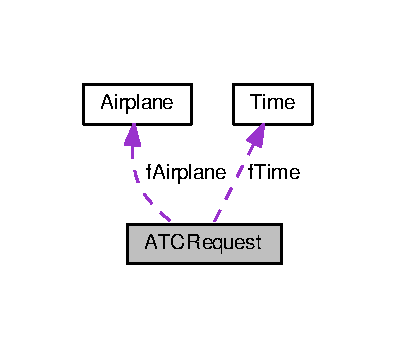
\includegraphics[width=190pt]{structATCRequest__coll__graph}
\end{center}
\end{figure}
\subsection*{Public Member Functions}
\begin{DoxyCompactItemize}
\item 
\hyperlink{structATCRequest_a26bd53c68bee460010bf80dc3c6dec12}{A\+T\+C\+Request} (\hyperlink{classTime}{Time} time, \hyperlink{classAirplane}{Airplane} $\ast$plane)
\end{DoxyCompactItemize}
\subsection*{Public Attributes}
\begin{DoxyCompactItemize}
\item 
\hyperlink{classTime}{Time} \hyperlink{structATCRequest_a6ef577c542082570fc934078994d622f}{f\+Time}
\item 
\hyperlink{classAirplane}{Airplane} $\ast$ \hyperlink{structATCRequest_a681215e14c24388ae811f182c33e4403}{f\+Airplane}
\end{DoxyCompactItemize}


\subsection{Constructor \& Destructor Documentation}
\index{A\+T\+C\+Request@{A\+T\+C\+Request}!A\+T\+C\+Request@{A\+T\+C\+Request}}
\index{A\+T\+C\+Request@{A\+T\+C\+Request}!A\+T\+C\+Request@{A\+T\+C\+Request}}
\subsubsection[{\texorpdfstring{A\+T\+C\+Request(\+Time time, Airplane $\ast$plane)}{ATCRequest(Time time, Airplane *plane)}}]{\setlength{\rightskip}{0pt plus 5cm}A\+T\+C\+Request\+::\+A\+T\+C\+Request (
\begin{DoxyParamCaption}
\item[{{\bf Time}}]{time, }
\item[{{\bf Airplane} $\ast$}]{plane}
\end{DoxyParamCaption}
)}\hypertarget{structATCRequest_a26bd53c68bee460010bf80dc3c6dec12}{}\label{structATCRequest_a26bd53c68bee460010bf80dc3c6dec12}
Constructor. 

\subsection{Member Data Documentation}
\index{A\+T\+C\+Request@{A\+T\+C\+Request}!f\+Airplane@{f\+Airplane}}
\index{f\+Airplane@{f\+Airplane}!A\+T\+C\+Request@{A\+T\+C\+Request}}
\subsubsection[{\texorpdfstring{f\+Airplane}{fAirplane}}]{\setlength{\rightskip}{0pt plus 5cm}{\bf Airplane}$\ast$ A\+T\+C\+Request\+::f\+Airplane}\hypertarget{structATCRequest_a681215e14c24388ae811f182c33e4403}{}\label{structATCRequest_a681215e14c24388ae811f182c33e4403}
\hyperlink{classAirplane}{Airplane} that sent request \index{A\+T\+C\+Request@{A\+T\+C\+Request}!f\+Time@{f\+Time}}
\index{f\+Time@{f\+Time}!A\+T\+C\+Request@{A\+T\+C\+Request}}
\subsubsection[{\texorpdfstring{f\+Time}{fTime}}]{\setlength{\rightskip}{0pt plus 5cm}{\bf Time} A\+T\+C\+Request\+::f\+Time}\hypertarget{structATCRequest_a6ef577c542082570fc934078994d622f}{}\label{structATCRequest_a6ef577c542082570fc934078994d622f}
\hyperlink{classTime}{Time} message was sent. 

The documentation for this struct was generated from the following files\+:\begin{DoxyCompactItemize}
\item 
/home/max/\+C\+Lion\+Projects/\+Project\+Vliegveld/headers/A\+T\+C.\+h\item 
/home/max/\+C\+Lion\+Projects/\+Project\+Vliegveld/src/A\+T\+C.\+cpp\end{DoxyCompactItemize}

\hypertarget{classdomainTestAirplane}{}\section{domain\+Test\+Airplane Class Reference}
\label{classdomainTestAirplane}\index{domain\+Test\+Airplane@{domain\+Test\+Airplane}}


Inheritance diagram for domain\+Test\+Airplane\+:
\nopagebreak
\begin{figure}[H]
\begin{center}
\leavevmode
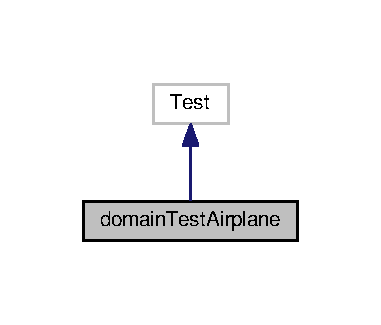
\includegraphics[width=183pt]{classdomainTestAirplane__inherit__graph}
\end{center}
\end{figure}


Collaboration diagram for domain\+Test\+Airplane\+:
\nopagebreak
\begin{figure}[H]
\begin{center}
\leavevmode
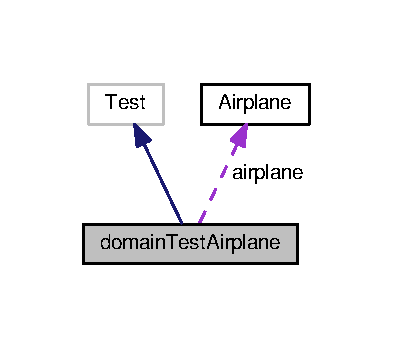
\includegraphics[width=189pt]{classdomainTestAirplane__coll__graph}
\end{center}
\end{figure}
\subsection*{Protected Attributes}
\begin{DoxyCompactItemize}
\item 
\hyperlink{classAirplane}{Airplane} \hyperlink{classdomainTestAirplane_a5d07401cce1be605f6146628d7eb274b}{airplane}
\end{DoxyCompactItemize}


\subsection{Member Data Documentation}
\index{domain\+Test\+Airplane@{domain\+Test\+Airplane}!airplane@{airplane}}
\index{airplane@{airplane}!domain\+Test\+Airplane@{domain\+Test\+Airplane}}
\subsubsection[{\texorpdfstring{airplane}{airplane}}]{\setlength{\rightskip}{0pt plus 5cm}{\bf Airplane} domain\+Test\+Airplane\+::airplane\hspace{0.3cm}{\ttfamily [protected]}}\hypertarget{classdomainTestAirplane_a5d07401cce1be605f6146628d7eb274b}{}\label{classdomainTestAirplane_a5d07401cce1be605f6146628d7eb274b}


The documentation for this class was generated from the following file\+:\begin{DoxyCompactItemize}
\item 
/home/max/\+C\+Lion\+Projects/\+Project\+Vliegveld/test/\hyperlink{domainTestsAirplane_8cpp}{domain\+Tests\+Airplane.\+cpp}\end{DoxyCompactItemize}

\hypertarget{classdomainTestAirport}{}\section{domain\+Test\+Airport Class Reference}
\label{classdomainTestAirport}\index{domain\+Test\+Airport@{domain\+Test\+Airport}}


Inheritance diagram for domain\+Test\+Airport\+:
\nopagebreak
\begin{figure}[H]
\begin{center}
\leavevmode
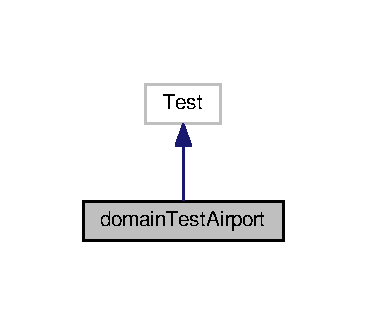
\includegraphics[width=176pt]{classdomainTestAirport__inherit__graph}
\end{center}
\end{figure}


Collaboration diagram for domain\+Test\+Airport\+:
\nopagebreak
\begin{figure}[H]
\begin{center}
\leavevmode
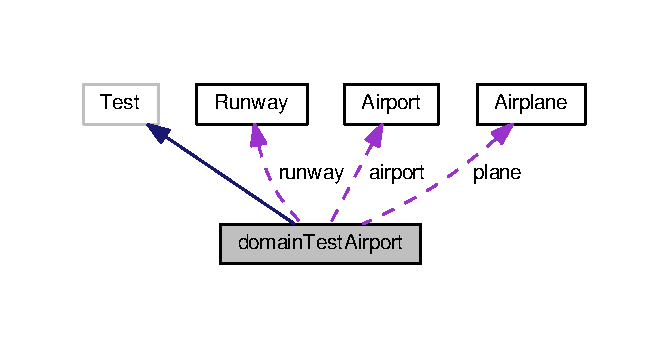
\includegraphics[width=321pt]{classdomainTestAirport__coll__graph}
\end{center}
\end{figure}
\subsection*{Protected Attributes}
\begin{DoxyCompactItemize}
\item 
\hyperlink{classAirport}{Airport} \hyperlink{classdomainTestAirport_afa24e8a08b5107bc45c9188eb914803c}{airport}
\item 
\hyperlink{classRunway}{Runway} \hyperlink{classdomainTestAirport_a0d88cd4618213d454a565d95b5b6c5db}{runway}
\item 
\hyperlink{classAirplane}{Airplane} \hyperlink{classdomainTestAirport_af38b399f44ab9ed6d563f8c008bc1986}{plane}
\end{DoxyCompactItemize}


\subsection{Member Data Documentation}
\index{domain\+Test\+Airport@{domain\+Test\+Airport}!airport@{airport}}
\index{airport@{airport}!domain\+Test\+Airport@{domain\+Test\+Airport}}
\subsubsection[{\texorpdfstring{airport}{airport}}]{\setlength{\rightskip}{0pt plus 5cm}{\bf Airport} domain\+Test\+Airport\+::airport\hspace{0.3cm}{\ttfamily [protected]}}\hypertarget{classdomainTestAirport_afa24e8a08b5107bc45c9188eb914803c}{}\label{classdomainTestAirport_afa24e8a08b5107bc45c9188eb914803c}
\index{domain\+Test\+Airport@{domain\+Test\+Airport}!plane@{plane}}
\index{plane@{plane}!domain\+Test\+Airport@{domain\+Test\+Airport}}
\subsubsection[{\texorpdfstring{plane}{plane}}]{\setlength{\rightskip}{0pt plus 5cm}{\bf Airplane} domain\+Test\+Airport\+::plane\hspace{0.3cm}{\ttfamily [protected]}}\hypertarget{classdomainTestAirport_af38b399f44ab9ed6d563f8c008bc1986}{}\label{classdomainTestAirport_af38b399f44ab9ed6d563f8c008bc1986}
\index{domain\+Test\+Airport@{domain\+Test\+Airport}!runway@{runway}}
\index{runway@{runway}!domain\+Test\+Airport@{domain\+Test\+Airport}}
\subsubsection[{\texorpdfstring{runway}{runway}}]{\setlength{\rightskip}{0pt plus 5cm}{\bf Runway} domain\+Test\+Airport\+::runway\hspace{0.3cm}{\ttfamily [protected]}}\hypertarget{classdomainTestAirport_a0d88cd4618213d454a565d95b5b6c5db}{}\label{classdomainTestAirport_a0d88cd4618213d454a565d95b5b6c5db}


The documentation for this class was generated from the following file\+:\begin{DoxyCompactItemize}
\item 
/home/max/\+C\+Lion\+Projects/\+Project\+Vliegveld/test/\hyperlink{domainTestsAirport_8cpp}{domain\+Tests\+Airport.\+cpp}\end{DoxyCompactItemize}

\hypertarget{classdomainTestATC}{}\section{domain\+Test\+A\+TC Class Reference}
\label{classdomainTestATC}\index{domain\+Test\+A\+TC@{domain\+Test\+A\+TC}}


Inheritance diagram for domain\+Test\+A\+TC\+:
\nopagebreak
\begin{figure}[H]
\begin{center}
\leavevmode
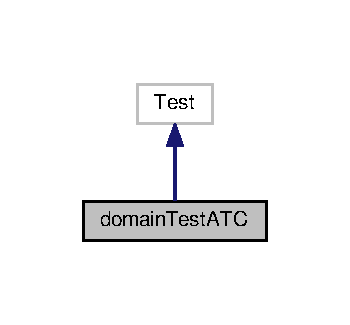
\includegraphics[width=168pt]{classdomainTestATC__inherit__graph}
\end{center}
\end{figure}


Collaboration diagram for domain\+Test\+A\+TC\+:
\nopagebreak
\begin{figure}[H]
\begin{center}
\leavevmode
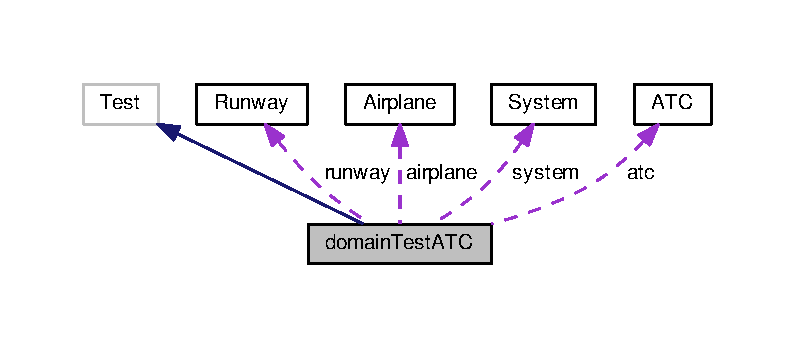
\includegraphics[width=350pt]{classdomainTestATC__coll__graph}
\end{center}
\end{figure}
\subsection*{Protected Member Functions}
\begin{DoxyCompactItemize}
\item 
virtual void \hyperlink{classdomainTestATC_a699ea9550b0fab5fcaad11a17870f6b5}{Set\+Up} ()
\end{DoxyCompactItemize}
\subsection*{Protected Attributes}
\begin{DoxyCompactItemize}
\item 
ofstream \hyperlink{classdomainTestATC_ab5da7bf2ad4ca4231a2eb91664a11f5b}{out}
\item 
\hyperlink{classSystem}{System} \hyperlink{classdomainTestATC_a1cb61e4379ab7424f536bcdb4ec339cc}{system}
\item 
\hyperlink{classRunway}{Runway} $\ast$ \hyperlink{classdomainTestATC_a02691fdbeeca3a709416c0dfe0448051}{runway}
\item 
\hyperlink{classAirplane}{Airplane} $\ast$ \hyperlink{classdomainTestATC_a30f8d738256ddda4c85864a5c4cf8eb5}{airplane}
\item 
\hyperlink{classATC}{A\+TC} $\ast$ \hyperlink{classdomainTestATC_a36d12fcd41f87e8d7bc1af309a9484d5}{atc}
\end{DoxyCompactItemize}


\subsection{Member Function Documentation}
\index{domain\+Test\+A\+TC@{domain\+Test\+A\+TC}!Set\+Up@{Set\+Up}}
\index{Set\+Up@{Set\+Up}!domain\+Test\+A\+TC@{domain\+Test\+A\+TC}}
\subsubsection[{\texorpdfstring{Set\+Up()}{SetUp()}}]{\setlength{\rightskip}{0pt plus 5cm}virtual void domain\+Test\+A\+T\+C\+::\+Set\+Up (
\begin{DoxyParamCaption}
{}
\end{DoxyParamCaption}
)\hspace{0.3cm}{\ttfamily [inline]}, {\ttfamily [protected]}, {\ttfamily [virtual]}}\hypertarget{classdomainTestATC_a699ea9550b0fab5fcaad11a17870f6b5}{}\label{classdomainTestATC_a699ea9550b0fab5fcaad11a17870f6b5}

\begin{DoxyCode}
13                          \{
14         \textcolor{comment}{// Read input}
15         \hyperlink{classInput}{Input} input;
16         input.\hyperlink{classInput_abb78078475f91c654db63c392aefbf51}{read}(\textcolor{stringliteral}{"../test/testInput/happyDay.xml"});
17         
18         \textcolor{comment}{// Initialize atc}
19         \hyperlink{classdomainTestATC_ab5da7bf2ad4ca4231a2eb91664a11f5b}{out}.open(\textcolor{stringliteral}{"../test/testOutput/atc.txt"});
20         \hyperlink{classdomainTestATC_a1cb61e4379ab7424f536bcdb4ec339cc}{system}.\hyperlink{classSystem_a5e9a3f6b8d3d5cb99c041bfcaace9683}{initializeATC}(\hyperlink{classdomainTestATC_ab5da7bf2ad4ca4231a2eb91664a11f5b}{out});
21 
22         \textcolor{comment}{// Import info}
23         \hyperlink{classdomainTestATC_a1cb61e4379ab7424f536bcdb4ec339cc}{system}.\hyperlink{classSystem_ad1f1022247d9556d0ce4061bb68572cc}{import}(input);
24 
25         \textcolor{comment}{// Get airplane}
26         \hyperlink{classdomainTestATC_a30f8d738256ddda4c85864a5c4cf8eb5}{airplane} = \hyperlink{classdomainTestATC_a1cb61e4379ab7424f536bcdb4ec339cc}{system}.\hyperlink{classSystem_a14a06028897516eb4df651220e70ce8f}{getFlightplans}()[0]->getAirplane();
27 
28         \textcolor{comment}{// Get runway}
29         \hyperlink{classdomainTestATC_a02691fdbeeca3a709416c0dfe0448051}{runway} = \hyperlink{classdomainTestATC_a1cb61e4379ab7424f536bcdb4ec339cc}{system}.\hyperlink{classSystem_a8cd2a9b13cdbcf30f801e46cf8284800}{getAirport}()->\hyperlink{classAirport_a14310ffeba8a024105071c156fd42cf7}{getRunways}()[0];
30 
31         \textcolor{comment}{// Get ATC}
32         \hyperlink{classdomainTestATC_a36d12fcd41f87e8d7bc1af309a9484d5}{atc} = \hyperlink{classdomainTestATC_a1cb61e4379ab7424f536bcdb4ec339cc}{system}.\hyperlink{classSystem_aae418c2545087b63188f4a4ffb2e9d15}{getATC}();
33     \}
\end{DoxyCode}


\subsection{Member Data Documentation}
\index{domain\+Test\+A\+TC@{domain\+Test\+A\+TC}!airplane@{airplane}}
\index{airplane@{airplane}!domain\+Test\+A\+TC@{domain\+Test\+A\+TC}}
\subsubsection[{\texorpdfstring{airplane}{airplane}}]{\setlength{\rightskip}{0pt plus 5cm}{\bf Airplane}$\ast$ domain\+Test\+A\+T\+C\+::airplane\hspace{0.3cm}{\ttfamily [protected]}}\hypertarget{classdomainTestATC_a30f8d738256ddda4c85864a5c4cf8eb5}{}\label{classdomainTestATC_a30f8d738256ddda4c85864a5c4cf8eb5}
\index{domain\+Test\+A\+TC@{domain\+Test\+A\+TC}!atc@{atc}}
\index{atc@{atc}!domain\+Test\+A\+TC@{domain\+Test\+A\+TC}}
\subsubsection[{\texorpdfstring{atc}{atc}}]{\setlength{\rightskip}{0pt plus 5cm}{\bf A\+TC}$\ast$ domain\+Test\+A\+T\+C\+::atc\hspace{0.3cm}{\ttfamily [protected]}}\hypertarget{classdomainTestATC_a36d12fcd41f87e8d7bc1af309a9484d5}{}\label{classdomainTestATC_a36d12fcd41f87e8d7bc1af309a9484d5}
\index{domain\+Test\+A\+TC@{domain\+Test\+A\+TC}!out@{out}}
\index{out@{out}!domain\+Test\+A\+TC@{domain\+Test\+A\+TC}}
\subsubsection[{\texorpdfstring{out}{out}}]{\setlength{\rightskip}{0pt plus 5cm}ofstream domain\+Test\+A\+T\+C\+::out\hspace{0.3cm}{\ttfamily [protected]}}\hypertarget{classdomainTestATC_ab5da7bf2ad4ca4231a2eb91664a11f5b}{}\label{classdomainTestATC_ab5da7bf2ad4ca4231a2eb91664a11f5b}
\index{domain\+Test\+A\+TC@{domain\+Test\+A\+TC}!runway@{runway}}
\index{runway@{runway}!domain\+Test\+A\+TC@{domain\+Test\+A\+TC}}
\subsubsection[{\texorpdfstring{runway}{runway}}]{\setlength{\rightskip}{0pt plus 5cm}{\bf Runway}$\ast$ domain\+Test\+A\+T\+C\+::runway\hspace{0.3cm}{\ttfamily [protected]}}\hypertarget{classdomainTestATC_a02691fdbeeca3a709416c0dfe0448051}{}\label{classdomainTestATC_a02691fdbeeca3a709416c0dfe0448051}
\index{domain\+Test\+A\+TC@{domain\+Test\+A\+TC}!system@{system}}
\index{system@{system}!domain\+Test\+A\+TC@{domain\+Test\+A\+TC}}
\subsubsection[{\texorpdfstring{system}{system}}]{\setlength{\rightskip}{0pt plus 5cm}{\bf System} domain\+Test\+A\+T\+C\+::system\hspace{0.3cm}{\ttfamily [protected]}}\hypertarget{classdomainTestATC_a1cb61e4379ab7424f536bcdb4ec339cc}{}\label{classdomainTestATC_a1cb61e4379ab7424f536bcdb4ec339cc}


The documentation for this class was generated from the following file\+:\begin{DoxyCompactItemize}
\item 
/home/max/\+C\+Lion\+Projects/\+Project\+Vliegveld/test/\hyperlink{domainTestsATC_8cpp}{domain\+Tests\+A\+T\+C.\+cpp}\end{DoxyCompactItemize}

\hypertarget{classdomainTestFlightplan}{}\section{domain\+Test\+Flightplan Class Reference}
\label{classdomainTestFlightplan}\index{domain\+Test\+Flightplan@{domain\+Test\+Flightplan}}


Inheritance diagram for domain\+Test\+Flightplan\+:
\nopagebreak
\begin{figure}[H]
\begin{center}
\leavevmode
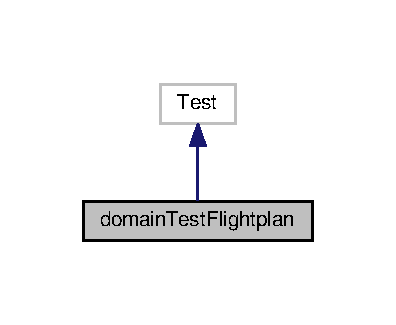
\includegraphics[width=190pt]{classdomainTestFlightplan__inherit__graph}
\end{center}
\end{figure}


Collaboration diagram for domain\+Test\+Flightplan\+:
\nopagebreak
\begin{figure}[H]
\begin{center}
\leavevmode
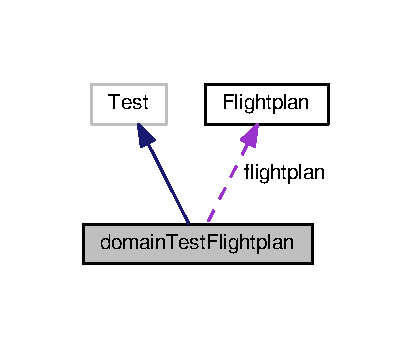
\includegraphics[width=198pt]{classdomainTestFlightplan__coll__graph}
\end{center}
\end{figure}
\subsection*{Protected Attributes}
\begin{DoxyCompactItemize}
\item 
\hyperlink{classFlightplan}{Flightplan} \hyperlink{classdomainTestFlightplan_a5c1212bcf010e1a67e7f4524518e0ae3}{flightplan}
\end{DoxyCompactItemize}


\subsection{Member Data Documentation}
\index{domain\+Test\+Flightplan@{domain\+Test\+Flightplan}!flightplan@{flightplan}}
\index{flightplan@{flightplan}!domain\+Test\+Flightplan@{domain\+Test\+Flightplan}}
\subsubsection[{\texorpdfstring{flightplan}{flightplan}}]{\setlength{\rightskip}{0pt plus 5cm}{\bf Flightplan} domain\+Test\+Flightplan\+::flightplan\hspace{0.3cm}{\ttfamily [protected]}}\hypertarget{classdomainTestFlightplan_a5c1212bcf010e1a67e7f4524518e0ae3}{}\label{classdomainTestFlightplan_a5c1212bcf010e1a67e7f4524518e0ae3}


The documentation for this class was generated from the following file\+:\begin{DoxyCompactItemize}
\item 
/home/max/\+C\+Lion\+Projects/\+Project\+Vliegveld/test/\hyperlink{domainTestsFlightplan_8cpp}{domain\+Tests\+Flightplan.\+cpp}\end{DoxyCompactItemize}

\hypertarget{classdomainTestRunway}{}\section{domain\+Test\+Runway Class Reference}
\label{classdomainTestRunway}\index{domain\+Test\+Runway@{domain\+Test\+Runway}}


Inheritance diagram for domain\+Test\+Runway\+:
\nopagebreak
\begin{figure}[H]
\begin{center}
\leavevmode
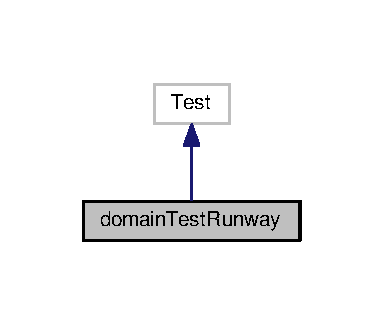
\includegraphics[width=184pt]{classdomainTestRunway__inherit__graph}
\end{center}
\end{figure}


Collaboration diagram for domain\+Test\+Runway\+:
\nopagebreak
\begin{figure}[H]
\begin{center}
\leavevmode
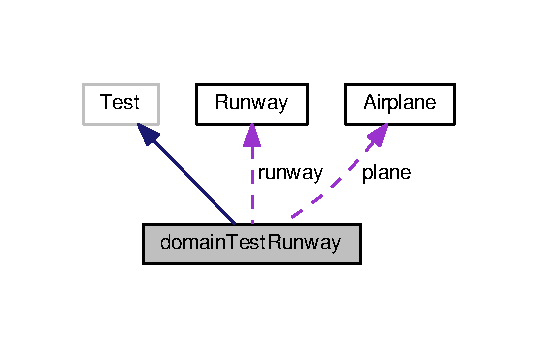
\includegraphics[width=258pt]{classdomainTestRunway__coll__graph}
\end{center}
\end{figure}
\subsection*{Protected Attributes}
\begin{DoxyCompactItemize}
\item 
\hyperlink{classRunway}{Runway} \hyperlink{classdomainTestRunway_ab997db3448cfbd94f07a82de2b9145d1}{runway}
\item 
\hyperlink{classAirplane}{Airplane} \hyperlink{classdomainTestRunway_a07ee8922d98b061f71e90864d97ea677}{plane}
\end{DoxyCompactItemize}


\subsection{Member Data Documentation}
\index{domain\+Test\+Runway@{domain\+Test\+Runway}!plane@{plane}}
\index{plane@{plane}!domain\+Test\+Runway@{domain\+Test\+Runway}}
\subsubsection[{\texorpdfstring{plane}{plane}}]{\setlength{\rightskip}{0pt plus 5cm}{\bf Airplane} domain\+Test\+Runway\+::plane\hspace{0.3cm}{\ttfamily [protected]}}\hypertarget{classdomainTestRunway_a07ee8922d98b061f71e90864d97ea677}{}\label{classdomainTestRunway_a07ee8922d98b061f71e90864d97ea677}
\index{domain\+Test\+Runway@{domain\+Test\+Runway}!runway@{runway}}
\index{runway@{runway}!domain\+Test\+Runway@{domain\+Test\+Runway}}
\subsubsection[{\texorpdfstring{runway}{runway}}]{\setlength{\rightskip}{0pt plus 5cm}{\bf Runway} domain\+Test\+Runway\+::runway\hspace{0.3cm}{\ttfamily [protected]}}\hypertarget{classdomainTestRunway_ab997db3448cfbd94f07a82de2b9145d1}{}\label{classdomainTestRunway_ab997db3448cfbd94f07a82de2b9145d1}


The documentation for this class was generated from the following file\+:\begin{DoxyCompactItemize}
\item 
/home/max/\+C\+Lion\+Projects/\+Project\+Vliegveld/test/\hyperlink{domainTestsRunway_8cpp}{domain\+Tests\+Runway.\+cpp}\end{DoxyCompactItemize}

\hypertarget{classdomainTestSystem}{}\section{domain\+Test\+System Class Reference}
\label{classdomainTestSystem}\index{domain\+Test\+System@{domain\+Test\+System}}


Inheritance diagram for domain\+Test\+System\+:
\nopagebreak
\begin{figure}[H]
\begin{center}
\leavevmode
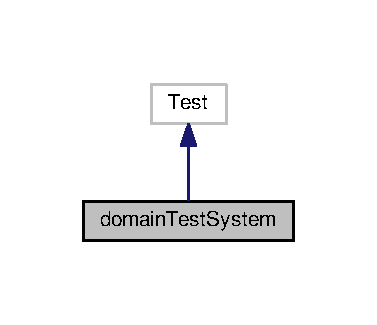
\includegraphics[width=181pt]{classdomainTestSystem__inherit__graph}
\end{center}
\end{figure}


Collaboration diagram for domain\+Test\+System\+:
\nopagebreak
\begin{figure}[H]
\begin{center}
\leavevmode
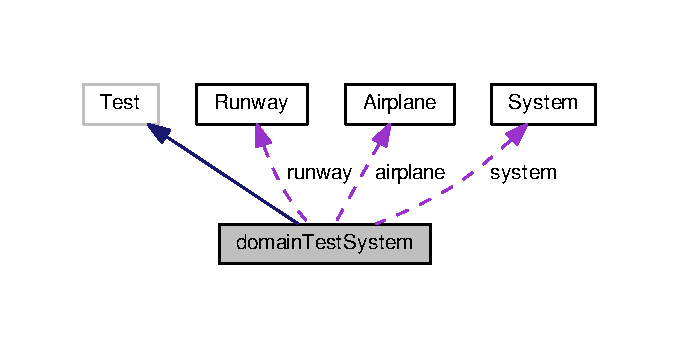
\includegraphics[width=326pt]{classdomainTestSystem__coll__graph}
\end{center}
\end{figure}
\subsection*{Protected Member Functions}
\begin{DoxyCompactItemize}
\item 
virtual void \hyperlink{classdomainTestSystem_a66847562361560bb020f4c9b19d009eb}{Set\+Up} ()
\end{DoxyCompactItemize}
\subsection*{Protected Attributes}
\begin{DoxyCompactItemize}
\item 
\hyperlink{classRunway}{Runway} $\ast$ \hyperlink{classdomainTestSystem_aff348e2b0204535147979a4af0f1953d}{runway}
\item 
ofstream \hyperlink{classdomainTestSystem_a63655622f1037160f95d7466a594859d}{out}
\item 
\hyperlink{classAirplane}{Airplane} $\ast$ \hyperlink{classdomainTestSystem_a835a6facfcfab2d120dae14195d3ed96}{airplane}
\item 
\hyperlink{classSystem}{System} \hyperlink{classdomainTestSystem_a56da545e95cc6b6606ec94857adc14eb}{system}
\end{DoxyCompactItemize}


\subsection{Member Function Documentation}
\index{domain\+Test\+System@{domain\+Test\+System}!Set\+Up@{Set\+Up}}
\index{Set\+Up@{Set\+Up}!domain\+Test\+System@{domain\+Test\+System}}
\subsubsection[{\texorpdfstring{Set\+Up()}{SetUp()}}]{\setlength{\rightskip}{0pt plus 5cm}virtual void domain\+Test\+System\+::\+Set\+Up (
\begin{DoxyParamCaption}
{}
\end{DoxyParamCaption}
)\hspace{0.3cm}{\ttfamily [inline]}, {\ttfamily [protected]}, {\ttfamily [virtual]}}\hypertarget{classdomainTestSystem_a66847562361560bb020f4c9b19d009eb}{}\label{classdomainTestSystem_a66847562361560bb020f4c9b19d009eb}

\begin{DoxyCode}
13                          \{
14         \textcolor{comment}{// Read input}
15         \hyperlink{classInput}{Input} input;
16         input.\hyperlink{classInput_abb78078475f91c654db63c392aefbf51}{read}(\textcolor{stringliteral}{"../test/testInput/happyDay.xml"});
17 
18         \hyperlink{classdomainTestSystem_a56da545e95cc6b6606ec94857adc14eb}{system}.\hyperlink{classSystem_a5e9a3f6b8d3d5cb99c041bfcaace9683}{initializeATC}(\hyperlink{classdomainTestSystem_a63655622f1037160f95d7466a594859d}{out});
19 
20         \textcolor{comment}{// Import info}
21         \hyperlink{classdomainTestSystem_a56da545e95cc6b6606ec94857adc14eb}{system}.\hyperlink{classSystem_ad1f1022247d9556d0ce4061bb68572cc}{import}(input);
22 
23         \textcolor{comment}{// Get airplane}
24         \hyperlink{classdomainTestSystem_a835a6facfcfab2d120dae14195d3ed96}{airplane} = \hyperlink{classdomainTestSystem_a56da545e95cc6b6606ec94857adc14eb}{system}.\hyperlink{classSystem_a14a06028897516eb4df651220e70ce8f}{getFlightplans}()[0]->getAirplane();
25 
26         \textcolor{comment}{// Get runway}
27         \hyperlink{classdomainTestSystem_aff348e2b0204535147979a4af0f1953d}{runway} = \hyperlink{classdomainTestSystem_a56da545e95cc6b6606ec94857adc14eb}{system}.\hyperlink{classSystem_a8cd2a9b13cdbcf30f801e46cf8284800}{getAirport}()->\hyperlink{classAirport_a14310ffeba8a024105071c156fd42cf7}{getRunways}()[0];
28     \}
\end{DoxyCode}


\subsection{Member Data Documentation}
\index{domain\+Test\+System@{domain\+Test\+System}!airplane@{airplane}}
\index{airplane@{airplane}!domain\+Test\+System@{domain\+Test\+System}}
\subsubsection[{\texorpdfstring{airplane}{airplane}}]{\setlength{\rightskip}{0pt plus 5cm}{\bf Airplane}$\ast$ domain\+Test\+System\+::airplane\hspace{0.3cm}{\ttfamily [protected]}}\hypertarget{classdomainTestSystem_a835a6facfcfab2d120dae14195d3ed96}{}\label{classdomainTestSystem_a835a6facfcfab2d120dae14195d3ed96}
\index{domain\+Test\+System@{domain\+Test\+System}!out@{out}}
\index{out@{out}!domain\+Test\+System@{domain\+Test\+System}}
\subsubsection[{\texorpdfstring{out}{out}}]{\setlength{\rightskip}{0pt plus 5cm}ofstream domain\+Test\+System\+::out\hspace{0.3cm}{\ttfamily [protected]}}\hypertarget{classdomainTestSystem_a63655622f1037160f95d7466a594859d}{}\label{classdomainTestSystem_a63655622f1037160f95d7466a594859d}
\index{domain\+Test\+System@{domain\+Test\+System}!runway@{runway}}
\index{runway@{runway}!domain\+Test\+System@{domain\+Test\+System}}
\subsubsection[{\texorpdfstring{runway}{runway}}]{\setlength{\rightskip}{0pt plus 5cm}{\bf Runway}$\ast$ domain\+Test\+System\+::runway\hspace{0.3cm}{\ttfamily [protected]}}\hypertarget{classdomainTestSystem_aff348e2b0204535147979a4af0f1953d}{}\label{classdomainTestSystem_aff348e2b0204535147979a4af0f1953d}
\index{domain\+Test\+System@{domain\+Test\+System}!system@{system}}
\index{system@{system}!domain\+Test\+System@{domain\+Test\+System}}
\subsubsection[{\texorpdfstring{system}{system}}]{\setlength{\rightskip}{0pt plus 5cm}{\bf System} domain\+Test\+System\+::system\hspace{0.3cm}{\ttfamily [protected]}}\hypertarget{classdomainTestSystem_a56da545e95cc6b6606ec94857adc14eb}{}\label{classdomainTestSystem_a56da545e95cc6b6606ec94857adc14eb}


The documentation for this class was generated from the following file\+:\begin{DoxyCompactItemize}
\item 
/home/max/\+C\+Lion\+Projects/\+Project\+Vliegveld/test/\hyperlink{domainTestsSystem_8cpp}{domain\+Tests\+System.\+cpp}\end{DoxyCompactItemize}

\hypertarget{classdomainTestTime}{}\section{domain\+Test\+Time Class Reference}
\label{classdomainTestTime}\index{domain\+Test\+Time@{domain\+Test\+Time}}


Inheritance diagram for domain\+Test\+Time\+:
\nopagebreak
\begin{figure}[H]
\begin{center}
\leavevmode
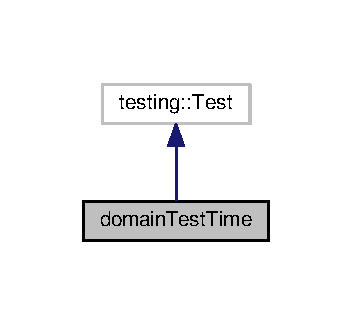
\includegraphics[width=169pt]{classdomainTestTime__inherit__graph}
\end{center}
\end{figure}


Collaboration diagram for domain\+Test\+Time\+:
\nopagebreak
\begin{figure}[H]
\begin{center}
\leavevmode
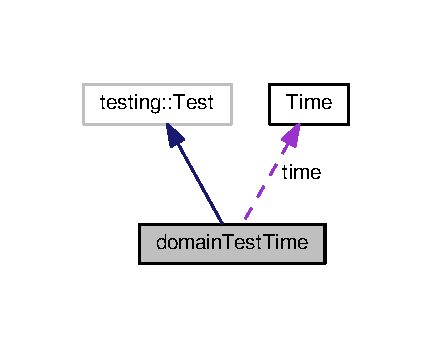
\includegraphics[width=208pt]{classdomainTestTime__coll__graph}
\end{center}
\end{figure}
\subsection*{Protected Attributes}
\begin{DoxyCompactItemize}
\item 
\hyperlink{classTime}{Time} \hyperlink{classdomainTestTime_a9eee3a6a359895396c122cc18ded5d36}{time}
\end{DoxyCompactItemize}


\subsection{Member Data Documentation}
\index{domain\+Test\+Time@{domain\+Test\+Time}!time@{time}}
\index{time@{time}!domain\+Test\+Time@{domain\+Test\+Time}}
\subsubsection[{\texorpdfstring{time}{time}}]{\setlength{\rightskip}{0pt plus 5cm}{\bf Time} domain\+Test\+Time\+::time\hspace{0.3cm}{\ttfamily [protected]}}\hypertarget{classdomainTestTime_a9eee3a6a359895396c122cc18ded5d36}{}\label{classdomainTestTime_a9eee3a6a359895396c122cc18ded5d36}


The documentation for this class was generated from the following file\+:\begin{DoxyCompactItemize}
\item 
/home/max/\+C\+Lion\+Projects/\+Project\+Vliegveld/test/\hyperlink{domainTestsTime_8cpp}{domain\+Tests\+Time.\+cpp}\end{DoxyCompactItemize}

\hypertarget{classFlightplan}{}\section{Flightplan Class Reference}
\label{classFlightplan}\index{Flightplan@{Flightplan}}


\+: Class that represents a flight plan in the simulation  




{\ttfamily \#include $<$Flightplan.\+h$>$}

\subsection*{Public Member Functions}
\begin{DoxyCompactItemize}
\item 
\hyperlink{classFlightplan_ac2382ffda13572e5f7434d887c05f2f5}{Flightplan} ()
\item 
\hyperlink{classFlightplan_af94db993571dde1fa3da8fc4f733ed8d}{$\sim$\+Flightplan} ()
\item 
bool \hyperlink{classFlightplan_a5b5f371dc8451e95a981ec4e01f348a0}{properly\+Initialized} () const 
\item 
void \hyperlink{classFlightplan_a46d9b61f11e05ee917423b30018eb311}{set\+Departure} (\hyperlink{CMakeCache_8txt_a79a3d8790b2588b09777910863574e09}{int} f\+Departure)
\item 
void \hyperlink{classFlightplan_aa418664239c83960df069cdfb456e819}{set\+Arrival} (\hyperlink{CMakeCache_8txt_a79a3d8790b2588b09777910863574e09}{int} f\+Arrival)
\item 
void \hyperlink{classFlightplan_a7a253899d4a09a629bf88f5184f6f7a3}{set\+Interval} (\hyperlink{CMakeCache_8txt_a79a3d8790b2588b09777910863574e09}{int} f\+Interval)
\item 
\hyperlink{Flightplan_8h_ab41c9a082b57fd41aefb64a57d8149f8}{E\+Event} \hyperlink{classFlightplan_a2b7410b0bcabb84db2164b4163dfddb4}{get\+Event} (\hyperlink{classTime}{Time} time)
\item 
bool \hyperlink{classFlightplan_a07f564cb5e5cdbad4abb2098f7941597}{complete} () const 
\item 
const string \& \hyperlink{classFlightplan_aa625d49c014955ff1e62668a297dd0a0}{get\+Destination} () const 
\item 
void \hyperlink{classFlightplan_a9d345a0fbf7a000075cd8bac019e1827}{set\+Destination} (const string \&f\+Destination)
\item 
\hyperlink{CMakeCache_8txt_a79a3d8790b2588b09777910863574e09}{int} \hyperlink{classFlightplan_a2453c9cf22ec82997787a60088f71c67}{get\+Departure} () const 
\item 
\hyperlink{CMakeCache_8txt_a79a3d8790b2588b09777910863574e09}{int} \hyperlink{classFlightplan_a88e4a0195a8268c5c06a42c677857a6c}{get\+Arrival} () const 
\item 
\hyperlink{CMakeCache_8txt_a79a3d8790b2588b09777910863574e09}{int} \hyperlink{classFlightplan_ae5bc96d39d3e4e9e1fb5540c7dd2b6d5}{get\+Interval} () const 
\item 
void \hyperlink{classFlightplan_a1dc1abd7a13e56ad85d84ebdc15e448a}{set\+Airplane} (\hyperlink{classAirplane}{Airplane} $\ast$)
\item 
\hyperlink{classAirplane}{Airplane} $\ast$ \hyperlink{classFlightplan_a8406fbb2f98685fba170063acde0fdd7}{get\+Airplane} () const 
\end{DoxyCompactItemize}


\subsection{Detailed Description}
\+: Class that represents a flight plan in the simulation 

\subsection{Constructor \& Destructor Documentation}
\index{Flightplan@{Flightplan}!Flightplan@{Flightplan}}
\index{Flightplan@{Flightplan}!Flightplan@{Flightplan}}
\subsubsection[{\texorpdfstring{Flightplan()}{Flightplan()}}]{\setlength{\rightskip}{0pt plus 5cm}Flightplan\+::\+Flightplan (
\begin{DoxyParamCaption}
{}
\end{DoxyParamCaption}
)}\hypertarget{classFlightplan_ac2382ffda13572e5f7434d887c05f2f5}{}\label{classFlightplan_ac2382ffda13572e5f7434d887c05f2f5}
Default constructor ~\newline
 E\+N\+S\+U\+RE(\hyperlink{classFlightplan_a5b5f371dc8451e95a981ec4e01f348a0}{properly\+Initialized()}, \char`\"{}constructor must end in properly\+Initialized state\char`\"{}); 
\begin{DoxyCode}
9                       : fAirplane(NULL), fDeparture(-1), fArrival(-1), fInterval(-1) \{
10     fInitCheck = \textcolor{keyword}{this};
11     \hyperlink{DesignByContract_8h_ab8da60ea2bcdd55183cc29d8526e6857}{ENSURE}(\hyperlink{classFlightplan_a5b5f371dc8451e95a981ec4e01f348a0}{properlyInitialized}(), \textcolor{stringliteral}{"constructor must end in properlyInitialized
       state"});
12 \}
\end{DoxyCode}
\index{Flightplan@{Flightplan}!````~Flightplan@{$\sim$\+Flightplan}}
\index{````~Flightplan@{$\sim$\+Flightplan}!Flightplan@{Flightplan}}
\subsubsection[{\texorpdfstring{$\sim$\+Flightplan()}{~Flightplan()}}]{\setlength{\rightskip}{0pt plus 5cm}Flightplan\+::$\sim$\+Flightplan (
\begin{DoxyParamCaption}
{}
\end{DoxyParamCaption}
)}\hypertarget{classFlightplan_af94db993571dde1fa3da8fc4f733ed8d}{}\label{classFlightplan_af94db993571dde1fa3da8fc4f733ed8d}
Destructor 
\begin{DoxyCode}
107                         \{
108     \hyperlink{DesignByContract_8h_aeb774672b46dbe80afc14e0d1970f017}{REQUIRE}(this->\hyperlink{classFlightplan_a5b5f371dc8451e95a981ec4e01f348a0}{properlyInitialized}(), \textcolor{stringliteral}{"Flightplan was't initialized when
       calling getter/setter"});
109     \textcolor{keyword}{delete} fAirplane;
110 \}
\end{DoxyCode}


\subsection{Member Function Documentation}
\index{Flightplan@{Flightplan}!complete@{complete}}
\index{complete@{complete}!Flightplan@{Flightplan}}
\subsubsection[{\texorpdfstring{complete() const }{complete() const }}]{\setlength{\rightskip}{0pt plus 5cm}bool Flightplan\+::complete (
\begin{DoxyParamCaption}
{}
\end{DoxyParamCaption}
) const}\hypertarget{classFlightplan_a07f564cb5e5cdbad4abb2098f7941597}{}\label{classFlightplan_a07f564cb5e5cdbad4abb2098f7941597}
Checks if all the data members were initialized ~\newline
 R\+E\+Q\+U\+I\+RE(this-\/$>$\hyperlink{classFlightplan_a5b5f371dc8451e95a981ec4e01f348a0}{properly\+Initialized()}, \char`\"{}\+Flightplan was\textquotesingle{}t initialized when calling complete\char`\"{}); 
\begin{DoxyCode}
14                                 \{
15     \hyperlink{DesignByContract_8h_aeb774672b46dbe80afc14e0d1970f017}{REQUIRE}(this->\hyperlink{classFlightplan_a5b5f371dc8451e95a981ec4e01f348a0}{properlyInitialized}(), \textcolor{stringliteral}{"Flightplan was't initialized when
       calling complete"});
16     \textcolor{keywordflow}{return} !(fDeparture == -1 or fArrival == -1 or
17             fInterval == -1 or fDestination.empty());
18 \}
\end{DoxyCode}
\index{Flightplan@{Flightplan}!get\+Airplane@{get\+Airplane}}
\index{get\+Airplane@{get\+Airplane}!Flightplan@{Flightplan}}
\subsubsection[{\texorpdfstring{get\+Airplane() const }{getAirplane() const }}]{\setlength{\rightskip}{0pt plus 5cm}{\bf Airplane} $\ast$ Flightplan\+::get\+Airplane (
\begin{DoxyParamCaption}
{}
\end{DoxyParamCaption}
) const}\hypertarget{classFlightplan_a8406fbb2f98685fba170063acde0fdd7}{}\label{classFlightplan_a8406fbb2f98685fba170063acde0fdd7}

\begin{DoxyCode}
97                                         \{
98     \hyperlink{DesignByContract_8h_aeb774672b46dbe80afc14e0d1970f017}{REQUIRE}(this->\hyperlink{classFlightplan_a5b5f371dc8451e95a981ec4e01f348a0}{properlyInitialized}(), \textcolor{stringliteral}{"Flightplan was't initialized when
       calling getter/setter"});
99     \textcolor{keywordflow}{return} fAirplane;
100 \}
\end{DoxyCode}
\index{Flightplan@{Flightplan}!get\+Arrival@{get\+Arrival}}
\index{get\+Arrival@{get\+Arrival}!Flightplan@{Flightplan}}
\subsubsection[{\texorpdfstring{get\+Arrival() const }{getArrival() const }}]{\setlength{\rightskip}{0pt plus 5cm}{\bf int} Flightplan\+::get\+Arrival (
\begin{DoxyParamCaption}
{}
\end{DoxyParamCaption}
) const}\hypertarget{classFlightplan_a88e4a0195a8268c5c06a42c677857a6c}{}\label{classFlightplan_a88e4a0195a8268c5c06a42c677857a6c}

\begin{DoxyCode}
41                                  \{
42     \hyperlink{DesignByContract_8h_aeb774672b46dbe80afc14e0d1970f017}{REQUIRE}(this->\hyperlink{classFlightplan_a5b5f371dc8451e95a981ec4e01f348a0}{properlyInitialized}(), \textcolor{stringliteral}{"Flightplan was't initialized when
       calling getter/setter"});
43     \textcolor{keywordflow}{return} fArrival;
44 \}
\end{DoxyCode}
\index{Flightplan@{Flightplan}!get\+Departure@{get\+Departure}}
\index{get\+Departure@{get\+Departure}!Flightplan@{Flightplan}}
\subsubsection[{\texorpdfstring{get\+Departure() const }{getDeparture() const }}]{\setlength{\rightskip}{0pt plus 5cm}{\bf int} Flightplan\+::get\+Departure (
\begin{DoxyParamCaption}
{}
\end{DoxyParamCaption}
) const}\hypertarget{classFlightplan_a2453c9cf22ec82997787a60088f71c67}{}\label{classFlightplan_a2453c9cf22ec82997787a60088f71c67}

\begin{DoxyCode}
30                                    \{
31     \hyperlink{DesignByContract_8h_aeb774672b46dbe80afc14e0d1970f017}{REQUIRE}(this->\hyperlink{classFlightplan_a5b5f371dc8451e95a981ec4e01f348a0}{properlyInitialized}(), \textcolor{stringliteral}{"Flightplan was't initialized when
       calling getter/setter"});
32     \textcolor{keywordflow}{return} fDeparture;
33 \}
\end{DoxyCode}
\index{Flightplan@{Flightplan}!get\+Destination@{get\+Destination}}
\index{get\+Destination@{get\+Destination}!Flightplan@{Flightplan}}
\subsubsection[{\texorpdfstring{get\+Destination() const }{getDestination() const }}]{\setlength{\rightskip}{0pt plus 5cm}const string \& Flightplan\+::get\+Destination (
\begin{DoxyParamCaption}
{}
\end{DoxyParamCaption}
) const}\hypertarget{classFlightplan_aa625d49c014955ff1e62668a297dd0a0}{}\label{classFlightplan_aa625d49c014955ff1e62668a297dd0a0}
Getters and setters for the fields of the class. ~\newline
 R\+E\+Q\+U\+I\+RE(\hyperlink{classFlightplan_a5b5f371dc8451e95a981ec4e01f348a0}{properly\+Initialized()}, \char`\"{}\+Flightplan wasn\textquotesingle{}t initialized when calling getter/setter\char`\"{}); 
\begin{DoxyCode}
20                                                \{
21     \hyperlink{DesignByContract_8h_aeb774672b46dbe80afc14e0d1970f017}{REQUIRE}(this->\hyperlink{classFlightplan_a5b5f371dc8451e95a981ec4e01f348a0}{properlyInitialized}(), \textcolor{stringliteral}{"Flightplan was't initialized when
       calling getter/setter"});
22     \textcolor{keywordflow}{return} fDestination;
23 \}
\end{DoxyCode}
\index{Flightplan@{Flightplan}!get\+Event@{get\+Event}}
\index{get\+Event@{get\+Event}!Flightplan@{Flightplan}}
\subsubsection[{\texorpdfstring{get\+Event(\+Time time)}{getEvent(Time time)}}]{\setlength{\rightskip}{0pt plus 5cm}{\bf E\+Event} Flightplan\+::get\+Event (
\begin{DoxyParamCaption}
\item[{{\bf Time}}]{time}
\end{DoxyParamCaption}
)}\hypertarget{classFlightplan_a2b7410b0bcabb84db2164b4163dfddb4}{}\label{classFlightplan_a2b7410b0bcabb84db2164b4163dfddb4}
Returns the event at the given time ~\newline
 R\+E\+Q\+U\+I\+RE(this-\/$>$\hyperlink{classFlightplan_a5b5f371dc8451e95a981ec4e01f348a0}{properly\+Initialized()}, \char`\"{}\+Flightplan was\textquotesingle{}t initialized when calling get\+Event\char`\"{}); 
\begin{DoxyCode}
63                                      \{
64     \hyperlink{DesignByContract_8h_aeb774672b46dbe80afc14e0d1970f017}{REQUIRE}(this->\hyperlink{classFlightplan_a5b5f371dc8451e95a981ec4e01f348a0}{properlyInitialized}(), \textcolor{stringliteral}{"Flightplan was't initialized when
       calling getEvent"});
65     \textcolor{comment}{// Start at 12:00}
66     \hyperlink{classTime}{Time} currentTime(12);
67 
68     \textcolor{comment}{// While not midnight}
69     \textcolor{keywordflow}{while} (\textcolor{keyword}{true}) \{
70         \textcolor{comment}{// Set to departure time}
71         currentTime = \hyperlink{classTime}{Time}(currentTime.getHour(), fDeparture);
72 
73         \textcolor{comment}{// If times match up, return takeoff}
74         \textcolor{keywordflow}{if} (currentTime == time) \{
75             \textcolor{keywordflow}{return} \hyperlink{Flightplan_8h_ab41c9a082b57fd41aefb64a57d8149f8a81c03ffd159b67afc7df0ffab6a9297f}{kTakeoff};
76         \}
77 
78         \textcolor{comment}{// Set to arrival time}
79         currentTime = \hyperlink{classTime}{Time}(currentTime.getHour(), fArrival);
80 
81         \textcolor{comment}{// If times match up, return land}
82         \textcolor{keywordflow}{if} (currentTime == time) \{
83             \textcolor{keywordflow}{return} \hyperlink{Flightplan_8h_ab41c9a082b57fd41aefb64a57d8149f8aeaa0025051cf36faa589b5da72a153c4}{kLand};
84         \}
85 
86         \textcolor{comment}{// Set advance hour by interval}
87         currentTime.advance(60 * fInterval);
88 
89         \textcolor{keywordflow}{if} (currentTime.getHour() < 12) \{
90             \textcolor{keywordflow}{break};
91         \}
92     \}
93 
94     \textcolor{keywordflow}{return} \hyperlink{Flightplan_8h_ab41c9a082b57fd41aefb64a57d8149f8a58584cd9619135e5689ded56238c3427}{kNothing};
95 \}
\end{DoxyCode}
\index{Flightplan@{Flightplan}!get\+Interval@{get\+Interval}}
\index{get\+Interval@{get\+Interval}!Flightplan@{Flightplan}}
\subsubsection[{\texorpdfstring{get\+Interval() const }{getInterval() const }}]{\setlength{\rightskip}{0pt plus 5cm}{\bf int} Flightplan\+::get\+Interval (
\begin{DoxyParamCaption}
{}
\end{DoxyParamCaption}
) const}\hypertarget{classFlightplan_ae5bc96d39d3e4e9e1fb5540c7dd2b6d5}{}\label{classFlightplan_ae5bc96d39d3e4e9e1fb5540c7dd2b6d5}

\begin{DoxyCode}
52                                   \{
53     \hyperlink{DesignByContract_8h_aeb774672b46dbe80afc14e0d1970f017}{REQUIRE}(this->\hyperlink{classFlightplan_a5b5f371dc8451e95a981ec4e01f348a0}{properlyInitialized}(), \textcolor{stringliteral}{"Flightplan was't initialized when
       calling getter/setter"});
54     \textcolor{keywordflow}{return} fInterval;
55 \}
\end{DoxyCode}
\index{Flightplan@{Flightplan}!properly\+Initialized@{properly\+Initialized}}
\index{properly\+Initialized@{properly\+Initialized}!Flightplan@{Flightplan}}
\subsubsection[{\texorpdfstring{properly\+Initialized() const }{properlyInitialized() const }}]{\setlength{\rightskip}{0pt plus 5cm}bool Flightplan\+::properly\+Initialized (
\begin{DoxyParamCaption}
{}
\end{DoxyParamCaption}
) const}\hypertarget{classFlightplan_a5b5f371dc8451e95a981ec4e01f348a0}{}\label{classFlightplan_a5b5f371dc8451e95a981ec4e01f348a0}
Checks if the object is properly initialized 
\begin{DoxyCode}
112                                            \{
113     \textcolor{keywordflow}{return} fInitCheck == \textcolor{keyword}{this};
114 \}\end{DoxyCode}
\index{Flightplan@{Flightplan}!set\+Airplane@{set\+Airplane}}
\index{set\+Airplane@{set\+Airplane}!Flightplan@{Flightplan}}
\subsubsection[{\texorpdfstring{set\+Airplane(\+Airplane $\ast$)}{setAirplane(Airplane *)}}]{\setlength{\rightskip}{0pt plus 5cm}void Flightplan\+::set\+Airplane (
\begin{DoxyParamCaption}
\item[{{\bf Airplane} $\ast$}]{airplane}
\end{DoxyParamCaption}
)}\hypertarget{classFlightplan_a1dc1abd7a13e56ad85d84ebdc15e448a}{}\label{classFlightplan_a1dc1abd7a13e56ad85d84ebdc15e448a}

\begin{DoxyCode}
102                                                \{
103     \hyperlink{DesignByContract_8h_aeb774672b46dbe80afc14e0d1970f017}{REQUIRE}(this->\hyperlink{classFlightplan_a5b5f371dc8451e95a981ec4e01f348a0}{properlyInitialized}(), \textcolor{stringliteral}{"Flightplan was't initialized when
       calling getter/setter"});
104     fAirplane = airplane;
105 \}
\end{DoxyCode}
\index{Flightplan@{Flightplan}!set\+Arrival@{set\+Arrival}}
\index{set\+Arrival@{set\+Arrival}!Flightplan@{Flightplan}}
\subsubsection[{\texorpdfstring{set\+Arrival(int f\+Arrival)}{setArrival(int fArrival)}}]{\setlength{\rightskip}{0pt plus 5cm}void Flightplan\+::set\+Arrival (
\begin{DoxyParamCaption}
\item[{{\bf int}}]{f\+Arrival}
\end{DoxyParamCaption}
)}\hypertarget{classFlightplan_aa418664239c83960df069cdfb456e819}{}\label{classFlightplan_aa418664239c83960df069cdfb456e819}
Setter for arrival time ~\newline
 R\+E\+Q\+U\+I\+RE(this-\/$>$\hyperlink{classFlightplan_a5b5f371dc8451e95a981ec4e01f348a0}{properly\+Initialized()}, \char`\"{}\+Flightplan was\textquotesingle{}t initialized when calling set\+Arrival\char`\"{}); ~\newline
 R\+E\+Q\+U\+I\+RE(arrival $>$= 0 \&\& arrival $<$ 60, \char`\"{}\+Arrival has to be between 0 and 60\char`\"{}); 
\begin{DoxyCode}
46                                        \{
47     \hyperlink{DesignByContract_8h_aeb774672b46dbe80afc14e0d1970f017}{REQUIRE}(this->\hyperlink{classFlightplan_a5b5f371dc8451e95a981ec4e01f348a0}{properlyInitialized}(), \textcolor{stringliteral}{"Flightplan was't initialized when
       calling setArrival"});
48     \hyperlink{DesignByContract_8h_aeb774672b46dbe80afc14e0d1970f017}{REQUIRE}(arrival >= 0 && arrival < 60, \textcolor{stringliteral}{"Arrival has to be between 0 and 60"});
49     Flightplan::fArrival = arrival;
50 \}
\end{DoxyCode}
\index{Flightplan@{Flightplan}!set\+Departure@{set\+Departure}}
\index{set\+Departure@{set\+Departure}!Flightplan@{Flightplan}}
\subsubsection[{\texorpdfstring{set\+Departure(int f\+Departure)}{setDeparture(int fDeparture)}}]{\setlength{\rightskip}{0pt plus 5cm}void Flightplan\+::set\+Departure (
\begin{DoxyParamCaption}
\item[{{\bf int}}]{f\+Departure}
\end{DoxyParamCaption}
)}\hypertarget{classFlightplan_a46d9b61f11e05ee917423b30018eb311}{}\label{classFlightplan_a46d9b61f11e05ee917423b30018eb311}
Setter for departure time ~\newline
 R\+E\+Q\+U\+I\+RE(this-\/$>$\hyperlink{classFlightplan_a5b5f371dc8451e95a981ec4e01f348a0}{properly\+Initialized()}, \char`\"{}\+Flightplan was\textquotesingle{}t initialized when calling set\+Departure\char`\"{}); ~\newline
 R\+E\+Q\+U\+I\+RE(departure $>$= 0 \&\& departure $<$ 60, \char`\"{}\+Departure has to be between 0 and 60\char`\"{}); 
\begin{DoxyCode}
35                                            \{
36     \hyperlink{DesignByContract_8h_aeb774672b46dbe80afc14e0d1970f017}{REQUIRE}(this->\hyperlink{classFlightplan_a5b5f371dc8451e95a981ec4e01f348a0}{properlyInitialized}(), \textcolor{stringliteral}{"Flightplan was't initialized when
       calling setDeparture"});
37     \hyperlink{DesignByContract_8h_aeb774672b46dbe80afc14e0d1970f017}{REQUIRE}(\hyperlink{ATC_8txt_af9835824e50bb6ca59bed75129f137e3}{departure} >= 0 && \hyperlink{ATC_8txt_af9835824e50bb6ca59bed75129f137e3}{departure} < 60, \textcolor{stringliteral}{"Departure has to be between 0 and
       60"});
38     Flightplan::fDeparture = \hyperlink{ATC_8txt_af9835824e50bb6ca59bed75129f137e3}{departure};
39 \}
\end{DoxyCode}
\index{Flightplan@{Flightplan}!set\+Destination@{set\+Destination}}
\index{set\+Destination@{set\+Destination}!Flightplan@{Flightplan}}
\subsubsection[{\texorpdfstring{set\+Destination(const string \&f\+Destination)}{setDestination(const string &fDestination)}}]{\setlength{\rightskip}{0pt plus 5cm}void Flightplan\+::set\+Destination (
\begin{DoxyParamCaption}
\item[{const string \&}]{f\+Destination}
\end{DoxyParamCaption}
)}\hypertarget{classFlightplan_a9d345a0fbf7a000075cd8bac019e1827}{}\label{classFlightplan_a9d345a0fbf7a000075cd8bac019e1827}

\begin{DoxyCode}
25                                                           \{
26     \hyperlink{DesignByContract_8h_aeb774672b46dbe80afc14e0d1970f017}{REQUIRE}(this->\hyperlink{classFlightplan_a5b5f371dc8451e95a981ec4e01f348a0}{properlyInitialized}(), \textcolor{stringliteral}{"Flightplan was't initialized when
       calling getter/setter"});
27     Flightplan::fDestination = fDestination;
28 \}
\end{DoxyCode}
\index{Flightplan@{Flightplan}!set\+Interval@{set\+Interval}}
\index{set\+Interval@{set\+Interval}!Flightplan@{Flightplan}}
\subsubsection[{\texorpdfstring{set\+Interval(int f\+Interval)}{setInterval(int fInterval)}}]{\setlength{\rightskip}{0pt plus 5cm}void Flightplan\+::set\+Interval (
\begin{DoxyParamCaption}
\item[{{\bf int}}]{f\+Interval}
\end{DoxyParamCaption}
)}\hypertarget{classFlightplan_a7a253899d4a09a629bf88f5184f6f7a3}{}\label{classFlightplan_a7a253899d4a09a629bf88f5184f6f7a3}
Setter for interval ~\newline
 R\+E\+Q\+U\+I\+RE(this-\/$>$\hyperlink{classFlightplan_a5b5f371dc8451e95a981ec4e01f348a0}{properly\+Initialized()}, \char`\"{}\+Flightplan was\textquotesingle{}t initialized when calling set\+Interval\char`\"{}); ~\newline
 R\+E\+Q\+U\+I\+RE(interval $>$ 0, \char`\"{}\+Interval has to be at least 1\char`\"{}); 
\begin{DoxyCode}
57                                          \{
58     \hyperlink{DesignByContract_8h_aeb774672b46dbe80afc14e0d1970f017}{REQUIRE}(this->\hyperlink{classFlightplan_a5b5f371dc8451e95a981ec4e01f348a0}{properlyInitialized}(), \textcolor{stringliteral}{"Flightplan was't initialized when
       calling setInterval"});
59     \hyperlink{DesignByContract_8h_aeb774672b46dbe80afc14e0d1970f017}{REQUIRE}(interval > 0, \textcolor{stringliteral}{"Interval has to be at least 1"});
60     Flightplan::fInterval = interval;
61 \}
\end{DoxyCode}


The documentation for this class was generated from the following files\+:\begin{DoxyCompactItemize}
\item 
/home/max/\+C\+Lion\+Projects/\+Project\+Vliegveld/headers/\hyperlink{Flightplan_8h}{Flightplan.\+h}\item 
/home/max/\+C\+Lion\+Projects/\+Project\+Vliegveld/src/\hyperlink{Flightplan_8cpp}{Flightplan.\+cpp}\end{DoxyCompactItemize}

\hypertarget{classInput}{}\section{Input Class Reference}
\label{classInput}\index{Input@{Input}}


\+: Class that reads input for the simulation  




{\ttfamily \#include $<$Input.\+h$>$}

\subsection*{Public Member Functions}
\begin{DoxyCompactItemize}
\item 
\hyperlink{classInput_abae3f379d3f157cf42dc857309832dba}{Input} ()
\item 
bool \hyperlink{classInput_a42a0d1fd763cb2814cefe27b144ae0bb}{properly\+Initialized} () const 
\item 
void \hyperlink{classInput_abb78078475f91c654db63c392aefbf51}{read} (const string \&filename, ostream \&error\+Log=cerr)
\item 
void \hyperlink{classInput_adf2ec48d79d704c139f9a2ab295f8d21}{add\+Airport} (\hyperlink{classAirport}{Airport} $\ast$airport)
\item 
void \hyperlink{classInput_a047b280ecbd65bf8be570aba4f07f440}{add\+Runway} (\hyperlink{classRunway}{Runway} $\ast$runway)
\item 
void \hyperlink{classInput_af6a650235d15f760ec8764645ce19bc9}{add\+Flightplan} (\hyperlink{classFlightplan}{Flightplan} $\ast$flightplan)
\item 
\hyperlink{classAirport}{Airport} $\ast$ \hyperlink{classInput_a554acd227613a3b7ac86bce4d41060c7}{find\+Airport\+By\+I\+A\+TA} (const string \&iata) const 
\item 
vector$<$ \hyperlink{classAirport}{Airport} $\ast$ $>$ \hyperlink{classInput_aa1f634b15684092240be80cb17dd28ec}{get\+Airports} () const 
\item 
vector$<$ \hyperlink{classFlightplan}{Flightplan} $\ast$ $>$ \hyperlink{classInput_af03591fafa66902f7f4050b37e6b428e}{get\+Flightplans} () const 
\end{DoxyCompactItemize}
\subsection*{Static Public Member Functions}
\begin{DoxyCompactItemize}
\item 
static bool \hyperlink{classInput_a07fca98c3279dbcb8d49afa59bd9ad7f}{is\+Number} (const string \&)
\end{DoxyCompactItemize}


\subsection{Detailed Description}
\+: Class that reads input for the simulation 

\subsection{Constructor \& Destructor Documentation}
\index{Input@{Input}!Input@{Input}}
\index{Input@{Input}!Input@{Input}}
\subsubsection[{\texorpdfstring{Input()}{Input()}}]{\setlength{\rightskip}{0pt plus 5cm}Input\+::\+Input (
\begin{DoxyParamCaption}
{}
\end{DoxyParamCaption}
)}\hypertarget{classInput_abae3f379d3f157cf42dc857309832dba}{}\label{classInput_abae3f379d3f157cf42dc857309832dba}
Default constructor ~\newline
 E\+N\+S\+U\+RE(\hyperlink{classInput_a42a0d1fd763cb2814cefe27b144ae0bb}{properly\+Initialized()}, \char`\"{}constructor must end in properly\+Initialized state\char`\"{}); 
\begin{DoxyCode}
47              \{
48     fInitCheck = \textcolor{keyword}{this};
49     \hyperlink{DesignByContract_8h_ab8da60ea2bcdd55183cc29d8526e6857}{ENSURE}(\hyperlink{classInput_a42a0d1fd763cb2814cefe27b144ae0bb}{properlyInitialized}(), \textcolor{stringliteral}{"constructor must end in properlyInitialized
       state"});
50 \}
\end{DoxyCode}


\subsection{Member Function Documentation}
\index{Input@{Input}!add\+Airport@{add\+Airport}}
\index{add\+Airport@{add\+Airport}!Input@{Input}}
\subsubsection[{\texorpdfstring{add\+Airport(\+Airport $\ast$airport)}{addAirport(Airport *airport)}}]{\setlength{\rightskip}{0pt plus 5cm}void Input\+::add\+Airport (
\begin{DoxyParamCaption}
\item[{{\bf Airport} $\ast$}]{airport}
\end{DoxyParamCaption}
)}\hypertarget{classInput_adf2ec48d79d704c139f9a2ab295f8d21}{}\label{classInput_adf2ec48d79d704c139f9a2ab295f8d21}
Adds an airport to the simulation ~\newline
 R\+E\+Q\+U\+I\+RE(this-\/$>$\hyperlink{classInput_a42a0d1fd763cb2814cefe27b144ae0bb}{properly\+Initialized()}, \char`\"{}\+Input was\textquotesingle{}t initialized when calling add\+Airport\char`\"{}); ~\newline
 R\+E\+Q\+U\+I\+RE(airport-\/$>$complete(), \char`\"{}\+Airport has to be completely initialized to add it to the simulation\char`\"{}); ~\newline
 E\+N\+S\+U\+RE(airports.\+back() == airport, \char`\"{}\+Airplane was not added to simulation.\char`\"{}); 
\begin{DoxyCode}
517                                        \{
518     \hyperlink{DesignByContract_8h_aeb774672b46dbe80afc14e0d1970f017}{REQUIRE}(this->\hyperlink{classInput_a42a0d1fd763cb2814cefe27b144ae0bb}{properlyInitialized}(), \textcolor{stringliteral}{"Input was't initialized when calling
       addAirport"});
519     \hyperlink{DesignByContract_8h_aeb774672b46dbe80afc14e0d1970f017}{REQUIRE}(airport->\hyperlink{classAirport_a76819017f88f563183bd16a0b4da4e40}{complete}(), \textcolor{stringliteral}{"Airport has to be completely initialized to add it to the
       simulation"});
520     \textcolor{comment}{// Initialize gateStack}
521     airport->\hyperlink{classAirport_a2a4915cb5db8ff9a992c262af3f333cb}{initStack}();
522 
523     \textcolor{comment}{// Add to vec}
524     airports.push\_back(airport);
525 
526     \hyperlink{DesignByContract_8h_ab8da60ea2bcdd55183cc29d8526e6857}{ENSURE}(airports.back() == airport, \textcolor{stringliteral}{"Airplane was not added to simulation."});
527 \}
\end{DoxyCode}
\index{Input@{Input}!add\+Flightplan@{add\+Flightplan}}
\index{add\+Flightplan@{add\+Flightplan}!Input@{Input}}
\subsubsection[{\texorpdfstring{add\+Flightplan(\+Flightplan $\ast$flightplan)}{addFlightplan(Flightplan *flightplan)}}]{\setlength{\rightskip}{0pt plus 5cm}void Input\+::add\+Flightplan (
\begin{DoxyParamCaption}
\item[{{\bf Flightplan} $\ast$}]{flightplan}
\end{DoxyParamCaption}
)}\hypertarget{classInput_af6a650235d15f760ec8764645ce19bc9}{}\label{classInput_af6a650235d15f760ec8764645ce19bc9}
Adds a flightplan to the simulation with the given specifications ~\newline
 R\+E\+Q\+U\+I\+RE(this-\/$>$\hyperlink{classInput_a42a0d1fd763cb2814cefe27b144ae0bb}{properly\+Initialized()}, \char`\"{}\+Input was\textquotesingle{}t initialized when calling add\+Flightplan\char`\"{}); ~\newline
 R\+E\+Q\+U\+I\+RE(flightplan-\/$>$complete(), \char`\"{}\+Flightplan has to be completely initialized to add it to the simulation\char`\"{}); ~\newline
 E\+N\+S\+U\+RE(flightplans.\+back() == flightplan, \char`\"{}\+Flightplan was not added to simulation.\char`\"{}); 
\begin{DoxyCode}
536                                                 \{
537     \hyperlink{DesignByContract_8h_aeb774672b46dbe80afc14e0d1970f017}{REQUIRE}(this->\hyperlink{classInput_a42a0d1fd763cb2814cefe27b144ae0bb}{properlyInitialized}(), \textcolor{stringliteral}{"Input was't initialized when calling
       addFlightplan"});
538     \hyperlink{DesignByContract_8h_aeb774672b46dbe80afc14e0d1970f017}{REQUIRE}(flightplan->\hyperlink{classFlightplan_a07f564cb5e5cdbad4abb2098f7941597}{complete}(), \textcolor{stringliteral}{"Flightplan has to be completely initialized to add it
       to the simulation"});
539     flightplans.push\_back(flightplan);
540     \hyperlink{DesignByContract_8h_ab8da60ea2bcdd55183cc29d8526e6857}{ENSURE}(flightplans.back() == flightplan, \textcolor{stringliteral}{"Flightplan was not added to simulation."});
541 \}
\end{DoxyCode}
\index{Input@{Input}!add\+Runway@{add\+Runway}}
\index{add\+Runway@{add\+Runway}!Input@{Input}}
\subsubsection[{\texorpdfstring{add\+Runway(\+Runway $\ast$runway)}{addRunway(Runway *runway)}}]{\setlength{\rightskip}{0pt plus 5cm}void Input\+::add\+Runway (
\begin{DoxyParamCaption}
\item[{{\bf Runway} $\ast$}]{runway}
\end{DoxyParamCaption}
)}\hypertarget{classInput_a047b280ecbd65bf8be570aba4f07f440}{}\label{classInput_a047b280ecbd65bf8be570aba4f07f440}
Adds a runway to the simulation with the given specifications ~\newline
 R\+E\+Q\+U\+I\+RE(this-\/$>$\hyperlink{classInput_a42a0d1fd763cb2814cefe27b144ae0bb}{properly\+Initialized()}, \char`\"{}\+Input was\textquotesingle{}t initialized when calling add\+Runway\char`\"{}); ~\newline
 R\+E\+Q\+U\+I\+RE(runway-\/$>$complete(), \char`\"{}\+Runway has to be completely initialized to add it to the simulation\char`\"{}); ~\newline
 E\+N\+S\+U\+RE(runway-\/$>$get\+Airport()-\/$>$get\+Runways().back() == runway, \char`\"{}\+Runway was not added to the airport\char`\"{}); 
\begin{DoxyCode}
529                                     \{
530     \hyperlink{DesignByContract_8h_aeb774672b46dbe80afc14e0d1970f017}{REQUIRE}(this->\hyperlink{classInput_a42a0d1fd763cb2814cefe27b144ae0bb}{properlyInitialized}(), \textcolor{stringliteral}{"Input was't initialized when calling
       addRunway"});
531     \hyperlink{DesignByContract_8h_aeb774672b46dbe80afc14e0d1970f017}{REQUIRE}(runway->\hyperlink{classRunway_a3f905e251e1c7941690cf89c1fabd04c}{complete}(), \textcolor{stringliteral}{"Runway has to be completely initialized to add it to the
       simulation"});
532     runway->\hyperlink{classRunway_a8a16d41a8c65a85e433d96faafb5de06}{getAirport}()->\hyperlink{classAirport_a346e81f1bbb8b9eb9a0eee341d947fc1}{addRunway}(runway);
533     \hyperlink{DesignByContract_8h_ab8da60ea2bcdd55183cc29d8526e6857}{ENSURE}(runway->\hyperlink{classRunway_a8a16d41a8c65a85e433d96faafb5de06}{getAirport}()->\hyperlink{classAirport_a14310ffeba8a024105071c156fd42cf7}{getRunways}().back() == runway, \textcolor{stringliteral}{"Runway was not
       added to the airport"});
534 \}
\end{DoxyCode}
\index{Input@{Input}!find\+Airport\+By\+I\+A\+TA@{find\+Airport\+By\+I\+A\+TA}}
\index{find\+Airport\+By\+I\+A\+TA@{find\+Airport\+By\+I\+A\+TA}!Input@{Input}}
\subsubsection[{\texorpdfstring{find\+Airport\+By\+I\+A\+T\+A(const string \&iata) const }{findAirportByIATA(const string &iata) const }}]{\setlength{\rightskip}{0pt plus 5cm}{\bf Airport} $\ast$ Input\+::find\+Airport\+By\+I\+A\+TA (
\begin{DoxyParamCaption}
\item[{const string \&}]{iata}
\end{DoxyParamCaption}
) const}\hypertarget{classInput_a554acd227613a3b7ac86bce4d41060c7}{}\label{classInput_a554acd227613a3b7ac86bce4d41060c7}
Finds an airport with a specific I\+A\+TA ~\newline
 R\+E\+Q\+U\+I\+RE(this-\/$>$\hyperlink{classInput_a42a0d1fd763cb2814cefe27b144ae0bb}{properly\+Initialized()}, \char`\"{}\+Input was\textquotesingle{}t initialized when calling find\+Airport\+By\+I\+A\+T\+A\char`\"{}); 
\begin{DoxyCode}
543                                                           \{
544     \hyperlink{DesignByContract_8h_aeb774672b46dbe80afc14e0d1970f017}{REQUIRE}(this->\hyperlink{classInput_a42a0d1fd763cb2814cefe27b144ae0bb}{properlyInitialized}(), \textcolor{stringliteral}{"Input was't initialized when calling
       findAirportByIATA"});
545     \textcolor{comment}{// Check all Airports and if the Airport matches the IATA, return this Airport.}
546     vector<Airport*>::const\_iterator itr;
547     \textcolor{keywordflow}{for} (itr = airports.begin(); itr < airports.end(); ++itr) \{
548         \hyperlink{classAirport}{Airport}* cur\_ap = *itr;
549         \textcolor{keywordflow}{if} (cur\_ap->\hyperlink{classAirport_a4550198ddc92d3583a0f3c31278189b2}{getIata}() == iata) \{
550             \textcolor{keywordflow}{return} cur\_ap;
551         \}
552     \}
553     \textcolor{keywordflow}{return} NULL;
554 \}
\end{DoxyCode}
\index{Input@{Input}!get\+Airports@{get\+Airports}}
\index{get\+Airports@{get\+Airports}!Input@{Input}}
\subsubsection[{\texorpdfstring{get\+Airports() const }{getAirports() const }}]{\setlength{\rightskip}{0pt plus 5cm}vector$<$ {\bf Airport} $\ast$ $>$ Input\+::get\+Airports (
\begin{DoxyParamCaption}
{}
\end{DoxyParamCaption}
) const}\hypertarget{classInput_aa1f634b15684092240be80cb17dd28ec}{}\label{classInput_aa1f634b15684092240be80cb17dd28ec}
Getter for the airports in the simulation ~\newline
 R\+E\+Q\+U\+I\+RE(this-\/$>$\hyperlink{classInput_a42a0d1fd763cb2814cefe27b144ae0bb}{properly\+Initialized()}, \char`\"{}\+Input was\textquotesingle{}t initialized when calling get\+Airports\char`\"{}); \begin{DoxyReturn}{Returns}
vec of all airports 
\end{DoxyReturn}

\begin{DoxyCode}
556                                           \{
557     \hyperlink{DesignByContract_8h_aeb774672b46dbe80afc14e0d1970f017}{REQUIRE}(this->\hyperlink{classInput_a42a0d1fd763cb2814cefe27b144ae0bb}{properlyInitialized}(), \textcolor{stringliteral}{"Input was't initialized when calling
       getAirports"});
558     \textcolor{keywordflow}{return} Input::airports;
559 \}
\end{DoxyCode}
\index{Input@{Input}!get\+Flightplans@{get\+Flightplans}}
\index{get\+Flightplans@{get\+Flightplans}!Input@{Input}}
\subsubsection[{\texorpdfstring{get\+Flightplans() const }{getFlightplans() const }}]{\setlength{\rightskip}{0pt plus 5cm}vector$<$ {\bf Flightplan} $\ast$ $>$ Input\+::get\+Flightplans (
\begin{DoxyParamCaption}
{}
\end{DoxyParamCaption}
) const}\hypertarget{classInput_af03591fafa66902f7f4050b37e6b428e}{}\label{classInput_af03591fafa66902f7f4050b37e6b428e}
Getter for the flightplans in the simulation ~\newline
 R\+E\+Q\+U\+I\+RE(this-\/$>$\hyperlink{classInput_a42a0d1fd763cb2814cefe27b144ae0bb}{properly\+Initialized()}, \char`\"{}\+Input was\textquotesingle{}t initialized when calling get\+Flightplans\char`\"{}); \begin{DoxyReturn}{Returns}
vec of all flightplans 
\end{DoxyReturn}

\begin{DoxyCode}
561                                                 \{
562     \hyperlink{DesignByContract_8h_aeb774672b46dbe80afc14e0d1970f017}{REQUIRE}(this->\hyperlink{classInput_a42a0d1fd763cb2814cefe27b144ae0bb}{properlyInitialized}(), \textcolor{stringliteral}{"Input was't initialized when calling
       getFlightplans"});
563     \textcolor{keywordflow}{return} flightplans;
564 \}
\end{DoxyCode}
\index{Input@{Input}!is\+Number@{is\+Number}}
\index{is\+Number@{is\+Number}!Input@{Input}}
\subsubsection[{\texorpdfstring{is\+Number(const string \&)}{isNumber(const string &)}}]{\setlength{\rightskip}{0pt plus 5cm}bool Input\+::is\+Number (
\begin{DoxyParamCaption}
\item[{const string \&}]{input}
\end{DoxyParamCaption}
)\hspace{0.3cm}{\ttfamily [static]}}\hypertarget{classInput_a07fca98c3279dbcb8d49afa59bd9ad7f}{}\label{classInput_a07fca98c3279dbcb8d49afa59bd9ad7f}
Checks if a given string is a valid unsigned int ~\newline
 R\+E\+Q\+U\+I\+RE(this-\/$>$\hyperlink{classInput_a42a0d1fd763cb2814cefe27b144ae0bb}{properly\+Initialized()}, \char`\"{}\+Input was\textquotesingle{}t initialized when calling is\+Number\char`\"{}); 
\begin{DoxyCode}
570                                         \{
571     string::const\_iterator it;
572     \textcolor{keywordflow}{for} (it = input.begin(); it != input.end(); ++it) \{
573         \textcolor{keywordflow}{if} (!isdigit(*it)) \{
574             \textcolor{keywordflow}{return} \textcolor{keyword}{false};
575         \}
576     \}
577     \textcolor{keywordflow}{return} \textcolor{keyword}{true};
578 \}\end{DoxyCode}
\index{Input@{Input}!properly\+Initialized@{properly\+Initialized}}
\index{properly\+Initialized@{properly\+Initialized}!Input@{Input}}
\subsubsection[{\texorpdfstring{properly\+Initialized() const }{properlyInitialized() const }}]{\setlength{\rightskip}{0pt plus 5cm}bool Input\+::properly\+Initialized (
\begin{DoxyParamCaption}
{}
\end{DoxyParamCaption}
) const}\hypertarget{classInput_a42a0d1fd763cb2814cefe27b144ae0bb}{}\label{classInput_a42a0d1fd763cb2814cefe27b144ae0bb}
Checks if the object is properly initialized 
\begin{DoxyCode}
566                                       \{
567     \textcolor{keywordflow}{return} fInitCheck == \textcolor{keyword}{this};
568 \}
\end{DoxyCode}
\index{Input@{Input}!read@{read}}
\index{read@{read}!Input@{Input}}
\subsubsection[{\texorpdfstring{read(const string \&filename, ostream \&error\+Log=cerr)}{read(const string &filename, ostream &errorLog=cerr)}}]{\setlength{\rightskip}{0pt plus 5cm}void Input\+::read (
\begin{DoxyParamCaption}
\item[{const string \&}]{filename, }
\item[{ostream \&}]{error\+Log = {\ttfamily cerr}}
\end{DoxyParamCaption}
)}\hypertarget{classInput_abb78078475f91c654db63c392aefbf51}{}\label{classInput_abb78078475f91c654db63c392aefbf51}
Reads the given file and stores the information ~\newline
 R\+E\+Q\+U\+I\+RE(this-\/$>$\hyperlink{classInput_a42a0d1fd763cb2814cefe27b144ae0bb}{properly\+Initialized()}, \char`\"{}\+Input was\textquotesingle{}t initialized when calling read\char`\"{}); 
\begin{DoxyParams}{Parameters}
{\em filename} & name of the file with input \\
\hline
\end{DoxyParams}

\begin{DoxyCode}
9                                                           \{
10     \textcolor{comment}{// Load xml file, program will end if failed}
11     TiXmlDocument xml;
12     \textcolor{keywordtype}{string} error = \textcolor{stringliteral}{"Couldn't open "} + filename + \textcolor{stringliteral}{"."};
13     \textcolor{keywordflow}{if} (!xml.LoadFile(filename.c\_str())) \{
14         errorLog << xml.ErrorDesc() << endl;
15         xml.Clear();
16     \}
17     \hyperlink{DesignByContract_8h_aeb774672b46dbe80afc14e0d1970f017}{REQUIRE}(xml.LoadFile(filename.c\_str()), error.c\_str());
18 
19     \textcolor{comment}{// We iterate over all root elements.}
20     \textcolor{keywordflow}{for} (TiXmlElement *root = xml.FirstChildElement(); root != NULL; root = root->NextSiblingElement()) \{
21 
22         \textcolor{comment}{// Airports}
23         \textcolor{keywordflow}{if} (strcmp(root->Value(), \textcolor{stringliteral}{"AIRPORT"}) == 0) \{
24             readAirport(root->FirstChildElement(), errorLog);
25         \}
26 
27         \textcolor{comment}{// Runways}
28         \textcolor{keywordflow}{else} \textcolor{keywordflow}{if} (strcmp(root->Value(), \textcolor{stringliteral}{"RUNWAY"}) == 0) \{
29             readRunway(root->FirstChildElement(), errorLog);
30         \}
31 
32         \textcolor{comment}{// Airplanes}
33         \textcolor{keywordflow}{else} \textcolor{keywordflow}{if} (strcmp(root->Value(), \textcolor{stringliteral}{"AIRPLANE"}) == 0) \{
34             readAirplane(root->FirstChildElement(), errorLog);
35         \}
36 
37         \textcolor{comment}{// Invalid element}
38         \textcolor{keywordflow}{else} \{
39             errorLog << \textcolor{stringliteral}{"Did not recognize element: "} << root->Value() << endl;
40         \}
41     \}
42 
43     \textcolor{comment}{// We are finished with our XML file, so we clear it.}
44     xml.Clear();
45 \}
\end{DoxyCode}


The documentation for this class was generated from the following files\+:\begin{DoxyCompactItemize}
\item 
/home/max/\+C\+Lion\+Projects/\+Project\+Vliegveld/headers/\hyperlink{Input_8h}{Input.\+h}\item 
/home/max/\+C\+Lion\+Projects/\+Project\+Vliegveld/src/\hyperlink{Input_8cpp}{Input.\+cpp}\end{DoxyCompactItemize}

\hypertarget{classinputTest}{}\section{input\+Test Class Reference}
\label{classinputTest}\index{input\+Test@{input\+Test}}


Inheritance diagram for input\+Test\+:
\nopagebreak
\begin{figure}[H]
\begin{center}
\leavevmode
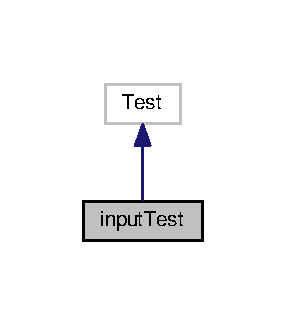
\includegraphics[width=137pt]{classinputTest__inherit__graph}
\end{center}
\end{figure}


Collaboration diagram for input\+Test\+:
\nopagebreak
\begin{figure}[H]
\begin{center}
\leavevmode
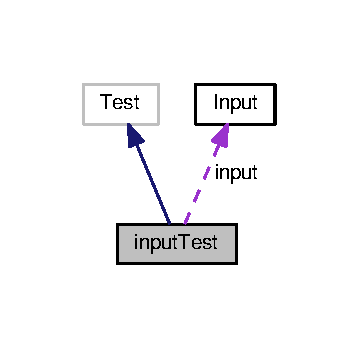
\includegraphics[width=172pt]{classinputTest__coll__graph}
\end{center}
\end{figure}
\subsection*{Protected Attributes}
\begin{DoxyCompactItemize}
\item 
\hyperlink{classInput}{Input} \hyperlink{classinputTest_a882f2a4014812a95a6d58db894f288b1}{input}
\end{DoxyCompactItemize}


\subsection{Member Data Documentation}
\index{input\+Test@{input\+Test}!input@{input}}
\index{input@{input}!input\+Test@{input\+Test}}
\subsubsection[{\texorpdfstring{input}{input}}]{\setlength{\rightskip}{0pt plus 5cm}{\bf Input} input\+Test\+::input\hspace{0.3cm}{\ttfamily [protected]}}\hypertarget{classinputTest_a882f2a4014812a95a6d58db894f288b1}{}\label{classinputTest_a882f2a4014812a95a6d58db894f288b1}


The documentation for this class was generated from the following file\+:\begin{DoxyCompactItemize}
\item 
/home/max/\+C\+Lion\+Projects/\+Project\+Vliegveld/test/\hyperlink{inputTests_8cpp}{input\+Tests.\+cpp}\end{DoxyCompactItemize}

\hypertarget{classRunway}{}\section{Runway Class Reference}
\label{classRunway}\index{Runway@{Runway}}


{\ttfamily \#include $<$Runway.\+h$>$}

\subsection*{Public Member Functions}
\begin{DoxyCompactItemize}
\item 
\hyperlink{classRunway_a75b9355b4953bd430f7c6ea0a18b465a}{Runway} ()
\item 
bool \hyperlink{classRunway_a3f905e251e1c7941690cf89c1fabd04c}{complete} () const 
\item 
bool \hyperlink{classRunway_ab1eb6649c04ead1c6ba6405b0d6e2a9f}{properly\+Initialized} () const 
\item 
bool \hyperlink{classRunway_a54aa6c5f9054cc5d16c10257c641f997}{valid\+For\+Airplane} (\hyperlink{classAirplane}{Airplane} $\ast$plane) const 
\item 
E\+Runway\+Type \hyperlink{classRunway_a6d936a840916f8a5fe01551622cf6c46}{get\+Type} () const 
\item 
void {\bfseries set\+Type} (E\+Runway\+Type type)\hypertarget{classRunway_a0a95f11d67cb4677f1bddd8cf20ed5bc}{}\label{classRunway_a0a95f11d67cb4677f1bddd8cf20ed5bc}

\item 
int {\bfseries get\+Length} () const \hypertarget{classRunway_ab22377036fde6582fa86441e73ad69d2}{}\label{classRunway_ab22377036fde6582fa86441e73ad69d2}

\item 
void {\bfseries set\+Length} (int length)\hypertarget{classRunway_af32954dc4688acd3a91114d200c6df9e}{}\label{classRunway_af32954dc4688acd3a91114d200c6df9e}

\item 
const std\+::string \& {\bfseries get\+Name} () const \hypertarget{classRunway_a2934c38f3af6080f7b40c306a27c57cd}{}\label{classRunway_a2934c38f3af6080f7b40c306a27c57cd}

\item 
void {\bfseries set\+Name} (const std\+::string \&f\+Name)\hypertarget{classRunway_a7c2e26b48213f220676d24dc7e102f4c}{}\label{classRunway_a7c2e26b48213f220676d24dc7e102f4c}

\item 
bool {\bfseries is\+Free} () const \hypertarget{classRunway_a7696b8546ad5ba33d401d7ba740c5936}{}\label{classRunway_a7696b8546ad5ba33d401d7ba740c5936}

\item 
void {\bfseries set\+Free} (bool free)\hypertarget{classRunway_aa93f02e87a66d6ac6ff49ebaf6919216}{}\label{classRunway_aa93f02e87a66d6ac6ff49ebaf6919216}

\item 
std\+::string {\bfseries get\+Taxi\+Point} () const \hypertarget{classRunway_ad2d8fd5696ec93e2fa3d32bec3d02f59}{}\label{classRunway_ad2d8fd5696ec93e2fa3d32bec3d02f59}

\item 
void {\bfseries set\+Taxi\+Point} (const std\+::string \&)\hypertarget{classRunway_aef252fe353421b36fca0f0546eb258de}{}\label{classRunway_aef252fe353421b36fca0f0546eb258de}

\item 
\hyperlink{classAirport}{Airport} $\ast$ {\bfseries get\+Airport} () const \hypertarget{classRunway_a8a16d41a8c65a85e433d96faafb5de06}{}\label{classRunway_a8a16d41a8c65a85e433d96faafb5de06}

\item 
void {\bfseries set\+Airport} (\hyperlink{classAirport}{Airport} $\ast$f\+Airport)\hypertarget{classRunway_a41fd8ad7313e7b667853869854bdc4e6}{}\label{classRunway_a41fd8ad7313e7b667853869854bdc4e6}

\end{DoxyCompactItemize}


\subsection{Detailed Description}
Class that represents a runway in an airport 

\subsection{Constructor \& Destructor Documentation}
\index{Runway@{Runway}!Runway@{Runway}}
\index{Runway@{Runway}!Runway@{Runway}}
\subsubsection[{\texorpdfstring{Runway()}{Runway()}}]{\setlength{\rightskip}{0pt plus 5cm}Runway\+::\+Runway (
\begin{DoxyParamCaption}
{}
\end{DoxyParamCaption}
)}\hypertarget{classRunway_a75b9355b4953bd430f7c6ea0a18b465a}{}\label{classRunway_a75b9355b4953bd430f7c6ea0a18b465a}
Constructor for the \hyperlink{classRunway}{Runway} class. ~\newline
 E\+N\+S\+U\+RE(\hyperlink{classRunway_ab1eb6649c04ead1c6ba6405b0d6e2a9f}{properly\+Initialized()}, \char`\"{}\+Runway wasn\textquotesingle{}t properly initialized after constructing.\char`\"{}); 

\subsection{Member Function Documentation}
\index{Runway@{Runway}!complete@{complete}}
\index{complete@{complete}!Runway@{Runway}}
\subsubsection[{\texorpdfstring{complete() const }{complete() const }}]{\setlength{\rightskip}{0pt plus 5cm}bool Runway\+::complete (
\begin{DoxyParamCaption}
{}
\end{DoxyParamCaption}
) const}\hypertarget{classRunway_a3f905e251e1c7941690cf89c1fabd04c}{}\label{classRunway_a3f905e251e1c7941690cf89c1fabd04c}
Checks if all the data members were initialized ~\newline
 R\+E\+Q\+U\+I\+RE(\hyperlink{classRunway_ab1eb6649c04ead1c6ba6405b0d6e2a9f}{properly\+Initialized()}, \char`\"{}\+Runway wasn\textquotesingle{}t properly initialized when calling complete.\char`\"{}); \begin{DoxyReturn}{Returns}
\+: Boolean indicating if all members were initialized 
\end{DoxyReturn}
\index{Runway@{Runway}!get\+Type@{get\+Type}}
\index{get\+Type@{get\+Type}!Runway@{Runway}}
\subsubsection[{\texorpdfstring{get\+Type() const }{getType() const }}]{\setlength{\rightskip}{0pt plus 5cm}E\+Runway\+Type Runway\+::get\+Type (
\begin{DoxyParamCaption}
{}
\end{DoxyParamCaption}
) const}\hypertarget{classRunway_a6d936a840916f8a5fe01551622cf6c46}{}\label{classRunway_a6d936a840916f8a5fe01551622cf6c46}
Getters and setters for the fields of the class. For all\+: R\+E\+Q\+U\+I\+RE(\hyperlink{classRunway_ab1eb6649c04ead1c6ba6405b0d6e2a9f}{properly\+Initialized()}, \char`\"{}\+Runway wasn\textquotesingle{}t properly initialized when calling getter/setter.\char`\"{}); For setters; E\+N\+S\+U\+RE(get\+Field == value, \char`\"{}\+Field wasn\textquotesingle{}t set properly\char`\"{}); where get\+Field is specific for the member \index{Runway@{Runway}!properly\+Initialized@{properly\+Initialized}}
\index{properly\+Initialized@{properly\+Initialized}!Runway@{Runway}}
\subsubsection[{\texorpdfstring{properly\+Initialized() const }{properlyInitialized() const }}]{\setlength{\rightskip}{0pt plus 5cm}bool Runway\+::properly\+Initialized (
\begin{DoxyParamCaption}
{}
\end{DoxyParamCaption}
) const}\hypertarget{classRunway_ab1eb6649c04ead1c6ba6405b0d6e2a9f}{}\label{classRunway_ab1eb6649c04ead1c6ba6405b0d6e2a9f}
Checks if the object is properly initialized \begin{DoxyReturn}{Returns}
\+: Boolean indicating if properly initialized or not. 
\end{DoxyReturn}
\index{Runway@{Runway}!valid\+For\+Airplane@{valid\+For\+Airplane}}
\index{valid\+For\+Airplane@{valid\+For\+Airplane}!Runway@{Runway}}
\subsubsection[{\texorpdfstring{valid\+For\+Airplane(\+Airplane $\ast$plane) const }{validForAirplane(Airplane *plane) const }}]{\setlength{\rightskip}{0pt plus 5cm}bool Runway\+::valid\+For\+Airplane (
\begin{DoxyParamCaption}
\item[{{\bf Airplane} $\ast$}]{plane}
\end{DoxyParamCaption}
) const}\hypertarget{classRunway_a54aa6c5f9054cc5d16c10257c641f997}{}\label{classRunway_a54aa6c5f9054cc5d16c10257c641f997}
Check if this runway is valid for the provided airplane. ~\newline
 R\+E\+Q\+U\+I\+RE(\hyperlink{classRunway_ab1eb6649c04ead1c6ba6405b0d6e2a9f}{properly\+Initialized()}, \char`\"{}\+Runway wasn\textquotesingle{}t properly initialized when calling valid\+For\+Airplane.\char`\"{}); ~\newline
 R\+E\+Q\+U\+I\+RE(plane != N\+U\+LL, \char`\"{}\+Plane object does not exist.\char`\"{}); 
\begin{DoxyParams}{Parameters}
{\em plane} & \hyperlink{classAirplane}{Airplane} to check validity for. \\
\hline
\end{DoxyParams}
\begin{DoxyReturn}{Returns}
\+: Boolean indicating if valid or not. 
\end{DoxyReturn}


The documentation for this class was generated from the following files\+:\begin{DoxyCompactItemize}
\item 
/home/max/\+C\+Lion\+Projects/\+Project\+Vliegveld/headers/Runway.\+h\item 
/home/max/\+C\+Lion\+Projects/\+Project\+Vliegveld/src/Runway.\+cpp\end{DoxyCompactItemize}

\hypertarget{classSystem}{}\section{System Class Reference}
\label{classSystem}\index{System@{System}}


\+: Main class, controls the simulation.  




{\ttfamily \#include $<$System.\+h$>$}

\subsection*{Public Member Functions}
\begin{DoxyCompactItemize}
\item 
\hyperlink{classSystem_a8b60d099be14345558de236d2fbc76ba}{System} (const \hyperlink{classInput}{Input} \&input, std\+::ostream \&atc, const \hyperlink{classTime}{Time} \&end)
\item 
\hyperlink{classSystem_a3be70bb338e3f062f821173fd15680d0}{$\sim$\+System} ()
\item 
void \hyperlink{classSystem_a1e6b24f8ed92dac6ce380b91268976b7}{run} (std\+::ostream \&log, const std\+::string \&impression\+Name=\char`\"{}../output/impressions/impression\char`\"{}, const std\+::string \&ini\+Name=\char`\"{}../output/ini/graphics\char`\"{})
\item 
void \hyperlink{classSystem_a62d81f9e0abc880c57972a491df4fb2e}{info} (std\+::ostream \&out)
\item 
void \hyperlink{classSystem_a779e7d437efa57c0268943dde52c6336}{generate\+Images} (\hyperlink{classTime}{Time} start, \hyperlink{classTime}{Time} end)
\item 
bool \hyperlink{classSystem_abae43adfa434ace30ef85c69a7842289}{simulation\+Finished} () const 
\item 
\hyperlink{classAirport}{Airport} $\ast$ \hyperlink{classSystem_a8cd2a9b13cdbcf30f801e46cf8284800}{get\+Airport} () const 
\item 
\hyperlink{classATC}{A\+TC} $\ast$ \hyperlink{classSystem_aae418c2545087b63188f4a4ffb2e9d15}{get\+A\+TC} () const 
\item 
std\+::vector$<$ \hyperlink{classFlightPlan}{Flight\+Plan} $\ast$ $>$ \hyperlink{classSystem_ae2f5fb3771a2d924215ca8dbd15b89ed}{get\+Flight\+Plans} () const 
\item 
bool \hyperlink{classSystem_af3eece83ba2d92a4a6b6c186d427c556}{properly\+Initialized} () const 
\end{DoxyCompactItemize}


\subsection{Detailed Description}
\+: Main class, controls the simulation. 

\subsection{Constructor \& Destructor Documentation}
\index{System@{System}!System@{System}}
\index{System@{System}!System@{System}}
\subsubsection[{\texorpdfstring{System(const Input \&input, std\+::ostream \&atc, const Time \&end)}{System(const Input &input, std::ostream &atc, const Time &end)}}]{\setlength{\rightskip}{0pt plus 5cm}System\+::\+System (
\begin{DoxyParamCaption}
\item[{const {\bf Input} \&}]{input, }
\item[{std\+::ostream \&}]{atc, }
\item[{const {\bf Time} \&}]{end}
\end{DoxyParamCaption}
)}\hypertarget{classSystem_a8b60d099be14345558de236d2fbc76ba}{}\label{classSystem_a8b60d099be14345558de236d2fbc76ba}
Constructor ~\newline
 R\+E\+Q\+U\+I\+RE(!input.get\+Airports().empty(), \char`\"{}\+There has to be an airport in the input to start the simulation\char`\"{}); ~\newline
 E\+N\+S\+U\+RE(\hyperlink{classSystem_af3eece83ba2d92a4a6b6c186d427c556}{properly\+Initialized()}, \char`\"{}constructor must end in properly\+Initialized state\char`\"{}); 
\begin{DoxyParams}{Parameters}
{\em input} & the input of the simulation \\
\hline
{\em atc} & the stream where atc messages will be written to \\
\hline
{\em end} & the ending time of the simulation \\
\hline
\end{DoxyParams}
\index{System@{System}!````~System@{$\sim$\+System}}
\index{````~System@{$\sim$\+System}!System@{System}}
\subsubsection[{\texorpdfstring{$\sim$\+System()}{~System()}}]{\setlength{\rightskip}{0pt plus 5cm}System\+::$\sim$\+System (
\begin{DoxyParamCaption}
{}
\end{DoxyParamCaption}
)}\hypertarget{classSystem_a3be70bb338e3f062f821173fd15680d0}{}\label{classSystem_a3be70bb338e3f062f821173fd15680d0}
Destructor 

\subsection{Member Function Documentation}
\index{System@{System}!generate\+Images@{generate\+Images}}
\index{generate\+Images@{generate\+Images}!System@{System}}
\subsubsection[{\texorpdfstring{generate\+Images(\+Time start, Time end)}{generateImages(Time start, Time end)}}]{\setlength{\rightskip}{0pt plus 5cm}void System\+::generate\+Images (
\begin{DoxyParamCaption}
\item[{{\bf Time}}]{start, }
\item[{{\bf Time}}]{end}
\end{DoxyParamCaption}
)}\hypertarget{classSystem_a779e7d437efa57c0268943dde52c6336}{}\label{classSystem_a779e7d437efa57c0268943dde52c6336}
Generates the images from the start time until the end time, with the use of ~\newline
 the generated ini files and the graphics engine. ~\newline
 R\+E\+Q\+U\+I\+RE(this-\/$>$\hyperlink{classSystem_af3eece83ba2d92a4a6b6c186d427c556}{properly\+Initialized()}, \char`\"{}\+System was\textquotesingle{}t initialized when calling generate\+Images\char`\"{}); 
\begin{DoxyParams}{Parameters}
{\em start} & time of first image \\
\hline
{\em end} & time of last image, not included \\
\hline
\end{DoxyParams}
\index{System@{System}!get\+Airport@{get\+Airport}}
\index{get\+Airport@{get\+Airport}!System@{System}}
\subsubsection[{\texorpdfstring{get\+Airport() const }{getAirport() const }}]{\setlength{\rightskip}{0pt plus 5cm}{\bf Airport} $\ast$ System\+::get\+Airport (
\begin{DoxyParamCaption}
{}
\end{DoxyParamCaption}
) const}\hypertarget{classSystem_a8cd2a9b13cdbcf30f801e46cf8284800}{}\label{classSystem_a8cd2a9b13cdbcf30f801e46cf8284800}
Getter for the airport in the simulation ~\newline
 R\+E\+Q\+U\+I\+RE(this-\/$>$\hyperlink{classSystem_af3eece83ba2d92a4a6b6c186d427c556}{properly\+Initialized()}, \char`\"{}\+System was\textquotesingle{}t initialized when calling get\+Airport\char`\"{}); \begin{DoxyReturn}{Returns}
\+: airport in the simulation 
\end{DoxyReturn}
\index{System@{System}!get\+A\+TC@{get\+A\+TC}}
\index{get\+A\+TC@{get\+A\+TC}!System@{System}}
\subsubsection[{\texorpdfstring{get\+A\+T\+C() const }{getATC() const }}]{\setlength{\rightskip}{0pt plus 5cm}{\bf A\+TC} $\ast$ System\+::get\+A\+TC (
\begin{DoxyParamCaption}
{}
\end{DoxyParamCaption}
) const}\hypertarget{classSystem_aae418c2545087b63188f4a4ffb2e9d15}{}\label{classSystem_aae418c2545087b63188f4a4ffb2e9d15}
Getter for the air traffic control in the simulation ~\newline
 R\+E\+Q\+U\+I\+RE(this-\/$>$\hyperlink{classSystem_af3eece83ba2d92a4a6b6c186d427c556}{properly\+Initialized()}, \char`\"{}\+System was\textquotesingle{}t initialized when calling get\+A\+T\+C\char`\"{}); \begin{DoxyReturn}{Returns}
\+: \hyperlink{classATC}{A\+TC} in the simulation 
\end{DoxyReturn}
\index{System@{System}!get\+Flight\+Plans@{get\+Flight\+Plans}}
\index{get\+Flight\+Plans@{get\+Flight\+Plans}!System@{System}}
\subsubsection[{\texorpdfstring{get\+Flight\+Plans() const }{getFlightPlans() const }}]{\setlength{\rightskip}{0pt plus 5cm}vector$<$ {\bf Flight\+Plan} $\ast$ $>$ System\+::get\+Flight\+Plans (
\begin{DoxyParamCaption}
{}
\end{DoxyParamCaption}
) const}\hypertarget{classSystem_ae2f5fb3771a2d924215ca8dbd15b89ed}{}\label{classSystem_ae2f5fb3771a2d924215ca8dbd15b89ed}
Getter for the flight plans in the simulation ~\newline
 R\+E\+Q\+U\+I\+RE(this-\/$>$\hyperlink{classSystem_af3eece83ba2d92a4a6b6c186d427c556}{properly\+Initialized()}, "\hyperlink{classSystem}{System} was\textquotesingle{}t initialized when calling get\+Flight\+Plans); \begin{DoxyReturn}{Returns}
\+: vector of flightplans that are in the simulation 
\end{DoxyReturn}
\index{System@{System}!info@{info}}
\index{info@{info}!System@{System}}
\subsubsection[{\texorpdfstring{info(std\+::ostream \&out)}{info(std::ostream &out)}}]{\setlength{\rightskip}{0pt plus 5cm}void System\+::info (
\begin{DoxyParamCaption}
\item[{std\+::ostream \&}]{out}
\end{DoxyParamCaption}
)}\hypertarget{classSystem_a62d81f9e0abc880c57972a491df4fb2e}{}\label{classSystem_a62d81f9e0abc880c57972a491df4fb2e}
Logs information of the airports and airplanes to a text file ~\newline
 R\+E\+Q\+U\+I\+RE(this-\/$>$\hyperlink{classSystem_af3eece83ba2d92a4a6b6c186d427c556}{properly\+Initialized()}, \char`\"{}\+System was\textquotesingle{}t initialized when calling info\char`\"{}); ~\newline
 R\+E\+Q\+U\+I\+RE(f\+Airport != N\+U\+LL, \char`\"{}\+No airport in the simulation\char`\"{}); 
\begin{DoxyParams}{Parameters}
{\em out} & the ostream where the info will be written to \\
\hline
\end{DoxyParams}
\index{System@{System}!properly\+Initialized@{properly\+Initialized}}
\index{properly\+Initialized@{properly\+Initialized}!System@{System}}
\subsubsection[{\texorpdfstring{properly\+Initialized() const }{properlyInitialized() const }}]{\setlength{\rightskip}{0pt plus 5cm}bool System\+::properly\+Initialized (
\begin{DoxyParamCaption}
{}
\end{DoxyParamCaption}
) const}\hypertarget{classSystem_af3eece83ba2d92a4a6b6c186d427c556}{}\label{classSystem_af3eece83ba2d92a4a6b6c186d427c556}
Checks if the object is properly initialized \begin{DoxyReturn}{Returns}
\+: boolean indicating if object is properly initialized. 
\end{DoxyReturn}
\index{System@{System}!run@{run}}
\index{run@{run}!System@{System}}
\subsubsection[{\texorpdfstring{run(std\+::ostream \&log, const std\+::string \&impression\+Name=""../output/impressions/impression"", const std\+::string \&ini\+Name=""../output/ini/graphics"")}{run(std::ostream &log, const std::string &impressionName="../output/impressions/impression", const std::string &iniName="../output/ini/graphics")}}]{\setlength{\rightskip}{0pt plus 5cm}void System\+::run (
\begin{DoxyParamCaption}
\item[{std\+::ostream \&}]{log, }
\item[{const std\+::string \&}]{impression\+Name = {\ttfamily \char`\"{}../output/impressions/impression\char`\"{}}, }
\item[{const std\+::string \&}]{ini\+Name = {\ttfamily \char`\"{}../output/ini/graphics\char`\"{}}}
\end{DoxyParamCaption}
)}\hypertarget{classSystem_a1e6b24f8ed92dac6ce380b91268976b7}{}\label{classSystem_a1e6b24f8ed92dac6ce380b91268976b7}
Runs the complete simulation ~\newline
 R\+E\+Q\+U\+I\+RE(this-\/$>$\hyperlink{classSystem_af3eece83ba2d92a4a6b6c186d427c556}{properly\+Initialized()}, \char`\"{}\+System was\textquotesingle{}t initialized when calling run\char`\"{}); ~\newline
 R\+E\+Q\+U\+I\+RE(\hyperlink{classSystem_a8cd2a9b13cdbcf30f801e46cf8284800}{get\+Airport()} != N\+U\+LL, \char`\"{}\+No airport in the simulation.\char`\"{}); ~\newline
 R\+E\+Q\+U\+I\+RE(!simulation\+Finished(), \char`\"{}\+Simulation is already finished\char`\"{});. ~\newline
 E\+N\+S\+U\+RE(\hyperlink{classSystem_abae43adfa434ace30ef85c69a7842289}{simulation\+Finished()}, \char`\"{}\+Simulation is not finished yet, error occurred\char`\"{}); 
\begin{DoxyParams}{Parameters}
{\em log} & ostream where all the log messages will be written to \\
\hline
{\em impression\+Name} & basename of the files for the impressions \\
\hline
{\em ini\+Name} & basename of the files for the ini files \\
\hline
\end{DoxyParams}
\index{System@{System}!simulation\+Finished@{simulation\+Finished}}
\index{simulation\+Finished@{simulation\+Finished}!System@{System}}
\subsubsection[{\texorpdfstring{simulation\+Finished() const }{simulationFinished() const }}]{\setlength{\rightskip}{0pt plus 5cm}bool System\+::simulation\+Finished (
\begin{DoxyParamCaption}
{}
\end{DoxyParamCaption}
) const}\hypertarget{classSystem_abae43adfa434ace30ef85c69a7842289}{}\label{classSystem_abae43adfa434ace30ef85c69a7842289}
Checks if the simulation has ended, i.\+e. specified end time has been reached ~\newline
 R\+E\+Q\+U\+I\+RE(this-\/$>$\hyperlink{classSystem_af3eece83ba2d92a4a6b6c186d427c556}{properly\+Initialized()}, \char`\"{}\+System was\textquotesingle{}t initialized when calling simulation\+Finished\char`\"{}); \begin{DoxyReturn}{Returns}
\+: boolean indicating if the simulation is finished. 
\end{DoxyReturn}


The documentation for this class was generated from the following files\+:\begin{DoxyCompactItemize}
\item 
/home/max/\+C\+Lion\+Projects/\+Project\+Vliegveld/headers/System.\+h\item 
/home/max/\+C\+Lion\+Projects/\+Project\+Vliegveld/src/System.\+cpp\end{DoxyCompactItemize}

\hypertarget{classTime}{}\section{Time Class Reference}
\label{classTime}\index{Time@{Time}}


{\ttfamily \#include $<$Time.\+h$>$}

\subsection*{Public Member Functions}
\begin{DoxyCompactItemize}
\item 
\hyperlink{classTime_a90d3b9a3fb4516e7ccb4c60deba03807}{Time} (int hour=12, int minute=0)
\item 
\hyperlink{classTime_a8d758b905e2fda239938ae0ee320453f}{Time} (const \hyperlink{classTime}{Time} \&time)
\item 
std\+::string \hyperlink{classTime_aeeb2d2b5a624d0d78b7f5d146d0682f5}{formatted} () const 
\item 
void \hyperlink{classTime_a41c94422f10c95daab849b9c20afdeba}{advance} (int minutes=1)
\item 
void \hyperlink{classTime_a9c53c93d10be3785c85449186beb6b6a}{set\+Minute} (int minute)
\item 
int \hyperlink{classTime_a6ccac73be7aacc12410cea6b3d216357}{get\+Minute} () const 
\item 
void \hyperlink{classTime_ab77d5f9f5fa8582d23a70d418ab6a182}{set\+Hour} (int hour)
\item 
int \hyperlink{classTime_a4e9d93c2aaaac84b0a49f44184968860}{get\+Hour} () const 
\item 
bool \hyperlink{classTime_ab29d371ddb19ce156377cea159efafef}{properly\+Initialized} () const 
\item 
bool \hyperlink{classTime_adeb3173efb2cb16bf361db0204a85c7c}{operator==} (const \hyperlink{classTime}{Time} \&) const 
\item 
bool \hyperlink{classTime_aa668f56a3ee77c147e7dc76bf1ad89f1}{operator$<$} (const \hyperlink{classTime}{Time} \&) const 
\item 
\hyperlink{classTime}{Time} \& \hyperlink{classTime_a7801190e243f4b6662d7d9ebadbd342f}{operator=} (const \hyperlink{classTime}{Time} \&time)
\end{DoxyCompactItemize}


\subsection{Detailed Description}
Class that represents the time 

\subsection{Constructor \& Destructor Documentation}
\index{Time@{Time}!Time@{Time}}
\index{Time@{Time}!Time@{Time}}
\subsubsection[{\texorpdfstring{Time(int hour=12, int minute=0)}{Time(int hour=12, int minute=0)}}]{\setlength{\rightskip}{0pt plus 5cm}Time\+::\+Time (
\begin{DoxyParamCaption}
\item[{int}]{hour = {\ttfamily 12}, }
\item[{int}]{minute = {\ttfamily 0}}
\end{DoxyParamCaption}
)}\hypertarget{classTime_a90d3b9a3fb4516e7ccb4c60deba03807}{}\label{classTime_a90d3b9a3fb4516e7ccb4c60deba03807}
Constructor, sets the time ~\newline
 Defaults to 12\+:00, which is the starting point of the simulation ~\newline
 R\+E\+Q\+U\+I\+RE(minute $<$ 60 \&\& minute $>$= 0, \char`\"{}\+Minute has to be between 0 and 60\char`\"{}); ~\newline
 R\+E\+Q\+U\+I\+RE(hour $<$ 24 \&\& hour $>$= 0, \char`\"{}\+Hour has to be between 0 and 24\char`\"{}); ~\newline
 E\+N\+S\+U\+RE(\hyperlink{classTime_ab29d371ddb19ce156377cea159efafef}{properly\+Initialized()}, \char`\"{}\+Time wasn\textquotesingle{}t properly initialized after constructing.\char`\"{}); 
\begin{DoxyParams}{Parameters}
{\em hour} & the hour \\
\hline
{\em minute} & the minute \\
\hline
\end{DoxyParams}
\index{Time@{Time}!Time@{Time}}
\index{Time@{Time}!Time@{Time}}
\subsubsection[{\texorpdfstring{Time(const Time \&time)}{Time(const Time &time)}}]{\setlength{\rightskip}{0pt plus 5cm}Time\+::\+Time (
\begin{DoxyParamCaption}
\item[{const {\bf Time} \&}]{time}
\end{DoxyParamCaption}
)}\hypertarget{classTime_a8d758b905e2fda239938ae0ee320453f}{}\label{classTime_a8d758b905e2fda239938ae0ee320453f}
Copy constructor ~\newline
 E\+N\+S\+U\+RE(\hyperlink{classTime_ab29d371ddb19ce156377cea159efafef}{properly\+Initialized()}, \char`\"{}\+Time wasn\textquotesingle{}t properly initialized after constructing.\char`\"{}); 
\begin{DoxyParams}{Parameters}
{\em time} & object to be copied \\
\hline
\end{DoxyParams}


\subsection{Member Function Documentation}
\index{Time@{Time}!advance@{advance}}
\index{advance@{advance}!Time@{Time}}
\subsubsection[{\texorpdfstring{advance(int minutes=1)}{advance(int minutes=1)}}]{\setlength{\rightskip}{0pt plus 5cm}void Time\+::advance (
\begin{DoxyParamCaption}
\item[{int}]{minutes = {\ttfamily 1}}
\end{DoxyParamCaption}
)}\hypertarget{classTime_a41c94422f10c95daab849b9c20afdeba}{}\label{classTime_a41c94422f10c95daab849b9c20afdeba}
Advances the time by an amount of minutes ~\newline
 R\+E\+Q\+U\+I\+RE(\hyperlink{classTime_ab29d371ddb19ce156377cea159efafef}{properly\+Initialized()}, \char`\"{}\+Time wasn\textquotesingle{}t properly\+Initialized when calling advance\char`\"{}); ~\newline
 R\+E\+Q\+U\+I\+RE(minutes $>$= 0, \char`\"{}\+Advancing by a negative amount of minutes is not possible\char`\"{}); 
\begin{DoxyParams}{Parameters}
{\em minutes} & amount of minutes to advance \\
\hline
\end{DoxyParams}
\index{Time@{Time}!formatted@{formatted}}
\index{formatted@{formatted}!Time@{Time}}
\subsubsection[{\texorpdfstring{formatted() const }{formatted() const }}]{\setlength{\rightskip}{0pt plus 5cm}string Time\+::formatted (
\begin{DoxyParamCaption}
{}
\end{DoxyParamCaption}
) const}\hypertarget{classTime_aeeb2d2b5a624d0d78b7f5d146d0682f5}{}\label{classTime_aeeb2d2b5a624d0d78b7f5d146d0682f5}
Return the time in a formatted style like such\+: \char`\"{}13\+:45\char`\"{} ~\newline
 R\+E\+Q\+U\+I\+RE(\hyperlink{classTime_ab29d371ddb19ce156377cea159efafef}{properly\+Initialized()}, \char`\"{}\+Time wasn\textquotesingle{}t properly\+Initialized when calling formatted\char`\"{}); \begin{DoxyReturn}{Returns}
string of time 
\end{DoxyReturn}
\index{Time@{Time}!get\+Hour@{get\+Hour}}
\index{get\+Hour@{get\+Hour}!Time@{Time}}
\subsubsection[{\texorpdfstring{get\+Hour() const }{getHour() const }}]{\setlength{\rightskip}{0pt plus 5cm}int Time\+::get\+Hour (
\begin{DoxyParamCaption}
{}
\end{DoxyParamCaption}
) const}\hypertarget{classTime_a4e9d93c2aaaac84b0a49f44184968860}{}\label{classTime_a4e9d93c2aaaac84b0a49f44184968860}
Getter for the hour ~\newline
 R\+E\+Q\+U\+I\+RE(\hyperlink{classTime_ab29d371ddb19ce156377cea159efafef}{properly\+Initialized()}, \char`\"{}\+Time wasn\textquotesingle{}t properly\+Initialized when calling get\+Hour\char`\"{}); \begin{DoxyReturn}{Returns}
\+: hour 
\end{DoxyReturn}
\index{Time@{Time}!get\+Minute@{get\+Minute}}
\index{get\+Minute@{get\+Minute}!Time@{Time}}
\subsubsection[{\texorpdfstring{get\+Minute() const }{getMinute() const }}]{\setlength{\rightskip}{0pt plus 5cm}int Time\+::get\+Minute (
\begin{DoxyParamCaption}
{}
\end{DoxyParamCaption}
) const}\hypertarget{classTime_a6ccac73be7aacc12410cea6b3d216357}{}\label{classTime_a6ccac73be7aacc12410cea6b3d216357}
Getter for the minute ~\newline
 R\+E\+Q\+U\+I\+RE(\hyperlink{classTime_ab29d371ddb19ce156377cea159efafef}{properly\+Initialized()}, \char`\"{}\+Time wasn\textquotesingle{}t properly\+Initialized when calling get\+Minute\char`\"{}); \begin{DoxyReturn}{Returns}
\+: minute 
\end{DoxyReturn}
\index{Time@{Time}!operator$<$@{operator$<$}}
\index{operator$<$@{operator$<$}!Time@{Time}}
\subsubsection[{\texorpdfstring{operator$<$(const Time \&) const }{operator<(const Time &) const }}]{\setlength{\rightskip}{0pt plus 5cm}bool Time\+::operator$<$ (
\begin{DoxyParamCaption}
\item[{const {\bf Time} \&}]{time}
\end{DoxyParamCaption}
) const}\hypertarget{classTime_aa668f56a3ee77c147e7dc76bf1ad89f1}{}\label{classTime_aa668f56a3ee77c147e7dc76bf1ad89f1}
Operator$<$ overloaded, returns false if comparing with 00\+:00 \index{Time@{Time}!operator=@{operator=}}
\index{operator=@{operator=}!Time@{Time}}
\subsubsection[{\texorpdfstring{operator=(const Time \&time)}{operator=(const Time &time)}}]{\setlength{\rightskip}{0pt plus 5cm}{\bf Time} \& Time\+::operator= (
\begin{DoxyParamCaption}
\item[{const {\bf Time} \&}]{time}
\end{DoxyParamCaption}
)}\hypertarget{classTime_a7801190e243f4b6662d7d9ebadbd342f}{}\label{classTime_a7801190e243f4b6662d7d9ebadbd342f}
Assignment operator 
\begin{DoxyParams}{Parameters}
{\em time} & rhs of operator \\
\hline
\end{DoxyParams}
\begin{DoxyReturn}{Returns}
reference to this 
\end{DoxyReturn}
\index{Time@{Time}!operator==@{operator==}}
\index{operator==@{operator==}!Time@{Time}}
\subsubsection[{\texorpdfstring{operator==(const Time \&) const }{operator==(const Time &) const }}]{\setlength{\rightskip}{0pt plus 5cm}bool Time\+::operator== (
\begin{DoxyParamCaption}
\item[{const {\bf Time} \&}]{time}
\end{DoxyParamCaption}
) const}\hypertarget{classTime_adeb3173efb2cb16bf361db0204a85c7c}{}\label{classTime_adeb3173efb2cb16bf361db0204a85c7c}
Operator== overloaded \index{Time@{Time}!properly\+Initialized@{properly\+Initialized}}
\index{properly\+Initialized@{properly\+Initialized}!Time@{Time}}
\subsubsection[{\texorpdfstring{properly\+Initialized() const }{properlyInitialized() const }}]{\setlength{\rightskip}{0pt plus 5cm}bool Time\+::properly\+Initialized (
\begin{DoxyParamCaption}
{}
\end{DoxyParamCaption}
) const}\hypertarget{classTime_ab29d371ddb19ce156377cea159efafef}{}\label{classTime_ab29d371ddb19ce156377cea159efafef}
Checks if the object is properly initialized \begin{DoxyReturn}{Returns}
\+: Boolean indicating if properly initialized or not. 
\end{DoxyReturn}
\index{Time@{Time}!set\+Hour@{set\+Hour}}
\index{set\+Hour@{set\+Hour}!Time@{Time}}
\subsubsection[{\texorpdfstring{set\+Hour(int hour)}{setHour(int hour)}}]{\setlength{\rightskip}{0pt plus 5cm}void Time\+::set\+Hour (
\begin{DoxyParamCaption}
\item[{int}]{hour}
\end{DoxyParamCaption}
)}\hypertarget{classTime_ab77d5f9f5fa8582d23a70d418ab6a182}{}\label{classTime_ab77d5f9f5fa8582d23a70d418ab6a182}
Setter for the hour. ~\newline
 R\+E\+Q\+U\+I\+RE(hour $<$ 24 \&\& hour $>$= 0, \char`\"{}\+Hour has to be between 0 and 24\char`\"{}); ~\newline
 R\+E\+Q\+U\+I\+RE(\hyperlink{classTime_ab29d371ddb19ce156377cea159efafef}{properly\+Initialized()}, \char`\"{}\+Time wasn\textquotesingle{}t properly\+Initialized when calling set\+Hour\char`\"{}); 
\begin{DoxyParams}{Parameters}
{\em hour} & hour to set \\
\hline
\end{DoxyParams}
\index{Time@{Time}!set\+Minute@{set\+Minute}}
\index{set\+Minute@{set\+Minute}!Time@{Time}}
\subsubsection[{\texorpdfstring{set\+Minute(int minute)}{setMinute(int minute)}}]{\setlength{\rightskip}{0pt plus 5cm}void Time\+::set\+Minute (
\begin{DoxyParamCaption}
\item[{int}]{minute}
\end{DoxyParamCaption}
)}\hypertarget{classTime_a9c53c93d10be3785c85449186beb6b6a}{}\label{classTime_a9c53c93d10be3785c85449186beb6b6a}
Setter for the minute. ~\newline
 R\+E\+Q\+U\+I\+RE(minute $<$ 60 \&\& minute $>$= 0, \char`\"{}\+Minute has to be between 0 and 60\char`\"{}); ~\newline
 R\+E\+Q\+U\+I\+RE(\hyperlink{classTime_ab29d371ddb19ce156377cea159efafef}{properly\+Initialized()}, \char`\"{}\+Time wasn\textquotesingle{}t properly\+Initialized when calling set\+Minute\char`\"{}); 
\begin{DoxyParams}{Parameters}
{\em minute} & minute to set \\
\hline
\end{DoxyParams}


The documentation for this class was generated from the following files\+:\begin{DoxyCompactItemize}
\item 
/home/max/\+C\+Lion\+Projects/\+Project\+Vliegveld/headers/Time.\+h\item 
/home/max/\+C\+Lion\+Projects/\+Project\+Vliegveld/src/Time.\+cpp\end{DoxyCompactItemize}

\chapter{File Documentation}
\hypertarget{CMakeCache_8txt}{}\section{/home/max/\+C\+Lion\+Projects/\+Project\+Vliegveld/cmake-\/build-\/debug/\+C\+Make\+Cache.txt File Reference}
\label{CMakeCache_8txt}\index{/home/max/\+C\+Lion\+Projects/\+Project\+Vliegveld/cmake-\/build-\/debug/\+C\+Make\+Cache.\+txt@{/home/max/\+C\+Lion\+Projects/\+Project\+Vliegveld/cmake-\/build-\/debug/\+C\+Make\+Cache.\+txt}}
\subsection*{Functions}
\begin{DoxyCompactItemize}
\item 
\hyperlink{CMakeCache_8txt_a15033d43fd4881ecb41d0a9ef3f98c8b}{\+\_\+\+\_\+has\+\_\+include} (S\+TR)
\item 
\hyperlink{CMakeCache_8txt_a97e2b5b7d48e0c704f01b437bbb41bc3}{\+\_\+\+\_\+has\+\_\+include\+\_\+\+\_\+} (S\+TR)
\item 
\hyperlink{CMakeCache_8txt_a6bc72b80bcdbfe30be5d38536affde6f}{\+\_\+\+\_\+has\+\_\+include\+\_\+next} (S\+TR)
\item 
\hyperlink{CMakeCache_8txt_ac96b06945e62d6ea6764b6d86745ec26}{\+\_\+\+\_\+has\+\_\+include\+\_\+next\+\_\+\+\_\+} (S\+TR)
\item 
\hyperlink{CMakeCache_8txt_a2f10a19f2682f0eb61615edae3fa69ef}{\+\_\+\+\_\+\+I\+N\+T\+M\+A\+X\+\_\+C} (\hyperlink{html_2jquery_8js_abce695e0af988ece0826d9ad59b8160d}{c})
\end{DoxyCompactItemize}
\subsection*{Variables}
\begin{DoxyCompactItemize}
\item 
C\+M\+A\+K\+E\+\_\+\+AR \hyperlink{CMakeCache_8txt_a2b96b3598268f62908e4995dd2463817}{\+\_\+\+\_\+pad0\+\_\+\+\_\+}
\item 
\hyperlink{CMakeCache_8txt_aba69e7d86e970c5454fedf7e25cbf49e}{\+\_\+\+\_\+\+S\+T\+D\+C\+\_\+\+V\+E\+R\+S\+I\+O\+N\+\_\+\+\_\+}
\item 
\hyperlink{CMakeCache_8txt_a391447bc12001cf307b9fec77d32c722}{\+\_\+\+\_\+\+S\+T\+D\+C\+\_\+\+U\+T\+F\+\_\+16\+\_\+\+\_\+}
\item 
\hyperlink{CMakeCache_8txt_aebc193933efcf54801ba103bf6d12dbb}{\+\_\+\+\_\+\+S\+T\+D\+C\+\_\+\+U\+T\+F\+\_\+32\+\_\+\+\_\+}
\item 
\hyperlink{CMakeCache_8txt_aacc78bc040f85bfc5d36eda8c048a1fe}{\+\_\+\+\_\+\+S\+T\+D\+C\+\_\+\+H\+O\+S\+T\+E\+D\+\_\+\+\_\+}
\item 
\hyperlink{CMakeCache_8txt_a4f955bfc59f2aa5f37123f7fa8c45974}{\+\_\+\+\_\+\+G\+N\+U\+C\+\_\+\+\_\+}
\item 
\hyperlink{CMakeCache_8txt_aefc5089d158028a655f8653d849ea643}{\+\_\+\+\_\+\+G\+N\+U\+C\+\_\+\+M\+I\+N\+O\+R\+\_\+\+\_\+}
\item 
\hyperlink{CMakeCache_8txt_a68c7f08caefc9a019e0b82ec6b3fa343}{\+\_\+\+\_\+\+G\+N\+U\+C\+\_\+\+P\+A\+T\+C\+H\+L\+E\+V\+E\+L\+\_\+\+\_\+}
\item 
\hyperlink{CMakeCache_8txt_abb4404c3387f41ca320babfbcff1102f}{\+\_\+\+\_\+\+V\+E\+R\+S\+I\+O\+N\+\_\+\+\_\+}
\item 
\hyperlink{CMakeCache_8txt_acf476ec759fbe7a6aa89427ea8965872}{\+\_\+\+\_\+\+A\+T\+O\+M\+I\+C\+\_\+\+R\+E\+L\+A\+X\+ED}
\item 
\hyperlink{CMakeCache_8txt_a44cd817264eb1136dae5f3b248f8fa8e}{\+\_\+\+\_\+\+A\+T\+O\+M\+I\+C\+\_\+\+S\+E\+Q\+\_\+\+C\+ST}
\item 
\hyperlink{CMakeCache_8txt_a77baa125558a766167c49286c9873d7f}{\+\_\+\+\_\+\+A\+T\+O\+M\+I\+C\+\_\+\+A\+C\+Q\+U\+I\+RE}
\item 
\hyperlink{CMakeCache_8txt_a5738074ef1a9257e5bcb0b527c2c93a3}{\+\_\+\+\_\+\+A\+T\+O\+M\+I\+C\+\_\+\+R\+E\+L\+E\+A\+SE}
\item 
\hyperlink{CMakeCache_8txt_a93654874cdfb30676f9c0c31eb3511c0}{\+\_\+\+\_\+\+A\+T\+O\+M\+I\+C\+\_\+\+A\+C\+Q\+\_\+\+R\+EL}
\item 
\hyperlink{CMakeCache_8txt_a000e85470c6f5d9f1aa22fa4df83f0b9}{\+\_\+\+\_\+\+A\+T\+O\+M\+I\+C\+\_\+\+C\+O\+N\+S\+U\+ME}
\item 
\hyperlink{CMakeCache_8txt_a8af0fd31855c1121674e7d0adf6acbee}{\+\_\+\+\_\+\+F\+I\+N\+I\+T\+E\+\_\+\+M\+A\+T\+H\+\_\+\+O\+N\+L\+Y\+\_\+\+\_\+}
\item 
\hyperlink{CMakeCache_8txt_aae88ee59a31703e88a326390e91a32fd}{\+\_\+\+L\+P64}
\item 
\hyperlink{CMakeCache_8txt_a2dcb516e6c55b8bdfd122dc65ada57b5}{\+\_\+\+\_\+\+L\+P64\+\_\+\+\_\+}
\item 
\hyperlink{CMakeCache_8txt_a52701f18fd19d3d5e1f83ec11c05d570}{\+\_\+\+\_\+\+S\+I\+Z\+E\+O\+F\+\_\+\+I\+N\+T\+\_\+\+\_\+}
\item 
\hyperlink{CMakeCache_8txt_a25b323872510a2d005ee2f45f5efd38b}{\+\_\+\+\_\+\+S\+I\+Z\+E\+O\+F\+\_\+\+L\+O\+N\+G\+\_\+\+\_\+}
\item 
\hyperlink{CMakeCache_8txt_a87bd59f7da0f977c3d450e95b4f00532}{\+\_\+\+\_\+\+S\+I\+Z\+E\+O\+F\+\_\+\+L\+O\+N\+G\+\_\+\+L\+O\+N\+G\+\_\+\+\_\+}
\item 
\hyperlink{CMakeCache_8txt_a13a1a9ce0eb7429c078ea705b54ac44d}{\+\_\+\+\_\+\+S\+I\+Z\+E\+O\+F\+\_\+\+S\+H\+O\+R\+T\+\_\+\+\_\+}
\item 
\hyperlink{CMakeCache_8txt_a99451faa2465beb743c5cadc6a20f102}{\+\_\+\+\_\+\+S\+I\+Z\+E\+O\+F\+\_\+\+F\+L\+O\+A\+T\+\_\+\+\_\+}
\item 
\hyperlink{CMakeCache_8txt_acb4d0f0ad8b370190fb78d60045cbe85}{\+\_\+\+\_\+\+S\+I\+Z\+E\+O\+F\+\_\+\+D\+O\+U\+B\+L\+E\+\_\+\+\_\+}
\item 
\hyperlink{CMakeCache_8txt_a398170fb1a6ec5ddef97aada19630f92}{\+\_\+\+\_\+\+S\+I\+Z\+E\+O\+F\+\_\+\+L\+O\+N\+G\+\_\+\+D\+O\+U\+B\+L\+E\+\_\+\+\_\+}
\item 
\hyperlink{CMakeCache_8txt_a8a0ccc607658039e8f34c766290b880a}{\+\_\+\+\_\+\+S\+I\+Z\+E\+O\+F\+\_\+\+S\+I\+Z\+E\+\_\+\+T\+\_\+\+\_\+}
\item 
\hyperlink{CMakeCache_8txt_af18faf2347e6868d6c9ed02b46326720}{\+\_\+\+\_\+\+C\+H\+A\+R\+\_\+\+B\+I\+T\+\_\+\+\_\+}
\item 
\hyperlink{CMakeCache_8txt_ade3bae6ac3c6cb0079bc5a1a61316c5a}{\+\_\+\+\_\+\+B\+I\+G\+G\+E\+S\+T\+\_\+\+A\+L\+I\+G\+N\+M\+E\+N\+T\+\_\+\+\_\+}
\item 
\hyperlink{CMakeCache_8txt_a668b60d2f5086a7b075f8d739e3a02d5}{\+\_\+\+\_\+\+O\+R\+D\+E\+R\+\_\+\+L\+I\+T\+T\+L\+E\+\_\+\+E\+N\+D\+I\+A\+N\+\_\+\+\_\+}
\item 
\hyperlink{CMakeCache_8txt_aadebb1c0721f9b0a30fe99e903ab7379}{\+\_\+\+\_\+\+O\+R\+D\+E\+R\+\_\+\+B\+I\+G\+\_\+\+E\+N\+D\+I\+A\+N\+\_\+\+\_\+}
\item 
\hyperlink{CMakeCache_8txt_a1d768fc4923117ddc111812917d014f1}{\+\_\+\+\_\+\+O\+R\+D\+E\+R\+\_\+\+P\+D\+P\+\_\+\+E\+N\+D\+I\+A\+N\+\_\+\+\_\+}
\item 
\hyperlink{CMakeCache_8txt_a06b21194cf5550fb37cc1282001bdc0e}{\+\_\+\+\_\+\+B\+Y\+T\+E\+\_\+\+O\+R\+D\+E\+R\+\_\+\+\_\+}
\item 
\hyperlink{CMakeCache_8txt_af83df19811ef575ae2b34e8c904a0408}{\+\_\+\+\_\+\+F\+L\+O\+A\+T\+\_\+\+W\+O\+R\+D\+\_\+\+O\+R\+D\+E\+R\+\_\+\+\_\+}
\item 
\hyperlink{CMakeCache_8txt_a1ee656ff8807634813d40465fb2bcdc1}{\+\_\+\+\_\+\+S\+I\+Z\+E\+O\+F\+\_\+\+P\+O\+I\+N\+T\+E\+R\+\_\+\+\_\+}
\item 
\hyperlink{CMakeCache_8txt_afad16a5dece04ae3a5d68fc746889cdd}{\+\_\+\+\_\+\+S\+I\+Z\+E\+\_\+\+T\+Y\+P\+E\+\_\+\+\_\+}
\item 
long unsigned \hyperlink{CMakeCache_8txt_a79a3d8790b2588b09777910863574e09}{int}
\item 
\hyperlink{CMakeCache_8txt_a2e569667c74a773d6110a55fb19fe7d7}{\+\_\+\+\_\+\+P\+T\+R\+D\+I\+F\+F\+\_\+\+T\+Y\+P\+E\+\_\+\+\_\+}
\item 
\hyperlink{CMakeCache_8txt_a20f76e5c58ddc0926b85e9093730c9ae}{\+\_\+\+\_\+\+W\+C\+H\+A\+R\+\_\+\+T\+Y\+P\+E\+\_\+\+\_\+}
\item 
\hyperlink{CMakeCache_8txt_ab9eb6de4ef3e35d820fa14bf279673c6}{\+\_\+\+\_\+\+W\+I\+N\+T\+\_\+\+T\+Y\+P\+E\+\_\+\+\_\+}
\item 
\hyperlink{CMakeCache_8txt_add72759aac6536e641bc2e8c12366d4b}{\+\_\+\+\_\+\+I\+N\+T\+M\+A\+X\+\_\+\+T\+Y\+P\+E\+\_\+\+\_\+}
\item 
\hyperlink{CMakeCache_8txt_ae27a42a4b7ff92c051bf4badd2702611}{\+\_\+\+\_\+\+U\+I\+N\+T\+M\+A\+X\+\_\+\+T\+Y\+P\+E\+\_\+\+\_\+}
\item 
\hyperlink{CMakeCache_8txt_a7e380349dd3aa6cea0d744c2e90e4721}{\+\_\+\+\_\+\+C\+H\+A\+R16\+\_\+\+T\+Y\+P\+E\+\_\+\+\_\+}
\item 
\hyperlink{CMakeCache_8txt_af91b17fdb800ffc733b2eddf51172eac}{\+\_\+\+\_\+\+C\+H\+A\+R32\+\_\+\+T\+Y\+P\+E\+\_\+\+\_\+}
\item 
\hyperlink{CMakeCache_8txt_a2c74d832cde290cb39ee58eda6214a78}{\+\_\+\+\_\+\+S\+I\+G\+\_\+\+A\+T\+O\+M\+I\+C\+\_\+\+T\+Y\+P\+E\+\_\+\+\_\+}
\item 
\hyperlink{CMakeCache_8txt_a7068c995e5075e4589201a350d1cefca}{\+\_\+\+\_\+\+I\+N\+T8\+\_\+\+T\+Y\+P\+E\+\_\+\+\_\+}
\item 
signed \hyperlink{CMakeCache_8txt_afe71f11dacb15682cdc012f7208e6e09}{char}
\item 
\hyperlink{CMakeCache_8txt_aecf40d0b02f3ea9194acecf92ef8ad0b}{\+\_\+\+\_\+\+I\+N\+T16\+\_\+\+T\+Y\+P\+E\+\_\+\+\_\+}
\item 
\hyperlink{CMakeCache_8txt_aff307c0fcea6eefb5eead1fd6d9b8153}{\+\_\+\+\_\+\+I\+N\+T32\+\_\+\+T\+Y\+P\+E\+\_\+\+\_\+}
\item 
\hyperlink{CMakeCache_8txt_aa68c5513d779cc8e92de1fb1e99a1451}{\+\_\+\+\_\+\+I\+N\+T64\+\_\+\+T\+Y\+P\+E\+\_\+\+\_\+}
\item 
\hyperlink{CMakeCache_8txt_acdac745c75cc6d9467f0e8f428cb7c38}{\+\_\+\+\_\+\+U\+I\+N\+T8\+\_\+\+T\+Y\+P\+E\+\_\+\+\_\+}
\item 
\hyperlink{CMakeCache_8txt_a7c334ef15565439f16847268e5aecc00}{\+\_\+\+\_\+\+U\+I\+N\+T16\+\_\+\+T\+Y\+P\+E\+\_\+\+\_\+}
\item 
\hyperlink{CMakeCache_8txt_ae5f84304c1e72cdd73b6da53c4d47f25}{\+\_\+\+\_\+\+U\+I\+N\+T32\+\_\+\+T\+Y\+P\+E\+\_\+\+\_\+}
\item 
\hyperlink{CMakeCache_8txt_ae5334e804b67b171a886cb9c2a6241f0}{\+\_\+\+\_\+\+U\+I\+N\+T64\+\_\+\+T\+Y\+P\+E\+\_\+\+\_\+}
\item 
\hyperlink{CMakeCache_8txt_a0f059754211c536004913c4594b226b7}{\+\_\+\+\_\+\+I\+N\+T\+\_\+\+L\+E\+A\+S\+T8\+\_\+\+T\+Y\+P\+E\+\_\+\+\_\+}
\item 
\hyperlink{CMakeCache_8txt_a6841cc391d897d17cd36b6389eedf1a9}{\+\_\+\+\_\+\+I\+N\+T\+\_\+\+L\+E\+A\+S\+T16\+\_\+\+T\+Y\+P\+E\+\_\+\+\_\+}
\item 
\hyperlink{CMakeCache_8txt_a2bf5f979cc9392d0cf97a14d736d628a}{\+\_\+\+\_\+\+I\+N\+T\+\_\+\+L\+E\+A\+S\+T32\+\_\+\+T\+Y\+P\+E\+\_\+\+\_\+}
\item 
\hyperlink{CMakeCache_8txt_acaedfaa861fcf2ab2ed6fef67d552001}{\+\_\+\+\_\+\+I\+N\+T\+\_\+\+L\+E\+A\+S\+T64\+\_\+\+T\+Y\+P\+E\+\_\+\+\_\+}
\item 
\hyperlink{CMakeCache_8txt_a2a5868ec6fe252f426662079d5187d04}{\+\_\+\+\_\+\+U\+I\+N\+T\+\_\+\+L\+E\+A\+S\+T8\+\_\+\+T\+Y\+P\+E\+\_\+\+\_\+}
\item 
\hyperlink{CMakeCache_8txt_a0cf7166f2026cc52431a063b5f16caa7}{\+\_\+\+\_\+\+U\+I\+N\+T\+\_\+\+L\+E\+A\+S\+T16\+\_\+\+T\+Y\+P\+E\+\_\+\+\_\+}
\item 
\hyperlink{CMakeCache_8txt_a2b66f33976e9bc55e27367e3b1448e40}{\+\_\+\+\_\+\+U\+I\+N\+T\+\_\+\+L\+E\+A\+S\+T32\+\_\+\+T\+Y\+P\+E\+\_\+\+\_\+}
\item 
\hyperlink{CMakeCache_8txt_afb89ddd568254fb1f9e5eeb6fdb13d0b}{\+\_\+\+\_\+\+U\+I\+N\+T\+\_\+\+L\+E\+A\+S\+T64\+\_\+\+T\+Y\+P\+E\+\_\+\+\_\+}
\item 
\hyperlink{CMakeCache_8txt_a200c99a73bb9894a85b11b122e3e26d0}{\+\_\+\+\_\+\+I\+N\+T\+\_\+\+F\+A\+S\+T8\+\_\+\+T\+Y\+P\+E\+\_\+\+\_\+}
\item 
\hyperlink{CMakeCache_8txt_a0c08f8106efbb6105db009f25e8d8664}{\+\_\+\+\_\+\+I\+N\+T\+\_\+\+F\+A\+S\+T16\+\_\+\+T\+Y\+P\+E\+\_\+\+\_\+}
\item 
\hyperlink{CMakeCache_8txt_ae5117fe8af2968c8df646c90f5eb24d4}{\+\_\+\+\_\+\+I\+N\+T\+\_\+\+F\+A\+S\+T32\+\_\+\+T\+Y\+P\+E\+\_\+\+\_\+}
\item 
\hyperlink{CMakeCache_8txt_a7ed6af681304005196de13467b9442d5}{\+\_\+\+\_\+\+I\+N\+T\+\_\+\+F\+A\+S\+T64\+\_\+\+T\+Y\+P\+E\+\_\+\+\_\+}
\item 
\hyperlink{CMakeCache_8txt_a41340f1e822a8ea4d6994bba627339fd}{\+\_\+\+\_\+\+U\+I\+N\+T\+\_\+\+F\+A\+S\+T8\+\_\+\+T\+Y\+P\+E\+\_\+\+\_\+}
\item 
\hyperlink{CMakeCache_8txt_a2231ce950df5d5eaf1dc88cb718b4569}{\+\_\+\+\_\+\+U\+I\+N\+T\+\_\+\+F\+A\+S\+T16\+\_\+\+T\+Y\+P\+E\+\_\+\+\_\+}
\item 
\hyperlink{CMakeCache_8txt_ad5e5c8a8bb834a4f9d47edfe6ec88204}{\+\_\+\+\_\+\+U\+I\+N\+T\+\_\+\+F\+A\+S\+T32\+\_\+\+T\+Y\+P\+E\+\_\+\+\_\+}
\item 
\hyperlink{CMakeCache_8txt_aa588b63d52e2735c82b0262ae2034b2e}{\+\_\+\+\_\+\+U\+I\+N\+T\+\_\+\+F\+A\+S\+T64\+\_\+\+T\+Y\+P\+E\+\_\+\+\_\+}
\item 
\hyperlink{CMakeCache_8txt_ac93efd8e9d485881d53ab451f844c8ec}{\+\_\+\+\_\+\+I\+N\+T\+P\+T\+R\+\_\+\+T\+Y\+P\+E\+\_\+\+\_\+}
\item 
\hyperlink{CMakeCache_8txt_a835a336a71d176cb81526e3e2acf8343}{\+\_\+\+\_\+\+U\+I\+N\+T\+P\+T\+R\+\_\+\+T\+Y\+P\+E\+\_\+\+\_\+}
\item 
\hyperlink{CMakeCache_8txt_af2a3b27e09cc851abc4ef3e7daea66c2}{\+\_\+\+\_\+\+G\+X\+X\+\_\+\+A\+B\+I\+\_\+\+V\+E\+R\+S\+I\+ON}
\item 
\hyperlink{CMakeCache_8txt_ad1e3a625f5463100aab8db5fedf63d52}{\+\_\+\+\_\+\+S\+C\+H\+A\+R\+\_\+\+M\+A\+X\+\_\+\+\_\+}
\item 
\hyperlink{CMakeCache_8txt_aaa2dae7d1963575bc4e3e95e3fee9ed4}{\+\_\+\+\_\+\+S\+H\+R\+T\+\_\+\+M\+A\+X\+\_\+\+\_\+}
\item 
\hyperlink{CMakeCache_8txt_a9fce70495bb7d54b8b4adc9f7f63ea8e}{\+\_\+\+\_\+\+I\+N\+T\+\_\+\+M\+A\+X\+\_\+\+\_\+}
\item 
\hyperlink{CMakeCache_8txt_a9efbe01f7e7b66cbdac106fb51e2f65f}{\+\_\+\+\_\+\+L\+O\+N\+G\+\_\+\+M\+A\+X\+\_\+\+\_\+}
\item 
\hyperlink{CMakeCache_8txt_ade7a297151900f13d47b71e6a9dda0a1}{\+\_\+\+\_\+\+L\+O\+N\+G\+\_\+\+L\+O\+N\+G\+\_\+\+M\+A\+X\+\_\+\+\_\+}
\item 
\hyperlink{CMakeCache_8txt_ab06c84ef26aaf126084f60730505b6b4}{\+\_\+\+\_\+\+W\+C\+H\+A\+R\+\_\+\+M\+A\+X\+\_\+\+\_\+}
\item 
\hyperlink{CMakeCache_8txt_ab2394184364567c4286a32eec574295e}{\+\_\+\+\_\+\+W\+C\+H\+A\+R\+\_\+\+M\+I\+N\+\_\+\+\_\+}
\item 
\hyperlink{CMakeCache_8txt_ade9fb9056c1b3e7f9417478f12ac5452}{\+\_\+\+\_\+\+W\+I\+N\+T\+\_\+\+M\+A\+X\+\_\+\+\_\+}
\item 
\hyperlink{CMakeCache_8txt_a0101eb15159977cbfe763d0d71a7023f}{\+\_\+\+\_\+\+W\+I\+N\+T\+\_\+\+M\+I\+N\+\_\+\+\_\+}
\item 
\hyperlink{CMakeCache_8txt_a047880d1824d5ce75ac17952c273fcc5}{\+\_\+\+\_\+\+P\+T\+R\+D\+I\+F\+F\+\_\+\+M\+A\+X\+\_\+\+\_\+}
\item 
\hyperlink{CMakeCache_8txt_ad4abf877d7a79e3d1d13494ce6d64d73}{\+\_\+\+\_\+\+S\+I\+Z\+E\+\_\+\+M\+A\+X\+\_\+\+\_\+}
\item 
\hyperlink{CMakeCache_8txt_a6b068320140ebfbbeaa001c18465ea9e}{\+\_\+\+\_\+\+I\+N\+T\+M\+A\+X\+\_\+\+M\+A\+X\+\_\+\+\_\+}
\item 
\hyperlink{html_2jquery_8js_abce695e0af988ece0826d9ad59b8160d}{c} \hyperlink{CMakeCache_8txt_ae84758144b16fbed96a3e6ea5781d3ad}{C\+M\+A\+K\+E\+\_\+\+E\+X\+T\+R\+A\+\_\+\+G\+E\+N\+E\+R\+A\+T\+O\+R\+\_\+\+C\+X\+X\+\_\+\+S\+Y\+S\+T\+E\+M\+\_\+\+I\+N\+C\+L\+U\+D\+E\+\_\+\+D\+I\+RS}
\item 
usr \hyperlink{CMakeCache_8txt_a986ccfc90e04633694fe6cff5472be19}{include} x86\+\_\+64 linux \hyperlink{CMakeCache_8txt_acb61b5fec09bcc7d3b88bf1109612ea6}{gnu} \hyperlink{CMakeCache_8txt_aac1d6a1710812201527c735f7c6afbaa}{c}
\item 
usr \hyperlink{CMakeCache_8txt_a986ccfc90e04633694fe6cff5472be19}{include} \hyperlink{html_2jquery_8js_abce695e0af988ece0826d9ad59b8160d}{c} \hyperlink{CMakeCache_8txt_a4e00b9c657cdeb7b14ea0c43097dcecc}{backward}
\item 
usr lib gcc x86\+\_\+64 linux \hyperlink{CMakeCache_8txt_acb61b5fec09bcc7d3b88bf1109612ea6}{gnu} \hyperlink{CMakeCache_8txt_a986ccfc90e04633694fe6cff5472be19}{include}
\item 
usr lib gcc x86\+\_\+64 linux \hyperlink{CMakeCache_8txt_acb61b5fec09bcc7d3b88bf1109612ea6}{gnu} \hyperlink{CMakeCache_8txt_a986ccfc90e04633694fe6cff5472be19}{include} \hyperlink{CMakeCache_8txt_a4a461500e9bc62f37d07d326b178ef08}{fixed}
\item 
usr \hyperlink{CMakeCache_8txt_a986ccfc90e04633694fe6cff5472be19}{include} x86\+\_\+64 linux \hyperlink{CMakeCache_8txt_acb61b5fec09bcc7d3b88bf1109612ea6}{gnu}
\item 
usr \hyperlink{CMakeCache_8txt_a986ccfc90e04633694fe6cff5472be19}{include} \hyperlink{CMakeCache_8txt_ab210976cb9b88cff4b84f82940881802}{C\+M\+A\+K\+E\+\_\+\+E\+X\+T\+R\+A\+\_\+\+G\+E\+N\+E\+R\+A\+T\+O\+R\+\_\+\+C\+\_\+\+S\+Y\+S\+T\+E\+M\+\_\+\+D\+E\+F\+I\+N\+E\+D\+\_\+\+M\+A\+C\+R\+OS}
\item 
\hyperlink{html_2jquery_8js_abce695e0af988ece0826d9ad59b8160d}{c} \hyperlink{CMakeCache_8txt_ad56d00d3d7b282aa4096d39b0f15746c}{C\+M\+A\+K\+E\+\_\+\+E\+X\+T\+R\+A\+\_\+\+G\+E\+N\+E\+R\+A\+T\+O\+R\+\_\+\+C\+\_\+\+S\+Y\+S\+T\+E\+M\+\_\+\+I\+N\+C\+L\+U\+D\+E\+\_\+\+D\+I\+RS}
\end{DoxyCompactItemize}


\subsection{Function Documentation}
\index{C\+Make\+Cache.\+txt@{C\+Make\+Cache.\+txt}!\+\_\+\+\_\+has\+\_\+include@{\+\_\+\+\_\+has\+\_\+include}}
\index{\+\_\+\+\_\+has\+\_\+include@{\+\_\+\+\_\+has\+\_\+include}!C\+Make\+Cache.\+txt@{C\+Make\+Cache.\+txt}}
\subsubsection[{\texorpdfstring{\+\_\+\+\_\+has\+\_\+include(\+S\+T\+R)}{__has_include(STR)}}]{\setlength{\rightskip}{0pt plus 5cm}\+\_\+\+\_\+has\+\_\+include (
\begin{DoxyParamCaption}
\item[{S\+TR}]{}
\end{DoxyParamCaption}
)}\hypertarget{CMakeCache_8txt_a15033d43fd4881ecb41d0a9ef3f98c8b}{}\label{CMakeCache_8txt_a15033d43fd4881ecb41d0a9ef3f98c8b}
\index{C\+Make\+Cache.\+txt@{C\+Make\+Cache.\+txt}!\+\_\+\+\_\+has\+\_\+include\+\_\+\+\_\+@{\+\_\+\+\_\+has\+\_\+include\+\_\+\+\_\+}}
\index{\+\_\+\+\_\+has\+\_\+include\+\_\+\+\_\+@{\+\_\+\+\_\+has\+\_\+include\+\_\+\+\_\+}!C\+Make\+Cache.\+txt@{C\+Make\+Cache.\+txt}}
\subsubsection[{\texorpdfstring{\+\_\+\+\_\+has\+\_\+include\+\_\+\+\_\+(\+S\+T\+R)}{__has_include__(STR)}}]{\setlength{\rightskip}{0pt plus 5cm}\+\_\+\+\_\+has\+\_\+include\+\_\+\+\_\+ (
\begin{DoxyParamCaption}
\item[{S\+TR}]{}
\end{DoxyParamCaption}
)}\hypertarget{CMakeCache_8txt_a97e2b5b7d48e0c704f01b437bbb41bc3}{}\label{CMakeCache_8txt_a97e2b5b7d48e0c704f01b437bbb41bc3}
\index{C\+Make\+Cache.\+txt@{C\+Make\+Cache.\+txt}!\+\_\+\+\_\+has\+\_\+include\+\_\+next@{\+\_\+\+\_\+has\+\_\+include\+\_\+next}}
\index{\+\_\+\+\_\+has\+\_\+include\+\_\+next@{\+\_\+\+\_\+has\+\_\+include\+\_\+next}!C\+Make\+Cache.\+txt@{C\+Make\+Cache.\+txt}}
\subsubsection[{\texorpdfstring{\+\_\+\+\_\+has\+\_\+include\+\_\+next(\+S\+T\+R)}{__has_include_next(STR)}}]{\setlength{\rightskip}{0pt plus 5cm}\+\_\+\+\_\+has\+\_\+include\+\_\+next (
\begin{DoxyParamCaption}
\item[{S\+TR}]{}
\end{DoxyParamCaption}
)}\hypertarget{CMakeCache_8txt_a6bc72b80bcdbfe30be5d38536affde6f}{}\label{CMakeCache_8txt_a6bc72b80bcdbfe30be5d38536affde6f}
\index{C\+Make\+Cache.\+txt@{C\+Make\+Cache.\+txt}!\+\_\+\+\_\+has\+\_\+include\+\_\+next\+\_\+\+\_\+@{\+\_\+\+\_\+has\+\_\+include\+\_\+next\+\_\+\+\_\+}}
\index{\+\_\+\+\_\+has\+\_\+include\+\_\+next\+\_\+\+\_\+@{\+\_\+\+\_\+has\+\_\+include\+\_\+next\+\_\+\+\_\+}!C\+Make\+Cache.\+txt@{C\+Make\+Cache.\+txt}}
\subsubsection[{\texorpdfstring{\+\_\+\+\_\+has\+\_\+include\+\_\+next\+\_\+\+\_\+(\+S\+T\+R)}{__has_include_next__(STR)}}]{\setlength{\rightskip}{0pt plus 5cm}\+\_\+\+\_\+has\+\_\+include\+\_\+next\+\_\+\+\_\+ (
\begin{DoxyParamCaption}
\item[{S\+TR}]{}
\end{DoxyParamCaption}
)}\hypertarget{CMakeCache_8txt_ac96b06945e62d6ea6764b6d86745ec26}{}\label{CMakeCache_8txt_ac96b06945e62d6ea6764b6d86745ec26}
\index{C\+Make\+Cache.\+txt@{C\+Make\+Cache.\+txt}!\+\_\+\+\_\+\+I\+N\+T\+M\+A\+X\+\_\+C@{\+\_\+\+\_\+\+I\+N\+T\+M\+A\+X\+\_\+C}}
\index{\+\_\+\+\_\+\+I\+N\+T\+M\+A\+X\+\_\+C@{\+\_\+\+\_\+\+I\+N\+T\+M\+A\+X\+\_\+C}!C\+Make\+Cache.\+txt@{C\+Make\+Cache.\+txt}}
\subsubsection[{\texorpdfstring{\+\_\+\+\_\+\+I\+N\+T\+M\+A\+X\+\_\+\+C(c)}{__INTMAX_C(c)}}]{\setlength{\rightskip}{0pt plus 5cm}\+\_\+\+\_\+\+I\+N\+T\+M\+A\+X\+\_\+C (
\begin{DoxyParamCaption}
\item[{{\bf c}}]{}
\end{DoxyParamCaption}
)}\hypertarget{CMakeCache_8txt_a2f10a19f2682f0eb61615edae3fa69ef}{}\label{CMakeCache_8txt_a2f10a19f2682f0eb61615edae3fa69ef}


\subsection{Variable Documentation}
\index{C\+Make\+Cache.\+txt@{C\+Make\+Cache.\+txt}!\+\_\+\+\_\+\+A\+T\+O\+M\+I\+C\+\_\+\+A\+C\+Q\+\_\+\+R\+EL@{\+\_\+\+\_\+\+A\+T\+O\+M\+I\+C\+\_\+\+A\+C\+Q\+\_\+\+R\+EL}}
\index{\+\_\+\+\_\+\+A\+T\+O\+M\+I\+C\+\_\+\+A\+C\+Q\+\_\+\+R\+EL@{\+\_\+\+\_\+\+A\+T\+O\+M\+I\+C\+\_\+\+A\+C\+Q\+\_\+\+R\+EL}!C\+Make\+Cache.\+txt@{C\+Make\+Cache.\+txt}}
\subsubsection[{\texorpdfstring{\+\_\+\+\_\+\+A\+T\+O\+M\+I\+C\+\_\+\+A\+C\+Q\+\_\+\+R\+EL}{__ATOMIC_ACQ_REL}}]{\setlength{\rightskip}{0pt plus 5cm}\+\_\+\+\_\+\+A\+T\+O\+M\+I\+C\+\_\+\+A\+C\+Q\+\_\+\+R\+EL}\hypertarget{CMakeCache_8txt_a93654874cdfb30676f9c0c31eb3511c0}{}\label{CMakeCache_8txt_a93654874cdfb30676f9c0c31eb3511c0}
\index{C\+Make\+Cache.\+txt@{C\+Make\+Cache.\+txt}!\+\_\+\+\_\+\+A\+T\+O\+M\+I\+C\+\_\+\+A\+C\+Q\+U\+I\+RE@{\+\_\+\+\_\+\+A\+T\+O\+M\+I\+C\+\_\+\+A\+C\+Q\+U\+I\+RE}}
\index{\+\_\+\+\_\+\+A\+T\+O\+M\+I\+C\+\_\+\+A\+C\+Q\+U\+I\+RE@{\+\_\+\+\_\+\+A\+T\+O\+M\+I\+C\+\_\+\+A\+C\+Q\+U\+I\+RE}!C\+Make\+Cache.\+txt@{C\+Make\+Cache.\+txt}}
\subsubsection[{\texorpdfstring{\+\_\+\+\_\+\+A\+T\+O\+M\+I\+C\+\_\+\+A\+C\+Q\+U\+I\+RE}{__ATOMIC_ACQUIRE}}]{\setlength{\rightskip}{0pt plus 5cm}\+\_\+\+\_\+\+A\+T\+O\+M\+I\+C\+\_\+\+A\+C\+Q\+U\+I\+RE}\hypertarget{CMakeCache_8txt_a77baa125558a766167c49286c9873d7f}{}\label{CMakeCache_8txt_a77baa125558a766167c49286c9873d7f}
\index{C\+Make\+Cache.\+txt@{C\+Make\+Cache.\+txt}!\+\_\+\+\_\+\+A\+T\+O\+M\+I\+C\+\_\+\+C\+O\+N\+S\+U\+ME@{\+\_\+\+\_\+\+A\+T\+O\+M\+I\+C\+\_\+\+C\+O\+N\+S\+U\+ME}}
\index{\+\_\+\+\_\+\+A\+T\+O\+M\+I\+C\+\_\+\+C\+O\+N\+S\+U\+ME@{\+\_\+\+\_\+\+A\+T\+O\+M\+I\+C\+\_\+\+C\+O\+N\+S\+U\+ME}!C\+Make\+Cache.\+txt@{C\+Make\+Cache.\+txt}}
\subsubsection[{\texorpdfstring{\+\_\+\+\_\+\+A\+T\+O\+M\+I\+C\+\_\+\+C\+O\+N\+S\+U\+ME}{__ATOMIC_CONSUME}}]{\setlength{\rightskip}{0pt plus 5cm}\+\_\+\+\_\+\+A\+T\+O\+M\+I\+C\+\_\+\+C\+O\+N\+S\+U\+ME}\hypertarget{CMakeCache_8txt_a000e85470c6f5d9f1aa22fa4df83f0b9}{}\label{CMakeCache_8txt_a000e85470c6f5d9f1aa22fa4df83f0b9}
\index{C\+Make\+Cache.\+txt@{C\+Make\+Cache.\+txt}!\+\_\+\+\_\+\+A\+T\+O\+M\+I\+C\+\_\+\+R\+E\+L\+A\+X\+ED@{\+\_\+\+\_\+\+A\+T\+O\+M\+I\+C\+\_\+\+R\+E\+L\+A\+X\+ED}}
\index{\+\_\+\+\_\+\+A\+T\+O\+M\+I\+C\+\_\+\+R\+E\+L\+A\+X\+ED@{\+\_\+\+\_\+\+A\+T\+O\+M\+I\+C\+\_\+\+R\+E\+L\+A\+X\+ED}!C\+Make\+Cache.\+txt@{C\+Make\+Cache.\+txt}}
\subsubsection[{\texorpdfstring{\+\_\+\+\_\+\+A\+T\+O\+M\+I\+C\+\_\+\+R\+E\+L\+A\+X\+ED}{__ATOMIC_RELAXED}}]{\setlength{\rightskip}{0pt plus 5cm}\+\_\+\+\_\+\+A\+T\+O\+M\+I\+C\+\_\+\+R\+E\+L\+A\+X\+ED}\hypertarget{CMakeCache_8txt_acf476ec759fbe7a6aa89427ea8965872}{}\label{CMakeCache_8txt_acf476ec759fbe7a6aa89427ea8965872}
\index{C\+Make\+Cache.\+txt@{C\+Make\+Cache.\+txt}!\+\_\+\+\_\+\+A\+T\+O\+M\+I\+C\+\_\+\+R\+E\+L\+E\+A\+SE@{\+\_\+\+\_\+\+A\+T\+O\+M\+I\+C\+\_\+\+R\+E\+L\+E\+A\+SE}}
\index{\+\_\+\+\_\+\+A\+T\+O\+M\+I\+C\+\_\+\+R\+E\+L\+E\+A\+SE@{\+\_\+\+\_\+\+A\+T\+O\+M\+I\+C\+\_\+\+R\+E\+L\+E\+A\+SE}!C\+Make\+Cache.\+txt@{C\+Make\+Cache.\+txt}}
\subsubsection[{\texorpdfstring{\+\_\+\+\_\+\+A\+T\+O\+M\+I\+C\+\_\+\+R\+E\+L\+E\+A\+SE}{__ATOMIC_RELEASE}}]{\setlength{\rightskip}{0pt plus 5cm}\+\_\+\+\_\+\+A\+T\+O\+M\+I\+C\+\_\+\+R\+E\+L\+E\+A\+SE}\hypertarget{CMakeCache_8txt_a5738074ef1a9257e5bcb0b527c2c93a3}{}\label{CMakeCache_8txt_a5738074ef1a9257e5bcb0b527c2c93a3}
\index{C\+Make\+Cache.\+txt@{C\+Make\+Cache.\+txt}!\+\_\+\+\_\+\+A\+T\+O\+M\+I\+C\+\_\+\+S\+E\+Q\+\_\+\+C\+ST@{\+\_\+\+\_\+\+A\+T\+O\+M\+I\+C\+\_\+\+S\+E\+Q\+\_\+\+C\+ST}}
\index{\+\_\+\+\_\+\+A\+T\+O\+M\+I\+C\+\_\+\+S\+E\+Q\+\_\+\+C\+ST@{\+\_\+\+\_\+\+A\+T\+O\+M\+I\+C\+\_\+\+S\+E\+Q\+\_\+\+C\+ST}!C\+Make\+Cache.\+txt@{C\+Make\+Cache.\+txt}}
\subsubsection[{\texorpdfstring{\+\_\+\+\_\+\+A\+T\+O\+M\+I\+C\+\_\+\+S\+E\+Q\+\_\+\+C\+ST}{__ATOMIC_SEQ_CST}}]{\setlength{\rightskip}{0pt plus 5cm}\+\_\+\+\_\+\+A\+T\+O\+M\+I\+C\+\_\+\+S\+E\+Q\+\_\+\+C\+ST}\hypertarget{CMakeCache_8txt_a44cd817264eb1136dae5f3b248f8fa8e}{}\label{CMakeCache_8txt_a44cd817264eb1136dae5f3b248f8fa8e}
\index{C\+Make\+Cache.\+txt@{C\+Make\+Cache.\+txt}!\+\_\+\+\_\+\+B\+I\+G\+G\+E\+S\+T\+\_\+\+A\+L\+I\+G\+N\+M\+E\+N\+T\+\_\+\+\_\+@{\+\_\+\+\_\+\+B\+I\+G\+G\+E\+S\+T\+\_\+\+A\+L\+I\+G\+N\+M\+E\+N\+T\+\_\+\+\_\+}}
\index{\+\_\+\+\_\+\+B\+I\+G\+G\+E\+S\+T\+\_\+\+A\+L\+I\+G\+N\+M\+E\+N\+T\+\_\+\+\_\+@{\+\_\+\+\_\+\+B\+I\+G\+G\+E\+S\+T\+\_\+\+A\+L\+I\+G\+N\+M\+E\+N\+T\+\_\+\+\_\+}!C\+Make\+Cache.\+txt@{C\+Make\+Cache.\+txt}}
\subsubsection[{\texorpdfstring{\+\_\+\+\_\+\+B\+I\+G\+G\+E\+S\+T\+\_\+\+A\+L\+I\+G\+N\+M\+E\+N\+T\+\_\+\+\_\+}{__BIGGEST_ALIGNMENT__}}]{\setlength{\rightskip}{0pt plus 5cm}\+\_\+\+\_\+\+B\+I\+G\+G\+E\+S\+T\+\_\+\+A\+L\+I\+G\+N\+M\+E\+N\+T\+\_\+\+\_\+}\hypertarget{CMakeCache_8txt_ade3bae6ac3c6cb0079bc5a1a61316c5a}{}\label{CMakeCache_8txt_ade3bae6ac3c6cb0079bc5a1a61316c5a}
\index{C\+Make\+Cache.\+txt@{C\+Make\+Cache.\+txt}!\+\_\+\+\_\+\+B\+Y\+T\+E\+\_\+\+O\+R\+D\+E\+R\+\_\+\+\_\+@{\+\_\+\+\_\+\+B\+Y\+T\+E\+\_\+\+O\+R\+D\+E\+R\+\_\+\+\_\+}}
\index{\+\_\+\+\_\+\+B\+Y\+T\+E\+\_\+\+O\+R\+D\+E\+R\+\_\+\+\_\+@{\+\_\+\+\_\+\+B\+Y\+T\+E\+\_\+\+O\+R\+D\+E\+R\+\_\+\+\_\+}!C\+Make\+Cache.\+txt@{C\+Make\+Cache.\+txt}}
\subsubsection[{\texorpdfstring{\+\_\+\+\_\+\+B\+Y\+T\+E\+\_\+\+O\+R\+D\+E\+R\+\_\+\+\_\+}{__BYTE_ORDER__}}]{\setlength{\rightskip}{0pt plus 5cm}\+\_\+\+\_\+\+B\+Y\+T\+E\+\_\+\+O\+R\+D\+E\+R\+\_\+\+\_\+}\hypertarget{CMakeCache_8txt_a06b21194cf5550fb37cc1282001bdc0e}{}\label{CMakeCache_8txt_a06b21194cf5550fb37cc1282001bdc0e}
\index{C\+Make\+Cache.\+txt@{C\+Make\+Cache.\+txt}!\+\_\+\+\_\+\+C\+H\+A\+R16\+\_\+\+T\+Y\+P\+E\+\_\+\+\_\+@{\+\_\+\+\_\+\+C\+H\+A\+R16\+\_\+\+T\+Y\+P\+E\+\_\+\+\_\+}}
\index{\+\_\+\+\_\+\+C\+H\+A\+R16\+\_\+\+T\+Y\+P\+E\+\_\+\+\_\+@{\+\_\+\+\_\+\+C\+H\+A\+R16\+\_\+\+T\+Y\+P\+E\+\_\+\+\_\+}!C\+Make\+Cache.\+txt@{C\+Make\+Cache.\+txt}}
\subsubsection[{\texorpdfstring{\+\_\+\+\_\+\+C\+H\+A\+R16\+\_\+\+T\+Y\+P\+E\+\_\+\+\_\+}{__CHAR16_TYPE__}}]{\setlength{\rightskip}{0pt plus 5cm}\+\_\+\+\_\+\+C\+H\+A\+R16\+\_\+\+T\+Y\+P\+E\+\_\+\+\_\+}\hypertarget{CMakeCache_8txt_a7e380349dd3aa6cea0d744c2e90e4721}{}\label{CMakeCache_8txt_a7e380349dd3aa6cea0d744c2e90e4721}
\index{C\+Make\+Cache.\+txt@{C\+Make\+Cache.\+txt}!\+\_\+\+\_\+\+C\+H\+A\+R32\+\_\+\+T\+Y\+P\+E\+\_\+\+\_\+@{\+\_\+\+\_\+\+C\+H\+A\+R32\+\_\+\+T\+Y\+P\+E\+\_\+\+\_\+}}
\index{\+\_\+\+\_\+\+C\+H\+A\+R32\+\_\+\+T\+Y\+P\+E\+\_\+\+\_\+@{\+\_\+\+\_\+\+C\+H\+A\+R32\+\_\+\+T\+Y\+P\+E\+\_\+\+\_\+}!C\+Make\+Cache.\+txt@{C\+Make\+Cache.\+txt}}
\subsubsection[{\texorpdfstring{\+\_\+\+\_\+\+C\+H\+A\+R32\+\_\+\+T\+Y\+P\+E\+\_\+\+\_\+}{__CHAR32_TYPE__}}]{\setlength{\rightskip}{0pt plus 5cm}\+\_\+\+\_\+\+C\+H\+A\+R32\+\_\+\+T\+Y\+P\+E\+\_\+\+\_\+}\hypertarget{CMakeCache_8txt_af91b17fdb800ffc733b2eddf51172eac}{}\label{CMakeCache_8txt_af91b17fdb800ffc733b2eddf51172eac}
\index{C\+Make\+Cache.\+txt@{C\+Make\+Cache.\+txt}!\+\_\+\+\_\+\+C\+H\+A\+R\+\_\+\+B\+I\+T\+\_\+\+\_\+@{\+\_\+\+\_\+\+C\+H\+A\+R\+\_\+\+B\+I\+T\+\_\+\+\_\+}}
\index{\+\_\+\+\_\+\+C\+H\+A\+R\+\_\+\+B\+I\+T\+\_\+\+\_\+@{\+\_\+\+\_\+\+C\+H\+A\+R\+\_\+\+B\+I\+T\+\_\+\+\_\+}!C\+Make\+Cache.\+txt@{C\+Make\+Cache.\+txt}}
\subsubsection[{\texorpdfstring{\+\_\+\+\_\+\+C\+H\+A\+R\+\_\+\+B\+I\+T\+\_\+\+\_\+}{__CHAR_BIT__}}]{\setlength{\rightskip}{0pt plus 5cm}\+\_\+\+\_\+\+C\+H\+A\+R\+\_\+\+B\+I\+T\+\_\+\+\_\+}\hypertarget{CMakeCache_8txt_af18faf2347e6868d6c9ed02b46326720}{}\label{CMakeCache_8txt_af18faf2347e6868d6c9ed02b46326720}
\index{C\+Make\+Cache.\+txt@{C\+Make\+Cache.\+txt}!\+\_\+\+\_\+\+F\+I\+N\+I\+T\+E\+\_\+\+M\+A\+T\+H\+\_\+\+O\+N\+L\+Y\+\_\+\+\_\+@{\+\_\+\+\_\+\+F\+I\+N\+I\+T\+E\+\_\+\+M\+A\+T\+H\+\_\+\+O\+N\+L\+Y\+\_\+\+\_\+}}
\index{\+\_\+\+\_\+\+F\+I\+N\+I\+T\+E\+\_\+\+M\+A\+T\+H\+\_\+\+O\+N\+L\+Y\+\_\+\+\_\+@{\+\_\+\+\_\+\+F\+I\+N\+I\+T\+E\+\_\+\+M\+A\+T\+H\+\_\+\+O\+N\+L\+Y\+\_\+\+\_\+}!C\+Make\+Cache.\+txt@{C\+Make\+Cache.\+txt}}
\subsubsection[{\texorpdfstring{\+\_\+\+\_\+\+F\+I\+N\+I\+T\+E\+\_\+\+M\+A\+T\+H\+\_\+\+O\+N\+L\+Y\+\_\+\+\_\+}{__FINITE_MATH_ONLY__}}]{\setlength{\rightskip}{0pt plus 5cm}\+\_\+\+\_\+\+F\+I\+N\+I\+T\+E\+\_\+\+M\+A\+T\+H\+\_\+\+O\+N\+L\+Y\+\_\+\+\_\+}\hypertarget{CMakeCache_8txt_a8af0fd31855c1121674e7d0adf6acbee}{}\label{CMakeCache_8txt_a8af0fd31855c1121674e7d0adf6acbee}
\index{C\+Make\+Cache.\+txt@{C\+Make\+Cache.\+txt}!\+\_\+\+\_\+\+F\+L\+O\+A\+T\+\_\+\+W\+O\+R\+D\+\_\+\+O\+R\+D\+E\+R\+\_\+\+\_\+@{\+\_\+\+\_\+\+F\+L\+O\+A\+T\+\_\+\+W\+O\+R\+D\+\_\+\+O\+R\+D\+E\+R\+\_\+\+\_\+}}
\index{\+\_\+\+\_\+\+F\+L\+O\+A\+T\+\_\+\+W\+O\+R\+D\+\_\+\+O\+R\+D\+E\+R\+\_\+\+\_\+@{\+\_\+\+\_\+\+F\+L\+O\+A\+T\+\_\+\+W\+O\+R\+D\+\_\+\+O\+R\+D\+E\+R\+\_\+\+\_\+}!C\+Make\+Cache.\+txt@{C\+Make\+Cache.\+txt}}
\subsubsection[{\texorpdfstring{\+\_\+\+\_\+\+F\+L\+O\+A\+T\+\_\+\+W\+O\+R\+D\+\_\+\+O\+R\+D\+E\+R\+\_\+\+\_\+}{__FLOAT_WORD_ORDER__}}]{\setlength{\rightskip}{0pt plus 5cm}\+\_\+\+\_\+\+F\+L\+O\+A\+T\+\_\+\+W\+O\+R\+D\+\_\+\+O\+R\+D\+E\+R\+\_\+\+\_\+}\hypertarget{CMakeCache_8txt_af83df19811ef575ae2b34e8c904a0408}{}\label{CMakeCache_8txt_af83df19811ef575ae2b34e8c904a0408}
\index{C\+Make\+Cache.\+txt@{C\+Make\+Cache.\+txt}!\+\_\+\+\_\+\+G\+N\+U\+C\+\_\+\+\_\+@{\+\_\+\+\_\+\+G\+N\+U\+C\+\_\+\+\_\+}}
\index{\+\_\+\+\_\+\+G\+N\+U\+C\+\_\+\+\_\+@{\+\_\+\+\_\+\+G\+N\+U\+C\+\_\+\+\_\+}!C\+Make\+Cache.\+txt@{C\+Make\+Cache.\+txt}}
\subsubsection[{\texorpdfstring{\+\_\+\+\_\+\+G\+N\+U\+C\+\_\+\+\_\+}{__GNUC__}}]{\setlength{\rightskip}{0pt plus 5cm}\+\_\+\+\_\+\+G\+N\+U\+C\+\_\+\+\_\+}\hypertarget{CMakeCache_8txt_a4f955bfc59f2aa5f37123f7fa8c45974}{}\label{CMakeCache_8txt_a4f955bfc59f2aa5f37123f7fa8c45974}
\index{C\+Make\+Cache.\+txt@{C\+Make\+Cache.\+txt}!\+\_\+\+\_\+\+G\+N\+U\+C\+\_\+\+M\+I\+N\+O\+R\+\_\+\+\_\+@{\+\_\+\+\_\+\+G\+N\+U\+C\+\_\+\+M\+I\+N\+O\+R\+\_\+\+\_\+}}
\index{\+\_\+\+\_\+\+G\+N\+U\+C\+\_\+\+M\+I\+N\+O\+R\+\_\+\+\_\+@{\+\_\+\+\_\+\+G\+N\+U\+C\+\_\+\+M\+I\+N\+O\+R\+\_\+\+\_\+}!C\+Make\+Cache.\+txt@{C\+Make\+Cache.\+txt}}
\subsubsection[{\texorpdfstring{\+\_\+\+\_\+\+G\+N\+U\+C\+\_\+\+M\+I\+N\+O\+R\+\_\+\+\_\+}{__GNUC_MINOR__}}]{\setlength{\rightskip}{0pt plus 5cm}\+\_\+\+\_\+\+G\+N\+U\+C\+\_\+\+M\+I\+N\+O\+R\+\_\+\+\_\+}\hypertarget{CMakeCache_8txt_aefc5089d158028a655f8653d849ea643}{}\label{CMakeCache_8txt_aefc5089d158028a655f8653d849ea643}
\index{C\+Make\+Cache.\+txt@{C\+Make\+Cache.\+txt}!\+\_\+\+\_\+\+G\+N\+U\+C\+\_\+\+P\+A\+T\+C\+H\+L\+E\+V\+E\+L\+\_\+\+\_\+@{\+\_\+\+\_\+\+G\+N\+U\+C\+\_\+\+P\+A\+T\+C\+H\+L\+E\+V\+E\+L\+\_\+\+\_\+}}
\index{\+\_\+\+\_\+\+G\+N\+U\+C\+\_\+\+P\+A\+T\+C\+H\+L\+E\+V\+E\+L\+\_\+\+\_\+@{\+\_\+\+\_\+\+G\+N\+U\+C\+\_\+\+P\+A\+T\+C\+H\+L\+E\+V\+E\+L\+\_\+\+\_\+}!C\+Make\+Cache.\+txt@{C\+Make\+Cache.\+txt}}
\subsubsection[{\texorpdfstring{\+\_\+\+\_\+\+G\+N\+U\+C\+\_\+\+P\+A\+T\+C\+H\+L\+E\+V\+E\+L\+\_\+\+\_\+}{__GNUC_PATCHLEVEL__}}]{\setlength{\rightskip}{0pt plus 5cm}\+\_\+\+\_\+\+G\+N\+U\+C\+\_\+\+P\+A\+T\+C\+H\+L\+E\+V\+E\+L\+\_\+\+\_\+}\hypertarget{CMakeCache_8txt_a68c7f08caefc9a019e0b82ec6b3fa343}{}\label{CMakeCache_8txt_a68c7f08caefc9a019e0b82ec6b3fa343}
\index{C\+Make\+Cache.\+txt@{C\+Make\+Cache.\+txt}!\+\_\+\+\_\+\+G\+X\+X\+\_\+\+A\+B\+I\+\_\+\+V\+E\+R\+S\+I\+ON@{\+\_\+\+\_\+\+G\+X\+X\+\_\+\+A\+B\+I\+\_\+\+V\+E\+R\+S\+I\+ON}}
\index{\+\_\+\+\_\+\+G\+X\+X\+\_\+\+A\+B\+I\+\_\+\+V\+E\+R\+S\+I\+ON@{\+\_\+\+\_\+\+G\+X\+X\+\_\+\+A\+B\+I\+\_\+\+V\+E\+R\+S\+I\+ON}!C\+Make\+Cache.\+txt@{C\+Make\+Cache.\+txt}}
\subsubsection[{\texorpdfstring{\+\_\+\+\_\+\+G\+X\+X\+\_\+\+A\+B\+I\+\_\+\+V\+E\+R\+S\+I\+ON}{__GXX_ABI_VERSION}}]{\setlength{\rightskip}{0pt plus 5cm}\+\_\+\+\_\+\+G\+X\+X\+\_\+\+A\+B\+I\+\_\+\+V\+E\+R\+S\+I\+ON}\hypertarget{CMakeCache_8txt_af2a3b27e09cc851abc4ef3e7daea66c2}{}\label{CMakeCache_8txt_af2a3b27e09cc851abc4ef3e7daea66c2}
\index{C\+Make\+Cache.\+txt@{C\+Make\+Cache.\+txt}!\+\_\+\+\_\+\+I\+N\+T16\+\_\+\+T\+Y\+P\+E\+\_\+\+\_\+@{\+\_\+\+\_\+\+I\+N\+T16\+\_\+\+T\+Y\+P\+E\+\_\+\+\_\+}}
\index{\+\_\+\+\_\+\+I\+N\+T16\+\_\+\+T\+Y\+P\+E\+\_\+\+\_\+@{\+\_\+\+\_\+\+I\+N\+T16\+\_\+\+T\+Y\+P\+E\+\_\+\+\_\+}!C\+Make\+Cache.\+txt@{C\+Make\+Cache.\+txt}}
\subsubsection[{\texorpdfstring{\+\_\+\+\_\+\+I\+N\+T16\+\_\+\+T\+Y\+P\+E\+\_\+\+\_\+}{__INT16_TYPE__}}]{\setlength{\rightskip}{0pt plus 5cm}\+\_\+\+\_\+\+I\+N\+T16\+\_\+\+T\+Y\+P\+E\+\_\+\+\_\+}\hypertarget{CMakeCache_8txt_aecf40d0b02f3ea9194acecf92ef8ad0b}{}\label{CMakeCache_8txt_aecf40d0b02f3ea9194acecf92ef8ad0b}
\index{C\+Make\+Cache.\+txt@{C\+Make\+Cache.\+txt}!\+\_\+\+\_\+\+I\+N\+T32\+\_\+\+T\+Y\+P\+E\+\_\+\+\_\+@{\+\_\+\+\_\+\+I\+N\+T32\+\_\+\+T\+Y\+P\+E\+\_\+\+\_\+}}
\index{\+\_\+\+\_\+\+I\+N\+T32\+\_\+\+T\+Y\+P\+E\+\_\+\+\_\+@{\+\_\+\+\_\+\+I\+N\+T32\+\_\+\+T\+Y\+P\+E\+\_\+\+\_\+}!C\+Make\+Cache.\+txt@{C\+Make\+Cache.\+txt}}
\subsubsection[{\texorpdfstring{\+\_\+\+\_\+\+I\+N\+T32\+\_\+\+T\+Y\+P\+E\+\_\+\+\_\+}{__INT32_TYPE__}}]{\setlength{\rightskip}{0pt plus 5cm}\+\_\+\+\_\+\+I\+N\+T32\+\_\+\+T\+Y\+P\+E\+\_\+\+\_\+}\hypertarget{CMakeCache_8txt_aff307c0fcea6eefb5eead1fd6d9b8153}{}\label{CMakeCache_8txt_aff307c0fcea6eefb5eead1fd6d9b8153}
\index{C\+Make\+Cache.\+txt@{C\+Make\+Cache.\+txt}!\+\_\+\+\_\+\+I\+N\+T64\+\_\+\+T\+Y\+P\+E\+\_\+\+\_\+@{\+\_\+\+\_\+\+I\+N\+T64\+\_\+\+T\+Y\+P\+E\+\_\+\+\_\+}}
\index{\+\_\+\+\_\+\+I\+N\+T64\+\_\+\+T\+Y\+P\+E\+\_\+\+\_\+@{\+\_\+\+\_\+\+I\+N\+T64\+\_\+\+T\+Y\+P\+E\+\_\+\+\_\+}!C\+Make\+Cache.\+txt@{C\+Make\+Cache.\+txt}}
\subsubsection[{\texorpdfstring{\+\_\+\+\_\+\+I\+N\+T64\+\_\+\+T\+Y\+P\+E\+\_\+\+\_\+}{__INT64_TYPE__}}]{\setlength{\rightskip}{0pt plus 5cm}\+\_\+\+\_\+\+I\+N\+T64\+\_\+\+T\+Y\+P\+E\+\_\+\+\_\+}\hypertarget{CMakeCache_8txt_aa68c5513d779cc8e92de1fb1e99a1451}{}\label{CMakeCache_8txt_aa68c5513d779cc8e92de1fb1e99a1451}
\index{C\+Make\+Cache.\+txt@{C\+Make\+Cache.\+txt}!\+\_\+\+\_\+\+I\+N\+T8\+\_\+\+T\+Y\+P\+E\+\_\+\+\_\+@{\+\_\+\+\_\+\+I\+N\+T8\+\_\+\+T\+Y\+P\+E\+\_\+\+\_\+}}
\index{\+\_\+\+\_\+\+I\+N\+T8\+\_\+\+T\+Y\+P\+E\+\_\+\+\_\+@{\+\_\+\+\_\+\+I\+N\+T8\+\_\+\+T\+Y\+P\+E\+\_\+\+\_\+}!C\+Make\+Cache.\+txt@{C\+Make\+Cache.\+txt}}
\subsubsection[{\texorpdfstring{\+\_\+\+\_\+\+I\+N\+T8\+\_\+\+T\+Y\+P\+E\+\_\+\+\_\+}{__INT8_TYPE__}}]{\setlength{\rightskip}{0pt plus 5cm}\+\_\+\+\_\+\+I\+N\+T8\+\_\+\+T\+Y\+P\+E\+\_\+\+\_\+}\hypertarget{CMakeCache_8txt_a7068c995e5075e4589201a350d1cefca}{}\label{CMakeCache_8txt_a7068c995e5075e4589201a350d1cefca}
\index{C\+Make\+Cache.\+txt@{C\+Make\+Cache.\+txt}!\+\_\+\+\_\+\+I\+N\+T\+\_\+\+F\+A\+S\+T16\+\_\+\+T\+Y\+P\+E\+\_\+\+\_\+@{\+\_\+\+\_\+\+I\+N\+T\+\_\+\+F\+A\+S\+T16\+\_\+\+T\+Y\+P\+E\+\_\+\+\_\+}}
\index{\+\_\+\+\_\+\+I\+N\+T\+\_\+\+F\+A\+S\+T16\+\_\+\+T\+Y\+P\+E\+\_\+\+\_\+@{\+\_\+\+\_\+\+I\+N\+T\+\_\+\+F\+A\+S\+T16\+\_\+\+T\+Y\+P\+E\+\_\+\+\_\+}!C\+Make\+Cache.\+txt@{C\+Make\+Cache.\+txt}}
\subsubsection[{\texorpdfstring{\+\_\+\+\_\+\+I\+N\+T\+\_\+\+F\+A\+S\+T16\+\_\+\+T\+Y\+P\+E\+\_\+\+\_\+}{__INT_FAST16_TYPE__}}]{\setlength{\rightskip}{0pt plus 5cm}\+\_\+\+\_\+\+I\+N\+T\+\_\+\+F\+A\+S\+T16\+\_\+\+T\+Y\+P\+E\+\_\+\+\_\+}\hypertarget{CMakeCache_8txt_a0c08f8106efbb6105db009f25e8d8664}{}\label{CMakeCache_8txt_a0c08f8106efbb6105db009f25e8d8664}
\index{C\+Make\+Cache.\+txt@{C\+Make\+Cache.\+txt}!\+\_\+\+\_\+\+I\+N\+T\+\_\+\+F\+A\+S\+T32\+\_\+\+T\+Y\+P\+E\+\_\+\+\_\+@{\+\_\+\+\_\+\+I\+N\+T\+\_\+\+F\+A\+S\+T32\+\_\+\+T\+Y\+P\+E\+\_\+\+\_\+}}
\index{\+\_\+\+\_\+\+I\+N\+T\+\_\+\+F\+A\+S\+T32\+\_\+\+T\+Y\+P\+E\+\_\+\+\_\+@{\+\_\+\+\_\+\+I\+N\+T\+\_\+\+F\+A\+S\+T32\+\_\+\+T\+Y\+P\+E\+\_\+\+\_\+}!C\+Make\+Cache.\+txt@{C\+Make\+Cache.\+txt}}
\subsubsection[{\texorpdfstring{\+\_\+\+\_\+\+I\+N\+T\+\_\+\+F\+A\+S\+T32\+\_\+\+T\+Y\+P\+E\+\_\+\+\_\+}{__INT_FAST32_TYPE__}}]{\setlength{\rightskip}{0pt plus 5cm}\+\_\+\+\_\+\+I\+N\+T\+\_\+\+F\+A\+S\+T32\+\_\+\+T\+Y\+P\+E\+\_\+\+\_\+}\hypertarget{CMakeCache_8txt_ae5117fe8af2968c8df646c90f5eb24d4}{}\label{CMakeCache_8txt_ae5117fe8af2968c8df646c90f5eb24d4}
\index{C\+Make\+Cache.\+txt@{C\+Make\+Cache.\+txt}!\+\_\+\+\_\+\+I\+N\+T\+\_\+\+F\+A\+S\+T64\+\_\+\+T\+Y\+P\+E\+\_\+\+\_\+@{\+\_\+\+\_\+\+I\+N\+T\+\_\+\+F\+A\+S\+T64\+\_\+\+T\+Y\+P\+E\+\_\+\+\_\+}}
\index{\+\_\+\+\_\+\+I\+N\+T\+\_\+\+F\+A\+S\+T64\+\_\+\+T\+Y\+P\+E\+\_\+\+\_\+@{\+\_\+\+\_\+\+I\+N\+T\+\_\+\+F\+A\+S\+T64\+\_\+\+T\+Y\+P\+E\+\_\+\+\_\+}!C\+Make\+Cache.\+txt@{C\+Make\+Cache.\+txt}}
\subsubsection[{\texorpdfstring{\+\_\+\+\_\+\+I\+N\+T\+\_\+\+F\+A\+S\+T64\+\_\+\+T\+Y\+P\+E\+\_\+\+\_\+}{__INT_FAST64_TYPE__}}]{\setlength{\rightskip}{0pt plus 5cm}\+\_\+\+\_\+\+I\+N\+T\+\_\+\+F\+A\+S\+T64\+\_\+\+T\+Y\+P\+E\+\_\+\+\_\+}\hypertarget{CMakeCache_8txt_a7ed6af681304005196de13467b9442d5}{}\label{CMakeCache_8txt_a7ed6af681304005196de13467b9442d5}
\index{C\+Make\+Cache.\+txt@{C\+Make\+Cache.\+txt}!\+\_\+\+\_\+\+I\+N\+T\+\_\+\+F\+A\+S\+T8\+\_\+\+T\+Y\+P\+E\+\_\+\+\_\+@{\+\_\+\+\_\+\+I\+N\+T\+\_\+\+F\+A\+S\+T8\+\_\+\+T\+Y\+P\+E\+\_\+\+\_\+}}
\index{\+\_\+\+\_\+\+I\+N\+T\+\_\+\+F\+A\+S\+T8\+\_\+\+T\+Y\+P\+E\+\_\+\+\_\+@{\+\_\+\+\_\+\+I\+N\+T\+\_\+\+F\+A\+S\+T8\+\_\+\+T\+Y\+P\+E\+\_\+\+\_\+}!C\+Make\+Cache.\+txt@{C\+Make\+Cache.\+txt}}
\subsubsection[{\texorpdfstring{\+\_\+\+\_\+\+I\+N\+T\+\_\+\+F\+A\+S\+T8\+\_\+\+T\+Y\+P\+E\+\_\+\+\_\+}{__INT_FAST8_TYPE__}}]{\setlength{\rightskip}{0pt plus 5cm}\+\_\+\+\_\+\+I\+N\+T\+\_\+\+F\+A\+S\+T8\+\_\+\+T\+Y\+P\+E\+\_\+\+\_\+}\hypertarget{CMakeCache_8txt_a200c99a73bb9894a85b11b122e3e26d0}{}\label{CMakeCache_8txt_a200c99a73bb9894a85b11b122e3e26d0}
\index{C\+Make\+Cache.\+txt@{C\+Make\+Cache.\+txt}!\+\_\+\+\_\+\+I\+N\+T\+\_\+\+L\+E\+A\+S\+T16\+\_\+\+T\+Y\+P\+E\+\_\+\+\_\+@{\+\_\+\+\_\+\+I\+N\+T\+\_\+\+L\+E\+A\+S\+T16\+\_\+\+T\+Y\+P\+E\+\_\+\+\_\+}}
\index{\+\_\+\+\_\+\+I\+N\+T\+\_\+\+L\+E\+A\+S\+T16\+\_\+\+T\+Y\+P\+E\+\_\+\+\_\+@{\+\_\+\+\_\+\+I\+N\+T\+\_\+\+L\+E\+A\+S\+T16\+\_\+\+T\+Y\+P\+E\+\_\+\+\_\+}!C\+Make\+Cache.\+txt@{C\+Make\+Cache.\+txt}}
\subsubsection[{\texorpdfstring{\+\_\+\+\_\+\+I\+N\+T\+\_\+\+L\+E\+A\+S\+T16\+\_\+\+T\+Y\+P\+E\+\_\+\+\_\+}{__INT_LEAST16_TYPE__}}]{\setlength{\rightskip}{0pt plus 5cm}\+\_\+\+\_\+\+I\+N\+T\+\_\+\+L\+E\+A\+S\+T16\+\_\+\+T\+Y\+P\+E\+\_\+\+\_\+}\hypertarget{CMakeCache_8txt_a6841cc391d897d17cd36b6389eedf1a9}{}\label{CMakeCache_8txt_a6841cc391d897d17cd36b6389eedf1a9}
\index{C\+Make\+Cache.\+txt@{C\+Make\+Cache.\+txt}!\+\_\+\+\_\+\+I\+N\+T\+\_\+\+L\+E\+A\+S\+T32\+\_\+\+T\+Y\+P\+E\+\_\+\+\_\+@{\+\_\+\+\_\+\+I\+N\+T\+\_\+\+L\+E\+A\+S\+T32\+\_\+\+T\+Y\+P\+E\+\_\+\+\_\+}}
\index{\+\_\+\+\_\+\+I\+N\+T\+\_\+\+L\+E\+A\+S\+T32\+\_\+\+T\+Y\+P\+E\+\_\+\+\_\+@{\+\_\+\+\_\+\+I\+N\+T\+\_\+\+L\+E\+A\+S\+T32\+\_\+\+T\+Y\+P\+E\+\_\+\+\_\+}!C\+Make\+Cache.\+txt@{C\+Make\+Cache.\+txt}}
\subsubsection[{\texorpdfstring{\+\_\+\+\_\+\+I\+N\+T\+\_\+\+L\+E\+A\+S\+T32\+\_\+\+T\+Y\+P\+E\+\_\+\+\_\+}{__INT_LEAST32_TYPE__}}]{\setlength{\rightskip}{0pt plus 5cm}\+\_\+\+\_\+\+I\+N\+T\+\_\+\+L\+E\+A\+S\+T32\+\_\+\+T\+Y\+P\+E\+\_\+\+\_\+}\hypertarget{CMakeCache_8txt_a2bf5f979cc9392d0cf97a14d736d628a}{}\label{CMakeCache_8txt_a2bf5f979cc9392d0cf97a14d736d628a}
\index{C\+Make\+Cache.\+txt@{C\+Make\+Cache.\+txt}!\+\_\+\+\_\+\+I\+N\+T\+\_\+\+L\+E\+A\+S\+T64\+\_\+\+T\+Y\+P\+E\+\_\+\+\_\+@{\+\_\+\+\_\+\+I\+N\+T\+\_\+\+L\+E\+A\+S\+T64\+\_\+\+T\+Y\+P\+E\+\_\+\+\_\+}}
\index{\+\_\+\+\_\+\+I\+N\+T\+\_\+\+L\+E\+A\+S\+T64\+\_\+\+T\+Y\+P\+E\+\_\+\+\_\+@{\+\_\+\+\_\+\+I\+N\+T\+\_\+\+L\+E\+A\+S\+T64\+\_\+\+T\+Y\+P\+E\+\_\+\+\_\+}!C\+Make\+Cache.\+txt@{C\+Make\+Cache.\+txt}}
\subsubsection[{\texorpdfstring{\+\_\+\+\_\+\+I\+N\+T\+\_\+\+L\+E\+A\+S\+T64\+\_\+\+T\+Y\+P\+E\+\_\+\+\_\+}{__INT_LEAST64_TYPE__}}]{\setlength{\rightskip}{0pt plus 5cm}\+\_\+\+\_\+\+I\+N\+T\+\_\+\+L\+E\+A\+S\+T64\+\_\+\+T\+Y\+P\+E\+\_\+\+\_\+}\hypertarget{CMakeCache_8txt_acaedfaa861fcf2ab2ed6fef67d552001}{}\label{CMakeCache_8txt_acaedfaa861fcf2ab2ed6fef67d552001}
\index{C\+Make\+Cache.\+txt@{C\+Make\+Cache.\+txt}!\+\_\+\+\_\+\+I\+N\+T\+\_\+\+L\+E\+A\+S\+T8\+\_\+\+T\+Y\+P\+E\+\_\+\+\_\+@{\+\_\+\+\_\+\+I\+N\+T\+\_\+\+L\+E\+A\+S\+T8\+\_\+\+T\+Y\+P\+E\+\_\+\+\_\+}}
\index{\+\_\+\+\_\+\+I\+N\+T\+\_\+\+L\+E\+A\+S\+T8\+\_\+\+T\+Y\+P\+E\+\_\+\+\_\+@{\+\_\+\+\_\+\+I\+N\+T\+\_\+\+L\+E\+A\+S\+T8\+\_\+\+T\+Y\+P\+E\+\_\+\+\_\+}!C\+Make\+Cache.\+txt@{C\+Make\+Cache.\+txt}}
\subsubsection[{\texorpdfstring{\+\_\+\+\_\+\+I\+N\+T\+\_\+\+L\+E\+A\+S\+T8\+\_\+\+T\+Y\+P\+E\+\_\+\+\_\+}{__INT_LEAST8_TYPE__}}]{\setlength{\rightskip}{0pt plus 5cm}\+\_\+\+\_\+\+I\+N\+T\+\_\+\+L\+E\+A\+S\+T8\+\_\+\+T\+Y\+P\+E\+\_\+\+\_\+}\hypertarget{CMakeCache_8txt_a0f059754211c536004913c4594b226b7}{}\label{CMakeCache_8txt_a0f059754211c536004913c4594b226b7}
\index{C\+Make\+Cache.\+txt@{C\+Make\+Cache.\+txt}!\+\_\+\+\_\+\+I\+N\+T\+\_\+\+M\+A\+X\+\_\+\+\_\+@{\+\_\+\+\_\+\+I\+N\+T\+\_\+\+M\+A\+X\+\_\+\+\_\+}}
\index{\+\_\+\+\_\+\+I\+N\+T\+\_\+\+M\+A\+X\+\_\+\+\_\+@{\+\_\+\+\_\+\+I\+N\+T\+\_\+\+M\+A\+X\+\_\+\+\_\+}!C\+Make\+Cache.\+txt@{C\+Make\+Cache.\+txt}}
\subsubsection[{\texorpdfstring{\+\_\+\+\_\+\+I\+N\+T\+\_\+\+M\+A\+X\+\_\+\+\_\+}{__INT_MAX__}}]{\setlength{\rightskip}{0pt plus 5cm}\+\_\+\+\_\+\+I\+N\+T\+\_\+\+M\+A\+X\+\_\+\+\_\+}\hypertarget{CMakeCache_8txt_a9fce70495bb7d54b8b4adc9f7f63ea8e}{}\label{CMakeCache_8txt_a9fce70495bb7d54b8b4adc9f7f63ea8e}
\index{C\+Make\+Cache.\+txt@{C\+Make\+Cache.\+txt}!\+\_\+\+\_\+\+I\+N\+T\+M\+A\+X\+\_\+\+M\+A\+X\+\_\+\+\_\+@{\+\_\+\+\_\+\+I\+N\+T\+M\+A\+X\+\_\+\+M\+A\+X\+\_\+\+\_\+}}
\index{\+\_\+\+\_\+\+I\+N\+T\+M\+A\+X\+\_\+\+M\+A\+X\+\_\+\+\_\+@{\+\_\+\+\_\+\+I\+N\+T\+M\+A\+X\+\_\+\+M\+A\+X\+\_\+\+\_\+}!C\+Make\+Cache.\+txt@{C\+Make\+Cache.\+txt}}
\subsubsection[{\texorpdfstring{\+\_\+\+\_\+\+I\+N\+T\+M\+A\+X\+\_\+\+M\+A\+X\+\_\+\+\_\+}{__INTMAX_MAX__}}]{\setlength{\rightskip}{0pt plus 5cm}\+\_\+\+\_\+\+I\+N\+T\+M\+A\+X\+\_\+\+M\+A\+X\+\_\+\+\_\+}\hypertarget{CMakeCache_8txt_a6b068320140ebfbbeaa001c18465ea9e}{}\label{CMakeCache_8txt_a6b068320140ebfbbeaa001c18465ea9e}
\index{C\+Make\+Cache.\+txt@{C\+Make\+Cache.\+txt}!\+\_\+\+\_\+\+I\+N\+T\+M\+A\+X\+\_\+\+T\+Y\+P\+E\+\_\+\+\_\+@{\+\_\+\+\_\+\+I\+N\+T\+M\+A\+X\+\_\+\+T\+Y\+P\+E\+\_\+\+\_\+}}
\index{\+\_\+\+\_\+\+I\+N\+T\+M\+A\+X\+\_\+\+T\+Y\+P\+E\+\_\+\+\_\+@{\+\_\+\+\_\+\+I\+N\+T\+M\+A\+X\+\_\+\+T\+Y\+P\+E\+\_\+\+\_\+}!C\+Make\+Cache.\+txt@{C\+Make\+Cache.\+txt}}
\subsubsection[{\texorpdfstring{\+\_\+\+\_\+\+I\+N\+T\+M\+A\+X\+\_\+\+T\+Y\+P\+E\+\_\+\+\_\+}{__INTMAX_TYPE__}}]{\setlength{\rightskip}{0pt plus 5cm}\+\_\+\+\_\+\+I\+N\+T\+M\+A\+X\+\_\+\+T\+Y\+P\+E\+\_\+\+\_\+}\hypertarget{CMakeCache_8txt_add72759aac6536e641bc2e8c12366d4b}{}\label{CMakeCache_8txt_add72759aac6536e641bc2e8c12366d4b}
\index{C\+Make\+Cache.\+txt@{C\+Make\+Cache.\+txt}!\+\_\+\+\_\+\+I\+N\+T\+P\+T\+R\+\_\+\+T\+Y\+P\+E\+\_\+\+\_\+@{\+\_\+\+\_\+\+I\+N\+T\+P\+T\+R\+\_\+\+T\+Y\+P\+E\+\_\+\+\_\+}}
\index{\+\_\+\+\_\+\+I\+N\+T\+P\+T\+R\+\_\+\+T\+Y\+P\+E\+\_\+\+\_\+@{\+\_\+\+\_\+\+I\+N\+T\+P\+T\+R\+\_\+\+T\+Y\+P\+E\+\_\+\+\_\+}!C\+Make\+Cache.\+txt@{C\+Make\+Cache.\+txt}}
\subsubsection[{\texorpdfstring{\+\_\+\+\_\+\+I\+N\+T\+P\+T\+R\+\_\+\+T\+Y\+P\+E\+\_\+\+\_\+}{__INTPTR_TYPE__}}]{\setlength{\rightskip}{0pt plus 5cm}\+\_\+\+\_\+\+I\+N\+T\+P\+T\+R\+\_\+\+T\+Y\+P\+E\+\_\+\+\_\+}\hypertarget{CMakeCache_8txt_ac93efd8e9d485881d53ab451f844c8ec}{}\label{CMakeCache_8txt_ac93efd8e9d485881d53ab451f844c8ec}
\index{C\+Make\+Cache.\+txt@{C\+Make\+Cache.\+txt}!\+\_\+\+\_\+\+L\+O\+N\+G\+\_\+\+L\+O\+N\+G\+\_\+\+M\+A\+X\+\_\+\+\_\+@{\+\_\+\+\_\+\+L\+O\+N\+G\+\_\+\+L\+O\+N\+G\+\_\+\+M\+A\+X\+\_\+\+\_\+}}
\index{\+\_\+\+\_\+\+L\+O\+N\+G\+\_\+\+L\+O\+N\+G\+\_\+\+M\+A\+X\+\_\+\+\_\+@{\+\_\+\+\_\+\+L\+O\+N\+G\+\_\+\+L\+O\+N\+G\+\_\+\+M\+A\+X\+\_\+\+\_\+}!C\+Make\+Cache.\+txt@{C\+Make\+Cache.\+txt}}
\subsubsection[{\texorpdfstring{\+\_\+\+\_\+\+L\+O\+N\+G\+\_\+\+L\+O\+N\+G\+\_\+\+M\+A\+X\+\_\+\+\_\+}{__LONG_LONG_MAX__}}]{\setlength{\rightskip}{0pt plus 5cm}\+\_\+\+\_\+\+L\+O\+N\+G\+\_\+\+L\+O\+N\+G\+\_\+\+M\+A\+X\+\_\+\+\_\+}\hypertarget{CMakeCache_8txt_ade7a297151900f13d47b71e6a9dda0a1}{}\label{CMakeCache_8txt_ade7a297151900f13d47b71e6a9dda0a1}
\index{C\+Make\+Cache.\+txt@{C\+Make\+Cache.\+txt}!\+\_\+\+\_\+\+L\+O\+N\+G\+\_\+\+M\+A\+X\+\_\+\+\_\+@{\+\_\+\+\_\+\+L\+O\+N\+G\+\_\+\+M\+A\+X\+\_\+\+\_\+}}
\index{\+\_\+\+\_\+\+L\+O\+N\+G\+\_\+\+M\+A\+X\+\_\+\+\_\+@{\+\_\+\+\_\+\+L\+O\+N\+G\+\_\+\+M\+A\+X\+\_\+\+\_\+}!C\+Make\+Cache.\+txt@{C\+Make\+Cache.\+txt}}
\subsubsection[{\texorpdfstring{\+\_\+\+\_\+\+L\+O\+N\+G\+\_\+\+M\+A\+X\+\_\+\+\_\+}{__LONG_MAX__}}]{\setlength{\rightskip}{0pt plus 5cm}\+\_\+\+\_\+\+L\+O\+N\+G\+\_\+\+M\+A\+X\+\_\+\+\_\+}\hypertarget{CMakeCache_8txt_a9efbe01f7e7b66cbdac106fb51e2f65f}{}\label{CMakeCache_8txt_a9efbe01f7e7b66cbdac106fb51e2f65f}
\index{C\+Make\+Cache.\+txt@{C\+Make\+Cache.\+txt}!\+\_\+\+\_\+\+L\+P64\+\_\+\+\_\+@{\+\_\+\+\_\+\+L\+P64\+\_\+\+\_\+}}
\index{\+\_\+\+\_\+\+L\+P64\+\_\+\+\_\+@{\+\_\+\+\_\+\+L\+P64\+\_\+\+\_\+}!C\+Make\+Cache.\+txt@{C\+Make\+Cache.\+txt}}
\subsubsection[{\texorpdfstring{\+\_\+\+\_\+\+L\+P64\+\_\+\+\_\+}{__LP64__}}]{\setlength{\rightskip}{0pt plus 5cm}\+\_\+\+\_\+\+L\+P64\+\_\+\+\_\+}\hypertarget{CMakeCache_8txt_a2dcb516e6c55b8bdfd122dc65ada57b5}{}\label{CMakeCache_8txt_a2dcb516e6c55b8bdfd122dc65ada57b5}
\index{C\+Make\+Cache.\+txt@{C\+Make\+Cache.\+txt}!\+\_\+\+\_\+\+O\+R\+D\+E\+R\+\_\+\+B\+I\+G\+\_\+\+E\+N\+D\+I\+A\+N\+\_\+\+\_\+@{\+\_\+\+\_\+\+O\+R\+D\+E\+R\+\_\+\+B\+I\+G\+\_\+\+E\+N\+D\+I\+A\+N\+\_\+\+\_\+}}
\index{\+\_\+\+\_\+\+O\+R\+D\+E\+R\+\_\+\+B\+I\+G\+\_\+\+E\+N\+D\+I\+A\+N\+\_\+\+\_\+@{\+\_\+\+\_\+\+O\+R\+D\+E\+R\+\_\+\+B\+I\+G\+\_\+\+E\+N\+D\+I\+A\+N\+\_\+\+\_\+}!C\+Make\+Cache.\+txt@{C\+Make\+Cache.\+txt}}
\subsubsection[{\texorpdfstring{\+\_\+\+\_\+\+O\+R\+D\+E\+R\+\_\+\+B\+I\+G\+\_\+\+E\+N\+D\+I\+A\+N\+\_\+\+\_\+}{__ORDER_BIG_ENDIAN__}}]{\setlength{\rightskip}{0pt plus 5cm}\+\_\+\+\_\+\+O\+R\+D\+E\+R\+\_\+\+B\+I\+G\+\_\+\+E\+N\+D\+I\+A\+N\+\_\+\+\_\+}\hypertarget{CMakeCache_8txt_aadebb1c0721f9b0a30fe99e903ab7379}{}\label{CMakeCache_8txt_aadebb1c0721f9b0a30fe99e903ab7379}
\index{C\+Make\+Cache.\+txt@{C\+Make\+Cache.\+txt}!\+\_\+\+\_\+\+O\+R\+D\+E\+R\+\_\+\+L\+I\+T\+T\+L\+E\+\_\+\+E\+N\+D\+I\+A\+N\+\_\+\+\_\+@{\+\_\+\+\_\+\+O\+R\+D\+E\+R\+\_\+\+L\+I\+T\+T\+L\+E\+\_\+\+E\+N\+D\+I\+A\+N\+\_\+\+\_\+}}
\index{\+\_\+\+\_\+\+O\+R\+D\+E\+R\+\_\+\+L\+I\+T\+T\+L\+E\+\_\+\+E\+N\+D\+I\+A\+N\+\_\+\+\_\+@{\+\_\+\+\_\+\+O\+R\+D\+E\+R\+\_\+\+L\+I\+T\+T\+L\+E\+\_\+\+E\+N\+D\+I\+A\+N\+\_\+\+\_\+}!C\+Make\+Cache.\+txt@{C\+Make\+Cache.\+txt}}
\subsubsection[{\texorpdfstring{\+\_\+\+\_\+\+O\+R\+D\+E\+R\+\_\+\+L\+I\+T\+T\+L\+E\+\_\+\+E\+N\+D\+I\+A\+N\+\_\+\+\_\+}{__ORDER_LITTLE_ENDIAN__}}]{\setlength{\rightskip}{0pt plus 5cm}\+\_\+\+\_\+\+O\+R\+D\+E\+R\+\_\+\+L\+I\+T\+T\+L\+E\+\_\+\+E\+N\+D\+I\+A\+N\+\_\+\+\_\+}\hypertarget{CMakeCache_8txt_a668b60d2f5086a7b075f8d739e3a02d5}{}\label{CMakeCache_8txt_a668b60d2f5086a7b075f8d739e3a02d5}
\index{C\+Make\+Cache.\+txt@{C\+Make\+Cache.\+txt}!\+\_\+\+\_\+\+O\+R\+D\+E\+R\+\_\+\+P\+D\+P\+\_\+\+E\+N\+D\+I\+A\+N\+\_\+\+\_\+@{\+\_\+\+\_\+\+O\+R\+D\+E\+R\+\_\+\+P\+D\+P\+\_\+\+E\+N\+D\+I\+A\+N\+\_\+\+\_\+}}
\index{\+\_\+\+\_\+\+O\+R\+D\+E\+R\+\_\+\+P\+D\+P\+\_\+\+E\+N\+D\+I\+A\+N\+\_\+\+\_\+@{\+\_\+\+\_\+\+O\+R\+D\+E\+R\+\_\+\+P\+D\+P\+\_\+\+E\+N\+D\+I\+A\+N\+\_\+\+\_\+}!C\+Make\+Cache.\+txt@{C\+Make\+Cache.\+txt}}
\subsubsection[{\texorpdfstring{\+\_\+\+\_\+\+O\+R\+D\+E\+R\+\_\+\+P\+D\+P\+\_\+\+E\+N\+D\+I\+A\+N\+\_\+\+\_\+}{__ORDER_PDP_ENDIAN__}}]{\setlength{\rightskip}{0pt plus 5cm}\+\_\+\+\_\+\+O\+R\+D\+E\+R\+\_\+\+P\+D\+P\+\_\+\+E\+N\+D\+I\+A\+N\+\_\+\+\_\+}\hypertarget{CMakeCache_8txt_a1d768fc4923117ddc111812917d014f1}{}\label{CMakeCache_8txt_a1d768fc4923117ddc111812917d014f1}
\index{C\+Make\+Cache.\+txt@{C\+Make\+Cache.\+txt}!\+\_\+\+\_\+pad0\+\_\+\+\_\+@{\+\_\+\+\_\+pad0\+\_\+\+\_\+}}
\index{\+\_\+\+\_\+pad0\+\_\+\+\_\+@{\+\_\+\+\_\+pad0\+\_\+\+\_\+}!C\+Make\+Cache.\+txt@{C\+Make\+Cache.\+txt}}
\subsubsection[{\texorpdfstring{\+\_\+\+\_\+pad0\+\_\+\+\_\+}{__pad0__}}]{\setlength{\rightskip}{0pt plus 5cm}C\+M\+A\+K\+E\+\_\+\+AR \+\_\+\+\_\+pad0\+\_\+\+\_\+}\hypertarget{CMakeCache_8txt_a2b96b3598268f62908e4995dd2463817}{}\label{CMakeCache_8txt_a2b96b3598268f62908e4995dd2463817}
\index{C\+Make\+Cache.\+txt@{C\+Make\+Cache.\+txt}!\+\_\+\+\_\+\+P\+T\+R\+D\+I\+F\+F\+\_\+\+M\+A\+X\+\_\+\+\_\+@{\+\_\+\+\_\+\+P\+T\+R\+D\+I\+F\+F\+\_\+\+M\+A\+X\+\_\+\+\_\+}}
\index{\+\_\+\+\_\+\+P\+T\+R\+D\+I\+F\+F\+\_\+\+M\+A\+X\+\_\+\+\_\+@{\+\_\+\+\_\+\+P\+T\+R\+D\+I\+F\+F\+\_\+\+M\+A\+X\+\_\+\+\_\+}!C\+Make\+Cache.\+txt@{C\+Make\+Cache.\+txt}}
\subsubsection[{\texorpdfstring{\+\_\+\+\_\+\+P\+T\+R\+D\+I\+F\+F\+\_\+\+M\+A\+X\+\_\+\+\_\+}{__PTRDIFF_MAX__}}]{\setlength{\rightskip}{0pt plus 5cm}\+\_\+\+\_\+\+P\+T\+R\+D\+I\+F\+F\+\_\+\+M\+A\+X\+\_\+\+\_\+}\hypertarget{CMakeCache_8txt_a047880d1824d5ce75ac17952c273fcc5}{}\label{CMakeCache_8txt_a047880d1824d5ce75ac17952c273fcc5}
\index{C\+Make\+Cache.\+txt@{C\+Make\+Cache.\+txt}!\+\_\+\+\_\+\+P\+T\+R\+D\+I\+F\+F\+\_\+\+T\+Y\+P\+E\+\_\+\+\_\+@{\+\_\+\+\_\+\+P\+T\+R\+D\+I\+F\+F\+\_\+\+T\+Y\+P\+E\+\_\+\+\_\+}}
\index{\+\_\+\+\_\+\+P\+T\+R\+D\+I\+F\+F\+\_\+\+T\+Y\+P\+E\+\_\+\+\_\+@{\+\_\+\+\_\+\+P\+T\+R\+D\+I\+F\+F\+\_\+\+T\+Y\+P\+E\+\_\+\+\_\+}!C\+Make\+Cache.\+txt@{C\+Make\+Cache.\+txt}}
\subsubsection[{\texorpdfstring{\+\_\+\+\_\+\+P\+T\+R\+D\+I\+F\+F\+\_\+\+T\+Y\+P\+E\+\_\+\+\_\+}{__PTRDIFF_TYPE__}}]{\setlength{\rightskip}{0pt plus 5cm}\+\_\+\+\_\+\+P\+T\+R\+D\+I\+F\+F\+\_\+\+T\+Y\+P\+E\+\_\+\+\_\+}\hypertarget{CMakeCache_8txt_a2e569667c74a773d6110a55fb19fe7d7}{}\label{CMakeCache_8txt_a2e569667c74a773d6110a55fb19fe7d7}
\index{C\+Make\+Cache.\+txt@{C\+Make\+Cache.\+txt}!\+\_\+\+\_\+\+S\+C\+H\+A\+R\+\_\+\+M\+A\+X\+\_\+\+\_\+@{\+\_\+\+\_\+\+S\+C\+H\+A\+R\+\_\+\+M\+A\+X\+\_\+\+\_\+}}
\index{\+\_\+\+\_\+\+S\+C\+H\+A\+R\+\_\+\+M\+A\+X\+\_\+\+\_\+@{\+\_\+\+\_\+\+S\+C\+H\+A\+R\+\_\+\+M\+A\+X\+\_\+\+\_\+}!C\+Make\+Cache.\+txt@{C\+Make\+Cache.\+txt}}
\subsubsection[{\texorpdfstring{\+\_\+\+\_\+\+S\+C\+H\+A\+R\+\_\+\+M\+A\+X\+\_\+\+\_\+}{__SCHAR_MAX__}}]{\setlength{\rightskip}{0pt plus 5cm}\+\_\+\+\_\+\+S\+C\+H\+A\+R\+\_\+\+M\+A\+X\+\_\+\+\_\+}\hypertarget{CMakeCache_8txt_ad1e3a625f5463100aab8db5fedf63d52}{}\label{CMakeCache_8txt_ad1e3a625f5463100aab8db5fedf63d52}
\index{C\+Make\+Cache.\+txt@{C\+Make\+Cache.\+txt}!\+\_\+\+\_\+\+S\+H\+R\+T\+\_\+\+M\+A\+X\+\_\+\+\_\+@{\+\_\+\+\_\+\+S\+H\+R\+T\+\_\+\+M\+A\+X\+\_\+\+\_\+}}
\index{\+\_\+\+\_\+\+S\+H\+R\+T\+\_\+\+M\+A\+X\+\_\+\+\_\+@{\+\_\+\+\_\+\+S\+H\+R\+T\+\_\+\+M\+A\+X\+\_\+\+\_\+}!C\+Make\+Cache.\+txt@{C\+Make\+Cache.\+txt}}
\subsubsection[{\texorpdfstring{\+\_\+\+\_\+\+S\+H\+R\+T\+\_\+\+M\+A\+X\+\_\+\+\_\+}{__SHRT_MAX__}}]{\setlength{\rightskip}{0pt plus 5cm}\+\_\+\+\_\+\+S\+H\+R\+T\+\_\+\+M\+A\+X\+\_\+\+\_\+}\hypertarget{CMakeCache_8txt_aaa2dae7d1963575bc4e3e95e3fee9ed4}{}\label{CMakeCache_8txt_aaa2dae7d1963575bc4e3e95e3fee9ed4}
\index{C\+Make\+Cache.\+txt@{C\+Make\+Cache.\+txt}!\+\_\+\+\_\+\+S\+I\+G\+\_\+\+A\+T\+O\+M\+I\+C\+\_\+\+T\+Y\+P\+E\+\_\+\+\_\+@{\+\_\+\+\_\+\+S\+I\+G\+\_\+\+A\+T\+O\+M\+I\+C\+\_\+\+T\+Y\+P\+E\+\_\+\+\_\+}}
\index{\+\_\+\+\_\+\+S\+I\+G\+\_\+\+A\+T\+O\+M\+I\+C\+\_\+\+T\+Y\+P\+E\+\_\+\+\_\+@{\+\_\+\+\_\+\+S\+I\+G\+\_\+\+A\+T\+O\+M\+I\+C\+\_\+\+T\+Y\+P\+E\+\_\+\+\_\+}!C\+Make\+Cache.\+txt@{C\+Make\+Cache.\+txt}}
\subsubsection[{\texorpdfstring{\+\_\+\+\_\+\+S\+I\+G\+\_\+\+A\+T\+O\+M\+I\+C\+\_\+\+T\+Y\+P\+E\+\_\+\+\_\+}{__SIG_ATOMIC_TYPE__}}]{\setlength{\rightskip}{0pt plus 5cm}\+\_\+\+\_\+\+S\+I\+G\+\_\+\+A\+T\+O\+M\+I\+C\+\_\+\+T\+Y\+P\+E\+\_\+\+\_\+}\hypertarget{CMakeCache_8txt_a2c74d832cde290cb39ee58eda6214a78}{}\label{CMakeCache_8txt_a2c74d832cde290cb39ee58eda6214a78}
\index{C\+Make\+Cache.\+txt@{C\+Make\+Cache.\+txt}!\+\_\+\+\_\+\+S\+I\+Z\+E\+\_\+\+M\+A\+X\+\_\+\+\_\+@{\+\_\+\+\_\+\+S\+I\+Z\+E\+\_\+\+M\+A\+X\+\_\+\+\_\+}}
\index{\+\_\+\+\_\+\+S\+I\+Z\+E\+\_\+\+M\+A\+X\+\_\+\+\_\+@{\+\_\+\+\_\+\+S\+I\+Z\+E\+\_\+\+M\+A\+X\+\_\+\+\_\+}!C\+Make\+Cache.\+txt@{C\+Make\+Cache.\+txt}}
\subsubsection[{\texorpdfstring{\+\_\+\+\_\+\+S\+I\+Z\+E\+\_\+\+M\+A\+X\+\_\+\+\_\+}{__SIZE_MAX__}}]{\setlength{\rightskip}{0pt plus 5cm}\+\_\+\+\_\+\+S\+I\+Z\+E\+\_\+\+M\+A\+X\+\_\+\+\_\+}\hypertarget{CMakeCache_8txt_ad4abf877d7a79e3d1d13494ce6d64d73}{}\label{CMakeCache_8txt_ad4abf877d7a79e3d1d13494ce6d64d73}
\index{C\+Make\+Cache.\+txt@{C\+Make\+Cache.\+txt}!\+\_\+\+\_\+\+S\+I\+Z\+E\+\_\+\+T\+Y\+P\+E\+\_\+\+\_\+@{\+\_\+\+\_\+\+S\+I\+Z\+E\+\_\+\+T\+Y\+P\+E\+\_\+\+\_\+}}
\index{\+\_\+\+\_\+\+S\+I\+Z\+E\+\_\+\+T\+Y\+P\+E\+\_\+\+\_\+@{\+\_\+\+\_\+\+S\+I\+Z\+E\+\_\+\+T\+Y\+P\+E\+\_\+\+\_\+}!C\+Make\+Cache.\+txt@{C\+Make\+Cache.\+txt}}
\subsubsection[{\texorpdfstring{\+\_\+\+\_\+\+S\+I\+Z\+E\+\_\+\+T\+Y\+P\+E\+\_\+\+\_\+}{__SIZE_TYPE__}}]{\setlength{\rightskip}{0pt plus 5cm}\+\_\+\+\_\+\+S\+I\+Z\+E\+\_\+\+T\+Y\+P\+E\+\_\+\+\_\+}\hypertarget{CMakeCache_8txt_afad16a5dece04ae3a5d68fc746889cdd}{}\label{CMakeCache_8txt_afad16a5dece04ae3a5d68fc746889cdd}
\index{C\+Make\+Cache.\+txt@{C\+Make\+Cache.\+txt}!\+\_\+\+\_\+\+S\+I\+Z\+E\+O\+F\+\_\+\+D\+O\+U\+B\+L\+E\+\_\+\+\_\+@{\+\_\+\+\_\+\+S\+I\+Z\+E\+O\+F\+\_\+\+D\+O\+U\+B\+L\+E\+\_\+\+\_\+}}
\index{\+\_\+\+\_\+\+S\+I\+Z\+E\+O\+F\+\_\+\+D\+O\+U\+B\+L\+E\+\_\+\+\_\+@{\+\_\+\+\_\+\+S\+I\+Z\+E\+O\+F\+\_\+\+D\+O\+U\+B\+L\+E\+\_\+\+\_\+}!C\+Make\+Cache.\+txt@{C\+Make\+Cache.\+txt}}
\subsubsection[{\texorpdfstring{\+\_\+\+\_\+\+S\+I\+Z\+E\+O\+F\+\_\+\+D\+O\+U\+B\+L\+E\+\_\+\+\_\+}{__SIZEOF_DOUBLE__}}]{\setlength{\rightskip}{0pt plus 5cm}\+\_\+\+\_\+\+S\+I\+Z\+E\+O\+F\+\_\+\+D\+O\+U\+B\+L\+E\+\_\+\+\_\+}\hypertarget{CMakeCache_8txt_acb4d0f0ad8b370190fb78d60045cbe85}{}\label{CMakeCache_8txt_acb4d0f0ad8b370190fb78d60045cbe85}
\index{C\+Make\+Cache.\+txt@{C\+Make\+Cache.\+txt}!\+\_\+\+\_\+\+S\+I\+Z\+E\+O\+F\+\_\+\+F\+L\+O\+A\+T\+\_\+\+\_\+@{\+\_\+\+\_\+\+S\+I\+Z\+E\+O\+F\+\_\+\+F\+L\+O\+A\+T\+\_\+\+\_\+}}
\index{\+\_\+\+\_\+\+S\+I\+Z\+E\+O\+F\+\_\+\+F\+L\+O\+A\+T\+\_\+\+\_\+@{\+\_\+\+\_\+\+S\+I\+Z\+E\+O\+F\+\_\+\+F\+L\+O\+A\+T\+\_\+\+\_\+}!C\+Make\+Cache.\+txt@{C\+Make\+Cache.\+txt}}
\subsubsection[{\texorpdfstring{\+\_\+\+\_\+\+S\+I\+Z\+E\+O\+F\+\_\+\+F\+L\+O\+A\+T\+\_\+\+\_\+}{__SIZEOF_FLOAT__}}]{\setlength{\rightskip}{0pt plus 5cm}\+\_\+\+\_\+\+S\+I\+Z\+E\+O\+F\+\_\+\+F\+L\+O\+A\+T\+\_\+\+\_\+}\hypertarget{CMakeCache_8txt_a99451faa2465beb743c5cadc6a20f102}{}\label{CMakeCache_8txt_a99451faa2465beb743c5cadc6a20f102}
\index{C\+Make\+Cache.\+txt@{C\+Make\+Cache.\+txt}!\+\_\+\+\_\+\+S\+I\+Z\+E\+O\+F\+\_\+\+I\+N\+T\+\_\+\+\_\+@{\+\_\+\+\_\+\+S\+I\+Z\+E\+O\+F\+\_\+\+I\+N\+T\+\_\+\+\_\+}}
\index{\+\_\+\+\_\+\+S\+I\+Z\+E\+O\+F\+\_\+\+I\+N\+T\+\_\+\+\_\+@{\+\_\+\+\_\+\+S\+I\+Z\+E\+O\+F\+\_\+\+I\+N\+T\+\_\+\+\_\+}!C\+Make\+Cache.\+txt@{C\+Make\+Cache.\+txt}}
\subsubsection[{\texorpdfstring{\+\_\+\+\_\+\+S\+I\+Z\+E\+O\+F\+\_\+\+I\+N\+T\+\_\+\+\_\+}{__SIZEOF_INT__}}]{\setlength{\rightskip}{0pt plus 5cm}\+\_\+\+\_\+\+S\+I\+Z\+E\+O\+F\+\_\+\+I\+N\+T\+\_\+\+\_\+}\hypertarget{CMakeCache_8txt_a52701f18fd19d3d5e1f83ec11c05d570}{}\label{CMakeCache_8txt_a52701f18fd19d3d5e1f83ec11c05d570}
\index{C\+Make\+Cache.\+txt@{C\+Make\+Cache.\+txt}!\+\_\+\+\_\+\+S\+I\+Z\+E\+O\+F\+\_\+\+L\+O\+N\+G\+\_\+\+\_\+@{\+\_\+\+\_\+\+S\+I\+Z\+E\+O\+F\+\_\+\+L\+O\+N\+G\+\_\+\+\_\+}}
\index{\+\_\+\+\_\+\+S\+I\+Z\+E\+O\+F\+\_\+\+L\+O\+N\+G\+\_\+\+\_\+@{\+\_\+\+\_\+\+S\+I\+Z\+E\+O\+F\+\_\+\+L\+O\+N\+G\+\_\+\+\_\+}!C\+Make\+Cache.\+txt@{C\+Make\+Cache.\+txt}}
\subsubsection[{\texorpdfstring{\+\_\+\+\_\+\+S\+I\+Z\+E\+O\+F\+\_\+\+L\+O\+N\+G\+\_\+\+\_\+}{__SIZEOF_LONG__}}]{\setlength{\rightskip}{0pt plus 5cm}\+\_\+\+\_\+\+S\+I\+Z\+E\+O\+F\+\_\+\+L\+O\+N\+G\+\_\+\+\_\+}\hypertarget{CMakeCache_8txt_a25b323872510a2d005ee2f45f5efd38b}{}\label{CMakeCache_8txt_a25b323872510a2d005ee2f45f5efd38b}
\index{C\+Make\+Cache.\+txt@{C\+Make\+Cache.\+txt}!\+\_\+\+\_\+\+S\+I\+Z\+E\+O\+F\+\_\+\+L\+O\+N\+G\+\_\+\+D\+O\+U\+B\+L\+E\+\_\+\+\_\+@{\+\_\+\+\_\+\+S\+I\+Z\+E\+O\+F\+\_\+\+L\+O\+N\+G\+\_\+\+D\+O\+U\+B\+L\+E\+\_\+\+\_\+}}
\index{\+\_\+\+\_\+\+S\+I\+Z\+E\+O\+F\+\_\+\+L\+O\+N\+G\+\_\+\+D\+O\+U\+B\+L\+E\+\_\+\+\_\+@{\+\_\+\+\_\+\+S\+I\+Z\+E\+O\+F\+\_\+\+L\+O\+N\+G\+\_\+\+D\+O\+U\+B\+L\+E\+\_\+\+\_\+}!C\+Make\+Cache.\+txt@{C\+Make\+Cache.\+txt}}
\subsubsection[{\texorpdfstring{\+\_\+\+\_\+\+S\+I\+Z\+E\+O\+F\+\_\+\+L\+O\+N\+G\+\_\+\+D\+O\+U\+B\+L\+E\+\_\+\+\_\+}{__SIZEOF_LONG_DOUBLE__}}]{\setlength{\rightskip}{0pt plus 5cm}\+\_\+\+\_\+\+S\+I\+Z\+E\+O\+F\+\_\+\+L\+O\+N\+G\+\_\+\+D\+O\+U\+B\+L\+E\+\_\+\+\_\+}\hypertarget{CMakeCache_8txt_a398170fb1a6ec5ddef97aada19630f92}{}\label{CMakeCache_8txt_a398170fb1a6ec5ddef97aada19630f92}
\index{C\+Make\+Cache.\+txt@{C\+Make\+Cache.\+txt}!\+\_\+\+\_\+\+S\+I\+Z\+E\+O\+F\+\_\+\+L\+O\+N\+G\+\_\+\+L\+O\+N\+G\+\_\+\+\_\+@{\+\_\+\+\_\+\+S\+I\+Z\+E\+O\+F\+\_\+\+L\+O\+N\+G\+\_\+\+L\+O\+N\+G\+\_\+\+\_\+}}
\index{\+\_\+\+\_\+\+S\+I\+Z\+E\+O\+F\+\_\+\+L\+O\+N\+G\+\_\+\+L\+O\+N\+G\+\_\+\+\_\+@{\+\_\+\+\_\+\+S\+I\+Z\+E\+O\+F\+\_\+\+L\+O\+N\+G\+\_\+\+L\+O\+N\+G\+\_\+\+\_\+}!C\+Make\+Cache.\+txt@{C\+Make\+Cache.\+txt}}
\subsubsection[{\texorpdfstring{\+\_\+\+\_\+\+S\+I\+Z\+E\+O\+F\+\_\+\+L\+O\+N\+G\+\_\+\+L\+O\+N\+G\+\_\+\+\_\+}{__SIZEOF_LONG_LONG__}}]{\setlength{\rightskip}{0pt plus 5cm}\+\_\+\+\_\+\+S\+I\+Z\+E\+O\+F\+\_\+\+L\+O\+N\+G\+\_\+\+L\+O\+N\+G\+\_\+\+\_\+}\hypertarget{CMakeCache_8txt_a87bd59f7da0f977c3d450e95b4f00532}{}\label{CMakeCache_8txt_a87bd59f7da0f977c3d450e95b4f00532}
\index{C\+Make\+Cache.\+txt@{C\+Make\+Cache.\+txt}!\+\_\+\+\_\+\+S\+I\+Z\+E\+O\+F\+\_\+\+P\+O\+I\+N\+T\+E\+R\+\_\+\+\_\+@{\+\_\+\+\_\+\+S\+I\+Z\+E\+O\+F\+\_\+\+P\+O\+I\+N\+T\+E\+R\+\_\+\+\_\+}}
\index{\+\_\+\+\_\+\+S\+I\+Z\+E\+O\+F\+\_\+\+P\+O\+I\+N\+T\+E\+R\+\_\+\+\_\+@{\+\_\+\+\_\+\+S\+I\+Z\+E\+O\+F\+\_\+\+P\+O\+I\+N\+T\+E\+R\+\_\+\+\_\+}!C\+Make\+Cache.\+txt@{C\+Make\+Cache.\+txt}}
\subsubsection[{\texorpdfstring{\+\_\+\+\_\+\+S\+I\+Z\+E\+O\+F\+\_\+\+P\+O\+I\+N\+T\+E\+R\+\_\+\+\_\+}{__SIZEOF_POINTER__}}]{\setlength{\rightskip}{0pt plus 5cm}\+\_\+\+\_\+\+S\+I\+Z\+E\+O\+F\+\_\+\+P\+O\+I\+N\+T\+E\+R\+\_\+\+\_\+}\hypertarget{CMakeCache_8txt_a1ee656ff8807634813d40465fb2bcdc1}{}\label{CMakeCache_8txt_a1ee656ff8807634813d40465fb2bcdc1}
\index{C\+Make\+Cache.\+txt@{C\+Make\+Cache.\+txt}!\+\_\+\+\_\+\+S\+I\+Z\+E\+O\+F\+\_\+\+S\+H\+O\+R\+T\+\_\+\+\_\+@{\+\_\+\+\_\+\+S\+I\+Z\+E\+O\+F\+\_\+\+S\+H\+O\+R\+T\+\_\+\+\_\+}}
\index{\+\_\+\+\_\+\+S\+I\+Z\+E\+O\+F\+\_\+\+S\+H\+O\+R\+T\+\_\+\+\_\+@{\+\_\+\+\_\+\+S\+I\+Z\+E\+O\+F\+\_\+\+S\+H\+O\+R\+T\+\_\+\+\_\+}!C\+Make\+Cache.\+txt@{C\+Make\+Cache.\+txt}}
\subsubsection[{\texorpdfstring{\+\_\+\+\_\+\+S\+I\+Z\+E\+O\+F\+\_\+\+S\+H\+O\+R\+T\+\_\+\+\_\+}{__SIZEOF_SHORT__}}]{\setlength{\rightskip}{0pt plus 5cm}\+\_\+\+\_\+\+S\+I\+Z\+E\+O\+F\+\_\+\+S\+H\+O\+R\+T\+\_\+\+\_\+}\hypertarget{CMakeCache_8txt_a13a1a9ce0eb7429c078ea705b54ac44d}{}\label{CMakeCache_8txt_a13a1a9ce0eb7429c078ea705b54ac44d}
\index{C\+Make\+Cache.\+txt@{C\+Make\+Cache.\+txt}!\+\_\+\+\_\+\+S\+I\+Z\+E\+O\+F\+\_\+\+S\+I\+Z\+E\+\_\+\+T\+\_\+\+\_\+@{\+\_\+\+\_\+\+S\+I\+Z\+E\+O\+F\+\_\+\+S\+I\+Z\+E\+\_\+\+T\+\_\+\+\_\+}}
\index{\+\_\+\+\_\+\+S\+I\+Z\+E\+O\+F\+\_\+\+S\+I\+Z\+E\+\_\+\+T\+\_\+\+\_\+@{\+\_\+\+\_\+\+S\+I\+Z\+E\+O\+F\+\_\+\+S\+I\+Z\+E\+\_\+\+T\+\_\+\+\_\+}!C\+Make\+Cache.\+txt@{C\+Make\+Cache.\+txt}}
\subsubsection[{\texorpdfstring{\+\_\+\+\_\+\+S\+I\+Z\+E\+O\+F\+\_\+\+S\+I\+Z\+E\+\_\+\+T\+\_\+\+\_\+}{__SIZEOF_SIZE_T__}}]{\setlength{\rightskip}{0pt plus 5cm}\+\_\+\+\_\+\+S\+I\+Z\+E\+O\+F\+\_\+\+S\+I\+Z\+E\+\_\+\+T\+\_\+\+\_\+}\hypertarget{CMakeCache_8txt_a8a0ccc607658039e8f34c766290b880a}{}\label{CMakeCache_8txt_a8a0ccc607658039e8f34c766290b880a}
\index{C\+Make\+Cache.\+txt@{C\+Make\+Cache.\+txt}!\+\_\+\+\_\+\+S\+T\+D\+C\+\_\+\+H\+O\+S\+T\+E\+D\+\_\+\+\_\+@{\+\_\+\+\_\+\+S\+T\+D\+C\+\_\+\+H\+O\+S\+T\+E\+D\+\_\+\+\_\+}}
\index{\+\_\+\+\_\+\+S\+T\+D\+C\+\_\+\+H\+O\+S\+T\+E\+D\+\_\+\+\_\+@{\+\_\+\+\_\+\+S\+T\+D\+C\+\_\+\+H\+O\+S\+T\+E\+D\+\_\+\+\_\+}!C\+Make\+Cache.\+txt@{C\+Make\+Cache.\+txt}}
\subsubsection[{\texorpdfstring{\+\_\+\+\_\+\+S\+T\+D\+C\+\_\+\+H\+O\+S\+T\+E\+D\+\_\+\+\_\+}{__STDC_HOSTED__}}]{\setlength{\rightskip}{0pt plus 5cm}\+\_\+\+\_\+\+S\+T\+D\+C\+\_\+\+H\+O\+S\+T\+E\+D\+\_\+\+\_\+}\hypertarget{CMakeCache_8txt_aacc78bc040f85bfc5d36eda8c048a1fe}{}\label{CMakeCache_8txt_aacc78bc040f85bfc5d36eda8c048a1fe}
\index{C\+Make\+Cache.\+txt@{C\+Make\+Cache.\+txt}!\+\_\+\+\_\+\+S\+T\+D\+C\+\_\+\+U\+T\+F\+\_\+16\+\_\+\+\_\+@{\+\_\+\+\_\+\+S\+T\+D\+C\+\_\+\+U\+T\+F\+\_\+16\+\_\+\+\_\+}}
\index{\+\_\+\+\_\+\+S\+T\+D\+C\+\_\+\+U\+T\+F\+\_\+16\+\_\+\+\_\+@{\+\_\+\+\_\+\+S\+T\+D\+C\+\_\+\+U\+T\+F\+\_\+16\+\_\+\+\_\+}!C\+Make\+Cache.\+txt@{C\+Make\+Cache.\+txt}}
\subsubsection[{\texorpdfstring{\+\_\+\+\_\+\+S\+T\+D\+C\+\_\+\+U\+T\+F\+\_\+16\+\_\+\+\_\+}{__STDC_UTF_16__}}]{\setlength{\rightskip}{0pt plus 5cm}\+\_\+\+\_\+\+S\+T\+D\+C\+\_\+\+U\+T\+F\+\_\+16\+\_\+\+\_\+}\hypertarget{CMakeCache_8txt_a391447bc12001cf307b9fec77d32c722}{}\label{CMakeCache_8txt_a391447bc12001cf307b9fec77d32c722}
\index{C\+Make\+Cache.\+txt@{C\+Make\+Cache.\+txt}!\+\_\+\+\_\+\+S\+T\+D\+C\+\_\+\+U\+T\+F\+\_\+32\+\_\+\+\_\+@{\+\_\+\+\_\+\+S\+T\+D\+C\+\_\+\+U\+T\+F\+\_\+32\+\_\+\+\_\+}}
\index{\+\_\+\+\_\+\+S\+T\+D\+C\+\_\+\+U\+T\+F\+\_\+32\+\_\+\+\_\+@{\+\_\+\+\_\+\+S\+T\+D\+C\+\_\+\+U\+T\+F\+\_\+32\+\_\+\+\_\+}!C\+Make\+Cache.\+txt@{C\+Make\+Cache.\+txt}}
\subsubsection[{\texorpdfstring{\+\_\+\+\_\+\+S\+T\+D\+C\+\_\+\+U\+T\+F\+\_\+32\+\_\+\+\_\+}{__STDC_UTF_32__}}]{\setlength{\rightskip}{0pt plus 5cm}\+\_\+\+\_\+\+S\+T\+D\+C\+\_\+\+U\+T\+F\+\_\+32\+\_\+\+\_\+}\hypertarget{CMakeCache_8txt_aebc193933efcf54801ba103bf6d12dbb}{}\label{CMakeCache_8txt_aebc193933efcf54801ba103bf6d12dbb}
\index{C\+Make\+Cache.\+txt@{C\+Make\+Cache.\+txt}!\+\_\+\+\_\+\+S\+T\+D\+C\+\_\+\+V\+E\+R\+S\+I\+O\+N\+\_\+\+\_\+@{\+\_\+\+\_\+\+S\+T\+D\+C\+\_\+\+V\+E\+R\+S\+I\+O\+N\+\_\+\+\_\+}}
\index{\+\_\+\+\_\+\+S\+T\+D\+C\+\_\+\+V\+E\+R\+S\+I\+O\+N\+\_\+\+\_\+@{\+\_\+\+\_\+\+S\+T\+D\+C\+\_\+\+V\+E\+R\+S\+I\+O\+N\+\_\+\+\_\+}!C\+Make\+Cache.\+txt@{C\+Make\+Cache.\+txt}}
\subsubsection[{\texorpdfstring{\+\_\+\+\_\+\+S\+T\+D\+C\+\_\+\+V\+E\+R\+S\+I\+O\+N\+\_\+\+\_\+}{__STDC_VERSION__}}]{\setlength{\rightskip}{0pt plus 5cm}\+\_\+\+\_\+\+S\+T\+D\+C\+\_\+\+V\+E\+R\+S\+I\+O\+N\+\_\+\+\_\+}\hypertarget{CMakeCache_8txt_aba69e7d86e970c5454fedf7e25cbf49e}{}\label{CMakeCache_8txt_aba69e7d86e970c5454fedf7e25cbf49e}
\index{C\+Make\+Cache.\+txt@{C\+Make\+Cache.\+txt}!\+\_\+\+\_\+\+U\+I\+N\+T16\+\_\+\+T\+Y\+P\+E\+\_\+\+\_\+@{\+\_\+\+\_\+\+U\+I\+N\+T16\+\_\+\+T\+Y\+P\+E\+\_\+\+\_\+}}
\index{\+\_\+\+\_\+\+U\+I\+N\+T16\+\_\+\+T\+Y\+P\+E\+\_\+\+\_\+@{\+\_\+\+\_\+\+U\+I\+N\+T16\+\_\+\+T\+Y\+P\+E\+\_\+\+\_\+}!C\+Make\+Cache.\+txt@{C\+Make\+Cache.\+txt}}
\subsubsection[{\texorpdfstring{\+\_\+\+\_\+\+U\+I\+N\+T16\+\_\+\+T\+Y\+P\+E\+\_\+\+\_\+}{__UINT16_TYPE__}}]{\setlength{\rightskip}{0pt plus 5cm}\+\_\+\+\_\+\+U\+I\+N\+T16\+\_\+\+T\+Y\+P\+E\+\_\+\+\_\+}\hypertarget{CMakeCache_8txt_a7c334ef15565439f16847268e5aecc00}{}\label{CMakeCache_8txt_a7c334ef15565439f16847268e5aecc00}
\index{C\+Make\+Cache.\+txt@{C\+Make\+Cache.\+txt}!\+\_\+\+\_\+\+U\+I\+N\+T32\+\_\+\+T\+Y\+P\+E\+\_\+\+\_\+@{\+\_\+\+\_\+\+U\+I\+N\+T32\+\_\+\+T\+Y\+P\+E\+\_\+\+\_\+}}
\index{\+\_\+\+\_\+\+U\+I\+N\+T32\+\_\+\+T\+Y\+P\+E\+\_\+\+\_\+@{\+\_\+\+\_\+\+U\+I\+N\+T32\+\_\+\+T\+Y\+P\+E\+\_\+\+\_\+}!C\+Make\+Cache.\+txt@{C\+Make\+Cache.\+txt}}
\subsubsection[{\texorpdfstring{\+\_\+\+\_\+\+U\+I\+N\+T32\+\_\+\+T\+Y\+P\+E\+\_\+\+\_\+}{__UINT32_TYPE__}}]{\setlength{\rightskip}{0pt plus 5cm}\+\_\+\+\_\+\+U\+I\+N\+T32\+\_\+\+T\+Y\+P\+E\+\_\+\+\_\+}\hypertarget{CMakeCache_8txt_ae5f84304c1e72cdd73b6da53c4d47f25}{}\label{CMakeCache_8txt_ae5f84304c1e72cdd73b6da53c4d47f25}
\index{C\+Make\+Cache.\+txt@{C\+Make\+Cache.\+txt}!\+\_\+\+\_\+\+U\+I\+N\+T64\+\_\+\+T\+Y\+P\+E\+\_\+\+\_\+@{\+\_\+\+\_\+\+U\+I\+N\+T64\+\_\+\+T\+Y\+P\+E\+\_\+\+\_\+}}
\index{\+\_\+\+\_\+\+U\+I\+N\+T64\+\_\+\+T\+Y\+P\+E\+\_\+\+\_\+@{\+\_\+\+\_\+\+U\+I\+N\+T64\+\_\+\+T\+Y\+P\+E\+\_\+\+\_\+}!C\+Make\+Cache.\+txt@{C\+Make\+Cache.\+txt}}
\subsubsection[{\texorpdfstring{\+\_\+\+\_\+\+U\+I\+N\+T64\+\_\+\+T\+Y\+P\+E\+\_\+\+\_\+}{__UINT64_TYPE__}}]{\setlength{\rightskip}{0pt plus 5cm}\+\_\+\+\_\+\+U\+I\+N\+T64\+\_\+\+T\+Y\+P\+E\+\_\+\+\_\+}\hypertarget{CMakeCache_8txt_ae5334e804b67b171a886cb9c2a6241f0}{}\label{CMakeCache_8txt_ae5334e804b67b171a886cb9c2a6241f0}
\index{C\+Make\+Cache.\+txt@{C\+Make\+Cache.\+txt}!\+\_\+\+\_\+\+U\+I\+N\+T8\+\_\+\+T\+Y\+P\+E\+\_\+\+\_\+@{\+\_\+\+\_\+\+U\+I\+N\+T8\+\_\+\+T\+Y\+P\+E\+\_\+\+\_\+}}
\index{\+\_\+\+\_\+\+U\+I\+N\+T8\+\_\+\+T\+Y\+P\+E\+\_\+\+\_\+@{\+\_\+\+\_\+\+U\+I\+N\+T8\+\_\+\+T\+Y\+P\+E\+\_\+\+\_\+}!C\+Make\+Cache.\+txt@{C\+Make\+Cache.\+txt}}
\subsubsection[{\texorpdfstring{\+\_\+\+\_\+\+U\+I\+N\+T8\+\_\+\+T\+Y\+P\+E\+\_\+\+\_\+}{__UINT8_TYPE__}}]{\setlength{\rightskip}{0pt plus 5cm}\+\_\+\+\_\+\+U\+I\+N\+T8\+\_\+\+T\+Y\+P\+E\+\_\+\+\_\+}\hypertarget{CMakeCache_8txt_acdac745c75cc6d9467f0e8f428cb7c38}{}\label{CMakeCache_8txt_acdac745c75cc6d9467f0e8f428cb7c38}
\index{C\+Make\+Cache.\+txt@{C\+Make\+Cache.\+txt}!\+\_\+\+\_\+\+U\+I\+N\+T\+\_\+\+F\+A\+S\+T16\+\_\+\+T\+Y\+P\+E\+\_\+\+\_\+@{\+\_\+\+\_\+\+U\+I\+N\+T\+\_\+\+F\+A\+S\+T16\+\_\+\+T\+Y\+P\+E\+\_\+\+\_\+}}
\index{\+\_\+\+\_\+\+U\+I\+N\+T\+\_\+\+F\+A\+S\+T16\+\_\+\+T\+Y\+P\+E\+\_\+\+\_\+@{\+\_\+\+\_\+\+U\+I\+N\+T\+\_\+\+F\+A\+S\+T16\+\_\+\+T\+Y\+P\+E\+\_\+\+\_\+}!C\+Make\+Cache.\+txt@{C\+Make\+Cache.\+txt}}
\subsubsection[{\texorpdfstring{\+\_\+\+\_\+\+U\+I\+N\+T\+\_\+\+F\+A\+S\+T16\+\_\+\+T\+Y\+P\+E\+\_\+\+\_\+}{__UINT_FAST16_TYPE__}}]{\setlength{\rightskip}{0pt plus 5cm}\+\_\+\+\_\+\+U\+I\+N\+T\+\_\+\+F\+A\+S\+T16\+\_\+\+T\+Y\+P\+E\+\_\+\+\_\+}\hypertarget{CMakeCache_8txt_a2231ce950df5d5eaf1dc88cb718b4569}{}\label{CMakeCache_8txt_a2231ce950df5d5eaf1dc88cb718b4569}
\index{C\+Make\+Cache.\+txt@{C\+Make\+Cache.\+txt}!\+\_\+\+\_\+\+U\+I\+N\+T\+\_\+\+F\+A\+S\+T32\+\_\+\+T\+Y\+P\+E\+\_\+\+\_\+@{\+\_\+\+\_\+\+U\+I\+N\+T\+\_\+\+F\+A\+S\+T32\+\_\+\+T\+Y\+P\+E\+\_\+\+\_\+}}
\index{\+\_\+\+\_\+\+U\+I\+N\+T\+\_\+\+F\+A\+S\+T32\+\_\+\+T\+Y\+P\+E\+\_\+\+\_\+@{\+\_\+\+\_\+\+U\+I\+N\+T\+\_\+\+F\+A\+S\+T32\+\_\+\+T\+Y\+P\+E\+\_\+\+\_\+}!C\+Make\+Cache.\+txt@{C\+Make\+Cache.\+txt}}
\subsubsection[{\texorpdfstring{\+\_\+\+\_\+\+U\+I\+N\+T\+\_\+\+F\+A\+S\+T32\+\_\+\+T\+Y\+P\+E\+\_\+\+\_\+}{__UINT_FAST32_TYPE__}}]{\setlength{\rightskip}{0pt plus 5cm}\+\_\+\+\_\+\+U\+I\+N\+T\+\_\+\+F\+A\+S\+T32\+\_\+\+T\+Y\+P\+E\+\_\+\+\_\+}\hypertarget{CMakeCache_8txt_ad5e5c8a8bb834a4f9d47edfe6ec88204}{}\label{CMakeCache_8txt_ad5e5c8a8bb834a4f9d47edfe6ec88204}
\index{C\+Make\+Cache.\+txt@{C\+Make\+Cache.\+txt}!\+\_\+\+\_\+\+U\+I\+N\+T\+\_\+\+F\+A\+S\+T64\+\_\+\+T\+Y\+P\+E\+\_\+\+\_\+@{\+\_\+\+\_\+\+U\+I\+N\+T\+\_\+\+F\+A\+S\+T64\+\_\+\+T\+Y\+P\+E\+\_\+\+\_\+}}
\index{\+\_\+\+\_\+\+U\+I\+N\+T\+\_\+\+F\+A\+S\+T64\+\_\+\+T\+Y\+P\+E\+\_\+\+\_\+@{\+\_\+\+\_\+\+U\+I\+N\+T\+\_\+\+F\+A\+S\+T64\+\_\+\+T\+Y\+P\+E\+\_\+\+\_\+}!C\+Make\+Cache.\+txt@{C\+Make\+Cache.\+txt}}
\subsubsection[{\texorpdfstring{\+\_\+\+\_\+\+U\+I\+N\+T\+\_\+\+F\+A\+S\+T64\+\_\+\+T\+Y\+P\+E\+\_\+\+\_\+}{__UINT_FAST64_TYPE__}}]{\setlength{\rightskip}{0pt plus 5cm}\+\_\+\+\_\+\+U\+I\+N\+T\+\_\+\+F\+A\+S\+T64\+\_\+\+T\+Y\+P\+E\+\_\+\+\_\+}\hypertarget{CMakeCache_8txt_aa588b63d52e2735c82b0262ae2034b2e}{}\label{CMakeCache_8txt_aa588b63d52e2735c82b0262ae2034b2e}
\index{C\+Make\+Cache.\+txt@{C\+Make\+Cache.\+txt}!\+\_\+\+\_\+\+U\+I\+N\+T\+\_\+\+F\+A\+S\+T8\+\_\+\+T\+Y\+P\+E\+\_\+\+\_\+@{\+\_\+\+\_\+\+U\+I\+N\+T\+\_\+\+F\+A\+S\+T8\+\_\+\+T\+Y\+P\+E\+\_\+\+\_\+}}
\index{\+\_\+\+\_\+\+U\+I\+N\+T\+\_\+\+F\+A\+S\+T8\+\_\+\+T\+Y\+P\+E\+\_\+\+\_\+@{\+\_\+\+\_\+\+U\+I\+N\+T\+\_\+\+F\+A\+S\+T8\+\_\+\+T\+Y\+P\+E\+\_\+\+\_\+}!C\+Make\+Cache.\+txt@{C\+Make\+Cache.\+txt}}
\subsubsection[{\texorpdfstring{\+\_\+\+\_\+\+U\+I\+N\+T\+\_\+\+F\+A\+S\+T8\+\_\+\+T\+Y\+P\+E\+\_\+\+\_\+}{__UINT_FAST8_TYPE__}}]{\setlength{\rightskip}{0pt plus 5cm}\+\_\+\+\_\+\+U\+I\+N\+T\+\_\+\+F\+A\+S\+T8\+\_\+\+T\+Y\+P\+E\+\_\+\+\_\+}\hypertarget{CMakeCache_8txt_a41340f1e822a8ea4d6994bba627339fd}{}\label{CMakeCache_8txt_a41340f1e822a8ea4d6994bba627339fd}
\index{C\+Make\+Cache.\+txt@{C\+Make\+Cache.\+txt}!\+\_\+\+\_\+\+U\+I\+N\+T\+\_\+\+L\+E\+A\+S\+T16\+\_\+\+T\+Y\+P\+E\+\_\+\+\_\+@{\+\_\+\+\_\+\+U\+I\+N\+T\+\_\+\+L\+E\+A\+S\+T16\+\_\+\+T\+Y\+P\+E\+\_\+\+\_\+}}
\index{\+\_\+\+\_\+\+U\+I\+N\+T\+\_\+\+L\+E\+A\+S\+T16\+\_\+\+T\+Y\+P\+E\+\_\+\+\_\+@{\+\_\+\+\_\+\+U\+I\+N\+T\+\_\+\+L\+E\+A\+S\+T16\+\_\+\+T\+Y\+P\+E\+\_\+\+\_\+}!C\+Make\+Cache.\+txt@{C\+Make\+Cache.\+txt}}
\subsubsection[{\texorpdfstring{\+\_\+\+\_\+\+U\+I\+N\+T\+\_\+\+L\+E\+A\+S\+T16\+\_\+\+T\+Y\+P\+E\+\_\+\+\_\+}{__UINT_LEAST16_TYPE__}}]{\setlength{\rightskip}{0pt plus 5cm}\+\_\+\+\_\+\+U\+I\+N\+T\+\_\+\+L\+E\+A\+S\+T16\+\_\+\+T\+Y\+P\+E\+\_\+\+\_\+}\hypertarget{CMakeCache_8txt_a0cf7166f2026cc52431a063b5f16caa7}{}\label{CMakeCache_8txt_a0cf7166f2026cc52431a063b5f16caa7}
\index{C\+Make\+Cache.\+txt@{C\+Make\+Cache.\+txt}!\+\_\+\+\_\+\+U\+I\+N\+T\+\_\+\+L\+E\+A\+S\+T32\+\_\+\+T\+Y\+P\+E\+\_\+\+\_\+@{\+\_\+\+\_\+\+U\+I\+N\+T\+\_\+\+L\+E\+A\+S\+T32\+\_\+\+T\+Y\+P\+E\+\_\+\+\_\+}}
\index{\+\_\+\+\_\+\+U\+I\+N\+T\+\_\+\+L\+E\+A\+S\+T32\+\_\+\+T\+Y\+P\+E\+\_\+\+\_\+@{\+\_\+\+\_\+\+U\+I\+N\+T\+\_\+\+L\+E\+A\+S\+T32\+\_\+\+T\+Y\+P\+E\+\_\+\+\_\+}!C\+Make\+Cache.\+txt@{C\+Make\+Cache.\+txt}}
\subsubsection[{\texorpdfstring{\+\_\+\+\_\+\+U\+I\+N\+T\+\_\+\+L\+E\+A\+S\+T32\+\_\+\+T\+Y\+P\+E\+\_\+\+\_\+}{__UINT_LEAST32_TYPE__}}]{\setlength{\rightskip}{0pt plus 5cm}\+\_\+\+\_\+\+U\+I\+N\+T\+\_\+\+L\+E\+A\+S\+T32\+\_\+\+T\+Y\+P\+E\+\_\+\+\_\+}\hypertarget{CMakeCache_8txt_a2b66f33976e9bc55e27367e3b1448e40}{}\label{CMakeCache_8txt_a2b66f33976e9bc55e27367e3b1448e40}
\index{C\+Make\+Cache.\+txt@{C\+Make\+Cache.\+txt}!\+\_\+\+\_\+\+U\+I\+N\+T\+\_\+\+L\+E\+A\+S\+T64\+\_\+\+T\+Y\+P\+E\+\_\+\+\_\+@{\+\_\+\+\_\+\+U\+I\+N\+T\+\_\+\+L\+E\+A\+S\+T64\+\_\+\+T\+Y\+P\+E\+\_\+\+\_\+}}
\index{\+\_\+\+\_\+\+U\+I\+N\+T\+\_\+\+L\+E\+A\+S\+T64\+\_\+\+T\+Y\+P\+E\+\_\+\+\_\+@{\+\_\+\+\_\+\+U\+I\+N\+T\+\_\+\+L\+E\+A\+S\+T64\+\_\+\+T\+Y\+P\+E\+\_\+\+\_\+}!C\+Make\+Cache.\+txt@{C\+Make\+Cache.\+txt}}
\subsubsection[{\texorpdfstring{\+\_\+\+\_\+\+U\+I\+N\+T\+\_\+\+L\+E\+A\+S\+T64\+\_\+\+T\+Y\+P\+E\+\_\+\+\_\+}{__UINT_LEAST64_TYPE__}}]{\setlength{\rightskip}{0pt plus 5cm}\+\_\+\+\_\+\+U\+I\+N\+T\+\_\+\+L\+E\+A\+S\+T64\+\_\+\+T\+Y\+P\+E\+\_\+\+\_\+}\hypertarget{CMakeCache_8txt_afb89ddd568254fb1f9e5eeb6fdb13d0b}{}\label{CMakeCache_8txt_afb89ddd568254fb1f9e5eeb6fdb13d0b}
\index{C\+Make\+Cache.\+txt@{C\+Make\+Cache.\+txt}!\+\_\+\+\_\+\+U\+I\+N\+T\+\_\+\+L\+E\+A\+S\+T8\+\_\+\+T\+Y\+P\+E\+\_\+\+\_\+@{\+\_\+\+\_\+\+U\+I\+N\+T\+\_\+\+L\+E\+A\+S\+T8\+\_\+\+T\+Y\+P\+E\+\_\+\+\_\+}}
\index{\+\_\+\+\_\+\+U\+I\+N\+T\+\_\+\+L\+E\+A\+S\+T8\+\_\+\+T\+Y\+P\+E\+\_\+\+\_\+@{\+\_\+\+\_\+\+U\+I\+N\+T\+\_\+\+L\+E\+A\+S\+T8\+\_\+\+T\+Y\+P\+E\+\_\+\+\_\+}!C\+Make\+Cache.\+txt@{C\+Make\+Cache.\+txt}}
\subsubsection[{\texorpdfstring{\+\_\+\+\_\+\+U\+I\+N\+T\+\_\+\+L\+E\+A\+S\+T8\+\_\+\+T\+Y\+P\+E\+\_\+\+\_\+}{__UINT_LEAST8_TYPE__}}]{\setlength{\rightskip}{0pt plus 5cm}\+\_\+\+\_\+\+U\+I\+N\+T\+\_\+\+L\+E\+A\+S\+T8\+\_\+\+T\+Y\+P\+E\+\_\+\+\_\+}\hypertarget{CMakeCache_8txt_a2a5868ec6fe252f426662079d5187d04}{}\label{CMakeCache_8txt_a2a5868ec6fe252f426662079d5187d04}
\index{C\+Make\+Cache.\+txt@{C\+Make\+Cache.\+txt}!\+\_\+\+\_\+\+U\+I\+N\+T\+M\+A\+X\+\_\+\+T\+Y\+P\+E\+\_\+\+\_\+@{\+\_\+\+\_\+\+U\+I\+N\+T\+M\+A\+X\+\_\+\+T\+Y\+P\+E\+\_\+\+\_\+}}
\index{\+\_\+\+\_\+\+U\+I\+N\+T\+M\+A\+X\+\_\+\+T\+Y\+P\+E\+\_\+\+\_\+@{\+\_\+\+\_\+\+U\+I\+N\+T\+M\+A\+X\+\_\+\+T\+Y\+P\+E\+\_\+\+\_\+}!C\+Make\+Cache.\+txt@{C\+Make\+Cache.\+txt}}
\subsubsection[{\texorpdfstring{\+\_\+\+\_\+\+U\+I\+N\+T\+M\+A\+X\+\_\+\+T\+Y\+P\+E\+\_\+\+\_\+}{__UINTMAX_TYPE__}}]{\setlength{\rightskip}{0pt plus 5cm}\+\_\+\+\_\+\+U\+I\+N\+T\+M\+A\+X\+\_\+\+T\+Y\+P\+E\+\_\+\+\_\+}\hypertarget{CMakeCache_8txt_ae27a42a4b7ff92c051bf4badd2702611}{}\label{CMakeCache_8txt_ae27a42a4b7ff92c051bf4badd2702611}
\index{C\+Make\+Cache.\+txt@{C\+Make\+Cache.\+txt}!\+\_\+\+\_\+\+U\+I\+N\+T\+P\+T\+R\+\_\+\+T\+Y\+P\+E\+\_\+\+\_\+@{\+\_\+\+\_\+\+U\+I\+N\+T\+P\+T\+R\+\_\+\+T\+Y\+P\+E\+\_\+\+\_\+}}
\index{\+\_\+\+\_\+\+U\+I\+N\+T\+P\+T\+R\+\_\+\+T\+Y\+P\+E\+\_\+\+\_\+@{\+\_\+\+\_\+\+U\+I\+N\+T\+P\+T\+R\+\_\+\+T\+Y\+P\+E\+\_\+\+\_\+}!C\+Make\+Cache.\+txt@{C\+Make\+Cache.\+txt}}
\subsubsection[{\texorpdfstring{\+\_\+\+\_\+\+U\+I\+N\+T\+P\+T\+R\+\_\+\+T\+Y\+P\+E\+\_\+\+\_\+}{__UINTPTR_TYPE__}}]{\setlength{\rightskip}{0pt plus 5cm}\+\_\+\+\_\+\+U\+I\+N\+T\+P\+T\+R\+\_\+\+T\+Y\+P\+E\+\_\+\+\_\+}\hypertarget{CMakeCache_8txt_a835a336a71d176cb81526e3e2acf8343}{}\label{CMakeCache_8txt_a835a336a71d176cb81526e3e2acf8343}
\index{C\+Make\+Cache.\+txt@{C\+Make\+Cache.\+txt}!\+\_\+\+\_\+\+V\+E\+R\+S\+I\+O\+N\+\_\+\+\_\+@{\+\_\+\+\_\+\+V\+E\+R\+S\+I\+O\+N\+\_\+\+\_\+}}
\index{\+\_\+\+\_\+\+V\+E\+R\+S\+I\+O\+N\+\_\+\+\_\+@{\+\_\+\+\_\+\+V\+E\+R\+S\+I\+O\+N\+\_\+\+\_\+}!C\+Make\+Cache.\+txt@{C\+Make\+Cache.\+txt}}
\subsubsection[{\texorpdfstring{\+\_\+\+\_\+\+V\+E\+R\+S\+I\+O\+N\+\_\+\+\_\+}{__VERSION__}}]{\setlength{\rightskip}{0pt plus 5cm}\+\_\+\+\_\+\+V\+E\+R\+S\+I\+O\+N\+\_\+\+\_\+}\hypertarget{CMakeCache_8txt_abb4404c3387f41ca320babfbcff1102f}{}\label{CMakeCache_8txt_abb4404c3387f41ca320babfbcff1102f}
\index{C\+Make\+Cache.\+txt@{C\+Make\+Cache.\+txt}!\+\_\+\+\_\+\+W\+C\+H\+A\+R\+\_\+\+M\+A\+X\+\_\+\+\_\+@{\+\_\+\+\_\+\+W\+C\+H\+A\+R\+\_\+\+M\+A\+X\+\_\+\+\_\+}}
\index{\+\_\+\+\_\+\+W\+C\+H\+A\+R\+\_\+\+M\+A\+X\+\_\+\+\_\+@{\+\_\+\+\_\+\+W\+C\+H\+A\+R\+\_\+\+M\+A\+X\+\_\+\+\_\+}!C\+Make\+Cache.\+txt@{C\+Make\+Cache.\+txt}}
\subsubsection[{\texorpdfstring{\+\_\+\+\_\+\+W\+C\+H\+A\+R\+\_\+\+M\+A\+X\+\_\+\+\_\+}{__WCHAR_MAX__}}]{\setlength{\rightskip}{0pt plus 5cm}\+\_\+\+\_\+\+W\+C\+H\+A\+R\+\_\+\+M\+A\+X\+\_\+\+\_\+}\hypertarget{CMakeCache_8txt_ab06c84ef26aaf126084f60730505b6b4}{}\label{CMakeCache_8txt_ab06c84ef26aaf126084f60730505b6b4}
\index{C\+Make\+Cache.\+txt@{C\+Make\+Cache.\+txt}!\+\_\+\+\_\+\+W\+C\+H\+A\+R\+\_\+\+M\+I\+N\+\_\+\+\_\+@{\+\_\+\+\_\+\+W\+C\+H\+A\+R\+\_\+\+M\+I\+N\+\_\+\+\_\+}}
\index{\+\_\+\+\_\+\+W\+C\+H\+A\+R\+\_\+\+M\+I\+N\+\_\+\+\_\+@{\+\_\+\+\_\+\+W\+C\+H\+A\+R\+\_\+\+M\+I\+N\+\_\+\+\_\+}!C\+Make\+Cache.\+txt@{C\+Make\+Cache.\+txt}}
\subsubsection[{\texorpdfstring{\+\_\+\+\_\+\+W\+C\+H\+A\+R\+\_\+\+M\+I\+N\+\_\+\+\_\+}{__WCHAR_MIN__}}]{\setlength{\rightskip}{0pt plus 5cm}\+\_\+\+\_\+\+W\+C\+H\+A\+R\+\_\+\+M\+I\+N\+\_\+\+\_\+}\hypertarget{CMakeCache_8txt_ab2394184364567c4286a32eec574295e}{}\label{CMakeCache_8txt_ab2394184364567c4286a32eec574295e}
\index{C\+Make\+Cache.\+txt@{C\+Make\+Cache.\+txt}!\+\_\+\+\_\+\+W\+C\+H\+A\+R\+\_\+\+T\+Y\+P\+E\+\_\+\+\_\+@{\+\_\+\+\_\+\+W\+C\+H\+A\+R\+\_\+\+T\+Y\+P\+E\+\_\+\+\_\+}}
\index{\+\_\+\+\_\+\+W\+C\+H\+A\+R\+\_\+\+T\+Y\+P\+E\+\_\+\+\_\+@{\+\_\+\+\_\+\+W\+C\+H\+A\+R\+\_\+\+T\+Y\+P\+E\+\_\+\+\_\+}!C\+Make\+Cache.\+txt@{C\+Make\+Cache.\+txt}}
\subsubsection[{\texorpdfstring{\+\_\+\+\_\+\+W\+C\+H\+A\+R\+\_\+\+T\+Y\+P\+E\+\_\+\+\_\+}{__WCHAR_TYPE__}}]{\setlength{\rightskip}{0pt plus 5cm}\+\_\+\+\_\+\+W\+C\+H\+A\+R\+\_\+\+T\+Y\+P\+E\+\_\+\+\_\+}\hypertarget{CMakeCache_8txt_a20f76e5c58ddc0926b85e9093730c9ae}{}\label{CMakeCache_8txt_a20f76e5c58ddc0926b85e9093730c9ae}
\index{C\+Make\+Cache.\+txt@{C\+Make\+Cache.\+txt}!\+\_\+\+\_\+\+W\+I\+N\+T\+\_\+\+M\+A\+X\+\_\+\+\_\+@{\+\_\+\+\_\+\+W\+I\+N\+T\+\_\+\+M\+A\+X\+\_\+\+\_\+}}
\index{\+\_\+\+\_\+\+W\+I\+N\+T\+\_\+\+M\+A\+X\+\_\+\+\_\+@{\+\_\+\+\_\+\+W\+I\+N\+T\+\_\+\+M\+A\+X\+\_\+\+\_\+}!C\+Make\+Cache.\+txt@{C\+Make\+Cache.\+txt}}
\subsubsection[{\texorpdfstring{\+\_\+\+\_\+\+W\+I\+N\+T\+\_\+\+M\+A\+X\+\_\+\+\_\+}{__WINT_MAX__}}]{\setlength{\rightskip}{0pt plus 5cm}\+\_\+\+\_\+\+W\+I\+N\+T\+\_\+\+M\+A\+X\+\_\+\+\_\+}\hypertarget{CMakeCache_8txt_ade9fb9056c1b3e7f9417478f12ac5452}{}\label{CMakeCache_8txt_ade9fb9056c1b3e7f9417478f12ac5452}
\index{C\+Make\+Cache.\+txt@{C\+Make\+Cache.\+txt}!\+\_\+\+\_\+\+W\+I\+N\+T\+\_\+\+M\+I\+N\+\_\+\+\_\+@{\+\_\+\+\_\+\+W\+I\+N\+T\+\_\+\+M\+I\+N\+\_\+\+\_\+}}
\index{\+\_\+\+\_\+\+W\+I\+N\+T\+\_\+\+M\+I\+N\+\_\+\+\_\+@{\+\_\+\+\_\+\+W\+I\+N\+T\+\_\+\+M\+I\+N\+\_\+\+\_\+}!C\+Make\+Cache.\+txt@{C\+Make\+Cache.\+txt}}
\subsubsection[{\texorpdfstring{\+\_\+\+\_\+\+W\+I\+N\+T\+\_\+\+M\+I\+N\+\_\+\+\_\+}{__WINT_MIN__}}]{\setlength{\rightskip}{0pt plus 5cm}\+\_\+\+\_\+\+W\+I\+N\+T\+\_\+\+M\+I\+N\+\_\+\+\_\+}\hypertarget{CMakeCache_8txt_a0101eb15159977cbfe763d0d71a7023f}{}\label{CMakeCache_8txt_a0101eb15159977cbfe763d0d71a7023f}
\index{C\+Make\+Cache.\+txt@{C\+Make\+Cache.\+txt}!\+\_\+\+\_\+\+W\+I\+N\+T\+\_\+\+T\+Y\+P\+E\+\_\+\+\_\+@{\+\_\+\+\_\+\+W\+I\+N\+T\+\_\+\+T\+Y\+P\+E\+\_\+\+\_\+}}
\index{\+\_\+\+\_\+\+W\+I\+N\+T\+\_\+\+T\+Y\+P\+E\+\_\+\+\_\+@{\+\_\+\+\_\+\+W\+I\+N\+T\+\_\+\+T\+Y\+P\+E\+\_\+\+\_\+}!C\+Make\+Cache.\+txt@{C\+Make\+Cache.\+txt}}
\subsubsection[{\texorpdfstring{\+\_\+\+\_\+\+W\+I\+N\+T\+\_\+\+T\+Y\+P\+E\+\_\+\+\_\+}{__WINT_TYPE__}}]{\setlength{\rightskip}{0pt plus 5cm}\+\_\+\+\_\+\+W\+I\+N\+T\+\_\+\+T\+Y\+P\+E\+\_\+\+\_\+}\hypertarget{CMakeCache_8txt_ab9eb6de4ef3e35d820fa14bf279673c6}{}\label{CMakeCache_8txt_ab9eb6de4ef3e35d820fa14bf279673c6}
\index{C\+Make\+Cache.\+txt@{C\+Make\+Cache.\+txt}!\+\_\+\+L\+P64@{\+\_\+\+L\+P64}}
\index{\+\_\+\+L\+P64@{\+\_\+\+L\+P64}!C\+Make\+Cache.\+txt@{C\+Make\+Cache.\+txt}}
\subsubsection[{\texorpdfstring{\+\_\+\+L\+P64}{_LP64}}]{\setlength{\rightskip}{0pt plus 5cm}\+\_\+\+L\+P64}\hypertarget{CMakeCache_8txt_aae88ee59a31703e88a326390e91a32fd}{}\label{CMakeCache_8txt_aae88ee59a31703e88a326390e91a32fd}
\index{C\+Make\+Cache.\+txt@{C\+Make\+Cache.\+txt}!backward@{backward}}
\index{backward@{backward}!C\+Make\+Cache.\+txt@{C\+Make\+Cache.\+txt}}
\subsubsection[{\texorpdfstring{backward}{backward}}]{\setlength{\rightskip}{0pt plus 5cm}usr {\bf include} {\bf c} backward}\hypertarget{CMakeCache_8txt_a4e00b9c657cdeb7b14ea0c43097dcecc}{}\label{CMakeCache_8txt_a4e00b9c657cdeb7b14ea0c43097dcecc}
\index{C\+Make\+Cache.\+txt@{C\+Make\+Cache.\+txt}!c@{c}}
\index{c@{c}!C\+Make\+Cache.\+txt@{C\+Make\+Cache.\+txt}}
\subsubsection[{\texorpdfstring{c}{c}}]{\setlength{\rightskip}{0pt plus 5cm}usr {\bf include} x86\+\_\+64 linux {\bf gnu} c}\hypertarget{CMakeCache_8txt_aac1d6a1710812201527c735f7c6afbaa}{}\label{CMakeCache_8txt_aac1d6a1710812201527c735f7c6afbaa}
\index{C\+Make\+Cache.\+txt@{C\+Make\+Cache.\+txt}!char@{char}}
\index{char@{char}!C\+Make\+Cache.\+txt@{C\+Make\+Cache.\+txt}}
\subsubsection[{\texorpdfstring{char}{char}}]{\setlength{\rightskip}{0pt plus 5cm}unsigned char}\hypertarget{CMakeCache_8txt_afe71f11dacb15682cdc012f7208e6e09}{}\label{CMakeCache_8txt_afe71f11dacb15682cdc012f7208e6e09}
\index{C\+Make\+Cache.\+txt@{C\+Make\+Cache.\+txt}!C\+M\+A\+K\+E\+\_\+\+E\+X\+T\+R\+A\+\_\+\+G\+E\+N\+E\+R\+A\+T\+O\+R\+\_\+\+C\+\_\+\+S\+Y\+S\+T\+E\+M\+\_\+\+D\+E\+F\+I\+N\+E\+D\+\_\+\+M\+A\+C\+R\+OS@{C\+M\+A\+K\+E\+\_\+\+E\+X\+T\+R\+A\+\_\+\+G\+E\+N\+E\+R\+A\+T\+O\+R\+\_\+\+C\+\_\+\+S\+Y\+S\+T\+E\+M\+\_\+\+D\+E\+F\+I\+N\+E\+D\+\_\+\+M\+A\+C\+R\+OS}}
\index{C\+M\+A\+K\+E\+\_\+\+E\+X\+T\+R\+A\+\_\+\+G\+E\+N\+E\+R\+A\+T\+O\+R\+\_\+\+C\+\_\+\+S\+Y\+S\+T\+E\+M\+\_\+\+D\+E\+F\+I\+N\+E\+D\+\_\+\+M\+A\+C\+R\+OS@{C\+M\+A\+K\+E\+\_\+\+E\+X\+T\+R\+A\+\_\+\+G\+E\+N\+E\+R\+A\+T\+O\+R\+\_\+\+C\+\_\+\+S\+Y\+S\+T\+E\+M\+\_\+\+D\+E\+F\+I\+N\+E\+D\+\_\+\+M\+A\+C\+R\+OS}!C\+Make\+Cache.\+txt@{C\+Make\+Cache.\+txt}}
\subsubsection[{\texorpdfstring{C\+M\+A\+K\+E\+\_\+\+E\+X\+T\+R\+A\+\_\+\+G\+E\+N\+E\+R\+A\+T\+O\+R\+\_\+\+C\+\_\+\+S\+Y\+S\+T\+E\+M\+\_\+\+D\+E\+F\+I\+N\+E\+D\+\_\+\+M\+A\+C\+R\+OS}{CMAKE_EXTRA_GENERATOR_C_SYSTEM_DEFINED_MACROS}}]{\setlength{\rightskip}{0pt plus 5cm}usr {\bf include} C\+M\+A\+K\+E\+\_\+\+E\+X\+T\+R\+A\+\_\+\+G\+E\+N\+E\+R\+A\+T\+O\+R\+\_\+\+C\+\_\+\+S\+Y\+S\+T\+E\+M\+\_\+\+D\+E\+F\+I\+N\+E\+D\+\_\+\+M\+A\+C\+R\+OS}\hypertarget{CMakeCache_8txt_ab210976cb9b88cff4b84f82940881802}{}\label{CMakeCache_8txt_ab210976cb9b88cff4b84f82940881802}
\index{C\+Make\+Cache.\+txt@{C\+Make\+Cache.\+txt}!C\+M\+A\+K\+E\+\_\+\+E\+X\+T\+R\+A\+\_\+\+G\+E\+N\+E\+R\+A\+T\+O\+R\+\_\+\+C\+\_\+\+S\+Y\+S\+T\+E\+M\+\_\+\+I\+N\+C\+L\+U\+D\+E\+\_\+\+D\+I\+RS@{C\+M\+A\+K\+E\+\_\+\+E\+X\+T\+R\+A\+\_\+\+G\+E\+N\+E\+R\+A\+T\+O\+R\+\_\+\+C\+\_\+\+S\+Y\+S\+T\+E\+M\+\_\+\+I\+N\+C\+L\+U\+D\+E\+\_\+\+D\+I\+RS}}
\index{C\+M\+A\+K\+E\+\_\+\+E\+X\+T\+R\+A\+\_\+\+G\+E\+N\+E\+R\+A\+T\+O\+R\+\_\+\+C\+\_\+\+S\+Y\+S\+T\+E\+M\+\_\+\+I\+N\+C\+L\+U\+D\+E\+\_\+\+D\+I\+RS@{C\+M\+A\+K\+E\+\_\+\+E\+X\+T\+R\+A\+\_\+\+G\+E\+N\+E\+R\+A\+T\+O\+R\+\_\+\+C\+\_\+\+S\+Y\+S\+T\+E\+M\+\_\+\+I\+N\+C\+L\+U\+D\+E\+\_\+\+D\+I\+RS}!C\+Make\+Cache.\+txt@{C\+Make\+Cache.\+txt}}
\subsubsection[{\texorpdfstring{C\+M\+A\+K\+E\+\_\+\+E\+X\+T\+R\+A\+\_\+\+G\+E\+N\+E\+R\+A\+T\+O\+R\+\_\+\+C\+\_\+\+S\+Y\+S\+T\+E\+M\+\_\+\+I\+N\+C\+L\+U\+D\+E\+\_\+\+D\+I\+RS}{CMAKE_EXTRA_GENERATOR_C_SYSTEM_INCLUDE_DIRS}}]{\setlength{\rightskip}{0pt plus 5cm}{\bf c} C\+M\+A\+K\+E\+\_\+\+E\+X\+T\+R\+A\+\_\+\+G\+E\+N\+E\+R\+A\+T\+O\+R\+\_\+\+C\+\_\+\+S\+Y\+S\+T\+E\+M\+\_\+\+I\+N\+C\+L\+U\+D\+E\+\_\+\+D\+I\+RS}\hypertarget{CMakeCache_8txt_ad56d00d3d7b282aa4096d39b0f15746c}{}\label{CMakeCache_8txt_ad56d00d3d7b282aa4096d39b0f15746c}
\index{C\+Make\+Cache.\+txt@{C\+Make\+Cache.\+txt}!C\+M\+A\+K\+E\+\_\+\+E\+X\+T\+R\+A\+\_\+\+G\+E\+N\+E\+R\+A\+T\+O\+R\+\_\+\+C\+X\+X\+\_\+\+S\+Y\+S\+T\+E\+M\+\_\+\+I\+N\+C\+L\+U\+D\+E\+\_\+\+D\+I\+RS@{C\+M\+A\+K\+E\+\_\+\+E\+X\+T\+R\+A\+\_\+\+G\+E\+N\+E\+R\+A\+T\+O\+R\+\_\+\+C\+X\+X\+\_\+\+S\+Y\+S\+T\+E\+M\+\_\+\+I\+N\+C\+L\+U\+D\+E\+\_\+\+D\+I\+RS}}
\index{C\+M\+A\+K\+E\+\_\+\+E\+X\+T\+R\+A\+\_\+\+G\+E\+N\+E\+R\+A\+T\+O\+R\+\_\+\+C\+X\+X\+\_\+\+S\+Y\+S\+T\+E\+M\+\_\+\+I\+N\+C\+L\+U\+D\+E\+\_\+\+D\+I\+RS@{C\+M\+A\+K\+E\+\_\+\+E\+X\+T\+R\+A\+\_\+\+G\+E\+N\+E\+R\+A\+T\+O\+R\+\_\+\+C\+X\+X\+\_\+\+S\+Y\+S\+T\+E\+M\+\_\+\+I\+N\+C\+L\+U\+D\+E\+\_\+\+D\+I\+RS}!C\+Make\+Cache.\+txt@{C\+Make\+Cache.\+txt}}
\subsubsection[{\texorpdfstring{C\+M\+A\+K\+E\+\_\+\+E\+X\+T\+R\+A\+\_\+\+G\+E\+N\+E\+R\+A\+T\+O\+R\+\_\+\+C\+X\+X\+\_\+\+S\+Y\+S\+T\+E\+M\+\_\+\+I\+N\+C\+L\+U\+D\+E\+\_\+\+D\+I\+RS}{CMAKE_EXTRA_GENERATOR_CXX_SYSTEM_INCLUDE_DIRS}}]{\setlength{\rightskip}{0pt plus 5cm}{\bf c} C\+M\+A\+K\+E\+\_\+\+E\+X\+T\+R\+A\+\_\+\+G\+E\+N\+E\+R\+A\+T\+O\+R\+\_\+\+C\+X\+X\+\_\+\+S\+Y\+S\+T\+E\+M\+\_\+\+I\+N\+C\+L\+U\+D\+E\+\_\+\+D\+I\+RS}\hypertarget{CMakeCache_8txt_ae84758144b16fbed96a3e6ea5781d3ad}{}\label{CMakeCache_8txt_ae84758144b16fbed96a3e6ea5781d3ad}
\index{C\+Make\+Cache.\+txt@{C\+Make\+Cache.\+txt}!fixed@{fixed}}
\index{fixed@{fixed}!C\+Make\+Cache.\+txt@{C\+Make\+Cache.\+txt}}
\subsubsection[{\texorpdfstring{fixed}{fixed}}]{\setlength{\rightskip}{0pt plus 5cm}usr lib gcc x86\+\_\+64 linux {\bf gnu} {\bf include} fixed}\hypertarget{CMakeCache_8txt_a4a461500e9bc62f37d07d326b178ef08}{}\label{CMakeCache_8txt_a4a461500e9bc62f37d07d326b178ef08}
\index{C\+Make\+Cache.\+txt@{C\+Make\+Cache.\+txt}!gnu@{gnu}}
\index{gnu@{gnu}!C\+Make\+Cache.\+txt@{C\+Make\+Cache.\+txt}}
\subsubsection[{\texorpdfstring{gnu}{gnu}}]{\setlength{\rightskip}{0pt plus 5cm}usr {\bf include} x86\+\_\+64 linux gnu}\hypertarget{CMakeCache_8txt_acb61b5fec09bcc7d3b88bf1109612ea6}{}\label{CMakeCache_8txt_acb61b5fec09bcc7d3b88bf1109612ea6}
\index{C\+Make\+Cache.\+txt@{C\+Make\+Cache.\+txt}!include@{include}}
\index{include@{include}!C\+Make\+Cache.\+txt@{C\+Make\+Cache.\+txt}}
\subsubsection[{\texorpdfstring{include}{include}}]{\setlength{\rightskip}{0pt plus 5cm}usr local include}\hypertarget{CMakeCache_8txt_a986ccfc90e04633694fe6cff5472be19}{}\label{CMakeCache_8txt_a986ccfc90e04633694fe6cff5472be19}
\index{C\+Make\+Cache.\+txt@{C\+Make\+Cache.\+txt}!int@{int}}
\index{int@{int}!C\+Make\+Cache.\+txt@{C\+Make\+Cache.\+txt}}
\subsubsection[{\texorpdfstring{int}{int}}]{\setlength{\rightskip}{0pt plus 5cm}long unsigned int}\hypertarget{CMakeCache_8txt_a79a3d8790b2588b09777910863574e09}{}\label{CMakeCache_8txt_a79a3d8790b2588b09777910863574e09}

\hypertarget{CMakeCCompilerId_8c}{}\section{/home/max/\+C\+Lion\+Projects/\+Project\+Vliegveld/cmake-\/build-\/debug/\+C\+Make\+Files/3.10.3/\+Compiler\+Id\+C/\+C\+Make\+C\+Compiler\+Id.c File Reference}
\label{CMakeCCompilerId_8c}\index{/home/max/\+C\+Lion\+Projects/\+Project\+Vliegveld/cmake-\/build-\/debug/\+C\+Make\+Files/3.\+10.\+3/\+Compiler\+Id\+C/\+C\+Make\+C\+Compiler\+Id.\+c@{/home/max/\+C\+Lion\+Projects/\+Project\+Vliegveld/cmake-\/build-\/debug/\+C\+Make\+Files/3.\+10.\+3/\+Compiler\+Id\+C/\+C\+Make\+C\+Compiler\+Id.\+c}}
\subsection*{Macros}
\begin{DoxyCompactItemize}
\item 
\#define \hyperlink{CMakeCCompilerId_8c_a81dee0709ded976b2e0319239f72d174}{C\+O\+M\+P\+I\+L\+E\+R\+\_\+\+ID}~\char`\"{}\char`\"{}
\item 
\#define \hyperlink{CMakeCCompilerId_8c_a2ae9b72bb13abaabfcf2ee0ba7d3fa1d}{S\+T\+R\+I\+N\+G\+I\+F\+Y\+\_\+\+H\+E\+L\+P\+ER}(X)~\#X
\item 
\#define \hyperlink{CMakeCCompilerId_8c_a43e1cad902b6477bec893cb6430bd6c8}{S\+T\+R\+I\+N\+G\+I\+FY}(X)~\hyperlink{CMakeCXXCompilerId_8cpp_a2ae9b72bb13abaabfcf2ee0ba7d3fa1d}{S\+T\+R\+I\+N\+G\+I\+F\+Y\+\_\+\+H\+E\+L\+P\+ER}(X)
\item 
\#define \hyperlink{CMakeCCompilerId_8c_adbc5372f40838899018fadbc89bd588b}{P\+L\+A\+T\+F\+O\+R\+M\+\_\+\+ID}
\item 
\#define \hyperlink{CMakeCCompilerId_8c_aba35d0d200deaeb06aee95ca297acb28}{A\+R\+C\+H\+I\+T\+E\+C\+T\+U\+R\+E\+\_\+\+ID}
\item 
\#define \hyperlink{CMakeCCompilerId_8c_ad1280362da42492bbc11aa78cbf776ad}{D\+EC}(n)
\item 
\#define \hyperlink{CMakeCCompilerId_8c_a46d5d95daa1bef867bd0179594310ed5}{H\+EX}(n)
\item 
\#define \hyperlink{CMakeCCompilerId_8c_a07f8e5783674099cd7f5110e22a78cdb}{C\+\_\+\+D\+I\+A\+L\+E\+CT}
\end{DoxyCompactItemize}
\subsection*{Functions}
\begin{DoxyCompactItemize}
\item 
\hyperlink{CMakeCache_8txt_a79a3d8790b2588b09777910863574e09}{int} \hyperlink{CMakeCCompilerId_8c_a0ddf1224851353fc92bfbff6f499fa97}{main} (\hyperlink{CMakeCache_8txt_a79a3d8790b2588b09777910863574e09}{int} argc, \hyperlink{CMakeCache_8txt_afe71f11dacb15682cdc012f7208e6e09}{char} $\ast$argv\mbox{[}$\,$\mbox{]})
\end{DoxyCompactItemize}
\subsection*{Variables}
\begin{DoxyCompactItemize}
\item 
\hyperlink{CMakeCache_8txt_afe71f11dacb15682cdc012f7208e6e09}{char} const $\ast$ \hyperlink{CMakeCCompilerId_8c_a4b0efeb7a5d59313986b3a0390f050f6}{info\+\_\+compiler} = \char`\"{}I\+N\+FO\char`\"{} \char`\"{}\+:\char`\"{} \char`\"{}compiler\mbox{[}\char`\"{} C\+O\+M\+P\+I\+L\+E\+R\+\_\+\+ID \char`\"{}\mbox{]}\char`\"{}
\item 
\hyperlink{CMakeCache_8txt_afe71f11dacb15682cdc012f7208e6e09}{char} const $\ast$ \hyperlink{CMakeCCompilerId_8c_a2321403dee54ee23f0c2fa849c60f7d4}{info\+\_\+platform} = \char`\"{}I\+N\+FO\char`\"{} \char`\"{}\+:\char`\"{} \char`\"{}platform\mbox{[}\char`\"{} P\+L\+A\+T\+F\+O\+R\+M\+\_\+\+ID \char`\"{}\mbox{]}\char`\"{}
\item 
\hyperlink{CMakeCache_8txt_afe71f11dacb15682cdc012f7208e6e09}{char} const $\ast$ \hyperlink{CMakeCCompilerId_8c_a59647e99d304ed33b15cb284c27ed391}{info\+\_\+arch} = \char`\"{}I\+N\+FO\char`\"{} \char`\"{}\+:\char`\"{} \char`\"{}arch\mbox{[}\char`\"{} A\+R\+C\+H\+I\+T\+E\+C\+T\+U\+R\+E\+\_\+\+ID \char`\"{}\mbox{]}\char`\"{}
\item 
const \hyperlink{CMakeCache_8txt_afe71f11dacb15682cdc012f7208e6e09}{char} $\ast$ \hyperlink{CMakeCCompilerId_8c_a1ce162bad2fe6966ac8b33cc19e120b8}{info\+\_\+language\+\_\+dialect\+\_\+default}
\end{DoxyCompactItemize}


\subsection{Macro Definition Documentation}
\index{C\+Make\+C\+Compiler\+Id.\+c@{C\+Make\+C\+Compiler\+Id.\+c}!A\+R\+C\+H\+I\+T\+E\+C\+T\+U\+R\+E\+\_\+\+ID@{A\+R\+C\+H\+I\+T\+E\+C\+T\+U\+R\+E\+\_\+\+ID}}
\index{A\+R\+C\+H\+I\+T\+E\+C\+T\+U\+R\+E\+\_\+\+ID@{A\+R\+C\+H\+I\+T\+E\+C\+T\+U\+R\+E\+\_\+\+ID}!C\+Make\+C\+Compiler\+Id.\+c@{C\+Make\+C\+Compiler\+Id.\+c}}
\subsubsection[{\texorpdfstring{A\+R\+C\+H\+I\+T\+E\+C\+T\+U\+R\+E\+\_\+\+ID}{ARCHITECTURE_ID}}]{\setlength{\rightskip}{0pt plus 5cm}\#define A\+R\+C\+H\+I\+T\+E\+C\+T\+U\+R\+E\+\_\+\+ID}\hypertarget{CMakeCCompilerId_8c_aba35d0d200deaeb06aee95ca297acb28}{}\label{CMakeCCompilerId_8c_aba35d0d200deaeb06aee95ca297acb28}
\index{C\+Make\+C\+Compiler\+Id.\+c@{C\+Make\+C\+Compiler\+Id.\+c}!C\+\_\+\+D\+I\+A\+L\+E\+CT@{C\+\_\+\+D\+I\+A\+L\+E\+CT}}
\index{C\+\_\+\+D\+I\+A\+L\+E\+CT@{C\+\_\+\+D\+I\+A\+L\+E\+CT}!C\+Make\+C\+Compiler\+Id.\+c@{C\+Make\+C\+Compiler\+Id.\+c}}
\subsubsection[{\texorpdfstring{C\+\_\+\+D\+I\+A\+L\+E\+CT}{C_DIALECT}}]{\setlength{\rightskip}{0pt plus 5cm}\#define C\+\_\+\+D\+I\+A\+L\+E\+CT}\hypertarget{CMakeCCompilerId_8c_a07f8e5783674099cd7f5110e22a78cdb}{}\label{CMakeCCompilerId_8c_a07f8e5783674099cd7f5110e22a78cdb}
\index{C\+Make\+C\+Compiler\+Id.\+c@{C\+Make\+C\+Compiler\+Id.\+c}!C\+O\+M\+P\+I\+L\+E\+R\+\_\+\+ID@{C\+O\+M\+P\+I\+L\+E\+R\+\_\+\+ID}}
\index{C\+O\+M\+P\+I\+L\+E\+R\+\_\+\+ID@{C\+O\+M\+P\+I\+L\+E\+R\+\_\+\+ID}!C\+Make\+C\+Compiler\+Id.\+c@{C\+Make\+C\+Compiler\+Id.\+c}}
\subsubsection[{\texorpdfstring{C\+O\+M\+P\+I\+L\+E\+R\+\_\+\+ID}{COMPILER_ID}}]{\setlength{\rightskip}{0pt plus 5cm}\#define C\+O\+M\+P\+I\+L\+E\+R\+\_\+\+ID~\char`\"{}\char`\"{}}\hypertarget{CMakeCCompilerId_8c_a81dee0709ded976b2e0319239f72d174}{}\label{CMakeCCompilerId_8c_a81dee0709ded976b2e0319239f72d174}
\index{C\+Make\+C\+Compiler\+Id.\+c@{C\+Make\+C\+Compiler\+Id.\+c}!D\+EC@{D\+EC}}
\index{D\+EC@{D\+EC}!C\+Make\+C\+Compiler\+Id.\+c@{C\+Make\+C\+Compiler\+Id.\+c}}
\subsubsection[{\texorpdfstring{D\+EC}{DEC}}]{\setlength{\rightskip}{0pt plus 5cm}\#define D\+EC(
\begin{DoxyParamCaption}
\item[{}]{n}
\end{DoxyParamCaption}
)}\hypertarget{CMakeCCompilerId_8c_ad1280362da42492bbc11aa78cbf776ad}{}\label{CMakeCCompilerId_8c_ad1280362da42492bbc11aa78cbf776ad}
{\bfseries Value\+:}
\begin{DoxyCode}
(\textcolor{charliteral}{'0'} + (((n) / 10000000)%10)), \(\backslash\)
  (\textcolor{charliteral}{'0'} + (((n) / 1000000)%10)),  \(\backslash\)
  (\textcolor{charliteral}{'0'} + (((n) / 100000)%10)),   \(\backslash\)
  (\textcolor{charliteral}{'0'} + (((n) / 10000)%10)),    \(\backslash\)
  (\textcolor{charliteral}{'0'} + (((n) / 1000)%10)),     \(\backslash\)
  (\textcolor{charliteral}{'0'} + (((n) / 100)%10)),      \(\backslash\)
  (\textcolor{charliteral}{'0'} + (((n) / 10)%10)),       \(\backslash\)
  (\textcolor{charliteral}{'0'} +  ((n) % 10))
\end{DoxyCode}
\index{C\+Make\+C\+Compiler\+Id.\+c@{C\+Make\+C\+Compiler\+Id.\+c}!H\+EX@{H\+EX}}
\index{H\+EX@{H\+EX}!C\+Make\+C\+Compiler\+Id.\+c@{C\+Make\+C\+Compiler\+Id.\+c}}
\subsubsection[{\texorpdfstring{H\+EX}{HEX}}]{\setlength{\rightskip}{0pt plus 5cm}\#define H\+EX(
\begin{DoxyParamCaption}
\item[{}]{n}
\end{DoxyParamCaption}
)}\hypertarget{CMakeCCompilerId_8c_a46d5d95daa1bef867bd0179594310ed5}{}\label{CMakeCCompilerId_8c_a46d5d95daa1bef867bd0179594310ed5}
{\bfseries Value\+:}
\begin{DoxyCode}
(\textcolor{charliteral}{'0'} + ((n)>>28 & 0xF)), \(\backslash\)
  (\textcolor{charliteral}{'0'} + ((n)>>24 & 0xF)), \(\backslash\)
  (\textcolor{charliteral}{'0'} + ((n)>>20 & 0xF)), \(\backslash\)
  (\textcolor{charliteral}{'0'} + ((n)>>16 & 0xF)), \(\backslash\)
  (\textcolor{charliteral}{'0'} + ((n)>>12 & 0xF)), \(\backslash\)
  (\textcolor{charliteral}{'0'} + ((n)>>8  & 0xF)), \(\backslash\)
  (\textcolor{charliteral}{'0'} + ((n)>>4  & 0xF)), \(\backslash\)
  (\textcolor{charliteral}{'0'} + ((n)     & 0xF))
\end{DoxyCode}
\index{C\+Make\+C\+Compiler\+Id.\+c@{C\+Make\+C\+Compiler\+Id.\+c}!P\+L\+A\+T\+F\+O\+R\+M\+\_\+\+ID@{P\+L\+A\+T\+F\+O\+R\+M\+\_\+\+ID}}
\index{P\+L\+A\+T\+F\+O\+R\+M\+\_\+\+ID@{P\+L\+A\+T\+F\+O\+R\+M\+\_\+\+ID}!C\+Make\+C\+Compiler\+Id.\+c@{C\+Make\+C\+Compiler\+Id.\+c}}
\subsubsection[{\texorpdfstring{P\+L\+A\+T\+F\+O\+R\+M\+\_\+\+ID}{PLATFORM_ID}}]{\setlength{\rightskip}{0pt plus 5cm}\#define P\+L\+A\+T\+F\+O\+R\+M\+\_\+\+ID}\hypertarget{CMakeCCompilerId_8c_adbc5372f40838899018fadbc89bd588b}{}\label{CMakeCCompilerId_8c_adbc5372f40838899018fadbc89bd588b}
\index{C\+Make\+C\+Compiler\+Id.\+c@{C\+Make\+C\+Compiler\+Id.\+c}!S\+T\+R\+I\+N\+G\+I\+FY@{S\+T\+R\+I\+N\+G\+I\+FY}}
\index{S\+T\+R\+I\+N\+G\+I\+FY@{S\+T\+R\+I\+N\+G\+I\+FY}!C\+Make\+C\+Compiler\+Id.\+c@{C\+Make\+C\+Compiler\+Id.\+c}}
\subsubsection[{\texorpdfstring{S\+T\+R\+I\+N\+G\+I\+FY}{STRINGIFY}}]{\setlength{\rightskip}{0pt plus 5cm}\#define S\+T\+R\+I\+N\+G\+I\+FY(
\begin{DoxyParamCaption}
\item[{}]{X}
\end{DoxyParamCaption}
)~{\bf S\+T\+R\+I\+N\+G\+I\+F\+Y\+\_\+\+H\+E\+L\+P\+ER}(X)}\hypertarget{CMakeCCompilerId_8c_a43e1cad902b6477bec893cb6430bd6c8}{}\label{CMakeCCompilerId_8c_a43e1cad902b6477bec893cb6430bd6c8}
\index{C\+Make\+C\+Compiler\+Id.\+c@{C\+Make\+C\+Compiler\+Id.\+c}!S\+T\+R\+I\+N\+G\+I\+F\+Y\+\_\+\+H\+E\+L\+P\+ER@{S\+T\+R\+I\+N\+G\+I\+F\+Y\+\_\+\+H\+E\+L\+P\+ER}}
\index{S\+T\+R\+I\+N\+G\+I\+F\+Y\+\_\+\+H\+E\+L\+P\+ER@{S\+T\+R\+I\+N\+G\+I\+F\+Y\+\_\+\+H\+E\+L\+P\+ER}!C\+Make\+C\+Compiler\+Id.\+c@{C\+Make\+C\+Compiler\+Id.\+c}}
\subsubsection[{\texorpdfstring{S\+T\+R\+I\+N\+G\+I\+F\+Y\+\_\+\+H\+E\+L\+P\+ER}{STRINGIFY_HELPER}}]{\setlength{\rightskip}{0pt plus 5cm}\#define S\+T\+R\+I\+N\+G\+I\+F\+Y\+\_\+\+H\+E\+L\+P\+ER(
\begin{DoxyParamCaption}
\item[{}]{X}
\end{DoxyParamCaption}
)~\#X}\hypertarget{CMakeCCompilerId_8c_a2ae9b72bb13abaabfcf2ee0ba7d3fa1d}{}\label{CMakeCCompilerId_8c_a2ae9b72bb13abaabfcf2ee0ba7d3fa1d}


\subsection{Function Documentation}
\index{C\+Make\+C\+Compiler\+Id.\+c@{C\+Make\+C\+Compiler\+Id.\+c}!main@{main}}
\index{main@{main}!C\+Make\+C\+Compiler\+Id.\+c@{C\+Make\+C\+Compiler\+Id.\+c}}
\subsubsection[{\texorpdfstring{main(int argc, char $\ast$argv[])}{main(int argc, char *argv[])}}]{\setlength{\rightskip}{0pt plus 5cm}{\bf int} main (
\begin{DoxyParamCaption}
\item[{{\bf int}}]{argc, }
\item[{{\bf char} $\ast$}]{argv\mbox{[}$\,$\mbox{]}}
\end{DoxyParamCaption}
)}\hypertarget{CMakeCCompilerId_8c_a0ddf1224851353fc92bfbff6f499fa97}{}\label{CMakeCCompilerId_8c_a0ddf1224851353fc92bfbff6f499fa97}

\begin{DoxyCode}
574 \{
575   \textcolor{keywordtype}{int} require = 0;
576   require += \hyperlink{CMakeCCompilerId_8c_a4b0efeb7a5d59313986b3a0390f050f6}{info\_compiler}[argc];
577   require += \hyperlink{CMakeCCompilerId_8c_a2321403dee54ee23f0c2fa849c60f7d4}{info\_platform}[argc];
578   require += \hyperlink{CMakeCCompilerId_8c_a59647e99d304ed33b15cb284c27ed391}{info\_arch}[argc];
579 \textcolor{preprocessor}{#ifdef COMPILER\_VERSION\_MAJOR}
580   require += info\_version[argc];
581 \textcolor{preprocessor}{#endif}
582 \textcolor{preprocessor}{#ifdef COMPILER\_VERSION\_INTERNAL}
583   require += info\_version\_internal[argc];
584 \textcolor{preprocessor}{#endif}
585 \textcolor{preprocessor}{#ifdef SIMULATE\_ID}
586   require += info\_simulate[argc];
587 \textcolor{preprocessor}{#endif}
588 \textcolor{preprocessor}{#ifdef SIMULATE\_VERSION\_MAJOR}
589   require += info\_simulate\_version[argc];
590 \textcolor{preprocessor}{#endif}
591 \textcolor{preprocessor}{#if defined(\_\_CRAYXE) || defined(\_\_CRAYXC)}
592   require += info\_cray[argc];
593 \textcolor{preprocessor}{#endif}
594   require += \hyperlink{CMakeCCompilerId_8c_a1ce162bad2fe6966ac8b33cc19e120b8}{info\_language\_dialect\_default}[argc];
595   (void)argv;
596   \textcolor{keywordflow}{return} require;
597 \}
\end{DoxyCode}


\subsection{Variable Documentation}
\index{C\+Make\+C\+Compiler\+Id.\+c@{C\+Make\+C\+Compiler\+Id.\+c}!info\+\_\+arch@{info\+\_\+arch}}
\index{info\+\_\+arch@{info\+\_\+arch}!C\+Make\+C\+Compiler\+Id.\+c@{C\+Make\+C\+Compiler\+Id.\+c}}
\subsubsection[{\texorpdfstring{info\+\_\+arch}{info_arch}}]{\setlength{\rightskip}{0pt plus 5cm}{\bf char} const$\ast$ info\+\_\+arch = \char`\"{}I\+N\+FO\char`\"{} \char`\"{}\+:\char`\"{} \char`\"{}arch\mbox{[}\char`\"{} A\+R\+C\+H\+I\+T\+E\+C\+T\+U\+R\+E\+\_\+\+ID \char`\"{}\mbox{]}\char`\"{}}\hypertarget{CMakeCCompilerId_8c_a59647e99d304ed33b15cb284c27ed391}{}\label{CMakeCCompilerId_8c_a59647e99d304ed33b15cb284c27ed391}
\index{C\+Make\+C\+Compiler\+Id.\+c@{C\+Make\+C\+Compiler\+Id.\+c}!info\+\_\+compiler@{info\+\_\+compiler}}
\index{info\+\_\+compiler@{info\+\_\+compiler}!C\+Make\+C\+Compiler\+Id.\+c@{C\+Make\+C\+Compiler\+Id.\+c}}
\subsubsection[{\texorpdfstring{info\+\_\+compiler}{info_compiler}}]{\setlength{\rightskip}{0pt plus 5cm}{\bf char} const$\ast$ info\+\_\+compiler = \char`\"{}I\+N\+FO\char`\"{} \char`\"{}\+:\char`\"{} \char`\"{}compiler\mbox{[}\char`\"{} C\+O\+M\+P\+I\+L\+E\+R\+\_\+\+ID \char`\"{}\mbox{]}\char`\"{}}\hypertarget{CMakeCCompilerId_8c_a4b0efeb7a5d59313986b3a0390f050f6}{}\label{CMakeCCompilerId_8c_a4b0efeb7a5d59313986b3a0390f050f6}
\index{C\+Make\+C\+Compiler\+Id.\+c@{C\+Make\+C\+Compiler\+Id.\+c}!info\+\_\+language\+\_\+dialect\+\_\+default@{info\+\_\+language\+\_\+dialect\+\_\+default}}
\index{info\+\_\+language\+\_\+dialect\+\_\+default@{info\+\_\+language\+\_\+dialect\+\_\+default}!C\+Make\+C\+Compiler\+Id.\+c@{C\+Make\+C\+Compiler\+Id.\+c}}
\subsubsection[{\texorpdfstring{info\+\_\+language\+\_\+dialect\+\_\+default}{info_language_dialect_default}}]{\setlength{\rightskip}{0pt plus 5cm}const {\bf char}$\ast$ info\+\_\+language\+\_\+dialect\+\_\+default}\hypertarget{CMakeCCompilerId_8c_a1ce162bad2fe6966ac8b33cc19e120b8}{}\label{CMakeCCompilerId_8c_a1ce162bad2fe6966ac8b33cc19e120b8}
{\bfseries Initial value\+:}
\begin{DoxyCode}
=
  \textcolor{stringliteral}{"INFO"} \textcolor{stringliteral}{":"} \textcolor{stringliteral}{"dialect\_default["} \hyperlink{CMakeCCompilerId_8c_a07f8e5783674099cd7f5110e22a78cdb}{C\_DIALECT} \textcolor{stringliteral}{"]"}
\end{DoxyCode}
\index{C\+Make\+C\+Compiler\+Id.\+c@{C\+Make\+C\+Compiler\+Id.\+c}!info\+\_\+platform@{info\+\_\+platform}}
\index{info\+\_\+platform@{info\+\_\+platform}!C\+Make\+C\+Compiler\+Id.\+c@{C\+Make\+C\+Compiler\+Id.\+c}}
\subsubsection[{\texorpdfstring{info\+\_\+platform}{info_platform}}]{\setlength{\rightskip}{0pt plus 5cm}{\bf char} const$\ast$ info\+\_\+platform = \char`\"{}I\+N\+FO\char`\"{} \char`\"{}\+:\char`\"{} \char`\"{}platform\mbox{[}\char`\"{} P\+L\+A\+T\+F\+O\+R\+M\+\_\+\+ID \char`\"{}\mbox{]}\char`\"{}}\hypertarget{CMakeCCompilerId_8c_a2321403dee54ee23f0c2fa849c60f7d4}{}\label{CMakeCCompilerId_8c_a2321403dee54ee23f0c2fa849c60f7d4}

\hypertarget{CMakeCXXCompilerId_8cpp}{}\section{/home/max/\+C\+Lion\+Projects/\+Project\+Vliegveld/cmake-\/build-\/debug/\+C\+Make\+Files/3.10.3/\+Compiler\+Id\+C\+X\+X/\+C\+Make\+C\+X\+X\+Compiler\+Id.cpp File Reference}
\label{CMakeCXXCompilerId_8cpp}\index{/home/max/\+C\+Lion\+Projects/\+Project\+Vliegveld/cmake-\/build-\/debug/\+C\+Make\+Files/3.\+10.\+3/\+Compiler\+Id\+C\+X\+X/\+C\+Make\+C\+X\+X\+Compiler\+Id.\+cpp@{/home/max/\+C\+Lion\+Projects/\+Project\+Vliegveld/cmake-\/build-\/debug/\+C\+Make\+Files/3.\+10.\+3/\+Compiler\+Id\+C\+X\+X/\+C\+Make\+C\+X\+X\+Compiler\+Id.\+cpp}}
\subsection*{Macros}
\begin{DoxyCompactItemize}
\item 
\#define \hyperlink{CMakeCXXCompilerId_8cpp_a81dee0709ded976b2e0319239f72d174}{C\+O\+M\+P\+I\+L\+E\+R\+\_\+\+ID}~\char`\"{}\char`\"{}
\item 
\#define \hyperlink{CMakeCXXCompilerId_8cpp_a2ae9b72bb13abaabfcf2ee0ba7d3fa1d}{S\+T\+R\+I\+N\+G\+I\+F\+Y\+\_\+\+H\+E\+L\+P\+ER}(X)~\#X
\item 
\#define \hyperlink{CMakeCXXCompilerId_8cpp_a43e1cad902b6477bec893cb6430bd6c8}{S\+T\+R\+I\+N\+G\+I\+FY}(X)~\hyperlink{CMakeCXXCompilerId_8cpp_a2ae9b72bb13abaabfcf2ee0ba7d3fa1d}{S\+T\+R\+I\+N\+G\+I\+F\+Y\+\_\+\+H\+E\+L\+P\+ER}(X)
\item 
\#define \hyperlink{CMakeCXXCompilerId_8cpp_adbc5372f40838899018fadbc89bd588b}{P\+L\+A\+T\+F\+O\+R\+M\+\_\+\+ID}
\item 
\#define \hyperlink{CMakeCXXCompilerId_8cpp_aba35d0d200deaeb06aee95ca297acb28}{A\+R\+C\+H\+I\+T\+E\+C\+T\+U\+R\+E\+\_\+\+ID}
\item 
\#define \hyperlink{CMakeCXXCompilerId_8cpp_ad1280362da42492bbc11aa78cbf776ad}{D\+EC}(n)
\item 
\#define \hyperlink{CMakeCXXCompilerId_8cpp_a46d5d95daa1bef867bd0179594310ed5}{H\+EX}(n)
\item 
\#define \hyperlink{CMakeCXXCompilerId_8cpp_a34cc889e576a1ae6c84ae9e0a851ba21}{C\+X\+X\+\_\+\+S\+TD}~\+\_\+\+\_\+cplusplus
\end{DoxyCompactItemize}
\subsection*{Functions}
\begin{DoxyCompactItemize}
\item 
\hyperlink{CMakeCache_8txt_a79a3d8790b2588b09777910863574e09}{int} \hyperlink{CMakeCXXCompilerId_8cpp_a0ddf1224851353fc92bfbff6f499fa97}{main} (\hyperlink{CMakeCache_8txt_a79a3d8790b2588b09777910863574e09}{int} argc, \hyperlink{CMakeCache_8txt_afe71f11dacb15682cdc012f7208e6e09}{char} $\ast$argv\mbox{[}$\,$\mbox{]})
\end{DoxyCompactItemize}
\subsection*{Variables}
\begin{DoxyCompactItemize}
\item 
\hyperlink{CMakeCache_8txt_afe71f11dacb15682cdc012f7208e6e09}{char} const $\ast$ \hyperlink{CMakeCXXCompilerId_8cpp_a4b0efeb7a5d59313986b3a0390f050f6}{info\+\_\+compiler} = \char`\"{}I\+N\+FO\char`\"{} \char`\"{}\+:\char`\"{} \char`\"{}compiler\mbox{[}\char`\"{} C\+O\+M\+P\+I\+L\+E\+R\+\_\+\+ID \char`\"{}\mbox{]}\char`\"{}
\item 
\hyperlink{CMakeCache_8txt_afe71f11dacb15682cdc012f7208e6e09}{char} const $\ast$ \hyperlink{CMakeCXXCompilerId_8cpp_a2321403dee54ee23f0c2fa849c60f7d4}{info\+\_\+platform} = \char`\"{}I\+N\+FO\char`\"{} \char`\"{}\+:\char`\"{} \char`\"{}platform\mbox{[}\char`\"{} P\+L\+A\+T\+F\+O\+R\+M\+\_\+\+ID \char`\"{}\mbox{]}\char`\"{}
\item 
\hyperlink{CMakeCache_8txt_afe71f11dacb15682cdc012f7208e6e09}{char} const $\ast$ \hyperlink{CMakeCXXCompilerId_8cpp_a59647e99d304ed33b15cb284c27ed391}{info\+\_\+arch} = \char`\"{}I\+N\+FO\char`\"{} \char`\"{}\+:\char`\"{} \char`\"{}arch\mbox{[}\char`\"{} A\+R\+C\+H\+I\+T\+E\+C\+T\+U\+R\+E\+\_\+\+ID \char`\"{}\mbox{]}\char`\"{}
\item 
const \hyperlink{CMakeCache_8txt_afe71f11dacb15682cdc012f7208e6e09}{char} $\ast$ \hyperlink{CMakeCXXCompilerId_8cpp_a1ce162bad2fe6966ac8b33cc19e120b8}{info\+\_\+language\+\_\+dialect\+\_\+default}
\end{DoxyCompactItemize}


\subsection{Macro Definition Documentation}
\index{C\+Make\+C\+X\+X\+Compiler\+Id.\+cpp@{C\+Make\+C\+X\+X\+Compiler\+Id.\+cpp}!A\+R\+C\+H\+I\+T\+E\+C\+T\+U\+R\+E\+\_\+\+ID@{A\+R\+C\+H\+I\+T\+E\+C\+T\+U\+R\+E\+\_\+\+ID}}
\index{A\+R\+C\+H\+I\+T\+E\+C\+T\+U\+R\+E\+\_\+\+ID@{A\+R\+C\+H\+I\+T\+E\+C\+T\+U\+R\+E\+\_\+\+ID}!C\+Make\+C\+X\+X\+Compiler\+Id.\+cpp@{C\+Make\+C\+X\+X\+Compiler\+Id.\+cpp}}
\subsubsection[{\texorpdfstring{A\+R\+C\+H\+I\+T\+E\+C\+T\+U\+R\+E\+\_\+\+ID}{ARCHITECTURE_ID}}]{\setlength{\rightskip}{0pt plus 5cm}\#define A\+R\+C\+H\+I\+T\+E\+C\+T\+U\+R\+E\+\_\+\+ID}\hypertarget{CMakeCXXCompilerId_8cpp_aba35d0d200deaeb06aee95ca297acb28}{}\label{CMakeCXXCompilerId_8cpp_aba35d0d200deaeb06aee95ca297acb28}
\index{C\+Make\+C\+X\+X\+Compiler\+Id.\+cpp@{C\+Make\+C\+X\+X\+Compiler\+Id.\+cpp}!C\+O\+M\+P\+I\+L\+E\+R\+\_\+\+ID@{C\+O\+M\+P\+I\+L\+E\+R\+\_\+\+ID}}
\index{C\+O\+M\+P\+I\+L\+E\+R\+\_\+\+ID@{C\+O\+M\+P\+I\+L\+E\+R\+\_\+\+ID}!C\+Make\+C\+X\+X\+Compiler\+Id.\+cpp@{C\+Make\+C\+X\+X\+Compiler\+Id.\+cpp}}
\subsubsection[{\texorpdfstring{C\+O\+M\+P\+I\+L\+E\+R\+\_\+\+ID}{COMPILER_ID}}]{\setlength{\rightskip}{0pt plus 5cm}\#define C\+O\+M\+P\+I\+L\+E\+R\+\_\+\+ID~\char`\"{}\char`\"{}}\hypertarget{CMakeCXXCompilerId_8cpp_a81dee0709ded976b2e0319239f72d174}{}\label{CMakeCXXCompilerId_8cpp_a81dee0709ded976b2e0319239f72d174}
\index{C\+Make\+C\+X\+X\+Compiler\+Id.\+cpp@{C\+Make\+C\+X\+X\+Compiler\+Id.\+cpp}!C\+X\+X\+\_\+\+S\+TD@{C\+X\+X\+\_\+\+S\+TD}}
\index{C\+X\+X\+\_\+\+S\+TD@{C\+X\+X\+\_\+\+S\+TD}!C\+Make\+C\+X\+X\+Compiler\+Id.\+cpp@{C\+Make\+C\+X\+X\+Compiler\+Id.\+cpp}}
\subsubsection[{\texorpdfstring{C\+X\+X\+\_\+\+S\+TD}{CXX_STD}}]{\setlength{\rightskip}{0pt plus 5cm}\#define C\+X\+X\+\_\+\+S\+TD~\+\_\+\+\_\+cplusplus}\hypertarget{CMakeCXXCompilerId_8cpp_a34cc889e576a1ae6c84ae9e0a851ba21}{}\label{CMakeCXXCompilerId_8cpp_a34cc889e576a1ae6c84ae9e0a851ba21}
\index{C\+Make\+C\+X\+X\+Compiler\+Id.\+cpp@{C\+Make\+C\+X\+X\+Compiler\+Id.\+cpp}!D\+EC@{D\+EC}}
\index{D\+EC@{D\+EC}!C\+Make\+C\+X\+X\+Compiler\+Id.\+cpp@{C\+Make\+C\+X\+X\+Compiler\+Id.\+cpp}}
\subsubsection[{\texorpdfstring{D\+EC}{DEC}}]{\setlength{\rightskip}{0pt plus 5cm}\#define D\+EC(
\begin{DoxyParamCaption}
\item[{}]{n}
\end{DoxyParamCaption}
)}\hypertarget{CMakeCXXCompilerId_8cpp_ad1280362da42492bbc11aa78cbf776ad}{}\label{CMakeCXXCompilerId_8cpp_ad1280362da42492bbc11aa78cbf776ad}
{\bfseries Value\+:}
\begin{DoxyCode}
(\textcolor{charliteral}{'0'} + (((n) / 10000000)%10)), \(\backslash\)
  (\textcolor{charliteral}{'0'} + (((n) / 1000000)%10)),  \(\backslash\)
  (\textcolor{charliteral}{'0'} + (((n) / 100000)%10)),   \(\backslash\)
  (\textcolor{charliteral}{'0'} + (((n) / 10000)%10)),    \(\backslash\)
  (\textcolor{charliteral}{'0'} + (((n) / 1000)%10)),     \(\backslash\)
  (\textcolor{charliteral}{'0'} + (((n) / 100)%10)),      \(\backslash\)
  (\textcolor{charliteral}{'0'} + (((n) / 10)%10)),       \(\backslash\)
  (\textcolor{charliteral}{'0'} +  ((n) % 10))
\end{DoxyCode}
\index{C\+Make\+C\+X\+X\+Compiler\+Id.\+cpp@{C\+Make\+C\+X\+X\+Compiler\+Id.\+cpp}!H\+EX@{H\+EX}}
\index{H\+EX@{H\+EX}!C\+Make\+C\+X\+X\+Compiler\+Id.\+cpp@{C\+Make\+C\+X\+X\+Compiler\+Id.\+cpp}}
\subsubsection[{\texorpdfstring{H\+EX}{HEX}}]{\setlength{\rightskip}{0pt plus 5cm}\#define H\+EX(
\begin{DoxyParamCaption}
\item[{}]{n}
\end{DoxyParamCaption}
)}\hypertarget{CMakeCXXCompilerId_8cpp_a46d5d95daa1bef867bd0179594310ed5}{}\label{CMakeCXXCompilerId_8cpp_a46d5d95daa1bef867bd0179594310ed5}
{\bfseries Value\+:}
\begin{DoxyCode}
(\textcolor{charliteral}{'0'} + ((n)>>28 & 0xF)), \(\backslash\)
  (\textcolor{charliteral}{'0'} + ((n)>>24 & 0xF)), \(\backslash\)
  (\textcolor{charliteral}{'0'} + ((n)>>20 & 0xF)), \(\backslash\)
  (\textcolor{charliteral}{'0'} + ((n)>>16 & 0xF)), \(\backslash\)
  (\textcolor{charliteral}{'0'} + ((n)>>12 & 0xF)), \(\backslash\)
  (\textcolor{charliteral}{'0'} + ((n)>>8  & 0xF)), \(\backslash\)
  (\textcolor{charliteral}{'0'} + ((n)>>4  & 0xF)), \(\backslash\)
  (\textcolor{charliteral}{'0'} + ((n)     & 0xF))
\end{DoxyCode}
\index{C\+Make\+C\+X\+X\+Compiler\+Id.\+cpp@{C\+Make\+C\+X\+X\+Compiler\+Id.\+cpp}!P\+L\+A\+T\+F\+O\+R\+M\+\_\+\+ID@{P\+L\+A\+T\+F\+O\+R\+M\+\_\+\+ID}}
\index{P\+L\+A\+T\+F\+O\+R\+M\+\_\+\+ID@{P\+L\+A\+T\+F\+O\+R\+M\+\_\+\+ID}!C\+Make\+C\+X\+X\+Compiler\+Id.\+cpp@{C\+Make\+C\+X\+X\+Compiler\+Id.\+cpp}}
\subsubsection[{\texorpdfstring{P\+L\+A\+T\+F\+O\+R\+M\+\_\+\+ID}{PLATFORM_ID}}]{\setlength{\rightskip}{0pt plus 5cm}\#define P\+L\+A\+T\+F\+O\+R\+M\+\_\+\+ID}\hypertarget{CMakeCXXCompilerId_8cpp_adbc5372f40838899018fadbc89bd588b}{}\label{CMakeCXXCompilerId_8cpp_adbc5372f40838899018fadbc89bd588b}
\index{C\+Make\+C\+X\+X\+Compiler\+Id.\+cpp@{C\+Make\+C\+X\+X\+Compiler\+Id.\+cpp}!S\+T\+R\+I\+N\+G\+I\+FY@{S\+T\+R\+I\+N\+G\+I\+FY}}
\index{S\+T\+R\+I\+N\+G\+I\+FY@{S\+T\+R\+I\+N\+G\+I\+FY}!C\+Make\+C\+X\+X\+Compiler\+Id.\+cpp@{C\+Make\+C\+X\+X\+Compiler\+Id.\+cpp}}
\subsubsection[{\texorpdfstring{S\+T\+R\+I\+N\+G\+I\+FY}{STRINGIFY}}]{\setlength{\rightskip}{0pt plus 5cm}\#define S\+T\+R\+I\+N\+G\+I\+FY(
\begin{DoxyParamCaption}
\item[{}]{X}
\end{DoxyParamCaption}
)~{\bf S\+T\+R\+I\+N\+G\+I\+F\+Y\+\_\+\+H\+E\+L\+P\+ER}(X)}\hypertarget{CMakeCXXCompilerId_8cpp_a43e1cad902b6477bec893cb6430bd6c8}{}\label{CMakeCXXCompilerId_8cpp_a43e1cad902b6477bec893cb6430bd6c8}
\index{C\+Make\+C\+X\+X\+Compiler\+Id.\+cpp@{C\+Make\+C\+X\+X\+Compiler\+Id.\+cpp}!S\+T\+R\+I\+N\+G\+I\+F\+Y\+\_\+\+H\+E\+L\+P\+ER@{S\+T\+R\+I\+N\+G\+I\+F\+Y\+\_\+\+H\+E\+L\+P\+ER}}
\index{S\+T\+R\+I\+N\+G\+I\+F\+Y\+\_\+\+H\+E\+L\+P\+ER@{S\+T\+R\+I\+N\+G\+I\+F\+Y\+\_\+\+H\+E\+L\+P\+ER}!C\+Make\+C\+X\+X\+Compiler\+Id.\+cpp@{C\+Make\+C\+X\+X\+Compiler\+Id.\+cpp}}
\subsubsection[{\texorpdfstring{S\+T\+R\+I\+N\+G\+I\+F\+Y\+\_\+\+H\+E\+L\+P\+ER}{STRINGIFY_HELPER}}]{\setlength{\rightskip}{0pt plus 5cm}\#define S\+T\+R\+I\+N\+G\+I\+F\+Y\+\_\+\+H\+E\+L\+P\+ER(
\begin{DoxyParamCaption}
\item[{}]{X}
\end{DoxyParamCaption}
)~\#X}\hypertarget{CMakeCXXCompilerId_8cpp_a2ae9b72bb13abaabfcf2ee0ba7d3fa1d}{}\label{CMakeCXXCompilerId_8cpp_a2ae9b72bb13abaabfcf2ee0ba7d3fa1d}


\subsection{Function Documentation}
\index{C\+Make\+C\+X\+X\+Compiler\+Id.\+cpp@{C\+Make\+C\+X\+X\+Compiler\+Id.\+cpp}!main@{main}}
\index{main@{main}!C\+Make\+C\+X\+X\+Compiler\+Id.\+cpp@{C\+Make\+C\+X\+X\+Compiler\+Id.\+cpp}}
\subsubsection[{\texorpdfstring{main(int argc, char $\ast$argv[])}{main(int argc, char *argv[])}}]{\setlength{\rightskip}{0pt plus 5cm}{\bf int} main (
\begin{DoxyParamCaption}
\item[{{\bf int}}]{argc, }
\item[{{\bf char} $\ast$}]{argv\mbox{[}$\,$\mbox{]}}
\end{DoxyParamCaption}
)}\hypertarget{CMakeCXXCompilerId_8cpp_a0ddf1224851353fc92bfbff6f499fa97}{}\label{CMakeCXXCompilerId_8cpp_a0ddf1224851353fc92bfbff6f499fa97}

\begin{DoxyCode}
554 \{
555   \textcolor{keywordtype}{int} require = 0;
556   require += \hyperlink{CMakeCXXCompilerId_8cpp_a4b0efeb7a5d59313986b3a0390f050f6}{info\_compiler}[argc];
557   require += \hyperlink{CMakeCXXCompilerId_8cpp_a2321403dee54ee23f0c2fa849c60f7d4}{info\_platform}[argc];
558 \textcolor{preprocessor}{#ifdef COMPILER\_VERSION\_MAJOR}
559   require += info\_version[argc];
560 \textcolor{preprocessor}{#endif}
561 \textcolor{preprocessor}{#ifdef COMPILER\_VERSION\_INTERNAL}
562   require += info\_version\_internal[argc];
563 \textcolor{preprocessor}{#endif}
564 \textcolor{preprocessor}{#ifdef SIMULATE\_ID}
565   require += info\_simulate[argc];
566 \textcolor{preprocessor}{#endif}
567 \textcolor{preprocessor}{#ifdef SIMULATE\_VERSION\_MAJOR}
568   require += info\_simulate\_version[argc];
569 \textcolor{preprocessor}{#endif}
570 \textcolor{preprocessor}{#if defined(\_\_CRAYXE) || defined(\_\_CRAYXC)}
571   require += info\_cray[argc];
572 \textcolor{preprocessor}{#endif}
573   require += \hyperlink{CMakeCXXCompilerId_8cpp_a1ce162bad2fe6966ac8b33cc19e120b8}{info\_language\_dialect\_default}[argc];
574   (void)argv;
575   \textcolor{keywordflow}{return} require;
576 \}
\end{DoxyCode}


\subsection{Variable Documentation}
\index{C\+Make\+C\+X\+X\+Compiler\+Id.\+cpp@{C\+Make\+C\+X\+X\+Compiler\+Id.\+cpp}!info\+\_\+arch@{info\+\_\+arch}}
\index{info\+\_\+arch@{info\+\_\+arch}!C\+Make\+C\+X\+X\+Compiler\+Id.\+cpp@{C\+Make\+C\+X\+X\+Compiler\+Id.\+cpp}}
\subsubsection[{\texorpdfstring{info\+\_\+arch}{info_arch}}]{\setlength{\rightskip}{0pt plus 5cm}{\bf char} const$\ast$ info\+\_\+arch = \char`\"{}I\+N\+FO\char`\"{} \char`\"{}\+:\char`\"{} \char`\"{}arch\mbox{[}\char`\"{} A\+R\+C\+H\+I\+T\+E\+C\+T\+U\+R\+E\+\_\+\+ID \char`\"{}\mbox{]}\char`\"{}}\hypertarget{CMakeCXXCompilerId_8cpp_a59647e99d304ed33b15cb284c27ed391}{}\label{CMakeCXXCompilerId_8cpp_a59647e99d304ed33b15cb284c27ed391}
\index{C\+Make\+C\+X\+X\+Compiler\+Id.\+cpp@{C\+Make\+C\+X\+X\+Compiler\+Id.\+cpp}!info\+\_\+compiler@{info\+\_\+compiler}}
\index{info\+\_\+compiler@{info\+\_\+compiler}!C\+Make\+C\+X\+X\+Compiler\+Id.\+cpp@{C\+Make\+C\+X\+X\+Compiler\+Id.\+cpp}}
\subsubsection[{\texorpdfstring{info\+\_\+compiler}{info_compiler}}]{\setlength{\rightskip}{0pt plus 5cm}{\bf char} const$\ast$ info\+\_\+compiler = \char`\"{}I\+N\+FO\char`\"{} \char`\"{}\+:\char`\"{} \char`\"{}compiler\mbox{[}\char`\"{} C\+O\+M\+P\+I\+L\+E\+R\+\_\+\+ID \char`\"{}\mbox{]}\char`\"{}}\hypertarget{CMakeCXXCompilerId_8cpp_a4b0efeb7a5d59313986b3a0390f050f6}{}\label{CMakeCXXCompilerId_8cpp_a4b0efeb7a5d59313986b3a0390f050f6}
\index{C\+Make\+C\+X\+X\+Compiler\+Id.\+cpp@{C\+Make\+C\+X\+X\+Compiler\+Id.\+cpp}!info\+\_\+language\+\_\+dialect\+\_\+default@{info\+\_\+language\+\_\+dialect\+\_\+default}}
\index{info\+\_\+language\+\_\+dialect\+\_\+default@{info\+\_\+language\+\_\+dialect\+\_\+default}!C\+Make\+C\+X\+X\+Compiler\+Id.\+cpp@{C\+Make\+C\+X\+X\+Compiler\+Id.\+cpp}}
\subsubsection[{\texorpdfstring{info\+\_\+language\+\_\+dialect\+\_\+default}{info_language_dialect_default}}]{\setlength{\rightskip}{0pt plus 5cm}const {\bf char}$\ast$ info\+\_\+language\+\_\+dialect\+\_\+default}\hypertarget{CMakeCXXCompilerId_8cpp_a1ce162bad2fe6966ac8b33cc19e120b8}{}\label{CMakeCXXCompilerId_8cpp_a1ce162bad2fe6966ac8b33cc19e120b8}
{\bfseries Initial value\+:}
\begin{DoxyCode}
= \textcolor{stringliteral}{"INFO"} \textcolor{stringliteral}{":"} \textcolor{stringliteral}{"dialect\_default["}







  \textcolor{stringliteral}{"98"}

\textcolor{stringliteral}{"]"}
\end{DoxyCode}
\index{C\+Make\+C\+X\+X\+Compiler\+Id.\+cpp@{C\+Make\+C\+X\+X\+Compiler\+Id.\+cpp}!info\+\_\+platform@{info\+\_\+platform}}
\index{info\+\_\+platform@{info\+\_\+platform}!C\+Make\+C\+X\+X\+Compiler\+Id.\+cpp@{C\+Make\+C\+X\+X\+Compiler\+Id.\+cpp}}
\subsubsection[{\texorpdfstring{info\+\_\+platform}{info_platform}}]{\setlength{\rightskip}{0pt plus 5cm}{\bf char} const$\ast$ info\+\_\+platform = \char`\"{}I\+N\+FO\char`\"{} \char`\"{}\+:\char`\"{} \char`\"{}platform\mbox{[}\char`\"{} P\+L\+A\+T\+F\+O\+R\+M\+\_\+\+ID \char`\"{}\mbox{]}\char`\"{}}\hypertarget{CMakeCXXCompilerId_8cpp_a2321403dee54ee23f0c2fa849c60f7d4}{}\label{CMakeCXXCompilerId_8cpp_a2321403dee54ee23f0c2fa849c60f7d4}

\hypertarget{clion-environment_8txt}{}\section{/home/max/\+C\+Lion\+Projects/\+Project\+Vliegveld/cmake-\/build-\/debug/\+C\+Make\+Files/clion-\/environment.txt File Reference}
\label{clion-environment_8txt}\index{/home/max/\+C\+Lion\+Projects/\+Project\+Vliegveld/cmake-\/build-\/debug/\+C\+Make\+Files/clion-\/environment.\+txt@{/home/max/\+C\+Lion\+Projects/\+Project\+Vliegveld/cmake-\/build-\/debug/\+C\+Make\+Files/clion-\/environment.\+txt}}

\hypertarget{clion-log_8txt}{}\section{/home/max/\+C\+Lion\+Projects/\+Project\+Vliegveld/cmake-\/build-\/debug/\+C\+Make\+Files/clion-\/log.txt File Reference}
\label{clion-log_8txt}\index{/home/max/\+C\+Lion\+Projects/\+Project\+Vliegveld/cmake-\/build-\/debug/\+C\+Make\+Files/clion-\/log.\+txt@{/home/max/\+C\+Lion\+Projects/\+Project\+Vliegveld/cmake-\/build-\/debug/\+C\+Make\+Files/clion-\/log.\+txt}}

\hypertarget{feature__tests_8c}{}\section{/home/max/\+C\+Lion\+Projects/\+Project\+Vliegveld/cmake-\/build-\/debug/\+C\+Make\+Files/feature\+\_\+tests.c File Reference}
\label{feature__tests_8c}\index{/home/max/\+C\+Lion\+Projects/\+Project\+Vliegveld/cmake-\/build-\/debug/\+C\+Make\+Files/feature\+\_\+tests.\+c@{/home/max/\+C\+Lion\+Projects/\+Project\+Vliegveld/cmake-\/build-\/debug/\+C\+Make\+Files/feature\+\_\+tests.\+c}}
\subsection*{Functions}
\begin{DoxyCompactItemize}
\item 
\hyperlink{CMakeCache_8txt_a79a3d8790b2588b09777910863574e09}{int} \hyperlink{feature__tests_8c_a3c04138a5bfe5d72780bb7e82a18e627}{main} (\hyperlink{CMakeCache_8txt_a79a3d8790b2588b09777910863574e09}{int} argc, \hyperlink{CMakeCache_8txt_afe71f11dacb15682cdc012f7208e6e09}{char} $\ast$$\ast$argv)
\end{DoxyCompactItemize}
\subsection*{Variables}
\begin{DoxyCompactItemize}
\item 
const \hyperlink{CMakeCache_8txt_afe71f11dacb15682cdc012f7208e6e09}{char} \hyperlink{feature__tests_8c_a1582568e32f689337602a16bf8a5bff0}{features} \mbox{[}$\,$\mbox{]}
\end{DoxyCompactItemize}


\subsection{Function Documentation}
\index{feature\+\_\+tests.\+c@{feature\+\_\+tests.\+c}!main@{main}}
\index{main@{main}!feature\+\_\+tests.\+c@{feature\+\_\+tests.\+c}}
\subsubsection[{\texorpdfstring{main(int argc, char $\ast$$\ast$argv)}{main(int argc, char **argv)}}]{\setlength{\rightskip}{0pt plus 5cm}{\bf int} main (
\begin{DoxyParamCaption}
\item[{{\bf int}}]{argc, }
\item[{{\bf char} $\ast$$\ast$}]{argv}
\end{DoxyParamCaption}
)}\hypertarget{feature__tests_8c_a3c04138a5bfe5d72780bb7e82a18e627}{}\label{feature__tests_8c_a3c04138a5bfe5d72780bb7e82a18e627}

\begin{DoxyCode}
34 \{ (void)argv; \textcolor{keywordflow}{return} \hyperlink{feature__tests_8c_a1582568e32f689337602a16bf8a5bff0}{features}[argc]; \}
\end{DoxyCode}


\subsection{Variable Documentation}
\index{feature\+\_\+tests.\+c@{feature\+\_\+tests.\+c}!features@{features}}
\index{features@{features}!feature\+\_\+tests.\+c@{feature\+\_\+tests.\+c}}
\subsubsection[{\texorpdfstring{features}{features}}]{\setlength{\rightskip}{0pt plus 5cm}const {\bf char} features\mbox{[}$\,$\mbox{]}}\hypertarget{feature__tests_8c_a1582568e32f689337602a16bf8a5bff0}{}\label{feature__tests_8c_a1582568e32f689337602a16bf8a5bff0}

\hypertarget{feature__tests_8cxx}{}\section{/home/max/\+C\+Lion\+Projects/\+Project\+Vliegveld/cmake-\/build-\/debug/\+C\+Make\+Files/feature\+\_\+tests.cxx File Reference}
\label{feature__tests_8cxx}\index{/home/max/\+C\+Lion\+Projects/\+Project\+Vliegveld/cmake-\/build-\/debug/\+C\+Make\+Files/feature\+\_\+tests.\+cxx@{/home/max/\+C\+Lion\+Projects/\+Project\+Vliegveld/cmake-\/build-\/debug/\+C\+Make\+Files/feature\+\_\+tests.\+cxx}}
\subsection*{Functions}
\begin{DoxyCompactItemize}
\item 
\hyperlink{CMakeCache_8txt_a79a3d8790b2588b09777910863574e09}{int} \hyperlink{feature__tests_8cxx_a3c04138a5bfe5d72780bb7e82a18e627}{main} (\hyperlink{CMakeCache_8txt_a79a3d8790b2588b09777910863574e09}{int} argc, \hyperlink{CMakeCache_8txt_afe71f11dacb15682cdc012f7208e6e09}{char} $\ast$$\ast$argv)
\end{DoxyCompactItemize}
\subsection*{Variables}
\begin{DoxyCompactItemize}
\item 
const \hyperlink{CMakeCache_8txt_afe71f11dacb15682cdc012f7208e6e09}{char} \hyperlink{feature__tests_8cxx_a1582568e32f689337602a16bf8a5bff0}{features} \mbox{[}$\,$\mbox{]}
\end{DoxyCompactItemize}


\subsection{Function Documentation}
\index{feature\+\_\+tests.\+cxx@{feature\+\_\+tests.\+cxx}!main@{main}}
\index{main@{main}!feature\+\_\+tests.\+cxx@{feature\+\_\+tests.\+cxx}}
\subsubsection[{\texorpdfstring{main(int argc, char $\ast$$\ast$argv)}{main(int argc, char **argv)}}]{\setlength{\rightskip}{0pt plus 5cm}{\bf int} main (
\begin{DoxyParamCaption}
\item[{{\bf int}}]{argc, }
\item[{{\bf char} $\ast$$\ast$}]{argv}
\end{DoxyParamCaption}
)}\hypertarget{feature__tests_8cxx_a3c04138a5bfe5d72780bb7e82a18e627}{}\label{feature__tests_8cxx_a3c04138a5bfe5d72780bb7e82a18e627}

\begin{DoxyCode}
405 \{ (void)argv; \textcolor{keywordflow}{return} \hyperlink{feature__tests_8cxx_a1582568e32f689337602a16bf8a5bff0}{features}[argc]; \}
\end{DoxyCode}


\subsection{Variable Documentation}
\index{feature\+\_\+tests.\+cxx@{feature\+\_\+tests.\+cxx}!features@{features}}
\index{features@{features}!feature\+\_\+tests.\+cxx@{feature\+\_\+tests.\+cxx}}
\subsubsection[{\texorpdfstring{features}{features}}]{\setlength{\rightskip}{0pt plus 5cm}const {\bf char} features\mbox{[}$\,$\mbox{]}}\hypertarget{feature__tests_8cxx_a1582568e32f689337602a16bf8a5bff0}{}\label{feature__tests_8cxx_a1582568e32f689337602a16bf8a5bff0}

\hypertarget{pv_8dir_2link_8txt}{}\section{/home/max/\+C\+Lion\+Projects/\+Project\+Vliegveld/cmake-\/build-\/debug/\+C\+Make\+Files/pv.dir/link.txt File Reference}
\label{pv_8dir_2link_8txt}\index{/home/max/\+C\+Lion\+Projects/\+Project\+Vliegveld/cmake-\/build-\/debug/\+C\+Make\+Files/pv.\+dir/link.\+txt@{/home/max/\+C\+Lion\+Projects/\+Project\+Vliegveld/cmake-\/build-\/debug/\+C\+Make\+Files/pv.\+dir/link.\+txt}}

\hypertarget{pv__debug_8dir_2link_8txt}{}\section{/home/max/\+C\+Lion\+Projects/\+Project\+Vliegveld/cmake-\/build-\/debug/\+C\+Make\+Files/pv\+\_\+debug.dir/link.txt File Reference}
\label{pv__debug_8dir_2link_8txt}\index{/home/max/\+C\+Lion\+Projects/\+Project\+Vliegveld/cmake-\/build-\/debug/\+C\+Make\+Files/pv\+\_\+debug.\+dir/link.\+txt@{/home/max/\+C\+Lion\+Projects/\+Project\+Vliegveld/cmake-\/build-\/debug/\+C\+Make\+Files/pv\+\_\+debug.\+dir/link.\+txt}}
\subsection*{Variables}
\begin{DoxyCompactItemize}
\item 
usr bin \hyperlink{html_2jquery_8js_abce695e0af988ece0826d9ad59b8160d}{c} Wall Werror g pthread C\+Make\+Files pv\+\_\+debug dir test init\+\_\+test cpp o C\+Make\+Files pv\+\_\+debug dir test input\+Tests cpp o C\+Make\+Files pv\+\_\+debug dir test output\+Tests cpp o C\+Make\+Files pv\+\_\+debug dir test domain\+Tests\+Airplane cpp o C\+Make\+Files pv\+\_\+debug dir test domain\+Tests\+Airport cpp o C\+Make\+Files pv\+\_\+debug dir test domain\+Tests\+A\+TC cpp o C\+Make\+Files pv\+\_\+debug dir test domain\+Tests\+Flightplan cpp o C\+Make\+Files pv\+\_\+debug dir test domain\+Tests\+Runway cpp o C\+Make\+Files pv\+\_\+debug dir test domain\+Tests\+System cpp o C\+Make\+Files pv\+\_\+debug dir test domain\+Tests\+Time cpp o C\+Make\+Files pv\+\_\+debug dir test Test\+Utils cpp o C\+Make\+Files pv\+\_\+debug dir src \hyperlink{classAirplane}{Airplane} cpp o C\+Make\+Files pv\+\_\+debug dir src \hyperlink{classAirport}{Airport} cpp o C\+Make\+Files pv\+\_\+debug dir src \hyperlink{classRunway}{Runway} cpp o C\+Make\+Files pv\+\_\+debug dir src \hyperlink{classSystem}{System} cpp o C\+Make\+Files pv\+\_\+debug dir src \hyperlink{classInput}{Input} cpp o C\+Make\+Files pv\+\_\+debug dir src \hyperlink{classFlightplan}{Flightplan} cpp o C\+Make\+Files pv\+\_\+debug dir src \hyperlink{classTime}{Time} cpp o C\+Make\+Files pv\+\_\+debug dir src \hyperlink{classATC}{A\+TC} cpp o C\+Make\+Files pv\+\_\+debug dir tiny\+X\+ML tinystr cpp o C\+Make\+Files pv\+\_\+debug dir tiny\+X\+ML tinyxml cpp o C\+Make\+Files pv\+\_\+debug dir tiny\+X\+ML tinyxmlerror cpp o C\+Make\+Files pv\+\_\+debug dir tiny\+X\+ML tinyxmlparser cpp o o pv\+\_\+debug \hyperlink{html_2jquery_8js_a38ee4c0b5f4fe2a18d0c783af540d253}{L} home max C\+Lion\+Projects Project\+Vliegveld gtest lib \hyperlink{pv__debug_8dir_2link_8txt_aa5e644357d84ae459c5f0d9943e8869c}{Wl}
\item 
usr bin \hyperlink{html_2jquery_8js_abce695e0af988ece0826d9ad59b8160d}{c} Wall Werror g pthread C\+Make\+Files pv\+\_\+debug dir test init\+\_\+test cpp o C\+Make\+Files pv\+\_\+debug dir test input\+Tests cpp o C\+Make\+Files pv\+\_\+debug dir test output\+Tests cpp o C\+Make\+Files pv\+\_\+debug dir test domain\+Tests\+Airplane cpp o C\+Make\+Files pv\+\_\+debug dir test domain\+Tests\+Airport cpp o C\+Make\+Files pv\+\_\+debug dir test domain\+Tests\+A\+TC cpp o C\+Make\+Files pv\+\_\+debug dir test domain\+Tests\+Flightplan cpp o C\+Make\+Files pv\+\_\+debug dir test domain\+Tests\+Runway cpp o C\+Make\+Files pv\+\_\+debug dir test domain\+Tests\+System cpp o C\+Make\+Files pv\+\_\+debug dir test domain\+Tests\+Time cpp o C\+Make\+Files pv\+\_\+debug dir test Test\+Utils cpp o C\+Make\+Files pv\+\_\+debug dir src \hyperlink{classAirplane}{Airplane} cpp o C\+Make\+Files pv\+\_\+debug dir src \hyperlink{classAirport}{Airport} cpp o C\+Make\+Files pv\+\_\+debug dir src \hyperlink{classRunway}{Runway} cpp o C\+Make\+Files pv\+\_\+debug dir src \hyperlink{classSystem}{System} cpp o C\+Make\+Files pv\+\_\+debug dir src \hyperlink{classInput}{Input} cpp o C\+Make\+Files pv\+\_\+debug dir src \hyperlink{classFlightplan}{Flightplan} cpp o C\+Make\+Files pv\+\_\+debug dir src \hyperlink{classTime}{Time} cpp o C\+Make\+Files pv\+\_\+debug dir src \hyperlink{classATC}{A\+TC} cpp o C\+Make\+Files pv\+\_\+debug dir tiny\+X\+ML tinystr cpp o C\+Make\+Files pv\+\_\+debug dir tiny\+X\+ML tinyxml cpp o C\+Make\+Files pv\+\_\+debug dir tiny\+X\+ML tinyxmlerror cpp o C\+Make\+Files pv\+\_\+debug dir tiny\+X\+ML tinyxmlparser cpp o o pv\+\_\+debug \hyperlink{html_2jquery_8js_a38ee4c0b5f4fe2a18d0c783af540d253}{L} home max C\+Lion\+Projects Project\+Vliegveld gtest lib \hyperlink{pv__debug_8dir_2link_8txt_ae8b558f985c615973c12ba077fbbb061}{rpath}
\end{DoxyCompactItemize}


\subsection{Variable Documentation}
\index{pv\+\_\+debug.\+dir/link.\+txt@{pv\+\_\+debug.\+dir/link.\+txt}!rpath@{rpath}}
\index{rpath@{rpath}!pv\+\_\+debug.\+dir/link.\+txt@{pv\+\_\+debug.\+dir/link.\+txt}}
\subsubsection[{\texorpdfstring{rpath}{rpath}}]{\setlength{\rightskip}{0pt plus 5cm}usr bin {\bf c} Wall Werror g pthread C\+Make\+Files pv\+\_\+debug dir test init\+\_\+test cpp o C\+Make\+Files pv\+\_\+debug dir test input\+Tests cpp o C\+Make\+Files pv\+\_\+debug dir test output\+Tests cpp o C\+Make\+Files pv\+\_\+debug dir test domain\+Tests\+Airplane cpp o C\+Make\+Files pv\+\_\+debug dir test domain\+Tests\+Airport cpp o C\+Make\+Files pv\+\_\+debug dir test domain\+Tests\+A\+TC cpp o C\+Make\+Files pv\+\_\+debug dir test domain\+Tests\+Flightplan cpp o C\+Make\+Files pv\+\_\+debug dir test domain\+Tests\+Runway cpp o C\+Make\+Files pv\+\_\+debug dir test domain\+Tests\+System cpp o C\+Make\+Files pv\+\_\+debug dir test domain\+Tests\+Time cpp o C\+Make\+Files pv\+\_\+debug dir test Test\+Utils cpp o C\+Make\+Files pv\+\_\+debug dir src {\bf Airplane} cpp o C\+Make\+Files pv\+\_\+debug dir src {\bf Airport} cpp o C\+Make\+Files pv\+\_\+debug dir src {\bf Runway} cpp o C\+Make\+Files pv\+\_\+debug dir src {\bf System} cpp o C\+Make\+Files pv\+\_\+debug dir src {\bf Input} cpp o C\+Make\+Files pv\+\_\+debug dir src {\bf Flightplan} cpp o C\+Make\+Files pv\+\_\+debug dir src {\bf Time} cpp o C\+Make\+Files pv\+\_\+debug dir src {\bf A\+TC} cpp o C\+Make\+Files pv\+\_\+debug dir tiny\+X\+ML tinystr cpp o C\+Make\+Files pv\+\_\+debug dir tiny\+X\+ML tinyxml cpp o C\+Make\+Files pv\+\_\+debug dir tiny\+X\+ML tinyxmlerror cpp o C\+Make\+Files pv\+\_\+debug dir tiny\+X\+ML tinyxmlparser cpp o o pv\+\_\+debug {\bf L} home max C\+Lion\+Projects Project\+Vliegveld gtest lib rpath}\hypertarget{pv__debug_8dir_2link_8txt_ae8b558f985c615973c12ba077fbbb061}{}\label{pv__debug_8dir_2link_8txt_ae8b558f985c615973c12ba077fbbb061}
\index{pv\+\_\+debug.\+dir/link.\+txt@{pv\+\_\+debug.\+dir/link.\+txt}!Wl@{Wl}}
\index{Wl@{Wl}!pv\+\_\+debug.\+dir/link.\+txt@{pv\+\_\+debug.\+dir/link.\+txt}}
\subsubsection[{\texorpdfstring{Wl}{Wl}}]{\setlength{\rightskip}{0pt plus 5cm}usr bin {\bf c} Wall Werror g pthread C\+Make\+Files pv\+\_\+debug dir test init\+\_\+test cpp o C\+Make\+Files pv\+\_\+debug dir test input\+Tests cpp o C\+Make\+Files pv\+\_\+debug dir test output\+Tests cpp o C\+Make\+Files pv\+\_\+debug dir test domain\+Tests\+Airplane cpp o C\+Make\+Files pv\+\_\+debug dir test domain\+Tests\+Airport cpp o C\+Make\+Files pv\+\_\+debug dir test domain\+Tests\+A\+TC cpp o C\+Make\+Files pv\+\_\+debug dir test domain\+Tests\+Flightplan cpp o C\+Make\+Files pv\+\_\+debug dir test domain\+Tests\+Runway cpp o C\+Make\+Files pv\+\_\+debug dir test domain\+Tests\+System cpp o C\+Make\+Files pv\+\_\+debug dir test domain\+Tests\+Time cpp o C\+Make\+Files pv\+\_\+debug dir test Test\+Utils cpp o C\+Make\+Files pv\+\_\+debug dir src {\bf Airplane} cpp o C\+Make\+Files pv\+\_\+debug dir src {\bf Airport} cpp o C\+Make\+Files pv\+\_\+debug dir src {\bf Runway} cpp o C\+Make\+Files pv\+\_\+debug dir src {\bf System} cpp o C\+Make\+Files pv\+\_\+debug dir src {\bf Input} cpp o C\+Make\+Files pv\+\_\+debug dir src {\bf Flightplan} cpp o C\+Make\+Files pv\+\_\+debug dir src {\bf Time} cpp o C\+Make\+Files pv\+\_\+debug dir src {\bf A\+TC} cpp o C\+Make\+Files pv\+\_\+debug dir tiny\+X\+ML tinystr cpp o C\+Make\+Files pv\+\_\+debug dir tiny\+X\+ML tinyxml cpp o C\+Make\+Files pv\+\_\+debug dir tiny\+X\+ML tinyxmlerror cpp o C\+Make\+Files pv\+\_\+debug dir tiny\+X\+ML tinyxmlparser cpp o o pv\+\_\+debug {\bf L} home max C\+Lion\+Projects Project\+Vliegveld gtest lib Wl}\hypertarget{pv__debug_8dir_2link_8txt_aa5e644357d84ae459c5f0d9943e8869c}{}\label{pv__debug_8dir_2link_8txt_aa5e644357d84ae459c5f0d9943e8869c}

\hypertarget{TargetDirectories_8txt}{}\section{/home/max/\+C\+Lion\+Projects/\+Project\+Vliegveld/cmake-\/build-\/debug/\+C\+Make\+Files/\+Target\+Directories.txt File Reference}
\label{TargetDirectories_8txt}\index{/home/max/\+C\+Lion\+Projects/\+Project\+Vliegveld/cmake-\/build-\/debug/\+C\+Make\+Files/\+Target\+Directories.\+txt@{/home/max/\+C\+Lion\+Projects/\+Project\+Vliegveld/cmake-\/build-\/debug/\+C\+Make\+Files/\+Target\+Directories.\+txt}}

\hypertarget{cmake-build-debug_2illegalSyntax1_8txt}{}\section{/home/max/\+C\+Lion\+Projects/\+Project\+Vliegveld/cmake-\/build-\/debug/illegal\+Syntax1.txt File Reference}
\label{cmake-build-debug_2illegalSyntax1_8txt}\index{/home/max/\+C\+Lion\+Projects/\+Project\+Vliegveld/cmake-\/build-\/debug/illegal\+Syntax1.\+txt@{/home/max/\+C\+Lion\+Projects/\+Project\+Vliegveld/cmake-\/build-\/debug/illegal\+Syntax1.\+txt}}

\hypertarget{test_2testInput_2illegalSyntax1_8txt}{}\section{/home/max/\+C\+Lion\+Projects/\+Project\+Vliegveld/test/test\+Input/illegal\+Syntax1.txt File Reference}
\label{test_2testInput_2illegalSyntax1_8txt}\index{/home/max/\+C\+Lion\+Projects/\+Project\+Vliegveld/test/test\+Input/illegal\+Syntax1.\+txt@{/home/max/\+C\+Lion\+Projects/\+Project\+Vliegveld/test/test\+Input/illegal\+Syntax1.\+txt}}

\hypertarget{cmake-build-debug_2illegalSyntax2_8txt}{}\section{/home/max/\+C\+Lion\+Projects/\+Project\+Vliegveld/cmake-\/build-\/debug/illegal\+Syntax2.txt File Reference}
\label{cmake-build-debug_2illegalSyntax2_8txt}\index{/home/max/\+C\+Lion\+Projects/\+Project\+Vliegveld/cmake-\/build-\/debug/illegal\+Syntax2.\+txt@{/home/max/\+C\+Lion\+Projects/\+Project\+Vliegveld/cmake-\/build-\/debug/illegal\+Syntax2.\+txt}}

\hypertarget{test_2testInput_2illegalSyntax2_8txt}{}\section{/home/max/\+C\+Lion\+Projects/\+Project\+Vliegveld/test/test\+Input/illegal\+Syntax2.txt File Reference}
\label{test_2testInput_2illegalSyntax2_8txt}\index{/home/max/\+C\+Lion\+Projects/\+Project\+Vliegveld/test/test\+Input/illegal\+Syntax2.\+txt@{/home/max/\+C\+Lion\+Projects/\+Project\+Vliegveld/test/test\+Input/illegal\+Syntax2.\+txt}}

\hypertarget{cmake-build-debug_2illegalSyntax3_8txt}{}\section{/home/max/\+C\+Lion\+Projects/\+Project\+Vliegveld/cmake-\/build-\/debug/illegal\+Syntax3.txt File Reference}
\label{cmake-build-debug_2illegalSyntax3_8txt}\index{/home/max/\+C\+Lion\+Projects/\+Project\+Vliegveld/cmake-\/build-\/debug/illegal\+Syntax3.\+txt@{/home/max/\+C\+Lion\+Projects/\+Project\+Vliegveld/cmake-\/build-\/debug/illegal\+Syntax3.\+txt}}

\hypertarget{test_2testInput_2illegalSyntax3_8txt}{}\section{/home/max/\+C\+Lion\+Projects/\+Project\+Vliegveld/test/test\+Input/illegal\+Syntax3.txt File Reference}
\label{test_2testInput_2illegalSyntax3_8txt}\index{/home/max/\+C\+Lion\+Projects/\+Project\+Vliegveld/test/test\+Input/illegal\+Syntax3.\+txt@{/home/max/\+C\+Lion\+Projects/\+Project\+Vliegveld/test/test\+Input/illegal\+Syntax3.\+txt}}

\hypertarget{cmake-build-debug_2illegalSyntax4_8txt}{}\section{/home/max/\+C\+Lion\+Projects/\+Project\+Vliegveld/cmake-\/build-\/debug/illegal\+Syntax4.txt File Reference}
\label{cmake-build-debug_2illegalSyntax4_8txt}\index{/home/max/\+C\+Lion\+Projects/\+Project\+Vliegveld/cmake-\/build-\/debug/illegal\+Syntax4.\+txt@{/home/max/\+C\+Lion\+Projects/\+Project\+Vliegveld/cmake-\/build-\/debug/illegal\+Syntax4.\+txt}}

\hypertarget{test_2testInput_2illegalSyntax4_8txt}{}\section{/home/max/\+C\+Lion\+Projects/\+Project\+Vliegveld/test/test\+Input/illegal\+Syntax4.txt File Reference}
\label{test_2testInput_2illegalSyntax4_8txt}\index{/home/max/\+C\+Lion\+Projects/\+Project\+Vliegveld/test/test\+Input/illegal\+Syntax4.\+txt@{/home/max/\+C\+Lion\+Projects/\+Project\+Vliegveld/test/test\+Input/illegal\+Syntax4.\+txt}}

\hypertarget{cmake-build-debug_2illegalSyntax5_8txt}{}\section{/home/max/\+C\+Lion\+Projects/\+Project\+Vliegveld/cmake-\/build-\/debug/illegal\+Syntax5.txt File Reference}
\label{cmake-build-debug_2illegalSyntax5_8txt}\index{/home/max/\+C\+Lion\+Projects/\+Project\+Vliegveld/cmake-\/build-\/debug/illegal\+Syntax5.\+txt@{/home/max/\+C\+Lion\+Projects/\+Project\+Vliegveld/cmake-\/build-\/debug/illegal\+Syntax5.\+txt}}

\hypertarget{test_2testInput_2illegalSyntax5_8txt}{}\section{/home/max/\+C\+Lion\+Projects/\+Project\+Vliegveld/test/test\+Input/illegal\+Syntax5.txt File Reference}
\label{test_2testInput_2illegalSyntax5_8txt}\index{/home/max/\+C\+Lion\+Projects/\+Project\+Vliegveld/test/test\+Input/illegal\+Syntax5.\+txt@{/home/max/\+C\+Lion\+Projects/\+Project\+Vliegveld/test/test\+Input/illegal\+Syntax5.\+txt}}

\hypertarget{CMakeLists_8txt}{}\section{/home/max/\+C\+Lion\+Projects/\+Project\+Vliegveld/\+C\+Make\+Lists.txt File Reference}
\label{CMakeLists_8txt}\index{/home/max/\+C\+Lion\+Projects/\+Project\+Vliegveld/\+C\+Make\+Lists.\+txt@{/home/max/\+C\+Lion\+Projects/\+Project\+Vliegveld/\+C\+Make\+Lists.\+txt}}
\subsection*{Functions}
\begin{DoxyCompactItemize}
\item 
\hyperlink{CMakeLists_8txt_a4ee0a19d17db8f5a8c1aab469d6d8824}{cmake\+\_\+minimum\+\_\+required} (V\+E\+R\+S\+I\+ON 3.\+6) project(Project\+Vliegveld) set(C\+M\+A\+K\+E\+\_\+\+C\+X\+X\+\_\+\+S\+T\+A\+N\+D\+A\+RD 98) set(C\+M\+A\+K\+E\+\_\+\+C\+X\+X\+\_\+\+F\+L\+A\+GS\char`\"{}-\/Wall -\/Werror\char`\"{}) set(C\+M\+A\+K\+E\+\_\+\+E\+X\+E\+\_\+\+L\+I\+N\+K\+E\+R\+\_\+\+F\+L\+A\+GS-\/pthread) include\+\_\+directories(gtest/\hyperlink{CMakeCache_8txt_a986ccfc90e04633694fe6cff5472be19}{include}) link\+\_\+directories(gtest/lib) set(R\+E\+L\+E\+A\+S\+E\+\_\+\+S\+O\+U\+R\+C\+E\+\_\+\+F\+I\+L\+ES src/init.\+cpp src/Airplane.\+cpp src/Airport.\+cpp src/Runway.\+cpp src/System.\+cpp src/Input.\+cpp src/Flightplan.\+cpp src/Time.\+cpp src/A\+T\+C.\+cpp tiny\+X\+ML/tinystr.\+cpp tiny\+X\+ML/tinyxml.\+cpp tiny\+X\+ML/tinyxmlerror.\+cpp tiny\+X\+ML/tinyxmlparser.\+cpp) set(D\+E\+B\+U\+G\+\_\+\+S\+O\+U\+R\+C\+E\+\_\+\+F\+I\+L\+ES test/init\+\_\+test.\+cpp test/input\+Tests.\+cpp test/output\+Tests.\+cpp test/domain\+Tests\+Airplane.\+cpp test/domain\+Tests\+Airport.\+cpp test/domain\+Tests\+A\+T\+C.\+cpp test/domain\+Tests\+Flightplan.\+cpp test/domain\+Tests\+Runway.\+cpp test/domain\+Tests\+System.\+cpp test/domain\+Tests\+Time.\+cpp test/Test\+Utils.\+cpp src/Airplane.\+cpp src/Airport.\+cpp src/Runway.\+cpp src/System.\+cpp src/Input.\+cpp src/Flightplan.\+cpp src/Time.\+cpp src/A\+T\+C.\+cpp tiny\+X\+ML/tinystr.\+cpp tiny\+X\+ML/tinyxml.\+cpp tiny\+X\+ML/tinyxmlerror.\+cpp tiny\+X\+ML/tinyxmlparser.\+cpp) add\+\_\+executable(pv \$
\end{DoxyCompactItemize}


\subsection{Function Documentation}
\index{C\+Make\+Lists.\+txt@{C\+Make\+Lists.\+txt}!cmake\+\_\+minimum\+\_\+required@{cmake\+\_\+minimum\+\_\+required}}
\index{cmake\+\_\+minimum\+\_\+required@{cmake\+\_\+minimum\+\_\+required}!C\+Make\+Lists.\+txt@{C\+Make\+Lists.\+txt}}
\subsubsection[{\texorpdfstring{cmake\+\_\+minimum\+\_\+required(\+V\+E\+R\+S\+I\+O\+N 3.\+6) project(\+Project\+Vliegveld) set(\+C\+M\+A\+K\+E\+\_\+\+C\+X\+X\+\_\+\+S\+T\+A\+N\+D\+A\+R\+D 98) set(\+C\+M\+A\+K\+E\+\_\+\+C\+X\+X\+\_\+\+F\+L\+A\+GS""-\/\+Wall -\/\+Werror"") set(\+C\+M\+A\+K\+E\+\_\+\+E\+X\+E\+\_\+\+L\+I\+N\+K\+E\+R\+\_\+\+F\+L\+A\+G\+S-\/pthread) include\+\_\+directories(gtest/include) link\+\_\+directories(gtest/lib) set(\+R\+E\+L\+E\+A\+S\+E\+\_\+\+S\+O\+U\+R\+C\+E\+\_\+\+F\+I\+L\+E\+S src/init.\+cpp src/\+Airplane.\+cpp src/\+Airport.\+cpp src/\+Runway.\+cpp src/\+System.\+cpp src/\+Input.\+cpp src/\+Flightplan.\+cpp src/\+Time.\+cpp src/\+A\+T\+C.\+cpp tiny\+X\+M\+L/tinystr.\+cpp tiny\+X\+M\+L/tinyxml.\+cpp tiny\+X\+M\+L/tinyxmlerror.\+cpp tiny\+X\+M\+L/tinyxmlparser.\+cpp) set(\+D\+E\+B\+U\+G\+\_\+\+S\+O\+U\+R\+C\+E\+\_\+\+F\+I\+L\+E\+S test/init\+\_\+test.\+cpp test/input\+Tests.\+cpp test/output\+Tests.\+cpp test/domain\+Tests\+Airplane.\+cpp test/domain\+Tests\+Airport.\+cpp test/domain\+Tests\+A\+T\+C.\+cpp test/domain\+Tests\+Flightplan.\+cpp test/domain\+Tests\+Runway.\+cpp test/domain\+Tests\+System.\+cpp test/domain\+Tests\+Time.\+cpp test/\+Test\+Utils.\+cpp src/\+Airplane.\+cpp src/\+Airport.\+cpp src/\+Runway.\+cpp src/\+System.\+cpp src/\+Input.\+cpp src/\+Flightplan.\+cpp src/\+Time.\+cpp src/\+A\+T\+C.\+cpp tiny\+X\+M\+L/tinystr.\+cpp tiny\+X\+M\+L/tinyxml.\+cpp tiny\+X\+M\+L/tinyxmlerror.\+cpp tiny\+X\+M\+L/tinyxmlparser.\+cpp) add\+\_\+executable(pv \$}{cmake_minimum_required(VERSION 3.6) project(ProjectVliegveld) set(CMAKE_CXX_STANDARD 98) set(CMAKE_CXX_FLAGS"-Wall -Werror") set(CMAKE_EXE_LINKER_FLAGS-pthread) include_directories(gtest/include) link_directories(gtest/lib) set(RELEASE_SOURCE_FILES src/init.cpp src/Airplane.cpp src/Airport.cpp src/Runway.cpp src/System.cpp src/Input.cpp src/Flightplan.cpp src/Time.cpp src/ATC.cpp tinyXML/tinystr.cpp tinyXML/tinyxml.cpp tinyXML/tinyxmlerror.cpp tinyXML/tinyxmlparser.cpp) set(DEBUG_SOURCE_FILES test/init_test.cpp test/inputTests.cpp test/outputTests.cpp test/domainTestsAirplane.cpp test/domainTestsAirport.cpp test/domainTestsATC.cpp test/domainTestsFlightplan.cpp test/domainTestsRunway.cpp test/domainTestsSystem.cpp test/domainTestsTime.cpp test/TestUtils.cpp src/Airplane.cpp src/Airport.cpp src/Runway.cpp src/System.cpp src/Input.cpp src/Flightplan.cpp src/Time.cpp src/ATC.cpp tinyXML/tinystr.cpp tinyXML/tinyxml.cpp tinyXML/tinyxmlerror.cpp tinyXML/tinyxmlparser.cpp) add_executable(pv $}}]{\setlength{\rightskip}{0pt plus 5cm}cmake\+\_\+minimum\+\_\+required (
\begin{DoxyParamCaption}
\item[{V\+E\+R\+S\+I\+ON 3.}]{6}
\end{DoxyParamCaption}
)}\hypertarget{CMakeLists_8txt_a4ee0a19d17db8f5a8c1aab469d6d8824}{}\label{CMakeLists_8txt_a4ee0a19d17db8f5a8c1aab469d6d8824}

\begin{DoxyCode}
29                    \{RELEASE\_SOURCE\_FILES\})
\end{DoxyCode}

\hypertarget{docs_2html_2dynsections_8js}{}\section{/home/max/\+C\+Lion\+Projects/\+Project\+Vliegveld/docs/html/dynsections.js File Reference}
\label{docs_2html_2dynsections_8js}\index{/home/max/\+C\+Lion\+Projects/\+Project\+Vliegveld/docs/html/dynsections.\+js@{/home/max/\+C\+Lion\+Projects/\+Project\+Vliegveld/docs/html/dynsections.\+js}}
\subsection*{Functions}
\begin{DoxyCompactItemize}
\item 
function \hyperlink{docs_2html_2dynsections_8js_a1922c462474df7dfd18741c961d59a25}{toggle\+Visibility} (link\+Obj)
\item 
function \hyperlink{docs_2html_2dynsections_8js_a8f7493ad859d4fbf2523917511ee7177}{update\+Stripes} ()
\item 
function \hyperlink{docs_2html_2dynsections_8js_a19f577cc1ba571396a85bb1f48bf4df2}{toggle\+Level} (level)
\item 
function \hyperlink{docs_2html_2dynsections_8js_af244da4527af2d845dca04f5656376cd}{toggle\+Folder} (id)
\item 
function \hyperlink{docs_2html_2dynsections_8js_ac057b640b17ff32af11ced151c9305b4}{toggle\+Inherit} (id)
\end{DoxyCompactItemize}


\subsection{Function Documentation}
\index{docs/html/dynsections.\+js@{docs/html/dynsections.\+js}!toggle\+Folder@{toggle\+Folder}}
\index{toggle\+Folder@{toggle\+Folder}!docs/html/dynsections.\+js@{docs/html/dynsections.\+js}}
\subsubsection[{\texorpdfstring{toggle\+Folder(id)}{toggleFolder(id)}}]{\setlength{\rightskip}{0pt plus 5cm}function toggle\+Folder (
\begin{DoxyParamCaption}
\item[{}]{id}
\end{DoxyParamCaption}
)}\hypertarget{docs_2html_2dynsections_8js_af244da4527af2d845dca04f5656376cd}{}\label{docs_2html_2dynsections_8js_af244da4527af2d845dca04f5656376cd}

\begin{DoxyCode}
50 \{
51   \textcolor{comment}{// the clicked row}
52   var currentRow = $(\textcolor{stringliteral}{'#row\_'}+id);
53 
54   \textcolor{comment}{// all rows after the clicked row}
55   var rows = currentRow.nextAll(\textcolor{stringliteral}{"tr"});
56 
57   var re = \textcolor{keyword}{new} RegExp(\textcolor{stringliteral}{'^row\_'}+\textcolor{keywordtype}{id}+\textcolor{stringliteral}{'\(\backslash\)\(\backslash\)d+\_$'}, \textcolor{stringliteral}{"i"}); \textcolor{comment}{//only one sub}
58 
59   \textcolor{comment}{// only match elements AFTER this one (can't hide elements before)}
60   var childRows = rows.filter(\textcolor{keyword}{function}() \{ \textcolor{keywordflow}{return} this.\textcolor{keywordtype}{id}.match(re); \});
61 
62   \textcolor{comment}{// first row is visible we are HIDING}
63   \textcolor{keywordflow}{if} (childRows.filter(\textcolor{stringliteral}{':first'}).is(\textcolor{stringliteral}{':visible'})===\textcolor{keyword}{true}) \{
64     \textcolor{comment}{// replace down arrow by right arrow for current row}
65     var currentRowSpans = currentRow.find(\textcolor{stringliteral}{"span"});
66     currentRowSpans.filter(\textcolor{stringliteral}{".iconfopen"}).removeClass(\textcolor{stringliteral}{"iconfopen"}).addClass(\textcolor{stringliteral}{"iconfclosed"});
67     currentRowSpans.filter(\textcolor{stringliteral}{".arrow"}).html(\textcolor{stringliteral}{'&#9658;'});
68     rows.filter(\textcolor{stringliteral}{"[id^=row\_"}+\textcolor{keywordtype}{id}+\textcolor{stringliteral}{"]"}).hide(); \textcolor{comment}{// hide all children}
69   \} \textcolor{keywordflow}{else} \{ \textcolor{comment}{// we are SHOWING}
70     \textcolor{comment}{// replace right arrow by down arrow for current row}
71     var currentRowSpans = currentRow.find(\textcolor{stringliteral}{"span"});
72     currentRowSpans.filter(\textcolor{stringliteral}{".iconfclosed"}).removeClass(\textcolor{stringliteral}{"iconfclosed"}).addClass(\textcolor{stringliteral}{"iconfopen"});
73     currentRowSpans.filter(\textcolor{stringliteral}{".arrow"}).html(\textcolor{stringliteral}{'&#9660;'});
74     \textcolor{comment}{// replace down arrows by right arrows for child rows}
75     var childRowsSpans = childRows.find(\textcolor{stringliteral}{"span"});
76     childRowsSpans.filter(\textcolor{stringliteral}{".iconfopen"}).removeClass(\textcolor{stringliteral}{"iconfopen"}).addClass(\textcolor{stringliteral}{"iconfclosed"});
77     childRowsSpans.filter(\textcolor{stringliteral}{".arrow"}).html(\textcolor{stringliteral}{'&#9658;'});
78     childRows.show(); \textcolor{comment}{//show all children}
79   \}
80   \hyperlink{docs_2html_2dynsections_8js_a8f7493ad859d4fbf2523917511ee7177}{updateStripes}();
81 \}
\end{DoxyCode}
\index{docs/html/dynsections.\+js@{docs/html/dynsections.\+js}!toggle\+Inherit@{toggle\+Inherit}}
\index{toggle\+Inherit@{toggle\+Inherit}!docs/html/dynsections.\+js@{docs/html/dynsections.\+js}}
\subsubsection[{\texorpdfstring{toggle\+Inherit(id)}{toggleInherit(id)}}]{\setlength{\rightskip}{0pt plus 5cm}function toggle\+Inherit (
\begin{DoxyParamCaption}
\item[{}]{id}
\end{DoxyParamCaption}
)}\hypertarget{docs_2html_2dynsections_8js_ac057b640b17ff32af11ced151c9305b4}{}\label{docs_2html_2dynsections_8js_ac057b640b17ff32af11ced151c9305b4}

\begin{DoxyCode}
85 \{
86   var rows = $(\textcolor{stringliteral}{'tr.inherit.'}+id);
87   var img = $(\textcolor{stringliteral}{'tr.inherit\_header.'}+\textcolor{keywordtype}{id}+\textcolor{stringliteral}{' img'});
88   var src = $(img).attr(\textcolor{stringliteral}{'src'});
89   \textcolor{keywordflow}{if} (rows.filter(\textcolor{stringliteral}{':first'}).is(\textcolor{stringliteral}{':visible'})===\textcolor{keyword}{true}) \{
90     rows.css(\textcolor{stringliteral}{'display'},\textcolor{stringliteral}{'none'});
91     $(img).attr(\textcolor{stringliteral}{'src'},src.substring(0,src.length-8)+\textcolor{stringliteral}{'closed.png'});
92   \} \textcolor{keywordflow}{else} \{
93     rows.css(\textcolor{stringliteral}{'display'},\textcolor{stringliteral}{'table-row'}); \textcolor{comment}{// using show() causes jump in firefox}
94     $(img).attr(\textcolor{stringliteral}{'src'},src.substring(0,src.length-10)+\textcolor{stringliteral}{'open.png'});
95   \}
96 \}
\end{DoxyCode}
\index{docs/html/dynsections.\+js@{docs/html/dynsections.\+js}!toggle\+Level@{toggle\+Level}}
\index{toggle\+Level@{toggle\+Level}!docs/html/dynsections.\+js@{docs/html/dynsections.\+js}}
\subsubsection[{\texorpdfstring{toggle\+Level(level)}{toggleLevel(level)}}]{\setlength{\rightskip}{0pt plus 5cm}function toggle\+Level (
\begin{DoxyParamCaption}
\item[{}]{level}
\end{DoxyParamCaption}
)}\hypertarget{docs_2html_2dynsections_8js_a19f577cc1ba571396a85bb1f48bf4df2}{}\label{docs_2html_2dynsections_8js_a19f577cc1ba571396a85bb1f48bf4df2}

\begin{DoxyCode}
29 \{
30   $(\textcolor{stringliteral}{'table.directory tr'}).\hyperlink{docs_2html_2jquery_8js_a871ff39db627c54c710a3e9909b8234c}{each}(\textcolor{keyword}{function}() \{
31     var l = this.\textcolor{keywordtype}{id}.split(\textcolor{charliteral}{'\_'}).length-1;
32     var i = $(\textcolor{stringliteral}{'#img'}+this.\textcolor{keywordtype}{id}.substring(3));
33     var a = $(\textcolor{stringliteral}{'#arr'}+this.\textcolor{keywordtype}{id}.substring(3));
34     \textcolor{keywordflow}{if} (l<level+1) \{
35       i.removeClass(\textcolor{stringliteral}{'iconfopen iconfclosed'}).addClass(\textcolor{stringliteral}{'iconfopen'});
36       a.html(\textcolor{stringliteral}{'&#9660;'});
37       $(\textcolor{keyword}{this}).show();
38     \} \textcolor{keywordflow}{else} \textcolor{keywordflow}{if} (l==level+1) \{
39       i.removeClass(\textcolor{stringliteral}{'iconfclosed iconfopen'}).addClass(\textcolor{stringliteral}{'iconfclosed'});
40       a.html(\textcolor{stringliteral}{'&#9658;'});
41       $(\textcolor{keyword}{this}).show();
42     \} \textcolor{keywordflow}{else} \{
43       $(\textcolor{keyword}{this}).hide();
44     \}
45   \});
46   \hyperlink{docs_2html_2dynsections_8js_a8f7493ad859d4fbf2523917511ee7177}{updateStripes}();
47 \}
\end{DoxyCode}
\index{docs/html/dynsections.\+js@{docs/html/dynsections.\+js}!toggle\+Visibility@{toggle\+Visibility}}
\index{toggle\+Visibility@{toggle\+Visibility}!docs/html/dynsections.\+js@{docs/html/dynsections.\+js}}
\subsubsection[{\texorpdfstring{toggle\+Visibility(link\+Obj)}{toggleVisibility(linkObj)}}]{\setlength{\rightskip}{0pt plus 5cm}function toggle\+Visibility (
\begin{DoxyParamCaption}
\item[{}]{link\+Obj}
\end{DoxyParamCaption}
)}\hypertarget{docs_2html_2dynsections_8js_a1922c462474df7dfd18741c961d59a25}{}\label{docs_2html_2dynsections_8js_a1922c462474df7dfd18741c961d59a25}

\begin{DoxyCode}
2 \{
3  var base = $(linkObj).attr(\textcolor{stringliteral}{'id'});
4  var summary = $(\textcolor{charliteral}{'#'}+base+\textcolor{stringliteral}{'-summary'});
5  var content = $(\textcolor{charliteral}{'#'}+base+\textcolor{stringliteral}{'-content'});
6  var trigger = $(\textcolor{charliteral}{'#'}+base+\textcolor{stringliteral}{'-trigger'});
7  var src=$(trigger).attr(\textcolor{stringliteral}{'src'});
8  \textcolor{keywordflow}{if} (content.is(\textcolor{stringliteral}{':visible'})===\textcolor{keyword}{true}) \{
9    content.hide();
10    summary.show();
11    $(linkObj).addClass(\textcolor{stringliteral}{'closed'}).removeClass(\textcolor{stringliteral}{'opened'});
12    $(trigger).attr(\textcolor{stringliteral}{'src'},src.substring(0,src.length-8)+\textcolor{stringliteral}{'closed.png'});
13  \} \textcolor{keywordflow}{else} \{
14    content.show();
15    summary.hide();
16    $(linkObj).removeClass(\textcolor{stringliteral}{'closed'}).addClass(\textcolor{stringliteral}{'opened'});
17    $(trigger).attr(\textcolor{stringliteral}{'src'},src.substring(0,src.length-10)+\textcolor{stringliteral}{'open.png'});
18  \} 
19  \textcolor{keywordflow}{return} \textcolor{keyword}{false};
20 \}
\end{DoxyCode}
\index{docs/html/dynsections.\+js@{docs/html/dynsections.\+js}!update\+Stripes@{update\+Stripes}}
\index{update\+Stripes@{update\+Stripes}!docs/html/dynsections.\+js@{docs/html/dynsections.\+js}}
\subsubsection[{\texorpdfstring{update\+Stripes()}{updateStripes()}}]{\setlength{\rightskip}{0pt plus 5cm}function update\+Stripes (
\begin{DoxyParamCaption}
{}
\end{DoxyParamCaption}
)}\hypertarget{docs_2html_2dynsections_8js_a8f7493ad859d4fbf2523917511ee7177}{}\label{docs_2html_2dynsections_8js_a8f7493ad859d4fbf2523917511ee7177}

\begin{DoxyCode}
23 \{
24   $(\textcolor{stringliteral}{'table.directory tr'}).
25        removeClass(\textcolor{stringliteral}{'even'}).filter(\textcolor{stringliteral}{':visible:even'}).addClass(\textcolor{stringliteral}{'even'});
26 \}
\end{DoxyCode}

\hypertarget{html_2dynsections_8js}{}\section{/home/max/\+C\+Lion\+Projects/\+Project\+Vliegveld/html/dynsections.js File Reference}
\label{html_2dynsections_8js}\index{/home/max/\+C\+Lion\+Projects/\+Project\+Vliegveld/html/dynsections.\+js@{/home/max/\+C\+Lion\+Projects/\+Project\+Vliegveld/html/dynsections.\+js}}
\subsection*{Functions}
\begin{DoxyCompactItemize}
\item 
function \hyperlink{html_2dynsections_8js_a1922c462474df7dfd18741c961d59a25}{toggle\+Visibility} (link\+Obj)
\item 
function \hyperlink{html_2dynsections_8js_a8f7493ad859d4fbf2523917511ee7177}{update\+Stripes} ()
\item 
function \hyperlink{html_2dynsections_8js_a19f577cc1ba571396a85bb1f48bf4df2}{toggle\+Level} (level)
\item 
function \hyperlink{html_2dynsections_8js_af244da4527af2d845dca04f5656376cd}{toggle\+Folder} (id)
\item 
function \hyperlink{html_2dynsections_8js_ac057b640b17ff32af11ced151c9305b4}{toggle\+Inherit} (id)
\end{DoxyCompactItemize}


\subsection{Function Documentation}
\index{html/dynsections.\+js@{html/dynsections.\+js}!toggle\+Folder@{toggle\+Folder}}
\index{toggle\+Folder@{toggle\+Folder}!html/dynsections.\+js@{html/dynsections.\+js}}
\subsubsection[{\texorpdfstring{toggle\+Folder(id)}{toggleFolder(id)}}]{\setlength{\rightskip}{0pt plus 5cm}function toggle\+Folder (
\begin{DoxyParamCaption}
\item[{}]{id}
\end{DoxyParamCaption}
)}\hypertarget{html_2dynsections_8js_af244da4527af2d845dca04f5656376cd}{}\label{html_2dynsections_8js_af244da4527af2d845dca04f5656376cd}

\begin{DoxyCode}
50 \{
51   \textcolor{comment}{// the clicked row}
52   var currentRow = $(\textcolor{stringliteral}{'#row\_'}+id);
53 
54   \textcolor{comment}{// all rows after the clicked row}
55   var rows = currentRow.nextAll(\textcolor{stringliteral}{"tr"});
56 
57   var re = \textcolor{keyword}{new} RegExp(\textcolor{stringliteral}{'^row\_'}+\textcolor{keywordtype}{id}+\textcolor{stringliteral}{'\(\backslash\)\(\backslash\)d+\_$'}, \textcolor{stringliteral}{"i"}); \textcolor{comment}{//only one sub}
58 
59   \textcolor{comment}{// only match elements AFTER this one (can't hide elements before)}
60   var childRows = rows.filter(\textcolor{keyword}{function}() \{ \textcolor{keywordflow}{return} this.\textcolor{keywordtype}{id}.match(re); \});
61 
62   \textcolor{comment}{// first row is visible we are HIDING}
63   \textcolor{keywordflow}{if} (childRows.filter(\textcolor{stringliteral}{':first'}).is(\textcolor{stringliteral}{':visible'})===\textcolor{keyword}{true}) \{
64     \textcolor{comment}{// replace down arrow by right arrow for current row}
65     var currentRowSpans = currentRow.find(\textcolor{stringliteral}{"span"});
66     currentRowSpans.filter(\textcolor{stringliteral}{".iconfopen"}).removeClass(\textcolor{stringliteral}{"iconfopen"}).addClass(\textcolor{stringliteral}{"iconfclosed"});
67     currentRowSpans.filter(\textcolor{stringliteral}{".arrow"}).html(\textcolor{stringliteral}{'&#9658;'});
68     rows.filter(\textcolor{stringliteral}{"[id^=row\_"}+\textcolor{keywordtype}{id}+\textcolor{stringliteral}{"]"}).hide(); \textcolor{comment}{// hide all children}
69   \} \textcolor{keywordflow}{else} \{ \textcolor{comment}{// we are SHOWING}
70     \textcolor{comment}{// replace right arrow by down arrow for current row}
71     var currentRowSpans = currentRow.find(\textcolor{stringliteral}{"span"});
72     currentRowSpans.filter(\textcolor{stringliteral}{".iconfclosed"}).removeClass(\textcolor{stringliteral}{"iconfclosed"}).addClass(\textcolor{stringliteral}{"iconfopen"});
73     currentRowSpans.filter(\textcolor{stringliteral}{".arrow"}).html(\textcolor{stringliteral}{'&#9660;'});
74     \textcolor{comment}{// replace down arrows by right arrows for child rows}
75     var childRowsSpans = childRows.find(\textcolor{stringliteral}{"span"});
76     childRowsSpans.filter(\textcolor{stringliteral}{".iconfopen"}).removeClass(\textcolor{stringliteral}{"iconfopen"}).addClass(\textcolor{stringliteral}{"iconfclosed"});
77     childRowsSpans.filter(\textcolor{stringliteral}{".arrow"}).html(\textcolor{stringliteral}{'&#9658;'});
78     childRows.show(); \textcolor{comment}{//show all children}
79   \}
80   \hyperlink{docs_2html_2dynsections_8js_a8f7493ad859d4fbf2523917511ee7177}{updateStripes}();
81 \}
\end{DoxyCode}
\index{html/dynsections.\+js@{html/dynsections.\+js}!toggle\+Inherit@{toggle\+Inherit}}
\index{toggle\+Inherit@{toggle\+Inherit}!html/dynsections.\+js@{html/dynsections.\+js}}
\subsubsection[{\texorpdfstring{toggle\+Inherit(id)}{toggleInherit(id)}}]{\setlength{\rightskip}{0pt plus 5cm}function toggle\+Inherit (
\begin{DoxyParamCaption}
\item[{}]{id}
\end{DoxyParamCaption}
)}\hypertarget{html_2dynsections_8js_ac057b640b17ff32af11ced151c9305b4}{}\label{html_2dynsections_8js_ac057b640b17ff32af11ced151c9305b4}

\begin{DoxyCode}
85 \{
86   var rows = $(\textcolor{stringliteral}{'tr.inherit.'}+id);
87   var img = $(\textcolor{stringliteral}{'tr.inherit\_header.'}+\textcolor{keywordtype}{id}+\textcolor{stringliteral}{' img'});
88   var src = $(img).attr(\textcolor{stringliteral}{'src'});
89   \textcolor{keywordflow}{if} (rows.filter(\textcolor{stringliteral}{':first'}).is(\textcolor{stringliteral}{':visible'})===\textcolor{keyword}{true}) \{
90     rows.css(\textcolor{stringliteral}{'display'},\textcolor{stringliteral}{'none'});
91     $(img).attr(\textcolor{stringliteral}{'src'},src.substring(0,src.length-8)+\textcolor{stringliteral}{'closed.png'});
92   \} \textcolor{keywordflow}{else} \{
93     rows.css(\textcolor{stringliteral}{'display'},\textcolor{stringliteral}{'table-row'}); \textcolor{comment}{// using show() causes jump in firefox}
94     $(img).attr(\textcolor{stringliteral}{'src'},src.substring(0,src.length-10)+\textcolor{stringliteral}{'open.png'});
95   \}
96 \}
\end{DoxyCode}
\index{html/dynsections.\+js@{html/dynsections.\+js}!toggle\+Level@{toggle\+Level}}
\index{toggle\+Level@{toggle\+Level}!html/dynsections.\+js@{html/dynsections.\+js}}
\subsubsection[{\texorpdfstring{toggle\+Level(level)}{toggleLevel(level)}}]{\setlength{\rightskip}{0pt plus 5cm}function toggle\+Level (
\begin{DoxyParamCaption}
\item[{}]{level}
\end{DoxyParamCaption}
)}\hypertarget{html_2dynsections_8js_a19f577cc1ba571396a85bb1f48bf4df2}{}\label{html_2dynsections_8js_a19f577cc1ba571396a85bb1f48bf4df2}

\begin{DoxyCode}
29 \{
30   $(\textcolor{stringliteral}{'table.directory tr'}).\hyperlink{docs_2html_2jquery_8js_a871ff39db627c54c710a3e9909b8234c}{each}(\textcolor{keyword}{function}() \{
31     var l = this.\textcolor{keywordtype}{id}.split(\textcolor{charliteral}{'\_'}).length-1;
32     var i = $(\textcolor{stringliteral}{'#img'}+this.\textcolor{keywordtype}{id}.substring(3));
33     var a = $(\textcolor{stringliteral}{'#arr'}+this.\textcolor{keywordtype}{id}.substring(3));
34     \textcolor{keywordflow}{if} (l<level+1) \{
35       i.removeClass(\textcolor{stringliteral}{'iconfopen iconfclosed'}).addClass(\textcolor{stringliteral}{'iconfopen'});
36       a.html(\textcolor{stringliteral}{'&#9660;'});
37       $(\textcolor{keyword}{this}).show();
38     \} \textcolor{keywordflow}{else} \textcolor{keywordflow}{if} (l==level+1) \{
39       i.removeClass(\textcolor{stringliteral}{'iconfclosed iconfopen'}).addClass(\textcolor{stringliteral}{'iconfclosed'});
40       a.html(\textcolor{stringliteral}{'&#9658;'});
41       $(\textcolor{keyword}{this}).show();
42     \} \textcolor{keywordflow}{else} \{
43       $(\textcolor{keyword}{this}).hide();
44     \}
45   \});
46   \hyperlink{docs_2html_2dynsections_8js_a8f7493ad859d4fbf2523917511ee7177}{updateStripes}();
47 \}
\end{DoxyCode}
\index{html/dynsections.\+js@{html/dynsections.\+js}!toggle\+Visibility@{toggle\+Visibility}}
\index{toggle\+Visibility@{toggle\+Visibility}!html/dynsections.\+js@{html/dynsections.\+js}}
\subsubsection[{\texorpdfstring{toggle\+Visibility(link\+Obj)}{toggleVisibility(linkObj)}}]{\setlength{\rightskip}{0pt plus 5cm}function toggle\+Visibility (
\begin{DoxyParamCaption}
\item[{}]{link\+Obj}
\end{DoxyParamCaption}
)}\hypertarget{html_2dynsections_8js_a1922c462474df7dfd18741c961d59a25}{}\label{html_2dynsections_8js_a1922c462474df7dfd18741c961d59a25}

\begin{DoxyCode}
2 \{
3  var base = $(linkObj).attr(\textcolor{stringliteral}{'id'});
4  var summary = $(\textcolor{charliteral}{'#'}+base+\textcolor{stringliteral}{'-summary'});
5  var content = $(\textcolor{charliteral}{'#'}+base+\textcolor{stringliteral}{'-content'});
6  var trigger = $(\textcolor{charliteral}{'#'}+base+\textcolor{stringliteral}{'-trigger'});
7  var src=$(trigger).attr(\textcolor{stringliteral}{'src'});
8  \textcolor{keywordflow}{if} (content.is(\textcolor{stringliteral}{':visible'})===\textcolor{keyword}{true}) \{
9    content.hide();
10    summary.show();
11    $(linkObj).addClass(\textcolor{stringliteral}{'closed'}).removeClass(\textcolor{stringliteral}{'opened'});
12    $(trigger).attr(\textcolor{stringliteral}{'src'},src.substring(0,src.length-8)+\textcolor{stringliteral}{'closed.png'});
13  \} \textcolor{keywordflow}{else} \{
14    content.show();
15    summary.hide();
16    $(linkObj).removeClass(\textcolor{stringliteral}{'closed'}).addClass(\textcolor{stringliteral}{'opened'});
17    $(trigger).attr(\textcolor{stringliteral}{'src'},src.substring(0,src.length-10)+\textcolor{stringliteral}{'open.png'});
18  \} 
19  \textcolor{keywordflow}{return} \textcolor{keyword}{false};
20 \}
\end{DoxyCode}
\index{html/dynsections.\+js@{html/dynsections.\+js}!update\+Stripes@{update\+Stripes}}
\index{update\+Stripes@{update\+Stripes}!html/dynsections.\+js@{html/dynsections.\+js}}
\subsubsection[{\texorpdfstring{update\+Stripes()}{updateStripes()}}]{\setlength{\rightskip}{0pt plus 5cm}function update\+Stripes (
\begin{DoxyParamCaption}
{}
\end{DoxyParamCaption}
)}\hypertarget{html_2dynsections_8js_a8f7493ad859d4fbf2523917511ee7177}{}\label{html_2dynsections_8js_a8f7493ad859d4fbf2523917511ee7177}

\begin{DoxyCode}
23 \{
24   $(\textcolor{stringliteral}{'table.directory tr'}).
25        removeClass(\textcolor{stringliteral}{'even'}).filter(\textcolor{stringliteral}{':visible:even'}).addClass(\textcolor{stringliteral}{'even'});
26 \}
\end{DoxyCode}

\hypertarget{docs_2html_2jquery_8js}{}\section{/home/max/\+C\+Lion\+Projects/\+Project\+Vliegveld/docs/html/jquery.js File Reference}
\label{docs_2html_2jquery_8js}\index{/home/max/\+C\+Lion\+Projects/\+Project\+Vliegveld/docs/html/jquery.\+js@{/home/max/\+C\+Lion\+Projects/\+Project\+Vliegveld/docs/html/jquery.\+js}}
\subsection*{Functions}
\begin{DoxyCompactItemize}
\item 
\hyperlink{html_2jquery_8js_a2fa551895933fae935a0a6b87282241d}{b} \hyperlink{docs_2html_2jquery_8js_a5fb206c91c64d1be35fde236706eab86}{extend} (\{css\+Hooks\+:\{opacity\+:\{get\+:function(bw, bv)\{\hyperlink{html_2jquery_8js_a42cbfadee2b4749e8f699ea8d745a0e4}{if}(bv)\{var e=\hyperlink{html_2jquery_8js_adc18d83abfd9f87d396e8fd6b6ac0fe1}{Z}(bw,\char`\"{}opacity\char`\"{},\char`\"{}opacity\char`\"{});return e===\char`\"{}\char`\"{}?\char`\"{}1\char`\"{}\+:e\}else\{return bw.\+style.\+opacity\}\}\}\}, css\+Number\+:\{fill\+Opacity\+:true, font\+Weight\+:true, line\+Height\+:true, opacity\+:true, orphans\+:true, widows\+:true, z\+Index\+:true, zoom\+:true\}, css\+Props\+:\{\char`\"{}float\char`\"{}\+:b.\+support.\+css\+Float?\char`\"{}css\+Float\char`\"{}\+:\char`\"{}style\+Float\char`\"{}\}, style\+:function(bx, bw, bD, by)\{\hyperlink{html_2jquery_8js_a42cbfadee2b4749e8f699ea8d745a0e4}{if}(!bx$\vert$$\vert$bx.\+node\+Type===3$\vert$$\vert$bx.\+node\+Type===8$\vert$$\vert$!bx.\+style)\{return\}var bB, bC, bz=b.\+camel\+Case(bw), bv=bx.\+style, bE=b.\+css\+Hooks\mbox{[}bz\mbox{]};bw=b.\+css\+Props\mbox{[}bz\mbox{]}$\vert$$\vert$bz;\hyperlink{html_2jquery_8js_a42cbfadee2b4749e8f699ea8d745a0e4}{if}(b\+D!==\hyperlink{html_2jquery_8js_a38ee4c0b5f4fe2a18d0c783af540d253}{L})\{bC=typeof bD;\hyperlink{html_2jquery_8js_a42cbfadee2b4749e8f699ea8d745a0e4}{if}(bC===\char`\"{}string\char`\"{}\&\&(bB=I.\+exec(bD)))\{bD=(+(bB\mbox{[}1\mbox{]}+1)$\ast$+bB\mbox{[}2\mbox{]})+parse\+Float(\hyperlink{html_2jquery_8js_a89ad527fcd82c01ebb587332f5b4fcd4}{b.\+css}(bx, bw));bC=\char`\"{}number\char`\"{}\}if(bD==null$\vert$$\vert$bC===\char`\"{}number\char`\"{}\&\&is\+NaN(bD))\{return\}\hyperlink{html_2jquery_8js_a42cbfadee2b4749e8f699ea8d745a0e4}{if}(bC===\char`\"{}number\char`\"{}\&\&!b.\+css\+Number\mbox{[}bz\mbox{]})\{bD+=\char`\"{}px\char`\"{}\}if(!bE$\vert$$\vert$!(\char`\"{}set\char`\"{}in bE)$\vert$$\vert$(bD=b\+E.\+set(bx, bD))!==\hyperlink{html_2jquery_8js_a38ee4c0b5f4fe2a18d0c783af540d253}{L})\{try\{bv\mbox{[}bw\mbox{]}=bD\}catch(bA)\{\}\}\}else\{\hyperlink{html_2jquery_8js_a42cbfadee2b4749e8f699ea8d745a0e4}{if}(bE \&\&\char`\"{}get\char`\"{}in bE \&\&(bB=b\+E.\+get(bx, false, by))!==\hyperlink{html_2jquery_8js_a38ee4c0b5f4fe2a18d0c783af540d253}{L})\{return bB\}return bv\mbox{[}bw\mbox{]}\}\}, css\+:function(by, bx, bv)\{var bw, e;bx=b.\+camel\+Case(bx);e=b.\+css\+Hooks\mbox{[}bx\mbox{]};bx=b.\+css\+Props\mbox{[}bx\mbox{]}$\vert$$\vert$bx;\hyperlink{html_2jquery_8js_a42cbfadee2b4749e8f699ea8d745a0e4}{if}(bx===\char`\"{}css\+Float\char`\"{})\{bx=\char`\"{}float\char`\"{}\}if(e \&\&\char`\"{}get\char`\"{}in e \&\&(bw=e.\+get(by, true, bv))!==\hyperlink{html_2jquery_8js_a38ee4c0b5f4fe2a18d0c783af540d253}{L})\{return bw\}else\{\hyperlink{html_2jquery_8js_a42cbfadee2b4749e8f699ea8d745a0e4}{if}(\hyperlink{html_2jquery_8js_adc18d83abfd9f87d396e8fd6b6ac0fe1}{Z})\{return \hyperlink{html_2jquery_8js_adc18d83abfd9f87d396e8fd6b6ac0fe1}{Z}(by, bx)\}\}\}, swap\+:function(bx, bw, by)\{var e=\{\};for(var bv in bw)\{e\mbox{[}bv\mbox{]}=bx.\+style\mbox{[}bv\mbox{]};bx.\+style\mbox{[}bv\mbox{]}=bw\mbox{[}bv\mbox{]}\}by.\+call(bx);for(bv in bw)\{bx.\+style\mbox{[}bv\mbox{]}=e\mbox{[}bv\mbox{]}\}\}\})
\item 
\hyperlink{html_2jquery_8js_a2fa551895933fae935a0a6b87282241d}{b} \hyperlink{docs_2html_2jquery_8js_a871ff39db627c54c710a3e9909b8234c}{each} (\mbox{[}\char`\"{}height\char`\"{},\char`\"{}width\char`\"{}\mbox{]}, function(bv, e)\{b.\+css\+Hooks\mbox{[}e\mbox{]}=\{get\+:function(by, bx, bw)\{var bz;\hyperlink{html_2jquery_8js_a42cbfadee2b4749e8f699ea8d745a0e4}{if}(bx)\{\hyperlink{html_2jquery_8js_a42cbfadee2b4749e8f699ea8d745a0e4}{if}(by.\+offset\+Width!==0)\{return \hyperlink{html_2jquery_8js_a2335e57f79b6acfb6de59c235dc8a83e}{p}(by, e, bw)\}else\{b.\+swap(by, a7, function()\{bz=\hyperlink{html_2jquery_8js_a2335e57f79b6acfb6de59c235dc8a83e}{p}(by, e, bw)\})\}return bz\}\}, set\+:function(bw, bx)\{\hyperlink{html_2jquery_8js_a42cbfadee2b4749e8f699ea8d745a0e4}{if}(bc.\+test(bx))\{bx=parse\+Float(bx);\hyperlink{html_2jquery_8js_a42cbfadee2b4749e8f699ea8d745a0e4}{if}(bx $>$=0)\{return bx+\char`\"{}px\char`\"{}\}\}else\{return bx\}\}\}\})
\item 
\hyperlink{docs_2html_2jquery_8js_a9db6d45a025ad692282fe23e69eeba43}{if} (!b.\+support.\+opacity)
\item 
\hyperlink{docs_2html_2jquery_8js_a2fa551895933fae935a0a6b87282241d}{b} (function()\{\hyperlink{html_2jquery_8js_a42cbfadee2b4749e8f699ea8d745a0e4}{if}(!b.\+support.\+reliable\+Margin\+Right)\{b.\+css\+Hooks.\+margin\+Right=\{get\+:function(bw, bv)\{var e;b.\+swap(bw,\{display\+:\char`\"{}inline-\/block\char`\"{}\}, function()\{\hyperlink{html_2jquery_8js_a42cbfadee2b4749e8f699ea8d745a0e4}{if}(bv)\{e=\hyperlink{html_2jquery_8js_adc18d83abfd9f87d396e8fd6b6ac0fe1}{Z}(bw,\char`\"{}margin-\/right\char`\"{},\char`\"{}margin\+Right\char`\"{})\}else\{e=bw.\+style.\+margin\+Right\}\});return e\}\}\}\})
\item 
\hyperlink{docs_2html_2jquery_8js_a30d3d2cd5b567c9f31b2aa30b9cb3bb8}{if} (av.\+default\+View \&\&av.\+default\+View.\+get\+Computed\+Style)
\item 
\hyperlink{docs_2html_2jquery_8js_a2c54bd8ed7482e89d19331ba61fe221c}{if} (av.\+document\+Element.\+current\+Style)
\item 
function \hyperlink{docs_2html_2jquery_8js_a2335e57f79b6acfb6de59c235dc8a83e}{p} (by, bw, bv)
\item 
\hyperlink{docs_2html_2jquery_8js_a42cbfadee2b4749e8f699ea8d745a0e4}{if} (b.\+expr \&\&b.\+expr.\+filters)
\end{DoxyCompactItemize}
\subsection*{Variables}
\begin{DoxyCompactItemize}
\item 
function \hyperlink{docs_2html_2jquery_8js_a1d6558865876e1c8cca029fce41a4bdb}{bb}
\item 
function \hyperlink{docs_2html_2jquery_8js_a38ee4c0b5f4fe2a18d0c783af540d253}{L} \{var av=bb.\+document,bu=bb.\+navigator,bl=bb.\+location
\item 
var \hyperlink{docs_2html_2jquery_8js_aa4026ad5544b958e54ce5e106fa1c805}{b}
\item 
var \hyperlink{docs_2html_2jquery_8js_a4fd8ddfab07c8d7c7cae0ab0e052cad3}{au} =/opacity=(\mbox{[}$^\wedge$)\mbox{]}$\ast$)/,z=/(\mbox{[}A-\/\hyperlink{html_2jquery_8js_adc18d83abfd9f87d396e8fd6b6ac0fe1}{Z}\mbox{]}$\vert$$^\wedge$ms)/g,bc=/$^\wedge$-\/?\textbackslash{}d+(?\+:px)?\$/i,bn=/$^\wedge$-\/?\textbackslash{}d/,I=/$^\wedge$(\mbox{[}\textbackslash{}-\/+\mbox{]})=(\mbox{[}\textbackslash{}-\/+.\textbackslash{}de\mbox{]}+)/,a7=\{position\+:\char`\"{}absolute\char`\"{},visibility\+:\char`\"{}hidden\char`\"{},display\+:\char`\"{}block\char`\"{}\},an=\mbox{[}\char`\"{}Left\char`\"{},\char`\"{}Right\char`\"{}\mbox{]},a1=\mbox{[}\char`\"{}Top\char`\"{},\char`\"{}Bottom\char`\"{}\mbox{]},Z,aI,aX
\item 
\hyperlink{html_2jquery_8js_a2fa551895933fae935a0a6b87282241d}{b} fn \hyperlink{docs_2html_2jquery_8js_a89ad527fcd82c01ebb587332f5b4fcd4}{css} =function(e,bv)\{\hyperlink{html_2jquery_8js_a42cbfadee2b4749e8f699ea8d745a0e4}{if}(arguments.\+length===2\&\&bv===\hyperlink{html_2jquery_8js_a38ee4c0b5f4fe2a18d0c783af540d253}{L})\{return this\}return b.\+access(this,e,bv,true,function(bx,bw,by)\{return by!==\hyperlink{html_2jquery_8js_a38ee4c0b5f4fe2a18d0c783af540d253}{L}?b.\+style(bx,bw,by)\+:b.\+css(bx,bw)\})\}
\item 
\hyperlink{html_2jquery_8js_a2fa551895933fae935a0a6b87282241d}{b} \hyperlink{docs_2html_2jquery_8js_a88b21f8ba3af86d6981b1da520ece33b}{cur\+C\+SS} =\hyperlink{html_2jquery_8js_a89ad527fcd82c01ebb587332f5b4fcd4}{b.\+css}
\item 
\hyperlink{docs_2html_2jquery_8js_adc18d83abfd9f87d396e8fd6b6ac0fe1}{Z} =aI$\vert$$\vert$aX
\item 
var \hyperlink{docs_2html_2jquery_8js_ab26645c014aa005ecedef329ecf58c99}{k} =/\%20/g
\item 
var \hyperlink{docs_2html_2jquery_8js_a6ddf393cc7f9a8828e197bb0d9916c44}{ap} =/\textbackslash{}\mbox{[}\textbackslash{}\mbox{]}\$/
\item 
var \hyperlink{docs_2html_2jquery_8js_ae77642f8ef73fb9c20c2a737d956acda}{bs} =/\textbackslash{}r?\textbackslash{}n/g
\item 
var \hyperlink{docs_2html_2jquery_8js_af6ee77c71b2c89bdb365145ac5ad1219}{bq} =/\#.$\ast$\$/
\item 
var \hyperlink{docs_2html_2jquery_8js_ad223f5fba68c41c1236671ac5c5b0fcb}{aD} =/$^\wedge$(.$\ast$?)\+:\mbox{[} \textbackslash{}t\mbox{]}$\ast$(\mbox{[}$^\wedge$\textbackslash{}r\textbackslash{}n\mbox{]}$\ast$)\textbackslash{}r?\$/mg
\item 
var \hyperlink{docs_2html_2jquery_8js_ac87125cdee1a5e57da4ef619af49bc7d}{aZ} =/$^\wedge$(?\+:color$\vert$date$\vert$datetime$\vert$datetime-\/local$\vert$email$\vert$hidden$\vert$month$\vert$number$\vert$password$\vert$range$\vert$search$\vert$tel$\vert$text$\vert$time$\vert$url$\vert$week)\$/i
\item 
var \hyperlink{docs_2html_2jquery_8js_a8cc6111a5def3ea889157d13fb9a9672}{aM} =/$^\wedge$(?\+:about$\vert$app$\vert$app\textbackslash{}-\/storage$\vert$.+\textbackslash{}-\/extension$\vert$file$\vert$res$\vert$widget)\+:\$/
\item 
var \hyperlink{docs_2html_2jquery_8js_a79eb58dc6cdf0aef563d5dc1ded27df5}{aQ} =/$^\wedge$(?\+:G\+ET$\vert$H\+E\+AD)\$/
\item 
var \hyperlink{docs_2html_2jquery_8js_abce695e0af988ece0826d9ad59b8160d}{c}
\end{DoxyCompactItemize}


\subsection{Function Documentation}
\index{docs/html/jquery.\+js@{docs/html/jquery.\+js}!b@{b}}
\index{b@{b}!docs/html/jquery.\+js@{docs/html/jquery.\+js}}
\subsubsection[{\texorpdfstring{b(function()\lcurly{}if("!b.\+support.\+reliable\+Margin\+Right)\lcurly{}b.\+css\+Hooks.\+margin\+Right=\lcurly{}get\+:function(bw, bv)\lcurly{}var e;b.\+swap(bw,\lcurly{}display\+:""inline-\/block""\rcurly{}, function()\lcurly{}if(bv)\lcurly{}e=\+Z(bw,""margin-\/right"",""margin\+Right"")\rcurly{}else\lcurly{}e=bw.\+style.\+margin\+Right\rcurly{}\rcurly{});return e\rcurly{}\rcurly{}\rcurly{}\rcurly{})}{b(function()\{if(!b.support.reliableMarginRight)\{b.cssHooks.marginRight=\{get:function(bw, bv)\{var e;b.swap(bw,\{display:"inline-block"\}, function()\{if(bv)\{e=Z(bw,"margin-right","marginRight")\}else\{e=bw.style.marginRight\}\});return e\}\}\}\})}}]{\setlength{\rightskip}{0pt plus 5cm}b (
\begin{DoxyParamCaption}
\item[{function()\{{\bf if}(!b.\+support.\+reliable\+Margin\+Right)\{b.\+css\+Hooks.\+margin\+Right=\{get\+:function(bw, bv)\{var e;b.\+swap(bw,\{display\+:\char`\"{}inline-\/block\char`\"{}\}, function()\{{\bf if}(bv)\{e={\bf Z}(bw,\char`\"{}margin-\/right\char`\"{},\char`\"{}margin\+Right\char`\"{})\}else\{e=bw.\+style.\+margin\+Right\}\});return e\}\}\}\}}]{}
\end{DoxyParamCaption}
)}\hypertarget{docs_2html_2jquery_8js_a2fa551895933fae935a0a6b87282241d}{}\label{docs_2html_2jquery_8js_a2fa551895933fae935a0a6b87282241d}
\index{docs/html/jquery.\+js@{docs/html/jquery.\+js}!each@{each}}
\index{each@{each}!docs/html/jquery.\+js@{docs/html/jquery.\+js}}
\subsubsection[{\texorpdfstring{each([""height"",""width""], function(bv, e)\lcurly{}b.\+css\+Hooks[e]=\lcurly{}get\+:function(by, bx, bw)\lcurly{}var bz;if(bx)\lcurly{}if(by.\+offset\+Width"!==0)\lcurly{}return p(by, e, bw)\rcurly{}else\lcurly{}b.\+swap(by, a7, function()\lcurly{}bz=p(by, e, bw)\rcurly{})\rcurly{}return bz\rcurly{}\rcurly{}, set\+:function(bw, bx)\lcurly{}if(bc.\+test(bx))\lcurly{}bx=parse\+Float(bx);if(bx $>$=0)\lcurly{}return bx+""px""\rcurly{}\rcurly{}else\lcurly{}return bx\rcurly{}\rcurly{}\rcurly{}\rcurly{})}{each(["height","width"], function(bv, e)\{b.cssHooks[e]=\{get:function(by, bx, bw)\{var bz;if(bx)\{if(by.offsetWidth!==0)\{return p(by, e, bw)\}else\{b.swap(by, a7, function()\{bz=p(by, e, bw)\})\}return bz\}\}, set:function(bw, bx)\{if(bc.test(bx))\{bx=parseFloat(bx);if(bx >=0)\{return bx+"px"\}\}else\{return bx\}\}\}\})}}]{\setlength{\rightskip}{0pt plus 5cm}{\bf b} each (
\begin{DoxyParamCaption}
\item[{function(bv, e)\{b.\+css\+Hooks\mbox{[}e\mbox{]}=\{get\+:function(by, bx, bw)\{var bz;{\bf if}(bx)\{{\bf if}(by.\+offset\+Width!==0)\{return {\bf p}(by, e, bw)\}else\{b.\+swap(by, a7, function()\{bz={\bf p}(by, e, bw)\})\}return bz\}\}, set\+:function(bw, bx)\{{\bf if}(bc.\+test(bx))\{bx=parse\+Float(bx);{\bf if}(bx $>$=0)\{return bx+\char`\"{}px\char`\"{}\}\}else\{return bx\}\}\}\}}]{}
\end{DoxyParamCaption}
)}\hypertarget{docs_2html_2jquery_8js_a871ff39db627c54c710a3e9909b8234c}{}\label{docs_2html_2jquery_8js_a871ff39db627c54c710a3e9909b8234c}
\index{docs/html/jquery.\+js@{docs/html/jquery.\+js}!extend@{extend}}
\index{extend@{extend}!docs/html/jquery.\+js@{docs/html/jquery.\+js}}
\subsubsection[{\texorpdfstring{extend(\lcurly{}css\+Hooks\+:\lcurly{}opacity\+:\lcurly{}get\+:function(bw, bv)\lcurly{}if(bv)\lcurly{}var e=\+Z(bw,""opacity"",""opacity"");return e===""""?""1""\+:e\rcurly{}else\lcurly{}return bw.\+style.\+opacity\rcurly{}\rcurly{}\rcurly{}\rcurly{}, css\+Number\+:\lcurly{}fill\+Opacity\+:true, font\+Weight\+:true, line\+Height\+:true, opacity\+:true, orphans\+:true, widows\+:true, z\+Index\+:true, zoom\+:true\rcurly{}, css\+Props\+:\lcurly{}""float""\+:b.\+support.\+css\+Float?""css\+Float""\+:""style\+Float""\rcurly{}, style\+:function(bx, bw, b\+D, by)\lcurly{}if("!bx\texttt{"|}\texttt{"|}bx.\+node\+Type===3\texttt{"|}\texttt{"|}bx.\+node\+Type===8\texttt{"|}\texttt{"|}"!bx.\+style)\lcurly{}return\rcurly{}var b\+B, b\+C, bz=b.\+camel\+Case(bw), bv=bx.\+style, b\+E=b.\+css\+Hooks[bz];bw=b.\+css\+Props[bz]\texttt{"|}\texttt{"|}bz;if(bD"!==\+L)\lcurly{}b\+C=typeof b\+D;if(b\+C===""string""\&\&(b\+B=\+I.\+exec(b\+D)))\lcurly{}b\+D=(+(bB[1]+1)$\ast$+bB[2])+parse\+Float(b.\+css(bx, bw));b\+C=""number""\rcurly{}if(b\+D==null\texttt{"|}\texttt{"|}b\+C===""number""\&\&is\+Na\+N(b\+D))\lcurly{}return\rcurly{}if(b\+C===""number""\&\&"!b.\+css\+Number[bz])\lcurly{}b\+D+=""px""\rcurly{}if("!bE\texttt{"|}\texttt{"|}"!(""set""in b\+E)\texttt{"|}\texttt{"|}(b\+D=b\+E.\+set(bx, b\+D))"!==\+L)\lcurly{}try\lcurly{}bv[bw]=bD\rcurly{}catch(b\+A)\lcurly{}\rcurly{}\rcurly{}\rcurly{}else\lcurly{}if(b\+E \&\&""get""in b\+E \&\&(b\+B=b\+E.\+get(bx, false, by))"!==\+L)\lcurly{}return bB\rcurly{}return bv[bw]\rcurly{}\rcurly{}, css\+:function(by, bx, bv)\lcurly{}var bw, e;bx=b.\+camel\+Case(bx);e=b.\+css\+Hooks[bx];bx=b.\+css\+Props[bx]\texttt{"|}\texttt{"|}bx;if(bx===""css\+Float"")\lcurly{}bx=""float""\rcurly{}if(e \&\&""get""in e \&\&(bw=e.\+get(by, true, bv))"!==\+L)\lcurly{}return bw\rcurly{}else\lcurly{}if(\+Z)\lcurly{}return Z(by, bx)\rcurly{}\rcurly{}\rcurly{}, swap\+:function(bx, bw, by)\lcurly{}var e=\lcurly{}\rcurly{};for(var bv in bw)\lcurly{}e[bv]=bx.\+style[bv];bx.\+style[bv]=bw[bv]\rcurly{}by.\+call(bx);for(bv in bw)\lcurly{}bx.\+style[bv]=e[bv]\rcurly{}\rcurly{}\rcurly{})}{extend(\{cssHooks:\{opacity:\{get:function(bw, bv)\{if(bv)\{var e=Z(bw,"opacity","opacity");return e===""?"1":e\}else\{return bw.style.opacity\}\}\}\}, cssNumber:\{fillOpacity:true, fontWeight:true, lineHeight:true, opacity:true, orphans:true, widows:true, zIndex:true, zoom:true\}, cssProps:\{"float":b.support.cssFloat?"cssFloat":"styleFloat"\}, style:function(bx, bw, bD, by)\{if(!bx||bx.nodeType===3||bx.nodeType===8||!bx.style)\{return\}var bB, bC, bz=b.camelCase(bw), bv=bx.style, bE=b.cssHooks[bz];bw=b.cssProps[bz]||bz;if(bD!==L)\{bC=typeof bD;if(bC==="string"&&(bB=I.exec(bD)))\{bD=(+(bB[1]+1)*+bB[2])+parseFloat(b.css(bx, bw));bC="number"\}if(bD==null||bC==="number"&&isNaN(bD))\{return\}if(bC==="number"&&!b.cssNumber[bz])\{bD+="px"\}if(!bE||!("set"in bE)||(bD=bE.set(bx, bD))!==L)\{try\{bv[bw]=bD\}catch(bA)\{\}\}\}else\{if(bE &&"get"in bE &&(bB=bE.get(bx, false, by))!==L)\{return bB\}return bv[bw]\}\}, css:function(by, bx, bv)\{var bw, e;bx=b.camelCase(bx);e=b.cssHooks[bx];bx=b.cssProps[bx]||bx;if(bx==="cssFloat")\{bx="float"\}if(e &&"get"in e &&(bw=e.get(by, true, bv))!==L)\{return bw\}else\{if(Z)\{return Z(by, bx)\}\}\}, swap:function(bx, bw, by)\{var e=\{\};for(var bv in bw)\{e[bv]=bx.style[bv];bx.style[bv]=bw[bv]\}by.call(bx);for(bv in bw)\{bx.style[bv]=e[bv]\}\}\})}}]{\setlength{\rightskip}{0pt plus 5cm}{\bf b} extend (
\begin{DoxyParamCaption}
\item[{\{css\+Hooks\+:\{opacity\+:\{get\+:function(bw, bv)\{{\bf if}(bv)\{var e={\bf Z}(bw,\char`\"{}opacity\char`\"{},\char`\"{}opacity\char`\"{});return e===\char`\"{}\char`\"{}?\char`\"{}1\char`\"{}\+:e\}else\{return bw.\+style.\+opacity\}\}\}\}, css\+Number\+:\{fill\+Opacity\+:true, font\+Weight\+:true, line\+Height\+:true, opacity\+:true, orphans\+:true, widows\+:true, z\+Index\+:true, zoom\+:true\}, css\+Props\+:\{\char`\"{}float\char`\"{}\+:b.\+support.\+css\+Float?\char`\"{}css\+Float\char`\"{}\+:\char`\"{}style\+Float\char`\"{}\}, style\+:function(bx, bw, bD, by)\{{\bf if}(!bx$\vert$$\vert$bx.\+node\+Type===3$\vert$$\vert$bx.\+node\+Type===8$\vert$$\vert$!bx.\+style)\{return\}var bB, bC, bz=b.\+camel\+Case(bw), bv=bx.\+style, bE=b.\+css\+Hooks\mbox{[}bz\mbox{]};bw=b.\+css\+Props\mbox{[}bz\mbox{]}$\vert$$\vert$bz;{\bf if}(b\+D!=={\bf L})\{bC=typeof bD;{\bf if}(bC===\char`\"{}string\char`\"{}\&\&(bB=I.\+exec(bD)))\{bD=(+(bB\mbox{[}1\mbox{]}+1)$\ast$+bB\mbox{[}2\mbox{]})+parse\+Float({\bf b.\+css}(bx, bw));bC=\char`\"{}number\char`\"{}\}if(bD==null$\vert$$\vert$bC===\char`\"{}number\char`\"{}\&\&is\+NaN(bD))\{return\}{\bf if}(bC===\char`\"{}number\char`\"{}\&\&!b.\+css\+Number\mbox{[}bz\mbox{]})\{bD+=\char`\"{}px\char`\"{}\}if(!bE$\vert$$\vert$!(\char`\"{}set\char`\"{}in bE)$\vert$$\vert$(bD=b\+E.\+set(bx, bD))!=={\bf L})\{try\{bv\mbox{[}bw\mbox{]}=bD\}catch(bA)\{\}\}\}else\{{\bf if}(bE \&\&\char`\"{}get\char`\"{}in bE \&\&(bB=b\+E.\+get(bx, false, by))!=={\bf L})\{return bB\}return bv\mbox{[}bw\mbox{]}\}\}, css\+:function(by, bx, bv)\{var bw, e;bx=b.\+camel\+Case(bx);e=b.\+css\+Hooks\mbox{[}bx\mbox{]};bx=b.\+css\+Props\mbox{[}bx\mbox{]}$\vert$$\vert$bx;{\bf if}(bx===\char`\"{}css\+Float\char`\"{})\{bx=\char`\"{}float\char`\"{}\}if(e \&\&\char`\"{}get\char`\"{}in e \&\&(bw=e.\+get(by, true, bv))!=={\bf L})\{return bw\}else\{{\bf if}({\bf Z})\{return {\bf Z}(by, bx)\}\}\}, swap\+:function(bx, bw, by)\{var e=\{\};for(var bv in bw)\{e\mbox{[}bv\mbox{]}=bx.\+style\mbox{[}bv\mbox{]};bx.\+style\mbox{[}bv\mbox{]}=bw\mbox{[}bv\mbox{]}\}by.\+call(bx);for(bv in bw)\{bx.\+style\mbox{[}bv\mbox{]}=e\mbox{[}bv\mbox{]}\}\}\}}]{}
\end{DoxyParamCaption}
)}\hypertarget{docs_2html_2jquery_8js_a5fb206c91c64d1be35fde236706eab86}{}\label{docs_2html_2jquery_8js_a5fb206c91c64d1be35fde236706eab86}
\index{docs/html/jquery.\+js@{docs/html/jquery.\+js}!if@{if}}
\index{if@{if}!docs/html/jquery.\+js@{docs/html/jquery.\+js}}
\subsubsection[{\texorpdfstring{if(av.\+document\+Element.\+current\+Style)}{if(av.documentElement.currentStyle)}}]{\setlength{\rightskip}{0pt plus 5cm}if (
\begin{DoxyParamCaption}
\item[{av.\+document\+Element.}]{current\+Style}
\end{DoxyParamCaption}
)}\hypertarget{docs_2html_2jquery_8js_a2c54bd8ed7482e89d19331ba61fe221c}{}\label{docs_2html_2jquery_8js_a2c54bd8ed7482e89d19331ba61fe221c}

\begin{DoxyCode}
23 \{var bH=/((?:\(\backslash\)((?:\(\backslash\)([^()]+\(\backslash\))|[^()]+)+\(\backslash\))|\(\backslash\)[(?:\(\backslash\)[[^\(\backslash\)[\(\backslash\)]]*\(\backslash\)]|[\textcolor{stringliteral}{'"][^'}\textcolor{stringliteral}{"]*['"}]|[^\(\backslash\)[\(\backslash\)]\textcolor{stringliteral}{'"]+)+\(\backslash\)]|\(\backslash\)\(\backslash\).|[^ >+~,(\(\backslash\)[\(\backslash\)\(\backslash\)
      ]+)+|[>+~])(\(\backslash\)s*,\(\backslash\)s*)?((?:.|\(\backslash\)r|\(\backslash\)n
      )*)/g,bC="sizcache"+(Math.random()+"").replace(".",""),bI=0,bL=Object.prototype.toString,bB=false,bA=true,bK=/\(\backslash\)\(\backslash\)/g,bO=/\(\backslash\)r\(\backslash\)n/g,bQ=/\(\backslash\)W/;[0,0].sort(function()\{bA=false;return 0\});var
       by=function(bV,e,bY,bZ)\{bY=bY||[];e=e||av;var b1=e;if(e.nodeType!==1&&e.nodeType!==9)\{return[]\}if(!bV||typeof
       bV!=="string")\{return bY\}var
       bS,b3,b6,bR,b2,b5,b4,bX,bU=true,bT=by.isXML(e),bW=[],b0=bV;do\{bH.exec("");bS=bH.exec(
      b0);if(bS)\{b0=bS[3];bW.push(bS[1]);if(bS[2])\{bR=bS[3];break\}\}\}while(bS);if(bW.length>1&&bD.exec(bV))\{if(bW.l
      ength===2&&bE.relative[bW[0]])\{b3=bM(bW[0]+bW[1],e,bZ)\}else\{b3=bE.relative[bW[0]]?[e]:by(bW.shift(),e);while
      (bW.length)\{bV=bW.shift();if(bE.relative[bV])\{bV+=bW.shift()\}b3=bM(bV,b3,bZ)\}\}\}else\{if(!bZ&&bW.length>1&&e.n
      odeType===9&&!bT&&bE.match.ID.test(bW[0])&&!bE.match.ID.test(bW[bW.length-1]))\{b2=by.find(bW.shift(),e,bT);e
      =b2.expr?by.filter(b2.expr,b2.set)[0]:b2.set[0]\}if(e)\{b2=bZ?\{expr:bW.pop(),set:bF(bZ)\}:by.find(bW.pop(),bW.l
      ength===1&&(bW[0]==="~"||bW[0]==="+")&&e.parentNode?e.parentNode:e,bT);b3=b2.expr?by.filter(b2.expr,b2.set):
      b2.set;if(bW.length>0)\{b6=bF(b3)\}else\{bU=false\}while(bW.length)\{b5=bW.pop();b4=b5;if(!bE.relative[b5])\{b5=""
      \}else\{b4=bW.pop()\}if(b4==null)\{b4=e\}bE.relative[b5](b6,b4,bT)\}\}else\{b6=bW=[]\}\}if(!b6)\{b6=b3\}if(!b6)\{by.error(b5||bV)\}if(bL.call(b6)==="[object
       Array]")\{if(!bU)\{bY.push.apply(bY,b6)\}else\{if(e&&e.nodeType===1)\{for(bX=0
      ;b6[bX]!=null;bX++)\{if(b6[bX]&&(b6[bX]===true||b6[bX].nodeType===1&&by.contains(e,b6[bX])))\{bY.push(b3[bX])\}
      \}\}else\{for(bX=0;b6[bX]!=null;bX++)\{if(b6[bX]&&b6[bX].nodeType===1)\{bY.push(b3[bX])\}\}\}\}\}else\{bF(b6,bY)\}if(bR)\{by(bR,b1,bY,bZ);by.uniqueSort(bY)\}return
       bY\};by.uniqueSort=function(bR)\{if(bJ)\{bB=bA;bR.sort(bJ);if(bB)\{for(var e=1;e<bR.length;e++)\{if(bR[e]===bR[e-1])\{bR.splice(e--,1)\}\}\}\}return
       bR\};by.matches=function(e,bR)\{return by(e,null,null,bR)\};by.matchesSelector=function(e,bR)\{return
       by(bR,null,null,[e]).length>0\};by.find=function(bX,e,bY)\{var
       bW,bS,bU,bT,bV,bR;if(!bX)\{return[]\}for(bS=0,bU=bE.order.length;bS<bU;bS++)\{bV=bE.order[bS];if((bT=bE.leftMatch[bV].exec(bX)))\{bR=bT[1];bT.splice(1,1);if(bR.substr(bR.length-1)!=="\(\backslash\)\(\backslash\)
      ")\{bT[1]=(bT[1]||""
      ).replace(bK,"");bW=bE.find[bV](bT,e,bY);if(bW!=null)\{bX=bX.replace(bE.match[bV],"");break\}\}\}\}if(!bW)\{bW=typeof
       e.getElementsByTagName!=="undefined"?e.getElementsByTagName("*"):[]\}return\{set:bW,expr:bX\}\};by.filter=function(b1,b0,b4,bU)\{var
       bW,e,bZ,b6,b3,bR,bT,bV,b2,bS=b1,b5=[],bY=b0,bX=b0&&b0[0]&&by.isXML(b0[0]);while(b1&&b0.length)\{for(bZ in
       bE.filter)\{if((bW=bE.leftMatch[bZ].exec(b1))!=null&&bW[2])\{bR=bE.filter[bZ];bT=bW[1];e=false;bW.splice(1,1);if(bT.substr(bT.length-1)==="\(\backslash\)\(\backslash\)
      ")\{continue\}if(bY===b5)\{b5=[]\}if(bE.preFilter[bZ])\{bW=bE
      .preFilter[bZ](bW,bY,b4,b5,bU,bX);if(!bW)\{e=b6=true\}else\{if(bW===true)\{continue\}\}\}if(bW)\{for(bV=0;(b3=bY[bV]
      )!=null;bV++)\{if(b3)\{b6=bR(b3,bW,bV,bY);b2=bU^b6;if(b4&&b6!=null)\{if(b2)\{e=true\}else\{bY[bV]=false\}\}else\{if(b
      2)\{b5.push(b3);e=true\}\}\}\}\}if(b6!==L)\{if(!b4)\{bY=b5\}b1=b1.replace(bE.match[bZ],"");if(!e)\{return[]\}break\}\}\}if(b1===bS)\{if(e==null)\{by.error(b1)\}else\{break\}\}bS=b1\}return bY\};by.error=function(e)\{throw new
       Error("Syntax error, unrecognized expression: "+e)\};var bw=by.getText=function(bU)\{var
       bS,bT,e=bU.nodeType,bR="";if(e)\{if(e===1||e===9)\{if(typeof bU.textContent==="string")\{return bU.textContent\}else\{if(typeof
       bU.innerText==="string")\{return
       bU.innerText.replace(bO,"")\}else\{for(bU=bU.firstChild;bU;bU=bU.nextSibling)\{bR+=bw(bU)\}\}\}\}else\{if(e===3||e===4)\{return
       bU.nodeValue\}\}\}else\{for(bS=0;(bT=bU[bS]);bS++)\{if(bT.nodeType!==8)\{bR+=bw(bT)\}\}\}return bR\};var bE=by.selectors=\{order:["ID","NAME","TAG"],match:\{ID:/#((?:[\(\backslash\)w\(\backslash\)u00c0-\(\backslash\)uFFFF\(\backslash\)-]|\(\backslash\)\(\backslash\).)+)/,CLASS:/\(\backslash\).
      ((?:[\(\backslash\)w\(\backslash\)u00c0-\(\backslash\)uFFFF\(\backslash\)-]|\(\backslash\)\(\backslash\).)+)/,NAME:/\(\backslash\)[name=['}\textcolor{stringliteral}{"]*((?:[\(\backslash\)w\(\backslash\)u00c0-\(\backslash\)uFFFF\(\backslash\)-]|\(\backslash\)\(\backslash\).)+)['"}]*\(\backslash\)]/,ATTR:/\(\backslash\)[\(\backslash\)s*((?:[\(\backslash\)w\(\backslash\)
      u00c0-\(\backslash\)uFFFF\(\backslash\)-]|\(\backslash\)\(\backslash\).)+)\(\backslash\)s*(?:(\(\backslash\)S?=)\(\backslash\)s*(?:([\textcolor{stringliteral}{'"])(.*?)\(\backslash\)3|(#?(?:[\(\backslash\)w\(\backslash\)u00c0-\(\backslash\)uFFFF\(\backslash\)-]|\(\backslash\)\(\backslash\).)*)|)|)\(\backslash\)s*\(\backslash\)]/,TAG:/^((?:[
      \(\backslash\)w\(\backslash\)u00c0-\(\backslash\)uFFFF\(\backslash\)*\(\backslash\)-]|\(\backslash\)\(\backslash\).)+)/,CHILD:/:(only|nth|last|first)-child(?:\(\backslash\)(\(\backslash\)s*(even|odd|(?:[+\(\backslash\)-]?\(\backslash\)d+|(?:[+\(\backslash\)-]?\(\backslash\)d
      *)?n\(\backslash\)s*(?:[+\(\backslash\)-]\(\backslash\)s*\(\backslash\)d+)?))\(\backslash\)s*\(\backslash\)))?/,POS:/:(nth|eq|gt|lt|first|last|even|odd)(?:\(\backslash\)((\(\backslash\)d*)\(\backslash\)))?(?=[^\(\backslash\)-
      ]|$)/,PSEUDO:/:((?:[\(\backslash\)w\(\backslash\)u00c0-\(\backslash\)uFFFF\(\backslash\)-]|\(\backslash\)\(\backslash\).)+)(?:\(\backslash\)((['}\textcolor{stringliteral}{"]?)((?:\(\backslash\)([^\(\backslash\))]+\(\backslash\))|[^\(\backslash\)(\(\backslash\))]*)+)\(\backslash\)2\(\backslash\)))?/\},leftMatch:\{\},attrMap:\{"}\textcolor{keyword}{class}\textcolor{stringliteral}{":"}
      className\textcolor{stringliteral}{","}\textcolor{keywordflow}{for}\textcolor{stringliteral}{":"}htmlFor\textcolor{stringliteral}{"\},attrHandle:\{href:function(e)\{return e.getAttribute("}href\textcolor{stringliteral}{"
      )\},type:function(e)\{return e.getAttribute("}type\textcolor{stringliteral}{")\}\},relative:\{"}+\textcolor{stringliteral}{":function(bW,bR)\{var bT=typeof bR==="}\textcolor{keywordtype}{string}\textcolor{stringliteral}{"
      ,bV=bT&&!bQ.test(bR),bX=bT&&!bV;if(bV)\{bR=bR.toLowerCase()\}for(var
       bS=0,e=bW.length,bU;bS<e;bS++)\{if((bU=bW[bS]))\{while((bU=bU.prev
      iousSibling)&&bU.nodeType!==1)\{\}bW[bS]=bX||bU&&bU.nodeName.toLowerCase()===bR?bU||false:bU===bR\}\}if(bX)\{by.filter(bR,bW,true)\}\},"}>\textcolor{stringliteral}{":function(bW,bR)\{var bV,bU=typeof bR==="}\textcolor{keywordtype}{string}\textcolor{stringliteral}{"
      ,bS=0,e=bW.length;if(bU&&!bQ.test(bR))\{bR=bR.toLowerCase();for(;bS<e;bS++)\{bV=bW[bS];if(bV)\{var
       bT=bV.parentNode;bW[bS]=bT.nodeName.toLowerCase()=
      ==bR?bT:false\}\}\}else\{for(;bS<e;bS++)\{bV=bW[bS];if(bV)\{bW[bS]=bU?bV.parentNode:bV.parentNode===bR\}\}if(bU)\{by.filter(bR,bW,true)\}\}\},"}\textcolor{stringliteral}{":function(bT,bR,bV)\{var bU,bS=bI++,e=bN;if(typeof bR==="}\textcolor{keywordtype}{string}\textcolor{stringliteral}{"
      &&!bQ.test(bR))\{bR=bR.toLowerCase();bU=bR;e=bv\}e("}parentNode\textcolor{stringliteral}{",bR,bS,bT,bU,bV)\},"}~\textcolor{stringliteral}{":function(bT,bR,bV)\{var
       bU,bS=bI++,e=bN;if(typeof bR==="}\textcolor{keywordtype}{string}\textcolor{stringliteral}{"&&!bQ.test(bR))\{bR=bR.toLowerCase();bU=bR;e=bv\}e("}previousSibling\textcolor{stringliteral}{"
      ,bR,bS,bT,bU,bV)\}\},find:\{ID:function(bR,bS,bT)\{if(typeof bS.getElementById!=="}undefined\textcolor{stringliteral}{"&&!bT)\{var e=bS.getElementById(bR[1]);return
       e&&e.parentNode?[e]:[]\}\},NAME:function(bS,bV)\{if(typeof bV.getElementsByName!=="}undefined\textcolor{stringliteral}{")\{var
       bR=[],bU=bV.getElementsByName(bS[1]);for(var bT=0,e=bU.length;bT<e;bT++)\{if(bU[bT].getAttribute("}name\textcolor{stringliteral}{"
      )===bS[1])\{bR.push(bU[bT])\}\}return bR.length===0?null:bR\}\},TAG:function(e,bR)\{if(typeof bR.getElementsByTagName!=="}undefined\textcolor{stringliteral}{"
      )\{return bR.getElementsByTagName(e[1])\}\}\},preFilter:\{CLASS:function(bT,bR,bS,e,bW,bX)\{bT="} \textcolor{stringliteral}{"
      +bT[1].replace(bK,"}\textcolor{stringliteral}{")+"} \textcolor{stringliteral}{";if(bX)\{return bT\}for(var bU=0,bV;(bV=bR[bU])!=null;bU++)\{if(bV)\{if(bW^(bV.className&&("} \textcolor{stringliteral}{"
      +bV.className+"} \textcolor{stringliteral}{").replace(/[\(\backslash\)t\(\backslash\)n\(\backslash\)r]/g,"} \textcolor{stringliteral}{").indexOf(bT)>=0))\{if(!bS)\{e.push(bV)\}\}else\{if(bS)\{bR[bU]=false\}\}\}\}return
       false\},ID:function(e)\{return e[1].replace(bK,"}\textcolor{stringliteral}{")\},TAG:function(bR,e)\{return bR[1].replace(bK,"}\textcolor{stringliteral}{"
      ).toLowerCase()\},CHILD:function(e)\{if(e[1]==="}nth\textcolor{stringliteral}{")\{if(!e[2])\{by.error(e[0])\}e[2]=e[2].replace(/^\(\backslash\)+|\(\backslash\)s*/g,"}\textcolor{stringliteral}{");var bR=/(-?)(
      \(\backslash\)d*)(?:n([+\(\backslash\)-]?\(\backslash\)d*))?/.exec(e[2]==="}even\textcolor{stringliteral}{"&&"}2n\textcolor{stringliteral}{"||e[2]==="}odd\textcolor{stringliteral}{"&&"}2n+1\textcolor{stringliteral}{"||!/\(\backslash\)D/.test(e[2])&&"}0n+\textcolor{stringliteral}{"
      +e[2]||e[2]);e[2]=(bR[1]+(bR[2]||1))-0;e[3]=bR[3]-0\}else\{if(e[2])\{by.error(e[0])\}\}e[0]=bI++;return
       e\},ATTR:function(bU,bR,bS,e,bV,bW)\{var bT=bU[1]=bU[1].replace(bK,"}\textcolor{stringliteral}{"
      );if(!bW&&bE.attrMap[bT])\{bU[1]=bE.attrMap[bT]\}bU[4]=(bU[4]||bU[5]||"}\textcolor{stringliteral}{").replace(bK,"}\textcolor{stringliteral}{");if(bU[2]==="}~=\textcolor{stringliteral}{")\{bU[4]="} \textcolor{stringliteral}{"+bU[4]+"} \textcolor{stringliteral}{"\}return
       bU\},PSEUDO:function(bU,bR,bS,e,bV)\{if(bU[1]==="}not\textcolor{stringliteral}{")\{if((bH.exec(bU[3])||"}\textcolor{stringliteral}{").length>1||/^\(\backslash\)w/.test(bU[3]))\{bU[3]=by(bU[3],null,null,bR)\}else\{var
       bT=by.filter(bU[3],bR,bS,true^bV);if(!bS)\{e.push.apply(e,bT)\}return
       false\}\}else\{if(bE.match.POS.test(bU[0])||bE.match.CHILD.test(bU[0]))\{return true\}\}return bU\},POS:function(e)\{e.unshift(true);return
       e\}\},filters:\{enabled:function(e)\{return e.disabled===false&&e.type!=="}hidden\textcolor{stringliteral}{"\},disabled:function(e)\{return
       e.disabled===true\},checked:function(e)\{return
       e.checked===true\},selected:function(e)\{if(e.parentNode)\{e.parentNode.selectedIndex\}return e.selected===true\},parent:function(e)\{return !!e.firstChild\},empty:function(e)\{return
       !e.firstChild\},has:function(bS,bR,e)\{return !!by(e[3],bS).length\},header:function(e)\{return(/h\(\backslash\)d
      /i).test(e.nodeName)\},text:function(bS)\{var e=bS.getAttribute("}type\textcolor{stringliteral}{"),bR=bS.type;return bS.nodeName.toLowerCase()==="}input\textcolor{stringliteral}{"&&"}text\textcolor{stringliteral}{"
      ===bR&&(e===bR||e===null)\},radio:function(e)\{return e.nodeName.toLowerCase()==="}input\textcolor{stringliteral}{"&&"}radio\textcolor{stringliteral}{"
      ===e.type\},checkbox:function(e)\{return e.nodeName.toLowerCase()==="}input\textcolor{stringliteral}{"&&"}checkbox\textcolor{stringliteral}{"===e.type\},file:function(e)\{return
       e.nodeName.toLowerCase()==="}input\textcolor{stringliteral}{"&&"}file\textcolor{stringliteral}{"===e.type\},password:function(e)\{return e.nodeName.toLowerCase()==="}input\textcolor{stringliteral}{
      "&&"}password\textcolor{stringliteral}{"===e.type\},submit:function(bR)\{var e=bR.nodeName.toLowerCase();return(e==="}input\textcolor{stringliteral}{"||e==="}button\textcolor{stringliteral}{"
      )&&"}submit\textcolor{stringliteral}{"===bR.type\},image:function(e)\{return e.nodeName.toLowerCase()==="}input\textcolor{stringliteral}{"&&"}image\textcolor{stringliteral}{"
      ===e.type\},reset:function(bR)\{var e=bR.nodeName.toLowerCase();return(e==="}input\textcolor{stringliteral}{"||e==="}button\textcolor{stringliteral}{")&&"}reset\textcolor{stringliteral}{"
      ===bR.type\},button:function(bR)\{var e=bR.nodeName.toLowerCase();return e==="}input\textcolor{stringliteral}{"&&"}button\textcolor{stringliteral}{"===bR.type||e==="}button\textcolor{stringliteral}{"
      \},input:function(e)\{return(/input|select|textarea|button/i).test(e.nodeName)\},focus:function(e)\{return
       e===e.ownerDocument.activeElement\}\},setFilters:\{first:function(bR,e)\{return e===0\},last:function(bS,bR,e,bT)\{return
       bR===bT.length-1\},even:function(bR,e)\{return e%2===0\},odd:function(bR,e)\{return e%2===1\},lt:function(bS,bR,e)\{return
       bR<e[3]-0\},gt:function(bS,bR,e)\{return bR>e[3]-0\},nth:function(bS,bR,e)\{return
       e[3]-0===bR\},eq:function(bS,bR,e)\{return e[3]-0===bR\}\},filter:\{PSEUDO:function(bS,bX,bW,bY)\{var e=bX[1],bR=bE.filters[e];if(bR)\{return
       bR(bS,bW,bX,bY)\}else\{if(e==="}contains\textcolor{stringliteral}{")\{return(bS.textContent||bS.innerText||bw([bS])||"}\textcolor{stringliteral}{"
      ).indexOf(bX[3])>=0\}else\{if(e==="}not\textcolor{stringliteral}{")\{var bT=bX[3];for(var bV=0,bU=bT.length;bV<bU;bV++)\{if(bT[bV]===bS)\{return false\}\}return
       true\}else\{by.error(e)\}\}\}\},CHILD:function(bS,bU)\{var bT,b0,bW,bZ,e,bV,bY,bX=bU[1],bR=bS;switch(bX)\{case"}only\textcolor{stringliteral}{"
      :case"}first\textcolor{stringliteral}{":while((bR=bR.previousSibling))\{if(bR.nodeType===1)\{return false\}\}if(bX==="}first\textcolor{stringliteral}{")\{return
       true\}bR=bS;case"}last\textcolor{stringliteral}{":while((bR=bR.nextSibling))\{if(bR.nodeType===1)\{return false\}\}return true;case"}nth\textcolor{stringliteral}{"
      :bT=bU[2];b0=bU[3];if(bT===1&&b0===0)\{return
       true\}bW=bU[0];bZ=bS.parentNode;if(bZ&&(bZ[bC]!==bW||!bS.nodeIndex))\{bV=0;for(
      bR=bZ.firstChild;bR;bR=bR.nextSibling)\{if(bR.nodeType===1)\{bR.nodeIndex=++bV\}\}bZ[bC]=bW\}bY=bS.nodeIndex-b0;if(bT===0)\{return bY===0\}else\{return(bY%bT===0&&bY/bT>=0)\}\}\},ID:function(bR,e)\{return
       bR.nodeType===1&&bR.getAttribute("}\textcolor{keywordtype}{id}\textcolor{stringliteral}{")===e\},TAG:function(bR,e)\{return(e==="}*\textcolor{stringliteral}{"
      &&bR.nodeType===1)||!!bR.nodeName&&bR.nodeName.toLowerCase()===e\},CLASS:function(bR,e)\{return("} \textcolor{stringliteral}{"+(bR.className||bR.getAttribute("}\textcolor{keyword}{class}\textcolor{stringliteral}{"))+"} \textcolor{stringliteral}{"
      ).indexOf(e)>-1\},ATTR:function(bV,bT)\{var
       bS=bT[1],e=by.attr?by.attr(bV,bS):bE.attrHandle[bS]?bE.attrHandle[bS](bV):bV[bS]!=null?bV[bS]:bV.getAttribute(bS),bW=e+"}\textcolor{stringliteral}{",bU=bT[2],bR=bT[4];return e==null?bU==="}!=\textcolor{stringliteral}{":!bU&&by.attr?e!=null:bU==="}=\textcolor{stringliteral}{
      "?bW===bR:bU==="}*=\textcolor{stringliteral}{"?bW.indexOf(bR)>=0:bU==="}~=\textcolor{stringliteral}{"?("} \textcolor{stringliteral}{"+bW+"} \textcolor{stringliteral}{").indexOf(bR)>=0:!bR?bW&&e!==false:bU==="}!=\textcolor{stringliteral}{"
      ?bW!==bR:bU==="}^=\textcolor{stringliteral}{"?bW.indexOf(bR)===0:bU==="}$=\textcolor{stringliteral}{"?bW.substr(bW.length-bR.length)===bR:bU==="}|=\textcolor{stringliteral}{"
      ?bW===bR||bW.substr(0,bR.length+1)===bR+"}-\textcolor{stringliteral}{":false\},POS:function(bU,bR,bS,bV)\{var e=bR[2],bT=bE.setFilters[e];if(bT)\{return
       bT(bU,bS,bR,bV)\}\}\}\};var bD=bE.match.POS,bx=function(bR,e)\{return"}\(\backslash\)\(\backslash\)\textcolor{stringliteral}{"+(e-0+1)\};for(var bz in
       bE.match)\{bE.match[bz]=new RegExp(bE.match[bz].source+(/(?![^\(\backslash\)[]*\(\backslash\)])(?![^\(\backslash\)(]*\(\backslash\)))/.source));bE.leftMatch[bz]=new RegExp(/(^(?:.|\(\backslash\)r
      |\(\backslash\)n)*?)/.source+bE.match[bz].source.replace(/\(\backslash\)\(\backslash\)(\(\backslash\)d+)/g,bx))\}var
       bF=function(bR,e)\{bR=Array.prototype.slice.call(bR,0);if(e)\{e.push.apply(e,bR);return e\}return
       bR\};try\{Array.prototype.slice.call(av.documentElement.childNodes,0)[0].nodeType\}catch(bP)\{bF=function(bU,bT)\{var bS=0,bR=bT||[];if(bL.call(bU)==="}[\textcolor{keywordtype}{object} Array]\textcolor{stringliteral}{"
      )\{Array.prototype.push.apply(bR,bU)\}else\{if(typeof bU.length==="}number\textcolor{stringliteral}{")\{for(var
       e=bU.length;bS<e;bS++)\{bR.push(bU[bS])\}\}else\{for(;bU[bS];bS++)\{bR.push(bU[bS])\}\}\}return bR\}\}var
       bJ,bG;if(av.documentElement.compareDocumentPosition)\{bJ=function(bR,e)\{if(bR===e)\{bB=true;return
       0\}if(!bR.compareDocumentPosition||!e.compareDocumentPosition)\{return bR.compareDocumentPosition?-1:1\}return
       bR.compareDocumentPosition(e)&4?-1:1\}\}else\{bJ=function(bY,bX)\{if(bY===bX)\{bB=true;return 0\}else\{if(bY.sourceIndex&&bX.sourceIndex)\{return
       bY.sourceIndex-bX.sourceIndex\}\}var bV,bR,bS=[],e=[],bU=bY.parentNode,bW=bX.parentNode,bZ=bU;if(bU===bW)\{return
       bG(bY,bX)\}else\{if(!bU)\{return -1\}else\{if(!bW)\{return
       1\}\}\}while(bZ)\{bS.unshift(bZ);bZ=bZ.parentNode\}bZ=bW;while(bZ)\{e.unshift(bZ);bZ=bZ.parentNode\}bV=bS.length;bR=e.length;for(var bT=0;bT<bV&&bT<bR;bT++)\{if(bS[bT]!==e[bT])\{return
       bG(bS[bT],e[bT])\}\}return bT===bV?bG(bY,e[bT],-1):bG(bS[bT],bX,1)\};bG=function(bR,e,bS)\{if(bR===e)\{return bS\}var
       bT=bR.nextSibling;while(bT)\{if(bT===e)\{return -1\}bT=bT.nextSibling\}return 1\}\}(function()\{var
       bR=av.createElement("}div\textcolor{stringliteral}{"),bS="}script\textcolor{stringliteral}{"+(new Date()).getTime(),e=av.documentElement;bR.innerHTML="}<a name=\textcolor{stringliteral}{'"+bS+"'}/>\textcolor{stringliteral}{"
      ;e.insertBefore(bR,e.firstChild);if(av.getElementById(bS))\{bE.find.ID=function(bU,bV,bW)\{if(typeof bV.getElementById!==
      "}undefined\textcolor{stringliteral}{"&&!bW)\{var bT=bV.getElementById(bU[1]);return bT?bT.id===bU[1]||typeof bT.getAttributeNode!=="}
      undefined\textcolor{stringliteral}{"&&bT.getAttributeNode("}\textcolor{keywordtype}{id}\textcolor{stringliteral}{").nodeValue===bU[1]?[bT]:L:[]\}\};bE.filter.ID=function(bV,bT)\{var bU=typeof
       bV.getAttributeNode!=="}undefined\textcolor{stringliteral}{"&&bV.getAttributeNode("}\textcolor{keywordtype}{id}\textcolor{stringliteral}{");return
       bV.nodeType===1&&bU&&bU.nodeValue===bT\}\}e.removeChild(bR);e=bR=null\})();(function()\{var e=av.createElement("}div\textcolor{stringliteral}{");e.appendChild(av.createComment("}\textcolor{stringliteral}{"
      ));if(e.getElementsByTagName("}*\textcolor{stringliteral}{").length>0)\{bE.find.TAG=function(bR,bV)\{var
       bU=bV.getElementsByTagName(bR[1]);if(bR[1]==="}*\textcolor{stringliteral}{")\{var bT=[];for(var bS=0;bU[bS];bS++)\{if(bU[bS].nodeType===1)\{bT.push(bU[bS])\}\}bU=bT\}return
       bU\}\}e.innerHTML="}<a href=\textcolor{charliteral}{'#'}></a>\textcolor{stringliteral}{";if(e.firstChild&&typeof e.firstChild.getAttribute!=="}undefined\textcolor{stringliteral}{"
      &&e.firstChild.getAttribute("}href\textcolor{stringliteral}{")!=="}#\textcolor{stringliteral}{")\{bE.attrHandle.href=function(bR)\{return bR.getAttribute("}href\textcolor{stringliteral}{"
      ,2)\}\}e=null\})();if(av.querySelectorAll)\{(function()\{var e=by,bT=av.createElement("}div\textcolor{stringliteral}{"),bS="}\_\_sizzle\_\_\textcolor{stringliteral}{";bT.innerHTML="}<
      \hyperlink{docs_2html_2jquery_8js_a2335e57f79b6acfb6de59c235dc8a83e}{p} \textcolor{keyword}{class}=\textcolor{stringliteral}{'TEST'}></p>\textcolor{stringliteral}{";if(bT.querySelectorAll&&bT.querySelectorAll("}.TEST\textcolor{stringliteral}{"
      ).length===0)\{return\}by=function(b4,bV,bZ,b3)\{bV=bV||av;if(!b3&&!by.isXML(bV))\{var b2=/^(\(\backslash\)w+$)|^\(\backslash\).([\(\backslash\)w\(\backslash\)-]+$)|^#([\(\backslash\)w\(\backslash\)-
      ]+$)/.exec(b4);if(b2&&(bV.nodeType===1||bV.nodeType===9))\{if(b2[1])\{return
       bF(bV.getElementsByTagName(b4),bZ)\}else\{if(b2[2]&&bE.find.CLASS&&bV.getElementsByClassName)\{return
       bF(bV.getElementsByClassName(b2[2]),bZ)\}\}\}if(bV.nodeType===9)\{if(b4==="}body\textcolor{stringliteral}{"&&bV.body)\{return bF([bV.body],bZ)\}else\{if(b2&&b2[3])\{var
       bY=bV.getElementById(b2[3]);if(bY&&bY.parentNode)\{if(bY.id===b2[3])\{return bF([bY],bZ)\}\}else\{return bF([],bZ)\}\}\}try\{return
       bF(bV.querySelectorAll(b4),bZ)\}catch(b0)\{\}\}else\{if(bV.nodeType===1&&bV.nodeName.toLowerCase()!=="}\textcolor{keywordtype}{object}\textcolor{stringliteral}{")\{var
       bW=bV,bX=bV.getAttribute("}\textcolor{keywordtype}{id}\textcolor{stringliteral}{"),bU=bX||bS,b6=bV.parentNode,b5=/^\(\backslash\)s*[+~]/.test(b4);if(!bX)\{bV.setAttribute("}\textcolor{keywordtype}{id}\textcolor{stringliteral}{"
      ,bU)\}else\{bU=bU.replace(/'/g,"}\(\backslash\)\(\backslash\)$&\textcolor{stringliteral}{")\}if(b5&&b6)\{bV=bV.parentNode\}try\{if(!b5||b6)\{return bF(bV.querySelectorAll("}[\textcolor{keywordtype}{id}=\textcolor{stringliteral}{'"+bU+"'}] \textcolor{stringliteral}{"
      +b4),bZ)\}\}catch(b1)\{\}finally\{if(!bX)\{bW.removeAttribute("}\textcolor{keywordtype}{id}\textcolor{stringliteral}{")\}\}\}\}\}return e(b4,bV,bZ,b3)\};for(var bR in
       e)\{by[bR]=e[bR]\}bT=null\})()\}(function()\{var
       e=av.documentElement,bS=e.matchesSelector||e.mozMatchesSelector||e.webkitMatchesSelector||e.msMatchesSelector;if(bS)\{var bU=!bS.call(av.createElement("}div\textcolor{stringliteral}{"),"}div\textcolor{stringliteral}{"
      ),bR=false;try\{bS.call(av.documentElement,"}[test!=\textcolor{stringliteral}{''}]:sizzle\textcolor{stringliteral}{"
      )\}catch(bT)\{bR=true\}by.matchesSelector=function(bW,bY)\{bY=bY.replace(/\(\backslash\)=\(\backslash\)s*([^'"}\(\backslash\)]]*)\(\backslash\)s*\(\backslash\)]/g,\textcolor{stringliteral}{"='$1']"});\textcolor{keywordflow}{if}(!by.isXML(bW))\{\textcolor{keywordflow}{try}\{\textcolor{keywordflow}{if}(bR||!bE.match.PSEUDO.test(bY)&&!/!=/.test(bY))
      \{var bV=bS.call(bW,bY);\textcolor{keywordflow}{if}(bV||!bU||bW.document&&bW.document.nodeType!==11)\{\textcolor{keywordflow}{return} bV\}\}\}\textcolor{keywordflow}{catch}(bX)\{\}\}\textcolor{keywordflow}{return} by
      (bY,null,null,[bW]).length>0\}\}\})();(\textcolor{keyword}{function}()\{var e=av.createElement(\textcolor{stringliteral}{"div"});e.innerHTML=\textcolor{stringliteral}{"<div class='test
       e'></div><div class='test'></div>"};\textcolor{keywordflow}{if}(!e.getElementsByClassName||e.getElementsByClassName(\textcolor{stringliteral}{"e"}).length===0)\{\textcolor{keywordflow}{
      return}\}e.lastChild.className=\textcolor{stringliteral}{"e"};\textcolor{keywordflow}{if}(e.getElementsByClassName(\textcolor{stringliteral}{"e"}).length===1)\{\textcolor{keywordflow}{return}\}bE.order.splice(1,0,\textcolor{stringliteral}{"
      CLASS"});bE.find.CLASS=\textcolor{keyword}{function}(bR,bS,bT)\{\textcolor{keywordflow}{if}(typeof bS.getElementsByClassName!==\textcolor{stringliteral}{"undefined"}&&!bT)\{\textcolor{keywordflow}{return} bS.
      getElementsByClassName(bR[1])\}\};e=null\})();\textcolor{keyword}{function} bv(bR,bW,bV,bZ,bX,bY)\{\textcolor{keywordflow}{for}(var bT=0,bS=bZ.length;bT<bS;bT++)\{
      var e=bZ[bT];\textcolor{keywordflow}{if}(e)\{var bU=\textcolor{keyword}{false};e=e[bR];\textcolor{keywordflow}{while}(e)\{\textcolor{keywordflow}{if}(e[bC]===bV)\{bU=bZ[e.sizset];\textcolor{keywordflow}{break}\}\textcolor{keywordflow}{if}(e.nodeType===1&&!bY)
      \{e[bC]=bV;e.sizset=bT\}\textcolor{keywordflow}{if}(e.nodeName.toLowerCase()===bW)\{bU=e;\textcolor{keywordflow}{break}\}e=e[bR]\}bZ[bT]=bU\}\}\}\textcolor{keyword}{function} bN(bR,bW,bV,
      bZ,bX,bY)\{\textcolor{keywordflow}{for}(var bT=0,bS=bZ.length;bT<bS;bT++)\{var e=bZ[bT];\textcolor{keywordflow}{if}(e)\{var bU=\textcolor{keyword}{false};e=e[bR];\textcolor{keywordflow}{while}(e)\{\textcolor{keywordflow}{if}(e[bC]===
      bV)\{bU=bZ[e.sizset];\textcolor{keywordflow}{break}\}\textcolor{keywordflow}{if}(e.nodeType===1)\{\textcolor{keywordflow}{if}(!bY)\{e[bC]=bV;e.sizset=bT\}\textcolor{keywordflow}{if}(typeof bW!==\textcolor{stringliteral}{"string"})\{\textcolor{keywordflow}{if}(e===bW
      )\{bU=\textcolor{keyword}{true};\textcolor{keywordflow}{break}\}\}\textcolor{keywordflow}{else}\{\textcolor{keywordflow}{if}(by.filter(bW,[e]).length>0)\{bU=e;\textcolor{keywordflow}{break}\}\}\}e=e[bR]\}bZ[bT]=bU\}\}\}\textcolor{keywordflow}{if}(av.documentElement.
      contains)\{by.contains=\textcolor{keyword}{function}(bR,e)\{\textcolor{keywordflow}{return} bR!==e&&(bR.contains?bR.contains(e):\textcolor{keyword}{true})\}\}\textcolor{keywordflow}{else}\{\textcolor{keywordflow}{if}(av.
      documentElement.compareDocumentPosition)\{by.contains=\textcolor{keyword}{function}(bR,e)\{\textcolor{keywordflow}{return} !!(bR.compareDocumentPosition(e)&16)\}\}\textcolor{keywordflow}{else}\{
      by.contains=\textcolor{keyword}{function}()\{\textcolor{keywordflow}{return} \textcolor{keyword}{false}\}\}\}by.isXML=\textcolor{keyword}{function}(e)\{var bR=(e?e.ownerDocument||e:0).documentElement;\textcolor{keywordflow}{
      return} bR?bR.nodeName!==\textcolor{stringliteral}{"HTML"}:\textcolor{keyword}{false}\};var bM=\textcolor{keyword}{function}(bS,e,bW)\{var bV,bX=[],bU=\textcolor{stringliteral}{""},bY=e.nodeType?[e]:e;\textcolor{keywordflow}{while}((
      bV=bE.match.PSEUDO.exec(bS)))\{bU+=bV[0];bS=bS.replace(bE.match.PSEUDO,\textcolor{stringliteral}{""})\}bS=bE.relative[bS]?bS+\textcolor{stringliteral}{"*"}:bS;\textcolor{keywordflow}{for}(
      var bT=0,bR=bY.length;bT<bR;bT++)\{by(bS,bY[bT],bX,bW)\}\textcolor{keywordflow}{return} by.filter(bU,bX)\};by.attr=
      \hyperlink{docs_2html_2jquery_8js_aa4026ad5544b958e54ce5e106fa1c805}{b}.attr;by.selectors.attrMap=\{\};\hyperlink{docs_2html_2jquery_8js_aa4026ad5544b958e54ce5e106fa1c805}{b}.find=by;\hyperlink{docs_2html_2jquery_8js_aa4026ad5544b958e54ce5e106fa1c805}{b}.expr=by.selectors;\hyperlink{docs_2html_2jquery_8js_aa4026ad5544b958e54ce5e106fa1c805}{b}.expr[\textcolor{stringliteral}{":"}]=\hyperlink{docs_2html_2jquery_8js_aa4026ad5544b958e54ce5e106fa1c805}{b}.expr.filters;
      \hyperlink{docs_2html_2jquery_8js_aa4026ad5544b958e54ce5e106fa1c805}{b}.unique=by.uniqueSort;\hyperlink{docs_2html_2jquery_8js_aa4026ad5544b958e54ce5e106fa1c805}{b}.text=by.getText;\hyperlink{docs_2html_2jquery_8js_aa4026ad5544b958e54ce5e106fa1c805}{b}.isXMLDoc=by.isXML;\hyperlink{docs_2html_2jquery_8js_aa4026ad5544b958e54ce5e106fa1c805}{b}.contains=by.contains\})();var ab=/Until$/
      ,aq=/^(?:parents|prevUntil|prevAll)/,a9=/,/,bp=/^.[^:#\(\backslash\)[\(\backslash\).,]*$/,P=Array.prototype.slice,H=
      \hyperlink{docs_2html_2jquery_8js_aa4026ad5544b958e54ce5e106fa1c805}{b}.expr.match.POS,ay=\{children:\textcolor{keyword}{true},contents:\textcolor{keyword}{true},next:\textcolor{keyword}{true},prev:\textcolor{keyword}{true}\};\hyperlink{docs_2html_2jquery_8js_aa4026ad5544b958e54ce5e106fa1c805}{b}.fn.extend(\{find:\textcolor{keyword}{function}(e)\{var 
      bw=\textcolor{keyword}{this},by,bv;\textcolor{keywordflow}{if}(typeof e!==\textcolor{stringliteral}{"string"})\{\textcolor{keywordflow}{return} \hyperlink{docs_2html_2jquery_8js_aa4026ad5544b958e54ce5e106fa1c805}{b}(e).filter(\textcolor{keyword}{function}()\{\textcolor{keywordflow}{for}(by=0,bv=bw.length;by<bv;by++)\{if(b.c
      ontains(bw[by],this))\{return true\}\}\})\}var bx=this.pushStack(\textcolor{stringliteral}{""},\textcolor{stringliteral}{"find"},e),bA,bB,bz;\textcolor{keywordflow}{for}(by=0,bv=this.length;by
      <bv;by++)\{bA=bx.length;\hyperlink{docs_2html_2jquery_8js_aa4026ad5544b958e54ce5e106fa1c805}{b}.find(e,\textcolor{keyword}{this}[by],bx);\textcolor{keywordflow}{if}(by>0)\{\textcolor{keywordflow}{for}(bB=bA;bB<bx.length;bB++)\{\textcolor{keywordflow}{for}(bz=0;bz<bA;bz++)\{\textcolor{keywordflow}{if}(
      bx[bz]===bx[bB])\{bx.splice(bB--,1);\textcolor{keywordflow}{break}\}\}\}\}\}\textcolor{keywordflow}{return} bx\},has:\textcolor{keyword}{function}(bv)\{var e=\hyperlink{docs_2html_2jquery_8js_aa4026ad5544b958e54ce5e106fa1c805}{b}(bv);\textcolor{keywordflow}{return} this.filter(\textcolor{keyword}{
      function}()\{\textcolor{keywordflow}{for}(var bx=0,bw=e.length;bx<bw;bx++)\{if(b.contains(this,e[bx]))\{return true\}\}\})\},not:\textcolor{keyword}{function}(e)\{\textcolor{keywordflow}{
      return} this.pushStack(aG(\textcolor{keyword}{this},e,\textcolor{keyword}{false}),\textcolor{stringliteral}{"not"},e)\},filter:\textcolor{keyword}{function}(e)\{\textcolor{keywordflow}{return} this.pushStack(aG(\textcolor{keyword}{this},e,\textcolor{keyword}{true}),\textcolor{stringliteral}{"
      filter"},e)\},is:\textcolor{keyword}{function}(e)\{\textcolor{keywordflow}{return} !!e&&(typeof e===\textcolor{stringliteral}{"string"}?H.test(e)?\hyperlink{docs_2html_2jquery_8js_aa4026ad5544b958e54ce5e106fa1c805}{b}(e,this.context).index(\textcolor{keyword}{this}[0])>=0:
      \hyperlink{docs_2html_2jquery_8js_aa4026ad5544b958e54ce5e106fa1c805}{b}.filter(e,\textcolor{keyword}{this}).length>0:this.filter(e).length>0)\},closest:\textcolor{keyword}{function}(by,bx)\{var bv=[],bw,e,bz=\textcolor{keyword}{this}[0];\textcolor{keywordflow}{if}(
      \hyperlink{docs_2html_2jquery_8js_aa4026ad5544b958e54ce5e106fa1c805}{b}.isArray(by))\{var bB=1;\textcolor{keywordflow}{while}(bz&&bz.ownerDocument&&bz!==bx)\{\textcolor{keywordflow}{for}(bw=0;bw<by.length;bw++)\{\textcolor{keywordflow}{if}(
      \hyperlink{docs_2html_2jquery_8js_aa4026ad5544b958e54ce5e106fa1c805}{b}(bz).is(by[bw]))\{bv.push(\{selector:by[bw],elem:bz,level:bB\})\}\}bz=bz.parentNode;bB++\}\textcolor{keywordflow}{return} bv\}var bA=H.
      test(by)||typeof by!==\textcolor{stringliteral}{"string"}?\hyperlink{docs_2html_2jquery_8js_aa4026ad5544b958e54ce5e106fa1c805}{b}(by,bx||this.context):0;\textcolor{keywordflow}{for}(bw=0,e=this.length;bw<e;bw++)\{bz=\textcolor{keyword}{this}[bw];\textcolor{keywordflow}{while}(
      bz)\{\textcolor{keywordflow}{if}(bA?bA.index(bz)>-1:\hyperlink{docs_2html_2jquery_8js_aa4026ad5544b958e54ce5e106fa1c805}{b}.find.matchesSelector(bz,by))\{bv.push(bz);\textcolor{keywordflow}{break}\}\textcolor{keywordflow}{else}\{bz=bz.parentNode;\textcolor{keywordflow}{if}(!bz||!bz
      .ownerDocument||bz===bx||bz.nodeType===11)\{\textcolor{keywordflow}{break}\}\}\}\}bv=bv.length>1?\hyperlink{docs_2html_2jquery_8js_aa4026ad5544b958e54ce5e106fa1c805}{b}.unique(bv):bv;\textcolor{keywordflow}{return} this.pushStack(bv
      ,\textcolor{stringliteral}{"closest"},by)\},index:\textcolor{keyword}{function}(e)\{\textcolor{keywordflow}{if}(!e)\{\textcolor{keywordflow}{return}(\textcolor{keyword}{this}[0]&&\textcolor{keyword}{this}[0].parentNode)?this.prevAll().length:-1\}\textcolor{keywordflow}{if}(
      typeof e===\textcolor{stringliteral}{"string"})\{\textcolor{keywordflow}{return} \hyperlink{docs_2html_2jquery_8js_aa4026ad5544b958e54ce5e106fa1c805}{b}.inArray(\textcolor{keyword}{this}[0],\hyperlink{docs_2html_2jquery_8js_aa4026ad5544b958e54ce5e106fa1c805}{b}(e))\}\textcolor{keywordflow}{return} \hyperlink{docs_2html_2jquery_8js_aa4026ad5544b958e54ce5e106fa1c805}{b}.inArray(e.jquery?e[0]:e,\textcolor{keyword}{this})\},add:\textcolor{keyword}{function}(e,
      bv)\{var bx=typeof e===\textcolor{stringliteral}{"string"}?\hyperlink{docs_2html_2jquery_8js_aa4026ad5544b958e54ce5e106fa1c805}{b}(e,bv):\hyperlink{docs_2html_2jquery_8js_aa4026ad5544b958e54ce5e106fa1c805}{b}.makeArray(e&&e.nodeType?[e]:e),bw=\hyperlink{docs_2html_2jquery_8js_aa4026ad5544b958e54ce5e106fa1c805}{b}.merge(this.get(),bx);\textcolor{keywordflow}{return} 
      this.pushStack(C(bx[0])||C(bw[0])?bw:\hyperlink{docs_2html_2jquery_8js_aa4026ad5544b958e54ce5e106fa1c805}{b}.unique(bw))\},andSelf:\textcolor{keyword}{function}()\{\textcolor{keywordflow}{return} this.add(this.prevObject)\}\});\textcolor{keyword}{
      function} C(e)\{\textcolor{keywordflow}{return} !e||!e.parentNode||e.parentNode.nodeType===11\}\hyperlink{docs_2html_2jquery_8js_aa4026ad5544b958e54ce5e106fa1c805}{b}.each(\{parent:\textcolor{keyword}{function}(bv)\{var e=bv.
      parentNode;\textcolor{keywordflow}{return} e&&e.nodeType!==11?e:null\},parents:\textcolor{keyword}{function}(e)\{\textcolor{keywordflow}{return} \hyperlink{docs_2html_2jquery_8js_aa4026ad5544b958e54ce5e106fa1c805}{b}.dir(e,\textcolor{stringliteral}{"parentNode"})\},parentsUntil:\textcolor{keyword}{
      function}(bv,e,bw)\{\textcolor{keywordflow}{return} \hyperlink{docs_2html_2jquery_8js_aa4026ad5544b958e54ce5e106fa1c805}{b}.dir(bv,\textcolor{stringliteral}{"parentNode"},bw)\},next:\textcolor{keyword}{function}(e)\{\textcolor{keywordflow}{return} \hyperlink{docs_2html_2jquery_8js_aa4026ad5544b958e54ce5e106fa1c805}{b}.nth(e,2,\textcolor{stringliteral}{"nextSibling"})\},prev:\textcolor{keyword}{
      function}(e)\{\textcolor{keywordflow}{return} \hyperlink{docs_2html_2jquery_8js_aa4026ad5544b958e54ce5e106fa1c805}{b}.nth(e,2,\textcolor{stringliteral}{"previousSibling"})\},nextAll:\textcolor{keyword}{function}(e)\{\textcolor{keywordflow}{return} \hyperlink{docs_2html_2jquery_8js_aa4026ad5544b958e54ce5e106fa1c805}{b}.dir(e,\textcolor{stringliteral}{"nextSibling"})\},prevAll:\textcolor{keyword}{
      function}(e)\{\textcolor{keywordflow}{return} \hyperlink{docs_2html_2jquery_8js_aa4026ad5544b958e54ce5e106fa1c805}{b}.dir(e,\textcolor{stringliteral}{"previousSibling"})\},nextUntil:\textcolor{keyword}{function}(bv,e,bw)\{\textcolor{keywordflow}{return} 
      \hyperlink{docs_2html_2jquery_8js_aa4026ad5544b958e54ce5e106fa1c805}{b}.dir(bv,\textcolor{stringliteral}{"nextSibling"},bw)\},prevUntil:\textcolor{keyword}{function}(bv,e,bw)\{\textcolor{keywordflow}{return} \hyperlink{docs_2html_2jquery_8js_aa4026ad5544b958e54ce5e106fa1c805}{b}.dir(bv,\textcolor{stringliteral}{"previousSibling"},bw)\},siblings:\textcolor{keyword}{
      function}(e)\{\textcolor{keywordflow}{return} \hyperlink{docs_2html_2jquery_8js_aa4026ad5544b958e54ce5e106fa1c805}{b}.sibling(e.parentNode.firstChild,e)\},children:\textcolor{keyword}{function}(e)\{\textcolor{keywordflow}{return} 
      \hyperlink{docs_2html_2jquery_8js_aa4026ad5544b958e54ce5e106fa1c805}{b}.sibling(e.firstChild)\},contents:\textcolor{keyword}{function}(e)\{\textcolor{keywordflow}{return} \hyperlink{docs_2html_2jquery_8js_aa4026ad5544b958e54ce5e106fa1c805}{b}.nodeName(e,\textcolor{stringliteral}{"iframe"})?e.contentDocument||e.
      contentWindow.document:\hyperlink{docs_2html_2jquery_8js_aa4026ad5544b958e54ce5e106fa1c805}{b}.makeArray(e.childNodes)\}\},\textcolor{keyword}{function}(e,bv)\{\hyperlink{docs_2html_2jquery_8js_aa4026ad5544b958e54ce5e106fa1c805}{b}.fn[e]=\textcolor{keyword}{function}(by,bw)\{var bx=
      \hyperlink{docs_2html_2jquery_8js_aa4026ad5544b958e54ce5e106fa1c805}{b}.map(\textcolor{keyword}{this},bv,by);\textcolor{keywordflow}{if}(!ab.test(e))\{bw=by\}\textcolor{keywordflow}{if}(bw&&typeof bw===\textcolor{stringliteral}{"string"})\{bx=\hyperlink{docs_2html_2jquery_8js_aa4026ad5544b958e54ce5e106fa1c805}{b}.filter(bw,bx)\}bx=this.length>1&
      &!ay[e]?\hyperlink{docs_2html_2jquery_8js_aa4026ad5544b958e54ce5e106fa1c805}{b}.unique(bx):bx;\textcolor{keywordflow}{if}((this.length>1||a9.test(bw))&&aq.test(e))\{bx=bx.reverse()\}\textcolor{keywordflow}{return} this.pushStack(
      bx,e,P.call(arguments).join(\textcolor{stringliteral}{","}))\}\});\hyperlink{docs_2html_2jquery_8js_aa4026ad5544b958e54ce5e106fa1c805}{b}.extend(\{filter:\textcolor{keyword}{function}(bw,e,bv)\{\textcolor{keywordflow}{if}(bv)\{bw=\textcolor{stringliteral}{":not("}+bw+\textcolor{stringliteral}{")"}\}\textcolor{keywordflow}{return} e.
      length===1?\hyperlink{docs_2html_2jquery_8js_aa4026ad5544b958e54ce5e106fa1c805}{b}.find.matchesSelector(e[0],bw)?[e[0]]:[]:\hyperlink{docs_2html_2jquery_8js_aa4026ad5544b958e54ce5e106fa1c805}{b}.find.matches(bw,e)\},dir:\textcolor{keyword}{function}(bw,bv,by)\{var e=[],
      bx=bw[bv];\textcolor{keywordflow}{while}(bx&&bx.nodeType!==9&&(by===\hyperlink{docs_2html_2jquery_8js_a38ee4c0b5f4fe2a18d0c783af540d253}{L}||bx.nodeType!==1||!\hyperlink{docs_2html_2jquery_8js_aa4026ad5544b958e54ce5e106fa1c805}{b}(bx).is(by)))\{\textcolor{keywordflow}{if}(bx.nodeType===1)\{e.push(
      bx)\}bx=bx[bv]\}\textcolor{keywordflow}{return} e\},nth:\textcolor{keyword}{function}(by,e,bw,bx)\{e=e||1;var bv=0;\textcolor{keywordflow}{for}(;by;by=by[bw])\{\textcolor{keywordflow}{if}(by.nodeType===1&&++bv
      ===e)\{\textcolor{keywordflow}{break}\}\}\textcolor{keywordflow}{return} by\},sibling:\textcolor{keyword}{function}(bw,bv)\{var e=[];\textcolor{keywordflow}{for}(;bw;bw=bw.nextSibling)\{\textcolor{keywordflow}{if}(bw.nodeType===1&&bw!=
      =bv)\{e.push(bw)\}\}\textcolor{keywordflow}{return} e\}\});\textcolor{keyword}{function} aG(bx,bw,e)\{bw=bw||0;\textcolor{keywordflow}{if}(\hyperlink{docs_2html_2jquery_8js_aa4026ad5544b958e54ce5e106fa1c805}{b}.isFunction(bw))\{\textcolor{keywordflow}{return} 
      \hyperlink{docs_2html_2jquery_8js_aa4026ad5544b958e54ce5e106fa1c805}{b}.grep(bx,\textcolor{keyword}{function}(bz,by)\{var bA=!!bw.call(bz,by,bz);\textcolor{keywordflow}{return} bA===e\})\}\textcolor{keywordflow}{else}\{\textcolor{keywordflow}{if}(bw.nodeType)\{\textcolor{keywordflow}{return} 
      \hyperlink{docs_2html_2jquery_8js_aa4026ad5544b958e54ce5e106fa1c805}{b}.grep(bx,\textcolor{keyword}{function}(bz,by)\{\textcolor{keywordflow}{return}(bz===bw)===e\})\}\textcolor{keywordflow}{else}\{\textcolor{keywordflow}{if}(typeof bw===\textcolor{stringliteral}{"string"})\{var bv=
      \hyperlink{docs_2html_2jquery_8js_aa4026ad5544b958e54ce5e106fa1c805}{b}.grep(bx,\textcolor{keyword}{function}(by)\{\textcolor{keywordflow}{return} by.nodeType===1\});\textcolor{keywordflow}{if}(bp.test(bw))\{\textcolor{keywordflow}{return} \hyperlink{docs_2html_2jquery_8js_aa4026ad5544b958e54ce5e106fa1c805}{b}.filter(bw,bv,!e)\}\textcolor{keywordflow}{else}\{bw=
      \hyperlink{docs_2html_2jquery_8js_aa4026ad5544b958e54ce5e106fa1c805}{b}.filter(bw,bv)\}\}\}\}\textcolor{keywordflow}{return} \hyperlink{docs_2html_2jquery_8js_aa4026ad5544b958e54ce5e106fa1c805}{b}.grep(bx,\textcolor{keyword}{function}(bz,by)\{\textcolor{keywordflow}{return}(\hyperlink{docs_2html_2jquery_8js_aa4026ad5544b958e54ce5e106fa1c805}{b}.inArray(bz,bw)>=0)===e\})\}\textcolor{keyword}{function} a(e)\{var 
      bw=aR.split(\textcolor{stringliteral}{"|"}),bv=e.createDocumentFragment();\textcolor{keywordflow}{if}(bv.createElement)\{\textcolor{keywordflow}{while}(bw.length)\{bv.createElement(bw.pop
      ())\}\}\textcolor{keywordflow}{return} bv\}var aR=\textcolor{stringliteral}{"
      abbr|article|aside|audio|canvas|datalist|details|figcaption|figure|footer|header|hgroup|mark|meter|nav|output|progress|section|summary|time|video"},ag=/ jQuery\(\backslash\)d+=\textcolor{stringliteral}{"(?:\(\backslash\)d+|null)"}/g,ar=/^\(\backslash\)s+/,R=/<
      (?!area|br|col|embed|hr|img|input|link|meta|param)(([\(\backslash\)w:]+)[^>]*)\(\backslash\)/>/ig,d=/<([\(\backslash\)w:]+)/,w=/<tbody/i,W=/<|&#?\(\backslash\)w
      +;/,ae=/<(?:script|style)/i,O=/<(?:script|\textcolor{keywordtype}{object}|embed|option|style)/i,ah=\textcolor{keyword}{new} RegExp(\textcolor{stringliteral}{"<(?:"}+aR+\textcolor{stringliteral}{")"},\textcolor{stringliteral}{"i"}),o=/
      checked\(\backslash\)s*(?:[^=]|=\(\backslash\)s*.checked.)/i,bm=/\(\backslash\)/(java|ecma)script/i,aN=/^\(\backslash\)s*<!(?:\(\backslash\)[CDATA\(\backslash\)[|\(\backslash\)-\(\backslash\)-)/,ax=\{option:[1,\textcolor{stringliteral}{"
      <select multiple='multiple'>"},\textcolor{stringliteral}{"</select>"}],legend:[1,\textcolor{stringliteral}{"<fieldset>"},\textcolor{stringliteral}{"</fieldset>"}],thead:[1,\textcolor{stringliteral}{"<table>"},\textcolor{stringliteral}{"</table>"}]
      ,tr:[2,\textcolor{stringliteral}{"<table><tbody>"},\textcolor{stringliteral}{"</tbody></table>"}],td:[3,\textcolor{stringliteral}{"<table><tbody><tr>"},\textcolor{stringliteral}{"</tr></tbody></table>"}],col:[2,\textcolor{stringliteral}{"
      <table><tbody></tbody><colgroup>"},\textcolor{stringliteral}{"</colgroup></table>"}],area:[1,\textcolor{stringliteral}{"<map>"},\textcolor{stringliteral}{"</map>"}],\_default:[0,\textcolor{stringliteral}{""},\textcolor{stringliteral}{""}]\},ac=a(av);
      ax.optgroup=ax.option;ax.tbody=ax.tfoot=ax.colgroup=ax.caption=ax.thead;ax.th=ax.td;\textcolor{keywordflow}{if}(!
      \hyperlink{docs_2html_2jquery_8js_aa4026ad5544b958e54ce5e106fa1c805}{b}.support.htmlSerialize)\{ax.\_default=[1,\textcolor{stringliteral}{"div<div>"},\textcolor{stringliteral}{"</div>"}]\}\hyperlink{docs_2html_2jquery_8js_aa4026ad5544b958e54ce5e106fa1c805}{b}.fn.extend(\{text:\textcolor{keyword}{function}(e)\{\textcolor{keywordflow}{if}(
      \hyperlink{docs_2html_2jquery_8js_aa4026ad5544b958e54ce5e106fa1c805}{b}.isFunction(e))\{\textcolor{keywordflow}{return} this.\hyperlink{docs_2html_2jquery_8js_a871ff39db627c54c710a3e9909b8234c}{each}(\textcolor{keyword}{function}(bw)\{var bv=\hyperlink{docs_2html_2jquery_8js_aa4026ad5544b958e54ce5e106fa1c805}{b}(\textcolor{keyword}{this});bv.text(e.call(\textcolor{keyword}{this},bw,bv.text()))\})\}\textcolor{keywordflow}{if}
      (typeof e!==\textcolor{stringliteral}{"object"}&&e!==\hyperlink{docs_2html_2jquery_8js_a38ee4c0b5f4fe2a18d0c783af540d253}{L})\{\textcolor{keywordflow}{return} this.empty().append((\textcolor{keyword}{this}[0]&&\textcolor{keyword}{this}[0].ownerDocument||av).createTextNode
      (e))\}\textcolor{keywordflow}{return} \hyperlink{docs_2html_2jquery_8js_aa4026ad5544b958e54ce5e106fa1c805}{b}.text(\textcolor{keyword}{this})\},wrapAll:\textcolor{keyword}{function}(e)\{\textcolor{keywordflow}{if}(\hyperlink{docs_2html_2jquery_8js_aa4026ad5544b958e54ce5e106fa1c805}{b}.isFunction(e))\{\textcolor{keywordflow}{return} this.
      \hyperlink{docs_2html_2jquery_8js_a871ff39db627c54c710a3e9909b8234c}{each}(\textcolor{keyword}{function}(bw)\{\hyperlink{docs_2html_2jquery_8js_aa4026ad5544b958e54ce5e106fa1c805}{b}(\textcolor{keyword}{this}).wrapAll(e.call(\textcolor{keyword}{this},bw))\})\}\textcolor{keywordflow}{if}(\textcolor{keyword}{this}[0])\{var bv=\hyperlink{docs_2html_2jquery_8js_aa4026ad5544b958e54ce5e106fa1c805}{b}(e,\textcolor{keyword}{this}[0].ownerDocument).eq
      (0).clone(\textcolor{keyword}{true});\textcolor{keywordflow}{if}(\textcolor{keyword}{this}[0].parentNode)\{bv.insertBefore(\textcolor{keyword}{this}[0])\}bv.map(\textcolor{keyword}{function}()\{var bw=\textcolor{keyword}{this};\textcolor{keywordflow}{while}(bw.
      firstChild&&bw.firstChild.nodeType===1)\{bw=bw.firstChild\}\textcolor{keywordflow}{return} bw\}).append(\textcolor{keyword}{this})\}\textcolor{keywordflow}{return} \textcolor{keyword}{this}\},wrapInner:\textcolor{keyword}{function}
      (e)\{\textcolor{keywordflow}{if}(\hyperlink{docs_2html_2jquery_8js_aa4026ad5544b958e54ce5e106fa1c805}{b}.isFunction(e))\{\textcolor{keywordflow}{return} this.\hyperlink{docs_2html_2jquery_8js_a871ff39db627c54c710a3e9909b8234c}{each}(\textcolor{keyword}{function}(bv)\{\hyperlink{docs_2html_2jquery_8js_aa4026ad5544b958e54ce5e106fa1c805}{b}(\textcolor{keyword}{this}).wrapInner(e.call(\textcolor{keyword}{this},bv))\})\}\textcolor{keywordflow}{return} 
      this.\hyperlink{docs_2html_2jquery_8js_a871ff39db627c54c710a3e9909b8234c}{each}(\textcolor{keyword}{function}()\{var bv=\hyperlink{docs_2html_2jquery_8js_aa4026ad5544b958e54ce5e106fa1c805}{b}(\textcolor{keyword}{this}),bw=bv.contents();\textcolor{keywordflow}{if}(bw.length)\{bw.wrapAll(e)\}\textcolor{keywordflow}{else}\{bv.append(e)\}\})\},wrap
      :\textcolor{keyword}{function}(e)\{var bv=\hyperlink{docs_2html_2jquery_8js_aa4026ad5544b958e54ce5e106fa1c805}{b}.isFunction(e);\textcolor{keywordflow}{return} this.\hyperlink{docs_2html_2jquery_8js_a871ff39db627c54c710a3e9909b8234c}{each}(\textcolor{keyword}{function}(bw)\{\hyperlink{docs_2html_2jquery_8js_aa4026ad5544b958e54ce5e106fa1c805}{b}(\textcolor{keyword}{this}).wrapAll(bv?e.call(\textcolor{keyword}{this},bw):e
      )\})\},unwrap:\textcolor{keyword}{function}()\{\textcolor{keywordflow}{return} this.parent().each(\textcolor{keyword}{function}()\{\textcolor{keywordflow}{if}(!\hyperlink{docs_2html_2jquery_8js_aa4026ad5544b958e54ce5e106fa1c805}{b}.nodeName(\textcolor{keyword}{this},\textcolor{stringliteral}{"body"}))\{
      \hyperlink{docs_2html_2jquery_8js_aa4026ad5544b958e54ce5e106fa1c805}{b}(\textcolor{keyword}{this}).replaceWith(this.childNodes)\}\}).end()\},append:\textcolor{keyword}{function}()\{\textcolor{keywordflow}{return} this.domManip(arguments,\textcolor{keyword}{true},\textcolor{keyword}{
      function}(e)\{\textcolor{keywordflow}{if}(this.nodeType===1)\{this.appendChild(e)\}\})\},prepend:\textcolor{keyword}{function}()\{\textcolor{keywordflow}{return} this.domManip(arguments,\textcolor{keyword}{true},\textcolor{keyword}{
      function}(e)\{\textcolor{keywordflow}{if}(this.nodeType===1)\{this.insertBefore(e,this.firstChild)\}\})\},before:\textcolor{keyword}{function}()\{\textcolor{keywordflow}{if}(\textcolor{keyword}{this}[0]&&\textcolor{keyword}{
      this}[0].parentNode)\{\textcolor{keywordflow}{return} this.domManip(arguments,\textcolor{keyword}{false},\textcolor{keyword}{function}(bv)\{this.parentNode.insertBefore(bv,\textcolor{keyword}{this})\})\}\textcolor{keywordflow}{
      else}\{\textcolor{keywordflow}{if}(arguments.length)\{var e=\hyperlink{docs_2html_2jquery_8js_aa4026ad5544b958e54ce5e106fa1c805}{b}.clean(arguments);e.push.apply(e,this.toArray());\textcolor{keywordflow}{return} this.pushStack(e,\textcolor{stringliteral}{"
      before"},arguments)\}\}\},after:\textcolor{keyword}{function}()\{\textcolor{keywordflow}{if}(\textcolor{keyword}{this}[0]&&\textcolor{keyword}{this}[0].parentNode)\{\textcolor{keywordflow}{return} this.domManip(arguments,\textcolor{keyword}{false},\textcolor{keyword}{
      function}(bv)\{this.parentNode.insertBefore(bv,this.nextSibling)\})\}\textcolor{keywordflow}{else}\{\textcolor{keywordflow}{if}(arguments.length)\{var e=this.
      pushStack(\textcolor{keyword}{this},\textcolor{stringliteral}{"after"},arguments);e.push.apply(e,\hyperlink{docs_2html_2jquery_8js_aa4026ad5544b958e54ce5e106fa1c805}{b}.clean(arguments));\textcolor{keywordflow}{return} e\}\}\},\textcolor{keyword}{remove}:\textcolor{keyword}{function}(e,bx)\{\textcolor{keywordflow}{for}(var bv=
      0,bw;(bw=\textcolor{keyword}{this}[bv])!=null;bv++)\{\textcolor{keywordflow}{if}(!e||\hyperlink{docs_2html_2jquery_8js_aa4026ad5544b958e54ce5e106fa1c805}{b}.filter(e,[bw]).length)\{\textcolor{keywordflow}{if}(!bx&&bw.nodeType===1)\{
      \hyperlink{docs_2html_2jquery_8js_aa4026ad5544b958e54ce5e106fa1c805}{b}.cleanData(bw.getElementsByTagName(\textcolor{stringliteral}{"*"}));\hyperlink{docs_2html_2jquery_8js_aa4026ad5544b958e54ce5e106fa1c805}{b}.cleanData([bw])\}\textcolor{keywordflow}{if}(bw.parentNode)\{bw.parentNode.removeChild(
      bw)\}\}\}\textcolor{keywordflow}{return} \textcolor{keyword}{this}\},empty:\textcolor{keyword}{function}()\{\textcolor{keywordflow}{for}(var e=0,bv;(bv=\textcolor{keyword}{this}[e])!=null;e++)\{\textcolor{keywordflow}{if}(bv.nodeType===1)\{
      \hyperlink{docs_2html_2jquery_8js_aa4026ad5544b958e54ce5e106fa1c805}{b}.cleanData(bv.getElementsByTagName(\textcolor{stringliteral}{"*"}))\}\textcolor{keywordflow}{while}(bv.firstChild)\{bv.removeChild(bv.firstChild)\}\}\textcolor{keywordflow}{return} \textcolor{keyword}{this}\}
      ,clone:\textcolor{keyword}{function}(bv,e)\{bv=bv==null?\textcolor{keyword}{false}:bv;e=e==null?bv:e;\textcolor{keywordflow}{return} this.map(\textcolor{keyword}{function}()\{\textcolor{keywordflow}{return} 
      \hyperlink{docs_2html_2jquery_8js_aa4026ad5544b958e54ce5e106fa1c805}{b}.clone(\textcolor{keyword}{this},bv,e)\})\},html:\textcolor{keyword}{function}(bx)\{\textcolor{keywordflow}{if}(bx===\hyperlink{docs_2html_2jquery_8js_a38ee4c0b5f4fe2a18d0c783af540d253}{L})\{\textcolor{keywordflow}{return} \textcolor{keyword}{this}[0]&&\textcolor{keyword}{this}[0].nodeType===1?\textcolor{keyword}{this}[0].innerHTML
      .replace(ag,\textcolor{stringliteral}{""}):null\}\textcolor{keywordflow}{else}\{\textcolor{keywordflow}{if}(typeof bx===\textcolor{stringliteral}{"string"}&&!ae.test(bx)&&(\hyperlink{docs_2html_2jquery_8js_aa4026ad5544b958e54ce5e106fa1c805}{b}.support.leadingWhitespace||!ar.test(bx)
      )&&!ax[(d.exec(bx)||[\textcolor{stringliteral}{""},\textcolor{stringliteral}{""}])[1].toLowerCase()])\{bx=bx.replace(R,\textcolor{stringliteral}{"<$1></$2>"});\textcolor{keywordflow}{try}\{\textcolor{keywordflow}{for}(var bw=0,bv=this.length
      ;bw<bv;bw++)\{\textcolor{keywordflow}{if}(\textcolor{keyword}{this}[bw].nodeType===1)\{\hyperlink{docs_2html_2jquery_8js_aa4026ad5544b958e54ce5e106fa1c805}{b}.cleanData(\textcolor{keyword}{this}[bw].getElementsByTagName(\textcolor{stringliteral}{"*"}));\textcolor{keyword}{this}[bw].innerHTML=
      bx\}\}\}\textcolor{keywordflow}{catch}(by)\{this.empty().append(bx)\}\}\textcolor{keywordflow}{else}\{\textcolor{keywordflow}{if}(\hyperlink{docs_2html_2jquery_8js_aa4026ad5544b958e54ce5e106fa1c805}{b}.isFunction(bx))\{this.\hyperlink{docs_2html_2jquery_8js_a871ff39db627c54c710a3e9909b8234c}{each}(\textcolor{keyword}{function}(bz)\{var e=
      \hyperlink{docs_2html_2jquery_8js_aa4026ad5544b958e54ce5e106fa1c805}{b}(\textcolor{keyword}{this});e.html(bx.call(\textcolor{keyword}{this},bz,e.html()))\})\}\textcolor{keywordflow}{else}\{this.empty().append(bx)\}\}\}\textcolor{keywordflow}{return} \textcolor{keyword}{this}\},replaceWith:\textcolor{keyword}{
      function}(e)\{\textcolor{keywordflow}{if}(\textcolor{keyword}{this}[0]&&\textcolor{keyword}{this}[0].parentNode)\{\textcolor{keywordflow}{if}(\hyperlink{docs_2html_2jquery_8js_aa4026ad5544b958e54ce5e106fa1c805}{b}.isFunction(e))\{\textcolor{keywordflow}{return} this.\hyperlink{docs_2html_2jquery_8js_a871ff39db627c54c710a3e9909b8234c}{each}(\textcolor{keyword}{function}(bx)\{var bw=
      \hyperlink{docs_2html_2jquery_8js_aa4026ad5544b958e54ce5e106fa1c805}{b}(\textcolor{keyword}{this}),bv=bw.html();bw.replaceWith(e.call(\textcolor{keyword}{this},bx,bv))\})\}\textcolor{keywordflow}{if}(typeof e!==\textcolor{stringliteral}{"string"})\{e=
      \hyperlink{docs_2html_2jquery_8js_aa4026ad5544b958e54ce5e106fa1c805}{b}(e).detach()\}\textcolor{keywordflow}{return} this.\hyperlink{docs_2html_2jquery_8js_a871ff39db627c54c710a3e9909b8234c}{each}(\textcolor{keyword}{function}()\{var bw=this.nextSibling,bv=this.parentNode;
      \hyperlink{docs_2html_2jquery_8js_aa4026ad5544b958e54ce5e106fa1c805}{b}(\textcolor{keyword}{this}).remove();\textcolor{keywordflow}{if}(bw)\{\hyperlink{docs_2html_2jquery_8js_aa4026ad5544b958e54ce5e106fa1c805}{b}(bw).before(e)\}\textcolor{keywordflow}{else}\{\hyperlink{docs_2html_2jquery_8js_aa4026ad5544b958e54ce5e106fa1c805}{b}(bv).append(e)\}\})\}\textcolor{keywordflow}{else}\{\textcolor{keywordflow}{return} this.length?this.pushStack(
      \hyperlink{docs_2html_2jquery_8js_aa4026ad5544b958e54ce5e106fa1c805}{b}(\hyperlink{docs_2html_2jquery_8js_aa4026ad5544b958e54ce5e106fa1c805}{b}.isFunction(e)?e():e),\textcolor{stringliteral}{"replaceWith"},e):this\}\},detach:function(e)\{\textcolor{keywordflow}{return} this.\textcolor{keyword}{remove}(e,\textcolor{keyword}{true})\},domManip:\textcolor{keyword}{
      function}(bB,bF,bE)\{var bx,by,bA,bD,bC=bB[0],bv=[];\textcolor{keywordflow}{if}(!\hyperlink{docs_2html_2jquery_8js_aa4026ad5544b958e54ce5e106fa1c805}{b}.support.checkClone&&arguments.length===3&&typeof bC
      ===\textcolor{stringliteral}{"string"}&&o.test(bC))\{\textcolor{keywordflow}{return} this.\hyperlink{docs_2html_2jquery_8js_a871ff39db627c54c710a3e9909b8234c}{each}(\textcolor{keyword}{function}()\{\hyperlink{docs_2html_2jquery_8js_aa4026ad5544b958e54ce5e106fa1c805}{b}(\textcolor{keyword}{this}).domManip(bB,bF,bE,\textcolor{keyword}{true})\})\}\textcolor{keywordflow}{if}(
      \hyperlink{docs_2html_2jquery_8js_aa4026ad5544b958e54ce5e106fa1c805}{b}.isFunction(bC))\{\textcolor{keywordflow}{return} this.\hyperlink{docs_2html_2jquery_8js_a871ff39db627c54c710a3e9909b8234c}{each}(\textcolor{keyword}{function}(bH)\{var bG=\hyperlink{docs_2html_2jquery_8js_aa4026ad5544b958e54ce5e106fa1c805}{b}(\textcolor{keyword}{this});bB[0]=bC.call(\textcolor{keyword}{this},bH,bF?bG.html():
      \hyperlink{docs_2html_2jquery_8js_a38ee4c0b5f4fe2a18d0c783af540d253}{L});bG.domManip(bB,bF,bE)\})\}\textcolor{keywordflow}{if}(\textcolor{keyword}{this}[0])\{bD=bC&&bC.parentNode;\textcolor{keywordflow}{if}(\hyperlink{docs_2html_2jquery_8js_aa4026ad5544b958e54ce5e106fa1c805}{b}.support.parentNode&&bD&&bD.nodeType===11
      &&bD.childNodes.length===\textcolor{keyword}{this}.length)\{bx=\{fragment:bD\}\}\textcolor{keywordflow}{else}\{bx=\hyperlink{docs_2html_2jquery_8js_aa4026ad5544b958e54ce5e106fa1c805}{b}.buildFragment(bB,\textcolor{keyword}{this},bv)\}bA=bx.fragment;\textcolor{keywordflow}{
      if}(bA.childNodes.length===1)\{by=bA=bA.firstChild\}\textcolor{keywordflow}{else}\{by=bA.firstChild\}\textcolor{keywordflow}{if}(by)\{bF=bF&&
      \hyperlink{docs_2html_2jquery_8js_aa4026ad5544b958e54ce5e106fa1c805}{b}.nodeName(by,\textcolor{stringliteral}{"tr"});\textcolor{keywordflow}{for}(var bw=0,e=this.length,bz=e-1;bw<e;bw++)\{bE.call(bF?ba(\textcolor{keyword}{this}[bw],by):\textcolor{keyword}{this}[bw],bx.
      cacheable||(e>1&&bw<bz)?\hyperlink{docs_2html_2jquery_8js_aa4026ad5544b958e54ce5e106fa1c805}{b}.clone(bA,\textcolor{keyword}{true},\textcolor{keyword}{true}):bA)\}\}\textcolor{keywordflow}{if}(bv.length)\{\hyperlink{docs_2html_2jquery_8js_aa4026ad5544b958e54ce5e106fa1c805}{b}.each(bv,bo)\}\}\textcolor{keywordflow}{return} \textcolor{keyword}{this}\}\});\textcolor{keyword}{function} ba(e
      ,bv)\{\textcolor{keywordflow}{return} \hyperlink{docs_2html_2jquery_8js_aa4026ad5544b958e54ce5e106fa1c805}{b}.nodeName(e,\textcolor{stringliteral}{"table"})?(e.getElementsByTagName(\textcolor{stringliteral}{"tbody"})[0]||e.appendChild(e.ownerDocument.
      createElement(\textcolor{stringliteral}{"tbody"}))):e\}\textcolor{keyword}{function} t(bB,bv)\{\textcolor{keywordflow}{if}(bv.nodeType!==1||!\hyperlink{docs_2html_2jquery_8js_aa4026ad5544b958e54ce5e106fa1c805}{b}.hasData(bB))\{\textcolor{keywordflow}{return}\}var by,bx,e,bA=
      \hyperlink{docs_2html_2jquery_8js_aa4026ad5544b958e54ce5e106fa1c805}{b}.\_data(bB),bz=\hyperlink{docs_2html_2jquery_8js_aa4026ad5544b958e54ce5e106fa1c805}{b}.\_data(bv,bA),bw=bA.events;\textcolor{keywordflow}{if}(bw)\{\textcolor{keyword}{delete} bz.handle;bz.events=\{\};\textcolor{keywordflow}{for}(by in bw)\{\textcolor{keywordflow}{for}(bx=0,e=
      bw[by].length;bx<e;bx++)\{\hyperlink{docs_2html_2jquery_8js_aa4026ad5544b958e54ce5e106fa1c805}{b}.event.add(bv,by+(bw[by][bx].\textcolor{keyword}{namespace}?\textcolor{stringliteral}{"."}:\textcolor{stringliteral}{""})+bw[by][bx].\textcolor{keyword}{namespace},bw[by][bx],bw
      [by][bx].\hyperlink{error_8txt_a2db91b8ae553a8888179c8dd6e74453f}{data})\}\}\}\textcolor{keywordflow}{if}(bz.data)\{bz.data=\hyperlink{docs_2html_2jquery_8js_aa4026ad5544b958e54ce5e106fa1c805}{b}.extend(\{\},bz.data)\}\}\textcolor{keyword}{function} ai(bv,e)\{var bw;\textcolor{keywordflow}{if}(e.nodeType!==1)\{\textcolor{keywordflow}{
      return}\}\textcolor{keywordflow}{if}(e.clearAttributes)\{e.clearAttributes()\}\textcolor{keywordflow}{if}(e.mergeAttributes)\{e.mergeAttributes(bv)\}bw=e.nodeName.
      toLowerCase();\textcolor{keywordflow}{if}(bw===\textcolor{stringliteral}{"object"})\{e.outerHTML=bv.outerHTML\}\textcolor{keywordflow}{else}\{\textcolor{keywordflow}{if}(bw===\textcolor{stringliteral}{"input"}&&(bv.type===\textcolor{stringliteral}{"checkbox"}||bv.type
      ===\textcolor{stringliteral}{"radio"}))\{\textcolor{keywordflow}{if}(bv.checked)\{e.defaultChecked=e.checked=bv.checked\}\textcolor{keywordflow}{if}(e.value!==bv.value)\{e.value=bv.value\}\}\textcolor{keywordflow}{
      else}\{\textcolor{keywordflow}{if}(bw===\textcolor{stringliteral}{"option"})\{e.selected=bv.defaultSelected\}\textcolor{keywordflow}{else}\{\textcolor{keywordflow}{if}(bw===\textcolor{stringliteral}{"input"}||bw===\textcolor{stringliteral}{"textarea"})\{e.defaultValue=bv
      .defaultValue\}\}\}\}e.removeAttribute(\hyperlink{docs_2html_2jquery_8js_aa4026ad5544b958e54ce5e106fa1c805}{b}.expando)\}\hyperlink{docs_2html_2jquery_8js_aa4026ad5544b958e54ce5e106fa1c805}{b}.buildFragment=\textcolor{keyword}{function}(bz,bx,bv)\{var by,e,bw,bA,bB=bz[0];\textcolor{keywordflow}{
      if}(bx&&bx[0])\{bA=bx[0].ownerDocument||bx[0]\}\textcolor{keywordflow}{if}(!bA.createDocumentFragment)\{bA=av\}\textcolor{keywordflow}{if}(bz.length===1&&typeof bB
      ===\textcolor{stringliteral}{"string"}&&bB.length<512&&bA===av&&bB.charAt(0)===\textcolor{stringliteral}{"<"}&&!O.test(bB)&&(\hyperlink{docs_2html_2jquery_8js_aa4026ad5544b958e54ce5e106fa1c805}{b}.support.checkClone||!o.test(bB))&&(
      \hyperlink{docs_2html_2jquery_8js_aa4026ad5544b958e54ce5e106fa1c805}{b}.support.html5Clone||!ah.test(bB)))\{e=\textcolor{keyword}{true};bw=\hyperlink{docs_2html_2jquery_8js_aa4026ad5544b958e54ce5e106fa1c805}{b}.fragments[bB];\textcolor{keywordflow}{if}(bw&&bw!==1)\{by=bw\}\}\textcolor{keywordflow}{if}(!by)\{by=bA.
      createDocumentFragment();\hyperlink{docs_2html_2jquery_8js_aa4026ad5544b958e54ce5e106fa1c805}{b}.clean(bz,bA,by,bv)\}\textcolor{keywordflow}{if}(e)\{\hyperlink{docs_2html_2jquery_8js_aa4026ad5544b958e54ce5e106fa1c805}{b}.fragments[bB]=bw?by:1\}\textcolor{keywordflow}{return}\{fragment:by,cacheable:e\}\};
      \hyperlink{docs_2html_2jquery_8js_aa4026ad5544b958e54ce5e106fa1c805}{b}.fragments=\{\};\hyperlink{docs_2html_2jquery_8js_aa4026ad5544b958e54ce5e106fa1c805}{b}.each(\{appendTo:\textcolor{stringliteral}{"append"},prependTo:\textcolor{stringliteral}{"prepend"},insertBefore:\textcolor{stringliteral}{"before"},insertAfter:\textcolor{stringliteral}{"after"},
      replaceAll:\textcolor{stringliteral}{"replaceWith"}\},\textcolor{keyword}{function}(e,bv)\{\hyperlink{docs_2html_2jquery_8js_aa4026ad5544b958e54ce5e106fa1c805}{b}.fn[e]=\textcolor{keyword}{function}(bw)\{var bz=[],bC=\hyperlink{docs_2html_2jquery_8js_aa4026ad5544b958e54ce5e106fa1c805}{b}(bw),bB=this.length===1&&\textcolor{keyword}{this}[0]
      .parentNode;\textcolor{keywordflow}{if}(bB&&bB.nodeType===11&&bB.childNodes.length===1&&bC.length===1)\{bC[bv](\textcolor{keyword}{this}[0]);\textcolor{keywordflow}{return} \textcolor{keyword}{this}\}\textcolor{keywordflow}{
      else}\{\textcolor{keywordflow}{for}(var bA=0,bx=bC.length;bA<bx;bA++)\{var by=(bA>0?this.clone(\textcolor{keyword}{true}):this).get();
      \hyperlink{docs_2html_2jquery_8js_aa4026ad5544b958e54ce5e106fa1c805}{b}(bC[bA])[bv](by);bz=bz.concat(by)\}\textcolor{keywordflow}{return} this.pushStack(bz,e,bC.selector)\}\}\});\textcolor{keyword}{function} bg(e)\{\textcolor{keywordflow}{if}(typeof e.
      getElementsByTagName!==\textcolor{stringliteral}{"undefined"})\{\textcolor{keywordflow}{return} e.getElementsByTagName(\textcolor{stringliteral}{"*"})\}\textcolor{keywordflow}{else}\{\textcolor{keywordflow}{if}(typeof e.querySelectorAll!==\textcolor{stringliteral}{"
      undefined"})\{\textcolor{keywordflow}{return} e.querySelectorAll(\textcolor{stringliteral}{"*"})\}\textcolor{keywordflow}{else}\{\textcolor{keywordflow}{return}[]\}\}\}\textcolor{keyword}{function} az(e)\{\textcolor{keywordflow}{if}(e.type===\textcolor{stringliteral}{"checkbox"}||e.type===\textcolor{stringliteral}{"
      radio"})\{e.defaultChecked=e.checked\}\}\textcolor{keyword}{function} E(e)\{var bv=(e.nodeName||\textcolor{stringliteral}{""}).toLowerCase();\textcolor{keywordflow}{if}(bv===\textcolor{stringliteral}{"input"})\{az(
      e)\}\textcolor{keywordflow}{else}\{\textcolor{keywordflow}{if}(bv!==\textcolor{stringliteral}{"script"}&&typeof e.getElementsByTagName!==\textcolor{stringliteral}{"undefined"})\{\hyperlink{docs_2html_2jquery_8js_aa4026ad5544b958e54ce5e106fa1c805}{b}.grep(e.getElementsByTagName(\textcolor{stringliteral}{"input
      "}),az)\}\}\}\textcolor{keyword}{function} al(e)\{var bv=av.createElement(\textcolor{stringliteral}{"div"});ac.appendChild(bv);bv.innerHTML=e.outerHTML;\textcolor{keywordflow}{return} bv
      .firstChild\}\hyperlink{docs_2html_2jquery_8js_aa4026ad5544b958e54ce5e106fa1c805}{b}.extend(\{clone:\textcolor{keyword}{function}(by,bA,bw)\{var e,bv,bx,bz=\hyperlink{docs_2html_2jquery_8js_aa4026ad5544b958e54ce5e106fa1c805}{b}.support.html5Clone||!ah.test(\textcolor{stringliteral}{"<"}+by.
      nodeName)?by.cloneNode(\textcolor{keyword}{true}):al(by);\textcolor{keywordflow}{if}((!\hyperlink{docs_2html_2jquery_8js_aa4026ad5544b958e54ce5e106fa1c805}{b}.support.noCloneEvent||!\hyperlink{docs_2html_2jquery_8js_aa4026ad5544b958e54ce5e106fa1c805}{b}.support.noCloneChecked)&&(by.nodeType===1||
      by.nodeType===11)&&!\hyperlink{docs_2html_2jquery_8js_aa4026ad5544b958e54ce5e106fa1c805}{b}.isXMLDoc(by))\{ai(by,bz);e=bg(by);bv=bg(bz);\textcolor{keywordflow}{for}(bx=0;e[bx];++bx)\{\textcolor{keywordflow}{if}(bv[bx])\{ai(e[bx],bv
      [bx])\}\}\}\textcolor{keywordflow}{if}(bA)\{t(by,bz);\textcolor{keywordflow}{if}(bw)\{e=bg(by);bv=bg(bz);\textcolor{keywordflow}{for}(bx=0;e[bx];++bx)\{t(e[bx],bv[bx])\}\}\}e=bv=null;\textcolor{keywordflow}{return} bz
      \},clean:\textcolor{keyword}{function}(bw,by,bH,bA)\{var bF;by=by||av;\textcolor{keywordflow}{if}(typeof by.createElement===\textcolor{stringliteral}{"undefined"})\{by=by.ownerDocument
      ||by[0]&&by[0].ownerDocument||av\}var bI=[],bB;\textcolor{keywordflow}{for}(var bE=0,bz;(bz=bw[bE])!=null;bE++)\{\textcolor{keywordflow}{if}(typeof bz===\textcolor{stringliteral}{"number
      "})\{bz+=\textcolor{stringliteral}{""}\}\textcolor{keywordflow}{if}(!bz)\{\textcolor{keywordflow}{continue}\}\textcolor{keywordflow}{if}(typeof bz===\textcolor{stringliteral}{"string"})\{\textcolor{keywordflow}{if}(!W.test(bz))\{bz=by.createTextNode(bz)\}\textcolor{keywordflow}{else}\{bz=bz.
      replace(R,\textcolor{stringliteral}{"<$1></$2>"});var bK=(d.exec(bz)||[\textcolor{stringliteral}{""},\textcolor{stringliteral}{""}])[1].toLowerCase(),bx=ax[bK]||ax.\_default,bD=bx[0],bv=by.
      createElement(\textcolor{stringliteral}{"div"});\textcolor{keywordflow}{if}(by===av)\{ac.appendChild(bv)\}\textcolor{keywordflow}{else}\{a(by).appendChild(bv)\}bv.innerHTML=bx[1]+bz+bx[2];\textcolor{keywordflow}{while}(
      bD--)\{bv=bv.lastChild\}\textcolor{keywordflow}{if}(!\hyperlink{docs_2html_2jquery_8js_aa4026ad5544b958e54ce5e106fa1c805}{b}.support.tbody)\{var e=w.test(bz),bC=bK===\textcolor{stringliteral}{"table"}&&!e?bv.firstChild&&bv.
      firstChild.childNodes:bx[1]===\textcolor{stringliteral}{"<table>"}&&!e?bv.childNodes:[];\textcolor{keywordflow}{for}(bB=bC.length-1;bB>=0;--bB)\{\textcolor{keywordflow}{if}(
      \hyperlink{docs_2html_2jquery_8js_aa4026ad5544b958e54ce5e106fa1c805}{b}.nodeName(bC[bB],\textcolor{stringliteral}{"tbody"})&&!bC[bB].childNodes.length)\{bC[bB].parentNode.removeChild(bC[bB])\}\}\}\textcolor{keywordflow}{if}(!
      \hyperlink{docs_2html_2jquery_8js_aa4026ad5544b958e54ce5e106fa1c805}{b}.support.leadingWhitespace&&ar.test(bz))\{bv.insertBefore(by.createTextNode(ar.exec(bz)[0]),bv.firstChild)
      \}bz=bv.childNodes\}\}var bG;\textcolor{keywordflow}{if}(!\hyperlink{docs_2html_2jquery_8js_aa4026ad5544b958e54ce5e106fa1c805}{b}.support.appendChecked)\{\textcolor{keywordflow}{if}(bz[0]&&typeof(bG=bz.length)===\textcolor{stringliteral}{"number"})\{\textcolor{keywordflow}{for}(bB=0;
      bB<bG;bB++)\{E(bz[bB])\}\}\textcolor{keywordflow}{else}\{E(bz)\}\}\textcolor{keywordflow}{if}(bz.nodeType)\{bI.push(bz)\}\textcolor{keywordflow}{else}\{bI=\hyperlink{docs_2html_2jquery_8js_aa4026ad5544b958e54ce5e106fa1c805}{b}.merge(bI,bz)\}\}\textcolor{keywordflow}{if}(bH)\{bF=\textcolor{keyword}{function}(
      bL)\{\textcolor{keywordflow}{return} !bL.type||bm.test(bL.type)\};\textcolor{keywordflow}{for}(bE=0;bI[bE];bE++)\{\textcolor{keywordflow}{if}(bA&&\hyperlink{docs_2html_2jquery_8js_aa4026ad5544b958e54ce5e106fa1c805}{b}.nodeName(bI[bE],\textcolor{stringliteral}{"script"})&&(!bI[bE].
      type||bI[bE].type.toLowerCase()===\textcolor{stringliteral}{"text/javascript"}))\{bA.push(bI[bE].parentNode?bI[bE].parentNode.removeChild(
      bI[bE]):bI[bE])\}\textcolor{keywordflow}{else}\{\textcolor{keywordflow}{if}(bI[bE].nodeType===1)\{var bJ=\hyperlink{docs_2html_2jquery_8js_aa4026ad5544b958e54ce5e106fa1c805}{b}.grep(bI[bE].getElementsByTagName(\textcolor{stringliteral}{"script"}),bF);bI.
      splice.apply(bI,[bE+1,0].concat(bJ))\}bH.appendChild(bI[bE])\}\}\}\textcolor{keywordflow}{return} bI\},cleanData:\textcolor{keyword}{function}(bv)\{var by,bw,e=
      \hyperlink{docs_2html_2jquery_8js_aa4026ad5544b958e54ce5e106fa1c805}{b}.cache,bB=\hyperlink{docs_2html_2jquery_8js_aa4026ad5544b958e54ce5e106fa1c805}{b}.event.special,bA=\hyperlink{docs_2html_2jquery_8js_aa4026ad5544b958e54ce5e106fa1c805}{b}.support.deleteExpando;\textcolor{keywordflow}{for}(var bz=0,bx;(bx=bv[bz])!=null;bz++)\{\textcolor{keywordflow}{if}(bx.
      nodeName&&\hyperlink{docs_2html_2jquery_8js_aa4026ad5544b958e54ce5e106fa1c805}{b}.noData[bx.nodeName.toLowerCase()])\{\textcolor{keywordflow}{continue}\}bw=bx[\hyperlink{docs_2html_2jquery_8js_aa4026ad5544b958e54ce5e106fa1c805}{b}.expando];\textcolor{keywordflow}{if}(bw)\{by=e[bw];\textcolor{keywordflow}{if}(by&&by.events)\{\textcolor{keywordflow}{for}
      (var bC in by.events)\{\textcolor{keywordflow}{if}(bB[bC])\{\hyperlink{docs_2html_2jquery_8js_aa4026ad5544b958e54ce5e106fa1c805}{b}.event.remove(bx,bC)\}\textcolor{keywordflow}{else}\{\hyperlink{docs_2html_2jquery_8js_aa4026ad5544b958e54ce5e106fa1c805}{b}.removeEvent(bx,bC,by.handle)\}\}\textcolor{keywordflow}{if}(by.handle)\{
      by.handle.elem=null\}\}\textcolor{keywordflow}{if}(bA)\{\textcolor{keyword}{delete} bx[\hyperlink{docs_2html_2jquery_8js_aa4026ad5544b958e54ce5e106fa1c805}{b}.expando]\}\textcolor{keywordflow}{else}\{\textcolor{keywordflow}{if}(bx.removeAttribute)\{bx.removeAttribute(
      \hyperlink{docs_2html_2jquery_8js_aa4026ad5544b958e54ce5e106fa1c805}{b}.expando)\}\}\textcolor{keyword}{delete} e[bw]\}\}\}\});\textcolor{keyword}{function} bo(e,bv)\{\textcolor{keywordflow}{if}(bv.src)\{\hyperlink{docs_2html_2jquery_8js_aa4026ad5544b958e54ce5e106fa1c805}{b}.ajax(\{url:bv.src,async:\textcolor{keyword}{false},dataType:\textcolor{stringliteral}{"
      script"}\})\}\textcolor{keywordflow}{else}\{\hyperlink{docs_2html_2jquery_8js_aa4026ad5544b958e54ce5e106fa1c805}{b}.globalEval((bv.text||bv.textContent||bv.innerHTML||\textcolor{stringliteral}{""}).replace(aN,\textcolor{stringliteral}{"/*$0*/"}))\}\textcolor{keywordflow}{if}(bv.parentNode)\{
      bv.parentNode.removeChild(bv)\}\}var ak=/alpha\(\backslash\)([^)]*\(\backslash\))/i,\hyperlink{docs_2html_2jquery_8js_a4fd8ddfab07c8d7c7cae0ab0e052cad3}{au}=/opacity=([^)]*)/,z=/([A-
      \hyperlink{docs_2html_2jquery_8js_adc18d83abfd9f87d396e8fd6b6ac0fe1}{Z}]|^ms)/g,bc=/^-?\(\backslash\)d+(?:px)?$/i,bn=/^-?\(\backslash\)d/,I=/^([\(\backslash\)-+])=([\(\backslash\)-+.\(\backslash\)de]+)/,a7=\{
      \hyperlink{happyDay4ATC_8txt_adfd9ba164d3d89874d56c97b672d9b6c}{position}:\textcolor{stringliteral}{"absolute"},visibility:\textcolor{stringliteral}{"hidden"},display:\textcolor{stringliteral}{"block"}\},an=[\textcolor{stringliteral}{"Left"},\textcolor{stringliteral}{"Right"}],a1=[\textcolor{stringliteral}{"Top"},\textcolor{stringliteral}{"Bottom"}],
      \hyperlink{docs_2html_2jquery_8js_adc18d83abfd9f87d396e8fd6b6ac0fe1}{Z},aI,aX;\hyperlink{docs_2html_2jquery_8js_aa4026ad5544b958e54ce5e106fa1c805}{b}.fn.css=\textcolor{keyword}{function}(e,bv)\{\textcolor{keywordflow}{if}(arguments.length===2&&bv===\hyperlink{docs_2html_2jquery_8js_a38ee4c0b5f4fe2a18d0c783af540d253}{L})\{\textcolor{keywordflow}{return} \textcolor{keyword}{this}\}\textcolor{keywordflow}{return} 
      \hyperlink{docs_2html_2jquery_8js_aa4026ad5544b958e54ce5e106fa1c805}{b}.access(\textcolor{keyword}{this},e,bv,\textcolor{keyword}{true},\textcolor{keyword}{function}(bx,bw,by)\{\textcolor{keywordflow}{return} by!==\hyperlink{docs_2html_2jquery_8js_a38ee4c0b5f4fe2a18d0c783af540d253}{L}?\hyperlink{docs_2html_2jquery_8js_aa4026ad5544b958e54ce5e106fa1c805}{b}.style(bx,bw,by):\hyperlink{docs_2html_2jquery_8js_aa4026ad5544b958e54ce5e106fa1c805}{b}.css(bx,bw)\})\};
      \hyperlink{docs_2html_2jquery_8js_aa4026ad5544b958e54ce5e106fa1c805}{b}.extend(\{cssHooks:\{opacity:\{\textcolor{keyword}{get}:\textcolor{keyword}{function}(bw,bv)\{\textcolor{keywordflow}{if}(bv)\{var e=\hyperlink{docs_2html_2jquery_8js_adc18d83abfd9f87d396e8fd6b6ac0fe1}{Z}(bw,\textcolor{stringliteral}{"opacity"},\textcolor{stringliteral}{"opacity"});\textcolor{keywordflow}{return} e===\textcolor{stringliteral}{""}?\textcolor{stringliteral}{"1"}
      :e\}\textcolor{keywordflow}{else}\{\textcolor{keywordflow}{return} bw.style.opacity\}\}\}\},cssNumber:\{fillOpacity:\textcolor{keyword}{true},fontWeight:\textcolor{keyword}{true},lineHeight:\textcolor{keyword}{true},opacity:\textcolor{keyword}{true}
      ,orphans:\textcolor{keyword}{true},widows:\textcolor{keyword}{true},zIndex:\textcolor{keyword}{true},zoom:\textcolor{keyword}{true}\},cssProps:\{\textcolor{stringliteral}{"float"}:\hyperlink{docs_2html_2jquery_8js_aa4026ad5544b958e54ce5e106fa1c805}{b}.support.cssFloat?\textcolor{stringliteral}{"cssFloat"}:\textcolor{stringliteral}{"
      styleFloat"}\},style:\textcolor{keyword}{function}(bx,bw,bD,by)\{\textcolor{keywordflow}{if}(!bx||bx.nodeType===3||bx.nodeType===8||!bx.style)\{\textcolor{keywordflow}{return}\}var bB,bC,bz=
      \hyperlink{docs_2html_2jquery_8js_aa4026ad5544b958e54ce5e106fa1c805}{b}.camelCase(bw),bv=bx.style,bE=\hyperlink{docs_2html_2jquery_8js_aa4026ad5544b958e54ce5e106fa1c805}{b}.cssHooks[bz];bw=\hyperlink{docs_2html_2jquery_8js_aa4026ad5544b958e54ce5e106fa1c805}{b}.cssProps[bz]||bz;\textcolor{keywordflow}{if}(bD!==\hyperlink{docs_2html_2jquery_8js_a38ee4c0b5f4fe2a18d0c783af540d253}{L})\{bC=typeof bD;\textcolor{keywordflow}{if}(bC===\textcolor{stringliteral}{"
      string"}&&(bB=I.exec(bD)))\{bD=(+(bB[1]+1)*+bB[2])+parseFloat(\hyperlink{docs_2html_2jquery_8js_aa4026ad5544b958e54ce5e106fa1c805}{b}.css(bx,bw));bC=\textcolor{stringliteral}{"number"}\}\textcolor{keywordflow}{if}(bD==null||bC===\textcolor{stringliteral}{"
      number"}&&isNaN(bD))\{\textcolor{keywordflow}{return}\}\textcolor{keywordflow}{if}(bC===\textcolor{stringliteral}{"number"}&&!\hyperlink{docs_2html_2jquery_8js_aa4026ad5544b958e54ce5e106fa1c805}{b}.cssNumber[bz])\{bD+=\textcolor{stringliteral}{"px"}\}\textcolor{keywordflow}{if}(!bE||!(\textcolor{stringliteral}{"set"} in bE)||(bD=bE.set(bx,
      bD))!==\hyperlink{docs_2html_2jquery_8js_a38ee4c0b5f4fe2a18d0c783af540d253}{L})\{\textcolor{keywordflow}{try}\{bv[bw]=bD\}\textcolor{keywordflow}{catch}(bA)\{\}\}\}\textcolor{keywordflow}{else}\{\textcolor{keywordflow}{if}(bE&&\textcolor{stringliteral}{"get"} in bE&&(bB=bE.get(bx,\textcolor{keyword}{false},by))!==
      \hyperlink{docs_2html_2jquery_8js_a38ee4c0b5f4fe2a18d0c783af540d253}{L})\{\textcolor{keywordflow}{return} bB\}\textcolor{keywordflow}{return} bv[bw]\}\},\hyperlink{docs_2html_2jquery_8js_a89ad527fcd82c01ebb587332f5b4fcd4}{css}:\textcolor{keyword}{function}(by,bx,bv)\{var bw,e;bx=\hyperlink{docs_2html_2jquery_8js_aa4026ad5544b958e54ce5e106fa1c805}{b}.camelCase(bx);e=
      \hyperlink{docs_2html_2jquery_8js_aa4026ad5544b958e54ce5e106fa1c805}{b}.cssHooks[bx];bx=\hyperlink{docs_2html_2jquery_8js_aa4026ad5544b958e54ce5e106fa1c805}{b}.cssProps[bx]||bx;\textcolor{keywordflow}{if}(bx===\textcolor{stringliteral}{"cssFloat"})\{bx=\textcolor{stringliteral}{"float"}\}\textcolor{keywordflow}{if}(e&&\textcolor{stringliteral}{"get"} in e&&(bw=e.get(by,\textcolor{keyword}{true},
      bv))!==\hyperlink{docs_2html_2jquery_8js_a38ee4c0b5f4fe2a18d0c783af540d253}{L})\{\textcolor{keywordflow}{return} bw\}\textcolor{keywordflow}{else}\{\textcolor{keywordflow}{if}(\hyperlink{docs_2html_2jquery_8js_adc18d83abfd9f87d396e8fd6b6ac0fe1}{Z})\{\textcolor{keywordflow}{return} \hyperlink{docs_2html_2jquery_8js_adc18d83abfd9f87d396e8fd6b6ac0fe1}{Z}(by,bx)\}\}\},swap:\textcolor{keyword}{function}(bx,bw,by)\{var e=\{\};\textcolor{keywordflow}{for}(var bv in bw)\{e[bv]
      =bx.style[bv];bx.style[bv]=bw[bv]\}by.call(bx);\textcolor{keywordflow}{for}(bv in bw)\{bx.style[bv]=e[bv]\}\}\});
      \hyperlink{docs_2html_2jquery_8js_aa4026ad5544b958e54ce5e106fa1c805}{b}.curCSS=\hyperlink{docs_2html_2jquery_8js_aa4026ad5544b958e54ce5e106fa1c805}{b}.css;\hyperlink{docs_2html_2jquery_8js_aa4026ad5544b958e54ce5e106fa1c805}{b}.each([\textcolor{stringliteral}{"height"},\textcolor{stringliteral}{"width"}],\textcolor{keyword}{function}(bv,e)\{\hyperlink{docs_2html_2jquery_8js_aa4026ad5544b958e54ce5e106fa1c805}{b}.cssHooks[e]=\{\textcolor{keyword}{get}:\textcolor{keyword}{function}(by,bx,bw)\{var bz;\textcolor{keywordflow}{if}
      (bx)\{\textcolor{keywordflow}{if}(by.offsetWidth!==0)\{\textcolor{keywordflow}{return} \hyperlink{docs_2html_2jquery_8js_a2335e57f79b6acfb6de59c235dc8a83e}{p}(by,e,bw)\}\textcolor{keywordflow}{else}\{\hyperlink{docs_2html_2jquery_8js_aa4026ad5544b958e54ce5e106fa1c805}{b}.swap(by,a7,\textcolor{keyword}{function}()\{bz=\hyperlink{docs_2html_2jquery_8js_a2335e57f79b6acfb6de59c235dc8a83e}{p}(by,e,bw)\})\}\textcolor{keywordflow}{return} bz\}\},\textcolor{keyword}{
      set}:\textcolor{keyword}{function}(bw,bx)\{\textcolor{keywordflow}{if}(bc.test(bx))\{bx=parseFloat(bx);\textcolor{keywordflow}{if}(bx>=0)\{\textcolor{keywordflow}{return} bx+\textcolor{stringliteral}{"px"}\}\}\textcolor{keywordflow}{else}\{\textcolor{keywordflow}{return} bx\}\}\}\});\textcolor{keywordflow}{if}(!
      \hyperlink{docs_2html_2jquery_8js_aa4026ad5544b958e54ce5e106fa1c805}{b}.support.opacity)\{\hyperlink{docs_2html_2jquery_8js_aa4026ad5544b958e54ce5e106fa1c805}{b}.cssHooks.opacity=\{\textcolor{keyword}{get}:\textcolor{keyword}{function}(bv,e)\{\textcolor{keywordflow}{return} au.test((e&&bv.currentStyle?bv.
      currentStyle.filter:bv.style.filter)||\textcolor{stringliteral}{""})?(parseFloat(RegExp.$1)/100)+\textcolor{stringliteral}{""}:e?\textcolor{stringliteral}{"1"}:\textcolor{stringliteral}{""}\},\textcolor{keyword}{set}:\textcolor{keyword}{function}(by,bz)\{var bx=by.
      style,bv=by.currentStyle,e=\hyperlink{docs_2html_2jquery_8js_aa4026ad5544b958e54ce5e106fa1c805}{b}.isNumeric(bz)?\textcolor{stringliteral}{"alpha(opacity="}+bz*100+\textcolor{stringliteral}{")"}:\textcolor{stringliteral}{""},bw=bv&&bv.filter||bx.filter||\textcolor{stringliteral}{""};bx.
      zoom=1;\textcolor{keywordflow}{if}(bz>=1&&\hyperlink{docs_2html_2jquery_8js_aa4026ad5544b958e54ce5e106fa1c805}{b}.trim(bw.replace(ak,\textcolor{stringliteral}{""}))===\textcolor{stringliteral}{""})\{bx.removeAttribute(\textcolor{stringliteral}{"filter"});\textcolor{keywordflow}{if}(bv&&!bv.filter)\{\textcolor{keywordflow}{return}\}\}bx.
      filter=ak.test(bw)?bw.replace(ak,e):bw+\textcolor{stringliteral}{" "}+e\}\}\}\hyperlink{docs_2html_2jquery_8js_aa4026ad5544b958e54ce5e106fa1c805}{b}(\textcolor{keyword}{function}()\{\textcolor{keywordflow}{if}(!\hyperlink{docs_2html_2jquery_8js_aa4026ad5544b958e54ce5e106fa1c805}{b}.support.reliableMarginRight)\{b.cssHooks.m
      arginRight=\{get:function(bw,bv)\{var e;b.swap(bw,\{display:\textcolor{stringliteral}{"inline-block"}\},function()\{if(bv)\{e=Z(bw,\textcolor{stringliteral}{"
      margin-right"},\textcolor{stringliteral}{"marginRight"})\}else\{e=bw.style.marginRight\}\});return e\}\}\}\});\textcolor{keywordflow}{if}(av.defaultView&&av.defaultView.
      getComputedStyle)\{aI=\textcolor{keyword}{function}(by,bw)\{var bv,bx,e;bw=bw.replace(z,\textcolor{stringliteral}{"-$1"}).toLowerCase();\textcolor{keywordflow}{if}((bx=by.ownerDocument.
      defaultView)&&(e=bx.getComputedStyle(by,null)))\{bv=e.getPropertyValue(bw);\textcolor{keywordflow}{if}(bv===\textcolor{stringliteral}{""}&&!\hyperlink{docs_2html_2jquery_8js_aa4026ad5544b958e54ce5e106fa1c805}{b}.contains(by.ownerDocument
      .documentElement,by))\{bv=\hyperlink{docs_2html_2jquery_8js_aa4026ad5544b958e54ce5e106fa1c805}{b}.style(by,bw)\}\}\textcolor{keywordflow}{return} bv\}\}\textcolor{keywordflow}{if}(av.documentElement.currentStyle)\{aX=\textcolor{keyword}{function}(bz,bw)\{
      var bA,e,by,bv=bz.currentStyle&&bz.currentStyle[bw],bx=bz.style;\textcolor{keywordflow}{if}(bv===null&&bx&&(by=bx[bw]))\{bv=by\}\textcolor{keywordflow}{if}(!bc.
      test(bv)&&bn.test(bv))\{bA=bx.left;e=bz.runtimeStyle&&bz.runtimeStyle.left;\textcolor{keywordflow}{if}(e)\{bz.runtimeStyle.left=bz.
      currentStyle.left\}bx.left=bw===\textcolor{stringliteral}{"fontSize"}?\textcolor{stringliteral}{"1em"}:(bv||0);bv=bx.pixelLeft+\textcolor{stringliteral}{"px"};bx.left=bA;\textcolor{keywordflow}{if}(e)\{bz.runtimeStyle.
      left=e\}\}\textcolor{keywordflow}{return} bv===\textcolor{stringliteral}{""}?\textcolor{stringliteral}{"auto"}:bv\}\}\hyperlink{docs_2html_2jquery_8js_adc18d83abfd9f87d396e8fd6b6ac0fe1}{Z}=aI||aX;\textcolor{keyword}{function} \hyperlink{docs_2html_2jquery_8js_a2335e57f79b6acfb6de59c235dc8a83e}{p}(by,bw,bv)\{var bA=bw===\textcolor{stringliteral}{"width"}?by.offsetWidth:by.
      offsetHeight,bz=bw===\textcolor{stringliteral}{"width"}?an:a1,bx=0,e=bz.length;\textcolor{keywordflow}{if}(bA>0)\{\textcolor{keywordflow}{if}(bv!==\textcolor{stringliteral}{"border"})\{\textcolor{keywordflow}{for}(;bx<e;bx++)\{\textcolor{keywordflow}{if}(!bv)\{bA-=
      parseFloat(\hyperlink{docs_2html_2jquery_8js_aa4026ad5544b958e54ce5e106fa1c805}{b}.css(by,\textcolor{stringliteral}{"padding"}+bz[bx]))||0\}\textcolor{keywordflow}{if}(bv===\textcolor{stringliteral}{"margin"})\{bA+=parseFloat(\hyperlink{docs_2html_2jquery_8js_aa4026ad5544b958e54ce5e106fa1c805}{b}.css(by,bv+bz[bx]))||0\}\textcolor{keywordflow}{else}\{bA-=
      parseFloat(\hyperlink{docs_2html_2jquery_8js_aa4026ad5544b958e54ce5e106fa1c805}{b}.css(by,\textcolor{stringliteral}{"border"}+bz[bx]+\textcolor{stringliteral}{"Width"}))||0\}\}\}\textcolor{keywordflow}{return} bA+\textcolor{stringliteral}{"px"}\}bA=\hyperlink{docs_2html_2jquery_8js_adc18d83abfd9f87d396e8fd6b6ac0fe1}{Z}(by,bw,bw);\textcolor{keywordflow}{if}(bA<0||bA==null)\{bA=by.style
      [bw]||0\}bA=parseFloat(bA)||0;\textcolor{keywordflow}{if}(bv)\{\textcolor{keywordflow}{for}(;bx<e;bx++)\{bA+=parseFloat(\hyperlink{docs_2html_2jquery_8js_aa4026ad5544b958e54ce5e106fa1c805}{b}.css(by,\textcolor{stringliteral}{"padding"}+bz[bx]))||0;\textcolor{keywordflow}{if}(bv!==\textcolor{stringliteral}{"
      padding"})\{bA+=parseFloat(\hyperlink{docs_2html_2jquery_8js_aa4026ad5544b958e54ce5e106fa1c805}{b}.css(by,\textcolor{stringliteral}{"border"}+bz[bx]+\textcolor{stringliteral}{"Width"}))||0\}\textcolor{keywordflow}{if}(bv===\textcolor{stringliteral}{"margin"})\{bA+=parseFloat(
      \hyperlink{docs_2html_2jquery_8js_aa4026ad5544b958e54ce5e106fa1c805}{b}.css(by,bv+bz[bx]))||0\}\}\}\textcolor{keywordflow}{return} bA+\textcolor{stringliteral}{"px"}\}\textcolor{keywordflow}{if}(\hyperlink{docs_2html_2jquery_8js_aa4026ad5544b958e54ce5e106fa1c805}{b}.expr&&\hyperlink{docs_2html_2jquery_8js_aa4026ad5544b958e54ce5e106fa1c805}{b}.expr.filters)\{\hyperlink{docs_2html_2jquery_8js_aa4026ad5544b958e54ce5e106fa1c805}{b}.expr.filters.hidden=\textcolor{keyword}{function}(bw)\{
      var bv=bw.offsetWidth,e=bw.offsetHeight;\textcolor{keywordflow}{return}(bv===0&&e===0)||(!\hyperlink{docs_2html_2jquery_8js_aa4026ad5544b958e54ce5e106fa1c805}{b}.support.reliableHiddenOffsets&&((bw.
      style&&bw.style.display)||\hyperlink{docs_2html_2jquery_8js_aa4026ad5544b958e54ce5e106fa1c805}{b}.css(bw,\textcolor{stringliteral}{"display"}))===\textcolor{stringliteral}{"none"})\};\hyperlink{docs_2html_2jquery_8js_aa4026ad5544b958e54ce5e106fa1c805}{b}.expr.filters.visible=\textcolor{keyword}{function}(e)\{\textcolor{keywordflow}{return} !
      \hyperlink{docs_2html_2jquery_8js_aa4026ad5544b958e54ce5e106fa1c805}{b}.expr.filters.hidden(e)\}\}var \hyperlink{docs_2html_2jquery_8js_ab26645c014aa005ecedef329ecf58c99}{k}=/%20/g,\hyperlink{docs_2html_2jquery_8js_a6ddf393cc7f9a8828e197bb0d9916c44}{ap}=/\(\backslash\)[\(\backslash\)]$/,\hyperlink{docs_2html_2jquery_8js_ae77642f8ef73fb9c20c2a737d956acda}{bs}=/\(\backslash\)r?\(\backslash\)n/g,\hyperlink{docs_2html_2jquery_8js_af6ee77c71b2c89bdb365145ac5ad1219}{bq}=/#.*$/,
      \hyperlink{docs_2html_2jquery_8js_ad223f5fba68c41c1236671ac5c5b0fcb}{aD}=/^(.*?):[ \(\backslash\)t]*([^\(\backslash\)r\(\backslash\)n]*)\(\backslash\)r?$/mg,\hyperlink{docs_2html_2jquery_8js_ac87125cdee1a5e57da4ef619af49bc7d}{aZ}=/^(?:color|date|datetime|datetime-local|email|hidden|month|number
      |password|range|search|tel|text|time|url|week)$/i,\hyperlink{docs_2html_2jquery_8js_a8cc6111a5def3ea889157d13fb9a9672}{aM}=/^(?:about|app|app\(\backslash\)-storage|.+\(\backslash\)-extension|file|res|
      widget):$/,\hyperlink{docs_2html_2jquery_8js_a79eb58dc6cdf0aef563d5dc1ded27df5}{aQ}=/^(?:GET|HEAD)$/,\hyperlink{docs_2html_2jquery_8js_abce695e0af988ece0826d9ad59b8160d}{c}=/^\(\backslash\)/\(\backslash\)\textcolor{comment}{//
      ,M=/\(\backslash\)?/,a6=/<script\(\backslash\)b[^<]*(?:(?!<\(\backslash\)/script>)<[^<]*)*<\(\backslash\)/script>/gi,q=/
      ^(?:select|textarea)/i,h=/\(\backslash\)s+/,br=/([?&])\_=[^&]*/,K=/^([\(\backslash\)w\(\backslash\)+\(\backslash\).\(\backslash\)-]+:)(?:\(\backslash\)/\(\backslash\)/([^\(\backslash\)/?#:]*)(?::(\(\backslash\)d+))?)?/,A=b.fn.
      load,aa=\{\},r=\{\},aE,s,aV=["*/"]+["*"];try\{aE=bl.href\}catch(aw)\{aE=av.createElement("a");aE.href="";aE=aE.href\}s=K.exec(aE.toLowerCase())||[];function f(e)\{return function(by,bA)\{if(typeof
       by!=="string")\{bA=by;by="*"\}if(b.isFunction(bA))\{var
       bx=by.toLowerCase().split(h),bw=0,bz=bx.length,bv,bB,bC;for(;bw<bz;bw++)\{bv=bx[bw];bC=/^\(\backslash\)+/.test(bv);if(bC)\{bv=bv.substr(1)||"*"\}bB=e[bv]=e[bv]||[];bB[bC?"unshift":"push"](bA)\}\}\}\}function
       aW(bv,bE,bz,bD,bB,bx)\{bB=bB||bE.dataTypes[0];bx=bx||\{\};bx[bB]=true;var
       bA=bv[bB],bw=0,e=bA?bA.length:0,by=(bv===aa),bC;for(;bw<e&&(by||!bC);bw++)\{bC=bA[bw](bE,bz,bD);if(typeof
       bC==="string")\{if(!by||bx[bC])\{bC=L\}else\{bE.dataTypes.unshift(bC);bC=aW(bv,bE,bz,bD,bC,bx)\}\}\}if((by||!bC)&&!bx["*"])\{bC=aW(bv,bE,bz,bD,"*",bx)\}return
       bC\}function am(bw,bx)\{var bv,e,by=b.ajaxSettings.flatOptions||\{\};for(bv in
       bx)\{if(bx[bv]!==L)\{(by[bv]?bw:(e||(e=\{\})))[bv]=bx[bv]\}\}if(e)\{b.extend(true,bw,e)\}\}b.fn.extend(\{load:function(bw,bz,bA)\{if(typeof
       bw!=="string"&&A)\{return A.apply(this,arguments)\}else\{if(!this.length)\{return this\}\}var by=bw.indexOf(" ");if(by>=0)\{var
       e=bw.slice(by,bw.length);bw=bw.slice(0,by)\}var
       bx="GET";if(bz)\{if(b.isFunction(bz))\{bA=bz;bz=L\}else\{if(typeof bz==="object")\{bz=b.param(bz,b.ajaxSettings.traditional);bx="POST"\}\}\}var
       bv=this;b.ajax(\{url:bw,type:bx,dat
      aType:"html",data:bz,complete:function(bC,bB,bD)\{bD=bC.responseText;if(bC.isResolved())\{bC.done(function(bE)
      \{bD=bE\});bv.html(e?b("<div>").append(bD.replace(a6,"")).find(e):bD)\}if(bA)\{bv.each(bA,[bD,bB,bC])\}\}\});return this\},serialize:function()\{return b.param(this.serializeArray())\},serializeArray:function()\{return
       this.map(function()\{return this.elements?b.makeArray(this.elements):this\}).filter(function()\{return
       this.name&&!this.disabled&&(this.checked||q.test(this.nodeName)||aZ.test(this.type))\}).map(function(e,bv)\{var
       bw=b(this).val();return
       bw==null?null:b.isArray(bw)?b.map(bw,function(by,bx)\{return\{name:bv.name,value:by.replace(bs,"\(\backslash\)r\(\backslash\)n")\}\}):\{name:bv.name,value:bw.replace(bs,"\(\backslash\)r\(\backslash\)n")\}\}).get()\}\});b.each("ajaxStart ajaxStop ajaxComplete
       ajaxError ajaxSuccess ajaxSend".split(" "),function(e,bv)\{b.fn[bv]=function(bw)\{return
       this.on(bv,bw)\}\});b.each(["get","post"],function(e,bv)\{b[bv]=function(bw,by,bz,bx)\{if(b.isFunction(by))\{bx=bx||bz;bz=by;by=L\}return
       b.ajax(\{type:bv,url:bw,data:by,success:bz,dataType:bx\})\}\});b.extend(\{getScript:function(e,bv)\{return
       b.get(e,L,bv,"script")\},getJSON:function(e,bv,bw)\{return
       b.get(e,bv,bw,"json")\},ajaxSetup:function(bv,e)\{if(e)\{am(bv,b.ajaxSettings)\}else\{e=bv;bv=b.ajaxSettings\}am(bv,e);return
       bv\},ajaxSettings:\{url:aE,isLocal:aM.test(s[1]),glob
      al:true,type:"GET",contentType:"application/x-www-form-urlencoded",processData:true,async:true,accepts:\{xml:"application/xml, text/xml",html:"text/html",text:"text/plain",json:"application/json,
       text/javascript","*":
      aV\},contents:\{xml:/xml/,html:/html/,json:/json/\},responseFields:\{xml:"responseXML",text:"responseText"\},converters:\{"* text":bb.String,"text html":true,"text json":b.parseJSON,"text
       xml":b.parseXML\},flatOptions:\{context:true,url:true\}\},ajaxPrefilter:f(aa),ajaxTransport:f(r),ajax:function(bz,bx)\{if(typeof
       bz==="object")\{bx=bz;bz=L\}bx=bx||\{\};var bD=b.ajaxSetup(\{\},bx),bS=bD.context||bD,bG=bS!==bD&&(bS.nodeType||bS instanceof
       b)?b(bS):b.event,bR=b.Deferred(),bN=b.Callbacks("once
       memory"),bB=bD.statusCode||\{\},bC,bH=\{\},bO=\{\},bQ,by,bL,bE,bI,bA=0,bw,bK,bJ=\{readyState:0,setRequestHeader:function(bT,bU)\{if(!bA)\{var
       e=bT.toLowerCase();bT=bO[e]=bO[e]||bT;bH[bT]=bU\}return this\},getAllResponseHeaders:function()\{return
       bA===2?bQ:null\},getResponseHeader:function(bT)\{var
       e;if(bA===2)\{if(!by)\{by=\{\};while((e=aD.exec(bQ)))\{by[e[1].toLowerCase()]=e[2]\}\}e=by[bT.toLowerCase()]\}return e===L?null:e\},overrideMimeType:function(e)\{if(!bA)\{bD.mimeType=e\}return
       this\},abort:function(e)\{e=e||"abort";if(bL)\{bL.abort(e)\}bF(0,e);return this\}\};function
       bF(bZ,bU,b0,bW)\{if(bA===2)\{return\}bA=2;if(bE)\{clearTimeout(bE)\}bL=L;bQ=bW||"";bJ.readyState=bZ>0?4:0;var
       bT,b4,b3,bX=bU,bY=b0?bj(bD,bJ,b0):L,bV,b2;if(bZ>=2
      00&&bZ<300||bZ===304)\{if(bD.ifModified)\{if((bV=bJ.getResponseHeader("Last-Modified")))\{b.lastModified[bC]=bV
      \}if((b2=bJ.getResponseHeader("Etag")))\{b.etag[bC]=b2\}\}if(bZ===304)\{bX="notmodified";bT=true\}else\{try\{b4=G(bD
      ,bY);bX="success";bT=true\}catch(b1)\{bX="parsererror";b3=b1\}\}\}else\{b3=bX;if(!bX||bZ)\{bX="error";if(bZ<0)\{bZ=0
      \}\}\}bJ.status=bZ;bJ.statusText=""+(bU||bX);if(bT)\{bR.resolveWith(bS,[b4,bX,bJ])\}else\{bR.rejectWith(bS,[bJ,bX,
      b3])\}bJ.statusCode(bB);bB=L;if(bw)\{bG.trigger("ajax"+(bT?"Success":"Error"),[bJ,bD,bT?b4:b3])\}bN.fireWith(bS
      ,[bJ,bX]);if(bw)\{bG.trigger("ajaxComplete",[bJ,bD]);if(!(--b.active))\{b.event.trigger("ajaxStop")\}\}\}bR.promise(bJ);bJ.success=bJ.done;bJ.error=bJ.fail;bJ.complete=bN.add;bJ.statusCode=function(bT)\{if(bT)\{var
       e;if(bA<2)\{for(e in bT)\{bB[e]=[bB[e],bT[e]]\}\}else\{e=bT[bJ.status];bJ.then(e,e)\}\}return
       this\};bD.url=((bz||bD.url)+""
      ).replace(bq,"").replace(c,s[1]+"//");bD.dataTypes=b.trim(bD.dataType||"*").toLowerCase().split(h);if(bD.cro
      ssDomain==null)\{bI=K.exec(bD.url.toLowerCase());bD.crossDomain=!!(bI&&(bI[1]!=s[1]||bI[2]!=s[2]||(bI[3]||(bI[1]==="http:"?80:443))!=(s[3]||(s[1]==="http:"?80:443))))\}if(bD.data&&bD.processData&&typeof
       bD.data!=="string")\{bD.data=b.param(bD.data,bD.traditional)\}aW(aa,bD,bx,bJ);if(bA===2)\{return
       false\}bw=bD.global;bD.type=bD
      .type.toUpperCase();bD.hasContent=!aQ.test(bD.type);if(bw&&b.active++===0)\{b.event.trigger("ajaxStart")\}if(!bD.hasContent)\{if(bD.data)\{bD.url+=(M.test(bD.url)?"&":"?")+bD.data;delete
       bD.data\}bC=bD.url;if(bD.cache===false)\{var
       bv=b.now(),bP=bD.url.replace(br,"$1\_="+bv);bD.url=bP+((bP===bD.url)?(M.test(bD.url)?"&":"?")+"\_="+
      bv:"")\}\}if(bD.data&&bD.hasContent&&bD.contentType!==false||bx.contentType)\{bJ.setRequestHeader("Content-Type
      ",bD.contentType)\}if(bD.ifModified)\{bC=bC||bD.url;if(b.lastModified[bC])\{bJ.setRequestHeader("If-Modified-Si
      nce",b.lastModified[bC])\}if(b.etag[bC])\{bJ.setRequestHeader("If-None-Match",b.etag[bC])\}\}bJ.setRequestHeader
      ("Accept",bD.dataTypes[0]&&bD.accepts[bD.dataTypes[0]]?bD.accepts[bD.dataTypes[0]]+(bD.dataTypes[0]!=="*"?", "+aV+"; q=0.01":""):bD.accepts["*"]);for(bK in
       bD.headers)\{bJ.setRequestHeader(bK,bD.headers[bK])\}if(bD.beforeSend&&(bD.beforeSend.call(bS,bJ,bD)===false||bA===2))\{bJ.abort();return false\}for(bK in
       \{success:1,error:1,complete:1\})\{bJ[bK](bD[bK])\}bL=aW(r,bD,bx,bJ);if(!bL)\{bF(-1,"No
       Transport")\}else\{bJ.readyState=1;if(bw)\{bG
      .trigger("ajaxSend",[bJ,bD])\}if(bD.async&&bD.timeout>0)\{bE=setTimeout(function()\{bJ.abort("timeout")\},bD.timeout)\}try\{bA=1;bL.send(bH,bF)\}catch(bM)\{if(bA<2)\{bF(-1,bM)\}else\{throw bM\}\}\}return
       bJ\},param:function(e,bw)\{var
       bv=[],by=function(bz,bA)\{bA=b.isFunction(bA)?bA():bA;bv[bv.length]=encodeURIComponent(bz)+"="+encodeURICo
      mponent(bA)\};if(bw===L)\{bw=b.ajaxSettings.traditional\}if(b.isArray(e)||(e.jquery&&!b.isPlainObject(e)))\{b.each(e,function()\{by(this.name,this.value)\})\}else\{for(var bx in e)\{v(bx,e[bx],bw,by)\}\}return
       bv.join("&").replace(k,"+")\}\});function
       v(bw,by,bv,bx)\{if(b.isArray(by))\{b.each(by,function(bA,bz)\{if(bv||ap.test(bw))\{bx(bw,bz)\}else\{v(bw+"["+(typeof
       bz==="object"||b.isArray(bz)?bA:"")+"]",bz,bv,bx)\}\})\}else\{if(!bv&&by!=null&&typeof by==="object")\{for(var e in
       by)\{v(bw+"["+e+"]",by[e],bv,bx)\}\}else\{bx(bw,by)\}\}\}b.extend(\{active:0,lastModified:\{\},etag:\{\}\});function bj(bD,bC,bz)\{var
       bv=bD.contents,bB=bD.dataTypes,bw=bD.responseFields,by,bA,bx,e;for(bA in bw)\{if(bA in
       bz)\{bC[bw[bA]]=bz[bA]\}\}while(bB[0]==="*")\{bB.shift();if(by===L)\{by=bD.mimeType||bC.getResponseHeader("content-type")\}\}if(by)\{for(bA in
       bv)\{if(bv[bA]&&bv[bA].test(by))\{bB.unshift(bA);break\}\}\}if(bB[0] in bz)\{bx=bB[0]\}else\{for(bA in bz)\{if(!bB[0]||bD.converters[bA+"
       "+bB[0]])\{bx=bA;break\}if(!e)\{e=bA\}\}bx=bx||e\}if(bx)\{if(bx!==bB[0])\{bB.unshift(bx)\}return bz[bx]\}\}function
       G(bH,bz)\{if(bH.dataFilter)\{bz=bH.dataFilter(bz,bH.dataType)\}var
       bD=bH.dataTypes,bG=\{\},bA,bE,bw=bD.length,bB,bC=bD[0],bx,by,bF,bv,e;for(bA=1;bA<bw;bA++)\{if(bA===1)\{for(bE in bH.converters)\{if(typeof
       bE==="string")\{bG[bE.toLowerCase()]=bH.converters[bE]\}\}\}bx=bC;bC=bD[bA];if(bC==="*")\{bC=bx\}else\{if(bx!=="*"&&bx!==bC)\{by=bx+" "+bC;bF=bG[by]||bG["*
       "+bC];if(!bF)\{e=L;for(bv in bG)\{bB=bv.split(" ");if(bB[0]===bx||bB[0]==="*")\{e=bG[bB[1]+"
       "+bC];if(e)\{bv=bG[bv];if(bv===true)\{bF=e\}else\{if(e===true)\{bF=bv\}\}break\}\}\}\}if(!(bF||e))\{b.error("No conversion from "+by.replace(" "," to
       "))\}if(bF!==true)\{bz=bF?bF(bz):e(bv(bz))\}\}\}\}return bz\}var
       aC=b.now(),u=/(\(\backslash\)=)\(\backslash\)?(&|$)|\(\backslash\)?\(\backslash\)?/i;b.ajaxSetup(\{jsonp:"callback",jsonpCallback:function()\{return b.expando+"\_"+(aC++)\}\});b.ajaxPrefilter("json
       jsonp",function(bD,bA,bC)\{var bx=bD.contentType==="application/x-www-form-urlencoded"&&(typeof
       bD.data==="string");if(bD.dataTypes[0]==="jsonp"||bD.jsonp!==false&&(u.test(bD.url)||bx&&u.test(bD.data)))\{var
       bB,bw=bD.jsonpCallback=b.isFunction(
      bD.jsonpCallback)?bD.jsonpCallback():bD.jsonpCallback,bz=bb[bw],e=bD.url,by=bD.data,bv="$1"+bw+"$2";if(bD.js
      onp!==false)\{e=e.replace(u,bv);if(bD.url===e)\{if(bx)\{by=by.replace(u,bv)\}if(bD.data===by)\{e+=(/\(\backslash\)?/.test(e)?"
      &":"?")+bD.jsonp+"="+bw\}\}\}bD.url=e;bD.data=by;bb[bw]=function(bE)\{bB=[bE]\};bC.always(function()\{bb[bw]=bz;if(bB&&b.isFunction(bz))\{bb[bw](bB[0])\}\});bD.converters["script json"]=function()\{if(!bB)\{b.error(bw+" was
       not called")\}return
       bB[0]\};bD.dataTypes[0]="json";return"script"\}\});b.ajaxSetup(\{accepts:\{script:"text/javascript, application/javascript, application/ecmascript,
       application/x-ecmascript"\},contents:\{script:/javascript|ecmascript/\},converters:\{"text script":function(e)\{b.globalEval(e);return
       e\}\}\});b.ajaxPrefilter("script",fun
      ction(e)\{if(e.cache===L)\{e.cache=false\}if(e.crossDomain)\{e.type="GET";e.global=false\}\});b.ajaxTransport("script",function(bw)\{if(bw.crossDomain)\{var
       e,bv=av.head||av.getElementsByTagName("head")[0]||av.documentElemen
      t;return\{send:function(bx,by)\{e=av.createElement("script");e.async="async";if(bw.scriptCharset)\{e.charset=bw
      .scriptCharset\}e.src=bw.url;e.onload=e.onreadystatechange=function(bA,bz)\{if(bz||!e.readyState||/loaded|comp
      lete/.test(e.readyState))\{e.onload=e.onreadystatechange=null;if(bv&&e.parentNode)\{bv.removeChild(e)\}e=L;if(!bz)\{by(200,"success")\}\}\};bv.insertBefore(e,bv.firstChild)\},abort:function()\{if(e)\{e.onload(0,1)\}\}\}\}\});var
       B=bb.ActiveXObject?function()\{for(var e in N)\{N[e](0,1)\}\}:false,y=0,N;function aL()\{try\{return new
       bb.XMLHttpRequest()\}catch(bv)\{\}\}function aj()\{try\{return new
       bb.ActiveXObject("Microsoft.XMLHTTP")\}catch(bv)\{\}\}b.ajaxSettings.xhr=bb.ActiveXObject?function()\{return
       !this.isLocal&&aL()||aj()\}:aL;(function(e)\{b.extend(b.support,\{ajax:!!e,cors:!!e&&("withCredentials" in
       e)\})\})(b.ajaxSettings.xhr());if(b.support.ajax)\{b.ajaxTransport(function(e)\{if(!e.crossDomain||b.support.cors)\{var bv;return\{send:function(bB,bw)\{var
       bA=e.xhr(),bz,by;if(e.us
      ername)\{bA.open(e.type,e.url,e.async,e.username,e.password)\}else\{bA.open(e.type,e.url,e.async)\}if(e.xhrFields)\{for(by in
       e.xhrFields)\{bA[by]=e.xhrFields[by]\}\}if(e.mimeType&&bA.overrideMimeType)\{bA.overrideMimeType(e.mimeType)\}if(!e.crossDomain&&!bB["X-Requested-With"])\{bB["X-Requested-With"]="XMLHttpRequest"\}try\{for(by in
       bB)\{bA.setRequestHeader(by,bB[by])\}\}catch(bx)\{\}bA.send((e.hasContent&&e.data)||null);bv=function(bK,bE)\{var
       bF,bD,bC,bI,bH;try\{if(bv&&(bE||bA.readyState===4))\{bv=L;if(bz)\{bA.onreadystatechange=b.noop;if(B)\{delete
       N[b
      z]\}\}if(bE)\{if(bA.readyState!==4)\{bA.abort()\}\}else\{bF=bA.status;bC=bA.getAllResponseHeaders();bI=\{\};bH=bA.res
      ponseXML;if(bH&&bH.documentElement)\{bI.xml=bH\}bI.text=bA.responseText;try\{bD=bA.statusText\}catch(bJ)\{bD=""\}i
      f(!bF&&e.isLocal&&!e.crossDomain)\{bF=bI.text?200:404\}else\{if(bF===1223)\{bF=204\}\}\}\}\}catch(bG)\{if(!bE)\{bw(-1,b
      G)\}\}if(bI)\{bw(bF,bD,bI,bC)\}\};if(!e.async||bA.readyState===4)\{bv()\}else\{bz=++y;if(B)\{if(!N)\{N=\{\};b(bb).unload(B)\}N[bz]=bv\}bA.onreadystatechange=bv\}\},abort:function()\{if(bv)\{bv(0,1)\}\}\}\}\})\}var
       Q=\{\},a8,m,aB=/^(?:toggle|s
      how|hide)$/,aT=/^([+\(\backslash\)-]=)?([\(\backslash\)d+.\(\backslash\)-]+)([a-z%]*)$/i,a3,aH=[["height","marginTop","marginBottom","paddingTop","
      paddingBottom"],["width","marginLeft","marginRight","paddingLeft","paddingRight"],["opacity"]],a4;b.fn.extend(\{show:function(bx,bA,bz)\{var bw,by;if(bx||bx===0)\{return this.animate(a0("show",3),bx,bA,bz)\}else\{for(var
       
      bv=0,e=this.length;bv<e;bv++)\{bw=this[bv];if(bw.style)\{by=bw.style.display;if(!b.\_data(bw,"olddisplay")&&by=
      =="none")\{by=bw.style.display=""\}if(by===""&&b.css(bw,"display")==="none")\{b.\_data(bw,"olddisplay",x(bw.node
      Name))\}\}\}for(bv=0;bv<e;bv++)\{bw=this[bv];if(bw.style)\{by=bw.style.display;if(by===""||by==="none")\{bw.style.display=b.\_data(bw,"olddisplay")||""\}\}\}return this\}\},hide:function(bx,bA,bz)\{if(bx||bx===0)\{return
       this.animate(a0("hide",3),bx,bA,bz)\}else\{var
       bw,by,bv=0,e=this.length;for(;bv<e;bv++)\{bw=this[bv];if(bw.style)\{by=b.c
      ss(bw,"display");if(by!=="none"&&!b.\_data(bw,"olddisplay"))\{b.\_data(bw,"olddisplay",by)\}\}\}for(bv=0;bv<e;bv++)\{if(this[bv].style)\{this[bv].style.display="none"\}\}return
       this\}\},\_toggle:b.fn.toggle,toggle:function(bw,bv,bx)\{var e=typeof
       bw==="boolean";if(b.isFunction(bw)&&b.isFunction(bv))\{this.\_toggle.apply(this,arguments)\}else\{if(bw==null||e)\{this.each(function()\{var
       by=e?bw:b(this).is(":hidden");b(this)[by?"show":"hide"]()\})\}else\{this.animate(a0("toggle",3),bw,bv,bx)\}\}return this\},fadeTo:function(e,bx,bw,bv)\{return
       this.filter(":hidden").css("opacity",0).show().end().animate(\{opacity:bx\},e,bw,bv)\},animate:function(bz,bw,by,bx)\{var
       e=b.speed(bw,by,bx);if(b.isEmptyObject(bz))\{return this.each(e.complete,[false])\}bz=b.extend(\{\},bz);function
       bv()\{if(e.queue===false)\{b.\_mark(this)\}var
       bE=b.extend(\{\},e),bK=this.nodeType===1,bI=bK&&b(this).is(":hidden"),bB,bF,bD,bJ,bH,bC,bG,bL,bA;bE.animatedProperties=\{\};for(bD in
       bz)\{bB=b.camelCase(bD);if(bD!==bB)\{bz[bB]=bz[bD];delete
       bz[bD]\}bF=bz[bB];if(b.isArray(bF))\{bE.animatedProperties[bB]=bF[1];bF=bz[bB]=bF[0]\}else\{bE.animatedPrope
      rties[bB]=bE.specialEasing&&bE.specialEasing[bB]||bE.easing||"swing"\}if(bF==="hide"&&bI||bF==="show"&&!bI)\{return
       bE.complete.call(this)\}if(bK&&(bB==="height"||bB==="width"))\{bE.overflow=[this.style.overflow,this.sty
      le.overflowX,this.style.overflowY];if(b.css(this,"display")==="inline"&&b.css(this,"float")==="none")\{if(!b.
      support.inlineBlockNeedsLayout||x(this.nodeName)==="inline")\{this.style.display="inline-block"\}else\{this.style.zoom=1\}\}\}\}if(bE.overflow!=null)\{this.style.overflow="hidden"\}for(bD in bz)\{bJ=new
       b.fx(this,bE,bD);bF=bz[
      bD];if(aB.test(bF))\{bA=b.\_data(this,"toggle"+bD)||(bF==="toggle"?bI?"show":"hide":0);if(bA)\{b.\_data(this,"to
      ggle"+bD,bA==="show"?"hide":"show");bJ[bA]()\}else\{bJ[bF]()\}\}else\{bH=aT.exec(bF);bC=bJ.cur();if(bH)\{bG=parseF
      loat(bH[2]);bL=bH[3]||(b.cssNumber[bD]?"":"px");if(bL!=="px")\{b.style(this,bD,(bG||1)+bL);bC=((bG||1)/bJ.cur
      ())*bC;b.style(this,bD,bC+bL)\}if(bH[1])\{bG=((bH[1]==="-="?-1:1)*bG)+bC\}bJ.custom(bC,bG,bL)\}else\{bJ.custom(bC,bF,"")\}\}\}return true\}return
       e.queue===false?this.each(bv):this.queue(e.queue,bv)\},stop:function(bw,bv,e)\{if(typeof bw!=="string")\{e=bv;bv=bw;bw=L\}if(bv&&bw!==false)\{this.queue(bw||"fx",[])\}return
       this.each(function()\{var bx,by=false,bA=b.timers,bz=b.\_data(this);if(!e)\{b.\_unmark(true,this)\}function bB(bE,bF,bD)\{var
       bC=bF[bD];b.removeData(bE,bD,true);bC.stop(e)\}if(bw==null)\{for(bx in
       bz)\{if(bz[bx]&&bz[bx].stop&&bx.indexOf(".run")
      ===bx.length-4)\{bB(this,bz,bx)\}\}\}else\{if(bz[bx=bw+".run"]&&bz[bx].stop)\{bB(this,bz,bx)\}\}for(bx=bA.length;bx-
      -;)\{if(bA[bx].elem===this&&(bw==null||bA[bx].queue===bw))\{if(e)\{bA[bx](true)\}else\{bA[bx].saveState()\}by=true;bA.splice(bx,1)\}\}if(!(e&&by))\{b.dequeue(this,bw)\}\})\}\});function
       bh()\{setTimeout(at,0);return(a4=b.now())\}function at()\{a4=L\}function a0(bv,e)\{var
       bw=\{\};b.each(aH.concat.apply([],aH.slice(0,e)),function()\{bw[this]=bv\});return
       bw\}b.each(\{slideDown:a0("show",1),slideUp:a0("hide",1),slideToggle:a0("toggle",1),fadeIn:\{opacity:
      "show"\},fadeOut:\{opacity:"hide"\},fadeToggle:\{opacity:"toggle"\}\},function(e,bv)\{b.fn[e]=function(bw,by,bx)\{return this.animate(bv,bw,by,bx)\}\});b.extend(\{speed:function(bw,bx,bv)\{var e=bw&&typeof
       bw==="object"?b.extend
      (\{\},bw):\{complete:bv||!bv&&bx||b.isFunction(bw)&&bw,duration:bw,easing:bv&&bx||bx&&!b.isFunction(bx)&&bx\};e.duration=b.fx.off?0:typeof e.duration==="number"?e.duration:e.duration in
       b.fx.speeds?b.fx.speeds[e.duration
      ]:b.fx.speeds.\_default;if(e.queue==null||e.queue===true)\{e.queue="fx"\}e.old=e.complete;e.complete=function(b
      y)\{if(b.isFunction(e.old))\{e.old.call(this)\}if(e.queue)\{b.dequeue(this,e.queue)\}else\{if(by!==false)\{b.\_unmark(this)\}\}\};return e\},easing:\{linear:function(bw,bx,e,bv)\{return
       e+bv*bw\},swing:function(bw,bx,e,bv)\{return((
      -Math.cos(bw*Math.PI)/2)+0.5)*bv+e\}\},timers:[],fx:function(bv,e,bw)\{this.options=e;this.elem=bv;this.prop=bw
      ;e.orig=e.orig||\{\}\}\});b.fx.prototype=\{update:function()\{if(this.options.step)\{this.options.step.call(this.el
      em,this.now,this)\}(b.fx.step[this.prop]||b.fx.step.\_default)(this)\},cur:function()\{if(this.elem[this.prop]!=null&&(!this.elem.style||this.elem.style[this.prop]==null))\{return this.elem[this.prop]\}var
       e,bv=b.css(this.elem,this.prop);return isNaN(e=parseFloat(bv))?!bv||bv==="auto"?0:bv:e\},custom:function(bz,by,bx)\{var
       e=this
      ,bw=b.fx;this.startTime=a4||bh();this.end=by;this.now=this.start=bz;this.pos=this.state=0;this.unit=bx||this.unit||(b.cssNumber[this.prop]?"":"px");function bv(bA)\{return
       e.step(bA)\}bv.queue=this.options.queue;bv.ele
      m=this.elem;bv.saveState=function()\{if(e.options.hide&&b.\_data(e.elem,"fxshow"+e.prop)===L)\{b.\_data(e.elem,"
      fxshow"+e.prop,e.start)\}\};if(bv()&&b.timers.push(bv)&&!a3)\{a3=setInterval(bw.tick,bw.interval)\}\},show:function()\{var
       e=b.\_data(this.elem,"fxshow"+this.prop);this.options.orig[this.prop]=e||b.style(this.elem,this.prop
      );this.options.show=true;if(e!==L)\{this.custom(this.cur(),e)\}else\{this.custom(this.prop==="width"||this.prop
      ==="height"?1:0,this.cur())\}b(this.elem).show()\},hide:function()\{this.options.orig[this.prop]=b.\_data(this.e
      lem,"fxshow"+this.prop)||b.style(this.elem,this.prop);this.options.hide=true;this.custom(this.cur(),0)\},step:function(by)\{var
       bA,bB,bv,bx=a4||bh(),e=true,bz=this.elem,bw=this.options;if(by||bx>=bw.duration+this.startTime)\{this.now=this.end;this.pos=this.state=1;this.update();bw.animatedProperties[this.prop]=true;for(bA in
       
      bw.animatedProperties)\{if(bw.animatedProperties[bA]!==true)\{e=false\}\}if(e)\{if(bw.overflow!=null&&!b.support.
      shrinkWrapBlocks)\{b.each(["","X","Y"],function(bC,bD)\{bz.style["overflow"+bD]=bw.overflow[bC]\})\}if(bw.hide)\{b(bz).hide()\}if(bw.hide||bw.show)\{for(bA in
       bw.animatedProperties)\{b.style(bz,bA,bw.orig[bA]);b.removeData(b
      z,"fxshow"+bA,true);b.removeData(bz,"toggle"+bA,true)\}\}bv=bw.complete;if(bv)\{bw.complete=false;bv.call(bz)\}\}return
       false\}else\{if(bw.duration==Infinity)\{this.now=bx\}else\{bB=bx-this.startTime;this.state=bB/bw.duration;
      this.pos=b.easing[bw.animatedProperties[this.prop]](this.state,bB,0,1,bw.duration);this.now=this.start+((this.end-this.start)*this.pos)\}this.update()\}return true\}\};b.extend(b.fx,\{tick:function()\{var
       bw,bv=b.timers,e=
      0;for(;e<bv.length;e++)\{bw=bv[e];if(!bw()&&bv[e]===bw)\{bv.splice(e--,1)\}\}if(!bv.length)\{b.fx.stop()\}\},interv
      al:13,stop:function()\{clearInterval(a3);a3=null\},speeds:\{slow:600,fast:200,\_default:400\},step:\{opacity:funct
      ion(e)\{b.style(e.elem,"opacity",e.now)\},\_default:function(e)\{if(e.elem.style&&e.elem.style[e.prop]!=null)\{e.
      elem.style[e.prop]=e.now+e.unit\}else\{e.elem[e.prop]=e.now\}\}\}\});b.each(["width","height"],function(e,bv)\{b.fx
      .step[bv]=function(bw)\{b.style(bw.elem,bv,Math.max(0,bw.now)+bw.unit)\}\});if(b.expr&&b.expr.filters)\{b.expr.filters.animated=function(e)\{return b.grep(b.timers,function(bv)\{return e===bv.elem\}).length\}\}function
       x(bx)\{if(!Q[bx])\{var
       e=av.body,bv=b("<"+bx+">").appendTo(e),bw=bv.css("display");bv.remove();if(bw==="none"||bw===
      "")\{if(!a8)\{a8=av.createElement("iframe");a8.frameBorder=a8.width=a8.height=0\}e.appendChild(a8);if(!m||!a8.c
      reateElement)\{m=(a8.contentWindow||a8.contentDocument).document;m.write((av.compatMode==="CSS1Compat"?"<!doctype
       html>":"")+"<html><body>");m.close()\}bv=m.createElement(bx);m.body.appendChild(bv);bw=b.css(bv,"display");e.removeChild(a8)\}Q[bx]=bw\}return Q[bx]\}var
       V=/^t(?:able|d|h)$/i,ad=/^(?:body|html)$/i;if("getBoundingClientRect" in av.documentElement)\{b.fn.offset=function(bI)\{var by=this[0],bB;if(bI)\{return
       this.each(function(e)\{b.offset.setOffset(this,bI,e)\})\}if(!by||!by.ownerDocument)\{return
       null\}if(by===by.ownerDocument.body)\{return b.offset.bodyOffset(by)\}try\{bB=by.getBoundingClientRect()\}catch(bF)\{\}var
       bH=by.ownerDocument,bw=bH.documentElement;if(!bB||!b.contains(bw,by))\{return bB?\{top:bB.top,left:bB.left\}:\{top:0,left:0\}\}var
       bC=bH.body,bD=
      aK(bH),bA=bw.clientTop||bC.clientTop||0,bE=bw.clientLeft||bC.clientLeft||0,bv=bD.pageYOffset||b.support.boxM
      odel&&bw.scrollTop||bC.scrollTop,bz=bD.pageXOffset||b.support.boxModel&&bw.scrollLeft||bC.scrollLeft,bG=bB.top+bv-bA,bx=bB.left+bz-bE;return\{top:bG,left:bx\}\}\}else\{b.fn.offset=function(bF)\{var
       bz=this[0];if(bF)\{return this.each(function(bG)\{b.offset.setOffset(this,bF,bG)\})\}if(!bz||!bz.ownerDocument)\{return
       null\}if(bz===bz.ownerDocument.body)\{return b.offset.bodyOffset(bz)\}var
       bC,bw=bz.offsetParent,bv=bz,bE=bz.ownerDocument,bx=bE.
      documentElement,bA=bE.body,bB=bE.defaultView,e=bB?bB.getComputedStyle(bz,null):bz.currentStyle,bD=bz.offsetT
      op,by=bz.offsetLeft;while((bz=bz.parentNode)&&bz!==bA&&bz!==bx)\{if(b.support.fixedPosition&&e.position==="fi
      xed")\{break\}bC=bB?bB.getComputedStyle(bz,null):bz.currentStyle;bD-=bz.scrollTop;by-=bz.scrollLeft;if(bz===bw
      )\{bD+=bz.offsetTop;by+=bz.offsetLeft;if(b.support.doesNotAddBorder&&!(b.support.doesAddBorderForTableAndCell
      s&&V.test(bz.nodeName)))\{bD+=parseFloat(bC.borderTopWidth)||0;by+=parseFloat(bC.borderLeftWidth)||0\}bv=bw;bw
      =bz.offsetParent\}if(b.support.subtractsBorderForOverflowNotVisible&&bC.overflow!=="visible")\{bD+=parseFloat(
      bC.borderTopWidth)||0;by+=parseFloat(bC.borderLeftWidth)||0\}e=bC\}if(e.position==="relative"||e.position==="s
      tatic")\{bD+=bA.offsetTop;by+=bA.offsetLeft\}if(b.support.fixedPosition&&e.position==="fixed")\{bD+=Math.max(bx
      .scrollTop,bA.scrollTop);by+=Math.max(bx.scrollLeft,bA.scrollLeft)\}return\{top:bD,left:by\}\}\}b.offset=\{bodyOffset:function(e)\{var
       bw=e.offsetTop,bv=e.offsetLeft;if(b.support.doesNotIncludeMarginInBodyOffset)\{bw+=parseF
      loat(b.css(e,"marginTop"))||0;bv+=parseFloat(b.css(e,"marginLeft"))||0\}return\{top:bw,left:bv\}\},setOffset:function(bx,bG,bA)\{var bB=b.css(bx,"position");if(bB==="static")\{bx.style.position="relative"\}var
       bz=b(bx),bv=b
      z.offset(),e=b.css(bx,"top"),bE=b.css(bx,"left"),bF=(bB==="absolute"||bB==="fixed")&&b.inArray("auto",[e,bE]
      )>-1,bD=\{\},bC=\{\},bw,by;if(bF)\{bC=bz.position();bw=bC.top;by=bC.left\}else\{bw=parseFloat(e)||0;by=parseFloat(b
      E)||0\}if(b.isFunction(bG))\{bG=bG.call(bx,bA,bv)\}if(bG.top!=null)\{bD.top=(bG.top-bv.top)+bw\}if(bG.left!=null)\{bD.left=(bG.left-bv.left)+by\}if("using" in
       bG)\{bG.using.call(bx,bD)\}else\{bz.css(bD)\}\}\};b.fn.extend(\{position:function()\{if(!this[0])\{return null\}var
       bw=this[0],bv=this.offsetParent(),bx=this.offset(),e=ad.test(bv[0]
      .nodeName)?\{top:0,left:0\}:bv.offset();bx.top-=parseFloat(b.css(bw,"marginTop"))||0;bx.left-=parseFloat(b.css
      (bw,"marginLeft"))||0;e.top+=parseFloat(b.css(bv[0],"borderTopWidth"))||0;e.left+=parseFloat(b.css(bv[0],"borderLeftWidth"))||0;return\{top:bx.top-e.top,left:bx.left-e.left\}\},offsetParent:function()\{return
       this.map(function()\{var
       e=this.offsetParent||av.body;while(e&&(!ad.test(e.nodeName)&&b.css(e,"position")==="static"))\{e=e.offsetParent\}return e\})\}\});b.each(["Left","Top"],function(bv,e)\{var
       bw="scroll"+e;b.fn[bw]=function(bz)\{var bx,by;if(bz===L)\{bx=this[0];if(!bx)\{return null\}by=aK(bx);return by?("pageXOffset" in
       by)?by[bv?"pageYOffset":"pageXOffset"]:b.support.boxModel&&by.document.documentElement[bw]||by.document.body[bw]:bx[bw]\}return
       
      this.each(function()\{by=aK(this);if(by)\{by.scrollTo(!bv?bz:b(by).scrollLeft(),bv?bz:b(by).scrollTop())\}else\{this[bw]=bz\}\})\}\});function aK(e)\{return
       b.isWindow(e)?e:e.nodeType===9?e.defaultView||e.parentWindow:false\}b.each(["Height","Width"],function(bv,e)\{var bw=e.toLowerCase();b.fn["inner"+e]=function()\{var
       bx=this[0];return bx?bx.style?parseFloat(b.css(bx,bw,"padding")):this[bw]():null\};b.fn["outer"+e]=function(by)\{var
       bx=this[0];return
       bx?bx.style?parseFloat(b.css(bx,bw,by?"margin":"border")):this[bw]():null\};b.fn[bw]=function(bz)\{var bA=this[0];if(!bA)\{return bz==null?null:this\}if(b.isFunction(bz))\{return this.each(function(bE)\{var
       bD=b(this);bD[bw](bz.call(this,bE,bD[bw]()))\})\}if(b.isWindow(bA))\{var
       bB=bA.document.documentElement["client"+e],bx=bA.document.body;return
       bA.document.compatMode==="CSS1Compat"&&bB||bx&&bx["client"+e]||bB\}else\{if(bA.nodeType===9)\{return
       Math.max(bA.documentElement["client"+e],bA.body["scroll"+e],bA.documentElement["scroll"+e],bA.body["offset"+e],bA.documentElement["offset"+e])\}else\{if(bz===L)\{var
       bC=b.css(bA,bw),by=parseFloat(bC);return b.isNumeric(by)?by:bC\}else\{return this.css(bw,typeof
       bz==="string"?bz:bz+"px")\}\}\}\}\});bb.jQuery=bb.$=b;if(typeof define==="function"&&define.amd&&define.amd.jQuery)\{define("jquery",[],function()\{return
       b\})\}\})(window);/*}
\end{DoxyCode}
\index{docs/html/jquery.\+js@{docs/html/jquery.\+js}!if@{if}}
\index{if@{if}!docs/html/jquery.\+js@{docs/html/jquery.\+js}}
\subsubsection[{\texorpdfstring{if(av.\+default\+View \&\&av.\+default\+View.\+get\+Computed\+Style)}{if(av.defaultView &&av.defaultView.getComputedStyle)}}]{\setlength{\rightskip}{0pt plus 5cm}if (
\begin{DoxyParamCaption}
\item[{av.\+default\+View \&\&av.\+default\+View.}]{get\+Computed\+Style}
\end{DoxyParamCaption}
)}\hypertarget{docs_2html_2jquery_8js_a30d3d2cd5b567c9f31b2aa30b9cb3bb8}{}\label{docs_2html_2jquery_8js_a30d3d2cd5b567c9f31b2aa30b9cb3bb8}

\begin{DoxyCode}
23 \{var bH=/((?:\(\backslash\)((?:\(\backslash\)([^()]+\(\backslash\))|[^()]+)+\(\backslash\))|\(\backslash\)[(?:\(\backslash\)[[^\(\backslash\)[\(\backslash\)]]*\(\backslash\)]|[\textcolor{stringliteral}{'"][^'}\textcolor{stringliteral}{"]*['"}]|[^\(\backslash\)[\(\backslash\)]\textcolor{stringliteral}{'"]+)+\(\backslash\)]|\(\backslash\)\(\backslash\).|[^ >+~,(\(\backslash\)[\(\backslash\)\(\backslash\)
      ]+)+|[>+~])(\(\backslash\)s*,\(\backslash\)s*)?((?:.|\(\backslash\)r|\(\backslash\)n
      )*)/g,bC="sizcache"+(Math.random()+"").replace(".",""),bI=0,bL=Object.prototype.toString,bB=false,bA=true,bK=/\(\backslash\)\(\backslash\)/g,bO=/\(\backslash\)r\(\backslash\)n/g,bQ=/\(\backslash\)W/;[0,0].sort(function()\{bA=false;return 0\});var
       by=function(bV,e,bY,bZ)\{bY=bY||[];e=e||av;var b1=e;if(e.nodeType!==1&&e.nodeType!==9)\{return[]\}if(!bV||typeof
       bV!=="string")\{return bY\}var
       bS,b3,b6,bR,b2,b5,b4,bX,bU=true,bT=by.isXML(e),bW=[],b0=bV;do\{bH.exec("");bS=bH.exec(
      b0);if(bS)\{b0=bS[3];bW.push(bS[1]);if(bS[2])\{bR=bS[3];break\}\}\}while(bS);if(bW.length>1&&bD.exec(bV))\{if(bW.l
      ength===2&&bE.relative[bW[0]])\{b3=bM(bW[0]+bW[1],e,bZ)\}else\{b3=bE.relative[bW[0]]?[e]:by(bW.shift(),e);while
      (bW.length)\{bV=bW.shift();if(bE.relative[bV])\{bV+=bW.shift()\}b3=bM(bV,b3,bZ)\}\}\}else\{if(!bZ&&bW.length>1&&e.n
      odeType===9&&!bT&&bE.match.ID.test(bW[0])&&!bE.match.ID.test(bW[bW.length-1]))\{b2=by.find(bW.shift(),e,bT);e
      =b2.expr?by.filter(b2.expr,b2.set)[0]:b2.set[0]\}if(e)\{b2=bZ?\{expr:bW.pop(),set:bF(bZ)\}:by.find(bW.pop(),bW.l
      ength===1&&(bW[0]==="~"||bW[0]==="+")&&e.parentNode?e.parentNode:e,bT);b3=b2.expr?by.filter(b2.expr,b2.set):
      b2.set;if(bW.length>0)\{b6=bF(b3)\}else\{bU=false\}while(bW.length)\{b5=bW.pop();b4=b5;if(!bE.relative[b5])\{b5=""
      \}else\{b4=bW.pop()\}if(b4==null)\{b4=e\}bE.relative[b5](b6,b4,bT)\}\}else\{b6=bW=[]\}\}if(!b6)\{b6=b3\}if(!b6)\{by.error(b5||bV)\}if(bL.call(b6)==="[object
       Array]")\{if(!bU)\{bY.push.apply(bY,b6)\}else\{if(e&&e.nodeType===1)\{for(bX=0
      ;b6[bX]!=null;bX++)\{if(b6[bX]&&(b6[bX]===true||b6[bX].nodeType===1&&by.contains(e,b6[bX])))\{bY.push(b3[bX])\}
      \}\}else\{for(bX=0;b6[bX]!=null;bX++)\{if(b6[bX]&&b6[bX].nodeType===1)\{bY.push(b3[bX])\}\}\}\}\}else\{bF(b6,bY)\}if(bR)\{by(bR,b1,bY,bZ);by.uniqueSort(bY)\}return
       bY\};by.uniqueSort=function(bR)\{if(bJ)\{bB=bA;bR.sort(bJ);if(bB)\{for(var e=1;e<bR.length;e++)\{if(bR[e]===bR[e-1])\{bR.splice(e--,1)\}\}\}\}return
       bR\};by.matches=function(e,bR)\{return by(e,null,null,bR)\};by.matchesSelector=function(e,bR)\{return
       by(bR,null,null,[e]).length>0\};by.find=function(bX,e,bY)\{var
       bW,bS,bU,bT,bV,bR;if(!bX)\{return[]\}for(bS=0,bU=bE.order.length;bS<bU;bS++)\{bV=bE.order[bS];if((bT=bE.leftMatch[bV].exec(bX)))\{bR=bT[1];bT.splice(1,1);if(bR.substr(bR.length-1)!=="\(\backslash\)\(\backslash\)
      ")\{bT[1]=(bT[1]||""
      ).replace(bK,"");bW=bE.find[bV](bT,e,bY);if(bW!=null)\{bX=bX.replace(bE.match[bV],"");break\}\}\}\}if(!bW)\{bW=typeof
       e.getElementsByTagName!=="undefined"?e.getElementsByTagName("*"):[]\}return\{set:bW,expr:bX\}\};by.filter=function(b1,b0,b4,bU)\{var
       bW,e,bZ,b6,b3,bR,bT,bV,b2,bS=b1,b5=[],bY=b0,bX=b0&&b0[0]&&by.isXML(b0[0]);while(b1&&b0.length)\{for(bZ in
       bE.filter)\{if((bW=bE.leftMatch[bZ].exec(b1))!=null&&bW[2])\{bR=bE.filter[bZ];bT=bW[1];e=false;bW.splice(1,1);if(bT.substr(bT.length-1)==="\(\backslash\)\(\backslash\)
      ")\{continue\}if(bY===b5)\{b5=[]\}if(bE.preFilter[bZ])\{bW=bE
      .preFilter[bZ](bW,bY,b4,b5,bU,bX);if(!bW)\{e=b6=true\}else\{if(bW===true)\{continue\}\}\}if(bW)\{for(bV=0;(b3=bY[bV]
      )!=null;bV++)\{if(b3)\{b6=bR(b3,bW,bV,bY);b2=bU^b6;if(b4&&b6!=null)\{if(b2)\{e=true\}else\{bY[bV]=false\}\}else\{if(b
      2)\{b5.push(b3);e=true\}\}\}\}\}if(b6!==L)\{if(!b4)\{bY=b5\}b1=b1.replace(bE.match[bZ],"");if(!e)\{return[]\}break\}\}\}if(b1===bS)\{if(e==null)\{by.error(b1)\}else\{break\}\}bS=b1\}return bY\};by.error=function(e)\{throw new
       Error("Syntax error, unrecognized expression: "+e)\};var bw=by.getText=function(bU)\{var
       bS,bT,e=bU.nodeType,bR="";if(e)\{if(e===1||e===9)\{if(typeof bU.textContent==="string")\{return bU.textContent\}else\{if(typeof
       bU.innerText==="string")\{return
       bU.innerText.replace(bO,"")\}else\{for(bU=bU.firstChild;bU;bU=bU.nextSibling)\{bR+=bw(bU)\}\}\}\}else\{if(e===3||e===4)\{return
       bU.nodeValue\}\}\}else\{for(bS=0;(bT=bU[bS]);bS++)\{if(bT.nodeType!==8)\{bR+=bw(bT)\}\}\}return bR\};var bE=by.selectors=\{order:["ID","NAME","TAG"],match:\{ID:/#((?:[\(\backslash\)w\(\backslash\)u00c0-\(\backslash\)uFFFF\(\backslash\)-]|\(\backslash\)\(\backslash\).)+)/,CLASS:/\(\backslash\).
      ((?:[\(\backslash\)w\(\backslash\)u00c0-\(\backslash\)uFFFF\(\backslash\)-]|\(\backslash\)\(\backslash\).)+)/,NAME:/\(\backslash\)[name=['}\textcolor{stringliteral}{"]*((?:[\(\backslash\)w\(\backslash\)u00c0-\(\backslash\)uFFFF\(\backslash\)-]|\(\backslash\)\(\backslash\).)+)['"}]*\(\backslash\)]/,ATTR:/\(\backslash\)[\(\backslash\)s*((?:[\(\backslash\)w\(\backslash\)
      u00c0-\(\backslash\)uFFFF\(\backslash\)-]|\(\backslash\)\(\backslash\).)+)\(\backslash\)s*(?:(\(\backslash\)S?=)\(\backslash\)s*(?:([\textcolor{stringliteral}{'"])(.*?)\(\backslash\)3|(#?(?:[\(\backslash\)w\(\backslash\)u00c0-\(\backslash\)uFFFF\(\backslash\)-]|\(\backslash\)\(\backslash\).)*)|)|)\(\backslash\)s*\(\backslash\)]/,TAG:/^((?:[
      \(\backslash\)w\(\backslash\)u00c0-\(\backslash\)uFFFF\(\backslash\)*\(\backslash\)-]|\(\backslash\)\(\backslash\).)+)/,CHILD:/:(only|nth|last|first)-child(?:\(\backslash\)(\(\backslash\)s*(even|odd|(?:[+\(\backslash\)-]?\(\backslash\)d+|(?:[+\(\backslash\)-]?\(\backslash\)d
      *)?n\(\backslash\)s*(?:[+\(\backslash\)-]\(\backslash\)s*\(\backslash\)d+)?))\(\backslash\)s*\(\backslash\)))?/,POS:/:(nth|eq|gt|lt|first|last|even|odd)(?:\(\backslash\)((\(\backslash\)d*)\(\backslash\)))?(?=[^\(\backslash\)-
      ]|$)/,PSEUDO:/:((?:[\(\backslash\)w\(\backslash\)u00c0-\(\backslash\)uFFFF\(\backslash\)-]|\(\backslash\)\(\backslash\).)+)(?:\(\backslash\)((['}\textcolor{stringliteral}{"]?)((?:\(\backslash\)([^\(\backslash\))]+\(\backslash\))|[^\(\backslash\)(\(\backslash\))]*)+)\(\backslash\)2\(\backslash\)))?/\},leftMatch:\{\},attrMap:\{"}\textcolor{keyword}{class}\textcolor{stringliteral}{":"}
      className\textcolor{stringliteral}{","}\textcolor{keywordflow}{for}\textcolor{stringliteral}{":"}htmlFor\textcolor{stringliteral}{"\},attrHandle:\{href:function(e)\{return e.getAttribute("}href\textcolor{stringliteral}{"
      )\},type:function(e)\{return e.getAttribute("}type\textcolor{stringliteral}{")\}\},relative:\{"}+\textcolor{stringliteral}{":function(bW,bR)\{var bT=typeof bR==="}\textcolor{keywordtype}{string}\textcolor{stringliteral}{"
      ,bV=bT&&!bQ.test(bR),bX=bT&&!bV;if(bV)\{bR=bR.toLowerCase()\}for(var
       bS=0,e=bW.length,bU;bS<e;bS++)\{if((bU=bW[bS]))\{while((bU=bU.prev
      iousSibling)&&bU.nodeType!==1)\{\}bW[bS]=bX||bU&&bU.nodeName.toLowerCase()===bR?bU||false:bU===bR\}\}if(bX)\{by.filter(bR,bW,true)\}\},"}>\textcolor{stringliteral}{":function(bW,bR)\{var bV,bU=typeof bR==="}\textcolor{keywordtype}{string}\textcolor{stringliteral}{"
      ,bS=0,e=bW.length;if(bU&&!bQ.test(bR))\{bR=bR.toLowerCase();for(;bS<e;bS++)\{bV=bW[bS];if(bV)\{var
       bT=bV.parentNode;bW[bS]=bT.nodeName.toLowerCase()=
      ==bR?bT:false\}\}\}else\{for(;bS<e;bS++)\{bV=bW[bS];if(bV)\{bW[bS]=bU?bV.parentNode:bV.parentNode===bR\}\}if(bU)\{by.filter(bR,bW,true)\}\}\},"}\textcolor{stringliteral}{":function(bT,bR,bV)\{var bU,bS=bI++,e=bN;if(typeof bR==="}\textcolor{keywordtype}{string}\textcolor{stringliteral}{"
      &&!bQ.test(bR))\{bR=bR.toLowerCase();bU=bR;e=bv\}e("}parentNode\textcolor{stringliteral}{",bR,bS,bT,bU,bV)\},"}~\textcolor{stringliteral}{":function(bT,bR,bV)\{var
       bU,bS=bI++,e=bN;if(typeof bR==="}\textcolor{keywordtype}{string}\textcolor{stringliteral}{"&&!bQ.test(bR))\{bR=bR.toLowerCase();bU=bR;e=bv\}e("}previousSibling\textcolor{stringliteral}{"
      ,bR,bS,bT,bU,bV)\}\},find:\{ID:function(bR,bS,bT)\{if(typeof bS.getElementById!=="}undefined\textcolor{stringliteral}{"&&!bT)\{var e=bS.getElementById(bR[1]);return
       e&&e.parentNode?[e]:[]\}\},NAME:function(bS,bV)\{if(typeof bV.getElementsByName!=="}undefined\textcolor{stringliteral}{")\{var
       bR=[],bU=bV.getElementsByName(bS[1]);for(var bT=0,e=bU.length;bT<e;bT++)\{if(bU[bT].getAttribute("}name\textcolor{stringliteral}{"
      )===bS[1])\{bR.push(bU[bT])\}\}return bR.length===0?null:bR\}\},TAG:function(e,bR)\{if(typeof bR.getElementsByTagName!=="}undefined\textcolor{stringliteral}{"
      )\{return bR.getElementsByTagName(e[1])\}\}\},preFilter:\{CLASS:function(bT,bR,bS,e,bW,bX)\{bT="} \textcolor{stringliteral}{"
      +bT[1].replace(bK,"}\textcolor{stringliteral}{")+"} \textcolor{stringliteral}{";if(bX)\{return bT\}for(var bU=0,bV;(bV=bR[bU])!=null;bU++)\{if(bV)\{if(bW^(bV.className&&("} \textcolor{stringliteral}{"
      +bV.className+"} \textcolor{stringliteral}{").replace(/[\(\backslash\)t\(\backslash\)n\(\backslash\)r]/g,"} \textcolor{stringliteral}{").indexOf(bT)>=0))\{if(!bS)\{e.push(bV)\}\}else\{if(bS)\{bR[bU]=false\}\}\}\}return
       false\},ID:function(e)\{return e[1].replace(bK,"}\textcolor{stringliteral}{")\},TAG:function(bR,e)\{return bR[1].replace(bK,"}\textcolor{stringliteral}{"
      ).toLowerCase()\},CHILD:function(e)\{if(e[1]==="}nth\textcolor{stringliteral}{")\{if(!e[2])\{by.error(e[0])\}e[2]=e[2].replace(/^\(\backslash\)+|\(\backslash\)s*/g,"}\textcolor{stringliteral}{");var bR=/(-?)(
      \(\backslash\)d*)(?:n([+\(\backslash\)-]?\(\backslash\)d*))?/.exec(e[2]==="}even\textcolor{stringliteral}{"&&"}2n\textcolor{stringliteral}{"||e[2]==="}odd\textcolor{stringliteral}{"&&"}2n+1\textcolor{stringliteral}{"||!/\(\backslash\)D/.test(e[2])&&"}0n+\textcolor{stringliteral}{"
      +e[2]||e[2]);e[2]=(bR[1]+(bR[2]||1))-0;e[3]=bR[3]-0\}else\{if(e[2])\{by.error(e[0])\}\}e[0]=bI++;return
       e\},ATTR:function(bU,bR,bS,e,bV,bW)\{var bT=bU[1]=bU[1].replace(bK,"}\textcolor{stringliteral}{"
      );if(!bW&&bE.attrMap[bT])\{bU[1]=bE.attrMap[bT]\}bU[4]=(bU[4]||bU[5]||"}\textcolor{stringliteral}{").replace(bK,"}\textcolor{stringliteral}{");if(bU[2]==="}~=\textcolor{stringliteral}{")\{bU[4]="} \textcolor{stringliteral}{"+bU[4]+"} \textcolor{stringliteral}{"\}return
       bU\},PSEUDO:function(bU,bR,bS,e,bV)\{if(bU[1]==="}not\textcolor{stringliteral}{")\{if((bH.exec(bU[3])||"}\textcolor{stringliteral}{").length>1||/^\(\backslash\)w/.test(bU[3]))\{bU[3]=by(bU[3],null,null,bR)\}else\{var
       bT=by.filter(bU[3],bR,bS,true^bV);if(!bS)\{e.push.apply(e,bT)\}return
       false\}\}else\{if(bE.match.POS.test(bU[0])||bE.match.CHILD.test(bU[0]))\{return true\}\}return bU\},POS:function(e)\{e.unshift(true);return
       e\}\},filters:\{enabled:function(e)\{return e.disabled===false&&e.type!=="}hidden\textcolor{stringliteral}{"\},disabled:function(e)\{return
       e.disabled===true\},checked:function(e)\{return
       e.checked===true\},selected:function(e)\{if(e.parentNode)\{e.parentNode.selectedIndex\}return e.selected===true\},parent:function(e)\{return !!e.firstChild\},empty:function(e)\{return
       !e.firstChild\},has:function(bS,bR,e)\{return !!by(e[3],bS).length\},header:function(e)\{return(/h\(\backslash\)d
      /i).test(e.nodeName)\},text:function(bS)\{var e=bS.getAttribute("}type\textcolor{stringliteral}{"),bR=bS.type;return bS.nodeName.toLowerCase()==="}input\textcolor{stringliteral}{"&&"}text\textcolor{stringliteral}{"
      ===bR&&(e===bR||e===null)\},radio:function(e)\{return e.nodeName.toLowerCase()==="}input\textcolor{stringliteral}{"&&"}radio\textcolor{stringliteral}{"
      ===e.type\},checkbox:function(e)\{return e.nodeName.toLowerCase()==="}input\textcolor{stringliteral}{"&&"}checkbox\textcolor{stringliteral}{"===e.type\},file:function(e)\{return
       e.nodeName.toLowerCase()==="}input\textcolor{stringliteral}{"&&"}file\textcolor{stringliteral}{"===e.type\},password:function(e)\{return e.nodeName.toLowerCase()==="}input\textcolor{stringliteral}{
      "&&"}password\textcolor{stringliteral}{"===e.type\},submit:function(bR)\{var e=bR.nodeName.toLowerCase();return(e==="}input\textcolor{stringliteral}{"||e==="}button\textcolor{stringliteral}{"
      )&&"}submit\textcolor{stringliteral}{"===bR.type\},image:function(e)\{return e.nodeName.toLowerCase()==="}input\textcolor{stringliteral}{"&&"}image\textcolor{stringliteral}{"
      ===e.type\},reset:function(bR)\{var e=bR.nodeName.toLowerCase();return(e==="}input\textcolor{stringliteral}{"||e==="}button\textcolor{stringliteral}{")&&"}reset\textcolor{stringliteral}{"
      ===bR.type\},button:function(bR)\{var e=bR.nodeName.toLowerCase();return e==="}input\textcolor{stringliteral}{"&&"}button\textcolor{stringliteral}{"===bR.type||e==="}button\textcolor{stringliteral}{"
      \},input:function(e)\{return(/input|select|textarea|button/i).test(e.nodeName)\},focus:function(e)\{return
       e===e.ownerDocument.activeElement\}\},setFilters:\{first:function(bR,e)\{return e===0\},last:function(bS,bR,e,bT)\{return
       bR===bT.length-1\},even:function(bR,e)\{return e%2===0\},odd:function(bR,e)\{return e%2===1\},lt:function(bS,bR,e)\{return
       bR<e[3]-0\},gt:function(bS,bR,e)\{return bR>e[3]-0\},nth:function(bS,bR,e)\{return
       e[3]-0===bR\},eq:function(bS,bR,e)\{return e[3]-0===bR\}\},filter:\{PSEUDO:function(bS,bX,bW,bY)\{var e=bX[1],bR=bE.filters[e];if(bR)\{return
       bR(bS,bW,bX,bY)\}else\{if(e==="}contains\textcolor{stringliteral}{")\{return(bS.textContent||bS.innerText||bw([bS])||"}\textcolor{stringliteral}{"
      ).indexOf(bX[3])>=0\}else\{if(e==="}not\textcolor{stringliteral}{")\{var bT=bX[3];for(var bV=0,bU=bT.length;bV<bU;bV++)\{if(bT[bV]===bS)\{return false\}\}return
       true\}else\{by.error(e)\}\}\}\},CHILD:function(bS,bU)\{var bT,b0,bW,bZ,e,bV,bY,bX=bU[1],bR=bS;switch(bX)\{case"}only\textcolor{stringliteral}{"
      :case"}first\textcolor{stringliteral}{":while((bR=bR.previousSibling))\{if(bR.nodeType===1)\{return false\}\}if(bX==="}first\textcolor{stringliteral}{")\{return
       true\}bR=bS;case"}last\textcolor{stringliteral}{":while((bR=bR.nextSibling))\{if(bR.nodeType===1)\{return false\}\}return true;case"}nth\textcolor{stringliteral}{"
      :bT=bU[2];b0=bU[3];if(bT===1&&b0===0)\{return
       true\}bW=bU[0];bZ=bS.parentNode;if(bZ&&(bZ[bC]!==bW||!bS.nodeIndex))\{bV=0;for(
      bR=bZ.firstChild;bR;bR=bR.nextSibling)\{if(bR.nodeType===1)\{bR.nodeIndex=++bV\}\}bZ[bC]=bW\}bY=bS.nodeIndex-b0;if(bT===0)\{return bY===0\}else\{return(bY%bT===0&&bY/bT>=0)\}\}\},ID:function(bR,e)\{return
       bR.nodeType===1&&bR.getAttribute("}\textcolor{keywordtype}{id}\textcolor{stringliteral}{")===e\},TAG:function(bR,e)\{return(e==="}*\textcolor{stringliteral}{"
      &&bR.nodeType===1)||!!bR.nodeName&&bR.nodeName.toLowerCase()===e\},CLASS:function(bR,e)\{return("} \textcolor{stringliteral}{"+(bR.className||bR.getAttribute("}\textcolor{keyword}{class}\textcolor{stringliteral}{"))+"} \textcolor{stringliteral}{"
      ).indexOf(e)>-1\},ATTR:function(bV,bT)\{var
       bS=bT[1],e=by.attr?by.attr(bV,bS):bE.attrHandle[bS]?bE.attrHandle[bS](bV):bV[bS]!=null?bV[bS]:bV.getAttribute(bS),bW=e+"}\textcolor{stringliteral}{",bU=bT[2],bR=bT[4];return e==null?bU==="}!=\textcolor{stringliteral}{":!bU&&by.attr?e!=null:bU==="}=\textcolor{stringliteral}{
      "?bW===bR:bU==="}*=\textcolor{stringliteral}{"?bW.indexOf(bR)>=0:bU==="}~=\textcolor{stringliteral}{"?("} \textcolor{stringliteral}{"+bW+"} \textcolor{stringliteral}{").indexOf(bR)>=0:!bR?bW&&e!==false:bU==="}!=\textcolor{stringliteral}{"
      ?bW!==bR:bU==="}^=\textcolor{stringliteral}{"?bW.indexOf(bR)===0:bU==="}$=\textcolor{stringliteral}{"?bW.substr(bW.length-bR.length)===bR:bU==="}|=\textcolor{stringliteral}{"
      ?bW===bR||bW.substr(0,bR.length+1)===bR+"}-\textcolor{stringliteral}{":false\},POS:function(bU,bR,bS,bV)\{var e=bR[2],bT=bE.setFilters[e];if(bT)\{return
       bT(bU,bS,bR,bV)\}\}\}\};var bD=bE.match.POS,bx=function(bR,e)\{return"}\(\backslash\)\(\backslash\)\textcolor{stringliteral}{"+(e-0+1)\};for(var bz in
       bE.match)\{bE.match[bz]=new RegExp(bE.match[bz].source+(/(?![^\(\backslash\)[]*\(\backslash\)])(?![^\(\backslash\)(]*\(\backslash\)))/.source));bE.leftMatch[bz]=new RegExp(/(^(?:.|\(\backslash\)r
      |\(\backslash\)n)*?)/.source+bE.match[bz].source.replace(/\(\backslash\)\(\backslash\)(\(\backslash\)d+)/g,bx))\}var
       bF=function(bR,e)\{bR=Array.prototype.slice.call(bR,0);if(e)\{e.push.apply(e,bR);return e\}return
       bR\};try\{Array.prototype.slice.call(av.documentElement.childNodes,0)[0].nodeType\}catch(bP)\{bF=function(bU,bT)\{var bS=0,bR=bT||[];if(bL.call(bU)==="}[\textcolor{keywordtype}{object} Array]\textcolor{stringliteral}{"
      )\{Array.prototype.push.apply(bR,bU)\}else\{if(typeof bU.length==="}number\textcolor{stringliteral}{")\{for(var
       e=bU.length;bS<e;bS++)\{bR.push(bU[bS])\}\}else\{for(;bU[bS];bS++)\{bR.push(bU[bS])\}\}\}return bR\}\}var
       bJ,bG;if(av.documentElement.compareDocumentPosition)\{bJ=function(bR,e)\{if(bR===e)\{bB=true;return
       0\}if(!bR.compareDocumentPosition||!e.compareDocumentPosition)\{return bR.compareDocumentPosition?-1:1\}return
       bR.compareDocumentPosition(e)&4?-1:1\}\}else\{bJ=function(bY,bX)\{if(bY===bX)\{bB=true;return 0\}else\{if(bY.sourceIndex&&bX.sourceIndex)\{return
       bY.sourceIndex-bX.sourceIndex\}\}var bV,bR,bS=[],e=[],bU=bY.parentNode,bW=bX.parentNode,bZ=bU;if(bU===bW)\{return
       bG(bY,bX)\}else\{if(!bU)\{return -1\}else\{if(!bW)\{return
       1\}\}\}while(bZ)\{bS.unshift(bZ);bZ=bZ.parentNode\}bZ=bW;while(bZ)\{e.unshift(bZ);bZ=bZ.parentNode\}bV=bS.length;bR=e.length;for(var bT=0;bT<bV&&bT<bR;bT++)\{if(bS[bT]!==e[bT])\{return
       bG(bS[bT],e[bT])\}\}return bT===bV?bG(bY,e[bT],-1):bG(bS[bT],bX,1)\};bG=function(bR,e,bS)\{if(bR===e)\{return bS\}var
       bT=bR.nextSibling;while(bT)\{if(bT===e)\{return -1\}bT=bT.nextSibling\}return 1\}\}(function()\{var
       bR=av.createElement("}div\textcolor{stringliteral}{"),bS="}script\textcolor{stringliteral}{"+(new Date()).getTime(),e=av.documentElement;bR.innerHTML="}<a name=\textcolor{stringliteral}{'"+bS+"'}/>\textcolor{stringliteral}{"
      ;e.insertBefore(bR,e.firstChild);if(av.getElementById(bS))\{bE.find.ID=function(bU,bV,bW)\{if(typeof bV.getElementById!==
      "}undefined\textcolor{stringliteral}{"&&!bW)\{var bT=bV.getElementById(bU[1]);return bT?bT.id===bU[1]||typeof bT.getAttributeNode!=="}
      undefined\textcolor{stringliteral}{"&&bT.getAttributeNode("}\textcolor{keywordtype}{id}\textcolor{stringliteral}{").nodeValue===bU[1]?[bT]:L:[]\}\};bE.filter.ID=function(bV,bT)\{var bU=typeof
       bV.getAttributeNode!=="}undefined\textcolor{stringliteral}{"&&bV.getAttributeNode("}\textcolor{keywordtype}{id}\textcolor{stringliteral}{");return
       bV.nodeType===1&&bU&&bU.nodeValue===bT\}\}e.removeChild(bR);e=bR=null\})();(function()\{var e=av.createElement("}div\textcolor{stringliteral}{");e.appendChild(av.createComment("}\textcolor{stringliteral}{"
      ));if(e.getElementsByTagName("}*\textcolor{stringliteral}{").length>0)\{bE.find.TAG=function(bR,bV)\{var
       bU=bV.getElementsByTagName(bR[1]);if(bR[1]==="}*\textcolor{stringliteral}{")\{var bT=[];for(var bS=0;bU[bS];bS++)\{if(bU[bS].nodeType===1)\{bT.push(bU[bS])\}\}bU=bT\}return
       bU\}\}e.innerHTML="}<a href=\textcolor{charliteral}{'#'}></a>\textcolor{stringliteral}{";if(e.firstChild&&typeof e.firstChild.getAttribute!=="}undefined\textcolor{stringliteral}{"
      &&e.firstChild.getAttribute("}href\textcolor{stringliteral}{")!=="}#\textcolor{stringliteral}{")\{bE.attrHandle.href=function(bR)\{return bR.getAttribute("}href\textcolor{stringliteral}{"
      ,2)\}\}e=null\})();if(av.querySelectorAll)\{(function()\{var e=by,bT=av.createElement("}div\textcolor{stringliteral}{"),bS="}\_\_sizzle\_\_\textcolor{stringliteral}{";bT.innerHTML="}<
      \hyperlink{docs_2html_2jquery_8js_a2335e57f79b6acfb6de59c235dc8a83e}{p} \textcolor{keyword}{class}=\textcolor{stringliteral}{'TEST'}></p>\textcolor{stringliteral}{";if(bT.querySelectorAll&&bT.querySelectorAll("}.TEST\textcolor{stringliteral}{"
      ).length===0)\{return\}by=function(b4,bV,bZ,b3)\{bV=bV||av;if(!b3&&!by.isXML(bV))\{var b2=/^(\(\backslash\)w+$)|^\(\backslash\).([\(\backslash\)w\(\backslash\)-]+$)|^#([\(\backslash\)w\(\backslash\)-
      ]+$)/.exec(b4);if(b2&&(bV.nodeType===1||bV.nodeType===9))\{if(b2[1])\{return
       bF(bV.getElementsByTagName(b4),bZ)\}else\{if(b2[2]&&bE.find.CLASS&&bV.getElementsByClassName)\{return
       bF(bV.getElementsByClassName(b2[2]),bZ)\}\}\}if(bV.nodeType===9)\{if(b4==="}body\textcolor{stringliteral}{"&&bV.body)\{return bF([bV.body],bZ)\}else\{if(b2&&b2[3])\{var
       bY=bV.getElementById(b2[3]);if(bY&&bY.parentNode)\{if(bY.id===b2[3])\{return bF([bY],bZ)\}\}else\{return bF([],bZ)\}\}\}try\{return
       bF(bV.querySelectorAll(b4),bZ)\}catch(b0)\{\}\}else\{if(bV.nodeType===1&&bV.nodeName.toLowerCase()!=="}\textcolor{keywordtype}{object}\textcolor{stringliteral}{")\{var
       bW=bV,bX=bV.getAttribute("}\textcolor{keywordtype}{id}\textcolor{stringliteral}{"),bU=bX||bS,b6=bV.parentNode,b5=/^\(\backslash\)s*[+~]/.test(b4);if(!bX)\{bV.setAttribute("}\textcolor{keywordtype}{id}\textcolor{stringliteral}{"
      ,bU)\}else\{bU=bU.replace(/'/g,"}\(\backslash\)\(\backslash\)$&\textcolor{stringliteral}{")\}if(b5&&b6)\{bV=bV.parentNode\}try\{if(!b5||b6)\{return bF(bV.querySelectorAll("}[\textcolor{keywordtype}{id}=\textcolor{stringliteral}{'"+bU+"'}] \textcolor{stringliteral}{"
      +b4),bZ)\}\}catch(b1)\{\}finally\{if(!bX)\{bW.removeAttribute("}\textcolor{keywordtype}{id}\textcolor{stringliteral}{")\}\}\}\}\}return e(b4,bV,bZ,b3)\};for(var bR in
       e)\{by[bR]=e[bR]\}bT=null\})()\}(function()\{var
       e=av.documentElement,bS=e.matchesSelector||e.mozMatchesSelector||e.webkitMatchesSelector||e.msMatchesSelector;if(bS)\{var bU=!bS.call(av.createElement("}div\textcolor{stringliteral}{"),"}div\textcolor{stringliteral}{"
      ),bR=false;try\{bS.call(av.documentElement,"}[test!=\textcolor{stringliteral}{''}]:sizzle\textcolor{stringliteral}{"
      )\}catch(bT)\{bR=true\}by.matchesSelector=function(bW,bY)\{bY=bY.replace(/\(\backslash\)=\(\backslash\)s*([^'"}\(\backslash\)]]*)\(\backslash\)s*\(\backslash\)]/g,\textcolor{stringliteral}{"='$1']"});\textcolor{keywordflow}{if}(!by.isXML(bW))\{\textcolor{keywordflow}{try}\{\textcolor{keywordflow}{if}(bR||!bE.match.PSEUDO.test(bY)&&!/!=/.test(bY))
      \{var bV=bS.call(bW,bY);\textcolor{keywordflow}{if}(bV||!bU||bW.document&&bW.document.nodeType!==11)\{\textcolor{keywordflow}{return} bV\}\}\}\textcolor{keywordflow}{catch}(bX)\{\}\}\textcolor{keywordflow}{return} by
      (bY,null,null,[bW]).length>0\}\}\})();(\textcolor{keyword}{function}()\{var e=av.createElement(\textcolor{stringliteral}{"div"});e.innerHTML=\textcolor{stringliteral}{"<div class='test
       e'></div><div class='test'></div>"};\textcolor{keywordflow}{if}(!e.getElementsByClassName||e.getElementsByClassName(\textcolor{stringliteral}{"e"}).length===0)\{\textcolor{keywordflow}{
      return}\}e.lastChild.className=\textcolor{stringliteral}{"e"};\textcolor{keywordflow}{if}(e.getElementsByClassName(\textcolor{stringliteral}{"e"}).length===1)\{\textcolor{keywordflow}{return}\}bE.order.splice(1,0,\textcolor{stringliteral}{"
      CLASS"});bE.find.CLASS=\textcolor{keyword}{function}(bR,bS,bT)\{\textcolor{keywordflow}{if}(typeof bS.getElementsByClassName!==\textcolor{stringliteral}{"undefined"}&&!bT)\{\textcolor{keywordflow}{return} bS.
      getElementsByClassName(bR[1])\}\};e=null\})();\textcolor{keyword}{function} bv(bR,bW,bV,bZ,bX,bY)\{\textcolor{keywordflow}{for}(var bT=0,bS=bZ.length;bT<bS;bT++)\{
      var e=bZ[bT];\textcolor{keywordflow}{if}(e)\{var bU=\textcolor{keyword}{false};e=e[bR];\textcolor{keywordflow}{while}(e)\{\textcolor{keywordflow}{if}(e[bC]===bV)\{bU=bZ[e.sizset];\textcolor{keywordflow}{break}\}\textcolor{keywordflow}{if}(e.nodeType===1&&!bY)
      \{e[bC]=bV;e.sizset=bT\}\textcolor{keywordflow}{if}(e.nodeName.toLowerCase()===bW)\{bU=e;\textcolor{keywordflow}{break}\}e=e[bR]\}bZ[bT]=bU\}\}\}\textcolor{keyword}{function} bN(bR,bW,bV,
      bZ,bX,bY)\{\textcolor{keywordflow}{for}(var bT=0,bS=bZ.length;bT<bS;bT++)\{var e=bZ[bT];\textcolor{keywordflow}{if}(e)\{var bU=\textcolor{keyword}{false};e=e[bR];\textcolor{keywordflow}{while}(e)\{\textcolor{keywordflow}{if}(e[bC]===
      bV)\{bU=bZ[e.sizset];\textcolor{keywordflow}{break}\}\textcolor{keywordflow}{if}(e.nodeType===1)\{\textcolor{keywordflow}{if}(!bY)\{e[bC]=bV;e.sizset=bT\}\textcolor{keywordflow}{if}(typeof bW!==\textcolor{stringliteral}{"string"})\{\textcolor{keywordflow}{if}(e===bW
      )\{bU=\textcolor{keyword}{true};\textcolor{keywordflow}{break}\}\}\textcolor{keywordflow}{else}\{\textcolor{keywordflow}{if}(by.filter(bW,[e]).length>0)\{bU=e;\textcolor{keywordflow}{break}\}\}\}e=e[bR]\}bZ[bT]=bU\}\}\}\textcolor{keywordflow}{if}(av.documentElement.
      contains)\{by.contains=\textcolor{keyword}{function}(bR,e)\{\textcolor{keywordflow}{return} bR!==e&&(bR.contains?bR.contains(e):\textcolor{keyword}{true})\}\}\textcolor{keywordflow}{else}\{\textcolor{keywordflow}{if}(av.
      documentElement.compareDocumentPosition)\{by.contains=\textcolor{keyword}{function}(bR,e)\{\textcolor{keywordflow}{return} !!(bR.compareDocumentPosition(e)&16)\}\}\textcolor{keywordflow}{else}\{
      by.contains=\textcolor{keyword}{function}()\{\textcolor{keywordflow}{return} \textcolor{keyword}{false}\}\}\}by.isXML=\textcolor{keyword}{function}(e)\{var bR=(e?e.ownerDocument||e:0).documentElement;\textcolor{keywordflow}{
      return} bR?bR.nodeName!==\textcolor{stringliteral}{"HTML"}:\textcolor{keyword}{false}\};var bM=\textcolor{keyword}{function}(bS,e,bW)\{var bV,bX=[],bU=\textcolor{stringliteral}{""},bY=e.nodeType?[e]:e;\textcolor{keywordflow}{while}((
      bV=bE.match.PSEUDO.exec(bS)))\{bU+=bV[0];bS=bS.replace(bE.match.PSEUDO,\textcolor{stringliteral}{""})\}bS=bE.relative[bS]?bS+\textcolor{stringliteral}{"*"}:bS;\textcolor{keywordflow}{for}(
      var bT=0,bR=bY.length;bT<bR;bT++)\{by(bS,bY[bT],bX,bW)\}\textcolor{keywordflow}{return} by.filter(bU,bX)\};by.attr=
      \hyperlink{docs_2html_2jquery_8js_aa4026ad5544b958e54ce5e106fa1c805}{b}.attr;by.selectors.attrMap=\{\};\hyperlink{docs_2html_2jquery_8js_aa4026ad5544b958e54ce5e106fa1c805}{b}.find=by;\hyperlink{docs_2html_2jquery_8js_aa4026ad5544b958e54ce5e106fa1c805}{b}.expr=by.selectors;\hyperlink{docs_2html_2jquery_8js_aa4026ad5544b958e54ce5e106fa1c805}{b}.expr[\textcolor{stringliteral}{":"}]=\hyperlink{docs_2html_2jquery_8js_aa4026ad5544b958e54ce5e106fa1c805}{b}.expr.filters;
      \hyperlink{docs_2html_2jquery_8js_aa4026ad5544b958e54ce5e106fa1c805}{b}.unique=by.uniqueSort;\hyperlink{docs_2html_2jquery_8js_aa4026ad5544b958e54ce5e106fa1c805}{b}.text=by.getText;\hyperlink{docs_2html_2jquery_8js_aa4026ad5544b958e54ce5e106fa1c805}{b}.isXMLDoc=by.isXML;\hyperlink{docs_2html_2jquery_8js_aa4026ad5544b958e54ce5e106fa1c805}{b}.contains=by.contains\})();var ab=/Until$/
      ,aq=/^(?:parents|prevUntil|prevAll)/,a9=/,/,bp=/^.[^:#\(\backslash\)[\(\backslash\).,]*$/,P=Array.prototype.slice,H=
      \hyperlink{docs_2html_2jquery_8js_aa4026ad5544b958e54ce5e106fa1c805}{b}.expr.match.POS,ay=\{children:\textcolor{keyword}{true},contents:\textcolor{keyword}{true},next:\textcolor{keyword}{true},prev:\textcolor{keyword}{true}\};\hyperlink{docs_2html_2jquery_8js_aa4026ad5544b958e54ce5e106fa1c805}{b}.fn.extend(\{find:\textcolor{keyword}{function}(e)\{var 
      bw=\textcolor{keyword}{this},by,bv;\textcolor{keywordflow}{if}(typeof e!==\textcolor{stringliteral}{"string"})\{\textcolor{keywordflow}{return} \hyperlink{docs_2html_2jquery_8js_aa4026ad5544b958e54ce5e106fa1c805}{b}(e).filter(\textcolor{keyword}{function}()\{\textcolor{keywordflow}{for}(by=0,bv=bw.length;by<bv;by++)\{if(b.c
      ontains(bw[by],this))\{return true\}\}\})\}var bx=this.pushStack(\textcolor{stringliteral}{""},\textcolor{stringliteral}{"find"},e),bA,bB,bz;\textcolor{keywordflow}{for}(by=0,bv=this.length;by
      <bv;by++)\{bA=bx.length;\hyperlink{docs_2html_2jquery_8js_aa4026ad5544b958e54ce5e106fa1c805}{b}.find(e,\textcolor{keyword}{this}[by],bx);\textcolor{keywordflow}{if}(by>0)\{\textcolor{keywordflow}{for}(bB=bA;bB<bx.length;bB++)\{\textcolor{keywordflow}{for}(bz=0;bz<bA;bz++)\{\textcolor{keywordflow}{if}(
      bx[bz]===bx[bB])\{bx.splice(bB--,1);\textcolor{keywordflow}{break}\}\}\}\}\}\textcolor{keywordflow}{return} bx\},has:\textcolor{keyword}{function}(bv)\{var e=\hyperlink{docs_2html_2jquery_8js_aa4026ad5544b958e54ce5e106fa1c805}{b}(bv);\textcolor{keywordflow}{return} this.filter(\textcolor{keyword}{
      function}()\{\textcolor{keywordflow}{for}(var bx=0,bw=e.length;bx<bw;bx++)\{if(b.contains(this,e[bx]))\{return true\}\}\})\},not:\textcolor{keyword}{function}(e)\{\textcolor{keywordflow}{
      return} this.pushStack(aG(\textcolor{keyword}{this},e,\textcolor{keyword}{false}),\textcolor{stringliteral}{"not"},e)\},filter:\textcolor{keyword}{function}(e)\{\textcolor{keywordflow}{return} this.pushStack(aG(\textcolor{keyword}{this},e,\textcolor{keyword}{true}),\textcolor{stringliteral}{"
      filter"},e)\},is:\textcolor{keyword}{function}(e)\{\textcolor{keywordflow}{return} !!e&&(typeof e===\textcolor{stringliteral}{"string"}?H.test(e)?\hyperlink{docs_2html_2jquery_8js_aa4026ad5544b958e54ce5e106fa1c805}{b}(e,this.context).index(\textcolor{keyword}{this}[0])>=0:
      \hyperlink{docs_2html_2jquery_8js_aa4026ad5544b958e54ce5e106fa1c805}{b}.filter(e,\textcolor{keyword}{this}).length>0:this.filter(e).length>0)\},closest:\textcolor{keyword}{function}(by,bx)\{var bv=[],bw,e,bz=\textcolor{keyword}{this}[0];\textcolor{keywordflow}{if}(
      \hyperlink{docs_2html_2jquery_8js_aa4026ad5544b958e54ce5e106fa1c805}{b}.isArray(by))\{var bB=1;\textcolor{keywordflow}{while}(bz&&bz.ownerDocument&&bz!==bx)\{\textcolor{keywordflow}{for}(bw=0;bw<by.length;bw++)\{\textcolor{keywordflow}{if}(
      \hyperlink{docs_2html_2jquery_8js_aa4026ad5544b958e54ce5e106fa1c805}{b}(bz).is(by[bw]))\{bv.push(\{selector:by[bw],elem:bz,level:bB\})\}\}bz=bz.parentNode;bB++\}\textcolor{keywordflow}{return} bv\}var bA=H.
      test(by)||typeof by!==\textcolor{stringliteral}{"string"}?\hyperlink{docs_2html_2jquery_8js_aa4026ad5544b958e54ce5e106fa1c805}{b}(by,bx||this.context):0;\textcolor{keywordflow}{for}(bw=0,e=this.length;bw<e;bw++)\{bz=\textcolor{keyword}{this}[bw];\textcolor{keywordflow}{while}(
      bz)\{\textcolor{keywordflow}{if}(bA?bA.index(bz)>-1:\hyperlink{docs_2html_2jquery_8js_aa4026ad5544b958e54ce5e106fa1c805}{b}.find.matchesSelector(bz,by))\{bv.push(bz);\textcolor{keywordflow}{break}\}\textcolor{keywordflow}{else}\{bz=bz.parentNode;\textcolor{keywordflow}{if}(!bz||!bz
      .ownerDocument||bz===bx||bz.nodeType===11)\{\textcolor{keywordflow}{break}\}\}\}\}bv=bv.length>1?\hyperlink{docs_2html_2jquery_8js_aa4026ad5544b958e54ce5e106fa1c805}{b}.unique(bv):bv;\textcolor{keywordflow}{return} this.pushStack(bv
      ,\textcolor{stringliteral}{"closest"},by)\},index:\textcolor{keyword}{function}(e)\{\textcolor{keywordflow}{if}(!e)\{\textcolor{keywordflow}{return}(\textcolor{keyword}{this}[0]&&\textcolor{keyword}{this}[0].parentNode)?this.prevAll().length:-1\}\textcolor{keywordflow}{if}(
      typeof e===\textcolor{stringliteral}{"string"})\{\textcolor{keywordflow}{return} \hyperlink{docs_2html_2jquery_8js_aa4026ad5544b958e54ce5e106fa1c805}{b}.inArray(\textcolor{keyword}{this}[0],\hyperlink{docs_2html_2jquery_8js_aa4026ad5544b958e54ce5e106fa1c805}{b}(e))\}\textcolor{keywordflow}{return} \hyperlink{docs_2html_2jquery_8js_aa4026ad5544b958e54ce5e106fa1c805}{b}.inArray(e.jquery?e[0]:e,\textcolor{keyword}{this})\},add:\textcolor{keyword}{function}(e,
      bv)\{var bx=typeof e===\textcolor{stringliteral}{"string"}?\hyperlink{docs_2html_2jquery_8js_aa4026ad5544b958e54ce5e106fa1c805}{b}(e,bv):\hyperlink{docs_2html_2jquery_8js_aa4026ad5544b958e54ce5e106fa1c805}{b}.makeArray(e&&e.nodeType?[e]:e),bw=\hyperlink{docs_2html_2jquery_8js_aa4026ad5544b958e54ce5e106fa1c805}{b}.merge(this.get(),bx);\textcolor{keywordflow}{return} 
      this.pushStack(C(bx[0])||C(bw[0])?bw:\hyperlink{docs_2html_2jquery_8js_aa4026ad5544b958e54ce5e106fa1c805}{b}.unique(bw))\},andSelf:\textcolor{keyword}{function}()\{\textcolor{keywordflow}{return} this.add(this.prevObject)\}\});\textcolor{keyword}{
      function} C(e)\{\textcolor{keywordflow}{return} !e||!e.parentNode||e.parentNode.nodeType===11\}\hyperlink{docs_2html_2jquery_8js_aa4026ad5544b958e54ce5e106fa1c805}{b}.each(\{parent:\textcolor{keyword}{function}(bv)\{var e=bv.
      parentNode;\textcolor{keywordflow}{return} e&&e.nodeType!==11?e:null\},parents:\textcolor{keyword}{function}(e)\{\textcolor{keywordflow}{return} \hyperlink{docs_2html_2jquery_8js_aa4026ad5544b958e54ce5e106fa1c805}{b}.dir(e,\textcolor{stringliteral}{"parentNode"})\},parentsUntil:\textcolor{keyword}{
      function}(bv,e,bw)\{\textcolor{keywordflow}{return} \hyperlink{docs_2html_2jquery_8js_aa4026ad5544b958e54ce5e106fa1c805}{b}.dir(bv,\textcolor{stringliteral}{"parentNode"},bw)\},next:\textcolor{keyword}{function}(e)\{\textcolor{keywordflow}{return} \hyperlink{docs_2html_2jquery_8js_aa4026ad5544b958e54ce5e106fa1c805}{b}.nth(e,2,\textcolor{stringliteral}{"nextSibling"})\},prev:\textcolor{keyword}{
      function}(e)\{\textcolor{keywordflow}{return} \hyperlink{docs_2html_2jquery_8js_aa4026ad5544b958e54ce5e106fa1c805}{b}.nth(e,2,\textcolor{stringliteral}{"previousSibling"})\},nextAll:\textcolor{keyword}{function}(e)\{\textcolor{keywordflow}{return} \hyperlink{docs_2html_2jquery_8js_aa4026ad5544b958e54ce5e106fa1c805}{b}.dir(e,\textcolor{stringliteral}{"nextSibling"})\},prevAll:\textcolor{keyword}{
      function}(e)\{\textcolor{keywordflow}{return} \hyperlink{docs_2html_2jquery_8js_aa4026ad5544b958e54ce5e106fa1c805}{b}.dir(e,\textcolor{stringliteral}{"previousSibling"})\},nextUntil:\textcolor{keyword}{function}(bv,e,bw)\{\textcolor{keywordflow}{return} 
      \hyperlink{docs_2html_2jquery_8js_aa4026ad5544b958e54ce5e106fa1c805}{b}.dir(bv,\textcolor{stringliteral}{"nextSibling"},bw)\},prevUntil:\textcolor{keyword}{function}(bv,e,bw)\{\textcolor{keywordflow}{return} \hyperlink{docs_2html_2jquery_8js_aa4026ad5544b958e54ce5e106fa1c805}{b}.dir(bv,\textcolor{stringliteral}{"previousSibling"},bw)\},siblings:\textcolor{keyword}{
      function}(e)\{\textcolor{keywordflow}{return} \hyperlink{docs_2html_2jquery_8js_aa4026ad5544b958e54ce5e106fa1c805}{b}.sibling(e.parentNode.firstChild,e)\},children:\textcolor{keyword}{function}(e)\{\textcolor{keywordflow}{return} 
      \hyperlink{docs_2html_2jquery_8js_aa4026ad5544b958e54ce5e106fa1c805}{b}.sibling(e.firstChild)\},contents:\textcolor{keyword}{function}(e)\{\textcolor{keywordflow}{return} \hyperlink{docs_2html_2jquery_8js_aa4026ad5544b958e54ce5e106fa1c805}{b}.nodeName(e,\textcolor{stringliteral}{"iframe"})?e.contentDocument||e.
      contentWindow.document:\hyperlink{docs_2html_2jquery_8js_aa4026ad5544b958e54ce5e106fa1c805}{b}.makeArray(e.childNodes)\}\},\textcolor{keyword}{function}(e,bv)\{\hyperlink{docs_2html_2jquery_8js_aa4026ad5544b958e54ce5e106fa1c805}{b}.fn[e]=\textcolor{keyword}{function}(by,bw)\{var bx=
      \hyperlink{docs_2html_2jquery_8js_aa4026ad5544b958e54ce5e106fa1c805}{b}.map(\textcolor{keyword}{this},bv,by);\textcolor{keywordflow}{if}(!ab.test(e))\{bw=by\}\textcolor{keywordflow}{if}(bw&&typeof bw===\textcolor{stringliteral}{"string"})\{bx=\hyperlink{docs_2html_2jquery_8js_aa4026ad5544b958e54ce5e106fa1c805}{b}.filter(bw,bx)\}bx=this.length>1&
      &!ay[e]?\hyperlink{docs_2html_2jquery_8js_aa4026ad5544b958e54ce5e106fa1c805}{b}.unique(bx):bx;\textcolor{keywordflow}{if}((this.length>1||a9.test(bw))&&aq.test(e))\{bx=bx.reverse()\}\textcolor{keywordflow}{return} this.pushStack(
      bx,e,P.call(arguments).join(\textcolor{stringliteral}{","}))\}\});\hyperlink{docs_2html_2jquery_8js_aa4026ad5544b958e54ce5e106fa1c805}{b}.extend(\{filter:\textcolor{keyword}{function}(bw,e,bv)\{\textcolor{keywordflow}{if}(bv)\{bw=\textcolor{stringliteral}{":not("}+bw+\textcolor{stringliteral}{")"}\}\textcolor{keywordflow}{return} e.
      length===1?\hyperlink{docs_2html_2jquery_8js_aa4026ad5544b958e54ce5e106fa1c805}{b}.find.matchesSelector(e[0],bw)?[e[0]]:[]:\hyperlink{docs_2html_2jquery_8js_aa4026ad5544b958e54ce5e106fa1c805}{b}.find.matches(bw,e)\},dir:\textcolor{keyword}{function}(bw,bv,by)\{var e=[],
      bx=bw[bv];\textcolor{keywordflow}{while}(bx&&bx.nodeType!==9&&(by===\hyperlink{docs_2html_2jquery_8js_a38ee4c0b5f4fe2a18d0c783af540d253}{L}||bx.nodeType!==1||!\hyperlink{docs_2html_2jquery_8js_aa4026ad5544b958e54ce5e106fa1c805}{b}(bx).is(by)))\{\textcolor{keywordflow}{if}(bx.nodeType===1)\{e.push(
      bx)\}bx=bx[bv]\}\textcolor{keywordflow}{return} e\},nth:\textcolor{keyword}{function}(by,e,bw,bx)\{e=e||1;var bv=0;\textcolor{keywordflow}{for}(;by;by=by[bw])\{\textcolor{keywordflow}{if}(by.nodeType===1&&++bv
      ===e)\{\textcolor{keywordflow}{break}\}\}\textcolor{keywordflow}{return} by\},sibling:\textcolor{keyword}{function}(bw,bv)\{var e=[];\textcolor{keywordflow}{for}(;bw;bw=bw.nextSibling)\{\textcolor{keywordflow}{if}(bw.nodeType===1&&bw!=
      =bv)\{e.push(bw)\}\}\textcolor{keywordflow}{return} e\}\});\textcolor{keyword}{function} aG(bx,bw,e)\{bw=bw||0;\textcolor{keywordflow}{if}(\hyperlink{docs_2html_2jquery_8js_aa4026ad5544b958e54ce5e106fa1c805}{b}.isFunction(bw))\{\textcolor{keywordflow}{return} 
      \hyperlink{docs_2html_2jquery_8js_aa4026ad5544b958e54ce5e106fa1c805}{b}.grep(bx,\textcolor{keyword}{function}(bz,by)\{var bA=!!bw.call(bz,by,bz);\textcolor{keywordflow}{return} bA===e\})\}\textcolor{keywordflow}{else}\{\textcolor{keywordflow}{if}(bw.nodeType)\{\textcolor{keywordflow}{return} 
      \hyperlink{docs_2html_2jquery_8js_aa4026ad5544b958e54ce5e106fa1c805}{b}.grep(bx,\textcolor{keyword}{function}(bz,by)\{\textcolor{keywordflow}{return}(bz===bw)===e\})\}\textcolor{keywordflow}{else}\{\textcolor{keywordflow}{if}(typeof bw===\textcolor{stringliteral}{"string"})\{var bv=
      \hyperlink{docs_2html_2jquery_8js_aa4026ad5544b958e54ce5e106fa1c805}{b}.grep(bx,\textcolor{keyword}{function}(by)\{\textcolor{keywordflow}{return} by.nodeType===1\});\textcolor{keywordflow}{if}(bp.test(bw))\{\textcolor{keywordflow}{return} \hyperlink{docs_2html_2jquery_8js_aa4026ad5544b958e54ce5e106fa1c805}{b}.filter(bw,bv,!e)\}\textcolor{keywordflow}{else}\{bw=
      \hyperlink{docs_2html_2jquery_8js_aa4026ad5544b958e54ce5e106fa1c805}{b}.filter(bw,bv)\}\}\}\}\textcolor{keywordflow}{return} \hyperlink{docs_2html_2jquery_8js_aa4026ad5544b958e54ce5e106fa1c805}{b}.grep(bx,\textcolor{keyword}{function}(bz,by)\{\textcolor{keywordflow}{return}(\hyperlink{docs_2html_2jquery_8js_aa4026ad5544b958e54ce5e106fa1c805}{b}.inArray(bz,bw)>=0)===e\})\}\textcolor{keyword}{function} a(e)\{var 
      bw=aR.split(\textcolor{stringliteral}{"|"}),bv=e.createDocumentFragment();\textcolor{keywordflow}{if}(bv.createElement)\{\textcolor{keywordflow}{while}(bw.length)\{bv.createElement(bw.pop
      ())\}\}\textcolor{keywordflow}{return} bv\}var aR=\textcolor{stringliteral}{"
      abbr|article|aside|audio|canvas|datalist|details|figcaption|figure|footer|header|hgroup|mark|meter|nav|output|progress|section|summary|time|video"},ag=/ jQuery\(\backslash\)d+=\textcolor{stringliteral}{"(?:\(\backslash\)d+|null)"}/g,ar=/^\(\backslash\)s+/,R=/<
      (?!area|br|col|embed|hr|img|input|link|meta|param)(([\(\backslash\)w:]+)[^>]*)\(\backslash\)/>/ig,d=/<([\(\backslash\)w:]+)/,w=/<tbody/i,W=/<|&#?\(\backslash\)w
      +;/,ae=/<(?:script|style)/i,O=/<(?:script|\textcolor{keywordtype}{object}|embed|option|style)/i,ah=\textcolor{keyword}{new} RegExp(\textcolor{stringliteral}{"<(?:"}+aR+\textcolor{stringliteral}{")"},\textcolor{stringliteral}{"i"}),o=/
      checked\(\backslash\)s*(?:[^=]|=\(\backslash\)s*.checked.)/i,bm=/\(\backslash\)/(java|ecma)script/i,aN=/^\(\backslash\)s*<!(?:\(\backslash\)[CDATA\(\backslash\)[|\(\backslash\)-\(\backslash\)-)/,ax=\{option:[1,\textcolor{stringliteral}{"
      <select multiple='multiple'>"},\textcolor{stringliteral}{"</select>"}],legend:[1,\textcolor{stringliteral}{"<fieldset>"},\textcolor{stringliteral}{"</fieldset>"}],thead:[1,\textcolor{stringliteral}{"<table>"},\textcolor{stringliteral}{"</table>"}]
      ,tr:[2,\textcolor{stringliteral}{"<table><tbody>"},\textcolor{stringliteral}{"</tbody></table>"}],td:[3,\textcolor{stringliteral}{"<table><tbody><tr>"},\textcolor{stringliteral}{"</tr></tbody></table>"}],col:[2,\textcolor{stringliteral}{"
      <table><tbody></tbody><colgroup>"},\textcolor{stringliteral}{"</colgroup></table>"}],area:[1,\textcolor{stringliteral}{"<map>"},\textcolor{stringliteral}{"</map>"}],\_default:[0,\textcolor{stringliteral}{""},\textcolor{stringliteral}{""}]\},ac=a(av);
      ax.optgroup=ax.option;ax.tbody=ax.tfoot=ax.colgroup=ax.caption=ax.thead;ax.th=ax.td;\textcolor{keywordflow}{if}(!
      \hyperlink{docs_2html_2jquery_8js_aa4026ad5544b958e54ce5e106fa1c805}{b}.support.htmlSerialize)\{ax.\_default=[1,\textcolor{stringliteral}{"div<div>"},\textcolor{stringliteral}{"</div>"}]\}\hyperlink{docs_2html_2jquery_8js_aa4026ad5544b958e54ce5e106fa1c805}{b}.fn.extend(\{text:\textcolor{keyword}{function}(e)\{\textcolor{keywordflow}{if}(
      \hyperlink{docs_2html_2jquery_8js_aa4026ad5544b958e54ce5e106fa1c805}{b}.isFunction(e))\{\textcolor{keywordflow}{return} this.\hyperlink{docs_2html_2jquery_8js_a871ff39db627c54c710a3e9909b8234c}{each}(\textcolor{keyword}{function}(bw)\{var bv=\hyperlink{docs_2html_2jquery_8js_aa4026ad5544b958e54ce5e106fa1c805}{b}(\textcolor{keyword}{this});bv.text(e.call(\textcolor{keyword}{this},bw,bv.text()))\})\}\textcolor{keywordflow}{if}
      (typeof e!==\textcolor{stringliteral}{"object"}&&e!==\hyperlink{docs_2html_2jquery_8js_a38ee4c0b5f4fe2a18d0c783af540d253}{L})\{\textcolor{keywordflow}{return} this.empty().append((\textcolor{keyword}{this}[0]&&\textcolor{keyword}{this}[0].ownerDocument||av).createTextNode
      (e))\}\textcolor{keywordflow}{return} \hyperlink{docs_2html_2jquery_8js_aa4026ad5544b958e54ce5e106fa1c805}{b}.text(\textcolor{keyword}{this})\},wrapAll:\textcolor{keyword}{function}(e)\{\textcolor{keywordflow}{if}(\hyperlink{docs_2html_2jquery_8js_aa4026ad5544b958e54ce5e106fa1c805}{b}.isFunction(e))\{\textcolor{keywordflow}{return} this.
      \hyperlink{docs_2html_2jquery_8js_a871ff39db627c54c710a3e9909b8234c}{each}(\textcolor{keyword}{function}(bw)\{\hyperlink{docs_2html_2jquery_8js_aa4026ad5544b958e54ce5e106fa1c805}{b}(\textcolor{keyword}{this}).wrapAll(e.call(\textcolor{keyword}{this},bw))\})\}\textcolor{keywordflow}{if}(\textcolor{keyword}{this}[0])\{var bv=\hyperlink{docs_2html_2jquery_8js_aa4026ad5544b958e54ce5e106fa1c805}{b}(e,\textcolor{keyword}{this}[0].ownerDocument).eq
      (0).clone(\textcolor{keyword}{true});\textcolor{keywordflow}{if}(\textcolor{keyword}{this}[0].parentNode)\{bv.insertBefore(\textcolor{keyword}{this}[0])\}bv.map(\textcolor{keyword}{function}()\{var bw=\textcolor{keyword}{this};\textcolor{keywordflow}{while}(bw.
      firstChild&&bw.firstChild.nodeType===1)\{bw=bw.firstChild\}\textcolor{keywordflow}{return} bw\}).append(\textcolor{keyword}{this})\}\textcolor{keywordflow}{return} \textcolor{keyword}{this}\},wrapInner:\textcolor{keyword}{function}
      (e)\{\textcolor{keywordflow}{if}(\hyperlink{docs_2html_2jquery_8js_aa4026ad5544b958e54ce5e106fa1c805}{b}.isFunction(e))\{\textcolor{keywordflow}{return} this.\hyperlink{docs_2html_2jquery_8js_a871ff39db627c54c710a3e9909b8234c}{each}(\textcolor{keyword}{function}(bv)\{\hyperlink{docs_2html_2jquery_8js_aa4026ad5544b958e54ce5e106fa1c805}{b}(\textcolor{keyword}{this}).wrapInner(e.call(\textcolor{keyword}{this},bv))\})\}\textcolor{keywordflow}{return} 
      this.\hyperlink{docs_2html_2jquery_8js_a871ff39db627c54c710a3e9909b8234c}{each}(\textcolor{keyword}{function}()\{var bv=\hyperlink{docs_2html_2jquery_8js_aa4026ad5544b958e54ce5e106fa1c805}{b}(\textcolor{keyword}{this}),bw=bv.contents();\textcolor{keywordflow}{if}(bw.length)\{bw.wrapAll(e)\}\textcolor{keywordflow}{else}\{bv.append(e)\}\})\},wrap
      :\textcolor{keyword}{function}(e)\{var bv=\hyperlink{docs_2html_2jquery_8js_aa4026ad5544b958e54ce5e106fa1c805}{b}.isFunction(e);\textcolor{keywordflow}{return} this.\hyperlink{docs_2html_2jquery_8js_a871ff39db627c54c710a3e9909b8234c}{each}(\textcolor{keyword}{function}(bw)\{\hyperlink{docs_2html_2jquery_8js_aa4026ad5544b958e54ce5e106fa1c805}{b}(\textcolor{keyword}{this}).wrapAll(bv?e.call(\textcolor{keyword}{this},bw):e
      )\})\},unwrap:\textcolor{keyword}{function}()\{\textcolor{keywordflow}{return} this.parent().each(\textcolor{keyword}{function}()\{\textcolor{keywordflow}{if}(!\hyperlink{docs_2html_2jquery_8js_aa4026ad5544b958e54ce5e106fa1c805}{b}.nodeName(\textcolor{keyword}{this},\textcolor{stringliteral}{"body"}))\{
      \hyperlink{docs_2html_2jquery_8js_aa4026ad5544b958e54ce5e106fa1c805}{b}(\textcolor{keyword}{this}).replaceWith(this.childNodes)\}\}).end()\},append:\textcolor{keyword}{function}()\{\textcolor{keywordflow}{return} this.domManip(arguments,\textcolor{keyword}{true},\textcolor{keyword}{
      function}(e)\{\textcolor{keywordflow}{if}(this.nodeType===1)\{this.appendChild(e)\}\})\},prepend:\textcolor{keyword}{function}()\{\textcolor{keywordflow}{return} this.domManip(arguments,\textcolor{keyword}{true},\textcolor{keyword}{
      function}(e)\{\textcolor{keywordflow}{if}(this.nodeType===1)\{this.insertBefore(e,this.firstChild)\}\})\},before:\textcolor{keyword}{function}()\{\textcolor{keywordflow}{if}(\textcolor{keyword}{this}[0]&&\textcolor{keyword}{
      this}[0].parentNode)\{\textcolor{keywordflow}{return} this.domManip(arguments,\textcolor{keyword}{false},\textcolor{keyword}{function}(bv)\{this.parentNode.insertBefore(bv,\textcolor{keyword}{this})\})\}\textcolor{keywordflow}{
      else}\{\textcolor{keywordflow}{if}(arguments.length)\{var e=\hyperlink{docs_2html_2jquery_8js_aa4026ad5544b958e54ce5e106fa1c805}{b}.clean(arguments);e.push.apply(e,this.toArray());\textcolor{keywordflow}{return} this.pushStack(e,\textcolor{stringliteral}{"
      before"},arguments)\}\}\},after:\textcolor{keyword}{function}()\{\textcolor{keywordflow}{if}(\textcolor{keyword}{this}[0]&&\textcolor{keyword}{this}[0].parentNode)\{\textcolor{keywordflow}{return} this.domManip(arguments,\textcolor{keyword}{false},\textcolor{keyword}{
      function}(bv)\{this.parentNode.insertBefore(bv,this.nextSibling)\})\}\textcolor{keywordflow}{else}\{\textcolor{keywordflow}{if}(arguments.length)\{var e=this.
      pushStack(\textcolor{keyword}{this},\textcolor{stringliteral}{"after"},arguments);e.push.apply(e,\hyperlink{docs_2html_2jquery_8js_aa4026ad5544b958e54ce5e106fa1c805}{b}.clean(arguments));\textcolor{keywordflow}{return} e\}\}\},\textcolor{keyword}{remove}:\textcolor{keyword}{function}(e,bx)\{\textcolor{keywordflow}{for}(var bv=
      0,bw;(bw=\textcolor{keyword}{this}[bv])!=null;bv++)\{\textcolor{keywordflow}{if}(!e||\hyperlink{docs_2html_2jquery_8js_aa4026ad5544b958e54ce5e106fa1c805}{b}.filter(e,[bw]).length)\{\textcolor{keywordflow}{if}(!bx&&bw.nodeType===1)\{
      \hyperlink{docs_2html_2jquery_8js_aa4026ad5544b958e54ce5e106fa1c805}{b}.cleanData(bw.getElementsByTagName(\textcolor{stringliteral}{"*"}));\hyperlink{docs_2html_2jquery_8js_aa4026ad5544b958e54ce5e106fa1c805}{b}.cleanData([bw])\}\textcolor{keywordflow}{if}(bw.parentNode)\{bw.parentNode.removeChild(
      bw)\}\}\}\textcolor{keywordflow}{return} \textcolor{keyword}{this}\},empty:\textcolor{keyword}{function}()\{\textcolor{keywordflow}{for}(var e=0,bv;(bv=\textcolor{keyword}{this}[e])!=null;e++)\{\textcolor{keywordflow}{if}(bv.nodeType===1)\{
      \hyperlink{docs_2html_2jquery_8js_aa4026ad5544b958e54ce5e106fa1c805}{b}.cleanData(bv.getElementsByTagName(\textcolor{stringliteral}{"*"}))\}\textcolor{keywordflow}{while}(bv.firstChild)\{bv.removeChild(bv.firstChild)\}\}\textcolor{keywordflow}{return} \textcolor{keyword}{this}\}
      ,clone:\textcolor{keyword}{function}(bv,e)\{bv=bv==null?\textcolor{keyword}{false}:bv;e=e==null?bv:e;\textcolor{keywordflow}{return} this.map(\textcolor{keyword}{function}()\{\textcolor{keywordflow}{return} 
      \hyperlink{docs_2html_2jquery_8js_aa4026ad5544b958e54ce5e106fa1c805}{b}.clone(\textcolor{keyword}{this},bv,e)\})\},html:\textcolor{keyword}{function}(bx)\{\textcolor{keywordflow}{if}(bx===\hyperlink{docs_2html_2jquery_8js_a38ee4c0b5f4fe2a18d0c783af540d253}{L})\{\textcolor{keywordflow}{return} \textcolor{keyword}{this}[0]&&\textcolor{keyword}{this}[0].nodeType===1?\textcolor{keyword}{this}[0].innerHTML
      .replace(ag,\textcolor{stringliteral}{""}):null\}\textcolor{keywordflow}{else}\{\textcolor{keywordflow}{if}(typeof bx===\textcolor{stringliteral}{"string"}&&!ae.test(bx)&&(\hyperlink{docs_2html_2jquery_8js_aa4026ad5544b958e54ce5e106fa1c805}{b}.support.leadingWhitespace||!ar.test(bx)
      )&&!ax[(d.exec(bx)||[\textcolor{stringliteral}{""},\textcolor{stringliteral}{""}])[1].toLowerCase()])\{bx=bx.replace(R,\textcolor{stringliteral}{"<$1></$2>"});\textcolor{keywordflow}{try}\{\textcolor{keywordflow}{for}(var bw=0,bv=this.length
      ;bw<bv;bw++)\{\textcolor{keywordflow}{if}(\textcolor{keyword}{this}[bw].nodeType===1)\{\hyperlink{docs_2html_2jquery_8js_aa4026ad5544b958e54ce5e106fa1c805}{b}.cleanData(\textcolor{keyword}{this}[bw].getElementsByTagName(\textcolor{stringliteral}{"*"}));\textcolor{keyword}{this}[bw].innerHTML=
      bx\}\}\}\textcolor{keywordflow}{catch}(by)\{this.empty().append(bx)\}\}\textcolor{keywordflow}{else}\{\textcolor{keywordflow}{if}(\hyperlink{docs_2html_2jquery_8js_aa4026ad5544b958e54ce5e106fa1c805}{b}.isFunction(bx))\{this.\hyperlink{docs_2html_2jquery_8js_a871ff39db627c54c710a3e9909b8234c}{each}(\textcolor{keyword}{function}(bz)\{var e=
      \hyperlink{docs_2html_2jquery_8js_aa4026ad5544b958e54ce5e106fa1c805}{b}(\textcolor{keyword}{this});e.html(bx.call(\textcolor{keyword}{this},bz,e.html()))\})\}\textcolor{keywordflow}{else}\{this.empty().append(bx)\}\}\}\textcolor{keywordflow}{return} \textcolor{keyword}{this}\},replaceWith:\textcolor{keyword}{
      function}(e)\{\textcolor{keywordflow}{if}(\textcolor{keyword}{this}[0]&&\textcolor{keyword}{this}[0].parentNode)\{\textcolor{keywordflow}{if}(\hyperlink{docs_2html_2jquery_8js_aa4026ad5544b958e54ce5e106fa1c805}{b}.isFunction(e))\{\textcolor{keywordflow}{return} this.\hyperlink{docs_2html_2jquery_8js_a871ff39db627c54c710a3e9909b8234c}{each}(\textcolor{keyword}{function}(bx)\{var bw=
      \hyperlink{docs_2html_2jquery_8js_aa4026ad5544b958e54ce5e106fa1c805}{b}(\textcolor{keyword}{this}),bv=bw.html();bw.replaceWith(e.call(\textcolor{keyword}{this},bx,bv))\})\}\textcolor{keywordflow}{if}(typeof e!==\textcolor{stringliteral}{"string"})\{e=
      \hyperlink{docs_2html_2jquery_8js_aa4026ad5544b958e54ce5e106fa1c805}{b}(e).detach()\}\textcolor{keywordflow}{return} this.\hyperlink{docs_2html_2jquery_8js_a871ff39db627c54c710a3e9909b8234c}{each}(\textcolor{keyword}{function}()\{var bw=this.nextSibling,bv=this.parentNode;
      \hyperlink{docs_2html_2jquery_8js_aa4026ad5544b958e54ce5e106fa1c805}{b}(\textcolor{keyword}{this}).remove();\textcolor{keywordflow}{if}(bw)\{\hyperlink{docs_2html_2jquery_8js_aa4026ad5544b958e54ce5e106fa1c805}{b}(bw).before(e)\}\textcolor{keywordflow}{else}\{\hyperlink{docs_2html_2jquery_8js_aa4026ad5544b958e54ce5e106fa1c805}{b}(bv).append(e)\}\})\}\textcolor{keywordflow}{else}\{\textcolor{keywordflow}{return} this.length?this.pushStack(
      \hyperlink{docs_2html_2jquery_8js_aa4026ad5544b958e54ce5e106fa1c805}{b}(\hyperlink{docs_2html_2jquery_8js_aa4026ad5544b958e54ce5e106fa1c805}{b}.isFunction(e)?e():e),\textcolor{stringliteral}{"replaceWith"},e):this\}\},detach:function(e)\{\textcolor{keywordflow}{return} this.\textcolor{keyword}{remove}(e,\textcolor{keyword}{true})\},domManip:\textcolor{keyword}{
      function}(bB,bF,bE)\{var bx,by,bA,bD,bC=bB[0],bv=[];\textcolor{keywordflow}{if}(!\hyperlink{docs_2html_2jquery_8js_aa4026ad5544b958e54ce5e106fa1c805}{b}.support.checkClone&&arguments.length===3&&typeof bC
      ===\textcolor{stringliteral}{"string"}&&o.test(bC))\{\textcolor{keywordflow}{return} this.\hyperlink{docs_2html_2jquery_8js_a871ff39db627c54c710a3e9909b8234c}{each}(\textcolor{keyword}{function}()\{\hyperlink{docs_2html_2jquery_8js_aa4026ad5544b958e54ce5e106fa1c805}{b}(\textcolor{keyword}{this}).domManip(bB,bF,bE,\textcolor{keyword}{true})\})\}\textcolor{keywordflow}{if}(
      \hyperlink{docs_2html_2jquery_8js_aa4026ad5544b958e54ce5e106fa1c805}{b}.isFunction(bC))\{\textcolor{keywordflow}{return} this.\hyperlink{docs_2html_2jquery_8js_a871ff39db627c54c710a3e9909b8234c}{each}(\textcolor{keyword}{function}(bH)\{var bG=\hyperlink{docs_2html_2jquery_8js_aa4026ad5544b958e54ce5e106fa1c805}{b}(\textcolor{keyword}{this});bB[0]=bC.call(\textcolor{keyword}{this},bH,bF?bG.html():
      \hyperlink{docs_2html_2jquery_8js_a38ee4c0b5f4fe2a18d0c783af540d253}{L});bG.domManip(bB,bF,bE)\})\}\textcolor{keywordflow}{if}(\textcolor{keyword}{this}[0])\{bD=bC&&bC.parentNode;\textcolor{keywordflow}{if}(\hyperlink{docs_2html_2jquery_8js_aa4026ad5544b958e54ce5e106fa1c805}{b}.support.parentNode&&bD&&bD.nodeType===11
      &&bD.childNodes.length===\textcolor{keyword}{this}.length)\{bx=\{fragment:bD\}\}\textcolor{keywordflow}{else}\{bx=\hyperlink{docs_2html_2jquery_8js_aa4026ad5544b958e54ce5e106fa1c805}{b}.buildFragment(bB,\textcolor{keyword}{this},bv)\}bA=bx.fragment;\textcolor{keywordflow}{
      if}(bA.childNodes.length===1)\{by=bA=bA.firstChild\}\textcolor{keywordflow}{else}\{by=bA.firstChild\}\textcolor{keywordflow}{if}(by)\{bF=bF&&
      \hyperlink{docs_2html_2jquery_8js_aa4026ad5544b958e54ce5e106fa1c805}{b}.nodeName(by,\textcolor{stringliteral}{"tr"});\textcolor{keywordflow}{for}(var bw=0,e=this.length,bz=e-1;bw<e;bw++)\{bE.call(bF?ba(\textcolor{keyword}{this}[bw],by):\textcolor{keyword}{this}[bw],bx.
      cacheable||(e>1&&bw<bz)?\hyperlink{docs_2html_2jquery_8js_aa4026ad5544b958e54ce5e106fa1c805}{b}.clone(bA,\textcolor{keyword}{true},\textcolor{keyword}{true}):bA)\}\}\textcolor{keywordflow}{if}(bv.length)\{\hyperlink{docs_2html_2jquery_8js_aa4026ad5544b958e54ce5e106fa1c805}{b}.each(bv,bo)\}\}\textcolor{keywordflow}{return} \textcolor{keyword}{this}\}\});\textcolor{keyword}{function} ba(e
      ,bv)\{\textcolor{keywordflow}{return} \hyperlink{docs_2html_2jquery_8js_aa4026ad5544b958e54ce5e106fa1c805}{b}.nodeName(e,\textcolor{stringliteral}{"table"})?(e.getElementsByTagName(\textcolor{stringliteral}{"tbody"})[0]||e.appendChild(e.ownerDocument.
      createElement(\textcolor{stringliteral}{"tbody"}))):e\}\textcolor{keyword}{function} t(bB,bv)\{\textcolor{keywordflow}{if}(bv.nodeType!==1||!\hyperlink{docs_2html_2jquery_8js_aa4026ad5544b958e54ce5e106fa1c805}{b}.hasData(bB))\{\textcolor{keywordflow}{return}\}var by,bx,e,bA=
      \hyperlink{docs_2html_2jquery_8js_aa4026ad5544b958e54ce5e106fa1c805}{b}.\_data(bB),bz=\hyperlink{docs_2html_2jquery_8js_aa4026ad5544b958e54ce5e106fa1c805}{b}.\_data(bv,bA),bw=bA.events;\textcolor{keywordflow}{if}(bw)\{\textcolor{keyword}{delete} bz.handle;bz.events=\{\};\textcolor{keywordflow}{for}(by in bw)\{\textcolor{keywordflow}{for}(bx=0,e=
      bw[by].length;bx<e;bx++)\{\hyperlink{docs_2html_2jquery_8js_aa4026ad5544b958e54ce5e106fa1c805}{b}.event.add(bv,by+(bw[by][bx].\textcolor{keyword}{namespace}?\textcolor{stringliteral}{"."}:\textcolor{stringliteral}{""})+bw[by][bx].\textcolor{keyword}{namespace},bw[by][bx],bw
      [by][bx].\hyperlink{error_8txt_a2db91b8ae553a8888179c8dd6e74453f}{data})\}\}\}\textcolor{keywordflow}{if}(bz.data)\{bz.data=\hyperlink{docs_2html_2jquery_8js_aa4026ad5544b958e54ce5e106fa1c805}{b}.extend(\{\},bz.data)\}\}\textcolor{keyword}{function} ai(bv,e)\{var bw;\textcolor{keywordflow}{if}(e.nodeType!==1)\{\textcolor{keywordflow}{
      return}\}\textcolor{keywordflow}{if}(e.clearAttributes)\{e.clearAttributes()\}\textcolor{keywordflow}{if}(e.mergeAttributes)\{e.mergeAttributes(bv)\}bw=e.nodeName.
      toLowerCase();\textcolor{keywordflow}{if}(bw===\textcolor{stringliteral}{"object"})\{e.outerHTML=bv.outerHTML\}\textcolor{keywordflow}{else}\{\textcolor{keywordflow}{if}(bw===\textcolor{stringliteral}{"input"}&&(bv.type===\textcolor{stringliteral}{"checkbox"}||bv.type
      ===\textcolor{stringliteral}{"radio"}))\{\textcolor{keywordflow}{if}(bv.checked)\{e.defaultChecked=e.checked=bv.checked\}\textcolor{keywordflow}{if}(e.value!==bv.value)\{e.value=bv.value\}\}\textcolor{keywordflow}{
      else}\{\textcolor{keywordflow}{if}(bw===\textcolor{stringliteral}{"option"})\{e.selected=bv.defaultSelected\}\textcolor{keywordflow}{else}\{\textcolor{keywordflow}{if}(bw===\textcolor{stringliteral}{"input"}||bw===\textcolor{stringliteral}{"textarea"})\{e.defaultValue=bv
      .defaultValue\}\}\}\}e.removeAttribute(\hyperlink{docs_2html_2jquery_8js_aa4026ad5544b958e54ce5e106fa1c805}{b}.expando)\}\hyperlink{docs_2html_2jquery_8js_aa4026ad5544b958e54ce5e106fa1c805}{b}.buildFragment=\textcolor{keyword}{function}(bz,bx,bv)\{var by,e,bw,bA,bB=bz[0];\textcolor{keywordflow}{
      if}(bx&&bx[0])\{bA=bx[0].ownerDocument||bx[0]\}\textcolor{keywordflow}{if}(!bA.createDocumentFragment)\{bA=av\}\textcolor{keywordflow}{if}(bz.length===1&&typeof bB
      ===\textcolor{stringliteral}{"string"}&&bB.length<512&&bA===av&&bB.charAt(0)===\textcolor{stringliteral}{"<"}&&!O.test(bB)&&(\hyperlink{docs_2html_2jquery_8js_aa4026ad5544b958e54ce5e106fa1c805}{b}.support.checkClone||!o.test(bB))&&(
      \hyperlink{docs_2html_2jquery_8js_aa4026ad5544b958e54ce5e106fa1c805}{b}.support.html5Clone||!ah.test(bB)))\{e=\textcolor{keyword}{true};bw=\hyperlink{docs_2html_2jquery_8js_aa4026ad5544b958e54ce5e106fa1c805}{b}.fragments[bB];\textcolor{keywordflow}{if}(bw&&bw!==1)\{by=bw\}\}\textcolor{keywordflow}{if}(!by)\{by=bA.
      createDocumentFragment();\hyperlink{docs_2html_2jquery_8js_aa4026ad5544b958e54ce5e106fa1c805}{b}.clean(bz,bA,by,bv)\}\textcolor{keywordflow}{if}(e)\{\hyperlink{docs_2html_2jquery_8js_aa4026ad5544b958e54ce5e106fa1c805}{b}.fragments[bB]=bw?by:1\}\textcolor{keywordflow}{return}\{fragment:by,cacheable:e\}\};
      \hyperlink{docs_2html_2jquery_8js_aa4026ad5544b958e54ce5e106fa1c805}{b}.fragments=\{\};\hyperlink{docs_2html_2jquery_8js_aa4026ad5544b958e54ce5e106fa1c805}{b}.each(\{appendTo:\textcolor{stringliteral}{"append"},prependTo:\textcolor{stringliteral}{"prepend"},insertBefore:\textcolor{stringliteral}{"before"},insertAfter:\textcolor{stringliteral}{"after"},
      replaceAll:\textcolor{stringliteral}{"replaceWith"}\},\textcolor{keyword}{function}(e,bv)\{\hyperlink{docs_2html_2jquery_8js_aa4026ad5544b958e54ce5e106fa1c805}{b}.fn[e]=\textcolor{keyword}{function}(bw)\{var bz=[],bC=\hyperlink{docs_2html_2jquery_8js_aa4026ad5544b958e54ce5e106fa1c805}{b}(bw),bB=this.length===1&&\textcolor{keyword}{this}[0]
      .parentNode;\textcolor{keywordflow}{if}(bB&&bB.nodeType===11&&bB.childNodes.length===1&&bC.length===1)\{bC[bv](\textcolor{keyword}{this}[0]);\textcolor{keywordflow}{return} \textcolor{keyword}{this}\}\textcolor{keywordflow}{
      else}\{\textcolor{keywordflow}{for}(var bA=0,bx=bC.length;bA<bx;bA++)\{var by=(bA>0?this.clone(\textcolor{keyword}{true}):this).get();
      \hyperlink{docs_2html_2jquery_8js_aa4026ad5544b958e54ce5e106fa1c805}{b}(bC[bA])[bv](by);bz=bz.concat(by)\}\textcolor{keywordflow}{return} this.pushStack(bz,e,bC.selector)\}\}\});\textcolor{keyword}{function} bg(e)\{\textcolor{keywordflow}{if}(typeof e.
      getElementsByTagName!==\textcolor{stringliteral}{"undefined"})\{\textcolor{keywordflow}{return} e.getElementsByTagName(\textcolor{stringliteral}{"*"})\}\textcolor{keywordflow}{else}\{\textcolor{keywordflow}{if}(typeof e.querySelectorAll!==\textcolor{stringliteral}{"
      undefined"})\{\textcolor{keywordflow}{return} e.querySelectorAll(\textcolor{stringliteral}{"*"})\}\textcolor{keywordflow}{else}\{\textcolor{keywordflow}{return}[]\}\}\}\textcolor{keyword}{function} az(e)\{\textcolor{keywordflow}{if}(e.type===\textcolor{stringliteral}{"checkbox"}||e.type===\textcolor{stringliteral}{"
      radio"})\{e.defaultChecked=e.checked\}\}\textcolor{keyword}{function} E(e)\{var bv=(e.nodeName||\textcolor{stringliteral}{""}).toLowerCase();\textcolor{keywordflow}{if}(bv===\textcolor{stringliteral}{"input"})\{az(
      e)\}\textcolor{keywordflow}{else}\{\textcolor{keywordflow}{if}(bv!==\textcolor{stringliteral}{"script"}&&typeof e.getElementsByTagName!==\textcolor{stringliteral}{"undefined"})\{\hyperlink{docs_2html_2jquery_8js_aa4026ad5544b958e54ce5e106fa1c805}{b}.grep(e.getElementsByTagName(\textcolor{stringliteral}{"input
      "}),az)\}\}\}\textcolor{keyword}{function} al(e)\{var bv=av.createElement(\textcolor{stringliteral}{"div"});ac.appendChild(bv);bv.innerHTML=e.outerHTML;\textcolor{keywordflow}{return} bv
      .firstChild\}\hyperlink{docs_2html_2jquery_8js_aa4026ad5544b958e54ce5e106fa1c805}{b}.extend(\{clone:\textcolor{keyword}{function}(by,bA,bw)\{var e,bv,bx,bz=\hyperlink{docs_2html_2jquery_8js_aa4026ad5544b958e54ce5e106fa1c805}{b}.support.html5Clone||!ah.test(\textcolor{stringliteral}{"<"}+by.
      nodeName)?by.cloneNode(\textcolor{keyword}{true}):al(by);\textcolor{keywordflow}{if}((!\hyperlink{docs_2html_2jquery_8js_aa4026ad5544b958e54ce5e106fa1c805}{b}.support.noCloneEvent||!\hyperlink{docs_2html_2jquery_8js_aa4026ad5544b958e54ce5e106fa1c805}{b}.support.noCloneChecked)&&(by.nodeType===1||
      by.nodeType===11)&&!\hyperlink{docs_2html_2jquery_8js_aa4026ad5544b958e54ce5e106fa1c805}{b}.isXMLDoc(by))\{ai(by,bz);e=bg(by);bv=bg(bz);\textcolor{keywordflow}{for}(bx=0;e[bx];++bx)\{\textcolor{keywordflow}{if}(bv[bx])\{ai(e[bx],bv
      [bx])\}\}\}\textcolor{keywordflow}{if}(bA)\{t(by,bz);\textcolor{keywordflow}{if}(bw)\{e=bg(by);bv=bg(bz);\textcolor{keywordflow}{for}(bx=0;e[bx];++bx)\{t(e[bx],bv[bx])\}\}\}e=bv=null;\textcolor{keywordflow}{return} bz
      \},clean:\textcolor{keyword}{function}(bw,by,bH,bA)\{var bF;by=by||av;\textcolor{keywordflow}{if}(typeof by.createElement===\textcolor{stringliteral}{"undefined"})\{by=by.ownerDocument
      ||by[0]&&by[0].ownerDocument||av\}var bI=[],bB;\textcolor{keywordflow}{for}(var bE=0,bz;(bz=bw[bE])!=null;bE++)\{\textcolor{keywordflow}{if}(typeof bz===\textcolor{stringliteral}{"number
      "})\{bz+=\textcolor{stringliteral}{""}\}\textcolor{keywordflow}{if}(!bz)\{\textcolor{keywordflow}{continue}\}\textcolor{keywordflow}{if}(typeof bz===\textcolor{stringliteral}{"string"})\{\textcolor{keywordflow}{if}(!W.test(bz))\{bz=by.createTextNode(bz)\}\textcolor{keywordflow}{else}\{bz=bz.
      replace(R,\textcolor{stringliteral}{"<$1></$2>"});var bK=(d.exec(bz)||[\textcolor{stringliteral}{""},\textcolor{stringliteral}{""}])[1].toLowerCase(),bx=ax[bK]||ax.\_default,bD=bx[0],bv=by.
      createElement(\textcolor{stringliteral}{"div"});\textcolor{keywordflow}{if}(by===av)\{ac.appendChild(bv)\}\textcolor{keywordflow}{else}\{a(by).appendChild(bv)\}bv.innerHTML=bx[1]+bz+bx[2];\textcolor{keywordflow}{while}(
      bD--)\{bv=bv.lastChild\}\textcolor{keywordflow}{if}(!\hyperlink{docs_2html_2jquery_8js_aa4026ad5544b958e54ce5e106fa1c805}{b}.support.tbody)\{var e=w.test(bz),bC=bK===\textcolor{stringliteral}{"table"}&&!e?bv.firstChild&&bv.
      firstChild.childNodes:bx[1]===\textcolor{stringliteral}{"<table>"}&&!e?bv.childNodes:[];\textcolor{keywordflow}{for}(bB=bC.length-1;bB>=0;--bB)\{\textcolor{keywordflow}{if}(
      \hyperlink{docs_2html_2jquery_8js_aa4026ad5544b958e54ce5e106fa1c805}{b}.nodeName(bC[bB],\textcolor{stringliteral}{"tbody"})&&!bC[bB].childNodes.length)\{bC[bB].parentNode.removeChild(bC[bB])\}\}\}\textcolor{keywordflow}{if}(!
      \hyperlink{docs_2html_2jquery_8js_aa4026ad5544b958e54ce5e106fa1c805}{b}.support.leadingWhitespace&&ar.test(bz))\{bv.insertBefore(by.createTextNode(ar.exec(bz)[0]),bv.firstChild)
      \}bz=bv.childNodes\}\}var bG;\textcolor{keywordflow}{if}(!\hyperlink{docs_2html_2jquery_8js_aa4026ad5544b958e54ce5e106fa1c805}{b}.support.appendChecked)\{\textcolor{keywordflow}{if}(bz[0]&&typeof(bG=bz.length)===\textcolor{stringliteral}{"number"})\{\textcolor{keywordflow}{for}(bB=0;
      bB<bG;bB++)\{E(bz[bB])\}\}\textcolor{keywordflow}{else}\{E(bz)\}\}\textcolor{keywordflow}{if}(bz.nodeType)\{bI.push(bz)\}\textcolor{keywordflow}{else}\{bI=\hyperlink{docs_2html_2jquery_8js_aa4026ad5544b958e54ce5e106fa1c805}{b}.merge(bI,bz)\}\}\textcolor{keywordflow}{if}(bH)\{bF=\textcolor{keyword}{function}(
      bL)\{\textcolor{keywordflow}{return} !bL.type||bm.test(bL.type)\};\textcolor{keywordflow}{for}(bE=0;bI[bE];bE++)\{\textcolor{keywordflow}{if}(bA&&\hyperlink{docs_2html_2jquery_8js_aa4026ad5544b958e54ce5e106fa1c805}{b}.nodeName(bI[bE],\textcolor{stringliteral}{"script"})&&(!bI[bE].
      type||bI[bE].type.toLowerCase()===\textcolor{stringliteral}{"text/javascript"}))\{bA.push(bI[bE].parentNode?bI[bE].parentNode.removeChild(
      bI[bE]):bI[bE])\}\textcolor{keywordflow}{else}\{\textcolor{keywordflow}{if}(bI[bE].nodeType===1)\{var bJ=\hyperlink{docs_2html_2jquery_8js_aa4026ad5544b958e54ce5e106fa1c805}{b}.grep(bI[bE].getElementsByTagName(\textcolor{stringliteral}{"script"}),bF);bI.
      splice.apply(bI,[bE+1,0].concat(bJ))\}bH.appendChild(bI[bE])\}\}\}\textcolor{keywordflow}{return} bI\},cleanData:\textcolor{keyword}{function}(bv)\{var by,bw,e=
      \hyperlink{docs_2html_2jquery_8js_aa4026ad5544b958e54ce5e106fa1c805}{b}.cache,bB=\hyperlink{docs_2html_2jquery_8js_aa4026ad5544b958e54ce5e106fa1c805}{b}.event.special,bA=\hyperlink{docs_2html_2jquery_8js_aa4026ad5544b958e54ce5e106fa1c805}{b}.support.deleteExpando;\textcolor{keywordflow}{for}(var bz=0,bx;(bx=bv[bz])!=null;bz++)\{\textcolor{keywordflow}{if}(bx.
      nodeName&&\hyperlink{docs_2html_2jquery_8js_aa4026ad5544b958e54ce5e106fa1c805}{b}.noData[bx.nodeName.toLowerCase()])\{\textcolor{keywordflow}{continue}\}bw=bx[\hyperlink{docs_2html_2jquery_8js_aa4026ad5544b958e54ce5e106fa1c805}{b}.expando];\textcolor{keywordflow}{if}(bw)\{by=e[bw];\textcolor{keywordflow}{if}(by&&by.events)\{\textcolor{keywordflow}{for}
      (var bC in by.events)\{\textcolor{keywordflow}{if}(bB[bC])\{\hyperlink{docs_2html_2jquery_8js_aa4026ad5544b958e54ce5e106fa1c805}{b}.event.remove(bx,bC)\}\textcolor{keywordflow}{else}\{\hyperlink{docs_2html_2jquery_8js_aa4026ad5544b958e54ce5e106fa1c805}{b}.removeEvent(bx,bC,by.handle)\}\}\textcolor{keywordflow}{if}(by.handle)\{
      by.handle.elem=null\}\}\textcolor{keywordflow}{if}(bA)\{\textcolor{keyword}{delete} bx[\hyperlink{docs_2html_2jquery_8js_aa4026ad5544b958e54ce5e106fa1c805}{b}.expando]\}\textcolor{keywordflow}{else}\{\textcolor{keywordflow}{if}(bx.removeAttribute)\{bx.removeAttribute(
      \hyperlink{docs_2html_2jquery_8js_aa4026ad5544b958e54ce5e106fa1c805}{b}.expando)\}\}\textcolor{keyword}{delete} e[bw]\}\}\}\});\textcolor{keyword}{function} bo(e,bv)\{\textcolor{keywordflow}{if}(bv.src)\{\hyperlink{docs_2html_2jquery_8js_aa4026ad5544b958e54ce5e106fa1c805}{b}.ajax(\{url:bv.src,async:\textcolor{keyword}{false},dataType:\textcolor{stringliteral}{"
      script"}\})\}\textcolor{keywordflow}{else}\{\hyperlink{docs_2html_2jquery_8js_aa4026ad5544b958e54ce5e106fa1c805}{b}.globalEval((bv.text||bv.textContent||bv.innerHTML||\textcolor{stringliteral}{""}).replace(aN,\textcolor{stringliteral}{"/*$0*/"}))\}\textcolor{keywordflow}{if}(bv.parentNode)\{
      bv.parentNode.removeChild(bv)\}\}var ak=/alpha\(\backslash\)([^)]*\(\backslash\))/i,\hyperlink{docs_2html_2jquery_8js_a4fd8ddfab07c8d7c7cae0ab0e052cad3}{au}=/opacity=([^)]*)/,z=/([A-
      \hyperlink{docs_2html_2jquery_8js_adc18d83abfd9f87d396e8fd6b6ac0fe1}{Z}]|^ms)/g,bc=/^-?\(\backslash\)d+(?:px)?$/i,bn=/^-?\(\backslash\)d/,I=/^([\(\backslash\)-+])=([\(\backslash\)-+.\(\backslash\)de]+)/,a7=\{
      \hyperlink{happyDay4ATC_8txt_adfd9ba164d3d89874d56c97b672d9b6c}{position}:\textcolor{stringliteral}{"absolute"},visibility:\textcolor{stringliteral}{"hidden"},display:\textcolor{stringliteral}{"block"}\},an=[\textcolor{stringliteral}{"Left"},\textcolor{stringliteral}{"Right"}],a1=[\textcolor{stringliteral}{"Top"},\textcolor{stringliteral}{"Bottom"}],
      \hyperlink{docs_2html_2jquery_8js_adc18d83abfd9f87d396e8fd6b6ac0fe1}{Z},aI,aX;\hyperlink{docs_2html_2jquery_8js_aa4026ad5544b958e54ce5e106fa1c805}{b}.fn.css=\textcolor{keyword}{function}(e,bv)\{\textcolor{keywordflow}{if}(arguments.length===2&&bv===\hyperlink{docs_2html_2jquery_8js_a38ee4c0b5f4fe2a18d0c783af540d253}{L})\{\textcolor{keywordflow}{return} \textcolor{keyword}{this}\}\textcolor{keywordflow}{return} 
      \hyperlink{docs_2html_2jquery_8js_aa4026ad5544b958e54ce5e106fa1c805}{b}.access(\textcolor{keyword}{this},e,bv,\textcolor{keyword}{true},\textcolor{keyword}{function}(bx,bw,by)\{\textcolor{keywordflow}{return} by!==\hyperlink{docs_2html_2jquery_8js_a38ee4c0b5f4fe2a18d0c783af540d253}{L}?\hyperlink{docs_2html_2jquery_8js_aa4026ad5544b958e54ce5e106fa1c805}{b}.style(bx,bw,by):\hyperlink{docs_2html_2jquery_8js_aa4026ad5544b958e54ce5e106fa1c805}{b}.css(bx,bw)\})\};
      \hyperlink{docs_2html_2jquery_8js_aa4026ad5544b958e54ce5e106fa1c805}{b}.extend(\{cssHooks:\{opacity:\{\textcolor{keyword}{get}:\textcolor{keyword}{function}(bw,bv)\{\textcolor{keywordflow}{if}(bv)\{var e=\hyperlink{docs_2html_2jquery_8js_adc18d83abfd9f87d396e8fd6b6ac0fe1}{Z}(bw,\textcolor{stringliteral}{"opacity"},\textcolor{stringliteral}{"opacity"});\textcolor{keywordflow}{return} e===\textcolor{stringliteral}{""}?\textcolor{stringliteral}{"1"}
      :e\}\textcolor{keywordflow}{else}\{\textcolor{keywordflow}{return} bw.style.opacity\}\}\}\},cssNumber:\{fillOpacity:\textcolor{keyword}{true},fontWeight:\textcolor{keyword}{true},lineHeight:\textcolor{keyword}{true},opacity:\textcolor{keyword}{true}
      ,orphans:\textcolor{keyword}{true},widows:\textcolor{keyword}{true},zIndex:\textcolor{keyword}{true},zoom:\textcolor{keyword}{true}\},cssProps:\{\textcolor{stringliteral}{"float"}:\hyperlink{docs_2html_2jquery_8js_aa4026ad5544b958e54ce5e106fa1c805}{b}.support.cssFloat?\textcolor{stringliteral}{"cssFloat"}:\textcolor{stringliteral}{"
      styleFloat"}\},style:\textcolor{keyword}{function}(bx,bw,bD,by)\{\textcolor{keywordflow}{if}(!bx||bx.nodeType===3||bx.nodeType===8||!bx.style)\{\textcolor{keywordflow}{return}\}var bB,bC,bz=
      \hyperlink{docs_2html_2jquery_8js_aa4026ad5544b958e54ce5e106fa1c805}{b}.camelCase(bw),bv=bx.style,bE=\hyperlink{docs_2html_2jquery_8js_aa4026ad5544b958e54ce5e106fa1c805}{b}.cssHooks[bz];bw=\hyperlink{docs_2html_2jquery_8js_aa4026ad5544b958e54ce5e106fa1c805}{b}.cssProps[bz]||bz;\textcolor{keywordflow}{if}(bD!==\hyperlink{docs_2html_2jquery_8js_a38ee4c0b5f4fe2a18d0c783af540d253}{L})\{bC=typeof bD;\textcolor{keywordflow}{if}(bC===\textcolor{stringliteral}{"
      string"}&&(bB=I.exec(bD)))\{bD=(+(bB[1]+1)*+bB[2])+parseFloat(\hyperlink{docs_2html_2jquery_8js_aa4026ad5544b958e54ce5e106fa1c805}{b}.css(bx,bw));bC=\textcolor{stringliteral}{"number"}\}\textcolor{keywordflow}{if}(bD==null||bC===\textcolor{stringliteral}{"
      number"}&&isNaN(bD))\{\textcolor{keywordflow}{return}\}\textcolor{keywordflow}{if}(bC===\textcolor{stringliteral}{"number"}&&!\hyperlink{docs_2html_2jquery_8js_aa4026ad5544b958e54ce5e106fa1c805}{b}.cssNumber[bz])\{bD+=\textcolor{stringliteral}{"px"}\}\textcolor{keywordflow}{if}(!bE||!(\textcolor{stringliteral}{"set"} in bE)||(bD=bE.set(bx,
      bD))!==\hyperlink{docs_2html_2jquery_8js_a38ee4c0b5f4fe2a18d0c783af540d253}{L})\{\textcolor{keywordflow}{try}\{bv[bw]=bD\}\textcolor{keywordflow}{catch}(bA)\{\}\}\}\textcolor{keywordflow}{else}\{\textcolor{keywordflow}{if}(bE&&\textcolor{stringliteral}{"get"} in bE&&(bB=bE.get(bx,\textcolor{keyword}{false},by))!==
      \hyperlink{docs_2html_2jquery_8js_a38ee4c0b5f4fe2a18d0c783af540d253}{L})\{\textcolor{keywordflow}{return} bB\}\textcolor{keywordflow}{return} bv[bw]\}\},\hyperlink{docs_2html_2jquery_8js_a89ad527fcd82c01ebb587332f5b4fcd4}{css}:\textcolor{keyword}{function}(by,bx,bv)\{var bw,e;bx=\hyperlink{docs_2html_2jquery_8js_aa4026ad5544b958e54ce5e106fa1c805}{b}.camelCase(bx);e=
      \hyperlink{docs_2html_2jquery_8js_aa4026ad5544b958e54ce5e106fa1c805}{b}.cssHooks[bx];bx=\hyperlink{docs_2html_2jquery_8js_aa4026ad5544b958e54ce5e106fa1c805}{b}.cssProps[bx]||bx;\textcolor{keywordflow}{if}(bx===\textcolor{stringliteral}{"cssFloat"})\{bx=\textcolor{stringliteral}{"float"}\}\textcolor{keywordflow}{if}(e&&\textcolor{stringliteral}{"get"} in e&&(bw=e.get(by,\textcolor{keyword}{true},
      bv))!==\hyperlink{docs_2html_2jquery_8js_a38ee4c0b5f4fe2a18d0c783af540d253}{L})\{\textcolor{keywordflow}{return} bw\}\textcolor{keywordflow}{else}\{\textcolor{keywordflow}{if}(\hyperlink{docs_2html_2jquery_8js_adc18d83abfd9f87d396e8fd6b6ac0fe1}{Z})\{\textcolor{keywordflow}{return} \hyperlink{docs_2html_2jquery_8js_adc18d83abfd9f87d396e8fd6b6ac0fe1}{Z}(by,bx)\}\}\},swap:\textcolor{keyword}{function}(bx,bw,by)\{var e=\{\};\textcolor{keywordflow}{for}(var bv in bw)\{e[bv]
      =bx.style[bv];bx.style[bv]=bw[bv]\}by.call(bx);\textcolor{keywordflow}{for}(bv in bw)\{bx.style[bv]=e[bv]\}\}\});
      \hyperlink{docs_2html_2jquery_8js_aa4026ad5544b958e54ce5e106fa1c805}{b}.curCSS=\hyperlink{docs_2html_2jquery_8js_aa4026ad5544b958e54ce5e106fa1c805}{b}.css;\hyperlink{docs_2html_2jquery_8js_aa4026ad5544b958e54ce5e106fa1c805}{b}.each([\textcolor{stringliteral}{"height"},\textcolor{stringliteral}{"width"}],\textcolor{keyword}{function}(bv,e)\{\hyperlink{docs_2html_2jquery_8js_aa4026ad5544b958e54ce5e106fa1c805}{b}.cssHooks[e]=\{\textcolor{keyword}{get}:\textcolor{keyword}{function}(by,bx,bw)\{var bz;\textcolor{keywordflow}{if}
      (bx)\{\textcolor{keywordflow}{if}(by.offsetWidth!==0)\{\textcolor{keywordflow}{return} \hyperlink{docs_2html_2jquery_8js_a2335e57f79b6acfb6de59c235dc8a83e}{p}(by,e,bw)\}\textcolor{keywordflow}{else}\{\hyperlink{docs_2html_2jquery_8js_aa4026ad5544b958e54ce5e106fa1c805}{b}.swap(by,a7,\textcolor{keyword}{function}()\{bz=\hyperlink{docs_2html_2jquery_8js_a2335e57f79b6acfb6de59c235dc8a83e}{p}(by,e,bw)\})\}\textcolor{keywordflow}{return} bz\}\},\textcolor{keyword}{
      set}:\textcolor{keyword}{function}(bw,bx)\{\textcolor{keywordflow}{if}(bc.test(bx))\{bx=parseFloat(bx);\textcolor{keywordflow}{if}(bx>=0)\{\textcolor{keywordflow}{return} bx+\textcolor{stringliteral}{"px"}\}\}\textcolor{keywordflow}{else}\{\textcolor{keywordflow}{return} bx\}\}\}\});\textcolor{keywordflow}{if}(!
      \hyperlink{docs_2html_2jquery_8js_aa4026ad5544b958e54ce5e106fa1c805}{b}.support.opacity)\{\hyperlink{docs_2html_2jquery_8js_aa4026ad5544b958e54ce5e106fa1c805}{b}.cssHooks.opacity=\{\textcolor{keyword}{get}:\textcolor{keyword}{function}(bv,e)\{\textcolor{keywordflow}{return} au.test((e&&bv.currentStyle?bv.
      currentStyle.filter:bv.style.filter)||\textcolor{stringliteral}{""})?(parseFloat(RegExp.$1)/100)+\textcolor{stringliteral}{""}:e?\textcolor{stringliteral}{"1"}:\textcolor{stringliteral}{""}\},\textcolor{keyword}{set}:\textcolor{keyword}{function}(by,bz)\{var bx=by.
      style,bv=by.currentStyle,e=\hyperlink{docs_2html_2jquery_8js_aa4026ad5544b958e54ce5e106fa1c805}{b}.isNumeric(bz)?\textcolor{stringliteral}{"alpha(opacity="}+bz*100+\textcolor{stringliteral}{")"}:\textcolor{stringliteral}{""},bw=bv&&bv.filter||bx.filter||\textcolor{stringliteral}{""};bx.
      zoom=1;\textcolor{keywordflow}{if}(bz>=1&&\hyperlink{docs_2html_2jquery_8js_aa4026ad5544b958e54ce5e106fa1c805}{b}.trim(bw.replace(ak,\textcolor{stringliteral}{""}))===\textcolor{stringliteral}{""})\{bx.removeAttribute(\textcolor{stringliteral}{"filter"});\textcolor{keywordflow}{if}(bv&&!bv.filter)\{\textcolor{keywordflow}{return}\}\}bx.
      filter=ak.test(bw)?bw.replace(ak,e):bw+\textcolor{stringliteral}{" "}+e\}\}\}\hyperlink{docs_2html_2jquery_8js_aa4026ad5544b958e54ce5e106fa1c805}{b}(\textcolor{keyword}{function}()\{\textcolor{keywordflow}{if}(!\hyperlink{docs_2html_2jquery_8js_aa4026ad5544b958e54ce5e106fa1c805}{b}.support.reliableMarginRight)\{b.cssHooks.m
      arginRight=\{get:function(bw,bv)\{var e;b.swap(bw,\{display:\textcolor{stringliteral}{"inline-block"}\},function()\{if(bv)\{e=Z(bw,\textcolor{stringliteral}{"
      margin-right"},\textcolor{stringliteral}{"marginRight"})\}else\{e=bw.style.marginRight\}\});return e\}\}\}\});\textcolor{keywordflow}{if}(av.defaultView&&av.defaultView.
      getComputedStyle)\{aI=\textcolor{keyword}{function}(by,bw)\{var bv,bx,e;bw=bw.replace(z,\textcolor{stringliteral}{"-$1"}).toLowerCase();\textcolor{keywordflow}{if}((bx=by.ownerDocument.
      defaultView)&&(e=bx.getComputedStyle(by,null)))\{bv=e.getPropertyValue(bw);\textcolor{keywordflow}{if}(bv===\textcolor{stringliteral}{""}&&!\hyperlink{docs_2html_2jquery_8js_aa4026ad5544b958e54ce5e106fa1c805}{b}.contains(by.ownerDocument
      .documentElement,by))\{bv=\hyperlink{docs_2html_2jquery_8js_aa4026ad5544b958e54ce5e106fa1c805}{b}.style(by,bw)\}\}\textcolor{keywordflow}{return} bv\}\}\textcolor{keywordflow}{if}(av.documentElement.currentStyle)\{aX=\textcolor{keyword}{function}(bz,bw)\{
      var bA,e,by,bv=bz.currentStyle&&bz.currentStyle[bw],bx=bz.style;\textcolor{keywordflow}{if}(bv===null&&bx&&(by=bx[bw]))\{bv=by\}\textcolor{keywordflow}{if}(!bc.
      test(bv)&&bn.test(bv))\{bA=bx.left;e=bz.runtimeStyle&&bz.runtimeStyle.left;\textcolor{keywordflow}{if}(e)\{bz.runtimeStyle.left=bz.
      currentStyle.left\}bx.left=bw===\textcolor{stringliteral}{"fontSize"}?\textcolor{stringliteral}{"1em"}:(bv||0);bv=bx.pixelLeft+\textcolor{stringliteral}{"px"};bx.left=bA;\textcolor{keywordflow}{if}(e)\{bz.runtimeStyle.
      left=e\}\}\textcolor{keywordflow}{return} bv===\textcolor{stringliteral}{""}?\textcolor{stringliteral}{"auto"}:bv\}\}\hyperlink{docs_2html_2jquery_8js_adc18d83abfd9f87d396e8fd6b6ac0fe1}{Z}=aI||aX;\textcolor{keyword}{function} \hyperlink{docs_2html_2jquery_8js_a2335e57f79b6acfb6de59c235dc8a83e}{p}(by,bw,bv)\{var bA=bw===\textcolor{stringliteral}{"width"}?by.offsetWidth:by.
      offsetHeight,bz=bw===\textcolor{stringliteral}{"width"}?an:a1,bx=0,e=bz.length;\textcolor{keywordflow}{if}(bA>0)\{\textcolor{keywordflow}{if}(bv!==\textcolor{stringliteral}{"border"})\{\textcolor{keywordflow}{for}(;bx<e;bx++)\{\textcolor{keywordflow}{if}(!bv)\{bA-=
      parseFloat(\hyperlink{docs_2html_2jquery_8js_aa4026ad5544b958e54ce5e106fa1c805}{b}.css(by,\textcolor{stringliteral}{"padding"}+bz[bx]))||0\}\textcolor{keywordflow}{if}(bv===\textcolor{stringliteral}{"margin"})\{bA+=parseFloat(\hyperlink{docs_2html_2jquery_8js_aa4026ad5544b958e54ce5e106fa1c805}{b}.css(by,bv+bz[bx]))||0\}\textcolor{keywordflow}{else}\{bA-=
      parseFloat(\hyperlink{docs_2html_2jquery_8js_aa4026ad5544b958e54ce5e106fa1c805}{b}.css(by,\textcolor{stringliteral}{"border"}+bz[bx]+\textcolor{stringliteral}{"Width"}))||0\}\}\}\textcolor{keywordflow}{return} bA+\textcolor{stringliteral}{"px"}\}bA=\hyperlink{docs_2html_2jquery_8js_adc18d83abfd9f87d396e8fd6b6ac0fe1}{Z}(by,bw,bw);\textcolor{keywordflow}{if}(bA<0||bA==null)\{bA=by.style
      [bw]||0\}bA=parseFloat(bA)||0;\textcolor{keywordflow}{if}(bv)\{\textcolor{keywordflow}{for}(;bx<e;bx++)\{bA+=parseFloat(\hyperlink{docs_2html_2jquery_8js_aa4026ad5544b958e54ce5e106fa1c805}{b}.css(by,\textcolor{stringliteral}{"padding"}+bz[bx]))||0;\textcolor{keywordflow}{if}(bv!==\textcolor{stringliteral}{"
      padding"})\{bA+=parseFloat(\hyperlink{docs_2html_2jquery_8js_aa4026ad5544b958e54ce5e106fa1c805}{b}.css(by,\textcolor{stringliteral}{"border"}+bz[bx]+\textcolor{stringliteral}{"Width"}))||0\}\textcolor{keywordflow}{if}(bv===\textcolor{stringliteral}{"margin"})\{bA+=parseFloat(
      \hyperlink{docs_2html_2jquery_8js_aa4026ad5544b958e54ce5e106fa1c805}{b}.css(by,bv+bz[bx]))||0\}\}\}\textcolor{keywordflow}{return} bA+\textcolor{stringliteral}{"px"}\}\textcolor{keywordflow}{if}(\hyperlink{docs_2html_2jquery_8js_aa4026ad5544b958e54ce5e106fa1c805}{b}.expr&&\hyperlink{docs_2html_2jquery_8js_aa4026ad5544b958e54ce5e106fa1c805}{b}.expr.filters)\{\hyperlink{docs_2html_2jquery_8js_aa4026ad5544b958e54ce5e106fa1c805}{b}.expr.filters.hidden=\textcolor{keyword}{function}(bw)\{
      var bv=bw.offsetWidth,e=bw.offsetHeight;\textcolor{keywordflow}{return}(bv===0&&e===0)||(!\hyperlink{docs_2html_2jquery_8js_aa4026ad5544b958e54ce5e106fa1c805}{b}.support.reliableHiddenOffsets&&((bw.
      style&&bw.style.display)||\hyperlink{docs_2html_2jquery_8js_aa4026ad5544b958e54ce5e106fa1c805}{b}.css(bw,\textcolor{stringliteral}{"display"}))===\textcolor{stringliteral}{"none"})\};\hyperlink{docs_2html_2jquery_8js_aa4026ad5544b958e54ce5e106fa1c805}{b}.expr.filters.visible=\textcolor{keyword}{function}(e)\{\textcolor{keywordflow}{return} !
      \hyperlink{docs_2html_2jquery_8js_aa4026ad5544b958e54ce5e106fa1c805}{b}.expr.filters.hidden(e)\}\}var \hyperlink{docs_2html_2jquery_8js_ab26645c014aa005ecedef329ecf58c99}{k}=/%20/g,\hyperlink{docs_2html_2jquery_8js_a6ddf393cc7f9a8828e197bb0d9916c44}{ap}=/\(\backslash\)[\(\backslash\)]$/,\hyperlink{docs_2html_2jquery_8js_ae77642f8ef73fb9c20c2a737d956acda}{bs}=/\(\backslash\)r?\(\backslash\)n/g,\hyperlink{docs_2html_2jquery_8js_af6ee77c71b2c89bdb365145ac5ad1219}{bq}=/#.*$/,
      \hyperlink{docs_2html_2jquery_8js_ad223f5fba68c41c1236671ac5c5b0fcb}{aD}=/^(.*?):[ \(\backslash\)t]*([^\(\backslash\)r\(\backslash\)n]*)\(\backslash\)r?$/mg,\hyperlink{docs_2html_2jquery_8js_ac87125cdee1a5e57da4ef619af49bc7d}{aZ}=/^(?:color|date|datetime|datetime-local|email|hidden|month|number
      |password|range|search|tel|text|time|url|week)$/i,\hyperlink{docs_2html_2jquery_8js_a8cc6111a5def3ea889157d13fb9a9672}{aM}=/^(?:about|app|app\(\backslash\)-storage|.+\(\backslash\)-extension|file|res|
      widget):$/,\hyperlink{docs_2html_2jquery_8js_a79eb58dc6cdf0aef563d5dc1ded27df5}{aQ}=/^(?:GET|HEAD)$/,\hyperlink{docs_2html_2jquery_8js_abce695e0af988ece0826d9ad59b8160d}{c}=/^\(\backslash\)/\(\backslash\)\textcolor{comment}{//
      ,M=/\(\backslash\)?/,a6=/<script\(\backslash\)b[^<]*(?:(?!<\(\backslash\)/script>)<[^<]*)*<\(\backslash\)/script>/gi,q=/
      ^(?:select|textarea)/i,h=/\(\backslash\)s+/,br=/([?&])\_=[^&]*/,K=/^([\(\backslash\)w\(\backslash\)+\(\backslash\).\(\backslash\)-]+:)(?:\(\backslash\)/\(\backslash\)/([^\(\backslash\)/?#:]*)(?::(\(\backslash\)d+))?)?/,A=b.fn.
      load,aa=\{\},r=\{\},aE,s,aV=["*/"]+["*"];try\{aE=bl.href\}catch(aw)\{aE=av.createElement("a");aE.href="";aE=aE.href\}s=K.exec(aE.toLowerCase())||[];function f(e)\{return function(by,bA)\{if(typeof
       by!=="string")\{bA=by;by="*"\}if(b.isFunction(bA))\{var
       bx=by.toLowerCase().split(h),bw=0,bz=bx.length,bv,bB,bC;for(;bw<bz;bw++)\{bv=bx[bw];bC=/^\(\backslash\)+/.test(bv);if(bC)\{bv=bv.substr(1)||"*"\}bB=e[bv]=e[bv]||[];bB[bC?"unshift":"push"](bA)\}\}\}\}function
       aW(bv,bE,bz,bD,bB,bx)\{bB=bB||bE.dataTypes[0];bx=bx||\{\};bx[bB]=true;var
       bA=bv[bB],bw=0,e=bA?bA.length:0,by=(bv===aa),bC;for(;bw<e&&(by||!bC);bw++)\{bC=bA[bw](bE,bz,bD);if(typeof
       bC==="string")\{if(!by||bx[bC])\{bC=L\}else\{bE.dataTypes.unshift(bC);bC=aW(bv,bE,bz,bD,bC,bx)\}\}\}if((by||!bC)&&!bx["*"])\{bC=aW(bv,bE,bz,bD,"*",bx)\}return
       bC\}function am(bw,bx)\{var bv,e,by=b.ajaxSettings.flatOptions||\{\};for(bv in
       bx)\{if(bx[bv]!==L)\{(by[bv]?bw:(e||(e=\{\})))[bv]=bx[bv]\}\}if(e)\{b.extend(true,bw,e)\}\}b.fn.extend(\{load:function(bw,bz,bA)\{if(typeof
       bw!=="string"&&A)\{return A.apply(this,arguments)\}else\{if(!this.length)\{return this\}\}var by=bw.indexOf(" ");if(by>=0)\{var
       e=bw.slice(by,bw.length);bw=bw.slice(0,by)\}var
       bx="GET";if(bz)\{if(b.isFunction(bz))\{bA=bz;bz=L\}else\{if(typeof bz==="object")\{bz=b.param(bz,b.ajaxSettings.traditional);bx="POST"\}\}\}var
       bv=this;b.ajax(\{url:bw,type:bx,dat
      aType:"html",data:bz,complete:function(bC,bB,bD)\{bD=bC.responseText;if(bC.isResolved())\{bC.done(function(bE)
      \{bD=bE\});bv.html(e?b("<div>").append(bD.replace(a6,"")).find(e):bD)\}if(bA)\{bv.each(bA,[bD,bB,bC])\}\}\});return this\},serialize:function()\{return b.param(this.serializeArray())\},serializeArray:function()\{return
       this.map(function()\{return this.elements?b.makeArray(this.elements):this\}).filter(function()\{return
       this.name&&!this.disabled&&(this.checked||q.test(this.nodeName)||aZ.test(this.type))\}).map(function(e,bv)\{var
       bw=b(this).val();return
       bw==null?null:b.isArray(bw)?b.map(bw,function(by,bx)\{return\{name:bv.name,value:by.replace(bs,"\(\backslash\)r\(\backslash\)n")\}\}):\{name:bv.name,value:bw.replace(bs,"\(\backslash\)r\(\backslash\)n")\}\}).get()\}\});b.each("ajaxStart ajaxStop ajaxComplete
       ajaxError ajaxSuccess ajaxSend".split(" "),function(e,bv)\{b.fn[bv]=function(bw)\{return
       this.on(bv,bw)\}\});b.each(["get","post"],function(e,bv)\{b[bv]=function(bw,by,bz,bx)\{if(b.isFunction(by))\{bx=bx||bz;bz=by;by=L\}return
       b.ajax(\{type:bv,url:bw,data:by,success:bz,dataType:bx\})\}\});b.extend(\{getScript:function(e,bv)\{return
       b.get(e,L,bv,"script")\},getJSON:function(e,bv,bw)\{return
       b.get(e,bv,bw,"json")\},ajaxSetup:function(bv,e)\{if(e)\{am(bv,b.ajaxSettings)\}else\{e=bv;bv=b.ajaxSettings\}am(bv,e);return
       bv\},ajaxSettings:\{url:aE,isLocal:aM.test(s[1]),glob
      al:true,type:"GET",contentType:"application/x-www-form-urlencoded",processData:true,async:true,accepts:\{xml:"application/xml, text/xml",html:"text/html",text:"text/plain",json:"application/json,
       text/javascript","*":
      aV\},contents:\{xml:/xml/,html:/html/,json:/json/\},responseFields:\{xml:"responseXML",text:"responseText"\},converters:\{"* text":bb.String,"text html":true,"text json":b.parseJSON,"text
       xml":b.parseXML\},flatOptions:\{context:true,url:true\}\},ajaxPrefilter:f(aa),ajaxTransport:f(r),ajax:function(bz,bx)\{if(typeof
       bz==="object")\{bx=bz;bz=L\}bx=bx||\{\};var bD=b.ajaxSetup(\{\},bx),bS=bD.context||bD,bG=bS!==bD&&(bS.nodeType||bS instanceof
       b)?b(bS):b.event,bR=b.Deferred(),bN=b.Callbacks("once
       memory"),bB=bD.statusCode||\{\},bC,bH=\{\},bO=\{\},bQ,by,bL,bE,bI,bA=0,bw,bK,bJ=\{readyState:0,setRequestHeader:function(bT,bU)\{if(!bA)\{var
       e=bT.toLowerCase();bT=bO[e]=bO[e]||bT;bH[bT]=bU\}return this\},getAllResponseHeaders:function()\{return
       bA===2?bQ:null\},getResponseHeader:function(bT)\{var
       e;if(bA===2)\{if(!by)\{by=\{\};while((e=aD.exec(bQ)))\{by[e[1].toLowerCase()]=e[2]\}\}e=by[bT.toLowerCase()]\}return e===L?null:e\},overrideMimeType:function(e)\{if(!bA)\{bD.mimeType=e\}return
       this\},abort:function(e)\{e=e||"abort";if(bL)\{bL.abort(e)\}bF(0,e);return this\}\};function
       bF(bZ,bU,b0,bW)\{if(bA===2)\{return\}bA=2;if(bE)\{clearTimeout(bE)\}bL=L;bQ=bW||"";bJ.readyState=bZ>0?4:0;var
       bT,b4,b3,bX=bU,bY=b0?bj(bD,bJ,b0):L,bV,b2;if(bZ>=2
      00&&bZ<300||bZ===304)\{if(bD.ifModified)\{if((bV=bJ.getResponseHeader("Last-Modified")))\{b.lastModified[bC]=bV
      \}if((b2=bJ.getResponseHeader("Etag")))\{b.etag[bC]=b2\}\}if(bZ===304)\{bX="notmodified";bT=true\}else\{try\{b4=G(bD
      ,bY);bX="success";bT=true\}catch(b1)\{bX="parsererror";b3=b1\}\}\}else\{b3=bX;if(!bX||bZ)\{bX="error";if(bZ<0)\{bZ=0
      \}\}\}bJ.status=bZ;bJ.statusText=""+(bU||bX);if(bT)\{bR.resolveWith(bS,[b4,bX,bJ])\}else\{bR.rejectWith(bS,[bJ,bX,
      b3])\}bJ.statusCode(bB);bB=L;if(bw)\{bG.trigger("ajax"+(bT?"Success":"Error"),[bJ,bD,bT?b4:b3])\}bN.fireWith(bS
      ,[bJ,bX]);if(bw)\{bG.trigger("ajaxComplete",[bJ,bD]);if(!(--b.active))\{b.event.trigger("ajaxStop")\}\}\}bR.promise(bJ);bJ.success=bJ.done;bJ.error=bJ.fail;bJ.complete=bN.add;bJ.statusCode=function(bT)\{if(bT)\{var
       e;if(bA<2)\{for(e in bT)\{bB[e]=[bB[e],bT[e]]\}\}else\{e=bT[bJ.status];bJ.then(e,e)\}\}return
       this\};bD.url=((bz||bD.url)+""
      ).replace(bq,"").replace(c,s[1]+"//");bD.dataTypes=b.trim(bD.dataType||"*").toLowerCase().split(h);if(bD.cro
      ssDomain==null)\{bI=K.exec(bD.url.toLowerCase());bD.crossDomain=!!(bI&&(bI[1]!=s[1]||bI[2]!=s[2]||(bI[3]||(bI[1]==="http:"?80:443))!=(s[3]||(s[1]==="http:"?80:443))))\}if(bD.data&&bD.processData&&typeof
       bD.data!=="string")\{bD.data=b.param(bD.data,bD.traditional)\}aW(aa,bD,bx,bJ);if(bA===2)\{return
       false\}bw=bD.global;bD.type=bD
      .type.toUpperCase();bD.hasContent=!aQ.test(bD.type);if(bw&&b.active++===0)\{b.event.trigger("ajaxStart")\}if(!bD.hasContent)\{if(bD.data)\{bD.url+=(M.test(bD.url)?"&":"?")+bD.data;delete
       bD.data\}bC=bD.url;if(bD.cache===false)\{var
       bv=b.now(),bP=bD.url.replace(br,"$1\_="+bv);bD.url=bP+((bP===bD.url)?(M.test(bD.url)?"&":"?")+"\_="+
      bv:"")\}\}if(bD.data&&bD.hasContent&&bD.contentType!==false||bx.contentType)\{bJ.setRequestHeader("Content-Type
      ",bD.contentType)\}if(bD.ifModified)\{bC=bC||bD.url;if(b.lastModified[bC])\{bJ.setRequestHeader("If-Modified-Si
      nce",b.lastModified[bC])\}if(b.etag[bC])\{bJ.setRequestHeader("If-None-Match",b.etag[bC])\}\}bJ.setRequestHeader
      ("Accept",bD.dataTypes[0]&&bD.accepts[bD.dataTypes[0]]?bD.accepts[bD.dataTypes[0]]+(bD.dataTypes[0]!=="*"?", "+aV+"; q=0.01":""):bD.accepts["*"]);for(bK in
       bD.headers)\{bJ.setRequestHeader(bK,bD.headers[bK])\}if(bD.beforeSend&&(bD.beforeSend.call(bS,bJ,bD)===false||bA===2))\{bJ.abort();return false\}for(bK in
       \{success:1,error:1,complete:1\})\{bJ[bK](bD[bK])\}bL=aW(r,bD,bx,bJ);if(!bL)\{bF(-1,"No
       Transport")\}else\{bJ.readyState=1;if(bw)\{bG
      .trigger("ajaxSend",[bJ,bD])\}if(bD.async&&bD.timeout>0)\{bE=setTimeout(function()\{bJ.abort("timeout")\},bD.timeout)\}try\{bA=1;bL.send(bH,bF)\}catch(bM)\{if(bA<2)\{bF(-1,bM)\}else\{throw bM\}\}\}return
       bJ\},param:function(e,bw)\{var
       bv=[],by=function(bz,bA)\{bA=b.isFunction(bA)?bA():bA;bv[bv.length]=encodeURIComponent(bz)+"="+encodeURICo
      mponent(bA)\};if(bw===L)\{bw=b.ajaxSettings.traditional\}if(b.isArray(e)||(e.jquery&&!b.isPlainObject(e)))\{b.each(e,function()\{by(this.name,this.value)\})\}else\{for(var bx in e)\{v(bx,e[bx],bw,by)\}\}return
       bv.join("&").replace(k,"+")\}\});function
       v(bw,by,bv,bx)\{if(b.isArray(by))\{b.each(by,function(bA,bz)\{if(bv||ap.test(bw))\{bx(bw,bz)\}else\{v(bw+"["+(typeof
       bz==="object"||b.isArray(bz)?bA:"")+"]",bz,bv,bx)\}\})\}else\{if(!bv&&by!=null&&typeof by==="object")\{for(var e in
       by)\{v(bw+"["+e+"]",by[e],bv,bx)\}\}else\{bx(bw,by)\}\}\}b.extend(\{active:0,lastModified:\{\},etag:\{\}\});function bj(bD,bC,bz)\{var
       bv=bD.contents,bB=bD.dataTypes,bw=bD.responseFields,by,bA,bx,e;for(bA in bw)\{if(bA in
       bz)\{bC[bw[bA]]=bz[bA]\}\}while(bB[0]==="*")\{bB.shift();if(by===L)\{by=bD.mimeType||bC.getResponseHeader("content-type")\}\}if(by)\{for(bA in
       bv)\{if(bv[bA]&&bv[bA].test(by))\{bB.unshift(bA);break\}\}\}if(bB[0] in bz)\{bx=bB[0]\}else\{for(bA in bz)\{if(!bB[0]||bD.converters[bA+"
       "+bB[0]])\{bx=bA;break\}if(!e)\{e=bA\}\}bx=bx||e\}if(bx)\{if(bx!==bB[0])\{bB.unshift(bx)\}return bz[bx]\}\}function
       G(bH,bz)\{if(bH.dataFilter)\{bz=bH.dataFilter(bz,bH.dataType)\}var
       bD=bH.dataTypes,bG=\{\},bA,bE,bw=bD.length,bB,bC=bD[0],bx,by,bF,bv,e;for(bA=1;bA<bw;bA++)\{if(bA===1)\{for(bE in bH.converters)\{if(typeof
       bE==="string")\{bG[bE.toLowerCase()]=bH.converters[bE]\}\}\}bx=bC;bC=bD[bA];if(bC==="*")\{bC=bx\}else\{if(bx!=="*"&&bx!==bC)\{by=bx+" "+bC;bF=bG[by]||bG["*
       "+bC];if(!bF)\{e=L;for(bv in bG)\{bB=bv.split(" ");if(bB[0]===bx||bB[0]==="*")\{e=bG[bB[1]+"
       "+bC];if(e)\{bv=bG[bv];if(bv===true)\{bF=e\}else\{if(e===true)\{bF=bv\}\}break\}\}\}\}if(!(bF||e))\{b.error("No conversion from "+by.replace(" "," to
       "))\}if(bF!==true)\{bz=bF?bF(bz):e(bv(bz))\}\}\}\}return bz\}var
       aC=b.now(),u=/(\(\backslash\)=)\(\backslash\)?(&|$)|\(\backslash\)?\(\backslash\)?/i;b.ajaxSetup(\{jsonp:"callback",jsonpCallback:function()\{return b.expando+"\_"+(aC++)\}\});b.ajaxPrefilter("json
       jsonp",function(bD,bA,bC)\{var bx=bD.contentType==="application/x-www-form-urlencoded"&&(typeof
       bD.data==="string");if(bD.dataTypes[0]==="jsonp"||bD.jsonp!==false&&(u.test(bD.url)||bx&&u.test(bD.data)))\{var
       bB,bw=bD.jsonpCallback=b.isFunction(
      bD.jsonpCallback)?bD.jsonpCallback():bD.jsonpCallback,bz=bb[bw],e=bD.url,by=bD.data,bv="$1"+bw+"$2";if(bD.js
      onp!==false)\{e=e.replace(u,bv);if(bD.url===e)\{if(bx)\{by=by.replace(u,bv)\}if(bD.data===by)\{e+=(/\(\backslash\)?/.test(e)?"
      &":"?")+bD.jsonp+"="+bw\}\}\}bD.url=e;bD.data=by;bb[bw]=function(bE)\{bB=[bE]\};bC.always(function()\{bb[bw]=bz;if(bB&&b.isFunction(bz))\{bb[bw](bB[0])\}\});bD.converters["script json"]=function()\{if(!bB)\{b.error(bw+" was
       not called")\}return
       bB[0]\};bD.dataTypes[0]="json";return"script"\}\});b.ajaxSetup(\{accepts:\{script:"text/javascript, application/javascript, application/ecmascript,
       application/x-ecmascript"\},contents:\{script:/javascript|ecmascript/\},converters:\{"text script":function(e)\{b.globalEval(e);return
       e\}\}\});b.ajaxPrefilter("script",fun
      ction(e)\{if(e.cache===L)\{e.cache=false\}if(e.crossDomain)\{e.type="GET";e.global=false\}\});b.ajaxTransport("script",function(bw)\{if(bw.crossDomain)\{var
       e,bv=av.head||av.getElementsByTagName("head")[0]||av.documentElemen
      t;return\{send:function(bx,by)\{e=av.createElement("script");e.async="async";if(bw.scriptCharset)\{e.charset=bw
      .scriptCharset\}e.src=bw.url;e.onload=e.onreadystatechange=function(bA,bz)\{if(bz||!e.readyState||/loaded|comp
      lete/.test(e.readyState))\{e.onload=e.onreadystatechange=null;if(bv&&e.parentNode)\{bv.removeChild(e)\}e=L;if(!bz)\{by(200,"success")\}\}\};bv.insertBefore(e,bv.firstChild)\},abort:function()\{if(e)\{e.onload(0,1)\}\}\}\}\});var
       B=bb.ActiveXObject?function()\{for(var e in N)\{N[e](0,1)\}\}:false,y=0,N;function aL()\{try\{return new
       bb.XMLHttpRequest()\}catch(bv)\{\}\}function aj()\{try\{return new
       bb.ActiveXObject("Microsoft.XMLHTTP")\}catch(bv)\{\}\}b.ajaxSettings.xhr=bb.ActiveXObject?function()\{return
       !this.isLocal&&aL()||aj()\}:aL;(function(e)\{b.extend(b.support,\{ajax:!!e,cors:!!e&&("withCredentials" in
       e)\})\})(b.ajaxSettings.xhr());if(b.support.ajax)\{b.ajaxTransport(function(e)\{if(!e.crossDomain||b.support.cors)\{var bv;return\{send:function(bB,bw)\{var
       bA=e.xhr(),bz,by;if(e.us
      ername)\{bA.open(e.type,e.url,e.async,e.username,e.password)\}else\{bA.open(e.type,e.url,e.async)\}if(e.xhrFields)\{for(by in
       e.xhrFields)\{bA[by]=e.xhrFields[by]\}\}if(e.mimeType&&bA.overrideMimeType)\{bA.overrideMimeType(e.mimeType)\}if(!e.crossDomain&&!bB["X-Requested-With"])\{bB["X-Requested-With"]="XMLHttpRequest"\}try\{for(by in
       bB)\{bA.setRequestHeader(by,bB[by])\}\}catch(bx)\{\}bA.send((e.hasContent&&e.data)||null);bv=function(bK,bE)\{var
       bF,bD,bC,bI,bH;try\{if(bv&&(bE||bA.readyState===4))\{bv=L;if(bz)\{bA.onreadystatechange=b.noop;if(B)\{delete
       N[b
      z]\}\}if(bE)\{if(bA.readyState!==4)\{bA.abort()\}\}else\{bF=bA.status;bC=bA.getAllResponseHeaders();bI=\{\};bH=bA.res
      ponseXML;if(bH&&bH.documentElement)\{bI.xml=bH\}bI.text=bA.responseText;try\{bD=bA.statusText\}catch(bJ)\{bD=""\}i
      f(!bF&&e.isLocal&&!e.crossDomain)\{bF=bI.text?200:404\}else\{if(bF===1223)\{bF=204\}\}\}\}\}catch(bG)\{if(!bE)\{bw(-1,b
      G)\}\}if(bI)\{bw(bF,bD,bI,bC)\}\};if(!e.async||bA.readyState===4)\{bv()\}else\{bz=++y;if(B)\{if(!N)\{N=\{\};b(bb).unload(B)\}N[bz]=bv\}bA.onreadystatechange=bv\}\},abort:function()\{if(bv)\{bv(0,1)\}\}\}\}\})\}var
       Q=\{\},a8,m,aB=/^(?:toggle|s
      how|hide)$/,aT=/^([+\(\backslash\)-]=)?([\(\backslash\)d+.\(\backslash\)-]+)([a-z%]*)$/i,a3,aH=[["height","marginTop","marginBottom","paddingTop","
      paddingBottom"],["width","marginLeft","marginRight","paddingLeft","paddingRight"],["opacity"]],a4;b.fn.extend(\{show:function(bx,bA,bz)\{var bw,by;if(bx||bx===0)\{return this.animate(a0("show",3),bx,bA,bz)\}else\{for(var
       
      bv=0,e=this.length;bv<e;bv++)\{bw=this[bv];if(bw.style)\{by=bw.style.display;if(!b.\_data(bw,"olddisplay")&&by=
      =="none")\{by=bw.style.display=""\}if(by===""&&b.css(bw,"display")==="none")\{b.\_data(bw,"olddisplay",x(bw.node
      Name))\}\}\}for(bv=0;bv<e;bv++)\{bw=this[bv];if(bw.style)\{by=bw.style.display;if(by===""||by==="none")\{bw.style.display=b.\_data(bw,"olddisplay")||""\}\}\}return this\}\},hide:function(bx,bA,bz)\{if(bx||bx===0)\{return
       this.animate(a0("hide",3),bx,bA,bz)\}else\{var
       bw,by,bv=0,e=this.length;for(;bv<e;bv++)\{bw=this[bv];if(bw.style)\{by=b.c
      ss(bw,"display");if(by!=="none"&&!b.\_data(bw,"olddisplay"))\{b.\_data(bw,"olddisplay",by)\}\}\}for(bv=0;bv<e;bv++)\{if(this[bv].style)\{this[bv].style.display="none"\}\}return
       this\}\},\_toggle:b.fn.toggle,toggle:function(bw,bv,bx)\{var e=typeof
       bw==="boolean";if(b.isFunction(bw)&&b.isFunction(bv))\{this.\_toggle.apply(this,arguments)\}else\{if(bw==null||e)\{this.each(function()\{var
       by=e?bw:b(this).is(":hidden");b(this)[by?"show":"hide"]()\})\}else\{this.animate(a0("toggle",3),bw,bv,bx)\}\}return this\},fadeTo:function(e,bx,bw,bv)\{return
       this.filter(":hidden").css("opacity",0).show().end().animate(\{opacity:bx\},e,bw,bv)\},animate:function(bz,bw,by,bx)\{var
       e=b.speed(bw,by,bx);if(b.isEmptyObject(bz))\{return this.each(e.complete,[false])\}bz=b.extend(\{\},bz);function
       bv()\{if(e.queue===false)\{b.\_mark(this)\}var
       bE=b.extend(\{\},e),bK=this.nodeType===1,bI=bK&&b(this).is(":hidden"),bB,bF,bD,bJ,bH,bC,bG,bL,bA;bE.animatedProperties=\{\};for(bD in
       bz)\{bB=b.camelCase(bD);if(bD!==bB)\{bz[bB]=bz[bD];delete
       bz[bD]\}bF=bz[bB];if(b.isArray(bF))\{bE.animatedProperties[bB]=bF[1];bF=bz[bB]=bF[0]\}else\{bE.animatedPrope
      rties[bB]=bE.specialEasing&&bE.specialEasing[bB]||bE.easing||"swing"\}if(bF==="hide"&&bI||bF==="show"&&!bI)\{return
       bE.complete.call(this)\}if(bK&&(bB==="height"||bB==="width"))\{bE.overflow=[this.style.overflow,this.sty
      le.overflowX,this.style.overflowY];if(b.css(this,"display")==="inline"&&b.css(this,"float")==="none")\{if(!b.
      support.inlineBlockNeedsLayout||x(this.nodeName)==="inline")\{this.style.display="inline-block"\}else\{this.style.zoom=1\}\}\}\}if(bE.overflow!=null)\{this.style.overflow="hidden"\}for(bD in bz)\{bJ=new
       b.fx(this,bE,bD);bF=bz[
      bD];if(aB.test(bF))\{bA=b.\_data(this,"toggle"+bD)||(bF==="toggle"?bI?"show":"hide":0);if(bA)\{b.\_data(this,"to
      ggle"+bD,bA==="show"?"hide":"show");bJ[bA]()\}else\{bJ[bF]()\}\}else\{bH=aT.exec(bF);bC=bJ.cur();if(bH)\{bG=parseF
      loat(bH[2]);bL=bH[3]||(b.cssNumber[bD]?"":"px");if(bL!=="px")\{b.style(this,bD,(bG||1)+bL);bC=((bG||1)/bJ.cur
      ())*bC;b.style(this,bD,bC+bL)\}if(bH[1])\{bG=((bH[1]==="-="?-1:1)*bG)+bC\}bJ.custom(bC,bG,bL)\}else\{bJ.custom(bC,bF,"")\}\}\}return true\}return
       e.queue===false?this.each(bv):this.queue(e.queue,bv)\},stop:function(bw,bv,e)\{if(typeof bw!=="string")\{e=bv;bv=bw;bw=L\}if(bv&&bw!==false)\{this.queue(bw||"fx",[])\}return
       this.each(function()\{var bx,by=false,bA=b.timers,bz=b.\_data(this);if(!e)\{b.\_unmark(true,this)\}function bB(bE,bF,bD)\{var
       bC=bF[bD];b.removeData(bE,bD,true);bC.stop(e)\}if(bw==null)\{for(bx in
       bz)\{if(bz[bx]&&bz[bx].stop&&bx.indexOf(".run")
      ===bx.length-4)\{bB(this,bz,bx)\}\}\}else\{if(bz[bx=bw+".run"]&&bz[bx].stop)\{bB(this,bz,bx)\}\}for(bx=bA.length;bx-
      -;)\{if(bA[bx].elem===this&&(bw==null||bA[bx].queue===bw))\{if(e)\{bA[bx](true)\}else\{bA[bx].saveState()\}by=true;bA.splice(bx,1)\}\}if(!(e&&by))\{b.dequeue(this,bw)\}\})\}\});function
       bh()\{setTimeout(at,0);return(a4=b.now())\}function at()\{a4=L\}function a0(bv,e)\{var
       bw=\{\};b.each(aH.concat.apply([],aH.slice(0,e)),function()\{bw[this]=bv\});return
       bw\}b.each(\{slideDown:a0("show",1),slideUp:a0("hide",1),slideToggle:a0("toggle",1),fadeIn:\{opacity:
      "show"\},fadeOut:\{opacity:"hide"\},fadeToggle:\{opacity:"toggle"\}\},function(e,bv)\{b.fn[e]=function(bw,by,bx)\{return this.animate(bv,bw,by,bx)\}\});b.extend(\{speed:function(bw,bx,bv)\{var e=bw&&typeof
       bw==="object"?b.extend
      (\{\},bw):\{complete:bv||!bv&&bx||b.isFunction(bw)&&bw,duration:bw,easing:bv&&bx||bx&&!b.isFunction(bx)&&bx\};e.duration=b.fx.off?0:typeof e.duration==="number"?e.duration:e.duration in
       b.fx.speeds?b.fx.speeds[e.duration
      ]:b.fx.speeds.\_default;if(e.queue==null||e.queue===true)\{e.queue="fx"\}e.old=e.complete;e.complete=function(b
      y)\{if(b.isFunction(e.old))\{e.old.call(this)\}if(e.queue)\{b.dequeue(this,e.queue)\}else\{if(by!==false)\{b.\_unmark(this)\}\}\};return e\},easing:\{linear:function(bw,bx,e,bv)\{return
       e+bv*bw\},swing:function(bw,bx,e,bv)\{return((
      -Math.cos(bw*Math.PI)/2)+0.5)*bv+e\}\},timers:[],fx:function(bv,e,bw)\{this.options=e;this.elem=bv;this.prop=bw
      ;e.orig=e.orig||\{\}\}\});b.fx.prototype=\{update:function()\{if(this.options.step)\{this.options.step.call(this.el
      em,this.now,this)\}(b.fx.step[this.prop]||b.fx.step.\_default)(this)\},cur:function()\{if(this.elem[this.prop]!=null&&(!this.elem.style||this.elem.style[this.prop]==null))\{return this.elem[this.prop]\}var
       e,bv=b.css(this.elem,this.prop);return isNaN(e=parseFloat(bv))?!bv||bv==="auto"?0:bv:e\},custom:function(bz,by,bx)\{var
       e=this
      ,bw=b.fx;this.startTime=a4||bh();this.end=by;this.now=this.start=bz;this.pos=this.state=0;this.unit=bx||this.unit||(b.cssNumber[this.prop]?"":"px");function bv(bA)\{return
       e.step(bA)\}bv.queue=this.options.queue;bv.ele
      m=this.elem;bv.saveState=function()\{if(e.options.hide&&b.\_data(e.elem,"fxshow"+e.prop)===L)\{b.\_data(e.elem,"
      fxshow"+e.prop,e.start)\}\};if(bv()&&b.timers.push(bv)&&!a3)\{a3=setInterval(bw.tick,bw.interval)\}\},show:function()\{var
       e=b.\_data(this.elem,"fxshow"+this.prop);this.options.orig[this.prop]=e||b.style(this.elem,this.prop
      );this.options.show=true;if(e!==L)\{this.custom(this.cur(),e)\}else\{this.custom(this.prop==="width"||this.prop
      ==="height"?1:0,this.cur())\}b(this.elem).show()\},hide:function()\{this.options.orig[this.prop]=b.\_data(this.e
      lem,"fxshow"+this.prop)||b.style(this.elem,this.prop);this.options.hide=true;this.custom(this.cur(),0)\},step:function(by)\{var
       bA,bB,bv,bx=a4||bh(),e=true,bz=this.elem,bw=this.options;if(by||bx>=bw.duration+this.startTime)\{this.now=this.end;this.pos=this.state=1;this.update();bw.animatedProperties[this.prop]=true;for(bA in
       
      bw.animatedProperties)\{if(bw.animatedProperties[bA]!==true)\{e=false\}\}if(e)\{if(bw.overflow!=null&&!b.support.
      shrinkWrapBlocks)\{b.each(["","X","Y"],function(bC,bD)\{bz.style["overflow"+bD]=bw.overflow[bC]\})\}if(bw.hide)\{b(bz).hide()\}if(bw.hide||bw.show)\{for(bA in
       bw.animatedProperties)\{b.style(bz,bA,bw.orig[bA]);b.removeData(b
      z,"fxshow"+bA,true);b.removeData(bz,"toggle"+bA,true)\}\}bv=bw.complete;if(bv)\{bw.complete=false;bv.call(bz)\}\}return
       false\}else\{if(bw.duration==Infinity)\{this.now=bx\}else\{bB=bx-this.startTime;this.state=bB/bw.duration;
      this.pos=b.easing[bw.animatedProperties[this.prop]](this.state,bB,0,1,bw.duration);this.now=this.start+((this.end-this.start)*this.pos)\}this.update()\}return true\}\};b.extend(b.fx,\{tick:function()\{var
       bw,bv=b.timers,e=
      0;for(;e<bv.length;e++)\{bw=bv[e];if(!bw()&&bv[e]===bw)\{bv.splice(e--,1)\}\}if(!bv.length)\{b.fx.stop()\}\},interv
      al:13,stop:function()\{clearInterval(a3);a3=null\},speeds:\{slow:600,fast:200,\_default:400\},step:\{opacity:funct
      ion(e)\{b.style(e.elem,"opacity",e.now)\},\_default:function(e)\{if(e.elem.style&&e.elem.style[e.prop]!=null)\{e.
      elem.style[e.prop]=e.now+e.unit\}else\{e.elem[e.prop]=e.now\}\}\}\});b.each(["width","height"],function(e,bv)\{b.fx
      .step[bv]=function(bw)\{b.style(bw.elem,bv,Math.max(0,bw.now)+bw.unit)\}\});if(b.expr&&b.expr.filters)\{b.expr.filters.animated=function(e)\{return b.grep(b.timers,function(bv)\{return e===bv.elem\}).length\}\}function
       x(bx)\{if(!Q[bx])\{var
       e=av.body,bv=b("<"+bx+">").appendTo(e),bw=bv.css("display");bv.remove();if(bw==="none"||bw===
      "")\{if(!a8)\{a8=av.createElement("iframe");a8.frameBorder=a8.width=a8.height=0\}e.appendChild(a8);if(!m||!a8.c
      reateElement)\{m=(a8.contentWindow||a8.contentDocument).document;m.write((av.compatMode==="CSS1Compat"?"<!doctype
       html>":"")+"<html><body>");m.close()\}bv=m.createElement(bx);m.body.appendChild(bv);bw=b.css(bv,"display");e.removeChild(a8)\}Q[bx]=bw\}return Q[bx]\}var
       V=/^t(?:able|d|h)$/i,ad=/^(?:body|html)$/i;if("getBoundingClientRect" in av.documentElement)\{b.fn.offset=function(bI)\{var by=this[0],bB;if(bI)\{return
       this.each(function(e)\{b.offset.setOffset(this,bI,e)\})\}if(!by||!by.ownerDocument)\{return
       null\}if(by===by.ownerDocument.body)\{return b.offset.bodyOffset(by)\}try\{bB=by.getBoundingClientRect()\}catch(bF)\{\}var
       bH=by.ownerDocument,bw=bH.documentElement;if(!bB||!b.contains(bw,by))\{return bB?\{top:bB.top,left:bB.left\}:\{top:0,left:0\}\}var
       bC=bH.body,bD=
      aK(bH),bA=bw.clientTop||bC.clientTop||0,bE=bw.clientLeft||bC.clientLeft||0,bv=bD.pageYOffset||b.support.boxM
      odel&&bw.scrollTop||bC.scrollTop,bz=bD.pageXOffset||b.support.boxModel&&bw.scrollLeft||bC.scrollLeft,bG=bB.top+bv-bA,bx=bB.left+bz-bE;return\{top:bG,left:bx\}\}\}else\{b.fn.offset=function(bF)\{var
       bz=this[0];if(bF)\{return this.each(function(bG)\{b.offset.setOffset(this,bF,bG)\})\}if(!bz||!bz.ownerDocument)\{return
       null\}if(bz===bz.ownerDocument.body)\{return b.offset.bodyOffset(bz)\}var
       bC,bw=bz.offsetParent,bv=bz,bE=bz.ownerDocument,bx=bE.
      documentElement,bA=bE.body,bB=bE.defaultView,e=bB?bB.getComputedStyle(bz,null):bz.currentStyle,bD=bz.offsetT
      op,by=bz.offsetLeft;while((bz=bz.parentNode)&&bz!==bA&&bz!==bx)\{if(b.support.fixedPosition&&e.position==="fi
      xed")\{break\}bC=bB?bB.getComputedStyle(bz,null):bz.currentStyle;bD-=bz.scrollTop;by-=bz.scrollLeft;if(bz===bw
      )\{bD+=bz.offsetTop;by+=bz.offsetLeft;if(b.support.doesNotAddBorder&&!(b.support.doesAddBorderForTableAndCell
      s&&V.test(bz.nodeName)))\{bD+=parseFloat(bC.borderTopWidth)||0;by+=parseFloat(bC.borderLeftWidth)||0\}bv=bw;bw
      =bz.offsetParent\}if(b.support.subtractsBorderForOverflowNotVisible&&bC.overflow!=="visible")\{bD+=parseFloat(
      bC.borderTopWidth)||0;by+=parseFloat(bC.borderLeftWidth)||0\}e=bC\}if(e.position==="relative"||e.position==="s
      tatic")\{bD+=bA.offsetTop;by+=bA.offsetLeft\}if(b.support.fixedPosition&&e.position==="fixed")\{bD+=Math.max(bx
      .scrollTop,bA.scrollTop);by+=Math.max(bx.scrollLeft,bA.scrollLeft)\}return\{top:bD,left:by\}\}\}b.offset=\{bodyOffset:function(e)\{var
       bw=e.offsetTop,bv=e.offsetLeft;if(b.support.doesNotIncludeMarginInBodyOffset)\{bw+=parseF
      loat(b.css(e,"marginTop"))||0;bv+=parseFloat(b.css(e,"marginLeft"))||0\}return\{top:bw,left:bv\}\},setOffset:function(bx,bG,bA)\{var bB=b.css(bx,"position");if(bB==="static")\{bx.style.position="relative"\}var
       bz=b(bx),bv=b
      z.offset(),e=b.css(bx,"top"),bE=b.css(bx,"left"),bF=(bB==="absolute"||bB==="fixed")&&b.inArray("auto",[e,bE]
      )>-1,bD=\{\},bC=\{\},bw,by;if(bF)\{bC=bz.position();bw=bC.top;by=bC.left\}else\{bw=parseFloat(e)||0;by=parseFloat(b
      E)||0\}if(b.isFunction(bG))\{bG=bG.call(bx,bA,bv)\}if(bG.top!=null)\{bD.top=(bG.top-bv.top)+bw\}if(bG.left!=null)\{bD.left=(bG.left-bv.left)+by\}if("using" in
       bG)\{bG.using.call(bx,bD)\}else\{bz.css(bD)\}\}\};b.fn.extend(\{position:function()\{if(!this[0])\{return null\}var
       bw=this[0],bv=this.offsetParent(),bx=this.offset(),e=ad.test(bv[0]
      .nodeName)?\{top:0,left:0\}:bv.offset();bx.top-=parseFloat(b.css(bw,"marginTop"))||0;bx.left-=parseFloat(b.css
      (bw,"marginLeft"))||0;e.top+=parseFloat(b.css(bv[0],"borderTopWidth"))||0;e.left+=parseFloat(b.css(bv[0],"borderLeftWidth"))||0;return\{top:bx.top-e.top,left:bx.left-e.left\}\},offsetParent:function()\{return
       this.map(function()\{var
       e=this.offsetParent||av.body;while(e&&(!ad.test(e.nodeName)&&b.css(e,"position")==="static"))\{e=e.offsetParent\}return e\})\}\});b.each(["Left","Top"],function(bv,e)\{var
       bw="scroll"+e;b.fn[bw]=function(bz)\{var bx,by;if(bz===L)\{bx=this[0];if(!bx)\{return null\}by=aK(bx);return by?("pageXOffset" in
       by)?by[bv?"pageYOffset":"pageXOffset"]:b.support.boxModel&&by.document.documentElement[bw]||by.document.body[bw]:bx[bw]\}return
       
      this.each(function()\{by=aK(this);if(by)\{by.scrollTo(!bv?bz:b(by).scrollLeft(),bv?bz:b(by).scrollTop())\}else\{this[bw]=bz\}\})\}\});function aK(e)\{return
       b.isWindow(e)?e:e.nodeType===9?e.defaultView||e.parentWindow:false\}b.each(["Height","Width"],function(bv,e)\{var bw=e.toLowerCase();b.fn["inner"+e]=function()\{var
       bx=this[0];return bx?bx.style?parseFloat(b.css(bx,bw,"padding")):this[bw]():null\};b.fn["outer"+e]=function(by)\{var
       bx=this[0];return
       bx?bx.style?parseFloat(b.css(bx,bw,by?"margin":"border")):this[bw]():null\};b.fn[bw]=function(bz)\{var bA=this[0];if(!bA)\{return bz==null?null:this\}if(b.isFunction(bz))\{return this.each(function(bE)\{var
       bD=b(this);bD[bw](bz.call(this,bE,bD[bw]()))\})\}if(b.isWindow(bA))\{var
       bB=bA.document.documentElement["client"+e],bx=bA.document.body;return
       bA.document.compatMode==="CSS1Compat"&&bB||bx&&bx["client"+e]||bB\}else\{if(bA.nodeType===9)\{return
       Math.max(bA.documentElement["client"+e],bA.body["scroll"+e],bA.documentElement["scroll"+e],bA.body["offset"+e],bA.documentElement["offset"+e])\}else\{if(bz===L)\{var
       bC=b.css(bA,bw),by=parseFloat(bC);return b.isNumeric(by)?by:bC\}else\{return this.css(bw,typeof
       bz==="string"?bz:bz+"px")\}\}\}\}\});bb.jQuery=bb.$=b;if(typeof define==="function"&&define.amd&&define.amd.jQuery)\{define("jquery",[],function()\{return
       b\})\}\})(window);/*}
\end{DoxyCode}
\index{docs/html/jquery.\+js@{docs/html/jquery.\+js}!if@{if}}
\index{if@{if}!docs/html/jquery.\+js@{docs/html/jquery.\+js}}
\subsubsection[{\texorpdfstring{if(b.\+expr \&\&b.\+expr.\+filters)}{if(b.expr &&b.expr.filters)}}]{\setlength{\rightskip}{0pt plus 5cm}if (
\begin{DoxyParamCaption}
\item[{b.\+expr \&\&b.\+expr.}]{filters}
\end{DoxyParamCaption}
)}\hypertarget{docs_2html_2jquery_8js_a42cbfadee2b4749e8f699ea8d745a0e4}{}\label{docs_2html_2jquery_8js_a42cbfadee2b4749e8f699ea8d745a0e4}

\begin{DoxyCode}
23 \{var bH=/((?:\(\backslash\)((?:\(\backslash\)([^()]+\(\backslash\))|[^()]+)+\(\backslash\))|\(\backslash\)[(?:\(\backslash\)[[^\(\backslash\)[\(\backslash\)]]*\(\backslash\)]|[\textcolor{stringliteral}{'"][^'}\textcolor{stringliteral}{"]*['"}]|[^\(\backslash\)[\(\backslash\)]\textcolor{stringliteral}{'"]+)+\(\backslash\)]|\(\backslash\)\(\backslash\).|[^ >+~,(\(\backslash\)[\(\backslash\)\(\backslash\)
      ]+)+|[>+~])(\(\backslash\)s*,\(\backslash\)s*)?((?:.|\(\backslash\)r|\(\backslash\)n
      )*)/g,bC="sizcache"+(Math.random()+"").replace(".",""),bI=0,bL=Object.prototype.toString,bB=false,bA=true,bK=/\(\backslash\)\(\backslash\)/g,bO=/\(\backslash\)r\(\backslash\)n/g,bQ=/\(\backslash\)W/;[0,0].sort(function()\{bA=false;return 0\});var
       by=function(bV,e,bY,bZ)\{bY=bY||[];e=e||av;var b1=e;if(e.nodeType!==1&&e.nodeType!==9)\{return[]\}if(!bV||typeof
       bV!=="string")\{return bY\}var
       bS,b3,b6,bR,b2,b5,b4,bX,bU=true,bT=by.isXML(e),bW=[],b0=bV;do\{bH.exec("");bS=bH.exec(
      b0);if(bS)\{b0=bS[3];bW.push(bS[1]);if(bS[2])\{bR=bS[3];break\}\}\}while(bS);if(bW.length>1&&bD.exec(bV))\{if(bW.l
      ength===2&&bE.relative[bW[0]])\{b3=bM(bW[0]+bW[1],e,bZ)\}else\{b3=bE.relative[bW[0]]?[e]:by(bW.shift(),e);while
      (bW.length)\{bV=bW.shift();if(bE.relative[bV])\{bV+=bW.shift()\}b3=bM(bV,b3,bZ)\}\}\}else\{if(!bZ&&bW.length>1&&e.n
      odeType===9&&!bT&&bE.match.ID.test(bW[0])&&!bE.match.ID.test(bW[bW.length-1]))\{b2=by.find(bW.shift(),e,bT);e
      =b2.expr?by.filter(b2.expr,b2.set)[0]:b2.set[0]\}if(e)\{b2=bZ?\{expr:bW.pop(),set:bF(bZ)\}:by.find(bW.pop(),bW.l
      ength===1&&(bW[0]==="~"||bW[0]==="+")&&e.parentNode?e.parentNode:e,bT);b3=b2.expr?by.filter(b2.expr,b2.set):
      b2.set;if(bW.length>0)\{b6=bF(b3)\}else\{bU=false\}while(bW.length)\{b5=bW.pop();b4=b5;if(!bE.relative[b5])\{b5=""
      \}else\{b4=bW.pop()\}if(b4==null)\{b4=e\}bE.relative[b5](b6,b4,bT)\}\}else\{b6=bW=[]\}\}if(!b6)\{b6=b3\}if(!b6)\{by.error(b5||bV)\}if(bL.call(b6)==="[object
       Array]")\{if(!bU)\{bY.push.apply(bY,b6)\}else\{if(e&&e.nodeType===1)\{for(bX=0
      ;b6[bX]!=null;bX++)\{if(b6[bX]&&(b6[bX]===true||b6[bX].nodeType===1&&by.contains(e,b6[bX])))\{bY.push(b3[bX])\}
      \}\}else\{for(bX=0;b6[bX]!=null;bX++)\{if(b6[bX]&&b6[bX].nodeType===1)\{bY.push(b3[bX])\}\}\}\}\}else\{bF(b6,bY)\}if(bR)\{by(bR,b1,bY,bZ);by.uniqueSort(bY)\}return
       bY\};by.uniqueSort=function(bR)\{if(bJ)\{bB=bA;bR.sort(bJ);if(bB)\{for(var e=1;e<bR.length;e++)\{if(bR[e]===bR[e-1])\{bR.splice(e--,1)\}\}\}\}return
       bR\};by.matches=function(e,bR)\{return by(e,null,null,bR)\};by.matchesSelector=function(e,bR)\{return
       by(bR,null,null,[e]).length>0\};by.find=function(bX,e,bY)\{var
       bW,bS,bU,bT,bV,bR;if(!bX)\{return[]\}for(bS=0,bU=bE.order.length;bS<bU;bS++)\{bV=bE.order[bS];if((bT=bE.leftMatch[bV].exec(bX)))\{bR=bT[1];bT.splice(1,1);if(bR.substr(bR.length-1)!=="\(\backslash\)\(\backslash\)
      ")\{bT[1]=(bT[1]||""
      ).replace(bK,"");bW=bE.find[bV](bT,e,bY);if(bW!=null)\{bX=bX.replace(bE.match[bV],"");break\}\}\}\}if(!bW)\{bW=typeof
       e.getElementsByTagName!=="undefined"?e.getElementsByTagName("*"):[]\}return\{set:bW,expr:bX\}\};by.filter=function(b1,b0,b4,bU)\{var
       bW,e,bZ,b6,b3,bR,bT,bV,b2,bS=b1,b5=[],bY=b0,bX=b0&&b0[0]&&by.isXML(b0[0]);while(b1&&b0.length)\{for(bZ in
       bE.filter)\{if((bW=bE.leftMatch[bZ].exec(b1))!=null&&bW[2])\{bR=bE.filter[bZ];bT=bW[1];e=false;bW.splice(1,1);if(bT.substr(bT.length-1)==="\(\backslash\)\(\backslash\)
      ")\{continue\}if(bY===b5)\{b5=[]\}if(bE.preFilter[bZ])\{bW=bE
      .preFilter[bZ](bW,bY,b4,b5,bU,bX);if(!bW)\{e=b6=true\}else\{if(bW===true)\{continue\}\}\}if(bW)\{for(bV=0;(b3=bY[bV]
      )!=null;bV++)\{if(b3)\{b6=bR(b3,bW,bV,bY);b2=bU^b6;if(b4&&b6!=null)\{if(b2)\{e=true\}else\{bY[bV]=false\}\}else\{if(b
      2)\{b5.push(b3);e=true\}\}\}\}\}if(b6!==L)\{if(!b4)\{bY=b5\}b1=b1.replace(bE.match[bZ],"");if(!e)\{return[]\}break\}\}\}if(b1===bS)\{if(e==null)\{by.error(b1)\}else\{break\}\}bS=b1\}return bY\};by.error=function(e)\{throw new
       Error("Syntax error, unrecognized expression: "+e)\};var bw=by.getText=function(bU)\{var
       bS,bT,e=bU.nodeType,bR="";if(e)\{if(e===1||e===9)\{if(typeof bU.textContent==="string")\{return bU.textContent\}else\{if(typeof
       bU.innerText==="string")\{return
       bU.innerText.replace(bO,"")\}else\{for(bU=bU.firstChild;bU;bU=bU.nextSibling)\{bR+=bw(bU)\}\}\}\}else\{if(e===3||e===4)\{return
       bU.nodeValue\}\}\}else\{for(bS=0;(bT=bU[bS]);bS++)\{if(bT.nodeType!==8)\{bR+=bw(bT)\}\}\}return bR\};var bE=by.selectors=\{order:["ID","NAME","TAG"],match:\{ID:/#((?:[\(\backslash\)w\(\backslash\)u00c0-\(\backslash\)uFFFF\(\backslash\)-]|\(\backslash\)\(\backslash\).)+)/,CLASS:/\(\backslash\).
      ((?:[\(\backslash\)w\(\backslash\)u00c0-\(\backslash\)uFFFF\(\backslash\)-]|\(\backslash\)\(\backslash\).)+)/,NAME:/\(\backslash\)[name=['}\textcolor{stringliteral}{"]*((?:[\(\backslash\)w\(\backslash\)u00c0-\(\backslash\)uFFFF\(\backslash\)-]|\(\backslash\)\(\backslash\).)+)['"}]*\(\backslash\)]/,ATTR:/\(\backslash\)[\(\backslash\)s*((?:[\(\backslash\)w\(\backslash\)
      u00c0-\(\backslash\)uFFFF\(\backslash\)-]|\(\backslash\)\(\backslash\).)+)\(\backslash\)s*(?:(\(\backslash\)S?=)\(\backslash\)s*(?:([\textcolor{stringliteral}{'"])(.*?)\(\backslash\)3|(#?(?:[\(\backslash\)w\(\backslash\)u00c0-\(\backslash\)uFFFF\(\backslash\)-]|\(\backslash\)\(\backslash\).)*)|)|)\(\backslash\)s*\(\backslash\)]/,TAG:/^((?:[
      \(\backslash\)w\(\backslash\)u00c0-\(\backslash\)uFFFF\(\backslash\)*\(\backslash\)-]|\(\backslash\)\(\backslash\).)+)/,CHILD:/:(only|nth|last|first)-child(?:\(\backslash\)(\(\backslash\)s*(even|odd|(?:[+\(\backslash\)-]?\(\backslash\)d+|(?:[+\(\backslash\)-]?\(\backslash\)d
      *)?n\(\backslash\)s*(?:[+\(\backslash\)-]\(\backslash\)s*\(\backslash\)d+)?))\(\backslash\)s*\(\backslash\)))?/,POS:/:(nth|eq|gt|lt|first|last|even|odd)(?:\(\backslash\)((\(\backslash\)d*)\(\backslash\)))?(?=[^\(\backslash\)-
      ]|$)/,PSEUDO:/:((?:[\(\backslash\)w\(\backslash\)u00c0-\(\backslash\)uFFFF\(\backslash\)-]|\(\backslash\)\(\backslash\).)+)(?:\(\backslash\)((['}\textcolor{stringliteral}{"]?)((?:\(\backslash\)([^\(\backslash\))]+\(\backslash\))|[^\(\backslash\)(\(\backslash\))]*)+)\(\backslash\)2\(\backslash\)))?/\},leftMatch:\{\},attrMap:\{"}\textcolor{keyword}{class}\textcolor{stringliteral}{":"}
      className\textcolor{stringliteral}{","}\textcolor{keywordflow}{for}\textcolor{stringliteral}{":"}htmlFor\textcolor{stringliteral}{"\},attrHandle:\{href:function(e)\{return e.getAttribute("}href\textcolor{stringliteral}{"
      )\},type:function(e)\{return e.getAttribute("}type\textcolor{stringliteral}{")\}\},relative:\{"}+\textcolor{stringliteral}{":function(bW,bR)\{var bT=typeof bR==="}\textcolor{keywordtype}{string}\textcolor{stringliteral}{"
      ,bV=bT&&!bQ.test(bR),bX=bT&&!bV;if(bV)\{bR=bR.toLowerCase()\}for(var
       bS=0,e=bW.length,bU;bS<e;bS++)\{if((bU=bW[bS]))\{while((bU=bU.prev
      iousSibling)&&bU.nodeType!==1)\{\}bW[bS]=bX||bU&&bU.nodeName.toLowerCase()===bR?bU||false:bU===bR\}\}if(bX)\{by.filter(bR,bW,true)\}\},"}>\textcolor{stringliteral}{":function(bW,bR)\{var bV,bU=typeof bR==="}\textcolor{keywordtype}{string}\textcolor{stringliteral}{"
      ,bS=0,e=bW.length;if(bU&&!bQ.test(bR))\{bR=bR.toLowerCase();for(;bS<e;bS++)\{bV=bW[bS];if(bV)\{var
       bT=bV.parentNode;bW[bS]=bT.nodeName.toLowerCase()=
      ==bR?bT:false\}\}\}else\{for(;bS<e;bS++)\{bV=bW[bS];if(bV)\{bW[bS]=bU?bV.parentNode:bV.parentNode===bR\}\}if(bU)\{by.filter(bR,bW,true)\}\}\},"}\textcolor{stringliteral}{":function(bT,bR,bV)\{var bU,bS=bI++,e=bN;if(typeof bR==="}\textcolor{keywordtype}{string}\textcolor{stringliteral}{"
      &&!bQ.test(bR))\{bR=bR.toLowerCase();bU=bR;e=bv\}e("}parentNode\textcolor{stringliteral}{",bR,bS,bT,bU,bV)\},"}~\textcolor{stringliteral}{":function(bT,bR,bV)\{var
       bU,bS=bI++,e=bN;if(typeof bR==="}\textcolor{keywordtype}{string}\textcolor{stringliteral}{"&&!bQ.test(bR))\{bR=bR.toLowerCase();bU=bR;e=bv\}e("}previousSibling\textcolor{stringliteral}{"
      ,bR,bS,bT,bU,bV)\}\},find:\{ID:function(bR,bS,bT)\{if(typeof bS.getElementById!=="}undefined\textcolor{stringliteral}{"&&!bT)\{var e=bS.getElementById(bR[1]);return
       e&&e.parentNode?[e]:[]\}\},NAME:function(bS,bV)\{if(typeof bV.getElementsByName!=="}undefined\textcolor{stringliteral}{")\{var
       bR=[],bU=bV.getElementsByName(bS[1]);for(var bT=0,e=bU.length;bT<e;bT++)\{if(bU[bT].getAttribute("}name\textcolor{stringliteral}{"
      )===bS[1])\{bR.push(bU[bT])\}\}return bR.length===0?null:bR\}\},TAG:function(e,bR)\{if(typeof bR.getElementsByTagName!=="}undefined\textcolor{stringliteral}{"
      )\{return bR.getElementsByTagName(e[1])\}\}\},preFilter:\{CLASS:function(bT,bR,bS,e,bW,bX)\{bT="} \textcolor{stringliteral}{"
      +bT[1].replace(bK,"}\textcolor{stringliteral}{")+"} \textcolor{stringliteral}{";if(bX)\{return bT\}for(var bU=0,bV;(bV=bR[bU])!=null;bU++)\{if(bV)\{if(bW^(bV.className&&("} \textcolor{stringliteral}{"
      +bV.className+"} \textcolor{stringliteral}{").replace(/[\(\backslash\)t\(\backslash\)n\(\backslash\)r]/g,"} \textcolor{stringliteral}{").indexOf(bT)>=0))\{if(!bS)\{e.push(bV)\}\}else\{if(bS)\{bR[bU]=false\}\}\}\}return
       false\},ID:function(e)\{return e[1].replace(bK,"}\textcolor{stringliteral}{")\},TAG:function(bR,e)\{return bR[1].replace(bK,"}\textcolor{stringliteral}{"
      ).toLowerCase()\},CHILD:function(e)\{if(e[1]==="}nth\textcolor{stringliteral}{")\{if(!e[2])\{by.error(e[0])\}e[2]=e[2].replace(/^\(\backslash\)+|\(\backslash\)s*/g,"}\textcolor{stringliteral}{");var bR=/(-?)(
      \(\backslash\)d*)(?:n([+\(\backslash\)-]?\(\backslash\)d*))?/.exec(e[2]==="}even\textcolor{stringliteral}{"&&"}2n\textcolor{stringliteral}{"||e[2]==="}odd\textcolor{stringliteral}{"&&"}2n+1\textcolor{stringliteral}{"||!/\(\backslash\)D/.test(e[2])&&"}0n+\textcolor{stringliteral}{"
      +e[2]||e[2]);e[2]=(bR[1]+(bR[2]||1))-0;e[3]=bR[3]-0\}else\{if(e[2])\{by.error(e[0])\}\}e[0]=bI++;return
       e\},ATTR:function(bU,bR,bS,e,bV,bW)\{var bT=bU[1]=bU[1].replace(bK,"}\textcolor{stringliteral}{"
      );if(!bW&&bE.attrMap[bT])\{bU[1]=bE.attrMap[bT]\}bU[4]=(bU[4]||bU[5]||"}\textcolor{stringliteral}{").replace(bK,"}\textcolor{stringliteral}{");if(bU[2]==="}~=\textcolor{stringliteral}{")\{bU[4]="} \textcolor{stringliteral}{"+bU[4]+"} \textcolor{stringliteral}{"\}return
       bU\},PSEUDO:function(bU,bR,bS,e,bV)\{if(bU[1]==="}not\textcolor{stringliteral}{")\{if((bH.exec(bU[3])||"}\textcolor{stringliteral}{").length>1||/^\(\backslash\)w/.test(bU[3]))\{bU[3]=by(bU[3],null,null,bR)\}else\{var
       bT=by.filter(bU[3],bR,bS,true^bV);if(!bS)\{e.push.apply(e,bT)\}return
       false\}\}else\{if(bE.match.POS.test(bU[0])||bE.match.CHILD.test(bU[0]))\{return true\}\}return bU\},POS:function(e)\{e.unshift(true);return
       e\}\},filters:\{enabled:function(e)\{return e.disabled===false&&e.type!=="}hidden\textcolor{stringliteral}{"\},disabled:function(e)\{return
       e.disabled===true\},checked:function(e)\{return
       e.checked===true\},selected:function(e)\{if(e.parentNode)\{e.parentNode.selectedIndex\}return e.selected===true\},parent:function(e)\{return !!e.firstChild\},empty:function(e)\{return
       !e.firstChild\},has:function(bS,bR,e)\{return !!by(e[3],bS).length\},header:function(e)\{return(/h\(\backslash\)d
      /i).test(e.nodeName)\},text:function(bS)\{var e=bS.getAttribute("}type\textcolor{stringliteral}{"),bR=bS.type;return bS.nodeName.toLowerCase()==="}input\textcolor{stringliteral}{"&&"}text\textcolor{stringliteral}{"
      ===bR&&(e===bR||e===null)\},radio:function(e)\{return e.nodeName.toLowerCase()==="}input\textcolor{stringliteral}{"&&"}radio\textcolor{stringliteral}{"
      ===e.type\},checkbox:function(e)\{return e.nodeName.toLowerCase()==="}input\textcolor{stringliteral}{"&&"}checkbox\textcolor{stringliteral}{"===e.type\},file:function(e)\{return
       e.nodeName.toLowerCase()==="}input\textcolor{stringliteral}{"&&"}file\textcolor{stringliteral}{"===e.type\},password:function(e)\{return e.nodeName.toLowerCase()==="}input\textcolor{stringliteral}{
      "&&"}password\textcolor{stringliteral}{"===e.type\},submit:function(bR)\{var e=bR.nodeName.toLowerCase();return(e==="}input\textcolor{stringliteral}{"||e==="}button\textcolor{stringliteral}{"
      )&&"}submit\textcolor{stringliteral}{"===bR.type\},image:function(e)\{return e.nodeName.toLowerCase()==="}input\textcolor{stringliteral}{"&&"}image\textcolor{stringliteral}{"
      ===e.type\},reset:function(bR)\{var e=bR.nodeName.toLowerCase();return(e==="}input\textcolor{stringliteral}{"||e==="}button\textcolor{stringliteral}{")&&"}reset\textcolor{stringliteral}{"
      ===bR.type\},button:function(bR)\{var e=bR.nodeName.toLowerCase();return e==="}input\textcolor{stringliteral}{"&&"}button\textcolor{stringliteral}{"===bR.type||e==="}button\textcolor{stringliteral}{"
      \},input:function(e)\{return(/input|select|textarea|button/i).test(e.nodeName)\},focus:function(e)\{return
       e===e.ownerDocument.activeElement\}\},setFilters:\{first:function(bR,e)\{return e===0\},last:function(bS,bR,e,bT)\{return
       bR===bT.length-1\},even:function(bR,e)\{return e%2===0\},odd:function(bR,e)\{return e%2===1\},lt:function(bS,bR,e)\{return
       bR<e[3]-0\},gt:function(bS,bR,e)\{return bR>e[3]-0\},nth:function(bS,bR,e)\{return
       e[3]-0===bR\},eq:function(bS,bR,e)\{return e[3]-0===bR\}\},filter:\{PSEUDO:function(bS,bX,bW,bY)\{var e=bX[1],bR=bE.filters[e];if(bR)\{return
       bR(bS,bW,bX,bY)\}else\{if(e==="}contains\textcolor{stringliteral}{")\{return(bS.textContent||bS.innerText||bw([bS])||"}\textcolor{stringliteral}{"
      ).indexOf(bX[3])>=0\}else\{if(e==="}not\textcolor{stringliteral}{")\{var bT=bX[3];for(var bV=0,bU=bT.length;bV<bU;bV++)\{if(bT[bV]===bS)\{return false\}\}return
       true\}else\{by.error(e)\}\}\}\},CHILD:function(bS,bU)\{var bT,b0,bW,bZ,e,bV,bY,bX=bU[1],bR=bS;switch(bX)\{case"}only\textcolor{stringliteral}{"
      :case"}first\textcolor{stringliteral}{":while((bR=bR.previousSibling))\{if(bR.nodeType===1)\{return false\}\}if(bX==="}first\textcolor{stringliteral}{")\{return
       true\}bR=bS;case"}last\textcolor{stringliteral}{":while((bR=bR.nextSibling))\{if(bR.nodeType===1)\{return false\}\}return true;case"}nth\textcolor{stringliteral}{"
      :bT=bU[2];b0=bU[3];if(bT===1&&b0===0)\{return
       true\}bW=bU[0];bZ=bS.parentNode;if(bZ&&(bZ[bC]!==bW||!bS.nodeIndex))\{bV=0;for(
      bR=bZ.firstChild;bR;bR=bR.nextSibling)\{if(bR.nodeType===1)\{bR.nodeIndex=++bV\}\}bZ[bC]=bW\}bY=bS.nodeIndex-b0;if(bT===0)\{return bY===0\}else\{return(bY%bT===0&&bY/bT>=0)\}\}\},ID:function(bR,e)\{return
       bR.nodeType===1&&bR.getAttribute("}\textcolor{keywordtype}{id}\textcolor{stringliteral}{")===e\},TAG:function(bR,e)\{return(e==="}*\textcolor{stringliteral}{"
      &&bR.nodeType===1)||!!bR.nodeName&&bR.nodeName.toLowerCase()===e\},CLASS:function(bR,e)\{return("} \textcolor{stringliteral}{"+(bR.className||bR.getAttribute("}\textcolor{keyword}{class}\textcolor{stringliteral}{"))+"} \textcolor{stringliteral}{"
      ).indexOf(e)>-1\},ATTR:function(bV,bT)\{var
       bS=bT[1],e=by.attr?by.attr(bV,bS):bE.attrHandle[bS]?bE.attrHandle[bS](bV):bV[bS]!=null?bV[bS]:bV.getAttribute(bS),bW=e+"}\textcolor{stringliteral}{",bU=bT[2],bR=bT[4];return e==null?bU==="}!=\textcolor{stringliteral}{":!bU&&by.attr?e!=null:bU==="}=\textcolor{stringliteral}{
      "?bW===bR:bU==="}*=\textcolor{stringliteral}{"?bW.indexOf(bR)>=0:bU==="}~=\textcolor{stringliteral}{"?("} \textcolor{stringliteral}{"+bW+"} \textcolor{stringliteral}{").indexOf(bR)>=0:!bR?bW&&e!==false:bU==="}!=\textcolor{stringliteral}{"
      ?bW!==bR:bU==="}^=\textcolor{stringliteral}{"?bW.indexOf(bR)===0:bU==="}$=\textcolor{stringliteral}{"?bW.substr(bW.length-bR.length)===bR:bU==="}|=\textcolor{stringliteral}{"
      ?bW===bR||bW.substr(0,bR.length+1)===bR+"}-\textcolor{stringliteral}{":false\},POS:function(bU,bR,bS,bV)\{var e=bR[2],bT=bE.setFilters[e];if(bT)\{return
       bT(bU,bS,bR,bV)\}\}\}\};var bD=bE.match.POS,bx=function(bR,e)\{return"}\(\backslash\)\(\backslash\)\textcolor{stringliteral}{"+(e-0+1)\};for(var bz in
       bE.match)\{bE.match[bz]=new RegExp(bE.match[bz].source+(/(?![^\(\backslash\)[]*\(\backslash\)])(?![^\(\backslash\)(]*\(\backslash\)))/.source));bE.leftMatch[bz]=new RegExp(/(^(?:.|\(\backslash\)r
      |\(\backslash\)n)*?)/.source+bE.match[bz].source.replace(/\(\backslash\)\(\backslash\)(\(\backslash\)d+)/g,bx))\}var
       bF=function(bR,e)\{bR=Array.prototype.slice.call(bR,0);if(e)\{e.push.apply(e,bR);return e\}return
       bR\};try\{Array.prototype.slice.call(av.documentElement.childNodes,0)[0].nodeType\}catch(bP)\{bF=function(bU,bT)\{var bS=0,bR=bT||[];if(bL.call(bU)==="}[\textcolor{keywordtype}{object} Array]\textcolor{stringliteral}{"
      )\{Array.prototype.push.apply(bR,bU)\}else\{if(typeof bU.length==="}number\textcolor{stringliteral}{")\{for(var
       e=bU.length;bS<e;bS++)\{bR.push(bU[bS])\}\}else\{for(;bU[bS];bS++)\{bR.push(bU[bS])\}\}\}return bR\}\}var
       bJ,bG;if(av.documentElement.compareDocumentPosition)\{bJ=function(bR,e)\{if(bR===e)\{bB=true;return
       0\}if(!bR.compareDocumentPosition||!e.compareDocumentPosition)\{return bR.compareDocumentPosition?-1:1\}return
       bR.compareDocumentPosition(e)&4?-1:1\}\}else\{bJ=function(bY,bX)\{if(bY===bX)\{bB=true;return 0\}else\{if(bY.sourceIndex&&bX.sourceIndex)\{return
       bY.sourceIndex-bX.sourceIndex\}\}var bV,bR,bS=[],e=[],bU=bY.parentNode,bW=bX.parentNode,bZ=bU;if(bU===bW)\{return
       bG(bY,bX)\}else\{if(!bU)\{return -1\}else\{if(!bW)\{return
       1\}\}\}while(bZ)\{bS.unshift(bZ);bZ=bZ.parentNode\}bZ=bW;while(bZ)\{e.unshift(bZ);bZ=bZ.parentNode\}bV=bS.length;bR=e.length;for(var bT=0;bT<bV&&bT<bR;bT++)\{if(bS[bT]!==e[bT])\{return
       bG(bS[bT],e[bT])\}\}return bT===bV?bG(bY,e[bT],-1):bG(bS[bT],bX,1)\};bG=function(bR,e,bS)\{if(bR===e)\{return bS\}var
       bT=bR.nextSibling;while(bT)\{if(bT===e)\{return -1\}bT=bT.nextSibling\}return 1\}\}(function()\{var
       bR=av.createElement("}div\textcolor{stringliteral}{"),bS="}script\textcolor{stringliteral}{"+(new Date()).getTime(),e=av.documentElement;bR.innerHTML="}<a name=\textcolor{stringliteral}{'"+bS+"'}/>\textcolor{stringliteral}{"
      ;e.insertBefore(bR,e.firstChild);if(av.getElementById(bS))\{bE.find.ID=function(bU,bV,bW)\{if(typeof bV.getElementById!==
      "}undefined\textcolor{stringliteral}{"&&!bW)\{var bT=bV.getElementById(bU[1]);return bT?bT.id===bU[1]||typeof bT.getAttributeNode!=="}
      undefined\textcolor{stringliteral}{"&&bT.getAttributeNode("}\textcolor{keywordtype}{id}\textcolor{stringliteral}{").nodeValue===bU[1]?[bT]:L:[]\}\};bE.filter.ID=function(bV,bT)\{var bU=typeof
       bV.getAttributeNode!=="}undefined\textcolor{stringliteral}{"&&bV.getAttributeNode("}\textcolor{keywordtype}{id}\textcolor{stringliteral}{");return
       bV.nodeType===1&&bU&&bU.nodeValue===bT\}\}e.removeChild(bR);e=bR=null\})();(function()\{var e=av.createElement("}div\textcolor{stringliteral}{");e.appendChild(av.createComment("}\textcolor{stringliteral}{"
      ));if(e.getElementsByTagName("}*\textcolor{stringliteral}{").length>0)\{bE.find.TAG=function(bR,bV)\{var
       bU=bV.getElementsByTagName(bR[1]);if(bR[1]==="}*\textcolor{stringliteral}{")\{var bT=[];for(var bS=0;bU[bS];bS++)\{if(bU[bS].nodeType===1)\{bT.push(bU[bS])\}\}bU=bT\}return
       bU\}\}e.innerHTML="}<a href=\textcolor{charliteral}{'#'}></a>\textcolor{stringliteral}{";if(e.firstChild&&typeof e.firstChild.getAttribute!=="}undefined\textcolor{stringliteral}{"
      &&e.firstChild.getAttribute("}href\textcolor{stringliteral}{")!=="}#\textcolor{stringliteral}{")\{bE.attrHandle.href=function(bR)\{return bR.getAttribute("}href\textcolor{stringliteral}{"
      ,2)\}\}e=null\})();if(av.querySelectorAll)\{(function()\{var e=by,bT=av.createElement("}div\textcolor{stringliteral}{"),bS="}\_\_sizzle\_\_\textcolor{stringliteral}{";bT.innerHTML="}<
      \hyperlink{docs_2html_2jquery_8js_a2335e57f79b6acfb6de59c235dc8a83e}{p} \textcolor{keyword}{class}=\textcolor{stringliteral}{'TEST'}></p>\textcolor{stringliteral}{";if(bT.querySelectorAll&&bT.querySelectorAll("}.TEST\textcolor{stringliteral}{"
      ).length===0)\{return\}by=function(b4,bV,bZ,b3)\{bV=bV||av;if(!b3&&!by.isXML(bV))\{var b2=/^(\(\backslash\)w+$)|^\(\backslash\).([\(\backslash\)w\(\backslash\)-]+$)|^#([\(\backslash\)w\(\backslash\)-
      ]+$)/.exec(b4);if(b2&&(bV.nodeType===1||bV.nodeType===9))\{if(b2[1])\{return
       bF(bV.getElementsByTagName(b4),bZ)\}else\{if(b2[2]&&bE.find.CLASS&&bV.getElementsByClassName)\{return
       bF(bV.getElementsByClassName(b2[2]),bZ)\}\}\}if(bV.nodeType===9)\{if(b4==="}body\textcolor{stringliteral}{"&&bV.body)\{return bF([bV.body],bZ)\}else\{if(b2&&b2[3])\{var
       bY=bV.getElementById(b2[3]);if(bY&&bY.parentNode)\{if(bY.id===b2[3])\{return bF([bY],bZ)\}\}else\{return bF([],bZ)\}\}\}try\{return
       bF(bV.querySelectorAll(b4),bZ)\}catch(b0)\{\}\}else\{if(bV.nodeType===1&&bV.nodeName.toLowerCase()!=="}\textcolor{keywordtype}{object}\textcolor{stringliteral}{")\{var
       bW=bV,bX=bV.getAttribute("}\textcolor{keywordtype}{id}\textcolor{stringliteral}{"),bU=bX||bS,b6=bV.parentNode,b5=/^\(\backslash\)s*[+~]/.test(b4);if(!bX)\{bV.setAttribute("}\textcolor{keywordtype}{id}\textcolor{stringliteral}{"
      ,bU)\}else\{bU=bU.replace(/'/g,"}\(\backslash\)\(\backslash\)$&\textcolor{stringliteral}{")\}if(b5&&b6)\{bV=bV.parentNode\}try\{if(!b5||b6)\{return bF(bV.querySelectorAll("}[\textcolor{keywordtype}{id}=\textcolor{stringliteral}{'"+bU+"'}] \textcolor{stringliteral}{"
      +b4),bZ)\}\}catch(b1)\{\}finally\{if(!bX)\{bW.removeAttribute("}\textcolor{keywordtype}{id}\textcolor{stringliteral}{")\}\}\}\}\}return e(b4,bV,bZ,b3)\};for(var bR in
       e)\{by[bR]=e[bR]\}bT=null\})()\}(function()\{var
       e=av.documentElement,bS=e.matchesSelector||e.mozMatchesSelector||e.webkitMatchesSelector||e.msMatchesSelector;if(bS)\{var bU=!bS.call(av.createElement("}div\textcolor{stringliteral}{"),"}div\textcolor{stringliteral}{"
      ),bR=false;try\{bS.call(av.documentElement,"}[test!=\textcolor{stringliteral}{''}]:sizzle\textcolor{stringliteral}{"
      )\}catch(bT)\{bR=true\}by.matchesSelector=function(bW,bY)\{bY=bY.replace(/\(\backslash\)=\(\backslash\)s*([^'"}\(\backslash\)]]*)\(\backslash\)s*\(\backslash\)]/g,\textcolor{stringliteral}{"='$1']"});\textcolor{keywordflow}{if}(!by.isXML(bW))\{\textcolor{keywordflow}{try}\{\textcolor{keywordflow}{if}(bR||!bE.match.PSEUDO.test(bY)&&!/!=/.test(bY))
      \{var bV=bS.call(bW,bY);\textcolor{keywordflow}{if}(bV||!bU||bW.document&&bW.document.nodeType!==11)\{\textcolor{keywordflow}{return} bV\}\}\}\textcolor{keywordflow}{catch}(bX)\{\}\}\textcolor{keywordflow}{return} by
      (bY,null,null,[bW]).length>0\}\}\})();(\textcolor{keyword}{function}()\{var e=av.createElement(\textcolor{stringliteral}{"div"});e.innerHTML=\textcolor{stringliteral}{"<div class='test
       e'></div><div class='test'></div>"};\textcolor{keywordflow}{if}(!e.getElementsByClassName||e.getElementsByClassName(\textcolor{stringliteral}{"e"}).length===0)\{\textcolor{keywordflow}{
      return}\}e.lastChild.className=\textcolor{stringliteral}{"e"};\textcolor{keywordflow}{if}(e.getElementsByClassName(\textcolor{stringliteral}{"e"}).length===1)\{\textcolor{keywordflow}{return}\}bE.order.splice(1,0,\textcolor{stringliteral}{"
      CLASS"});bE.find.CLASS=\textcolor{keyword}{function}(bR,bS,bT)\{\textcolor{keywordflow}{if}(typeof bS.getElementsByClassName!==\textcolor{stringliteral}{"undefined"}&&!bT)\{\textcolor{keywordflow}{return} bS.
      getElementsByClassName(bR[1])\}\};e=null\})();\textcolor{keyword}{function} bv(bR,bW,bV,bZ,bX,bY)\{\textcolor{keywordflow}{for}(var bT=0,bS=bZ.length;bT<bS;bT++)\{
      var e=bZ[bT];\textcolor{keywordflow}{if}(e)\{var bU=\textcolor{keyword}{false};e=e[bR];\textcolor{keywordflow}{while}(e)\{\textcolor{keywordflow}{if}(e[bC]===bV)\{bU=bZ[e.sizset];\textcolor{keywordflow}{break}\}\textcolor{keywordflow}{if}(e.nodeType===1&&!bY)
      \{e[bC]=bV;e.sizset=bT\}\textcolor{keywordflow}{if}(e.nodeName.toLowerCase()===bW)\{bU=e;\textcolor{keywordflow}{break}\}e=e[bR]\}bZ[bT]=bU\}\}\}\textcolor{keyword}{function} bN(bR,bW,bV,
      bZ,bX,bY)\{\textcolor{keywordflow}{for}(var bT=0,bS=bZ.length;bT<bS;bT++)\{var e=bZ[bT];\textcolor{keywordflow}{if}(e)\{var bU=\textcolor{keyword}{false};e=e[bR];\textcolor{keywordflow}{while}(e)\{\textcolor{keywordflow}{if}(e[bC]===
      bV)\{bU=bZ[e.sizset];\textcolor{keywordflow}{break}\}\textcolor{keywordflow}{if}(e.nodeType===1)\{\textcolor{keywordflow}{if}(!bY)\{e[bC]=bV;e.sizset=bT\}\textcolor{keywordflow}{if}(typeof bW!==\textcolor{stringliteral}{"string"})\{\textcolor{keywordflow}{if}(e===bW
      )\{bU=\textcolor{keyword}{true};\textcolor{keywordflow}{break}\}\}\textcolor{keywordflow}{else}\{\textcolor{keywordflow}{if}(by.filter(bW,[e]).length>0)\{bU=e;\textcolor{keywordflow}{break}\}\}\}e=e[bR]\}bZ[bT]=bU\}\}\}\textcolor{keywordflow}{if}(av.documentElement.
      contains)\{by.contains=\textcolor{keyword}{function}(bR,e)\{\textcolor{keywordflow}{return} bR!==e&&(bR.contains?bR.contains(e):\textcolor{keyword}{true})\}\}\textcolor{keywordflow}{else}\{\textcolor{keywordflow}{if}(av.
      documentElement.compareDocumentPosition)\{by.contains=\textcolor{keyword}{function}(bR,e)\{\textcolor{keywordflow}{return} !!(bR.compareDocumentPosition(e)&16)\}\}\textcolor{keywordflow}{else}\{
      by.contains=\textcolor{keyword}{function}()\{\textcolor{keywordflow}{return} \textcolor{keyword}{false}\}\}\}by.isXML=\textcolor{keyword}{function}(e)\{var bR=(e?e.ownerDocument||e:0).documentElement;\textcolor{keywordflow}{
      return} bR?bR.nodeName!==\textcolor{stringliteral}{"HTML"}:\textcolor{keyword}{false}\};var bM=\textcolor{keyword}{function}(bS,e,bW)\{var bV,bX=[],bU=\textcolor{stringliteral}{""},bY=e.nodeType?[e]:e;\textcolor{keywordflow}{while}((
      bV=bE.match.PSEUDO.exec(bS)))\{bU+=bV[0];bS=bS.replace(bE.match.PSEUDO,\textcolor{stringliteral}{""})\}bS=bE.relative[bS]?bS+\textcolor{stringliteral}{"*"}:bS;\textcolor{keywordflow}{for}(
      var bT=0,bR=bY.length;bT<bR;bT++)\{by(bS,bY[bT],bX,bW)\}\textcolor{keywordflow}{return} by.filter(bU,bX)\};by.attr=
      \hyperlink{docs_2html_2jquery_8js_aa4026ad5544b958e54ce5e106fa1c805}{b}.attr;by.selectors.attrMap=\{\};\hyperlink{docs_2html_2jquery_8js_aa4026ad5544b958e54ce5e106fa1c805}{b}.find=by;\hyperlink{docs_2html_2jquery_8js_aa4026ad5544b958e54ce5e106fa1c805}{b}.expr=by.selectors;\hyperlink{docs_2html_2jquery_8js_aa4026ad5544b958e54ce5e106fa1c805}{b}.expr[\textcolor{stringliteral}{":"}]=\hyperlink{docs_2html_2jquery_8js_aa4026ad5544b958e54ce5e106fa1c805}{b}.expr.filters;
      \hyperlink{docs_2html_2jquery_8js_aa4026ad5544b958e54ce5e106fa1c805}{b}.unique=by.uniqueSort;\hyperlink{docs_2html_2jquery_8js_aa4026ad5544b958e54ce5e106fa1c805}{b}.text=by.getText;\hyperlink{docs_2html_2jquery_8js_aa4026ad5544b958e54ce5e106fa1c805}{b}.isXMLDoc=by.isXML;\hyperlink{docs_2html_2jquery_8js_aa4026ad5544b958e54ce5e106fa1c805}{b}.contains=by.contains\})();var ab=/Until$/
      ,aq=/^(?:parents|prevUntil|prevAll)/,a9=/,/,bp=/^.[^:#\(\backslash\)[\(\backslash\).,]*$/,P=Array.prototype.slice,H=
      \hyperlink{docs_2html_2jquery_8js_aa4026ad5544b958e54ce5e106fa1c805}{b}.expr.match.POS,ay=\{children:\textcolor{keyword}{true},contents:\textcolor{keyword}{true},next:\textcolor{keyword}{true},prev:\textcolor{keyword}{true}\};\hyperlink{docs_2html_2jquery_8js_aa4026ad5544b958e54ce5e106fa1c805}{b}.fn.extend(\{find:\textcolor{keyword}{function}(e)\{var 
      bw=\textcolor{keyword}{this},by,bv;\textcolor{keywordflow}{if}(typeof e!==\textcolor{stringliteral}{"string"})\{\textcolor{keywordflow}{return} \hyperlink{docs_2html_2jquery_8js_aa4026ad5544b958e54ce5e106fa1c805}{b}(e).filter(\textcolor{keyword}{function}()\{\textcolor{keywordflow}{for}(by=0,bv=bw.length;by<bv;by++)\{if(b.c
      ontains(bw[by],this))\{return true\}\}\})\}var bx=this.pushStack(\textcolor{stringliteral}{""},\textcolor{stringliteral}{"find"},e),bA,bB,bz;\textcolor{keywordflow}{for}(by=0,bv=this.length;by
      <bv;by++)\{bA=bx.length;\hyperlink{docs_2html_2jquery_8js_aa4026ad5544b958e54ce5e106fa1c805}{b}.find(e,\textcolor{keyword}{this}[by],bx);\textcolor{keywordflow}{if}(by>0)\{\textcolor{keywordflow}{for}(bB=bA;bB<bx.length;bB++)\{\textcolor{keywordflow}{for}(bz=0;bz<bA;bz++)\{\textcolor{keywordflow}{if}(
      bx[bz]===bx[bB])\{bx.splice(bB--,1);\textcolor{keywordflow}{break}\}\}\}\}\}\textcolor{keywordflow}{return} bx\},has:\textcolor{keyword}{function}(bv)\{var e=\hyperlink{docs_2html_2jquery_8js_aa4026ad5544b958e54ce5e106fa1c805}{b}(bv);\textcolor{keywordflow}{return} this.filter(\textcolor{keyword}{
      function}()\{\textcolor{keywordflow}{for}(var bx=0,bw=e.length;bx<bw;bx++)\{if(b.contains(this,e[bx]))\{return true\}\}\})\},not:\textcolor{keyword}{function}(e)\{\textcolor{keywordflow}{
      return} this.pushStack(aG(\textcolor{keyword}{this},e,\textcolor{keyword}{false}),\textcolor{stringliteral}{"not"},e)\},filter:\textcolor{keyword}{function}(e)\{\textcolor{keywordflow}{return} this.pushStack(aG(\textcolor{keyword}{this},e,\textcolor{keyword}{true}),\textcolor{stringliteral}{"
      filter"},e)\},is:\textcolor{keyword}{function}(e)\{\textcolor{keywordflow}{return} !!e&&(typeof e===\textcolor{stringliteral}{"string"}?H.test(e)?\hyperlink{docs_2html_2jquery_8js_aa4026ad5544b958e54ce5e106fa1c805}{b}(e,this.context).index(\textcolor{keyword}{this}[0])>=0:
      \hyperlink{docs_2html_2jquery_8js_aa4026ad5544b958e54ce5e106fa1c805}{b}.filter(e,\textcolor{keyword}{this}).length>0:this.filter(e).length>0)\},closest:\textcolor{keyword}{function}(by,bx)\{var bv=[],bw,e,bz=\textcolor{keyword}{this}[0];\textcolor{keywordflow}{if}(
      \hyperlink{docs_2html_2jquery_8js_aa4026ad5544b958e54ce5e106fa1c805}{b}.isArray(by))\{var bB=1;\textcolor{keywordflow}{while}(bz&&bz.ownerDocument&&bz!==bx)\{\textcolor{keywordflow}{for}(bw=0;bw<by.length;bw++)\{\textcolor{keywordflow}{if}(
      \hyperlink{docs_2html_2jquery_8js_aa4026ad5544b958e54ce5e106fa1c805}{b}(bz).is(by[bw]))\{bv.push(\{selector:by[bw],elem:bz,level:bB\})\}\}bz=bz.parentNode;bB++\}\textcolor{keywordflow}{return} bv\}var bA=H.
      test(by)||typeof by!==\textcolor{stringliteral}{"string"}?\hyperlink{docs_2html_2jquery_8js_aa4026ad5544b958e54ce5e106fa1c805}{b}(by,bx||this.context):0;\textcolor{keywordflow}{for}(bw=0,e=this.length;bw<e;bw++)\{bz=\textcolor{keyword}{this}[bw];\textcolor{keywordflow}{while}(
      bz)\{\textcolor{keywordflow}{if}(bA?bA.index(bz)>-1:\hyperlink{docs_2html_2jquery_8js_aa4026ad5544b958e54ce5e106fa1c805}{b}.find.matchesSelector(bz,by))\{bv.push(bz);\textcolor{keywordflow}{break}\}\textcolor{keywordflow}{else}\{bz=bz.parentNode;\textcolor{keywordflow}{if}(!bz||!bz
      .ownerDocument||bz===bx||bz.nodeType===11)\{\textcolor{keywordflow}{break}\}\}\}\}bv=bv.length>1?\hyperlink{docs_2html_2jquery_8js_aa4026ad5544b958e54ce5e106fa1c805}{b}.unique(bv):bv;\textcolor{keywordflow}{return} this.pushStack(bv
      ,\textcolor{stringliteral}{"closest"},by)\},index:\textcolor{keyword}{function}(e)\{\textcolor{keywordflow}{if}(!e)\{\textcolor{keywordflow}{return}(\textcolor{keyword}{this}[0]&&\textcolor{keyword}{this}[0].parentNode)?this.prevAll().length:-1\}\textcolor{keywordflow}{if}(
      typeof e===\textcolor{stringliteral}{"string"})\{\textcolor{keywordflow}{return} \hyperlink{docs_2html_2jquery_8js_aa4026ad5544b958e54ce5e106fa1c805}{b}.inArray(\textcolor{keyword}{this}[0],\hyperlink{docs_2html_2jquery_8js_aa4026ad5544b958e54ce5e106fa1c805}{b}(e))\}\textcolor{keywordflow}{return} \hyperlink{docs_2html_2jquery_8js_aa4026ad5544b958e54ce5e106fa1c805}{b}.inArray(e.jquery?e[0]:e,\textcolor{keyword}{this})\},add:\textcolor{keyword}{function}(e,
      bv)\{var bx=typeof e===\textcolor{stringliteral}{"string"}?\hyperlink{docs_2html_2jquery_8js_aa4026ad5544b958e54ce5e106fa1c805}{b}(e,bv):\hyperlink{docs_2html_2jquery_8js_aa4026ad5544b958e54ce5e106fa1c805}{b}.makeArray(e&&e.nodeType?[e]:e),bw=\hyperlink{docs_2html_2jquery_8js_aa4026ad5544b958e54ce5e106fa1c805}{b}.merge(this.get(),bx);\textcolor{keywordflow}{return} 
      this.pushStack(C(bx[0])||C(bw[0])?bw:\hyperlink{docs_2html_2jquery_8js_aa4026ad5544b958e54ce5e106fa1c805}{b}.unique(bw))\},andSelf:\textcolor{keyword}{function}()\{\textcolor{keywordflow}{return} this.add(this.prevObject)\}\});\textcolor{keyword}{
      function} C(e)\{\textcolor{keywordflow}{return} !e||!e.parentNode||e.parentNode.nodeType===11\}\hyperlink{docs_2html_2jquery_8js_aa4026ad5544b958e54ce5e106fa1c805}{b}.each(\{parent:\textcolor{keyword}{function}(bv)\{var e=bv.
      parentNode;\textcolor{keywordflow}{return} e&&e.nodeType!==11?e:null\},parents:\textcolor{keyword}{function}(e)\{\textcolor{keywordflow}{return} \hyperlink{docs_2html_2jquery_8js_aa4026ad5544b958e54ce5e106fa1c805}{b}.dir(e,\textcolor{stringliteral}{"parentNode"})\},parentsUntil:\textcolor{keyword}{
      function}(bv,e,bw)\{\textcolor{keywordflow}{return} \hyperlink{docs_2html_2jquery_8js_aa4026ad5544b958e54ce5e106fa1c805}{b}.dir(bv,\textcolor{stringliteral}{"parentNode"},bw)\},next:\textcolor{keyword}{function}(e)\{\textcolor{keywordflow}{return} \hyperlink{docs_2html_2jquery_8js_aa4026ad5544b958e54ce5e106fa1c805}{b}.nth(e,2,\textcolor{stringliteral}{"nextSibling"})\},prev:\textcolor{keyword}{
      function}(e)\{\textcolor{keywordflow}{return} \hyperlink{docs_2html_2jquery_8js_aa4026ad5544b958e54ce5e106fa1c805}{b}.nth(e,2,\textcolor{stringliteral}{"previousSibling"})\},nextAll:\textcolor{keyword}{function}(e)\{\textcolor{keywordflow}{return} \hyperlink{docs_2html_2jquery_8js_aa4026ad5544b958e54ce5e106fa1c805}{b}.dir(e,\textcolor{stringliteral}{"nextSibling"})\},prevAll:\textcolor{keyword}{
      function}(e)\{\textcolor{keywordflow}{return} \hyperlink{docs_2html_2jquery_8js_aa4026ad5544b958e54ce5e106fa1c805}{b}.dir(e,\textcolor{stringliteral}{"previousSibling"})\},nextUntil:\textcolor{keyword}{function}(bv,e,bw)\{\textcolor{keywordflow}{return} 
      \hyperlink{docs_2html_2jquery_8js_aa4026ad5544b958e54ce5e106fa1c805}{b}.dir(bv,\textcolor{stringliteral}{"nextSibling"},bw)\},prevUntil:\textcolor{keyword}{function}(bv,e,bw)\{\textcolor{keywordflow}{return} \hyperlink{docs_2html_2jquery_8js_aa4026ad5544b958e54ce5e106fa1c805}{b}.dir(bv,\textcolor{stringliteral}{"previousSibling"},bw)\},siblings:\textcolor{keyword}{
      function}(e)\{\textcolor{keywordflow}{return} \hyperlink{docs_2html_2jquery_8js_aa4026ad5544b958e54ce5e106fa1c805}{b}.sibling(e.parentNode.firstChild,e)\},children:\textcolor{keyword}{function}(e)\{\textcolor{keywordflow}{return} 
      \hyperlink{docs_2html_2jquery_8js_aa4026ad5544b958e54ce5e106fa1c805}{b}.sibling(e.firstChild)\},contents:\textcolor{keyword}{function}(e)\{\textcolor{keywordflow}{return} \hyperlink{docs_2html_2jquery_8js_aa4026ad5544b958e54ce5e106fa1c805}{b}.nodeName(e,\textcolor{stringliteral}{"iframe"})?e.contentDocument||e.
      contentWindow.document:\hyperlink{docs_2html_2jquery_8js_aa4026ad5544b958e54ce5e106fa1c805}{b}.makeArray(e.childNodes)\}\},\textcolor{keyword}{function}(e,bv)\{\hyperlink{docs_2html_2jquery_8js_aa4026ad5544b958e54ce5e106fa1c805}{b}.fn[e]=\textcolor{keyword}{function}(by,bw)\{var bx=
      \hyperlink{docs_2html_2jquery_8js_aa4026ad5544b958e54ce5e106fa1c805}{b}.map(\textcolor{keyword}{this},bv,by);\textcolor{keywordflow}{if}(!ab.test(e))\{bw=by\}\textcolor{keywordflow}{if}(bw&&typeof bw===\textcolor{stringliteral}{"string"})\{bx=\hyperlink{docs_2html_2jquery_8js_aa4026ad5544b958e54ce5e106fa1c805}{b}.filter(bw,bx)\}bx=this.length>1&
      &!ay[e]?\hyperlink{docs_2html_2jquery_8js_aa4026ad5544b958e54ce5e106fa1c805}{b}.unique(bx):bx;\textcolor{keywordflow}{if}((this.length>1||a9.test(bw))&&aq.test(e))\{bx=bx.reverse()\}\textcolor{keywordflow}{return} this.pushStack(
      bx,e,P.call(arguments).join(\textcolor{stringliteral}{","}))\}\});\hyperlink{docs_2html_2jquery_8js_aa4026ad5544b958e54ce5e106fa1c805}{b}.extend(\{filter:\textcolor{keyword}{function}(bw,e,bv)\{\textcolor{keywordflow}{if}(bv)\{bw=\textcolor{stringliteral}{":not("}+bw+\textcolor{stringliteral}{")"}\}\textcolor{keywordflow}{return} e.
      length===1?\hyperlink{docs_2html_2jquery_8js_aa4026ad5544b958e54ce5e106fa1c805}{b}.find.matchesSelector(e[0],bw)?[e[0]]:[]:\hyperlink{docs_2html_2jquery_8js_aa4026ad5544b958e54ce5e106fa1c805}{b}.find.matches(bw,e)\},dir:\textcolor{keyword}{function}(bw,bv,by)\{var e=[],
      bx=bw[bv];\textcolor{keywordflow}{while}(bx&&bx.nodeType!==9&&(by===\hyperlink{docs_2html_2jquery_8js_a38ee4c0b5f4fe2a18d0c783af540d253}{L}||bx.nodeType!==1||!\hyperlink{docs_2html_2jquery_8js_aa4026ad5544b958e54ce5e106fa1c805}{b}(bx).is(by)))\{\textcolor{keywordflow}{if}(bx.nodeType===1)\{e.push(
      bx)\}bx=bx[bv]\}\textcolor{keywordflow}{return} e\},nth:\textcolor{keyword}{function}(by,e,bw,bx)\{e=e||1;var bv=0;\textcolor{keywordflow}{for}(;by;by=by[bw])\{\textcolor{keywordflow}{if}(by.nodeType===1&&++bv
      ===e)\{\textcolor{keywordflow}{break}\}\}\textcolor{keywordflow}{return} by\},sibling:\textcolor{keyword}{function}(bw,bv)\{var e=[];\textcolor{keywordflow}{for}(;bw;bw=bw.nextSibling)\{\textcolor{keywordflow}{if}(bw.nodeType===1&&bw!=
      =bv)\{e.push(bw)\}\}\textcolor{keywordflow}{return} e\}\});\textcolor{keyword}{function} aG(bx,bw,e)\{bw=bw||0;\textcolor{keywordflow}{if}(\hyperlink{docs_2html_2jquery_8js_aa4026ad5544b958e54ce5e106fa1c805}{b}.isFunction(bw))\{\textcolor{keywordflow}{return} 
      \hyperlink{docs_2html_2jquery_8js_aa4026ad5544b958e54ce5e106fa1c805}{b}.grep(bx,\textcolor{keyword}{function}(bz,by)\{var bA=!!bw.call(bz,by,bz);\textcolor{keywordflow}{return} bA===e\})\}\textcolor{keywordflow}{else}\{\textcolor{keywordflow}{if}(bw.nodeType)\{\textcolor{keywordflow}{return} 
      \hyperlink{docs_2html_2jquery_8js_aa4026ad5544b958e54ce5e106fa1c805}{b}.grep(bx,\textcolor{keyword}{function}(bz,by)\{\textcolor{keywordflow}{return}(bz===bw)===e\})\}\textcolor{keywordflow}{else}\{\textcolor{keywordflow}{if}(typeof bw===\textcolor{stringliteral}{"string"})\{var bv=
      \hyperlink{docs_2html_2jquery_8js_aa4026ad5544b958e54ce5e106fa1c805}{b}.grep(bx,\textcolor{keyword}{function}(by)\{\textcolor{keywordflow}{return} by.nodeType===1\});\textcolor{keywordflow}{if}(bp.test(bw))\{\textcolor{keywordflow}{return} \hyperlink{docs_2html_2jquery_8js_aa4026ad5544b958e54ce5e106fa1c805}{b}.filter(bw,bv,!e)\}\textcolor{keywordflow}{else}\{bw=
      \hyperlink{docs_2html_2jquery_8js_aa4026ad5544b958e54ce5e106fa1c805}{b}.filter(bw,bv)\}\}\}\}\textcolor{keywordflow}{return} \hyperlink{docs_2html_2jquery_8js_aa4026ad5544b958e54ce5e106fa1c805}{b}.grep(bx,\textcolor{keyword}{function}(bz,by)\{\textcolor{keywordflow}{return}(\hyperlink{docs_2html_2jquery_8js_aa4026ad5544b958e54ce5e106fa1c805}{b}.inArray(bz,bw)>=0)===e\})\}\textcolor{keyword}{function} a(e)\{var 
      bw=aR.split(\textcolor{stringliteral}{"|"}),bv=e.createDocumentFragment();\textcolor{keywordflow}{if}(bv.createElement)\{\textcolor{keywordflow}{while}(bw.length)\{bv.createElement(bw.pop
      ())\}\}\textcolor{keywordflow}{return} bv\}var aR=\textcolor{stringliteral}{"
      abbr|article|aside|audio|canvas|datalist|details|figcaption|figure|footer|header|hgroup|mark|meter|nav|output|progress|section|summary|time|video"},ag=/ jQuery\(\backslash\)d+=\textcolor{stringliteral}{"(?:\(\backslash\)d+|null)"}/g,ar=/^\(\backslash\)s+/,R=/<
      (?!area|br|col|embed|hr|img|input|link|meta|param)(([\(\backslash\)w:]+)[^>]*)\(\backslash\)/>/ig,d=/<([\(\backslash\)w:]+)/,w=/<tbody/i,W=/<|&#?\(\backslash\)w
      +;/,ae=/<(?:script|style)/i,O=/<(?:script|\textcolor{keywordtype}{object}|embed|option|style)/i,ah=\textcolor{keyword}{new} RegExp(\textcolor{stringliteral}{"<(?:"}+aR+\textcolor{stringliteral}{")"},\textcolor{stringliteral}{"i"}),o=/
      checked\(\backslash\)s*(?:[^=]|=\(\backslash\)s*.checked.)/i,bm=/\(\backslash\)/(java|ecma)script/i,aN=/^\(\backslash\)s*<!(?:\(\backslash\)[CDATA\(\backslash\)[|\(\backslash\)-\(\backslash\)-)/,ax=\{option:[1,\textcolor{stringliteral}{"
      <select multiple='multiple'>"},\textcolor{stringliteral}{"</select>"}],legend:[1,\textcolor{stringliteral}{"<fieldset>"},\textcolor{stringliteral}{"</fieldset>"}],thead:[1,\textcolor{stringliteral}{"<table>"},\textcolor{stringliteral}{"</table>"}]
      ,tr:[2,\textcolor{stringliteral}{"<table><tbody>"},\textcolor{stringliteral}{"</tbody></table>"}],td:[3,\textcolor{stringliteral}{"<table><tbody><tr>"},\textcolor{stringliteral}{"</tr></tbody></table>"}],col:[2,\textcolor{stringliteral}{"
      <table><tbody></tbody><colgroup>"},\textcolor{stringliteral}{"</colgroup></table>"}],area:[1,\textcolor{stringliteral}{"<map>"},\textcolor{stringliteral}{"</map>"}],\_default:[0,\textcolor{stringliteral}{""},\textcolor{stringliteral}{""}]\},ac=a(av);
      ax.optgroup=ax.option;ax.tbody=ax.tfoot=ax.colgroup=ax.caption=ax.thead;ax.th=ax.td;\textcolor{keywordflow}{if}(!
      \hyperlink{docs_2html_2jquery_8js_aa4026ad5544b958e54ce5e106fa1c805}{b}.support.htmlSerialize)\{ax.\_default=[1,\textcolor{stringliteral}{"div<div>"},\textcolor{stringliteral}{"</div>"}]\}\hyperlink{docs_2html_2jquery_8js_aa4026ad5544b958e54ce5e106fa1c805}{b}.fn.extend(\{text:\textcolor{keyword}{function}(e)\{\textcolor{keywordflow}{if}(
      \hyperlink{docs_2html_2jquery_8js_aa4026ad5544b958e54ce5e106fa1c805}{b}.isFunction(e))\{\textcolor{keywordflow}{return} this.\hyperlink{docs_2html_2jquery_8js_a871ff39db627c54c710a3e9909b8234c}{each}(\textcolor{keyword}{function}(bw)\{var bv=\hyperlink{docs_2html_2jquery_8js_aa4026ad5544b958e54ce5e106fa1c805}{b}(\textcolor{keyword}{this});bv.text(e.call(\textcolor{keyword}{this},bw,bv.text()))\})\}\textcolor{keywordflow}{if}
      (typeof e!==\textcolor{stringliteral}{"object"}&&e!==\hyperlink{docs_2html_2jquery_8js_a38ee4c0b5f4fe2a18d0c783af540d253}{L})\{\textcolor{keywordflow}{return} this.empty().append((\textcolor{keyword}{this}[0]&&\textcolor{keyword}{this}[0].ownerDocument||av).createTextNode
      (e))\}\textcolor{keywordflow}{return} \hyperlink{docs_2html_2jquery_8js_aa4026ad5544b958e54ce5e106fa1c805}{b}.text(\textcolor{keyword}{this})\},wrapAll:\textcolor{keyword}{function}(e)\{\textcolor{keywordflow}{if}(\hyperlink{docs_2html_2jquery_8js_aa4026ad5544b958e54ce5e106fa1c805}{b}.isFunction(e))\{\textcolor{keywordflow}{return} this.
      \hyperlink{docs_2html_2jquery_8js_a871ff39db627c54c710a3e9909b8234c}{each}(\textcolor{keyword}{function}(bw)\{\hyperlink{docs_2html_2jquery_8js_aa4026ad5544b958e54ce5e106fa1c805}{b}(\textcolor{keyword}{this}).wrapAll(e.call(\textcolor{keyword}{this},bw))\})\}\textcolor{keywordflow}{if}(\textcolor{keyword}{this}[0])\{var bv=\hyperlink{docs_2html_2jquery_8js_aa4026ad5544b958e54ce5e106fa1c805}{b}(e,\textcolor{keyword}{this}[0].ownerDocument).eq
      (0).clone(\textcolor{keyword}{true});\textcolor{keywordflow}{if}(\textcolor{keyword}{this}[0].parentNode)\{bv.insertBefore(\textcolor{keyword}{this}[0])\}bv.map(\textcolor{keyword}{function}()\{var bw=\textcolor{keyword}{this};\textcolor{keywordflow}{while}(bw.
      firstChild&&bw.firstChild.nodeType===1)\{bw=bw.firstChild\}\textcolor{keywordflow}{return} bw\}).append(\textcolor{keyword}{this})\}\textcolor{keywordflow}{return} \textcolor{keyword}{this}\},wrapInner:\textcolor{keyword}{function}
      (e)\{\textcolor{keywordflow}{if}(\hyperlink{docs_2html_2jquery_8js_aa4026ad5544b958e54ce5e106fa1c805}{b}.isFunction(e))\{\textcolor{keywordflow}{return} this.\hyperlink{docs_2html_2jquery_8js_a871ff39db627c54c710a3e9909b8234c}{each}(\textcolor{keyword}{function}(bv)\{\hyperlink{docs_2html_2jquery_8js_aa4026ad5544b958e54ce5e106fa1c805}{b}(\textcolor{keyword}{this}).wrapInner(e.call(\textcolor{keyword}{this},bv))\})\}\textcolor{keywordflow}{return} 
      this.\hyperlink{docs_2html_2jquery_8js_a871ff39db627c54c710a3e9909b8234c}{each}(\textcolor{keyword}{function}()\{var bv=\hyperlink{docs_2html_2jquery_8js_aa4026ad5544b958e54ce5e106fa1c805}{b}(\textcolor{keyword}{this}),bw=bv.contents();\textcolor{keywordflow}{if}(bw.length)\{bw.wrapAll(e)\}\textcolor{keywordflow}{else}\{bv.append(e)\}\})\},wrap
      :\textcolor{keyword}{function}(e)\{var bv=\hyperlink{docs_2html_2jquery_8js_aa4026ad5544b958e54ce5e106fa1c805}{b}.isFunction(e);\textcolor{keywordflow}{return} this.\hyperlink{docs_2html_2jquery_8js_a871ff39db627c54c710a3e9909b8234c}{each}(\textcolor{keyword}{function}(bw)\{\hyperlink{docs_2html_2jquery_8js_aa4026ad5544b958e54ce5e106fa1c805}{b}(\textcolor{keyword}{this}).wrapAll(bv?e.call(\textcolor{keyword}{this},bw):e
      )\})\},unwrap:\textcolor{keyword}{function}()\{\textcolor{keywordflow}{return} this.parent().each(\textcolor{keyword}{function}()\{\textcolor{keywordflow}{if}(!\hyperlink{docs_2html_2jquery_8js_aa4026ad5544b958e54ce5e106fa1c805}{b}.nodeName(\textcolor{keyword}{this},\textcolor{stringliteral}{"body"}))\{
      \hyperlink{docs_2html_2jquery_8js_aa4026ad5544b958e54ce5e106fa1c805}{b}(\textcolor{keyword}{this}).replaceWith(this.childNodes)\}\}).end()\},append:\textcolor{keyword}{function}()\{\textcolor{keywordflow}{return} this.domManip(arguments,\textcolor{keyword}{true},\textcolor{keyword}{
      function}(e)\{\textcolor{keywordflow}{if}(this.nodeType===1)\{this.appendChild(e)\}\})\},prepend:\textcolor{keyword}{function}()\{\textcolor{keywordflow}{return} this.domManip(arguments,\textcolor{keyword}{true},\textcolor{keyword}{
      function}(e)\{\textcolor{keywordflow}{if}(this.nodeType===1)\{this.insertBefore(e,this.firstChild)\}\})\},before:\textcolor{keyword}{function}()\{\textcolor{keywordflow}{if}(\textcolor{keyword}{this}[0]&&\textcolor{keyword}{
      this}[0].parentNode)\{\textcolor{keywordflow}{return} this.domManip(arguments,\textcolor{keyword}{false},\textcolor{keyword}{function}(bv)\{this.parentNode.insertBefore(bv,\textcolor{keyword}{this})\})\}\textcolor{keywordflow}{
      else}\{\textcolor{keywordflow}{if}(arguments.length)\{var e=\hyperlink{docs_2html_2jquery_8js_aa4026ad5544b958e54ce5e106fa1c805}{b}.clean(arguments);e.push.apply(e,this.toArray());\textcolor{keywordflow}{return} this.pushStack(e,\textcolor{stringliteral}{"
      before"},arguments)\}\}\},after:\textcolor{keyword}{function}()\{\textcolor{keywordflow}{if}(\textcolor{keyword}{this}[0]&&\textcolor{keyword}{this}[0].parentNode)\{\textcolor{keywordflow}{return} this.domManip(arguments,\textcolor{keyword}{false},\textcolor{keyword}{
      function}(bv)\{this.parentNode.insertBefore(bv,this.nextSibling)\})\}\textcolor{keywordflow}{else}\{\textcolor{keywordflow}{if}(arguments.length)\{var e=this.
      pushStack(\textcolor{keyword}{this},\textcolor{stringliteral}{"after"},arguments);e.push.apply(e,\hyperlink{docs_2html_2jquery_8js_aa4026ad5544b958e54ce5e106fa1c805}{b}.clean(arguments));\textcolor{keywordflow}{return} e\}\}\},\textcolor{keyword}{remove}:\textcolor{keyword}{function}(e,bx)\{\textcolor{keywordflow}{for}(var bv=
      0,bw;(bw=\textcolor{keyword}{this}[bv])!=null;bv++)\{\textcolor{keywordflow}{if}(!e||\hyperlink{docs_2html_2jquery_8js_aa4026ad5544b958e54ce5e106fa1c805}{b}.filter(e,[bw]).length)\{\textcolor{keywordflow}{if}(!bx&&bw.nodeType===1)\{
      \hyperlink{docs_2html_2jquery_8js_aa4026ad5544b958e54ce5e106fa1c805}{b}.cleanData(bw.getElementsByTagName(\textcolor{stringliteral}{"*"}));\hyperlink{docs_2html_2jquery_8js_aa4026ad5544b958e54ce5e106fa1c805}{b}.cleanData([bw])\}\textcolor{keywordflow}{if}(bw.parentNode)\{bw.parentNode.removeChild(
      bw)\}\}\}\textcolor{keywordflow}{return} \textcolor{keyword}{this}\},empty:\textcolor{keyword}{function}()\{\textcolor{keywordflow}{for}(var e=0,bv;(bv=\textcolor{keyword}{this}[e])!=null;e++)\{\textcolor{keywordflow}{if}(bv.nodeType===1)\{
      \hyperlink{docs_2html_2jquery_8js_aa4026ad5544b958e54ce5e106fa1c805}{b}.cleanData(bv.getElementsByTagName(\textcolor{stringliteral}{"*"}))\}\textcolor{keywordflow}{while}(bv.firstChild)\{bv.removeChild(bv.firstChild)\}\}\textcolor{keywordflow}{return} \textcolor{keyword}{this}\}
      ,clone:\textcolor{keyword}{function}(bv,e)\{bv=bv==null?\textcolor{keyword}{false}:bv;e=e==null?bv:e;\textcolor{keywordflow}{return} this.map(\textcolor{keyword}{function}()\{\textcolor{keywordflow}{return} 
      \hyperlink{docs_2html_2jquery_8js_aa4026ad5544b958e54ce5e106fa1c805}{b}.clone(\textcolor{keyword}{this},bv,e)\})\},html:\textcolor{keyword}{function}(bx)\{\textcolor{keywordflow}{if}(bx===\hyperlink{docs_2html_2jquery_8js_a38ee4c0b5f4fe2a18d0c783af540d253}{L})\{\textcolor{keywordflow}{return} \textcolor{keyword}{this}[0]&&\textcolor{keyword}{this}[0].nodeType===1?\textcolor{keyword}{this}[0].innerHTML
      .replace(ag,\textcolor{stringliteral}{""}):null\}\textcolor{keywordflow}{else}\{\textcolor{keywordflow}{if}(typeof bx===\textcolor{stringliteral}{"string"}&&!ae.test(bx)&&(\hyperlink{docs_2html_2jquery_8js_aa4026ad5544b958e54ce5e106fa1c805}{b}.support.leadingWhitespace||!ar.test(bx)
      )&&!ax[(d.exec(bx)||[\textcolor{stringliteral}{""},\textcolor{stringliteral}{""}])[1].toLowerCase()])\{bx=bx.replace(R,\textcolor{stringliteral}{"<$1></$2>"});\textcolor{keywordflow}{try}\{\textcolor{keywordflow}{for}(var bw=0,bv=this.length
      ;bw<bv;bw++)\{\textcolor{keywordflow}{if}(\textcolor{keyword}{this}[bw].nodeType===1)\{\hyperlink{docs_2html_2jquery_8js_aa4026ad5544b958e54ce5e106fa1c805}{b}.cleanData(\textcolor{keyword}{this}[bw].getElementsByTagName(\textcolor{stringliteral}{"*"}));\textcolor{keyword}{this}[bw].innerHTML=
      bx\}\}\}\textcolor{keywordflow}{catch}(by)\{this.empty().append(bx)\}\}\textcolor{keywordflow}{else}\{\textcolor{keywordflow}{if}(\hyperlink{docs_2html_2jquery_8js_aa4026ad5544b958e54ce5e106fa1c805}{b}.isFunction(bx))\{this.\hyperlink{docs_2html_2jquery_8js_a871ff39db627c54c710a3e9909b8234c}{each}(\textcolor{keyword}{function}(bz)\{var e=
      \hyperlink{docs_2html_2jquery_8js_aa4026ad5544b958e54ce5e106fa1c805}{b}(\textcolor{keyword}{this});e.html(bx.call(\textcolor{keyword}{this},bz,e.html()))\})\}\textcolor{keywordflow}{else}\{this.empty().append(bx)\}\}\}\textcolor{keywordflow}{return} \textcolor{keyword}{this}\},replaceWith:\textcolor{keyword}{
      function}(e)\{\textcolor{keywordflow}{if}(\textcolor{keyword}{this}[0]&&\textcolor{keyword}{this}[0].parentNode)\{\textcolor{keywordflow}{if}(\hyperlink{docs_2html_2jquery_8js_aa4026ad5544b958e54ce5e106fa1c805}{b}.isFunction(e))\{\textcolor{keywordflow}{return} this.\hyperlink{docs_2html_2jquery_8js_a871ff39db627c54c710a3e9909b8234c}{each}(\textcolor{keyword}{function}(bx)\{var bw=
      \hyperlink{docs_2html_2jquery_8js_aa4026ad5544b958e54ce5e106fa1c805}{b}(\textcolor{keyword}{this}),bv=bw.html();bw.replaceWith(e.call(\textcolor{keyword}{this},bx,bv))\})\}\textcolor{keywordflow}{if}(typeof e!==\textcolor{stringliteral}{"string"})\{e=
      \hyperlink{docs_2html_2jquery_8js_aa4026ad5544b958e54ce5e106fa1c805}{b}(e).detach()\}\textcolor{keywordflow}{return} this.\hyperlink{docs_2html_2jquery_8js_a871ff39db627c54c710a3e9909b8234c}{each}(\textcolor{keyword}{function}()\{var bw=this.nextSibling,bv=this.parentNode;
      \hyperlink{docs_2html_2jquery_8js_aa4026ad5544b958e54ce5e106fa1c805}{b}(\textcolor{keyword}{this}).remove();\textcolor{keywordflow}{if}(bw)\{\hyperlink{docs_2html_2jquery_8js_aa4026ad5544b958e54ce5e106fa1c805}{b}(bw).before(e)\}\textcolor{keywordflow}{else}\{\hyperlink{docs_2html_2jquery_8js_aa4026ad5544b958e54ce5e106fa1c805}{b}(bv).append(e)\}\})\}\textcolor{keywordflow}{else}\{\textcolor{keywordflow}{return} this.length?this.pushStack(
      \hyperlink{docs_2html_2jquery_8js_aa4026ad5544b958e54ce5e106fa1c805}{b}(\hyperlink{docs_2html_2jquery_8js_aa4026ad5544b958e54ce5e106fa1c805}{b}.isFunction(e)?e():e),\textcolor{stringliteral}{"replaceWith"},e):this\}\},detach:function(e)\{\textcolor{keywordflow}{return} this.\textcolor{keyword}{remove}(e,\textcolor{keyword}{true})\},domManip:\textcolor{keyword}{
      function}(bB,bF,bE)\{var bx,by,bA,bD,bC=bB[0],bv=[];\textcolor{keywordflow}{if}(!\hyperlink{docs_2html_2jquery_8js_aa4026ad5544b958e54ce5e106fa1c805}{b}.support.checkClone&&arguments.length===3&&typeof bC
      ===\textcolor{stringliteral}{"string"}&&o.test(bC))\{\textcolor{keywordflow}{return} this.\hyperlink{docs_2html_2jquery_8js_a871ff39db627c54c710a3e9909b8234c}{each}(\textcolor{keyword}{function}()\{\hyperlink{docs_2html_2jquery_8js_aa4026ad5544b958e54ce5e106fa1c805}{b}(\textcolor{keyword}{this}).domManip(bB,bF,bE,\textcolor{keyword}{true})\})\}\textcolor{keywordflow}{if}(
      \hyperlink{docs_2html_2jquery_8js_aa4026ad5544b958e54ce5e106fa1c805}{b}.isFunction(bC))\{\textcolor{keywordflow}{return} this.\hyperlink{docs_2html_2jquery_8js_a871ff39db627c54c710a3e9909b8234c}{each}(\textcolor{keyword}{function}(bH)\{var bG=\hyperlink{docs_2html_2jquery_8js_aa4026ad5544b958e54ce5e106fa1c805}{b}(\textcolor{keyword}{this});bB[0]=bC.call(\textcolor{keyword}{this},bH,bF?bG.html():
      \hyperlink{docs_2html_2jquery_8js_a38ee4c0b5f4fe2a18d0c783af540d253}{L});bG.domManip(bB,bF,bE)\})\}\textcolor{keywordflow}{if}(\textcolor{keyword}{this}[0])\{bD=bC&&bC.parentNode;\textcolor{keywordflow}{if}(\hyperlink{docs_2html_2jquery_8js_aa4026ad5544b958e54ce5e106fa1c805}{b}.support.parentNode&&bD&&bD.nodeType===11
      &&bD.childNodes.length===\textcolor{keyword}{this}.length)\{bx=\{fragment:bD\}\}\textcolor{keywordflow}{else}\{bx=\hyperlink{docs_2html_2jquery_8js_aa4026ad5544b958e54ce5e106fa1c805}{b}.buildFragment(bB,\textcolor{keyword}{this},bv)\}bA=bx.fragment;\textcolor{keywordflow}{
      if}(bA.childNodes.length===1)\{by=bA=bA.firstChild\}\textcolor{keywordflow}{else}\{by=bA.firstChild\}\textcolor{keywordflow}{if}(by)\{bF=bF&&
      \hyperlink{docs_2html_2jquery_8js_aa4026ad5544b958e54ce5e106fa1c805}{b}.nodeName(by,\textcolor{stringliteral}{"tr"});\textcolor{keywordflow}{for}(var bw=0,e=this.length,bz=e-1;bw<e;bw++)\{bE.call(bF?ba(\textcolor{keyword}{this}[bw],by):\textcolor{keyword}{this}[bw],bx.
      cacheable||(e>1&&bw<bz)?\hyperlink{docs_2html_2jquery_8js_aa4026ad5544b958e54ce5e106fa1c805}{b}.clone(bA,\textcolor{keyword}{true},\textcolor{keyword}{true}):bA)\}\}\textcolor{keywordflow}{if}(bv.length)\{\hyperlink{docs_2html_2jquery_8js_aa4026ad5544b958e54ce5e106fa1c805}{b}.each(bv,bo)\}\}\textcolor{keywordflow}{return} \textcolor{keyword}{this}\}\});\textcolor{keyword}{function} ba(e
      ,bv)\{\textcolor{keywordflow}{return} \hyperlink{docs_2html_2jquery_8js_aa4026ad5544b958e54ce5e106fa1c805}{b}.nodeName(e,\textcolor{stringliteral}{"table"})?(e.getElementsByTagName(\textcolor{stringliteral}{"tbody"})[0]||e.appendChild(e.ownerDocument.
      createElement(\textcolor{stringliteral}{"tbody"}))):e\}\textcolor{keyword}{function} t(bB,bv)\{\textcolor{keywordflow}{if}(bv.nodeType!==1||!\hyperlink{docs_2html_2jquery_8js_aa4026ad5544b958e54ce5e106fa1c805}{b}.hasData(bB))\{\textcolor{keywordflow}{return}\}var by,bx,e,bA=
      \hyperlink{docs_2html_2jquery_8js_aa4026ad5544b958e54ce5e106fa1c805}{b}.\_data(bB),bz=\hyperlink{docs_2html_2jquery_8js_aa4026ad5544b958e54ce5e106fa1c805}{b}.\_data(bv,bA),bw=bA.events;\textcolor{keywordflow}{if}(bw)\{\textcolor{keyword}{delete} bz.handle;bz.events=\{\};\textcolor{keywordflow}{for}(by in bw)\{\textcolor{keywordflow}{for}(bx=0,e=
      bw[by].length;bx<e;bx++)\{\hyperlink{docs_2html_2jquery_8js_aa4026ad5544b958e54ce5e106fa1c805}{b}.event.add(bv,by+(bw[by][bx].\textcolor{keyword}{namespace}?\textcolor{stringliteral}{"."}:\textcolor{stringliteral}{""})+bw[by][bx].\textcolor{keyword}{namespace},bw[by][bx],bw
      [by][bx].\hyperlink{error_8txt_a2db91b8ae553a8888179c8dd6e74453f}{data})\}\}\}\textcolor{keywordflow}{if}(bz.data)\{bz.data=\hyperlink{docs_2html_2jquery_8js_aa4026ad5544b958e54ce5e106fa1c805}{b}.extend(\{\},bz.data)\}\}\textcolor{keyword}{function} ai(bv,e)\{var bw;\textcolor{keywordflow}{if}(e.nodeType!==1)\{\textcolor{keywordflow}{
      return}\}\textcolor{keywordflow}{if}(e.clearAttributes)\{e.clearAttributes()\}\textcolor{keywordflow}{if}(e.mergeAttributes)\{e.mergeAttributes(bv)\}bw=e.nodeName.
      toLowerCase();\textcolor{keywordflow}{if}(bw===\textcolor{stringliteral}{"object"})\{e.outerHTML=bv.outerHTML\}\textcolor{keywordflow}{else}\{\textcolor{keywordflow}{if}(bw===\textcolor{stringliteral}{"input"}&&(bv.type===\textcolor{stringliteral}{"checkbox"}||bv.type
      ===\textcolor{stringliteral}{"radio"}))\{\textcolor{keywordflow}{if}(bv.checked)\{e.defaultChecked=e.checked=bv.checked\}\textcolor{keywordflow}{if}(e.value!==bv.value)\{e.value=bv.value\}\}\textcolor{keywordflow}{
      else}\{\textcolor{keywordflow}{if}(bw===\textcolor{stringliteral}{"option"})\{e.selected=bv.defaultSelected\}\textcolor{keywordflow}{else}\{\textcolor{keywordflow}{if}(bw===\textcolor{stringliteral}{"input"}||bw===\textcolor{stringliteral}{"textarea"})\{e.defaultValue=bv
      .defaultValue\}\}\}\}e.removeAttribute(\hyperlink{docs_2html_2jquery_8js_aa4026ad5544b958e54ce5e106fa1c805}{b}.expando)\}\hyperlink{docs_2html_2jquery_8js_aa4026ad5544b958e54ce5e106fa1c805}{b}.buildFragment=\textcolor{keyword}{function}(bz,bx,bv)\{var by,e,bw,bA,bB=bz[0];\textcolor{keywordflow}{
      if}(bx&&bx[0])\{bA=bx[0].ownerDocument||bx[0]\}\textcolor{keywordflow}{if}(!bA.createDocumentFragment)\{bA=av\}\textcolor{keywordflow}{if}(bz.length===1&&typeof bB
      ===\textcolor{stringliteral}{"string"}&&bB.length<512&&bA===av&&bB.charAt(0)===\textcolor{stringliteral}{"<"}&&!O.test(bB)&&(\hyperlink{docs_2html_2jquery_8js_aa4026ad5544b958e54ce5e106fa1c805}{b}.support.checkClone||!o.test(bB))&&(
      \hyperlink{docs_2html_2jquery_8js_aa4026ad5544b958e54ce5e106fa1c805}{b}.support.html5Clone||!ah.test(bB)))\{e=\textcolor{keyword}{true};bw=\hyperlink{docs_2html_2jquery_8js_aa4026ad5544b958e54ce5e106fa1c805}{b}.fragments[bB];\textcolor{keywordflow}{if}(bw&&bw!==1)\{by=bw\}\}\textcolor{keywordflow}{if}(!by)\{by=bA.
      createDocumentFragment();\hyperlink{docs_2html_2jquery_8js_aa4026ad5544b958e54ce5e106fa1c805}{b}.clean(bz,bA,by,bv)\}\textcolor{keywordflow}{if}(e)\{\hyperlink{docs_2html_2jquery_8js_aa4026ad5544b958e54ce5e106fa1c805}{b}.fragments[bB]=bw?by:1\}\textcolor{keywordflow}{return}\{fragment:by,cacheable:e\}\};
      \hyperlink{docs_2html_2jquery_8js_aa4026ad5544b958e54ce5e106fa1c805}{b}.fragments=\{\};\hyperlink{docs_2html_2jquery_8js_aa4026ad5544b958e54ce5e106fa1c805}{b}.each(\{appendTo:\textcolor{stringliteral}{"append"},prependTo:\textcolor{stringliteral}{"prepend"},insertBefore:\textcolor{stringliteral}{"before"},insertAfter:\textcolor{stringliteral}{"after"},
      replaceAll:\textcolor{stringliteral}{"replaceWith"}\},\textcolor{keyword}{function}(e,bv)\{\hyperlink{docs_2html_2jquery_8js_aa4026ad5544b958e54ce5e106fa1c805}{b}.fn[e]=\textcolor{keyword}{function}(bw)\{var bz=[],bC=\hyperlink{docs_2html_2jquery_8js_aa4026ad5544b958e54ce5e106fa1c805}{b}(bw),bB=this.length===1&&\textcolor{keyword}{this}[0]
      .parentNode;\textcolor{keywordflow}{if}(bB&&bB.nodeType===11&&bB.childNodes.length===1&&bC.length===1)\{bC[bv](\textcolor{keyword}{this}[0]);\textcolor{keywordflow}{return} \textcolor{keyword}{this}\}\textcolor{keywordflow}{
      else}\{\textcolor{keywordflow}{for}(var bA=0,bx=bC.length;bA<bx;bA++)\{var by=(bA>0?this.clone(\textcolor{keyword}{true}):this).get();
      \hyperlink{docs_2html_2jquery_8js_aa4026ad5544b958e54ce5e106fa1c805}{b}(bC[bA])[bv](by);bz=bz.concat(by)\}\textcolor{keywordflow}{return} this.pushStack(bz,e,bC.selector)\}\}\});\textcolor{keyword}{function} bg(e)\{\textcolor{keywordflow}{if}(typeof e.
      getElementsByTagName!==\textcolor{stringliteral}{"undefined"})\{\textcolor{keywordflow}{return} e.getElementsByTagName(\textcolor{stringliteral}{"*"})\}\textcolor{keywordflow}{else}\{\textcolor{keywordflow}{if}(typeof e.querySelectorAll!==\textcolor{stringliteral}{"
      undefined"})\{\textcolor{keywordflow}{return} e.querySelectorAll(\textcolor{stringliteral}{"*"})\}\textcolor{keywordflow}{else}\{\textcolor{keywordflow}{return}[]\}\}\}\textcolor{keyword}{function} az(e)\{\textcolor{keywordflow}{if}(e.type===\textcolor{stringliteral}{"checkbox"}||e.type===\textcolor{stringliteral}{"
      radio"})\{e.defaultChecked=e.checked\}\}\textcolor{keyword}{function} E(e)\{var bv=(e.nodeName||\textcolor{stringliteral}{""}).toLowerCase();\textcolor{keywordflow}{if}(bv===\textcolor{stringliteral}{"input"})\{az(
      e)\}\textcolor{keywordflow}{else}\{\textcolor{keywordflow}{if}(bv!==\textcolor{stringliteral}{"script"}&&typeof e.getElementsByTagName!==\textcolor{stringliteral}{"undefined"})\{\hyperlink{docs_2html_2jquery_8js_aa4026ad5544b958e54ce5e106fa1c805}{b}.grep(e.getElementsByTagName(\textcolor{stringliteral}{"input
      "}),az)\}\}\}\textcolor{keyword}{function} al(e)\{var bv=av.createElement(\textcolor{stringliteral}{"div"});ac.appendChild(bv);bv.innerHTML=e.outerHTML;\textcolor{keywordflow}{return} bv
      .firstChild\}\hyperlink{docs_2html_2jquery_8js_aa4026ad5544b958e54ce5e106fa1c805}{b}.extend(\{clone:\textcolor{keyword}{function}(by,bA,bw)\{var e,bv,bx,bz=\hyperlink{docs_2html_2jquery_8js_aa4026ad5544b958e54ce5e106fa1c805}{b}.support.html5Clone||!ah.test(\textcolor{stringliteral}{"<"}+by.
      nodeName)?by.cloneNode(\textcolor{keyword}{true}):al(by);\textcolor{keywordflow}{if}((!\hyperlink{docs_2html_2jquery_8js_aa4026ad5544b958e54ce5e106fa1c805}{b}.support.noCloneEvent||!\hyperlink{docs_2html_2jquery_8js_aa4026ad5544b958e54ce5e106fa1c805}{b}.support.noCloneChecked)&&(by.nodeType===1||
      by.nodeType===11)&&!\hyperlink{docs_2html_2jquery_8js_aa4026ad5544b958e54ce5e106fa1c805}{b}.isXMLDoc(by))\{ai(by,bz);e=bg(by);bv=bg(bz);\textcolor{keywordflow}{for}(bx=0;e[bx];++bx)\{\textcolor{keywordflow}{if}(bv[bx])\{ai(e[bx],bv
      [bx])\}\}\}\textcolor{keywordflow}{if}(bA)\{t(by,bz);\textcolor{keywordflow}{if}(bw)\{e=bg(by);bv=bg(bz);\textcolor{keywordflow}{for}(bx=0;e[bx];++bx)\{t(e[bx],bv[bx])\}\}\}e=bv=null;\textcolor{keywordflow}{return} bz
      \},clean:\textcolor{keyword}{function}(bw,by,bH,bA)\{var bF;by=by||av;\textcolor{keywordflow}{if}(typeof by.createElement===\textcolor{stringliteral}{"undefined"})\{by=by.ownerDocument
      ||by[0]&&by[0].ownerDocument||av\}var bI=[],bB;\textcolor{keywordflow}{for}(var bE=0,bz;(bz=bw[bE])!=null;bE++)\{\textcolor{keywordflow}{if}(typeof bz===\textcolor{stringliteral}{"number
      "})\{bz+=\textcolor{stringliteral}{""}\}\textcolor{keywordflow}{if}(!bz)\{\textcolor{keywordflow}{continue}\}\textcolor{keywordflow}{if}(typeof bz===\textcolor{stringliteral}{"string"})\{\textcolor{keywordflow}{if}(!W.test(bz))\{bz=by.createTextNode(bz)\}\textcolor{keywordflow}{else}\{bz=bz.
      replace(R,\textcolor{stringliteral}{"<$1></$2>"});var bK=(d.exec(bz)||[\textcolor{stringliteral}{""},\textcolor{stringliteral}{""}])[1].toLowerCase(),bx=ax[bK]||ax.\_default,bD=bx[0],bv=by.
      createElement(\textcolor{stringliteral}{"div"});\textcolor{keywordflow}{if}(by===av)\{ac.appendChild(bv)\}\textcolor{keywordflow}{else}\{a(by).appendChild(bv)\}bv.innerHTML=bx[1]+bz+bx[2];\textcolor{keywordflow}{while}(
      bD--)\{bv=bv.lastChild\}\textcolor{keywordflow}{if}(!\hyperlink{docs_2html_2jquery_8js_aa4026ad5544b958e54ce5e106fa1c805}{b}.support.tbody)\{var e=w.test(bz),bC=bK===\textcolor{stringliteral}{"table"}&&!e?bv.firstChild&&bv.
      firstChild.childNodes:bx[1]===\textcolor{stringliteral}{"<table>"}&&!e?bv.childNodes:[];\textcolor{keywordflow}{for}(bB=bC.length-1;bB>=0;--bB)\{\textcolor{keywordflow}{if}(
      \hyperlink{docs_2html_2jquery_8js_aa4026ad5544b958e54ce5e106fa1c805}{b}.nodeName(bC[bB],\textcolor{stringliteral}{"tbody"})&&!bC[bB].childNodes.length)\{bC[bB].parentNode.removeChild(bC[bB])\}\}\}\textcolor{keywordflow}{if}(!
      \hyperlink{docs_2html_2jquery_8js_aa4026ad5544b958e54ce5e106fa1c805}{b}.support.leadingWhitespace&&ar.test(bz))\{bv.insertBefore(by.createTextNode(ar.exec(bz)[0]),bv.firstChild)
      \}bz=bv.childNodes\}\}var bG;\textcolor{keywordflow}{if}(!\hyperlink{docs_2html_2jquery_8js_aa4026ad5544b958e54ce5e106fa1c805}{b}.support.appendChecked)\{\textcolor{keywordflow}{if}(bz[0]&&typeof(bG=bz.length)===\textcolor{stringliteral}{"number"})\{\textcolor{keywordflow}{for}(bB=0;
      bB<bG;bB++)\{E(bz[bB])\}\}\textcolor{keywordflow}{else}\{E(bz)\}\}\textcolor{keywordflow}{if}(bz.nodeType)\{bI.push(bz)\}\textcolor{keywordflow}{else}\{bI=\hyperlink{docs_2html_2jquery_8js_aa4026ad5544b958e54ce5e106fa1c805}{b}.merge(bI,bz)\}\}\textcolor{keywordflow}{if}(bH)\{bF=\textcolor{keyword}{function}(
      bL)\{\textcolor{keywordflow}{return} !bL.type||bm.test(bL.type)\};\textcolor{keywordflow}{for}(bE=0;bI[bE];bE++)\{\textcolor{keywordflow}{if}(bA&&\hyperlink{docs_2html_2jquery_8js_aa4026ad5544b958e54ce5e106fa1c805}{b}.nodeName(bI[bE],\textcolor{stringliteral}{"script"})&&(!bI[bE].
      type||bI[bE].type.toLowerCase()===\textcolor{stringliteral}{"text/javascript"}))\{bA.push(bI[bE].parentNode?bI[bE].parentNode.removeChild(
      bI[bE]):bI[bE])\}\textcolor{keywordflow}{else}\{\textcolor{keywordflow}{if}(bI[bE].nodeType===1)\{var bJ=\hyperlink{docs_2html_2jquery_8js_aa4026ad5544b958e54ce5e106fa1c805}{b}.grep(bI[bE].getElementsByTagName(\textcolor{stringliteral}{"script"}),bF);bI.
      splice.apply(bI,[bE+1,0].concat(bJ))\}bH.appendChild(bI[bE])\}\}\}\textcolor{keywordflow}{return} bI\},cleanData:\textcolor{keyword}{function}(bv)\{var by,bw,e=
      \hyperlink{docs_2html_2jquery_8js_aa4026ad5544b958e54ce5e106fa1c805}{b}.cache,bB=\hyperlink{docs_2html_2jquery_8js_aa4026ad5544b958e54ce5e106fa1c805}{b}.event.special,bA=\hyperlink{docs_2html_2jquery_8js_aa4026ad5544b958e54ce5e106fa1c805}{b}.support.deleteExpando;\textcolor{keywordflow}{for}(var bz=0,bx;(bx=bv[bz])!=null;bz++)\{\textcolor{keywordflow}{if}(bx.
      nodeName&&\hyperlink{docs_2html_2jquery_8js_aa4026ad5544b958e54ce5e106fa1c805}{b}.noData[bx.nodeName.toLowerCase()])\{\textcolor{keywordflow}{continue}\}bw=bx[\hyperlink{docs_2html_2jquery_8js_aa4026ad5544b958e54ce5e106fa1c805}{b}.expando];\textcolor{keywordflow}{if}(bw)\{by=e[bw];\textcolor{keywordflow}{if}(by&&by.events)\{\textcolor{keywordflow}{for}
      (var bC in by.events)\{\textcolor{keywordflow}{if}(bB[bC])\{\hyperlink{docs_2html_2jquery_8js_aa4026ad5544b958e54ce5e106fa1c805}{b}.event.remove(bx,bC)\}\textcolor{keywordflow}{else}\{\hyperlink{docs_2html_2jquery_8js_aa4026ad5544b958e54ce5e106fa1c805}{b}.removeEvent(bx,bC,by.handle)\}\}\textcolor{keywordflow}{if}(by.handle)\{
      by.handle.elem=null\}\}\textcolor{keywordflow}{if}(bA)\{\textcolor{keyword}{delete} bx[\hyperlink{docs_2html_2jquery_8js_aa4026ad5544b958e54ce5e106fa1c805}{b}.expando]\}\textcolor{keywordflow}{else}\{\textcolor{keywordflow}{if}(bx.removeAttribute)\{bx.removeAttribute(
      \hyperlink{docs_2html_2jquery_8js_aa4026ad5544b958e54ce5e106fa1c805}{b}.expando)\}\}\textcolor{keyword}{delete} e[bw]\}\}\}\});\textcolor{keyword}{function} bo(e,bv)\{\textcolor{keywordflow}{if}(bv.src)\{\hyperlink{docs_2html_2jquery_8js_aa4026ad5544b958e54ce5e106fa1c805}{b}.ajax(\{url:bv.src,async:\textcolor{keyword}{false},dataType:\textcolor{stringliteral}{"
      script"}\})\}\textcolor{keywordflow}{else}\{\hyperlink{docs_2html_2jquery_8js_aa4026ad5544b958e54ce5e106fa1c805}{b}.globalEval((bv.text||bv.textContent||bv.innerHTML||\textcolor{stringliteral}{""}).replace(aN,\textcolor{stringliteral}{"/*$0*/"}))\}\textcolor{keywordflow}{if}(bv.parentNode)\{
      bv.parentNode.removeChild(bv)\}\}var ak=/alpha\(\backslash\)([^)]*\(\backslash\))/i,\hyperlink{docs_2html_2jquery_8js_a4fd8ddfab07c8d7c7cae0ab0e052cad3}{au}=/opacity=([^)]*)/,z=/([A-
      \hyperlink{docs_2html_2jquery_8js_adc18d83abfd9f87d396e8fd6b6ac0fe1}{Z}]|^ms)/g,bc=/^-?\(\backslash\)d+(?:px)?$/i,bn=/^-?\(\backslash\)d/,I=/^([\(\backslash\)-+])=([\(\backslash\)-+.\(\backslash\)de]+)/,a7=\{
      \hyperlink{happyDay4ATC_8txt_adfd9ba164d3d89874d56c97b672d9b6c}{position}:\textcolor{stringliteral}{"absolute"},visibility:\textcolor{stringliteral}{"hidden"},display:\textcolor{stringliteral}{"block"}\},an=[\textcolor{stringliteral}{"Left"},\textcolor{stringliteral}{"Right"}],a1=[\textcolor{stringliteral}{"Top"},\textcolor{stringliteral}{"Bottom"}],
      \hyperlink{docs_2html_2jquery_8js_adc18d83abfd9f87d396e8fd6b6ac0fe1}{Z},aI,aX;\hyperlink{docs_2html_2jquery_8js_aa4026ad5544b958e54ce5e106fa1c805}{b}.fn.css=\textcolor{keyword}{function}(e,bv)\{\textcolor{keywordflow}{if}(arguments.length===2&&bv===\hyperlink{docs_2html_2jquery_8js_a38ee4c0b5f4fe2a18d0c783af540d253}{L})\{\textcolor{keywordflow}{return} \textcolor{keyword}{this}\}\textcolor{keywordflow}{return} 
      \hyperlink{docs_2html_2jquery_8js_aa4026ad5544b958e54ce5e106fa1c805}{b}.access(\textcolor{keyword}{this},e,bv,\textcolor{keyword}{true},\textcolor{keyword}{function}(bx,bw,by)\{\textcolor{keywordflow}{return} by!==\hyperlink{docs_2html_2jquery_8js_a38ee4c0b5f4fe2a18d0c783af540d253}{L}?\hyperlink{docs_2html_2jquery_8js_aa4026ad5544b958e54ce5e106fa1c805}{b}.style(bx,bw,by):\hyperlink{docs_2html_2jquery_8js_aa4026ad5544b958e54ce5e106fa1c805}{b}.css(bx,bw)\})\};
      \hyperlink{docs_2html_2jquery_8js_aa4026ad5544b958e54ce5e106fa1c805}{b}.extend(\{cssHooks:\{opacity:\{\textcolor{keyword}{get}:\textcolor{keyword}{function}(bw,bv)\{\textcolor{keywordflow}{if}(bv)\{var e=\hyperlink{docs_2html_2jquery_8js_adc18d83abfd9f87d396e8fd6b6ac0fe1}{Z}(bw,\textcolor{stringliteral}{"opacity"},\textcolor{stringliteral}{"opacity"});\textcolor{keywordflow}{return} e===\textcolor{stringliteral}{""}?\textcolor{stringliteral}{"1"}
      :e\}\textcolor{keywordflow}{else}\{\textcolor{keywordflow}{return} bw.style.opacity\}\}\}\},cssNumber:\{fillOpacity:\textcolor{keyword}{true},fontWeight:\textcolor{keyword}{true},lineHeight:\textcolor{keyword}{true},opacity:\textcolor{keyword}{true}
      ,orphans:\textcolor{keyword}{true},widows:\textcolor{keyword}{true},zIndex:\textcolor{keyword}{true},zoom:\textcolor{keyword}{true}\},cssProps:\{\textcolor{stringliteral}{"float"}:\hyperlink{docs_2html_2jquery_8js_aa4026ad5544b958e54ce5e106fa1c805}{b}.support.cssFloat?\textcolor{stringliteral}{"cssFloat"}:\textcolor{stringliteral}{"
      styleFloat"}\},style:\textcolor{keyword}{function}(bx,bw,bD,by)\{\textcolor{keywordflow}{if}(!bx||bx.nodeType===3||bx.nodeType===8||!bx.style)\{\textcolor{keywordflow}{return}\}var bB,bC,bz=
      \hyperlink{docs_2html_2jquery_8js_aa4026ad5544b958e54ce5e106fa1c805}{b}.camelCase(bw),bv=bx.style,bE=\hyperlink{docs_2html_2jquery_8js_aa4026ad5544b958e54ce5e106fa1c805}{b}.cssHooks[bz];bw=\hyperlink{docs_2html_2jquery_8js_aa4026ad5544b958e54ce5e106fa1c805}{b}.cssProps[bz]||bz;\textcolor{keywordflow}{if}(bD!==\hyperlink{docs_2html_2jquery_8js_a38ee4c0b5f4fe2a18d0c783af540d253}{L})\{bC=typeof bD;\textcolor{keywordflow}{if}(bC===\textcolor{stringliteral}{"
      string"}&&(bB=I.exec(bD)))\{bD=(+(bB[1]+1)*+bB[2])+parseFloat(\hyperlink{docs_2html_2jquery_8js_aa4026ad5544b958e54ce5e106fa1c805}{b}.css(bx,bw));bC=\textcolor{stringliteral}{"number"}\}\textcolor{keywordflow}{if}(bD==null||bC===\textcolor{stringliteral}{"
      number"}&&isNaN(bD))\{\textcolor{keywordflow}{return}\}\textcolor{keywordflow}{if}(bC===\textcolor{stringliteral}{"number"}&&!\hyperlink{docs_2html_2jquery_8js_aa4026ad5544b958e54ce5e106fa1c805}{b}.cssNumber[bz])\{bD+=\textcolor{stringliteral}{"px"}\}\textcolor{keywordflow}{if}(!bE||!(\textcolor{stringliteral}{"set"} in bE)||(bD=bE.set(bx,
      bD))!==\hyperlink{docs_2html_2jquery_8js_a38ee4c0b5f4fe2a18d0c783af540d253}{L})\{\textcolor{keywordflow}{try}\{bv[bw]=bD\}\textcolor{keywordflow}{catch}(bA)\{\}\}\}\textcolor{keywordflow}{else}\{\textcolor{keywordflow}{if}(bE&&\textcolor{stringliteral}{"get"} in bE&&(bB=bE.get(bx,\textcolor{keyword}{false},by))!==
      \hyperlink{docs_2html_2jquery_8js_a38ee4c0b5f4fe2a18d0c783af540d253}{L})\{\textcolor{keywordflow}{return} bB\}\textcolor{keywordflow}{return} bv[bw]\}\},\hyperlink{docs_2html_2jquery_8js_a89ad527fcd82c01ebb587332f5b4fcd4}{css}:\textcolor{keyword}{function}(by,bx,bv)\{var bw,e;bx=\hyperlink{docs_2html_2jquery_8js_aa4026ad5544b958e54ce5e106fa1c805}{b}.camelCase(bx);e=
      \hyperlink{docs_2html_2jquery_8js_aa4026ad5544b958e54ce5e106fa1c805}{b}.cssHooks[bx];bx=\hyperlink{docs_2html_2jquery_8js_aa4026ad5544b958e54ce5e106fa1c805}{b}.cssProps[bx]||bx;\textcolor{keywordflow}{if}(bx===\textcolor{stringliteral}{"cssFloat"})\{bx=\textcolor{stringliteral}{"float"}\}\textcolor{keywordflow}{if}(e&&\textcolor{stringliteral}{"get"} in e&&(bw=e.get(by,\textcolor{keyword}{true},
      bv))!==\hyperlink{docs_2html_2jquery_8js_a38ee4c0b5f4fe2a18d0c783af540d253}{L})\{\textcolor{keywordflow}{return} bw\}\textcolor{keywordflow}{else}\{\textcolor{keywordflow}{if}(\hyperlink{docs_2html_2jquery_8js_adc18d83abfd9f87d396e8fd6b6ac0fe1}{Z})\{\textcolor{keywordflow}{return} \hyperlink{docs_2html_2jquery_8js_adc18d83abfd9f87d396e8fd6b6ac0fe1}{Z}(by,bx)\}\}\},swap:\textcolor{keyword}{function}(bx,bw,by)\{var e=\{\};\textcolor{keywordflow}{for}(var bv in bw)\{e[bv]
      =bx.style[bv];bx.style[bv]=bw[bv]\}by.call(bx);\textcolor{keywordflow}{for}(bv in bw)\{bx.style[bv]=e[bv]\}\}\});
      \hyperlink{docs_2html_2jquery_8js_aa4026ad5544b958e54ce5e106fa1c805}{b}.curCSS=\hyperlink{docs_2html_2jquery_8js_aa4026ad5544b958e54ce5e106fa1c805}{b}.css;\hyperlink{docs_2html_2jquery_8js_aa4026ad5544b958e54ce5e106fa1c805}{b}.each([\textcolor{stringliteral}{"height"},\textcolor{stringliteral}{"width"}],\textcolor{keyword}{function}(bv,e)\{\hyperlink{docs_2html_2jquery_8js_aa4026ad5544b958e54ce5e106fa1c805}{b}.cssHooks[e]=\{\textcolor{keyword}{get}:\textcolor{keyword}{function}(by,bx,bw)\{var bz;\textcolor{keywordflow}{if}
      (bx)\{\textcolor{keywordflow}{if}(by.offsetWidth!==0)\{\textcolor{keywordflow}{return} \hyperlink{docs_2html_2jquery_8js_a2335e57f79b6acfb6de59c235dc8a83e}{p}(by,e,bw)\}\textcolor{keywordflow}{else}\{\hyperlink{docs_2html_2jquery_8js_aa4026ad5544b958e54ce5e106fa1c805}{b}.swap(by,a7,\textcolor{keyword}{function}()\{bz=\hyperlink{docs_2html_2jquery_8js_a2335e57f79b6acfb6de59c235dc8a83e}{p}(by,e,bw)\})\}\textcolor{keywordflow}{return} bz\}\},\textcolor{keyword}{
      set}:\textcolor{keyword}{function}(bw,bx)\{\textcolor{keywordflow}{if}(bc.test(bx))\{bx=parseFloat(bx);\textcolor{keywordflow}{if}(bx>=0)\{\textcolor{keywordflow}{return} bx+\textcolor{stringliteral}{"px"}\}\}\textcolor{keywordflow}{else}\{\textcolor{keywordflow}{return} bx\}\}\}\});\textcolor{keywordflow}{if}(!
      \hyperlink{docs_2html_2jquery_8js_aa4026ad5544b958e54ce5e106fa1c805}{b}.support.opacity)\{\hyperlink{docs_2html_2jquery_8js_aa4026ad5544b958e54ce5e106fa1c805}{b}.cssHooks.opacity=\{\textcolor{keyword}{get}:\textcolor{keyword}{function}(bv,e)\{\textcolor{keywordflow}{return} au.test((e&&bv.currentStyle?bv.
      currentStyle.filter:bv.style.filter)||\textcolor{stringliteral}{""})?(parseFloat(RegExp.$1)/100)+\textcolor{stringliteral}{""}:e?\textcolor{stringliteral}{"1"}:\textcolor{stringliteral}{""}\},\textcolor{keyword}{set}:\textcolor{keyword}{function}(by,bz)\{var bx=by.
      style,bv=by.currentStyle,e=\hyperlink{docs_2html_2jquery_8js_aa4026ad5544b958e54ce5e106fa1c805}{b}.isNumeric(bz)?\textcolor{stringliteral}{"alpha(opacity="}+bz*100+\textcolor{stringliteral}{")"}:\textcolor{stringliteral}{""},bw=bv&&bv.filter||bx.filter||\textcolor{stringliteral}{""};bx.
      zoom=1;\textcolor{keywordflow}{if}(bz>=1&&\hyperlink{docs_2html_2jquery_8js_aa4026ad5544b958e54ce5e106fa1c805}{b}.trim(bw.replace(ak,\textcolor{stringliteral}{""}))===\textcolor{stringliteral}{""})\{bx.removeAttribute(\textcolor{stringliteral}{"filter"});\textcolor{keywordflow}{if}(bv&&!bv.filter)\{\textcolor{keywordflow}{return}\}\}bx.
      filter=ak.test(bw)?bw.replace(ak,e):bw+\textcolor{stringliteral}{" "}+e\}\}\}\hyperlink{docs_2html_2jquery_8js_aa4026ad5544b958e54ce5e106fa1c805}{b}(\textcolor{keyword}{function}()\{\textcolor{keywordflow}{if}(!\hyperlink{docs_2html_2jquery_8js_aa4026ad5544b958e54ce5e106fa1c805}{b}.support.reliableMarginRight)\{b.cssHooks.m
      arginRight=\{get:function(bw,bv)\{var e;b.swap(bw,\{display:\textcolor{stringliteral}{"inline-block"}\},function()\{if(bv)\{e=Z(bw,\textcolor{stringliteral}{"
      margin-right"},\textcolor{stringliteral}{"marginRight"})\}else\{e=bw.style.marginRight\}\});return e\}\}\}\});\textcolor{keywordflow}{if}(av.defaultView&&av.defaultView.
      getComputedStyle)\{aI=\textcolor{keyword}{function}(by,bw)\{var bv,bx,e;bw=bw.replace(z,\textcolor{stringliteral}{"-$1"}).toLowerCase();\textcolor{keywordflow}{if}((bx=by.ownerDocument.
      defaultView)&&(e=bx.getComputedStyle(by,null)))\{bv=e.getPropertyValue(bw);\textcolor{keywordflow}{if}(bv===\textcolor{stringliteral}{""}&&!\hyperlink{docs_2html_2jquery_8js_aa4026ad5544b958e54ce5e106fa1c805}{b}.contains(by.ownerDocument
      .documentElement,by))\{bv=\hyperlink{docs_2html_2jquery_8js_aa4026ad5544b958e54ce5e106fa1c805}{b}.style(by,bw)\}\}\textcolor{keywordflow}{return} bv\}\}\textcolor{keywordflow}{if}(av.documentElement.currentStyle)\{aX=\textcolor{keyword}{function}(bz,bw)\{
      var bA,e,by,bv=bz.currentStyle&&bz.currentStyle[bw],bx=bz.style;\textcolor{keywordflow}{if}(bv===null&&bx&&(by=bx[bw]))\{bv=by\}\textcolor{keywordflow}{if}(!bc.
      test(bv)&&bn.test(bv))\{bA=bx.left;e=bz.runtimeStyle&&bz.runtimeStyle.left;\textcolor{keywordflow}{if}(e)\{bz.runtimeStyle.left=bz.
      currentStyle.left\}bx.left=bw===\textcolor{stringliteral}{"fontSize"}?\textcolor{stringliteral}{"1em"}:(bv||0);bv=bx.pixelLeft+\textcolor{stringliteral}{"px"};bx.left=bA;\textcolor{keywordflow}{if}(e)\{bz.runtimeStyle.
      left=e\}\}\textcolor{keywordflow}{return} bv===\textcolor{stringliteral}{""}?\textcolor{stringliteral}{"auto"}:bv\}\}\hyperlink{docs_2html_2jquery_8js_adc18d83abfd9f87d396e8fd6b6ac0fe1}{Z}=aI||aX;\textcolor{keyword}{function} \hyperlink{docs_2html_2jquery_8js_a2335e57f79b6acfb6de59c235dc8a83e}{p}(by,bw,bv)\{var bA=bw===\textcolor{stringliteral}{"width"}?by.offsetWidth:by.
      offsetHeight,bz=bw===\textcolor{stringliteral}{"width"}?an:a1,bx=0,e=bz.length;\textcolor{keywordflow}{if}(bA>0)\{\textcolor{keywordflow}{if}(bv!==\textcolor{stringliteral}{"border"})\{\textcolor{keywordflow}{for}(;bx<e;bx++)\{\textcolor{keywordflow}{if}(!bv)\{bA-=
      parseFloat(\hyperlink{docs_2html_2jquery_8js_aa4026ad5544b958e54ce5e106fa1c805}{b}.css(by,\textcolor{stringliteral}{"padding"}+bz[bx]))||0\}\textcolor{keywordflow}{if}(bv===\textcolor{stringliteral}{"margin"})\{bA+=parseFloat(\hyperlink{docs_2html_2jquery_8js_aa4026ad5544b958e54ce5e106fa1c805}{b}.css(by,bv+bz[bx]))||0\}\textcolor{keywordflow}{else}\{bA-=
      parseFloat(\hyperlink{docs_2html_2jquery_8js_aa4026ad5544b958e54ce5e106fa1c805}{b}.css(by,\textcolor{stringliteral}{"border"}+bz[bx]+\textcolor{stringliteral}{"Width"}))||0\}\}\}\textcolor{keywordflow}{return} bA+\textcolor{stringliteral}{"px"}\}bA=\hyperlink{docs_2html_2jquery_8js_adc18d83abfd9f87d396e8fd6b6ac0fe1}{Z}(by,bw,bw);\textcolor{keywordflow}{if}(bA<0||bA==null)\{bA=by.style
      [bw]||0\}bA=parseFloat(bA)||0;\textcolor{keywordflow}{if}(bv)\{\textcolor{keywordflow}{for}(;bx<e;bx++)\{bA+=parseFloat(\hyperlink{docs_2html_2jquery_8js_aa4026ad5544b958e54ce5e106fa1c805}{b}.css(by,\textcolor{stringliteral}{"padding"}+bz[bx]))||0;\textcolor{keywordflow}{if}(bv!==\textcolor{stringliteral}{"
      padding"})\{bA+=parseFloat(\hyperlink{docs_2html_2jquery_8js_aa4026ad5544b958e54ce5e106fa1c805}{b}.css(by,\textcolor{stringliteral}{"border"}+bz[bx]+\textcolor{stringliteral}{"Width"}))||0\}\textcolor{keywordflow}{if}(bv===\textcolor{stringliteral}{"margin"})\{bA+=parseFloat(
      \hyperlink{docs_2html_2jquery_8js_aa4026ad5544b958e54ce5e106fa1c805}{b}.css(by,bv+bz[bx]))||0\}\}\}\textcolor{keywordflow}{return} bA+\textcolor{stringliteral}{"px"}\}\textcolor{keywordflow}{if}(\hyperlink{docs_2html_2jquery_8js_aa4026ad5544b958e54ce5e106fa1c805}{b}.expr&&\hyperlink{docs_2html_2jquery_8js_aa4026ad5544b958e54ce5e106fa1c805}{b}.expr.filters)\{\hyperlink{docs_2html_2jquery_8js_aa4026ad5544b958e54ce5e106fa1c805}{b}.expr.filters.hidden=\textcolor{keyword}{function}(bw)\{
      var bv=bw.offsetWidth,e=bw.offsetHeight;\textcolor{keywordflow}{return}(bv===0&&e===0)||(!\hyperlink{docs_2html_2jquery_8js_aa4026ad5544b958e54ce5e106fa1c805}{b}.support.reliableHiddenOffsets&&((bw.
      style&&bw.style.display)||\hyperlink{docs_2html_2jquery_8js_aa4026ad5544b958e54ce5e106fa1c805}{b}.css(bw,\textcolor{stringliteral}{"display"}))===\textcolor{stringliteral}{"none"})\};\hyperlink{docs_2html_2jquery_8js_aa4026ad5544b958e54ce5e106fa1c805}{b}.expr.filters.visible=\textcolor{keyword}{function}(e)\{\textcolor{keywordflow}{return} !
      \hyperlink{docs_2html_2jquery_8js_aa4026ad5544b958e54ce5e106fa1c805}{b}.expr.filters.hidden(e)\}\}var \hyperlink{docs_2html_2jquery_8js_ab26645c014aa005ecedef329ecf58c99}{k}=/%20/g,\hyperlink{docs_2html_2jquery_8js_a6ddf393cc7f9a8828e197bb0d9916c44}{ap}=/\(\backslash\)[\(\backslash\)]$/,\hyperlink{docs_2html_2jquery_8js_ae77642f8ef73fb9c20c2a737d956acda}{bs}=/\(\backslash\)r?\(\backslash\)n/g,\hyperlink{docs_2html_2jquery_8js_af6ee77c71b2c89bdb365145ac5ad1219}{bq}=/#.*$/,
      \hyperlink{docs_2html_2jquery_8js_ad223f5fba68c41c1236671ac5c5b0fcb}{aD}=/^(.*?):[ \(\backslash\)t]*([^\(\backslash\)r\(\backslash\)n]*)\(\backslash\)r?$/mg,\hyperlink{docs_2html_2jquery_8js_ac87125cdee1a5e57da4ef619af49bc7d}{aZ}=/^(?:color|date|datetime|datetime-local|email|hidden|month|number
      |password|range|search|tel|text|time|url|week)$/i,\hyperlink{docs_2html_2jquery_8js_a8cc6111a5def3ea889157d13fb9a9672}{aM}=/^(?:about|app|app\(\backslash\)-storage|.+\(\backslash\)-extension|file|res|
      widget):$/,\hyperlink{docs_2html_2jquery_8js_a79eb58dc6cdf0aef563d5dc1ded27df5}{aQ}=/^(?:GET|HEAD)$/,\hyperlink{docs_2html_2jquery_8js_abce695e0af988ece0826d9ad59b8160d}{c}=/^\(\backslash\)/\(\backslash\)\textcolor{comment}{//
      ,M=/\(\backslash\)?/,a6=/<script\(\backslash\)b[^<]*(?:(?!<\(\backslash\)/script>)<[^<]*)*<\(\backslash\)/script>/gi,q=/
      ^(?:select|textarea)/i,h=/\(\backslash\)s+/,br=/([?&])\_=[^&]*/,K=/^([\(\backslash\)w\(\backslash\)+\(\backslash\).\(\backslash\)-]+:)(?:\(\backslash\)/\(\backslash\)/([^\(\backslash\)/?#:]*)(?::(\(\backslash\)d+))?)?/,A=b.fn.
      load,aa=\{\},r=\{\},aE,s,aV=["*/"]+["*"];try\{aE=bl.href\}catch(aw)\{aE=av.createElement("a");aE.href="";aE=aE.href\}s=K.exec(aE.toLowerCase())||[];function f(e)\{return function(by,bA)\{if(typeof
       by!=="string")\{bA=by;by="*"\}if(b.isFunction(bA))\{var
       bx=by.toLowerCase().split(h),bw=0,bz=bx.length,bv,bB,bC;for(;bw<bz;bw++)\{bv=bx[bw];bC=/^\(\backslash\)+/.test(bv);if(bC)\{bv=bv.substr(1)||"*"\}bB=e[bv]=e[bv]||[];bB[bC?"unshift":"push"](bA)\}\}\}\}function
       aW(bv,bE,bz,bD,bB,bx)\{bB=bB||bE.dataTypes[0];bx=bx||\{\};bx[bB]=true;var
       bA=bv[bB],bw=0,e=bA?bA.length:0,by=(bv===aa),bC;for(;bw<e&&(by||!bC);bw++)\{bC=bA[bw](bE,bz,bD);if(typeof
       bC==="string")\{if(!by||bx[bC])\{bC=L\}else\{bE.dataTypes.unshift(bC);bC=aW(bv,bE,bz,bD,bC,bx)\}\}\}if((by||!bC)&&!bx["*"])\{bC=aW(bv,bE,bz,bD,"*",bx)\}return
       bC\}function am(bw,bx)\{var bv,e,by=b.ajaxSettings.flatOptions||\{\};for(bv in
       bx)\{if(bx[bv]!==L)\{(by[bv]?bw:(e||(e=\{\})))[bv]=bx[bv]\}\}if(e)\{b.extend(true,bw,e)\}\}b.fn.extend(\{load:function(bw,bz,bA)\{if(typeof
       bw!=="string"&&A)\{return A.apply(this,arguments)\}else\{if(!this.length)\{return this\}\}var by=bw.indexOf(" ");if(by>=0)\{var
       e=bw.slice(by,bw.length);bw=bw.slice(0,by)\}var
       bx="GET";if(bz)\{if(b.isFunction(bz))\{bA=bz;bz=L\}else\{if(typeof bz==="object")\{bz=b.param(bz,b.ajaxSettings.traditional);bx="POST"\}\}\}var
       bv=this;b.ajax(\{url:bw,type:bx,dat
      aType:"html",data:bz,complete:function(bC,bB,bD)\{bD=bC.responseText;if(bC.isResolved())\{bC.done(function(bE)
      \{bD=bE\});bv.html(e?b("<div>").append(bD.replace(a6,"")).find(e):bD)\}if(bA)\{bv.each(bA,[bD,bB,bC])\}\}\});return this\},serialize:function()\{return b.param(this.serializeArray())\},serializeArray:function()\{return
       this.map(function()\{return this.elements?b.makeArray(this.elements):this\}).filter(function()\{return
       this.name&&!this.disabled&&(this.checked||q.test(this.nodeName)||aZ.test(this.type))\}).map(function(e,bv)\{var
       bw=b(this).val();return
       bw==null?null:b.isArray(bw)?b.map(bw,function(by,bx)\{return\{name:bv.name,value:by.replace(bs,"\(\backslash\)r\(\backslash\)n")\}\}):\{name:bv.name,value:bw.replace(bs,"\(\backslash\)r\(\backslash\)n")\}\}).get()\}\});b.each("ajaxStart ajaxStop ajaxComplete
       ajaxError ajaxSuccess ajaxSend".split(" "),function(e,bv)\{b.fn[bv]=function(bw)\{return
       this.on(bv,bw)\}\});b.each(["get","post"],function(e,bv)\{b[bv]=function(bw,by,bz,bx)\{if(b.isFunction(by))\{bx=bx||bz;bz=by;by=L\}return
       b.ajax(\{type:bv,url:bw,data:by,success:bz,dataType:bx\})\}\});b.extend(\{getScript:function(e,bv)\{return
       b.get(e,L,bv,"script")\},getJSON:function(e,bv,bw)\{return
       b.get(e,bv,bw,"json")\},ajaxSetup:function(bv,e)\{if(e)\{am(bv,b.ajaxSettings)\}else\{e=bv;bv=b.ajaxSettings\}am(bv,e);return
       bv\},ajaxSettings:\{url:aE,isLocal:aM.test(s[1]),glob
      al:true,type:"GET",contentType:"application/x-www-form-urlencoded",processData:true,async:true,accepts:\{xml:"application/xml, text/xml",html:"text/html",text:"text/plain",json:"application/json,
       text/javascript","*":
      aV\},contents:\{xml:/xml/,html:/html/,json:/json/\},responseFields:\{xml:"responseXML",text:"responseText"\},converters:\{"* text":bb.String,"text html":true,"text json":b.parseJSON,"text
       xml":b.parseXML\},flatOptions:\{context:true,url:true\}\},ajaxPrefilter:f(aa),ajaxTransport:f(r),ajax:function(bz,bx)\{if(typeof
       bz==="object")\{bx=bz;bz=L\}bx=bx||\{\};var bD=b.ajaxSetup(\{\},bx),bS=bD.context||bD,bG=bS!==bD&&(bS.nodeType||bS instanceof
       b)?b(bS):b.event,bR=b.Deferred(),bN=b.Callbacks("once
       memory"),bB=bD.statusCode||\{\},bC,bH=\{\},bO=\{\},bQ,by,bL,bE,bI,bA=0,bw,bK,bJ=\{readyState:0,setRequestHeader:function(bT,bU)\{if(!bA)\{var
       e=bT.toLowerCase();bT=bO[e]=bO[e]||bT;bH[bT]=bU\}return this\},getAllResponseHeaders:function()\{return
       bA===2?bQ:null\},getResponseHeader:function(bT)\{var
       e;if(bA===2)\{if(!by)\{by=\{\};while((e=aD.exec(bQ)))\{by[e[1].toLowerCase()]=e[2]\}\}e=by[bT.toLowerCase()]\}return e===L?null:e\},overrideMimeType:function(e)\{if(!bA)\{bD.mimeType=e\}return
       this\},abort:function(e)\{e=e||"abort";if(bL)\{bL.abort(e)\}bF(0,e);return this\}\};function
       bF(bZ,bU,b0,bW)\{if(bA===2)\{return\}bA=2;if(bE)\{clearTimeout(bE)\}bL=L;bQ=bW||"";bJ.readyState=bZ>0?4:0;var
       bT,b4,b3,bX=bU,bY=b0?bj(bD,bJ,b0):L,bV,b2;if(bZ>=2
      00&&bZ<300||bZ===304)\{if(bD.ifModified)\{if((bV=bJ.getResponseHeader("Last-Modified")))\{b.lastModified[bC]=bV
      \}if((b2=bJ.getResponseHeader("Etag")))\{b.etag[bC]=b2\}\}if(bZ===304)\{bX="notmodified";bT=true\}else\{try\{b4=G(bD
      ,bY);bX="success";bT=true\}catch(b1)\{bX="parsererror";b3=b1\}\}\}else\{b3=bX;if(!bX||bZ)\{bX="error";if(bZ<0)\{bZ=0
      \}\}\}bJ.status=bZ;bJ.statusText=""+(bU||bX);if(bT)\{bR.resolveWith(bS,[b4,bX,bJ])\}else\{bR.rejectWith(bS,[bJ,bX,
      b3])\}bJ.statusCode(bB);bB=L;if(bw)\{bG.trigger("ajax"+(bT?"Success":"Error"),[bJ,bD,bT?b4:b3])\}bN.fireWith(bS
      ,[bJ,bX]);if(bw)\{bG.trigger("ajaxComplete",[bJ,bD]);if(!(--b.active))\{b.event.trigger("ajaxStop")\}\}\}bR.promise(bJ);bJ.success=bJ.done;bJ.error=bJ.fail;bJ.complete=bN.add;bJ.statusCode=function(bT)\{if(bT)\{var
       e;if(bA<2)\{for(e in bT)\{bB[e]=[bB[e],bT[e]]\}\}else\{e=bT[bJ.status];bJ.then(e,e)\}\}return
       this\};bD.url=((bz||bD.url)+""
      ).replace(bq,"").replace(c,s[1]+"//");bD.dataTypes=b.trim(bD.dataType||"*").toLowerCase().split(h);if(bD.cro
      ssDomain==null)\{bI=K.exec(bD.url.toLowerCase());bD.crossDomain=!!(bI&&(bI[1]!=s[1]||bI[2]!=s[2]||(bI[3]||(bI[1]==="http:"?80:443))!=(s[3]||(s[1]==="http:"?80:443))))\}if(bD.data&&bD.processData&&typeof
       bD.data!=="string")\{bD.data=b.param(bD.data,bD.traditional)\}aW(aa,bD,bx,bJ);if(bA===2)\{return
       false\}bw=bD.global;bD.type=bD
      .type.toUpperCase();bD.hasContent=!aQ.test(bD.type);if(bw&&b.active++===0)\{b.event.trigger("ajaxStart")\}if(!bD.hasContent)\{if(bD.data)\{bD.url+=(M.test(bD.url)?"&":"?")+bD.data;delete
       bD.data\}bC=bD.url;if(bD.cache===false)\{var
       bv=b.now(),bP=bD.url.replace(br,"$1\_="+bv);bD.url=bP+((bP===bD.url)?(M.test(bD.url)?"&":"?")+"\_="+
      bv:"")\}\}if(bD.data&&bD.hasContent&&bD.contentType!==false||bx.contentType)\{bJ.setRequestHeader("Content-Type
      ",bD.contentType)\}if(bD.ifModified)\{bC=bC||bD.url;if(b.lastModified[bC])\{bJ.setRequestHeader("If-Modified-Si
      nce",b.lastModified[bC])\}if(b.etag[bC])\{bJ.setRequestHeader("If-None-Match",b.etag[bC])\}\}bJ.setRequestHeader
      ("Accept",bD.dataTypes[0]&&bD.accepts[bD.dataTypes[0]]?bD.accepts[bD.dataTypes[0]]+(bD.dataTypes[0]!=="*"?", "+aV+"; q=0.01":""):bD.accepts["*"]);for(bK in
       bD.headers)\{bJ.setRequestHeader(bK,bD.headers[bK])\}if(bD.beforeSend&&(bD.beforeSend.call(bS,bJ,bD)===false||bA===2))\{bJ.abort();return false\}for(bK in
       \{success:1,error:1,complete:1\})\{bJ[bK](bD[bK])\}bL=aW(r,bD,bx,bJ);if(!bL)\{bF(-1,"No
       Transport")\}else\{bJ.readyState=1;if(bw)\{bG
      .trigger("ajaxSend",[bJ,bD])\}if(bD.async&&bD.timeout>0)\{bE=setTimeout(function()\{bJ.abort("timeout")\},bD.timeout)\}try\{bA=1;bL.send(bH,bF)\}catch(bM)\{if(bA<2)\{bF(-1,bM)\}else\{throw bM\}\}\}return
       bJ\},param:function(e,bw)\{var
       bv=[],by=function(bz,bA)\{bA=b.isFunction(bA)?bA():bA;bv[bv.length]=encodeURIComponent(bz)+"="+encodeURICo
      mponent(bA)\};if(bw===L)\{bw=b.ajaxSettings.traditional\}if(b.isArray(e)||(e.jquery&&!b.isPlainObject(e)))\{b.each(e,function()\{by(this.name,this.value)\})\}else\{for(var bx in e)\{v(bx,e[bx],bw,by)\}\}return
       bv.join("&").replace(k,"+")\}\});function
       v(bw,by,bv,bx)\{if(b.isArray(by))\{b.each(by,function(bA,bz)\{if(bv||ap.test(bw))\{bx(bw,bz)\}else\{v(bw+"["+(typeof
       bz==="object"||b.isArray(bz)?bA:"")+"]",bz,bv,bx)\}\})\}else\{if(!bv&&by!=null&&typeof by==="object")\{for(var e in
       by)\{v(bw+"["+e+"]",by[e],bv,bx)\}\}else\{bx(bw,by)\}\}\}b.extend(\{active:0,lastModified:\{\},etag:\{\}\});function bj(bD,bC,bz)\{var
       bv=bD.contents,bB=bD.dataTypes,bw=bD.responseFields,by,bA,bx,e;for(bA in bw)\{if(bA in
       bz)\{bC[bw[bA]]=bz[bA]\}\}while(bB[0]==="*")\{bB.shift();if(by===L)\{by=bD.mimeType||bC.getResponseHeader("content-type")\}\}if(by)\{for(bA in
       bv)\{if(bv[bA]&&bv[bA].test(by))\{bB.unshift(bA);break\}\}\}if(bB[0] in bz)\{bx=bB[0]\}else\{for(bA in bz)\{if(!bB[0]||bD.converters[bA+"
       "+bB[0]])\{bx=bA;break\}if(!e)\{e=bA\}\}bx=bx||e\}if(bx)\{if(bx!==bB[0])\{bB.unshift(bx)\}return bz[bx]\}\}function
       G(bH,bz)\{if(bH.dataFilter)\{bz=bH.dataFilter(bz,bH.dataType)\}var
       bD=bH.dataTypes,bG=\{\},bA,bE,bw=bD.length,bB,bC=bD[0],bx,by,bF,bv,e;for(bA=1;bA<bw;bA++)\{if(bA===1)\{for(bE in bH.converters)\{if(typeof
       bE==="string")\{bG[bE.toLowerCase()]=bH.converters[bE]\}\}\}bx=bC;bC=bD[bA];if(bC==="*")\{bC=bx\}else\{if(bx!=="*"&&bx!==bC)\{by=bx+" "+bC;bF=bG[by]||bG["*
       "+bC];if(!bF)\{e=L;for(bv in bG)\{bB=bv.split(" ");if(bB[0]===bx||bB[0]==="*")\{e=bG[bB[1]+"
       "+bC];if(e)\{bv=bG[bv];if(bv===true)\{bF=e\}else\{if(e===true)\{bF=bv\}\}break\}\}\}\}if(!(bF||e))\{b.error("No conversion from "+by.replace(" "," to
       "))\}if(bF!==true)\{bz=bF?bF(bz):e(bv(bz))\}\}\}\}return bz\}var
       aC=b.now(),u=/(\(\backslash\)=)\(\backslash\)?(&|$)|\(\backslash\)?\(\backslash\)?/i;b.ajaxSetup(\{jsonp:"callback",jsonpCallback:function()\{return b.expando+"\_"+(aC++)\}\});b.ajaxPrefilter("json
       jsonp",function(bD,bA,bC)\{var bx=bD.contentType==="application/x-www-form-urlencoded"&&(typeof
       bD.data==="string");if(bD.dataTypes[0]==="jsonp"||bD.jsonp!==false&&(u.test(bD.url)||bx&&u.test(bD.data)))\{var
       bB,bw=bD.jsonpCallback=b.isFunction(
      bD.jsonpCallback)?bD.jsonpCallback():bD.jsonpCallback,bz=bb[bw],e=bD.url,by=bD.data,bv="$1"+bw+"$2";if(bD.js
      onp!==false)\{e=e.replace(u,bv);if(bD.url===e)\{if(bx)\{by=by.replace(u,bv)\}if(bD.data===by)\{e+=(/\(\backslash\)?/.test(e)?"
      &":"?")+bD.jsonp+"="+bw\}\}\}bD.url=e;bD.data=by;bb[bw]=function(bE)\{bB=[bE]\};bC.always(function()\{bb[bw]=bz;if(bB&&b.isFunction(bz))\{bb[bw](bB[0])\}\});bD.converters["script json"]=function()\{if(!bB)\{b.error(bw+" was
       not called")\}return
       bB[0]\};bD.dataTypes[0]="json";return"script"\}\});b.ajaxSetup(\{accepts:\{script:"text/javascript, application/javascript, application/ecmascript,
       application/x-ecmascript"\},contents:\{script:/javascript|ecmascript/\},converters:\{"text script":function(e)\{b.globalEval(e);return
       e\}\}\});b.ajaxPrefilter("script",fun
      ction(e)\{if(e.cache===L)\{e.cache=false\}if(e.crossDomain)\{e.type="GET";e.global=false\}\});b.ajaxTransport("script",function(bw)\{if(bw.crossDomain)\{var
       e,bv=av.head||av.getElementsByTagName("head")[0]||av.documentElemen
      t;return\{send:function(bx,by)\{e=av.createElement("script");e.async="async";if(bw.scriptCharset)\{e.charset=bw
      .scriptCharset\}e.src=bw.url;e.onload=e.onreadystatechange=function(bA,bz)\{if(bz||!e.readyState||/loaded|comp
      lete/.test(e.readyState))\{e.onload=e.onreadystatechange=null;if(bv&&e.parentNode)\{bv.removeChild(e)\}e=L;if(!bz)\{by(200,"success")\}\}\};bv.insertBefore(e,bv.firstChild)\},abort:function()\{if(e)\{e.onload(0,1)\}\}\}\}\});var
       B=bb.ActiveXObject?function()\{for(var e in N)\{N[e](0,1)\}\}:false,y=0,N;function aL()\{try\{return new
       bb.XMLHttpRequest()\}catch(bv)\{\}\}function aj()\{try\{return new
       bb.ActiveXObject("Microsoft.XMLHTTP")\}catch(bv)\{\}\}b.ajaxSettings.xhr=bb.ActiveXObject?function()\{return
       !this.isLocal&&aL()||aj()\}:aL;(function(e)\{b.extend(b.support,\{ajax:!!e,cors:!!e&&("withCredentials" in
       e)\})\})(b.ajaxSettings.xhr());if(b.support.ajax)\{b.ajaxTransport(function(e)\{if(!e.crossDomain||b.support.cors)\{var bv;return\{send:function(bB,bw)\{var
       bA=e.xhr(),bz,by;if(e.us
      ername)\{bA.open(e.type,e.url,e.async,e.username,e.password)\}else\{bA.open(e.type,e.url,e.async)\}if(e.xhrFields)\{for(by in
       e.xhrFields)\{bA[by]=e.xhrFields[by]\}\}if(e.mimeType&&bA.overrideMimeType)\{bA.overrideMimeType(e.mimeType)\}if(!e.crossDomain&&!bB["X-Requested-With"])\{bB["X-Requested-With"]="XMLHttpRequest"\}try\{for(by in
       bB)\{bA.setRequestHeader(by,bB[by])\}\}catch(bx)\{\}bA.send((e.hasContent&&e.data)||null);bv=function(bK,bE)\{var
       bF,bD,bC,bI,bH;try\{if(bv&&(bE||bA.readyState===4))\{bv=L;if(bz)\{bA.onreadystatechange=b.noop;if(B)\{delete
       N[b
      z]\}\}if(bE)\{if(bA.readyState!==4)\{bA.abort()\}\}else\{bF=bA.status;bC=bA.getAllResponseHeaders();bI=\{\};bH=bA.res
      ponseXML;if(bH&&bH.documentElement)\{bI.xml=bH\}bI.text=bA.responseText;try\{bD=bA.statusText\}catch(bJ)\{bD=""\}i
      f(!bF&&e.isLocal&&!e.crossDomain)\{bF=bI.text?200:404\}else\{if(bF===1223)\{bF=204\}\}\}\}\}catch(bG)\{if(!bE)\{bw(-1,b
      G)\}\}if(bI)\{bw(bF,bD,bI,bC)\}\};if(!e.async||bA.readyState===4)\{bv()\}else\{bz=++y;if(B)\{if(!N)\{N=\{\};b(bb).unload(B)\}N[bz]=bv\}bA.onreadystatechange=bv\}\},abort:function()\{if(bv)\{bv(0,1)\}\}\}\}\})\}var
       Q=\{\},a8,m,aB=/^(?:toggle|s
      how|hide)$/,aT=/^([+\(\backslash\)-]=)?([\(\backslash\)d+.\(\backslash\)-]+)([a-z%]*)$/i,a3,aH=[["height","marginTop","marginBottom","paddingTop","
      paddingBottom"],["width","marginLeft","marginRight","paddingLeft","paddingRight"],["opacity"]],a4;b.fn.extend(\{show:function(bx,bA,bz)\{var bw,by;if(bx||bx===0)\{return this.animate(a0("show",3),bx,bA,bz)\}else\{for(var
       
      bv=0,e=this.length;bv<e;bv++)\{bw=this[bv];if(bw.style)\{by=bw.style.display;if(!b.\_data(bw,"olddisplay")&&by=
      =="none")\{by=bw.style.display=""\}if(by===""&&b.css(bw,"display")==="none")\{b.\_data(bw,"olddisplay",x(bw.node
      Name))\}\}\}for(bv=0;bv<e;bv++)\{bw=this[bv];if(bw.style)\{by=bw.style.display;if(by===""||by==="none")\{bw.style.display=b.\_data(bw,"olddisplay")||""\}\}\}return this\}\},hide:function(bx,bA,bz)\{if(bx||bx===0)\{return
       this.animate(a0("hide",3),bx,bA,bz)\}else\{var
       bw,by,bv=0,e=this.length;for(;bv<e;bv++)\{bw=this[bv];if(bw.style)\{by=b.c
      ss(bw,"display");if(by!=="none"&&!b.\_data(bw,"olddisplay"))\{b.\_data(bw,"olddisplay",by)\}\}\}for(bv=0;bv<e;bv++)\{if(this[bv].style)\{this[bv].style.display="none"\}\}return
       this\}\},\_toggle:b.fn.toggle,toggle:function(bw,bv,bx)\{var e=typeof
       bw==="boolean";if(b.isFunction(bw)&&b.isFunction(bv))\{this.\_toggle.apply(this,arguments)\}else\{if(bw==null||e)\{this.each(function()\{var
       by=e?bw:b(this).is(":hidden");b(this)[by?"show":"hide"]()\})\}else\{this.animate(a0("toggle",3),bw,bv,bx)\}\}return this\},fadeTo:function(e,bx,bw,bv)\{return
       this.filter(":hidden").css("opacity",0).show().end().animate(\{opacity:bx\},e,bw,bv)\},animate:function(bz,bw,by,bx)\{var
       e=b.speed(bw,by,bx);if(b.isEmptyObject(bz))\{return this.each(e.complete,[false])\}bz=b.extend(\{\},bz);function
       bv()\{if(e.queue===false)\{b.\_mark(this)\}var
       bE=b.extend(\{\},e),bK=this.nodeType===1,bI=bK&&b(this).is(":hidden"),bB,bF,bD,bJ,bH,bC,bG,bL,bA;bE.animatedProperties=\{\};for(bD in
       bz)\{bB=b.camelCase(bD);if(bD!==bB)\{bz[bB]=bz[bD];delete
       bz[bD]\}bF=bz[bB];if(b.isArray(bF))\{bE.animatedProperties[bB]=bF[1];bF=bz[bB]=bF[0]\}else\{bE.animatedPrope
      rties[bB]=bE.specialEasing&&bE.specialEasing[bB]||bE.easing||"swing"\}if(bF==="hide"&&bI||bF==="show"&&!bI)\{return
       bE.complete.call(this)\}if(bK&&(bB==="height"||bB==="width"))\{bE.overflow=[this.style.overflow,this.sty
      le.overflowX,this.style.overflowY];if(b.css(this,"display")==="inline"&&b.css(this,"float")==="none")\{if(!b.
      support.inlineBlockNeedsLayout||x(this.nodeName)==="inline")\{this.style.display="inline-block"\}else\{this.style.zoom=1\}\}\}\}if(bE.overflow!=null)\{this.style.overflow="hidden"\}for(bD in bz)\{bJ=new
       b.fx(this,bE,bD);bF=bz[
      bD];if(aB.test(bF))\{bA=b.\_data(this,"toggle"+bD)||(bF==="toggle"?bI?"show":"hide":0);if(bA)\{b.\_data(this,"to
      ggle"+bD,bA==="show"?"hide":"show");bJ[bA]()\}else\{bJ[bF]()\}\}else\{bH=aT.exec(bF);bC=bJ.cur();if(bH)\{bG=parseF
      loat(bH[2]);bL=bH[3]||(b.cssNumber[bD]?"":"px");if(bL!=="px")\{b.style(this,bD,(bG||1)+bL);bC=((bG||1)/bJ.cur
      ())*bC;b.style(this,bD,bC+bL)\}if(bH[1])\{bG=((bH[1]==="-="?-1:1)*bG)+bC\}bJ.custom(bC,bG,bL)\}else\{bJ.custom(bC,bF,"")\}\}\}return true\}return
       e.queue===false?this.each(bv):this.queue(e.queue,bv)\},stop:function(bw,bv,e)\{if(typeof bw!=="string")\{e=bv;bv=bw;bw=L\}if(bv&&bw!==false)\{this.queue(bw||"fx",[])\}return
       this.each(function()\{var bx,by=false,bA=b.timers,bz=b.\_data(this);if(!e)\{b.\_unmark(true,this)\}function bB(bE,bF,bD)\{var
       bC=bF[bD];b.removeData(bE,bD,true);bC.stop(e)\}if(bw==null)\{for(bx in
       bz)\{if(bz[bx]&&bz[bx].stop&&bx.indexOf(".run")
      ===bx.length-4)\{bB(this,bz,bx)\}\}\}else\{if(bz[bx=bw+".run"]&&bz[bx].stop)\{bB(this,bz,bx)\}\}for(bx=bA.length;bx-
      -;)\{if(bA[bx].elem===this&&(bw==null||bA[bx].queue===bw))\{if(e)\{bA[bx](true)\}else\{bA[bx].saveState()\}by=true;bA.splice(bx,1)\}\}if(!(e&&by))\{b.dequeue(this,bw)\}\})\}\});function
       bh()\{setTimeout(at,0);return(a4=b.now())\}function at()\{a4=L\}function a0(bv,e)\{var
       bw=\{\};b.each(aH.concat.apply([],aH.slice(0,e)),function()\{bw[this]=bv\});return
       bw\}b.each(\{slideDown:a0("show",1),slideUp:a0("hide",1),slideToggle:a0("toggle",1),fadeIn:\{opacity:
      "show"\},fadeOut:\{opacity:"hide"\},fadeToggle:\{opacity:"toggle"\}\},function(e,bv)\{b.fn[e]=function(bw,by,bx)\{return this.animate(bv,bw,by,bx)\}\});b.extend(\{speed:function(bw,bx,bv)\{var e=bw&&typeof
       bw==="object"?b.extend
      (\{\},bw):\{complete:bv||!bv&&bx||b.isFunction(bw)&&bw,duration:bw,easing:bv&&bx||bx&&!b.isFunction(bx)&&bx\};e.duration=b.fx.off?0:typeof e.duration==="number"?e.duration:e.duration in
       b.fx.speeds?b.fx.speeds[e.duration
      ]:b.fx.speeds.\_default;if(e.queue==null||e.queue===true)\{e.queue="fx"\}e.old=e.complete;e.complete=function(b
      y)\{if(b.isFunction(e.old))\{e.old.call(this)\}if(e.queue)\{b.dequeue(this,e.queue)\}else\{if(by!==false)\{b.\_unmark(this)\}\}\};return e\},easing:\{linear:function(bw,bx,e,bv)\{return
       e+bv*bw\},swing:function(bw,bx,e,bv)\{return((
      -Math.cos(bw*Math.PI)/2)+0.5)*bv+e\}\},timers:[],fx:function(bv,e,bw)\{this.options=e;this.elem=bv;this.prop=bw
      ;e.orig=e.orig||\{\}\}\});b.fx.prototype=\{update:function()\{if(this.options.step)\{this.options.step.call(this.el
      em,this.now,this)\}(b.fx.step[this.prop]||b.fx.step.\_default)(this)\},cur:function()\{if(this.elem[this.prop]!=null&&(!this.elem.style||this.elem.style[this.prop]==null))\{return this.elem[this.prop]\}var
       e,bv=b.css(this.elem,this.prop);return isNaN(e=parseFloat(bv))?!bv||bv==="auto"?0:bv:e\},custom:function(bz,by,bx)\{var
       e=this
      ,bw=b.fx;this.startTime=a4||bh();this.end=by;this.now=this.start=bz;this.pos=this.state=0;this.unit=bx||this.unit||(b.cssNumber[this.prop]?"":"px");function bv(bA)\{return
       e.step(bA)\}bv.queue=this.options.queue;bv.ele
      m=this.elem;bv.saveState=function()\{if(e.options.hide&&b.\_data(e.elem,"fxshow"+e.prop)===L)\{b.\_data(e.elem,"
      fxshow"+e.prop,e.start)\}\};if(bv()&&b.timers.push(bv)&&!a3)\{a3=setInterval(bw.tick,bw.interval)\}\},show:function()\{var
       e=b.\_data(this.elem,"fxshow"+this.prop);this.options.orig[this.prop]=e||b.style(this.elem,this.prop
      );this.options.show=true;if(e!==L)\{this.custom(this.cur(),e)\}else\{this.custom(this.prop==="width"||this.prop
      ==="height"?1:0,this.cur())\}b(this.elem).show()\},hide:function()\{this.options.orig[this.prop]=b.\_data(this.e
      lem,"fxshow"+this.prop)||b.style(this.elem,this.prop);this.options.hide=true;this.custom(this.cur(),0)\},step:function(by)\{var
       bA,bB,bv,bx=a4||bh(),e=true,bz=this.elem,bw=this.options;if(by||bx>=bw.duration+this.startTime)\{this.now=this.end;this.pos=this.state=1;this.update();bw.animatedProperties[this.prop]=true;for(bA in
       
      bw.animatedProperties)\{if(bw.animatedProperties[bA]!==true)\{e=false\}\}if(e)\{if(bw.overflow!=null&&!b.support.
      shrinkWrapBlocks)\{b.each(["","X","Y"],function(bC,bD)\{bz.style["overflow"+bD]=bw.overflow[bC]\})\}if(bw.hide)\{b(bz).hide()\}if(bw.hide||bw.show)\{for(bA in
       bw.animatedProperties)\{b.style(bz,bA,bw.orig[bA]);b.removeData(b
      z,"fxshow"+bA,true);b.removeData(bz,"toggle"+bA,true)\}\}bv=bw.complete;if(bv)\{bw.complete=false;bv.call(bz)\}\}return
       false\}else\{if(bw.duration==Infinity)\{this.now=bx\}else\{bB=bx-this.startTime;this.state=bB/bw.duration;
      this.pos=b.easing[bw.animatedProperties[this.prop]](this.state,bB,0,1,bw.duration);this.now=this.start+((this.end-this.start)*this.pos)\}this.update()\}return true\}\};b.extend(b.fx,\{tick:function()\{var
       bw,bv=b.timers,e=
      0;for(;e<bv.length;e++)\{bw=bv[e];if(!bw()&&bv[e]===bw)\{bv.splice(e--,1)\}\}if(!bv.length)\{b.fx.stop()\}\},interv
      al:13,stop:function()\{clearInterval(a3);a3=null\},speeds:\{slow:600,fast:200,\_default:400\},step:\{opacity:funct
      ion(e)\{b.style(e.elem,"opacity",e.now)\},\_default:function(e)\{if(e.elem.style&&e.elem.style[e.prop]!=null)\{e.
      elem.style[e.prop]=e.now+e.unit\}else\{e.elem[e.prop]=e.now\}\}\}\});b.each(["width","height"],function(e,bv)\{b.fx
      .step[bv]=function(bw)\{b.style(bw.elem,bv,Math.max(0,bw.now)+bw.unit)\}\});if(b.expr&&b.expr.filters)\{b.expr.filters.animated=function(e)\{return b.grep(b.timers,function(bv)\{return e===bv.elem\}).length\}\}function
       x(bx)\{if(!Q[bx])\{var
       e=av.body,bv=b("<"+bx+">").appendTo(e),bw=bv.css("display");bv.remove();if(bw==="none"||bw===
      "")\{if(!a8)\{a8=av.createElement("iframe");a8.frameBorder=a8.width=a8.height=0\}e.appendChild(a8);if(!m||!a8.c
      reateElement)\{m=(a8.contentWindow||a8.contentDocument).document;m.write((av.compatMode==="CSS1Compat"?"<!doctype
       html>":"")+"<html><body>");m.close()\}bv=m.createElement(bx);m.body.appendChild(bv);bw=b.css(bv,"display");e.removeChild(a8)\}Q[bx]=bw\}return Q[bx]\}var
       V=/^t(?:able|d|h)$/i,ad=/^(?:body|html)$/i;if("getBoundingClientRect" in av.documentElement)\{b.fn.offset=function(bI)\{var by=this[0],bB;if(bI)\{return
       this.each(function(e)\{b.offset.setOffset(this,bI,e)\})\}if(!by||!by.ownerDocument)\{return
       null\}if(by===by.ownerDocument.body)\{return b.offset.bodyOffset(by)\}try\{bB=by.getBoundingClientRect()\}catch(bF)\{\}var
       bH=by.ownerDocument,bw=bH.documentElement;if(!bB||!b.contains(bw,by))\{return bB?\{top:bB.top,left:bB.left\}:\{top:0,left:0\}\}var
       bC=bH.body,bD=
      aK(bH),bA=bw.clientTop||bC.clientTop||0,bE=bw.clientLeft||bC.clientLeft||0,bv=bD.pageYOffset||b.support.boxM
      odel&&bw.scrollTop||bC.scrollTop,bz=bD.pageXOffset||b.support.boxModel&&bw.scrollLeft||bC.scrollLeft,bG=bB.top+bv-bA,bx=bB.left+bz-bE;return\{top:bG,left:bx\}\}\}else\{b.fn.offset=function(bF)\{var
       bz=this[0];if(bF)\{return this.each(function(bG)\{b.offset.setOffset(this,bF,bG)\})\}if(!bz||!bz.ownerDocument)\{return
       null\}if(bz===bz.ownerDocument.body)\{return b.offset.bodyOffset(bz)\}var
       bC,bw=bz.offsetParent,bv=bz,bE=bz.ownerDocument,bx=bE.
      documentElement,bA=bE.body,bB=bE.defaultView,e=bB?bB.getComputedStyle(bz,null):bz.currentStyle,bD=bz.offsetT
      op,by=bz.offsetLeft;while((bz=bz.parentNode)&&bz!==bA&&bz!==bx)\{if(b.support.fixedPosition&&e.position==="fi
      xed")\{break\}bC=bB?bB.getComputedStyle(bz,null):bz.currentStyle;bD-=bz.scrollTop;by-=bz.scrollLeft;if(bz===bw
      )\{bD+=bz.offsetTop;by+=bz.offsetLeft;if(b.support.doesNotAddBorder&&!(b.support.doesAddBorderForTableAndCell
      s&&V.test(bz.nodeName)))\{bD+=parseFloat(bC.borderTopWidth)||0;by+=parseFloat(bC.borderLeftWidth)||0\}bv=bw;bw
      =bz.offsetParent\}if(b.support.subtractsBorderForOverflowNotVisible&&bC.overflow!=="visible")\{bD+=parseFloat(
      bC.borderTopWidth)||0;by+=parseFloat(bC.borderLeftWidth)||0\}e=bC\}if(e.position==="relative"||e.position==="s
      tatic")\{bD+=bA.offsetTop;by+=bA.offsetLeft\}if(b.support.fixedPosition&&e.position==="fixed")\{bD+=Math.max(bx
      .scrollTop,bA.scrollTop);by+=Math.max(bx.scrollLeft,bA.scrollLeft)\}return\{top:bD,left:by\}\}\}b.offset=\{bodyOffset:function(e)\{var
       bw=e.offsetTop,bv=e.offsetLeft;if(b.support.doesNotIncludeMarginInBodyOffset)\{bw+=parseF
      loat(b.css(e,"marginTop"))||0;bv+=parseFloat(b.css(e,"marginLeft"))||0\}return\{top:bw,left:bv\}\},setOffset:function(bx,bG,bA)\{var bB=b.css(bx,"position");if(bB==="static")\{bx.style.position="relative"\}var
       bz=b(bx),bv=b
      z.offset(),e=b.css(bx,"top"),bE=b.css(bx,"left"),bF=(bB==="absolute"||bB==="fixed")&&b.inArray("auto",[e,bE]
      )>-1,bD=\{\},bC=\{\},bw,by;if(bF)\{bC=bz.position();bw=bC.top;by=bC.left\}else\{bw=parseFloat(e)||0;by=parseFloat(b
      E)||0\}if(b.isFunction(bG))\{bG=bG.call(bx,bA,bv)\}if(bG.top!=null)\{bD.top=(bG.top-bv.top)+bw\}if(bG.left!=null)\{bD.left=(bG.left-bv.left)+by\}if("using" in
       bG)\{bG.using.call(bx,bD)\}else\{bz.css(bD)\}\}\};b.fn.extend(\{position:function()\{if(!this[0])\{return null\}var
       bw=this[0],bv=this.offsetParent(),bx=this.offset(),e=ad.test(bv[0]
      .nodeName)?\{top:0,left:0\}:bv.offset();bx.top-=parseFloat(b.css(bw,"marginTop"))||0;bx.left-=parseFloat(b.css
      (bw,"marginLeft"))||0;e.top+=parseFloat(b.css(bv[0],"borderTopWidth"))||0;e.left+=parseFloat(b.css(bv[0],"borderLeftWidth"))||0;return\{top:bx.top-e.top,left:bx.left-e.left\}\},offsetParent:function()\{return
       this.map(function()\{var
       e=this.offsetParent||av.body;while(e&&(!ad.test(e.nodeName)&&b.css(e,"position")==="static"))\{e=e.offsetParent\}return e\})\}\});b.each(["Left","Top"],function(bv,e)\{var
       bw="scroll"+e;b.fn[bw]=function(bz)\{var bx,by;if(bz===L)\{bx=this[0];if(!bx)\{return null\}by=aK(bx);return by?("pageXOffset" in
       by)?by[bv?"pageYOffset":"pageXOffset"]:b.support.boxModel&&by.document.documentElement[bw]||by.document.body[bw]:bx[bw]\}return
       
      this.each(function()\{by=aK(this);if(by)\{by.scrollTo(!bv?bz:b(by).scrollLeft(),bv?bz:b(by).scrollTop())\}else\{this[bw]=bz\}\})\}\});function aK(e)\{return
       b.isWindow(e)?e:e.nodeType===9?e.defaultView||e.parentWindow:false\}b.each(["Height","Width"],function(bv,e)\{var bw=e.toLowerCase();b.fn["inner"+e]=function()\{var
       bx=this[0];return bx?bx.style?parseFloat(b.css(bx,bw,"padding")):this[bw]():null\};b.fn["outer"+e]=function(by)\{var
       bx=this[0];return
       bx?bx.style?parseFloat(b.css(bx,bw,by?"margin":"border")):this[bw]():null\};b.fn[bw]=function(bz)\{var bA=this[0];if(!bA)\{return bz==null?null:this\}if(b.isFunction(bz))\{return this.each(function(bE)\{var
       bD=b(this);bD[bw](bz.call(this,bE,bD[bw]()))\})\}if(b.isWindow(bA))\{var
       bB=bA.document.documentElement["client"+e],bx=bA.document.body;return
       bA.document.compatMode==="CSS1Compat"&&bB||bx&&bx["client"+e]||bB\}else\{if(bA.nodeType===9)\{return
       Math.max(bA.documentElement["client"+e],bA.body["scroll"+e],bA.documentElement["scroll"+e],bA.body["offset"+e],bA.documentElement["offset"+e])\}else\{if(bz===L)\{var
       bC=b.css(bA,bw),by=parseFloat(bC);return b.isNumeric(by)?by:bC\}else\{return this.css(bw,typeof
       bz==="string"?bz:bz+"px")\}\}\}\}\});bb.jQuery=bb.$=b;if(typeof define==="function"&&define.amd&&define.amd.jQuery)\{define("jquery",[],function()\{return
       b\})\}\})(window);/*}
\end{DoxyCode}
\index{docs/html/jquery.\+js@{docs/html/jquery.\+js}!if@{if}}
\index{if@{if}!docs/html/jquery.\+js@{docs/html/jquery.\+js}}
\subsubsection[{\texorpdfstring{if("!b.\+support.\+opacity)}{if(!b.support.opacity)}}]{\setlength{\rightskip}{0pt plus 5cm}if (
\begin{DoxyParamCaption}
\item[{!b.\+support.}]{opacity}
\end{DoxyParamCaption}
)}\hypertarget{docs_2html_2jquery_8js_a9db6d45a025ad692282fe23e69eeba43}{}\label{docs_2html_2jquery_8js_a9db6d45a025ad692282fe23e69eeba43}

\begin{DoxyCode}
23 \{var bH=/((?:\(\backslash\)((?:\(\backslash\)([^()]+\(\backslash\))|[^()]+)+\(\backslash\))|\(\backslash\)[(?:\(\backslash\)[[^\(\backslash\)[\(\backslash\)]]*\(\backslash\)]|[\textcolor{stringliteral}{'"][^'}\textcolor{stringliteral}{"]*['"}]|[^\(\backslash\)[\(\backslash\)]\textcolor{stringliteral}{'"]+)+\(\backslash\)]|\(\backslash\)\(\backslash\).|[^ >+~,(\(\backslash\)[\(\backslash\)\(\backslash\)
      ]+)+|[>+~])(\(\backslash\)s*,\(\backslash\)s*)?((?:.|\(\backslash\)r|\(\backslash\)n
      )*)/g,bC="sizcache"+(Math.random()+"").replace(".",""),bI=0,bL=Object.prototype.toString,bB=false,bA=true,bK=/\(\backslash\)\(\backslash\)/g,bO=/\(\backslash\)r\(\backslash\)n/g,bQ=/\(\backslash\)W/;[0,0].sort(function()\{bA=false;return 0\});var
       by=function(bV,e,bY,bZ)\{bY=bY||[];e=e||av;var b1=e;if(e.nodeType!==1&&e.nodeType!==9)\{return[]\}if(!bV||typeof
       bV!=="string")\{return bY\}var
       bS,b3,b6,bR,b2,b5,b4,bX,bU=true,bT=by.isXML(e),bW=[],b0=bV;do\{bH.exec("");bS=bH.exec(
      b0);if(bS)\{b0=bS[3];bW.push(bS[1]);if(bS[2])\{bR=bS[3];break\}\}\}while(bS);if(bW.length>1&&bD.exec(bV))\{if(bW.l
      ength===2&&bE.relative[bW[0]])\{b3=bM(bW[0]+bW[1],e,bZ)\}else\{b3=bE.relative[bW[0]]?[e]:by(bW.shift(),e);while
      (bW.length)\{bV=bW.shift();if(bE.relative[bV])\{bV+=bW.shift()\}b3=bM(bV,b3,bZ)\}\}\}else\{if(!bZ&&bW.length>1&&e.n
      odeType===9&&!bT&&bE.match.ID.test(bW[0])&&!bE.match.ID.test(bW[bW.length-1]))\{b2=by.find(bW.shift(),e,bT);e
      =b2.expr?by.filter(b2.expr,b2.set)[0]:b2.set[0]\}if(e)\{b2=bZ?\{expr:bW.pop(),set:bF(bZ)\}:by.find(bW.pop(),bW.l
      ength===1&&(bW[0]==="~"||bW[0]==="+")&&e.parentNode?e.parentNode:e,bT);b3=b2.expr?by.filter(b2.expr,b2.set):
      b2.set;if(bW.length>0)\{b6=bF(b3)\}else\{bU=false\}while(bW.length)\{b5=bW.pop();b4=b5;if(!bE.relative[b5])\{b5=""
      \}else\{b4=bW.pop()\}if(b4==null)\{b4=e\}bE.relative[b5](b6,b4,bT)\}\}else\{b6=bW=[]\}\}if(!b6)\{b6=b3\}if(!b6)\{by.error(b5||bV)\}if(bL.call(b6)==="[object
       Array]")\{if(!bU)\{bY.push.apply(bY,b6)\}else\{if(e&&e.nodeType===1)\{for(bX=0
      ;b6[bX]!=null;bX++)\{if(b6[bX]&&(b6[bX]===true||b6[bX].nodeType===1&&by.contains(e,b6[bX])))\{bY.push(b3[bX])\}
      \}\}else\{for(bX=0;b6[bX]!=null;bX++)\{if(b6[bX]&&b6[bX].nodeType===1)\{bY.push(b3[bX])\}\}\}\}\}else\{bF(b6,bY)\}if(bR)\{by(bR,b1,bY,bZ);by.uniqueSort(bY)\}return
       bY\};by.uniqueSort=function(bR)\{if(bJ)\{bB=bA;bR.sort(bJ);if(bB)\{for(var e=1;e<bR.length;e++)\{if(bR[e]===bR[e-1])\{bR.splice(e--,1)\}\}\}\}return
       bR\};by.matches=function(e,bR)\{return by(e,null,null,bR)\};by.matchesSelector=function(e,bR)\{return
       by(bR,null,null,[e]).length>0\};by.find=function(bX,e,bY)\{var
       bW,bS,bU,bT,bV,bR;if(!bX)\{return[]\}for(bS=0,bU=bE.order.length;bS<bU;bS++)\{bV=bE.order[bS];if((bT=bE.leftMatch[bV].exec(bX)))\{bR=bT[1];bT.splice(1,1);if(bR.substr(bR.length-1)!=="\(\backslash\)\(\backslash\)
      ")\{bT[1]=(bT[1]||""
      ).replace(bK,"");bW=bE.find[bV](bT,e,bY);if(bW!=null)\{bX=bX.replace(bE.match[bV],"");break\}\}\}\}if(!bW)\{bW=typeof
       e.getElementsByTagName!=="undefined"?e.getElementsByTagName("*"):[]\}return\{set:bW,expr:bX\}\};by.filter=function(b1,b0,b4,bU)\{var
       bW,e,bZ,b6,b3,bR,bT,bV,b2,bS=b1,b5=[],bY=b0,bX=b0&&b0[0]&&by.isXML(b0[0]);while(b1&&b0.length)\{for(bZ in
       bE.filter)\{if((bW=bE.leftMatch[bZ].exec(b1))!=null&&bW[2])\{bR=bE.filter[bZ];bT=bW[1];e=false;bW.splice(1,1);if(bT.substr(bT.length-1)==="\(\backslash\)\(\backslash\)
      ")\{continue\}if(bY===b5)\{b5=[]\}if(bE.preFilter[bZ])\{bW=bE
      .preFilter[bZ](bW,bY,b4,b5,bU,bX);if(!bW)\{e=b6=true\}else\{if(bW===true)\{continue\}\}\}if(bW)\{for(bV=0;(b3=bY[bV]
      )!=null;bV++)\{if(b3)\{b6=bR(b3,bW,bV,bY);b2=bU^b6;if(b4&&b6!=null)\{if(b2)\{e=true\}else\{bY[bV]=false\}\}else\{if(b
      2)\{b5.push(b3);e=true\}\}\}\}\}if(b6!==L)\{if(!b4)\{bY=b5\}b1=b1.replace(bE.match[bZ],"");if(!e)\{return[]\}break\}\}\}if(b1===bS)\{if(e==null)\{by.error(b1)\}else\{break\}\}bS=b1\}return bY\};by.error=function(e)\{throw new
       Error("Syntax error, unrecognized expression: "+e)\};var bw=by.getText=function(bU)\{var
       bS,bT,e=bU.nodeType,bR="";if(e)\{if(e===1||e===9)\{if(typeof bU.textContent==="string")\{return bU.textContent\}else\{if(typeof
       bU.innerText==="string")\{return
       bU.innerText.replace(bO,"")\}else\{for(bU=bU.firstChild;bU;bU=bU.nextSibling)\{bR+=bw(bU)\}\}\}\}else\{if(e===3||e===4)\{return
       bU.nodeValue\}\}\}else\{for(bS=0;(bT=bU[bS]);bS++)\{if(bT.nodeType!==8)\{bR+=bw(bT)\}\}\}return bR\};var bE=by.selectors=\{order:["ID","NAME","TAG"],match:\{ID:/#((?:[\(\backslash\)w\(\backslash\)u00c0-\(\backslash\)uFFFF\(\backslash\)-]|\(\backslash\)\(\backslash\).)+)/,CLASS:/\(\backslash\).
      ((?:[\(\backslash\)w\(\backslash\)u00c0-\(\backslash\)uFFFF\(\backslash\)-]|\(\backslash\)\(\backslash\).)+)/,NAME:/\(\backslash\)[name=['}\textcolor{stringliteral}{"]*((?:[\(\backslash\)w\(\backslash\)u00c0-\(\backslash\)uFFFF\(\backslash\)-]|\(\backslash\)\(\backslash\).)+)['"}]*\(\backslash\)]/,ATTR:/\(\backslash\)[\(\backslash\)s*((?:[\(\backslash\)w\(\backslash\)
      u00c0-\(\backslash\)uFFFF\(\backslash\)-]|\(\backslash\)\(\backslash\).)+)\(\backslash\)s*(?:(\(\backslash\)S?=)\(\backslash\)s*(?:([\textcolor{stringliteral}{'"])(.*?)\(\backslash\)3|(#?(?:[\(\backslash\)w\(\backslash\)u00c0-\(\backslash\)uFFFF\(\backslash\)-]|\(\backslash\)\(\backslash\).)*)|)|)\(\backslash\)s*\(\backslash\)]/,TAG:/^((?:[
      \(\backslash\)w\(\backslash\)u00c0-\(\backslash\)uFFFF\(\backslash\)*\(\backslash\)-]|\(\backslash\)\(\backslash\).)+)/,CHILD:/:(only|nth|last|first)-child(?:\(\backslash\)(\(\backslash\)s*(even|odd|(?:[+\(\backslash\)-]?\(\backslash\)d+|(?:[+\(\backslash\)-]?\(\backslash\)d
      *)?n\(\backslash\)s*(?:[+\(\backslash\)-]\(\backslash\)s*\(\backslash\)d+)?))\(\backslash\)s*\(\backslash\)))?/,POS:/:(nth|eq|gt|lt|first|last|even|odd)(?:\(\backslash\)((\(\backslash\)d*)\(\backslash\)))?(?=[^\(\backslash\)-
      ]|$)/,PSEUDO:/:((?:[\(\backslash\)w\(\backslash\)u00c0-\(\backslash\)uFFFF\(\backslash\)-]|\(\backslash\)\(\backslash\).)+)(?:\(\backslash\)((['}\textcolor{stringliteral}{"]?)((?:\(\backslash\)([^\(\backslash\))]+\(\backslash\))|[^\(\backslash\)(\(\backslash\))]*)+)\(\backslash\)2\(\backslash\)))?/\},leftMatch:\{\},attrMap:\{"}\textcolor{keyword}{class}\textcolor{stringliteral}{":"}
      className\textcolor{stringliteral}{","}\textcolor{keywordflow}{for}\textcolor{stringliteral}{":"}htmlFor\textcolor{stringliteral}{"\},attrHandle:\{href:function(e)\{return e.getAttribute("}href\textcolor{stringliteral}{"
      )\},type:function(e)\{return e.getAttribute("}type\textcolor{stringliteral}{")\}\},relative:\{"}+\textcolor{stringliteral}{":function(bW,bR)\{var bT=typeof bR==="}\textcolor{keywordtype}{string}\textcolor{stringliteral}{"
      ,bV=bT&&!bQ.test(bR),bX=bT&&!bV;if(bV)\{bR=bR.toLowerCase()\}for(var
       bS=0,e=bW.length,bU;bS<e;bS++)\{if((bU=bW[bS]))\{while((bU=bU.prev
      iousSibling)&&bU.nodeType!==1)\{\}bW[bS]=bX||bU&&bU.nodeName.toLowerCase()===bR?bU||false:bU===bR\}\}if(bX)\{by.filter(bR,bW,true)\}\},"}>\textcolor{stringliteral}{":function(bW,bR)\{var bV,bU=typeof bR==="}\textcolor{keywordtype}{string}\textcolor{stringliteral}{"
      ,bS=0,e=bW.length;if(bU&&!bQ.test(bR))\{bR=bR.toLowerCase();for(;bS<e;bS++)\{bV=bW[bS];if(bV)\{var
       bT=bV.parentNode;bW[bS]=bT.nodeName.toLowerCase()=
      ==bR?bT:false\}\}\}else\{for(;bS<e;bS++)\{bV=bW[bS];if(bV)\{bW[bS]=bU?bV.parentNode:bV.parentNode===bR\}\}if(bU)\{by.filter(bR,bW,true)\}\}\},"}\textcolor{stringliteral}{":function(bT,bR,bV)\{var bU,bS=bI++,e=bN;if(typeof bR==="}\textcolor{keywordtype}{string}\textcolor{stringliteral}{"
      &&!bQ.test(bR))\{bR=bR.toLowerCase();bU=bR;e=bv\}e("}parentNode\textcolor{stringliteral}{",bR,bS,bT,bU,bV)\},"}~\textcolor{stringliteral}{":function(bT,bR,bV)\{var
       bU,bS=bI++,e=bN;if(typeof bR==="}\textcolor{keywordtype}{string}\textcolor{stringliteral}{"&&!bQ.test(bR))\{bR=bR.toLowerCase();bU=bR;e=bv\}e("}previousSibling\textcolor{stringliteral}{"
      ,bR,bS,bT,bU,bV)\}\},find:\{ID:function(bR,bS,bT)\{if(typeof bS.getElementById!=="}undefined\textcolor{stringliteral}{"&&!bT)\{var e=bS.getElementById(bR[1]);return
       e&&e.parentNode?[e]:[]\}\},NAME:function(bS,bV)\{if(typeof bV.getElementsByName!=="}undefined\textcolor{stringliteral}{")\{var
       bR=[],bU=bV.getElementsByName(bS[1]);for(var bT=0,e=bU.length;bT<e;bT++)\{if(bU[bT].getAttribute("}name\textcolor{stringliteral}{"
      )===bS[1])\{bR.push(bU[bT])\}\}return bR.length===0?null:bR\}\},TAG:function(e,bR)\{if(typeof bR.getElementsByTagName!=="}undefined\textcolor{stringliteral}{"
      )\{return bR.getElementsByTagName(e[1])\}\}\},preFilter:\{CLASS:function(bT,bR,bS,e,bW,bX)\{bT="} \textcolor{stringliteral}{"
      +bT[1].replace(bK,"}\textcolor{stringliteral}{")+"} \textcolor{stringliteral}{";if(bX)\{return bT\}for(var bU=0,bV;(bV=bR[bU])!=null;bU++)\{if(bV)\{if(bW^(bV.className&&("} \textcolor{stringliteral}{"
      +bV.className+"} \textcolor{stringliteral}{").replace(/[\(\backslash\)t\(\backslash\)n\(\backslash\)r]/g,"} \textcolor{stringliteral}{").indexOf(bT)>=0))\{if(!bS)\{e.push(bV)\}\}else\{if(bS)\{bR[bU]=false\}\}\}\}return
       false\},ID:function(e)\{return e[1].replace(bK,"}\textcolor{stringliteral}{")\},TAG:function(bR,e)\{return bR[1].replace(bK,"}\textcolor{stringliteral}{"
      ).toLowerCase()\},CHILD:function(e)\{if(e[1]==="}nth\textcolor{stringliteral}{")\{if(!e[2])\{by.error(e[0])\}e[2]=e[2].replace(/^\(\backslash\)+|\(\backslash\)s*/g,"}\textcolor{stringliteral}{");var bR=/(-?)(
      \(\backslash\)d*)(?:n([+\(\backslash\)-]?\(\backslash\)d*))?/.exec(e[2]==="}even\textcolor{stringliteral}{"&&"}2n\textcolor{stringliteral}{"||e[2]==="}odd\textcolor{stringliteral}{"&&"}2n+1\textcolor{stringliteral}{"||!/\(\backslash\)D/.test(e[2])&&"}0n+\textcolor{stringliteral}{"
      +e[2]||e[2]);e[2]=(bR[1]+(bR[2]||1))-0;e[3]=bR[3]-0\}else\{if(e[2])\{by.error(e[0])\}\}e[0]=bI++;return
       e\},ATTR:function(bU,bR,bS,e,bV,bW)\{var bT=bU[1]=bU[1].replace(bK,"}\textcolor{stringliteral}{"
      );if(!bW&&bE.attrMap[bT])\{bU[1]=bE.attrMap[bT]\}bU[4]=(bU[4]||bU[5]||"}\textcolor{stringliteral}{").replace(bK,"}\textcolor{stringliteral}{");if(bU[2]==="}~=\textcolor{stringliteral}{")\{bU[4]="} \textcolor{stringliteral}{"+bU[4]+"} \textcolor{stringliteral}{"\}return
       bU\},PSEUDO:function(bU,bR,bS,e,bV)\{if(bU[1]==="}not\textcolor{stringliteral}{")\{if((bH.exec(bU[3])||"}\textcolor{stringliteral}{").length>1||/^\(\backslash\)w/.test(bU[3]))\{bU[3]=by(bU[3],null,null,bR)\}else\{var
       bT=by.filter(bU[3],bR,bS,true^bV);if(!bS)\{e.push.apply(e,bT)\}return
       false\}\}else\{if(bE.match.POS.test(bU[0])||bE.match.CHILD.test(bU[0]))\{return true\}\}return bU\},POS:function(e)\{e.unshift(true);return
       e\}\},filters:\{enabled:function(e)\{return e.disabled===false&&e.type!=="}hidden\textcolor{stringliteral}{"\},disabled:function(e)\{return
       e.disabled===true\},checked:function(e)\{return
       e.checked===true\},selected:function(e)\{if(e.parentNode)\{e.parentNode.selectedIndex\}return e.selected===true\},parent:function(e)\{return !!e.firstChild\},empty:function(e)\{return
       !e.firstChild\},has:function(bS,bR,e)\{return !!by(e[3],bS).length\},header:function(e)\{return(/h\(\backslash\)d
      /i).test(e.nodeName)\},text:function(bS)\{var e=bS.getAttribute("}type\textcolor{stringliteral}{"),bR=bS.type;return bS.nodeName.toLowerCase()==="}input\textcolor{stringliteral}{"&&"}text\textcolor{stringliteral}{"
      ===bR&&(e===bR||e===null)\},radio:function(e)\{return e.nodeName.toLowerCase()==="}input\textcolor{stringliteral}{"&&"}radio\textcolor{stringliteral}{"
      ===e.type\},checkbox:function(e)\{return e.nodeName.toLowerCase()==="}input\textcolor{stringliteral}{"&&"}checkbox\textcolor{stringliteral}{"===e.type\},file:function(e)\{return
       e.nodeName.toLowerCase()==="}input\textcolor{stringliteral}{"&&"}file\textcolor{stringliteral}{"===e.type\},password:function(e)\{return e.nodeName.toLowerCase()==="}input\textcolor{stringliteral}{
      "&&"}password\textcolor{stringliteral}{"===e.type\},submit:function(bR)\{var e=bR.nodeName.toLowerCase();return(e==="}input\textcolor{stringliteral}{"||e==="}button\textcolor{stringliteral}{"
      )&&"}submit\textcolor{stringliteral}{"===bR.type\},image:function(e)\{return e.nodeName.toLowerCase()==="}input\textcolor{stringliteral}{"&&"}image\textcolor{stringliteral}{"
      ===e.type\},reset:function(bR)\{var e=bR.nodeName.toLowerCase();return(e==="}input\textcolor{stringliteral}{"||e==="}button\textcolor{stringliteral}{")&&"}reset\textcolor{stringliteral}{"
      ===bR.type\},button:function(bR)\{var e=bR.nodeName.toLowerCase();return e==="}input\textcolor{stringliteral}{"&&"}button\textcolor{stringliteral}{"===bR.type||e==="}button\textcolor{stringliteral}{"
      \},input:function(e)\{return(/input|select|textarea|button/i).test(e.nodeName)\},focus:function(e)\{return
       e===e.ownerDocument.activeElement\}\},setFilters:\{first:function(bR,e)\{return e===0\},last:function(bS,bR,e,bT)\{return
       bR===bT.length-1\},even:function(bR,e)\{return e%2===0\},odd:function(bR,e)\{return e%2===1\},lt:function(bS,bR,e)\{return
       bR<e[3]-0\},gt:function(bS,bR,e)\{return bR>e[3]-0\},nth:function(bS,bR,e)\{return
       e[3]-0===bR\},eq:function(bS,bR,e)\{return e[3]-0===bR\}\},filter:\{PSEUDO:function(bS,bX,bW,bY)\{var e=bX[1],bR=bE.filters[e];if(bR)\{return
       bR(bS,bW,bX,bY)\}else\{if(e==="}contains\textcolor{stringliteral}{")\{return(bS.textContent||bS.innerText||bw([bS])||"}\textcolor{stringliteral}{"
      ).indexOf(bX[3])>=0\}else\{if(e==="}not\textcolor{stringliteral}{")\{var bT=bX[3];for(var bV=0,bU=bT.length;bV<bU;bV++)\{if(bT[bV]===bS)\{return false\}\}return
       true\}else\{by.error(e)\}\}\}\},CHILD:function(bS,bU)\{var bT,b0,bW,bZ,e,bV,bY,bX=bU[1],bR=bS;switch(bX)\{case"}only\textcolor{stringliteral}{"
      :case"}first\textcolor{stringliteral}{":while((bR=bR.previousSibling))\{if(bR.nodeType===1)\{return false\}\}if(bX==="}first\textcolor{stringliteral}{")\{return
       true\}bR=bS;case"}last\textcolor{stringliteral}{":while((bR=bR.nextSibling))\{if(bR.nodeType===1)\{return false\}\}return true;case"}nth\textcolor{stringliteral}{"
      :bT=bU[2];b0=bU[3];if(bT===1&&b0===0)\{return
       true\}bW=bU[0];bZ=bS.parentNode;if(bZ&&(bZ[bC]!==bW||!bS.nodeIndex))\{bV=0;for(
      bR=bZ.firstChild;bR;bR=bR.nextSibling)\{if(bR.nodeType===1)\{bR.nodeIndex=++bV\}\}bZ[bC]=bW\}bY=bS.nodeIndex-b0;if(bT===0)\{return bY===0\}else\{return(bY%bT===0&&bY/bT>=0)\}\}\},ID:function(bR,e)\{return
       bR.nodeType===1&&bR.getAttribute("}\textcolor{keywordtype}{id}\textcolor{stringliteral}{")===e\},TAG:function(bR,e)\{return(e==="}*\textcolor{stringliteral}{"
      &&bR.nodeType===1)||!!bR.nodeName&&bR.nodeName.toLowerCase()===e\},CLASS:function(bR,e)\{return("} \textcolor{stringliteral}{"+(bR.className||bR.getAttribute("}\textcolor{keyword}{class}\textcolor{stringliteral}{"))+"} \textcolor{stringliteral}{"
      ).indexOf(e)>-1\},ATTR:function(bV,bT)\{var
       bS=bT[1],e=by.attr?by.attr(bV,bS):bE.attrHandle[bS]?bE.attrHandle[bS](bV):bV[bS]!=null?bV[bS]:bV.getAttribute(bS),bW=e+"}\textcolor{stringliteral}{",bU=bT[2],bR=bT[4];return e==null?bU==="}!=\textcolor{stringliteral}{":!bU&&by.attr?e!=null:bU==="}=\textcolor{stringliteral}{
      "?bW===bR:bU==="}*=\textcolor{stringliteral}{"?bW.indexOf(bR)>=0:bU==="}~=\textcolor{stringliteral}{"?("} \textcolor{stringliteral}{"+bW+"} \textcolor{stringliteral}{").indexOf(bR)>=0:!bR?bW&&e!==false:bU==="}!=\textcolor{stringliteral}{"
      ?bW!==bR:bU==="}^=\textcolor{stringliteral}{"?bW.indexOf(bR)===0:bU==="}$=\textcolor{stringliteral}{"?bW.substr(bW.length-bR.length)===bR:bU==="}|=\textcolor{stringliteral}{"
      ?bW===bR||bW.substr(0,bR.length+1)===bR+"}-\textcolor{stringliteral}{":false\},POS:function(bU,bR,bS,bV)\{var e=bR[2],bT=bE.setFilters[e];if(bT)\{return
       bT(bU,bS,bR,bV)\}\}\}\};var bD=bE.match.POS,bx=function(bR,e)\{return"}\(\backslash\)\(\backslash\)\textcolor{stringliteral}{"+(e-0+1)\};for(var bz in
       bE.match)\{bE.match[bz]=new RegExp(bE.match[bz].source+(/(?![^\(\backslash\)[]*\(\backslash\)])(?![^\(\backslash\)(]*\(\backslash\)))/.source));bE.leftMatch[bz]=new RegExp(/(^(?:.|\(\backslash\)r
      |\(\backslash\)n)*?)/.source+bE.match[bz].source.replace(/\(\backslash\)\(\backslash\)(\(\backslash\)d+)/g,bx))\}var
       bF=function(bR,e)\{bR=Array.prototype.slice.call(bR,0);if(e)\{e.push.apply(e,bR);return e\}return
       bR\};try\{Array.prototype.slice.call(av.documentElement.childNodes,0)[0].nodeType\}catch(bP)\{bF=function(bU,bT)\{var bS=0,bR=bT||[];if(bL.call(bU)==="}[\textcolor{keywordtype}{object} Array]\textcolor{stringliteral}{"
      )\{Array.prototype.push.apply(bR,bU)\}else\{if(typeof bU.length==="}number\textcolor{stringliteral}{")\{for(var
       e=bU.length;bS<e;bS++)\{bR.push(bU[bS])\}\}else\{for(;bU[bS];bS++)\{bR.push(bU[bS])\}\}\}return bR\}\}var
       bJ,bG;if(av.documentElement.compareDocumentPosition)\{bJ=function(bR,e)\{if(bR===e)\{bB=true;return
       0\}if(!bR.compareDocumentPosition||!e.compareDocumentPosition)\{return bR.compareDocumentPosition?-1:1\}return
       bR.compareDocumentPosition(e)&4?-1:1\}\}else\{bJ=function(bY,bX)\{if(bY===bX)\{bB=true;return 0\}else\{if(bY.sourceIndex&&bX.sourceIndex)\{return
       bY.sourceIndex-bX.sourceIndex\}\}var bV,bR,bS=[],e=[],bU=bY.parentNode,bW=bX.parentNode,bZ=bU;if(bU===bW)\{return
       bG(bY,bX)\}else\{if(!bU)\{return -1\}else\{if(!bW)\{return
       1\}\}\}while(bZ)\{bS.unshift(bZ);bZ=bZ.parentNode\}bZ=bW;while(bZ)\{e.unshift(bZ);bZ=bZ.parentNode\}bV=bS.length;bR=e.length;for(var bT=0;bT<bV&&bT<bR;bT++)\{if(bS[bT]!==e[bT])\{return
       bG(bS[bT],e[bT])\}\}return bT===bV?bG(bY,e[bT],-1):bG(bS[bT],bX,1)\};bG=function(bR,e,bS)\{if(bR===e)\{return bS\}var
       bT=bR.nextSibling;while(bT)\{if(bT===e)\{return -1\}bT=bT.nextSibling\}return 1\}\}(function()\{var
       bR=av.createElement("}div\textcolor{stringliteral}{"),bS="}script\textcolor{stringliteral}{"+(new Date()).getTime(),e=av.documentElement;bR.innerHTML="}<a name=\textcolor{stringliteral}{'"+bS+"'}/>\textcolor{stringliteral}{"
      ;e.insertBefore(bR,e.firstChild);if(av.getElementById(bS))\{bE.find.ID=function(bU,bV,bW)\{if(typeof bV.getElementById!==
      "}undefined\textcolor{stringliteral}{"&&!bW)\{var bT=bV.getElementById(bU[1]);return bT?bT.id===bU[1]||typeof bT.getAttributeNode!=="}
      undefined\textcolor{stringliteral}{"&&bT.getAttributeNode("}\textcolor{keywordtype}{id}\textcolor{stringliteral}{").nodeValue===bU[1]?[bT]:L:[]\}\};bE.filter.ID=function(bV,bT)\{var bU=typeof
       bV.getAttributeNode!=="}undefined\textcolor{stringliteral}{"&&bV.getAttributeNode("}\textcolor{keywordtype}{id}\textcolor{stringliteral}{");return
       bV.nodeType===1&&bU&&bU.nodeValue===bT\}\}e.removeChild(bR);e=bR=null\})();(function()\{var e=av.createElement("}div\textcolor{stringliteral}{");e.appendChild(av.createComment("}\textcolor{stringliteral}{"
      ));if(e.getElementsByTagName("}*\textcolor{stringliteral}{").length>0)\{bE.find.TAG=function(bR,bV)\{var
       bU=bV.getElementsByTagName(bR[1]);if(bR[1]==="}*\textcolor{stringliteral}{")\{var bT=[];for(var bS=0;bU[bS];bS++)\{if(bU[bS].nodeType===1)\{bT.push(bU[bS])\}\}bU=bT\}return
       bU\}\}e.innerHTML="}<a href=\textcolor{charliteral}{'#'}></a>\textcolor{stringliteral}{";if(e.firstChild&&typeof e.firstChild.getAttribute!=="}undefined\textcolor{stringliteral}{"
      &&e.firstChild.getAttribute("}href\textcolor{stringliteral}{")!=="}#\textcolor{stringliteral}{")\{bE.attrHandle.href=function(bR)\{return bR.getAttribute("}href\textcolor{stringliteral}{"
      ,2)\}\}e=null\})();if(av.querySelectorAll)\{(function()\{var e=by,bT=av.createElement("}div\textcolor{stringliteral}{"),bS="}\_\_sizzle\_\_\textcolor{stringliteral}{";bT.innerHTML="}<
      \hyperlink{docs_2html_2jquery_8js_a2335e57f79b6acfb6de59c235dc8a83e}{p} \textcolor{keyword}{class}=\textcolor{stringliteral}{'TEST'}></p>\textcolor{stringliteral}{";if(bT.querySelectorAll&&bT.querySelectorAll("}.TEST\textcolor{stringliteral}{"
      ).length===0)\{return\}by=function(b4,bV,bZ,b3)\{bV=bV||av;if(!b3&&!by.isXML(bV))\{var b2=/^(\(\backslash\)w+$)|^\(\backslash\).([\(\backslash\)w\(\backslash\)-]+$)|^#([\(\backslash\)w\(\backslash\)-
      ]+$)/.exec(b4);if(b2&&(bV.nodeType===1||bV.nodeType===9))\{if(b2[1])\{return
       bF(bV.getElementsByTagName(b4),bZ)\}else\{if(b2[2]&&bE.find.CLASS&&bV.getElementsByClassName)\{return
       bF(bV.getElementsByClassName(b2[2]),bZ)\}\}\}if(bV.nodeType===9)\{if(b4==="}body\textcolor{stringliteral}{"&&bV.body)\{return bF([bV.body],bZ)\}else\{if(b2&&b2[3])\{var
       bY=bV.getElementById(b2[3]);if(bY&&bY.parentNode)\{if(bY.id===b2[3])\{return bF([bY],bZ)\}\}else\{return bF([],bZ)\}\}\}try\{return
       bF(bV.querySelectorAll(b4),bZ)\}catch(b0)\{\}\}else\{if(bV.nodeType===1&&bV.nodeName.toLowerCase()!=="}\textcolor{keywordtype}{object}\textcolor{stringliteral}{")\{var
       bW=bV,bX=bV.getAttribute("}\textcolor{keywordtype}{id}\textcolor{stringliteral}{"),bU=bX||bS,b6=bV.parentNode,b5=/^\(\backslash\)s*[+~]/.test(b4);if(!bX)\{bV.setAttribute("}\textcolor{keywordtype}{id}\textcolor{stringliteral}{"
      ,bU)\}else\{bU=bU.replace(/'/g,"}\(\backslash\)\(\backslash\)$&\textcolor{stringliteral}{")\}if(b5&&b6)\{bV=bV.parentNode\}try\{if(!b5||b6)\{return bF(bV.querySelectorAll("}[\textcolor{keywordtype}{id}=\textcolor{stringliteral}{'"+bU+"'}] \textcolor{stringliteral}{"
      +b4),bZ)\}\}catch(b1)\{\}finally\{if(!bX)\{bW.removeAttribute("}\textcolor{keywordtype}{id}\textcolor{stringliteral}{")\}\}\}\}\}return e(b4,bV,bZ,b3)\};for(var bR in
       e)\{by[bR]=e[bR]\}bT=null\})()\}(function()\{var
       e=av.documentElement,bS=e.matchesSelector||e.mozMatchesSelector||e.webkitMatchesSelector||e.msMatchesSelector;if(bS)\{var bU=!bS.call(av.createElement("}div\textcolor{stringliteral}{"),"}div\textcolor{stringliteral}{"
      ),bR=false;try\{bS.call(av.documentElement,"}[test!=\textcolor{stringliteral}{''}]:sizzle\textcolor{stringliteral}{"
      )\}catch(bT)\{bR=true\}by.matchesSelector=function(bW,bY)\{bY=bY.replace(/\(\backslash\)=\(\backslash\)s*([^'"}\(\backslash\)]]*)\(\backslash\)s*\(\backslash\)]/g,\textcolor{stringliteral}{"='$1']"});\textcolor{keywordflow}{if}(!by.isXML(bW))\{\textcolor{keywordflow}{try}\{\textcolor{keywordflow}{if}(bR||!bE.match.PSEUDO.test(bY)&&!/!=/.test(bY))
      \{var bV=bS.call(bW,bY);\textcolor{keywordflow}{if}(bV||!bU||bW.document&&bW.document.nodeType!==11)\{\textcolor{keywordflow}{return} bV\}\}\}\textcolor{keywordflow}{catch}(bX)\{\}\}\textcolor{keywordflow}{return} by
      (bY,null,null,[bW]).length>0\}\}\})();(\textcolor{keyword}{function}()\{var e=av.createElement(\textcolor{stringliteral}{"div"});e.innerHTML=\textcolor{stringliteral}{"<div class='test
       e'></div><div class='test'></div>"};\textcolor{keywordflow}{if}(!e.getElementsByClassName||e.getElementsByClassName(\textcolor{stringliteral}{"e"}).length===0)\{\textcolor{keywordflow}{
      return}\}e.lastChild.className=\textcolor{stringliteral}{"e"};\textcolor{keywordflow}{if}(e.getElementsByClassName(\textcolor{stringliteral}{"e"}).length===1)\{\textcolor{keywordflow}{return}\}bE.order.splice(1,0,\textcolor{stringliteral}{"
      CLASS"});bE.find.CLASS=\textcolor{keyword}{function}(bR,bS,bT)\{\textcolor{keywordflow}{if}(typeof bS.getElementsByClassName!==\textcolor{stringliteral}{"undefined"}&&!bT)\{\textcolor{keywordflow}{return} bS.
      getElementsByClassName(bR[1])\}\};e=null\})();\textcolor{keyword}{function} bv(bR,bW,bV,bZ,bX,bY)\{\textcolor{keywordflow}{for}(var bT=0,bS=bZ.length;bT<bS;bT++)\{
      var e=bZ[bT];\textcolor{keywordflow}{if}(e)\{var bU=\textcolor{keyword}{false};e=e[bR];\textcolor{keywordflow}{while}(e)\{\textcolor{keywordflow}{if}(e[bC]===bV)\{bU=bZ[e.sizset];\textcolor{keywordflow}{break}\}\textcolor{keywordflow}{if}(e.nodeType===1&&!bY)
      \{e[bC]=bV;e.sizset=bT\}\textcolor{keywordflow}{if}(e.nodeName.toLowerCase()===bW)\{bU=e;\textcolor{keywordflow}{break}\}e=e[bR]\}bZ[bT]=bU\}\}\}\textcolor{keyword}{function} bN(bR,bW,bV,
      bZ,bX,bY)\{\textcolor{keywordflow}{for}(var bT=0,bS=bZ.length;bT<bS;bT++)\{var e=bZ[bT];\textcolor{keywordflow}{if}(e)\{var bU=\textcolor{keyword}{false};e=e[bR];\textcolor{keywordflow}{while}(e)\{\textcolor{keywordflow}{if}(e[bC]===
      bV)\{bU=bZ[e.sizset];\textcolor{keywordflow}{break}\}\textcolor{keywordflow}{if}(e.nodeType===1)\{\textcolor{keywordflow}{if}(!bY)\{e[bC]=bV;e.sizset=bT\}\textcolor{keywordflow}{if}(typeof bW!==\textcolor{stringliteral}{"string"})\{\textcolor{keywordflow}{if}(e===bW
      )\{bU=\textcolor{keyword}{true};\textcolor{keywordflow}{break}\}\}\textcolor{keywordflow}{else}\{\textcolor{keywordflow}{if}(by.filter(bW,[e]).length>0)\{bU=e;\textcolor{keywordflow}{break}\}\}\}e=e[bR]\}bZ[bT]=bU\}\}\}\textcolor{keywordflow}{if}(av.documentElement.
      contains)\{by.contains=\textcolor{keyword}{function}(bR,e)\{\textcolor{keywordflow}{return} bR!==e&&(bR.contains?bR.contains(e):\textcolor{keyword}{true})\}\}\textcolor{keywordflow}{else}\{\textcolor{keywordflow}{if}(av.
      documentElement.compareDocumentPosition)\{by.contains=\textcolor{keyword}{function}(bR,e)\{\textcolor{keywordflow}{return} !!(bR.compareDocumentPosition(e)&16)\}\}\textcolor{keywordflow}{else}\{
      by.contains=\textcolor{keyword}{function}()\{\textcolor{keywordflow}{return} \textcolor{keyword}{false}\}\}\}by.isXML=\textcolor{keyword}{function}(e)\{var bR=(e?e.ownerDocument||e:0).documentElement;\textcolor{keywordflow}{
      return} bR?bR.nodeName!==\textcolor{stringliteral}{"HTML"}:\textcolor{keyword}{false}\};var bM=\textcolor{keyword}{function}(bS,e,bW)\{var bV,bX=[],bU=\textcolor{stringliteral}{""},bY=e.nodeType?[e]:e;\textcolor{keywordflow}{while}((
      bV=bE.match.PSEUDO.exec(bS)))\{bU+=bV[0];bS=bS.replace(bE.match.PSEUDO,\textcolor{stringliteral}{""})\}bS=bE.relative[bS]?bS+\textcolor{stringliteral}{"*"}:bS;\textcolor{keywordflow}{for}(
      var bT=0,bR=bY.length;bT<bR;bT++)\{by(bS,bY[bT],bX,bW)\}\textcolor{keywordflow}{return} by.filter(bU,bX)\};by.attr=
      \hyperlink{docs_2html_2jquery_8js_aa4026ad5544b958e54ce5e106fa1c805}{b}.attr;by.selectors.attrMap=\{\};\hyperlink{docs_2html_2jquery_8js_aa4026ad5544b958e54ce5e106fa1c805}{b}.find=by;\hyperlink{docs_2html_2jquery_8js_aa4026ad5544b958e54ce5e106fa1c805}{b}.expr=by.selectors;\hyperlink{docs_2html_2jquery_8js_aa4026ad5544b958e54ce5e106fa1c805}{b}.expr[\textcolor{stringliteral}{":"}]=\hyperlink{docs_2html_2jquery_8js_aa4026ad5544b958e54ce5e106fa1c805}{b}.expr.filters;
      \hyperlink{docs_2html_2jquery_8js_aa4026ad5544b958e54ce5e106fa1c805}{b}.unique=by.uniqueSort;\hyperlink{docs_2html_2jquery_8js_aa4026ad5544b958e54ce5e106fa1c805}{b}.text=by.getText;\hyperlink{docs_2html_2jquery_8js_aa4026ad5544b958e54ce5e106fa1c805}{b}.isXMLDoc=by.isXML;\hyperlink{docs_2html_2jquery_8js_aa4026ad5544b958e54ce5e106fa1c805}{b}.contains=by.contains\})();var ab=/Until$/
      ,aq=/^(?:parents|prevUntil|prevAll)/,a9=/,/,bp=/^.[^:#\(\backslash\)[\(\backslash\).,]*$/,P=Array.prototype.slice,H=
      \hyperlink{docs_2html_2jquery_8js_aa4026ad5544b958e54ce5e106fa1c805}{b}.expr.match.POS,ay=\{children:\textcolor{keyword}{true},contents:\textcolor{keyword}{true},next:\textcolor{keyword}{true},prev:\textcolor{keyword}{true}\};\hyperlink{docs_2html_2jquery_8js_aa4026ad5544b958e54ce5e106fa1c805}{b}.fn.extend(\{find:\textcolor{keyword}{function}(e)\{var 
      bw=\textcolor{keyword}{this},by,bv;\textcolor{keywordflow}{if}(typeof e!==\textcolor{stringliteral}{"string"})\{\textcolor{keywordflow}{return} \hyperlink{docs_2html_2jquery_8js_aa4026ad5544b958e54ce5e106fa1c805}{b}(e).filter(\textcolor{keyword}{function}()\{\textcolor{keywordflow}{for}(by=0,bv=bw.length;by<bv;by++)\{if(b.c
      ontains(bw[by],this))\{return true\}\}\})\}var bx=this.pushStack(\textcolor{stringliteral}{""},\textcolor{stringliteral}{"find"},e),bA,bB,bz;\textcolor{keywordflow}{for}(by=0,bv=this.length;by
      <bv;by++)\{bA=bx.length;\hyperlink{docs_2html_2jquery_8js_aa4026ad5544b958e54ce5e106fa1c805}{b}.find(e,\textcolor{keyword}{this}[by],bx);\textcolor{keywordflow}{if}(by>0)\{\textcolor{keywordflow}{for}(bB=bA;bB<bx.length;bB++)\{\textcolor{keywordflow}{for}(bz=0;bz<bA;bz++)\{\textcolor{keywordflow}{if}(
      bx[bz]===bx[bB])\{bx.splice(bB--,1);\textcolor{keywordflow}{break}\}\}\}\}\}\textcolor{keywordflow}{return} bx\},has:\textcolor{keyword}{function}(bv)\{var e=\hyperlink{docs_2html_2jquery_8js_aa4026ad5544b958e54ce5e106fa1c805}{b}(bv);\textcolor{keywordflow}{return} this.filter(\textcolor{keyword}{
      function}()\{\textcolor{keywordflow}{for}(var bx=0,bw=e.length;bx<bw;bx++)\{if(b.contains(this,e[bx]))\{return true\}\}\})\},not:\textcolor{keyword}{function}(e)\{\textcolor{keywordflow}{
      return} this.pushStack(aG(\textcolor{keyword}{this},e,\textcolor{keyword}{false}),\textcolor{stringliteral}{"not"},e)\},filter:\textcolor{keyword}{function}(e)\{\textcolor{keywordflow}{return} this.pushStack(aG(\textcolor{keyword}{this},e,\textcolor{keyword}{true}),\textcolor{stringliteral}{"
      filter"},e)\},is:\textcolor{keyword}{function}(e)\{\textcolor{keywordflow}{return} !!e&&(typeof e===\textcolor{stringliteral}{"string"}?H.test(e)?\hyperlink{docs_2html_2jquery_8js_aa4026ad5544b958e54ce5e106fa1c805}{b}(e,this.context).index(\textcolor{keyword}{this}[0])>=0:
      \hyperlink{docs_2html_2jquery_8js_aa4026ad5544b958e54ce5e106fa1c805}{b}.filter(e,\textcolor{keyword}{this}).length>0:this.filter(e).length>0)\},closest:\textcolor{keyword}{function}(by,bx)\{var bv=[],bw,e,bz=\textcolor{keyword}{this}[0];\textcolor{keywordflow}{if}(
      \hyperlink{docs_2html_2jquery_8js_aa4026ad5544b958e54ce5e106fa1c805}{b}.isArray(by))\{var bB=1;\textcolor{keywordflow}{while}(bz&&bz.ownerDocument&&bz!==bx)\{\textcolor{keywordflow}{for}(bw=0;bw<by.length;bw++)\{\textcolor{keywordflow}{if}(
      \hyperlink{docs_2html_2jquery_8js_aa4026ad5544b958e54ce5e106fa1c805}{b}(bz).is(by[bw]))\{bv.push(\{selector:by[bw],elem:bz,level:bB\})\}\}bz=bz.parentNode;bB++\}\textcolor{keywordflow}{return} bv\}var bA=H.
      test(by)||typeof by!==\textcolor{stringliteral}{"string"}?\hyperlink{docs_2html_2jquery_8js_aa4026ad5544b958e54ce5e106fa1c805}{b}(by,bx||this.context):0;\textcolor{keywordflow}{for}(bw=0,e=this.length;bw<e;bw++)\{bz=\textcolor{keyword}{this}[bw];\textcolor{keywordflow}{while}(
      bz)\{\textcolor{keywordflow}{if}(bA?bA.index(bz)>-1:\hyperlink{docs_2html_2jquery_8js_aa4026ad5544b958e54ce5e106fa1c805}{b}.find.matchesSelector(bz,by))\{bv.push(bz);\textcolor{keywordflow}{break}\}\textcolor{keywordflow}{else}\{bz=bz.parentNode;\textcolor{keywordflow}{if}(!bz||!bz
      .ownerDocument||bz===bx||bz.nodeType===11)\{\textcolor{keywordflow}{break}\}\}\}\}bv=bv.length>1?\hyperlink{docs_2html_2jquery_8js_aa4026ad5544b958e54ce5e106fa1c805}{b}.unique(bv):bv;\textcolor{keywordflow}{return} this.pushStack(bv
      ,\textcolor{stringliteral}{"closest"},by)\},index:\textcolor{keyword}{function}(e)\{\textcolor{keywordflow}{if}(!e)\{\textcolor{keywordflow}{return}(\textcolor{keyword}{this}[0]&&\textcolor{keyword}{this}[0].parentNode)?this.prevAll().length:-1\}\textcolor{keywordflow}{if}(
      typeof e===\textcolor{stringliteral}{"string"})\{\textcolor{keywordflow}{return} \hyperlink{docs_2html_2jquery_8js_aa4026ad5544b958e54ce5e106fa1c805}{b}.inArray(\textcolor{keyword}{this}[0],\hyperlink{docs_2html_2jquery_8js_aa4026ad5544b958e54ce5e106fa1c805}{b}(e))\}\textcolor{keywordflow}{return} \hyperlink{docs_2html_2jquery_8js_aa4026ad5544b958e54ce5e106fa1c805}{b}.inArray(e.jquery?e[0]:e,\textcolor{keyword}{this})\},add:\textcolor{keyword}{function}(e,
      bv)\{var bx=typeof e===\textcolor{stringliteral}{"string"}?\hyperlink{docs_2html_2jquery_8js_aa4026ad5544b958e54ce5e106fa1c805}{b}(e,bv):\hyperlink{docs_2html_2jquery_8js_aa4026ad5544b958e54ce5e106fa1c805}{b}.makeArray(e&&e.nodeType?[e]:e),bw=\hyperlink{docs_2html_2jquery_8js_aa4026ad5544b958e54ce5e106fa1c805}{b}.merge(this.get(),bx);\textcolor{keywordflow}{return} 
      this.pushStack(C(bx[0])||C(bw[0])?bw:\hyperlink{docs_2html_2jquery_8js_aa4026ad5544b958e54ce5e106fa1c805}{b}.unique(bw))\},andSelf:\textcolor{keyword}{function}()\{\textcolor{keywordflow}{return} this.add(this.prevObject)\}\});\textcolor{keyword}{
      function} C(e)\{\textcolor{keywordflow}{return} !e||!e.parentNode||e.parentNode.nodeType===11\}\hyperlink{docs_2html_2jquery_8js_aa4026ad5544b958e54ce5e106fa1c805}{b}.each(\{parent:\textcolor{keyword}{function}(bv)\{var e=bv.
      parentNode;\textcolor{keywordflow}{return} e&&e.nodeType!==11?e:null\},parents:\textcolor{keyword}{function}(e)\{\textcolor{keywordflow}{return} \hyperlink{docs_2html_2jquery_8js_aa4026ad5544b958e54ce5e106fa1c805}{b}.dir(e,\textcolor{stringliteral}{"parentNode"})\},parentsUntil:\textcolor{keyword}{
      function}(bv,e,bw)\{\textcolor{keywordflow}{return} \hyperlink{docs_2html_2jquery_8js_aa4026ad5544b958e54ce5e106fa1c805}{b}.dir(bv,\textcolor{stringliteral}{"parentNode"},bw)\},next:\textcolor{keyword}{function}(e)\{\textcolor{keywordflow}{return} \hyperlink{docs_2html_2jquery_8js_aa4026ad5544b958e54ce5e106fa1c805}{b}.nth(e,2,\textcolor{stringliteral}{"nextSibling"})\},prev:\textcolor{keyword}{
      function}(e)\{\textcolor{keywordflow}{return} \hyperlink{docs_2html_2jquery_8js_aa4026ad5544b958e54ce5e106fa1c805}{b}.nth(e,2,\textcolor{stringliteral}{"previousSibling"})\},nextAll:\textcolor{keyword}{function}(e)\{\textcolor{keywordflow}{return} \hyperlink{docs_2html_2jquery_8js_aa4026ad5544b958e54ce5e106fa1c805}{b}.dir(e,\textcolor{stringliteral}{"nextSibling"})\},prevAll:\textcolor{keyword}{
      function}(e)\{\textcolor{keywordflow}{return} \hyperlink{docs_2html_2jquery_8js_aa4026ad5544b958e54ce5e106fa1c805}{b}.dir(e,\textcolor{stringliteral}{"previousSibling"})\},nextUntil:\textcolor{keyword}{function}(bv,e,bw)\{\textcolor{keywordflow}{return} 
      \hyperlink{docs_2html_2jquery_8js_aa4026ad5544b958e54ce5e106fa1c805}{b}.dir(bv,\textcolor{stringliteral}{"nextSibling"},bw)\},prevUntil:\textcolor{keyword}{function}(bv,e,bw)\{\textcolor{keywordflow}{return} \hyperlink{docs_2html_2jquery_8js_aa4026ad5544b958e54ce5e106fa1c805}{b}.dir(bv,\textcolor{stringliteral}{"previousSibling"},bw)\},siblings:\textcolor{keyword}{
      function}(e)\{\textcolor{keywordflow}{return} \hyperlink{docs_2html_2jquery_8js_aa4026ad5544b958e54ce5e106fa1c805}{b}.sibling(e.parentNode.firstChild,e)\},children:\textcolor{keyword}{function}(e)\{\textcolor{keywordflow}{return} 
      \hyperlink{docs_2html_2jquery_8js_aa4026ad5544b958e54ce5e106fa1c805}{b}.sibling(e.firstChild)\},contents:\textcolor{keyword}{function}(e)\{\textcolor{keywordflow}{return} \hyperlink{docs_2html_2jquery_8js_aa4026ad5544b958e54ce5e106fa1c805}{b}.nodeName(e,\textcolor{stringliteral}{"iframe"})?e.contentDocument||e.
      contentWindow.document:\hyperlink{docs_2html_2jquery_8js_aa4026ad5544b958e54ce5e106fa1c805}{b}.makeArray(e.childNodes)\}\},\textcolor{keyword}{function}(e,bv)\{\hyperlink{docs_2html_2jquery_8js_aa4026ad5544b958e54ce5e106fa1c805}{b}.fn[e]=\textcolor{keyword}{function}(by,bw)\{var bx=
      \hyperlink{docs_2html_2jquery_8js_aa4026ad5544b958e54ce5e106fa1c805}{b}.map(\textcolor{keyword}{this},bv,by);\textcolor{keywordflow}{if}(!ab.test(e))\{bw=by\}\textcolor{keywordflow}{if}(bw&&typeof bw===\textcolor{stringliteral}{"string"})\{bx=\hyperlink{docs_2html_2jquery_8js_aa4026ad5544b958e54ce5e106fa1c805}{b}.filter(bw,bx)\}bx=this.length>1&
      &!ay[e]?\hyperlink{docs_2html_2jquery_8js_aa4026ad5544b958e54ce5e106fa1c805}{b}.unique(bx):bx;\textcolor{keywordflow}{if}((this.length>1||a9.test(bw))&&aq.test(e))\{bx=bx.reverse()\}\textcolor{keywordflow}{return} this.pushStack(
      bx,e,P.call(arguments).join(\textcolor{stringliteral}{","}))\}\});\hyperlink{docs_2html_2jquery_8js_aa4026ad5544b958e54ce5e106fa1c805}{b}.extend(\{filter:\textcolor{keyword}{function}(bw,e,bv)\{\textcolor{keywordflow}{if}(bv)\{bw=\textcolor{stringliteral}{":not("}+bw+\textcolor{stringliteral}{")"}\}\textcolor{keywordflow}{return} e.
      length===1?\hyperlink{docs_2html_2jquery_8js_aa4026ad5544b958e54ce5e106fa1c805}{b}.find.matchesSelector(e[0],bw)?[e[0]]:[]:\hyperlink{docs_2html_2jquery_8js_aa4026ad5544b958e54ce5e106fa1c805}{b}.find.matches(bw,e)\},dir:\textcolor{keyword}{function}(bw,bv,by)\{var e=[],
      bx=bw[bv];\textcolor{keywordflow}{while}(bx&&bx.nodeType!==9&&(by===\hyperlink{docs_2html_2jquery_8js_a38ee4c0b5f4fe2a18d0c783af540d253}{L}||bx.nodeType!==1||!\hyperlink{docs_2html_2jquery_8js_aa4026ad5544b958e54ce5e106fa1c805}{b}(bx).is(by)))\{\textcolor{keywordflow}{if}(bx.nodeType===1)\{e.push(
      bx)\}bx=bx[bv]\}\textcolor{keywordflow}{return} e\},nth:\textcolor{keyword}{function}(by,e,bw,bx)\{e=e||1;var bv=0;\textcolor{keywordflow}{for}(;by;by=by[bw])\{\textcolor{keywordflow}{if}(by.nodeType===1&&++bv
      ===e)\{\textcolor{keywordflow}{break}\}\}\textcolor{keywordflow}{return} by\},sibling:\textcolor{keyword}{function}(bw,bv)\{var e=[];\textcolor{keywordflow}{for}(;bw;bw=bw.nextSibling)\{\textcolor{keywordflow}{if}(bw.nodeType===1&&bw!=
      =bv)\{e.push(bw)\}\}\textcolor{keywordflow}{return} e\}\});\textcolor{keyword}{function} aG(bx,bw,e)\{bw=bw||0;\textcolor{keywordflow}{if}(\hyperlink{docs_2html_2jquery_8js_aa4026ad5544b958e54ce5e106fa1c805}{b}.isFunction(bw))\{\textcolor{keywordflow}{return} 
      \hyperlink{docs_2html_2jquery_8js_aa4026ad5544b958e54ce5e106fa1c805}{b}.grep(bx,\textcolor{keyword}{function}(bz,by)\{var bA=!!bw.call(bz,by,bz);\textcolor{keywordflow}{return} bA===e\})\}\textcolor{keywordflow}{else}\{\textcolor{keywordflow}{if}(bw.nodeType)\{\textcolor{keywordflow}{return} 
      \hyperlink{docs_2html_2jquery_8js_aa4026ad5544b958e54ce5e106fa1c805}{b}.grep(bx,\textcolor{keyword}{function}(bz,by)\{\textcolor{keywordflow}{return}(bz===bw)===e\})\}\textcolor{keywordflow}{else}\{\textcolor{keywordflow}{if}(typeof bw===\textcolor{stringliteral}{"string"})\{var bv=
      \hyperlink{docs_2html_2jquery_8js_aa4026ad5544b958e54ce5e106fa1c805}{b}.grep(bx,\textcolor{keyword}{function}(by)\{\textcolor{keywordflow}{return} by.nodeType===1\});\textcolor{keywordflow}{if}(bp.test(bw))\{\textcolor{keywordflow}{return} \hyperlink{docs_2html_2jquery_8js_aa4026ad5544b958e54ce5e106fa1c805}{b}.filter(bw,bv,!e)\}\textcolor{keywordflow}{else}\{bw=
      \hyperlink{docs_2html_2jquery_8js_aa4026ad5544b958e54ce5e106fa1c805}{b}.filter(bw,bv)\}\}\}\}\textcolor{keywordflow}{return} \hyperlink{docs_2html_2jquery_8js_aa4026ad5544b958e54ce5e106fa1c805}{b}.grep(bx,\textcolor{keyword}{function}(bz,by)\{\textcolor{keywordflow}{return}(\hyperlink{docs_2html_2jquery_8js_aa4026ad5544b958e54ce5e106fa1c805}{b}.inArray(bz,bw)>=0)===e\})\}\textcolor{keyword}{function} a(e)\{var 
      bw=aR.split(\textcolor{stringliteral}{"|"}),bv=e.createDocumentFragment();\textcolor{keywordflow}{if}(bv.createElement)\{\textcolor{keywordflow}{while}(bw.length)\{bv.createElement(bw.pop
      ())\}\}\textcolor{keywordflow}{return} bv\}var aR=\textcolor{stringliteral}{"
      abbr|article|aside|audio|canvas|datalist|details|figcaption|figure|footer|header|hgroup|mark|meter|nav|output|progress|section|summary|time|video"},ag=/ jQuery\(\backslash\)d+=\textcolor{stringliteral}{"(?:\(\backslash\)d+|null)"}/g,ar=/^\(\backslash\)s+/,R=/<
      (?!area|br|col|embed|hr|img|input|link|meta|param)(([\(\backslash\)w:]+)[^>]*)\(\backslash\)/>/ig,d=/<([\(\backslash\)w:]+)/,w=/<tbody/i,W=/<|&#?\(\backslash\)w
      +;/,ae=/<(?:script|style)/i,O=/<(?:script|\textcolor{keywordtype}{object}|embed|option|style)/i,ah=\textcolor{keyword}{new} RegExp(\textcolor{stringliteral}{"<(?:"}+aR+\textcolor{stringliteral}{")"},\textcolor{stringliteral}{"i"}),o=/
      checked\(\backslash\)s*(?:[^=]|=\(\backslash\)s*.checked.)/i,bm=/\(\backslash\)/(java|ecma)script/i,aN=/^\(\backslash\)s*<!(?:\(\backslash\)[CDATA\(\backslash\)[|\(\backslash\)-\(\backslash\)-)/,ax=\{option:[1,\textcolor{stringliteral}{"
      <select multiple='multiple'>"},\textcolor{stringliteral}{"</select>"}],legend:[1,\textcolor{stringliteral}{"<fieldset>"},\textcolor{stringliteral}{"</fieldset>"}],thead:[1,\textcolor{stringliteral}{"<table>"},\textcolor{stringliteral}{"</table>"}]
      ,tr:[2,\textcolor{stringliteral}{"<table><tbody>"},\textcolor{stringliteral}{"</tbody></table>"}],td:[3,\textcolor{stringliteral}{"<table><tbody><tr>"},\textcolor{stringliteral}{"</tr></tbody></table>"}],col:[2,\textcolor{stringliteral}{"
      <table><tbody></tbody><colgroup>"},\textcolor{stringliteral}{"</colgroup></table>"}],area:[1,\textcolor{stringliteral}{"<map>"},\textcolor{stringliteral}{"</map>"}],\_default:[0,\textcolor{stringliteral}{""},\textcolor{stringliteral}{""}]\},ac=a(av);
      ax.optgroup=ax.option;ax.tbody=ax.tfoot=ax.colgroup=ax.caption=ax.thead;ax.th=ax.td;\textcolor{keywordflow}{if}(!
      \hyperlink{docs_2html_2jquery_8js_aa4026ad5544b958e54ce5e106fa1c805}{b}.support.htmlSerialize)\{ax.\_default=[1,\textcolor{stringliteral}{"div<div>"},\textcolor{stringliteral}{"</div>"}]\}\hyperlink{docs_2html_2jquery_8js_aa4026ad5544b958e54ce5e106fa1c805}{b}.fn.extend(\{text:\textcolor{keyword}{function}(e)\{\textcolor{keywordflow}{if}(
      \hyperlink{docs_2html_2jquery_8js_aa4026ad5544b958e54ce5e106fa1c805}{b}.isFunction(e))\{\textcolor{keywordflow}{return} this.\hyperlink{docs_2html_2jquery_8js_a871ff39db627c54c710a3e9909b8234c}{each}(\textcolor{keyword}{function}(bw)\{var bv=\hyperlink{docs_2html_2jquery_8js_aa4026ad5544b958e54ce5e106fa1c805}{b}(\textcolor{keyword}{this});bv.text(e.call(\textcolor{keyword}{this},bw,bv.text()))\})\}\textcolor{keywordflow}{if}
      (typeof e!==\textcolor{stringliteral}{"object"}&&e!==\hyperlink{docs_2html_2jquery_8js_a38ee4c0b5f4fe2a18d0c783af540d253}{L})\{\textcolor{keywordflow}{return} this.empty().append((\textcolor{keyword}{this}[0]&&\textcolor{keyword}{this}[0].ownerDocument||av).createTextNode
      (e))\}\textcolor{keywordflow}{return} \hyperlink{docs_2html_2jquery_8js_aa4026ad5544b958e54ce5e106fa1c805}{b}.text(\textcolor{keyword}{this})\},wrapAll:\textcolor{keyword}{function}(e)\{\textcolor{keywordflow}{if}(\hyperlink{docs_2html_2jquery_8js_aa4026ad5544b958e54ce5e106fa1c805}{b}.isFunction(e))\{\textcolor{keywordflow}{return} this.
      \hyperlink{docs_2html_2jquery_8js_a871ff39db627c54c710a3e9909b8234c}{each}(\textcolor{keyword}{function}(bw)\{\hyperlink{docs_2html_2jquery_8js_aa4026ad5544b958e54ce5e106fa1c805}{b}(\textcolor{keyword}{this}).wrapAll(e.call(\textcolor{keyword}{this},bw))\})\}\textcolor{keywordflow}{if}(\textcolor{keyword}{this}[0])\{var bv=\hyperlink{docs_2html_2jquery_8js_aa4026ad5544b958e54ce5e106fa1c805}{b}(e,\textcolor{keyword}{this}[0].ownerDocument).eq
      (0).clone(\textcolor{keyword}{true});\textcolor{keywordflow}{if}(\textcolor{keyword}{this}[0].parentNode)\{bv.insertBefore(\textcolor{keyword}{this}[0])\}bv.map(\textcolor{keyword}{function}()\{var bw=\textcolor{keyword}{this};\textcolor{keywordflow}{while}(bw.
      firstChild&&bw.firstChild.nodeType===1)\{bw=bw.firstChild\}\textcolor{keywordflow}{return} bw\}).append(\textcolor{keyword}{this})\}\textcolor{keywordflow}{return} \textcolor{keyword}{this}\},wrapInner:\textcolor{keyword}{function}
      (e)\{\textcolor{keywordflow}{if}(\hyperlink{docs_2html_2jquery_8js_aa4026ad5544b958e54ce5e106fa1c805}{b}.isFunction(e))\{\textcolor{keywordflow}{return} this.\hyperlink{docs_2html_2jquery_8js_a871ff39db627c54c710a3e9909b8234c}{each}(\textcolor{keyword}{function}(bv)\{\hyperlink{docs_2html_2jquery_8js_aa4026ad5544b958e54ce5e106fa1c805}{b}(\textcolor{keyword}{this}).wrapInner(e.call(\textcolor{keyword}{this},bv))\})\}\textcolor{keywordflow}{return} 
      this.\hyperlink{docs_2html_2jquery_8js_a871ff39db627c54c710a3e9909b8234c}{each}(\textcolor{keyword}{function}()\{var bv=\hyperlink{docs_2html_2jquery_8js_aa4026ad5544b958e54ce5e106fa1c805}{b}(\textcolor{keyword}{this}),bw=bv.contents();\textcolor{keywordflow}{if}(bw.length)\{bw.wrapAll(e)\}\textcolor{keywordflow}{else}\{bv.append(e)\}\})\},wrap
      :\textcolor{keyword}{function}(e)\{var bv=\hyperlink{docs_2html_2jquery_8js_aa4026ad5544b958e54ce5e106fa1c805}{b}.isFunction(e);\textcolor{keywordflow}{return} this.\hyperlink{docs_2html_2jquery_8js_a871ff39db627c54c710a3e9909b8234c}{each}(\textcolor{keyword}{function}(bw)\{\hyperlink{docs_2html_2jquery_8js_aa4026ad5544b958e54ce5e106fa1c805}{b}(\textcolor{keyword}{this}).wrapAll(bv?e.call(\textcolor{keyword}{this},bw):e
      )\})\},unwrap:\textcolor{keyword}{function}()\{\textcolor{keywordflow}{return} this.parent().each(\textcolor{keyword}{function}()\{\textcolor{keywordflow}{if}(!\hyperlink{docs_2html_2jquery_8js_aa4026ad5544b958e54ce5e106fa1c805}{b}.nodeName(\textcolor{keyword}{this},\textcolor{stringliteral}{"body"}))\{
      \hyperlink{docs_2html_2jquery_8js_aa4026ad5544b958e54ce5e106fa1c805}{b}(\textcolor{keyword}{this}).replaceWith(this.childNodes)\}\}).end()\},append:\textcolor{keyword}{function}()\{\textcolor{keywordflow}{return} this.domManip(arguments,\textcolor{keyword}{true},\textcolor{keyword}{
      function}(e)\{\textcolor{keywordflow}{if}(this.nodeType===1)\{this.appendChild(e)\}\})\},prepend:\textcolor{keyword}{function}()\{\textcolor{keywordflow}{return} this.domManip(arguments,\textcolor{keyword}{true},\textcolor{keyword}{
      function}(e)\{\textcolor{keywordflow}{if}(this.nodeType===1)\{this.insertBefore(e,this.firstChild)\}\})\},before:\textcolor{keyword}{function}()\{\textcolor{keywordflow}{if}(\textcolor{keyword}{this}[0]&&\textcolor{keyword}{
      this}[0].parentNode)\{\textcolor{keywordflow}{return} this.domManip(arguments,\textcolor{keyword}{false},\textcolor{keyword}{function}(bv)\{this.parentNode.insertBefore(bv,\textcolor{keyword}{this})\})\}\textcolor{keywordflow}{
      else}\{\textcolor{keywordflow}{if}(arguments.length)\{var e=\hyperlink{docs_2html_2jquery_8js_aa4026ad5544b958e54ce5e106fa1c805}{b}.clean(arguments);e.push.apply(e,this.toArray());\textcolor{keywordflow}{return} this.pushStack(e,\textcolor{stringliteral}{"
      before"},arguments)\}\}\},after:\textcolor{keyword}{function}()\{\textcolor{keywordflow}{if}(\textcolor{keyword}{this}[0]&&\textcolor{keyword}{this}[0].parentNode)\{\textcolor{keywordflow}{return} this.domManip(arguments,\textcolor{keyword}{false},\textcolor{keyword}{
      function}(bv)\{this.parentNode.insertBefore(bv,this.nextSibling)\})\}\textcolor{keywordflow}{else}\{\textcolor{keywordflow}{if}(arguments.length)\{var e=this.
      pushStack(\textcolor{keyword}{this},\textcolor{stringliteral}{"after"},arguments);e.push.apply(e,\hyperlink{docs_2html_2jquery_8js_aa4026ad5544b958e54ce5e106fa1c805}{b}.clean(arguments));\textcolor{keywordflow}{return} e\}\}\},\textcolor{keyword}{remove}:\textcolor{keyword}{function}(e,bx)\{\textcolor{keywordflow}{for}(var bv=
      0,bw;(bw=\textcolor{keyword}{this}[bv])!=null;bv++)\{\textcolor{keywordflow}{if}(!e||\hyperlink{docs_2html_2jquery_8js_aa4026ad5544b958e54ce5e106fa1c805}{b}.filter(e,[bw]).length)\{\textcolor{keywordflow}{if}(!bx&&bw.nodeType===1)\{
      \hyperlink{docs_2html_2jquery_8js_aa4026ad5544b958e54ce5e106fa1c805}{b}.cleanData(bw.getElementsByTagName(\textcolor{stringliteral}{"*"}));\hyperlink{docs_2html_2jquery_8js_aa4026ad5544b958e54ce5e106fa1c805}{b}.cleanData([bw])\}\textcolor{keywordflow}{if}(bw.parentNode)\{bw.parentNode.removeChild(
      bw)\}\}\}\textcolor{keywordflow}{return} \textcolor{keyword}{this}\},empty:\textcolor{keyword}{function}()\{\textcolor{keywordflow}{for}(var e=0,bv;(bv=\textcolor{keyword}{this}[e])!=null;e++)\{\textcolor{keywordflow}{if}(bv.nodeType===1)\{
      \hyperlink{docs_2html_2jquery_8js_aa4026ad5544b958e54ce5e106fa1c805}{b}.cleanData(bv.getElementsByTagName(\textcolor{stringliteral}{"*"}))\}\textcolor{keywordflow}{while}(bv.firstChild)\{bv.removeChild(bv.firstChild)\}\}\textcolor{keywordflow}{return} \textcolor{keyword}{this}\}
      ,clone:\textcolor{keyword}{function}(bv,e)\{bv=bv==null?\textcolor{keyword}{false}:bv;e=e==null?bv:e;\textcolor{keywordflow}{return} this.map(\textcolor{keyword}{function}()\{\textcolor{keywordflow}{return} 
      \hyperlink{docs_2html_2jquery_8js_aa4026ad5544b958e54ce5e106fa1c805}{b}.clone(\textcolor{keyword}{this},bv,e)\})\},html:\textcolor{keyword}{function}(bx)\{\textcolor{keywordflow}{if}(bx===\hyperlink{docs_2html_2jquery_8js_a38ee4c0b5f4fe2a18d0c783af540d253}{L})\{\textcolor{keywordflow}{return} \textcolor{keyword}{this}[0]&&\textcolor{keyword}{this}[0].nodeType===1?\textcolor{keyword}{this}[0].innerHTML
      .replace(ag,\textcolor{stringliteral}{""}):null\}\textcolor{keywordflow}{else}\{\textcolor{keywordflow}{if}(typeof bx===\textcolor{stringliteral}{"string"}&&!ae.test(bx)&&(\hyperlink{docs_2html_2jquery_8js_aa4026ad5544b958e54ce5e106fa1c805}{b}.support.leadingWhitespace||!ar.test(bx)
      )&&!ax[(d.exec(bx)||[\textcolor{stringliteral}{""},\textcolor{stringliteral}{""}])[1].toLowerCase()])\{bx=bx.replace(R,\textcolor{stringliteral}{"<$1></$2>"});\textcolor{keywordflow}{try}\{\textcolor{keywordflow}{for}(var bw=0,bv=this.length
      ;bw<bv;bw++)\{\textcolor{keywordflow}{if}(\textcolor{keyword}{this}[bw].nodeType===1)\{\hyperlink{docs_2html_2jquery_8js_aa4026ad5544b958e54ce5e106fa1c805}{b}.cleanData(\textcolor{keyword}{this}[bw].getElementsByTagName(\textcolor{stringliteral}{"*"}));\textcolor{keyword}{this}[bw].innerHTML=
      bx\}\}\}\textcolor{keywordflow}{catch}(by)\{this.empty().append(bx)\}\}\textcolor{keywordflow}{else}\{\textcolor{keywordflow}{if}(\hyperlink{docs_2html_2jquery_8js_aa4026ad5544b958e54ce5e106fa1c805}{b}.isFunction(bx))\{this.\hyperlink{docs_2html_2jquery_8js_a871ff39db627c54c710a3e9909b8234c}{each}(\textcolor{keyword}{function}(bz)\{var e=
      \hyperlink{docs_2html_2jquery_8js_aa4026ad5544b958e54ce5e106fa1c805}{b}(\textcolor{keyword}{this});e.html(bx.call(\textcolor{keyword}{this},bz,e.html()))\})\}\textcolor{keywordflow}{else}\{this.empty().append(bx)\}\}\}\textcolor{keywordflow}{return} \textcolor{keyword}{this}\},replaceWith:\textcolor{keyword}{
      function}(e)\{\textcolor{keywordflow}{if}(\textcolor{keyword}{this}[0]&&\textcolor{keyword}{this}[0].parentNode)\{\textcolor{keywordflow}{if}(\hyperlink{docs_2html_2jquery_8js_aa4026ad5544b958e54ce5e106fa1c805}{b}.isFunction(e))\{\textcolor{keywordflow}{return} this.\hyperlink{docs_2html_2jquery_8js_a871ff39db627c54c710a3e9909b8234c}{each}(\textcolor{keyword}{function}(bx)\{var bw=
      \hyperlink{docs_2html_2jquery_8js_aa4026ad5544b958e54ce5e106fa1c805}{b}(\textcolor{keyword}{this}),bv=bw.html();bw.replaceWith(e.call(\textcolor{keyword}{this},bx,bv))\})\}\textcolor{keywordflow}{if}(typeof e!==\textcolor{stringliteral}{"string"})\{e=
      \hyperlink{docs_2html_2jquery_8js_aa4026ad5544b958e54ce5e106fa1c805}{b}(e).detach()\}\textcolor{keywordflow}{return} this.\hyperlink{docs_2html_2jquery_8js_a871ff39db627c54c710a3e9909b8234c}{each}(\textcolor{keyword}{function}()\{var bw=this.nextSibling,bv=this.parentNode;
      \hyperlink{docs_2html_2jquery_8js_aa4026ad5544b958e54ce5e106fa1c805}{b}(\textcolor{keyword}{this}).remove();\textcolor{keywordflow}{if}(bw)\{\hyperlink{docs_2html_2jquery_8js_aa4026ad5544b958e54ce5e106fa1c805}{b}(bw).before(e)\}\textcolor{keywordflow}{else}\{\hyperlink{docs_2html_2jquery_8js_aa4026ad5544b958e54ce5e106fa1c805}{b}(bv).append(e)\}\})\}\textcolor{keywordflow}{else}\{\textcolor{keywordflow}{return} this.length?this.pushStack(
      \hyperlink{docs_2html_2jquery_8js_aa4026ad5544b958e54ce5e106fa1c805}{b}(\hyperlink{docs_2html_2jquery_8js_aa4026ad5544b958e54ce5e106fa1c805}{b}.isFunction(e)?e():e),\textcolor{stringliteral}{"replaceWith"},e):this\}\},detach:function(e)\{\textcolor{keywordflow}{return} this.\textcolor{keyword}{remove}(e,\textcolor{keyword}{true})\},domManip:\textcolor{keyword}{
      function}(bB,bF,bE)\{var bx,by,bA,bD,bC=bB[0],bv=[];\textcolor{keywordflow}{if}(!\hyperlink{docs_2html_2jquery_8js_aa4026ad5544b958e54ce5e106fa1c805}{b}.support.checkClone&&arguments.length===3&&typeof bC
      ===\textcolor{stringliteral}{"string"}&&o.test(bC))\{\textcolor{keywordflow}{return} this.\hyperlink{docs_2html_2jquery_8js_a871ff39db627c54c710a3e9909b8234c}{each}(\textcolor{keyword}{function}()\{\hyperlink{docs_2html_2jquery_8js_aa4026ad5544b958e54ce5e106fa1c805}{b}(\textcolor{keyword}{this}).domManip(bB,bF,bE,\textcolor{keyword}{true})\})\}\textcolor{keywordflow}{if}(
      \hyperlink{docs_2html_2jquery_8js_aa4026ad5544b958e54ce5e106fa1c805}{b}.isFunction(bC))\{\textcolor{keywordflow}{return} this.\hyperlink{docs_2html_2jquery_8js_a871ff39db627c54c710a3e9909b8234c}{each}(\textcolor{keyword}{function}(bH)\{var bG=\hyperlink{docs_2html_2jquery_8js_aa4026ad5544b958e54ce5e106fa1c805}{b}(\textcolor{keyword}{this});bB[0]=bC.call(\textcolor{keyword}{this},bH,bF?bG.html():
      \hyperlink{docs_2html_2jquery_8js_a38ee4c0b5f4fe2a18d0c783af540d253}{L});bG.domManip(bB,bF,bE)\})\}\textcolor{keywordflow}{if}(\textcolor{keyword}{this}[0])\{bD=bC&&bC.parentNode;\textcolor{keywordflow}{if}(\hyperlink{docs_2html_2jquery_8js_aa4026ad5544b958e54ce5e106fa1c805}{b}.support.parentNode&&bD&&bD.nodeType===11
      &&bD.childNodes.length===\textcolor{keyword}{this}.length)\{bx=\{fragment:bD\}\}\textcolor{keywordflow}{else}\{bx=\hyperlink{docs_2html_2jquery_8js_aa4026ad5544b958e54ce5e106fa1c805}{b}.buildFragment(bB,\textcolor{keyword}{this},bv)\}bA=bx.fragment;\textcolor{keywordflow}{
      if}(bA.childNodes.length===1)\{by=bA=bA.firstChild\}\textcolor{keywordflow}{else}\{by=bA.firstChild\}\textcolor{keywordflow}{if}(by)\{bF=bF&&
      \hyperlink{docs_2html_2jquery_8js_aa4026ad5544b958e54ce5e106fa1c805}{b}.nodeName(by,\textcolor{stringliteral}{"tr"});\textcolor{keywordflow}{for}(var bw=0,e=this.length,bz=e-1;bw<e;bw++)\{bE.call(bF?ba(\textcolor{keyword}{this}[bw],by):\textcolor{keyword}{this}[bw],bx.
      cacheable||(e>1&&bw<bz)?\hyperlink{docs_2html_2jquery_8js_aa4026ad5544b958e54ce5e106fa1c805}{b}.clone(bA,\textcolor{keyword}{true},\textcolor{keyword}{true}):bA)\}\}\textcolor{keywordflow}{if}(bv.length)\{\hyperlink{docs_2html_2jquery_8js_aa4026ad5544b958e54ce5e106fa1c805}{b}.each(bv,bo)\}\}\textcolor{keywordflow}{return} \textcolor{keyword}{this}\}\});\textcolor{keyword}{function} ba(e
      ,bv)\{\textcolor{keywordflow}{return} \hyperlink{docs_2html_2jquery_8js_aa4026ad5544b958e54ce5e106fa1c805}{b}.nodeName(e,\textcolor{stringliteral}{"table"})?(e.getElementsByTagName(\textcolor{stringliteral}{"tbody"})[0]||e.appendChild(e.ownerDocument.
      createElement(\textcolor{stringliteral}{"tbody"}))):e\}\textcolor{keyword}{function} t(bB,bv)\{\textcolor{keywordflow}{if}(bv.nodeType!==1||!\hyperlink{docs_2html_2jquery_8js_aa4026ad5544b958e54ce5e106fa1c805}{b}.hasData(bB))\{\textcolor{keywordflow}{return}\}var by,bx,e,bA=
      \hyperlink{docs_2html_2jquery_8js_aa4026ad5544b958e54ce5e106fa1c805}{b}.\_data(bB),bz=\hyperlink{docs_2html_2jquery_8js_aa4026ad5544b958e54ce5e106fa1c805}{b}.\_data(bv,bA),bw=bA.events;\textcolor{keywordflow}{if}(bw)\{\textcolor{keyword}{delete} bz.handle;bz.events=\{\};\textcolor{keywordflow}{for}(by in bw)\{\textcolor{keywordflow}{for}(bx=0,e=
      bw[by].length;bx<e;bx++)\{\hyperlink{docs_2html_2jquery_8js_aa4026ad5544b958e54ce5e106fa1c805}{b}.event.add(bv,by+(bw[by][bx].\textcolor{keyword}{namespace}?\textcolor{stringliteral}{"."}:\textcolor{stringliteral}{""})+bw[by][bx].\textcolor{keyword}{namespace},bw[by][bx],bw
      [by][bx].\hyperlink{error_8txt_a2db91b8ae553a8888179c8dd6e74453f}{data})\}\}\}\textcolor{keywordflow}{if}(bz.data)\{bz.data=\hyperlink{docs_2html_2jquery_8js_aa4026ad5544b958e54ce5e106fa1c805}{b}.extend(\{\},bz.data)\}\}\textcolor{keyword}{function} ai(bv,e)\{var bw;\textcolor{keywordflow}{if}(e.nodeType!==1)\{\textcolor{keywordflow}{
      return}\}\textcolor{keywordflow}{if}(e.clearAttributes)\{e.clearAttributes()\}\textcolor{keywordflow}{if}(e.mergeAttributes)\{e.mergeAttributes(bv)\}bw=e.nodeName.
      toLowerCase();\textcolor{keywordflow}{if}(bw===\textcolor{stringliteral}{"object"})\{e.outerHTML=bv.outerHTML\}\textcolor{keywordflow}{else}\{\textcolor{keywordflow}{if}(bw===\textcolor{stringliteral}{"input"}&&(bv.type===\textcolor{stringliteral}{"checkbox"}||bv.type
      ===\textcolor{stringliteral}{"radio"}))\{\textcolor{keywordflow}{if}(bv.checked)\{e.defaultChecked=e.checked=bv.checked\}\textcolor{keywordflow}{if}(e.value!==bv.value)\{e.value=bv.value\}\}\textcolor{keywordflow}{
      else}\{\textcolor{keywordflow}{if}(bw===\textcolor{stringliteral}{"option"})\{e.selected=bv.defaultSelected\}\textcolor{keywordflow}{else}\{\textcolor{keywordflow}{if}(bw===\textcolor{stringliteral}{"input"}||bw===\textcolor{stringliteral}{"textarea"})\{e.defaultValue=bv
      .defaultValue\}\}\}\}e.removeAttribute(\hyperlink{docs_2html_2jquery_8js_aa4026ad5544b958e54ce5e106fa1c805}{b}.expando)\}\hyperlink{docs_2html_2jquery_8js_aa4026ad5544b958e54ce5e106fa1c805}{b}.buildFragment=\textcolor{keyword}{function}(bz,bx,bv)\{var by,e,bw,bA,bB=bz[0];\textcolor{keywordflow}{
      if}(bx&&bx[0])\{bA=bx[0].ownerDocument||bx[0]\}\textcolor{keywordflow}{if}(!bA.createDocumentFragment)\{bA=av\}\textcolor{keywordflow}{if}(bz.length===1&&typeof bB
      ===\textcolor{stringliteral}{"string"}&&bB.length<512&&bA===av&&bB.charAt(0)===\textcolor{stringliteral}{"<"}&&!O.test(bB)&&(\hyperlink{docs_2html_2jquery_8js_aa4026ad5544b958e54ce5e106fa1c805}{b}.support.checkClone||!o.test(bB))&&(
      \hyperlink{docs_2html_2jquery_8js_aa4026ad5544b958e54ce5e106fa1c805}{b}.support.html5Clone||!ah.test(bB)))\{e=\textcolor{keyword}{true};bw=\hyperlink{docs_2html_2jquery_8js_aa4026ad5544b958e54ce5e106fa1c805}{b}.fragments[bB];\textcolor{keywordflow}{if}(bw&&bw!==1)\{by=bw\}\}\textcolor{keywordflow}{if}(!by)\{by=bA.
      createDocumentFragment();\hyperlink{docs_2html_2jquery_8js_aa4026ad5544b958e54ce5e106fa1c805}{b}.clean(bz,bA,by,bv)\}\textcolor{keywordflow}{if}(e)\{\hyperlink{docs_2html_2jquery_8js_aa4026ad5544b958e54ce5e106fa1c805}{b}.fragments[bB]=bw?by:1\}\textcolor{keywordflow}{return}\{fragment:by,cacheable:e\}\};
      \hyperlink{docs_2html_2jquery_8js_aa4026ad5544b958e54ce5e106fa1c805}{b}.fragments=\{\};\hyperlink{docs_2html_2jquery_8js_aa4026ad5544b958e54ce5e106fa1c805}{b}.each(\{appendTo:\textcolor{stringliteral}{"append"},prependTo:\textcolor{stringliteral}{"prepend"},insertBefore:\textcolor{stringliteral}{"before"},insertAfter:\textcolor{stringliteral}{"after"},
      replaceAll:\textcolor{stringliteral}{"replaceWith"}\},\textcolor{keyword}{function}(e,bv)\{\hyperlink{docs_2html_2jquery_8js_aa4026ad5544b958e54ce5e106fa1c805}{b}.fn[e]=\textcolor{keyword}{function}(bw)\{var bz=[],bC=\hyperlink{docs_2html_2jquery_8js_aa4026ad5544b958e54ce5e106fa1c805}{b}(bw),bB=this.length===1&&\textcolor{keyword}{this}[0]
      .parentNode;\textcolor{keywordflow}{if}(bB&&bB.nodeType===11&&bB.childNodes.length===1&&bC.length===1)\{bC[bv](\textcolor{keyword}{this}[0]);\textcolor{keywordflow}{return} \textcolor{keyword}{this}\}\textcolor{keywordflow}{
      else}\{\textcolor{keywordflow}{for}(var bA=0,bx=bC.length;bA<bx;bA++)\{var by=(bA>0?this.clone(\textcolor{keyword}{true}):this).get();
      \hyperlink{docs_2html_2jquery_8js_aa4026ad5544b958e54ce5e106fa1c805}{b}(bC[bA])[bv](by);bz=bz.concat(by)\}\textcolor{keywordflow}{return} this.pushStack(bz,e,bC.selector)\}\}\});\textcolor{keyword}{function} bg(e)\{\textcolor{keywordflow}{if}(typeof e.
      getElementsByTagName!==\textcolor{stringliteral}{"undefined"})\{\textcolor{keywordflow}{return} e.getElementsByTagName(\textcolor{stringliteral}{"*"})\}\textcolor{keywordflow}{else}\{\textcolor{keywordflow}{if}(typeof e.querySelectorAll!==\textcolor{stringliteral}{"
      undefined"})\{\textcolor{keywordflow}{return} e.querySelectorAll(\textcolor{stringliteral}{"*"})\}\textcolor{keywordflow}{else}\{\textcolor{keywordflow}{return}[]\}\}\}\textcolor{keyword}{function} az(e)\{\textcolor{keywordflow}{if}(e.type===\textcolor{stringliteral}{"checkbox"}||e.type===\textcolor{stringliteral}{"
      radio"})\{e.defaultChecked=e.checked\}\}\textcolor{keyword}{function} E(e)\{var bv=(e.nodeName||\textcolor{stringliteral}{""}).toLowerCase();\textcolor{keywordflow}{if}(bv===\textcolor{stringliteral}{"input"})\{az(
      e)\}\textcolor{keywordflow}{else}\{\textcolor{keywordflow}{if}(bv!==\textcolor{stringliteral}{"script"}&&typeof e.getElementsByTagName!==\textcolor{stringliteral}{"undefined"})\{\hyperlink{docs_2html_2jquery_8js_aa4026ad5544b958e54ce5e106fa1c805}{b}.grep(e.getElementsByTagName(\textcolor{stringliteral}{"input
      "}),az)\}\}\}\textcolor{keyword}{function} al(e)\{var bv=av.createElement(\textcolor{stringliteral}{"div"});ac.appendChild(bv);bv.innerHTML=e.outerHTML;\textcolor{keywordflow}{return} bv
      .firstChild\}\hyperlink{docs_2html_2jquery_8js_aa4026ad5544b958e54ce5e106fa1c805}{b}.extend(\{clone:\textcolor{keyword}{function}(by,bA,bw)\{var e,bv,bx,bz=\hyperlink{docs_2html_2jquery_8js_aa4026ad5544b958e54ce5e106fa1c805}{b}.support.html5Clone||!ah.test(\textcolor{stringliteral}{"<"}+by.
      nodeName)?by.cloneNode(\textcolor{keyword}{true}):al(by);\textcolor{keywordflow}{if}((!\hyperlink{docs_2html_2jquery_8js_aa4026ad5544b958e54ce5e106fa1c805}{b}.support.noCloneEvent||!\hyperlink{docs_2html_2jquery_8js_aa4026ad5544b958e54ce5e106fa1c805}{b}.support.noCloneChecked)&&(by.nodeType===1||
      by.nodeType===11)&&!\hyperlink{docs_2html_2jquery_8js_aa4026ad5544b958e54ce5e106fa1c805}{b}.isXMLDoc(by))\{ai(by,bz);e=bg(by);bv=bg(bz);\textcolor{keywordflow}{for}(bx=0;e[bx];++bx)\{\textcolor{keywordflow}{if}(bv[bx])\{ai(e[bx],bv
      [bx])\}\}\}\textcolor{keywordflow}{if}(bA)\{t(by,bz);\textcolor{keywordflow}{if}(bw)\{e=bg(by);bv=bg(bz);\textcolor{keywordflow}{for}(bx=0;e[bx];++bx)\{t(e[bx],bv[bx])\}\}\}e=bv=null;\textcolor{keywordflow}{return} bz
      \},clean:\textcolor{keyword}{function}(bw,by,bH,bA)\{var bF;by=by||av;\textcolor{keywordflow}{if}(typeof by.createElement===\textcolor{stringliteral}{"undefined"})\{by=by.ownerDocument
      ||by[0]&&by[0].ownerDocument||av\}var bI=[],bB;\textcolor{keywordflow}{for}(var bE=0,bz;(bz=bw[bE])!=null;bE++)\{\textcolor{keywordflow}{if}(typeof bz===\textcolor{stringliteral}{"number
      "})\{bz+=\textcolor{stringliteral}{""}\}\textcolor{keywordflow}{if}(!bz)\{\textcolor{keywordflow}{continue}\}\textcolor{keywordflow}{if}(typeof bz===\textcolor{stringliteral}{"string"})\{\textcolor{keywordflow}{if}(!W.test(bz))\{bz=by.createTextNode(bz)\}\textcolor{keywordflow}{else}\{bz=bz.
      replace(R,\textcolor{stringliteral}{"<$1></$2>"});var bK=(d.exec(bz)||[\textcolor{stringliteral}{""},\textcolor{stringliteral}{""}])[1].toLowerCase(),bx=ax[bK]||ax.\_default,bD=bx[0],bv=by.
      createElement(\textcolor{stringliteral}{"div"});\textcolor{keywordflow}{if}(by===av)\{ac.appendChild(bv)\}\textcolor{keywordflow}{else}\{a(by).appendChild(bv)\}bv.innerHTML=bx[1]+bz+bx[2];\textcolor{keywordflow}{while}(
      bD--)\{bv=bv.lastChild\}\textcolor{keywordflow}{if}(!\hyperlink{docs_2html_2jquery_8js_aa4026ad5544b958e54ce5e106fa1c805}{b}.support.tbody)\{var e=w.test(bz),bC=bK===\textcolor{stringliteral}{"table"}&&!e?bv.firstChild&&bv.
      firstChild.childNodes:bx[1]===\textcolor{stringliteral}{"<table>"}&&!e?bv.childNodes:[];\textcolor{keywordflow}{for}(bB=bC.length-1;bB>=0;--bB)\{\textcolor{keywordflow}{if}(
      \hyperlink{docs_2html_2jquery_8js_aa4026ad5544b958e54ce5e106fa1c805}{b}.nodeName(bC[bB],\textcolor{stringliteral}{"tbody"})&&!bC[bB].childNodes.length)\{bC[bB].parentNode.removeChild(bC[bB])\}\}\}\textcolor{keywordflow}{if}(!
      \hyperlink{docs_2html_2jquery_8js_aa4026ad5544b958e54ce5e106fa1c805}{b}.support.leadingWhitespace&&ar.test(bz))\{bv.insertBefore(by.createTextNode(ar.exec(bz)[0]),bv.firstChild)
      \}bz=bv.childNodes\}\}var bG;\textcolor{keywordflow}{if}(!\hyperlink{docs_2html_2jquery_8js_aa4026ad5544b958e54ce5e106fa1c805}{b}.support.appendChecked)\{\textcolor{keywordflow}{if}(bz[0]&&typeof(bG=bz.length)===\textcolor{stringliteral}{"number"})\{\textcolor{keywordflow}{for}(bB=0;
      bB<bG;bB++)\{E(bz[bB])\}\}\textcolor{keywordflow}{else}\{E(bz)\}\}\textcolor{keywordflow}{if}(bz.nodeType)\{bI.push(bz)\}\textcolor{keywordflow}{else}\{bI=\hyperlink{docs_2html_2jquery_8js_aa4026ad5544b958e54ce5e106fa1c805}{b}.merge(bI,bz)\}\}\textcolor{keywordflow}{if}(bH)\{bF=\textcolor{keyword}{function}(
      bL)\{\textcolor{keywordflow}{return} !bL.type||bm.test(bL.type)\};\textcolor{keywordflow}{for}(bE=0;bI[bE];bE++)\{\textcolor{keywordflow}{if}(bA&&\hyperlink{docs_2html_2jquery_8js_aa4026ad5544b958e54ce5e106fa1c805}{b}.nodeName(bI[bE],\textcolor{stringliteral}{"script"})&&(!bI[bE].
      type||bI[bE].type.toLowerCase()===\textcolor{stringliteral}{"text/javascript"}))\{bA.push(bI[bE].parentNode?bI[bE].parentNode.removeChild(
      bI[bE]):bI[bE])\}\textcolor{keywordflow}{else}\{\textcolor{keywordflow}{if}(bI[bE].nodeType===1)\{var bJ=\hyperlink{docs_2html_2jquery_8js_aa4026ad5544b958e54ce5e106fa1c805}{b}.grep(bI[bE].getElementsByTagName(\textcolor{stringliteral}{"script"}),bF);bI.
      splice.apply(bI,[bE+1,0].concat(bJ))\}bH.appendChild(bI[bE])\}\}\}\textcolor{keywordflow}{return} bI\},cleanData:\textcolor{keyword}{function}(bv)\{var by,bw,e=
      \hyperlink{docs_2html_2jquery_8js_aa4026ad5544b958e54ce5e106fa1c805}{b}.cache,bB=\hyperlink{docs_2html_2jquery_8js_aa4026ad5544b958e54ce5e106fa1c805}{b}.event.special,bA=\hyperlink{docs_2html_2jquery_8js_aa4026ad5544b958e54ce5e106fa1c805}{b}.support.deleteExpando;\textcolor{keywordflow}{for}(var bz=0,bx;(bx=bv[bz])!=null;bz++)\{\textcolor{keywordflow}{if}(bx.
      nodeName&&\hyperlink{docs_2html_2jquery_8js_aa4026ad5544b958e54ce5e106fa1c805}{b}.noData[bx.nodeName.toLowerCase()])\{\textcolor{keywordflow}{continue}\}bw=bx[\hyperlink{docs_2html_2jquery_8js_aa4026ad5544b958e54ce5e106fa1c805}{b}.expando];\textcolor{keywordflow}{if}(bw)\{by=e[bw];\textcolor{keywordflow}{if}(by&&by.events)\{\textcolor{keywordflow}{for}
      (var bC in by.events)\{\textcolor{keywordflow}{if}(bB[bC])\{\hyperlink{docs_2html_2jquery_8js_aa4026ad5544b958e54ce5e106fa1c805}{b}.event.remove(bx,bC)\}\textcolor{keywordflow}{else}\{\hyperlink{docs_2html_2jquery_8js_aa4026ad5544b958e54ce5e106fa1c805}{b}.removeEvent(bx,bC,by.handle)\}\}\textcolor{keywordflow}{if}(by.handle)\{
      by.handle.elem=null\}\}\textcolor{keywordflow}{if}(bA)\{\textcolor{keyword}{delete} bx[\hyperlink{docs_2html_2jquery_8js_aa4026ad5544b958e54ce5e106fa1c805}{b}.expando]\}\textcolor{keywordflow}{else}\{\textcolor{keywordflow}{if}(bx.removeAttribute)\{bx.removeAttribute(
      \hyperlink{docs_2html_2jquery_8js_aa4026ad5544b958e54ce5e106fa1c805}{b}.expando)\}\}\textcolor{keyword}{delete} e[bw]\}\}\}\});\textcolor{keyword}{function} bo(e,bv)\{\textcolor{keywordflow}{if}(bv.src)\{\hyperlink{docs_2html_2jquery_8js_aa4026ad5544b958e54ce5e106fa1c805}{b}.ajax(\{url:bv.src,async:\textcolor{keyword}{false},dataType:\textcolor{stringliteral}{"
      script"}\})\}\textcolor{keywordflow}{else}\{\hyperlink{docs_2html_2jquery_8js_aa4026ad5544b958e54ce5e106fa1c805}{b}.globalEval((bv.text||bv.textContent||bv.innerHTML||\textcolor{stringliteral}{""}).replace(aN,\textcolor{stringliteral}{"/*$0*/"}))\}\textcolor{keywordflow}{if}(bv.parentNode)\{
      bv.parentNode.removeChild(bv)\}\}var ak=/alpha\(\backslash\)([^)]*\(\backslash\))/i,\hyperlink{docs_2html_2jquery_8js_a4fd8ddfab07c8d7c7cae0ab0e052cad3}{au}=/opacity=([^)]*)/,z=/([A-
      \hyperlink{docs_2html_2jquery_8js_adc18d83abfd9f87d396e8fd6b6ac0fe1}{Z}]|^ms)/g,bc=/^-?\(\backslash\)d+(?:px)?$/i,bn=/^-?\(\backslash\)d/,I=/^([\(\backslash\)-+])=([\(\backslash\)-+.\(\backslash\)de]+)/,a7=\{
      \hyperlink{happyDay4ATC_8txt_adfd9ba164d3d89874d56c97b672d9b6c}{position}:\textcolor{stringliteral}{"absolute"},visibility:\textcolor{stringliteral}{"hidden"},display:\textcolor{stringliteral}{"block"}\},an=[\textcolor{stringliteral}{"Left"},\textcolor{stringliteral}{"Right"}],a1=[\textcolor{stringliteral}{"Top"},\textcolor{stringliteral}{"Bottom"}],
      \hyperlink{docs_2html_2jquery_8js_adc18d83abfd9f87d396e8fd6b6ac0fe1}{Z},aI,aX;\hyperlink{docs_2html_2jquery_8js_aa4026ad5544b958e54ce5e106fa1c805}{b}.fn.css=\textcolor{keyword}{function}(e,bv)\{\textcolor{keywordflow}{if}(arguments.length===2&&bv===\hyperlink{docs_2html_2jquery_8js_a38ee4c0b5f4fe2a18d0c783af540d253}{L})\{\textcolor{keywordflow}{return} \textcolor{keyword}{this}\}\textcolor{keywordflow}{return} 
      \hyperlink{docs_2html_2jquery_8js_aa4026ad5544b958e54ce5e106fa1c805}{b}.access(\textcolor{keyword}{this},e,bv,\textcolor{keyword}{true},\textcolor{keyword}{function}(bx,bw,by)\{\textcolor{keywordflow}{return} by!==\hyperlink{docs_2html_2jquery_8js_a38ee4c0b5f4fe2a18d0c783af540d253}{L}?\hyperlink{docs_2html_2jquery_8js_aa4026ad5544b958e54ce5e106fa1c805}{b}.style(bx,bw,by):\hyperlink{docs_2html_2jquery_8js_aa4026ad5544b958e54ce5e106fa1c805}{b}.css(bx,bw)\})\};
      \hyperlink{docs_2html_2jquery_8js_aa4026ad5544b958e54ce5e106fa1c805}{b}.extend(\{cssHooks:\{opacity:\{\textcolor{keyword}{get}:\textcolor{keyword}{function}(bw,bv)\{\textcolor{keywordflow}{if}(bv)\{var e=\hyperlink{docs_2html_2jquery_8js_adc18d83abfd9f87d396e8fd6b6ac0fe1}{Z}(bw,\textcolor{stringliteral}{"opacity"},\textcolor{stringliteral}{"opacity"});\textcolor{keywordflow}{return} e===\textcolor{stringliteral}{""}?\textcolor{stringliteral}{"1"}
      :e\}\textcolor{keywordflow}{else}\{\textcolor{keywordflow}{return} bw.style.opacity\}\}\}\},cssNumber:\{fillOpacity:\textcolor{keyword}{true},fontWeight:\textcolor{keyword}{true},lineHeight:\textcolor{keyword}{true},opacity:\textcolor{keyword}{true}
      ,orphans:\textcolor{keyword}{true},widows:\textcolor{keyword}{true},zIndex:\textcolor{keyword}{true},zoom:\textcolor{keyword}{true}\},cssProps:\{\textcolor{stringliteral}{"float"}:\hyperlink{docs_2html_2jquery_8js_aa4026ad5544b958e54ce5e106fa1c805}{b}.support.cssFloat?\textcolor{stringliteral}{"cssFloat"}:\textcolor{stringliteral}{"
      styleFloat"}\},style:\textcolor{keyword}{function}(bx,bw,bD,by)\{\textcolor{keywordflow}{if}(!bx||bx.nodeType===3||bx.nodeType===8||!bx.style)\{\textcolor{keywordflow}{return}\}var bB,bC,bz=
      \hyperlink{docs_2html_2jquery_8js_aa4026ad5544b958e54ce5e106fa1c805}{b}.camelCase(bw),bv=bx.style,bE=\hyperlink{docs_2html_2jquery_8js_aa4026ad5544b958e54ce5e106fa1c805}{b}.cssHooks[bz];bw=\hyperlink{docs_2html_2jquery_8js_aa4026ad5544b958e54ce5e106fa1c805}{b}.cssProps[bz]||bz;\textcolor{keywordflow}{if}(bD!==\hyperlink{docs_2html_2jquery_8js_a38ee4c0b5f4fe2a18d0c783af540d253}{L})\{bC=typeof bD;\textcolor{keywordflow}{if}(bC===\textcolor{stringliteral}{"
      string"}&&(bB=I.exec(bD)))\{bD=(+(bB[1]+1)*+bB[2])+parseFloat(\hyperlink{docs_2html_2jquery_8js_aa4026ad5544b958e54ce5e106fa1c805}{b}.css(bx,bw));bC=\textcolor{stringliteral}{"number"}\}\textcolor{keywordflow}{if}(bD==null||bC===\textcolor{stringliteral}{"
      number"}&&isNaN(bD))\{\textcolor{keywordflow}{return}\}\textcolor{keywordflow}{if}(bC===\textcolor{stringliteral}{"number"}&&!\hyperlink{docs_2html_2jquery_8js_aa4026ad5544b958e54ce5e106fa1c805}{b}.cssNumber[bz])\{bD+=\textcolor{stringliteral}{"px"}\}\textcolor{keywordflow}{if}(!bE||!(\textcolor{stringliteral}{"set"} in bE)||(bD=bE.set(bx,
      bD))!==\hyperlink{docs_2html_2jquery_8js_a38ee4c0b5f4fe2a18d0c783af540d253}{L})\{\textcolor{keywordflow}{try}\{bv[bw]=bD\}\textcolor{keywordflow}{catch}(bA)\{\}\}\}\textcolor{keywordflow}{else}\{\textcolor{keywordflow}{if}(bE&&\textcolor{stringliteral}{"get"} in bE&&(bB=bE.get(bx,\textcolor{keyword}{false},by))!==
      \hyperlink{docs_2html_2jquery_8js_a38ee4c0b5f4fe2a18d0c783af540d253}{L})\{\textcolor{keywordflow}{return} bB\}\textcolor{keywordflow}{return} bv[bw]\}\},\hyperlink{docs_2html_2jquery_8js_a89ad527fcd82c01ebb587332f5b4fcd4}{css}:\textcolor{keyword}{function}(by,bx,bv)\{var bw,e;bx=\hyperlink{docs_2html_2jquery_8js_aa4026ad5544b958e54ce5e106fa1c805}{b}.camelCase(bx);e=
      \hyperlink{docs_2html_2jquery_8js_aa4026ad5544b958e54ce5e106fa1c805}{b}.cssHooks[bx];bx=\hyperlink{docs_2html_2jquery_8js_aa4026ad5544b958e54ce5e106fa1c805}{b}.cssProps[bx]||bx;\textcolor{keywordflow}{if}(bx===\textcolor{stringliteral}{"cssFloat"})\{bx=\textcolor{stringliteral}{"float"}\}\textcolor{keywordflow}{if}(e&&\textcolor{stringliteral}{"get"} in e&&(bw=e.get(by,\textcolor{keyword}{true},
      bv))!==\hyperlink{docs_2html_2jquery_8js_a38ee4c0b5f4fe2a18d0c783af540d253}{L})\{\textcolor{keywordflow}{return} bw\}\textcolor{keywordflow}{else}\{\textcolor{keywordflow}{if}(\hyperlink{docs_2html_2jquery_8js_adc18d83abfd9f87d396e8fd6b6ac0fe1}{Z})\{\textcolor{keywordflow}{return} \hyperlink{docs_2html_2jquery_8js_adc18d83abfd9f87d396e8fd6b6ac0fe1}{Z}(by,bx)\}\}\},swap:\textcolor{keyword}{function}(bx,bw,by)\{var e=\{\};\textcolor{keywordflow}{for}(var bv in bw)\{e[bv]
      =bx.style[bv];bx.style[bv]=bw[bv]\}by.call(bx);\textcolor{keywordflow}{for}(bv in bw)\{bx.style[bv]=e[bv]\}\}\});
      \hyperlink{docs_2html_2jquery_8js_aa4026ad5544b958e54ce5e106fa1c805}{b}.curCSS=\hyperlink{docs_2html_2jquery_8js_aa4026ad5544b958e54ce5e106fa1c805}{b}.css;\hyperlink{docs_2html_2jquery_8js_aa4026ad5544b958e54ce5e106fa1c805}{b}.each([\textcolor{stringliteral}{"height"},\textcolor{stringliteral}{"width"}],\textcolor{keyword}{function}(bv,e)\{\hyperlink{docs_2html_2jquery_8js_aa4026ad5544b958e54ce5e106fa1c805}{b}.cssHooks[e]=\{\textcolor{keyword}{get}:\textcolor{keyword}{function}(by,bx,bw)\{var bz;\textcolor{keywordflow}{if}
      (bx)\{\textcolor{keywordflow}{if}(by.offsetWidth!==0)\{\textcolor{keywordflow}{return} \hyperlink{docs_2html_2jquery_8js_a2335e57f79b6acfb6de59c235dc8a83e}{p}(by,e,bw)\}\textcolor{keywordflow}{else}\{\hyperlink{docs_2html_2jquery_8js_aa4026ad5544b958e54ce5e106fa1c805}{b}.swap(by,a7,\textcolor{keyword}{function}()\{bz=\hyperlink{docs_2html_2jquery_8js_a2335e57f79b6acfb6de59c235dc8a83e}{p}(by,e,bw)\})\}\textcolor{keywordflow}{return} bz\}\},\textcolor{keyword}{
      set}:\textcolor{keyword}{function}(bw,bx)\{\textcolor{keywordflow}{if}(bc.test(bx))\{bx=parseFloat(bx);\textcolor{keywordflow}{if}(bx>=0)\{\textcolor{keywordflow}{return} bx+\textcolor{stringliteral}{"px"}\}\}\textcolor{keywordflow}{else}\{\textcolor{keywordflow}{return} bx\}\}\}\});\textcolor{keywordflow}{if}(!
      \hyperlink{docs_2html_2jquery_8js_aa4026ad5544b958e54ce5e106fa1c805}{b}.support.opacity)\{\hyperlink{docs_2html_2jquery_8js_aa4026ad5544b958e54ce5e106fa1c805}{b}.cssHooks.opacity=\{\textcolor{keyword}{get}:\textcolor{keyword}{function}(bv,e)\{\textcolor{keywordflow}{return} au.test((e&&bv.currentStyle?bv.
      currentStyle.filter:bv.style.filter)||\textcolor{stringliteral}{""})?(parseFloat(RegExp.$1)/100)+\textcolor{stringliteral}{""}:e?\textcolor{stringliteral}{"1"}:\textcolor{stringliteral}{""}\},\textcolor{keyword}{set}:\textcolor{keyword}{function}(by,bz)\{var bx=by.
      style,bv=by.currentStyle,e=\hyperlink{docs_2html_2jquery_8js_aa4026ad5544b958e54ce5e106fa1c805}{b}.isNumeric(bz)?\textcolor{stringliteral}{"alpha(opacity="}+bz*100+\textcolor{stringliteral}{")"}:\textcolor{stringliteral}{""},bw=bv&&bv.filter||bx.filter||\textcolor{stringliteral}{""};bx.
      zoom=1;\textcolor{keywordflow}{if}(bz>=1&&\hyperlink{docs_2html_2jquery_8js_aa4026ad5544b958e54ce5e106fa1c805}{b}.trim(bw.replace(ak,\textcolor{stringliteral}{""}))===\textcolor{stringliteral}{""})\{bx.removeAttribute(\textcolor{stringliteral}{"filter"});\textcolor{keywordflow}{if}(bv&&!bv.filter)\{\textcolor{keywordflow}{return}\}\}bx.
      filter=ak.test(bw)?bw.replace(ak,e):bw+\textcolor{stringliteral}{" "}+e\}\}\}\hyperlink{docs_2html_2jquery_8js_aa4026ad5544b958e54ce5e106fa1c805}{b}(\textcolor{keyword}{function}()\{\textcolor{keywordflow}{if}(!\hyperlink{docs_2html_2jquery_8js_aa4026ad5544b958e54ce5e106fa1c805}{b}.support.reliableMarginRight)\{b.cssHooks.m
      arginRight=\{get:function(bw,bv)\{var e;b.swap(bw,\{display:\textcolor{stringliteral}{"inline-block"}\},function()\{if(bv)\{e=Z(bw,\textcolor{stringliteral}{"
      margin-right"},\textcolor{stringliteral}{"marginRight"})\}else\{e=bw.style.marginRight\}\});return e\}\}\}\});\textcolor{keywordflow}{if}(av.defaultView&&av.defaultView.
      getComputedStyle)\{aI=\textcolor{keyword}{function}(by,bw)\{var bv,bx,e;bw=bw.replace(z,\textcolor{stringliteral}{"-$1"}).toLowerCase();\textcolor{keywordflow}{if}((bx=by.ownerDocument.
      defaultView)&&(e=bx.getComputedStyle(by,null)))\{bv=e.getPropertyValue(bw);\textcolor{keywordflow}{if}(bv===\textcolor{stringliteral}{""}&&!\hyperlink{docs_2html_2jquery_8js_aa4026ad5544b958e54ce5e106fa1c805}{b}.contains(by.ownerDocument
      .documentElement,by))\{bv=\hyperlink{docs_2html_2jquery_8js_aa4026ad5544b958e54ce5e106fa1c805}{b}.style(by,bw)\}\}\textcolor{keywordflow}{return} bv\}\}\textcolor{keywordflow}{if}(av.documentElement.currentStyle)\{aX=\textcolor{keyword}{function}(bz,bw)\{
      var bA,e,by,bv=bz.currentStyle&&bz.currentStyle[bw],bx=bz.style;\textcolor{keywordflow}{if}(bv===null&&bx&&(by=bx[bw]))\{bv=by\}\textcolor{keywordflow}{if}(!bc.
      test(bv)&&bn.test(bv))\{bA=bx.left;e=bz.runtimeStyle&&bz.runtimeStyle.left;\textcolor{keywordflow}{if}(e)\{bz.runtimeStyle.left=bz.
      currentStyle.left\}bx.left=bw===\textcolor{stringliteral}{"fontSize"}?\textcolor{stringliteral}{"1em"}:(bv||0);bv=bx.pixelLeft+\textcolor{stringliteral}{"px"};bx.left=bA;\textcolor{keywordflow}{if}(e)\{bz.runtimeStyle.
      left=e\}\}\textcolor{keywordflow}{return} bv===\textcolor{stringliteral}{""}?\textcolor{stringliteral}{"auto"}:bv\}\}\hyperlink{docs_2html_2jquery_8js_adc18d83abfd9f87d396e8fd6b6ac0fe1}{Z}=aI||aX;\textcolor{keyword}{function} \hyperlink{docs_2html_2jquery_8js_a2335e57f79b6acfb6de59c235dc8a83e}{p}(by,bw,bv)\{var bA=bw===\textcolor{stringliteral}{"width"}?by.offsetWidth:by.
      offsetHeight,bz=bw===\textcolor{stringliteral}{"width"}?an:a1,bx=0,e=bz.length;\textcolor{keywordflow}{if}(bA>0)\{\textcolor{keywordflow}{if}(bv!==\textcolor{stringliteral}{"border"})\{\textcolor{keywordflow}{for}(;bx<e;bx++)\{\textcolor{keywordflow}{if}(!bv)\{bA-=
      parseFloat(\hyperlink{docs_2html_2jquery_8js_aa4026ad5544b958e54ce5e106fa1c805}{b}.css(by,\textcolor{stringliteral}{"padding"}+bz[bx]))||0\}\textcolor{keywordflow}{if}(bv===\textcolor{stringliteral}{"margin"})\{bA+=parseFloat(\hyperlink{docs_2html_2jquery_8js_aa4026ad5544b958e54ce5e106fa1c805}{b}.css(by,bv+bz[bx]))||0\}\textcolor{keywordflow}{else}\{bA-=
      parseFloat(\hyperlink{docs_2html_2jquery_8js_aa4026ad5544b958e54ce5e106fa1c805}{b}.css(by,\textcolor{stringliteral}{"border"}+bz[bx]+\textcolor{stringliteral}{"Width"}))||0\}\}\}\textcolor{keywordflow}{return} bA+\textcolor{stringliteral}{"px"}\}bA=\hyperlink{docs_2html_2jquery_8js_adc18d83abfd9f87d396e8fd6b6ac0fe1}{Z}(by,bw,bw);\textcolor{keywordflow}{if}(bA<0||bA==null)\{bA=by.style
      [bw]||0\}bA=parseFloat(bA)||0;\textcolor{keywordflow}{if}(bv)\{\textcolor{keywordflow}{for}(;bx<e;bx++)\{bA+=parseFloat(\hyperlink{docs_2html_2jquery_8js_aa4026ad5544b958e54ce5e106fa1c805}{b}.css(by,\textcolor{stringliteral}{"padding"}+bz[bx]))||0;\textcolor{keywordflow}{if}(bv!==\textcolor{stringliteral}{"
      padding"})\{bA+=parseFloat(\hyperlink{docs_2html_2jquery_8js_aa4026ad5544b958e54ce5e106fa1c805}{b}.css(by,\textcolor{stringliteral}{"border"}+bz[bx]+\textcolor{stringliteral}{"Width"}))||0\}\textcolor{keywordflow}{if}(bv===\textcolor{stringliteral}{"margin"})\{bA+=parseFloat(
      \hyperlink{docs_2html_2jquery_8js_aa4026ad5544b958e54ce5e106fa1c805}{b}.css(by,bv+bz[bx]))||0\}\}\}\textcolor{keywordflow}{return} bA+\textcolor{stringliteral}{"px"}\}\textcolor{keywordflow}{if}(\hyperlink{docs_2html_2jquery_8js_aa4026ad5544b958e54ce5e106fa1c805}{b}.expr&&\hyperlink{docs_2html_2jquery_8js_aa4026ad5544b958e54ce5e106fa1c805}{b}.expr.filters)\{\hyperlink{docs_2html_2jquery_8js_aa4026ad5544b958e54ce5e106fa1c805}{b}.expr.filters.hidden=\textcolor{keyword}{function}(bw)\{
      var bv=bw.offsetWidth,e=bw.offsetHeight;\textcolor{keywordflow}{return}(bv===0&&e===0)||(!\hyperlink{docs_2html_2jquery_8js_aa4026ad5544b958e54ce5e106fa1c805}{b}.support.reliableHiddenOffsets&&((bw.
      style&&bw.style.display)||\hyperlink{docs_2html_2jquery_8js_aa4026ad5544b958e54ce5e106fa1c805}{b}.css(bw,\textcolor{stringliteral}{"display"}))===\textcolor{stringliteral}{"none"})\};\hyperlink{docs_2html_2jquery_8js_aa4026ad5544b958e54ce5e106fa1c805}{b}.expr.filters.visible=\textcolor{keyword}{function}(e)\{\textcolor{keywordflow}{return} !
      \hyperlink{docs_2html_2jquery_8js_aa4026ad5544b958e54ce5e106fa1c805}{b}.expr.filters.hidden(e)\}\}var \hyperlink{docs_2html_2jquery_8js_ab26645c014aa005ecedef329ecf58c99}{k}=/%20/g,\hyperlink{docs_2html_2jquery_8js_a6ddf393cc7f9a8828e197bb0d9916c44}{ap}=/\(\backslash\)[\(\backslash\)]$/,\hyperlink{docs_2html_2jquery_8js_ae77642f8ef73fb9c20c2a737d956acda}{bs}=/\(\backslash\)r?\(\backslash\)n/g,\hyperlink{docs_2html_2jquery_8js_af6ee77c71b2c89bdb365145ac5ad1219}{bq}=/#.*$/,
      \hyperlink{docs_2html_2jquery_8js_ad223f5fba68c41c1236671ac5c5b0fcb}{aD}=/^(.*?):[ \(\backslash\)t]*([^\(\backslash\)r\(\backslash\)n]*)\(\backslash\)r?$/mg,\hyperlink{docs_2html_2jquery_8js_ac87125cdee1a5e57da4ef619af49bc7d}{aZ}=/^(?:color|date|datetime|datetime-local|email|hidden|month|number
      |password|range|search|tel|text|time|url|week)$/i,\hyperlink{docs_2html_2jquery_8js_a8cc6111a5def3ea889157d13fb9a9672}{aM}=/^(?:about|app|app\(\backslash\)-storage|.+\(\backslash\)-extension|file|res|
      widget):$/,\hyperlink{docs_2html_2jquery_8js_a79eb58dc6cdf0aef563d5dc1ded27df5}{aQ}=/^(?:GET|HEAD)$/,\hyperlink{docs_2html_2jquery_8js_abce695e0af988ece0826d9ad59b8160d}{c}=/^\(\backslash\)/\(\backslash\)\textcolor{comment}{//
      ,M=/\(\backslash\)?/,a6=/<script\(\backslash\)b[^<]*(?:(?!<\(\backslash\)/script>)<[^<]*)*<\(\backslash\)/script>/gi,q=/
      ^(?:select|textarea)/i,h=/\(\backslash\)s+/,br=/([?&])\_=[^&]*/,K=/^([\(\backslash\)w\(\backslash\)+\(\backslash\).\(\backslash\)-]+:)(?:\(\backslash\)/\(\backslash\)/([^\(\backslash\)/?#:]*)(?::(\(\backslash\)d+))?)?/,A=b.fn.
      load,aa=\{\},r=\{\},aE,s,aV=["*/"]+["*"];try\{aE=bl.href\}catch(aw)\{aE=av.createElement("a");aE.href="";aE=aE.href\}s=K.exec(aE.toLowerCase())||[];function f(e)\{return function(by,bA)\{if(typeof
       by!=="string")\{bA=by;by="*"\}if(b.isFunction(bA))\{var
       bx=by.toLowerCase().split(h),bw=0,bz=bx.length,bv,bB,bC;for(;bw<bz;bw++)\{bv=bx[bw];bC=/^\(\backslash\)+/.test(bv);if(bC)\{bv=bv.substr(1)||"*"\}bB=e[bv]=e[bv]||[];bB[bC?"unshift":"push"](bA)\}\}\}\}function
       aW(bv,bE,bz,bD,bB,bx)\{bB=bB||bE.dataTypes[0];bx=bx||\{\};bx[bB]=true;var
       bA=bv[bB],bw=0,e=bA?bA.length:0,by=(bv===aa),bC;for(;bw<e&&(by||!bC);bw++)\{bC=bA[bw](bE,bz,bD);if(typeof
       bC==="string")\{if(!by||bx[bC])\{bC=L\}else\{bE.dataTypes.unshift(bC);bC=aW(bv,bE,bz,bD,bC,bx)\}\}\}if((by||!bC)&&!bx["*"])\{bC=aW(bv,bE,bz,bD,"*",bx)\}return
       bC\}function am(bw,bx)\{var bv,e,by=b.ajaxSettings.flatOptions||\{\};for(bv in
       bx)\{if(bx[bv]!==L)\{(by[bv]?bw:(e||(e=\{\})))[bv]=bx[bv]\}\}if(e)\{b.extend(true,bw,e)\}\}b.fn.extend(\{load:function(bw,bz,bA)\{if(typeof
       bw!=="string"&&A)\{return A.apply(this,arguments)\}else\{if(!this.length)\{return this\}\}var by=bw.indexOf(" ");if(by>=0)\{var
       e=bw.slice(by,bw.length);bw=bw.slice(0,by)\}var
       bx="GET";if(bz)\{if(b.isFunction(bz))\{bA=bz;bz=L\}else\{if(typeof bz==="object")\{bz=b.param(bz,b.ajaxSettings.traditional);bx="POST"\}\}\}var
       bv=this;b.ajax(\{url:bw,type:bx,dat
      aType:"html",data:bz,complete:function(bC,bB,bD)\{bD=bC.responseText;if(bC.isResolved())\{bC.done(function(bE)
      \{bD=bE\});bv.html(e?b("<div>").append(bD.replace(a6,"")).find(e):bD)\}if(bA)\{bv.each(bA,[bD,bB,bC])\}\}\});return this\},serialize:function()\{return b.param(this.serializeArray())\},serializeArray:function()\{return
       this.map(function()\{return this.elements?b.makeArray(this.elements):this\}).filter(function()\{return
       this.name&&!this.disabled&&(this.checked||q.test(this.nodeName)||aZ.test(this.type))\}).map(function(e,bv)\{var
       bw=b(this).val();return
       bw==null?null:b.isArray(bw)?b.map(bw,function(by,bx)\{return\{name:bv.name,value:by.replace(bs,"\(\backslash\)r\(\backslash\)n")\}\}):\{name:bv.name,value:bw.replace(bs,"\(\backslash\)r\(\backslash\)n")\}\}).get()\}\});b.each("ajaxStart ajaxStop ajaxComplete
       ajaxError ajaxSuccess ajaxSend".split(" "),function(e,bv)\{b.fn[bv]=function(bw)\{return
       this.on(bv,bw)\}\});b.each(["get","post"],function(e,bv)\{b[bv]=function(bw,by,bz,bx)\{if(b.isFunction(by))\{bx=bx||bz;bz=by;by=L\}return
       b.ajax(\{type:bv,url:bw,data:by,success:bz,dataType:bx\})\}\});b.extend(\{getScript:function(e,bv)\{return
       b.get(e,L,bv,"script")\},getJSON:function(e,bv,bw)\{return
       b.get(e,bv,bw,"json")\},ajaxSetup:function(bv,e)\{if(e)\{am(bv,b.ajaxSettings)\}else\{e=bv;bv=b.ajaxSettings\}am(bv,e);return
       bv\},ajaxSettings:\{url:aE,isLocal:aM.test(s[1]),glob
      al:true,type:"GET",contentType:"application/x-www-form-urlencoded",processData:true,async:true,accepts:\{xml:"application/xml, text/xml",html:"text/html",text:"text/plain",json:"application/json,
       text/javascript","*":
      aV\},contents:\{xml:/xml/,html:/html/,json:/json/\},responseFields:\{xml:"responseXML",text:"responseText"\},converters:\{"* text":bb.String,"text html":true,"text json":b.parseJSON,"text
       xml":b.parseXML\},flatOptions:\{context:true,url:true\}\},ajaxPrefilter:f(aa),ajaxTransport:f(r),ajax:function(bz,bx)\{if(typeof
       bz==="object")\{bx=bz;bz=L\}bx=bx||\{\};var bD=b.ajaxSetup(\{\},bx),bS=bD.context||bD,bG=bS!==bD&&(bS.nodeType||bS instanceof
       b)?b(bS):b.event,bR=b.Deferred(),bN=b.Callbacks("once
       memory"),bB=bD.statusCode||\{\},bC,bH=\{\},bO=\{\},bQ,by,bL,bE,bI,bA=0,bw,bK,bJ=\{readyState:0,setRequestHeader:function(bT,bU)\{if(!bA)\{var
       e=bT.toLowerCase();bT=bO[e]=bO[e]||bT;bH[bT]=bU\}return this\},getAllResponseHeaders:function()\{return
       bA===2?bQ:null\},getResponseHeader:function(bT)\{var
       e;if(bA===2)\{if(!by)\{by=\{\};while((e=aD.exec(bQ)))\{by[e[1].toLowerCase()]=e[2]\}\}e=by[bT.toLowerCase()]\}return e===L?null:e\},overrideMimeType:function(e)\{if(!bA)\{bD.mimeType=e\}return
       this\},abort:function(e)\{e=e||"abort";if(bL)\{bL.abort(e)\}bF(0,e);return this\}\};function
       bF(bZ,bU,b0,bW)\{if(bA===2)\{return\}bA=2;if(bE)\{clearTimeout(bE)\}bL=L;bQ=bW||"";bJ.readyState=bZ>0?4:0;var
       bT,b4,b3,bX=bU,bY=b0?bj(bD,bJ,b0):L,bV,b2;if(bZ>=2
      00&&bZ<300||bZ===304)\{if(bD.ifModified)\{if((bV=bJ.getResponseHeader("Last-Modified")))\{b.lastModified[bC]=bV
      \}if((b2=bJ.getResponseHeader("Etag")))\{b.etag[bC]=b2\}\}if(bZ===304)\{bX="notmodified";bT=true\}else\{try\{b4=G(bD
      ,bY);bX="success";bT=true\}catch(b1)\{bX="parsererror";b3=b1\}\}\}else\{b3=bX;if(!bX||bZ)\{bX="error";if(bZ<0)\{bZ=0
      \}\}\}bJ.status=bZ;bJ.statusText=""+(bU||bX);if(bT)\{bR.resolveWith(bS,[b4,bX,bJ])\}else\{bR.rejectWith(bS,[bJ,bX,
      b3])\}bJ.statusCode(bB);bB=L;if(bw)\{bG.trigger("ajax"+(bT?"Success":"Error"),[bJ,bD,bT?b4:b3])\}bN.fireWith(bS
      ,[bJ,bX]);if(bw)\{bG.trigger("ajaxComplete",[bJ,bD]);if(!(--b.active))\{b.event.trigger("ajaxStop")\}\}\}bR.promise(bJ);bJ.success=bJ.done;bJ.error=bJ.fail;bJ.complete=bN.add;bJ.statusCode=function(bT)\{if(bT)\{var
       e;if(bA<2)\{for(e in bT)\{bB[e]=[bB[e],bT[e]]\}\}else\{e=bT[bJ.status];bJ.then(e,e)\}\}return
       this\};bD.url=((bz||bD.url)+""
      ).replace(bq,"").replace(c,s[1]+"//");bD.dataTypes=b.trim(bD.dataType||"*").toLowerCase().split(h);if(bD.cro
      ssDomain==null)\{bI=K.exec(bD.url.toLowerCase());bD.crossDomain=!!(bI&&(bI[1]!=s[1]||bI[2]!=s[2]||(bI[3]||(bI[1]==="http:"?80:443))!=(s[3]||(s[1]==="http:"?80:443))))\}if(bD.data&&bD.processData&&typeof
       bD.data!=="string")\{bD.data=b.param(bD.data,bD.traditional)\}aW(aa,bD,bx,bJ);if(bA===2)\{return
       false\}bw=bD.global;bD.type=bD
      .type.toUpperCase();bD.hasContent=!aQ.test(bD.type);if(bw&&b.active++===0)\{b.event.trigger("ajaxStart")\}if(!bD.hasContent)\{if(bD.data)\{bD.url+=(M.test(bD.url)?"&":"?")+bD.data;delete
       bD.data\}bC=bD.url;if(bD.cache===false)\{var
       bv=b.now(),bP=bD.url.replace(br,"$1\_="+bv);bD.url=bP+((bP===bD.url)?(M.test(bD.url)?"&":"?")+"\_="+
      bv:"")\}\}if(bD.data&&bD.hasContent&&bD.contentType!==false||bx.contentType)\{bJ.setRequestHeader("Content-Type
      ",bD.contentType)\}if(bD.ifModified)\{bC=bC||bD.url;if(b.lastModified[bC])\{bJ.setRequestHeader("If-Modified-Si
      nce",b.lastModified[bC])\}if(b.etag[bC])\{bJ.setRequestHeader("If-None-Match",b.etag[bC])\}\}bJ.setRequestHeader
      ("Accept",bD.dataTypes[0]&&bD.accepts[bD.dataTypes[0]]?bD.accepts[bD.dataTypes[0]]+(bD.dataTypes[0]!=="*"?", "+aV+"; q=0.01":""):bD.accepts["*"]);for(bK in
       bD.headers)\{bJ.setRequestHeader(bK,bD.headers[bK])\}if(bD.beforeSend&&(bD.beforeSend.call(bS,bJ,bD)===false||bA===2))\{bJ.abort();return false\}for(bK in
       \{success:1,error:1,complete:1\})\{bJ[bK](bD[bK])\}bL=aW(r,bD,bx,bJ);if(!bL)\{bF(-1,"No
       Transport")\}else\{bJ.readyState=1;if(bw)\{bG
      .trigger("ajaxSend",[bJ,bD])\}if(bD.async&&bD.timeout>0)\{bE=setTimeout(function()\{bJ.abort("timeout")\},bD.timeout)\}try\{bA=1;bL.send(bH,bF)\}catch(bM)\{if(bA<2)\{bF(-1,bM)\}else\{throw bM\}\}\}return
       bJ\},param:function(e,bw)\{var
       bv=[],by=function(bz,bA)\{bA=b.isFunction(bA)?bA():bA;bv[bv.length]=encodeURIComponent(bz)+"="+encodeURICo
      mponent(bA)\};if(bw===L)\{bw=b.ajaxSettings.traditional\}if(b.isArray(e)||(e.jquery&&!b.isPlainObject(e)))\{b.each(e,function()\{by(this.name,this.value)\})\}else\{for(var bx in e)\{v(bx,e[bx],bw,by)\}\}return
       bv.join("&").replace(k,"+")\}\});function
       v(bw,by,bv,bx)\{if(b.isArray(by))\{b.each(by,function(bA,bz)\{if(bv||ap.test(bw))\{bx(bw,bz)\}else\{v(bw+"["+(typeof
       bz==="object"||b.isArray(bz)?bA:"")+"]",bz,bv,bx)\}\})\}else\{if(!bv&&by!=null&&typeof by==="object")\{for(var e in
       by)\{v(bw+"["+e+"]",by[e],bv,bx)\}\}else\{bx(bw,by)\}\}\}b.extend(\{active:0,lastModified:\{\},etag:\{\}\});function bj(bD,bC,bz)\{var
       bv=bD.contents,bB=bD.dataTypes,bw=bD.responseFields,by,bA,bx,e;for(bA in bw)\{if(bA in
       bz)\{bC[bw[bA]]=bz[bA]\}\}while(bB[0]==="*")\{bB.shift();if(by===L)\{by=bD.mimeType||bC.getResponseHeader("content-type")\}\}if(by)\{for(bA in
       bv)\{if(bv[bA]&&bv[bA].test(by))\{bB.unshift(bA);break\}\}\}if(bB[0] in bz)\{bx=bB[0]\}else\{for(bA in bz)\{if(!bB[0]||bD.converters[bA+"
       "+bB[0]])\{bx=bA;break\}if(!e)\{e=bA\}\}bx=bx||e\}if(bx)\{if(bx!==bB[0])\{bB.unshift(bx)\}return bz[bx]\}\}function
       G(bH,bz)\{if(bH.dataFilter)\{bz=bH.dataFilter(bz,bH.dataType)\}var
       bD=bH.dataTypes,bG=\{\},bA,bE,bw=bD.length,bB,bC=bD[0],bx,by,bF,bv,e;for(bA=1;bA<bw;bA++)\{if(bA===1)\{for(bE in bH.converters)\{if(typeof
       bE==="string")\{bG[bE.toLowerCase()]=bH.converters[bE]\}\}\}bx=bC;bC=bD[bA];if(bC==="*")\{bC=bx\}else\{if(bx!=="*"&&bx!==bC)\{by=bx+" "+bC;bF=bG[by]||bG["*
       "+bC];if(!bF)\{e=L;for(bv in bG)\{bB=bv.split(" ");if(bB[0]===bx||bB[0]==="*")\{e=bG[bB[1]+"
       "+bC];if(e)\{bv=bG[bv];if(bv===true)\{bF=e\}else\{if(e===true)\{bF=bv\}\}break\}\}\}\}if(!(bF||e))\{b.error("No conversion from "+by.replace(" "," to
       "))\}if(bF!==true)\{bz=bF?bF(bz):e(bv(bz))\}\}\}\}return bz\}var
       aC=b.now(),u=/(\(\backslash\)=)\(\backslash\)?(&|$)|\(\backslash\)?\(\backslash\)?/i;b.ajaxSetup(\{jsonp:"callback",jsonpCallback:function()\{return b.expando+"\_"+(aC++)\}\});b.ajaxPrefilter("json
       jsonp",function(bD,bA,bC)\{var bx=bD.contentType==="application/x-www-form-urlencoded"&&(typeof
       bD.data==="string");if(bD.dataTypes[0]==="jsonp"||bD.jsonp!==false&&(u.test(bD.url)||bx&&u.test(bD.data)))\{var
       bB,bw=bD.jsonpCallback=b.isFunction(
      bD.jsonpCallback)?bD.jsonpCallback():bD.jsonpCallback,bz=bb[bw],e=bD.url,by=bD.data,bv="$1"+bw+"$2";if(bD.js
      onp!==false)\{e=e.replace(u,bv);if(bD.url===e)\{if(bx)\{by=by.replace(u,bv)\}if(bD.data===by)\{e+=(/\(\backslash\)?/.test(e)?"
      &":"?")+bD.jsonp+"="+bw\}\}\}bD.url=e;bD.data=by;bb[bw]=function(bE)\{bB=[bE]\};bC.always(function()\{bb[bw]=bz;if(bB&&b.isFunction(bz))\{bb[bw](bB[0])\}\});bD.converters["script json"]=function()\{if(!bB)\{b.error(bw+" was
       not called")\}return
       bB[0]\};bD.dataTypes[0]="json";return"script"\}\});b.ajaxSetup(\{accepts:\{script:"text/javascript, application/javascript, application/ecmascript,
       application/x-ecmascript"\},contents:\{script:/javascript|ecmascript/\},converters:\{"text script":function(e)\{b.globalEval(e);return
       e\}\}\});b.ajaxPrefilter("script",fun
      ction(e)\{if(e.cache===L)\{e.cache=false\}if(e.crossDomain)\{e.type="GET";e.global=false\}\});b.ajaxTransport("script",function(bw)\{if(bw.crossDomain)\{var
       e,bv=av.head||av.getElementsByTagName("head")[0]||av.documentElemen
      t;return\{send:function(bx,by)\{e=av.createElement("script");e.async="async";if(bw.scriptCharset)\{e.charset=bw
      .scriptCharset\}e.src=bw.url;e.onload=e.onreadystatechange=function(bA,bz)\{if(bz||!e.readyState||/loaded|comp
      lete/.test(e.readyState))\{e.onload=e.onreadystatechange=null;if(bv&&e.parentNode)\{bv.removeChild(e)\}e=L;if(!bz)\{by(200,"success")\}\}\};bv.insertBefore(e,bv.firstChild)\},abort:function()\{if(e)\{e.onload(0,1)\}\}\}\}\});var
       B=bb.ActiveXObject?function()\{for(var e in N)\{N[e](0,1)\}\}:false,y=0,N;function aL()\{try\{return new
       bb.XMLHttpRequest()\}catch(bv)\{\}\}function aj()\{try\{return new
       bb.ActiveXObject("Microsoft.XMLHTTP")\}catch(bv)\{\}\}b.ajaxSettings.xhr=bb.ActiveXObject?function()\{return
       !this.isLocal&&aL()||aj()\}:aL;(function(e)\{b.extend(b.support,\{ajax:!!e,cors:!!e&&("withCredentials" in
       e)\})\})(b.ajaxSettings.xhr());if(b.support.ajax)\{b.ajaxTransport(function(e)\{if(!e.crossDomain||b.support.cors)\{var bv;return\{send:function(bB,bw)\{var
       bA=e.xhr(),bz,by;if(e.us
      ername)\{bA.open(e.type,e.url,e.async,e.username,e.password)\}else\{bA.open(e.type,e.url,e.async)\}if(e.xhrFields)\{for(by in
       e.xhrFields)\{bA[by]=e.xhrFields[by]\}\}if(e.mimeType&&bA.overrideMimeType)\{bA.overrideMimeType(e.mimeType)\}if(!e.crossDomain&&!bB["X-Requested-With"])\{bB["X-Requested-With"]="XMLHttpRequest"\}try\{for(by in
       bB)\{bA.setRequestHeader(by,bB[by])\}\}catch(bx)\{\}bA.send((e.hasContent&&e.data)||null);bv=function(bK,bE)\{var
       bF,bD,bC,bI,bH;try\{if(bv&&(bE||bA.readyState===4))\{bv=L;if(bz)\{bA.onreadystatechange=b.noop;if(B)\{delete
       N[b
      z]\}\}if(bE)\{if(bA.readyState!==4)\{bA.abort()\}\}else\{bF=bA.status;bC=bA.getAllResponseHeaders();bI=\{\};bH=bA.res
      ponseXML;if(bH&&bH.documentElement)\{bI.xml=bH\}bI.text=bA.responseText;try\{bD=bA.statusText\}catch(bJ)\{bD=""\}i
      f(!bF&&e.isLocal&&!e.crossDomain)\{bF=bI.text?200:404\}else\{if(bF===1223)\{bF=204\}\}\}\}\}catch(bG)\{if(!bE)\{bw(-1,b
      G)\}\}if(bI)\{bw(bF,bD,bI,bC)\}\};if(!e.async||bA.readyState===4)\{bv()\}else\{bz=++y;if(B)\{if(!N)\{N=\{\};b(bb).unload(B)\}N[bz]=bv\}bA.onreadystatechange=bv\}\},abort:function()\{if(bv)\{bv(0,1)\}\}\}\}\})\}var
       Q=\{\},a8,m,aB=/^(?:toggle|s
      how|hide)$/,aT=/^([+\(\backslash\)-]=)?([\(\backslash\)d+.\(\backslash\)-]+)([a-z%]*)$/i,a3,aH=[["height","marginTop","marginBottom","paddingTop","
      paddingBottom"],["width","marginLeft","marginRight","paddingLeft","paddingRight"],["opacity"]],a4;b.fn.extend(\{show:function(bx,bA,bz)\{var bw,by;if(bx||bx===0)\{return this.animate(a0("show",3),bx,bA,bz)\}else\{for(var
       
      bv=0,e=this.length;bv<e;bv++)\{bw=this[bv];if(bw.style)\{by=bw.style.display;if(!b.\_data(bw,"olddisplay")&&by=
      =="none")\{by=bw.style.display=""\}if(by===""&&b.css(bw,"display")==="none")\{b.\_data(bw,"olddisplay",x(bw.node
      Name))\}\}\}for(bv=0;bv<e;bv++)\{bw=this[bv];if(bw.style)\{by=bw.style.display;if(by===""||by==="none")\{bw.style.display=b.\_data(bw,"olddisplay")||""\}\}\}return this\}\},hide:function(bx,bA,bz)\{if(bx||bx===0)\{return
       this.animate(a0("hide",3),bx,bA,bz)\}else\{var
       bw,by,bv=0,e=this.length;for(;bv<e;bv++)\{bw=this[bv];if(bw.style)\{by=b.c
      ss(bw,"display");if(by!=="none"&&!b.\_data(bw,"olddisplay"))\{b.\_data(bw,"olddisplay",by)\}\}\}for(bv=0;bv<e;bv++)\{if(this[bv].style)\{this[bv].style.display="none"\}\}return
       this\}\},\_toggle:b.fn.toggle,toggle:function(bw,bv,bx)\{var e=typeof
       bw==="boolean";if(b.isFunction(bw)&&b.isFunction(bv))\{this.\_toggle.apply(this,arguments)\}else\{if(bw==null||e)\{this.each(function()\{var
       by=e?bw:b(this).is(":hidden");b(this)[by?"show":"hide"]()\})\}else\{this.animate(a0("toggle",3),bw,bv,bx)\}\}return this\},fadeTo:function(e,bx,bw,bv)\{return
       this.filter(":hidden").css("opacity",0).show().end().animate(\{opacity:bx\},e,bw,bv)\},animate:function(bz,bw,by,bx)\{var
       e=b.speed(bw,by,bx);if(b.isEmptyObject(bz))\{return this.each(e.complete,[false])\}bz=b.extend(\{\},bz);function
       bv()\{if(e.queue===false)\{b.\_mark(this)\}var
       bE=b.extend(\{\},e),bK=this.nodeType===1,bI=bK&&b(this).is(":hidden"),bB,bF,bD,bJ,bH,bC,bG,bL,bA;bE.animatedProperties=\{\};for(bD in
       bz)\{bB=b.camelCase(bD);if(bD!==bB)\{bz[bB]=bz[bD];delete
       bz[bD]\}bF=bz[bB];if(b.isArray(bF))\{bE.animatedProperties[bB]=bF[1];bF=bz[bB]=bF[0]\}else\{bE.animatedPrope
      rties[bB]=bE.specialEasing&&bE.specialEasing[bB]||bE.easing||"swing"\}if(bF==="hide"&&bI||bF==="show"&&!bI)\{return
       bE.complete.call(this)\}if(bK&&(bB==="height"||bB==="width"))\{bE.overflow=[this.style.overflow,this.sty
      le.overflowX,this.style.overflowY];if(b.css(this,"display")==="inline"&&b.css(this,"float")==="none")\{if(!b.
      support.inlineBlockNeedsLayout||x(this.nodeName)==="inline")\{this.style.display="inline-block"\}else\{this.style.zoom=1\}\}\}\}if(bE.overflow!=null)\{this.style.overflow="hidden"\}for(bD in bz)\{bJ=new
       b.fx(this,bE,bD);bF=bz[
      bD];if(aB.test(bF))\{bA=b.\_data(this,"toggle"+bD)||(bF==="toggle"?bI?"show":"hide":0);if(bA)\{b.\_data(this,"to
      ggle"+bD,bA==="show"?"hide":"show");bJ[bA]()\}else\{bJ[bF]()\}\}else\{bH=aT.exec(bF);bC=bJ.cur();if(bH)\{bG=parseF
      loat(bH[2]);bL=bH[3]||(b.cssNumber[bD]?"":"px");if(bL!=="px")\{b.style(this,bD,(bG||1)+bL);bC=((bG||1)/bJ.cur
      ())*bC;b.style(this,bD,bC+bL)\}if(bH[1])\{bG=((bH[1]==="-="?-1:1)*bG)+bC\}bJ.custom(bC,bG,bL)\}else\{bJ.custom(bC,bF,"")\}\}\}return true\}return
       e.queue===false?this.each(bv):this.queue(e.queue,bv)\},stop:function(bw,bv,e)\{if(typeof bw!=="string")\{e=bv;bv=bw;bw=L\}if(bv&&bw!==false)\{this.queue(bw||"fx",[])\}return
       this.each(function()\{var bx,by=false,bA=b.timers,bz=b.\_data(this);if(!e)\{b.\_unmark(true,this)\}function bB(bE,bF,bD)\{var
       bC=bF[bD];b.removeData(bE,bD,true);bC.stop(e)\}if(bw==null)\{for(bx in
       bz)\{if(bz[bx]&&bz[bx].stop&&bx.indexOf(".run")
      ===bx.length-4)\{bB(this,bz,bx)\}\}\}else\{if(bz[bx=bw+".run"]&&bz[bx].stop)\{bB(this,bz,bx)\}\}for(bx=bA.length;bx-
      -;)\{if(bA[bx].elem===this&&(bw==null||bA[bx].queue===bw))\{if(e)\{bA[bx](true)\}else\{bA[bx].saveState()\}by=true;bA.splice(bx,1)\}\}if(!(e&&by))\{b.dequeue(this,bw)\}\})\}\});function
       bh()\{setTimeout(at,0);return(a4=b.now())\}function at()\{a4=L\}function a0(bv,e)\{var
       bw=\{\};b.each(aH.concat.apply([],aH.slice(0,e)),function()\{bw[this]=bv\});return
       bw\}b.each(\{slideDown:a0("show",1),slideUp:a0("hide",1),slideToggle:a0("toggle",1),fadeIn:\{opacity:
      "show"\},fadeOut:\{opacity:"hide"\},fadeToggle:\{opacity:"toggle"\}\},function(e,bv)\{b.fn[e]=function(bw,by,bx)\{return this.animate(bv,bw,by,bx)\}\});b.extend(\{speed:function(bw,bx,bv)\{var e=bw&&typeof
       bw==="object"?b.extend
      (\{\},bw):\{complete:bv||!bv&&bx||b.isFunction(bw)&&bw,duration:bw,easing:bv&&bx||bx&&!b.isFunction(bx)&&bx\};e.duration=b.fx.off?0:typeof e.duration==="number"?e.duration:e.duration in
       b.fx.speeds?b.fx.speeds[e.duration
      ]:b.fx.speeds.\_default;if(e.queue==null||e.queue===true)\{e.queue="fx"\}e.old=e.complete;e.complete=function(b
      y)\{if(b.isFunction(e.old))\{e.old.call(this)\}if(e.queue)\{b.dequeue(this,e.queue)\}else\{if(by!==false)\{b.\_unmark(this)\}\}\};return e\},easing:\{linear:function(bw,bx,e,bv)\{return
       e+bv*bw\},swing:function(bw,bx,e,bv)\{return((
      -Math.cos(bw*Math.PI)/2)+0.5)*bv+e\}\},timers:[],fx:function(bv,e,bw)\{this.options=e;this.elem=bv;this.prop=bw
      ;e.orig=e.orig||\{\}\}\});b.fx.prototype=\{update:function()\{if(this.options.step)\{this.options.step.call(this.el
      em,this.now,this)\}(b.fx.step[this.prop]||b.fx.step.\_default)(this)\},cur:function()\{if(this.elem[this.prop]!=null&&(!this.elem.style||this.elem.style[this.prop]==null))\{return this.elem[this.prop]\}var
       e,bv=b.css(this.elem,this.prop);return isNaN(e=parseFloat(bv))?!bv||bv==="auto"?0:bv:e\},custom:function(bz,by,bx)\{var
       e=this
      ,bw=b.fx;this.startTime=a4||bh();this.end=by;this.now=this.start=bz;this.pos=this.state=0;this.unit=bx||this.unit||(b.cssNumber[this.prop]?"":"px");function bv(bA)\{return
       e.step(bA)\}bv.queue=this.options.queue;bv.ele
      m=this.elem;bv.saveState=function()\{if(e.options.hide&&b.\_data(e.elem,"fxshow"+e.prop)===L)\{b.\_data(e.elem,"
      fxshow"+e.prop,e.start)\}\};if(bv()&&b.timers.push(bv)&&!a3)\{a3=setInterval(bw.tick,bw.interval)\}\},show:function()\{var
       e=b.\_data(this.elem,"fxshow"+this.prop);this.options.orig[this.prop]=e||b.style(this.elem,this.prop
      );this.options.show=true;if(e!==L)\{this.custom(this.cur(),e)\}else\{this.custom(this.prop==="width"||this.prop
      ==="height"?1:0,this.cur())\}b(this.elem).show()\},hide:function()\{this.options.orig[this.prop]=b.\_data(this.e
      lem,"fxshow"+this.prop)||b.style(this.elem,this.prop);this.options.hide=true;this.custom(this.cur(),0)\},step:function(by)\{var
       bA,bB,bv,bx=a4||bh(),e=true,bz=this.elem,bw=this.options;if(by||bx>=bw.duration+this.startTime)\{this.now=this.end;this.pos=this.state=1;this.update();bw.animatedProperties[this.prop]=true;for(bA in
       
      bw.animatedProperties)\{if(bw.animatedProperties[bA]!==true)\{e=false\}\}if(e)\{if(bw.overflow!=null&&!b.support.
      shrinkWrapBlocks)\{b.each(["","X","Y"],function(bC,bD)\{bz.style["overflow"+bD]=bw.overflow[bC]\})\}if(bw.hide)\{b(bz).hide()\}if(bw.hide||bw.show)\{for(bA in
       bw.animatedProperties)\{b.style(bz,bA,bw.orig[bA]);b.removeData(b
      z,"fxshow"+bA,true);b.removeData(bz,"toggle"+bA,true)\}\}bv=bw.complete;if(bv)\{bw.complete=false;bv.call(bz)\}\}return
       false\}else\{if(bw.duration==Infinity)\{this.now=bx\}else\{bB=bx-this.startTime;this.state=bB/bw.duration;
      this.pos=b.easing[bw.animatedProperties[this.prop]](this.state,bB,0,1,bw.duration);this.now=this.start+((this.end-this.start)*this.pos)\}this.update()\}return true\}\};b.extend(b.fx,\{tick:function()\{var
       bw,bv=b.timers,e=
      0;for(;e<bv.length;e++)\{bw=bv[e];if(!bw()&&bv[e]===bw)\{bv.splice(e--,1)\}\}if(!bv.length)\{b.fx.stop()\}\},interv
      al:13,stop:function()\{clearInterval(a3);a3=null\},speeds:\{slow:600,fast:200,\_default:400\},step:\{opacity:funct
      ion(e)\{b.style(e.elem,"opacity",e.now)\},\_default:function(e)\{if(e.elem.style&&e.elem.style[e.prop]!=null)\{e.
      elem.style[e.prop]=e.now+e.unit\}else\{e.elem[e.prop]=e.now\}\}\}\});b.each(["width","height"],function(e,bv)\{b.fx
      .step[bv]=function(bw)\{b.style(bw.elem,bv,Math.max(0,bw.now)+bw.unit)\}\});if(b.expr&&b.expr.filters)\{b.expr.filters.animated=function(e)\{return b.grep(b.timers,function(bv)\{return e===bv.elem\}).length\}\}function
       x(bx)\{if(!Q[bx])\{var
       e=av.body,bv=b("<"+bx+">").appendTo(e),bw=bv.css("display");bv.remove();if(bw==="none"||bw===
      "")\{if(!a8)\{a8=av.createElement("iframe");a8.frameBorder=a8.width=a8.height=0\}e.appendChild(a8);if(!m||!a8.c
      reateElement)\{m=(a8.contentWindow||a8.contentDocument).document;m.write((av.compatMode==="CSS1Compat"?"<!doctype
       html>":"")+"<html><body>");m.close()\}bv=m.createElement(bx);m.body.appendChild(bv);bw=b.css(bv,"display");e.removeChild(a8)\}Q[bx]=bw\}return Q[bx]\}var
       V=/^t(?:able|d|h)$/i,ad=/^(?:body|html)$/i;if("getBoundingClientRect" in av.documentElement)\{b.fn.offset=function(bI)\{var by=this[0],bB;if(bI)\{return
       this.each(function(e)\{b.offset.setOffset(this,bI,e)\})\}if(!by||!by.ownerDocument)\{return
       null\}if(by===by.ownerDocument.body)\{return b.offset.bodyOffset(by)\}try\{bB=by.getBoundingClientRect()\}catch(bF)\{\}var
       bH=by.ownerDocument,bw=bH.documentElement;if(!bB||!b.contains(bw,by))\{return bB?\{top:bB.top,left:bB.left\}:\{top:0,left:0\}\}var
       bC=bH.body,bD=
      aK(bH),bA=bw.clientTop||bC.clientTop||0,bE=bw.clientLeft||bC.clientLeft||0,bv=bD.pageYOffset||b.support.boxM
      odel&&bw.scrollTop||bC.scrollTop,bz=bD.pageXOffset||b.support.boxModel&&bw.scrollLeft||bC.scrollLeft,bG=bB.top+bv-bA,bx=bB.left+bz-bE;return\{top:bG,left:bx\}\}\}else\{b.fn.offset=function(bF)\{var
       bz=this[0];if(bF)\{return this.each(function(bG)\{b.offset.setOffset(this,bF,bG)\})\}if(!bz||!bz.ownerDocument)\{return
       null\}if(bz===bz.ownerDocument.body)\{return b.offset.bodyOffset(bz)\}var
       bC,bw=bz.offsetParent,bv=bz,bE=bz.ownerDocument,bx=bE.
      documentElement,bA=bE.body,bB=bE.defaultView,e=bB?bB.getComputedStyle(bz,null):bz.currentStyle,bD=bz.offsetT
      op,by=bz.offsetLeft;while((bz=bz.parentNode)&&bz!==bA&&bz!==bx)\{if(b.support.fixedPosition&&e.position==="fi
      xed")\{break\}bC=bB?bB.getComputedStyle(bz,null):bz.currentStyle;bD-=bz.scrollTop;by-=bz.scrollLeft;if(bz===bw
      )\{bD+=bz.offsetTop;by+=bz.offsetLeft;if(b.support.doesNotAddBorder&&!(b.support.doesAddBorderForTableAndCell
      s&&V.test(bz.nodeName)))\{bD+=parseFloat(bC.borderTopWidth)||0;by+=parseFloat(bC.borderLeftWidth)||0\}bv=bw;bw
      =bz.offsetParent\}if(b.support.subtractsBorderForOverflowNotVisible&&bC.overflow!=="visible")\{bD+=parseFloat(
      bC.borderTopWidth)||0;by+=parseFloat(bC.borderLeftWidth)||0\}e=bC\}if(e.position==="relative"||e.position==="s
      tatic")\{bD+=bA.offsetTop;by+=bA.offsetLeft\}if(b.support.fixedPosition&&e.position==="fixed")\{bD+=Math.max(bx
      .scrollTop,bA.scrollTop);by+=Math.max(bx.scrollLeft,bA.scrollLeft)\}return\{top:bD,left:by\}\}\}b.offset=\{bodyOffset:function(e)\{var
       bw=e.offsetTop,bv=e.offsetLeft;if(b.support.doesNotIncludeMarginInBodyOffset)\{bw+=parseF
      loat(b.css(e,"marginTop"))||0;bv+=parseFloat(b.css(e,"marginLeft"))||0\}return\{top:bw,left:bv\}\},setOffset:function(bx,bG,bA)\{var bB=b.css(bx,"position");if(bB==="static")\{bx.style.position="relative"\}var
       bz=b(bx),bv=b
      z.offset(),e=b.css(bx,"top"),bE=b.css(bx,"left"),bF=(bB==="absolute"||bB==="fixed")&&b.inArray("auto",[e,bE]
      )>-1,bD=\{\},bC=\{\},bw,by;if(bF)\{bC=bz.position();bw=bC.top;by=bC.left\}else\{bw=parseFloat(e)||0;by=parseFloat(b
      E)||0\}if(b.isFunction(bG))\{bG=bG.call(bx,bA,bv)\}if(bG.top!=null)\{bD.top=(bG.top-bv.top)+bw\}if(bG.left!=null)\{bD.left=(bG.left-bv.left)+by\}if("using" in
       bG)\{bG.using.call(bx,bD)\}else\{bz.css(bD)\}\}\};b.fn.extend(\{position:function()\{if(!this[0])\{return null\}var
       bw=this[0],bv=this.offsetParent(),bx=this.offset(),e=ad.test(bv[0]
      .nodeName)?\{top:0,left:0\}:bv.offset();bx.top-=parseFloat(b.css(bw,"marginTop"))||0;bx.left-=parseFloat(b.css
      (bw,"marginLeft"))||0;e.top+=parseFloat(b.css(bv[0],"borderTopWidth"))||0;e.left+=parseFloat(b.css(bv[0],"borderLeftWidth"))||0;return\{top:bx.top-e.top,left:bx.left-e.left\}\},offsetParent:function()\{return
       this.map(function()\{var
       e=this.offsetParent||av.body;while(e&&(!ad.test(e.nodeName)&&b.css(e,"position")==="static"))\{e=e.offsetParent\}return e\})\}\});b.each(["Left","Top"],function(bv,e)\{var
       bw="scroll"+e;b.fn[bw]=function(bz)\{var bx,by;if(bz===L)\{bx=this[0];if(!bx)\{return null\}by=aK(bx);return by?("pageXOffset" in
       by)?by[bv?"pageYOffset":"pageXOffset"]:b.support.boxModel&&by.document.documentElement[bw]||by.document.body[bw]:bx[bw]\}return
       
      this.each(function()\{by=aK(this);if(by)\{by.scrollTo(!bv?bz:b(by).scrollLeft(),bv?bz:b(by).scrollTop())\}else\{this[bw]=bz\}\})\}\});function aK(e)\{return
       b.isWindow(e)?e:e.nodeType===9?e.defaultView||e.parentWindow:false\}b.each(["Height","Width"],function(bv,e)\{var bw=e.toLowerCase();b.fn["inner"+e]=function()\{var
       bx=this[0];return bx?bx.style?parseFloat(b.css(bx,bw,"padding")):this[bw]():null\};b.fn["outer"+e]=function(by)\{var
       bx=this[0];return
       bx?bx.style?parseFloat(b.css(bx,bw,by?"margin":"border")):this[bw]():null\};b.fn[bw]=function(bz)\{var bA=this[0];if(!bA)\{return bz==null?null:this\}if(b.isFunction(bz))\{return this.each(function(bE)\{var
       bD=b(this);bD[bw](bz.call(this,bE,bD[bw]()))\})\}if(b.isWindow(bA))\{var
       bB=bA.document.documentElement["client"+e],bx=bA.document.body;return
       bA.document.compatMode==="CSS1Compat"&&bB||bx&&bx["client"+e]||bB\}else\{if(bA.nodeType===9)\{return
       Math.max(bA.documentElement["client"+e],bA.body["scroll"+e],bA.documentElement["scroll"+e],bA.body["offset"+e],bA.documentElement["offset"+e])\}else\{if(bz===L)\{var
       bC=b.css(bA,bw),by=parseFloat(bC);return b.isNumeric(by)?by:bC\}else\{return this.css(bw,typeof
       bz==="string"?bz:bz+"px")\}\}\}\}\});bb.jQuery=bb.$=b;if(typeof define==="function"&&define.amd&&define.amd.jQuery)\{define("jquery",[],function()\{return
       b\})\}\})(window);/*}
\end{DoxyCode}
\index{docs/html/jquery.\+js@{docs/html/jquery.\+js}!p@{p}}
\index{p@{p}!docs/html/jquery.\+js@{docs/html/jquery.\+js}}
\subsubsection[{\texorpdfstring{p(by, bw, bv)}{p(by, bw, bv)}}]{\setlength{\rightskip}{0pt plus 5cm}function p (
\begin{DoxyParamCaption}
\item[{}]{by, }
\item[{}]{bw, }
\item[{}]{bv}
\end{DoxyParamCaption}
)}\hypertarget{docs_2html_2jquery_8js_a2335e57f79b6acfb6de59c235dc8a83e}{}\label{docs_2html_2jquery_8js_a2335e57f79b6acfb6de59c235dc8a83e}

\begin{DoxyCode}
23 \{var bH=/((?:\(\backslash\)((?:\(\backslash\)([^()]+\(\backslash\))|[^()]+)+\(\backslash\))|\(\backslash\)[(?:\(\backslash\)[[^\(\backslash\)[\(\backslash\)]]*\(\backslash\)]|[\textcolor{stringliteral}{'"][^'}\textcolor{stringliteral}{"]*['"}]|[^\(\backslash\)[\(\backslash\)]\textcolor{stringliteral}{'"]+)+\(\backslash\)]|\(\backslash\)\(\backslash\).|[^ >+~,(\(\backslash\)[\(\backslash\)\(\backslash\)
      ]+)+|[>+~])(\(\backslash\)s*,\(\backslash\)s*)?((?:.|\(\backslash\)r|\(\backslash\)n
      )*)/g,bC="sizcache"+(Math.random()+"").replace(".",""),bI=0,bL=Object.prototype.toString,bB=false,bA=true,bK=/\(\backslash\)\(\backslash\)/g,bO=/\(\backslash\)r\(\backslash\)n/g,bQ=/\(\backslash\)W/;[0,0].sort(function()\{bA=false;return 0\});var
       by=function(bV,e,bY,bZ)\{bY=bY||[];e=e||av;var b1=e;if(e.nodeType!==1&&e.nodeType!==9)\{return[]\}if(!bV||typeof
       bV!=="string")\{return bY\}var
       bS,b3,b6,bR,b2,b5,b4,bX,bU=true,bT=by.isXML(e),bW=[],b0=bV;do\{bH.exec("");bS=bH.exec(
      b0);if(bS)\{b0=bS[3];bW.push(bS[1]);if(bS[2])\{bR=bS[3];break\}\}\}while(bS);if(bW.length>1&&bD.exec(bV))\{if(bW.l
      ength===2&&bE.relative[bW[0]])\{b3=bM(bW[0]+bW[1],e,bZ)\}else\{b3=bE.relative[bW[0]]?[e]:by(bW.shift(),e);while
      (bW.length)\{bV=bW.shift();if(bE.relative[bV])\{bV+=bW.shift()\}b3=bM(bV,b3,bZ)\}\}\}else\{if(!bZ&&bW.length>1&&e.n
      odeType===9&&!bT&&bE.match.ID.test(bW[0])&&!bE.match.ID.test(bW[bW.length-1]))\{b2=by.find(bW.shift(),e,bT);e
      =b2.expr?by.filter(b2.expr,b2.set)[0]:b2.set[0]\}if(e)\{b2=bZ?\{expr:bW.pop(),set:bF(bZ)\}:by.find(bW.pop(),bW.l
      ength===1&&(bW[0]==="~"||bW[0]==="+")&&e.parentNode?e.parentNode:e,bT);b3=b2.expr?by.filter(b2.expr,b2.set):
      b2.set;if(bW.length>0)\{b6=bF(b3)\}else\{bU=false\}while(bW.length)\{b5=bW.pop();b4=b5;if(!bE.relative[b5])\{b5=""
      \}else\{b4=bW.pop()\}if(b4==null)\{b4=e\}bE.relative[b5](b6,b4,bT)\}\}else\{b6=bW=[]\}\}if(!b6)\{b6=b3\}if(!b6)\{by.error(b5||bV)\}if(bL.call(b6)==="[object
       Array]")\{if(!bU)\{bY.push.apply(bY,b6)\}else\{if(e&&e.nodeType===1)\{for(bX=0
      ;b6[bX]!=null;bX++)\{if(b6[bX]&&(b6[bX]===true||b6[bX].nodeType===1&&by.contains(e,b6[bX])))\{bY.push(b3[bX])\}
      \}\}else\{for(bX=0;b6[bX]!=null;bX++)\{if(b6[bX]&&b6[bX].nodeType===1)\{bY.push(b3[bX])\}\}\}\}\}else\{bF(b6,bY)\}if(bR)\{by(bR,b1,bY,bZ);by.uniqueSort(bY)\}return
       bY\};by.uniqueSort=function(bR)\{if(bJ)\{bB=bA;bR.sort(bJ);if(bB)\{for(var e=1;e<bR.length;e++)\{if(bR[e]===bR[e-1])\{bR.splice(e--,1)\}\}\}\}return
       bR\};by.matches=function(e,bR)\{return by(e,null,null,bR)\};by.matchesSelector=function(e,bR)\{return
       by(bR,null,null,[e]).length>0\};by.find=function(bX,e,bY)\{var
       bW,bS,bU,bT,bV,bR;if(!bX)\{return[]\}for(bS=0,bU=bE.order.length;bS<bU;bS++)\{bV=bE.order[bS];if((bT=bE.leftMatch[bV].exec(bX)))\{bR=bT[1];bT.splice(1,1);if(bR.substr(bR.length-1)!=="\(\backslash\)\(\backslash\)
      ")\{bT[1]=(bT[1]||""
      ).replace(bK,"");bW=bE.find[bV](bT,e,bY);if(bW!=null)\{bX=bX.replace(bE.match[bV],"");break\}\}\}\}if(!bW)\{bW=typeof
       e.getElementsByTagName!=="undefined"?e.getElementsByTagName("*"):[]\}return\{set:bW,expr:bX\}\};by.filter=function(b1,b0,b4,bU)\{var
       bW,e,bZ,b6,b3,bR,bT,bV,b2,bS=b1,b5=[],bY=b0,bX=b0&&b0[0]&&by.isXML(b0[0]);while(b1&&b0.length)\{for(bZ in
       bE.filter)\{if((bW=bE.leftMatch[bZ].exec(b1))!=null&&bW[2])\{bR=bE.filter[bZ];bT=bW[1];e=false;bW.splice(1,1);if(bT.substr(bT.length-1)==="\(\backslash\)\(\backslash\)
      ")\{continue\}if(bY===b5)\{b5=[]\}if(bE.preFilter[bZ])\{bW=bE
      .preFilter[bZ](bW,bY,b4,b5,bU,bX);if(!bW)\{e=b6=true\}else\{if(bW===true)\{continue\}\}\}if(bW)\{for(bV=0;(b3=bY[bV]
      )!=null;bV++)\{if(b3)\{b6=bR(b3,bW,bV,bY);b2=bU^b6;if(b4&&b6!=null)\{if(b2)\{e=true\}else\{bY[bV]=false\}\}else\{if(b
      2)\{b5.push(b3);e=true\}\}\}\}\}if(b6!==L)\{if(!b4)\{bY=b5\}b1=b1.replace(bE.match[bZ],"");if(!e)\{return[]\}break\}\}\}if(b1===bS)\{if(e==null)\{by.error(b1)\}else\{break\}\}bS=b1\}return bY\};by.error=function(e)\{throw new
       Error("Syntax error, unrecognized expression: "+e)\};var bw=by.getText=function(bU)\{var
       bS,bT,e=bU.nodeType,bR="";if(e)\{if(e===1||e===9)\{if(typeof bU.textContent==="string")\{return bU.textContent\}else\{if(typeof
       bU.innerText==="string")\{return
       bU.innerText.replace(bO,"")\}else\{for(bU=bU.firstChild;bU;bU=bU.nextSibling)\{bR+=bw(bU)\}\}\}\}else\{if(e===3||e===4)\{return
       bU.nodeValue\}\}\}else\{for(bS=0;(bT=bU[bS]);bS++)\{if(bT.nodeType!==8)\{bR+=bw(bT)\}\}\}return bR\};var bE=by.selectors=\{order:["ID","NAME","TAG"],match:\{ID:/#((?:[\(\backslash\)w\(\backslash\)u00c0-\(\backslash\)uFFFF\(\backslash\)-]|\(\backslash\)\(\backslash\).)+)/,CLASS:/\(\backslash\).
      ((?:[\(\backslash\)w\(\backslash\)u00c0-\(\backslash\)uFFFF\(\backslash\)-]|\(\backslash\)\(\backslash\).)+)/,NAME:/\(\backslash\)[name=['}\textcolor{stringliteral}{"]*((?:[\(\backslash\)w\(\backslash\)u00c0-\(\backslash\)uFFFF\(\backslash\)-]|\(\backslash\)\(\backslash\).)+)['"}]*\(\backslash\)]/,ATTR:/\(\backslash\)[\(\backslash\)s*((?:[\(\backslash\)w\(\backslash\)
      u00c0-\(\backslash\)uFFFF\(\backslash\)-]|\(\backslash\)\(\backslash\).)+)\(\backslash\)s*(?:(\(\backslash\)S?=)\(\backslash\)s*(?:([\textcolor{stringliteral}{'"])(.*?)\(\backslash\)3|(#?(?:[\(\backslash\)w\(\backslash\)u00c0-\(\backslash\)uFFFF\(\backslash\)-]|\(\backslash\)\(\backslash\).)*)|)|)\(\backslash\)s*\(\backslash\)]/,TAG:/^((?:[
      \(\backslash\)w\(\backslash\)u00c0-\(\backslash\)uFFFF\(\backslash\)*\(\backslash\)-]|\(\backslash\)\(\backslash\).)+)/,CHILD:/:(only|nth|last|first)-child(?:\(\backslash\)(\(\backslash\)s*(even|odd|(?:[+\(\backslash\)-]?\(\backslash\)d+|(?:[+\(\backslash\)-]?\(\backslash\)d
      *)?n\(\backslash\)s*(?:[+\(\backslash\)-]\(\backslash\)s*\(\backslash\)d+)?))\(\backslash\)s*\(\backslash\)))?/,POS:/:(nth|eq|gt|lt|first|last|even|odd)(?:\(\backslash\)((\(\backslash\)d*)\(\backslash\)))?(?=[^\(\backslash\)-
      ]|$)/,PSEUDO:/:((?:[\(\backslash\)w\(\backslash\)u00c0-\(\backslash\)uFFFF\(\backslash\)-]|\(\backslash\)\(\backslash\).)+)(?:\(\backslash\)((['}\textcolor{stringliteral}{"]?)((?:\(\backslash\)([^\(\backslash\))]+\(\backslash\))|[^\(\backslash\)(\(\backslash\))]*)+)\(\backslash\)2\(\backslash\)))?/\},leftMatch:\{\},attrMap:\{"}\textcolor{keyword}{class}\textcolor{stringliteral}{":"}
      className\textcolor{stringliteral}{","}\textcolor{keywordflow}{for}\textcolor{stringliteral}{":"}htmlFor\textcolor{stringliteral}{"\},attrHandle:\{href:function(e)\{return e.getAttribute("}href\textcolor{stringliteral}{"
      )\},type:function(e)\{return e.getAttribute("}type\textcolor{stringliteral}{")\}\},relative:\{"}+\textcolor{stringliteral}{":function(bW,bR)\{var bT=typeof bR==="}\textcolor{keywordtype}{string}\textcolor{stringliteral}{"
      ,bV=bT&&!bQ.test(bR),bX=bT&&!bV;if(bV)\{bR=bR.toLowerCase()\}for(var
       bS=0,e=bW.length,bU;bS<e;bS++)\{if((bU=bW[bS]))\{while((bU=bU.prev
      iousSibling)&&bU.nodeType!==1)\{\}bW[bS]=bX||bU&&bU.nodeName.toLowerCase()===bR?bU||false:bU===bR\}\}if(bX)\{by.filter(bR,bW,true)\}\},"}>\textcolor{stringliteral}{":function(bW,bR)\{var bV,bU=typeof bR==="}\textcolor{keywordtype}{string}\textcolor{stringliteral}{"
      ,bS=0,e=bW.length;if(bU&&!bQ.test(bR))\{bR=bR.toLowerCase();for(;bS<e;bS++)\{bV=bW[bS];if(bV)\{var
       bT=bV.parentNode;bW[bS]=bT.nodeName.toLowerCase()=
      ==bR?bT:false\}\}\}else\{for(;bS<e;bS++)\{bV=bW[bS];if(bV)\{bW[bS]=bU?bV.parentNode:bV.parentNode===bR\}\}if(bU)\{by.filter(bR,bW,true)\}\}\},"}\textcolor{stringliteral}{":function(bT,bR,bV)\{var bU,bS=bI++,e=bN;if(typeof bR==="}\textcolor{keywordtype}{string}\textcolor{stringliteral}{"
      &&!bQ.test(bR))\{bR=bR.toLowerCase();bU=bR;e=bv\}e("}parentNode\textcolor{stringliteral}{",bR,bS,bT,bU,bV)\},"}~\textcolor{stringliteral}{":function(bT,bR,bV)\{var
       bU,bS=bI++,e=bN;if(typeof bR==="}\textcolor{keywordtype}{string}\textcolor{stringliteral}{"&&!bQ.test(bR))\{bR=bR.toLowerCase();bU=bR;e=bv\}e("}previousSibling\textcolor{stringliteral}{"
      ,bR,bS,bT,bU,bV)\}\},find:\{ID:function(bR,bS,bT)\{if(typeof bS.getElementById!=="}undefined\textcolor{stringliteral}{"&&!bT)\{var e=bS.getElementById(bR[1]);return
       e&&e.parentNode?[e]:[]\}\},NAME:function(bS,bV)\{if(typeof bV.getElementsByName!=="}undefined\textcolor{stringliteral}{")\{var
       bR=[],bU=bV.getElementsByName(bS[1]);for(var bT=0,e=bU.length;bT<e;bT++)\{if(bU[bT].getAttribute("}name\textcolor{stringliteral}{"
      )===bS[1])\{bR.push(bU[bT])\}\}return bR.length===0?null:bR\}\},TAG:function(e,bR)\{if(typeof bR.getElementsByTagName!=="}undefined\textcolor{stringliteral}{"
      )\{return bR.getElementsByTagName(e[1])\}\}\},preFilter:\{CLASS:function(bT,bR,bS,e,bW,bX)\{bT="} \textcolor{stringliteral}{"
      +bT[1].replace(bK,"}\textcolor{stringliteral}{")+"} \textcolor{stringliteral}{";if(bX)\{return bT\}for(var bU=0,bV;(bV=bR[bU])!=null;bU++)\{if(bV)\{if(bW^(bV.className&&("} \textcolor{stringliteral}{"
      +bV.className+"} \textcolor{stringliteral}{").replace(/[\(\backslash\)t\(\backslash\)n\(\backslash\)r]/g,"} \textcolor{stringliteral}{").indexOf(bT)>=0))\{if(!bS)\{e.push(bV)\}\}else\{if(bS)\{bR[bU]=false\}\}\}\}return
       false\},ID:function(e)\{return e[1].replace(bK,"}\textcolor{stringliteral}{")\},TAG:function(bR,e)\{return bR[1].replace(bK,"}\textcolor{stringliteral}{"
      ).toLowerCase()\},CHILD:function(e)\{if(e[1]==="}nth\textcolor{stringliteral}{")\{if(!e[2])\{by.error(e[0])\}e[2]=e[2].replace(/^\(\backslash\)+|\(\backslash\)s*/g,"}\textcolor{stringliteral}{");var bR=/(-?)(
      \(\backslash\)d*)(?:n([+\(\backslash\)-]?\(\backslash\)d*))?/.exec(e[2]==="}even\textcolor{stringliteral}{"&&"}2n\textcolor{stringliteral}{"||e[2]==="}odd\textcolor{stringliteral}{"&&"}2n+1\textcolor{stringliteral}{"||!/\(\backslash\)D/.test(e[2])&&"}0n+\textcolor{stringliteral}{"
      +e[2]||e[2]);e[2]=(bR[1]+(bR[2]||1))-0;e[3]=bR[3]-0\}else\{if(e[2])\{by.error(e[0])\}\}e[0]=bI++;return
       e\},ATTR:function(bU,bR,bS,e,bV,bW)\{var bT=bU[1]=bU[1].replace(bK,"}\textcolor{stringliteral}{"
      );if(!bW&&bE.attrMap[bT])\{bU[1]=bE.attrMap[bT]\}bU[4]=(bU[4]||bU[5]||"}\textcolor{stringliteral}{").replace(bK,"}\textcolor{stringliteral}{");if(bU[2]==="}~=\textcolor{stringliteral}{")\{bU[4]="} \textcolor{stringliteral}{"+bU[4]+"} \textcolor{stringliteral}{"\}return
       bU\},PSEUDO:function(bU,bR,bS,e,bV)\{if(bU[1]==="}not\textcolor{stringliteral}{")\{if((bH.exec(bU[3])||"}\textcolor{stringliteral}{").length>1||/^\(\backslash\)w/.test(bU[3]))\{bU[3]=by(bU[3],null,null,bR)\}else\{var
       bT=by.filter(bU[3],bR,bS,true^bV);if(!bS)\{e.push.apply(e,bT)\}return
       false\}\}else\{if(bE.match.POS.test(bU[0])||bE.match.CHILD.test(bU[0]))\{return true\}\}return bU\},POS:function(e)\{e.unshift(true);return
       e\}\},filters:\{enabled:function(e)\{return e.disabled===false&&e.type!=="}hidden\textcolor{stringliteral}{"\},disabled:function(e)\{return
       e.disabled===true\},checked:function(e)\{return
       e.checked===true\},selected:function(e)\{if(e.parentNode)\{e.parentNode.selectedIndex\}return e.selected===true\},parent:function(e)\{return !!e.firstChild\},empty:function(e)\{return
       !e.firstChild\},has:function(bS,bR,e)\{return !!by(e[3],bS).length\},header:function(e)\{return(/h\(\backslash\)d
      /i).test(e.nodeName)\},text:function(bS)\{var e=bS.getAttribute("}type\textcolor{stringliteral}{"),bR=bS.type;return bS.nodeName.toLowerCase()==="}input\textcolor{stringliteral}{"&&"}text\textcolor{stringliteral}{"
      ===bR&&(e===bR||e===null)\},radio:function(e)\{return e.nodeName.toLowerCase()==="}input\textcolor{stringliteral}{"&&"}radio\textcolor{stringliteral}{"
      ===e.type\},checkbox:function(e)\{return e.nodeName.toLowerCase()==="}input\textcolor{stringliteral}{"&&"}checkbox\textcolor{stringliteral}{"===e.type\},file:function(e)\{return
       e.nodeName.toLowerCase()==="}input\textcolor{stringliteral}{"&&"}file\textcolor{stringliteral}{"===e.type\},password:function(e)\{return e.nodeName.toLowerCase()==="}input\textcolor{stringliteral}{
      "&&"}password\textcolor{stringliteral}{"===e.type\},submit:function(bR)\{var e=bR.nodeName.toLowerCase();return(e==="}input\textcolor{stringliteral}{"||e==="}button\textcolor{stringliteral}{"
      )&&"}submit\textcolor{stringliteral}{"===bR.type\},image:function(e)\{return e.nodeName.toLowerCase()==="}input\textcolor{stringliteral}{"&&"}image\textcolor{stringliteral}{"
      ===e.type\},reset:function(bR)\{var e=bR.nodeName.toLowerCase();return(e==="}input\textcolor{stringliteral}{"||e==="}button\textcolor{stringliteral}{")&&"}reset\textcolor{stringliteral}{"
      ===bR.type\},button:function(bR)\{var e=bR.nodeName.toLowerCase();return e==="}input\textcolor{stringliteral}{"&&"}button\textcolor{stringliteral}{"===bR.type||e==="}button\textcolor{stringliteral}{"
      \},input:function(e)\{return(/input|select|textarea|button/i).test(e.nodeName)\},focus:function(e)\{return
       e===e.ownerDocument.activeElement\}\},setFilters:\{first:function(bR,e)\{return e===0\},last:function(bS,bR,e,bT)\{return
       bR===bT.length-1\},even:function(bR,e)\{return e%2===0\},odd:function(bR,e)\{return e%2===1\},lt:function(bS,bR,e)\{return
       bR<e[3]-0\},gt:function(bS,bR,e)\{return bR>e[3]-0\},nth:function(bS,bR,e)\{return
       e[3]-0===bR\},eq:function(bS,bR,e)\{return e[3]-0===bR\}\},filter:\{PSEUDO:function(bS,bX,bW,bY)\{var e=bX[1],bR=bE.filters[e];if(bR)\{return
       bR(bS,bW,bX,bY)\}else\{if(e==="}contains\textcolor{stringliteral}{")\{return(bS.textContent||bS.innerText||bw([bS])||"}\textcolor{stringliteral}{"
      ).indexOf(bX[3])>=0\}else\{if(e==="}not\textcolor{stringliteral}{")\{var bT=bX[3];for(var bV=0,bU=bT.length;bV<bU;bV++)\{if(bT[bV]===bS)\{return false\}\}return
       true\}else\{by.error(e)\}\}\}\},CHILD:function(bS,bU)\{var bT,b0,bW,bZ,e,bV,bY,bX=bU[1],bR=bS;switch(bX)\{case"}only\textcolor{stringliteral}{"
      :case"}first\textcolor{stringliteral}{":while((bR=bR.previousSibling))\{if(bR.nodeType===1)\{return false\}\}if(bX==="}first\textcolor{stringliteral}{")\{return
       true\}bR=bS;case"}last\textcolor{stringliteral}{":while((bR=bR.nextSibling))\{if(bR.nodeType===1)\{return false\}\}return true;case"}nth\textcolor{stringliteral}{"
      :bT=bU[2];b0=bU[3];if(bT===1&&b0===0)\{return
       true\}bW=bU[0];bZ=bS.parentNode;if(bZ&&(bZ[bC]!==bW||!bS.nodeIndex))\{bV=0;for(
      bR=bZ.firstChild;bR;bR=bR.nextSibling)\{if(bR.nodeType===1)\{bR.nodeIndex=++bV\}\}bZ[bC]=bW\}bY=bS.nodeIndex-b0;if(bT===0)\{return bY===0\}else\{return(bY%bT===0&&bY/bT>=0)\}\}\},ID:function(bR,e)\{return
       bR.nodeType===1&&bR.getAttribute("}\textcolor{keywordtype}{id}\textcolor{stringliteral}{")===e\},TAG:function(bR,e)\{return(e==="}*\textcolor{stringliteral}{"
      &&bR.nodeType===1)||!!bR.nodeName&&bR.nodeName.toLowerCase()===e\},CLASS:function(bR,e)\{return("} \textcolor{stringliteral}{"+(bR.className||bR.getAttribute("}\textcolor{keyword}{class}\textcolor{stringliteral}{"))+"} \textcolor{stringliteral}{"
      ).indexOf(e)>-1\},ATTR:function(bV,bT)\{var
       bS=bT[1],e=by.attr?by.attr(bV,bS):bE.attrHandle[bS]?bE.attrHandle[bS](bV):bV[bS]!=null?bV[bS]:bV.getAttribute(bS),bW=e+"}\textcolor{stringliteral}{",bU=bT[2],bR=bT[4];return e==null?bU==="}!=\textcolor{stringliteral}{":!bU&&by.attr?e!=null:bU==="}=\textcolor{stringliteral}{
      "?bW===bR:bU==="}*=\textcolor{stringliteral}{"?bW.indexOf(bR)>=0:bU==="}~=\textcolor{stringliteral}{"?("} \textcolor{stringliteral}{"+bW+"} \textcolor{stringliteral}{").indexOf(bR)>=0:!bR?bW&&e!==false:bU==="}!=\textcolor{stringliteral}{"
      ?bW!==bR:bU==="}^=\textcolor{stringliteral}{"?bW.indexOf(bR)===0:bU==="}$=\textcolor{stringliteral}{"?bW.substr(bW.length-bR.length)===bR:bU==="}|=\textcolor{stringliteral}{"
      ?bW===bR||bW.substr(0,bR.length+1)===bR+"}-\textcolor{stringliteral}{":false\},POS:function(bU,bR,bS,bV)\{var e=bR[2],bT=bE.setFilters[e];if(bT)\{return
       bT(bU,bS,bR,bV)\}\}\}\};var bD=bE.match.POS,bx=function(bR,e)\{return"}\(\backslash\)\(\backslash\)\textcolor{stringliteral}{"+(e-0+1)\};for(var bz in
       bE.match)\{bE.match[bz]=new RegExp(bE.match[bz].source+(/(?![^\(\backslash\)[]*\(\backslash\)])(?![^\(\backslash\)(]*\(\backslash\)))/.source));bE.leftMatch[bz]=new RegExp(/(^(?:.|\(\backslash\)r
      |\(\backslash\)n)*?)/.source+bE.match[bz].source.replace(/\(\backslash\)\(\backslash\)(\(\backslash\)d+)/g,bx))\}var
       bF=function(bR,e)\{bR=Array.prototype.slice.call(bR,0);if(e)\{e.push.apply(e,bR);return e\}return
       bR\};try\{Array.prototype.slice.call(av.documentElement.childNodes,0)[0].nodeType\}catch(bP)\{bF=function(bU,bT)\{var bS=0,bR=bT||[];if(bL.call(bU)==="}[\textcolor{keywordtype}{object} Array]\textcolor{stringliteral}{"
      )\{Array.prototype.push.apply(bR,bU)\}else\{if(typeof bU.length==="}number\textcolor{stringliteral}{")\{for(var
       e=bU.length;bS<e;bS++)\{bR.push(bU[bS])\}\}else\{for(;bU[bS];bS++)\{bR.push(bU[bS])\}\}\}return bR\}\}var
       bJ,bG;if(av.documentElement.compareDocumentPosition)\{bJ=function(bR,e)\{if(bR===e)\{bB=true;return
       0\}if(!bR.compareDocumentPosition||!e.compareDocumentPosition)\{return bR.compareDocumentPosition?-1:1\}return
       bR.compareDocumentPosition(e)&4?-1:1\}\}else\{bJ=function(bY,bX)\{if(bY===bX)\{bB=true;return 0\}else\{if(bY.sourceIndex&&bX.sourceIndex)\{return
       bY.sourceIndex-bX.sourceIndex\}\}var bV,bR,bS=[],e=[],bU=bY.parentNode,bW=bX.parentNode,bZ=bU;if(bU===bW)\{return
       bG(bY,bX)\}else\{if(!bU)\{return -1\}else\{if(!bW)\{return
       1\}\}\}while(bZ)\{bS.unshift(bZ);bZ=bZ.parentNode\}bZ=bW;while(bZ)\{e.unshift(bZ);bZ=bZ.parentNode\}bV=bS.length;bR=e.length;for(var bT=0;bT<bV&&bT<bR;bT++)\{if(bS[bT]!==e[bT])\{return
       bG(bS[bT],e[bT])\}\}return bT===bV?bG(bY,e[bT],-1):bG(bS[bT],bX,1)\};bG=function(bR,e,bS)\{if(bR===e)\{return bS\}var
       bT=bR.nextSibling;while(bT)\{if(bT===e)\{return -1\}bT=bT.nextSibling\}return 1\}\}(function()\{var
       bR=av.createElement("}div\textcolor{stringliteral}{"),bS="}script\textcolor{stringliteral}{"+(new Date()).getTime(),e=av.documentElement;bR.innerHTML="}<a name=\textcolor{stringliteral}{'"+bS+"'}/>\textcolor{stringliteral}{"
      ;e.insertBefore(bR,e.firstChild);if(av.getElementById(bS))\{bE.find.ID=function(bU,bV,bW)\{if(typeof bV.getElementById!==
      "}undefined\textcolor{stringliteral}{"&&!bW)\{var bT=bV.getElementById(bU[1]);return bT?bT.id===bU[1]||typeof bT.getAttributeNode!=="}
      undefined\textcolor{stringliteral}{"&&bT.getAttributeNode("}\textcolor{keywordtype}{id}\textcolor{stringliteral}{").nodeValue===bU[1]?[bT]:L:[]\}\};bE.filter.ID=function(bV,bT)\{var bU=typeof
       bV.getAttributeNode!=="}undefined\textcolor{stringliteral}{"&&bV.getAttributeNode("}\textcolor{keywordtype}{id}\textcolor{stringliteral}{");return
       bV.nodeType===1&&bU&&bU.nodeValue===bT\}\}e.removeChild(bR);e=bR=null\})();(function()\{var e=av.createElement("}div\textcolor{stringliteral}{");e.appendChild(av.createComment("}\textcolor{stringliteral}{"
      ));if(e.getElementsByTagName("}*\textcolor{stringliteral}{").length>0)\{bE.find.TAG=function(bR,bV)\{var
       bU=bV.getElementsByTagName(bR[1]);if(bR[1]==="}*\textcolor{stringliteral}{")\{var bT=[];for(var bS=0;bU[bS];bS++)\{if(bU[bS].nodeType===1)\{bT.push(bU[bS])\}\}bU=bT\}return
       bU\}\}e.innerHTML="}<a href=\textcolor{charliteral}{'#'}></a>\textcolor{stringliteral}{";if(e.firstChild&&typeof e.firstChild.getAttribute!=="}undefined\textcolor{stringliteral}{"
      &&e.firstChild.getAttribute("}href\textcolor{stringliteral}{")!=="}#\textcolor{stringliteral}{")\{bE.attrHandle.href=function(bR)\{return bR.getAttribute("}href\textcolor{stringliteral}{"
      ,2)\}\}e=null\})();if(av.querySelectorAll)\{(function()\{var e=by,bT=av.createElement("}div\textcolor{stringliteral}{"),bS="}\_\_sizzle\_\_\textcolor{stringliteral}{";bT.innerHTML="}<
      \hyperlink{docs_2html_2jquery_8js_a2335e57f79b6acfb6de59c235dc8a83e}{p} \textcolor{keyword}{class}=\textcolor{stringliteral}{'TEST'}></p>\textcolor{stringliteral}{";if(bT.querySelectorAll&&bT.querySelectorAll("}.TEST\textcolor{stringliteral}{"
      ).length===0)\{return\}by=function(b4,bV,bZ,b3)\{bV=bV||av;if(!b3&&!by.isXML(bV))\{var b2=/^(\(\backslash\)w+$)|^\(\backslash\).([\(\backslash\)w\(\backslash\)-]+$)|^#([\(\backslash\)w\(\backslash\)-
      ]+$)/.exec(b4);if(b2&&(bV.nodeType===1||bV.nodeType===9))\{if(b2[1])\{return
       bF(bV.getElementsByTagName(b4),bZ)\}else\{if(b2[2]&&bE.find.CLASS&&bV.getElementsByClassName)\{return
       bF(bV.getElementsByClassName(b2[2]),bZ)\}\}\}if(bV.nodeType===9)\{if(b4==="}body\textcolor{stringliteral}{"&&bV.body)\{return bF([bV.body],bZ)\}else\{if(b2&&b2[3])\{var
       bY=bV.getElementById(b2[3]);if(bY&&bY.parentNode)\{if(bY.id===b2[3])\{return bF([bY],bZ)\}\}else\{return bF([],bZ)\}\}\}try\{return
       bF(bV.querySelectorAll(b4),bZ)\}catch(b0)\{\}\}else\{if(bV.nodeType===1&&bV.nodeName.toLowerCase()!=="}\textcolor{keywordtype}{object}\textcolor{stringliteral}{")\{var
       bW=bV,bX=bV.getAttribute("}\textcolor{keywordtype}{id}\textcolor{stringliteral}{"),bU=bX||bS,b6=bV.parentNode,b5=/^\(\backslash\)s*[+~]/.test(b4);if(!bX)\{bV.setAttribute("}\textcolor{keywordtype}{id}\textcolor{stringliteral}{"
      ,bU)\}else\{bU=bU.replace(/'/g,"}\(\backslash\)\(\backslash\)$&\textcolor{stringliteral}{")\}if(b5&&b6)\{bV=bV.parentNode\}try\{if(!b5||b6)\{return bF(bV.querySelectorAll("}[\textcolor{keywordtype}{id}=\textcolor{stringliteral}{'"+bU+"'}] \textcolor{stringliteral}{"
      +b4),bZ)\}\}catch(b1)\{\}finally\{if(!bX)\{bW.removeAttribute("}\textcolor{keywordtype}{id}\textcolor{stringliteral}{")\}\}\}\}\}return e(b4,bV,bZ,b3)\};for(var bR in
       e)\{by[bR]=e[bR]\}bT=null\})()\}(function()\{var
       e=av.documentElement,bS=e.matchesSelector||e.mozMatchesSelector||e.webkitMatchesSelector||e.msMatchesSelector;if(bS)\{var bU=!bS.call(av.createElement("}div\textcolor{stringliteral}{"),"}div\textcolor{stringliteral}{"
      ),bR=false;try\{bS.call(av.documentElement,"}[test!=\textcolor{stringliteral}{''}]:sizzle\textcolor{stringliteral}{"
      )\}catch(bT)\{bR=true\}by.matchesSelector=function(bW,bY)\{bY=bY.replace(/\(\backslash\)=\(\backslash\)s*([^'"}\(\backslash\)]]*)\(\backslash\)s*\(\backslash\)]/g,\textcolor{stringliteral}{"='$1']"});\textcolor{keywordflow}{if}(!by.isXML(bW))\{\textcolor{keywordflow}{try}\{\textcolor{keywordflow}{if}(bR||!bE.match.PSEUDO.test(bY)&&!/!=/.test(bY))
      \{var bV=bS.call(bW,bY);\textcolor{keywordflow}{if}(bV||!bU||bW.document&&bW.document.nodeType!==11)\{\textcolor{keywordflow}{return} bV\}\}\}\textcolor{keywordflow}{catch}(bX)\{\}\}\textcolor{keywordflow}{return} by
      (bY,null,null,[bW]).length>0\}\}\})();(\textcolor{keyword}{function}()\{var e=av.createElement(\textcolor{stringliteral}{"div"});e.innerHTML=\textcolor{stringliteral}{"<div class='test
       e'></div><div class='test'></div>"};\textcolor{keywordflow}{if}(!e.getElementsByClassName||e.getElementsByClassName(\textcolor{stringliteral}{"e"}).length===0)\{\textcolor{keywordflow}{
      return}\}e.lastChild.className=\textcolor{stringliteral}{"e"};\textcolor{keywordflow}{if}(e.getElementsByClassName(\textcolor{stringliteral}{"e"}).length===1)\{\textcolor{keywordflow}{return}\}bE.order.splice(1,0,\textcolor{stringliteral}{"
      CLASS"});bE.find.CLASS=\textcolor{keyword}{function}(bR,bS,bT)\{\textcolor{keywordflow}{if}(typeof bS.getElementsByClassName!==\textcolor{stringliteral}{"undefined"}&&!bT)\{\textcolor{keywordflow}{return} bS.
      getElementsByClassName(bR[1])\}\};e=null\})();\textcolor{keyword}{function} bv(bR,bW,bV,bZ,bX,bY)\{\textcolor{keywordflow}{for}(var bT=0,bS=bZ.length;bT<bS;bT++)\{
      var e=bZ[bT];\textcolor{keywordflow}{if}(e)\{var bU=\textcolor{keyword}{false};e=e[bR];\textcolor{keywordflow}{while}(e)\{\textcolor{keywordflow}{if}(e[bC]===bV)\{bU=bZ[e.sizset];\textcolor{keywordflow}{break}\}\textcolor{keywordflow}{if}(e.nodeType===1&&!bY)
      \{e[bC]=bV;e.sizset=bT\}\textcolor{keywordflow}{if}(e.nodeName.toLowerCase()===bW)\{bU=e;\textcolor{keywordflow}{break}\}e=e[bR]\}bZ[bT]=bU\}\}\}\textcolor{keyword}{function} bN(bR,bW,bV,
      bZ,bX,bY)\{\textcolor{keywordflow}{for}(var bT=0,bS=bZ.length;bT<bS;bT++)\{var e=bZ[bT];\textcolor{keywordflow}{if}(e)\{var bU=\textcolor{keyword}{false};e=e[bR];\textcolor{keywordflow}{while}(e)\{\textcolor{keywordflow}{if}(e[bC]===
      bV)\{bU=bZ[e.sizset];\textcolor{keywordflow}{break}\}\textcolor{keywordflow}{if}(e.nodeType===1)\{\textcolor{keywordflow}{if}(!bY)\{e[bC]=bV;e.sizset=bT\}\textcolor{keywordflow}{if}(typeof bW!==\textcolor{stringliteral}{"string"})\{\textcolor{keywordflow}{if}(e===bW
      )\{bU=\textcolor{keyword}{true};\textcolor{keywordflow}{break}\}\}\textcolor{keywordflow}{else}\{\textcolor{keywordflow}{if}(by.filter(bW,[e]).length>0)\{bU=e;\textcolor{keywordflow}{break}\}\}\}e=e[bR]\}bZ[bT]=bU\}\}\}\textcolor{keywordflow}{if}(av.documentElement.
      contains)\{by.contains=\textcolor{keyword}{function}(bR,e)\{\textcolor{keywordflow}{return} bR!==e&&(bR.contains?bR.contains(e):\textcolor{keyword}{true})\}\}\textcolor{keywordflow}{else}\{\textcolor{keywordflow}{if}(av.
      documentElement.compareDocumentPosition)\{by.contains=\textcolor{keyword}{function}(bR,e)\{\textcolor{keywordflow}{return} !!(bR.compareDocumentPosition(e)&16)\}\}\textcolor{keywordflow}{else}\{
      by.contains=\textcolor{keyword}{function}()\{\textcolor{keywordflow}{return} \textcolor{keyword}{false}\}\}\}by.isXML=\textcolor{keyword}{function}(e)\{var bR=(e?e.ownerDocument||e:0).documentElement;\textcolor{keywordflow}{
      return} bR?bR.nodeName!==\textcolor{stringliteral}{"HTML"}:\textcolor{keyword}{false}\};var bM=\textcolor{keyword}{function}(bS,e,bW)\{var bV,bX=[],bU=\textcolor{stringliteral}{""},bY=e.nodeType?[e]:e;\textcolor{keywordflow}{while}((
      bV=bE.match.PSEUDO.exec(bS)))\{bU+=bV[0];bS=bS.replace(bE.match.PSEUDO,\textcolor{stringliteral}{""})\}bS=bE.relative[bS]?bS+\textcolor{stringliteral}{"*"}:bS;\textcolor{keywordflow}{for}(
      var bT=0,bR=bY.length;bT<bR;bT++)\{by(bS,bY[bT],bX,bW)\}\textcolor{keywordflow}{return} by.filter(bU,bX)\};by.attr=
      \hyperlink{docs_2html_2jquery_8js_aa4026ad5544b958e54ce5e106fa1c805}{b}.attr;by.selectors.attrMap=\{\};\hyperlink{docs_2html_2jquery_8js_aa4026ad5544b958e54ce5e106fa1c805}{b}.find=by;\hyperlink{docs_2html_2jquery_8js_aa4026ad5544b958e54ce5e106fa1c805}{b}.expr=by.selectors;\hyperlink{docs_2html_2jquery_8js_aa4026ad5544b958e54ce5e106fa1c805}{b}.expr[\textcolor{stringliteral}{":"}]=\hyperlink{docs_2html_2jquery_8js_aa4026ad5544b958e54ce5e106fa1c805}{b}.expr.filters;
      \hyperlink{docs_2html_2jquery_8js_aa4026ad5544b958e54ce5e106fa1c805}{b}.unique=by.uniqueSort;\hyperlink{docs_2html_2jquery_8js_aa4026ad5544b958e54ce5e106fa1c805}{b}.text=by.getText;\hyperlink{docs_2html_2jquery_8js_aa4026ad5544b958e54ce5e106fa1c805}{b}.isXMLDoc=by.isXML;\hyperlink{docs_2html_2jquery_8js_aa4026ad5544b958e54ce5e106fa1c805}{b}.contains=by.contains\})();var ab=/Until$/
      ,aq=/^(?:parents|prevUntil|prevAll)/,a9=/,/,bp=/^.[^:#\(\backslash\)[\(\backslash\).,]*$/,P=Array.prototype.slice,H=
      \hyperlink{docs_2html_2jquery_8js_aa4026ad5544b958e54ce5e106fa1c805}{b}.expr.match.POS,ay=\{children:\textcolor{keyword}{true},contents:\textcolor{keyword}{true},next:\textcolor{keyword}{true},prev:\textcolor{keyword}{true}\};\hyperlink{docs_2html_2jquery_8js_aa4026ad5544b958e54ce5e106fa1c805}{b}.fn.extend(\{find:\textcolor{keyword}{function}(e)\{var 
      bw=\textcolor{keyword}{this},by,bv;\textcolor{keywordflow}{if}(typeof e!==\textcolor{stringliteral}{"string"})\{\textcolor{keywordflow}{return} \hyperlink{docs_2html_2jquery_8js_aa4026ad5544b958e54ce5e106fa1c805}{b}(e).filter(\textcolor{keyword}{function}()\{\textcolor{keywordflow}{for}(by=0,bv=bw.length;by<bv;by++)\{if(b.c
      ontains(bw[by],this))\{return true\}\}\})\}var bx=this.pushStack(\textcolor{stringliteral}{""},\textcolor{stringliteral}{"find"},e),bA,bB,bz;\textcolor{keywordflow}{for}(by=0,bv=this.length;by
      <bv;by++)\{bA=bx.length;\hyperlink{docs_2html_2jquery_8js_aa4026ad5544b958e54ce5e106fa1c805}{b}.find(e,\textcolor{keyword}{this}[by],bx);\textcolor{keywordflow}{if}(by>0)\{\textcolor{keywordflow}{for}(bB=bA;bB<bx.length;bB++)\{\textcolor{keywordflow}{for}(bz=0;bz<bA;bz++)\{\textcolor{keywordflow}{if}(
      bx[bz]===bx[bB])\{bx.splice(bB--,1);\textcolor{keywordflow}{break}\}\}\}\}\}\textcolor{keywordflow}{return} bx\},has:\textcolor{keyword}{function}(bv)\{var e=\hyperlink{docs_2html_2jquery_8js_aa4026ad5544b958e54ce5e106fa1c805}{b}(bv);\textcolor{keywordflow}{return} this.filter(\textcolor{keyword}{
      function}()\{\textcolor{keywordflow}{for}(var bx=0,bw=e.length;bx<bw;bx++)\{if(b.contains(this,e[bx]))\{return true\}\}\})\},not:\textcolor{keyword}{function}(e)\{\textcolor{keywordflow}{
      return} this.pushStack(aG(\textcolor{keyword}{this},e,\textcolor{keyword}{false}),\textcolor{stringliteral}{"not"},e)\},filter:\textcolor{keyword}{function}(e)\{\textcolor{keywordflow}{return} this.pushStack(aG(\textcolor{keyword}{this},e,\textcolor{keyword}{true}),\textcolor{stringliteral}{"
      filter"},e)\},is:\textcolor{keyword}{function}(e)\{\textcolor{keywordflow}{return} !!e&&(typeof e===\textcolor{stringliteral}{"string"}?H.test(e)?\hyperlink{docs_2html_2jquery_8js_aa4026ad5544b958e54ce5e106fa1c805}{b}(e,this.context).index(\textcolor{keyword}{this}[0])>=0:
      \hyperlink{docs_2html_2jquery_8js_aa4026ad5544b958e54ce5e106fa1c805}{b}.filter(e,\textcolor{keyword}{this}).length>0:this.filter(e).length>0)\},closest:\textcolor{keyword}{function}(by,bx)\{var bv=[],bw,e,bz=\textcolor{keyword}{this}[0];\textcolor{keywordflow}{if}(
      \hyperlink{docs_2html_2jquery_8js_aa4026ad5544b958e54ce5e106fa1c805}{b}.isArray(by))\{var bB=1;\textcolor{keywordflow}{while}(bz&&bz.ownerDocument&&bz!==bx)\{\textcolor{keywordflow}{for}(bw=0;bw<by.length;bw++)\{\textcolor{keywordflow}{if}(
      \hyperlink{docs_2html_2jquery_8js_aa4026ad5544b958e54ce5e106fa1c805}{b}(bz).is(by[bw]))\{bv.push(\{selector:by[bw],elem:bz,level:bB\})\}\}bz=bz.parentNode;bB++\}\textcolor{keywordflow}{return} bv\}var bA=H.
      test(by)||typeof by!==\textcolor{stringliteral}{"string"}?\hyperlink{docs_2html_2jquery_8js_aa4026ad5544b958e54ce5e106fa1c805}{b}(by,bx||this.context):0;\textcolor{keywordflow}{for}(bw=0,e=this.length;bw<e;bw++)\{bz=\textcolor{keyword}{this}[bw];\textcolor{keywordflow}{while}(
      bz)\{\textcolor{keywordflow}{if}(bA?bA.index(bz)>-1:\hyperlink{docs_2html_2jquery_8js_aa4026ad5544b958e54ce5e106fa1c805}{b}.find.matchesSelector(bz,by))\{bv.push(bz);\textcolor{keywordflow}{break}\}\textcolor{keywordflow}{else}\{bz=bz.parentNode;\textcolor{keywordflow}{if}(!bz||!bz
      .ownerDocument||bz===bx||bz.nodeType===11)\{\textcolor{keywordflow}{break}\}\}\}\}bv=bv.length>1?\hyperlink{docs_2html_2jquery_8js_aa4026ad5544b958e54ce5e106fa1c805}{b}.unique(bv):bv;\textcolor{keywordflow}{return} this.pushStack(bv
      ,\textcolor{stringliteral}{"closest"},by)\},index:\textcolor{keyword}{function}(e)\{\textcolor{keywordflow}{if}(!e)\{\textcolor{keywordflow}{return}(\textcolor{keyword}{this}[0]&&\textcolor{keyword}{this}[0].parentNode)?this.prevAll().length:-1\}\textcolor{keywordflow}{if}(
      typeof e===\textcolor{stringliteral}{"string"})\{\textcolor{keywordflow}{return} \hyperlink{docs_2html_2jquery_8js_aa4026ad5544b958e54ce5e106fa1c805}{b}.inArray(\textcolor{keyword}{this}[0],\hyperlink{docs_2html_2jquery_8js_aa4026ad5544b958e54ce5e106fa1c805}{b}(e))\}\textcolor{keywordflow}{return} \hyperlink{docs_2html_2jquery_8js_aa4026ad5544b958e54ce5e106fa1c805}{b}.inArray(e.jquery?e[0]:e,\textcolor{keyword}{this})\},add:\textcolor{keyword}{function}(e,
      bv)\{var bx=typeof e===\textcolor{stringliteral}{"string"}?\hyperlink{docs_2html_2jquery_8js_aa4026ad5544b958e54ce5e106fa1c805}{b}(e,bv):\hyperlink{docs_2html_2jquery_8js_aa4026ad5544b958e54ce5e106fa1c805}{b}.makeArray(e&&e.nodeType?[e]:e),bw=\hyperlink{docs_2html_2jquery_8js_aa4026ad5544b958e54ce5e106fa1c805}{b}.merge(this.get(),bx);\textcolor{keywordflow}{return} 
      this.pushStack(C(bx[0])||C(bw[0])?bw:\hyperlink{docs_2html_2jquery_8js_aa4026ad5544b958e54ce5e106fa1c805}{b}.unique(bw))\},andSelf:\textcolor{keyword}{function}()\{\textcolor{keywordflow}{return} this.add(this.prevObject)\}\});\textcolor{keyword}{
      function} C(e)\{\textcolor{keywordflow}{return} !e||!e.parentNode||e.parentNode.nodeType===11\}\hyperlink{docs_2html_2jquery_8js_aa4026ad5544b958e54ce5e106fa1c805}{b}.each(\{parent:\textcolor{keyword}{function}(bv)\{var e=bv.
      parentNode;\textcolor{keywordflow}{return} e&&e.nodeType!==11?e:null\},parents:\textcolor{keyword}{function}(e)\{\textcolor{keywordflow}{return} \hyperlink{docs_2html_2jquery_8js_aa4026ad5544b958e54ce5e106fa1c805}{b}.dir(e,\textcolor{stringliteral}{"parentNode"})\},parentsUntil:\textcolor{keyword}{
      function}(bv,e,bw)\{\textcolor{keywordflow}{return} \hyperlink{docs_2html_2jquery_8js_aa4026ad5544b958e54ce5e106fa1c805}{b}.dir(bv,\textcolor{stringliteral}{"parentNode"},bw)\},next:\textcolor{keyword}{function}(e)\{\textcolor{keywordflow}{return} \hyperlink{docs_2html_2jquery_8js_aa4026ad5544b958e54ce5e106fa1c805}{b}.nth(e,2,\textcolor{stringliteral}{"nextSibling"})\},prev:\textcolor{keyword}{
      function}(e)\{\textcolor{keywordflow}{return} \hyperlink{docs_2html_2jquery_8js_aa4026ad5544b958e54ce5e106fa1c805}{b}.nth(e,2,\textcolor{stringliteral}{"previousSibling"})\},nextAll:\textcolor{keyword}{function}(e)\{\textcolor{keywordflow}{return} \hyperlink{docs_2html_2jquery_8js_aa4026ad5544b958e54ce5e106fa1c805}{b}.dir(e,\textcolor{stringliteral}{"nextSibling"})\},prevAll:\textcolor{keyword}{
      function}(e)\{\textcolor{keywordflow}{return} \hyperlink{docs_2html_2jquery_8js_aa4026ad5544b958e54ce5e106fa1c805}{b}.dir(e,\textcolor{stringliteral}{"previousSibling"})\},nextUntil:\textcolor{keyword}{function}(bv,e,bw)\{\textcolor{keywordflow}{return} 
      \hyperlink{docs_2html_2jquery_8js_aa4026ad5544b958e54ce5e106fa1c805}{b}.dir(bv,\textcolor{stringliteral}{"nextSibling"},bw)\},prevUntil:\textcolor{keyword}{function}(bv,e,bw)\{\textcolor{keywordflow}{return} \hyperlink{docs_2html_2jquery_8js_aa4026ad5544b958e54ce5e106fa1c805}{b}.dir(bv,\textcolor{stringliteral}{"previousSibling"},bw)\},siblings:\textcolor{keyword}{
      function}(e)\{\textcolor{keywordflow}{return} \hyperlink{docs_2html_2jquery_8js_aa4026ad5544b958e54ce5e106fa1c805}{b}.sibling(e.parentNode.firstChild,e)\},children:\textcolor{keyword}{function}(e)\{\textcolor{keywordflow}{return} 
      \hyperlink{docs_2html_2jquery_8js_aa4026ad5544b958e54ce5e106fa1c805}{b}.sibling(e.firstChild)\},contents:\textcolor{keyword}{function}(e)\{\textcolor{keywordflow}{return} \hyperlink{docs_2html_2jquery_8js_aa4026ad5544b958e54ce5e106fa1c805}{b}.nodeName(e,\textcolor{stringliteral}{"iframe"})?e.contentDocument||e.
      contentWindow.document:\hyperlink{docs_2html_2jquery_8js_aa4026ad5544b958e54ce5e106fa1c805}{b}.makeArray(e.childNodes)\}\},\textcolor{keyword}{function}(e,bv)\{\hyperlink{docs_2html_2jquery_8js_aa4026ad5544b958e54ce5e106fa1c805}{b}.fn[e]=\textcolor{keyword}{function}(by,bw)\{var bx=
      \hyperlink{docs_2html_2jquery_8js_aa4026ad5544b958e54ce5e106fa1c805}{b}.map(\textcolor{keyword}{this},bv,by);\textcolor{keywordflow}{if}(!ab.test(e))\{bw=by\}\textcolor{keywordflow}{if}(bw&&typeof bw===\textcolor{stringliteral}{"string"})\{bx=\hyperlink{docs_2html_2jquery_8js_aa4026ad5544b958e54ce5e106fa1c805}{b}.filter(bw,bx)\}bx=this.length>1&
      &!ay[e]?\hyperlink{docs_2html_2jquery_8js_aa4026ad5544b958e54ce5e106fa1c805}{b}.unique(bx):bx;\textcolor{keywordflow}{if}((this.length>1||a9.test(bw))&&aq.test(e))\{bx=bx.reverse()\}\textcolor{keywordflow}{return} this.pushStack(
      bx,e,P.call(arguments).join(\textcolor{stringliteral}{","}))\}\});\hyperlink{docs_2html_2jquery_8js_aa4026ad5544b958e54ce5e106fa1c805}{b}.extend(\{filter:\textcolor{keyword}{function}(bw,e,bv)\{\textcolor{keywordflow}{if}(bv)\{bw=\textcolor{stringliteral}{":not("}+bw+\textcolor{stringliteral}{")"}\}\textcolor{keywordflow}{return} e.
      length===1?\hyperlink{docs_2html_2jquery_8js_aa4026ad5544b958e54ce5e106fa1c805}{b}.find.matchesSelector(e[0],bw)?[e[0]]:[]:\hyperlink{docs_2html_2jquery_8js_aa4026ad5544b958e54ce5e106fa1c805}{b}.find.matches(bw,e)\},dir:\textcolor{keyword}{function}(bw,bv,by)\{var e=[],
      bx=bw[bv];\textcolor{keywordflow}{while}(bx&&bx.nodeType!==9&&(by===\hyperlink{docs_2html_2jquery_8js_a38ee4c0b5f4fe2a18d0c783af540d253}{L}||bx.nodeType!==1||!\hyperlink{docs_2html_2jquery_8js_aa4026ad5544b958e54ce5e106fa1c805}{b}(bx).is(by)))\{\textcolor{keywordflow}{if}(bx.nodeType===1)\{e.push(
      bx)\}bx=bx[bv]\}\textcolor{keywordflow}{return} e\},nth:\textcolor{keyword}{function}(by,e,bw,bx)\{e=e||1;var bv=0;\textcolor{keywordflow}{for}(;by;by=by[bw])\{\textcolor{keywordflow}{if}(by.nodeType===1&&++bv
      ===e)\{\textcolor{keywordflow}{break}\}\}\textcolor{keywordflow}{return} by\},sibling:\textcolor{keyword}{function}(bw,bv)\{var e=[];\textcolor{keywordflow}{for}(;bw;bw=bw.nextSibling)\{\textcolor{keywordflow}{if}(bw.nodeType===1&&bw!=
      =bv)\{e.push(bw)\}\}\textcolor{keywordflow}{return} e\}\});\textcolor{keyword}{function} aG(bx,bw,e)\{bw=bw||0;\textcolor{keywordflow}{if}(\hyperlink{docs_2html_2jquery_8js_aa4026ad5544b958e54ce5e106fa1c805}{b}.isFunction(bw))\{\textcolor{keywordflow}{return} 
      \hyperlink{docs_2html_2jquery_8js_aa4026ad5544b958e54ce5e106fa1c805}{b}.grep(bx,\textcolor{keyword}{function}(bz,by)\{var bA=!!bw.call(bz,by,bz);\textcolor{keywordflow}{return} bA===e\})\}\textcolor{keywordflow}{else}\{\textcolor{keywordflow}{if}(bw.nodeType)\{\textcolor{keywordflow}{return} 
      \hyperlink{docs_2html_2jquery_8js_aa4026ad5544b958e54ce5e106fa1c805}{b}.grep(bx,\textcolor{keyword}{function}(bz,by)\{\textcolor{keywordflow}{return}(bz===bw)===e\})\}\textcolor{keywordflow}{else}\{\textcolor{keywordflow}{if}(typeof bw===\textcolor{stringliteral}{"string"})\{var bv=
      \hyperlink{docs_2html_2jquery_8js_aa4026ad5544b958e54ce5e106fa1c805}{b}.grep(bx,\textcolor{keyword}{function}(by)\{\textcolor{keywordflow}{return} by.nodeType===1\});\textcolor{keywordflow}{if}(bp.test(bw))\{\textcolor{keywordflow}{return} \hyperlink{docs_2html_2jquery_8js_aa4026ad5544b958e54ce5e106fa1c805}{b}.filter(bw,bv,!e)\}\textcolor{keywordflow}{else}\{bw=
      \hyperlink{docs_2html_2jquery_8js_aa4026ad5544b958e54ce5e106fa1c805}{b}.filter(bw,bv)\}\}\}\}\textcolor{keywordflow}{return} \hyperlink{docs_2html_2jquery_8js_aa4026ad5544b958e54ce5e106fa1c805}{b}.grep(bx,\textcolor{keyword}{function}(bz,by)\{\textcolor{keywordflow}{return}(\hyperlink{docs_2html_2jquery_8js_aa4026ad5544b958e54ce5e106fa1c805}{b}.inArray(bz,bw)>=0)===e\})\}\textcolor{keyword}{function} a(e)\{var 
      bw=aR.split(\textcolor{stringliteral}{"|"}),bv=e.createDocumentFragment();\textcolor{keywordflow}{if}(bv.createElement)\{\textcolor{keywordflow}{while}(bw.length)\{bv.createElement(bw.pop
      ())\}\}\textcolor{keywordflow}{return} bv\}var aR=\textcolor{stringliteral}{"
      abbr|article|aside|audio|canvas|datalist|details|figcaption|figure|footer|header|hgroup|mark|meter|nav|output|progress|section|summary|time|video"},ag=/ jQuery\(\backslash\)d+=\textcolor{stringliteral}{"(?:\(\backslash\)d+|null)"}/g,ar=/^\(\backslash\)s+/,R=/<
      (?!area|br|col|embed|hr|img|input|link|meta|param)(([\(\backslash\)w:]+)[^>]*)\(\backslash\)/>/ig,d=/<([\(\backslash\)w:]+)/,w=/<tbody/i,W=/<|&#?\(\backslash\)w
      +;/,ae=/<(?:script|style)/i,O=/<(?:script|\textcolor{keywordtype}{object}|embed|option|style)/i,ah=\textcolor{keyword}{new} RegExp(\textcolor{stringliteral}{"<(?:"}+aR+\textcolor{stringliteral}{")"},\textcolor{stringliteral}{"i"}),o=/
      checked\(\backslash\)s*(?:[^=]|=\(\backslash\)s*.checked.)/i,bm=/\(\backslash\)/(java|ecma)script/i,aN=/^\(\backslash\)s*<!(?:\(\backslash\)[CDATA\(\backslash\)[|\(\backslash\)-\(\backslash\)-)/,ax=\{option:[1,\textcolor{stringliteral}{"
      <select multiple='multiple'>"},\textcolor{stringliteral}{"</select>"}],legend:[1,\textcolor{stringliteral}{"<fieldset>"},\textcolor{stringliteral}{"</fieldset>"}],thead:[1,\textcolor{stringliteral}{"<table>"},\textcolor{stringliteral}{"</table>"}]
      ,tr:[2,\textcolor{stringliteral}{"<table><tbody>"},\textcolor{stringliteral}{"</tbody></table>"}],td:[3,\textcolor{stringliteral}{"<table><tbody><tr>"},\textcolor{stringliteral}{"</tr></tbody></table>"}],col:[2,\textcolor{stringliteral}{"
      <table><tbody></tbody><colgroup>"},\textcolor{stringliteral}{"</colgroup></table>"}],area:[1,\textcolor{stringliteral}{"<map>"},\textcolor{stringliteral}{"</map>"}],\_default:[0,\textcolor{stringliteral}{""},\textcolor{stringliteral}{""}]\},ac=a(av);
      ax.optgroup=ax.option;ax.tbody=ax.tfoot=ax.colgroup=ax.caption=ax.thead;ax.th=ax.td;\textcolor{keywordflow}{if}(!
      \hyperlink{docs_2html_2jquery_8js_aa4026ad5544b958e54ce5e106fa1c805}{b}.support.htmlSerialize)\{ax.\_default=[1,\textcolor{stringliteral}{"div<div>"},\textcolor{stringliteral}{"</div>"}]\}\hyperlink{docs_2html_2jquery_8js_aa4026ad5544b958e54ce5e106fa1c805}{b}.fn.extend(\{text:\textcolor{keyword}{function}(e)\{\textcolor{keywordflow}{if}(
      \hyperlink{docs_2html_2jquery_8js_aa4026ad5544b958e54ce5e106fa1c805}{b}.isFunction(e))\{\textcolor{keywordflow}{return} this.\hyperlink{docs_2html_2jquery_8js_a871ff39db627c54c710a3e9909b8234c}{each}(\textcolor{keyword}{function}(bw)\{var bv=\hyperlink{docs_2html_2jquery_8js_aa4026ad5544b958e54ce5e106fa1c805}{b}(\textcolor{keyword}{this});bv.text(e.call(\textcolor{keyword}{this},bw,bv.text()))\})\}\textcolor{keywordflow}{if}
      (typeof e!==\textcolor{stringliteral}{"object"}&&e!==\hyperlink{docs_2html_2jquery_8js_a38ee4c0b5f4fe2a18d0c783af540d253}{L})\{\textcolor{keywordflow}{return} this.empty().append((\textcolor{keyword}{this}[0]&&\textcolor{keyword}{this}[0].ownerDocument||av).createTextNode
      (e))\}\textcolor{keywordflow}{return} \hyperlink{docs_2html_2jquery_8js_aa4026ad5544b958e54ce5e106fa1c805}{b}.text(\textcolor{keyword}{this})\},wrapAll:\textcolor{keyword}{function}(e)\{\textcolor{keywordflow}{if}(\hyperlink{docs_2html_2jquery_8js_aa4026ad5544b958e54ce5e106fa1c805}{b}.isFunction(e))\{\textcolor{keywordflow}{return} this.
      \hyperlink{docs_2html_2jquery_8js_a871ff39db627c54c710a3e9909b8234c}{each}(\textcolor{keyword}{function}(bw)\{\hyperlink{docs_2html_2jquery_8js_aa4026ad5544b958e54ce5e106fa1c805}{b}(\textcolor{keyword}{this}).wrapAll(e.call(\textcolor{keyword}{this},bw))\})\}\textcolor{keywordflow}{if}(\textcolor{keyword}{this}[0])\{var bv=\hyperlink{docs_2html_2jquery_8js_aa4026ad5544b958e54ce5e106fa1c805}{b}(e,\textcolor{keyword}{this}[0].ownerDocument).eq
      (0).clone(\textcolor{keyword}{true});\textcolor{keywordflow}{if}(\textcolor{keyword}{this}[0].parentNode)\{bv.insertBefore(\textcolor{keyword}{this}[0])\}bv.map(\textcolor{keyword}{function}()\{var bw=\textcolor{keyword}{this};\textcolor{keywordflow}{while}(bw.
      firstChild&&bw.firstChild.nodeType===1)\{bw=bw.firstChild\}\textcolor{keywordflow}{return} bw\}).append(\textcolor{keyword}{this})\}\textcolor{keywordflow}{return} \textcolor{keyword}{this}\},wrapInner:\textcolor{keyword}{function}
      (e)\{\textcolor{keywordflow}{if}(\hyperlink{docs_2html_2jquery_8js_aa4026ad5544b958e54ce5e106fa1c805}{b}.isFunction(e))\{\textcolor{keywordflow}{return} this.\hyperlink{docs_2html_2jquery_8js_a871ff39db627c54c710a3e9909b8234c}{each}(\textcolor{keyword}{function}(bv)\{\hyperlink{docs_2html_2jquery_8js_aa4026ad5544b958e54ce5e106fa1c805}{b}(\textcolor{keyword}{this}).wrapInner(e.call(\textcolor{keyword}{this},bv))\})\}\textcolor{keywordflow}{return} 
      this.\hyperlink{docs_2html_2jquery_8js_a871ff39db627c54c710a3e9909b8234c}{each}(\textcolor{keyword}{function}()\{var bv=\hyperlink{docs_2html_2jquery_8js_aa4026ad5544b958e54ce5e106fa1c805}{b}(\textcolor{keyword}{this}),bw=bv.contents();\textcolor{keywordflow}{if}(bw.length)\{bw.wrapAll(e)\}\textcolor{keywordflow}{else}\{bv.append(e)\}\})\},wrap
      :\textcolor{keyword}{function}(e)\{var bv=\hyperlink{docs_2html_2jquery_8js_aa4026ad5544b958e54ce5e106fa1c805}{b}.isFunction(e);\textcolor{keywordflow}{return} this.\hyperlink{docs_2html_2jquery_8js_a871ff39db627c54c710a3e9909b8234c}{each}(\textcolor{keyword}{function}(bw)\{\hyperlink{docs_2html_2jquery_8js_aa4026ad5544b958e54ce5e106fa1c805}{b}(\textcolor{keyword}{this}).wrapAll(bv?e.call(\textcolor{keyword}{this},bw):e
      )\})\},unwrap:\textcolor{keyword}{function}()\{\textcolor{keywordflow}{return} this.parent().each(\textcolor{keyword}{function}()\{\textcolor{keywordflow}{if}(!\hyperlink{docs_2html_2jquery_8js_aa4026ad5544b958e54ce5e106fa1c805}{b}.nodeName(\textcolor{keyword}{this},\textcolor{stringliteral}{"body"}))\{
      \hyperlink{docs_2html_2jquery_8js_aa4026ad5544b958e54ce5e106fa1c805}{b}(\textcolor{keyword}{this}).replaceWith(this.childNodes)\}\}).end()\},append:\textcolor{keyword}{function}()\{\textcolor{keywordflow}{return} this.domManip(arguments,\textcolor{keyword}{true},\textcolor{keyword}{
      function}(e)\{\textcolor{keywordflow}{if}(this.nodeType===1)\{this.appendChild(e)\}\})\},prepend:\textcolor{keyword}{function}()\{\textcolor{keywordflow}{return} this.domManip(arguments,\textcolor{keyword}{true},\textcolor{keyword}{
      function}(e)\{\textcolor{keywordflow}{if}(this.nodeType===1)\{this.insertBefore(e,this.firstChild)\}\})\},before:\textcolor{keyword}{function}()\{\textcolor{keywordflow}{if}(\textcolor{keyword}{this}[0]&&\textcolor{keyword}{
      this}[0].parentNode)\{\textcolor{keywordflow}{return} this.domManip(arguments,\textcolor{keyword}{false},\textcolor{keyword}{function}(bv)\{this.parentNode.insertBefore(bv,\textcolor{keyword}{this})\})\}\textcolor{keywordflow}{
      else}\{\textcolor{keywordflow}{if}(arguments.length)\{var e=\hyperlink{docs_2html_2jquery_8js_aa4026ad5544b958e54ce5e106fa1c805}{b}.clean(arguments);e.push.apply(e,this.toArray());\textcolor{keywordflow}{return} this.pushStack(e,\textcolor{stringliteral}{"
      before"},arguments)\}\}\},after:\textcolor{keyword}{function}()\{\textcolor{keywordflow}{if}(\textcolor{keyword}{this}[0]&&\textcolor{keyword}{this}[0].parentNode)\{\textcolor{keywordflow}{return} this.domManip(arguments,\textcolor{keyword}{false},\textcolor{keyword}{
      function}(bv)\{this.parentNode.insertBefore(bv,this.nextSibling)\})\}\textcolor{keywordflow}{else}\{\textcolor{keywordflow}{if}(arguments.length)\{var e=this.
      pushStack(\textcolor{keyword}{this},\textcolor{stringliteral}{"after"},arguments);e.push.apply(e,\hyperlink{docs_2html_2jquery_8js_aa4026ad5544b958e54ce5e106fa1c805}{b}.clean(arguments));\textcolor{keywordflow}{return} e\}\}\},\textcolor{keyword}{remove}:\textcolor{keyword}{function}(e,bx)\{\textcolor{keywordflow}{for}(var bv=
      0,bw;(bw=\textcolor{keyword}{this}[bv])!=null;bv++)\{\textcolor{keywordflow}{if}(!e||\hyperlink{docs_2html_2jquery_8js_aa4026ad5544b958e54ce5e106fa1c805}{b}.filter(e,[bw]).length)\{\textcolor{keywordflow}{if}(!bx&&bw.nodeType===1)\{
      \hyperlink{docs_2html_2jquery_8js_aa4026ad5544b958e54ce5e106fa1c805}{b}.cleanData(bw.getElementsByTagName(\textcolor{stringliteral}{"*"}));\hyperlink{docs_2html_2jquery_8js_aa4026ad5544b958e54ce5e106fa1c805}{b}.cleanData([bw])\}\textcolor{keywordflow}{if}(bw.parentNode)\{bw.parentNode.removeChild(
      bw)\}\}\}\textcolor{keywordflow}{return} \textcolor{keyword}{this}\},empty:\textcolor{keyword}{function}()\{\textcolor{keywordflow}{for}(var e=0,bv;(bv=\textcolor{keyword}{this}[e])!=null;e++)\{\textcolor{keywordflow}{if}(bv.nodeType===1)\{
      \hyperlink{docs_2html_2jquery_8js_aa4026ad5544b958e54ce5e106fa1c805}{b}.cleanData(bv.getElementsByTagName(\textcolor{stringliteral}{"*"}))\}\textcolor{keywordflow}{while}(bv.firstChild)\{bv.removeChild(bv.firstChild)\}\}\textcolor{keywordflow}{return} \textcolor{keyword}{this}\}
      ,clone:\textcolor{keyword}{function}(bv,e)\{bv=bv==null?\textcolor{keyword}{false}:bv;e=e==null?bv:e;\textcolor{keywordflow}{return} this.map(\textcolor{keyword}{function}()\{\textcolor{keywordflow}{return} 
      \hyperlink{docs_2html_2jquery_8js_aa4026ad5544b958e54ce5e106fa1c805}{b}.clone(\textcolor{keyword}{this},bv,e)\})\},html:\textcolor{keyword}{function}(bx)\{\textcolor{keywordflow}{if}(bx===\hyperlink{docs_2html_2jquery_8js_a38ee4c0b5f4fe2a18d0c783af540d253}{L})\{\textcolor{keywordflow}{return} \textcolor{keyword}{this}[0]&&\textcolor{keyword}{this}[0].nodeType===1?\textcolor{keyword}{this}[0].innerHTML
      .replace(ag,\textcolor{stringliteral}{""}):null\}\textcolor{keywordflow}{else}\{\textcolor{keywordflow}{if}(typeof bx===\textcolor{stringliteral}{"string"}&&!ae.test(bx)&&(\hyperlink{docs_2html_2jquery_8js_aa4026ad5544b958e54ce5e106fa1c805}{b}.support.leadingWhitespace||!ar.test(bx)
      )&&!ax[(d.exec(bx)||[\textcolor{stringliteral}{""},\textcolor{stringliteral}{""}])[1].toLowerCase()])\{bx=bx.replace(R,\textcolor{stringliteral}{"<$1></$2>"});\textcolor{keywordflow}{try}\{\textcolor{keywordflow}{for}(var bw=0,bv=this.length
      ;bw<bv;bw++)\{\textcolor{keywordflow}{if}(\textcolor{keyword}{this}[bw].nodeType===1)\{\hyperlink{docs_2html_2jquery_8js_aa4026ad5544b958e54ce5e106fa1c805}{b}.cleanData(\textcolor{keyword}{this}[bw].getElementsByTagName(\textcolor{stringliteral}{"*"}));\textcolor{keyword}{this}[bw].innerHTML=
      bx\}\}\}\textcolor{keywordflow}{catch}(by)\{this.empty().append(bx)\}\}\textcolor{keywordflow}{else}\{\textcolor{keywordflow}{if}(\hyperlink{docs_2html_2jquery_8js_aa4026ad5544b958e54ce5e106fa1c805}{b}.isFunction(bx))\{this.\hyperlink{docs_2html_2jquery_8js_a871ff39db627c54c710a3e9909b8234c}{each}(\textcolor{keyword}{function}(bz)\{var e=
      \hyperlink{docs_2html_2jquery_8js_aa4026ad5544b958e54ce5e106fa1c805}{b}(\textcolor{keyword}{this});e.html(bx.call(\textcolor{keyword}{this},bz,e.html()))\})\}\textcolor{keywordflow}{else}\{this.empty().append(bx)\}\}\}\textcolor{keywordflow}{return} \textcolor{keyword}{this}\},replaceWith:\textcolor{keyword}{
      function}(e)\{\textcolor{keywordflow}{if}(\textcolor{keyword}{this}[0]&&\textcolor{keyword}{this}[0].parentNode)\{\textcolor{keywordflow}{if}(\hyperlink{docs_2html_2jquery_8js_aa4026ad5544b958e54ce5e106fa1c805}{b}.isFunction(e))\{\textcolor{keywordflow}{return} this.\hyperlink{docs_2html_2jquery_8js_a871ff39db627c54c710a3e9909b8234c}{each}(\textcolor{keyword}{function}(bx)\{var bw=
      \hyperlink{docs_2html_2jquery_8js_aa4026ad5544b958e54ce5e106fa1c805}{b}(\textcolor{keyword}{this}),bv=bw.html();bw.replaceWith(e.call(\textcolor{keyword}{this},bx,bv))\})\}\textcolor{keywordflow}{if}(typeof e!==\textcolor{stringliteral}{"string"})\{e=
      \hyperlink{docs_2html_2jquery_8js_aa4026ad5544b958e54ce5e106fa1c805}{b}(e).detach()\}\textcolor{keywordflow}{return} this.\hyperlink{docs_2html_2jquery_8js_a871ff39db627c54c710a3e9909b8234c}{each}(\textcolor{keyword}{function}()\{var bw=this.nextSibling,bv=this.parentNode;
      \hyperlink{docs_2html_2jquery_8js_aa4026ad5544b958e54ce5e106fa1c805}{b}(\textcolor{keyword}{this}).remove();\textcolor{keywordflow}{if}(bw)\{\hyperlink{docs_2html_2jquery_8js_aa4026ad5544b958e54ce5e106fa1c805}{b}(bw).before(e)\}\textcolor{keywordflow}{else}\{\hyperlink{docs_2html_2jquery_8js_aa4026ad5544b958e54ce5e106fa1c805}{b}(bv).append(e)\}\})\}\textcolor{keywordflow}{else}\{\textcolor{keywordflow}{return} this.length?this.pushStack(
      \hyperlink{docs_2html_2jquery_8js_aa4026ad5544b958e54ce5e106fa1c805}{b}(\hyperlink{docs_2html_2jquery_8js_aa4026ad5544b958e54ce5e106fa1c805}{b}.isFunction(e)?e():e),\textcolor{stringliteral}{"replaceWith"},e):this\}\},detach:function(e)\{\textcolor{keywordflow}{return} this.\textcolor{keyword}{remove}(e,\textcolor{keyword}{true})\},domManip:\textcolor{keyword}{
      function}(bB,bF,bE)\{var bx,by,bA,bD,bC=bB[0],bv=[];\textcolor{keywordflow}{if}(!\hyperlink{docs_2html_2jquery_8js_aa4026ad5544b958e54ce5e106fa1c805}{b}.support.checkClone&&arguments.length===3&&typeof bC
      ===\textcolor{stringliteral}{"string"}&&o.test(bC))\{\textcolor{keywordflow}{return} this.\hyperlink{docs_2html_2jquery_8js_a871ff39db627c54c710a3e9909b8234c}{each}(\textcolor{keyword}{function}()\{\hyperlink{docs_2html_2jquery_8js_aa4026ad5544b958e54ce5e106fa1c805}{b}(\textcolor{keyword}{this}).domManip(bB,bF,bE,\textcolor{keyword}{true})\})\}\textcolor{keywordflow}{if}(
      \hyperlink{docs_2html_2jquery_8js_aa4026ad5544b958e54ce5e106fa1c805}{b}.isFunction(bC))\{\textcolor{keywordflow}{return} this.\hyperlink{docs_2html_2jquery_8js_a871ff39db627c54c710a3e9909b8234c}{each}(\textcolor{keyword}{function}(bH)\{var bG=\hyperlink{docs_2html_2jquery_8js_aa4026ad5544b958e54ce5e106fa1c805}{b}(\textcolor{keyword}{this});bB[0]=bC.call(\textcolor{keyword}{this},bH,bF?bG.html():
      \hyperlink{docs_2html_2jquery_8js_a38ee4c0b5f4fe2a18d0c783af540d253}{L});bG.domManip(bB,bF,bE)\})\}\textcolor{keywordflow}{if}(\textcolor{keyword}{this}[0])\{bD=bC&&bC.parentNode;\textcolor{keywordflow}{if}(\hyperlink{docs_2html_2jquery_8js_aa4026ad5544b958e54ce5e106fa1c805}{b}.support.parentNode&&bD&&bD.nodeType===11
      &&bD.childNodes.length===\textcolor{keyword}{this}.length)\{bx=\{fragment:bD\}\}\textcolor{keywordflow}{else}\{bx=\hyperlink{docs_2html_2jquery_8js_aa4026ad5544b958e54ce5e106fa1c805}{b}.buildFragment(bB,\textcolor{keyword}{this},bv)\}bA=bx.fragment;\textcolor{keywordflow}{
      if}(bA.childNodes.length===1)\{by=bA=bA.firstChild\}\textcolor{keywordflow}{else}\{by=bA.firstChild\}\textcolor{keywordflow}{if}(by)\{bF=bF&&
      \hyperlink{docs_2html_2jquery_8js_aa4026ad5544b958e54ce5e106fa1c805}{b}.nodeName(by,\textcolor{stringliteral}{"tr"});\textcolor{keywordflow}{for}(var bw=0,e=this.length,bz=e-1;bw<e;bw++)\{bE.call(bF?ba(\textcolor{keyword}{this}[bw],by):\textcolor{keyword}{this}[bw],bx.
      cacheable||(e>1&&bw<bz)?\hyperlink{docs_2html_2jquery_8js_aa4026ad5544b958e54ce5e106fa1c805}{b}.clone(bA,\textcolor{keyword}{true},\textcolor{keyword}{true}):bA)\}\}\textcolor{keywordflow}{if}(bv.length)\{\hyperlink{docs_2html_2jquery_8js_aa4026ad5544b958e54ce5e106fa1c805}{b}.each(bv,bo)\}\}\textcolor{keywordflow}{return} \textcolor{keyword}{this}\}\});\textcolor{keyword}{function} ba(e
      ,bv)\{\textcolor{keywordflow}{return} \hyperlink{docs_2html_2jquery_8js_aa4026ad5544b958e54ce5e106fa1c805}{b}.nodeName(e,\textcolor{stringliteral}{"table"})?(e.getElementsByTagName(\textcolor{stringliteral}{"tbody"})[0]||e.appendChild(e.ownerDocument.
      createElement(\textcolor{stringliteral}{"tbody"}))):e\}\textcolor{keyword}{function} t(bB,bv)\{\textcolor{keywordflow}{if}(bv.nodeType!==1||!\hyperlink{docs_2html_2jquery_8js_aa4026ad5544b958e54ce5e106fa1c805}{b}.hasData(bB))\{\textcolor{keywordflow}{return}\}var by,bx,e,bA=
      \hyperlink{docs_2html_2jquery_8js_aa4026ad5544b958e54ce5e106fa1c805}{b}.\_data(bB),bz=\hyperlink{docs_2html_2jquery_8js_aa4026ad5544b958e54ce5e106fa1c805}{b}.\_data(bv,bA),bw=bA.events;\textcolor{keywordflow}{if}(bw)\{\textcolor{keyword}{delete} bz.handle;bz.events=\{\};\textcolor{keywordflow}{for}(by in bw)\{\textcolor{keywordflow}{for}(bx=0,e=
      bw[by].length;bx<e;bx++)\{\hyperlink{docs_2html_2jquery_8js_aa4026ad5544b958e54ce5e106fa1c805}{b}.event.add(bv,by+(bw[by][bx].\textcolor{keyword}{namespace}?\textcolor{stringliteral}{"."}:\textcolor{stringliteral}{""})+bw[by][bx].\textcolor{keyword}{namespace},bw[by][bx],bw
      [by][bx].\hyperlink{error_8txt_a2db91b8ae553a8888179c8dd6e74453f}{data})\}\}\}\textcolor{keywordflow}{if}(bz.data)\{bz.data=\hyperlink{docs_2html_2jquery_8js_aa4026ad5544b958e54ce5e106fa1c805}{b}.extend(\{\},bz.data)\}\}\textcolor{keyword}{function} ai(bv,e)\{var bw;\textcolor{keywordflow}{if}(e.nodeType!==1)\{\textcolor{keywordflow}{
      return}\}\textcolor{keywordflow}{if}(e.clearAttributes)\{e.clearAttributes()\}\textcolor{keywordflow}{if}(e.mergeAttributes)\{e.mergeAttributes(bv)\}bw=e.nodeName.
      toLowerCase();\textcolor{keywordflow}{if}(bw===\textcolor{stringliteral}{"object"})\{e.outerHTML=bv.outerHTML\}\textcolor{keywordflow}{else}\{\textcolor{keywordflow}{if}(bw===\textcolor{stringliteral}{"input"}&&(bv.type===\textcolor{stringliteral}{"checkbox"}||bv.type
      ===\textcolor{stringliteral}{"radio"}))\{\textcolor{keywordflow}{if}(bv.checked)\{e.defaultChecked=e.checked=bv.checked\}\textcolor{keywordflow}{if}(e.value!==bv.value)\{e.value=bv.value\}\}\textcolor{keywordflow}{
      else}\{\textcolor{keywordflow}{if}(bw===\textcolor{stringliteral}{"option"})\{e.selected=bv.defaultSelected\}\textcolor{keywordflow}{else}\{\textcolor{keywordflow}{if}(bw===\textcolor{stringliteral}{"input"}||bw===\textcolor{stringliteral}{"textarea"})\{e.defaultValue=bv
      .defaultValue\}\}\}\}e.removeAttribute(\hyperlink{docs_2html_2jquery_8js_aa4026ad5544b958e54ce5e106fa1c805}{b}.expando)\}\hyperlink{docs_2html_2jquery_8js_aa4026ad5544b958e54ce5e106fa1c805}{b}.buildFragment=\textcolor{keyword}{function}(bz,bx,bv)\{var by,e,bw,bA,bB=bz[0];\textcolor{keywordflow}{
      if}(bx&&bx[0])\{bA=bx[0].ownerDocument||bx[0]\}\textcolor{keywordflow}{if}(!bA.createDocumentFragment)\{bA=av\}\textcolor{keywordflow}{if}(bz.length===1&&typeof bB
      ===\textcolor{stringliteral}{"string"}&&bB.length<512&&bA===av&&bB.charAt(0)===\textcolor{stringliteral}{"<"}&&!O.test(bB)&&(\hyperlink{docs_2html_2jquery_8js_aa4026ad5544b958e54ce5e106fa1c805}{b}.support.checkClone||!o.test(bB))&&(
      \hyperlink{docs_2html_2jquery_8js_aa4026ad5544b958e54ce5e106fa1c805}{b}.support.html5Clone||!ah.test(bB)))\{e=\textcolor{keyword}{true};bw=\hyperlink{docs_2html_2jquery_8js_aa4026ad5544b958e54ce5e106fa1c805}{b}.fragments[bB];\textcolor{keywordflow}{if}(bw&&bw!==1)\{by=bw\}\}\textcolor{keywordflow}{if}(!by)\{by=bA.
      createDocumentFragment();\hyperlink{docs_2html_2jquery_8js_aa4026ad5544b958e54ce5e106fa1c805}{b}.clean(bz,bA,by,bv)\}\textcolor{keywordflow}{if}(e)\{\hyperlink{docs_2html_2jquery_8js_aa4026ad5544b958e54ce5e106fa1c805}{b}.fragments[bB]=bw?by:1\}\textcolor{keywordflow}{return}\{fragment:by,cacheable:e\}\};
      \hyperlink{docs_2html_2jquery_8js_aa4026ad5544b958e54ce5e106fa1c805}{b}.fragments=\{\};\hyperlink{docs_2html_2jquery_8js_aa4026ad5544b958e54ce5e106fa1c805}{b}.each(\{appendTo:\textcolor{stringliteral}{"append"},prependTo:\textcolor{stringliteral}{"prepend"},insertBefore:\textcolor{stringliteral}{"before"},insertAfter:\textcolor{stringliteral}{"after"},
      replaceAll:\textcolor{stringliteral}{"replaceWith"}\},\textcolor{keyword}{function}(e,bv)\{\hyperlink{docs_2html_2jquery_8js_aa4026ad5544b958e54ce5e106fa1c805}{b}.fn[e]=\textcolor{keyword}{function}(bw)\{var bz=[],bC=\hyperlink{docs_2html_2jquery_8js_aa4026ad5544b958e54ce5e106fa1c805}{b}(bw),bB=this.length===1&&\textcolor{keyword}{this}[0]
      .parentNode;\textcolor{keywordflow}{if}(bB&&bB.nodeType===11&&bB.childNodes.length===1&&bC.length===1)\{bC[bv](\textcolor{keyword}{this}[0]);\textcolor{keywordflow}{return} \textcolor{keyword}{this}\}\textcolor{keywordflow}{
      else}\{\textcolor{keywordflow}{for}(var bA=0,bx=bC.length;bA<bx;bA++)\{var by=(bA>0?this.clone(\textcolor{keyword}{true}):this).get();
      \hyperlink{docs_2html_2jquery_8js_aa4026ad5544b958e54ce5e106fa1c805}{b}(bC[bA])[bv](by);bz=bz.concat(by)\}\textcolor{keywordflow}{return} this.pushStack(bz,e,bC.selector)\}\}\});\textcolor{keyword}{function} bg(e)\{\textcolor{keywordflow}{if}(typeof e.
      getElementsByTagName!==\textcolor{stringliteral}{"undefined"})\{\textcolor{keywordflow}{return} e.getElementsByTagName(\textcolor{stringliteral}{"*"})\}\textcolor{keywordflow}{else}\{\textcolor{keywordflow}{if}(typeof e.querySelectorAll!==\textcolor{stringliteral}{"
      undefined"})\{\textcolor{keywordflow}{return} e.querySelectorAll(\textcolor{stringliteral}{"*"})\}\textcolor{keywordflow}{else}\{\textcolor{keywordflow}{return}[]\}\}\}\textcolor{keyword}{function} az(e)\{\textcolor{keywordflow}{if}(e.type===\textcolor{stringliteral}{"checkbox"}||e.type===\textcolor{stringliteral}{"
      radio"})\{e.defaultChecked=e.checked\}\}\textcolor{keyword}{function} E(e)\{var bv=(e.nodeName||\textcolor{stringliteral}{""}).toLowerCase();\textcolor{keywordflow}{if}(bv===\textcolor{stringliteral}{"input"})\{az(
      e)\}\textcolor{keywordflow}{else}\{\textcolor{keywordflow}{if}(bv!==\textcolor{stringliteral}{"script"}&&typeof e.getElementsByTagName!==\textcolor{stringliteral}{"undefined"})\{\hyperlink{docs_2html_2jquery_8js_aa4026ad5544b958e54ce5e106fa1c805}{b}.grep(e.getElementsByTagName(\textcolor{stringliteral}{"input
      "}),az)\}\}\}\textcolor{keyword}{function} al(e)\{var bv=av.createElement(\textcolor{stringliteral}{"div"});ac.appendChild(bv);bv.innerHTML=e.outerHTML;\textcolor{keywordflow}{return} bv
      .firstChild\}\hyperlink{docs_2html_2jquery_8js_aa4026ad5544b958e54ce5e106fa1c805}{b}.extend(\{clone:\textcolor{keyword}{function}(by,bA,bw)\{var e,bv,bx,bz=\hyperlink{docs_2html_2jquery_8js_aa4026ad5544b958e54ce5e106fa1c805}{b}.support.html5Clone||!ah.test(\textcolor{stringliteral}{"<"}+by.
      nodeName)?by.cloneNode(\textcolor{keyword}{true}):al(by);\textcolor{keywordflow}{if}((!\hyperlink{docs_2html_2jquery_8js_aa4026ad5544b958e54ce5e106fa1c805}{b}.support.noCloneEvent||!\hyperlink{docs_2html_2jquery_8js_aa4026ad5544b958e54ce5e106fa1c805}{b}.support.noCloneChecked)&&(by.nodeType===1||
      by.nodeType===11)&&!\hyperlink{docs_2html_2jquery_8js_aa4026ad5544b958e54ce5e106fa1c805}{b}.isXMLDoc(by))\{ai(by,bz);e=bg(by);bv=bg(bz);\textcolor{keywordflow}{for}(bx=0;e[bx];++bx)\{\textcolor{keywordflow}{if}(bv[bx])\{ai(e[bx],bv
      [bx])\}\}\}\textcolor{keywordflow}{if}(bA)\{t(by,bz);\textcolor{keywordflow}{if}(bw)\{e=bg(by);bv=bg(bz);\textcolor{keywordflow}{for}(bx=0;e[bx];++bx)\{t(e[bx],bv[bx])\}\}\}e=bv=null;\textcolor{keywordflow}{return} bz
      \},clean:\textcolor{keyword}{function}(bw,by,bH,bA)\{var bF;by=by||av;\textcolor{keywordflow}{if}(typeof by.createElement===\textcolor{stringliteral}{"undefined"})\{by=by.ownerDocument
      ||by[0]&&by[0].ownerDocument||av\}var bI=[],bB;\textcolor{keywordflow}{for}(var bE=0,bz;(bz=bw[bE])!=null;bE++)\{\textcolor{keywordflow}{if}(typeof bz===\textcolor{stringliteral}{"number
      "})\{bz+=\textcolor{stringliteral}{""}\}\textcolor{keywordflow}{if}(!bz)\{\textcolor{keywordflow}{continue}\}\textcolor{keywordflow}{if}(typeof bz===\textcolor{stringliteral}{"string"})\{\textcolor{keywordflow}{if}(!W.test(bz))\{bz=by.createTextNode(bz)\}\textcolor{keywordflow}{else}\{bz=bz.
      replace(R,\textcolor{stringliteral}{"<$1></$2>"});var bK=(d.exec(bz)||[\textcolor{stringliteral}{""},\textcolor{stringliteral}{""}])[1].toLowerCase(),bx=ax[bK]||ax.\_default,bD=bx[0],bv=by.
      createElement(\textcolor{stringliteral}{"div"});\textcolor{keywordflow}{if}(by===av)\{ac.appendChild(bv)\}\textcolor{keywordflow}{else}\{a(by).appendChild(bv)\}bv.innerHTML=bx[1]+bz+bx[2];\textcolor{keywordflow}{while}(
      bD--)\{bv=bv.lastChild\}\textcolor{keywordflow}{if}(!\hyperlink{docs_2html_2jquery_8js_aa4026ad5544b958e54ce5e106fa1c805}{b}.support.tbody)\{var e=w.test(bz),bC=bK===\textcolor{stringliteral}{"table"}&&!e?bv.firstChild&&bv.
      firstChild.childNodes:bx[1]===\textcolor{stringliteral}{"<table>"}&&!e?bv.childNodes:[];\textcolor{keywordflow}{for}(bB=bC.length-1;bB>=0;--bB)\{\textcolor{keywordflow}{if}(
      \hyperlink{docs_2html_2jquery_8js_aa4026ad5544b958e54ce5e106fa1c805}{b}.nodeName(bC[bB],\textcolor{stringliteral}{"tbody"})&&!bC[bB].childNodes.length)\{bC[bB].parentNode.removeChild(bC[bB])\}\}\}\textcolor{keywordflow}{if}(!
      \hyperlink{docs_2html_2jquery_8js_aa4026ad5544b958e54ce5e106fa1c805}{b}.support.leadingWhitespace&&ar.test(bz))\{bv.insertBefore(by.createTextNode(ar.exec(bz)[0]),bv.firstChild)
      \}bz=bv.childNodes\}\}var bG;\textcolor{keywordflow}{if}(!\hyperlink{docs_2html_2jquery_8js_aa4026ad5544b958e54ce5e106fa1c805}{b}.support.appendChecked)\{\textcolor{keywordflow}{if}(bz[0]&&typeof(bG=bz.length)===\textcolor{stringliteral}{"number"})\{\textcolor{keywordflow}{for}(bB=0;
      bB<bG;bB++)\{E(bz[bB])\}\}\textcolor{keywordflow}{else}\{E(bz)\}\}\textcolor{keywordflow}{if}(bz.nodeType)\{bI.push(bz)\}\textcolor{keywordflow}{else}\{bI=\hyperlink{docs_2html_2jquery_8js_aa4026ad5544b958e54ce5e106fa1c805}{b}.merge(bI,bz)\}\}\textcolor{keywordflow}{if}(bH)\{bF=\textcolor{keyword}{function}(
      bL)\{\textcolor{keywordflow}{return} !bL.type||bm.test(bL.type)\};\textcolor{keywordflow}{for}(bE=0;bI[bE];bE++)\{\textcolor{keywordflow}{if}(bA&&\hyperlink{docs_2html_2jquery_8js_aa4026ad5544b958e54ce5e106fa1c805}{b}.nodeName(bI[bE],\textcolor{stringliteral}{"script"})&&(!bI[bE].
      type||bI[bE].type.toLowerCase()===\textcolor{stringliteral}{"text/javascript"}))\{bA.push(bI[bE].parentNode?bI[bE].parentNode.removeChild(
      bI[bE]):bI[bE])\}\textcolor{keywordflow}{else}\{\textcolor{keywordflow}{if}(bI[bE].nodeType===1)\{var bJ=\hyperlink{docs_2html_2jquery_8js_aa4026ad5544b958e54ce5e106fa1c805}{b}.grep(bI[bE].getElementsByTagName(\textcolor{stringliteral}{"script"}),bF);bI.
      splice.apply(bI,[bE+1,0].concat(bJ))\}bH.appendChild(bI[bE])\}\}\}\textcolor{keywordflow}{return} bI\},cleanData:\textcolor{keyword}{function}(bv)\{var by,bw,e=
      \hyperlink{docs_2html_2jquery_8js_aa4026ad5544b958e54ce5e106fa1c805}{b}.cache,bB=\hyperlink{docs_2html_2jquery_8js_aa4026ad5544b958e54ce5e106fa1c805}{b}.event.special,bA=\hyperlink{docs_2html_2jquery_8js_aa4026ad5544b958e54ce5e106fa1c805}{b}.support.deleteExpando;\textcolor{keywordflow}{for}(var bz=0,bx;(bx=bv[bz])!=null;bz++)\{\textcolor{keywordflow}{if}(bx.
      nodeName&&\hyperlink{docs_2html_2jquery_8js_aa4026ad5544b958e54ce5e106fa1c805}{b}.noData[bx.nodeName.toLowerCase()])\{\textcolor{keywordflow}{continue}\}bw=bx[\hyperlink{docs_2html_2jquery_8js_aa4026ad5544b958e54ce5e106fa1c805}{b}.expando];\textcolor{keywordflow}{if}(bw)\{by=e[bw];\textcolor{keywordflow}{if}(by&&by.events)\{\textcolor{keywordflow}{for}
      (var bC in by.events)\{\textcolor{keywordflow}{if}(bB[bC])\{\hyperlink{docs_2html_2jquery_8js_aa4026ad5544b958e54ce5e106fa1c805}{b}.event.remove(bx,bC)\}\textcolor{keywordflow}{else}\{\hyperlink{docs_2html_2jquery_8js_aa4026ad5544b958e54ce5e106fa1c805}{b}.removeEvent(bx,bC,by.handle)\}\}\textcolor{keywordflow}{if}(by.handle)\{
      by.handle.elem=null\}\}\textcolor{keywordflow}{if}(bA)\{\textcolor{keyword}{delete} bx[\hyperlink{docs_2html_2jquery_8js_aa4026ad5544b958e54ce5e106fa1c805}{b}.expando]\}\textcolor{keywordflow}{else}\{\textcolor{keywordflow}{if}(bx.removeAttribute)\{bx.removeAttribute(
      \hyperlink{docs_2html_2jquery_8js_aa4026ad5544b958e54ce5e106fa1c805}{b}.expando)\}\}\textcolor{keyword}{delete} e[bw]\}\}\}\});\textcolor{keyword}{function} bo(e,bv)\{\textcolor{keywordflow}{if}(bv.src)\{\hyperlink{docs_2html_2jquery_8js_aa4026ad5544b958e54ce5e106fa1c805}{b}.ajax(\{url:bv.src,async:\textcolor{keyword}{false},dataType:\textcolor{stringliteral}{"
      script"}\})\}\textcolor{keywordflow}{else}\{\hyperlink{docs_2html_2jquery_8js_aa4026ad5544b958e54ce5e106fa1c805}{b}.globalEval((bv.text||bv.textContent||bv.innerHTML||\textcolor{stringliteral}{""}).replace(aN,\textcolor{stringliteral}{"/*$0*/"}))\}\textcolor{keywordflow}{if}(bv.parentNode)\{
      bv.parentNode.removeChild(bv)\}\}var ak=/alpha\(\backslash\)([^)]*\(\backslash\))/i,\hyperlink{docs_2html_2jquery_8js_a4fd8ddfab07c8d7c7cae0ab0e052cad3}{au}=/opacity=([^)]*)/,z=/([A-
      \hyperlink{docs_2html_2jquery_8js_adc18d83abfd9f87d396e8fd6b6ac0fe1}{Z}]|^ms)/g,bc=/^-?\(\backslash\)d+(?:px)?$/i,bn=/^-?\(\backslash\)d/,I=/^([\(\backslash\)-+])=([\(\backslash\)-+.\(\backslash\)de]+)/,a7=\{
      \hyperlink{happyDay4ATC_8txt_adfd9ba164d3d89874d56c97b672d9b6c}{position}:\textcolor{stringliteral}{"absolute"},visibility:\textcolor{stringliteral}{"hidden"},display:\textcolor{stringliteral}{"block"}\},an=[\textcolor{stringliteral}{"Left"},\textcolor{stringliteral}{"Right"}],a1=[\textcolor{stringliteral}{"Top"},\textcolor{stringliteral}{"Bottom"}],
      \hyperlink{docs_2html_2jquery_8js_adc18d83abfd9f87d396e8fd6b6ac0fe1}{Z},aI,aX;\hyperlink{docs_2html_2jquery_8js_aa4026ad5544b958e54ce5e106fa1c805}{b}.fn.css=\textcolor{keyword}{function}(e,bv)\{\textcolor{keywordflow}{if}(arguments.length===2&&bv===\hyperlink{docs_2html_2jquery_8js_a38ee4c0b5f4fe2a18d0c783af540d253}{L})\{\textcolor{keywordflow}{return} \textcolor{keyword}{this}\}\textcolor{keywordflow}{return} 
      \hyperlink{docs_2html_2jquery_8js_aa4026ad5544b958e54ce5e106fa1c805}{b}.access(\textcolor{keyword}{this},e,bv,\textcolor{keyword}{true},\textcolor{keyword}{function}(bx,bw,by)\{\textcolor{keywordflow}{return} by!==\hyperlink{docs_2html_2jquery_8js_a38ee4c0b5f4fe2a18d0c783af540d253}{L}?\hyperlink{docs_2html_2jquery_8js_aa4026ad5544b958e54ce5e106fa1c805}{b}.style(bx,bw,by):\hyperlink{docs_2html_2jquery_8js_aa4026ad5544b958e54ce5e106fa1c805}{b}.css(bx,bw)\})\};
      \hyperlink{docs_2html_2jquery_8js_aa4026ad5544b958e54ce5e106fa1c805}{b}.extend(\{cssHooks:\{opacity:\{\textcolor{keyword}{get}:\textcolor{keyword}{function}(bw,bv)\{\textcolor{keywordflow}{if}(bv)\{var e=\hyperlink{docs_2html_2jquery_8js_adc18d83abfd9f87d396e8fd6b6ac0fe1}{Z}(bw,\textcolor{stringliteral}{"opacity"},\textcolor{stringliteral}{"opacity"});\textcolor{keywordflow}{return} e===\textcolor{stringliteral}{""}?\textcolor{stringliteral}{"1"}
      :e\}\textcolor{keywordflow}{else}\{\textcolor{keywordflow}{return} bw.style.opacity\}\}\}\},cssNumber:\{fillOpacity:\textcolor{keyword}{true},fontWeight:\textcolor{keyword}{true},lineHeight:\textcolor{keyword}{true},opacity:\textcolor{keyword}{true}
      ,orphans:\textcolor{keyword}{true},widows:\textcolor{keyword}{true},zIndex:\textcolor{keyword}{true},zoom:\textcolor{keyword}{true}\},cssProps:\{\textcolor{stringliteral}{"float"}:\hyperlink{docs_2html_2jquery_8js_aa4026ad5544b958e54ce5e106fa1c805}{b}.support.cssFloat?\textcolor{stringliteral}{"cssFloat"}:\textcolor{stringliteral}{"
      styleFloat"}\},style:\textcolor{keyword}{function}(bx,bw,bD,by)\{\textcolor{keywordflow}{if}(!bx||bx.nodeType===3||bx.nodeType===8||!bx.style)\{\textcolor{keywordflow}{return}\}var bB,bC,bz=
      \hyperlink{docs_2html_2jquery_8js_aa4026ad5544b958e54ce5e106fa1c805}{b}.camelCase(bw),bv=bx.style,bE=\hyperlink{docs_2html_2jquery_8js_aa4026ad5544b958e54ce5e106fa1c805}{b}.cssHooks[bz];bw=\hyperlink{docs_2html_2jquery_8js_aa4026ad5544b958e54ce5e106fa1c805}{b}.cssProps[bz]||bz;\textcolor{keywordflow}{if}(bD!==\hyperlink{docs_2html_2jquery_8js_a38ee4c0b5f4fe2a18d0c783af540d253}{L})\{bC=typeof bD;\textcolor{keywordflow}{if}(bC===\textcolor{stringliteral}{"
      string"}&&(bB=I.exec(bD)))\{bD=(+(bB[1]+1)*+bB[2])+parseFloat(\hyperlink{docs_2html_2jquery_8js_aa4026ad5544b958e54ce5e106fa1c805}{b}.css(bx,bw));bC=\textcolor{stringliteral}{"number"}\}\textcolor{keywordflow}{if}(bD==null||bC===\textcolor{stringliteral}{"
      number"}&&isNaN(bD))\{\textcolor{keywordflow}{return}\}\textcolor{keywordflow}{if}(bC===\textcolor{stringliteral}{"number"}&&!\hyperlink{docs_2html_2jquery_8js_aa4026ad5544b958e54ce5e106fa1c805}{b}.cssNumber[bz])\{bD+=\textcolor{stringliteral}{"px"}\}\textcolor{keywordflow}{if}(!bE||!(\textcolor{stringliteral}{"set"} in bE)||(bD=bE.set(bx,
      bD))!==\hyperlink{docs_2html_2jquery_8js_a38ee4c0b5f4fe2a18d0c783af540d253}{L})\{\textcolor{keywordflow}{try}\{bv[bw]=bD\}\textcolor{keywordflow}{catch}(bA)\{\}\}\}\textcolor{keywordflow}{else}\{\textcolor{keywordflow}{if}(bE&&\textcolor{stringliteral}{"get"} in bE&&(bB=bE.get(bx,\textcolor{keyword}{false},by))!==
      \hyperlink{docs_2html_2jquery_8js_a38ee4c0b5f4fe2a18d0c783af540d253}{L})\{\textcolor{keywordflow}{return} bB\}\textcolor{keywordflow}{return} bv[bw]\}\},\hyperlink{docs_2html_2jquery_8js_a89ad527fcd82c01ebb587332f5b4fcd4}{css}:\textcolor{keyword}{function}(by,bx,bv)\{var bw,e;bx=\hyperlink{docs_2html_2jquery_8js_aa4026ad5544b958e54ce5e106fa1c805}{b}.camelCase(bx);e=
      \hyperlink{docs_2html_2jquery_8js_aa4026ad5544b958e54ce5e106fa1c805}{b}.cssHooks[bx];bx=\hyperlink{docs_2html_2jquery_8js_aa4026ad5544b958e54ce5e106fa1c805}{b}.cssProps[bx]||bx;\textcolor{keywordflow}{if}(bx===\textcolor{stringliteral}{"cssFloat"})\{bx=\textcolor{stringliteral}{"float"}\}\textcolor{keywordflow}{if}(e&&\textcolor{stringliteral}{"get"} in e&&(bw=e.get(by,\textcolor{keyword}{true},
      bv))!==\hyperlink{docs_2html_2jquery_8js_a38ee4c0b5f4fe2a18d0c783af540d253}{L})\{\textcolor{keywordflow}{return} bw\}\textcolor{keywordflow}{else}\{\textcolor{keywordflow}{if}(\hyperlink{docs_2html_2jquery_8js_adc18d83abfd9f87d396e8fd6b6ac0fe1}{Z})\{\textcolor{keywordflow}{return} \hyperlink{docs_2html_2jquery_8js_adc18d83abfd9f87d396e8fd6b6ac0fe1}{Z}(by,bx)\}\}\},swap:\textcolor{keyword}{function}(bx,bw,by)\{var e=\{\};\textcolor{keywordflow}{for}(var bv in bw)\{e[bv]
      =bx.style[bv];bx.style[bv]=bw[bv]\}by.call(bx);\textcolor{keywordflow}{for}(bv in bw)\{bx.style[bv]=e[bv]\}\}\});
      \hyperlink{docs_2html_2jquery_8js_aa4026ad5544b958e54ce5e106fa1c805}{b}.curCSS=\hyperlink{docs_2html_2jquery_8js_aa4026ad5544b958e54ce5e106fa1c805}{b}.css;\hyperlink{docs_2html_2jquery_8js_aa4026ad5544b958e54ce5e106fa1c805}{b}.each([\textcolor{stringliteral}{"height"},\textcolor{stringliteral}{"width"}],\textcolor{keyword}{function}(bv,e)\{\hyperlink{docs_2html_2jquery_8js_aa4026ad5544b958e54ce5e106fa1c805}{b}.cssHooks[e]=\{\textcolor{keyword}{get}:\textcolor{keyword}{function}(by,bx,bw)\{var bz;\textcolor{keywordflow}{if}
      (bx)\{\textcolor{keywordflow}{if}(by.offsetWidth!==0)\{\textcolor{keywordflow}{return} \hyperlink{docs_2html_2jquery_8js_a2335e57f79b6acfb6de59c235dc8a83e}{p}(by,e,bw)\}\textcolor{keywordflow}{else}\{\hyperlink{docs_2html_2jquery_8js_aa4026ad5544b958e54ce5e106fa1c805}{b}.swap(by,a7,\textcolor{keyword}{function}()\{bz=\hyperlink{docs_2html_2jquery_8js_a2335e57f79b6acfb6de59c235dc8a83e}{p}(by,e,bw)\})\}\textcolor{keywordflow}{return} bz\}\},\textcolor{keyword}{
      set}:\textcolor{keyword}{function}(bw,bx)\{\textcolor{keywordflow}{if}(bc.test(bx))\{bx=parseFloat(bx);\textcolor{keywordflow}{if}(bx>=0)\{\textcolor{keywordflow}{return} bx+\textcolor{stringliteral}{"px"}\}\}\textcolor{keywordflow}{else}\{\textcolor{keywordflow}{return} bx\}\}\}\});\textcolor{keywordflow}{if}(!
      \hyperlink{docs_2html_2jquery_8js_aa4026ad5544b958e54ce5e106fa1c805}{b}.support.opacity)\{\hyperlink{docs_2html_2jquery_8js_aa4026ad5544b958e54ce5e106fa1c805}{b}.cssHooks.opacity=\{\textcolor{keyword}{get}:\textcolor{keyword}{function}(bv,e)\{\textcolor{keywordflow}{return} au.test((e&&bv.currentStyle?bv.
      currentStyle.filter:bv.style.filter)||\textcolor{stringliteral}{""})?(parseFloat(RegExp.$1)/100)+\textcolor{stringliteral}{""}:e?\textcolor{stringliteral}{"1"}:\textcolor{stringliteral}{""}\},\textcolor{keyword}{set}:\textcolor{keyword}{function}(by,bz)\{var bx=by.
      style,bv=by.currentStyle,e=\hyperlink{docs_2html_2jquery_8js_aa4026ad5544b958e54ce5e106fa1c805}{b}.isNumeric(bz)?\textcolor{stringliteral}{"alpha(opacity="}+bz*100+\textcolor{stringliteral}{")"}:\textcolor{stringliteral}{""},bw=bv&&bv.filter||bx.filter||\textcolor{stringliteral}{""};bx.
      zoom=1;\textcolor{keywordflow}{if}(bz>=1&&\hyperlink{docs_2html_2jquery_8js_aa4026ad5544b958e54ce5e106fa1c805}{b}.trim(bw.replace(ak,\textcolor{stringliteral}{""}))===\textcolor{stringliteral}{""})\{bx.removeAttribute(\textcolor{stringliteral}{"filter"});\textcolor{keywordflow}{if}(bv&&!bv.filter)\{\textcolor{keywordflow}{return}\}\}bx.
      filter=ak.test(bw)?bw.replace(ak,e):bw+\textcolor{stringliteral}{" "}+e\}\}\}\hyperlink{docs_2html_2jquery_8js_aa4026ad5544b958e54ce5e106fa1c805}{b}(\textcolor{keyword}{function}()\{\textcolor{keywordflow}{if}(!\hyperlink{docs_2html_2jquery_8js_aa4026ad5544b958e54ce5e106fa1c805}{b}.support.reliableMarginRight)\{b.cssHooks.m
      arginRight=\{get:function(bw,bv)\{var e;b.swap(bw,\{display:\textcolor{stringliteral}{"inline-block"}\},function()\{if(bv)\{e=Z(bw,\textcolor{stringliteral}{"
      margin-right"},\textcolor{stringliteral}{"marginRight"})\}else\{e=bw.style.marginRight\}\});return e\}\}\}\});\textcolor{keywordflow}{if}(av.defaultView&&av.defaultView.
      getComputedStyle)\{aI=\textcolor{keyword}{function}(by,bw)\{var bv,bx,e;bw=bw.replace(z,\textcolor{stringliteral}{"-$1"}).toLowerCase();\textcolor{keywordflow}{if}((bx=by.ownerDocument.
      defaultView)&&(e=bx.getComputedStyle(by,null)))\{bv=e.getPropertyValue(bw);\textcolor{keywordflow}{if}(bv===\textcolor{stringliteral}{""}&&!\hyperlink{docs_2html_2jquery_8js_aa4026ad5544b958e54ce5e106fa1c805}{b}.contains(by.ownerDocument
      .documentElement,by))\{bv=\hyperlink{docs_2html_2jquery_8js_aa4026ad5544b958e54ce5e106fa1c805}{b}.style(by,bw)\}\}\textcolor{keywordflow}{return} bv\}\}\textcolor{keywordflow}{if}(av.documentElement.currentStyle)\{aX=\textcolor{keyword}{function}(bz,bw)\{
      var bA,e,by,bv=bz.currentStyle&&bz.currentStyle[bw],bx=bz.style;\textcolor{keywordflow}{if}(bv===null&&bx&&(by=bx[bw]))\{bv=by\}\textcolor{keywordflow}{if}(!bc.
      test(bv)&&bn.test(bv))\{bA=bx.left;e=bz.runtimeStyle&&bz.runtimeStyle.left;\textcolor{keywordflow}{if}(e)\{bz.runtimeStyle.left=bz.
      currentStyle.left\}bx.left=bw===\textcolor{stringliteral}{"fontSize"}?\textcolor{stringliteral}{"1em"}:(bv||0);bv=bx.pixelLeft+\textcolor{stringliteral}{"px"};bx.left=bA;\textcolor{keywordflow}{if}(e)\{bz.runtimeStyle.
      left=e\}\}\textcolor{keywordflow}{return} bv===\textcolor{stringliteral}{""}?\textcolor{stringliteral}{"auto"}:bv\}\}\hyperlink{docs_2html_2jquery_8js_adc18d83abfd9f87d396e8fd6b6ac0fe1}{Z}=aI||aX;\textcolor{keyword}{function} \hyperlink{docs_2html_2jquery_8js_a2335e57f79b6acfb6de59c235dc8a83e}{p}(by,bw,bv)\{var bA=bw===\textcolor{stringliteral}{"width"}?by.offsetWidth:by.
      offsetHeight,bz=bw===\textcolor{stringliteral}{"width"}?an:a1,bx=0,e=bz.length;\textcolor{keywordflow}{if}(bA>0)\{\textcolor{keywordflow}{if}(bv!==\textcolor{stringliteral}{"border"})\{\textcolor{keywordflow}{for}(;bx<e;bx++)\{\textcolor{keywordflow}{if}(!bv)\{bA-=
      parseFloat(\hyperlink{docs_2html_2jquery_8js_aa4026ad5544b958e54ce5e106fa1c805}{b}.css(by,\textcolor{stringliteral}{"padding"}+bz[bx]))||0\}\textcolor{keywordflow}{if}(bv===\textcolor{stringliteral}{"margin"})\{bA+=parseFloat(\hyperlink{docs_2html_2jquery_8js_aa4026ad5544b958e54ce5e106fa1c805}{b}.css(by,bv+bz[bx]))||0\}\textcolor{keywordflow}{else}\{bA-=
      parseFloat(\hyperlink{docs_2html_2jquery_8js_aa4026ad5544b958e54ce5e106fa1c805}{b}.css(by,\textcolor{stringliteral}{"border"}+bz[bx]+\textcolor{stringliteral}{"Width"}))||0\}\}\}\textcolor{keywordflow}{return} bA+\textcolor{stringliteral}{"px"}\}bA=\hyperlink{docs_2html_2jquery_8js_adc18d83abfd9f87d396e8fd6b6ac0fe1}{Z}(by,bw,bw);\textcolor{keywordflow}{if}(bA<0||bA==null)\{bA=by.style
      [bw]||0\}bA=parseFloat(bA)||0;\textcolor{keywordflow}{if}(bv)\{\textcolor{keywordflow}{for}(;bx<e;bx++)\{bA+=parseFloat(\hyperlink{docs_2html_2jquery_8js_aa4026ad5544b958e54ce5e106fa1c805}{b}.css(by,\textcolor{stringliteral}{"padding"}+bz[bx]))||0;\textcolor{keywordflow}{if}(bv!==\textcolor{stringliteral}{"
      padding"})\{bA+=parseFloat(\hyperlink{docs_2html_2jquery_8js_aa4026ad5544b958e54ce5e106fa1c805}{b}.css(by,\textcolor{stringliteral}{"border"}+bz[bx]+\textcolor{stringliteral}{"Width"}))||0\}\textcolor{keywordflow}{if}(bv===\textcolor{stringliteral}{"margin"})\{bA+=parseFloat(
      \hyperlink{docs_2html_2jquery_8js_aa4026ad5544b958e54ce5e106fa1c805}{b}.css(by,bv+bz[bx]))||0\}\}\}\textcolor{keywordflow}{return} bA+\textcolor{stringliteral}{"px"}\}\textcolor{keywordflow}{if}(\hyperlink{docs_2html_2jquery_8js_aa4026ad5544b958e54ce5e106fa1c805}{b}.expr&&\hyperlink{docs_2html_2jquery_8js_aa4026ad5544b958e54ce5e106fa1c805}{b}.expr.filters)\{\hyperlink{docs_2html_2jquery_8js_aa4026ad5544b958e54ce5e106fa1c805}{b}.expr.filters.hidden=\textcolor{keyword}{function}(bw)\{
      var bv=bw.offsetWidth,e=bw.offsetHeight;\textcolor{keywordflow}{return}(bv===0&&e===0)||(!\hyperlink{docs_2html_2jquery_8js_aa4026ad5544b958e54ce5e106fa1c805}{b}.support.reliableHiddenOffsets&&((bw.
      style&&bw.style.display)||\hyperlink{docs_2html_2jquery_8js_aa4026ad5544b958e54ce5e106fa1c805}{b}.css(bw,\textcolor{stringliteral}{"display"}))===\textcolor{stringliteral}{"none"})\};\hyperlink{docs_2html_2jquery_8js_aa4026ad5544b958e54ce5e106fa1c805}{b}.expr.filters.visible=\textcolor{keyword}{function}(e)\{\textcolor{keywordflow}{return} !
      \hyperlink{docs_2html_2jquery_8js_aa4026ad5544b958e54ce5e106fa1c805}{b}.expr.filters.hidden(e)\}\}var \hyperlink{docs_2html_2jquery_8js_ab26645c014aa005ecedef329ecf58c99}{k}=/%20/g,\hyperlink{docs_2html_2jquery_8js_a6ddf393cc7f9a8828e197bb0d9916c44}{ap}=/\(\backslash\)[\(\backslash\)]$/,\hyperlink{docs_2html_2jquery_8js_ae77642f8ef73fb9c20c2a737d956acda}{bs}=/\(\backslash\)r?\(\backslash\)n/g,\hyperlink{docs_2html_2jquery_8js_af6ee77c71b2c89bdb365145ac5ad1219}{bq}=/#.*$/,
      \hyperlink{docs_2html_2jquery_8js_ad223f5fba68c41c1236671ac5c5b0fcb}{aD}=/^(.*?):[ \(\backslash\)t]*([^\(\backslash\)r\(\backslash\)n]*)\(\backslash\)r?$/mg,\hyperlink{docs_2html_2jquery_8js_ac87125cdee1a5e57da4ef619af49bc7d}{aZ}=/^(?:color|date|datetime|datetime-local|email|hidden|month|number
      |password|range|search|tel|text|time|url|week)$/i,\hyperlink{docs_2html_2jquery_8js_a8cc6111a5def3ea889157d13fb9a9672}{aM}=/^(?:about|app|app\(\backslash\)-storage|.+\(\backslash\)-extension|file|res|
      widget):$/,\hyperlink{docs_2html_2jquery_8js_a79eb58dc6cdf0aef563d5dc1ded27df5}{aQ}=/^(?:GET|HEAD)$/,\hyperlink{docs_2html_2jquery_8js_abce695e0af988ece0826d9ad59b8160d}{c}=/^\(\backslash\)/\(\backslash\)\textcolor{comment}{//
      ,M=/\(\backslash\)?/,a6=/<script\(\backslash\)b[^<]*(?:(?!<\(\backslash\)/script>)<[^<]*)*<\(\backslash\)/script>/gi,q=/
      ^(?:select|textarea)/i,h=/\(\backslash\)s+/,br=/([?&])\_=[^&]*/,K=/^([\(\backslash\)w\(\backslash\)+\(\backslash\).\(\backslash\)-]+:)(?:\(\backslash\)/\(\backslash\)/([^\(\backslash\)/?#:]*)(?::(\(\backslash\)d+))?)?/,A=b.fn.
      load,aa=\{\},r=\{\},aE,s,aV=["*/"]+["*"];try\{aE=bl.href\}catch(aw)\{aE=av.createElement("a");aE.href="";aE=aE.href\}s=K.exec(aE.toLowerCase())||[];function f(e)\{return function(by,bA)\{if(typeof
       by!=="string")\{bA=by;by="*"\}if(b.isFunction(bA))\{var
       bx=by.toLowerCase().split(h),bw=0,bz=bx.length,bv,bB,bC;for(;bw<bz;bw++)\{bv=bx[bw];bC=/^\(\backslash\)+/.test(bv);if(bC)\{bv=bv.substr(1)||"*"\}bB=e[bv]=e[bv]||[];bB[bC?"unshift":"push"](bA)\}\}\}\}function
       aW(bv,bE,bz,bD,bB,bx)\{bB=bB||bE.dataTypes[0];bx=bx||\{\};bx[bB]=true;var
       bA=bv[bB],bw=0,e=bA?bA.length:0,by=(bv===aa),bC;for(;bw<e&&(by||!bC);bw++)\{bC=bA[bw](bE,bz,bD);if(typeof
       bC==="string")\{if(!by||bx[bC])\{bC=L\}else\{bE.dataTypes.unshift(bC);bC=aW(bv,bE,bz,bD,bC,bx)\}\}\}if((by||!bC)&&!bx["*"])\{bC=aW(bv,bE,bz,bD,"*",bx)\}return
       bC\}function am(bw,bx)\{var bv,e,by=b.ajaxSettings.flatOptions||\{\};for(bv in
       bx)\{if(bx[bv]!==L)\{(by[bv]?bw:(e||(e=\{\})))[bv]=bx[bv]\}\}if(e)\{b.extend(true,bw,e)\}\}b.fn.extend(\{load:function(bw,bz,bA)\{if(typeof
       bw!=="string"&&A)\{return A.apply(this,arguments)\}else\{if(!this.length)\{return this\}\}var by=bw.indexOf(" ");if(by>=0)\{var
       e=bw.slice(by,bw.length);bw=bw.slice(0,by)\}var
       bx="GET";if(bz)\{if(b.isFunction(bz))\{bA=bz;bz=L\}else\{if(typeof bz==="object")\{bz=b.param(bz,b.ajaxSettings.traditional);bx="POST"\}\}\}var
       bv=this;b.ajax(\{url:bw,type:bx,dat
      aType:"html",data:bz,complete:function(bC,bB,bD)\{bD=bC.responseText;if(bC.isResolved())\{bC.done(function(bE)
      \{bD=bE\});bv.html(e?b("<div>").append(bD.replace(a6,"")).find(e):bD)\}if(bA)\{bv.each(bA,[bD,bB,bC])\}\}\});return this\},serialize:function()\{return b.param(this.serializeArray())\},serializeArray:function()\{return
       this.map(function()\{return this.elements?b.makeArray(this.elements):this\}).filter(function()\{return
       this.name&&!this.disabled&&(this.checked||q.test(this.nodeName)||aZ.test(this.type))\}).map(function(e,bv)\{var
       bw=b(this).val();return
       bw==null?null:b.isArray(bw)?b.map(bw,function(by,bx)\{return\{name:bv.name,value:by.replace(bs,"\(\backslash\)r\(\backslash\)n")\}\}):\{name:bv.name,value:bw.replace(bs,"\(\backslash\)r\(\backslash\)n")\}\}).get()\}\});b.each("ajaxStart ajaxStop ajaxComplete
       ajaxError ajaxSuccess ajaxSend".split(" "),function(e,bv)\{b.fn[bv]=function(bw)\{return
       this.on(bv,bw)\}\});b.each(["get","post"],function(e,bv)\{b[bv]=function(bw,by,bz,bx)\{if(b.isFunction(by))\{bx=bx||bz;bz=by;by=L\}return
       b.ajax(\{type:bv,url:bw,data:by,success:bz,dataType:bx\})\}\});b.extend(\{getScript:function(e,bv)\{return
       b.get(e,L,bv,"script")\},getJSON:function(e,bv,bw)\{return
       b.get(e,bv,bw,"json")\},ajaxSetup:function(bv,e)\{if(e)\{am(bv,b.ajaxSettings)\}else\{e=bv;bv=b.ajaxSettings\}am(bv,e);return
       bv\},ajaxSettings:\{url:aE,isLocal:aM.test(s[1]),glob
      al:true,type:"GET",contentType:"application/x-www-form-urlencoded",processData:true,async:true,accepts:\{xml:"application/xml, text/xml",html:"text/html",text:"text/plain",json:"application/json,
       text/javascript","*":
      aV\},contents:\{xml:/xml/,html:/html/,json:/json/\},responseFields:\{xml:"responseXML",text:"responseText"\},converters:\{"* text":bb.String,"text html":true,"text json":b.parseJSON,"text
       xml":b.parseXML\},flatOptions:\{context:true,url:true\}\},ajaxPrefilter:f(aa),ajaxTransport:f(r),ajax:function(bz,bx)\{if(typeof
       bz==="object")\{bx=bz;bz=L\}bx=bx||\{\};var bD=b.ajaxSetup(\{\},bx),bS=bD.context||bD,bG=bS!==bD&&(bS.nodeType||bS instanceof
       b)?b(bS):b.event,bR=b.Deferred(),bN=b.Callbacks("once
       memory"),bB=bD.statusCode||\{\},bC,bH=\{\},bO=\{\},bQ,by,bL,bE,bI,bA=0,bw,bK,bJ=\{readyState:0,setRequestHeader:function(bT,bU)\{if(!bA)\{var
       e=bT.toLowerCase();bT=bO[e]=bO[e]||bT;bH[bT]=bU\}return this\},getAllResponseHeaders:function()\{return
       bA===2?bQ:null\},getResponseHeader:function(bT)\{var
       e;if(bA===2)\{if(!by)\{by=\{\};while((e=aD.exec(bQ)))\{by[e[1].toLowerCase()]=e[2]\}\}e=by[bT.toLowerCase()]\}return e===L?null:e\},overrideMimeType:function(e)\{if(!bA)\{bD.mimeType=e\}return
       this\},abort:function(e)\{e=e||"abort";if(bL)\{bL.abort(e)\}bF(0,e);return this\}\};function
       bF(bZ,bU,b0,bW)\{if(bA===2)\{return\}bA=2;if(bE)\{clearTimeout(bE)\}bL=L;bQ=bW||"";bJ.readyState=bZ>0?4:0;var
       bT,b4,b3,bX=bU,bY=b0?bj(bD,bJ,b0):L,bV,b2;if(bZ>=2
      00&&bZ<300||bZ===304)\{if(bD.ifModified)\{if((bV=bJ.getResponseHeader("Last-Modified")))\{b.lastModified[bC]=bV
      \}if((b2=bJ.getResponseHeader("Etag")))\{b.etag[bC]=b2\}\}if(bZ===304)\{bX="notmodified";bT=true\}else\{try\{b4=G(bD
      ,bY);bX="success";bT=true\}catch(b1)\{bX="parsererror";b3=b1\}\}\}else\{b3=bX;if(!bX||bZ)\{bX="error";if(bZ<0)\{bZ=0
      \}\}\}bJ.status=bZ;bJ.statusText=""+(bU||bX);if(bT)\{bR.resolveWith(bS,[b4,bX,bJ])\}else\{bR.rejectWith(bS,[bJ,bX,
      b3])\}bJ.statusCode(bB);bB=L;if(bw)\{bG.trigger("ajax"+(bT?"Success":"Error"),[bJ,bD,bT?b4:b3])\}bN.fireWith(bS
      ,[bJ,bX]);if(bw)\{bG.trigger("ajaxComplete",[bJ,bD]);if(!(--b.active))\{b.event.trigger("ajaxStop")\}\}\}bR.promise(bJ);bJ.success=bJ.done;bJ.error=bJ.fail;bJ.complete=bN.add;bJ.statusCode=function(bT)\{if(bT)\{var
       e;if(bA<2)\{for(e in bT)\{bB[e]=[bB[e],bT[e]]\}\}else\{e=bT[bJ.status];bJ.then(e,e)\}\}return
       this\};bD.url=((bz||bD.url)+""
      ).replace(bq,"").replace(c,s[1]+"//");bD.dataTypes=b.trim(bD.dataType||"*").toLowerCase().split(h);if(bD.cro
      ssDomain==null)\{bI=K.exec(bD.url.toLowerCase());bD.crossDomain=!!(bI&&(bI[1]!=s[1]||bI[2]!=s[2]||(bI[3]||(bI[1]==="http:"?80:443))!=(s[3]||(s[1]==="http:"?80:443))))\}if(bD.data&&bD.processData&&typeof
       bD.data!=="string")\{bD.data=b.param(bD.data,bD.traditional)\}aW(aa,bD,bx,bJ);if(bA===2)\{return
       false\}bw=bD.global;bD.type=bD
      .type.toUpperCase();bD.hasContent=!aQ.test(bD.type);if(bw&&b.active++===0)\{b.event.trigger("ajaxStart")\}if(!bD.hasContent)\{if(bD.data)\{bD.url+=(M.test(bD.url)?"&":"?")+bD.data;delete
       bD.data\}bC=bD.url;if(bD.cache===false)\{var
       bv=b.now(),bP=bD.url.replace(br,"$1\_="+bv);bD.url=bP+((bP===bD.url)?(M.test(bD.url)?"&":"?")+"\_="+
      bv:"")\}\}if(bD.data&&bD.hasContent&&bD.contentType!==false||bx.contentType)\{bJ.setRequestHeader("Content-Type
      ",bD.contentType)\}if(bD.ifModified)\{bC=bC||bD.url;if(b.lastModified[bC])\{bJ.setRequestHeader("If-Modified-Si
      nce",b.lastModified[bC])\}if(b.etag[bC])\{bJ.setRequestHeader("If-None-Match",b.etag[bC])\}\}bJ.setRequestHeader
      ("Accept",bD.dataTypes[0]&&bD.accepts[bD.dataTypes[0]]?bD.accepts[bD.dataTypes[0]]+(bD.dataTypes[0]!=="*"?", "+aV+"; q=0.01":""):bD.accepts["*"]);for(bK in
       bD.headers)\{bJ.setRequestHeader(bK,bD.headers[bK])\}if(bD.beforeSend&&(bD.beforeSend.call(bS,bJ,bD)===false||bA===2))\{bJ.abort();return false\}for(bK in
       \{success:1,error:1,complete:1\})\{bJ[bK](bD[bK])\}bL=aW(r,bD,bx,bJ);if(!bL)\{bF(-1,"No
       Transport")\}else\{bJ.readyState=1;if(bw)\{bG
      .trigger("ajaxSend",[bJ,bD])\}if(bD.async&&bD.timeout>0)\{bE=setTimeout(function()\{bJ.abort("timeout")\},bD.timeout)\}try\{bA=1;bL.send(bH,bF)\}catch(bM)\{if(bA<2)\{bF(-1,bM)\}else\{throw bM\}\}\}return
       bJ\},param:function(e,bw)\{var
       bv=[],by=function(bz,bA)\{bA=b.isFunction(bA)?bA():bA;bv[bv.length]=encodeURIComponent(bz)+"="+encodeURICo
      mponent(bA)\};if(bw===L)\{bw=b.ajaxSettings.traditional\}if(b.isArray(e)||(e.jquery&&!b.isPlainObject(e)))\{b.each(e,function()\{by(this.name,this.value)\})\}else\{for(var bx in e)\{v(bx,e[bx],bw,by)\}\}return
       bv.join("&").replace(k,"+")\}\});function
       v(bw,by,bv,bx)\{if(b.isArray(by))\{b.each(by,function(bA,bz)\{if(bv||ap.test(bw))\{bx(bw,bz)\}else\{v(bw+"["+(typeof
       bz==="object"||b.isArray(bz)?bA:"")+"]",bz,bv,bx)\}\})\}else\{if(!bv&&by!=null&&typeof by==="object")\{for(var e in
       by)\{v(bw+"["+e+"]",by[e],bv,bx)\}\}else\{bx(bw,by)\}\}\}b.extend(\{active:0,lastModified:\{\},etag:\{\}\});function bj(bD,bC,bz)\{var
       bv=bD.contents,bB=bD.dataTypes,bw=bD.responseFields,by,bA,bx,e;for(bA in bw)\{if(bA in
       bz)\{bC[bw[bA]]=bz[bA]\}\}while(bB[0]==="*")\{bB.shift();if(by===L)\{by=bD.mimeType||bC.getResponseHeader("content-type")\}\}if(by)\{for(bA in
       bv)\{if(bv[bA]&&bv[bA].test(by))\{bB.unshift(bA);break\}\}\}if(bB[0] in bz)\{bx=bB[0]\}else\{for(bA in bz)\{if(!bB[0]||bD.converters[bA+"
       "+bB[0]])\{bx=bA;break\}if(!e)\{e=bA\}\}bx=bx||e\}if(bx)\{if(bx!==bB[0])\{bB.unshift(bx)\}return bz[bx]\}\}function
       G(bH,bz)\{if(bH.dataFilter)\{bz=bH.dataFilter(bz,bH.dataType)\}var
       bD=bH.dataTypes,bG=\{\},bA,bE,bw=bD.length,bB,bC=bD[0],bx,by,bF,bv,e;for(bA=1;bA<bw;bA++)\{if(bA===1)\{for(bE in bH.converters)\{if(typeof
       bE==="string")\{bG[bE.toLowerCase()]=bH.converters[bE]\}\}\}bx=bC;bC=bD[bA];if(bC==="*")\{bC=bx\}else\{if(bx!=="*"&&bx!==bC)\{by=bx+" "+bC;bF=bG[by]||bG["*
       "+bC];if(!bF)\{e=L;for(bv in bG)\{bB=bv.split(" ");if(bB[0]===bx||bB[0]==="*")\{e=bG[bB[1]+"
       "+bC];if(e)\{bv=bG[bv];if(bv===true)\{bF=e\}else\{if(e===true)\{bF=bv\}\}break\}\}\}\}if(!(bF||e))\{b.error("No conversion from "+by.replace(" "," to
       "))\}if(bF!==true)\{bz=bF?bF(bz):e(bv(bz))\}\}\}\}return bz\}var
       aC=b.now(),u=/(\(\backslash\)=)\(\backslash\)?(&|$)|\(\backslash\)?\(\backslash\)?/i;b.ajaxSetup(\{jsonp:"callback",jsonpCallback:function()\{return b.expando+"\_"+(aC++)\}\});b.ajaxPrefilter("json
       jsonp",function(bD,bA,bC)\{var bx=bD.contentType==="application/x-www-form-urlencoded"&&(typeof
       bD.data==="string");if(bD.dataTypes[0]==="jsonp"||bD.jsonp!==false&&(u.test(bD.url)||bx&&u.test(bD.data)))\{var
       bB,bw=bD.jsonpCallback=b.isFunction(
      bD.jsonpCallback)?bD.jsonpCallback():bD.jsonpCallback,bz=bb[bw],e=bD.url,by=bD.data,bv="$1"+bw+"$2";if(bD.js
      onp!==false)\{e=e.replace(u,bv);if(bD.url===e)\{if(bx)\{by=by.replace(u,bv)\}if(bD.data===by)\{e+=(/\(\backslash\)?/.test(e)?"
      &":"?")+bD.jsonp+"="+bw\}\}\}bD.url=e;bD.data=by;bb[bw]=function(bE)\{bB=[bE]\};bC.always(function()\{bb[bw]=bz;if(bB&&b.isFunction(bz))\{bb[bw](bB[0])\}\});bD.converters["script json"]=function()\{if(!bB)\{b.error(bw+" was
       not called")\}return
       bB[0]\};bD.dataTypes[0]="json";return"script"\}\});b.ajaxSetup(\{accepts:\{script:"text/javascript, application/javascript, application/ecmascript,
       application/x-ecmascript"\},contents:\{script:/javascript|ecmascript/\},converters:\{"text script":function(e)\{b.globalEval(e);return
       e\}\}\});b.ajaxPrefilter("script",fun
      ction(e)\{if(e.cache===L)\{e.cache=false\}if(e.crossDomain)\{e.type="GET";e.global=false\}\});b.ajaxTransport("script",function(bw)\{if(bw.crossDomain)\{var
       e,bv=av.head||av.getElementsByTagName("head")[0]||av.documentElemen
      t;return\{send:function(bx,by)\{e=av.createElement("script");e.async="async";if(bw.scriptCharset)\{e.charset=bw
      .scriptCharset\}e.src=bw.url;e.onload=e.onreadystatechange=function(bA,bz)\{if(bz||!e.readyState||/loaded|comp
      lete/.test(e.readyState))\{e.onload=e.onreadystatechange=null;if(bv&&e.parentNode)\{bv.removeChild(e)\}e=L;if(!bz)\{by(200,"success")\}\}\};bv.insertBefore(e,bv.firstChild)\},abort:function()\{if(e)\{e.onload(0,1)\}\}\}\}\});var
       B=bb.ActiveXObject?function()\{for(var e in N)\{N[e](0,1)\}\}:false,y=0,N;function aL()\{try\{return new
       bb.XMLHttpRequest()\}catch(bv)\{\}\}function aj()\{try\{return new
       bb.ActiveXObject("Microsoft.XMLHTTP")\}catch(bv)\{\}\}b.ajaxSettings.xhr=bb.ActiveXObject?function()\{return
       !this.isLocal&&aL()||aj()\}:aL;(function(e)\{b.extend(b.support,\{ajax:!!e,cors:!!e&&("withCredentials" in
       e)\})\})(b.ajaxSettings.xhr());if(b.support.ajax)\{b.ajaxTransport(function(e)\{if(!e.crossDomain||b.support.cors)\{var bv;return\{send:function(bB,bw)\{var
       bA=e.xhr(),bz,by;if(e.us
      ername)\{bA.open(e.type,e.url,e.async,e.username,e.password)\}else\{bA.open(e.type,e.url,e.async)\}if(e.xhrFields)\{for(by in
       e.xhrFields)\{bA[by]=e.xhrFields[by]\}\}if(e.mimeType&&bA.overrideMimeType)\{bA.overrideMimeType(e.mimeType)\}if(!e.crossDomain&&!bB["X-Requested-With"])\{bB["X-Requested-With"]="XMLHttpRequest"\}try\{for(by in
       bB)\{bA.setRequestHeader(by,bB[by])\}\}catch(bx)\{\}bA.send((e.hasContent&&e.data)||null);bv=function(bK,bE)\{var
       bF,bD,bC,bI,bH;try\{if(bv&&(bE||bA.readyState===4))\{bv=L;if(bz)\{bA.onreadystatechange=b.noop;if(B)\{delete
       N[b
      z]\}\}if(bE)\{if(bA.readyState!==4)\{bA.abort()\}\}else\{bF=bA.status;bC=bA.getAllResponseHeaders();bI=\{\};bH=bA.res
      ponseXML;if(bH&&bH.documentElement)\{bI.xml=bH\}bI.text=bA.responseText;try\{bD=bA.statusText\}catch(bJ)\{bD=""\}i
      f(!bF&&e.isLocal&&!e.crossDomain)\{bF=bI.text?200:404\}else\{if(bF===1223)\{bF=204\}\}\}\}\}catch(bG)\{if(!bE)\{bw(-1,b
      G)\}\}if(bI)\{bw(bF,bD,bI,bC)\}\};if(!e.async||bA.readyState===4)\{bv()\}else\{bz=++y;if(B)\{if(!N)\{N=\{\};b(bb).unload(B)\}N[bz]=bv\}bA.onreadystatechange=bv\}\},abort:function()\{if(bv)\{bv(0,1)\}\}\}\}\})\}var
       Q=\{\},a8,m,aB=/^(?:toggle|s
      how|hide)$/,aT=/^([+\(\backslash\)-]=)?([\(\backslash\)d+.\(\backslash\)-]+)([a-z%]*)$/i,a3,aH=[["height","marginTop","marginBottom","paddingTop","
      paddingBottom"],["width","marginLeft","marginRight","paddingLeft","paddingRight"],["opacity"]],a4;b.fn.extend(\{show:function(bx,bA,bz)\{var bw,by;if(bx||bx===0)\{return this.animate(a0("show",3),bx,bA,bz)\}else\{for(var
       
      bv=0,e=this.length;bv<e;bv++)\{bw=this[bv];if(bw.style)\{by=bw.style.display;if(!b.\_data(bw,"olddisplay")&&by=
      =="none")\{by=bw.style.display=""\}if(by===""&&b.css(bw,"display")==="none")\{b.\_data(bw,"olddisplay",x(bw.node
      Name))\}\}\}for(bv=0;bv<e;bv++)\{bw=this[bv];if(bw.style)\{by=bw.style.display;if(by===""||by==="none")\{bw.style.display=b.\_data(bw,"olddisplay")||""\}\}\}return this\}\},hide:function(bx,bA,bz)\{if(bx||bx===0)\{return
       this.animate(a0("hide",3),bx,bA,bz)\}else\{var
       bw,by,bv=0,e=this.length;for(;bv<e;bv++)\{bw=this[bv];if(bw.style)\{by=b.c
      ss(bw,"display");if(by!=="none"&&!b.\_data(bw,"olddisplay"))\{b.\_data(bw,"olddisplay",by)\}\}\}for(bv=0;bv<e;bv++)\{if(this[bv].style)\{this[bv].style.display="none"\}\}return
       this\}\},\_toggle:b.fn.toggle,toggle:function(bw,bv,bx)\{var e=typeof
       bw==="boolean";if(b.isFunction(bw)&&b.isFunction(bv))\{this.\_toggle.apply(this,arguments)\}else\{if(bw==null||e)\{this.each(function()\{var
       by=e?bw:b(this).is(":hidden");b(this)[by?"show":"hide"]()\})\}else\{this.animate(a0("toggle",3),bw,bv,bx)\}\}return this\},fadeTo:function(e,bx,bw,bv)\{return
       this.filter(":hidden").css("opacity",0).show().end().animate(\{opacity:bx\},e,bw,bv)\},animate:function(bz,bw,by,bx)\{var
       e=b.speed(bw,by,bx);if(b.isEmptyObject(bz))\{return this.each(e.complete,[false])\}bz=b.extend(\{\},bz);function
       bv()\{if(e.queue===false)\{b.\_mark(this)\}var
       bE=b.extend(\{\},e),bK=this.nodeType===1,bI=bK&&b(this).is(":hidden"),bB,bF,bD,bJ,bH,bC,bG,bL,bA;bE.animatedProperties=\{\};for(bD in
       bz)\{bB=b.camelCase(bD);if(bD!==bB)\{bz[bB]=bz[bD];delete
       bz[bD]\}bF=bz[bB];if(b.isArray(bF))\{bE.animatedProperties[bB]=bF[1];bF=bz[bB]=bF[0]\}else\{bE.animatedPrope
      rties[bB]=bE.specialEasing&&bE.specialEasing[bB]||bE.easing||"swing"\}if(bF==="hide"&&bI||bF==="show"&&!bI)\{return
       bE.complete.call(this)\}if(bK&&(bB==="height"||bB==="width"))\{bE.overflow=[this.style.overflow,this.sty
      le.overflowX,this.style.overflowY];if(b.css(this,"display")==="inline"&&b.css(this,"float")==="none")\{if(!b.
      support.inlineBlockNeedsLayout||x(this.nodeName)==="inline")\{this.style.display="inline-block"\}else\{this.style.zoom=1\}\}\}\}if(bE.overflow!=null)\{this.style.overflow="hidden"\}for(bD in bz)\{bJ=new
       b.fx(this,bE,bD);bF=bz[
      bD];if(aB.test(bF))\{bA=b.\_data(this,"toggle"+bD)||(bF==="toggle"?bI?"show":"hide":0);if(bA)\{b.\_data(this,"to
      ggle"+bD,bA==="show"?"hide":"show");bJ[bA]()\}else\{bJ[bF]()\}\}else\{bH=aT.exec(bF);bC=bJ.cur();if(bH)\{bG=parseF
      loat(bH[2]);bL=bH[3]||(b.cssNumber[bD]?"":"px");if(bL!=="px")\{b.style(this,bD,(bG||1)+bL);bC=((bG||1)/bJ.cur
      ())*bC;b.style(this,bD,bC+bL)\}if(bH[1])\{bG=((bH[1]==="-="?-1:1)*bG)+bC\}bJ.custom(bC,bG,bL)\}else\{bJ.custom(bC,bF,"")\}\}\}return true\}return
       e.queue===false?this.each(bv):this.queue(e.queue,bv)\},stop:function(bw,bv,e)\{if(typeof bw!=="string")\{e=bv;bv=bw;bw=L\}if(bv&&bw!==false)\{this.queue(bw||"fx",[])\}return
       this.each(function()\{var bx,by=false,bA=b.timers,bz=b.\_data(this);if(!e)\{b.\_unmark(true,this)\}function bB(bE,bF,bD)\{var
       bC=bF[bD];b.removeData(bE,bD,true);bC.stop(e)\}if(bw==null)\{for(bx in
       bz)\{if(bz[bx]&&bz[bx].stop&&bx.indexOf(".run")
      ===bx.length-4)\{bB(this,bz,bx)\}\}\}else\{if(bz[bx=bw+".run"]&&bz[bx].stop)\{bB(this,bz,bx)\}\}for(bx=bA.length;bx-
      -;)\{if(bA[bx].elem===this&&(bw==null||bA[bx].queue===bw))\{if(e)\{bA[bx](true)\}else\{bA[bx].saveState()\}by=true;bA.splice(bx,1)\}\}if(!(e&&by))\{b.dequeue(this,bw)\}\})\}\});function
       bh()\{setTimeout(at,0);return(a4=b.now())\}function at()\{a4=L\}function a0(bv,e)\{var
       bw=\{\};b.each(aH.concat.apply([],aH.slice(0,e)),function()\{bw[this]=bv\});return
       bw\}b.each(\{slideDown:a0("show",1),slideUp:a0("hide",1),slideToggle:a0("toggle",1),fadeIn:\{opacity:
      "show"\},fadeOut:\{opacity:"hide"\},fadeToggle:\{opacity:"toggle"\}\},function(e,bv)\{b.fn[e]=function(bw,by,bx)\{return this.animate(bv,bw,by,bx)\}\});b.extend(\{speed:function(bw,bx,bv)\{var e=bw&&typeof
       bw==="object"?b.extend
      (\{\},bw):\{complete:bv||!bv&&bx||b.isFunction(bw)&&bw,duration:bw,easing:bv&&bx||bx&&!b.isFunction(bx)&&bx\};e.duration=b.fx.off?0:typeof e.duration==="number"?e.duration:e.duration in
       b.fx.speeds?b.fx.speeds[e.duration
      ]:b.fx.speeds.\_default;if(e.queue==null||e.queue===true)\{e.queue="fx"\}e.old=e.complete;e.complete=function(b
      y)\{if(b.isFunction(e.old))\{e.old.call(this)\}if(e.queue)\{b.dequeue(this,e.queue)\}else\{if(by!==false)\{b.\_unmark(this)\}\}\};return e\},easing:\{linear:function(bw,bx,e,bv)\{return
       e+bv*bw\},swing:function(bw,bx,e,bv)\{return((
      -Math.cos(bw*Math.PI)/2)+0.5)*bv+e\}\},timers:[],fx:function(bv,e,bw)\{this.options=e;this.elem=bv;this.prop=bw
      ;e.orig=e.orig||\{\}\}\});b.fx.prototype=\{update:function()\{if(this.options.step)\{this.options.step.call(this.el
      em,this.now,this)\}(b.fx.step[this.prop]||b.fx.step.\_default)(this)\},cur:function()\{if(this.elem[this.prop]!=null&&(!this.elem.style||this.elem.style[this.prop]==null))\{return this.elem[this.prop]\}var
       e,bv=b.css(this.elem,this.prop);return isNaN(e=parseFloat(bv))?!bv||bv==="auto"?0:bv:e\},custom:function(bz,by,bx)\{var
       e=this
      ,bw=b.fx;this.startTime=a4||bh();this.end=by;this.now=this.start=bz;this.pos=this.state=0;this.unit=bx||this.unit||(b.cssNumber[this.prop]?"":"px");function bv(bA)\{return
       e.step(bA)\}bv.queue=this.options.queue;bv.ele
      m=this.elem;bv.saveState=function()\{if(e.options.hide&&b.\_data(e.elem,"fxshow"+e.prop)===L)\{b.\_data(e.elem,"
      fxshow"+e.prop,e.start)\}\};if(bv()&&b.timers.push(bv)&&!a3)\{a3=setInterval(bw.tick,bw.interval)\}\},show:function()\{var
       e=b.\_data(this.elem,"fxshow"+this.prop);this.options.orig[this.prop]=e||b.style(this.elem,this.prop
      );this.options.show=true;if(e!==L)\{this.custom(this.cur(),e)\}else\{this.custom(this.prop==="width"||this.prop
      ==="height"?1:0,this.cur())\}b(this.elem).show()\},hide:function()\{this.options.orig[this.prop]=b.\_data(this.e
      lem,"fxshow"+this.prop)||b.style(this.elem,this.prop);this.options.hide=true;this.custom(this.cur(),0)\},step:function(by)\{var
       bA,bB,bv,bx=a4||bh(),e=true,bz=this.elem,bw=this.options;if(by||bx>=bw.duration+this.startTime)\{this.now=this.end;this.pos=this.state=1;this.update();bw.animatedProperties[this.prop]=true;for(bA in
       
      bw.animatedProperties)\{if(bw.animatedProperties[bA]!==true)\{e=false\}\}if(e)\{if(bw.overflow!=null&&!b.support.
      shrinkWrapBlocks)\{b.each(["","X","Y"],function(bC,bD)\{bz.style["overflow"+bD]=bw.overflow[bC]\})\}if(bw.hide)\{b(bz).hide()\}if(bw.hide||bw.show)\{for(bA in
       bw.animatedProperties)\{b.style(bz,bA,bw.orig[bA]);b.removeData(b
      z,"fxshow"+bA,true);b.removeData(bz,"toggle"+bA,true)\}\}bv=bw.complete;if(bv)\{bw.complete=false;bv.call(bz)\}\}return
       false\}else\{if(bw.duration==Infinity)\{this.now=bx\}else\{bB=bx-this.startTime;this.state=bB/bw.duration;
      this.pos=b.easing[bw.animatedProperties[this.prop]](this.state,bB,0,1,bw.duration);this.now=this.start+((this.end-this.start)*this.pos)\}this.update()\}return true\}\};b.extend(b.fx,\{tick:function()\{var
       bw,bv=b.timers,e=
      0;for(;e<bv.length;e++)\{bw=bv[e];if(!bw()&&bv[e]===bw)\{bv.splice(e--,1)\}\}if(!bv.length)\{b.fx.stop()\}\},interv
      al:13,stop:function()\{clearInterval(a3);a3=null\},speeds:\{slow:600,fast:200,\_default:400\},step:\{opacity:funct
      ion(e)\{b.style(e.elem,"opacity",e.now)\},\_default:function(e)\{if(e.elem.style&&e.elem.style[e.prop]!=null)\{e.
      elem.style[e.prop]=e.now+e.unit\}else\{e.elem[e.prop]=e.now\}\}\}\});b.each(["width","height"],function(e,bv)\{b.fx
      .step[bv]=function(bw)\{b.style(bw.elem,bv,Math.max(0,bw.now)+bw.unit)\}\});if(b.expr&&b.expr.filters)\{b.expr.filters.animated=function(e)\{return b.grep(b.timers,function(bv)\{return e===bv.elem\}).length\}\}function
       x(bx)\{if(!Q[bx])\{var
       e=av.body,bv=b("<"+bx+">").appendTo(e),bw=bv.css("display");bv.remove();if(bw==="none"||bw===
      "")\{if(!a8)\{a8=av.createElement("iframe");a8.frameBorder=a8.width=a8.height=0\}e.appendChild(a8);if(!m||!a8.c
      reateElement)\{m=(a8.contentWindow||a8.contentDocument).document;m.write((av.compatMode==="CSS1Compat"?"<!doctype
       html>":"")+"<html><body>");m.close()\}bv=m.createElement(bx);m.body.appendChild(bv);bw=b.css(bv,"display");e.removeChild(a8)\}Q[bx]=bw\}return Q[bx]\}var
       V=/^t(?:able|d|h)$/i,ad=/^(?:body|html)$/i;if("getBoundingClientRect" in av.documentElement)\{b.fn.offset=function(bI)\{var by=this[0],bB;if(bI)\{return
       this.each(function(e)\{b.offset.setOffset(this,bI,e)\})\}if(!by||!by.ownerDocument)\{return
       null\}if(by===by.ownerDocument.body)\{return b.offset.bodyOffset(by)\}try\{bB=by.getBoundingClientRect()\}catch(bF)\{\}var
       bH=by.ownerDocument,bw=bH.documentElement;if(!bB||!b.contains(bw,by))\{return bB?\{top:bB.top,left:bB.left\}:\{top:0,left:0\}\}var
       bC=bH.body,bD=
      aK(bH),bA=bw.clientTop||bC.clientTop||0,bE=bw.clientLeft||bC.clientLeft||0,bv=bD.pageYOffset||b.support.boxM
      odel&&bw.scrollTop||bC.scrollTop,bz=bD.pageXOffset||b.support.boxModel&&bw.scrollLeft||bC.scrollLeft,bG=bB.top+bv-bA,bx=bB.left+bz-bE;return\{top:bG,left:bx\}\}\}else\{b.fn.offset=function(bF)\{var
       bz=this[0];if(bF)\{return this.each(function(bG)\{b.offset.setOffset(this,bF,bG)\})\}if(!bz||!bz.ownerDocument)\{return
       null\}if(bz===bz.ownerDocument.body)\{return b.offset.bodyOffset(bz)\}var
       bC,bw=bz.offsetParent,bv=bz,bE=bz.ownerDocument,bx=bE.
      documentElement,bA=bE.body,bB=bE.defaultView,e=bB?bB.getComputedStyle(bz,null):bz.currentStyle,bD=bz.offsetT
      op,by=bz.offsetLeft;while((bz=bz.parentNode)&&bz!==bA&&bz!==bx)\{if(b.support.fixedPosition&&e.position==="fi
      xed")\{break\}bC=bB?bB.getComputedStyle(bz,null):bz.currentStyle;bD-=bz.scrollTop;by-=bz.scrollLeft;if(bz===bw
      )\{bD+=bz.offsetTop;by+=bz.offsetLeft;if(b.support.doesNotAddBorder&&!(b.support.doesAddBorderForTableAndCell
      s&&V.test(bz.nodeName)))\{bD+=parseFloat(bC.borderTopWidth)||0;by+=parseFloat(bC.borderLeftWidth)||0\}bv=bw;bw
      =bz.offsetParent\}if(b.support.subtractsBorderForOverflowNotVisible&&bC.overflow!=="visible")\{bD+=parseFloat(
      bC.borderTopWidth)||0;by+=parseFloat(bC.borderLeftWidth)||0\}e=bC\}if(e.position==="relative"||e.position==="s
      tatic")\{bD+=bA.offsetTop;by+=bA.offsetLeft\}if(b.support.fixedPosition&&e.position==="fixed")\{bD+=Math.max(bx
      .scrollTop,bA.scrollTop);by+=Math.max(bx.scrollLeft,bA.scrollLeft)\}return\{top:bD,left:by\}\}\}b.offset=\{bodyOffset:function(e)\{var
       bw=e.offsetTop,bv=e.offsetLeft;if(b.support.doesNotIncludeMarginInBodyOffset)\{bw+=parseF
      loat(b.css(e,"marginTop"))||0;bv+=parseFloat(b.css(e,"marginLeft"))||0\}return\{top:bw,left:bv\}\},setOffset:function(bx,bG,bA)\{var bB=b.css(bx,"position");if(bB==="static")\{bx.style.position="relative"\}var
       bz=b(bx),bv=b
      z.offset(),e=b.css(bx,"top"),bE=b.css(bx,"left"),bF=(bB==="absolute"||bB==="fixed")&&b.inArray("auto",[e,bE]
      )>-1,bD=\{\},bC=\{\},bw,by;if(bF)\{bC=bz.position();bw=bC.top;by=bC.left\}else\{bw=parseFloat(e)||0;by=parseFloat(b
      E)||0\}if(b.isFunction(bG))\{bG=bG.call(bx,bA,bv)\}if(bG.top!=null)\{bD.top=(bG.top-bv.top)+bw\}if(bG.left!=null)\{bD.left=(bG.left-bv.left)+by\}if("using" in
       bG)\{bG.using.call(bx,bD)\}else\{bz.css(bD)\}\}\};b.fn.extend(\{position:function()\{if(!this[0])\{return null\}var
       bw=this[0],bv=this.offsetParent(),bx=this.offset(),e=ad.test(bv[0]
      .nodeName)?\{top:0,left:0\}:bv.offset();bx.top-=parseFloat(b.css(bw,"marginTop"))||0;bx.left-=parseFloat(b.css
      (bw,"marginLeft"))||0;e.top+=parseFloat(b.css(bv[0],"borderTopWidth"))||0;e.left+=parseFloat(b.css(bv[0],"borderLeftWidth"))||0;return\{top:bx.top-e.top,left:bx.left-e.left\}\},offsetParent:function()\{return
       this.map(function()\{var
       e=this.offsetParent||av.body;while(e&&(!ad.test(e.nodeName)&&b.css(e,"position")==="static"))\{e=e.offsetParent\}return e\})\}\});b.each(["Left","Top"],function(bv,e)\{var
       bw="scroll"+e;b.fn[bw]=function(bz)\{var bx,by;if(bz===L)\{bx=this[0];if(!bx)\{return null\}by=aK(bx);return by?("pageXOffset" in
       by)?by[bv?"pageYOffset":"pageXOffset"]:b.support.boxModel&&by.document.documentElement[bw]||by.document.body[bw]:bx[bw]\}return
       
      this.each(function()\{by=aK(this);if(by)\{by.scrollTo(!bv?bz:b(by).scrollLeft(),bv?bz:b(by).scrollTop())\}else\{this[bw]=bz\}\})\}\});function aK(e)\{return
       b.isWindow(e)?e:e.nodeType===9?e.defaultView||e.parentWindow:false\}b.each(["Height","Width"],function(bv,e)\{var bw=e.toLowerCase();b.fn["inner"+e]=function()\{var
       bx=this[0];return bx?bx.style?parseFloat(b.css(bx,bw,"padding")):this[bw]():null\};b.fn["outer"+e]=function(by)\{var
       bx=this[0];return
       bx?bx.style?parseFloat(b.css(bx,bw,by?"margin":"border")):this[bw]():null\};b.fn[bw]=function(bz)\{var bA=this[0];if(!bA)\{return bz==null?null:this\}if(b.isFunction(bz))\{return this.each(function(bE)\{var
       bD=b(this);bD[bw](bz.call(this,bE,bD[bw]()))\})\}if(b.isWindow(bA))\{var
       bB=bA.document.documentElement["client"+e],bx=bA.document.body;return
       bA.document.compatMode==="CSS1Compat"&&bB||bx&&bx["client"+e]||bB\}else\{if(bA.nodeType===9)\{return
       Math.max(bA.documentElement["client"+e],bA.body["scroll"+e],bA.documentElement["scroll"+e],bA.body["offset"+e],bA.documentElement["offset"+e])\}else\{if(bz===L)\{var
       bC=b.css(bA,bw),by=parseFloat(bC);return b.isNumeric(by)?by:bC\}else\{return this.css(bw,typeof
       bz==="string"?bz:bz+"px")\}\}\}\}\});bb.jQuery=bb.$=b;if(typeof define==="function"&&define.amd&&define.amd.jQuery)\{define("jquery",[],function()\{return
       b\})\}\})(window);/*}
\end{DoxyCode}


\subsection{Variable Documentation}
\index{docs/html/jquery.\+js@{docs/html/jquery.\+js}!aD@{aD}}
\index{aD@{aD}!docs/html/jquery.\+js@{docs/html/jquery.\+js}}
\subsubsection[{\texorpdfstring{aD}{aD}}]{\setlength{\rightskip}{0pt plus 5cm}var aD =/$^\wedge$(.$\ast$?)\+:\mbox{[} \textbackslash{}t\mbox{]}$\ast$(\mbox{[}$^\wedge$\textbackslash{}r\textbackslash{}n\mbox{]}$\ast$)\textbackslash{}r?\$/mg}\hypertarget{docs_2html_2jquery_8js_ad223f5fba68c41c1236671ac5c5b0fcb}{}\label{docs_2html_2jquery_8js_ad223f5fba68c41c1236671ac5c5b0fcb}
\index{docs/html/jquery.\+js@{docs/html/jquery.\+js}!aM@{aM}}
\index{aM@{aM}!docs/html/jquery.\+js@{docs/html/jquery.\+js}}
\subsubsection[{\texorpdfstring{aM}{aM}}]{\setlength{\rightskip}{0pt plus 5cm}var aM =/$^\wedge$(?\+:about$\vert$app$\vert$app\textbackslash{}-\/storage$\vert$.+\textbackslash{}-\/extension$\vert$file$\vert$res$\vert$widget)\+:\$/}\hypertarget{docs_2html_2jquery_8js_a8cc6111a5def3ea889157d13fb9a9672}{}\label{docs_2html_2jquery_8js_a8cc6111a5def3ea889157d13fb9a9672}
\index{docs/html/jquery.\+js@{docs/html/jquery.\+js}!ap@{ap}}
\index{ap@{ap}!docs/html/jquery.\+js@{docs/html/jquery.\+js}}
\subsubsection[{\texorpdfstring{ap}{ap}}]{\setlength{\rightskip}{0pt plus 5cm}var ap =/\textbackslash{}\mbox{[}\textbackslash{}\mbox{]}\$/}\hypertarget{docs_2html_2jquery_8js_a6ddf393cc7f9a8828e197bb0d9916c44}{}\label{docs_2html_2jquery_8js_a6ddf393cc7f9a8828e197bb0d9916c44}
\index{docs/html/jquery.\+js@{docs/html/jquery.\+js}!aQ@{aQ}}
\index{aQ@{aQ}!docs/html/jquery.\+js@{docs/html/jquery.\+js}}
\subsubsection[{\texorpdfstring{aQ}{aQ}}]{\setlength{\rightskip}{0pt plus 5cm}var aQ =/$^\wedge$(?\+:G\+ET$\vert$H\+E\+AD)\$/}\hypertarget{docs_2html_2jquery_8js_a79eb58dc6cdf0aef563d5dc1ded27df5}{}\label{docs_2html_2jquery_8js_a79eb58dc6cdf0aef563d5dc1ded27df5}
\index{docs/html/jquery.\+js@{docs/html/jquery.\+js}!au@{au}}
\index{au@{au}!docs/html/jquery.\+js@{docs/html/jquery.\+js}}
\subsubsection[{\texorpdfstring{au}{au}}]{\setlength{\rightskip}{0pt plus 5cm}var au =/opacity=(\mbox{[}$^\wedge$)\mbox{]}$\ast$)/,z=/(\mbox{[}A-\/{\bf Z}\mbox{]}$\vert$$^\wedge$ms)/g,bc=/$^\wedge$-\/?\textbackslash{}d+(?\+:px)?\$/i,bn=/$^\wedge$-\/?\textbackslash{}d/,I=/$^\wedge$(\mbox{[}\textbackslash{}-\/+\mbox{]})=(\mbox{[}\textbackslash{}-\/+.\textbackslash{}de\mbox{]}+)/,a7=\{position\+:\char`\"{}absolute\char`\"{},visibility\+:\char`\"{}hidden\char`\"{},display\+:\char`\"{}block\char`\"{}\},an=\mbox{[}\char`\"{}Left\char`\"{},\char`\"{}Right\char`\"{}\mbox{]},a1=\mbox{[}\char`\"{}Top\char`\"{},\char`\"{}Bottom\char`\"{}\mbox{]},Z,aI,aX}\hypertarget{docs_2html_2jquery_8js_a4fd8ddfab07c8d7c7cae0ab0e052cad3}{}\label{docs_2html_2jquery_8js_a4fd8ddfab07c8d7c7cae0ab0e052cad3}
\index{docs/html/jquery.\+js@{docs/html/jquery.\+js}!aZ@{aZ}}
\index{aZ@{aZ}!docs/html/jquery.\+js@{docs/html/jquery.\+js}}
\subsubsection[{\texorpdfstring{aZ}{aZ}}]{\setlength{\rightskip}{0pt plus 5cm}var aZ =/$^\wedge$(?\+:color$\vert$date$\vert$datetime$\vert$datetime-\/local$\vert$email$\vert$hidden$\vert$month$\vert$number$\vert$password$\vert$range$\vert$search$\vert$tel$\vert$text$\vert$time$\vert$url$\vert$week)\$/i}\hypertarget{docs_2html_2jquery_8js_ac87125cdee1a5e57da4ef619af49bc7d}{}\label{docs_2html_2jquery_8js_ac87125cdee1a5e57da4ef619af49bc7d}
\index{docs/html/jquery.\+js@{docs/html/jquery.\+js}!b@{b}}
\index{b@{b}!docs/html/jquery.\+js@{docs/html/jquery.\+js}}
\subsubsection[{\texorpdfstring{b}{b}}]{\setlength{\rightskip}{0pt plus 5cm}var b}\hypertarget{docs_2html_2jquery_8js_aa4026ad5544b958e54ce5e106fa1c805}{}\label{docs_2html_2jquery_8js_aa4026ad5544b958e54ce5e106fa1c805}
{\bfseries Initial value\+:}
\begin{DoxyCode}
=(\textcolor{keyword}{function}()\{var bF=\textcolor{keyword}{function}(b0,b1)\{\textcolor{keywordflow}{return} \textcolor{keyword}{new} bF.fn.init(b0,b1,bD)\},bU=\hyperlink{docs_2html_2jquery_8js_a1d6558865876e1c8cca029fce41a4bdb}{bb}.jQuery,bH=
      \hyperlink{docs_2html_2jquery_8js_a1d6558865876e1c8cca029fce41a4bdb}{bb}.$,bD,bY=/^(?:[^#<]*(<[\(\backslash\)w\(\backslash\)W]+>)[^>]*$|#([\(\backslash\)w\(\backslash\)-]*)$)/,bM=/\(\backslash\)S/,bI=/^\(\backslash\)s+/,bE=/\(\backslash\)s+$/,bA=/^<(\(\backslash\)w+)\(\backslash\)s*\(\backslash\)/?>(?:<\(\backslash\)
      /\(\backslash\)1>)?$/,bN=/^[\(\backslash\)],:\{\}\(\backslash\)s]*$/,bW=/\(\backslash\)\(\backslash\)(?:[\textcolor{stringliteral}{"\(\backslash\)\(\backslash\)\(\backslash\)/bfnrt]|u[0-9a-fA-F]\{4\})/g,bP=/"}[^\textcolor{stringliteral}{"\(\backslash\)\(\backslash\)\(\backslash\)n\(\backslash\)r]*"}|\textcolor{keyword}{true}|\textcolor{keyword}{false}|null|-?\(\backslash\)d+
      (?:\(\backslash\).\(\backslash\)d*)?(?:[eE][+\(\backslash\)-]?\(\backslash\)d+)?/g,bJ=/(?:^|:|,)(?:\(\backslash\)s*\(\backslash\)[)+/g,by=/(webkit)[ \(\backslash\)/]([\(\backslash\)w.]+)/,bR=/(opera)(?:.*version)
      ?[ \(\backslash\)/]([\(\backslash\)w.]+)/,bQ=/(msie) ([\(\backslash\)w.]+)/,bS=/(mozilla)(?:.*? rv:([\(\backslash\)w.]+))?/,bB=/-([a-z]|[0-9])/ig,bZ=/^-ms-/,bT=\textcolor{keyword}{
      function}(b0,b1)\{\textcolor{keywordflow}{return}(b1+\textcolor{stringliteral}{""}).toUpperCase()\},bX=bu.userAgent,bV,bC,e,bL=Object.prototype.toString,bG=Object.
      prototype.hasOwnProperty,bz=Array.prototype.push,bK=Array.prototype.slice,bO=String.prototype.trim,bv=Array.
      prototype.indexOf,bx=\{\};bF.fn=bF.prototype=\{constructor:bF,init:\textcolor{keyword}{function}(b0,b4,b3)\{var b2,b5,b1,b6;\textcolor{keywordflow}{if}(!b0)\{\textcolor{keywordflow}{
      return} \textcolor{keyword}{this}\}\textcolor{keywordflow}{if}(b0.nodeType)\{this.context=\textcolor{keyword}{this}[0]=b0;this.length=1;\textcolor{keywordflow}{return} \textcolor{keyword}{this}\}\textcolor{keywordflow}{if}(b0===\textcolor{stringliteral}{"body"}&&!b4&&av.body)\{
      this.context=av;\textcolor{keyword}{this}[0]=av.body;this.selector=b0;this.length=1;\textcolor{keywordflow}{return} \textcolor{keyword}{this}\}\textcolor{keywordflow}{if}(typeof b0===\textcolor{stringliteral}{"string"})\{\textcolor{keywordflow}{if}(b0.
      charAt(0)===\textcolor{stringliteral}{"<"}&&b0.charAt(b0.length-1)===\textcolor{stringliteral}{">"}&&b0.length>=3)\{b2=[null,b0,null]\}\textcolor{keywordflow}{else}\{b2=bY.exec(b0)\}\textcolor{keywordflow}{if}(b2&&(b2[1
      ]||!b4))\{\textcolor{keywordflow}{if}(b2[1])\{b4=b4 instanceof bF?b4[0]:b4;b6=(b4?b4.ownerDocument||b4:av);b1=bA.exec(b0);\textcolor{keywordflow}{if}(b1)\{\textcolor{keywordflow}{if}(bF.
      isPlainObject(b4))\{b0=[av.createElement(b1[1])];bF.fn.attr.call(b0,b4,\textcolor{keyword}{true})\}\textcolor{keywordflow}{else}\{b0=[b6.createElement(b1[1])
      ]\}\}\textcolor{keywordflow}{else}\{b1=bF.buildFragment([b2[1]],[b6]);b0=(b1.cacheable?bF.clone(b1.fragment):b1.fragment).childNodes\}\textcolor{keywordflow}{
      return} bF.merge(\textcolor{keyword}{this},b0)\}\textcolor{keywordflow}{else}\{b5=av.getElementById(b2[2]);\textcolor{keywordflow}{if}(b5&&b5.parentNode)\{\textcolor{keywordflow}{if}(b5.id!==b2[2])\{\textcolor{keywordflow}{return} b3.
      find(b0)\}this.length=1;\textcolor{keyword}{this}[0]=b5\}this.context=av;this.selector=b0;\textcolor{keywordflow}{return} \textcolor{keyword}{this}\}\}\textcolor{keywordflow}{else}\{\textcolor{keywordflow}{if}(!b4||b4.jquery)\{\textcolor{keywordflow}{return}(
      b4||b3).find(b0)\}\textcolor{keywordflow}{else}\{\textcolor{keywordflow}{return} this.constructor(b4).find(b0)\}\}\}\textcolor{keywordflow}{else}\{\textcolor{keywordflow}{if}(bF.isFunction(b0))\{\textcolor{keywordflow}{return} b3.ready(b0)\}
      \}\textcolor{keywordflow}{if}(b0.selector!==\hyperlink{docs_2html_2jquery_8js_a38ee4c0b5f4fe2a18d0c783af540d253}{L})\{this.selector=b0.selector;this.context=b0.context\}\textcolor{keywordflow}{return} bF.makeArray(b0,\textcolor{keyword}{this})\},
      selector:\textcolor{stringliteral}{""},jquery:\textcolor{stringliteral}{"1.7.1"},length:0,size:\textcolor{keyword}{function}()\{\textcolor{keywordflow}{return} this.length\},toArray:\textcolor{keyword}{function}()\{\textcolor{keywordflow}{return} bK.call(\textcolor{keyword}{this},0)\}
      ,\textcolor{keyword}{get}:\textcolor{keyword}{function}(b0)\{\textcolor{keywordflow}{return} b0==null?this.toArray():(b0<0?this[this.length+b0]:this[b0])\},pushStack:function(b1
      ,b3,b0)\{var b2=this.constructor();\textcolor{keywordflow}{if}(bF.isArray(b1))\{bz.apply(b2,b1)\}\textcolor{keywordflow}{else}\{bF.merge(b2,b1)\}b2.prevObject=\textcolor{keyword}{this}
      ;b2.context=this.context;\textcolor{keywordflow}{if}(b3===\textcolor{stringliteral}{"find"})\{b2.selector=this.selector+(this.selector?\textcolor{stringliteral}{" "}:\textcolor{stringliteral}{""})+b0\}\textcolor{keywordflow}{else}\{\textcolor{keywordflow}{if}(b3)\{b2.
      selector=this.selector+\textcolor{stringliteral}{"."}+b3+\textcolor{stringliteral}{"("}+b0+\textcolor{stringliteral}{")"}\}\}\textcolor{keywordflow}{return} b2\},\hyperlink{docs_2html_2jquery_8js_a871ff39db627c54c710a3e9909b8234c}{each}:\textcolor{keyword}{function}(b1,b0)\{\textcolor{keywordflow}{return} bF.each(\textcolor{keyword}{this},b1,b0)\},
      ready:\textcolor{keyword}{function}(b0)\{bF.bindReady();bC.add(b0);\textcolor{keywordflow}{return} \textcolor{keyword}{this}\},eq:\textcolor{keyword}{function}(b0)\{b0=+b0;\textcolor{keywordflow}{return} b0===-1?this.slice(b0)
      :this.slice(b0,b0+1)\},first:function()\{\textcolor{keywordflow}{return} this.eq(0)\},last:\textcolor{keyword}{function}()\{\textcolor{keywordflow}{return} this.eq(-1)\},slice:\textcolor{keyword}{function}
      ()\{\textcolor{keywordflow}{return} this.pushStack(bK.apply(\textcolor{keyword}{this},arguments),\textcolor{stringliteral}{"slice"},bK.call(arguments).join(\textcolor{stringliteral}{","}))\},map:\textcolor{keyword}{function}(b0)\{\textcolor{keywordflow}{
      return} this.pushStack(bF.map(\textcolor{keyword}{this},\textcolor{keyword}{function}(b2,b1)\{return b0.call(b2,b1,b2)\}))\},end:\textcolor{keyword}{function}()\{\textcolor{keywordflow}{return} this.
      prevObject||this.constructor(null)\},push:bz,sort:[].sort,splice:[].splice\};bF.fn.init.prototype=bF.fn;bF.extend=
      bF.fn.extend=\textcolor{keyword}{function}()\{var b9,b2,b0,b1,b6,b7,b5=arguments[0]||\{\},b4=1,b3=arguments.length,b8=\textcolor{keyword}{false};\textcolor{keywordflow}{if}(
      typeof b5===\textcolor{stringliteral}{"boolean"})\{b8=b5;b5=arguments[1]||\{\};b4=2\}\textcolor{keywordflow}{if}(typeof b5!==\textcolor{stringliteral}{"object"}&&!bF.isFunction(b5))\{b5=\{\}\}\textcolor{keywordflow}{if}(b3===
      b4)\{b5=\textcolor{keyword}{this};--b4\}\textcolor{keywordflow}{for}(;b4<b3;b4++)\{\textcolor{keywordflow}{if}((b9=arguments[b4])!=null)\{\textcolor{keywordflow}{for}(b2 in b9)\{b0=b5[b2];b1=b9[b2];\textcolor{keywordflow}{if}(b5===b1)
      \{\textcolor{keywordflow}{continue}\}\textcolor{keywordflow}{if}(b8&&b1&&(bF.isPlainObject(b1)||(b6=bF.isArray(b1))))\{\textcolor{keywordflow}{if}(b6)\{b6=\textcolor{keyword}{false};b7=b0&&bF.isArray(b0)?b0:[
      ]\}\textcolor{keywordflow}{else}\{b7=b0&&bF.isPlainObject(b0)?b0:\{\}\}b5[b2]=bF.extend(b8,b7,b1)\}\textcolor{keywordflow}{else}\{\textcolor{keywordflow}{if}(b1!==
      \hyperlink{docs_2html_2jquery_8js_a38ee4c0b5f4fe2a18d0c783af540d253}{L})\{b5[b2]=b1\}\}\}\}\}\textcolor{keywordflow}{return} b5\};bF.extend(\{noConflict:\textcolor{keyword}{function}(b0)\{\textcolor{keywordflow}{if}(\hyperlink{docs_2html_2jquery_8js_a1d6558865876e1c8cca029fce41a4bdb}{bb}.$===bF)\{
      \hyperlink{docs_2html_2jquery_8js_a1d6558865876e1c8cca029fce41a4bdb}{bb}.$=bH\}\textcolor{keywordflow}{if}(b0&&\hyperlink{docs_2html_2jquery_8js_a1d6558865876e1c8cca029fce41a4bdb}{bb}.jQuery===bF)\{\hyperlink{docs_2html_2jquery_8js_a1d6558865876e1c8cca029fce41a4bdb}{bb}.jQuery=bU\}\textcolor{keywordflow}{return} bF\},isReady:\textcolor{keyword}{false},readyWait:1,holdReady:\textcolor{keyword}{function}(
      b0)\{\textcolor{keywordflow}{if}(b0)\{bF.readyWait++\}\textcolor{keywordflow}{else}\{bF.ready(\textcolor{keyword}{true})\}\},ready:\textcolor{keyword}{function}(b0)\{\textcolor{keywordflow}{if}((b0===\textcolor{keyword}{true}&&!--bF.readyWait)||(b0!==\textcolor{keyword}{
      true}&&!bF.isReady))\{\textcolor{keywordflow}{if}(!av.body)\{\textcolor{keywordflow}{return} setTimeout(bF.ready,1)\}bF.isReady=\textcolor{keyword}{true};\textcolor{keywordflow}{if}(b0!==\textcolor{keyword}{true}&&--bF.readyWait>0)\{\textcolor{keywordflow}{
      return}\}bC.fireWith(av,[bF]);\textcolor{keywordflow}{if}(bF.fn.trigger)\{bF(av).trigger(\textcolor{stringliteral}{"ready"}).off(\textcolor{stringliteral}{"ready"})\}\}\},bindReady:\textcolor{keyword}{function}()\{\textcolor{keywordflow}{
      if}(bC)\{\textcolor{keywordflow}{return}\}bC=bF.Callbacks(\textcolor{stringliteral}{"once memory"});\textcolor{keywordflow}{if}(av.readyState===\textcolor{stringliteral}{"complete"})\{\textcolor{keywordflow}{return} setTimeout(bF.ready,1)\}\textcolor{keywordflow}{if}(
      av.addEventListener)\{av.addEventListener(\textcolor{stringliteral}{"DOMContentLoaded"},e,\textcolor{keyword}{false});\hyperlink{docs_2html_2jquery_8js_a1d6558865876e1c8cca029fce41a4bdb}{bb}.addEventListener(\textcolor{stringliteral}{"load"},bF.ready,\textcolor{keyword}{
      false})\}\textcolor{keywordflow}{else}\{\textcolor{keywordflow}{if}(av.attachEvent)\{av.attachEvent(\textcolor{stringliteral}{"onreadystatechange"},e);\hyperlink{docs_2html_2jquery_8js_a1d6558865876e1c8cca029fce41a4bdb}{bb}.attachEvent(\textcolor{stringliteral}{"onload"},bF.ready);var
       b0=\textcolor{keyword}{false};\textcolor{keywordflow}{try}\{b0=\hyperlink{docs_2html_2jquery_8js_a1d6558865876e1c8cca029fce41a4bdb}{bb}.frameElement==null\}\textcolor{keywordflow}{catch}(b1)\{\}\textcolor{keywordflow}{if}(av.documentElement.doScroll&&b0)\{bw()\}\}\}\},isFunction:\textcolor{keyword}{
      function}(b0)\{\textcolor{keywordflow}{return} bF.type(b0)===\textcolor{stringliteral}{"function"}\},isArray:Array.isArray||\textcolor{keyword}{function}(b0)\{\textcolor{keywordflow}{return} bF.type(b0)===\textcolor{stringliteral}{"
      array"}\},isWindow:\textcolor{keyword}{function}(b0)\{\textcolor{keywordflow}{return} b0&&typeof b0===\textcolor{stringliteral}{"object"}&&\textcolor{stringliteral}{"setInterval"} in b0\},isNumeric:\textcolor{keyword}{function}(b0)\{\textcolor{keywordflow}{
      return} !isNaN(parseFloat(b0))&&isFinite(b0)\},type:\textcolor{keyword}{function}(b0)\{\textcolor{keywordflow}{return} b0==null?String(b0):bx[bL.call(b0)]||\textcolor{stringliteral}{"
      object"}\},isPlainObject:function(b2)\{\textcolor{keywordflow}{if}(!b2||bF.type(b2)!==\textcolor{stringliteral}{"object"}||b2.nodeType||bF.isWindow(b2))\{\textcolor{keywordflow}{return} \textcolor{keyword}{false}\}\textcolor{keywordflow}{
      try}\{\textcolor{keywordflow}{if}(b2.constructor&&!bG.call(b2,\textcolor{stringliteral}{"constructor"})&&!bG.call(b2.constructor.prototype,\textcolor{stringliteral}{"isPrototypeOf"}))\{\textcolor{keywordflow}{return} \textcolor{keyword}{
      false}\}\}\textcolor{keywordflow}{catch}(b1)\{\textcolor{keywordflow}{return} \textcolor{keyword}{false}\}var b0;\textcolor{keywordflow}{for}(b0 in b2)\{\}\textcolor{keywordflow}{return} b0===\hyperlink{docs_2html_2jquery_8js_a38ee4c0b5f4fe2a18d0c783af540d253}{L}||bG.call(b2,b0)\},isEmptyObject:\textcolor{keyword}{function}(
      b1)\{\textcolor{keywordflow}{for}(var b0 in b1)\{\textcolor{keywordflow}{return} \textcolor{keyword}{false}\}\textcolor{keywordflow}{return} \textcolor{keyword}{true}\},error:\textcolor{keyword}{function}(b0)\{\textcolor{keywordflow}{throw} \textcolor{keyword}{new} Error(b0)\},parseJSON:\textcolor{keyword}{function}(b0
      )\{\textcolor{keywordflow}{if}(typeof b0!==\textcolor{stringliteral}{"string"}||!b0)\{\textcolor{keywordflow}{return} null\}b0=bF.trim(b0);\textcolor{keywordflow}{if}(\hyperlink{docs_2html_2jquery_8js_a1d6558865876e1c8cca029fce41a4bdb}{bb}.JSON&&\hyperlink{docs_2html_2jquery_8js_a1d6558865876e1c8cca029fce41a4bdb}{bb}.JSON.parse)\{\textcolor{keywordflow}{return} 
      \hyperlink{docs_2html_2jquery_8js_a1d6558865876e1c8cca029fce41a4bdb}{bb}.JSON.parse(b0)\}\textcolor{keywordflow}{if}(bN.test(b0.replace(bW,\textcolor{stringliteral}{"@"}).replace(bP,\textcolor{stringliteral}{"]"}).replace(bJ,\textcolor{stringliteral}{""})))\{\textcolor{keywordflow}{return}(\textcolor{keyword}{new} Function(\textcolor{stringliteral}{"
      return "}+b0))()\}bF.error(\textcolor{stringliteral}{"Invalid JSON: "}+b0)\},parseXML:\textcolor{keyword}{function}(b2)\{var b0,b1;\textcolor{keywordflow}{try}\{\textcolor{keywordflow}{if}(
      \hyperlink{docs_2html_2jquery_8js_a1d6558865876e1c8cca029fce41a4bdb}{bb}.DOMParser)\{b1=\textcolor{keyword}{new} DOMParser();b0=b1.parseFromString(b2,\textcolor{stringliteral}{"text/xml"})\}\textcolor{keywordflow}{else}\{b0=\textcolor{keyword}{new} ActiveXObject(\textcolor{stringliteral}{"
      Microsoft.XMLDOM"});b0.async=\textcolor{stringliteral}{"false"};b0.loadXML(b2)\}\}\textcolor{keywordflow}{catch}(b3)\{b0=\hyperlink{docs_2html_2jquery_8js_a38ee4c0b5f4fe2a18d0c783af540d253}{L}\}\textcolor{keywordflow}{if}(!b0||!b0.documentElement||b0.
      getElementsByTagName(\textcolor{stringliteral}{"parsererror"}).length)\{bF.error(\textcolor{stringliteral}{"Invalid XML: "}+b2)\}\textcolor{keywordflow}{return} b0\},noop:\textcolor{keyword}{function}()\{\},globalEval:\textcolor{keyword}{function}(b0
      )\{\textcolor{keywordflow}{if}(b0&&bM.test(b0))\{(\hyperlink{docs_2html_2jquery_8js_a1d6558865876e1c8cca029fce41a4bdb}{bb}.execScript||\textcolor{keyword}{function}(b1)\{\hyperlink{docs_2html_2jquery_8js_a1d6558865876e1c8cca029fce41a4bdb}{bb}[\textcolor{stringliteral}{"eval"}].call(\hyperlink{docs_2html_2jquery_8js_a1d6558865876e1c8cca029fce41a4bdb}{bb},b1)\})(b0)\}\},camelCase:\textcolor{keyword}{function}(
      b0)\{\textcolor{keywordflow}{return} b0.replace(bZ,\textcolor{stringliteral}{"ms-"}).replace(bB,bT)\},nodeName:\textcolor{keyword}{function}(b1,b0)\{\textcolor{keywordflow}{return} b1.nodeName&&b1.nodeName.
      toUpperCase()===b0.toUpperCase()\},\hyperlink{docs_2html_2jquery_8js_a871ff39db627c54c710a3e9909b8234c}{each}:\textcolor{keyword}{function}(b3,b6,b2)\{var b1,b4=0,b5=b3.length,b0=b5===
      \hyperlink{docs_2html_2jquery_8js_a38ee4c0b5f4fe2a18d0c783af540d253}{L}||bF.isFunction(b3);\textcolor{keywordflow}{if}(b2)\{\textcolor{keywordflow}{if}(b0)\{\textcolor{keywordflow}{for}(b1 in b3)\{\textcolor{keywordflow}{if}(b6.apply(b3[b1],b2)===\textcolor{keyword}{false})\{\textcolor{keywordflow}{break}\}\}\}\textcolor{keywordflow}{else}\{\textcolor{keywordflow}{for}(;b4<b5;)
      \{\textcolor{keywordflow}{if}(b6.apply(b3[b4++],b2)===\textcolor{keyword}{false})\{\textcolor{keywordflow}{break}\}\}\}\}\textcolor{keywordflow}{else}\{\textcolor{keywordflow}{if}(b0)\{\textcolor{keywordflow}{for}(b1 in b3)\{\textcolor{keywordflow}{if}(b6.call(b3[b1],b1,b3[b1])===\textcolor{keyword}{false})\{\textcolor{keywordflow}{
      break}\}\}\}\textcolor{keywordflow}{else}\{\textcolor{keywordflow}{for}(;b4<b5;)\{\textcolor{keywordflow}{if}(b6.call(b3[b4],b4,b3[b4++])===\textcolor{keyword}{false})\{\textcolor{keywordflow}{break}\}\}\}\}\textcolor{keywordflow}{return} b3\},trim:bO?\textcolor{keyword}{function}(b0)\{\textcolor{keywordflow}{
      return} b0==null?\textcolor{stringliteral}{""}:bO.call(b0)\}:\textcolor{keyword}{function}(b0)\{\textcolor{keywordflow}{return} b0==null?\textcolor{stringliteral}{""}:b0.toString().replace(bI,\textcolor{stringliteral}{""}).replace(bE,\textcolor{stringliteral}{""})\},
      makeArray:\textcolor{keyword}{function}(b3,b1)\{var b0=b1||[];\textcolor{keywordflow}{if}(b3!=null)\{var b2=bF.type(b3);\textcolor{keywordflow}{if}(b3.length==null||b2===\textcolor{stringliteral}{"string"}||
      b2===\textcolor{stringliteral}{"function"}||b2===\textcolor{stringliteral}{"regexp"}||bF.isWindow(b3))\{bz.call(b0,b3)\}\textcolor{keywordflow}{else}\{bF.merge(b0,b3)\}\}\textcolor{keywordflow}{return} b0\},inArray:\textcolor{keyword}{
      function}(b2,b3,b1)\{var b0;\textcolor{keywordflow}{if}(b3)\{\textcolor{keywordflow}{if}(bv)\{\textcolor{keywordflow}{return} bv.call(b3,b2,b1)\}b0=b3.length;b1=b1?b1<0?Math.max(0,b0+b1):b1:0;\textcolor{keywordflow}{
      for}(;b1<b0;b1++)\{\textcolor{keywordflow}{if}(b1 in b3&&b3[b1]===b2)\{\textcolor{keywordflow}{return} b1\}\}\}\textcolor{keywordflow}{return} -1\},merge:\textcolor{keyword}{function}(b4,b2)\{var b3=b4.length,b1=
      0;\textcolor{keywordflow}{if}(typeof b2.length===\textcolor{stringliteral}{"number"})\{\textcolor{keywordflow}{for}(var b0=b2.length;b1<b0;b1++)\{b4[b3++]=b2[b1]\}\}\textcolor{keywordflow}{else}\{\textcolor{keywordflow}{while}(b2[b1]!==
      \hyperlink{docs_2html_2jquery_8js_a38ee4c0b5f4fe2a18d0c783af540d253}{L})\{b4[b3++]=b2[b1++]\}\}b4.length=b3;\textcolor{keywordflow}{return} b4\},grep:\textcolor{keyword}{function}(b1,b6,b0)\{var b2=[],b5;b0=!!b0;\textcolor{keywordflow}{for}(var b3=0,b4
      =b1.length;b3<b4;b3++)\{b5=!!b6(b1[b3],b3);\textcolor{keywordflow}{if}(b0!==b5)\{b2.push(b1[b3])\}\}\textcolor{keywordflow}{return} b2\},map:\textcolor{keyword}{function}(b0,b7,b8)\{var
       b5,b6,b4=[],b2=0,b1=b0.length,b3=b0 instanceof bF||b1!==\hyperlink{docs_2html_2jquery_8js_a38ee4c0b5f4fe2a18d0c783af540d253}{L}&&typeof b1===\textcolor{stringliteral}{"number"}&&((b1>0&&b0[0]&&b0[b1-1])
      ||b1===0||bF.isArray(b0));\textcolor{keywordflow}{if}(b3)\{\textcolor{keywordflow}{for}(;b2<b1;b2++)\{b5=b7(b0[b2],b2,b8);\textcolor{keywordflow}{if}(b5!=null)\{b4[b4.length]=b5\}\}\}\textcolor{keywordflow}{else}\{\textcolor{keywordflow}{
      for}(b6 in b0)\{b5=b7(b0[b6],b6,b8);\textcolor{keywordflow}{if}(b5!=null)\{b4[b4.length]=b5\}\}\}\textcolor{keywordflow}{return} b4.concat.apply([],b4)\},guid:1,proxy:\textcolor{keyword}{
      function}(b4,b3)\{\textcolor{keywordflow}{if}(typeof b3===\textcolor{stringliteral}{"string"})\{var b2=b4[b3];b3=b4;b4=b2\}\textcolor{keywordflow}{if}(!bF.isFunction(b4))\{\textcolor{keywordflow}{return} 
      \hyperlink{docs_2html_2jquery_8js_a38ee4c0b5f4fe2a18d0c783af540d253}{L}\}var b0=bK.call(arguments,2),b1=\textcolor{keyword}{function}()\{\textcolor{keywordflow}{return} b4.apply(b3,b0.concat(bK.call(arguments)))\};b1.guid=b4.
      guid=b4.guid||b1.guid||bF.guid++;\textcolor{keywordflow}{return} b1\},access:\textcolor{keyword}{function}(b0,b8,b6,b2,b5,b7)\{var b1=b0.length;\textcolor{keywordflow}{if}(typeof b8
      ===\textcolor{stringliteral}{"object"})\{\textcolor{keywordflow}{for}(var b3 in b8)\{bF.access(b0,b3,b8[b3],b2,b5,b6)\}\textcolor{keywordflow}{return} b0\}\textcolor{keywordflow}{if}(b6!==
      \hyperlink{docs_2html_2jquery_8js_a38ee4c0b5f4fe2a18d0c783af540d253}{L})\{b2=!b7&&b2&&bF.isFunction(b6);\textcolor{keywordflow}{for}(var b4=0;b4<b1;b4++)\{b5(b0[b4],b8,b2?b6.call(b0[b4],b4,b5(b0[b4],b8))
      :b6,b7)\}\textcolor{keywordflow}{return} b0\}\textcolor{keywordflow}{return} b1?b5(b0[0],b8):\hyperlink{docs_2html_2jquery_8js_a38ee4c0b5f4fe2a18d0c783af540d253}{L}\},now:function()\{\textcolor{keywordflow}{return}(\textcolor{keyword}{new} Date()).getTime()\},uaMatch:\textcolor{keyword}{function}(
      b1)\{b1=b1.toLowerCase();var b0=by.exec(b1)||bR.exec(b1)||bQ.exec(b1)||b1.indexOf(\textcolor{stringliteral}{"compatible"})<0&&bS.exec(b1)
      ||[];\textcolor{keywordflow}{return}\{browser:b0[1]||\textcolor{stringliteral}{""},version:b0[2]||\textcolor{stringliteral}{"0"}\}\},sub:\textcolor{keyword}{function}()\{\textcolor{keyword}{function} b0(b3,b4)\{\textcolor{keywordflow}{return} \textcolor{keyword}{new} b0.fn.init(
      b3,b4)\}bF.extend(\textcolor{keyword}{true},b0,\textcolor{keyword}{this});b0.superclass=\textcolor{keyword}{this};b0.fn=b0.prototype=\textcolor{keyword}{this}();b0.fn.constructor=b0;b0.sub=this.
      sub;b0.fn.init=\textcolor{keyword}{function} b2(b3,b4)\{\textcolor{keywordflow}{if}(b4&&b4 instanceof bF&&!(b4 instanceof b0))\{b4=b0(b4)\}\textcolor{keywordflow}{return} bF.fn.init.
      call(\textcolor{keyword}{this},b3,b4,b1)\};b0.fn.init.prototype=b0.fn;var b1=b0(av);\textcolor{keywordflow}{return} b0\},browser:\{\}\});bF.each(\textcolor{stringliteral}{"Boolean
       Number String Function Array Date RegExp Object"}.split(\textcolor{stringliteral}{" "}),\textcolor{keyword}{function}(b1,b0)\{bx[\textcolor{stringliteral}{"[object "}+b0+\textcolor{stringliteral}{"]"}]=b0.toLowerCase(
      )\});bV=bF.uaMatch(bX);\textcolor{keywordflow}{if}(bV.browser)\{bF.browser[bV.browser]=\textcolor{keyword}{true};bF.browser.version=bV.version\}\textcolor{keywordflow}{if}(bF.browser
      .webkit)\{bF.browser.safari=\textcolor{keyword}{true}\}\textcolor{keywordflow}{if}(bM.test(\textcolor{stringliteral}{"\(\backslash\)xA0"}))\{bI=/^[\(\backslash\)s\(\backslash\)xA0]+/;bE=/[\(\backslash\)s\(\backslash\)xA0]+$/\}bD=bF(av);\textcolor{keywordflow}{if}(av.
      addEventListener)\{e=\textcolor{keyword}{function}()\{av.removeEventListener(\textcolor{stringliteral}{"DOMContentLoaded"},e,\textcolor{keyword}{false});bF.ready()\}\}\textcolor{keywordflow}{else}\{\textcolor{keywordflow}{if}(av.attachEvent
      )\{e=\textcolor{keyword}{function}()\{\textcolor{keywordflow}{if}(av.readyState===\textcolor{stringliteral}{"complete"})\{av.detachEvent(\textcolor{stringliteral}{"onreadystatechange"},e);bF.ready()\}\}\}\}\textcolor{keyword}{function} 
      bw()\{\textcolor{keywordflow}{if}(bF.isReady)\{\textcolor{keywordflow}{return}\}\textcolor{keywordflow}{try}\{av.documentElement.doScroll(\textcolor{stringliteral}{"left"})\}\textcolor{keywordflow}{catch}(b0)\{setTimeout(bw,1);\textcolor{keywordflow}{return}\}bF.
      ready()\}\textcolor{keywordflow}{return} bF\})();var a2=\{\};\textcolor{keyword}{function} X(e)\{var bv=a2[e]=\{\},bw,bx;e=e.split(/\(\backslash\)s+/);\textcolor{keywordflow}{for}(bw=0,bx=e.length;bw<bx;
      bw++)\{bv[e[bw]]=\textcolor{keyword}{true}\}\textcolor{keywordflow}{return} bv\}\hyperlink{docs_2html_2jquery_8js_aa4026ad5544b958e54ce5e106fa1c805}{b}.Callbacks=\textcolor{keyword}{function}(bw)\{bw=bw?(a2[bw]||X(bw)):\{\};var bB=[],bC=[],bx,by,bv,
      bz,bA,bE=\textcolor{keyword}{function}(bF)\{var bG,bJ,bI,bH,bK;\textcolor{keywordflow}{for}(bG=0,bJ=bF.length;bG<bJ;bG++)\{bI=bF[bG];bH=
      \hyperlink{docs_2html_2jquery_8js_aa4026ad5544b958e54ce5e106fa1c805}{b}.type(bI);\textcolor{keywordflow}{if}(bH===\textcolor{stringliteral}{"array"})\{bE(bI)\}\textcolor{keywordflow}{else}\{\textcolor{keywordflow}{if}(bH===\textcolor{stringliteral}{"function"})\{\textcolor{keywordflow}{if}(!bw.unique||!bD.has(bI))\{bB.push(bI)\}\}\}\}\},e
      =\textcolor{keyword}{function}(bG,bF)\{bF=bF||[];bx=!bw.memory||[bG,bF];by=\textcolor{keyword}{true};bA=bv||0;bv=0;bz=bB.length;\textcolor{keywordflow}{for}(;bB&&bA<bz;bA++)\{\textcolor{keywordflow}{if}
      (bB[bA].apply(bG,bF)===\textcolor{keyword}{false}&&bw.stopOnFalse)\{bx=\textcolor{keyword}{true};\textcolor{keywordflow}{break}\}\}by=\textcolor{keyword}{false};\textcolor{keywordflow}{if}(bB)\{\textcolor{keywordflow}{if}(!bw.once)\{\textcolor{keywordflow}{if}(bC&&bC.length)\{
      bx=bC.shift();bD.fireWith(bx[0],bx[1])\}\}\textcolor{keywordflow}{else}\{\textcolor{keywordflow}{if}(bx===\textcolor{keyword}{true})\{bD.disable()\}\textcolor{keywordflow}{else}\{bB=[]\}\}\}\},bD=\{add:\textcolor{keyword}{function}()\{\textcolor{keywordflow}{if}
      (bB)\{var bF=bB.length;bE(arguments);\textcolor{keywordflow}{if}(by)\{bz=bB.length\}\textcolor{keywordflow}{else}\{\textcolor{keywordflow}{if}(bx&&bx!==\textcolor{keyword}{true})\{bv=bF;e(bx[0],bx[1])\}\}\}\textcolor{keywordflow}{return}
       \textcolor{keyword}{this}\},\textcolor{keyword}{remove}:\textcolor{keyword}{function}()\{\textcolor{keywordflow}{if}(bB)\{var bF=arguments,bH=0,bI=bF.length;\textcolor{keywordflow}{for}(;bH<bI;bH++)\{\textcolor{keywordflow}{for}(var bG=0;bG<bB.
      length;bG++)\{\textcolor{keywordflow}{if}(bF[bH]===bB[bG])\{\textcolor{keywordflow}{if}(by)\{\textcolor{keywordflow}{if}(bG<=bz)\{bz--;\textcolor{keywordflow}{if}(bG<=bA)\{bA--\}\}\}bB.splice(bG--,1);\textcolor{keywordflow}{if}(bw.unique)\{\textcolor{keywordflow}{break}\}\}
      \}\}\}\textcolor{keywordflow}{return} \textcolor{keyword}{this}\},has:\textcolor{keyword}{function}(bG)\{\textcolor{keywordflow}{if}(bB)\{var bF=0,bH=bB.length;\textcolor{keywordflow}{for}(;bF<bH;bF++)\{\textcolor{keywordflow}{if}(bG===bB[bF])\{\textcolor{keywordflow}{return} \textcolor{keyword}{true}\}\}
      \}\textcolor{keywordflow}{return} \textcolor{keyword}{false}\},empty:\textcolor{keyword}{function}()\{bB=[];\textcolor{keywordflow}{return} \textcolor{keyword}{this}\},disable:\textcolor{keyword}{function}()\{bB=bC=bx=\hyperlink{docs_2html_2jquery_8js_a38ee4c0b5f4fe2a18d0c783af540d253}{L};\textcolor{keywordflow}{return} \textcolor{keyword}{this}\},disabled:\textcolor{keyword}{
      function}()\{\textcolor{keywordflow}{return} !bB\},lock:\textcolor{keyword}{function}()\{bC=\hyperlink{docs_2html_2jquery_8js_a38ee4c0b5f4fe2a18d0c783af540d253}{L};\textcolor{keywordflow}{if}(!bx||bx===\textcolor{keyword}{true})\{bD.disable()\}\textcolor{keywordflow}{return} \textcolor{keyword}{this}\},locked:\textcolor{keyword}{function}()\{\textcolor{keywordflow}{
      return} !bC\},fireWith:\textcolor{keyword}{function}(bG,bF)\{\textcolor{keywordflow}{if}(bC)\{\textcolor{keywordflow}{if}(by)\{\textcolor{keywordflow}{if}(!bw.once)\{bC.push([bG,bF])\}\}\textcolor{keywordflow}{else}\{\textcolor{keywordflow}{if}(!(bw.once&&bx))\{e(bG,
      bF)\}\}\}\textcolor{keywordflow}{return} \textcolor{keyword}{this}\},fire:\textcolor{keyword}{function}()\{bD.fireWith(\textcolor{keyword}{this},arguments);\textcolor{keywordflow}{return} \textcolor{keyword}{this}\},fired:\textcolor{keyword}{function}()\{\textcolor{keywordflow}{return} !!bx\}\};\textcolor{keywordflow}{
      return} bD\};var aJ=[].slice;\hyperlink{docs_2html_2jquery_8js_aa4026ad5544b958e54ce5e106fa1c805}{b}.extend(\{Deferred:\textcolor{keyword}{function}(by)\{var bx=\hyperlink{docs_2html_2jquery_8js_aa4026ad5544b958e54ce5e106fa1c805}{b}.Callbacks(\textcolor{stringliteral}{"once memory"}),bw=
      \hyperlink{docs_2html_2jquery_8js_aa4026ad5544b958e54ce5e106fa1c805}{b}.Callbacks(\textcolor{stringliteral}{"once memory"}),bv=\hyperlink{docs_2html_2jquery_8js_aa4026ad5544b958e54ce5e106fa1c805}{b}.Callbacks(\textcolor{stringliteral}{"memory"}),e=\textcolor{stringliteral}{"pending"},bA=\{resolve:bx,reject:bw,notify:bv\},bC=\{
      done:bx.add,fail:bw.add,progress:bv.add,state:\textcolor{keyword}{function}()\{\textcolor{keywordflow}{return} e\},isResolved:bx.fired,isRejected:bw.fired,
      then:\textcolor{keyword}{function}(bE,bD,bF)\{bB.done(bE).fail(bD).progress(bF);\textcolor{keywordflow}{return} \textcolor{keyword}{this}\},always:\textcolor{keyword}{function}()\{bB.done.apply(bB,
      arguments).fail.apply(bB,arguments);\textcolor{keywordflow}{return} \textcolor{keyword}{this}\},pipe:\textcolor{keyword}{function}(bF,bE,bD)\{\textcolor{keywordflow}{return} \hyperlink{docs_2html_2jquery_8js_aa4026ad5544b958e54ce5e106fa1c805}{b}.Deferred(\textcolor{keyword}{function}(bG)\{
      \hyperlink{docs_2html_2jquery_8js_aa4026ad5544b958e54ce5e106fa1c805}{b}.each(\{done:[bF,\textcolor{stringliteral}{"resolve"}],fail:[bE,\textcolor{stringliteral}{"reject"}],progress:[bD,\textcolor{stringliteral}{"notify"}]\},\textcolor{keyword}{function}(bI,bL)\{var bH=bL[0],bK=bL[
      1],bJ;\textcolor{keywordflow}{if}(\hyperlink{docs_2html_2jquery_8js_aa4026ad5544b958e54ce5e106fa1c805}{b}.isFunction(bH))\{bB[bI](\textcolor{keyword}{function}()\{bJ=bH.apply(\textcolor{keyword}{this},arguments);\textcolor{keywordflow}{if}(bJ&&
      \hyperlink{docs_2html_2jquery_8js_aa4026ad5544b958e54ce5e106fa1c805}{b}.isFunction(bJ.promise))\{bJ.promise().then(bG.resolve,bG.reject,bG.notify)\}\textcolor{keywordflow}{else}\{bG[bK+\textcolor{stringliteral}{"With"}](\textcolor{keyword}{this}===bB?
      bG:\textcolor{keyword}{this},[bJ])\}\})\}\textcolor{keywordflow}{else}\{bB[bI](bG[bK])\}\})\}).promise()\},promise:\textcolor{keyword}{function}(bE)\{\textcolor{keywordflow}{if}(bE==null)\{bE=bC\}\textcolor{keywordflow}{else}\{\textcolor{keywordflow}{for}(var bD 
      in bC)\{bE[bD]=bC[bD]\}\}\textcolor{keywordflow}{return} bE\}\},bB=bC.promise(\{\}),bz;\textcolor{keywordflow}{for}(bz in bA)\{bB[bz]=bA[bz].fire;bB[bz+\textcolor{stringliteral}{"With"}]=bA[bz]
      .fireWith\}bB.done(\textcolor{keyword}{function}()\{e=\textcolor{stringliteral}{"resolved"}\},bw.disable,bv.lock).fail(\textcolor{keyword}{function}()\{e=\textcolor{stringliteral}{"rejected"}\},bx.disable,bv.
      lock);\textcolor{keywordflow}{if}(by)\{by.call(bB,bB)\}\textcolor{keywordflow}{return} bB\},when:\textcolor{keyword}{function}(bA)\{var bx=aJ.call(arguments,0),bv=0,e=bx.length,bB=\textcolor{keyword}{new} 
      Array(e),bw=e,by=e,bC=e<=1&&bA&&\hyperlink{docs_2html_2jquery_8js_aa4026ad5544b958e54ce5e106fa1c805}{b}.isFunction(bA.promise)?bA:\hyperlink{docs_2html_2jquery_8js_aa4026ad5544b958e54ce5e106fa1c805}{b}.Deferred(),bE=bC.promise();\textcolor{keyword}{function} bD(bF)\{\textcolor{keywordflow}{
      return} \textcolor{keyword}{function}(bG)\{bx[bF]=arguments.length>1?aJ.call(arguments,0):bG;\textcolor{keywordflow}{if}(!(--bw))\{bC.resolveWith(bC,bx)\}\}\}\textcolor{keyword}{
      function} bz(bF)\{\textcolor{keywordflow}{return} \textcolor{keyword}{function}(bG)\{bB[bF]=arguments.length>1?aJ.call(arguments,0):bG;bC.notifyWith(bE,bB)\}\}\textcolor{keywordflow}{if}(
      e>1)\{\textcolor{keywordflow}{for}(;bv<e;bv++)\{\textcolor{keywordflow}{if}(bx[bv]&&bx[bv].promise&&\hyperlink{docs_2html_2jquery_8js_aa4026ad5544b958e54ce5e106fa1c805}{b}.isFunction(bx[bv].promise))\{bx[bv].promise().then(bD(bv),
      bC.reject,bz(bv))\}\textcolor{keywordflow}{else}\{--bw\}\}\textcolor{keywordflow}{if}(!bw)\{bC.resolveWith(bC,bx)\}\}\textcolor{keywordflow}{else}\{\textcolor{keywordflow}{if}(bC!==bA)\{bC.resolveWith(bC,e?[bA]:[])\}\}\textcolor{keywordflow}{
      return} bE\}\});\hyperlink{docs_2html_2jquery_8js_aa4026ad5544b958e54ce5e106fa1c805}{b}.support=(\textcolor{keyword}{function}()\{var bJ,bI,bF,bG,bx,bE,bA,bD,bz,bK,bB,by,bw,bv=av.createElement(\textcolor{stringliteral}{"div"}),bH=
      av.documentElement;bv.setAttribute(\textcolor{stringliteral}{"className"},\textcolor{stringliteral}{"t"});bv.innerHTML=\textcolor{stringliteral}{"   <link/><table></table><a href='/a'
       style='top:1px;float:left;opacity:.55;'>a</a><input type='checkbox'/>"};bI=bv.getElementsByTagName(\textcolor{stringliteral}{"*"});bF=bv.
      getElementsByTagName(\textcolor{stringliteral}{"a"})[0];\textcolor{keywordflow}{if}(!bI||!bI.length||!bF)\{\textcolor{keywordflow}{return}\{\}\}bG=av.createElement(\textcolor{stringliteral}{"select"});bx=bG.appendChild(
      av.createElement(\textcolor{stringliteral}{"option"}));bE=bv.getElementsByTagName(\textcolor{stringliteral}{"input"})[0];bJ=\{leadingWhitespace:(bv.firstChild.
      nodeType===3),tbody:!bv.getElementsByTagName(\textcolor{stringliteral}{"tbody"}).length,htmlSerialize:!!bv.getElementsByTagName(\textcolor{stringliteral}{"link"}).
      length,style:/top/.test(bF.getAttribute(\textcolor{stringliteral}{"style"})),hrefNormalized:(bF.getAttribute(\textcolor{stringliteral}{"href"})===\textcolor{stringliteral}{"/a"}),opacity:/^0.5
      5/.test(bF.style.opacity),cssFloat:!!bF.style.cssFloat,checkOn:(bE.value===\textcolor{stringliteral}{"on"}),optSelected:bx.selected,
      getSetAttribute:bv.className!==\textcolor{stringliteral}{"t"},enctype:!!av.createElement(\textcolor{stringliteral}{"form"}).enctype,html5Clone:av.createElement(\textcolor{stringliteral}{"nav"}
      ).cloneNode(\textcolor{keyword}{true}).outerHTML!==\textcolor{stringliteral}{"<:nav></:nav>"},submitBubbles:\textcolor{keyword}{true},changeBubbles:\textcolor{keyword}{true},focusinBubbles:\textcolor{keyword}{false},
      deleteExpando:\textcolor{keyword}{true},noCloneEvent:\textcolor{keyword}{true},inlineBlockNeedsLayout:\textcolor{keyword}{false},shrinkWrapBlocks:\textcolor{keyword}{false},reliableMarginRight:\textcolor{keyword}{
      true}\};bE.checked=\textcolor{keyword}{true};bJ.noCloneChecked=bE.cloneNode(\textcolor{keyword}{true}).checked;bG.disabled=\textcolor{keyword}{true};bJ.optDisabled=!bx.
      disabled;\textcolor{keywordflow}{try}\{\textcolor{keyword}{delete} bv.test\}\textcolor{keywordflow}{catch}(bC)\{bJ.deleteExpando=\textcolor{keyword}{false}\}\textcolor{keywordflow}{if}(!bv.addEventListener&&bv.attachEvent&&bv.fireEvent)
      \{bv.attachEvent(\textcolor{stringliteral}{"onclick"},\textcolor{keyword}{function}()\{bJ.noCloneEvent=\textcolor{keyword}{false}\});bv.cloneNode(\textcolor{keyword}{true}).fireEvent(\textcolor{stringliteral}{"onclick"})\}bE=av.
      createElement(\textcolor{stringliteral}{"input"});bE.value=\textcolor{stringliteral}{"t"};bE.setAttribute(\textcolor{stringliteral}{"type"},\textcolor{stringliteral}{"radio"});bJ.radioValue=bE.value===\textcolor{stringliteral}{"t"};bE.
      setAttribute(\textcolor{stringliteral}{"checked"},\textcolor{stringliteral}{"checked"});bv.appendChild(bE);bD=av.createDocumentFragment();bD.appendChild(bv.lastChild);bJ.
      checkClone=bD.cloneNode(\textcolor{keyword}{true}).cloneNode(\textcolor{keyword}{true}).lastChild.checked;bJ.appendChecked=bE.checked;bD.removeChild(bE
      );bD.appendChild(bv);bv.innerHTML=\textcolor{stringliteral}{""};\textcolor{keywordflow}{if}(\hyperlink{docs_2html_2jquery_8js_a1d6558865876e1c8cca029fce41a4bdb}{bb}.getComputedStyle)\{bA=av.createElement(\textcolor{stringliteral}{"div"});bA.style.width=\textcolor{stringliteral}{"0"}
      ;bA.style.marginRight=\textcolor{stringliteral}{"0"};bv.style.width=\textcolor{stringliteral}{"2px"};bv.appendChild(bA);bJ.reliableMarginRight=(parseInt((
      \hyperlink{docs_2html_2jquery_8js_a1d6558865876e1c8cca029fce41a4bdb}{bb}.getComputedStyle(bA,null)||\{marginRight:0\}).marginRight,10)||0)===0\}\textcolor{keywordflow}{if}(bv.attachEvent)\{\textcolor{keywordflow}{for}(by in \{
      submit:1,change:1,focusin:1\})\{bB=\textcolor{stringliteral}{"on"}+by;bw=(bB in bv);\textcolor{keywordflow}{if}(!bw)\{bv.setAttribute(bB,\textcolor{stringliteral}{"return;"});bw=(typeof bv[bB]==
      =\textcolor{stringliteral}{"function"})\}bJ[by+\textcolor{stringliteral}{"Bubbles"}]=bw\}\}bD.removeChild(bv);bD=bG=bx=bA=bv=bE=null;\hyperlink{docs_2html_2jquery_8js_aa4026ad5544b958e54ce5e106fa1c805}{b}(\textcolor{keyword}{function}()\{var bM,bU,bV,bT,bN
      ,bO,bL,bS,bR,e,bP,bQ=av.getElementsByTagName(\textcolor{stringliteral}{"body"})[0];\textcolor{keywordflow}{if}(!bQ)\{\textcolor{keywordflow}{return}\}bL=1;bS=\textcolor{stringliteral}{"
      position:absolute;top:0;left:0;width:1px;height:1px;margin:0;"};bR=\textcolor{stringliteral}{"visibility:hidden;border:0;"};e=\textcolor{stringliteral}{"style='"}+bS+\textcolor{stringliteral}{"border:5px solid
       #000;padding:0;'"};bP=\textcolor{stringliteral}{"<div "}+e+\textcolor{stringliteral}{"><div></div></div><table "}+e+\textcolor{stringliteral}{" cellpadding='0'
       cellspacing='0'><tr><td></td></tr></table>"};bM=av.createElement(\textcolor{stringliteral}{"div"});bM.style.cssText=bR+\textcolor{stringliteral}{"width:0;height:0;position:static;top:0;margin-top:"}+
      bL+\textcolor{stringliteral}{"px"};bQ.insertBefore(bM,bQ.firstChild);bv=av.createElement(\textcolor{stringliteral}{"div"});bM.appendChild(bv);bv.innerHTML=\textcolor{stringliteral}{"
      <table><tr><td style='padding:0;border:0;display:none'></td><td>t</td></tr></table>"};bz=bv.getElementsByTagName(\textcolor{stringliteral}{"
      td"});bw=(bz[0].offsetHeight===0);bz[0].style.display=\textcolor{stringliteral}{""};bz[1].style.display=\textcolor{stringliteral}{"none"};bJ.reliableHiddenOffsets=
      bw&&(bz[0].offsetHeight===0);bv.innerHTML=\textcolor{stringliteral}{""};bv.style.width=bv.style.paddingLeft=\textcolor{stringliteral}{"1px"};
      \hyperlink{docs_2html_2jquery_8js_aa4026ad5544b958e54ce5e106fa1c805}{b}.boxModel=bJ.boxModel=bv.offsetWidth===2;\textcolor{keywordflow}{if}(typeof bv.style.zoom!==\textcolor{stringliteral}{"undefined"})\{bv.style.display=\textcolor{stringliteral}{"inline"}
      ;bv.style.zoom=1;bJ.inlineBlockNeedsLayout=(bv.offsetWidth===2);bv.style.display=\textcolor{stringliteral}{""};bv.innerHTML=\textcolor{stringliteral}{"<div
       style='width:4px;'></div>"};bJ.shrinkWrapBlocks=(bv.offsetWidth!==2)\}bv.style.cssText=bS+bR;bv.innerHTML=bP;bU=bv.
      firstChild;bV=bU.firstChild;bN=bU.nextSibling.firstChild.firstChild;bO=\{doesNotAddBorder:(bV.offsetTop!==5),
      doesAddBorderForTableAndCells:(bN.offsetTop===5)\};bV.style.position=\textcolor{stringliteral}{"fixed"};bV.style.top=\textcolor{stringliteral}{"20px"};bO.
      fixedPosition=(bV.offsetTop===20||bV.offsetTop===15);bV.style.position=bV.style.top=\textcolor{stringliteral}{""};bU.style.overflow=\textcolor{stringliteral}{"hidden"};bU.
      style.position=\textcolor{stringliteral}{"relative"};bO.subtractsBorderForOverflowNotVisible=(bV.offsetTop===-5);bO.
      doesNotIncludeMarginInBodyOffset=(bQ.offsetTop!==bL);bQ.removeChild(bM);bv=bM=null;\hyperlink{docs_2html_2jquery_8js_aa4026ad5544b958e54ce5e106fa1c805}{b}.extend(bJ,bO)\});\textcolor{keywordflow}{return} bJ\})();var aS=/^(?
      :\(\backslash\)\{.*\(\backslash\)\}|\(\backslash\)[.*\(\backslash\)])$/,aA=/([A-\hyperlink{docs_2html_2jquery_8js_adc18d83abfd9f87d396e8fd6b6ac0fe1}{Z}])/g;\hyperlink{docs_2html_2jquery_8js_aa4026ad5544b958e54ce5e106fa1c805}{b}.extend(\{cache:\{\},uuid:0,expando:\textcolor{stringliteral}{"jQuery"}+(\hyperlink{docs_2html_2jquery_8js_aa4026ad5544b958e54ce5e106fa1c805}{b}.fn.jquery+Math.random()).
      replace(/\(\backslash\)D/g,\textcolor{stringliteral}{""}),noData:\{embed:\textcolor{keyword}{true},\textcolor{keywordtype}{object}:\textcolor{stringliteral}{"clsid:D27CDB6E-AE6D-11cf-96B8-444553540000"},applet:\textcolor{keyword}{true}\},hasData:\textcolor{keyword}{
      function}(e)\{e=e.nodeType?\hyperlink{docs_2html_2jquery_8js_aa4026ad5544b958e54ce5e106fa1c805}{b}.cache[e[\hyperlink{docs_2html_2jquery_8js_aa4026ad5544b958e54ce5e106fa1c805}{b}.expando]]:e[\hyperlink{docs_2html_2jquery_8js_aa4026ad5544b958e54ce5e106fa1c805}{b}.expando];\textcolor{keywordflow}{return} !!e&&!S(e)\},
      \hyperlink{error_8txt_a2db91b8ae553a8888179c8dd6e74453f}{data}:\textcolor{keyword}{function}(bx,bv,bz,by)\{\textcolor{keywordflow}{if}(!\hyperlink{docs_2html_2jquery_8js_aa4026ad5544b958e54ce5e106fa1c805}{b}.acceptData(bx))\{\textcolor{keywordflow}{return}\}var bG,bA,bD,bE=\hyperlink{docs_2html_2jquery_8js_aa4026ad5544b958e54ce5e106fa1c805}{b}.expando,bC=typeof bv===\textcolor{stringliteral}{"
      string"},bF=bx.nodeType,e=bF?\hyperlink{docs_2html_2jquery_8js_aa4026ad5544b958e54ce5e106fa1c805}{b}.cache:bx,bw=bF?bx[bE]:bx[bE]&&bE,bB=bv===\textcolor{stringliteral}{"events"};\textcolor{keywordflow}{if}((!bw||!e[bw]||(!bB&&!by&&!e
      [bw].\hyperlink{error_8txt_a2db91b8ae553a8888179c8dd6e74453f}{data}))&&bC&&bz===\hyperlink{docs_2html_2jquery_8js_a38ee4c0b5f4fe2a18d0c783af540d253}{L})\{\textcolor{keywordflow}{return}\}\textcolor{keywordflow}{if}(!bw)\{\textcolor{keywordflow}{if}(bF)\{bx[bE]=bw=++\hyperlink{docs_2html_2jquery_8js_aa4026ad5544b958e54ce5e106fa1c805}{b}.uuid\}\textcolor{keywordflow}{else}\{bw=bE\}\}\textcolor{keywordflow}{if}(!e[bw])\{e[bw]=\{\};\textcolor{keywordflow}{if}(!
      bF)\{e[bw].toJSON=\hyperlink{docs_2html_2jquery_8js_aa4026ad5544b958e54ce5e106fa1c805}{b}.noop\}\}\textcolor{keywordflow}{if}(typeof bv===\textcolor{stringliteral}{"object"}||typeof bv===\textcolor{stringliteral}{"function"})\{\textcolor{keywordflow}{if}(by)\{e[bw]=
      \hyperlink{docs_2html_2jquery_8js_aa4026ad5544b958e54ce5e106fa1c805}{b}.extend(e[bw],bv)\}\textcolor{keywordflow}{else}\{e[bw].data=\hyperlink{docs_2html_2jquery_8js_aa4026ad5544b958e54ce5e106fa1c805}{b}.extend(e[bw].data,bv)\}\}bG=bA=e[bw];\textcolor{keywordflow}{if}(!by)\{\textcolor{keywordflow}{if}(!bA.data)\{bA.data=\{\}\}
      bA=bA.data\}\textcolor{keywordflow}{if}(bz!==\hyperlink{docs_2html_2jquery_8js_a38ee4c0b5f4fe2a18d0c783af540d253}{L})\{bA[\hyperlink{docs_2html_2jquery_8js_aa4026ad5544b958e54ce5e106fa1c805}{b}.camelCase(bv)]=bz\}\textcolor{keywordflow}{if}(bB&&!bA[bv])\{\textcolor{keywordflow}{return} bG.events\}\textcolor{keywordflow}{if}(bC)\{bD=bA[bv];\textcolor{keywordflow}{if}(bD==null)
      \{bD=bA[\hyperlink{docs_2html_2jquery_8js_aa4026ad5544b958e54ce5e106fa1c805}{b}.camelCase(bv)]\}\}\textcolor{keywordflow}{else}\{bD=bA\}\textcolor{keywordflow}{return} bD\},removeData:\textcolor{keyword}{function}(bx,bv,by)\{\textcolor{keywordflow}{if}(!
      \hyperlink{docs_2html_2jquery_8js_aa4026ad5544b958e54ce5e106fa1c805}{b}.acceptData(bx))\{\textcolor{keywordflow}{return}\}var bB,bA,bz,bC=\hyperlink{docs_2html_2jquery_8js_aa4026ad5544b958e54ce5e106fa1c805}{b}.expando,bD=bx.nodeType,e=bD?\hyperlink{docs_2html_2jquery_8js_aa4026ad5544b958e54ce5e106fa1c805}{b}.cache:bx,bw=bD?bx[bC]:bC;\textcolor{keywordflow}{if}(!e[
      bw])\{\textcolor{keywordflow}{return}\}\textcolor{keywordflow}{if}(bv)\{bB=by?e[bw]:e[bw].data;\textcolor{keywordflow}{if}(bB)\{\textcolor{keywordflow}{if}(!\hyperlink{docs_2html_2jquery_8js_aa4026ad5544b958e54ce5e106fa1c805}{b}.isArray(bv))\{\textcolor{keywordflow}{if}(bv in bB)\{bv=[bv]\}\textcolor{keywordflow}{else}\{bv=
      \hyperlink{docs_2html_2jquery_8js_aa4026ad5544b958e54ce5e106fa1c805}{b}.camelCase(bv);\textcolor{keywordflow}{if}(bv in bB)\{bv=[bv]\}\textcolor{keywordflow}{else}\{bv=bv.split(\textcolor{stringliteral}{" "})\}\}\}\textcolor{keywordflow}{for}(bA=0,bz=bv.length;bA<bz;bA++)\{\textcolor{keyword}{delete} bB[
      bv[bA]]\}\textcolor{keywordflow}{if}(!(by?S:\hyperlink{docs_2html_2jquery_8js_aa4026ad5544b958e54ce5e106fa1c805}{b}.isEmptyObject)(bB))\{\textcolor{keywordflow}{return}\}\}\}\textcolor{keywordflow}{if}(!by)\{\textcolor{keyword}{delete} e[bw].data;\textcolor{keywordflow}{if}(!S(e[bw]))\{\textcolor{keywordflow}{return}\}\}\textcolor{keywordflow}{if}(
      \hyperlink{docs_2html_2jquery_8js_aa4026ad5544b958e54ce5e106fa1c805}{b}.support.deleteExpando||!e.setInterval)\{\textcolor{keyword}{delete} e[bw]\}\textcolor{keywordflow}{else}\{e[bw]=null\}\textcolor{keywordflow}{if}(bD)\{\textcolor{keywordflow}{if}(
      \hyperlink{docs_2html_2jquery_8js_aa4026ad5544b958e54ce5e106fa1c805}{b}.support.deleteExpando)\{\textcolor{keyword}{delete} bx[bC]\}\textcolor{keywordflow}{else}\{\textcolor{keywordflow}{if}(bx.removeAttribute)\{bx.removeAttribute(bC)\}\textcolor{keywordflow}{else}\{bx[bC]=null
      \}\}\}\},\_data:\textcolor{keyword}{function}(bv,e,bw)\{\textcolor{keywordflow}{return} \hyperlink{docs_2html_2jquery_8js_aa4026ad5544b958e54ce5e106fa1c805}{b}.data(bv,e,bw,\textcolor{keyword}{true})\},acceptData:\textcolor{keyword}{function}(bv)\{\textcolor{keywordflow}{if}(bv.nodeName)\{var e=
      \hyperlink{docs_2html_2jquery_8js_aa4026ad5544b958e54ce5e106fa1c805}{b}.noData[bv.nodeName.toLowerCase()];\textcolor{keywordflow}{if}(e)\{\textcolor{keywordflow}{return} !(e===\textcolor{keyword}{true}||bv.getAttribute(\textcolor{stringliteral}{"classid"})!==e)\}\}\textcolor{keywordflow}{return} \textcolor{keyword}{true}\}
      \});\hyperlink{docs_2html_2jquery_8js_aa4026ad5544b958e54ce5e106fa1c805}{b}.fn.extend(\{data:\textcolor{keyword}{function}(by,bA)\{var bB,e,bw,bz=null;\textcolor{keywordflow}{if}(typeof by===\textcolor{stringliteral}{"undefined"})\{\textcolor{keywordflow}{if}(this.length)\{bz=
      \hyperlink{docs_2html_2jquery_8js_aa4026ad5544b958e54ce5e106fa1c805}{b}.data(\textcolor{keyword}{this}[0]);\textcolor{keywordflow}{if}(\textcolor{keyword}{this}[0].nodeType===1&&!\hyperlink{docs_2html_2jquery_8js_aa4026ad5544b958e54ce5e106fa1c805}{b}.\_data(\textcolor{keyword}{this}[0],\textcolor{stringliteral}{"parsedAttrs"}))\{e=\textcolor{keyword}{this}[0].attributes;\textcolor{keywordflow}{for}(var bx
      =0,bv=e.length;bx<bv;bx++)\{bw=e[bx].name;\textcolor{keywordflow}{if}(bw.indexOf(\textcolor{stringliteral}{"data-"})===0)\{bw=\hyperlink{docs_2html_2jquery_8js_aa4026ad5544b958e54ce5e106fa1c805}{b}.camelCase(bw.substring(5));a5(\textcolor{keyword}{
      this}[0],bw,bz[bw])\}\}\hyperlink{docs_2html_2jquery_8js_aa4026ad5544b958e54ce5e106fa1c805}{b}.\_data(\textcolor{keyword}{this}[0],\textcolor{stringliteral}{"parsedAttrs"},\textcolor{keyword}{true})\}\}\textcolor{keywordflow}{return} bz\}\textcolor{keywordflow}{else}\{\textcolor{keywordflow}{if}(typeof by===\textcolor{stringliteral}{"object"})\{\textcolor{keywordflow}{return} this.
      \hyperlink{docs_2html_2jquery_8js_a871ff39db627c54c710a3e9909b8234c}{each}(\textcolor{keyword}{function}()\{\hyperlink{docs_2html_2jquery_8js_aa4026ad5544b958e54ce5e106fa1c805}{b}.data(\textcolor{keyword}{this},by)\})\}\}bB=by.split(\textcolor{stringliteral}{"."});bB[1]=bB[1]?\textcolor{stringliteral}{"."}+bB[1]:\textcolor{stringliteral}{""};\textcolor{keywordflow}{if}(bA===
      \hyperlink{docs_2html_2jquery_8js_a38ee4c0b5f4fe2a18d0c783af540d253}{L})\{bz=this.triggerHandler(\textcolor{stringliteral}{"getData"}+bB[1]+\textcolor{stringliteral}{"!"},[bB[0]]);\textcolor{keywordflow}{if}(bz===\hyperlink{docs_2html_2jquery_8js_a38ee4c0b5f4fe2a18d0c783af540d253}{L}&&this.length)\{bz=
      \hyperlink{docs_2html_2jquery_8js_aa4026ad5544b958e54ce5e106fa1c805}{b}.data(\textcolor{keyword}{this}[0],by);bz=a5(\textcolor{keyword}{this}[0],by,bz)\}\textcolor{keywordflow}{return} bz===\hyperlink{docs_2html_2jquery_8js_a38ee4c0b5f4fe2a18d0c783af540d253}{L}&&bB[1]?this.\hyperlink{error_8txt_a2db91b8ae553a8888179c8dd6e74453f}{data}(bB[0]):bz\}else\{\textcolor{keywordflow}{return} this.
      \hyperlink{docs_2html_2jquery_8js_a871ff39db627c54c710a3e9909b8234c}{each}(\textcolor{keyword}{function}()\{var bC=\hyperlink{docs_2html_2jquery_8js_aa4026ad5544b958e54ce5e106fa1c805}{b}(\textcolor{keyword}{this}),bD=[bB[0],bA];bC.triggerHandler(\textcolor{stringliteral}{"setData"}+bB[1]+\textcolor{stringliteral}{"!"},bD);
      \hyperlink{docs_2html_2jquery_8js_aa4026ad5544b958e54ce5e106fa1c805}{b}.data(\textcolor{keyword}{this},by,bA);bC.triggerHandler(\textcolor{stringliteral}{"changeData"}+bB[1]+\textcolor{stringliteral}{"!"},bD)\})\}\},removeData:\textcolor{keyword}{function}(e)\{\textcolor{keywordflow}{return} this.
      \hyperlink{docs_2html_2jquery_8js_a871ff39db627c54c710a3e9909b8234c}{each}(\textcolor{keyword}{function}()\{\hyperlink{docs_2html_2jquery_8js_aa4026ad5544b958e54ce5e106fa1c805}{b}.removeData(\textcolor{keyword}{this},e)\})\}\});\textcolor{keyword}{function} a5(bx,bw,by)\{\textcolor{keywordflow}{if}(by===\hyperlink{docs_2html_2jquery_8js_a38ee4c0b5f4fe2a18d0c783af540d253}{L}&&bx.nodeType===1)\{var bv=\textcolor{stringliteral}{"
      data-"}+bw.replace(aA,\textcolor{stringliteral}{"-$1"}).toLowerCase();by=bx.getAttribute(bv);\textcolor{keywordflow}{if}(typeof by===\textcolor{stringliteral}{"string"})\{\textcolor{keywordflow}{try}\{by=by===\textcolor{stringliteral}{"true"}?\textcolor{keyword}{
      true}:by===\textcolor{stringliteral}{"false"}?\textcolor{keyword}{false}:by===\textcolor{stringliteral}{"null"}?null:\hyperlink{docs_2html_2jquery_8js_aa4026ad5544b958e54ce5e106fa1c805}{b}.isNumeric(by)?parseFloat(by):aS.test(by)?
      \hyperlink{docs_2html_2jquery_8js_aa4026ad5544b958e54ce5e106fa1c805}{b}.parseJSON(by):by\}catch(bz)\{\}\hyperlink{docs_2html_2jquery_8js_aa4026ad5544b958e54ce5e106fa1c805}{b}.data(bx,bw,by)\}\textcolor{keywordflow}{else}\{by=\hyperlink{docs_2html_2jquery_8js_a38ee4c0b5f4fe2a18d0c783af540d253}{L}\}\}\textcolor{keywordflow}{return} by\}\textcolor{keyword}{function} S(bv)\{\textcolor{keywordflow}{for}(var e in bv)\{\textcolor{keywordflow}{if}(e
      ===\textcolor{stringliteral}{"data"}&&\hyperlink{docs_2html_2jquery_8js_aa4026ad5544b958e54ce5e106fa1c805}{b}.isEmptyObject(bv[e]))\{\textcolor{keywordflow}{continue}\}\textcolor{keywordflow}{if}(e!==\textcolor{stringliteral}{"toJSON"})\{\textcolor{keywordflow}{return} \textcolor{keyword}{false}\}\}\textcolor{keywordflow}{return} \textcolor{keyword}{true}\}\textcolor{keyword}{function} bi(by,bx,bA
      )\{var bw=bx+\textcolor{stringliteral}{"defer"},bv=bx+\textcolor{stringliteral}{"queue"},e=bx+\textcolor{stringliteral}{"mark"},bz=\hyperlink{docs_2html_2jquery_8js_aa4026ad5544b958e54ce5e106fa1c805}{b}.\_data(by,bw);\textcolor{keywordflow}{if}(bz&&(bA===\textcolor{stringliteral}{"queue"}||!
      \hyperlink{docs_2html_2jquery_8js_aa4026ad5544b958e54ce5e106fa1c805}{b}.\_data(by,bv))&&(bA===\textcolor{stringliteral}{"mark"}||!\hyperlink{docs_2html_2jquery_8js_aa4026ad5544b958e54ce5e106fa1c805}{b}.\_data(by,e)))\{setTimeout(\textcolor{keyword}{function}()\{\textcolor{keywordflow}{if}(!\hyperlink{docs_2html_2jquery_8js_aa4026ad5544b958e54ce5e106fa1c805}{b}.\_data(by,bv)&&!
      \hyperlink{docs_2html_2jquery_8js_aa4026ad5544b958e54ce5e106fa1c805}{b}.\_data(by,e))\{\hyperlink{docs_2html_2jquery_8js_aa4026ad5544b958e54ce5e106fa1c805}{b}.removeData(by,bw,\textcolor{keyword}{true});bz.fire()\}\},0)\}\}\hyperlink{docs_2html_2jquery_8js_aa4026ad5544b958e54ce5e106fa1c805}{b}.extend(\{\_mark:function(bv,e)\{if(bv)\{e=(e||\textcolor{stringliteral}{"fx"}
      )+\textcolor{stringliteral}{"mark"};b.\_data(bv,e,(b.\_data(bv,e)||0)+1)\}\},\_unmark:\textcolor{keyword}{function}(by,bx,bv)\{if(by!==true)\{bv=bx;bx=by;by=false\}\textcolor{keywordflow}{
      if}(bx)\{bv=bv||\textcolor{stringliteral}{"fx"};var e=bv+\textcolor{stringliteral}{"mark"},bw=by?0:((b.\_data(bx,e)||1)-1);if(bw)\{b.\_data(bx,e,bw)\}\textcolor{keywordflow}{else}\{b.removeData(
      bx,e,true);bi(bx,bv,\textcolor{stringliteral}{"mark"})\}\}\},queue:\textcolor{keyword}{function}(bv,e,bx)\{var bw;\textcolor{keywordflow}{if}(bv)\{e=(e||\textcolor{stringliteral}{"fx"})+\textcolor{stringliteral}{"queue"};bw=
      \hyperlink{docs_2html_2jquery_8js_aa4026ad5544b958e54ce5e106fa1c805}{b}.\_data(bv,e);\textcolor{keywordflow}{if}(bx)\{\textcolor{keywordflow}{if}(!bw||\hyperlink{docs_2html_2jquery_8js_aa4026ad5544b958e54ce5e106fa1c805}{b}.isArray(bx))\{bw=\hyperlink{docs_2html_2jquery_8js_aa4026ad5544b958e54ce5e106fa1c805}{b}.\_data(bv,e,\hyperlink{docs_2html_2jquery_8js_aa4026ad5544b958e54ce5e106fa1c805}{b}.makeArray(bx))\}\textcolor{keywordflow}{else}\{bw.push(bx)\}\}\textcolor{keywordflow}{return} 
      bw||[]\}\},dequeue:\textcolor{keyword}{function}(by,bx)\{bx=bx||\textcolor{stringliteral}{"fx"};var bv=\hyperlink{docs_2html_2jquery_8js_aa4026ad5544b958e54ce5e106fa1c805}{b}.queue(by,bx),bw=bv.shift(),e=\{\};\textcolor{keywordflow}{if}(bw===\textcolor{stringliteral}{"inprogress"})\{
      bw=bv.shift()\}\textcolor{keywordflow}{if}(bw)\{\textcolor{keywordflow}{if}(bx===\textcolor{stringliteral}{"fx"})\{bv.unshift(\textcolor{stringliteral}{"inprogress"})\}\hyperlink{docs_2html_2jquery_8js_aa4026ad5544b958e54ce5e106fa1c805}{b}.\_data(by,bx+\textcolor{stringliteral}{".run"},e);bw.call(by,\textcolor{keyword}{function}()\{
      \hyperlink{docs_2html_2jquery_8js_aa4026ad5544b958e54ce5e106fa1c805}{b}.dequeue(by,bx)\},e)\}\textcolor{keywordflow}{if}(!bv.length)\{\hyperlink{docs_2html_2jquery_8js_aa4026ad5544b958e54ce5e106fa1c805}{b}.removeData(by,bx+\textcolor{stringliteral}{"queue "}+bx+\textcolor{stringliteral}{".run"},\textcolor{keyword}{true});bi(by,bx,\textcolor{stringliteral}{"queue"})\}\}\});
      \hyperlink{docs_2html_2jquery_8js_aa4026ad5544b958e54ce5e106fa1c805}{b}.fn.extend(\{queue:\textcolor{keyword}{function}(e,bv)\{\textcolor{keywordflow}{if}(typeof e!==\textcolor{stringliteral}{"string"})\{bv=e;e=\textcolor{stringliteral}{"fx"}\}\textcolor{keywordflow}{if}(bv===\hyperlink{docs_2html_2jquery_8js_a38ee4c0b5f4fe2a18d0c783af540d253}{L})\{\textcolor{keywordflow}{return} 
      \hyperlink{docs_2html_2jquery_8js_aa4026ad5544b958e54ce5e106fa1c805}{b}.queue(\textcolor{keyword}{this}[0],e)\}\textcolor{keywordflow}{return} this.\hyperlink{docs_2html_2jquery_8js_a871ff39db627c54c710a3e9909b8234c}{each}(\textcolor{keyword}{function}()\{var bw=\hyperlink{docs_2html_2jquery_8js_aa4026ad5544b958e54ce5e106fa1c805}{b}.queue(\textcolor{keyword}{this},e,bv);\textcolor{keywordflow}{if}(e===\textcolor{stringliteral}{"fx"}&&bw[0]!==\textcolor{stringliteral}{"
      inprogress"})\{\hyperlink{docs_2html_2jquery_8js_aa4026ad5544b958e54ce5e106fa1c805}{b}.dequeue(\textcolor{keyword}{this},e)\}\})\},dequeue:\textcolor{keyword}{function}(e)\{\textcolor{keywordflow}{return} this.\hyperlink{docs_2html_2jquery_8js_a871ff39db627c54c710a3e9909b8234c}{each}(\textcolor{keyword}{function}()\{
      \hyperlink{docs_2html_2jquery_8js_aa4026ad5544b958e54ce5e106fa1c805}{b}.dequeue(\textcolor{keyword}{this},e)\})\},delay:\textcolor{keyword}{function}(bv,e)\{bv=\hyperlink{docs_2html_2jquery_8js_aa4026ad5544b958e54ce5e106fa1c805}{b}.fx?\hyperlink{docs_2html_2jquery_8js_aa4026ad5544b958e54ce5e106fa1c805}{b}.fx.speeds[bv]||bv:bv;e=e||\textcolor{stringliteral}{"fx"};\textcolor{keywordflow}{return} this.queue(e,\textcolor{keyword}{
      function}(bx,bw)\{var by=setTimeout(bx,bv);bw.stop=\textcolor{keyword}{function}()\{clearTimeout(by)\}\})\},clearQueue:\textcolor{keyword}{function}(e)\{\textcolor{keywordflow}{
      return} this.queue(e||\textcolor{stringliteral}{"fx"},[])\},promise:\textcolor{keyword}{function}(bD,bw)\{\textcolor{keywordflow}{if}(typeof bD!==\textcolor{stringliteral}{"string"})\{bw=bD;bD=
      \hyperlink{docs_2html_2jquery_8js_a38ee4c0b5f4fe2a18d0c783af540d253}{L}\}bD=bD||\textcolor{stringliteral}{"fx"};var e=\hyperlink{docs_2html_2jquery_8js_aa4026ad5544b958e54ce5e106fa1c805}{b}.Deferred(),bv=\textcolor{keyword}{this},by=bv.length,bB=1,bz=bD+\textcolor{stringliteral}{"defer"},bA=bD+\textcolor{stringliteral}{"queue"},bC=bD+\textcolor{stringliteral}{"mark"},bx;\textcolor{keyword}{
      function} bE()\{\textcolor{keywordflow}{if}(!(--bB))\{e.resolveWith(bv,[bv])\}\}\textcolor{keywordflow}{while}(by--)\{\textcolor{keywordflow}{if}((bx=\hyperlink{docs_2html_2jquery_8js_aa4026ad5544b958e54ce5e106fa1c805}{b}.data(bv[by],bz,
      \hyperlink{docs_2html_2jquery_8js_a38ee4c0b5f4fe2a18d0c783af540d253}{L},\textcolor{keyword}{true})||(\hyperlink{docs_2html_2jquery_8js_aa4026ad5544b958e54ce5e106fa1c805}{b}.data(bv[by],bA,\hyperlink{docs_2html_2jquery_8js_a38ee4c0b5f4fe2a18d0c783af540d253}{L},\textcolor{keyword}{true})||\hyperlink{docs_2html_2jquery_8js_aa4026ad5544b958e54ce5e106fa1c805}{b}.data(bv[by],bC,\hyperlink{docs_2html_2jquery_8js_a38ee4c0b5f4fe2a18d0c783af540d253}{L},\textcolor{keyword}{true}))&&\hyperlink{docs_2html_2jquery_8js_aa4026ad5544b958e54ce5e106fa1c805}{b}.data(bv[by],bz,
      \hyperlink{docs_2html_2jquery_8js_aa4026ad5544b958e54ce5e106fa1c805}{b}.Callbacks(\textcolor{stringliteral}{"once memory"}),\textcolor{keyword}{true})))\{bB++;bx.add(bE)\}\}bE();\textcolor{keywordflow}{return} e.promise()\}\});var aP=/[\(\backslash\)n\(\backslash\)t\(\backslash\)r]/g,af=/\(\backslash\)s+/
      ,aU=/\(\backslash\)r/g,g=/^(?:button|input)$/i,D=/^(?:button|input|\textcolor{keywordtype}{object}|select|textarea)$/i,l=/^a(?:rea)?$/i,ao=/^(?:
      autofocus|autoplay|async|checked|controls|defer|disabled|hidden|loop|multiple|open|readonly|required|scoped|
      selected)$/i,F=\hyperlink{docs_2html_2jquery_8js_aa4026ad5544b958e54ce5e106fa1c805}{b}.support.getSetAttribute,be,aY,aF;\hyperlink{docs_2html_2jquery_8js_aa4026ad5544b958e54ce5e106fa1c805}{b}.fn.extend(\{attr:function(e,bv)\{return b.access(this,e,bv
      ,true,b.attr)\},removeAttr:\textcolor{keyword}{function}(e)\{return this.each(function()\{b.removeAttr(this,e)\})\},prop:\textcolor{keyword}{function}(e,bv
      )\{\textcolor{keywordflow}{return} \hyperlink{docs_2html_2jquery_8js_aa4026ad5544b958e54ce5e106fa1c805}{b}.access(\textcolor{keyword}{this},e,bv,\textcolor{keyword}{true},\hyperlink{docs_2html_2jquery_8js_aa4026ad5544b958e54ce5e106fa1c805}{b}.prop)\},removeProp:\textcolor{keyword}{function}(e)\{e=\hyperlink{docs_2html_2jquery_8js_aa4026ad5544b958e54ce5e106fa1c805}{b}.propFix[e]||e;\textcolor{keywordflow}{return} this.
      \hyperlink{docs_2html_2jquery_8js_a871ff39db627c54c710a3e9909b8234c}{each}(\textcolor{keyword}{function}()\{\textcolor{keywordflow}{try}\{\textcolor{keyword}{this}[e]=\hyperlink{docs_2html_2jquery_8js_a38ee4c0b5f4fe2a18d0c783af540d253}{L};\textcolor{keyword}{delete} \textcolor{keyword}{this}[e]\}\textcolor{keywordflow}{catch}(bv)\{\}\})\},addClass:\textcolor{keyword}{function}(by)\{var bA,bw,bv,bx,bz,
      bB,e;\textcolor{keywordflow}{if}(\hyperlink{docs_2html_2jquery_8js_aa4026ad5544b958e54ce5e106fa1c805}{b}.isFunction(by))\{\textcolor{keywordflow}{return} this.\hyperlink{docs_2html_2jquery_8js_a871ff39db627c54c710a3e9909b8234c}{each}(\textcolor{keyword}{function}(bC)\{\hyperlink{docs_2html_2jquery_8js_aa4026ad5544b958e54ce5e106fa1c805}{b}(\textcolor{keyword}{this}).addClass(by.call(\textcolor{keyword}{this},bC,\textcolor{keyword}{this}.className
      ))\})\}\textcolor{keywordflow}{if}(by&&typeof by===\textcolor{stringliteral}{"string"})\{bA=by.split(af);\textcolor{keywordflow}{for}(bw=0,bv=this.length;bw<bv;bw++)\{bx=\textcolor{keyword}{this}[bw];\textcolor{keywordflow}{if}(bx.
      nodeType===1)\{\textcolor{keywordflow}{if}(!bx.className&&bA.length===1)\{bx.className=by\}\textcolor{keywordflow}{else}\{bz=\textcolor{stringliteral}{" "}+bx.className+\textcolor{stringliteral}{" "};\textcolor{keywordflow}{for}(bB=0,e=bA.length
      ;bB<e;bB++)\{\textcolor{keywordflow}{if}(!~bz.indexOf(\textcolor{stringliteral}{" "}+bA[bB]+\textcolor{stringliteral}{" "}))\{bz+=bA[bB]+\textcolor{stringliteral}{" "}\}\}bx.className=\hyperlink{docs_2html_2jquery_8js_aa4026ad5544b958e54ce5e106fa1c805}{b}.trim(bz)\}\}\}\}\textcolor{keywordflow}{return} \textcolor{keyword}{this}\},
      removeClass:\textcolor{keyword}{function}(bz)\{var bA,bw,bv,by,bx,bB,e;\textcolor{keywordflow}{if}(\hyperlink{docs_2html_2jquery_8js_aa4026ad5544b958e54ce5e106fa1c805}{b}.isFunction(bz))\{\textcolor{keywordflow}{return} this.\hyperlink{docs_2html_2jquery_8js_a871ff39db627c54c710a3e9909b8234c}{each}(\textcolor{keyword}{function}(bC)\{
      \hyperlink{docs_2html_2jquery_8js_aa4026ad5544b958e54ce5e106fa1c805}{b}(\textcolor{keyword}{this}).removeClass(bz.call(\textcolor{keyword}{this},bC,\textcolor{keyword}{this}.className))\})\}\textcolor{keywordflow}{if}((bz&&typeof bz===\textcolor{stringliteral}{"string"})||bz===
      \hyperlink{docs_2html_2jquery_8js_a38ee4c0b5f4fe2a18d0c783af540d253}{L})\{bA=(bz||\textcolor{stringliteral}{""}).split(af);\textcolor{keywordflow}{for}(bw=0,bv=this.length;bw<bv;bw++)\{by=\textcolor{keyword}{this}[bw];\textcolor{keywordflow}{if}(by.nodeType===1&&by.className)
      \{\textcolor{keywordflow}{if}(bz)\{bx=(\textcolor{stringliteral}{" "}+by.className+\textcolor{stringliteral}{" "}).replace(aP,\textcolor{stringliteral}{" "});\textcolor{keywordflow}{for}(bB=0,e=bA.length;bB<e;bB++)\{bx=bx.replace(\textcolor{stringliteral}{" "}+bA[bB]+\textcolor{stringliteral}{"
       "},\textcolor{stringliteral}{" "})\}by.className=\hyperlink{docs_2html_2jquery_8js_aa4026ad5544b958e54ce5e106fa1c805}{b}.trim(bx)\}\textcolor{keywordflow}{else}\{by.className=\textcolor{stringliteral}{""}\}\}\}\}\textcolor{keywordflow}{return} \textcolor{keyword}{this}\},toggleClass:\textcolor{keyword}{function}(bx,bv)\{var bw=
      typeof bx,e=typeof bv===\textcolor{stringliteral}{"boolean"};\textcolor{keywordflow}{if}(\hyperlink{docs_2html_2jquery_8js_aa4026ad5544b958e54ce5e106fa1c805}{b}.isFunction(bx))\{\textcolor{keywordflow}{return} this.\hyperlink{docs_2html_2jquery_8js_a871ff39db627c54c710a3e9909b8234c}{each}(\textcolor{keyword}{function}(by)\{
      \hyperlink{docs_2html_2jquery_8js_aa4026ad5544b958e54ce5e106fa1c805}{b}(\textcolor{keyword}{this}).toggleClass(bx.call(\textcolor{keyword}{this},by,\textcolor{keyword}{this}.className,bv),bv)\})\}\textcolor{keywordflow}{return} this.\hyperlink{docs_2html_2jquery_8js_a871ff39db627c54c710a3e9909b8234c}{each}(\textcolor{keyword}{function}()\{\textcolor{keywordflow}{if}(bw===\textcolor{stringliteral}{"
      string"})\{var bA,bz=0,by=\hyperlink{docs_2html_2jquery_8js_aa4026ad5544b958e54ce5e106fa1c805}{b}(\textcolor{keyword}{this}),bB=bv,bC=bx.split(af);\textcolor{keywordflow}{while}((bA=bC[bz++]))\{bB=e?bB:!by.hasClass(bA);by[bB?\textcolor{stringliteral}{"
      addClass"}:\textcolor{stringliteral}{"removeClass"}](bA)\}\}\textcolor{keywordflow}{else}\{\textcolor{keywordflow}{if}(bw===\textcolor{stringliteral}{"undefined"}||bw===\textcolor{stringliteral}{"boolean"})\{\textcolor{keywordflow}{if}(this.className)\{
      \hyperlink{docs_2html_2jquery_8js_aa4026ad5544b958e54ce5e106fa1c805}{b}.\_data(\textcolor{keyword}{this},\textcolor{stringliteral}{"\_\_className\_\_"},this.className)\}this.className=this.className||bx===\textcolor{keyword}{false}?\textcolor{stringliteral}{""}:
      \hyperlink{docs_2html_2jquery_8js_aa4026ad5544b958e54ce5e106fa1c805}{b}.\_data(\textcolor{keyword}{this},\textcolor{stringliteral}{"\_\_className\_\_"})||\textcolor{stringliteral}{""}\}\}\})\},hasClass:\textcolor{keyword}{function}(e)\{var bx=\textcolor{stringliteral}{" "}+e+\textcolor{stringliteral}{" "},bw=0,bv=this.length;\textcolor{keywordflow}{for}(;bw<
      bv;bw++)\{\textcolor{keywordflow}{if}(\textcolor{keyword}{this}[bw].nodeType===1&&(\textcolor{stringliteral}{" "}+\textcolor{keyword}{this}[bw].className+\textcolor{stringliteral}{" "}).replace(aP,\textcolor{stringliteral}{" "}).indexOf(bx)>-1)\{\textcolor{keywordflow}{return} \textcolor{keyword}{true}\}\}\textcolor{keywordflow}{
      return} \textcolor{keyword}{false}\},val:\textcolor{keyword}{function}(bx)\{var e,bv,by,bw=\textcolor{keyword}{this}[0];\textcolor{keywordflow}{if}(!arguments.length)\{\textcolor{keywordflow}{if}(bw)\{e=
      \hyperlink{docs_2html_2jquery_8js_aa4026ad5544b958e54ce5e106fa1c805}{b}.valHooks[bw.nodeName.toLowerCase()]||\hyperlink{docs_2html_2jquery_8js_aa4026ad5544b958e54ce5e106fa1c805}{b}.valHooks[bw.type];\textcolor{keywordflow}{if}(e&&\textcolor{stringliteral}{"get"} in e&&(bv=e.get(bw,\textcolor{stringliteral}{"value"}))!==
      \hyperlink{docs_2html_2jquery_8js_a38ee4c0b5f4fe2a18d0c783af540d253}{L})\{\textcolor{keywordflow}{return} bv\}bv=bw.value;\textcolor{keywordflow}{return} typeof bv===\textcolor{stringliteral}{"string"}?bv.replace(aU,\textcolor{stringliteral}{""}):bv==null?\textcolor{stringliteral}{""}:bv\}\textcolor{keywordflow}{return}\}by=
      \hyperlink{docs_2html_2jquery_8js_aa4026ad5544b958e54ce5e106fa1c805}{b}.isFunction(bx);\textcolor{keywordflow}{return} this.\hyperlink{docs_2html_2jquery_8js_a871ff39db627c54c710a3e9909b8234c}{each}(\textcolor{keyword}{function}(bA)\{var bz=\hyperlink{docs_2html_2jquery_8js_aa4026ad5544b958e54ce5e106fa1c805}{b}(\textcolor{keyword}{this}),bB;\textcolor{keywordflow}{if}(this.nodeType!==1)\{\textcolor{keywordflow}{return}\}\textcolor{keywordflow}{if}(by)\{
      bB=bx.call(\textcolor{keyword}{this},bA,bz.val())\}\textcolor{keywordflow}{else}\{bB=bx\}\textcolor{keywordflow}{if}(bB==null)\{bB=\textcolor{stringliteral}{""}\}\textcolor{keywordflow}{else}\{\textcolor{keywordflow}{if}(typeof bB===\textcolor{stringliteral}{"number"})\{bB+=\textcolor{stringliteral}{""}\}\textcolor{keywordflow}{else}\{\textcolor{keywordflow}{if}(
      \hyperlink{docs_2html_2jquery_8js_aa4026ad5544b958e54ce5e106fa1c805}{b}.isArray(bB))\{bB=\hyperlink{docs_2html_2jquery_8js_aa4026ad5544b958e54ce5e106fa1c805}{b}.map(bB,\textcolor{keyword}{function}(bC)\{\textcolor{keywordflow}{return} bC==null?\textcolor{stringliteral}{""}:bC+\textcolor{stringliteral}{""}\})\}\}\}e=\hyperlink{docs_2html_2jquery_8js_aa4026ad5544b958e54ce5e106fa1c805}{b}.valHooks[\textcolor{keyword}{this}.nodeName.
      toLowerCase()]||\hyperlink{docs_2html_2jquery_8js_aa4026ad5544b958e54ce5e106fa1c805}{b}.valHooks[this.type];\textcolor{keywordflow}{if}(!e||!(\textcolor{stringliteral}{"set"} in e)||e.set(\textcolor{keyword}{this},bB,\textcolor{stringliteral}{"value"})===\hyperlink{docs_2html_2jquery_8js_a38ee4c0b5f4fe2a18d0c783af540d253}{L})\{this.value=bB\}\})\}\});
      \hyperlink{docs_2html_2jquery_8js_aa4026ad5544b958e54ce5e106fa1c805}{b}.extend(\{valHooks:\{option:\{\textcolor{keyword}{get}:\textcolor{keyword}{function}(e)\{var bv=e.attributes.value;\textcolor{keywordflow}{return} !bv||bv.specified?e.value:e.
      text\}\},select:\{\textcolor{keyword}{get}:\textcolor{keyword}{function}(e)\{var bA,bv,bz,bx,by=e.selectedIndex,bB=[],bC=e.options,bw=e.type===\textcolor{stringliteral}{"select-one"}
      ;\textcolor{keywordflow}{if}(by<0)\{\textcolor{keywordflow}{return} null\}bv=bw?by:0;bz=bw?by+1:bC.length;\textcolor{keywordflow}{for}(;bv<bz;bv++)\{bx=bC[bv];\textcolor{keywordflow}{if}(bx.selected&&(
      \hyperlink{docs_2html_2jquery_8js_aa4026ad5544b958e54ce5e106fa1c805}{b}.support.optDisabled?!bx.disabled:bx.getAttribute(\textcolor{stringliteral}{"disabled"})===null)&&(!bx.parentNode.disabled||!
      \hyperlink{docs_2html_2jquery_8js_aa4026ad5544b958e54ce5e106fa1c805}{b}.nodeName(bx.parentNode,\textcolor{stringliteral}{"optgroup"})))\{bA=\hyperlink{docs_2html_2jquery_8js_aa4026ad5544b958e54ce5e106fa1c805}{b}(bx).val();\textcolor{keywordflow}{if}(bw)\{\textcolor{keywordflow}{return} bA\}bB.push(bA)\}\}\textcolor{keywordflow}{if}(bw&&!bB.length&&bC
      .length)\{\textcolor{keywordflow}{return} \hyperlink{docs_2html_2jquery_8js_aa4026ad5544b958e54ce5e106fa1c805}{b}(bC[by]).val()\}\textcolor{keywordflow}{return} bB\},\textcolor{keyword}{set}:\textcolor{keyword}{function}(bv,bw)\{var e=\hyperlink{docs_2html_2jquery_8js_aa4026ad5544b958e54ce5e106fa1c805}{b}.makeArray(bw);
      \hyperlink{docs_2html_2jquery_8js_aa4026ad5544b958e54ce5e106fa1c805}{b}(bv).find(\textcolor{stringliteral}{"option"}).each(\textcolor{keyword}{function}()\{this.selected=\hyperlink{docs_2html_2jquery_8js_aa4026ad5544b958e54ce5e106fa1c805}{b}.inArray(\hyperlink{docs_2html_2jquery_8js_aa4026ad5544b958e54ce5e106fa1c805}{b}(\textcolor{keyword}{this}).val(),e)>=0\});\textcolor{keywordflow}{if}(!e.length)\{bv.
      selectedIndex=-1\}\textcolor{keywordflow}{return} e\}\}\},attrFn:\{val:\textcolor{keyword}{true},\hyperlink{docs_2html_2jquery_8js_a89ad527fcd82c01ebb587332f5b4fcd4}{css}:\textcolor{keyword}{true},html:\textcolor{keyword}{true},text:\textcolor{keyword}{true},data:\textcolor{keyword}{true},width:\textcolor{keyword}{true},height:\textcolor{keyword}{true},
      offset:\textcolor{keyword}{true}\},attr:\textcolor{keyword}{function}(bA,bx,bB,bz)\{var bw,e,by,bv=bA.nodeType;\textcolor{keywordflow}{if}(!bA||bv===3||bv===8||bv===2)\{\textcolor{keywordflow}{return}\}\textcolor{keywordflow}{if}(
      bz&&bx in \hyperlink{docs_2html_2jquery_8js_aa4026ad5544b958e54ce5e106fa1c805}{b}.attrFn)\{\textcolor{keywordflow}{return} \hyperlink{docs_2html_2jquery_8js_aa4026ad5544b958e54ce5e106fa1c805}{b}(bA)[bx](bB)\}\textcolor{keywordflow}{if}(typeof bA.getAttribute===\textcolor{stringliteral}{"undefined"})\{\textcolor{keywordflow}{return} 
      \hyperlink{docs_2html_2jquery_8js_aa4026ad5544b958e54ce5e106fa1c805}{b}.prop(bA,bx,bB)\}by=bv!==1||!\hyperlink{docs_2html_2jquery_8js_aa4026ad5544b958e54ce5e106fa1c805}{b}.isXMLDoc(bA);\textcolor{keywordflow}{if}(by)\{bx=bx.toLowerCase();e=\hyperlink{docs_2html_2jquery_8js_aa4026ad5544b958e54ce5e106fa1c805}{b}.attrHooks[bx]||(ao.test(bx)?
      aY:be)\}\textcolor{keywordflow}{if}(bB!==\hyperlink{docs_2html_2jquery_8js_a38ee4c0b5f4fe2a18d0c783af540d253}{L})\{\textcolor{keywordflow}{if}(bB===null)\{\hyperlink{docs_2html_2jquery_8js_aa4026ad5544b958e54ce5e106fa1c805}{b}.removeAttr(bA,bx);\textcolor{keywordflow}{return}\}\textcolor{keywordflow}{else}\{\textcolor{keywordflow}{if}(e&&\textcolor{stringliteral}{"set"} in e&&by&&(bw=e.set(bA,bB,bx))
      !==\hyperlink{docs_2html_2jquery_8js_a38ee4c0b5f4fe2a18d0c783af540d253}{L})\{\textcolor{keywordflow}{return} bw\}\textcolor{keywordflow}{else}\{bA.setAttribute(bx,\textcolor{stringliteral}{""}+bB);\textcolor{keywordflow}{return} bB\}\}\}\textcolor{keywordflow}{else}\{\textcolor{keywordflow}{if}(e&&\textcolor{stringliteral}{"get"} in e&&by&&(bw=e.get(bA,bx))!==
      null)\{\textcolor{keywordflow}{return} bw\}\textcolor{keywordflow}{else}\{bw=bA.getAttribute(bx);\textcolor{keywordflow}{return} bw===null?\hyperlink{docs_2html_2jquery_8js_a38ee4c0b5f4fe2a18d0c783af540d253}{L}:bw\}\}\},removeAttr:\textcolor{keyword}{function}(bx,bz)\{var by,bA,bv,
      e,bw=0;\textcolor{keywordflow}{if}(bz&&bx.nodeType===1)\{bA=bz.toLowerCase().split(af);e=bA.length;\textcolor{keywordflow}{for}(;bw<e;bw++)\{bv=bA[bw];\textcolor{keywordflow}{if}(bv)\{by
      =\hyperlink{docs_2html_2jquery_8js_aa4026ad5544b958e54ce5e106fa1c805}{b}.propFix[bv]||bv;\hyperlink{docs_2html_2jquery_8js_aa4026ad5544b958e54ce5e106fa1c805}{b}.attr(bx,bv,\textcolor{stringliteral}{""});bx.removeAttribute(F?bv:by);\textcolor{keywordflow}{if}(ao.test(bv)&&by in bx)\{bx[by]=\textcolor{keyword}{false}\}\}\}\}
      \},attrHooks:\{type:\{\textcolor{keyword}{set}:\textcolor{keyword}{function}(e,bv)\{\textcolor{keywordflow}{if}(g.test(e.nodeName)&&e.parentNode)\{\hyperlink{docs_2html_2jquery_8js_aa4026ad5544b958e54ce5e106fa1c805}{b}.error(\textcolor{stringliteral}{"type property can't be
       changed"})\}\textcolor{keywordflow}{else}\{\textcolor{keywordflow}{if}(!\hyperlink{docs_2html_2jquery_8js_aa4026ad5544b958e54ce5e106fa1c805}{b}.support.radioValue&&bv===\textcolor{stringliteral}{"radio"}&&\hyperlink{docs_2html_2jquery_8js_aa4026ad5544b958e54ce5e106fa1c805}{b}.nodeName(e,\textcolor{stringliteral}{"input"}))\{var bw=e.value;e.
      setAttribute(\textcolor{stringliteral}{"type"},bv);\textcolor{keywordflow}{if}(bw)\{e.value=bw\}\textcolor{keywordflow}{return} bv\}\}\}\},value:\{\textcolor{keyword}{get}:\textcolor{keyword}{function}(bv,e)\{\textcolor{keywordflow}{if}(be&&\hyperlink{docs_2html_2jquery_8js_aa4026ad5544b958e54ce5e106fa1c805}{b}.nodeName(bv,\textcolor{stringliteral}{"button"}))\{\textcolor{keywordflow}{
      return} be.get(bv,e)\}\textcolor{keywordflow}{return} e in bv?bv.value:null\},\textcolor{keyword}{set}:\textcolor{keyword}{function}(bv,bw,e)\{\textcolor{keywordflow}{if}(be&&\hyperlink{docs_2html_2jquery_8js_aa4026ad5544b958e54ce5e106fa1c805}{b}.nodeName(bv,\textcolor{stringliteral}{"button"}))\{\textcolor{keywordflow}{return} 
      be.set(bv,bw,e)\}bv.value=bw\}\}\},propFix:\{tabindex:\textcolor{stringliteral}{"tabIndex"},readonly:\textcolor{stringliteral}{"readOnly"},\textcolor{stringliteral}{"for"}:\textcolor{stringliteral}{"htmlFor"},\textcolor{stringliteral}{"class"}:\textcolor{stringliteral}{"
      className"},maxlength:\textcolor{stringliteral}{"maxLength"},cellspacing:\textcolor{stringliteral}{"cellSpacing"},cellpadding:\textcolor{stringliteral}{"cellPadding"},rowspan:\textcolor{stringliteral}{"rowSpan"},colspan:\textcolor{stringliteral}{
      "colSpan"},usemap:\textcolor{stringliteral}{"useMap"},frameborder:\textcolor{stringliteral}{"frameBorder"},contenteditable:\textcolor{stringliteral}{"contentEditable"}\},prop:\textcolor{keyword}{function}(bz,bx,
      bA)\{var bw,e,by,bv=bz.nodeType;\textcolor{keywordflow}{if}(!bz||bv===3||bv===8||bv===2)\{\textcolor{keywordflow}{return}\}by=bv!==1||!
      \hyperlink{docs_2html_2jquery_8js_aa4026ad5544b958e54ce5e106fa1c805}{b}.isXMLDoc(bz);\textcolor{keywordflow}{if}(by)\{bx=\hyperlink{docs_2html_2jquery_8js_aa4026ad5544b958e54ce5e106fa1c805}{b}.propFix[bx]||bx;e=\hyperlink{docs_2html_2jquery_8js_aa4026ad5544b958e54ce5e106fa1c805}{b}.propHooks[bx]\}\textcolor{keywordflow}{if}(bA!==\hyperlink{docs_2html_2jquery_8js_a38ee4c0b5f4fe2a18d0c783af540d253}{L})\{\textcolor{keywordflow}{if}(e&&\textcolor{stringliteral}{"set"} in e&&(bw=e.set(bz,
      bA,bx))!==\hyperlink{docs_2html_2jquery_8js_a38ee4c0b5f4fe2a18d0c783af540d253}{L})\{\textcolor{keywordflow}{return} bw\}\textcolor{keywordflow}{else}\{\textcolor{keywordflow}{return}(bz[bx]=bA)\}\}\textcolor{keywordflow}{else}\{\textcolor{keywordflow}{if}(e&&\textcolor{stringliteral}{"get"} in e&&(bw=e.get(bz,bx))!==null)\{\textcolor{keywordflow}{return} bw\}\textcolor{keywordflow}{
      else}\{\textcolor{keywordflow}{return} bz[bx]\}\}\},propHooks:\{tabIndex:\{\textcolor{keyword}{get}:\textcolor{keyword}{function}(bv)\{var e=bv.getAttributeNode(\textcolor{stringliteral}{"tabindex"});\textcolor{keywordflow}{return} e&&e
      .specified?parseInt(e.value,10):D.test(bv.nodeName)||l.test(bv.nodeName)&&bv.href?0:
      \hyperlink{docs_2html_2jquery_8js_a38ee4c0b5f4fe2a18d0c783af540d253}{L}\}\}\}\});\hyperlink{docs_2html_2jquery_8js_aa4026ad5544b958e54ce5e106fa1c805}{b}.attrHooks.tabindex=\hyperlink{docs_2html_2jquery_8js_aa4026ad5544b958e54ce5e106fa1c805}{b}.propHooks.tabIndex;aY=\{\textcolor{keyword}{get}:\textcolor{keyword}{function}(bv,e)\{var bx,bw=
      \hyperlink{docs_2html_2jquery_8js_aa4026ad5544b958e54ce5e106fa1c805}{b}.prop(bv,e);\textcolor{keywordflow}{return} bw===\textcolor{keyword}{true}||typeof bw!==\textcolor{stringliteral}{"boolean"}&&(bx=bv.getAttributeNode(e))&&bx.nodeValue!==\textcolor{keyword}{false}?e.
      toLowerCase():\hyperlink{docs_2html_2jquery_8js_a38ee4c0b5f4fe2a18d0c783af540d253}{L}\},\textcolor{keyword}{set}:\textcolor{keyword}{function}(bv,bx,e)\{var bw;\textcolor{keywordflow}{if}(bx===\textcolor{keyword}{false})\{\hyperlink{docs_2html_2jquery_8js_aa4026ad5544b958e54ce5e106fa1c805}{b}.removeAttr(bv,e)\}\textcolor{keywordflow}{else}\{bw=
      \hyperlink{docs_2html_2jquery_8js_aa4026ad5544b958e54ce5e106fa1c805}{b}.propFix[e]||e;\textcolor{keywordflow}{if}(bw in bv)\{bv[bw]=\textcolor{keyword}{true}\}bv.setAttribute(e,e.toLowerCase())\}\textcolor{keywordflow}{return} e\}\};\textcolor{keywordflow}{if}(!F)\{aF=\{name:\textcolor{keyword}{
      true},\textcolor{keywordtype}{id}:\textcolor{keyword}{true}\};be=\hyperlink{docs_2html_2jquery_8js_aa4026ad5544b958e54ce5e106fa1c805}{b}.valHooks.button=\{\textcolor{keyword}{get}:\textcolor{keyword}{function}(bw,bv)\{var e;e=bw.getAttributeNode(bv);\textcolor{keywordflow}{return} e&&(aF[bv]?e.
      nodeValue!==\textcolor{stringliteral}{""}:e.specified)?e.nodeValue:\hyperlink{docs_2html_2jquery_8js_a38ee4c0b5f4fe2a18d0c783af540d253}{L}\},\textcolor{keyword}{set}:\textcolor{keyword}{function}(bw,bx,bv)\{var e=bw.getAttributeNode(bv);\textcolor{keywordflow}{if}(!e)\{e=av.
      createAttribute(bv);bw.setAttributeNode(e)\}\textcolor{keywordflow}{return}(e.nodeValue=bx+\textcolor{stringliteral}{""})\}\};\hyperlink{docs_2html_2jquery_8js_aa4026ad5544b958e54ce5e106fa1c805}{b}.attrHooks.tabindex.set=be.set;
      \hyperlink{docs_2html_2jquery_8js_aa4026ad5544b958e54ce5e106fa1c805}{b}.each([\textcolor{stringliteral}{"width"},\textcolor{stringliteral}{"height"}],\textcolor{keyword}{function}(bv,e)\{\hyperlink{docs_2html_2jquery_8js_aa4026ad5544b958e54ce5e106fa1c805}{b}.attrHooks[e]=\hyperlink{docs_2html_2jquery_8js_aa4026ad5544b958e54ce5e106fa1c805}{b}.extend(\hyperlink{docs_2html_2jquery_8js_aa4026ad5544b958e54ce5e106fa1c805}{b}.attrHooks[e],\{set:function(bw,bx)\{if
      (bx===\textcolor{stringliteral}{""})\{bw.setAttribute(e,\textcolor{stringliteral}{"auto"});return bx\}\}\})\});\hyperlink{docs_2html_2jquery_8js_aa4026ad5544b958e54ce5e106fa1c805}{b}.attrHooks.contenteditable=\{\textcolor{keyword}{get}:be.get,\textcolor{keyword}{set}:\textcolor{keyword}{function}(bv
      ,bw,e)\{\textcolor{keywordflow}{if}(bw===\textcolor{stringliteral}{""})\{bw=\textcolor{stringliteral}{"false"}\}be.set(bv,bw,e)\}\}\}\textcolor{keywordflow}{if}(!\hyperlink{docs_2html_2jquery_8js_aa4026ad5544b958e54ce5e106fa1c805}{b}.support.hrefNormalized)\{\hyperlink{docs_2html_2jquery_8js_aa4026ad5544b958e54ce5e106fa1c805}{b}.each([\textcolor{stringliteral}{"href"},\textcolor{stringliteral}{"src"},\textcolor{stringliteral}{"width"}
      ,\textcolor{stringliteral}{"height"}],\textcolor{keyword}{function}(bv,e)\{\hyperlink{docs_2html_2jquery_8js_aa4026ad5544b958e54ce5e106fa1c805}{b}.attrHooks[e]=\hyperlink{docs_2html_2jquery_8js_aa4026ad5544b958e54ce5e106fa1c805}{b}.extend(\hyperlink{docs_2html_2jquery_8js_aa4026ad5544b958e54ce5e106fa1c805}{b}.attrHooks[e],\{get:function(bx)\{var bw=bx.getAttribute
      (e,2);return bw===null?L:bw\}\})\})\}\textcolor{keywordflow}{if}(!\hyperlink{docs_2html_2jquery_8js_aa4026ad5544b958e54ce5e106fa1c805}{b}.support.style)\{\hyperlink{docs_2html_2jquery_8js_aa4026ad5544b958e54ce5e106fa1c805}{b}.attrHooks.style=\{\textcolor{keyword}{get}:\textcolor{keyword}{function}(e)\{\textcolor{keywordflow}{return} e.style.
      cssText.toLowerCase()||\hyperlink{docs_2html_2jquery_8js_a38ee4c0b5f4fe2a18d0c783af540d253}{L}\},\textcolor{keyword}{set}:\textcolor{keyword}{function}(e,bv)\{\textcolor{keywordflow}{return}(e.style.cssText=\textcolor{stringliteral}{""}+bv)\}\}\}\textcolor{keywordflow}{if}(!\hyperlink{docs_2html_2jquery_8js_aa4026ad5544b958e54ce5e106fa1c805}{b}.support.optSelected)\{
      \hyperlink{docs_2html_2jquery_8js_aa4026ad5544b958e54ce5e106fa1c805}{b}.propHooks.selected=\hyperlink{docs_2html_2jquery_8js_aa4026ad5544b958e54ce5e106fa1c805}{b}.extend(\hyperlink{docs_2html_2jquery_8js_aa4026ad5544b958e54ce5e106fa1c805}{b}.propHooks.selected,\{get:function(bv)\{var e=bv.parentNode;if(e)\{e.selecte
      dIndex;if(e.parentNode)\{e.parentNode.selectedIndex\}\}return null\}\})\}\textcolor{keywordflow}{if}(!\hyperlink{docs_2html_2jquery_8js_aa4026ad5544b958e54ce5e106fa1c805}{b}.support.enctype)\{
      \hyperlink{docs_2html_2jquery_8js_aa4026ad5544b958e54ce5e106fa1c805}{b}.propFix.enctype=\textcolor{stringliteral}{"encoding"}\}\textcolor{keywordflow}{if}(!\hyperlink{docs_2html_2jquery_8js_aa4026ad5544b958e54ce5e106fa1c805}{b}.support.checkOn)\{\hyperlink{docs_2html_2jquery_8js_aa4026ad5544b958e54ce5e106fa1c805}{b}.each([\textcolor{stringliteral}{"radio"},\textcolor{stringliteral}{"checkbox"}],\textcolor{keyword}{function}()\{
      \hyperlink{docs_2html_2jquery_8js_aa4026ad5544b958e54ce5e106fa1c805}{b}.valHooks[\textcolor{keyword}{this}]=\{\textcolor{keyword}{get}:\textcolor{keyword}{function}(e)\{\textcolor{keywordflow}{return} e.getAttribute(\textcolor{stringliteral}{"value"})===null?\textcolor{stringliteral}{"on"}:e.value\}\}\})\}
      \hyperlink{docs_2html_2jquery_8js_aa4026ad5544b958e54ce5e106fa1c805}{b}.each([\textcolor{stringliteral}{"radio"},\textcolor{stringliteral}{"checkbox"}],\textcolor{keyword}{function}()\{b.valHooks[this]=b.extend(b.valHooks[this],\{set:function(e,bv)\{if(b
      .isArray(bv))\{return(e.checked=b.inArray(b(e).val(),bv)>=0)\}\}\})\});var bd=/^(?:textarea|input|select)$/i,n=/^
      ([^\(\backslash\).]*)?(?:\(\backslash\).(.+))?$/,J=/\(\backslash\)bhover(\(\backslash\).\(\backslash\)S+)?\hyperlink{docs_2html_2jquery_8js_aa4026ad5544b958e54ce5e106fa1c805}{\(\backslash\)b}/,aO=/^key/,bf=/^(?:mouse|contextmenu)|click/,T=/^(?:
      focusinfocus|focusoutblur)$/,U=/^(\(\backslash\)w*)(?:#([\(\backslash\)w\(\backslash\)-]+))?(?:\(\backslash\).([\(\backslash\)w\(\backslash\)-]+))?$/,Y=\textcolor{keyword}{function}(e)\{var bv=U.exec(e);\textcolor{keywordflow}{if}(bv)\{bv[1]=(
      bv[1]||\textcolor{stringliteral}{""}).toLowerCase();bv[3]=bv[3]&&\textcolor{keyword}{new} RegExp(\textcolor{stringliteral}{"(?:^|\(\backslash\)\(\backslash\)s)"}+bv[3]+\textcolor{stringliteral}{"(?:\(\backslash\)\(\backslash\)s|$)"})\}\textcolor{keywordflow}{return} bv\},j=\textcolor{keyword}{function}(bw,e)\{
      var bv=bw.attributes||\{\};\textcolor{keywordflow}{return}((!e[1]||bw.nodeName.toLowerCase()===e[1])&&(!e[2]||(bv.id||\{\}).value===e[2])
      &&(!e[3]||e[3].test((bv[\textcolor{stringliteral}{"class"}]||\{\}).value)))\},bt=\textcolor{keyword}{function}(e)\{\textcolor{keywordflow}{return} \hyperlink{docs_2html_2jquery_8js_aa4026ad5544b958e54ce5e106fa1c805}{b}.event.special.hover?e:e.replace(J,\textcolor{stringliteral}{"
      mouseenter$1 mouseleave$1"})\};\hyperlink{docs_2html_2jquery_8js_aa4026ad5544b958e54ce5e106fa1c805}{b}.event=\{add:\textcolor{keyword}{function}(bx,bC,bJ,bA,by)\{var bD,bB,bK,bI,bH,bF,e,bG,bv,bz,bw,bE;\textcolor{keywordflow}{if}
      (bx.nodeType===3||bx.nodeType===8||!bC||!bJ||!(bD=\hyperlink{docs_2html_2jquery_8js_aa4026ad5544b958e54ce5e106fa1c805}{b}.\_data(bx)))\{\textcolor{keywordflow}{return}\}\textcolor{keywordflow}{if}(bJ.handler)\{bv=bJ;bJ=bv.handler\}\textcolor{keywordflow}{
      if}(!bJ.guid)\{bJ.guid=\hyperlink{docs_2html_2jquery_8js_aa4026ad5544b958e54ce5e106fa1c805}{b}.guid++\}bK=bD.events;\textcolor{keywordflow}{if}(!bK)\{bD.events=bK=\{\}\}bB=bD.handle;\textcolor{keywordflow}{if}(!bB)\{bD.handle=bB=\textcolor{keyword}{
      function}(bL)\{\textcolor{keywordflow}{return} typeof \hyperlink{docs_2html_2jquery_8js_aa4026ad5544b958e54ce5e106fa1c805}{b}!==\textcolor{stringliteral}{"undefined"}&&(!bL||\hyperlink{docs_2html_2jquery_8js_aa4026ad5544b958e54ce5e106fa1c805}{b}.event.triggered!==bL.type)?\hyperlink{docs_2html_2jquery_8js_aa4026ad5544b958e54ce5e106fa1c805}{b}.event.dispatch.apply(bB.elem,
      arguments):\hyperlink{docs_2html_2jquery_8js_a38ee4c0b5f4fe2a18d0c783af540d253}{L}\};bB.elem=bx\}bC=\hyperlink{docs_2html_2jquery_8js_aa4026ad5544b958e54ce5e106fa1c805}{b}.trim(bt(bC)).split(\textcolor{stringliteral}{" "});\textcolor{keywordflow}{for}(bI=0;bI<bC.length;bI++)\{bH=n.exec(bC[bI])||[];bF=
      bH[1];e=(bH[2]||\textcolor{stringliteral}{""}).split(\textcolor{stringliteral}{"."}).sort();bE=\hyperlink{docs_2html_2jquery_8js_aa4026ad5544b958e54ce5e106fa1c805}{b}.event.special[bF]||\{\};bF=(by?bE.delegateType:bE.bindType)||bF;bE=
      \hyperlink{docs_2html_2jquery_8js_aa4026ad5544b958e54ce5e106fa1c805}{b}.event.special[bF]||\{\};bG=\hyperlink{docs_2html_2jquery_8js_aa4026ad5544b958e54ce5e106fa1c805}{b}.extend(\{type:bF,origType:bH[1],data:bA,handler:bJ,guid:bJ.guid,selector:by,
      quick:Y(by),\textcolor{keyword}{namespace}:e.join(\textcolor{stringliteral}{"."})\},bv);bw=bK[bF];\textcolor{keywordflow}{if}(!bw)\{bw=bK[bF]=[];bw.delegateCount=0;\textcolor{keywordflow}{if}(!bE.setup||bE.
      setup.call(bx,bA,e,bB)===\textcolor{keyword}{false})\{\textcolor{keywordflow}{if}(bx.addEventListener)\{bx.addEventListener(bF,bB,\textcolor{keyword}{false})\}\textcolor{keywordflow}{else}\{\textcolor{keywordflow}{if}(bx.attachEvent
      )\{bx.attachEvent(\textcolor{stringliteral}{"on"}+bF,bB)\}\}\}\}\textcolor{keywordflow}{if}(bE.add)\{bE.add.call(bx,bG);\textcolor{keywordflow}{if}(!bG.handler.guid)\{bG.handler.guid=bJ.guid\}\}\textcolor{keywordflow}{
      if}(by)\{bw.splice(bw.delegateCount++,0,bG)\}\textcolor{keywordflow}{else}\{bw.push(bG)\}\hyperlink{docs_2html_2jquery_8js_aa4026ad5544b958e54ce5e106fa1c805}{b}.event.global[bF]=\textcolor{keyword}{true}\}bx=null\},global:\{\},\textcolor{keyword}{
      remove}:\textcolor{keyword}{function}(bJ,bE,bv,bH,bB)\{var bI=\hyperlink{docs_2html_2jquery_8js_aa4026ad5544b958e54ce5e106fa1c805}{b}.hasData(bJ)&&\hyperlink{docs_2html_2jquery_8js_aa4026ad5544b958e54ce5e106fa1c805}{b}.\_data(bJ),bF,bx,bz,bL,bC,bA,bG,bw,by,bK,bD,e;\textcolor{keywordflow}{if}(!bI||!(
      bw=bI.events))\{\textcolor{keywordflow}{return}\}bE=\hyperlink{docs_2html_2jquery_8js_aa4026ad5544b958e54ce5e106fa1c805}{b}.trim(bt(bE||\textcolor{stringliteral}{""})).split(\textcolor{stringliteral}{" "});\textcolor{keywordflow}{for}(bF=0;bF<bE.length;bF++)\{bx=n.exec(bE[bF])||[];bz
      =bL=bx[1];bC=bx[2];\textcolor{keywordflow}{if}(!bz)\{\textcolor{keywordflow}{for}(bz in bw)\{\hyperlink{docs_2html_2jquery_8js_aa4026ad5544b958e54ce5e106fa1c805}{b}.event.remove(bJ,bz+bE[bF],bv,bH,\textcolor{keyword}{true})\}\textcolor{keywordflow}{continue}\}by=
      \hyperlink{docs_2html_2jquery_8js_aa4026ad5544b958e54ce5e106fa1c805}{b}.event.special[bz]||\{\};bz=(bH?by.delegateType:by.bindType)||bz;bD=bw[bz]||[];bA=bD.length;bC=bC?\textcolor{keyword}{new} 
      RegExp(\textcolor{stringliteral}{"(^|\(\backslash\)\(\backslash\).)"}+bC.split(\textcolor{stringliteral}{"."}).sort().join(\textcolor{stringliteral}{"\(\backslash\)\(\backslash\).(?:.*\(\backslash\)\(\backslash\).)?"})+\textcolor{stringliteral}{"(\(\backslash\)\(\backslash\).|$)"}):null;\textcolor{keywordflow}{for}(bG=0;bG<bD.length;bG++)\{e=bD[bG];\textcolor{keywordflow}{
      if}((bB||bL===e.origType)&&(!bv||bv.guid===e.guid)&&(!bC||bC.test(e.namespace))&&(!bH||bH===e.selector||bH===\textcolor{stringliteral}{
      "**"}&&e.selector))\{bD.splice(bG--,1);\textcolor{keywordflow}{if}(e.selector)\{bD.delegateCount--\}\textcolor{keywordflow}{if}(by.remove)\{by.remove.call(bJ,e)\}\}\}\textcolor{keywordflow}{
      if}(bD.length===0&&bA!==bD.length)\{\textcolor{keywordflow}{if}(!by.teardown||by.teardown.call(bJ,bC)===\textcolor{keyword}{false})\{
      \hyperlink{docs_2html_2jquery_8js_aa4026ad5544b958e54ce5e106fa1c805}{b}.removeEvent(bJ,bz,bI.handle)\}\textcolor{keyword}{delete} bw[bz]\}\}\textcolor{keywordflow}{if}(\hyperlink{docs_2html_2jquery_8js_aa4026ad5544b958e54ce5e106fa1c805}{b}.isEmptyObject(bw))\{bK=bI.handle;\textcolor{keywordflow}{if}(bK)\{bK.elem=null\}
      \hyperlink{docs_2html_2jquery_8js_aa4026ad5544b958e54ce5e106fa1c805}{b}.removeData(bJ,[\textcolor{stringliteral}{"events"},\textcolor{stringliteral}{"handle"}],\textcolor{keyword}{true})\}\},customEvent:\{getData:\textcolor{keyword}{true},setData:\textcolor{keyword}{true},changeData:\textcolor{keyword}{true}\},
      trigger:\textcolor{keyword}{function}(bv,bD,bA,bJ)\{\textcolor{keywordflow}{if}(bA&&(bA.nodeType===3||bA.nodeType===8))\{\textcolor{keywordflow}{return}\}var bG=bv.type||bv,bx=[],e,bw,bC,
      bH,bz,by,bF,bE,bB,bI;\textcolor{keywordflow}{if}(T.test(bG+\hyperlink{docs_2html_2jquery_8js_aa4026ad5544b958e54ce5e106fa1c805}{b}.event.triggered))\{\textcolor{keywordflow}{return}\}\textcolor{keywordflow}{if}(bG.indexOf(\textcolor{stringliteral}{"!"})>=0)\{bG=bG.slice(0,-1);bw=\textcolor{keyword}{
      true}\}\textcolor{keywordflow}{if}(bG.indexOf(\textcolor{stringliteral}{"."})>=0)\{bx=bG.split(\textcolor{stringliteral}{"."});bG=bx.shift();bx.sort()\}\textcolor{keywordflow}{if}((!bA||\hyperlink{docs_2html_2jquery_8js_aa4026ad5544b958e54ce5e106fa1c805}{b}.event.customEvent[bG])&&!
      \hyperlink{docs_2html_2jquery_8js_aa4026ad5544b958e54ce5e106fa1c805}{b}.event.global[bG])\{\textcolor{keywordflow}{return}\}bv=typeof bv===\textcolor{stringliteral}{"object"}?bv[\hyperlink{docs_2html_2jquery_8js_aa4026ad5544b958e54ce5e106fa1c805}{b}.expando]?bv:\textcolor{keyword}{new} \hyperlink{docs_2html_2jquery_8js_aa4026ad5544b958e54ce5e106fa1c805}{b}.Event(bG,bv):\textcolor{keyword}{new} 
      \hyperlink{docs_2html_2jquery_8js_aa4026ad5544b958e54ce5e106fa1c805}{b}.Event(bG);bv.type=bG;bv.isTrigger=\textcolor{keyword}{true};bv.exclusive=bw;bv.namespace=bx.join(\textcolor{stringliteral}{"."});bv.namespace\_re=bv.
      namespace?\textcolor{keyword}{new} RegExp(\textcolor{stringliteral}{"(^|\(\backslash\)\(\backslash\).)"}+bx.join(\textcolor{stringliteral}{"\(\backslash\)\(\backslash\).(?:.*\(\backslash\)\(\backslash\).)?"})+\textcolor{stringliteral}{"(\(\backslash\)\(\backslash\).|$)"}):null;by=bG.indexOf(\textcolor{stringliteral}{":"})<0?\textcolor{stringliteral}{"on"}+bG:\textcolor{stringliteral}{""};\textcolor{keywordflow}{if}(!bA)\{
      e=\hyperlink{docs_2html_2jquery_8js_aa4026ad5544b958e54ce5e106fa1c805}{b}.cache;\textcolor{keywordflow}{for}(bC in e)\{\textcolor{keywordflow}{if}(e[bC].events&&e[bC].events[bG])\{\hyperlink{docs_2html_2jquery_8js_aa4026ad5544b958e54ce5e106fa1c805}{b}.event.trigger(bv,bD,e[bC].handle.elem,\textcolor{keyword}{true})\}\}\textcolor{keywordflow}{
      return}\}bv.result=\hyperlink{docs_2html_2jquery_8js_a38ee4c0b5f4fe2a18d0c783af540d253}{L};\textcolor{keywordflow}{if}(!bv.target)\{bv.target=bA\}bD=bD!=null?\hyperlink{docs_2html_2jquery_8js_aa4026ad5544b958e54ce5e106fa1c805}{b}.makeArray(bD):[];bD.unshift(bv);bF=
      \hyperlink{docs_2html_2jquery_8js_aa4026ad5544b958e54ce5e106fa1c805}{b}.event.special[bG]||\{\};\textcolor{keywordflow}{if}(bF.trigger&&bF.trigger.apply(bA,bD)===\textcolor{keyword}{false})\{\textcolor{keywordflow}{return}\}bB=[[bA,bF.bindType||bG]];\textcolor{keywordflow}{
      if}(!bJ&&!bF.noBubble&&!\hyperlink{docs_2html_2jquery_8js_aa4026ad5544b958e54ce5e106fa1c805}{b}.isWindow(bA))\{bI=bF.delegateType||bG;bH=T.test(bI+bG)?bA:bA.parentNode;bz=null;\textcolor{keywordflow}{for}(
      ;bH;bH=bH.parentNode)\{bB.push([bH,bI]);bz=bH\}\textcolor{keywordflow}{if}(bz&&bz===bA.ownerDocument)\{bB.push([bz.defaultView||bz.
      parentWindow||\hyperlink{docs_2html_2jquery_8js_a1d6558865876e1c8cca029fce41a4bdb}{bb},bI])\}\}\textcolor{keywordflow}{for}(bC=0;bC<bB.length&&!bv.isPropagationStopped();bC++)\{bH=bB[bC][0];bv.type=bB[bC][1];
      bE=(\hyperlink{docs_2html_2jquery_8js_aa4026ad5544b958e54ce5e106fa1c805}{b}.\_data(bH,\textcolor{stringliteral}{"events"})||\{\})[bv.type]&&\hyperlink{docs_2html_2jquery_8js_aa4026ad5544b958e54ce5e106fa1c805}{b}.\_data(bH,\textcolor{stringliteral}{"handle"});\textcolor{keywordflow}{if}(bE)\{bE.apply(bH,bD)\}bE=by&&bH[by];\textcolor{keywordflow}{if}(bE&&
      \hyperlink{docs_2html_2jquery_8js_aa4026ad5544b958e54ce5e106fa1c805}{b}.acceptData(bH)&&bE.apply(bH,bD)===\textcolor{keyword}{false})\{bv.preventDefault()\}\}bv.type=bG;\textcolor{keywordflow}{if}(!bJ&&!bv.isDefaultPrevented(
      ))\{\textcolor{keywordflow}{if}((!bF.\_default||bF.\_default.apply(bA.ownerDocument,bD)===\textcolor{keyword}{false})&&!(bG===\textcolor{stringliteral}{"click"}&&
      \hyperlink{docs_2html_2jquery_8js_aa4026ad5544b958e54ce5e106fa1c805}{b}.nodeName(bA,\textcolor{stringliteral}{"a"}))&&\hyperlink{docs_2html_2jquery_8js_aa4026ad5544b958e54ce5e106fa1c805}{b}.acceptData(bA))\{\textcolor{keywordflow}{if}(by&&bA[bG]&&((bG!==\textcolor{stringliteral}{"focus"}&&bG!==\textcolor{stringliteral}{"blur"})||bv.target.offsetWidth
      !==0)&&!\hyperlink{docs_2html_2jquery_8js_aa4026ad5544b958e54ce5e106fa1c805}{b}.isWindow(bA))\{bz=bA[by];\textcolor{keywordflow}{if}(bz)\{bA[by]=null\}\hyperlink{docs_2html_2jquery_8js_aa4026ad5544b958e54ce5e106fa1c805}{b}.event.triggered=bG;bA[bG]();
      \hyperlink{docs_2html_2jquery_8js_aa4026ad5544b958e54ce5e106fa1c805}{b}.event.triggered=\hyperlink{docs_2html_2jquery_8js_a38ee4c0b5f4fe2a18d0c783af540d253}{L};\textcolor{keywordflow}{if}(bz)\{bA[by]=bz\}\}\}\}\textcolor{keywordflow}{return} bv.result\},dispatch:\textcolor{keyword}{function}(e)\{e=
      \hyperlink{docs_2html_2jquery_8js_aa4026ad5544b958e54ce5e106fa1c805}{b}.event.fix(e||\hyperlink{docs_2html_2jquery_8js_a1d6558865876e1c8cca029fce41a4bdb}{bb}.event);var bz=((\hyperlink{docs_2html_2jquery_8js_aa4026ad5544b958e54ce5e106fa1c805}{b}.\_data(\textcolor{keyword}{this},\textcolor{stringliteral}{"events"})||\{\})[e.type]||[]),bA=bz.delegateCount,bG=[].
      slice.call(arguments,0),by=!e.exclusive&&!e.namespace,bH=[],bC,bB,bK,bx,bF,bE,bv,bD,bI,bw,bJ;bG[0]=e;e.
      delegateTarget=\textcolor{keyword}{this};\textcolor{keywordflow}{if}(bA&&!e.target.disabled&&!(e.button&&e.type===\textcolor{stringliteral}{"click"}))\{bx=\hyperlink{docs_2html_2jquery_8js_aa4026ad5544b958e54ce5e106fa1c805}{b}(\textcolor{keyword}{this});bx.context=this.
      ownerDocument||\textcolor{keyword}{this};\textcolor{keywordflow}{for}(bK=e.target;bK!=\textcolor{keyword}{this};bK=bK.parentNode||\textcolor{keyword}{this})\{bE=\{\};bD=[];bx[0]=bK;\textcolor{keywordflow}{for}(bC=0;bC<bA;bC++)\{bI=bz[
      bC];bw=bI.selector;\textcolor{keywordflow}{if}(bE[bw]===\hyperlink{docs_2html_2jquery_8js_a38ee4c0b5f4fe2a18d0c783af540d253}{L})\{bE[bw]=(bI.quick?j(bK,bI.quick):bx.is(bw))\}\hyperlink{docs_2html_2jquery_8js_a9db6d45a025ad692282fe23e69eeba43}{if}(bE[bw])\{bD.push(bI)\}\}\textcolor{keywordflow}{if}(
      bD.length)\{bH.push(\{elem:bK,matches:bD\})\}\}\}\textcolor{keywordflow}{if}(bz.length>bA)\{bH.push(\{elem:\textcolor{keyword}{this},matches:bz.slice(bA)\})\}\textcolor{keywordflow}{for}(bC=
      0;bC<bH.length&&!e.isPropagationStopped();bC++)\{bv=bH[bC];e.currentTarget=bv.elem;\textcolor{keywordflow}{for}(bB=0;bB<bv.matches.
      length&&!e.isImmediatePropagationStopped();bB++)\{bI=bv.matches[bB];\textcolor{keywordflow}{if}(by||(!e.namespace&&!bI.namespace)||e.
      namespace\_re&&e.namespace\_re.test(bI.namespace))\{e.data=bI.data;e.handleObj=bI;bF=((\hyperlink{docs_2html_2jquery_8js_aa4026ad5544b958e54ce5e106fa1c805}{b}.event.special[bI.origType
      ]||\{\}).handle||bI.handler).apply(bv.elem,bG);\textcolor{keywordflow}{if}(bF!==\hyperlink{docs_2html_2jquery_8js_a38ee4c0b5f4fe2a18d0c783af540d253}{L})\{e.result=bF;\textcolor{keywordflow}{if}(bF===\textcolor{keyword}{false})\{e.preventDefault();e.
      stopPropagation()\}\}\}\}\}\textcolor{keywordflow}{return} e.result\},props:\textcolor{stringliteral}{"attrChange attrName relatedNode srcElement altKey bubbles
       cancelable ctrlKey currentTarget eventPhase metaKey relatedTarget shiftKey target timeStamp view which"}.split(\textcolor{stringliteral}{" "}),
      fixHooks:\{\},keyHooks:\{props:\textcolor{stringliteral}{"char charCode key keyCode"}.split(\textcolor{stringliteral}{" "}),filter:\textcolor{keyword}{function}(bv,e)\{\textcolor{keywordflow}{if}(bv.which==null)\{
      bv.which=e.charCode!=null?e.charCode:e.keyCode\}\textcolor{keywordflow}{return} bv\}\},mouseHooks:\{props:\textcolor{stringliteral}{"button buttons clientX clientY
       fromElement offsetX offsetY pageX pageY screenX screenY toElement"}.split(\textcolor{stringliteral}{" "}),filter:\textcolor{keyword}{function}(bx,bw)\{var by
      ,bz,e,bv=bw.button,bA=bw.fromElement;\textcolor{keywordflow}{if}(bx.pageX==null&&bw.clientX!=null)\{by=bx.target.ownerDocument||av;bz=
      by.documentElement;e=by.body;bx.pageX=bw.clientX+(bz&&bz.scrollLeft||e&&e.scrollLeft||0)-(bz&&bz.clientLeft
      ||e&&e.clientLeft||0);bx.pageY=bw.clientY+(bz&&bz.scrollTop||e&&e.scrollTop||0)-(bz&&bz.clientTop||e&&e.
      clientTop||0)\}\textcolor{keywordflow}{if}(!bx.relatedTarget&&bA)\{bx.relatedTarget=bA===bx.target?bw.toElement:bA\}\textcolor{keywordflow}{if}(!bx.which&&bv!==
      \hyperlink{docs_2html_2jquery_8js_a38ee4c0b5f4fe2a18d0c783af540d253}{L})\{bx.which=(bv&1?1:(bv&2?3:(bv&4?2:0)))\}\textcolor{keywordflow}{return} bx\}\},fix:\textcolor{keyword}{function}(bw)\{\textcolor{keywordflow}{if}(bw[\hyperlink{docs_2html_2jquery_8js_aa4026ad5544b958e54ce5e106fa1c805}{b}.expando])\{\textcolor{keywordflow}{return} bw\}var bv,
      bz,e=bw,bx=\hyperlink{docs_2html_2jquery_8js_aa4026ad5544b958e54ce5e106fa1c805}{b}.event.fixHooks[bw.type]||\{\},by=bx.props?this.props.concat(bx.props):this.props;bw=
      \hyperlink{docs_2html_2jquery_8js_aa4026ad5544b958e54ce5e106fa1c805}{b}.Event(e);\textcolor{keywordflow}{for}(bv=by.length;bv;)\{bz=by[--bv];bw[bz]=e[bz]\}\textcolor{keywordflow}{if}(!bw.target)\{bw.target=e.srcElement||av\}\textcolor{keywordflow}{if}(bw.
      target.nodeType===3)\{bw.target=bw.target.parentNode\}\textcolor{keywordflow}{if}(bw.metaKey===\hyperlink{docs_2html_2jquery_8js_a38ee4c0b5f4fe2a18d0c783af540d253}{L})\{bw.metaKey=bw.ctrlKey\}\textcolor{keywordflow}{return} bx.
      filter?bx.filter(bw,e):bw\},special:\{ready:\{setup:\hyperlink{docs_2html_2jquery_8js_aa4026ad5544b958e54ce5e106fa1c805}{b}.bindReady\},load:\{noBubble:\textcolor{keyword}{true}\},focus:\{delegateType:\textcolor{stringliteral}{"focusin
      "}\},blur:\{delegateType:\textcolor{stringliteral}{"focusout"}\},beforeunload:\{setup:\textcolor{keyword}{function}(bw,bv,e)\{\textcolor{keywordflow}{if}(\hyperlink{docs_2html_2jquery_8js_aa4026ad5544b958e54ce5e106fa1c805}{b}.isWindow(\textcolor{keyword}{this}))\{this.
      onbeforeunload=e\}\},teardown:\textcolor{keyword}{function}(bv,e)\{\textcolor{keywordflow}{if}(this.onbeforeunload===e)\{this.onbeforeunload=null\}\}\}\},simulate:\textcolor{keyword}{function}
      (bw,by,bx,bv)\{var bz=\hyperlink{docs_2html_2jquery_8js_aa4026ad5544b958e54ce5e106fa1c805}{b}.extend(\textcolor{keyword}{new} \hyperlink{docs_2html_2jquery_8js_aa4026ad5544b958e54ce5e106fa1c805}{b}.Event(),bx,\{type:bw,isSimulated:\textcolor{keyword}{true},originalEvent:\{\}\});\textcolor{keywordflow}{if}(bv)\{
      \hyperlink{docs_2html_2jquery_8js_aa4026ad5544b958e54ce5e106fa1c805}{b}.event.trigger(bz,null,by)\}\textcolor{keywordflow}{else}\{\hyperlink{docs_2html_2jquery_8js_aa4026ad5544b958e54ce5e106fa1c805}{b}.event.dispatch.call(by,bz)\}\textcolor{keywordflow}{if}(bz.isDefaultPrevented())\{bx.
      preventDefault()\}\}\};\hyperlink{docs_2html_2jquery_8js_aa4026ad5544b958e54ce5e106fa1c805}{b}.event.handle=\hyperlink{docs_2html_2jquery_8js_aa4026ad5544b958e54ce5e106fa1c805}{b}.event.dispatch;\hyperlink{docs_2html_2jquery_8js_aa4026ad5544b958e54ce5e106fa1c805}{b}.removeEvent=av.removeEventListener?\textcolor{keyword}{function}(bv,e,bw)\{\textcolor{keywordflow}{if}(bv.
      removeEventListener)\{bv.removeEventListener(e,bw,\textcolor{keyword}{false})\}\}:\textcolor{keyword}{function}(bv,e,bw)\{\textcolor{keywordflow}{if}(bv.detachEvent)\{bv.detachEvent(\textcolor{stringliteral}{"
      on"}+e,bw)\}\};\hyperlink{docs_2html_2jquery_8js_aa4026ad5544b958e54ce5e106fa1c805}{b}.Event=\textcolor{keyword}{function}(bv,e)\{\textcolor{keywordflow}{if}(!(\textcolor{keyword}{this} instanceof \hyperlink{docs_2html_2jquery_8js_aa4026ad5544b958e54ce5e106fa1c805}{b}.Event))\{\textcolor{keywordflow}{return} \textcolor{keyword}{new} \hyperlink{docs_2html_2jquery_8js_aa4026ad5544b958e54ce5e106fa1c805}{b}.Event(bv,e)\}\textcolor{keywordflow}{if}(bv&&bv.type)
      \{this.originalEvent=bv;this.type=bv.type;this.isDefaultPrevented=(bv.defaultPrevented||bv.returnValue===\textcolor{keyword}{
      false}||bv.getPreventDefault&&bv.getPreventDefault())?i:bk\}\textcolor{keywordflow}{else}\{this.type=bv\}\textcolor{keywordflow}{if}(e)\{\hyperlink{docs_2html_2jquery_8js_aa4026ad5544b958e54ce5e106fa1c805}{b}.extend(\textcolor{keyword}{this},e)\}this.
      timeStamp=bv&&bv.timeStamp||\hyperlink{docs_2html_2jquery_8js_aa4026ad5544b958e54ce5e106fa1c805}{b}.now();\textcolor{keyword}{this}[\hyperlink{docs_2html_2jquery_8js_aa4026ad5544b958e54ce5e106fa1c805}{b}.expando]=\textcolor{keyword}{true}\};\textcolor{keyword}{function} bk()\{\textcolor{keywordflow}{return} \textcolor{keyword}{false}\}\textcolor{keyword}{function} i()\{\textcolor{keywordflow}{return} \textcolor{keyword}{true}\}
      \hyperlink{docs_2html_2jquery_8js_aa4026ad5544b958e54ce5e106fa1c805}{b}.Event.prototype=\{preventDefault:\textcolor{keyword}{function}()\{this.isDefaultPrevented=i;var bv=this.originalEvent;\textcolor{keywordflow}{if}(!bv)\{\textcolor{keywordflow}{
      return}\}\textcolor{keywordflow}{if}(bv.preventDefault)\{bv.preventDefault()\}\textcolor{keywordflow}{else}\{bv.returnValue=\textcolor{keyword}{false}\}\},stopPropagation:\textcolor{keyword}{function}()\{this.
      isPropagationStopped=i;var bv=this.originalEvent;\textcolor{keywordflow}{if}(!bv)\{\textcolor{keywordflow}{return}\}\textcolor{keywordflow}{if}(bv.stopPropagation)\{bv.stopPropagation()\}
      bv.cancelBubble=\textcolor{keyword}{true}\},stopImmediatePropagation:\textcolor{keyword}{function}()\{this.isImmediatePropagationStopped=i;this.
      stopPropagation()\},isDefaultPrevented:bk,isPropagationStopped:bk,isImmediatePropagationStopped:bk\};
      \hyperlink{docs_2html_2jquery_8js_aa4026ad5544b958e54ce5e106fa1c805}{b}.each(\{mouseenter:\textcolor{stringliteral}{"mouseover"},mouseleave:\textcolor{stringliteral}{"mouseout"}\},\textcolor{keyword}{function}(bv,e)\{\hyperlink{docs_2html_2jquery_8js_aa4026ad5544b958e54ce5e106fa1c805}{b}.event.special[bv]=\{delegateType:e,
      bindType:e,handle:\textcolor{keyword}{function}(bz)\{var bB=\textcolor{keyword}{this},bA=bz.relatedTarget,by=bz.handleObj,bw=by.selector,bx;\textcolor{keywordflow}{if}(!bA||(bA
      !==bB&&!\hyperlink{docs_2html_2jquery_8js_aa4026ad5544b958e54ce5e106fa1c805}{b}.contains(bB,bA)))\{bz.type=by.origType;bx=by.handler.apply(\textcolor{keyword}{this},arguments);bz.type=e\}\textcolor{keywordflow}{return} bx\}\}\})
      ;\textcolor{keywordflow}{if}(!\hyperlink{docs_2html_2jquery_8js_aa4026ad5544b958e54ce5e106fa1c805}{b}.support.submitBubbles)\{\hyperlink{docs_2html_2jquery_8js_aa4026ad5544b958e54ce5e106fa1c805}{b}.event.special.submit=\{setup:\textcolor{keyword}{function}()\{\textcolor{keywordflow}{if}(\hyperlink{docs_2html_2jquery_8js_aa4026ad5544b958e54ce5e106fa1c805}{b}.nodeName(\textcolor{keyword}{this},\textcolor{stringliteral}{"form"}))\{\textcolor{keywordflow}{return}
       \textcolor{keyword}{false}\}\hyperlink{docs_2html_2jquery_8js_aa4026ad5544b958e54ce5e106fa1c805}{b}.event.add(\textcolor{keyword}{this},\textcolor{stringliteral}{"click.\_submit keypress.\_submit"},\textcolor{keyword}{function}(bx)\{var bw=bx.target,bv=
      \hyperlink{docs_2html_2jquery_8js_aa4026ad5544b958e54ce5e106fa1c805}{b}.nodeName(bw,\textcolor{stringliteral}{"input"})||\hyperlink{docs_2html_2jquery_8js_aa4026ad5544b958e54ce5e106fa1c805}{b}.nodeName(bw,\textcolor{stringliteral}{"button"})?bw.form:\hyperlink{docs_2html_2jquery_8js_a38ee4c0b5f4fe2a18d0c783af540d253}{L};\textcolor{keywordflow}{if}(bv&&!bv.\_submit\_attached)\{
      \hyperlink{docs_2html_2jquery_8js_aa4026ad5544b958e54ce5e106fa1c805}{b}.event.add(bv,\textcolor{stringliteral}{"submit.\_submit"},\textcolor{keyword}{function}(e)\{\textcolor{keywordflow}{if}(this.parentNode&&!e.isTrigger)\{b.event.simulate(\textcolor{stringliteral}{"submit"},th
      is.parentNode,e,true)\}\});bv.\_submit\_attached=\textcolor{keyword}{true}\}\})\},teardown:\textcolor{keyword}{function}()\{\textcolor{keywordflow}{if}(\hyperlink{docs_2html_2jquery_8js_aa4026ad5544b958e54ce5e106fa1c805}{b}.nodeName(\textcolor{keyword}{this},\textcolor{stringliteral}{"form"}))\{\textcolor{keywordflow}{
      return} \textcolor{keyword}{false}\}\hyperlink{docs_2html_2jquery_8js_aa4026ad5544b958e54ce5e106fa1c805}{b}.event.remove(\textcolor{keyword}{this},\textcolor{stringliteral}{".\_submit"})\}\}\}\textcolor{keywordflow}{if}(!\hyperlink{docs_2html_2jquery_8js_aa4026ad5544b958e54ce5e106fa1c805}{b}.support.changeBubbles)\{\hyperlink{docs_2html_2jquery_8js_aa4026ad5544b958e54ce5e106fa1c805}{b}.event.special.change=\{setup:\textcolor{keyword}{
      function}()\{\textcolor{keywordflow}{if}(bd.test(\textcolor{keyword}{this}.nodeName))\{\textcolor{keywordflow}{if}(this.type===\textcolor{stringliteral}{"checkbox"}||this.type===\textcolor{stringliteral}{"radio"})\{
      \hyperlink{docs_2html_2jquery_8js_aa4026ad5544b958e54ce5e106fa1c805}{b}.event.add(\textcolor{keyword}{this},\textcolor{stringliteral}{"propertychange.\_change"},\textcolor{keyword}{function}(e)\{\textcolor{keywordflow}{if}(e.originalEvent.propertyName===\textcolor{stringliteral}{"checked"})\{this.\_j
      ust\_changed=true\}\});\hyperlink{docs_2html_2jquery_8js_aa4026ad5544b958e54ce5e106fa1c805}{b}.event.add(\textcolor{keyword}{this},\textcolor{stringliteral}{"click.\_change"},\textcolor{keyword}{function}(e)\{\textcolor{keywordflow}{if}(this.\_just\_changed&&!e.isTrigger)\{this.
      \_just\_changed=false;b.event.simulate(\textcolor{stringliteral}{"change"},this,e,true)\}\})\}\textcolor{keywordflow}{return} \textcolor{keyword}{false}\}\hyperlink{docs_2html_2jquery_8js_aa4026ad5544b958e54ce5e106fa1c805}{b}.event.add(\textcolor{keyword}{this},\textcolor{stringliteral}{"
      beforeactivate.\_change"},\textcolor{keyword}{function}(bw)\{var bv=bw.target;if(bd.test(bv.nodeName)&&!bv.\_change\_attached)\{b.event.add(bv,\textcolor{stringliteral}{"
      change.\_change"},function(e)\{if(this.parentNode&&!e.isSimulated&&!e.isTrigger)\{b.event.simulate(\textcolor{stringliteral}{"change"},this.pare
      ntNode,e,true)\}\});bv.\_change\_attached=true\}\})\},handle:\textcolor{keyword}{function}(bv)\{var e=bv.target;\textcolor{keywordflow}{if}(\textcolor{keyword}{this}!==e||bv.
      isSimulated||bv.isTrigger||(e.type!==\textcolor{stringliteral}{"radio"}&&e.type!==\textcolor{stringliteral}{"checkbox"}))\{\textcolor{keywordflow}{return} bv.handleObj.handler.apply(\textcolor{keyword}{this},arguments)
      \}\},teardown:\textcolor{keyword}{function}()\{\hyperlink{docs_2html_2jquery_8js_aa4026ad5544b958e54ce5e106fa1c805}{b}.event.remove(\textcolor{keyword}{this},\textcolor{stringliteral}{".\_change"});\textcolor{keywordflow}{return} bd.test(this.nodeName)\}\}\}\textcolor{keywordflow}{if}(!
      \hyperlink{docs_2html_2jquery_8js_aa4026ad5544b958e54ce5e106fa1c805}{b}.support.focusinBubbles)\{\hyperlink{docs_2html_2jquery_8js_aa4026ad5544b958e54ce5e106fa1c805}{b}.each(\{focus:\textcolor{stringliteral}{"focusin"},blur:\textcolor{stringliteral}{"focusout"}\},\textcolor{keyword}{function}(bx,e)\{var bv=0,bw=\textcolor{keyword}{function}(by
      )\{\hyperlink{docs_2html_2jquery_8js_aa4026ad5544b958e54ce5e106fa1c805}{b}.event.simulate(e,by.target,\hyperlink{docs_2html_2jquery_8js_aa4026ad5544b958e54ce5e106fa1c805}{b}.event.fix(by),\textcolor{keyword}{true})\};\hyperlink{docs_2html_2jquery_8js_aa4026ad5544b958e54ce5e106fa1c805}{b}.event.special[e]=\{setup:\textcolor{keyword}{function}()\{\textcolor{keywordflow}{if}(bv++===0)\{
      av.addEventListener(bx,bw,\textcolor{keyword}{true})\}\},teardown:\textcolor{keyword}{function}()\{\textcolor{keywordflow}{if}(--bv===0)\{av.removeEventListener(bx,bw,\textcolor{keyword}{true})\}\}\}\})\}
      \hyperlink{docs_2html_2jquery_8js_aa4026ad5544b958e54ce5e106fa1c805}{b}.fn.extend(\{on:function(bw,e,bz,by,bv)\{var bA,bx;if(typeof bw===\textcolor{stringliteral}{"object"})\{if(typeof e!==\textcolor{stringliteral}{"string"})\{bz=e;e=
      L\}for(bx in bw)\{this.on(bx,e,bz,bw[bx],bv)\}return this\}if(bz==null&&by==null)\{by=e;bz=e=L\}else\{if(by==null)\{
      if(typeof e===\textcolor{stringliteral}{"string"})\{by=bz;bz=L\}else\{by=bz;bz=e;e=L\}\}\}if(by===false)\{by=bk\}else\{if(!by)\{return this\}\}if(b
      v===1)\{bA=by;by=function(bB)\{b().off(bB);return bA.apply(this,arguments)\};by.guid=bA.guid||(bA.guid=b.guid++
      )\}return this.each(function()\{b.event.add(this,bw,by,bz,e)\})\},\hyperlink{ATC_8txt_aae2d1d41f2ea606999281eb5037f8eff}{one}:\textcolor{keyword}{function}(bv,e,bx,bw)\{return this.on.cal
      l(this,bv,e,bx,bw,1)\},\hyperlink{ATC_8txt_a5e54cdd3ba663e9f1ca689a2edf07d4d}{off}:\textcolor{keyword}{function}(bw,e,by)\{if(bw&&bw.preventDefault&&bw.handleObj)\{var bv=bw.handleObj;b
      (bw.delegateTarget).off(bv.namespace?bv.type+\textcolor{stringliteral}{"."}+bv.namespace:bv.type,bv.selector,bv.handler);return this\}\textcolor{keywordflow}{if}
      (typeof bw===\textcolor{stringliteral}{"object"})\{for(var bx in bw)\{this.off(bx,e,bw[bx])\}\textcolor{keywordflow}{return} \textcolor{keyword}{this}\}\textcolor{keywordflow}{if}(e===\textcolor{keyword}{false}||typeof e===\textcolor{stringliteral}{"
      function"})\{by=e;e=\hyperlink{docs_2html_2jquery_8js_a38ee4c0b5f4fe2a18d0c783af540d253}{L}\}\textcolor{keywordflow}{if}(by===\textcolor{keyword}{false})\{by=bk\}\textcolor{keywordflow}{return} this.\hyperlink{docs_2html_2jquery_8js_a871ff39db627c54c710a3e9909b8234c}{each}(\textcolor{keyword}{function}()\{\hyperlink{docs_2html_2jquery_8js_aa4026ad5544b958e54ce5e106fa1c805}{b}.event.remove(\textcolor{keyword}{this},bw,by,e)\})\},bind:\textcolor{keyword}{
      function}(e,bw,bv)\{\textcolor{keywordflow}{return} this.on(e,null,bw,bv)\},unbind:\textcolor{keyword}{function}(e,bv)\{\textcolor{keywordflow}{return} this.
      \hyperlink{ATC_8txt_a5e54cdd3ba663e9f1ca689a2edf07d4d}{off}(e,null,bv)\},live:\textcolor{keyword}{function}(e,bw,bv)\{\hyperlink{docs_2html_2jquery_8js_aa4026ad5544b958e54ce5e106fa1c805}{b}(this.context).on(e,this.selector,bw,bv);\textcolor{keywordflow}{return} \textcolor{keyword}{this}\},die:\textcolor{keyword}{
      function}(e,bv)\{\hyperlink{docs_2html_2jquery_8js_aa4026ad5544b958e54ce5e106fa1c805}{b}(this.context).off(e,this.selector||\textcolor{stringliteral}{"**"},bv);\textcolor{keywordflow}{return} \textcolor{keyword}{this}\},delegate:\textcolor{keyword}{function}(e,bv,bx,bw)\{\textcolor{keywordflow}{return} 
      this.on(bv,e,bx,bw)\},undelegate:\textcolor{keyword}{function}(e,bv,bw)\{\textcolor{keywordflow}{return} arguments.length==1?this.
      \hyperlink{ATC_8txt_a5e54cdd3ba663e9f1ca689a2edf07d4d}{off}(e,\textcolor{stringliteral}{"**"}):this.\hyperlink{ATC_8txt_a5e54cdd3ba663e9f1ca689a2edf07d4d}{off}(bv,e,bw)\},trigger:function(e,bv)\{\textcolor{keywordflow}{return} this.\hyperlink{docs_2html_2jquery_8js_a871ff39db627c54c710a3e9909b8234c}{each}(\textcolor{keyword}{function}()\{
      \hyperlink{docs_2html_2jquery_8js_aa4026ad5544b958e54ce5e106fa1c805}{b}.event.trigger(e,bv,\textcolor{keyword}{this})\})\},triggerHandler:\textcolor{keyword}{function}(e,bv)\{\textcolor{keywordflow}{if}(\textcolor{keyword}{this}[0])\{\textcolor{keywordflow}{return} 
      \hyperlink{docs_2html_2jquery_8js_aa4026ad5544b958e54ce5e106fa1c805}{b}.event.trigger(e,bv,\textcolor{keyword}{this}[0],\textcolor{keyword}{true})\}\},toggle:\textcolor{keyword}{function}(bx)\{var bv=arguments,e=bx.guid||
      \hyperlink{docs_2html_2jquery_8js_aa4026ad5544b958e54ce5e106fa1c805}{b}.guid++,bw=0,by=\textcolor{keyword}{function}(bz)\{var bA=(\hyperlink{docs_2html_2jquery_8js_aa4026ad5544b958e54ce5e106fa1c805}{b}.\_data(\textcolor{keyword}{this},\textcolor{stringliteral}{"lastToggle"}+bx.guid)||0)%bw;
      \hyperlink{docs_2html_2jquery_8js_aa4026ad5544b958e54ce5e106fa1c805}{b}.\_data(\textcolor{keyword}{this},\textcolor{stringliteral}{"lastToggle"}+bx.guid,bA+1);bz.preventDefault();\textcolor{keywordflow}{return} bv[bA].apply(\textcolor{keyword}{this},arguments)||\textcolor{keyword}{false}\};by
      .guid=e;\textcolor{keywordflow}{while}(bw<bv.length)\{bv[bw++].guid=e\}\textcolor{keywordflow}{return} this.click(by)\},hover:\textcolor{keyword}{function}(e,bv)\{\textcolor{keywordflow}{return} this.
      mouseenter(e).mouseleave(bv||e)\}\});\hyperlink{docs_2html_2jquery_8js_aa4026ad5544b958e54ce5e106fa1c805}{b}.each((\textcolor{stringliteral}{"blur focus focusin focusout load resize scroll unload click dblclick
       mousedown mouseup mousemove mouseover mouseout mouseenter mouseleave change select submit keydown keypress
       keyup error contextmenu"}).split(\textcolor{stringliteral}{" "}),\textcolor{keyword}{function}(bv,e)\{\hyperlink{docs_2html_2jquery_8js_aa4026ad5544b958e54ce5e106fa1c805}{b}.fn[e]=\textcolor{keyword}{function}(bx,bw)\{\textcolor{keywordflow}{if}(bw==null)\{bw=bx;bx=null\}\textcolor{keywordflow}{return} 
      arguments.length>0?this.on(e,null,bx,bw):this.trigger(e)\};\textcolor{keywordflow}{if}(\hyperlink{docs_2html_2jquery_8js_aa4026ad5544b958e54ce5e106fa1c805}{b}.attrFn)\{\hyperlink{docs_2html_2jquery_8js_aa4026ad5544b958e54ce5e106fa1c805}{b}.attrFn[e]=\textcolor{keyword}{true}\}\textcolor{keywordflow}{if}(aO.test(e))\{
      \hyperlink{docs_2html_2jquery_8js_aa4026ad5544b958e54ce5e106fa1c805}{b}.event.fixHooks[e]=\hyperlink{docs_2html_2jquery_8js_aa4026ad5544b958e54ce5e106fa1c805}{b}.event.keyHooks\}\textcolor{keywordflow}{if}(bf.test(e))\{\hyperlink{docs_2html_2jquery_8js_aa4026ad5544b958e54ce5e106fa1c805}{b}.event.fixHooks[e]=\hyperlink{docs_2html_2jquery_8js_aa4026ad5544b958e54ce5e106fa1c805}{b}.event.mouseHooks\}\});

(\textcolor{keyword}{function}()\{var bH=/((?:\(\backslash\)((?:\(\backslash\)([^()]+\(\backslash\))|[^()]+)+\(\backslash\))|\(\backslash\)[(?:\(\backslash\)[[^\(\backslash\)[\(\backslash\)]]*\(\backslash\)]|[\textcolor{stringliteral}{'"][^'}\textcolor{stringliteral}{"]*['"}]|[^\(\backslash\)[\(\backslash\)]\textcolor{stringliteral}{'"]+)+\(\backslash\)]|\(\backslash\)\(\backslash\).|[^
       >+~,(\(\backslash\)[\(\backslash\)\(\backslash\)]+)+|[>+~])(\(\backslash\)s*,\(\backslash\)s*)?((?:.|\(\backslash\)r|\(\backslash\)n
      )*)/g,bC="sizcache"+(Math.random()+"").replace(".",""),bI=0,bL=Object.prototype.toString,bB=false,bA=true,bK=/\(\backslash\)\(\backslash\)/g,bO=/\(\backslash\)r\(\backslash\)n/g,bQ=/\(\backslash\)W/;[0,0].sort(function()\{bA=false;return
       0\});var by=function(bV,e,bY,bZ)\{bY=bY||[];e=e||av;var
       b1=e;if(e.nodeType!==1&&e.nodeType!==9)\{return[]\}if(!bV||typeof bV!=="string")\{return bY\}var
       bS,b3,b6,bR,b2,b5,b4,bX,bU=true,bT=by.isXML(e),bW=[],b0=bV;do\{bH.exec("");
      bS=bH.exec(b0);if(bS)\{b0=bS[3];bW.push(bS[1]);if(bS[2])\{bR=bS[3];break\}\}\}while(bS);if(bW.length>1&&bD.exec(b
      V))\{if(bW.length===2&&bE.relative[bW[0]])\{b3=bM(bW[0]+bW[1],e,bZ)\}else\{b3=bE.relative[bW[0]]?[e]:by(bW.shift
      (),e);while(bW.length)\{bV=bW.shift();if(bE.relative[bV])\{bV+=bW.shift()\}b3=bM(bV,b3,bZ)\}\}\}else\{if(!bZ&&bW.le
      ngth>1&&e.nodeType===9&&!bT&&bE.match.ID.test(bW[0])&&!bE.match.ID.test(bW[bW.length-1]))\{b2=by.find(bW.shif
      t(),e,bT);e=b2.expr?by.filter(b2.expr,b2.set)[0]:b2.set[0]\}if(e)\{b2=bZ?\{expr:bW.pop(),set:bF(bZ)\}:by.find(bW
      .pop(),bW.length===1&&(bW[0]==="~"||bW[0]==="+")&&e.parentNode?e.parentNode:e,bT);b3=b2.expr?by.filter(b2.ex
      pr,b2.set):b2.set;if(bW.length>0)\{b6=bF(b3)\}else\{bU=false\}while(bW.length)\{b5=bW.pop();b4=b5;if(!bE.relative
      [b5])\{b5=""\}else\{b4=bW.pop()\}if(b4==null)\{b4=e\}bE.relative[b5](b6,b4,bT)\}\}else\{b6=bW=[]\}\}if(!b6)\{b6=b3\}if(!b6)\{by.error(b5||bV)\}if(bL.call(b6)==="[object
       Array]")\{if(!bU)\{bY.push.apply(bY,b6)\}else\{if(e&&e.nodeType===
      1)\{for(bX=0;b6[bX]!=null;bX++)\{if(b6[bX]&&(b6[bX]===true||b6[bX].nodeType===1&&by.contains(e,b6[bX])))\{bY.pu
      sh(b3[bX])\}\}\}else\{for(bX=0;b6[bX]!=null;bX++)\{if(b6[bX]&&b6[bX].nodeType===1)\{bY.push(b3[bX])\}\}\}\}\}else\{bF(b6,bY)\}if(bR)\{by(bR,b1,bY,bZ);by.uniqueSort(bY)\}return
       bY\};by.uniqueSort=function(bR)\{if(bJ)\{bB=bA;bR.sort(bJ);if(bB)\{for(var e=1;e<bR.length;e++)\{if(bR[e]===bR[e-1])\{bR.splice(e--,1)\}\}\}\}return
       bR\};by.matches=function(e,bR)\{return by(e,null,null,bR)\};by.matchesSelector=function(e,bR)\{return
       by(bR,null,null,[e]).length>0\};by.find=function(bX,e,bY)\{var
       bW,bS,bU,bT,bV,bR;if(!bX)\{return[]\}for(bS=0,bU=bE.order.length;bS<bU;bS++)\{bV=bE.order[bS];if((bT=bE.leftMatch[bV].exec(bX)))\{bR=bT[1];bT.splice(1,1);if(bR.substr(bR.length-1)!=="\(\backslash\)\(\backslash\)
      ")\{bT[1]
      =(bT[1]||"").replace(bK,"");bW=bE.find[bV](bT,e,bY);if(bW!=null)\{bX=bX.replace(bE.match[bV],"");break\}\}\}\}if(!bW)\{bW=typeof
       e.getElementsByTagName!=="undefined"?e.getElementsByTagName("*"):[]\}return\{set:bW,expr:bX\}\};by.filter=function(b1,b0,b4,bU)\{var
       bW,e,bZ,b6,b3,bR,bT,bV,b2,bS=b1,b5=[],bY=b0,bX=b0&&b0[0]&&by.isXML(b0[0]);while(b1&&b0.length)\{for(bZ in
       bE.filter)\{if((bW=bE.leftMatch[bZ].exec(b1))!=null&&bW[2])\{bR=bE.filter[bZ];bT=bW[1];e=false;bW.splice(1,1);if(bT.substr(bT.length-1)==="\(\backslash\)\(\backslash\)
      ")\{continue\}if(bY===b5)\{b5=[]\}if(bE.preFilter
      [bZ])\{bW=bE.preFilter[bZ](bW,bY,b4,b5,bU,bX);if(!bW)\{e=b6=true\}else\{if(bW===true)\{continue\}\}\}if(bW)\{for(bV=0
      ;(b3=bY[bV])!=null;bV++)\{if(b3)\{b6=bR(b3,bW,bV,bY);b2=bU^b6;if(b4&&b6!=null)\{if(b2)\{e=true\}else\{bY[bV]=false
      \}\}else\{if(b2)\{b5.push(b3);e=true\}\}\}\}\}if(b6!==L)\{if(!b4)\{bY=b5\}b1=b1.replace(bE.match[bZ],"");if(!e)\{return[]\}break\}\}\}if(b1===bS)\{if(e==null)\{by.error(b1)\}else\{break\}\}bS=b1\}return bY\};by.error=function(e)\{throw new
       Error("Syntax error, unrecognized expression: "+e)\};var bw=by.getText=function(bU)\{var
       bS,bT,e=bU.nodeType,bR="";if(e)\{if(e===1||e===9)\{if(typeof bU.textContent==="string")\{return bU.textContent\}else\{if(typeof
       bU.innerText==="string")\{return
       bU.innerText.replace(bO,"")\}else\{for(bU=bU.firstChild;bU;bU=bU.nextSibling)\{bR+=bw(bU)\}\}\}\}else\{if(e===3||e===4)\{return
       bU.nodeValue\}\}\}else\{for(bS=0;(bT=bU[bS]);bS++)\{if(bT.nodeType!==8)\{bR+=bw(bT)\}\}\}return bR\};var bE=by.selectors=\{order:["ID","NAME","TAG"],match:\{ID:/#((?:[\(\backslash\)w\(\backslash\)u00c0-\(\backslash\)uFFFF\(\backslash\)-]|\(\backslash\)\(\backslash\)
      .)+)/,CLASS:/\(\backslash\).((?:[\(\backslash\)w\(\backslash\)u00c0-\(\backslash\)uFFFF\(\backslash\)-]|\(\backslash\)\(\backslash\).)+)/,NAME:/\(\backslash\)[name=['}\textcolor{stringliteral}{"]*((?:[\(\backslash\)w\(\backslash\)u00c0-\(\backslash\)uFFFF\(\backslash\)-]|\(\backslash\)\(\backslash\).)+)['"}]*\(\backslash\)]/,ATTR:/\(\backslash\)[
      \(\backslash\)s*((?:[\(\backslash\)w\(\backslash\)u00c0-\(\backslash\)uFFFF\(\backslash\)-]|\(\backslash\)\(\backslash\).)+)\(\backslash\)s*(?:(\(\backslash\)S?=)\(\backslash\)s*(?:([\textcolor{stringliteral}{'"])(.*?)\(\backslash\)3|(#?(?:[\(\backslash\)w\(\backslash\)u00c0-\(\backslash\)uFFFF\(\backslash\)-]|\(\backslash\)\(\backslash\).)*)|)|)\(\backslash\)s*\(\backslash\)]
      /,TAG:/^((?:[\(\backslash\)w\(\backslash\)u00c0-\(\backslash\)uFFFF\(\backslash\)*\(\backslash\)-]|\(\backslash\)\(\backslash\).)+)/,CHILD:/:(only|nth|last|first)-child(?:\(\backslash\)(\(\backslash\)s*(even|odd|(?:[+\(\backslash\)-]?\(\backslash\)d
      +|(?:[+\(\backslash\)-]?\(\backslash\)d*)?n\(\backslash\)s*(?:[+\(\backslash\)-]\(\backslash\)s*\(\backslash\)d+)?))\(\backslash\)s*\(\backslash\)))?/,POS:/:(nth|eq|gt|lt|first|last|even|odd)(?:\(\backslash\)((\(\backslash\)d*)\(\backslash\)))?(?=[^\(\backslash\)-
      ]|$)/,PSEUDO:/:((?:[\(\backslash\)w\(\backslash\)u00c0-\(\backslash\)uFFFF\(\backslash\)-]|\(\backslash\)\(\backslash\).)+)(?:\(\backslash\)((['}\textcolor{stringliteral}{"]?)((?:\(\backslash\)([^\(\backslash\))]+\(\backslash\))|[^\(\backslash\)(\(\backslash\))]*)+)\(\backslash\)2\(\backslash\))
      )?/\},leftMatch:\{\},attrMap:\{"}\textcolor{keyword}{class}\textcolor{stringliteral}{":"}className\textcolor{stringliteral}{","}\textcolor{keywordflow}{for}\textcolor{stringliteral}{":"}htmlFor\textcolor{stringliteral}{"\},attrHandle:\{href:function(e)\{return e.getAttribute("}href\textcolor{stringliteral}{"
      )\},type:function(e)\{return e.getAttribute("}type\textcolor{stringliteral}{")\}\},relative:\{"}+\textcolor{stringliteral}{":function(bW,bR)\{var bT=typeof bR==="}\textcolor{keywordtype}{string}\textcolor{stringliteral}{"
      ,bV=bT&&!bQ.test(bR),bX=bT&&!bV;if(bV)\{bR=bR.toLowerCase()\}for(var
       bS=0,e=bW.length,bU;bS<e;bS++)\{if((bU=bW[bS]))\{while(
      (bU=bU.previousSibling)&&bU.nodeType!==1)\{\}bW[bS]=bX||bU&&bU.nodeName.toLowerCase()===bR?bU||false:bU===bR\}\}if(bX)\{by.filter(bR,bW,true)\}\},"}>\textcolor{stringliteral}{":function(bW,bR)\{var bV,bU=typeof bR==="}\textcolor{keywordtype}{string}\textcolor{stringliteral}{"
      ,bS=0,e=bW.length;if(bU&&!bQ.test(bR))\{bR=bR.toLowerCase();for(;bS<e;bS++)\{bV=bW[bS];if(bV)\{var
       bT=bV.parentNode;bW[bS]=bT.nodeName.toL
      owerCase()===bR?bT:false\}\}\}else\{for(;bS<e;bS++)\{bV=bW[bS];if(bV)\{bW[bS]=bU?bV.parentNode:bV.parentNode===bR\}\}if(bU)\{by.filter(bR,bW,true)\}\}\},"}\textcolor{stringliteral}{":function(bT,bR,bV)\{var bU,bS=bI++,e=bN;if(typeof bR==="}\textcolor{keywordtype}{string}\textcolor{stringliteral}{"
      &&!bQ.test(bR))\{bR=bR.toLowerCase();bU=bR;e=bv\}e("}parentNode\textcolor{stringliteral}{",bR,bS,bT,bU,bV)\},"}~\textcolor{stringliteral}{":function(bT,bR,bV)\{var
       bU,bS=bI++,e=bN;if(typeof bR==="}\textcolor{keywordtype}{string}\textcolor{stringliteral}{"&&!bQ.test(bR))\{bR=bR.toLowerCase();bU=bR;e=bv\}e("}previousSibling\textcolor{stringliteral}{"
      ,bR,bS,bT,bU,bV)\}\},find:\{ID:function(bR,bS,bT)\{if(typeof bS.getElementById!=="}undefined\textcolor{stringliteral}{"&&!bT)\{var
       e=bS.getElementById(bR[1]);return e&&e.parentNode?[e]:[]\}\},NAME:function(bS,bV)\{if(typeof bV.getElementsByName!=="}undefined\textcolor{stringliteral}{")\{var
       bR=[],bU=bV.getElementsByName(bS[1]);for(var bT=0,e=bU.length;bT<e;bT++)\{if(bU[bT].getAttribute("}name\textcolor{stringliteral}{"
      )===bS[1])\{bR.push(bU[bT])\}\}return bR.length===0?null:bR\}\},TAG:function(e,bR)\{if(typeof bR.getElementsByTagName!=="}
      undefined\textcolor{stringliteral}{")\{return bR.getElementsByTagName(e[1])\}\}\},preFilter:\{CLASS:function(bT,bR,bS,e,bW,bX)\{bT="} \textcolor{stringliteral}{"
      +bT[1].replace(bK,"}\textcolor{stringliteral}{")+"} \textcolor{stringliteral}{";if(bX)\{return bT\}for(var bU=0,bV;(bV=bR[bU])!=null;bU++)\{if(bV)\{if(bW^(bV.className&&("} \textcolor{stringliteral}{
      "+bV.className+"} \textcolor{stringliteral}{").replace(/[\(\backslash\)t\(\backslash\)n\(\backslash\)r]/g,"} \textcolor{stringliteral}{"
      ).indexOf(bT)>=0))\{if(!bS)\{e.push(bV)\}\}else\{if(bS)\{bR[bU]=false\}\}\}\}return false\},ID:function(e)\{return e[1].replace(bK,"}\textcolor{stringliteral}{")\},TAG:function(bR,e)\{return bR[1].replace(bK,"}\textcolor{stringliteral}{"
      ).toLowerCase()\},CHILD:function(e)\{if(e[1]==="}nth\textcolor{stringliteral}{")\{if(!e[2])\{by.error(e[0])\}e[2]=e[2].replace(/^\(\backslash\)+|\(\backslash\)s*/g,"}\textcolor{stringliteral}{"
      );var bR=/(-?)(\(\backslash\)d*)(?:n([+\(\backslash\)-]?\(\backslash\)d*))?/.exec(e[2]==="}even\textcolor{stringliteral}{"&&"}2n\textcolor{stringliteral}{"||e[2]==="}odd\textcolor{stringliteral}{"&&"}2n+1\textcolor{stringliteral}{"||!/\(\backslash\)D/.test(e[2])&&"}0n+\textcolor{stringliteral}{"
      +e[2]||e[2]);e[2]=(bR[1]+(bR[2]||1))-0;e[3]=bR[3]-0\}else\{if(e[2])\{by.error(e[0])\}\}e[0]=bI++;return
       e\},ATTR:function(bU,bR,bS,e,bV,bW)\{var bT=bU[1]=bU[1].replace(bK,"}\textcolor{stringliteral}{"
      );if(!bW&&bE.attrMap[bT])\{bU[1]=bE.attrMap[bT]\}bU[4]=(bU[4]||bU[5]||"}\textcolor{stringliteral}{").replace(bK,"}\textcolor{stringliteral}{");if(bU[2]==="}~=\textcolor{stringliteral}{")\{bU[4]="} \textcolor{stringliteral}{"+bU[4]+"} \textcolor{stringliteral}{"\}return
       bU\},PSEUDO:function(bU,bR,bS,e,bV)\{if(bU[1]==="}not\textcolor{stringliteral}{")\{if((bH.exec(bU[3])||"}\textcolor{stringliteral}{").length>1||/^\(\backslash\)w
      /.test(bU[3]))\{bU[3]=by(bU[3],null,null,bR)\}else\{var bT=by.filter(bU[3],bR,bS,true^bV);if(!bS)\{e.push.apply(e,bT)\}return
       false\}\}else\{if(bE.match.POS.test(bU[0])||bE.match.CHILD.test(bU[0]))\{return true\}\}return bU\},POS:function(e)\{e.unshift(true);return
       e\}\},filters:\{enabled:function(e)\{return e.disabled===false&&e.type!=="}hidden\textcolor{stringliteral}{"\},disabled:function(e)\{return
       e.disabled===true\},checked:function(e)\{return
       e.checked===true\},selected:function(e)\{if(e.parentNode)\{e.parentNode.selectedIndex\}return e.selected===true\},parent:function(e)\{return !!e.firstChild\},empty:function(e)\{return
       !e.firstChild\},has:function(bS,bR,e)\{return !!by(e[3],bS).length\},header:function(e)\{return(/h\(\backslash\)d
      /i).test(e.nodeName)\},text:function(bS)\{var e=bS.getAttribute("}type\textcolor{stringliteral}{"),bR=bS.type;return bS.nodeName.toLowerCase()==="}input\textcolor{stringliteral}{"&&
      "}text\textcolor{stringliteral}{"===bR&&(e===bR||e===null)\},radio:function(e)\{return e.nodeName.toLowerCase()==="}input\textcolor{stringliteral}{"&&"}radio\textcolor{stringliteral}{"
      ===e.type\},checkbox:function(e)\{return e.nodeName.toLowerCase()==="}input\textcolor{stringliteral}{"&&"}checkbox\textcolor{stringliteral}{"
      ===e.type\},file:function(e)\{return e.nodeName.toLowerCase()==="}input\textcolor{stringliteral}{"&&"}file\textcolor{stringliteral}{"===e.type\},password:function(e)\{return
       e.nodeName.toLowerCase()==="}input\textcolor{stringliteral}{"&&"}password\textcolor{stringliteral}{"===e.type\},submit:function(bR)\{var e=bR.nodeName.toLowerCase();return(e==="}input\textcolor{stringliteral}{"
      ||e==="}button\textcolor{stringliteral}{")&&"}submit\textcolor{stringliteral}{"===bR.type\},image:function(e)\{return e.nodeName.toLowerCase()==="}input\textcolor{stringliteral}{"&&"}image\textcolor{stringliteral}{"
      ===e.type\},reset:function(bR)\{var e=bR.nodeName.toLowerCase();return(e==="}input\textcolor{stringliteral}{"||e==="}button\textcolor{stringliteral}{")&&"}reset\textcolor{stringliteral}{"
      ===bR.type\},button:function(bR)\{var e=bR.nodeName.toLowerCase();return e==="}input\textcolor{stringliteral}{"&&"}button\textcolor{stringliteral}{"===bR.type||e==="}button\textcolor{stringliteral}{"
      \},input:function(e)\{return(/input|select|textarea|button/i).test(e.nodeName)\},focus:function(e)\{return
       e===e.ownerDocument.activeElement\}\},setFilters:\{first:function(bR,e)\{return e===0\},last:function(bS,bR,e,bT)\{return
       bR===bT.length-1\},even:function(bR,e)\{return e%2===0\},odd:function(bR,e)\{return
       e%2===1\},lt:function(bS,bR,e)\{return bR<e[3]-0\},gt:function(bS,bR,e)\{return bR>e[3]-0\},nth:function(bS,bR,e)\{return
       e[3]-0===bR\},eq:function(bS,bR,e)\{return e[3]-0===bR\}\},filter:\{PSEUDO:function(bS,bX,bW,bY)\{var
       e=bX[1],bR=bE.filters[e];if(bR)\{return bR(bS,bW,bX,bY)\}else\{if(e==="}contains\textcolor{stringliteral}{")\{return(bS.textContent||bS.innerText||bw([bS])||"}\textcolor{stringliteral}{"
      ).indexOf(bX[3])>=0\}else\{if(e==="}not\textcolor{stringliteral}{")\{var bT=bX[3];for(var bV=0,bU=bT.length;bV<bU;bV++)\{if(bT[bV]===bS)\{return
       false\}\}return true\}else\{by.error(e)\}\}\}\},CHILD:function(bS,bU)\{var
       bT,b0,bW,bZ,e,bV,bY,bX=bU[1],bR=bS;switch(bX)\{case"}only\textcolor{stringliteral}{":case"}first\textcolor{stringliteral}{":while((bR=bR.previousSibling))\{if(bR.nodeType===1)\{return false\}\}if(bX==="}first\textcolor{stringliteral}{"
      )\{return true\}bR=bS;case"}last\textcolor{stringliteral}{":while((bR=bR.nextSibling))\{if(bR.nodeType===1)\{return false\}\}return true;case"}nth\textcolor{stringliteral}{"
      :bT=bU[2];b0=bU[3];if(bT===1&&b0===0)\{return
       true\}bW=bU[0];bZ=bS.parentNode;if(bZ&&(bZ[bC]!==bW||!bS.nodeIndex)
      )\{bV=0;for(bR=bZ.firstChild;bR;bR=bR.nextSibling)\{if(bR.nodeType===1)\{bR.nodeIndex=++bV\}\}bZ[bC]=bW\}bY=bS.nodeIndex-b0;if(bT===0)\{return bY===0\}else\{return(bY%bT===0&&bY/bT>=0)\}\}\},ID:function(bR,e)\{return
       bR.nodeType===1&&bR.getAttribute("}\textcolor{keywordtype}{id}\textcolor{stringliteral}{")===e\},TAG:function(bR,e)\{return(e==="}*\textcolor{stringliteral}{"
      &&bR.nodeType===1)||!!bR.nodeName&&bR.nodeName.toLowerCase()===e\},CLASS:function(bR,e)\{return("} \textcolor{stringliteral}{"+(bR.className||bR.getAttribute("}\textcolor{keyword}{class}\textcolor{stringliteral}{"))+"} \textcolor{stringliteral}{"
      ).indexOf(e)>-1\},ATTR:function(bV,bT)\{var
       bS=bT[1],e=by.attr?by.attr(bV,bS):bE.attrHandle[bS]?bE.attrHandle[bS](bV):bV[bS]!=null?bV[bS]:bV.getAttribute(bS),bW=e+"}\textcolor{stringliteral}{",bU=bT[2],bR=bT[4];return e==null?bU==="}!=\textcolor{stringliteral}{"
      :!bU&&by.attr?e!=null:bU==="}=\textcolor{stringliteral}{"?bW===bR:bU==="}*=\textcolor{stringliteral}{"?bW.indexOf(bR)>=0:bU==="}~=\textcolor{stringliteral}{"?("} \textcolor{stringliteral}{"+bW+"} \textcolor{stringliteral}{"
      ).indexOf(bR)>=0:!bR?bW&&e!==false:bU==="}!=\textcolor{stringliteral}{"?bW!==bR:bU==="}^=\textcolor{stringliteral}{"?bW.indexOf(bR)===0:bU==="}$=\textcolor{stringliteral}{"?bW.substr(bW.length-bR.length)===bR:bU==="}|=\textcolor{stringliteral}{"
      ?bW===bR||bW.substr(0,bR.length+1)===bR+"}-\textcolor{stringliteral}{":false\},POS:function(bU,bR,bS,bV)\{var
       e=bR[2],bT=bE.setFilters[e];if(bT)\{return bT(bU,bS,bR,bV)\}\}\}\};var bD=bE.match.POS,bx=function(bR,e)\{return"}\(\backslash\)\(\backslash\)\textcolor{stringliteral}{"+(e-0+1)\};for(var bz in
       bE.match)\{bE.match[bz]=new RegExp(bE.match[bz].source+(/(?![^\(\backslash\)[]*\(\backslash\)])(?![^\(\backslash\)(]*\(\backslash\)))/.source));bE.leftMatch[bz]=new
       RegExp(/(^(?:.|\(\backslash\)r|\(\backslash\)n)*?)/.source+bE.match[bz].source.replace(/\(\backslash\)\(\backslash\)(\(\backslash\)d+)/g,bx))\}var
       bF=function(bR,e)\{bR=Array.prototype.slice.call(bR,0);if(e)\{e.push.apply(e,bR);return e\}return
       bR\};try\{Array.prototype.slice.call(av.documentElement.childNodes,0)[0].nodeType\}catch(bP)\{bF=function(bU,bT)\{var bS=0,bR=bT||[];if(bL.call(bU)==="}[\textcolor{keywordtype}{object} 
      Array]\textcolor{stringliteral}{")\{Array.prototype.push.apply(bR,bU)\}else\{if(typeof bU.length==="}number\textcolor{stringliteral}{")\{for(var
       e=bU.length;bS<e;bS++)\{bR.push(bU[bS])\}\}else\{for(;bU[bS];bS++)\{bR.push(bU[bS])\}\}\}return bR\}\}var
       bJ,bG;if(av.documentElement.compareDocumentPosition)\{bJ=function(bR,e)\{if(bR===e)\{bB=true;return
       0\}if(!bR.compareDocumentPosition||!e.compareDocumentPosition)\{return bR.compareDocumentPosition?-1:1\}return
       bR.compareDocumentPosition(e)&4?-1:1\}\}else\{bJ=function(bY,bX)\{if(bY===bX)\{bB=true;return 0\}else\{if(bY.sourceIndex&&bX.sourceIndex)\{return
       bY.sourceIndex-bX.sourceIndex\}\}var bV,bR,bS=[],e=[],bU=bY.parentNode,bW=bX.parentNode,bZ=bU;if(bU===bW)\{return
       bG(bY,bX)\}else\{if(!bU)\{return -1\}else\{if(!bW)\{return
       1\}\}\}while(bZ)\{bS.unshift(bZ);bZ=bZ.parentNode\}bZ=bW;while(bZ)\{e.unshift(bZ);bZ=bZ.parentNode\}bV=bS.length;bR=e.length;for(var
       bT=0;bT<bV&&bT<bR;bT++)\{if(bS[bT]!==e[bT])\{return bG(bS[bT],e[bT])\}\}return bT===bV?bG(bY,e[bT],-1):bG(bS[bT],bX,1)\};bG=function(bR,e,bS)\{if(bR===e)\{return
       bS\}var bT=bR.nextSibling;while(bT)\{if(bT===e)\{return -1\}bT=bT.nextSibling\}return 1\}\}(function()\{var
       bR=av.createElement("}div\textcolor{stringliteral}{"),bS="}script\textcolor{stringliteral}{"+(new Date()).getTime(),e=av.documentElement;bR.innerHTML="}<a name=\textcolor{stringliteral}{'"+bS+"'}/>\textcolor{stringliteral}{"
      ;e.insertBefore(bR,e.firstChild);if(av.getElementById(bS))\{bE.find.ID=function(bU,bV,bW)\{if(typeof
       bV.getElementById!=="}undefined\textcolor{stringliteral}{"&&!bW)\{var bT=bV.getElementById(bU[1]);return bT?bT.id===bU[1]||typeof
       bT.getAttributeNode!=="}undefined\textcolor{stringliteral}{"&&bT.getAttributeNode("}\textcolor{keywordtype}{id}\textcolor{stringliteral}{").nodeValue===bU[1]?[bT]:L:[]\}\};bE.filter.ID=function(bV,bT)\{var
       bU=typeof bV.getAttributeNode!=="}undefined\textcolor{stringliteral}{"&&bV.getAttributeNode("}\textcolor{keywordtype}{id}\textcolor{stringliteral}{");return
       bV.nodeType===1&&bU&&bU.nodeValue===bT\}\}e.removeChild(bR);e=bR=null\})();(function()\{var e=av.createElement("}div\textcolor{stringliteral}{"
      );e.appendChild(av.createComment("}\textcolor{stringliteral}{"));if(e.getElementsByTagName("}*\textcolor{stringliteral}{").length>0)\{bE.find.TAG=function(bR,bV)\{var
       bU=bV.getElementsByTagName(bR[1]);if(bR[1]==="}*\textcolor{stringliteral}{")\{var bT=[];for(var
       bS=0;bU[bS];bS++)\{if(bU[bS].nodeType===1)\{bT.push(bU[bS])\}\}bU=bT\}return bU\}\}e.innerHTML="}<a href=\textcolor{charliteral}{'#'}></a>\textcolor{stringliteral}{";if(e.firstChild&&typeof e.firstChild.getAttribute!=="}undefined\textcolor{stringliteral}{"
      &&e.firstChild.getAttribute("}href\textcolor{stringliteral}{")!=="}#\textcolor{stringliteral}{")\{bE.attrHandle.href=function(bR)\{return bR.getAttribute("}href\textcolor{stringliteral}{"
      ,2)\}\}e=null\})();if(av.querySelectorAll)\{(function()\{var e=by,bT=av.createElement("}div\textcolor{stringliteral}{"),bS="}\_\_sizzle\_\_\textcolor{stringliteral}{"
      ;bT.innerHTML="}<\hyperlink{docs_2html_2jquery_8js_a2335e57f79b6acfb6de59c235dc8a83e}{p} \textcolor{keyword}{class}=\textcolor{stringliteral}{'TEST'}></p>\textcolor{stringliteral}{";if(bT.querySelectorAll&&bT.querySelectorAll("}.TEST\textcolor{stringliteral}{"
      ).length===0)\{return\}by=function(b4,bV,bZ,b3)\{bV=bV||av;if(!b3&&!by.isXML(bV))\{var b2=/^(\(\backslash\)w+$)|^\(\backslash\).([\(\backslash\)w\(\backslash\)-]+$)|^#([\(\backslash\)w\(\backslash\)-
      ]+$)/.exec(b4);if(b2&&(bV.nodeType===1||bV.nodeType===9))\{if(b2[1])\{return
       bF(bV.getElementsByTagName(b4),bZ)\}else\{if(b2[2]&&bE.find.CLASS&&bV.getElementsByClassName)\{return
       bF(bV.getElementsByClassName(b2[2]),bZ)\}\}\}if(bV.nodeType===9)\{if(b4==="}body\textcolor{stringliteral}{"&&bV.body)\{return bF([bV.body],bZ)\}else\{if(b2&&b2[3])\{var
       bY=bV.getElementById(b2[3]);if(bY&&bY.parentNode)\{if(bY.id===b2[3])\{return bF([bY],bZ)\}\}else\{return bF([],bZ)\}\}\}try\{return
       bF(bV.querySelectorAll(b4),bZ)\}catch(b0)\{\}\}else\{if(bV.nodeType===1&&bV.nodeName.toLowerCase()!=="}\textcolor{keywordtype}{object}\textcolor{stringliteral}{")\{var
       bW=bV,bX=bV.getAttribute("}\textcolor{keywordtype}{id}\textcolor{stringliteral}{"),bU=bX||bS,b6=bV.parentNode,b5=/^\(\backslash\)s*[+~]/.test(b4);if(!bX)\{bV.setAttribute("}\textcolor{keywordtype}{id}\textcolor{stringliteral}{"
      ,bU)\}else\{bU=bU.replace(/'/g,"}\(\backslash\)\(\backslash\)$&\textcolor{stringliteral}{")\}if(b5&&b6)\{bV=bV.parentNode\}try\{if(!b5||b6)\{return bF(bV.querySelectorAll("}[\textcolor{keywordtype}{id}=\textcolor{stringliteral}{'"+bU+"'}]
       \textcolor{stringliteral}{"+b4),bZ)\}\}catch(b1)\{\}finally\{if(!bX)\{bW.removeAttribute("}\textcolor{keywordtype}{id}\textcolor{stringliteral}{")\}\}\}\}\}return e(b4,bV,bZ,b3)\};for(var bR in
       e)\{by[bR]=e[bR]\}bT=null\})()\}(function()\{var
       e=av.documentElement,bS=e.matchesSelector||e.mozMatchesSelector||e.webkitMatchesSelector||e.msMatchesSelector;if(bS)\{var bU=!bS.call(av.createElement("}div\textcolor{stringliteral}{"),"}div\textcolor{stringliteral}{"
      ),bR=false;try\{bS.call(av.documentElement,"}[test!=\textcolor{stringliteral}{''}]:sizzle\textcolor{stringliteral}{"
      )\}catch(bT)\{bR=true\}by.matchesSelector=function(bW,bY)\{bY=bY.replace(/\(\backslash\)=\(\backslash\)s*([^'"}\(\backslash\)]]*)\(\backslash\)s*\(\backslash\)]/g,\textcolor{stringliteral}{"='$1']"});\textcolor{keywordflow}{if}(!by.isXML(bW))\{\textcolor{keywordflow}{try}\{\textcolor{keywordflow}{if}(bR||!bE.match.PSEUDO.test(bY)&&!/!=/.
      test(bY))\{var bV=bS.call(bW,bY);\textcolor{keywordflow}{if}(bV||!bU||bW.document&&bW.document.nodeType!==11)\{\textcolor{keywordflow}{return} bV\}\}\}\textcolor{keywordflow}{catch}(bX)\{\}\}\textcolor{keywordflow}{
      return} by(bY,null,null,[bW]).length>0\}\}\})();(\textcolor{keyword}{function}()\{var e=av.createElement(\textcolor{stringliteral}{"div"});e.innerHTML=\textcolor{stringliteral}{"<div
       class='test e'></div><div class='test'></div>"};\textcolor{keywordflow}{if}(!e.getElementsByClassName||e.getElementsByClassName(\textcolor{stringliteral}{"e"}).length==
      =0)\{\textcolor{keywordflow}{return}\}e.lastChild.className=\textcolor{stringliteral}{"e"};\textcolor{keywordflow}{if}(e.getElementsByClassName(\textcolor{stringliteral}{"e"}).length===1)\{\textcolor{keywordflow}{return}\}bE.order.splice(1,0
      ,\textcolor{stringliteral}{"CLASS"});bE.find.CLASS=\textcolor{keyword}{function}(bR,bS,bT)\{\textcolor{keywordflow}{if}(typeof bS.getElementsByClassName!==\textcolor{stringliteral}{"undefined"}&&!bT)\{\textcolor{keywordflow}{return} bS
      .getElementsByClassName(bR[1])\}\};e=null\})();\textcolor{keyword}{function} bv(bR,bW,bV,bZ,bX,bY)\{\textcolor{keywordflow}{for}(var bT=0,bS=bZ.length;bT<bS;
      bT++)\{var e=bZ[bT];\textcolor{keywordflow}{if}(e)\{var bU=\textcolor{keyword}{false};e=e[bR];\textcolor{keywordflow}{while}(e)\{\textcolor{keywordflow}{if}(e[bC]===bV)\{bU=bZ[e.sizset];\textcolor{keywordflow}{break}\}\textcolor{keywordflow}{if}(e.nodeType===1
      &&!bY)\{e[bC]=bV;e.sizset=bT\}\textcolor{keywordflow}{if}(e.nodeName.toLowerCase()===bW)\{bU=e;\textcolor{keywordflow}{break}\}e=e[bR]\}bZ[bT]=bU\}\}\}\textcolor{keyword}{function} bN(bR,
      bW,bV,bZ,bX,bY)\{\textcolor{keywordflow}{for}(var bT=0,bS=bZ.length;bT<bS;bT++)\{var e=bZ[bT];\textcolor{keywordflow}{if}(e)\{var bU=\textcolor{keyword}{false};e=e[bR];\textcolor{keywordflow}{while}(e)\{\textcolor{keywordflow}{if}(e[
      bC]===bV)\{bU=bZ[e.sizset];\textcolor{keywordflow}{break}\}\textcolor{keywordflow}{if}(e.nodeType===1)\{\textcolor{keywordflow}{if}(!bY)\{e[bC]=bV;e.sizset=bT\}\textcolor{keywordflow}{if}(typeof bW!==\textcolor{stringliteral}{"string"})\{\textcolor{keywordflow}{if}(
      e===bW)\{bU=\textcolor{keyword}{true};\textcolor{keywordflow}{break}\}\}\textcolor{keywordflow}{else}\{\textcolor{keywordflow}{if}(by.filter(bW,[e]).length>0)\{bU=e;\textcolor{keywordflow}{break}\}\}\}e=e[bR]\}bZ[bT]=bU\}\}\}\textcolor{keywordflow}{if}(av.
      documentElement.contains)\{by.contains=\textcolor{keyword}{function}(bR,e)\{\textcolor{keywordflow}{return} bR!==e&&(bR.contains?bR.contains(e):\textcolor{keyword}{true})\}\}\textcolor{keywordflow}{else}\{\textcolor{keywordflow}{if}(av.
      documentElement.compareDocumentPosition)\{by.contains=\textcolor{keyword}{function}(bR,e)\{\textcolor{keywordflow}{return} !!(bR.compareDocumentPosition(e)&16)\}
      \}\textcolor{keywordflow}{else}\{by.contains=\textcolor{keyword}{function}()\{\textcolor{keywordflow}{return} \textcolor{keyword}{false}\}\}\}by.isXML=\textcolor{keyword}{function}(e)\{var bR=(e?e.ownerDocument||e:0).
      documentElement;\textcolor{keywordflow}{return} bR?bR.nodeName!==\textcolor{stringliteral}{"HTML"}:\textcolor{keyword}{false}\};var bM=\textcolor{keyword}{function}(bS,e,bW)\{var bV,bX=[],bU=\textcolor{stringliteral}{""},bY=e.nodeType?[e]:e;\textcolor{keywordflow}{
      while}((bV=bE.match.PSEUDO.exec(bS)))\{bU+=bV[0];bS=bS.replace(bE.match.PSEUDO,\textcolor{stringliteral}{""})\}bS=bE.relative[bS]?bS+\textcolor{stringliteral}{"*"}:bS
      ;\textcolor{keywordflow}{for}(var bT=0,bR=bY.length;bT<bR;bT++)\{by(bS,bY[bT],bX,bW)\}\textcolor{keywordflow}{return} by.filter(bU,bX)\};by.attr=
      \hyperlink{docs_2html_2jquery_8js_aa4026ad5544b958e54ce5e106fa1c805}{b}.attr;by.selectors.attrMap=\{\};\hyperlink{docs_2html_2jquery_8js_aa4026ad5544b958e54ce5e106fa1c805}{b}.find=by;\hyperlink{docs_2html_2jquery_8js_aa4026ad5544b958e54ce5e106fa1c805}{b}.expr=by.selectors;\hyperlink{docs_2html_2jquery_8js_aa4026ad5544b958e54ce5e106fa1c805}{b}.expr[\textcolor{stringliteral}{":"}]=\hyperlink{docs_2html_2jquery_8js_aa4026ad5544b958e54ce5e106fa1c805}{b}.expr.filters;
      \hyperlink{docs_2html_2jquery_8js_aa4026ad5544b958e54ce5e106fa1c805}{b}.unique=by.uniqueSort;\hyperlink{docs_2html_2jquery_8js_aa4026ad5544b958e54ce5e106fa1c805}{b}.text=by.getText;\hyperlink{docs_2html_2jquery_8js_aa4026ad5544b958e54ce5e106fa1c805}{b}.isXMLDoc=by.isXML;\hyperlink{docs_2html_2jquery_8js_aa4026ad5544b958e54ce5e106fa1c805}{b}.contains=by.contains\})();var ab=/Until$/
      ,aq=/^(?:parents|prevUntil|prevAll)/,a9=/,/,bp=/^.[^:#\(\backslash\)[\(\backslash\).,]*$/,P=Array.prototype.slice,H=
      \hyperlink{docs_2html_2jquery_8js_aa4026ad5544b958e54ce5e106fa1c805}{b}.expr.match.POS,ay=\{children:\textcolor{keyword}{true},contents:\textcolor{keyword}{true},next:\textcolor{keyword}{true},prev:\textcolor{keyword}{true}\};\hyperlink{docs_2html_2jquery_8js_aa4026ad5544b958e54ce5e106fa1c805}{b}.fn.extend(\{find:\textcolor{keyword}{function}(e)\{var 
      bw=\textcolor{keyword}{this},by,bv;\textcolor{keywordflow}{if}(typeof e!==\textcolor{stringliteral}{"string"})\{\textcolor{keywordflow}{return} \hyperlink{docs_2html_2jquery_8js_aa4026ad5544b958e54ce5e106fa1c805}{b}(e).filter(\textcolor{keyword}{function}()\{\textcolor{keywordflow}{for}(by=0,bv=bw.length;by<bv;by++)\{if(b.c
      ontains(bw[by],this))\{return true\}\}\})\}var bx=this.pushStack(\textcolor{stringliteral}{""},\textcolor{stringliteral}{"find"},e),bA,bB,bz;\textcolor{keywordflow}{for}(by=0,bv=this.length;by
      <bv;by++)\{bA=bx.length;\hyperlink{docs_2html_2jquery_8js_aa4026ad5544b958e54ce5e106fa1c805}{b}.find(e,\textcolor{keyword}{this}[by],bx);\textcolor{keywordflow}{if}(by>0)\{\textcolor{keywordflow}{for}(bB=bA;bB<bx.length;bB++)\{\textcolor{keywordflow}{for}(bz=0;bz<bA;bz++)\{\textcolor{keywordflow}{if}(
      bx[bz]===bx[bB])\{bx.splice(bB--,1);\textcolor{keywordflow}{break}\}\}\}\}\}\textcolor{keywordflow}{return} bx\},has:\textcolor{keyword}{function}(bv)\{var e=\hyperlink{docs_2html_2jquery_8js_aa4026ad5544b958e54ce5e106fa1c805}{b}(bv);\textcolor{keywordflow}{return} this.filter(\textcolor{keyword}{
      function}()\{\textcolor{keywordflow}{for}(var bx=0,bw=e.length;bx<bw;bx++)\{if(b.contains(this,e[bx]))\{return true\}\}\})\},not:\textcolor{keyword}{function}(e)\{\textcolor{keywordflow}{
      return} this.pushStack(aG(\textcolor{keyword}{this},e,\textcolor{keyword}{false}),\textcolor{stringliteral}{"not"},e)\},filter:\textcolor{keyword}{function}(e)\{\textcolor{keywordflow}{return} this.pushStack(aG(\textcolor{keyword}{this},e,\textcolor{keyword}{true}),\textcolor{stringliteral}{"
      filter"},e)\},is:\textcolor{keyword}{function}(e)\{\textcolor{keywordflow}{return} !!e&&(typeof e===\textcolor{stringliteral}{"string"}?H.test(e)?\hyperlink{docs_2html_2jquery_8js_aa4026ad5544b958e54ce5e106fa1c805}{b}(e,this.context).index(\textcolor{keyword}{this}[0])>=0:
      \hyperlink{docs_2html_2jquery_8js_aa4026ad5544b958e54ce5e106fa1c805}{b}.filter(e,\textcolor{keyword}{this}).length>0:this.filter(e).length>0)\},closest:\textcolor{keyword}{function}(by,bx)\{var bv=[],bw,e,bz=\textcolor{keyword}{this}[0];\textcolor{keywordflow}{if}(
      \hyperlink{docs_2html_2jquery_8js_aa4026ad5544b958e54ce5e106fa1c805}{b}.isArray(by))\{var bB=1;\textcolor{keywordflow}{while}(bz&&bz.ownerDocument&&bz!==bx)\{\textcolor{keywordflow}{for}(bw=0;bw<by.length;bw++)\{\textcolor{keywordflow}{if}(
      \hyperlink{docs_2html_2jquery_8js_aa4026ad5544b958e54ce5e106fa1c805}{b}(bz).is(by[bw]))\{bv.push(\{selector:by[bw],elem:bz,level:bB\})\}\}bz=bz.parentNode;bB++\}\textcolor{keywordflow}{return} bv\}var bA=H.
      test(by)||typeof by!==\textcolor{stringliteral}{"string"}?\hyperlink{docs_2html_2jquery_8js_aa4026ad5544b958e54ce5e106fa1c805}{b}(by,bx||this.context):0;\textcolor{keywordflow}{for}(bw=0,e=this.length;bw<e;bw++)\{bz=\textcolor{keyword}{this}[bw];\textcolor{keywordflow}{while}(
      bz)\{\textcolor{keywordflow}{if}(bA?bA.index(bz)>-1:\hyperlink{docs_2html_2jquery_8js_aa4026ad5544b958e54ce5e106fa1c805}{b}.find.matchesSelector(bz,by))\{bv.push(bz);\textcolor{keywordflow}{break}\}\textcolor{keywordflow}{else}\{bz=bz.parentNode;\textcolor{keywordflow}{if}(!bz||!bz
      .ownerDocument||bz===bx||bz.nodeType===11)\{\textcolor{keywordflow}{break}\}\}\}\}bv=bv.length>1?\hyperlink{docs_2html_2jquery_8js_aa4026ad5544b958e54ce5e106fa1c805}{b}.unique(bv):bv;\textcolor{keywordflow}{return} this.pushStack(bv
      ,\textcolor{stringliteral}{"closest"},by)\},index:\textcolor{keyword}{function}(e)\{\textcolor{keywordflow}{if}(!e)\{\textcolor{keywordflow}{return}(\textcolor{keyword}{this}[0]&&\textcolor{keyword}{this}[0].parentNode)?this.prevAll().length:-1\}\textcolor{keywordflow}{if}(
      typeof e===\textcolor{stringliteral}{"string"})\{\textcolor{keywordflow}{return} \hyperlink{docs_2html_2jquery_8js_aa4026ad5544b958e54ce5e106fa1c805}{b}.inArray(\textcolor{keyword}{this}[0],\hyperlink{docs_2html_2jquery_8js_aa4026ad5544b958e54ce5e106fa1c805}{b}(e))\}\textcolor{keywordflow}{return} \hyperlink{docs_2html_2jquery_8js_aa4026ad5544b958e54ce5e106fa1c805}{b}.inArray(e.jquery?e[0]:e,\textcolor{keyword}{this})\},add:\textcolor{keyword}{function}(e,
      bv)\{var bx=typeof e===\textcolor{stringliteral}{"string"}?\hyperlink{docs_2html_2jquery_8js_aa4026ad5544b958e54ce5e106fa1c805}{b}(e,bv):\hyperlink{docs_2html_2jquery_8js_aa4026ad5544b958e54ce5e106fa1c805}{b}.makeArray(e&&e.nodeType?[e]:e),bw=\hyperlink{docs_2html_2jquery_8js_aa4026ad5544b958e54ce5e106fa1c805}{b}.merge(this.get(),bx);\textcolor{keywordflow}{return} 
      this.pushStack(C(bx[0])||C(bw[0])?bw:\hyperlink{docs_2html_2jquery_8js_aa4026ad5544b958e54ce5e106fa1c805}{b}.unique(bw))\},andSelf:\textcolor{keyword}{function}()\{\textcolor{keywordflow}{return} this.add(this.prevObject)\}\});\textcolor{keyword}{
      function} C(e)\{\textcolor{keywordflow}{return} !e||!e.parentNode||e.parentNode.nodeType===11\}\hyperlink{docs_2html_2jquery_8js_aa4026ad5544b958e54ce5e106fa1c805}{b}.each(\{parent:\textcolor{keyword}{function}(bv)\{var e=bv.
      parentNode;\textcolor{keywordflow}{return} e&&e.nodeType!==11?e:null\},parents:\textcolor{keyword}{function}(e)\{\textcolor{keywordflow}{return} \hyperlink{docs_2html_2jquery_8js_aa4026ad5544b958e54ce5e106fa1c805}{b}.dir(e,\textcolor{stringliteral}{"parentNode"})\},parentsUntil:\textcolor{keyword}{
      function}(bv,e,bw)\{\textcolor{keywordflow}{return} \hyperlink{docs_2html_2jquery_8js_aa4026ad5544b958e54ce5e106fa1c805}{b}.dir(bv,\textcolor{stringliteral}{"parentNode"},bw)\},next:\textcolor{keyword}{function}(e)\{\textcolor{keywordflow}{return} \hyperlink{docs_2html_2jquery_8js_aa4026ad5544b958e54ce5e106fa1c805}{b}.nth(e,2,\textcolor{stringliteral}{"nextSibling"})\},prev:\textcolor{keyword}{
      function}(e)\{\textcolor{keywordflow}{return} \hyperlink{docs_2html_2jquery_8js_aa4026ad5544b958e54ce5e106fa1c805}{b}.nth(e,2,\textcolor{stringliteral}{"previousSibling"})\},nextAll:\textcolor{keyword}{function}(e)\{\textcolor{keywordflow}{return} \hyperlink{docs_2html_2jquery_8js_aa4026ad5544b958e54ce5e106fa1c805}{b}.dir(e,\textcolor{stringliteral}{"nextSibling"})\},prevAll:\textcolor{keyword}{
      function}(e)\{\textcolor{keywordflow}{return} \hyperlink{docs_2html_2jquery_8js_aa4026ad5544b958e54ce5e106fa1c805}{b}.dir(e,\textcolor{stringliteral}{"previousSibling"})\},nextUntil:\textcolor{keyword}{function}(bv,e,bw)\{\textcolor{keywordflow}{return} 
      \hyperlink{docs_2html_2jquery_8js_aa4026ad5544b958e54ce5e106fa1c805}{b}.dir(bv,\textcolor{stringliteral}{"nextSibling"},bw)\},prevUntil:\textcolor{keyword}{function}(bv,e,bw)\{\textcolor{keywordflow}{return} \hyperlink{docs_2html_2jquery_8js_aa4026ad5544b958e54ce5e106fa1c805}{b}.dir(bv,\textcolor{stringliteral}{"previousSibling"},bw)\},siblings:\textcolor{keyword}{
      function}(e)\{\textcolor{keywordflow}{return} \hyperlink{docs_2html_2jquery_8js_aa4026ad5544b958e54ce5e106fa1c805}{b}.sibling(e.parentNode.firstChild,e)\},children:\textcolor{keyword}{function}(e)\{\textcolor{keywordflow}{return} 
      \hyperlink{docs_2html_2jquery_8js_aa4026ad5544b958e54ce5e106fa1c805}{b}.sibling(e.firstChild)\},contents:\textcolor{keyword}{function}(e)\{\textcolor{keywordflow}{return} \hyperlink{docs_2html_2jquery_8js_aa4026ad5544b958e54ce5e106fa1c805}{b}.nodeName(e,\textcolor{stringliteral}{"iframe"})?e.contentDocument||e.
      contentWindow.document:\hyperlink{docs_2html_2jquery_8js_aa4026ad5544b958e54ce5e106fa1c805}{b}.makeArray(e.childNodes)\}\},\textcolor{keyword}{function}(e,bv)\{\hyperlink{docs_2html_2jquery_8js_aa4026ad5544b958e54ce5e106fa1c805}{b}.fn[e]=\textcolor{keyword}{function}(by,bw)\{var bx=
      \hyperlink{docs_2html_2jquery_8js_aa4026ad5544b958e54ce5e106fa1c805}{b}.map(\textcolor{keyword}{this},bv,by);\textcolor{keywordflow}{if}(!ab.test(e))\{bw=by\}\textcolor{keywordflow}{if}(bw&&typeof bw===\textcolor{stringliteral}{"string"})\{bx=\hyperlink{docs_2html_2jquery_8js_aa4026ad5544b958e54ce5e106fa1c805}{b}.filter(bw,bx)\}bx=this.length>1&
      &!ay[e]?\hyperlink{docs_2html_2jquery_8js_aa4026ad5544b958e54ce5e106fa1c805}{b}.unique(bx):bx;\textcolor{keywordflow}{if}((this.length>1||a9.test(bw))&&aq.test(e))\{bx=bx.reverse()\}\textcolor{keywordflow}{return} this.pushStack(
      bx,e,P.call(arguments).join(\textcolor{stringliteral}{","}))\}\});\hyperlink{docs_2html_2jquery_8js_aa4026ad5544b958e54ce5e106fa1c805}{b}.extend(\{filter:\textcolor{keyword}{function}(bw,e,bv)\{\textcolor{keywordflow}{if}(bv)\{bw=\textcolor{stringliteral}{":not("}+bw+\textcolor{stringliteral}{")"}\}\textcolor{keywordflow}{return} e.
      length===1?\hyperlink{docs_2html_2jquery_8js_aa4026ad5544b958e54ce5e106fa1c805}{b}.find.matchesSelector(e[0],bw)?[e[0]]:[]:\hyperlink{docs_2html_2jquery_8js_aa4026ad5544b958e54ce5e106fa1c805}{b}.find.matches(bw,e)\},dir:\textcolor{keyword}{function}(bw,bv,by)\{var e=[],
      bx=bw[bv];\textcolor{keywordflow}{while}(bx&&bx.nodeType!==9&&(by===\hyperlink{docs_2html_2jquery_8js_a38ee4c0b5f4fe2a18d0c783af540d253}{L}||bx.nodeType!==1||!\hyperlink{docs_2html_2jquery_8js_aa4026ad5544b958e54ce5e106fa1c805}{b}(bx).is(by)))\{\textcolor{keywordflow}{if}(bx.nodeType===1)\{e.push(
      bx)\}bx=bx[bv]\}\textcolor{keywordflow}{return} e\},nth:\textcolor{keyword}{function}(by,e,bw,bx)\{e=e||1;var bv=0;\textcolor{keywordflow}{for}(;by;by=by[bw])\{\textcolor{keywordflow}{if}(by.nodeType===1&&++bv
      ===e)\{\textcolor{keywordflow}{break}\}\}\textcolor{keywordflow}{return} by\},sibling:\textcolor{keyword}{function}(bw,bv)\{var e=[];\textcolor{keywordflow}{for}(;bw;bw=bw.nextSibling)\{\textcolor{keywordflow}{if}(bw.nodeType===1&&bw!=
      =bv)\{e.push(bw)\}\}\textcolor{keywordflow}{return} e\}\});\textcolor{keyword}{function} aG(bx,bw,e)\{bw=bw||0;\textcolor{keywordflow}{if}(\hyperlink{docs_2html_2jquery_8js_aa4026ad5544b958e54ce5e106fa1c805}{b}.isFunction(bw))\{\textcolor{keywordflow}{return} 
      \hyperlink{docs_2html_2jquery_8js_aa4026ad5544b958e54ce5e106fa1c805}{b}.grep(bx,\textcolor{keyword}{function}(bz,by)\{var bA=!!bw.call(bz,by,bz);\textcolor{keywordflow}{return} bA===e\})\}\textcolor{keywordflow}{else}\{\textcolor{keywordflow}{if}(bw.nodeType)\{\textcolor{keywordflow}{return} 
      \hyperlink{docs_2html_2jquery_8js_aa4026ad5544b958e54ce5e106fa1c805}{b}.grep(bx,\textcolor{keyword}{function}(bz,by)\{\textcolor{keywordflow}{return}(bz===bw)===e\})\}\textcolor{keywordflow}{else}\{\textcolor{keywordflow}{if}(typeof bw===\textcolor{stringliteral}{"string"})\{var bv=
      \hyperlink{docs_2html_2jquery_8js_aa4026ad5544b958e54ce5e106fa1c805}{b}.grep(bx,\textcolor{keyword}{function}(by)\{\textcolor{keywordflow}{return} by.nodeType===1\});\textcolor{keywordflow}{if}(bp.test(bw))\{\textcolor{keywordflow}{return} \hyperlink{docs_2html_2jquery_8js_aa4026ad5544b958e54ce5e106fa1c805}{b}.filter(bw,bv,!e)\}\textcolor{keywordflow}{else}\{bw=
      \hyperlink{docs_2html_2jquery_8js_aa4026ad5544b958e54ce5e106fa1c805}{b}.filter(bw,bv)\}\}\}\}\textcolor{keywordflow}{return} \hyperlink{docs_2html_2jquery_8js_aa4026ad5544b958e54ce5e106fa1c805}{b}.grep(bx,\textcolor{keyword}{function}(bz,by)\{\textcolor{keywordflow}{return}(\hyperlink{docs_2html_2jquery_8js_aa4026ad5544b958e54ce5e106fa1c805}{b}.inArray(bz,bw)>=0)===e\})\}\textcolor{keyword}{function} a(e)\{var 
      bw=aR.split(\textcolor{stringliteral}{"|"}),bv=e.createDocumentFragment();\textcolor{keywordflow}{if}(bv.createElement)\{\textcolor{keywordflow}{while}(bw.length)\{bv.createElement(bw.pop
      ())\}\}\textcolor{keywordflow}{return} bv\}var aR=\textcolor{stringliteral}{"
      abbr|article|aside|audio|canvas|datalist|details|figcaption|figure|footer|header|hgroup|mark|meter|nav|output|progress|section|summary|time|video"},ag=/ jQuery\(\backslash\)d+=\textcolor{stringliteral}{"(?:\(\backslash\)d+|null)"}/g,ar=/^\(\backslash\)s+/,R=/<
      (?!area|br|col|embed|hr|img|input|link|meta|param)(([\(\backslash\)w:]+)[^>]*)\(\backslash\)/>/ig,d=/<([\(\backslash\)w:]+)/,w=/<tbody/i,W=/<|&#?\(\backslash\)w
      +;/,ae=/<(?:script|style)/i,O=/<(?:script|\textcolor{keywordtype}{object}|embed|option|style)/i,ah=\textcolor{keyword}{new} RegExp(\textcolor{stringliteral}{"<(?:"}+aR+\textcolor{stringliteral}{")"},\textcolor{stringliteral}{"i"}),o=/
      checked\(\backslash\)s*(?:[^=]|=\(\backslash\)s*.checked.)/i,bm=/\(\backslash\)/(java|ecma)script/i,aN=/^\(\backslash\)s*<!(?:\(\backslash\)[CDATA\(\backslash\)[|\(\backslash\)-\(\backslash\)-)/,ax=\{option:[1,\textcolor{stringliteral}{"
      <select multiple='multiple'>"},\textcolor{stringliteral}{"</select>"}],legend:[1,\textcolor{stringliteral}{"<fieldset>"},\textcolor{stringliteral}{"</fieldset>"}],thead:[1,\textcolor{stringliteral}{"<table>"},\textcolor{stringliteral}{"</table>"}]
      ,tr:[2,\textcolor{stringliteral}{"<table><tbody>"},\textcolor{stringliteral}{"</tbody></table>"}],td:[3,\textcolor{stringliteral}{"<table><tbody><tr>"},\textcolor{stringliteral}{"</tr></tbody></table>"}],col:[2,\textcolor{stringliteral}{"
      <table><tbody></tbody><colgroup>"},\textcolor{stringliteral}{"</colgroup></table>"}],area:[1,\textcolor{stringliteral}{"<map>"},\textcolor{stringliteral}{"</map>"}],\_default:[0,\textcolor{stringliteral}{""},\textcolor{stringliteral}{""}]\},ac=a(av);
      ax.optgroup=ax.option;ax.tbody=ax.tfoot=ax.colgroup=ax.caption=ax.thead;ax.th=ax.td;\textcolor{keywordflow}{if}(!
      \hyperlink{docs_2html_2jquery_8js_aa4026ad5544b958e54ce5e106fa1c805}{b}.support.htmlSerialize)\{ax.\_default=[1,\textcolor{stringliteral}{"div<div>"},\textcolor{stringliteral}{"</div>"}]\}\hyperlink{docs_2html_2jquery_8js_aa4026ad5544b958e54ce5e106fa1c805}{b}.fn.extend(\{text:\textcolor{keyword}{function}(e)\{\textcolor{keywordflow}{if}(
      \hyperlink{docs_2html_2jquery_8js_aa4026ad5544b958e54ce5e106fa1c805}{b}.isFunction(e))\{\textcolor{keywordflow}{return} this.\hyperlink{docs_2html_2jquery_8js_a871ff39db627c54c710a3e9909b8234c}{each}(\textcolor{keyword}{function}(bw)\{var bv=\hyperlink{docs_2html_2jquery_8js_aa4026ad5544b958e54ce5e106fa1c805}{b}(\textcolor{keyword}{this});bv.text(e.call(\textcolor{keyword}{this},bw,bv.text()))\})\}\textcolor{keywordflow}{if}
      (typeof e!==\textcolor{stringliteral}{"object"}&&e!==\hyperlink{docs_2html_2jquery_8js_a38ee4c0b5f4fe2a18d0c783af540d253}{L})\{\textcolor{keywordflow}{return} this.empty().append((\textcolor{keyword}{this}[0]&&\textcolor{keyword}{this}[0].ownerDocument||av).createTextNode
      (e))\}\textcolor{keywordflow}{return} \hyperlink{docs_2html_2jquery_8js_aa4026ad5544b958e54ce5e106fa1c805}{b}.text(\textcolor{keyword}{this})\},wrapAll:\textcolor{keyword}{function}(e)\{\textcolor{keywordflow}{if}(\hyperlink{docs_2html_2jquery_8js_aa4026ad5544b958e54ce5e106fa1c805}{b}.isFunction(e))\{\textcolor{keywordflow}{return} this.
      \hyperlink{docs_2html_2jquery_8js_a871ff39db627c54c710a3e9909b8234c}{each}(\textcolor{keyword}{function}(bw)\{\hyperlink{docs_2html_2jquery_8js_aa4026ad5544b958e54ce5e106fa1c805}{b}(\textcolor{keyword}{this}).wrapAll(e.call(\textcolor{keyword}{this},bw))\})\}\textcolor{keywordflow}{if}(\textcolor{keyword}{this}[0])\{var bv=\hyperlink{docs_2html_2jquery_8js_aa4026ad5544b958e54ce5e106fa1c805}{b}(e,\textcolor{keyword}{this}[0].ownerDocument).eq
      (0).clone(\textcolor{keyword}{true});\textcolor{keywordflow}{if}(\textcolor{keyword}{this}[0].parentNode)\{bv.insertBefore(\textcolor{keyword}{this}[0])\}bv.map(\textcolor{keyword}{function}()\{var bw=\textcolor{keyword}{this};\textcolor{keywordflow}{while}(bw.
      firstChild&&bw.firstChild.nodeType===1)\{bw=bw.firstChild\}\textcolor{keywordflow}{return} bw\}).append(\textcolor{keyword}{this})\}\textcolor{keywordflow}{return} \textcolor{keyword}{this}\},wrapInner:\textcolor{keyword}{function}
      (e)\{\textcolor{keywordflow}{if}(\hyperlink{docs_2html_2jquery_8js_aa4026ad5544b958e54ce5e106fa1c805}{b}.isFunction(e))\{\textcolor{keywordflow}{return} this.\hyperlink{docs_2html_2jquery_8js_a871ff39db627c54c710a3e9909b8234c}{each}(\textcolor{keyword}{function}(bv)\{\hyperlink{docs_2html_2jquery_8js_aa4026ad5544b958e54ce5e106fa1c805}{b}(\textcolor{keyword}{this}).wrapInner(e.call(\textcolor{keyword}{this},bv))\})\}\textcolor{keywordflow}{return} 
      this.\hyperlink{docs_2html_2jquery_8js_a871ff39db627c54c710a3e9909b8234c}{each}(\textcolor{keyword}{function}()\{var bv=\hyperlink{docs_2html_2jquery_8js_aa4026ad5544b958e54ce5e106fa1c805}{b}(\textcolor{keyword}{this}),bw=bv.contents();\textcolor{keywordflow}{if}(bw.length)\{bw.wrapAll(e)\}\textcolor{keywordflow}{else}\{bv.append(e)\}\})\},wrap
      :\textcolor{keyword}{function}(e)\{var bv=\hyperlink{docs_2html_2jquery_8js_aa4026ad5544b958e54ce5e106fa1c805}{b}.isFunction(e);\textcolor{keywordflow}{return} this.\hyperlink{docs_2html_2jquery_8js_a871ff39db627c54c710a3e9909b8234c}{each}(\textcolor{keyword}{function}(bw)\{\hyperlink{docs_2html_2jquery_8js_aa4026ad5544b958e54ce5e106fa1c805}{b}(\textcolor{keyword}{this}).wrapAll(bv?e.call(\textcolor{keyword}{this},bw):e
      )\})\},unwrap:\textcolor{keyword}{function}()\{\textcolor{keywordflow}{return} this.parent().each(\textcolor{keyword}{function}()\{\textcolor{keywordflow}{if}(!\hyperlink{docs_2html_2jquery_8js_aa4026ad5544b958e54ce5e106fa1c805}{b}.nodeName(\textcolor{keyword}{this},\textcolor{stringliteral}{"body"}))\{
      \hyperlink{docs_2html_2jquery_8js_aa4026ad5544b958e54ce5e106fa1c805}{b}(\textcolor{keyword}{this}).replaceWith(this.childNodes)\}\}).end()\},append:\textcolor{keyword}{function}()\{\textcolor{keywordflow}{return} this.domManip(arguments,\textcolor{keyword}{true},\textcolor{keyword}{
      function}(e)\{\textcolor{keywordflow}{if}(this.nodeType===1)\{this.appendChild(e)\}\})\},prepend:\textcolor{keyword}{function}()\{\textcolor{keywordflow}{return} this.domManip(arguments,\textcolor{keyword}{true},\textcolor{keyword}{
      function}(e)\{\textcolor{keywordflow}{if}(this.nodeType===1)\{this.insertBefore(e,this.firstChild)\}\})\},before:\textcolor{keyword}{function}()\{\textcolor{keywordflow}{if}(\textcolor{keyword}{this}[0]&&\textcolor{keyword}{
      this}[0].parentNode)\{\textcolor{keywordflow}{return} this.domManip(arguments,\textcolor{keyword}{false},\textcolor{keyword}{function}(bv)\{this.parentNode.insertBefore(bv,\textcolor{keyword}{this})\})\}\textcolor{keywordflow}{
      else}\{\textcolor{keywordflow}{if}(arguments.length)\{var e=\hyperlink{docs_2html_2jquery_8js_aa4026ad5544b958e54ce5e106fa1c805}{b}.clean(arguments);e.push.apply(e,this.toArray());\textcolor{keywordflow}{return} this.pushStack(e,\textcolor{stringliteral}{"
      before"},arguments)\}\}\},after:\textcolor{keyword}{function}()\{\textcolor{keywordflow}{if}(\textcolor{keyword}{this}[0]&&\textcolor{keyword}{this}[0].parentNode)\{\textcolor{keywordflow}{return} this.domManip(arguments,\textcolor{keyword}{false},\textcolor{keyword}{
      function}(bv)\{this.parentNode.insertBefore(bv,this.nextSibling)\})\}\textcolor{keywordflow}{else}\{\textcolor{keywordflow}{if}(arguments.length)\{var e=this.
      pushStack(\textcolor{keyword}{this},\textcolor{stringliteral}{"after"},arguments);e.push.apply(e,\hyperlink{docs_2html_2jquery_8js_aa4026ad5544b958e54ce5e106fa1c805}{b}.clean(arguments));\textcolor{keywordflow}{return} e\}\}\},\textcolor{keyword}{remove}:\textcolor{keyword}{function}(e,bx)\{\textcolor{keywordflow}{for}(var bv=
      0,bw;(bw=\textcolor{keyword}{this}[bv])!=null;bv++)\{\textcolor{keywordflow}{if}(!e||\hyperlink{docs_2html_2jquery_8js_aa4026ad5544b958e54ce5e106fa1c805}{b}.filter(e,[bw]).length)\{\textcolor{keywordflow}{if}(!bx&&bw.nodeType===1)\{
      \hyperlink{docs_2html_2jquery_8js_aa4026ad5544b958e54ce5e106fa1c805}{b}.cleanData(bw.getElementsByTagName(\textcolor{stringliteral}{"*"}));\hyperlink{docs_2html_2jquery_8js_aa4026ad5544b958e54ce5e106fa1c805}{b}.cleanData([bw])\}\textcolor{keywordflow}{if}(bw.parentNode)\{bw.parentNode.removeChild(
      bw)\}\}\}\textcolor{keywordflow}{return} \textcolor{keyword}{this}\},empty:\textcolor{keyword}{function}()\{\textcolor{keywordflow}{for}(var e=0,bv;(bv=\textcolor{keyword}{this}[e])!=null;e++)\{\textcolor{keywordflow}{if}(bv.nodeType===1)\{
      \hyperlink{docs_2html_2jquery_8js_aa4026ad5544b958e54ce5e106fa1c805}{b}.cleanData(bv.getElementsByTagName(\textcolor{stringliteral}{"*"}))\}\textcolor{keywordflow}{while}(bv.firstChild)\{bv.removeChild(bv.firstChild)\}\}\textcolor{keywordflow}{return} \textcolor{keyword}{this}\}
      ,clone:\textcolor{keyword}{function}(bv,e)\{bv=bv==null?\textcolor{keyword}{false}:bv;e=e==null?bv:e;\textcolor{keywordflow}{return} this.map(\textcolor{keyword}{function}()\{\textcolor{keywordflow}{return} 
      \hyperlink{docs_2html_2jquery_8js_aa4026ad5544b958e54ce5e106fa1c805}{b}.clone(\textcolor{keyword}{this},bv,e)\})\},html:\textcolor{keyword}{function}(bx)\{\textcolor{keywordflow}{if}(bx===\hyperlink{docs_2html_2jquery_8js_a38ee4c0b5f4fe2a18d0c783af540d253}{L})\{\textcolor{keywordflow}{return} \textcolor{keyword}{this}[0]&&\textcolor{keyword}{this}[0].nodeType===1?\textcolor{keyword}{this}[0].innerHTML
      .replace(ag,\textcolor{stringliteral}{""}):null\}\textcolor{keywordflow}{else}\{\textcolor{keywordflow}{if}(typeof bx===\textcolor{stringliteral}{"string"}&&!ae.test(bx)&&(\hyperlink{docs_2html_2jquery_8js_aa4026ad5544b958e54ce5e106fa1c805}{b}.support.leadingWhitespace||!ar.test(bx)
      )&&!ax[(d.exec(bx)||[\textcolor{stringliteral}{""},\textcolor{stringliteral}{""}])[1].toLowerCase()])\{bx=bx.replace(R,\textcolor{stringliteral}{"<$1></$2>"});\textcolor{keywordflow}{try}\{\textcolor{keywordflow}{for}(var bw=0,bv=this.length
      ;bw<bv;bw++)\{\textcolor{keywordflow}{if}(\textcolor{keyword}{this}[bw].nodeType===1)\{\hyperlink{docs_2html_2jquery_8js_aa4026ad5544b958e54ce5e106fa1c805}{b}.cleanData(\textcolor{keyword}{this}[bw].getElementsByTagName(\textcolor{stringliteral}{"*"}));\textcolor{keyword}{this}[bw].innerHTML=
      bx\}\}\}\textcolor{keywordflow}{catch}(by)\{this.empty().append(bx)\}\}\textcolor{keywordflow}{else}\{\textcolor{keywordflow}{if}(\hyperlink{docs_2html_2jquery_8js_aa4026ad5544b958e54ce5e106fa1c805}{b}.isFunction(bx))\{this.\hyperlink{docs_2html_2jquery_8js_a871ff39db627c54c710a3e9909b8234c}{each}(\textcolor{keyword}{function}(bz)\{var e=
      \hyperlink{docs_2html_2jquery_8js_aa4026ad5544b958e54ce5e106fa1c805}{b}(\textcolor{keyword}{this});e.html(bx.call(\textcolor{keyword}{this},bz,e.html()))\})\}\textcolor{keywordflow}{else}\{this.empty().append(bx)\}\}\}\textcolor{keywordflow}{return} \textcolor{keyword}{this}\},replaceWith:\textcolor{keyword}{
      function}(e)\{\textcolor{keywordflow}{if}(\textcolor{keyword}{this}[0]&&\textcolor{keyword}{this}[0].parentNode)\{\textcolor{keywordflow}{if}(\hyperlink{docs_2html_2jquery_8js_aa4026ad5544b958e54ce5e106fa1c805}{b}.isFunction(e))\{\textcolor{keywordflow}{return} this.\hyperlink{docs_2html_2jquery_8js_a871ff39db627c54c710a3e9909b8234c}{each}(\textcolor{keyword}{function}(bx)\{var bw=
      \hyperlink{docs_2html_2jquery_8js_aa4026ad5544b958e54ce5e106fa1c805}{b}(\textcolor{keyword}{this}),bv=bw.html();bw.replaceWith(e.call(\textcolor{keyword}{this},bx,bv))\})\}\textcolor{keywordflow}{if}(typeof e!==\textcolor{stringliteral}{"string"})\{e=
      \hyperlink{docs_2html_2jquery_8js_aa4026ad5544b958e54ce5e106fa1c805}{b}(e).detach()\}\textcolor{keywordflow}{return} this.\hyperlink{docs_2html_2jquery_8js_a871ff39db627c54c710a3e9909b8234c}{each}(\textcolor{keyword}{function}()\{var bw=this.nextSibling,bv=this.parentNode;
      \hyperlink{docs_2html_2jquery_8js_aa4026ad5544b958e54ce5e106fa1c805}{b}(\textcolor{keyword}{this}).remove();\textcolor{keywordflow}{if}(bw)\{\hyperlink{docs_2html_2jquery_8js_aa4026ad5544b958e54ce5e106fa1c805}{b}(bw).before(e)\}\textcolor{keywordflow}{else}\{\hyperlink{docs_2html_2jquery_8js_aa4026ad5544b958e54ce5e106fa1c805}{b}(bv).append(e)\}\})\}\textcolor{keywordflow}{else}\{\textcolor{keywordflow}{return} this.length?this.pushStack(
      \hyperlink{docs_2html_2jquery_8js_aa4026ad5544b958e54ce5e106fa1c805}{b}(\hyperlink{docs_2html_2jquery_8js_aa4026ad5544b958e54ce5e106fa1c805}{b}.isFunction(e)?e():e),\textcolor{stringliteral}{"replaceWith"},e):this\}\},detach:function(e)\{\textcolor{keywordflow}{return} this.\textcolor{keyword}{remove}(e,\textcolor{keyword}{true})\},domManip:\textcolor{keyword}{
      function}(bB,bF,bE)\{var bx,by,bA,bD,bC=bB[0],bv=[];\textcolor{keywordflow}{if}(!\hyperlink{docs_2html_2jquery_8js_aa4026ad5544b958e54ce5e106fa1c805}{b}.support.checkClone&&arguments.length===3&&typeof bC
      ===\textcolor{stringliteral}{"string"}&&o.test(bC))\{\textcolor{keywordflow}{return} this.\hyperlink{docs_2html_2jquery_8js_a871ff39db627c54c710a3e9909b8234c}{each}(\textcolor{keyword}{function}()\{\hyperlink{docs_2html_2jquery_8js_aa4026ad5544b958e54ce5e106fa1c805}{b}(\textcolor{keyword}{this}).domManip(bB,bF,bE,\textcolor{keyword}{true})\})\}\textcolor{keywordflow}{if}(
      \hyperlink{docs_2html_2jquery_8js_aa4026ad5544b958e54ce5e106fa1c805}{b}.isFunction(bC))\{\textcolor{keywordflow}{return} this.\hyperlink{docs_2html_2jquery_8js_a871ff39db627c54c710a3e9909b8234c}{each}(\textcolor{keyword}{function}(bH)\{var bG=\hyperlink{docs_2html_2jquery_8js_aa4026ad5544b958e54ce5e106fa1c805}{b}(\textcolor{keyword}{this});bB[0]=bC.call(\textcolor{keyword}{this},bH,bF?bG.html():
      \hyperlink{docs_2html_2jquery_8js_a38ee4c0b5f4fe2a18d0c783af540d253}{L});bG.domManip(bB,bF,bE)\})\}\textcolor{keywordflow}{if}(\textcolor{keyword}{this}[0])\{bD=bC&&bC.parentNode;\textcolor{keywordflow}{if}(\hyperlink{docs_2html_2jquery_8js_aa4026ad5544b958e54ce5e106fa1c805}{b}.support.parentNode&&bD&&bD.nodeType===11
      &&bD.childNodes.length===\textcolor{keyword}{this}.length)\{bx=\{fragment:bD\}\}\textcolor{keywordflow}{else}\{bx=\hyperlink{docs_2html_2jquery_8js_aa4026ad5544b958e54ce5e106fa1c805}{b}.buildFragment(bB,\textcolor{keyword}{this},bv)\}bA=bx.fragment;\textcolor{keywordflow}{
      if}(bA.childNodes.length===1)\{by=bA=bA.firstChild\}\textcolor{keywordflow}{else}\{by=bA.firstChild\}\textcolor{keywordflow}{if}(by)\{bF=bF&&
      \hyperlink{docs_2html_2jquery_8js_aa4026ad5544b958e54ce5e106fa1c805}{b}.nodeName(by,\textcolor{stringliteral}{"tr"});\textcolor{keywordflow}{for}(var bw=0,e=this.length,bz=e-1;bw<e;bw++)\{bE.call(bF?ba(\textcolor{keyword}{this}[bw],by):\textcolor{keyword}{this}[bw],bx.
      cacheable||(e>1&&bw<bz)?\hyperlink{docs_2html_2jquery_8js_aa4026ad5544b958e54ce5e106fa1c805}{b}.clone(bA,\textcolor{keyword}{true},\textcolor{keyword}{true}):bA)\}\}\textcolor{keywordflow}{if}(bv.length)\{\hyperlink{docs_2html_2jquery_8js_aa4026ad5544b958e54ce5e106fa1c805}{b}.each(bv,bo)\}\}\textcolor{keywordflow}{return} \textcolor{keyword}{this}\}\});\textcolor{keyword}{function} ba(e
      ,bv)\{\textcolor{keywordflow}{return} \hyperlink{docs_2html_2jquery_8js_aa4026ad5544b958e54ce5e106fa1c805}{b}.nodeName(e,\textcolor{stringliteral}{"table"})?(e.getElementsByTagName(\textcolor{stringliteral}{"tbody"})[0]||e.appendChild(e.ownerDocument.
      createElement(\textcolor{stringliteral}{"tbody"}))):e\}\textcolor{keyword}{function} t(bB,bv)\{\textcolor{keywordflow}{if}(bv.nodeType!==1||!\hyperlink{docs_2html_2jquery_8js_aa4026ad5544b958e54ce5e106fa1c805}{b}.hasData(bB))\{\textcolor{keywordflow}{return}\}var by,bx,e,bA=
      \hyperlink{docs_2html_2jquery_8js_aa4026ad5544b958e54ce5e106fa1c805}{b}.\_data(bB),bz=\hyperlink{docs_2html_2jquery_8js_aa4026ad5544b958e54ce5e106fa1c805}{b}.\_data(bv,bA),bw=bA.events;\textcolor{keywordflow}{if}(bw)\{\textcolor{keyword}{delete} bz.handle;bz.events=\{\};\textcolor{keywordflow}{for}(by in bw)\{\textcolor{keywordflow}{for}(bx=0,e=
      bw[by].length;bx<e;bx++)\{\hyperlink{docs_2html_2jquery_8js_aa4026ad5544b958e54ce5e106fa1c805}{b}.event.add(bv,by+(bw[by][bx].\textcolor{keyword}{namespace}?\textcolor{stringliteral}{"."}:\textcolor{stringliteral}{""})+bw[by][bx].\textcolor{keyword}{namespace},bw[by][bx],bw
      [by][bx].data)\}\}\}\textcolor{keywordflow}{if}(bz.data)\{bz.data=\hyperlink{docs_2html_2jquery_8js_aa4026ad5544b958e54ce5e106fa1c805}{b}.extend(\{\},bz.data)\}\}\textcolor{keyword}{function} ai(bv,e)\{var bw;\textcolor{keywordflow}{if}(e.nodeType!==1)\{\textcolor{keywordflow}{
      return}\}\textcolor{keywordflow}{if}(e.clearAttributes)\{e.clearAttributes()\}\textcolor{keywordflow}{if}(e.mergeAttributes)\{e.mergeAttributes(bv)\}bw=e.nodeName.
      toLowerCase();\textcolor{keywordflow}{if}(bw===\textcolor{stringliteral}{"object"})\{e.outerHTML=bv.outerHTML\}\textcolor{keywordflow}{else}\{\textcolor{keywordflow}{if}(bw===\textcolor{stringliteral}{"input"}&&(bv.type===\textcolor{stringliteral}{"checkbox"}||bv.type===\textcolor{stringliteral}{"
      radio"}))\{\textcolor{keywordflow}{if}(bv.checked)\{e.defaultChecked=e.checked=bv.checked\}\textcolor{keywordflow}{if}(e.value!==bv.value)\{e.value=bv.value\}\}\textcolor{keywordflow}{else}\{\textcolor{keywordflow}{
      if}(bw===\textcolor{stringliteral}{"option"})\{e.selected=bv.defaultSelected\}\textcolor{keywordflow}{else}\{\textcolor{keywordflow}{if}(bw===\textcolor{stringliteral}{"input"}||bw===\textcolor{stringliteral}{"textarea"})\{e.defaultValue=bv.
      defaultValue\}\}\}\}e.removeAttribute(\hyperlink{docs_2html_2jquery_8js_aa4026ad5544b958e54ce5e106fa1c805}{b}.expando)\}\hyperlink{docs_2html_2jquery_8js_aa4026ad5544b958e54ce5e106fa1c805}{b}.buildFragment=\textcolor{keyword}{function}(bz,bx,bv)\{var by,e,bw,bA,bB=bz[0];\textcolor{keywordflow}{if}(bx
      &&bx[0])\{bA=bx[0].ownerDocument||bx[0]\}\textcolor{keywordflow}{if}(!bA.createDocumentFragment)\{bA=av\}\textcolor{keywordflow}{if}(bz.length===1&&typeof bB===\textcolor{stringliteral}{"
      string"}&&bB.length<512&&bA===av&&bB.charAt(0)===\textcolor{stringliteral}{"<"}&&!O.test(bB)&&(\hyperlink{docs_2html_2jquery_8js_aa4026ad5544b958e54ce5e106fa1c805}{b}.support.checkClone||!o.test(bB))&&(
      \hyperlink{docs_2html_2jquery_8js_aa4026ad5544b958e54ce5e106fa1c805}{b}.support.html5Clone||!ah.test(bB)))\{e=\textcolor{keyword}{true};bw=\hyperlink{docs_2html_2jquery_8js_aa4026ad5544b958e54ce5e106fa1c805}{b}.fragments[bB];\textcolor{keywordflow}{if}(bw&&bw!==1)\{by=bw\}\}\textcolor{keywordflow}{if}(!by)\{by=bA.
      createDocumentFragment();\hyperlink{docs_2html_2jquery_8js_aa4026ad5544b958e54ce5e106fa1c805}{b}.clean(bz,bA,by,bv)\}\textcolor{keywordflow}{if}(e)\{\hyperlink{docs_2html_2jquery_8js_aa4026ad5544b958e54ce5e106fa1c805}{b}.fragments[bB]=bw?by:1\}\textcolor{keywordflow}{return}\{fragment:by,cacheable:e\}\};
      \hyperlink{docs_2html_2jquery_8js_aa4026ad5544b958e54ce5e106fa1c805}{b}.fragments=\{\};\hyperlink{docs_2html_2jquery_8js_aa4026ad5544b958e54ce5e106fa1c805}{b}.each(\{appendTo:\textcolor{stringliteral}{"append"},prependTo:\textcolor{stringliteral}{"prepend"},insertBefore:\textcolor{stringliteral}{"before"},insertAfter:\textcolor{stringliteral}{"after"},
      replaceAll:\textcolor{stringliteral}{"replaceWith"}\},\textcolor{keyword}{function}(e,bv)\{\hyperlink{docs_2html_2jquery_8js_aa4026ad5544b958e54ce5e106fa1c805}{b}.fn[e]=\textcolor{keyword}{function}(bw)\{var bz=[],bC=\hyperlink{docs_2html_2jquery_8js_aa4026ad5544b958e54ce5e106fa1c805}{b}(bw),bB=this.length===1&&\textcolor{keyword}{this}[0]
      .parentNode;\textcolor{keywordflow}{if}(bB&&bB.nodeType===11&&bB.childNodes.length===1&&bC.length===1)\{bC[bv](\textcolor{keyword}{this}[0]);\textcolor{keywordflow}{return} \textcolor{keyword}{this}\}\textcolor{keywordflow}{
      else}\{\textcolor{keywordflow}{for}(var bA=0,bx=bC.length;bA<bx;bA++)\{var by=(bA>0?this.clone(\textcolor{keyword}{true}):this).get();
      \hyperlink{docs_2html_2jquery_8js_aa4026ad5544b958e54ce5e106fa1c805}{b}(bC[bA])[bv](by);bz=bz.concat(by)\}\textcolor{keywordflow}{return} this.pushStack(bz,e,bC.selector)\}\}\});\textcolor{keyword}{function} bg(e)\{\textcolor{keywordflow}{if}(typeof e.
      getElementsByTagName!==\textcolor{stringliteral}{"undefined"})\{\textcolor{keywordflow}{return} e.getElementsByTagName(\textcolor{stringliteral}{"*"})\}\textcolor{keywordflow}{else}\{\textcolor{keywordflow}{if}(typeof e.querySelectorAll!==\textcolor{stringliteral}{"
      undefined"})\{\textcolor{keywordflow}{return} e.querySelectorAll(\textcolor{stringliteral}{"*"})\}\textcolor{keywordflow}{else}\{\textcolor{keywordflow}{return}[]\}\}\}\textcolor{keyword}{function} az(e)\{\textcolor{keywordflow}{if}(e.type===\textcolor{stringliteral}{"checkbox"}||e.type===\textcolor{stringliteral}{"
      radio"})\{e.defaultChecked=e.checked\}\}\textcolor{keyword}{function} E(e)\{var bv=(e.nodeName||\textcolor{stringliteral}{""}).toLowerCase();\textcolor{keywordflow}{if}(bv===\textcolor{stringliteral}{"input"})\{az(
      e)\}\textcolor{keywordflow}{else}\{\textcolor{keywordflow}{if}(bv!==\textcolor{stringliteral}{"script"}&&typeof e.getElementsByTagName!==\textcolor{stringliteral}{"undefined"})\{\hyperlink{docs_2html_2jquery_8js_aa4026ad5544b958e54ce5e106fa1c805}{b}.grep(e.getElementsByTagName(\textcolor{stringliteral}{"input
      "}),az)\}\}\}\textcolor{keyword}{function} al(e)\{var bv=av.createElement(\textcolor{stringliteral}{"div"});ac.appendChild(bv);bv.innerHTML=e.outerHTML;\textcolor{keywordflow}{return} bv
      .firstChild\}\hyperlink{docs_2html_2jquery_8js_aa4026ad5544b958e54ce5e106fa1c805}{b}.extend(\{clone:\textcolor{keyword}{function}(by,bA,bw)\{var e,bv,bx,bz=\hyperlink{docs_2html_2jquery_8js_aa4026ad5544b958e54ce5e106fa1c805}{b}.support.html5Clone||!ah.test(\textcolor{stringliteral}{"<"}+by.
      nodeName)?by.cloneNode(\textcolor{keyword}{true}):al(by);\textcolor{keywordflow}{if}((!\hyperlink{docs_2html_2jquery_8js_aa4026ad5544b958e54ce5e106fa1c805}{b}.support.noCloneEvent||!\hyperlink{docs_2html_2jquery_8js_aa4026ad5544b958e54ce5e106fa1c805}{b}.support.noCloneChecked)&&(by.nodeType===1||
      by.nodeType===11)&&!\hyperlink{docs_2html_2jquery_8js_aa4026ad5544b958e54ce5e106fa1c805}{b}.isXMLDoc(by))\{ai(by,bz);e=bg(by);bv=bg(bz);\textcolor{keywordflow}{for}(bx=0;e[bx];++bx)\{\textcolor{keywordflow}{if}(bv[bx])\{ai(e[bx],bv
      [bx])\}\}\}\textcolor{keywordflow}{if}(bA)\{t(by,bz);\textcolor{keywordflow}{if}(bw)\{e=bg(by);bv=bg(bz);\textcolor{keywordflow}{for}(bx=0;e[bx];++bx)\{t(e[bx],bv[bx])\}\}\}e=bv=null;\textcolor{keywordflow}{return} bz
      \},clean:\textcolor{keyword}{function}(bw,by,bH,bA)\{var bF;by=by||av;\textcolor{keywordflow}{if}(typeof by.createElement===\textcolor{stringliteral}{"undefined"})\{by=by.ownerDocument
      ||by[0]&&by[0].ownerDocument||av\}var bI=[],bB;\textcolor{keywordflow}{for}(var bE=0,bz;(bz=bw[bE])!=null;bE++)\{\textcolor{keywordflow}{if}(typeof bz===\textcolor{stringliteral}{"number
      "})\{bz+=\textcolor{stringliteral}{""}\}\textcolor{keywordflow}{if}(!bz)\{\textcolor{keywordflow}{continue}\}\textcolor{keywordflow}{if}(typeof bz===\textcolor{stringliteral}{"string"})\{\textcolor{keywordflow}{if}(!W.test(bz))\{bz=by.createTextNode(bz)\}\textcolor{keywordflow}{else}\{bz=bz.
      replace(R,\textcolor{stringliteral}{"<$1></$2>"});var bK=(d.exec(bz)||[\textcolor{stringliteral}{""},\textcolor{stringliteral}{""}])[1].toLowerCase(),bx=ax[bK]||ax.\_default,bD=bx[0],bv=by.
      createElement(\textcolor{stringliteral}{"div"});\textcolor{keywordflow}{if}(by===av)\{ac.appendChild(bv)\}\textcolor{keywordflow}{else}\{a(by).appendChild(bv)\}bv.innerHTML=bx[1]+bz+bx[2];\textcolor{keywordflow}{while}(
      bD--)\{bv=bv.lastChild\}\textcolor{keywordflow}{if}(!\hyperlink{docs_2html_2jquery_8js_aa4026ad5544b958e54ce5e106fa1c805}{b}.support.tbody)\{var e=w.test(bz),bC=bK===\textcolor{stringliteral}{"table"}&&!e?bv.firstChild&&bv.
      firstChild.childNodes:bx[1]===\textcolor{stringliteral}{"<table>"}&&!e?bv.childNodes:[];\textcolor{keywordflow}{for}(bB=bC.length-1;bB>=0;--bB)\{\textcolor{keywordflow}{if}(
      \hyperlink{docs_2html_2jquery_8js_aa4026ad5544b958e54ce5e106fa1c805}{b}.nodeName(bC[bB],\textcolor{stringliteral}{"tbody"})&&!bC[bB].childNodes.length)\{bC[bB].parentNode.removeChild(bC[bB])\}\}\}\textcolor{keywordflow}{if}(!
      \hyperlink{docs_2html_2jquery_8js_aa4026ad5544b958e54ce5e106fa1c805}{b}.support.leadingWhitespace&&ar.test(bz))\{bv.insertBefore(by.createTextNode(ar.exec(bz)[0]),bv.firstChild)
      \}bz=bv.childNodes\}\}var bG;\textcolor{keywordflow}{if}(!\hyperlink{docs_2html_2jquery_8js_aa4026ad5544b958e54ce5e106fa1c805}{b}.support.appendChecked)\{\textcolor{keywordflow}{if}(bz[0]&&typeof(bG=bz.length)===\textcolor{stringliteral}{"number"})\{\textcolor{keywordflow}{for}(bB=0;
      bB<bG;bB++)\{E(bz[bB])\}\}\textcolor{keywordflow}{else}\{E(bz)\}\}\textcolor{keywordflow}{if}(bz.nodeType)\{bI.push(bz)\}\textcolor{keywordflow}{else}\{bI=\hyperlink{docs_2html_2jquery_8js_aa4026ad5544b958e54ce5e106fa1c805}{b}.merge(bI,bz)\}\}\textcolor{keywordflow}{if}(bH)\{bF=\textcolor{keyword}{function}(
      bL)\{\textcolor{keywordflow}{return} !bL.type||bm.test(bL.type)\};\textcolor{keywordflow}{for}(bE=0;bI[bE];bE++)\{\textcolor{keywordflow}{if}(bA&&\hyperlink{docs_2html_2jquery_8js_aa4026ad5544b958e54ce5e106fa1c805}{b}.nodeName(bI[bE],\textcolor{stringliteral}{"script"})&&(!bI[bE].
      type||bI[bE].type.toLowerCase()===\textcolor{stringliteral}{"text/javascript"}))\{bA.push(bI[bE].parentNode?bI[bE].parentNode.removeChild(
      bI[bE]):bI[bE])\}\textcolor{keywordflow}{else}\{\textcolor{keywordflow}{if}(bI[bE].nodeType===1)\{var bJ=\hyperlink{docs_2html_2jquery_8js_aa4026ad5544b958e54ce5e106fa1c805}{b}.grep(bI[bE].getElementsByTagName(\textcolor{stringliteral}{"script"}),bF);bI.
      splice.apply(bI,[bE+1,0].concat(bJ))\}bH.appendChild(bI[bE])\}\}\}\textcolor{keywordflow}{return} bI\},cleanData:\textcolor{keyword}{function}(bv)\{var by,bw,e=
      \hyperlink{docs_2html_2jquery_8js_aa4026ad5544b958e54ce5e106fa1c805}{b}.cache,bB=\hyperlink{docs_2html_2jquery_8js_aa4026ad5544b958e54ce5e106fa1c805}{b}.event.special,bA=\hyperlink{docs_2html_2jquery_8js_aa4026ad5544b958e54ce5e106fa1c805}{b}.support.deleteExpando;\textcolor{keywordflow}{for}(var bz=0,bx;(bx=bv[bz])!=null;bz++)\{\textcolor{keywordflow}{if}(bx.
      nodeName&&\hyperlink{docs_2html_2jquery_8js_aa4026ad5544b958e54ce5e106fa1c805}{b}.noData[bx.nodeName.toLowerCase()])\{\textcolor{keywordflow}{continue}\}bw=bx[\hyperlink{docs_2html_2jquery_8js_aa4026ad5544b958e54ce5e106fa1c805}{b}.expando];\textcolor{keywordflow}{if}(bw)\{by=e[bw];\textcolor{keywordflow}{if}(by&&by.events)\{\textcolor{keywordflow}{for}
      (var bC in by.events)\{\textcolor{keywordflow}{if}(bB[bC])\{\hyperlink{docs_2html_2jquery_8js_aa4026ad5544b958e54ce5e106fa1c805}{b}.event.remove(bx,bC)\}\textcolor{keywordflow}{else}\{\hyperlink{docs_2html_2jquery_8js_aa4026ad5544b958e54ce5e106fa1c805}{b}.removeEvent(bx,bC,by.handle)\}\}\textcolor{keywordflow}{if}(by.handle)\{
      by.handle.elem=null\}\}\textcolor{keywordflow}{if}(bA)\{\textcolor{keyword}{delete} bx[\hyperlink{docs_2html_2jquery_8js_aa4026ad5544b958e54ce5e106fa1c805}{b}.expando]\}\textcolor{keywordflow}{else}\{\textcolor{keywordflow}{if}(bx.removeAttribute)\{bx.removeAttribute(
      \hyperlink{docs_2html_2jquery_8js_aa4026ad5544b958e54ce5e106fa1c805}{b}.expando)\}\}\textcolor{keyword}{delete} e[bw]\}\}\}\});\textcolor{keyword}{function} bo(e,bv)\{\textcolor{keywordflow}{if}(bv.src)\{\hyperlink{docs_2html_2jquery_8js_aa4026ad5544b958e54ce5e106fa1c805}{b}.ajax(\{url:bv.src,async:\textcolor{keyword}{false},dataType:\textcolor{stringliteral}{"
      script"}\})\}\textcolor{keywordflow}{else}\{\hyperlink{docs_2html_2jquery_8js_aa4026ad5544b958e54ce5e106fa1c805}{b}.globalEval((bv.text||bv.textContent||bv.innerHTML||\textcolor{stringliteral}{""}).replace(aN,\textcolor{stringliteral}{"/*$0*/"}))\}\textcolor{keywordflow}{if}(bv.parentNode)\{
      bv.parentNode.removeChild(bv)\}\}var ak=/alpha\(\backslash\)([^)]*\(\backslash\))/i
\end{DoxyCode}
\index{docs/html/jquery.\+js@{docs/html/jquery.\+js}!bb@{bb}}
\index{bb@{bb}!docs/html/jquery.\+js@{docs/html/jquery.\+js}}
\subsubsection[{\texorpdfstring{bb}{bb}}]{\setlength{\rightskip}{0pt plus 5cm}function bb}\hypertarget{docs_2html_2jquery_8js_a1d6558865876e1c8cca029fce41a4bdb}{}\label{docs_2html_2jquery_8js_a1d6558865876e1c8cca029fce41a4bdb}
\index{docs/html/jquery.\+js@{docs/html/jquery.\+js}!bq@{bq}}
\index{bq@{bq}!docs/html/jquery.\+js@{docs/html/jquery.\+js}}
\subsubsection[{\texorpdfstring{bq}{bq}}]{\setlength{\rightskip}{0pt plus 5cm}var bq =/\#.$\ast$\$/}\hypertarget{docs_2html_2jquery_8js_af6ee77c71b2c89bdb365145ac5ad1219}{}\label{docs_2html_2jquery_8js_af6ee77c71b2c89bdb365145ac5ad1219}
\index{docs/html/jquery.\+js@{docs/html/jquery.\+js}!bs@{bs}}
\index{bs@{bs}!docs/html/jquery.\+js@{docs/html/jquery.\+js}}
\subsubsection[{\texorpdfstring{bs}{bs}}]{\setlength{\rightskip}{0pt plus 5cm}var bs =/\textbackslash{}r?\textbackslash{}n/g}\hypertarget{docs_2html_2jquery_8js_ae77642f8ef73fb9c20c2a737d956acda}{}\label{docs_2html_2jquery_8js_ae77642f8ef73fb9c20c2a737d956acda}
\index{docs/html/jquery.\+js@{docs/html/jquery.\+js}!c@{c}}
\index{c@{c}!docs/html/jquery.\+js@{docs/html/jquery.\+js}}
\subsubsection[{\texorpdfstring{c}{c}}]{\setlength{\rightskip}{0pt plus 5cm}var c}\hypertarget{docs_2html_2jquery_8js_abce695e0af988ece0826d9ad59b8160d}{}\label{docs_2html_2jquery_8js_abce695e0af988ece0826d9ad59b8160d}
{\bfseries Initial value\+:}
\begin{DoxyCode}
=/^\(\backslash\)/\(\backslash\)
 * jQuery UI 1.8.18
 *
 * Copyright 2011
\end{DoxyCode}
\index{docs/html/jquery.\+js@{docs/html/jquery.\+js}!css@{css}}
\index{css@{css}!docs/html/jquery.\+js@{docs/html/jquery.\+js}}
\subsubsection[{\texorpdfstring{css}{css}}]{\setlength{\rightskip}{0pt plus 5cm}{\bf b} fn css =function(e,bv)\{{\bf if}(arguments.\+length===2\&\&bv==={\bf L})\{return this\}return b.\+access(this,e,bv,true,function(bx,bw,by)\{return by!=={\bf L}?b.\+style(bx,bw,by)\+:b.\+css(bx,bw)\})\}}\hypertarget{docs_2html_2jquery_8js_a89ad527fcd82c01ebb587332f5b4fcd4}{}\label{docs_2html_2jquery_8js_a89ad527fcd82c01ebb587332f5b4fcd4}
\index{docs/html/jquery.\+js@{docs/html/jquery.\+js}!cur\+C\+SS@{cur\+C\+SS}}
\index{cur\+C\+SS@{cur\+C\+SS}!docs/html/jquery.\+js@{docs/html/jquery.\+js}}
\subsubsection[{\texorpdfstring{cur\+C\+SS}{curCSS}}]{\setlength{\rightskip}{0pt plus 5cm}{\bf b} cur\+C\+SS ={\bf b.\+css}}\hypertarget{docs_2html_2jquery_8js_a88b21f8ba3af86d6981b1da520ece33b}{}\label{docs_2html_2jquery_8js_a88b21f8ba3af86d6981b1da520ece33b}
\index{docs/html/jquery.\+js@{docs/html/jquery.\+js}!k@{k}}
\index{k@{k}!docs/html/jquery.\+js@{docs/html/jquery.\+js}}
\subsubsection[{\texorpdfstring{k}{k}}]{\setlength{\rightskip}{0pt plus 5cm}var k =/\%20/g}\hypertarget{docs_2html_2jquery_8js_ab26645c014aa005ecedef329ecf58c99}{}\label{docs_2html_2jquery_8js_ab26645c014aa005ecedef329ecf58c99}
\index{docs/html/jquery.\+js@{docs/html/jquery.\+js}!L@{L}}
\index{L@{L}!docs/html/jquery.\+js@{docs/html/jquery.\+js}}
\subsubsection[{\texorpdfstring{L}{L}}]{\setlength{\rightskip}{0pt plus 5cm}function L \{var av=bb.\+document,bu=bb.\+navigator,bl=bb.\+location}\hypertarget{docs_2html_2jquery_8js_a38ee4c0b5f4fe2a18d0c783af540d253}{}\label{docs_2html_2jquery_8js_a38ee4c0b5f4fe2a18d0c783af540d253}
\index{docs/html/jquery.\+js@{docs/html/jquery.\+js}!Z@{Z}}
\index{Z@{Z}!docs/html/jquery.\+js@{docs/html/jquery.\+js}}
\subsubsection[{\texorpdfstring{Z}{Z}}]{\setlength{\rightskip}{0pt plus 5cm}Z =aI$\vert$$\vert$aX}\hypertarget{docs_2html_2jquery_8js_adc18d83abfd9f87d396e8fd6b6ac0fe1}{}\label{docs_2html_2jquery_8js_adc18d83abfd9f87d396e8fd6b6ac0fe1}

\hypertarget{html_2jquery_8js}{}\section{/home/max/\+C\+Lion\+Projects/\+Project\+Vliegveld/html/jquery.js File Reference}
\label{html_2jquery_8js}\index{/home/max/\+C\+Lion\+Projects/\+Project\+Vliegveld/html/jquery.\+js@{/home/max/\+C\+Lion\+Projects/\+Project\+Vliegveld/html/jquery.\+js}}
\subsection*{Functions}
\begin{DoxyCompactItemize}
\item 
\hyperlink{html_2jquery_8js_a2fa551895933fae935a0a6b87282241d}{b} \hyperlink{html_2jquery_8js_a5fb206c91c64d1be35fde236706eab86}{extend} (\{css\+Hooks\+:\{opacity\+:\{get\+:function(bw, bv)\{\hyperlink{html_2jquery_8js_a42cbfadee2b4749e8f699ea8d745a0e4}{if}(bv)\{var e=\hyperlink{html_2jquery_8js_adc18d83abfd9f87d396e8fd6b6ac0fe1}{Z}(bw,\char`\"{}opacity\char`\"{},\char`\"{}opacity\char`\"{});return e===\char`\"{}\char`\"{}?\char`\"{}1\char`\"{}\+:e\}else\{return bw.\+style.\+opacity\}\}\}\}, css\+Number\+:\{fill\+Opacity\+:true, font\+Weight\+:true, line\+Height\+:true, opacity\+:true, orphans\+:true, widows\+:true, z\+Index\+:true, zoom\+:true\}, css\+Props\+:\{\char`\"{}float\char`\"{}\+:b.\+support.\+css\+Float?\char`\"{}css\+Float\char`\"{}\+:\char`\"{}style\+Float\char`\"{}\}, style\+:function(bx, bw, bD, by)\{\hyperlink{html_2jquery_8js_a42cbfadee2b4749e8f699ea8d745a0e4}{if}(!bx$\vert$$\vert$bx.\+node\+Type===3$\vert$$\vert$bx.\+node\+Type===8$\vert$$\vert$!bx.\+style)\{return\}var bB, bC, bz=b.\+camel\+Case(bw), bv=bx.\+style, bE=b.\+css\+Hooks\mbox{[}bz\mbox{]};bw=b.\+css\+Props\mbox{[}bz\mbox{]}$\vert$$\vert$bz;\hyperlink{html_2jquery_8js_a42cbfadee2b4749e8f699ea8d745a0e4}{if}(b\+D!==\hyperlink{html_2jquery_8js_a38ee4c0b5f4fe2a18d0c783af540d253}{L})\{bC=typeof bD;\hyperlink{html_2jquery_8js_a42cbfadee2b4749e8f699ea8d745a0e4}{if}(bC===\char`\"{}string\char`\"{}\&\&(bB=I.\+exec(bD)))\{bD=(+(bB\mbox{[}1\mbox{]}+1)$\ast$+bB\mbox{[}2\mbox{]})+parse\+Float(\hyperlink{html_2jquery_8js_a89ad527fcd82c01ebb587332f5b4fcd4}{b.\+css}(bx, bw));bC=\char`\"{}number\char`\"{}\}if(bD==null$\vert$$\vert$bC===\char`\"{}number\char`\"{}\&\&is\+NaN(bD))\{return\}\hyperlink{html_2jquery_8js_a42cbfadee2b4749e8f699ea8d745a0e4}{if}(bC===\char`\"{}number\char`\"{}\&\&!b.\+css\+Number\mbox{[}bz\mbox{]})\{bD+=\char`\"{}px\char`\"{}\}if(!bE$\vert$$\vert$!(\char`\"{}set\char`\"{}in bE)$\vert$$\vert$(bD=b\+E.\+set(bx, bD))!==\hyperlink{html_2jquery_8js_a38ee4c0b5f4fe2a18d0c783af540d253}{L})\{try\{bv\mbox{[}bw\mbox{]}=bD\}catch(bA)\{\}\}\}else\{\hyperlink{html_2jquery_8js_a42cbfadee2b4749e8f699ea8d745a0e4}{if}(bE \&\&\char`\"{}get\char`\"{}in bE \&\&(bB=b\+E.\+get(bx, false, by))!==\hyperlink{html_2jquery_8js_a38ee4c0b5f4fe2a18d0c783af540d253}{L})\{return bB\}return bv\mbox{[}bw\mbox{]}\}\}, css\+:function(by, bx, bv)\{var bw, e;bx=b.\+camel\+Case(bx);e=b.\+css\+Hooks\mbox{[}bx\mbox{]};bx=b.\+css\+Props\mbox{[}bx\mbox{]}$\vert$$\vert$bx;\hyperlink{html_2jquery_8js_a42cbfadee2b4749e8f699ea8d745a0e4}{if}(bx===\char`\"{}css\+Float\char`\"{})\{bx=\char`\"{}float\char`\"{}\}if(e \&\&\char`\"{}get\char`\"{}in e \&\&(bw=e.\+get(by, true, bv))!==\hyperlink{html_2jquery_8js_a38ee4c0b5f4fe2a18d0c783af540d253}{L})\{return bw\}else\{\hyperlink{html_2jquery_8js_a42cbfadee2b4749e8f699ea8d745a0e4}{if}(\hyperlink{html_2jquery_8js_adc18d83abfd9f87d396e8fd6b6ac0fe1}{Z})\{return \hyperlink{html_2jquery_8js_adc18d83abfd9f87d396e8fd6b6ac0fe1}{Z}(by, bx)\}\}\}, swap\+:function(bx, bw, by)\{var e=\{\};for(var bv in bw)\{e\mbox{[}bv\mbox{]}=bx.\+style\mbox{[}bv\mbox{]};bx.\+style\mbox{[}bv\mbox{]}=bw\mbox{[}bv\mbox{]}\}by.\+call(bx);for(bv in bw)\{bx.\+style\mbox{[}bv\mbox{]}=e\mbox{[}bv\mbox{]}\}\}\})
\item 
\hyperlink{html_2jquery_8js_a2fa551895933fae935a0a6b87282241d}{b} \hyperlink{html_2jquery_8js_a871ff39db627c54c710a3e9909b8234c}{each} (\mbox{[}\char`\"{}height\char`\"{},\char`\"{}width\char`\"{}\mbox{]}, function(bv, e)\{b.\+css\+Hooks\mbox{[}e\mbox{]}=\{get\+:function(by, bx, bw)\{var bz;\hyperlink{html_2jquery_8js_a42cbfadee2b4749e8f699ea8d745a0e4}{if}(bx)\{\hyperlink{html_2jquery_8js_a42cbfadee2b4749e8f699ea8d745a0e4}{if}(by.\+offset\+Width!==0)\{return \hyperlink{html_2jquery_8js_a2335e57f79b6acfb6de59c235dc8a83e}{p}(by, e, bw)\}else\{b.\+swap(by, a7, function()\{bz=\hyperlink{html_2jquery_8js_a2335e57f79b6acfb6de59c235dc8a83e}{p}(by, e, bw)\})\}return bz\}\}, set\+:function(bw, bx)\{\hyperlink{html_2jquery_8js_a42cbfadee2b4749e8f699ea8d745a0e4}{if}(bc.\+test(bx))\{bx=parse\+Float(bx);\hyperlink{html_2jquery_8js_a42cbfadee2b4749e8f699ea8d745a0e4}{if}(bx $>$=0)\{return bx+\char`\"{}px\char`\"{}\}\}else\{return bx\}\}\}\})
\item 
\hyperlink{html_2jquery_8js_a9db6d45a025ad692282fe23e69eeba43}{if} (!b.\+support.\+opacity)
\item 
\hyperlink{html_2jquery_8js_a2fa551895933fae935a0a6b87282241d}{b} (function()\{\hyperlink{html_2jquery_8js_a42cbfadee2b4749e8f699ea8d745a0e4}{if}(!b.\+support.\+reliable\+Margin\+Right)\{b.\+css\+Hooks.\+margin\+Right=\{get\+:function(bw, bv)\{var e;b.\+swap(bw,\{display\+:\char`\"{}inline-\/block\char`\"{}\}, function()\{\hyperlink{html_2jquery_8js_a42cbfadee2b4749e8f699ea8d745a0e4}{if}(bv)\{e=\hyperlink{html_2jquery_8js_adc18d83abfd9f87d396e8fd6b6ac0fe1}{Z}(bw,\char`\"{}margin-\/right\char`\"{},\char`\"{}margin\+Right\char`\"{})\}else\{e=bw.\+style.\+margin\+Right\}\});return e\}\}\}\})
\item 
\hyperlink{html_2jquery_8js_a30d3d2cd5b567c9f31b2aa30b9cb3bb8}{if} (av.\+default\+View \&\&av.\+default\+View.\+get\+Computed\+Style)
\item 
\hyperlink{html_2jquery_8js_a2c54bd8ed7482e89d19331ba61fe221c}{if} (av.\+document\+Element.\+current\+Style)
\item 
function \hyperlink{html_2jquery_8js_a2335e57f79b6acfb6de59c235dc8a83e}{p} (by, bw, bv)
\item 
\hyperlink{html_2jquery_8js_a42cbfadee2b4749e8f699ea8d745a0e4}{if} (b.\+expr \&\&b.\+expr.\+filters)
\end{DoxyCompactItemize}
\subsection*{Variables}
\begin{DoxyCompactItemize}
\item 
function \hyperlink{html_2jquery_8js_a1d6558865876e1c8cca029fce41a4bdb}{bb}
\item 
function \hyperlink{html_2jquery_8js_a38ee4c0b5f4fe2a18d0c783af540d253}{L} \{var av=bb.\+document,bu=bb.\+navigator,bl=bb.\+location
\item 
var \hyperlink{html_2jquery_8js_aa4026ad5544b958e54ce5e106fa1c805}{b}
\item 
var \hyperlink{html_2jquery_8js_a4fd8ddfab07c8d7c7cae0ab0e052cad3}{au} =/opacity=(\mbox{[}$^\wedge$)\mbox{]}$\ast$)/,z=/(\mbox{[}A-\/\hyperlink{html_2jquery_8js_adc18d83abfd9f87d396e8fd6b6ac0fe1}{Z}\mbox{]}$\vert$$^\wedge$ms)/g,bc=/$^\wedge$-\/?\textbackslash{}d+(?\+:px)?\$/i,bn=/$^\wedge$-\/?\textbackslash{}d/,I=/$^\wedge$(\mbox{[}\textbackslash{}-\/+\mbox{]})=(\mbox{[}\textbackslash{}-\/+.\textbackslash{}de\mbox{]}+)/,a7=\{position\+:\char`\"{}absolute\char`\"{},visibility\+:\char`\"{}hidden\char`\"{},display\+:\char`\"{}block\char`\"{}\},an=\mbox{[}\char`\"{}Left\char`\"{},\char`\"{}Right\char`\"{}\mbox{]},a1=\mbox{[}\char`\"{}Top\char`\"{},\char`\"{}Bottom\char`\"{}\mbox{]},Z,aI,aX
\item 
\hyperlink{html_2jquery_8js_a2fa551895933fae935a0a6b87282241d}{b} fn \hyperlink{html_2jquery_8js_a89ad527fcd82c01ebb587332f5b4fcd4}{css} =function(e,bv)\{\hyperlink{html_2jquery_8js_a42cbfadee2b4749e8f699ea8d745a0e4}{if}(arguments.\+length===2\&\&bv===\hyperlink{html_2jquery_8js_a38ee4c0b5f4fe2a18d0c783af540d253}{L})\{return this\}return b.\+access(this,e,bv,true,function(bx,bw,by)\{return by!==\hyperlink{html_2jquery_8js_a38ee4c0b5f4fe2a18d0c783af540d253}{L}?b.\+style(bx,bw,by)\+:b.\+css(bx,bw)\})\}
\item 
\hyperlink{html_2jquery_8js_a2fa551895933fae935a0a6b87282241d}{b} \hyperlink{html_2jquery_8js_a88b21f8ba3af86d6981b1da520ece33b}{cur\+C\+SS} =\hyperlink{html_2jquery_8js_a89ad527fcd82c01ebb587332f5b4fcd4}{b.\+css}
\item 
\hyperlink{html_2jquery_8js_adc18d83abfd9f87d396e8fd6b6ac0fe1}{Z} =aI$\vert$$\vert$aX
\item 
var \hyperlink{html_2jquery_8js_ab26645c014aa005ecedef329ecf58c99}{k} =/\%20/g
\item 
var \hyperlink{html_2jquery_8js_a6ddf393cc7f9a8828e197bb0d9916c44}{ap} =/\textbackslash{}\mbox{[}\textbackslash{}\mbox{]}\$/
\item 
var \hyperlink{html_2jquery_8js_ae77642f8ef73fb9c20c2a737d956acda}{bs} =/\textbackslash{}r?\textbackslash{}n/g
\item 
var \hyperlink{html_2jquery_8js_af6ee77c71b2c89bdb365145ac5ad1219}{bq} =/\#.$\ast$\$/
\item 
var \hyperlink{html_2jquery_8js_ad223f5fba68c41c1236671ac5c5b0fcb}{aD} =/$^\wedge$(.$\ast$?)\+:\mbox{[} \textbackslash{}t\mbox{]}$\ast$(\mbox{[}$^\wedge$\textbackslash{}r\textbackslash{}n\mbox{]}$\ast$)\textbackslash{}r?\$/mg
\item 
var \hyperlink{html_2jquery_8js_ac87125cdee1a5e57da4ef619af49bc7d}{aZ} =/$^\wedge$(?\+:color$\vert$date$\vert$datetime$\vert$datetime-\/local$\vert$email$\vert$hidden$\vert$month$\vert$number$\vert$password$\vert$range$\vert$search$\vert$tel$\vert$text$\vert$time$\vert$url$\vert$week)\$/i
\item 
var \hyperlink{html_2jquery_8js_a8cc6111a5def3ea889157d13fb9a9672}{aM} =/$^\wedge$(?\+:about$\vert$app$\vert$app\textbackslash{}-\/storage$\vert$.+\textbackslash{}-\/extension$\vert$file$\vert$res$\vert$widget)\+:\$/
\item 
var \hyperlink{html_2jquery_8js_a79eb58dc6cdf0aef563d5dc1ded27df5}{aQ} =/$^\wedge$(?\+:G\+ET$\vert$H\+E\+AD)\$/
\item 
var \hyperlink{html_2jquery_8js_abce695e0af988ece0826d9ad59b8160d}{c}
\end{DoxyCompactItemize}


\subsection{Function Documentation}
\index{html/jquery.\+js@{html/jquery.\+js}!b@{b}}
\index{b@{b}!html/jquery.\+js@{html/jquery.\+js}}
\subsubsection[{\texorpdfstring{b(function()\lcurly{}if("!b.\+support.\+reliable\+Margin\+Right)\lcurly{}b.\+css\+Hooks.\+margin\+Right=\lcurly{}get\+:function(bw, bv)\lcurly{}var e;b.\+swap(bw,\lcurly{}display\+:""inline-\/block""\rcurly{}, function()\lcurly{}if(bv)\lcurly{}e=\+Z(bw,""margin-\/right"",""margin\+Right"")\rcurly{}else\lcurly{}e=bw.\+style.\+margin\+Right\rcurly{}\rcurly{});return e\rcurly{}\rcurly{}\rcurly{}\rcurly{})}{b(function()\{if(!b.support.reliableMarginRight)\{b.cssHooks.marginRight=\{get:function(bw, bv)\{var e;b.swap(bw,\{display:"inline-block"\}, function()\{if(bv)\{e=Z(bw,"margin-right","marginRight")\}else\{e=bw.style.marginRight\}\});return e\}\}\}\})}}]{\setlength{\rightskip}{0pt plus 5cm}b (
\begin{DoxyParamCaption}
\item[{function()\{{\bf if}(!b.\+support.\+reliable\+Margin\+Right)\{b.\+css\+Hooks.\+margin\+Right=\{get\+:function(bw, bv)\{var e;b.\+swap(bw,\{display\+:\char`\"{}inline-\/block\char`\"{}\}, function()\{{\bf if}(bv)\{e={\bf Z}(bw,\char`\"{}margin-\/right\char`\"{},\char`\"{}margin\+Right\char`\"{})\}else\{e=bw.\+style.\+margin\+Right\}\});return e\}\}\}\}}]{}
\end{DoxyParamCaption}
)}\hypertarget{html_2jquery_8js_a2fa551895933fae935a0a6b87282241d}{}\label{html_2jquery_8js_a2fa551895933fae935a0a6b87282241d}
\index{html/jquery.\+js@{html/jquery.\+js}!each@{each}}
\index{each@{each}!html/jquery.\+js@{html/jquery.\+js}}
\subsubsection[{\texorpdfstring{each([""height"",""width""], function(bv, e)\lcurly{}b.\+css\+Hooks[e]=\lcurly{}get\+:function(by, bx, bw)\lcurly{}var bz;if(bx)\lcurly{}if(by.\+offset\+Width"!==0)\lcurly{}return p(by, e, bw)\rcurly{}else\lcurly{}b.\+swap(by, a7, function()\lcurly{}bz=p(by, e, bw)\rcurly{})\rcurly{}return bz\rcurly{}\rcurly{}, set\+:function(bw, bx)\lcurly{}if(bc.\+test(bx))\lcurly{}bx=parse\+Float(bx);if(bx $>$=0)\lcurly{}return bx+""px""\rcurly{}\rcurly{}else\lcurly{}return bx\rcurly{}\rcurly{}\rcurly{}\rcurly{})}{each(["height","width"], function(bv, e)\{b.cssHooks[e]=\{get:function(by, bx, bw)\{var bz;if(bx)\{if(by.offsetWidth!==0)\{return p(by, e, bw)\}else\{b.swap(by, a7, function()\{bz=p(by, e, bw)\})\}return bz\}\}, set:function(bw, bx)\{if(bc.test(bx))\{bx=parseFloat(bx);if(bx >=0)\{return bx+"px"\}\}else\{return bx\}\}\}\})}}]{\setlength{\rightskip}{0pt plus 5cm}{\bf b} each (
\begin{DoxyParamCaption}
\item[{function(bv, e)\{b.\+css\+Hooks\mbox{[}e\mbox{]}=\{get\+:function(by, bx, bw)\{var bz;{\bf if}(bx)\{{\bf if}(by.\+offset\+Width!==0)\{return {\bf p}(by, e, bw)\}else\{b.\+swap(by, a7, function()\{bz={\bf p}(by, e, bw)\})\}return bz\}\}, set\+:function(bw, bx)\{{\bf if}(bc.\+test(bx))\{bx=parse\+Float(bx);{\bf if}(bx $>$=0)\{return bx+\char`\"{}px\char`\"{}\}\}else\{return bx\}\}\}\}}]{}
\end{DoxyParamCaption}
)}\hypertarget{html_2jquery_8js_a871ff39db627c54c710a3e9909b8234c}{}\label{html_2jquery_8js_a871ff39db627c54c710a3e9909b8234c}
\index{html/jquery.\+js@{html/jquery.\+js}!extend@{extend}}
\index{extend@{extend}!html/jquery.\+js@{html/jquery.\+js}}
\subsubsection[{\texorpdfstring{extend(\lcurly{}css\+Hooks\+:\lcurly{}opacity\+:\lcurly{}get\+:function(bw, bv)\lcurly{}if(bv)\lcurly{}var e=\+Z(bw,""opacity"",""opacity"");return e===""""?""1""\+:e\rcurly{}else\lcurly{}return bw.\+style.\+opacity\rcurly{}\rcurly{}\rcurly{}\rcurly{}, css\+Number\+:\lcurly{}fill\+Opacity\+:true, font\+Weight\+:true, line\+Height\+:true, opacity\+:true, orphans\+:true, widows\+:true, z\+Index\+:true, zoom\+:true\rcurly{}, css\+Props\+:\lcurly{}""float""\+:b.\+support.\+css\+Float?""css\+Float""\+:""style\+Float""\rcurly{}, style\+:function(bx, bw, b\+D, by)\lcurly{}if("!bx\texttt{"|}\texttt{"|}bx.\+node\+Type===3\texttt{"|}\texttt{"|}bx.\+node\+Type===8\texttt{"|}\texttt{"|}"!bx.\+style)\lcurly{}return\rcurly{}var b\+B, b\+C, bz=b.\+camel\+Case(bw), bv=bx.\+style, b\+E=b.\+css\+Hooks[bz];bw=b.\+css\+Props[bz]\texttt{"|}\texttt{"|}bz;if(bD"!==\+L)\lcurly{}b\+C=typeof b\+D;if(b\+C===""string""\&\&(b\+B=\+I.\+exec(b\+D)))\lcurly{}b\+D=(+(bB[1]+1)$\ast$+bB[2])+parse\+Float(b.\+css(bx, bw));b\+C=""number""\rcurly{}if(b\+D==null\texttt{"|}\texttt{"|}b\+C===""number""\&\&is\+Na\+N(b\+D))\lcurly{}return\rcurly{}if(b\+C===""number""\&\&"!b.\+css\+Number[bz])\lcurly{}b\+D+=""px""\rcurly{}if("!bE\texttt{"|}\texttt{"|}"!(""set""in b\+E)\texttt{"|}\texttt{"|}(b\+D=b\+E.\+set(bx, b\+D))"!==\+L)\lcurly{}try\lcurly{}bv[bw]=bD\rcurly{}catch(b\+A)\lcurly{}\rcurly{}\rcurly{}\rcurly{}else\lcurly{}if(b\+E \&\&""get""in b\+E \&\&(b\+B=b\+E.\+get(bx, false, by))"!==\+L)\lcurly{}return bB\rcurly{}return bv[bw]\rcurly{}\rcurly{}, css\+:function(by, bx, bv)\lcurly{}var bw, e;bx=b.\+camel\+Case(bx);e=b.\+css\+Hooks[bx];bx=b.\+css\+Props[bx]\texttt{"|}\texttt{"|}bx;if(bx===""css\+Float"")\lcurly{}bx=""float""\rcurly{}if(e \&\&""get""in e \&\&(bw=e.\+get(by, true, bv))"!==\+L)\lcurly{}return bw\rcurly{}else\lcurly{}if(\+Z)\lcurly{}return Z(by, bx)\rcurly{}\rcurly{}\rcurly{}, swap\+:function(bx, bw, by)\lcurly{}var e=\lcurly{}\rcurly{};for(var bv in bw)\lcurly{}e[bv]=bx.\+style[bv];bx.\+style[bv]=bw[bv]\rcurly{}by.\+call(bx);for(bv in bw)\lcurly{}bx.\+style[bv]=e[bv]\rcurly{}\rcurly{}\rcurly{})}{extend(\{cssHooks:\{opacity:\{get:function(bw, bv)\{if(bv)\{var e=Z(bw,"opacity","opacity");return e===""?"1":e\}else\{return bw.style.opacity\}\}\}\}, cssNumber:\{fillOpacity:true, fontWeight:true, lineHeight:true, opacity:true, orphans:true, widows:true, zIndex:true, zoom:true\}, cssProps:\{"float":b.support.cssFloat?"cssFloat":"styleFloat"\}, style:function(bx, bw, bD, by)\{if(!bx||bx.nodeType===3||bx.nodeType===8||!bx.style)\{return\}var bB, bC, bz=b.camelCase(bw), bv=bx.style, bE=b.cssHooks[bz];bw=b.cssProps[bz]||bz;if(bD!==L)\{bC=typeof bD;if(bC==="string"&&(bB=I.exec(bD)))\{bD=(+(bB[1]+1)*+bB[2])+parseFloat(b.css(bx, bw));bC="number"\}if(bD==null||bC==="number"&&isNaN(bD))\{return\}if(bC==="number"&&!b.cssNumber[bz])\{bD+="px"\}if(!bE||!("set"in bE)||(bD=bE.set(bx, bD))!==L)\{try\{bv[bw]=bD\}catch(bA)\{\}\}\}else\{if(bE &&"get"in bE &&(bB=bE.get(bx, false, by))!==L)\{return bB\}return bv[bw]\}\}, css:function(by, bx, bv)\{var bw, e;bx=b.camelCase(bx);e=b.cssHooks[bx];bx=b.cssProps[bx]||bx;if(bx==="cssFloat")\{bx="float"\}if(e &&"get"in e &&(bw=e.get(by, true, bv))!==L)\{return bw\}else\{if(Z)\{return Z(by, bx)\}\}\}, swap:function(bx, bw, by)\{var e=\{\};for(var bv in bw)\{e[bv]=bx.style[bv];bx.style[bv]=bw[bv]\}by.call(bx);for(bv in bw)\{bx.style[bv]=e[bv]\}\}\})}}]{\setlength{\rightskip}{0pt plus 5cm}{\bf b} extend (
\begin{DoxyParamCaption}
\item[{\{css\+Hooks\+:\{opacity\+:\{get\+:function(bw, bv)\{{\bf if}(bv)\{var e={\bf Z}(bw,\char`\"{}opacity\char`\"{},\char`\"{}opacity\char`\"{});return e===\char`\"{}\char`\"{}?\char`\"{}1\char`\"{}\+:e\}else\{return bw.\+style.\+opacity\}\}\}\}, css\+Number\+:\{fill\+Opacity\+:true, font\+Weight\+:true, line\+Height\+:true, opacity\+:true, orphans\+:true, widows\+:true, z\+Index\+:true, zoom\+:true\}, css\+Props\+:\{\char`\"{}float\char`\"{}\+:b.\+support.\+css\+Float?\char`\"{}css\+Float\char`\"{}\+:\char`\"{}style\+Float\char`\"{}\}, style\+:function(bx, bw, bD, by)\{{\bf if}(!bx$\vert$$\vert$bx.\+node\+Type===3$\vert$$\vert$bx.\+node\+Type===8$\vert$$\vert$!bx.\+style)\{return\}var bB, bC, bz=b.\+camel\+Case(bw), bv=bx.\+style, bE=b.\+css\+Hooks\mbox{[}bz\mbox{]};bw=b.\+css\+Props\mbox{[}bz\mbox{]}$\vert$$\vert$bz;{\bf if}(b\+D!=={\bf L})\{bC=typeof bD;{\bf if}(bC===\char`\"{}string\char`\"{}\&\&(bB=I.\+exec(bD)))\{bD=(+(bB\mbox{[}1\mbox{]}+1)$\ast$+bB\mbox{[}2\mbox{]})+parse\+Float({\bf b.\+css}(bx, bw));bC=\char`\"{}number\char`\"{}\}if(bD==null$\vert$$\vert$bC===\char`\"{}number\char`\"{}\&\&is\+NaN(bD))\{return\}{\bf if}(bC===\char`\"{}number\char`\"{}\&\&!b.\+css\+Number\mbox{[}bz\mbox{]})\{bD+=\char`\"{}px\char`\"{}\}if(!bE$\vert$$\vert$!(\char`\"{}set\char`\"{}in bE)$\vert$$\vert$(bD=b\+E.\+set(bx, bD))!=={\bf L})\{try\{bv\mbox{[}bw\mbox{]}=bD\}catch(bA)\{\}\}\}else\{{\bf if}(bE \&\&\char`\"{}get\char`\"{}in bE \&\&(bB=b\+E.\+get(bx, false, by))!=={\bf L})\{return bB\}return bv\mbox{[}bw\mbox{]}\}\}, css\+:function(by, bx, bv)\{var bw, e;bx=b.\+camel\+Case(bx);e=b.\+css\+Hooks\mbox{[}bx\mbox{]};bx=b.\+css\+Props\mbox{[}bx\mbox{]}$\vert$$\vert$bx;{\bf if}(bx===\char`\"{}css\+Float\char`\"{})\{bx=\char`\"{}float\char`\"{}\}if(e \&\&\char`\"{}get\char`\"{}in e \&\&(bw=e.\+get(by, true, bv))!=={\bf L})\{return bw\}else\{{\bf if}({\bf Z})\{return {\bf Z}(by, bx)\}\}\}, swap\+:function(bx, bw, by)\{var e=\{\};for(var bv in bw)\{e\mbox{[}bv\mbox{]}=bx.\+style\mbox{[}bv\mbox{]};bx.\+style\mbox{[}bv\mbox{]}=bw\mbox{[}bv\mbox{]}\}by.\+call(bx);for(bv in bw)\{bx.\+style\mbox{[}bv\mbox{]}=e\mbox{[}bv\mbox{]}\}\}\}}]{}
\end{DoxyParamCaption}
)}\hypertarget{html_2jquery_8js_a5fb206c91c64d1be35fde236706eab86}{}\label{html_2jquery_8js_a5fb206c91c64d1be35fde236706eab86}
\index{html/jquery.\+js@{html/jquery.\+js}!if@{if}}
\index{if@{if}!html/jquery.\+js@{html/jquery.\+js}}
\subsubsection[{\texorpdfstring{if(av.\+document\+Element.\+current\+Style)}{if(av.documentElement.currentStyle)}}]{\setlength{\rightskip}{0pt plus 5cm}if (
\begin{DoxyParamCaption}
\item[{av.\+document\+Element.}]{current\+Style}
\end{DoxyParamCaption}
)}\hypertarget{html_2jquery_8js_a2c54bd8ed7482e89d19331ba61fe221c}{}\label{html_2jquery_8js_a2c54bd8ed7482e89d19331ba61fe221c}

\begin{DoxyCode}
23 \{var bH=/((?:\(\backslash\)((?:\(\backslash\)([^()]+\(\backslash\))|[^()]+)+\(\backslash\))|\(\backslash\)[(?:\(\backslash\)[[^\(\backslash\)[\(\backslash\)]]*\(\backslash\)]|[\textcolor{stringliteral}{'"][^'}\textcolor{stringliteral}{"]*['"}]|[^\(\backslash\)[\(\backslash\)]\textcolor{stringliteral}{'"]+)+\(\backslash\)]|\(\backslash\)\(\backslash\).|[^ >+~,(\(\backslash\)[\(\backslash\)\(\backslash\)
      ]+)+|[>+~])(\(\backslash\)s*,\(\backslash\)s*)?((?:.|\(\backslash\)r|\(\backslash\)n
      )*)/g,bC="sizcache"+(Math.random()+"").replace(".",""),bI=0,bL=Object.prototype.toString,bB=false,bA=true,bK=/\(\backslash\)\(\backslash\)/g,bO=/\(\backslash\)r\(\backslash\)n/g,bQ=/\(\backslash\)W/;[0,0].sort(function()\{bA=false;return 0\});var
       by=function(bV,e,bY,bZ)\{bY=bY||[];e=e||av;var b1=e;if(e.nodeType!==1&&e.nodeType!==9)\{return[]\}if(!bV||typeof
       bV!=="string")\{return bY\}var
       bS,b3,b6,bR,b2,b5,b4,bX,bU=true,bT=by.isXML(e),bW=[],b0=bV;do\{bH.exec("");bS=bH.exec(
      b0);if(bS)\{b0=bS[3];bW.push(bS[1]);if(bS[2])\{bR=bS[3];break\}\}\}while(bS);if(bW.length>1&&bD.exec(bV))\{if(bW.l
      ength===2&&bE.relative[bW[0]])\{b3=bM(bW[0]+bW[1],e,bZ)\}else\{b3=bE.relative[bW[0]]?[e]:by(bW.shift(),e);while
      (bW.length)\{bV=bW.shift();if(bE.relative[bV])\{bV+=bW.shift()\}b3=bM(bV,b3,bZ)\}\}\}else\{if(!bZ&&bW.length>1&&e.n
      odeType===9&&!bT&&bE.match.ID.test(bW[0])&&!bE.match.ID.test(bW[bW.length-1]))\{b2=by.find(bW.shift(),e,bT);e
      =b2.expr?by.filter(b2.expr,b2.set)[0]:b2.set[0]\}if(e)\{b2=bZ?\{expr:bW.pop(),set:bF(bZ)\}:by.find(bW.pop(),bW.l
      ength===1&&(bW[0]==="~"||bW[0]==="+")&&e.parentNode?e.parentNode:e,bT);b3=b2.expr?by.filter(b2.expr,b2.set):
      b2.set;if(bW.length>0)\{b6=bF(b3)\}else\{bU=false\}while(bW.length)\{b5=bW.pop();b4=b5;if(!bE.relative[b5])\{b5=""
      \}else\{b4=bW.pop()\}if(b4==null)\{b4=e\}bE.relative[b5](b6,b4,bT)\}\}else\{b6=bW=[]\}\}if(!b6)\{b6=b3\}if(!b6)\{by.error(b5||bV)\}if(bL.call(b6)==="[object
       Array]")\{if(!bU)\{bY.push.apply(bY,b6)\}else\{if(e&&e.nodeType===1)\{for(bX=0
      ;b6[bX]!=null;bX++)\{if(b6[bX]&&(b6[bX]===true||b6[bX].nodeType===1&&by.contains(e,b6[bX])))\{bY.push(b3[bX])\}
      \}\}else\{for(bX=0;b6[bX]!=null;bX++)\{if(b6[bX]&&b6[bX].nodeType===1)\{bY.push(b3[bX])\}\}\}\}\}else\{bF(b6,bY)\}if(bR)\{by(bR,b1,bY,bZ);by.uniqueSort(bY)\}return
       bY\};by.uniqueSort=function(bR)\{if(bJ)\{bB=bA;bR.sort(bJ);if(bB)\{for(var e=1;e<bR.length;e++)\{if(bR[e]===bR[e-1])\{bR.splice(e--,1)\}\}\}\}return
       bR\};by.matches=function(e,bR)\{return by(e,null,null,bR)\};by.matchesSelector=function(e,bR)\{return
       by(bR,null,null,[e]).length>0\};by.find=function(bX,e,bY)\{var
       bW,bS,bU,bT,bV,bR;if(!bX)\{return[]\}for(bS=0,bU=bE.order.length;bS<bU;bS++)\{bV=bE.order[bS];if((bT=bE.leftMatch[bV].exec(bX)))\{bR=bT[1];bT.splice(1,1);if(bR.substr(bR.length-1)!=="\(\backslash\)\(\backslash\)
      ")\{bT[1]=(bT[1]||""
      ).replace(bK,"");bW=bE.find[bV](bT,e,bY);if(bW!=null)\{bX=bX.replace(bE.match[bV],"");break\}\}\}\}if(!bW)\{bW=typeof
       e.getElementsByTagName!=="undefined"?e.getElementsByTagName("*"):[]\}return\{set:bW,expr:bX\}\};by.filter=function(b1,b0,b4,bU)\{var
       bW,e,bZ,b6,b3,bR,bT,bV,b2,bS=b1,b5=[],bY=b0,bX=b0&&b0[0]&&by.isXML(b0[0]);while(b1&&b0.length)\{for(bZ in
       bE.filter)\{if((bW=bE.leftMatch[bZ].exec(b1))!=null&&bW[2])\{bR=bE.filter[bZ];bT=bW[1];e=false;bW.splice(1,1);if(bT.substr(bT.length-1)==="\(\backslash\)\(\backslash\)
      ")\{continue\}if(bY===b5)\{b5=[]\}if(bE.preFilter[bZ])\{bW=bE
      .preFilter[bZ](bW,bY,b4,b5,bU,bX);if(!bW)\{e=b6=true\}else\{if(bW===true)\{continue\}\}\}if(bW)\{for(bV=0;(b3=bY[bV]
      )!=null;bV++)\{if(b3)\{b6=bR(b3,bW,bV,bY);b2=bU^b6;if(b4&&b6!=null)\{if(b2)\{e=true\}else\{bY[bV]=false\}\}else\{if(b
      2)\{b5.push(b3);e=true\}\}\}\}\}if(b6!==L)\{if(!b4)\{bY=b5\}b1=b1.replace(bE.match[bZ],"");if(!e)\{return[]\}break\}\}\}if(b1===bS)\{if(e==null)\{by.error(b1)\}else\{break\}\}bS=b1\}return bY\};by.error=function(e)\{throw new
       Error("Syntax error, unrecognized expression: "+e)\};var bw=by.getText=function(bU)\{var
       bS,bT,e=bU.nodeType,bR="";if(e)\{if(e===1||e===9)\{if(typeof bU.textContent==="string")\{return bU.textContent\}else\{if(typeof
       bU.innerText==="string")\{return
       bU.innerText.replace(bO,"")\}else\{for(bU=bU.firstChild;bU;bU=bU.nextSibling)\{bR+=bw(bU)\}\}\}\}else\{if(e===3||e===4)\{return
       bU.nodeValue\}\}\}else\{for(bS=0;(bT=bU[bS]);bS++)\{if(bT.nodeType!==8)\{bR+=bw(bT)\}\}\}return bR\};var bE=by.selectors=\{order:["ID","NAME","TAG"],match:\{ID:/#((?:[\(\backslash\)w\(\backslash\)u00c0-\(\backslash\)uFFFF\(\backslash\)-]|\(\backslash\)\(\backslash\).)+)/,CLASS:/\(\backslash\).
      ((?:[\(\backslash\)w\(\backslash\)u00c0-\(\backslash\)uFFFF\(\backslash\)-]|\(\backslash\)\(\backslash\).)+)/,NAME:/\(\backslash\)[name=['}\textcolor{stringliteral}{"]*((?:[\(\backslash\)w\(\backslash\)u00c0-\(\backslash\)uFFFF\(\backslash\)-]|\(\backslash\)\(\backslash\).)+)['"}]*\(\backslash\)]/,ATTR:/\(\backslash\)[\(\backslash\)s*((?:[\(\backslash\)w\(\backslash\)
      u00c0-\(\backslash\)uFFFF\(\backslash\)-]|\(\backslash\)\(\backslash\).)+)\(\backslash\)s*(?:(\(\backslash\)S?=)\(\backslash\)s*(?:([\textcolor{stringliteral}{'"])(.*?)\(\backslash\)3|(#?(?:[\(\backslash\)w\(\backslash\)u00c0-\(\backslash\)uFFFF\(\backslash\)-]|\(\backslash\)\(\backslash\).)*)|)|)\(\backslash\)s*\(\backslash\)]/,TAG:/^((?:[
      \(\backslash\)w\(\backslash\)u00c0-\(\backslash\)uFFFF\(\backslash\)*\(\backslash\)-]|\(\backslash\)\(\backslash\).)+)/,CHILD:/:(only|nth|last|first)-child(?:\(\backslash\)(\(\backslash\)s*(even|odd|(?:[+\(\backslash\)-]?\(\backslash\)d+|(?:[+\(\backslash\)-]?\(\backslash\)d
      *)?n\(\backslash\)s*(?:[+\(\backslash\)-]\(\backslash\)s*\(\backslash\)d+)?))\(\backslash\)s*\(\backslash\)))?/,POS:/:(nth|eq|gt|lt|first|last|even|odd)(?:\(\backslash\)((\(\backslash\)d*)\(\backslash\)))?(?=[^\(\backslash\)-
      ]|$)/,PSEUDO:/:((?:[\(\backslash\)w\(\backslash\)u00c0-\(\backslash\)uFFFF\(\backslash\)-]|\(\backslash\)\(\backslash\).)+)(?:\(\backslash\)((['}\textcolor{stringliteral}{"]?)((?:\(\backslash\)([^\(\backslash\))]+\(\backslash\))|[^\(\backslash\)(\(\backslash\))]*)+)\(\backslash\)2\(\backslash\)))?/\},leftMatch:\{\},attrMap:\{"}\textcolor{keyword}{class}\textcolor{stringliteral}{":"}
      className\textcolor{stringliteral}{","}\textcolor{keywordflow}{for}\textcolor{stringliteral}{":"}htmlFor\textcolor{stringliteral}{"\},attrHandle:\{href:function(e)\{return e.getAttribute("}href\textcolor{stringliteral}{"
      )\},type:function(e)\{return e.getAttribute("}type\textcolor{stringliteral}{")\}\},relative:\{"}+\textcolor{stringliteral}{":function(bW,bR)\{var bT=typeof bR==="}\textcolor{keywordtype}{string}\textcolor{stringliteral}{"
      ,bV=bT&&!bQ.test(bR),bX=bT&&!bV;if(bV)\{bR=bR.toLowerCase()\}for(var
       bS=0,e=bW.length,bU;bS<e;bS++)\{if((bU=bW[bS]))\{while((bU=bU.prev
      iousSibling)&&bU.nodeType!==1)\{\}bW[bS]=bX||bU&&bU.nodeName.toLowerCase()===bR?bU||false:bU===bR\}\}if(bX)\{by.filter(bR,bW,true)\}\},"}>\textcolor{stringliteral}{":function(bW,bR)\{var bV,bU=typeof bR==="}\textcolor{keywordtype}{string}\textcolor{stringliteral}{"
      ,bS=0,e=bW.length;if(bU&&!bQ.test(bR))\{bR=bR.toLowerCase();for(;bS<e;bS++)\{bV=bW[bS];if(bV)\{var
       bT=bV.parentNode;bW[bS]=bT.nodeName.toLowerCase()=
      ==bR?bT:false\}\}\}else\{for(;bS<e;bS++)\{bV=bW[bS];if(bV)\{bW[bS]=bU?bV.parentNode:bV.parentNode===bR\}\}if(bU)\{by.filter(bR,bW,true)\}\}\},"}\textcolor{stringliteral}{":function(bT,bR,bV)\{var bU,bS=bI++,e=bN;if(typeof bR==="}\textcolor{keywordtype}{string}\textcolor{stringliteral}{"
      &&!bQ.test(bR))\{bR=bR.toLowerCase();bU=bR;e=bv\}e("}parentNode\textcolor{stringliteral}{",bR,bS,bT,bU,bV)\},"}~\textcolor{stringliteral}{":function(bT,bR,bV)\{var
       bU,bS=bI++,e=bN;if(typeof bR==="}\textcolor{keywordtype}{string}\textcolor{stringliteral}{"&&!bQ.test(bR))\{bR=bR.toLowerCase();bU=bR;e=bv\}e("}previousSibling\textcolor{stringliteral}{"
      ,bR,bS,bT,bU,bV)\}\},find:\{ID:function(bR,bS,bT)\{if(typeof bS.getElementById!=="}undefined\textcolor{stringliteral}{"&&!bT)\{var e=bS.getElementById(bR[1]);return
       e&&e.parentNode?[e]:[]\}\},NAME:function(bS,bV)\{if(typeof bV.getElementsByName!=="}undefined\textcolor{stringliteral}{")\{var
       bR=[],bU=bV.getElementsByName(bS[1]);for(var bT=0,e=bU.length;bT<e;bT++)\{if(bU[bT].getAttribute("}name\textcolor{stringliteral}{"
      )===bS[1])\{bR.push(bU[bT])\}\}return bR.length===0?null:bR\}\},TAG:function(e,bR)\{if(typeof bR.getElementsByTagName!=="}undefined\textcolor{stringliteral}{"
      )\{return bR.getElementsByTagName(e[1])\}\}\},preFilter:\{CLASS:function(bT,bR,bS,e,bW,bX)\{bT="} \textcolor{stringliteral}{"
      +bT[1].replace(bK,"}\textcolor{stringliteral}{")+"} \textcolor{stringliteral}{";if(bX)\{return bT\}for(var bU=0,bV;(bV=bR[bU])!=null;bU++)\{if(bV)\{if(bW^(bV.className&&("} \textcolor{stringliteral}{"
      +bV.className+"} \textcolor{stringliteral}{").replace(/[\(\backslash\)t\(\backslash\)n\(\backslash\)r]/g,"} \textcolor{stringliteral}{").indexOf(bT)>=0))\{if(!bS)\{e.push(bV)\}\}else\{if(bS)\{bR[bU]=false\}\}\}\}return
       false\},ID:function(e)\{return e[1].replace(bK,"}\textcolor{stringliteral}{")\},TAG:function(bR,e)\{return bR[1].replace(bK,"}\textcolor{stringliteral}{"
      ).toLowerCase()\},CHILD:function(e)\{if(e[1]==="}nth\textcolor{stringliteral}{")\{if(!e[2])\{by.error(e[0])\}e[2]=e[2].replace(/^\(\backslash\)+|\(\backslash\)s*/g,"}\textcolor{stringliteral}{");var bR=/(-?)(
      \(\backslash\)d*)(?:n([+\(\backslash\)-]?\(\backslash\)d*))?/.exec(e[2]==="}even\textcolor{stringliteral}{"&&"}2n\textcolor{stringliteral}{"||e[2]==="}odd\textcolor{stringliteral}{"&&"}2n+1\textcolor{stringliteral}{"||!/\(\backslash\)D/.test(e[2])&&"}0n+\textcolor{stringliteral}{"
      +e[2]||e[2]);e[2]=(bR[1]+(bR[2]||1))-0;e[3]=bR[3]-0\}else\{if(e[2])\{by.error(e[0])\}\}e[0]=bI++;return
       e\},ATTR:function(bU,bR,bS,e,bV,bW)\{var bT=bU[1]=bU[1].replace(bK,"}\textcolor{stringliteral}{"
      );if(!bW&&bE.attrMap[bT])\{bU[1]=bE.attrMap[bT]\}bU[4]=(bU[4]||bU[5]||"}\textcolor{stringliteral}{").replace(bK,"}\textcolor{stringliteral}{");if(bU[2]==="}~=\textcolor{stringliteral}{")\{bU[4]="} \textcolor{stringliteral}{"+bU[4]+"} \textcolor{stringliteral}{"\}return
       bU\},PSEUDO:function(bU,bR,bS,e,bV)\{if(bU[1]==="}not\textcolor{stringliteral}{")\{if((bH.exec(bU[3])||"}\textcolor{stringliteral}{").length>1||/^\(\backslash\)w/.test(bU[3]))\{bU[3]=by(bU[3],null,null,bR)\}else\{var
       bT=by.filter(bU[3],bR,bS,true^bV);if(!bS)\{e.push.apply(e,bT)\}return
       false\}\}else\{if(bE.match.POS.test(bU[0])||bE.match.CHILD.test(bU[0]))\{return true\}\}return bU\},POS:function(e)\{e.unshift(true);return
       e\}\},filters:\{enabled:function(e)\{return e.disabled===false&&e.type!=="}hidden\textcolor{stringliteral}{"\},disabled:function(e)\{return
       e.disabled===true\},checked:function(e)\{return
       e.checked===true\},selected:function(e)\{if(e.parentNode)\{e.parentNode.selectedIndex\}return e.selected===true\},parent:function(e)\{return !!e.firstChild\},empty:function(e)\{return
       !e.firstChild\},has:function(bS,bR,e)\{return !!by(e[3],bS).length\},header:function(e)\{return(/h\(\backslash\)d
      /i).test(e.nodeName)\},text:function(bS)\{var e=bS.getAttribute("}type\textcolor{stringliteral}{"),bR=bS.type;return bS.nodeName.toLowerCase()==="}input\textcolor{stringliteral}{"&&"}text\textcolor{stringliteral}{"
      ===bR&&(e===bR||e===null)\},radio:function(e)\{return e.nodeName.toLowerCase()==="}input\textcolor{stringliteral}{"&&"}radio\textcolor{stringliteral}{"
      ===e.type\},checkbox:function(e)\{return e.nodeName.toLowerCase()==="}input\textcolor{stringliteral}{"&&"}checkbox\textcolor{stringliteral}{"===e.type\},file:function(e)\{return
       e.nodeName.toLowerCase()==="}input\textcolor{stringliteral}{"&&"}file\textcolor{stringliteral}{"===e.type\},password:function(e)\{return e.nodeName.toLowerCase()==="}input\textcolor{stringliteral}{
      "&&"}password\textcolor{stringliteral}{"===e.type\},submit:function(bR)\{var e=bR.nodeName.toLowerCase();return(e==="}input\textcolor{stringliteral}{"||e==="}button\textcolor{stringliteral}{"
      )&&"}submit\textcolor{stringliteral}{"===bR.type\},image:function(e)\{return e.nodeName.toLowerCase()==="}input\textcolor{stringliteral}{"&&"}image\textcolor{stringliteral}{"
      ===e.type\},reset:function(bR)\{var e=bR.nodeName.toLowerCase();return(e==="}input\textcolor{stringliteral}{"||e==="}button\textcolor{stringliteral}{")&&"}reset\textcolor{stringliteral}{"
      ===bR.type\},button:function(bR)\{var e=bR.nodeName.toLowerCase();return e==="}input\textcolor{stringliteral}{"&&"}button\textcolor{stringliteral}{"===bR.type||e==="}button\textcolor{stringliteral}{"
      \},input:function(e)\{return(/input|select|textarea|button/i).test(e.nodeName)\},focus:function(e)\{return
       e===e.ownerDocument.activeElement\}\},setFilters:\{first:function(bR,e)\{return e===0\},last:function(bS,bR,e,bT)\{return
       bR===bT.length-1\},even:function(bR,e)\{return e%2===0\},odd:function(bR,e)\{return e%2===1\},lt:function(bS,bR,e)\{return
       bR<e[3]-0\},gt:function(bS,bR,e)\{return bR>e[3]-0\},nth:function(bS,bR,e)\{return
       e[3]-0===bR\},eq:function(bS,bR,e)\{return e[3]-0===bR\}\},filter:\{PSEUDO:function(bS,bX,bW,bY)\{var e=bX[1],bR=bE.filters[e];if(bR)\{return
       bR(bS,bW,bX,bY)\}else\{if(e==="}contains\textcolor{stringliteral}{")\{return(bS.textContent||bS.innerText||bw([bS])||"}\textcolor{stringliteral}{"
      ).indexOf(bX[3])>=0\}else\{if(e==="}not\textcolor{stringliteral}{")\{var bT=bX[3];for(var bV=0,bU=bT.length;bV<bU;bV++)\{if(bT[bV]===bS)\{return false\}\}return
       true\}else\{by.error(e)\}\}\}\},CHILD:function(bS,bU)\{var bT,b0,bW,bZ,e,bV,bY,bX=bU[1],bR=bS;switch(bX)\{case"}only\textcolor{stringliteral}{"
      :case"}first\textcolor{stringliteral}{":while((bR=bR.previousSibling))\{if(bR.nodeType===1)\{return false\}\}if(bX==="}first\textcolor{stringliteral}{")\{return
       true\}bR=bS;case"}last\textcolor{stringliteral}{":while((bR=bR.nextSibling))\{if(bR.nodeType===1)\{return false\}\}return true;case"}nth\textcolor{stringliteral}{"
      :bT=bU[2];b0=bU[3];if(bT===1&&b0===0)\{return
       true\}bW=bU[0];bZ=bS.parentNode;if(bZ&&(bZ[bC]!==bW||!bS.nodeIndex))\{bV=0;for(
      bR=bZ.firstChild;bR;bR=bR.nextSibling)\{if(bR.nodeType===1)\{bR.nodeIndex=++bV\}\}bZ[bC]=bW\}bY=bS.nodeIndex-b0;if(bT===0)\{return bY===0\}else\{return(bY%bT===0&&bY/bT>=0)\}\}\},ID:function(bR,e)\{return
       bR.nodeType===1&&bR.getAttribute("}\textcolor{keywordtype}{id}\textcolor{stringliteral}{")===e\},TAG:function(bR,e)\{return(e==="}*\textcolor{stringliteral}{"
      &&bR.nodeType===1)||!!bR.nodeName&&bR.nodeName.toLowerCase()===e\},CLASS:function(bR,e)\{return("} \textcolor{stringliteral}{"+(bR.className||bR.getAttribute("}\textcolor{keyword}{class}\textcolor{stringliteral}{"))+"} \textcolor{stringliteral}{"
      ).indexOf(e)>-1\},ATTR:function(bV,bT)\{var
       bS=bT[1],e=by.attr?by.attr(bV,bS):bE.attrHandle[bS]?bE.attrHandle[bS](bV):bV[bS]!=null?bV[bS]:bV.getAttribute(bS),bW=e+"}\textcolor{stringliteral}{",bU=bT[2],bR=bT[4];return e==null?bU==="}!=\textcolor{stringliteral}{":!bU&&by.attr?e!=null:bU==="}=\textcolor{stringliteral}{
      "?bW===bR:bU==="}*=\textcolor{stringliteral}{"?bW.indexOf(bR)>=0:bU==="}~=\textcolor{stringliteral}{"?("} \textcolor{stringliteral}{"+bW+"} \textcolor{stringliteral}{").indexOf(bR)>=0:!bR?bW&&e!==false:bU==="}!=\textcolor{stringliteral}{"
      ?bW!==bR:bU==="}^=\textcolor{stringliteral}{"?bW.indexOf(bR)===0:bU==="}$=\textcolor{stringliteral}{"?bW.substr(bW.length-bR.length)===bR:bU==="}|=\textcolor{stringliteral}{"
      ?bW===bR||bW.substr(0,bR.length+1)===bR+"}-\textcolor{stringliteral}{":false\},POS:function(bU,bR,bS,bV)\{var e=bR[2],bT=bE.setFilters[e];if(bT)\{return
       bT(bU,bS,bR,bV)\}\}\}\};var bD=bE.match.POS,bx=function(bR,e)\{return"}\(\backslash\)\(\backslash\)\textcolor{stringliteral}{"+(e-0+1)\};for(var bz in
       bE.match)\{bE.match[bz]=new RegExp(bE.match[bz].source+(/(?![^\(\backslash\)[]*\(\backslash\)])(?![^\(\backslash\)(]*\(\backslash\)))/.source));bE.leftMatch[bz]=new RegExp(/(^(?:.|\(\backslash\)r
      |\(\backslash\)n)*?)/.source+bE.match[bz].source.replace(/\(\backslash\)\(\backslash\)(\(\backslash\)d+)/g,bx))\}var
       bF=function(bR,e)\{bR=Array.prototype.slice.call(bR,0);if(e)\{e.push.apply(e,bR);return e\}return
       bR\};try\{Array.prototype.slice.call(av.documentElement.childNodes,0)[0].nodeType\}catch(bP)\{bF=function(bU,bT)\{var bS=0,bR=bT||[];if(bL.call(bU)==="}[\textcolor{keywordtype}{object} Array]\textcolor{stringliteral}{"
      )\{Array.prototype.push.apply(bR,bU)\}else\{if(typeof bU.length==="}number\textcolor{stringliteral}{")\{for(var
       e=bU.length;bS<e;bS++)\{bR.push(bU[bS])\}\}else\{for(;bU[bS];bS++)\{bR.push(bU[bS])\}\}\}return bR\}\}var
       bJ,bG;if(av.documentElement.compareDocumentPosition)\{bJ=function(bR,e)\{if(bR===e)\{bB=true;return
       0\}if(!bR.compareDocumentPosition||!e.compareDocumentPosition)\{return bR.compareDocumentPosition?-1:1\}return
       bR.compareDocumentPosition(e)&4?-1:1\}\}else\{bJ=function(bY,bX)\{if(bY===bX)\{bB=true;return 0\}else\{if(bY.sourceIndex&&bX.sourceIndex)\{return
       bY.sourceIndex-bX.sourceIndex\}\}var bV,bR,bS=[],e=[],bU=bY.parentNode,bW=bX.parentNode,bZ=bU;if(bU===bW)\{return
       bG(bY,bX)\}else\{if(!bU)\{return -1\}else\{if(!bW)\{return
       1\}\}\}while(bZ)\{bS.unshift(bZ);bZ=bZ.parentNode\}bZ=bW;while(bZ)\{e.unshift(bZ);bZ=bZ.parentNode\}bV=bS.length;bR=e.length;for(var bT=0;bT<bV&&bT<bR;bT++)\{if(bS[bT]!==e[bT])\{return
       bG(bS[bT],e[bT])\}\}return bT===bV?bG(bY,e[bT],-1):bG(bS[bT],bX,1)\};bG=function(bR,e,bS)\{if(bR===e)\{return bS\}var
       bT=bR.nextSibling;while(bT)\{if(bT===e)\{return -1\}bT=bT.nextSibling\}return 1\}\}(function()\{var
       bR=av.createElement("}div\textcolor{stringliteral}{"),bS="}script\textcolor{stringliteral}{"+(new Date()).getTime(),e=av.documentElement;bR.innerHTML="}<a name=\textcolor{stringliteral}{'"+bS+"'}/>\textcolor{stringliteral}{"
      ;e.insertBefore(bR,e.firstChild);if(av.getElementById(bS))\{bE.find.ID=function(bU,bV,bW)\{if(typeof bV.getElementById!==
      "}undefined\textcolor{stringliteral}{"&&!bW)\{var bT=bV.getElementById(bU[1]);return bT?bT.id===bU[1]||typeof bT.getAttributeNode!=="}
      undefined\textcolor{stringliteral}{"&&bT.getAttributeNode("}\textcolor{keywordtype}{id}\textcolor{stringliteral}{").nodeValue===bU[1]?[bT]:L:[]\}\};bE.filter.ID=function(bV,bT)\{var bU=typeof
       bV.getAttributeNode!=="}undefined\textcolor{stringliteral}{"&&bV.getAttributeNode("}\textcolor{keywordtype}{id}\textcolor{stringliteral}{");return
       bV.nodeType===1&&bU&&bU.nodeValue===bT\}\}e.removeChild(bR);e=bR=null\})();(function()\{var e=av.createElement("}div\textcolor{stringliteral}{");e.appendChild(av.createComment("}\textcolor{stringliteral}{"
      ));if(e.getElementsByTagName("}*\textcolor{stringliteral}{").length>0)\{bE.find.TAG=function(bR,bV)\{var
       bU=bV.getElementsByTagName(bR[1]);if(bR[1]==="}*\textcolor{stringliteral}{")\{var bT=[];for(var bS=0;bU[bS];bS++)\{if(bU[bS].nodeType===1)\{bT.push(bU[bS])\}\}bU=bT\}return
       bU\}\}e.innerHTML="}<a href=\textcolor{charliteral}{'#'}></a>\textcolor{stringliteral}{";if(e.firstChild&&typeof e.firstChild.getAttribute!=="}undefined\textcolor{stringliteral}{"
      &&e.firstChild.getAttribute("}href\textcolor{stringliteral}{")!=="}#\textcolor{stringliteral}{")\{bE.attrHandle.href=function(bR)\{return bR.getAttribute("}href\textcolor{stringliteral}{"
      ,2)\}\}e=null\})();if(av.querySelectorAll)\{(function()\{var e=by,bT=av.createElement("}div\textcolor{stringliteral}{"),bS="}\_\_sizzle\_\_\textcolor{stringliteral}{";bT.innerHTML="}<
      \hyperlink{docs_2html_2jquery_8js_a2335e57f79b6acfb6de59c235dc8a83e}{p} \textcolor{keyword}{class}=\textcolor{stringliteral}{'TEST'}></p>\textcolor{stringliteral}{";if(bT.querySelectorAll&&bT.querySelectorAll("}.TEST\textcolor{stringliteral}{"
      ).length===0)\{return\}by=function(b4,bV,bZ,b3)\{bV=bV||av;if(!b3&&!by.isXML(bV))\{var b2=/^(\(\backslash\)w+$)|^\(\backslash\).([\(\backslash\)w\(\backslash\)-]+$)|^#([\(\backslash\)w\(\backslash\)-
      ]+$)/.exec(b4);if(b2&&(bV.nodeType===1||bV.nodeType===9))\{if(b2[1])\{return
       bF(bV.getElementsByTagName(b4),bZ)\}else\{if(b2[2]&&bE.find.CLASS&&bV.getElementsByClassName)\{return
       bF(bV.getElementsByClassName(b2[2]),bZ)\}\}\}if(bV.nodeType===9)\{if(b4==="}body\textcolor{stringliteral}{"&&bV.body)\{return bF([bV.body],bZ)\}else\{if(b2&&b2[3])\{var
       bY=bV.getElementById(b2[3]);if(bY&&bY.parentNode)\{if(bY.id===b2[3])\{return bF([bY],bZ)\}\}else\{return bF([],bZ)\}\}\}try\{return
       bF(bV.querySelectorAll(b4),bZ)\}catch(b0)\{\}\}else\{if(bV.nodeType===1&&bV.nodeName.toLowerCase()!=="}\textcolor{keywordtype}{object}\textcolor{stringliteral}{")\{var
       bW=bV,bX=bV.getAttribute("}\textcolor{keywordtype}{id}\textcolor{stringliteral}{"),bU=bX||bS,b6=bV.parentNode,b5=/^\(\backslash\)s*[+~]/.test(b4);if(!bX)\{bV.setAttribute("}\textcolor{keywordtype}{id}\textcolor{stringliteral}{"
      ,bU)\}else\{bU=bU.replace(/'/g,"}\(\backslash\)\(\backslash\)$&\textcolor{stringliteral}{")\}if(b5&&b6)\{bV=bV.parentNode\}try\{if(!b5||b6)\{return bF(bV.querySelectorAll("}[\textcolor{keywordtype}{id}=\textcolor{stringliteral}{'"+bU+"'}] \textcolor{stringliteral}{"
      +b4),bZ)\}\}catch(b1)\{\}finally\{if(!bX)\{bW.removeAttribute("}\textcolor{keywordtype}{id}\textcolor{stringliteral}{")\}\}\}\}\}return e(b4,bV,bZ,b3)\};for(var bR in
       e)\{by[bR]=e[bR]\}bT=null\})()\}(function()\{var
       e=av.documentElement,bS=e.matchesSelector||e.mozMatchesSelector||e.webkitMatchesSelector||e.msMatchesSelector;if(bS)\{var bU=!bS.call(av.createElement("}div\textcolor{stringliteral}{"),"}div\textcolor{stringliteral}{"
      ),bR=false;try\{bS.call(av.documentElement,"}[test!=\textcolor{stringliteral}{''}]:sizzle\textcolor{stringliteral}{"
      )\}catch(bT)\{bR=true\}by.matchesSelector=function(bW,bY)\{bY=bY.replace(/\(\backslash\)=\(\backslash\)s*([^'"}\(\backslash\)]]*)\(\backslash\)s*\(\backslash\)]/g,\textcolor{stringliteral}{"='$1']"});\textcolor{keywordflow}{if}(!by.isXML(bW))\{\textcolor{keywordflow}{try}\{\textcolor{keywordflow}{if}(bR||!bE.match.PSEUDO.test(bY)&&!/!=/.test(bY))
      \{var bV=bS.call(bW,bY);\textcolor{keywordflow}{if}(bV||!bU||bW.document&&bW.document.nodeType!==11)\{\textcolor{keywordflow}{return} bV\}\}\}\textcolor{keywordflow}{catch}(bX)\{\}\}\textcolor{keywordflow}{return} by
      (bY,null,null,[bW]).length>0\}\}\})();(\textcolor{keyword}{function}()\{var e=av.createElement(\textcolor{stringliteral}{"div"});e.innerHTML=\textcolor{stringliteral}{"<div class='test
       e'></div><div class='test'></div>"};\textcolor{keywordflow}{if}(!e.getElementsByClassName||e.getElementsByClassName(\textcolor{stringliteral}{"e"}).length===0)\{\textcolor{keywordflow}{
      return}\}e.lastChild.className=\textcolor{stringliteral}{"e"};\textcolor{keywordflow}{if}(e.getElementsByClassName(\textcolor{stringliteral}{"e"}).length===1)\{\textcolor{keywordflow}{return}\}bE.order.splice(1,0,\textcolor{stringliteral}{"
      CLASS"});bE.find.CLASS=\textcolor{keyword}{function}(bR,bS,bT)\{\textcolor{keywordflow}{if}(typeof bS.getElementsByClassName!==\textcolor{stringliteral}{"undefined"}&&!bT)\{\textcolor{keywordflow}{return} bS.
      getElementsByClassName(bR[1])\}\};e=null\})();\textcolor{keyword}{function} bv(bR,bW,bV,bZ,bX,bY)\{\textcolor{keywordflow}{for}(var bT=0,bS=bZ.length;bT<bS;bT++)\{
      var e=bZ[bT];\textcolor{keywordflow}{if}(e)\{var bU=\textcolor{keyword}{false};e=e[bR];\textcolor{keywordflow}{while}(e)\{\textcolor{keywordflow}{if}(e[bC]===bV)\{bU=bZ[e.sizset];\textcolor{keywordflow}{break}\}\textcolor{keywordflow}{if}(e.nodeType===1&&!bY)
      \{e[bC]=bV;e.sizset=bT\}\textcolor{keywordflow}{if}(e.nodeName.toLowerCase()===bW)\{bU=e;\textcolor{keywordflow}{break}\}e=e[bR]\}bZ[bT]=bU\}\}\}\textcolor{keyword}{function} bN(bR,bW,bV,
      bZ,bX,bY)\{\textcolor{keywordflow}{for}(var bT=0,bS=bZ.length;bT<bS;bT++)\{var e=bZ[bT];\textcolor{keywordflow}{if}(e)\{var bU=\textcolor{keyword}{false};e=e[bR];\textcolor{keywordflow}{while}(e)\{\textcolor{keywordflow}{if}(e[bC]===
      bV)\{bU=bZ[e.sizset];\textcolor{keywordflow}{break}\}\textcolor{keywordflow}{if}(e.nodeType===1)\{\textcolor{keywordflow}{if}(!bY)\{e[bC]=bV;e.sizset=bT\}\textcolor{keywordflow}{if}(typeof bW!==\textcolor{stringliteral}{"string"})\{\textcolor{keywordflow}{if}(e===bW
      )\{bU=\textcolor{keyword}{true};\textcolor{keywordflow}{break}\}\}\textcolor{keywordflow}{else}\{\textcolor{keywordflow}{if}(by.filter(bW,[e]).length>0)\{bU=e;\textcolor{keywordflow}{break}\}\}\}e=e[bR]\}bZ[bT]=bU\}\}\}\textcolor{keywordflow}{if}(av.documentElement.
      contains)\{by.contains=\textcolor{keyword}{function}(bR,e)\{\textcolor{keywordflow}{return} bR!==e&&(bR.contains?bR.contains(e):\textcolor{keyword}{true})\}\}\textcolor{keywordflow}{else}\{\textcolor{keywordflow}{if}(av.
      documentElement.compareDocumentPosition)\{by.contains=\textcolor{keyword}{function}(bR,e)\{\textcolor{keywordflow}{return} !!(bR.compareDocumentPosition(e)&16)\}\}\textcolor{keywordflow}{else}\{
      by.contains=\textcolor{keyword}{function}()\{\textcolor{keywordflow}{return} \textcolor{keyword}{false}\}\}\}by.isXML=\textcolor{keyword}{function}(e)\{var bR=(e?e.ownerDocument||e:0).documentElement;\textcolor{keywordflow}{
      return} bR?bR.nodeName!==\textcolor{stringliteral}{"HTML"}:\textcolor{keyword}{false}\};var bM=\textcolor{keyword}{function}(bS,e,bW)\{var bV,bX=[],bU=\textcolor{stringliteral}{""},bY=e.nodeType?[e]:e;\textcolor{keywordflow}{while}((
      bV=bE.match.PSEUDO.exec(bS)))\{bU+=bV[0];bS=bS.replace(bE.match.PSEUDO,\textcolor{stringliteral}{""})\}bS=bE.relative[bS]?bS+\textcolor{stringliteral}{"*"}:bS;\textcolor{keywordflow}{for}(
      var bT=0,bR=bY.length;bT<bR;bT++)\{by(bS,bY[bT],bX,bW)\}\textcolor{keywordflow}{return} by.filter(bU,bX)\};by.attr=
      \hyperlink{docs_2html_2jquery_8js_aa4026ad5544b958e54ce5e106fa1c805}{b}.attr;by.selectors.attrMap=\{\};\hyperlink{docs_2html_2jquery_8js_aa4026ad5544b958e54ce5e106fa1c805}{b}.find=by;\hyperlink{docs_2html_2jquery_8js_aa4026ad5544b958e54ce5e106fa1c805}{b}.expr=by.selectors;\hyperlink{docs_2html_2jquery_8js_aa4026ad5544b958e54ce5e106fa1c805}{b}.expr[\textcolor{stringliteral}{":"}]=\hyperlink{docs_2html_2jquery_8js_aa4026ad5544b958e54ce5e106fa1c805}{b}.expr.filters;
      \hyperlink{docs_2html_2jquery_8js_aa4026ad5544b958e54ce5e106fa1c805}{b}.unique=by.uniqueSort;\hyperlink{docs_2html_2jquery_8js_aa4026ad5544b958e54ce5e106fa1c805}{b}.text=by.getText;\hyperlink{docs_2html_2jquery_8js_aa4026ad5544b958e54ce5e106fa1c805}{b}.isXMLDoc=by.isXML;\hyperlink{docs_2html_2jquery_8js_aa4026ad5544b958e54ce5e106fa1c805}{b}.contains=by.contains\})();var ab=/Until$/
      ,aq=/^(?:parents|prevUntil|prevAll)/,a9=/,/,bp=/^.[^:#\(\backslash\)[\(\backslash\).,]*$/,P=Array.prototype.slice,H=
      \hyperlink{docs_2html_2jquery_8js_aa4026ad5544b958e54ce5e106fa1c805}{b}.expr.match.POS,ay=\{children:\textcolor{keyword}{true},contents:\textcolor{keyword}{true},next:\textcolor{keyword}{true},prev:\textcolor{keyword}{true}\};\hyperlink{docs_2html_2jquery_8js_aa4026ad5544b958e54ce5e106fa1c805}{b}.fn.extend(\{find:\textcolor{keyword}{function}(e)\{var 
      bw=\textcolor{keyword}{this},by,bv;\textcolor{keywordflow}{if}(typeof e!==\textcolor{stringliteral}{"string"})\{\textcolor{keywordflow}{return} \hyperlink{docs_2html_2jquery_8js_aa4026ad5544b958e54ce5e106fa1c805}{b}(e).filter(\textcolor{keyword}{function}()\{\textcolor{keywordflow}{for}(by=0,bv=bw.length;by<bv;by++)\{if(b.c
      ontains(bw[by],this))\{return true\}\}\})\}var bx=this.pushStack(\textcolor{stringliteral}{""},\textcolor{stringliteral}{"find"},e),bA,bB,bz;\textcolor{keywordflow}{for}(by=0,bv=this.length;by
      <bv;by++)\{bA=bx.length;\hyperlink{docs_2html_2jquery_8js_aa4026ad5544b958e54ce5e106fa1c805}{b}.find(e,\textcolor{keyword}{this}[by],bx);\textcolor{keywordflow}{if}(by>0)\{\textcolor{keywordflow}{for}(bB=bA;bB<bx.length;bB++)\{\textcolor{keywordflow}{for}(bz=0;bz<bA;bz++)\{\textcolor{keywordflow}{if}(
      bx[bz]===bx[bB])\{bx.splice(bB--,1);\textcolor{keywordflow}{break}\}\}\}\}\}\textcolor{keywordflow}{return} bx\},has:\textcolor{keyword}{function}(bv)\{var e=\hyperlink{docs_2html_2jquery_8js_aa4026ad5544b958e54ce5e106fa1c805}{b}(bv);\textcolor{keywordflow}{return} this.filter(\textcolor{keyword}{
      function}()\{\textcolor{keywordflow}{for}(var bx=0,bw=e.length;bx<bw;bx++)\{if(b.contains(this,e[bx]))\{return true\}\}\})\},not:\textcolor{keyword}{function}(e)\{\textcolor{keywordflow}{
      return} this.pushStack(aG(\textcolor{keyword}{this},e,\textcolor{keyword}{false}),\textcolor{stringliteral}{"not"},e)\},filter:\textcolor{keyword}{function}(e)\{\textcolor{keywordflow}{return} this.pushStack(aG(\textcolor{keyword}{this},e,\textcolor{keyword}{true}),\textcolor{stringliteral}{"
      filter"},e)\},is:\textcolor{keyword}{function}(e)\{\textcolor{keywordflow}{return} !!e&&(typeof e===\textcolor{stringliteral}{"string"}?H.test(e)?\hyperlink{docs_2html_2jquery_8js_aa4026ad5544b958e54ce5e106fa1c805}{b}(e,this.context).index(\textcolor{keyword}{this}[0])>=0:
      \hyperlink{docs_2html_2jquery_8js_aa4026ad5544b958e54ce5e106fa1c805}{b}.filter(e,\textcolor{keyword}{this}).length>0:this.filter(e).length>0)\},closest:\textcolor{keyword}{function}(by,bx)\{var bv=[],bw,e,bz=\textcolor{keyword}{this}[0];\textcolor{keywordflow}{if}(
      \hyperlink{docs_2html_2jquery_8js_aa4026ad5544b958e54ce5e106fa1c805}{b}.isArray(by))\{var bB=1;\textcolor{keywordflow}{while}(bz&&bz.ownerDocument&&bz!==bx)\{\textcolor{keywordflow}{for}(bw=0;bw<by.length;bw++)\{\textcolor{keywordflow}{if}(
      \hyperlink{docs_2html_2jquery_8js_aa4026ad5544b958e54ce5e106fa1c805}{b}(bz).is(by[bw]))\{bv.push(\{selector:by[bw],elem:bz,level:bB\})\}\}bz=bz.parentNode;bB++\}\textcolor{keywordflow}{return} bv\}var bA=H.
      test(by)||typeof by!==\textcolor{stringliteral}{"string"}?\hyperlink{docs_2html_2jquery_8js_aa4026ad5544b958e54ce5e106fa1c805}{b}(by,bx||this.context):0;\textcolor{keywordflow}{for}(bw=0,e=this.length;bw<e;bw++)\{bz=\textcolor{keyword}{this}[bw];\textcolor{keywordflow}{while}(
      bz)\{\textcolor{keywordflow}{if}(bA?bA.index(bz)>-1:\hyperlink{docs_2html_2jquery_8js_aa4026ad5544b958e54ce5e106fa1c805}{b}.find.matchesSelector(bz,by))\{bv.push(bz);\textcolor{keywordflow}{break}\}\textcolor{keywordflow}{else}\{bz=bz.parentNode;\textcolor{keywordflow}{if}(!bz||!bz
      .ownerDocument||bz===bx||bz.nodeType===11)\{\textcolor{keywordflow}{break}\}\}\}\}bv=bv.length>1?\hyperlink{docs_2html_2jquery_8js_aa4026ad5544b958e54ce5e106fa1c805}{b}.unique(bv):bv;\textcolor{keywordflow}{return} this.pushStack(bv
      ,\textcolor{stringliteral}{"closest"},by)\},index:\textcolor{keyword}{function}(e)\{\textcolor{keywordflow}{if}(!e)\{\textcolor{keywordflow}{return}(\textcolor{keyword}{this}[0]&&\textcolor{keyword}{this}[0].parentNode)?this.prevAll().length:-1\}\textcolor{keywordflow}{if}(
      typeof e===\textcolor{stringliteral}{"string"})\{\textcolor{keywordflow}{return} \hyperlink{docs_2html_2jquery_8js_aa4026ad5544b958e54ce5e106fa1c805}{b}.inArray(\textcolor{keyword}{this}[0],\hyperlink{docs_2html_2jquery_8js_aa4026ad5544b958e54ce5e106fa1c805}{b}(e))\}\textcolor{keywordflow}{return} \hyperlink{docs_2html_2jquery_8js_aa4026ad5544b958e54ce5e106fa1c805}{b}.inArray(e.jquery?e[0]:e,\textcolor{keyword}{this})\},add:\textcolor{keyword}{function}(e,
      bv)\{var bx=typeof e===\textcolor{stringliteral}{"string"}?\hyperlink{docs_2html_2jquery_8js_aa4026ad5544b958e54ce5e106fa1c805}{b}(e,bv):\hyperlink{docs_2html_2jquery_8js_aa4026ad5544b958e54ce5e106fa1c805}{b}.makeArray(e&&e.nodeType?[e]:e),bw=\hyperlink{docs_2html_2jquery_8js_aa4026ad5544b958e54ce5e106fa1c805}{b}.merge(this.get(),bx);\textcolor{keywordflow}{return} 
      this.pushStack(C(bx[0])||C(bw[0])?bw:\hyperlink{docs_2html_2jquery_8js_aa4026ad5544b958e54ce5e106fa1c805}{b}.unique(bw))\},andSelf:\textcolor{keyword}{function}()\{\textcolor{keywordflow}{return} this.add(this.prevObject)\}\});\textcolor{keyword}{
      function} C(e)\{\textcolor{keywordflow}{return} !e||!e.parentNode||e.parentNode.nodeType===11\}\hyperlink{docs_2html_2jquery_8js_aa4026ad5544b958e54ce5e106fa1c805}{b}.each(\{parent:\textcolor{keyword}{function}(bv)\{var e=bv.
      parentNode;\textcolor{keywordflow}{return} e&&e.nodeType!==11?e:null\},parents:\textcolor{keyword}{function}(e)\{\textcolor{keywordflow}{return} \hyperlink{docs_2html_2jquery_8js_aa4026ad5544b958e54ce5e106fa1c805}{b}.dir(e,\textcolor{stringliteral}{"parentNode"})\},parentsUntil:\textcolor{keyword}{
      function}(bv,e,bw)\{\textcolor{keywordflow}{return} \hyperlink{docs_2html_2jquery_8js_aa4026ad5544b958e54ce5e106fa1c805}{b}.dir(bv,\textcolor{stringliteral}{"parentNode"},bw)\},next:\textcolor{keyword}{function}(e)\{\textcolor{keywordflow}{return} \hyperlink{docs_2html_2jquery_8js_aa4026ad5544b958e54ce5e106fa1c805}{b}.nth(e,2,\textcolor{stringliteral}{"nextSibling"})\},prev:\textcolor{keyword}{
      function}(e)\{\textcolor{keywordflow}{return} \hyperlink{docs_2html_2jquery_8js_aa4026ad5544b958e54ce5e106fa1c805}{b}.nth(e,2,\textcolor{stringliteral}{"previousSibling"})\},nextAll:\textcolor{keyword}{function}(e)\{\textcolor{keywordflow}{return} \hyperlink{docs_2html_2jquery_8js_aa4026ad5544b958e54ce5e106fa1c805}{b}.dir(e,\textcolor{stringliteral}{"nextSibling"})\},prevAll:\textcolor{keyword}{
      function}(e)\{\textcolor{keywordflow}{return} \hyperlink{docs_2html_2jquery_8js_aa4026ad5544b958e54ce5e106fa1c805}{b}.dir(e,\textcolor{stringliteral}{"previousSibling"})\},nextUntil:\textcolor{keyword}{function}(bv,e,bw)\{\textcolor{keywordflow}{return} 
      \hyperlink{docs_2html_2jquery_8js_aa4026ad5544b958e54ce5e106fa1c805}{b}.dir(bv,\textcolor{stringliteral}{"nextSibling"},bw)\},prevUntil:\textcolor{keyword}{function}(bv,e,bw)\{\textcolor{keywordflow}{return} \hyperlink{docs_2html_2jquery_8js_aa4026ad5544b958e54ce5e106fa1c805}{b}.dir(bv,\textcolor{stringliteral}{"previousSibling"},bw)\},siblings:\textcolor{keyword}{
      function}(e)\{\textcolor{keywordflow}{return} \hyperlink{docs_2html_2jquery_8js_aa4026ad5544b958e54ce5e106fa1c805}{b}.sibling(e.parentNode.firstChild,e)\},children:\textcolor{keyword}{function}(e)\{\textcolor{keywordflow}{return} 
      \hyperlink{docs_2html_2jquery_8js_aa4026ad5544b958e54ce5e106fa1c805}{b}.sibling(e.firstChild)\},contents:\textcolor{keyword}{function}(e)\{\textcolor{keywordflow}{return} \hyperlink{docs_2html_2jquery_8js_aa4026ad5544b958e54ce5e106fa1c805}{b}.nodeName(e,\textcolor{stringliteral}{"iframe"})?e.contentDocument||e.
      contentWindow.document:\hyperlink{docs_2html_2jquery_8js_aa4026ad5544b958e54ce5e106fa1c805}{b}.makeArray(e.childNodes)\}\},\textcolor{keyword}{function}(e,bv)\{\hyperlink{docs_2html_2jquery_8js_aa4026ad5544b958e54ce5e106fa1c805}{b}.fn[e]=\textcolor{keyword}{function}(by,bw)\{var bx=
      \hyperlink{docs_2html_2jquery_8js_aa4026ad5544b958e54ce5e106fa1c805}{b}.map(\textcolor{keyword}{this},bv,by);\textcolor{keywordflow}{if}(!ab.test(e))\{bw=by\}\textcolor{keywordflow}{if}(bw&&typeof bw===\textcolor{stringliteral}{"string"})\{bx=\hyperlink{docs_2html_2jquery_8js_aa4026ad5544b958e54ce5e106fa1c805}{b}.filter(bw,bx)\}bx=this.length>1&
      &!ay[e]?\hyperlink{docs_2html_2jquery_8js_aa4026ad5544b958e54ce5e106fa1c805}{b}.unique(bx):bx;\textcolor{keywordflow}{if}((this.length>1||a9.test(bw))&&aq.test(e))\{bx=bx.reverse()\}\textcolor{keywordflow}{return} this.pushStack(
      bx,e,P.call(arguments).join(\textcolor{stringliteral}{","}))\}\});\hyperlink{docs_2html_2jquery_8js_aa4026ad5544b958e54ce5e106fa1c805}{b}.extend(\{filter:\textcolor{keyword}{function}(bw,e,bv)\{\textcolor{keywordflow}{if}(bv)\{bw=\textcolor{stringliteral}{":not("}+bw+\textcolor{stringliteral}{")"}\}\textcolor{keywordflow}{return} e.
      length===1?\hyperlink{docs_2html_2jquery_8js_aa4026ad5544b958e54ce5e106fa1c805}{b}.find.matchesSelector(e[0],bw)?[e[0]]:[]:\hyperlink{docs_2html_2jquery_8js_aa4026ad5544b958e54ce5e106fa1c805}{b}.find.matches(bw,e)\},dir:\textcolor{keyword}{function}(bw,bv,by)\{var e=[],
      bx=bw[bv];\textcolor{keywordflow}{while}(bx&&bx.nodeType!==9&&(by===\hyperlink{docs_2html_2jquery_8js_a38ee4c0b5f4fe2a18d0c783af540d253}{L}||bx.nodeType!==1||!\hyperlink{docs_2html_2jquery_8js_aa4026ad5544b958e54ce5e106fa1c805}{b}(bx).is(by)))\{\textcolor{keywordflow}{if}(bx.nodeType===1)\{e.push(
      bx)\}bx=bx[bv]\}\textcolor{keywordflow}{return} e\},nth:\textcolor{keyword}{function}(by,e,bw,bx)\{e=e||1;var bv=0;\textcolor{keywordflow}{for}(;by;by=by[bw])\{\textcolor{keywordflow}{if}(by.nodeType===1&&++bv
      ===e)\{\textcolor{keywordflow}{break}\}\}\textcolor{keywordflow}{return} by\},sibling:\textcolor{keyword}{function}(bw,bv)\{var e=[];\textcolor{keywordflow}{for}(;bw;bw=bw.nextSibling)\{\textcolor{keywordflow}{if}(bw.nodeType===1&&bw!=
      =bv)\{e.push(bw)\}\}\textcolor{keywordflow}{return} e\}\});\textcolor{keyword}{function} aG(bx,bw,e)\{bw=bw||0;\textcolor{keywordflow}{if}(\hyperlink{docs_2html_2jquery_8js_aa4026ad5544b958e54ce5e106fa1c805}{b}.isFunction(bw))\{\textcolor{keywordflow}{return} 
      \hyperlink{docs_2html_2jquery_8js_aa4026ad5544b958e54ce5e106fa1c805}{b}.grep(bx,\textcolor{keyword}{function}(bz,by)\{var bA=!!bw.call(bz,by,bz);\textcolor{keywordflow}{return} bA===e\})\}\textcolor{keywordflow}{else}\{\textcolor{keywordflow}{if}(bw.nodeType)\{\textcolor{keywordflow}{return} 
      \hyperlink{docs_2html_2jquery_8js_aa4026ad5544b958e54ce5e106fa1c805}{b}.grep(bx,\textcolor{keyword}{function}(bz,by)\{\textcolor{keywordflow}{return}(bz===bw)===e\})\}\textcolor{keywordflow}{else}\{\textcolor{keywordflow}{if}(typeof bw===\textcolor{stringliteral}{"string"})\{var bv=
      \hyperlink{docs_2html_2jquery_8js_aa4026ad5544b958e54ce5e106fa1c805}{b}.grep(bx,\textcolor{keyword}{function}(by)\{\textcolor{keywordflow}{return} by.nodeType===1\});\textcolor{keywordflow}{if}(bp.test(bw))\{\textcolor{keywordflow}{return} \hyperlink{docs_2html_2jquery_8js_aa4026ad5544b958e54ce5e106fa1c805}{b}.filter(bw,bv,!e)\}\textcolor{keywordflow}{else}\{bw=
      \hyperlink{docs_2html_2jquery_8js_aa4026ad5544b958e54ce5e106fa1c805}{b}.filter(bw,bv)\}\}\}\}\textcolor{keywordflow}{return} \hyperlink{docs_2html_2jquery_8js_aa4026ad5544b958e54ce5e106fa1c805}{b}.grep(bx,\textcolor{keyword}{function}(bz,by)\{\textcolor{keywordflow}{return}(\hyperlink{docs_2html_2jquery_8js_aa4026ad5544b958e54ce5e106fa1c805}{b}.inArray(bz,bw)>=0)===e\})\}\textcolor{keyword}{function} a(e)\{var 
      bw=aR.split(\textcolor{stringliteral}{"|"}),bv=e.createDocumentFragment();\textcolor{keywordflow}{if}(bv.createElement)\{\textcolor{keywordflow}{while}(bw.length)\{bv.createElement(bw.pop
      ())\}\}\textcolor{keywordflow}{return} bv\}var aR=\textcolor{stringliteral}{"
      abbr|article|aside|audio|canvas|datalist|details|figcaption|figure|footer|header|hgroup|mark|meter|nav|output|progress|section|summary|time|video"},ag=/ jQuery\(\backslash\)d+=\textcolor{stringliteral}{"(?:\(\backslash\)d+|null)"}/g,ar=/^\(\backslash\)s+/,R=/<
      (?!area|br|col|embed|hr|img|input|link|meta|param)(([\(\backslash\)w:]+)[^>]*)\(\backslash\)/>/ig,d=/<([\(\backslash\)w:]+)/,w=/<tbody/i,W=/<|&#?\(\backslash\)w
      +;/,ae=/<(?:script|style)/i,O=/<(?:script|\textcolor{keywordtype}{object}|embed|option|style)/i,ah=\textcolor{keyword}{new} RegExp(\textcolor{stringliteral}{"<(?:"}+aR+\textcolor{stringliteral}{")"},\textcolor{stringliteral}{"i"}),o=/
      checked\(\backslash\)s*(?:[^=]|=\(\backslash\)s*.checked.)/i,bm=/\(\backslash\)/(java|ecma)script/i,aN=/^\(\backslash\)s*<!(?:\(\backslash\)[CDATA\(\backslash\)[|\(\backslash\)-\(\backslash\)-)/,ax=\{option:[1,\textcolor{stringliteral}{"
      <select multiple='multiple'>"},\textcolor{stringliteral}{"</select>"}],legend:[1,\textcolor{stringliteral}{"<fieldset>"},\textcolor{stringliteral}{"</fieldset>"}],thead:[1,\textcolor{stringliteral}{"<table>"},\textcolor{stringliteral}{"</table>"}]
      ,tr:[2,\textcolor{stringliteral}{"<table><tbody>"},\textcolor{stringliteral}{"</tbody></table>"}],td:[3,\textcolor{stringliteral}{"<table><tbody><tr>"},\textcolor{stringliteral}{"</tr></tbody></table>"}],col:[2,\textcolor{stringliteral}{"
      <table><tbody></tbody><colgroup>"},\textcolor{stringliteral}{"</colgroup></table>"}],area:[1,\textcolor{stringliteral}{"<map>"},\textcolor{stringliteral}{"</map>"}],\_default:[0,\textcolor{stringliteral}{""},\textcolor{stringliteral}{""}]\},ac=a(av);
      ax.optgroup=ax.option;ax.tbody=ax.tfoot=ax.colgroup=ax.caption=ax.thead;ax.th=ax.td;\textcolor{keywordflow}{if}(!
      \hyperlink{docs_2html_2jquery_8js_aa4026ad5544b958e54ce5e106fa1c805}{b}.support.htmlSerialize)\{ax.\_default=[1,\textcolor{stringliteral}{"div<div>"},\textcolor{stringliteral}{"</div>"}]\}\hyperlink{docs_2html_2jquery_8js_aa4026ad5544b958e54ce5e106fa1c805}{b}.fn.extend(\{text:\textcolor{keyword}{function}(e)\{\textcolor{keywordflow}{if}(
      \hyperlink{docs_2html_2jquery_8js_aa4026ad5544b958e54ce5e106fa1c805}{b}.isFunction(e))\{\textcolor{keywordflow}{return} this.\hyperlink{docs_2html_2jquery_8js_a871ff39db627c54c710a3e9909b8234c}{each}(\textcolor{keyword}{function}(bw)\{var bv=\hyperlink{docs_2html_2jquery_8js_aa4026ad5544b958e54ce5e106fa1c805}{b}(\textcolor{keyword}{this});bv.text(e.call(\textcolor{keyword}{this},bw,bv.text()))\})\}\textcolor{keywordflow}{if}
      (typeof e!==\textcolor{stringliteral}{"object"}&&e!==\hyperlink{docs_2html_2jquery_8js_a38ee4c0b5f4fe2a18d0c783af540d253}{L})\{\textcolor{keywordflow}{return} this.empty().append((\textcolor{keyword}{this}[0]&&\textcolor{keyword}{this}[0].ownerDocument||av).createTextNode
      (e))\}\textcolor{keywordflow}{return} \hyperlink{docs_2html_2jquery_8js_aa4026ad5544b958e54ce5e106fa1c805}{b}.text(\textcolor{keyword}{this})\},wrapAll:\textcolor{keyword}{function}(e)\{\textcolor{keywordflow}{if}(\hyperlink{docs_2html_2jquery_8js_aa4026ad5544b958e54ce5e106fa1c805}{b}.isFunction(e))\{\textcolor{keywordflow}{return} this.
      \hyperlink{docs_2html_2jquery_8js_a871ff39db627c54c710a3e9909b8234c}{each}(\textcolor{keyword}{function}(bw)\{\hyperlink{docs_2html_2jquery_8js_aa4026ad5544b958e54ce5e106fa1c805}{b}(\textcolor{keyword}{this}).wrapAll(e.call(\textcolor{keyword}{this},bw))\})\}\textcolor{keywordflow}{if}(\textcolor{keyword}{this}[0])\{var bv=\hyperlink{docs_2html_2jquery_8js_aa4026ad5544b958e54ce5e106fa1c805}{b}(e,\textcolor{keyword}{this}[0].ownerDocument).eq
      (0).clone(\textcolor{keyword}{true});\textcolor{keywordflow}{if}(\textcolor{keyword}{this}[0].parentNode)\{bv.insertBefore(\textcolor{keyword}{this}[0])\}bv.map(\textcolor{keyword}{function}()\{var bw=\textcolor{keyword}{this};\textcolor{keywordflow}{while}(bw.
      firstChild&&bw.firstChild.nodeType===1)\{bw=bw.firstChild\}\textcolor{keywordflow}{return} bw\}).append(\textcolor{keyword}{this})\}\textcolor{keywordflow}{return} \textcolor{keyword}{this}\},wrapInner:\textcolor{keyword}{function}
      (e)\{\textcolor{keywordflow}{if}(\hyperlink{docs_2html_2jquery_8js_aa4026ad5544b958e54ce5e106fa1c805}{b}.isFunction(e))\{\textcolor{keywordflow}{return} this.\hyperlink{docs_2html_2jquery_8js_a871ff39db627c54c710a3e9909b8234c}{each}(\textcolor{keyword}{function}(bv)\{\hyperlink{docs_2html_2jquery_8js_aa4026ad5544b958e54ce5e106fa1c805}{b}(\textcolor{keyword}{this}).wrapInner(e.call(\textcolor{keyword}{this},bv))\})\}\textcolor{keywordflow}{return} 
      this.\hyperlink{docs_2html_2jquery_8js_a871ff39db627c54c710a3e9909b8234c}{each}(\textcolor{keyword}{function}()\{var bv=\hyperlink{docs_2html_2jquery_8js_aa4026ad5544b958e54ce5e106fa1c805}{b}(\textcolor{keyword}{this}),bw=bv.contents();\textcolor{keywordflow}{if}(bw.length)\{bw.wrapAll(e)\}\textcolor{keywordflow}{else}\{bv.append(e)\}\})\},wrap
      :\textcolor{keyword}{function}(e)\{var bv=\hyperlink{docs_2html_2jquery_8js_aa4026ad5544b958e54ce5e106fa1c805}{b}.isFunction(e);\textcolor{keywordflow}{return} this.\hyperlink{docs_2html_2jquery_8js_a871ff39db627c54c710a3e9909b8234c}{each}(\textcolor{keyword}{function}(bw)\{\hyperlink{docs_2html_2jquery_8js_aa4026ad5544b958e54ce5e106fa1c805}{b}(\textcolor{keyword}{this}).wrapAll(bv?e.call(\textcolor{keyword}{this},bw):e
      )\})\},unwrap:\textcolor{keyword}{function}()\{\textcolor{keywordflow}{return} this.parent().each(\textcolor{keyword}{function}()\{\textcolor{keywordflow}{if}(!\hyperlink{docs_2html_2jquery_8js_aa4026ad5544b958e54ce5e106fa1c805}{b}.nodeName(\textcolor{keyword}{this},\textcolor{stringliteral}{"body"}))\{
      \hyperlink{docs_2html_2jquery_8js_aa4026ad5544b958e54ce5e106fa1c805}{b}(\textcolor{keyword}{this}).replaceWith(this.childNodes)\}\}).end()\},append:\textcolor{keyword}{function}()\{\textcolor{keywordflow}{return} this.domManip(arguments,\textcolor{keyword}{true},\textcolor{keyword}{
      function}(e)\{\textcolor{keywordflow}{if}(this.nodeType===1)\{this.appendChild(e)\}\})\},prepend:\textcolor{keyword}{function}()\{\textcolor{keywordflow}{return} this.domManip(arguments,\textcolor{keyword}{true},\textcolor{keyword}{
      function}(e)\{\textcolor{keywordflow}{if}(this.nodeType===1)\{this.insertBefore(e,this.firstChild)\}\})\},before:\textcolor{keyword}{function}()\{\textcolor{keywordflow}{if}(\textcolor{keyword}{this}[0]&&\textcolor{keyword}{
      this}[0].parentNode)\{\textcolor{keywordflow}{return} this.domManip(arguments,\textcolor{keyword}{false},\textcolor{keyword}{function}(bv)\{this.parentNode.insertBefore(bv,\textcolor{keyword}{this})\})\}\textcolor{keywordflow}{
      else}\{\textcolor{keywordflow}{if}(arguments.length)\{var e=\hyperlink{docs_2html_2jquery_8js_aa4026ad5544b958e54ce5e106fa1c805}{b}.clean(arguments);e.push.apply(e,this.toArray());\textcolor{keywordflow}{return} this.pushStack(e,\textcolor{stringliteral}{"
      before"},arguments)\}\}\},after:\textcolor{keyword}{function}()\{\textcolor{keywordflow}{if}(\textcolor{keyword}{this}[0]&&\textcolor{keyword}{this}[0].parentNode)\{\textcolor{keywordflow}{return} this.domManip(arguments,\textcolor{keyword}{false},\textcolor{keyword}{
      function}(bv)\{this.parentNode.insertBefore(bv,this.nextSibling)\})\}\textcolor{keywordflow}{else}\{\textcolor{keywordflow}{if}(arguments.length)\{var e=this.
      pushStack(\textcolor{keyword}{this},\textcolor{stringliteral}{"after"},arguments);e.push.apply(e,\hyperlink{docs_2html_2jquery_8js_aa4026ad5544b958e54ce5e106fa1c805}{b}.clean(arguments));\textcolor{keywordflow}{return} e\}\}\},\textcolor{keyword}{remove}:\textcolor{keyword}{function}(e,bx)\{\textcolor{keywordflow}{for}(var bv=
      0,bw;(bw=\textcolor{keyword}{this}[bv])!=null;bv++)\{\textcolor{keywordflow}{if}(!e||\hyperlink{docs_2html_2jquery_8js_aa4026ad5544b958e54ce5e106fa1c805}{b}.filter(e,[bw]).length)\{\textcolor{keywordflow}{if}(!bx&&bw.nodeType===1)\{
      \hyperlink{docs_2html_2jquery_8js_aa4026ad5544b958e54ce5e106fa1c805}{b}.cleanData(bw.getElementsByTagName(\textcolor{stringliteral}{"*"}));\hyperlink{docs_2html_2jquery_8js_aa4026ad5544b958e54ce5e106fa1c805}{b}.cleanData([bw])\}\textcolor{keywordflow}{if}(bw.parentNode)\{bw.parentNode.removeChild(
      bw)\}\}\}\textcolor{keywordflow}{return} \textcolor{keyword}{this}\},empty:\textcolor{keyword}{function}()\{\textcolor{keywordflow}{for}(var e=0,bv;(bv=\textcolor{keyword}{this}[e])!=null;e++)\{\textcolor{keywordflow}{if}(bv.nodeType===1)\{
      \hyperlink{docs_2html_2jquery_8js_aa4026ad5544b958e54ce5e106fa1c805}{b}.cleanData(bv.getElementsByTagName(\textcolor{stringliteral}{"*"}))\}\textcolor{keywordflow}{while}(bv.firstChild)\{bv.removeChild(bv.firstChild)\}\}\textcolor{keywordflow}{return} \textcolor{keyword}{this}\}
      ,clone:\textcolor{keyword}{function}(bv,e)\{bv=bv==null?\textcolor{keyword}{false}:bv;e=e==null?bv:e;\textcolor{keywordflow}{return} this.map(\textcolor{keyword}{function}()\{\textcolor{keywordflow}{return} 
      \hyperlink{docs_2html_2jquery_8js_aa4026ad5544b958e54ce5e106fa1c805}{b}.clone(\textcolor{keyword}{this},bv,e)\})\},html:\textcolor{keyword}{function}(bx)\{\textcolor{keywordflow}{if}(bx===\hyperlink{docs_2html_2jquery_8js_a38ee4c0b5f4fe2a18d0c783af540d253}{L})\{\textcolor{keywordflow}{return} \textcolor{keyword}{this}[0]&&\textcolor{keyword}{this}[0].nodeType===1?\textcolor{keyword}{this}[0].innerHTML
      .replace(ag,\textcolor{stringliteral}{""}):null\}\textcolor{keywordflow}{else}\{\textcolor{keywordflow}{if}(typeof bx===\textcolor{stringliteral}{"string"}&&!ae.test(bx)&&(\hyperlink{docs_2html_2jquery_8js_aa4026ad5544b958e54ce5e106fa1c805}{b}.support.leadingWhitespace||!ar.test(bx)
      )&&!ax[(d.exec(bx)||[\textcolor{stringliteral}{""},\textcolor{stringliteral}{""}])[1].toLowerCase()])\{bx=bx.replace(R,\textcolor{stringliteral}{"<$1></$2>"});\textcolor{keywordflow}{try}\{\textcolor{keywordflow}{for}(var bw=0,bv=this.length
      ;bw<bv;bw++)\{\textcolor{keywordflow}{if}(\textcolor{keyword}{this}[bw].nodeType===1)\{\hyperlink{docs_2html_2jquery_8js_aa4026ad5544b958e54ce5e106fa1c805}{b}.cleanData(\textcolor{keyword}{this}[bw].getElementsByTagName(\textcolor{stringliteral}{"*"}));\textcolor{keyword}{this}[bw].innerHTML=
      bx\}\}\}\textcolor{keywordflow}{catch}(by)\{this.empty().append(bx)\}\}\textcolor{keywordflow}{else}\{\textcolor{keywordflow}{if}(\hyperlink{docs_2html_2jquery_8js_aa4026ad5544b958e54ce5e106fa1c805}{b}.isFunction(bx))\{this.\hyperlink{docs_2html_2jquery_8js_a871ff39db627c54c710a3e9909b8234c}{each}(\textcolor{keyword}{function}(bz)\{var e=
      \hyperlink{docs_2html_2jquery_8js_aa4026ad5544b958e54ce5e106fa1c805}{b}(\textcolor{keyword}{this});e.html(bx.call(\textcolor{keyword}{this},bz,e.html()))\})\}\textcolor{keywordflow}{else}\{this.empty().append(bx)\}\}\}\textcolor{keywordflow}{return} \textcolor{keyword}{this}\},replaceWith:\textcolor{keyword}{
      function}(e)\{\textcolor{keywordflow}{if}(\textcolor{keyword}{this}[0]&&\textcolor{keyword}{this}[0].parentNode)\{\textcolor{keywordflow}{if}(\hyperlink{docs_2html_2jquery_8js_aa4026ad5544b958e54ce5e106fa1c805}{b}.isFunction(e))\{\textcolor{keywordflow}{return} this.\hyperlink{docs_2html_2jquery_8js_a871ff39db627c54c710a3e9909b8234c}{each}(\textcolor{keyword}{function}(bx)\{var bw=
      \hyperlink{docs_2html_2jquery_8js_aa4026ad5544b958e54ce5e106fa1c805}{b}(\textcolor{keyword}{this}),bv=bw.html();bw.replaceWith(e.call(\textcolor{keyword}{this},bx,bv))\})\}\textcolor{keywordflow}{if}(typeof e!==\textcolor{stringliteral}{"string"})\{e=
      \hyperlink{docs_2html_2jquery_8js_aa4026ad5544b958e54ce5e106fa1c805}{b}(e).detach()\}\textcolor{keywordflow}{return} this.\hyperlink{docs_2html_2jquery_8js_a871ff39db627c54c710a3e9909b8234c}{each}(\textcolor{keyword}{function}()\{var bw=this.nextSibling,bv=this.parentNode;
      \hyperlink{docs_2html_2jquery_8js_aa4026ad5544b958e54ce5e106fa1c805}{b}(\textcolor{keyword}{this}).remove();\textcolor{keywordflow}{if}(bw)\{\hyperlink{docs_2html_2jquery_8js_aa4026ad5544b958e54ce5e106fa1c805}{b}(bw).before(e)\}\textcolor{keywordflow}{else}\{\hyperlink{docs_2html_2jquery_8js_aa4026ad5544b958e54ce5e106fa1c805}{b}(bv).append(e)\}\})\}\textcolor{keywordflow}{else}\{\textcolor{keywordflow}{return} this.length?this.pushStack(
      \hyperlink{docs_2html_2jquery_8js_aa4026ad5544b958e54ce5e106fa1c805}{b}(\hyperlink{docs_2html_2jquery_8js_aa4026ad5544b958e54ce5e106fa1c805}{b}.isFunction(e)?e():e),\textcolor{stringliteral}{"replaceWith"},e):this\}\},detach:function(e)\{\textcolor{keywordflow}{return} this.\textcolor{keyword}{remove}(e,\textcolor{keyword}{true})\},domManip:\textcolor{keyword}{
      function}(bB,bF,bE)\{var bx,by,bA,bD,bC=bB[0],bv=[];\textcolor{keywordflow}{if}(!\hyperlink{docs_2html_2jquery_8js_aa4026ad5544b958e54ce5e106fa1c805}{b}.support.checkClone&&arguments.length===3&&typeof bC
      ===\textcolor{stringliteral}{"string"}&&o.test(bC))\{\textcolor{keywordflow}{return} this.\hyperlink{docs_2html_2jquery_8js_a871ff39db627c54c710a3e9909b8234c}{each}(\textcolor{keyword}{function}()\{\hyperlink{docs_2html_2jquery_8js_aa4026ad5544b958e54ce5e106fa1c805}{b}(\textcolor{keyword}{this}).domManip(bB,bF,bE,\textcolor{keyword}{true})\})\}\textcolor{keywordflow}{if}(
      \hyperlink{docs_2html_2jquery_8js_aa4026ad5544b958e54ce5e106fa1c805}{b}.isFunction(bC))\{\textcolor{keywordflow}{return} this.\hyperlink{docs_2html_2jquery_8js_a871ff39db627c54c710a3e9909b8234c}{each}(\textcolor{keyword}{function}(bH)\{var bG=\hyperlink{docs_2html_2jquery_8js_aa4026ad5544b958e54ce5e106fa1c805}{b}(\textcolor{keyword}{this});bB[0]=bC.call(\textcolor{keyword}{this},bH,bF?bG.html():
      \hyperlink{docs_2html_2jquery_8js_a38ee4c0b5f4fe2a18d0c783af540d253}{L});bG.domManip(bB,bF,bE)\})\}\textcolor{keywordflow}{if}(\textcolor{keyword}{this}[0])\{bD=bC&&bC.parentNode;\textcolor{keywordflow}{if}(\hyperlink{docs_2html_2jquery_8js_aa4026ad5544b958e54ce5e106fa1c805}{b}.support.parentNode&&bD&&bD.nodeType===11
      &&bD.childNodes.length===\textcolor{keyword}{this}.length)\{bx=\{fragment:bD\}\}\textcolor{keywordflow}{else}\{bx=\hyperlink{docs_2html_2jquery_8js_aa4026ad5544b958e54ce5e106fa1c805}{b}.buildFragment(bB,\textcolor{keyword}{this},bv)\}bA=bx.fragment;\textcolor{keywordflow}{
      if}(bA.childNodes.length===1)\{by=bA=bA.firstChild\}\textcolor{keywordflow}{else}\{by=bA.firstChild\}\textcolor{keywordflow}{if}(by)\{bF=bF&&
      \hyperlink{docs_2html_2jquery_8js_aa4026ad5544b958e54ce5e106fa1c805}{b}.nodeName(by,\textcolor{stringliteral}{"tr"});\textcolor{keywordflow}{for}(var bw=0,e=this.length,bz=e-1;bw<e;bw++)\{bE.call(bF?ba(\textcolor{keyword}{this}[bw],by):\textcolor{keyword}{this}[bw],bx.
      cacheable||(e>1&&bw<bz)?\hyperlink{docs_2html_2jquery_8js_aa4026ad5544b958e54ce5e106fa1c805}{b}.clone(bA,\textcolor{keyword}{true},\textcolor{keyword}{true}):bA)\}\}\textcolor{keywordflow}{if}(bv.length)\{\hyperlink{docs_2html_2jquery_8js_aa4026ad5544b958e54ce5e106fa1c805}{b}.each(bv,bo)\}\}\textcolor{keywordflow}{return} \textcolor{keyword}{this}\}\});\textcolor{keyword}{function} ba(e
      ,bv)\{\textcolor{keywordflow}{return} \hyperlink{docs_2html_2jquery_8js_aa4026ad5544b958e54ce5e106fa1c805}{b}.nodeName(e,\textcolor{stringliteral}{"table"})?(e.getElementsByTagName(\textcolor{stringliteral}{"tbody"})[0]||e.appendChild(e.ownerDocument.
      createElement(\textcolor{stringliteral}{"tbody"}))):e\}\textcolor{keyword}{function} t(bB,bv)\{\textcolor{keywordflow}{if}(bv.nodeType!==1||!\hyperlink{docs_2html_2jquery_8js_aa4026ad5544b958e54ce5e106fa1c805}{b}.hasData(bB))\{\textcolor{keywordflow}{return}\}var by,bx,e,bA=
      \hyperlink{docs_2html_2jquery_8js_aa4026ad5544b958e54ce5e106fa1c805}{b}.\_data(bB),bz=\hyperlink{docs_2html_2jquery_8js_aa4026ad5544b958e54ce5e106fa1c805}{b}.\_data(bv,bA),bw=bA.events;\textcolor{keywordflow}{if}(bw)\{\textcolor{keyword}{delete} bz.handle;bz.events=\{\};\textcolor{keywordflow}{for}(by in bw)\{\textcolor{keywordflow}{for}(bx=0,e=
      bw[by].length;bx<e;bx++)\{\hyperlink{docs_2html_2jquery_8js_aa4026ad5544b958e54ce5e106fa1c805}{b}.event.add(bv,by+(bw[by][bx].\textcolor{keyword}{namespace}?\textcolor{stringliteral}{"."}:\textcolor{stringliteral}{""})+bw[by][bx].\textcolor{keyword}{namespace},bw[by][bx],bw
      [by][bx].\hyperlink{error_8txt_a2db91b8ae553a8888179c8dd6e74453f}{data})\}\}\}\textcolor{keywordflow}{if}(bz.data)\{bz.data=\hyperlink{docs_2html_2jquery_8js_aa4026ad5544b958e54ce5e106fa1c805}{b}.extend(\{\},bz.data)\}\}\textcolor{keyword}{function} ai(bv,e)\{var bw;\textcolor{keywordflow}{if}(e.nodeType!==1)\{\textcolor{keywordflow}{
      return}\}\textcolor{keywordflow}{if}(e.clearAttributes)\{e.clearAttributes()\}\textcolor{keywordflow}{if}(e.mergeAttributes)\{e.mergeAttributes(bv)\}bw=e.nodeName.
      toLowerCase();\textcolor{keywordflow}{if}(bw===\textcolor{stringliteral}{"object"})\{e.outerHTML=bv.outerHTML\}\textcolor{keywordflow}{else}\{\textcolor{keywordflow}{if}(bw===\textcolor{stringliteral}{"input"}&&(bv.type===\textcolor{stringliteral}{"checkbox"}||bv.type
      ===\textcolor{stringliteral}{"radio"}))\{\textcolor{keywordflow}{if}(bv.checked)\{e.defaultChecked=e.checked=bv.checked\}\textcolor{keywordflow}{if}(e.value!==bv.value)\{e.value=bv.value\}\}\textcolor{keywordflow}{
      else}\{\textcolor{keywordflow}{if}(bw===\textcolor{stringliteral}{"option"})\{e.selected=bv.defaultSelected\}\textcolor{keywordflow}{else}\{\textcolor{keywordflow}{if}(bw===\textcolor{stringliteral}{"input"}||bw===\textcolor{stringliteral}{"textarea"})\{e.defaultValue=bv
      .defaultValue\}\}\}\}e.removeAttribute(\hyperlink{docs_2html_2jquery_8js_aa4026ad5544b958e54ce5e106fa1c805}{b}.expando)\}\hyperlink{docs_2html_2jquery_8js_aa4026ad5544b958e54ce5e106fa1c805}{b}.buildFragment=\textcolor{keyword}{function}(bz,bx,bv)\{var by,e,bw,bA,bB=bz[0];\textcolor{keywordflow}{
      if}(bx&&bx[0])\{bA=bx[0].ownerDocument||bx[0]\}\textcolor{keywordflow}{if}(!bA.createDocumentFragment)\{bA=av\}\textcolor{keywordflow}{if}(bz.length===1&&typeof bB
      ===\textcolor{stringliteral}{"string"}&&bB.length<512&&bA===av&&bB.charAt(0)===\textcolor{stringliteral}{"<"}&&!O.test(bB)&&(\hyperlink{docs_2html_2jquery_8js_aa4026ad5544b958e54ce5e106fa1c805}{b}.support.checkClone||!o.test(bB))&&(
      \hyperlink{docs_2html_2jquery_8js_aa4026ad5544b958e54ce5e106fa1c805}{b}.support.html5Clone||!ah.test(bB)))\{e=\textcolor{keyword}{true};bw=\hyperlink{docs_2html_2jquery_8js_aa4026ad5544b958e54ce5e106fa1c805}{b}.fragments[bB];\textcolor{keywordflow}{if}(bw&&bw!==1)\{by=bw\}\}\textcolor{keywordflow}{if}(!by)\{by=bA.
      createDocumentFragment();\hyperlink{docs_2html_2jquery_8js_aa4026ad5544b958e54ce5e106fa1c805}{b}.clean(bz,bA,by,bv)\}\textcolor{keywordflow}{if}(e)\{\hyperlink{docs_2html_2jquery_8js_aa4026ad5544b958e54ce5e106fa1c805}{b}.fragments[bB]=bw?by:1\}\textcolor{keywordflow}{return}\{fragment:by,cacheable:e\}\};
      \hyperlink{docs_2html_2jquery_8js_aa4026ad5544b958e54ce5e106fa1c805}{b}.fragments=\{\};\hyperlink{docs_2html_2jquery_8js_aa4026ad5544b958e54ce5e106fa1c805}{b}.each(\{appendTo:\textcolor{stringliteral}{"append"},prependTo:\textcolor{stringliteral}{"prepend"},insertBefore:\textcolor{stringliteral}{"before"},insertAfter:\textcolor{stringliteral}{"after"},
      replaceAll:\textcolor{stringliteral}{"replaceWith"}\},\textcolor{keyword}{function}(e,bv)\{\hyperlink{docs_2html_2jquery_8js_aa4026ad5544b958e54ce5e106fa1c805}{b}.fn[e]=\textcolor{keyword}{function}(bw)\{var bz=[],bC=\hyperlink{docs_2html_2jquery_8js_aa4026ad5544b958e54ce5e106fa1c805}{b}(bw),bB=this.length===1&&\textcolor{keyword}{this}[0]
      .parentNode;\textcolor{keywordflow}{if}(bB&&bB.nodeType===11&&bB.childNodes.length===1&&bC.length===1)\{bC[bv](\textcolor{keyword}{this}[0]);\textcolor{keywordflow}{return} \textcolor{keyword}{this}\}\textcolor{keywordflow}{
      else}\{\textcolor{keywordflow}{for}(var bA=0,bx=bC.length;bA<bx;bA++)\{var by=(bA>0?this.clone(\textcolor{keyword}{true}):this).get();
      \hyperlink{docs_2html_2jquery_8js_aa4026ad5544b958e54ce5e106fa1c805}{b}(bC[bA])[bv](by);bz=bz.concat(by)\}\textcolor{keywordflow}{return} this.pushStack(bz,e,bC.selector)\}\}\});\textcolor{keyword}{function} bg(e)\{\textcolor{keywordflow}{if}(typeof e.
      getElementsByTagName!==\textcolor{stringliteral}{"undefined"})\{\textcolor{keywordflow}{return} e.getElementsByTagName(\textcolor{stringliteral}{"*"})\}\textcolor{keywordflow}{else}\{\textcolor{keywordflow}{if}(typeof e.querySelectorAll!==\textcolor{stringliteral}{"
      undefined"})\{\textcolor{keywordflow}{return} e.querySelectorAll(\textcolor{stringliteral}{"*"})\}\textcolor{keywordflow}{else}\{\textcolor{keywordflow}{return}[]\}\}\}\textcolor{keyword}{function} az(e)\{\textcolor{keywordflow}{if}(e.type===\textcolor{stringliteral}{"checkbox"}||e.type===\textcolor{stringliteral}{"
      radio"})\{e.defaultChecked=e.checked\}\}\textcolor{keyword}{function} E(e)\{var bv=(e.nodeName||\textcolor{stringliteral}{""}).toLowerCase();\textcolor{keywordflow}{if}(bv===\textcolor{stringliteral}{"input"})\{az(
      e)\}\textcolor{keywordflow}{else}\{\textcolor{keywordflow}{if}(bv!==\textcolor{stringliteral}{"script"}&&typeof e.getElementsByTagName!==\textcolor{stringliteral}{"undefined"})\{\hyperlink{docs_2html_2jquery_8js_aa4026ad5544b958e54ce5e106fa1c805}{b}.grep(e.getElementsByTagName(\textcolor{stringliteral}{"input
      "}),az)\}\}\}\textcolor{keyword}{function} al(e)\{var bv=av.createElement(\textcolor{stringliteral}{"div"});ac.appendChild(bv);bv.innerHTML=e.outerHTML;\textcolor{keywordflow}{return} bv
      .firstChild\}\hyperlink{docs_2html_2jquery_8js_aa4026ad5544b958e54ce5e106fa1c805}{b}.extend(\{clone:\textcolor{keyword}{function}(by,bA,bw)\{var e,bv,bx,bz=\hyperlink{docs_2html_2jquery_8js_aa4026ad5544b958e54ce5e106fa1c805}{b}.support.html5Clone||!ah.test(\textcolor{stringliteral}{"<"}+by.
      nodeName)?by.cloneNode(\textcolor{keyword}{true}):al(by);\textcolor{keywordflow}{if}((!\hyperlink{docs_2html_2jquery_8js_aa4026ad5544b958e54ce5e106fa1c805}{b}.support.noCloneEvent||!\hyperlink{docs_2html_2jquery_8js_aa4026ad5544b958e54ce5e106fa1c805}{b}.support.noCloneChecked)&&(by.nodeType===1||
      by.nodeType===11)&&!\hyperlink{docs_2html_2jquery_8js_aa4026ad5544b958e54ce5e106fa1c805}{b}.isXMLDoc(by))\{ai(by,bz);e=bg(by);bv=bg(bz);\textcolor{keywordflow}{for}(bx=0;e[bx];++bx)\{\textcolor{keywordflow}{if}(bv[bx])\{ai(e[bx],bv
      [bx])\}\}\}\textcolor{keywordflow}{if}(bA)\{t(by,bz);\textcolor{keywordflow}{if}(bw)\{e=bg(by);bv=bg(bz);\textcolor{keywordflow}{for}(bx=0;e[bx];++bx)\{t(e[bx],bv[bx])\}\}\}e=bv=null;\textcolor{keywordflow}{return} bz
      \},clean:\textcolor{keyword}{function}(bw,by,bH,bA)\{var bF;by=by||av;\textcolor{keywordflow}{if}(typeof by.createElement===\textcolor{stringliteral}{"undefined"})\{by=by.ownerDocument
      ||by[0]&&by[0].ownerDocument||av\}var bI=[],bB;\textcolor{keywordflow}{for}(var bE=0,bz;(bz=bw[bE])!=null;bE++)\{\textcolor{keywordflow}{if}(typeof bz===\textcolor{stringliteral}{"number
      "})\{bz+=\textcolor{stringliteral}{""}\}\textcolor{keywordflow}{if}(!bz)\{\textcolor{keywordflow}{continue}\}\textcolor{keywordflow}{if}(typeof bz===\textcolor{stringliteral}{"string"})\{\textcolor{keywordflow}{if}(!W.test(bz))\{bz=by.createTextNode(bz)\}\textcolor{keywordflow}{else}\{bz=bz.
      replace(R,\textcolor{stringliteral}{"<$1></$2>"});var bK=(d.exec(bz)||[\textcolor{stringliteral}{""},\textcolor{stringliteral}{""}])[1].toLowerCase(),bx=ax[bK]||ax.\_default,bD=bx[0],bv=by.
      createElement(\textcolor{stringliteral}{"div"});\textcolor{keywordflow}{if}(by===av)\{ac.appendChild(bv)\}\textcolor{keywordflow}{else}\{a(by).appendChild(bv)\}bv.innerHTML=bx[1]+bz+bx[2];\textcolor{keywordflow}{while}(
      bD--)\{bv=bv.lastChild\}\textcolor{keywordflow}{if}(!\hyperlink{docs_2html_2jquery_8js_aa4026ad5544b958e54ce5e106fa1c805}{b}.support.tbody)\{var e=w.test(bz),bC=bK===\textcolor{stringliteral}{"table"}&&!e?bv.firstChild&&bv.
      firstChild.childNodes:bx[1]===\textcolor{stringliteral}{"<table>"}&&!e?bv.childNodes:[];\textcolor{keywordflow}{for}(bB=bC.length-1;bB>=0;--bB)\{\textcolor{keywordflow}{if}(
      \hyperlink{docs_2html_2jquery_8js_aa4026ad5544b958e54ce5e106fa1c805}{b}.nodeName(bC[bB],\textcolor{stringliteral}{"tbody"})&&!bC[bB].childNodes.length)\{bC[bB].parentNode.removeChild(bC[bB])\}\}\}\textcolor{keywordflow}{if}(!
      \hyperlink{docs_2html_2jquery_8js_aa4026ad5544b958e54ce5e106fa1c805}{b}.support.leadingWhitespace&&ar.test(bz))\{bv.insertBefore(by.createTextNode(ar.exec(bz)[0]),bv.firstChild)
      \}bz=bv.childNodes\}\}var bG;\textcolor{keywordflow}{if}(!\hyperlink{docs_2html_2jquery_8js_aa4026ad5544b958e54ce5e106fa1c805}{b}.support.appendChecked)\{\textcolor{keywordflow}{if}(bz[0]&&typeof(bG=bz.length)===\textcolor{stringliteral}{"number"})\{\textcolor{keywordflow}{for}(bB=0;
      bB<bG;bB++)\{E(bz[bB])\}\}\textcolor{keywordflow}{else}\{E(bz)\}\}\textcolor{keywordflow}{if}(bz.nodeType)\{bI.push(bz)\}\textcolor{keywordflow}{else}\{bI=\hyperlink{docs_2html_2jquery_8js_aa4026ad5544b958e54ce5e106fa1c805}{b}.merge(bI,bz)\}\}\textcolor{keywordflow}{if}(bH)\{bF=\textcolor{keyword}{function}(
      bL)\{\textcolor{keywordflow}{return} !bL.type||bm.test(bL.type)\};\textcolor{keywordflow}{for}(bE=0;bI[bE];bE++)\{\textcolor{keywordflow}{if}(bA&&\hyperlink{docs_2html_2jquery_8js_aa4026ad5544b958e54ce5e106fa1c805}{b}.nodeName(bI[bE],\textcolor{stringliteral}{"script"})&&(!bI[bE].
      type||bI[bE].type.toLowerCase()===\textcolor{stringliteral}{"text/javascript"}))\{bA.push(bI[bE].parentNode?bI[bE].parentNode.removeChild(
      bI[bE]):bI[bE])\}\textcolor{keywordflow}{else}\{\textcolor{keywordflow}{if}(bI[bE].nodeType===1)\{var bJ=\hyperlink{docs_2html_2jquery_8js_aa4026ad5544b958e54ce5e106fa1c805}{b}.grep(bI[bE].getElementsByTagName(\textcolor{stringliteral}{"script"}),bF);bI.
      splice.apply(bI,[bE+1,0].concat(bJ))\}bH.appendChild(bI[bE])\}\}\}\textcolor{keywordflow}{return} bI\},cleanData:\textcolor{keyword}{function}(bv)\{var by,bw,e=
      \hyperlink{docs_2html_2jquery_8js_aa4026ad5544b958e54ce5e106fa1c805}{b}.cache,bB=\hyperlink{docs_2html_2jquery_8js_aa4026ad5544b958e54ce5e106fa1c805}{b}.event.special,bA=\hyperlink{docs_2html_2jquery_8js_aa4026ad5544b958e54ce5e106fa1c805}{b}.support.deleteExpando;\textcolor{keywordflow}{for}(var bz=0,bx;(bx=bv[bz])!=null;bz++)\{\textcolor{keywordflow}{if}(bx.
      nodeName&&\hyperlink{docs_2html_2jquery_8js_aa4026ad5544b958e54ce5e106fa1c805}{b}.noData[bx.nodeName.toLowerCase()])\{\textcolor{keywordflow}{continue}\}bw=bx[\hyperlink{docs_2html_2jquery_8js_aa4026ad5544b958e54ce5e106fa1c805}{b}.expando];\textcolor{keywordflow}{if}(bw)\{by=e[bw];\textcolor{keywordflow}{if}(by&&by.events)\{\textcolor{keywordflow}{for}
      (var bC in by.events)\{\textcolor{keywordflow}{if}(bB[bC])\{\hyperlink{docs_2html_2jquery_8js_aa4026ad5544b958e54ce5e106fa1c805}{b}.event.remove(bx,bC)\}\textcolor{keywordflow}{else}\{\hyperlink{docs_2html_2jquery_8js_aa4026ad5544b958e54ce5e106fa1c805}{b}.removeEvent(bx,bC,by.handle)\}\}\textcolor{keywordflow}{if}(by.handle)\{
      by.handle.elem=null\}\}\textcolor{keywordflow}{if}(bA)\{\textcolor{keyword}{delete} bx[\hyperlink{docs_2html_2jquery_8js_aa4026ad5544b958e54ce5e106fa1c805}{b}.expando]\}\textcolor{keywordflow}{else}\{\textcolor{keywordflow}{if}(bx.removeAttribute)\{bx.removeAttribute(
      \hyperlink{docs_2html_2jquery_8js_aa4026ad5544b958e54ce5e106fa1c805}{b}.expando)\}\}\textcolor{keyword}{delete} e[bw]\}\}\}\});\textcolor{keyword}{function} bo(e,bv)\{\textcolor{keywordflow}{if}(bv.src)\{\hyperlink{docs_2html_2jquery_8js_aa4026ad5544b958e54ce5e106fa1c805}{b}.ajax(\{url:bv.src,async:\textcolor{keyword}{false},dataType:\textcolor{stringliteral}{"
      script"}\})\}\textcolor{keywordflow}{else}\{\hyperlink{docs_2html_2jquery_8js_aa4026ad5544b958e54ce5e106fa1c805}{b}.globalEval((bv.text||bv.textContent||bv.innerHTML||\textcolor{stringliteral}{""}).replace(aN,\textcolor{stringliteral}{"/*$0*/"}))\}\textcolor{keywordflow}{if}(bv.parentNode)\{
      bv.parentNode.removeChild(bv)\}\}var ak=/alpha\(\backslash\)([^)]*\(\backslash\))/i,\hyperlink{docs_2html_2jquery_8js_a4fd8ddfab07c8d7c7cae0ab0e052cad3}{au}=/opacity=([^)]*)/,z=/([A-
      \hyperlink{docs_2html_2jquery_8js_adc18d83abfd9f87d396e8fd6b6ac0fe1}{Z}]|^ms)/g,bc=/^-?\(\backslash\)d+(?:px)?$/i,bn=/^-?\(\backslash\)d/,I=/^([\(\backslash\)-+])=([\(\backslash\)-+.\(\backslash\)de]+)/,a7=\{
      \hyperlink{happyDay4ATC_8txt_adfd9ba164d3d89874d56c97b672d9b6c}{position}:\textcolor{stringliteral}{"absolute"},visibility:\textcolor{stringliteral}{"hidden"},display:\textcolor{stringliteral}{"block"}\},an=[\textcolor{stringliteral}{"Left"},\textcolor{stringliteral}{"Right"}],a1=[\textcolor{stringliteral}{"Top"},\textcolor{stringliteral}{"Bottom"}],
      \hyperlink{docs_2html_2jquery_8js_adc18d83abfd9f87d396e8fd6b6ac0fe1}{Z},aI,aX;\hyperlink{docs_2html_2jquery_8js_aa4026ad5544b958e54ce5e106fa1c805}{b}.fn.css=\textcolor{keyword}{function}(e,bv)\{\textcolor{keywordflow}{if}(arguments.length===2&&bv===\hyperlink{docs_2html_2jquery_8js_a38ee4c0b5f4fe2a18d0c783af540d253}{L})\{\textcolor{keywordflow}{return} \textcolor{keyword}{this}\}\textcolor{keywordflow}{return} 
      \hyperlink{docs_2html_2jquery_8js_aa4026ad5544b958e54ce5e106fa1c805}{b}.access(\textcolor{keyword}{this},e,bv,\textcolor{keyword}{true},\textcolor{keyword}{function}(bx,bw,by)\{\textcolor{keywordflow}{return} by!==\hyperlink{docs_2html_2jquery_8js_a38ee4c0b5f4fe2a18d0c783af540d253}{L}?\hyperlink{docs_2html_2jquery_8js_aa4026ad5544b958e54ce5e106fa1c805}{b}.style(bx,bw,by):\hyperlink{docs_2html_2jquery_8js_aa4026ad5544b958e54ce5e106fa1c805}{b}.css(bx,bw)\})\};
      \hyperlink{docs_2html_2jquery_8js_aa4026ad5544b958e54ce5e106fa1c805}{b}.extend(\{cssHooks:\{opacity:\{\textcolor{keyword}{get}:\textcolor{keyword}{function}(bw,bv)\{\textcolor{keywordflow}{if}(bv)\{var e=\hyperlink{docs_2html_2jquery_8js_adc18d83abfd9f87d396e8fd6b6ac0fe1}{Z}(bw,\textcolor{stringliteral}{"opacity"},\textcolor{stringliteral}{"opacity"});\textcolor{keywordflow}{return} e===\textcolor{stringliteral}{""}?\textcolor{stringliteral}{"1"}
      :e\}\textcolor{keywordflow}{else}\{\textcolor{keywordflow}{return} bw.style.opacity\}\}\}\},cssNumber:\{fillOpacity:\textcolor{keyword}{true},fontWeight:\textcolor{keyword}{true},lineHeight:\textcolor{keyword}{true},opacity:\textcolor{keyword}{true}
      ,orphans:\textcolor{keyword}{true},widows:\textcolor{keyword}{true},zIndex:\textcolor{keyword}{true},zoom:\textcolor{keyword}{true}\},cssProps:\{\textcolor{stringliteral}{"float"}:\hyperlink{docs_2html_2jquery_8js_aa4026ad5544b958e54ce5e106fa1c805}{b}.support.cssFloat?\textcolor{stringliteral}{"cssFloat"}:\textcolor{stringliteral}{"
      styleFloat"}\},style:\textcolor{keyword}{function}(bx,bw,bD,by)\{\textcolor{keywordflow}{if}(!bx||bx.nodeType===3||bx.nodeType===8||!bx.style)\{\textcolor{keywordflow}{return}\}var bB,bC,bz=
      \hyperlink{docs_2html_2jquery_8js_aa4026ad5544b958e54ce5e106fa1c805}{b}.camelCase(bw),bv=bx.style,bE=\hyperlink{docs_2html_2jquery_8js_aa4026ad5544b958e54ce5e106fa1c805}{b}.cssHooks[bz];bw=\hyperlink{docs_2html_2jquery_8js_aa4026ad5544b958e54ce5e106fa1c805}{b}.cssProps[bz]||bz;\textcolor{keywordflow}{if}(bD!==\hyperlink{docs_2html_2jquery_8js_a38ee4c0b5f4fe2a18d0c783af540d253}{L})\{bC=typeof bD;\textcolor{keywordflow}{if}(bC===\textcolor{stringliteral}{"
      string"}&&(bB=I.exec(bD)))\{bD=(+(bB[1]+1)*+bB[2])+parseFloat(\hyperlink{docs_2html_2jquery_8js_aa4026ad5544b958e54ce5e106fa1c805}{b}.css(bx,bw));bC=\textcolor{stringliteral}{"number"}\}\textcolor{keywordflow}{if}(bD==null||bC===\textcolor{stringliteral}{"
      number"}&&isNaN(bD))\{\textcolor{keywordflow}{return}\}\textcolor{keywordflow}{if}(bC===\textcolor{stringliteral}{"number"}&&!\hyperlink{docs_2html_2jquery_8js_aa4026ad5544b958e54ce5e106fa1c805}{b}.cssNumber[bz])\{bD+=\textcolor{stringliteral}{"px"}\}\textcolor{keywordflow}{if}(!bE||!(\textcolor{stringliteral}{"set"} in bE)||(bD=bE.set(bx,
      bD))!==\hyperlink{docs_2html_2jquery_8js_a38ee4c0b5f4fe2a18d0c783af540d253}{L})\{\textcolor{keywordflow}{try}\{bv[bw]=bD\}\textcolor{keywordflow}{catch}(bA)\{\}\}\}\textcolor{keywordflow}{else}\{\textcolor{keywordflow}{if}(bE&&\textcolor{stringliteral}{"get"} in bE&&(bB=bE.get(bx,\textcolor{keyword}{false},by))!==
      \hyperlink{docs_2html_2jquery_8js_a38ee4c0b5f4fe2a18d0c783af540d253}{L})\{\textcolor{keywordflow}{return} bB\}\textcolor{keywordflow}{return} bv[bw]\}\},\hyperlink{docs_2html_2jquery_8js_a89ad527fcd82c01ebb587332f5b4fcd4}{css}:\textcolor{keyword}{function}(by,bx,bv)\{var bw,e;bx=\hyperlink{docs_2html_2jquery_8js_aa4026ad5544b958e54ce5e106fa1c805}{b}.camelCase(bx);e=
      \hyperlink{docs_2html_2jquery_8js_aa4026ad5544b958e54ce5e106fa1c805}{b}.cssHooks[bx];bx=\hyperlink{docs_2html_2jquery_8js_aa4026ad5544b958e54ce5e106fa1c805}{b}.cssProps[bx]||bx;\textcolor{keywordflow}{if}(bx===\textcolor{stringliteral}{"cssFloat"})\{bx=\textcolor{stringliteral}{"float"}\}\textcolor{keywordflow}{if}(e&&\textcolor{stringliteral}{"get"} in e&&(bw=e.get(by,\textcolor{keyword}{true},
      bv))!==\hyperlink{docs_2html_2jquery_8js_a38ee4c0b5f4fe2a18d0c783af540d253}{L})\{\textcolor{keywordflow}{return} bw\}\textcolor{keywordflow}{else}\{\textcolor{keywordflow}{if}(\hyperlink{docs_2html_2jquery_8js_adc18d83abfd9f87d396e8fd6b6ac0fe1}{Z})\{\textcolor{keywordflow}{return} \hyperlink{docs_2html_2jquery_8js_adc18d83abfd9f87d396e8fd6b6ac0fe1}{Z}(by,bx)\}\}\},swap:\textcolor{keyword}{function}(bx,bw,by)\{var e=\{\};\textcolor{keywordflow}{for}(var bv in bw)\{e[bv]
      =bx.style[bv];bx.style[bv]=bw[bv]\}by.call(bx);\textcolor{keywordflow}{for}(bv in bw)\{bx.style[bv]=e[bv]\}\}\});
      \hyperlink{docs_2html_2jquery_8js_aa4026ad5544b958e54ce5e106fa1c805}{b}.curCSS=\hyperlink{docs_2html_2jquery_8js_aa4026ad5544b958e54ce5e106fa1c805}{b}.css;\hyperlink{docs_2html_2jquery_8js_aa4026ad5544b958e54ce5e106fa1c805}{b}.each([\textcolor{stringliteral}{"height"},\textcolor{stringliteral}{"width"}],\textcolor{keyword}{function}(bv,e)\{\hyperlink{docs_2html_2jquery_8js_aa4026ad5544b958e54ce5e106fa1c805}{b}.cssHooks[e]=\{\textcolor{keyword}{get}:\textcolor{keyword}{function}(by,bx,bw)\{var bz;\textcolor{keywordflow}{if}
      (bx)\{\textcolor{keywordflow}{if}(by.offsetWidth!==0)\{\textcolor{keywordflow}{return} \hyperlink{docs_2html_2jquery_8js_a2335e57f79b6acfb6de59c235dc8a83e}{p}(by,e,bw)\}\textcolor{keywordflow}{else}\{\hyperlink{docs_2html_2jquery_8js_aa4026ad5544b958e54ce5e106fa1c805}{b}.swap(by,a7,\textcolor{keyword}{function}()\{bz=\hyperlink{docs_2html_2jquery_8js_a2335e57f79b6acfb6de59c235dc8a83e}{p}(by,e,bw)\})\}\textcolor{keywordflow}{return} bz\}\},\textcolor{keyword}{
      set}:\textcolor{keyword}{function}(bw,bx)\{\textcolor{keywordflow}{if}(bc.test(bx))\{bx=parseFloat(bx);\textcolor{keywordflow}{if}(bx>=0)\{\textcolor{keywordflow}{return} bx+\textcolor{stringliteral}{"px"}\}\}\textcolor{keywordflow}{else}\{\textcolor{keywordflow}{return} bx\}\}\}\});\textcolor{keywordflow}{if}(!
      \hyperlink{docs_2html_2jquery_8js_aa4026ad5544b958e54ce5e106fa1c805}{b}.support.opacity)\{\hyperlink{docs_2html_2jquery_8js_aa4026ad5544b958e54ce5e106fa1c805}{b}.cssHooks.opacity=\{\textcolor{keyword}{get}:\textcolor{keyword}{function}(bv,e)\{\textcolor{keywordflow}{return} au.test((e&&bv.currentStyle?bv.
      currentStyle.filter:bv.style.filter)||\textcolor{stringliteral}{""})?(parseFloat(RegExp.$1)/100)+\textcolor{stringliteral}{""}:e?\textcolor{stringliteral}{"1"}:\textcolor{stringliteral}{""}\},\textcolor{keyword}{set}:\textcolor{keyword}{function}(by,bz)\{var bx=by.
      style,bv=by.currentStyle,e=\hyperlink{docs_2html_2jquery_8js_aa4026ad5544b958e54ce5e106fa1c805}{b}.isNumeric(bz)?\textcolor{stringliteral}{"alpha(opacity="}+bz*100+\textcolor{stringliteral}{")"}:\textcolor{stringliteral}{""},bw=bv&&bv.filter||bx.filter||\textcolor{stringliteral}{""};bx.
      zoom=1;\textcolor{keywordflow}{if}(bz>=1&&\hyperlink{docs_2html_2jquery_8js_aa4026ad5544b958e54ce5e106fa1c805}{b}.trim(bw.replace(ak,\textcolor{stringliteral}{""}))===\textcolor{stringliteral}{""})\{bx.removeAttribute(\textcolor{stringliteral}{"filter"});\textcolor{keywordflow}{if}(bv&&!bv.filter)\{\textcolor{keywordflow}{return}\}\}bx.
      filter=ak.test(bw)?bw.replace(ak,e):bw+\textcolor{stringliteral}{" "}+e\}\}\}\hyperlink{docs_2html_2jquery_8js_aa4026ad5544b958e54ce5e106fa1c805}{b}(\textcolor{keyword}{function}()\{\textcolor{keywordflow}{if}(!\hyperlink{docs_2html_2jquery_8js_aa4026ad5544b958e54ce5e106fa1c805}{b}.support.reliableMarginRight)\{b.cssHooks.m
      arginRight=\{get:function(bw,bv)\{var e;b.swap(bw,\{display:\textcolor{stringliteral}{"inline-block"}\},function()\{if(bv)\{e=Z(bw,\textcolor{stringliteral}{"
      margin-right"},\textcolor{stringliteral}{"marginRight"})\}else\{e=bw.style.marginRight\}\});return e\}\}\}\});\textcolor{keywordflow}{if}(av.defaultView&&av.defaultView.
      getComputedStyle)\{aI=\textcolor{keyword}{function}(by,bw)\{var bv,bx,e;bw=bw.replace(z,\textcolor{stringliteral}{"-$1"}).toLowerCase();\textcolor{keywordflow}{if}((bx=by.ownerDocument.
      defaultView)&&(e=bx.getComputedStyle(by,null)))\{bv=e.getPropertyValue(bw);\textcolor{keywordflow}{if}(bv===\textcolor{stringliteral}{""}&&!\hyperlink{docs_2html_2jquery_8js_aa4026ad5544b958e54ce5e106fa1c805}{b}.contains(by.ownerDocument
      .documentElement,by))\{bv=\hyperlink{docs_2html_2jquery_8js_aa4026ad5544b958e54ce5e106fa1c805}{b}.style(by,bw)\}\}\textcolor{keywordflow}{return} bv\}\}\textcolor{keywordflow}{if}(av.documentElement.currentStyle)\{aX=\textcolor{keyword}{function}(bz,bw)\{
      var bA,e,by,bv=bz.currentStyle&&bz.currentStyle[bw],bx=bz.style;\textcolor{keywordflow}{if}(bv===null&&bx&&(by=bx[bw]))\{bv=by\}\textcolor{keywordflow}{if}(!bc.
      test(bv)&&bn.test(bv))\{bA=bx.left;e=bz.runtimeStyle&&bz.runtimeStyle.left;\textcolor{keywordflow}{if}(e)\{bz.runtimeStyle.left=bz.
      currentStyle.left\}bx.left=bw===\textcolor{stringliteral}{"fontSize"}?\textcolor{stringliteral}{"1em"}:(bv||0);bv=bx.pixelLeft+\textcolor{stringliteral}{"px"};bx.left=bA;\textcolor{keywordflow}{if}(e)\{bz.runtimeStyle.
      left=e\}\}\textcolor{keywordflow}{return} bv===\textcolor{stringliteral}{""}?\textcolor{stringliteral}{"auto"}:bv\}\}\hyperlink{docs_2html_2jquery_8js_adc18d83abfd9f87d396e8fd6b6ac0fe1}{Z}=aI||aX;\textcolor{keyword}{function} \hyperlink{docs_2html_2jquery_8js_a2335e57f79b6acfb6de59c235dc8a83e}{p}(by,bw,bv)\{var bA=bw===\textcolor{stringliteral}{"width"}?by.offsetWidth:by.
      offsetHeight,bz=bw===\textcolor{stringliteral}{"width"}?an:a1,bx=0,e=bz.length;\textcolor{keywordflow}{if}(bA>0)\{\textcolor{keywordflow}{if}(bv!==\textcolor{stringliteral}{"border"})\{\textcolor{keywordflow}{for}(;bx<e;bx++)\{\textcolor{keywordflow}{if}(!bv)\{bA-=
      parseFloat(\hyperlink{docs_2html_2jquery_8js_aa4026ad5544b958e54ce5e106fa1c805}{b}.css(by,\textcolor{stringliteral}{"padding"}+bz[bx]))||0\}\textcolor{keywordflow}{if}(bv===\textcolor{stringliteral}{"margin"})\{bA+=parseFloat(\hyperlink{docs_2html_2jquery_8js_aa4026ad5544b958e54ce5e106fa1c805}{b}.css(by,bv+bz[bx]))||0\}\textcolor{keywordflow}{else}\{bA-=
      parseFloat(\hyperlink{docs_2html_2jquery_8js_aa4026ad5544b958e54ce5e106fa1c805}{b}.css(by,\textcolor{stringliteral}{"border"}+bz[bx]+\textcolor{stringliteral}{"Width"}))||0\}\}\}\textcolor{keywordflow}{return} bA+\textcolor{stringliteral}{"px"}\}bA=\hyperlink{docs_2html_2jquery_8js_adc18d83abfd9f87d396e8fd6b6ac0fe1}{Z}(by,bw,bw);\textcolor{keywordflow}{if}(bA<0||bA==null)\{bA=by.style
      [bw]||0\}bA=parseFloat(bA)||0;\textcolor{keywordflow}{if}(bv)\{\textcolor{keywordflow}{for}(;bx<e;bx++)\{bA+=parseFloat(\hyperlink{docs_2html_2jquery_8js_aa4026ad5544b958e54ce5e106fa1c805}{b}.css(by,\textcolor{stringliteral}{"padding"}+bz[bx]))||0;\textcolor{keywordflow}{if}(bv!==\textcolor{stringliteral}{"
      padding"})\{bA+=parseFloat(\hyperlink{docs_2html_2jquery_8js_aa4026ad5544b958e54ce5e106fa1c805}{b}.css(by,\textcolor{stringliteral}{"border"}+bz[bx]+\textcolor{stringliteral}{"Width"}))||0\}\textcolor{keywordflow}{if}(bv===\textcolor{stringliteral}{"margin"})\{bA+=parseFloat(
      \hyperlink{docs_2html_2jquery_8js_aa4026ad5544b958e54ce5e106fa1c805}{b}.css(by,bv+bz[bx]))||0\}\}\}\textcolor{keywordflow}{return} bA+\textcolor{stringliteral}{"px"}\}\textcolor{keywordflow}{if}(\hyperlink{docs_2html_2jquery_8js_aa4026ad5544b958e54ce5e106fa1c805}{b}.expr&&\hyperlink{docs_2html_2jquery_8js_aa4026ad5544b958e54ce5e106fa1c805}{b}.expr.filters)\{\hyperlink{docs_2html_2jquery_8js_aa4026ad5544b958e54ce5e106fa1c805}{b}.expr.filters.hidden=\textcolor{keyword}{function}(bw)\{
      var bv=bw.offsetWidth,e=bw.offsetHeight;\textcolor{keywordflow}{return}(bv===0&&e===0)||(!\hyperlink{docs_2html_2jquery_8js_aa4026ad5544b958e54ce5e106fa1c805}{b}.support.reliableHiddenOffsets&&((bw.
      style&&bw.style.display)||\hyperlink{docs_2html_2jquery_8js_aa4026ad5544b958e54ce5e106fa1c805}{b}.css(bw,\textcolor{stringliteral}{"display"}))===\textcolor{stringliteral}{"none"})\};\hyperlink{docs_2html_2jquery_8js_aa4026ad5544b958e54ce5e106fa1c805}{b}.expr.filters.visible=\textcolor{keyword}{function}(e)\{\textcolor{keywordflow}{return} !
      \hyperlink{docs_2html_2jquery_8js_aa4026ad5544b958e54ce5e106fa1c805}{b}.expr.filters.hidden(e)\}\}var \hyperlink{docs_2html_2jquery_8js_ab26645c014aa005ecedef329ecf58c99}{k}=/%20/g,\hyperlink{docs_2html_2jquery_8js_a6ddf393cc7f9a8828e197bb0d9916c44}{ap}=/\(\backslash\)[\(\backslash\)]$/,\hyperlink{docs_2html_2jquery_8js_ae77642f8ef73fb9c20c2a737d956acda}{bs}=/\(\backslash\)r?\(\backslash\)n/g,\hyperlink{docs_2html_2jquery_8js_af6ee77c71b2c89bdb365145ac5ad1219}{bq}=/#.*$/,
      \hyperlink{docs_2html_2jquery_8js_ad223f5fba68c41c1236671ac5c5b0fcb}{aD}=/^(.*?):[ \(\backslash\)t]*([^\(\backslash\)r\(\backslash\)n]*)\(\backslash\)r?$/mg,\hyperlink{docs_2html_2jquery_8js_ac87125cdee1a5e57da4ef619af49bc7d}{aZ}=/^(?:color|date|datetime|datetime-local|email|hidden|month|number
      |password|range|search|tel|text|time|url|week)$/i,\hyperlink{docs_2html_2jquery_8js_a8cc6111a5def3ea889157d13fb9a9672}{aM}=/^(?:about|app|app\(\backslash\)-storage|.+\(\backslash\)-extension|file|res|
      widget):$/,\hyperlink{docs_2html_2jquery_8js_a79eb58dc6cdf0aef563d5dc1ded27df5}{aQ}=/^(?:GET|HEAD)$/,\hyperlink{docs_2html_2jquery_8js_abce695e0af988ece0826d9ad59b8160d}{c}=/^\(\backslash\)/\(\backslash\)\textcolor{comment}{//
      ,M=/\(\backslash\)?/,a6=/<script\(\backslash\)b[^<]*(?:(?!<\(\backslash\)/script>)<[^<]*)*<\(\backslash\)/script>/gi,q=/
      ^(?:select|textarea)/i,h=/\(\backslash\)s+/,br=/([?&])\_=[^&]*/,K=/^([\(\backslash\)w\(\backslash\)+\(\backslash\).\(\backslash\)-]+:)(?:\(\backslash\)/\(\backslash\)/([^\(\backslash\)/?#:]*)(?::(\(\backslash\)d+))?)?/,A=b.fn.
      load,aa=\{\},r=\{\},aE,s,aV=["*/"]+["*"];try\{aE=bl.href\}catch(aw)\{aE=av.createElement("a");aE.href="";aE=aE.href\}s=K.exec(aE.toLowerCase())||[];function f(e)\{return function(by,bA)\{if(typeof
       by!=="string")\{bA=by;by="*"\}if(b.isFunction(bA))\{var
       bx=by.toLowerCase().split(h),bw=0,bz=bx.length,bv,bB,bC;for(;bw<bz;bw++)\{bv=bx[bw];bC=/^\(\backslash\)+/.test(bv);if(bC)\{bv=bv.substr(1)||"*"\}bB=e[bv]=e[bv]||[];bB[bC?"unshift":"push"](bA)\}\}\}\}function
       aW(bv,bE,bz,bD,bB,bx)\{bB=bB||bE.dataTypes[0];bx=bx||\{\};bx[bB]=true;var
       bA=bv[bB],bw=0,e=bA?bA.length:0,by=(bv===aa),bC;for(;bw<e&&(by||!bC);bw++)\{bC=bA[bw](bE,bz,bD);if(typeof
       bC==="string")\{if(!by||bx[bC])\{bC=L\}else\{bE.dataTypes.unshift(bC);bC=aW(bv,bE,bz,bD,bC,bx)\}\}\}if((by||!bC)&&!bx["*"])\{bC=aW(bv,bE,bz,bD,"*",bx)\}return
       bC\}function am(bw,bx)\{var bv,e,by=b.ajaxSettings.flatOptions||\{\};for(bv in
       bx)\{if(bx[bv]!==L)\{(by[bv]?bw:(e||(e=\{\})))[bv]=bx[bv]\}\}if(e)\{b.extend(true,bw,e)\}\}b.fn.extend(\{load:function(bw,bz,bA)\{if(typeof
       bw!=="string"&&A)\{return A.apply(this,arguments)\}else\{if(!this.length)\{return this\}\}var by=bw.indexOf(" ");if(by>=0)\{var
       e=bw.slice(by,bw.length);bw=bw.slice(0,by)\}var
       bx="GET";if(bz)\{if(b.isFunction(bz))\{bA=bz;bz=L\}else\{if(typeof bz==="object")\{bz=b.param(bz,b.ajaxSettings.traditional);bx="POST"\}\}\}var
       bv=this;b.ajax(\{url:bw,type:bx,dat
      aType:"html",data:bz,complete:function(bC,bB,bD)\{bD=bC.responseText;if(bC.isResolved())\{bC.done(function(bE)
      \{bD=bE\});bv.html(e?b("<div>").append(bD.replace(a6,"")).find(e):bD)\}if(bA)\{bv.each(bA,[bD,bB,bC])\}\}\});return this\},serialize:function()\{return b.param(this.serializeArray())\},serializeArray:function()\{return
       this.map(function()\{return this.elements?b.makeArray(this.elements):this\}).filter(function()\{return
       this.name&&!this.disabled&&(this.checked||q.test(this.nodeName)||aZ.test(this.type))\}).map(function(e,bv)\{var
       bw=b(this).val();return
       bw==null?null:b.isArray(bw)?b.map(bw,function(by,bx)\{return\{name:bv.name,value:by.replace(bs,"\(\backslash\)r\(\backslash\)n")\}\}):\{name:bv.name,value:bw.replace(bs,"\(\backslash\)r\(\backslash\)n")\}\}).get()\}\});b.each("ajaxStart ajaxStop ajaxComplete
       ajaxError ajaxSuccess ajaxSend".split(" "),function(e,bv)\{b.fn[bv]=function(bw)\{return
       this.on(bv,bw)\}\});b.each(["get","post"],function(e,bv)\{b[bv]=function(bw,by,bz,bx)\{if(b.isFunction(by))\{bx=bx||bz;bz=by;by=L\}return
       b.ajax(\{type:bv,url:bw,data:by,success:bz,dataType:bx\})\}\});b.extend(\{getScript:function(e,bv)\{return
       b.get(e,L,bv,"script")\},getJSON:function(e,bv,bw)\{return
       b.get(e,bv,bw,"json")\},ajaxSetup:function(bv,e)\{if(e)\{am(bv,b.ajaxSettings)\}else\{e=bv;bv=b.ajaxSettings\}am(bv,e);return
       bv\},ajaxSettings:\{url:aE,isLocal:aM.test(s[1]),glob
      al:true,type:"GET",contentType:"application/x-www-form-urlencoded",processData:true,async:true,accepts:\{xml:"application/xml, text/xml",html:"text/html",text:"text/plain",json:"application/json,
       text/javascript","*":
      aV\},contents:\{xml:/xml/,html:/html/,json:/json/\},responseFields:\{xml:"responseXML",text:"responseText"\},converters:\{"* text":bb.String,"text html":true,"text json":b.parseJSON,"text
       xml":b.parseXML\},flatOptions:\{context:true,url:true\}\},ajaxPrefilter:f(aa),ajaxTransport:f(r),ajax:function(bz,bx)\{if(typeof
       bz==="object")\{bx=bz;bz=L\}bx=bx||\{\};var bD=b.ajaxSetup(\{\},bx),bS=bD.context||bD,bG=bS!==bD&&(bS.nodeType||bS instanceof
       b)?b(bS):b.event,bR=b.Deferred(),bN=b.Callbacks("once
       memory"),bB=bD.statusCode||\{\},bC,bH=\{\},bO=\{\},bQ,by,bL,bE,bI,bA=0,bw,bK,bJ=\{readyState:0,setRequestHeader:function(bT,bU)\{if(!bA)\{var
       e=bT.toLowerCase();bT=bO[e]=bO[e]||bT;bH[bT]=bU\}return this\},getAllResponseHeaders:function()\{return
       bA===2?bQ:null\},getResponseHeader:function(bT)\{var
       e;if(bA===2)\{if(!by)\{by=\{\};while((e=aD.exec(bQ)))\{by[e[1].toLowerCase()]=e[2]\}\}e=by[bT.toLowerCase()]\}return e===L?null:e\},overrideMimeType:function(e)\{if(!bA)\{bD.mimeType=e\}return
       this\},abort:function(e)\{e=e||"abort";if(bL)\{bL.abort(e)\}bF(0,e);return this\}\};function
       bF(bZ,bU,b0,bW)\{if(bA===2)\{return\}bA=2;if(bE)\{clearTimeout(bE)\}bL=L;bQ=bW||"";bJ.readyState=bZ>0?4:0;var
       bT,b4,b3,bX=bU,bY=b0?bj(bD,bJ,b0):L,bV,b2;if(bZ>=2
      00&&bZ<300||bZ===304)\{if(bD.ifModified)\{if((bV=bJ.getResponseHeader("Last-Modified")))\{b.lastModified[bC]=bV
      \}if((b2=bJ.getResponseHeader("Etag")))\{b.etag[bC]=b2\}\}if(bZ===304)\{bX="notmodified";bT=true\}else\{try\{b4=G(bD
      ,bY);bX="success";bT=true\}catch(b1)\{bX="parsererror";b3=b1\}\}\}else\{b3=bX;if(!bX||bZ)\{bX="error";if(bZ<0)\{bZ=0
      \}\}\}bJ.status=bZ;bJ.statusText=""+(bU||bX);if(bT)\{bR.resolveWith(bS,[b4,bX,bJ])\}else\{bR.rejectWith(bS,[bJ,bX,
      b3])\}bJ.statusCode(bB);bB=L;if(bw)\{bG.trigger("ajax"+(bT?"Success":"Error"),[bJ,bD,bT?b4:b3])\}bN.fireWith(bS
      ,[bJ,bX]);if(bw)\{bG.trigger("ajaxComplete",[bJ,bD]);if(!(--b.active))\{b.event.trigger("ajaxStop")\}\}\}bR.promise(bJ);bJ.success=bJ.done;bJ.error=bJ.fail;bJ.complete=bN.add;bJ.statusCode=function(bT)\{if(bT)\{var
       e;if(bA<2)\{for(e in bT)\{bB[e]=[bB[e],bT[e]]\}\}else\{e=bT[bJ.status];bJ.then(e,e)\}\}return
       this\};bD.url=((bz||bD.url)+""
      ).replace(bq,"").replace(c,s[1]+"//");bD.dataTypes=b.trim(bD.dataType||"*").toLowerCase().split(h);if(bD.cro
      ssDomain==null)\{bI=K.exec(bD.url.toLowerCase());bD.crossDomain=!!(bI&&(bI[1]!=s[1]||bI[2]!=s[2]||(bI[3]||(bI[1]==="http:"?80:443))!=(s[3]||(s[1]==="http:"?80:443))))\}if(bD.data&&bD.processData&&typeof
       bD.data!=="string")\{bD.data=b.param(bD.data,bD.traditional)\}aW(aa,bD,bx,bJ);if(bA===2)\{return
       false\}bw=bD.global;bD.type=bD
      .type.toUpperCase();bD.hasContent=!aQ.test(bD.type);if(bw&&b.active++===0)\{b.event.trigger("ajaxStart")\}if(!bD.hasContent)\{if(bD.data)\{bD.url+=(M.test(bD.url)?"&":"?")+bD.data;delete
       bD.data\}bC=bD.url;if(bD.cache===false)\{var
       bv=b.now(),bP=bD.url.replace(br,"$1\_="+bv);bD.url=bP+((bP===bD.url)?(M.test(bD.url)?"&":"?")+"\_="+
      bv:"")\}\}if(bD.data&&bD.hasContent&&bD.contentType!==false||bx.contentType)\{bJ.setRequestHeader("Content-Type
      ",bD.contentType)\}if(bD.ifModified)\{bC=bC||bD.url;if(b.lastModified[bC])\{bJ.setRequestHeader("If-Modified-Si
      nce",b.lastModified[bC])\}if(b.etag[bC])\{bJ.setRequestHeader("If-None-Match",b.etag[bC])\}\}bJ.setRequestHeader
      ("Accept",bD.dataTypes[0]&&bD.accepts[bD.dataTypes[0]]?bD.accepts[bD.dataTypes[0]]+(bD.dataTypes[0]!=="*"?", "+aV+"; q=0.01":""):bD.accepts["*"]);for(bK in
       bD.headers)\{bJ.setRequestHeader(bK,bD.headers[bK])\}if(bD.beforeSend&&(bD.beforeSend.call(bS,bJ,bD)===false||bA===2))\{bJ.abort();return false\}for(bK in
       \{success:1,error:1,complete:1\})\{bJ[bK](bD[bK])\}bL=aW(r,bD,bx,bJ);if(!bL)\{bF(-1,"No
       Transport")\}else\{bJ.readyState=1;if(bw)\{bG
      .trigger("ajaxSend",[bJ,bD])\}if(bD.async&&bD.timeout>0)\{bE=setTimeout(function()\{bJ.abort("timeout")\},bD.timeout)\}try\{bA=1;bL.send(bH,bF)\}catch(bM)\{if(bA<2)\{bF(-1,bM)\}else\{throw bM\}\}\}return
       bJ\},param:function(e,bw)\{var
       bv=[],by=function(bz,bA)\{bA=b.isFunction(bA)?bA():bA;bv[bv.length]=encodeURIComponent(bz)+"="+encodeURICo
      mponent(bA)\};if(bw===L)\{bw=b.ajaxSettings.traditional\}if(b.isArray(e)||(e.jquery&&!b.isPlainObject(e)))\{b.each(e,function()\{by(this.name,this.value)\})\}else\{for(var bx in e)\{v(bx,e[bx],bw,by)\}\}return
       bv.join("&").replace(k,"+")\}\});function
       v(bw,by,bv,bx)\{if(b.isArray(by))\{b.each(by,function(bA,bz)\{if(bv||ap.test(bw))\{bx(bw,bz)\}else\{v(bw+"["+(typeof
       bz==="object"||b.isArray(bz)?bA:"")+"]",bz,bv,bx)\}\})\}else\{if(!bv&&by!=null&&typeof by==="object")\{for(var e in
       by)\{v(bw+"["+e+"]",by[e],bv,bx)\}\}else\{bx(bw,by)\}\}\}b.extend(\{active:0,lastModified:\{\},etag:\{\}\});function bj(bD,bC,bz)\{var
       bv=bD.contents,bB=bD.dataTypes,bw=bD.responseFields,by,bA,bx,e;for(bA in bw)\{if(bA in
       bz)\{bC[bw[bA]]=bz[bA]\}\}while(bB[0]==="*")\{bB.shift();if(by===L)\{by=bD.mimeType||bC.getResponseHeader("content-type")\}\}if(by)\{for(bA in
       bv)\{if(bv[bA]&&bv[bA].test(by))\{bB.unshift(bA);break\}\}\}if(bB[0] in bz)\{bx=bB[0]\}else\{for(bA in bz)\{if(!bB[0]||bD.converters[bA+"
       "+bB[0]])\{bx=bA;break\}if(!e)\{e=bA\}\}bx=bx||e\}if(bx)\{if(bx!==bB[0])\{bB.unshift(bx)\}return bz[bx]\}\}function
       G(bH,bz)\{if(bH.dataFilter)\{bz=bH.dataFilter(bz,bH.dataType)\}var
       bD=bH.dataTypes,bG=\{\},bA,bE,bw=bD.length,bB,bC=bD[0],bx,by,bF,bv,e;for(bA=1;bA<bw;bA++)\{if(bA===1)\{for(bE in bH.converters)\{if(typeof
       bE==="string")\{bG[bE.toLowerCase()]=bH.converters[bE]\}\}\}bx=bC;bC=bD[bA];if(bC==="*")\{bC=bx\}else\{if(bx!=="*"&&bx!==bC)\{by=bx+" "+bC;bF=bG[by]||bG["*
       "+bC];if(!bF)\{e=L;for(bv in bG)\{bB=bv.split(" ");if(bB[0]===bx||bB[0]==="*")\{e=bG[bB[1]+"
       "+bC];if(e)\{bv=bG[bv];if(bv===true)\{bF=e\}else\{if(e===true)\{bF=bv\}\}break\}\}\}\}if(!(bF||e))\{b.error("No conversion from "+by.replace(" "," to
       "))\}if(bF!==true)\{bz=bF?bF(bz):e(bv(bz))\}\}\}\}return bz\}var
       aC=b.now(),u=/(\(\backslash\)=)\(\backslash\)?(&|$)|\(\backslash\)?\(\backslash\)?/i;b.ajaxSetup(\{jsonp:"callback",jsonpCallback:function()\{return b.expando+"\_"+(aC++)\}\});b.ajaxPrefilter("json
       jsonp",function(bD,bA,bC)\{var bx=bD.contentType==="application/x-www-form-urlencoded"&&(typeof
       bD.data==="string");if(bD.dataTypes[0]==="jsonp"||bD.jsonp!==false&&(u.test(bD.url)||bx&&u.test(bD.data)))\{var
       bB,bw=bD.jsonpCallback=b.isFunction(
      bD.jsonpCallback)?bD.jsonpCallback():bD.jsonpCallback,bz=bb[bw],e=bD.url,by=bD.data,bv="$1"+bw+"$2";if(bD.js
      onp!==false)\{e=e.replace(u,bv);if(bD.url===e)\{if(bx)\{by=by.replace(u,bv)\}if(bD.data===by)\{e+=(/\(\backslash\)?/.test(e)?"
      &":"?")+bD.jsonp+"="+bw\}\}\}bD.url=e;bD.data=by;bb[bw]=function(bE)\{bB=[bE]\};bC.always(function()\{bb[bw]=bz;if(bB&&b.isFunction(bz))\{bb[bw](bB[0])\}\});bD.converters["script json"]=function()\{if(!bB)\{b.error(bw+" was
       not called")\}return
       bB[0]\};bD.dataTypes[0]="json";return"script"\}\});b.ajaxSetup(\{accepts:\{script:"text/javascript, application/javascript, application/ecmascript,
       application/x-ecmascript"\},contents:\{script:/javascript|ecmascript/\},converters:\{"text script":function(e)\{b.globalEval(e);return
       e\}\}\});b.ajaxPrefilter("script",fun
      ction(e)\{if(e.cache===L)\{e.cache=false\}if(e.crossDomain)\{e.type="GET";e.global=false\}\});b.ajaxTransport("script",function(bw)\{if(bw.crossDomain)\{var
       e,bv=av.head||av.getElementsByTagName("head")[0]||av.documentElemen
      t;return\{send:function(bx,by)\{e=av.createElement("script");e.async="async";if(bw.scriptCharset)\{e.charset=bw
      .scriptCharset\}e.src=bw.url;e.onload=e.onreadystatechange=function(bA,bz)\{if(bz||!e.readyState||/loaded|comp
      lete/.test(e.readyState))\{e.onload=e.onreadystatechange=null;if(bv&&e.parentNode)\{bv.removeChild(e)\}e=L;if(!bz)\{by(200,"success")\}\}\};bv.insertBefore(e,bv.firstChild)\},abort:function()\{if(e)\{e.onload(0,1)\}\}\}\}\});var
       B=bb.ActiveXObject?function()\{for(var e in N)\{N[e](0,1)\}\}:false,y=0,N;function aL()\{try\{return new
       bb.XMLHttpRequest()\}catch(bv)\{\}\}function aj()\{try\{return new
       bb.ActiveXObject("Microsoft.XMLHTTP")\}catch(bv)\{\}\}b.ajaxSettings.xhr=bb.ActiveXObject?function()\{return
       !this.isLocal&&aL()||aj()\}:aL;(function(e)\{b.extend(b.support,\{ajax:!!e,cors:!!e&&("withCredentials" in
       e)\})\})(b.ajaxSettings.xhr());if(b.support.ajax)\{b.ajaxTransport(function(e)\{if(!e.crossDomain||b.support.cors)\{var bv;return\{send:function(bB,bw)\{var
       bA=e.xhr(),bz,by;if(e.us
      ername)\{bA.open(e.type,e.url,e.async,e.username,e.password)\}else\{bA.open(e.type,e.url,e.async)\}if(e.xhrFields)\{for(by in
       e.xhrFields)\{bA[by]=e.xhrFields[by]\}\}if(e.mimeType&&bA.overrideMimeType)\{bA.overrideMimeType(e.mimeType)\}if(!e.crossDomain&&!bB["X-Requested-With"])\{bB["X-Requested-With"]="XMLHttpRequest"\}try\{for(by in
       bB)\{bA.setRequestHeader(by,bB[by])\}\}catch(bx)\{\}bA.send((e.hasContent&&e.data)||null);bv=function(bK,bE)\{var
       bF,bD,bC,bI,bH;try\{if(bv&&(bE||bA.readyState===4))\{bv=L;if(bz)\{bA.onreadystatechange=b.noop;if(B)\{delete
       N[b
      z]\}\}if(bE)\{if(bA.readyState!==4)\{bA.abort()\}\}else\{bF=bA.status;bC=bA.getAllResponseHeaders();bI=\{\};bH=bA.res
      ponseXML;if(bH&&bH.documentElement)\{bI.xml=bH\}bI.text=bA.responseText;try\{bD=bA.statusText\}catch(bJ)\{bD=""\}i
      f(!bF&&e.isLocal&&!e.crossDomain)\{bF=bI.text?200:404\}else\{if(bF===1223)\{bF=204\}\}\}\}\}catch(bG)\{if(!bE)\{bw(-1,b
      G)\}\}if(bI)\{bw(bF,bD,bI,bC)\}\};if(!e.async||bA.readyState===4)\{bv()\}else\{bz=++y;if(B)\{if(!N)\{N=\{\};b(bb).unload(B)\}N[bz]=bv\}bA.onreadystatechange=bv\}\},abort:function()\{if(bv)\{bv(0,1)\}\}\}\}\})\}var
       Q=\{\},a8,m,aB=/^(?:toggle|s
      how|hide)$/,aT=/^([+\(\backslash\)-]=)?([\(\backslash\)d+.\(\backslash\)-]+)([a-z%]*)$/i,a3,aH=[["height","marginTop","marginBottom","paddingTop","
      paddingBottom"],["width","marginLeft","marginRight","paddingLeft","paddingRight"],["opacity"]],a4;b.fn.extend(\{show:function(bx,bA,bz)\{var bw,by;if(bx||bx===0)\{return this.animate(a0("show",3),bx,bA,bz)\}else\{for(var
       
      bv=0,e=this.length;bv<e;bv++)\{bw=this[bv];if(bw.style)\{by=bw.style.display;if(!b.\_data(bw,"olddisplay")&&by=
      =="none")\{by=bw.style.display=""\}if(by===""&&b.css(bw,"display")==="none")\{b.\_data(bw,"olddisplay",x(bw.node
      Name))\}\}\}for(bv=0;bv<e;bv++)\{bw=this[bv];if(bw.style)\{by=bw.style.display;if(by===""||by==="none")\{bw.style.display=b.\_data(bw,"olddisplay")||""\}\}\}return this\}\},hide:function(bx,bA,bz)\{if(bx||bx===0)\{return
       this.animate(a0("hide",3),bx,bA,bz)\}else\{var
       bw,by,bv=0,e=this.length;for(;bv<e;bv++)\{bw=this[bv];if(bw.style)\{by=b.c
      ss(bw,"display");if(by!=="none"&&!b.\_data(bw,"olddisplay"))\{b.\_data(bw,"olddisplay",by)\}\}\}for(bv=0;bv<e;bv++)\{if(this[bv].style)\{this[bv].style.display="none"\}\}return
       this\}\},\_toggle:b.fn.toggle,toggle:function(bw,bv,bx)\{var e=typeof
       bw==="boolean";if(b.isFunction(bw)&&b.isFunction(bv))\{this.\_toggle.apply(this,arguments)\}else\{if(bw==null||e)\{this.each(function()\{var
       by=e?bw:b(this).is(":hidden");b(this)[by?"show":"hide"]()\})\}else\{this.animate(a0("toggle",3),bw,bv,bx)\}\}return this\},fadeTo:function(e,bx,bw,bv)\{return
       this.filter(":hidden").css("opacity",0).show().end().animate(\{opacity:bx\},e,bw,bv)\},animate:function(bz,bw,by,bx)\{var
       e=b.speed(bw,by,bx);if(b.isEmptyObject(bz))\{return this.each(e.complete,[false])\}bz=b.extend(\{\},bz);function
       bv()\{if(e.queue===false)\{b.\_mark(this)\}var
       bE=b.extend(\{\},e),bK=this.nodeType===1,bI=bK&&b(this).is(":hidden"),bB,bF,bD,bJ,bH,bC,bG,bL,bA;bE.animatedProperties=\{\};for(bD in
       bz)\{bB=b.camelCase(bD);if(bD!==bB)\{bz[bB]=bz[bD];delete
       bz[bD]\}bF=bz[bB];if(b.isArray(bF))\{bE.animatedProperties[bB]=bF[1];bF=bz[bB]=bF[0]\}else\{bE.animatedPrope
      rties[bB]=bE.specialEasing&&bE.specialEasing[bB]||bE.easing||"swing"\}if(bF==="hide"&&bI||bF==="show"&&!bI)\{return
       bE.complete.call(this)\}if(bK&&(bB==="height"||bB==="width"))\{bE.overflow=[this.style.overflow,this.sty
      le.overflowX,this.style.overflowY];if(b.css(this,"display")==="inline"&&b.css(this,"float")==="none")\{if(!b.
      support.inlineBlockNeedsLayout||x(this.nodeName)==="inline")\{this.style.display="inline-block"\}else\{this.style.zoom=1\}\}\}\}if(bE.overflow!=null)\{this.style.overflow="hidden"\}for(bD in bz)\{bJ=new
       b.fx(this,bE,bD);bF=bz[
      bD];if(aB.test(bF))\{bA=b.\_data(this,"toggle"+bD)||(bF==="toggle"?bI?"show":"hide":0);if(bA)\{b.\_data(this,"to
      ggle"+bD,bA==="show"?"hide":"show");bJ[bA]()\}else\{bJ[bF]()\}\}else\{bH=aT.exec(bF);bC=bJ.cur();if(bH)\{bG=parseF
      loat(bH[2]);bL=bH[3]||(b.cssNumber[bD]?"":"px");if(bL!=="px")\{b.style(this,bD,(bG||1)+bL);bC=((bG||1)/bJ.cur
      ())*bC;b.style(this,bD,bC+bL)\}if(bH[1])\{bG=((bH[1]==="-="?-1:1)*bG)+bC\}bJ.custom(bC,bG,bL)\}else\{bJ.custom(bC,bF,"")\}\}\}return true\}return
       e.queue===false?this.each(bv):this.queue(e.queue,bv)\},stop:function(bw,bv,e)\{if(typeof bw!=="string")\{e=bv;bv=bw;bw=L\}if(bv&&bw!==false)\{this.queue(bw||"fx",[])\}return
       this.each(function()\{var bx,by=false,bA=b.timers,bz=b.\_data(this);if(!e)\{b.\_unmark(true,this)\}function bB(bE,bF,bD)\{var
       bC=bF[bD];b.removeData(bE,bD,true);bC.stop(e)\}if(bw==null)\{for(bx in
       bz)\{if(bz[bx]&&bz[bx].stop&&bx.indexOf(".run")
      ===bx.length-4)\{bB(this,bz,bx)\}\}\}else\{if(bz[bx=bw+".run"]&&bz[bx].stop)\{bB(this,bz,bx)\}\}for(bx=bA.length;bx-
      -;)\{if(bA[bx].elem===this&&(bw==null||bA[bx].queue===bw))\{if(e)\{bA[bx](true)\}else\{bA[bx].saveState()\}by=true;bA.splice(bx,1)\}\}if(!(e&&by))\{b.dequeue(this,bw)\}\})\}\});function
       bh()\{setTimeout(at,0);return(a4=b.now())\}function at()\{a4=L\}function a0(bv,e)\{var
       bw=\{\};b.each(aH.concat.apply([],aH.slice(0,e)),function()\{bw[this]=bv\});return
       bw\}b.each(\{slideDown:a0("show",1),slideUp:a0("hide",1),slideToggle:a0("toggle",1),fadeIn:\{opacity:
      "show"\},fadeOut:\{opacity:"hide"\},fadeToggle:\{opacity:"toggle"\}\},function(e,bv)\{b.fn[e]=function(bw,by,bx)\{return this.animate(bv,bw,by,bx)\}\});b.extend(\{speed:function(bw,bx,bv)\{var e=bw&&typeof
       bw==="object"?b.extend
      (\{\},bw):\{complete:bv||!bv&&bx||b.isFunction(bw)&&bw,duration:bw,easing:bv&&bx||bx&&!b.isFunction(bx)&&bx\};e.duration=b.fx.off?0:typeof e.duration==="number"?e.duration:e.duration in
       b.fx.speeds?b.fx.speeds[e.duration
      ]:b.fx.speeds.\_default;if(e.queue==null||e.queue===true)\{e.queue="fx"\}e.old=e.complete;e.complete=function(b
      y)\{if(b.isFunction(e.old))\{e.old.call(this)\}if(e.queue)\{b.dequeue(this,e.queue)\}else\{if(by!==false)\{b.\_unmark(this)\}\}\};return e\},easing:\{linear:function(bw,bx,e,bv)\{return
       e+bv*bw\},swing:function(bw,bx,e,bv)\{return((
      -Math.cos(bw*Math.PI)/2)+0.5)*bv+e\}\},timers:[],fx:function(bv,e,bw)\{this.options=e;this.elem=bv;this.prop=bw
      ;e.orig=e.orig||\{\}\}\});b.fx.prototype=\{update:function()\{if(this.options.step)\{this.options.step.call(this.el
      em,this.now,this)\}(b.fx.step[this.prop]||b.fx.step.\_default)(this)\},cur:function()\{if(this.elem[this.prop]!=null&&(!this.elem.style||this.elem.style[this.prop]==null))\{return this.elem[this.prop]\}var
       e,bv=b.css(this.elem,this.prop);return isNaN(e=parseFloat(bv))?!bv||bv==="auto"?0:bv:e\},custom:function(bz,by,bx)\{var
       e=this
      ,bw=b.fx;this.startTime=a4||bh();this.end=by;this.now=this.start=bz;this.pos=this.state=0;this.unit=bx||this.unit||(b.cssNumber[this.prop]?"":"px");function bv(bA)\{return
       e.step(bA)\}bv.queue=this.options.queue;bv.ele
      m=this.elem;bv.saveState=function()\{if(e.options.hide&&b.\_data(e.elem,"fxshow"+e.prop)===L)\{b.\_data(e.elem,"
      fxshow"+e.prop,e.start)\}\};if(bv()&&b.timers.push(bv)&&!a3)\{a3=setInterval(bw.tick,bw.interval)\}\},show:function()\{var
       e=b.\_data(this.elem,"fxshow"+this.prop);this.options.orig[this.prop]=e||b.style(this.elem,this.prop
      );this.options.show=true;if(e!==L)\{this.custom(this.cur(),e)\}else\{this.custom(this.prop==="width"||this.prop
      ==="height"?1:0,this.cur())\}b(this.elem).show()\},hide:function()\{this.options.orig[this.prop]=b.\_data(this.e
      lem,"fxshow"+this.prop)||b.style(this.elem,this.prop);this.options.hide=true;this.custom(this.cur(),0)\},step:function(by)\{var
       bA,bB,bv,bx=a4||bh(),e=true,bz=this.elem,bw=this.options;if(by||bx>=bw.duration+this.startTime)\{this.now=this.end;this.pos=this.state=1;this.update();bw.animatedProperties[this.prop]=true;for(bA in
       
      bw.animatedProperties)\{if(bw.animatedProperties[bA]!==true)\{e=false\}\}if(e)\{if(bw.overflow!=null&&!b.support.
      shrinkWrapBlocks)\{b.each(["","X","Y"],function(bC,bD)\{bz.style["overflow"+bD]=bw.overflow[bC]\})\}if(bw.hide)\{b(bz).hide()\}if(bw.hide||bw.show)\{for(bA in
       bw.animatedProperties)\{b.style(bz,bA,bw.orig[bA]);b.removeData(b
      z,"fxshow"+bA,true);b.removeData(bz,"toggle"+bA,true)\}\}bv=bw.complete;if(bv)\{bw.complete=false;bv.call(bz)\}\}return
       false\}else\{if(bw.duration==Infinity)\{this.now=bx\}else\{bB=bx-this.startTime;this.state=bB/bw.duration;
      this.pos=b.easing[bw.animatedProperties[this.prop]](this.state,bB,0,1,bw.duration);this.now=this.start+((this.end-this.start)*this.pos)\}this.update()\}return true\}\};b.extend(b.fx,\{tick:function()\{var
       bw,bv=b.timers,e=
      0;for(;e<bv.length;e++)\{bw=bv[e];if(!bw()&&bv[e]===bw)\{bv.splice(e--,1)\}\}if(!bv.length)\{b.fx.stop()\}\},interv
      al:13,stop:function()\{clearInterval(a3);a3=null\},speeds:\{slow:600,fast:200,\_default:400\},step:\{opacity:funct
      ion(e)\{b.style(e.elem,"opacity",e.now)\},\_default:function(e)\{if(e.elem.style&&e.elem.style[e.prop]!=null)\{e.
      elem.style[e.prop]=e.now+e.unit\}else\{e.elem[e.prop]=e.now\}\}\}\});b.each(["width","height"],function(e,bv)\{b.fx
      .step[bv]=function(bw)\{b.style(bw.elem,bv,Math.max(0,bw.now)+bw.unit)\}\});if(b.expr&&b.expr.filters)\{b.expr.filters.animated=function(e)\{return b.grep(b.timers,function(bv)\{return e===bv.elem\}).length\}\}function
       x(bx)\{if(!Q[bx])\{var
       e=av.body,bv=b("<"+bx+">").appendTo(e),bw=bv.css("display");bv.remove();if(bw==="none"||bw===
      "")\{if(!a8)\{a8=av.createElement("iframe");a8.frameBorder=a8.width=a8.height=0\}e.appendChild(a8);if(!m||!a8.c
      reateElement)\{m=(a8.contentWindow||a8.contentDocument).document;m.write((av.compatMode==="CSS1Compat"?"<!doctype
       html>":"")+"<html><body>");m.close()\}bv=m.createElement(bx);m.body.appendChild(bv);bw=b.css(bv,"display");e.removeChild(a8)\}Q[bx]=bw\}return Q[bx]\}var
       V=/^t(?:able|d|h)$/i,ad=/^(?:body|html)$/i;if("getBoundingClientRect" in av.documentElement)\{b.fn.offset=function(bI)\{var by=this[0],bB;if(bI)\{return
       this.each(function(e)\{b.offset.setOffset(this,bI,e)\})\}if(!by||!by.ownerDocument)\{return
       null\}if(by===by.ownerDocument.body)\{return b.offset.bodyOffset(by)\}try\{bB=by.getBoundingClientRect()\}catch(bF)\{\}var
       bH=by.ownerDocument,bw=bH.documentElement;if(!bB||!b.contains(bw,by))\{return bB?\{top:bB.top,left:bB.left\}:\{top:0,left:0\}\}var
       bC=bH.body,bD=
      aK(bH),bA=bw.clientTop||bC.clientTop||0,bE=bw.clientLeft||bC.clientLeft||0,bv=bD.pageYOffset||b.support.boxM
      odel&&bw.scrollTop||bC.scrollTop,bz=bD.pageXOffset||b.support.boxModel&&bw.scrollLeft||bC.scrollLeft,bG=bB.top+bv-bA,bx=bB.left+bz-bE;return\{top:bG,left:bx\}\}\}else\{b.fn.offset=function(bF)\{var
       bz=this[0];if(bF)\{return this.each(function(bG)\{b.offset.setOffset(this,bF,bG)\})\}if(!bz||!bz.ownerDocument)\{return
       null\}if(bz===bz.ownerDocument.body)\{return b.offset.bodyOffset(bz)\}var
       bC,bw=bz.offsetParent,bv=bz,bE=bz.ownerDocument,bx=bE.
      documentElement,bA=bE.body,bB=bE.defaultView,e=bB?bB.getComputedStyle(bz,null):bz.currentStyle,bD=bz.offsetT
      op,by=bz.offsetLeft;while((bz=bz.parentNode)&&bz!==bA&&bz!==bx)\{if(b.support.fixedPosition&&e.position==="fi
      xed")\{break\}bC=bB?bB.getComputedStyle(bz,null):bz.currentStyle;bD-=bz.scrollTop;by-=bz.scrollLeft;if(bz===bw
      )\{bD+=bz.offsetTop;by+=bz.offsetLeft;if(b.support.doesNotAddBorder&&!(b.support.doesAddBorderForTableAndCell
      s&&V.test(bz.nodeName)))\{bD+=parseFloat(bC.borderTopWidth)||0;by+=parseFloat(bC.borderLeftWidth)||0\}bv=bw;bw
      =bz.offsetParent\}if(b.support.subtractsBorderForOverflowNotVisible&&bC.overflow!=="visible")\{bD+=parseFloat(
      bC.borderTopWidth)||0;by+=parseFloat(bC.borderLeftWidth)||0\}e=bC\}if(e.position==="relative"||e.position==="s
      tatic")\{bD+=bA.offsetTop;by+=bA.offsetLeft\}if(b.support.fixedPosition&&e.position==="fixed")\{bD+=Math.max(bx
      .scrollTop,bA.scrollTop);by+=Math.max(bx.scrollLeft,bA.scrollLeft)\}return\{top:bD,left:by\}\}\}b.offset=\{bodyOffset:function(e)\{var
       bw=e.offsetTop,bv=e.offsetLeft;if(b.support.doesNotIncludeMarginInBodyOffset)\{bw+=parseF
      loat(b.css(e,"marginTop"))||0;bv+=parseFloat(b.css(e,"marginLeft"))||0\}return\{top:bw,left:bv\}\},setOffset:function(bx,bG,bA)\{var bB=b.css(bx,"position");if(bB==="static")\{bx.style.position="relative"\}var
       bz=b(bx),bv=b
      z.offset(),e=b.css(bx,"top"),bE=b.css(bx,"left"),bF=(bB==="absolute"||bB==="fixed")&&b.inArray("auto",[e,bE]
      )>-1,bD=\{\},bC=\{\},bw,by;if(bF)\{bC=bz.position();bw=bC.top;by=bC.left\}else\{bw=parseFloat(e)||0;by=parseFloat(b
      E)||0\}if(b.isFunction(bG))\{bG=bG.call(bx,bA,bv)\}if(bG.top!=null)\{bD.top=(bG.top-bv.top)+bw\}if(bG.left!=null)\{bD.left=(bG.left-bv.left)+by\}if("using" in
       bG)\{bG.using.call(bx,bD)\}else\{bz.css(bD)\}\}\};b.fn.extend(\{position:function()\{if(!this[0])\{return null\}var
       bw=this[0],bv=this.offsetParent(),bx=this.offset(),e=ad.test(bv[0]
      .nodeName)?\{top:0,left:0\}:bv.offset();bx.top-=parseFloat(b.css(bw,"marginTop"))||0;bx.left-=parseFloat(b.css
      (bw,"marginLeft"))||0;e.top+=parseFloat(b.css(bv[0],"borderTopWidth"))||0;e.left+=parseFloat(b.css(bv[0],"borderLeftWidth"))||0;return\{top:bx.top-e.top,left:bx.left-e.left\}\},offsetParent:function()\{return
       this.map(function()\{var
       e=this.offsetParent||av.body;while(e&&(!ad.test(e.nodeName)&&b.css(e,"position")==="static"))\{e=e.offsetParent\}return e\})\}\});b.each(["Left","Top"],function(bv,e)\{var
       bw="scroll"+e;b.fn[bw]=function(bz)\{var bx,by;if(bz===L)\{bx=this[0];if(!bx)\{return null\}by=aK(bx);return by?("pageXOffset" in
       by)?by[bv?"pageYOffset":"pageXOffset"]:b.support.boxModel&&by.document.documentElement[bw]||by.document.body[bw]:bx[bw]\}return
       
      this.each(function()\{by=aK(this);if(by)\{by.scrollTo(!bv?bz:b(by).scrollLeft(),bv?bz:b(by).scrollTop())\}else\{this[bw]=bz\}\})\}\});function aK(e)\{return
       b.isWindow(e)?e:e.nodeType===9?e.defaultView||e.parentWindow:false\}b.each(["Height","Width"],function(bv,e)\{var bw=e.toLowerCase();b.fn["inner"+e]=function()\{var
       bx=this[0];return bx?bx.style?parseFloat(b.css(bx,bw,"padding")):this[bw]():null\};b.fn["outer"+e]=function(by)\{var
       bx=this[0];return
       bx?bx.style?parseFloat(b.css(bx,bw,by?"margin":"border")):this[bw]():null\};b.fn[bw]=function(bz)\{var bA=this[0];if(!bA)\{return bz==null?null:this\}if(b.isFunction(bz))\{return this.each(function(bE)\{var
       bD=b(this);bD[bw](bz.call(this,bE,bD[bw]()))\})\}if(b.isWindow(bA))\{var
       bB=bA.document.documentElement["client"+e],bx=bA.document.body;return
       bA.document.compatMode==="CSS1Compat"&&bB||bx&&bx["client"+e]||bB\}else\{if(bA.nodeType===9)\{return
       Math.max(bA.documentElement["client"+e],bA.body["scroll"+e],bA.documentElement["scroll"+e],bA.body["offset"+e],bA.documentElement["offset"+e])\}else\{if(bz===L)\{var
       bC=b.css(bA,bw),by=parseFloat(bC);return b.isNumeric(by)?by:bC\}else\{return this.css(bw,typeof
       bz==="string"?bz:bz+"px")\}\}\}\}\});bb.jQuery=bb.$=b;if(typeof define==="function"&&define.amd&&define.amd.jQuery)\{define("jquery",[],function()\{return
       b\})\}\})(window);/*}
\end{DoxyCode}
\index{html/jquery.\+js@{html/jquery.\+js}!if@{if}}
\index{if@{if}!html/jquery.\+js@{html/jquery.\+js}}
\subsubsection[{\texorpdfstring{if(av.\+default\+View \&\&av.\+default\+View.\+get\+Computed\+Style)}{if(av.defaultView &&av.defaultView.getComputedStyle)}}]{\setlength{\rightskip}{0pt plus 5cm}if (
\begin{DoxyParamCaption}
\item[{av.\+default\+View \&\&av.\+default\+View.}]{get\+Computed\+Style}
\end{DoxyParamCaption}
)}\hypertarget{html_2jquery_8js_a30d3d2cd5b567c9f31b2aa30b9cb3bb8}{}\label{html_2jquery_8js_a30d3d2cd5b567c9f31b2aa30b9cb3bb8}

\begin{DoxyCode}
23 \{var bH=/((?:\(\backslash\)((?:\(\backslash\)([^()]+\(\backslash\))|[^()]+)+\(\backslash\))|\(\backslash\)[(?:\(\backslash\)[[^\(\backslash\)[\(\backslash\)]]*\(\backslash\)]|[\textcolor{stringliteral}{'"][^'}\textcolor{stringliteral}{"]*['"}]|[^\(\backslash\)[\(\backslash\)]\textcolor{stringliteral}{'"]+)+\(\backslash\)]|\(\backslash\)\(\backslash\).|[^ >+~,(\(\backslash\)[\(\backslash\)\(\backslash\)
      ]+)+|[>+~])(\(\backslash\)s*,\(\backslash\)s*)?((?:.|\(\backslash\)r|\(\backslash\)n
      )*)/g,bC="sizcache"+(Math.random()+"").replace(".",""),bI=0,bL=Object.prototype.toString,bB=false,bA=true,bK=/\(\backslash\)\(\backslash\)/g,bO=/\(\backslash\)r\(\backslash\)n/g,bQ=/\(\backslash\)W/;[0,0].sort(function()\{bA=false;return 0\});var
       by=function(bV,e,bY,bZ)\{bY=bY||[];e=e||av;var b1=e;if(e.nodeType!==1&&e.nodeType!==9)\{return[]\}if(!bV||typeof
       bV!=="string")\{return bY\}var
       bS,b3,b6,bR,b2,b5,b4,bX,bU=true,bT=by.isXML(e),bW=[],b0=bV;do\{bH.exec("");bS=bH.exec(
      b0);if(bS)\{b0=bS[3];bW.push(bS[1]);if(bS[2])\{bR=bS[3];break\}\}\}while(bS);if(bW.length>1&&bD.exec(bV))\{if(bW.l
      ength===2&&bE.relative[bW[0]])\{b3=bM(bW[0]+bW[1],e,bZ)\}else\{b3=bE.relative[bW[0]]?[e]:by(bW.shift(),e);while
      (bW.length)\{bV=bW.shift();if(bE.relative[bV])\{bV+=bW.shift()\}b3=bM(bV,b3,bZ)\}\}\}else\{if(!bZ&&bW.length>1&&e.n
      odeType===9&&!bT&&bE.match.ID.test(bW[0])&&!bE.match.ID.test(bW[bW.length-1]))\{b2=by.find(bW.shift(),e,bT);e
      =b2.expr?by.filter(b2.expr,b2.set)[0]:b2.set[0]\}if(e)\{b2=bZ?\{expr:bW.pop(),set:bF(bZ)\}:by.find(bW.pop(),bW.l
      ength===1&&(bW[0]==="~"||bW[0]==="+")&&e.parentNode?e.parentNode:e,bT);b3=b2.expr?by.filter(b2.expr,b2.set):
      b2.set;if(bW.length>0)\{b6=bF(b3)\}else\{bU=false\}while(bW.length)\{b5=bW.pop();b4=b5;if(!bE.relative[b5])\{b5=""
      \}else\{b4=bW.pop()\}if(b4==null)\{b4=e\}bE.relative[b5](b6,b4,bT)\}\}else\{b6=bW=[]\}\}if(!b6)\{b6=b3\}if(!b6)\{by.error(b5||bV)\}if(bL.call(b6)==="[object
       Array]")\{if(!bU)\{bY.push.apply(bY,b6)\}else\{if(e&&e.nodeType===1)\{for(bX=0
      ;b6[bX]!=null;bX++)\{if(b6[bX]&&(b6[bX]===true||b6[bX].nodeType===1&&by.contains(e,b6[bX])))\{bY.push(b3[bX])\}
      \}\}else\{for(bX=0;b6[bX]!=null;bX++)\{if(b6[bX]&&b6[bX].nodeType===1)\{bY.push(b3[bX])\}\}\}\}\}else\{bF(b6,bY)\}if(bR)\{by(bR,b1,bY,bZ);by.uniqueSort(bY)\}return
       bY\};by.uniqueSort=function(bR)\{if(bJ)\{bB=bA;bR.sort(bJ);if(bB)\{for(var e=1;e<bR.length;e++)\{if(bR[e]===bR[e-1])\{bR.splice(e--,1)\}\}\}\}return
       bR\};by.matches=function(e,bR)\{return by(e,null,null,bR)\};by.matchesSelector=function(e,bR)\{return
       by(bR,null,null,[e]).length>0\};by.find=function(bX,e,bY)\{var
       bW,bS,bU,bT,bV,bR;if(!bX)\{return[]\}for(bS=0,bU=bE.order.length;bS<bU;bS++)\{bV=bE.order[bS];if((bT=bE.leftMatch[bV].exec(bX)))\{bR=bT[1];bT.splice(1,1);if(bR.substr(bR.length-1)!=="\(\backslash\)\(\backslash\)
      ")\{bT[1]=(bT[1]||""
      ).replace(bK,"");bW=bE.find[bV](bT,e,bY);if(bW!=null)\{bX=bX.replace(bE.match[bV],"");break\}\}\}\}if(!bW)\{bW=typeof
       e.getElementsByTagName!=="undefined"?e.getElementsByTagName("*"):[]\}return\{set:bW,expr:bX\}\};by.filter=function(b1,b0,b4,bU)\{var
       bW,e,bZ,b6,b3,bR,bT,bV,b2,bS=b1,b5=[],bY=b0,bX=b0&&b0[0]&&by.isXML(b0[0]);while(b1&&b0.length)\{for(bZ in
       bE.filter)\{if((bW=bE.leftMatch[bZ].exec(b1))!=null&&bW[2])\{bR=bE.filter[bZ];bT=bW[1];e=false;bW.splice(1,1);if(bT.substr(bT.length-1)==="\(\backslash\)\(\backslash\)
      ")\{continue\}if(bY===b5)\{b5=[]\}if(bE.preFilter[bZ])\{bW=bE
      .preFilter[bZ](bW,bY,b4,b5,bU,bX);if(!bW)\{e=b6=true\}else\{if(bW===true)\{continue\}\}\}if(bW)\{for(bV=0;(b3=bY[bV]
      )!=null;bV++)\{if(b3)\{b6=bR(b3,bW,bV,bY);b2=bU^b6;if(b4&&b6!=null)\{if(b2)\{e=true\}else\{bY[bV]=false\}\}else\{if(b
      2)\{b5.push(b3);e=true\}\}\}\}\}if(b6!==L)\{if(!b4)\{bY=b5\}b1=b1.replace(bE.match[bZ],"");if(!e)\{return[]\}break\}\}\}if(b1===bS)\{if(e==null)\{by.error(b1)\}else\{break\}\}bS=b1\}return bY\};by.error=function(e)\{throw new
       Error("Syntax error, unrecognized expression: "+e)\};var bw=by.getText=function(bU)\{var
       bS,bT,e=bU.nodeType,bR="";if(e)\{if(e===1||e===9)\{if(typeof bU.textContent==="string")\{return bU.textContent\}else\{if(typeof
       bU.innerText==="string")\{return
       bU.innerText.replace(bO,"")\}else\{for(bU=bU.firstChild;bU;bU=bU.nextSibling)\{bR+=bw(bU)\}\}\}\}else\{if(e===3||e===4)\{return
       bU.nodeValue\}\}\}else\{for(bS=0;(bT=bU[bS]);bS++)\{if(bT.nodeType!==8)\{bR+=bw(bT)\}\}\}return bR\};var bE=by.selectors=\{order:["ID","NAME","TAG"],match:\{ID:/#((?:[\(\backslash\)w\(\backslash\)u00c0-\(\backslash\)uFFFF\(\backslash\)-]|\(\backslash\)\(\backslash\).)+)/,CLASS:/\(\backslash\).
      ((?:[\(\backslash\)w\(\backslash\)u00c0-\(\backslash\)uFFFF\(\backslash\)-]|\(\backslash\)\(\backslash\).)+)/,NAME:/\(\backslash\)[name=['}\textcolor{stringliteral}{"]*((?:[\(\backslash\)w\(\backslash\)u00c0-\(\backslash\)uFFFF\(\backslash\)-]|\(\backslash\)\(\backslash\).)+)['"}]*\(\backslash\)]/,ATTR:/\(\backslash\)[\(\backslash\)s*((?:[\(\backslash\)w\(\backslash\)
      u00c0-\(\backslash\)uFFFF\(\backslash\)-]|\(\backslash\)\(\backslash\).)+)\(\backslash\)s*(?:(\(\backslash\)S?=)\(\backslash\)s*(?:([\textcolor{stringliteral}{'"])(.*?)\(\backslash\)3|(#?(?:[\(\backslash\)w\(\backslash\)u00c0-\(\backslash\)uFFFF\(\backslash\)-]|\(\backslash\)\(\backslash\).)*)|)|)\(\backslash\)s*\(\backslash\)]/,TAG:/^((?:[
      \(\backslash\)w\(\backslash\)u00c0-\(\backslash\)uFFFF\(\backslash\)*\(\backslash\)-]|\(\backslash\)\(\backslash\).)+)/,CHILD:/:(only|nth|last|first)-child(?:\(\backslash\)(\(\backslash\)s*(even|odd|(?:[+\(\backslash\)-]?\(\backslash\)d+|(?:[+\(\backslash\)-]?\(\backslash\)d
      *)?n\(\backslash\)s*(?:[+\(\backslash\)-]\(\backslash\)s*\(\backslash\)d+)?))\(\backslash\)s*\(\backslash\)))?/,POS:/:(nth|eq|gt|lt|first|last|even|odd)(?:\(\backslash\)((\(\backslash\)d*)\(\backslash\)))?(?=[^\(\backslash\)-
      ]|$)/,PSEUDO:/:((?:[\(\backslash\)w\(\backslash\)u00c0-\(\backslash\)uFFFF\(\backslash\)-]|\(\backslash\)\(\backslash\).)+)(?:\(\backslash\)((['}\textcolor{stringliteral}{"]?)((?:\(\backslash\)([^\(\backslash\))]+\(\backslash\))|[^\(\backslash\)(\(\backslash\))]*)+)\(\backslash\)2\(\backslash\)))?/\},leftMatch:\{\},attrMap:\{"}\textcolor{keyword}{class}\textcolor{stringliteral}{":"}
      className\textcolor{stringliteral}{","}\textcolor{keywordflow}{for}\textcolor{stringliteral}{":"}htmlFor\textcolor{stringliteral}{"\},attrHandle:\{href:function(e)\{return e.getAttribute("}href\textcolor{stringliteral}{"
      )\},type:function(e)\{return e.getAttribute("}type\textcolor{stringliteral}{")\}\},relative:\{"}+\textcolor{stringliteral}{":function(bW,bR)\{var bT=typeof bR==="}\textcolor{keywordtype}{string}\textcolor{stringliteral}{"
      ,bV=bT&&!bQ.test(bR),bX=bT&&!bV;if(bV)\{bR=bR.toLowerCase()\}for(var
       bS=0,e=bW.length,bU;bS<e;bS++)\{if((bU=bW[bS]))\{while((bU=bU.prev
      iousSibling)&&bU.nodeType!==1)\{\}bW[bS]=bX||bU&&bU.nodeName.toLowerCase()===bR?bU||false:bU===bR\}\}if(bX)\{by.filter(bR,bW,true)\}\},"}>\textcolor{stringliteral}{":function(bW,bR)\{var bV,bU=typeof bR==="}\textcolor{keywordtype}{string}\textcolor{stringliteral}{"
      ,bS=0,e=bW.length;if(bU&&!bQ.test(bR))\{bR=bR.toLowerCase();for(;bS<e;bS++)\{bV=bW[bS];if(bV)\{var
       bT=bV.parentNode;bW[bS]=bT.nodeName.toLowerCase()=
      ==bR?bT:false\}\}\}else\{for(;bS<e;bS++)\{bV=bW[bS];if(bV)\{bW[bS]=bU?bV.parentNode:bV.parentNode===bR\}\}if(bU)\{by.filter(bR,bW,true)\}\}\},"}\textcolor{stringliteral}{":function(bT,bR,bV)\{var bU,bS=bI++,e=bN;if(typeof bR==="}\textcolor{keywordtype}{string}\textcolor{stringliteral}{"
      &&!bQ.test(bR))\{bR=bR.toLowerCase();bU=bR;e=bv\}e("}parentNode\textcolor{stringliteral}{",bR,bS,bT,bU,bV)\},"}~\textcolor{stringliteral}{":function(bT,bR,bV)\{var
       bU,bS=bI++,e=bN;if(typeof bR==="}\textcolor{keywordtype}{string}\textcolor{stringliteral}{"&&!bQ.test(bR))\{bR=bR.toLowerCase();bU=bR;e=bv\}e("}previousSibling\textcolor{stringliteral}{"
      ,bR,bS,bT,bU,bV)\}\},find:\{ID:function(bR,bS,bT)\{if(typeof bS.getElementById!=="}undefined\textcolor{stringliteral}{"&&!bT)\{var e=bS.getElementById(bR[1]);return
       e&&e.parentNode?[e]:[]\}\},NAME:function(bS,bV)\{if(typeof bV.getElementsByName!=="}undefined\textcolor{stringliteral}{")\{var
       bR=[],bU=bV.getElementsByName(bS[1]);for(var bT=0,e=bU.length;bT<e;bT++)\{if(bU[bT].getAttribute("}name\textcolor{stringliteral}{"
      )===bS[1])\{bR.push(bU[bT])\}\}return bR.length===0?null:bR\}\},TAG:function(e,bR)\{if(typeof bR.getElementsByTagName!=="}undefined\textcolor{stringliteral}{"
      )\{return bR.getElementsByTagName(e[1])\}\}\},preFilter:\{CLASS:function(bT,bR,bS,e,bW,bX)\{bT="} \textcolor{stringliteral}{"
      +bT[1].replace(bK,"}\textcolor{stringliteral}{")+"} \textcolor{stringliteral}{";if(bX)\{return bT\}for(var bU=0,bV;(bV=bR[bU])!=null;bU++)\{if(bV)\{if(bW^(bV.className&&("} \textcolor{stringliteral}{"
      +bV.className+"} \textcolor{stringliteral}{").replace(/[\(\backslash\)t\(\backslash\)n\(\backslash\)r]/g,"} \textcolor{stringliteral}{").indexOf(bT)>=0))\{if(!bS)\{e.push(bV)\}\}else\{if(bS)\{bR[bU]=false\}\}\}\}return
       false\},ID:function(e)\{return e[1].replace(bK,"}\textcolor{stringliteral}{")\},TAG:function(bR,e)\{return bR[1].replace(bK,"}\textcolor{stringliteral}{"
      ).toLowerCase()\},CHILD:function(e)\{if(e[1]==="}nth\textcolor{stringliteral}{")\{if(!e[2])\{by.error(e[0])\}e[2]=e[2].replace(/^\(\backslash\)+|\(\backslash\)s*/g,"}\textcolor{stringliteral}{");var bR=/(-?)(
      \(\backslash\)d*)(?:n([+\(\backslash\)-]?\(\backslash\)d*))?/.exec(e[2]==="}even\textcolor{stringliteral}{"&&"}2n\textcolor{stringliteral}{"||e[2]==="}odd\textcolor{stringliteral}{"&&"}2n+1\textcolor{stringliteral}{"||!/\(\backslash\)D/.test(e[2])&&"}0n+\textcolor{stringliteral}{"
      +e[2]||e[2]);e[2]=(bR[1]+(bR[2]||1))-0;e[3]=bR[3]-0\}else\{if(e[2])\{by.error(e[0])\}\}e[0]=bI++;return
       e\},ATTR:function(bU,bR,bS,e,bV,bW)\{var bT=bU[1]=bU[1].replace(bK,"}\textcolor{stringliteral}{"
      );if(!bW&&bE.attrMap[bT])\{bU[1]=bE.attrMap[bT]\}bU[4]=(bU[4]||bU[5]||"}\textcolor{stringliteral}{").replace(bK,"}\textcolor{stringliteral}{");if(bU[2]==="}~=\textcolor{stringliteral}{")\{bU[4]="} \textcolor{stringliteral}{"+bU[4]+"} \textcolor{stringliteral}{"\}return
       bU\},PSEUDO:function(bU,bR,bS,e,bV)\{if(bU[1]==="}not\textcolor{stringliteral}{")\{if((bH.exec(bU[3])||"}\textcolor{stringliteral}{").length>1||/^\(\backslash\)w/.test(bU[3]))\{bU[3]=by(bU[3],null,null,bR)\}else\{var
       bT=by.filter(bU[3],bR,bS,true^bV);if(!bS)\{e.push.apply(e,bT)\}return
       false\}\}else\{if(bE.match.POS.test(bU[0])||bE.match.CHILD.test(bU[0]))\{return true\}\}return bU\},POS:function(e)\{e.unshift(true);return
       e\}\},filters:\{enabled:function(e)\{return e.disabled===false&&e.type!=="}hidden\textcolor{stringliteral}{"\},disabled:function(e)\{return
       e.disabled===true\},checked:function(e)\{return
       e.checked===true\},selected:function(e)\{if(e.parentNode)\{e.parentNode.selectedIndex\}return e.selected===true\},parent:function(e)\{return !!e.firstChild\},empty:function(e)\{return
       !e.firstChild\},has:function(bS,bR,e)\{return !!by(e[3],bS).length\},header:function(e)\{return(/h\(\backslash\)d
      /i).test(e.nodeName)\},text:function(bS)\{var e=bS.getAttribute("}type\textcolor{stringliteral}{"),bR=bS.type;return bS.nodeName.toLowerCase()==="}input\textcolor{stringliteral}{"&&"}text\textcolor{stringliteral}{"
      ===bR&&(e===bR||e===null)\},radio:function(e)\{return e.nodeName.toLowerCase()==="}input\textcolor{stringliteral}{"&&"}radio\textcolor{stringliteral}{"
      ===e.type\},checkbox:function(e)\{return e.nodeName.toLowerCase()==="}input\textcolor{stringliteral}{"&&"}checkbox\textcolor{stringliteral}{"===e.type\},file:function(e)\{return
       e.nodeName.toLowerCase()==="}input\textcolor{stringliteral}{"&&"}file\textcolor{stringliteral}{"===e.type\},password:function(e)\{return e.nodeName.toLowerCase()==="}input\textcolor{stringliteral}{
      "&&"}password\textcolor{stringliteral}{"===e.type\},submit:function(bR)\{var e=bR.nodeName.toLowerCase();return(e==="}input\textcolor{stringliteral}{"||e==="}button\textcolor{stringliteral}{"
      )&&"}submit\textcolor{stringliteral}{"===bR.type\},image:function(e)\{return e.nodeName.toLowerCase()==="}input\textcolor{stringliteral}{"&&"}image\textcolor{stringliteral}{"
      ===e.type\},reset:function(bR)\{var e=bR.nodeName.toLowerCase();return(e==="}input\textcolor{stringliteral}{"||e==="}button\textcolor{stringliteral}{")&&"}reset\textcolor{stringliteral}{"
      ===bR.type\},button:function(bR)\{var e=bR.nodeName.toLowerCase();return e==="}input\textcolor{stringliteral}{"&&"}button\textcolor{stringliteral}{"===bR.type||e==="}button\textcolor{stringliteral}{"
      \},input:function(e)\{return(/input|select|textarea|button/i).test(e.nodeName)\},focus:function(e)\{return
       e===e.ownerDocument.activeElement\}\},setFilters:\{first:function(bR,e)\{return e===0\},last:function(bS,bR,e,bT)\{return
       bR===bT.length-1\},even:function(bR,e)\{return e%2===0\},odd:function(bR,e)\{return e%2===1\},lt:function(bS,bR,e)\{return
       bR<e[3]-0\},gt:function(bS,bR,e)\{return bR>e[3]-0\},nth:function(bS,bR,e)\{return
       e[3]-0===bR\},eq:function(bS,bR,e)\{return e[3]-0===bR\}\},filter:\{PSEUDO:function(bS,bX,bW,bY)\{var e=bX[1],bR=bE.filters[e];if(bR)\{return
       bR(bS,bW,bX,bY)\}else\{if(e==="}contains\textcolor{stringliteral}{")\{return(bS.textContent||bS.innerText||bw([bS])||"}\textcolor{stringliteral}{"
      ).indexOf(bX[3])>=0\}else\{if(e==="}not\textcolor{stringliteral}{")\{var bT=bX[3];for(var bV=0,bU=bT.length;bV<bU;bV++)\{if(bT[bV]===bS)\{return false\}\}return
       true\}else\{by.error(e)\}\}\}\},CHILD:function(bS,bU)\{var bT,b0,bW,bZ,e,bV,bY,bX=bU[1],bR=bS;switch(bX)\{case"}only\textcolor{stringliteral}{"
      :case"}first\textcolor{stringliteral}{":while((bR=bR.previousSibling))\{if(bR.nodeType===1)\{return false\}\}if(bX==="}first\textcolor{stringliteral}{")\{return
       true\}bR=bS;case"}last\textcolor{stringliteral}{":while((bR=bR.nextSibling))\{if(bR.nodeType===1)\{return false\}\}return true;case"}nth\textcolor{stringliteral}{"
      :bT=bU[2];b0=bU[3];if(bT===1&&b0===0)\{return
       true\}bW=bU[0];bZ=bS.parentNode;if(bZ&&(bZ[bC]!==bW||!bS.nodeIndex))\{bV=0;for(
      bR=bZ.firstChild;bR;bR=bR.nextSibling)\{if(bR.nodeType===1)\{bR.nodeIndex=++bV\}\}bZ[bC]=bW\}bY=bS.nodeIndex-b0;if(bT===0)\{return bY===0\}else\{return(bY%bT===0&&bY/bT>=0)\}\}\},ID:function(bR,e)\{return
       bR.nodeType===1&&bR.getAttribute("}\textcolor{keywordtype}{id}\textcolor{stringliteral}{")===e\},TAG:function(bR,e)\{return(e==="}*\textcolor{stringliteral}{"
      &&bR.nodeType===1)||!!bR.nodeName&&bR.nodeName.toLowerCase()===e\},CLASS:function(bR,e)\{return("} \textcolor{stringliteral}{"+(bR.className||bR.getAttribute("}\textcolor{keyword}{class}\textcolor{stringliteral}{"))+"} \textcolor{stringliteral}{"
      ).indexOf(e)>-1\},ATTR:function(bV,bT)\{var
       bS=bT[1],e=by.attr?by.attr(bV,bS):bE.attrHandle[bS]?bE.attrHandle[bS](bV):bV[bS]!=null?bV[bS]:bV.getAttribute(bS),bW=e+"}\textcolor{stringliteral}{",bU=bT[2],bR=bT[4];return e==null?bU==="}!=\textcolor{stringliteral}{":!bU&&by.attr?e!=null:bU==="}=\textcolor{stringliteral}{
      "?bW===bR:bU==="}*=\textcolor{stringliteral}{"?bW.indexOf(bR)>=0:bU==="}~=\textcolor{stringliteral}{"?("} \textcolor{stringliteral}{"+bW+"} \textcolor{stringliteral}{").indexOf(bR)>=0:!bR?bW&&e!==false:bU==="}!=\textcolor{stringliteral}{"
      ?bW!==bR:bU==="}^=\textcolor{stringliteral}{"?bW.indexOf(bR)===0:bU==="}$=\textcolor{stringliteral}{"?bW.substr(bW.length-bR.length)===bR:bU==="}|=\textcolor{stringliteral}{"
      ?bW===bR||bW.substr(0,bR.length+1)===bR+"}-\textcolor{stringliteral}{":false\},POS:function(bU,bR,bS,bV)\{var e=bR[2],bT=bE.setFilters[e];if(bT)\{return
       bT(bU,bS,bR,bV)\}\}\}\};var bD=bE.match.POS,bx=function(bR,e)\{return"}\(\backslash\)\(\backslash\)\textcolor{stringliteral}{"+(e-0+1)\};for(var bz in
       bE.match)\{bE.match[bz]=new RegExp(bE.match[bz].source+(/(?![^\(\backslash\)[]*\(\backslash\)])(?![^\(\backslash\)(]*\(\backslash\)))/.source));bE.leftMatch[bz]=new RegExp(/(^(?:.|\(\backslash\)r
      |\(\backslash\)n)*?)/.source+bE.match[bz].source.replace(/\(\backslash\)\(\backslash\)(\(\backslash\)d+)/g,bx))\}var
       bF=function(bR,e)\{bR=Array.prototype.slice.call(bR,0);if(e)\{e.push.apply(e,bR);return e\}return
       bR\};try\{Array.prototype.slice.call(av.documentElement.childNodes,0)[0].nodeType\}catch(bP)\{bF=function(bU,bT)\{var bS=0,bR=bT||[];if(bL.call(bU)==="}[\textcolor{keywordtype}{object} Array]\textcolor{stringliteral}{"
      )\{Array.prototype.push.apply(bR,bU)\}else\{if(typeof bU.length==="}number\textcolor{stringliteral}{")\{for(var
       e=bU.length;bS<e;bS++)\{bR.push(bU[bS])\}\}else\{for(;bU[bS];bS++)\{bR.push(bU[bS])\}\}\}return bR\}\}var
       bJ,bG;if(av.documentElement.compareDocumentPosition)\{bJ=function(bR,e)\{if(bR===e)\{bB=true;return
       0\}if(!bR.compareDocumentPosition||!e.compareDocumentPosition)\{return bR.compareDocumentPosition?-1:1\}return
       bR.compareDocumentPosition(e)&4?-1:1\}\}else\{bJ=function(bY,bX)\{if(bY===bX)\{bB=true;return 0\}else\{if(bY.sourceIndex&&bX.sourceIndex)\{return
       bY.sourceIndex-bX.sourceIndex\}\}var bV,bR,bS=[],e=[],bU=bY.parentNode,bW=bX.parentNode,bZ=bU;if(bU===bW)\{return
       bG(bY,bX)\}else\{if(!bU)\{return -1\}else\{if(!bW)\{return
       1\}\}\}while(bZ)\{bS.unshift(bZ);bZ=bZ.parentNode\}bZ=bW;while(bZ)\{e.unshift(bZ);bZ=bZ.parentNode\}bV=bS.length;bR=e.length;for(var bT=0;bT<bV&&bT<bR;bT++)\{if(bS[bT]!==e[bT])\{return
       bG(bS[bT],e[bT])\}\}return bT===bV?bG(bY,e[bT],-1):bG(bS[bT],bX,1)\};bG=function(bR,e,bS)\{if(bR===e)\{return bS\}var
       bT=bR.nextSibling;while(bT)\{if(bT===e)\{return -1\}bT=bT.nextSibling\}return 1\}\}(function()\{var
       bR=av.createElement("}div\textcolor{stringliteral}{"),bS="}script\textcolor{stringliteral}{"+(new Date()).getTime(),e=av.documentElement;bR.innerHTML="}<a name=\textcolor{stringliteral}{'"+bS+"'}/>\textcolor{stringliteral}{"
      ;e.insertBefore(bR,e.firstChild);if(av.getElementById(bS))\{bE.find.ID=function(bU,bV,bW)\{if(typeof bV.getElementById!==
      "}undefined\textcolor{stringliteral}{"&&!bW)\{var bT=bV.getElementById(bU[1]);return bT?bT.id===bU[1]||typeof bT.getAttributeNode!=="}
      undefined\textcolor{stringliteral}{"&&bT.getAttributeNode("}\textcolor{keywordtype}{id}\textcolor{stringliteral}{").nodeValue===bU[1]?[bT]:L:[]\}\};bE.filter.ID=function(bV,bT)\{var bU=typeof
       bV.getAttributeNode!=="}undefined\textcolor{stringliteral}{"&&bV.getAttributeNode("}\textcolor{keywordtype}{id}\textcolor{stringliteral}{");return
       bV.nodeType===1&&bU&&bU.nodeValue===bT\}\}e.removeChild(bR);e=bR=null\})();(function()\{var e=av.createElement("}div\textcolor{stringliteral}{");e.appendChild(av.createComment("}\textcolor{stringliteral}{"
      ));if(e.getElementsByTagName("}*\textcolor{stringliteral}{").length>0)\{bE.find.TAG=function(bR,bV)\{var
       bU=bV.getElementsByTagName(bR[1]);if(bR[1]==="}*\textcolor{stringliteral}{")\{var bT=[];for(var bS=0;bU[bS];bS++)\{if(bU[bS].nodeType===1)\{bT.push(bU[bS])\}\}bU=bT\}return
       bU\}\}e.innerHTML="}<a href=\textcolor{charliteral}{'#'}></a>\textcolor{stringliteral}{";if(e.firstChild&&typeof e.firstChild.getAttribute!=="}undefined\textcolor{stringliteral}{"
      &&e.firstChild.getAttribute("}href\textcolor{stringliteral}{")!=="}#\textcolor{stringliteral}{")\{bE.attrHandle.href=function(bR)\{return bR.getAttribute("}href\textcolor{stringliteral}{"
      ,2)\}\}e=null\})();if(av.querySelectorAll)\{(function()\{var e=by,bT=av.createElement("}div\textcolor{stringliteral}{"),bS="}\_\_sizzle\_\_\textcolor{stringliteral}{";bT.innerHTML="}<
      \hyperlink{docs_2html_2jquery_8js_a2335e57f79b6acfb6de59c235dc8a83e}{p} \textcolor{keyword}{class}=\textcolor{stringliteral}{'TEST'}></p>\textcolor{stringliteral}{";if(bT.querySelectorAll&&bT.querySelectorAll("}.TEST\textcolor{stringliteral}{"
      ).length===0)\{return\}by=function(b4,bV,bZ,b3)\{bV=bV||av;if(!b3&&!by.isXML(bV))\{var b2=/^(\(\backslash\)w+$)|^\(\backslash\).([\(\backslash\)w\(\backslash\)-]+$)|^#([\(\backslash\)w\(\backslash\)-
      ]+$)/.exec(b4);if(b2&&(bV.nodeType===1||bV.nodeType===9))\{if(b2[1])\{return
       bF(bV.getElementsByTagName(b4),bZ)\}else\{if(b2[2]&&bE.find.CLASS&&bV.getElementsByClassName)\{return
       bF(bV.getElementsByClassName(b2[2]),bZ)\}\}\}if(bV.nodeType===9)\{if(b4==="}body\textcolor{stringliteral}{"&&bV.body)\{return bF([bV.body],bZ)\}else\{if(b2&&b2[3])\{var
       bY=bV.getElementById(b2[3]);if(bY&&bY.parentNode)\{if(bY.id===b2[3])\{return bF([bY],bZ)\}\}else\{return bF([],bZ)\}\}\}try\{return
       bF(bV.querySelectorAll(b4),bZ)\}catch(b0)\{\}\}else\{if(bV.nodeType===1&&bV.nodeName.toLowerCase()!=="}\textcolor{keywordtype}{object}\textcolor{stringliteral}{")\{var
       bW=bV,bX=bV.getAttribute("}\textcolor{keywordtype}{id}\textcolor{stringliteral}{"),bU=bX||bS,b6=bV.parentNode,b5=/^\(\backslash\)s*[+~]/.test(b4);if(!bX)\{bV.setAttribute("}\textcolor{keywordtype}{id}\textcolor{stringliteral}{"
      ,bU)\}else\{bU=bU.replace(/'/g,"}\(\backslash\)\(\backslash\)$&\textcolor{stringliteral}{")\}if(b5&&b6)\{bV=bV.parentNode\}try\{if(!b5||b6)\{return bF(bV.querySelectorAll("}[\textcolor{keywordtype}{id}=\textcolor{stringliteral}{'"+bU+"'}] \textcolor{stringliteral}{"
      +b4),bZ)\}\}catch(b1)\{\}finally\{if(!bX)\{bW.removeAttribute("}\textcolor{keywordtype}{id}\textcolor{stringliteral}{")\}\}\}\}\}return e(b4,bV,bZ,b3)\};for(var bR in
       e)\{by[bR]=e[bR]\}bT=null\})()\}(function()\{var
       e=av.documentElement,bS=e.matchesSelector||e.mozMatchesSelector||e.webkitMatchesSelector||e.msMatchesSelector;if(bS)\{var bU=!bS.call(av.createElement("}div\textcolor{stringliteral}{"),"}div\textcolor{stringliteral}{"
      ),bR=false;try\{bS.call(av.documentElement,"}[test!=\textcolor{stringliteral}{''}]:sizzle\textcolor{stringliteral}{"
      )\}catch(bT)\{bR=true\}by.matchesSelector=function(bW,bY)\{bY=bY.replace(/\(\backslash\)=\(\backslash\)s*([^'"}\(\backslash\)]]*)\(\backslash\)s*\(\backslash\)]/g,\textcolor{stringliteral}{"='$1']"});\textcolor{keywordflow}{if}(!by.isXML(bW))\{\textcolor{keywordflow}{try}\{\textcolor{keywordflow}{if}(bR||!bE.match.PSEUDO.test(bY)&&!/!=/.test(bY))
      \{var bV=bS.call(bW,bY);\textcolor{keywordflow}{if}(bV||!bU||bW.document&&bW.document.nodeType!==11)\{\textcolor{keywordflow}{return} bV\}\}\}\textcolor{keywordflow}{catch}(bX)\{\}\}\textcolor{keywordflow}{return} by
      (bY,null,null,[bW]).length>0\}\}\})();(\textcolor{keyword}{function}()\{var e=av.createElement(\textcolor{stringliteral}{"div"});e.innerHTML=\textcolor{stringliteral}{"<div class='test
       e'></div><div class='test'></div>"};\textcolor{keywordflow}{if}(!e.getElementsByClassName||e.getElementsByClassName(\textcolor{stringliteral}{"e"}).length===0)\{\textcolor{keywordflow}{
      return}\}e.lastChild.className=\textcolor{stringliteral}{"e"};\textcolor{keywordflow}{if}(e.getElementsByClassName(\textcolor{stringliteral}{"e"}).length===1)\{\textcolor{keywordflow}{return}\}bE.order.splice(1,0,\textcolor{stringliteral}{"
      CLASS"});bE.find.CLASS=\textcolor{keyword}{function}(bR,bS,bT)\{\textcolor{keywordflow}{if}(typeof bS.getElementsByClassName!==\textcolor{stringliteral}{"undefined"}&&!bT)\{\textcolor{keywordflow}{return} bS.
      getElementsByClassName(bR[1])\}\};e=null\})();\textcolor{keyword}{function} bv(bR,bW,bV,bZ,bX,bY)\{\textcolor{keywordflow}{for}(var bT=0,bS=bZ.length;bT<bS;bT++)\{
      var e=bZ[bT];\textcolor{keywordflow}{if}(e)\{var bU=\textcolor{keyword}{false};e=e[bR];\textcolor{keywordflow}{while}(e)\{\textcolor{keywordflow}{if}(e[bC]===bV)\{bU=bZ[e.sizset];\textcolor{keywordflow}{break}\}\textcolor{keywordflow}{if}(e.nodeType===1&&!bY)
      \{e[bC]=bV;e.sizset=bT\}\textcolor{keywordflow}{if}(e.nodeName.toLowerCase()===bW)\{bU=e;\textcolor{keywordflow}{break}\}e=e[bR]\}bZ[bT]=bU\}\}\}\textcolor{keyword}{function} bN(bR,bW,bV,
      bZ,bX,bY)\{\textcolor{keywordflow}{for}(var bT=0,bS=bZ.length;bT<bS;bT++)\{var e=bZ[bT];\textcolor{keywordflow}{if}(e)\{var bU=\textcolor{keyword}{false};e=e[bR];\textcolor{keywordflow}{while}(e)\{\textcolor{keywordflow}{if}(e[bC]===
      bV)\{bU=bZ[e.sizset];\textcolor{keywordflow}{break}\}\textcolor{keywordflow}{if}(e.nodeType===1)\{\textcolor{keywordflow}{if}(!bY)\{e[bC]=bV;e.sizset=bT\}\textcolor{keywordflow}{if}(typeof bW!==\textcolor{stringliteral}{"string"})\{\textcolor{keywordflow}{if}(e===bW
      )\{bU=\textcolor{keyword}{true};\textcolor{keywordflow}{break}\}\}\textcolor{keywordflow}{else}\{\textcolor{keywordflow}{if}(by.filter(bW,[e]).length>0)\{bU=e;\textcolor{keywordflow}{break}\}\}\}e=e[bR]\}bZ[bT]=bU\}\}\}\textcolor{keywordflow}{if}(av.documentElement.
      contains)\{by.contains=\textcolor{keyword}{function}(bR,e)\{\textcolor{keywordflow}{return} bR!==e&&(bR.contains?bR.contains(e):\textcolor{keyword}{true})\}\}\textcolor{keywordflow}{else}\{\textcolor{keywordflow}{if}(av.
      documentElement.compareDocumentPosition)\{by.contains=\textcolor{keyword}{function}(bR,e)\{\textcolor{keywordflow}{return} !!(bR.compareDocumentPosition(e)&16)\}\}\textcolor{keywordflow}{else}\{
      by.contains=\textcolor{keyword}{function}()\{\textcolor{keywordflow}{return} \textcolor{keyword}{false}\}\}\}by.isXML=\textcolor{keyword}{function}(e)\{var bR=(e?e.ownerDocument||e:0).documentElement;\textcolor{keywordflow}{
      return} bR?bR.nodeName!==\textcolor{stringliteral}{"HTML"}:\textcolor{keyword}{false}\};var bM=\textcolor{keyword}{function}(bS,e,bW)\{var bV,bX=[],bU=\textcolor{stringliteral}{""},bY=e.nodeType?[e]:e;\textcolor{keywordflow}{while}((
      bV=bE.match.PSEUDO.exec(bS)))\{bU+=bV[0];bS=bS.replace(bE.match.PSEUDO,\textcolor{stringliteral}{""})\}bS=bE.relative[bS]?bS+\textcolor{stringliteral}{"*"}:bS;\textcolor{keywordflow}{for}(
      var bT=0,bR=bY.length;bT<bR;bT++)\{by(bS,bY[bT],bX,bW)\}\textcolor{keywordflow}{return} by.filter(bU,bX)\};by.attr=
      \hyperlink{docs_2html_2jquery_8js_aa4026ad5544b958e54ce5e106fa1c805}{b}.attr;by.selectors.attrMap=\{\};\hyperlink{docs_2html_2jquery_8js_aa4026ad5544b958e54ce5e106fa1c805}{b}.find=by;\hyperlink{docs_2html_2jquery_8js_aa4026ad5544b958e54ce5e106fa1c805}{b}.expr=by.selectors;\hyperlink{docs_2html_2jquery_8js_aa4026ad5544b958e54ce5e106fa1c805}{b}.expr[\textcolor{stringliteral}{":"}]=\hyperlink{docs_2html_2jquery_8js_aa4026ad5544b958e54ce5e106fa1c805}{b}.expr.filters;
      \hyperlink{docs_2html_2jquery_8js_aa4026ad5544b958e54ce5e106fa1c805}{b}.unique=by.uniqueSort;\hyperlink{docs_2html_2jquery_8js_aa4026ad5544b958e54ce5e106fa1c805}{b}.text=by.getText;\hyperlink{docs_2html_2jquery_8js_aa4026ad5544b958e54ce5e106fa1c805}{b}.isXMLDoc=by.isXML;\hyperlink{docs_2html_2jquery_8js_aa4026ad5544b958e54ce5e106fa1c805}{b}.contains=by.contains\})();var ab=/Until$/
      ,aq=/^(?:parents|prevUntil|prevAll)/,a9=/,/,bp=/^.[^:#\(\backslash\)[\(\backslash\).,]*$/,P=Array.prototype.slice,H=
      \hyperlink{docs_2html_2jquery_8js_aa4026ad5544b958e54ce5e106fa1c805}{b}.expr.match.POS,ay=\{children:\textcolor{keyword}{true},contents:\textcolor{keyword}{true},next:\textcolor{keyword}{true},prev:\textcolor{keyword}{true}\};\hyperlink{docs_2html_2jquery_8js_aa4026ad5544b958e54ce5e106fa1c805}{b}.fn.extend(\{find:\textcolor{keyword}{function}(e)\{var 
      bw=\textcolor{keyword}{this},by,bv;\textcolor{keywordflow}{if}(typeof e!==\textcolor{stringliteral}{"string"})\{\textcolor{keywordflow}{return} \hyperlink{docs_2html_2jquery_8js_aa4026ad5544b958e54ce5e106fa1c805}{b}(e).filter(\textcolor{keyword}{function}()\{\textcolor{keywordflow}{for}(by=0,bv=bw.length;by<bv;by++)\{if(b.c
      ontains(bw[by],this))\{return true\}\}\})\}var bx=this.pushStack(\textcolor{stringliteral}{""},\textcolor{stringliteral}{"find"},e),bA,bB,bz;\textcolor{keywordflow}{for}(by=0,bv=this.length;by
      <bv;by++)\{bA=bx.length;\hyperlink{docs_2html_2jquery_8js_aa4026ad5544b958e54ce5e106fa1c805}{b}.find(e,\textcolor{keyword}{this}[by],bx);\textcolor{keywordflow}{if}(by>0)\{\textcolor{keywordflow}{for}(bB=bA;bB<bx.length;bB++)\{\textcolor{keywordflow}{for}(bz=0;bz<bA;bz++)\{\textcolor{keywordflow}{if}(
      bx[bz]===bx[bB])\{bx.splice(bB--,1);\textcolor{keywordflow}{break}\}\}\}\}\}\textcolor{keywordflow}{return} bx\},has:\textcolor{keyword}{function}(bv)\{var e=\hyperlink{docs_2html_2jquery_8js_aa4026ad5544b958e54ce5e106fa1c805}{b}(bv);\textcolor{keywordflow}{return} this.filter(\textcolor{keyword}{
      function}()\{\textcolor{keywordflow}{for}(var bx=0,bw=e.length;bx<bw;bx++)\{if(b.contains(this,e[bx]))\{return true\}\}\})\},not:\textcolor{keyword}{function}(e)\{\textcolor{keywordflow}{
      return} this.pushStack(aG(\textcolor{keyword}{this},e,\textcolor{keyword}{false}),\textcolor{stringliteral}{"not"},e)\},filter:\textcolor{keyword}{function}(e)\{\textcolor{keywordflow}{return} this.pushStack(aG(\textcolor{keyword}{this},e,\textcolor{keyword}{true}),\textcolor{stringliteral}{"
      filter"},e)\},is:\textcolor{keyword}{function}(e)\{\textcolor{keywordflow}{return} !!e&&(typeof e===\textcolor{stringliteral}{"string"}?H.test(e)?\hyperlink{docs_2html_2jquery_8js_aa4026ad5544b958e54ce5e106fa1c805}{b}(e,this.context).index(\textcolor{keyword}{this}[0])>=0:
      \hyperlink{docs_2html_2jquery_8js_aa4026ad5544b958e54ce5e106fa1c805}{b}.filter(e,\textcolor{keyword}{this}).length>0:this.filter(e).length>0)\},closest:\textcolor{keyword}{function}(by,bx)\{var bv=[],bw,e,bz=\textcolor{keyword}{this}[0];\textcolor{keywordflow}{if}(
      \hyperlink{docs_2html_2jquery_8js_aa4026ad5544b958e54ce5e106fa1c805}{b}.isArray(by))\{var bB=1;\textcolor{keywordflow}{while}(bz&&bz.ownerDocument&&bz!==bx)\{\textcolor{keywordflow}{for}(bw=0;bw<by.length;bw++)\{\textcolor{keywordflow}{if}(
      \hyperlink{docs_2html_2jquery_8js_aa4026ad5544b958e54ce5e106fa1c805}{b}(bz).is(by[bw]))\{bv.push(\{selector:by[bw],elem:bz,level:bB\})\}\}bz=bz.parentNode;bB++\}\textcolor{keywordflow}{return} bv\}var bA=H.
      test(by)||typeof by!==\textcolor{stringliteral}{"string"}?\hyperlink{docs_2html_2jquery_8js_aa4026ad5544b958e54ce5e106fa1c805}{b}(by,bx||this.context):0;\textcolor{keywordflow}{for}(bw=0,e=this.length;bw<e;bw++)\{bz=\textcolor{keyword}{this}[bw];\textcolor{keywordflow}{while}(
      bz)\{\textcolor{keywordflow}{if}(bA?bA.index(bz)>-1:\hyperlink{docs_2html_2jquery_8js_aa4026ad5544b958e54ce5e106fa1c805}{b}.find.matchesSelector(bz,by))\{bv.push(bz);\textcolor{keywordflow}{break}\}\textcolor{keywordflow}{else}\{bz=bz.parentNode;\textcolor{keywordflow}{if}(!bz||!bz
      .ownerDocument||bz===bx||bz.nodeType===11)\{\textcolor{keywordflow}{break}\}\}\}\}bv=bv.length>1?\hyperlink{docs_2html_2jquery_8js_aa4026ad5544b958e54ce5e106fa1c805}{b}.unique(bv):bv;\textcolor{keywordflow}{return} this.pushStack(bv
      ,\textcolor{stringliteral}{"closest"},by)\},index:\textcolor{keyword}{function}(e)\{\textcolor{keywordflow}{if}(!e)\{\textcolor{keywordflow}{return}(\textcolor{keyword}{this}[0]&&\textcolor{keyword}{this}[0].parentNode)?this.prevAll().length:-1\}\textcolor{keywordflow}{if}(
      typeof e===\textcolor{stringliteral}{"string"})\{\textcolor{keywordflow}{return} \hyperlink{docs_2html_2jquery_8js_aa4026ad5544b958e54ce5e106fa1c805}{b}.inArray(\textcolor{keyword}{this}[0],\hyperlink{docs_2html_2jquery_8js_aa4026ad5544b958e54ce5e106fa1c805}{b}(e))\}\textcolor{keywordflow}{return} \hyperlink{docs_2html_2jquery_8js_aa4026ad5544b958e54ce5e106fa1c805}{b}.inArray(e.jquery?e[0]:e,\textcolor{keyword}{this})\},add:\textcolor{keyword}{function}(e,
      bv)\{var bx=typeof e===\textcolor{stringliteral}{"string"}?\hyperlink{docs_2html_2jquery_8js_aa4026ad5544b958e54ce5e106fa1c805}{b}(e,bv):\hyperlink{docs_2html_2jquery_8js_aa4026ad5544b958e54ce5e106fa1c805}{b}.makeArray(e&&e.nodeType?[e]:e),bw=\hyperlink{docs_2html_2jquery_8js_aa4026ad5544b958e54ce5e106fa1c805}{b}.merge(this.get(),bx);\textcolor{keywordflow}{return} 
      this.pushStack(C(bx[0])||C(bw[0])?bw:\hyperlink{docs_2html_2jquery_8js_aa4026ad5544b958e54ce5e106fa1c805}{b}.unique(bw))\},andSelf:\textcolor{keyword}{function}()\{\textcolor{keywordflow}{return} this.add(this.prevObject)\}\});\textcolor{keyword}{
      function} C(e)\{\textcolor{keywordflow}{return} !e||!e.parentNode||e.parentNode.nodeType===11\}\hyperlink{docs_2html_2jquery_8js_aa4026ad5544b958e54ce5e106fa1c805}{b}.each(\{parent:\textcolor{keyword}{function}(bv)\{var e=bv.
      parentNode;\textcolor{keywordflow}{return} e&&e.nodeType!==11?e:null\},parents:\textcolor{keyword}{function}(e)\{\textcolor{keywordflow}{return} \hyperlink{docs_2html_2jquery_8js_aa4026ad5544b958e54ce5e106fa1c805}{b}.dir(e,\textcolor{stringliteral}{"parentNode"})\},parentsUntil:\textcolor{keyword}{
      function}(bv,e,bw)\{\textcolor{keywordflow}{return} \hyperlink{docs_2html_2jquery_8js_aa4026ad5544b958e54ce5e106fa1c805}{b}.dir(bv,\textcolor{stringliteral}{"parentNode"},bw)\},next:\textcolor{keyword}{function}(e)\{\textcolor{keywordflow}{return} \hyperlink{docs_2html_2jquery_8js_aa4026ad5544b958e54ce5e106fa1c805}{b}.nth(e,2,\textcolor{stringliteral}{"nextSibling"})\},prev:\textcolor{keyword}{
      function}(e)\{\textcolor{keywordflow}{return} \hyperlink{docs_2html_2jquery_8js_aa4026ad5544b958e54ce5e106fa1c805}{b}.nth(e,2,\textcolor{stringliteral}{"previousSibling"})\},nextAll:\textcolor{keyword}{function}(e)\{\textcolor{keywordflow}{return} \hyperlink{docs_2html_2jquery_8js_aa4026ad5544b958e54ce5e106fa1c805}{b}.dir(e,\textcolor{stringliteral}{"nextSibling"})\},prevAll:\textcolor{keyword}{
      function}(e)\{\textcolor{keywordflow}{return} \hyperlink{docs_2html_2jquery_8js_aa4026ad5544b958e54ce5e106fa1c805}{b}.dir(e,\textcolor{stringliteral}{"previousSibling"})\},nextUntil:\textcolor{keyword}{function}(bv,e,bw)\{\textcolor{keywordflow}{return} 
      \hyperlink{docs_2html_2jquery_8js_aa4026ad5544b958e54ce5e106fa1c805}{b}.dir(bv,\textcolor{stringliteral}{"nextSibling"},bw)\},prevUntil:\textcolor{keyword}{function}(bv,e,bw)\{\textcolor{keywordflow}{return} \hyperlink{docs_2html_2jquery_8js_aa4026ad5544b958e54ce5e106fa1c805}{b}.dir(bv,\textcolor{stringliteral}{"previousSibling"},bw)\},siblings:\textcolor{keyword}{
      function}(e)\{\textcolor{keywordflow}{return} \hyperlink{docs_2html_2jquery_8js_aa4026ad5544b958e54ce5e106fa1c805}{b}.sibling(e.parentNode.firstChild,e)\},children:\textcolor{keyword}{function}(e)\{\textcolor{keywordflow}{return} 
      \hyperlink{docs_2html_2jquery_8js_aa4026ad5544b958e54ce5e106fa1c805}{b}.sibling(e.firstChild)\},contents:\textcolor{keyword}{function}(e)\{\textcolor{keywordflow}{return} \hyperlink{docs_2html_2jquery_8js_aa4026ad5544b958e54ce5e106fa1c805}{b}.nodeName(e,\textcolor{stringliteral}{"iframe"})?e.contentDocument||e.
      contentWindow.document:\hyperlink{docs_2html_2jquery_8js_aa4026ad5544b958e54ce5e106fa1c805}{b}.makeArray(e.childNodes)\}\},\textcolor{keyword}{function}(e,bv)\{\hyperlink{docs_2html_2jquery_8js_aa4026ad5544b958e54ce5e106fa1c805}{b}.fn[e]=\textcolor{keyword}{function}(by,bw)\{var bx=
      \hyperlink{docs_2html_2jquery_8js_aa4026ad5544b958e54ce5e106fa1c805}{b}.map(\textcolor{keyword}{this},bv,by);\textcolor{keywordflow}{if}(!ab.test(e))\{bw=by\}\textcolor{keywordflow}{if}(bw&&typeof bw===\textcolor{stringliteral}{"string"})\{bx=\hyperlink{docs_2html_2jquery_8js_aa4026ad5544b958e54ce5e106fa1c805}{b}.filter(bw,bx)\}bx=this.length>1&
      &!ay[e]?\hyperlink{docs_2html_2jquery_8js_aa4026ad5544b958e54ce5e106fa1c805}{b}.unique(bx):bx;\textcolor{keywordflow}{if}((this.length>1||a9.test(bw))&&aq.test(e))\{bx=bx.reverse()\}\textcolor{keywordflow}{return} this.pushStack(
      bx,e,P.call(arguments).join(\textcolor{stringliteral}{","}))\}\});\hyperlink{docs_2html_2jquery_8js_aa4026ad5544b958e54ce5e106fa1c805}{b}.extend(\{filter:\textcolor{keyword}{function}(bw,e,bv)\{\textcolor{keywordflow}{if}(bv)\{bw=\textcolor{stringliteral}{":not("}+bw+\textcolor{stringliteral}{")"}\}\textcolor{keywordflow}{return} e.
      length===1?\hyperlink{docs_2html_2jquery_8js_aa4026ad5544b958e54ce5e106fa1c805}{b}.find.matchesSelector(e[0],bw)?[e[0]]:[]:\hyperlink{docs_2html_2jquery_8js_aa4026ad5544b958e54ce5e106fa1c805}{b}.find.matches(bw,e)\},dir:\textcolor{keyword}{function}(bw,bv,by)\{var e=[],
      bx=bw[bv];\textcolor{keywordflow}{while}(bx&&bx.nodeType!==9&&(by===\hyperlink{docs_2html_2jquery_8js_a38ee4c0b5f4fe2a18d0c783af540d253}{L}||bx.nodeType!==1||!\hyperlink{docs_2html_2jquery_8js_aa4026ad5544b958e54ce5e106fa1c805}{b}(bx).is(by)))\{\textcolor{keywordflow}{if}(bx.nodeType===1)\{e.push(
      bx)\}bx=bx[bv]\}\textcolor{keywordflow}{return} e\},nth:\textcolor{keyword}{function}(by,e,bw,bx)\{e=e||1;var bv=0;\textcolor{keywordflow}{for}(;by;by=by[bw])\{\textcolor{keywordflow}{if}(by.nodeType===1&&++bv
      ===e)\{\textcolor{keywordflow}{break}\}\}\textcolor{keywordflow}{return} by\},sibling:\textcolor{keyword}{function}(bw,bv)\{var e=[];\textcolor{keywordflow}{for}(;bw;bw=bw.nextSibling)\{\textcolor{keywordflow}{if}(bw.nodeType===1&&bw!=
      =bv)\{e.push(bw)\}\}\textcolor{keywordflow}{return} e\}\});\textcolor{keyword}{function} aG(bx,bw,e)\{bw=bw||0;\textcolor{keywordflow}{if}(\hyperlink{docs_2html_2jquery_8js_aa4026ad5544b958e54ce5e106fa1c805}{b}.isFunction(bw))\{\textcolor{keywordflow}{return} 
      \hyperlink{docs_2html_2jquery_8js_aa4026ad5544b958e54ce5e106fa1c805}{b}.grep(bx,\textcolor{keyword}{function}(bz,by)\{var bA=!!bw.call(bz,by,bz);\textcolor{keywordflow}{return} bA===e\})\}\textcolor{keywordflow}{else}\{\textcolor{keywordflow}{if}(bw.nodeType)\{\textcolor{keywordflow}{return} 
      \hyperlink{docs_2html_2jquery_8js_aa4026ad5544b958e54ce5e106fa1c805}{b}.grep(bx,\textcolor{keyword}{function}(bz,by)\{\textcolor{keywordflow}{return}(bz===bw)===e\})\}\textcolor{keywordflow}{else}\{\textcolor{keywordflow}{if}(typeof bw===\textcolor{stringliteral}{"string"})\{var bv=
      \hyperlink{docs_2html_2jquery_8js_aa4026ad5544b958e54ce5e106fa1c805}{b}.grep(bx,\textcolor{keyword}{function}(by)\{\textcolor{keywordflow}{return} by.nodeType===1\});\textcolor{keywordflow}{if}(bp.test(bw))\{\textcolor{keywordflow}{return} \hyperlink{docs_2html_2jquery_8js_aa4026ad5544b958e54ce5e106fa1c805}{b}.filter(bw,bv,!e)\}\textcolor{keywordflow}{else}\{bw=
      \hyperlink{docs_2html_2jquery_8js_aa4026ad5544b958e54ce5e106fa1c805}{b}.filter(bw,bv)\}\}\}\}\textcolor{keywordflow}{return} \hyperlink{docs_2html_2jquery_8js_aa4026ad5544b958e54ce5e106fa1c805}{b}.grep(bx,\textcolor{keyword}{function}(bz,by)\{\textcolor{keywordflow}{return}(\hyperlink{docs_2html_2jquery_8js_aa4026ad5544b958e54ce5e106fa1c805}{b}.inArray(bz,bw)>=0)===e\})\}\textcolor{keyword}{function} a(e)\{var 
      bw=aR.split(\textcolor{stringliteral}{"|"}),bv=e.createDocumentFragment();\textcolor{keywordflow}{if}(bv.createElement)\{\textcolor{keywordflow}{while}(bw.length)\{bv.createElement(bw.pop
      ())\}\}\textcolor{keywordflow}{return} bv\}var aR=\textcolor{stringliteral}{"
      abbr|article|aside|audio|canvas|datalist|details|figcaption|figure|footer|header|hgroup|mark|meter|nav|output|progress|section|summary|time|video"},ag=/ jQuery\(\backslash\)d+=\textcolor{stringliteral}{"(?:\(\backslash\)d+|null)"}/g,ar=/^\(\backslash\)s+/,R=/<
      (?!area|br|col|embed|hr|img|input|link|meta|param)(([\(\backslash\)w:]+)[^>]*)\(\backslash\)/>/ig,d=/<([\(\backslash\)w:]+)/,w=/<tbody/i,W=/<|&#?\(\backslash\)w
      +;/,ae=/<(?:script|style)/i,O=/<(?:script|\textcolor{keywordtype}{object}|embed|option|style)/i,ah=\textcolor{keyword}{new} RegExp(\textcolor{stringliteral}{"<(?:"}+aR+\textcolor{stringliteral}{")"},\textcolor{stringliteral}{"i"}),o=/
      checked\(\backslash\)s*(?:[^=]|=\(\backslash\)s*.checked.)/i,bm=/\(\backslash\)/(java|ecma)script/i,aN=/^\(\backslash\)s*<!(?:\(\backslash\)[CDATA\(\backslash\)[|\(\backslash\)-\(\backslash\)-)/,ax=\{option:[1,\textcolor{stringliteral}{"
      <select multiple='multiple'>"},\textcolor{stringliteral}{"</select>"}],legend:[1,\textcolor{stringliteral}{"<fieldset>"},\textcolor{stringliteral}{"</fieldset>"}],thead:[1,\textcolor{stringliteral}{"<table>"},\textcolor{stringliteral}{"</table>"}]
      ,tr:[2,\textcolor{stringliteral}{"<table><tbody>"},\textcolor{stringliteral}{"</tbody></table>"}],td:[3,\textcolor{stringliteral}{"<table><tbody><tr>"},\textcolor{stringliteral}{"</tr></tbody></table>"}],col:[2,\textcolor{stringliteral}{"
      <table><tbody></tbody><colgroup>"},\textcolor{stringliteral}{"</colgroup></table>"}],area:[1,\textcolor{stringliteral}{"<map>"},\textcolor{stringliteral}{"</map>"}],\_default:[0,\textcolor{stringliteral}{""},\textcolor{stringliteral}{""}]\},ac=a(av);
      ax.optgroup=ax.option;ax.tbody=ax.tfoot=ax.colgroup=ax.caption=ax.thead;ax.th=ax.td;\textcolor{keywordflow}{if}(!
      \hyperlink{docs_2html_2jquery_8js_aa4026ad5544b958e54ce5e106fa1c805}{b}.support.htmlSerialize)\{ax.\_default=[1,\textcolor{stringliteral}{"div<div>"},\textcolor{stringliteral}{"</div>"}]\}\hyperlink{docs_2html_2jquery_8js_aa4026ad5544b958e54ce5e106fa1c805}{b}.fn.extend(\{text:\textcolor{keyword}{function}(e)\{\textcolor{keywordflow}{if}(
      \hyperlink{docs_2html_2jquery_8js_aa4026ad5544b958e54ce5e106fa1c805}{b}.isFunction(e))\{\textcolor{keywordflow}{return} this.\hyperlink{docs_2html_2jquery_8js_a871ff39db627c54c710a3e9909b8234c}{each}(\textcolor{keyword}{function}(bw)\{var bv=\hyperlink{docs_2html_2jquery_8js_aa4026ad5544b958e54ce5e106fa1c805}{b}(\textcolor{keyword}{this});bv.text(e.call(\textcolor{keyword}{this},bw,bv.text()))\})\}\textcolor{keywordflow}{if}
      (typeof e!==\textcolor{stringliteral}{"object"}&&e!==\hyperlink{docs_2html_2jquery_8js_a38ee4c0b5f4fe2a18d0c783af540d253}{L})\{\textcolor{keywordflow}{return} this.empty().append((\textcolor{keyword}{this}[0]&&\textcolor{keyword}{this}[0].ownerDocument||av).createTextNode
      (e))\}\textcolor{keywordflow}{return} \hyperlink{docs_2html_2jquery_8js_aa4026ad5544b958e54ce5e106fa1c805}{b}.text(\textcolor{keyword}{this})\},wrapAll:\textcolor{keyword}{function}(e)\{\textcolor{keywordflow}{if}(\hyperlink{docs_2html_2jquery_8js_aa4026ad5544b958e54ce5e106fa1c805}{b}.isFunction(e))\{\textcolor{keywordflow}{return} this.
      \hyperlink{docs_2html_2jquery_8js_a871ff39db627c54c710a3e9909b8234c}{each}(\textcolor{keyword}{function}(bw)\{\hyperlink{docs_2html_2jquery_8js_aa4026ad5544b958e54ce5e106fa1c805}{b}(\textcolor{keyword}{this}).wrapAll(e.call(\textcolor{keyword}{this},bw))\})\}\textcolor{keywordflow}{if}(\textcolor{keyword}{this}[0])\{var bv=\hyperlink{docs_2html_2jquery_8js_aa4026ad5544b958e54ce5e106fa1c805}{b}(e,\textcolor{keyword}{this}[0].ownerDocument).eq
      (0).clone(\textcolor{keyword}{true});\textcolor{keywordflow}{if}(\textcolor{keyword}{this}[0].parentNode)\{bv.insertBefore(\textcolor{keyword}{this}[0])\}bv.map(\textcolor{keyword}{function}()\{var bw=\textcolor{keyword}{this};\textcolor{keywordflow}{while}(bw.
      firstChild&&bw.firstChild.nodeType===1)\{bw=bw.firstChild\}\textcolor{keywordflow}{return} bw\}).append(\textcolor{keyword}{this})\}\textcolor{keywordflow}{return} \textcolor{keyword}{this}\},wrapInner:\textcolor{keyword}{function}
      (e)\{\textcolor{keywordflow}{if}(\hyperlink{docs_2html_2jquery_8js_aa4026ad5544b958e54ce5e106fa1c805}{b}.isFunction(e))\{\textcolor{keywordflow}{return} this.\hyperlink{docs_2html_2jquery_8js_a871ff39db627c54c710a3e9909b8234c}{each}(\textcolor{keyword}{function}(bv)\{\hyperlink{docs_2html_2jquery_8js_aa4026ad5544b958e54ce5e106fa1c805}{b}(\textcolor{keyword}{this}).wrapInner(e.call(\textcolor{keyword}{this},bv))\})\}\textcolor{keywordflow}{return} 
      this.\hyperlink{docs_2html_2jquery_8js_a871ff39db627c54c710a3e9909b8234c}{each}(\textcolor{keyword}{function}()\{var bv=\hyperlink{docs_2html_2jquery_8js_aa4026ad5544b958e54ce5e106fa1c805}{b}(\textcolor{keyword}{this}),bw=bv.contents();\textcolor{keywordflow}{if}(bw.length)\{bw.wrapAll(e)\}\textcolor{keywordflow}{else}\{bv.append(e)\}\})\},wrap
      :\textcolor{keyword}{function}(e)\{var bv=\hyperlink{docs_2html_2jquery_8js_aa4026ad5544b958e54ce5e106fa1c805}{b}.isFunction(e);\textcolor{keywordflow}{return} this.\hyperlink{docs_2html_2jquery_8js_a871ff39db627c54c710a3e9909b8234c}{each}(\textcolor{keyword}{function}(bw)\{\hyperlink{docs_2html_2jquery_8js_aa4026ad5544b958e54ce5e106fa1c805}{b}(\textcolor{keyword}{this}).wrapAll(bv?e.call(\textcolor{keyword}{this},bw):e
      )\})\},unwrap:\textcolor{keyword}{function}()\{\textcolor{keywordflow}{return} this.parent().each(\textcolor{keyword}{function}()\{\textcolor{keywordflow}{if}(!\hyperlink{docs_2html_2jquery_8js_aa4026ad5544b958e54ce5e106fa1c805}{b}.nodeName(\textcolor{keyword}{this},\textcolor{stringliteral}{"body"}))\{
      \hyperlink{docs_2html_2jquery_8js_aa4026ad5544b958e54ce5e106fa1c805}{b}(\textcolor{keyword}{this}).replaceWith(this.childNodes)\}\}).end()\},append:\textcolor{keyword}{function}()\{\textcolor{keywordflow}{return} this.domManip(arguments,\textcolor{keyword}{true},\textcolor{keyword}{
      function}(e)\{\textcolor{keywordflow}{if}(this.nodeType===1)\{this.appendChild(e)\}\})\},prepend:\textcolor{keyword}{function}()\{\textcolor{keywordflow}{return} this.domManip(arguments,\textcolor{keyword}{true},\textcolor{keyword}{
      function}(e)\{\textcolor{keywordflow}{if}(this.nodeType===1)\{this.insertBefore(e,this.firstChild)\}\})\},before:\textcolor{keyword}{function}()\{\textcolor{keywordflow}{if}(\textcolor{keyword}{this}[0]&&\textcolor{keyword}{
      this}[0].parentNode)\{\textcolor{keywordflow}{return} this.domManip(arguments,\textcolor{keyword}{false},\textcolor{keyword}{function}(bv)\{this.parentNode.insertBefore(bv,\textcolor{keyword}{this})\})\}\textcolor{keywordflow}{
      else}\{\textcolor{keywordflow}{if}(arguments.length)\{var e=\hyperlink{docs_2html_2jquery_8js_aa4026ad5544b958e54ce5e106fa1c805}{b}.clean(arguments);e.push.apply(e,this.toArray());\textcolor{keywordflow}{return} this.pushStack(e,\textcolor{stringliteral}{"
      before"},arguments)\}\}\},after:\textcolor{keyword}{function}()\{\textcolor{keywordflow}{if}(\textcolor{keyword}{this}[0]&&\textcolor{keyword}{this}[0].parentNode)\{\textcolor{keywordflow}{return} this.domManip(arguments,\textcolor{keyword}{false},\textcolor{keyword}{
      function}(bv)\{this.parentNode.insertBefore(bv,this.nextSibling)\})\}\textcolor{keywordflow}{else}\{\textcolor{keywordflow}{if}(arguments.length)\{var e=this.
      pushStack(\textcolor{keyword}{this},\textcolor{stringliteral}{"after"},arguments);e.push.apply(e,\hyperlink{docs_2html_2jquery_8js_aa4026ad5544b958e54ce5e106fa1c805}{b}.clean(arguments));\textcolor{keywordflow}{return} e\}\}\},\textcolor{keyword}{remove}:\textcolor{keyword}{function}(e,bx)\{\textcolor{keywordflow}{for}(var bv=
      0,bw;(bw=\textcolor{keyword}{this}[bv])!=null;bv++)\{\textcolor{keywordflow}{if}(!e||\hyperlink{docs_2html_2jquery_8js_aa4026ad5544b958e54ce5e106fa1c805}{b}.filter(e,[bw]).length)\{\textcolor{keywordflow}{if}(!bx&&bw.nodeType===1)\{
      \hyperlink{docs_2html_2jquery_8js_aa4026ad5544b958e54ce5e106fa1c805}{b}.cleanData(bw.getElementsByTagName(\textcolor{stringliteral}{"*"}));\hyperlink{docs_2html_2jquery_8js_aa4026ad5544b958e54ce5e106fa1c805}{b}.cleanData([bw])\}\textcolor{keywordflow}{if}(bw.parentNode)\{bw.parentNode.removeChild(
      bw)\}\}\}\textcolor{keywordflow}{return} \textcolor{keyword}{this}\},empty:\textcolor{keyword}{function}()\{\textcolor{keywordflow}{for}(var e=0,bv;(bv=\textcolor{keyword}{this}[e])!=null;e++)\{\textcolor{keywordflow}{if}(bv.nodeType===1)\{
      \hyperlink{docs_2html_2jquery_8js_aa4026ad5544b958e54ce5e106fa1c805}{b}.cleanData(bv.getElementsByTagName(\textcolor{stringliteral}{"*"}))\}\textcolor{keywordflow}{while}(bv.firstChild)\{bv.removeChild(bv.firstChild)\}\}\textcolor{keywordflow}{return} \textcolor{keyword}{this}\}
      ,clone:\textcolor{keyword}{function}(bv,e)\{bv=bv==null?\textcolor{keyword}{false}:bv;e=e==null?bv:e;\textcolor{keywordflow}{return} this.map(\textcolor{keyword}{function}()\{\textcolor{keywordflow}{return} 
      \hyperlink{docs_2html_2jquery_8js_aa4026ad5544b958e54ce5e106fa1c805}{b}.clone(\textcolor{keyword}{this},bv,e)\})\},html:\textcolor{keyword}{function}(bx)\{\textcolor{keywordflow}{if}(bx===\hyperlink{docs_2html_2jquery_8js_a38ee4c0b5f4fe2a18d0c783af540d253}{L})\{\textcolor{keywordflow}{return} \textcolor{keyword}{this}[0]&&\textcolor{keyword}{this}[0].nodeType===1?\textcolor{keyword}{this}[0].innerHTML
      .replace(ag,\textcolor{stringliteral}{""}):null\}\textcolor{keywordflow}{else}\{\textcolor{keywordflow}{if}(typeof bx===\textcolor{stringliteral}{"string"}&&!ae.test(bx)&&(\hyperlink{docs_2html_2jquery_8js_aa4026ad5544b958e54ce5e106fa1c805}{b}.support.leadingWhitespace||!ar.test(bx)
      )&&!ax[(d.exec(bx)||[\textcolor{stringliteral}{""},\textcolor{stringliteral}{""}])[1].toLowerCase()])\{bx=bx.replace(R,\textcolor{stringliteral}{"<$1></$2>"});\textcolor{keywordflow}{try}\{\textcolor{keywordflow}{for}(var bw=0,bv=this.length
      ;bw<bv;bw++)\{\textcolor{keywordflow}{if}(\textcolor{keyword}{this}[bw].nodeType===1)\{\hyperlink{docs_2html_2jquery_8js_aa4026ad5544b958e54ce5e106fa1c805}{b}.cleanData(\textcolor{keyword}{this}[bw].getElementsByTagName(\textcolor{stringliteral}{"*"}));\textcolor{keyword}{this}[bw].innerHTML=
      bx\}\}\}\textcolor{keywordflow}{catch}(by)\{this.empty().append(bx)\}\}\textcolor{keywordflow}{else}\{\textcolor{keywordflow}{if}(\hyperlink{docs_2html_2jquery_8js_aa4026ad5544b958e54ce5e106fa1c805}{b}.isFunction(bx))\{this.\hyperlink{docs_2html_2jquery_8js_a871ff39db627c54c710a3e9909b8234c}{each}(\textcolor{keyword}{function}(bz)\{var e=
      \hyperlink{docs_2html_2jquery_8js_aa4026ad5544b958e54ce5e106fa1c805}{b}(\textcolor{keyword}{this});e.html(bx.call(\textcolor{keyword}{this},bz,e.html()))\})\}\textcolor{keywordflow}{else}\{this.empty().append(bx)\}\}\}\textcolor{keywordflow}{return} \textcolor{keyword}{this}\},replaceWith:\textcolor{keyword}{
      function}(e)\{\textcolor{keywordflow}{if}(\textcolor{keyword}{this}[0]&&\textcolor{keyword}{this}[0].parentNode)\{\textcolor{keywordflow}{if}(\hyperlink{docs_2html_2jquery_8js_aa4026ad5544b958e54ce5e106fa1c805}{b}.isFunction(e))\{\textcolor{keywordflow}{return} this.\hyperlink{docs_2html_2jquery_8js_a871ff39db627c54c710a3e9909b8234c}{each}(\textcolor{keyword}{function}(bx)\{var bw=
      \hyperlink{docs_2html_2jquery_8js_aa4026ad5544b958e54ce5e106fa1c805}{b}(\textcolor{keyword}{this}),bv=bw.html();bw.replaceWith(e.call(\textcolor{keyword}{this},bx,bv))\})\}\textcolor{keywordflow}{if}(typeof e!==\textcolor{stringliteral}{"string"})\{e=
      \hyperlink{docs_2html_2jquery_8js_aa4026ad5544b958e54ce5e106fa1c805}{b}(e).detach()\}\textcolor{keywordflow}{return} this.\hyperlink{docs_2html_2jquery_8js_a871ff39db627c54c710a3e9909b8234c}{each}(\textcolor{keyword}{function}()\{var bw=this.nextSibling,bv=this.parentNode;
      \hyperlink{docs_2html_2jquery_8js_aa4026ad5544b958e54ce5e106fa1c805}{b}(\textcolor{keyword}{this}).remove();\textcolor{keywordflow}{if}(bw)\{\hyperlink{docs_2html_2jquery_8js_aa4026ad5544b958e54ce5e106fa1c805}{b}(bw).before(e)\}\textcolor{keywordflow}{else}\{\hyperlink{docs_2html_2jquery_8js_aa4026ad5544b958e54ce5e106fa1c805}{b}(bv).append(e)\}\})\}\textcolor{keywordflow}{else}\{\textcolor{keywordflow}{return} this.length?this.pushStack(
      \hyperlink{docs_2html_2jquery_8js_aa4026ad5544b958e54ce5e106fa1c805}{b}(\hyperlink{docs_2html_2jquery_8js_aa4026ad5544b958e54ce5e106fa1c805}{b}.isFunction(e)?e():e),\textcolor{stringliteral}{"replaceWith"},e):this\}\},detach:function(e)\{\textcolor{keywordflow}{return} this.\textcolor{keyword}{remove}(e,\textcolor{keyword}{true})\},domManip:\textcolor{keyword}{
      function}(bB,bF,bE)\{var bx,by,bA,bD,bC=bB[0],bv=[];\textcolor{keywordflow}{if}(!\hyperlink{docs_2html_2jquery_8js_aa4026ad5544b958e54ce5e106fa1c805}{b}.support.checkClone&&arguments.length===3&&typeof bC
      ===\textcolor{stringliteral}{"string"}&&o.test(bC))\{\textcolor{keywordflow}{return} this.\hyperlink{docs_2html_2jquery_8js_a871ff39db627c54c710a3e9909b8234c}{each}(\textcolor{keyword}{function}()\{\hyperlink{docs_2html_2jquery_8js_aa4026ad5544b958e54ce5e106fa1c805}{b}(\textcolor{keyword}{this}).domManip(bB,bF,bE,\textcolor{keyword}{true})\})\}\textcolor{keywordflow}{if}(
      \hyperlink{docs_2html_2jquery_8js_aa4026ad5544b958e54ce5e106fa1c805}{b}.isFunction(bC))\{\textcolor{keywordflow}{return} this.\hyperlink{docs_2html_2jquery_8js_a871ff39db627c54c710a3e9909b8234c}{each}(\textcolor{keyword}{function}(bH)\{var bG=\hyperlink{docs_2html_2jquery_8js_aa4026ad5544b958e54ce5e106fa1c805}{b}(\textcolor{keyword}{this});bB[0]=bC.call(\textcolor{keyword}{this},bH,bF?bG.html():
      \hyperlink{docs_2html_2jquery_8js_a38ee4c0b5f4fe2a18d0c783af540d253}{L});bG.domManip(bB,bF,bE)\})\}\textcolor{keywordflow}{if}(\textcolor{keyword}{this}[0])\{bD=bC&&bC.parentNode;\textcolor{keywordflow}{if}(\hyperlink{docs_2html_2jquery_8js_aa4026ad5544b958e54ce5e106fa1c805}{b}.support.parentNode&&bD&&bD.nodeType===11
      &&bD.childNodes.length===\textcolor{keyword}{this}.length)\{bx=\{fragment:bD\}\}\textcolor{keywordflow}{else}\{bx=\hyperlink{docs_2html_2jquery_8js_aa4026ad5544b958e54ce5e106fa1c805}{b}.buildFragment(bB,\textcolor{keyword}{this},bv)\}bA=bx.fragment;\textcolor{keywordflow}{
      if}(bA.childNodes.length===1)\{by=bA=bA.firstChild\}\textcolor{keywordflow}{else}\{by=bA.firstChild\}\textcolor{keywordflow}{if}(by)\{bF=bF&&
      \hyperlink{docs_2html_2jquery_8js_aa4026ad5544b958e54ce5e106fa1c805}{b}.nodeName(by,\textcolor{stringliteral}{"tr"});\textcolor{keywordflow}{for}(var bw=0,e=this.length,bz=e-1;bw<e;bw++)\{bE.call(bF?ba(\textcolor{keyword}{this}[bw],by):\textcolor{keyword}{this}[bw],bx.
      cacheable||(e>1&&bw<bz)?\hyperlink{docs_2html_2jquery_8js_aa4026ad5544b958e54ce5e106fa1c805}{b}.clone(bA,\textcolor{keyword}{true},\textcolor{keyword}{true}):bA)\}\}\textcolor{keywordflow}{if}(bv.length)\{\hyperlink{docs_2html_2jquery_8js_aa4026ad5544b958e54ce5e106fa1c805}{b}.each(bv,bo)\}\}\textcolor{keywordflow}{return} \textcolor{keyword}{this}\}\});\textcolor{keyword}{function} ba(e
      ,bv)\{\textcolor{keywordflow}{return} \hyperlink{docs_2html_2jquery_8js_aa4026ad5544b958e54ce5e106fa1c805}{b}.nodeName(e,\textcolor{stringliteral}{"table"})?(e.getElementsByTagName(\textcolor{stringliteral}{"tbody"})[0]||e.appendChild(e.ownerDocument.
      createElement(\textcolor{stringliteral}{"tbody"}))):e\}\textcolor{keyword}{function} t(bB,bv)\{\textcolor{keywordflow}{if}(bv.nodeType!==1||!\hyperlink{docs_2html_2jquery_8js_aa4026ad5544b958e54ce5e106fa1c805}{b}.hasData(bB))\{\textcolor{keywordflow}{return}\}var by,bx,e,bA=
      \hyperlink{docs_2html_2jquery_8js_aa4026ad5544b958e54ce5e106fa1c805}{b}.\_data(bB),bz=\hyperlink{docs_2html_2jquery_8js_aa4026ad5544b958e54ce5e106fa1c805}{b}.\_data(bv,bA),bw=bA.events;\textcolor{keywordflow}{if}(bw)\{\textcolor{keyword}{delete} bz.handle;bz.events=\{\};\textcolor{keywordflow}{for}(by in bw)\{\textcolor{keywordflow}{for}(bx=0,e=
      bw[by].length;bx<e;bx++)\{\hyperlink{docs_2html_2jquery_8js_aa4026ad5544b958e54ce5e106fa1c805}{b}.event.add(bv,by+(bw[by][bx].\textcolor{keyword}{namespace}?\textcolor{stringliteral}{"."}:\textcolor{stringliteral}{""})+bw[by][bx].\textcolor{keyword}{namespace},bw[by][bx],bw
      [by][bx].\hyperlink{error_8txt_a2db91b8ae553a8888179c8dd6e74453f}{data})\}\}\}\textcolor{keywordflow}{if}(bz.data)\{bz.data=\hyperlink{docs_2html_2jquery_8js_aa4026ad5544b958e54ce5e106fa1c805}{b}.extend(\{\},bz.data)\}\}\textcolor{keyword}{function} ai(bv,e)\{var bw;\textcolor{keywordflow}{if}(e.nodeType!==1)\{\textcolor{keywordflow}{
      return}\}\textcolor{keywordflow}{if}(e.clearAttributes)\{e.clearAttributes()\}\textcolor{keywordflow}{if}(e.mergeAttributes)\{e.mergeAttributes(bv)\}bw=e.nodeName.
      toLowerCase();\textcolor{keywordflow}{if}(bw===\textcolor{stringliteral}{"object"})\{e.outerHTML=bv.outerHTML\}\textcolor{keywordflow}{else}\{\textcolor{keywordflow}{if}(bw===\textcolor{stringliteral}{"input"}&&(bv.type===\textcolor{stringliteral}{"checkbox"}||bv.type
      ===\textcolor{stringliteral}{"radio"}))\{\textcolor{keywordflow}{if}(bv.checked)\{e.defaultChecked=e.checked=bv.checked\}\textcolor{keywordflow}{if}(e.value!==bv.value)\{e.value=bv.value\}\}\textcolor{keywordflow}{
      else}\{\textcolor{keywordflow}{if}(bw===\textcolor{stringliteral}{"option"})\{e.selected=bv.defaultSelected\}\textcolor{keywordflow}{else}\{\textcolor{keywordflow}{if}(bw===\textcolor{stringliteral}{"input"}||bw===\textcolor{stringliteral}{"textarea"})\{e.defaultValue=bv
      .defaultValue\}\}\}\}e.removeAttribute(\hyperlink{docs_2html_2jquery_8js_aa4026ad5544b958e54ce5e106fa1c805}{b}.expando)\}\hyperlink{docs_2html_2jquery_8js_aa4026ad5544b958e54ce5e106fa1c805}{b}.buildFragment=\textcolor{keyword}{function}(bz,bx,bv)\{var by,e,bw,bA,bB=bz[0];\textcolor{keywordflow}{
      if}(bx&&bx[0])\{bA=bx[0].ownerDocument||bx[0]\}\textcolor{keywordflow}{if}(!bA.createDocumentFragment)\{bA=av\}\textcolor{keywordflow}{if}(bz.length===1&&typeof bB
      ===\textcolor{stringliteral}{"string"}&&bB.length<512&&bA===av&&bB.charAt(0)===\textcolor{stringliteral}{"<"}&&!O.test(bB)&&(\hyperlink{docs_2html_2jquery_8js_aa4026ad5544b958e54ce5e106fa1c805}{b}.support.checkClone||!o.test(bB))&&(
      \hyperlink{docs_2html_2jquery_8js_aa4026ad5544b958e54ce5e106fa1c805}{b}.support.html5Clone||!ah.test(bB)))\{e=\textcolor{keyword}{true};bw=\hyperlink{docs_2html_2jquery_8js_aa4026ad5544b958e54ce5e106fa1c805}{b}.fragments[bB];\textcolor{keywordflow}{if}(bw&&bw!==1)\{by=bw\}\}\textcolor{keywordflow}{if}(!by)\{by=bA.
      createDocumentFragment();\hyperlink{docs_2html_2jquery_8js_aa4026ad5544b958e54ce5e106fa1c805}{b}.clean(bz,bA,by,bv)\}\textcolor{keywordflow}{if}(e)\{\hyperlink{docs_2html_2jquery_8js_aa4026ad5544b958e54ce5e106fa1c805}{b}.fragments[bB]=bw?by:1\}\textcolor{keywordflow}{return}\{fragment:by,cacheable:e\}\};
      \hyperlink{docs_2html_2jquery_8js_aa4026ad5544b958e54ce5e106fa1c805}{b}.fragments=\{\};\hyperlink{docs_2html_2jquery_8js_aa4026ad5544b958e54ce5e106fa1c805}{b}.each(\{appendTo:\textcolor{stringliteral}{"append"},prependTo:\textcolor{stringliteral}{"prepend"},insertBefore:\textcolor{stringliteral}{"before"},insertAfter:\textcolor{stringliteral}{"after"},
      replaceAll:\textcolor{stringliteral}{"replaceWith"}\},\textcolor{keyword}{function}(e,bv)\{\hyperlink{docs_2html_2jquery_8js_aa4026ad5544b958e54ce5e106fa1c805}{b}.fn[e]=\textcolor{keyword}{function}(bw)\{var bz=[],bC=\hyperlink{docs_2html_2jquery_8js_aa4026ad5544b958e54ce5e106fa1c805}{b}(bw),bB=this.length===1&&\textcolor{keyword}{this}[0]
      .parentNode;\textcolor{keywordflow}{if}(bB&&bB.nodeType===11&&bB.childNodes.length===1&&bC.length===1)\{bC[bv](\textcolor{keyword}{this}[0]);\textcolor{keywordflow}{return} \textcolor{keyword}{this}\}\textcolor{keywordflow}{
      else}\{\textcolor{keywordflow}{for}(var bA=0,bx=bC.length;bA<bx;bA++)\{var by=(bA>0?this.clone(\textcolor{keyword}{true}):this).get();
      \hyperlink{docs_2html_2jquery_8js_aa4026ad5544b958e54ce5e106fa1c805}{b}(bC[bA])[bv](by);bz=bz.concat(by)\}\textcolor{keywordflow}{return} this.pushStack(bz,e,bC.selector)\}\}\});\textcolor{keyword}{function} bg(e)\{\textcolor{keywordflow}{if}(typeof e.
      getElementsByTagName!==\textcolor{stringliteral}{"undefined"})\{\textcolor{keywordflow}{return} e.getElementsByTagName(\textcolor{stringliteral}{"*"})\}\textcolor{keywordflow}{else}\{\textcolor{keywordflow}{if}(typeof e.querySelectorAll!==\textcolor{stringliteral}{"
      undefined"})\{\textcolor{keywordflow}{return} e.querySelectorAll(\textcolor{stringliteral}{"*"})\}\textcolor{keywordflow}{else}\{\textcolor{keywordflow}{return}[]\}\}\}\textcolor{keyword}{function} az(e)\{\textcolor{keywordflow}{if}(e.type===\textcolor{stringliteral}{"checkbox"}||e.type===\textcolor{stringliteral}{"
      radio"})\{e.defaultChecked=e.checked\}\}\textcolor{keyword}{function} E(e)\{var bv=(e.nodeName||\textcolor{stringliteral}{""}).toLowerCase();\textcolor{keywordflow}{if}(bv===\textcolor{stringliteral}{"input"})\{az(
      e)\}\textcolor{keywordflow}{else}\{\textcolor{keywordflow}{if}(bv!==\textcolor{stringliteral}{"script"}&&typeof e.getElementsByTagName!==\textcolor{stringliteral}{"undefined"})\{\hyperlink{docs_2html_2jquery_8js_aa4026ad5544b958e54ce5e106fa1c805}{b}.grep(e.getElementsByTagName(\textcolor{stringliteral}{"input
      "}),az)\}\}\}\textcolor{keyword}{function} al(e)\{var bv=av.createElement(\textcolor{stringliteral}{"div"});ac.appendChild(bv);bv.innerHTML=e.outerHTML;\textcolor{keywordflow}{return} bv
      .firstChild\}\hyperlink{docs_2html_2jquery_8js_aa4026ad5544b958e54ce5e106fa1c805}{b}.extend(\{clone:\textcolor{keyword}{function}(by,bA,bw)\{var e,bv,bx,bz=\hyperlink{docs_2html_2jquery_8js_aa4026ad5544b958e54ce5e106fa1c805}{b}.support.html5Clone||!ah.test(\textcolor{stringliteral}{"<"}+by.
      nodeName)?by.cloneNode(\textcolor{keyword}{true}):al(by);\textcolor{keywordflow}{if}((!\hyperlink{docs_2html_2jquery_8js_aa4026ad5544b958e54ce5e106fa1c805}{b}.support.noCloneEvent||!\hyperlink{docs_2html_2jquery_8js_aa4026ad5544b958e54ce5e106fa1c805}{b}.support.noCloneChecked)&&(by.nodeType===1||
      by.nodeType===11)&&!\hyperlink{docs_2html_2jquery_8js_aa4026ad5544b958e54ce5e106fa1c805}{b}.isXMLDoc(by))\{ai(by,bz);e=bg(by);bv=bg(bz);\textcolor{keywordflow}{for}(bx=0;e[bx];++bx)\{\textcolor{keywordflow}{if}(bv[bx])\{ai(e[bx],bv
      [bx])\}\}\}\textcolor{keywordflow}{if}(bA)\{t(by,bz);\textcolor{keywordflow}{if}(bw)\{e=bg(by);bv=bg(bz);\textcolor{keywordflow}{for}(bx=0;e[bx];++bx)\{t(e[bx],bv[bx])\}\}\}e=bv=null;\textcolor{keywordflow}{return} bz
      \},clean:\textcolor{keyword}{function}(bw,by,bH,bA)\{var bF;by=by||av;\textcolor{keywordflow}{if}(typeof by.createElement===\textcolor{stringliteral}{"undefined"})\{by=by.ownerDocument
      ||by[0]&&by[0].ownerDocument||av\}var bI=[],bB;\textcolor{keywordflow}{for}(var bE=0,bz;(bz=bw[bE])!=null;bE++)\{\textcolor{keywordflow}{if}(typeof bz===\textcolor{stringliteral}{"number
      "})\{bz+=\textcolor{stringliteral}{""}\}\textcolor{keywordflow}{if}(!bz)\{\textcolor{keywordflow}{continue}\}\textcolor{keywordflow}{if}(typeof bz===\textcolor{stringliteral}{"string"})\{\textcolor{keywordflow}{if}(!W.test(bz))\{bz=by.createTextNode(bz)\}\textcolor{keywordflow}{else}\{bz=bz.
      replace(R,\textcolor{stringliteral}{"<$1></$2>"});var bK=(d.exec(bz)||[\textcolor{stringliteral}{""},\textcolor{stringliteral}{""}])[1].toLowerCase(),bx=ax[bK]||ax.\_default,bD=bx[0],bv=by.
      createElement(\textcolor{stringliteral}{"div"});\textcolor{keywordflow}{if}(by===av)\{ac.appendChild(bv)\}\textcolor{keywordflow}{else}\{a(by).appendChild(bv)\}bv.innerHTML=bx[1]+bz+bx[2];\textcolor{keywordflow}{while}(
      bD--)\{bv=bv.lastChild\}\textcolor{keywordflow}{if}(!\hyperlink{docs_2html_2jquery_8js_aa4026ad5544b958e54ce5e106fa1c805}{b}.support.tbody)\{var e=w.test(bz),bC=bK===\textcolor{stringliteral}{"table"}&&!e?bv.firstChild&&bv.
      firstChild.childNodes:bx[1]===\textcolor{stringliteral}{"<table>"}&&!e?bv.childNodes:[];\textcolor{keywordflow}{for}(bB=bC.length-1;bB>=0;--bB)\{\textcolor{keywordflow}{if}(
      \hyperlink{docs_2html_2jquery_8js_aa4026ad5544b958e54ce5e106fa1c805}{b}.nodeName(bC[bB],\textcolor{stringliteral}{"tbody"})&&!bC[bB].childNodes.length)\{bC[bB].parentNode.removeChild(bC[bB])\}\}\}\textcolor{keywordflow}{if}(!
      \hyperlink{docs_2html_2jquery_8js_aa4026ad5544b958e54ce5e106fa1c805}{b}.support.leadingWhitespace&&ar.test(bz))\{bv.insertBefore(by.createTextNode(ar.exec(bz)[0]),bv.firstChild)
      \}bz=bv.childNodes\}\}var bG;\textcolor{keywordflow}{if}(!\hyperlink{docs_2html_2jquery_8js_aa4026ad5544b958e54ce5e106fa1c805}{b}.support.appendChecked)\{\textcolor{keywordflow}{if}(bz[0]&&typeof(bG=bz.length)===\textcolor{stringliteral}{"number"})\{\textcolor{keywordflow}{for}(bB=0;
      bB<bG;bB++)\{E(bz[bB])\}\}\textcolor{keywordflow}{else}\{E(bz)\}\}\textcolor{keywordflow}{if}(bz.nodeType)\{bI.push(bz)\}\textcolor{keywordflow}{else}\{bI=\hyperlink{docs_2html_2jquery_8js_aa4026ad5544b958e54ce5e106fa1c805}{b}.merge(bI,bz)\}\}\textcolor{keywordflow}{if}(bH)\{bF=\textcolor{keyword}{function}(
      bL)\{\textcolor{keywordflow}{return} !bL.type||bm.test(bL.type)\};\textcolor{keywordflow}{for}(bE=0;bI[bE];bE++)\{\textcolor{keywordflow}{if}(bA&&\hyperlink{docs_2html_2jquery_8js_aa4026ad5544b958e54ce5e106fa1c805}{b}.nodeName(bI[bE],\textcolor{stringliteral}{"script"})&&(!bI[bE].
      type||bI[bE].type.toLowerCase()===\textcolor{stringliteral}{"text/javascript"}))\{bA.push(bI[bE].parentNode?bI[bE].parentNode.removeChild(
      bI[bE]):bI[bE])\}\textcolor{keywordflow}{else}\{\textcolor{keywordflow}{if}(bI[bE].nodeType===1)\{var bJ=\hyperlink{docs_2html_2jquery_8js_aa4026ad5544b958e54ce5e106fa1c805}{b}.grep(bI[bE].getElementsByTagName(\textcolor{stringliteral}{"script"}),bF);bI.
      splice.apply(bI,[bE+1,0].concat(bJ))\}bH.appendChild(bI[bE])\}\}\}\textcolor{keywordflow}{return} bI\},cleanData:\textcolor{keyword}{function}(bv)\{var by,bw,e=
      \hyperlink{docs_2html_2jquery_8js_aa4026ad5544b958e54ce5e106fa1c805}{b}.cache,bB=\hyperlink{docs_2html_2jquery_8js_aa4026ad5544b958e54ce5e106fa1c805}{b}.event.special,bA=\hyperlink{docs_2html_2jquery_8js_aa4026ad5544b958e54ce5e106fa1c805}{b}.support.deleteExpando;\textcolor{keywordflow}{for}(var bz=0,bx;(bx=bv[bz])!=null;bz++)\{\textcolor{keywordflow}{if}(bx.
      nodeName&&\hyperlink{docs_2html_2jquery_8js_aa4026ad5544b958e54ce5e106fa1c805}{b}.noData[bx.nodeName.toLowerCase()])\{\textcolor{keywordflow}{continue}\}bw=bx[\hyperlink{docs_2html_2jquery_8js_aa4026ad5544b958e54ce5e106fa1c805}{b}.expando];\textcolor{keywordflow}{if}(bw)\{by=e[bw];\textcolor{keywordflow}{if}(by&&by.events)\{\textcolor{keywordflow}{for}
      (var bC in by.events)\{\textcolor{keywordflow}{if}(bB[bC])\{\hyperlink{docs_2html_2jquery_8js_aa4026ad5544b958e54ce5e106fa1c805}{b}.event.remove(bx,bC)\}\textcolor{keywordflow}{else}\{\hyperlink{docs_2html_2jquery_8js_aa4026ad5544b958e54ce5e106fa1c805}{b}.removeEvent(bx,bC,by.handle)\}\}\textcolor{keywordflow}{if}(by.handle)\{
      by.handle.elem=null\}\}\textcolor{keywordflow}{if}(bA)\{\textcolor{keyword}{delete} bx[\hyperlink{docs_2html_2jquery_8js_aa4026ad5544b958e54ce5e106fa1c805}{b}.expando]\}\textcolor{keywordflow}{else}\{\textcolor{keywordflow}{if}(bx.removeAttribute)\{bx.removeAttribute(
      \hyperlink{docs_2html_2jquery_8js_aa4026ad5544b958e54ce5e106fa1c805}{b}.expando)\}\}\textcolor{keyword}{delete} e[bw]\}\}\}\});\textcolor{keyword}{function} bo(e,bv)\{\textcolor{keywordflow}{if}(bv.src)\{\hyperlink{docs_2html_2jquery_8js_aa4026ad5544b958e54ce5e106fa1c805}{b}.ajax(\{url:bv.src,async:\textcolor{keyword}{false},dataType:\textcolor{stringliteral}{"
      script"}\})\}\textcolor{keywordflow}{else}\{\hyperlink{docs_2html_2jquery_8js_aa4026ad5544b958e54ce5e106fa1c805}{b}.globalEval((bv.text||bv.textContent||bv.innerHTML||\textcolor{stringliteral}{""}).replace(aN,\textcolor{stringliteral}{"/*$0*/"}))\}\textcolor{keywordflow}{if}(bv.parentNode)\{
      bv.parentNode.removeChild(bv)\}\}var ak=/alpha\(\backslash\)([^)]*\(\backslash\))/i,\hyperlink{docs_2html_2jquery_8js_a4fd8ddfab07c8d7c7cae0ab0e052cad3}{au}=/opacity=([^)]*)/,z=/([A-
      \hyperlink{docs_2html_2jquery_8js_adc18d83abfd9f87d396e8fd6b6ac0fe1}{Z}]|^ms)/g,bc=/^-?\(\backslash\)d+(?:px)?$/i,bn=/^-?\(\backslash\)d/,I=/^([\(\backslash\)-+])=([\(\backslash\)-+.\(\backslash\)de]+)/,a7=\{
      \hyperlink{happyDay4ATC_8txt_adfd9ba164d3d89874d56c97b672d9b6c}{position}:\textcolor{stringliteral}{"absolute"},visibility:\textcolor{stringliteral}{"hidden"},display:\textcolor{stringliteral}{"block"}\},an=[\textcolor{stringliteral}{"Left"},\textcolor{stringliteral}{"Right"}],a1=[\textcolor{stringliteral}{"Top"},\textcolor{stringliteral}{"Bottom"}],
      \hyperlink{docs_2html_2jquery_8js_adc18d83abfd9f87d396e8fd6b6ac0fe1}{Z},aI,aX;\hyperlink{docs_2html_2jquery_8js_aa4026ad5544b958e54ce5e106fa1c805}{b}.fn.css=\textcolor{keyword}{function}(e,bv)\{\textcolor{keywordflow}{if}(arguments.length===2&&bv===\hyperlink{docs_2html_2jquery_8js_a38ee4c0b5f4fe2a18d0c783af540d253}{L})\{\textcolor{keywordflow}{return} \textcolor{keyword}{this}\}\textcolor{keywordflow}{return} 
      \hyperlink{docs_2html_2jquery_8js_aa4026ad5544b958e54ce5e106fa1c805}{b}.access(\textcolor{keyword}{this},e,bv,\textcolor{keyword}{true},\textcolor{keyword}{function}(bx,bw,by)\{\textcolor{keywordflow}{return} by!==\hyperlink{docs_2html_2jquery_8js_a38ee4c0b5f4fe2a18d0c783af540d253}{L}?\hyperlink{docs_2html_2jquery_8js_aa4026ad5544b958e54ce5e106fa1c805}{b}.style(bx,bw,by):\hyperlink{docs_2html_2jquery_8js_aa4026ad5544b958e54ce5e106fa1c805}{b}.css(bx,bw)\})\};
      \hyperlink{docs_2html_2jquery_8js_aa4026ad5544b958e54ce5e106fa1c805}{b}.extend(\{cssHooks:\{opacity:\{\textcolor{keyword}{get}:\textcolor{keyword}{function}(bw,bv)\{\textcolor{keywordflow}{if}(bv)\{var e=\hyperlink{docs_2html_2jquery_8js_adc18d83abfd9f87d396e8fd6b6ac0fe1}{Z}(bw,\textcolor{stringliteral}{"opacity"},\textcolor{stringliteral}{"opacity"});\textcolor{keywordflow}{return} e===\textcolor{stringliteral}{""}?\textcolor{stringliteral}{"1"}
      :e\}\textcolor{keywordflow}{else}\{\textcolor{keywordflow}{return} bw.style.opacity\}\}\}\},cssNumber:\{fillOpacity:\textcolor{keyword}{true},fontWeight:\textcolor{keyword}{true},lineHeight:\textcolor{keyword}{true},opacity:\textcolor{keyword}{true}
      ,orphans:\textcolor{keyword}{true},widows:\textcolor{keyword}{true},zIndex:\textcolor{keyword}{true},zoom:\textcolor{keyword}{true}\},cssProps:\{\textcolor{stringliteral}{"float"}:\hyperlink{docs_2html_2jquery_8js_aa4026ad5544b958e54ce5e106fa1c805}{b}.support.cssFloat?\textcolor{stringliteral}{"cssFloat"}:\textcolor{stringliteral}{"
      styleFloat"}\},style:\textcolor{keyword}{function}(bx,bw,bD,by)\{\textcolor{keywordflow}{if}(!bx||bx.nodeType===3||bx.nodeType===8||!bx.style)\{\textcolor{keywordflow}{return}\}var bB,bC,bz=
      \hyperlink{docs_2html_2jquery_8js_aa4026ad5544b958e54ce5e106fa1c805}{b}.camelCase(bw),bv=bx.style,bE=\hyperlink{docs_2html_2jquery_8js_aa4026ad5544b958e54ce5e106fa1c805}{b}.cssHooks[bz];bw=\hyperlink{docs_2html_2jquery_8js_aa4026ad5544b958e54ce5e106fa1c805}{b}.cssProps[bz]||bz;\textcolor{keywordflow}{if}(bD!==\hyperlink{docs_2html_2jquery_8js_a38ee4c0b5f4fe2a18d0c783af540d253}{L})\{bC=typeof bD;\textcolor{keywordflow}{if}(bC===\textcolor{stringliteral}{"
      string"}&&(bB=I.exec(bD)))\{bD=(+(bB[1]+1)*+bB[2])+parseFloat(\hyperlink{docs_2html_2jquery_8js_aa4026ad5544b958e54ce5e106fa1c805}{b}.css(bx,bw));bC=\textcolor{stringliteral}{"number"}\}\textcolor{keywordflow}{if}(bD==null||bC===\textcolor{stringliteral}{"
      number"}&&isNaN(bD))\{\textcolor{keywordflow}{return}\}\textcolor{keywordflow}{if}(bC===\textcolor{stringliteral}{"number"}&&!\hyperlink{docs_2html_2jquery_8js_aa4026ad5544b958e54ce5e106fa1c805}{b}.cssNumber[bz])\{bD+=\textcolor{stringliteral}{"px"}\}\textcolor{keywordflow}{if}(!bE||!(\textcolor{stringliteral}{"set"} in bE)||(bD=bE.set(bx,
      bD))!==\hyperlink{docs_2html_2jquery_8js_a38ee4c0b5f4fe2a18d0c783af540d253}{L})\{\textcolor{keywordflow}{try}\{bv[bw]=bD\}\textcolor{keywordflow}{catch}(bA)\{\}\}\}\textcolor{keywordflow}{else}\{\textcolor{keywordflow}{if}(bE&&\textcolor{stringliteral}{"get"} in bE&&(bB=bE.get(bx,\textcolor{keyword}{false},by))!==
      \hyperlink{docs_2html_2jquery_8js_a38ee4c0b5f4fe2a18d0c783af540d253}{L})\{\textcolor{keywordflow}{return} bB\}\textcolor{keywordflow}{return} bv[bw]\}\},\hyperlink{docs_2html_2jquery_8js_a89ad527fcd82c01ebb587332f5b4fcd4}{css}:\textcolor{keyword}{function}(by,bx,bv)\{var bw,e;bx=\hyperlink{docs_2html_2jquery_8js_aa4026ad5544b958e54ce5e106fa1c805}{b}.camelCase(bx);e=
      \hyperlink{docs_2html_2jquery_8js_aa4026ad5544b958e54ce5e106fa1c805}{b}.cssHooks[bx];bx=\hyperlink{docs_2html_2jquery_8js_aa4026ad5544b958e54ce5e106fa1c805}{b}.cssProps[bx]||bx;\textcolor{keywordflow}{if}(bx===\textcolor{stringliteral}{"cssFloat"})\{bx=\textcolor{stringliteral}{"float"}\}\textcolor{keywordflow}{if}(e&&\textcolor{stringliteral}{"get"} in e&&(bw=e.get(by,\textcolor{keyword}{true},
      bv))!==\hyperlink{docs_2html_2jquery_8js_a38ee4c0b5f4fe2a18d0c783af540d253}{L})\{\textcolor{keywordflow}{return} bw\}\textcolor{keywordflow}{else}\{\textcolor{keywordflow}{if}(\hyperlink{docs_2html_2jquery_8js_adc18d83abfd9f87d396e8fd6b6ac0fe1}{Z})\{\textcolor{keywordflow}{return} \hyperlink{docs_2html_2jquery_8js_adc18d83abfd9f87d396e8fd6b6ac0fe1}{Z}(by,bx)\}\}\},swap:\textcolor{keyword}{function}(bx,bw,by)\{var e=\{\};\textcolor{keywordflow}{for}(var bv in bw)\{e[bv]
      =bx.style[bv];bx.style[bv]=bw[bv]\}by.call(bx);\textcolor{keywordflow}{for}(bv in bw)\{bx.style[bv]=e[bv]\}\}\});
      \hyperlink{docs_2html_2jquery_8js_aa4026ad5544b958e54ce5e106fa1c805}{b}.curCSS=\hyperlink{docs_2html_2jquery_8js_aa4026ad5544b958e54ce5e106fa1c805}{b}.css;\hyperlink{docs_2html_2jquery_8js_aa4026ad5544b958e54ce5e106fa1c805}{b}.each([\textcolor{stringliteral}{"height"},\textcolor{stringliteral}{"width"}],\textcolor{keyword}{function}(bv,e)\{\hyperlink{docs_2html_2jquery_8js_aa4026ad5544b958e54ce5e106fa1c805}{b}.cssHooks[e]=\{\textcolor{keyword}{get}:\textcolor{keyword}{function}(by,bx,bw)\{var bz;\textcolor{keywordflow}{if}
      (bx)\{\textcolor{keywordflow}{if}(by.offsetWidth!==0)\{\textcolor{keywordflow}{return} \hyperlink{docs_2html_2jquery_8js_a2335e57f79b6acfb6de59c235dc8a83e}{p}(by,e,bw)\}\textcolor{keywordflow}{else}\{\hyperlink{docs_2html_2jquery_8js_aa4026ad5544b958e54ce5e106fa1c805}{b}.swap(by,a7,\textcolor{keyword}{function}()\{bz=\hyperlink{docs_2html_2jquery_8js_a2335e57f79b6acfb6de59c235dc8a83e}{p}(by,e,bw)\})\}\textcolor{keywordflow}{return} bz\}\},\textcolor{keyword}{
      set}:\textcolor{keyword}{function}(bw,bx)\{\textcolor{keywordflow}{if}(bc.test(bx))\{bx=parseFloat(bx);\textcolor{keywordflow}{if}(bx>=0)\{\textcolor{keywordflow}{return} bx+\textcolor{stringliteral}{"px"}\}\}\textcolor{keywordflow}{else}\{\textcolor{keywordflow}{return} bx\}\}\}\});\textcolor{keywordflow}{if}(!
      \hyperlink{docs_2html_2jquery_8js_aa4026ad5544b958e54ce5e106fa1c805}{b}.support.opacity)\{\hyperlink{docs_2html_2jquery_8js_aa4026ad5544b958e54ce5e106fa1c805}{b}.cssHooks.opacity=\{\textcolor{keyword}{get}:\textcolor{keyword}{function}(bv,e)\{\textcolor{keywordflow}{return} au.test((e&&bv.currentStyle?bv.
      currentStyle.filter:bv.style.filter)||\textcolor{stringliteral}{""})?(parseFloat(RegExp.$1)/100)+\textcolor{stringliteral}{""}:e?\textcolor{stringliteral}{"1"}:\textcolor{stringliteral}{""}\},\textcolor{keyword}{set}:\textcolor{keyword}{function}(by,bz)\{var bx=by.
      style,bv=by.currentStyle,e=\hyperlink{docs_2html_2jquery_8js_aa4026ad5544b958e54ce5e106fa1c805}{b}.isNumeric(bz)?\textcolor{stringliteral}{"alpha(opacity="}+bz*100+\textcolor{stringliteral}{")"}:\textcolor{stringliteral}{""},bw=bv&&bv.filter||bx.filter||\textcolor{stringliteral}{""};bx.
      zoom=1;\textcolor{keywordflow}{if}(bz>=1&&\hyperlink{docs_2html_2jquery_8js_aa4026ad5544b958e54ce5e106fa1c805}{b}.trim(bw.replace(ak,\textcolor{stringliteral}{""}))===\textcolor{stringliteral}{""})\{bx.removeAttribute(\textcolor{stringliteral}{"filter"});\textcolor{keywordflow}{if}(bv&&!bv.filter)\{\textcolor{keywordflow}{return}\}\}bx.
      filter=ak.test(bw)?bw.replace(ak,e):bw+\textcolor{stringliteral}{" "}+e\}\}\}\hyperlink{docs_2html_2jquery_8js_aa4026ad5544b958e54ce5e106fa1c805}{b}(\textcolor{keyword}{function}()\{\textcolor{keywordflow}{if}(!\hyperlink{docs_2html_2jquery_8js_aa4026ad5544b958e54ce5e106fa1c805}{b}.support.reliableMarginRight)\{b.cssHooks.m
      arginRight=\{get:function(bw,bv)\{var e;b.swap(bw,\{display:\textcolor{stringliteral}{"inline-block"}\},function()\{if(bv)\{e=Z(bw,\textcolor{stringliteral}{"
      margin-right"},\textcolor{stringliteral}{"marginRight"})\}else\{e=bw.style.marginRight\}\});return e\}\}\}\});\textcolor{keywordflow}{if}(av.defaultView&&av.defaultView.
      getComputedStyle)\{aI=\textcolor{keyword}{function}(by,bw)\{var bv,bx,e;bw=bw.replace(z,\textcolor{stringliteral}{"-$1"}).toLowerCase();\textcolor{keywordflow}{if}((bx=by.ownerDocument.
      defaultView)&&(e=bx.getComputedStyle(by,null)))\{bv=e.getPropertyValue(bw);\textcolor{keywordflow}{if}(bv===\textcolor{stringliteral}{""}&&!\hyperlink{docs_2html_2jquery_8js_aa4026ad5544b958e54ce5e106fa1c805}{b}.contains(by.ownerDocument
      .documentElement,by))\{bv=\hyperlink{docs_2html_2jquery_8js_aa4026ad5544b958e54ce5e106fa1c805}{b}.style(by,bw)\}\}\textcolor{keywordflow}{return} bv\}\}\textcolor{keywordflow}{if}(av.documentElement.currentStyle)\{aX=\textcolor{keyword}{function}(bz,bw)\{
      var bA,e,by,bv=bz.currentStyle&&bz.currentStyle[bw],bx=bz.style;\textcolor{keywordflow}{if}(bv===null&&bx&&(by=bx[bw]))\{bv=by\}\textcolor{keywordflow}{if}(!bc.
      test(bv)&&bn.test(bv))\{bA=bx.left;e=bz.runtimeStyle&&bz.runtimeStyle.left;\textcolor{keywordflow}{if}(e)\{bz.runtimeStyle.left=bz.
      currentStyle.left\}bx.left=bw===\textcolor{stringliteral}{"fontSize"}?\textcolor{stringliteral}{"1em"}:(bv||0);bv=bx.pixelLeft+\textcolor{stringliteral}{"px"};bx.left=bA;\textcolor{keywordflow}{if}(e)\{bz.runtimeStyle.
      left=e\}\}\textcolor{keywordflow}{return} bv===\textcolor{stringliteral}{""}?\textcolor{stringliteral}{"auto"}:bv\}\}\hyperlink{docs_2html_2jquery_8js_adc18d83abfd9f87d396e8fd6b6ac0fe1}{Z}=aI||aX;\textcolor{keyword}{function} \hyperlink{docs_2html_2jquery_8js_a2335e57f79b6acfb6de59c235dc8a83e}{p}(by,bw,bv)\{var bA=bw===\textcolor{stringliteral}{"width"}?by.offsetWidth:by.
      offsetHeight,bz=bw===\textcolor{stringliteral}{"width"}?an:a1,bx=0,e=bz.length;\textcolor{keywordflow}{if}(bA>0)\{\textcolor{keywordflow}{if}(bv!==\textcolor{stringliteral}{"border"})\{\textcolor{keywordflow}{for}(;bx<e;bx++)\{\textcolor{keywordflow}{if}(!bv)\{bA-=
      parseFloat(\hyperlink{docs_2html_2jquery_8js_aa4026ad5544b958e54ce5e106fa1c805}{b}.css(by,\textcolor{stringliteral}{"padding"}+bz[bx]))||0\}\textcolor{keywordflow}{if}(bv===\textcolor{stringliteral}{"margin"})\{bA+=parseFloat(\hyperlink{docs_2html_2jquery_8js_aa4026ad5544b958e54ce5e106fa1c805}{b}.css(by,bv+bz[bx]))||0\}\textcolor{keywordflow}{else}\{bA-=
      parseFloat(\hyperlink{docs_2html_2jquery_8js_aa4026ad5544b958e54ce5e106fa1c805}{b}.css(by,\textcolor{stringliteral}{"border"}+bz[bx]+\textcolor{stringliteral}{"Width"}))||0\}\}\}\textcolor{keywordflow}{return} bA+\textcolor{stringliteral}{"px"}\}bA=\hyperlink{docs_2html_2jquery_8js_adc18d83abfd9f87d396e8fd6b6ac0fe1}{Z}(by,bw,bw);\textcolor{keywordflow}{if}(bA<0||bA==null)\{bA=by.style
      [bw]||0\}bA=parseFloat(bA)||0;\textcolor{keywordflow}{if}(bv)\{\textcolor{keywordflow}{for}(;bx<e;bx++)\{bA+=parseFloat(\hyperlink{docs_2html_2jquery_8js_aa4026ad5544b958e54ce5e106fa1c805}{b}.css(by,\textcolor{stringliteral}{"padding"}+bz[bx]))||0;\textcolor{keywordflow}{if}(bv!==\textcolor{stringliteral}{"
      padding"})\{bA+=parseFloat(\hyperlink{docs_2html_2jquery_8js_aa4026ad5544b958e54ce5e106fa1c805}{b}.css(by,\textcolor{stringliteral}{"border"}+bz[bx]+\textcolor{stringliteral}{"Width"}))||0\}\textcolor{keywordflow}{if}(bv===\textcolor{stringliteral}{"margin"})\{bA+=parseFloat(
      \hyperlink{docs_2html_2jquery_8js_aa4026ad5544b958e54ce5e106fa1c805}{b}.css(by,bv+bz[bx]))||0\}\}\}\textcolor{keywordflow}{return} bA+\textcolor{stringliteral}{"px"}\}\textcolor{keywordflow}{if}(\hyperlink{docs_2html_2jquery_8js_aa4026ad5544b958e54ce5e106fa1c805}{b}.expr&&\hyperlink{docs_2html_2jquery_8js_aa4026ad5544b958e54ce5e106fa1c805}{b}.expr.filters)\{\hyperlink{docs_2html_2jquery_8js_aa4026ad5544b958e54ce5e106fa1c805}{b}.expr.filters.hidden=\textcolor{keyword}{function}(bw)\{
      var bv=bw.offsetWidth,e=bw.offsetHeight;\textcolor{keywordflow}{return}(bv===0&&e===0)||(!\hyperlink{docs_2html_2jquery_8js_aa4026ad5544b958e54ce5e106fa1c805}{b}.support.reliableHiddenOffsets&&((bw.
      style&&bw.style.display)||\hyperlink{docs_2html_2jquery_8js_aa4026ad5544b958e54ce5e106fa1c805}{b}.css(bw,\textcolor{stringliteral}{"display"}))===\textcolor{stringliteral}{"none"})\};\hyperlink{docs_2html_2jquery_8js_aa4026ad5544b958e54ce5e106fa1c805}{b}.expr.filters.visible=\textcolor{keyword}{function}(e)\{\textcolor{keywordflow}{return} !
      \hyperlink{docs_2html_2jquery_8js_aa4026ad5544b958e54ce5e106fa1c805}{b}.expr.filters.hidden(e)\}\}var \hyperlink{docs_2html_2jquery_8js_ab26645c014aa005ecedef329ecf58c99}{k}=/%20/g,\hyperlink{docs_2html_2jquery_8js_a6ddf393cc7f9a8828e197bb0d9916c44}{ap}=/\(\backslash\)[\(\backslash\)]$/,\hyperlink{docs_2html_2jquery_8js_ae77642f8ef73fb9c20c2a737d956acda}{bs}=/\(\backslash\)r?\(\backslash\)n/g,\hyperlink{docs_2html_2jquery_8js_af6ee77c71b2c89bdb365145ac5ad1219}{bq}=/#.*$/,
      \hyperlink{docs_2html_2jquery_8js_ad223f5fba68c41c1236671ac5c5b0fcb}{aD}=/^(.*?):[ \(\backslash\)t]*([^\(\backslash\)r\(\backslash\)n]*)\(\backslash\)r?$/mg,\hyperlink{docs_2html_2jquery_8js_ac87125cdee1a5e57da4ef619af49bc7d}{aZ}=/^(?:color|date|datetime|datetime-local|email|hidden|month|number
      |password|range|search|tel|text|time|url|week)$/i,\hyperlink{docs_2html_2jquery_8js_a8cc6111a5def3ea889157d13fb9a9672}{aM}=/^(?:about|app|app\(\backslash\)-storage|.+\(\backslash\)-extension|file|res|
      widget):$/,\hyperlink{docs_2html_2jquery_8js_a79eb58dc6cdf0aef563d5dc1ded27df5}{aQ}=/^(?:GET|HEAD)$/,\hyperlink{docs_2html_2jquery_8js_abce695e0af988ece0826d9ad59b8160d}{c}=/^\(\backslash\)/\(\backslash\)\textcolor{comment}{//
      ,M=/\(\backslash\)?/,a6=/<script\(\backslash\)b[^<]*(?:(?!<\(\backslash\)/script>)<[^<]*)*<\(\backslash\)/script>/gi,q=/
      ^(?:select|textarea)/i,h=/\(\backslash\)s+/,br=/([?&])\_=[^&]*/,K=/^([\(\backslash\)w\(\backslash\)+\(\backslash\).\(\backslash\)-]+:)(?:\(\backslash\)/\(\backslash\)/([^\(\backslash\)/?#:]*)(?::(\(\backslash\)d+))?)?/,A=b.fn.
      load,aa=\{\},r=\{\},aE,s,aV=["*/"]+["*"];try\{aE=bl.href\}catch(aw)\{aE=av.createElement("a");aE.href="";aE=aE.href\}s=K.exec(aE.toLowerCase())||[];function f(e)\{return function(by,bA)\{if(typeof
       by!=="string")\{bA=by;by="*"\}if(b.isFunction(bA))\{var
       bx=by.toLowerCase().split(h),bw=0,bz=bx.length,bv,bB,bC;for(;bw<bz;bw++)\{bv=bx[bw];bC=/^\(\backslash\)+/.test(bv);if(bC)\{bv=bv.substr(1)||"*"\}bB=e[bv]=e[bv]||[];bB[bC?"unshift":"push"](bA)\}\}\}\}function
       aW(bv,bE,bz,bD,bB,bx)\{bB=bB||bE.dataTypes[0];bx=bx||\{\};bx[bB]=true;var
       bA=bv[bB],bw=0,e=bA?bA.length:0,by=(bv===aa),bC;for(;bw<e&&(by||!bC);bw++)\{bC=bA[bw](bE,bz,bD);if(typeof
       bC==="string")\{if(!by||bx[bC])\{bC=L\}else\{bE.dataTypes.unshift(bC);bC=aW(bv,bE,bz,bD,bC,bx)\}\}\}if((by||!bC)&&!bx["*"])\{bC=aW(bv,bE,bz,bD,"*",bx)\}return
       bC\}function am(bw,bx)\{var bv,e,by=b.ajaxSettings.flatOptions||\{\};for(bv in
       bx)\{if(bx[bv]!==L)\{(by[bv]?bw:(e||(e=\{\})))[bv]=bx[bv]\}\}if(e)\{b.extend(true,bw,e)\}\}b.fn.extend(\{load:function(bw,bz,bA)\{if(typeof
       bw!=="string"&&A)\{return A.apply(this,arguments)\}else\{if(!this.length)\{return this\}\}var by=bw.indexOf(" ");if(by>=0)\{var
       e=bw.slice(by,bw.length);bw=bw.slice(0,by)\}var
       bx="GET";if(bz)\{if(b.isFunction(bz))\{bA=bz;bz=L\}else\{if(typeof bz==="object")\{bz=b.param(bz,b.ajaxSettings.traditional);bx="POST"\}\}\}var
       bv=this;b.ajax(\{url:bw,type:bx,dat
      aType:"html",data:bz,complete:function(bC,bB,bD)\{bD=bC.responseText;if(bC.isResolved())\{bC.done(function(bE)
      \{bD=bE\});bv.html(e?b("<div>").append(bD.replace(a6,"")).find(e):bD)\}if(bA)\{bv.each(bA,[bD,bB,bC])\}\}\});return this\},serialize:function()\{return b.param(this.serializeArray())\},serializeArray:function()\{return
       this.map(function()\{return this.elements?b.makeArray(this.elements):this\}).filter(function()\{return
       this.name&&!this.disabled&&(this.checked||q.test(this.nodeName)||aZ.test(this.type))\}).map(function(e,bv)\{var
       bw=b(this).val();return
       bw==null?null:b.isArray(bw)?b.map(bw,function(by,bx)\{return\{name:bv.name,value:by.replace(bs,"\(\backslash\)r\(\backslash\)n")\}\}):\{name:bv.name,value:bw.replace(bs,"\(\backslash\)r\(\backslash\)n")\}\}).get()\}\});b.each("ajaxStart ajaxStop ajaxComplete
       ajaxError ajaxSuccess ajaxSend".split(" "),function(e,bv)\{b.fn[bv]=function(bw)\{return
       this.on(bv,bw)\}\});b.each(["get","post"],function(e,bv)\{b[bv]=function(bw,by,bz,bx)\{if(b.isFunction(by))\{bx=bx||bz;bz=by;by=L\}return
       b.ajax(\{type:bv,url:bw,data:by,success:bz,dataType:bx\})\}\});b.extend(\{getScript:function(e,bv)\{return
       b.get(e,L,bv,"script")\},getJSON:function(e,bv,bw)\{return
       b.get(e,bv,bw,"json")\},ajaxSetup:function(bv,e)\{if(e)\{am(bv,b.ajaxSettings)\}else\{e=bv;bv=b.ajaxSettings\}am(bv,e);return
       bv\},ajaxSettings:\{url:aE,isLocal:aM.test(s[1]),glob
      al:true,type:"GET",contentType:"application/x-www-form-urlencoded",processData:true,async:true,accepts:\{xml:"application/xml, text/xml",html:"text/html",text:"text/plain",json:"application/json,
       text/javascript","*":
      aV\},contents:\{xml:/xml/,html:/html/,json:/json/\},responseFields:\{xml:"responseXML",text:"responseText"\},converters:\{"* text":bb.String,"text html":true,"text json":b.parseJSON,"text
       xml":b.parseXML\},flatOptions:\{context:true,url:true\}\},ajaxPrefilter:f(aa),ajaxTransport:f(r),ajax:function(bz,bx)\{if(typeof
       bz==="object")\{bx=bz;bz=L\}bx=bx||\{\};var bD=b.ajaxSetup(\{\},bx),bS=bD.context||bD,bG=bS!==bD&&(bS.nodeType||bS instanceof
       b)?b(bS):b.event,bR=b.Deferred(),bN=b.Callbacks("once
       memory"),bB=bD.statusCode||\{\},bC,bH=\{\},bO=\{\},bQ,by,bL,bE,bI,bA=0,bw,bK,bJ=\{readyState:0,setRequestHeader:function(bT,bU)\{if(!bA)\{var
       e=bT.toLowerCase();bT=bO[e]=bO[e]||bT;bH[bT]=bU\}return this\},getAllResponseHeaders:function()\{return
       bA===2?bQ:null\},getResponseHeader:function(bT)\{var
       e;if(bA===2)\{if(!by)\{by=\{\};while((e=aD.exec(bQ)))\{by[e[1].toLowerCase()]=e[2]\}\}e=by[bT.toLowerCase()]\}return e===L?null:e\},overrideMimeType:function(e)\{if(!bA)\{bD.mimeType=e\}return
       this\},abort:function(e)\{e=e||"abort";if(bL)\{bL.abort(e)\}bF(0,e);return this\}\};function
       bF(bZ,bU,b0,bW)\{if(bA===2)\{return\}bA=2;if(bE)\{clearTimeout(bE)\}bL=L;bQ=bW||"";bJ.readyState=bZ>0?4:0;var
       bT,b4,b3,bX=bU,bY=b0?bj(bD,bJ,b0):L,bV,b2;if(bZ>=2
      00&&bZ<300||bZ===304)\{if(bD.ifModified)\{if((bV=bJ.getResponseHeader("Last-Modified")))\{b.lastModified[bC]=bV
      \}if((b2=bJ.getResponseHeader("Etag")))\{b.etag[bC]=b2\}\}if(bZ===304)\{bX="notmodified";bT=true\}else\{try\{b4=G(bD
      ,bY);bX="success";bT=true\}catch(b1)\{bX="parsererror";b3=b1\}\}\}else\{b3=bX;if(!bX||bZ)\{bX="error";if(bZ<0)\{bZ=0
      \}\}\}bJ.status=bZ;bJ.statusText=""+(bU||bX);if(bT)\{bR.resolveWith(bS,[b4,bX,bJ])\}else\{bR.rejectWith(bS,[bJ,bX,
      b3])\}bJ.statusCode(bB);bB=L;if(bw)\{bG.trigger("ajax"+(bT?"Success":"Error"),[bJ,bD,bT?b4:b3])\}bN.fireWith(bS
      ,[bJ,bX]);if(bw)\{bG.trigger("ajaxComplete",[bJ,bD]);if(!(--b.active))\{b.event.trigger("ajaxStop")\}\}\}bR.promise(bJ);bJ.success=bJ.done;bJ.error=bJ.fail;bJ.complete=bN.add;bJ.statusCode=function(bT)\{if(bT)\{var
       e;if(bA<2)\{for(e in bT)\{bB[e]=[bB[e],bT[e]]\}\}else\{e=bT[bJ.status];bJ.then(e,e)\}\}return
       this\};bD.url=((bz||bD.url)+""
      ).replace(bq,"").replace(c,s[1]+"//");bD.dataTypes=b.trim(bD.dataType||"*").toLowerCase().split(h);if(bD.cro
      ssDomain==null)\{bI=K.exec(bD.url.toLowerCase());bD.crossDomain=!!(bI&&(bI[1]!=s[1]||bI[2]!=s[2]||(bI[3]||(bI[1]==="http:"?80:443))!=(s[3]||(s[1]==="http:"?80:443))))\}if(bD.data&&bD.processData&&typeof
       bD.data!=="string")\{bD.data=b.param(bD.data,bD.traditional)\}aW(aa,bD,bx,bJ);if(bA===2)\{return
       false\}bw=bD.global;bD.type=bD
      .type.toUpperCase();bD.hasContent=!aQ.test(bD.type);if(bw&&b.active++===0)\{b.event.trigger("ajaxStart")\}if(!bD.hasContent)\{if(bD.data)\{bD.url+=(M.test(bD.url)?"&":"?")+bD.data;delete
       bD.data\}bC=bD.url;if(bD.cache===false)\{var
       bv=b.now(),bP=bD.url.replace(br,"$1\_="+bv);bD.url=bP+((bP===bD.url)?(M.test(bD.url)?"&":"?")+"\_="+
      bv:"")\}\}if(bD.data&&bD.hasContent&&bD.contentType!==false||bx.contentType)\{bJ.setRequestHeader("Content-Type
      ",bD.contentType)\}if(bD.ifModified)\{bC=bC||bD.url;if(b.lastModified[bC])\{bJ.setRequestHeader("If-Modified-Si
      nce",b.lastModified[bC])\}if(b.etag[bC])\{bJ.setRequestHeader("If-None-Match",b.etag[bC])\}\}bJ.setRequestHeader
      ("Accept",bD.dataTypes[0]&&bD.accepts[bD.dataTypes[0]]?bD.accepts[bD.dataTypes[0]]+(bD.dataTypes[0]!=="*"?", "+aV+"; q=0.01":""):bD.accepts["*"]);for(bK in
       bD.headers)\{bJ.setRequestHeader(bK,bD.headers[bK])\}if(bD.beforeSend&&(bD.beforeSend.call(bS,bJ,bD)===false||bA===2))\{bJ.abort();return false\}for(bK in
       \{success:1,error:1,complete:1\})\{bJ[bK](bD[bK])\}bL=aW(r,bD,bx,bJ);if(!bL)\{bF(-1,"No
       Transport")\}else\{bJ.readyState=1;if(bw)\{bG
      .trigger("ajaxSend",[bJ,bD])\}if(bD.async&&bD.timeout>0)\{bE=setTimeout(function()\{bJ.abort("timeout")\},bD.timeout)\}try\{bA=1;bL.send(bH,bF)\}catch(bM)\{if(bA<2)\{bF(-1,bM)\}else\{throw bM\}\}\}return
       bJ\},param:function(e,bw)\{var
       bv=[],by=function(bz,bA)\{bA=b.isFunction(bA)?bA():bA;bv[bv.length]=encodeURIComponent(bz)+"="+encodeURICo
      mponent(bA)\};if(bw===L)\{bw=b.ajaxSettings.traditional\}if(b.isArray(e)||(e.jquery&&!b.isPlainObject(e)))\{b.each(e,function()\{by(this.name,this.value)\})\}else\{for(var bx in e)\{v(bx,e[bx],bw,by)\}\}return
       bv.join("&").replace(k,"+")\}\});function
       v(bw,by,bv,bx)\{if(b.isArray(by))\{b.each(by,function(bA,bz)\{if(bv||ap.test(bw))\{bx(bw,bz)\}else\{v(bw+"["+(typeof
       bz==="object"||b.isArray(bz)?bA:"")+"]",bz,bv,bx)\}\})\}else\{if(!bv&&by!=null&&typeof by==="object")\{for(var e in
       by)\{v(bw+"["+e+"]",by[e],bv,bx)\}\}else\{bx(bw,by)\}\}\}b.extend(\{active:0,lastModified:\{\},etag:\{\}\});function bj(bD,bC,bz)\{var
       bv=bD.contents,bB=bD.dataTypes,bw=bD.responseFields,by,bA,bx,e;for(bA in bw)\{if(bA in
       bz)\{bC[bw[bA]]=bz[bA]\}\}while(bB[0]==="*")\{bB.shift();if(by===L)\{by=bD.mimeType||bC.getResponseHeader("content-type")\}\}if(by)\{for(bA in
       bv)\{if(bv[bA]&&bv[bA].test(by))\{bB.unshift(bA);break\}\}\}if(bB[0] in bz)\{bx=bB[0]\}else\{for(bA in bz)\{if(!bB[0]||bD.converters[bA+"
       "+bB[0]])\{bx=bA;break\}if(!e)\{e=bA\}\}bx=bx||e\}if(bx)\{if(bx!==bB[0])\{bB.unshift(bx)\}return bz[bx]\}\}function
       G(bH,bz)\{if(bH.dataFilter)\{bz=bH.dataFilter(bz,bH.dataType)\}var
       bD=bH.dataTypes,bG=\{\},bA,bE,bw=bD.length,bB,bC=bD[0],bx,by,bF,bv,e;for(bA=1;bA<bw;bA++)\{if(bA===1)\{for(bE in bH.converters)\{if(typeof
       bE==="string")\{bG[bE.toLowerCase()]=bH.converters[bE]\}\}\}bx=bC;bC=bD[bA];if(bC==="*")\{bC=bx\}else\{if(bx!=="*"&&bx!==bC)\{by=bx+" "+bC;bF=bG[by]||bG["*
       "+bC];if(!bF)\{e=L;for(bv in bG)\{bB=bv.split(" ");if(bB[0]===bx||bB[0]==="*")\{e=bG[bB[1]+"
       "+bC];if(e)\{bv=bG[bv];if(bv===true)\{bF=e\}else\{if(e===true)\{bF=bv\}\}break\}\}\}\}if(!(bF||e))\{b.error("No conversion from "+by.replace(" "," to
       "))\}if(bF!==true)\{bz=bF?bF(bz):e(bv(bz))\}\}\}\}return bz\}var
       aC=b.now(),u=/(\(\backslash\)=)\(\backslash\)?(&|$)|\(\backslash\)?\(\backslash\)?/i;b.ajaxSetup(\{jsonp:"callback",jsonpCallback:function()\{return b.expando+"\_"+(aC++)\}\});b.ajaxPrefilter("json
       jsonp",function(bD,bA,bC)\{var bx=bD.contentType==="application/x-www-form-urlencoded"&&(typeof
       bD.data==="string");if(bD.dataTypes[0]==="jsonp"||bD.jsonp!==false&&(u.test(bD.url)||bx&&u.test(bD.data)))\{var
       bB,bw=bD.jsonpCallback=b.isFunction(
      bD.jsonpCallback)?bD.jsonpCallback():bD.jsonpCallback,bz=bb[bw],e=bD.url,by=bD.data,bv="$1"+bw+"$2";if(bD.js
      onp!==false)\{e=e.replace(u,bv);if(bD.url===e)\{if(bx)\{by=by.replace(u,bv)\}if(bD.data===by)\{e+=(/\(\backslash\)?/.test(e)?"
      &":"?")+bD.jsonp+"="+bw\}\}\}bD.url=e;bD.data=by;bb[bw]=function(bE)\{bB=[bE]\};bC.always(function()\{bb[bw]=bz;if(bB&&b.isFunction(bz))\{bb[bw](bB[0])\}\});bD.converters["script json"]=function()\{if(!bB)\{b.error(bw+" was
       not called")\}return
       bB[0]\};bD.dataTypes[0]="json";return"script"\}\});b.ajaxSetup(\{accepts:\{script:"text/javascript, application/javascript, application/ecmascript,
       application/x-ecmascript"\},contents:\{script:/javascript|ecmascript/\},converters:\{"text script":function(e)\{b.globalEval(e);return
       e\}\}\});b.ajaxPrefilter("script",fun
      ction(e)\{if(e.cache===L)\{e.cache=false\}if(e.crossDomain)\{e.type="GET";e.global=false\}\});b.ajaxTransport("script",function(bw)\{if(bw.crossDomain)\{var
       e,bv=av.head||av.getElementsByTagName("head")[0]||av.documentElemen
      t;return\{send:function(bx,by)\{e=av.createElement("script");e.async="async";if(bw.scriptCharset)\{e.charset=bw
      .scriptCharset\}e.src=bw.url;e.onload=e.onreadystatechange=function(bA,bz)\{if(bz||!e.readyState||/loaded|comp
      lete/.test(e.readyState))\{e.onload=e.onreadystatechange=null;if(bv&&e.parentNode)\{bv.removeChild(e)\}e=L;if(!bz)\{by(200,"success")\}\}\};bv.insertBefore(e,bv.firstChild)\},abort:function()\{if(e)\{e.onload(0,1)\}\}\}\}\});var
       B=bb.ActiveXObject?function()\{for(var e in N)\{N[e](0,1)\}\}:false,y=0,N;function aL()\{try\{return new
       bb.XMLHttpRequest()\}catch(bv)\{\}\}function aj()\{try\{return new
       bb.ActiveXObject("Microsoft.XMLHTTP")\}catch(bv)\{\}\}b.ajaxSettings.xhr=bb.ActiveXObject?function()\{return
       !this.isLocal&&aL()||aj()\}:aL;(function(e)\{b.extend(b.support,\{ajax:!!e,cors:!!e&&("withCredentials" in
       e)\})\})(b.ajaxSettings.xhr());if(b.support.ajax)\{b.ajaxTransport(function(e)\{if(!e.crossDomain||b.support.cors)\{var bv;return\{send:function(bB,bw)\{var
       bA=e.xhr(),bz,by;if(e.us
      ername)\{bA.open(e.type,e.url,e.async,e.username,e.password)\}else\{bA.open(e.type,e.url,e.async)\}if(e.xhrFields)\{for(by in
       e.xhrFields)\{bA[by]=e.xhrFields[by]\}\}if(e.mimeType&&bA.overrideMimeType)\{bA.overrideMimeType(e.mimeType)\}if(!e.crossDomain&&!bB["X-Requested-With"])\{bB["X-Requested-With"]="XMLHttpRequest"\}try\{for(by in
       bB)\{bA.setRequestHeader(by,bB[by])\}\}catch(bx)\{\}bA.send((e.hasContent&&e.data)||null);bv=function(bK,bE)\{var
       bF,bD,bC,bI,bH;try\{if(bv&&(bE||bA.readyState===4))\{bv=L;if(bz)\{bA.onreadystatechange=b.noop;if(B)\{delete
       N[b
      z]\}\}if(bE)\{if(bA.readyState!==4)\{bA.abort()\}\}else\{bF=bA.status;bC=bA.getAllResponseHeaders();bI=\{\};bH=bA.res
      ponseXML;if(bH&&bH.documentElement)\{bI.xml=bH\}bI.text=bA.responseText;try\{bD=bA.statusText\}catch(bJ)\{bD=""\}i
      f(!bF&&e.isLocal&&!e.crossDomain)\{bF=bI.text?200:404\}else\{if(bF===1223)\{bF=204\}\}\}\}\}catch(bG)\{if(!bE)\{bw(-1,b
      G)\}\}if(bI)\{bw(bF,bD,bI,bC)\}\};if(!e.async||bA.readyState===4)\{bv()\}else\{bz=++y;if(B)\{if(!N)\{N=\{\};b(bb).unload(B)\}N[bz]=bv\}bA.onreadystatechange=bv\}\},abort:function()\{if(bv)\{bv(0,1)\}\}\}\}\})\}var
       Q=\{\},a8,m,aB=/^(?:toggle|s
      how|hide)$/,aT=/^([+\(\backslash\)-]=)?([\(\backslash\)d+.\(\backslash\)-]+)([a-z%]*)$/i,a3,aH=[["height","marginTop","marginBottom","paddingTop","
      paddingBottom"],["width","marginLeft","marginRight","paddingLeft","paddingRight"],["opacity"]],a4;b.fn.extend(\{show:function(bx,bA,bz)\{var bw,by;if(bx||bx===0)\{return this.animate(a0("show",3),bx,bA,bz)\}else\{for(var
       
      bv=0,e=this.length;bv<e;bv++)\{bw=this[bv];if(bw.style)\{by=bw.style.display;if(!b.\_data(bw,"olddisplay")&&by=
      =="none")\{by=bw.style.display=""\}if(by===""&&b.css(bw,"display")==="none")\{b.\_data(bw,"olddisplay",x(bw.node
      Name))\}\}\}for(bv=0;bv<e;bv++)\{bw=this[bv];if(bw.style)\{by=bw.style.display;if(by===""||by==="none")\{bw.style.display=b.\_data(bw,"olddisplay")||""\}\}\}return this\}\},hide:function(bx,bA,bz)\{if(bx||bx===0)\{return
       this.animate(a0("hide",3),bx,bA,bz)\}else\{var
       bw,by,bv=0,e=this.length;for(;bv<e;bv++)\{bw=this[bv];if(bw.style)\{by=b.c
      ss(bw,"display");if(by!=="none"&&!b.\_data(bw,"olddisplay"))\{b.\_data(bw,"olddisplay",by)\}\}\}for(bv=0;bv<e;bv++)\{if(this[bv].style)\{this[bv].style.display="none"\}\}return
       this\}\},\_toggle:b.fn.toggle,toggle:function(bw,bv,bx)\{var e=typeof
       bw==="boolean";if(b.isFunction(bw)&&b.isFunction(bv))\{this.\_toggle.apply(this,arguments)\}else\{if(bw==null||e)\{this.each(function()\{var
       by=e?bw:b(this).is(":hidden");b(this)[by?"show":"hide"]()\})\}else\{this.animate(a0("toggle",3),bw,bv,bx)\}\}return this\},fadeTo:function(e,bx,bw,bv)\{return
       this.filter(":hidden").css("opacity",0).show().end().animate(\{opacity:bx\},e,bw,bv)\},animate:function(bz,bw,by,bx)\{var
       e=b.speed(bw,by,bx);if(b.isEmptyObject(bz))\{return this.each(e.complete,[false])\}bz=b.extend(\{\},bz);function
       bv()\{if(e.queue===false)\{b.\_mark(this)\}var
       bE=b.extend(\{\},e),bK=this.nodeType===1,bI=bK&&b(this).is(":hidden"),bB,bF,bD,bJ,bH,bC,bG,bL,bA;bE.animatedProperties=\{\};for(bD in
       bz)\{bB=b.camelCase(bD);if(bD!==bB)\{bz[bB]=bz[bD];delete
       bz[bD]\}bF=bz[bB];if(b.isArray(bF))\{bE.animatedProperties[bB]=bF[1];bF=bz[bB]=bF[0]\}else\{bE.animatedPrope
      rties[bB]=bE.specialEasing&&bE.specialEasing[bB]||bE.easing||"swing"\}if(bF==="hide"&&bI||bF==="show"&&!bI)\{return
       bE.complete.call(this)\}if(bK&&(bB==="height"||bB==="width"))\{bE.overflow=[this.style.overflow,this.sty
      le.overflowX,this.style.overflowY];if(b.css(this,"display")==="inline"&&b.css(this,"float")==="none")\{if(!b.
      support.inlineBlockNeedsLayout||x(this.nodeName)==="inline")\{this.style.display="inline-block"\}else\{this.style.zoom=1\}\}\}\}if(bE.overflow!=null)\{this.style.overflow="hidden"\}for(bD in bz)\{bJ=new
       b.fx(this,bE,bD);bF=bz[
      bD];if(aB.test(bF))\{bA=b.\_data(this,"toggle"+bD)||(bF==="toggle"?bI?"show":"hide":0);if(bA)\{b.\_data(this,"to
      ggle"+bD,bA==="show"?"hide":"show");bJ[bA]()\}else\{bJ[bF]()\}\}else\{bH=aT.exec(bF);bC=bJ.cur();if(bH)\{bG=parseF
      loat(bH[2]);bL=bH[3]||(b.cssNumber[bD]?"":"px");if(bL!=="px")\{b.style(this,bD,(bG||1)+bL);bC=((bG||1)/bJ.cur
      ())*bC;b.style(this,bD,bC+bL)\}if(bH[1])\{bG=((bH[1]==="-="?-1:1)*bG)+bC\}bJ.custom(bC,bG,bL)\}else\{bJ.custom(bC,bF,"")\}\}\}return true\}return
       e.queue===false?this.each(bv):this.queue(e.queue,bv)\},stop:function(bw,bv,e)\{if(typeof bw!=="string")\{e=bv;bv=bw;bw=L\}if(bv&&bw!==false)\{this.queue(bw||"fx",[])\}return
       this.each(function()\{var bx,by=false,bA=b.timers,bz=b.\_data(this);if(!e)\{b.\_unmark(true,this)\}function bB(bE,bF,bD)\{var
       bC=bF[bD];b.removeData(bE,bD,true);bC.stop(e)\}if(bw==null)\{for(bx in
       bz)\{if(bz[bx]&&bz[bx].stop&&bx.indexOf(".run")
      ===bx.length-4)\{bB(this,bz,bx)\}\}\}else\{if(bz[bx=bw+".run"]&&bz[bx].stop)\{bB(this,bz,bx)\}\}for(bx=bA.length;bx-
      -;)\{if(bA[bx].elem===this&&(bw==null||bA[bx].queue===bw))\{if(e)\{bA[bx](true)\}else\{bA[bx].saveState()\}by=true;bA.splice(bx,1)\}\}if(!(e&&by))\{b.dequeue(this,bw)\}\})\}\});function
       bh()\{setTimeout(at,0);return(a4=b.now())\}function at()\{a4=L\}function a0(bv,e)\{var
       bw=\{\};b.each(aH.concat.apply([],aH.slice(0,e)),function()\{bw[this]=bv\});return
       bw\}b.each(\{slideDown:a0("show",1),slideUp:a0("hide",1),slideToggle:a0("toggle",1),fadeIn:\{opacity:
      "show"\},fadeOut:\{opacity:"hide"\},fadeToggle:\{opacity:"toggle"\}\},function(e,bv)\{b.fn[e]=function(bw,by,bx)\{return this.animate(bv,bw,by,bx)\}\});b.extend(\{speed:function(bw,bx,bv)\{var e=bw&&typeof
       bw==="object"?b.extend
      (\{\},bw):\{complete:bv||!bv&&bx||b.isFunction(bw)&&bw,duration:bw,easing:bv&&bx||bx&&!b.isFunction(bx)&&bx\};e.duration=b.fx.off?0:typeof e.duration==="number"?e.duration:e.duration in
       b.fx.speeds?b.fx.speeds[e.duration
      ]:b.fx.speeds.\_default;if(e.queue==null||e.queue===true)\{e.queue="fx"\}e.old=e.complete;e.complete=function(b
      y)\{if(b.isFunction(e.old))\{e.old.call(this)\}if(e.queue)\{b.dequeue(this,e.queue)\}else\{if(by!==false)\{b.\_unmark(this)\}\}\};return e\},easing:\{linear:function(bw,bx,e,bv)\{return
       e+bv*bw\},swing:function(bw,bx,e,bv)\{return((
      -Math.cos(bw*Math.PI)/2)+0.5)*bv+e\}\},timers:[],fx:function(bv,e,bw)\{this.options=e;this.elem=bv;this.prop=bw
      ;e.orig=e.orig||\{\}\}\});b.fx.prototype=\{update:function()\{if(this.options.step)\{this.options.step.call(this.el
      em,this.now,this)\}(b.fx.step[this.prop]||b.fx.step.\_default)(this)\},cur:function()\{if(this.elem[this.prop]!=null&&(!this.elem.style||this.elem.style[this.prop]==null))\{return this.elem[this.prop]\}var
       e,bv=b.css(this.elem,this.prop);return isNaN(e=parseFloat(bv))?!bv||bv==="auto"?0:bv:e\},custom:function(bz,by,bx)\{var
       e=this
      ,bw=b.fx;this.startTime=a4||bh();this.end=by;this.now=this.start=bz;this.pos=this.state=0;this.unit=bx||this.unit||(b.cssNumber[this.prop]?"":"px");function bv(bA)\{return
       e.step(bA)\}bv.queue=this.options.queue;bv.ele
      m=this.elem;bv.saveState=function()\{if(e.options.hide&&b.\_data(e.elem,"fxshow"+e.prop)===L)\{b.\_data(e.elem,"
      fxshow"+e.prop,e.start)\}\};if(bv()&&b.timers.push(bv)&&!a3)\{a3=setInterval(bw.tick,bw.interval)\}\},show:function()\{var
       e=b.\_data(this.elem,"fxshow"+this.prop);this.options.orig[this.prop]=e||b.style(this.elem,this.prop
      );this.options.show=true;if(e!==L)\{this.custom(this.cur(),e)\}else\{this.custom(this.prop==="width"||this.prop
      ==="height"?1:0,this.cur())\}b(this.elem).show()\},hide:function()\{this.options.orig[this.prop]=b.\_data(this.e
      lem,"fxshow"+this.prop)||b.style(this.elem,this.prop);this.options.hide=true;this.custom(this.cur(),0)\},step:function(by)\{var
       bA,bB,bv,bx=a4||bh(),e=true,bz=this.elem,bw=this.options;if(by||bx>=bw.duration+this.startTime)\{this.now=this.end;this.pos=this.state=1;this.update();bw.animatedProperties[this.prop]=true;for(bA in
       
      bw.animatedProperties)\{if(bw.animatedProperties[bA]!==true)\{e=false\}\}if(e)\{if(bw.overflow!=null&&!b.support.
      shrinkWrapBlocks)\{b.each(["","X","Y"],function(bC,bD)\{bz.style["overflow"+bD]=bw.overflow[bC]\})\}if(bw.hide)\{b(bz).hide()\}if(bw.hide||bw.show)\{for(bA in
       bw.animatedProperties)\{b.style(bz,bA,bw.orig[bA]);b.removeData(b
      z,"fxshow"+bA,true);b.removeData(bz,"toggle"+bA,true)\}\}bv=bw.complete;if(bv)\{bw.complete=false;bv.call(bz)\}\}return
       false\}else\{if(bw.duration==Infinity)\{this.now=bx\}else\{bB=bx-this.startTime;this.state=bB/bw.duration;
      this.pos=b.easing[bw.animatedProperties[this.prop]](this.state,bB,0,1,bw.duration);this.now=this.start+((this.end-this.start)*this.pos)\}this.update()\}return true\}\};b.extend(b.fx,\{tick:function()\{var
       bw,bv=b.timers,e=
      0;for(;e<bv.length;e++)\{bw=bv[e];if(!bw()&&bv[e]===bw)\{bv.splice(e--,1)\}\}if(!bv.length)\{b.fx.stop()\}\},interv
      al:13,stop:function()\{clearInterval(a3);a3=null\},speeds:\{slow:600,fast:200,\_default:400\},step:\{opacity:funct
      ion(e)\{b.style(e.elem,"opacity",e.now)\},\_default:function(e)\{if(e.elem.style&&e.elem.style[e.prop]!=null)\{e.
      elem.style[e.prop]=e.now+e.unit\}else\{e.elem[e.prop]=e.now\}\}\}\});b.each(["width","height"],function(e,bv)\{b.fx
      .step[bv]=function(bw)\{b.style(bw.elem,bv,Math.max(0,bw.now)+bw.unit)\}\});if(b.expr&&b.expr.filters)\{b.expr.filters.animated=function(e)\{return b.grep(b.timers,function(bv)\{return e===bv.elem\}).length\}\}function
       x(bx)\{if(!Q[bx])\{var
       e=av.body,bv=b("<"+bx+">").appendTo(e),bw=bv.css("display");bv.remove();if(bw==="none"||bw===
      "")\{if(!a8)\{a8=av.createElement("iframe");a8.frameBorder=a8.width=a8.height=0\}e.appendChild(a8);if(!m||!a8.c
      reateElement)\{m=(a8.contentWindow||a8.contentDocument).document;m.write((av.compatMode==="CSS1Compat"?"<!doctype
       html>":"")+"<html><body>");m.close()\}bv=m.createElement(bx);m.body.appendChild(bv);bw=b.css(bv,"display");e.removeChild(a8)\}Q[bx]=bw\}return Q[bx]\}var
       V=/^t(?:able|d|h)$/i,ad=/^(?:body|html)$/i;if("getBoundingClientRect" in av.documentElement)\{b.fn.offset=function(bI)\{var by=this[0],bB;if(bI)\{return
       this.each(function(e)\{b.offset.setOffset(this,bI,e)\})\}if(!by||!by.ownerDocument)\{return
       null\}if(by===by.ownerDocument.body)\{return b.offset.bodyOffset(by)\}try\{bB=by.getBoundingClientRect()\}catch(bF)\{\}var
       bH=by.ownerDocument,bw=bH.documentElement;if(!bB||!b.contains(bw,by))\{return bB?\{top:bB.top,left:bB.left\}:\{top:0,left:0\}\}var
       bC=bH.body,bD=
      aK(bH),bA=bw.clientTop||bC.clientTop||0,bE=bw.clientLeft||bC.clientLeft||0,bv=bD.pageYOffset||b.support.boxM
      odel&&bw.scrollTop||bC.scrollTop,bz=bD.pageXOffset||b.support.boxModel&&bw.scrollLeft||bC.scrollLeft,bG=bB.top+bv-bA,bx=bB.left+bz-bE;return\{top:bG,left:bx\}\}\}else\{b.fn.offset=function(bF)\{var
       bz=this[0];if(bF)\{return this.each(function(bG)\{b.offset.setOffset(this,bF,bG)\})\}if(!bz||!bz.ownerDocument)\{return
       null\}if(bz===bz.ownerDocument.body)\{return b.offset.bodyOffset(bz)\}var
       bC,bw=bz.offsetParent,bv=bz,bE=bz.ownerDocument,bx=bE.
      documentElement,bA=bE.body,bB=bE.defaultView,e=bB?bB.getComputedStyle(bz,null):bz.currentStyle,bD=bz.offsetT
      op,by=bz.offsetLeft;while((bz=bz.parentNode)&&bz!==bA&&bz!==bx)\{if(b.support.fixedPosition&&e.position==="fi
      xed")\{break\}bC=bB?bB.getComputedStyle(bz,null):bz.currentStyle;bD-=bz.scrollTop;by-=bz.scrollLeft;if(bz===bw
      )\{bD+=bz.offsetTop;by+=bz.offsetLeft;if(b.support.doesNotAddBorder&&!(b.support.doesAddBorderForTableAndCell
      s&&V.test(bz.nodeName)))\{bD+=parseFloat(bC.borderTopWidth)||0;by+=parseFloat(bC.borderLeftWidth)||0\}bv=bw;bw
      =bz.offsetParent\}if(b.support.subtractsBorderForOverflowNotVisible&&bC.overflow!=="visible")\{bD+=parseFloat(
      bC.borderTopWidth)||0;by+=parseFloat(bC.borderLeftWidth)||0\}e=bC\}if(e.position==="relative"||e.position==="s
      tatic")\{bD+=bA.offsetTop;by+=bA.offsetLeft\}if(b.support.fixedPosition&&e.position==="fixed")\{bD+=Math.max(bx
      .scrollTop,bA.scrollTop);by+=Math.max(bx.scrollLeft,bA.scrollLeft)\}return\{top:bD,left:by\}\}\}b.offset=\{bodyOffset:function(e)\{var
       bw=e.offsetTop,bv=e.offsetLeft;if(b.support.doesNotIncludeMarginInBodyOffset)\{bw+=parseF
      loat(b.css(e,"marginTop"))||0;bv+=parseFloat(b.css(e,"marginLeft"))||0\}return\{top:bw,left:bv\}\},setOffset:function(bx,bG,bA)\{var bB=b.css(bx,"position");if(bB==="static")\{bx.style.position="relative"\}var
       bz=b(bx),bv=b
      z.offset(),e=b.css(bx,"top"),bE=b.css(bx,"left"),bF=(bB==="absolute"||bB==="fixed")&&b.inArray("auto",[e,bE]
      )>-1,bD=\{\},bC=\{\},bw,by;if(bF)\{bC=bz.position();bw=bC.top;by=bC.left\}else\{bw=parseFloat(e)||0;by=parseFloat(b
      E)||0\}if(b.isFunction(bG))\{bG=bG.call(bx,bA,bv)\}if(bG.top!=null)\{bD.top=(bG.top-bv.top)+bw\}if(bG.left!=null)\{bD.left=(bG.left-bv.left)+by\}if("using" in
       bG)\{bG.using.call(bx,bD)\}else\{bz.css(bD)\}\}\};b.fn.extend(\{position:function()\{if(!this[0])\{return null\}var
       bw=this[0],bv=this.offsetParent(),bx=this.offset(),e=ad.test(bv[0]
      .nodeName)?\{top:0,left:0\}:bv.offset();bx.top-=parseFloat(b.css(bw,"marginTop"))||0;bx.left-=parseFloat(b.css
      (bw,"marginLeft"))||0;e.top+=parseFloat(b.css(bv[0],"borderTopWidth"))||0;e.left+=parseFloat(b.css(bv[0],"borderLeftWidth"))||0;return\{top:bx.top-e.top,left:bx.left-e.left\}\},offsetParent:function()\{return
       this.map(function()\{var
       e=this.offsetParent||av.body;while(e&&(!ad.test(e.nodeName)&&b.css(e,"position")==="static"))\{e=e.offsetParent\}return e\})\}\});b.each(["Left","Top"],function(bv,e)\{var
       bw="scroll"+e;b.fn[bw]=function(bz)\{var bx,by;if(bz===L)\{bx=this[0];if(!bx)\{return null\}by=aK(bx);return by?("pageXOffset" in
       by)?by[bv?"pageYOffset":"pageXOffset"]:b.support.boxModel&&by.document.documentElement[bw]||by.document.body[bw]:bx[bw]\}return
       
      this.each(function()\{by=aK(this);if(by)\{by.scrollTo(!bv?bz:b(by).scrollLeft(),bv?bz:b(by).scrollTop())\}else\{this[bw]=bz\}\})\}\});function aK(e)\{return
       b.isWindow(e)?e:e.nodeType===9?e.defaultView||e.parentWindow:false\}b.each(["Height","Width"],function(bv,e)\{var bw=e.toLowerCase();b.fn["inner"+e]=function()\{var
       bx=this[0];return bx?bx.style?parseFloat(b.css(bx,bw,"padding")):this[bw]():null\};b.fn["outer"+e]=function(by)\{var
       bx=this[0];return
       bx?bx.style?parseFloat(b.css(bx,bw,by?"margin":"border")):this[bw]():null\};b.fn[bw]=function(bz)\{var bA=this[0];if(!bA)\{return bz==null?null:this\}if(b.isFunction(bz))\{return this.each(function(bE)\{var
       bD=b(this);bD[bw](bz.call(this,bE,bD[bw]()))\})\}if(b.isWindow(bA))\{var
       bB=bA.document.documentElement["client"+e],bx=bA.document.body;return
       bA.document.compatMode==="CSS1Compat"&&bB||bx&&bx["client"+e]||bB\}else\{if(bA.nodeType===9)\{return
       Math.max(bA.documentElement["client"+e],bA.body["scroll"+e],bA.documentElement["scroll"+e],bA.body["offset"+e],bA.documentElement["offset"+e])\}else\{if(bz===L)\{var
       bC=b.css(bA,bw),by=parseFloat(bC);return b.isNumeric(by)?by:bC\}else\{return this.css(bw,typeof
       bz==="string"?bz:bz+"px")\}\}\}\}\});bb.jQuery=bb.$=b;if(typeof define==="function"&&define.amd&&define.amd.jQuery)\{define("jquery",[],function()\{return
       b\})\}\})(window);/*}
\end{DoxyCode}
\index{html/jquery.\+js@{html/jquery.\+js}!if@{if}}
\index{if@{if}!html/jquery.\+js@{html/jquery.\+js}}
\subsubsection[{\texorpdfstring{if(b.\+expr \&\&b.\+expr.\+filters)}{if(b.expr &&b.expr.filters)}}]{\setlength{\rightskip}{0pt plus 5cm}if (
\begin{DoxyParamCaption}
\item[{b.\+expr \&\&b.\+expr.}]{filters}
\end{DoxyParamCaption}
)}\hypertarget{html_2jquery_8js_a42cbfadee2b4749e8f699ea8d745a0e4}{}\label{html_2jquery_8js_a42cbfadee2b4749e8f699ea8d745a0e4}

\begin{DoxyCode}
23 \{var bH=/((?:\(\backslash\)((?:\(\backslash\)([^()]+\(\backslash\))|[^()]+)+\(\backslash\))|\(\backslash\)[(?:\(\backslash\)[[^\(\backslash\)[\(\backslash\)]]*\(\backslash\)]|[\textcolor{stringliteral}{'"][^'}\textcolor{stringliteral}{"]*['"}]|[^\(\backslash\)[\(\backslash\)]\textcolor{stringliteral}{'"]+)+\(\backslash\)]|\(\backslash\)\(\backslash\).|[^ >+~,(\(\backslash\)[\(\backslash\)\(\backslash\)
      ]+)+|[>+~])(\(\backslash\)s*,\(\backslash\)s*)?((?:.|\(\backslash\)r|\(\backslash\)n
      )*)/g,bC="sizcache"+(Math.random()+"").replace(".",""),bI=0,bL=Object.prototype.toString,bB=false,bA=true,bK=/\(\backslash\)\(\backslash\)/g,bO=/\(\backslash\)r\(\backslash\)n/g,bQ=/\(\backslash\)W/;[0,0].sort(function()\{bA=false;return 0\});var
       by=function(bV,e,bY,bZ)\{bY=bY||[];e=e||av;var b1=e;if(e.nodeType!==1&&e.nodeType!==9)\{return[]\}if(!bV||typeof
       bV!=="string")\{return bY\}var
       bS,b3,b6,bR,b2,b5,b4,bX,bU=true,bT=by.isXML(e),bW=[],b0=bV;do\{bH.exec("");bS=bH.exec(
      b0);if(bS)\{b0=bS[3];bW.push(bS[1]);if(bS[2])\{bR=bS[3];break\}\}\}while(bS);if(bW.length>1&&bD.exec(bV))\{if(bW.l
      ength===2&&bE.relative[bW[0]])\{b3=bM(bW[0]+bW[1],e,bZ)\}else\{b3=bE.relative[bW[0]]?[e]:by(bW.shift(),e);while
      (bW.length)\{bV=bW.shift();if(bE.relative[bV])\{bV+=bW.shift()\}b3=bM(bV,b3,bZ)\}\}\}else\{if(!bZ&&bW.length>1&&e.n
      odeType===9&&!bT&&bE.match.ID.test(bW[0])&&!bE.match.ID.test(bW[bW.length-1]))\{b2=by.find(bW.shift(),e,bT);e
      =b2.expr?by.filter(b2.expr,b2.set)[0]:b2.set[0]\}if(e)\{b2=bZ?\{expr:bW.pop(),set:bF(bZ)\}:by.find(bW.pop(),bW.l
      ength===1&&(bW[0]==="~"||bW[0]==="+")&&e.parentNode?e.parentNode:e,bT);b3=b2.expr?by.filter(b2.expr,b2.set):
      b2.set;if(bW.length>0)\{b6=bF(b3)\}else\{bU=false\}while(bW.length)\{b5=bW.pop();b4=b5;if(!bE.relative[b5])\{b5=""
      \}else\{b4=bW.pop()\}if(b4==null)\{b4=e\}bE.relative[b5](b6,b4,bT)\}\}else\{b6=bW=[]\}\}if(!b6)\{b6=b3\}if(!b6)\{by.error(b5||bV)\}if(bL.call(b6)==="[object
       Array]")\{if(!bU)\{bY.push.apply(bY,b6)\}else\{if(e&&e.nodeType===1)\{for(bX=0
      ;b6[bX]!=null;bX++)\{if(b6[bX]&&(b6[bX]===true||b6[bX].nodeType===1&&by.contains(e,b6[bX])))\{bY.push(b3[bX])\}
      \}\}else\{for(bX=0;b6[bX]!=null;bX++)\{if(b6[bX]&&b6[bX].nodeType===1)\{bY.push(b3[bX])\}\}\}\}\}else\{bF(b6,bY)\}if(bR)\{by(bR,b1,bY,bZ);by.uniqueSort(bY)\}return
       bY\};by.uniqueSort=function(bR)\{if(bJ)\{bB=bA;bR.sort(bJ);if(bB)\{for(var e=1;e<bR.length;e++)\{if(bR[e]===bR[e-1])\{bR.splice(e--,1)\}\}\}\}return
       bR\};by.matches=function(e,bR)\{return by(e,null,null,bR)\};by.matchesSelector=function(e,bR)\{return
       by(bR,null,null,[e]).length>0\};by.find=function(bX,e,bY)\{var
       bW,bS,bU,bT,bV,bR;if(!bX)\{return[]\}for(bS=0,bU=bE.order.length;bS<bU;bS++)\{bV=bE.order[bS];if((bT=bE.leftMatch[bV].exec(bX)))\{bR=bT[1];bT.splice(1,1);if(bR.substr(bR.length-1)!=="\(\backslash\)\(\backslash\)
      ")\{bT[1]=(bT[1]||""
      ).replace(bK,"");bW=bE.find[bV](bT,e,bY);if(bW!=null)\{bX=bX.replace(bE.match[bV],"");break\}\}\}\}if(!bW)\{bW=typeof
       e.getElementsByTagName!=="undefined"?e.getElementsByTagName("*"):[]\}return\{set:bW,expr:bX\}\};by.filter=function(b1,b0,b4,bU)\{var
       bW,e,bZ,b6,b3,bR,bT,bV,b2,bS=b1,b5=[],bY=b0,bX=b0&&b0[0]&&by.isXML(b0[0]);while(b1&&b0.length)\{for(bZ in
       bE.filter)\{if((bW=bE.leftMatch[bZ].exec(b1))!=null&&bW[2])\{bR=bE.filter[bZ];bT=bW[1];e=false;bW.splice(1,1);if(bT.substr(bT.length-1)==="\(\backslash\)\(\backslash\)
      ")\{continue\}if(bY===b5)\{b5=[]\}if(bE.preFilter[bZ])\{bW=bE
      .preFilter[bZ](bW,bY,b4,b5,bU,bX);if(!bW)\{e=b6=true\}else\{if(bW===true)\{continue\}\}\}if(bW)\{for(bV=0;(b3=bY[bV]
      )!=null;bV++)\{if(b3)\{b6=bR(b3,bW,bV,bY);b2=bU^b6;if(b4&&b6!=null)\{if(b2)\{e=true\}else\{bY[bV]=false\}\}else\{if(b
      2)\{b5.push(b3);e=true\}\}\}\}\}if(b6!==L)\{if(!b4)\{bY=b5\}b1=b1.replace(bE.match[bZ],"");if(!e)\{return[]\}break\}\}\}if(b1===bS)\{if(e==null)\{by.error(b1)\}else\{break\}\}bS=b1\}return bY\};by.error=function(e)\{throw new
       Error("Syntax error, unrecognized expression: "+e)\};var bw=by.getText=function(bU)\{var
       bS,bT,e=bU.nodeType,bR="";if(e)\{if(e===1||e===9)\{if(typeof bU.textContent==="string")\{return bU.textContent\}else\{if(typeof
       bU.innerText==="string")\{return
       bU.innerText.replace(bO,"")\}else\{for(bU=bU.firstChild;bU;bU=bU.nextSibling)\{bR+=bw(bU)\}\}\}\}else\{if(e===3||e===4)\{return
       bU.nodeValue\}\}\}else\{for(bS=0;(bT=bU[bS]);bS++)\{if(bT.nodeType!==8)\{bR+=bw(bT)\}\}\}return bR\};var bE=by.selectors=\{order:["ID","NAME","TAG"],match:\{ID:/#((?:[\(\backslash\)w\(\backslash\)u00c0-\(\backslash\)uFFFF\(\backslash\)-]|\(\backslash\)\(\backslash\).)+)/,CLASS:/\(\backslash\).
      ((?:[\(\backslash\)w\(\backslash\)u00c0-\(\backslash\)uFFFF\(\backslash\)-]|\(\backslash\)\(\backslash\).)+)/,NAME:/\(\backslash\)[name=['}\textcolor{stringliteral}{"]*((?:[\(\backslash\)w\(\backslash\)u00c0-\(\backslash\)uFFFF\(\backslash\)-]|\(\backslash\)\(\backslash\).)+)['"}]*\(\backslash\)]/,ATTR:/\(\backslash\)[\(\backslash\)s*((?:[\(\backslash\)w\(\backslash\)
      u00c0-\(\backslash\)uFFFF\(\backslash\)-]|\(\backslash\)\(\backslash\).)+)\(\backslash\)s*(?:(\(\backslash\)S?=)\(\backslash\)s*(?:([\textcolor{stringliteral}{'"])(.*?)\(\backslash\)3|(#?(?:[\(\backslash\)w\(\backslash\)u00c0-\(\backslash\)uFFFF\(\backslash\)-]|\(\backslash\)\(\backslash\).)*)|)|)\(\backslash\)s*\(\backslash\)]/,TAG:/^((?:[
      \(\backslash\)w\(\backslash\)u00c0-\(\backslash\)uFFFF\(\backslash\)*\(\backslash\)-]|\(\backslash\)\(\backslash\).)+)/,CHILD:/:(only|nth|last|first)-child(?:\(\backslash\)(\(\backslash\)s*(even|odd|(?:[+\(\backslash\)-]?\(\backslash\)d+|(?:[+\(\backslash\)-]?\(\backslash\)d
      *)?n\(\backslash\)s*(?:[+\(\backslash\)-]\(\backslash\)s*\(\backslash\)d+)?))\(\backslash\)s*\(\backslash\)))?/,POS:/:(nth|eq|gt|lt|first|last|even|odd)(?:\(\backslash\)((\(\backslash\)d*)\(\backslash\)))?(?=[^\(\backslash\)-
      ]|$)/,PSEUDO:/:((?:[\(\backslash\)w\(\backslash\)u00c0-\(\backslash\)uFFFF\(\backslash\)-]|\(\backslash\)\(\backslash\).)+)(?:\(\backslash\)((['}\textcolor{stringliteral}{"]?)((?:\(\backslash\)([^\(\backslash\))]+\(\backslash\))|[^\(\backslash\)(\(\backslash\))]*)+)\(\backslash\)2\(\backslash\)))?/\},leftMatch:\{\},attrMap:\{"}\textcolor{keyword}{class}\textcolor{stringliteral}{":"}
      className\textcolor{stringliteral}{","}\textcolor{keywordflow}{for}\textcolor{stringliteral}{":"}htmlFor\textcolor{stringliteral}{"\},attrHandle:\{href:function(e)\{return e.getAttribute("}href\textcolor{stringliteral}{"
      )\},type:function(e)\{return e.getAttribute("}type\textcolor{stringliteral}{")\}\},relative:\{"}+\textcolor{stringliteral}{":function(bW,bR)\{var bT=typeof bR==="}\textcolor{keywordtype}{string}\textcolor{stringliteral}{"
      ,bV=bT&&!bQ.test(bR),bX=bT&&!bV;if(bV)\{bR=bR.toLowerCase()\}for(var
       bS=0,e=bW.length,bU;bS<e;bS++)\{if((bU=bW[bS]))\{while((bU=bU.prev
      iousSibling)&&bU.nodeType!==1)\{\}bW[bS]=bX||bU&&bU.nodeName.toLowerCase()===bR?bU||false:bU===bR\}\}if(bX)\{by.filter(bR,bW,true)\}\},"}>\textcolor{stringliteral}{":function(bW,bR)\{var bV,bU=typeof bR==="}\textcolor{keywordtype}{string}\textcolor{stringliteral}{"
      ,bS=0,e=bW.length;if(bU&&!bQ.test(bR))\{bR=bR.toLowerCase();for(;bS<e;bS++)\{bV=bW[bS];if(bV)\{var
       bT=bV.parentNode;bW[bS]=bT.nodeName.toLowerCase()=
      ==bR?bT:false\}\}\}else\{for(;bS<e;bS++)\{bV=bW[bS];if(bV)\{bW[bS]=bU?bV.parentNode:bV.parentNode===bR\}\}if(bU)\{by.filter(bR,bW,true)\}\}\},"}\textcolor{stringliteral}{":function(bT,bR,bV)\{var bU,bS=bI++,e=bN;if(typeof bR==="}\textcolor{keywordtype}{string}\textcolor{stringliteral}{"
      &&!bQ.test(bR))\{bR=bR.toLowerCase();bU=bR;e=bv\}e("}parentNode\textcolor{stringliteral}{",bR,bS,bT,bU,bV)\},"}~\textcolor{stringliteral}{":function(bT,bR,bV)\{var
       bU,bS=bI++,e=bN;if(typeof bR==="}\textcolor{keywordtype}{string}\textcolor{stringliteral}{"&&!bQ.test(bR))\{bR=bR.toLowerCase();bU=bR;e=bv\}e("}previousSibling\textcolor{stringliteral}{"
      ,bR,bS,bT,bU,bV)\}\},find:\{ID:function(bR,bS,bT)\{if(typeof bS.getElementById!=="}undefined\textcolor{stringliteral}{"&&!bT)\{var e=bS.getElementById(bR[1]);return
       e&&e.parentNode?[e]:[]\}\},NAME:function(bS,bV)\{if(typeof bV.getElementsByName!=="}undefined\textcolor{stringliteral}{")\{var
       bR=[],bU=bV.getElementsByName(bS[1]);for(var bT=0,e=bU.length;bT<e;bT++)\{if(bU[bT].getAttribute("}name\textcolor{stringliteral}{"
      )===bS[1])\{bR.push(bU[bT])\}\}return bR.length===0?null:bR\}\},TAG:function(e,bR)\{if(typeof bR.getElementsByTagName!=="}undefined\textcolor{stringliteral}{"
      )\{return bR.getElementsByTagName(e[1])\}\}\},preFilter:\{CLASS:function(bT,bR,bS,e,bW,bX)\{bT="} \textcolor{stringliteral}{"
      +bT[1].replace(bK,"}\textcolor{stringliteral}{")+"} \textcolor{stringliteral}{";if(bX)\{return bT\}for(var bU=0,bV;(bV=bR[bU])!=null;bU++)\{if(bV)\{if(bW^(bV.className&&("} \textcolor{stringliteral}{"
      +bV.className+"} \textcolor{stringliteral}{").replace(/[\(\backslash\)t\(\backslash\)n\(\backslash\)r]/g,"} \textcolor{stringliteral}{").indexOf(bT)>=0))\{if(!bS)\{e.push(bV)\}\}else\{if(bS)\{bR[bU]=false\}\}\}\}return
       false\},ID:function(e)\{return e[1].replace(bK,"}\textcolor{stringliteral}{")\},TAG:function(bR,e)\{return bR[1].replace(bK,"}\textcolor{stringliteral}{"
      ).toLowerCase()\},CHILD:function(e)\{if(e[1]==="}nth\textcolor{stringliteral}{")\{if(!e[2])\{by.error(e[0])\}e[2]=e[2].replace(/^\(\backslash\)+|\(\backslash\)s*/g,"}\textcolor{stringliteral}{");var bR=/(-?)(
      \(\backslash\)d*)(?:n([+\(\backslash\)-]?\(\backslash\)d*))?/.exec(e[2]==="}even\textcolor{stringliteral}{"&&"}2n\textcolor{stringliteral}{"||e[2]==="}odd\textcolor{stringliteral}{"&&"}2n+1\textcolor{stringliteral}{"||!/\(\backslash\)D/.test(e[2])&&"}0n+\textcolor{stringliteral}{"
      +e[2]||e[2]);e[2]=(bR[1]+(bR[2]||1))-0;e[3]=bR[3]-0\}else\{if(e[2])\{by.error(e[0])\}\}e[0]=bI++;return
       e\},ATTR:function(bU,bR,bS,e,bV,bW)\{var bT=bU[1]=bU[1].replace(bK,"}\textcolor{stringliteral}{"
      );if(!bW&&bE.attrMap[bT])\{bU[1]=bE.attrMap[bT]\}bU[4]=(bU[4]||bU[5]||"}\textcolor{stringliteral}{").replace(bK,"}\textcolor{stringliteral}{");if(bU[2]==="}~=\textcolor{stringliteral}{")\{bU[4]="} \textcolor{stringliteral}{"+bU[4]+"} \textcolor{stringliteral}{"\}return
       bU\},PSEUDO:function(bU,bR,bS,e,bV)\{if(bU[1]==="}not\textcolor{stringliteral}{")\{if((bH.exec(bU[3])||"}\textcolor{stringliteral}{").length>1||/^\(\backslash\)w/.test(bU[3]))\{bU[3]=by(bU[3],null,null,bR)\}else\{var
       bT=by.filter(bU[3],bR,bS,true^bV);if(!bS)\{e.push.apply(e,bT)\}return
       false\}\}else\{if(bE.match.POS.test(bU[0])||bE.match.CHILD.test(bU[0]))\{return true\}\}return bU\},POS:function(e)\{e.unshift(true);return
       e\}\},filters:\{enabled:function(e)\{return e.disabled===false&&e.type!=="}hidden\textcolor{stringliteral}{"\},disabled:function(e)\{return
       e.disabled===true\},checked:function(e)\{return
       e.checked===true\},selected:function(e)\{if(e.parentNode)\{e.parentNode.selectedIndex\}return e.selected===true\},parent:function(e)\{return !!e.firstChild\},empty:function(e)\{return
       !e.firstChild\},has:function(bS,bR,e)\{return !!by(e[3],bS).length\},header:function(e)\{return(/h\(\backslash\)d
      /i).test(e.nodeName)\},text:function(bS)\{var e=bS.getAttribute("}type\textcolor{stringliteral}{"),bR=bS.type;return bS.nodeName.toLowerCase()==="}input\textcolor{stringliteral}{"&&"}text\textcolor{stringliteral}{"
      ===bR&&(e===bR||e===null)\},radio:function(e)\{return e.nodeName.toLowerCase()==="}input\textcolor{stringliteral}{"&&"}radio\textcolor{stringliteral}{"
      ===e.type\},checkbox:function(e)\{return e.nodeName.toLowerCase()==="}input\textcolor{stringliteral}{"&&"}checkbox\textcolor{stringliteral}{"===e.type\},file:function(e)\{return
       e.nodeName.toLowerCase()==="}input\textcolor{stringliteral}{"&&"}file\textcolor{stringliteral}{"===e.type\},password:function(e)\{return e.nodeName.toLowerCase()==="}input\textcolor{stringliteral}{
      "&&"}password\textcolor{stringliteral}{"===e.type\},submit:function(bR)\{var e=bR.nodeName.toLowerCase();return(e==="}input\textcolor{stringliteral}{"||e==="}button\textcolor{stringliteral}{"
      )&&"}submit\textcolor{stringliteral}{"===bR.type\},image:function(e)\{return e.nodeName.toLowerCase()==="}input\textcolor{stringliteral}{"&&"}image\textcolor{stringliteral}{"
      ===e.type\},reset:function(bR)\{var e=bR.nodeName.toLowerCase();return(e==="}input\textcolor{stringliteral}{"||e==="}button\textcolor{stringliteral}{")&&"}reset\textcolor{stringliteral}{"
      ===bR.type\},button:function(bR)\{var e=bR.nodeName.toLowerCase();return e==="}input\textcolor{stringliteral}{"&&"}button\textcolor{stringliteral}{"===bR.type||e==="}button\textcolor{stringliteral}{"
      \},input:function(e)\{return(/input|select|textarea|button/i).test(e.nodeName)\},focus:function(e)\{return
       e===e.ownerDocument.activeElement\}\},setFilters:\{first:function(bR,e)\{return e===0\},last:function(bS,bR,e,bT)\{return
       bR===bT.length-1\},even:function(bR,e)\{return e%2===0\},odd:function(bR,e)\{return e%2===1\},lt:function(bS,bR,e)\{return
       bR<e[3]-0\},gt:function(bS,bR,e)\{return bR>e[3]-0\},nth:function(bS,bR,e)\{return
       e[3]-0===bR\},eq:function(bS,bR,e)\{return e[3]-0===bR\}\},filter:\{PSEUDO:function(bS,bX,bW,bY)\{var e=bX[1],bR=bE.filters[e];if(bR)\{return
       bR(bS,bW,bX,bY)\}else\{if(e==="}contains\textcolor{stringliteral}{")\{return(bS.textContent||bS.innerText||bw([bS])||"}\textcolor{stringliteral}{"
      ).indexOf(bX[3])>=0\}else\{if(e==="}not\textcolor{stringliteral}{")\{var bT=bX[3];for(var bV=0,bU=bT.length;bV<bU;bV++)\{if(bT[bV]===bS)\{return false\}\}return
       true\}else\{by.error(e)\}\}\}\},CHILD:function(bS,bU)\{var bT,b0,bW,bZ,e,bV,bY,bX=bU[1],bR=bS;switch(bX)\{case"}only\textcolor{stringliteral}{"
      :case"}first\textcolor{stringliteral}{":while((bR=bR.previousSibling))\{if(bR.nodeType===1)\{return false\}\}if(bX==="}first\textcolor{stringliteral}{")\{return
       true\}bR=bS;case"}last\textcolor{stringliteral}{":while((bR=bR.nextSibling))\{if(bR.nodeType===1)\{return false\}\}return true;case"}nth\textcolor{stringliteral}{"
      :bT=bU[2];b0=bU[3];if(bT===1&&b0===0)\{return
       true\}bW=bU[0];bZ=bS.parentNode;if(bZ&&(bZ[bC]!==bW||!bS.nodeIndex))\{bV=0;for(
      bR=bZ.firstChild;bR;bR=bR.nextSibling)\{if(bR.nodeType===1)\{bR.nodeIndex=++bV\}\}bZ[bC]=bW\}bY=bS.nodeIndex-b0;if(bT===0)\{return bY===0\}else\{return(bY%bT===0&&bY/bT>=0)\}\}\},ID:function(bR,e)\{return
       bR.nodeType===1&&bR.getAttribute("}\textcolor{keywordtype}{id}\textcolor{stringliteral}{")===e\},TAG:function(bR,e)\{return(e==="}*\textcolor{stringliteral}{"
      &&bR.nodeType===1)||!!bR.nodeName&&bR.nodeName.toLowerCase()===e\},CLASS:function(bR,e)\{return("} \textcolor{stringliteral}{"+(bR.className||bR.getAttribute("}\textcolor{keyword}{class}\textcolor{stringliteral}{"))+"} \textcolor{stringliteral}{"
      ).indexOf(e)>-1\},ATTR:function(bV,bT)\{var
       bS=bT[1],e=by.attr?by.attr(bV,bS):bE.attrHandle[bS]?bE.attrHandle[bS](bV):bV[bS]!=null?bV[bS]:bV.getAttribute(bS),bW=e+"}\textcolor{stringliteral}{",bU=bT[2],bR=bT[4];return e==null?bU==="}!=\textcolor{stringliteral}{":!bU&&by.attr?e!=null:bU==="}=\textcolor{stringliteral}{
      "?bW===bR:bU==="}*=\textcolor{stringliteral}{"?bW.indexOf(bR)>=0:bU==="}~=\textcolor{stringliteral}{"?("} \textcolor{stringliteral}{"+bW+"} \textcolor{stringliteral}{").indexOf(bR)>=0:!bR?bW&&e!==false:bU==="}!=\textcolor{stringliteral}{"
      ?bW!==bR:bU==="}^=\textcolor{stringliteral}{"?bW.indexOf(bR)===0:bU==="}$=\textcolor{stringliteral}{"?bW.substr(bW.length-bR.length)===bR:bU==="}|=\textcolor{stringliteral}{"
      ?bW===bR||bW.substr(0,bR.length+1)===bR+"}-\textcolor{stringliteral}{":false\},POS:function(bU,bR,bS,bV)\{var e=bR[2],bT=bE.setFilters[e];if(bT)\{return
       bT(bU,bS,bR,bV)\}\}\}\};var bD=bE.match.POS,bx=function(bR,e)\{return"}\(\backslash\)\(\backslash\)\textcolor{stringliteral}{"+(e-0+1)\};for(var bz in
       bE.match)\{bE.match[bz]=new RegExp(bE.match[bz].source+(/(?![^\(\backslash\)[]*\(\backslash\)])(?![^\(\backslash\)(]*\(\backslash\)))/.source));bE.leftMatch[bz]=new RegExp(/(^(?:.|\(\backslash\)r
      |\(\backslash\)n)*?)/.source+bE.match[bz].source.replace(/\(\backslash\)\(\backslash\)(\(\backslash\)d+)/g,bx))\}var
       bF=function(bR,e)\{bR=Array.prototype.slice.call(bR,0);if(e)\{e.push.apply(e,bR);return e\}return
       bR\};try\{Array.prototype.slice.call(av.documentElement.childNodes,0)[0].nodeType\}catch(bP)\{bF=function(bU,bT)\{var bS=0,bR=bT||[];if(bL.call(bU)==="}[\textcolor{keywordtype}{object} Array]\textcolor{stringliteral}{"
      )\{Array.prototype.push.apply(bR,bU)\}else\{if(typeof bU.length==="}number\textcolor{stringliteral}{")\{for(var
       e=bU.length;bS<e;bS++)\{bR.push(bU[bS])\}\}else\{for(;bU[bS];bS++)\{bR.push(bU[bS])\}\}\}return bR\}\}var
       bJ,bG;if(av.documentElement.compareDocumentPosition)\{bJ=function(bR,e)\{if(bR===e)\{bB=true;return
       0\}if(!bR.compareDocumentPosition||!e.compareDocumentPosition)\{return bR.compareDocumentPosition?-1:1\}return
       bR.compareDocumentPosition(e)&4?-1:1\}\}else\{bJ=function(bY,bX)\{if(bY===bX)\{bB=true;return 0\}else\{if(bY.sourceIndex&&bX.sourceIndex)\{return
       bY.sourceIndex-bX.sourceIndex\}\}var bV,bR,bS=[],e=[],bU=bY.parentNode,bW=bX.parentNode,bZ=bU;if(bU===bW)\{return
       bG(bY,bX)\}else\{if(!bU)\{return -1\}else\{if(!bW)\{return
       1\}\}\}while(bZ)\{bS.unshift(bZ);bZ=bZ.parentNode\}bZ=bW;while(bZ)\{e.unshift(bZ);bZ=bZ.parentNode\}bV=bS.length;bR=e.length;for(var bT=0;bT<bV&&bT<bR;bT++)\{if(bS[bT]!==e[bT])\{return
       bG(bS[bT],e[bT])\}\}return bT===bV?bG(bY,e[bT],-1):bG(bS[bT],bX,1)\};bG=function(bR,e,bS)\{if(bR===e)\{return bS\}var
       bT=bR.nextSibling;while(bT)\{if(bT===e)\{return -1\}bT=bT.nextSibling\}return 1\}\}(function()\{var
       bR=av.createElement("}div\textcolor{stringliteral}{"),bS="}script\textcolor{stringliteral}{"+(new Date()).getTime(),e=av.documentElement;bR.innerHTML="}<a name=\textcolor{stringliteral}{'"+bS+"'}/>\textcolor{stringliteral}{"
      ;e.insertBefore(bR,e.firstChild);if(av.getElementById(bS))\{bE.find.ID=function(bU,bV,bW)\{if(typeof bV.getElementById!==
      "}undefined\textcolor{stringliteral}{"&&!bW)\{var bT=bV.getElementById(bU[1]);return bT?bT.id===bU[1]||typeof bT.getAttributeNode!=="}
      undefined\textcolor{stringliteral}{"&&bT.getAttributeNode("}\textcolor{keywordtype}{id}\textcolor{stringliteral}{").nodeValue===bU[1]?[bT]:L:[]\}\};bE.filter.ID=function(bV,bT)\{var bU=typeof
       bV.getAttributeNode!=="}undefined\textcolor{stringliteral}{"&&bV.getAttributeNode("}\textcolor{keywordtype}{id}\textcolor{stringliteral}{");return
       bV.nodeType===1&&bU&&bU.nodeValue===bT\}\}e.removeChild(bR);e=bR=null\})();(function()\{var e=av.createElement("}div\textcolor{stringliteral}{");e.appendChild(av.createComment("}\textcolor{stringliteral}{"
      ));if(e.getElementsByTagName("}*\textcolor{stringliteral}{").length>0)\{bE.find.TAG=function(bR,bV)\{var
       bU=bV.getElementsByTagName(bR[1]);if(bR[1]==="}*\textcolor{stringliteral}{")\{var bT=[];for(var bS=0;bU[bS];bS++)\{if(bU[bS].nodeType===1)\{bT.push(bU[bS])\}\}bU=bT\}return
       bU\}\}e.innerHTML="}<a href=\textcolor{charliteral}{'#'}></a>\textcolor{stringliteral}{";if(e.firstChild&&typeof e.firstChild.getAttribute!=="}undefined\textcolor{stringliteral}{"
      &&e.firstChild.getAttribute("}href\textcolor{stringliteral}{")!=="}#\textcolor{stringliteral}{")\{bE.attrHandle.href=function(bR)\{return bR.getAttribute("}href\textcolor{stringliteral}{"
      ,2)\}\}e=null\})();if(av.querySelectorAll)\{(function()\{var e=by,bT=av.createElement("}div\textcolor{stringliteral}{"),bS="}\_\_sizzle\_\_\textcolor{stringliteral}{";bT.innerHTML="}<
      \hyperlink{docs_2html_2jquery_8js_a2335e57f79b6acfb6de59c235dc8a83e}{p} \textcolor{keyword}{class}=\textcolor{stringliteral}{'TEST'}></p>\textcolor{stringliteral}{";if(bT.querySelectorAll&&bT.querySelectorAll("}.TEST\textcolor{stringliteral}{"
      ).length===0)\{return\}by=function(b4,bV,bZ,b3)\{bV=bV||av;if(!b3&&!by.isXML(bV))\{var b2=/^(\(\backslash\)w+$)|^\(\backslash\).([\(\backslash\)w\(\backslash\)-]+$)|^#([\(\backslash\)w\(\backslash\)-
      ]+$)/.exec(b4);if(b2&&(bV.nodeType===1||bV.nodeType===9))\{if(b2[1])\{return
       bF(bV.getElementsByTagName(b4),bZ)\}else\{if(b2[2]&&bE.find.CLASS&&bV.getElementsByClassName)\{return
       bF(bV.getElementsByClassName(b2[2]),bZ)\}\}\}if(bV.nodeType===9)\{if(b4==="}body\textcolor{stringliteral}{"&&bV.body)\{return bF([bV.body],bZ)\}else\{if(b2&&b2[3])\{var
       bY=bV.getElementById(b2[3]);if(bY&&bY.parentNode)\{if(bY.id===b2[3])\{return bF([bY],bZ)\}\}else\{return bF([],bZ)\}\}\}try\{return
       bF(bV.querySelectorAll(b4),bZ)\}catch(b0)\{\}\}else\{if(bV.nodeType===1&&bV.nodeName.toLowerCase()!=="}\textcolor{keywordtype}{object}\textcolor{stringliteral}{")\{var
       bW=bV,bX=bV.getAttribute("}\textcolor{keywordtype}{id}\textcolor{stringliteral}{"),bU=bX||bS,b6=bV.parentNode,b5=/^\(\backslash\)s*[+~]/.test(b4);if(!bX)\{bV.setAttribute("}\textcolor{keywordtype}{id}\textcolor{stringliteral}{"
      ,bU)\}else\{bU=bU.replace(/'/g,"}\(\backslash\)\(\backslash\)$&\textcolor{stringliteral}{")\}if(b5&&b6)\{bV=bV.parentNode\}try\{if(!b5||b6)\{return bF(bV.querySelectorAll("}[\textcolor{keywordtype}{id}=\textcolor{stringliteral}{'"+bU+"'}] \textcolor{stringliteral}{"
      +b4),bZ)\}\}catch(b1)\{\}finally\{if(!bX)\{bW.removeAttribute("}\textcolor{keywordtype}{id}\textcolor{stringliteral}{")\}\}\}\}\}return e(b4,bV,bZ,b3)\};for(var bR in
       e)\{by[bR]=e[bR]\}bT=null\})()\}(function()\{var
       e=av.documentElement,bS=e.matchesSelector||e.mozMatchesSelector||e.webkitMatchesSelector||e.msMatchesSelector;if(bS)\{var bU=!bS.call(av.createElement("}div\textcolor{stringliteral}{"),"}div\textcolor{stringliteral}{"
      ),bR=false;try\{bS.call(av.documentElement,"}[test!=\textcolor{stringliteral}{''}]:sizzle\textcolor{stringliteral}{"
      )\}catch(bT)\{bR=true\}by.matchesSelector=function(bW,bY)\{bY=bY.replace(/\(\backslash\)=\(\backslash\)s*([^'"}\(\backslash\)]]*)\(\backslash\)s*\(\backslash\)]/g,\textcolor{stringliteral}{"='$1']"});\textcolor{keywordflow}{if}(!by.isXML(bW))\{\textcolor{keywordflow}{try}\{\textcolor{keywordflow}{if}(bR||!bE.match.PSEUDO.test(bY)&&!/!=/.test(bY))
      \{var bV=bS.call(bW,bY);\textcolor{keywordflow}{if}(bV||!bU||bW.document&&bW.document.nodeType!==11)\{\textcolor{keywordflow}{return} bV\}\}\}\textcolor{keywordflow}{catch}(bX)\{\}\}\textcolor{keywordflow}{return} by
      (bY,null,null,[bW]).length>0\}\}\})();(\textcolor{keyword}{function}()\{var e=av.createElement(\textcolor{stringliteral}{"div"});e.innerHTML=\textcolor{stringliteral}{"<div class='test
       e'></div><div class='test'></div>"};\textcolor{keywordflow}{if}(!e.getElementsByClassName||e.getElementsByClassName(\textcolor{stringliteral}{"e"}).length===0)\{\textcolor{keywordflow}{
      return}\}e.lastChild.className=\textcolor{stringliteral}{"e"};\textcolor{keywordflow}{if}(e.getElementsByClassName(\textcolor{stringliteral}{"e"}).length===1)\{\textcolor{keywordflow}{return}\}bE.order.splice(1,0,\textcolor{stringliteral}{"
      CLASS"});bE.find.CLASS=\textcolor{keyword}{function}(bR,bS,bT)\{\textcolor{keywordflow}{if}(typeof bS.getElementsByClassName!==\textcolor{stringliteral}{"undefined"}&&!bT)\{\textcolor{keywordflow}{return} bS.
      getElementsByClassName(bR[1])\}\};e=null\})();\textcolor{keyword}{function} bv(bR,bW,bV,bZ,bX,bY)\{\textcolor{keywordflow}{for}(var bT=0,bS=bZ.length;bT<bS;bT++)\{
      var e=bZ[bT];\textcolor{keywordflow}{if}(e)\{var bU=\textcolor{keyword}{false};e=e[bR];\textcolor{keywordflow}{while}(e)\{\textcolor{keywordflow}{if}(e[bC]===bV)\{bU=bZ[e.sizset];\textcolor{keywordflow}{break}\}\textcolor{keywordflow}{if}(e.nodeType===1&&!bY)
      \{e[bC]=bV;e.sizset=bT\}\textcolor{keywordflow}{if}(e.nodeName.toLowerCase()===bW)\{bU=e;\textcolor{keywordflow}{break}\}e=e[bR]\}bZ[bT]=bU\}\}\}\textcolor{keyword}{function} bN(bR,bW,bV,
      bZ,bX,bY)\{\textcolor{keywordflow}{for}(var bT=0,bS=bZ.length;bT<bS;bT++)\{var e=bZ[bT];\textcolor{keywordflow}{if}(e)\{var bU=\textcolor{keyword}{false};e=e[bR];\textcolor{keywordflow}{while}(e)\{\textcolor{keywordflow}{if}(e[bC]===
      bV)\{bU=bZ[e.sizset];\textcolor{keywordflow}{break}\}\textcolor{keywordflow}{if}(e.nodeType===1)\{\textcolor{keywordflow}{if}(!bY)\{e[bC]=bV;e.sizset=bT\}\textcolor{keywordflow}{if}(typeof bW!==\textcolor{stringliteral}{"string"})\{\textcolor{keywordflow}{if}(e===bW
      )\{bU=\textcolor{keyword}{true};\textcolor{keywordflow}{break}\}\}\textcolor{keywordflow}{else}\{\textcolor{keywordflow}{if}(by.filter(bW,[e]).length>0)\{bU=e;\textcolor{keywordflow}{break}\}\}\}e=e[bR]\}bZ[bT]=bU\}\}\}\textcolor{keywordflow}{if}(av.documentElement.
      contains)\{by.contains=\textcolor{keyword}{function}(bR,e)\{\textcolor{keywordflow}{return} bR!==e&&(bR.contains?bR.contains(e):\textcolor{keyword}{true})\}\}\textcolor{keywordflow}{else}\{\textcolor{keywordflow}{if}(av.
      documentElement.compareDocumentPosition)\{by.contains=\textcolor{keyword}{function}(bR,e)\{\textcolor{keywordflow}{return} !!(bR.compareDocumentPosition(e)&16)\}\}\textcolor{keywordflow}{else}\{
      by.contains=\textcolor{keyword}{function}()\{\textcolor{keywordflow}{return} \textcolor{keyword}{false}\}\}\}by.isXML=\textcolor{keyword}{function}(e)\{var bR=(e?e.ownerDocument||e:0).documentElement;\textcolor{keywordflow}{
      return} bR?bR.nodeName!==\textcolor{stringliteral}{"HTML"}:\textcolor{keyword}{false}\};var bM=\textcolor{keyword}{function}(bS,e,bW)\{var bV,bX=[],bU=\textcolor{stringliteral}{""},bY=e.nodeType?[e]:e;\textcolor{keywordflow}{while}((
      bV=bE.match.PSEUDO.exec(bS)))\{bU+=bV[0];bS=bS.replace(bE.match.PSEUDO,\textcolor{stringliteral}{""})\}bS=bE.relative[bS]?bS+\textcolor{stringliteral}{"*"}:bS;\textcolor{keywordflow}{for}(
      var bT=0,bR=bY.length;bT<bR;bT++)\{by(bS,bY[bT],bX,bW)\}\textcolor{keywordflow}{return} by.filter(bU,bX)\};by.attr=
      \hyperlink{docs_2html_2jquery_8js_aa4026ad5544b958e54ce5e106fa1c805}{b}.attr;by.selectors.attrMap=\{\};\hyperlink{docs_2html_2jquery_8js_aa4026ad5544b958e54ce5e106fa1c805}{b}.find=by;\hyperlink{docs_2html_2jquery_8js_aa4026ad5544b958e54ce5e106fa1c805}{b}.expr=by.selectors;\hyperlink{docs_2html_2jquery_8js_aa4026ad5544b958e54ce5e106fa1c805}{b}.expr[\textcolor{stringliteral}{":"}]=\hyperlink{docs_2html_2jquery_8js_aa4026ad5544b958e54ce5e106fa1c805}{b}.expr.filters;
      \hyperlink{docs_2html_2jquery_8js_aa4026ad5544b958e54ce5e106fa1c805}{b}.unique=by.uniqueSort;\hyperlink{docs_2html_2jquery_8js_aa4026ad5544b958e54ce5e106fa1c805}{b}.text=by.getText;\hyperlink{docs_2html_2jquery_8js_aa4026ad5544b958e54ce5e106fa1c805}{b}.isXMLDoc=by.isXML;\hyperlink{docs_2html_2jquery_8js_aa4026ad5544b958e54ce5e106fa1c805}{b}.contains=by.contains\})();var ab=/Until$/
      ,aq=/^(?:parents|prevUntil|prevAll)/,a9=/,/,bp=/^.[^:#\(\backslash\)[\(\backslash\).,]*$/,P=Array.prototype.slice,H=
      \hyperlink{docs_2html_2jquery_8js_aa4026ad5544b958e54ce5e106fa1c805}{b}.expr.match.POS,ay=\{children:\textcolor{keyword}{true},contents:\textcolor{keyword}{true},next:\textcolor{keyword}{true},prev:\textcolor{keyword}{true}\};\hyperlink{docs_2html_2jquery_8js_aa4026ad5544b958e54ce5e106fa1c805}{b}.fn.extend(\{find:\textcolor{keyword}{function}(e)\{var 
      bw=\textcolor{keyword}{this},by,bv;\textcolor{keywordflow}{if}(typeof e!==\textcolor{stringliteral}{"string"})\{\textcolor{keywordflow}{return} \hyperlink{docs_2html_2jquery_8js_aa4026ad5544b958e54ce5e106fa1c805}{b}(e).filter(\textcolor{keyword}{function}()\{\textcolor{keywordflow}{for}(by=0,bv=bw.length;by<bv;by++)\{if(b.c
      ontains(bw[by],this))\{return true\}\}\})\}var bx=this.pushStack(\textcolor{stringliteral}{""},\textcolor{stringliteral}{"find"},e),bA,bB,bz;\textcolor{keywordflow}{for}(by=0,bv=this.length;by
      <bv;by++)\{bA=bx.length;\hyperlink{docs_2html_2jquery_8js_aa4026ad5544b958e54ce5e106fa1c805}{b}.find(e,\textcolor{keyword}{this}[by],bx);\textcolor{keywordflow}{if}(by>0)\{\textcolor{keywordflow}{for}(bB=bA;bB<bx.length;bB++)\{\textcolor{keywordflow}{for}(bz=0;bz<bA;bz++)\{\textcolor{keywordflow}{if}(
      bx[bz]===bx[bB])\{bx.splice(bB--,1);\textcolor{keywordflow}{break}\}\}\}\}\}\textcolor{keywordflow}{return} bx\},has:\textcolor{keyword}{function}(bv)\{var e=\hyperlink{docs_2html_2jquery_8js_aa4026ad5544b958e54ce5e106fa1c805}{b}(bv);\textcolor{keywordflow}{return} this.filter(\textcolor{keyword}{
      function}()\{\textcolor{keywordflow}{for}(var bx=0,bw=e.length;bx<bw;bx++)\{if(b.contains(this,e[bx]))\{return true\}\}\})\},not:\textcolor{keyword}{function}(e)\{\textcolor{keywordflow}{
      return} this.pushStack(aG(\textcolor{keyword}{this},e,\textcolor{keyword}{false}),\textcolor{stringliteral}{"not"},e)\},filter:\textcolor{keyword}{function}(e)\{\textcolor{keywordflow}{return} this.pushStack(aG(\textcolor{keyword}{this},e,\textcolor{keyword}{true}),\textcolor{stringliteral}{"
      filter"},e)\},is:\textcolor{keyword}{function}(e)\{\textcolor{keywordflow}{return} !!e&&(typeof e===\textcolor{stringliteral}{"string"}?H.test(e)?\hyperlink{docs_2html_2jquery_8js_aa4026ad5544b958e54ce5e106fa1c805}{b}(e,this.context).index(\textcolor{keyword}{this}[0])>=0:
      \hyperlink{docs_2html_2jquery_8js_aa4026ad5544b958e54ce5e106fa1c805}{b}.filter(e,\textcolor{keyword}{this}).length>0:this.filter(e).length>0)\},closest:\textcolor{keyword}{function}(by,bx)\{var bv=[],bw,e,bz=\textcolor{keyword}{this}[0];\textcolor{keywordflow}{if}(
      \hyperlink{docs_2html_2jquery_8js_aa4026ad5544b958e54ce5e106fa1c805}{b}.isArray(by))\{var bB=1;\textcolor{keywordflow}{while}(bz&&bz.ownerDocument&&bz!==bx)\{\textcolor{keywordflow}{for}(bw=0;bw<by.length;bw++)\{\textcolor{keywordflow}{if}(
      \hyperlink{docs_2html_2jquery_8js_aa4026ad5544b958e54ce5e106fa1c805}{b}(bz).is(by[bw]))\{bv.push(\{selector:by[bw],elem:bz,level:bB\})\}\}bz=bz.parentNode;bB++\}\textcolor{keywordflow}{return} bv\}var bA=H.
      test(by)||typeof by!==\textcolor{stringliteral}{"string"}?\hyperlink{docs_2html_2jquery_8js_aa4026ad5544b958e54ce5e106fa1c805}{b}(by,bx||this.context):0;\textcolor{keywordflow}{for}(bw=0,e=this.length;bw<e;bw++)\{bz=\textcolor{keyword}{this}[bw];\textcolor{keywordflow}{while}(
      bz)\{\textcolor{keywordflow}{if}(bA?bA.index(bz)>-1:\hyperlink{docs_2html_2jquery_8js_aa4026ad5544b958e54ce5e106fa1c805}{b}.find.matchesSelector(bz,by))\{bv.push(bz);\textcolor{keywordflow}{break}\}\textcolor{keywordflow}{else}\{bz=bz.parentNode;\textcolor{keywordflow}{if}(!bz||!bz
      .ownerDocument||bz===bx||bz.nodeType===11)\{\textcolor{keywordflow}{break}\}\}\}\}bv=bv.length>1?\hyperlink{docs_2html_2jquery_8js_aa4026ad5544b958e54ce5e106fa1c805}{b}.unique(bv):bv;\textcolor{keywordflow}{return} this.pushStack(bv
      ,\textcolor{stringliteral}{"closest"},by)\},index:\textcolor{keyword}{function}(e)\{\textcolor{keywordflow}{if}(!e)\{\textcolor{keywordflow}{return}(\textcolor{keyword}{this}[0]&&\textcolor{keyword}{this}[0].parentNode)?this.prevAll().length:-1\}\textcolor{keywordflow}{if}(
      typeof e===\textcolor{stringliteral}{"string"})\{\textcolor{keywordflow}{return} \hyperlink{docs_2html_2jquery_8js_aa4026ad5544b958e54ce5e106fa1c805}{b}.inArray(\textcolor{keyword}{this}[0],\hyperlink{docs_2html_2jquery_8js_aa4026ad5544b958e54ce5e106fa1c805}{b}(e))\}\textcolor{keywordflow}{return} \hyperlink{docs_2html_2jquery_8js_aa4026ad5544b958e54ce5e106fa1c805}{b}.inArray(e.jquery?e[0]:e,\textcolor{keyword}{this})\},add:\textcolor{keyword}{function}(e,
      bv)\{var bx=typeof e===\textcolor{stringliteral}{"string"}?\hyperlink{docs_2html_2jquery_8js_aa4026ad5544b958e54ce5e106fa1c805}{b}(e,bv):\hyperlink{docs_2html_2jquery_8js_aa4026ad5544b958e54ce5e106fa1c805}{b}.makeArray(e&&e.nodeType?[e]:e),bw=\hyperlink{docs_2html_2jquery_8js_aa4026ad5544b958e54ce5e106fa1c805}{b}.merge(this.get(),bx);\textcolor{keywordflow}{return} 
      this.pushStack(C(bx[0])||C(bw[0])?bw:\hyperlink{docs_2html_2jquery_8js_aa4026ad5544b958e54ce5e106fa1c805}{b}.unique(bw))\},andSelf:\textcolor{keyword}{function}()\{\textcolor{keywordflow}{return} this.add(this.prevObject)\}\});\textcolor{keyword}{
      function} C(e)\{\textcolor{keywordflow}{return} !e||!e.parentNode||e.parentNode.nodeType===11\}\hyperlink{docs_2html_2jquery_8js_aa4026ad5544b958e54ce5e106fa1c805}{b}.each(\{parent:\textcolor{keyword}{function}(bv)\{var e=bv.
      parentNode;\textcolor{keywordflow}{return} e&&e.nodeType!==11?e:null\},parents:\textcolor{keyword}{function}(e)\{\textcolor{keywordflow}{return} \hyperlink{docs_2html_2jquery_8js_aa4026ad5544b958e54ce5e106fa1c805}{b}.dir(e,\textcolor{stringliteral}{"parentNode"})\},parentsUntil:\textcolor{keyword}{
      function}(bv,e,bw)\{\textcolor{keywordflow}{return} \hyperlink{docs_2html_2jquery_8js_aa4026ad5544b958e54ce5e106fa1c805}{b}.dir(bv,\textcolor{stringliteral}{"parentNode"},bw)\},next:\textcolor{keyword}{function}(e)\{\textcolor{keywordflow}{return} \hyperlink{docs_2html_2jquery_8js_aa4026ad5544b958e54ce5e106fa1c805}{b}.nth(e,2,\textcolor{stringliteral}{"nextSibling"})\},prev:\textcolor{keyword}{
      function}(e)\{\textcolor{keywordflow}{return} \hyperlink{docs_2html_2jquery_8js_aa4026ad5544b958e54ce5e106fa1c805}{b}.nth(e,2,\textcolor{stringliteral}{"previousSibling"})\},nextAll:\textcolor{keyword}{function}(e)\{\textcolor{keywordflow}{return} \hyperlink{docs_2html_2jquery_8js_aa4026ad5544b958e54ce5e106fa1c805}{b}.dir(e,\textcolor{stringliteral}{"nextSibling"})\},prevAll:\textcolor{keyword}{
      function}(e)\{\textcolor{keywordflow}{return} \hyperlink{docs_2html_2jquery_8js_aa4026ad5544b958e54ce5e106fa1c805}{b}.dir(e,\textcolor{stringliteral}{"previousSibling"})\},nextUntil:\textcolor{keyword}{function}(bv,e,bw)\{\textcolor{keywordflow}{return} 
      \hyperlink{docs_2html_2jquery_8js_aa4026ad5544b958e54ce5e106fa1c805}{b}.dir(bv,\textcolor{stringliteral}{"nextSibling"},bw)\},prevUntil:\textcolor{keyword}{function}(bv,e,bw)\{\textcolor{keywordflow}{return} \hyperlink{docs_2html_2jquery_8js_aa4026ad5544b958e54ce5e106fa1c805}{b}.dir(bv,\textcolor{stringliteral}{"previousSibling"},bw)\},siblings:\textcolor{keyword}{
      function}(e)\{\textcolor{keywordflow}{return} \hyperlink{docs_2html_2jquery_8js_aa4026ad5544b958e54ce5e106fa1c805}{b}.sibling(e.parentNode.firstChild,e)\},children:\textcolor{keyword}{function}(e)\{\textcolor{keywordflow}{return} 
      \hyperlink{docs_2html_2jquery_8js_aa4026ad5544b958e54ce5e106fa1c805}{b}.sibling(e.firstChild)\},contents:\textcolor{keyword}{function}(e)\{\textcolor{keywordflow}{return} \hyperlink{docs_2html_2jquery_8js_aa4026ad5544b958e54ce5e106fa1c805}{b}.nodeName(e,\textcolor{stringliteral}{"iframe"})?e.contentDocument||e.
      contentWindow.document:\hyperlink{docs_2html_2jquery_8js_aa4026ad5544b958e54ce5e106fa1c805}{b}.makeArray(e.childNodes)\}\},\textcolor{keyword}{function}(e,bv)\{\hyperlink{docs_2html_2jquery_8js_aa4026ad5544b958e54ce5e106fa1c805}{b}.fn[e]=\textcolor{keyword}{function}(by,bw)\{var bx=
      \hyperlink{docs_2html_2jquery_8js_aa4026ad5544b958e54ce5e106fa1c805}{b}.map(\textcolor{keyword}{this},bv,by);\textcolor{keywordflow}{if}(!ab.test(e))\{bw=by\}\textcolor{keywordflow}{if}(bw&&typeof bw===\textcolor{stringliteral}{"string"})\{bx=\hyperlink{docs_2html_2jquery_8js_aa4026ad5544b958e54ce5e106fa1c805}{b}.filter(bw,bx)\}bx=this.length>1&
      &!ay[e]?\hyperlink{docs_2html_2jquery_8js_aa4026ad5544b958e54ce5e106fa1c805}{b}.unique(bx):bx;\textcolor{keywordflow}{if}((this.length>1||a9.test(bw))&&aq.test(e))\{bx=bx.reverse()\}\textcolor{keywordflow}{return} this.pushStack(
      bx,e,P.call(arguments).join(\textcolor{stringliteral}{","}))\}\});\hyperlink{docs_2html_2jquery_8js_aa4026ad5544b958e54ce5e106fa1c805}{b}.extend(\{filter:\textcolor{keyword}{function}(bw,e,bv)\{\textcolor{keywordflow}{if}(bv)\{bw=\textcolor{stringliteral}{":not("}+bw+\textcolor{stringliteral}{")"}\}\textcolor{keywordflow}{return} e.
      length===1?\hyperlink{docs_2html_2jquery_8js_aa4026ad5544b958e54ce5e106fa1c805}{b}.find.matchesSelector(e[0],bw)?[e[0]]:[]:\hyperlink{docs_2html_2jquery_8js_aa4026ad5544b958e54ce5e106fa1c805}{b}.find.matches(bw,e)\},dir:\textcolor{keyword}{function}(bw,bv,by)\{var e=[],
      bx=bw[bv];\textcolor{keywordflow}{while}(bx&&bx.nodeType!==9&&(by===\hyperlink{docs_2html_2jquery_8js_a38ee4c0b5f4fe2a18d0c783af540d253}{L}||bx.nodeType!==1||!\hyperlink{docs_2html_2jquery_8js_aa4026ad5544b958e54ce5e106fa1c805}{b}(bx).is(by)))\{\textcolor{keywordflow}{if}(bx.nodeType===1)\{e.push(
      bx)\}bx=bx[bv]\}\textcolor{keywordflow}{return} e\},nth:\textcolor{keyword}{function}(by,e,bw,bx)\{e=e||1;var bv=0;\textcolor{keywordflow}{for}(;by;by=by[bw])\{\textcolor{keywordflow}{if}(by.nodeType===1&&++bv
      ===e)\{\textcolor{keywordflow}{break}\}\}\textcolor{keywordflow}{return} by\},sibling:\textcolor{keyword}{function}(bw,bv)\{var e=[];\textcolor{keywordflow}{for}(;bw;bw=bw.nextSibling)\{\textcolor{keywordflow}{if}(bw.nodeType===1&&bw!=
      =bv)\{e.push(bw)\}\}\textcolor{keywordflow}{return} e\}\});\textcolor{keyword}{function} aG(bx,bw,e)\{bw=bw||0;\textcolor{keywordflow}{if}(\hyperlink{docs_2html_2jquery_8js_aa4026ad5544b958e54ce5e106fa1c805}{b}.isFunction(bw))\{\textcolor{keywordflow}{return} 
      \hyperlink{docs_2html_2jquery_8js_aa4026ad5544b958e54ce5e106fa1c805}{b}.grep(bx,\textcolor{keyword}{function}(bz,by)\{var bA=!!bw.call(bz,by,bz);\textcolor{keywordflow}{return} bA===e\})\}\textcolor{keywordflow}{else}\{\textcolor{keywordflow}{if}(bw.nodeType)\{\textcolor{keywordflow}{return} 
      \hyperlink{docs_2html_2jquery_8js_aa4026ad5544b958e54ce5e106fa1c805}{b}.grep(bx,\textcolor{keyword}{function}(bz,by)\{\textcolor{keywordflow}{return}(bz===bw)===e\})\}\textcolor{keywordflow}{else}\{\textcolor{keywordflow}{if}(typeof bw===\textcolor{stringliteral}{"string"})\{var bv=
      \hyperlink{docs_2html_2jquery_8js_aa4026ad5544b958e54ce5e106fa1c805}{b}.grep(bx,\textcolor{keyword}{function}(by)\{\textcolor{keywordflow}{return} by.nodeType===1\});\textcolor{keywordflow}{if}(bp.test(bw))\{\textcolor{keywordflow}{return} \hyperlink{docs_2html_2jquery_8js_aa4026ad5544b958e54ce5e106fa1c805}{b}.filter(bw,bv,!e)\}\textcolor{keywordflow}{else}\{bw=
      \hyperlink{docs_2html_2jquery_8js_aa4026ad5544b958e54ce5e106fa1c805}{b}.filter(bw,bv)\}\}\}\}\textcolor{keywordflow}{return} \hyperlink{docs_2html_2jquery_8js_aa4026ad5544b958e54ce5e106fa1c805}{b}.grep(bx,\textcolor{keyword}{function}(bz,by)\{\textcolor{keywordflow}{return}(\hyperlink{docs_2html_2jquery_8js_aa4026ad5544b958e54ce5e106fa1c805}{b}.inArray(bz,bw)>=0)===e\})\}\textcolor{keyword}{function} a(e)\{var 
      bw=aR.split(\textcolor{stringliteral}{"|"}),bv=e.createDocumentFragment();\textcolor{keywordflow}{if}(bv.createElement)\{\textcolor{keywordflow}{while}(bw.length)\{bv.createElement(bw.pop
      ())\}\}\textcolor{keywordflow}{return} bv\}var aR=\textcolor{stringliteral}{"
      abbr|article|aside|audio|canvas|datalist|details|figcaption|figure|footer|header|hgroup|mark|meter|nav|output|progress|section|summary|time|video"},ag=/ jQuery\(\backslash\)d+=\textcolor{stringliteral}{"(?:\(\backslash\)d+|null)"}/g,ar=/^\(\backslash\)s+/,R=/<
      (?!area|br|col|embed|hr|img|input|link|meta|param)(([\(\backslash\)w:]+)[^>]*)\(\backslash\)/>/ig,d=/<([\(\backslash\)w:]+)/,w=/<tbody/i,W=/<|&#?\(\backslash\)w
      +;/,ae=/<(?:script|style)/i,O=/<(?:script|\textcolor{keywordtype}{object}|embed|option|style)/i,ah=\textcolor{keyword}{new} RegExp(\textcolor{stringliteral}{"<(?:"}+aR+\textcolor{stringliteral}{")"},\textcolor{stringliteral}{"i"}),o=/
      checked\(\backslash\)s*(?:[^=]|=\(\backslash\)s*.checked.)/i,bm=/\(\backslash\)/(java|ecma)script/i,aN=/^\(\backslash\)s*<!(?:\(\backslash\)[CDATA\(\backslash\)[|\(\backslash\)-\(\backslash\)-)/,ax=\{option:[1,\textcolor{stringliteral}{"
      <select multiple='multiple'>"},\textcolor{stringliteral}{"</select>"}],legend:[1,\textcolor{stringliteral}{"<fieldset>"},\textcolor{stringliteral}{"</fieldset>"}],thead:[1,\textcolor{stringliteral}{"<table>"},\textcolor{stringliteral}{"</table>"}]
      ,tr:[2,\textcolor{stringliteral}{"<table><tbody>"},\textcolor{stringliteral}{"</tbody></table>"}],td:[3,\textcolor{stringliteral}{"<table><tbody><tr>"},\textcolor{stringliteral}{"</tr></tbody></table>"}],col:[2,\textcolor{stringliteral}{"
      <table><tbody></tbody><colgroup>"},\textcolor{stringliteral}{"</colgroup></table>"}],area:[1,\textcolor{stringliteral}{"<map>"},\textcolor{stringliteral}{"</map>"}],\_default:[0,\textcolor{stringliteral}{""},\textcolor{stringliteral}{""}]\},ac=a(av);
      ax.optgroup=ax.option;ax.tbody=ax.tfoot=ax.colgroup=ax.caption=ax.thead;ax.th=ax.td;\textcolor{keywordflow}{if}(!
      \hyperlink{docs_2html_2jquery_8js_aa4026ad5544b958e54ce5e106fa1c805}{b}.support.htmlSerialize)\{ax.\_default=[1,\textcolor{stringliteral}{"div<div>"},\textcolor{stringliteral}{"</div>"}]\}\hyperlink{docs_2html_2jquery_8js_aa4026ad5544b958e54ce5e106fa1c805}{b}.fn.extend(\{text:\textcolor{keyword}{function}(e)\{\textcolor{keywordflow}{if}(
      \hyperlink{docs_2html_2jquery_8js_aa4026ad5544b958e54ce5e106fa1c805}{b}.isFunction(e))\{\textcolor{keywordflow}{return} this.\hyperlink{docs_2html_2jquery_8js_a871ff39db627c54c710a3e9909b8234c}{each}(\textcolor{keyword}{function}(bw)\{var bv=\hyperlink{docs_2html_2jquery_8js_aa4026ad5544b958e54ce5e106fa1c805}{b}(\textcolor{keyword}{this});bv.text(e.call(\textcolor{keyword}{this},bw,bv.text()))\})\}\textcolor{keywordflow}{if}
      (typeof e!==\textcolor{stringliteral}{"object"}&&e!==\hyperlink{docs_2html_2jquery_8js_a38ee4c0b5f4fe2a18d0c783af540d253}{L})\{\textcolor{keywordflow}{return} this.empty().append((\textcolor{keyword}{this}[0]&&\textcolor{keyword}{this}[0].ownerDocument||av).createTextNode
      (e))\}\textcolor{keywordflow}{return} \hyperlink{docs_2html_2jquery_8js_aa4026ad5544b958e54ce5e106fa1c805}{b}.text(\textcolor{keyword}{this})\},wrapAll:\textcolor{keyword}{function}(e)\{\textcolor{keywordflow}{if}(\hyperlink{docs_2html_2jquery_8js_aa4026ad5544b958e54ce5e106fa1c805}{b}.isFunction(e))\{\textcolor{keywordflow}{return} this.
      \hyperlink{docs_2html_2jquery_8js_a871ff39db627c54c710a3e9909b8234c}{each}(\textcolor{keyword}{function}(bw)\{\hyperlink{docs_2html_2jquery_8js_aa4026ad5544b958e54ce5e106fa1c805}{b}(\textcolor{keyword}{this}).wrapAll(e.call(\textcolor{keyword}{this},bw))\})\}\textcolor{keywordflow}{if}(\textcolor{keyword}{this}[0])\{var bv=\hyperlink{docs_2html_2jquery_8js_aa4026ad5544b958e54ce5e106fa1c805}{b}(e,\textcolor{keyword}{this}[0].ownerDocument).eq
      (0).clone(\textcolor{keyword}{true});\textcolor{keywordflow}{if}(\textcolor{keyword}{this}[0].parentNode)\{bv.insertBefore(\textcolor{keyword}{this}[0])\}bv.map(\textcolor{keyword}{function}()\{var bw=\textcolor{keyword}{this};\textcolor{keywordflow}{while}(bw.
      firstChild&&bw.firstChild.nodeType===1)\{bw=bw.firstChild\}\textcolor{keywordflow}{return} bw\}).append(\textcolor{keyword}{this})\}\textcolor{keywordflow}{return} \textcolor{keyword}{this}\},wrapInner:\textcolor{keyword}{function}
      (e)\{\textcolor{keywordflow}{if}(\hyperlink{docs_2html_2jquery_8js_aa4026ad5544b958e54ce5e106fa1c805}{b}.isFunction(e))\{\textcolor{keywordflow}{return} this.\hyperlink{docs_2html_2jquery_8js_a871ff39db627c54c710a3e9909b8234c}{each}(\textcolor{keyword}{function}(bv)\{\hyperlink{docs_2html_2jquery_8js_aa4026ad5544b958e54ce5e106fa1c805}{b}(\textcolor{keyword}{this}).wrapInner(e.call(\textcolor{keyword}{this},bv))\})\}\textcolor{keywordflow}{return} 
      this.\hyperlink{docs_2html_2jquery_8js_a871ff39db627c54c710a3e9909b8234c}{each}(\textcolor{keyword}{function}()\{var bv=\hyperlink{docs_2html_2jquery_8js_aa4026ad5544b958e54ce5e106fa1c805}{b}(\textcolor{keyword}{this}),bw=bv.contents();\textcolor{keywordflow}{if}(bw.length)\{bw.wrapAll(e)\}\textcolor{keywordflow}{else}\{bv.append(e)\}\})\},wrap
      :\textcolor{keyword}{function}(e)\{var bv=\hyperlink{docs_2html_2jquery_8js_aa4026ad5544b958e54ce5e106fa1c805}{b}.isFunction(e);\textcolor{keywordflow}{return} this.\hyperlink{docs_2html_2jquery_8js_a871ff39db627c54c710a3e9909b8234c}{each}(\textcolor{keyword}{function}(bw)\{\hyperlink{docs_2html_2jquery_8js_aa4026ad5544b958e54ce5e106fa1c805}{b}(\textcolor{keyword}{this}).wrapAll(bv?e.call(\textcolor{keyword}{this},bw):e
      )\})\},unwrap:\textcolor{keyword}{function}()\{\textcolor{keywordflow}{return} this.parent().each(\textcolor{keyword}{function}()\{\textcolor{keywordflow}{if}(!\hyperlink{docs_2html_2jquery_8js_aa4026ad5544b958e54ce5e106fa1c805}{b}.nodeName(\textcolor{keyword}{this},\textcolor{stringliteral}{"body"}))\{
      \hyperlink{docs_2html_2jquery_8js_aa4026ad5544b958e54ce5e106fa1c805}{b}(\textcolor{keyword}{this}).replaceWith(this.childNodes)\}\}).end()\},append:\textcolor{keyword}{function}()\{\textcolor{keywordflow}{return} this.domManip(arguments,\textcolor{keyword}{true},\textcolor{keyword}{
      function}(e)\{\textcolor{keywordflow}{if}(this.nodeType===1)\{this.appendChild(e)\}\})\},prepend:\textcolor{keyword}{function}()\{\textcolor{keywordflow}{return} this.domManip(arguments,\textcolor{keyword}{true},\textcolor{keyword}{
      function}(e)\{\textcolor{keywordflow}{if}(this.nodeType===1)\{this.insertBefore(e,this.firstChild)\}\})\},before:\textcolor{keyword}{function}()\{\textcolor{keywordflow}{if}(\textcolor{keyword}{this}[0]&&\textcolor{keyword}{
      this}[0].parentNode)\{\textcolor{keywordflow}{return} this.domManip(arguments,\textcolor{keyword}{false},\textcolor{keyword}{function}(bv)\{this.parentNode.insertBefore(bv,\textcolor{keyword}{this})\})\}\textcolor{keywordflow}{
      else}\{\textcolor{keywordflow}{if}(arguments.length)\{var e=\hyperlink{docs_2html_2jquery_8js_aa4026ad5544b958e54ce5e106fa1c805}{b}.clean(arguments);e.push.apply(e,this.toArray());\textcolor{keywordflow}{return} this.pushStack(e,\textcolor{stringliteral}{"
      before"},arguments)\}\}\},after:\textcolor{keyword}{function}()\{\textcolor{keywordflow}{if}(\textcolor{keyword}{this}[0]&&\textcolor{keyword}{this}[0].parentNode)\{\textcolor{keywordflow}{return} this.domManip(arguments,\textcolor{keyword}{false},\textcolor{keyword}{
      function}(bv)\{this.parentNode.insertBefore(bv,this.nextSibling)\})\}\textcolor{keywordflow}{else}\{\textcolor{keywordflow}{if}(arguments.length)\{var e=this.
      pushStack(\textcolor{keyword}{this},\textcolor{stringliteral}{"after"},arguments);e.push.apply(e,\hyperlink{docs_2html_2jquery_8js_aa4026ad5544b958e54ce5e106fa1c805}{b}.clean(arguments));\textcolor{keywordflow}{return} e\}\}\},\textcolor{keyword}{remove}:\textcolor{keyword}{function}(e,bx)\{\textcolor{keywordflow}{for}(var bv=
      0,bw;(bw=\textcolor{keyword}{this}[bv])!=null;bv++)\{\textcolor{keywordflow}{if}(!e||\hyperlink{docs_2html_2jquery_8js_aa4026ad5544b958e54ce5e106fa1c805}{b}.filter(e,[bw]).length)\{\textcolor{keywordflow}{if}(!bx&&bw.nodeType===1)\{
      \hyperlink{docs_2html_2jquery_8js_aa4026ad5544b958e54ce5e106fa1c805}{b}.cleanData(bw.getElementsByTagName(\textcolor{stringliteral}{"*"}));\hyperlink{docs_2html_2jquery_8js_aa4026ad5544b958e54ce5e106fa1c805}{b}.cleanData([bw])\}\textcolor{keywordflow}{if}(bw.parentNode)\{bw.parentNode.removeChild(
      bw)\}\}\}\textcolor{keywordflow}{return} \textcolor{keyword}{this}\},empty:\textcolor{keyword}{function}()\{\textcolor{keywordflow}{for}(var e=0,bv;(bv=\textcolor{keyword}{this}[e])!=null;e++)\{\textcolor{keywordflow}{if}(bv.nodeType===1)\{
      \hyperlink{docs_2html_2jquery_8js_aa4026ad5544b958e54ce5e106fa1c805}{b}.cleanData(bv.getElementsByTagName(\textcolor{stringliteral}{"*"}))\}\textcolor{keywordflow}{while}(bv.firstChild)\{bv.removeChild(bv.firstChild)\}\}\textcolor{keywordflow}{return} \textcolor{keyword}{this}\}
      ,clone:\textcolor{keyword}{function}(bv,e)\{bv=bv==null?\textcolor{keyword}{false}:bv;e=e==null?bv:e;\textcolor{keywordflow}{return} this.map(\textcolor{keyword}{function}()\{\textcolor{keywordflow}{return} 
      \hyperlink{docs_2html_2jquery_8js_aa4026ad5544b958e54ce5e106fa1c805}{b}.clone(\textcolor{keyword}{this},bv,e)\})\},html:\textcolor{keyword}{function}(bx)\{\textcolor{keywordflow}{if}(bx===\hyperlink{docs_2html_2jquery_8js_a38ee4c0b5f4fe2a18d0c783af540d253}{L})\{\textcolor{keywordflow}{return} \textcolor{keyword}{this}[0]&&\textcolor{keyword}{this}[0].nodeType===1?\textcolor{keyword}{this}[0].innerHTML
      .replace(ag,\textcolor{stringliteral}{""}):null\}\textcolor{keywordflow}{else}\{\textcolor{keywordflow}{if}(typeof bx===\textcolor{stringliteral}{"string"}&&!ae.test(bx)&&(\hyperlink{docs_2html_2jquery_8js_aa4026ad5544b958e54ce5e106fa1c805}{b}.support.leadingWhitespace||!ar.test(bx)
      )&&!ax[(d.exec(bx)||[\textcolor{stringliteral}{""},\textcolor{stringliteral}{""}])[1].toLowerCase()])\{bx=bx.replace(R,\textcolor{stringliteral}{"<$1></$2>"});\textcolor{keywordflow}{try}\{\textcolor{keywordflow}{for}(var bw=0,bv=this.length
      ;bw<bv;bw++)\{\textcolor{keywordflow}{if}(\textcolor{keyword}{this}[bw].nodeType===1)\{\hyperlink{docs_2html_2jquery_8js_aa4026ad5544b958e54ce5e106fa1c805}{b}.cleanData(\textcolor{keyword}{this}[bw].getElementsByTagName(\textcolor{stringliteral}{"*"}));\textcolor{keyword}{this}[bw].innerHTML=
      bx\}\}\}\textcolor{keywordflow}{catch}(by)\{this.empty().append(bx)\}\}\textcolor{keywordflow}{else}\{\textcolor{keywordflow}{if}(\hyperlink{docs_2html_2jquery_8js_aa4026ad5544b958e54ce5e106fa1c805}{b}.isFunction(bx))\{this.\hyperlink{docs_2html_2jquery_8js_a871ff39db627c54c710a3e9909b8234c}{each}(\textcolor{keyword}{function}(bz)\{var e=
      \hyperlink{docs_2html_2jquery_8js_aa4026ad5544b958e54ce5e106fa1c805}{b}(\textcolor{keyword}{this});e.html(bx.call(\textcolor{keyword}{this},bz,e.html()))\})\}\textcolor{keywordflow}{else}\{this.empty().append(bx)\}\}\}\textcolor{keywordflow}{return} \textcolor{keyword}{this}\},replaceWith:\textcolor{keyword}{
      function}(e)\{\textcolor{keywordflow}{if}(\textcolor{keyword}{this}[0]&&\textcolor{keyword}{this}[0].parentNode)\{\textcolor{keywordflow}{if}(\hyperlink{docs_2html_2jquery_8js_aa4026ad5544b958e54ce5e106fa1c805}{b}.isFunction(e))\{\textcolor{keywordflow}{return} this.\hyperlink{docs_2html_2jquery_8js_a871ff39db627c54c710a3e9909b8234c}{each}(\textcolor{keyword}{function}(bx)\{var bw=
      \hyperlink{docs_2html_2jquery_8js_aa4026ad5544b958e54ce5e106fa1c805}{b}(\textcolor{keyword}{this}),bv=bw.html();bw.replaceWith(e.call(\textcolor{keyword}{this},bx,bv))\})\}\textcolor{keywordflow}{if}(typeof e!==\textcolor{stringliteral}{"string"})\{e=
      \hyperlink{docs_2html_2jquery_8js_aa4026ad5544b958e54ce5e106fa1c805}{b}(e).detach()\}\textcolor{keywordflow}{return} this.\hyperlink{docs_2html_2jquery_8js_a871ff39db627c54c710a3e9909b8234c}{each}(\textcolor{keyword}{function}()\{var bw=this.nextSibling,bv=this.parentNode;
      \hyperlink{docs_2html_2jquery_8js_aa4026ad5544b958e54ce5e106fa1c805}{b}(\textcolor{keyword}{this}).remove();\textcolor{keywordflow}{if}(bw)\{\hyperlink{docs_2html_2jquery_8js_aa4026ad5544b958e54ce5e106fa1c805}{b}(bw).before(e)\}\textcolor{keywordflow}{else}\{\hyperlink{docs_2html_2jquery_8js_aa4026ad5544b958e54ce5e106fa1c805}{b}(bv).append(e)\}\})\}\textcolor{keywordflow}{else}\{\textcolor{keywordflow}{return} this.length?this.pushStack(
      \hyperlink{docs_2html_2jquery_8js_aa4026ad5544b958e54ce5e106fa1c805}{b}(\hyperlink{docs_2html_2jquery_8js_aa4026ad5544b958e54ce5e106fa1c805}{b}.isFunction(e)?e():e),\textcolor{stringliteral}{"replaceWith"},e):this\}\},detach:function(e)\{\textcolor{keywordflow}{return} this.\textcolor{keyword}{remove}(e,\textcolor{keyword}{true})\},domManip:\textcolor{keyword}{
      function}(bB,bF,bE)\{var bx,by,bA,bD,bC=bB[0],bv=[];\textcolor{keywordflow}{if}(!\hyperlink{docs_2html_2jquery_8js_aa4026ad5544b958e54ce5e106fa1c805}{b}.support.checkClone&&arguments.length===3&&typeof bC
      ===\textcolor{stringliteral}{"string"}&&o.test(bC))\{\textcolor{keywordflow}{return} this.\hyperlink{docs_2html_2jquery_8js_a871ff39db627c54c710a3e9909b8234c}{each}(\textcolor{keyword}{function}()\{\hyperlink{docs_2html_2jquery_8js_aa4026ad5544b958e54ce5e106fa1c805}{b}(\textcolor{keyword}{this}).domManip(bB,bF,bE,\textcolor{keyword}{true})\})\}\textcolor{keywordflow}{if}(
      \hyperlink{docs_2html_2jquery_8js_aa4026ad5544b958e54ce5e106fa1c805}{b}.isFunction(bC))\{\textcolor{keywordflow}{return} this.\hyperlink{docs_2html_2jquery_8js_a871ff39db627c54c710a3e9909b8234c}{each}(\textcolor{keyword}{function}(bH)\{var bG=\hyperlink{docs_2html_2jquery_8js_aa4026ad5544b958e54ce5e106fa1c805}{b}(\textcolor{keyword}{this});bB[0]=bC.call(\textcolor{keyword}{this},bH,bF?bG.html():
      \hyperlink{docs_2html_2jquery_8js_a38ee4c0b5f4fe2a18d0c783af540d253}{L});bG.domManip(bB,bF,bE)\})\}\textcolor{keywordflow}{if}(\textcolor{keyword}{this}[0])\{bD=bC&&bC.parentNode;\textcolor{keywordflow}{if}(\hyperlink{docs_2html_2jquery_8js_aa4026ad5544b958e54ce5e106fa1c805}{b}.support.parentNode&&bD&&bD.nodeType===11
      &&bD.childNodes.length===\textcolor{keyword}{this}.length)\{bx=\{fragment:bD\}\}\textcolor{keywordflow}{else}\{bx=\hyperlink{docs_2html_2jquery_8js_aa4026ad5544b958e54ce5e106fa1c805}{b}.buildFragment(bB,\textcolor{keyword}{this},bv)\}bA=bx.fragment;\textcolor{keywordflow}{
      if}(bA.childNodes.length===1)\{by=bA=bA.firstChild\}\textcolor{keywordflow}{else}\{by=bA.firstChild\}\textcolor{keywordflow}{if}(by)\{bF=bF&&
      \hyperlink{docs_2html_2jquery_8js_aa4026ad5544b958e54ce5e106fa1c805}{b}.nodeName(by,\textcolor{stringliteral}{"tr"});\textcolor{keywordflow}{for}(var bw=0,e=this.length,bz=e-1;bw<e;bw++)\{bE.call(bF?ba(\textcolor{keyword}{this}[bw],by):\textcolor{keyword}{this}[bw],bx.
      cacheable||(e>1&&bw<bz)?\hyperlink{docs_2html_2jquery_8js_aa4026ad5544b958e54ce5e106fa1c805}{b}.clone(bA,\textcolor{keyword}{true},\textcolor{keyword}{true}):bA)\}\}\textcolor{keywordflow}{if}(bv.length)\{\hyperlink{docs_2html_2jquery_8js_aa4026ad5544b958e54ce5e106fa1c805}{b}.each(bv,bo)\}\}\textcolor{keywordflow}{return} \textcolor{keyword}{this}\}\});\textcolor{keyword}{function} ba(e
      ,bv)\{\textcolor{keywordflow}{return} \hyperlink{docs_2html_2jquery_8js_aa4026ad5544b958e54ce5e106fa1c805}{b}.nodeName(e,\textcolor{stringliteral}{"table"})?(e.getElementsByTagName(\textcolor{stringliteral}{"tbody"})[0]||e.appendChild(e.ownerDocument.
      createElement(\textcolor{stringliteral}{"tbody"}))):e\}\textcolor{keyword}{function} t(bB,bv)\{\textcolor{keywordflow}{if}(bv.nodeType!==1||!\hyperlink{docs_2html_2jquery_8js_aa4026ad5544b958e54ce5e106fa1c805}{b}.hasData(bB))\{\textcolor{keywordflow}{return}\}var by,bx,e,bA=
      \hyperlink{docs_2html_2jquery_8js_aa4026ad5544b958e54ce5e106fa1c805}{b}.\_data(bB),bz=\hyperlink{docs_2html_2jquery_8js_aa4026ad5544b958e54ce5e106fa1c805}{b}.\_data(bv,bA),bw=bA.events;\textcolor{keywordflow}{if}(bw)\{\textcolor{keyword}{delete} bz.handle;bz.events=\{\};\textcolor{keywordflow}{for}(by in bw)\{\textcolor{keywordflow}{for}(bx=0,e=
      bw[by].length;bx<e;bx++)\{\hyperlink{docs_2html_2jquery_8js_aa4026ad5544b958e54ce5e106fa1c805}{b}.event.add(bv,by+(bw[by][bx].\textcolor{keyword}{namespace}?\textcolor{stringliteral}{"."}:\textcolor{stringliteral}{""})+bw[by][bx].\textcolor{keyword}{namespace},bw[by][bx],bw
      [by][bx].\hyperlink{error_8txt_a2db91b8ae553a8888179c8dd6e74453f}{data})\}\}\}\textcolor{keywordflow}{if}(bz.data)\{bz.data=\hyperlink{docs_2html_2jquery_8js_aa4026ad5544b958e54ce5e106fa1c805}{b}.extend(\{\},bz.data)\}\}\textcolor{keyword}{function} ai(bv,e)\{var bw;\textcolor{keywordflow}{if}(e.nodeType!==1)\{\textcolor{keywordflow}{
      return}\}\textcolor{keywordflow}{if}(e.clearAttributes)\{e.clearAttributes()\}\textcolor{keywordflow}{if}(e.mergeAttributes)\{e.mergeAttributes(bv)\}bw=e.nodeName.
      toLowerCase();\textcolor{keywordflow}{if}(bw===\textcolor{stringliteral}{"object"})\{e.outerHTML=bv.outerHTML\}\textcolor{keywordflow}{else}\{\textcolor{keywordflow}{if}(bw===\textcolor{stringliteral}{"input"}&&(bv.type===\textcolor{stringliteral}{"checkbox"}||bv.type
      ===\textcolor{stringliteral}{"radio"}))\{\textcolor{keywordflow}{if}(bv.checked)\{e.defaultChecked=e.checked=bv.checked\}\textcolor{keywordflow}{if}(e.value!==bv.value)\{e.value=bv.value\}\}\textcolor{keywordflow}{
      else}\{\textcolor{keywordflow}{if}(bw===\textcolor{stringliteral}{"option"})\{e.selected=bv.defaultSelected\}\textcolor{keywordflow}{else}\{\textcolor{keywordflow}{if}(bw===\textcolor{stringliteral}{"input"}||bw===\textcolor{stringliteral}{"textarea"})\{e.defaultValue=bv
      .defaultValue\}\}\}\}e.removeAttribute(\hyperlink{docs_2html_2jquery_8js_aa4026ad5544b958e54ce5e106fa1c805}{b}.expando)\}\hyperlink{docs_2html_2jquery_8js_aa4026ad5544b958e54ce5e106fa1c805}{b}.buildFragment=\textcolor{keyword}{function}(bz,bx,bv)\{var by,e,bw,bA,bB=bz[0];\textcolor{keywordflow}{
      if}(bx&&bx[0])\{bA=bx[0].ownerDocument||bx[0]\}\textcolor{keywordflow}{if}(!bA.createDocumentFragment)\{bA=av\}\textcolor{keywordflow}{if}(bz.length===1&&typeof bB
      ===\textcolor{stringliteral}{"string"}&&bB.length<512&&bA===av&&bB.charAt(0)===\textcolor{stringliteral}{"<"}&&!O.test(bB)&&(\hyperlink{docs_2html_2jquery_8js_aa4026ad5544b958e54ce5e106fa1c805}{b}.support.checkClone||!o.test(bB))&&(
      \hyperlink{docs_2html_2jquery_8js_aa4026ad5544b958e54ce5e106fa1c805}{b}.support.html5Clone||!ah.test(bB)))\{e=\textcolor{keyword}{true};bw=\hyperlink{docs_2html_2jquery_8js_aa4026ad5544b958e54ce5e106fa1c805}{b}.fragments[bB];\textcolor{keywordflow}{if}(bw&&bw!==1)\{by=bw\}\}\textcolor{keywordflow}{if}(!by)\{by=bA.
      createDocumentFragment();\hyperlink{docs_2html_2jquery_8js_aa4026ad5544b958e54ce5e106fa1c805}{b}.clean(bz,bA,by,bv)\}\textcolor{keywordflow}{if}(e)\{\hyperlink{docs_2html_2jquery_8js_aa4026ad5544b958e54ce5e106fa1c805}{b}.fragments[bB]=bw?by:1\}\textcolor{keywordflow}{return}\{fragment:by,cacheable:e\}\};
      \hyperlink{docs_2html_2jquery_8js_aa4026ad5544b958e54ce5e106fa1c805}{b}.fragments=\{\};\hyperlink{docs_2html_2jquery_8js_aa4026ad5544b958e54ce5e106fa1c805}{b}.each(\{appendTo:\textcolor{stringliteral}{"append"},prependTo:\textcolor{stringliteral}{"prepend"},insertBefore:\textcolor{stringliteral}{"before"},insertAfter:\textcolor{stringliteral}{"after"},
      replaceAll:\textcolor{stringliteral}{"replaceWith"}\},\textcolor{keyword}{function}(e,bv)\{\hyperlink{docs_2html_2jquery_8js_aa4026ad5544b958e54ce5e106fa1c805}{b}.fn[e]=\textcolor{keyword}{function}(bw)\{var bz=[],bC=\hyperlink{docs_2html_2jquery_8js_aa4026ad5544b958e54ce5e106fa1c805}{b}(bw),bB=this.length===1&&\textcolor{keyword}{this}[0]
      .parentNode;\textcolor{keywordflow}{if}(bB&&bB.nodeType===11&&bB.childNodes.length===1&&bC.length===1)\{bC[bv](\textcolor{keyword}{this}[0]);\textcolor{keywordflow}{return} \textcolor{keyword}{this}\}\textcolor{keywordflow}{
      else}\{\textcolor{keywordflow}{for}(var bA=0,bx=bC.length;bA<bx;bA++)\{var by=(bA>0?this.clone(\textcolor{keyword}{true}):this).get();
      \hyperlink{docs_2html_2jquery_8js_aa4026ad5544b958e54ce5e106fa1c805}{b}(bC[bA])[bv](by);bz=bz.concat(by)\}\textcolor{keywordflow}{return} this.pushStack(bz,e,bC.selector)\}\}\});\textcolor{keyword}{function} bg(e)\{\textcolor{keywordflow}{if}(typeof e.
      getElementsByTagName!==\textcolor{stringliteral}{"undefined"})\{\textcolor{keywordflow}{return} e.getElementsByTagName(\textcolor{stringliteral}{"*"})\}\textcolor{keywordflow}{else}\{\textcolor{keywordflow}{if}(typeof e.querySelectorAll!==\textcolor{stringliteral}{"
      undefined"})\{\textcolor{keywordflow}{return} e.querySelectorAll(\textcolor{stringliteral}{"*"})\}\textcolor{keywordflow}{else}\{\textcolor{keywordflow}{return}[]\}\}\}\textcolor{keyword}{function} az(e)\{\textcolor{keywordflow}{if}(e.type===\textcolor{stringliteral}{"checkbox"}||e.type===\textcolor{stringliteral}{"
      radio"})\{e.defaultChecked=e.checked\}\}\textcolor{keyword}{function} E(e)\{var bv=(e.nodeName||\textcolor{stringliteral}{""}).toLowerCase();\textcolor{keywordflow}{if}(bv===\textcolor{stringliteral}{"input"})\{az(
      e)\}\textcolor{keywordflow}{else}\{\textcolor{keywordflow}{if}(bv!==\textcolor{stringliteral}{"script"}&&typeof e.getElementsByTagName!==\textcolor{stringliteral}{"undefined"})\{\hyperlink{docs_2html_2jquery_8js_aa4026ad5544b958e54ce5e106fa1c805}{b}.grep(e.getElementsByTagName(\textcolor{stringliteral}{"input
      "}),az)\}\}\}\textcolor{keyword}{function} al(e)\{var bv=av.createElement(\textcolor{stringliteral}{"div"});ac.appendChild(bv);bv.innerHTML=e.outerHTML;\textcolor{keywordflow}{return} bv
      .firstChild\}\hyperlink{docs_2html_2jquery_8js_aa4026ad5544b958e54ce5e106fa1c805}{b}.extend(\{clone:\textcolor{keyword}{function}(by,bA,bw)\{var e,bv,bx,bz=\hyperlink{docs_2html_2jquery_8js_aa4026ad5544b958e54ce5e106fa1c805}{b}.support.html5Clone||!ah.test(\textcolor{stringliteral}{"<"}+by.
      nodeName)?by.cloneNode(\textcolor{keyword}{true}):al(by);\textcolor{keywordflow}{if}((!\hyperlink{docs_2html_2jquery_8js_aa4026ad5544b958e54ce5e106fa1c805}{b}.support.noCloneEvent||!\hyperlink{docs_2html_2jquery_8js_aa4026ad5544b958e54ce5e106fa1c805}{b}.support.noCloneChecked)&&(by.nodeType===1||
      by.nodeType===11)&&!\hyperlink{docs_2html_2jquery_8js_aa4026ad5544b958e54ce5e106fa1c805}{b}.isXMLDoc(by))\{ai(by,bz);e=bg(by);bv=bg(bz);\textcolor{keywordflow}{for}(bx=0;e[bx];++bx)\{\textcolor{keywordflow}{if}(bv[bx])\{ai(e[bx],bv
      [bx])\}\}\}\textcolor{keywordflow}{if}(bA)\{t(by,bz);\textcolor{keywordflow}{if}(bw)\{e=bg(by);bv=bg(bz);\textcolor{keywordflow}{for}(bx=0;e[bx];++bx)\{t(e[bx],bv[bx])\}\}\}e=bv=null;\textcolor{keywordflow}{return} bz
      \},clean:\textcolor{keyword}{function}(bw,by,bH,bA)\{var bF;by=by||av;\textcolor{keywordflow}{if}(typeof by.createElement===\textcolor{stringliteral}{"undefined"})\{by=by.ownerDocument
      ||by[0]&&by[0].ownerDocument||av\}var bI=[],bB;\textcolor{keywordflow}{for}(var bE=0,bz;(bz=bw[bE])!=null;bE++)\{\textcolor{keywordflow}{if}(typeof bz===\textcolor{stringliteral}{"number
      "})\{bz+=\textcolor{stringliteral}{""}\}\textcolor{keywordflow}{if}(!bz)\{\textcolor{keywordflow}{continue}\}\textcolor{keywordflow}{if}(typeof bz===\textcolor{stringliteral}{"string"})\{\textcolor{keywordflow}{if}(!W.test(bz))\{bz=by.createTextNode(bz)\}\textcolor{keywordflow}{else}\{bz=bz.
      replace(R,\textcolor{stringliteral}{"<$1></$2>"});var bK=(d.exec(bz)||[\textcolor{stringliteral}{""},\textcolor{stringliteral}{""}])[1].toLowerCase(),bx=ax[bK]||ax.\_default,bD=bx[0],bv=by.
      createElement(\textcolor{stringliteral}{"div"});\textcolor{keywordflow}{if}(by===av)\{ac.appendChild(bv)\}\textcolor{keywordflow}{else}\{a(by).appendChild(bv)\}bv.innerHTML=bx[1]+bz+bx[2];\textcolor{keywordflow}{while}(
      bD--)\{bv=bv.lastChild\}\textcolor{keywordflow}{if}(!\hyperlink{docs_2html_2jquery_8js_aa4026ad5544b958e54ce5e106fa1c805}{b}.support.tbody)\{var e=w.test(bz),bC=bK===\textcolor{stringliteral}{"table"}&&!e?bv.firstChild&&bv.
      firstChild.childNodes:bx[1]===\textcolor{stringliteral}{"<table>"}&&!e?bv.childNodes:[];\textcolor{keywordflow}{for}(bB=bC.length-1;bB>=0;--bB)\{\textcolor{keywordflow}{if}(
      \hyperlink{docs_2html_2jquery_8js_aa4026ad5544b958e54ce5e106fa1c805}{b}.nodeName(bC[bB],\textcolor{stringliteral}{"tbody"})&&!bC[bB].childNodes.length)\{bC[bB].parentNode.removeChild(bC[bB])\}\}\}\textcolor{keywordflow}{if}(!
      \hyperlink{docs_2html_2jquery_8js_aa4026ad5544b958e54ce5e106fa1c805}{b}.support.leadingWhitespace&&ar.test(bz))\{bv.insertBefore(by.createTextNode(ar.exec(bz)[0]),bv.firstChild)
      \}bz=bv.childNodes\}\}var bG;\textcolor{keywordflow}{if}(!\hyperlink{docs_2html_2jquery_8js_aa4026ad5544b958e54ce5e106fa1c805}{b}.support.appendChecked)\{\textcolor{keywordflow}{if}(bz[0]&&typeof(bG=bz.length)===\textcolor{stringliteral}{"number"})\{\textcolor{keywordflow}{for}(bB=0;
      bB<bG;bB++)\{E(bz[bB])\}\}\textcolor{keywordflow}{else}\{E(bz)\}\}\textcolor{keywordflow}{if}(bz.nodeType)\{bI.push(bz)\}\textcolor{keywordflow}{else}\{bI=\hyperlink{docs_2html_2jquery_8js_aa4026ad5544b958e54ce5e106fa1c805}{b}.merge(bI,bz)\}\}\textcolor{keywordflow}{if}(bH)\{bF=\textcolor{keyword}{function}(
      bL)\{\textcolor{keywordflow}{return} !bL.type||bm.test(bL.type)\};\textcolor{keywordflow}{for}(bE=0;bI[bE];bE++)\{\textcolor{keywordflow}{if}(bA&&\hyperlink{docs_2html_2jquery_8js_aa4026ad5544b958e54ce5e106fa1c805}{b}.nodeName(bI[bE],\textcolor{stringliteral}{"script"})&&(!bI[bE].
      type||bI[bE].type.toLowerCase()===\textcolor{stringliteral}{"text/javascript"}))\{bA.push(bI[bE].parentNode?bI[bE].parentNode.removeChild(
      bI[bE]):bI[bE])\}\textcolor{keywordflow}{else}\{\textcolor{keywordflow}{if}(bI[bE].nodeType===1)\{var bJ=\hyperlink{docs_2html_2jquery_8js_aa4026ad5544b958e54ce5e106fa1c805}{b}.grep(bI[bE].getElementsByTagName(\textcolor{stringliteral}{"script"}),bF);bI.
      splice.apply(bI,[bE+1,0].concat(bJ))\}bH.appendChild(bI[bE])\}\}\}\textcolor{keywordflow}{return} bI\},cleanData:\textcolor{keyword}{function}(bv)\{var by,bw,e=
      \hyperlink{docs_2html_2jquery_8js_aa4026ad5544b958e54ce5e106fa1c805}{b}.cache,bB=\hyperlink{docs_2html_2jquery_8js_aa4026ad5544b958e54ce5e106fa1c805}{b}.event.special,bA=\hyperlink{docs_2html_2jquery_8js_aa4026ad5544b958e54ce5e106fa1c805}{b}.support.deleteExpando;\textcolor{keywordflow}{for}(var bz=0,bx;(bx=bv[bz])!=null;bz++)\{\textcolor{keywordflow}{if}(bx.
      nodeName&&\hyperlink{docs_2html_2jquery_8js_aa4026ad5544b958e54ce5e106fa1c805}{b}.noData[bx.nodeName.toLowerCase()])\{\textcolor{keywordflow}{continue}\}bw=bx[\hyperlink{docs_2html_2jquery_8js_aa4026ad5544b958e54ce5e106fa1c805}{b}.expando];\textcolor{keywordflow}{if}(bw)\{by=e[bw];\textcolor{keywordflow}{if}(by&&by.events)\{\textcolor{keywordflow}{for}
      (var bC in by.events)\{\textcolor{keywordflow}{if}(bB[bC])\{\hyperlink{docs_2html_2jquery_8js_aa4026ad5544b958e54ce5e106fa1c805}{b}.event.remove(bx,bC)\}\textcolor{keywordflow}{else}\{\hyperlink{docs_2html_2jquery_8js_aa4026ad5544b958e54ce5e106fa1c805}{b}.removeEvent(bx,bC,by.handle)\}\}\textcolor{keywordflow}{if}(by.handle)\{
      by.handle.elem=null\}\}\textcolor{keywordflow}{if}(bA)\{\textcolor{keyword}{delete} bx[\hyperlink{docs_2html_2jquery_8js_aa4026ad5544b958e54ce5e106fa1c805}{b}.expando]\}\textcolor{keywordflow}{else}\{\textcolor{keywordflow}{if}(bx.removeAttribute)\{bx.removeAttribute(
      \hyperlink{docs_2html_2jquery_8js_aa4026ad5544b958e54ce5e106fa1c805}{b}.expando)\}\}\textcolor{keyword}{delete} e[bw]\}\}\}\});\textcolor{keyword}{function} bo(e,bv)\{\textcolor{keywordflow}{if}(bv.src)\{\hyperlink{docs_2html_2jquery_8js_aa4026ad5544b958e54ce5e106fa1c805}{b}.ajax(\{url:bv.src,async:\textcolor{keyword}{false},dataType:\textcolor{stringliteral}{"
      script"}\})\}\textcolor{keywordflow}{else}\{\hyperlink{docs_2html_2jquery_8js_aa4026ad5544b958e54ce5e106fa1c805}{b}.globalEval((bv.text||bv.textContent||bv.innerHTML||\textcolor{stringliteral}{""}).replace(aN,\textcolor{stringliteral}{"/*$0*/"}))\}\textcolor{keywordflow}{if}(bv.parentNode)\{
      bv.parentNode.removeChild(bv)\}\}var ak=/alpha\(\backslash\)([^)]*\(\backslash\))/i,\hyperlink{docs_2html_2jquery_8js_a4fd8ddfab07c8d7c7cae0ab0e052cad3}{au}=/opacity=([^)]*)/,z=/([A-
      \hyperlink{docs_2html_2jquery_8js_adc18d83abfd9f87d396e8fd6b6ac0fe1}{Z}]|^ms)/g,bc=/^-?\(\backslash\)d+(?:px)?$/i,bn=/^-?\(\backslash\)d/,I=/^([\(\backslash\)-+])=([\(\backslash\)-+.\(\backslash\)de]+)/,a7=\{
      \hyperlink{happyDay4ATC_8txt_adfd9ba164d3d89874d56c97b672d9b6c}{position}:\textcolor{stringliteral}{"absolute"},visibility:\textcolor{stringliteral}{"hidden"},display:\textcolor{stringliteral}{"block"}\},an=[\textcolor{stringliteral}{"Left"},\textcolor{stringliteral}{"Right"}],a1=[\textcolor{stringliteral}{"Top"},\textcolor{stringliteral}{"Bottom"}],
      \hyperlink{docs_2html_2jquery_8js_adc18d83abfd9f87d396e8fd6b6ac0fe1}{Z},aI,aX;\hyperlink{docs_2html_2jquery_8js_aa4026ad5544b958e54ce5e106fa1c805}{b}.fn.css=\textcolor{keyword}{function}(e,bv)\{\textcolor{keywordflow}{if}(arguments.length===2&&bv===\hyperlink{docs_2html_2jquery_8js_a38ee4c0b5f4fe2a18d0c783af540d253}{L})\{\textcolor{keywordflow}{return} \textcolor{keyword}{this}\}\textcolor{keywordflow}{return} 
      \hyperlink{docs_2html_2jquery_8js_aa4026ad5544b958e54ce5e106fa1c805}{b}.access(\textcolor{keyword}{this},e,bv,\textcolor{keyword}{true},\textcolor{keyword}{function}(bx,bw,by)\{\textcolor{keywordflow}{return} by!==\hyperlink{docs_2html_2jquery_8js_a38ee4c0b5f4fe2a18d0c783af540d253}{L}?\hyperlink{docs_2html_2jquery_8js_aa4026ad5544b958e54ce5e106fa1c805}{b}.style(bx,bw,by):\hyperlink{docs_2html_2jquery_8js_aa4026ad5544b958e54ce5e106fa1c805}{b}.css(bx,bw)\})\};
      \hyperlink{docs_2html_2jquery_8js_aa4026ad5544b958e54ce5e106fa1c805}{b}.extend(\{cssHooks:\{opacity:\{\textcolor{keyword}{get}:\textcolor{keyword}{function}(bw,bv)\{\textcolor{keywordflow}{if}(bv)\{var e=\hyperlink{docs_2html_2jquery_8js_adc18d83abfd9f87d396e8fd6b6ac0fe1}{Z}(bw,\textcolor{stringliteral}{"opacity"},\textcolor{stringliteral}{"opacity"});\textcolor{keywordflow}{return} e===\textcolor{stringliteral}{""}?\textcolor{stringliteral}{"1"}
      :e\}\textcolor{keywordflow}{else}\{\textcolor{keywordflow}{return} bw.style.opacity\}\}\}\},cssNumber:\{fillOpacity:\textcolor{keyword}{true},fontWeight:\textcolor{keyword}{true},lineHeight:\textcolor{keyword}{true},opacity:\textcolor{keyword}{true}
      ,orphans:\textcolor{keyword}{true},widows:\textcolor{keyword}{true},zIndex:\textcolor{keyword}{true},zoom:\textcolor{keyword}{true}\},cssProps:\{\textcolor{stringliteral}{"float"}:\hyperlink{docs_2html_2jquery_8js_aa4026ad5544b958e54ce5e106fa1c805}{b}.support.cssFloat?\textcolor{stringliteral}{"cssFloat"}:\textcolor{stringliteral}{"
      styleFloat"}\},style:\textcolor{keyword}{function}(bx,bw,bD,by)\{\textcolor{keywordflow}{if}(!bx||bx.nodeType===3||bx.nodeType===8||!bx.style)\{\textcolor{keywordflow}{return}\}var bB,bC,bz=
      \hyperlink{docs_2html_2jquery_8js_aa4026ad5544b958e54ce5e106fa1c805}{b}.camelCase(bw),bv=bx.style,bE=\hyperlink{docs_2html_2jquery_8js_aa4026ad5544b958e54ce5e106fa1c805}{b}.cssHooks[bz];bw=\hyperlink{docs_2html_2jquery_8js_aa4026ad5544b958e54ce5e106fa1c805}{b}.cssProps[bz]||bz;\textcolor{keywordflow}{if}(bD!==\hyperlink{docs_2html_2jquery_8js_a38ee4c0b5f4fe2a18d0c783af540d253}{L})\{bC=typeof bD;\textcolor{keywordflow}{if}(bC===\textcolor{stringliteral}{"
      string"}&&(bB=I.exec(bD)))\{bD=(+(bB[1]+1)*+bB[2])+parseFloat(\hyperlink{docs_2html_2jquery_8js_aa4026ad5544b958e54ce5e106fa1c805}{b}.css(bx,bw));bC=\textcolor{stringliteral}{"number"}\}\textcolor{keywordflow}{if}(bD==null||bC===\textcolor{stringliteral}{"
      number"}&&isNaN(bD))\{\textcolor{keywordflow}{return}\}\textcolor{keywordflow}{if}(bC===\textcolor{stringliteral}{"number"}&&!\hyperlink{docs_2html_2jquery_8js_aa4026ad5544b958e54ce5e106fa1c805}{b}.cssNumber[bz])\{bD+=\textcolor{stringliteral}{"px"}\}\textcolor{keywordflow}{if}(!bE||!(\textcolor{stringliteral}{"set"} in bE)||(bD=bE.set(bx,
      bD))!==\hyperlink{docs_2html_2jquery_8js_a38ee4c0b5f4fe2a18d0c783af540d253}{L})\{\textcolor{keywordflow}{try}\{bv[bw]=bD\}\textcolor{keywordflow}{catch}(bA)\{\}\}\}\textcolor{keywordflow}{else}\{\textcolor{keywordflow}{if}(bE&&\textcolor{stringliteral}{"get"} in bE&&(bB=bE.get(bx,\textcolor{keyword}{false},by))!==
      \hyperlink{docs_2html_2jquery_8js_a38ee4c0b5f4fe2a18d0c783af540d253}{L})\{\textcolor{keywordflow}{return} bB\}\textcolor{keywordflow}{return} bv[bw]\}\},\hyperlink{docs_2html_2jquery_8js_a89ad527fcd82c01ebb587332f5b4fcd4}{css}:\textcolor{keyword}{function}(by,bx,bv)\{var bw,e;bx=\hyperlink{docs_2html_2jquery_8js_aa4026ad5544b958e54ce5e106fa1c805}{b}.camelCase(bx);e=
      \hyperlink{docs_2html_2jquery_8js_aa4026ad5544b958e54ce5e106fa1c805}{b}.cssHooks[bx];bx=\hyperlink{docs_2html_2jquery_8js_aa4026ad5544b958e54ce5e106fa1c805}{b}.cssProps[bx]||bx;\textcolor{keywordflow}{if}(bx===\textcolor{stringliteral}{"cssFloat"})\{bx=\textcolor{stringliteral}{"float"}\}\textcolor{keywordflow}{if}(e&&\textcolor{stringliteral}{"get"} in e&&(bw=e.get(by,\textcolor{keyword}{true},
      bv))!==\hyperlink{docs_2html_2jquery_8js_a38ee4c0b5f4fe2a18d0c783af540d253}{L})\{\textcolor{keywordflow}{return} bw\}\textcolor{keywordflow}{else}\{\textcolor{keywordflow}{if}(\hyperlink{docs_2html_2jquery_8js_adc18d83abfd9f87d396e8fd6b6ac0fe1}{Z})\{\textcolor{keywordflow}{return} \hyperlink{docs_2html_2jquery_8js_adc18d83abfd9f87d396e8fd6b6ac0fe1}{Z}(by,bx)\}\}\},swap:\textcolor{keyword}{function}(bx,bw,by)\{var e=\{\};\textcolor{keywordflow}{for}(var bv in bw)\{e[bv]
      =bx.style[bv];bx.style[bv]=bw[bv]\}by.call(bx);\textcolor{keywordflow}{for}(bv in bw)\{bx.style[bv]=e[bv]\}\}\});
      \hyperlink{docs_2html_2jquery_8js_aa4026ad5544b958e54ce5e106fa1c805}{b}.curCSS=\hyperlink{docs_2html_2jquery_8js_aa4026ad5544b958e54ce5e106fa1c805}{b}.css;\hyperlink{docs_2html_2jquery_8js_aa4026ad5544b958e54ce5e106fa1c805}{b}.each([\textcolor{stringliteral}{"height"},\textcolor{stringliteral}{"width"}],\textcolor{keyword}{function}(bv,e)\{\hyperlink{docs_2html_2jquery_8js_aa4026ad5544b958e54ce5e106fa1c805}{b}.cssHooks[e]=\{\textcolor{keyword}{get}:\textcolor{keyword}{function}(by,bx,bw)\{var bz;\textcolor{keywordflow}{if}
      (bx)\{\textcolor{keywordflow}{if}(by.offsetWidth!==0)\{\textcolor{keywordflow}{return} \hyperlink{docs_2html_2jquery_8js_a2335e57f79b6acfb6de59c235dc8a83e}{p}(by,e,bw)\}\textcolor{keywordflow}{else}\{\hyperlink{docs_2html_2jquery_8js_aa4026ad5544b958e54ce5e106fa1c805}{b}.swap(by,a7,\textcolor{keyword}{function}()\{bz=\hyperlink{docs_2html_2jquery_8js_a2335e57f79b6acfb6de59c235dc8a83e}{p}(by,e,bw)\})\}\textcolor{keywordflow}{return} bz\}\},\textcolor{keyword}{
      set}:\textcolor{keyword}{function}(bw,bx)\{\textcolor{keywordflow}{if}(bc.test(bx))\{bx=parseFloat(bx);\textcolor{keywordflow}{if}(bx>=0)\{\textcolor{keywordflow}{return} bx+\textcolor{stringliteral}{"px"}\}\}\textcolor{keywordflow}{else}\{\textcolor{keywordflow}{return} bx\}\}\}\});\textcolor{keywordflow}{if}(!
      \hyperlink{docs_2html_2jquery_8js_aa4026ad5544b958e54ce5e106fa1c805}{b}.support.opacity)\{\hyperlink{docs_2html_2jquery_8js_aa4026ad5544b958e54ce5e106fa1c805}{b}.cssHooks.opacity=\{\textcolor{keyword}{get}:\textcolor{keyword}{function}(bv,e)\{\textcolor{keywordflow}{return} au.test((e&&bv.currentStyle?bv.
      currentStyle.filter:bv.style.filter)||\textcolor{stringliteral}{""})?(parseFloat(RegExp.$1)/100)+\textcolor{stringliteral}{""}:e?\textcolor{stringliteral}{"1"}:\textcolor{stringliteral}{""}\},\textcolor{keyword}{set}:\textcolor{keyword}{function}(by,bz)\{var bx=by.
      style,bv=by.currentStyle,e=\hyperlink{docs_2html_2jquery_8js_aa4026ad5544b958e54ce5e106fa1c805}{b}.isNumeric(bz)?\textcolor{stringliteral}{"alpha(opacity="}+bz*100+\textcolor{stringliteral}{")"}:\textcolor{stringliteral}{""},bw=bv&&bv.filter||bx.filter||\textcolor{stringliteral}{""};bx.
      zoom=1;\textcolor{keywordflow}{if}(bz>=1&&\hyperlink{docs_2html_2jquery_8js_aa4026ad5544b958e54ce5e106fa1c805}{b}.trim(bw.replace(ak,\textcolor{stringliteral}{""}))===\textcolor{stringliteral}{""})\{bx.removeAttribute(\textcolor{stringliteral}{"filter"});\textcolor{keywordflow}{if}(bv&&!bv.filter)\{\textcolor{keywordflow}{return}\}\}bx.
      filter=ak.test(bw)?bw.replace(ak,e):bw+\textcolor{stringliteral}{" "}+e\}\}\}\hyperlink{docs_2html_2jquery_8js_aa4026ad5544b958e54ce5e106fa1c805}{b}(\textcolor{keyword}{function}()\{\textcolor{keywordflow}{if}(!\hyperlink{docs_2html_2jquery_8js_aa4026ad5544b958e54ce5e106fa1c805}{b}.support.reliableMarginRight)\{b.cssHooks.m
      arginRight=\{get:function(bw,bv)\{var e;b.swap(bw,\{display:\textcolor{stringliteral}{"inline-block"}\},function()\{if(bv)\{e=Z(bw,\textcolor{stringliteral}{"
      margin-right"},\textcolor{stringliteral}{"marginRight"})\}else\{e=bw.style.marginRight\}\});return e\}\}\}\});\textcolor{keywordflow}{if}(av.defaultView&&av.defaultView.
      getComputedStyle)\{aI=\textcolor{keyword}{function}(by,bw)\{var bv,bx,e;bw=bw.replace(z,\textcolor{stringliteral}{"-$1"}).toLowerCase();\textcolor{keywordflow}{if}((bx=by.ownerDocument.
      defaultView)&&(e=bx.getComputedStyle(by,null)))\{bv=e.getPropertyValue(bw);\textcolor{keywordflow}{if}(bv===\textcolor{stringliteral}{""}&&!\hyperlink{docs_2html_2jquery_8js_aa4026ad5544b958e54ce5e106fa1c805}{b}.contains(by.ownerDocument
      .documentElement,by))\{bv=\hyperlink{docs_2html_2jquery_8js_aa4026ad5544b958e54ce5e106fa1c805}{b}.style(by,bw)\}\}\textcolor{keywordflow}{return} bv\}\}\textcolor{keywordflow}{if}(av.documentElement.currentStyle)\{aX=\textcolor{keyword}{function}(bz,bw)\{
      var bA,e,by,bv=bz.currentStyle&&bz.currentStyle[bw],bx=bz.style;\textcolor{keywordflow}{if}(bv===null&&bx&&(by=bx[bw]))\{bv=by\}\textcolor{keywordflow}{if}(!bc.
      test(bv)&&bn.test(bv))\{bA=bx.left;e=bz.runtimeStyle&&bz.runtimeStyle.left;\textcolor{keywordflow}{if}(e)\{bz.runtimeStyle.left=bz.
      currentStyle.left\}bx.left=bw===\textcolor{stringliteral}{"fontSize"}?\textcolor{stringliteral}{"1em"}:(bv||0);bv=bx.pixelLeft+\textcolor{stringliteral}{"px"};bx.left=bA;\textcolor{keywordflow}{if}(e)\{bz.runtimeStyle.
      left=e\}\}\textcolor{keywordflow}{return} bv===\textcolor{stringliteral}{""}?\textcolor{stringliteral}{"auto"}:bv\}\}\hyperlink{docs_2html_2jquery_8js_adc18d83abfd9f87d396e8fd6b6ac0fe1}{Z}=aI||aX;\textcolor{keyword}{function} \hyperlink{docs_2html_2jquery_8js_a2335e57f79b6acfb6de59c235dc8a83e}{p}(by,bw,bv)\{var bA=bw===\textcolor{stringliteral}{"width"}?by.offsetWidth:by.
      offsetHeight,bz=bw===\textcolor{stringliteral}{"width"}?an:a1,bx=0,e=bz.length;\textcolor{keywordflow}{if}(bA>0)\{\textcolor{keywordflow}{if}(bv!==\textcolor{stringliteral}{"border"})\{\textcolor{keywordflow}{for}(;bx<e;bx++)\{\textcolor{keywordflow}{if}(!bv)\{bA-=
      parseFloat(\hyperlink{docs_2html_2jquery_8js_aa4026ad5544b958e54ce5e106fa1c805}{b}.css(by,\textcolor{stringliteral}{"padding"}+bz[bx]))||0\}\textcolor{keywordflow}{if}(bv===\textcolor{stringliteral}{"margin"})\{bA+=parseFloat(\hyperlink{docs_2html_2jquery_8js_aa4026ad5544b958e54ce5e106fa1c805}{b}.css(by,bv+bz[bx]))||0\}\textcolor{keywordflow}{else}\{bA-=
      parseFloat(\hyperlink{docs_2html_2jquery_8js_aa4026ad5544b958e54ce5e106fa1c805}{b}.css(by,\textcolor{stringliteral}{"border"}+bz[bx]+\textcolor{stringliteral}{"Width"}))||0\}\}\}\textcolor{keywordflow}{return} bA+\textcolor{stringliteral}{"px"}\}bA=\hyperlink{docs_2html_2jquery_8js_adc18d83abfd9f87d396e8fd6b6ac0fe1}{Z}(by,bw,bw);\textcolor{keywordflow}{if}(bA<0||bA==null)\{bA=by.style
      [bw]||0\}bA=parseFloat(bA)||0;\textcolor{keywordflow}{if}(bv)\{\textcolor{keywordflow}{for}(;bx<e;bx++)\{bA+=parseFloat(\hyperlink{docs_2html_2jquery_8js_aa4026ad5544b958e54ce5e106fa1c805}{b}.css(by,\textcolor{stringliteral}{"padding"}+bz[bx]))||0;\textcolor{keywordflow}{if}(bv!==\textcolor{stringliteral}{"
      padding"})\{bA+=parseFloat(\hyperlink{docs_2html_2jquery_8js_aa4026ad5544b958e54ce5e106fa1c805}{b}.css(by,\textcolor{stringliteral}{"border"}+bz[bx]+\textcolor{stringliteral}{"Width"}))||0\}\textcolor{keywordflow}{if}(bv===\textcolor{stringliteral}{"margin"})\{bA+=parseFloat(
      \hyperlink{docs_2html_2jquery_8js_aa4026ad5544b958e54ce5e106fa1c805}{b}.css(by,bv+bz[bx]))||0\}\}\}\textcolor{keywordflow}{return} bA+\textcolor{stringliteral}{"px"}\}\textcolor{keywordflow}{if}(\hyperlink{docs_2html_2jquery_8js_aa4026ad5544b958e54ce5e106fa1c805}{b}.expr&&\hyperlink{docs_2html_2jquery_8js_aa4026ad5544b958e54ce5e106fa1c805}{b}.expr.filters)\{\hyperlink{docs_2html_2jquery_8js_aa4026ad5544b958e54ce5e106fa1c805}{b}.expr.filters.hidden=\textcolor{keyword}{function}(bw)\{
      var bv=bw.offsetWidth,e=bw.offsetHeight;\textcolor{keywordflow}{return}(bv===0&&e===0)||(!\hyperlink{docs_2html_2jquery_8js_aa4026ad5544b958e54ce5e106fa1c805}{b}.support.reliableHiddenOffsets&&((bw.
      style&&bw.style.display)||\hyperlink{docs_2html_2jquery_8js_aa4026ad5544b958e54ce5e106fa1c805}{b}.css(bw,\textcolor{stringliteral}{"display"}))===\textcolor{stringliteral}{"none"})\};\hyperlink{docs_2html_2jquery_8js_aa4026ad5544b958e54ce5e106fa1c805}{b}.expr.filters.visible=\textcolor{keyword}{function}(e)\{\textcolor{keywordflow}{return} !
      \hyperlink{docs_2html_2jquery_8js_aa4026ad5544b958e54ce5e106fa1c805}{b}.expr.filters.hidden(e)\}\}var \hyperlink{docs_2html_2jquery_8js_ab26645c014aa005ecedef329ecf58c99}{k}=/%20/g,\hyperlink{docs_2html_2jquery_8js_a6ddf393cc7f9a8828e197bb0d9916c44}{ap}=/\(\backslash\)[\(\backslash\)]$/,\hyperlink{docs_2html_2jquery_8js_ae77642f8ef73fb9c20c2a737d956acda}{bs}=/\(\backslash\)r?\(\backslash\)n/g,\hyperlink{docs_2html_2jquery_8js_af6ee77c71b2c89bdb365145ac5ad1219}{bq}=/#.*$/,
      \hyperlink{docs_2html_2jquery_8js_ad223f5fba68c41c1236671ac5c5b0fcb}{aD}=/^(.*?):[ \(\backslash\)t]*([^\(\backslash\)r\(\backslash\)n]*)\(\backslash\)r?$/mg,\hyperlink{docs_2html_2jquery_8js_ac87125cdee1a5e57da4ef619af49bc7d}{aZ}=/^(?:color|date|datetime|datetime-local|email|hidden|month|number
      |password|range|search|tel|text|time|url|week)$/i,\hyperlink{docs_2html_2jquery_8js_a8cc6111a5def3ea889157d13fb9a9672}{aM}=/^(?:about|app|app\(\backslash\)-storage|.+\(\backslash\)-extension|file|res|
      widget):$/,\hyperlink{docs_2html_2jquery_8js_a79eb58dc6cdf0aef563d5dc1ded27df5}{aQ}=/^(?:GET|HEAD)$/,\hyperlink{docs_2html_2jquery_8js_abce695e0af988ece0826d9ad59b8160d}{c}=/^\(\backslash\)/\(\backslash\)\textcolor{comment}{//
      ,M=/\(\backslash\)?/,a6=/<script\(\backslash\)b[^<]*(?:(?!<\(\backslash\)/script>)<[^<]*)*<\(\backslash\)/script>/gi,q=/
      ^(?:select|textarea)/i,h=/\(\backslash\)s+/,br=/([?&])\_=[^&]*/,K=/^([\(\backslash\)w\(\backslash\)+\(\backslash\).\(\backslash\)-]+:)(?:\(\backslash\)/\(\backslash\)/([^\(\backslash\)/?#:]*)(?::(\(\backslash\)d+))?)?/,A=b.fn.
      load,aa=\{\},r=\{\},aE,s,aV=["*/"]+["*"];try\{aE=bl.href\}catch(aw)\{aE=av.createElement("a");aE.href="";aE=aE.href\}s=K.exec(aE.toLowerCase())||[];function f(e)\{return function(by,bA)\{if(typeof
       by!=="string")\{bA=by;by="*"\}if(b.isFunction(bA))\{var
       bx=by.toLowerCase().split(h),bw=0,bz=bx.length,bv,bB,bC;for(;bw<bz;bw++)\{bv=bx[bw];bC=/^\(\backslash\)+/.test(bv);if(bC)\{bv=bv.substr(1)||"*"\}bB=e[bv]=e[bv]||[];bB[bC?"unshift":"push"](bA)\}\}\}\}function
       aW(bv,bE,bz,bD,bB,bx)\{bB=bB||bE.dataTypes[0];bx=bx||\{\};bx[bB]=true;var
       bA=bv[bB],bw=0,e=bA?bA.length:0,by=(bv===aa),bC;for(;bw<e&&(by||!bC);bw++)\{bC=bA[bw](bE,bz,bD);if(typeof
       bC==="string")\{if(!by||bx[bC])\{bC=L\}else\{bE.dataTypes.unshift(bC);bC=aW(bv,bE,bz,bD,bC,bx)\}\}\}if((by||!bC)&&!bx["*"])\{bC=aW(bv,bE,bz,bD,"*",bx)\}return
       bC\}function am(bw,bx)\{var bv,e,by=b.ajaxSettings.flatOptions||\{\};for(bv in
       bx)\{if(bx[bv]!==L)\{(by[bv]?bw:(e||(e=\{\})))[bv]=bx[bv]\}\}if(e)\{b.extend(true,bw,e)\}\}b.fn.extend(\{load:function(bw,bz,bA)\{if(typeof
       bw!=="string"&&A)\{return A.apply(this,arguments)\}else\{if(!this.length)\{return this\}\}var by=bw.indexOf(" ");if(by>=0)\{var
       e=bw.slice(by,bw.length);bw=bw.slice(0,by)\}var
       bx="GET";if(bz)\{if(b.isFunction(bz))\{bA=bz;bz=L\}else\{if(typeof bz==="object")\{bz=b.param(bz,b.ajaxSettings.traditional);bx="POST"\}\}\}var
       bv=this;b.ajax(\{url:bw,type:bx,dat
      aType:"html",data:bz,complete:function(bC,bB,bD)\{bD=bC.responseText;if(bC.isResolved())\{bC.done(function(bE)
      \{bD=bE\});bv.html(e?b("<div>").append(bD.replace(a6,"")).find(e):bD)\}if(bA)\{bv.each(bA,[bD,bB,bC])\}\}\});return this\},serialize:function()\{return b.param(this.serializeArray())\},serializeArray:function()\{return
       this.map(function()\{return this.elements?b.makeArray(this.elements):this\}).filter(function()\{return
       this.name&&!this.disabled&&(this.checked||q.test(this.nodeName)||aZ.test(this.type))\}).map(function(e,bv)\{var
       bw=b(this).val();return
       bw==null?null:b.isArray(bw)?b.map(bw,function(by,bx)\{return\{name:bv.name,value:by.replace(bs,"\(\backslash\)r\(\backslash\)n")\}\}):\{name:bv.name,value:bw.replace(bs,"\(\backslash\)r\(\backslash\)n")\}\}).get()\}\});b.each("ajaxStart ajaxStop ajaxComplete
       ajaxError ajaxSuccess ajaxSend".split(" "),function(e,bv)\{b.fn[bv]=function(bw)\{return
       this.on(bv,bw)\}\});b.each(["get","post"],function(e,bv)\{b[bv]=function(bw,by,bz,bx)\{if(b.isFunction(by))\{bx=bx||bz;bz=by;by=L\}return
       b.ajax(\{type:bv,url:bw,data:by,success:bz,dataType:bx\})\}\});b.extend(\{getScript:function(e,bv)\{return
       b.get(e,L,bv,"script")\},getJSON:function(e,bv,bw)\{return
       b.get(e,bv,bw,"json")\},ajaxSetup:function(bv,e)\{if(e)\{am(bv,b.ajaxSettings)\}else\{e=bv;bv=b.ajaxSettings\}am(bv,e);return
       bv\},ajaxSettings:\{url:aE,isLocal:aM.test(s[1]),glob
      al:true,type:"GET",contentType:"application/x-www-form-urlencoded",processData:true,async:true,accepts:\{xml:"application/xml, text/xml",html:"text/html",text:"text/plain",json:"application/json,
       text/javascript","*":
      aV\},contents:\{xml:/xml/,html:/html/,json:/json/\},responseFields:\{xml:"responseXML",text:"responseText"\},converters:\{"* text":bb.String,"text html":true,"text json":b.parseJSON,"text
       xml":b.parseXML\},flatOptions:\{context:true,url:true\}\},ajaxPrefilter:f(aa),ajaxTransport:f(r),ajax:function(bz,bx)\{if(typeof
       bz==="object")\{bx=bz;bz=L\}bx=bx||\{\};var bD=b.ajaxSetup(\{\},bx),bS=bD.context||bD,bG=bS!==bD&&(bS.nodeType||bS instanceof
       b)?b(bS):b.event,bR=b.Deferred(),bN=b.Callbacks("once
       memory"),bB=bD.statusCode||\{\},bC,bH=\{\},bO=\{\},bQ,by,bL,bE,bI,bA=0,bw,bK,bJ=\{readyState:0,setRequestHeader:function(bT,bU)\{if(!bA)\{var
       e=bT.toLowerCase();bT=bO[e]=bO[e]||bT;bH[bT]=bU\}return this\},getAllResponseHeaders:function()\{return
       bA===2?bQ:null\},getResponseHeader:function(bT)\{var
       e;if(bA===2)\{if(!by)\{by=\{\};while((e=aD.exec(bQ)))\{by[e[1].toLowerCase()]=e[2]\}\}e=by[bT.toLowerCase()]\}return e===L?null:e\},overrideMimeType:function(e)\{if(!bA)\{bD.mimeType=e\}return
       this\},abort:function(e)\{e=e||"abort";if(bL)\{bL.abort(e)\}bF(0,e);return this\}\};function
       bF(bZ,bU,b0,bW)\{if(bA===2)\{return\}bA=2;if(bE)\{clearTimeout(bE)\}bL=L;bQ=bW||"";bJ.readyState=bZ>0?4:0;var
       bT,b4,b3,bX=bU,bY=b0?bj(bD,bJ,b0):L,bV,b2;if(bZ>=2
      00&&bZ<300||bZ===304)\{if(bD.ifModified)\{if((bV=bJ.getResponseHeader("Last-Modified")))\{b.lastModified[bC]=bV
      \}if((b2=bJ.getResponseHeader("Etag")))\{b.etag[bC]=b2\}\}if(bZ===304)\{bX="notmodified";bT=true\}else\{try\{b4=G(bD
      ,bY);bX="success";bT=true\}catch(b1)\{bX="parsererror";b3=b1\}\}\}else\{b3=bX;if(!bX||bZ)\{bX="error";if(bZ<0)\{bZ=0
      \}\}\}bJ.status=bZ;bJ.statusText=""+(bU||bX);if(bT)\{bR.resolveWith(bS,[b4,bX,bJ])\}else\{bR.rejectWith(bS,[bJ,bX,
      b3])\}bJ.statusCode(bB);bB=L;if(bw)\{bG.trigger("ajax"+(bT?"Success":"Error"),[bJ,bD,bT?b4:b3])\}bN.fireWith(bS
      ,[bJ,bX]);if(bw)\{bG.trigger("ajaxComplete",[bJ,bD]);if(!(--b.active))\{b.event.trigger("ajaxStop")\}\}\}bR.promise(bJ);bJ.success=bJ.done;bJ.error=bJ.fail;bJ.complete=bN.add;bJ.statusCode=function(bT)\{if(bT)\{var
       e;if(bA<2)\{for(e in bT)\{bB[e]=[bB[e],bT[e]]\}\}else\{e=bT[bJ.status];bJ.then(e,e)\}\}return
       this\};bD.url=((bz||bD.url)+""
      ).replace(bq,"").replace(c,s[1]+"//");bD.dataTypes=b.trim(bD.dataType||"*").toLowerCase().split(h);if(bD.cro
      ssDomain==null)\{bI=K.exec(bD.url.toLowerCase());bD.crossDomain=!!(bI&&(bI[1]!=s[1]||bI[2]!=s[2]||(bI[3]||(bI[1]==="http:"?80:443))!=(s[3]||(s[1]==="http:"?80:443))))\}if(bD.data&&bD.processData&&typeof
       bD.data!=="string")\{bD.data=b.param(bD.data,bD.traditional)\}aW(aa,bD,bx,bJ);if(bA===2)\{return
       false\}bw=bD.global;bD.type=bD
      .type.toUpperCase();bD.hasContent=!aQ.test(bD.type);if(bw&&b.active++===0)\{b.event.trigger("ajaxStart")\}if(!bD.hasContent)\{if(bD.data)\{bD.url+=(M.test(bD.url)?"&":"?")+bD.data;delete
       bD.data\}bC=bD.url;if(bD.cache===false)\{var
       bv=b.now(),bP=bD.url.replace(br,"$1\_="+bv);bD.url=bP+((bP===bD.url)?(M.test(bD.url)?"&":"?")+"\_="+
      bv:"")\}\}if(bD.data&&bD.hasContent&&bD.contentType!==false||bx.contentType)\{bJ.setRequestHeader("Content-Type
      ",bD.contentType)\}if(bD.ifModified)\{bC=bC||bD.url;if(b.lastModified[bC])\{bJ.setRequestHeader("If-Modified-Si
      nce",b.lastModified[bC])\}if(b.etag[bC])\{bJ.setRequestHeader("If-None-Match",b.etag[bC])\}\}bJ.setRequestHeader
      ("Accept",bD.dataTypes[0]&&bD.accepts[bD.dataTypes[0]]?bD.accepts[bD.dataTypes[0]]+(bD.dataTypes[0]!=="*"?", "+aV+"; q=0.01":""):bD.accepts["*"]);for(bK in
       bD.headers)\{bJ.setRequestHeader(bK,bD.headers[bK])\}if(bD.beforeSend&&(bD.beforeSend.call(bS,bJ,bD)===false||bA===2))\{bJ.abort();return false\}for(bK in
       \{success:1,error:1,complete:1\})\{bJ[bK](bD[bK])\}bL=aW(r,bD,bx,bJ);if(!bL)\{bF(-1,"No
       Transport")\}else\{bJ.readyState=1;if(bw)\{bG
      .trigger("ajaxSend",[bJ,bD])\}if(bD.async&&bD.timeout>0)\{bE=setTimeout(function()\{bJ.abort("timeout")\},bD.timeout)\}try\{bA=1;bL.send(bH,bF)\}catch(bM)\{if(bA<2)\{bF(-1,bM)\}else\{throw bM\}\}\}return
       bJ\},param:function(e,bw)\{var
       bv=[],by=function(bz,bA)\{bA=b.isFunction(bA)?bA():bA;bv[bv.length]=encodeURIComponent(bz)+"="+encodeURICo
      mponent(bA)\};if(bw===L)\{bw=b.ajaxSettings.traditional\}if(b.isArray(e)||(e.jquery&&!b.isPlainObject(e)))\{b.each(e,function()\{by(this.name,this.value)\})\}else\{for(var bx in e)\{v(bx,e[bx],bw,by)\}\}return
       bv.join("&").replace(k,"+")\}\});function
       v(bw,by,bv,bx)\{if(b.isArray(by))\{b.each(by,function(bA,bz)\{if(bv||ap.test(bw))\{bx(bw,bz)\}else\{v(bw+"["+(typeof
       bz==="object"||b.isArray(bz)?bA:"")+"]",bz,bv,bx)\}\})\}else\{if(!bv&&by!=null&&typeof by==="object")\{for(var e in
       by)\{v(bw+"["+e+"]",by[e],bv,bx)\}\}else\{bx(bw,by)\}\}\}b.extend(\{active:0,lastModified:\{\},etag:\{\}\});function bj(bD,bC,bz)\{var
       bv=bD.contents,bB=bD.dataTypes,bw=bD.responseFields,by,bA,bx,e;for(bA in bw)\{if(bA in
       bz)\{bC[bw[bA]]=bz[bA]\}\}while(bB[0]==="*")\{bB.shift();if(by===L)\{by=bD.mimeType||bC.getResponseHeader("content-type")\}\}if(by)\{for(bA in
       bv)\{if(bv[bA]&&bv[bA].test(by))\{bB.unshift(bA);break\}\}\}if(bB[0] in bz)\{bx=bB[0]\}else\{for(bA in bz)\{if(!bB[0]||bD.converters[bA+"
       "+bB[0]])\{bx=bA;break\}if(!e)\{e=bA\}\}bx=bx||e\}if(bx)\{if(bx!==bB[0])\{bB.unshift(bx)\}return bz[bx]\}\}function
       G(bH,bz)\{if(bH.dataFilter)\{bz=bH.dataFilter(bz,bH.dataType)\}var
       bD=bH.dataTypes,bG=\{\},bA,bE,bw=bD.length,bB,bC=bD[0],bx,by,bF,bv,e;for(bA=1;bA<bw;bA++)\{if(bA===1)\{for(bE in bH.converters)\{if(typeof
       bE==="string")\{bG[bE.toLowerCase()]=bH.converters[bE]\}\}\}bx=bC;bC=bD[bA];if(bC==="*")\{bC=bx\}else\{if(bx!=="*"&&bx!==bC)\{by=bx+" "+bC;bF=bG[by]||bG["*
       "+bC];if(!bF)\{e=L;for(bv in bG)\{bB=bv.split(" ");if(bB[0]===bx||bB[0]==="*")\{e=bG[bB[1]+"
       "+bC];if(e)\{bv=bG[bv];if(bv===true)\{bF=e\}else\{if(e===true)\{bF=bv\}\}break\}\}\}\}if(!(bF||e))\{b.error("No conversion from "+by.replace(" "," to
       "))\}if(bF!==true)\{bz=bF?bF(bz):e(bv(bz))\}\}\}\}return bz\}var
       aC=b.now(),u=/(\(\backslash\)=)\(\backslash\)?(&|$)|\(\backslash\)?\(\backslash\)?/i;b.ajaxSetup(\{jsonp:"callback",jsonpCallback:function()\{return b.expando+"\_"+(aC++)\}\});b.ajaxPrefilter("json
       jsonp",function(bD,bA,bC)\{var bx=bD.contentType==="application/x-www-form-urlencoded"&&(typeof
       bD.data==="string");if(bD.dataTypes[0]==="jsonp"||bD.jsonp!==false&&(u.test(bD.url)||bx&&u.test(bD.data)))\{var
       bB,bw=bD.jsonpCallback=b.isFunction(
      bD.jsonpCallback)?bD.jsonpCallback():bD.jsonpCallback,bz=bb[bw],e=bD.url,by=bD.data,bv="$1"+bw+"$2";if(bD.js
      onp!==false)\{e=e.replace(u,bv);if(bD.url===e)\{if(bx)\{by=by.replace(u,bv)\}if(bD.data===by)\{e+=(/\(\backslash\)?/.test(e)?"
      &":"?")+bD.jsonp+"="+bw\}\}\}bD.url=e;bD.data=by;bb[bw]=function(bE)\{bB=[bE]\};bC.always(function()\{bb[bw]=bz;if(bB&&b.isFunction(bz))\{bb[bw](bB[0])\}\});bD.converters["script json"]=function()\{if(!bB)\{b.error(bw+" was
       not called")\}return
       bB[0]\};bD.dataTypes[0]="json";return"script"\}\});b.ajaxSetup(\{accepts:\{script:"text/javascript, application/javascript, application/ecmascript,
       application/x-ecmascript"\},contents:\{script:/javascript|ecmascript/\},converters:\{"text script":function(e)\{b.globalEval(e);return
       e\}\}\});b.ajaxPrefilter("script",fun
      ction(e)\{if(e.cache===L)\{e.cache=false\}if(e.crossDomain)\{e.type="GET";e.global=false\}\});b.ajaxTransport("script",function(bw)\{if(bw.crossDomain)\{var
       e,bv=av.head||av.getElementsByTagName("head")[0]||av.documentElemen
      t;return\{send:function(bx,by)\{e=av.createElement("script");e.async="async";if(bw.scriptCharset)\{e.charset=bw
      .scriptCharset\}e.src=bw.url;e.onload=e.onreadystatechange=function(bA,bz)\{if(bz||!e.readyState||/loaded|comp
      lete/.test(e.readyState))\{e.onload=e.onreadystatechange=null;if(bv&&e.parentNode)\{bv.removeChild(e)\}e=L;if(!bz)\{by(200,"success")\}\}\};bv.insertBefore(e,bv.firstChild)\},abort:function()\{if(e)\{e.onload(0,1)\}\}\}\}\});var
       B=bb.ActiveXObject?function()\{for(var e in N)\{N[e](0,1)\}\}:false,y=0,N;function aL()\{try\{return new
       bb.XMLHttpRequest()\}catch(bv)\{\}\}function aj()\{try\{return new
       bb.ActiveXObject("Microsoft.XMLHTTP")\}catch(bv)\{\}\}b.ajaxSettings.xhr=bb.ActiveXObject?function()\{return
       !this.isLocal&&aL()||aj()\}:aL;(function(e)\{b.extend(b.support,\{ajax:!!e,cors:!!e&&("withCredentials" in
       e)\})\})(b.ajaxSettings.xhr());if(b.support.ajax)\{b.ajaxTransport(function(e)\{if(!e.crossDomain||b.support.cors)\{var bv;return\{send:function(bB,bw)\{var
       bA=e.xhr(),bz,by;if(e.us
      ername)\{bA.open(e.type,e.url,e.async,e.username,e.password)\}else\{bA.open(e.type,e.url,e.async)\}if(e.xhrFields)\{for(by in
       e.xhrFields)\{bA[by]=e.xhrFields[by]\}\}if(e.mimeType&&bA.overrideMimeType)\{bA.overrideMimeType(e.mimeType)\}if(!e.crossDomain&&!bB["X-Requested-With"])\{bB["X-Requested-With"]="XMLHttpRequest"\}try\{for(by in
       bB)\{bA.setRequestHeader(by,bB[by])\}\}catch(bx)\{\}bA.send((e.hasContent&&e.data)||null);bv=function(bK,bE)\{var
       bF,bD,bC,bI,bH;try\{if(bv&&(bE||bA.readyState===4))\{bv=L;if(bz)\{bA.onreadystatechange=b.noop;if(B)\{delete
       N[b
      z]\}\}if(bE)\{if(bA.readyState!==4)\{bA.abort()\}\}else\{bF=bA.status;bC=bA.getAllResponseHeaders();bI=\{\};bH=bA.res
      ponseXML;if(bH&&bH.documentElement)\{bI.xml=bH\}bI.text=bA.responseText;try\{bD=bA.statusText\}catch(bJ)\{bD=""\}i
      f(!bF&&e.isLocal&&!e.crossDomain)\{bF=bI.text?200:404\}else\{if(bF===1223)\{bF=204\}\}\}\}\}catch(bG)\{if(!bE)\{bw(-1,b
      G)\}\}if(bI)\{bw(bF,bD,bI,bC)\}\};if(!e.async||bA.readyState===4)\{bv()\}else\{bz=++y;if(B)\{if(!N)\{N=\{\};b(bb).unload(B)\}N[bz]=bv\}bA.onreadystatechange=bv\}\},abort:function()\{if(bv)\{bv(0,1)\}\}\}\}\})\}var
       Q=\{\},a8,m,aB=/^(?:toggle|s
      how|hide)$/,aT=/^([+\(\backslash\)-]=)?([\(\backslash\)d+.\(\backslash\)-]+)([a-z%]*)$/i,a3,aH=[["height","marginTop","marginBottom","paddingTop","
      paddingBottom"],["width","marginLeft","marginRight","paddingLeft","paddingRight"],["opacity"]],a4;b.fn.extend(\{show:function(bx,bA,bz)\{var bw,by;if(bx||bx===0)\{return this.animate(a0("show",3),bx,bA,bz)\}else\{for(var
       
      bv=0,e=this.length;bv<e;bv++)\{bw=this[bv];if(bw.style)\{by=bw.style.display;if(!b.\_data(bw,"olddisplay")&&by=
      =="none")\{by=bw.style.display=""\}if(by===""&&b.css(bw,"display")==="none")\{b.\_data(bw,"olddisplay",x(bw.node
      Name))\}\}\}for(bv=0;bv<e;bv++)\{bw=this[bv];if(bw.style)\{by=bw.style.display;if(by===""||by==="none")\{bw.style.display=b.\_data(bw,"olddisplay")||""\}\}\}return this\}\},hide:function(bx,bA,bz)\{if(bx||bx===0)\{return
       this.animate(a0("hide",3),bx,bA,bz)\}else\{var
       bw,by,bv=0,e=this.length;for(;bv<e;bv++)\{bw=this[bv];if(bw.style)\{by=b.c
      ss(bw,"display");if(by!=="none"&&!b.\_data(bw,"olddisplay"))\{b.\_data(bw,"olddisplay",by)\}\}\}for(bv=0;bv<e;bv++)\{if(this[bv].style)\{this[bv].style.display="none"\}\}return
       this\}\},\_toggle:b.fn.toggle,toggle:function(bw,bv,bx)\{var e=typeof
       bw==="boolean";if(b.isFunction(bw)&&b.isFunction(bv))\{this.\_toggle.apply(this,arguments)\}else\{if(bw==null||e)\{this.each(function()\{var
       by=e?bw:b(this).is(":hidden");b(this)[by?"show":"hide"]()\})\}else\{this.animate(a0("toggle",3),bw,bv,bx)\}\}return this\},fadeTo:function(e,bx,bw,bv)\{return
       this.filter(":hidden").css("opacity",0).show().end().animate(\{opacity:bx\},e,bw,bv)\},animate:function(bz,bw,by,bx)\{var
       e=b.speed(bw,by,bx);if(b.isEmptyObject(bz))\{return this.each(e.complete,[false])\}bz=b.extend(\{\},bz);function
       bv()\{if(e.queue===false)\{b.\_mark(this)\}var
       bE=b.extend(\{\},e),bK=this.nodeType===1,bI=bK&&b(this).is(":hidden"),bB,bF,bD,bJ,bH,bC,bG,bL,bA;bE.animatedProperties=\{\};for(bD in
       bz)\{bB=b.camelCase(bD);if(bD!==bB)\{bz[bB]=bz[bD];delete
       bz[bD]\}bF=bz[bB];if(b.isArray(bF))\{bE.animatedProperties[bB]=bF[1];bF=bz[bB]=bF[0]\}else\{bE.animatedPrope
      rties[bB]=bE.specialEasing&&bE.specialEasing[bB]||bE.easing||"swing"\}if(bF==="hide"&&bI||bF==="show"&&!bI)\{return
       bE.complete.call(this)\}if(bK&&(bB==="height"||bB==="width"))\{bE.overflow=[this.style.overflow,this.sty
      le.overflowX,this.style.overflowY];if(b.css(this,"display")==="inline"&&b.css(this,"float")==="none")\{if(!b.
      support.inlineBlockNeedsLayout||x(this.nodeName)==="inline")\{this.style.display="inline-block"\}else\{this.style.zoom=1\}\}\}\}if(bE.overflow!=null)\{this.style.overflow="hidden"\}for(bD in bz)\{bJ=new
       b.fx(this,bE,bD);bF=bz[
      bD];if(aB.test(bF))\{bA=b.\_data(this,"toggle"+bD)||(bF==="toggle"?bI?"show":"hide":0);if(bA)\{b.\_data(this,"to
      ggle"+bD,bA==="show"?"hide":"show");bJ[bA]()\}else\{bJ[bF]()\}\}else\{bH=aT.exec(bF);bC=bJ.cur();if(bH)\{bG=parseF
      loat(bH[2]);bL=bH[3]||(b.cssNumber[bD]?"":"px");if(bL!=="px")\{b.style(this,bD,(bG||1)+bL);bC=((bG||1)/bJ.cur
      ())*bC;b.style(this,bD,bC+bL)\}if(bH[1])\{bG=((bH[1]==="-="?-1:1)*bG)+bC\}bJ.custom(bC,bG,bL)\}else\{bJ.custom(bC,bF,"")\}\}\}return true\}return
       e.queue===false?this.each(bv):this.queue(e.queue,bv)\},stop:function(bw,bv,e)\{if(typeof bw!=="string")\{e=bv;bv=bw;bw=L\}if(bv&&bw!==false)\{this.queue(bw||"fx",[])\}return
       this.each(function()\{var bx,by=false,bA=b.timers,bz=b.\_data(this);if(!e)\{b.\_unmark(true,this)\}function bB(bE,bF,bD)\{var
       bC=bF[bD];b.removeData(bE,bD,true);bC.stop(e)\}if(bw==null)\{for(bx in
       bz)\{if(bz[bx]&&bz[bx].stop&&bx.indexOf(".run")
      ===bx.length-4)\{bB(this,bz,bx)\}\}\}else\{if(bz[bx=bw+".run"]&&bz[bx].stop)\{bB(this,bz,bx)\}\}for(bx=bA.length;bx-
      -;)\{if(bA[bx].elem===this&&(bw==null||bA[bx].queue===bw))\{if(e)\{bA[bx](true)\}else\{bA[bx].saveState()\}by=true;bA.splice(bx,1)\}\}if(!(e&&by))\{b.dequeue(this,bw)\}\})\}\});function
       bh()\{setTimeout(at,0);return(a4=b.now())\}function at()\{a4=L\}function a0(bv,e)\{var
       bw=\{\};b.each(aH.concat.apply([],aH.slice(0,e)),function()\{bw[this]=bv\});return
       bw\}b.each(\{slideDown:a0("show",1),slideUp:a0("hide",1),slideToggle:a0("toggle",1),fadeIn:\{opacity:
      "show"\},fadeOut:\{opacity:"hide"\},fadeToggle:\{opacity:"toggle"\}\},function(e,bv)\{b.fn[e]=function(bw,by,bx)\{return this.animate(bv,bw,by,bx)\}\});b.extend(\{speed:function(bw,bx,bv)\{var e=bw&&typeof
       bw==="object"?b.extend
      (\{\},bw):\{complete:bv||!bv&&bx||b.isFunction(bw)&&bw,duration:bw,easing:bv&&bx||bx&&!b.isFunction(bx)&&bx\};e.duration=b.fx.off?0:typeof e.duration==="number"?e.duration:e.duration in
       b.fx.speeds?b.fx.speeds[e.duration
      ]:b.fx.speeds.\_default;if(e.queue==null||e.queue===true)\{e.queue="fx"\}e.old=e.complete;e.complete=function(b
      y)\{if(b.isFunction(e.old))\{e.old.call(this)\}if(e.queue)\{b.dequeue(this,e.queue)\}else\{if(by!==false)\{b.\_unmark(this)\}\}\};return e\},easing:\{linear:function(bw,bx,e,bv)\{return
       e+bv*bw\},swing:function(bw,bx,e,bv)\{return((
      -Math.cos(bw*Math.PI)/2)+0.5)*bv+e\}\},timers:[],fx:function(bv,e,bw)\{this.options=e;this.elem=bv;this.prop=bw
      ;e.orig=e.orig||\{\}\}\});b.fx.prototype=\{update:function()\{if(this.options.step)\{this.options.step.call(this.el
      em,this.now,this)\}(b.fx.step[this.prop]||b.fx.step.\_default)(this)\},cur:function()\{if(this.elem[this.prop]!=null&&(!this.elem.style||this.elem.style[this.prop]==null))\{return this.elem[this.prop]\}var
       e,bv=b.css(this.elem,this.prop);return isNaN(e=parseFloat(bv))?!bv||bv==="auto"?0:bv:e\},custom:function(bz,by,bx)\{var
       e=this
      ,bw=b.fx;this.startTime=a4||bh();this.end=by;this.now=this.start=bz;this.pos=this.state=0;this.unit=bx||this.unit||(b.cssNumber[this.prop]?"":"px");function bv(bA)\{return
       e.step(bA)\}bv.queue=this.options.queue;bv.ele
      m=this.elem;bv.saveState=function()\{if(e.options.hide&&b.\_data(e.elem,"fxshow"+e.prop)===L)\{b.\_data(e.elem,"
      fxshow"+e.prop,e.start)\}\};if(bv()&&b.timers.push(bv)&&!a3)\{a3=setInterval(bw.tick,bw.interval)\}\},show:function()\{var
       e=b.\_data(this.elem,"fxshow"+this.prop);this.options.orig[this.prop]=e||b.style(this.elem,this.prop
      );this.options.show=true;if(e!==L)\{this.custom(this.cur(),e)\}else\{this.custom(this.prop==="width"||this.prop
      ==="height"?1:0,this.cur())\}b(this.elem).show()\},hide:function()\{this.options.orig[this.prop]=b.\_data(this.e
      lem,"fxshow"+this.prop)||b.style(this.elem,this.prop);this.options.hide=true;this.custom(this.cur(),0)\},step:function(by)\{var
       bA,bB,bv,bx=a4||bh(),e=true,bz=this.elem,bw=this.options;if(by||bx>=bw.duration+this.startTime)\{this.now=this.end;this.pos=this.state=1;this.update();bw.animatedProperties[this.prop]=true;for(bA in
       
      bw.animatedProperties)\{if(bw.animatedProperties[bA]!==true)\{e=false\}\}if(e)\{if(bw.overflow!=null&&!b.support.
      shrinkWrapBlocks)\{b.each(["","X","Y"],function(bC,bD)\{bz.style["overflow"+bD]=bw.overflow[bC]\})\}if(bw.hide)\{b(bz).hide()\}if(bw.hide||bw.show)\{for(bA in
       bw.animatedProperties)\{b.style(bz,bA,bw.orig[bA]);b.removeData(b
      z,"fxshow"+bA,true);b.removeData(bz,"toggle"+bA,true)\}\}bv=bw.complete;if(bv)\{bw.complete=false;bv.call(bz)\}\}return
       false\}else\{if(bw.duration==Infinity)\{this.now=bx\}else\{bB=bx-this.startTime;this.state=bB/bw.duration;
      this.pos=b.easing[bw.animatedProperties[this.prop]](this.state,bB,0,1,bw.duration);this.now=this.start+((this.end-this.start)*this.pos)\}this.update()\}return true\}\};b.extend(b.fx,\{tick:function()\{var
       bw,bv=b.timers,e=
      0;for(;e<bv.length;e++)\{bw=bv[e];if(!bw()&&bv[e]===bw)\{bv.splice(e--,1)\}\}if(!bv.length)\{b.fx.stop()\}\},interv
      al:13,stop:function()\{clearInterval(a3);a3=null\},speeds:\{slow:600,fast:200,\_default:400\},step:\{opacity:funct
      ion(e)\{b.style(e.elem,"opacity",e.now)\},\_default:function(e)\{if(e.elem.style&&e.elem.style[e.prop]!=null)\{e.
      elem.style[e.prop]=e.now+e.unit\}else\{e.elem[e.prop]=e.now\}\}\}\});b.each(["width","height"],function(e,bv)\{b.fx
      .step[bv]=function(bw)\{b.style(bw.elem,bv,Math.max(0,bw.now)+bw.unit)\}\});if(b.expr&&b.expr.filters)\{b.expr.filters.animated=function(e)\{return b.grep(b.timers,function(bv)\{return e===bv.elem\}).length\}\}function
       x(bx)\{if(!Q[bx])\{var
       e=av.body,bv=b("<"+bx+">").appendTo(e),bw=bv.css("display");bv.remove();if(bw==="none"||bw===
      "")\{if(!a8)\{a8=av.createElement("iframe");a8.frameBorder=a8.width=a8.height=0\}e.appendChild(a8);if(!m||!a8.c
      reateElement)\{m=(a8.contentWindow||a8.contentDocument).document;m.write((av.compatMode==="CSS1Compat"?"<!doctype
       html>":"")+"<html><body>");m.close()\}bv=m.createElement(bx);m.body.appendChild(bv);bw=b.css(bv,"display");e.removeChild(a8)\}Q[bx]=bw\}return Q[bx]\}var
       V=/^t(?:able|d|h)$/i,ad=/^(?:body|html)$/i;if("getBoundingClientRect" in av.documentElement)\{b.fn.offset=function(bI)\{var by=this[0],bB;if(bI)\{return
       this.each(function(e)\{b.offset.setOffset(this,bI,e)\})\}if(!by||!by.ownerDocument)\{return
       null\}if(by===by.ownerDocument.body)\{return b.offset.bodyOffset(by)\}try\{bB=by.getBoundingClientRect()\}catch(bF)\{\}var
       bH=by.ownerDocument,bw=bH.documentElement;if(!bB||!b.contains(bw,by))\{return bB?\{top:bB.top,left:bB.left\}:\{top:0,left:0\}\}var
       bC=bH.body,bD=
      aK(bH),bA=bw.clientTop||bC.clientTop||0,bE=bw.clientLeft||bC.clientLeft||0,bv=bD.pageYOffset||b.support.boxM
      odel&&bw.scrollTop||bC.scrollTop,bz=bD.pageXOffset||b.support.boxModel&&bw.scrollLeft||bC.scrollLeft,bG=bB.top+bv-bA,bx=bB.left+bz-bE;return\{top:bG,left:bx\}\}\}else\{b.fn.offset=function(bF)\{var
       bz=this[0];if(bF)\{return this.each(function(bG)\{b.offset.setOffset(this,bF,bG)\})\}if(!bz||!bz.ownerDocument)\{return
       null\}if(bz===bz.ownerDocument.body)\{return b.offset.bodyOffset(bz)\}var
       bC,bw=bz.offsetParent,bv=bz,bE=bz.ownerDocument,bx=bE.
      documentElement,bA=bE.body,bB=bE.defaultView,e=bB?bB.getComputedStyle(bz,null):bz.currentStyle,bD=bz.offsetT
      op,by=bz.offsetLeft;while((bz=bz.parentNode)&&bz!==bA&&bz!==bx)\{if(b.support.fixedPosition&&e.position==="fi
      xed")\{break\}bC=bB?bB.getComputedStyle(bz,null):bz.currentStyle;bD-=bz.scrollTop;by-=bz.scrollLeft;if(bz===bw
      )\{bD+=bz.offsetTop;by+=bz.offsetLeft;if(b.support.doesNotAddBorder&&!(b.support.doesAddBorderForTableAndCell
      s&&V.test(bz.nodeName)))\{bD+=parseFloat(bC.borderTopWidth)||0;by+=parseFloat(bC.borderLeftWidth)||0\}bv=bw;bw
      =bz.offsetParent\}if(b.support.subtractsBorderForOverflowNotVisible&&bC.overflow!=="visible")\{bD+=parseFloat(
      bC.borderTopWidth)||0;by+=parseFloat(bC.borderLeftWidth)||0\}e=bC\}if(e.position==="relative"||e.position==="s
      tatic")\{bD+=bA.offsetTop;by+=bA.offsetLeft\}if(b.support.fixedPosition&&e.position==="fixed")\{bD+=Math.max(bx
      .scrollTop,bA.scrollTop);by+=Math.max(bx.scrollLeft,bA.scrollLeft)\}return\{top:bD,left:by\}\}\}b.offset=\{bodyOffset:function(e)\{var
       bw=e.offsetTop,bv=e.offsetLeft;if(b.support.doesNotIncludeMarginInBodyOffset)\{bw+=parseF
      loat(b.css(e,"marginTop"))||0;bv+=parseFloat(b.css(e,"marginLeft"))||0\}return\{top:bw,left:bv\}\},setOffset:function(bx,bG,bA)\{var bB=b.css(bx,"position");if(bB==="static")\{bx.style.position="relative"\}var
       bz=b(bx),bv=b
      z.offset(),e=b.css(bx,"top"),bE=b.css(bx,"left"),bF=(bB==="absolute"||bB==="fixed")&&b.inArray("auto",[e,bE]
      )>-1,bD=\{\},bC=\{\},bw,by;if(bF)\{bC=bz.position();bw=bC.top;by=bC.left\}else\{bw=parseFloat(e)||0;by=parseFloat(b
      E)||0\}if(b.isFunction(bG))\{bG=bG.call(bx,bA,bv)\}if(bG.top!=null)\{bD.top=(bG.top-bv.top)+bw\}if(bG.left!=null)\{bD.left=(bG.left-bv.left)+by\}if("using" in
       bG)\{bG.using.call(bx,bD)\}else\{bz.css(bD)\}\}\};b.fn.extend(\{position:function()\{if(!this[0])\{return null\}var
       bw=this[0],bv=this.offsetParent(),bx=this.offset(),e=ad.test(bv[0]
      .nodeName)?\{top:0,left:0\}:bv.offset();bx.top-=parseFloat(b.css(bw,"marginTop"))||0;bx.left-=parseFloat(b.css
      (bw,"marginLeft"))||0;e.top+=parseFloat(b.css(bv[0],"borderTopWidth"))||0;e.left+=parseFloat(b.css(bv[0],"borderLeftWidth"))||0;return\{top:bx.top-e.top,left:bx.left-e.left\}\},offsetParent:function()\{return
       this.map(function()\{var
       e=this.offsetParent||av.body;while(e&&(!ad.test(e.nodeName)&&b.css(e,"position")==="static"))\{e=e.offsetParent\}return e\})\}\});b.each(["Left","Top"],function(bv,e)\{var
       bw="scroll"+e;b.fn[bw]=function(bz)\{var bx,by;if(bz===L)\{bx=this[0];if(!bx)\{return null\}by=aK(bx);return by?("pageXOffset" in
       by)?by[bv?"pageYOffset":"pageXOffset"]:b.support.boxModel&&by.document.documentElement[bw]||by.document.body[bw]:bx[bw]\}return
       
      this.each(function()\{by=aK(this);if(by)\{by.scrollTo(!bv?bz:b(by).scrollLeft(),bv?bz:b(by).scrollTop())\}else\{this[bw]=bz\}\})\}\});function aK(e)\{return
       b.isWindow(e)?e:e.nodeType===9?e.defaultView||e.parentWindow:false\}b.each(["Height","Width"],function(bv,e)\{var bw=e.toLowerCase();b.fn["inner"+e]=function()\{var
       bx=this[0];return bx?bx.style?parseFloat(b.css(bx,bw,"padding")):this[bw]():null\};b.fn["outer"+e]=function(by)\{var
       bx=this[0];return
       bx?bx.style?parseFloat(b.css(bx,bw,by?"margin":"border")):this[bw]():null\};b.fn[bw]=function(bz)\{var bA=this[0];if(!bA)\{return bz==null?null:this\}if(b.isFunction(bz))\{return this.each(function(bE)\{var
       bD=b(this);bD[bw](bz.call(this,bE,bD[bw]()))\})\}if(b.isWindow(bA))\{var
       bB=bA.document.documentElement["client"+e],bx=bA.document.body;return
       bA.document.compatMode==="CSS1Compat"&&bB||bx&&bx["client"+e]||bB\}else\{if(bA.nodeType===9)\{return
       Math.max(bA.documentElement["client"+e],bA.body["scroll"+e],bA.documentElement["scroll"+e],bA.body["offset"+e],bA.documentElement["offset"+e])\}else\{if(bz===L)\{var
       bC=b.css(bA,bw),by=parseFloat(bC);return b.isNumeric(by)?by:bC\}else\{return this.css(bw,typeof
       bz==="string"?bz:bz+"px")\}\}\}\}\});bb.jQuery=bb.$=b;if(typeof define==="function"&&define.amd&&define.amd.jQuery)\{define("jquery",[],function()\{return
       b\})\}\})(window);/*}
\end{DoxyCode}
\index{html/jquery.\+js@{html/jquery.\+js}!if@{if}}
\index{if@{if}!html/jquery.\+js@{html/jquery.\+js}}
\subsubsection[{\texorpdfstring{if("!b.\+support.\+opacity)}{if(!b.support.opacity)}}]{\setlength{\rightskip}{0pt plus 5cm}if (
\begin{DoxyParamCaption}
\item[{!b.\+support.}]{opacity}
\end{DoxyParamCaption}
)}\hypertarget{html_2jquery_8js_a9db6d45a025ad692282fe23e69eeba43}{}\label{html_2jquery_8js_a9db6d45a025ad692282fe23e69eeba43}

\begin{DoxyCode}
23 \{var bH=/((?:\(\backslash\)((?:\(\backslash\)([^()]+\(\backslash\))|[^()]+)+\(\backslash\))|\(\backslash\)[(?:\(\backslash\)[[^\(\backslash\)[\(\backslash\)]]*\(\backslash\)]|[\textcolor{stringliteral}{'"][^'}\textcolor{stringliteral}{"]*['"}]|[^\(\backslash\)[\(\backslash\)]\textcolor{stringliteral}{'"]+)+\(\backslash\)]|\(\backslash\)\(\backslash\).|[^ >+~,(\(\backslash\)[\(\backslash\)\(\backslash\)
      ]+)+|[>+~])(\(\backslash\)s*,\(\backslash\)s*)?((?:.|\(\backslash\)r|\(\backslash\)n
      )*)/g,bC="sizcache"+(Math.random()+"").replace(".",""),bI=0,bL=Object.prototype.toString,bB=false,bA=true,bK=/\(\backslash\)\(\backslash\)/g,bO=/\(\backslash\)r\(\backslash\)n/g,bQ=/\(\backslash\)W/;[0,0].sort(function()\{bA=false;return 0\});var
       by=function(bV,e,bY,bZ)\{bY=bY||[];e=e||av;var b1=e;if(e.nodeType!==1&&e.nodeType!==9)\{return[]\}if(!bV||typeof
       bV!=="string")\{return bY\}var
       bS,b3,b6,bR,b2,b5,b4,bX,bU=true,bT=by.isXML(e),bW=[],b0=bV;do\{bH.exec("");bS=bH.exec(
      b0);if(bS)\{b0=bS[3];bW.push(bS[1]);if(bS[2])\{bR=bS[3];break\}\}\}while(bS);if(bW.length>1&&bD.exec(bV))\{if(bW.l
      ength===2&&bE.relative[bW[0]])\{b3=bM(bW[0]+bW[1],e,bZ)\}else\{b3=bE.relative[bW[0]]?[e]:by(bW.shift(),e);while
      (bW.length)\{bV=bW.shift();if(bE.relative[bV])\{bV+=bW.shift()\}b3=bM(bV,b3,bZ)\}\}\}else\{if(!bZ&&bW.length>1&&e.n
      odeType===9&&!bT&&bE.match.ID.test(bW[0])&&!bE.match.ID.test(bW[bW.length-1]))\{b2=by.find(bW.shift(),e,bT);e
      =b2.expr?by.filter(b2.expr,b2.set)[0]:b2.set[0]\}if(e)\{b2=bZ?\{expr:bW.pop(),set:bF(bZ)\}:by.find(bW.pop(),bW.l
      ength===1&&(bW[0]==="~"||bW[0]==="+")&&e.parentNode?e.parentNode:e,bT);b3=b2.expr?by.filter(b2.expr,b2.set):
      b2.set;if(bW.length>0)\{b6=bF(b3)\}else\{bU=false\}while(bW.length)\{b5=bW.pop();b4=b5;if(!bE.relative[b5])\{b5=""
      \}else\{b4=bW.pop()\}if(b4==null)\{b4=e\}bE.relative[b5](b6,b4,bT)\}\}else\{b6=bW=[]\}\}if(!b6)\{b6=b3\}if(!b6)\{by.error(b5||bV)\}if(bL.call(b6)==="[object
       Array]")\{if(!bU)\{bY.push.apply(bY,b6)\}else\{if(e&&e.nodeType===1)\{for(bX=0
      ;b6[bX]!=null;bX++)\{if(b6[bX]&&(b6[bX]===true||b6[bX].nodeType===1&&by.contains(e,b6[bX])))\{bY.push(b3[bX])\}
      \}\}else\{for(bX=0;b6[bX]!=null;bX++)\{if(b6[bX]&&b6[bX].nodeType===1)\{bY.push(b3[bX])\}\}\}\}\}else\{bF(b6,bY)\}if(bR)\{by(bR,b1,bY,bZ);by.uniqueSort(bY)\}return
       bY\};by.uniqueSort=function(bR)\{if(bJ)\{bB=bA;bR.sort(bJ);if(bB)\{for(var e=1;e<bR.length;e++)\{if(bR[e]===bR[e-1])\{bR.splice(e--,1)\}\}\}\}return
       bR\};by.matches=function(e,bR)\{return by(e,null,null,bR)\};by.matchesSelector=function(e,bR)\{return
       by(bR,null,null,[e]).length>0\};by.find=function(bX,e,bY)\{var
       bW,bS,bU,bT,bV,bR;if(!bX)\{return[]\}for(bS=0,bU=bE.order.length;bS<bU;bS++)\{bV=bE.order[bS];if((bT=bE.leftMatch[bV].exec(bX)))\{bR=bT[1];bT.splice(1,1);if(bR.substr(bR.length-1)!=="\(\backslash\)\(\backslash\)
      ")\{bT[1]=(bT[1]||""
      ).replace(bK,"");bW=bE.find[bV](bT,e,bY);if(bW!=null)\{bX=bX.replace(bE.match[bV],"");break\}\}\}\}if(!bW)\{bW=typeof
       e.getElementsByTagName!=="undefined"?e.getElementsByTagName("*"):[]\}return\{set:bW,expr:bX\}\};by.filter=function(b1,b0,b4,bU)\{var
       bW,e,bZ,b6,b3,bR,bT,bV,b2,bS=b1,b5=[],bY=b0,bX=b0&&b0[0]&&by.isXML(b0[0]);while(b1&&b0.length)\{for(bZ in
       bE.filter)\{if((bW=bE.leftMatch[bZ].exec(b1))!=null&&bW[2])\{bR=bE.filter[bZ];bT=bW[1];e=false;bW.splice(1,1);if(bT.substr(bT.length-1)==="\(\backslash\)\(\backslash\)
      ")\{continue\}if(bY===b5)\{b5=[]\}if(bE.preFilter[bZ])\{bW=bE
      .preFilter[bZ](bW,bY,b4,b5,bU,bX);if(!bW)\{e=b6=true\}else\{if(bW===true)\{continue\}\}\}if(bW)\{for(bV=0;(b3=bY[bV]
      )!=null;bV++)\{if(b3)\{b6=bR(b3,bW,bV,bY);b2=bU^b6;if(b4&&b6!=null)\{if(b2)\{e=true\}else\{bY[bV]=false\}\}else\{if(b
      2)\{b5.push(b3);e=true\}\}\}\}\}if(b6!==L)\{if(!b4)\{bY=b5\}b1=b1.replace(bE.match[bZ],"");if(!e)\{return[]\}break\}\}\}if(b1===bS)\{if(e==null)\{by.error(b1)\}else\{break\}\}bS=b1\}return bY\};by.error=function(e)\{throw new
       Error("Syntax error, unrecognized expression: "+e)\};var bw=by.getText=function(bU)\{var
       bS,bT,e=bU.nodeType,bR="";if(e)\{if(e===1||e===9)\{if(typeof bU.textContent==="string")\{return bU.textContent\}else\{if(typeof
       bU.innerText==="string")\{return
       bU.innerText.replace(bO,"")\}else\{for(bU=bU.firstChild;bU;bU=bU.nextSibling)\{bR+=bw(bU)\}\}\}\}else\{if(e===3||e===4)\{return
       bU.nodeValue\}\}\}else\{for(bS=0;(bT=bU[bS]);bS++)\{if(bT.nodeType!==8)\{bR+=bw(bT)\}\}\}return bR\};var bE=by.selectors=\{order:["ID","NAME","TAG"],match:\{ID:/#((?:[\(\backslash\)w\(\backslash\)u00c0-\(\backslash\)uFFFF\(\backslash\)-]|\(\backslash\)\(\backslash\).)+)/,CLASS:/\(\backslash\).
      ((?:[\(\backslash\)w\(\backslash\)u00c0-\(\backslash\)uFFFF\(\backslash\)-]|\(\backslash\)\(\backslash\).)+)/,NAME:/\(\backslash\)[name=['}\textcolor{stringliteral}{"]*((?:[\(\backslash\)w\(\backslash\)u00c0-\(\backslash\)uFFFF\(\backslash\)-]|\(\backslash\)\(\backslash\).)+)['"}]*\(\backslash\)]/,ATTR:/\(\backslash\)[\(\backslash\)s*((?:[\(\backslash\)w\(\backslash\)
      u00c0-\(\backslash\)uFFFF\(\backslash\)-]|\(\backslash\)\(\backslash\).)+)\(\backslash\)s*(?:(\(\backslash\)S?=)\(\backslash\)s*(?:([\textcolor{stringliteral}{'"])(.*?)\(\backslash\)3|(#?(?:[\(\backslash\)w\(\backslash\)u00c0-\(\backslash\)uFFFF\(\backslash\)-]|\(\backslash\)\(\backslash\).)*)|)|)\(\backslash\)s*\(\backslash\)]/,TAG:/^((?:[
      \(\backslash\)w\(\backslash\)u00c0-\(\backslash\)uFFFF\(\backslash\)*\(\backslash\)-]|\(\backslash\)\(\backslash\).)+)/,CHILD:/:(only|nth|last|first)-child(?:\(\backslash\)(\(\backslash\)s*(even|odd|(?:[+\(\backslash\)-]?\(\backslash\)d+|(?:[+\(\backslash\)-]?\(\backslash\)d
      *)?n\(\backslash\)s*(?:[+\(\backslash\)-]\(\backslash\)s*\(\backslash\)d+)?))\(\backslash\)s*\(\backslash\)))?/,POS:/:(nth|eq|gt|lt|first|last|even|odd)(?:\(\backslash\)((\(\backslash\)d*)\(\backslash\)))?(?=[^\(\backslash\)-
      ]|$)/,PSEUDO:/:((?:[\(\backslash\)w\(\backslash\)u00c0-\(\backslash\)uFFFF\(\backslash\)-]|\(\backslash\)\(\backslash\).)+)(?:\(\backslash\)((['}\textcolor{stringliteral}{"]?)((?:\(\backslash\)([^\(\backslash\))]+\(\backslash\))|[^\(\backslash\)(\(\backslash\))]*)+)\(\backslash\)2\(\backslash\)))?/\},leftMatch:\{\},attrMap:\{"}\textcolor{keyword}{class}\textcolor{stringliteral}{":"}
      className\textcolor{stringliteral}{","}\textcolor{keywordflow}{for}\textcolor{stringliteral}{":"}htmlFor\textcolor{stringliteral}{"\},attrHandle:\{href:function(e)\{return e.getAttribute("}href\textcolor{stringliteral}{"
      )\},type:function(e)\{return e.getAttribute("}type\textcolor{stringliteral}{")\}\},relative:\{"}+\textcolor{stringliteral}{":function(bW,bR)\{var bT=typeof bR==="}\textcolor{keywordtype}{string}\textcolor{stringliteral}{"
      ,bV=bT&&!bQ.test(bR),bX=bT&&!bV;if(bV)\{bR=bR.toLowerCase()\}for(var
       bS=0,e=bW.length,bU;bS<e;bS++)\{if((bU=bW[bS]))\{while((bU=bU.prev
      iousSibling)&&bU.nodeType!==1)\{\}bW[bS]=bX||bU&&bU.nodeName.toLowerCase()===bR?bU||false:bU===bR\}\}if(bX)\{by.filter(bR,bW,true)\}\},"}>\textcolor{stringliteral}{":function(bW,bR)\{var bV,bU=typeof bR==="}\textcolor{keywordtype}{string}\textcolor{stringliteral}{"
      ,bS=0,e=bW.length;if(bU&&!bQ.test(bR))\{bR=bR.toLowerCase();for(;bS<e;bS++)\{bV=bW[bS];if(bV)\{var
       bT=bV.parentNode;bW[bS]=bT.nodeName.toLowerCase()=
      ==bR?bT:false\}\}\}else\{for(;bS<e;bS++)\{bV=bW[bS];if(bV)\{bW[bS]=bU?bV.parentNode:bV.parentNode===bR\}\}if(bU)\{by.filter(bR,bW,true)\}\}\},"}\textcolor{stringliteral}{":function(bT,bR,bV)\{var bU,bS=bI++,e=bN;if(typeof bR==="}\textcolor{keywordtype}{string}\textcolor{stringliteral}{"
      &&!bQ.test(bR))\{bR=bR.toLowerCase();bU=bR;e=bv\}e("}parentNode\textcolor{stringliteral}{",bR,bS,bT,bU,bV)\},"}~\textcolor{stringliteral}{":function(bT,bR,bV)\{var
       bU,bS=bI++,e=bN;if(typeof bR==="}\textcolor{keywordtype}{string}\textcolor{stringliteral}{"&&!bQ.test(bR))\{bR=bR.toLowerCase();bU=bR;e=bv\}e("}previousSibling\textcolor{stringliteral}{"
      ,bR,bS,bT,bU,bV)\}\},find:\{ID:function(bR,bS,bT)\{if(typeof bS.getElementById!=="}undefined\textcolor{stringliteral}{"&&!bT)\{var e=bS.getElementById(bR[1]);return
       e&&e.parentNode?[e]:[]\}\},NAME:function(bS,bV)\{if(typeof bV.getElementsByName!=="}undefined\textcolor{stringliteral}{")\{var
       bR=[],bU=bV.getElementsByName(bS[1]);for(var bT=0,e=bU.length;bT<e;bT++)\{if(bU[bT].getAttribute("}name\textcolor{stringliteral}{"
      )===bS[1])\{bR.push(bU[bT])\}\}return bR.length===0?null:bR\}\},TAG:function(e,bR)\{if(typeof bR.getElementsByTagName!=="}undefined\textcolor{stringliteral}{"
      )\{return bR.getElementsByTagName(e[1])\}\}\},preFilter:\{CLASS:function(bT,bR,bS,e,bW,bX)\{bT="} \textcolor{stringliteral}{"
      +bT[1].replace(bK,"}\textcolor{stringliteral}{")+"} \textcolor{stringliteral}{";if(bX)\{return bT\}for(var bU=0,bV;(bV=bR[bU])!=null;bU++)\{if(bV)\{if(bW^(bV.className&&("} \textcolor{stringliteral}{"
      +bV.className+"} \textcolor{stringliteral}{").replace(/[\(\backslash\)t\(\backslash\)n\(\backslash\)r]/g,"} \textcolor{stringliteral}{").indexOf(bT)>=0))\{if(!bS)\{e.push(bV)\}\}else\{if(bS)\{bR[bU]=false\}\}\}\}return
       false\},ID:function(e)\{return e[1].replace(bK,"}\textcolor{stringliteral}{")\},TAG:function(bR,e)\{return bR[1].replace(bK,"}\textcolor{stringliteral}{"
      ).toLowerCase()\},CHILD:function(e)\{if(e[1]==="}nth\textcolor{stringliteral}{")\{if(!e[2])\{by.error(e[0])\}e[2]=e[2].replace(/^\(\backslash\)+|\(\backslash\)s*/g,"}\textcolor{stringliteral}{");var bR=/(-?)(
      \(\backslash\)d*)(?:n([+\(\backslash\)-]?\(\backslash\)d*))?/.exec(e[2]==="}even\textcolor{stringliteral}{"&&"}2n\textcolor{stringliteral}{"||e[2]==="}odd\textcolor{stringliteral}{"&&"}2n+1\textcolor{stringliteral}{"||!/\(\backslash\)D/.test(e[2])&&"}0n+\textcolor{stringliteral}{"
      +e[2]||e[2]);e[2]=(bR[1]+(bR[2]||1))-0;e[3]=bR[3]-0\}else\{if(e[2])\{by.error(e[0])\}\}e[0]=bI++;return
       e\},ATTR:function(bU,bR,bS,e,bV,bW)\{var bT=bU[1]=bU[1].replace(bK,"}\textcolor{stringliteral}{"
      );if(!bW&&bE.attrMap[bT])\{bU[1]=bE.attrMap[bT]\}bU[4]=(bU[4]||bU[5]||"}\textcolor{stringliteral}{").replace(bK,"}\textcolor{stringliteral}{");if(bU[2]==="}~=\textcolor{stringliteral}{")\{bU[4]="} \textcolor{stringliteral}{"+bU[4]+"} \textcolor{stringliteral}{"\}return
       bU\},PSEUDO:function(bU,bR,bS,e,bV)\{if(bU[1]==="}not\textcolor{stringliteral}{")\{if((bH.exec(bU[3])||"}\textcolor{stringliteral}{").length>1||/^\(\backslash\)w/.test(bU[3]))\{bU[3]=by(bU[3],null,null,bR)\}else\{var
       bT=by.filter(bU[3],bR,bS,true^bV);if(!bS)\{e.push.apply(e,bT)\}return
       false\}\}else\{if(bE.match.POS.test(bU[0])||bE.match.CHILD.test(bU[0]))\{return true\}\}return bU\},POS:function(e)\{e.unshift(true);return
       e\}\},filters:\{enabled:function(e)\{return e.disabled===false&&e.type!=="}hidden\textcolor{stringliteral}{"\},disabled:function(e)\{return
       e.disabled===true\},checked:function(e)\{return
       e.checked===true\},selected:function(e)\{if(e.parentNode)\{e.parentNode.selectedIndex\}return e.selected===true\},parent:function(e)\{return !!e.firstChild\},empty:function(e)\{return
       !e.firstChild\},has:function(bS,bR,e)\{return !!by(e[3],bS).length\},header:function(e)\{return(/h\(\backslash\)d
      /i).test(e.nodeName)\},text:function(bS)\{var e=bS.getAttribute("}type\textcolor{stringliteral}{"),bR=bS.type;return bS.nodeName.toLowerCase()==="}input\textcolor{stringliteral}{"&&"}text\textcolor{stringliteral}{"
      ===bR&&(e===bR||e===null)\},radio:function(e)\{return e.nodeName.toLowerCase()==="}input\textcolor{stringliteral}{"&&"}radio\textcolor{stringliteral}{"
      ===e.type\},checkbox:function(e)\{return e.nodeName.toLowerCase()==="}input\textcolor{stringliteral}{"&&"}checkbox\textcolor{stringliteral}{"===e.type\},file:function(e)\{return
       e.nodeName.toLowerCase()==="}input\textcolor{stringliteral}{"&&"}file\textcolor{stringliteral}{"===e.type\},password:function(e)\{return e.nodeName.toLowerCase()==="}input\textcolor{stringliteral}{
      "&&"}password\textcolor{stringliteral}{"===e.type\},submit:function(bR)\{var e=bR.nodeName.toLowerCase();return(e==="}input\textcolor{stringliteral}{"||e==="}button\textcolor{stringliteral}{"
      )&&"}submit\textcolor{stringliteral}{"===bR.type\},image:function(e)\{return e.nodeName.toLowerCase()==="}input\textcolor{stringliteral}{"&&"}image\textcolor{stringliteral}{"
      ===e.type\},reset:function(bR)\{var e=bR.nodeName.toLowerCase();return(e==="}input\textcolor{stringliteral}{"||e==="}button\textcolor{stringliteral}{")&&"}reset\textcolor{stringliteral}{"
      ===bR.type\},button:function(bR)\{var e=bR.nodeName.toLowerCase();return e==="}input\textcolor{stringliteral}{"&&"}button\textcolor{stringliteral}{"===bR.type||e==="}button\textcolor{stringliteral}{"
      \},input:function(e)\{return(/input|select|textarea|button/i).test(e.nodeName)\},focus:function(e)\{return
       e===e.ownerDocument.activeElement\}\},setFilters:\{first:function(bR,e)\{return e===0\},last:function(bS,bR,e,bT)\{return
       bR===bT.length-1\},even:function(bR,e)\{return e%2===0\},odd:function(bR,e)\{return e%2===1\},lt:function(bS,bR,e)\{return
       bR<e[3]-0\},gt:function(bS,bR,e)\{return bR>e[3]-0\},nth:function(bS,bR,e)\{return
       e[3]-0===bR\},eq:function(bS,bR,e)\{return e[3]-0===bR\}\},filter:\{PSEUDO:function(bS,bX,bW,bY)\{var e=bX[1],bR=bE.filters[e];if(bR)\{return
       bR(bS,bW,bX,bY)\}else\{if(e==="}contains\textcolor{stringliteral}{")\{return(bS.textContent||bS.innerText||bw([bS])||"}\textcolor{stringliteral}{"
      ).indexOf(bX[3])>=0\}else\{if(e==="}not\textcolor{stringliteral}{")\{var bT=bX[3];for(var bV=0,bU=bT.length;bV<bU;bV++)\{if(bT[bV]===bS)\{return false\}\}return
       true\}else\{by.error(e)\}\}\}\},CHILD:function(bS,bU)\{var bT,b0,bW,bZ,e,bV,bY,bX=bU[1],bR=bS;switch(bX)\{case"}only\textcolor{stringliteral}{"
      :case"}first\textcolor{stringliteral}{":while((bR=bR.previousSibling))\{if(bR.nodeType===1)\{return false\}\}if(bX==="}first\textcolor{stringliteral}{")\{return
       true\}bR=bS;case"}last\textcolor{stringliteral}{":while((bR=bR.nextSibling))\{if(bR.nodeType===1)\{return false\}\}return true;case"}nth\textcolor{stringliteral}{"
      :bT=bU[2];b0=bU[3];if(bT===1&&b0===0)\{return
       true\}bW=bU[0];bZ=bS.parentNode;if(bZ&&(bZ[bC]!==bW||!bS.nodeIndex))\{bV=0;for(
      bR=bZ.firstChild;bR;bR=bR.nextSibling)\{if(bR.nodeType===1)\{bR.nodeIndex=++bV\}\}bZ[bC]=bW\}bY=bS.nodeIndex-b0;if(bT===0)\{return bY===0\}else\{return(bY%bT===0&&bY/bT>=0)\}\}\},ID:function(bR,e)\{return
       bR.nodeType===1&&bR.getAttribute("}\textcolor{keywordtype}{id}\textcolor{stringliteral}{")===e\},TAG:function(bR,e)\{return(e==="}*\textcolor{stringliteral}{"
      &&bR.nodeType===1)||!!bR.nodeName&&bR.nodeName.toLowerCase()===e\},CLASS:function(bR,e)\{return("} \textcolor{stringliteral}{"+(bR.className||bR.getAttribute("}\textcolor{keyword}{class}\textcolor{stringliteral}{"))+"} \textcolor{stringliteral}{"
      ).indexOf(e)>-1\},ATTR:function(bV,bT)\{var
       bS=bT[1],e=by.attr?by.attr(bV,bS):bE.attrHandle[bS]?bE.attrHandle[bS](bV):bV[bS]!=null?bV[bS]:bV.getAttribute(bS),bW=e+"}\textcolor{stringliteral}{",bU=bT[2],bR=bT[4];return e==null?bU==="}!=\textcolor{stringliteral}{":!bU&&by.attr?e!=null:bU==="}=\textcolor{stringliteral}{
      "?bW===bR:bU==="}*=\textcolor{stringliteral}{"?bW.indexOf(bR)>=0:bU==="}~=\textcolor{stringliteral}{"?("} \textcolor{stringliteral}{"+bW+"} \textcolor{stringliteral}{").indexOf(bR)>=0:!bR?bW&&e!==false:bU==="}!=\textcolor{stringliteral}{"
      ?bW!==bR:bU==="}^=\textcolor{stringliteral}{"?bW.indexOf(bR)===0:bU==="}$=\textcolor{stringliteral}{"?bW.substr(bW.length-bR.length)===bR:bU==="}|=\textcolor{stringliteral}{"
      ?bW===bR||bW.substr(0,bR.length+1)===bR+"}-\textcolor{stringliteral}{":false\},POS:function(bU,bR,bS,bV)\{var e=bR[2],bT=bE.setFilters[e];if(bT)\{return
       bT(bU,bS,bR,bV)\}\}\}\};var bD=bE.match.POS,bx=function(bR,e)\{return"}\(\backslash\)\(\backslash\)\textcolor{stringliteral}{"+(e-0+1)\};for(var bz in
       bE.match)\{bE.match[bz]=new RegExp(bE.match[bz].source+(/(?![^\(\backslash\)[]*\(\backslash\)])(?![^\(\backslash\)(]*\(\backslash\)))/.source));bE.leftMatch[bz]=new RegExp(/(^(?:.|\(\backslash\)r
      |\(\backslash\)n)*?)/.source+bE.match[bz].source.replace(/\(\backslash\)\(\backslash\)(\(\backslash\)d+)/g,bx))\}var
       bF=function(bR,e)\{bR=Array.prototype.slice.call(bR,0);if(e)\{e.push.apply(e,bR);return e\}return
       bR\};try\{Array.prototype.slice.call(av.documentElement.childNodes,0)[0].nodeType\}catch(bP)\{bF=function(bU,bT)\{var bS=0,bR=bT||[];if(bL.call(bU)==="}[\textcolor{keywordtype}{object} Array]\textcolor{stringliteral}{"
      )\{Array.prototype.push.apply(bR,bU)\}else\{if(typeof bU.length==="}number\textcolor{stringliteral}{")\{for(var
       e=bU.length;bS<e;bS++)\{bR.push(bU[bS])\}\}else\{for(;bU[bS];bS++)\{bR.push(bU[bS])\}\}\}return bR\}\}var
       bJ,bG;if(av.documentElement.compareDocumentPosition)\{bJ=function(bR,e)\{if(bR===e)\{bB=true;return
       0\}if(!bR.compareDocumentPosition||!e.compareDocumentPosition)\{return bR.compareDocumentPosition?-1:1\}return
       bR.compareDocumentPosition(e)&4?-1:1\}\}else\{bJ=function(bY,bX)\{if(bY===bX)\{bB=true;return 0\}else\{if(bY.sourceIndex&&bX.sourceIndex)\{return
       bY.sourceIndex-bX.sourceIndex\}\}var bV,bR,bS=[],e=[],bU=bY.parentNode,bW=bX.parentNode,bZ=bU;if(bU===bW)\{return
       bG(bY,bX)\}else\{if(!bU)\{return -1\}else\{if(!bW)\{return
       1\}\}\}while(bZ)\{bS.unshift(bZ);bZ=bZ.parentNode\}bZ=bW;while(bZ)\{e.unshift(bZ);bZ=bZ.parentNode\}bV=bS.length;bR=e.length;for(var bT=0;bT<bV&&bT<bR;bT++)\{if(bS[bT]!==e[bT])\{return
       bG(bS[bT],e[bT])\}\}return bT===bV?bG(bY,e[bT],-1):bG(bS[bT],bX,1)\};bG=function(bR,e,bS)\{if(bR===e)\{return bS\}var
       bT=bR.nextSibling;while(bT)\{if(bT===e)\{return -1\}bT=bT.nextSibling\}return 1\}\}(function()\{var
       bR=av.createElement("}div\textcolor{stringliteral}{"),bS="}script\textcolor{stringliteral}{"+(new Date()).getTime(),e=av.documentElement;bR.innerHTML="}<a name=\textcolor{stringliteral}{'"+bS+"'}/>\textcolor{stringliteral}{"
      ;e.insertBefore(bR,e.firstChild);if(av.getElementById(bS))\{bE.find.ID=function(bU,bV,bW)\{if(typeof bV.getElementById!==
      "}undefined\textcolor{stringliteral}{"&&!bW)\{var bT=bV.getElementById(bU[1]);return bT?bT.id===bU[1]||typeof bT.getAttributeNode!=="}
      undefined\textcolor{stringliteral}{"&&bT.getAttributeNode("}\textcolor{keywordtype}{id}\textcolor{stringliteral}{").nodeValue===bU[1]?[bT]:L:[]\}\};bE.filter.ID=function(bV,bT)\{var bU=typeof
       bV.getAttributeNode!=="}undefined\textcolor{stringliteral}{"&&bV.getAttributeNode("}\textcolor{keywordtype}{id}\textcolor{stringliteral}{");return
       bV.nodeType===1&&bU&&bU.nodeValue===bT\}\}e.removeChild(bR);e=bR=null\})();(function()\{var e=av.createElement("}div\textcolor{stringliteral}{");e.appendChild(av.createComment("}\textcolor{stringliteral}{"
      ));if(e.getElementsByTagName("}*\textcolor{stringliteral}{").length>0)\{bE.find.TAG=function(bR,bV)\{var
       bU=bV.getElementsByTagName(bR[1]);if(bR[1]==="}*\textcolor{stringliteral}{")\{var bT=[];for(var bS=0;bU[bS];bS++)\{if(bU[bS].nodeType===1)\{bT.push(bU[bS])\}\}bU=bT\}return
       bU\}\}e.innerHTML="}<a href=\textcolor{charliteral}{'#'}></a>\textcolor{stringliteral}{";if(e.firstChild&&typeof e.firstChild.getAttribute!=="}undefined\textcolor{stringliteral}{"
      &&e.firstChild.getAttribute("}href\textcolor{stringliteral}{")!=="}#\textcolor{stringliteral}{")\{bE.attrHandle.href=function(bR)\{return bR.getAttribute("}href\textcolor{stringliteral}{"
      ,2)\}\}e=null\})();if(av.querySelectorAll)\{(function()\{var e=by,bT=av.createElement("}div\textcolor{stringliteral}{"),bS="}\_\_sizzle\_\_\textcolor{stringliteral}{";bT.innerHTML="}<
      \hyperlink{docs_2html_2jquery_8js_a2335e57f79b6acfb6de59c235dc8a83e}{p} \textcolor{keyword}{class}=\textcolor{stringliteral}{'TEST'}></p>\textcolor{stringliteral}{";if(bT.querySelectorAll&&bT.querySelectorAll("}.TEST\textcolor{stringliteral}{"
      ).length===0)\{return\}by=function(b4,bV,bZ,b3)\{bV=bV||av;if(!b3&&!by.isXML(bV))\{var b2=/^(\(\backslash\)w+$)|^\(\backslash\).([\(\backslash\)w\(\backslash\)-]+$)|^#([\(\backslash\)w\(\backslash\)-
      ]+$)/.exec(b4);if(b2&&(bV.nodeType===1||bV.nodeType===9))\{if(b2[1])\{return
       bF(bV.getElementsByTagName(b4),bZ)\}else\{if(b2[2]&&bE.find.CLASS&&bV.getElementsByClassName)\{return
       bF(bV.getElementsByClassName(b2[2]),bZ)\}\}\}if(bV.nodeType===9)\{if(b4==="}body\textcolor{stringliteral}{"&&bV.body)\{return bF([bV.body],bZ)\}else\{if(b2&&b2[3])\{var
       bY=bV.getElementById(b2[3]);if(bY&&bY.parentNode)\{if(bY.id===b2[3])\{return bF([bY],bZ)\}\}else\{return bF([],bZ)\}\}\}try\{return
       bF(bV.querySelectorAll(b4),bZ)\}catch(b0)\{\}\}else\{if(bV.nodeType===1&&bV.nodeName.toLowerCase()!=="}\textcolor{keywordtype}{object}\textcolor{stringliteral}{")\{var
       bW=bV,bX=bV.getAttribute("}\textcolor{keywordtype}{id}\textcolor{stringliteral}{"),bU=bX||bS,b6=bV.parentNode,b5=/^\(\backslash\)s*[+~]/.test(b4);if(!bX)\{bV.setAttribute("}\textcolor{keywordtype}{id}\textcolor{stringliteral}{"
      ,bU)\}else\{bU=bU.replace(/'/g,"}\(\backslash\)\(\backslash\)$&\textcolor{stringliteral}{")\}if(b5&&b6)\{bV=bV.parentNode\}try\{if(!b5||b6)\{return bF(bV.querySelectorAll("}[\textcolor{keywordtype}{id}=\textcolor{stringliteral}{'"+bU+"'}] \textcolor{stringliteral}{"
      +b4),bZ)\}\}catch(b1)\{\}finally\{if(!bX)\{bW.removeAttribute("}\textcolor{keywordtype}{id}\textcolor{stringliteral}{")\}\}\}\}\}return e(b4,bV,bZ,b3)\};for(var bR in
       e)\{by[bR]=e[bR]\}bT=null\})()\}(function()\{var
       e=av.documentElement,bS=e.matchesSelector||e.mozMatchesSelector||e.webkitMatchesSelector||e.msMatchesSelector;if(bS)\{var bU=!bS.call(av.createElement("}div\textcolor{stringliteral}{"),"}div\textcolor{stringliteral}{"
      ),bR=false;try\{bS.call(av.documentElement,"}[test!=\textcolor{stringliteral}{''}]:sizzle\textcolor{stringliteral}{"
      )\}catch(bT)\{bR=true\}by.matchesSelector=function(bW,bY)\{bY=bY.replace(/\(\backslash\)=\(\backslash\)s*([^'"}\(\backslash\)]]*)\(\backslash\)s*\(\backslash\)]/g,\textcolor{stringliteral}{"='$1']"});\textcolor{keywordflow}{if}(!by.isXML(bW))\{\textcolor{keywordflow}{try}\{\textcolor{keywordflow}{if}(bR||!bE.match.PSEUDO.test(bY)&&!/!=/.test(bY))
      \{var bV=bS.call(bW,bY);\textcolor{keywordflow}{if}(bV||!bU||bW.document&&bW.document.nodeType!==11)\{\textcolor{keywordflow}{return} bV\}\}\}\textcolor{keywordflow}{catch}(bX)\{\}\}\textcolor{keywordflow}{return} by
      (bY,null,null,[bW]).length>0\}\}\})();(\textcolor{keyword}{function}()\{var e=av.createElement(\textcolor{stringliteral}{"div"});e.innerHTML=\textcolor{stringliteral}{"<div class='test
       e'></div><div class='test'></div>"};\textcolor{keywordflow}{if}(!e.getElementsByClassName||e.getElementsByClassName(\textcolor{stringliteral}{"e"}).length===0)\{\textcolor{keywordflow}{
      return}\}e.lastChild.className=\textcolor{stringliteral}{"e"};\textcolor{keywordflow}{if}(e.getElementsByClassName(\textcolor{stringliteral}{"e"}).length===1)\{\textcolor{keywordflow}{return}\}bE.order.splice(1,0,\textcolor{stringliteral}{"
      CLASS"});bE.find.CLASS=\textcolor{keyword}{function}(bR,bS,bT)\{\textcolor{keywordflow}{if}(typeof bS.getElementsByClassName!==\textcolor{stringliteral}{"undefined"}&&!bT)\{\textcolor{keywordflow}{return} bS.
      getElementsByClassName(bR[1])\}\};e=null\})();\textcolor{keyword}{function} bv(bR,bW,bV,bZ,bX,bY)\{\textcolor{keywordflow}{for}(var bT=0,bS=bZ.length;bT<bS;bT++)\{
      var e=bZ[bT];\textcolor{keywordflow}{if}(e)\{var bU=\textcolor{keyword}{false};e=e[bR];\textcolor{keywordflow}{while}(e)\{\textcolor{keywordflow}{if}(e[bC]===bV)\{bU=bZ[e.sizset];\textcolor{keywordflow}{break}\}\textcolor{keywordflow}{if}(e.nodeType===1&&!bY)
      \{e[bC]=bV;e.sizset=bT\}\textcolor{keywordflow}{if}(e.nodeName.toLowerCase()===bW)\{bU=e;\textcolor{keywordflow}{break}\}e=e[bR]\}bZ[bT]=bU\}\}\}\textcolor{keyword}{function} bN(bR,bW,bV,
      bZ,bX,bY)\{\textcolor{keywordflow}{for}(var bT=0,bS=bZ.length;bT<bS;bT++)\{var e=bZ[bT];\textcolor{keywordflow}{if}(e)\{var bU=\textcolor{keyword}{false};e=e[bR];\textcolor{keywordflow}{while}(e)\{\textcolor{keywordflow}{if}(e[bC]===
      bV)\{bU=bZ[e.sizset];\textcolor{keywordflow}{break}\}\textcolor{keywordflow}{if}(e.nodeType===1)\{\textcolor{keywordflow}{if}(!bY)\{e[bC]=bV;e.sizset=bT\}\textcolor{keywordflow}{if}(typeof bW!==\textcolor{stringliteral}{"string"})\{\textcolor{keywordflow}{if}(e===bW
      )\{bU=\textcolor{keyword}{true};\textcolor{keywordflow}{break}\}\}\textcolor{keywordflow}{else}\{\textcolor{keywordflow}{if}(by.filter(bW,[e]).length>0)\{bU=e;\textcolor{keywordflow}{break}\}\}\}e=e[bR]\}bZ[bT]=bU\}\}\}\textcolor{keywordflow}{if}(av.documentElement.
      contains)\{by.contains=\textcolor{keyword}{function}(bR,e)\{\textcolor{keywordflow}{return} bR!==e&&(bR.contains?bR.contains(e):\textcolor{keyword}{true})\}\}\textcolor{keywordflow}{else}\{\textcolor{keywordflow}{if}(av.
      documentElement.compareDocumentPosition)\{by.contains=\textcolor{keyword}{function}(bR,e)\{\textcolor{keywordflow}{return} !!(bR.compareDocumentPosition(e)&16)\}\}\textcolor{keywordflow}{else}\{
      by.contains=\textcolor{keyword}{function}()\{\textcolor{keywordflow}{return} \textcolor{keyword}{false}\}\}\}by.isXML=\textcolor{keyword}{function}(e)\{var bR=(e?e.ownerDocument||e:0).documentElement;\textcolor{keywordflow}{
      return} bR?bR.nodeName!==\textcolor{stringliteral}{"HTML"}:\textcolor{keyword}{false}\};var bM=\textcolor{keyword}{function}(bS,e,bW)\{var bV,bX=[],bU=\textcolor{stringliteral}{""},bY=e.nodeType?[e]:e;\textcolor{keywordflow}{while}((
      bV=bE.match.PSEUDO.exec(bS)))\{bU+=bV[0];bS=bS.replace(bE.match.PSEUDO,\textcolor{stringliteral}{""})\}bS=bE.relative[bS]?bS+\textcolor{stringliteral}{"*"}:bS;\textcolor{keywordflow}{for}(
      var bT=0,bR=bY.length;bT<bR;bT++)\{by(bS,bY[bT],bX,bW)\}\textcolor{keywordflow}{return} by.filter(bU,bX)\};by.attr=
      \hyperlink{docs_2html_2jquery_8js_aa4026ad5544b958e54ce5e106fa1c805}{b}.attr;by.selectors.attrMap=\{\};\hyperlink{docs_2html_2jquery_8js_aa4026ad5544b958e54ce5e106fa1c805}{b}.find=by;\hyperlink{docs_2html_2jquery_8js_aa4026ad5544b958e54ce5e106fa1c805}{b}.expr=by.selectors;\hyperlink{docs_2html_2jquery_8js_aa4026ad5544b958e54ce5e106fa1c805}{b}.expr[\textcolor{stringliteral}{":"}]=\hyperlink{docs_2html_2jquery_8js_aa4026ad5544b958e54ce5e106fa1c805}{b}.expr.filters;
      \hyperlink{docs_2html_2jquery_8js_aa4026ad5544b958e54ce5e106fa1c805}{b}.unique=by.uniqueSort;\hyperlink{docs_2html_2jquery_8js_aa4026ad5544b958e54ce5e106fa1c805}{b}.text=by.getText;\hyperlink{docs_2html_2jquery_8js_aa4026ad5544b958e54ce5e106fa1c805}{b}.isXMLDoc=by.isXML;\hyperlink{docs_2html_2jquery_8js_aa4026ad5544b958e54ce5e106fa1c805}{b}.contains=by.contains\})();var ab=/Until$/
      ,aq=/^(?:parents|prevUntil|prevAll)/,a9=/,/,bp=/^.[^:#\(\backslash\)[\(\backslash\).,]*$/,P=Array.prototype.slice,H=
      \hyperlink{docs_2html_2jquery_8js_aa4026ad5544b958e54ce5e106fa1c805}{b}.expr.match.POS,ay=\{children:\textcolor{keyword}{true},contents:\textcolor{keyword}{true},next:\textcolor{keyword}{true},prev:\textcolor{keyword}{true}\};\hyperlink{docs_2html_2jquery_8js_aa4026ad5544b958e54ce5e106fa1c805}{b}.fn.extend(\{find:\textcolor{keyword}{function}(e)\{var 
      bw=\textcolor{keyword}{this},by,bv;\textcolor{keywordflow}{if}(typeof e!==\textcolor{stringliteral}{"string"})\{\textcolor{keywordflow}{return} \hyperlink{docs_2html_2jquery_8js_aa4026ad5544b958e54ce5e106fa1c805}{b}(e).filter(\textcolor{keyword}{function}()\{\textcolor{keywordflow}{for}(by=0,bv=bw.length;by<bv;by++)\{if(b.c
      ontains(bw[by],this))\{return true\}\}\})\}var bx=this.pushStack(\textcolor{stringliteral}{""},\textcolor{stringliteral}{"find"},e),bA,bB,bz;\textcolor{keywordflow}{for}(by=0,bv=this.length;by
      <bv;by++)\{bA=bx.length;\hyperlink{docs_2html_2jquery_8js_aa4026ad5544b958e54ce5e106fa1c805}{b}.find(e,\textcolor{keyword}{this}[by],bx);\textcolor{keywordflow}{if}(by>0)\{\textcolor{keywordflow}{for}(bB=bA;bB<bx.length;bB++)\{\textcolor{keywordflow}{for}(bz=0;bz<bA;bz++)\{\textcolor{keywordflow}{if}(
      bx[bz]===bx[bB])\{bx.splice(bB--,1);\textcolor{keywordflow}{break}\}\}\}\}\}\textcolor{keywordflow}{return} bx\},has:\textcolor{keyword}{function}(bv)\{var e=\hyperlink{docs_2html_2jquery_8js_aa4026ad5544b958e54ce5e106fa1c805}{b}(bv);\textcolor{keywordflow}{return} this.filter(\textcolor{keyword}{
      function}()\{\textcolor{keywordflow}{for}(var bx=0,bw=e.length;bx<bw;bx++)\{if(b.contains(this,e[bx]))\{return true\}\}\})\},not:\textcolor{keyword}{function}(e)\{\textcolor{keywordflow}{
      return} this.pushStack(aG(\textcolor{keyword}{this},e,\textcolor{keyword}{false}),\textcolor{stringliteral}{"not"},e)\},filter:\textcolor{keyword}{function}(e)\{\textcolor{keywordflow}{return} this.pushStack(aG(\textcolor{keyword}{this},e,\textcolor{keyword}{true}),\textcolor{stringliteral}{"
      filter"},e)\},is:\textcolor{keyword}{function}(e)\{\textcolor{keywordflow}{return} !!e&&(typeof e===\textcolor{stringliteral}{"string"}?H.test(e)?\hyperlink{docs_2html_2jquery_8js_aa4026ad5544b958e54ce5e106fa1c805}{b}(e,this.context).index(\textcolor{keyword}{this}[0])>=0:
      \hyperlink{docs_2html_2jquery_8js_aa4026ad5544b958e54ce5e106fa1c805}{b}.filter(e,\textcolor{keyword}{this}).length>0:this.filter(e).length>0)\},closest:\textcolor{keyword}{function}(by,bx)\{var bv=[],bw,e,bz=\textcolor{keyword}{this}[0];\textcolor{keywordflow}{if}(
      \hyperlink{docs_2html_2jquery_8js_aa4026ad5544b958e54ce5e106fa1c805}{b}.isArray(by))\{var bB=1;\textcolor{keywordflow}{while}(bz&&bz.ownerDocument&&bz!==bx)\{\textcolor{keywordflow}{for}(bw=0;bw<by.length;bw++)\{\textcolor{keywordflow}{if}(
      \hyperlink{docs_2html_2jquery_8js_aa4026ad5544b958e54ce5e106fa1c805}{b}(bz).is(by[bw]))\{bv.push(\{selector:by[bw],elem:bz,level:bB\})\}\}bz=bz.parentNode;bB++\}\textcolor{keywordflow}{return} bv\}var bA=H.
      test(by)||typeof by!==\textcolor{stringliteral}{"string"}?\hyperlink{docs_2html_2jquery_8js_aa4026ad5544b958e54ce5e106fa1c805}{b}(by,bx||this.context):0;\textcolor{keywordflow}{for}(bw=0,e=this.length;bw<e;bw++)\{bz=\textcolor{keyword}{this}[bw];\textcolor{keywordflow}{while}(
      bz)\{\textcolor{keywordflow}{if}(bA?bA.index(bz)>-1:\hyperlink{docs_2html_2jquery_8js_aa4026ad5544b958e54ce5e106fa1c805}{b}.find.matchesSelector(bz,by))\{bv.push(bz);\textcolor{keywordflow}{break}\}\textcolor{keywordflow}{else}\{bz=bz.parentNode;\textcolor{keywordflow}{if}(!bz||!bz
      .ownerDocument||bz===bx||bz.nodeType===11)\{\textcolor{keywordflow}{break}\}\}\}\}bv=bv.length>1?\hyperlink{docs_2html_2jquery_8js_aa4026ad5544b958e54ce5e106fa1c805}{b}.unique(bv):bv;\textcolor{keywordflow}{return} this.pushStack(bv
      ,\textcolor{stringliteral}{"closest"},by)\},index:\textcolor{keyword}{function}(e)\{\textcolor{keywordflow}{if}(!e)\{\textcolor{keywordflow}{return}(\textcolor{keyword}{this}[0]&&\textcolor{keyword}{this}[0].parentNode)?this.prevAll().length:-1\}\textcolor{keywordflow}{if}(
      typeof e===\textcolor{stringliteral}{"string"})\{\textcolor{keywordflow}{return} \hyperlink{docs_2html_2jquery_8js_aa4026ad5544b958e54ce5e106fa1c805}{b}.inArray(\textcolor{keyword}{this}[0],\hyperlink{docs_2html_2jquery_8js_aa4026ad5544b958e54ce5e106fa1c805}{b}(e))\}\textcolor{keywordflow}{return} \hyperlink{docs_2html_2jquery_8js_aa4026ad5544b958e54ce5e106fa1c805}{b}.inArray(e.jquery?e[0]:e,\textcolor{keyword}{this})\},add:\textcolor{keyword}{function}(e,
      bv)\{var bx=typeof e===\textcolor{stringliteral}{"string"}?\hyperlink{docs_2html_2jquery_8js_aa4026ad5544b958e54ce5e106fa1c805}{b}(e,bv):\hyperlink{docs_2html_2jquery_8js_aa4026ad5544b958e54ce5e106fa1c805}{b}.makeArray(e&&e.nodeType?[e]:e),bw=\hyperlink{docs_2html_2jquery_8js_aa4026ad5544b958e54ce5e106fa1c805}{b}.merge(this.get(),bx);\textcolor{keywordflow}{return} 
      this.pushStack(C(bx[0])||C(bw[0])?bw:\hyperlink{docs_2html_2jquery_8js_aa4026ad5544b958e54ce5e106fa1c805}{b}.unique(bw))\},andSelf:\textcolor{keyword}{function}()\{\textcolor{keywordflow}{return} this.add(this.prevObject)\}\});\textcolor{keyword}{
      function} C(e)\{\textcolor{keywordflow}{return} !e||!e.parentNode||e.parentNode.nodeType===11\}\hyperlink{docs_2html_2jquery_8js_aa4026ad5544b958e54ce5e106fa1c805}{b}.each(\{parent:\textcolor{keyword}{function}(bv)\{var e=bv.
      parentNode;\textcolor{keywordflow}{return} e&&e.nodeType!==11?e:null\},parents:\textcolor{keyword}{function}(e)\{\textcolor{keywordflow}{return} \hyperlink{docs_2html_2jquery_8js_aa4026ad5544b958e54ce5e106fa1c805}{b}.dir(e,\textcolor{stringliteral}{"parentNode"})\},parentsUntil:\textcolor{keyword}{
      function}(bv,e,bw)\{\textcolor{keywordflow}{return} \hyperlink{docs_2html_2jquery_8js_aa4026ad5544b958e54ce5e106fa1c805}{b}.dir(bv,\textcolor{stringliteral}{"parentNode"},bw)\},next:\textcolor{keyword}{function}(e)\{\textcolor{keywordflow}{return} \hyperlink{docs_2html_2jquery_8js_aa4026ad5544b958e54ce5e106fa1c805}{b}.nth(e,2,\textcolor{stringliteral}{"nextSibling"})\},prev:\textcolor{keyword}{
      function}(e)\{\textcolor{keywordflow}{return} \hyperlink{docs_2html_2jquery_8js_aa4026ad5544b958e54ce5e106fa1c805}{b}.nth(e,2,\textcolor{stringliteral}{"previousSibling"})\},nextAll:\textcolor{keyword}{function}(e)\{\textcolor{keywordflow}{return} \hyperlink{docs_2html_2jquery_8js_aa4026ad5544b958e54ce5e106fa1c805}{b}.dir(e,\textcolor{stringliteral}{"nextSibling"})\},prevAll:\textcolor{keyword}{
      function}(e)\{\textcolor{keywordflow}{return} \hyperlink{docs_2html_2jquery_8js_aa4026ad5544b958e54ce5e106fa1c805}{b}.dir(e,\textcolor{stringliteral}{"previousSibling"})\},nextUntil:\textcolor{keyword}{function}(bv,e,bw)\{\textcolor{keywordflow}{return} 
      \hyperlink{docs_2html_2jquery_8js_aa4026ad5544b958e54ce5e106fa1c805}{b}.dir(bv,\textcolor{stringliteral}{"nextSibling"},bw)\},prevUntil:\textcolor{keyword}{function}(bv,e,bw)\{\textcolor{keywordflow}{return} \hyperlink{docs_2html_2jquery_8js_aa4026ad5544b958e54ce5e106fa1c805}{b}.dir(bv,\textcolor{stringliteral}{"previousSibling"},bw)\},siblings:\textcolor{keyword}{
      function}(e)\{\textcolor{keywordflow}{return} \hyperlink{docs_2html_2jquery_8js_aa4026ad5544b958e54ce5e106fa1c805}{b}.sibling(e.parentNode.firstChild,e)\},children:\textcolor{keyword}{function}(e)\{\textcolor{keywordflow}{return} 
      \hyperlink{docs_2html_2jquery_8js_aa4026ad5544b958e54ce5e106fa1c805}{b}.sibling(e.firstChild)\},contents:\textcolor{keyword}{function}(e)\{\textcolor{keywordflow}{return} \hyperlink{docs_2html_2jquery_8js_aa4026ad5544b958e54ce5e106fa1c805}{b}.nodeName(e,\textcolor{stringliteral}{"iframe"})?e.contentDocument||e.
      contentWindow.document:\hyperlink{docs_2html_2jquery_8js_aa4026ad5544b958e54ce5e106fa1c805}{b}.makeArray(e.childNodes)\}\},\textcolor{keyword}{function}(e,bv)\{\hyperlink{docs_2html_2jquery_8js_aa4026ad5544b958e54ce5e106fa1c805}{b}.fn[e]=\textcolor{keyword}{function}(by,bw)\{var bx=
      \hyperlink{docs_2html_2jquery_8js_aa4026ad5544b958e54ce5e106fa1c805}{b}.map(\textcolor{keyword}{this},bv,by);\textcolor{keywordflow}{if}(!ab.test(e))\{bw=by\}\textcolor{keywordflow}{if}(bw&&typeof bw===\textcolor{stringliteral}{"string"})\{bx=\hyperlink{docs_2html_2jquery_8js_aa4026ad5544b958e54ce5e106fa1c805}{b}.filter(bw,bx)\}bx=this.length>1&
      &!ay[e]?\hyperlink{docs_2html_2jquery_8js_aa4026ad5544b958e54ce5e106fa1c805}{b}.unique(bx):bx;\textcolor{keywordflow}{if}((this.length>1||a9.test(bw))&&aq.test(e))\{bx=bx.reverse()\}\textcolor{keywordflow}{return} this.pushStack(
      bx,e,P.call(arguments).join(\textcolor{stringliteral}{","}))\}\});\hyperlink{docs_2html_2jquery_8js_aa4026ad5544b958e54ce5e106fa1c805}{b}.extend(\{filter:\textcolor{keyword}{function}(bw,e,bv)\{\textcolor{keywordflow}{if}(bv)\{bw=\textcolor{stringliteral}{":not("}+bw+\textcolor{stringliteral}{")"}\}\textcolor{keywordflow}{return} e.
      length===1?\hyperlink{docs_2html_2jquery_8js_aa4026ad5544b958e54ce5e106fa1c805}{b}.find.matchesSelector(e[0],bw)?[e[0]]:[]:\hyperlink{docs_2html_2jquery_8js_aa4026ad5544b958e54ce5e106fa1c805}{b}.find.matches(bw,e)\},dir:\textcolor{keyword}{function}(bw,bv,by)\{var e=[],
      bx=bw[bv];\textcolor{keywordflow}{while}(bx&&bx.nodeType!==9&&(by===\hyperlink{docs_2html_2jquery_8js_a38ee4c0b5f4fe2a18d0c783af540d253}{L}||bx.nodeType!==1||!\hyperlink{docs_2html_2jquery_8js_aa4026ad5544b958e54ce5e106fa1c805}{b}(bx).is(by)))\{\textcolor{keywordflow}{if}(bx.nodeType===1)\{e.push(
      bx)\}bx=bx[bv]\}\textcolor{keywordflow}{return} e\},nth:\textcolor{keyword}{function}(by,e,bw,bx)\{e=e||1;var bv=0;\textcolor{keywordflow}{for}(;by;by=by[bw])\{\textcolor{keywordflow}{if}(by.nodeType===1&&++bv
      ===e)\{\textcolor{keywordflow}{break}\}\}\textcolor{keywordflow}{return} by\},sibling:\textcolor{keyword}{function}(bw,bv)\{var e=[];\textcolor{keywordflow}{for}(;bw;bw=bw.nextSibling)\{\textcolor{keywordflow}{if}(bw.nodeType===1&&bw!=
      =bv)\{e.push(bw)\}\}\textcolor{keywordflow}{return} e\}\});\textcolor{keyword}{function} aG(bx,bw,e)\{bw=bw||0;\textcolor{keywordflow}{if}(\hyperlink{docs_2html_2jquery_8js_aa4026ad5544b958e54ce5e106fa1c805}{b}.isFunction(bw))\{\textcolor{keywordflow}{return} 
      \hyperlink{docs_2html_2jquery_8js_aa4026ad5544b958e54ce5e106fa1c805}{b}.grep(bx,\textcolor{keyword}{function}(bz,by)\{var bA=!!bw.call(bz,by,bz);\textcolor{keywordflow}{return} bA===e\})\}\textcolor{keywordflow}{else}\{\textcolor{keywordflow}{if}(bw.nodeType)\{\textcolor{keywordflow}{return} 
      \hyperlink{docs_2html_2jquery_8js_aa4026ad5544b958e54ce5e106fa1c805}{b}.grep(bx,\textcolor{keyword}{function}(bz,by)\{\textcolor{keywordflow}{return}(bz===bw)===e\})\}\textcolor{keywordflow}{else}\{\textcolor{keywordflow}{if}(typeof bw===\textcolor{stringliteral}{"string"})\{var bv=
      \hyperlink{docs_2html_2jquery_8js_aa4026ad5544b958e54ce5e106fa1c805}{b}.grep(bx,\textcolor{keyword}{function}(by)\{\textcolor{keywordflow}{return} by.nodeType===1\});\textcolor{keywordflow}{if}(bp.test(bw))\{\textcolor{keywordflow}{return} \hyperlink{docs_2html_2jquery_8js_aa4026ad5544b958e54ce5e106fa1c805}{b}.filter(bw,bv,!e)\}\textcolor{keywordflow}{else}\{bw=
      \hyperlink{docs_2html_2jquery_8js_aa4026ad5544b958e54ce5e106fa1c805}{b}.filter(bw,bv)\}\}\}\}\textcolor{keywordflow}{return} \hyperlink{docs_2html_2jquery_8js_aa4026ad5544b958e54ce5e106fa1c805}{b}.grep(bx,\textcolor{keyword}{function}(bz,by)\{\textcolor{keywordflow}{return}(\hyperlink{docs_2html_2jquery_8js_aa4026ad5544b958e54ce5e106fa1c805}{b}.inArray(bz,bw)>=0)===e\})\}\textcolor{keyword}{function} a(e)\{var 
      bw=aR.split(\textcolor{stringliteral}{"|"}),bv=e.createDocumentFragment();\textcolor{keywordflow}{if}(bv.createElement)\{\textcolor{keywordflow}{while}(bw.length)\{bv.createElement(bw.pop
      ())\}\}\textcolor{keywordflow}{return} bv\}var aR=\textcolor{stringliteral}{"
      abbr|article|aside|audio|canvas|datalist|details|figcaption|figure|footer|header|hgroup|mark|meter|nav|output|progress|section|summary|time|video"},ag=/ jQuery\(\backslash\)d+=\textcolor{stringliteral}{"(?:\(\backslash\)d+|null)"}/g,ar=/^\(\backslash\)s+/,R=/<
      (?!area|br|col|embed|hr|img|input|link|meta|param)(([\(\backslash\)w:]+)[^>]*)\(\backslash\)/>/ig,d=/<([\(\backslash\)w:]+)/,w=/<tbody/i,W=/<|&#?\(\backslash\)w
      +;/,ae=/<(?:script|style)/i,O=/<(?:script|\textcolor{keywordtype}{object}|embed|option|style)/i,ah=\textcolor{keyword}{new} RegExp(\textcolor{stringliteral}{"<(?:"}+aR+\textcolor{stringliteral}{")"},\textcolor{stringliteral}{"i"}),o=/
      checked\(\backslash\)s*(?:[^=]|=\(\backslash\)s*.checked.)/i,bm=/\(\backslash\)/(java|ecma)script/i,aN=/^\(\backslash\)s*<!(?:\(\backslash\)[CDATA\(\backslash\)[|\(\backslash\)-\(\backslash\)-)/,ax=\{option:[1,\textcolor{stringliteral}{"
      <select multiple='multiple'>"},\textcolor{stringliteral}{"</select>"}],legend:[1,\textcolor{stringliteral}{"<fieldset>"},\textcolor{stringliteral}{"</fieldset>"}],thead:[1,\textcolor{stringliteral}{"<table>"},\textcolor{stringliteral}{"</table>"}]
      ,tr:[2,\textcolor{stringliteral}{"<table><tbody>"},\textcolor{stringliteral}{"</tbody></table>"}],td:[3,\textcolor{stringliteral}{"<table><tbody><tr>"},\textcolor{stringliteral}{"</tr></tbody></table>"}],col:[2,\textcolor{stringliteral}{"
      <table><tbody></tbody><colgroup>"},\textcolor{stringliteral}{"</colgroup></table>"}],area:[1,\textcolor{stringliteral}{"<map>"},\textcolor{stringliteral}{"</map>"}],\_default:[0,\textcolor{stringliteral}{""},\textcolor{stringliteral}{""}]\},ac=a(av);
      ax.optgroup=ax.option;ax.tbody=ax.tfoot=ax.colgroup=ax.caption=ax.thead;ax.th=ax.td;\textcolor{keywordflow}{if}(!
      \hyperlink{docs_2html_2jquery_8js_aa4026ad5544b958e54ce5e106fa1c805}{b}.support.htmlSerialize)\{ax.\_default=[1,\textcolor{stringliteral}{"div<div>"},\textcolor{stringliteral}{"</div>"}]\}\hyperlink{docs_2html_2jquery_8js_aa4026ad5544b958e54ce5e106fa1c805}{b}.fn.extend(\{text:\textcolor{keyword}{function}(e)\{\textcolor{keywordflow}{if}(
      \hyperlink{docs_2html_2jquery_8js_aa4026ad5544b958e54ce5e106fa1c805}{b}.isFunction(e))\{\textcolor{keywordflow}{return} this.\hyperlink{docs_2html_2jquery_8js_a871ff39db627c54c710a3e9909b8234c}{each}(\textcolor{keyword}{function}(bw)\{var bv=\hyperlink{docs_2html_2jquery_8js_aa4026ad5544b958e54ce5e106fa1c805}{b}(\textcolor{keyword}{this});bv.text(e.call(\textcolor{keyword}{this},bw,bv.text()))\})\}\textcolor{keywordflow}{if}
      (typeof e!==\textcolor{stringliteral}{"object"}&&e!==\hyperlink{docs_2html_2jquery_8js_a38ee4c0b5f4fe2a18d0c783af540d253}{L})\{\textcolor{keywordflow}{return} this.empty().append((\textcolor{keyword}{this}[0]&&\textcolor{keyword}{this}[0].ownerDocument||av).createTextNode
      (e))\}\textcolor{keywordflow}{return} \hyperlink{docs_2html_2jquery_8js_aa4026ad5544b958e54ce5e106fa1c805}{b}.text(\textcolor{keyword}{this})\},wrapAll:\textcolor{keyword}{function}(e)\{\textcolor{keywordflow}{if}(\hyperlink{docs_2html_2jquery_8js_aa4026ad5544b958e54ce5e106fa1c805}{b}.isFunction(e))\{\textcolor{keywordflow}{return} this.
      \hyperlink{docs_2html_2jquery_8js_a871ff39db627c54c710a3e9909b8234c}{each}(\textcolor{keyword}{function}(bw)\{\hyperlink{docs_2html_2jquery_8js_aa4026ad5544b958e54ce5e106fa1c805}{b}(\textcolor{keyword}{this}).wrapAll(e.call(\textcolor{keyword}{this},bw))\})\}\textcolor{keywordflow}{if}(\textcolor{keyword}{this}[0])\{var bv=\hyperlink{docs_2html_2jquery_8js_aa4026ad5544b958e54ce5e106fa1c805}{b}(e,\textcolor{keyword}{this}[0].ownerDocument).eq
      (0).clone(\textcolor{keyword}{true});\textcolor{keywordflow}{if}(\textcolor{keyword}{this}[0].parentNode)\{bv.insertBefore(\textcolor{keyword}{this}[0])\}bv.map(\textcolor{keyword}{function}()\{var bw=\textcolor{keyword}{this};\textcolor{keywordflow}{while}(bw.
      firstChild&&bw.firstChild.nodeType===1)\{bw=bw.firstChild\}\textcolor{keywordflow}{return} bw\}).append(\textcolor{keyword}{this})\}\textcolor{keywordflow}{return} \textcolor{keyword}{this}\},wrapInner:\textcolor{keyword}{function}
      (e)\{\textcolor{keywordflow}{if}(\hyperlink{docs_2html_2jquery_8js_aa4026ad5544b958e54ce5e106fa1c805}{b}.isFunction(e))\{\textcolor{keywordflow}{return} this.\hyperlink{docs_2html_2jquery_8js_a871ff39db627c54c710a3e9909b8234c}{each}(\textcolor{keyword}{function}(bv)\{\hyperlink{docs_2html_2jquery_8js_aa4026ad5544b958e54ce5e106fa1c805}{b}(\textcolor{keyword}{this}).wrapInner(e.call(\textcolor{keyword}{this},bv))\})\}\textcolor{keywordflow}{return} 
      this.\hyperlink{docs_2html_2jquery_8js_a871ff39db627c54c710a3e9909b8234c}{each}(\textcolor{keyword}{function}()\{var bv=\hyperlink{docs_2html_2jquery_8js_aa4026ad5544b958e54ce5e106fa1c805}{b}(\textcolor{keyword}{this}),bw=bv.contents();\textcolor{keywordflow}{if}(bw.length)\{bw.wrapAll(e)\}\textcolor{keywordflow}{else}\{bv.append(e)\}\})\},wrap
      :\textcolor{keyword}{function}(e)\{var bv=\hyperlink{docs_2html_2jquery_8js_aa4026ad5544b958e54ce5e106fa1c805}{b}.isFunction(e);\textcolor{keywordflow}{return} this.\hyperlink{docs_2html_2jquery_8js_a871ff39db627c54c710a3e9909b8234c}{each}(\textcolor{keyword}{function}(bw)\{\hyperlink{docs_2html_2jquery_8js_aa4026ad5544b958e54ce5e106fa1c805}{b}(\textcolor{keyword}{this}).wrapAll(bv?e.call(\textcolor{keyword}{this},bw):e
      )\})\},unwrap:\textcolor{keyword}{function}()\{\textcolor{keywordflow}{return} this.parent().each(\textcolor{keyword}{function}()\{\textcolor{keywordflow}{if}(!\hyperlink{docs_2html_2jquery_8js_aa4026ad5544b958e54ce5e106fa1c805}{b}.nodeName(\textcolor{keyword}{this},\textcolor{stringliteral}{"body"}))\{
      \hyperlink{docs_2html_2jquery_8js_aa4026ad5544b958e54ce5e106fa1c805}{b}(\textcolor{keyword}{this}).replaceWith(this.childNodes)\}\}).end()\},append:\textcolor{keyword}{function}()\{\textcolor{keywordflow}{return} this.domManip(arguments,\textcolor{keyword}{true},\textcolor{keyword}{
      function}(e)\{\textcolor{keywordflow}{if}(this.nodeType===1)\{this.appendChild(e)\}\})\},prepend:\textcolor{keyword}{function}()\{\textcolor{keywordflow}{return} this.domManip(arguments,\textcolor{keyword}{true},\textcolor{keyword}{
      function}(e)\{\textcolor{keywordflow}{if}(this.nodeType===1)\{this.insertBefore(e,this.firstChild)\}\})\},before:\textcolor{keyword}{function}()\{\textcolor{keywordflow}{if}(\textcolor{keyword}{this}[0]&&\textcolor{keyword}{
      this}[0].parentNode)\{\textcolor{keywordflow}{return} this.domManip(arguments,\textcolor{keyword}{false},\textcolor{keyword}{function}(bv)\{this.parentNode.insertBefore(bv,\textcolor{keyword}{this})\})\}\textcolor{keywordflow}{
      else}\{\textcolor{keywordflow}{if}(arguments.length)\{var e=\hyperlink{docs_2html_2jquery_8js_aa4026ad5544b958e54ce5e106fa1c805}{b}.clean(arguments);e.push.apply(e,this.toArray());\textcolor{keywordflow}{return} this.pushStack(e,\textcolor{stringliteral}{"
      before"},arguments)\}\}\},after:\textcolor{keyword}{function}()\{\textcolor{keywordflow}{if}(\textcolor{keyword}{this}[0]&&\textcolor{keyword}{this}[0].parentNode)\{\textcolor{keywordflow}{return} this.domManip(arguments,\textcolor{keyword}{false},\textcolor{keyword}{
      function}(bv)\{this.parentNode.insertBefore(bv,this.nextSibling)\})\}\textcolor{keywordflow}{else}\{\textcolor{keywordflow}{if}(arguments.length)\{var e=this.
      pushStack(\textcolor{keyword}{this},\textcolor{stringliteral}{"after"},arguments);e.push.apply(e,\hyperlink{docs_2html_2jquery_8js_aa4026ad5544b958e54ce5e106fa1c805}{b}.clean(arguments));\textcolor{keywordflow}{return} e\}\}\},\textcolor{keyword}{remove}:\textcolor{keyword}{function}(e,bx)\{\textcolor{keywordflow}{for}(var bv=
      0,bw;(bw=\textcolor{keyword}{this}[bv])!=null;bv++)\{\textcolor{keywordflow}{if}(!e||\hyperlink{docs_2html_2jquery_8js_aa4026ad5544b958e54ce5e106fa1c805}{b}.filter(e,[bw]).length)\{\textcolor{keywordflow}{if}(!bx&&bw.nodeType===1)\{
      \hyperlink{docs_2html_2jquery_8js_aa4026ad5544b958e54ce5e106fa1c805}{b}.cleanData(bw.getElementsByTagName(\textcolor{stringliteral}{"*"}));\hyperlink{docs_2html_2jquery_8js_aa4026ad5544b958e54ce5e106fa1c805}{b}.cleanData([bw])\}\textcolor{keywordflow}{if}(bw.parentNode)\{bw.parentNode.removeChild(
      bw)\}\}\}\textcolor{keywordflow}{return} \textcolor{keyword}{this}\},empty:\textcolor{keyword}{function}()\{\textcolor{keywordflow}{for}(var e=0,bv;(bv=\textcolor{keyword}{this}[e])!=null;e++)\{\textcolor{keywordflow}{if}(bv.nodeType===1)\{
      \hyperlink{docs_2html_2jquery_8js_aa4026ad5544b958e54ce5e106fa1c805}{b}.cleanData(bv.getElementsByTagName(\textcolor{stringliteral}{"*"}))\}\textcolor{keywordflow}{while}(bv.firstChild)\{bv.removeChild(bv.firstChild)\}\}\textcolor{keywordflow}{return} \textcolor{keyword}{this}\}
      ,clone:\textcolor{keyword}{function}(bv,e)\{bv=bv==null?\textcolor{keyword}{false}:bv;e=e==null?bv:e;\textcolor{keywordflow}{return} this.map(\textcolor{keyword}{function}()\{\textcolor{keywordflow}{return} 
      \hyperlink{docs_2html_2jquery_8js_aa4026ad5544b958e54ce5e106fa1c805}{b}.clone(\textcolor{keyword}{this},bv,e)\})\},html:\textcolor{keyword}{function}(bx)\{\textcolor{keywordflow}{if}(bx===\hyperlink{docs_2html_2jquery_8js_a38ee4c0b5f4fe2a18d0c783af540d253}{L})\{\textcolor{keywordflow}{return} \textcolor{keyword}{this}[0]&&\textcolor{keyword}{this}[0].nodeType===1?\textcolor{keyword}{this}[0].innerHTML
      .replace(ag,\textcolor{stringliteral}{""}):null\}\textcolor{keywordflow}{else}\{\textcolor{keywordflow}{if}(typeof bx===\textcolor{stringliteral}{"string"}&&!ae.test(bx)&&(\hyperlink{docs_2html_2jquery_8js_aa4026ad5544b958e54ce5e106fa1c805}{b}.support.leadingWhitespace||!ar.test(bx)
      )&&!ax[(d.exec(bx)||[\textcolor{stringliteral}{""},\textcolor{stringliteral}{""}])[1].toLowerCase()])\{bx=bx.replace(R,\textcolor{stringliteral}{"<$1></$2>"});\textcolor{keywordflow}{try}\{\textcolor{keywordflow}{for}(var bw=0,bv=this.length
      ;bw<bv;bw++)\{\textcolor{keywordflow}{if}(\textcolor{keyword}{this}[bw].nodeType===1)\{\hyperlink{docs_2html_2jquery_8js_aa4026ad5544b958e54ce5e106fa1c805}{b}.cleanData(\textcolor{keyword}{this}[bw].getElementsByTagName(\textcolor{stringliteral}{"*"}));\textcolor{keyword}{this}[bw].innerHTML=
      bx\}\}\}\textcolor{keywordflow}{catch}(by)\{this.empty().append(bx)\}\}\textcolor{keywordflow}{else}\{\textcolor{keywordflow}{if}(\hyperlink{docs_2html_2jquery_8js_aa4026ad5544b958e54ce5e106fa1c805}{b}.isFunction(bx))\{this.\hyperlink{docs_2html_2jquery_8js_a871ff39db627c54c710a3e9909b8234c}{each}(\textcolor{keyword}{function}(bz)\{var e=
      \hyperlink{docs_2html_2jquery_8js_aa4026ad5544b958e54ce5e106fa1c805}{b}(\textcolor{keyword}{this});e.html(bx.call(\textcolor{keyword}{this},bz,e.html()))\})\}\textcolor{keywordflow}{else}\{this.empty().append(bx)\}\}\}\textcolor{keywordflow}{return} \textcolor{keyword}{this}\},replaceWith:\textcolor{keyword}{
      function}(e)\{\textcolor{keywordflow}{if}(\textcolor{keyword}{this}[0]&&\textcolor{keyword}{this}[0].parentNode)\{\textcolor{keywordflow}{if}(\hyperlink{docs_2html_2jquery_8js_aa4026ad5544b958e54ce5e106fa1c805}{b}.isFunction(e))\{\textcolor{keywordflow}{return} this.\hyperlink{docs_2html_2jquery_8js_a871ff39db627c54c710a3e9909b8234c}{each}(\textcolor{keyword}{function}(bx)\{var bw=
      \hyperlink{docs_2html_2jquery_8js_aa4026ad5544b958e54ce5e106fa1c805}{b}(\textcolor{keyword}{this}),bv=bw.html();bw.replaceWith(e.call(\textcolor{keyword}{this},bx,bv))\})\}\textcolor{keywordflow}{if}(typeof e!==\textcolor{stringliteral}{"string"})\{e=
      \hyperlink{docs_2html_2jquery_8js_aa4026ad5544b958e54ce5e106fa1c805}{b}(e).detach()\}\textcolor{keywordflow}{return} this.\hyperlink{docs_2html_2jquery_8js_a871ff39db627c54c710a3e9909b8234c}{each}(\textcolor{keyword}{function}()\{var bw=this.nextSibling,bv=this.parentNode;
      \hyperlink{docs_2html_2jquery_8js_aa4026ad5544b958e54ce5e106fa1c805}{b}(\textcolor{keyword}{this}).remove();\textcolor{keywordflow}{if}(bw)\{\hyperlink{docs_2html_2jquery_8js_aa4026ad5544b958e54ce5e106fa1c805}{b}(bw).before(e)\}\textcolor{keywordflow}{else}\{\hyperlink{docs_2html_2jquery_8js_aa4026ad5544b958e54ce5e106fa1c805}{b}(bv).append(e)\}\})\}\textcolor{keywordflow}{else}\{\textcolor{keywordflow}{return} this.length?this.pushStack(
      \hyperlink{docs_2html_2jquery_8js_aa4026ad5544b958e54ce5e106fa1c805}{b}(\hyperlink{docs_2html_2jquery_8js_aa4026ad5544b958e54ce5e106fa1c805}{b}.isFunction(e)?e():e),\textcolor{stringliteral}{"replaceWith"},e):this\}\},detach:function(e)\{\textcolor{keywordflow}{return} this.\textcolor{keyword}{remove}(e,\textcolor{keyword}{true})\},domManip:\textcolor{keyword}{
      function}(bB,bF,bE)\{var bx,by,bA,bD,bC=bB[0],bv=[];\textcolor{keywordflow}{if}(!\hyperlink{docs_2html_2jquery_8js_aa4026ad5544b958e54ce5e106fa1c805}{b}.support.checkClone&&arguments.length===3&&typeof bC
      ===\textcolor{stringliteral}{"string"}&&o.test(bC))\{\textcolor{keywordflow}{return} this.\hyperlink{docs_2html_2jquery_8js_a871ff39db627c54c710a3e9909b8234c}{each}(\textcolor{keyword}{function}()\{\hyperlink{docs_2html_2jquery_8js_aa4026ad5544b958e54ce5e106fa1c805}{b}(\textcolor{keyword}{this}).domManip(bB,bF,bE,\textcolor{keyword}{true})\})\}\textcolor{keywordflow}{if}(
      \hyperlink{docs_2html_2jquery_8js_aa4026ad5544b958e54ce5e106fa1c805}{b}.isFunction(bC))\{\textcolor{keywordflow}{return} this.\hyperlink{docs_2html_2jquery_8js_a871ff39db627c54c710a3e9909b8234c}{each}(\textcolor{keyword}{function}(bH)\{var bG=\hyperlink{docs_2html_2jquery_8js_aa4026ad5544b958e54ce5e106fa1c805}{b}(\textcolor{keyword}{this});bB[0]=bC.call(\textcolor{keyword}{this},bH,bF?bG.html():
      \hyperlink{docs_2html_2jquery_8js_a38ee4c0b5f4fe2a18d0c783af540d253}{L});bG.domManip(bB,bF,bE)\})\}\textcolor{keywordflow}{if}(\textcolor{keyword}{this}[0])\{bD=bC&&bC.parentNode;\textcolor{keywordflow}{if}(\hyperlink{docs_2html_2jquery_8js_aa4026ad5544b958e54ce5e106fa1c805}{b}.support.parentNode&&bD&&bD.nodeType===11
      &&bD.childNodes.length===\textcolor{keyword}{this}.length)\{bx=\{fragment:bD\}\}\textcolor{keywordflow}{else}\{bx=\hyperlink{docs_2html_2jquery_8js_aa4026ad5544b958e54ce5e106fa1c805}{b}.buildFragment(bB,\textcolor{keyword}{this},bv)\}bA=bx.fragment;\textcolor{keywordflow}{
      if}(bA.childNodes.length===1)\{by=bA=bA.firstChild\}\textcolor{keywordflow}{else}\{by=bA.firstChild\}\textcolor{keywordflow}{if}(by)\{bF=bF&&
      \hyperlink{docs_2html_2jquery_8js_aa4026ad5544b958e54ce5e106fa1c805}{b}.nodeName(by,\textcolor{stringliteral}{"tr"});\textcolor{keywordflow}{for}(var bw=0,e=this.length,bz=e-1;bw<e;bw++)\{bE.call(bF?ba(\textcolor{keyword}{this}[bw],by):\textcolor{keyword}{this}[bw],bx.
      cacheable||(e>1&&bw<bz)?\hyperlink{docs_2html_2jquery_8js_aa4026ad5544b958e54ce5e106fa1c805}{b}.clone(bA,\textcolor{keyword}{true},\textcolor{keyword}{true}):bA)\}\}\textcolor{keywordflow}{if}(bv.length)\{\hyperlink{docs_2html_2jquery_8js_aa4026ad5544b958e54ce5e106fa1c805}{b}.each(bv,bo)\}\}\textcolor{keywordflow}{return} \textcolor{keyword}{this}\}\});\textcolor{keyword}{function} ba(e
      ,bv)\{\textcolor{keywordflow}{return} \hyperlink{docs_2html_2jquery_8js_aa4026ad5544b958e54ce5e106fa1c805}{b}.nodeName(e,\textcolor{stringliteral}{"table"})?(e.getElementsByTagName(\textcolor{stringliteral}{"tbody"})[0]||e.appendChild(e.ownerDocument.
      createElement(\textcolor{stringliteral}{"tbody"}))):e\}\textcolor{keyword}{function} t(bB,bv)\{\textcolor{keywordflow}{if}(bv.nodeType!==1||!\hyperlink{docs_2html_2jquery_8js_aa4026ad5544b958e54ce5e106fa1c805}{b}.hasData(bB))\{\textcolor{keywordflow}{return}\}var by,bx,e,bA=
      \hyperlink{docs_2html_2jquery_8js_aa4026ad5544b958e54ce5e106fa1c805}{b}.\_data(bB),bz=\hyperlink{docs_2html_2jquery_8js_aa4026ad5544b958e54ce5e106fa1c805}{b}.\_data(bv,bA),bw=bA.events;\textcolor{keywordflow}{if}(bw)\{\textcolor{keyword}{delete} bz.handle;bz.events=\{\};\textcolor{keywordflow}{for}(by in bw)\{\textcolor{keywordflow}{for}(bx=0,e=
      bw[by].length;bx<e;bx++)\{\hyperlink{docs_2html_2jquery_8js_aa4026ad5544b958e54ce5e106fa1c805}{b}.event.add(bv,by+(bw[by][bx].\textcolor{keyword}{namespace}?\textcolor{stringliteral}{"."}:\textcolor{stringliteral}{""})+bw[by][bx].\textcolor{keyword}{namespace},bw[by][bx],bw
      [by][bx].\hyperlink{error_8txt_a2db91b8ae553a8888179c8dd6e74453f}{data})\}\}\}\textcolor{keywordflow}{if}(bz.data)\{bz.data=\hyperlink{docs_2html_2jquery_8js_aa4026ad5544b958e54ce5e106fa1c805}{b}.extend(\{\},bz.data)\}\}\textcolor{keyword}{function} ai(bv,e)\{var bw;\textcolor{keywordflow}{if}(e.nodeType!==1)\{\textcolor{keywordflow}{
      return}\}\textcolor{keywordflow}{if}(e.clearAttributes)\{e.clearAttributes()\}\textcolor{keywordflow}{if}(e.mergeAttributes)\{e.mergeAttributes(bv)\}bw=e.nodeName.
      toLowerCase();\textcolor{keywordflow}{if}(bw===\textcolor{stringliteral}{"object"})\{e.outerHTML=bv.outerHTML\}\textcolor{keywordflow}{else}\{\textcolor{keywordflow}{if}(bw===\textcolor{stringliteral}{"input"}&&(bv.type===\textcolor{stringliteral}{"checkbox"}||bv.type
      ===\textcolor{stringliteral}{"radio"}))\{\textcolor{keywordflow}{if}(bv.checked)\{e.defaultChecked=e.checked=bv.checked\}\textcolor{keywordflow}{if}(e.value!==bv.value)\{e.value=bv.value\}\}\textcolor{keywordflow}{
      else}\{\textcolor{keywordflow}{if}(bw===\textcolor{stringliteral}{"option"})\{e.selected=bv.defaultSelected\}\textcolor{keywordflow}{else}\{\textcolor{keywordflow}{if}(bw===\textcolor{stringliteral}{"input"}||bw===\textcolor{stringliteral}{"textarea"})\{e.defaultValue=bv
      .defaultValue\}\}\}\}e.removeAttribute(\hyperlink{docs_2html_2jquery_8js_aa4026ad5544b958e54ce5e106fa1c805}{b}.expando)\}\hyperlink{docs_2html_2jquery_8js_aa4026ad5544b958e54ce5e106fa1c805}{b}.buildFragment=\textcolor{keyword}{function}(bz,bx,bv)\{var by,e,bw,bA,bB=bz[0];\textcolor{keywordflow}{
      if}(bx&&bx[0])\{bA=bx[0].ownerDocument||bx[0]\}\textcolor{keywordflow}{if}(!bA.createDocumentFragment)\{bA=av\}\textcolor{keywordflow}{if}(bz.length===1&&typeof bB
      ===\textcolor{stringliteral}{"string"}&&bB.length<512&&bA===av&&bB.charAt(0)===\textcolor{stringliteral}{"<"}&&!O.test(bB)&&(\hyperlink{docs_2html_2jquery_8js_aa4026ad5544b958e54ce5e106fa1c805}{b}.support.checkClone||!o.test(bB))&&(
      \hyperlink{docs_2html_2jquery_8js_aa4026ad5544b958e54ce5e106fa1c805}{b}.support.html5Clone||!ah.test(bB)))\{e=\textcolor{keyword}{true};bw=\hyperlink{docs_2html_2jquery_8js_aa4026ad5544b958e54ce5e106fa1c805}{b}.fragments[bB];\textcolor{keywordflow}{if}(bw&&bw!==1)\{by=bw\}\}\textcolor{keywordflow}{if}(!by)\{by=bA.
      createDocumentFragment();\hyperlink{docs_2html_2jquery_8js_aa4026ad5544b958e54ce5e106fa1c805}{b}.clean(bz,bA,by,bv)\}\textcolor{keywordflow}{if}(e)\{\hyperlink{docs_2html_2jquery_8js_aa4026ad5544b958e54ce5e106fa1c805}{b}.fragments[bB]=bw?by:1\}\textcolor{keywordflow}{return}\{fragment:by,cacheable:e\}\};
      \hyperlink{docs_2html_2jquery_8js_aa4026ad5544b958e54ce5e106fa1c805}{b}.fragments=\{\};\hyperlink{docs_2html_2jquery_8js_aa4026ad5544b958e54ce5e106fa1c805}{b}.each(\{appendTo:\textcolor{stringliteral}{"append"},prependTo:\textcolor{stringliteral}{"prepend"},insertBefore:\textcolor{stringliteral}{"before"},insertAfter:\textcolor{stringliteral}{"after"},
      replaceAll:\textcolor{stringliteral}{"replaceWith"}\},\textcolor{keyword}{function}(e,bv)\{\hyperlink{docs_2html_2jquery_8js_aa4026ad5544b958e54ce5e106fa1c805}{b}.fn[e]=\textcolor{keyword}{function}(bw)\{var bz=[],bC=\hyperlink{docs_2html_2jquery_8js_aa4026ad5544b958e54ce5e106fa1c805}{b}(bw),bB=this.length===1&&\textcolor{keyword}{this}[0]
      .parentNode;\textcolor{keywordflow}{if}(bB&&bB.nodeType===11&&bB.childNodes.length===1&&bC.length===1)\{bC[bv](\textcolor{keyword}{this}[0]);\textcolor{keywordflow}{return} \textcolor{keyword}{this}\}\textcolor{keywordflow}{
      else}\{\textcolor{keywordflow}{for}(var bA=0,bx=bC.length;bA<bx;bA++)\{var by=(bA>0?this.clone(\textcolor{keyword}{true}):this).get();
      \hyperlink{docs_2html_2jquery_8js_aa4026ad5544b958e54ce5e106fa1c805}{b}(bC[bA])[bv](by);bz=bz.concat(by)\}\textcolor{keywordflow}{return} this.pushStack(bz,e,bC.selector)\}\}\});\textcolor{keyword}{function} bg(e)\{\textcolor{keywordflow}{if}(typeof e.
      getElementsByTagName!==\textcolor{stringliteral}{"undefined"})\{\textcolor{keywordflow}{return} e.getElementsByTagName(\textcolor{stringliteral}{"*"})\}\textcolor{keywordflow}{else}\{\textcolor{keywordflow}{if}(typeof e.querySelectorAll!==\textcolor{stringliteral}{"
      undefined"})\{\textcolor{keywordflow}{return} e.querySelectorAll(\textcolor{stringliteral}{"*"})\}\textcolor{keywordflow}{else}\{\textcolor{keywordflow}{return}[]\}\}\}\textcolor{keyword}{function} az(e)\{\textcolor{keywordflow}{if}(e.type===\textcolor{stringliteral}{"checkbox"}||e.type===\textcolor{stringliteral}{"
      radio"})\{e.defaultChecked=e.checked\}\}\textcolor{keyword}{function} E(e)\{var bv=(e.nodeName||\textcolor{stringliteral}{""}).toLowerCase();\textcolor{keywordflow}{if}(bv===\textcolor{stringliteral}{"input"})\{az(
      e)\}\textcolor{keywordflow}{else}\{\textcolor{keywordflow}{if}(bv!==\textcolor{stringliteral}{"script"}&&typeof e.getElementsByTagName!==\textcolor{stringliteral}{"undefined"})\{\hyperlink{docs_2html_2jquery_8js_aa4026ad5544b958e54ce5e106fa1c805}{b}.grep(e.getElementsByTagName(\textcolor{stringliteral}{"input
      "}),az)\}\}\}\textcolor{keyword}{function} al(e)\{var bv=av.createElement(\textcolor{stringliteral}{"div"});ac.appendChild(bv);bv.innerHTML=e.outerHTML;\textcolor{keywordflow}{return} bv
      .firstChild\}\hyperlink{docs_2html_2jquery_8js_aa4026ad5544b958e54ce5e106fa1c805}{b}.extend(\{clone:\textcolor{keyword}{function}(by,bA,bw)\{var e,bv,bx,bz=\hyperlink{docs_2html_2jquery_8js_aa4026ad5544b958e54ce5e106fa1c805}{b}.support.html5Clone||!ah.test(\textcolor{stringliteral}{"<"}+by.
      nodeName)?by.cloneNode(\textcolor{keyword}{true}):al(by);\textcolor{keywordflow}{if}((!\hyperlink{docs_2html_2jquery_8js_aa4026ad5544b958e54ce5e106fa1c805}{b}.support.noCloneEvent||!\hyperlink{docs_2html_2jquery_8js_aa4026ad5544b958e54ce5e106fa1c805}{b}.support.noCloneChecked)&&(by.nodeType===1||
      by.nodeType===11)&&!\hyperlink{docs_2html_2jquery_8js_aa4026ad5544b958e54ce5e106fa1c805}{b}.isXMLDoc(by))\{ai(by,bz);e=bg(by);bv=bg(bz);\textcolor{keywordflow}{for}(bx=0;e[bx];++bx)\{\textcolor{keywordflow}{if}(bv[bx])\{ai(e[bx],bv
      [bx])\}\}\}\textcolor{keywordflow}{if}(bA)\{t(by,bz);\textcolor{keywordflow}{if}(bw)\{e=bg(by);bv=bg(bz);\textcolor{keywordflow}{for}(bx=0;e[bx];++bx)\{t(e[bx],bv[bx])\}\}\}e=bv=null;\textcolor{keywordflow}{return} bz
      \},clean:\textcolor{keyword}{function}(bw,by,bH,bA)\{var bF;by=by||av;\textcolor{keywordflow}{if}(typeof by.createElement===\textcolor{stringliteral}{"undefined"})\{by=by.ownerDocument
      ||by[0]&&by[0].ownerDocument||av\}var bI=[],bB;\textcolor{keywordflow}{for}(var bE=0,bz;(bz=bw[bE])!=null;bE++)\{\textcolor{keywordflow}{if}(typeof bz===\textcolor{stringliteral}{"number
      "})\{bz+=\textcolor{stringliteral}{""}\}\textcolor{keywordflow}{if}(!bz)\{\textcolor{keywordflow}{continue}\}\textcolor{keywordflow}{if}(typeof bz===\textcolor{stringliteral}{"string"})\{\textcolor{keywordflow}{if}(!W.test(bz))\{bz=by.createTextNode(bz)\}\textcolor{keywordflow}{else}\{bz=bz.
      replace(R,\textcolor{stringliteral}{"<$1></$2>"});var bK=(d.exec(bz)||[\textcolor{stringliteral}{""},\textcolor{stringliteral}{""}])[1].toLowerCase(),bx=ax[bK]||ax.\_default,bD=bx[0],bv=by.
      createElement(\textcolor{stringliteral}{"div"});\textcolor{keywordflow}{if}(by===av)\{ac.appendChild(bv)\}\textcolor{keywordflow}{else}\{a(by).appendChild(bv)\}bv.innerHTML=bx[1]+bz+bx[2];\textcolor{keywordflow}{while}(
      bD--)\{bv=bv.lastChild\}\textcolor{keywordflow}{if}(!\hyperlink{docs_2html_2jquery_8js_aa4026ad5544b958e54ce5e106fa1c805}{b}.support.tbody)\{var e=w.test(bz),bC=bK===\textcolor{stringliteral}{"table"}&&!e?bv.firstChild&&bv.
      firstChild.childNodes:bx[1]===\textcolor{stringliteral}{"<table>"}&&!e?bv.childNodes:[];\textcolor{keywordflow}{for}(bB=bC.length-1;bB>=0;--bB)\{\textcolor{keywordflow}{if}(
      \hyperlink{docs_2html_2jquery_8js_aa4026ad5544b958e54ce5e106fa1c805}{b}.nodeName(bC[bB],\textcolor{stringliteral}{"tbody"})&&!bC[bB].childNodes.length)\{bC[bB].parentNode.removeChild(bC[bB])\}\}\}\textcolor{keywordflow}{if}(!
      \hyperlink{docs_2html_2jquery_8js_aa4026ad5544b958e54ce5e106fa1c805}{b}.support.leadingWhitespace&&ar.test(bz))\{bv.insertBefore(by.createTextNode(ar.exec(bz)[0]),bv.firstChild)
      \}bz=bv.childNodes\}\}var bG;\textcolor{keywordflow}{if}(!\hyperlink{docs_2html_2jquery_8js_aa4026ad5544b958e54ce5e106fa1c805}{b}.support.appendChecked)\{\textcolor{keywordflow}{if}(bz[0]&&typeof(bG=bz.length)===\textcolor{stringliteral}{"number"})\{\textcolor{keywordflow}{for}(bB=0;
      bB<bG;bB++)\{E(bz[bB])\}\}\textcolor{keywordflow}{else}\{E(bz)\}\}\textcolor{keywordflow}{if}(bz.nodeType)\{bI.push(bz)\}\textcolor{keywordflow}{else}\{bI=\hyperlink{docs_2html_2jquery_8js_aa4026ad5544b958e54ce5e106fa1c805}{b}.merge(bI,bz)\}\}\textcolor{keywordflow}{if}(bH)\{bF=\textcolor{keyword}{function}(
      bL)\{\textcolor{keywordflow}{return} !bL.type||bm.test(bL.type)\};\textcolor{keywordflow}{for}(bE=0;bI[bE];bE++)\{\textcolor{keywordflow}{if}(bA&&\hyperlink{docs_2html_2jquery_8js_aa4026ad5544b958e54ce5e106fa1c805}{b}.nodeName(bI[bE],\textcolor{stringliteral}{"script"})&&(!bI[bE].
      type||bI[bE].type.toLowerCase()===\textcolor{stringliteral}{"text/javascript"}))\{bA.push(bI[bE].parentNode?bI[bE].parentNode.removeChild(
      bI[bE]):bI[bE])\}\textcolor{keywordflow}{else}\{\textcolor{keywordflow}{if}(bI[bE].nodeType===1)\{var bJ=\hyperlink{docs_2html_2jquery_8js_aa4026ad5544b958e54ce5e106fa1c805}{b}.grep(bI[bE].getElementsByTagName(\textcolor{stringliteral}{"script"}),bF);bI.
      splice.apply(bI,[bE+1,0].concat(bJ))\}bH.appendChild(bI[bE])\}\}\}\textcolor{keywordflow}{return} bI\},cleanData:\textcolor{keyword}{function}(bv)\{var by,bw,e=
      \hyperlink{docs_2html_2jquery_8js_aa4026ad5544b958e54ce5e106fa1c805}{b}.cache,bB=\hyperlink{docs_2html_2jquery_8js_aa4026ad5544b958e54ce5e106fa1c805}{b}.event.special,bA=\hyperlink{docs_2html_2jquery_8js_aa4026ad5544b958e54ce5e106fa1c805}{b}.support.deleteExpando;\textcolor{keywordflow}{for}(var bz=0,bx;(bx=bv[bz])!=null;bz++)\{\textcolor{keywordflow}{if}(bx.
      nodeName&&\hyperlink{docs_2html_2jquery_8js_aa4026ad5544b958e54ce5e106fa1c805}{b}.noData[bx.nodeName.toLowerCase()])\{\textcolor{keywordflow}{continue}\}bw=bx[\hyperlink{docs_2html_2jquery_8js_aa4026ad5544b958e54ce5e106fa1c805}{b}.expando];\textcolor{keywordflow}{if}(bw)\{by=e[bw];\textcolor{keywordflow}{if}(by&&by.events)\{\textcolor{keywordflow}{for}
      (var bC in by.events)\{\textcolor{keywordflow}{if}(bB[bC])\{\hyperlink{docs_2html_2jquery_8js_aa4026ad5544b958e54ce5e106fa1c805}{b}.event.remove(bx,bC)\}\textcolor{keywordflow}{else}\{\hyperlink{docs_2html_2jquery_8js_aa4026ad5544b958e54ce5e106fa1c805}{b}.removeEvent(bx,bC,by.handle)\}\}\textcolor{keywordflow}{if}(by.handle)\{
      by.handle.elem=null\}\}\textcolor{keywordflow}{if}(bA)\{\textcolor{keyword}{delete} bx[\hyperlink{docs_2html_2jquery_8js_aa4026ad5544b958e54ce5e106fa1c805}{b}.expando]\}\textcolor{keywordflow}{else}\{\textcolor{keywordflow}{if}(bx.removeAttribute)\{bx.removeAttribute(
      \hyperlink{docs_2html_2jquery_8js_aa4026ad5544b958e54ce5e106fa1c805}{b}.expando)\}\}\textcolor{keyword}{delete} e[bw]\}\}\}\});\textcolor{keyword}{function} bo(e,bv)\{\textcolor{keywordflow}{if}(bv.src)\{\hyperlink{docs_2html_2jquery_8js_aa4026ad5544b958e54ce5e106fa1c805}{b}.ajax(\{url:bv.src,async:\textcolor{keyword}{false},dataType:\textcolor{stringliteral}{"
      script"}\})\}\textcolor{keywordflow}{else}\{\hyperlink{docs_2html_2jquery_8js_aa4026ad5544b958e54ce5e106fa1c805}{b}.globalEval((bv.text||bv.textContent||bv.innerHTML||\textcolor{stringliteral}{""}).replace(aN,\textcolor{stringliteral}{"/*$0*/"}))\}\textcolor{keywordflow}{if}(bv.parentNode)\{
      bv.parentNode.removeChild(bv)\}\}var ak=/alpha\(\backslash\)([^)]*\(\backslash\))/i,\hyperlink{docs_2html_2jquery_8js_a4fd8ddfab07c8d7c7cae0ab0e052cad3}{au}=/opacity=([^)]*)/,z=/([A-
      \hyperlink{docs_2html_2jquery_8js_adc18d83abfd9f87d396e8fd6b6ac0fe1}{Z}]|^ms)/g,bc=/^-?\(\backslash\)d+(?:px)?$/i,bn=/^-?\(\backslash\)d/,I=/^([\(\backslash\)-+])=([\(\backslash\)-+.\(\backslash\)de]+)/,a7=\{
      \hyperlink{happyDay4ATC_8txt_adfd9ba164d3d89874d56c97b672d9b6c}{position}:\textcolor{stringliteral}{"absolute"},visibility:\textcolor{stringliteral}{"hidden"},display:\textcolor{stringliteral}{"block"}\},an=[\textcolor{stringliteral}{"Left"},\textcolor{stringliteral}{"Right"}],a1=[\textcolor{stringliteral}{"Top"},\textcolor{stringliteral}{"Bottom"}],
      \hyperlink{docs_2html_2jquery_8js_adc18d83abfd9f87d396e8fd6b6ac0fe1}{Z},aI,aX;\hyperlink{docs_2html_2jquery_8js_aa4026ad5544b958e54ce5e106fa1c805}{b}.fn.css=\textcolor{keyword}{function}(e,bv)\{\textcolor{keywordflow}{if}(arguments.length===2&&bv===\hyperlink{docs_2html_2jquery_8js_a38ee4c0b5f4fe2a18d0c783af540d253}{L})\{\textcolor{keywordflow}{return} \textcolor{keyword}{this}\}\textcolor{keywordflow}{return} 
      \hyperlink{docs_2html_2jquery_8js_aa4026ad5544b958e54ce5e106fa1c805}{b}.access(\textcolor{keyword}{this},e,bv,\textcolor{keyword}{true},\textcolor{keyword}{function}(bx,bw,by)\{\textcolor{keywordflow}{return} by!==\hyperlink{docs_2html_2jquery_8js_a38ee4c0b5f4fe2a18d0c783af540d253}{L}?\hyperlink{docs_2html_2jquery_8js_aa4026ad5544b958e54ce5e106fa1c805}{b}.style(bx,bw,by):\hyperlink{docs_2html_2jquery_8js_aa4026ad5544b958e54ce5e106fa1c805}{b}.css(bx,bw)\})\};
      \hyperlink{docs_2html_2jquery_8js_aa4026ad5544b958e54ce5e106fa1c805}{b}.extend(\{cssHooks:\{opacity:\{\textcolor{keyword}{get}:\textcolor{keyword}{function}(bw,bv)\{\textcolor{keywordflow}{if}(bv)\{var e=\hyperlink{docs_2html_2jquery_8js_adc18d83abfd9f87d396e8fd6b6ac0fe1}{Z}(bw,\textcolor{stringliteral}{"opacity"},\textcolor{stringliteral}{"opacity"});\textcolor{keywordflow}{return} e===\textcolor{stringliteral}{""}?\textcolor{stringliteral}{"1"}
      :e\}\textcolor{keywordflow}{else}\{\textcolor{keywordflow}{return} bw.style.opacity\}\}\}\},cssNumber:\{fillOpacity:\textcolor{keyword}{true},fontWeight:\textcolor{keyword}{true},lineHeight:\textcolor{keyword}{true},opacity:\textcolor{keyword}{true}
      ,orphans:\textcolor{keyword}{true},widows:\textcolor{keyword}{true},zIndex:\textcolor{keyword}{true},zoom:\textcolor{keyword}{true}\},cssProps:\{\textcolor{stringliteral}{"float"}:\hyperlink{docs_2html_2jquery_8js_aa4026ad5544b958e54ce5e106fa1c805}{b}.support.cssFloat?\textcolor{stringliteral}{"cssFloat"}:\textcolor{stringliteral}{"
      styleFloat"}\},style:\textcolor{keyword}{function}(bx,bw,bD,by)\{\textcolor{keywordflow}{if}(!bx||bx.nodeType===3||bx.nodeType===8||!bx.style)\{\textcolor{keywordflow}{return}\}var bB,bC,bz=
      \hyperlink{docs_2html_2jquery_8js_aa4026ad5544b958e54ce5e106fa1c805}{b}.camelCase(bw),bv=bx.style,bE=\hyperlink{docs_2html_2jquery_8js_aa4026ad5544b958e54ce5e106fa1c805}{b}.cssHooks[bz];bw=\hyperlink{docs_2html_2jquery_8js_aa4026ad5544b958e54ce5e106fa1c805}{b}.cssProps[bz]||bz;\textcolor{keywordflow}{if}(bD!==\hyperlink{docs_2html_2jquery_8js_a38ee4c0b5f4fe2a18d0c783af540d253}{L})\{bC=typeof bD;\textcolor{keywordflow}{if}(bC===\textcolor{stringliteral}{"
      string"}&&(bB=I.exec(bD)))\{bD=(+(bB[1]+1)*+bB[2])+parseFloat(\hyperlink{docs_2html_2jquery_8js_aa4026ad5544b958e54ce5e106fa1c805}{b}.css(bx,bw));bC=\textcolor{stringliteral}{"number"}\}\textcolor{keywordflow}{if}(bD==null||bC===\textcolor{stringliteral}{"
      number"}&&isNaN(bD))\{\textcolor{keywordflow}{return}\}\textcolor{keywordflow}{if}(bC===\textcolor{stringliteral}{"number"}&&!\hyperlink{docs_2html_2jquery_8js_aa4026ad5544b958e54ce5e106fa1c805}{b}.cssNumber[bz])\{bD+=\textcolor{stringliteral}{"px"}\}\textcolor{keywordflow}{if}(!bE||!(\textcolor{stringliteral}{"set"} in bE)||(bD=bE.set(bx,
      bD))!==\hyperlink{docs_2html_2jquery_8js_a38ee4c0b5f4fe2a18d0c783af540d253}{L})\{\textcolor{keywordflow}{try}\{bv[bw]=bD\}\textcolor{keywordflow}{catch}(bA)\{\}\}\}\textcolor{keywordflow}{else}\{\textcolor{keywordflow}{if}(bE&&\textcolor{stringliteral}{"get"} in bE&&(bB=bE.get(bx,\textcolor{keyword}{false},by))!==
      \hyperlink{docs_2html_2jquery_8js_a38ee4c0b5f4fe2a18d0c783af540d253}{L})\{\textcolor{keywordflow}{return} bB\}\textcolor{keywordflow}{return} bv[bw]\}\},\hyperlink{docs_2html_2jquery_8js_a89ad527fcd82c01ebb587332f5b4fcd4}{css}:\textcolor{keyword}{function}(by,bx,bv)\{var bw,e;bx=\hyperlink{docs_2html_2jquery_8js_aa4026ad5544b958e54ce5e106fa1c805}{b}.camelCase(bx);e=
      \hyperlink{docs_2html_2jquery_8js_aa4026ad5544b958e54ce5e106fa1c805}{b}.cssHooks[bx];bx=\hyperlink{docs_2html_2jquery_8js_aa4026ad5544b958e54ce5e106fa1c805}{b}.cssProps[bx]||bx;\textcolor{keywordflow}{if}(bx===\textcolor{stringliteral}{"cssFloat"})\{bx=\textcolor{stringliteral}{"float"}\}\textcolor{keywordflow}{if}(e&&\textcolor{stringliteral}{"get"} in e&&(bw=e.get(by,\textcolor{keyword}{true},
      bv))!==\hyperlink{docs_2html_2jquery_8js_a38ee4c0b5f4fe2a18d0c783af540d253}{L})\{\textcolor{keywordflow}{return} bw\}\textcolor{keywordflow}{else}\{\textcolor{keywordflow}{if}(\hyperlink{docs_2html_2jquery_8js_adc18d83abfd9f87d396e8fd6b6ac0fe1}{Z})\{\textcolor{keywordflow}{return} \hyperlink{docs_2html_2jquery_8js_adc18d83abfd9f87d396e8fd6b6ac0fe1}{Z}(by,bx)\}\}\},swap:\textcolor{keyword}{function}(bx,bw,by)\{var e=\{\};\textcolor{keywordflow}{for}(var bv in bw)\{e[bv]
      =bx.style[bv];bx.style[bv]=bw[bv]\}by.call(bx);\textcolor{keywordflow}{for}(bv in bw)\{bx.style[bv]=e[bv]\}\}\});
      \hyperlink{docs_2html_2jquery_8js_aa4026ad5544b958e54ce5e106fa1c805}{b}.curCSS=\hyperlink{docs_2html_2jquery_8js_aa4026ad5544b958e54ce5e106fa1c805}{b}.css;\hyperlink{docs_2html_2jquery_8js_aa4026ad5544b958e54ce5e106fa1c805}{b}.each([\textcolor{stringliteral}{"height"},\textcolor{stringliteral}{"width"}],\textcolor{keyword}{function}(bv,e)\{\hyperlink{docs_2html_2jquery_8js_aa4026ad5544b958e54ce5e106fa1c805}{b}.cssHooks[e]=\{\textcolor{keyword}{get}:\textcolor{keyword}{function}(by,bx,bw)\{var bz;\textcolor{keywordflow}{if}
      (bx)\{\textcolor{keywordflow}{if}(by.offsetWidth!==0)\{\textcolor{keywordflow}{return} \hyperlink{docs_2html_2jquery_8js_a2335e57f79b6acfb6de59c235dc8a83e}{p}(by,e,bw)\}\textcolor{keywordflow}{else}\{\hyperlink{docs_2html_2jquery_8js_aa4026ad5544b958e54ce5e106fa1c805}{b}.swap(by,a7,\textcolor{keyword}{function}()\{bz=\hyperlink{docs_2html_2jquery_8js_a2335e57f79b6acfb6de59c235dc8a83e}{p}(by,e,bw)\})\}\textcolor{keywordflow}{return} bz\}\},\textcolor{keyword}{
      set}:\textcolor{keyword}{function}(bw,bx)\{\textcolor{keywordflow}{if}(bc.test(bx))\{bx=parseFloat(bx);\textcolor{keywordflow}{if}(bx>=0)\{\textcolor{keywordflow}{return} bx+\textcolor{stringliteral}{"px"}\}\}\textcolor{keywordflow}{else}\{\textcolor{keywordflow}{return} bx\}\}\}\});\textcolor{keywordflow}{if}(!
      \hyperlink{docs_2html_2jquery_8js_aa4026ad5544b958e54ce5e106fa1c805}{b}.support.opacity)\{\hyperlink{docs_2html_2jquery_8js_aa4026ad5544b958e54ce5e106fa1c805}{b}.cssHooks.opacity=\{\textcolor{keyword}{get}:\textcolor{keyword}{function}(bv,e)\{\textcolor{keywordflow}{return} au.test((e&&bv.currentStyle?bv.
      currentStyle.filter:bv.style.filter)||\textcolor{stringliteral}{""})?(parseFloat(RegExp.$1)/100)+\textcolor{stringliteral}{""}:e?\textcolor{stringliteral}{"1"}:\textcolor{stringliteral}{""}\},\textcolor{keyword}{set}:\textcolor{keyword}{function}(by,bz)\{var bx=by.
      style,bv=by.currentStyle,e=\hyperlink{docs_2html_2jquery_8js_aa4026ad5544b958e54ce5e106fa1c805}{b}.isNumeric(bz)?\textcolor{stringliteral}{"alpha(opacity="}+bz*100+\textcolor{stringliteral}{")"}:\textcolor{stringliteral}{""},bw=bv&&bv.filter||bx.filter||\textcolor{stringliteral}{""};bx.
      zoom=1;\textcolor{keywordflow}{if}(bz>=1&&\hyperlink{docs_2html_2jquery_8js_aa4026ad5544b958e54ce5e106fa1c805}{b}.trim(bw.replace(ak,\textcolor{stringliteral}{""}))===\textcolor{stringliteral}{""})\{bx.removeAttribute(\textcolor{stringliteral}{"filter"});\textcolor{keywordflow}{if}(bv&&!bv.filter)\{\textcolor{keywordflow}{return}\}\}bx.
      filter=ak.test(bw)?bw.replace(ak,e):bw+\textcolor{stringliteral}{" "}+e\}\}\}\hyperlink{docs_2html_2jquery_8js_aa4026ad5544b958e54ce5e106fa1c805}{b}(\textcolor{keyword}{function}()\{\textcolor{keywordflow}{if}(!\hyperlink{docs_2html_2jquery_8js_aa4026ad5544b958e54ce5e106fa1c805}{b}.support.reliableMarginRight)\{b.cssHooks.m
      arginRight=\{get:function(bw,bv)\{var e;b.swap(bw,\{display:\textcolor{stringliteral}{"inline-block"}\},function()\{if(bv)\{e=Z(bw,\textcolor{stringliteral}{"
      margin-right"},\textcolor{stringliteral}{"marginRight"})\}else\{e=bw.style.marginRight\}\});return e\}\}\}\});\textcolor{keywordflow}{if}(av.defaultView&&av.defaultView.
      getComputedStyle)\{aI=\textcolor{keyword}{function}(by,bw)\{var bv,bx,e;bw=bw.replace(z,\textcolor{stringliteral}{"-$1"}).toLowerCase();\textcolor{keywordflow}{if}((bx=by.ownerDocument.
      defaultView)&&(e=bx.getComputedStyle(by,null)))\{bv=e.getPropertyValue(bw);\textcolor{keywordflow}{if}(bv===\textcolor{stringliteral}{""}&&!\hyperlink{docs_2html_2jquery_8js_aa4026ad5544b958e54ce5e106fa1c805}{b}.contains(by.ownerDocument
      .documentElement,by))\{bv=\hyperlink{docs_2html_2jquery_8js_aa4026ad5544b958e54ce5e106fa1c805}{b}.style(by,bw)\}\}\textcolor{keywordflow}{return} bv\}\}\textcolor{keywordflow}{if}(av.documentElement.currentStyle)\{aX=\textcolor{keyword}{function}(bz,bw)\{
      var bA,e,by,bv=bz.currentStyle&&bz.currentStyle[bw],bx=bz.style;\textcolor{keywordflow}{if}(bv===null&&bx&&(by=bx[bw]))\{bv=by\}\textcolor{keywordflow}{if}(!bc.
      test(bv)&&bn.test(bv))\{bA=bx.left;e=bz.runtimeStyle&&bz.runtimeStyle.left;\textcolor{keywordflow}{if}(e)\{bz.runtimeStyle.left=bz.
      currentStyle.left\}bx.left=bw===\textcolor{stringliteral}{"fontSize"}?\textcolor{stringliteral}{"1em"}:(bv||0);bv=bx.pixelLeft+\textcolor{stringliteral}{"px"};bx.left=bA;\textcolor{keywordflow}{if}(e)\{bz.runtimeStyle.
      left=e\}\}\textcolor{keywordflow}{return} bv===\textcolor{stringliteral}{""}?\textcolor{stringliteral}{"auto"}:bv\}\}\hyperlink{docs_2html_2jquery_8js_adc18d83abfd9f87d396e8fd6b6ac0fe1}{Z}=aI||aX;\textcolor{keyword}{function} \hyperlink{docs_2html_2jquery_8js_a2335e57f79b6acfb6de59c235dc8a83e}{p}(by,bw,bv)\{var bA=bw===\textcolor{stringliteral}{"width"}?by.offsetWidth:by.
      offsetHeight,bz=bw===\textcolor{stringliteral}{"width"}?an:a1,bx=0,e=bz.length;\textcolor{keywordflow}{if}(bA>0)\{\textcolor{keywordflow}{if}(bv!==\textcolor{stringliteral}{"border"})\{\textcolor{keywordflow}{for}(;bx<e;bx++)\{\textcolor{keywordflow}{if}(!bv)\{bA-=
      parseFloat(\hyperlink{docs_2html_2jquery_8js_aa4026ad5544b958e54ce5e106fa1c805}{b}.css(by,\textcolor{stringliteral}{"padding"}+bz[bx]))||0\}\textcolor{keywordflow}{if}(bv===\textcolor{stringliteral}{"margin"})\{bA+=parseFloat(\hyperlink{docs_2html_2jquery_8js_aa4026ad5544b958e54ce5e106fa1c805}{b}.css(by,bv+bz[bx]))||0\}\textcolor{keywordflow}{else}\{bA-=
      parseFloat(\hyperlink{docs_2html_2jquery_8js_aa4026ad5544b958e54ce5e106fa1c805}{b}.css(by,\textcolor{stringliteral}{"border"}+bz[bx]+\textcolor{stringliteral}{"Width"}))||0\}\}\}\textcolor{keywordflow}{return} bA+\textcolor{stringliteral}{"px"}\}bA=\hyperlink{docs_2html_2jquery_8js_adc18d83abfd9f87d396e8fd6b6ac0fe1}{Z}(by,bw,bw);\textcolor{keywordflow}{if}(bA<0||bA==null)\{bA=by.style
      [bw]||0\}bA=parseFloat(bA)||0;\textcolor{keywordflow}{if}(bv)\{\textcolor{keywordflow}{for}(;bx<e;bx++)\{bA+=parseFloat(\hyperlink{docs_2html_2jquery_8js_aa4026ad5544b958e54ce5e106fa1c805}{b}.css(by,\textcolor{stringliteral}{"padding"}+bz[bx]))||0;\textcolor{keywordflow}{if}(bv!==\textcolor{stringliteral}{"
      padding"})\{bA+=parseFloat(\hyperlink{docs_2html_2jquery_8js_aa4026ad5544b958e54ce5e106fa1c805}{b}.css(by,\textcolor{stringliteral}{"border"}+bz[bx]+\textcolor{stringliteral}{"Width"}))||0\}\textcolor{keywordflow}{if}(bv===\textcolor{stringliteral}{"margin"})\{bA+=parseFloat(
      \hyperlink{docs_2html_2jquery_8js_aa4026ad5544b958e54ce5e106fa1c805}{b}.css(by,bv+bz[bx]))||0\}\}\}\textcolor{keywordflow}{return} bA+\textcolor{stringliteral}{"px"}\}\textcolor{keywordflow}{if}(\hyperlink{docs_2html_2jquery_8js_aa4026ad5544b958e54ce5e106fa1c805}{b}.expr&&\hyperlink{docs_2html_2jquery_8js_aa4026ad5544b958e54ce5e106fa1c805}{b}.expr.filters)\{\hyperlink{docs_2html_2jquery_8js_aa4026ad5544b958e54ce5e106fa1c805}{b}.expr.filters.hidden=\textcolor{keyword}{function}(bw)\{
      var bv=bw.offsetWidth,e=bw.offsetHeight;\textcolor{keywordflow}{return}(bv===0&&e===0)||(!\hyperlink{docs_2html_2jquery_8js_aa4026ad5544b958e54ce5e106fa1c805}{b}.support.reliableHiddenOffsets&&((bw.
      style&&bw.style.display)||\hyperlink{docs_2html_2jquery_8js_aa4026ad5544b958e54ce5e106fa1c805}{b}.css(bw,\textcolor{stringliteral}{"display"}))===\textcolor{stringliteral}{"none"})\};\hyperlink{docs_2html_2jquery_8js_aa4026ad5544b958e54ce5e106fa1c805}{b}.expr.filters.visible=\textcolor{keyword}{function}(e)\{\textcolor{keywordflow}{return} !
      \hyperlink{docs_2html_2jquery_8js_aa4026ad5544b958e54ce5e106fa1c805}{b}.expr.filters.hidden(e)\}\}var \hyperlink{docs_2html_2jquery_8js_ab26645c014aa005ecedef329ecf58c99}{k}=/%20/g,\hyperlink{docs_2html_2jquery_8js_a6ddf393cc7f9a8828e197bb0d9916c44}{ap}=/\(\backslash\)[\(\backslash\)]$/,\hyperlink{docs_2html_2jquery_8js_ae77642f8ef73fb9c20c2a737d956acda}{bs}=/\(\backslash\)r?\(\backslash\)n/g,\hyperlink{docs_2html_2jquery_8js_af6ee77c71b2c89bdb365145ac5ad1219}{bq}=/#.*$/,
      \hyperlink{docs_2html_2jquery_8js_ad223f5fba68c41c1236671ac5c5b0fcb}{aD}=/^(.*?):[ \(\backslash\)t]*([^\(\backslash\)r\(\backslash\)n]*)\(\backslash\)r?$/mg,\hyperlink{docs_2html_2jquery_8js_ac87125cdee1a5e57da4ef619af49bc7d}{aZ}=/^(?:color|date|datetime|datetime-local|email|hidden|month|number
      |password|range|search|tel|text|time|url|week)$/i,\hyperlink{docs_2html_2jquery_8js_a8cc6111a5def3ea889157d13fb9a9672}{aM}=/^(?:about|app|app\(\backslash\)-storage|.+\(\backslash\)-extension|file|res|
      widget):$/,\hyperlink{docs_2html_2jquery_8js_a79eb58dc6cdf0aef563d5dc1ded27df5}{aQ}=/^(?:GET|HEAD)$/,\hyperlink{docs_2html_2jquery_8js_abce695e0af988ece0826d9ad59b8160d}{c}=/^\(\backslash\)/\(\backslash\)\textcolor{comment}{//
      ,M=/\(\backslash\)?/,a6=/<script\(\backslash\)b[^<]*(?:(?!<\(\backslash\)/script>)<[^<]*)*<\(\backslash\)/script>/gi,q=/
      ^(?:select|textarea)/i,h=/\(\backslash\)s+/,br=/([?&])\_=[^&]*/,K=/^([\(\backslash\)w\(\backslash\)+\(\backslash\).\(\backslash\)-]+:)(?:\(\backslash\)/\(\backslash\)/([^\(\backslash\)/?#:]*)(?::(\(\backslash\)d+))?)?/,A=b.fn.
      load,aa=\{\},r=\{\},aE,s,aV=["*/"]+["*"];try\{aE=bl.href\}catch(aw)\{aE=av.createElement("a");aE.href="";aE=aE.href\}s=K.exec(aE.toLowerCase())||[];function f(e)\{return function(by,bA)\{if(typeof
       by!=="string")\{bA=by;by="*"\}if(b.isFunction(bA))\{var
       bx=by.toLowerCase().split(h),bw=0,bz=bx.length,bv,bB,bC;for(;bw<bz;bw++)\{bv=bx[bw];bC=/^\(\backslash\)+/.test(bv);if(bC)\{bv=bv.substr(1)||"*"\}bB=e[bv]=e[bv]||[];bB[bC?"unshift":"push"](bA)\}\}\}\}function
       aW(bv,bE,bz,bD,bB,bx)\{bB=bB||bE.dataTypes[0];bx=bx||\{\};bx[bB]=true;var
       bA=bv[bB],bw=0,e=bA?bA.length:0,by=(bv===aa),bC;for(;bw<e&&(by||!bC);bw++)\{bC=bA[bw](bE,bz,bD);if(typeof
       bC==="string")\{if(!by||bx[bC])\{bC=L\}else\{bE.dataTypes.unshift(bC);bC=aW(bv,bE,bz,bD,bC,bx)\}\}\}if((by||!bC)&&!bx["*"])\{bC=aW(bv,bE,bz,bD,"*",bx)\}return
       bC\}function am(bw,bx)\{var bv,e,by=b.ajaxSettings.flatOptions||\{\};for(bv in
       bx)\{if(bx[bv]!==L)\{(by[bv]?bw:(e||(e=\{\})))[bv]=bx[bv]\}\}if(e)\{b.extend(true,bw,e)\}\}b.fn.extend(\{load:function(bw,bz,bA)\{if(typeof
       bw!=="string"&&A)\{return A.apply(this,arguments)\}else\{if(!this.length)\{return this\}\}var by=bw.indexOf(" ");if(by>=0)\{var
       e=bw.slice(by,bw.length);bw=bw.slice(0,by)\}var
       bx="GET";if(bz)\{if(b.isFunction(bz))\{bA=bz;bz=L\}else\{if(typeof bz==="object")\{bz=b.param(bz,b.ajaxSettings.traditional);bx="POST"\}\}\}var
       bv=this;b.ajax(\{url:bw,type:bx,dat
      aType:"html",data:bz,complete:function(bC,bB,bD)\{bD=bC.responseText;if(bC.isResolved())\{bC.done(function(bE)
      \{bD=bE\});bv.html(e?b("<div>").append(bD.replace(a6,"")).find(e):bD)\}if(bA)\{bv.each(bA,[bD,bB,bC])\}\}\});return this\},serialize:function()\{return b.param(this.serializeArray())\},serializeArray:function()\{return
       this.map(function()\{return this.elements?b.makeArray(this.elements):this\}).filter(function()\{return
       this.name&&!this.disabled&&(this.checked||q.test(this.nodeName)||aZ.test(this.type))\}).map(function(e,bv)\{var
       bw=b(this).val();return
       bw==null?null:b.isArray(bw)?b.map(bw,function(by,bx)\{return\{name:bv.name,value:by.replace(bs,"\(\backslash\)r\(\backslash\)n")\}\}):\{name:bv.name,value:bw.replace(bs,"\(\backslash\)r\(\backslash\)n")\}\}).get()\}\});b.each("ajaxStart ajaxStop ajaxComplete
       ajaxError ajaxSuccess ajaxSend".split(" "),function(e,bv)\{b.fn[bv]=function(bw)\{return
       this.on(bv,bw)\}\});b.each(["get","post"],function(e,bv)\{b[bv]=function(bw,by,bz,bx)\{if(b.isFunction(by))\{bx=bx||bz;bz=by;by=L\}return
       b.ajax(\{type:bv,url:bw,data:by,success:bz,dataType:bx\})\}\});b.extend(\{getScript:function(e,bv)\{return
       b.get(e,L,bv,"script")\},getJSON:function(e,bv,bw)\{return
       b.get(e,bv,bw,"json")\},ajaxSetup:function(bv,e)\{if(e)\{am(bv,b.ajaxSettings)\}else\{e=bv;bv=b.ajaxSettings\}am(bv,e);return
       bv\},ajaxSettings:\{url:aE,isLocal:aM.test(s[1]),glob
      al:true,type:"GET",contentType:"application/x-www-form-urlencoded",processData:true,async:true,accepts:\{xml:"application/xml, text/xml",html:"text/html",text:"text/plain",json:"application/json,
       text/javascript","*":
      aV\},contents:\{xml:/xml/,html:/html/,json:/json/\},responseFields:\{xml:"responseXML",text:"responseText"\},converters:\{"* text":bb.String,"text html":true,"text json":b.parseJSON,"text
       xml":b.parseXML\},flatOptions:\{context:true,url:true\}\},ajaxPrefilter:f(aa),ajaxTransport:f(r),ajax:function(bz,bx)\{if(typeof
       bz==="object")\{bx=bz;bz=L\}bx=bx||\{\};var bD=b.ajaxSetup(\{\},bx),bS=bD.context||bD,bG=bS!==bD&&(bS.nodeType||bS instanceof
       b)?b(bS):b.event,bR=b.Deferred(),bN=b.Callbacks("once
       memory"),bB=bD.statusCode||\{\},bC,bH=\{\},bO=\{\},bQ,by,bL,bE,bI,bA=0,bw,bK,bJ=\{readyState:0,setRequestHeader:function(bT,bU)\{if(!bA)\{var
       e=bT.toLowerCase();bT=bO[e]=bO[e]||bT;bH[bT]=bU\}return this\},getAllResponseHeaders:function()\{return
       bA===2?bQ:null\},getResponseHeader:function(bT)\{var
       e;if(bA===2)\{if(!by)\{by=\{\};while((e=aD.exec(bQ)))\{by[e[1].toLowerCase()]=e[2]\}\}e=by[bT.toLowerCase()]\}return e===L?null:e\},overrideMimeType:function(e)\{if(!bA)\{bD.mimeType=e\}return
       this\},abort:function(e)\{e=e||"abort";if(bL)\{bL.abort(e)\}bF(0,e);return this\}\};function
       bF(bZ,bU,b0,bW)\{if(bA===2)\{return\}bA=2;if(bE)\{clearTimeout(bE)\}bL=L;bQ=bW||"";bJ.readyState=bZ>0?4:0;var
       bT,b4,b3,bX=bU,bY=b0?bj(bD,bJ,b0):L,bV,b2;if(bZ>=2
      00&&bZ<300||bZ===304)\{if(bD.ifModified)\{if((bV=bJ.getResponseHeader("Last-Modified")))\{b.lastModified[bC]=bV
      \}if((b2=bJ.getResponseHeader("Etag")))\{b.etag[bC]=b2\}\}if(bZ===304)\{bX="notmodified";bT=true\}else\{try\{b4=G(bD
      ,bY);bX="success";bT=true\}catch(b1)\{bX="parsererror";b3=b1\}\}\}else\{b3=bX;if(!bX||bZ)\{bX="error";if(bZ<0)\{bZ=0
      \}\}\}bJ.status=bZ;bJ.statusText=""+(bU||bX);if(bT)\{bR.resolveWith(bS,[b4,bX,bJ])\}else\{bR.rejectWith(bS,[bJ,bX,
      b3])\}bJ.statusCode(bB);bB=L;if(bw)\{bG.trigger("ajax"+(bT?"Success":"Error"),[bJ,bD,bT?b4:b3])\}bN.fireWith(bS
      ,[bJ,bX]);if(bw)\{bG.trigger("ajaxComplete",[bJ,bD]);if(!(--b.active))\{b.event.trigger("ajaxStop")\}\}\}bR.promise(bJ);bJ.success=bJ.done;bJ.error=bJ.fail;bJ.complete=bN.add;bJ.statusCode=function(bT)\{if(bT)\{var
       e;if(bA<2)\{for(e in bT)\{bB[e]=[bB[e],bT[e]]\}\}else\{e=bT[bJ.status];bJ.then(e,e)\}\}return
       this\};bD.url=((bz||bD.url)+""
      ).replace(bq,"").replace(c,s[1]+"//");bD.dataTypes=b.trim(bD.dataType||"*").toLowerCase().split(h);if(bD.cro
      ssDomain==null)\{bI=K.exec(bD.url.toLowerCase());bD.crossDomain=!!(bI&&(bI[1]!=s[1]||bI[2]!=s[2]||(bI[3]||(bI[1]==="http:"?80:443))!=(s[3]||(s[1]==="http:"?80:443))))\}if(bD.data&&bD.processData&&typeof
       bD.data!=="string")\{bD.data=b.param(bD.data,bD.traditional)\}aW(aa,bD,bx,bJ);if(bA===2)\{return
       false\}bw=bD.global;bD.type=bD
      .type.toUpperCase();bD.hasContent=!aQ.test(bD.type);if(bw&&b.active++===0)\{b.event.trigger("ajaxStart")\}if(!bD.hasContent)\{if(bD.data)\{bD.url+=(M.test(bD.url)?"&":"?")+bD.data;delete
       bD.data\}bC=bD.url;if(bD.cache===false)\{var
       bv=b.now(),bP=bD.url.replace(br,"$1\_="+bv);bD.url=bP+((bP===bD.url)?(M.test(bD.url)?"&":"?")+"\_="+
      bv:"")\}\}if(bD.data&&bD.hasContent&&bD.contentType!==false||bx.contentType)\{bJ.setRequestHeader("Content-Type
      ",bD.contentType)\}if(bD.ifModified)\{bC=bC||bD.url;if(b.lastModified[bC])\{bJ.setRequestHeader("If-Modified-Si
      nce",b.lastModified[bC])\}if(b.etag[bC])\{bJ.setRequestHeader("If-None-Match",b.etag[bC])\}\}bJ.setRequestHeader
      ("Accept",bD.dataTypes[0]&&bD.accepts[bD.dataTypes[0]]?bD.accepts[bD.dataTypes[0]]+(bD.dataTypes[0]!=="*"?", "+aV+"; q=0.01":""):bD.accepts["*"]);for(bK in
       bD.headers)\{bJ.setRequestHeader(bK,bD.headers[bK])\}if(bD.beforeSend&&(bD.beforeSend.call(bS,bJ,bD)===false||bA===2))\{bJ.abort();return false\}for(bK in
       \{success:1,error:1,complete:1\})\{bJ[bK](bD[bK])\}bL=aW(r,bD,bx,bJ);if(!bL)\{bF(-1,"No
       Transport")\}else\{bJ.readyState=1;if(bw)\{bG
      .trigger("ajaxSend",[bJ,bD])\}if(bD.async&&bD.timeout>0)\{bE=setTimeout(function()\{bJ.abort("timeout")\},bD.timeout)\}try\{bA=1;bL.send(bH,bF)\}catch(bM)\{if(bA<2)\{bF(-1,bM)\}else\{throw bM\}\}\}return
       bJ\},param:function(e,bw)\{var
       bv=[],by=function(bz,bA)\{bA=b.isFunction(bA)?bA():bA;bv[bv.length]=encodeURIComponent(bz)+"="+encodeURICo
      mponent(bA)\};if(bw===L)\{bw=b.ajaxSettings.traditional\}if(b.isArray(e)||(e.jquery&&!b.isPlainObject(e)))\{b.each(e,function()\{by(this.name,this.value)\})\}else\{for(var bx in e)\{v(bx,e[bx],bw,by)\}\}return
       bv.join("&").replace(k,"+")\}\});function
       v(bw,by,bv,bx)\{if(b.isArray(by))\{b.each(by,function(bA,bz)\{if(bv||ap.test(bw))\{bx(bw,bz)\}else\{v(bw+"["+(typeof
       bz==="object"||b.isArray(bz)?bA:"")+"]",bz,bv,bx)\}\})\}else\{if(!bv&&by!=null&&typeof by==="object")\{for(var e in
       by)\{v(bw+"["+e+"]",by[e],bv,bx)\}\}else\{bx(bw,by)\}\}\}b.extend(\{active:0,lastModified:\{\},etag:\{\}\});function bj(bD,bC,bz)\{var
       bv=bD.contents,bB=bD.dataTypes,bw=bD.responseFields,by,bA,bx,e;for(bA in bw)\{if(bA in
       bz)\{bC[bw[bA]]=bz[bA]\}\}while(bB[0]==="*")\{bB.shift();if(by===L)\{by=bD.mimeType||bC.getResponseHeader("content-type")\}\}if(by)\{for(bA in
       bv)\{if(bv[bA]&&bv[bA].test(by))\{bB.unshift(bA);break\}\}\}if(bB[0] in bz)\{bx=bB[0]\}else\{for(bA in bz)\{if(!bB[0]||bD.converters[bA+"
       "+bB[0]])\{bx=bA;break\}if(!e)\{e=bA\}\}bx=bx||e\}if(bx)\{if(bx!==bB[0])\{bB.unshift(bx)\}return bz[bx]\}\}function
       G(bH,bz)\{if(bH.dataFilter)\{bz=bH.dataFilter(bz,bH.dataType)\}var
       bD=bH.dataTypes,bG=\{\},bA,bE,bw=bD.length,bB,bC=bD[0],bx,by,bF,bv,e;for(bA=1;bA<bw;bA++)\{if(bA===1)\{for(bE in bH.converters)\{if(typeof
       bE==="string")\{bG[bE.toLowerCase()]=bH.converters[bE]\}\}\}bx=bC;bC=bD[bA];if(bC==="*")\{bC=bx\}else\{if(bx!=="*"&&bx!==bC)\{by=bx+" "+bC;bF=bG[by]||bG["*
       "+bC];if(!bF)\{e=L;for(bv in bG)\{bB=bv.split(" ");if(bB[0]===bx||bB[0]==="*")\{e=bG[bB[1]+"
       "+bC];if(e)\{bv=bG[bv];if(bv===true)\{bF=e\}else\{if(e===true)\{bF=bv\}\}break\}\}\}\}if(!(bF||e))\{b.error("No conversion from "+by.replace(" "," to
       "))\}if(bF!==true)\{bz=bF?bF(bz):e(bv(bz))\}\}\}\}return bz\}var
       aC=b.now(),u=/(\(\backslash\)=)\(\backslash\)?(&|$)|\(\backslash\)?\(\backslash\)?/i;b.ajaxSetup(\{jsonp:"callback",jsonpCallback:function()\{return b.expando+"\_"+(aC++)\}\});b.ajaxPrefilter("json
       jsonp",function(bD,bA,bC)\{var bx=bD.contentType==="application/x-www-form-urlencoded"&&(typeof
       bD.data==="string");if(bD.dataTypes[0]==="jsonp"||bD.jsonp!==false&&(u.test(bD.url)||bx&&u.test(bD.data)))\{var
       bB,bw=bD.jsonpCallback=b.isFunction(
      bD.jsonpCallback)?bD.jsonpCallback():bD.jsonpCallback,bz=bb[bw],e=bD.url,by=bD.data,bv="$1"+bw+"$2";if(bD.js
      onp!==false)\{e=e.replace(u,bv);if(bD.url===e)\{if(bx)\{by=by.replace(u,bv)\}if(bD.data===by)\{e+=(/\(\backslash\)?/.test(e)?"
      &":"?")+bD.jsonp+"="+bw\}\}\}bD.url=e;bD.data=by;bb[bw]=function(bE)\{bB=[bE]\};bC.always(function()\{bb[bw]=bz;if(bB&&b.isFunction(bz))\{bb[bw](bB[0])\}\});bD.converters["script json"]=function()\{if(!bB)\{b.error(bw+" was
       not called")\}return
       bB[0]\};bD.dataTypes[0]="json";return"script"\}\});b.ajaxSetup(\{accepts:\{script:"text/javascript, application/javascript, application/ecmascript,
       application/x-ecmascript"\},contents:\{script:/javascript|ecmascript/\},converters:\{"text script":function(e)\{b.globalEval(e);return
       e\}\}\});b.ajaxPrefilter("script",fun
      ction(e)\{if(e.cache===L)\{e.cache=false\}if(e.crossDomain)\{e.type="GET";e.global=false\}\});b.ajaxTransport("script",function(bw)\{if(bw.crossDomain)\{var
       e,bv=av.head||av.getElementsByTagName("head")[0]||av.documentElemen
      t;return\{send:function(bx,by)\{e=av.createElement("script");e.async="async";if(bw.scriptCharset)\{e.charset=bw
      .scriptCharset\}e.src=bw.url;e.onload=e.onreadystatechange=function(bA,bz)\{if(bz||!e.readyState||/loaded|comp
      lete/.test(e.readyState))\{e.onload=e.onreadystatechange=null;if(bv&&e.parentNode)\{bv.removeChild(e)\}e=L;if(!bz)\{by(200,"success")\}\}\};bv.insertBefore(e,bv.firstChild)\},abort:function()\{if(e)\{e.onload(0,1)\}\}\}\}\});var
       B=bb.ActiveXObject?function()\{for(var e in N)\{N[e](0,1)\}\}:false,y=0,N;function aL()\{try\{return new
       bb.XMLHttpRequest()\}catch(bv)\{\}\}function aj()\{try\{return new
       bb.ActiveXObject("Microsoft.XMLHTTP")\}catch(bv)\{\}\}b.ajaxSettings.xhr=bb.ActiveXObject?function()\{return
       !this.isLocal&&aL()||aj()\}:aL;(function(e)\{b.extend(b.support,\{ajax:!!e,cors:!!e&&("withCredentials" in
       e)\})\})(b.ajaxSettings.xhr());if(b.support.ajax)\{b.ajaxTransport(function(e)\{if(!e.crossDomain||b.support.cors)\{var bv;return\{send:function(bB,bw)\{var
       bA=e.xhr(),bz,by;if(e.us
      ername)\{bA.open(e.type,e.url,e.async,e.username,e.password)\}else\{bA.open(e.type,e.url,e.async)\}if(e.xhrFields)\{for(by in
       e.xhrFields)\{bA[by]=e.xhrFields[by]\}\}if(e.mimeType&&bA.overrideMimeType)\{bA.overrideMimeType(e.mimeType)\}if(!e.crossDomain&&!bB["X-Requested-With"])\{bB["X-Requested-With"]="XMLHttpRequest"\}try\{for(by in
       bB)\{bA.setRequestHeader(by,bB[by])\}\}catch(bx)\{\}bA.send((e.hasContent&&e.data)||null);bv=function(bK,bE)\{var
       bF,bD,bC,bI,bH;try\{if(bv&&(bE||bA.readyState===4))\{bv=L;if(bz)\{bA.onreadystatechange=b.noop;if(B)\{delete
       N[b
      z]\}\}if(bE)\{if(bA.readyState!==4)\{bA.abort()\}\}else\{bF=bA.status;bC=bA.getAllResponseHeaders();bI=\{\};bH=bA.res
      ponseXML;if(bH&&bH.documentElement)\{bI.xml=bH\}bI.text=bA.responseText;try\{bD=bA.statusText\}catch(bJ)\{bD=""\}i
      f(!bF&&e.isLocal&&!e.crossDomain)\{bF=bI.text?200:404\}else\{if(bF===1223)\{bF=204\}\}\}\}\}catch(bG)\{if(!bE)\{bw(-1,b
      G)\}\}if(bI)\{bw(bF,bD,bI,bC)\}\};if(!e.async||bA.readyState===4)\{bv()\}else\{bz=++y;if(B)\{if(!N)\{N=\{\};b(bb).unload(B)\}N[bz]=bv\}bA.onreadystatechange=bv\}\},abort:function()\{if(bv)\{bv(0,1)\}\}\}\}\})\}var
       Q=\{\},a8,m,aB=/^(?:toggle|s
      how|hide)$/,aT=/^([+\(\backslash\)-]=)?([\(\backslash\)d+.\(\backslash\)-]+)([a-z%]*)$/i,a3,aH=[["height","marginTop","marginBottom","paddingTop","
      paddingBottom"],["width","marginLeft","marginRight","paddingLeft","paddingRight"],["opacity"]],a4;b.fn.extend(\{show:function(bx,bA,bz)\{var bw,by;if(bx||bx===0)\{return this.animate(a0("show",3),bx,bA,bz)\}else\{for(var
       
      bv=0,e=this.length;bv<e;bv++)\{bw=this[bv];if(bw.style)\{by=bw.style.display;if(!b.\_data(bw,"olddisplay")&&by=
      =="none")\{by=bw.style.display=""\}if(by===""&&b.css(bw,"display")==="none")\{b.\_data(bw,"olddisplay",x(bw.node
      Name))\}\}\}for(bv=0;bv<e;bv++)\{bw=this[bv];if(bw.style)\{by=bw.style.display;if(by===""||by==="none")\{bw.style.display=b.\_data(bw,"olddisplay")||""\}\}\}return this\}\},hide:function(bx,bA,bz)\{if(bx||bx===0)\{return
       this.animate(a0("hide",3),bx,bA,bz)\}else\{var
       bw,by,bv=0,e=this.length;for(;bv<e;bv++)\{bw=this[bv];if(bw.style)\{by=b.c
      ss(bw,"display");if(by!=="none"&&!b.\_data(bw,"olddisplay"))\{b.\_data(bw,"olddisplay",by)\}\}\}for(bv=0;bv<e;bv++)\{if(this[bv].style)\{this[bv].style.display="none"\}\}return
       this\}\},\_toggle:b.fn.toggle,toggle:function(bw,bv,bx)\{var e=typeof
       bw==="boolean";if(b.isFunction(bw)&&b.isFunction(bv))\{this.\_toggle.apply(this,arguments)\}else\{if(bw==null||e)\{this.each(function()\{var
       by=e?bw:b(this).is(":hidden");b(this)[by?"show":"hide"]()\})\}else\{this.animate(a0("toggle",3),bw,bv,bx)\}\}return this\},fadeTo:function(e,bx,bw,bv)\{return
       this.filter(":hidden").css("opacity",0).show().end().animate(\{opacity:bx\},e,bw,bv)\},animate:function(bz,bw,by,bx)\{var
       e=b.speed(bw,by,bx);if(b.isEmptyObject(bz))\{return this.each(e.complete,[false])\}bz=b.extend(\{\},bz);function
       bv()\{if(e.queue===false)\{b.\_mark(this)\}var
       bE=b.extend(\{\},e),bK=this.nodeType===1,bI=bK&&b(this).is(":hidden"),bB,bF,bD,bJ,bH,bC,bG,bL,bA;bE.animatedProperties=\{\};for(bD in
       bz)\{bB=b.camelCase(bD);if(bD!==bB)\{bz[bB]=bz[bD];delete
       bz[bD]\}bF=bz[bB];if(b.isArray(bF))\{bE.animatedProperties[bB]=bF[1];bF=bz[bB]=bF[0]\}else\{bE.animatedPrope
      rties[bB]=bE.specialEasing&&bE.specialEasing[bB]||bE.easing||"swing"\}if(bF==="hide"&&bI||bF==="show"&&!bI)\{return
       bE.complete.call(this)\}if(bK&&(bB==="height"||bB==="width"))\{bE.overflow=[this.style.overflow,this.sty
      le.overflowX,this.style.overflowY];if(b.css(this,"display")==="inline"&&b.css(this,"float")==="none")\{if(!b.
      support.inlineBlockNeedsLayout||x(this.nodeName)==="inline")\{this.style.display="inline-block"\}else\{this.style.zoom=1\}\}\}\}if(bE.overflow!=null)\{this.style.overflow="hidden"\}for(bD in bz)\{bJ=new
       b.fx(this,bE,bD);bF=bz[
      bD];if(aB.test(bF))\{bA=b.\_data(this,"toggle"+bD)||(bF==="toggle"?bI?"show":"hide":0);if(bA)\{b.\_data(this,"to
      ggle"+bD,bA==="show"?"hide":"show");bJ[bA]()\}else\{bJ[bF]()\}\}else\{bH=aT.exec(bF);bC=bJ.cur();if(bH)\{bG=parseF
      loat(bH[2]);bL=bH[3]||(b.cssNumber[bD]?"":"px");if(bL!=="px")\{b.style(this,bD,(bG||1)+bL);bC=((bG||1)/bJ.cur
      ())*bC;b.style(this,bD,bC+bL)\}if(bH[1])\{bG=((bH[1]==="-="?-1:1)*bG)+bC\}bJ.custom(bC,bG,bL)\}else\{bJ.custom(bC,bF,"")\}\}\}return true\}return
       e.queue===false?this.each(bv):this.queue(e.queue,bv)\},stop:function(bw,bv,e)\{if(typeof bw!=="string")\{e=bv;bv=bw;bw=L\}if(bv&&bw!==false)\{this.queue(bw||"fx",[])\}return
       this.each(function()\{var bx,by=false,bA=b.timers,bz=b.\_data(this);if(!e)\{b.\_unmark(true,this)\}function bB(bE,bF,bD)\{var
       bC=bF[bD];b.removeData(bE,bD,true);bC.stop(e)\}if(bw==null)\{for(bx in
       bz)\{if(bz[bx]&&bz[bx].stop&&bx.indexOf(".run")
      ===bx.length-4)\{bB(this,bz,bx)\}\}\}else\{if(bz[bx=bw+".run"]&&bz[bx].stop)\{bB(this,bz,bx)\}\}for(bx=bA.length;bx-
      -;)\{if(bA[bx].elem===this&&(bw==null||bA[bx].queue===bw))\{if(e)\{bA[bx](true)\}else\{bA[bx].saveState()\}by=true;bA.splice(bx,1)\}\}if(!(e&&by))\{b.dequeue(this,bw)\}\})\}\});function
       bh()\{setTimeout(at,0);return(a4=b.now())\}function at()\{a4=L\}function a0(bv,e)\{var
       bw=\{\};b.each(aH.concat.apply([],aH.slice(0,e)),function()\{bw[this]=bv\});return
       bw\}b.each(\{slideDown:a0("show",1),slideUp:a0("hide",1),slideToggle:a0("toggle",1),fadeIn:\{opacity:
      "show"\},fadeOut:\{opacity:"hide"\},fadeToggle:\{opacity:"toggle"\}\},function(e,bv)\{b.fn[e]=function(bw,by,bx)\{return this.animate(bv,bw,by,bx)\}\});b.extend(\{speed:function(bw,bx,bv)\{var e=bw&&typeof
       bw==="object"?b.extend
      (\{\},bw):\{complete:bv||!bv&&bx||b.isFunction(bw)&&bw,duration:bw,easing:bv&&bx||bx&&!b.isFunction(bx)&&bx\};e.duration=b.fx.off?0:typeof e.duration==="number"?e.duration:e.duration in
       b.fx.speeds?b.fx.speeds[e.duration
      ]:b.fx.speeds.\_default;if(e.queue==null||e.queue===true)\{e.queue="fx"\}e.old=e.complete;e.complete=function(b
      y)\{if(b.isFunction(e.old))\{e.old.call(this)\}if(e.queue)\{b.dequeue(this,e.queue)\}else\{if(by!==false)\{b.\_unmark(this)\}\}\};return e\},easing:\{linear:function(bw,bx,e,bv)\{return
       e+bv*bw\},swing:function(bw,bx,e,bv)\{return((
      -Math.cos(bw*Math.PI)/2)+0.5)*bv+e\}\},timers:[],fx:function(bv,e,bw)\{this.options=e;this.elem=bv;this.prop=bw
      ;e.orig=e.orig||\{\}\}\});b.fx.prototype=\{update:function()\{if(this.options.step)\{this.options.step.call(this.el
      em,this.now,this)\}(b.fx.step[this.prop]||b.fx.step.\_default)(this)\},cur:function()\{if(this.elem[this.prop]!=null&&(!this.elem.style||this.elem.style[this.prop]==null))\{return this.elem[this.prop]\}var
       e,bv=b.css(this.elem,this.prop);return isNaN(e=parseFloat(bv))?!bv||bv==="auto"?0:bv:e\},custom:function(bz,by,bx)\{var
       e=this
      ,bw=b.fx;this.startTime=a4||bh();this.end=by;this.now=this.start=bz;this.pos=this.state=0;this.unit=bx||this.unit||(b.cssNumber[this.prop]?"":"px");function bv(bA)\{return
       e.step(bA)\}bv.queue=this.options.queue;bv.ele
      m=this.elem;bv.saveState=function()\{if(e.options.hide&&b.\_data(e.elem,"fxshow"+e.prop)===L)\{b.\_data(e.elem,"
      fxshow"+e.prop,e.start)\}\};if(bv()&&b.timers.push(bv)&&!a3)\{a3=setInterval(bw.tick,bw.interval)\}\},show:function()\{var
       e=b.\_data(this.elem,"fxshow"+this.prop);this.options.orig[this.prop]=e||b.style(this.elem,this.prop
      );this.options.show=true;if(e!==L)\{this.custom(this.cur(),e)\}else\{this.custom(this.prop==="width"||this.prop
      ==="height"?1:0,this.cur())\}b(this.elem).show()\},hide:function()\{this.options.orig[this.prop]=b.\_data(this.e
      lem,"fxshow"+this.prop)||b.style(this.elem,this.prop);this.options.hide=true;this.custom(this.cur(),0)\},step:function(by)\{var
       bA,bB,bv,bx=a4||bh(),e=true,bz=this.elem,bw=this.options;if(by||bx>=bw.duration+this.startTime)\{this.now=this.end;this.pos=this.state=1;this.update();bw.animatedProperties[this.prop]=true;for(bA in
       
      bw.animatedProperties)\{if(bw.animatedProperties[bA]!==true)\{e=false\}\}if(e)\{if(bw.overflow!=null&&!b.support.
      shrinkWrapBlocks)\{b.each(["","X","Y"],function(bC,bD)\{bz.style["overflow"+bD]=bw.overflow[bC]\})\}if(bw.hide)\{b(bz).hide()\}if(bw.hide||bw.show)\{for(bA in
       bw.animatedProperties)\{b.style(bz,bA,bw.orig[bA]);b.removeData(b
      z,"fxshow"+bA,true);b.removeData(bz,"toggle"+bA,true)\}\}bv=bw.complete;if(bv)\{bw.complete=false;bv.call(bz)\}\}return
       false\}else\{if(bw.duration==Infinity)\{this.now=bx\}else\{bB=bx-this.startTime;this.state=bB/bw.duration;
      this.pos=b.easing[bw.animatedProperties[this.prop]](this.state,bB,0,1,bw.duration);this.now=this.start+((this.end-this.start)*this.pos)\}this.update()\}return true\}\};b.extend(b.fx,\{tick:function()\{var
       bw,bv=b.timers,e=
      0;for(;e<bv.length;e++)\{bw=bv[e];if(!bw()&&bv[e]===bw)\{bv.splice(e--,1)\}\}if(!bv.length)\{b.fx.stop()\}\},interv
      al:13,stop:function()\{clearInterval(a3);a3=null\},speeds:\{slow:600,fast:200,\_default:400\},step:\{opacity:funct
      ion(e)\{b.style(e.elem,"opacity",e.now)\},\_default:function(e)\{if(e.elem.style&&e.elem.style[e.prop]!=null)\{e.
      elem.style[e.prop]=e.now+e.unit\}else\{e.elem[e.prop]=e.now\}\}\}\});b.each(["width","height"],function(e,bv)\{b.fx
      .step[bv]=function(bw)\{b.style(bw.elem,bv,Math.max(0,bw.now)+bw.unit)\}\});if(b.expr&&b.expr.filters)\{b.expr.filters.animated=function(e)\{return b.grep(b.timers,function(bv)\{return e===bv.elem\}).length\}\}function
       x(bx)\{if(!Q[bx])\{var
       e=av.body,bv=b("<"+bx+">").appendTo(e),bw=bv.css("display");bv.remove();if(bw==="none"||bw===
      "")\{if(!a8)\{a8=av.createElement("iframe");a8.frameBorder=a8.width=a8.height=0\}e.appendChild(a8);if(!m||!a8.c
      reateElement)\{m=(a8.contentWindow||a8.contentDocument).document;m.write((av.compatMode==="CSS1Compat"?"<!doctype
       html>":"")+"<html><body>");m.close()\}bv=m.createElement(bx);m.body.appendChild(bv);bw=b.css(bv,"display");e.removeChild(a8)\}Q[bx]=bw\}return Q[bx]\}var
       V=/^t(?:able|d|h)$/i,ad=/^(?:body|html)$/i;if("getBoundingClientRect" in av.documentElement)\{b.fn.offset=function(bI)\{var by=this[0],bB;if(bI)\{return
       this.each(function(e)\{b.offset.setOffset(this,bI,e)\})\}if(!by||!by.ownerDocument)\{return
       null\}if(by===by.ownerDocument.body)\{return b.offset.bodyOffset(by)\}try\{bB=by.getBoundingClientRect()\}catch(bF)\{\}var
       bH=by.ownerDocument,bw=bH.documentElement;if(!bB||!b.contains(bw,by))\{return bB?\{top:bB.top,left:bB.left\}:\{top:0,left:0\}\}var
       bC=bH.body,bD=
      aK(bH),bA=bw.clientTop||bC.clientTop||0,bE=bw.clientLeft||bC.clientLeft||0,bv=bD.pageYOffset||b.support.boxM
      odel&&bw.scrollTop||bC.scrollTop,bz=bD.pageXOffset||b.support.boxModel&&bw.scrollLeft||bC.scrollLeft,bG=bB.top+bv-bA,bx=bB.left+bz-bE;return\{top:bG,left:bx\}\}\}else\{b.fn.offset=function(bF)\{var
       bz=this[0];if(bF)\{return this.each(function(bG)\{b.offset.setOffset(this,bF,bG)\})\}if(!bz||!bz.ownerDocument)\{return
       null\}if(bz===bz.ownerDocument.body)\{return b.offset.bodyOffset(bz)\}var
       bC,bw=bz.offsetParent,bv=bz,bE=bz.ownerDocument,bx=bE.
      documentElement,bA=bE.body,bB=bE.defaultView,e=bB?bB.getComputedStyle(bz,null):bz.currentStyle,bD=bz.offsetT
      op,by=bz.offsetLeft;while((bz=bz.parentNode)&&bz!==bA&&bz!==bx)\{if(b.support.fixedPosition&&e.position==="fi
      xed")\{break\}bC=bB?bB.getComputedStyle(bz,null):bz.currentStyle;bD-=bz.scrollTop;by-=bz.scrollLeft;if(bz===bw
      )\{bD+=bz.offsetTop;by+=bz.offsetLeft;if(b.support.doesNotAddBorder&&!(b.support.doesAddBorderForTableAndCell
      s&&V.test(bz.nodeName)))\{bD+=parseFloat(bC.borderTopWidth)||0;by+=parseFloat(bC.borderLeftWidth)||0\}bv=bw;bw
      =bz.offsetParent\}if(b.support.subtractsBorderForOverflowNotVisible&&bC.overflow!=="visible")\{bD+=parseFloat(
      bC.borderTopWidth)||0;by+=parseFloat(bC.borderLeftWidth)||0\}e=bC\}if(e.position==="relative"||e.position==="s
      tatic")\{bD+=bA.offsetTop;by+=bA.offsetLeft\}if(b.support.fixedPosition&&e.position==="fixed")\{bD+=Math.max(bx
      .scrollTop,bA.scrollTop);by+=Math.max(bx.scrollLeft,bA.scrollLeft)\}return\{top:bD,left:by\}\}\}b.offset=\{bodyOffset:function(e)\{var
       bw=e.offsetTop,bv=e.offsetLeft;if(b.support.doesNotIncludeMarginInBodyOffset)\{bw+=parseF
      loat(b.css(e,"marginTop"))||0;bv+=parseFloat(b.css(e,"marginLeft"))||0\}return\{top:bw,left:bv\}\},setOffset:function(bx,bG,bA)\{var bB=b.css(bx,"position");if(bB==="static")\{bx.style.position="relative"\}var
       bz=b(bx),bv=b
      z.offset(),e=b.css(bx,"top"),bE=b.css(bx,"left"),bF=(bB==="absolute"||bB==="fixed")&&b.inArray("auto",[e,bE]
      )>-1,bD=\{\},bC=\{\},bw,by;if(bF)\{bC=bz.position();bw=bC.top;by=bC.left\}else\{bw=parseFloat(e)||0;by=parseFloat(b
      E)||0\}if(b.isFunction(bG))\{bG=bG.call(bx,bA,bv)\}if(bG.top!=null)\{bD.top=(bG.top-bv.top)+bw\}if(bG.left!=null)\{bD.left=(bG.left-bv.left)+by\}if("using" in
       bG)\{bG.using.call(bx,bD)\}else\{bz.css(bD)\}\}\};b.fn.extend(\{position:function()\{if(!this[0])\{return null\}var
       bw=this[0],bv=this.offsetParent(),bx=this.offset(),e=ad.test(bv[0]
      .nodeName)?\{top:0,left:0\}:bv.offset();bx.top-=parseFloat(b.css(bw,"marginTop"))||0;bx.left-=parseFloat(b.css
      (bw,"marginLeft"))||0;e.top+=parseFloat(b.css(bv[0],"borderTopWidth"))||0;e.left+=parseFloat(b.css(bv[0],"borderLeftWidth"))||0;return\{top:bx.top-e.top,left:bx.left-e.left\}\},offsetParent:function()\{return
       this.map(function()\{var
       e=this.offsetParent||av.body;while(e&&(!ad.test(e.nodeName)&&b.css(e,"position")==="static"))\{e=e.offsetParent\}return e\})\}\});b.each(["Left","Top"],function(bv,e)\{var
       bw="scroll"+e;b.fn[bw]=function(bz)\{var bx,by;if(bz===L)\{bx=this[0];if(!bx)\{return null\}by=aK(bx);return by?("pageXOffset" in
       by)?by[bv?"pageYOffset":"pageXOffset"]:b.support.boxModel&&by.document.documentElement[bw]||by.document.body[bw]:bx[bw]\}return
       
      this.each(function()\{by=aK(this);if(by)\{by.scrollTo(!bv?bz:b(by).scrollLeft(),bv?bz:b(by).scrollTop())\}else\{this[bw]=bz\}\})\}\});function aK(e)\{return
       b.isWindow(e)?e:e.nodeType===9?e.defaultView||e.parentWindow:false\}b.each(["Height","Width"],function(bv,e)\{var bw=e.toLowerCase();b.fn["inner"+e]=function()\{var
       bx=this[0];return bx?bx.style?parseFloat(b.css(bx,bw,"padding")):this[bw]():null\};b.fn["outer"+e]=function(by)\{var
       bx=this[0];return
       bx?bx.style?parseFloat(b.css(bx,bw,by?"margin":"border")):this[bw]():null\};b.fn[bw]=function(bz)\{var bA=this[0];if(!bA)\{return bz==null?null:this\}if(b.isFunction(bz))\{return this.each(function(bE)\{var
       bD=b(this);bD[bw](bz.call(this,bE,bD[bw]()))\})\}if(b.isWindow(bA))\{var
       bB=bA.document.documentElement["client"+e],bx=bA.document.body;return
       bA.document.compatMode==="CSS1Compat"&&bB||bx&&bx["client"+e]||bB\}else\{if(bA.nodeType===9)\{return
       Math.max(bA.documentElement["client"+e],bA.body["scroll"+e],bA.documentElement["scroll"+e],bA.body["offset"+e],bA.documentElement["offset"+e])\}else\{if(bz===L)\{var
       bC=b.css(bA,bw),by=parseFloat(bC);return b.isNumeric(by)?by:bC\}else\{return this.css(bw,typeof
       bz==="string"?bz:bz+"px")\}\}\}\}\});bb.jQuery=bb.$=b;if(typeof define==="function"&&define.amd&&define.amd.jQuery)\{define("jquery",[],function()\{return
       b\})\}\})(window);/*}
\end{DoxyCode}
\index{html/jquery.\+js@{html/jquery.\+js}!p@{p}}
\index{p@{p}!html/jquery.\+js@{html/jquery.\+js}}
\subsubsection[{\texorpdfstring{p(by, bw, bv)}{p(by, bw, bv)}}]{\setlength{\rightskip}{0pt plus 5cm}function p (
\begin{DoxyParamCaption}
\item[{}]{by, }
\item[{}]{bw, }
\item[{}]{bv}
\end{DoxyParamCaption}
)}\hypertarget{html_2jquery_8js_a2335e57f79b6acfb6de59c235dc8a83e}{}\label{html_2jquery_8js_a2335e57f79b6acfb6de59c235dc8a83e}

\begin{DoxyCode}
23 \{var bH=/((?:\(\backslash\)((?:\(\backslash\)([^()]+\(\backslash\))|[^()]+)+\(\backslash\))|\(\backslash\)[(?:\(\backslash\)[[^\(\backslash\)[\(\backslash\)]]*\(\backslash\)]|[\textcolor{stringliteral}{'"][^'}\textcolor{stringliteral}{"]*['"}]|[^\(\backslash\)[\(\backslash\)]\textcolor{stringliteral}{'"]+)+\(\backslash\)]|\(\backslash\)\(\backslash\).|[^ >+~,(\(\backslash\)[\(\backslash\)\(\backslash\)
      ]+)+|[>+~])(\(\backslash\)s*,\(\backslash\)s*)?((?:.|\(\backslash\)r|\(\backslash\)n
      )*)/g,bC="sizcache"+(Math.random()+"").replace(".",""),bI=0,bL=Object.prototype.toString,bB=false,bA=true,bK=/\(\backslash\)\(\backslash\)/g,bO=/\(\backslash\)r\(\backslash\)n/g,bQ=/\(\backslash\)W/;[0,0].sort(function()\{bA=false;return 0\});var
       by=function(bV,e,bY,bZ)\{bY=bY||[];e=e||av;var b1=e;if(e.nodeType!==1&&e.nodeType!==9)\{return[]\}if(!bV||typeof
       bV!=="string")\{return bY\}var
       bS,b3,b6,bR,b2,b5,b4,bX,bU=true,bT=by.isXML(e),bW=[],b0=bV;do\{bH.exec("");bS=bH.exec(
      b0);if(bS)\{b0=bS[3];bW.push(bS[1]);if(bS[2])\{bR=bS[3];break\}\}\}while(bS);if(bW.length>1&&bD.exec(bV))\{if(bW.l
      ength===2&&bE.relative[bW[0]])\{b3=bM(bW[0]+bW[1],e,bZ)\}else\{b3=bE.relative[bW[0]]?[e]:by(bW.shift(),e);while
      (bW.length)\{bV=bW.shift();if(bE.relative[bV])\{bV+=bW.shift()\}b3=bM(bV,b3,bZ)\}\}\}else\{if(!bZ&&bW.length>1&&e.n
      odeType===9&&!bT&&bE.match.ID.test(bW[0])&&!bE.match.ID.test(bW[bW.length-1]))\{b2=by.find(bW.shift(),e,bT);e
      =b2.expr?by.filter(b2.expr,b2.set)[0]:b2.set[0]\}if(e)\{b2=bZ?\{expr:bW.pop(),set:bF(bZ)\}:by.find(bW.pop(),bW.l
      ength===1&&(bW[0]==="~"||bW[0]==="+")&&e.parentNode?e.parentNode:e,bT);b3=b2.expr?by.filter(b2.expr,b2.set):
      b2.set;if(bW.length>0)\{b6=bF(b3)\}else\{bU=false\}while(bW.length)\{b5=bW.pop();b4=b5;if(!bE.relative[b5])\{b5=""
      \}else\{b4=bW.pop()\}if(b4==null)\{b4=e\}bE.relative[b5](b6,b4,bT)\}\}else\{b6=bW=[]\}\}if(!b6)\{b6=b3\}if(!b6)\{by.error(b5||bV)\}if(bL.call(b6)==="[object
       Array]")\{if(!bU)\{bY.push.apply(bY,b6)\}else\{if(e&&e.nodeType===1)\{for(bX=0
      ;b6[bX]!=null;bX++)\{if(b6[bX]&&(b6[bX]===true||b6[bX].nodeType===1&&by.contains(e,b6[bX])))\{bY.push(b3[bX])\}
      \}\}else\{for(bX=0;b6[bX]!=null;bX++)\{if(b6[bX]&&b6[bX].nodeType===1)\{bY.push(b3[bX])\}\}\}\}\}else\{bF(b6,bY)\}if(bR)\{by(bR,b1,bY,bZ);by.uniqueSort(bY)\}return
       bY\};by.uniqueSort=function(bR)\{if(bJ)\{bB=bA;bR.sort(bJ);if(bB)\{for(var e=1;e<bR.length;e++)\{if(bR[e]===bR[e-1])\{bR.splice(e--,1)\}\}\}\}return
       bR\};by.matches=function(e,bR)\{return by(e,null,null,bR)\};by.matchesSelector=function(e,bR)\{return
       by(bR,null,null,[e]).length>0\};by.find=function(bX,e,bY)\{var
       bW,bS,bU,bT,bV,bR;if(!bX)\{return[]\}for(bS=0,bU=bE.order.length;bS<bU;bS++)\{bV=bE.order[bS];if((bT=bE.leftMatch[bV].exec(bX)))\{bR=bT[1];bT.splice(1,1);if(bR.substr(bR.length-1)!=="\(\backslash\)\(\backslash\)
      ")\{bT[1]=(bT[1]||""
      ).replace(bK,"");bW=bE.find[bV](bT,e,bY);if(bW!=null)\{bX=bX.replace(bE.match[bV],"");break\}\}\}\}if(!bW)\{bW=typeof
       e.getElementsByTagName!=="undefined"?e.getElementsByTagName("*"):[]\}return\{set:bW,expr:bX\}\};by.filter=function(b1,b0,b4,bU)\{var
       bW,e,bZ,b6,b3,bR,bT,bV,b2,bS=b1,b5=[],bY=b0,bX=b0&&b0[0]&&by.isXML(b0[0]);while(b1&&b0.length)\{for(bZ in
       bE.filter)\{if((bW=bE.leftMatch[bZ].exec(b1))!=null&&bW[2])\{bR=bE.filter[bZ];bT=bW[1];e=false;bW.splice(1,1);if(bT.substr(bT.length-1)==="\(\backslash\)\(\backslash\)
      ")\{continue\}if(bY===b5)\{b5=[]\}if(bE.preFilter[bZ])\{bW=bE
      .preFilter[bZ](bW,bY,b4,b5,bU,bX);if(!bW)\{e=b6=true\}else\{if(bW===true)\{continue\}\}\}if(bW)\{for(bV=0;(b3=bY[bV]
      )!=null;bV++)\{if(b3)\{b6=bR(b3,bW,bV,bY);b2=bU^b6;if(b4&&b6!=null)\{if(b2)\{e=true\}else\{bY[bV]=false\}\}else\{if(b
      2)\{b5.push(b3);e=true\}\}\}\}\}if(b6!==L)\{if(!b4)\{bY=b5\}b1=b1.replace(bE.match[bZ],"");if(!e)\{return[]\}break\}\}\}if(b1===bS)\{if(e==null)\{by.error(b1)\}else\{break\}\}bS=b1\}return bY\};by.error=function(e)\{throw new
       Error("Syntax error, unrecognized expression: "+e)\};var bw=by.getText=function(bU)\{var
       bS,bT,e=bU.nodeType,bR="";if(e)\{if(e===1||e===9)\{if(typeof bU.textContent==="string")\{return bU.textContent\}else\{if(typeof
       bU.innerText==="string")\{return
       bU.innerText.replace(bO,"")\}else\{for(bU=bU.firstChild;bU;bU=bU.nextSibling)\{bR+=bw(bU)\}\}\}\}else\{if(e===3||e===4)\{return
       bU.nodeValue\}\}\}else\{for(bS=0;(bT=bU[bS]);bS++)\{if(bT.nodeType!==8)\{bR+=bw(bT)\}\}\}return bR\};var bE=by.selectors=\{order:["ID","NAME","TAG"],match:\{ID:/#((?:[\(\backslash\)w\(\backslash\)u00c0-\(\backslash\)uFFFF\(\backslash\)-]|\(\backslash\)\(\backslash\).)+)/,CLASS:/\(\backslash\).
      ((?:[\(\backslash\)w\(\backslash\)u00c0-\(\backslash\)uFFFF\(\backslash\)-]|\(\backslash\)\(\backslash\).)+)/,NAME:/\(\backslash\)[name=['}\textcolor{stringliteral}{"]*((?:[\(\backslash\)w\(\backslash\)u00c0-\(\backslash\)uFFFF\(\backslash\)-]|\(\backslash\)\(\backslash\).)+)['"}]*\(\backslash\)]/,ATTR:/\(\backslash\)[\(\backslash\)s*((?:[\(\backslash\)w\(\backslash\)
      u00c0-\(\backslash\)uFFFF\(\backslash\)-]|\(\backslash\)\(\backslash\).)+)\(\backslash\)s*(?:(\(\backslash\)S?=)\(\backslash\)s*(?:([\textcolor{stringliteral}{'"])(.*?)\(\backslash\)3|(#?(?:[\(\backslash\)w\(\backslash\)u00c0-\(\backslash\)uFFFF\(\backslash\)-]|\(\backslash\)\(\backslash\).)*)|)|)\(\backslash\)s*\(\backslash\)]/,TAG:/^((?:[
      \(\backslash\)w\(\backslash\)u00c0-\(\backslash\)uFFFF\(\backslash\)*\(\backslash\)-]|\(\backslash\)\(\backslash\).)+)/,CHILD:/:(only|nth|last|first)-child(?:\(\backslash\)(\(\backslash\)s*(even|odd|(?:[+\(\backslash\)-]?\(\backslash\)d+|(?:[+\(\backslash\)-]?\(\backslash\)d
      *)?n\(\backslash\)s*(?:[+\(\backslash\)-]\(\backslash\)s*\(\backslash\)d+)?))\(\backslash\)s*\(\backslash\)))?/,POS:/:(nth|eq|gt|lt|first|last|even|odd)(?:\(\backslash\)((\(\backslash\)d*)\(\backslash\)))?(?=[^\(\backslash\)-
      ]|$)/,PSEUDO:/:((?:[\(\backslash\)w\(\backslash\)u00c0-\(\backslash\)uFFFF\(\backslash\)-]|\(\backslash\)\(\backslash\).)+)(?:\(\backslash\)((['}\textcolor{stringliteral}{"]?)((?:\(\backslash\)([^\(\backslash\))]+\(\backslash\))|[^\(\backslash\)(\(\backslash\))]*)+)\(\backslash\)2\(\backslash\)))?/\},leftMatch:\{\},attrMap:\{"}\textcolor{keyword}{class}\textcolor{stringliteral}{":"}
      className\textcolor{stringliteral}{","}\textcolor{keywordflow}{for}\textcolor{stringliteral}{":"}htmlFor\textcolor{stringliteral}{"\},attrHandle:\{href:function(e)\{return e.getAttribute("}href\textcolor{stringliteral}{"
      )\},type:function(e)\{return e.getAttribute("}type\textcolor{stringliteral}{")\}\},relative:\{"}+\textcolor{stringliteral}{":function(bW,bR)\{var bT=typeof bR==="}\textcolor{keywordtype}{string}\textcolor{stringliteral}{"
      ,bV=bT&&!bQ.test(bR),bX=bT&&!bV;if(bV)\{bR=bR.toLowerCase()\}for(var
       bS=0,e=bW.length,bU;bS<e;bS++)\{if((bU=bW[bS]))\{while((bU=bU.prev
      iousSibling)&&bU.nodeType!==1)\{\}bW[bS]=bX||bU&&bU.nodeName.toLowerCase()===bR?bU||false:bU===bR\}\}if(bX)\{by.filter(bR,bW,true)\}\},"}>\textcolor{stringliteral}{":function(bW,bR)\{var bV,bU=typeof bR==="}\textcolor{keywordtype}{string}\textcolor{stringliteral}{"
      ,bS=0,e=bW.length;if(bU&&!bQ.test(bR))\{bR=bR.toLowerCase();for(;bS<e;bS++)\{bV=bW[bS];if(bV)\{var
       bT=bV.parentNode;bW[bS]=bT.nodeName.toLowerCase()=
      ==bR?bT:false\}\}\}else\{for(;bS<e;bS++)\{bV=bW[bS];if(bV)\{bW[bS]=bU?bV.parentNode:bV.parentNode===bR\}\}if(bU)\{by.filter(bR,bW,true)\}\}\},"}\textcolor{stringliteral}{":function(bT,bR,bV)\{var bU,bS=bI++,e=bN;if(typeof bR==="}\textcolor{keywordtype}{string}\textcolor{stringliteral}{"
      &&!bQ.test(bR))\{bR=bR.toLowerCase();bU=bR;e=bv\}e("}parentNode\textcolor{stringliteral}{",bR,bS,bT,bU,bV)\},"}~\textcolor{stringliteral}{":function(bT,bR,bV)\{var
       bU,bS=bI++,e=bN;if(typeof bR==="}\textcolor{keywordtype}{string}\textcolor{stringliteral}{"&&!bQ.test(bR))\{bR=bR.toLowerCase();bU=bR;e=bv\}e("}previousSibling\textcolor{stringliteral}{"
      ,bR,bS,bT,bU,bV)\}\},find:\{ID:function(bR,bS,bT)\{if(typeof bS.getElementById!=="}undefined\textcolor{stringliteral}{"&&!bT)\{var e=bS.getElementById(bR[1]);return
       e&&e.parentNode?[e]:[]\}\},NAME:function(bS,bV)\{if(typeof bV.getElementsByName!=="}undefined\textcolor{stringliteral}{")\{var
       bR=[],bU=bV.getElementsByName(bS[1]);for(var bT=0,e=bU.length;bT<e;bT++)\{if(bU[bT].getAttribute("}name\textcolor{stringliteral}{"
      )===bS[1])\{bR.push(bU[bT])\}\}return bR.length===0?null:bR\}\},TAG:function(e,bR)\{if(typeof bR.getElementsByTagName!=="}undefined\textcolor{stringliteral}{"
      )\{return bR.getElementsByTagName(e[1])\}\}\},preFilter:\{CLASS:function(bT,bR,bS,e,bW,bX)\{bT="} \textcolor{stringliteral}{"
      +bT[1].replace(bK,"}\textcolor{stringliteral}{")+"} \textcolor{stringliteral}{";if(bX)\{return bT\}for(var bU=0,bV;(bV=bR[bU])!=null;bU++)\{if(bV)\{if(bW^(bV.className&&("} \textcolor{stringliteral}{"
      +bV.className+"} \textcolor{stringliteral}{").replace(/[\(\backslash\)t\(\backslash\)n\(\backslash\)r]/g,"} \textcolor{stringliteral}{").indexOf(bT)>=0))\{if(!bS)\{e.push(bV)\}\}else\{if(bS)\{bR[bU]=false\}\}\}\}return
       false\},ID:function(e)\{return e[1].replace(bK,"}\textcolor{stringliteral}{")\},TAG:function(bR,e)\{return bR[1].replace(bK,"}\textcolor{stringliteral}{"
      ).toLowerCase()\},CHILD:function(e)\{if(e[1]==="}nth\textcolor{stringliteral}{")\{if(!e[2])\{by.error(e[0])\}e[2]=e[2].replace(/^\(\backslash\)+|\(\backslash\)s*/g,"}\textcolor{stringliteral}{");var bR=/(-?)(
      \(\backslash\)d*)(?:n([+\(\backslash\)-]?\(\backslash\)d*))?/.exec(e[2]==="}even\textcolor{stringliteral}{"&&"}2n\textcolor{stringliteral}{"||e[2]==="}odd\textcolor{stringliteral}{"&&"}2n+1\textcolor{stringliteral}{"||!/\(\backslash\)D/.test(e[2])&&"}0n+\textcolor{stringliteral}{"
      +e[2]||e[2]);e[2]=(bR[1]+(bR[2]||1))-0;e[3]=bR[3]-0\}else\{if(e[2])\{by.error(e[0])\}\}e[0]=bI++;return
       e\},ATTR:function(bU,bR,bS,e,bV,bW)\{var bT=bU[1]=bU[1].replace(bK,"}\textcolor{stringliteral}{"
      );if(!bW&&bE.attrMap[bT])\{bU[1]=bE.attrMap[bT]\}bU[4]=(bU[4]||bU[5]||"}\textcolor{stringliteral}{").replace(bK,"}\textcolor{stringliteral}{");if(bU[2]==="}~=\textcolor{stringliteral}{")\{bU[4]="} \textcolor{stringliteral}{"+bU[4]+"} \textcolor{stringliteral}{"\}return
       bU\},PSEUDO:function(bU,bR,bS,e,bV)\{if(bU[1]==="}not\textcolor{stringliteral}{")\{if((bH.exec(bU[3])||"}\textcolor{stringliteral}{").length>1||/^\(\backslash\)w/.test(bU[3]))\{bU[3]=by(bU[3],null,null,bR)\}else\{var
       bT=by.filter(bU[3],bR,bS,true^bV);if(!bS)\{e.push.apply(e,bT)\}return
       false\}\}else\{if(bE.match.POS.test(bU[0])||bE.match.CHILD.test(bU[0]))\{return true\}\}return bU\},POS:function(e)\{e.unshift(true);return
       e\}\},filters:\{enabled:function(e)\{return e.disabled===false&&e.type!=="}hidden\textcolor{stringliteral}{"\},disabled:function(e)\{return
       e.disabled===true\},checked:function(e)\{return
       e.checked===true\},selected:function(e)\{if(e.parentNode)\{e.parentNode.selectedIndex\}return e.selected===true\},parent:function(e)\{return !!e.firstChild\},empty:function(e)\{return
       !e.firstChild\},has:function(bS,bR,e)\{return !!by(e[3],bS).length\},header:function(e)\{return(/h\(\backslash\)d
      /i).test(e.nodeName)\},text:function(bS)\{var e=bS.getAttribute("}type\textcolor{stringliteral}{"),bR=bS.type;return bS.nodeName.toLowerCase()==="}input\textcolor{stringliteral}{"&&"}text\textcolor{stringliteral}{"
      ===bR&&(e===bR||e===null)\},radio:function(e)\{return e.nodeName.toLowerCase()==="}input\textcolor{stringliteral}{"&&"}radio\textcolor{stringliteral}{"
      ===e.type\},checkbox:function(e)\{return e.nodeName.toLowerCase()==="}input\textcolor{stringliteral}{"&&"}checkbox\textcolor{stringliteral}{"===e.type\},file:function(e)\{return
       e.nodeName.toLowerCase()==="}input\textcolor{stringliteral}{"&&"}file\textcolor{stringliteral}{"===e.type\},password:function(e)\{return e.nodeName.toLowerCase()==="}input\textcolor{stringliteral}{
      "&&"}password\textcolor{stringliteral}{"===e.type\},submit:function(bR)\{var e=bR.nodeName.toLowerCase();return(e==="}input\textcolor{stringliteral}{"||e==="}button\textcolor{stringliteral}{"
      )&&"}submit\textcolor{stringliteral}{"===bR.type\},image:function(e)\{return e.nodeName.toLowerCase()==="}input\textcolor{stringliteral}{"&&"}image\textcolor{stringliteral}{"
      ===e.type\},reset:function(bR)\{var e=bR.nodeName.toLowerCase();return(e==="}input\textcolor{stringliteral}{"||e==="}button\textcolor{stringliteral}{")&&"}reset\textcolor{stringliteral}{"
      ===bR.type\},button:function(bR)\{var e=bR.nodeName.toLowerCase();return e==="}input\textcolor{stringliteral}{"&&"}button\textcolor{stringliteral}{"===bR.type||e==="}button\textcolor{stringliteral}{"
      \},input:function(e)\{return(/input|select|textarea|button/i).test(e.nodeName)\},focus:function(e)\{return
       e===e.ownerDocument.activeElement\}\},setFilters:\{first:function(bR,e)\{return e===0\},last:function(bS,bR,e,bT)\{return
       bR===bT.length-1\},even:function(bR,e)\{return e%2===0\},odd:function(bR,e)\{return e%2===1\},lt:function(bS,bR,e)\{return
       bR<e[3]-0\},gt:function(bS,bR,e)\{return bR>e[3]-0\},nth:function(bS,bR,e)\{return
       e[3]-0===bR\},eq:function(bS,bR,e)\{return e[3]-0===bR\}\},filter:\{PSEUDO:function(bS,bX,bW,bY)\{var e=bX[1],bR=bE.filters[e];if(bR)\{return
       bR(bS,bW,bX,bY)\}else\{if(e==="}contains\textcolor{stringliteral}{")\{return(bS.textContent||bS.innerText||bw([bS])||"}\textcolor{stringliteral}{"
      ).indexOf(bX[3])>=0\}else\{if(e==="}not\textcolor{stringliteral}{")\{var bT=bX[3];for(var bV=0,bU=bT.length;bV<bU;bV++)\{if(bT[bV]===bS)\{return false\}\}return
       true\}else\{by.error(e)\}\}\}\},CHILD:function(bS,bU)\{var bT,b0,bW,bZ,e,bV,bY,bX=bU[1],bR=bS;switch(bX)\{case"}only\textcolor{stringliteral}{"
      :case"}first\textcolor{stringliteral}{":while((bR=bR.previousSibling))\{if(bR.nodeType===1)\{return false\}\}if(bX==="}first\textcolor{stringliteral}{")\{return
       true\}bR=bS;case"}last\textcolor{stringliteral}{":while((bR=bR.nextSibling))\{if(bR.nodeType===1)\{return false\}\}return true;case"}nth\textcolor{stringliteral}{"
      :bT=bU[2];b0=bU[3];if(bT===1&&b0===0)\{return
       true\}bW=bU[0];bZ=bS.parentNode;if(bZ&&(bZ[bC]!==bW||!bS.nodeIndex))\{bV=0;for(
      bR=bZ.firstChild;bR;bR=bR.nextSibling)\{if(bR.nodeType===1)\{bR.nodeIndex=++bV\}\}bZ[bC]=bW\}bY=bS.nodeIndex-b0;if(bT===0)\{return bY===0\}else\{return(bY%bT===0&&bY/bT>=0)\}\}\},ID:function(bR,e)\{return
       bR.nodeType===1&&bR.getAttribute("}\textcolor{keywordtype}{id}\textcolor{stringliteral}{")===e\},TAG:function(bR,e)\{return(e==="}*\textcolor{stringliteral}{"
      &&bR.nodeType===1)||!!bR.nodeName&&bR.nodeName.toLowerCase()===e\},CLASS:function(bR,e)\{return("} \textcolor{stringliteral}{"+(bR.className||bR.getAttribute("}\textcolor{keyword}{class}\textcolor{stringliteral}{"))+"} \textcolor{stringliteral}{"
      ).indexOf(e)>-1\},ATTR:function(bV,bT)\{var
       bS=bT[1],e=by.attr?by.attr(bV,bS):bE.attrHandle[bS]?bE.attrHandle[bS](bV):bV[bS]!=null?bV[bS]:bV.getAttribute(bS),bW=e+"}\textcolor{stringliteral}{",bU=bT[2],bR=bT[4];return e==null?bU==="}!=\textcolor{stringliteral}{":!bU&&by.attr?e!=null:bU==="}=\textcolor{stringliteral}{
      "?bW===bR:bU==="}*=\textcolor{stringliteral}{"?bW.indexOf(bR)>=0:bU==="}~=\textcolor{stringliteral}{"?("} \textcolor{stringliteral}{"+bW+"} \textcolor{stringliteral}{").indexOf(bR)>=0:!bR?bW&&e!==false:bU==="}!=\textcolor{stringliteral}{"
      ?bW!==bR:bU==="}^=\textcolor{stringliteral}{"?bW.indexOf(bR)===0:bU==="}$=\textcolor{stringliteral}{"?bW.substr(bW.length-bR.length)===bR:bU==="}|=\textcolor{stringliteral}{"
      ?bW===bR||bW.substr(0,bR.length+1)===bR+"}-\textcolor{stringliteral}{":false\},POS:function(bU,bR,bS,bV)\{var e=bR[2],bT=bE.setFilters[e];if(bT)\{return
       bT(bU,bS,bR,bV)\}\}\}\};var bD=bE.match.POS,bx=function(bR,e)\{return"}\(\backslash\)\(\backslash\)\textcolor{stringliteral}{"+(e-0+1)\};for(var bz in
       bE.match)\{bE.match[bz]=new RegExp(bE.match[bz].source+(/(?![^\(\backslash\)[]*\(\backslash\)])(?![^\(\backslash\)(]*\(\backslash\)))/.source));bE.leftMatch[bz]=new RegExp(/(^(?:.|\(\backslash\)r
      |\(\backslash\)n)*?)/.source+bE.match[bz].source.replace(/\(\backslash\)\(\backslash\)(\(\backslash\)d+)/g,bx))\}var
       bF=function(bR,e)\{bR=Array.prototype.slice.call(bR,0);if(e)\{e.push.apply(e,bR);return e\}return
       bR\};try\{Array.prototype.slice.call(av.documentElement.childNodes,0)[0].nodeType\}catch(bP)\{bF=function(bU,bT)\{var bS=0,bR=bT||[];if(bL.call(bU)==="}[\textcolor{keywordtype}{object} Array]\textcolor{stringliteral}{"
      )\{Array.prototype.push.apply(bR,bU)\}else\{if(typeof bU.length==="}number\textcolor{stringliteral}{")\{for(var
       e=bU.length;bS<e;bS++)\{bR.push(bU[bS])\}\}else\{for(;bU[bS];bS++)\{bR.push(bU[bS])\}\}\}return bR\}\}var
       bJ,bG;if(av.documentElement.compareDocumentPosition)\{bJ=function(bR,e)\{if(bR===e)\{bB=true;return
       0\}if(!bR.compareDocumentPosition||!e.compareDocumentPosition)\{return bR.compareDocumentPosition?-1:1\}return
       bR.compareDocumentPosition(e)&4?-1:1\}\}else\{bJ=function(bY,bX)\{if(bY===bX)\{bB=true;return 0\}else\{if(bY.sourceIndex&&bX.sourceIndex)\{return
       bY.sourceIndex-bX.sourceIndex\}\}var bV,bR,bS=[],e=[],bU=bY.parentNode,bW=bX.parentNode,bZ=bU;if(bU===bW)\{return
       bG(bY,bX)\}else\{if(!bU)\{return -1\}else\{if(!bW)\{return
       1\}\}\}while(bZ)\{bS.unshift(bZ);bZ=bZ.parentNode\}bZ=bW;while(bZ)\{e.unshift(bZ);bZ=bZ.parentNode\}bV=bS.length;bR=e.length;for(var bT=0;bT<bV&&bT<bR;bT++)\{if(bS[bT]!==e[bT])\{return
       bG(bS[bT],e[bT])\}\}return bT===bV?bG(bY,e[bT],-1):bG(bS[bT],bX,1)\};bG=function(bR,e,bS)\{if(bR===e)\{return bS\}var
       bT=bR.nextSibling;while(bT)\{if(bT===e)\{return -1\}bT=bT.nextSibling\}return 1\}\}(function()\{var
       bR=av.createElement("}div\textcolor{stringliteral}{"),bS="}script\textcolor{stringliteral}{"+(new Date()).getTime(),e=av.documentElement;bR.innerHTML="}<a name=\textcolor{stringliteral}{'"+bS+"'}/>\textcolor{stringliteral}{"
      ;e.insertBefore(bR,e.firstChild);if(av.getElementById(bS))\{bE.find.ID=function(bU,bV,bW)\{if(typeof bV.getElementById!==
      "}undefined\textcolor{stringliteral}{"&&!bW)\{var bT=bV.getElementById(bU[1]);return bT?bT.id===bU[1]||typeof bT.getAttributeNode!=="}
      undefined\textcolor{stringliteral}{"&&bT.getAttributeNode("}\textcolor{keywordtype}{id}\textcolor{stringliteral}{").nodeValue===bU[1]?[bT]:L:[]\}\};bE.filter.ID=function(bV,bT)\{var bU=typeof
       bV.getAttributeNode!=="}undefined\textcolor{stringliteral}{"&&bV.getAttributeNode("}\textcolor{keywordtype}{id}\textcolor{stringliteral}{");return
       bV.nodeType===1&&bU&&bU.nodeValue===bT\}\}e.removeChild(bR);e=bR=null\})();(function()\{var e=av.createElement("}div\textcolor{stringliteral}{");e.appendChild(av.createComment("}\textcolor{stringliteral}{"
      ));if(e.getElementsByTagName("}*\textcolor{stringliteral}{").length>0)\{bE.find.TAG=function(bR,bV)\{var
       bU=bV.getElementsByTagName(bR[1]);if(bR[1]==="}*\textcolor{stringliteral}{")\{var bT=[];for(var bS=0;bU[bS];bS++)\{if(bU[bS].nodeType===1)\{bT.push(bU[bS])\}\}bU=bT\}return
       bU\}\}e.innerHTML="}<a href=\textcolor{charliteral}{'#'}></a>\textcolor{stringliteral}{";if(e.firstChild&&typeof e.firstChild.getAttribute!=="}undefined\textcolor{stringliteral}{"
      &&e.firstChild.getAttribute("}href\textcolor{stringliteral}{")!=="}#\textcolor{stringliteral}{")\{bE.attrHandle.href=function(bR)\{return bR.getAttribute("}href\textcolor{stringliteral}{"
      ,2)\}\}e=null\})();if(av.querySelectorAll)\{(function()\{var e=by,bT=av.createElement("}div\textcolor{stringliteral}{"),bS="}\_\_sizzle\_\_\textcolor{stringliteral}{";bT.innerHTML="}<
      \hyperlink{docs_2html_2jquery_8js_a2335e57f79b6acfb6de59c235dc8a83e}{p} \textcolor{keyword}{class}=\textcolor{stringliteral}{'TEST'}></p>\textcolor{stringliteral}{";if(bT.querySelectorAll&&bT.querySelectorAll("}.TEST\textcolor{stringliteral}{"
      ).length===0)\{return\}by=function(b4,bV,bZ,b3)\{bV=bV||av;if(!b3&&!by.isXML(bV))\{var b2=/^(\(\backslash\)w+$)|^\(\backslash\).([\(\backslash\)w\(\backslash\)-]+$)|^#([\(\backslash\)w\(\backslash\)-
      ]+$)/.exec(b4);if(b2&&(bV.nodeType===1||bV.nodeType===9))\{if(b2[1])\{return
       bF(bV.getElementsByTagName(b4),bZ)\}else\{if(b2[2]&&bE.find.CLASS&&bV.getElementsByClassName)\{return
       bF(bV.getElementsByClassName(b2[2]),bZ)\}\}\}if(bV.nodeType===9)\{if(b4==="}body\textcolor{stringliteral}{"&&bV.body)\{return bF([bV.body],bZ)\}else\{if(b2&&b2[3])\{var
       bY=bV.getElementById(b2[3]);if(bY&&bY.parentNode)\{if(bY.id===b2[3])\{return bF([bY],bZ)\}\}else\{return bF([],bZ)\}\}\}try\{return
       bF(bV.querySelectorAll(b4),bZ)\}catch(b0)\{\}\}else\{if(bV.nodeType===1&&bV.nodeName.toLowerCase()!=="}\textcolor{keywordtype}{object}\textcolor{stringliteral}{")\{var
       bW=bV,bX=bV.getAttribute("}\textcolor{keywordtype}{id}\textcolor{stringliteral}{"),bU=bX||bS,b6=bV.parentNode,b5=/^\(\backslash\)s*[+~]/.test(b4);if(!bX)\{bV.setAttribute("}\textcolor{keywordtype}{id}\textcolor{stringliteral}{"
      ,bU)\}else\{bU=bU.replace(/'/g,"}\(\backslash\)\(\backslash\)$&\textcolor{stringliteral}{")\}if(b5&&b6)\{bV=bV.parentNode\}try\{if(!b5||b6)\{return bF(bV.querySelectorAll("}[\textcolor{keywordtype}{id}=\textcolor{stringliteral}{'"+bU+"'}] \textcolor{stringliteral}{"
      +b4),bZ)\}\}catch(b1)\{\}finally\{if(!bX)\{bW.removeAttribute("}\textcolor{keywordtype}{id}\textcolor{stringliteral}{")\}\}\}\}\}return e(b4,bV,bZ,b3)\};for(var bR in
       e)\{by[bR]=e[bR]\}bT=null\})()\}(function()\{var
       e=av.documentElement,bS=e.matchesSelector||e.mozMatchesSelector||e.webkitMatchesSelector||e.msMatchesSelector;if(bS)\{var bU=!bS.call(av.createElement("}div\textcolor{stringliteral}{"),"}div\textcolor{stringliteral}{"
      ),bR=false;try\{bS.call(av.documentElement,"}[test!=\textcolor{stringliteral}{''}]:sizzle\textcolor{stringliteral}{"
      )\}catch(bT)\{bR=true\}by.matchesSelector=function(bW,bY)\{bY=bY.replace(/\(\backslash\)=\(\backslash\)s*([^'"}\(\backslash\)]]*)\(\backslash\)s*\(\backslash\)]/g,\textcolor{stringliteral}{"='$1']"});\textcolor{keywordflow}{if}(!by.isXML(bW))\{\textcolor{keywordflow}{try}\{\textcolor{keywordflow}{if}(bR||!bE.match.PSEUDO.test(bY)&&!/!=/.test(bY))
      \{var bV=bS.call(bW,bY);\textcolor{keywordflow}{if}(bV||!bU||bW.document&&bW.document.nodeType!==11)\{\textcolor{keywordflow}{return} bV\}\}\}\textcolor{keywordflow}{catch}(bX)\{\}\}\textcolor{keywordflow}{return} by
      (bY,null,null,[bW]).length>0\}\}\})();(\textcolor{keyword}{function}()\{var e=av.createElement(\textcolor{stringliteral}{"div"});e.innerHTML=\textcolor{stringliteral}{"<div class='test
       e'></div><div class='test'></div>"};\textcolor{keywordflow}{if}(!e.getElementsByClassName||e.getElementsByClassName(\textcolor{stringliteral}{"e"}).length===0)\{\textcolor{keywordflow}{
      return}\}e.lastChild.className=\textcolor{stringliteral}{"e"};\textcolor{keywordflow}{if}(e.getElementsByClassName(\textcolor{stringliteral}{"e"}).length===1)\{\textcolor{keywordflow}{return}\}bE.order.splice(1,0,\textcolor{stringliteral}{"
      CLASS"});bE.find.CLASS=\textcolor{keyword}{function}(bR,bS,bT)\{\textcolor{keywordflow}{if}(typeof bS.getElementsByClassName!==\textcolor{stringliteral}{"undefined"}&&!bT)\{\textcolor{keywordflow}{return} bS.
      getElementsByClassName(bR[1])\}\};e=null\})();\textcolor{keyword}{function} bv(bR,bW,bV,bZ,bX,bY)\{\textcolor{keywordflow}{for}(var bT=0,bS=bZ.length;bT<bS;bT++)\{
      var e=bZ[bT];\textcolor{keywordflow}{if}(e)\{var bU=\textcolor{keyword}{false};e=e[bR];\textcolor{keywordflow}{while}(e)\{\textcolor{keywordflow}{if}(e[bC]===bV)\{bU=bZ[e.sizset];\textcolor{keywordflow}{break}\}\textcolor{keywordflow}{if}(e.nodeType===1&&!bY)
      \{e[bC]=bV;e.sizset=bT\}\textcolor{keywordflow}{if}(e.nodeName.toLowerCase()===bW)\{bU=e;\textcolor{keywordflow}{break}\}e=e[bR]\}bZ[bT]=bU\}\}\}\textcolor{keyword}{function} bN(bR,bW,bV,
      bZ,bX,bY)\{\textcolor{keywordflow}{for}(var bT=0,bS=bZ.length;bT<bS;bT++)\{var e=bZ[bT];\textcolor{keywordflow}{if}(e)\{var bU=\textcolor{keyword}{false};e=e[bR];\textcolor{keywordflow}{while}(e)\{\textcolor{keywordflow}{if}(e[bC]===
      bV)\{bU=bZ[e.sizset];\textcolor{keywordflow}{break}\}\textcolor{keywordflow}{if}(e.nodeType===1)\{\textcolor{keywordflow}{if}(!bY)\{e[bC]=bV;e.sizset=bT\}\textcolor{keywordflow}{if}(typeof bW!==\textcolor{stringliteral}{"string"})\{\textcolor{keywordflow}{if}(e===bW
      )\{bU=\textcolor{keyword}{true};\textcolor{keywordflow}{break}\}\}\textcolor{keywordflow}{else}\{\textcolor{keywordflow}{if}(by.filter(bW,[e]).length>0)\{bU=e;\textcolor{keywordflow}{break}\}\}\}e=e[bR]\}bZ[bT]=bU\}\}\}\textcolor{keywordflow}{if}(av.documentElement.
      contains)\{by.contains=\textcolor{keyword}{function}(bR,e)\{\textcolor{keywordflow}{return} bR!==e&&(bR.contains?bR.contains(e):\textcolor{keyword}{true})\}\}\textcolor{keywordflow}{else}\{\textcolor{keywordflow}{if}(av.
      documentElement.compareDocumentPosition)\{by.contains=\textcolor{keyword}{function}(bR,e)\{\textcolor{keywordflow}{return} !!(bR.compareDocumentPosition(e)&16)\}\}\textcolor{keywordflow}{else}\{
      by.contains=\textcolor{keyword}{function}()\{\textcolor{keywordflow}{return} \textcolor{keyword}{false}\}\}\}by.isXML=\textcolor{keyword}{function}(e)\{var bR=(e?e.ownerDocument||e:0).documentElement;\textcolor{keywordflow}{
      return} bR?bR.nodeName!==\textcolor{stringliteral}{"HTML"}:\textcolor{keyword}{false}\};var bM=\textcolor{keyword}{function}(bS,e,bW)\{var bV,bX=[],bU=\textcolor{stringliteral}{""},bY=e.nodeType?[e]:e;\textcolor{keywordflow}{while}((
      bV=bE.match.PSEUDO.exec(bS)))\{bU+=bV[0];bS=bS.replace(bE.match.PSEUDO,\textcolor{stringliteral}{""})\}bS=bE.relative[bS]?bS+\textcolor{stringliteral}{"*"}:bS;\textcolor{keywordflow}{for}(
      var bT=0,bR=bY.length;bT<bR;bT++)\{by(bS,bY[bT],bX,bW)\}\textcolor{keywordflow}{return} by.filter(bU,bX)\};by.attr=
      \hyperlink{docs_2html_2jquery_8js_aa4026ad5544b958e54ce5e106fa1c805}{b}.attr;by.selectors.attrMap=\{\};\hyperlink{docs_2html_2jquery_8js_aa4026ad5544b958e54ce5e106fa1c805}{b}.find=by;\hyperlink{docs_2html_2jquery_8js_aa4026ad5544b958e54ce5e106fa1c805}{b}.expr=by.selectors;\hyperlink{docs_2html_2jquery_8js_aa4026ad5544b958e54ce5e106fa1c805}{b}.expr[\textcolor{stringliteral}{":"}]=\hyperlink{docs_2html_2jquery_8js_aa4026ad5544b958e54ce5e106fa1c805}{b}.expr.filters;
      \hyperlink{docs_2html_2jquery_8js_aa4026ad5544b958e54ce5e106fa1c805}{b}.unique=by.uniqueSort;\hyperlink{docs_2html_2jquery_8js_aa4026ad5544b958e54ce5e106fa1c805}{b}.text=by.getText;\hyperlink{docs_2html_2jquery_8js_aa4026ad5544b958e54ce5e106fa1c805}{b}.isXMLDoc=by.isXML;\hyperlink{docs_2html_2jquery_8js_aa4026ad5544b958e54ce5e106fa1c805}{b}.contains=by.contains\})();var ab=/Until$/
      ,aq=/^(?:parents|prevUntil|prevAll)/,a9=/,/,bp=/^.[^:#\(\backslash\)[\(\backslash\).,]*$/,P=Array.prototype.slice,H=
      \hyperlink{docs_2html_2jquery_8js_aa4026ad5544b958e54ce5e106fa1c805}{b}.expr.match.POS,ay=\{children:\textcolor{keyword}{true},contents:\textcolor{keyword}{true},next:\textcolor{keyword}{true},prev:\textcolor{keyword}{true}\};\hyperlink{docs_2html_2jquery_8js_aa4026ad5544b958e54ce5e106fa1c805}{b}.fn.extend(\{find:\textcolor{keyword}{function}(e)\{var 
      bw=\textcolor{keyword}{this},by,bv;\textcolor{keywordflow}{if}(typeof e!==\textcolor{stringliteral}{"string"})\{\textcolor{keywordflow}{return} \hyperlink{docs_2html_2jquery_8js_aa4026ad5544b958e54ce5e106fa1c805}{b}(e).filter(\textcolor{keyword}{function}()\{\textcolor{keywordflow}{for}(by=0,bv=bw.length;by<bv;by++)\{if(b.c
      ontains(bw[by],this))\{return true\}\}\})\}var bx=this.pushStack(\textcolor{stringliteral}{""},\textcolor{stringliteral}{"find"},e),bA,bB,bz;\textcolor{keywordflow}{for}(by=0,bv=this.length;by
      <bv;by++)\{bA=bx.length;\hyperlink{docs_2html_2jquery_8js_aa4026ad5544b958e54ce5e106fa1c805}{b}.find(e,\textcolor{keyword}{this}[by],bx);\textcolor{keywordflow}{if}(by>0)\{\textcolor{keywordflow}{for}(bB=bA;bB<bx.length;bB++)\{\textcolor{keywordflow}{for}(bz=0;bz<bA;bz++)\{\textcolor{keywordflow}{if}(
      bx[bz]===bx[bB])\{bx.splice(bB--,1);\textcolor{keywordflow}{break}\}\}\}\}\}\textcolor{keywordflow}{return} bx\},has:\textcolor{keyword}{function}(bv)\{var e=\hyperlink{docs_2html_2jquery_8js_aa4026ad5544b958e54ce5e106fa1c805}{b}(bv);\textcolor{keywordflow}{return} this.filter(\textcolor{keyword}{
      function}()\{\textcolor{keywordflow}{for}(var bx=0,bw=e.length;bx<bw;bx++)\{if(b.contains(this,e[bx]))\{return true\}\}\})\},not:\textcolor{keyword}{function}(e)\{\textcolor{keywordflow}{
      return} this.pushStack(aG(\textcolor{keyword}{this},e,\textcolor{keyword}{false}),\textcolor{stringliteral}{"not"},e)\},filter:\textcolor{keyword}{function}(e)\{\textcolor{keywordflow}{return} this.pushStack(aG(\textcolor{keyword}{this},e,\textcolor{keyword}{true}),\textcolor{stringliteral}{"
      filter"},e)\},is:\textcolor{keyword}{function}(e)\{\textcolor{keywordflow}{return} !!e&&(typeof e===\textcolor{stringliteral}{"string"}?H.test(e)?\hyperlink{docs_2html_2jquery_8js_aa4026ad5544b958e54ce5e106fa1c805}{b}(e,this.context).index(\textcolor{keyword}{this}[0])>=0:
      \hyperlink{docs_2html_2jquery_8js_aa4026ad5544b958e54ce5e106fa1c805}{b}.filter(e,\textcolor{keyword}{this}).length>0:this.filter(e).length>0)\},closest:\textcolor{keyword}{function}(by,bx)\{var bv=[],bw,e,bz=\textcolor{keyword}{this}[0];\textcolor{keywordflow}{if}(
      \hyperlink{docs_2html_2jquery_8js_aa4026ad5544b958e54ce5e106fa1c805}{b}.isArray(by))\{var bB=1;\textcolor{keywordflow}{while}(bz&&bz.ownerDocument&&bz!==bx)\{\textcolor{keywordflow}{for}(bw=0;bw<by.length;bw++)\{\textcolor{keywordflow}{if}(
      \hyperlink{docs_2html_2jquery_8js_aa4026ad5544b958e54ce5e106fa1c805}{b}(bz).is(by[bw]))\{bv.push(\{selector:by[bw],elem:bz,level:bB\})\}\}bz=bz.parentNode;bB++\}\textcolor{keywordflow}{return} bv\}var bA=H.
      test(by)||typeof by!==\textcolor{stringliteral}{"string"}?\hyperlink{docs_2html_2jquery_8js_aa4026ad5544b958e54ce5e106fa1c805}{b}(by,bx||this.context):0;\textcolor{keywordflow}{for}(bw=0,e=this.length;bw<e;bw++)\{bz=\textcolor{keyword}{this}[bw];\textcolor{keywordflow}{while}(
      bz)\{\textcolor{keywordflow}{if}(bA?bA.index(bz)>-1:\hyperlink{docs_2html_2jquery_8js_aa4026ad5544b958e54ce5e106fa1c805}{b}.find.matchesSelector(bz,by))\{bv.push(bz);\textcolor{keywordflow}{break}\}\textcolor{keywordflow}{else}\{bz=bz.parentNode;\textcolor{keywordflow}{if}(!bz||!bz
      .ownerDocument||bz===bx||bz.nodeType===11)\{\textcolor{keywordflow}{break}\}\}\}\}bv=bv.length>1?\hyperlink{docs_2html_2jquery_8js_aa4026ad5544b958e54ce5e106fa1c805}{b}.unique(bv):bv;\textcolor{keywordflow}{return} this.pushStack(bv
      ,\textcolor{stringliteral}{"closest"},by)\},index:\textcolor{keyword}{function}(e)\{\textcolor{keywordflow}{if}(!e)\{\textcolor{keywordflow}{return}(\textcolor{keyword}{this}[0]&&\textcolor{keyword}{this}[0].parentNode)?this.prevAll().length:-1\}\textcolor{keywordflow}{if}(
      typeof e===\textcolor{stringliteral}{"string"})\{\textcolor{keywordflow}{return} \hyperlink{docs_2html_2jquery_8js_aa4026ad5544b958e54ce5e106fa1c805}{b}.inArray(\textcolor{keyword}{this}[0],\hyperlink{docs_2html_2jquery_8js_aa4026ad5544b958e54ce5e106fa1c805}{b}(e))\}\textcolor{keywordflow}{return} \hyperlink{docs_2html_2jquery_8js_aa4026ad5544b958e54ce5e106fa1c805}{b}.inArray(e.jquery?e[0]:e,\textcolor{keyword}{this})\},add:\textcolor{keyword}{function}(e,
      bv)\{var bx=typeof e===\textcolor{stringliteral}{"string"}?\hyperlink{docs_2html_2jquery_8js_aa4026ad5544b958e54ce5e106fa1c805}{b}(e,bv):\hyperlink{docs_2html_2jquery_8js_aa4026ad5544b958e54ce5e106fa1c805}{b}.makeArray(e&&e.nodeType?[e]:e),bw=\hyperlink{docs_2html_2jquery_8js_aa4026ad5544b958e54ce5e106fa1c805}{b}.merge(this.get(),bx);\textcolor{keywordflow}{return} 
      this.pushStack(C(bx[0])||C(bw[0])?bw:\hyperlink{docs_2html_2jquery_8js_aa4026ad5544b958e54ce5e106fa1c805}{b}.unique(bw))\},andSelf:\textcolor{keyword}{function}()\{\textcolor{keywordflow}{return} this.add(this.prevObject)\}\});\textcolor{keyword}{
      function} C(e)\{\textcolor{keywordflow}{return} !e||!e.parentNode||e.parentNode.nodeType===11\}\hyperlink{docs_2html_2jquery_8js_aa4026ad5544b958e54ce5e106fa1c805}{b}.each(\{parent:\textcolor{keyword}{function}(bv)\{var e=bv.
      parentNode;\textcolor{keywordflow}{return} e&&e.nodeType!==11?e:null\},parents:\textcolor{keyword}{function}(e)\{\textcolor{keywordflow}{return} \hyperlink{docs_2html_2jquery_8js_aa4026ad5544b958e54ce5e106fa1c805}{b}.dir(e,\textcolor{stringliteral}{"parentNode"})\},parentsUntil:\textcolor{keyword}{
      function}(bv,e,bw)\{\textcolor{keywordflow}{return} \hyperlink{docs_2html_2jquery_8js_aa4026ad5544b958e54ce5e106fa1c805}{b}.dir(bv,\textcolor{stringliteral}{"parentNode"},bw)\},next:\textcolor{keyword}{function}(e)\{\textcolor{keywordflow}{return} \hyperlink{docs_2html_2jquery_8js_aa4026ad5544b958e54ce5e106fa1c805}{b}.nth(e,2,\textcolor{stringliteral}{"nextSibling"})\},prev:\textcolor{keyword}{
      function}(e)\{\textcolor{keywordflow}{return} \hyperlink{docs_2html_2jquery_8js_aa4026ad5544b958e54ce5e106fa1c805}{b}.nth(e,2,\textcolor{stringliteral}{"previousSibling"})\},nextAll:\textcolor{keyword}{function}(e)\{\textcolor{keywordflow}{return} \hyperlink{docs_2html_2jquery_8js_aa4026ad5544b958e54ce5e106fa1c805}{b}.dir(e,\textcolor{stringliteral}{"nextSibling"})\},prevAll:\textcolor{keyword}{
      function}(e)\{\textcolor{keywordflow}{return} \hyperlink{docs_2html_2jquery_8js_aa4026ad5544b958e54ce5e106fa1c805}{b}.dir(e,\textcolor{stringliteral}{"previousSibling"})\},nextUntil:\textcolor{keyword}{function}(bv,e,bw)\{\textcolor{keywordflow}{return} 
      \hyperlink{docs_2html_2jquery_8js_aa4026ad5544b958e54ce5e106fa1c805}{b}.dir(bv,\textcolor{stringliteral}{"nextSibling"},bw)\},prevUntil:\textcolor{keyword}{function}(bv,e,bw)\{\textcolor{keywordflow}{return} \hyperlink{docs_2html_2jquery_8js_aa4026ad5544b958e54ce5e106fa1c805}{b}.dir(bv,\textcolor{stringliteral}{"previousSibling"},bw)\},siblings:\textcolor{keyword}{
      function}(e)\{\textcolor{keywordflow}{return} \hyperlink{docs_2html_2jquery_8js_aa4026ad5544b958e54ce5e106fa1c805}{b}.sibling(e.parentNode.firstChild,e)\},children:\textcolor{keyword}{function}(e)\{\textcolor{keywordflow}{return} 
      \hyperlink{docs_2html_2jquery_8js_aa4026ad5544b958e54ce5e106fa1c805}{b}.sibling(e.firstChild)\},contents:\textcolor{keyword}{function}(e)\{\textcolor{keywordflow}{return} \hyperlink{docs_2html_2jquery_8js_aa4026ad5544b958e54ce5e106fa1c805}{b}.nodeName(e,\textcolor{stringliteral}{"iframe"})?e.contentDocument||e.
      contentWindow.document:\hyperlink{docs_2html_2jquery_8js_aa4026ad5544b958e54ce5e106fa1c805}{b}.makeArray(e.childNodes)\}\},\textcolor{keyword}{function}(e,bv)\{\hyperlink{docs_2html_2jquery_8js_aa4026ad5544b958e54ce5e106fa1c805}{b}.fn[e]=\textcolor{keyword}{function}(by,bw)\{var bx=
      \hyperlink{docs_2html_2jquery_8js_aa4026ad5544b958e54ce5e106fa1c805}{b}.map(\textcolor{keyword}{this},bv,by);\textcolor{keywordflow}{if}(!ab.test(e))\{bw=by\}\textcolor{keywordflow}{if}(bw&&typeof bw===\textcolor{stringliteral}{"string"})\{bx=\hyperlink{docs_2html_2jquery_8js_aa4026ad5544b958e54ce5e106fa1c805}{b}.filter(bw,bx)\}bx=this.length>1&
      &!ay[e]?\hyperlink{docs_2html_2jquery_8js_aa4026ad5544b958e54ce5e106fa1c805}{b}.unique(bx):bx;\textcolor{keywordflow}{if}((this.length>1||a9.test(bw))&&aq.test(e))\{bx=bx.reverse()\}\textcolor{keywordflow}{return} this.pushStack(
      bx,e,P.call(arguments).join(\textcolor{stringliteral}{","}))\}\});\hyperlink{docs_2html_2jquery_8js_aa4026ad5544b958e54ce5e106fa1c805}{b}.extend(\{filter:\textcolor{keyword}{function}(bw,e,bv)\{\textcolor{keywordflow}{if}(bv)\{bw=\textcolor{stringliteral}{":not("}+bw+\textcolor{stringliteral}{")"}\}\textcolor{keywordflow}{return} e.
      length===1?\hyperlink{docs_2html_2jquery_8js_aa4026ad5544b958e54ce5e106fa1c805}{b}.find.matchesSelector(e[0],bw)?[e[0]]:[]:\hyperlink{docs_2html_2jquery_8js_aa4026ad5544b958e54ce5e106fa1c805}{b}.find.matches(bw,e)\},dir:\textcolor{keyword}{function}(bw,bv,by)\{var e=[],
      bx=bw[bv];\textcolor{keywordflow}{while}(bx&&bx.nodeType!==9&&(by===\hyperlink{docs_2html_2jquery_8js_a38ee4c0b5f4fe2a18d0c783af540d253}{L}||bx.nodeType!==1||!\hyperlink{docs_2html_2jquery_8js_aa4026ad5544b958e54ce5e106fa1c805}{b}(bx).is(by)))\{\textcolor{keywordflow}{if}(bx.nodeType===1)\{e.push(
      bx)\}bx=bx[bv]\}\textcolor{keywordflow}{return} e\},nth:\textcolor{keyword}{function}(by,e,bw,bx)\{e=e||1;var bv=0;\textcolor{keywordflow}{for}(;by;by=by[bw])\{\textcolor{keywordflow}{if}(by.nodeType===1&&++bv
      ===e)\{\textcolor{keywordflow}{break}\}\}\textcolor{keywordflow}{return} by\},sibling:\textcolor{keyword}{function}(bw,bv)\{var e=[];\textcolor{keywordflow}{for}(;bw;bw=bw.nextSibling)\{\textcolor{keywordflow}{if}(bw.nodeType===1&&bw!=
      =bv)\{e.push(bw)\}\}\textcolor{keywordflow}{return} e\}\});\textcolor{keyword}{function} aG(bx,bw,e)\{bw=bw||0;\textcolor{keywordflow}{if}(\hyperlink{docs_2html_2jquery_8js_aa4026ad5544b958e54ce5e106fa1c805}{b}.isFunction(bw))\{\textcolor{keywordflow}{return} 
      \hyperlink{docs_2html_2jquery_8js_aa4026ad5544b958e54ce5e106fa1c805}{b}.grep(bx,\textcolor{keyword}{function}(bz,by)\{var bA=!!bw.call(bz,by,bz);\textcolor{keywordflow}{return} bA===e\})\}\textcolor{keywordflow}{else}\{\textcolor{keywordflow}{if}(bw.nodeType)\{\textcolor{keywordflow}{return} 
      \hyperlink{docs_2html_2jquery_8js_aa4026ad5544b958e54ce5e106fa1c805}{b}.grep(bx,\textcolor{keyword}{function}(bz,by)\{\textcolor{keywordflow}{return}(bz===bw)===e\})\}\textcolor{keywordflow}{else}\{\textcolor{keywordflow}{if}(typeof bw===\textcolor{stringliteral}{"string"})\{var bv=
      \hyperlink{docs_2html_2jquery_8js_aa4026ad5544b958e54ce5e106fa1c805}{b}.grep(bx,\textcolor{keyword}{function}(by)\{\textcolor{keywordflow}{return} by.nodeType===1\});\textcolor{keywordflow}{if}(bp.test(bw))\{\textcolor{keywordflow}{return} \hyperlink{docs_2html_2jquery_8js_aa4026ad5544b958e54ce5e106fa1c805}{b}.filter(bw,bv,!e)\}\textcolor{keywordflow}{else}\{bw=
      \hyperlink{docs_2html_2jquery_8js_aa4026ad5544b958e54ce5e106fa1c805}{b}.filter(bw,bv)\}\}\}\}\textcolor{keywordflow}{return} \hyperlink{docs_2html_2jquery_8js_aa4026ad5544b958e54ce5e106fa1c805}{b}.grep(bx,\textcolor{keyword}{function}(bz,by)\{\textcolor{keywordflow}{return}(\hyperlink{docs_2html_2jquery_8js_aa4026ad5544b958e54ce5e106fa1c805}{b}.inArray(bz,bw)>=0)===e\})\}\textcolor{keyword}{function} a(e)\{var 
      bw=aR.split(\textcolor{stringliteral}{"|"}),bv=e.createDocumentFragment();\textcolor{keywordflow}{if}(bv.createElement)\{\textcolor{keywordflow}{while}(bw.length)\{bv.createElement(bw.pop
      ())\}\}\textcolor{keywordflow}{return} bv\}var aR=\textcolor{stringliteral}{"
      abbr|article|aside|audio|canvas|datalist|details|figcaption|figure|footer|header|hgroup|mark|meter|nav|output|progress|section|summary|time|video"},ag=/ jQuery\(\backslash\)d+=\textcolor{stringliteral}{"(?:\(\backslash\)d+|null)"}/g,ar=/^\(\backslash\)s+/,R=/<
      (?!area|br|col|embed|hr|img|input|link|meta|param)(([\(\backslash\)w:]+)[^>]*)\(\backslash\)/>/ig,d=/<([\(\backslash\)w:]+)/,w=/<tbody/i,W=/<|&#?\(\backslash\)w
      +;/,ae=/<(?:script|style)/i,O=/<(?:script|\textcolor{keywordtype}{object}|embed|option|style)/i,ah=\textcolor{keyword}{new} RegExp(\textcolor{stringliteral}{"<(?:"}+aR+\textcolor{stringliteral}{")"},\textcolor{stringliteral}{"i"}),o=/
      checked\(\backslash\)s*(?:[^=]|=\(\backslash\)s*.checked.)/i,bm=/\(\backslash\)/(java|ecma)script/i,aN=/^\(\backslash\)s*<!(?:\(\backslash\)[CDATA\(\backslash\)[|\(\backslash\)-\(\backslash\)-)/,ax=\{option:[1,\textcolor{stringliteral}{"
      <select multiple='multiple'>"},\textcolor{stringliteral}{"</select>"}],legend:[1,\textcolor{stringliteral}{"<fieldset>"},\textcolor{stringliteral}{"</fieldset>"}],thead:[1,\textcolor{stringliteral}{"<table>"},\textcolor{stringliteral}{"</table>"}]
      ,tr:[2,\textcolor{stringliteral}{"<table><tbody>"},\textcolor{stringliteral}{"</tbody></table>"}],td:[3,\textcolor{stringliteral}{"<table><tbody><tr>"},\textcolor{stringliteral}{"</tr></tbody></table>"}],col:[2,\textcolor{stringliteral}{"
      <table><tbody></tbody><colgroup>"},\textcolor{stringliteral}{"</colgroup></table>"}],area:[1,\textcolor{stringliteral}{"<map>"},\textcolor{stringliteral}{"</map>"}],\_default:[0,\textcolor{stringliteral}{""},\textcolor{stringliteral}{""}]\},ac=a(av);
      ax.optgroup=ax.option;ax.tbody=ax.tfoot=ax.colgroup=ax.caption=ax.thead;ax.th=ax.td;\textcolor{keywordflow}{if}(!
      \hyperlink{docs_2html_2jquery_8js_aa4026ad5544b958e54ce5e106fa1c805}{b}.support.htmlSerialize)\{ax.\_default=[1,\textcolor{stringliteral}{"div<div>"},\textcolor{stringliteral}{"</div>"}]\}\hyperlink{docs_2html_2jquery_8js_aa4026ad5544b958e54ce5e106fa1c805}{b}.fn.extend(\{text:\textcolor{keyword}{function}(e)\{\textcolor{keywordflow}{if}(
      \hyperlink{docs_2html_2jquery_8js_aa4026ad5544b958e54ce5e106fa1c805}{b}.isFunction(e))\{\textcolor{keywordflow}{return} this.\hyperlink{docs_2html_2jquery_8js_a871ff39db627c54c710a3e9909b8234c}{each}(\textcolor{keyword}{function}(bw)\{var bv=\hyperlink{docs_2html_2jquery_8js_aa4026ad5544b958e54ce5e106fa1c805}{b}(\textcolor{keyword}{this});bv.text(e.call(\textcolor{keyword}{this},bw,bv.text()))\})\}\textcolor{keywordflow}{if}
      (typeof e!==\textcolor{stringliteral}{"object"}&&e!==\hyperlink{docs_2html_2jquery_8js_a38ee4c0b5f4fe2a18d0c783af540d253}{L})\{\textcolor{keywordflow}{return} this.empty().append((\textcolor{keyword}{this}[0]&&\textcolor{keyword}{this}[0].ownerDocument||av).createTextNode
      (e))\}\textcolor{keywordflow}{return} \hyperlink{docs_2html_2jquery_8js_aa4026ad5544b958e54ce5e106fa1c805}{b}.text(\textcolor{keyword}{this})\},wrapAll:\textcolor{keyword}{function}(e)\{\textcolor{keywordflow}{if}(\hyperlink{docs_2html_2jquery_8js_aa4026ad5544b958e54ce5e106fa1c805}{b}.isFunction(e))\{\textcolor{keywordflow}{return} this.
      \hyperlink{docs_2html_2jquery_8js_a871ff39db627c54c710a3e9909b8234c}{each}(\textcolor{keyword}{function}(bw)\{\hyperlink{docs_2html_2jquery_8js_aa4026ad5544b958e54ce5e106fa1c805}{b}(\textcolor{keyword}{this}).wrapAll(e.call(\textcolor{keyword}{this},bw))\})\}\textcolor{keywordflow}{if}(\textcolor{keyword}{this}[0])\{var bv=\hyperlink{docs_2html_2jquery_8js_aa4026ad5544b958e54ce5e106fa1c805}{b}(e,\textcolor{keyword}{this}[0].ownerDocument).eq
      (0).clone(\textcolor{keyword}{true});\textcolor{keywordflow}{if}(\textcolor{keyword}{this}[0].parentNode)\{bv.insertBefore(\textcolor{keyword}{this}[0])\}bv.map(\textcolor{keyword}{function}()\{var bw=\textcolor{keyword}{this};\textcolor{keywordflow}{while}(bw.
      firstChild&&bw.firstChild.nodeType===1)\{bw=bw.firstChild\}\textcolor{keywordflow}{return} bw\}).append(\textcolor{keyword}{this})\}\textcolor{keywordflow}{return} \textcolor{keyword}{this}\},wrapInner:\textcolor{keyword}{function}
      (e)\{\textcolor{keywordflow}{if}(\hyperlink{docs_2html_2jquery_8js_aa4026ad5544b958e54ce5e106fa1c805}{b}.isFunction(e))\{\textcolor{keywordflow}{return} this.\hyperlink{docs_2html_2jquery_8js_a871ff39db627c54c710a3e9909b8234c}{each}(\textcolor{keyword}{function}(bv)\{\hyperlink{docs_2html_2jquery_8js_aa4026ad5544b958e54ce5e106fa1c805}{b}(\textcolor{keyword}{this}).wrapInner(e.call(\textcolor{keyword}{this},bv))\})\}\textcolor{keywordflow}{return} 
      this.\hyperlink{docs_2html_2jquery_8js_a871ff39db627c54c710a3e9909b8234c}{each}(\textcolor{keyword}{function}()\{var bv=\hyperlink{docs_2html_2jquery_8js_aa4026ad5544b958e54ce5e106fa1c805}{b}(\textcolor{keyword}{this}),bw=bv.contents();\textcolor{keywordflow}{if}(bw.length)\{bw.wrapAll(e)\}\textcolor{keywordflow}{else}\{bv.append(e)\}\})\},wrap
      :\textcolor{keyword}{function}(e)\{var bv=\hyperlink{docs_2html_2jquery_8js_aa4026ad5544b958e54ce5e106fa1c805}{b}.isFunction(e);\textcolor{keywordflow}{return} this.\hyperlink{docs_2html_2jquery_8js_a871ff39db627c54c710a3e9909b8234c}{each}(\textcolor{keyword}{function}(bw)\{\hyperlink{docs_2html_2jquery_8js_aa4026ad5544b958e54ce5e106fa1c805}{b}(\textcolor{keyword}{this}).wrapAll(bv?e.call(\textcolor{keyword}{this},bw):e
      )\})\},unwrap:\textcolor{keyword}{function}()\{\textcolor{keywordflow}{return} this.parent().each(\textcolor{keyword}{function}()\{\textcolor{keywordflow}{if}(!\hyperlink{docs_2html_2jquery_8js_aa4026ad5544b958e54ce5e106fa1c805}{b}.nodeName(\textcolor{keyword}{this},\textcolor{stringliteral}{"body"}))\{
      \hyperlink{docs_2html_2jquery_8js_aa4026ad5544b958e54ce5e106fa1c805}{b}(\textcolor{keyword}{this}).replaceWith(this.childNodes)\}\}).end()\},append:\textcolor{keyword}{function}()\{\textcolor{keywordflow}{return} this.domManip(arguments,\textcolor{keyword}{true},\textcolor{keyword}{
      function}(e)\{\textcolor{keywordflow}{if}(this.nodeType===1)\{this.appendChild(e)\}\})\},prepend:\textcolor{keyword}{function}()\{\textcolor{keywordflow}{return} this.domManip(arguments,\textcolor{keyword}{true},\textcolor{keyword}{
      function}(e)\{\textcolor{keywordflow}{if}(this.nodeType===1)\{this.insertBefore(e,this.firstChild)\}\})\},before:\textcolor{keyword}{function}()\{\textcolor{keywordflow}{if}(\textcolor{keyword}{this}[0]&&\textcolor{keyword}{
      this}[0].parentNode)\{\textcolor{keywordflow}{return} this.domManip(arguments,\textcolor{keyword}{false},\textcolor{keyword}{function}(bv)\{this.parentNode.insertBefore(bv,\textcolor{keyword}{this})\})\}\textcolor{keywordflow}{
      else}\{\textcolor{keywordflow}{if}(arguments.length)\{var e=\hyperlink{docs_2html_2jquery_8js_aa4026ad5544b958e54ce5e106fa1c805}{b}.clean(arguments);e.push.apply(e,this.toArray());\textcolor{keywordflow}{return} this.pushStack(e,\textcolor{stringliteral}{"
      before"},arguments)\}\}\},after:\textcolor{keyword}{function}()\{\textcolor{keywordflow}{if}(\textcolor{keyword}{this}[0]&&\textcolor{keyword}{this}[0].parentNode)\{\textcolor{keywordflow}{return} this.domManip(arguments,\textcolor{keyword}{false},\textcolor{keyword}{
      function}(bv)\{this.parentNode.insertBefore(bv,this.nextSibling)\})\}\textcolor{keywordflow}{else}\{\textcolor{keywordflow}{if}(arguments.length)\{var e=this.
      pushStack(\textcolor{keyword}{this},\textcolor{stringliteral}{"after"},arguments);e.push.apply(e,\hyperlink{docs_2html_2jquery_8js_aa4026ad5544b958e54ce5e106fa1c805}{b}.clean(arguments));\textcolor{keywordflow}{return} e\}\}\},\textcolor{keyword}{remove}:\textcolor{keyword}{function}(e,bx)\{\textcolor{keywordflow}{for}(var bv=
      0,bw;(bw=\textcolor{keyword}{this}[bv])!=null;bv++)\{\textcolor{keywordflow}{if}(!e||\hyperlink{docs_2html_2jquery_8js_aa4026ad5544b958e54ce5e106fa1c805}{b}.filter(e,[bw]).length)\{\textcolor{keywordflow}{if}(!bx&&bw.nodeType===1)\{
      \hyperlink{docs_2html_2jquery_8js_aa4026ad5544b958e54ce5e106fa1c805}{b}.cleanData(bw.getElementsByTagName(\textcolor{stringliteral}{"*"}));\hyperlink{docs_2html_2jquery_8js_aa4026ad5544b958e54ce5e106fa1c805}{b}.cleanData([bw])\}\textcolor{keywordflow}{if}(bw.parentNode)\{bw.parentNode.removeChild(
      bw)\}\}\}\textcolor{keywordflow}{return} \textcolor{keyword}{this}\},empty:\textcolor{keyword}{function}()\{\textcolor{keywordflow}{for}(var e=0,bv;(bv=\textcolor{keyword}{this}[e])!=null;e++)\{\textcolor{keywordflow}{if}(bv.nodeType===1)\{
      \hyperlink{docs_2html_2jquery_8js_aa4026ad5544b958e54ce5e106fa1c805}{b}.cleanData(bv.getElementsByTagName(\textcolor{stringliteral}{"*"}))\}\textcolor{keywordflow}{while}(bv.firstChild)\{bv.removeChild(bv.firstChild)\}\}\textcolor{keywordflow}{return} \textcolor{keyword}{this}\}
      ,clone:\textcolor{keyword}{function}(bv,e)\{bv=bv==null?\textcolor{keyword}{false}:bv;e=e==null?bv:e;\textcolor{keywordflow}{return} this.map(\textcolor{keyword}{function}()\{\textcolor{keywordflow}{return} 
      \hyperlink{docs_2html_2jquery_8js_aa4026ad5544b958e54ce5e106fa1c805}{b}.clone(\textcolor{keyword}{this},bv,e)\})\},html:\textcolor{keyword}{function}(bx)\{\textcolor{keywordflow}{if}(bx===\hyperlink{docs_2html_2jquery_8js_a38ee4c0b5f4fe2a18d0c783af540d253}{L})\{\textcolor{keywordflow}{return} \textcolor{keyword}{this}[0]&&\textcolor{keyword}{this}[0].nodeType===1?\textcolor{keyword}{this}[0].innerHTML
      .replace(ag,\textcolor{stringliteral}{""}):null\}\textcolor{keywordflow}{else}\{\textcolor{keywordflow}{if}(typeof bx===\textcolor{stringliteral}{"string"}&&!ae.test(bx)&&(\hyperlink{docs_2html_2jquery_8js_aa4026ad5544b958e54ce5e106fa1c805}{b}.support.leadingWhitespace||!ar.test(bx)
      )&&!ax[(d.exec(bx)||[\textcolor{stringliteral}{""},\textcolor{stringliteral}{""}])[1].toLowerCase()])\{bx=bx.replace(R,\textcolor{stringliteral}{"<$1></$2>"});\textcolor{keywordflow}{try}\{\textcolor{keywordflow}{for}(var bw=0,bv=this.length
      ;bw<bv;bw++)\{\textcolor{keywordflow}{if}(\textcolor{keyword}{this}[bw].nodeType===1)\{\hyperlink{docs_2html_2jquery_8js_aa4026ad5544b958e54ce5e106fa1c805}{b}.cleanData(\textcolor{keyword}{this}[bw].getElementsByTagName(\textcolor{stringliteral}{"*"}));\textcolor{keyword}{this}[bw].innerHTML=
      bx\}\}\}\textcolor{keywordflow}{catch}(by)\{this.empty().append(bx)\}\}\textcolor{keywordflow}{else}\{\textcolor{keywordflow}{if}(\hyperlink{docs_2html_2jquery_8js_aa4026ad5544b958e54ce5e106fa1c805}{b}.isFunction(bx))\{this.\hyperlink{docs_2html_2jquery_8js_a871ff39db627c54c710a3e9909b8234c}{each}(\textcolor{keyword}{function}(bz)\{var e=
      \hyperlink{docs_2html_2jquery_8js_aa4026ad5544b958e54ce5e106fa1c805}{b}(\textcolor{keyword}{this});e.html(bx.call(\textcolor{keyword}{this},bz,e.html()))\})\}\textcolor{keywordflow}{else}\{this.empty().append(bx)\}\}\}\textcolor{keywordflow}{return} \textcolor{keyword}{this}\},replaceWith:\textcolor{keyword}{
      function}(e)\{\textcolor{keywordflow}{if}(\textcolor{keyword}{this}[0]&&\textcolor{keyword}{this}[0].parentNode)\{\textcolor{keywordflow}{if}(\hyperlink{docs_2html_2jquery_8js_aa4026ad5544b958e54ce5e106fa1c805}{b}.isFunction(e))\{\textcolor{keywordflow}{return} this.\hyperlink{docs_2html_2jquery_8js_a871ff39db627c54c710a3e9909b8234c}{each}(\textcolor{keyword}{function}(bx)\{var bw=
      \hyperlink{docs_2html_2jquery_8js_aa4026ad5544b958e54ce5e106fa1c805}{b}(\textcolor{keyword}{this}),bv=bw.html();bw.replaceWith(e.call(\textcolor{keyword}{this},bx,bv))\})\}\textcolor{keywordflow}{if}(typeof e!==\textcolor{stringliteral}{"string"})\{e=
      \hyperlink{docs_2html_2jquery_8js_aa4026ad5544b958e54ce5e106fa1c805}{b}(e).detach()\}\textcolor{keywordflow}{return} this.\hyperlink{docs_2html_2jquery_8js_a871ff39db627c54c710a3e9909b8234c}{each}(\textcolor{keyword}{function}()\{var bw=this.nextSibling,bv=this.parentNode;
      \hyperlink{docs_2html_2jquery_8js_aa4026ad5544b958e54ce5e106fa1c805}{b}(\textcolor{keyword}{this}).remove();\textcolor{keywordflow}{if}(bw)\{\hyperlink{docs_2html_2jquery_8js_aa4026ad5544b958e54ce5e106fa1c805}{b}(bw).before(e)\}\textcolor{keywordflow}{else}\{\hyperlink{docs_2html_2jquery_8js_aa4026ad5544b958e54ce5e106fa1c805}{b}(bv).append(e)\}\})\}\textcolor{keywordflow}{else}\{\textcolor{keywordflow}{return} this.length?this.pushStack(
      \hyperlink{docs_2html_2jquery_8js_aa4026ad5544b958e54ce5e106fa1c805}{b}(\hyperlink{docs_2html_2jquery_8js_aa4026ad5544b958e54ce5e106fa1c805}{b}.isFunction(e)?e():e),\textcolor{stringliteral}{"replaceWith"},e):this\}\},detach:function(e)\{\textcolor{keywordflow}{return} this.\textcolor{keyword}{remove}(e,\textcolor{keyword}{true})\},domManip:\textcolor{keyword}{
      function}(bB,bF,bE)\{var bx,by,bA,bD,bC=bB[0],bv=[];\textcolor{keywordflow}{if}(!\hyperlink{docs_2html_2jquery_8js_aa4026ad5544b958e54ce5e106fa1c805}{b}.support.checkClone&&arguments.length===3&&typeof bC
      ===\textcolor{stringliteral}{"string"}&&o.test(bC))\{\textcolor{keywordflow}{return} this.\hyperlink{docs_2html_2jquery_8js_a871ff39db627c54c710a3e9909b8234c}{each}(\textcolor{keyword}{function}()\{\hyperlink{docs_2html_2jquery_8js_aa4026ad5544b958e54ce5e106fa1c805}{b}(\textcolor{keyword}{this}).domManip(bB,bF,bE,\textcolor{keyword}{true})\})\}\textcolor{keywordflow}{if}(
      \hyperlink{docs_2html_2jquery_8js_aa4026ad5544b958e54ce5e106fa1c805}{b}.isFunction(bC))\{\textcolor{keywordflow}{return} this.\hyperlink{docs_2html_2jquery_8js_a871ff39db627c54c710a3e9909b8234c}{each}(\textcolor{keyword}{function}(bH)\{var bG=\hyperlink{docs_2html_2jquery_8js_aa4026ad5544b958e54ce5e106fa1c805}{b}(\textcolor{keyword}{this});bB[0]=bC.call(\textcolor{keyword}{this},bH,bF?bG.html():
      \hyperlink{docs_2html_2jquery_8js_a38ee4c0b5f4fe2a18d0c783af540d253}{L});bG.domManip(bB,bF,bE)\})\}\textcolor{keywordflow}{if}(\textcolor{keyword}{this}[0])\{bD=bC&&bC.parentNode;\textcolor{keywordflow}{if}(\hyperlink{docs_2html_2jquery_8js_aa4026ad5544b958e54ce5e106fa1c805}{b}.support.parentNode&&bD&&bD.nodeType===11
      &&bD.childNodes.length===\textcolor{keyword}{this}.length)\{bx=\{fragment:bD\}\}\textcolor{keywordflow}{else}\{bx=\hyperlink{docs_2html_2jquery_8js_aa4026ad5544b958e54ce5e106fa1c805}{b}.buildFragment(bB,\textcolor{keyword}{this},bv)\}bA=bx.fragment;\textcolor{keywordflow}{
      if}(bA.childNodes.length===1)\{by=bA=bA.firstChild\}\textcolor{keywordflow}{else}\{by=bA.firstChild\}\textcolor{keywordflow}{if}(by)\{bF=bF&&
      \hyperlink{docs_2html_2jquery_8js_aa4026ad5544b958e54ce5e106fa1c805}{b}.nodeName(by,\textcolor{stringliteral}{"tr"});\textcolor{keywordflow}{for}(var bw=0,e=this.length,bz=e-1;bw<e;bw++)\{bE.call(bF?ba(\textcolor{keyword}{this}[bw],by):\textcolor{keyword}{this}[bw],bx.
      cacheable||(e>1&&bw<bz)?\hyperlink{docs_2html_2jquery_8js_aa4026ad5544b958e54ce5e106fa1c805}{b}.clone(bA,\textcolor{keyword}{true},\textcolor{keyword}{true}):bA)\}\}\textcolor{keywordflow}{if}(bv.length)\{\hyperlink{docs_2html_2jquery_8js_aa4026ad5544b958e54ce5e106fa1c805}{b}.each(bv,bo)\}\}\textcolor{keywordflow}{return} \textcolor{keyword}{this}\}\});\textcolor{keyword}{function} ba(e
      ,bv)\{\textcolor{keywordflow}{return} \hyperlink{docs_2html_2jquery_8js_aa4026ad5544b958e54ce5e106fa1c805}{b}.nodeName(e,\textcolor{stringliteral}{"table"})?(e.getElementsByTagName(\textcolor{stringliteral}{"tbody"})[0]||e.appendChild(e.ownerDocument.
      createElement(\textcolor{stringliteral}{"tbody"}))):e\}\textcolor{keyword}{function} t(bB,bv)\{\textcolor{keywordflow}{if}(bv.nodeType!==1||!\hyperlink{docs_2html_2jquery_8js_aa4026ad5544b958e54ce5e106fa1c805}{b}.hasData(bB))\{\textcolor{keywordflow}{return}\}var by,bx,e,bA=
      \hyperlink{docs_2html_2jquery_8js_aa4026ad5544b958e54ce5e106fa1c805}{b}.\_data(bB),bz=\hyperlink{docs_2html_2jquery_8js_aa4026ad5544b958e54ce5e106fa1c805}{b}.\_data(bv,bA),bw=bA.events;\textcolor{keywordflow}{if}(bw)\{\textcolor{keyword}{delete} bz.handle;bz.events=\{\};\textcolor{keywordflow}{for}(by in bw)\{\textcolor{keywordflow}{for}(bx=0,e=
      bw[by].length;bx<e;bx++)\{\hyperlink{docs_2html_2jquery_8js_aa4026ad5544b958e54ce5e106fa1c805}{b}.event.add(bv,by+(bw[by][bx].\textcolor{keyword}{namespace}?\textcolor{stringliteral}{"."}:\textcolor{stringliteral}{""})+bw[by][bx].\textcolor{keyword}{namespace},bw[by][bx],bw
      [by][bx].\hyperlink{error_8txt_a2db91b8ae553a8888179c8dd6e74453f}{data})\}\}\}\textcolor{keywordflow}{if}(bz.data)\{bz.data=\hyperlink{docs_2html_2jquery_8js_aa4026ad5544b958e54ce5e106fa1c805}{b}.extend(\{\},bz.data)\}\}\textcolor{keyword}{function} ai(bv,e)\{var bw;\textcolor{keywordflow}{if}(e.nodeType!==1)\{\textcolor{keywordflow}{
      return}\}\textcolor{keywordflow}{if}(e.clearAttributes)\{e.clearAttributes()\}\textcolor{keywordflow}{if}(e.mergeAttributes)\{e.mergeAttributes(bv)\}bw=e.nodeName.
      toLowerCase();\textcolor{keywordflow}{if}(bw===\textcolor{stringliteral}{"object"})\{e.outerHTML=bv.outerHTML\}\textcolor{keywordflow}{else}\{\textcolor{keywordflow}{if}(bw===\textcolor{stringliteral}{"input"}&&(bv.type===\textcolor{stringliteral}{"checkbox"}||bv.type
      ===\textcolor{stringliteral}{"radio"}))\{\textcolor{keywordflow}{if}(bv.checked)\{e.defaultChecked=e.checked=bv.checked\}\textcolor{keywordflow}{if}(e.value!==bv.value)\{e.value=bv.value\}\}\textcolor{keywordflow}{
      else}\{\textcolor{keywordflow}{if}(bw===\textcolor{stringliteral}{"option"})\{e.selected=bv.defaultSelected\}\textcolor{keywordflow}{else}\{\textcolor{keywordflow}{if}(bw===\textcolor{stringliteral}{"input"}||bw===\textcolor{stringliteral}{"textarea"})\{e.defaultValue=bv
      .defaultValue\}\}\}\}e.removeAttribute(\hyperlink{docs_2html_2jquery_8js_aa4026ad5544b958e54ce5e106fa1c805}{b}.expando)\}\hyperlink{docs_2html_2jquery_8js_aa4026ad5544b958e54ce5e106fa1c805}{b}.buildFragment=\textcolor{keyword}{function}(bz,bx,bv)\{var by,e,bw,bA,bB=bz[0];\textcolor{keywordflow}{
      if}(bx&&bx[0])\{bA=bx[0].ownerDocument||bx[0]\}\textcolor{keywordflow}{if}(!bA.createDocumentFragment)\{bA=av\}\textcolor{keywordflow}{if}(bz.length===1&&typeof bB
      ===\textcolor{stringliteral}{"string"}&&bB.length<512&&bA===av&&bB.charAt(0)===\textcolor{stringliteral}{"<"}&&!O.test(bB)&&(\hyperlink{docs_2html_2jquery_8js_aa4026ad5544b958e54ce5e106fa1c805}{b}.support.checkClone||!o.test(bB))&&(
      \hyperlink{docs_2html_2jquery_8js_aa4026ad5544b958e54ce5e106fa1c805}{b}.support.html5Clone||!ah.test(bB)))\{e=\textcolor{keyword}{true};bw=\hyperlink{docs_2html_2jquery_8js_aa4026ad5544b958e54ce5e106fa1c805}{b}.fragments[bB];\textcolor{keywordflow}{if}(bw&&bw!==1)\{by=bw\}\}\textcolor{keywordflow}{if}(!by)\{by=bA.
      createDocumentFragment();\hyperlink{docs_2html_2jquery_8js_aa4026ad5544b958e54ce5e106fa1c805}{b}.clean(bz,bA,by,bv)\}\textcolor{keywordflow}{if}(e)\{\hyperlink{docs_2html_2jquery_8js_aa4026ad5544b958e54ce5e106fa1c805}{b}.fragments[bB]=bw?by:1\}\textcolor{keywordflow}{return}\{fragment:by,cacheable:e\}\};
      \hyperlink{docs_2html_2jquery_8js_aa4026ad5544b958e54ce5e106fa1c805}{b}.fragments=\{\};\hyperlink{docs_2html_2jquery_8js_aa4026ad5544b958e54ce5e106fa1c805}{b}.each(\{appendTo:\textcolor{stringliteral}{"append"},prependTo:\textcolor{stringliteral}{"prepend"},insertBefore:\textcolor{stringliteral}{"before"},insertAfter:\textcolor{stringliteral}{"after"},
      replaceAll:\textcolor{stringliteral}{"replaceWith"}\},\textcolor{keyword}{function}(e,bv)\{\hyperlink{docs_2html_2jquery_8js_aa4026ad5544b958e54ce5e106fa1c805}{b}.fn[e]=\textcolor{keyword}{function}(bw)\{var bz=[],bC=\hyperlink{docs_2html_2jquery_8js_aa4026ad5544b958e54ce5e106fa1c805}{b}(bw),bB=this.length===1&&\textcolor{keyword}{this}[0]
      .parentNode;\textcolor{keywordflow}{if}(bB&&bB.nodeType===11&&bB.childNodes.length===1&&bC.length===1)\{bC[bv](\textcolor{keyword}{this}[0]);\textcolor{keywordflow}{return} \textcolor{keyword}{this}\}\textcolor{keywordflow}{
      else}\{\textcolor{keywordflow}{for}(var bA=0,bx=bC.length;bA<bx;bA++)\{var by=(bA>0?this.clone(\textcolor{keyword}{true}):this).get();
      \hyperlink{docs_2html_2jquery_8js_aa4026ad5544b958e54ce5e106fa1c805}{b}(bC[bA])[bv](by);bz=bz.concat(by)\}\textcolor{keywordflow}{return} this.pushStack(bz,e,bC.selector)\}\}\});\textcolor{keyword}{function} bg(e)\{\textcolor{keywordflow}{if}(typeof e.
      getElementsByTagName!==\textcolor{stringliteral}{"undefined"})\{\textcolor{keywordflow}{return} e.getElementsByTagName(\textcolor{stringliteral}{"*"})\}\textcolor{keywordflow}{else}\{\textcolor{keywordflow}{if}(typeof e.querySelectorAll!==\textcolor{stringliteral}{"
      undefined"})\{\textcolor{keywordflow}{return} e.querySelectorAll(\textcolor{stringliteral}{"*"})\}\textcolor{keywordflow}{else}\{\textcolor{keywordflow}{return}[]\}\}\}\textcolor{keyword}{function} az(e)\{\textcolor{keywordflow}{if}(e.type===\textcolor{stringliteral}{"checkbox"}||e.type===\textcolor{stringliteral}{"
      radio"})\{e.defaultChecked=e.checked\}\}\textcolor{keyword}{function} E(e)\{var bv=(e.nodeName||\textcolor{stringliteral}{""}).toLowerCase();\textcolor{keywordflow}{if}(bv===\textcolor{stringliteral}{"input"})\{az(
      e)\}\textcolor{keywordflow}{else}\{\textcolor{keywordflow}{if}(bv!==\textcolor{stringliteral}{"script"}&&typeof e.getElementsByTagName!==\textcolor{stringliteral}{"undefined"})\{\hyperlink{docs_2html_2jquery_8js_aa4026ad5544b958e54ce5e106fa1c805}{b}.grep(e.getElementsByTagName(\textcolor{stringliteral}{"input
      "}),az)\}\}\}\textcolor{keyword}{function} al(e)\{var bv=av.createElement(\textcolor{stringliteral}{"div"});ac.appendChild(bv);bv.innerHTML=e.outerHTML;\textcolor{keywordflow}{return} bv
      .firstChild\}\hyperlink{docs_2html_2jquery_8js_aa4026ad5544b958e54ce5e106fa1c805}{b}.extend(\{clone:\textcolor{keyword}{function}(by,bA,bw)\{var e,bv,bx,bz=\hyperlink{docs_2html_2jquery_8js_aa4026ad5544b958e54ce5e106fa1c805}{b}.support.html5Clone||!ah.test(\textcolor{stringliteral}{"<"}+by.
      nodeName)?by.cloneNode(\textcolor{keyword}{true}):al(by);\textcolor{keywordflow}{if}((!\hyperlink{docs_2html_2jquery_8js_aa4026ad5544b958e54ce5e106fa1c805}{b}.support.noCloneEvent||!\hyperlink{docs_2html_2jquery_8js_aa4026ad5544b958e54ce5e106fa1c805}{b}.support.noCloneChecked)&&(by.nodeType===1||
      by.nodeType===11)&&!\hyperlink{docs_2html_2jquery_8js_aa4026ad5544b958e54ce5e106fa1c805}{b}.isXMLDoc(by))\{ai(by,bz);e=bg(by);bv=bg(bz);\textcolor{keywordflow}{for}(bx=0;e[bx];++bx)\{\textcolor{keywordflow}{if}(bv[bx])\{ai(e[bx],bv
      [bx])\}\}\}\textcolor{keywordflow}{if}(bA)\{t(by,bz);\textcolor{keywordflow}{if}(bw)\{e=bg(by);bv=bg(bz);\textcolor{keywordflow}{for}(bx=0;e[bx];++bx)\{t(e[bx],bv[bx])\}\}\}e=bv=null;\textcolor{keywordflow}{return} bz
      \},clean:\textcolor{keyword}{function}(bw,by,bH,bA)\{var bF;by=by||av;\textcolor{keywordflow}{if}(typeof by.createElement===\textcolor{stringliteral}{"undefined"})\{by=by.ownerDocument
      ||by[0]&&by[0].ownerDocument||av\}var bI=[],bB;\textcolor{keywordflow}{for}(var bE=0,bz;(bz=bw[bE])!=null;bE++)\{\textcolor{keywordflow}{if}(typeof bz===\textcolor{stringliteral}{"number
      "})\{bz+=\textcolor{stringliteral}{""}\}\textcolor{keywordflow}{if}(!bz)\{\textcolor{keywordflow}{continue}\}\textcolor{keywordflow}{if}(typeof bz===\textcolor{stringliteral}{"string"})\{\textcolor{keywordflow}{if}(!W.test(bz))\{bz=by.createTextNode(bz)\}\textcolor{keywordflow}{else}\{bz=bz.
      replace(R,\textcolor{stringliteral}{"<$1></$2>"});var bK=(d.exec(bz)||[\textcolor{stringliteral}{""},\textcolor{stringliteral}{""}])[1].toLowerCase(),bx=ax[bK]||ax.\_default,bD=bx[0],bv=by.
      createElement(\textcolor{stringliteral}{"div"});\textcolor{keywordflow}{if}(by===av)\{ac.appendChild(bv)\}\textcolor{keywordflow}{else}\{a(by).appendChild(bv)\}bv.innerHTML=bx[1]+bz+bx[2];\textcolor{keywordflow}{while}(
      bD--)\{bv=bv.lastChild\}\textcolor{keywordflow}{if}(!\hyperlink{docs_2html_2jquery_8js_aa4026ad5544b958e54ce5e106fa1c805}{b}.support.tbody)\{var e=w.test(bz),bC=bK===\textcolor{stringliteral}{"table"}&&!e?bv.firstChild&&bv.
      firstChild.childNodes:bx[1]===\textcolor{stringliteral}{"<table>"}&&!e?bv.childNodes:[];\textcolor{keywordflow}{for}(bB=bC.length-1;bB>=0;--bB)\{\textcolor{keywordflow}{if}(
      \hyperlink{docs_2html_2jquery_8js_aa4026ad5544b958e54ce5e106fa1c805}{b}.nodeName(bC[bB],\textcolor{stringliteral}{"tbody"})&&!bC[bB].childNodes.length)\{bC[bB].parentNode.removeChild(bC[bB])\}\}\}\textcolor{keywordflow}{if}(!
      \hyperlink{docs_2html_2jquery_8js_aa4026ad5544b958e54ce5e106fa1c805}{b}.support.leadingWhitespace&&ar.test(bz))\{bv.insertBefore(by.createTextNode(ar.exec(bz)[0]),bv.firstChild)
      \}bz=bv.childNodes\}\}var bG;\textcolor{keywordflow}{if}(!\hyperlink{docs_2html_2jquery_8js_aa4026ad5544b958e54ce5e106fa1c805}{b}.support.appendChecked)\{\textcolor{keywordflow}{if}(bz[0]&&typeof(bG=bz.length)===\textcolor{stringliteral}{"number"})\{\textcolor{keywordflow}{for}(bB=0;
      bB<bG;bB++)\{E(bz[bB])\}\}\textcolor{keywordflow}{else}\{E(bz)\}\}\textcolor{keywordflow}{if}(bz.nodeType)\{bI.push(bz)\}\textcolor{keywordflow}{else}\{bI=\hyperlink{docs_2html_2jquery_8js_aa4026ad5544b958e54ce5e106fa1c805}{b}.merge(bI,bz)\}\}\textcolor{keywordflow}{if}(bH)\{bF=\textcolor{keyword}{function}(
      bL)\{\textcolor{keywordflow}{return} !bL.type||bm.test(bL.type)\};\textcolor{keywordflow}{for}(bE=0;bI[bE];bE++)\{\textcolor{keywordflow}{if}(bA&&\hyperlink{docs_2html_2jquery_8js_aa4026ad5544b958e54ce5e106fa1c805}{b}.nodeName(bI[bE],\textcolor{stringliteral}{"script"})&&(!bI[bE].
      type||bI[bE].type.toLowerCase()===\textcolor{stringliteral}{"text/javascript"}))\{bA.push(bI[bE].parentNode?bI[bE].parentNode.removeChild(
      bI[bE]):bI[bE])\}\textcolor{keywordflow}{else}\{\textcolor{keywordflow}{if}(bI[bE].nodeType===1)\{var bJ=\hyperlink{docs_2html_2jquery_8js_aa4026ad5544b958e54ce5e106fa1c805}{b}.grep(bI[bE].getElementsByTagName(\textcolor{stringliteral}{"script"}),bF);bI.
      splice.apply(bI,[bE+1,0].concat(bJ))\}bH.appendChild(bI[bE])\}\}\}\textcolor{keywordflow}{return} bI\},cleanData:\textcolor{keyword}{function}(bv)\{var by,bw,e=
      \hyperlink{docs_2html_2jquery_8js_aa4026ad5544b958e54ce5e106fa1c805}{b}.cache,bB=\hyperlink{docs_2html_2jquery_8js_aa4026ad5544b958e54ce5e106fa1c805}{b}.event.special,bA=\hyperlink{docs_2html_2jquery_8js_aa4026ad5544b958e54ce5e106fa1c805}{b}.support.deleteExpando;\textcolor{keywordflow}{for}(var bz=0,bx;(bx=bv[bz])!=null;bz++)\{\textcolor{keywordflow}{if}(bx.
      nodeName&&\hyperlink{docs_2html_2jquery_8js_aa4026ad5544b958e54ce5e106fa1c805}{b}.noData[bx.nodeName.toLowerCase()])\{\textcolor{keywordflow}{continue}\}bw=bx[\hyperlink{docs_2html_2jquery_8js_aa4026ad5544b958e54ce5e106fa1c805}{b}.expando];\textcolor{keywordflow}{if}(bw)\{by=e[bw];\textcolor{keywordflow}{if}(by&&by.events)\{\textcolor{keywordflow}{for}
      (var bC in by.events)\{\textcolor{keywordflow}{if}(bB[bC])\{\hyperlink{docs_2html_2jquery_8js_aa4026ad5544b958e54ce5e106fa1c805}{b}.event.remove(bx,bC)\}\textcolor{keywordflow}{else}\{\hyperlink{docs_2html_2jquery_8js_aa4026ad5544b958e54ce5e106fa1c805}{b}.removeEvent(bx,bC,by.handle)\}\}\textcolor{keywordflow}{if}(by.handle)\{
      by.handle.elem=null\}\}\textcolor{keywordflow}{if}(bA)\{\textcolor{keyword}{delete} bx[\hyperlink{docs_2html_2jquery_8js_aa4026ad5544b958e54ce5e106fa1c805}{b}.expando]\}\textcolor{keywordflow}{else}\{\textcolor{keywordflow}{if}(bx.removeAttribute)\{bx.removeAttribute(
      \hyperlink{docs_2html_2jquery_8js_aa4026ad5544b958e54ce5e106fa1c805}{b}.expando)\}\}\textcolor{keyword}{delete} e[bw]\}\}\}\});\textcolor{keyword}{function} bo(e,bv)\{\textcolor{keywordflow}{if}(bv.src)\{\hyperlink{docs_2html_2jquery_8js_aa4026ad5544b958e54ce5e106fa1c805}{b}.ajax(\{url:bv.src,async:\textcolor{keyword}{false},dataType:\textcolor{stringliteral}{"
      script"}\})\}\textcolor{keywordflow}{else}\{\hyperlink{docs_2html_2jquery_8js_aa4026ad5544b958e54ce5e106fa1c805}{b}.globalEval((bv.text||bv.textContent||bv.innerHTML||\textcolor{stringliteral}{""}).replace(aN,\textcolor{stringliteral}{"/*$0*/"}))\}\textcolor{keywordflow}{if}(bv.parentNode)\{
      bv.parentNode.removeChild(bv)\}\}var ak=/alpha\(\backslash\)([^)]*\(\backslash\))/i,\hyperlink{docs_2html_2jquery_8js_a4fd8ddfab07c8d7c7cae0ab0e052cad3}{au}=/opacity=([^)]*)/,z=/([A-
      \hyperlink{docs_2html_2jquery_8js_adc18d83abfd9f87d396e8fd6b6ac0fe1}{Z}]|^ms)/g,bc=/^-?\(\backslash\)d+(?:px)?$/i,bn=/^-?\(\backslash\)d/,I=/^([\(\backslash\)-+])=([\(\backslash\)-+.\(\backslash\)de]+)/,a7=\{
      \hyperlink{happyDay4ATC_8txt_adfd9ba164d3d89874d56c97b672d9b6c}{position}:\textcolor{stringliteral}{"absolute"},visibility:\textcolor{stringliteral}{"hidden"},display:\textcolor{stringliteral}{"block"}\},an=[\textcolor{stringliteral}{"Left"},\textcolor{stringliteral}{"Right"}],a1=[\textcolor{stringliteral}{"Top"},\textcolor{stringliteral}{"Bottom"}],
      \hyperlink{docs_2html_2jquery_8js_adc18d83abfd9f87d396e8fd6b6ac0fe1}{Z},aI,aX;\hyperlink{docs_2html_2jquery_8js_aa4026ad5544b958e54ce5e106fa1c805}{b}.fn.css=\textcolor{keyword}{function}(e,bv)\{\textcolor{keywordflow}{if}(arguments.length===2&&bv===\hyperlink{docs_2html_2jquery_8js_a38ee4c0b5f4fe2a18d0c783af540d253}{L})\{\textcolor{keywordflow}{return} \textcolor{keyword}{this}\}\textcolor{keywordflow}{return} 
      \hyperlink{docs_2html_2jquery_8js_aa4026ad5544b958e54ce5e106fa1c805}{b}.access(\textcolor{keyword}{this},e,bv,\textcolor{keyword}{true},\textcolor{keyword}{function}(bx,bw,by)\{\textcolor{keywordflow}{return} by!==\hyperlink{docs_2html_2jquery_8js_a38ee4c0b5f4fe2a18d0c783af540d253}{L}?\hyperlink{docs_2html_2jquery_8js_aa4026ad5544b958e54ce5e106fa1c805}{b}.style(bx,bw,by):\hyperlink{docs_2html_2jquery_8js_aa4026ad5544b958e54ce5e106fa1c805}{b}.css(bx,bw)\})\};
      \hyperlink{docs_2html_2jquery_8js_aa4026ad5544b958e54ce5e106fa1c805}{b}.extend(\{cssHooks:\{opacity:\{\textcolor{keyword}{get}:\textcolor{keyword}{function}(bw,bv)\{\textcolor{keywordflow}{if}(bv)\{var e=\hyperlink{docs_2html_2jquery_8js_adc18d83abfd9f87d396e8fd6b6ac0fe1}{Z}(bw,\textcolor{stringliteral}{"opacity"},\textcolor{stringliteral}{"opacity"});\textcolor{keywordflow}{return} e===\textcolor{stringliteral}{""}?\textcolor{stringliteral}{"1"}
      :e\}\textcolor{keywordflow}{else}\{\textcolor{keywordflow}{return} bw.style.opacity\}\}\}\},cssNumber:\{fillOpacity:\textcolor{keyword}{true},fontWeight:\textcolor{keyword}{true},lineHeight:\textcolor{keyword}{true},opacity:\textcolor{keyword}{true}
      ,orphans:\textcolor{keyword}{true},widows:\textcolor{keyword}{true},zIndex:\textcolor{keyword}{true},zoom:\textcolor{keyword}{true}\},cssProps:\{\textcolor{stringliteral}{"float"}:\hyperlink{docs_2html_2jquery_8js_aa4026ad5544b958e54ce5e106fa1c805}{b}.support.cssFloat?\textcolor{stringliteral}{"cssFloat"}:\textcolor{stringliteral}{"
      styleFloat"}\},style:\textcolor{keyword}{function}(bx,bw,bD,by)\{\textcolor{keywordflow}{if}(!bx||bx.nodeType===3||bx.nodeType===8||!bx.style)\{\textcolor{keywordflow}{return}\}var bB,bC,bz=
      \hyperlink{docs_2html_2jquery_8js_aa4026ad5544b958e54ce5e106fa1c805}{b}.camelCase(bw),bv=bx.style,bE=\hyperlink{docs_2html_2jquery_8js_aa4026ad5544b958e54ce5e106fa1c805}{b}.cssHooks[bz];bw=\hyperlink{docs_2html_2jquery_8js_aa4026ad5544b958e54ce5e106fa1c805}{b}.cssProps[bz]||bz;\textcolor{keywordflow}{if}(bD!==\hyperlink{docs_2html_2jquery_8js_a38ee4c0b5f4fe2a18d0c783af540d253}{L})\{bC=typeof bD;\textcolor{keywordflow}{if}(bC===\textcolor{stringliteral}{"
      string"}&&(bB=I.exec(bD)))\{bD=(+(bB[1]+1)*+bB[2])+parseFloat(\hyperlink{docs_2html_2jquery_8js_aa4026ad5544b958e54ce5e106fa1c805}{b}.css(bx,bw));bC=\textcolor{stringliteral}{"number"}\}\textcolor{keywordflow}{if}(bD==null||bC===\textcolor{stringliteral}{"
      number"}&&isNaN(bD))\{\textcolor{keywordflow}{return}\}\textcolor{keywordflow}{if}(bC===\textcolor{stringliteral}{"number"}&&!\hyperlink{docs_2html_2jquery_8js_aa4026ad5544b958e54ce5e106fa1c805}{b}.cssNumber[bz])\{bD+=\textcolor{stringliteral}{"px"}\}\textcolor{keywordflow}{if}(!bE||!(\textcolor{stringliteral}{"set"} in bE)||(bD=bE.set(bx,
      bD))!==\hyperlink{docs_2html_2jquery_8js_a38ee4c0b5f4fe2a18d0c783af540d253}{L})\{\textcolor{keywordflow}{try}\{bv[bw]=bD\}\textcolor{keywordflow}{catch}(bA)\{\}\}\}\textcolor{keywordflow}{else}\{\textcolor{keywordflow}{if}(bE&&\textcolor{stringliteral}{"get"} in bE&&(bB=bE.get(bx,\textcolor{keyword}{false},by))!==
      \hyperlink{docs_2html_2jquery_8js_a38ee4c0b5f4fe2a18d0c783af540d253}{L})\{\textcolor{keywordflow}{return} bB\}\textcolor{keywordflow}{return} bv[bw]\}\},\hyperlink{docs_2html_2jquery_8js_a89ad527fcd82c01ebb587332f5b4fcd4}{css}:\textcolor{keyword}{function}(by,bx,bv)\{var bw,e;bx=\hyperlink{docs_2html_2jquery_8js_aa4026ad5544b958e54ce5e106fa1c805}{b}.camelCase(bx);e=
      \hyperlink{docs_2html_2jquery_8js_aa4026ad5544b958e54ce5e106fa1c805}{b}.cssHooks[bx];bx=\hyperlink{docs_2html_2jquery_8js_aa4026ad5544b958e54ce5e106fa1c805}{b}.cssProps[bx]||bx;\textcolor{keywordflow}{if}(bx===\textcolor{stringliteral}{"cssFloat"})\{bx=\textcolor{stringliteral}{"float"}\}\textcolor{keywordflow}{if}(e&&\textcolor{stringliteral}{"get"} in e&&(bw=e.get(by,\textcolor{keyword}{true},
      bv))!==\hyperlink{docs_2html_2jquery_8js_a38ee4c0b5f4fe2a18d0c783af540d253}{L})\{\textcolor{keywordflow}{return} bw\}\textcolor{keywordflow}{else}\{\textcolor{keywordflow}{if}(\hyperlink{docs_2html_2jquery_8js_adc18d83abfd9f87d396e8fd6b6ac0fe1}{Z})\{\textcolor{keywordflow}{return} \hyperlink{docs_2html_2jquery_8js_adc18d83abfd9f87d396e8fd6b6ac0fe1}{Z}(by,bx)\}\}\},swap:\textcolor{keyword}{function}(bx,bw,by)\{var e=\{\};\textcolor{keywordflow}{for}(var bv in bw)\{e[bv]
      =bx.style[bv];bx.style[bv]=bw[bv]\}by.call(bx);\textcolor{keywordflow}{for}(bv in bw)\{bx.style[bv]=e[bv]\}\}\});
      \hyperlink{docs_2html_2jquery_8js_aa4026ad5544b958e54ce5e106fa1c805}{b}.curCSS=\hyperlink{docs_2html_2jquery_8js_aa4026ad5544b958e54ce5e106fa1c805}{b}.css;\hyperlink{docs_2html_2jquery_8js_aa4026ad5544b958e54ce5e106fa1c805}{b}.each([\textcolor{stringliteral}{"height"},\textcolor{stringliteral}{"width"}],\textcolor{keyword}{function}(bv,e)\{\hyperlink{docs_2html_2jquery_8js_aa4026ad5544b958e54ce5e106fa1c805}{b}.cssHooks[e]=\{\textcolor{keyword}{get}:\textcolor{keyword}{function}(by,bx,bw)\{var bz;\textcolor{keywordflow}{if}
      (bx)\{\textcolor{keywordflow}{if}(by.offsetWidth!==0)\{\textcolor{keywordflow}{return} \hyperlink{docs_2html_2jquery_8js_a2335e57f79b6acfb6de59c235dc8a83e}{p}(by,e,bw)\}\textcolor{keywordflow}{else}\{\hyperlink{docs_2html_2jquery_8js_aa4026ad5544b958e54ce5e106fa1c805}{b}.swap(by,a7,\textcolor{keyword}{function}()\{bz=\hyperlink{docs_2html_2jquery_8js_a2335e57f79b6acfb6de59c235dc8a83e}{p}(by,e,bw)\})\}\textcolor{keywordflow}{return} bz\}\},\textcolor{keyword}{
      set}:\textcolor{keyword}{function}(bw,bx)\{\textcolor{keywordflow}{if}(bc.test(bx))\{bx=parseFloat(bx);\textcolor{keywordflow}{if}(bx>=0)\{\textcolor{keywordflow}{return} bx+\textcolor{stringliteral}{"px"}\}\}\textcolor{keywordflow}{else}\{\textcolor{keywordflow}{return} bx\}\}\}\});\textcolor{keywordflow}{if}(!
      \hyperlink{docs_2html_2jquery_8js_aa4026ad5544b958e54ce5e106fa1c805}{b}.support.opacity)\{\hyperlink{docs_2html_2jquery_8js_aa4026ad5544b958e54ce5e106fa1c805}{b}.cssHooks.opacity=\{\textcolor{keyword}{get}:\textcolor{keyword}{function}(bv,e)\{\textcolor{keywordflow}{return} au.test((e&&bv.currentStyle?bv.
      currentStyle.filter:bv.style.filter)||\textcolor{stringliteral}{""})?(parseFloat(RegExp.$1)/100)+\textcolor{stringliteral}{""}:e?\textcolor{stringliteral}{"1"}:\textcolor{stringliteral}{""}\},\textcolor{keyword}{set}:\textcolor{keyword}{function}(by,bz)\{var bx=by.
      style,bv=by.currentStyle,e=\hyperlink{docs_2html_2jquery_8js_aa4026ad5544b958e54ce5e106fa1c805}{b}.isNumeric(bz)?\textcolor{stringliteral}{"alpha(opacity="}+bz*100+\textcolor{stringliteral}{")"}:\textcolor{stringliteral}{""},bw=bv&&bv.filter||bx.filter||\textcolor{stringliteral}{""};bx.
      zoom=1;\textcolor{keywordflow}{if}(bz>=1&&\hyperlink{docs_2html_2jquery_8js_aa4026ad5544b958e54ce5e106fa1c805}{b}.trim(bw.replace(ak,\textcolor{stringliteral}{""}))===\textcolor{stringliteral}{""})\{bx.removeAttribute(\textcolor{stringliteral}{"filter"});\textcolor{keywordflow}{if}(bv&&!bv.filter)\{\textcolor{keywordflow}{return}\}\}bx.
      filter=ak.test(bw)?bw.replace(ak,e):bw+\textcolor{stringliteral}{" "}+e\}\}\}\hyperlink{docs_2html_2jquery_8js_aa4026ad5544b958e54ce5e106fa1c805}{b}(\textcolor{keyword}{function}()\{\textcolor{keywordflow}{if}(!\hyperlink{docs_2html_2jquery_8js_aa4026ad5544b958e54ce5e106fa1c805}{b}.support.reliableMarginRight)\{b.cssHooks.m
      arginRight=\{get:function(bw,bv)\{var e;b.swap(bw,\{display:\textcolor{stringliteral}{"inline-block"}\},function()\{if(bv)\{e=Z(bw,\textcolor{stringliteral}{"
      margin-right"},\textcolor{stringliteral}{"marginRight"})\}else\{e=bw.style.marginRight\}\});return e\}\}\}\});\textcolor{keywordflow}{if}(av.defaultView&&av.defaultView.
      getComputedStyle)\{aI=\textcolor{keyword}{function}(by,bw)\{var bv,bx,e;bw=bw.replace(z,\textcolor{stringliteral}{"-$1"}).toLowerCase();\textcolor{keywordflow}{if}((bx=by.ownerDocument.
      defaultView)&&(e=bx.getComputedStyle(by,null)))\{bv=e.getPropertyValue(bw);\textcolor{keywordflow}{if}(bv===\textcolor{stringliteral}{""}&&!\hyperlink{docs_2html_2jquery_8js_aa4026ad5544b958e54ce5e106fa1c805}{b}.contains(by.ownerDocument
      .documentElement,by))\{bv=\hyperlink{docs_2html_2jquery_8js_aa4026ad5544b958e54ce5e106fa1c805}{b}.style(by,bw)\}\}\textcolor{keywordflow}{return} bv\}\}\textcolor{keywordflow}{if}(av.documentElement.currentStyle)\{aX=\textcolor{keyword}{function}(bz,bw)\{
      var bA,e,by,bv=bz.currentStyle&&bz.currentStyle[bw],bx=bz.style;\textcolor{keywordflow}{if}(bv===null&&bx&&(by=bx[bw]))\{bv=by\}\textcolor{keywordflow}{if}(!bc.
      test(bv)&&bn.test(bv))\{bA=bx.left;e=bz.runtimeStyle&&bz.runtimeStyle.left;\textcolor{keywordflow}{if}(e)\{bz.runtimeStyle.left=bz.
      currentStyle.left\}bx.left=bw===\textcolor{stringliteral}{"fontSize"}?\textcolor{stringliteral}{"1em"}:(bv||0);bv=bx.pixelLeft+\textcolor{stringliteral}{"px"};bx.left=bA;\textcolor{keywordflow}{if}(e)\{bz.runtimeStyle.
      left=e\}\}\textcolor{keywordflow}{return} bv===\textcolor{stringliteral}{""}?\textcolor{stringliteral}{"auto"}:bv\}\}\hyperlink{docs_2html_2jquery_8js_adc18d83abfd9f87d396e8fd6b6ac0fe1}{Z}=aI||aX;\textcolor{keyword}{function} \hyperlink{docs_2html_2jquery_8js_a2335e57f79b6acfb6de59c235dc8a83e}{p}(by,bw,bv)\{var bA=bw===\textcolor{stringliteral}{"width"}?by.offsetWidth:by.
      offsetHeight,bz=bw===\textcolor{stringliteral}{"width"}?an:a1,bx=0,e=bz.length;\textcolor{keywordflow}{if}(bA>0)\{\textcolor{keywordflow}{if}(bv!==\textcolor{stringliteral}{"border"})\{\textcolor{keywordflow}{for}(;bx<e;bx++)\{\textcolor{keywordflow}{if}(!bv)\{bA-=
      parseFloat(\hyperlink{docs_2html_2jquery_8js_aa4026ad5544b958e54ce5e106fa1c805}{b}.css(by,\textcolor{stringliteral}{"padding"}+bz[bx]))||0\}\textcolor{keywordflow}{if}(bv===\textcolor{stringliteral}{"margin"})\{bA+=parseFloat(\hyperlink{docs_2html_2jquery_8js_aa4026ad5544b958e54ce5e106fa1c805}{b}.css(by,bv+bz[bx]))||0\}\textcolor{keywordflow}{else}\{bA-=
      parseFloat(\hyperlink{docs_2html_2jquery_8js_aa4026ad5544b958e54ce5e106fa1c805}{b}.css(by,\textcolor{stringliteral}{"border"}+bz[bx]+\textcolor{stringliteral}{"Width"}))||0\}\}\}\textcolor{keywordflow}{return} bA+\textcolor{stringliteral}{"px"}\}bA=\hyperlink{docs_2html_2jquery_8js_adc18d83abfd9f87d396e8fd6b6ac0fe1}{Z}(by,bw,bw);\textcolor{keywordflow}{if}(bA<0||bA==null)\{bA=by.style
      [bw]||0\}bA=parseFloat(bA)||0;\textcolor{keywordflow}{if}(bv)\{\textcolor{keywordflow}{for}(;bx<e;bx++)\{bA+=parseFloat(\hyperlink{docs_2html_2jquery_8js_aa4026ad5544b958e54ce5e106fa1c805}{b}.css(by,\textcolor{stringliteral}{"padding"}+bz[bx]))||0;\textcolor{keywordflow}{if}(bv!==\textcolor{stringliteral}{"
      padding"})\{bA+=parseFloat(\hyperlink{docs_2html_2jquery_8js_aa4026ad5544b958e54ce5e106fa1c805}{b}.css(by,\textcolor{stringliteral}{"border"}+bz[bx]+\textcolor{stringliteral}{"Width"}))||0\}\textcolor{keywordflow}{if}(bv===\textcolor{stringliteral}{"margin"})\{bA+=parseFloat(
      \hyperlink{docs_2html_2jquery_8js_aa4026ad5544b958e54ce5e106fa1c805}{b}.css(by,bv+bz[bx]))||0\}\}\}\textcolor{keywordflow}{return} bA+\textcolor{stringliteral}{"px"}\}\textcolor{keywordflow}{if}(\hyperlink{docs_2html_2jquery_8js_aa4026ad5544b958e54ce5e106fa1c805}{b}.expr&&\hyperlink{docs_2html_2jquery_8js_aa4026ad5544b958e54ce5e106fa1c805}{b}.expr.filters)\{\hyperlink{docs_2html_2jquery_8js_aa4026ad5544b958e54ce5e106fa1c805}{b}.expr.filters.hidden=\textcolor{keyword}{function}(bw)\{
      var bv=bw.offsetWidth,e=bw.offsetHeight;\textcolor{keywordflow}{return}(bv===0&&e===0)||(!\hyperlink{docs_2html_2jquery_8js_aa4026ad5544b958e54ce5e106fa1c805}{b}.support.reliableHiddenOffsets&&((bw.
      style&&bw.style.display)||\hyperlink{docs_2html_2jquery_8js_aa4026ad5544b958e54ce5e106fa1c805}{b}.css(bw,\textcolor{stringliteral}{"display"}))===\textcolor{stringliteral}{"none"})\};\hyperlink{docs_2html_2jquery_8js_aa4026ad5544b958e54ce5e106fa1c805}{b}.expr.filters.visible=\textcolor{keyword}{function}(e)\{\textcolor{keywordflow}{return} !
      \hyperlink{docs_2html_2jquery_8js_aa4026ad5544b958e54ce5e106fa1c805}{b}.expr.filters.hidden(e)\}\}var \hyperlink{docs_2html_2jquery_8js_ab26645c014aa005ecedef329ecf58c99}{k}=/%20/g,\hyperlink{docs_2html_2jquery_8js_a6ddf393cc7f9a8828e197bb0d9916c44}{ap}=/\(\backslash\)[\(\backslash\)]$/,\hyperlink{docs_2html_2jquery_8js_ae77642f8ef73fb9c20c2a737d956acda}{bs}=/\(\backslash\)r?\(\backslash\)n/g,\hyperlink{docs_2html_2jquery_8js_af6ee77c71b2c89bdb365145ac5ad1219}{bq}=/#.*$/,
      \hyperlink{docs_2html_2jquery_8js_ad223f5fba68c41c1236671ac5c5b0fcb}{aD}=/^(.*?):[ \(\backslash\)t]*([^\(\backslash\)r\(\backslash\)n]*)\(\backslash\)r?$/mg,\hyperlink{docs_2html_2jquery_8js_ac87125cdee1a5e57da4ef619af49bc7d}{aZ}=/^(?:color|date|datetime|datetime-local|email|hidden|month|number
      |password|range|search|tel|text|time|url|week)$/i,\hyperlink{docs_2html_2jquery_8js_a8cc6111a5def3ea889157d13fb9a9672}{aM}=/^(?:about|app|app\(\backslash\)-storage|.+\(\backslash\)-extension|file|res|
      widget):$/,\hyperlink{docs_2html_2jquery_8js_a79eb58dc6cdf0aef563d5dc1ded27df5}{aQ}=/^(?:GET|HEAD)$/,\hyperlink{docs_2html_2jquery_8js_abce695e0af988ece0826d9ad59b8160d}{c}=/^\(\backslash\)/\(\backslash\)\textcolor{comment}{//
      ,M=/\(\backslash\)?/,a6=/<script\(\backslash\)b[^<]*(?:(?!<\(\backslash\)/script>)<[^<]*)*<\(\backslash\)/script>/gi,q=/
      ^(?:select|textarea)/i,h=/\(\backslash\)s+/,br=/([?&])\_=[^&]*/,K=/^([\(\backslash\)w\(\backslash\)+\(\backslash\).\(\backslash\)-]+:)(?:\(\backslash\)/\(\backslash\)/([^\(\backslash\)/?#:]*)(?::(\(\backslash\)d+))?)?/,A=b.fn.
      load,aa=\{\},r=\{\},aE,s,aV=["*/"]+["*"];try\{aE=bl.href\}catch(aw)\{aE=av.createElement("a");aE.href="";aE=aE.href\}s=K.exec(aE.toLowerCase())||[];function f(e)\{return function(by,bA)\{if(typeof
       by!=="string")\{bA=by;by="*"\}if(b.isFunction(bA))\{var
       bx=by.toLowerCase().split(h),bw=0,bz=bx.length,bv,bB,bC;for(;bw<bz;bw++)\{bv=bx[bw];bC=/^\(\backslash\)+/.test(bv);if(bC)\{bv=bv.substr(1)||"*"\}bB=e[bv]=e[bv]||[];bB[bC?"unshift":"push"](bA)\}\}\}\}function
       aW(bv,bE,bz,bD,bB,bx)\{bB=bB||bE.dataTypes[0];bx=bx||\{\};bx[bB]=true;var
       bA=bv[bB],bw=0,e=bA?bA.length:0,by=(bv===aa),bC;for(;bw<e&&(by||!bC);bw++)\{bC=bA[bw](bE,bz,bD);if(typeof
       bC==="string")\{if(!by||bx[bC])\{bC=L\}else\{bE.dataTypes.unshift(bC);bC=aW(bv,bE,bz,bD,bC,bx)\}\}\}if((by||!bC)&&!bx["*"])\{bC=aW(bv,bE,bz,bD,"*",bx)\}return
       bC\}function am(bw,bx)\{var bv,e,by=b.ajaxSettings.flatOptions||\{\};for(bv in
       bx)\{if(bx[bv]!==L)\{(by[bv]?bw:(e||(e=\{\})))[bv]=bx[bv]\}\}if(e)\{b.extend(true,bw,e)\}\}b.fn.extend(\{load:function(bw,bz,bA)\{if(typeof
       bw!=="string"&&A)\{return A.apply(this,arguments)\}else\{if(!this.length)\{return this\}\}var by=bw.indexOf(" ");if(by>=0)\{var
       e=bw.slice(by,bw.length);bw=bw.slice(0,by)\}var
       bx="GET";if(bz)\{if(b.isFunction(bz))\{bA=bz;bz=L\}else\{if(typeof bz==="object")\{bz=b.param(bz,b.ajaxSettings.traditional);bx="POST"\}\}\}var
       bv=this;b.ajax(\{url:bw,type:bx,dat
      aType:"html",data:bz,complete:function(bC,bB,bD)\{bD=bC.responseText;if(bC.isResolved())\{bC.done(function(bE)
      \{bD=bE\});bv.html(e?b("<div>").append(bD.replace(a6,"")).find(e):bD)\}if(bA)\{bv.each(bA,[bD,bB,bC])\}\}\});return this\},serialize:function()\{return b.param(this.serializeArray())\},serializeArray:function()\{return
       this.map(function()\{return this.elements?b.makeArray(this.elements):this\}).filter(function()\{return
       this.name&&!this.disabled&&(this.checked||q.test(this.nodeName)||aZ.test(this.type))\}).map(function(e,bv)\{var
       bw=b(this).val();return
       bw==null?null:b.isArray(bw)?b.map(bw,function(by,bx)\{return\{name:bv.name,value:by.replace(bs,"\(\backslash\)r\(\backslash\)n")\}\}):\{name:bv.name,value:bw.replace(bs,"\(\backslash\)r\(\backslash\)n")\}\}).get()\}\});b.each("ajaxStart ajaxStop ajaxComplete
       ajaxError ajaxSuccess ajaxSend".split(" "),function(e,bv)\{b.fn[bv]=function(bw)\{return
       this.on(bv,bw)\}\});b.each(["get","post"],function(e,bv)\{b[bv]=function(bw,by,bz,bx)\{if(b.isFunction(by))\{bx=bx||bz;bz=by;by=L\}return
       b.ajax(\{type:bv,url:bw,data:by,success:bz,dataType:bx\})\}\});b.extend(\{getScript:function(e,bv)\{return
       b.get(e,L,bv,"script")\},getJSON:function(e,bv,bw)\{return
       b.get(e,bv,bw,"json")\},ajaxSetup:function(bv,e)\{if(e)\{am(bv,b.ajaxSettings)\}else\{e=bv;bv=b.ajaxSettings\}am(bv,e);return
       bv\},ajaxSettings:\{url:aE,isLocal:aM.test(s[1]),glob
      al:true,type:"GET",contentType:"application/x-www-form-urlencoded",processData:true,async:true,accepts:\{xml:"application/xml, text/xml",html:"text/html",text:"text/plain",json:"application/json,
       text/javascript","*":
      aV\},contents:\{xml:/xml/,html:/html/,json:/json/\},responseFields:\{xml:"responseXML",text:"responseText"\},converters:\{"* text":bb.String,"text html":true,"text json":b.parseJSON,"text
       xml":b.parseXML\},flatOptions:\{context:true,url:true\}\},ajaxPrefilter:f(aa),ajaxTransport:f(r),ajax:function(bz,bx)\{if(typeof
       bz==="object")\{bx=bz;bz=L\}bx=bx||\{\};var bD=b.ajaxSetup(\{\},bx),bS=bD.context||bD,bG=bS!==bD&&(bS.nodeType||bS instanceof
       b)?b(bS):b.event,bR=b.Deferred(),bN=b.Callbacks("once
       memory"),bB=bD.statusCode||\{\},bC,bH=\{\},bO=\{\},bQ,by,bL,bE,bI,bA=0,bw,bK,bJ=\{readyState:0,setRequestHeader:function(bT,bU)\{if(!bA)\{var
       e=bT.toLowerCase();bT=bO[e]=bO[e]||bT;bH[bT]=bU\}return this\},getAllResponseHeaders:function()\{return
       bA===2?bQ:null\},getResponseHeader:function(bT)\{var
       e;if(bA===2)\{if(!by)\{by=\{\};while((e=aD.exec(bQ)))\{by[e[1].toLowerCase()]=e[2]\}\}e=by[bT.toLowerCase()]\}return e===L?null:e\},overrideMimeType:function(e)\{if(!bA)\{bD.mimeType=e\}return
       this\},abort:function(e)\{e=e||"abort";if(bL)\{bL.abort(e)\}bF(0,e);return this\}\};function
       bF(bZ,bU,b0,bW)\{if(bA===2)\{return\}bA=2;if(bE)\{clearTimeout(bE)\}bL=L;bQ=bW||"";bJ.readyState=bZ>0?4:0;var
       bT,b4,b3,bX=bU,bY=b0?bj(bD,bJ,b0):L,bV,b2;if(bZ>=2
      00&&bZ<300||bZ===304)\{if(bD.ifModified)\{if((bV=bJ.getResponseHeader("Last-Modified")))\{b.lastModified[bC]=bV
      \}if((b2=bJ.getResponseHeader("Etag")))\{b.etag[bC]=b2\}\}if(bZ===304)\{bX="notmodified";bT=true\}else\{try\{b4=G(bD
      ,bY);bX="success";bT=true\}catch(b1)\{bX="parsererror";b3=b1\}\}\}else\{b3=bX;if(!bX||bZ)\{bX="error";if(bZ<0)\{bZ=0
      \}\}\}bJ.status=bZ;bJ.statusText=""+(bU||bX);if(bT)\{bR.resolveWith(bS,[b4,bX,bJ])\}else\{bR.rejectWith(bS,[bJ,bX,
      b3])\}bJ.statusCode(bB);bB=L;if(bw)\{bG.trigger("ajax"+(bT?"Success":"Error"),[bJ,bD,bT?b4:b3])\}bN.fireWith(bS
      ,[bJ,bX]);if(bw)\{bG.trigger("ajaxComplete",[bJ,bD]);if(!(--b.active))\{b.event.trigger("ajaxStop")\}\}\}bR.promise(bJ);bJ.success=bJ.done;bJ.error=bJ.fail;bJ.complete=bN.add;bJ.statusCode=function(bT)\{if(bT)\{var
       e;if(bA<2)\{for(e in bT)\{bB[e]=[bB[e],bT[e]]\}\}else\{e=bT[bJ.status];bJ.then(e,e)\}\}return
       this\};bD.url=((bz||bD.url)+""
      ).replace(bq,"").replace(c,s[1]+"//");bD.dataTypes=b.trim(bD.dataType||"*").toLowerCase().split(h);if(bD.cro
      ssDomain==null)\{bI=K.exec(bD.url.toLowerCase());bD.crossDomain=!!(bI&&(bI[1]!=s[1]||bI[2]!=s[2]||(bI[3]||(bI[1]==="http:"?80:443))!=(s[3]||(s[1]==="http:"?80:443))))\}if(bD.data&&bD.processData&&typeof
       bD.data!=="string")\{bD.data=b.param(bD.data,bD.traditional)\}aW(aa,bD,bx,bJ);if(bA===2)\{return
       false\}bw=bD.global;bD.type=bD
      .type.toUpperCase();bD.hasContent=!aQ.test(bD.type);if(bw&&b.active++===0)\{b.event.trigger("ajaxStart")\}if(!bD.hasContent)\{if(bD.data)\{bD.url+=(M.test(bD.url)?"&":"?")+bD.data;delete
       bD.data\}bC=bD.url;if(bD.cache===false)\{var
       bv=b.now(),bP=bD.url.replace(br,"$1\_="+bv);bD.url=bP+((bP===bD.url)?(M.test(bD.url)?"&":"?")+"\_="+
      bv:"")\}\}if(bD.data&&bD.hasContent&&bD.contentType!==false||bx.contentType)\{bJ.setRequestHeader("Content-Type
      ",bD.contentType)\}if(bD.ifModified)\{bC=bC||bD.url;if(b.lastModified[bC])\{bJ.setRequestHeader("If-Modified-Si
      nce",b.lastModified[bC])\}if(b.etag[bC])\{bJ.setRequestHeader("If-None-Match",b.etag[bC])\}\}bJ.setRequestHeader
      ("Accept",bD.dataTypes[0]&&bD.accepts[bD.dataTypes[0]]?bD.accepts[bD.dataTypes[0]]+(bD.dataTypes[0]!=="*"?", "+aV+"; q=0.01":""):bD.accepts["*"]);for(bK in
       bD.headers)\{bJ.setRequestHeader(bK,bD.headers[bK])\}if(bD.beforeSend&&(bD.beforeSend.call(bS,bJ,bD)===false||bA===2))\{bJ.abort();return false\}for(bK in
       \{success:1,error:1,complete:1\})\{bJ[bK](bD[bK])\}bL=aW(r,bD,bx,bJ);if(!bL)\{bF(-1,"No
       Transport")\}else\{bJ.readyState=1;if(bw)\{bG
      .trigger("ajaxSend",[bJ,bD])\}if(bD.async&&bD.timeout>0)\{bE=setTimeout(function()\{bJ.abort("timeout")\},bD.timeout)\}try\{bA=1;bL.send(bH,bF)\}catch(bM)\{if(bA<2)\{bF(-1,bM)\}else\{throw bM\}\}\}return
       bJ\},param:function(e,bw)\{var
       bv=[],by=function(bz,bA)\{bA=b.isFunction(bA)?bA():bA;bv[bv.length]=encodeURIComponent(bz)+"="+encodeURICo
      mponent(bA)\};if(bw===L)\{bw=b.ajaxSettings.traditional\}if(b.isArray(e)||(e.jquery&&!b.isPlainObject(e)))\{b.each(e,function()\{by(this.name,this.value)\})\}else\{for(var bx in e)\{v(bx,e[bx],bw,by)\}\}return
       bv.join("&").replace(k,"+")\}\});function
       v(bw,by,bv,bx)\{if(b.isArray(by))\{b.each(by,function(bA,bz)\{if(bv||ap.test(bw))\{bx(bw,bz)\}else\{v(bw+"["+(typeof
       bz==="object"||b.isArray(bz)?bA:"")+"]",bz,bv,bx)\}\})\}else\{if(!bv&&by!=null&&typeof by==="object")\{for(var e in
       by)\{v(bw+"["+e+"]",by[e],bv,bx)\}\}else\{bx(bw,by)\}\}\}b.extend(\{active:0,lastModified:\{\},etag:\{\}\});function bj(bD,bC,bz)\{var
       bv=bD.contents,bB=bD.dataTypes,bw=bD.responseFields,by,bA,bx,e;for(bA in bw)\{if(bA in
       bz)\{bC[bw[bA]]=bz[bA]\}\}while(bB[0]==="*")\{bB.shift();if(by===L)\{by=bD.mimeType||bC.getResponseHeader("content-type")\}\}if(by)\{for(bA in
       bv)\{if(bv[bA]&&bv[bA].test(by))\{bB.unshift(bA);break\}\}\}if(bB[0] in bz)\{bx=bB[0]\}else\{for(bA in bz)\{if(!bB[0]||bD.converters[bA+"
       "+bB[0]])\{bx=bA;break\}if(!e)\{e=bA\}\}bx=bx||e\}if(bx)\{if(bx!==bB[0])\{bB.unshift(bx)\}return bz[bx]\}\}function
       G(bH,bz)\{if(bH.dataFilter)\{bz=bH.dataFilter(bz,bH.dataType)\}var
       bD=bH.dataTypes,bG=\{\},bA,bE,bw=bD.length,bB,bC=bD[0],bx,by,bF,bv,e;for(bA=1;bA<bw;bA++)\{if(bA===1)\{for(bE in bH.converters)\{if(typeof
       bE==="string")\{bG[bE.toLowerCase()]=bH.converters[bE]\}\}\}bx=bC;bC=bD[bA];if(bC==="*")\{bC=bx\}else\{if(bx!=="*"&&bx!==bC)\{by=bx+" "+bC;bF=bG[by]||bG["*
       "+bC];if(!bF)\{e=L;for(bv in bG)\{bB=bv.split(" ");if(bB[0]===bx||bB[0]==="*")\{e=bG[bB[1]+"
       "+bC];if(e)\{bv=bG[bv];if(bv===true)\{bF=e\}else\{if(e===true)\{bF=bv\}\}break\}\}\}\}if(!(bF||e))\{b.error("No conversion from "+by.replace(" "," to
       "))\}if(bF!==true)\{bz=bF?bF(bz):e(bv(bz))\}\}\}\}return bz\}var
       aC=b.now(),u=/(\(\backslash\)=)\(\backslash\)?(&|$)|\(\backslash\)?\(\backslash\)?/i;b.ajaxSetup(\{jsonp:"callback",jsonpCallback:function()\{return b.expando+"\_"+(aC++)\}\});b.ajaxPrefilter("json
       jsonp",function(bD,bA,bC)\{var bx=bD.contentType==="application/x-www-form-urlencoded"&&(typeof
       bD.data==="string");if(bD.dataTypes[0]==="jsonp"||bD.jsonp!==false&&(u.test(bD.url)||bx&&u.test(bD.data)))\{var
       bB,bw=bD.jsonpCallback=b.isFunction(
      bD.jsonpCallback)?bD.jsonpCallback():bD.jsonpCallback,bz=bb[bw],e=bD.url,by=bD.data,bv="$1"+bw+"$2";if(bD.js
      onp!==false)\{e=e.replace(u,bv);if(bD.url===e)\{if(bx)\{by=by.replace(u,bv)\}if(bD.data===by)\{e+=(/\(\backslash\)?/.test(e)?"
      &":"?")+bD.jsonp+"="+bw\}\}\}bD.url=e;bD.data=by;bb[bw]=function(bE)\{bB=[bE]\};bC.always(function()\{bb[bw]=bz;if(bB&&b.isFunction(bz))\{bb[bw](bB[0])\}\});bD.converters["script json"]=function()\{if(!bB)\{b.error(bw+" was
       not called")\}return
       bB[0]\};bD.dataTypes[0]="json";return"script"\}\});b.ajaxSetup(\{accepts:\{script:"text/javascript, application/javascript, application/ecmascript,
       application/x-ecmascript"\},contents:\{script:/javascript|ecmascript/\},converters:\{"text script":function(e)\{b.globalEval(e);return
       e\}\}\});b.ajaxPrefilter("script",fun
      ction(e)\{if(e.cache===L)\{e.cache=false\}if(e.crossDomain)\{e.type="GET";e.global=false\}\});b.ajaxTransport("script",function(bw)\{if(bw.crossDomain)\{var
       e,bv=av.head||av.getElementsByTagName("head")[0]||av.documentElemen
      t;return\{send:function(bx,by)\{e=av.createElement("script");e.async="async";if(bw.scriptCharset)\{e.charset=bw
      .scriptCharset\}e.src=bw.url;e.onload=e.onreadystatechange=function(bA,bz)\{if(bz||!e.readyState||/loaded|comp
      lete/.test(e.readyState))\{e.onload=e.onreadystatechange=null;if(bv&&e.parentNode)\{bv.removeChild(e)\}e=L;if(!bz)\{by(200,"success")\}\}\};bv.insertBefore(e,bv.firstChild)\},abort:function()\{if(e)\{e.onload(0,1)\}\}\}\}\});var
       B=bb.ActiveXObject?function()\{for(var e in N)\{N[e](0,1)\}\}:false,y=0,N;function aL()\{try\{return new
       bb.XMLHttpRequest()\}catch(bv)\{\}\}function aj()\{try\{return new
       bb.ActiveXObject("Microsoft.XMLHTTP")\}catch(bv)\{\}\}b.ajaxSettings.xhr=bb.ActiveXObject?function()\{return
       !this.isLocal&&aL()||aj()\}:aL;(function(e)\{b.extend(b.support,\{ajax:!!e,cors:!!e&&("withCredentials" in
       e)\})\})(b.ajaxSettings.xhr());if(b.support.ajax)\{b.ajaxTransport(function(e)\{if(!e.crossDomain||b.support.cors)\{var bv;return\{send:function(bB,bw)\{var
       bA=e.xhr(),bz,by;if(e.us
      ername)\{bA.open(e.type,e.url,e.async,e.username,e.password)\}else\{bA.open(e.type,e.url,e.async)\}if(e.xhrFields)\{for(by in
       e.xhrFields)\{bA[by]=e.xhrFields[by]\}\}if(e.mimeType&&bA.overrideMimeType)\{bA.overrideMimeType(e.mimeType)\}if(!e.crossDomain&&!bB["X-Requested-With"])\{bB["X-Requested-With"]="XMLHttpRequest"\}try\{for(by in
       bB)\{bA.setRequestHeader(by,bB[by])\}\}catch(bx)\{\}bA.send((e.hasContent&&e.data)||null);bv=function(bK,bE)\{var
       bF,bD,bC,bI,bH;try\{if(bv&&(bE||bA.readyState===4))\{bv=L;if(bz)\{bA.onreadystatechange=b.noop;if(B)\{delete
       N[b
      z]\}\}if(bE)\{if(bA.readyState!==4)\{bA.abort()\}\}else\{bF=bA.status;bC=bA.getAllResponseHeaders();bI=\{\};bH=bA.res
      ponseXML;if(bH&&bH.documentElement)\{bI.xml=bH\}bI.text=bA.responseText;try\{bD=bA.statusText\}catch(bJ)\{bD=""\}i
      f(!bF&&e.isLocal&&!e.crossDomain)\{bF=bI.text?200:404\}else\{if(bF===1223)\{bF=204\}\}\}\}\}catch(bG)\{if(!bE)\{bw(-1,b
      G)\}\}if(bI)\{bw(bF,bD,bI,bC)\}\};if(!e.async||bA.readyState===4)\{bv()\}else\{bz=++y;if(B)\{if(!N)\{N=\{\};b(bb).unload(B)\}N[bz]=bv\}bA.onreadystatechange=bv\}\},abort:function()\{if(bv)\{bv(0,1)\}\}\}\}\})\}var
       Q=\{\},a8,m,aB=/^(?:toggle|s
      how|hide)$/,aT=/^([+\(\backslash\)-]=)?([\(\backslash\)d+.\(\backslash\)-]+)([a-z%]*)$/i,a3,aH=[["height","marginTop","marginBottom","paddingTop","
      paddingBottom"],["width","marginLeft","marginRight","paddingLeft","paddingRight"],["opacity"]],a4;b.fn.extend(\{show:function(bx,bA,bz)\{var bw,by;if(bx||bx===0)\{return this.animate(a0("show",3),bx,bA,bz)\}else\{for(var
       
      bv=0,e=this.length;bv<e;bv++)\{bw=this[bv];if(bw.style)\{by=bw.style.display;if(!b.\_data(bw,"olddisplay")&&by=
      =="none")\{by=bw.style.display=""\}if(by===""&&b.css(bw,"display")==="none")\{b.\_data(bw,"olddisplay",x(bw.node
      Name))\}\}\}for(bv=0;bv<e;bv++)\{bw=this[bv];if(bw.style)\{by=bw.style.display;if(by===""||by==="none")\{bw.style.display=b.\_data(bw,"olddisplay")||""\}\}\}return this\}\},hide:function(bx,bA,bz)\{if(bx||bx===0)\{return
       this.animate(a0("hide",3),bx,bA,bz)\}else\{var
       bw,by,bv=0,e=this.length;for(;bv<e;bv++)\{bw=this[bv];if(bw.style)\{by=b.c
      ss(bw,"display");if(by!=="none"&&!b.\_data(bw,"olddisplay"))\{b.\_data(bw,"olddisplay",by)\}\}\}for(bv=0;bv<e;bv++)\{if(this[bv].style)\{this[bv].style.display="none"\}\}return
       this\}\},\_toggle:b.fn.toggle,toggle:function(bw,bv,bx)\{var e=typeof
       bw==="boolean";if(b.isFunction(bw)&&b.isFunction(bv))\{this.\_toggle.apply(this,arguments)\}else\{if(bw==null||e)\{this.each(function()\{var
       by=e?bw:b(this).is(":hidden");b(this)[by?"show":"hide"]()\})\}else\{this.animate(a0("toggle",3),bw,bv,bx)\}\}return this\},fadeTo:function(e,bx,bw,bv)\{return
       this.filter(":hidden").css("opacity",0).show().end().animate(\{opacity:bx\},e,bw,bv)\},animate:function(bz,bw,by,bx)\{var
       e=b.speed(bw,by,bx);if(b.isEmptyObject(bz))\{return this.each(e.complete,[false])\}bz=b.extend(\{\},bz);function
       bv()\{if(e.queue===false)\{b.\_mark(this)\}var
       bE=b.extend(\{\},e),bK=this.nodeType===1,bI=bK&&b(this).is(":hidden"),bB,bF,bD,bJ,bH,bC,bG,bL,bA;bE.animatedProperties=\{\};for(bD in
       bz)\{bB=b.camelCase(bD);if(bD!==bB)\{bz[bB]=bz[bD];delete
       bz[bD]\}bF=bz[bB];if(b.isArray(bF))\{bE.animatedProperties[bB]=bF[1];bF=bz[bB]=bF[0]\}else\{bE.animatedPrope
      rties[bB]=bE.specialEasing&&bE.specialEasing[bB]||bE.easing||"swing"\}if(bF==="hide"&&bI||bF==="show"&&!bI)\{return
       bE.complete.call(this)\}if(bK&&(bB==="height"||bB==="width"))\{bE.overflow=[this.style.overflow,this.sty
      le.overflowX,this.style.overflowY];if(b.css(this,"display")==="inline"&&b.css(this,"float")==="none")\{if(!b.
      support.inlineBlockNeedsLayout||x(this.nodeName)==="inline")\{this.style.display="inline-block"\}else\{this.style.zoom=1\}\}\}\}if(bE.overflow!=null)\{this.style.overflow="hidden"\}for(bD in bz)\{bJ=new
       b.fx(this,bE,bD);bF=bz[
      bD];if(aB.test(bF))\{bA=b.\_data(this,"toggle"+bD)||(bF==="toggle"?bI?"show":"hide":0);if(bA)\{b.\_data(this,"to
      ggle"+bD,bA==="show"?"hide":"show");bJ[bA]()\}else\{bJ[bF]()\}\}else\{bH=aT.exec(bF);bC=bJ.cur();if(bH)\{bG=parseF
      loat(bH[2]);bL=bH[3]||(b.cssNumber[bD]?"":"px");if(bL!=="px")\{b.style(this,bD,(bG||1)+bL);bC=((bG||1)/bJ.cur
      ())*bC;b.style(this,bD,bC+bL)\}if(bH[1])\{bG=((bH[1]==="-="?-1:1)*bG)+bC\}bJ.custom(bC,bG,bL)\}else\{bJ.custom(bC,bF,"")\}\}\}return true\}return
       e.queue===false?this.each(bv):this.queue(e.queue,bv)\},stop:function(bw,bv,e)\{if(typeof bw!=="string")\{e=bv;bv=bw;bw=L\}if(bv&&bw!==false)\{this.queue(bw||"fx",[])\}return
       this.each(function()\{var bx,by=false,bA=b.timers,bz=b.\_data(this);if(!e)\{b.\_unmark(true,this)\}function bB(bE,bF,bD)\{var
       bC=bF[bD];b.removeData(bE,bD,true);bC.stop(e)\}if(bw==null)\{for(bx in
       bz)\{if(bz[bx]&&bz[bx].stop&&bx.indexOf(".run")
      ===bx.length-4)\{bB(this,bz,bx)\}\}\}else\{if(bz[bx=bw+".run"]&&bz[bx].stop)\{bB(this,bz,bx)\}\}for(bx=bA.length;bx-
      -;)\{if(bA[bx].elem===this&&(bw==null||bA[bx].queue===bw))\{if(e)\{bA[bx](true)\}else\{bA[bx].saveState()\}by=true;bA.splice(bx,1)\}\}if(!(e&&by))\{b.dequeue(this,bw)\}\})\}\});function
       bh()\{setTimeout(at,0);return(a4=b.now())\}function at()\{a4=L\}function a0(bv,e)\{var
       bw=\{\};b.each(aH.concat.apply([],aH.slice(0,e)),function()\{bw[this]=bv\});return
       bw\}b.each(\{slideDown:a0("show",1),slideUp:a0("hide",1),slideToggle:a0("toggle",1),fadeIn:\{opacity:
      "show"\},fadeOut:\{opacity:"hide"\},fadeToggle:\{opacity:"toggle"\}\},function(e,bv)\{b.fn[e]=function(bw,by,bx)\{return this.animate(bv,bw,by,bx)\}\});b.extend(\{speed:function(bw,bx,bv)\{var e=bw&&typeof
       bw==="object"?b.extend
      (\{\},bw):\{complete:bv||!bv&&bx||b.isFunction(bw)&&bw,duration:bw,easing:bv&&bx||bx&&!b.isFunction(bx)&&bx\};e.duration=b.fx.off?0:typeof e.duration==="number"?e.duration:e.duration in
       b.fx.speeds?b.fx.speeds[e.duration
      ]:b.fx.speeds.\_default;if(e.queue==null||e.queue===true)\{e.queue="fx"\}e.old=e.complete;e.complete=function(b
      y)\{if(b.isFunction(e.old))\{e.old.call(this)\}if(e.queue)\{b.dequeue(this,e.queue)\}else\{if(by!==false)\{b.\_unmark(this)\}\}\};return e\},easing:\{linear:function(bw,bx,e,bv)\{return
       e+bv*bw\},swing:function(bw,bx,e,bv)\{return((
      -Math.cos(bw*Math.PI)/2)+0.5)*bv+e\}\},timers:[],fx:function(bv,e,bw)\{this.options=e;this.elem=bv;this.prop=bw
      ;e.orig=e.orig||\{\}\}\});b.fx.prototype=\{update:function()\{if(this.options.step)\{this.options.step.call(this.el
      em,this.now,this)\}(b.fx.step[this.prop]||b.fx.step.\_default)(this)\},cur:function()\{if(this.elem[this.prop]!=null&&(!this.elem.style||this.elem.style[this.prop]==null))\{return this.elem[this.prop]\}var
       e,bv=b.css(this.elem,this.prop);return isNaN(e=parseFloat(bv))?!bv||bv==="auto"?0:bv:e\},custom:function(bz,by,bx)\{var
       e=this
      ,bw=b.fx;this.startTime=a4||bh();this.end=by;this.now=this.start=bz;this.pos=this.state=0;this.unit=bx||this.unit||(b.cssNumber[this.prop]?"":"px");function bv(bA)\{return
       e.step(bA)\}bv.queue=this.options.queue;bv.ele
      m=this.elem;bv.saveState=function()\{if(e.options.hide&&b.\_data(e.elem,"fxshow"+e.prop)===L)\{b.\_data(e.elem,"
      fxshow"+e.prop,e.start)\}\};if(bv()&&b.timers.push(bv)&&!a3)\{a3=setInterval(bw.tick,bw.interval)\}\},show:function()\{var
       e=b.\_data(this.elem,"fxshow"+this.prop);this.options.orig[this.prop]=e||b.style(this.elem,this.prop
      );this.options.show=true;if(e!==L)\{this.custom(this.cur(),e)\}else\{this.custom(this.prop==="width"||this.prop
      ==="height"?1:0,this.cur())\}b(this.elem).show()\},hide:function()\{this.options.orig[this.prop]=b.\_data(this.e
      lem,"fxshow"+this.prop)||b.style(this.elem,this.prop);this.options.hide=true;this.custom(this.cur(),0)\},step:function(by)\{var
       bA,bB,bv,bx=a4||bh(),e=true,bz=this.elem,bw=this.options;if(by||bx>=bw.duration+this.startTime)\{this.now=this.end;this.pos=this.state=1;this.update();bw.animatedProperties[this.prop]=true;for(bA in
       
      bw.animatedProperties)\{if(bw.animatedProperties[bA]!==true)\{e=false\}\}if(e)\{if(bw.overflow!=null&&!b.support.
      shrinkWrapBlocks)\{b.each(["","X","Y"],function(bC,bD)\{bz.style["overflow"+bD]=bw.overflow[bC]\})\}if(bw.hide)\{b(bz).hide()\}if(bw.hide||bw.show)\{for(bA in
       bw.animatedProperties)\{b.style(bz,bA,bw.orig[bA]);b.removeData(b
      z,"fxshow"+bA,true);b.removeData(bz,"toggle"+bA,true)\}\}bv=bw.complete;if(bv)\{bw.complete=false;bv.call(bz)\}\}return
       false\}else\{if(bw.duration==Infinity)\{this.now=bx\}else\{bB=bx-this.startTime;this.state=bB/bw.duration;
      this.pos=b.easing[bw.animatedProperties[this.prop]](this.state,bB,0,1,bw.duration);this.now=this.start+((this.end-this.start)*this.pos)\}this.update()\}return true\}\};b.extend(b.fx,\{tick:function()\{var
       bw,bv=b.timers,e=
      0;for(;e<bv.length;e++)\{bw=bv[e];if(!bw()&&bv[e]===bw)\{bv.splice(e--,1)\}\}if(!bv.length)\{b.fx.stop()\}\},interv
      al:13,stop:function()\{clearInterval(a3);a3=null\},speeds:\{slow:600,fast:200,\_default:400\},step:\{opacity:funct
      ion(e)\{b.style(e.elem,"opacity",e.now)\},\_default:function(e)\{if(e.elem.style&&e.elem.style[e.prop]!=null)\{e.
      elem.style[e.prop]=e.now+e.unit\}else\{e.elem[e.prop]=e.now\}\}\}\});b.each(["width","height"],function(e,bv)\{b.fx
      .step[bv]=function(bw)\{b.style(bw.elem,bv,Math.max(0,bw.now)+bw.unit)\}\});if(b.expr&&b.expr.filters)\{b.expr.filters.animated=function(e)\{return b.grep(b.timers,function(bv)\{return e===bv.elem\}).length\}\}function
       x(bx)\{if(!Q[bx])\{var
       e=av.body,bv=b("<"+bx+">").appendTo(e),bw=bv.css("display");bv.remove();if(bw==="none"||bw===
      "")\{if(!a8)\{a8=av.createElement("iframe");a8.frameBorder=a8.width=a8.height=0\}e.appendChild(a8);if(!m||!a8.c
      reateElement)\{m=(a8.contentWindow||a8.contentDocument).document;m.write((av.compatMode==="CSS1Compat"?"<!doctype
       html>":"")+"<html><body>");m.close()\}bv=m.createElement(bx);m.body.appendChild(bv);bw=b.css(bv,"display");e.removeChild(a8)\}Q[bx]=bw\}return Q[bx]\}var
       V=/^t(?:able|d|h)$/i,ad=/^(?:body|html)$/i;if("getBoundingClientRect" in av.documentElement)\{b.fn.offset=function(bI)\{var by=this[0],bB;if(bI)\{return
       this.each(function(e)\{b.offset.setOffset(this,bI,e)\})\}if(!by||!by.ownerDocument)\{return
       null\}if(by===by.ownerDocument.body)\{return b.offset.bodyOffset(by)\}try\{bB=by.getBoundingClientRect()\}catch(bF)\{\}var
       bH=by.ownerDocument,bw=bH.documentElement;if(!bB||!b.contains(bw,by))\{return bB?\{top:bB.top,left:bB.left\}:\{top:0,left:0\}\}var
       bC=bH.body,bD=
      aK(bH),bA=bw.clientTop||bC.clientTop||0,bE=bw.clientLeft||bC.clientLeft||0,bv=bD.pageYOffset||b.support.boxM
      odel&&bw.scrollTop||bC.scrollTop,bz=bD.pageXOffset||b.support.boxModel&&bw.scrollLeft||bC.scrollLeft,bG=bB.top+bv-bA,bx=bB.left+bz-bE;return\{top:bG,left:bx\}\}\}else\{b.fn.offset=function(bF)\{var
       bz=this[0];if(bF)\{return this.each(function(bG)\{b.offset.setOffset(this,bF,bG)\})\}if(!bz||!bz.ownerDocument)\{return
       null\}if(bz===bz.ownerDocument.body)\{return b.offset.bodyOffset(bz)\}var
       bC,bw=bz.offsetParent,bv=bz,bE=bz.ownerDocument,bx=bE.
      documentElement,bA=bE.body,bB=bE.defaultView,e=bB?bB.getComputedStyle(bz,null):bz.currentStyle,bD=bz.offsetT
      op,by=bz.offsetLeft;while((bz=bz.parentNode)&&bz!==bA&&bz!==bx)\{if(b.support.fixedPosition&&e.position==="fi
      xed")\{break\}bC=bB?bB.getComputedStyle(bz,null):bz.currentStyle;bD-=bz.scrollTop;by-=bz.scrollLeft;if(bz===bw
      )\{bD+=bz.offsetTop;by+=bz.offsetLeft;if(b.support.doesNotAddBorder&&!(b.support.doesAddBorderForTableAndCell
      s&&V.test(bz.nodeName)))\{bD+=parseFloat(bC.borderTopWidth)||0;by+=parseFloat(bC.borderLeftWidth)||0\}bv=bw;bw
      =bz.offsetParent\}if(b.support.subtractsBorderForOverflowNotVisible&&bC.overflow!=="visible")\{bD+=parseFloat(
      bC.borderTopWidth)||0;by+=parseFloat(bC.borderLeftWidth)||0\}e=bC\}if(e.position==="relative"||e.position==="s
      tatic")\{bD+=bA.offsetTop;by+=bA.offsetLeft\}if(b.support.fixedPosition&&e.position==="fixed")\{bD+=Math.max(bx
      .scrollTop,bA.scrollTop);by+=Math.max(bx.scrollLeft,bA.scrollLeft)\}return\{top:bD,left:by\}\}\}b.offset=\{bodyOffset:function(e)\{var
       bw=e.offsetTop,bv=e.offsetLeft;if(b.support.doesNotIncludeMarginInBodyOffset)\{bw+=parseF
      loat(b.css(e,"marginTop"))||0;bv+=parseFloat(b.css(e,"marginLeft"))||0\}return\{top:bw,left:bv\}\},setOffset:function(bx,bG,bA)\{var bB=b.css(bx,"position");if(bB==="static")\{bx.style.position="relative"\}var
       bz=b(bx),bv=b
      z.offset(),e=b.css(bx,"top"),bE=b.css(bx,"left"),bF=(bB==="absolute"||bB==="fixed")&&b.inArray("auto",[e,bE]
      )>-1,bD=\{\},bC=\{\},bw,by;if(bF)\{bC=bz.position();bw=bC.top;by=bC.left\}else\{bw=parseFloat(e)||0;by=parseFloat(b
      E)||0\}if(b.isFunction(bG))\{bG=bG.call(bx,bA,bv)\}if(bG.top!=null)\{bD.top=(bG.top-bv.top)+bw\}if(bG.left!=null)\{bD.left=(bG.left-bv.left)+by\}if("using" in
       bG)\{bG.using.call(bx,bD)\}else\{bz.css(bD)\}\}\};b.fn.extend(\{position:function()\{if(!this[0])\{return null\}var
       bw=this[0],bv=this.offsetParent(),bx=this.offset(),e=ad.test(bv[0]
      .nodeName)?\{top:0,left:0\}:bv.offset();bx.top-=parseFloat(b.css(bw,"marginTop"))||0;bx.left-=parseFloat(b.css
      (bw,"marginLeft"))||0;e.top+=parseFloat(b.css(bv[0],"borderTopWidth"))||0;e.left+=parseFloat(b.css(bv[0],"borderLeftWidth"))||0;return\{top:bx.top-e.top,left:bx.left-e.left\}\},offsetParent:function()\{return
       this.map(function()\{var
       e=this.offsetParent||av.body;while(e&&(!ad.test(e.nodeName)&&b.css(e,"position")==="static"))\{e=e.offsetParent\}return e\})\}\});b.each(["Left","Top"],function(bv,e)\{var
       bw="scroll"+e;b.fn[bw]=function(bz)\{var bx,by;if(bz===L)\{bx=this[0];if(!bx)\{return null\}by=aK(bx);return by?("pageXOffset" in
       by)?by[bv?"pageYOffset":"pageXOffset"]:b.support.boxModel&&by.document.documentElement[bw]||by.document.body[bw]:bx[bw]\}return
       
      this.each(function()\{by=aK(this);if(by)\{by.scrollTo(!bv?bz:b(by).scrollLeft(),bv?bz:b(by).scrollTop())\}else\{this[bw]=bz\}\})\}\});function aK(e)\{return
       b.isWindow(e)?e:e.nodeType===9?e.defaultView||e.parentWindow:false\}b.each(["Height","Width"],function(bv,e)\{var bw=e.toLowerCase();b.fn["inner"+e]=function()\{var
       bx=this[0];return bx?bx.style?parseFloat(b.css(bx,bw,"padding")):this[bw]():null\};b.fn["outer"+e]=function(by)\{var
       bx=this[0];return
       bx?bx.style?parseFloat(b.css(bx,bw,by?"margin":"border")):this[bw]():null\};b.fn[bw]=function(bz)\{var bA=this[0];if(!bA)\{return bz==null?null:this\}if(b.isFunction(bz))\{return this.each(function(bE)\{var
       bD=b(this);bD[bw](bz.call(this,bE,bD[bw]()))\})\}if(b.isWindow(bA))\{var
       bB=bA.document.documentElement["client"+e],bx=bA.document.body;return
       bA.document.compatMode==="CSS1Compat"&&bB||bx&&bx["client"+e]||bB\}else\{if(bA.nodeType===9)\{return
       Math.max(bA.documentElement["client"+e],bA.body["scroll"+e],bA.documentElement["scroll"+e],bA.body["offset"+e],bA.documentElement["offset"+e])\}else\{if(bz===L)\{var
       bC=b.css(bA,bw),by=parseFloat(bC);return b.isNumeric(by)?by:bC\}else\{return this.css(bw,typeof
       bz==="string"?bz:bz+"px")\}\}\}\}\});bb.jQuery=bb.$=b;if(typeof define==="function"&&define.amd&&define.amd.jQuery)\{define("jquery",[],function()\{return
       b\})\}\})(window);/*}
\end{DoxyCode}


\subsection{Variable Documentation}
\index{html/jquery.\+js@{html/jquery.\+js}!aD@{aD}}
\index{aD@{aD}!html/jquery.\+js@{html/jquery.\+js}}
\subsubsection[{\texorpdfstring{aD}{aD}}]{\setlength{\rightskip}{0pt plus 5cm}var aD =/$^\wedge$(.$\ast$?)\+:\mbox{[} \textbackslash{}t\mbox{]}$\ast$(\mbox{[}$^\wedge$\textbackslash{}r\textbackslash{}n\mbox{]}$\ast$)\textbackslash{}r?\$/mg}\hypertarget{html_2jquery_8js_ad223f5fba68c41c1236671ac5c5b0fcb}{}\label{html_2jquery_8js_ad223f5fba68c41c1236671ac5c5b0fcb}
\index{html/jquery.\+js@{html/jquery.\+js}!aM@{aM}}
\index{aM@{aM}!html/jquery.\+js@{html/jquery.\+js}}
\subsubsection[{\texorpdfstring{aM}{aM}}]{\setlength{\rightskip}{0pt plus 5cm}var aM =/$^\wedge$(?\+:about$\vert$app$\vert$app\textbackslash{}-\/storage$\vert$.+\textbackslash{}-\/extension$\vert$file$\vert$res$\vert$widget)\+:\$/}\hypertarget{html_2jquery_8js_a8cc6111a5def3ea889157d13fb9a9672}{}\label{html_2jquery_8js_a8cc6111a5def3ea889157d13fb9a9672}
\index{html/jquery.\+js@{html/jquery.\+js}!ap@{ap}}
\index{ap@{ap}!html/jquery.\+js@{html/jquery.\+js}}
\subsubsection[{\texorpdfstring{ap}{ap}}]{\setlength{\rightskip}{0pt plus 5cm}var ap =/\textbackslash{}\mbox{[}\textbackslash{}\mbox{]}\$/}\hypertarget{html_2jquery_8js_a6ddf393cc7f9a8828e197bb0d9916c44}{}\label{html_2jquery_8js_a6ddf393cc7f9a8828e197bb0d9916c44}
\index{html/jquery.\+js@{html/jquery.\+js}!aQ@{aQ}}
\index{aQ@{aQ}!html/jquery.\+js@{html/jquery.\+js}}
\subsubsection[{\texorpdfstring{aQ}{aQ}}]{\setlength{\rightskip}{0pt plus 5cm}var aQ =/$^\wedge$(?\+:G\+ET$\vert$H\+E\+AD)\$/}\hypertarget{html_2jquery_8js_a79eb58dc6cdf0aef563d5dc1ded27df5}{}\label{html_2jquery_8js_a79eb58dc6cdf0aef563d5dc1ded27df5}
\index{html/jquery.\+js@{html/jquery.\+js}!au@{au}}
\index{au@{au}!html/jquery.\+js@{html/jquery.\+js}}
\subsubsection[{\texorpdfstring{au}{au}}]{\setlength{\rightskip}{0pt plus 5cm}var au =/opacity=(\mbox{[}$^\wedge$)\mbox{]}$\ast$)/,z=/(\mbox{[}A-\/{\bf Z}\mbox{]}$\vert$$^\wedge$ms)/g,bc=/$^\wedge$-\/?\textbackslash{}d+(?\+:px)?\$/i,bn=/$^\wedge$-\/?\textbackslash{}d/,I=/$^\wedge$(\mbox{[}\textbackslash{}-\/+\mbox{]})=(\mbox{[}\textbackslash{}-\/+.\textbackslash{}de\mbox{]}+)/,a7=\{position\+:\char`\"{}absolute\char`\"{},visibility\+:\char`\"{}hidden\char`\"{},display\+:\char`\"{}block\char`\"{}\},an=\mbox{[}\char`\"{}Left\char`\"{},\char`\"{}Right\char`\"{}\mbox{]},a1=\mbox{[}\char`\"{}Top\char`\"{},\char`\"{}Bottom\char`\"{}\mbox{]},Z,aI,aX}\hypertarget{html_2jquery_8js_a4fd8ddfab07c8d7c7cae0ab0e052cad3}{}\label{html_2jquery_8js_a4fd8ddfab07c8d7c7cae0ab0e052cad3}
\index{html/jquery.\+js@{html/jquery.\+js}!aZ@{aZ}}
\index{aZ@{aZ}!html/jquery.\+js@{html/jquery.\+js}}
\subsubsection[{\texorpdfstring{aZ}{aZ}}]{\setlength{\rightskip}{0pt plus 5cm}var aZ =/$^\wedge$(?\+:color$\vert$date$\vert$datetime$\vert$datetime-\/local$\vert$email$\vert$hidden$\vert$month$\vert$number$\vert$password$\vert$range$\vert$search$\vert$tel$\vert$text$\vert$time$\vert$url$\vert$week)\$/i}\hypertarget{html_2jquery_8js_ac87125cdee1a5e57da4ef619af49bc7d}{}\label{html_2jquery_8js_ac87125cdee1a5e57da4ef619af49bc7d}
\index{html/jquery.\+js@{html/jquery.\+js}!b@{b}}
\index{b@{b}!html/jquery.\+js@{html/jquery.\+js}}
\subsubsection[{\texorpdfstring{b}{b}}]{\setlength{\rightskip}{0pt plus 5cm}var b}\hypertarget{html_2jquery_8js_aa4026ad5544b958e54ce5e106fa1c805}{}\label{html_2jquery_8js_aa4026ad5544b958e54ce5e106fa1c805}
{\bfseries Initial value\+:}
\begin{DoxyCode}
=(\textcolor{keyword}{function}()\{var bF=\textcolor{keyword}{function}(b0,b1)\{\textcolor{keywordflow}{return} \textcolor{keyword}{new} bF.fn.init(b0,b1,bD)\},bU=\hyperlink{docs_2html_2jquery_8js_a1d6558865876e1c8cca029fce41a4bdb}{bb}.jQuery,bH=
      \hyperlink{docs_2html_2jquery_8js_a1d6558865876e1c8cca029fce41a4bdb}{bb}.$,bD,bY=/^(?:[^#<]*(<[\(\backslash\)w\(\backslash\)W]+>)[^>]*$|#([\(\backslash\)w\(\backslash\)-]*)$)/,bM=/\(\backslash\)S/,bI=/^\(\backslash\)s+/,bE=/\(\backslash\)s+$/,bA=/^<(\(\backslash\)w+)\(\backslash\)s*\(\backslash\)/?>(?:<\(\backslash\)
      /\(\backslash\)1>)?$/,bN=/^[\(\backslash\)],:\{\}\(\backslash\)s]*$/,bW=/\(\backslash\)\(\backslash\)(?:[\textcolor{stringliteral}{"\(\backslash\)\(\backslash\)\(\backslash\)/bfnrt]|u[0-9a-fA-F]\{4\})/g,bP=/"}[^\textcolor{stringliteral}{"\(\backslash\)\(\backslash\)\(\backslash\)n\(\backslash\)r]*"}|\textcolor{keyword}{true}|\textcolor{keyword}{false}|null|-?\(\backslash\)d+
      (?:\(\backslash\).\(\backslash\)d*)?(?:[eE][+\(\backslash\)-]?\(\backslash\)d+)?/g,bJ=/(?:^|:|,)(?:\(\backslash\)s*\(\backslash\)[)+/g,by=/(webkit)[ \(\backslash\)/]([\(\backslash\)w.]+)/,bR=/(opera)(?:.*version)
      ?[ \(\backslash\)/]([\(\backslash\)w.]+)/,bQ=/(msie) ([\(\backslash\)w.]+)/,bS=/(mozilla)(?:.*? rv:([\(\backslash\)w.]+))?/,bB=/-([a-z]|[0-9])/ig,bZ=/^-ms-/,bT=\textcolor{keyword}{
      function}(b0,b1)\{\textcolor{keywordflow}{return}(b1+\textcolor{stringliteral}{""}).toUpperCase()\},bX=bu.userAgent,bV,bC,e,bL=Object.prototype.toString,bG=Object.
      prototype.hasOwnProperty,bz=Array.prototype.push,bK=Array.prototype.slice,bO=String.prototype.trim,bv=Array.
      prototype.indexOf,bx=\{\};bF.fn=bF.prototype=\{constructor:bF,init:\textcolor{keyword}{function}(b0,b4,b3)\{var b2,b5,b1,b6;\textcolor{keywordflow}{if}(!b0)\{\textcolor{keywordflow}{
      return} \textcolor{keyword}{this}\}\textcolor{keywordflow}{if}(b0.nodeType)\{this.context=\textcolor{keyword}{this}[0]=b0;this.length=1;\textcolor{keywordflow}{return} \textcolor{keyword}{this}\}\textcolor{keywordflow}{if}(b0===\textcolor{stringliteral}{"body"}&&!b4&&av.body)\{
      this.context=av;\textcolor{keyword}{this}[0]=av.body;this.selector=b0;this.length=1;\textcolor{keywordflow}{return} \textcolor{keyword}{this}\}\textcolor{keywordflow}{if}(typeof b0===\textcolor{stringliteral}{"string"})\{\textcolor{keywordflow}{if}(b0.
      charAt(0)===\textcolor{stringliteral}{"<"}&&b0.charAt(b0.length-1)===\textcolor{stringliteral}{">"}&&b0.length>=3)\{b2=[null,b0,null]\}\textcolor{keywordflow}{else}\{b2=bY.exec(b0)\}\textcolor{keywordflow}{if}(b2&&(b2[1
      ]||!b4))\{\textcolor{keywordflow}{if}(b2[1])\{b4=b4 instanceof bF?b4[0]:b4;b6=(b4?b4.ownerDocument||b4:av);b1=bA.exec(b0);\textcolor{keywordflow}{if}(b1)\{\textcolor{keywordflow}{if}(bF.
      isPlainObject(b4))\{b0=[av.createElement(b1[1])];bF.fn.attr.call(b0,b4,\textcolor{keyword}{true})\}\textcolor{keywordflow}{else}\{b0=[b6.createElement(b1[1])
      ]\}\}\textcolor{keywordflow}{else}\{b1=bF.buildFragment([b2[1]],[b6]);b0=(b1.cacheable?bF.clone(b1.fragment):b1.fragment).childNodes\}\textcolor{keywordflow}{
      return} bF.merge(\textcolor{keyword}{this},b0)\}\textcolor{keywordflow}{else}\{b5=av.getElementById(b2[2]);\textcolor{keywordflow}{if}(b5&&b5.parentNode)\{\textcolor{keywordflow}{if}(b5.id!==b2[2])\{\textcolor{keywordflow}{return} b3.
      find(b0)\}this.length=1;\textcolor{keyword}{this}[0]=b5\}this.context=av;this.selector=b0;\textcolor{keywordflow}{return} \textcolor{keyword}{this}\}\}\textcolor{keywordflow}{else}\{\textcolor{keywordflow}{if}(!b4||b4.jquery)\{\textcolor{keywordflow}{return}(
      b4||b3).find(b0)\}\textcolor{keywordflow}{else}\{\textcolor{keywordflow}{return} this.constructor(b4).find(b0)\}\}\}\textcolor{keywordflow}{else}\{\textcolor{keywordflow}{if}(bF.isFunction(b0))\{\textcolor{keywordflow}{return} b3.ready(b0)\}
      \}\textcolor{keywordflow}{if}(b0.selector!==\hyperlink{docs_2html_2jquery_8js_a38ee4c0b5f4fe2a18d0c783af540d253}{L})\{this.selector=b0.selector;this.context=b0.context\}\textcolor{keywordflow}{return} bF.makeArray(b0,\textcolor{keyword}{this})\},
      selector:\textcolor{stringliteral}{""},jquery:\textcolor{stringliteral}{"1.7.1"},length:0,size:\textcolor{keyword}{function}()\{\textcolor{keywordflow}{return} this.length\},toArray:\textcolor{keyword}{function}()\{\textcolor{keywordflow}{return} bK.call(\textcolor{keyword}{this},0)\}
      ,\textcolor{keyword}{get}:\textcolor{keyword}{function}(b0)\{\textcolor{keywordflow}{return} b0==null?this.toArray():(b0<0?this[this.length+b0]:this[b0])\},pushStack:function(b1
      ,b3,b0)\{var b2=this.constructor();\textcolor{keywordflow}{if}(bF.isArray(b1))\{bz.apply(b2,b1)\}\textcolor{keywordflow}{else}\{bF.merge(b2,b1)\}b2.prevObject=\textcolor{keyword}{this}
      ;b2.context=this.context;\textcolor{keywordflow}{if}(b3===\textcolor{stringliteral}{"find"})\{b2.selector=this.selector+(this.selector?\textcolor{stringliteral}{" "}:\textcolor{stringliteral}{""})+b0\}\textcolor{keywordflow}{else}\{\textcolor{keywordflow}{if}(b3)\{b2.
      selector=this.selector+\textcolor{stringliteral}{"."}+b3+\textcolor{stringliteral}{"("}+b0+\textcolor{stringliteral}{")"}\}\}\textcolor{keywordflow}{return} b2\},\hyperlink{docs_2html_2jquery_8js_a871ff39db627c54c710a3e9909b8234c}{each}:\textcolor{keyword}{function}(b1,b0)\{\textcolor{keywordflow}{return} bF.each(\textcolor{keyword}{this},b1,b0)\},
      ready:\textcolor{keyword}{function}(b0)\{bF.bindReady();bC.add(b0);\textcolor{keywordflow}{return} \textcolor{keyword}{this}\},eq:\textcolor{keyword}{function}(b0)\{b0=+b0;\textcolor{keywordflow}{return} b0===-1?this.slice(b0)
      :this.slice(b0,b0+1)\},first:function()\{\textcolor{keywordflow}{return} this.eq(0)\},last:\textcolor{keyword}{function}()\{\textcolor{keywordflow}{return} this.eq(-1)\},slice:\textcolor{keyword}{function}
      ()\{\textcolor{keywordflow}{return} this.pushStack(bK.apply(\textcolor{keyword}{this},arguments),\textcolor{stringliteral}{"slice"},bK.call(arguments).join(\textcolor{stringliteral}{","}))\},map:\textcolor{keyword}{function}(b0)\{\textcolor{keywordflow}{
      return} this.pushStack(bF.map(\textcolor{keyword}{this},\textcolor{keyword}{function}(b2,b1)\{return b0.call(b2,b1,b2)\}))\},end:\textcolor{keyword}{function}()\{\textcolor{keywordflow}{return} this.
      prevObject||this.constructor(null)\},push:bz,sort:[].sort,splice:[].splice\};bF.fn.init.prototype=bF.fn;bF.extend=
      bF.fn.extend=\textcolor{keyword}{function}()\{var b9,b2,b0,b1,b6,b7,b5=arguments[0]||\{\},b4=1,b3=arguments.length,b8=\textcolor{keyword}{false};\textcolor{keywordflow}{if}(
      typeof b5===\textcolor{stringliteral}{"boolean"})\{b8=b5;b5=arguments[1]||\{\};b4=2\}\textcolor{keywordflow}{if}(typeof b5!==\textcolor{stringliteral}{"object"}&&!bF.isFunction(b5))\{b5=\{\}\}\textcolor{keywordflow}{if}(b3===
      b4)\{b5=\textcolor{keyword}{this};--b4\}\textcolor{keywordflow}{for}(;b4<b3;b4++)\{\textcolor{keywordflow}{if}((b9=arguments[b4])!=null)\{\textcolor{keywordflow}{for}(b2 in b9)\{b0=b5[b2];b1=b9[b2];\textcolor{keywordflow}{if}(b5===b1)
      \{\textcolor{keywordflow}{continue}\}\textcolor{keywordflow}{if}(b8&&b1&&(bF.isPlainObject(b1)||(b6=bF.isArray(b1))))\{\textcolor{keywordflow}{if}(b6)\{b6=\textcolor{keyword}{false};b7=b0&&bF.isArray(b0)?b0:[
      ]\}\textcolor{keywordflow}{else}\{b7=b0&&bF.isPlainObject(b0)?b0:\{\}\}b5[b2]=bF.extend(b8,b7,b1)\}\textcolor{keywordflow}{else}\{\textcolor{keywordflow}{if}(b1!==
      \hyperlink{docs_2html_2jquery_8js_a38ee4c0b5f4fe2a18d0c783af540d253}{L})\{b5[b2]=b1\}\}\}\}\}\textcolor{keywordflow}{return} b5\};bF.extend(\{noConflict:\textcolor{keyword}{function}(b0)\{\textcolor{keywordflow}{if}(\hyperlink{docs_2html_2jquery_8js_a1d6558865876e1c8cca029fce41a4bdb}{bb}.$===bF)\{
      \hyperlink{docs_2html_2jquery_8js_a1d6558865876e1c8cca029fce41a4bdb}{bb}.$=bH\}\textcolor{keywordflow}{if}(b0&&\hyperlink{docs_2html_2jquery_8js_a1d6558865876e1c8cca029fce41a4bdb}{bb}.jQuery===bF)\{\hyperlink{docs_2html_2jquery_8js_a1d6558865876e1c8cca029fce41a4bdb}{bb}.jQuery=bU\}\textcolor{keywordflow}{return} bF\},isReady:\textcolor{keyword}{false},readyWait:1,holdReady:\textcolor{keyword}{function}(
      b0)\{\textcolor{keywordflow}{if}(b0)\{bF.readyWait++\}\textcolor{keywordflow}{else}\{bF.ready(\textcolor{keyword}{true})\}\},ready:\textcolor{keyword}{function}(b0)\{\textcolor{keywordflow}{if}((b0===\textcolor{keyword}{true}&&!--bF.readyWait)||(b0!==\textcolor{keyword}{
      true}&&!bF.isReady))\{\textcolor{keywordflow}{if}(!av.body)\{\textcolor{keywordflow}{return} setTimeout(bF.ready,1)\}bF.isReady=\textcolor{keyword}{true};\textcolor{keywordflow}{if}(b0!==\textcolor{keyword}{true}&&--bF.readyWait>0)\{\textcolor{keywordflow}{
      return}\}bC.fireWith(av,[bF]);\textcolor{keywordflow}{if}(bF.fn.trigger)\{bF(av).trigger(\textcolor{stringliteral}{"ready"}).off(\textcolor{stringliteral}{"ready"})\}\}\},bindReady:\textcolor{keyword}{function}()\{\textcolor{keywordflow}{
      if}(bC)\{\textcolor{keywordflow}{return}\}bC=bF.Callbacks(\textcolor{stringliteral}{"once memory"});\textcolor{keywordflow}{if}(av.readyState===\textcolor{stringliteral}{"complete"})\{\textcolor{keywordflow}{return} setTimeout(bF.ready,1)\}\textcolor{keywordflow}{if}(
      av.addEventListener)\{av.addEventListener(\textcolor{stringliteral}{"DOMContentLoaded"},e,\textcolor{keyword}{false});\hyperlink{docs_2html_2jquery_8js_a1d6558865876e1c8cca029fce41a4bdb}{bb}.addEventListener(\textcolor{stringliteral}{"load"},bF.ready,\textcolor{keyword}{
      false})\}\textcolor{keywordflow}{else}\{\textcolor{keywordflow}{if}(av.attachEvent)\{av.attachEvent(\textcolor{stringliteral}{"onreadystatechange"},e);\hyperlink{docs_2html_2jquery_8js_a1d6558865876e1c8cca029fce41a4bdb}{bb}.attachEvent(\textcolor{stringliteral}{"onload"},bF.ready);var
       b0=\textcolor{keyword}{false};\textcolor{keywordflow}{try}\{b0=\hyperlink{docs_2html_2jquery_8js_a1d6558865876e1c8cca029fce41a4bdb}{bb}.frameElement==null\}\textcolor{keywordflow}{catch}(b1)\{\}\textcolor{keywordflow}{if}(av.documentElement.doScroll&&b0)\{bw()\}\}\}\},isFunction:\textcolor{keyword}{
      function}(b0)\{\textcolor{keywordflow}{return} bF.type(b0)===\textcolor{stringliteral}{"function"}\},isArray:Array.isArray||\textcolor{keyword}{function}(b0)\{\textcolor{keywordflow}{return} bF.type(b0)===\textcolor{stringliteral}{"
      array"}\},isWindow:\textcolor{keyword}{function}(b0)\{\textcolor{keywordflow}{return} b0&&typeof b0===\textcolor{stringliteral}{"object"}&&\textcolor{stringliteral}{"setInterval"} in b0\},isNumeric:\textcolor{keyword}{function}(b0)\{\textcolor{keywordflow}{
      return} !isNaN(parseFloat(b0))&&isFinite(b0)\},type:\textcolor{keyword}{function}(b0)\{\textcolor{keywordflow}{return} b0==null?String(b0):bx[bL.call(b0)]||\textcolor{stringliteral}{"
      object"}\},isPlainObject:function(b2)\{\textcolor{keywordflow}{if}(!b2||bF.type(b2)!==\textcolor{stringliteral}{"object"}||b2.nodeType||bF.isWindow(b2))\{\textcolor{keywordflow}{return} \textcolor{keyword}{false}\}\textcolor{keywordflow}{
      try}\{\textcolor{keywordflow}{if}(b2.constructor&&!bG.call(b2,\textcolor{stringliteral}{"constructor"})&&!bG.call(b2.constructor.prototype,\textcolor{stringliteral}{"isPrototypeOf"}))\{\textcolor{keywordflow}{return} \textcolor{keyword}{
      false}\}\}\textcolor{keywordflow}{catch}(b1)\{\textcolor{keywordflow}{return} \textcolor{keyword}{false}\}var b0;\textcolor{keywordflow}{for}(b0 in b2)\{\}\textcolor{keywordflow}{return} b0===\hyperlink{docs_2html_2jquery_8js_a38ee4c0b5f4fe2a18d0c783af540d253}{L}||bG.call(b2,b0)\},isEmptyObject:\textcolor{keyword}{function}(
      b1)\{\textcolor{keywordflow}{for}(var b0 in b1)\{\textcolor{keywordflow}{return} \textcolor{keyword}{false}\}\textcolor{keywordflow}{return} \textcolor{keyword}{true}\},error:\textcolor{keyword}{function}(b0)\{\textcolor{keywordflow}{throw} \textcolor{keyword}{new} Error(b0)\},parseJSON:\textcolor{keyword}{function}(b0
      )\{\textcolor{keywordflow}{if}(typeof b0!==\textcolor{stringliteral}{"string"}||!b0)\{\textcolor{keywordflow}{return} null\}b0=bF.trim(b0);\textcolor{keywordflow}{if}(\hyperlink{docs_2html_2jquery_8js_a1d6558865876e1c8cca029fce41a4bdb}{bb}.JSON&&\hyperlink{docs_2html_2jquery_8js_a1d6558865876e1c8cca029fce41a4bdb}{bb}.JSON.parse)\{\textcolor{keywordflow}{return} 
      \hyperlink{docs_2html_2jquery_8js_a1d6558865876e1c8cca029fce41a4bdb}{bb}.JSON.parse(b0)\}\textcolor{keywordflow}{if}(bN.test(b0.replace(bW,\textcolor{stringliteral}{"@"}).replace(bP,\textcolor{stringliteral}{"]"}).replace(bJ,\textcolor{stringliteral}{""})))\{\textcolor{keywordflow}{return}(\textcolor{keyword}{new} Function(\textcolor{stringliteral}{"
      return "}+b0))()\}bF.error(\textcolor{stringliteral}{"Invalid JSON: "}+b0)\},parseXML:\textcolor{keyword}{function}(b2)\{var b0,b1;\textcolor{keywordflow}{try}\{\textcolor{keywordflow}{if}(
      \hyperlink{docs_2html_2jquery_8js_a1d6558865876e1c8cca029fce41a4bdb}{bb}.DOMParser)\{b1=\textcolor{keyword}{new} DOMParser();b0=b1.parseFromString(b2,\textcolor{stringliteral}{"text/xml"})\}\textcolor{keywordflow}{else}\{b0=\textcolor{keyword}{new} ActiveXObject(\textcolor{stringliteral}{"
      Microsoft.XMLDOM"});b0.async=\textcolor{stringliteral}{"false"};b0.loadXML(b2)\}\}\textcolor{keywordflow}{catch}(b3)\{b0=\hyperlink{docs_2html_2jquery_8js_a38ee4c0b5f4fe2a18d0c783af540d253}{L}\}\textcolor{keywordflow}{if}(!b0||!b0.documentElement||b0.
      getElementsByTagName(\textcolor{stringliteral}{"parsererror"}).length)\{bF.error(\textcolor{stringliteral}{"Invalid XML: "}+b2)\}\textcolor{keywordflow}{return} b0\},noop:\textcolor{keyword}{function}()\{\},globalEval:\textcolor{keyword}{function}(b0
      )\{\textcolor{keywordflow}{if}(b0&&bM.test(b0))\{(\hyperlink{docs_2html_2jquery_8js_a1d6558865876e1c8cca029fce41a4bdb}{bb}.execScript||\textcolor{keyword}{function}(b1)\{\hyperlink{docs_2html_2jquery_8js_a1d6558865876e1c8cca029fce41a4bdb}{bb}[\textcolor{stringliteral}{"eval"}].call(\hyperlink{docs_2html_2jquery_8js_a1d6558865876e1c8cca029fce41a4bdb}{bb},b1)\})(b0)\}\},camelCase:\textcolor{keyword}{function}(
      b0)\{\textcolor{keywordflow}{return} b0.replace(bZ,\textcolor{stringliteral}{"ms-"}).replace(bB,bT)\},nodeName:\textcolor{keyword}{function}(b1,b0)\{\textcolor{keywordflow}{return} b1.nodeName&&b1.nodeName.
      toUpperCase()===b0.toUpperCase()\},\hyperlink{docs_2html_2jquery_8js_a871ff39db627c54c710a3e9909b8234c}{each}:\textcolor{keyword}{function}(b3,b6,b2)\{var b1,b4=0,b5=b3.length,b0=b5===
      \hyperlink{docs_2html_2jquery_8js_a38ee4c0b5f4fe2a18d0c783af540d253}{L}||bF.isFunction(b3);\textcolor{keywordflow}{if}(b2)\{\textcolor{keywordflow}{if}(b0)\{\textcolor{keywordflow}{for}(b1 in b3)\{\textcolor{keywordflow}{if}(b6.apply(b3[b1],b2)===\textcolor{keyword}{false})\{\textcolor{keywordflow}{break}\}\}\}\textcolor{keywordflow}{else}\{\textcolor{keywordflow}{for}(;b4<b5;)
      \{\textcolor{keywordflow}{if}(b6.apply(b3[b4++],b2)===\textcolor{keyword}{false})\{\textcolor{keywordflow}{break}\}\}\}\}\textcolor{keywordflow}{else}\{\textcolor{keywordflow}{if}(b0)\{\textcolor{keywordflow}{for}(b1 in b3)\{\textcolor{keywordflow}{if}(b6.call(b3[b1],b1,b3[b1])===\textcolor{keyword}{false})\{\textcolor{keywordflow}{
      break}\}\}\}\textcolor{keywordflow}{else}\{\textcolor{keywordflow}{for}(;b4<b5;)\{\textcolor{keywordflow}{if}(b6.call(b3[b4],b4,b3[b4++])===\textcolor{keyword}{false})\{\textcolor{keywordflow}{break}\}\}\}\}\textcolor{keywordflow}{return} b3\},trim:bO?\textcolor{keyword}{function}(b0)\{\textcolor{keywordflow}{
      return} b0==null?\textcolor{stringliteral}{""}:bO.call(b0)\}:\textcolor{keyword}{function}(b0)\{\textcolor{keywordflow}{return} b0==null?\textcolor{stringliteral}{""}:b0.toString().replace(bI,\textcolor{stringliteral}{""}).replace(bE,\textcolor{stringliteral}{""})\},
      makeArray:\textcolor{keyword}{function}(b3,b1)\{var b0=b1||[];\textcolor{keywordflow}{if}(b3!=null)\{var b2=bF.type(b3);\textcolor{keywordflow}{if}(b3.length==null||b2===\textcolor{stringliteral}{"string"}||
      b2===\textcolor{stringliteral}{"function"}||b2===\textcolor{stringliteral}{"regexp"}||bF.isWindow(b3))\{bz.call(b0,b3)\}\textcolor{keywordflow}{else}\{bF.merge(b0,b3)\}\}\textcolor{keywordflow}{return} b0\},inArray:\textcolor{keyword}{
      function}(b2,b3,b1)\{var b0;\textcolor{keywordflow}{if}(b3)\{\textcolor{keywordflow}{if}(bv)\{\textcolor{keywordflow}{return} bv.call(b3,b2,b1)\}b0=b3.length;b1=b1?b1<0?Math.max(0,b0+b1):b1:0;\textcolor{keywordflow}{
      for}(;b1<b0;b1++)\{\textcolor{keywordflow}{if}(b1 in b3&&b3[b1]===b2)\{\textcolor{keywordflow}{return} b1\}\}\}\textcolor{keywordflow}{return} -1\},merge:\textcolor{keyword}{function}(b4,b2)\{var b3=b4.length,b1=
      0;\textcolor{keywordflow}{if}(typeof b2.length===\textcolor{stringliteral}{"number"})\{\textcolor{keywordflow}{for}(var b0=b2.length;b1<b0;b1++)\{b4[b3++]=b2[b1]\}\}\textcolor{keywordflow}{else}\{\textcolor{keywordflow}{while}(b2[b1]!==
      \hyperlink{docs_2html_2jquery_8js_a38ee4c0b5f4fe2a18d0c783af540d253}{L})\{b4[b3++]=b2[b1++]\}\}b4.length=b3;\textcolor{keywordflow}{return} b4\},grep:\textcolor{keyword}{function}(b1,b6,b0)\{var b2=[],b5;b0=!!b0;\textcolor{keywordflow}{for}(var b3=0,b4
      =b1.length;b3<b4;b3++)\{b5=!!b6(b1[b3],b3);\textcolor{keywordflow}{if}(b0!==b5)\{b2.push(b1[b3])\}\}\textcolor{keywordflow}{return} b2\},map:\textcolor{keyword}{function}(b0,b7,b8)\{var
       b5,b6,b4=[],b2=0,b1=b0.length,b3=b0 instanceof bF||b1!==\hyperlink{docs_2html_2jquery_8js_a38ee4c0b5f4fe2a18d0c783af540d253}{L}&&typeof b1===\textcolor{stringliteral}{"number"}&&((b1>0&&b0[0]&&b0[b1-1])
      ||b1===0||bF.isArray(b0));\textcolor{keywordflow}{if}(b3)\{\textcolor{keywordflow}{for}(;b2<b1;b2++)\{b5=b7(b0[b2],b2,b8);\textcolor{keywordflow}{if}(b5!=null)\{b4[b4.length]=b5\}\}\}\textcolor{keywordflow}{else}\{\textcolor{keywordflow}{
      for}(b6 in b0)\{b5=b7(b0[b6],b6,b8);\textcolor{keywordflow}{if}(b5!=null)\{b4[b4.length]=b5\}\}\}\textcolor{keywordflow}{return} b4.concat.apply([],b4)\},guid:1,proxy:\textcolor{keyword}{
      function}(b4,b3)\{\textcolor{keywordflow}{if}(typeof b3===\textcolor{stringliteral}{"string"})\{var b2=b4[b3];b3=b4;b4=b2\}\textcolor{keywordflow}{if}(!bF.isFunction(b4))\{\textcolor{keywordflow}{return} 
      \hyperlink{docs_2html_2jquery_8js_a38ee4c0b5f4fe2a18d0c783af540d253}{L}\}var b0=bK.call(arguments,2),b1=\textcolor{keyword}{function}()\{\textcolor{keywordflow}{return} b4.apply(b3,b0.concat(bK.call(arguments)))\};b1.guid=b4.
      guid=b4.guid||b1.guid||bF.guid++;\textcolor{keywordflow}{return} b1\},access:\textcolor{keyword}{function}(b0,b8,b6,b2,b5,b7)\{var b1=b0.length;\textcolor{keywordflow}{if}(typeof b8
      ===\textcolor{stringliteral}{"object"})\{\textcolor{keywordflow}{for}(var b3 in b8)\{bF.access(b0,b3,b8[b3],b2,b5,b6)\}\textcolor{keywordflow}{return} b0\}\textcolor{keywordflow}{if}(b6!==
      \hyperlink{docs_2html_2jquery_8js_a38ee4c0b5f4fe2a18d0c783af540d253}{L})\{b2=!b7&&b2&&bF.isFunction(b6);\textcolor{keywordflow}{for}(var b4=0;b4<b1;b4++)\{b5(b0[b4],b8,b2?b6.call(b0[b4],b4,b5(b0[b4],b8))
      :b6,b7)\}\textcolor{keywordflow}{return} b0\}\textcolor{keywordflow}{return} b1?b5(b0[0],b8):\hyperlink{docs_2html_2jquery_8js_a38ee4c0b5f4fe2a18d0c783af540d253}{L}\},now:function()\{\textcolor{keywordflow}{return}(\textcolor{keyword}{new} Date()).getTime()\},uaMatch:\textcolor{keyword}{function}(
      b1)\{b1=b1.toLowerCase();var b0=by.exec(b1)||bR.exec(b1)||bQ.exec(b1)||b1.indexOf(\textcolor{stringliteral}{"compatible"})<0&&bS.exec(b1)
      ||[];\textcolor{keywordflow}{return}\{browser:b0[1]||\textcolor{stringliteral}{""},version:b0[2]||\textcolor{stringliteral}{"0"}\}\},sub:\textcolor{keyword}{function}()\{\textcolor{keyword}{function} b0(b3,b4)\{\textcolor{keywordflow}{return} \textcolor{keyword}{new} b0.fn.init(
      b3,b4)\}bF.extend(\textcolor{keyword}{true},b0,\textcolor{keyword}{this});b0.superclass=\textcolor{keyword}{this};b0.fn=b0.prototype=\textcolor{keyword}{this}();b0.fn.constructor=b0;b0.sub=this.
      sub;b0.fn.init=\textcolor{keyword}{function} b2(b3,b4)\{\textcolor{keywordflow}{if}(b4&&b4 instanceof bF&&!(b4 instanceof b0))\{b4=b0(b4)\}\textcolor{keywordflow}{return} bF.fn.init.
      call(\textcolor{keyword}{this},b3,b4,b1)\};b0.fn.init.prototype=b0.fn;var b1=b0(av);\textcolor{keywordflow}{return} b0\},browser:\{\}\});bF.each(\textcolor{stringliteral}{"Boolean
       Number String Function Array Date RegExp Object"}.split(\textcolor{stringliteral}{" "}),\textcolor{keyword}{function}(b1,b0)\{bx[\textcolor{stringliteral}{"[object "}+b0+\textcolor{stringliteral}{"]"}]=b0.toLowerCase(
      )\});bV=bF.uaMatch(bX);\textcolor{keywordflow}{if}(bV.browser)\{bF.browser[bV.browser]=\textcolor{keyword}{true};bF.browser.version=bV.version\}\textcolor{keywordflow}{if}(bF.browser
      .webkit)\{bF.browser.safari=\textcolor{keyword}{true}\}\textcolor{keywordflow}{if}(bM.test(\textcolor{stringliteral}{"\(\backslash\)xA0"}))\{bI=/^[\(\backslash\)s\(\backslash\)xA0]+/;bE=/[\(\backslash\)s\(\backslash\)xA0]+$/\}bD=bF(av);\textcolor{keywordflow}{if}(av.
      addEventListener)\{e=\textcolor{keyword}{function}()\{av.removeEventListener(\textcolor{stringliteral}{"DOMContentLoaded"},e,\textcolor{keyword}{false});bF.ready()\}\}\textcolor{keywordflow}{else}\{\textcolor{keywordflow}{if}(av.attachEvent
      )\{e=\textcolor{keyword}{function}()\{\textcolor{keywordflow}{if}(av.readyState===\textcolor{stringliteral}{"complete"})\{av.detachEvent(\textcolor{stringliteral}{"onreadystatechange"},e);bF.ready()\}\}\}\}\textcolor{keyword}{function} 
      bw()\{\textcolor{keywordflow}{if}(bF.isReady)\{\textcolor{keywordflow}{return}\}\textcolor{keywordflow}{try}\{av.documentElement.doScroll(\textcolor{stringliteral}{"left"})\}\textcolor{keywordflow}{catch}(b0)\{setTimeout(bw,1);\textcolor{keywordflow}{return}\}bF.
      ready()\}\textcolor{keywordflow}{return} bF\})();var a2=\{\};\textcolor{keyword}{function} X(e)\{var bv=a2[e]=\{\},bw,bx;e=e.split(/\(\backslash\)s+/);\textcolor{keywordflow}{for}(bw=0,bx=e.length;bw<bx;
      bw++)\{bv[e[bw]]=\textcolor{keyword}{true}\}\textcolor{keywordflow}{return} bv\}\hyperlink{docs_2html_2jquery_8js_aa4026ad5544b958e54ce5e106fa1c805}{b}.Callbacks=\textcolor{keyword}{function}(bw)\{bw=bw?(a2[bw]||X(bw)):\{\};var bB=[],bC=[],bx,by,bv,
      bz,bA,bE=\textcolor{keyword}{function}(bF)\{var bG,bJ,bI,bH,bK;\textcolor{keywordflow}{for}(bG=0,bJ=bF.length;bG<bJ;bG++)\{bI=bF[bG];bH=
      \hyperlink{docs_2html_2jquery_8js_aa4026ad5544b958e54ce5e106fa1c805}{b}.type(bI);\textcolor{keywordflow}{if}(bH===\textcolor{stringliteral}{"array"})\{bE(bI)\}\textcolor{keywordflow}{else}\{\textcolor{keywordflow}{if}(bH===\textcolor{stringliteral}{"function"})\{\textcolor{keywordflow}{if}(!bw.unique||!bD.has(bI))\{bB.push(bI)\}\}\}\}\},e
      =\textcolor{keyword}{function}(bG,bF)\{bF=bF||[];bx=!bw.memory||[bG,bF];by=\textcolor{keyword}{true};bA=bv||0;bv=0;bz=bB.length;\textcolor{keywordflow}{for}(;bB&&bA<bz;bA++)\{\textcolor{keywordflow}{if}
      (bB[bA].apply(bG,bF)===\textcolor{keyword}{false}&&bw.stopOnFalse)\{bx=\textcolor{keyword}{true};\textcolor{keywordflow}{break}\}\}by=\textcolor{keyword}{false};\textcolor{keywordflow}{if}(bB)\{\textcolor{keywordflow}{if}(!bw.once)\{\textcolor{keywordflow}{if}(bC&&bC.length)\{
      bx=bC.shift();bD.fireWith(bx[0],bx[1])\}\}\textcolor{keywordflow}{else}\{\textcolor{keywordflow}{if}(bx===\textcolor{keyword}{true})\{bD.disable()\}\textcolor{keywordflow}{else}\{bB=[]\}\}\}\},bD=\{add:\textcolor{keyword}{function}()\{\textcolor{keywordflow}{if}
      (bB)\{var bF=bB.length;bE(arguments);\textcolor{keywordflow}{if}(by)\{bz=bB.length\}\textcolor{keywordflow}{else}\{\textcolor{keywordflow}{if}(bx&&bx!==\textcolor{keyword}{true})\{bv=bF;e(bx[0],bx[1])\}\}\}\textcolor{keywordflow}{return}
       \textcolor{keyword}{this}\},\textcolor{keyword}{remove}:\textcolor{keyword}{function}()\{\textcolor{keywordflow}{if}(bB)\{var bF=arguments,bH=0,bI=bF.length;\textcolor{keywordflow}{for}(;bH<bI;bH++)\{\textcolor{keywordflow}{for}(var bG=0;bG<bB.
      length;bG++)\{\textcolor{keywordflow}{if}(bF[bH]===bB[bG])\{\textcolor{keywordflow}{if}(by)\{\textcolor{keywordflow}{if}(bG<=bz)\{bz--;\textcolor{keywordflow}{if}(bG<=bA)\{bA--\}\}\}bB.splice(bG--,1);\textcolor{keywordflow}{if}(bw.unique)\{\textcolor{keywordflow}{break}\}\}
      \}\}\}\textcolor{keywordflow}{return} \textcolor{keyword}{this}\},has:\textcolor{keyword}{function}(bG)\{\textcolor{keywordflow}{if}(bB)\{var bF=0,bH=bB.length;\textcolor{keywordflow}{for}(;bF<bH;bF++)\{\textcolor{keywordflow}{if}(bG===bB[bF])\{\textcolor{keywordflow}{return} \textcolor{keyword}{true}\}\}
      \}\textcolor{keywordflow}{return} \textcolor{keyword}{false}\},empty:\textcolor{keyword}{function}()\{bB=[];\textcolor{keywordflow}{return} \textcolor{keyword}{this}\},disable:\textcolor{keyword}{function}()\{bB=bC=bx=\hyperlink{docs_2html_2jquery_8js_a38ee4c0b5f4fe2a18d0c783af540d253}{L};\textcolor{keywordflow}{return} \textcolor{keyword}{this}\},disabled:\textcolor{keyword}{
      function}()\{\textcolor{keywordflow}{return} !bB\},lock:\textcolor{keyword}{function}()\{bC=\hyperlink{docs_2html_2jquery_8js_a38ee4c0b5f4fe2a18d0c783af540d253}{L};\textcolor{keywordflow}{if}(!bx||bx===\textcolor{keyword}{true})\{bD.disable()\}\textcolor{keywordflow}{return} \textcolor{keyword}{this}\},locked:\textcolor{keyword}{function}()\{\textcolor{keywordflow}{
      return} !bC\},fireWith:\textcolor{keyword}{function}(bG,bF)\{\textcolor{keywordflow}{if}(bC)\{\textcolor{keywordflow}{if}(by)\{\textcolor{keywordflow}{if}(!bw.once)\{bC.push([bG,bF])\}\}\textcolor{keywordflow}{else}\{\textcolor{keywordflow}{if}(!(bw.once&&bx))\{e(bG,
      bF)\}\}\}\textcolor{keywordflow}{return} \textcolor{keyword}{this}\},fire:\textcolor{keyword}{function}()\{bD.fireWith(\textcolor{keyword}{this},arguments);\textcolor{keywordflow}{return} \textcolor{keyword}{this}\},fired:\textcolor{keyword}{function}()\{\textcolor{keywordflow}{return} !!bx\}\};\textcolor{keywordflow}{
      return} bD\};var aJ=[].slice;\hyperlink{docs_2html_2jquery_8js_aa4026ad5544b958e54ce5e106fa1c805}{b}.extend(\{Deferred:\textcolor{keyword}{function}(by)\{var bx=\hyperlink{docs_2html_2jquery_8js_aa4026ad5544b958e54ce5e106fa1c805}{b}.Callbacks(\textcolor{stringliteral}{"once memory"}),bw=
      \hyperlink{docs_2html_2jquery_8js_aa4026ad5544b958e54ce5e106fa1c805}{b}.Callbacks(\textcolor{stringliteral}{"once memory"}),bv=\hyperlink{docs_2html_2jquery_8js_aa4026ad5544b958e54ce5e106fa1c805}{b}.Callbacks(\textcolor{stringliteral}{"memory"}),e=\textcolor{stringliteral}{"pending"},bA=\{resolve:bx,reject:bw,notify:bv\},bC=\{
      done:bx.add,fail:bw.add,progress:bv.add,state:\textcolor{keyword}{function}()\{\textcolor{keywordflow}{return} e\},isResolved:bx.fired,isRejected:bw.fired,
      then:\textcolor{keyword}{function}(bE,bD,bF)\{bB.done(bE).fail(bD).progress(bF);\textcolor{keywordflow}{return} \textcolor{keyword}{this}\},always:\textcolor{keyword}{function}()\{bB.done.apply(bB,
      arguments).fail.apply(bB,arguments);\textcolor{keywordflow}{return} \textcolor{keyword}{this}\},pipe:\textcolor{keyword}{function}(bF,bE,bD)\{\textcolor{keywordflow}{return} \hyperlink{docs_2html_2jquery_8js_aa4026ad5544b958e54ce5e106fa1c805}{b}.Deferred(\textcolor{keyword}{function}(bG)\{
      \hyperlink{docs_2html_2jquery_8js_aa4026ad5544b958e54ce5e106fa1c805}{b}.each(\{done:[bF,\textcolor{stringliteral}{"resolve"}],fail:[bE,\textcolor{stringliteral}{"reject"}],progress:[bD,\textcolor{stringliteral}{"notify"}]\},\textcolor{keyword}{function}(bI,bL)\{var bH=bL[0],bK=bL[
      1],bJ;\textcolor{keywordflow}{if}(\hyperlink{docs_2html_2jquery_8js_aa4026ad5544b958e54ce5e106fa1c805}{b}.isFunction(bH))\{bB[bI](\textcolor{keyword}{function}()\{bJ=bH.apply(\textcolor{keyword}{this},arguments);\textcolor{keywordflow}{if}(bJ&&
      \hyperlink{docs_2html_2jquery_8js_aa4026ad5544b958e54ce5e106fa1c805}{b}.isFunction(bJ.promise))\{bJ.promise().then(bG.resolve,bG.reject,bG.notify)\}\textcolor{keywordflow}{else}\{bG[bK+\textcolor{stringliteral}{"With"}](\textcolor{keyword}{this}===bB?
      bG:\textcolor{keyword}{this},[bJ])\}\})\}\textcolor{keywordflow}{else}\{bB[bI](bG[bK])\}\})\}).promise()\},promise:\textcolor{keyword}{function}(bE)\{\textcolor{keywordflow}{if}(bE==null)\{bE=bC\}\textcolor{keywordflow}{else}\{\textcolor{keywordflow}{for}(var bD 
      in bC)\{bE[bD]=bC[bD]\}\}\textcolor{keywordflow}{return} bE\}\},bB=bC.promise(\{\}),bz;\textcolor{keywordflow}{for}(bz in bA)\{bB[bz]=bA[bz].fire;bB[bz+\textcolor{stringliteral}{"With"}]=bA[bz]
      .fireWith\}bB.done(\textcolor{keyword}{function}()\{e=\textcolor{stringliteral}{"resolved"}\},bw.disable,bv.lock).fail(\textcolor{keyword}{function}()\{e=\textcolor{stringliteral}{"rejected"}\},bx.disable,bv.
      lock);\textcolor{keywordflow}{if}(by)\{by.call(bB,bB)\}\textcolor{keywordflow}{return} bB\},when:\textcolor{keyword}{function}(bA)\{var bx=aJ.call(arguments,0),bv=0,e=bx.length,bB=\textcolor{keyword}{new} 
      Array(e),bw=e,by=e,bC=e<=1&&bA&&\hyperlink{docs_2html_2jquery_8js_aa4026ad5544b958e54ce5e106fa1c805}{b}.isFunction(bA.promise)?bA:\hyperlink{docs_2html_2jquery_8js_aa4026ad5544b958e54ce5e106fa1c805}{b}.Deferred(),bE=bC.promise();\textcolor{keyword}{function} bD(bF)\{\textcolor{keywordflow}{
      return} \textcolor{keyword}{function}(bG)\{bx[bF]=arguments.length>1?aJ.call(arguments,0):bG;\textcolor{keywordflow}{if}(!(--bw))\{bC.resolveWith(bC,bx)\}\}\}\textcolor{keyword}{
      function} bz(bF)\{\textcolor{keywordflow}{return} \textcolor{keyword}{function}(bG)\{bB[bF]=arguments.length>1?aJ.call(arguments,0):bG;bC.notifyWith(bE,bB)\}\}\textcolor{keywordflow}{if}(
      e>1)\{\textcolor{keywordflow}{for}(;bv<e;bv++)\{\textcolor{keywordflow}{if}(bx[bv]&&bx[bv].promise&&\hyperlink{docs_2html_2jquery_8js_aa4026ad5544b958e54ce5e106fa1c805}{b}.isFunction(bx[bv].promise))\{bx[bv].promise().then(bD(bv),
      bC.reject,bz(bv))\}\textcolor{keywordflow}{else}\{--bw\}\}\textcolor{keywordflow}{if}(!bw)\{bC.resolveWith(bC,bx)\}\}\textcolor{keywordflow}{else}\{\textcolor{keywordflow}{if}(bC!==bA)\{bC.resolveWith(bC,e?[bA]:[])\}\}\textcolor{keywordflow}{
      return} bE\}\});\hyperlink{docs_2html_2jquery_8js_aa4026ad5544b958e54ce5e106fa1c805}{b}.support=(\textcolor{keyword}{function}()\{var bJ,bI,bF,bG,bx,bE,bA,bD,bz,bK,bB,by,bw,bv=av.createElement(\textcolor{stringliteral}{"div"}),bH=
      av.documentElement;bv.setAttribute(\textcolor{stringliteral}{"className"},\textcolor{stringliteral}{"t"});bv.innerHTML=\textcolor{stringliteral}{"   <link/><table></table><a href='/a'
       style='top:1px;float:left;opacity:.55;'>a</a><input type='checkbox'/>"};bI=bv.getElementsByTagName(\textcolor{stringliteral}{"*"});bF=bv.
      getElementsByTagName(\textcolor{stringliteral}{"a"})[0];\textcolor{keywordflow}{if}(!bI||!bI.length||!bF)\{\textcolor{keywordflow}{return}\{\}\}bG=av.createElement(\textcolor{stringliteral}{"select"});bx=bG.appendChild(
      av.createElement(\textcolor{stringliteral}{"option"}));bE=bv.getElementsByTagName(\textcolor{stringliteral}{"input"})[0];bJ=\{leadingWhitespace:(bv.firstChild.
      nodeType===3),tbody:!bv.getElementsByTagName(\textcolor{stringliteral}{"tbody"}).length,htmlSerialize:!!bv.getElementsByTagName(\textcolor{stringliteral}{"link"}).
      length,style:/top/.test(bF.getAttribute(\textcolor{stringliteral}{"style"})),hrefNormalized:(bF.getAttribute(\textcolor{stringliteral}{"href"})===\textcolor{stringliteral}{"/a"}),opacity:/^0.5
      5/.test(bF.style.opacity),cssFloat:!!bF.style.cssFloat,checkOn:(bE.value===\textcolor{stringliteral}{"on"}),optSelected:bx.selected,
      getSetAttribute:bv.className!==\textcolor{stringliteral}{"t"},enctype:!!av.createElement(\textcolor{stringliteral}{"form"}).enctype,html5Clone:av.createElement(\textcolor{stringliteral}{"nav"}
      ).cloneNode(\textcolor{keyword}{true}).outerHTML!==\textcolor{stringliteral}{"<:nav></:nav>"},submitBubbles:\textcolor{keyword}{true},changeBubbles:\textcolor{keyword}{true},focusinBubbles:\textcolor{keyword}{false},
      deleteExpando:\textcolor{keyword}{true},noCloneEvent:\textcolor{keyword}{true},inlineBlockNeedsLayout:\textcolor{keyword}{false},shrinkWrapBlocks:\textcolor{keyword}{false},reliableMarginRight:\textcolor{keyword}{
      true}\};bE.checked=\textcolor{keyword}{true};bJ.noCloneChecked=bE.cloneNode(\textcolor{keyword}{true}).checked;bG.disabled=\textcolor{keyword}{true};bJ.optDisabled=!bx.
      disabled;\textcolor{keywordflow}{try}\{\textcolor{keyword}{delete} bv.test\}\textcolor{keywordflow}{catch}(bC)\{bJ.deleteExpando=\textcolor{keyword}{false}\}\textcolor{keywordflow}{if}(!bv.addEventListener&&bv.attachEvent&&bv.fireEvent)
      \{bv.attachEvent(\textcolor{stringliteral}{"onclick"},\textcolor{keyword}{function}()\{bJ.noCloneEvent=\textcolor{keyword}{false}\});bv.cloneNode(\textcolor{keyword}{true}).fireEvent(\textcolor{stringliteral}{"onclick"})\}bE=av.
      createElement(\textcolor{stringliteral}{"input"});bE.value=\textcolor{stringliteral}{"t"};bE.setAttribute(\textcolor{stringliteral}{"type"},\textcolor{stringliteral}{"radio"});bJ.radioValue=bE.value===\textcolor{stringliteral}{"t"};bE.
      setAttribute(\textcolor{stringliteral}{"checked"},\textcolor{stringliteral}{"checked"});bv.appendChild(bE);bD=av.createDocumentFragment();bD.appendChild(bv.lastChild);bJ.
      checkClone=bD.cloneNode(\textcolor{keyword}{true}).cloneNode(\textcolor{keyword}{true}).lastChild.checked;bJ.appendChecked=bE.checked;bD.removeChild(bE
      );bD.appendChild(bv);bv.innerHTML=\textcolor{stringliteral}{""};\textcolor{keywordflow}{if}(\hyperlink{docs_2html_2jquery_8js_a1d6558865876e1c8cca029fce41a4bdb}{bb}.getComputedStyle)\{bA=av.createElement(\textcolor{stringliteral}{"div"});bA.style.width=\textcolor{stringliteral}{"0"}
      ;bA.style.marginRight=\textcolor{stringliteral}{"0"};bv.style.width=\textcolor{stringliteral}{"2px"};bv.appendChild(bA);bJ.reliableMarginRight=(parseInt((
      \hyperlink{docs_2html_2jquery_8js_a1d6558865876e1c8cca029fce41a4bdb}{bb}.getComputedStyle(bA,null)||\{marginRight:0\}).marginRight,10)||0)===0\}\textcolor{keywordflow}{if}(bv.attachEvent)\{\textcolor{keywordflow}{for}(by in \{
      submit:1,change:1,focusin:1\})\{bB=\textcolor{stringliteral}{"on"}+by;bw=(bB in bv);\textcolor{keywordflow}{if}(!bw)\{bv.setAttribute(bB,\textcolor{stringliteral}{"return;"});bw=(typeof bv[bB]==
      =\textcolor{stringliteral}{"function"})\}bJ[by+\textcolor{stringliteral}{"Bubbles"}]=bw\}\}bD.removeChild(bv);bD=bG=bx=bA=bv=bE=null;\hyperlink{docs_2html_2jquery_8js_aa4026ad5544b958e54ce5e106fa1c805}{b}(\textcolor{keyword}{function}()\{var bM,bU,bV,bT,bN
      ,bO,bL,bS,bR,e,bP,bQ=av.getElementsByTagName(\textcolor{stringliteral}{"body"})[0];\textcolor{keywordflow}{if}(!bQ)\{\textcolor{keywordflow}{return}\}bL=1;bS=\textcolor{stringliteral}{"
      position:absolute;top:0;left:0;width:1px;height:1px;margin:0;"};bR=\textcolor{stringliteral}{"visibility:hidden;border:0;"};e=\textcolor{stringliteral}{"style='"}+bS+\textcolor{stringliteral}{"border:5px solid
       #000;padding:0;'"};bP=\textcolor{stringliteral}{"<div "}+e+\textcolor{stringliteral}{"><div></div></div><table "}+e+\textcolor{stringliteral}{" cellpadding='0'
       cellspacing='0'><tr><td></td></tr></table>"};bM=av.createElement(\textcolor{stringliteral}{"div"});bM.style.cssText=bR+\textcolor{stringliteral}{"width:0;height:0;position:static;top:0;margin-top:"}+
      bL+\textcolor{stringliteral}{"px"};bQ.insertBefore(bM,bQ.firstChild);bv=av.createElement(\textcolor{stringliteral}{"div"});bM.appendChild(bv);bv.innerHTML=\textcolor{stringliteral}{"
      <table><tr><td style='padding:0;border:0;display:none'></td><td>t</td></tr></table>"};bz=bv.getElementsByTagName(\textcolor{stringliteral}{"
      td"});bw=(bz[0].offsetHeight===0);bz[0].style.display=\textcolor{stringliteral}{""};bz[1].style.display=\textcolor{stringliteral}{"none"};bJ.reliableHiddenOffsets=
      bw&&(bz[0].offsetHeight===0);bv.innerHTML=\textcolor{stringliteral}{""};bv.style.width=bv.style.paddingLeft=\textcolor{stringliteral}{"1px"};
      \hyperlink{docs_2html_2jquery_8js_aa4026ad5544b958e54ce5e106fa1c805}{b}.boxModel=bJ.boxModel=bv.offsetWidth===2;\textcolor{keywordflow}{if}(typeof bv.style.zoom!==\textcolor{stringliteral}{"undefined"})\{bv.style.display=\textcolor{stringliteral}{"inline"}
      ;bv.style.zoom=1;bJ.inlineBlockNeedsLayout=(bv.offsetWidth===2);bv.style.display=\textcolor{stringliteral}{""};bv.innerHTML=\textcolor{stringliteral}{"<div
       style='width:4px;'></div>"};bJ.shrinkWrapBlocks=(bv.offsetWidth!==2)\}bv.style.cssText=bS+bR;bv.innerHTML=bP;bU=bv.
      firstChild;bV=bU.firstChild;bN=bU.nextSibling.firstChild.firstChild;bO=\{doesNotAddBorder:(bV.offsetTop!==5),
      doesAddBorderForTableAndCells:(bN.offsetTop===5)\};bV.style.position=\textcolor{stringliteral}{"fixed"};bV.style.top=\textcolor{stringliteral}{"20px"};bO.
      fixedPosition=(bV.offsetTop===20||bV.offsetTop===15);bV.style.position=bV.style.top=\textcolor{stringliteral}{""};bU.style.overflow=\textcolor{stringliteral}{"hidden"};bU.
      style.position=\textcolor{stringliteral}{"relative"};bO.subtractsBorderForOverflowNotVisible=(bV.offsetTop===-5);bO.
      doesNotIncludeMarginInBodyOffset=(bQ.offsetTop!==bL);bQ.removeChild(bM);bv=bM=null;\hyperlink{docs_2html_2jquery_8js_aa4026ad5544b958e54ce5e106fa1c805}{b}.extend(bJ,bO)\});\textcolor{keywordflow}{return} bJ\})();var aS=/^(?
      :\(\backslash\)\{.*\(\backslash\)\}|\(\backslash\)[.*\(\backslash\)])$/,aA=/([A-\hyperlink{docs_2html_2jquery_8js_adc18d83abfd9f87d396e8fd6b6ac0fe1}{Z}])/g;\hyperlink{docs_2html_2jquery_8js_aa4026ad5544b958e54ce5e106fa1c805}{b}.extend(\{cache:\{\},uuid:0,expando:\textcolor{stringliteral}{"jQuery"}+(\hyperlink{docs_2html_2jquery_8js_aa4026ad5544b958e54ce5e106fa1c805}{b}.fn.jquery+Math.random()).
      replace(/\(\backslash\)D/g,\textcolor{stringliteral}{""}),noData:\{embed:\textcolor{keyword}{true},\textcolor{keywordtype}{object}:\textcolor{stringliteral}{"clsid:D27CDB6E-AE6D-11cf-96B8-444553540000"},applet:\textcolor{keyword}{true}\},hasData:\textcolor{keyword}{
      function}(e)\{e=e.nodeType?\hyperlink{docs_2html_2jquery_8js_aa4026ad5544b958e54ce5e106fa1c805}{b}.cache[e[\hyperlink{docs_2html_2jquery_8js_aa4026ad5544b958e54ce5e106fa1c805}{b}.expando]]:e[\hyperlink{docs_2html_2jquery_8js_aa4026ad5544b958e54ce5e106fa1c805}{b}.expando];\textcolor{keywordflow}{return} !!e&&!S(e)\},
      \hyperlink{error_8txt_a2db91b8ae553a8888179c8dd6e74453f}{data}:\textcolor{keyword}{function}(bx,bv,bz,by)\{\textcolor{keywordflow}{if}(!\hyperlink{docs_2html_2jquery_8js_aa4026ad5544b958e54ce5e106fa1c805}{b}.acceptData(bx))\{\textcolor{keywordflow}{return}\}var bG,bA,bD,bE=\hyperlink{docs_2html_2jquery_8js_aa4026ad5544b958e54ce5e106fa1c805}{b}.expando,bC=typeof bv===\textcolor{stringliteral}{"
      string"},bF=bx.nodeType,e=bF?\hyperlink{docs_2html_2jquery_8js_aa4026ad5544b958e54ce5e106fa1c805}{b}.cache:bx,bw=bF?bx[bE]:bx[bE]&&bE,bB=bv===\textcolor{stringliteral}{"events"};\textcolor{keywordflow}{if}((!bw||!e[bw]||(!bB&&!by&&!e
      [bw].\hyperlink{error_8txt_a2db91b8ae553a8888179c8dd6e74453f}{data}))&&bC&&bz===\hyperlink{docs_2html_2jquery_8js_a38ee4c0b5f4fe2a18d0c783af540d253}{L})\{\textcolor{keywordflow}{return}\}\textcolor{keywordflow}{if}(!bw)\{\textcolor{keywordflow}{if}(bF)\{bx[bE]=bw=++\hyperlink{docs_2html_2jquery_8js_aa4026ad5544b958e54ce5e106fa1c805}{b}.uuid\}\textcolor{keywordflow}{else}\{bw=bE\}\}\textcolor{keywordflow}{if}(!e[bw])\{e[bw]=\{\};\textcolor{keywordflow}{if}(!
      bF)\{e[bw].toJSON=\hyperlink{docs_2html_2jquery_8js_aa4026ad5544b958e54ce5e106fa1c805}{b}.noop\}\}\textcolor{keywordflow}{if}(typeof bv===\textcolor{stringliteral}{"object"}||typeof bv===\textcolor{stringliteral}{"function"})\{\textcolor{keywordflow}{if}(by)\{e[bw]=
      \hyperlink{docs_2html_2jquery_8js_aa4026ad5544b958e54ce5e106fa1c805}{b}.extend(e[bw],bv)\}\textcolor{keywordflow}{else}\{e[bw].data=\hyperlink{docs_2html_2jquery_8js_aa4026ad5544b958e54ce5e106fa1c805}{b}.extend(e[bw].data,bv)\}\}bG=bA=e[bw];\textcolor{keywordflow}{if}(!by)\{\textcolor{keywordflow}{if}(!bA.data)\{bA.data=\{\}\}
      bA=bA.data\}\textcolor{keywordflow}{if}(bz!==\hyperlink{docs_2html_2jquery_8js_a38ee4c0b5f4fe2a18d0c783af540d253}{L})\{bA[\hyperlink{docs_2html_2jquery_8js_aa4026ad5544b958e54ce5e106fa1c805}{b}.camelCase(bv)]=bz\}\textcolor{keywordflow}{if}(bB&&!bA[bv])\{\textcolor{keywordflow}{return} bG.events\}\textcolor{keywordflow}{if}(bC)\{bD=bA[bv];\textcolor{keywordflow}{if}(bD==null)
      \{bD=bA[\hyperlink{docs_2html_2jquery_8js_aa4026ad5544b958e54ce5e106fa1c805}{b}.camelCase(bv)]\}\}\textcolor{keywordflow}{else}\{bD=bA\}\textcolor{keywordflow}{return} bD\},removeData:\textcolor{keyword}{function}(bx,bv,by)\{\textcolor{keywordflow}{if}(!
      \hyperlink{docs_2html_2jquery_8js_aa4026ad5544b958e54ce5e106fa1c805}{b}.acceptData(bx))\{\textcolor{keywordflow}{return}\}var bB,bA,bz,bC=\hyperlink{docs_2html_2jquery_8js_aa4026ad5544b958e54ce5e106fa1c805}{b}.expando,bD=bx.nodeType,e=bD?\hyperlink{docs_2html_2jquery_8js_aa4026ad5544b958e54ce5e106fa1c805}{b}.cache:bx,bw=bD?bx[bC]:bC;\textcolor{keywordflow}{if}(!e[
      bw])\{\textcolor{keywordflow}{return}\}\textcolor{keywordflow}{if}(bv)\{bB=by?e[bw]:e[bw].data;\textcolor{keywordflow}{if}(bB)\{\textcolor{keywordflow}{if}(!\hyperlink{docs_2html_2jquery_8js_aa4026ad5544b958e54ce5e106fa1c805}{b}.isArray(bv))\{\textcolor{keywordflow}{if}(bv in bB)\{bv=[bv]\}\textcolor{keywordflow}{else}\{bv=
      \hyperlink{docs_2html_2jquery_8js_aa4026ad5544b958e54ce5e106fa1c805}{b}.camelCase(bv);\textcolor{keywordflow}{if}(bv in bB)\{bv=[bv]\}\textcolor{keywordflow}{else}\{bv=bv.split(\textcolor{stringliteral}{" "})\}\}\}\textcolor{keywordflow}{for}(bA=0,bz=bv.length;bA<bz;bA++)\{\textcolor{keyword}{delete} bB[
      bv[bA]]\}\textcolor{keywordflow}{if}(!(by?S:\hyperlink{docs_2html_2jquery_8js_aa4026ad5544b958e54ce5e106fa1c805}{b}.isEmptyObject)(bB))\{\textcolor{keywordflow}{return}\}\}\}\textcolor{keywordflow}{if}(!by)\{\textcolor{keyword}{delete} e[bw].data;\textcolor{keywordflow}{if}(!S(e[bw]))\{\textcolor{keywordflow}{return}\}\}\textcolor{keywordflow}{if}(
      \hyperlink{docs_2html_2jquery_8js_aa4026ad5544b958e54ce5e106fa1c805}{b}.support.deleteExpando||!e.setInterval)\{\textcolor{keyword}{delete} e[bw]\}\textcolor{keywordflow}{else}\{e[bw]=null\}\textcolor{keywordflow}{if}(bD)\{\textcolor{keywordflow}{if}(
      \hyperlink{docs_2html_2jquery_8js_aa4026ad5544b958e54ce5e106fa1c805}{b}.support.deleteExpando)\{\textcolor{keyword}{delete} bx[bC]\}\textcolor{keywordflow}{else}\{\textcolor{keywordflow}{if}(bx.removeAttribute)\{bx.removeAttribute(bC)\}\textcolor{keywordflow}{else}\{bx[bC]=null
      \}\}\}\},\_data:\textcolor{keyword}{function}(bv,e,bw)\{\textcolor{keywordflow}{return} \hyperlink{docs_2html_2jquery_8js_aa4026ad5544b958e54ce5e106fa1c805}{b}.data(bv,e,bw,\textcolor{keyword}{true})\},acceptData:\textcolor{keyword}{function}(bv)\{\textcolor{keywordflow}{if}(bv.nodeName)\{var e=
      \hyperlink{docs_2html_2jquery_8js_aa4026ad5544b958e54ce5e106fa1c805}{b}.noData[bv.nodeName.toLowerCase()];\textcolor{keywordflow}{if}(e)\{\textcolor{keywordflow}{return} !(e===\textcolor{keyword}{true}||bv.getAttribute(\textcolor{stringliteral}{"classid"})!==e)\}\}\textcolor{keywordflow}{return} \textcolor{keyword}{true}\}
      \});\hyperlink{docs_2html_2jquery_8js_aa4026ad5544b958e54ce5e106fa1c805}{b}.fn.extend(\{data:\textcolor{keyword}{function}(by,bA)\{var bB,e,bw,bz=null;\textcolor{keywordflow}{if}(typeof by===\textcolor{stringliteral}{"undefined"})\{\textcolor{keywordflow}{if}(this.length)\{bz=
      \hyperlink{docs_2html_2jquery_8js_aa4026ad5544b958e54ce5e106fa1c805}{b}.data(\textcolor{keyword}{this}[0]);\textcolor{keywordflow}{if}(\textcolor{keyword}{this}[0].nodeType===1&&!\hyperlink{docs_2html_2jquery_8js_aa4026ad5544b958e54ce5e106fa1c805}{b}.\_data(\textcolor{keyword}{this}[0],\textcolor{stringliteral}{"parsedAttrs"}))\{e=\textcolor{keyword}{this}[0].attributes;\textcolor{keywordflow}{for}(var bx
      =0,bv=e.length;bx<bv;bx++)\{bw=e[bx].name;\textcolor{keywordflow}{if}(bw.indexOf(\textcolor{stringliteral}{"data-"})===0)\{bw=\hyperlink{docs_2html_2jquery_8js_aa4026ad5544b958e54ce5e106fa1c805}{b}.camelCase(bw.substring(5));a5(\textcolor{keyword}{
      this}[0],bw,bz[bw])\}\}\hyperlink{docs_2html_2jquery_8js_aa4026ad5544b958e54ce5e106fa1c805}{b}.\_data(\textcolor{keyword}{this}[0],\textcolor{stringliteral}{"parsedAttrs"},\textcolor{keyword}{true})\}\}\textcolor{keywordflow}{return} bz\}\textcolor{keywordflow}{else}\{\textcolor{keywordflow}{if}(typeof by===\textcolor{stringliteral}{"object"})\{\textcolor{keywordflow}{return} this.
      \hyperlink{docs_2html_2jquery_8js_a871ff39db627c54c710a3e9909b8234c}{each}(\textcolor{keyword}{function}()\{\hyperlink{docs_2html_2jquery_8js_aa4026ad5544b958e54ce5e106fa1c805}{b}.data(\textcolor{keyword}{this},by)\})\}\}bB=by.split(\textcolor{stringliteral}{"."});bB[1]=bB[1]?\textcolor{stringliteral}{"."}+bB[1]:\textcolor{stringliteral}{""};\textcolor{keywordflow}{if}(bA===
      \hyperlink{docs_2html_2jquery_8js_a38ee4c0b5f4fe2a18d0c783af540d253}{L})\{bz=this.triggerHandler(\textcolor{stringliteral}{"getData"}+bB[1]+\textcolor{stringliteral}{"!"},[bB[0]]);\textcolor{keywordflow}{if}(bz===\hyperlink{docs_2html_2jquery_8js_a38ee4c0b5f4fe2a18d0c783af540d253}{L}&&this.length)\{bz=
      \hyperlink{docs_2html_2jquery_8js_aa4026ad5544b958e54ce5e106fa1c805}{b}.data(\textcolor{keyword}{this}[0],by);bz=a5(\textcolor{keyword}{this}[0],by,bz)\}\textcolor{keywordflow}{return} bz===\hyperlink{docs_2html_2jquery_8js_a38ee4c0b5f4fe2a18d0c783af540d253}{L}&&bB[1]?this.\hyperlink{error_8txt_a2db91b8ae553a8888179c8dd6e74453f}{data}(bB[0]):bz\}else\{\textcolor{keywordflow}{return} this.
      \hyperlink{docs_2html_2jquery_8js_a871ff39db627c54c710a3e9909b8234c}{each}(\textcolor{keyword}{function}()\{var bC=\hyperlink{docs_2html_2jquery_8js_aa4026ad5544b958e54ce5e106fa1c805}{b}(\textcolor{keyword}{this}),bD=[bB[0],bA];bC.triggerHandler(\textcolor{stringliteral}{"setData"}+bB[1]+\textcolor{stringliteral}{"!"},bD);
      \hyperlink{docs_2html_2jquery_8js_aa4026ad5544b958e54ce5e106fa1c805}{b}.data(\textcolor{keyword}{this},by,bA);bC.triggerHandler(\textcolor{stringliteral}{"changeData"}+bB[1]+\textcolor{stringliteral}{"!"},bD)\})\}\},removeData:\textcolor{keyword}{function}(e)\{\textcolor{keywordflow}{return} this.
      \hyperlink{docs_2html_2jquery_8js_a871ff39db627c54c710a3e9909b8234c}{each}(\textcolor{keyword}{function}()\{\hyperlink{docs_2html_2jquery_8js_aa4026ad5544b958e54ce5e106fa1c805}{b}.removeData(\textcolor{keyword}{this},e)\})\}\});\textcolor{keyword}{function} a5(bx,bw,by)\{\textcolor{keywordflow}{if}(by===\hyperlink{docs_2html_2jquery_8js_a38ee4c0b5f4fe2a18d0c783af540d253}{L}&&bx.nodeType===1)\{var bv=\textcolor{stringliteral}{"
      data-"}+bw.replace(aA,\textcolor{stringliteral}{"-$1"}).toLowerCase();by=bx.getAttribute(bv);\textcolor{keywordflow}{if}(typeof by===\textcolor{stringliteral}{"string"})\{\textcolor{keywordflow}{try}\{by=by===\textcolor{stringliteral}{"true"}?\textcolor{keyword}{
      true}:by===\textcolor{stringliteral}{"false"}?\textcolor{keyword}{false}:by===\textcolor{stringliteral}{"null"}?null:\hyperlink{docs_2html_2jquery_8js_aa4026ad5544b958e54ce5e106fa1c805}{b}.isNumeric(by)?parseFloat(by):aS.test(by)?
      \hyperlink{docs_2html_2jquery_8js_aa4026ad5544b958e54ce5e106fa1c805}{b}.parseJSON(by):by\}catch(bz)\{\}\hyperlink{docs_2html_2jquery_8js_aa4026ad5544b958e54ce5e106fa1c805}{b}.data(bx,bw,by)\}\textcolor{keywordflow}{else}\{by=\hyperlink{docs_2html_2jquery_8js_a38ee4c0b5f4fe2a18d0c783af540d253}{L}\}\}\textcolor{keywordflow}{return} by\}\textcolor{keyword}{function} S(bv)\{\textcolor{keywordflow}{for}(var e in bv)\{\textcolor{keywordflow}{if}(e
      ===\textcolor{stringliteral}{"data"}&&\hyperlink{docs_2html_2jquery_8js_aa4026ad5544b958e54ce5e106fa1c805}{b}.isEmptyObject(bv[e]))\{\textcolor{keywordflow}{continue}\}\textcolor{keywordflow}{if}(e!==\textcolor{stringliteral}{"toJSON"})\{\textcolor{keywordflow}{return} \textcolor{keyword}{false}\}\}\textcolor{keywordflow}{return} \textcolor{keyword}{true}\}\textcolor{keyword}{function} bi(by,bx,bA
      )\{var bw=bx+\textcolor{stringliteral}{"defer"},bv=bx+\textcolor{stringliteral}{"queue"},e=bx+\textcolor{stringliteral}{"mark"},bz=\hyperlink{docs_2html_2jquery_8js_aa4026ad5544b958e54ce5e106fa1c805}{b}.\_data(by,bw);\textcolor{keywordflow}{if}(bz&&(bA===\textcolor{stringliteral}{"queue"}||!
      \hyperlink{docs_2html_2jquery_8js_aa4026ad5544b958e54ce5e106fa1c805}{b}.\_data(by,bv))&&(bA===\textcolor{stringliteral}{"mark"}||!\hyperlink{docs_2html_2jquery_8js_aa4026ad5544b958e54ce5e106fa1c805}{b}.\_data(by,e)))\{setTimeout(\textcolor{keyword}{function}()\{\textcolor{keywordflow}{if}(!\hyperlink{docs_2html_2jquery_8js_aa4026ad5544b958e54ce5e106fa1c805}{b}.\_data(by,bv)&&!
      \hyperlink{docs_2html_2jquery_8js_aa4026ad5544b958e54ce5e106fa1c805}{b}.\_data(by,e))\{\hyperlink{docs_2html_2jquery_8js_aa4026ad5544b958e54ce5e106fa1c805}{b}.removeData(by,bw,\textcolor{keyword}{true});bz.fire()\}\},0)\}\}\hyperlink{docs_2html_2jquery_8js_aa4026ad5544b958e54ce5e106fa1c805}{b}.extend(\{\_mark:function(bv,e)\{if(bv)\{e=(e||\textcolor{stringliteral}{"fx"}
      )+\textcolor{stringliteral}{"mark"};b.\_data(bv,e,(b.\_data(bv,e)||0)+1)\}\},\_unmark:\textcolor{keyword}{function}(by,bx,bv)\{if(by!==true)\{bv=bx;bx=by;by=false\}\textcolor{keywordflow}{
      if}(bx)\{bv=bv||\textcolor{stringliteral}{"fx"};var e=bv+\textcolor{stringliteral}{"mark"},bw=by?0:((b.\_data(bx,e)||1)-1);if(bw)\{b.\_data(bx,e,bw)\}\textcolor{keywordflow}{else}\{b.removeData(
      bx,e,true);bi(bx,bv,\textcolor{stringliteral}{"mark"})\}\}\},queue:\textcolor{keyword}{function}(bv,e,bx)\{var bw;\textcolor{keywordflow}{if}(bv)\{e=(e||\textcolor{stringliteral}{"fx"})+\textcolor{stringliteral}{"queue"};bw=
      \hyperlink{docs_2html_2jquery_8js_aa4026ad5544b958e54ce5e106fa1c805}{b}.\_data(bv,e);\textcolor{keywordflow}{if}(bx)\{\textcolor{keywordflow}{if}(!bw||\hyperlink{docs_2html_2jquery_8js_aa4026ad5544b958e54ce5e106fa1c805}{b}.isArray(bx))\{bw=\hyperlink{docs_2html_2jquery_8js_aa4026ad5544b958e54ce5e106fa1c805}{b}.\_data(bv,e,\hyperlink{docs_2html_2jquery_8js_aa4026ad5544b958e54ce5e106fa1c805}{b}.makeArray(bx))\}\textcolor{keywordflow}{else}\{bw.push(bx)\}\}\textcolor{keywordflow}{return} 
      bw||[]\}\},dequeue:\textcolor{keyword}{function}(by,bx)\{bx=bx||\textcolor{stringliteral}{"fx"};var bv=\hyperlink{docs_2html_2jquery_8js_aa4026ad5544b958e54ce5e106fa1c805}{b}.queue(by,bx),bw=bv.shift(),e=\{\};\textcolor{keywordflow}{if}(bw===\textcolor{stringliteral}{"inprogress"})\{
      bw=bv.shift()\}\textcolor{keywordflow}{if}(bw)\{\textcolor{keywordflow}{if}(bx===\textcolor{stringliteral}{"fx"})\{bv.unshift(\textcolor{stringliteral}{"inprogress"})\}\hyperlink{docs_2html_2jquery_8js_aa4026ad5544b958e54ce5e106fa1c805}{b}.\_data(by,bx+\textcolor{stringliteral}{".run"},e);bw.call(by,\textcolor{keyword}{function}()\{
      \hyperlink{docs_2html_2jquery_8js_aa4026ad5544b958e54ce5e106fa1c805}{b}.dequeue(by,bx)\},e)\}\textcolor{keywordflow}{if}(!bv.length)\{\hyperlink{docs_2html_2jquery_8js_aa4026ad5544b958e54ce5e106fa1c805}{b}.removeData(by,bx+\textcolor{stringliteral}{"queue "}+bx+\textcolor{stringliteral}{".run"},\textcolor{keyword}{true});bi(by,bx,\textcolor{stringliteral}{"queue"})\}\}\});
      \hyperlink{docs_2html_2jquery_8js_aa4026ad5544b958e54ce5e106fa1c805}{b}.fn.extend(\{queue:\textcolor{keyword}{function}(e,bv)\{\textcolor{keywordflow}{if}(typeof e!==\textcolor{stringliteral}{"string"})\{bv=e;e=\textcolor{stringliteral}{"fx"}\}\textcolor{keywordflow}{if}(bv===\hyperlink{docs_2html_2jquery_8js_a38ee4c0b5f4fe2a18d0c783af540d253}{L})\{\textcolor{keywordflow}{return} 
      \hyperlink{docs_2html_2jquery_8js_aa4026ad5544b958e54ce5e106fa1c805}{b}.queue(\textcolor{keyword}{this}[0],e)\}\textcolor{keywordflow}{return} this.\hyperlink{docs_2html_2jquery_8js_a871ff39db627c54c710a3e9909b8234c}{each}(\textcolor{keyword}{function}()\{var bw=\hyperlink{docs_2html_2jquery_8js_aa4026ad5544b958e54ce5e106fa1c805}{b}.queue(\textcolor{keyword}{this},e,bv);\textcolor{keywordflow}{if}(e===\textcolor{stringliteral}{"fx"}&&bw[0]!==\textcolor{stringliteral}{"
      inprogress"})\{\hyperlink{docs_2html_2jquery_8js_aa4026ad5544b958e54ce5e106fa1c805}{b}.dequeue(\textcolor{keyword}{this},e)\}\})\},dequeue:\textcolor{keyword}{function}(e)\{\textcolor{keywordflow}{return} this.\hyperlink{docs_2html_2jquery_8js_a871ff39db627c54c710a3e9909b8234c}{each}(\textcolor{keyword}{function}()\{
      \hyperlink{docs_2html_2jquery_8js_aa4026ad5544b958e54ce5e106fa1c805}{b}.dequeue(\textcolor{keyword}{this},e)\})\},delay:\textcolor{keyword}{function}(bv,e)\{bv=\hyperlink{docs_2html_2jquery_8js_aa4026ad5544b958e54ce5e106fa1c805}{b}.fx?\hyperlink{docs_2html_2jquery_8js_aa4026ad5544b958e54ce5e106fa1c805}{b}.fx.speeds[bv]||bv:bv;e=e||\textcolor{stringliteral}{"fx"};\textcolor{keywordflow}{return} this.queue(e,\textcolor{keyword}{
      function}(bx,bw)\{var by=setTimeout(bx,bv);bw.stop=\textcolor{keyword}{function}()\{clearTimeout(by)\}\})\},clearQueue:\textcolor{keyword}{function}(e)\{\textcolor{keywordflow}{
      return} this.queue(e||\textcolor{stringliteral}{"fx"},[])\},promise:\textcolor{keyword}{function}(bD,bw)\{\textcolor{keywordflow}{if}(typeof bD!==\textcolor{stringliteral}{"string"})\{bw=bD;bD=
      \hyperlink{docs_2html_2jquery_8js_a38ee4c0b5f4fe2a18d0c783af540d253}{L}\}bD=bD||\textcolor{stringliteral}{"fx"};var e=\hyperlink{docs_2html_2jquery_8js_aa4026ad5544b958e54ce5e106fa1c805}{b}.Deferred(),bv=\textcolor{keyword}{this},by=bv.length,bB=1,bz=bD+\textcolor{stringliteral}{"defer"},bA=bD+\textcolor{stringliteral}{"queue"},bC=bD+\textcolor{stringliteral}{"mark"},bx;\textcolor{keyword}{
      function} bE()\{\textcolor{keywordflow}{if}(!(--bB))\{e.resolveWith(bv,[bv])\}\}\textcolor{keywordflow}{while}(by--)\{\textcolor{keywordflow}{if}((bx=\hyperlink{docs_2html_2jquery_8js_aa4026ad5544b958e54ce5e106fa1c805}{b}.data(bv[by],bz,
      \hyperlink{docs_2html_2jquery_8js_a38ee4c0b5f4fe2a18d0c783af540d253}{L},\textcolor{keyword}{true})||(\hyperlink{docs_2html_2jquery_8js_aa4026ad5544b958e54ce5e106fa1c805}{b}.data(bv[by],bA,\hyperlink{docs_2html_2jquery_8js_a38ee4c0b5f4fe2a18d0c783af540d253}{L},\textcolor{keyword}{true})||\hyperlink{docs_2html_2jquery_8js_aa4026ad5544b958e54ce5e106fa1c805}{b}.data(bv[by],bC,\hyperlink{docs_2html_2jquery_8js_a38ee4c0b5f4fe2a18d0c783af540d253}{L},\textcolor{keyword}{true}))&&\hyperlink{docs_2html_2jquery_8js_aa4026ad5544b958e54ce5e106fa1c805}{b}.data(bv[by],bz,
      \hyperlink{docs_2html_2jquery_8js_aa4026ad5544b958e54ce5e106fa1c805}{b}.Callbacks(\textcolor{stringliteral}{"once memory"}),\textcolor{keyword}{true})))\{bB++;bx.add(bE)\}\}bE();\textcolor{keywordflow}{return} e.promise()\}\});var aP=/[\(\backslash\)n\(\backslash\)t\(\backslash\)r]/g,af=/\(\backslash\)s+/
      ,aU=/\(\backslash\)r/g,g=/^(?:button|input)$/i,D=/^(?:button|input|\textcolor{keywordtype}{object}|select|textarea)$/i,l=/^a(?:rea)?$/i,ao=/^(?:
      autofocus|autoplay|async|checked|controls|defer|disabled|hidden|loop|multiple|open|readonly|required|scoped|
      selected)$/i,F=\hyperlink{docs_2html_2jquery_8js_aa4026ad5544b958e54ce5e106fa1c805}{b}.support.getSetAttribute,be,aY,aF;\hyperlink{docs_2html_2jquery_8js_aa4026ad5544b958e54ce5e106fa1c805}{b}.fn.extend(\{attr:function(e,bv)\{return b.access(this,e,bv
      ,true,b.attr)\},removeAttr:\textcolor{keyword}{function}(e)\{return this.each(function()\{b.removeAttr(this,e)\})\},prop:\textcolor{keyword}{function}(e,bv
      )\{\textcolor{keywordflow}{return} \hyperlink{docs_2html_2jquery_8js_aa4026ad5544b958e54ce5e106fa1c805}{b}.access(\textcolor{keyword}{this},e,bv,\textcolor{keyword}{true},\hyperlink{docs_2html_2jquery_8js_aa4026ad5544b958e54ce5e106fa1c805}{b}.prop)\},removeProp:\textcolor{keyword}{function}(e)\{e=\hyperlink{docs_2html_2jquery_8js_aa4026ad5544b958e54ce5e106fa1c805}{b}.propFix[e]||e;\textcolor{keywordflow}{return} this.
      \hyperlink{docs_2html_2jquery_8js_a871ff39db627c54c710a3e9909b8234c}{each}(\textcolor{keyword}{function}()\{\textcolor{keywordflow}{try}\{\textcolor{keyword}{this}[e]=\hyperlink{docs_2html_2jquery_8js_a38ee4c0b5f4fe2a18d0c783af540d253}{L};\textcolor{keyword}{delete} \textcolor{keyword}{this}[e]\}\textcolor{keywordflow}{catch}(bv)\{\}\})\},addClass:\textcolor{keyword}{function}(by)\{var bA,bw,bv,bx,bz,
      bB,e;\textcolor{keywordflow}{if}(\hyperlink{docs_2html_2jquery_8js_aa4026ad5544b958e54ce5e106fa1c805}{b}.isFunction(by))\{\textcolor{keywordflow}{return} this.\hyperlink{docs_2html_2jquery_8js_a871ff39db627c54c710a3e9909b8234c}{each}(\textcolor{keyword}{function}(bC)\{\hyperlink{docs_2html_2jquery_8js_aa4026ad5544b958e54ce5e106fa1c805}{b}(\textcolor{keyword}{this}).addClass(by.call(\textcolor{keyword}{this},bC,\textcolor{keyword}{this}.className
      ))\})\}\textcolor{keywordflow}{if}(by&&typeof by===\textcolor{stringliteral}{"string"})\{bA=by.split(af);\textcolor{keywordflow}{for}(bw=0,bv=this.length;bw<bv;bw++)\{bx=\textcolor{keyword}{this}[bw];\textcolor{keywordflow}{if}(bx.
      nodeType===1)\{\textcolor{keywordflow}{if}(!bx.className&&bA.length===1)\{bx.className=by\}\textcolor{keywordflow}{else}\{bz=\textcolor{stringliteral}{" "}+bx.className+\textcolor{stringliteral}{" "};\textcolor{keywordflow}{for}(bB=0,e=bA.length
      ;bB<e;bB++)\{\textcolor{keywordflow}{if}(!~bz.indexOf(\textcolor{stringliteral}{" "}+bA[bB]+\textcolor{stringliteral}{" "}))\{bz+=bA[bB]+\textcolor{stringliteral}{" "}\}\}bx.className=\hyperlink{docs_2html_2jquery_8js_aa4026ad5544b958e54ce5e106fa1c805}{b}.trim(bz)\}\}\}\}\textcolor{keywordflow}{return} \textcolor{keyword}{this}\},
      removeClass:\textcolor{keyword}{function}(bz)\{var bA,bw,bv,by,bx,bB,e;\textcolor{keywordflow}{if}(\hyperlink{docs_2html_2jquery_8js_aa4026ad5544b958e54ce5e106fa1c805}{b}.isFunction(bz))\{\textcolor{keywordflow}{return} this.\hyperlink{docs_2html_2jquery_8js_a871ff39db627c54c710a3e9909b8234c}{each}(\textcolor{keyword}{function}(bC)\{
      \hyperlink{docs_2html_2jquery_8js_aa4026ad5544b958e54ce5e106fa1c805}{b}(\textcolor{keyword}{this}).removeClass(bz.call(\textcolor{keyword}{this},bC,\textcolor{keyword}{this}.className))\})\}\textcolor{keywordflow}{if}((bz&&typeof bz===\textcolor{stringliteral}{"string"})||bz===
      \hyperlink{docs_2html_2jquery_8js_a38ee4c0b5f4fe2a18d0c783af540d253}{L})\{bA=(bz||\textcolor{stringliteral}{""}).split(af);\textcolor{keywordflow}{for}(bw=0,bv=this.length;bw<bv;bw++)\{by=\textcolor{keyword}{this}[bw];\textcolor{keywordflow}{if}(by.nodeType===1&&by.className)
      \{\textcolor{keywordflow}{if}(bz)\{bx=(\textcolor{stringliteral}{" "}+by.className+\textcolor{stringliteral}{" "}).replace(aP,\textcolor{stringliteral}{" "});\textcolor{keywordflow}{for}(bB=0,e=bA.length;bB<e;bB++)\{bx=bx.replace(\textcolor{stringliteral}{" "}+bA[bB]+\textcolor{stringliteral}{"
       "},\textcolor{stringliteral}{" "})\}by.className=\hyperlink{docs_2html_2jquery_8js_aa4026ad5544b958e54ce5e106fa1c805}{b}.trim(bx)\}\textcolor{keywordflow}{else}\{by.className=\textcolor{stringliteral}{""}\}\}\}\}\textcolor{keywordflow}{return} \textcolor{keyword}{this}\},toggleClass:\textcolor{keyword}{function}(bx,bv)\{var bw=
      typeof bx,e=typeof bv===\textcolor{stringliteral}{"boolean"};\textcolor{keywordflow}{if}(\hyperlink{docs_2html_2jquery_8js_aa4026ad5544b958e54ce5e106fa1c805}{b}.isFunction(bx))\{\textcolor{keywordflow}{return} this.\hyperlink{docs_2html_2jquery_8js_a871ff39db627c54c710a3e9909b8234c}{each}(\textcolor{keyword}{function}(by)\{
      \hyperlink{docs_2html_2jquery_8js_aa4026ad5544b958e54ce5e106fa1c805}{b}(\textcolor{keyword}{this}).toggleClass(bx.call(\textcolor{keyword}{this},by,\textcolor{keyword}{this}.className,bv),bv)\})\}\textcolor{keywordflow}{return} this.\hyperlink{docs_2html_2jquery_8js_a871ff39db627c54c710a3e9909b8234c}{each}(\textcolor{keyword}{function}()\{\textcolor{keywordflow}{if}(bw===\textcolor{stringliteral}{"
      string"})\{var bA,bz=0,by=\hyperlink{docs_2html_2jquery_8js_aa4026ad5544b958e54ce5e106fa1c805}{b}(\textcolor{keyword}{this}),bB=bv,bC=bx.split(af);\textcolor{keywordflow}{while}((bA=bC[bz++]))\{bB=e?bB:!by.hasClass(bA);by[bB?\textcolor{stringliteral}{"
      addClass"}:\textcolor{stringliteral}{"removeClass"}](bA)\}\}\textcolor{keywordflow}{else}\{\textcolor{keywordflow}{if}(bw===\textcolor{stringliteral}{"undefined"}||bw===\textcolor{stringliteral}{"boolean"})\{\textcolor{keywordflow}{if}(this.className)\{
      \hyperlink{docs_2html_2jquery_8js_aa4026ad5544b958e54ce5e106fa1c805}{b}.\_data(\textcolor{keyword}{this},\textcolor{stringliteral}{"\_\_className\_\_"},this.className)\}this.className=this.className||bx===\textcolor{keyword}{false}?\textcolor{stringliteral}{""}:
      \hyperlink{docs_2html_2jquery_8js_aa4026ad5544b958e54ce5e106fa1c805}{b}.\_data(\textcolor{keyword}{this},\textcolor{stringliteral}{"\_\_className\_\_"})||\textcolor{stringliteral}{""}\}\}\})\},hasClass:\textcolor{keyword}{function}(e)\{var bx=\textcolor{stringliteral}{" "}+e+\textcolor{stringliteral}{" "},bw=0,bv=this.length;\textcolor{keywordflow}{for}(;bw<
      bv;bw++)\{\textcolor{keywordflow}{if}(\textcolor{keyword}{this}[bw].nodeType===1&&(\textcolor{stringliteral}{" "}+\textcolor{keyword}{this}[bw].className+\textcolor{stringliteral}{" "}).replace(aP,\textcolor{stringliteral}{" "}).indexOf(bx)>-1)\{\textcolor{keywordflow}{return} \textcolor{keyword}{true}\}\}\textcolor{keywordflow}{
      return} \textcolor{keyword}{false}\},val:\textcolor{keyword}{function}(bx)\{var e,bv,by,bw=\textcolor{keyword}{this}[0];\textcolor{keywordflow}{if}(!arguments.length)\{\textcolor{keywordflow}{if}(bw)\{e=
      \hyperlink{docs_2html_2jquery_8js_aa4026ad5544b958e54ce5e106fa1c805}{b}.valHooks[bw.nodeName.toLowerCase()]||\hyperlink{docs_2html_2jquery_8js_aa4026ad5544b958e54ce5e106fa1c805}{b}.valHooks[bw.type];\textcolor{keywordflow}{if}(e&&\textcolor{stringliteral}{"get"} in e&&(bv=e.get(bw,\textcolor{stringliteral}{"value"}))!==
      \hyperlink{docs_2html_2jquery_8js_a38ee4c0b5f4fe2a18d0c783af540d253}{L})\{\textcolor{keywordflow}{return} bv\}bv=bw.value;\textcolor{keywordflow}{return} typeof bv===\textcolor{stringliteral}{"string"}?bv.replace(aU,\textcolor{stringliteral}{""}):bv==null?\textcolor{stringliteral}{""}:bv\}\textcolor{keywordflow}{return}\}by=
      \hyperlink{docs_2html_2jquery_8js_aa4026ad5544b958e54ce5e106fa1c805}{b}.isFunction(bx);\textcolor{keywordflow}{return} this.\hyperlink{docs_2html_2jquery_8js_a871ff39db627c54c710a3e9909b8234c}{each}(\textcolor{keyword}{function}(bA)\{var bz=\hyperlink{docs_2html_2jquery_8js_aa4026ad5544b958e54ce5e106fa1c805}{b}(\textcolor{keyword}{this}),bB;\textcolor{keywordflow}{if}(this.nodeType!==1)\{\textcolor{keywordflow}{return}\}\textcolor{keywordflow}{if}(by)\{
      bB=bx.call(\textcolor{keyword}{this},bA,bz.val())\}\textcolor{keywordflow}{else}\{bB=bx\}\textcolor{keywordflow}{if}(bB==null)\{bB=\textcolor{stringliteral}{""}\}\textcolor{keywordflow}{else}\{\textcolor{keywordflow}{if}(typeof bB===\textcolor{stringliteral}{"number"})\{bB+=\textcolor{stringliteral}{""}\}\textcolor{keywordflow}{else}\{\textcolor{keywordflow}{if}(
      \hyperlink{docs_2html_2jquery_8js_aa4026ad5544b958e54ce5e106fa1c805}{b}.isArray(bB))\{bB=\hyperlink{docs_2html_2jquery_8js_aa4026ad5544b958e54ce5e106fa1c805}{b}.map(bB,\textcolor{keyword}{function}(bC)\{\textcolor{keywordflow}{return} bC==null?\textcolor{stringliteral}{""}:bC+\textcolor{stringliteral}{""}\})\}\}\}e=\hyperlink{docs_2html_2jquery_8js_aa4026ad5544b958e54ce5e106fa1c805}{b}.valHooks[\textcolor{keyword}{this}.nodeName.
      toLowerCase()]||\hyperlink{docs_2html_2jquery_8js_aa4026ad5544b958e54ce5e106fa1c805}{b}.valHooks[this.type];\textcolor{keywordflow}{if}(!e||!(\textcolor{stringliteral}{"set"} in e)||e.set(\textcolor{keyword}{this},bB,\textcolor{stringliteral}{"value"})===\hyperlink{docs_2html_2jquery_8js_a38ee4c0b5f4fe2a18d0c783af540d253}{L})\{this.value=bB\}\})\}\});
      \hyperlink{docs_2html_2jquery_8js_aa4026ad5544b958e54ce5e106fa1c805}{b}.extend(\{valHooks:\{option:\{\textcolor{keyword}{get}:\textcolor{keyword}{function}(e)\{var bv=e.attributes.value;\textcolor{keywordflow}{return} !bv||bv.specified?e.value:e.
      text\}\},select:\{\textcolor{keyword}{get}:\textcolor{keyword}{function}(e)\{var bA,bv,bz,bx,by=e.selectedIndex,bB=[],bC=e.options,bw=e.type===\textcolor{stringliteral}{"select-one"}
      ;\textcolor{keywordflow}{if}(by<0)\{\textcolor{keywordflow}{return} null\}bv=bw?by:0;bz=bw?by+1:bC.length;\textcolor{keywordflow}{for}(;bv<bz;bv++)\{bx=bC[bv];\textcolor{keywordflow}{if}(bx.selected&&(
      \hyperlink{docs_2html_2jquery_8js_aa4026ad5544b958e54ce5e106fa1c805}{b}.support.optDisabled?!bx.disabled:bx.getAttribute(\textcolor{stringliteral}{"disabled"})===null)&&(!bx.parentNode.disabled||!
      \hyperlink{docs_2html_2jquery_8js_aa4026ad5544b958e54ce5e106fa1c805}{b}.nodeName(bx.parentNode,\textcolor{stringliteral}{"optgroup"})))\{bA=\hyperlink{docs_2html_2jquery_8js_aa4026ad5544b958e54ce5e106fa1c805}{b}(bx).val();\textcolor{keywordflow}{if}(bw)\{\textcolor{keywordflow}{return} bA\}bB.push(bA)\}\}\textcolor{keywordflow}{if}(bw&&!bB.length&&bC
      .length)\{\textcolor{keywordflow}{return} \hyperlink{docs_2html_2jquery_8js_aa4026ad5544b958e54ce5e106fa1c805}{b}(bC[by]).val()\}\textcolor{keywordflow}{return} bB\},\textcolor{keyword}{set}:\textcolor{keyword}{function}(bv,bw)\{var e=\hyperlink{docs_2html_2jquery_8js_aa4026ad5544b958e54ce5e106fa1c805}{b}.makeArray(bw);
      \hyperlink{docs_2html_2jquery_8js_aa4026ad5544b958e54ce5e106fa1c805}{b}(bv).find(\textcolor{stringliteral}{"option"}).each(\textcolor{keyword}{function}()\{this.selected=\hyperlink{docs_2html_2jquery_8js_aa4026ad5544b958e54ce5e106fa1c805}{b}.inArray(\hyperlink{docs_2html_2jquery_8js_aa4026ad5544b958e54ce5e106fa1c805}{b}(\textcolor{keyword}{this}).val(),e)>=0\});\textcolor{keywordflow}{if}(!e.length)\{bv.
      selectedIndex=-1\}\textcolor{keywordflow}{return} e\}\}\},attrFn:\{val:\textcolor{keyword}{true},\hyperlink{docs_2html_2jquery_8js_a89ad527fcd82c01ebb587332f5b4fcd4}{css}:\textcolor{keyword}{true},html:\textcolor{keyword}{true},text:\textcolor{keyword}{true},data:\textcolor{keyword}{true},width:\textcolor{keyword}{true},height:\textcolor{keyword}{true},
      offset:\textcolor{keyword}{true}\},attr:\textcolor{keyword}{function}(bA,bx,bB,bz)\{var bw,e,by,bv=bA.nodeType;\textcolor{keywordflow}{if}(!bA||bv===3||bv===8||bv===2)\{\textcolor{keywordflow}{return}\}\textcolor{keywordflow}{if}(
      bz&&bx in \hyperlink{docs_2html_2jquery_8js_aa4026ad5544b958e54ce5e106fa1c805}{b}.attrFn)\{\textcolor{keywordflow}{return} \hyperlink{docs_2html_2jquery_8js_aa4026ad5544b958e54ce5e106fa1c805}{b}(bA)[bx](bB)\}\textcolor{keywordflow}{if}(typeof bA.getAttribute===\textcolor{stringliteral}{"undefined"})\{\textcolor{keywordflow}{return} 
      \hyperlink{docs_2html_2jquery_8js_aa4026ad5544b958e54ce5e106fa1c805}{b}.prop(bA,bx,bB)\}by=bv!==1||!\hyperlink{docs_2html_2jquery_8js_aa4026ad5544b958e54ce5e106fa1c805}{b}.isXMLDoc(bA);\textcolor{keywordflow}{if}(by)\{bx=bx.toLowerCase();e=\hyperlink{docs_2html_2jquery_8js_aa4026ad5544b958e54ce5e106fa1c805}{b}.attrHooks[bx]||(ao.test(bx)?
      aY:be)\}\textcolor{keywordflow}{if}(bB!==\hyperlink{docs_2html_2jquery_8js_a38ee4c0b5f4fe2a18d0c783af540d253}{L})\{\textcolor{keywordflow}{if}(bB===null)\{\hyperlink{docs_2html_2jquery_8js_aa4026ad5544b958e54ce5e106fa1c805}{b}.removeAttr(bA,bx);\textcolor{keywordflow}{return}\}\textcolor{keywordflow}{else}\{\textcolor{keywordflow}{if}(e&&\textcolor{stringliteral}{"set"} in e&&by&&(bw=e.set(bA,bB,bx))
      !==\hyperlink{docs_2html_2jquery_8js_a38ee4c0b5f4fe2a18d0c783af540d253}{L})\{\textcolor{keywordflow}{return} bw\}\textcolor{keywordflow}{else}\{bA.setAttribute(bx,\textcolor{stringliteral}{""}+bB);\textcolor{keywordflow}{return} bB\}\}\}\textcolor{keywordflow}{else}\{\textcolor{keywordflow}{if}(e&&\textcolor{stringliteral}{"get"} in e&&by&&(bw=e.get(bA,bx))!==
      null)\{\textcolor{keywordflow}{return} bw\}\textcolor{keywordflow}{else}\{bw=bA.getAttribute(bx);\textcolor{keywordflow}{return} bw===null?\hyperlink{docs_2html_2jquery_8js_a38ee4c0b5f4fe2a18d0c783af540d253}{L}:bw\}\}\},removeAttr:\textcolor{keyword}{function}(bx,bz)\{var by,bA,bv,
      e,bw=0;\textcolor{keywordflow}{if}(bz&&bx.nodeType===1)\{bA=bz.toLowerCase().split(af);e=bA.length;\textcolor{keywordflow}{for}(;bw<e;bw++)\{bv=bA[bw];\textcolor{keywordflow}{if}(bv)\{by
      =\hyperlink{docs_2html_2jquery_8js_aa4026ad5544b958e54ce5e106fa1c805}{b}.propFix[bv]||bv;\hyperlink{docs_2html_2jquery_8js_aa4026ad5544b958e54ce5e106fa1c805}{b}.attr(bx,bv,\textcolor{stringliteral}{""});bx.removeAttribute(F?bv:by);\textcolor{keywordflow}{if}(ao.test(bv)&&by in bx)\{bx[by]=\textcolor{keyword}{false}\}\}\}\}
      \},attrHooks:\{type:\{\textcolor{keyword}{set}:\textcolor{keyword}{function}(e,bv)\{\textcolor{keywordflow}{if}(g.test(e.nodeName)&&e.parentNode)\{\hyperlink{docs_2html_2jquery_8js_aa4026ad5544b958e54ce5e106fa1c805}{b}.error(\textcolor{stringliteral}{"type property can't be
       changed"})\}\textcolor{keywordflow}{else}\{\textcolor{keywordflow}{if}(!\hyperlink{docs_2html_2jquery_8js_aa4026ad5544b958e54ce5e106fa1c805}{b}.support.radioValue&&bv===\textcolor{stringliteral}{"radio"}&&\hyperlink{docs_2html_2jquery_8js_aa4026ad5544b958e54ce5e106fa1c805}{b}.nodeName(e,\textcolor{stringliteral}{"input"}))\{var bw=e.value;e.
      setAttribute(\textcolor{stringliteral}{"type"},bv);\textcolor{keywordflow}{if}(bw)\{e.value=bw\}\textcolor{keywordflow}{return} bv\}\}\}\},value:\{\textcolor{keyword}{get}:\textcolor{keyword}{function}(bv,e)\{\textcolor{keywordflow}{if}(be&&\hyperlink{docs_2html_2jquery_8js_aa4026ad5544b958e54ce5e106fa1c805}{b}.nodeName(bv,\textcolor{stringliteral}{"button"}))\{\textcolor{keywordflow}{
      return} be.get(bv,e)\}\textcolor{keywordflow}{return} e in bv?bv.value:null\},\textcolor{keyword}{set}:\textcolor{keyword}{function}(bv,bw,e)\{\textcolor{keywordflow}{if}(be&&\hyperlink{docs_2html_2jquery_8js_aa4026ad5544b958e54ce5e106fa1c805}{b}.nodeName(bv,\textcolor{stringliteral}{"button"}))\{\textcolor{keywordflow}{return} 
      be.set(bv,bw,e)\}bv.value=bw\}\}\},propFix:\{tabindex:\textcolor{stringliteral}{"tabIndex"},readonly:\textcolor{stringliteral}{"readOnly"},\textcolor{stringliteral}{"for"}:\textcolor{stringliteral}{"htmlFor"},\textcolor{stringliteral}{"class"}:\textcolor{stringliteral}{"
      className"},maxlength:\textcolor{stringliteral}{"maxLength"},cellspacing:\textcolor{stringliteral}{"cellSpacing"},cellpadding:\textcolor{stringliteral}{"cellPadding"},rowspan:\textcolor{stringliteral}{"rowSpan"},colspan:\textcolor{stringliteral}{
      "colSpan"},usemap:\textcolor{stringliteral}{"useMap"},frameborder:\textcolor{stringliteral}{"frameBorder"},contenteditable:\textcolor{stringliteral}{"contentEditable"}\},prop:\textcolor{keyword}{function}(bz,bx,
      bA)\{var bw,e,by,bv=bz.nodeType;\textcolor{keywordflow}{if}(!bz||bv===3||bv===8||bv===2)\{\textcolor{keywordflow}{return}\}by=bv!==1||!
      \hyperlink{docs_2html_2jquery_8js_aa4026ad5544b958e54ce5e106fa1c805}{b}.isXMLDoc(bz);\textcolor{keywordflow}{if}(by)\{bx=\hyperlink{docs_2html_2jquery_8js_aa4026ad5544b958e54ce5e106fa1c805}{b}.propFix[bx]||bx;e=\hyperlink{docs_2html_2jquery_8js_aa4026ad5544b958e54ce5e106fa1c805}{b}.propHooks[bx]\}\textcolor{keywordflow}{if}(bA!==\hyperlink{docs_2html_2jquery_8js_a38ee4c0b5f4fe2a18d0c783af540d253}{L})\{\textcolor{keywordflow}{if}(e&&\textcolor{stringliteral}{"set"} in e&&(bw=e.set(bz,
      bA,bx))!==\hyperlink{docs_2html_2jquery_8js_a38ee4c0b5f4fe2a18d0c783af540d253}{L})\{\textcolor{keywordflow}{return} bw\}\textcolor{keywordflow}{else}\{\textcolor{keywordflow}{return}(bz[bx]=bA)\}\}\textcolor{keywordflow}{else}\{\textcolor{keywordflow}{if}(e&&\textcolor{stringliteral}{"get"} in e&&(bw=e.get(bz,bx))!==null)\{\textcolor{keywordflow}{return} bw\}\textcolor{keywordflow}{
      else}\{\textcolor{keywordflow}{return} bz[bx]\}\}\},propHooks:\{tabIndex:\{\textcolor{keyword}{get}:\textcolor{keyword}{function}(bv)\{var e=bv.getAttributeNode(\textcolor{stringliteral}{"tabindex"});\textcolor{keywordflow}{return} e&&e
      .specified?parseInt(e.value,10):D.test(bv.nodeName)||l.test(bv.nodeName)&&bv.href?0:
      \hyperlink{docs_2html_2jquery_8js_a38ee4c0b5f4fe2a18d0c783af540d253}{L}\}\}\}\});\hyperlink{docs_2html_2jquery_8js_aa4026ad5544b958e54ce5e106fa1c805}{b}.attrHooks.tabindex=\hyperlink{docs_2html_2jquery_8js_aa4026ad5544b958e54ce5e106fa1c805}{b}.propHooks.tabIndex;aY=\{\textcolor{keyword}{get}:\textcolor{keyword}{function}(bv,e)\{var bx,bw=
      \hyperlink{docs_2html_2jquery_8js_aa4026ad5544b958e54ce5e106fa1c805}{b}.prop(bv,e);\textcolor{keywordflow}{return} bw===\textcolor{keyword}{true}||typeof bw!==\textcolor{stringliteral}{"boolean"}&&(bx=bv.getAttributeNode(e))&&bx.nodeValue!==\textcolor{keyword}{false}?e.
      toLowerCase():\hyperlink{docs_2html_2jquery_8js_a38ee4c0b5f4fe2a18d0c783af540d253}{L}\},\textcolor{keyword}{set}:\textcolor{keyword}{function}(bv,bx,e)\{var bw;\textcolor{keywordflow}{if}(bx===\textcolor{keyword}{false})\{\hyperlink{docs_2html_2jquery_8js_aa4026ad5544b958e54ce5e106fa1c805}{b}.removeAttr(bv,e)\}\textcolor{keywordflow}{else}\{bw=
      \hyperlink{docs_2html_2jquery_8js_aa4026ad5544b958e54ce5e106fa1c805}{b}.propFix[e]||e;\textcolor{keywordflow}{if}(bw in bv)\{bv[bw]=\textcolor{keyword}{true}\}bv.setAttribute(e,e.toLowerCase())\}\textcolor{keywordflow}{return} e\}\};\textcolor{keywordflow}{if}(!F)\{aF=\{name:\textcolor{keyword}{
      true},\textcolor{keywordtype}{id}:\textcolor{keyword}{true}\};be=\hyperlink{docs_2html_2jquery_8js_aa4026ad5544b958e54ce5e106fa1c805}{b}.valHooks.button=\{\textcolor{keyword}{get}:\textcolor{keyword}{function}(bw,bv)\{var e;e=bw.getAttributeNode(bv);\textcolor{keywordflow}{return} e&&(aF[bv]?e.
      nodeValue!==\textcolor{stringliteral}{""}:e.specified)?e.nodeValue:\hyperlink{docs_2html_2jquery_8js_a38ee4c0b5f4fe2a18d0c783af540d253}{L}\},\textcolor{keyword}{set}:\textcolor{keyword}{function}(bw,bx,bv)\{var e=bw.getAttributeNode(bv);\textcolor{keywordflow}{if}(!e)\{e=av.
      createAttribute(bv);bw.setAttributeNode(e)\}\textcolor{keywordflow}{return}(e.nodeValue=bx+\textcolor{stringliteral}{""})\}\};\hyperlink{docs_2html_2jquery_8js_aa4026ad5544b958e54ce5e106fa1c805}{b}.attrHooks.tabindex.set=be.set;
      \hyperlink{docs_2html_2jquery_8js_aa4026ad5544b958e54ce5e106fa1c805}{b}.each([\textcolor{stringliteral}{"width"},\textcolor{stringliteral}{"height"}],\textcolor{keyword}{function}(bv,e)\{\hyperlink{docs_2html_2jquery_8js_aa4026ad5544b958e54ce5e106fa1c805}{b}.attrHooks[e]=\hyperlink{docs_2html_2jquery_8js_aa4026ad5544b958e54ce5e106fa1c805}{b}.extend(\hyperlink{docs_2html_2jquery_8js_aa4026ad5544b958e54ce5e106fa1c805}{b}.attrHooks[e],\{set:function(bw,bx)\{if
      (bx===\textcolor{stringliteral}{""})\{bw.setAttribute(e,\textcolor{stringliteral}{"auto"});return bx\}\}\})\});\hyperlink{docs_2html_2jquery_8js_aa4026ad5544b958e54ce5e106fa1c805}{b}.attrHooks.contenteditable=\{\textcolor{keyword}{get}:be.get,\textcolor{keyword}{set}:\textcolor{keyword}{function}(bv
      ,bw,e)\{\textcolor{keywordflow}{if}(bw===\textcolor{stringliteral}{""})\{bw=\textcolor{stringliteral}{"false"}\}be.set(bv,bw,e)\}\}\}\textcolor{keywordflow}{if}(!\hyperlink{docs_2html_2jquery_8js_aa4026ad5544b958e54ce5e106fa1c805}{b}.support.hrefNormalized)\{\hyperlink{docs_2html_2jquery_8js_aa4026ad5544b958e54ce5e106fa1c805}{b}.each([\textcolor{stringliteral}{"href"},\textcolor{stringliteral}{"src"},\textcolor{stringliteral}{"width"}
      ,\textcolor{stringliteral}{"height"}],\textcolor{keyword}{function}(bv,e)\{\hyperlink{docs_2html_2jquery_8js_aa4026ad5544b958e54ce5e106fa1c805}{b}.attrHooks[e]=\hyperlink{docs_2html_2jquery_8js_aa4026ad5544b958e54ce5e106fa1c805}{b}.extend(\hyperlink{docs_2html_2jquery_8js_aa4026ad5544b958e54ce5e106fa1c805}{b}.attrHooks[e],\{get:function(bx)\{var bw=bx.getAttribute
      (e,2);return bw===null?L:bw\}\})\})\}\textcolor{keywordflow}{if}(!\hyperlink{docs_2html_2jquery_8js_aa4026ad5544b958e54ce5e106fa1c805}{b}.support.style)\{\hyperlink{docs_2html_2jquery_8js_aa4026ad5544b958e54ce5e106fa1c805}{b}.attrHooks.style=\{\textcolor{keyword}{get}:\textcolor{keyword}{function}(e)\{\textcolor{keywordflow}{return} e.style.
      cssText.toLowerCase()||\hyperlink{docs_2html_2jquery_8js_a38ee4c0b5f4fe2a18d0c783af540d253}{L}\},\textcolor{keyword}{set}:\textcolor{keyword}{function}(e,bv)\{\textcolor{keywordflow}{return}(e.style.cssText=\textcolor{stringliteral}{""}+bv)\}\}\}\textcolor{keywordflow}{if}(!\hyperlink{docs_2html_2jquery_8js_aa4026ad5544b958e54ce5e106fa1c805}{b}.support.optSelected)\{
      \hyperlink{docs_2html_2jquery_8js_aa4026ad5544b958e54ce5e106fa1c805}{b}.propHooks.selected=\hyperlink{docs_2html_2jquery_8js_aa4026ad5544b958e54ce5e106fa1c805}{b}.extend(\hyperlink{docs_2html_2jquery_8js_aa4026ad5544b958e54ce5e106fa1c805}{b}.propHooks.selected,\{get:function(bv)\{var e=bv.parentNode;if(e)\{e.selecte
      dIndex;if(e.parentNode)\{e.parentNode.selectedIndex\}\}return null\}\})\}\textcolor{keywordflow}{if}(!\hyperlink{docs_2html_2jquery_8js_aa4026ad5544b958e54ce5e106fa1c805}{b}.support.enctype)\{
      \hyperlink{docs_2html_2jquery_8js_aa4026ad5544b958e54ce5e106fa1c805}{b}.propFix.enctype=\textcolor{stringliteral}{"encoding"}\}\textcolor{keywordflow}{if}(!\hyperlink{docs_2html_2jquery_8js_aa4026ad5544b958e54ce5e106fa1c805}{b}.support.checkOn)\{\hyperlink{docs_2html_2jquery_8js_aa4026ad5544b958e54ce5e106fa1c805}{b}.each([\textcolor{stringliteral}{"radio"},\textcolor{stringliteral}{"checkbox"}],\textcolor{keyword}{function}()\{
      \hyperlink{docs_2html_2jquery_8js_aa4026ad5544b958e54ce5e106fa1c805}{b}.valHooks[\textcolor{keyword}{this}]=\{\textcolor{keyword}{get}:\textcolor{keyword}{function}(e)\{\textcolor{keywordflow}{return} e.getAttribute(\textcolor{stringliteral}{"value"})===null?\textcolor{stringliteral}{"on"}:e.value\}\}\})\}
      \hyperlink{docs_2html_2jquery_8js_aa4026ad5544b958e54ce5e106fa1c805}{b}.each([\textcolor{stringliteral}{"radio"},\textcolor{stringliteral}{"checkbox"}],\textcolor{keyword}{function}()\{b.valHooks[this]=b.extend(b.valHooks[this],\{set:function(e,bv)\{if(b
      .isArray(bv))\{return(e.checked=b.inArray(b(e).val(),bv)>=0)\}\}\})\});var bd=/^(?:textarea|input|select)$/i,n=/^
      ([^\(\backslash\).]*)?(?:\(\backslash\).(.+))?$/,J=/\(\backslash\)bhover(\(\backslash\).\(\backslash\)S+)?\hyperlink{docs_2html_2jquery_8js_aa4026ad5544b958e54ce5e106fa1c805}{\(\backslash\)b}/,aO=/^key/,bf=/^(?:mouse|contextmenu)|click/,T=/^(?:
      focusinfocus|focusoutblur)$/,U=/^(\(\backslash\)w*)(?:#([\(\backslash\)w\(\backslash\)-]+))?(?:\(\backslash\).([\(\backslash\)w\(\backslash\)-]+))?$/,Y=\textcolor{keyword}{function}(e)\{var bv=U.exec(e);\textcolor{keywordflow}{if}(bv)\{bv[1]=(
      bv[1]||\textcolor{stringliteral}{""}).toLowerCase();bv[3]=bv[3]&&\textcolor{keyword}{new} RegExp(\textcolor{stringliteral}{"(?:^|\(\backslash\)\(\backslash\)s)"}+bv[3]+\textcolor{stringliteral}{"(?:\(\backslash\)\(\backslash\)s|$)"})\}\textcolor{keywordflow}{return} bv\},j=\textcolor{keyword}{function}(bw,e)\{
      var bv=bw.attributes||\{\};\textcolor{keywordflow}{return}((!e[1]||bw.nodeName.toLowerCase()===e[1])&&(!e[2]||(bv.id||\{\}).value===e[2])
      &&(!e[3]||e[3].test((bv[\textcolor{stringliteral}{"class"}]||\{\}).value)))\},bt=\textcolor{keyword}{function}(e)\{\textcolor{keywordflow}{return} \hyperlink{docs_2html_2jquery_8js_aa4026ad5544b958e54ce5e106fa1c805}{b}.event.special.hover?e:e.replace(J,\textcolor{stringliteral}{"
      mouseenter$1 mouseleave$1"})\};\hyperlink{docs_2html_2jquery_8js_aa4026ad5544b958e54ce5e106fa1c805}{b}.event=\{add:\textcolor{keyword}{function}(bx,bC,bJ,bA,by)\{var bD,bB,bK,bI,bH,bF,e,bG,bv,bz,bw,bE;\textcolor{keywordflow}{if}
      (bx.nodeType===3||bx.nodeType===8||!bC||!bJ||!(bD=\hyperlink{docs_2html_2jquery_8js_aa4026ad5544b958e54ce5e106fa1c805}{b}.\_data(bx)))\{\textcolor{keywordflow}{return}\}\textcolor{keywordflow}{if}(bJ.handler)\{bv=bJ;bJ=bv.handler\}\textcolor{keywordflow}{
      if}(!bJ.guid)\{bJ.guid=\hyperlink{docs_2html_2jquery_8js_aa4026ad5544b958e54ce5e106fa1c805}{b}.guid++\}bK=bD.events;\textcolor{keywordflow}{if}(!bK)\{bD.events=bK=\{\}\}bB=bD.handle;\textcolor{keywordflow}{if}(!bB)\{bD.handle=bB=\textcolor{keyword}{
      function}(bL)\{\textcolor{keywordflow}{return} typeof \hyperlink{docs_2html_2jquery_8js_aa4026ad5544b958e54ce5e106fa1c805}{b}!==\textcolor{stringliteral}{"undefined"}&&(!bL||\hyperlink{docs_2html_2jquery_8js_aa4026ad5544b958e54ce5e106fa1c805}{b}.event.triggered!==bL.type)?\hyperlink{docs_2html_2jquery_8js_aa4026ad5544b958e54ce5e106fa1c805}{b}.event.dispatch.apply(bB.elem,
      arguments):\hyperlink{docs_2html_2jquery_8js_a38ee4c0b5f4fe2a18d0c783af540d253}{L}\};bB.elem=bx\}bC=\hyperlink{docs_2html_2jquery_8js_aa4026ad5544b958e54ce5e106fa1c805}{b}.trim(bt(bC)).split(\textcolor{stringliteral}{" "});\textcolor{keywordflow}{for}(bI=0;bI<bC.length;bI++)\{bH=n.exec(bC[bI])||[];bF=
      bH[1];e=(bH[2]||\textcolor{stringliteral}{""}).split(\textcolor{stringliteral}{"."}).sort();bE=\hyperlink{docs_2html_2jquery_8js_aa4026ad5544b958e54ce5e106fa1c805}{b}.event.special[bF]||\{\};bF=(by?bE.delegateType:bE.bindType)||bF;bE=
      \hyperlink{docs_2html_2jquery_8js_aa4026ad5544b958e54ce5e106fa1c805}{b}.event.special[bF]||\{\};bG=\hyperlink{docs_2html_2jquery_8js_aa4026ad5544b958e54ce5e106fa1c805}{b}.extend(\{type:bF,origType:bH[1],data:bA,handler:bJ,guid:bJ.guid,selector:by,
      quick:Y(by),\textcolor{keyword}{namespace}:e.join(\textcolor{stringliteral}{"."})\},bv);bw=bK[bF];\textcolor{keywordflow}{if}(!bw)\{bw=bK[bF]=[];bw.delegateCount=0;\textcolor{keywordflow}{if}(!bE.setup||bE.
      setup.call(bx,bA,e,bB)===\textcolor{keyword}{false})\{\textcolor{keywordflow}{if}(bx.addEventListener)\{bx.addEventListener(bF,bB,\textcolor{keyword}{false})\}\textcolor{keywordflow}{else}\{\textcolor{keywordflow}{if}(bx.attachEvent
      )\{bx.attachEvent(\textcolor{stringliteral}{"on"}+bF,bB)\}\}\}\}\textcolor{keywordflow}{if}(bE.add)\{bE.add.call(bx,bG);\textcolor{keywordflow}{if}(!bG.handler.guid)\{bG.handler.guid=bJ.guid\}\}\textcolor{keywordflow}{
      if}(by)\{bw.splice(bw.delegateCount++,0,bG)\}\textcolor{keywordflow}{else}\{bw.push(bG)\}\hyperlink{docs_2html_2jquery_8js_aa4026ad5544b958e54ce5e106fa1c805}{b}.event.global[bF]=\textcolor{keyword}{true}\}bx=null\},global:\{\},\textcolor{keyword}{
      remove}:\textcolor{keyword}{function}(bJ,bE,bv,bH,bB)\{var bI=\hyperlink{docs_2html_2jquery_8js_aa4026ad5544b958e54ce5e106fa1c805}{b}.hasData(bJ)&&\hyperlink{docs_2html_2jquery_8js_aa4026ad5544b958e54ce5e106fa1c805}{b}.\_data(bJ),bF,bx,bz,bL,bC,bA,bG,bw,by,bK,bD,e;\textcolor{keywordflow}{if}(!bI||!(
      bw=bI.events))\{\textcolor{keywordflow}{return}\}bE=\hyperlink{docs_2html_2jquery_8js_aa4026ad5544b958e54ce5e106fa1c805}{b}.trim(bt(bE||\textcolor{stringliteral}{""})).split(\textcolor{stringliteral}{" "});\textcolor{keywordflow}{for}(bF=0;bF<bE.length;bF++)\{bx=n.exec(bE[bF])||[];bz
      =bL=bx[1];bC=bx[2];\textcolor{keywordflow}{if}(!bz)\{\textcolor{keywordflow}{for}(bz in bw)\{\hyperlink{docs_2html_2jquery_8js_aa4026ad5544b958e54ce5e106fa1c805}{b}.event.remove(bJ,bz+bE[bF],bv,bH,\textcolor{keyword}{true})\}\textcolor{keywordflow}{continue}\}by=
      \hyperlink{docs_2html_2jquery_8js_aa4026ad5544b958e54ce5e106fa1c805}{b}.event.special[bz]||\{\};bz=(bH?by.delegateType:by.bindType)||bz;bD=bw[bz]||[];bA=bD.length;bC=bC?\textcolor{keyword}{new} 
      RegExp(\textcolor{stringliteral}{"(^|\(\backslash\)\(\backslash\).)"}+bC.split(\textcolor{stringliteral}{"."}).sort().join(\textcolor{stringliteral}{"\(\backslash\)\(\backslash\).(?:.*\(\backslash\)\(\backslash\).)?"})+\textcolor{stringliteral}{"(\(\backslash\)\(\backslash\).|$)"}):null;\textcolor{keywordflow}{for}(bG=0;bG<bD.length;bG++)\{e=bD[bG];\textcolor{keywordflow}{
      if}((bB||bL===e.origType)&&(!bv||bv.guid===e.guid)&&(!bC||bC.test(e.namespace))&&(!bH||bH===e.selector||bH===\textcolor{stringliteral}{
      "**"}&&e.selector))\{bD.splice(bG--,1);\textcolor{keywordflow}{if}(e.selector)\{bD.delegateCount--\}\textcolor{keywordflow}{if}(by.remove)\{by.remove.call(bJ,e)\}\}\}\textcolor{keywordflow}{
      if}(bD.length===0&&bA!==bD.length)\{\textcolor{keywordflow}{if}(!by.teardown||by.teardown.call(bJ,bC)===\textcolor{keyword}{false})\{
      \hyperlink{docs_2html_2jquery_8js_aa4026ad5544b958e54ce5e106fa1c805}{b}.removeEvent(bJ,bz,bI.handle)\}\textcolor{keyword}{delete} bw[bz]\}\}\textcolor{keywordflow}{if}(\hyperlink{docs_2html_2jquery_8js_aa4026ad5544b958e54ce5e106fa1c805}{b}.isEmptyObject(bw))\{bK=bI.handle;\textcolor{keywordflow}{if}(bK)\{bK.elem=null\}
      \hyperlink{docs_2html_2jquery_8js_aa4026ad5544b958e54ce5e106fa1c805}{b}.removeData(bJ,[\textcolor{stringliteral}{"events"},\textcolor{stringliteral}{"handle"}],\textcolor{keyword}{true})\}\},customEvent:\{getData:\textcolor{keyword}{true},setData:\textcolor{keyword}{true},changeData:\textcolor{keyword}{true}\},
      trigger:\textcolor{keyword}{function}(bv,bD,bA,bJ)\{\textcolor{keywordflow}{if}(bA&&(bA.nodeType===3||bA.nodeType===8))\{\textcolor{keywordflow}{return}\}var bG=bv.type||bv,bx=[],e,bw,bC,
      bH,bz,by,bF,bE,bB,bI;\textcolor{keywordflow}{if}(T.test(bG+\hyperlink{docs_2html_2jquery_8js_aa4026ad5544b958e54ce5e106fa1c805}{b}.event.triggered))\{\textcolor{keywordflow}{return}\}\textcolor{keywordflow}{if}(bG.indexOf(\textcolor{stringliteral}{"!"})>=0)\{bG=bG.slice(0,-1);bw=\textcolor{keyword}{
      true}\}\textcolor{keywordflow}{if}(bG.indexOf(\textcolor{stringliteral}{"."})>=0)\{bx=bG.split(\textcolor{stringliteral}{"."});bG=bx.shift();bx.sort()\}\textcolor{keywordflow}{if}((!bA||\hyperlink{docs_2html_2jquery_8js_aa4026ad5544b958e54ce5e106fa1c805}{b}.event.customEvent[bG])&&!
      \hyperlink{docs_2html_2jquery_8js_aa4026ad5544b958e54ce5e106fa1c805}{b}.event.global[bG])\{\textcolor{keywordflow}{return}\}bv=typeof bv===\textcolor{stringliteral}{"object"}?bv[\hyperlink{docs_2html_2jquery_8js_aa4026ad5544b958e54ce5e106fa1c805}{b}.expando]?bv:\textcolor{keyword}{new} \hyperlink{docs_2html_2jquery_8js_aa4026ad5544b958e54ce5e106fa1c805}{b}.Event(bG,bv):\textcolor{keyword}{new} 
      \hyperlink{docs_2html_2jquery_8js_aa4026ad5544b958e54ce5e106fa1c805}{b}.Event(bG);bv.type=bG;bv.isTrigger=\textcolor{keyword}{true};bv.exclusive=bw;bv.namespace=bx.join(\textcolor{stringliteral}{"."});bv.namespace\_re=bv.
      namespace?\textcolor{keyword}{new} RegExp(\textcolor{stringliteral}{"(^|\(\backslash\)\(\backslash\).)"}+bx.join(\textcolor{stringliteral}{"\(\backslash\)\(\backslash\).(?:.*\(\backslash\)\(\backslash\).)?"})+\textcolor{stringliteral}{"(\(\backslash\)\(\backslash\).|$)"}):null;by=bG.indexOf(\textcolor{stringliteral}{":"})<0?\textcolor{stringliteral}{"on"}+bG:\textcolor{stringliteral}{""};\textcolor{keywordflow}{if}(!bA)\{
      e=\hyperlink{docs_2html_2jquery_8js_aa4026ad5544b958e54ce5e106fa1c805}{b}.cache;\textcolor{keywordflow}{for}(bC in e)\{\textcolor{keywordflow}{if}(e[bC].events&&e[bC].events[bG])\{\hyperlink{docs_2html_2jquery_8js_aa4026ad5544b958e54ce5e106fa1c805}{b}.event.trigger(bv,bD,e[bC].handle.elem,\textcolor{keyword}{true})\}\}\textcolor{keywordflow}{
      return}\}bv.result=\hyperlink{docs_2html_2jquery_8js_a38ee4c0b5f4fe2a18d0c783af540d253}{L};\textcolor{keywordflow}{if}(!bv.target)\{bv.target=bA\}bD=bD!=null?\hyperlink{docs_2html_2jquery_8js_aa4026ad5544b958e54ce5e106fa1c805}{b}.makeArray(bD):[];bD.unshift(bv);bF=
      \hyperlink{docs_2html_2jquery_8js_aa4026ad5544b958e54ce5e106fa1c805}{b}.event.special[bG]||\{\};\textcolor{keywordflow}{if}(bF.trigger&&bF.trigger.apply(bA,bD)===\textcolor{keyword}{false})\{\textcolor{keywordflow}{return}\}bB=[[bA,bF.bindType||bG]];\textcolor{keywordflow}{
      if}(!bJ&&!bF.noBubble&&!\hyperlink{docs_2html_2jquery_8js_aa4026ad5544b958e54ce5e106fa1c805}{b}.isWindow(bA))\{bI=bF.delegateType||bG;bH=T.test(bI+bG)?bA:bA.parentNode;bz=null;\textcolor{keywordflow}{for}(
      ;bH;bH=bH.parentNode)\{bB.push([bH,bI]);bz=bH\}\textcolor{keywordflow}{if}(bz&&bz===bA.ownerDocument)\{bB.push([bz.defaultView||bz.
      parentWindow||\hyperlink{docs_2html_2jquery_8js_a1d6558865876e1c8cca029fce41a4bdb}{bb},bI])\}\}\textcolor{keywordflow}{for}(bC=0;bC<bB.length&&!bv.isPropagationStopped();bC++)\{bH=bB[bC][0];bv.type=bB[bC][1];
      bE=(\hyperlink{docs_2html_2jquery_8js_aa4026ad5544b958e54ce5e106fa1c805}{b}.\_data(bH,\textcolor{stringliteral}{"events"})||\{\})[bv.type]&&\hyperlink{docs_2html_2jquery_8js_aa4026ad5544b958e54ce5e106fa1c805}{b}.\_data(bH,\textcolor{stringliteral}{"handle"});\textcolor{keywordflow}{if}(bE)\{bE.apply(bH,bD)\}bE=by&&bH[by];\textcolor{keywordflow}{if}(bE&&
      \hyperlink{docs_2html_2jquery_8js_aa4026ad5544b958e54ce5e106fa1c805}{b}.acceptData(bH)&&bE.apply(bH,bD)===\textcolor{keyword}{false})\{bv.preventDefault()\}\}bv.type=bG;\textcolor{keywordflow}{if}(!bJ&&!bv.isDefaultPrevented(
      ))\{\textcolor{keywordflow}{if}((!bF.\_default||bF.\_default.apply(bA.ownerDocument,bD)===\textcolor{keyword}{false})&&!(bG===\textcolor{stringliteral}{"click"}&&
      \hyperlink{docs_2html_2jquery_8js_aa4026ad5544b958e54ce5e106fa1c805}{b}.nodeName(bA,\textcolor{stringliteral}{"a"}))&&\hyperlink{docs_2html_2jquery_8js_aa4026ad5544b958e54ce5e106fa1c805}{b}.acceptData(bA))\{\textcolor{keywordflow}{if}(by&&bA[bG]&&((bG!==\textcolor{stringliteral}{"focus"}&&bG!==\textcolor{stringliteral}{"blur"})||bv.target.offsetWidth
      !==0)&&!\hyperlink{docs_2html_2jquery_8js_aa4026ad5544b958e54ce5e106fa1c805}{b}.isWindow(bA))\{bz=bA[by];\textcolor{keywordflow}{if}(bz)\{bA[by]=null\}\hyperlink{docs_2html_2jquery_8js_aa4026ad5544b958e54ce5e106fa1c805}{b}.event.triggered=bG;bA[bG]();
      \hyperlink{docs_2html_2jquery_8js_aa4026ad5544b958e54ce5e106fa1c805}{b}.event.triggered=\hyperlink{docs_2html_2jquery_8js_a38ee4c0b5f4fe2a18d0c783af540d253}{L};\textcolor{keywordflow}{if}(bz)\{bA[by]=bz\}\}\}\}\textcolor{keywordflow}{return} bv.result\},dispatch:\textcolor{keyword}{function}(e)\{e=
      \hyperlink{docs_2html_2jquery_8js_aa4026ad5544b958e54ce5e106fa1c805}{b}.event.fix(e||\hyperlink{docs_2html_2jquery_8js_a1d6558865876e1c8cca029fce41a4bdb}{bb}.event);var bz=((\hyperlink{docs_2html_2jquery_8js_aa4026ad5544b958e54ce5e106fa1c805}{b}.\_data(\textcolor{keyword}{this},\textcolor{stringliteral}{"events"})||\{\})[e.type]||[]),bA=bz.delegateCount,bG=[].
      slice.call(arguments,0),by=!e.exclusive&&!e.namespace,bH=[],bC,bB,bK,bx,bF,bE,bv,bD,bI,bw,bJ;bG[0]=e;e.
      delegateTarget=\textcolor{keyword}{this};\textcolor{keywordflow}{if}(bA&&!e.target.disabled&&!(e.button&&e.type===\textcolor{stringliteral}{"click"}))\{bx=\hyperlink{docs_2html_2jquery_8js_aa4026ad5544b958e54ce5e106fa1c805}{b}(\textcolor{keyword}{this});bx.context=this.
      ownerDocument||\textcolor{keyword}{this};\textcolor{keywordflow}{for}(bK=e.target;bK!=\textcolor{keyword}{this};bK=bK.parentNode||\textcolor{keyword}{this})\{bE=\{\};bD=[];bx[0]=bK;\textcolor{keywordflow}{for}(bC=0;bC<bA;bC++)\{bI=bz[
      bC];bw=bI.selector;\textcolor{keywordflow}{if}(bE[bw]===\hyperlink{docs_2html_2jquery_8js_a38ee4c0b5f4fe2a18d0c783af540d253}{L})\{bE[bw]=(bI.quick?j(bK,bI.quick):bx.is(bw))\}\hyperlink{docs_2html_2jquery_8js_a9db6d45a025ad692282fe23e69eeba43}{if}(bE[bw])\{bD.push(bI)\}\}\textcolor{keywordflow}{if}(
      bD.length)\{bH.push(\{elem:bK,matches:bD\})\}\}\}\textcolor{keywordflow}{if}(bz.length>bA)\{bH.push(\{elem:\textcolor{keyword}{this},matches:bz.slice(bA)\})\}\textcolor{keywordflow}{for}(bC=
      0;bC<bH.length&&!e.isPropagationStopped();bC++)\{bv=bH[bC];e.currentTarget=bv.elem;\textcolor{keywordflow}{for}(bB=0;bB<bv.matches.
      length&&!e.isImmediatePropagationStopped();bB++)\{bI=bv.matches[bB];\textcolor{keywordflow}{if}(by||(!e.namespace&&!bI.namespace)||e.
      namespace\_re&&e.namespace\_re.test(bI.namespace))\{e.data=bI.data;e.handleObj=bI;bF=((\hyperlink{docs_2html_2jquery_8js_aa4026ad5544b958e54ce5e106fa1c805}{b}.event.special[bI.origType
      ]||\{\}).handle||bI.handler).apply(bv.elem,bG);\textcolor{keywordflow}{if}(bF!==\hyperlink{docs_2html_2jquery_8js_a38ee4c0b5f4fe2a18d0c783af540d253}{L})\{e.result=bF;\textcolor{keywordflow}{if}(bF===\textcolor{keyword}{false})\{e.preventDefault();e.
      stopPropagation()\}\}\}\}\}\textcolor{keywordflow}{return} e.result\},props:\textcolor{stringliteral}{"attrChange attrName relatedNode srcElement altKey bubbles
       cancelable ctrlKey currentTarget eventPhase metaKey relatedTarget shiftKey target timeStamp view which"}.split(\textcolor{stringliteral}{" "}),
      fixHooks:\{\},keyHooks:\{props:\textcolor{stringliteral}{"char charCode key keyCode"}.split(\textcolor{stringliteral}{" "}),filter:\textcolor{keyword}{function}(bv,e)\{\textcolor{keywordflow}{if}(bv.which==null)\{
      bv.which=e.charCode!=null?e.charCode:e.keyCode\}\textcolor{keywordflow}{return} bv\}\},mouseHooks:\{props:\textcolor{stringliteral}{"button buttons clientX clientY
       fromElement offsetX offsetY pageX pageY screenX screenY toElement"}.split(\textcolor{stringliteral}{" "}),filter:\textcolor{keyword}{function}(bx,bw)\{var by
      ,bz,e,bv=bw.button,bA=bw.fromElement;\textcolor{keywordflow}{if}(bx.pageX==null&&bw.clientX!=null)\{by=bx.target.ownerDocument||av;bz=
      by.documentElement;e=by.body;bx.pageX=bw.clientX+(bz&&bz.scrollLeft||e&&e.scrollLeft||0)-(bz&&bz.clientLeft
      ||e&&e.clientLeft||0);bx.pageY=bw.clientY+(bz&&bz.scrollTop||e&&e.scrollTop||0)-(bz&&bz.clientTop||e&&e.
      clientTop||0)\}\textcolor{keywordflow}{if}(!bx.relatedTarget&&bA)\{bx.relatedTarget=bA===bx.target?bw.toElement:bA\}\textcolor{keywordflow}{if}(!bx.which&&bv!==
      \hyperlink{docs_2html_2jquery_8js_a38ee4c0b5f4fe2a18d0c783af540d253}{L})\{bx.which=(bv&1?1:(bv&2?3:(bv&4?2:0)))\}\textcolor{keywordflow}{return} bx\}\},fix:\textcolor{keyword}{function}(bw)\{\textcolor{keywordflow}{if}(bw[\hyperlink{docs_2html_2jquery_8js_aa4026ad5544b958e54ce5e106fa1c805}{b}.expando])\{\textcolor{keywordflow}{return} bw\}var bv,
      bz,e=bw,bx=\hyperlink{docs_2html_2jquery_8js_aa4026ad5544b958e54ce5e106fa1c805}{b}.event.fixHooks[bw.type]||\{\},by=bx.props?this.props.concat(bx.props):this.props;bw=
      \hyperlink{docs_2html_2jquery_8js_aa4026ad5544b958e54ce5e106fa1c805}{b}.Event(e);\textcolor{keywordflow}{for}(bv=by.length;bv;)\{bz=by[--bv];bw[bz]=e[bz]\}\textcolor{keywordflow}{if}(!bw.target)\{bw.target=e.srcElement||av\}\textcolor{keywordflow}{if}(bw.
      target.nodeType===3)\{bw.target=bw.target.parentNode\}\textcolor{keywordflow}{if}(bw.metaKey===\hyperlink{docs_2html_2jquery_8js_a38ee4c0b5f4fe2a18d0c783af540d253}{L})\{bw.metaKey=bw.ctrlKey\}\textcolor{keywordflow}{return} bx.
      filter?bx.filter(bw,e):bw\},special:\{ready:\{setup:\hyperlink{docs_2html_2jquery_8js_aa4026ad5544b958e54ce5e106fa1c805}{b}.bindReady\},load:\{noBubble:\textcolor{keyword}{true}\},focus:\{delegateType:\textcolor{stringliteral}{"focusin
      "}\},blur:\{delegateType:\textcolor{stringliteral}{"focusout"}\},beforeunload:\{setup:\textcolor{keyword}{function}(bw,bv,e)\{\textcolor{keywordflow}{if}(\hyperlink{docs_2html_2jquery_8js_aa4026ad5544b958e54ce5e106fa1c805}{b}.isWindow(\textcolor{keyword}{this}))\{this.
      onbeforeunload=e\}\},teardown:\textcolor{keyword}{function}(bv,e)\{\textcolor{keywordflow}{if}(this.onbeforeunload===e)\{this.onbeforeunload=null\}\}\}\},simulate:\textcolor{keyword}{function}
      (bw,by,bx,bv)\{var bz=\hyperlink{docs_2html_2jquery_8js_aa4026ad5544b958e54ce5e106fa1c805}{b}.extend(\textcolor{keyword}{new} \hyperlink{docs_2html_2jquery_8js_aa4026ad5544b958e54ce5e106fa1c805}{b}.Event(),bx,\{type:bw,isSimulated:\textcolor{keyword}{true},originalEvent:\{\}\});\textcolor{keywordflow}{if}(bv)\{
      \hyperlink{docs_2html_2jquery_8js_aa4026ad5544b958e54ce5e106fa1c805}{b}.event.trigger(bz,null,by)\}\textcolor{keywordflow}{else}\{\hyperlink{docs_2html_2jquery_8js_aa4026ad5544b958e54ce5e106fa1c805}{b}.event.dispatch.call(by,bz)\}\textcolor{keywordflow}{if}(bz.isDefaultPrevented())\{bx.
      preventDefault()\}\}\};\hyperlink{docs_2html_2jquery_8js_aa4026ad5544b958e54ce5e106fa1c805}{b}.event.handle=\hyperlink{docs_2html_2jquery_8js_aa4026ad5544b958e54ce5e106fa1c805}{b}.event.dispatch;\hyperlink{docs_2html_2jquery_8js_aa4026ad5544b958e54ce5e106fa1c805}{b}.removeEvent=av.removeEventListener?\textcolor{keyword}{function}(bv,e,bw)\{\textcolor{keywordflow}{if}(bv.
      removeEventListener)\{bv.removeEventListener(e,bw,\textcolor{keyword}{false})\}\}:\textcolor{keyword}{function}(bv,e,bw)\{\textcolor{keywordflow}{if}(bv.detachEvent)\{bv.detachEvent(\textcolor{stringliteral}{"
      on"}+e,bw)\}\};\hyperlink{docs_2html_2jquery_8js_aa4026ad5544b958e54ce5e106fa1c805}{b}.Event=\textcolor{keyword}{function}(bv,e)\{\textcolor{keywordflow}{if}(!(\textcolor{keyword}{this} instanceof \hyperlink{docs_2html_2jquery_8js_aa4026ad5544b958e54ce5e106fa1c805}{b}.Event))\{\textcolor{keywordflow}{return} \textcolor{keyword}{new} \hyperlink{docs_2html_2jquery_8js_aa4026ad5544b958e54ce5e106fa1c805}{b}.Event(bv,e)\}\textcolor{keywordflow}{if}(bv&&bv.type)
      \{this.originalEvent=bv;this.type=bv.type;this.isDefaultPrevented=(bv.defaultPrevented||bv.returnValue===\textcolor{keyword}{
      false}||bv.getPreventDefault&&bv.getPreventDefault())?i:bk\}\textcolor{keywordflow}{else}\{this.type=bv\}\textcolor{keywordflow}{if}(e)\{\hyperlink{docs_2html_2jquery_8js_aa4026ad5544b958e54ce5e106fa1c805}{b}.extend(\textcolor{keyword}{this},e)\}this.
      timeStamp=bv&&bv.timeStamp||\hyperlink{docs_2html_2jquery_8js_aa4026ad5544b958e54ce5e106fa1c805}{b}.now();\textcolor{keyword}{this}[\hyperlink{docs_2html_2jquery_8js_aa4026ad5544b958e54ce5e106fa1c805}{b}.expando]=\textcolor{keyword}{true}\};\textcolor{keyword}{function} bk()\{\textcolor{keywordflow}{return} \textcolor{keyword}{false}\}\textcolor{keyword}{function} i()\{\textcolor{keywordflow}{return} \textcolor{keyword}{true}\}
      \hyperlink{docs_2html_2jquery_8js_aa4026ad5544b958e54ce5e106fa1c805}{b}.Event.prototype=\{preventDefault:\textcolor{keyword}{function}()\{this.isDefaultPrevented=i;var bv=this.originalEvent;\textcolor{keywordflow}{if}(!bv)\{\textcolor{keywordflow}{
      return}\}\textcolor{keywordflow}{if}(bv.preventDefault)\{bv.preventDefault()\}\textcolor{keywordflow}{else}\{bv.returnValue=\textcolor{keyword}{false}\}\},stopPropagation:\textcolor{keyword}{function}()\{this.
      isPropagationStopped=i;var bv=this.originalEvent;\textcolor{keywordflow}{if}(!bv)\{\textcolor{keywordflow}{return}\}\textcolor{keywordflow}{if}(bv.stopPropagation)\{bv.stopPropagation()\}
      bv.cancelBubble=\textcolor{keyword}{true}\},stopImmediatePropagation:\textcolor{keyword}{function}()\{this.isImmediatePropagationStopped=i;this.
      stopPropagation()\},isDefaultPrevented:bk,isPropagationStopped:bk,isImmediatePropagationStopped:bk\};
      \hyperlink{docs_2html_2jquery_8js_aa4026ad5544b958e54ce5e106fa1c805}{b}.each(\{mouseenter:\textcolor{stringliteral}{"mouseover"},mouseleave:\textcolor{stringliteral}{"mouseout"}\},\textcolor{keyword}{function}(bv,e)\{\hyperlink{docs_2html_2jquery_8js_aa4026ad5544b958e54ce5e106fa1c805}{b}.event.special[bv]=\{delegateType:e,
      bindType:e,handle:\textcolor{keyword}{function}(bz)\{var bB=\textcolor{keyword}{this},bA=bz.relatedTarget,by=bz.handleObj,bw=by.selector,bx;\textcolor{keywordflow}{if}(!bA||(bA
      !==bB&&!\hyperlink{docs_2html_2jquery_8js_aa4026ad5544b958e54ce5e106fa1c805}{b}.contains(bB,bA)))\{bz.type=by.origType;bx=by.handler.apply(\textcolor{keyword}{this},arguments);bz.type=e\}\textcolor{keywordflow}{return} bx\}\}\})
      ;\textcolor{keywordflow}{if}(!\hyperlink{docs_2html_2jquery_8js_aa4026ad5544b958e54ce5e106fa1c805}{b}.support.submitBubbles)\{\hyperlink{docs_2html_2jquery_8js_aa4026ad5544b958e54ce5e106fa1c805}{b}.event.special.submit=\{setup:\textcolor{keyword}{function}()\{\textcolor{keywordflow}{if}(\hyperlink{docs_2html_2jquery_8js_aa4026ad5544b958e54ce5e106fa1c805}{b}.nodeName(\textcolor{keyword}{this},\textcolor{stringliteral}{"form"}))\{\textcolor{keywordflow}{return}
       \textcolor{keyword}{false}\}\hyperlink{docs_2html_2jquery_8js_aa4026ad5544b958e54ce5e106fa1c805}{b}.event.add(\textcolor{keyword}{this},\textcolor{stringliteral}{"click.\_submit keypress.\_submit"},\textcolor{keyword}{function}(bx)\{var bw=bx.target,bv=
      \hyperlink{docs_2html_2jquery_8js_aa4026ad5544b958e54ce5e106fa1c805}{b}.nodeName(bw,\textcolor{stringliteral}{"input"})||\hyperlink{docs_2html_2jquery_8js_aa4026ad5544b958e54ce5e106fa1c805}{b}.nodeName(bw,\textcolor{stringliteral}{"button"})?bw.form:\hyperlink{docs_2html_2jquery_8js_a38ee4c0b5f4fe2a18d0c783af540d253}{L};\textcolor{keywordflow}{if}(bv&&!bv.\_submit\_attached)\{
      \hyperlink{docs_2html_2jquery_8js_aa4026ad5544b958e54ce5e106fa1c805}{b}.event.add(bv,\textcolor{stringliteral}{"submit.\_submit"},\textcolor{keyword}{function}(e)\{\textcolor{keywordflow}{if}(this.parentNode&&!e.isTrigger)\{b.event.simulate(\textcolor{stringliteral}{"submit"},th
      is.parentNode,e,true)\}\});bv.\_submit\_attached=\textcolor{keyword}{true}\}\})\},teardown:\textcolor{keyword}{function}()\{\textcolor{keywordflow}{if}(\hyperlink{docs_2html_2jquery_8js_aa4026ad5544b958e54ce5e106fa1c805}{b}.nodeName(\textcolor{keyword}{this},\textcolor{stringliteral}{"form"}))\{\textcolor{keywordflow}{
      return} \textcolor{keyword}{false}\}\hyperlink{docs_2html_2jquery_8js_aa4026ad5544b958e54ce5e106fa1c805}{b}.event.remove(\textcolor{keyword}{this},\textcolor{stringliteral}{".\_submit"})\}\}\}\textcolor{keywordflow}{if}(!\hyperlink{docs_2html_2jquery_8js_aa4026ad5544b958e54ce5e106fa1c805}{b}.support.changeBubbles)\{\hyperlink{docs_2html_2jquery_8js_aa4026ad5544b958e54ce5e106fa1c805}{b}.event.special.change=\{setup:\textcolor{keyword}{
      function}()\{\textcolor{keywordflow}{if}(bd.test(\textcolor{keyword}{this}.nodeName))\{\textcolor{keywordflow}{if}(this.type===\textcolor{stringliteral}{"checkbox"}||this.type===\textcolor{stringliteral}{"radio"})\{
      \hyperlink{docs_2html_2jquery_8js_aa4026ad5544b958e54ce5e106fa1c805}{b}.event.add(\textcolor{keyword}{this},\textcolor{stringliteral}{"propertychange.\_change"},\textcolor{keyword}{function}(e)\{\textcolor{keywordflow}{if}(e.originalEvent.propertyName===\textcolor{stringliteral}{"checked"})\{this.\_j
      ust\_changed=true\}\});\hyperlink{docs_2html_2jquery_8js_aa4026ad5544b958e54ce5e106fa1c805}{b}.event.add(\textcolor{keyword}{this},\textcolor{stringliteral}{"click.\_change"},\textcolor{keyword}{function}(e)\{\textcolor{keywordflow}{if}(this.\_just\_changed&&!e.isTrigger)\{this.
      \_just\_changed=false;b.event.simulate(\textcolor{stringliteral}{"change"},this,e,true)\}\})\}\textcolor{keywordflow}{return} \textcolor{keyword}{false}\}\hyperlink{docs_2html_2jquery_8js_aa4026ad5544b958e54ce5e106fa1c805}{b}.event.add(\textcolor{keyword}{this},\textcolor{stringliteral}{"
      beforeactivate.\_change"},\textcolor{keyword}{function}(bw)\{var bv=bw.target;if(bd.test(bv.nodeName)&&!bv.\_change\_attached)\{b.event.add(bv,\textcolor{stringliteral}{"
      change.\_change"},function(e)\{if(this.parentNode&&!e.isSimulated&&!e.isTrigger)\{b.event.simulate(\textcolor{stringliteral}{"change"},this.pare
      ntNode,e,true)\}\});bv.\_change\_attached=true\}\})\},handle:\textcolor{keyword}{function}(bv)\{var e=bv.target;\textcolor{keywordflow}{if}(\textcolor{keyword}{this}!==e||bv.
      isSimulated||bv.isTrigger||(e.type!==\textcolor{stringliteral}{"radio"}&&e.type!==\textcolor{stringliteral}{"checkbox"}))\{\textcolor{keywordflow}{return} bv.handleObj.handler.apply(\textcolor{keyword}{this},arguments)
      \}\},teardown:\textcolor{keyword}{function}()\{\hyperlink{docs_2html_2jquery_8js_aa4026ad5544b958e54ce5e106fa1c805}{b}.event.remove(\textcolor{keyword}{this},\textcolor{stringliteral}{".\_change"});\textcolor{keywordflow}{return} bd.test(this.nodeName)\}\}\}\textcolor{keywordflow}{if}(!
      \hyperlink{docs_2html_2jquery_8js_aa4026ad5544b958e54ce5e106fa1c805}{b}.support.focusinBubbles)\{\hyperlink{docs_2html_2jquery_8js_aa4026ad5544b958e54ce5e106fa1c805}{b}.each(\{focus:\textcolor{stringliteral}{"focusin"},blur:\textcolor{stringliteral}{"focusout"}\},\textcolor{keyword}{function}(bx,e)\{var bv=0,bw=\textcolor{keyword}{function}(by
      )\{\hyperlink{docs_2html_2jquery_8js_aa4026ad5544b958e54ce5e106fa1c805}{b}.event.simulate(e,by.target,\hyperlink{docs_2html_2jquery_8js_aa4026ad5544b958e54ce5e106fa1c805}{b}.event.fix(by),\textcolor{keyword}{true})\};\hyperlink{docs_2html_2jquery_8js_aa4026ad5544b958e54ce5e106fa1c805}{b}.event.special[e]=\{setup:\textcolor{keyword}{function}()\{\textcolor{keywordflow}{if}(bv++===0)\{
      av.addEventListener(bx,bw,\textcolor{keyword}{true})\}\},teardown:\textcolor{keyword}{function}()\{\textcolor{keywordflow}{if}(--bv===0)\{av.removeEventListener(bx,bw,\textcolor{keyword}{true})\}\}\}\})\}
      \hyperlink{docs_2html_2jquery_8js_aa4026ad5544b958e54ce5e106fa1c805}{b}.fn.extend(\{on:function(bw,e,bz,by,bv)\{var bA,bx;if(typeof bw===\textcolor{stringliteral}{"object"})\{if(typeof e!==\textcolor{stringliteral}{"string"})\{bz=e;e=
      L\}for(bx in bw)\{this.on(bx,e,bz,bw[bx],bv)\}return this\}if(bz==null&&by==null)\{by=e;bz=e=L\}else\{if(by==null)\{
      if(typeof e===\textcolor{stringliteral}{"string"})\{by=bz;bz=L\}else\{by=bz;bz=e;e=L\}\}\}if(by===false)\{by=bk\}else\{if(!by)\{return this\}\}if(b
      v===1)\{bA=by;by=function(bB)\{b().off(bB);return bA.apply(this,arguments)\};by.guid=bA.guid||(bA.guid=b.guid++
      )\}return this.each(function()\{b.event.add(this,bw,by,bz,e)\})\},\hyperlink{ATC_8txt_aae2d1d41f2ea606999281eb5037f8eff}{one}:\textcolor{keyword}{function}(bv,e,bx,bw)\{return this.on.cal
      l(this,bv,e,bx,bw,1)\},\hyperlink{ATC_8txt_a5e54cdd3ba663e9f1ca689a2edf07d4d}{off}:\textcolor{keyword}{function}(bw,e,by)\{if(bw&&bw.preventDefault&&bw.handleObj)\{var bv=bw.handleObj;b
      (bw.delegateTarget).off(bv.namespace?bv.type+\textcolor{stringliteral}{"."}+bv.namespace:bv.type,bv.selector,bv.handler);return this\}\textcolor{keywordflow}{if}
      (typeof bw===\textcolor{stringliteral}{"object"})\{for(var bx in bw)\{this.off(bx,e,bw[bx])\}\textcolor{keywordflow}{return} \textcolor{keyword}{this}\}\textcolor{keywordflow}{if}(e===\textcolor{keyword}{false}||typeof e===\textcolor{stringliteral}{"
      function"})\{by=e;e=\hyperlink{docs_2html_2jquery_8js_a38ee4c0b5f4fe2a18d0c783af540d253}{L}\}\textcolor{keywordflow}{if}(by===\textcolor{keyword}{false})\{by=bk\}\textcolor{keywordflow}{return} this.\hyperlink{docs_2html_2jquery_8js_a871ff39db627c54c710a3e9909b8234c}{each}(\textcolor{keyword}{function}()\{\hyperlink{docs_2html_2jquery_8js_aa4026ad5544b958e54ce5e106fa1c805}{b}.event.remove(\textcolor{keyword}{this},bw,by,e)\})\},bind:\textcolor{keyword}{
      function}(e,bw,bv)\{\textcolor{keywordflow}{return} this.on(e,null,bw,bv)\},unbind:\textcolor{keyword}{function}(e,bv)\{\textcolor{keywordflow}{return} this.
      \hyperlink{ATC_8txt_a5e54cdd3ba663e9f1ca689a2edf07d4d}{off}(e,null,bv)\},live:\textcolor{keyword}{function}(e,bw,bv)\{\hyperlink{docs_2html_2jquery_8js_aa4026ad5544b958e54ce5e106fa1c805}{b}(this.context).on(e,this.selector,bw,bv);\textcolor{keywordflow}{return} \textcolor{keyword}{this}\},die:\textcolor{keyword}{
      function}(e,bv)\{\hyperlink{docs_2html_2jquery_8js_aa4026ad5544b958e54ce5e106fa1c805}{b}(this.context).off(e,this.selector||\textcolor{stringliteral}{"**"},bv);\textcolor{keywordflow}{return} \textcolor{keyword}{this}\},delegate:\textcolor{keyword}{function}(e,bv,bx,bw)\{\textcolor{keywordflow}{return} 
      this.on(bv,e,bx,bw)\},undelegate:\textcolor{keyword}{function}(e,bv,bw)\{\textcolor{keywordflow}{return} arguments.length==1?this.
      \hyperlink{ATC_8txt_a5e54cdd3ba663e9f1ca689a2edf07d4d}{off}(e,\textcolor{stringliteral}{"**"}):this.\hyperlink{ATC_8txt_a5e54cdd3ba663e9f1ca689a2edf07d4d}{off}(bv,e,bw)\},trigger:function(e,bv)\{\textcolor{keywordflow}{return} this.\hyperlink{docs_2html_2jquery_8js_a871ff39db627c54c710a3e9909b8234c}{each}(\textcolor{keyword}{function}()\{
      \hyperlink{docs_2html_2jquery_8js_aa4026ad5544b958e54ce5e106fa1c805}{b}.event.trigger(e,bv,\textcolor{keyword}{this})\})\},triggerHandler:\textcolor{keyword}{function}(e,bv)\{\textcolor{keywordflow}{if}(\textcolor{keyword}{this}[0])\{\textcolor{keywordflow}{return} 
      \hyperlink{docs_2html_2jquery_8js_aa4026ad5544b958e54ce5e106fa1c805}{b}.event.trigger(e,bv,\textcolor{keyword}{this}[0],\textcolor{keyword}{true})\}\},toggle:\textcolor{keyword}{function}(bx)\{var bv=arguments,e=bx.guid||
      \hyperlink{docs_2html_2jquery_8js_aa4026ad5544b958e54ce5e106fa1c805}{b}.guid++,bw=0,by=\textcolor{keyword}{function}(bz)\{var bA=(\hyperlink{docs_2html_2jquery_8js_aa4026ad5544b958e54ce5e106fa1c805}{b}.\_data(\textcolor{keyword}{this},\textcolor{stringliteral}{"lastToggle"}+bx.guid)||0)%bw;
      \hyperlink{docs_2html_2jquery_8js_aa4026ad5544b958e54ce5e106fa1c805}{b}.\_data(\textcolor{keyword}{this},\textcolor{stringliteral}{"lastToggle"}+bx.guid,bA+1);bz.preventDefault();\textcolor{keywordflow}{return} bv[bA].apply(\textcolor{keyword}{this},arguments)||\textcolor{keyword}{false}\};by
      .guid=e;\textcolor{keywordflow}{while}(bw<bv.length)\{bv[bw++].guid=e\}\textcolor{keywordflow}{return} this.click(by)\},hover:\textcolor{keyword}{function}(e,bv)\{\textcolor{keywordflow}{return} this.
      mouseenter(e).mouseleave(bv||e)\}\});\hyperlink{docs_2html_2jquery_8js_aa4026ad5544b958e54ce5e106fa1c805}{b}.each((\textcolor{stringliteral}{"blur focus focusin focusout load resize scroll unload click dblclick
       mousedown mouseup mousemove mouseover mouseout mouseenter mouseleave change select submit keydown keypress
       keyup error contextmenu"}).split(\textcolor{stringliteral}{" "}),\textcolor{keyword}{function}(bv,e)\{\hyperlink{docs_2html_2jquery_8js_aa4026ad5544b958e54ce5e106fa1c805}{b}.fn[e]=\textcolor{keyword}{function}(bx,bw)\{\textcolor{keywordflow}{if}(bw==null)\{bw=bx;bx=null\}\textcolor{keywordflow}{return} 
      arguments.length>0?this.on(e,null,bx,bw):this.trigger(e)\};\textcolor{keywordflow}{if}(\hyperlink{docs_2html_2jquery_8js_aa4026ad5544b958e54ce5e106fa1c805}{b}.attrFn)\{\hyperlink{docs_2html_2jquery_8js_aa4026ad5544b958e54ce5e106fa1c805}{b}.attrFn[e]=\textcolor{keyword}{true}\}\textcolor{keywordflow}{if}(aO.test(e))\{
      \hyperlink{docs_2html_2jquery_8js_aa4026ad5544b958e54ce5e106fa1c805}{b}.event.fixHooks[e]=\hyperlink{docs_2html_2jquery_8js_aa4026ad5544b958e54ce5e106fa1c805}{b}.event.keyHooks\}\textcolor{keywordflow}{if}(bf.test(e))\{\hyperlink{docs_2html_2jquery_8js_aa4026ad5544b958e54ce5e106fa1c805}{b}.event.fixHooks[e]=\hyperlink{docs_2html_2jquery_8js_aa4026ad5544b958e54ce5e106fa1c805}{b}.event.mouseHooks\}\});

(\textcolor{keyword}{function}()\{var bH=/((?:\(\backslash\)((?:\(\backslash\)([^()]+\(\backslash\))|[^()]+)+\(\backslash\))|\(\backslash\)[(?:\(\backslash\)[[^\(\backslash\)[\(\backslash\)]]*\(\backslash\)]|[\textcolor{stringliteral}{'"][^'}\textcolor{stringliteral}{"]*['"}]|[^\(\backslash\)[\(\backslash\)]\textcolor{stringliteral}{'"]+)+\(\backslash\)]|\(\backslash\)\(\backslash\).|[^
       >+~,(\(\backslash\)[\(\backslash\)\(\backslash\)]+)+|[>+~])(\(\backslash\)s*,\(\backslash\)s*)?((?:.|\(\backslash\)r|\(\backslash\)n
      )*)/g,bC="sizcache"+(Math.random()+"").replace(".",""),bI=0,bL=Object.prototype.toString,bB=false,bA=true,bK=/\(\backslash\)\(\backslash\)/g,bO=/\(\backslash\)r\(\backslash\)n/g,bQ=/\(\backslash\)W/;[0,0].sort(function()\{bA=false;return
       0\});var by=function(bV,e,bY,bZ)\{bY=bY||[];e=e||av;var
       b1=e;if(e.nodeType!==1&&e.nodeType!==9)\{return[]\}if(!bV||typeof bV!=="string")\{return bY\}var
       bS,b3,b6,bR,b2,b5,b4,bX,bU=true,bT=by.isXML(e),bW=[],b0=bV;do\{bH.exec("");
      bS=bH.exec(b0);if(bS)\{b0=bS[3];bW.push(bS[1]);if(bS[2])\{bR=bS[3];break\}\}\}while(bS);if(bW.length>1&&bD.exec(b
      V))\{if(bW.length===2&&bE.relative[bW[0]])\{b3=bM(bW[0]+bW[1],e,bZ)\}else\{b3=bE.relative[bW[0]]?[e]:by(bW.shift
      (),e);while(bW.length)\{bV=bW.shift();if(bE.relative[bV])\{bV+=bW.shift()\}b3=bM(bV,b3,bZ)\}\}\}else\{if(!bZ&&bW.le
      ngth>1&&e.nodeType===9&&!bT&&bE.match.ID.test(bW[0])&&!bE.match.ID.test(bW[bW.length-1]))\{b2=by.find(bW.shif
      t(),e,bT);e=b2.expr?by.filter(b2.expr,b2.set)[0]:b2.set[0]\}if(e)\{b2=bZ?\{expr:bW.pop(),set:bF(bZ)\}:by.find(bW
      .pop(),bW.length===1&&(bW[0]==="~"||bW[0]==="+")&&e.parentNode?e.parentNode:e,bT);b3=b2.expr?by.filter(b2.ex
      pr,b2.set):b2.set;if(bW.length>0)\{b6=bF(b3)\}else\{bU=false\}while(bW.length)\{b5=bW.pop();b4=b5;if(!bE.relative
      [b5])\{b5=""\}else\{b4=bW.pop()\}if(b4==null)\{b4=e\}bE.relative[b5](b6,b4,bT)\}\}else\{b6=bW=[]\}\}if(!b6)\{b6=b3\}if(!b6)\{by.error(b5||bV)\}if(bL.call(b6)==="[object
       Array]")\{if(!bU)\{bY.push.apply(bY,b6)\}else\{if(e&&e.nodeType===
      1)\{for(bX=0;b6[bX]!=null;bX++)\{if(b6[bX]&&(b6[bX]===true||b6[bX].nodeType===1&&by.contains(e,b6[bX])))\{bY.pu
      sh(b3[bX])\}\}\}else\{for(bX=0;b6[bX]!=null;bX++)\{if(b6[bX]&&b6[bX].nodeType===1)\{bY.push(b3[bX])\}\}\}\}\}else\{bF(b6,bY)\}if(bR)\{by(bR,b1,bY,bZ);by.uniqueSort(bY)\}return
       bY\};by.uniqueSort=function(bR)\{if(bJ)\{bB=bA;bR.sort(bJ);if(bB)\{for(var e=1;e<bR.length;e++)\{if(bR[e]===bR[e-1])\{bR.splice(e--,1)\}\}\}\}return
       bR\};by.matches=function(e,bR)\{return by(e,null,null,bR)\};by.matchesSelector=function(e,bR)\{return
       by(bR,null,null,[e]).length>0\};by.find=function(bX,e,bY)\{var
       bW,bS,bU,bT,bV,bR;if(!bX)\{return[]\}for(bS=0,bU=bE.order.length;bS<bU;bS++)\{bV=bE.order[bS];if((bT=bE.leftMatch[bV].exec(bX)))\{bR=bT[1];bT.splice(1,1);if(bR.substr(bR.length-1)!=="\(\backslash\)\(\backslash\)
      ")\{bT[1]
      =(bT[1]||"").replace(bK,"");bW=bE.find[bV](bT,e,bY);if(bW!=null)\{bX=bX.replace(bE.match[bV],"");break\}\}\}\}if(!bW)\{bW=typeof
       e.getElementsByTagName!=="undefined"?e.getElementsByTagName("*"):[]\}return\{set:bW,expr:bX\}\};by.filter=function(b1,b0,b4,bU)\{var
       bW,e,bZ,b6,b3,bR,bT,bV,b2,bS=b1,b5=[],bY=b0,bX=b0&&b0[0]&&by.isXML(b0[0]);while(b1&&b0.length)\{for(bZ in
       bE.filter)\{if((bW=bE.leftMatch[bZ].exec(b1))!=null&&bW[2])\{bR=bE.filter[bZ];bT=bW[1];e=false;bW.splice(1,1);if(bT.substr(bT.length-1)==="\(\backslash\)\(\backslash\)
      ")\{continue\}if(bY===b5)\{b5=[]\}if(bE.preFilter
      [bZ])\{bW=bE.preFilter[bZ](bW,bY,b4,b5,bU,bX);if(!bW)\{e=b6=true\}else\{if(bW===true)\{continue\}\}\}if(bW)\{for(bV=0
      ;(b3=bY[bV])!=null;bV++)\{if(b3)\{b6=bR(b3,bW,bV,bY);b2=bU^b6;if(b4&&b6!=null)\{if(b2)\{e=true\}else\{bY[bV]=false
      \}\}else\{if(b2)\{b5.push(b3);e=true\}\}\}\}\}if(b6!==L)\{if(!b4)\{bY=b5\}b1=b1.replace(bE.match[bZ],"");if(!e)\{return[]\}break\}\}\}if(b1===bS)\{if(e==null)\{by.error(b1)\}else\{break\}\}bS=b1\}return bY\};by.error=function(e)\{throw new
       Error("Syntax error, unrecognized expression: "+e)\};var bw=by.getText=function(bU)\{var
       bS,bT,e=bU.nodeType,bR="";if(e)\{if(e===1||e===9)\{if(typeof bU.textContent==="string")\{return bU.textContent\}else\{if(typeof
       bU.innerText==="string")\{return
       bU.innerText.replace(bO,"")\}else\{for(bU=bU.firstChild;bU;bU=bU.nextSibling)\{bR+=bw(bU)\}\}\}\}else\{if(e===3||e===4)\{return
       bU.nodeValue\}\}\}else\{for(bS=0;(bT=bU[bS]);bS++)\{if(bT.nodeType!==8)\{bR+=bw(bT)\}\}\}return bR\};var bE=by.selectors=\{order:["ID","NAME","TAG"],match:\{ID:/#((?:[\(\backslash\)w\(\backslash\)u00c0-\(\backslash\)uFFFF\(\backslash\)-]|\(\backslash\)\(\backslash\)
      .)+)/,CLASS:/\(\backslash\).((?:[\(\backslash\)w\(\backslash\)u00c0-\(\backslash\)uFFFF\(\backslash\)-]|\(\backslash\)\(\backslash\).)+)/,NAME:/\(\backslash\)[name=['}\textcolor{stringliteral}{"]*((?:[\(\backslash\)w\(\backslash\)u00c0-\(\backslash\)uFFFF\(\backslash\)-]|\(\backslash\)\(\backslash\).)+)['"}]*\(\backslash\)]/,ATTR:/\(\backslash\)[
      \(\backslash\)s*((?:[\(\backslash\)w\(\backslash\)u00c0-\(\backslash\)uFFFF\(\backslash\)-]|\(\backslash\)\(\backslash\).)+)\(\backslash\)s*(?:(\(\backslash\)S?=)\(\backslash\)s*(?:([\textcolor{stringliteral}{'"])(.*?)\(\backslash\)3|(#?(?:[\(\backslash\)w\(\backslash\)u00c0-\(\backslash\)uFFFF\(\backslash\)-]|\(\backslash\)\(\backslash\).)*)|)|)\(\backslash\)s*\(\backslash\)]
      /,TAG:/^((?:[\(\backslash\)w\(\backslash\)u00c0-\(\backslash\)uFFFF\(\backslash\)*\(\backslash\)-]|\(\backslash\)\(\backslash\).)+)/,CHILD:/:(only|nth|last|first)-child(?:\(\backslash\)(\(\backslash\)s*(even|odd|(?:[+\(\backslash\)-]?\(\backslash\)d
      +|(?:[+\(\backslash\)-]?\(\backslash\)d*)?n\(\backslash\)s*(?:[+\(\backslash\)-]\(\backslash\)s*\(\backslash\)d+)?))\(\backslash\)s*\(\backslash\)))?/,POS:/:(nth|eq|gt|lt|first|last|even|odd)(?:\(\backslash\)((\(\backslash\)d*)\(\backslash\)))?(?=[^\(\backslash\)-
      ]|$)/,PSEUDO:/:((?:[\(\backslash\)w\(\backslash\)u00c0-\(\backslash\)uFFFF\(\backslash\)-]|\(\backslash\)\(\backslash\).)+)(?:\(\backslash\)((['}\textcolor{stringliteral}{"]?)((?:\(\backslash\)([^\(\backslash\))]+\(\backslash\))|[^\(\backslash\)(\(\backslash\))]*)+)\(\backslash\)2\(\backslash\))
      )?/\},leftMatch:\{\},attrMap:\{"}\textcolor{keyword}{class}\textcolor{stringliteral}{":"}className\textcolor{stringliteral}{","}\textcolor{keywordflow}{for}\textcolor{stringliteral}{":"}htmlFor\textcolor{stringliteral}{"\},attrHandle:\{href:function(e)\{return e.getAttribute("}href\textcolor{stringliteral}{"
      )\},type:function(e)\{return e.getAttribute("}type\textcolor{stringliteral}{")\}\},relative:\{"}+\textcolor{stringliteral}{":function(bW,bR)\{var bT=typeof bR==="}\textcolor{keywordtype}{string}\textcolor{stringliteral}{"
      ,bV=bT&&!bQ.test(bR),bX=bT&&!bV;if(bV)\{bR=bR.toLowerCase()\}for(var
       bS=0,e=bW.length,bU;bS<e;bS++)\{if((bU=bW[bS]))\{while(
      (bU=bU.previousSibling)&&bU.nodeType!==1)\{\}bW[bS]=bX||bU&&bU.nodeName.toLowerCase()===bR?bU||false:bU===bR\}\}if(bX)\{by.filter(bR,bW,true)\}\},"}>\textcolor{stringliteral}{":function(bW,bR)\{var bV,bU=typeof bR==="}\textcolor{keywordtype}{string}\textcolor{stringliteral}{"
      ,bS=0,e=bW.length;if(bU&&!bQ.test(bR))\{bR=bR.toLowerCase();for(;bS<e;bS++)\{bV=bW[bS];if(bV)\{var
       bT=bV.parentNode;bW[bS]=bT.nodeName.toL
      owerCase()===bR?bT:false\}\}\}else\{for(;bS<e;bS++)\{bV=bW[bS];if(bV)\{bW[bS]=bU?bV.parentNode:bV.parentNode===bR\}\}if(bU)\{by.filter(bR,bW,true)\}\}\},"}\textcolor{stringliteral}{":function(bT,bR,bV)\{var bU,bS=bI++,e=bN;if(typeof bR==="}\textcolor{keywordtype}{string}\textcolor{stringliteral}{"
      &&!bQ.test(bR))\{bR=bR.toLowerCase();bU=bR;e=bv\}e("}parentNode\textcolor{stringliteral}{",bR,bS,bT,bU,bV)\},"}~\textcolor{stringliteral}{":function(bT,bR,bV)\{var
       bU,bS=bI++,e=bN;if(typeof bR==="}\textcolor{keywordtype}{string}\textcolor{stringliteral}{"&&!bQ.test(bR))\{bR=bR.toLowerCase();bU=bR;e=bv\}e("}previousSibling\textcolor{stringliteral}{"
      ,bR,bS,bT,bU,bV)\}\},find:\{ID:function(bR,bS,bT)\{if(typeof bS.getElementById!=="}undefined\textcolor{stringliteral}{"&&!bT)\{var
       e=bS.getElementById(bR[1]);return e&&e.parentNode?[e]:[]\}\},NAME:function(bS,bV)\{if(typeof bV.getElementsByName!=="}undefined\textcolor{stringliteral}{")\{var
       bR=[],bU=bV.getElementsByName(bS[1]);for(var bT=0,e=bU.length;bT<e;bT++)\{if(bU[bT].getAttribute("}name\textcolor{stringliteral}{"
      )===bS[1])\{bR.push(bU[bT])\}\}return bR.length===0?null:bR\}\},TAG:function(e,bR)\{if(typeof bR.getElementsByTagName!=="}
      undefined\textcolor{stringliteral}{")\{return bR.getElementsByTagName(e[1])\}\}\},preFilter:\{CLASS:function(bT,bR,bS,e,bW,bX)\{bT="} \textcolor{stringliteral}{"
      +bT[1].replace(bK,"}\textcolor{stringliteral}{")+"} \textcolor{stringliteral}{";if(bX)\{return bT\}for(var bU=0,bV;(bV=bR[bU])!=null;bU++)\{if(bV)\{if(bW^(bV.className&&("} \textcolor{stringliteral}{
      "+bV.className+"} \textcolor{stringliteral}{").replace(/[\(\backslash\)t\(\backslash\)n\(\backslash\)r]/g,"} \textcolor{stringliteral}{"
      ).indexOf(bT)>=0))\{if(!bS)\{e.push(bV)\}\}else\{if(bS)\{bR[bU]=false\}\}\}\}return false\},ID:function(e)\{return e[1].replace(bK,"}\textcolor{stringliteral}{")\},TAG:function(bR,e)\{return bR[1].replace(bK,"}\textcolor{stringliteral}{"
      ).toLowerCase()\},CHILD:function(e)\{if(e[1]==="}nth\textcolor{stringliteral}{")\{if(!e[2])\{by.error(e[0])\}e[2]=e[2].replace(/^\(\backslash\)+|\(\backslash\)s*/g,"}\textcolor{stringliteral}{"
      );var bR=/(-?)(\(\backslash\)d*)(?:n([+\(\backslash\)-]?\(\backslash\)d*))?/.exec(e[2]==="}even\textcolor{stringliteral}{"&&"}2n\textcolor{stringliteral}{"||e[2]==="}odd\textcolor{stringliteral}{"&&"}2n+1\textcolor{stringliteral}{"||!/\(\backslash\)D/.test(e[2])&&"}0n+\textcolor{stringliteral}{"
      +e[2]||e[2]);e[2]=(bR[1]+(bR[2]||1))-0;e[3]=bR[3]-0\}else\{if(e[2])\{by.error(e[0])\}\}e[0]=bI++;return
       e\},ATTR:function(bU,bR,bS,e,bV,bW)\{var bT=bU[1]=bU[1].replace(bK,"}\textcolor{stringliteral}{"
      );if(!bW&&bE.attrMap[bT])\{bU[1]=bE.attrMap[bT]\}bU[4]=(bU[4]||bU[5]||"}\textcolor{stringliteral}{").replace(bK,"}\textcolor{stringliteral}{");if(bU[2]==="}~=\textcolor{stringliteral}{")\{bU[4]="} \textcolor{stringliteral}{"+bU[4]+"} \textcolor{stringliteral}{"\}return
       bU\},PSEUDO:function(bU,bR,bS,e,bV)\{if(bU[1]==="}not\textcolor{stringliteral}{")\{if((bH.exec(bU[3])||"}\textcolor{stringliteral}{").length>1||/^\(\backslash\)w
      /.test(bU[3]))\{bU[3]=by(bU[3],null,null,bR)\}else\{var bT=by.filter(bU[3],bR,bS,true^bV);if(!bS)\{e.push.apply(e,bT)\}return
       false\}\}else\{if(bE.match.POS.test(bU[0])||bE.match.CHILD.test(bU[0]))\{return true\}\}return bU\},POS:function(e)\{e.unshift(true);return
       e\}\},filters:\{enabled:function(e)\{return e.disabled===false&&e.type!=="}hidden\textcolor{stringliteral}{"\},disabled:function(e)\{return
       e.disabled===true\},checked:function(e)\{return
       e.checked===true\},selected:function(e)\{if(e.parentNode)\{e.parentNode.selectedIndex\}return e.selected===true\},parent:function(e)\{return !!e.firstChild\},empty:function(e)\{return
       !e.firstChild\},has:function(bS,bR,e)\{return !!by(e[3],bS).length\},header:function(e)\{return(/h\(\backslash\)d
      /i).test(e.nodeName)\},text:function(bS)\{var e=bS.getAttribute("}type\textcolor{stringliteral}{"),bR=bS.type;return bS.nodeName.toLowerCase()==="}input\textcolor{stringliteral}{"&&
      "}text\textcolor{stringliteral}{"===bR&&(e===bR||e===null)\},radio:function(e)\{return e.nodeName.toLowerCase()==="}input\textcolor{stringliteral}{"&&"}radio\textcolor{stringliteral}{"
      ===e.type\},checkbox:function(e)\{return e.nodeName.toLowerCase()==="}input\textcolor{stringliteral}{"&&"}checkbox\textcolor{stringliteral}{"
      ===e.type\},file:function(e)\{return e.nodeName.toLowerCase()==="}input\textcolor{stringliteral}{"&&"}file\textcolor{stringliteral}{"===e.type\},password:function(e)\{return
       e.nodeName.toLowerCase()==="}input\textcolor{stringliteral}{"&&"}password\textcolor{stringliteral}{"===e.type\},submit:function(bR)\{var e=bR.nodeName.toLowerCase();return(e==="}input\textcolor{stringliteral}{"
      ||e==="}button\textcolor{stringliteral}{")&&"}submit\textcolor{stringliteral}{"===bR.type\},image:function(e)\{return e.nodeName.toLowerCase()==="}input\textcolor{stringliteral}{"&&"}image\textcolor{stringliteral}{"
      ===e.type\},reset:function(bR)\{var e=bR.nodeName.toLowerCase();return(e==="}input\textcolor{stringliteral}{"||e==="}button\textcolor{stringliteral}{")&&"}reset\textcolor{stringliteral}{"
      ===bR.type\},button:function(bR)\{var e=bR.nodeName.toLowerCase();return e==="}input\textcolor{stringliteral}{"&&"}button\textcolor{stringliteral}{"===bR.type||e==="}button\textcolor{stringliteral}{"
      \},input:function(e)\{return(/input|select|textarea|button/i).test(e.nodeName)\},focus:function(e)\{return
       e===e.ownerDocument.activeElement\}\},setFilters:\{first:function(bR,e)\{return e===0\},last:function(bS,bR,e,bT)\{return
       bR===bT.length-1\},even:function(bR,e)\{return e%2===0\},odd:function(bR,e)\{return
       e%2===1\},lt:function(bS,bR,e)\{return bR<e[3]-0\},gt:function(bS,bR,e)\{return bR>e[3]-0\},nth:function(bS,bR,e)\{return
       e[3]-0===bR\},eq:function(bS,bR,e)\{return e[3]-0===bR\}\},filter:\{PSEUDO:function(bS,bX,bW,bY)\{var
       e=bX[1],bR=bE.filters[e];if(bR)\{return bR(bS,bW,bX,bY)\}else\{if(e==="}contains\textcolor{stringliteral}{")\{return(bS.textContent||bS.innerText||bw([bS])||"}\textcolor{stringliteral}{"
      ).indexOf(bX[3])>=0\}else\{if(e==="}not\textcolor{stringliteral}{")\{var bT=bX[3];for(var bV=0,bU=bT.length;bV<bU;bV++)\{if(bT[bV]===bS)\{return
       false\}\}return true\}else\{by.error(e)\}\}\}\},CHILD:function(bS,bU)\{var
       bT,b0,bW,bZ,e,bV,bY,bX=bU[1],bR=bS;switch(bX)\{case"}only\textcolor{stringliteral}{":case"}first\textcolor{stringliteral}{":while((bR=bR.previousSibling))\{if(bR.nodeType===1)\{return false\}\}if(bX==="}first\textcolor{stringliteral}{"
      )\{return true\}bR=bS;case"}last\textcolor{stringliteral}{":while((bR=bR.nextSibling))\{if(bR.nodeType===1)\{return false\}\}return true;case"}nth\textcolor{stringliteral}{"
      :bT=bU[2];b0=bU[3];if(bT===1&&b0===0)\{return
       true\}bW=bU[0];bZ=bS.parentNode;if(bZ&&(bZ[bC]!==bW||!bS.nodeIndex)
      )\{bV=0;for(bR=bZ.firstChild;bR;bR=bR.nextSibling)\{if(bR.nodeType===1)\{bR.nodeIndex=++bV\}\}bZ[bC]=bW\}bY=bS.nodeIndex-b0;if(bT===0)\{return bY===0\}else\{return(bY%bT===0&&bY/bT>=0)\}\}\},ID:function(bR,e)\{return
       bR.nodeType===1&&bR.getAttribute("}\textcolor{keywordtype}{id}\textcolor{stringliteral}{")===e\},TAG:function(bR,e)\{return(e==="}*\textcolor{stringliteral}{"
      &&bR.nodeType===1)||!!bR.nodeName&&bR.nodeName.toLowerCase()===e\},CLASS:function(bR,e)\{return("} \textcolor{stringliteral}{"+(bR.className||bR.getAttribute("}\textcolor{keyword}{class}\textcolor{stringliteral}{"))+"} \textcolor{stringliteral}{"
      ).indexOf(e)>-1\},ATTR:function(bV,bT)\{var
       bS=bT[1],e=by.attr?by.attr(bV,bS):bE.attrHandle[bS]?bE.attrHandle[bS](bV):bV[bS]!=null?bV[bS]:bV.getAttribute(bS),bW=e+"}\textcolor{stringliteral}{",bU=bT[2],bR=bT[4];return e==null?bU==="}!=\textcolor{stringliteral}{"
      :!bU&&by.attr?e!=null:bU==="}=\textcolor{stringliteral}{"?bW===bR:bU==="}*=\textcolor{stringliteral}{"?bW.indexOf(bR)>=0:bU==="}~=\textcolor{stringliteral}{"?("} \textcolor{stringliteral}{"+bW+"} \textcolor{stringliteral}{"
      ).indexOf(bR)>=0:!bR?bW&&e!==false:bU==="}!=\textcolor{stringliteral}{"?bW!==bR:bU==="}^=\textcolor{stringliteral}{"?bW.indexOf(bR)===0:bU==="}$=\textcolor{stringliteral}{"?bW.substr(bW.length-bR.length)===bR:bU==="}|=\textcolor{stringliteral}{"
      ?bW===bR||bW.substr(0,bR.length+1)===bR+"}-\textcolor{stringliteral}{":false\},POS:function(bU,bR,bS,bV)\{var
       e=bR[2],bT=bE.setFilters[e];if(bT)\{return bT(bU,bS,bR,bV)\}\}\}\};var bD=bE.match.POS,bx=function(bR,e)\{return"}\(\backslash\)\(\backslash\)\textcolor{stringliteral}{"+(e-0+1)\};for(var bz in
       bE.match)\{bE.match[bz]=new RegExp(bE.match[bz].source+(/(?![^\(\backslash\)[]*\(\backslash\)])(?![^\(\backslash\)(]*\(\backslash\)))/.source));bE.leftMatch[bz]=new
       RegExp(/(^(?:.|\(\backslash\)r|\(\backslash\)n)*?)/.source+bE.match[bz].source.replace(/\(\backslash\)\(\backslash\)(\(\backslash\)d+)/g,bx))\}var
       bF=function(bR,e)\{bR=Array.prototype.slice.call(bR,0);if(e)\{e.push.apply(e,bR);return e\}return
       bR\};try\{Array.prototype.slice.call(av.documentElement.childNodes,0)[0].nodeType\}catch(bP)\{bF=function(bU,bT)\{var bS=0,bR=bT||[];if(bL.call(bU)==="}[\textcolor{keywordtype}{object} 
      Array]\textcolor{stringliteral}{")\{Array.prototype.push.apply(bR,bU)\}else\{if(typeof bU.length==="}number\textcolor{stringliteral}{")\{for(var
       e=bU.length;bS<e;bS++)\{bR.push(bU[bS])\}\}else\{for(;bU[bS];bS++)\{bR.push(bU[bS])\}\}\}return bR\}\}var
       bJ,bG;if(av.documentElement.compareDocumentPosition)\{bJ=function(bR,e)\{if(bR===e)\{bB=true;return
       0\}if(!bR.compareDocumentPosition||!e.compareDocumentPosition)\{return bR.compareDocumentPosition?-1:1\}return
       bR.compareDocumentPosition(e)&4?-1:1\}\}else\{bJ=function(bY,bX)\{if(bY===bX)\{bB=true;return 0\}else\{if(bY.sourceIndex&&bX.sourceIndex)\{return
       bY.sourceIndex-bX.sourceIndex\}\}var bV,bR,bS=[],e=[],bU=bY.parentNode,bW=bX.parentNode,bZ=bU;if(bU===bW)\{return
       bG(bY,bX)\}else\{if(!bU)\{return -1\}else\{if(!bW)\{return
       1\}\}\}while(bZ)\{bS.unshift(bZ);bZ=bZ.parentNode\}bZ=bW;while(bZ)\{e.unshift(bZ);bZ=bZ.parentNode\}bV=bS.length;bR=e.length;for(var
       bT=0;bT<bV&&bT<bR;bT++)\{if(bS[bT]!==e[bT])\{return bG(bS[bT],e[bT])\}\}return bT===bV?bG(bY,e[bT],-1):bG(bS[bT],bX,1)\};bG=function(bR,e,bS)\{if(bR===e)\{return
       bS\}var bT=bR.nextSibling;while(bT)\{if(bT===e)\{return -1\}bT=bT.nextSibling\}return 1\}\}(function()\{var
       bR=av.createElement("}div\textcolor{stringliteral}{"),bS="}script\textcolor{stringliteral}{"+(new Date()).getTime(),e=av.documentElement;bR.innerHTML="}<a name=\textcolor{stringliteral}{'"+bS+"'}/>\textcolor{stringliteral}{"
      ;e.insertBefore(bR,e.firstChild);if(av.getElementById(bS))\{bE.find.ID=function(bU,bV,bW)\{if(typeof
       bV.getElementById!=="}undefined\textcolor{stringliteral}{"&&!bW)\{var bT=bV.getElementById(bU[1]);return bT?bT.id===bU[1]||typeof
       bT.getAttributeNode!=="}undefined\textcolor{stringliteral}{"&&bT.getAttributeNode("}\textcolor{keywordtype}{id}\textcolor{stringliteral}{").nodeValue===bU[1]?[bT]:L:[]\}\};bE.filter.ID=function(bV,bT)\{var
       bU=typeof bV.getAttributeNode!=="}undefined\textcolor{stringliteral}{"&&bV.getAttributeNode("}\textcolor{keywordtype}{id}\textcolor{stringliteral}{");return
       bV.nodeType===1&&bU&&bU.nodeValue===bT\}\}e.removeChild(bR);e=bR=null\})();(function()\{var e=av.createElement("}div\textcolor{stringliteral}{"
      );e.appendChild(av.createComment("}\textcolor{stringliteral}{"));if(e.getElementsByTagName("}*\textcolor{stringliteral}{").length>0)\{bE.find.TAG=function(bR,bV)\{var
       bU=bV.getElementsByTagName(bR[1]);if(bR[1]==="}*\textcolor{stringliteral}{")\{var bT=[];for(var
       bS=0;bU[bS];bS++)\{if(bU[bS].nodeType===1)\{bT.push(bU[bS])\}\}bU=bT\}return bU\}\}e.innerHTML="}<a href=\textcolor{charliteral}{'#'}></a>\textcolor{stringliteral}{";if(e.firstChild&&typeof e.firstChild.getAttribute!=="}undefined\textcolor{stringliteral}{"
      &&e.firstChild.getAttribute("}href\textcolor{stringliteral}{")!=="}#\textcolor{stringliteral}{")\{bE.attrHandle.href=function(bR)\{return bR.getAttribute("}href\textcolor{stringliteral}{"
      ,2)\}\}e=null\})();if(av.querySelectorAll)\{(function()\{var e=by,bT=av.createElement("}div\textcolor{stringliteral}{"),bS="}\_\_sizzle\_\_\textcolor{stringliteral}{"
      ;bT.innerHTML="}<\hyperlink{docs_2html_2jquery_8js_a2335e57f79b6acfb6de59c235dc8a83e}{p} \textcolor{keyword}{class}=\textcolor{stringliteral}{'TEST'}></p>\textcolor{stringliteral}{";if(bT.querySelectorAll&&bT.querySelectorAll("}.TEST\textcolor{stringliteral}{"
      ).length===0)\{return\}by=function(b4,bV,bZ,b3)\{bV=bV||av;if(!b3&&!by.isXML(bV))\{var b2=/^(\(\backslash\)w+$)|^\(\backslash\).([\(\backslash\)w\(\backslash\)-]+$)|^#([\(\backslash\)w\(\backslash\)-
      ]+$)/.exec(b4);if(b2&&(bV.nodeType===1||bV.nodeType===9))\{if(b2[1])\{return
       bF(bV.getElementsByTagName(b4),bZ)\}else\{if(b2[2]&&bE.find.CLASS&&bV.getElementsByClassName)\{return
       bF(bV.getElementsByClassName(b2[2]),bZ)\}\}\}if(bV.nodeType===9)\{if(b4==="}body\textcolor{stringliteral}{"&&bV.body)\{return bF([bV.body],bZ)\}else\{if(b2&&b2[3])\{var
       bY=bV.getElementById(b2[3]);if(bY&&bY.parentNode)\{if(bY.id===b2[3])\{return bF([bY],bZ)\}\}else\{return bF([],bZ)\}\}\}try\{return
       bF(bV.querySelectorAll(b4),bZ)\}catch(b0)\{\}\}else\{if(bV.nodeType===1&&bV.nodeName.toLowerCase()!=="}\textcolor{keywordtype}{object}\textcolor{stringliteral}{")\{var
       bW=bV,bX=bV.getAttribute("}\textcolor{keywordtype}{id}\textcolor{stringliteral}{"),bU=bX||bS,b6=bV.parentNode,b5=/^\(\backslash\)s*[+~]/.test(b4);if(!bX)\{bV.setAttribute("}\textcolor{keywordtype}{id}\textcolor{stringliteral}{"
      ,bU)\}else\{bU=bU.replace(/'/g,"}\(\backslash\)\(\backslash\)$&\textcolor{stringliteral}{")\}if(b5&&b6)\{bV=bV.parentNode\}try\{if(!b5||b6)\{return bF(bV.querySelectorAll("}[\textcolor{keywordtype}{id}=\textcolor{stringliteral}{'"+bU+"'}]
       \textcolor{stringliteral}{"+b4),bZ)\}\}catch(b1)\{\}finally\{if(!bX)\{bW.removeAttribute("}\textcolor{keywordtype}{id}\textcolor{stringliteral}{")\}\}\}\}\}return e(b4,bV,bZ,b3)\};for(var bR in
       e)\{by[bR]=e[bR]\}bT=null\})()\}(function()\{var
       e=av.documentElement,bS=e.matchesSelector||e.mozMatchesSelector||e.webkitMatchesSelector||e.msMatchesSelector;if(bS)\{var bU=!bS.call(av.createElement("}div\textcolor{stringliteral}{"),"}div\textcolor{stringliteral}{"
      ),bR=false;try\{bS.call(av.documentElement,"}[test!=\textcolor{stringliteral}{''}]:sizzle\textcolor{stringliteral}{"
      )\}catch(bT)\{bR=true\}by.matchesSelector=function(bW,bY)\{bY=bY.replace(/\(\backslash\)=\(\backslash\)s*([^'"}\(\backslash\)]]*)\(\backslash\)s*\(\backslash\)]/g,\textcolor{stringliteral}{"='$1']"});\textcolor{keywordflow}{if}(!by.isXML(bW))\{\textcolor{keywordflow}{try}\{\textcolor{keywordflow}{if}(bR||!bE.match.PSEUDO.test(bY)&&!/!=/.
      test(bY))\{var bV=bS.call(bW,bY);\textcolor{keywordflow}{if}(bV||!bU||bW.document&&bW.document.nodeType!==11)\{\textcolor{keywordflow}{return} bV\}\}\}\textcolor{keywordflow}{catch}(bX)\{\}\}\textcolor{keywordflow}{
      return} by(bY,null,null,[bW]).length>0\}\}\})();(\textcolor{keyword}{function}()\{var e=av.createElement(\textcolor{stringliteral}{"div"});e.innerHTML=\textcolor{stringliteral}{"<div
       class='test e'></div><div class='test'></div>"};\textcolor{keywordflow}{if}(!e.getElementsByClassName||e.getElementsByClassName(\textcolor{stringliteral}{"e"}).length==
      =0)\{\textcolor{keywordflow}{return}\}e.lastChild.className=\textcolor{stringliteral}{"e"};\textcolor{keywordflow}{if}(e.getElementsByClassName(\textcolor{stringliteral}{"e"}).length===1)\{\textcolor{keywordflow}{return}\}bE.order.splice(1,0
      ,\textcolor{stringliteral}{"CLASS"});bE.find.CLASS=\textcolor{keyword}{function}(bR,bS,bT)\{\textcolor{keywordflow}{if}(typeof bS.getElementsByClassName!==\textcolor{stringliteral}{"undefined"}&&!bT)\{\textcolor{keywordflow}{return} bS
      .getElementsByClassName(bR[1])\}\};e=null\})();\textcolor{keyword}{function} bv(bR,bW,bV,bZ,bX,bY)\{\textcolor{keywordflow}{for}(var bT=0,bS=bZ.length;bT<bS;
      bT++)\{var e=bZ[bT];\textcolor{keywordflow}{if}(e)\{var bU=\textcolor{keyword}{false};e=e[bR];\textcolor{keywordflow}{while}(e)\{\textcolor{keywordflow}{if}(e[bC]===bV)\{bU=bZ[e.sizset];\textcolor{keywordflow}{break}\}\textcolor{keywordflow}{if}(e.nodeType===1
      &&!bY)\{e[bC]=bV;e.sizset=bT\}\textcolor{keywordflow}{if}(e.nodeName.toLowerCase()===bW)\{bU=e;\textcolor{keywordflow}{break}\}e=e[bR]\}bZ[bT]=bU\}\}\}\textcolor{keyword}{function} bN(bR,
      bW,bV,bZ,bX,bY)\{\textcolor{keywordflow}{for}(var bT=0,bS=bZ.length;bT<bS;bT++)\{var e=bZ[bT];\textcolor{keywordflow}{if}(e)\{var bU=\textcolor{keyword}{false};e=e[bR];\textcolor{keywordflow}{while}(e)\{\textcolor{keywordflow}{if}(e[
      bC]===bV)\{bU=bZ[e.sizset];\textcolor{keywordflow}{break}\}\textcolor{keywordflow}{if}(e.nodeType===1)\{\textcolor{keywordflow}{if}(!bY)\{e[bC]=bV;e.sizset=bT\}\textcolor{keywordflow}{if}(typeof bW!==\textcolor{stringliteral}{"string"})\{\textcolor{keywordflow}{if}(
      e===bW)\{bU=\textcolor{keyword}{true};\textcolor{keywordflow}{break}\}\}\textcolor{keywordflow}{else}\{\textcolor{keywordflow}{if}(by.filter(bW,[e]).length>0)\{bU=e;\textcolor{keywordflow}{break}\}\}\}e=e[bR]\}bZ[bT]=bU\}\}\}\textcolor{keywordflow}{if}(av.
      documentElement.contains)\{by.contains=\textcolor{keyword}{function}(bR,e)\{\textcolor{keywordflow}{return} bR!==e&&(bR.contains?bR.contains(e):\textcolor{keyword}{true})\}\}\textcolor{keywordflow}{else}\{\textcolor{keywordflow}{if}(av.
      documentElement.compareDocumentPosition)\{by.contains=\textcolor{keyword}{function}(bR,e)\{\textcolor{keywordflow}{return} !!(bR.compareDocumentPosition(e)&16)\}
      \}\textcolor{keywordflow}{else}\{by.contains=\textcolor{keyword}{function}()\{\textcolor{keywordflow}{return} \textcolor{keyword}{false}\}\}\}by.isXML=\textcolor{keyword}{function}(e)\{var bR=(e?e.ownerDocument||e:0).
      documentElement;\textcolor{keywordflow}{return} bR?bR.nodeName!==\textcolor{stringliteral}{"HTML"}:\textcolor{keyword}{false}\};var bM=\textcolor{keyword}{function}(bS,e,bW)\{var bV,bX=[],bU=\textcolor{stringliteral}{""},bY=e.nodeType?[e]:e;\textcolor{keywordflow}{
      while}((bV=bE.match.PSEUDO.exec(bS)))\{bU+=bV[0];bS=bS.replace(bE.match.PSEUDO,\textcolor{stringliteral}{""})\}bS=bE.relative[bS]?bS+\textcolor{stringliteral}{"*"}:bS
      ;\textcolor{keywordflow}{for}(var bT=0,bR=bY.length;bT<bR;bT++)\{by(bS,bY[bT],bX,bW)\}\textcolor{keywordflow}{return} by.filter(bU,bX)\};by.attr=
      \hyperlink{docs_2html_2jquery_8js_aa4026ad5544b958e54ce5e106fa1c805}{b}.attr;by.selectors.attrMap=\{\};\hyperlink{docs_2html_2jquery_8js_aa4026ad5544b958e54ce5e106fa1c805}{b}.find=by;\hyperlink{docs_2html_2jquery_8js_aa4026ad5544b958e54ce5e106fa1c805}{b}.expr=by.selectors;\hyperlink{docs_2html_2jquery_8js_aa4026ad5544b958e54ce5e106fa1c805}{b}.expr[\textcolor{stringliteral}{":"}]=\hyperlink{docs_2html_2jquery_8js_aa4026ad5544b958e54ce5e106fa1c805}{b}.expr.filters;
      \hyperlink{docs_2html_2jquery_8js_aa4026ad5544b958e54ce5e106fa1c805}{b}.unique=by.uniqueSort;\hyperlink{docs_2html_2jquery_8js_aa4026ad5544b958e54ce5e106fa1c805}{b}.text=by.getText;\hyperlink{docs_2html_2jquery_8js_aa4026ad5544b958e54ce5e106fa1c805}{b}.isXMLDoc=by.isXML;\hyperlink{docs_2html_2jquery_8js_aa4026ad5544b958e54ce5e106fa1c805}{b}.contains=by.contains\})();var ab=/Until$/
      ,aq=/^(?:parents|prevUntil|prevAll)/,a9=/,/,bp=/^.[^:#\(\backslash\)[\(\backslash\).,]*$/,P=Array.prototype.slice,H=
      \hyperlink{docs_2html_2jquery_8js_aa4026ad5544b958e54ce5e106fa1c805}{b}.expr.match.POS,ay=\{children:\textcolor{keyword}{true},contents:\textcolor{keyword}{true},next:\textcolor{keyword}{true},prev:\textcolor{keyword}{true}\};\hyperlink{docs_2html_2jquery_8js_aa4026ad5544b958e54ce5e106fa1c805}{b}.fn.extend(\{find:\textcolor{keyword}{function}(e)\{var 
      bw=\textcolor{keyword}{this},by,bv;\textcolor{keywordflow}{if}(typeof e!==\textcolor{stringliteral}{"string"})\{\textcolor{keywordflow}{return} \hyperlink{docs_2html_2jquery_8js_aa4026ad5544b958e54ce5e106fa1c805}{b}(e).filter(\textcolor{keyword}{function}()\{\textcolor{keywordflow}{for}(by=0,bv=bw.length;by<bv;by++)\{if(b.c
      ontains(bw[by],this))\{return true\}\}\})\}var bx=this.pushStack(\textcolor{stringliteral}{""},\textcolor{stringliteral}{"find"},e),bA,bB,bz;\textcolor{keywordflow}{for}(by=0,bv=this.length;by
      <bv;by++)\{bA=bx.length;\hyperlink{docs_2html_2jquery_8js_aa4026ad5544b958e54ce5e106fa1c805}{b}.find(e,\textcolor{keyword}{this}[by],bx);\textcolor{keywordflow}{if}(by>0)\{\textcolor{keywordflow}{for}(bB=bA;bB<bx.length;bB++)\{\textcolor{keywordflow}{for}(bz=0;bz<bA;bz++)\{\textcolor{keywordflow}{if}(
      bx[bz]===bx[bB])\{bx.splice(bB--,1);\textcolor{keywordflow}{break}\}\}\}\}\}\textcolor{keywordflow}{return} bx\},has:\textcolor{keyword}{function}(bv)\{var e=\hyperlink{docs_2html_2jquery_8js_aa4026ad5544b958e54ce5e106fa1c805}{b}(bv);\textcolor{keywordflow}{return} this.filter(\textcolor{keyword}{
      function}()\{\textcolor{keywordflow}{for}(var bx=0,bw=e.length;bx<bw;bx++)\{if(b.contains(this,e[bx]))\{return true\}\}\})\},not:\textcolor{keyword}{function}(e)\{\textcolor{keywordflow}{
      return} this.pushStack(aG(\textcolor{keyword}{this},e,\textcolor{keyword}{false}),\textcolor{stringliteral}{"not"},e)\},filter:\textcolor{keyword}{function}(e)\{\textcolor{keywordflow}{return} this.pushStack(aG(\textcolor{keyword}{this},e,\textcolor{keyword}{true}),\textcolor{stringliteral}{"
      filter"},e)\},is:\textcolor{keyword}{function}(e)\{\textcolor{keywordflow}{return} !!e&&(typeof e===\textcolor{stringliteral}{"string"}?H.test(e)?\hyperlink{docs_2html_2jquery_8js_aa4026ad5544b958e54ce5e106fa1c805}{b}(e,this.context).index(\textcolor{keyword}{this}[0])>=0:
      \hyperlink{docs_2html_2jquery_8js_aa4026ad5544b958e54ce5e106fa1c805}{b}.filter(e,\textcolor{keyword}{this}).length>0:this.filter(e).length>0)\},closest:\textcolor{keyword}{function}(by,bx)\{var bv=[],bw,e,bz=\textcolor{keyword}{this}[0];\textcolor{keywordflow}{if}(
      \hyperlink{docs_2html_2jquery_8js_aa4026ad5544b958e54ce5e106fa1c805}{b}.isArray(by))\{var bB=1;\textcolor{keywordflow}{while}(bz&&bz.ownerDocument&&bz!==bx)\{\textcolor{keywordflow}{for}(bw=0;bw<by.length;bw++)\{\textcolor{keywordflow}{if}(
      \hyperlink{docs_2html_2jquery_8js_aa4026ad5544b958e54ce5e106fa1c805}{b}(bz).is(by[bw]))\{bv.push(\{selector:by[bw],elem:bz,level:bB\})\}\}bz=bz.parentNode;bB++\}\textcolor{keywordflow}{return} bv\}var bA=H.
      test(by)||typeof by!==\textcolor{stringliteral}{"string"}?\hyperlink{docs_2html_2jquery_8js_aa4026ad5544b958e54ce5e106fa1c805}{b}(by,bx||this.context):0;\textcolor{keywordflow}{for}(bw=0,e=this.length;bw<e;bw++)\{bz=\textcolor{keyword}{this}[bw];\textcolor{keywordflow}{while}(
      bz)\{\textcolor{keywordflow}{if}(bA?bA.index(bz)>-1:\hyperlink{docs_2html_2jquery_8js_aa4026ad5544b958e54ce5e106fa1c805}{b}.find.matchesSelector(bz,by))\{bv.push(bz);\textcolor{keywordflow}{break}\}\textcolor{keywordflow}{else}\{bz=bz.parentNode;\textcolor{keywordflow}{if}(!bz||!bz
      .ownerDocument||bz===bx||bz.nodeType===11)\{\textcolor{keywordflow}{break}\}\}\}\}bv=bv.length>1?\hyperlink{docs_2html_2jquery_8js_aa4026ad5544b958e54ce5e106fa1c805}{b}.unique(bv):bv;\textcolor{keywordflow}{return} this.pushStack(bv
      ,\textcolor{stringliteral}{"closest"},by)\},index:\textcolor{keyword}{function}(e)\{\textcolor{keywordflow}{if}(!e)\{\textcolor{keywordflow}{return}(\textcolor{keyword}{this}[0]&&\textcolor{keyword}{this}[0].parentNode)?this.prevAll().length:-1\}\textcolor{keywordflow}{if}(
      typeof e===\textcolor{stringliteral}{"string"})\{\textcolor{keywordflow}{return} \hyperlink{docs_2html_2jquery_8js_aa4026ad5544b958e54ce5e106fa1c805}{b}.inArray(\textcolor{keyword}{this}[0],\hyperlink{docs_2html_2jquery_8js_aa4026ad5544b958e54ce5e106fa1c805}{b}(e))\}\textcolor{keywordflow}{return} \hyperlink{docs_2html_2jquery_8js_aa4026ad5544b958e54ce5e106fa1c805}{b}.inArray(e.jquery?e[0]:e,\textcolor{keyword}{this})\},add:\textcolor{keyword}{function}(e,
      bv)\{var bx=typeof e===\textcolor{stringliteral}{"string"}?\hyperlink{docs_2html_2jquery_8js_aa4026ad5544b958e54ce5e106fa1c805}{b}(e,bv):\hyperlink{docs_2html_2jquery_8js_aa4026ad5544b958e54ce5e106fa1c805}{b}.makeArray(e&&e.nodeType?[e]:e),bw=\hyperlink{docs_2html_2jquery_8js_aa4026ad5544b958e54ce5e106fa1c805}{b}.merge(this.get(),bx);\textcolor{keywordflow}{return} 
      this.pushStack(C(bx[0])||C(bw[0])?bw:\hyperlink{docs_2html_2jquery_8js_aa4026ad5544b958e54ce5e106fa1c805}{b}.unique(bw))\},andSelf:\textcolor{keyword}{function}()\{\textcolor{keywordflow}{return} this.add(this.prevObject)\}\});\textcolor{keyword}{
      function} C(e)\{\textcolor{keywordflow}{return} !e||!e.parentNode||e.parentNode.nodeType===11\}\hyperlink{docs_2html_2jquery_8js_aa4026ad5544b958e54ce5e106fa1c805}{b}.each(\{parent:\textcolor{keyword}{function}(bv)\{var e=bv.
      parentNode;\textcolor{keywordflow}{return} e&&e.nodeType!==11?e:null\},parents:\textcolor{keyword}{function}(e)\{\textcolor{keywordflow}{return} \hyperlink{docs_2html_2jquery_8js_aa4026ad5544b958e54ce5e106fa1c805}{b}.dir(e,\textcolor{stringliteral}{"parentNode"})\},parentsUntil:\textcolor{keyword}{
      function}(bv,e,bw)\{\textcolor{keywordflow}{return} \hyperlink{docs_2html_2jquery_8js_aa4026ad5544b958e54ce5e106fa1c805}{b}.dir(bv,\textcolor{stringliteral}{"parentNode"},bw)\},next:\textcolor{keyword}{function}(e)\{\textcolor{keywordflow}{return} \hyperlink{docs_2html_2jquery_8js_aa4026ad5544b958e54ce5e106fa1c805}{b}.nth(e,2,\textcolor{stringliteral}{"nextSibling"})\},prev:\textcolor{keyword}{
      function}(e)\{\textcolor{keywordflow}{return} \hyperlink{docs_2html_2jquery_8js_aa4026ad5544b958e54ce5e106fa1c805}{b}.nth(e,2,\textcolor{stringliteral}{"previousSibling"})\},nextAll:\textcolor{keyword}{function}(e)\{\textcolor{keywordflow}{return} \hyperlink{docs_2html_2jquery_8js_aa4026ad5544b958e54ce5e106fa1c805}{b}.dir(e,\textcolor{stringliteral}{"nextSibling"})\},prevAll:\textcolor{keyword}{
      function}(e)\{\textcolor{keywordflow}{return} \hyperlink{docs_2html_2jquery_8js_aa4026ad5544b958e54ce5e106fa1c805}{b}.dir(e,\textcolor{stringliteral}{"previousSibling"})\},nextUntil:\textcolor{keyword}{function}(bv,e,bw)\{\textcolor{keywordflow}{return} 
      \hyperlink{docs_2html_2jquery_8js_aa4026ad5544b958e54ce5e106fa1c805}{b}.dir(bv,\textcolor{stringliteral}{"nextSibling"},bw)\},prevUntil:\textcolor{keyword}{function}(bv,e,bw)\{\textcolor{keywordflow}{return} \hyperlink{docs_2html_2jquery_8js_aa4026ad5544b958e54ce5e106fa1c805}{b}.dir(bv,\textcolor{stringliteral}{"previousSibling"},bw)\},siblings:\textcolor{keyword}{
      function}(e)\{\textcolor{keywordflow}{return} \hyperlink{docs_2html_2jquery_8js_aa4026ad5544b958e54ce5e106fa1c805}{b}.sibling(e.parentNode.firstChild,e)\},children:\textcolor{keyword}{function}(e)\{\textcolor{keywordflow}{return} 
      \hyperlink{docs_2html_2jquery_8js_aa4026ad5544b958e54ce5e106fa1c805}{b}.sibling(e.firstChild)\},contents:\textcolor{keyword}{function}(e)\{\textcolor{keywordflow}{return} \hyperlink{docs_2html_2jquery_8js_aa4026ad5544b958e54ce5e106fa1c805}{b}.nodeName(e,\textcolor{stringliteral}{"iframe"})?e.contentDocument||e.
      contentWindow.document:\hyperlink{docs_2html_2jquery_8js_aa4026ad5544b958e54ce5e106fa1c805}{b}.makeArray(e.childNodes)\}\},\textcolor{keyword}{function}(e,bv)\{\hyperlink{docs_2html_2jquery_8js_aa4026ad5544b958e54ce5e106fa1c805}{b}.fn[e]=\textcolor{keyword}{function}(by,bw)\{var bx=
      \hyperlink{docs_2html_2jquery_8js_aa4026ad5544b958e54ce5e106fa1c805}{b}.map(\textcolor{keyword}{this},bv,by);\textcolor{keywordflow}{if}(!ab.test(e))\{bw=by\}\textcolor{keywordflow}{if}(bw&&typeof bw===\textcolor{stringliteral}{"string"})\{bx=\hyperlink{docs_2html_2jquery_8js_aa4026ad5544b958e54ce5e106fa1c805}{b}.filter(bw,bx)\}bx=this.length>1&
      &!ay[e]?\hyperlink{docs_2html_2jquery_8js_aa4026ad5544b958e54ce5e106fa1c805}{b}.unique(bx):bx;\textcolor{keywordflow}{if}((this.length>1||a9.test(bw))&&aq.test(e))\{bx=bx.reverse()\}\textcolor{keywordflow}{return} this.pushStack(
      bx,e,P.call(arguments).join(\textcolor{stringliteral}{","}))\}\});\hyperlink{docs_2html_2jquery_8js_aa4026ad5544b958e54ce5e106fa1c805}{b}.extend(\{filter:\textcolor{keyword}{function}(bw,e,bv)\{\textcolor{keywordflow}{if}(bv)\{bw=\textcolor{stringliteral}{":not("}+bw+\textcolor{stringliteral}{")"}\}\textcolor{keywordflow}{return} e.
      length===1?\hyperlink{docs_2html_2jquery_8js_aa4026ad5544b958e54ce5e106fa1c805}{b}.find.matchesSelector(e[0],bw)?[e[0]]:[]:\hyperlink{docs_2html_2jquery_8js_aa4026ad5544b958e54ce5e106fa1c805}{b}.find.matches(bw,e)\},dir:\textcolor{keyword}{function}(bw,bv,by)\{var e=[],
      bx=bw[bv];\textcolor{keywordflow}{while}(bx&&bx.nodeType!==9&&(by===\hyperlink{docs_2html_2jquery_8js_a38ee4c0b5f4fe2a18d0c783af540d253}{L}||bx.nodeType!==1||!\hyperlink{docs_2html_2jquery_8js_aa4026ad5544b958e54ce5e106fa1c805}{b}(bx).is(by)))\{\textcolor{keywordflow}{if}(bx.nodeType===1)\{e.push(
      bx)\}bx=bx[bv]\}\textcolor{keywordflow}{return} e\},nth:\textcolor{keyword}{function}(by,e,bw,bx)\{e=e||1;var bv=0;\textcolor{keywordflow}{for}(;by;by=by[bw])\{\textcolor{keywordflow}{if}(by.nodeType===1&&++bv
      ===e)\{\textcolor{keywordflow}{break}\}\}\textcolor{keywordflow}{return} by\},sibling:\textcolor{keyword}{function}(bw,bv)\{var e=[];\textcolor{keywordflow}{for}(;bw;bw=bw.nextSibling)\{\textcolor{keywordflow}{if}(bw.nodeType===1&&bw!=
      =bv)\{e.push(bw)\}\}\textcolor{keywordflow}{return} e\}\});\textcolor{keyword}{function} aG(bx,bw,e)\{bw=bw||0;\textcolor{keywordflow}{if}(\hyperlink{docs_2html_2jquery_8js_aa4026ad5544b958e54ce5e106fa1c805}{b}.isFunction(bw))\{\textcolor{keywordflow}{return} 
      \hyperlink{docs_2html_2jquery_8js_aa4026ad5544b958e54ce5e106fa1c805}{b}.grep(bx,\textcolor{keyword}{function}(bz,by)\{var bA=!!bw.call(bz,by,bz);\textcolor{keywordflow}{return} bA===e\})\}\textcolor{keywordflow}{else}\{\textcolor{keywordflow}{if}(bw.nodeType)\{\textcolor{keywordflow}{return} 
      \hyperlink{docs_2html_2jquery_8js_aa4026ad5544b958e54ce5e106fa1c805}{b}.grep(bx,\textcolor{keyword}{function}(bz,by)\{\textcolor{keywordflow}{return}(bz===bw)===e\})\}\textcolor{keywordflow}{else}\{\textcolor{keywordflow}{if}(typeof bw===\textcolor{stringliteral}{"string"})\{var bv=
      \hyperlink{docs_2html_2jquery_8js_aa4026ad5544b958e54ce5e106fa1c805}{b}.grep(bx,\textcolor{keyword}{function}(by)\{\textcolor{keywordflow}{return} by.nodeType===1\});\textcolor{keywordflow}{if}(bp.test(bw))\{\textcolor{keywordflow}{return} \hyperlink{docs_2html_2jquery_8js_aa4026ad5544b958e54ce5e106fa1c805}{b}.filter(bw,bv,!e)\}\textcolor{keywordflow}{else}\{bw=
      \hyperlink{docs_2html_2jquery_8js_aa4026ad5544b958e54ce5e106fa1c805}{b}.filter(bw,bv)\}\}\}\}\textcolor{keywordflow}{return} \hyperlink{docs_2html_2jquery_8js_aa4026ad5544b958e54ce5e106fa1c805}{b}.grep(bx,\textcolor{keyword}{function}(bz,by)\{\textcolor{keywordflow}{return}(\hyperlink{docs_2html_2jquery_8js_aa4026ad5544b958e54ce5e106fa1c805}{b}.inArray(bz,bw)>=0)===e\})\}\textcolor{keyword}{function} a(e)\{var 
      bw=aR.split(\textcolor{stringliteral}{"|"}),bv=e.createDocumentFragment();\textcolor{keywordflow}{if}(bv.createElement)\{\textcolor{keywordflow}{while}(bw.length)\{bv.createElement(bw.pop
      ())\}\}\textcolor{keywordflow}{return} bv\}var aR=\textcolor{stringliteral}{"
      abbr|article|aside|audio|canvas|datalist|details|figcaption|figure|footer|header|hgroup|mark|meter|nav|output|progress|section|summary|time|video"},ag=/ jQuery\(\backslash\)d+=\textcolor{stringliteral}{"(?:\(\backslash\)d+|null)"}/g,ar=/^\(\backslash\)s+/,R=/<
      (?!area|br|col|embed|hr|img|input|link|meta|param)(([\(\backslash\)w:]+)[^>]*)\(\backslash\)/>/ig,d=/<([\(\backslash\)w:]+)/,w=/<tbody/i,W=/<|&#?\(\backslash\)w
      +;/,ae=/<(?:script|style)/i,O=/<(?:script|\textcolor{keywordtype}{object}|embed|option|style)/i,ah=\textcolor{keyword}{new} RegExp(\textcolor{stringliteral}{"<(?:"}+aR+\textcolor{stringliteral}{")"},\textcolor{stringliteral}{"i"}),o=/
      checked\(\backslash\)s*(?:[^=]|=\(\backslash\)s*.checked.)/i,bm=/\(\backslash\)/(java|ecma)script/i,aN=/^\(\backslash\)s*<!(?:\(\backslash\)[CDATA\(\backslash\)[|\(\backslash\)-\(\backslash\)-)/,ax=\{option:[1,\textcolor{stringliteral}{"
      <select multiple='multiple'>"},\textcolor{stringliteral}{"</select>"}],legend:[1,\textcolor{stringliteral}{"<fieldset>"},\textcolor{stringliteral}{"</fieldset>"}],thead:[1,\textcolor{stringliteral}{"<table>"},\textcolor{stringliteral}{"</table>"}]
      ,tr:[2,\textcolor{stringliteral}{"<table><tbody>"},\textcolor{stringliteral}{"</tbody></table>"}],td:[3,\textcolor{stringliteral}{"<table><tbody><tr>"},\textcolor{stringliteral}{"</tr></tbody></table>"}],col:[2,\textcolor{stringliteral}{"
      <table><tbody></tbody><colgroup>"},\textcolor{stringliteral}{"</colgroup></table>"}],area:[1,\textcolor{stringliteral}{"<map>"},\textcolor{stringliteral}{"</map>"}],\_default:[0,\textcolor{stringliteral}{""},\textcolor{stringliteral}{""}]\},ac=a(av);
      ax.optgroup=ax.option;ax.tbody=ax.tfoot=ax.colgroup=ax.caption=ax.thead;ax.th=ax.td;\textcolor{keywordflow}{if}(!
      \hyperlink{docs_2html_2jquery_8js_aa4026ad5544b958e54ce5e106fa1c805}{b}.support.htmlSerialize)\{ax.\_default=[1,\textcolor{stringliteral}{"div<div>"},\textcolor{stringliteral}{"</div>"}]\}\hyperlink{docs_2html_2jquery_8js_aa4026ad5544b958e54ce5e106fa1c805}{b}.fn.extend(\{text:\textcolor{keyword}{function}(e)\{\textcolor{keywordflow}{if}(
      \hyperlink{docs_2html_2jquery_8js_aa4026ad5544b958e54ce5e106fa1c805}{b}.isFunction(e))\{\textcolor{keywordflow}{return} this.\hyperlink{docs_2html_2jquery_8js_a871ff39db627c54c710a3e9909b8234c}{each}(\textcolor{keyword}{function}(bw)\{var bv=\hyperlink{docs_2html_2jquery_8js_aa4026ad5544b958e54ce5e106fa1c805}{b}(\textcolor{keyword}{this});bv.text(e.call(\textcolor{keyword}{this},bw,bv.text()))\})\}\textcolor{keywordflow}{if}
      (typeof e!==\textcolor{stringliteral}{"object"}&&e!==\hyperlink{docs_2html_2jquery_8js_a38ee4c0b5f4fe2a18d0c783af540d253}{L})\{\textcolor{keywordflow}{return} this.empty().append((\textcolor{keyword}{this}[0]&&\textcolor{keyword}{this}[0].ownerDocument||av).createTextNode
      (e))\}\textcolor{keywordflow}{return} \hyperlink{docs_2html_2jquery_8js_aa4026ad5544b958e54ce5e106fa1c805}{b}.text(\textcolor{keyword}{this})\},wrapAll:\textcolor{keyword}{function}(e)\{\textcolor{keywordflow}{if}(\hyperlink{docs_2html_2jquery_8js_aa4026ad5544b958e54ce5e106fa1c805}{b}.isFunction(e))\{\textcolor{keywordflow}{return} this.
      \hyperlink{docs_2html_2jquery_8js_a871ff39db627c54c710a3e9909b8234c}{each}(\textcolor{keyword}{function}(bw)\{\hyperlink{docs_2html_2jquery_8js_aa4026ad5544b958e54ce5e106fa1c805}{b}(\textcolor{keyword}{this}).wrapAll(e.call(\textcolor{keyword}{this},bw))\})\}\textcolor{keywordflow}{if}(\textcolor{keyword}{this}[0])\{var bv=\hyperlink{docs_2html_2jquery_8js_aa4026ad5544b958e54ce5e106fa1c805}{b}(e,\textcolor{keyword}{this}[0].ownerDocument).eq
      (0).clone(\textcolor{keyword}{true});\textcolor{keywordflow}{if}(\textcolor{keyword}{this}[0].parentNode)\{bv.insertBefore(\textcolor{keyword}{this}[0])\}bv.map(\textcolor{keyword}{function}()\{var bw=\textcolor{keyword}{this};\textcolor{keywordflow}{while}(bw.
      firstChild&&bw.firstChild.nodeType===1)\{bw=bw.firstChild\}\textcolor{keywordflow}{return} bw\}).append(\textcolor{keyword}{this})\}\textcolor{keywordflow}{return} \textcolor{keyword}{this}\},wrapInner:\textcolor{keyword}{function}
      (e)\{\textcolor{keywordflow}{if}(\hyperlink{docs_2html_2jquery_8js_aa4026ad5544b958e54ce5e106fa1c805}{b}.isFunction(e))\{\textcolor{keywordflow}{return} this.\hyperlink{docs_2html_2jquery_8js_a871ff39db627c54c710a3e9909b8234c}{each}(\textcolor{keyword}{function}(bv)\{\hyperlink{docs_2html_2jquery_8js_aa4026ad5544b958e54ce5e106fa1c805}{b}(\textcolor{keyword}{this}).wrapInner(e.call(\textcolor{keyword}{this},bv))\})\}\textcolor{keywordflow}{return} 
      this.\hyperlink{docs_2html_2jquery_8js_a871ff39db627c54c710a3e9909b8234c}{each}(\textcolor{keyword}{function}()\{var bv=\hyperlink{docs_2html_2jquery_8js_aa4026ad5544b958e54ce5e106fa1c805}{b}(\textcolor{keyword}{this}),bw=bv.contents();\textcolor{keywordflow}{if}(bw.length)\{bw.wrapAll(e)\}\textcolor{keywordflow}{else}\{bv.append(e)\}\})\},wrap
      :\textcolor{keyword}{function}(e)\{var bv=\hyperlink{docs_2html_2jquery_8js_aa4026ad5544b958e54ce5e106fa1c805}{b}.isFunction(e);\textcolor{keywordflow}{return} this.\hyperlink{docs_2html_2jquery_8js_a871ff39db627c54c710a3e9909b8234c}{each}(\textcolor{keyword}{function}(bw)\{\hyperlink{docs_2html_2jquery_8js_aa4026ad5544b958e54ce5e106fa1c805}{b}(\textcolor{keyword}{this}).wrapAll(bv?e.call(\textcolor{keyword}{this},bw):e
      )\})\},unwrap:\textcolor{keyword}{function}()\{\textcolor{keywordflow}{return} this.parent().each(\textcolor{keyword}{function}()\{\textcolor{keywordflow}{if}(!\hyperlink{docs_2html_2jquery_8js_aa4026ad5544b958e54ce5e106fa1c805}{b}.nodeName(\textcolor{keyword}{this},\textcolor{stringliteral}{"body"}))\{
      \hyperlink{docs_2html_2jquery_8js_aa4026ad5544b958e54ce5e106fa1c805}{b}(\textcolor{keyword}{this}).replaceWith(this.childNodes)\}\}).end()\},append:\textcolor{keyword}{function}()\{\textcolor{keywordflow}{return} this.domManip(arguments,\textcolor{keyword}{true},\textcolor{keyword}{
      function}(e)\{\textcolor{keywordflow}{if}(this.nodeType===1)\{this.appendChild(e)\}\})\},prepend:\textcolor{keyword}{function}()\{\textcolor{keywordflow}{return} this.domManip(arguments,\textcolor{keyword}{true},\textcolor{keyword}{
      function}(e)\{\textcolor{keywordflow}{if}(this.nodeType===1)\{this.insertBefore(e,this.firstChild)\}\})\},before:\textcolor{keyword}{function}()\{\textcolor{keywordflow}{if}(\textcolor{keyword}{this}[0]&&\textcolor{keyword}{
      this}[0].parentNode)\{\textcolor{keywordflow}{return} this.domManip(arguments,\textcolor{keyword}{false},\textcolor{keyword}{function}(bv)\{this.parentNode.insertBefore(bv,\textcolor{keyword}{this})\})\}\textcolor{keywordflow}{
      else}\{\textcolor{keywordflow}{if}(arguments.length)\{var e=\hyperlink{docs_2html_2jquery_8js_aa4026ad5544b958e54ce5e106fa1c805}{b}.clean(arguments);e.push.apply(e,this.toArray());\textcolor{keywordflow}{return} this.pushStack(e,\textcolor{stringliteral}{"
      before"},arguments)\}\}\},after:\textcolor{keyword}{function}()\{\textcolor{keywordflow}{if}(\textcolor{keyword}{this}[0]&&\textcolor{keyword}{this}[0].parentNode)\{\textcolor{keywordflow}{return} this.domManip(arguments,\textcolor{keyword}{false},\textcolor{keyword}{
      function}(bv)\{this.parentNode.insertBefore(bv,this.nextSibling)\})\}\textcolor{keywordflow}{else}\{\textcolor{keywordflow}{if}(arguments.length)\{var e=this.
      pushStack(\textcolor{keyword}{this},\textcolor{stringliteral}{"after"},arguments);e.push.apply(e,\hyperlink{docs_2html_2jquery_8js_aa4026ad5544b958e54ce5e106fa1c805}{b}.clean(arguments));\textcolor{keywordflow}{return} e\}\}\},\textcolor{keyword}{remove}:\textcolor{keyword}{function}(e,bx)\{\textcolor{keywordflow}{for}(var bv=
      0,bw;(bw=\textcolor{keyword}{this}[bv])!=null;bv++)\{\textcolor{keywordflow}{if}(!e||\hyperlink{docs_2html_2jquery_8js_aa4026ad5544b958e54ce5e106fa1c805}{b}.filter(e,[bw]).length)\{\textcolor{keywordflow}{if}(!bx&&bw.nodeType===1)\{
      \hyperlink{docs_2html_2jquery_8js_aa4026ad5544b958e54ce5e106fa1c805}{b}.cleanData(bw.getElementsByTagName(\textcolor{stringliteral}{"*"}));\hyperlink{docs_2html_2jquery_8js_aa4026ad5544b958e54ce5e106fa1c805}{b}.cleanData([bw])\}\textcolor{keywordflow}{if}(bw.parentNode)\{bw.parentNode.removeChild(
      bw)\}\}\}\textcolor{keywordflow}{return} \textcolor{keyword}{this}\},empty:\textcolor{keyword}{function}()\{\textcolor{keywordflow}{for}(var e=0,bv;(bv=\textcolor{keyword}{this}[e])!=null;e++)\{\textcolor{keywordflow}{if}(bv.nodeType===1)\{
      \hyperlink{docs_2html_2jquery_8js_aa4026ad5544b958e54ce5e106fa1c805}{b}.cleanData(bv.getElementsByTagName(\textcolor{stringliteral}{"*"}))\}\textcolor{keywordflow}{while}(bv.firstChild)\{bv.removeChild(bv.firstChild)\}\}\textcolor{keywordflow}{return} \textcolor{keyword}{this}\}
      ,clone:\textcolor{keyword}{function}(bv,e)\{bv=bv==null?\textcolor{keyword}{false}:bv;e=e==null?bv:e;\textcolor{keywordflow}{return} this.map(\textcolor{keyword}{function}()\{\textcolor{keywordflow}{return} 
      \hyperlink{docs_2html_2jquery_8js_aa4026ad5544b958e54ce5e106fa1c805}{b}.clone(\textcolor{keyword}{this},bv,e)\})\},html:\textcolor{keyword}{function}(bx)\{\textcolor{keywordflow}{if}(bx===\hyperlink{docs_2html_2jquery_8js_a38ee4c0b5f4fe2a18d0c783af540d253}{L})\{\textcolor{keywordflow}{return} \textcolor{keyword}{this}[0]&&\textcolor{keyword}{this}[0].nodeType===1?\textcolor{keyword}{this}[0].innerHTML
      .replace(ag,\textcolor{stringliteral}{""}):null\}\textcolor{keywordflow}{else}\{\textcolor{keywordflow}{if}(typeof bx===\textcolor{stringliteral}{"string"}&&!ae.test(bx)&&(\hyperlink{docs_2html_2jquery_8js_aa4026ad5544b958e54ce5e106fa1c805}{b}.support.leadingWhitespace||!ar.test(bx)
      )&&!ax[(d.exec(bx)||[\textcolor{stringliteral}{""},\textcolor{stringliteral}{""}])[1].toLowerCase()])\{bx=bx.replace(R,\textcolor{stringliteral}{"<$1></$2>"});\textcolor{keywordflow}{try}\{\textcolor{keywordflow}{for}(var bw=0,bv=this.length
      ;bw<bv;bw++)\{\textcolor{keywordflow}{if}(\textcolor{keyword}{this}[bw].nodeType===1)\{\hyperlink{docs_2html_2jquery_8js_aa4026ad5544b958e54ce5e106fa1c805}{b}.cleanData(\textcolor{keyword}{this}[bw].getElementsByTagName(\textcolor{stringliteral}{"*"}));\textcolor{keyword}{this}[bw].innerHTML=
      bx\}\}\}\textcolor{keywordflow}{catch}(by)\{this.empty().append(bx)\}\}\textcolor{keywordflow}{else}\{\textcolor{keywordflow}{if}(\hyperlink{docs_2html_2jquery_8js_aa4026ad5544b958e54ce5e106fa1c805}{b}.isFunction(bx))\{this.\hyperlink{docs_2html_2jquery_8js_a871ff39db627c54c710a3e9909b8234c}{each}(\textcolor{keyword}{function}(bz)\{var e=
      \hyperlink{docs_2html_2jquery_8js_aa4026ad5544b958e54ce5e106fa1c805}{b}(\textcolor{keyword}{this});e.html(bx.call(\textcolor{keyword}{this},bz,e.html()))\})\}\textcolor{keywordflow}{else}\{this.empty().append(bx)\}\}\}\textcolor{keywordflow}{return} \textcolor{keyword}{this}\},replaceWith:\textcolor{keyword}{
      function}(e)\{\textcolor{keywordflow}{if}(\textcolor{keyword}{this}[0]&&\textcolor{keyword}{this}[0].parentNode)\{\textcolor{keywordflow}{if}(\hyperlink{docs_2html_2jquery_8js_aa4026ad5544b958e54ce5e106fa1c805}{b}.isFunction(e))\{\textcolor{keywordflow}{return} this.\hyperlink{docs_2html_2jquery_8js_a871ff39db627c54c710a3e9909b8234c}{each}(\textcolor{keyword}{function}(bx)\{var bw=
      \hyperlink{docs_2html_2jquery_8js_aa4026ad5544b958e54ce5e106fa1c805}{b}(\textcolor{keyword}{this}),bv=bw.html();bw.replaceWith(e.call(\textcolor{keyword}{this},bx,bv))\})\}\textcolor{keywordflow}{if}(typeof e!==\textcolor{stringliteral}{"string"})\{e=
      \hyperlink{docs_2html_2jquery_8js_aa4026ad5544b958e54ce5e106fa1c805}{b}(e).detach()\}\textcolor{keywordflow}{return} this.\hyperlink{docs_2html_2jquery_8js_a871ff39db627c54c710a3e9909b8234c}{each}(\textcolor{keyword}{function}()\{var bw=this.nextSibling,bv=this.parentNode;
      \hyperlink{docs_2html_2jquery_8js_aa4026ad5544b958e54ce5e106fa1c805}{b}(\textcolor{keyword}{this}).remove();\textcolor{keywordflow}{if}(bw)\{\hyperlink{docs_2html_2jquery_8js_aa4026ad5544b958e54ce5e106fa1c805}{b}(bw).before(e)\}\textcolor{keywordflow}{else}\{\hyperlink{docs_2html_2jquery_8js_aa4026ad5544b958e54ce5e106fa1c805}{b}(bv).append(e)\}\})\}\textcolor{keywordflow}{else}\{\textcolor{keywordflow}{return} this.length?this.pushStack(
      \hyperlink{docs_2html_2jquery_8js_aa4026ad5544b958e54ce5e106fa1c805}{b}(\hyperlink{docs_2html_2jquery_8js_aa4026ad5544b958e54ce5e106fa1c805}{b}.isFunction(e)?e():e),\textcolor{stringliteral}{"replaceWith"},e):this\}\},detach:function(e)\{\textcolor{keywordflow}{return} this.\textcolor{keyword}{remove}(e,\textcolor{keyword}{true})\},domManip:\textcolor{keyword}{
      function}(bB,bF,bE)\{var bx,by,bA,bD,bC=bB[0],bv=[];\textcolor{keywordflow}{if}(!\hyperlink{docs_2html_2jquery_8js_aa4026ad5544b958e54ce5e106fa1c805}{b}.support.checkClone&&arguments.length===3&&typeof bC
      ===\textcolor{stringliteral}{"string"}&&o.test(bC))\{\textcolor{keywordflow}{return} this.\hyperlink{docs_2html_2jquery_8js_a871ff39db627c54c710a3e9909b8234c}{each}(\textcolor{keyword}{function}()\{\hyperlink{docs_2html_2jquery_8js_aa4026ad5544b958e54ce5e106fa1c805}{b}(\textcolor{keyword}{this}).domManip(bB,bF,bE,\textcolor{keyword}{true})\})\}\textcolor{keywordflow}{if}(
      \hyperlink{docs_2html_2jquery_8js_aa4026ad5544b958e54ce5e106fa1c805}{b}.isFunction(bC))\{\textcolor{keywordflow}{return} this.\hyperlink{docs_2html_2jquery_8js_a871ff39db627c54c710a3e9909b8234c}{each}(\textcolor{keyword}{function}(bH)\{var bG=\hyperlink{docs_2html_2jquery_8js_aa4026ad5544b958e54ce5e106fa1c805}{b}(\textcolor{keyword}{this});bB[0]=bC.call(\textcolor{keyword}{this},bH,bF?bG.html():
      \hyperlink{docs_2html_2jquery_8js_a38ee4c0b5f4fe2a18d0c783af540d253}{L});bG.domManip(bB,bF,bE)\})\}\textcolor{keywordflow}{if}(\textcolor{keyword}{this}[0])\{bD=bC&&bC.parentNode;\textcolor{keywordflow}{if}(\hyperlink{docs_2html_2jquery_8js_aa4026ad5544b958e54ce5e106fa1c805}{b}.support.parentNode&&bD&&bD.nodeType===11
      &&bD.childNodes.length===\textcolor{keyword}{this}.length)\{bx=\{fragment:bD\}\}\textcolor{keywordflow}{else}\{bx=\hyperlink{docs_2html_2jquery_8js_aa4026ad5544b958e54ce5e106fa1c805}{b}.buildFragment(bB,\textcolor{keyword}{this},bv)\}bA=bx.fragment;\textcolor{keywordflow}{
      if}(bA.childNodes.length===1)\{by=bA=bA.firstChild\}\textcolor{keywordflow}{else}\{by=bA.firstChild\}\textcolor{keywordflow}{if}(by)\{bF=bF&&
      \hyperlink{docs_2html_2jquery_8js_aa4026ad5544b958e54ce5e106fa1c805}{b}.nodeName(by,\textcolor{stringliteral}{"tr"});\textcolor{keywordflow}{for}(var bw=0,e=this.length,bz=e-1;bw<e;bw++)\{bE.call(bF?ba(\textcolor{keyword}{this}[bw],by):\textcolor{keyword}{this}[bw],bx.
      cacheable||(e>1&&bw<bz)?\hyperlink{docs_2html_2jquery_8js_aa4026ad5544b958e54ce5e106fa1c805}{b}.clone(bA,\textcolor{keyword}{true},\textcolor{keyword}{true}):bA)\}\}\textcolor{keywordflow}{if}(bv.length)\{\hyperlink{docs_2html_2jquery_8js_aa4026ad5544b958e54ce5e106fa1c805}{b}.each(bv,bo)\}\}\textcolor{keywordflow}{return} \textcolor{keyword}{this}\}\});\textcolor{keyword}{function} ba(e
      ,bv)\{\textcolor{keywordflow}{return} \hyperlink{docs_2html_2jquery_8js_aa4026ad5544b958e54ce5e106fa1c805}{b}.nodeName(e,\textcolor{stringliteral}{"table"})?(e.getElementsByTagName(\textcolor{stringliteral}{"tbody"})[0]||e.appendChild(e.ownerDocument.
      createElement(\textcolor{stringliteral}{"tbody"}))):e\}\textcolor{keyword}{function} t(bB,bv)\{\textcolor{keywordflow}{if}(bv.nodeType!==1||!\hyperlink{docs_2html_2jquery_8js_aa4026ad5544b958e54ce5e106fa1c805}{b}.hasData(bB))\{\textcolor{keywordflow}{return}\}var by,bx,e,bA=
      \hyperlink{docs_2html_2jquery_8js_aa4026ad5544b958e54ce5e106fa1c805}{b}.\_data(bB),bz=\hyperlink{docs_2html_2jquery_8js_aa4026ad5544b958e54ce5e106fa1c805}{b}.\_data(bv,bA),bw=bA.events;\textcolor{keywordflow}{if}(bw)\{\textcolor{keyword}{delete} bz.handle;bz.events=\{\};\textcolor{keywordflow}{for}(by in bw)\{\textcolor{keywordflow}{for}(bx=0,e=
      bw[by].length;bx<e;bx++)\{\hyperlink{docs_2html_2jquery_8js_aa4026ad5544b958e54ce5e106fa1c805}{b}.event.add(bv,by+(bw[by][bx].\textcolor{keyword}{namespace}?\textcolor{stringliteral}{"."}:\textcolor{stringliteral}{""})+bw[by][bx].\textcolor{keyword}{namespace},bw[by][bx],bw
      [by][bx].data)\}\}\}\textcolor{keywordflow}{if}(bz.data)\{bz.data=\hyperlink{docs_2html_2jquery_8js_aa4026ad5544b958e54ce5e106fa1c805}{b}.extend(\{\},bz.data)\}\}\textcolor{keyword}{function} ai(bv,e)\{var bw;\textcolor{keywordflow}{if}(e.nodeType!==1)\{\textcolor{keywordflow}{
      return}\}\textcolor{keywordflow}{if}(e.clearAttributes)\{e.clearAttributes()\}\textcolor{keywordflow}{if}(e.mergeAttributes)\{e.mergeAttributes(bv)\}bw=e.nodeName.
      toLowerCase();\textcolor{keywordflow}{if}(bw===\textcolor{stringliteral}{"object"})\{e.outerHTML=bv.outerHTML\}\textcolor{keywordflow}{else}\{\textcolor{keywordflow}{if}(bw===\textcolor{stringliteral}{"input"}&&(bv.type===\textcolor{stringliteral}{"checkbox"}||bv.type===\textcolor{stringliteral}{"
      radio"}))\{\textcolor{keywordflow}{if}(bv.checked)\{e.defaultChecked=e.checked=bv.checked\}\textcolor{keywordflow}{if}(e.value!==bv.value)\{e.value=bv.value\}\}\textcolor{keywordflow}{else}\{\textcolor{keywordflow}{
      if}(bw===\textcolor{stringliteral}{"option"})\{e.selected=bv.defaultSelected\}\textcolor{keywordflow}{else}\{\textcolor{keywordflow}{if}(bw===\textcolor{stringliteral}{"input"}||bw===\textcolor{stringliteral}{"textarea"})\{e.defaultValue=bv.
      defaultValue\}\}\}\}e.removeAttribute(\hyperlink{docs_2html_2jquery_8js_aa4026ad5544b958e54ce5e106fa1c805}{b}.expando)\}\hyperlink{docs_2html_2jquery_8js_aa4026ad5544b958e54ce5e106fa1c805}{b}.buildFragment=\textcolor{keyword}{function}(bz,bx,bv)\{var by,e,bw,bA,bB=bz[0];\textcolor{keywordflow}{if}(bx
      &&bx[0])\{bA=bx[0].ownerDocument||bx[0]\}\textcolor{keywordflow}{if}(!bA.createDocumentFragment)\{bA=av\}\textcolor{keywordflow}{if}(bz.length===1&&typeof bB===\textcolor{stringliteral}{"
      string"}&&bB.length<512&&bA===av&&bB.charAt(0)===\textcolor{stringliteral}{"<"}&&!O.test(bB)&&(\hyperlink{docs_2html_2jquery_8js_aa4026ad5544b958e54ce5e106fa1c805}{b}.support.checkClone||!o.test(bB))&&(
      \hyperlink{docs_2html_2jquery_8js_aa4026ad5544b958e54ce5e106fa1c805}{b}.support.html5Clone||!ah.test(bB)))\{e=\textcolor{keyword}{true};bw=\hyperlink{docs_2html_2jquery_8js_aa4026ad5544b958e54ce5e106fa1c805}{b}.fragments[bB];\textcolor{keywordflow}{if}(bw&&bw!==1)\{by=bw\}\}\textcolor{keywordflow}{if}(!by)\{by=bA.
      createDocumentFragment();\hyperlink{docs_2html_2jquery_8js_aa4026ad5544b958e54ce5e106fa1c805}{b}.clean(bz,bA,by,bv)\}\textcolor{keywordflow}{if}(e)\{\hyperlink{docs_2html_2jquery_8js_aa4026ad5544b958e54ce5e106fa1c805}{b}.fragments[bB]=bw?by:1\}\textcolor{keywordflow}{return}\{fragment:by,cacheable:e\}\};
      \hyperlink{docs_2html_2jquery_8js_aa4026ad5544b958e54ce5e106fa1c805}{b}.fragments=\{\};\hyperlink{docs_2html_2jquery_8js_aa4026ad5544b958e54ce5e106fa1c805}{b}.each(\{appendTo:\textcolor{stringliteral}{"append"},prependTo:\textcolor{stringliteral}{"prepend"},insertBefore:\textcolor{stringliteral}{"before"},insertAfter:\textcolor{stringliteral}{"after"},
      replaceAll:\textcolor{stringliteral}{"replaceWith"}\},\textcolor{keyword}{function}(e,bv)\{\hyperlink{docs_2html_2jquery_8js_aa4026ad5544b958e54ce5e106fa1c805}{b}.fn[e]=\textcolor{keyword}{function}(bw)\{var bz=[],bC=\hyperlink{docs_2html_2jquery_8js_aa4026ad5544b958e54ce5e106fa1c805}{b}(bw),bB=this.length===1&&\textcolor{keyword}{this}[0]
      .parentNode;\textcolor{keywordflow}{if}(bB&&bB.nodeType===11&&bB.childNodes.length===1&&bC.length===1)\{bC[bv](\textcolor{keyword}{this}[0]);\textcolor{keywordflow}{return} \textcolor{keyword}{this}\}\textcolor{keywordflow}{
      else}\{\textcolor{keywordflow}{for}(var bA=0,bx=bC.length;bA<bx;bA++)\{var by=(bA>0?this.clone(\textcolor{keyword}{true}):this).get();
      \hyperlink{docs_2html_2jquery_8js_aa4026ad5544b958e54ce5e106fa1c805}{b}(bC[bA])[bv](by);bz=bz.concat(by)\}\textcolor{keywordflow}{return} this.pushStack(bz,e,bC.selector)\}\}\});\textcolor{keyword}{function} bg(e)\{\textcolor{keywordflow}{if}(typeof e.
      getElementsByTagName!==\textcolor{stringliteral}{"undefined"})\{\textcolor{keywordflow}{return} e.getElementsByTagName(\textcolor{stringliteral}{"*"})\}\textcolor{keywordflow}{else}\{\textcolor{keywordflow}{if}(typeof e.querySelectorAll!==\textcolor{stringliteral}{"
      undefined"})\{\textcolor{keywordflow}{return} e.querySelectorAll(\textcolor{stringliteral}{"*"})\}\textcolor{keywordflow}{else}\{\textcolor{keywordflow}{return}[]\}\}\}\textcolor{keyword}{function} az(e)\{\textcolor{keywordflow}{if}(e.type===\textcolor{stringliteral}{"checkbox"}||e.type===\textcolor{stringliteral}{"
      radio"})\{e.defaultChecked=e.checked\}\}\textcolor{keyword}{function} E(e)\{var bv=(e.nodeName||\textcolor{stringliteral}{""}).toLowerCase();\textcolor{keywordflow}{if}(bv===\textcolor{stringliteral}{"input"})\{az(
      e)\}\textcolor{keywordflow}{else}\{\textcolor{keywordflow}{if}(bv!==\textcolor{stringliteral}{"script"}&&typeof e.getElementsByTagName!==\textcolor{stringliteral}{"undefined"})\{\hyperlink{docs_2html_2jquery_8js_aa4026ad5544b958e54ce5e106fa1c805}{b}.grep(e.getElementsByTagName(\textcolor{stringliteral}{"input
      "}),az)\}\}\}\textcolor{keyword}{function} al(e)\{var bv=av.createElement(\textcolor{stringliteral}{"div"});ac.appendChild(bv);bv.innerHTML=e.outerHTML;\textcolor{keywordflow}{return} bv
      .firstChild\}\hyperlink{docs_2html_2jquery_8js_aa4026ad5544b958e54ce5e106fa1c805}{b}.extend(\{clone:\textcolor{keyword}{function}(by,bA,bw)\{var e,bv,bx,bz=\hyperlink{docs_2html_2jquery_8js_aa4026ad5544b958e54ce5e106fa1c805}{b}.support.html5Clone||!ah.test(\textcolor{stringliteral}{"<"}+by.
      nodeName)?by.cloneNode(\textcolor{keyword}{true}):al(by);\textcolor{keywordflow}{if}((!\hyperlink{docs_2html_2jquery_8js_aa4026ad5544b958e54ce5e106fa1c805}{b}.support.noCloneEvent||!\hyperlink{docs_2html_2jquery_8js_aa4026ad5544b958e54ce5e106fa1c805}{b}.support.noCloneChecked)&&(by.nodeType===1||
      by.nodeType===11)&&!\hyperlink{docs_2html_2jquery_8js_aa4026ad5544b958e54ce5e106fa1c805}{b}.isXMLDoc(by))\{ai(by,bz);e=bg(by);bv=bg(bz);\textcolor{keywordflow}{for}(bx=0;e[bx];++bx)\{\textcolor{keywordflow}{if}(bv[bx])\{ai(e[bx],bv
      [bx])\}\}\}\textcolor{keywordflow}{if}(bA)\{t(by,bz);\textcolor{keywordflow}{if}(bw)\{e=bg(by);bv=bg(bz);\textcolor{keywordflow}{for}(bx=0;e[bx];++bx)\{t(e[bx],bv[bx])\}\}\}e=bv=null;\textcolor{keywordflow}{return} bz
      \},clean:\textcolor{keyword}{function}(bw,by,bH,bA)\{var bF;by=by||av;\textcolor{keywordflow}{if}(typeof by.createElement===\textcolor{stringliteral}{"undefined"})\{by=by.ownerDocument
      ||by[0]&&by[0].ownerDocument||av\}var bI=[],bB;\textcolor{keywordflow}{for}(var bE=0,bz;(bz=bw[bE])!=null;bE++)\{\textcolor{keywordflow}{if}(typeof bz===\textcolor{stringliteral}{"number
      "})\{bz+=\textcolor{stringliteral}{""}\}\textcolor{keywordflow}{if}(!bz)\{\textcolor{keywordflow}{continue}\}\textcolor{keywordflow}{if}(typeof bz===\textcolor{stringliteral}{"string"})\{\textcolor{keywordflow}{if}(!W.test(bz))\{bz=by.createTextNode(bz)\}\textcolor{keywordflow}{else}\{bz=bz.
      replace(R,\textcolor{stringliteral}{"<$1></$2>"});var bK=(d.exec(bz)||[\textcolor{stringliteral}{""},\textcolor{stringliteral}{""}])[1].toLowerCase(),bx=ax[bK]||ax.\_default,bD=bx[0],bv=by.
      createElement(\textcolor{stringliteral}{"div"});\textcolor{keywordflow}{if}(by===av)\{ac.appendChild(bv)\}\textcolor{keywordflow}{else}\{a(by).appendChild(bv)\}bv.innerHTML=bx[1]+bz+bx[2];\textcolor{keywordflow}{while}(
      bD--)\{bv=bv.lastChild\}\textcolor{keywordflow}{if}(!\hyperlink{docs_2html_2jquery_8js_aa4026ad5544b958e54ce5e106fa1c805}{b}.support.tbody)\{var e=w.test(bz),bC=bK===\textcolor{stringliteral}{"table"}&&!e?bv.firstChild&&bv.
      firstChild.childNodes:bx[1]===\textcolor{stringliteral}{"<table>"}&&!e?bv.childNodes:[];\textcolor{keywordflow}{for}(bB=bC.length-1;bB>=0;--bB)\{\textcolor{keywordflow}{if}(
      \hyperlink{docs_2html_2jquery_8js_aa4026ad5544b958e54ce5e106fa1c805}{b}.nodeName(bC[bB],\textcolor{stringliteral}{"tbody"})&&!bC[bB].childNodes.length)\{bC[bB].parentNode.removeChild(bC[bB])\}\}\}\textcolor{keywordflow}{if}(!
      \hyperlink{docs_2html_2jquery_8js_aa4026ad5544b958e54ce5e106fa1c805}{b}.support.leadingWhitespace&&ar.test(bz))\{bv.insertBefore(by.createTextNode(ar.exec(bz)[0]),bv.firstChild)
      \}bz=bv.childNodes\}\}var bG;\textcolor{keywordflow}{if}(!\hyperlink{docs_2html_2jquery_8js_aa4026ad5544b958e54ce5e106fa1c805}{b}.support.appendChecked)\{\textcolor{keywordflow}{if}(bz[0]&&typeof(bG=bz.length)===\textcolor{stringliteral}{"number"})\{\textcolor{keywordflow}{for}(bB=0;
      bB<bG;bB++)\{E(bz[bB])\}\}\textcolor{keywordflow}{else}\{E(bz)\}\}\textcolor{keywordflow}{if}(bz.nodeType)\{bI.push(bz)\}\textcolor{keywordflow}{else}\{bI=\hyperlink{docs_2html_2jquery_8js_aa4026ad5544b958e54ce5e106fa1c805}{b}.merge(bI,bz)\}\}\textcolor{keywordflow}{if}(bH)\{bF=\textcolor{keyword}{function}(
      bL)\{\textcolor{keywordflow}{return} !bL.type||bm.test(bL.type)\};\textcolor{keywordflow}{for}(bE=0;bI[bE];bE++)\{\textcolor{keywordflow}{if}(bA&&\hyperlink{docs_2html_2jquery_8js_aa4026ad5544b958e54ce5e106fa1c805}{b}.nodeName(bI[bE],\textcolor{stringliteral}{"script"})&&(!bI[bE].
      type||bI[bE].type.toLowerCase()===\textcolor{stringliteral}{"text/javascript"}))\{bA.push(bI[bE].parentNode?bI[bE].parentNode.removeChild(
      bI[bE]):bI[bE])\}\textcolor{keywordflow}{else}\{\textcolor{keywordflow}{if}(bI[bE].nodeType===1)\{var bJ=\hyperlink{docs_2html_2jquery_8js_aa4026ad5544b958e54ce5e106fa1c805}{b}.grep(bI[bE].getElementsByTagName(\textcolor{stringliteral}{"script"}),bF);bI.
      splice.apply(bI,[bE+1,0].concat(bJ))\}bH.appendChild(bI[bE])\}\}\}\textcolor{keywordflow}{return} bI\},cleanData:\textcolor{keyword}{function}(bv)\{var by,bw,e=
      \hyperlink{docs_2html_2jquery_8js_aa4026ad5544b958e54ce5e106fa1c805}{b}.cache,bB=\hyperlink{docs_2html_2jquery_8js_aa4026ad5544b958e54ce5e106fa1c805}{b}.event.special,bA=\hyperlink{docs_2html_2jquery_8js_aa4026ad5544b958e54ce5e106fa1c805}{b}.support.deleteExpando;\textcolor{keywordflow}{for}(var bz=0,bx;(bx=bv[bz])!=null;bz++)\{\textcolor{keywordflow}{if}(bx.
      nodeName&&\hyperlink{docs_2html_2jquery_8js_aa4026ad5544b958e54ce5e106fa1c805}{b}.noData[bx.nodeName.toLowerCase()])\{\textcolor{keywordflow}{continue}\}bw=bx[\hyperlink{docs_2html_2jquery_8js_aa4026ad5544b958e54ce5e106fa1c805}{b}.expando];\textcolor{keywordflow}{if}(bw)\{by=e[bw];\textcolor{keywordflow}{if}(by&&by.events)\{\textcolor{keywordflow}{for}
      (var bC in by.events)\{\textcolor{keywordflow}{if}(bB[bC])\{\hyperlink{docs_2html_2jquery_8js_aa4026ad5544b958e54ce5e106fa1c805}{b}.event.remove(bx,bC)\}\textcolor{keywordflow}{else}\{\hyperlink{docs_2html_2jquery_8js_aa4026ad5544b958e54ce5e106fa1c805}{b}.removeEvent(bx,bC,by.handle)\}\}\textcolor{keywordflow}{if}(by.handle)\{
      by.handle.elem=null\}\}\textcolor{keywordflow}{if}(bA)\{\textcolor{keyword}{delete} bx[\hyperlink{docs_2html_2jquery_8js_aa4026ad5544b958e54ce5e106fa1c805}{b}.expando]\}\textcolor{keywordflow}{else}\{\textcolor{keywordflow}{if}(bx.removeAttribute)\{bx.removeAttribute(
      \hyperlink{docs_2html_2jquery_8js_aa4026ad5544b958e54ce5e106fa1c805}{b}.expando)\}\}\textcolor{keyword}{delete} e[bw]\}\}\}\});\textcolor{keyword}{function} bo(e,bv)\{\textcolor{keywordflow}{if}(bv.src)\{\hyperlink{docs_2html_2jquery_8js_aa4026ad5544b958e54ce5e106fa1c805}{b}.ajax(\{url:bv.src,async:\textcolor{keyword}{false},dataType:\textcolor{stringliteral}{"
      script"}\})\}\textcolor{keywordflow}{else}\{\hyperlink{docs_2html_2jquery_8js_aa4026ad5544b958e54ce5e106fa1c805}{b}.globalEval((bv.text||bv.textContent||bv.innerHTML||\textcolor{stringliteral}{""}).replace(aN,\textcolor{stringliteral}{"/*$0*/"}))\}\textcolor{keywordflow}{if}(bv.parentNode)\{
      bv.parentNode.removeChild(bv)\}\}var ak=/alpha\(\backslash\)([^)]*\(\backslash\))/i
\end{DoxyCode}
\index{html/jquery.\+js@{html/jquery.\+js}!bb@{bb}}
\index{bb@{bb}!html/jquery.\+js@{html/jquery.\+js}}
\subsubsection[{\texorpdfstring{bb}{bb}}]{\setlength{\rightskip}{0pt plus 5cm}function bb}\hypertarget{html_2jquery_8js_a1d6558865876e1c8cca029fce41a4bdb}{}\label{html_2jquery_8js_a1d6558865876e1c8cca029fce41a4bdb}
\index{html/jquery.\+js@{html/jquery.\+js}!bq@{bq}}
\index{bq@{bq}!html/jquery.\+js@{html/jquery.\+js}}
\subsubsection[{\texorpdfstring{bq}{bq}}]{\setlength{\rightskip}{0pt plus 5cm}var bq =/\#.$\ast$\$/}\hypertarget{html_2jquery_8js_af6ee77c71b2c89bdb365145ac5ad1219}{}\label{html_2jquery_8js_af6ee77c71b2c89bdb365145ac5ad1219}
\index{html/jquery.\+js@{html/jquery.\+js}!bs@{bs}}
\index{bs@{bs}!html/jquery.\+js@{html/jquery.\+js}}
\subsubsection[{\texorpdfstring{bs}{bs}}]{\setlength{\rightskip}{0pt plus 5cm}var bs =/\textbackslash{}r?\textbackslash{}n/g}\hypertarget{html_2jquery_8js_ae77642f8ef73fb9c20c2a737d956acda}{}\label{html_2jquery_8js_ae77642f8ef73fb9c20c2a737d956acda}
\index{html/jquery.\+js@{html/jquery.\+js}!c@{c}}
\index{c@{c}!html/jquery.\+js@{html/jquery.\+js}}
\subsubsection[{\texorpdfstring{c}{c}}]{\setlength{\rightskip}{0pt plus 5cm}var c}\hypertarget{html_2jquery_8js_abce695e0af988ece0826d9ad59b8160d}{}\label{html_2jquery_8js_abce695e0af988ece0826d9ad59b8160d}
{\bfseries Initial value\+:}
\begin{DoxyCode}
=/^\(\backslash\)/\(\backslash\)
 * jQuery UI 1.8.18
 *
 * Copyright 2011
\end{DoxyCode}
\index{html/jquery.\+js@{html/jquery.\+js}!css@{css}}
\index{css@{css}!html/jquery.\+js@{html/jquery.\+js}}
\subsubsection[{\texorpdfstring{css}{css}}]{\setlength{\rightskip}{0pt plus 5cm}{\bf b} fn css =function(e,bv)\{{\bf if}(arguments.\+length===2\&\&bv==={\bf L})\{return this\}return b.\+access(this,e,bv,true,function(bx,bw,by)\{return by!=={\bf L}?b.\+style(bx,bw,by)\+:b.\+css(bx,bw)\})\}}\hypertarget{html_2jquery_8js_a89ad527fcd82c01ebb587332f5b4fcd4}{}\label{html_2jquery_8js_a89ad527fcd82c01ebb587332f5b4fcd4}
\index{html/jquery.\+js@{html/jquery.\+js}!cur\+C\+SS@{cur\+C\+SS}}
\index{cur\+C\+SS@{cur\+C\+SS}!html/jquery.\+js@{html/jquery.\+js}}
\subsubsection[{\texorpdfstring{cur\+C\+SS}{curCSS}}]{\setlength{\rightskip}{0pt plus 5cm}{\bf b} cur\+C\+SS ={\bf b.\+css}}\hypertarget{html_2jquery_8js_a88b21f8ba3af86d6981b1da520ece33b}{}\label{html_2jquery_8js_a88b21f8ba3af86d6981b1da520ece33b}
\index{html/jquery.\+js@{html/jquery.\+js}!k@{k}}
\index{k@{k}!html/jquery.\+js@{html/jquery.\+js}}
\subsubsection[{\texorpdfstring{k}{k}}]{\setlength{\rightskip}{0pt plus 5cm}var k =/\%20/g}\hypertarget{html_2jquery_8js_ab26645c014aa005ecedef329ecf58c99}{}\label{html_2jquery_8js_ab26645c014aa005ecedef329ecf58c99}
\index{html/jquery.\+js@{html/jquery.\+js}!L@{L}}
\index{L@{L}!html/jquery.\+js@{html/jquery.\+js}}
\subsubsection[{\texorpdfstring{L}{L}}]{\setlength{\rightskip}{0pt plus 5cm}function L \{var av=bb.\+document,bu=bb.\+navigator,bl=bb.\+location}\hypertarget{html_2jquery_8js_a38ee4c0b5f4fe2a18d0c783af540d253}{}\label{html_2jquery_8js_a38ee4c0b5f4fe2a18d0c783af540d253}
\index{html/jquery.\+js@{html/jquery.\+js}!Z@{Z}}
\index{Z@{Z}!html/jquery.\+js@{html/jquery.\+js}}
\subsubsection[{\texorpdfstring{Z}{Z}}]{\setlength{\rightskip}{0pt plus 5cm}Z =aI$\vert$$\vert$aX}\hypertarget{html_2jquery_8js_adc18d83abfd9f87d396e8fd6b6ac0fe1}{}\label{html_2jquery_8js_adc18d83abfd9f87d396e8fd6b6ac0fe1}

\hypertarget{docs_2html_2search_2search_8js}{}\section{/home/max/\+C\+Lion\+Projects/\+Project\+Vliegveld/docs/html/search/search.js File Reference}
\label{docs_2html_2search_2search_8js}\index{/home/max/\+C\+Lion\+Projects/\+Project\+Vliegveld/docs/html/search/search.\+js@{/home/max/\+C\+Lion\+Projects/\+Project\+Vliegveld/docs/html/search/search.\+js}}
\subsection*{Functions}
\begin{DoxyCompactItemize}
\item 
function \hyperlink{docs_2html_2search_2search_8js_a196a29bd5a5ee7cd5b485e0753a49e57}{convert\+To\+Id} (search)
\item 
function \hyperlink{docs_2html_2search_2search_8js_a76d24aea0009f892f8ccc31d941c0a2b}{get\+X\+Pos} (item)
\item 
function \hyperlink{docs_2html_2search_2search_8js_a8d7b405228661d7b6216b6925d2b8a69}{get\+Y\+Pos} (item)
\item 
function \hyperlink{docs_2html_2search_2search_8js_a52066106482f8136aa9e0ec859e8188f}{Search\+Box} (name, results\+Path, in\+Frame, label)
\item 
function \hyperlink{docs_2html_2search_2search_8js_a9189b9f7a32b6bc78240f40348f7fe03}{Search\+Results} (name)
\item 
function \hyperlink{docs_2html_2search_2search_8js_a98192fa2929bb8e4b0a890a4909ab9b2}{set\+Key\+Actions} (elem, action)
\item 
function \hyperlink{docs_2html_2search_2search_8js_a499422fc054a5278ae32801ec0082c56}{set\+Class\+Attr} (elem, attr)
\item 
function \hyperlink{docs_2html_2search_2search_8js_a6b2c651120de3ed1dcf0d85341d51895}{create\+Results} ()
\item 
function \hyperlink{docs_2html_2search_2search_8js_ae95ec7d5d450d0a8d6928a594798aaf4}{init\+\_\+search} ()
\end{DoxyCompactItemize}


\subsection{Function Documentation}
\index{docs/html/search/search.\+js@{docs/html/search/search.\+js}!convert\+To\+Id@{convert\+To\+Id}}
\index{convert\+To\+Id@{convert\+To\+Id}!docs/html/search/search.\+js@{docs/html/search/search.\+js}}
\subsubsection[{\texorpdfstring{convert\+To\+Id(search)}{convertToId(search)}}]{\setlength{\rightskip}{0pt plus 5cm}function convert\+To\+Id (
\begin{DoxyParamCaption}
\item[{}]{search}
\end{DoxyParamCaption}
)}\hypertarget{docs_2html_2search_2search_8js_a196a29bd5a5ee7cd5b485e0753a49e57}{}\label{docs_2html_2search_2search_8js_a196a29bd5a5ee7cd5b485e0753a49e57}

\begin{DoxyCode}
2 \{
3   var result = \textcolor{stringliteral}{''};
4   \textcolor{keywordflow}{for} (i=0;i<search.length;i++)
5   \{
6     var \hyperlink{CMakeCache_8txt_aac1d6a1710812201527c735f7c6afbaa}{c} = search.charAt(i);
7     var cn = c.charCodeAt(0);
8     \textcolor{keywordflow}{if} (c.match(/[a-z0-9\(\backslash\)u0080-\(\backslash\)uFFFF]/))
9     \{
10       result+=\hyperlink{CMakeCache_8txt_aac1d6a1710812201527c735f7c6afbaa}{c};
11     \}
12     \textcolor{keywordflow}{else} \textcolor{keywordflow}{if} (cn<16)
13     \{
14       result+=\textcolor{stringliteral}{"\_0"}+cn.toString(16);
15     \}
16     \textcolor{keywordflow}{else}
17     \{
18       result+=\textcolor{stringliteral}{"\_"}+cn.toString(16);
19     \}
20   \}
21   \textcolor{keywordflow}{return} result;
22 \}
\end{DoxyCode}
\index{docs/html/search/search.\+js@{docs/html/search/search.\+js}!create\+Results@{create\+Results}}
\index{create\+Results@{create\+Results}!docs/html/search/search.\+js@{docs/html/search/search.\+js}}
\subsubsection[{\texorpdfstring{create\+Results()}{createResults()}}]{\setlength{\rightskip}{0pt plus 5cm}function create\+Results (
\begin{DoxyParamCaption}
{}
\end{DoxyParamCaption}
)}\hypertarget{docs_2html_2search_2search_8js_a6b2c651120de3ed1dcf0d85341d51895}{}\label{docs_2html_2search_2search_8js_a6b2c651120de3ed1dcf0d85341d51895}

\begin{DoxyCode}
723 \{
724   var results = document.getElementById(\textcolor{stringliteral}{"SRResults"});
725   \textcolor{keywordflow}{for} (var e=0; e<searchData.length; e++)
726   \{
727     var \textcolor{keywordtype}{id} = searchData[e][0];
728     var srResult = document.createElement(\textcolor{stringliteral}{'div'});
729     srResult.setAttribute(\textcolor{stringliteral}{'id'},\textcolor{stringliteral}{'SR\_'}+\textcolor{keywordtype}{id});
730     \hyperlink{docs_2html_2search_2search_8js_a499422fc054a5278ae32801ec0082c56}{setClassAttr}(srResult,\textcolor{stringliteral}{'SRResult'});
731     var srEntry = document.createElement(\textcolor{stringliteral}{'div'});
732     \hyperlink{docs_2html_2search_2search_8js_a499422fc054a5278ae32801ec0082c56}{setClassAttr}(srEntry,\textcolor{stringliteral}{'SREntry'});
733     var srLink = document.createElement(\textcolor{charliteral}{'a'});
734     srLink.setAttribute(\textcolor{stringliteral}{'id'},\textcolor{stringliteral}{'Item'}+e);
735     \hyperlink{docs_2html_2search_2search_8js_a98192fa2929bb8e4b0a890a4909ab9b2}{setKeyActions}(srLink,\textcolor{stringliteral}{'return searchResults.Nav(event,'}+e+\textcolor{charliteral}{')'});
736     \hyperlink{docs_2html_2search_2search_8js_a499422fc054a5278ae32801ec0082c56}{setClassAttr}(srLink,\textcolor{stringliteral}{'SRSymbol'});
737     srLink.innerHTML = searchData[e][1][0];
738     srEntry.appendChild(srLink);
739     \textcolor{keywordflow}{if} (searchData[e][1].length==2) \textcolor{comment}{// single result}
740     \{
741       srLink.setAttribute(\textcolor{stringliteral}{'href'},searchData[e][1][1][0]);
742       \textcolor{keywordflow}{if} (searchData[e][1][1][1])
743       \{
744        srLink.setAttribute(\textcolor{stringliteral}{'target'},\textcolor{stringliteral}{'\_parent'});
745       \}
746       var srScope = document.createElement(\textcolor{stringliteral}{'span'});
747       \hyperlink{docs_2html_2search_2search_8js_a499422fc054a5278ae32801ec0082c56}{setClassAttr}(srScope,\textcolor{stringliteral}{'SRScope'});
748       srScope.innerHTML = searchData[e][1][1][2];
749       srEntry.appendChild(srScope);
750     \}
751     \textcolor{keywordflow}{else} \textcolor{comment}{// multiple results}
752     \{
753       srLink.setAttribute(\textcolor{stringliteral}{'href'},\textcolor{stringliteral}{'javascript:searchResults.Toggle("SR\_'}+\textcolor{keywordtype}{id}+\textcolor{stringliteral}{'")'});
754       var srChildren = document.createElement(\textcolor{stringliteral}{'div'});
755       \hyperlink{docs_2html_2search_2search_8js_a499422fc054a5278ae32801ec0082c56}{setClassAttr}(srChildren,\textcolor{stringliteral}{'SRChildren'});
756       \textcolor{keywordflow}{for} (var \hyperlink{CMakeCache_8txt_aac1d6a1710812201527c735f7c6afbaa}{c}=0; \hyperlink{CMakeCache_8txt_aac1d6a1710812201527c735f7c6afbaa}{c}<searchData[e][1].length-1; \hyperlink{CMakeCache_8txt_aac1d6a1710812201527c735f7c6afbaa}{c}++)
757       \{
758         var srChild = document.createElement(\textcolor{charliteral}{'a'});
759         srChild.setAttribute(\textcolor{stringliteral}{'id'},\textcolor{stringliteral}{'Item'}+e+\textcolor{stringliteral}{'\_c'}+\hyperlink{CMakeCache_8txt_aac1d6a1710812201527c735f7c6afbaa}{c});
760         \hyperlink{docs_2html_2search_2search_8js_a98192fa2929bb8e4b0a890a4909ab9b2}{setKeyActions}(srChild,\textcolor{stringliteral}{'return searchResults.NavChild(event,'}+e+\textcolor{charliteral}{','}+
      \hyperlink{CMakeCache_8txt_aac1d6a1710812201527c735f7c6afbaa}{c}+\textcolor{charliteral}{')'});
761         \hyperlink{docs_2html_2search_2search_8js_a499422fc054a5278ae32801ec0082c56}{setClassAttr}(srChild,\textcolor{stringliteral}{'SRScope'});
762         srChild.setAttribute(\textcolor{stringliteral}{'href'},searchData[e][1][\hyperlink{CMakeCache_8txt_aac1d6a1710812201527c735f7c6afbaa}{c}+1][0]);
763         \textcolor{keywordflow}{if} (searchData[e][1][\hyperlink{CMakeCache_8txt_aac1d6a1710812201527c735f7c6afbaa}{c}+1][1])
764         \{
765          srChild.setAttribute(\textcolor{stringliteral}{'target'},\textcolor{stringliteral}{'\_parent'});
766         \}
767         srChild.innerHTML = searchData[e][1][\hyperlink{CMakeCache_8txt_aac1d6a1710812201527c735f7c6afbaa}{c}+1][2];
768         srChildren.appendChild(srChild);
769       \}
770       srEntry.appendChild(srChildren);
771     \}
772     srResult.appendChild(srEntry);
773     results.appendChild(srResult);
774   \}
775 \}
\end{DoxyCode}
\index{docs/html/search/search.\+js@{docs/html/search/search.\+js}!get\+X\+Pos@{get\+X\+Pos}}
\index{get\+X\+Pos@{get\+X\+Pos}!docs/html/search/search.\+js@{docs/html/search/search.\+js}}
\subsubsection[{\texorpdfstring{get\+X\+Pos(item)}{getXPos(item)}}]{\setlength{\rightskip}{0pt plus 5cm}function get\+X\+Pos (
\begin{DoxyParamCaption}
\item[{}]{item}
\end{DoxyParamCaption}
)}\hypertarget{docs_2html_2search_2search_8js_a76d24aea0009f892f8ccc31d941c0a2b}{}\label{docs_2html_2search_2search_8js_a76d24aea0009f892f8ccc31d941c0a2b}

\begin{DoxyCode}
25 \{
26   var x = 0;
27   \textcolor{keywordflow}{if} (item.offsetWidth)
28   \{
29     \textcolor{keywordflow}{while} (item && item!=document.body)
30     \{
31       x   += item.offsetLeft;
32       item = item.offsetParent;
33     \}
34   \}
35   \textcolor{keywordflow}{return} x;
36 \}
\end{DoxyCode}
\index{docs/html/search/search.\+js@{docs/html/search/search.\+js}!get\+Y\+Pos@{get\+Y\+Pos}}
\index{get\+Y\+Pos@{get\+Y\+Pos}!docs/html/search/search.\+js@{docs/html/search/search.\+js}}
\subsubsection[{\texorpdfstring{get\+Y\+Pos(item)}{getYPos(item)}}]{\setlength{\rightskip}{0pt plus 5cm}function get\+Y\+Pos (
\begin{DoxyParamCaption}
\item[{}]{item}
\end{DoxyParamCaption}
)}\hypertarget{docs_2html_2search_2search_8js_a8d7b405228661d7b6216b6925d2b8a69}{}\label{docs_2html_2search_2search_8js_a8d7b405228661d7b6216b6925d2b8a69}

\begin{DoxyCode}
39 \{
40   var y = 0;
41   \textcolor{keywordflow}{if} (item.offsetWidth)
42   \{
43      \textcolor{keywordflow}{while} (item && item!=document.body)
44      \{
45        y   += item.offsetTop;
46        item = item.offsetParent;
47      \}
48   \}
49   \textcolor{keywordflow}{return} y;
50 \}
\end{DoxyCode}
\index{docs/html/search/search.\+js@{docs/html/search/search.\+js}!init\+\_\+search@{init\+\_\+search}}
\index{init\+\_\+search@{init\+\_\+search}!docs/html/search/search.\+js@{docs/html/search/search.\+js}}
\subsubsection[{\texorpdfstring{init\+\_\+search()}{init_search()}}]{\setlength{\rightskip}{0pt plus 5cm}function init\+\_\+search (
\begin{DoxyParamCaption}
{}
\end{DoxyParamCaption}
)}\hypertarget{docs_2html_2search_2search_8js_ae95ec7d5d450d0a8d6928a594798aaf4}{}\label{docs_2html_2search_2search_8js_ae95ec7d5d450d0a8d6928a594798aaf4}

\begin{DoxyCode}
778 \{
779   var results = document.getElementById(\textcolor{stringliteral}{"MSearchSelectWindow"});
780   \textcolor{keywordflow}{for} (var key in \hyperlink{docs_2html_2search_2searchdata_8js_a529972e449c82dc118cbbd3bcf50c44d}{indexSectionLabels})
781   \{
782     var link = document.createElement(\textcolor{charliteral}{'a'});
783     link.setAttribute(\textcolor{stringliteral}{'class'},\textcolor{stringliteral}{'SelectItem'});
784     link.setAttribute(\textcolor{stringliteral}{'onclick'},\textcolor{stringliteral}{'searchBox.OnSelectItem('}+key+\textcolor{charliteral}{')'});
785     link.href=\textcolor{stringliteral}{'javascript:void(0)'};
786     link.innerHTML=\textcolor{stringliteral}{'<span class="SelectionMark">&#160;</span>'}+indexSectionLabels[key];
787     results.appendChild(link);
788   \}
789   searchBox.OnSelectItem(0);
790 \}
\end{DoxyCode}
\index{docs/html/search/search.\+js@{docs/html/search/search.\+js}!Search\+Box@{Search\+Box}}
\index{Search\+Box@{Search\+Box}!docs/html/search/search.\+js@{docs/html/search/search.\+js}}
\subsubsection[{\texorpdfstring{Search\+Box(name, results\+Path, in\+Frame, label)}{SearchBox(name, resultsPath, inFrame, label)}}]{\setlength{\rightskip}{0pt plus 5cm}function Search\+Box (
\begin{DoxyParamCaption}
\item[{}]{name, }
\item[{}]{results\+Path, }
\item[{}]{in\+Frame, }
\item[{}]{label}
\end{DoxyParamCaption}
)}\hypertarget{docs_2html_2search_2search_8js_a52066106482f8136aa9e0ec859e8188f}{}\label{docs_2html_2search_2search_8js_a52066106482f8136aa9e0ec859e8188f}

\begin{DoxyCode}
60 \{
61   \textcolor{keywordflow}{if} (!name || !resultsPath) \{  alert(\textcolor{stringliteral}{"Missing parameters to SearchBox."}); \}
62 
63   \textcolor{comment}{// ---------- Instance variables}
64   this.name                  = name;
65   this.resultsPath           = resultsPath;
66   this.keyTimeout            = 0;
67   this.keyTimeoutLength      = 500;
68   this.closeSelectionTimeout = 300;
69   this.lastSearchValue       = \textcolor{stringliteral}{""};
70   this.lastResultsPage       = \textcolor{stringliteral}{""};
71   this.hideTimeout           = 0;
72   this.searchIndex           = 0;
73   this.searchActive          = \textcolor{keyword}{false};
74   this.insideFrame           = inFrame;
75   this.searchLabel           = label;
76 
77   \textcolor{comment}{// ----------- DOM Elements}
78 
79   this.DOMSearchField = \textcolor{keyword}{function}()
80   \{  \textcolor{keywordflow}{return} document.getElementById(\textcolor{stringliteral}{"MSearchField"});  \}
81 
82   this.DOMSearchSelect = \textcolor{keyword}{function}()
83   \{  \textcolor{keywordflow}{return} document.getElementById(\textcolor{stringliteral}{"MSearchSelect"});  \}
84 
85   this.DOMSearchSelectWindow = \textcolor{keyword}{function}()
86   \{  \textcolor{keywordflow}{return} document.getElementById(\textcolor{stringliteral}{"MSearchSelectWindow"});  \}
87 
88   this.DOMPopupSearchResults = \textcolor{keyword}{function}()
89   \{  \textcolor{keywordflow}{return} document.getElementById(\textcolor{stringliteral}{"MSearchResults"});  \}
90 
91   this.DOMPopupSearchResultsWindow = \textcolor{keyword}{function}()
92   \{  \textcolor{keywordflow}{return} document.getElementById(\textcolor{stringliteral}{"MSearchResultsWindow"});  \}
93 
94   this.DOMSearchClose = \textcolor{keyword}{function}()
95   \{  \textcolor{keywordflow}{return} document.getElementById(\textcolor{stringliteral}{"MSearchClose"}); \}
96 
97   this.DOMSearchBox = \textcolor{keyword}{function}()
98   \{  \textcolor{keywordflow}{return} document.getElementById(\textcolor{stringliteral}{"MSearchBox"});  \}
99 
100   \textcolor{comment}{// ------------ Event Handlers}
101 
102   \textcolor{comment}{// Called when focus is added or removed from the search field.}
103   this.OnSearchFieldFocus = \textcolor{keyword}{function}(isActive)
104   \{
105     this.Activate(isActive);
106   \}
107 
108   this.OnSearchSelectShow = \textcolor{keyword}{function}()
109   \{
110     var searchSelectWindow = this.DOMSearchSelectWindow();
111     var searchField        = this.DOMSearchSelect();
112 
113     \textcolor{keywordflow}{if} (this.insideFrame)
114     \{
115       var left = \hyperlink{docs_2html_2search_2search_8js_a76d24aea0009f892f8ccc31d941c0a2b}{getXPos}(searchField);
116       var top  = \hyperlink{docs_2html_2search_2search_8js_a8d7b405228661d7b6216b6925d2b8a69}{getYPos}(searchField);
117       left += searchField.offsetWidth + 6;
118       top += searchField.offsetHeight;
119 
120       \textcolor{comment}{// show search selection popup}
121       searchSelectWindow.style.display=\textcolor{stringliteral}{'block'};
122       left -= searchSelectWindow.offsetWidth;
123       searchSelectWindow.style.left =  left + \textcolor{stringliteral}{'px'};
124       searchSelectWindow.style.top  =  top  + \textcolor{stringliteral}{'px'};
125     \}
126     \textcolor{keywordflow}{else}
127     \{
128       var left = \hyperlink{docs_2html_2search_2search_8js_a76d24aea0009f892f8ccc31d941c0a2b}{getXPos}(searchField);
129       var top  = \hyperlink{docs_2html_2search_2search_8js_a8d7b405228661d7b6216b6925d2b8a69}{getYPos}(searchField);
130       top += searchField.offsetHeight;
131 
132       \textcolor{comment}{// show search selection popup}
133       searchSelectWindow.style.display=\textcolor{stringliteral}{'block'};
134       searchSelectWindow.style.left =  left + \textcolor{stringliteral}{'px'};
135       searchSelectWindow.style.top  =  top  + \textcolor{stringliteral}{'px'};
136     \}
137 
138     \textcolor{comment}{// stop selection hide timer}
139     \textcolor{keywordflow}{if} (this.hideTimeout)
140     \{
141       clearTimeout(this.hideTimeout);
142       this.hideTimeout=0;
143     \}
144     \textcolor{keywordflow}{return} \textcolor{keyword}{false}; \textcolor{comment}{// to avoid "image drag" default event}
145   \}
146 
147   this.OnSearchSelectHide = \textcolor{keyword}{function}()
148   \{
149     this.hideTimeout = setTimeout(this.name +\textcolor{stringliteral}{".CloseSelectionWindow()"},
150                                   this.closeSelectionTimeout);
151   \}
152 
153   \textcolor{comment}{// Called when the content of the search field is changed.}
154   this.OnSearchFieldChange = \textcolor{keyword}{function}(evt)
155   \{
156     \textcolor{keywordflow}{if} (this.keyTimeout) \textcolor{comment}{// kill running timer}
157     \{
158       clearTimeout(this.keyTimeout);
159       this.keyTimeout = 0;
160     \}
161 
162     var e  = (evt) ? evt : window.event; \textcolor{comment}{// for IE}
163     \hyperlink{docs_2html_2jquery_8js_a9db6d45a025ad692282fe23e69eeba43}{if} (e.keyCode==40 || e.keyCode==13)
164     \{
165       \textcolor{keywordflow}{if} (e.shiftKey==1)
166       \{
167         this.OnSearchSelectShow();
168         var win=this.DOMSearchSelectWindow();
169         \textcolor{keywordflow}{for} (i=0;i<win.childNodes.length;i++)
170         \{
171           var child = win.childNodes[i]; \textcolor{comment}{// get span within a}
172           \textcolor{keywordflow}{if} (child.className==\textcolor{stringliteral}{'SelectItem'})
173           \{
174             child.focus();
175             \textcolor{keywordflow}{return};
176           \}
177         \}
178         \textcolor{keywordflow}{return};
179       \}
180       \textcolor{keywordflow}{else} \textcolor{keywordflow}{if} (window.frames.MSearchResults.searchResults)
181       \{
182         var elem = window.frames.MSearchResults.searchResults.NavNext(0);
183         \textcolor{keywordflow}{if} (elem) elem.focus();
184       \}
185     \}
186     \textcolor{keywordflow}{else} \textcolor{keywordflow}{if} (e.keyCode==27) \textcolor{comment}{// Escape out of the search field}
187     \{
188       this.DOMSearchField().blur();
189       this.DOMPopupSearchResultsWindow().style.display = \textcolor{stringliteral}{'none'};
190       this.DOMSearchClose().style.display = \textcolor{stringliteral}{'none'};
191       this.lastSearchValue = \textcolor{stringliteral}{''};
192       this.Activate(\textcolor{keyword}{false});
193       \textcolor{keywordflow}{return};
194     \}
195 
196     \textcolor{comment}{// strip whitespaces}
197     var searchValue = this.DOMSearchField().value.replace(/ +/g, \textcolor{stringliteral}{""});
198 
199     \textcolor{keywordflow}{if} (searchValue != this.lastSearchValue) \textcolor{comment}{// search value has changed}
200     \{
201       \textcolor{keywordflow}{if} (searchValue != \textcolor{stringliteral}{""}) \textcolor{comment}{// non-empty search}
202       \{
203         \textcolor{comment}{// set timer for search update}
204         this.keyTimeout = setTimeout(this.name + \textcolor{stringliteral}{'.Search()'},
205                                      this.keyTimeoutLength);
206       \}
207       \textcolor{keywordflow}{else} \textcolor{comment}{// empty search field}
208       \{
209         this.DOMPopupSearchResultsWindow().style.display = \textcolor{stringliteral}{'none'};
210         this.DOMSearchClose().style.display = \textcolor{stringliteral}{'none'};
211         this.lastSearchValue = \textcolor{stringliteral}{''};
212       \}
213     \}
214   \}
215 
216   this.SelectItemCount = \textcolor{keyword}{function}(id)
217   \{
218     var count=0;
219     var win=this.DOMSearchSelectWindow();
220     \textcolor{keywordflow}{for} (i=0;i<win.childNodes.length;i++)
221     \{
222       var child = win.childNodes[i]; \textcolor{comment}{// get span within a}
223       \textcolor{keywordflow}{if} (child.className==\textcolor{stringliteral}{'SelectItem'})
224       \{
225         count++;
226       \}
227     \}
228     \textcolor{keywordflow}{return} count;
229   \}
230 
231   this.SelectItemSet = \textcolor{keyword}{function}(id)
232   \{
233     var i,j=0;
234     var win=this.DOMSearchSelectWindow();
235     \textcolor{keywordflow}{for} (i=0;i<win.childNodes.length;i++)
236     \{
237       var child = win.childNodes[i]; \textcolor{comment}{// get span within a}
238       \textcolor{keywordflow}{if} (child.className==\textcolor{stringliteral}{'SelectItem'})
239       \{
240         var node = child.firstChild;
241         \textcolor{keywordflow}{if} (j==\textcolor{keywordtype}{id})
242         \{
243           node.innerHTML=\textcolor{stringliteral}{'&#8226;'};
244         \}
245         \textcolor{keywordflow}{else}
246         \{
247           node.innerHTML=\textcolor{stringliteral}{'&#160;'};
248         \}
249         j++;
250       \}
251     \}
252   \}
253 
254   \textcolor{comment}{// Called when an search filter selection is made.}
255   \textcolor{comment}{// set item with index id as the active item}
256   this.OnSelectItem = \textcolor{keyword}{function}(id)
257   \{
258     this.searchIndex = id;
259     this.SelectItemSet(\textcolor{keywordtype}{id});
260     var searchValue = this.DOMSearchField().value.replace(/ +/g, \textcolor{stringliteral}{""});
261     \textcolor{keywordflow}{if} (searchValue!=\textcolor{stringliteral}{""} && this.searchActive) \textcolor{comment}{// something was found -> do a search}
262     \{
263       this.Search();
264     \}
265   \}
266 
267   this.OnSearchSelectKey = \textcolor{keyword}{function}(evt)
268   \{
269     var e = (evt) ? evt : window.event; \textcolor{comment}{// for IE}
270     \hyperlink{docs_2html_2jquery_8js_a9db6d45a025ad692282fe23e69eeba43}{if} (e.keyCode==40 && \textcolor{keyword}{this}.searchIndex<\textcolor{keyword}{this}.SelectItemCount()) \textcolor{comment}{// Down}
271     \{
272       this.searchIndex++;
273       this.OnSelectItem(this.searchIndex);
274     \}
275     \textcolor{keywordflow}{else} \textcolor{keywordflow}{if} (e.keyCode==38 && \textcolor{keyword}{this}.searchIndex>0) \textcolor{comment}{// Up}
276     \{
277       this.searchIndex--;
278       this.OnSelectItem(this.searchIndex);
279     \}
280     \textcolor{keywordflow}{else} \textcolor{keywordflow}{if} (e.keyCode==13 || e.keyCode==27)
281     \{
282       this.OnSelectItem(this.searchIndex);
283       this.CloseSelectionWindow();
284       this.DOMSearchField().focus();
285     \}
286     \textcolor{keywordflow}{return} \textcolor{keyword}{false};
287   \}
288 
289   \textcolor{comment}{// --------- Actions}
290 
291   \textcolor{comment}{// Closes the results window.}
292   this.CloseResultsWindow = \textcolor{keyword}{function}()
293   \{
294     this.DOMPopupSearchResultsWindow().style.display = \textcolor{stringliteral}{'none'};
295     this.DOMSearchClose().style.display = \textcolor{stringliteral}{'none'};
296     this.Activate(\textcolor{keyword}{false});
297   \}
298 
299   this.CloseSelectionWindow = \textcolor{keyword}{function}()
300   \{
301     this.DOMSearchSelectWindow().style.display = \textcolor{stringliteral}{'none'};
302   \}
303 
304   \textcolor{comment}{// Performs a search.}
305   this.Search = \textcolor{keyword}{function}()
306   \{
307     this.keyTimeout = 0;
308 
309     \textcolor{comment}{// strip leading whitespace}
310     var searchValue = this.DOMSearchField().value.replace(/^ +/, \textcolor{stringliteral}{""});
311 
312     var code = searchValue.toLowerCase().charCodeAt(0);
313     var idxChar = searchValue.substr(0, 1).toLowerCase();
314     \textcolor{keywordflow}{if} ( 0xD800 <= code && code <= 0xDBFF && searchValue > 1) \textcolor{comment}{// surrogate pair}
315     \{
316       idxChar = searchValue.substr(0, 2);
317     \}
318 
319     var resultsPage;
320     var resultsPageWithSearch;
321     var hasResultsPage;
322 
323     var idx = \hyperlink{docs_2html_2search_2searchdata_8js_a6250af3c9b54dee6efc5f55f40c78126}{indexSectionsWithContent}[this.searchIndex].indexOf(idxChar);
324     \textcolor{keywordflow}{if} (idx!=-1)
325     \{
326        var hexCode=idx.toString(16);
327        resultsPage = this.resultsPath + \textcolor{charliteral}{'/'} + \hyperlink{docs_2html_2search_2searchdata_8js_a77149ceed055c6c6ce40973b5bdc19ad}{indexSectionNames}[this.searchIndex] + \textcolor{charliteral}{'\_'} + 
      hexCode + \textcolor{stringliteral}{'.html'};
328        resultsPageWithSearch = resultsPage+\textcolor{charliteral}{'?'}+escape(searchValue);
329        hasResultsPage = \textcolor{keyword}{true};
330     \}
331     \textcolor{keywordflow}{else} \textcolor{comment}{// nothing available for this search term}
332     \{
333        resultsPage = this.resultsPath + \textcolor{stringliteral}{'/nomatches.html'};
334        resultsPageWithSearch = resultsPage;
335        hasResultsPage = \textcolor{keyword}{false};
336     \}
337 
338     window.frames.MSearchResults.location = resultsPageWithSearch;
339     var domPopupSearchResultsWindow = this.DOMPopupSearchResultsWindow();
340 
341     \textcolor{keywordflow}{if} (domPopupSearchResultsWindow.style.display!=\textcolor{stringliteral}{'block'})
342     \{
343        var domSearchBox = this.DOMSearchBox();
344        this.DOMSearchClose().style.display = \textcolor{stringliteral}{'inline'};
345        \textcolor{keywordflow}{if} (this.insideFrame)
346        \{
347          var domPopupSearchResults = this.DOMPopupSearchResults();
348          domPopupSearchResultsWindow.style.position = \textcolor{stringliteral}{'relative'};
349          domPopupSearchResultsWindow.style.display  = \textcolor{stringliteral}{'block'};
350          var width = document.body.clientWidth - 8; \textcolor{comment}{// the -8 is for IE :-(}
351          domPopupSearchResultsWindow.style.width    = width + \textcolor{stringliteral}{'px'};
352          domPopupSearchResults.style.width          = width + \textcolor{stringliteral}{'px'};
353        \}
354        \textcolor{keywordflow}{else}
355        \{
356          var domPopupSearchResults = this.DOMPopupSearchResults();
357          var left = \hyperlink{docs_2html_2search_2search_8js_a76d24aea0009f892f8ccc31d941c0a2b}{getXPos}(domSearchBox) + 150; \textcolor{comment}{// domSearchBox.offsetWidth;}
358          var top  = \hyperlink{docs_2html_2search_2search_8js_a8d7b405228661d7b6216b6925d2b8a69}{getYPos}(domSearchBox) + 20;  \textcolor{comment}{// domSearchBox.offsetHeight + 1;}
359          domPopupSearchResultsWindow.style.display = \textcolor{stringliteral}{'block'};
360          left -= domPopupSearchResults.offsetWidth;
361          domPopupSearchResultsWindow.style.top     = top  + \textcolor{stringliteral}{'px'};
362          domPopupSearchResultsWindow.style.left    = left + \textcolor{stringliteral}{'px'};
363        \}
364     \}
365 
366     this.lastSearchValue = searchValue;
367     this.lastResultsPage = resultsPage;
368   \}
369 
370   \textcolor{comment}{// -------- Activation Functions}
371 
372   \textcolor{comment}{// Activates or deactivates the search panel, resetting things to}
373   \textcolor{comment}{// their default values if necessary.}
374   this.Activate = \textcolor{keyword}{function}(isActive)
375   \{
376     \textcolor{keywordflow}{if} (isActive || \textcolor{comment}{// open it}
377         this.DOMPopupSearchResultsWindow().style.display == \textcolor{stringliteral}{'block'}
378        )
379     \{
380       this.DOMSearchBox().className = \textcolor{stringliteral}{'MSearchBoxActive'};
381 
382       var searchField = this.DOMSearchField();
383 
384       \textcolor{keywordflow}{if} (searchField.value == \textcolor{keyword}{this}.searchLabel) \textcolor{comment}{// clear "Search" term upon entry}
385       \{
386         searchField.value = \textcolor{stringliteral}{''};
387         this.searchActive = \textcolor{keyword}{true};
388       \}
389     \}
390     \textcolor{keywordflow}{else} \textcolor{keywordflow}{if} (!isActive) \textcolor{comment}{// directly remove the panel}
391     \{
392       this.DOMSearchBox().className = \textcolor{stringliteral}{'MSearchBoxInactive'};
393       this.DOMSearchField().value   = this.searchLabel;
394       this.searchActive             = \textcolor{keyword}{false};
395       this.lastSearchValue          = \textcolor{stringliteral}{''}
396       this.lastResultsPage          = \textcolor{stringliteral}{''};
397     \}
398   \}
399 \}
\end{DoxyCode}
\index{docs/html/search/search.\+js@{docs/html/search/search.\+js}!Search\+Results@{Search\+Results}}
\index{Search\+Results@{Search\+Results}!docs/html/search/search.\+js@{docs/html/search/search.\+js}}
\subsubsection[{\texorpdfstring{Search\+Results(name)}{SearchResults(name)}}]{\setlength{\rightskip}{0pt plus 5cm}function Search\+Results (
\begin{DoxyParamCaption}
\item[{}]{name}
\end{DoxyParamCaption}
)}\hypertarget{docs_2html_2search_2search_8js_a9189b9f7a32b6bc78240f40348f7fe03}{}\label{docs_2html_2search_2search_8js_a9189b9f7a32b6bc78240f40348f7fe03}

\begin{DoxyCode}
405 \{
406     \textcolor{comment}{// The number of matches from the last run of <Search()>.}
407     this.lastMatchCount = 0;
408     this.lastKey = 0;
409     this.repeatOn = \textcolor{keyword}{false};
410 
411     \textcolor{comment}{// Toggles the visibility of the passed element ID.}
412     this.FindChildElement = \textcolor{keyword}{function}(id)
413     \{
414       var parentElement = document.getElementById(\textcolor{keywordtype}{id});
415       var element = parentElement.firstChild;
416 
417       \textcolor{keywordflow}{while} (element && element!=parentElement)
418       \{
419         \textcolor{keywordflow}{if} (element.nodeName == \textcolor{stringliteral}{'DIV'} && element.className == \textcolor{stringliteral}{'SRChildren'})
420         \{
421           \textcolor{keywordflow}{return} element;
422         \}
423 
424         \textcolor{keywordflow}{if} (element.nodeName == \textcolor{stringliteral}{'DIV'} && element.hasChildNodes())
425         \{
426            element = element.firstChild;
427         \}
428         \textcolor{keywordflow}{else} \textcolor{keywordflow}{if} (element.nextSibling)
429         \{
430            element = element.nextSibling;
431         \}
432         \textcolor{keywordflow}{else}
433         \{
434           \textcolor{keywordflow}{do}
435           \{
436             element = element.parentNode;
437           \}
438           \textcolor{keywordflow}{while} (element && element!=parentElement && !element.nextSibling);
439 
440           \textcolor{keywordflow}{if} (element && element!=parentElement)
441           \{
442             element = element.nextSibling;
443           \}
444         \}
445       \}
446     \}
447 
448     this.Toggle = \textcolor{keyword}{function}(id)
449     \{
450       var element = this.FindChildElement(\textcolor{keywordtype}{id});
451       \textcolor{keywordflow}{if} (element)
452       \{
453         \textcolor{keywordflow}{if} (element.style.display == \textcolor{stringliteral}{'block'})
454         \{
455           element.style.display = \textcolor{stringliteral}{'none'};
456         \}
457         \textcolor{keywordflow}{else}
458         \{
459           element.style.display = \textcolor{stringliteral}{'block'};
460         \}
461       \}
462     \}
463 
464     \textcolor{comment}{// Searches for the passed string.  If there is no parameter,}
465     \textcolor{comment}{// it takes it from the URL query.}
466     \textcolor{comment}{//}
467     \textcolor{comment}{// Always returns true, since other documents may try to call it}
468     \textcolor{comment}{// and that may or may not be possible.}
469     this.Search = \textcolor{keyword}{function}(search)
470     \{
471       \textcolor{keywordflow}{if} (!search) \textcolor{comment}{// get search word from URL}
472       \{
473         search = window.location.search;
474         search = search.substring(1);  \textcolor{comment}{// Remove the leading '?'}
475         search = unescape(search);
476       \}
477 
478       search = search.replace(/^ +/, \textcolor{stringliteral}{""}); \textcolor{comment}{// strip leading spaces}
479       search = search.replace(/ +$/, \textcolor{stringliteral}{""}); \textcolor{comment}{// strip trailing spaces}
480       search = search.toLowerCase();
481       search = \hyperlink{docs_2html_2search_2search_8js_a196a29bd5a5ee7cd5b485e0753a49e57}{convertToId}(search);
482 
483       var resultRows = document.getElementsByTagName(\textcolor{stringliteral}{"div"});
484       var matches = 0;
485 
486       var i = 0;
487       \textcolor{keywordflow}{while} (i < resultRows.length)
488       \{
489         var row = resultRows.item(i);
490         \textcolor{keywordflow}{if} (row.className == \textcolor{stringliteral}{"SRResult"})
491         \{
492           var rowMatchName = row.id.toLowerCase();
493           rowMatchName = rowMatchName.replace(/^sr\(\backslash\)d*\_/, \textcolor{stringliteral}{''}); \textcolor{comment}{// strip 'sr123\_'}
494 
495           \textcolor{keywordflow}{if} (search.length<=rowMatchName.length &&
496              rowMatchName.substr(0, search.length)==search)
497           \{
498             row.style.display = \textcolor{stringliteral}{'block'};
499             matches++;
500           \}
501           \textcolor{keywordflow}{else}
502           \{
503             row.style.display = \textcolor{stringliteral}{'none'};
504           \}
505         \}
506         i++;
507       \}
508       document.getElementById(\textcolor{stringliteral}{"Searching"}).style.display=\textcolor{stringliteral}{'none'};
509       \textcolor{keywordflow}{if} (matches == 0) \textcolor{comment}{// no results}
510       \{
511         document.getElementById(\textcolor{stringliteral}{"NoMatches"}).style.display=\textcolor{stringliteral}{'block'};
512       \}
513       \textcolor{keywordflow}{else} \textcolor{comment}{// at least one result}
514       \{
515         document.getElementById(\textcolor{stringliteral}{"NoMatches"}).style.display=\textcolor{stringliteral}{'none'};
516       \}
517       this.lastMatchCount = matches;
518       \textcolor{keywordflow}{return} \textcolor{keyword}{true};
519     \}
520 
521     \textcolor{comment}{// return the first item with index index or higher that is visible}
522     this.NavNext = \textcolor{keyword}{function}(index)
523     \{
524       var focusItem;
525       \textcolor{keywordflow}{while} (1)
526       \{
527         var focusName = \textcolor{stringliteral}{'Item'}+index;
528         focusItem = document.getElementById(focusName);
529         \textcolor{keywordflow}{if} (focusItem && focusItem.parentNode.parentNode.style.display==\textcolor{stringliteral}{'block'})
530         \{
531           \textcolor{keywordflow}{break};
532         \}
533         \textcolor{keywordflow}{else} \textcolor{keywordflow}{if} (!focusItem) \textcolor{comment}{// last element}
534         \{
535           \textcolor{keywordflow}{break};
536         \}
537         focusItem=null;
538         index++;
539       \}
540       \textcolor{keywordflow}{return} focusItem;
541     \}
542 
543     this.NavPrev = \textcolor{keyword}{function}(index)
544     \{
545       var focusItem;
546       \textcolor{keywordflow}{while} (1)
547       \{
548         var focusName = \textcolor{stringliteral}{'Item'}+index;
549         focusItem = document.getElementById(focusName);
550         \textcolor{keywordflow}{if} (focusItem && focusItem.parentNode.parentNode.style.display==\textcolor{stringliteral}{'block'})
551         \{
552           \textcolor{keywordflow}{break};
553         \}
554         \textcolor{keywordflow}{else} \textcolor{keywordflow}{if} (!focusItem) \textcolor{comment}{// last element}
555         \{
556           \textcolor{keywordflow}{break};
557         \}
558         focusItem=null;
559         index--;
560       \}
561       \textcolor{keywordflow}{return} focusItem;
562     \}
563 
564     this.ProcessKeys = \textcolor{keyword}{function}(e)
565     \{
566       \textcolor{keywordflow}{if} (e.type == \textcolor{stringliteral}{"keydown"})
567       \{
568         this.repeatOn = \textcolor{keyword}{false};
569         this.lastKey = e.keyCode;
570       \}
571       \textcolor{keywordflow}{else} \textcolor{keywordflow}{if} (e.type == \textcolor{stringliteral}{"keypress"})
572       \{
573         \textcolor{keywordflow}{if} (!this.repeatOn)
574         \{
575           \textcolor{keywordflow}{if} (this.lastKey) this.repeatOn = \textcolor{keyword}{true};
576           \textcolor{keywordflow}{return} \textcolor{keyword}{false}; \textcolor{comment}{// ignore first keypress after keydown}
577         \}
578       \}
579       \textcolor{keywordflow}{else} \textcolor{keywordflow}{if} (e.type == \textcolor{stringliteral}{"keyup"})
580       \{
581         this.lastKey = 0;
582         this.repeatOn = \textcolor{keyword}{false};
583       \}
584       \textcolor{keywordflow}{return} this.lastKey!=0;
585     \}
586 
587     this.Nav = \textcolor{keyword}{function}(evt,itemIndex)
588     \{
589       var e  = (evt) ? evt : window.event; \textcolor{comment}{// for IE}
590       \hyperlink{docs_2html_2jquery_8js_a9db6d45a025ad692282fe23e69eeba43}{if} (e.keyCode==13) \textcolor{keywordflow}{return} \textcolor{keyword}{true};
591       \textcolor{keywordflow}{if} (!this.ProcessKeys(e)) \textcolor{keywordflow}{return} \textcolor{keyword}{false};
592 
593       \textcolor{keywordflow}{if} (this.lastKey==38) \textcolor{comment}{// Up}
594       \{
595         var newIndex = itemIndex-1;
596         var focusItem = this.NavPrev(newIndex);
597         \textcolor{keywordflow}{if} (focusItem)
598         \{
599           var child = this.FindChildElement(focusItem.parentNode.parentNode.id);
600           \textcolor{keywordflow}{if} (child && child.style.display == \textcolor{stringliteral}{'block'}) \textcolor{comment}{// children visible}
601           \{
602             var n=0;
603             var tmpElem;
604             \textcolor{keywordflow}{while} (1) \textcolor{comment}{// search for last child}
605             \{
606               tmpElem = document.getElementById(\textcolor{stringliteral}{'Item'}+newIndex+\textcolor{stringliteral}{'\_c'}+n);
607               \textcolor{keywordflow}{if} (tmpElem)
608               \{
609                 focusItem = tmpElem;
610               \}
611               \textcolor{keywordflow}{else} \textcolor{comment}{// found it!}
612               \{
613                 \textcolor{keywordflow}{break};
614               \}
615               n++;
616             \}
617           \}
618         \}
619         \textcolor{keywordflow}{if} (focusItem)
620         \{
621           focusItem.focus();
622         \}
623         \textcolor{keywordflow}{else} \textcolor{comment}{// return focus to search field}
624         \{
625            parent.document.getElementById(\textcolor{stringliteral}{"MSearchField"}).focus();
626         \}
627       \}
628       \textcolor{keywordflow}{else} \textcolor{keywordflow}{if} (this.lastKey==40) \textcolor{comment}{// Down}
629       \{
630         var newIndex = itemIndex+1;
631         var focusItem;
632         var item = document.getElementById(\textcolor{stringliteral}{'Item'}+itemIndex);
633         var elem = this.FindChildElement(item.parentNode.parentNode.id);
634         \textcolor{keywordflow}{if} (elem && elem.style.display == \textcolor{stringliteral}{'block'}) \textcolor{comment}{// children visible}
635         \{
636           focusItem = document.getElementById(\textcolor{stringliteral}{'Item'}+itemIndex+\textcolor{stringliteral}{'\_c0'});
637         \}
638         \textcolor{keywordflow}{if} (!focusItem) focusItem = this.NavNext(newIndex);
639         \textcolor{keywordflow}{if} (focusItem)  focusItem.focus();
640       \}
641       \textcolor{keywordflow}{else} \textcolor{keywordflow}{if} (this.lastKey==39) \textcolor{comment}{// Right}
642       \{
643         var item = document.getElementById(\textcolor{stringliteral}{'Item'}+itemIndex);
644         var elem = this.FindChildElement(item.parentNode.parentNode.id);
645         \textcolor{keywordflow}{if} (elem) elem.style.display = \textcolor{stringliteral}{'block'};
646       \}
647       \textcolor{keywordflow}{else} \textcolor{keywordflow}{if} (this.lastKey==37) \textcolor{comment}{// Left}
648       \{
649         var item = document.getElementById(\textcolor{stringliteral}{'Item'}+itemIndex);
650         var elem = this.FindChildElement(item.parentNode.parentNode.id);
651         \textcolor{keywordflow}{if} (elem) elem.style.display = \textcolor{stringliteral}{'none'};
652       \}
653       \textcolor{keywordflow}{else} \textcolor{keywordflow}{if} (this.lastKey==27) \textcolor{comment}{// Escape}
654       \{
655         parent.searchBox.CloseResultsWindow();
656         parent.document.getElementById(\textcolor{stringliteral}{"MSearchField"}).focus();
657       \}
658       \textcolor{keywordflow}{else} \textcolor{keywordflow}{if} (this.lastKey==13) \textcolor{comment}{// Enter}
659       \{
660         \textcolor{keywordflow}{return} \textcolor{keyword}{true};
661       \}
662       \textcolor{keywordflow}{return} \textcolor{keyword}{false};
663     \}
664 
665     this.NavChild = \textcolor{keyword}{function}(evt,itemIndex,childIndex)
666     \{
667       var e  = (evt) ? evt : window.event; \textcolor{comment}{// for IE}
668       \hyperlink{docs_2html_2jquery_8js_a9db6d45a025ad692282fe23e69eeba43}{if} (e.keyCode==13) \textcolor{keywordflow}{return} \textcolor{keyword}{true};
669       \textcolor{keywordflow}{if} (!this.ProcessKeys(e)) \textcolor{keywordflow}{return} \textcolor{keyword}{false};
670 
671       \textcolor{keywordflow}{if} (this.lastKey==38) \textcolor{comment}{// Up}
672       \{
673         \textcolor{keywordflow}{if} (childIndex>0)
674         \{
675           var newIndex = childIndex-1;
676           document.getElementById(\textcolor{stringliteral}{'Item'}+itemIndex+\textcolor{stringliteral}{'\_c'}+newIndex).focus();
677         \}
678         \textcolor{keywordflow}{else} \textcolor{comment}{// already at first child, jump to parent}
679         \{
680           document.getElementById(\textcolor{stringliteral}{'Item'}+itemIndex).focus();
681         \}
682       \}
683       \textcolor{keywordflow}{else} \textcolor{keywordflow}{if} (this.lastKey==40) \textcolor{comment}{// Down}
684       \{
685         var newIndex = childIndex+1;
686         var elem = document.getElementById(\textcolor{stringliteral}{'Item'}+itemIndex+\textcolor{stringliteral}{'\_c'}+newIndex);
687         \textcolor{keywordflow}{if} (!elem) \textcolor{comment}{// last child, jump to parent next parent}
688         \{
689           elem = this.NavNext(itemIndex+1);
690         \}
691         \textcolor{keywordflow}{if} (elem)
692         \{
693           elem.focus();
694         \}
695       \}
696       \textcolor{keywordflow}{else} \textcolor{keywordflow}{if} (this.lastKey==27) \textcolor{comment}{// Escape}
697       \{
698         parent.searchBox.CloseResultsWindow();
699         parent.document.getElementById(\textcolor{stringliteral}{"MSearchField"}).focus();
700       \}
701       \textcolor{keywordflow}{else} \textcolor{keywordflow}{if} (this.lastKey==13) \textcolor{comment}{// Enter}
702       \{
703         \textcolor{keywordflow}{return} \textcolor{keyword}{true};
704       \}
705       \textcolor{keywordflow}{return} \textcolor{keyword}{false};
706     \}
707 \}
\end{DoxyCode}
\index{docs/html/search/search.\+js@{docs/html/search/search.\+js}!set\+Class\+Attr@{set\+Class\+Attr}}
\index{set\+Class\+Attr@{set\+Class\+Attr}!docs/html/search/search.\+js@{docs/html/search/search.\+js}}
\subsubsection[{\texorpdfstring{set\+Class\+Attr(elem, attr)}{setClassAttr(elem, attr)}}]{\setlength{\rightskip}{0pt plus 5cm}function set\+Class\+Attr (
\begin{DoxyParamCaption}
\item[{}]{elem, }
\item[{}]{attr}
\end{DoxyParamCaption}
)}\hypertarget{docs_2html_2search_2search_8js_a499422fc054a5278ae32801ec0082c56}{}\label{docs_2html_2search_2search_8js_a499422fc054a5278ae32801ec0082c56}

\begin{DoxyCode}
717 \{
718   elem.setAttribute(\textcolor{stringliteral}{'class'},attr);
719   elem.setAttribute(\textcolor{stringliteral}{'className'},attr);
720 \}
\end{DoxyCode}
\index{docs/html/search/search.\+js@{docs/html/search/search.\+js}!set\+Key\+Actions@{set\+Key\+Actions}}
\index{set\+Key\+Actions@{set\+Key\+Actions}!docs/html/search/search.\+js@{docs/html/search/search.\+js}}
\subsubsection[{\texorpdfstring{set\+Key\+Actions(elem, action)}{setKeyActions(elem, action)}}]{\setlength{\rightskip}{0pt plus 5cm}function set\+Key\+Actions (
\begin{DoxyParamCaption}
\item[{}]{elem, }
\item[{}]{action}
\end{DoxyParamCaption}
)}\hypertarget{docs_2html_2search_2search_8js_a98192fa2929bb8e4b0a890a4909ab9b2}{}\label{docs_2html_2search_2search_8js_a98192fa2929bb8e4b0a890a4909ab9b2}

\begin{DoxyCode}
710 \{
711   elem.setAttribute(\textcolor{stringliteral}{'onkeydown'},action);
712   elem.setAttribute(\textcolor{stringliteral}{'onkeypress'},action);
713   elem.setAttribute(\textcolor{stringliteral}{'onkeyup'},action);
714 \}
\end{DoxyCode}

\hypertarget{html_2search_2search_8js}{}\section{/home/max/\+C\+Lion\+Projects/\+Project\+Vliegveld/html/search/search.js File Reference}
\label{html_2search_2search_8js}\index{/home/max/\+C\+Lion\+Projects/\+Project\+Vliegveld/html/search/search.\+js@{/home/max/\+C\+Lion\+Projects/\+Project\+Vliegveld/html/search/search.\+js}}
\subsection*{Functions}
\begin{DoxyCompactItemize}
\item 
function \hyperlink{html_2search_2search_8js_a196a29bd5a5ee7cd5b485e0753a49e57}{convert\+To\+Id} (search)
\item 
function \hyperlink{html_2search_2search_8js_a76d24aea0009f892f8ccc31d941c0a2b}{get\+X\+Pos} (item)
\item 
function \hyperlink{html_2search_2search_8js_a8d7b405228661d7b6216b6925d2b8a69}{get\+Y\+Pos} (item)
\item 
function \hyperlink{html_2search_2search_8js_a52066106482f8136aa9e0ec859e8188f}{Search\+Box} (name, results\+Path, in\+Frame, label)
\item 
function \hyperlink{html_2search_2search_8js_a9189b9f7a32b6bc78240f40348f7fe03}{Search\+Results} (name)
\item 
function \hyperlink{html_2search_2search_8js_a98192fa2929bb8e4b0a890a4909ab9b2}{set\+Key\+Actions} (elem, action)
\item 
function \hyperlink{html_2search_2search_8js_a499422fc054a5278ae32801ec0082c56}{set\+Class\+Attr} (elem, attr)
\item 
function \hyperlink{html_2search_2search_8js_a6b2c651120de3ed1dcf0d85341d51895}{create\+Results} ()
\item 
function \hyperlink{html_2search_2search_8js_ae95ec7d5d450d0a8d6928a594798aaf4}{init\+\_\+search} ()
\end{DoxyCompactItemize}


\subsection{Function Documentation}
\index{html/search/search.\+js@{html/search/search.\+js}!convert\+To\+Id@{convert\+To\+Id}}
\index{convert\+To\+Id@{convert\+To\+Id}!html/search/search.\+js@{html/search/search.\+js}}
\subsubsection[{\texorpdfstring{convert\+To\+Id(search)}{convertToId(search)}}]{\setlength{\rightskip}{0pt plus 5cm}function convert\+To\+Id (
\begin{DoxyParamCaption}
\item[{}]{search}
\end{DoxyParamCaption}
)}\hypertarget{html_2search_2search_8js_a196a29bd5a5ee7cd5b485e0753a49e57}{}\label{html_2search_2search_8js_a196a29bd5a5ee7cd5b485e0753a49e57}

\begin{DoxyCode}
2 \{
3   var result = \textcolor{stringliteral}{''};
4   \textcolor{keywordflow}{for} (i=0;i<search.length;i++)
5   \{
6     var \hyperlink{CMakeCache_8txt_aac1d6a1710812201527c735f7c6afbaa}{c} = search.charAt(i);
7     var cn = c.charCodeAt(0);
8     \textcolor{keywordflow}{if} (c.match(/[a-z0-9\(\backslash\)u0080-\(\backslash\)uFFFF]/))
9     \{
10       result+=\hyperlink{CMakeCache_8txt_aac1d6a1710812201527c735f7c6afbaa}{c};
11     \}
12     \textcolor{keywordflow}{else} \textcolor{keywordflow}{if} (cn<16)
13     \{
14       result+=\textcolor{stringliteral}{"\_0"}+cn.toString(16);
15     \}
16     \textcolor{keywordflow}{else}
17     \{
18       result+=\textcolor{stringliteral}{"\_"}+cn.toString(16);
19     \}
20   \}
21   \textcolor{keywordflow}{return} result;
22 \}
\end{DoxyCode}
\index{html/search/search.\+js@{html/search/search.\+js}!create\+Results@{create\+Results}}
\index{create\+Results@{create\+Results}!html/search/search.\+js@{html/search/search.\+js}}
\subsubsection[{\texorpdfstring{create\+Results()}{createResults()}}]{\setlength{\rightskip}{0pt plus 5cm}function create\+Results (
\begin{DoxyParamCaption}
{}
\end{DoxyParamCaption}
)}\hypertarget{html_2search_2search_8js_a6b2c651120de3ed1dcf0d85341d51895}{}\label{html_2search_2search_8js_a6b2c651120de3ed1dcf0d85341d51895}

\begin{DoxyCode}
723 \{
724   var results = document.getElementById(\textcolor{stringliteral}{"SRResults"});
725   \textcolor{keywordflow}{for} (var e=0; e<searchData.length; e++)
726   \{
727     var \textcolor{keywordtype}{id} = searchData[e][0];
728     var srResult = document.createElement(\textcolor{stringliteral}{'div'});
729     srResult.setAttribute(\textcolor{stringliteral}{'id'},\textcolor{stringliteral}{'SR\_'}+\textcolor{keywordtype}{id});
730     \hyperlink{docs_2html_2search_2search_8js_a499422fc054a5278ae32801ec0082c56}{setClassAttr}(srResult,\textcolor{stringliteral}{'SRResult'});
731     var srEntry = document.createElement(\textcolor{stringliteral}{'div'});
732     \hyperlink{docs_2html_2search_2search_8js_a499422fc054a5278ae32801ec0082c56}{setClassAttr}(srEntry,\textcolor{stringliteral}{'SREntry'});
733     var srLink = document.createElement(\textcolor{charliteral}{'a'});
734     srLink.setAttribute(\textcolor{stringliteral}{'id'},\textcolor{stringliteral}{'Item'}+e);
735     \hyperlink{docs_2html_2search_2search_8js_a98192fa2929bb8e4b0a890a4909ab9b2}{setKeyActions}(srLink,\textcolor{stringliteral}{'return searchResults.Nav(event,'}+e+\textcolor{charliteral}{')'});
736     \hyperlink{docs_2html_2search_2search_8js_a499422fc054a5278ae32801ec0082c56}{setClassAttr}(srLink,\textcolor{stringliteral}{'SRSymbol'});
737     srLink.innerHTML = searchData[e][1][0];
738     srEntry.appendChild(srLink);
739     \textcolor{keywordflow}{if} (searchData[e][1].length==2) \textcolor{comment}{// single result}
740     \{
741       srLink.setAttribute(\textcolor{stringliteral}{'href'},searchData[e][1][1][0]);
742       \textcolor{keywordflow}{if} (searchData[e][1][1][1])
743       \{
744        srLink.setAttribute(\textcolor{stringliteral}{'target'},\textcolor{stringliteral}{'\_parent'});
745       \}
746       var srScope = document.createElement(\textcolor{stringliteral}{'span'});
747       \hyperlink{docs_2html_2search_2search_8js_a499422fc054a5278ae32801ec0082c56}{setClassAttr}(srScope,\textcolor{stringliteral}{'SRScope'});
748       srScope.innerHTML = searchData[e][1][1][2];
749       srEntry.appendChild(srScope);
750     \}
751     \textcolor{keywordflow}{else} \textcolor{comment}{// multiple results}
752     \{
753       srLink.setAttribute(\textcolor{stringliteral}{'href'},\textcolor{stringliteral}{'javascript:searchResults.Toggle("SR\_'}+\textcolor{keywordtype}{id}+\textcolor{stringliteral}{'")'});
754       var srChildren = document.createElement(\textcolor{stringliteral}{'div'});
755       \hyperlink{docs_2html_2search_2search_8js_a499422fc054a5278ae32801ec0082c56}{setClassAttr}(srChildren,\textcolor{stringliteral}{'SRChildren'});
756       \textcolor{keywordflow}{for} (var \hyperlink{CMakeCache_8txt_aac1d6a1710812201527c735f7c6afbaa}{c}=0; \hyperlink{CMakeCache_8txt_aac1d6a1710812201527c735f7c6afbaa}{c}<searchData[e][1].length-1; \hyperlink{CMakeCache_8txt_aac1d6a1710812201527c735f7c6afbaa}{c}++)
757       \{
758         var srChild = document.createElement(\textcolor{charliteral}{'a'});
759         srChild.setAttribute(\textcolor{stringliteral}{'id'},\textcolor{stringliteral}{'Item'}+e+\textcolor{stringliteral}{'\_c'}+\hyperlink{CMakeCache_8txt_aac1d6a1710812201527c735f7c6afbaa}{c});
760         \hyperlink{docs_2html_2search_2search_8js_a98192fa2929bb8e4b0a890a4909ab9b2}{setKeyActions}(srChild,\textcolor{stringliteral}{'return searchResults.NavChild(event,'}+e+\textcolor{charliteral}{','}+
      \hyperlink{CMakeCache_8txt_aac1d6a1710812201527c735f7c6afbaa}{c}+\textcolor{charliteral}{')'});
761         \hyperlink{docs_2html_2search_2search_8js_a499422fc054a5278ae32801ec0082c56}{setClassAttr}(srChild,\textcolor{stringliteral}{'SRScope'});
762         srChild.setAttribute(\textcolor{stringliteral}{'href'},searchData[e][1][\hyperlink{CMakeCache_8txt_aac1d6a1710812201527c735f7c6afbaa}{c}+1][0]);
763         \textcolor{keywordflow}{if} (searchData[e][1][\hyperlink{CMakeCache_8txt_aac1d6a1710812201527c735f7c6afbaa}{c}+1][1])
764         \{
765          srChild.setAttribute(\textcolor{stringliteral}{'target'},\textcolor{stringliteral}{'\_parent'});
766         \}
767         srChild.innerHTML = searchData[e][1][\hyperlink{CMakeCache_8txt_aac1d6a1710812201527c735f7c6afbaa}{c}+1][2];
768         srChildren.appendChild(srChild);
769       \}
770       srEntry.appendChild(srChildren);
771     \}
772     srResult.appendChild(srEntry);
773     results.appendChild(srResult);
774   \}
775 \}
\end{DoxyCode}
\index{html/search/search.\+js@{html/search/search.\+js}!get\+X\+Pos@{get\+X\+Pos}}
\index{get\+X\+Pos@{get\+X\+Pos}!html/search/search.\+js@{html/search/search.\+js}}
\subsubsection[{\texorpdfstring{get\+X\+Pos(item)}{getXPos(item)}}]{\setlength{\rightskip}{0pt plus 5cm}function get\+X\+Pos (
\begin{DoxyParamCaption}
\item[{}]{item}
\end{DoxyParamCaption}
)}\hypertarget{html_2search_2search_8js_a76d24aea0009f892f8ccc31d941c0a2b}{}\label{html_2search_2search_8js_a76d24aea0009f892f8ccc31d941c0a2b}

\begin{DoxyCode}
25 \{
26   var x = 0;
27   \textcolor{keywordflow}{if} (item.offsetWidth)
28   \{
29     \textcolor{keywordflow}{while} (item && item!=document.body)
30     \{
31       x   += item.offsetLeft;
32       item = item.offsetParent;
33     \}
34   \}
35   \textcolor{keywordflow}{return} x;
36 \}
\end{DoxyCode}
\index{html/search/search.\+js@{html/search/search.\+js}!get\+Y\+Pos@{get\+Y\+Pos}}
\index{get\+Y\+Pos@{get\+Y\+Pos}!html/search/search.\+js@{html/search/search.\+js}}
\subsubsection[{\texorpdfstring{get\+Y\+Pos(item)}{getYPos(item)}}]{\setlength{\rightskip}{0pt plus 5cm}function get\+Y\+Pos (
\begin{DoxyParamCaption}
\item[{}]{item}
\end{DoxyParamCaption}
)}\hypertarget{html_2search_2search_8js_a8d7b405228661d7b6216b6925d2b8a69}{}\label{html_2search_2search_8js_a8d7b405228661d7b6216b6925d2b8a69}

\begin{DoxyCode}
39 \{
40   var y = 0;
41   \textcolor{keywordflow}{if} (item.offsetWidth)
42   \{
43      \textcolor{keywordflow}{while} (item && item!=document.body)
44      \{
45        y   += item.offsetTop;
46        item = item.offsetParent;
47      \}
48   \}
49   \textcolor{keywordflow}{return} y;
50 \}
\end{DoxyCode}
\index{html/search/search.\+js@{html/search/search.\+js}!init\+\_\+search@{init\+\_\+search}}
\index{init\+\_\+search@{init\+\_\+search}!html/search/search.\+js@{html/search/search.\+js}}
\subsubsection[{\texorpdfstring{init\+\_\+search()}{init_search()}}]{\setlength{\rightskip}{0pt plus 5cm}function init\+\_\+search (
\begin{DoxyParamCaption}
{}
\end{DoxyParamCaption}
)}\hypertarget{html_2search_2search_8js_ae95ec7d5d450d0a8d6928a594798aaf4}{}\label{html_2search_2search_8js_ae95ec7d5d450d0a8d6928a594798aaf4}

\begin{DoxyCode}
778 \{
779   var results = document.getElementById(\textcolor{stringliteral}{"MSearchSelectWindow"});
780   \textcolor{keywordflow}{for} (var key in \hyperlink{docs_2html_2search_2searchdata_8js_a529972e449c82dc118cbbd3bcf50c44d}{indexSectionLabels})
781   \{
782     var link = document.createElement(\textcolor{charliteral}{'a'});
783     link.setAttribute(\textcolor{stringliteral}{'class'},\textcolor{stringliteral}{'SelectItem'});
784     link.setAttribute(\textcolor{stringliteral}{'onclick'},\textcolor{stringliteral}{'searchBox.OnSelectItem('}+key+\textcolor{charliteral}{')'});
785     link.href=\textcolor{stringliteral}{'javascript:void(0)'};
786     link.innerHTML=\textcolor{stringliteral}{'<span class="SelectionMark">&#160;</span>'}+indexSectionLabels[key];
787     results.appendChild(link);
788   \}
789   searchBox.OnSelectItem(0);
790 \}
\end{DoxyCode}
\index{html/search/search.\+js@{html/search/search.\+js}!Search\+Box@{Search\+Box}}
\index{Search\+Box@{Search\+Box}!html/search/search.\+js@{html/search/search.\+js}}
\subsubsection[{\texorpdfstring{Search\+Box(name, results\+Path, in\+Frame, label)}{SearchBox(name, resultsPath, inFrame, label)}}]{\setlength{\rightskip}{0pt plus 5cm}function Search\+Box (
\begin{DoxyParamCaption}
\item[{}]{name, }
\item[{}]{results\+Path, }
\item[{}]{in\+Frame, }
\item[{}]{label}
\end{DoxyParamCaption}
)}\hypertarget{html_2search_2search_8js_a52066106482f8136aa9e0ec859e8188f}{}\label{html_2search_2search_8js_a52066106482f8136aa9e0ec859e8188f}

\begin{DoxyCode}
60 \{
61   \textcolor{keywordflow}{if} (!name || !resultsPath) \{  alert(\textcolor{stringliteral}{"Missing parameters to SearchBox."}); \}
62 
63   \textcolor{comment}{// ---------- Instance variables}
64   this.name                  = name;
65   this.resultsPath           = resultsPath;
66   this.keyTimeout            = 0;
67   this.keyTimeoutLength      = 500;
68   this.closeSelectionTimeout = 300;
69   this.lastSearchValue       = \textcolor{stringliteral}{""};
70   this.lastResultsPage       = \textcolor{stringliteral}{""};
71   this.hideTimeout           = 0;
72   this.searchIndex           = 0;
73   this.searchActive          = \textcolor{keyword}{false};
74   this.insideFrame           = inFrame;
75   this.searchLabel           = label;
76 
77   \textcolor{comment}{// ----------- DOM Elements}
78 
79   this.DOMSearchField = \textcolor{keyword}{function}()
80   \{  \textcolor{keywordflow}{return} document.getElementById(\textcolor{stringliteral}{"MSearchField"});  \}
81 
82   this.DOMSearchSelect = \textcolor{keyword}{function}()
83   \{  \textcolor{keywordflow}{return} document.getElementById(\textcolor{stringliteral}{"MSearchSelect"});  \}
84 
85   this.DOMSearchSelectWindow = \textcolor{keyword}{function}()
86   \{  \textcolor{keywordflow}{return} document.getElementById(\textcolor{stringliteral}{"MSearchSelectWindow"});  \}
87 
88   this.DOMPopupSearchResults = \textcolor{keyword}{function}()
89   \{  \textcolor{keywordflow}{return} document.getElementById(\textcolor{stringliteral}{"MSearchResults"});  \}
90 
91   this.DOMPopupSearchResultsWindow = \textcolor{keyword}{function}()
92   \{  \textcolor{keywordflow}{return} document.getElementById(\textcolor{stringliteral}{"MSearchResultsWindow"});  \}
93 
94   this.DOMSearchClose = \textcolor{keyword}{function}()
95   \{  \textcolor{keywordflow}{return} document.getElementById(\textcolor{stringliteral}{"MSearchClose"}); \}
96 
97   this.DOMSearchBox = \textcolor{keyword}{function}()
98   \{  \textcolor{keywordflow}{return} document.getElementById(\textcolor{stringliteral}{"MSearchBox"});  \}
99 
100   \textcolor{comment}{// ------------ Event Handlers}
101 
102   \textcolor{comment}{// Called when focus is added or removed from the search field.}
103   this.OnSearchFieldFocus = \textcolor{keyword}{function}(isActive)
104   \{
105     this.Activate(isActive);
106   \}
107 
108   this.OnSearchSelectShow = \textcolor{keyword}{function}()
109   \{
110     var searchSelectWindow = this.DOMSearchSelectWindow();
111     var searchField        = this.DOMSearchSelect();
112 
113     \textcolor{keywordflow}{if} (this.insideFrame)
114     \{
115       var left = \hyperlink{docs_2html_2search_2search_8js_a76d24aea0009f892f8ccc31d941c0a2b}{getXPos}(searchField);
116       var top  = \hyperlink{docs_2html_2search_2search_8js_a8d7b405228661d7b6216b6925d2b8a69}{getYPos}(searchField);
117       left += searchField.offsetWidth + 6;
118       top += searchField.offsetHeight;
119 
120       \textcolor{comment}{// show search selection popup}
121       searchSelectWindow.style.display=\textcolor{stringliteral}{'block'};
122       left -= searchSelectWindow.offsetWidth;
123       searchSelectWindow.style.left =  left + \textcolor{stringliteral}{'px'};
124       searchSelectWindow.style.top  =  top  + \textcolor{stringliteral}{'px'};
125     \}
126     \textcolor{keywordflow}{else}
127     \{
128       var left = \hyperlink{docs_2html_2search_2search_8js_a76d24aea0009f892f8ccc31d941c0a2b}{getXPos}(searchField);
129       var top  = \hyperlink{docs_2html_2search_2search_8js_a8d7b405228661d7b6216b6925d2b8a69}{getYPos}(searchField);
130       top += searchField.offsetHeight;
131 
132       \textcolor{comment}{// show search selection popup}
133       searchSelectWindow.style.display=\textcolor{stringliteral}{'block'};
134       searchSelectWindow.style.left =  left + \textcolor{stringliteral}{'px'};
135       searchSelectWindow.style.top  =  top  + \textcolor{stringliteral}{'px'};
136     \}
137 
138     \textcolor{comment}{// stop selection hide timer}
139     \textcolor{keywordflow}{if} (this.hideTimeout)
140     \{
141       clearTimeout(this.hideTimeout);
142       this.hideTimeout=0;
143     \}
144     \textcolor{keywordflow}{return} \textcolor{keyword}{false}; \textcolor{comment}{// to avoid "image drag" default event}
145   \}
146 
147   this.OnSearchSelectHide = \textcolor{keyword}{function}()
148   \{
149     this.hideTimeout = setTimeout(this.name +\textcolor{stringliteral}{".CloseSelectionWindow()"},
150                                   this.closeSelectionTimeout);
151   \}
152 
153   \textcolor{comment}{// Called when the content of the search field is changed.}
154   this.OnSearchFieldChange = \textcolor{keyword}{function}(evt)
155   \{
156     \textcolor{keywordflow}{if} (this.keyTimeout) \textcolor{comment}{// kill running timer}
157     \{
158       clearTimeout(this.keyTimeout);
159       this.keyTimeout = 0;
160     \}
161 
162     var e  = (evt) ? evt : window.event; \textcolor{comment}{// for IE}
163     \hyperlink{docs_2html_2jquery_8js_a9db6d45a025ad692282fe23e69eeba43}{if} (e.keyCode==40 || e.keyCode==13)
164     \{
165       \textcolor{keywordflow}{if} (e.shiftKey==1)
166       \{
167         this.OnSearchSelectShow();
168         var win=this.DOMSearchSelectWindow();
169         \textcolor{keywordflow}{for} (i=0;i<win.childNodes.length;i++)
170         \{
171           var child = win.childNodes[i]; \textcolor{comment}{// get span within a}
172           \textcolor{keywordflow}{if} (child.className==\textcolor{stringliteral}{'SelectItem'})
173           \{
174             child.focus();
175             \textcolor{keywordflow}{return};
176           \}
177         \}
178         \textcolor{keywordflow}{return};
179       \}
180       \textcolor{keywordflow}{else} \textcolor{keywordflow}{if} (window.frames.MSearchResults.searchResults)
181       \{
182         var elem = window.frames.MSearchResults.searchResults.NavNext(0);
183         \textcolor{keywordflow}{if} (elem) elem.focus();
184       \}
185     \}
186     \textcolor{keywordflow}{else} \textcolor{keywordflow}{if} (e.keyCode==27) \textcolor{comment}{// Escape out of the search field}
187     \{
188       this.DOMSearchField().blur();
189       this.DOMPopupSearchResultsWindow().style.display = \textcolor{stringliteral}{'none'};
190       this.DOMSearchClose().style.display = \textcolor{stringliteral}{'none'};
191       this.lastSearchValue = \textcolor{stringliteral}{''};
192       this.Activate(\textcolor{keyword}{false});
193       \textcolor{keywordflow}{return};
194     \}
195 
196     \textcolor{comment}{// strip whitespaces}
197     var searchValue = this.DOMSearchField().value.replace(/ +/g, \textcolor{stringliteral}{""});
198 
199     \textcolor{keywordflow}{if} (searchValue != this.lastSearchValue) \textcolor{comment}{// search value has changed}
200     \{
201       \textcolor{keywordflow}{if} (searchValue != \textcolor{stringliteral}{""}) \textcolor{comment}{// non-empty search}
202       \{
203         \textcolor{comment}{// set timer for search update}
204         this.keyTimeout = setTimeout(this.name + \textcolor{stringliteral}{'.Search()'},
205                                      this.keyTimeoutLength);
206       \}
207       \textcolor{keywordflow}{else} \textcolor{comment}{// empty search field}
208       \{
209         this.DOMPopupSearchResultsWindow().style.display = \textcolor{stringliteral}{'none'};
210         this.DOMSearchClose().style.display = \textcolor{stringliteral}{'none'};
211         this.lastSearchValue = \textcolor{stringliteral}{''};
212       \}
213     \}
214   \}
215 
216   this.SelectItemCount = \textcolor{keyword}{function}(id)
217   \{
218     var count=0;
219     var win=this.DOMSearchSelectWindow();
220     \textcolor{keywordflow}{for} (i=0;i<win.childNodes.length;i++)
221     \{
222       var child = win.childNodes[i]; \textcolor{comment}{// get span within a}
223       \textcolor{keywordflow}{if} (child.className==\textcolor{stringliteral}{'SelectItem'})
224       \{
225         count++;
226       \}
227     \}
228     \textcolor{keywordflow}{return} count;
229   \}
230 
231   this.SelectItemSet = \textcolor{keyword}{function}(id)
232   \{
233     var i,j=0;
234     var win=this.DOMSearchSelectWindow();
235     \textcolor{keywordflow}{for} (i=0;i<win.childNodes.length;i++)
236     \{
237       var child = win.childNodes[i]; \textcolor{comment}{// get span within a}
238       \textcolor{keywordflow}{if} (child.className==\textcolor{stringliteral}{'SelectItem'})
239       \{
240         var node = child.firstChild;
241         \textcolor{keywordflow}{if} (j==\textcolor{keywordtype}{id})
242         \{
243           node.innerHTML=\textcolor{stringliteral}{'&#8226;'};
244         \}
245         \textcolor{keywordflow}{else}
246         \{
247           node.innerHTML=\textcolor{stringliteral}{'&#160;'};
248         \}
249         j++;
250       \}
251     \}
252   \}
253 
254   \textcolor{comment}{// Called when an search filter selection is made.}
255   \textcolor{comment}{// set item with index id as the active item}
256   this.OnSelectItem = \textcolor{keyword}{function}(id)
257   \{
258     this.searchIndex = id;
259     this.SelectItemSet(\textcolor{keywordtype}{id});
260     var searchValue = this.DOMSearchField().value.replace(/ +/g, \textcolor{stringliteral}{""});
261     \textcolor{keywordflow}{if} (searchValue!=\textcolor{stringliteral}{""} && this.searchActive) \textcolor{comment}{// something was found -> do a search}
262     \{
263       this.Search();
264     \}
265   \}
266 
267   this.OnSearchSelectKey = \textcolor{keyword}{function}(evt)
268   \{
269     var e = (evt) ? evt : window.event; \textcolor{comment}{// for IE}
270     \hyperlink{docs_2html_2jquery_8js_a9db6d45a025ad692282fe23e69eeba43}{if} (e.keyCode==40 && \textcolor{keyword}{this}.searchIndex<\textcolor{keyword}{this}.SelectItemCount()) \textcolor{comment}{// Down}
271     \{
272       this.searchIndex++;
273       this.OnSelectItem(this.searchIndex);
274     \}
275     \textcolor{keywordflow}{else} \textcolor{keywordflow}{if} (e.keyCode==38 && \textcolor{keyword}{this}.searchIndex>0) \textcolor{comment}{// Up}
276     \{
277       this.searchIndex--;
278       this.OnSelectItem(this.searchIndex);
279     \}
280     \textcolor{keywordflow}{else} \textcolor{keywordflow}{if} (e.keyCode==13 || e.keyCode==27)
281     \{
282       this.OnSelectItem(this.searchIndex);
283       this.CloseSelectionWindow();
284       this.DOMSearchField().focus();
285     \}
286     \textcolor{keywordflow}{return} \textcolor{keyword}{false};
287   \}
288 
289   \textcolor{comment}{// --------- Actions}
290 
291   \textcolor{comment}{// Closes the results window.}
292   this.CloseResultsWindow = \textcolor{keyword}{function}()
293   \{
294     this.DOMPopupSearchResultsWindow().style.display = \textcolor{stringliteral}{'none'};
295     this.DOMSearchClose().style.display = \textcolor{stringliteral}{'none'};
296     this.Activate(\textcolor{keyword}{false});
297   \}
298 
299   this.CloseSelectionWindow = \textcolor{keyword}{function}()
300   \{
301     this.DOMSearchSelectWindow().style.display = \textcolor{stringliteral}{'none'};
302   \}
303 
304   \textcolor{comment}{// Performs a search.}
305   this.Search = \textcolor{keyword}{function}()
306   \{
307     this.keyTimeout = 0;
308 
309     \textcolor{comment}{// strip leading whitespace}
310     var searchValue = this.DOMSearchField().value.replace(/^ +/, \textcolor{stringliteral}{""});
311 
312     var code = searchValue.toLowerCase().charCodeAt(0);
313     var idxChar = searchValue.substr(0, 1).toLowerCase();
314     \textcolor{keywordflow}{if} ( 0xD800 <= code && code <= 0xDBFF && searchValue > 1) \textcolor{comment}{// surrogate pair}
315     \{
316       idxChar = searchValue.substr(0, 2);
317     \}
318 
319     var resultsPage;
320     var resultsPageWithSearch;
321     var hasResultsPage;
322 
323     var idx = \hyperlink{docs_2html_2search_2searchdata_8js_a6250af3c9b54dee6efc5f55f40c78126}{indexSectionsWithContent}[this.searchIndex].indexOf(idxChar);
324     \textcolor{keywordflow}{if} (idx!=-1)
325     \{
326        var hexCode=idx.toString(16);
327        resultsPage = this.resultsPath + \textcolor{charliteral}{'/'} + \hyperlink{docs_2html_2search_2searchdata_8js_a77149ceed055c6c6ce40973b5bdc19ad}{indexSectionNames}[this.searchIndex] + \textcolor{charliteral}{'\_'} + 
      hexCode + \textcolor{stringliteral}{'.html'};
328        resultsPageWithSearch = resultsPage+\textcolor{charliteral}{'?'}+escape(searchValue);
329        hasResultsPage = \textcolor{keyword}{true};
330     \}
331     \textcolor{keywordflow}{else} \textcolor{comment}{// nothing available for this search term}
332     \{
333        resultsPage = this.resultsPath + \textcolor{stringliteral}{'/nomatches.html'};
334        resultsPageWithSearch = resultsPage;
335        hasResultsPage = \textcolor{keyword}{false};
336     \}
337 
338     window.frames.MSearchResults.location = resultsPageWithSearch;
339     var domPopupSearchResultsWindow = this.DOMPopupSearchResultsWindow();
340 
341     \textcolor{keywordflow}{if} (domPopupSearchResultsWindow.style.display!=\textcolor{stringliteral}{'block'})
342     \{
343        var domSearchBox = this.DOMSearchBox();
344        this.DOMSearchClose().style.display = \textcolor{stringliteral}{'inline'};
345        \textcolor{keywordflow}{if} (this.insideFrame)
346        \{
347          var domPopupSearchResults = this.DOMPopupSearchResults();
348          domPopupSearchResultsWindow.style.position = \textcolor{stringliteral}{'relative'};
349          domPopupSearchResultsWindow.style.display  = \textcolor{stringliteral}{'block'};
350          var width = document.body.clientWidth - 8; \textcolor{comment}{// the -8 is for IE :-(}
351          domPopupSearchResultsWindow.style.width    = width + \textcolor{stringliteral}{'px'};
352          domPopupSearchResults.style.width          = width + \textcolor{stringliteral}{'px'};
353        \}
354        \textcolor{keywordflow}{else}
355        \{
356          var domPopupSearchResults = this.DOMPopupSearchResults();
357          var left = \hyperlink{docs_2html_2search_2search_8js_a76d24aea0009f892f8ccc31d941c0a2b}{getXPos}(domSearchBox) + 150; \textcolor{comment}{// domSearchBox.offsetWidth;}
358          var top  = \hyperlink{docs_2html_2search_2search_8js_a8d7b405228661d7b6216b6925d2b8a69}{getYPos}(domSearchBox) + 20;  \textcolor{comment}{// domSearchBox.offsetHeight + 1;}
359          domPopupSearchResultsWindow.style.display = \textcolor{stringliteral}{'block'};
360          left -= domPopupSearchResults.offsetWidth;
361          domPopupSearchResultsWindow.style.top     = top  + \textcolor{stringliteral}{'px'};
362          domPopupSearchResultsWindow.style.left    = left + \textcolor{stringliteral}{'px'};
363        \}
364     \}
365 
366     this.lastSearchValue = searchValue;
367     this.lastResultsPage = resultsPage;
368   \}
369 
370   \textcolor{comment}{// -------- Activation Functions}
371 
372   \textcolor{comment}{// Activates or deactivates the search panel, resetting things to}
373   \textcolor{comment}{// their default values if necessary.}
374   this.Activate = \textcolor{keyword}{function}(isActive)
375   \{
376     \textcolor{keywordflow}{if} (isActive || \textcolor{comment}{// open it}
377         this.DOMPopupSearchResultsWindow().style.display == \textcolor{stringliteral}{'block'}
378        )
379     \{
380       this.DOMSearchBox().className = \textcolor{stringliteral}{'MSearchBoxActive'};
381 
382       var searchField = this.DOMSearchField();
383 
384       \textcolor{keywordflow}{if} (searchField.value == \textcolor{keyword}{this}.searchLabel) \textcolor{comment}{// clear "Search" term upon entry}
385       \{
386         searchField.value = \textcolor{stringliteral}{''};
387         this.searchActive = \textcolor{keyword}{true};
388       \}
389     \}
390     \textcolor{keywordflow}{else} \textcolor{keywordflow}{if} (!isActive) \textcolor{comment}{// directly remove the panel}
391     \{
392       this.DOMSearchBox().className = \textcolor{stringliteral}{'MSearchBoxInactive'};
393       this.DOMSearchField().value   = this.searchLabel;
394       this.searchActive             = \textcolor{keyword}{false};
395       this.lastSearchValue          = \textcolor{stringliteral}{''}
396       this.lastResultsPage          = \textcolor{stringliteral}{''};
397     \}
398   \}
399 \}
\end{DoxyCode}
\index{html/search/search.\+js@{html/search/search.\+js}!Search\+Results@{Search\+Results}}
\index{Search\+Results@{Search\+Results}!html/search/search.\+js@{html/search/search.\+js}}
\subsubsection[{\texorpdfstring{Search\+Results(name)}{SearchResults(name)}}]{\setlength{\rightskip}{0pt plus 5cm}function Search\+Results (
\begin{DoxyParamCaption}
\item[{}]{name}
\end{DoxyParamCaption}
)}\hypertarget{html_2search_2search_8js_a9189b9f7a32b6bc78240f40348f7fe03}{}\label{html_2search_2search_8js_a9189b9f7a32b6bc78240f40348f7fe03}

\begin{DoxyCode}
405 \{
406     \textcolor{comment}{// The number of matches from the last run of <Search()>.}
407     this.lastMatchCount = 0;
408     this.lastKey = 0;
409     this.repeatOn = \textcolor{keyword}{false};
410 
411     \textcolor{comment}{// Toggles the visibility of the passed element ID.}
412     this.FindChildElement = \textcolor{keyword}{function}(id)
413     \{
414       var parentElement = document.getElementById(\textcolor{keywordtype}{id});
415       var element = parentElement.firstChild;
416 
417       \textcolor{keywordflow}{while} (element && element!=parentElement)
418       \{
419         \textcolor{keywordflow}{if} (element.nodeName == \textcolor{stringliteral}{'DIV'} && element.className == \textcolor{stringliteral}{'SRChildren'})
420         \{
421           \textcolor{keywordflow}{return} element;
422         \}
423 
424         \textcolor{keywordflow}{if} (element.nodeName == \textcolor{stringliteral}{'DIV'} && element.hasChildNodes())
425         \{
426            element = element.firstChild;
427         \}
428         \textcolor{keywordflow}{else} \textcolor{keywordflow}{if} (element.nextSibling)
429         \{
430            element = element.nextSibling;
431         \}
432         \textcolor{keywordflow}{else}
433         \{
434           \textcolor{keywordflow}{do}
435           \{
436             element = element.parentNode;
437           \}
438           \textcolor{keywordflow}{while} (element && element!=parentElement && !element.nextSibling);
439 
440           \textcolor{keywordflow}{if} (element && element!=parentElement)
441           \{
442             element = element.nextSibling;
443           \}
444         \}
445       \}
446     \}
447 
448     this.Toggle = \textcolor{keyword}{function}(id)
449     \{
450       var element = this.FindChildElement(\textcolor{keywordtype}{id});
451       \textcolor{keywordflow}{if} (element)
452       \{
453         \textcolor{keywordflow}{if} (element.style.display == \textcolor{stringliteral}{'block'})
454         \{
455           element.style.display = \textcolor{stringliteral}{'none'};
456         \}
457         \textcolor{keywordflow}{else}
458         \{
459           element.style.display = \textcolor{stringliteral}{'block'};
460         \}
461       \}
462     \}
463 
464     \textcolor{comment}{// Searches for the passed string.  If there is no parameter,}
465     \textcolor{comment}{// it takes it from the URL query.}
466     \textcolor{comment}{//}
467     \textcolor{comment}{// Always returns true, since other documents may try to call it}
468     \textcolor{comment}{// and that may or may not be possible.}
469     this.Search = \textcolor{keyword}{function}(search)
470     \{
471       \textcolor{keywordflow}{if} (!search) \textcolor{comment}{// get search word from URL}
472       \{
473         search = window.location.search;
474         search = search.substring(1);  \textcolor{comment}{// Remove the leading '?'}
475         search = unescape(search);
476       \}
477 
478       search = search.replace(/^ +/, \textcolor{stringliteral}{""}); \textcolor{comment}{// strip leading spaces}
479       search = search.replace(/ +$/, \textcolor{stringliteral}{""}); \textcolor{comment}{// strip trailing spaces}
480       search = search.toLowerCase();
481       search = \hyperlink{docs_2html_2search_2search_8js_a196a29bd5a5ee7cd5b485e0753a49e57}{convertToId}(search);
482 
483       var resultRows = document.getElementsByTagName(\textcolor{stringliteral}{"div"});
484       var matches = 0;
485 
486       var i = 0;
487       \textcolor{keywordflow}{while} (i < resultRows.length)
488       \{
489         var row = resultRows.item(i);
490         \textcolor{keywordflow}{if} (row.className == \textcolor{stringliteral}{"SRResult"})
491         \{
492           var rowMatchName = row.id.toLowerCase();
493           rowMatchName = rowMatchName.replace(/^sr\(\backslash\)d*\_/, \textcolor{stringliteral}{''}); \textcolor{comment}{// strip 'sr123\_'}
494 
495           \textcolor{keywordflow}{if} (search.length<=rowMatchName.length &&
496              rowMatchName.substr(0, search.length)==search)
497           \{
498             row.style.display = \textcolor{stringliteral}{'block'};
499             matches++;
500           \}
501           \textcolor{keywordflow}{else}
502           \{
503             row.style.display = \textcolor{stringliteral}{'none'};
504           \}
505         \}
506         i++;
507       \}
508       document.getElementById(\textcolor{stringliteral}{"Searching"}).style.display=\textcolor{stringliteral}{'none'};
509       \textcolor{keywordflow}{if} (matches == 0) \textcolor{comment}{// no results}
510       \{
511         document.getElementById(\textcolor{stringliteral}{"NoMatches"}).style.display=\textcolor{stringliteral}{'block'};
512       \}
513       \textcolor{keywordflow}{else} \textcolor{comment}{// at least one result}
514       \{
515         document.getElementById(\textcolor{stringliteral}{"NoMatches"}).style.display=\textcolor{stringliteral}{'none'};
516       \}
517       this.lastMatchCount = matches;
518       \textcolor{keywordflow}{return} \textcolor{keyword}{true};
519     \}
520 
521     \textcolor{comment}{// return the first item with index index or higher that is visible}
522     this.NavNext = \textcolor{keyword}{function}(index)
523     \{
524       var focusItem;
525       \textcolor{keywordflow}{while} (1)
526       \{
527         var focusName = \textcolor{stringliteral}{'Item'}+index;
528         focusItem = document.getElementById(focusName);
529         \textcolor{keywordflow}{if} (focusItem && focusItem.parentNode.parentNode.style.display==\textcolor{stringliteral}{'block'})
530         \{
531           \textcolor{keywordflow}{break};
532         \}
533         \textcolor{keywordflow}{else} \textcolor{keywordflow}{if} (!focusItem) \textcolor{comment}{// last element}
534         \{
535           \textcolor{keywordflow}{break};
536         \}
537         focusItem=null;
538         index++;
539       \}
540       \textcolor{keywordflow}{return} focusItem;
541     \}
542 
543     this.NavPrev = \textcolor{keyword}{function}(index)
544     \{
545       var focusItem;
546       \textcolor{keywordflow}{while} (1)
547       \{
548         var focusName = \textcolor{stringliteral}{'Item'}+index;
549         focusItem = document.getElementById(focusName);
550         \textcolor{keywordflow}{if} (focusItem && focusItem.parentNode.parentNode.style.display==\textcolor{stringliteral}{'block'})
551         \{
552           \textcolor{keywordflow}{break};
553         \}
554         \textcolor{keywordflow}{else} \textcolor{keywordflow}{if} (!focusItem) \textcolor{comment}{// last element}
555         \{
556           \textcolor{keywordflow}{break};
557         \}
558         focusItem=null;
559         index--;
560       \}
561       \textcolor{keywordflow}{return} focusItem;
562     \}
563 
564     this.ProcessKeys = \textcolor{keyword}{function}(e)
565     \{
566       \textcolor{keywordflow}{if} (e.type == \textcolor{stringliteral}{"keydown"})
567       \{
568         this.repeatOn = \textcolor{keyword}{false};
569         this.lastKey = e.keyCode;
570       \}
571       \textcolor{keywordflow}{else} \textcolor{keywordflow}{if} (e.type == \textcolor{stringliteral}{"keypress"})
572       \{
573         \textcolor{keywordflow}{if} (!this.repeatOn)
574         \{
575           \textcolor{keywordflow}{if} (this.lastKey) this.repeatOn = \textcolor{keyword}{true};
576           \textcolor{keywordflow}{return} \textcolor{keyword}{false}; \textcolor{comment}{// ignore first keypress after keydown}
577         \}
578       \}
579       \textcolor{keywordflow}{else} \textcolor{keywordflow}{if} (e.type == \textcolor{stringliteral}{"keyup"})
580       \{
581         this.lastKey = 0;
582         this.repeatOn = \textcolor{keyword}{false};
583       \}
584       \textcolor{keywordflow}{return} this.lastKey!=0;
585     \}
586 
587     this.Nav = \textcolor{keyword}{function}(evt,itemIndex)
588     \{
589       var e  = (evt) ? evt : window.event; \textcolor{comment}{// for IE}
590       \hyperlink{docs_2html_2jquery_8js_a9db6d45a025ad692282fe23e69eeba43}{if} (e.keyCode==13) \textcolor{keywordflow}{return} \textcolor{keyword}{true};
591       \textcolor{keywordflow}{if} (!this.ProcessKeys(e)) \textcolor{keywordflow}{return} \textcolor{keyword}{false};
592 
593       \textcolor{keywordflow}{if} (this.lastKey==38) \textcolor{comment}{// Up}
594       \{
595         var newIndex = itemIndex-1;
596         var focusItem = this.NavPrev(newIndex);
597         \textcolor{keywordflow}{if} (focusItem)
598         \{
599           var child = this.FindChildElement(focusItem.parentNode.parentNode.id);
600           \textcolor{keywordflow}{if} (child && child.style.display == \textcolor{stringliteral}{'block'}) \textcolor{comment}{// children visible}
601           \{
602             var n=0;
603             var tmpElem;
604             \textcolor{keywordflow}{while} (1) \textcolor{comment}{// search for last child}
605             \{
606               tmpElem = document.getElementById(\textcolor{stringliteral}{'Item'}+newIndex+\textcolor{stringliteral}{'\_c'}+n);
607               \textcolor{keywordflow}{if} (tmpElem)
608               \{
609                 focusItem = tmpElem;
610               \}
611               \textcolor{keywordflow}{else} \textcolor{comment}{// found it!}
612               \{
613                 \textcolor{keywordflow}{break};
614               \}
615               n++;
616             \}
617           \}
618         \}
619         \textcolor{keywordflow}{if} (focusItem)
620         \{
621           focusItem.focus();
622         \}
623         \textcolor{keywordflow}{else} \textcolor{comment}{// return focus to search field}
624         \{
625            parent.document.getElementById(\textcolor{stringliteral}{"MSearchField"}).focus();
626         \}
627       \}
628       \textcolor{keywordflow}{else} \textcolor{keywordflow}{if} (this.lastKey==40) \textcolor{comment}{// Down}
629       \{
630         var newIndex = itemIndex+1;
631         var focusItem;
632         var item = document.getElementById(\textcolor{stringliteral}{'Item'}+itemIndex);
633         var elem = this.FindChildElement(item.parentNode.parentNode.id);
634         \textcolor{keywordflow}{if} (elem && elem.style.display == \textcolor{stringliteral}{'block'}) \textcolor{comment}{// children visible}
635         \{
636           focusItem = document.getElementById(\textcolor{stringliteral}{'Item'}+itemIndex+\textcolor{stringliteral}{'\_c0'});
637         \}
638         \textcolor{keywordflow}{if} (!focusItem) focusItem = this.NavNext(newIndex);
639         \textcolor{keywordflow}{if} (focusItem)  focusItem.focus();
640       \}
641       \textcolor{keywordflow}{else} \textcolor{keywordflow}{if} (this.lastKey==39) \textcolor{comment}{// Right}
642       \{
643         var item = document.getElementById(\textcolor{stringliteral}{'Item'}+itemIndex);
644         var elem = this.FindChildElement(item.parentNode.parentNode.id);
645         \textcolor{keywordflow}{if} (elem) elem.style.display = \textcolor{stringliteral}{'block'};
646       \}
647       \textcolor{keywordflow}{else} \textcolor{keywordflow}{if} (this.lastKey==37) \textcolor{comment}{// Left}
648       \{
649         var item = document.getElementById(\textcolor{stringliteral}{'Item'}+itemIndex);
650         var elem = this.FindChildElement(item.parentNode.parentNode.id);
651         \textcolor{keywordflow}{if} (elem) elem.style.display = \textcolor{stringliteral}{'none'};
652       \}
653       \textcolor{keywordflow}{else} \textcolor{keywordflow}{if} (this.lastKey==27) \textcolor{comment}{// Escape}
654       \{
655         parent.searchBox.CloseResultsWindow();
656         parent.document.getElementById(\textcolor{stringliteral}{"MSearchField"}).focus();
657       \}
658       \textcolor{keywordflow}{else} \textcolor{keywordflow}{if} (this.lastKey==13) \textcolor{comment}{// Enter}
659       \{
660         \textcolor{keywordflow}{return} \textcolor{keyword}{true};
661       \}
662       \textcolor{keywordflow}{return} \textcolor{keyword}{false};
663     \}
664 
665     this.NavChild = \textcolor{keyword}{function}(evt,itemIndex,childIndex)
666     \{
667       var e  = (evt) ? evt : window.event; \textcolor{comment}{// for IE}
668       \hyperlink{docs_2html_2jquery_8js_a9db6d45a025ad692282fe23e69eeba43}{if} (e.keyCode==13) \textcolor{keywordflow}{return} \textcolor{keyword}{true};
669       \textcolor{keywordflow}{if} (!this.ProcessKeys(e)) \textcolor{keywordflow}{return} \textcolor{keyword}{false};
670 
671       \textcolor{keywordflow}{if} (this.lastKey==38) \textcolor{comment}{// Up}
672       \{
673         \textcolor{keywordflow}{if} (childIndex>0)
674         \{
675           var newIndex = childIndex-1;
676           document.getElementById(\textcolor{stringliteral}{'Item'}+itemIndex+\textcolor{stringliteral}{'\_c'}+newIndex).focus();
677         \}
678         \textcolor{keywordflow}{else} \textcolor{comment}{// already at first child, jump to parent}
679         \{
680           document.getElementById(\textcolor{stringliteral}{'Item'}+itemIndex).focus();
681         \}
682       \}
683       \textcolor{keywordflow}{else} \textcolor{keywordflow}{if} (this.lastKey==40) \textcolor{comment}{// Down}
684       \{
685         var newIndex = childIndex+1;
686         var elem = document.getElementById(\textcolor{stringliteral}{'Item'}+itemIndex+\textcolor{stringliteral}{'\_c'}+newIndex);
687         \textcolor{keywordflow}{if} (!elem) \textcolor{comment}{// last child, jump to parent next parent}
688         \{
689           elem = this.NavNext(itemIndex+1);
690         \}
691         \textcolor{keywordflow}{if} (elem)
692         \{
693           elem.focus();
694         \}
695       \}
696       \textcolor{keywordflow}{else} \textcolor{keywordflow}{if} (this.lastKey==27) \textcolor{comment}{// Escape}
697       \{
698         parent.searchBox.CloseResultsWindow();
699         parent.document.getElementById(\textcolor{stringliteral}{"MSearchField"}).focus();
700       \}
701       \textcolor{keywordflow}{else} \textcolor{keywordflow}{if} (this.lastKey==13) \textcolor{comment}{// Enter}
702       \{
703         \textcolor{keywordflow}{return} \textcolor{keyword}{true};
704       \}
705       \textcolor{keywordflow}{return} \textcolor{keyword}{false};
706     \}
707 \}
\end{DoxyCode}
\index{html/search/search.\+js@{html/search/search.\+js}!set\+Class\+Attr@{set\+Class\+Attr}}
\index{set\+Class\+Attr@{set\+Class\+Attr}!html/search/search.\+js@{html/search/search.\+js}}
\subsubsection[{\texorpdfstring{set\+Class\+Attr(elem, attr)}{setClassAttr(elem, attr)}}]{\setlength{\rightskip}{0pt plus 5cm}function set\+Class\+Attr (
\begin{DoxyParamCaption}
\item[{}]{elem, }
\item[{}]{attr}
\end{DoxyParamCaption}
)}\hypertarget{html_2search_2search_8js_a499422fc054a5278ae32801ec0082c56}{}\label{html_2search_2search_8js_a499422fc054a5278ae32801ec0082c56}

\begin{DoxyCode}
717 \{
718   elem.setAttribute(\textcolor{stringliteral}{'class'},attr);
719   elem.setAttribute(\textcolor{stringliteral}{'className'},attr);
720 \}
\end{DoxyCode}
\index{html/search/search.\+js@{html/search/search.\+js}!set\+Key\+Actions@{set\+Key\+Actions}}
\index{set\+Key\+Actions@{set\+Key\+Actions}!html/search/search.\+js@{html/search/search.\+js}}
\subsubsection[{\texorpdfstring{set\+Key\+Actions(elem, action)}{setKeyActions(elem, action)}}]{\setlength{\rightskip}{0pt plus 5cm}function set\+Key\+Actions (
\begin{DoxyParamCaption}
\item[{}]{elem, }
\item[{}]{action}
\end{DoxyParamCaption}
)}\hypertarget{html_2search_2search_8js_a98192fa2929bb8e4b0a890a4909ab9b2}{}\label{html_2search_2search_8js_a98192fa2929bb8e4b0a890a4909ab9b2}

\begin{DoxyCode}
710 \{
711   elem.setAttribute(\textcolor{stringliteral}{'onkeydown'},action);
712   elem.setAttribute(\textcolor{stringliteral}{'onkeypress'},action);
713   elem.setAttribute(\textcolor{stringliteral}{'onkeyup'},action);
714 \}
\end{DoxyCode}

\hypertarget{docs_2html_2search_2searchdata_8js}{}\section{/home/max/\+C\+Lion\+Projects/\+Project\+Vliegveld/docs/html/search/searchdata.js File Reference}
\label{docs_2html_2search_2searchdata_8js}\index{/home/max/\+C\+Lion\+Projects/\+Project\+Vliegveld/docs/html/search/searchdata.\+js@{/home/max/\+C\+Lion\+Projects/\+Project\+Vliegveld/docs/html/search/searchdata.\+js}}
\subsection*{Variables}
\begin{DoxyCompactItemize}
\item 
var \hyperlink{docs_2html_2search_2searchdata_8js_a6250af3c9b54dee6efc5f55f40c78126}{index\+Sections\+With\+Content}
\item 
var \hyperlink{docs_2html_2search_2searchdata_8js_a77149ceed055c6c6ce40973b5bdc19ad}{index\+Section\+Names}
\item 
var \hyperlink{docs_2html_2search_2searchdata_8js_a529972e449c82dc118cbbd3bcf50c44d}{index\+Section\+Labels}
\end{DoxyCompactItemize}


\subsection{Variable Documentation}
\index{docs/html/search/searchdata.\+js@{docs/html/search/searchdata.\+js}!index\+Section\+Labels@{index\+Section\+Labels}}
\index{index\+Section\+Labels@{index\+Section\+Labels}!docs/html/search/searchdata.\+js@{docs/html/search/searchdata.\+js}}
\subsubsection[{\texorpdfstring{index\+Section\+Labels}{indexSectionLabels}}]{\setlength{\rightskip}{0pt plus 5cm}var index\+Section\+Labels}\hypertarget{docs_2html_2search_2searchdata_8js_a529972e449c82dc118cbbd3bcf50c44d}{}\label{docs_2html_2search_2searchdata_8js_a529972e449c82dc118cbbd3bcf50c44d}
{\bfseries Initial value\+:}
\begin{DoxyCode}
=
\{
\}
\end{DoxyCode}
\index{docs/html/search/searchdata.\+js@{docs/html/search/searchdata.\+js}!index\+Section\+Names@{index\+Section\+Names}}
\index{index\+Section\+Names@{index\+Section\+Names}!docs/html/search/searchdata.\+js@{docs/html/search/searchdata.\+js}}
\subsubsection[{\texorpdfstring{index\+Section\+Names}{indexSectionNames}}]{\setlength{\rightskip}{0pt plus 5cm}var index\+Section\+Names}\hypertarget{docs_2html_2search_2searchdata_8js_a77149ceed055c6c6ce40973b5bdc19ad}{}\label{docs_2html_2search_2searchdata_8js_a77149ceed055c6c6ce40973b5bdc19ad}
{\bfseries Initial value\+:}
\begin{DoxyCode}
=
\{
\}
\end{DoxyCode}
\index{docs/html/search/searchdata.\+js@{docs/html/search/searchdata.\+js}!index\+Sections\+With\+Content@{index\+Sections\+With\+Content}}
\index{index\+Sections\+With\+Content@{index\+Sections\+With\+Content}!docs/html/search/searchdata.\+js@{docs/html/search/searchdata.\+js}}
\subsubsection[{\texorpdfstring{index\+Sections\+With\+Content}{indexSectionsWithContent}}]{\setlength{\rightskip}{0pt plus 5cm}var index\+Sections\+With\+Content}\hypertarget{docs_2html_2search_2searchdata_8js_a6250af3c9b54dee6efc5f55f40c78126}{}\label{docs_2html_2search_2searchdata_8js_a6250af3c9b54dee6efc5f55f40c78126}
{\bfseries Initial value\+:}
\begin{DoxyCode}
=
\{
\}
\end{DoxyCode}

\hypertarget{html_2search_2searchdata_8js}{}\section{/home/max/\+C\+Lion\+Projects/\+Project\+Vliegveld/html/search/searchdata.js File Reference}
\label{html_2search_2searchdata_8js}\index{/home/max/\+C\+Lion\+Projects/\+Project\+Vliegveld/html/search/searchdata.\+js@{/home/max/\+C\+Lion\+Projects/\+Project\+Vliegveld/html/search/searchdata.\+js}}
\subsection*{Variables}
\begin{DoxyCompactItemize}
\item 
var \hyperlink{html_2search_2searchdata_8js_a6250af3c9b54dee6efc5f55f40c78126}{index\+Sections\+With\+Content}
\item 
var \hyperlink{html_2search_2searchdata_8js_a77149ceed055c6c6ce40973b5bdc19ad}{index\+Section\+Names}
\item 
var \hyperlink{html_2search_2searchdata_8js_a529972e449c82dc118cbbd3bcf50c44d}{index\+Section\+Labels}
\end{DoxyCompactItemize}


\subsection{Variable Documentation}
\index{html/search/searchdata.\+js@{html/search/searchdata.\+js}!index\+Section\+Labels@{index\+Section\+Labels}}
\index{index\+Section\+Labels@{index\+Section\+Labels}!html/search/searchdata.\+js@{html/search/searchdata.\+js}}
\subsubsection[{\texorpdfstring{index\+Section\+Labels}{indexSectionLabels}}]{\setlength{\rightskip}{0pt plus 5cm}var index\+Section\+Labels}\hypertarget{html_2search_2searchdata_8js_a529972e449c82dc118cbbd3bcf50c44d}{}\label{html_2search_2searchdata_8js_a529972e449c82dc118cbbd3bcf50c44d}
{\bfseries Initial value\+:}
\begin{DoxyCode}
=
\{
\}
\end{DoxyCode}
\index{html/search/searchdata.\+js@{html/search/searchdata.\+js}!index\+Section\+Names@{index\+Section\+Names}}
\index{index\+Section\+Names@{index\+Section\+Names}!html/search/searchdata.\+js@{html/search/searchdata.\+js}}
\subsubsection[{\texorpdfstring{index\+Section\+Names}{indexSectionNames}}]{\setlength{\rightskip}{0pt plus 5cm}var index\+Section\+Names}\hypertarget{html_2search_2searchdata_8js_a77149ceed055c6c6ce40973b5bdc19ad}{}\label{html_2search_2searchdata_8js_a77149ceed055c6c6ce40973b5bdc19ad}
{\bfseries Initial value\+:}
\begin{DoxyCode}
=
\{
\}
\end{DoxyCode}
\index{html/search/searchdata.\+js@{html/search/searchdata.\+js}!index\+Sections\+With\+Content@{index\+Sections\+With\+Content}}
\index{index\+Sections\+With\+Content@{index\+Sections\+With\+Content}!html/search/searchdata.\+js@{html/search/searchdata.\+js}}
\subsubsection[{\texorpdfstring{index\+Sections\+With\+Content}{indexSectionsWithContent}}]{\setlength{\rightskip}{0pt plus 5cm}var index\+Sections\+With\+Content}\hypertarget{html_2search_2searchdata_8js_a6250af3c9b54dee6efc5f55f40c78126}{}\label{html_2search_2searchdata_8js_a6250af3c9b54dee6efc5f55f40c78126}
{\bfseries Initial value\+:}
\begin{DoxyCode}
=
\{
\}
\end{DoxyCode}

\hypertarget{Airplane_8h}{}\section{/home/max/\+C\+Lion\+Projects/\+Project\+Vliegveld/headers/\+Airplane.h File Reference}
\label{Airplane_8h}\index{/home/max/\+C\+Lion\+Projects/\+Project\+Vliegveld/headers/\+Airplane.\+h@{/home/max/\+C\+Lion\+Projects/\+Project\+Vliegveld/headers/\+Airplane.\+h}}
{\ttfamily \#include $<$string$>$}\\*
{\ttfamily \#include \char`\"{}Design\+By\+Contract.\+h\char`\"{}}\\*
Include dependency graph for Airplane.\+h\+:
\nopagebreak
\begin{figure}[H]
\begin{center}
\leavevmode
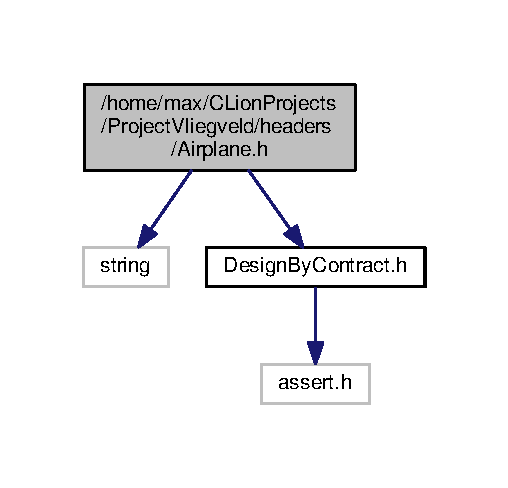
\includegraphics[width=244pt]{Airplane_8h__incl}
\end{center}
\end{figure}
This graph shows which files directly or indirectly include this file\+:
\nopagebreak
\begin{figure}[H]
\begin{center}
\leavevmode
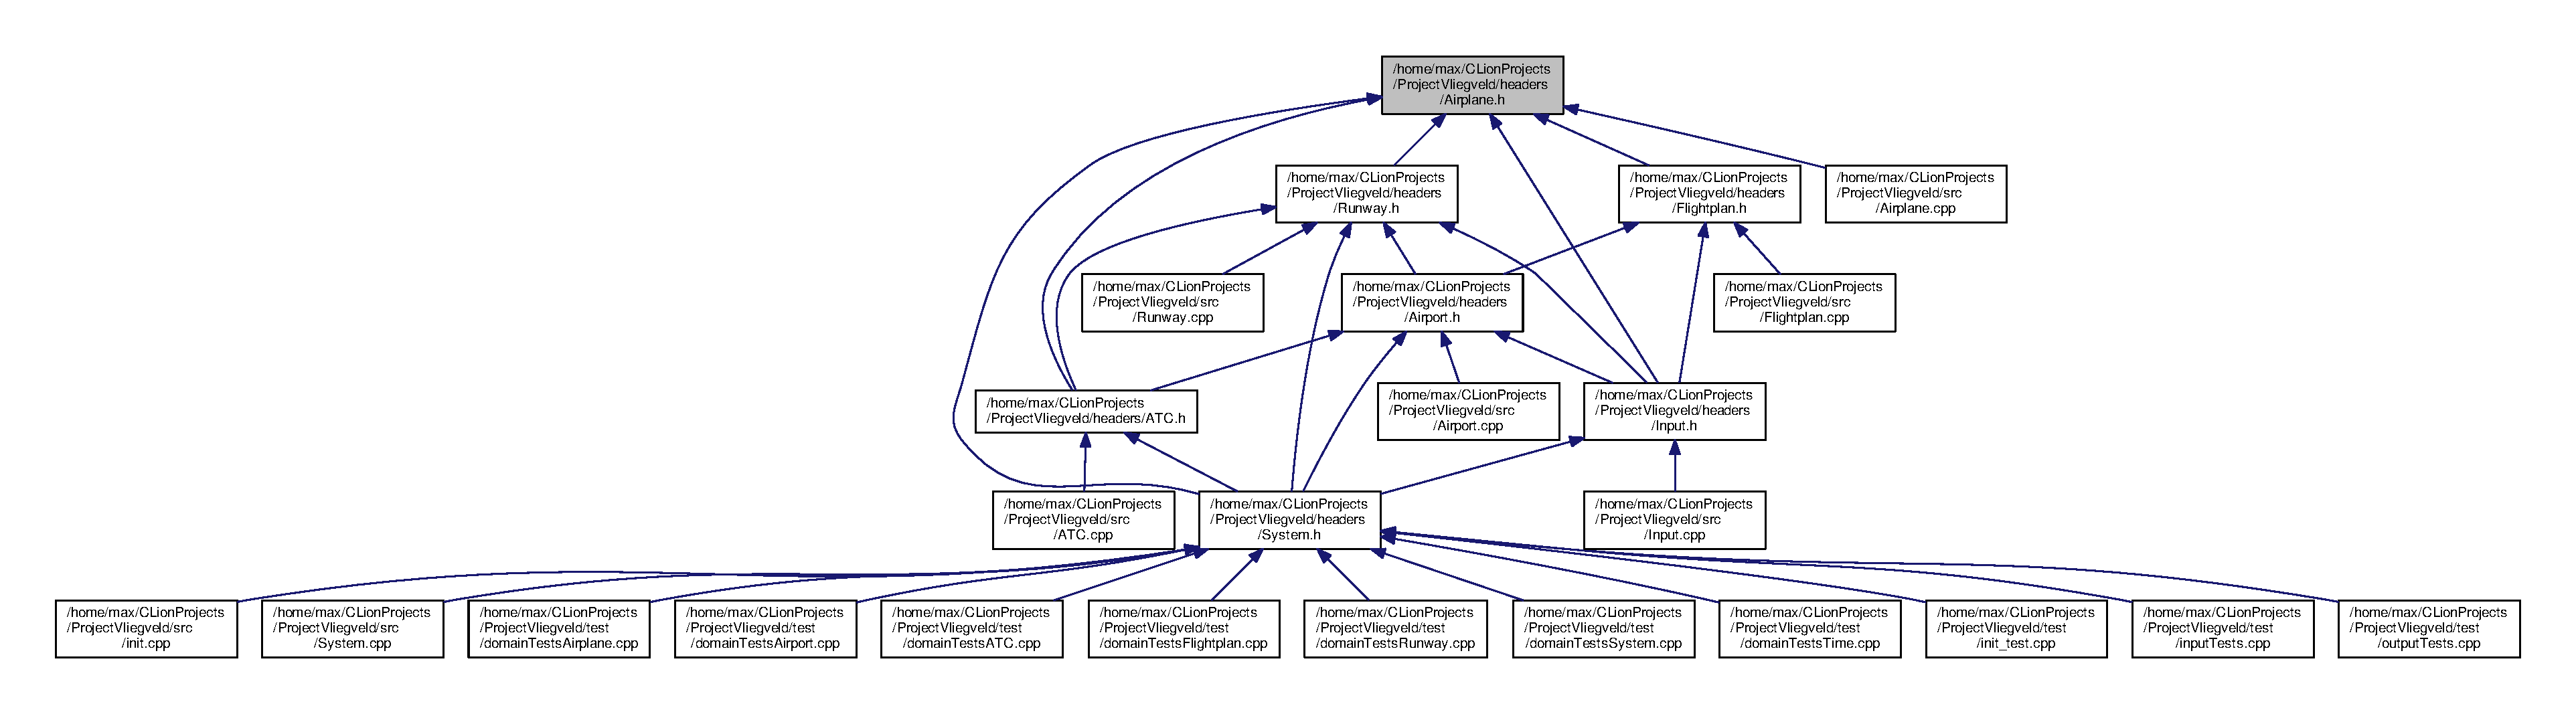
\includegraphics[width=350pt]{Airplane_8h__dep__incl}
\end{center}
\end{figure}
\subsection*{Classes}
\begin{DoxyCompactItemize}
\item 
class \hyperlink{classAirplane}{Airplane}
\begin{DoxyCompactList}\small\item\em \+: Class that represents an airplane in the simulation \end{DoxyCompactList}\end{DoxyCompactItemize}
\subsection*{Enumerations}
\begin{DoxyCompactItemize}
\item 
enum \hyperlink{Airplane_8h_a0e5bbf7c6c727baaba49062300fae19f}{E\+Plane\+Status} \{ \\*
\hyperlink{Airplane_8h_a0e5bbf7c6c727baaba49062300fae19fa2c6325ac177ddfbe70edf92941c4e8e0}{k\+Approaching}, 
\hyperlink{Airplane_8h_a0e5bbf7c6c727baaba49062300fae19fa65b72f8e33cb194d21d822e5b6626e2e}{k\+Descending}, 
\hyperlink{Airplane_8h_a0e5bbf7c6c727baaba49062300fae19fabe52f2e86df226a44cc8ba29e8f259b2}{k\+Taxi\+Arrival}, 
\hyperlink{Airplane_8h_a0e5bbf7c6c727baaba49062300fae19fa3a6a40398243a8892b8084a9e0107015}{k\+Taxi\+Departure}, 
\\*
\hyperlink{Airplane_8h_a0e5bbf7c6c727baaba49062300fae19fa4459995e4bdd3412bbe3d741b3941158}{k\+Circling}, 
\hyperlink{Airplane_8h_a0e5bbf7c6c727baaba49062300fae19fa5c095afa8db10ea77f3303a7b8573cdf}{k\+Deboarding}, 
\hyperlink{Airplane_8h_a0e5bbf7c6c727baaba49062300fae19fa525fdcc62e65d5ea900d499b4468b4e1}{k\+Technical\+Check}, 
\hyperlink{Airplane_8h_a0e5bbf7c6c727baaba49062300fae19fa20dbec285a7773f72e48eccef8ae84da}{k\+Gate}, 
\\*
\hyperlink{Airplane_8h_a0e5bbf7c6c727baaba49062300fae19fae2255e82c6ed427f0820a47f2e5f5ac9}{k\+Departure}, 
\hyperlink{Airplane_8h_a0e5bbf7c6c727baaba49062300fae19fae2f5a04c74b7994ccc574acf7d014a34}{k\+Away}, 
\hyperlink{Airplane_8h_a0e5bbf7c6c727baaba49062300fae19fabfff972a5d3596bc68662c89987639df}{k\+Airport}, 
\hyperlink{Airplane_8h_a0e5bbf7c6c727baaba49062300fae19fa67924d857373a72f3eb2f5d7b3046f92}{k\+Ascending}, 
\\*
\hyperlink{Airplane_8h_a0e5bbf7c6c727baaba49062300fae19fa117bb5da4739b13c4915f7d721f3d2a5}{k\+Pushback}, 
\hyperlink{Airplane_8h_a0e5bbf7c6c727baaba49062300fae19fa5fc2da75439f367169d2a71f865d6bde}{k\+Waiting\+For\+Departure}, 
\hyperlink{Airplane_8h_a0e5bbf7c6c727baaba49062300fae19fa2ff2af945a2d4bb8758de3308e352bd0}{k\+Parked}, 
\hyperlink{Airplane_8h_a0e5bbf7c6c727baaba49062300fae19fac8a18187b65420ae9ceda0d5073512ce}{k\+Crossing\+Arrival}, 
\\*
\hyperlink{Airplane_8h_a0e5bbf7c6c727baaba49062300fae19fa53315b4aeb1d32cbe1f8b8aacd283f2d}{k\+Crossing\+Departure}
 \}
\item 
enum \hyperlink{Airplane_8h_a537b68b9ecaac78d371a35d8cf7604e9}{E\+Plane\+Type} \{ \\*
\hyperlink{Airplane_8h_a537b68b9ecaac78d371a35d8cf7604e9a00ca80b4ed05d96bd6ed02aca4b78e1f}{k\+Private}, 
\hyperlink{Airplane_8h_a537b68b9ecaac78d371a35d8cf7604e9aa60181ba834d25b46f4c717f3403c313}{k\+Airline}, 
\hyperlink{Airplane_8h_a537b68b9ecaac78d371a35d8cf7604e9a1dbdb6d83cd39b00ba5515617716d186}{k\+Military}, 
\hyperlink{Airplane_8h_a537b68b9ecaac78d371a35d8cf7604e9ad0ab6e7d19d66949c60d9db1aa58f9ef}{k\+Emergency}, 
\\*
\hyperlink{Airplane_8h_a537b68b9ecaac78d371a35d8cf7604e9acd07e6d14d5fa33ad175535684278e00}{k\+Default\+Type}
 \}
\item 
enum \hyperlink{Airplane_8h_a0526623f951311ba6780209b9e278dbf}{E\+Plane\+Size} \{ \hyperlink{Airplane_8h_a0526623f951311ba6780209b9e278dbfaf99aeb93b2774bc0c7856d1510d17a54}{k\+Small}, 
\hyperlink{Airplane_8h_a0526623f951311ba6780209b9e278dbfabade85bef98ad2c69fb2216bb947b6c3}{k\+Medium}, 
\hyperlink{Airplane_8h_a0526623f951311ba6780209b9e278dbfa6b6a05b83fa2f5308724e45442b38b7e}{k\+Large}, 
\hyperlink{Airplane_8h_a0526623f951311ba6780209b9e278dbfaf7c1619fb726ec0ab9a3b7cfbf797b4a}{k\+Default\+Size}
 \}
\item 
enum \hyperlink{Airplane_8h_a3d2a8adb53da58e78cb0018d784e791d}{E\+Plane\+Engine} \{ \hyperlink{Airplane_8h_a3d2a8adb53da58e78cb0018d784e791daef171fc98c472a2acd2338353679dcc3}{k\+Propeller}, 
\hyperlink{Airplane_8h_a3d2a8adb53da58e78cb0018d784e791da6262caeb7b5646a03a202006f584364c}{k\+Jet}, 
\hyperlink{Airplane_8h_a3d2a8adb53da58e78cb0018d784e791dabffa4f472eaab68b56c1f1e7c56d221e}{k\+Default\+Engine}
 \}
\item 
enum \hyperlink{Airplane_8h_a4a8a3f45932bdf601f093bea061bad9b}{E\+Plane\+Request} \{ \\*
\hyperlink{Airplane_8h_a4a8a3f45932bdf601f093bea061bad9bad143035084d581f7aecfabd95652e62c}{k\+Pending}, 
\hyperlink{Airplane_8h_a4a8a3f45932bdf601f093bea061bad9ba15597ea7f444a937d40b39b9ea99dd1d}{k\+Accepted}, 
\hyperlink{Airplane_8h_a4a8a3f45932bdf601f093bea061bad9baac195c08fab2dff9d0520caf49ea4e11}{k\+Denied}, 
\hyperlink{Airplane_8h_a4a8a3f45932bdf601f093bea061bad9ba85d56dac5419035294b1c769317026fa}{k\+Confirmed}, 
\\*
\hyperlink{Airplane_8h_a4a8a3f45932bdf601f093bea061bad9ba77f4edb231ad722f9deeb2f574557c17}{k\+Accepted\+Immediate}, 
\hyperlink{Airplane_8h_a4a8a3f45932bdf601f093bea061bad9ba19d8199da79ca4c28eb644052b08f632}{k\+Idle}
 \}
\end{DoxyCompactItemize}


\subsection{Enumeration Type Documentation}
\index{Airplane.\+h@{Airplane.\+h}!E\+Plane\+Engine@{E\+Plane\+Engine}}
\index{E\+Plane\+Engine@{E\+Plane\+Engine}!Airplane.\+h@{Airplane.\+h}}
\subsubsection[{\texorpdfstring{E\+Plane\+Engine}{EPlaneEngine}}]{\setlength{\rightskip}{0pt plus 5cm}enum {\bf E\+Plane\+Engine}}\hypertarget{Airplane_8h_a3d2a8adb53da58e78cb0018d784e791d}{}\label{Airplane_8h_a3d2a8adb53da58e78cb0018d784e791d}
\begin{Desc}
\item[Enumerator]\par
\begin{description}
\index{k\+Propeller@{k\+Propeller}!Airplane.\+h@{Airplane.\+h}}\index{Airplane.\+h@{Airplane.\+h}!k\+Propeller@{k\+Propeller}}\item[{\em 
k\+Propeller\hypertarget{Airplane_8h_a3d2a8adb53da58e78cb0018d784e791daef171fc98c472a2acd2338353679dcc3}{}\label{Airplane_8h_a3d2a8adb53da58e78cb0018d784e791daef171fc98c472a2acd2338353679dcc3}
}]\index{k\+Jet@{k\+Jet}!Airplane.\+h@{Airplane.\+h}}\index{Airplane.\+h@{Airplane.\+h}!k\+Jet@{k\+Jet}}\item[{\em 
k\+Jet\hypertarget{Airplane_8h_a3d2a8adb53da58e78cb0018d784e791da6262caeb7b5646a03a202006f584364c}{}\label{Airplane_8h_a3d2a8adb53da58e78cb0018d784e791da6262caeb7b5646a03a202006f584364c}
}]\index{k\+Default\+Engine@{k\+Default\+Engine}!Airplane.\+h@{Airplane.\+h}}\index{Airplane.\+h@{Airplane.\+h}!k\+Default\+Engine@{k\+Default\+Engine}}\item[{\em 
k\+Default\+Engine\hypertarget{Airplane_8h_a3d2a8adb53da58e78cb0018d784e791dabffa4f472eaab68b56c1f1e7c56d221e}{}\label{Airplane_8h_a3d2a8adb53da58e78cb0018d784e791dabffa4f472eaab68b56c1f1e7c56d221e}
}]\end{description}
\end{Desc}

\begin{DoxyCode}
29 \{ \hyperlink{Airplane_8h_a3d2a8adb53da58e78cb0018d784e791daef171fc98c472a2acd2338353679dcc3}{kPropeller}, \hyperlink{Airplane_8h_a3d2a8adb53da58e78cb0018d784e791da6262caeb7b5646a03a202006f584364c}{kJet}, \hyperlink{Airplane_8h_a3d2a8adb53da58e78cb0018d784e791dabffa4f472eaab68b56c1f1e7c56d221e}{kDefaultEngine} \};
\end{DoxyCode}
\index{Airplane.\+h@{Airplane.\+h}!E\+Plane\+Request@{E\+Plane\+Request}}
\index{E\+Plane\+Request@{E\+Plane\+Request}!Airplane.\+h@{Airplane.\+h}}
\subsubsection[{\texorpdfstring{E\+Plane\+Request}{EPlaneRequest}}]{\setlength{\rightskip}{0pt plus 5cm}enum {\bf E\+Plane\+Request}}\hypertarget{Airplane_8h_a4a8a3f45932bdf601f093bea061bad9b}{}\label{Airplane_8h_a4a8a3f45932bdf601f093bea061bad9b}
\begin{Desc}
\item[Enumerator]\par
\begin{description}
\index{k\+Pending@{k\+Pending}!Airplane.\+h@{Airplane.\+h}}\index{Airplane.\+h@{Airplane.\+h}!k\+Pending@{k\+Pending}}\item[{\em 
k\+Pending\hypertarget{Airplane_8h_a4a8a3f45932bdf601f093bea061bad9bad143035084d581f7aecfabd95652e62c}{}\label{Airplane_8h_a4a8a3f45932bdf601f093bea061bad9bad143035084d581f7aecfabd95652e62c}
}]\index{k\+Accepted@{k\+Accepted}!Airplane.\+h@{Airplane.\+h}}\index{Airplane.\+h@{Airplane.\+h}!k\+Accepted@{k\+Accepted}}\item[{\em 
k\+Accepted\hypertarget{Airplane_8h_a4a8a3f45932bdf601f093bea061bad9ba15597ea7f444a937d40b39b9ea99dd1d}{}\label{Airplane_8h_a4a8a3f45932bdf601f093bea061bad9ba15597ea7f444a937d40b39b9ea99dd1d}
}]\index{k\+Denied@{k\+Denied}!Airplane.\+h@{Airplane.\+h}}\index{Airplane.\+h@{Airplane.\+h}!k\+Denied@{k\+Denied}}\item[{\em 
k\+Denied\hypertarget{Airplane_8h_a4a8a3f45932bdf601f093bea061bad9baac195c08fab2dff9d0520caf49ea4e11}{}\label{Airplane_8h_a4a8a3f45932bdf601f093bea061bad9baac195c08fab2dff9d0520caf49ea4e11}
}]\index{k\+Confirmed@{k\+Confirmed}!Airplane.\+h@{Airplane.\+h}}\index{Airplane.\+h@{Airplane.\+h}!k\+Confirmed@{k\+Confirmed}}\item[{\em 
k\+Confirmed\hypertarget{Airplane_8h_a4a8a3f45932bdf601f093bea061bad9ba85d56dac5419035294b1c769317026fa}{}\label{Airplane_8h_a4a8a3f45932bdf601f093bea061bad9ba85d56dac5419035294b1c769317026fa}
}]\index{k\+Accepted\+Immediate@{k\+Accepted\+Immediate}!Airplane.\+h@{Airplane.\+h}}\index{Airplane.\+h@{Airplane.\+h}!k\+Accepted\+Immediate@{k\+Accepted\+Immediate}}\item[{\em 
k\+Accepted\+Immediate\hypertarget{Airplane_8h_a4a8a3f45932bdf601f093bea061bad9ba77f4edb231ad722f9deeb2f574557c17}{}\label{Airplane_8h_a4a8a3f45932bdf601f093bea061bad9ba77f4edb231ad722f9deeb2f574557c17}
}]\index{k\+Idle@{k\+Idle}!Airplane.\+h@{Airplane.\+h}}\index{Airplane.\+h@{Airplane.\+h}!k\+Idle@{k\+Idle}}\item[{\em 
k\+Idle\hypertarget{Airplane_8h_a4a8a3f45932bdf601f093bea061bad9ba19d8199da79ca4c28eb644052b08f632}{}\label{Airplane_8h_a4a8a3f45932bdf601f093bea061bad9ba19d8199da79ca4c28eb644052b08f632}
}]\end{description}
\end{Desc}

\begin{DoxyCode}
31 \{ \hyperlink{Airplane_8h_a4a8a3f45932bdf601f093bea061bad9bad143035084d581f7aecfabd95652e62c}{kPending}, \hyperlink{Airplane_8h_a4a8a3f45932bdf601f093bea061bad9ba15597ea7f444a937d40b39b9ea99dd1d}{kAccepted}, \hyperlink{Airplane_8h_a4a8a3f45932bdf601f093bea061bad9baac195c08fab2dff9d0520caf49ea4e11}{kDenied}, \hyperlink{Airplane_8h_a4a8a3f45932bdf601f093bea061bad9ba85d56dac5419035294b1c769317026fa}{kConfirmed}, 
      \hyperlink{Airplane_8h_a4a8a3f45932bdf601f093bea061bad9ba77f4edb231ad722f9deeb2f574557c17}{kAcceptedImmediate}, \hyperlink{Airplane_8h_a4a8a3f45932bdf601f093bea061bad9ba19d8199da79ca4c28eb644052b08f632}{kIdle} \};
\end{DoxyCode}
\index{Airplane.\+h@{Airplane.\+h}!E\+Plane\+Size@{E\+Plane\+Size}}
\index{E\+Plane\+Size@{E\+Plane\+Size}!Airplane.\+h@{Airplane.\+h}}
\subsubsection[{\texorpdfstring{E\+Plane\+Size}{EPlaneSize}}]{\setlength{\rightskip}{0pt plus 5cm}enum {\bf E\+Plane\+Size}}\hypertarget{Airplane_8h_a0526623f951311ba6780209b9e278dbf}{}\label{Airplane_8h_a0526623f951311ba6780209b9e278dbf}
\begin{Desc}
\item[Enumerator]\par
\begin{description}
\index{k\+Small@{k\+Small}!Airplane.\+h@{Airplane.\+h}}\index{Airplane.\+h@{Airplane.\+h}!k\+Small@{k\+Small}}\item[{\em 
k\+Small\hypertarget{Airplane_8h_a0526623f951311ba6780209b9e278dbfaf99aeb93b2774bc0c7856d1510d17a54}{}\label{Airplane_8h_a0526623f951311ba6780209b9e278dbfaf99aeb93b2774bc0c7856d1510d17a54}
}]\index{k\+Medium@{k\+Medium}!Airplane.\+h@{Airplane.\+h}}\index{Airplane.\+h@{Airplane.\+h}!k\+Medium@{k\+Medium}}\item[{\em 
k\+Medium\hypertarget{Airplane_8h_a0526623f951311ba6780209b9e278dbfabade85bef98ad2c69fb2216bb947b6c3}{}\label{Airplane_8h_a0526623f951311ba6780209b9e278dbfabade85bef98ad2c69fb2216bb947b6c3}
}]\index{k\+Large@{k\+Large}!Airplane.\+h@{Airplane.\+h}}\index{Airplane.\+h@{Airplane.\+h}!k\+Large@{k\+Large}}\item[{\em 
k\+Large\hypertarget{Airplane_8h_a0526623f951311ba6780209b9e278dbfa6b6a05b83fa2f5308724e45442b38b7e}{}\label{Airplane_8h_a0526623f951311ba6780209b9e278dbfa6b6a05b83fa2f5308724e45442b38b7e}
}]\index{k\+Default\+Size@{k\+Default\+Size}!Airplane.\+h@{Airplane.\+h}}\index{Airplane.\+h@{Airplane.\+h}!k\+Default\+Size@{k\+Default\+Size}}\item[{\em 
k\+Default\+Size\hypertarget{Airplane_8h_a0526623f951311ba6780209b9e278dbfaf7c1619fb726ec0ab9a3b7cfbf797b4a}{}\label{Airplane_8h_a0526623f951311ba6780209b9e278dbfaf7c1619fb726ec0ab9a3b7cfbf797b4a}
}]\end{description}
\end{Desc}

\begin{DoxyCode}
27 \{ \hyperlink{Airplane_8h_a0526623f951311ba6780209b9e278dbfaf99aeb93b2774bc0c7856d1510d17a54}{kSmall}, \hyperlink{Airplane_8h_a0526623f951311ba6780209b9e278dbfabade85bef98ad2c69fb2216bb947b6c3}{kMedium}, \hyperlink{Airplane_8h_a0526623f951311ba6780209b9e278dbfa6b6a05b83fa2f5308724e45442b38b7e}{kLarge}, \hyperlink{Airplane_8h_a0526623f951311ba6780209b9e278dbfaf7c1619fb726ec0ab9a3b7cfbf797b4a}{kDefaultSize} \};
\end{DoxyCode}
\index{Airplane.\+h@{Airplane.\+h}!E\+Plane\+Status@{E\+Plane\+Status}}
\index{E\+Plane\+Status@{E\+Plane\+Status}!Airplane.\+h@{Airplane.\+h}}
\subsubsection[{\texorpdfstring{E\+Plane\+Status}{EPlaneStatus}}]{\setlength{\rightskip}{0pt plus 5cm}enum {\bf E\+Plane\+Status}}\hypertarget{Airplane_8h_a0e5bbf7c6c727baaba49062300fae19f}{}\label{Airplane_8h_a0e5bbf7c6c727baaba49062300fae19f}
\begin{Desc}
\item[Enumerator]\par
\begin{description}
\index{k\+Approaching@{k\+Approaching}!Airplane.\+h@{Airplane.\+h}}\index{Airplane.\+h@{Airplane.\+h}!k\+Approaching@{k\+Approaching}}\item[{\em 
k\+Approaching\hypertarget{Airplane_8h_a0e5bbf7c6c727baaba49062300fae19fa2c6325ac177ddfbe70edf92941c4e8e0}{}\label{Airplane_8h_a0e5bbf7c6c727baaba49062300fae19fa2c6325ac177ddfbe70edf92941c4e8e0}
}]\index{k\+Descending@{k\+Descending}!Airplane.\+h@{Airplane.\+h}}\index{Airplane.\+h@{Airplane.\+h}!k\+Descending@{k\+Descending}}\item[{\em 
k\+Descending\hypertarget{Airplane_8h_a0e5bbf7c6c727baaba49062300fae19fa65b72f8e33cb194d21d822e5b6626e2e}{}\label{Airplane_8h_a0e5bbf7c6c727baaba49062300fae19fa65b72f8e33cb194d21d822e5b6626e2e}
}]\index{k\+Taxi\+Arrival@{k\+Taxi\+Arrival}!Airplane.\+h@{Airplane.\+h}}\index{Airplane.\+h@{Airplane.\+h}!k\+Taxi\+Arrival@{k\+Taxi\+Arrival}}\item[{\em 
k\+Taxi\+Arrival\hypertarget{Airplane_8h_a0e5bbf7c6c727baaba49062300fae19fabe52f2e86df226a44cc8ba29e8f259b2}{}\label{Airplane_8h_a0e5bbf7c6c727baaba49062300fae19fabe52f2e86df226a44cc8ba29e8f259b2}
}]\index{k\+Taxi\+Departure@{k\+Taxi\+Departure}!Airplane.\+h@{Airplane.\+h}}\index{Airplane.\+h@{Airplane.\+h}!k\+Taxi\+Departure@{k\+Taxi\+Departure}}\item[{\em 
k\+Taxi\+Departure\hypertarget{Airplane_8h_a0e5bbf7c6c727baaba49062300fae19fa3a6a40398243a8892b8084a9e0107015}{}\label{Airplane_8h_a0e5bbf7c6c727baaba49062300fae19fa3a6a40398243a8892b8084a9e0107015}
}]\index{k\+Circling@{k\+Circling}!Airplane.\+h@{Airplane.\+h}}\index{Airplane.\+h@{Airplane.\+h}!k\+Circling@{k\+Circling}}\item[{\em 
k\+Circling\hypertarget{Airplane_8h_a0e5bbf7c6c727baaba49062300fae19fa4459995e4bdd3412bbe3d741b3941158}{}\label{Airplane_8h_a0e5bbf7c6c727baaba49062300fae19fa4459995e4bdd3412bbe3d741b3941158}
}]\index{k\+Deboarding@{k\+Deboarding}!Airplane.\+h@{Airplane.\+h}}\index{Airplane.\+h@{Airplane.\+h}!k\+Deboarding@{k\+Deboarding}}\item[{\em 
k\+Deboarding\hypertarget{Airplane_8h_a0e5bbf7c6c727baaba49062300fae19fa5c095afa8db10ea77f3303a7b8573cdf}{}\label{Airplane_8h_a0e5bbf7c6c727baaba49062300fae19fa5c095afa8db10ea77f3303a7b8573cdf}
}]\index{k\+Technical\+Check@{k\+Technical\+Check}!Airplane.\+h@{Airplane.\+h}}\index{Airplane.\+h@{Airplane.\+h}!k\+Technical\+Check@{k\+Technical\+Check}}\item[{\em 
k\+Technical\+Check\hypertarget{Airplane_8h_a0e5bbf7c6c727baaba49062300fae19fa525fdcc62e65d5ea900d499b4468b4e1}{}\label{Airplane_8h_a0e5bbf7c6c727baaba49062300fae19fa525fdcc62e65d5ea900d499b4468b4e1}
}]\index{k\+Gate@{k\+Gate}!Airplane.\+h@{Airplane.\+h}}\index{Airplane.\+h@{Airplane.\+h}!k\+Gate@{k\+Gate}}\item[{\em 
k\+Gate\hypertarget{Airplane_8h_a0e5bbf7c6c727baaba49062300fae19fa20dbec285a7773f72e48eccef8ae84da}{}\label{Airplane_8h_a0e5bbf7c6c727baaba49062300fae19fa20dbec285a7773f72e48eccef8ae84da}
}]\index{k\+Departure@{k\+Departure}!Airplane.\+h@{Airplane.\+h}}\index{Airplane.\+h@{Airplane.\+h}!k\+Departure@{k\+Departure}}\item[{\em 
k\+Departure\hypertarget{Airplane_8h_a0e5bbf7c6c727baaba49062300fae19fae2255e82c6ed427f0820a47f2e5f5ac9}{}\label{Airplane_8h_a0e5bbf7c6c727baaba49062300fae19fae2255e82c6ed427f0820a47f2e5f5ac9}
}]\index{k\+Away@{k\+Away}!Airplane.\+h@{Airplane.\+h}}\index{Airplane.\+h@{Airplane.\+h}!k\+Away@{k\+Away}}\item[{\em 
k\+Away\hypertarget{Airplane_8h_a0e5bbf7c6c727baaba49062300fae19fae2f5a04c74b7994ccc574acf7d014a34}{}\label{Airplane_8h_a0e5bbf7c6c727baaba49062300fae19fae2f5a04c74b7994ccc574acf7d014a34}
}]\index{k\+Airport@{k\+Airport}!Airplane.\+h@{Airplane.\+h}}\index{Airplane.\+h@{Airplane.\+h}!k\+Airport@{k\+Airport}}\item[{\em 
k\+Airport\hypertarget{Airplane_8h_a0e5bbf7c6c727baaba49062300fae19fabfff972a5d3596bc68662c89987639df}{}\label{Airplane_8h_a0e5bbf7c6c727baaba49062300fae19fabfff972a5d3596bc68662c89987639df}
}]\index{k\+Ascending@{k\+Ascending}!Airplane.\+h@{Airplane.\+h}}\index{Airplane.\+h@{Airplane.\+h}!k\+Ascending@{k\+Ascending}}\item[{\em 
k\+Ascending\hypertarget{Airplane_8h_a0e5bbf7c6c727baaba49062300fae19fa67924d857373a72f3eb2f5d7b3046f92}{}\label{Airplane_8h_a0e5bbf7c6c727baaba49062300fae19fa67924d857373a72f3eb2f5d7b3046f92}
}]\index{k\+Pushback@{k\+Pushback}!Airplane.\+h@{Airplane.\+h}}\index{Airplane.\+h@{Airplane.\+h}!k\+Pushback@{k\+Pushback}}\item[{\em 
k\+Pushback\hypertarget{Airplane_8h_a0e5bbf7c6c727baaba49062300fae19fa117bb5da4739b13c4915f7d721f3d2a5}{}\label{Airplane_8h_a0e5bbf7c6c727baaba49062300fae19fa117bb5da4739b13c4915f7d721f3d2a5}
}]\index{k\+Waiting\+For\+Departure@{k\+Waiting\+For\+Departure}!Airplane.\+h@{Airplane.\+h}}\index{Airplane.\+h@{Airplane.\+h}!k\+Waiting\+For\+Departure@{k\+Waiting\+For\+Departure}}\item[{\em 
k\+Waiting\+For\+Departure\hypertarget{Airplane_8h_a0e5bbf7c6c727baaba49062300fae19fa5fc2da75439f367169d2a71f865d6bde}{}\label{Airplane_8h_a0e5bbf7c6c727baaba49062300fae19fa5fc2da75439f367169d2a71f865d6bde}
}]\index{k\+Parked@{k\+Parked}!Airplane.\+h@{Airplane.\+h}}\index{Airplane.\+h@{Airplane.\+h}!k\+Parked@{k\+Parked}}\item[{\em 
k\+Parked\hypertarget{Airplane_8h_a0e5bbf7c6c727baaba49062300fae19fa2ff2af945a2d4bb8758de3308e352bd0}{}\label{Airplane_8h_a0e5bbf7c6c727baaba49062300fae19fa2ff2af945a2d4bb8758de3308e352bd0}
}]\index{k\+Crossing\+Arrival@{k\+Crossing\+Arrival}!Airplane.\+h@{Airplane.\+h}}\index{Airplane.\+h@{Airplane.\+h}!k\+Crossing\+Arrival@{k\+Crossing\+Arrival}}\item[{\em 
k\+Crossing\+Arrival\hypertarget{Airplane_8h_a0e5bbf7c6c727baaba49062300fae19fac8a18187b65420ae9ceda0d5073512ce}{}\label{Airplane_8h_a0e5bbf7c6c727baaba49062300fae19fac8a18187b65420ae9ceda0d5073512ce}
}]\index{k\+Crossing\+Departure@{k\+Crossing\+Departure}!Airplane.\+h@{Airplane.\+h}}\index{Airplane.\+h@{Airplane.\+h}!k\+Crossing\+Departure@{k\+Crossing\+Departure}}\item[{\em 
k\+Crossing\+Departure\hypertarget{Airplane_8h_a0e5bbf7c6c727baaba49062300fae19fa53315b4aeb1d32cbe1f8b8aacd283f2d}{}\label{Airplane_8h_a0e5bbf7c6c727baaba49062300fae19fa53315b4aeb1d32cbe1f8b8aacd283f2d}
}]\end{description}
\end{Desc}

\begin{DoxyCode}
22                   \{ \hyperlink{Airplane_8h_a0e5bbf7c6c727baaba49062300fae19fa2c6325ac177ddfbe70edf92941c4e8e0}{kApproaching}, \hyperlink{Airplane_8h_a0e5bbf7c6c727baaba49062300fae19fa65b72f8e33cb194d21d822e5b6626e2e}{kDescending}, 
      \hyperlink{Airplane_8h_a0e5bbf7c6c727baaba49062300fae19fabe52f2e86df226a44cc8ba29e8f259b2}{kTaxiArrival}, \hyperlink{Airplane_8h_a0e5bbf7c6c727baaba49062300fae19fa3a6a40398243a8892b8084a9e0107015}{kTaxiDeparture}, \hyperlink{Airplane_8h_a0e5bbf7c6c727baaba49062300fae19fa4459995e4bdd3412bbe3d741b3941158}{kCircling}, 
      \hyperlink{Airplane_8h_a0e5bbf7c6c727baaba49062300fae19fa5c095afa8db10ea77f3303a7b8573cdf}{kDeboarding}, \hyperlink{Airplane_8h_a0e5bbf7c6c727baaba49062300fae19fa525fdcc62e65d5ea900d499b4468b4e1}{kTechnicalCheck}, \hyperlink{Airplane_8h_a0e5bbf7c6c727baaba49062300fae19fa20dbec285a7773f72e48eccef8ae84da}{kGate}, \hyperlink{Airplane_8h_a0e5bbf7c6c727baaba49062300fae19fae2255e82c6ed427f0820a47f2e5f5ac9}{kDeparture}, 
      \hyperlink{Airplane_8h_a0e5bbf7c6c727baaba49062300fae19fae2f5a04c74b7994ccc574acf7d014a34}{kAway},
23                     \hyperlink{Airplane_8h_a0e5bbf7c6c727baaba49062300fae19fabfff972a5d3596bc68662c89987639df}{kAirport}, \hyperlink{Airplane_8h_a0e5bbf7c6c727baaba49062300fae19fa67924d857373a72f3eb2f5d7b3046f92}{kAscending}, \hyperlink{Airplane_8h_a0e5bbf7c6c727baaba49062300fae19fa117bb5da4739b13c4915f7d721f3d2a5}{kPushback}, 
      \hyperlink{Airplane_8h_a0e5bbf7c6c727baaba49062300fae19fa5fc2da75439f367169d2a71f865d6bde}{kWaitingForDeparture}, \hyperlink{Airplane_8h_a0e5bbf7c6c727baaba49062300fae19fa2ff2af945a2d4bb8758de3308e352bd0}{kParked}, \hyperlink{Airplane_8h_a0e5bbf7c6c727baaba49062300fae19fac8a18187b65420ae9ceda0d5073512ce}{kCrossingArrival}, 
      \hyperlink{Airplane_8h_a0e5bbf7c6c727baaba49062300fae19fa53315b4aeb1d32cbe1f8b8aacd283f2d}{kCrossingDeparture} \};
\end{DoxyCode}
\index{Airplane.\+h@{Airplane.\+h}!E\+Plane\+Type@{E\+Plane\+Type}}
\index{E\+Plane\+Type@{E\+Plane\+Type}!Airplane.\+h@{Airplane.\+h}}
\subsubsection[{\texorpdfstring{E\+Plane\+Type}{EPlaneType}}]{\setlength{\rightskip}{0pt plus 5cm}enum {\bf E\+Plane\+Type}}\hypertarget{Airplane_8h_a537b68b9ecaac78d371a35d8cf7604e9}{}\label{Airplane_8h_a537b68b9ecaac78d371a35d8cf7604e9}
\begin{Desc}
\item[Enumerator]\par
\begin{description}
\index{k\+Private@{k\+Private}!Airplane.\+h@{Airplane.\+h}}\index{Airplane.\+h@{Airplane.\+h}!k\+Private@{k\+Private}}\item[{\em 
k\+Private\hypertarget{Airplane_8h_a537b68b9ecaac78d371a35d8cf7604e9a00ca80b4ed05d96bd6ed02aca4b78e1f}{}\label{Airplane_8h_a537b68b9ecaac78d371a35d8cf7604e9a00ca80b4ed05d96bd6ed02aca4b78e1f}
}]\index{k\+Airline@{k\+Airline}!Airplane.\+h@{Airplane.\+h}}\index{Airplane.\+h@{Airplane.\+h}!k\+Airline@{k\+Airline}}\item[{\em 
k\+Airline\hypertarget{Airplane_8h_a537b68b9ecaac78d371a35d8cf7604e9aa60181ba834d25b46f4c717f3403c313}{}\label{Airplane_8h_a537b68b9ecaac78d371a35d8cf7604e9aa60181ba834d25b46f4c717f3403c313}
}]\index{k\+Military@{k\+Military}!Airplane.\+h@{Airplane.\+h}}\index{Airplane.\+h@{Airplane.\+h}!k\+Military@{k\+Military}}\item[{\em 
k\+Military\hypertarget{Airplane_8h_a537b68b9ecaac78d371a35d8cf7604e9a1dbdb6d83cd39b00ba5515617716d186}{}\label{Airplane_8h_a537b68b9ecaac78d371a35d8cf7604e9a1dbdb6d83cd39b00ba5515617716d186}
}]\index{k\+Emergency@{k\+Emergency}!Airplane.\+h@{Airplane.\+h}}\index{Airplane.\+h@{Airplane.\+h}!k\+Emergency@{k\+Emergency}}\item[{\em 
k\+Emergency\hypertarget{Airplane_8h_a537b68b9ecaac78d371a35d8cf7604e9ad0ab6e7d19d66949c60d9db1aa58f9ef}{}\label{Airplane_8h_a537b68b9ecaac78d371a35d8cf7604e9ad0ab6e7d19d66949c60d9db1aa58f9ef}
}]\index{k\+Default\+Type@{k\+Default\+Type}!Airplane.\+h@{Airplane.\+h}}\index{Airplane.\+h@{Airplane.\+h}!k\+Default\+Type@{k\+Default\+Type}}\item[{\em 
k\+Default\+Type\hypertarget{Airplane_8h_a537b68b9ecaac78d371a35d8cf7604e9acd07e6d14d5fa33ad175535684278e00}{}\label{Airplane_8h_a537b68b9ecaac78d371a35d8cf7604e9acd07e6d14d5fa33ad175535684278e00}
}]\end{description}
\end{Desc}

\begin{DoxyCode}
25 \{ \hyperlink{Airplane_8h_a537b68b9ecaac78d371a35d8cf7604e9a00ca80b4ed05d96bd6ed02aca4b78e1f}{kPrivate}, \hyperlink{Airplane_8h_a537b68b9ecaac78d371a35d8cf7604e9aa60181ba834d25b46f4c717f3403c313}{kAirline}, \hyperlink{Airplane_8h_a537b68b9ecaac78d371a35d8cf7604e9a1dbdb6d83cd39b00ba5515617716d186}{kMilitary}, \hyperlink{Airplane_8h_a537b68b9ecaac78d371a35d8cf7604e9ad0ab6e7d19d66949c60d9db1aa58f9ef}{kEmergency}, 
      \hyperlink{Airplane_8h_a537b68b9ecaac78d371a35d8cf7604e9acd07e6d14d5fa33ad175535684278e00}{kDefaultType} \};
\end{DoxyCode}

\hypertarget{Airport_8h}{}\section{/home/max/\+C\+Lion\+Projects/\+Project\+Vliegveld/headers/\+Airport.h File Reference}
\label{Airport_8h}\index{/home/max/\+C\+Lion\+Projects/\+Project\+Vliegveld/headers/\+Airport.\+h@{/home/max/\+C\+Lion\+Projects/\+Project\+Vliegveld/headers/\+Airport.\+h}}
{\ttfamily \#include $<$string$>$}\\*
{\ttfamily \#include $<$stack$>$}\\*
{\ttfamily \#include $<$vector$>$}\\*
{\ttfamily \#include $<$sstream$>$}\\*
{\ttfamily \#include \char`\"{}Design\+By\+Contract.\+h\char`\"{}}\\*
{\ttfamily \#include \char`\"{}Runway.\+h\char`\"{}}\\*
{\ttfamily \#include \char`\"{}Time.\+h\char`\"{}}\\*
{\ttfamily \#include \char`\"{}Flightplan.\+h\char`\"{}}\\*
Include dependency graph for Airport.\+h\+:
\nopagebreak
\begin{figure}[H]
\begin{center}
\leavevmode
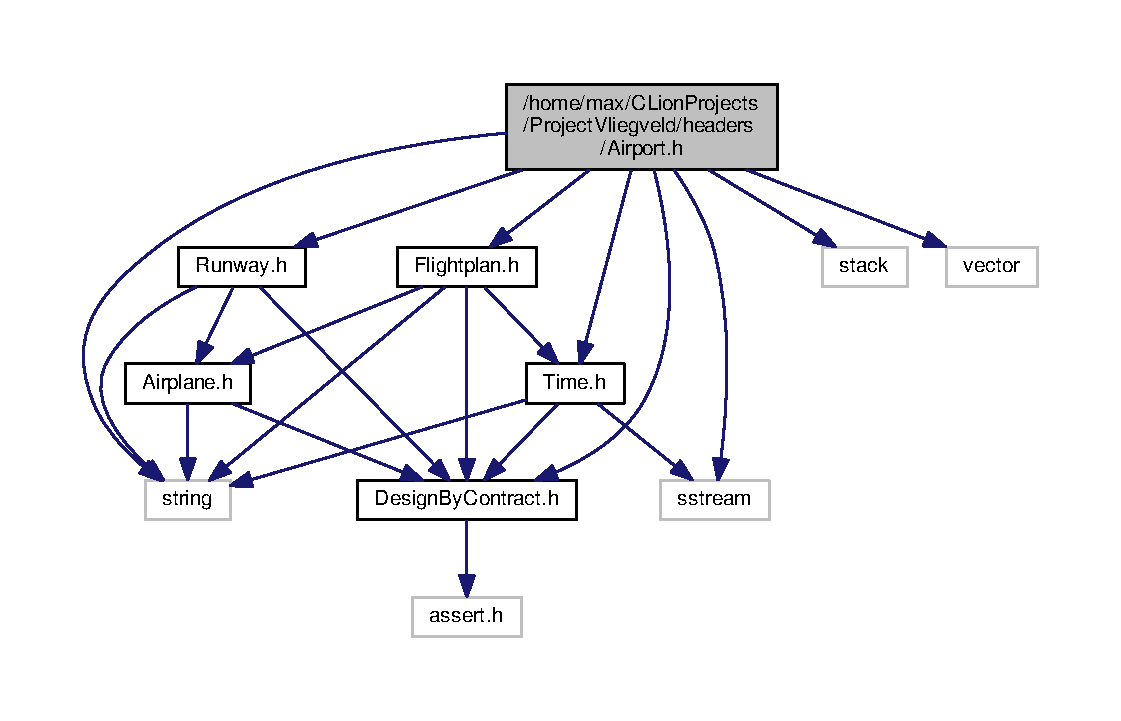
\includegraphics[width=350pt]{Airport_8h__incl}
\end{center}
\end{figure}
This graph shows which files directly or indirectly include this file\+:
\nopagebreak
\begin{figure}[H]
\begin{center}
\leavevmode
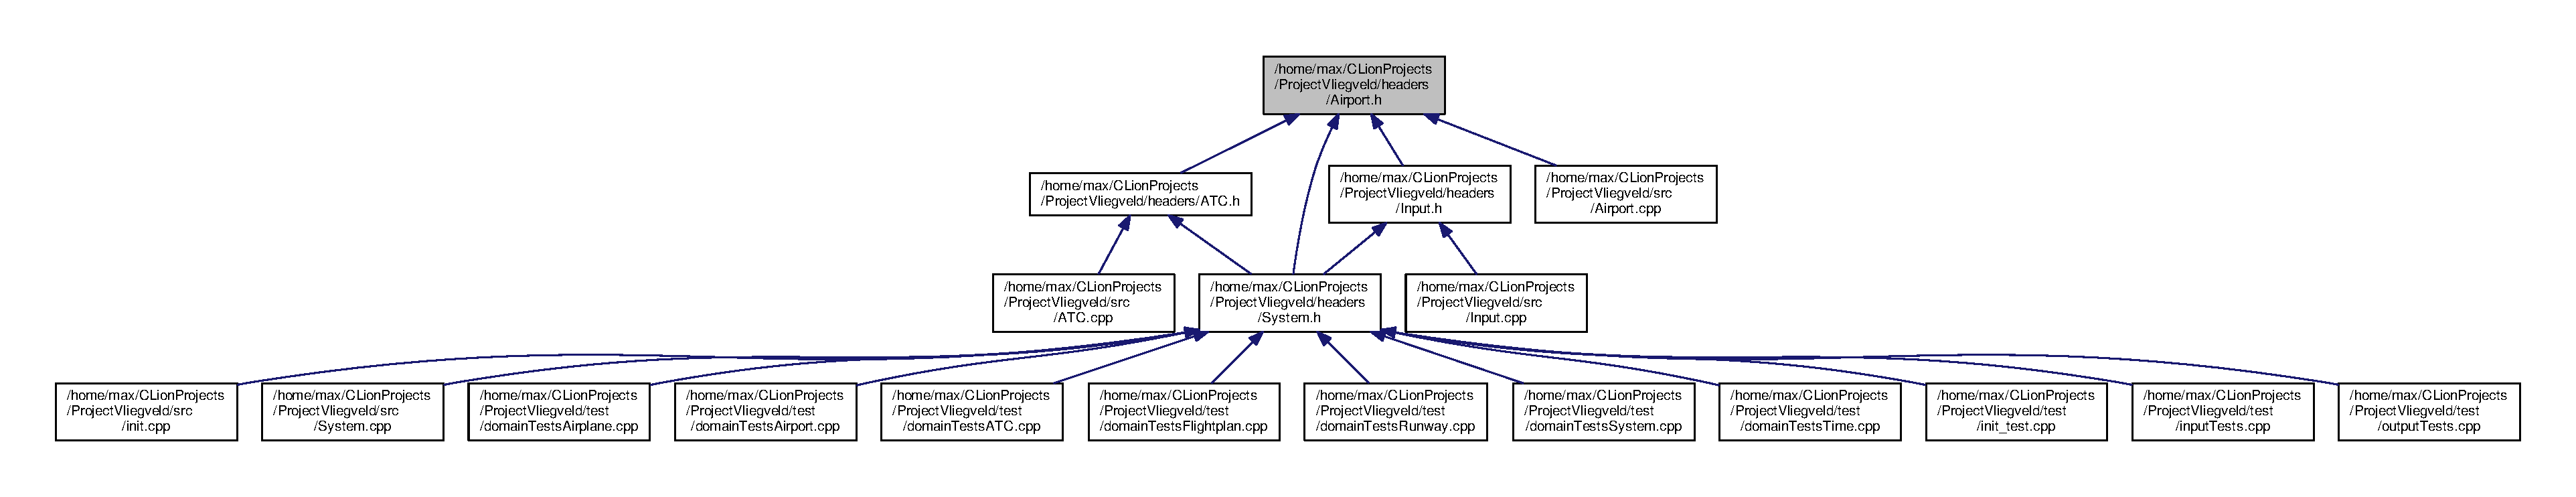
\includegraphics[width=350pt]{Airport_8h__dep__incl}
\end{center}
\end{figure}
\subsection*{Classes}
\begin{DoxyCompactItemize}
\item 
class \hyperlink{classAirport}{Airport}
\end{DoxyCompactItemize}

\hypertarget{ATC_8h}{}\section{/home/max/\+C\+Lion\+Projects/\+Project\+Vliegveld/headers/\+A\+TC.h File Reference}
\label{ATC_8h}\index{/home/max/\+C\+Lion\+Projects/\+Project\+Vliegveld/headers/\+A\+T\+C.\+h@{/home/max/\+C\+Lion\+Projects/\+Project\+Vliegveld/headers/\+A\+T\+C.\+h}}
{\ttfamily \#include $<$stdlib.\+h$>$}\\*
{\ttfamily \#include $<$iostream$>$}\\*
{\ttfamily \#include $<$queue$>$}\\*
{\ttfamily \#include $<$set$>$}\\*
{\ttfamily \#include $<$map$>$}\\*
{\ttfamily \#include \char`\"{}Airplane.\+h\char`\"{}}\\*
{\ttfamily \#include \char`\"{}Runway.\+h\char`\"{}}\\*
{\ttfamily \#include \char`\"{}Time.\+h\char`\"{}}\\*
{\ttfamily \#include \char`\"{}Airport.\+h\char`\"{}}\\*
Include dependency graph for A\+T\+C.\+h\+:
\nopagebreak
\begin{figure}[H]
\begin{center}
\leavevmode
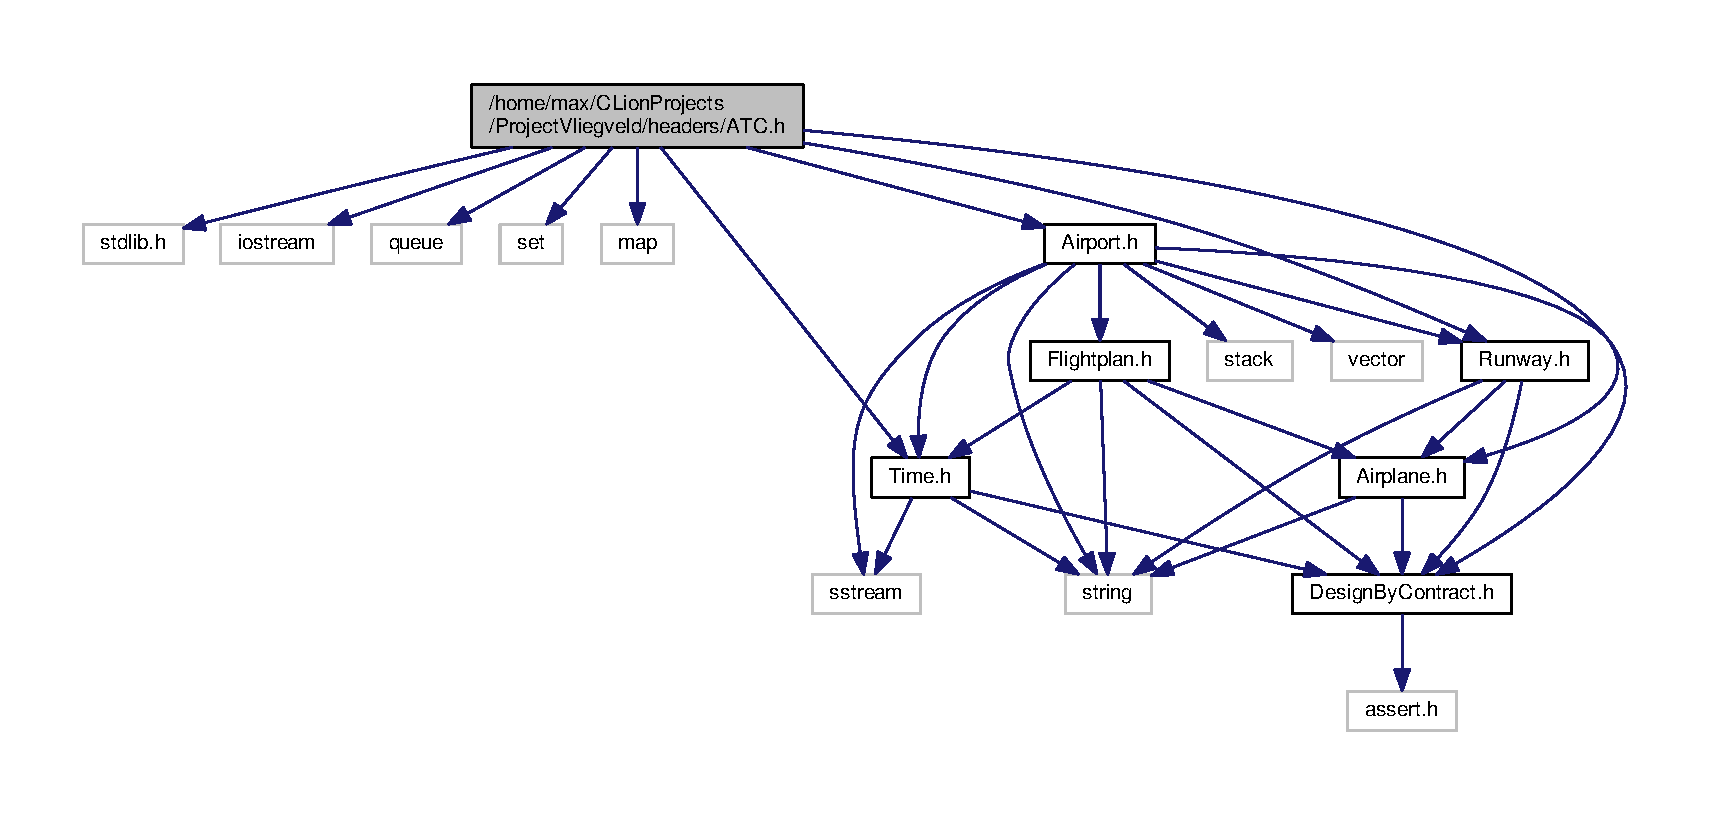
\includegraphics[width=350pt]{ATC_8h__incl}
\end{center}
\end{figure}
This graph shows which files directly or indirectly include this file\+:
\nopagebreak
\begin{figure}[H]
\begin{center}
\leavevmode
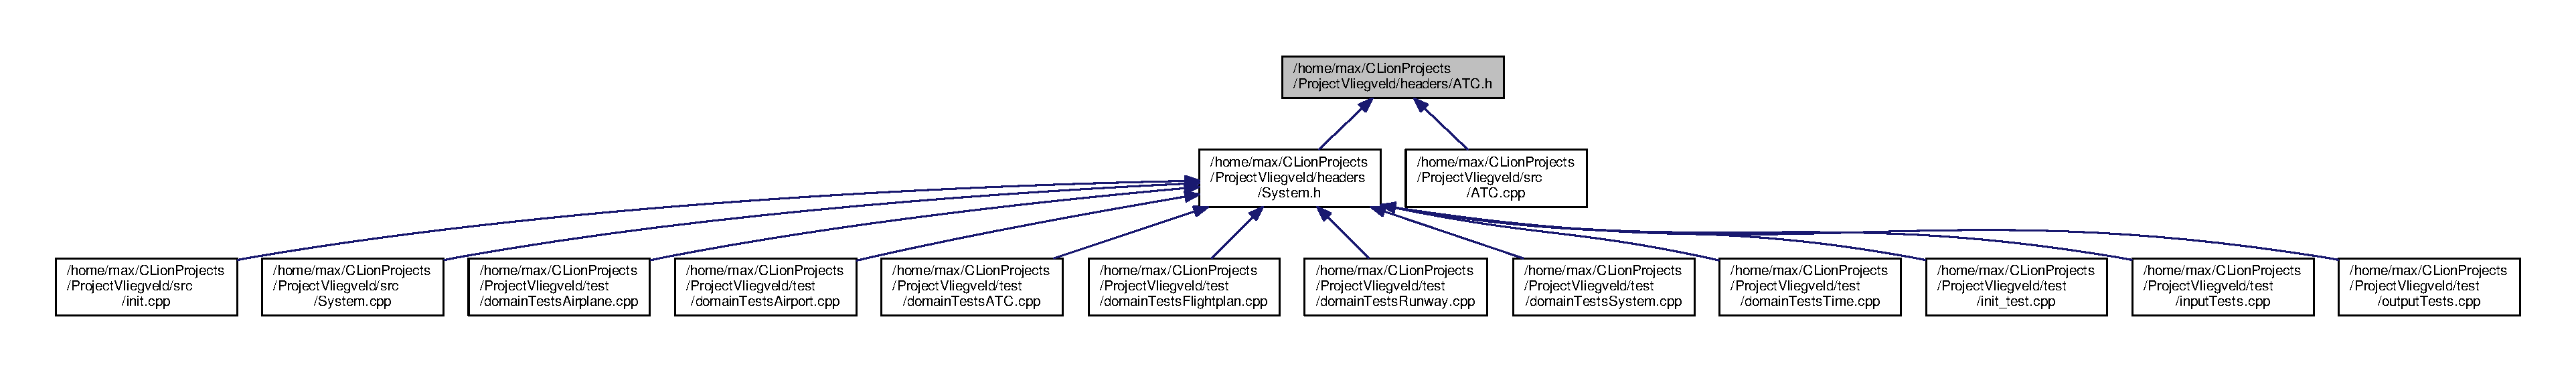
\includegraphics[width=350pt]{ATC_8h__dep__incl}
\end{center}
\end{figure}
\subsection*{Classes}
\begin{DoxyCompactItemize}
\item 
struct \hyperlink{structATCRequest}{A\+T\+C\+Request}
\item 
class \hyperlink{classATC}{A\+TC}
\end{DoxyCompactItemize}

\hypertarget{DesignByContract_8h}{}\section{/home/max/\+C\+Lion\+Projects/\+Project\+Vliegveld/headers/\+Design\+By\+Contract.h File Reference}
\label{DesignByContract_8h}\index{/home/max/\+C\+Lion\+Projects/\+Project\+Vliegveld/headers/\+Design\+By\+Contract.\+h@{/home/max/\+C\+Lion\+Projects/\+Project\+Vliegveld/headers/\+Design\+By\+Contract.\+h}}
{\ttfamily \#include $<$assert.\+h$>$}\\*
Include dependency graph for Design\+By\+Contract.\+h\+:
\nopagebreak
\begin{figure}[H]
\begin{center}
\leavevmode
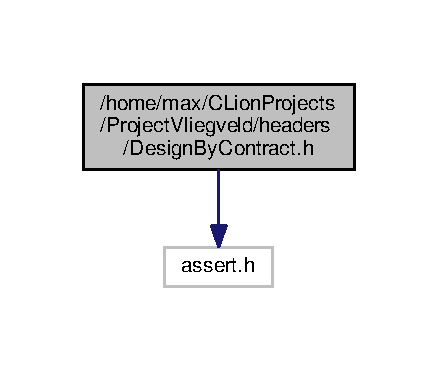
\includegraphics[width=210pt]{DesignByContract_8h__incl}
\end{center}
\end{figure}
This graph shows which files directly or indirectly include this file\+:
\nopagebreak
\begin{figure}[H]
\begin{center}
\leavevmode
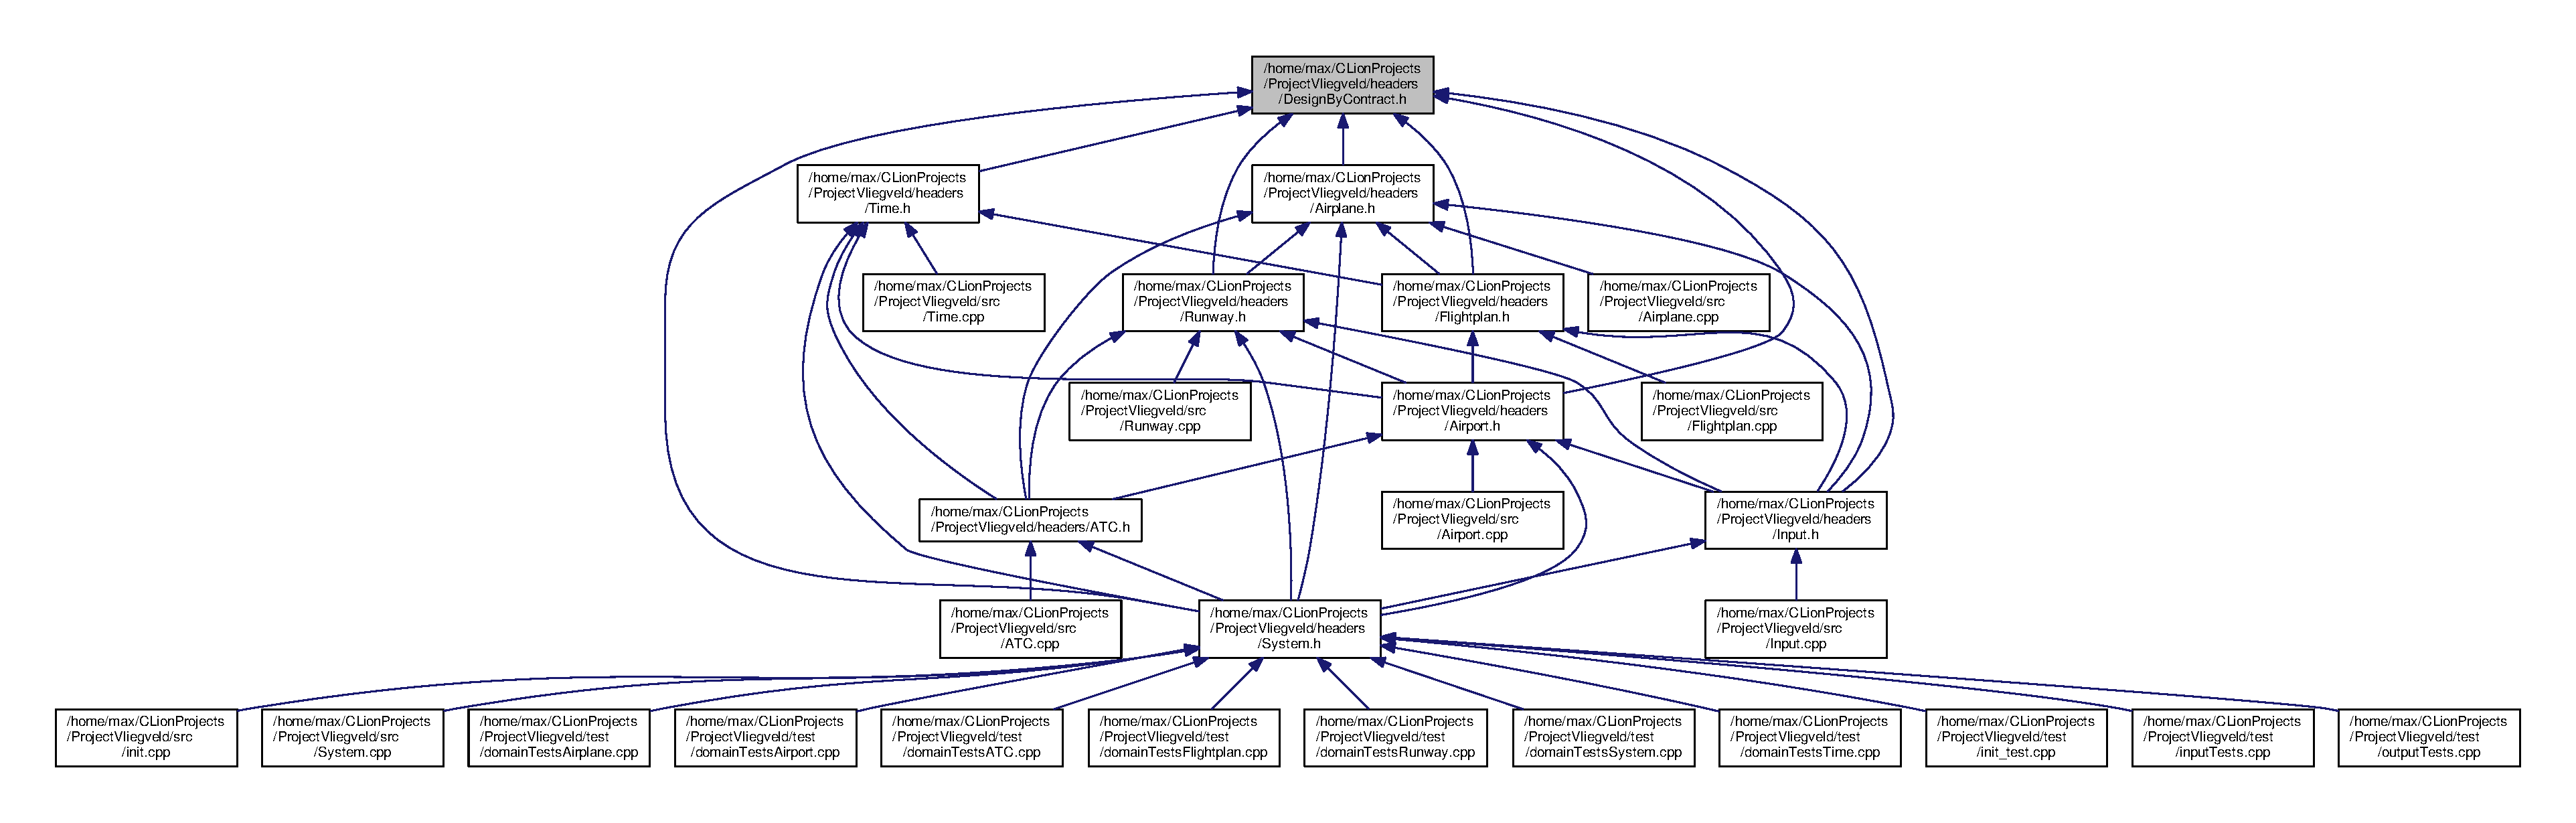
\includegraphics[width=350pt]{DesignByContract_8h__dep__incl}
\end{center}
\end{figure}
\subsection*{Macros}
\begin{DoxyCompactItemize}
\item 
\#define \hyperlink{DesignByContract_8h_aeb774672b46dbe80afc14e0d1970f017}{R\+E\+Q\+U\+I\+RE}(assertion,  what)~\hyperlink{html_2jquery_8js_a42cbfadee2b4749e8f699ea8d745a0e4}{if} (!(assertion)) \+\_\+\+\_\+assert (what, \+\_\+\+\_\+\+F\+I\+L\+E\+\_\+\+\_\+, \+\_\+\+\_\+\+L\+I\+N\+E\+\_\+\+\_\+)
\item 
\#define \hyperlink{DesignByContract_8h_ab8da60ea2bcdd55183cc29d8526e6857}{E\+N\+S\+U\+RE}(assertion,  what)~\hyperlink{html_2jquery_8js_a42cbfadee2b4749e8f699ea8d745a0e4}{if} (!(assertion)) \+\_\+\+\_\+assert (what, \+\_\+\+\_\+\+F\+I\+L\+E\+\_\+\+\_\+, \+\_\+\+\_\+\+L\+I\+N\+E\+\_\+\+\_\+)
\end{DoxyCompactItemize}


\subsection{Macro Definition Documentation}
\index{Design\+By\+Contract.\+h@{Design\+By\+Contract.\+h}!E\+N\+S\+U\+RE@{E\+N\+S\+U\+RE}}
\index{E\+N\+S\+U\+RE@{E\+N\+S\+U\+RE}!Design\+By\+Contract.\+h@{Design\+By\+Contract.\+h}}
\subsubsection[{\texorpdfstring{E\+N\+S\+U\+RE}{ENSURE}}]{\setlength{\rightskip}{0pt plus 5cm}\#define E\+N\+S\+U\+RE(
\begin{DoxyParamCaption}
\item[{}]{assertion, }
\item[{}]{what}
\end{DoxyParamCaption}
)~{\bf if} (!(assertion)) \+\_\+\+\_\+assert (what, \+\_\+\+\_\+\+F\+I\+L\+E\+\_\+\+\_\+, \+\_\+\+\_\+\+L\+I\+N\+E\+\_\+\+\_\+)}\hypertarget{DesignByContract_8h_ab8da60ea2bcdd55183cc29d8526e6857}{}\label{DesignByContract_8h_ab8da60ea2bcdd55183cc29d8526e6857}
\index{Design\+By\+Contract.\+h@{Design\+By\+Contract.\+h}!R\+E\+Q\+U\+I\+RE@{R\+E\+Q\+U\+I\+RE}}
\index{R\+E\+Q\+U\+I\+RE@{R\+E\+Q\+U\+I\+RE}!Design\+By\+Contract.\+h@{Design\+By\+Contract.\+h}}
\subsubsection[{\texorpdfstring{R\+E\+Q\+U\+I\+RE}{REQUIRE}}]{\setlength{\rightskip}{0pt plus 5cm}\#define R\+E\+Q\+U\+I\+RE(
\begin{DoxyParamCaption}
\item[{}]{assertion, }
\item[{}]{what}
\end{DoxyParamCaption}
)~{\bf if} (!(assertion)) \+\_\+\+\_\+assert (what, \+\_\+\+\_\+\+F\+I\+L\+E\+\_\+\+\_\+, \+\_\+\+\_\+\+L\+I\+N\+E\+\_\+\+\_\+)}\hypertarget{DesignByContract_8h_aeb774672b46dbe80afc14e0d1970f017}{}\label{DesignByContract_8h_aeb774672b46dbe80afc14e0d1970f017}

\hypertarget{Flightplan_8h}{}\section{/home/max/\+C\+Lion\+Projects/\+Project\+Vliegveld/headers/\+Flightplan.h File Reference}
\label{Flightplan_8h}\index{/home/max/\+C\+Lion\+Projects/\+Project\+Vliegveld/headers/\+Flightplan.\+h@{/home/max/\+C\+Lion\+Projects/\+Project\+Vliegveld/headers/\+Flightplan.\+h}}
{\ttfamily \#include $<$string$>$}\\*
{\ttfamily \#include \char`\"{}Design\+By\+Contract.\+h\char`\"{}}\\*
{\ttfamily \#include \char`\"{}Time.\+h\char`\"{}}\\*
{\ttfamily \#include \char`\"{}Airplane.\+h\char`\"{}}\\*
Include dependency graph for Flightplan.\+h\+:
\nopagebreak
\begin{figure}[H]
\begin{center}
\leavevmode
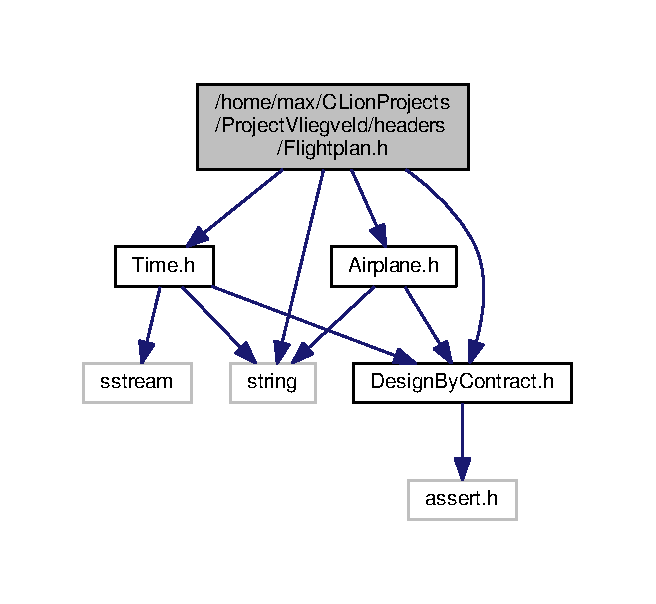
\includegraphics[width=315pt]{Flightplan_8h__incl}
\end{center}
\end{figure}
This graph shows which files directly or indirectly include this file\+:
\nopagebreak
\begin{figure}[H]
\begin{center}
\leavevmode
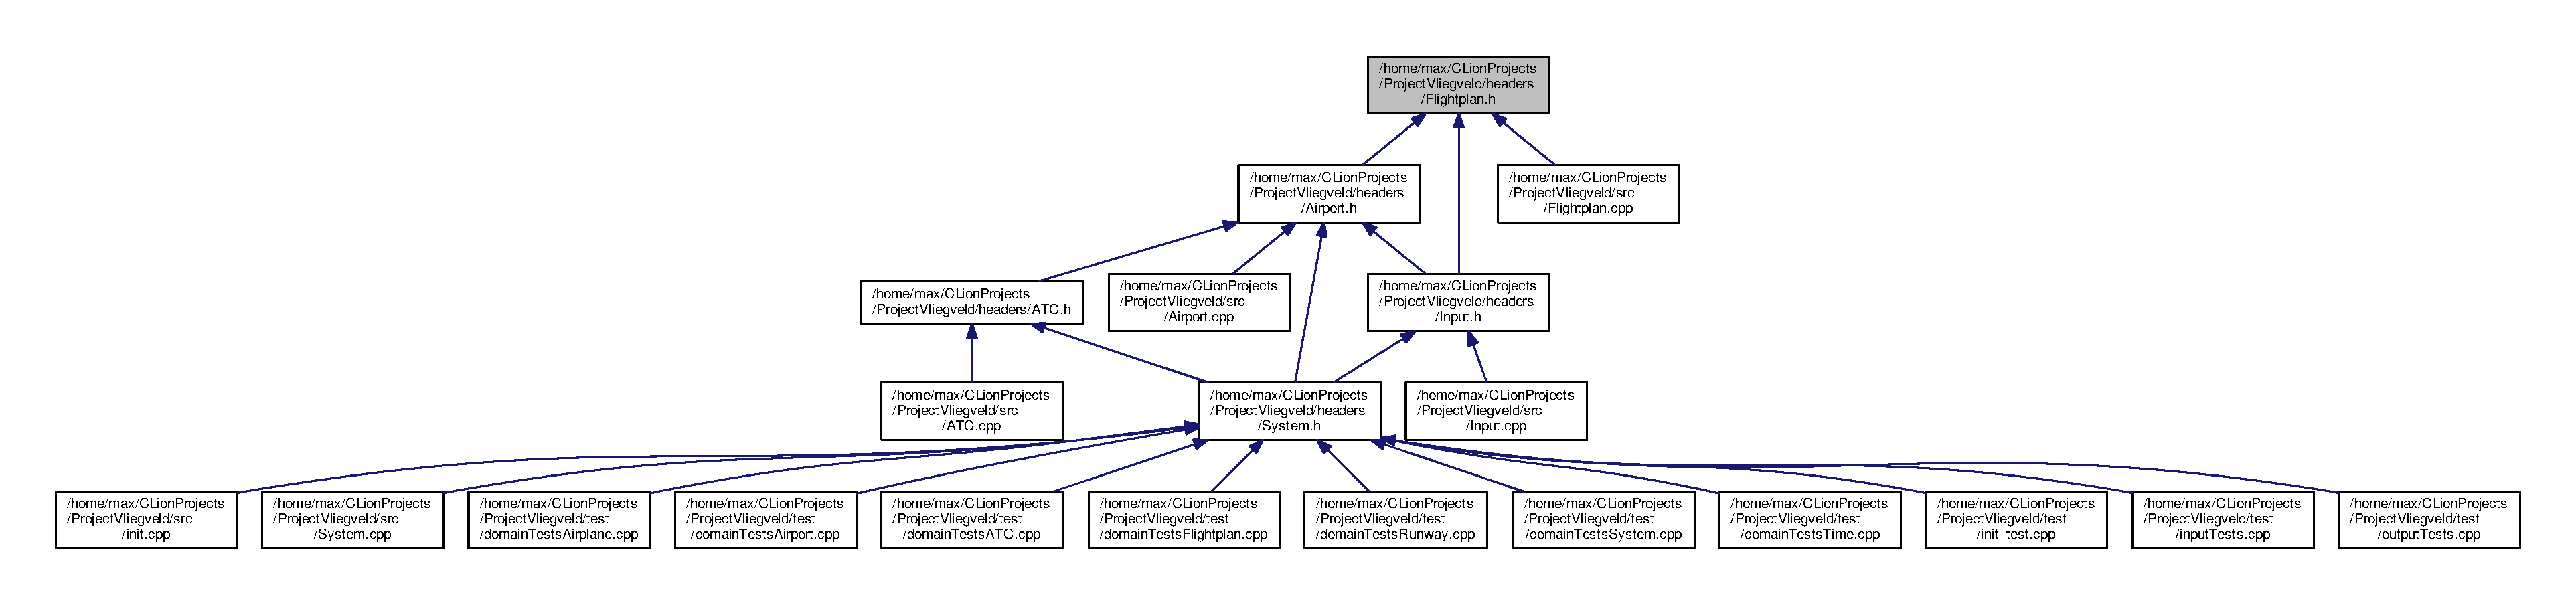
\includegraphics[width=350pt]{Flightplan_8h__dep__incl}
\end{center}
\end{figure}
\subsection*{Classes}
\begin{DoxyCompactItemize}
\item 
class \hyperlink{classFlightplan}{Flightplan}
\begin{DoxyCompactList}\small\item\em \+: Class that represents a flight plan in the simulation \end{DoxyCompactList}\end{DoxyCompactItemize}
\subsection*{Enumerations}
\begin{DoxyCompactItemize}
\item 
enum \hyperlink{Flightplan_8h_ab41c9a082b57fd41aefb64a57d8149f8}{E\+Event} \{ \hyperlink{Flightplan_8h_ab41c9a082b57fd41aefb64a57d8149f8aeaa0025051cf36faa589b5da72a153c4}{k\+Land}, 
\hyperlink{Flightplan_8h_ab41c9a082b57fd41aefb64a57d8149f8a81c03ffd159b67afc7df0ffab6a9297f}{k\+Takeoff}, 
\hyperlink{Flightplan_8h_ab41c9a082b57fd41aefb64a57d8149f8a58584cd9619135e5689ded56238c3427}{k\+Nothing}
 \}
\end{DoxyCompactItemize}


\subsection{Enumeration Type Documentation}
\index{Flightplan.\+h@{Flightplan.\+h}!E\+Event@{E\+Event}}
\index{E\+Event@{E\+Event}!Flightplan.\+h@{Flightplan.\+h}}
\subsubsection[{\texorpdfstring{E\+Event}{EEvent}}]{\setlength{\rightskip}{0pt plus 5cm}enum {\bf E\+Event}}\hypertarget{Flightplan_8h_ab41c9a082b57fd41aefb64a57d8149f8}{}\label{Flightplan_8h_ab41c9a082b57fd41aefb64a57d8149f8}
enum that indicates an event for the plane \begin{Desc}
\item[Enumerator]\par
\begin{description}
\index{k\+Land@{k\+Land}!Flightplan.\+h@{Flightplan.\+h}}\index{Flightplan.\+h@{Flightplan.\+h}!k\+Land@{k\+Land}}\item[{\em 
k\+Land\hypertarget{Flightplan_8h_ab41c9a082b57fd41aefb64a57d8149f8aeaa0025051cf36faa589b5da72a153c4}{}\label{Flightplan_8h_ab41c9a082b57fd41aefb64a57d8149f8aeaa0025051cf36faa589b5da72a153c4}
}]\index{k\+Takeoff@{k\+Takeoff}!Flightplan.\+h@{Flightplan.\+h}}\index{Flightplan.\+h@{Flightplan.\+h}!k\+Takeoff@{k\+Takeoff}}\item[{\em 
k\+Takeoff\hypertarget{Flightplan_8h_ab41c9a082b57fd41aefb64a57d8149f8a81c03ffd159b67afc7df0ffab6a9297f}{}\label{Flightplan_8h_ab41c9a082b57fd41aefb64a57d8149f8a81c03ffd159b67afc7df0ffab6a9297f}
}]\index{k\+Nothing@{k\+Nothing}!Flightplan.\+h@{Flightplan.\+h}}\index{Flightplan.\+h@{Flightplan.\+h}!k\+Nothing@{k\+Nothing}}\item[{\em 
k\+Nothing\hypertarget{Flightplan_8h_ab41c9a082b57fd41aefb64a57d8149f8a58584cd9619135e5689ded56238c3427}{}\label{Flightplan_8h_ab41c9a082b57fd41aefb64a57d8149f8a58584cd9619135e5689ded56238c3427}
}]\end{description}
\end{Desc}

\begin{DoxyCode}
18 \{ \hyperlink{Flightplan_8h_ab41c9a082b57fd41aefb64a57d8149f8aeaa0025051cf36faa589b5da72a153c4}{kLand}, \hyperlink{Flightplan_8h_ab41c9a082b57fd41aefb64a57d8149f8a81c03ffd159b67afc7df0ffab6a9297f}{kTakeoff}, \hyperlink{Flightplan_8h_ab41c9a082b57fd41aefb64a57d8149f8a58584cd9619135e5689ded56238c3427}{kNothing} \};
\end{DoxyCode}

\hypertarget{Input_8h}{}\section{/home/max/\+C\+Lion\+Projects/\+Project\+Vliegveld/headers/\+Input.h File Reference}
\label{Input_8h}\index{/home/max/\+C\+Lion\+Projects/\+Project\+Vliegveld/headers/\+Input.\+h@{/home/max/\+C\+Lion\+Projects/\+Project\+Vliegveld/headers/\+Input.\+h}}
{\ttfamily \#include $<$iostream$>$}\\*
{\ttfamily \#include $<$vector$>$}\\*
{\ttfamily \#include $<$cstdlib$>$}\\*
{\ttfamily \#include \char`\"{}Design\+By\+Contract.\+h\char`\"{}}\\*
{\ttfamily \#include \char`\"{}../tiny\+X\+M\+L/tinyxml.\+h\char`\"{}}\\*
{\ttfamily \#include \char`\"{}Airport.\+h\char`\"{}}\\*
{\ttfamily \#include \char`\"{}Airplane.\+h\char`\"{}}\\*
{\ttfamily \#include \char`\"{}Runway.\+h\char`\"{}}\\*
{\ttfamily \#include \char`\"{}Flightplan.\+h\char`\"{}}\\*
Include dependency graph for Input.\+h\+:
\nopagebreak
\begin{figure}[H]
\begin{center}
\leavevmode
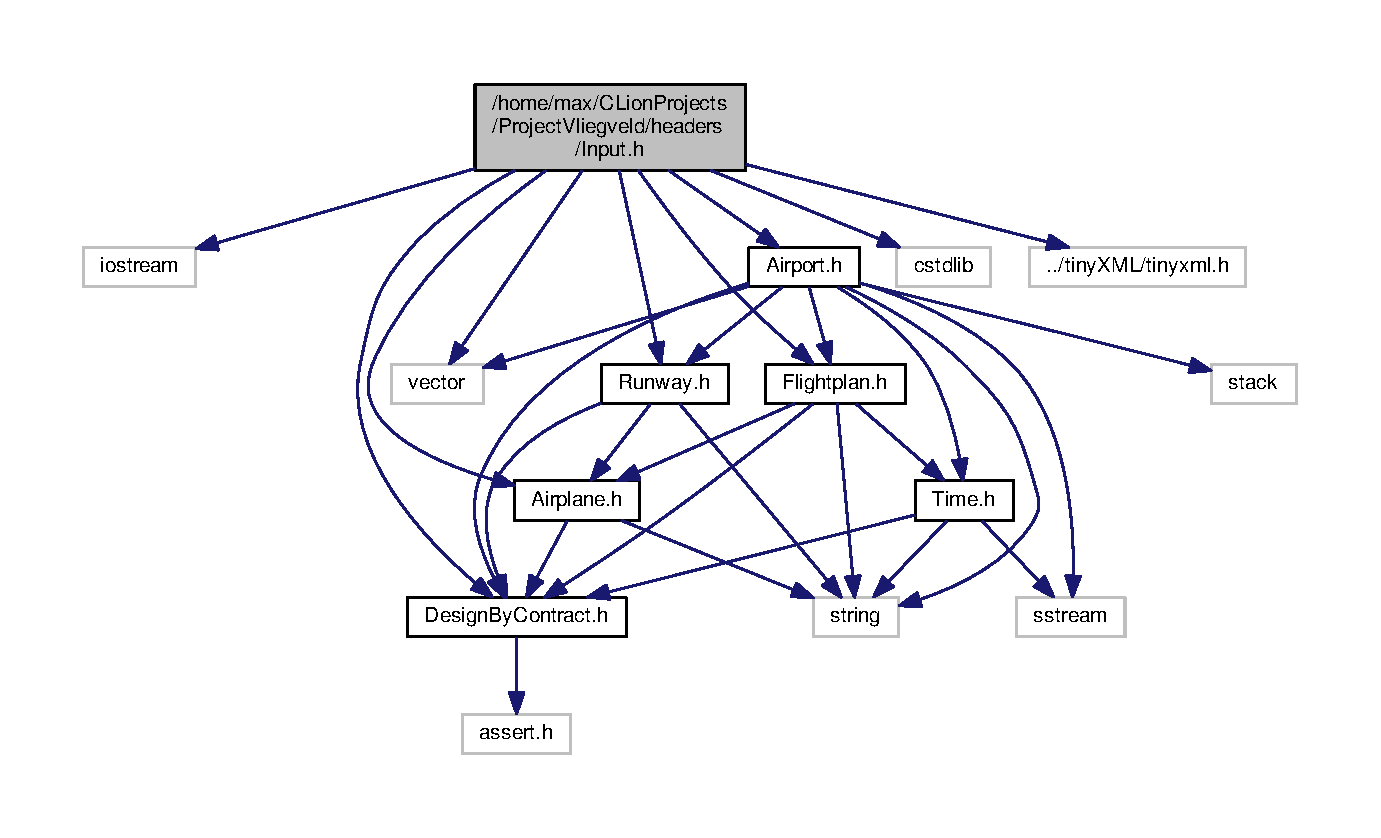
\includegraphics[width=350pt]{Input_8h__incl}
\end{center}
\end{figure}
This graph shows which files directly or indirectly include this file\+:
\nopagebreak
\begin{figure}[H]
\begin{center}
\leavevmode
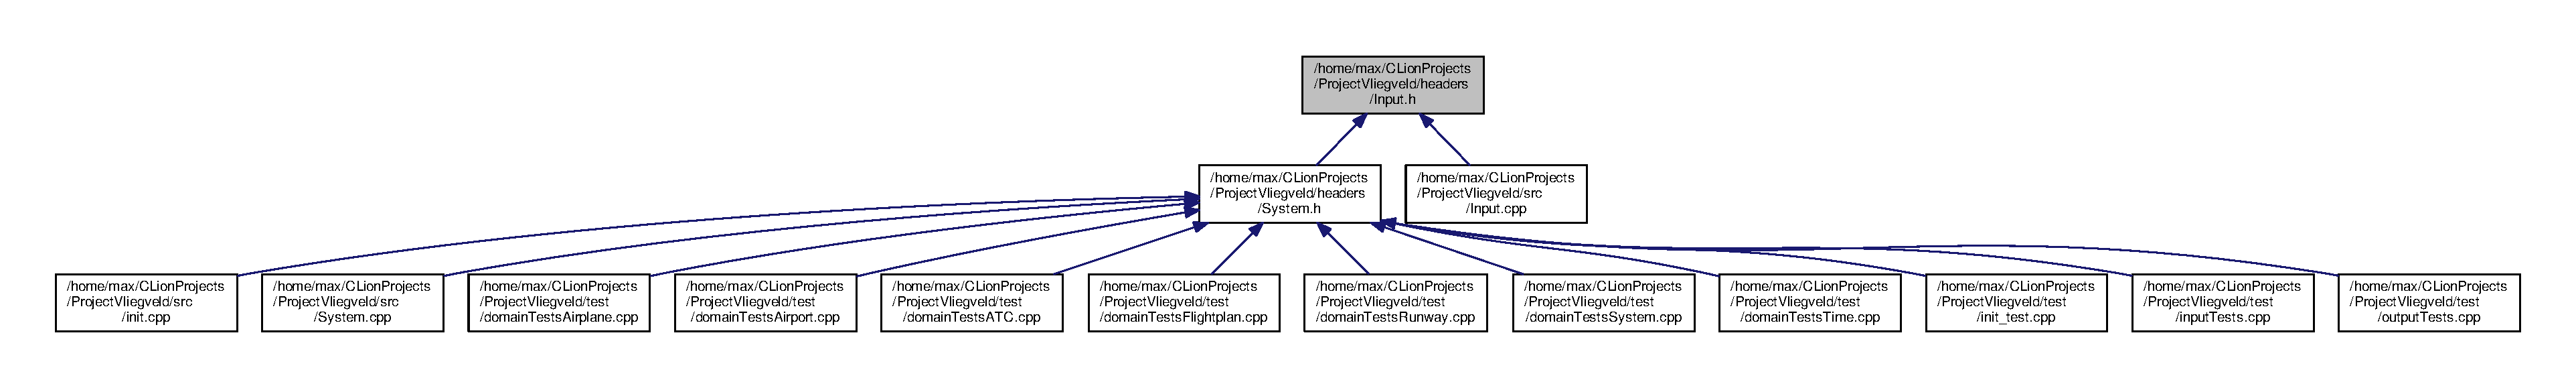
\includegraphics[width=350pt]{Input_8h__dep__incl}
\end{center}
\end{figure}
\subsection*{Classes}
\begin{DoxyCompactItemize}
\item 
class \hyperlink{classInput}{Input}
\begin{DoxyCompactList}\small\item\em \+: Class that reads input for the simulation \end{DoxyCompactList}\end{DoxyCompactItemize}

\hypertarget{Runway_8h}{}\section{/home/max/\+C\+Lion\+Projects/\+Project\+Vliegveld/headers/\+Runway.h File Reference}
\label{Runway_8h}\index{/home/max/\+C\+Lion\+Projects/\+Project\+Vliegveld/headers/\+Runway.\+h@{/home/max/\+C\+Lion\+Projects/\+Project\+Vliegveld/headers/\+Runway.\+h}}
{\ttfamily \#include $<$string$>$}\\*
{\ttfamily \#include \char`\"{}Design\+By\+Contract.\+h\char`\"{}}\\*
{\ttfamily \#include \char`\"{}Airplane.\+h\char`\"{}}\\*
Include dependency graph for Runway.\+h\+:
\nopagebreak
\begin{figure}[H]
\begin{center}
\leavevmode
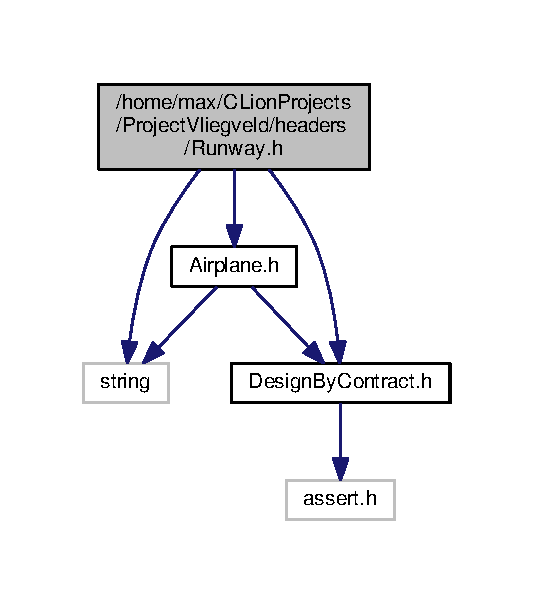
\includegraphics[width=256pt]{Runway_8h__incl}
\end{center}
\end{figure}
This graph shows which files directly or indirectly include this file\+:
\nopagebreak
\begin{figure}[H]
\begin{center}
\leavevmode
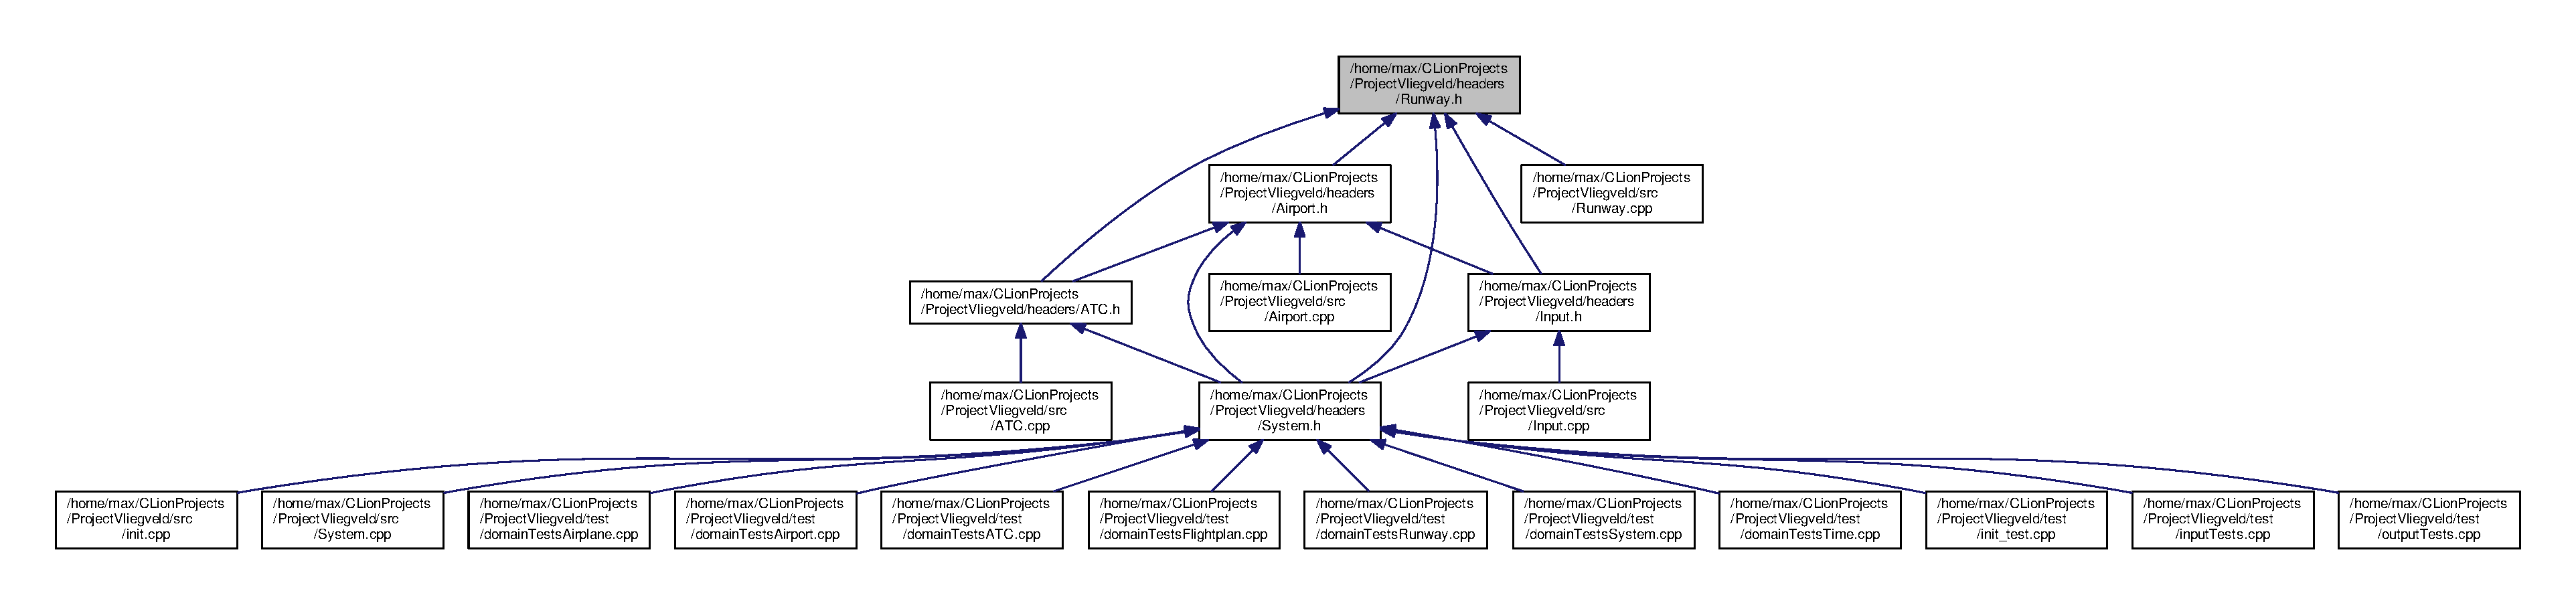
\includegraphics[width=350pt]{Runway_8h__dep__incl}
\end{center}
\end{figure}
\subsection*{Classes}
\begin{DoxyCompactItemize}
\item 
class \hyperlink{classRunway}{Runway}
\end{DoxyCompactItemize}
\subsection*{Enumerations}
\begin{DoxyCompactItemize}
\item 
enum \hyperlink{Runway_8h_adbb3e23fdb96fa1bac0dbbae33431cd2}{E\+Runway\+Type} \{ \hyperlink{Runway_8h_adbb3e23fdb96fa1bac0dbbae33431cd2ae0b5b4fcb396cd73cb79793039658380}{k\+Asphalt}, 
\hyperlink{Runway_8h_adbb3e23fdb96fa1bac0dbbae33431cd2ae97f33599679c1a293bb8403f4a7a8f7}{k\+Grass}, 
\hyperlink{Runway_8h_adbb3e23fdb96fa1bac0dbbae33431cd2ae1dd31bfff8efb153bcf74bebfc8fe57}{k\+Default\+Run\+Type}
 \}
\end{DoxyCompactItemize}


\subsection{Enumeration Type Documentation}
\index{Runway.\+h@{Runway.\+h}!E\+Runway\+Type@{E\+Runway\+Type}}
\index{E\+Runway\+Type@{E\+Runway\+Type}!Runway.\+h@{Runway.\+h}}
\subsubsection[{\texorpdfstring{E\+Runway\+Type}{ERunwayType}}]{\setlength{\rightskip}{0pt plus 5cm}enum {\bf E\+Runway\+Type}}\hypertarget{Runway_8h_adbb3e23fdb96fa1bac0dbbae33431cd2}{}\label{Runway_8h_adbb3e23fdb96fa1bac0dbbae33431cd2}
\begin{Desc}
\item[Enumerator]\par
\begin{description}
\index{k\+Asphalt@{k\+Asphalt}!Runway.\+h@{Runway.\+h}}\index{Runway.\+h@{Runway.\+h}!k\+Asphalt@{k\+Asphalt}}\item[{\em 
k\+Asphalt\hypertarget{Runway_8h_adbb3e23fdb96fa1bac0dbbae33431cd2ae0b5b4fcb396cd73cb79793039658380}{}\label{Runway_8h_adbb3e23fdb96fa1bac0dbbae33431cd2ae0b5b4fcb396cd73cb79793039658380}
}]\index{k\+Grass@{k\+Grass}!Runway.\+h@{Runway.\+h}}\index{Runway.\+h@{Runway.\+h}!k\+Grass@{k\+Grass}}\item[{\em 
k\+Grass\hypertarget{Runway_8h_adbb3e23fdb96fa1bac0dbbae33431cd2ae97f33599679c1a293bb8403f4a7a8f7}{}\label{Runway_8h_adbb3e23fdb96fa1bac0dbbae33431cd2ae97f33599679c1a293bb8403f4a7a8f7}
}]\index{k\+Default\+Run\+Type@{k\+Default\+Run\+Type}!Runway.\+h@{Runway.\+h}}\index{Runway.\+h@{Runway.\+h}!k\+Default\+Run\+Type@{k\+Default\+Run\+Type}}\item[{\em 
k\+Default\+Run\+Type\hypertarget{Runway_8h_adbb3e23fdb96fa1bac0dbbae33431cd2ae1dd31bfff8efb153bcf74bebfc8fe57}{}\label{Runway_8h_adbb3e23fdb96fa1bac0dbbae33431cd2ae1dd31bfff8efb153bcf74bebfc8fe57}
}]\end{description}
\end{Desc}

\begin{DoxyCode}
21 \{ \hyperlink{Runway_8h_adbb3e23fdb96fa1bac0dbbae33431cd2ae0b5b4fcb396cd73cb79793039658380}{kAsphalt}, \hyperlink{Runway_8h_adbb3e23fdb96fa1bac0dbbae33431cd2ae97f33599679c1a293bb8403f4a7a8f7}{kGrass}, \hyperlink{Runway_8h_adbb3e23fdb96fa1bac0dbbae33431cd2ae1dd31bfff8efb153bcf74bebfc8fe57}{kDefaultRunType} \};
\end{DoxyCode}

\hypertarget{System_8h}{}\section{/home/max/\+C\+Lion\+Projects/\+Project\+Vliegveld/headers/\+System.h File Reference}
\label{System_8h}\index{/home/max/\+C\+Lion\+Projects/\+Project\+Vliegveld/headers/\+System.\+h@{/home/max/\+C\+Lion\+Projects/\+Project\+Vliegveld/headers/\+System.\+h}}
{\ttfamily \#include $<$vector$>$}\\*
{\ttfamily \#include $<$iostream$>$}\\*
{\ttfamily \#include $<$fstream$>$}\\*
{\ttfamily \#include $<$string$>$}\\*
{\ttfamily \#include $<$cmath$>$}\\*
{\ttfamily \#include \char`\"{}gtest/gtest.\+h\char`\"{}}\\*
{\ttfamily \#include \char`\"{}Design\+By\+Contract.\+h\char`\"{}}\\*
{\ttfamily \#include \char`\"{}Airplane.\+h\char`\"{}}\\*
{\ttfamily \#include \char`\"{}Airport.\+h\char`\"{}}\\*
{\ttfamily \#include \char`\"{}Runway.\+h\char`\"{}}\\*
{\ttfamily \#include \char`\"{}Input.\+h\char`\"{}}\\*
{\ttfamily \#include \char`\"{}Time.\+h\char`\"{}}\\*
{\ttfamily \#include \char`\"{}A\+T\+C.\+h\char`\"{}}\\*
Include dependency graph for System.\+h\+:
\nopagebreak
\begin{figure}[H]
\begin{center}
\leavevmode
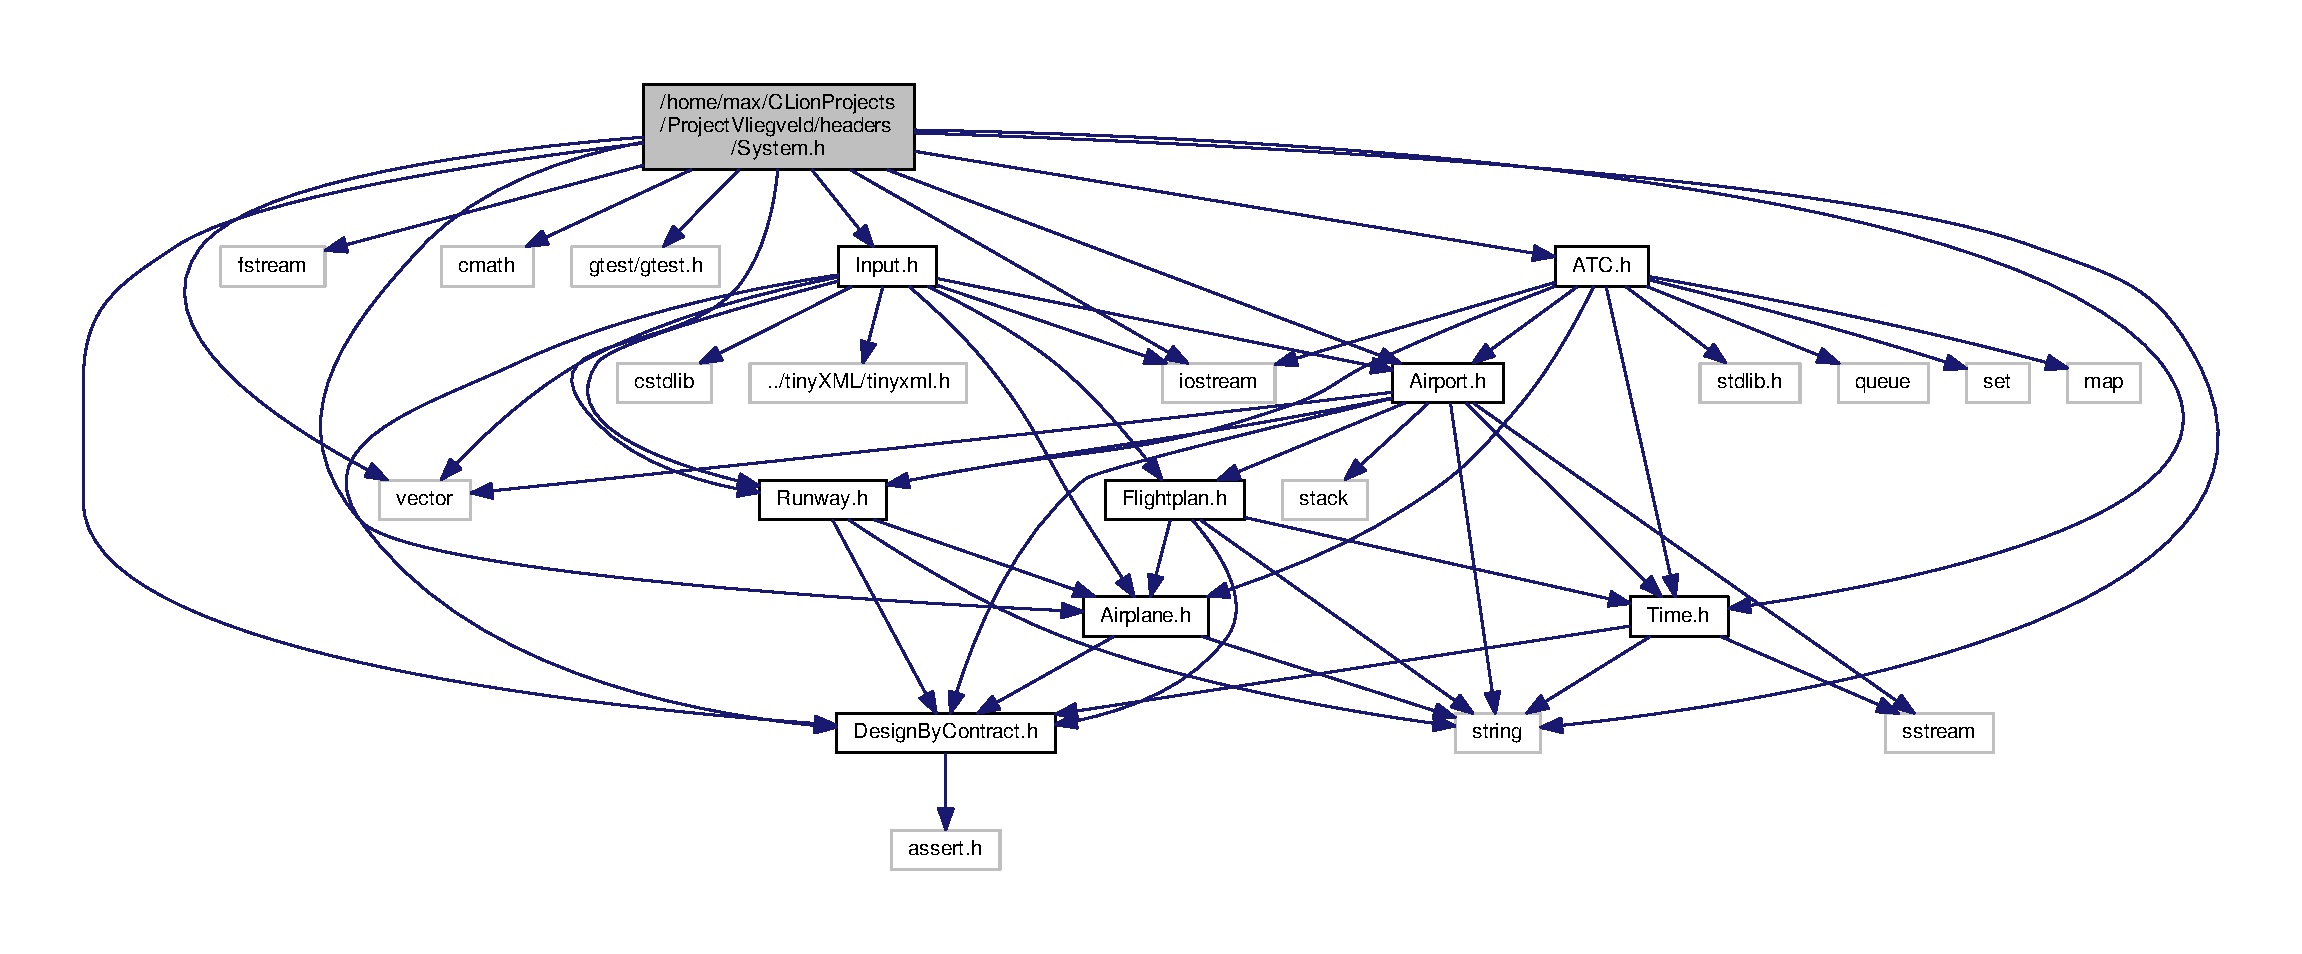
\includegraphics[width=350pt]{System_8h__incl}
\end{center}
\end{figure}
This graph shows which files directly or indirectly include this file\+:
\nopagebreak
\begin{figure}[H]
\begin{center}
\leavevmode
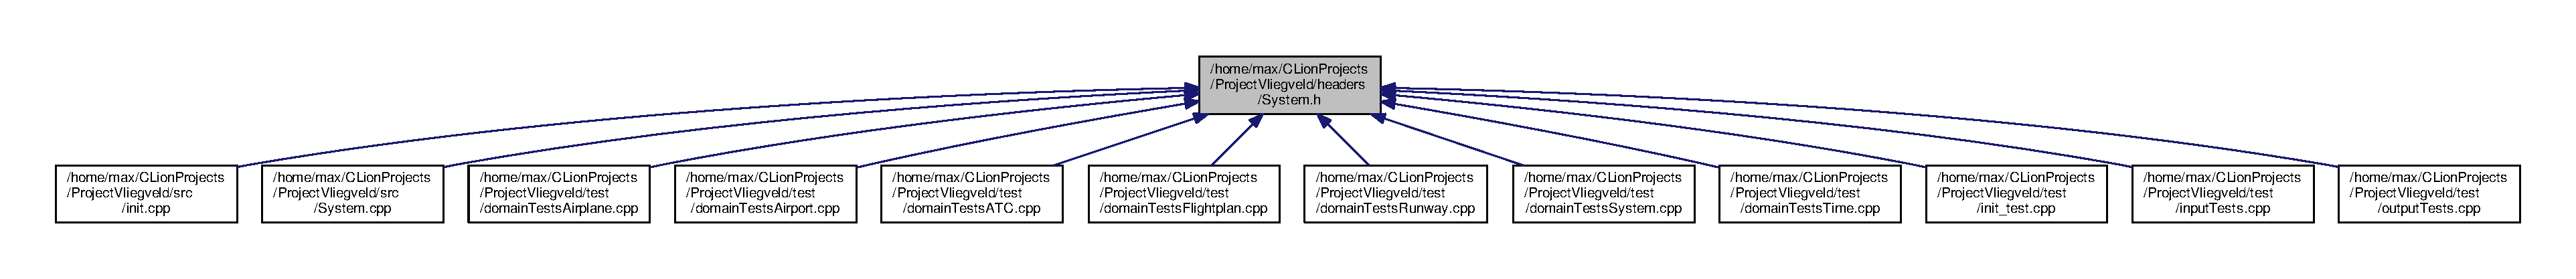
\includegraphics[width=350pt]{System_8h__dep__incl}
\end{center}
\end{figure}
\subsection*{Classes}
\begin{DoxyCompactItemize}
\item 
class \hyperlink{classSystem}{System}
\begin{DoxyCompactList}\small\item\em \+: Main class, controls the simulation \end{DoxyCompactList}\end{DoxyCompactItemize}

\hypertarget{TestUtils_8h}{}\section{/home/max/\+C\+Lion\+Projects/\+Project\+Vliegveld/headers/\+Test\+Utils.h File Reference}
\label{TestUtils_8h}\index{/home/max/\+C\+Lion\+Projects/\+Project\+Vliegveld/headers/\+Test\+Utils.\+h@{/home/max/\+C\+Lion\+Projects/\+Project\+Vliegveld/headers/\+Test\+Utils.\+h}}
{\ttfamily \#include $<$iostream$>$}\\*
Include dependency graph for Test\+Utils.\+h\+:
\nopagebreak
\begin{figure}[H]
\begin{center}
\leavevmode
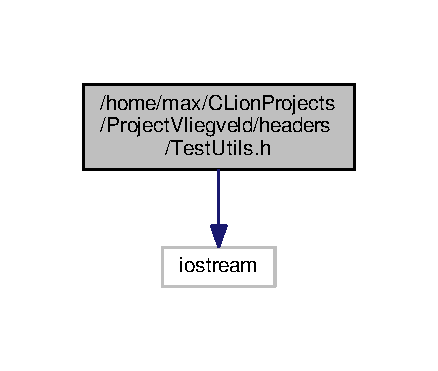
\includegraphics[width=210pt]{TestUtils_8h__incl}
\end{center}
\end{figure}
This graph shows which files directly or indirectly include this file\+:
\nopagebreak
\begin{figure}[H]
\begin{center}
\leavevmode
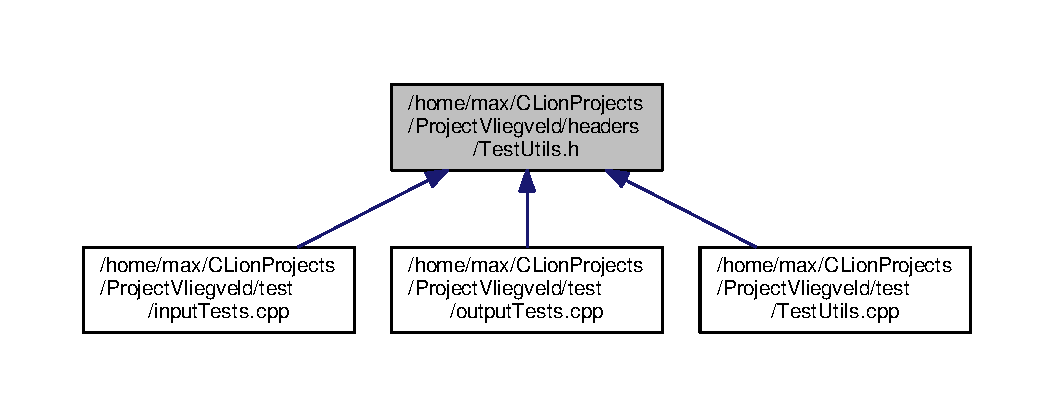
\includegraphics[width=350pt]{TestUtils_8h__dep__incl}
\end{center}
\end{figure}
\subsection*{Functions}
\begin{DoxyCompactItemize}
\item 
bool \hyperlink{TestUtils_8h_a20aa51a3c6e35cb8af1d6d45efd6c71b}{Directory\+Exists} (const std\+::string dirname)
\item 
bool \hyperlink{TestUtils_8h_a946ac5d51dccb6d031b655a60eab6343}{File\+Exists} (const std\+::string dirname)
\item 
bool \hyperlink{TestUtils_8h_a535fe54abcba82699a3d58fc7c04fce7}{File\+Is\+Empty} (const std\+::string filename)
\item 
bool \hyperlink{TestUtils_8h_a7e429f636217210c61bb4f2cdfe74871}{File\+Compare} (const std\+::string left\+File\+Name, const std\+::string right\+File\+Name)
\item 
std\+::string \hyperlink{TestUtils_8h_a163b58e93d058ff9ba6145139fb9293b}{To\+String} (\hyperlink{CMakeCache_8txt_a79a3d8790b2588b09777910863574e09}{int} i)
\end{DoxyCompactItemize}


\subsection{Function Documentation}
\index{Test\+Utils.\+h@{Test\+Utils.\+h}!Directory\+Exists@{Directory\+Exists}}
\index{Directory\+Exists@{Directory\+Exists}!Test\+Utils.\+h@{Test\+Utils.\+h}}
\subsubsection[{\texorpdfstring{Directory\+Exists(const std\+::string dirname)}{DirectoryExists(const std::string dirname)}}]{\setlength{\rightskip}{0pt plus 5cm}bool Directory\+Exists (
\begin{DoxyParamCaption}
\item[{const std\+::string}]{dirname}
\end{DoxyParamCaption}
)}\hypertarget{TestUtils_8h_a20aa51a3c6e35cb8af1d6d45efd6c71b}{}\label{TestUtils_8h_a20aa51a3c6e35cb8af1d6d45efd6c71b}
Auxiliary functions for file manipulation. 
\begin{DoxyCode}
19                                               \{
20     \textcolor{keyword}{struct }stat st;
21     \textcolor{keywordflow}{return} stat(dirname.c\_str(), &st) == 0;
22 \}
\end{DoxyCode}
\index{Test\+Utils.\+h@{Test\+Utils.\+h}!File\+Compare@{File\+Compare}}
\index{File\+Compare@{File\+Compare}!Test\+Utils.\+h@{Test\+Utils.\+h}}
\subsubsection[{\texorpdfstring{File\+Compare(const std\+::string left\+File\+Name, const std\+::string right\+File\+Name)}{FileCompare(const std::string leftFileName, const std::string rightFileName)}}]{\setlength{\rightskip}{0pt plus 5cm}bool File\+Compare (
\begin{DoxyParamCaption}
\item[{const std\+::string}]{left\+File\+Name, }
\item[{const std\+::string}]{right\+File\+Name}
\end{DoxyParamCaption}
)}\hypertarget{TestUtils_8h_a7e429f636217210c61bb4f2cdfe74871}{}\label{TestUtils_8h_a7e429f636217210c61bb4f2cdfe74871}

\begin{DoxyCode}
43                                                                               \{
44     ifstream leftFile, rightFile;
45     \textcolor{keywordtype}{char} leftRead, rightRead;
46     \textcolor{keywordtype}{bool} result;
47 
48     \textcolor{comment}{// Open the two files.}
49     leftFile.open(leftFileName.c\_str());
50     \textcolor{keywordflow}{if} (!leftFile.is\_open()) \{
51         \textcolor{keywordflow}{return} \textcolor{keyword}{false};
52     \};
53     rightFile.open(rightFileName.c\_str());
54     \textcolor{keywordflow}{if} (!rightFile.is\_open()) \{
55         leftFile.close();
56         \textcolor{keywordflow}{return} \textcolor{keyword}{false};
57     \};
58 
59     result = \textcolor{keyword}{true}; \textcolor{comment}{// files exist and are open; assume equality unless a counterexamples shows up.}
60     \textcolor{keywordflow}{while} (result && leftFile.good() && rightFile.good()) \{
61         leftFile.get(leftRead);
62         rightFile.get(rightRead);
63         result = (leftRead == rightRead);
64     \};
65     \textcolor{keywordflow}{if} (result) \{
66         \textcolor{comment}{// last read was still equal; are we at the end of both files ?}
67         result = (!leftFile.good()) && (!rightFile.good());
68     \};
69 
70     leftFile.close();
71     rightFile.close();
72     \textcolor{keywordflow}{return} result;
73 \}
\end{DoxyCode}
\index{Test\+Utils.\+h@{Test\+Utils.\+h}!File\+Exists@{File\+Exists}}
\index{File\+Exists@{File\+Exists}!Test\+Utils.\+h@{Test\+Utils.\+h}}
\subsubsection[{\texorpdfstring{File\+Exists(const std\+::string dirname)}{FileExists(const std::string dirname)}}]{\setlength{\rightskip}{0pt plus 5cm}bool File\+Exists (
\begin{DoxyParamCaption}
\item[{const std\+::string}]{dirname}
\end{DoxyParamCaption}
)}\hypertarget{TestUtils_8h_a946ac5d51dccb6d031b655a60eab6343}{}\label{TestUtils_8h_a946ac5d51dccb6d031b655a60eab6343}

\begin{DoxyCode}
24                                           \{
25     \textcolor{keyword}{struct }stat st;
26     \textcolor{keywordflow}{if} (stat(filename.c\_str(), &st) != 0) \textcolor{keywordflow}{return} \textcolor{keyword}{false};
27     ifstream f(filename.c\_str());
28     \textcolor{keywordflow}{if} (f.good()) \{
29         f.close();
30         \textcolor{keywordflow}{return} \textcolor{keyword}{true};
31     \} \textcolor{keywordflow}{else} \{
32         f.close();
33         \textcolor{keywordflow}{return} \textcolor{keyword}{false};
34     \}
35 \}
\end{DoxyCode}
\index{Test\+Utils.\+h@{Test\+Utils.\+h}!File\+Is\+Empty@{File\+Is\+Empty}}
\index{File\+Is\+Empty@{File\+Is\+Empty}!Test\+Utils.\+h@{Test\+Utils.\+h}}
\subsubsection[{\texorpdfstring{File\+Is\+Empty(const std\+::string filename)}{FileIsEmpty(const std::string filename)}}]{\setlength{\rightskip}{0pt plus 5cm}bool File\+Is\+Empty (
\begin{DoxyParamCaption}
\item[{const std\+::string}]{filename}
\end{DoxyParamCaption}
)}\hypertarget{TestUtils_8h_a535fe54abcba82699a3d58fc7c04fce7}{}\label{TestUtils_8h_a535fe54abcba82699a3d58fc7c04fce7}

\begin{DoxyCode}
37                                            \{
38     \textcolor{keyword}{struct }stat st;
39     \textcolor{keywordflow}{if} (stat(filename.c\_str(), &st) != 0) \textcolor{keywordflow}{return} \textcolor{keyword}{true}; \textcolor{comment}{// File does not exist; thus it is empty}
40     \textcolor{keywordflow}{return} st.st\_size == 0;
41 \}
\end{DoxyCode}
\index{Test\+Utils.\+h@{Test\+Utils.\+h}!To\+String@{To\+String}}
\index{To\+String@{To\+String}!Test\+Utils.\+h@{Test\+Utils.\+h}}
\subsubsection[{\texorpdfstring{To\+String(int i)}{ToString(int i)}}]{\setlength{\rightskip}{0pt plus 5cm}std\+::string To\+String (
\begin{DoxyParamCaption}
\item[{{\bf int}}]{i}
\end{DoxyParamCaption}
)}\hypertarget{TestUtils_8h_a163b58e93d058ff9ba6145139fb9293b}{}\label{TestUtils_8h_a163b58e93d058ff9ba6145139fb9293b}

\begin{DoxyCode}
75                          \{
76     \textcolor{keywordtype}{int} length = snprintf( NULL, 0, \textcolor{stringliteral}{"%d"}, x );
77     \textcolor{keywordtype}{char}* buf = \textcolor{keyword}{new} \textcolor{keywordtype}{char}[length + 1];
78     snprintf( buf, length + 1, \textcolor{stringliteral}{"%d"}, x );
79     \textcolor{keywordtype}{string} str( buf );
80     \textcolor{keyword}{delete}[] buf;
81     \textcolor{keywordflow}{return} str;
82 \}\end{DoxyCode}

\hypertarget{Time_8h}{}\section{/home/max/\+C\+Lion\+Projects/\+Project\+Vliegveld/headers/\+Time.h File Reference}
\label{Time_8h}\index{/home/max/\+C\+Lion\+Projects/\+Project\+Vliegveld/headers/\+Time.\+h@{/home/max/\+C\+Lion\+Projects/\+Project\+Vliegveld/headers/\+Time.\+h}}
{\ttfamily \#include \char`\"{}Design\+By\+Contract.\+h\char`\"{}}\\*
{\ttfamily \#include $<$string$>$}\\*
{\ttfamily \#include $<$sstream$>$}\\*
Include dependency graph for Time.\+h\+:
\nopagebreak
\begin{figure}[H]
\begin{center}
\leavevmode
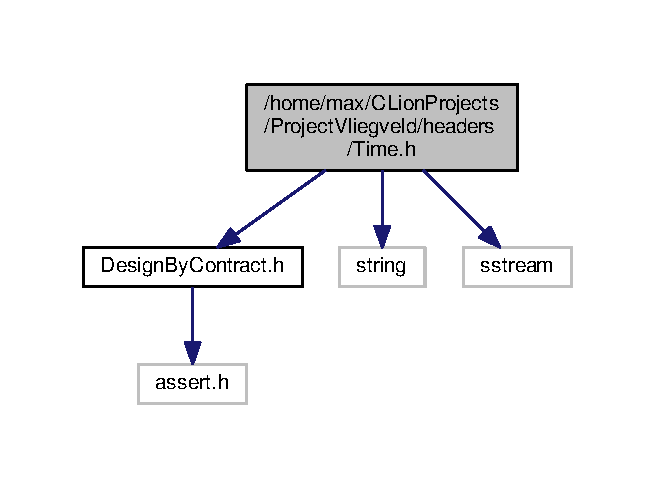
\includegraphics[width=315pt]{Time_8h__incl}
\end{center}
\end{figure}
This graph shows which files directly or indirectly include this file\+:
\nopagebreak
\begin{figure}[H]
\begin{center}
\leavevmode
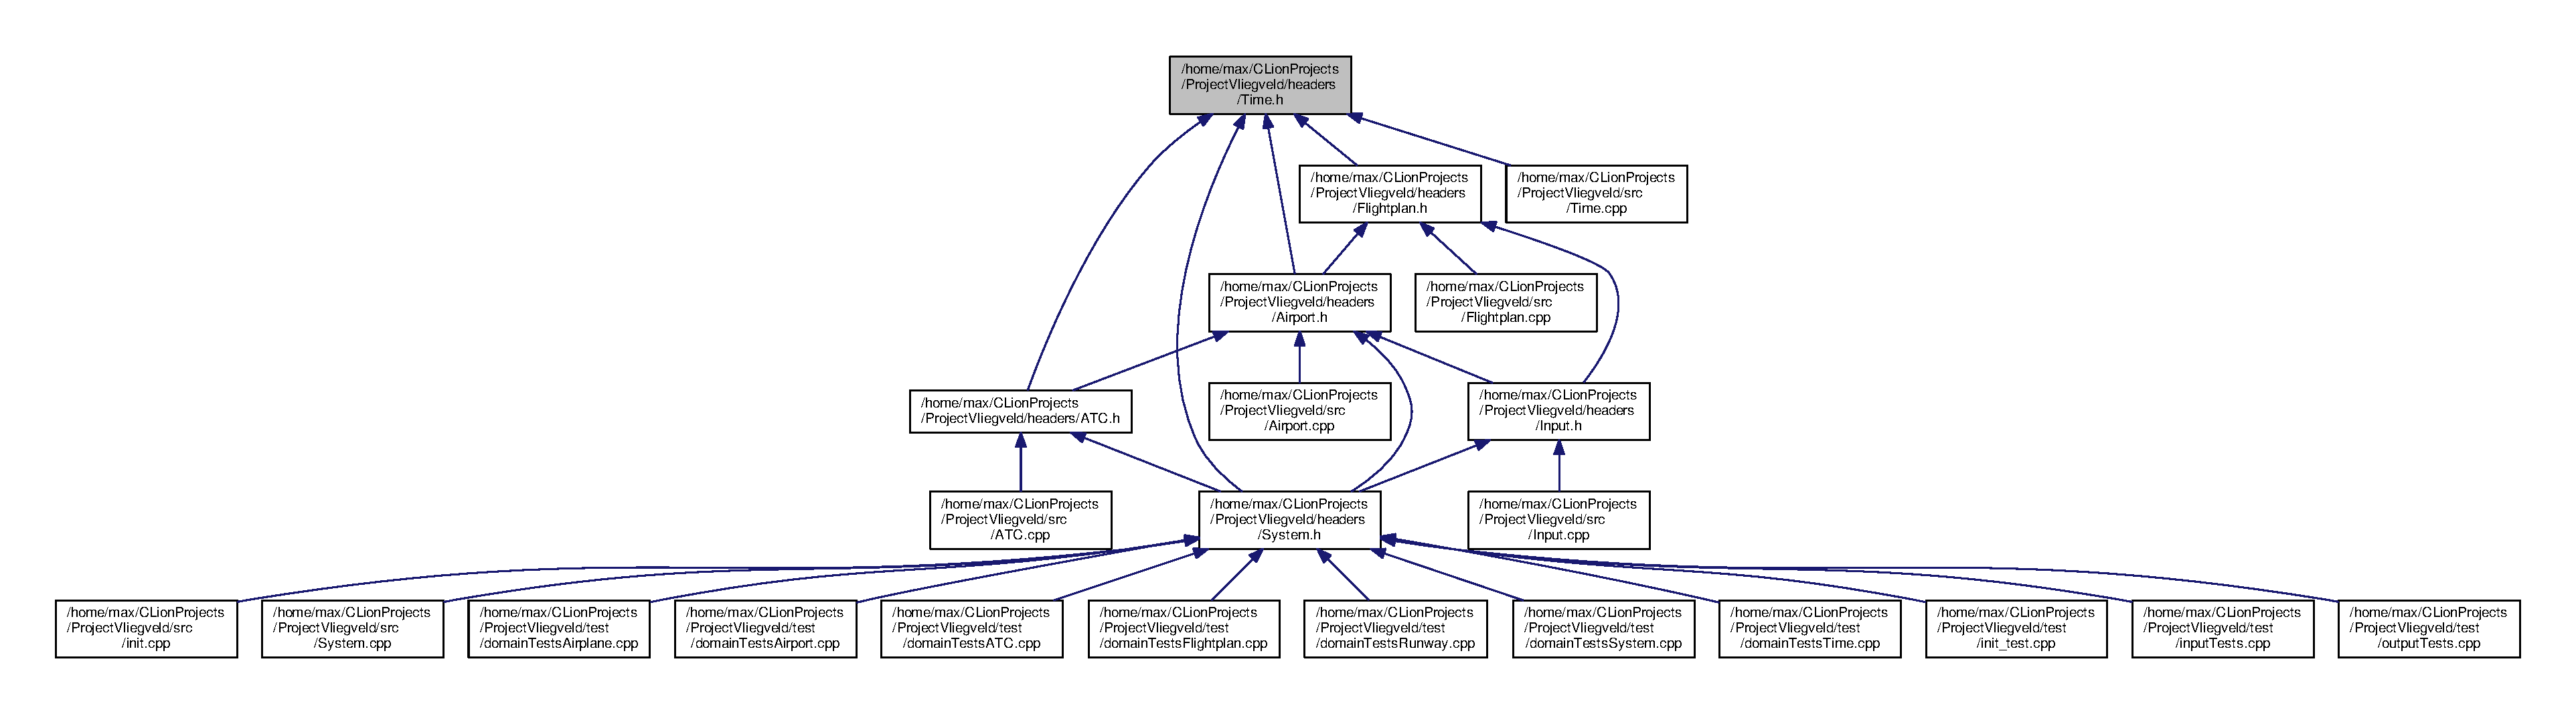
\includegraphics[width=350pt]{Time_8h__dep__incl}
\end{center}
\end{figure}
\subsection*{Classes}
\begin{DoxyCompactItemize}
\item 
class \hyperlink{classTime}{Time}
\end{DoxyCompactItemize}

\hypertarget{ATC_8txt}{}\section{/home/max/\+C\+Lion\+Projects/\+Project\+Vliegveld/output/\+A\+TC.txt File Reference}
\label{ATC_8txt}\index{/home/max/\+C\+Lion\+Projects/\+Project\+Vliegveld/output/\+A\+T\+C.\+txt@{/home/max/\+C\+Lion\+Projects/\+Project\+Vliegveld/output/\+A\+T\+C.\+txt}}
\subsection*{Variables}
\begin{DoxyCompactItemize}
\item 
Antwerp \hyperlink{ATC_8txt_a82e4fe311db1d84af6e8e53fd0d1025d}{Tower}
\item 
Antwerp Speedbird four six \hyperlink{ATC_8txt_a42ba60ceca6351d258f16b06edec96ac}{six}
\item 
Antwerp Speedbird four \hyperlink{happyDay5ExpectedATC_8txt_a57978282a95204080c8ffb626c7d0bd5}{six} requesting I\+FR clearancy\mbox{[}12\+:11\mbox{]}\mbox{[}Antwerp \hyperlink{test_2testOutput_2log_8txt_ade5c2a9317c664c53d015e41bdc32393}{Tower}\mbox{]} Speedbird four \hyperlink{happyDay5ExpectedATC_8txt_a57978282a95204080c8ffb626c7d0bd5}{six} Antwerp cleared to \hyperlink{happyDay5ExpectedATC_8txt_a1bdf675837626f29e859d1a241701d26}{one} \hyperlink{happyDay5ExpectedATC_8txt_a1bdf675837626f29e859d1a241701d26}{one} \hyperlink{ATC_8txt_a4f581ea086ea8bcc78589348ca970791}{lima}
\item 
Antwerp Speedbird four \hyperlink{happyDay5ExpectedATC_8txt_a57978282a95204080c8ffb626c7d0bd5}{six} requesting I\+FR clearancy\mbox{[}12\+:11\mbox{]}\mbox{[}Antwerp \hyperlink{test_2testOutput_2log_8txt_ade5c2a9317c664c53d015e41bdc32393}{Tower}\mbox{]} Speedbird four \hyperlink{happyDay5ExpectedATC_8txt_a57978282a95204080c8ffb626c7d0bd5}{six} Antwerp cleared to \hyperlink{happyDay5ExpectedATC_8txt_a1bdf675837626f29e859d1a241701d26}{one} \hyperlink{happyDay5ExpectedATC_8txt_a1bdf675837626f29e859d1a241701d26}{one} maintain five \hyperlink{ATC_8txt_ae9f8073b6a527ed0b92dd8164f312e3f}{thousand}
\item 
Antwerp Speedbird four \hyperlink{happyDay5ExpectedATC_8txt_a57978282a95204080c8ffb626c7d0bd5}{six} requesting I\+FR clearancy\mbox{[}12\+:11\mbox{]}\mbox{[}Antwerp \hyperlink{test_2testOutput_2log_8txt_ade5c2a9317c664c53d015e41bdc32393}{Tower}\mbox{]} Speedbird four \hyperlink{happyDay5ExpectedATC_8txt_a57978282a95204080c8ffb626c7d0bd5}{six} Antwerp cleared to \hyperlink{happyDay5ExpectedATC_8txt_a1bdf675837626f29e859d1a241701d26}{one} \hyperlink{happyDay5ExpectedATC_8txt_a1bdf675837626f29e859d1a241701d26}{one} maintain five expect flight level \hyperlink{happyDay5ExpectedATC_8txt_a1bdf675837626f29e859d1a241701d26}{one} \hyperlink{happyDay5ExpectedATC_8txt_a1cdb3e947394a8f9b50cff125d86fb29}{zero} \hyperlink{happyDay5ExpectedATC_8txt_a1cdb3e947394a8f9b50cff125d86fb29}{zero} \hyperlink{happyDay5ExpectedATC_8txt_ab9794f8235db42812d8ddd9368cb321e}{ten} minutes after \hyperlink{ATC_8txt_af9835824e50bb6ca59bed75129f137e3}{departure}
\item 
Antwerp Speedbird four \hyperlink{happyDay5ExpectedATC_8txt_a57978282a95204080c8ffb626c7d0bd5}{six} requesting I\+FR clearancy\mbox{[}12\+:11\mbox{]}\mbox{[}Antwerp \hyperlink{test_2testOutput_2log_8txt_ade5c2a9317c664c53d015e41bdc32393}{Tower}\mbox{]} Speedbird four \hyperlink{happyDay5ExpectedATC_8txt_a57978282a95204080c8ffb626c7d0bd5}{six} Antwerp cleared to \hyperlink{happyDay5ExpectedATC_8txt_a1bdf675837626f29e859d1a241701d26}{one} \hyperlink{happyDay5ExpectedATC_8txt_a1bdf675837626f29e859d1a241701d26}{one} maintain five expect flight level \hyperlink{happyDay5ExpectedATC_8txt_a1bdf675837626f29e859d1a241701d26}{one} \hyperlink{happyDay5ExpectedATC_8txt_a1cdb3e947394a8f9b50cff125d86fb29}{zero} \hyperlink{happyDay5ExpectedATC_8txt_a1cdb3e947394a8f9b50cff125d86fb29}{zero} ten minutes after squawk four four \hyperlink{happyDay5ExpectedATC_8txt_a57978282a95204080c8ffb626c7d0bd5}{six} \hyperlink{happyDay3ExpectedATC_8txt_a87da3704f93719801d287ba965c4f715}{two}\mbox{[}12\+:12\mbox{]}\mbox{[}Speedbird 466\mbox{]} Cleared to \hyperlink{happyDay5ExpectedATC_8txt_a1bdf675837626f29e859d1a241701d26}{one} \hyperlink{happyDay5ExpectedATC_8txt_a1bdf675837626f29e859d1a241701d26}{one} initial altitude five expecting \hyperlink{happyDay5ExpectedATC_8txt_a1bdf675837626f29e859d1a241701d26}{one} \hyperlink{happyDay5ExpectedATC_8txt_a1cdb3e947394a8f9b50cff125d86fb29}{zero} \hyperlink{happyDay5ExpectedATC_8txt_a1cdb3e947394a8f9b50cff125d86fb29}{zero} in \hyperlink{ATC_8txt_aa96fd45f0174086569e3631bd320dc87}{ten}
\item 
Antwerp Speedbird four \hyperlink{happyDay5ExpectedATC_8txt_a57978282a95204080c8ffb626c7d0bd5}{six} requesting I\+FR clearancy\mbox{[}12\+:11\mbox{]}\mbox{[}Antwerp \hyperlink{test_2testOutput_2log_8txt_ade5c2a9317c664c53d015e41bdc32393}{Tower}\mbox{]} Speedbird four \hyperlink{happyDay5ExpectedATC_8txt_a57978282a95204080c8ffb626c7d0bd5}{six} Antwerp cleared to \hyperlink{happyDay5ExpectedATC_8txt_a1bdf675837626f29e859d1a241701d26}{one} \hyperlink{happyDay5ExpectedATC_8txt_a1bdf675837626f29e859d1a241701d26}{one} maintain five expect flight level \hyperlink{happyDay5ExpectedATC_8txt_a1bdf675837626f29e859d1a241701d26}{one} \hyperlink{happyDay5ExpectedATC_8txt_a1cdb3e947394a8f9b50cff125d86fb29}{zero} \hyperlink{happyDay5ExpectedATC_8txt_a1cdb3e947394a8f9b50cff125d86fb29}{zero} \hyperlink{happyDay5ExpectedATC_8txt_ab9794f8235db42812d8ddd9368cb321e}{ten} minutes after squawk four four \hyperlink{happyDay5ExpectedATC_8txt_a57978282a95204080c8ffb626c7d0bd5}{six} two\mbox{[}12\+:12\mbox{]}\mbox{[}Speedbird 466\mbox{]} Cleared to \hyperlink{happyDay5ExpectedATC_8txt_a1bdf675837626f29e859d1a241701d26}{one} \hyperlink{happyDay5ExpectedATC_8txt_a1bdf675837626f29e859d1a241701d26}{one} initial altitude five expecting \hyperlink{happyDay5ExpectedATC_8txt_a1bdf675837626f29e859d1a241701d26}{one} \hyperlink{happyDay5ExpectedATC_8txt_a1cdb3e947394a8f9b50cff125d86fb29}{zero} \hyperlink{happyDay5ExpectedATC_8txt_a1cdb3e947394a8f9b50cff125d86fb29}{zero} in \hyperlink{test_2testOutput_2log_8txt_a890147ec88e2d9518adf949981616843}{squawking} four four \hyperlink{happyDay5ExpectedATC_8txt_a57978282a95204080c8ffb626c7d0bd5}{six} \hyperlink{ATC_8txt_acefcb7c39c96f311e277d8ea7ca18a6a}{two}
\item 
Antwerp Speedbird four \hyperlink{happyDay5ExpectedATC_8txt_a57978282a95204080c8ffb626c7d0bd5}{six} requesting I\+FR clearancy\mbox{[}12\+:11\mbox{]}\mbox{[}Antwerp \hyperlink{test_2testOutput_2log_8txt_ade5c2a9317c664c53d015e41bdc32393}{Tower}\mbox{]} Speedbird four \hyperlink{happyDay5ExpectedATC_8txt_a57978282a95204080c8ffb626c7d0bd5}{six} Antwerp cleared to one one maintain five expect flight level one \hyperlink{happyDay5ExpectedATC_8txt_a1cdb3e947394a8f9b50cff125d86fb29}{zero} \hyperlink{happyDay5ExpectedATC_8txt_a1cdb3e947394a8f9b50cff125d86fb29}{zero} \hyperlink{happyDay5ExpectedATC_8txt_ab9794f8235db42812d8ddd9368cb321e}{ten} minutes after squawk four four \hyperlink{happyDay5ExpectedATC_8txt_a57978282a95204080c8ffb626c7d0bd5}{six} \hyperlink{happyDay3ExpectedATC_8txt_a87da3704f93719801d287ba965c4f715}{two}\mbox{[}12\+:12\mbox{]}\mbox{[}Speedbird 466\mbox{]} Cleared to one one initial altitude five expecting one \hyperlink{happyDay5ExpectedATC_8txt_a1cdb3e947394a8f9b50cff125d86fb29}{zero} \hyperlink{happyDay5ExpectedATC_8txt_a1cdb3e947394a8f9b50cff125d86fb29}{zero} in \hyperlink{test_2testOutput_2log_8txt_a890147ec88e2d9518adf949981616843}{squawking} four four \hyperlink{happyDay5ExpectedATC_8txt_a57978282a95204080c8ffb626c7d0bd5}{six} Speedbird four \hyperlink{happyDay5ExpectedATC_8txt_a57978282a95204080c8ffb626c7d0bd5}{six} \hyperlink{happyDay5ExpectedATC_8txt_a57978282a95204080c8ffb626c7d0bd5}{six}\mbox{[}12\+:22\mbox{]}\mbox{[}Speedbird 466\mbox{]} Speedbird four \hyperlink{happyDay5ExpectedATC_8txt_a57978282a95204080c8ffb626c7d0bd5}{six} Speedbird four \hyperlink{happyDay5ExpectedATC_8txt_a57978282a95204080c8ffb626c7d0bd5}{six} \hyperlink{happyDay5ExpectedATC_8txt_a57978282a95204080c8ffb626c7d0bd5}{six} at gate \hyperlink{ATC_8txt_aae2d1d41f2ea606999281eb5037f8eff}{one}
\item 
Antwerp Speedbird four \hyperlink{happyDay5ExpectedATC_8txt_a57978282a95204080c8ffb626c7d0bd5}{six} requesting I\+FR clearancy\mbox{[}12\+:11\mbox{]}\mbox{[}Antwerp \hyperlink{test_2testOutput_2log_8txt_ade5c2a9317c664c53d015e41bdc32393}{Tower}\mbox{]} Speedbird four \hyperlink{happyDay5ExpectedATC_8txt_a57978282a95204080c8ffb626c7d0bd5}{six} Antwerp cleared to \hyperlink{happyDay5ExpectedATC_8txt_a1bdf675837626f29e859d1a241701d26}{one} \hyperlink{happyDay5ExpectedATC_8txt_a1bdf675837626f29e859d1a241701d26}{one} maintain five expect flight level \hyperlink{happyDay5ExpectedATC_8txt_a1bdf675837626f29e859d1a241701d26}{one} \hyperlink{happyDay5ExpectedATC_8txt_a1cdb3e947394a8f9b50cff125d86fb29}{zero} \hyperlink{happyDay5ExpectedATC_8txt_a1cdb3e947394a8f9b50cff125d86fb29}{zero} \hyperlink{happyDay5ExpectedATC_8txt_ab9794f8235db42812d8ddd9368cb321e}{ten} minutes after squawk four four \hyperlink{happyDay5ExpectedATC_8txt_a57978282a95204080c8ffb626c7d0bd5}{six} \hyperlink{happyDay3ExpectedATC_8txt_a87da3704f93719801d287ba965c4f715}{two}\mbox{[}12\+:12\mbox{]}\mbox{[}Speedbird 466\mbox{]} Cleared to \hyperlink{happyDay5ExpectedATC_8txt_a1bdf675837626f29e859d1a241701d26}{one} \hyperlink{happyDay5ExpectedATC_8txt_a1bdf675837626f29e859d1a241701d26}{one} initial altitude five expecting \hyperlink{happyDay5ExpectedATC_8txt_a1bdf675837626f29e859d1a241701d26}{one} \hyperlink{happyDay5ExpectedATC_8txt_a1cdb3e947394a8f9b50cff125d86fb29}{zero} \hyperlink{happyDay5ExpectedATC_8txt_a1cdb3e947394a8f9b50cff125d86fb29}{zero} in \hyperlink{test_2testOutput_2log_8txt_a890147ec88e2d9518adf949981616843}{squawking} four four \hyperlink{happyDay5ExpectedATC_8txt_a57978282a95204080c8ffb626c7d0bd5}{six} Speedbird four \hyperlink{happyDay5ExpectedATC_8txt_a57978282a95204080c8ffb626c7d0bd5}{six} \hyperlink{happyDay5ExpectedATC_8txt_a57978282a95204080c8ffb626c7d0bd5}{six}\mbox{[}12\+:22\mbox{]}\mbox{[}Speedbird 466\mbox{]} Speedbird four \hyperlink{happyDay5ExpectedATC_8txt_a57978282a95204080c8ffb626c7d0bd5}{six} Speedbird four \hyperlink{happyDay5ExpectedATC_8txt_a57978282a95204080c8ffb626c7d0bd5}{six} \hyperlink{happyDay5ExpectedATC_8txt_a57978282a95204080c8ffb626c7d0bd5}{six} at gate requesting pushback\mbox{[}12\+:23\mbox{]}\mbox{[}Antwerp \hyperlink{test_2testOutput_2log_8txt_ade5c2a9317c664c53d015e41bdc32393}{Tower}\mbox{]} Speedbird four \hyperlink{happyDay5ExpectedATC_8txt_a57978282a95204080c8ffb626c7d0bd5}{six} Antwerp pushback approved\mbox{[}12\+:24\mbox{]}\mbox{[}Speedbird 466\mbox{]} Pushback \hyperlink{ATC_8txt_acbd3c2686d25cb28a0ea453e1ebfef6c}{approved}
\item 
Antwerp Speedbird four \hyperlink{happyDay5ExpectedATC_8txt_a57978282a95204080c8ffb626c7d0bd5}{six} requesting I\+FR clearancy\mbox{[}12\+:11\mbox{]}\mbox{[}Antwerp \hyperlink{test_2testOutput_2log_8txt_ade5c2a9317c664c53d015e41bdc32393}{Tower}\mbox{]} Speedbird four \hyperlink{happyDay5ExpectedATC_8txt_a57978282a95204080c8ffb626c7d0bd5}{six} Antwerp cleared to \hyperlink{happyDay5ExpectedATC_8txt_a1bdf675837626f29e859d1a241701d26}{one} \hyperlink{happyDay5ExpectedATC_8txt_a1bdf675837626f29e859d1a241701d26}{one} maintain five expect flight level \hyperlink{happyDay5ExpectedATC_8txt_a1bdf675837626f29e859d1a241701d26}{one} \hyperlink{happyDay5ExpectedATC_8txt_a1cdb3e947394a8f9b50cff125d86fb29}{zero} \hyperlink{happyDay5ExpectedATC_8txt_a1cdb3e947394a8f9b50cff125d86fb29}{zero} \hyperlink{happyDay5ExpectedATC_8txt_ab9794f8235db42812d8ddd9368cb321e}{ten} minutes after squawk four four \hyperlink{happyDay5ExpectedATC_8txt_a57978282a95204080c8ffb626c7d0bd5}{six} \hyperlink{happyDay3ExpectedATC_8txt_a87da3704f93719801d287ba965c4f715}{two}\mbox{[}12\+:12\mbox{]}\mbox{[}Speedbird 466\mbox{]} Cleared to \hyperlink{happyDay5ExpectedATC_8txt_a1bdf675837626f29e859d1a241701d26}{one} \hyperlink{happyDay5ExpectedATC_8txt_a1bdf675837626f29e859d1a241701d26}{one} initial altitude five expecting \hyperlink{happyDay5ExpectedATC_8txt_a1bdf675837626f29e859d1a241701d26}{one} \hyperlink{happyDay5ExpectedATC_8txt_a1cdb3e947394a8f9b50cff125d86fb29}{zero} \hyperlink{happyDay5ExpectedATC_8txt_a1cdb3e947394a8f9b50cff125d86fb29}{zero} in \hyperlink{test_2testOutput_2log_8txt_a890147ec88e2d9518adf949981616843}{squawking} four four \hyperlink{happyDay5ExpectedATC_8txt_a57978282a95204080c8ffb626c7d0bd5}{six} Speedbird four \hyperlink{happyDay5ExpectedATC_8txt_a57978282a95204080c8ffb626c7d0bd5}{six} \hyperlink{happyDay5ExpectedATC_8txt_a57978282a95204080c8ffb626c7d0bd5}{six}\mbox{[}12\+:22\mbox{]}\mbox{[}Speedbird 466\mbox{]} Speedbird four \hyperlink{happyDay5ExpectedATC_8txt_a57978282a95204080c8ffb626c7d0bd5}{six} Speedbird four \hyperlink{happyDay5ExpectedATC_8txt_a57978282a95204080c8ffb626c7d0bd5}{six} \hyperlink{happyDay5ExpectedATC_8txt_a57978282a95204080c8ffb626c7d0bd5}{six} at gate requesting pushback\mbox{[}12\+:23\mbox{]}\mbox{[}Antwerp \hyperlink{test_2testOutput_2log_8txt_ade5c2a9317c664c53d015e41bdc32393}{Tower}\mbox{]} Speedbird four \hyperlink{happyDay5ExpectedATC_8txt_a57978282a95204080c8ffb626c7d0bd5}{six} Antwerp pushback \hyperlink{happyDay5ExpectedATC_8txt_ac858d170c8c9788ee90f1502f4299d18}{approved}\mbox{[}12\+:24\mbox{]}\mbox{[}Speedbird 466\mbox{]} Pushback Speedbird four \hyperlink{happyDay5ExpectedATC_8txt_a57978282a95204080c8ffb626c7d0bd5}{six} \hyperlink{happyDay5ExpectedATC_8txt_a57978282a95204080c8ffb626c7d0bd5}{six}\mbox{[}12\+:27\mbox{]}\mbox{[}Speedbird 466\mbox{]} Speedbird four \hyperlink{happyDay5ExpectedATC_8txt_a57978282a95204080c8ffb626c7d0bd5}{six} \hyperlink{happyDay5ExpectedATC_8txt_a57978282a95204080c8ffb626c7d0bd5}{six} is ready to taxi\mbox{[}12\+:28\mbox{]}\mbox{[}Antwerp \hyperlink{test_2testOutput_2log_8txt_ade5c2a9317c664c53d015e41bdc32393}{Tower}\mbox{]} Speedbird four \hyperlink{happyDay5ExpectedATC_8txt_a57978282a95204080c8ffb626c7d0bd5}{six} taxi to holding point \hyperlink{happyDay5ExpectedATC_8txt_a1bdf675837626f29e859d1a241701d26}{one} \hyperlink{happyDay5ExpectedATC_8txt_a1bdf675837626f29e859d1a241701d26}{one} \hyperlink{happyDay5ExpectedATC_8txt_abc10fad7597c191bcd8586b1cddb7835}{lima} via Alpha\mbox{[}12\+:35\mbox{]}\mbox{[}Speedbird 466\mbox{]} Antwerp Speedbird four \hyperlink{happyDay5ExpectedATC_8txt_a57978282a95204080c8ffb626c7d0bd5}{six} holding short at \hyperlink{happyDay5ExpectedATC_8txt_a1bdf675837626f29e859d1a241701d26}{one} \hyperlink{happyDay5ExpectedATC_8txt_a1bdf675837626f29e859d1a241701d26}{one} \hyperlink{happyDay5ExpectedATC_8txt_abc10fad7597c191bcd8586b1cddb7835}{lima}\mbox{[}12\+:36\mbox{]}\mbox{[}Antwerp \hyperlink{test_2testOutput_2log_8txt_ade5c2a9317c664c53d015e41bdc32393}{Tower}\mbox{]} Speedbird four \hyperlink{happyDay5ExpectedATC_8txt_a57978282a95204080c8ffb626c7d0bd5}{six} taxi to runway \hyperlink{happyDay5ExpectedATC_8txt_a1bdf675837626f29e859d1a241701d26}{one} \hyperlink{happyDay5ExpectedATC_8txt_a1bdf675837626f29e859d1a241701d26}{one} \hyperlink{happyDay5ExpectedATC_8txt_abc10fad7597c191bcd8586b1cddb7835}{lima} via Alpha\mbox{[}12\+:37\mbox{]}\mbox{[}Speedbird 466\mbox{]} Taxi to runway \hyperlink{happyDay5ExpectedATC_8txt_a1bdf675837626f29e859d1a241701d26}{one} \hyperlink{happyDay5ExpectedATC_8txt_a1bdf675837626f29e859d1a241701d26}{one} \hyperlink{happyDay5ExpectedATC_8txt_abc10fad7597c191bcd8586b1cddb7835}{lima} via \hyperlink{ATC_8txt_a1776853b9ca88c0d192ef355be254452}{Alpha}
\item 
Antwerp Speedbird four \hyperlink{happyDay5ExpectedATC_8txt_a57978282a95204080c8ffb626c7d0bd5}{six} requesting I\+FR clearancy\mbox{[}12\+:11\mbox{]}\mbox{[}Antwerp \hyperlink{test_2testOutput_2log_8txt_ade5c2a9317c664c53d015e41bdc32393}{Tower}\mbox{]} Speedbird four \hyperlink{happyDay5ExpectedATC_8txt_a57978282a95204080c8ffb626c7d0bd5}{six} Antwerp cleared to \hyperlink{happyDay5ExpectedATC_8txt_a1bdf675837626f29e859d1a241701d26}{one} \hyperlink{happyDay5ExpectedATC_8txt_a1bdf675837626f29e859d1a241701d26}{one} maintain five expect flight level \hyperlink{happyDay5ExpectedATC_8txt_a1bdf675837626f29e859d1a241701d26}{one} \hyperlink{happyDay5ExpectedATC_8txt_a1cdb3e947394a8f9b50cff125d86fb29}{zero} \hyperlink{happyDay5ExpectedATC_8txt_a1cdb3e947394a8f9b50cff125d86fb29}{zero} \hyperlink{happyDay5ExpectedATC_8txt_ab9794f8235db42812d8ddd9368cb321e}{ten} minutes after squawk four four \hyperlink{happyDay5ExpectedATC_8txt_a57978282a95204080c8ffb626c7d0bd5}{six} \hyperlink{happyDay3ExpectedATC_8txt_a87da3704f93719801d287ba965c4f715}{two}\mbox{[}12\+:12\mbox{]}\mbox{[}Speedbird 466\mbox{]} Cleared to \hyperlink{happyDay5ExpectedATC_8txt_a1bdf675837626f29e859d1a241701d26}{one} \hyperlink{happyDay5ExpectedATC_8txt_a1bdf675837626f29e859d1a241701d26}{one} initial altitude five expecting \hyperlink{happyDay5ExpectedATC_8txt_a1bdf675837626f29e859d1a241701d26}{one} \hyperlink{happyDay5ExpectedATC_8txt_a1cdb3e947394a8f9b50cff125d86fb29}{zero} \hyperlink{happyDay5ExpectedATC_8txt_a1cdb3e947394a8f9b50cff125d86fb29}{zero} in \hyperlink{test_2testOutput_2log_8txt_a890147ec88e2d9518adf949981616843}{squawking} four four \hyperlink{happyDay5ExpectedATC_8txt_a57978282a95204080c8ffb626c7d0bd5}{six} Speedbird four \hyperlink{happyDay5ExpectedATC_8txt_a57978282a95204080c8ffb626c7d0bd5}{six} \hyperlink{happyDay5ExpectedATC_8txt_a57978282a95204080c8ffb626c7d0bd5}{six}\mbox{[}12\+:22\mbox{]}\mbox{[}Speedbird 466\mbox{]} Speedbird four \hyperlink{happyDay5ExpectedATC_8txt_a57978282a95204080c8ffb626c7d0bd5}{six} Speedbird four \hyperlink{happyDay5ExpectedATC_8txt_a57978282a95204080c8ffb626c7d0bd5}{six} \hyperlink{happyDay5ExpectedATC_8txt_a57978282a95204080c8ffb626c7d0bd5}{six} at gate requesting pushback\mbox{[}12\+:23\mbox{]}\mbox{[}Antwerp \hyperlink{test_2testOutput_2log_8txt_ade5c2a9317c664c53d015e41bdc32393}{Tower}\mbox{]} Speedbird four \hyperlink{happyDay5ExpectedATC_8txt_a57978282a95204080c8ffb626c7d0bd5}{six} Antwerp pushback \hyperlink{happyDay5ExpectedATC_8txt_ac858d170c8c9788ee90f1502f4299d18}{approved}\mbox{[}12\+:24\mbox{]}\mbox{[}Speedbird 466\mbox{]} Pushback Speedbird four \hyperlink{happyDay5ExpectedATC_8txt_a57978282a95204080c8ffb626c7d0bd5}{six} \hyperlink{happyDay5ExpectedATC_8txt_a57978282a95204080c8ffb626c7d0bd5}{six}\mbox{[}12\+:27\mbox{]}\mbox{[}Speedbird 466\mbox{]} Speedbird four \hyperlink{happyDay5ExpectedATC_8txt_a57978282a95204080c8ffb626c7d0bd5}{six} \hyperlink{happyDay5ExpectedATC_8txt_a57978282a95204080c8ffb626c7d0bd5}{six} is ready to taxi\mbox{[}12\+:28\mbox{]}\mbox{[}Antwerp \hyperlink{test_2testOutput_2log_8txt_ade5c2a9317c664c53d015e41bdc32393}{Tower}\mbox{]} Speedbird four \hyperlink{happyDay5ExpectedATC_8txt_a57978282a95204080c8ffb626c7d0bd5}{six} taxi to holding point \hyperlink{happyDay5ExpectedATC_8txt_a1bdf675837626f29e859d1a241701d26}{one} \hyperlink{happyDay5ExpectedATC_8txt_a1bdf675837626f29e859d1a241701d26}{one} \hyperlink{happyDay5ExpectedATC_8txt_abc10fad7597c191bcd8586b1cddb7835}{lima} via \hyperlink{happyDay3ExpectedATC_8txt_a81a3dae936b024aa7b8604489d418e64}{Alpha}\mbox{[}12\+:35\mbox{]}\mbox{[}Speedbird 466\mbox{]} Antwerp Speedbird four \hyperlink{happyDay5ExpectedATC_8txt_a57978282a95204080c8ffb626c7d0bd5}{six} holding short at \hyperlink{happyDay5ExpectedATC_8txt_a1bdf675837626f29e859d1a241701d26}{one} \hyperlink{happyDay5ExpectedATC_8txt_a1bdf675837626f29e859d1a241701d26}{one} \hyperlink{happyDay5ExpectedATC_8txt_abc10fad7597c191bcd8586b1cddb7835}{lima}\mbox{[}12\+:36\mbox{]}\mbox{[}Antwerp \hyperlink{test_2testOutput_2log_8txt_ade5c2a9317c664c53d015e41bdc32393}{Tower}\mbox{]} Speedbird four \hyperlink{happyDay5ExpectedATC_8txt_a57978282a95204080c8ffb626c7d0bd5}{six} taxi to runway \hyperlink{happyDay5ExpectedATC_8txt_a1bdf675837626f29e859d1a241701d26}{one} \hyperlink{happyDay5ExpectedATC_8txt_a1bdf675837626f29e859d1a241701d26}{one} \hyperlink{happyDay5ExpectedATC_8txt_abc10fad7597c191bcd8586b1cddb7835}{lima} via \hyperlink{happyDay3ExpectedATC_8txt_a81a3dae936b024aa7b8604489d418e64}{Alpha}\mbox{[}12\+:37\mbox{]}\mbox{[}Speedbird 466\mbox{]} Taxi to runway \hyperlink{happyDay5ExpectedATC_8txt_a1bdf675837626f29e859d1a241701d26}{one} \hyperlink{happyDay5ExpectedATC_8txt_a1bdf675837626f29e859d1a241701d26}{one} \hyperlink{happyDay5ExpectedATC_8txt_abc10fad7597c191bcd8586b1cddb7835}{lima} via Speedbird four \hyperlink{happyDay5ExpectedATC_8txt_a57978282a95204080c8ffb626c7d0bd5}{six} \hyperlink{happyDay5ExpectedATC_8txt_a57978282a95204080c8ffb626c7d0bd5}{six}\mbox{[}12\+:38\mbox{]}\mbox{[}Speedbird 466\mbox{]} Antwerp Speedbird four \hyperlink{happyDay5ExpectedATC_8txt_a57978282a95204080c8ffb626c7d0bd5}{six} holding short at \hyperlink{happyDay5ExpectedATC_8txt_a1bdf675837626f29e859d1a241701d26}{one} \hyperlink{happyDay5ExpectedATC_8txt_a1bdf675837626f29e859d1a241701d26}{one} \hyperlink{happyDay5ExpectedATC_8txt_abc10fad7597c191bcd8586b1cddb7835}{lima}\mbox{[}12\+:39\mbox{]}\mbox{[}Antwerp \hyperlink{test_2testOutput_2log_8txt_ade5c2a9317c664c53d015e41bdc32393}{Tower}\mbox{]} Speedbird four \hyperlink{happyDay5ExpectedATC_8txt_a57978282a95204080c8ffb626c7d0bd5}{six} runway \hyperlink{happyDay5ExpectedATC_8txt_a1bdf675837626f29e859d1a241701d26}{one} \hyperlink{happyDay5ExpectedATC_8txt_a1bdf675837626f29e859d1a241701d26}{one} \hyperlink{happyDay5ExpectedATC_8txt_abc10fad7597c191bcd8586b1cddb7835}{lima} cleared for take off\mbox{[}12\+:40\mbox{]}\mbox{[}Speedbird 466\mbox{]} \hyperlink{classRunway}{Runway} \hyperlink{happyDay5ExpectedATC_8txt_a1bdf675837626f29e859d1a241701d26}{one} \hyperlink{happyDay5ExpectedATC_8txt_a1bdf675837626f29e859d1a241701d26}{one} \hyperlink{happyDay5ExpectedATC_8txt_abc10fad7597c191bcd8586b1cddb7835}{lima} cleared for take \hyperlink{ATC_8txt_a5e54cdd3ba663e9f1ca689a2edf07d4d}{off}
\end{DoxyCompactItemize}


\subsection{Variable Documentation}
\index{A\+T\+C.\+txt@{A\+T\+C.\+txt}!Alpha@{Alpha}}
\index{Alpha@{Alpha}!A\+T\+C.\+txt@{A\+T\+C.\+txt}}
\subsubsection[{\texorpdfstring{Alpha}{Alpha}}]{\setlength{\rightskip}{0pt plus 5cm}Antwerp Speedbird four {\bf six} requesting I\+FR clearancy \mbox{[}12\+:11\mbox{]}\mbox{[}Antwerp {\bf Tower}\mbox{]} Speedbird four {\bf six} Antwerp cleared to {\bf one} {\bf one} maintain five expect flight level {\bf one} {\bf zero} {\bf zero} {\bf ten} minutes after squawk four four {\bf six} {\bf two} \mbox{[}12\+:12\mbox{]}\mbox{[}Speedbird 466\mbox{]} Cleared to {\bf one} {\bf one} initial altitude five expecting {\bf one} {\bf zero} {\bf zero} in {\bf squawking} four four {\bf six} Speedbird four {\bf six} {\bf six} \mbox{[}12\+:22\mbox{]}\mbox{[}Speedbird 466\mbox{]} Speedbird four {\bf six} Speedbird four {\bf six} {\bf six} at gate requesting pushback \mbox{[}12\+:23\mbox{]}\mbox{[}Antwerp {\bf Tower}\mbox{]} Speedbird four {\bf six} Antwerp pushback {\bf approved} \mbox{[}12\+:24\mbox{]}\mbox{[}Speedbird 466\mbox{]} Pushback Speedbird four {\bf six} {\bf six} \mbox{[}12\+:27\mbox{]}\mbox{[}Speedbird 466\mbox{]} Speedbird four {\bf six} {\bf six} is ready to taxi \mbox{[}12\+:28\mbox{]}\mbox{[}Antwerp {\bf Tower}\mbox{]} Speedbird four {\bf six} taxi to holding point {\bf one} {\bf one} {\bf lima} via Alpha \mbox{[}12\+:35\mbox{]}\mbox{[}Speedbird 466\mbox{]} Antwerp Speedbird four {\bf six} holding short at {\bf one} {\bf one} {\bf lima} \mbox{[}12\+:36\mbox{]}\mbox{[}Antwerp {\bf Tower}\mbox{]} Speedbird four {\bf six} taxi to runway {\bf one} {\bf one} {\bf lima} via Alpha \mbox{[}12\+:37\mbox{]}\mbox{[}Speedbird 466\mbox{]} Taxi to runway {\bf one} {\bf one} {\bf lima} via Alpha}\hypertarget{ATC_8txt_a1776853b9ca88c0d192ef355be254452}{}\label{ATC_8txt_a1776853b9ca88c0d192ef355be254452}
\index{A\+T\+C.\+txt@{A\+T\+C.\+txt}!approved@{approved}}
\index{approved@{approved}!A\+T\+C.\+txt@{A\+T\+C.\+txt}}
\subsubsection[{\texorpdfstring{approved}{approved}}]{\setlength{\rightskip}{0pt plus 5cm}Antwerp Speedbird four {\bf six} requesting I\+FR clearancy \mbox{[}12\+:11\mbox{]}\mbox{[}Antwerp {\bf Tower}\mbox{]} Speedbird four {\bf six} Antwerp cleared to {\bf one} {\bf one} maintain five expect flight level {\bf one} {\bf zero} {\bf zero} {\bf ten} minutes after squawk four four {\bf six} {\bf two} \mbox{[}12\+:12\mbox{]}\mbox{[}Speedbird 466\mbox{]} Cleared to {\bf one} {\bf one} initial altitude five expecting {\bf one} {\bf zero} {\bf zero} in {\bf squawking} four four {\bf six} Speedbird four {\bf six} {\bf six} \mbox{[}12\+:22\mbox{]}\mbox{[}Speedbird 466\mbox{]} Speedbird four {\bf six} Speedbird four {\bf six} {\bf six} at gate requesting pushback \mbox{[}12\+:23\mbox{]}\mbox{[}Antwerp {\bf Tower}\mbox{]} Speedbird four {\bf six} Antwerp pushback approved \mbox{[}12\+:24\mbox{]}\mbox{[}Speedbird 466\mbox{]} Pushback approved}\hypertarget{ATC_8txt_acbd3c2686d25cb28a0ea453e1ebfef6c}{}\label{ATC_8txt_acbd3c2686d25cb28a0ea453e1ebfef6c}
\index{A\+T\+C.\+txt@{A\+T\+C.\+txt}!departure@{departure}}
\index{departure@{departure}!A\+T\+C.\+txt@{A\+T\+C.\+txt}}
\subsubsection[{\texorpdfstring{departure}{departure}}]{\setlength{\rightskip}{0pt plus 5cm}Antwerp Speedbird four {\bf six} requesting I\+FR clearancy \mbox{[}12\+:11\mbox{]}\mbox{[}Antwerp {\bf Tower}\mbox{]} Speedbird four {\bf six} Antwerp cleared to {\bf one} {\bf one} maintain five expect flight level {\bf one} {\bf zero} {\bf zero} {\bf ten} minutes after departure}\hypertarget{ATC_8txt_af9835824e50bb6ca59bed75129f137e3}{}\label{ATC_8txt_af9835824e50bb6ca59bed75129f137e3}
\index{A\+T\+C.\+txt@{A\+T\+C.\+txt}!lima@{lima}}
\index{lima@{lima}!A\+T\+C.\+txt@{A\+T\+C.\+txt}}
\subsubsection[{\texorpdfstring{lima}{lima}}]{\setlength{\rightskip}{0pt plus 5cm}Antwerp Speedbird four {\bf six} requesting I\+FR clearancy \mbox{[}12\+:11\mbox{]}\mbox{[}Antwerp {\bf Tower}\mbox{]} Speedbird four {\bf six} Antwerp cleared to {\bf one} {\bf one} maintain five expect flight level {\bf one} {\bf zero} {\bf zero} {\bf ten} minutes after squawk four four {\bf six} {\bf two} \mbox{[}12\+:12\mbox{]}\mbox{[}Speedbird 466\mbox{]} Cleared to {\bf one} {\bf one} lima}\hypertarget{ATC_8txt_a4f581ea086ea8bcc78589348ca970791}{}\label{ATC_8txt_a4f581ea086ea8bcc78589348ca970791}
\index{A\+T\+C.\+txt@{A\+T\+C.\+txt}!off@{off}}
\index{off@{off}!A\+T\+C.\+txt@{A\+T\+C.\+txt}}
\subsubsection[{\texorpdfstring{off}{off}}]{\setlength{\rightskip}{0pt plus 5cm}Antwerp Speedbird four {\bf six} requesting I\+FR clearancy \mbox{[}12\+:11\mbox{]}\mbox{[}Antwerp {\bf Tower}\mbox{]} Speedbird four {\bf six} Antwerp cleared to {\bf one} {\bf one} maintain five expect flight level {\bf one} {\bf zero} {\bf zero} {\bf ten} minutes after squawk four four {\bf six} {\bf two} \mbox{[}12\+:12\mbox{]}\mbox{[}Speedbird 466\mbox{]} Cleared to {\bf one} {\bf one} initial altitude five expecting {\bf one} {\bf zero} {\bf zero} in {\bf squawking} four four {\bf six} Speedbird four {\bf six} {\bf six} \mbox{[}12\+:22\mbox{]}\mbox{[}Speedbird 466\mbox{]} Speedbird four {\bf six} Speedbird four {\bf six} {\bf six} at gate requesting pushback \mbox{[}12\+:23\mbox{]}\mbox{[}Antwerp {\bf Tower}\mbox{]} Speedbird four {\bf six} Antwerp pushback {\bf approved} \mbox{[}12\+:24\mbox{]}\mbox{[}Speedbird 466\mbox{]} Pushback Speedbird four {\bf six} {\bf six} \mbox{[}12\+:27\mbox{]}\mbox{[}Speedbird 466\mbox{]} Speedbird four {\bf six} {\bf six} is ready to taxi \mbox{[}12\+:28\mbox{]}\mbox{[}Antwerp {\bf Tower}\mbox{]} Speedbird four {\bf six} taxi to holding point {\bf one} {\bf one} {\bf lima} via {\bf Alpha} \mbox{[}12\+:35\mbox{]}\mbox{[}Speedbird 466\mbox{]} Antwerp Speedbird four {\bf six} holding short at {\bf one} {\bf one} {\bf lima} \mbox{[}12\+:36\mbox{]}\mbox{[}Antwerp {\bf Tower}\mbox{]} Speedbird four {\bf six} taxi to runway {\bf one} {\bf one} {\bf lima} via {\bf Alpha} \mbox{[}12\+:37\mbox{]}\mbox{[}Speedbird 466\mbox{]} Taxi to runway {\bf one} {\bf one} {\bf lima} via Speedbird four {\bf six} {\bf six} \mbox{[}12\+:38\mbox{]}\mbox{[}Speedbird 466\mbox{]} Antwerp Speedbird four {\bf six} holding short at {\bf one} {\bf one} {\bf lima} \mbox{[}12\+:39\mbox{]}\mbox{[}Antwerp {\bf Tower}\mbox{]} Speedbird four {\bf six} runway {\bf one} {\bf one} {\bf lima} cleared for take off \mbox{[}12\+:40\mbox{]}\mbox{[}Speedbird 466\mbox{]} {\bf Runway} {\bf one} {\bf one} {\bf lima} cleared for take off}\hypertarget{ATC_8txt_a5e54cdd3ba663e9f1ca689a2edf07d4d}{}\label{ATC_8txt_a5e54cdd3ba663e9f1ca689a2edf07d4d}
\index{A\+T\+C.\+txt@{A\+T\+C.\+txt}!one@{one}}
\index{one@{one}!A\+T\+C.\+txt@{A\+T\+C.\+txt}}
\subsubsection[{\texorpdfstring{one}{one}}]{\setlength{\rightskip}{0pt plus 5cm}Antwerp Speedbird four {\bf six} requesting I\+FR clearancy \mbox{[}12\+:11\mbox{]}\mbox{[}Antwerp {\bf Tower}\mbox{]} Speedbird four {\bf six} Antwerp cleared to one one maintain five expect flight level one {\bf zero} {\bf zero} {\bf ten} minutes after squawk four four {\bf six} {\bf two} \mbox{[}12\+:12\mbox{]}\mbox{[}Speedbird 466\mbox{]} Cleared to one one initial altitude five expecting one {\bf zero} {\bf zero} in {\bf squawking} four four {\bf six} Speedbird four {\bf six} {\bf six} \mbox{[}12\+:22\mbox{]}\mbox{[}Speedbird 466\mbox{]} Speedbird four {\bf six} Speedbird four {\bf six} {\bf six} at gate one}\hypertarget{ATC_8txt_aae2d1d41f2ea606999281eb5037f8eff}{}\label{ATC_8txt_aae2d1d41f2ea606999281eb5037f8eff}
\index{A\+T\+C.\+txt@{A\+T\+C.\+txt}!six@{six}}
\index{six@{six}!A\+T\+C.\+txt@{A\+T\+C.\+txt}}
\subsubsection[{\texorpdfstring{six}{six}}]{\setlength{\rightskip}{0pt plus 5cm}Antwerp Speedbird four six requesting I\+FR clearancy \mbox{[}12\+:11\mbox{]}\mbox{[}Antwerp {\bf Tower}\mbox{]} Speedbird four six Antwerp cleared to {\bf one} {\bf one} maintain five expect flight level {\bf one} {\bf zero} {\bf zero} {\bf ten} minutes after squawk four four six {\bf two} \mbox{[}12\+:12\mbox{]}\mbox{[}Speedbird 466\mbox{]} Cleared to {\bf one} {\bf one} initial altitude five expecting {\bf one} {\bf zero} {\bf zero} in {\bf squawking} four four six Speedbird four six six \mbox{[}12\+:22\mbox{]}\mbox{[}Speedbird 466\mbox{]} Speedbird four six Speedbird four six six at gate requesting pushback \mbox{[}12\+:23\mbox{]}\mbox{[}Antwerp {\bf Tower}\mbox{]} Speedbird four six Antwerp pushback {\bf approved} \mbox{[}12\+:24\mbox{]}\mbox{[}Speedbird 466\mbox{]} Pushback Speedbird four six six \mbox{[}12\+:27\mbox{]}\mbox{[}Speedbird 466\mbox{]} Speedbird four six six is ready to taxi \mbox{[}12\+:28\mbox{]}\mbox{[}Antwerp {\bf Tower}\mbox{]} Speedbird four six taxi to holding point {\bf one} {\bf one} {\bf lima} via {\bf Alpha} \mbox{[}12\+:35\mbox{]}\mbox{[}Speedbird 466\mbox{]} Antwerp Speedbird four six holding short at {\bf one} {\bf one} {\bf lima} \mbox{[}12\+:36\mbox{]}\mbox{[}Antwerp {\bf Tower}\mbox{]} Speedbird four six taxi to runway {\bf one} {\bf one} {\bf lima} via {\bf Alpha} \mbox{[}12\+:37\mbox{]}\mbox{[}Speedbird 466\mbox{]} Taxi to runway {\bf one} {\bf one} {\bf lima} via Speedbird four six six \mbox{[}12\+:38\mbox{]}\mbox{[}Speedbird 466\mbox{]} Antwerp Speedbird four six holding short at {\bf one} {\bf one} {\bf lima} \mbox{[}12\+:39\mbox{]}\mbox{[}Antwerp {\bf Tower}\mbox{]} Speedbird four six six}\hypertarget{ATC_8txt_a42ba60ceca6351d258f16b06edec96ac}{}\label{ATC_8txt_a42ba60ceca6351d258f16b06edec96ac}
\index{A\+T\+C.\+txt@{A\+T\+C.\+txt}!ten@{ten}}
\index{ten@{ten}!A\+T\+C.\+txt@{A\+T\+C.\+txt}}
\subsubsection[{\texorpdfstring{ten}{ten}}]{\setlength{\rightskip}{0pt plus 5cm}Antwerp Speedbird four {\bf six} requesting I\+FR clearancy \mbox{[}12\+:11\mbox{]}\mbox{[}Antwerp {\bf Tower}\mbox{]} Speedbird four {\bf six} Antwerp cleared to {\bf one} {\bf one} maintain five expect flight level {\bf one} {\bf zero} {\bf zero} ten minutes after squawk four four {\bf six} {\bf two} \mbox{[}12\+:12\mbox{]}\mbox{[}Speedbird 466\mbox{]} Cleared to {\bf one} {\bf one} initial altitude five expecting {\bf one} {\bf zero} {\bf zero} in ten}\hypertarget{ATC_8txt_aa96fd45f0174086569e3631bd320dc87}{}\label{ATC_8txt_aa96fd45f0174086569e3631bd320dc87}
\index{A\+T\+C.\+txt@{A\+T\+C.\+txt}!thousand@{thousand}}
\index{thousand@{thousand}!A\+T\+C.\+txt@{A\+T\+C.\+txt}}
\subsubsection[{\texorpdfstring{thousand}{thousand}}]{\setlength{\rightskip}{0pt plus 5cm}Antwerp Speedbird four {\bf six} requesting I\+FR clearancy \mbox{[}12\+:11\mbox{]}\mbox{[}Antwerp {\bf Tower}\mbox{]} Speedbird four {\bf six} Antwerp cleared to {\bf one} {\bf one} maintain five expect flight level {\bf one} {\bf zero} {\bf zero} {\bf ten} minutes after squawk four four {\bf six} {\bf two} \mbox{[}12\+:12\mbox{]}\mbox{[}Speedbird 466\mbox{]} Cleared to {\bf one} {\bf one} initial altitude five thousand}\hypertarget{ATC_8txt_ae9f8073b6a527ed0b92dd8164f312e3f}{}\label{ATC_8txt_ae9f8073b6a527ed0b92dd8164f312e3f}
\index{A\+T\+C.\+txt@{A\+T\+C.\+txt}!Tower@{Tower}}
\index{Tower@{Tower}!A\+T\+C.\+txt@{A\+T\+C.\+txt}}
\subsubsection[{\texorpdfstring{Tower}{Tower}}]{\setlength{\rightskip}{0pt plus 5cm}Antwerp Speedbird four {\bf six} requesting I\+FR clearancy \mbox{[}12\+:11\mbox{]}\mbox{[}Antwerp Tower\mbox{]} Speedbird four {\bf six} Antwerp cleared to {\bf one} {\bf one} maintain five expect flight level {\bf one} {\bf zero} {\bf zero} {\bf ten} minutes after squawk four four {\bf six} {\bf two} \mbox{[}12\+:12\mbox{]}\mbox{[}Speedbird 466\mbox{]} Cleared to {\bf one} {\bf one} initial altitude five expecting {\bf one} {\bf zero} {\bf zero} in {\bf squawking} four four {\bf six} Speedbird four {\bf six} {\bf six} \mbox{[}12\+:22\mbox{]}\mbox{[}Speedbird 466\mbox{]} Speedbird four {\bf six} Speedbird four {\bf six} {\bf six} at gate requesting pushback \mbox{[}12\+:23\mbox{]}\mbox{[}Antwerp Tower\mbox{]} Speedbird four {\bf six} Antwerp pushback {\bf approved} \mbox{[}12\+:24\mbox{]}\mbox{[}Speedbird 466\mbox{]} Pushback Speedbird four {\bf six} {\bf six} \mbox{[}12\+:27\mbox{]}\mbox{[}Speedbird 466\mbox{]} Speedbird four {\bf six} {\bf six} is ready to taxi \mbox{[}12\+:28\mbox{]}\mbox{[}Antwerp Tower\mbox{]} Speedbird four {\bf six} taxi to holding point {\bf one} {\bf one} {\bf lima} via {\bf Alpha} \mbox{[}12\+:35\mbox{]}\mbox{[}Speedbird 466\mbox{]} Antwerp Speedbird four {\bf six} holding short at {\bf one} {\bf one} {\bf lima} \mbox{[}12\+:36\mbox{]}\mbox{[}Antwerp Tower\mbox{]} Speedbird four {\bf six} taxi to runway {\bf one} {\bf one} {\bf lima} via {\bf Alpha} \mbox{[}12\+:37\mbox{]}\mbox{[}Speedbird 466\mbox{]} Taxi to runway {\bf one} {\bf one} {\bf lima} via Speedbird four {\bf six} {\bf six} \mbox{[}12\+:38\mbox{]}\mbox{[}Speedbird 466\mbox{]} Antwerp Tower}\hypertarget{ATC_8txt_a82e4fe311db1d84af6e8e53fd0d1025d}{}\label{ATC_8txt_a82e4fe311db1d84af6e8e53fd0d1025d}
\index{A\+T\+C.\+txt@{A\+T\+C.\+txt}!two@{two}}
\index{two@{two}!A\+T\+C.\+txt@{A\+T\+C.\+txt}}
\subsubsection[{\texorpdfstring{two}{two}}]{\setlength{\rightskip}{0pt plus 5cm}Antwerp Speedbird four {\bf six} requesting I\+FR clearancy \mbox{[}12\+:11\mbox{]}\mbox{[}Antwerp {\bf Tower}\mbox{]} Speedbird four {\bf six} Antwerp cleared to {\bf one} {\bf one} maintain five expect flight level {\bf one} {\bf zero} {\bf zero} {\bf ten} minutes after squawk four four {\bf six} two \mbox{[}12\+:12\mbox{]}\mbox{[}Speedbird 466\mbox{]} Cleared to {\bf one} {\bf one} initial altitude five expecting {\bf one} {\bf zero} {\bf zero} in {\bf squawking} four four {\bf six} two}\hypertarget{ATC_8txt_acefcb7c39c96f311e277d8ea7ca18a6a}{}\label{ATC_8txt_acefcb7c39c96f311e277d8ea7ca18a6a}

\hypertarget{info_8txt}{}\section{/home/max/\+C\+Lion\+Projects/\+Project\+Vliegveld/output/info.txt File Reference}
\label{info_8txt}\index{/home/max/\+C\+Lion\+Projects/\+Project\+Vliegveld/output/info.\+txt@{/home/max/\+C\+Lion\+Projects/\+Project\+Vliegveld/output/info.\+txt}}

\hypertarget{output_2log_8txt}{}\section{/home/max/\+C\+Lion\+Projects/\+Project\+Vliegveld/output/log.txt File Reference}
\label{output_2log_8txt}\index{/home/max/\+C\+Lion\+Projects/\+Project\+Vliegveld/output/log.\+txt@{/home/max/\+C\+Lion\+Projects/\+Project\+Vliegveld/output/log.\+txt}}

\hypertarget{test_2testOutput_2log_8txt}{}\section{/home/max/\+C\+Lion\+Projects/\+Project\+Vliegveld/test/test\+Output/log.txt File Reference}
\label{test_2testOutput_2log_8txt}\index{/home/max/\+C\+Lion\+Projects/\+Project\+Vliegveld/test/test\+Output/log.\+txt@{/home/max/\+C\+Lion\+Projects/\+Project\+Vliegveld/test/test\+Output/log.\+txt}}
\subsection*{Variables}
\begin{DoxyCompactItemize}
\item 
Antwerp \hyperlink{test_2testOutput_2log_8txt_ade5c2a9317c664c53d015e41bdc32393}{Tower}
\item 
Antwerp \hyperlink{test_2testOutput_2log_8txt_a3de326468ae3f37941c91ae68853a1af}{Cessna}
\item 
Antwerp arriving at Antwerp International \hyperlink{classAirport}{Airport}\mbox{[}12\+:00\mbox{]}\mbox{[}\hyperlink{test_2testOutput_2log_8txt_a3de326468ae3f37941c91ae68853a1af}{Cessna} 842\mbox{]} Descend and maintain five \hyperlink{happyDay5ExpectedATC_8txt_a429913a0643fe14faca3dca538caa7bb}{thousand} \hyperlink{test_2testOutput_2log_8txt_ab05f43b034caaa12636100a9769529ca}{feet}
\item 
Antwerp arriving at Antwerp International \hyperlink{classAirport}{Airport}\mbox{[}12\+:00\mbox{]}\mbox{[}\hyperlink{test_2testOutput_2log_8txt_a3de326468ae3f37941c91ae68853a1af}{Cessna} 842\mbox{]} Descend and maintain five \hyperlink{happyDay5ExpectedATC_8txt_a429913a0643fe14faca3dca538caa7bb}{thousand} \hyperlink{test_2testOutput_2log_8txt_a890147ec88e2d9518adf949981616843}{squawking}
\end{DoxyCompactItemize}


\subsection{Variable Documentation}
\index{test/test\+Output/log.\+txt@{test/test\+Output/log.\+txt}!Cessna@{Cessna}}
\index{Cessna@{Cessna}!test/test\+Output/log.\+txt@{test/test\+Output/log.\+txt}}
\subsubsection[{\texorpdfstring{Cessna}{Cessna}}]{\setlength{\rightskip}{0pt plus 5cm}Antwerp Cessna}\hypertarget{test_2testOutput_2log_8txt_a3de326468ae3f37941c91ae68853a1af}{}\label{test_2testOutput_2log_8txt_a3de326468ae3f37941c91ae68853a1af}
\index{test/test\+Output/log.\+txt@{test/test\+Output/log.\+txt}!feet@{feet}}
\index{feet@{feet}!test/test\+Output/log.\+txt@{test/test\+Output/log.\+txt}}
\subsubsection[{\texorpdfstring{feet}{feet}}]{\setlength{\rightskip}{0pt plus 5cm}Antwerp arriving at Antwerp International {\bf Airport} \mbox{[}12\+:00\mbox{]}\mbox{[}{\bf Cessna} 842\mbox{]} Descend and maintain five {\bf thousand} feet}\hypertarget{test_2testOutput_2log_8txt_ab05f43b034caaa12636100a9769529ca}{}\label{test_2testOutput_2log_8txt_ab05f43b034caaa12636100a9769529ca}
\index{test/test\+Output/log.\+txt@{test/test\+Output/log.\+txt}!squawking@{squawking}}
\index{squawking@{squawking}!test/test\+Output/log.\+txt@{test/test\+Output/log.\+txt}}
\subsubsection[{\texorpdfstring{squawking}{squawking}}]{\setlength{\rightskip}{0pt plus 5cm}Antwerp arriving at Antwerp International {\bf Airport} \mbox{[}12\+:00\mbox{]}\mbox{[}{\bf Cessna} 842\mbox{]} Descend and maintain five {\bf thousand} squawking}\hypertarget{test_2testOutput_2log_8txt_a890147ec88e2d9518adf949981616843}{}\label{test_2testOutput_2log_8txt_a890147ec88e2d9518adf949981616843}
\index{test/test\+Output/log.\+txt@{test/test\+Output/log.\+txt}!Tower@{Tower}}
\index{Tower@{Tower}!test/test\+Output/log.\+txt@{test/test\+Output/log.\+txt}}
\subsubsection[{\texorpdfstring{Tower}{Tower}}]{\setlength{\rightskip}{0pt plus 5cm}Antwerp Tower}\hypertarget{test_2testOutput_2log_8txt_ade5c2a9317c664c53d015e41bdc32393}{}\label{test_2testOutput_2log_8txt_ade5c2a9317c664c53d015e41bdc32393}

\hypertarget{Airplane_8cpp}{}\section{/home/max/\+C\+Lion\+Projects/\+Project\+Vliegveld/src/\+Airplane.cpp File Reference}
\label{Airplane_8cpp}\index{/home/max/\+C\+Lion\+Projects/\+Project\+Vliegveld/src/\+Airplane.\+cpp@{/home/max/\+C\+Lion\+Projects/\+Project\+Vliegveld/src/\+Airplane.\+cpp}}
{\ttfamily \#include \char`\"{}../headers/\+Airplane.\+h\char`\"{}}\\*
Include dependency graph for Airplane.\+cpp\+:
\nopagebreak
\begin{figure}[H]
\begin{center}
\leavevmode
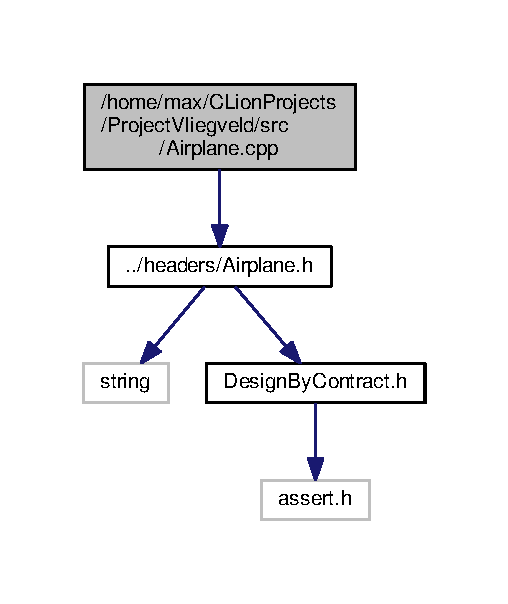
\includegraphics[width=244pt]{Airplane_8cpp__incl}
\end{center}
\end{figure}

\hypertarget{Airport_8cpp}{}\section{/home/max/\+C\+Lion\+Projects/\+Project\+Vliegveld/src/\+Airport.cpp File Reference}
\label{Airport_8cpp}\index{/home/max/\+C\+Lion\+Projects/\+Project\+Vliegveld/src/\+Airport.\+cpp@{/home/max/\+C\+Lion\+Projects/\+Project\+Vliegveld/src/\+Airport.\+cpp}}
{\ttfamily \#include \char`\"{}../headers/\+Airport.\+h\char`\"{}}\\*
Include dependency graph for Airport.\+cpp\+:
\nopagebreak
\begin{figure}[H]
\begin{center}
\leavevmode
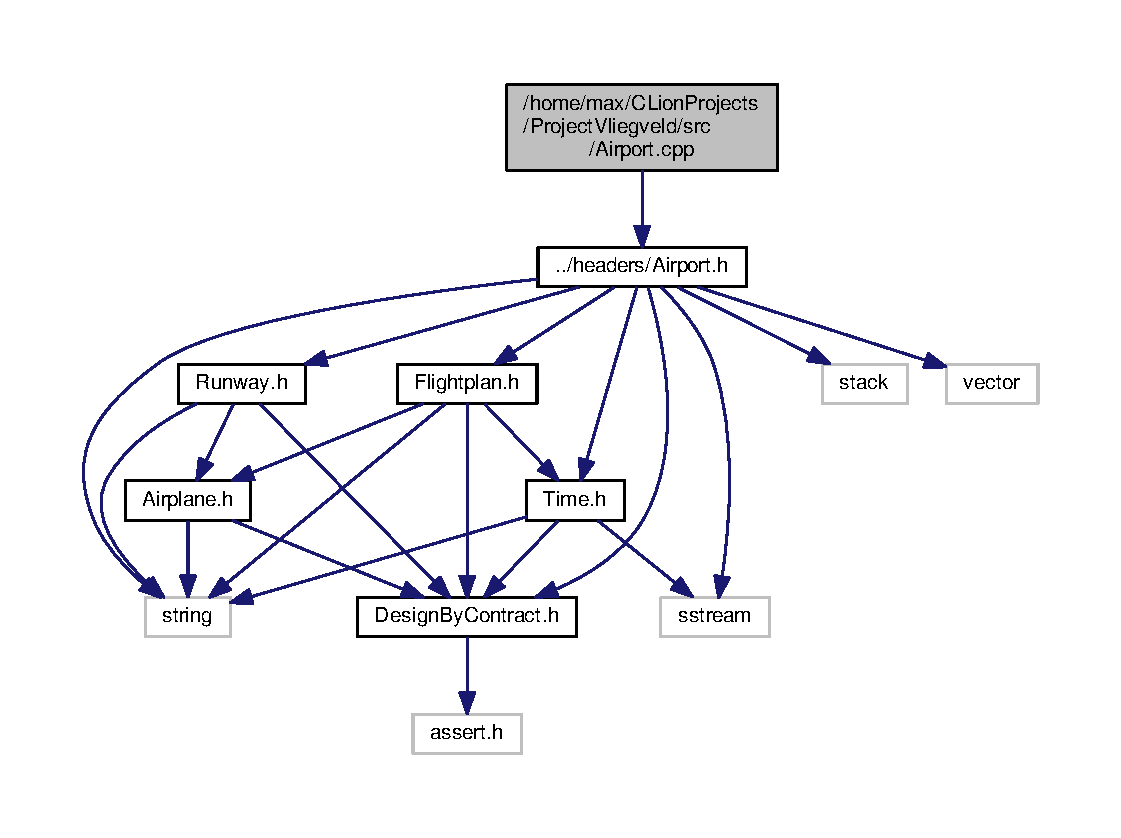
\includegraphics[width=350pt]{Airport_8cpp__incl}
\end{center}
\end{figure}

\hypertarget{ATC_8cpp}{}\section{/home/max/\+C\+Lion\+Projects/\+Project\+Vliegveld/src/\+A\+TC.cpp File Reference}
\label{ATC_8cpp}\index{/home/max/\+C\+Lion\+Projects/\+Project\+Vliegveld/src/\+A\+T\+C.\+cpp@{/home/max/\+C\+Lion\+Projects/\+Project\+Vliegveld/src/\+A\+T\+C.\+cpp}}
{\ttfamily \#include \char`\"{}../headers/\+A\+T\+C.\+h\char`\"{}}\\*
Include dependency graph for A\+T\+C.\+cpp\+:
\nopagebreak
\begin{figure}[H]
\begin{center}
\leavevmode
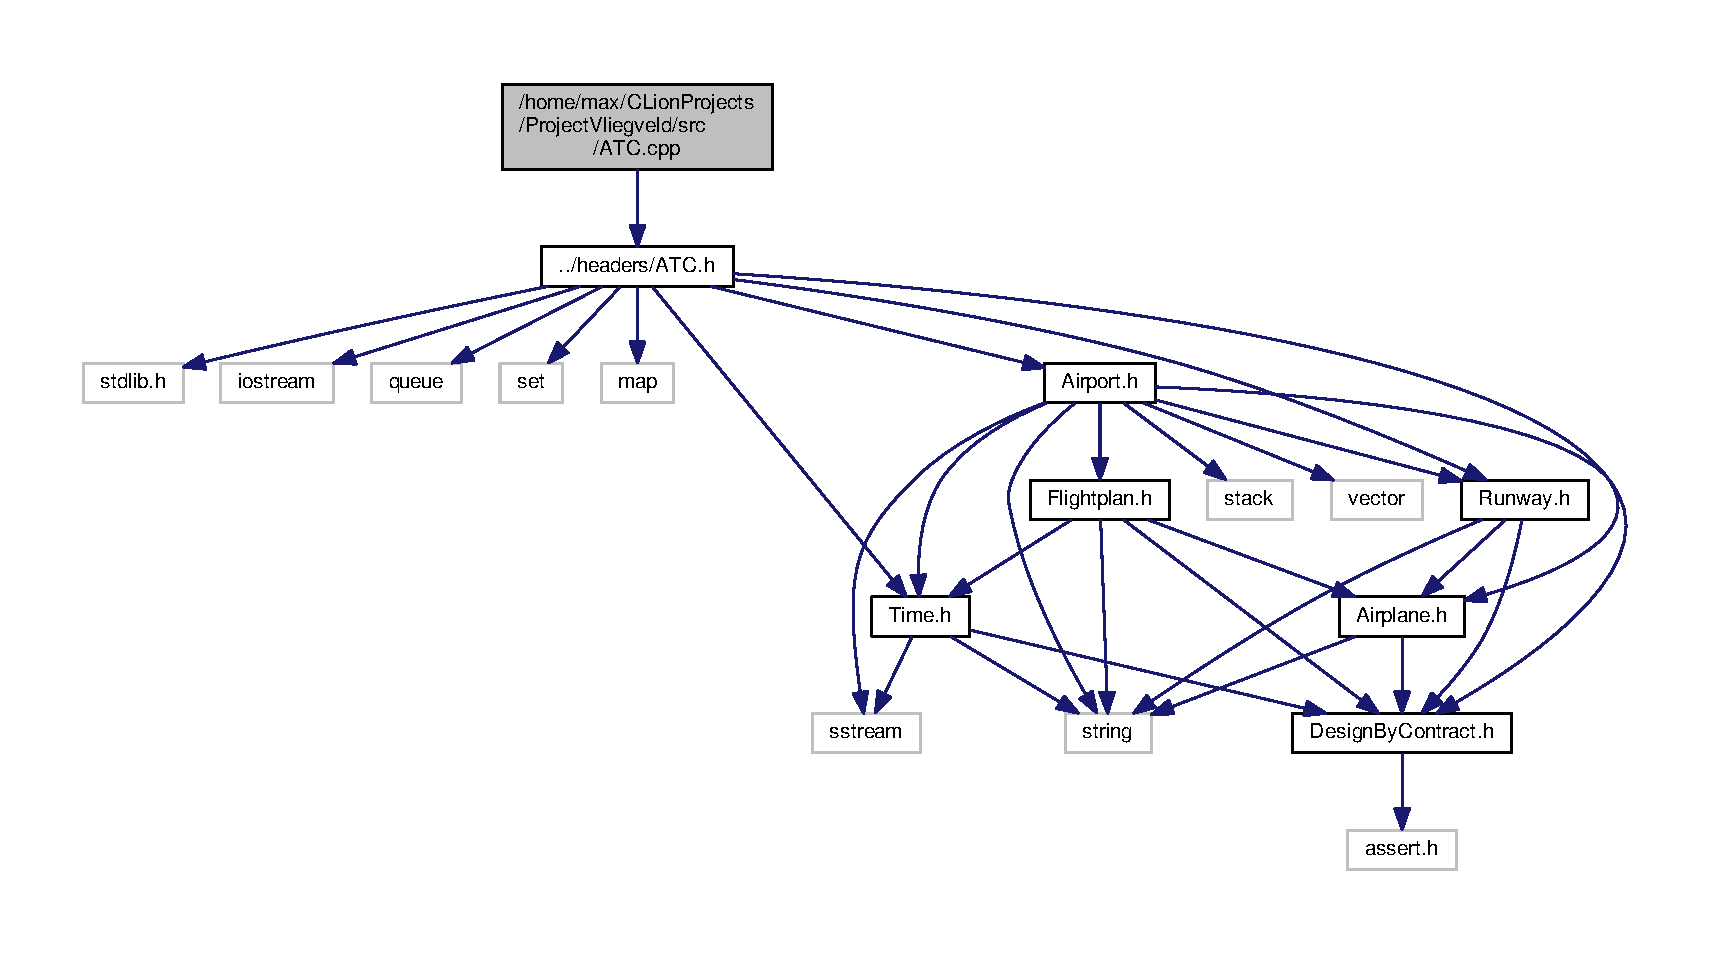
\includegraphics[width=350pt]{ATC_8cpp__incl}
\end{center}
\end{figure}

\hypertarget{Flightplan_8cpp}{}\section{/home/max/\+C\+Lion\+Projects/\+Project\+Vliegveld/src/\+Flightplan.cpp File Reference}
\label{Flightplan_8cpp}\index{/home/max/\+C\+Lion\+Projects/\+Project\+Vliegveld/src/\+Flightplan.\+cpp@{/home/max/\+C\+Lion\+Projects/\+Project\+Vliegveld/src/\+Flightplan.\+cpp}}
{\ttfamily \#include \char`\"{}../headers/\+Flightplan.\+h\char`\"{}}\\*
Include dependency graph for Flightplan.\+cpp\+:
\nopagebreak
\begin{figure}[H]
\begin{center}
\leavevmode
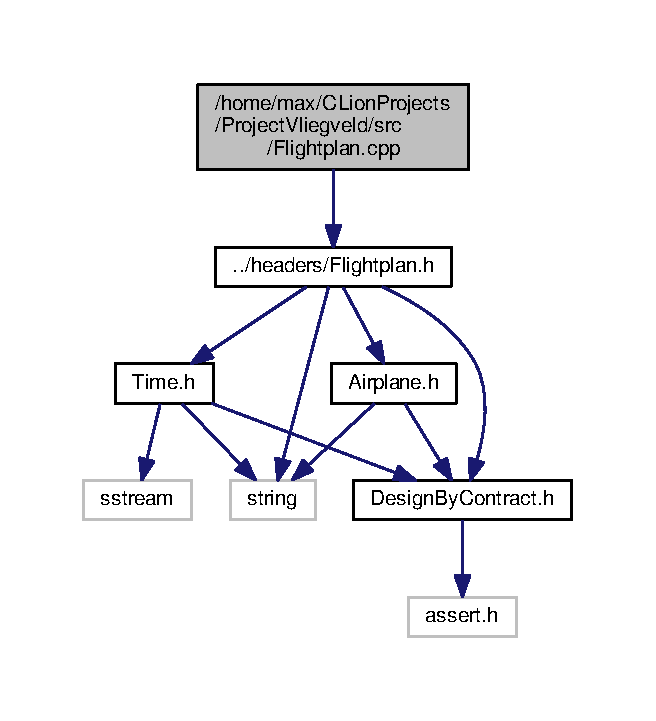
\includegraphics[width=315pt]{Flightplan_8cpp__incl}
\end{center}
\end{figure}

\hypertarget{init_8cpp}{}\section{/home/max/\+C\+Lion\+Projects/\+Project\+Vliegveld/src/init.cpp File Reference}
\label{init_8cpp}\index{/home/max/\+C\+Lion\+Projects/\+Project\+Vliegveld/src/init.\+cpp@{/home/max/\+C\+Lion\+Projects/\+Project\+Vliegveld/src/init.\+cpp}}
{\ttfamily \#include \char`\"{}../headers/\+System.\+h\char`\"{}}\\*
Include dependency graph for init.\+cpp\+:
\nopagebreak
\begin{figure}[H]
\begin{center}
\leavevmode
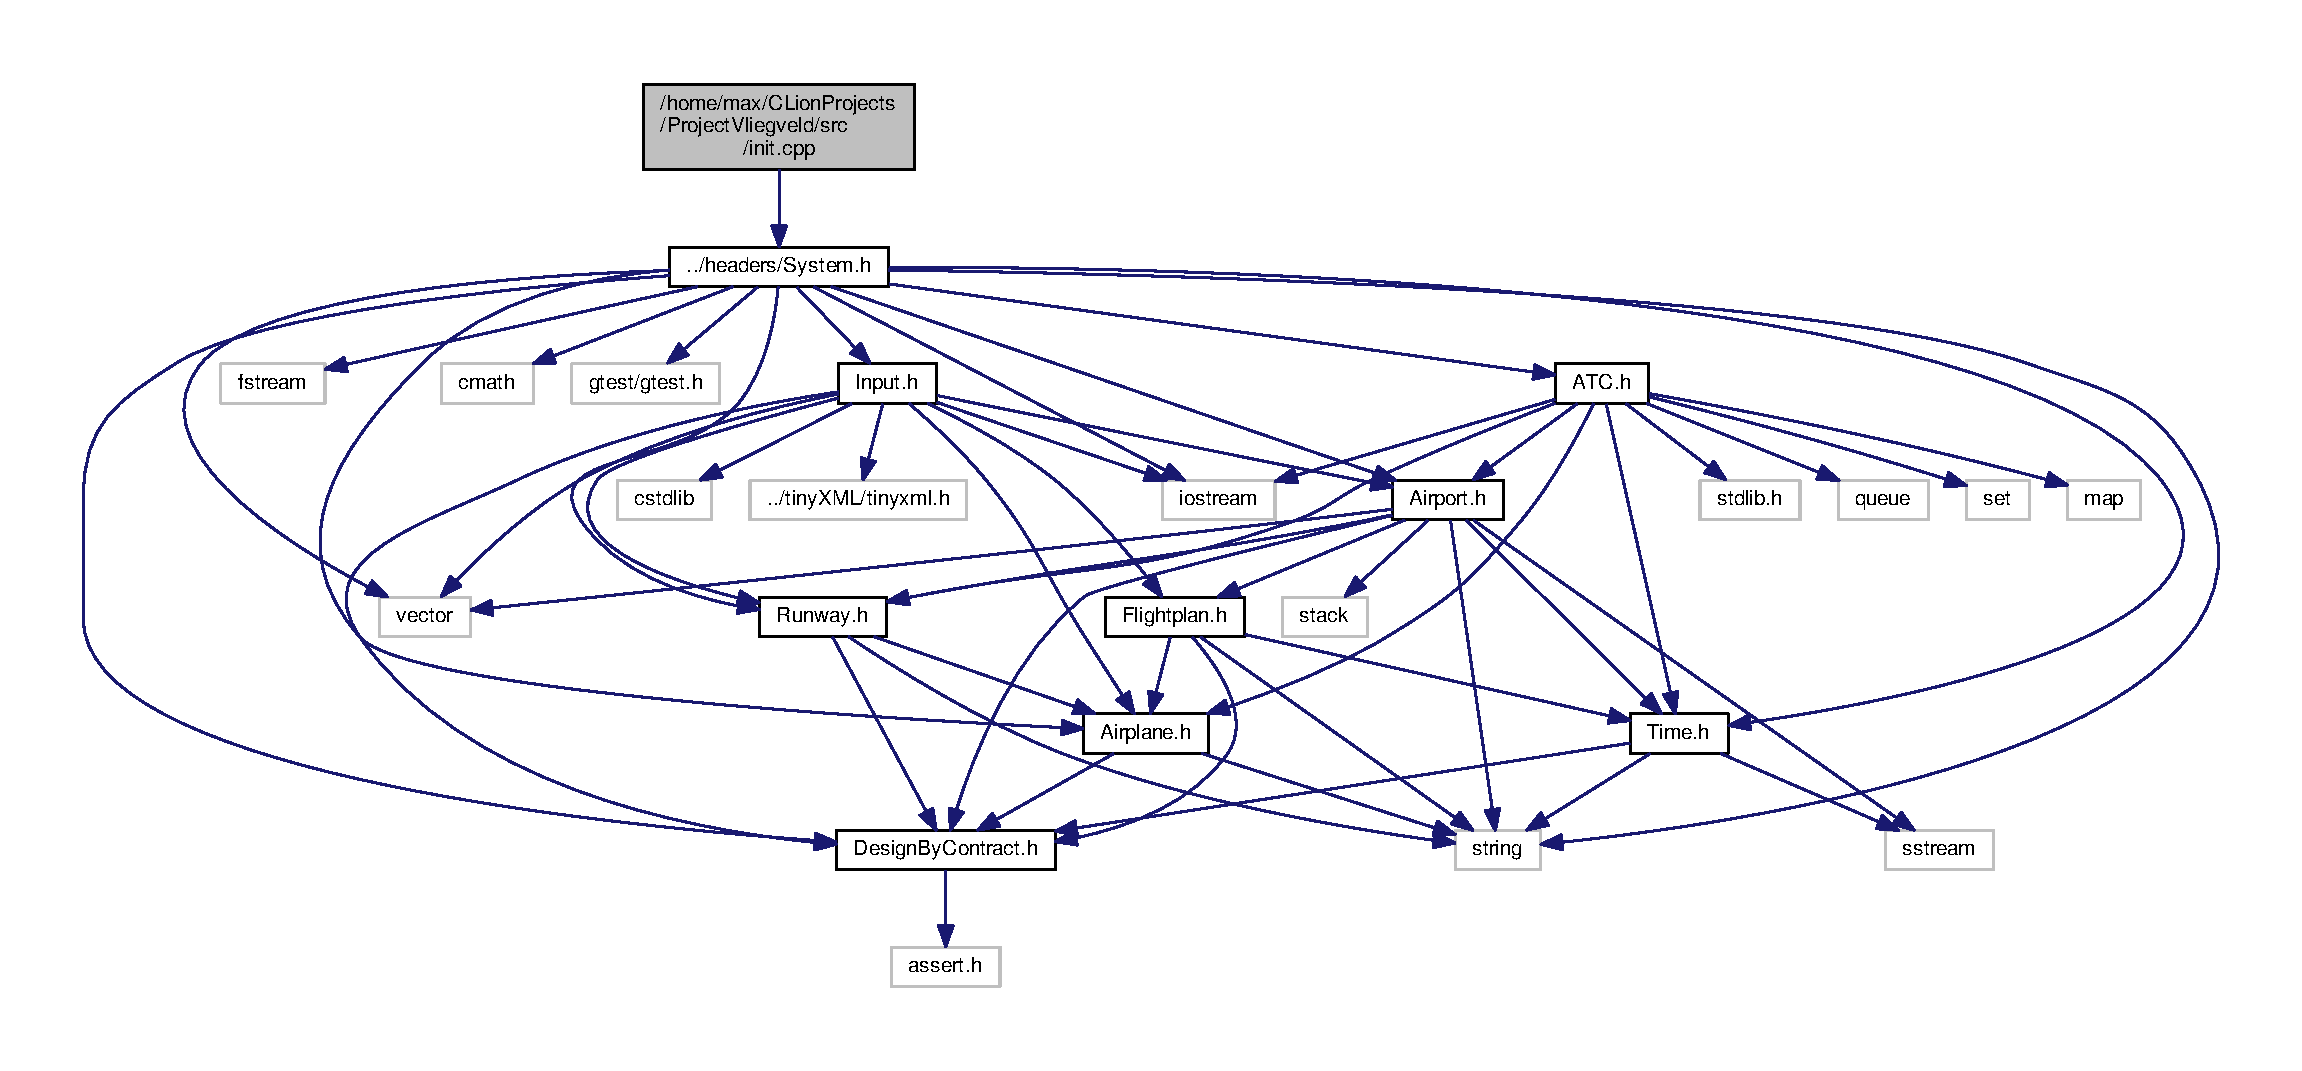
\includegraphics[width=350pt]{init_8cpp__incl}
\end{center}
\end{figure}
\subsection*{Macros}
\begin{DoxyCompactItemize}
\item 
\#define \hyperlink{init_8cpp_a738fc9b327a71ef5e0172aefbde4706b}{E\+N\+D\+T\+I\+ME}~\hyperlink{classTime}{Time}(14)
\item 
\#define \hyperlink{init_8cpp_a215304c96c4d844ee4b997da11fcb37a}{I\+N\+P\+U\+T\+F\+I\+L\+E\+N\+A\+ME}~\char`\"{}../input.\+xml\char`\"{}
\item 
\#define \hyperlink{init_8cpp_aafa797290b2e2e5761ed8ac3a365b92d}{A\+T\+C\+F\+I\+L\+E\+N\+A\+ME}~\char`\"{}../output/A\+T\+C.\+txt\char`\"{}
\item 
\#define \hyperlink{init_8cpp_abd71056a4c526e883ec6161fb5a724dc}{L\+O\+G\+F\+I\+L\+E\+N\+A\+ME}~\char`\"{}../output/log.\+txt\char`\"{}
\end{DoxyCompactItemize}
\subsection*{Functions}
\begin{DoxyCompactItemize}
\item 
\hyperlink{CMakeCache_8txt_a79a3d8790b2588b09777910863574e09}{int} \hyperlink{init_8cpp_ae66f6b31b5ad750f1fe042a706a4e3d4}{main} ()
\end{DoxyCompactItemize}


\subsection{Macro Definition Documentation}
\index{init.\+cpp@{init.\+cpp}!A\+T\+C\+F\+I\+L\+E\+N\+A\+ME@{A\+T\+C\+F\+I\+L\+E\+N\+A\+ME}}
\index{A\+T\+C\+F\+I\+L\+E\+N\+A\+ME@{A\+T\+C\+F\+I\+L\+E\+N\+A\+ME}!init.\+cpp@{init.\+cpp}}
\subsubsection[{\texorpdfstring{A\+T\+C\+F\+I\+L\+E\+N\+A\+ME}{ATCFILENAME}}]{\setlength{\rightskip}{0pt plus 5cm}\#define A\+T\+C\+F\+I\+L\+E\+N\+A\+ME~\char`\"{}../output/A\+T\+C.\+txt\char`\"{}}\hypertarget{init_8cpp_aafa797290b2e2e5761ed8ac3a365b92d}{}\label{init_8cpp_aafa797290b2e2e5761ed8ac3a365b92d}
\index{init.\+cpp@{init.\+cpp}!E\+N\+D\+T\+I\+ME@{E\+N\+D\+T\+I\+ME}}
\index{E\+N\+D\+T\+I\+ME@{E\+N\+D\+T\+I\+ME}!init.\+cpp@{init.\+cpp}}
\subsubsection[{\texorpdfstring{E\+N\+D\+T\+I\+ME}{ENDTIME}}]{\setlength{\rightskip}{0pt plus 5cm}\#define E\+N\+D\+T\+I\+ME~{\bf Time}(14)}\hypertarget{init_8cpp_a738fc9b327a71ef5e0172aefbde4706b}{}\label{init_8cpp_a738fc9b327a71ef5e0172aefbde4706b}
\index{init.\+cpp@{init.\+cpp}!I\+N\+P\+U\+T\+F\+I\+L\+E\+N\+A\+ME@{I\+N\+P\+U\+T\+F\+I\+L\+E\+N\+A\+ME}}
\index{I\+N\+P\+U\+T\+F\+I\+L\+E\+N\+A\+ME@{I\+N\+P\+U\+T\+F\+I\+L\+E\+N\+A\+ME}!init.\+cpp@{init.\+cpp}}
\subsubsection[{\texorpdfstring{I\+N\+P\+U\+T\+F\+I\+L\+E\+N\+A\+ME}{INPUTFILENAME}}]{\setlength{\rightskip}{0pt plus 5cm}\#define I\+N\+P\+U\+T\+F\+I\+L\+E\+N\+A\+ME~\char`\"{}../input.\+xml\char`\"{}}\hypertarget{init_8cpp_a215304c96c4d844ee4b997da11fcb37a}{}\label{init_8cpp_a215304c96c4d844ee4b997da11fcb37a}
\index{init.\+cpp@{init.\+cpp}!L\+O\+G\+F\+I\+L\+E\+N\+A\+ME@{L\+O\+G\+F\+I\+L\+E\+N\+A\+ME}}
\index{L\+O\+G\+F\+I\+L\+E\+N\+A\+ME@{L\+O\+G\+F\+I\+L\+E\+N\+A\+ME}!init.\+cpp@{init.\+cpp}}
\subsubsection[{\texorpdfstring{L\+O\+G\+F\+I\+L\+E\+N\+A\+ME}{LOGFILENAME}}]{\setlength{\rightskip}{0pt plus 5cm}\#define L\+O\+G\+F\+I\+L\+E\+N\+A\+ME~\char`\"{}../output/log.\+txt\char`\"{}}\hypertarget{init_8cpp_abd71056a4c526e883ec6161fb5a724dc}{}\label{init_8cpp_abd71056a4c526e883ec6161fb5a724dc}


\subsection{Function Documentation}
\index{init.\+cpp@{init.\+cpp}!main@{main}}
\index{main@{main}!init.\+cpp@{init.\+cpp}}
\subsubsection[{\texorpdfstring{main()}{main()}}]{\setlength{\rightskip}{0pt plus 5cm}{\bf int} main (
\begin{DoxyParamCaption}
{}
\end{DoxyParamCaption}
)}\hypertarget{init_8cpp_ae66f6b31b5ad750f1fe042a706a4e3d4}{}\label{init_8cpp_ae66f6b31b5ad750f1fe042a706a4e3d4}

\begin{DoxyCode}
13            \{
14 
15     \textcolor{comment}{// Read input}
16     \hyperlink{classInput}{Input} input;
17     input.\hyperlink{classInput_abb78078475f91c654db63c392aefbf51}{read}(\hyperlink{init_8cpp_a215304c96c4d844ee4b997da11fcb37a}{INPUTFILENAME});
18 
19     \textcolor{comment}{// Output file for atc}
20     ofstream atc(\hyperlink{init_8cpp_aafa797290b2e2e5761ed8ac3a365b92d}{ATCFILENAME});
21 
22     \textcolor{comment}{// Output file for logging}
23     ofstream log(\hyperlink{init_8cpp_abd71056a4c526e883ec6161fb5a724dc}{LOGFILENAME});
24 
25     \textcolor{comment}{// Initialize system}
26     \hyperlink{classSystem}{System} system(atc,  \hyperlink{init_8cpp_a738fc9b327a71ef5e0172aefbde4706b}{ENDTIME});
27 
28     \textcolor{comment}{// Import data}
29     system.import(input);
30 
31     \textcolor{comment}{// Run the simulation}
32     system.run(log);
33 
34     \textcolor{comment}{// Close files}
35     atc.close();
36     log.close();
37 
38     \textcolor{comment}{// Log information to output file}
39     system.info();
40 
41     \textcolor{keywordflow}{return} 0;
42 \}
\end{DoxyCode}

\hypertarget{Input_8cpp}{}\section{/home/max/\+C\+Lion\+Projects/\+Project\+Vliegveld/src/\+Input.cpp File Reference}
\label{Input_8cpp}\index{/home/max/\+C\+Lion\+Projects/\+Project\+Vliegveld/src/\+Input.\+cpp@{/home/max/\+C\+Lion\+Projects/\+Project\+Vliegveld/src/\+Input.\+cpp}}
{\ttfamily \#include \char`\"{}../headers/\+Input.\+h\char`\"{}}\\*
Include dependency graph for Input.\+cpp\+:
\nopagebreak
\begin{figure}[H]
\begin{center}
\leavevmode
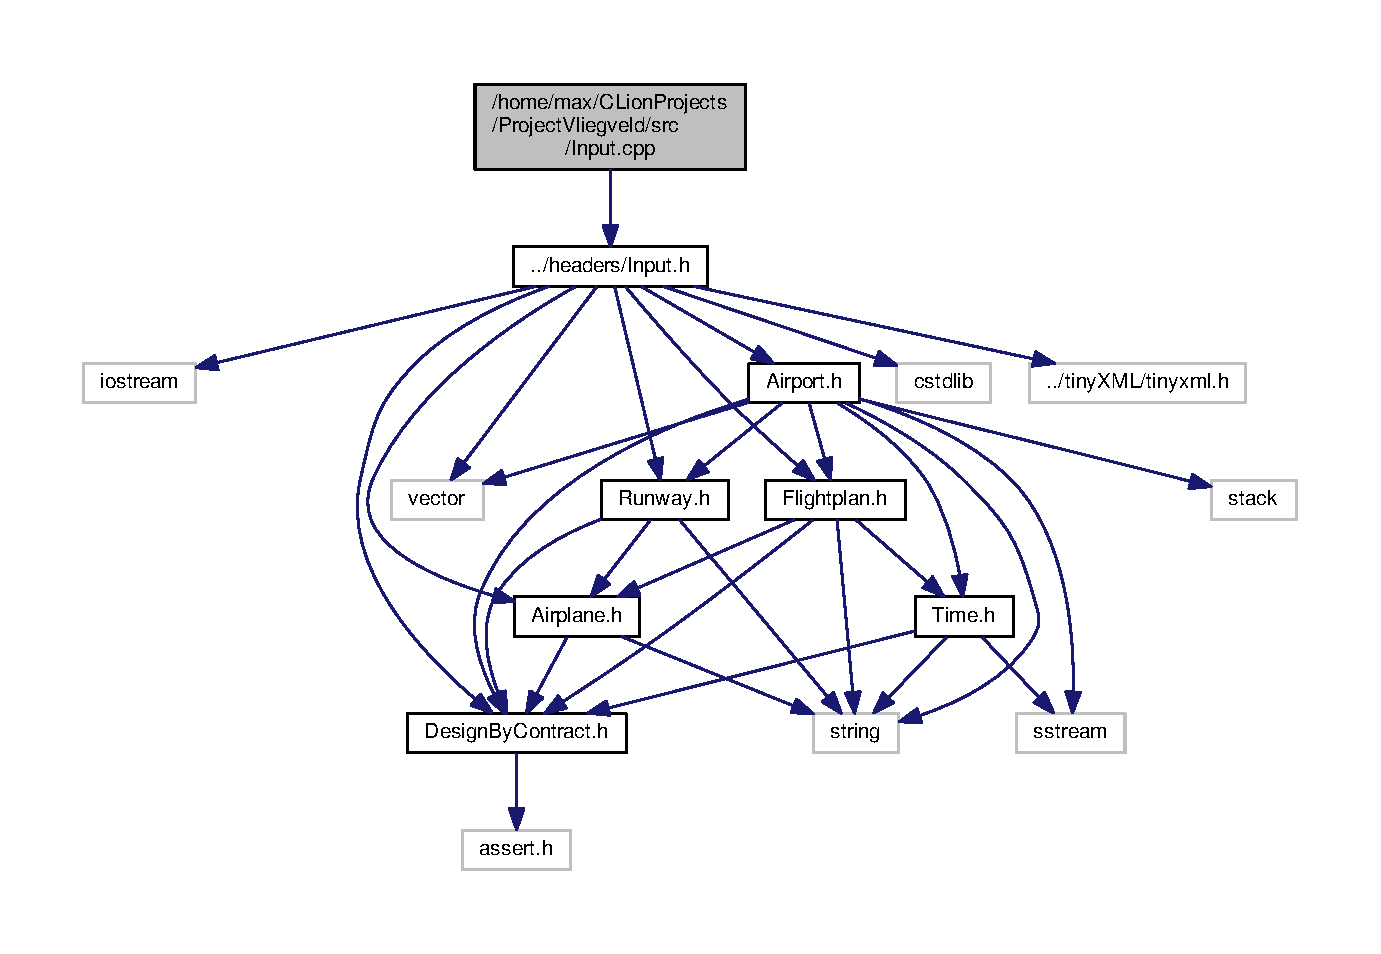
\includegraphics[width=350pt]{Input_8cpp__incl}
\end{center}
\end{figure}

\hypertarget{Runway_8cpp}{}\section{/home/max/\+C\+Lion\+Projects/\+Project\+Vliegveld/src/\+Runway.cpp File Reference}
\label{Runway_8cpp}\index{/home/max/\+C\+Lion\+Projects/\+Project\+Vliegveld/src/\+Runway.\+cpp@{/home/max/\+C\+Lion\+Projects/\+Project\+Vliegveld/src/\+Runway.\+cpp}}
{\ttfamily \#include \char`\"{}../headers/\+Runway.\+h\char`\"{}}\\*
Include dependency graph for Runway.\+cpp\+:
\nopagebreak
\begin{figure}[H]
\begin{center}
\leavevmode
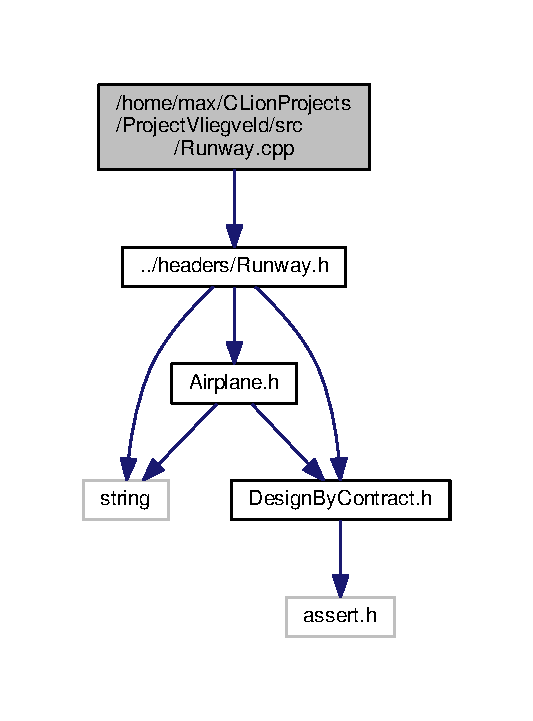
\includegraphics[width=256pt]{Runway_8cpp__incl}
\end{center}
\end{figure}

\hypertarget{System_8cpp}{}\section{/home/max/\+C\+Lion\+Projects/\+Project\+Vliegveld/src/\+System.cpp File Reference}
\label{System_8cpp}\index{/home/max/\+C\+Lion\+Projects/\+Project\+Vliegveld/src/\+System.\+cpp@{/home/max/\+C\+Lion\+Projects/\+Project\+Vliegveld/src/\+System.\+cpp}}
{\ttfamily \#include \char`\"{}../headers/\+System.\+h\char`\"{}}\\*
Include dependency graph for System.\+cpp\+:
\nopagebreak
\begin{figure}[H]
\begin{center}
\leavevmode
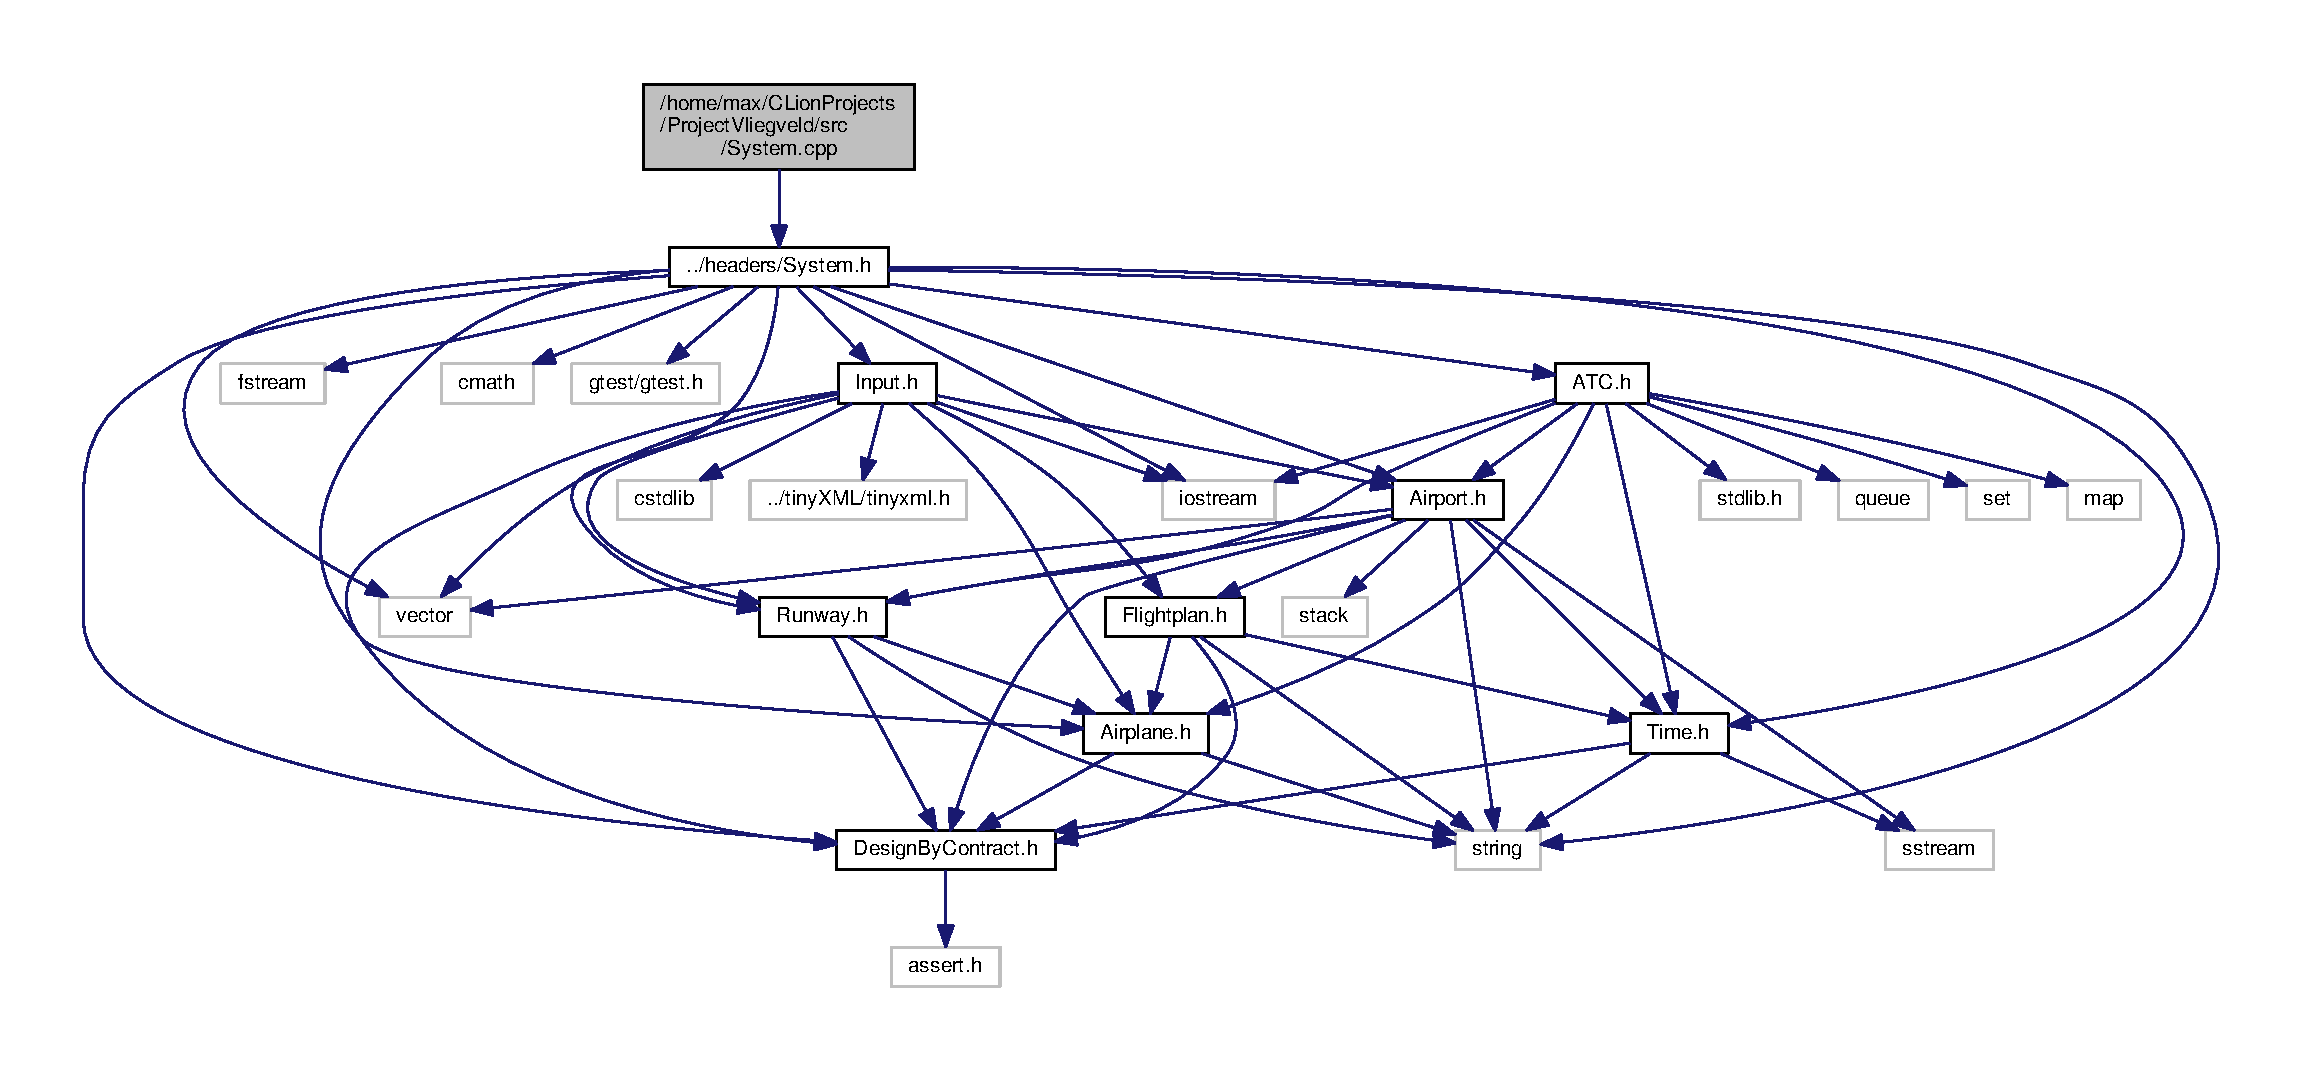
\includegraphics[width=350pt]{System_8cpp__incl}
\end{center}
\end{figure}

\hypertarget{Time_8cpp}{}\section{/home/max/\+C\+Lion\+Projects/\+Project\+Vliegveld/src/\+Time.cpp File Reference}
\label{Time_8cpp}\index{/home/max/\+C\+Lion\+Projects/\+Project\+Vliegveld/src/\+Time.\+cpp@{/home/max/\+C\+Lion\+Projects/\+Project\+Vliegveld/src/\+Time.\+cpp}}
{\ttfamily \#include \char`\"{}../headers/\+Time.\+h\char`\"{}}\\*
Include dependency graph for Time.\+cpp\+:
\nopagebreak
\begin{figure}[H]
\begin{center}
\leavevmode
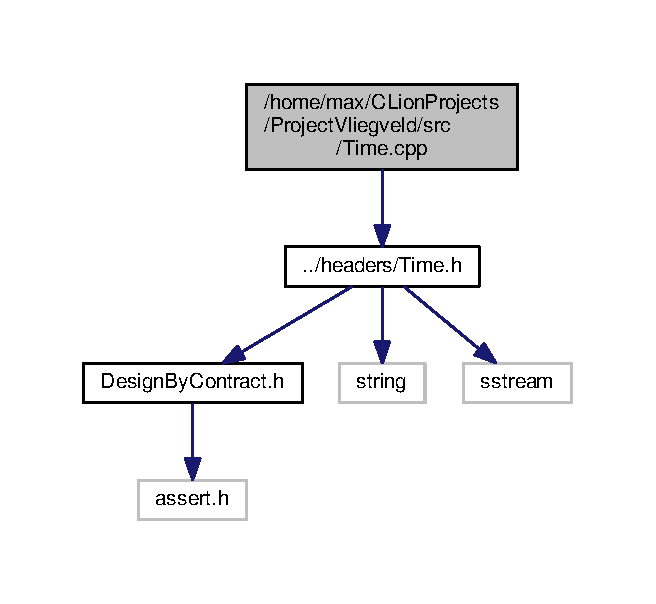
\includegraphics[width=315pt]{Time_8cpp__incl}
\end{center}
\end{figure}

\hypertarget{domainTestsAirplane_8cpp}{}\section{/home/max/\+C\+Lion\+Projects/\+Project\+Vliegveld/test/domain\+Tests\+Airplane.cpp File Reference}
\label{domainTestsAirplane_8cpp}\index{/home/max/\+C\+Lion\+Projects/\+Project\+Vliegveld/test/domain\+Tests\+Airplane.\+cpp@{/home/max/\+C\+Lion\+Projects/\+Project\+Vliegveld/test/domain\+Tests\+Airplane.\+cpp}}
{\ttfamily \#include $<$gtest/gtest.\+h$>$}\\*
{\ttfamily \#include \char`\"{}../headers/\+System.\+h\char`\"{}}\\*
Include dependency graph for domain\+Tests\+Airplane.\+cpp\+:
\nopagebreak
\begin{figure}[H]
\begin{center}
\leavevmode
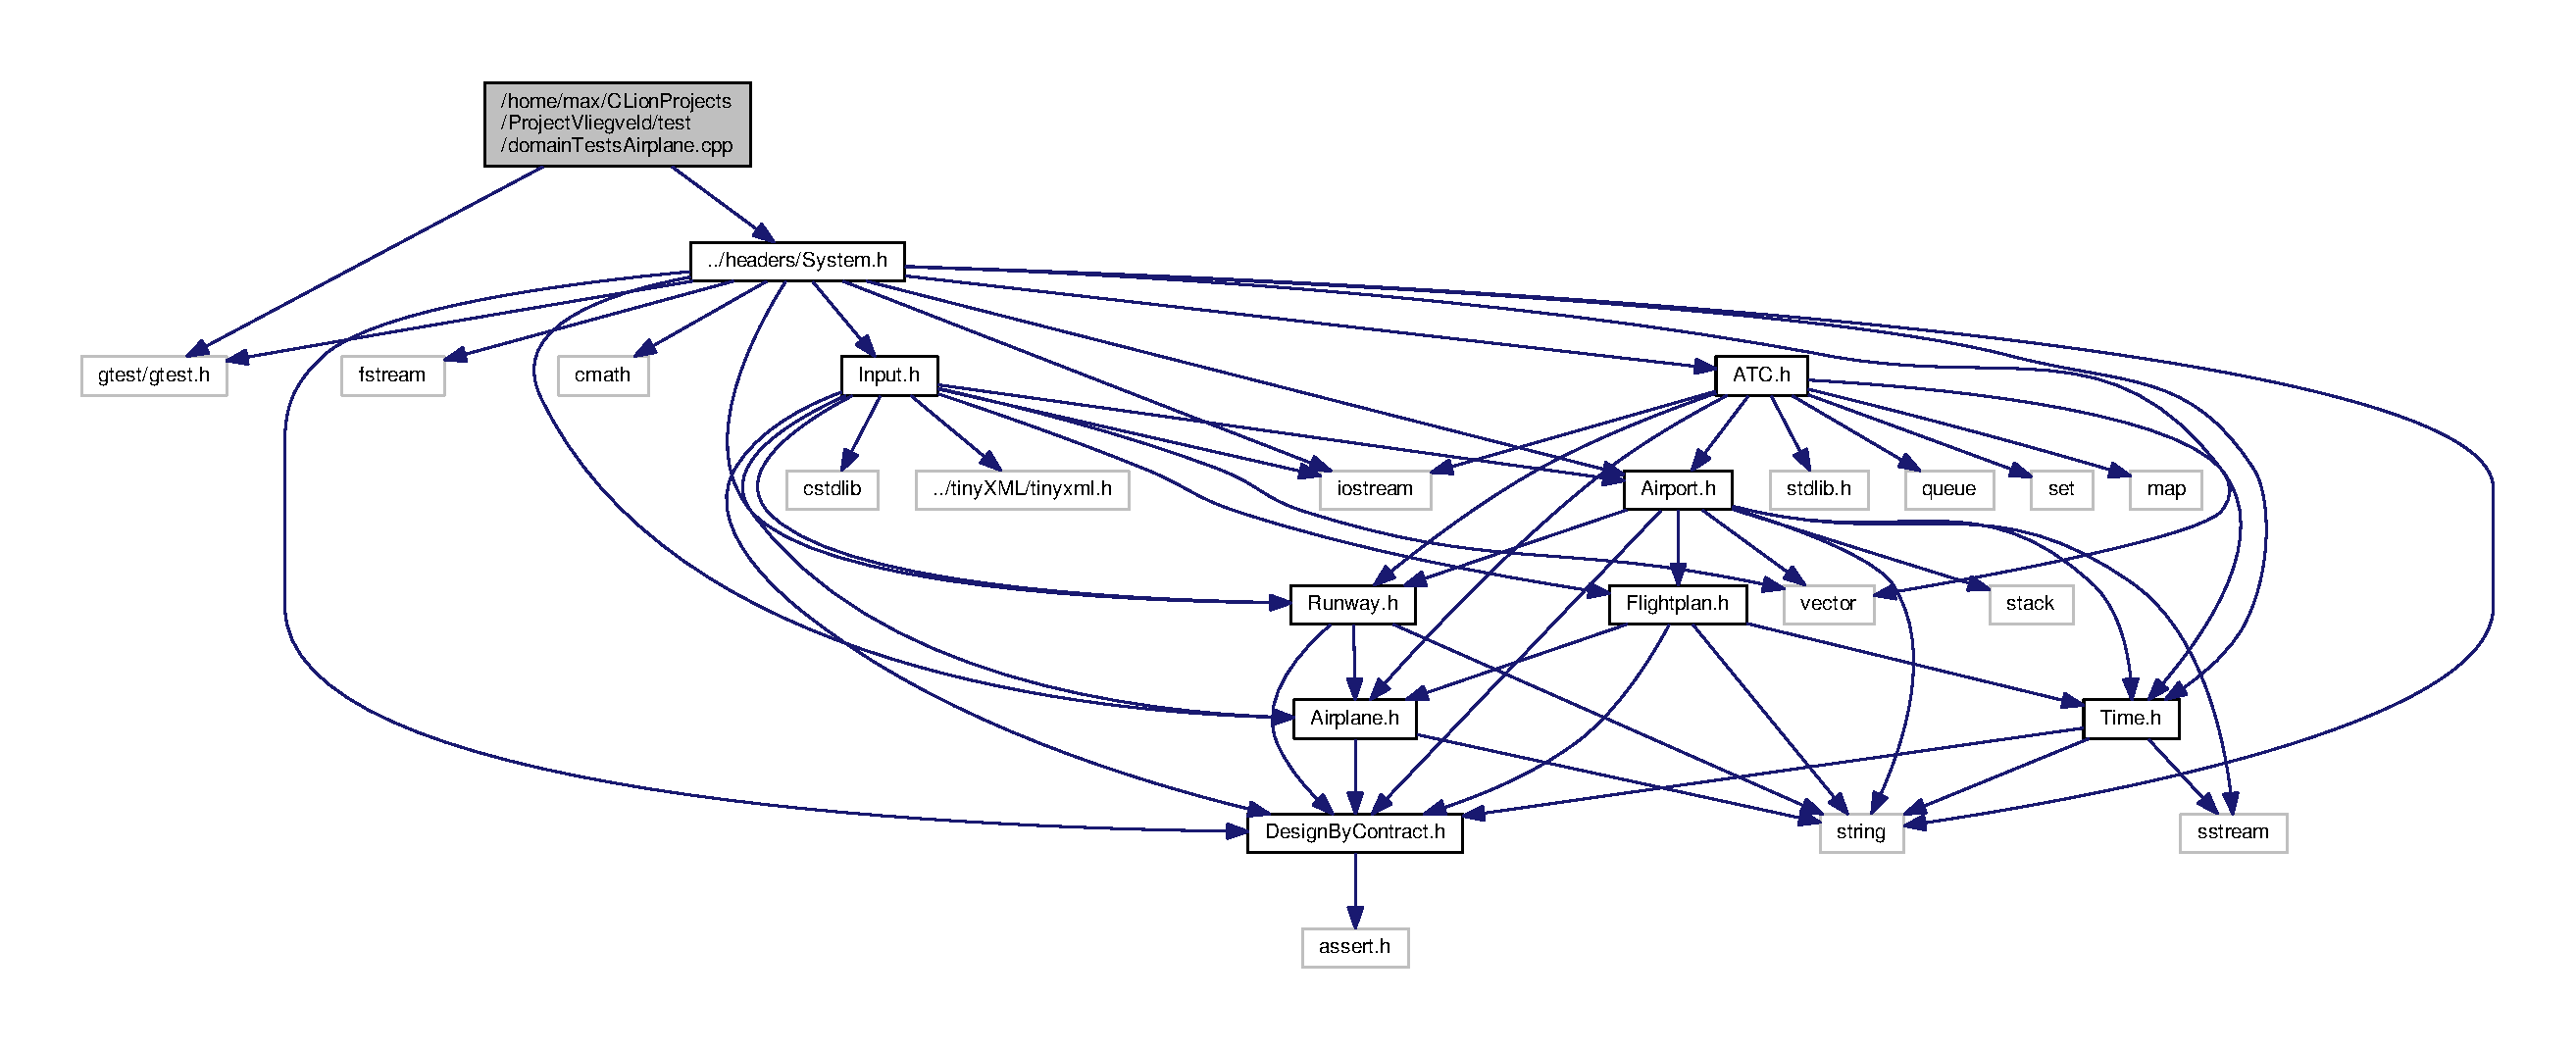
\includegraphics[width=350pt]{domainTestsAirplane_8cpp__incl}
\end{center}
\end{figure}
\subsection*{Classes}
\begin{DoxyCompactItemize}
\item 
class \hyperlink{classdomainTestAirplane}{domain\+Test\+Airplane}
\end{DoxyCompactItemize}
\subsection*{Functions}
\begin{DoxyCompactItemize}
\item 
\hyperlink{domainTestsAirplane_8cpp_aa93140b2c83e0e4d3a18ae62ff57aaef}{T\+E\+S\+T\+\_\+F} (\hyperlink{classdomainTestAirplane}{domain\+Test\+Airplane}, Default\+Constructor)
\item 
\hyperlink{domainTestsAirplane_8cpp_a3dfdc7b8d679f7c2bcc73a91c552fd02}{T\+E\+S\+T\+\_\+F} (\hyperlink{classdomainTestAirplane}{domain\+Test\+Airplane}, happy\+Day)
\item 
\hyperlink{domainTestsAirplane_8cpp_aef4e0168d0dc2a0b82682644c9a69b1f}{T\+E\+S\+T\+\_\+F} (\hyperlink{classdomainTestAirplane}{domain\+Test\+Airplane}, complete)
\item 
\hyperlink{domainTestsAirplane_8cpp_a9f94fe2152afdb1a2d97662ce0d07841}{T\+E\+S\+T\+\_\+F} (\hyperlink{classdomainTestAirplane}{domain\+Test\+Airplane}, field\+Manipulation)
\item 
\hyperlink{domainTestsAirplane_8cpp_af659e5c5dd5dbae55663829b11f2b166}{T\+E\+S\+T\+\_\+F} (\hyperlink{classdomainTestAirplane}{domain\+Test\+Airplane}, Contract\+Violations)
\end{DoxyCompactItemize}


\subsection{Function Documentation}
\index{domain\+Tests\+Airplane.\+cpp@{domain\+Tests\+Airplane.\+cpp}!T\+E\+S\+T\+\_\+F@{T\+E\+S\+T\+\_\+F}}
\index{T\+E\+S\+T\+\_\+F@{T\+E\+S\+T\+\_\+F}!domain\+Tests\+Airplane.\+cpp@{domain\+Tests\+Airplane.\+cpp}}
\subsubsection[{\texorpdfstring{T\+E\+S\+T\+\_\+\+F(domain\+Test\+Airplane, Default\+Constructor)}{TEST_F(domainTestAirplane, DefaultConstructor)}}]{\setlength{\rightskip}{0pt plus 5cm}T\+E\+S\+T\+\_\+F (
\begin{DoxyParamCaption}
\item[{{\bf domain\+Test\+Airplane}}]{, }
\item[{Default\+Constructor}]{}
\end{DoxyParamCaption}
)}\hypertarget{domainTestsAirplane_8cpp_aa93140b2c83e0e4d3a18ae62ff57aaef}{}\label{domainTestsAirplane_8cpp_aa93140b2c83e0e4d3a18ae62ff57aaef}

\begin{DoxyCode}
19                                                \{
20     EXPECT\_TRUE(airplane.properlyInitialized());
21     EXPECT\_EQ(airplane.getPassengers(), -1);
22     EXPECT\_EQ(airplane.getFuel(), -1);
23     EXPECT\_EQ(airplane.getAltitude(), 0);
24     EXPECT\_EQ(airplane.getTimeRemaining(), 0);
25     EXPECT\_TRUE(airplane.getRunway() == NULL);
26     EXPECT\_EQ(airplane.getRequest(), \hyperlink{Airplane_8h_a4a8a3f45932bdf601f093bea061bad9ba19d8199da79ca4c28eb644052b08f632}{kIdle});
27     EXPECT\_EQ(airplane.getGateID(), -1);
28     EXPECT\_EQ(airplane.getStatus(), \hyperlink{Airplane_8h_a0e5bbf7c6c727baaba49062300fae19fae2f5a04c74b7994ccc574acf7d014a34}{kAway});
29     EXPECT\_EQ(airplane.getEngine(), \hyperlink{Airplane_8h_a3d2a8adb53da58e78cb0018d784e791dabffa4f472eaab68b56c1f1e7c56d221e}{kDefaultEngine});
30     EXPECT\_EQ(airplane.getType(), \hyperlink{Airplane_8h_a537b68b9ecaac78d371a35d8cf7604e9acd07e6d14d5fa33ad175535684278e00}{kDefaultType});
31     EXPECT\_EQ(airplane.getSize(), \hyperlink{Airplane_8h_a0526623f951311ba6780209b9e278dbfaf7c1619fb726ec0ab9a3b7cfbf797b4a}{kDefaultSize});
32 \}
\end{DoxyCode}
\index{domain\+Tests\+Airplane.\+cpp@{domain\+Tests\+Airplane.\+cpp}!T\+E\+S\+T\+\_\+F@{T\+E\+S\+T\+\_\+F}}
\index{T\+E\+S\+T\+\_\+F@{T\+E\+S\+T\+\_\+F}!domain\+Tests\+Airplane.\+cpp@{domain\+Tests\+Airplane.\+cpp}}
\subsubsection[{\texorpdfstring{T\+E\+S\+T\+\_\+\+F(domain\+Test\+Airplane, happy\+Day)}{TEST_F(domainTestAirplane, happyDay)}}]{\setlength{\rightskip}{0pt plus 5cm}T\+E\+S\+T\+\_\+F (
\begin{DoxyParamCaption}
\item[{{\bf domain\+Test\+Airplane}}]{, }
\item[{happy\+Day}]{}
\end{DoxyParamCaption}
)}\hypertarget{domainTestsAirplane_8cpp_a3dfdc7b8d679f7c2bcc73a91c552fd02}{}\label{domainTestsAirplane_8cpp_a3dfdc7b8d679f7c2bcc73a91c552fd02}

\begin{DoxyCode}
34                                      \{
35     airplane.increaseAltitude(3);
36     EXPECT\_EQ(airplane.getAltitude(), 3);
37     airplane.increaseAltitude(2);
38     EXPECT\_EQ(airplane.getAltitude(), 5);
39     airplane.decreaseAltitude(5);
40     EXPECT\_EQ(airplane.getAltitude(), 0);
41 
42     airplane.decreaseTimeRemaining();
43     EXPECT\_EQ(airplane.getTimeRemaining(), 0);
44 
45     airplane.setTimeRemaining(1);
46     airplane.decreaseTimeRemaining();
47     EXPECT\_EQ(airplane.getTimeRemaining(), 0);
48     airplane.decreaseTimeRemaining();
49     EXPECT\_EQ(airplane.getTimeRemaining(), 0);
50 \}
\end{DoxyCode}
\index{domain\+Tests\+Airplane.\+cpp@{domain\+Tests\+Airplane.\+cpp}!T\+E\+S\+T\+\_\+F@{T\+E\+S\+T\+\_\+F}}
\index{T\+E\+S\+T\+\_\+F@{T\+E\+S\+T\+\_\+F}!domain\+Tests\+Airplane.\+cpp@{domain\+Tests\+Airplane.\+cpp}}
\subsubsection[{\texorpdfstring{T\+E\+S\+T\+\_\+\+F(domain\+Test\+Airplane, complete)}{TEST_F(domainTestAirplane, complete)}}]{\setlength{\rightskip}{0pt plus 5cm}T\+E\+S\+T\+\_\+F (
\begin{DoxyParamCaption}
\item[{{\bf domain\+Test\+Airplane}}]{, }
\item[{complete}]{}
\end{DoxyParamCaption}
)}\hypertarget{domainTestsAirplane_8cpp_aef4e0168d0dc2a0b82682644c9a69b1f}{}\label{domainTestsAirplane_8cpp_aef4e0168d0dc2a0b82682644c9a69b1f}

\begin{DoxyCode}
52                                      \{
53     EXPECT\_FALSE(airplane.complete());
54     airplane.setEngine(\hyperlink{Airplane_8h_a3d2a8adb53da58e78cb0018d784e791da6262caeb7b5646a03a202006f584364c}{kJet});
55     EXPECT\_FALSE(airplane.complete());
56     airplane.setType(\hyperlink{Airplane_8h_a537b68b9ecaac78d371a35d8cf7604e9aa60181ba834d25b46f4c717f3403c313}{kAirline});
57     EXPECT\_FALSE(airplane.complete());
58     airplane.setFuel(1);
59     EXPECT\_FALSE(airplane.complete());
60     airplane.setSize(\hyperlink{Airplane_8h_a0526623f951311ba6780209b9e278dbfaf99aeb93b2774bc0c7856d1510d17a54}{kSmall});
61     EXPECT\_FALSE(airplane.complete());
62     airplane.setPassengers(1);
63     EXPECT\_FALSE(airplane.complete());
64     airplane.setModel(\textcolor{stringliteral}{"test"});
65     EXPECT\_FALSE(airplane.complete());
66     airplane.setCallsign(\textcolor{stringliteral}{"test"});
67     EXPECT\_FALSE(airplane.complete());
68     airplane.setNumber(\textcolor{stringliteral}{"test"});
69 
70     EXPECT\_TRUE(airplane.complete());
71 \}
\end{DoxyCode}
\index{domain\+Tests\+Airplane.\+cpp@{domain\+Tests\+Airplane.\+cpp}!T\+E\+S\+T\+\_\+F@{T\+E\+S\+T\+\_\+F}}
\index{T\+E\+S\+T\+\_\+F@{T\+E\+S\+T\+\_\+F}!domain\+Tests\+Airplane.\+cpp@{domain\+Tests\+Airplane.\+cpp}}
\subsubsection[{\texorpdfstring{T\+E\+S\+T\+\_\+\+F(domain\+Test\+Airplane, field\+Manipulation)}{TEST_F(domainTestAirplane, fieldManipulation)}}]{\setlength{\rightskip}{0pt plus 5cm}T\+E\+S\+T\+\_\+F (
\begin{DoxyParamCaption}
\item[{{\bf domain\+Test\+Airplane}}]{, }
\item[{field\+Manipulation}]{}
\end{DoxyParamCaption}
)}\hypertarget{domainTestsAirplane_8cpp_a9f94fe2152afdb1a2d97662ce0d07841}{}\label{domainTestsAirplane_8cpp_a9f94fe2152afdb1a2d97662ce0d07841}

\begin{DoxyCode}
73                                               \{
74     airplane.setPosition(\textcolor{stringliteral}{"Alpha"});
75     EXPECT\_EQ(airplane.getPosition(), \textcolor{stringliteral}{"Alpha"});
76 
77     airplane.setType(\hyperlink{Airplane_8h_a537b68b9ecaac78d371a35d8cf7604e9a1dbdb6d83cd39b00ba5515617716d186}{kMilitary});
78     EXPECT\_EQ(airplane.getType(), \hyperlink{Airplane_8h_a537b68b9ecaac78d371a35d8cf7604e9a1dbdb6d83cd39b00ba5515617716d186}{kMilitary});
79 
80     airplane.setSquawk(12345);
81     EXPECT\_EQ(airplane.getSquawk(), 12345);
82 
83     airplane.setRequest(\hyperlink{Airplane_8h_a4a8a3f45932bdf601f093bea061bad9ba77f4edb231ad722f9deeb2f574557c17}{kAcceptedImmediate});
84     EXPECT\_EQ(airplane.getRequest(), \hyperlink{Airplane_8h_a4a8a3f45932bdf601f093bea061bad9ba77f4edb231ad722f9deeb2f574557c17}{kAcceptedImmediate});
85 
86     airplane.setSize(\hyperlink{Airplane_8h_a0526623f951311ba6780209b9e278dbfaf99aeb93b2774bc0c7856d1510d17a54}{kSmall});
87     EXPECT\_EQ(airplane.getSize(), \hyperlink{Airplane_8h_a0526623f951311ba6780209b9e278dbfaf99aeb93b2774bc0c7856d1510d17a54}{kSmall});
88 
89     airplane.setEngine(\hyperlink{Airplane_8h_a3d2a8adb53da58e78cb0018d784e791daef171fc98c472a2acd2338353679dcc3}{kPropeller});
90     EXPECT\_EQ(airplane.getEngine(), \hyperlink{Airplane_8h_a3d2a8adb53da58e78cb0018d784e791daef171fc98c472a2acd2338353679dcc3}{kPropeller});
91 
92     airplane.setStatus(\hyperlink{Airplane_8h_a0e5bbf7c6c727baaba49062300fae19fae2f5a04c74b7994ccc574acf7d014a34}{kAway});
93     EXPECT\_EQ(airplane.getStatus(), \hyperlink{Airplane_8h_a0e5bbf7c6c727baaba49062300fae19fae2f5a04c74b7994ccc574acf7d014a34}{kAway});
94 
95     airplane.setCallsign(\textcolor{stringliteral}{"PlaneCS"});
96     EXPECT\_EQ(airplane.getCallsign(), \textcolor{stringliteral}{"PlaneCS"});
97 
98     airplane.setTimeRemaining(50);
99     EXPECT\_EQ(airplane.getTimeRemaining(), 50);
100 
101     airplane.setAltitude(100);
102     EXPECT\_EQ(airplane.getAltitude(), 100);
103 
104     airplane.setFuel(50000);
105     EXPECT\_EQ(airplane.getFuel(), 50000);
106 
107     airplane.setGateID(5);
108     EXPECT\_EQ(airplane.getGateID(), 5);
109 
110     airplane.setModel(\textcolor{stringliteral}{"F16"});
111     EXPECT\_EQ(airplane.getModel(), \textcolor{stringliteral}{"F16"});
112 
113     airplane.setNumber(\textcolor{stringliteral}{"16"});
114     EXPECT\_EQ(airplane.getNumber(), \textcolor{stringliteral}{"16"});
115 
116     airplane.setPassengers(2);
117     EXPECT\_EQ(airplane.getPassengers(), 2);
118 
119     \hyperlink{classRunway}{Runway} *rw = \textcolor{keyword}{new} \hyperlink{classRunway}{Runway}();
120     airplane.setRunway(rw);
121     EXPECT\_TRUE(airplane.getRunway() == rw);
122     \textcolor{keyword}{delete} rw;
123 \}
\end{DoxyCode}
\index{domain\+Tests\+Airplane.\+cpp@{domain\+Tests\+Airplane.\+cpp}!T\+E\+S\+T\+\_\+F@{T\+E\+S\+T\+\_\+F}}
\index{T\+E\+S\+T\+\_\+F@{T\+E\+S\+T\+\_\+F}!domain\+Tests\+Airplane.\+cpp@{domain\+Tests\+Airplane.\+cpp}}
\subsubsection[{\texorpdfstring{T\+E\+S\+T\+\_\+\+F(domain\+Test\+Airplane, Contract\+Violations)}{TEST_F(domainTestAirplane, ContractViolations)}}]{\setlength{\rightskip}{0pt plus 5cm}T\+E\+S\+T\+\_\+F (
\begin{DoxyParamCaption}
\item[{{\bf domain\+Test\+Airplane}}]{, }
\item[{Contract\+Violations}]{}
\end{DoxyParamCaption}
)}\hypertarget{domainTestsAirplane_8cpp_af659e5c5dd5dbae55663829b11f2b166}{}\label{domainTestsAirplane_8cpp_af659e5c5dd5dbae55663829b11f2b166}

\begin{DoxyCode}
125                                                \{
126     EXPECT\_DEATH(airplane.decreaseAltitude(-3), \textcolor{stringliteral}{"Difference can't be negative"});
127     EXPECT\_DEATH(airplane.increaseAltitude(-2), \textcolor{stringliteral}{"Difference can't be negative"});
128 
129     \textcolor{comment}{// Set altitude to 1 and try to decrease by 2}
130     airplane.setAltitude(1);
131     EXPECT\_DEATH(airplane.decreaseAltitude(2), \textcolor{stringliteral}{"New altitude can't be less than 0!"});
132 
133     EXPECT\_DEATH(airplane.setAltitude(-3), \textcolor{stringliteral}{"Altitude can't be negative"});
134     EXPECT\_DEATH(airplane.setTimeRemaining(-5), \textcolor{stringliteral}{"Time remaining can't be negative"});
135     EXPECT\_DEATH(airplane.setPassengers(-4), \textcolor{stringliteral}{"Passenger amount can't be negative"});
136     EXPECT\_DEATH(airplane.setGateID(-3), \textcolor{stringliteral}{"Gate id can't be less than -1"});
137     EXPECT\_DEATH(airplane.setFuel(0), \textcolor{stringliteral}{"Fuel can't be less than 1"});
138     EXPECT\_DEATH(airplane.setFuel(-3), \textcolor{stringliteral}{"Fuel can't be less than 1"});
139     EXPECT\_DEATH(airplane.setSquawk(-4), \textcolor{stringliteral}{"Squawk code can't be negative"});
140 \}\end{DoxyCode}

\hypertarget{domainTestsAirport_8cpp}{}\section{/home/max/\+C\+Lion\+Projects/\+Project\+Vliegveld/test/domain\+Tests\+Airport.cpp File Reference}
\label{domainTestsAirport_8cpp}\index{/home/max/\+C\+Lion\+Projects/\+Project\+Vliegveld/test/domain\+Tests\+Airport.\+cpp@{/home/max/\+C\+Lion\+Projects/\+Project\+Vliegveld/test/domain\+Tests\+Airport.\+cpp}}
{\ttfamily \#include $<$gtest/gtest.\+h$>$}\\*
{\ttfamily \#include \char`\"{}../headers/\+System.\+h\char`\"{}}\\*
Include dependency graph for domain\+Tests\+Airport.\+cpp\+:
\nopagebreak
\begin{figure}[H]
\begin{center}
\leavevmode
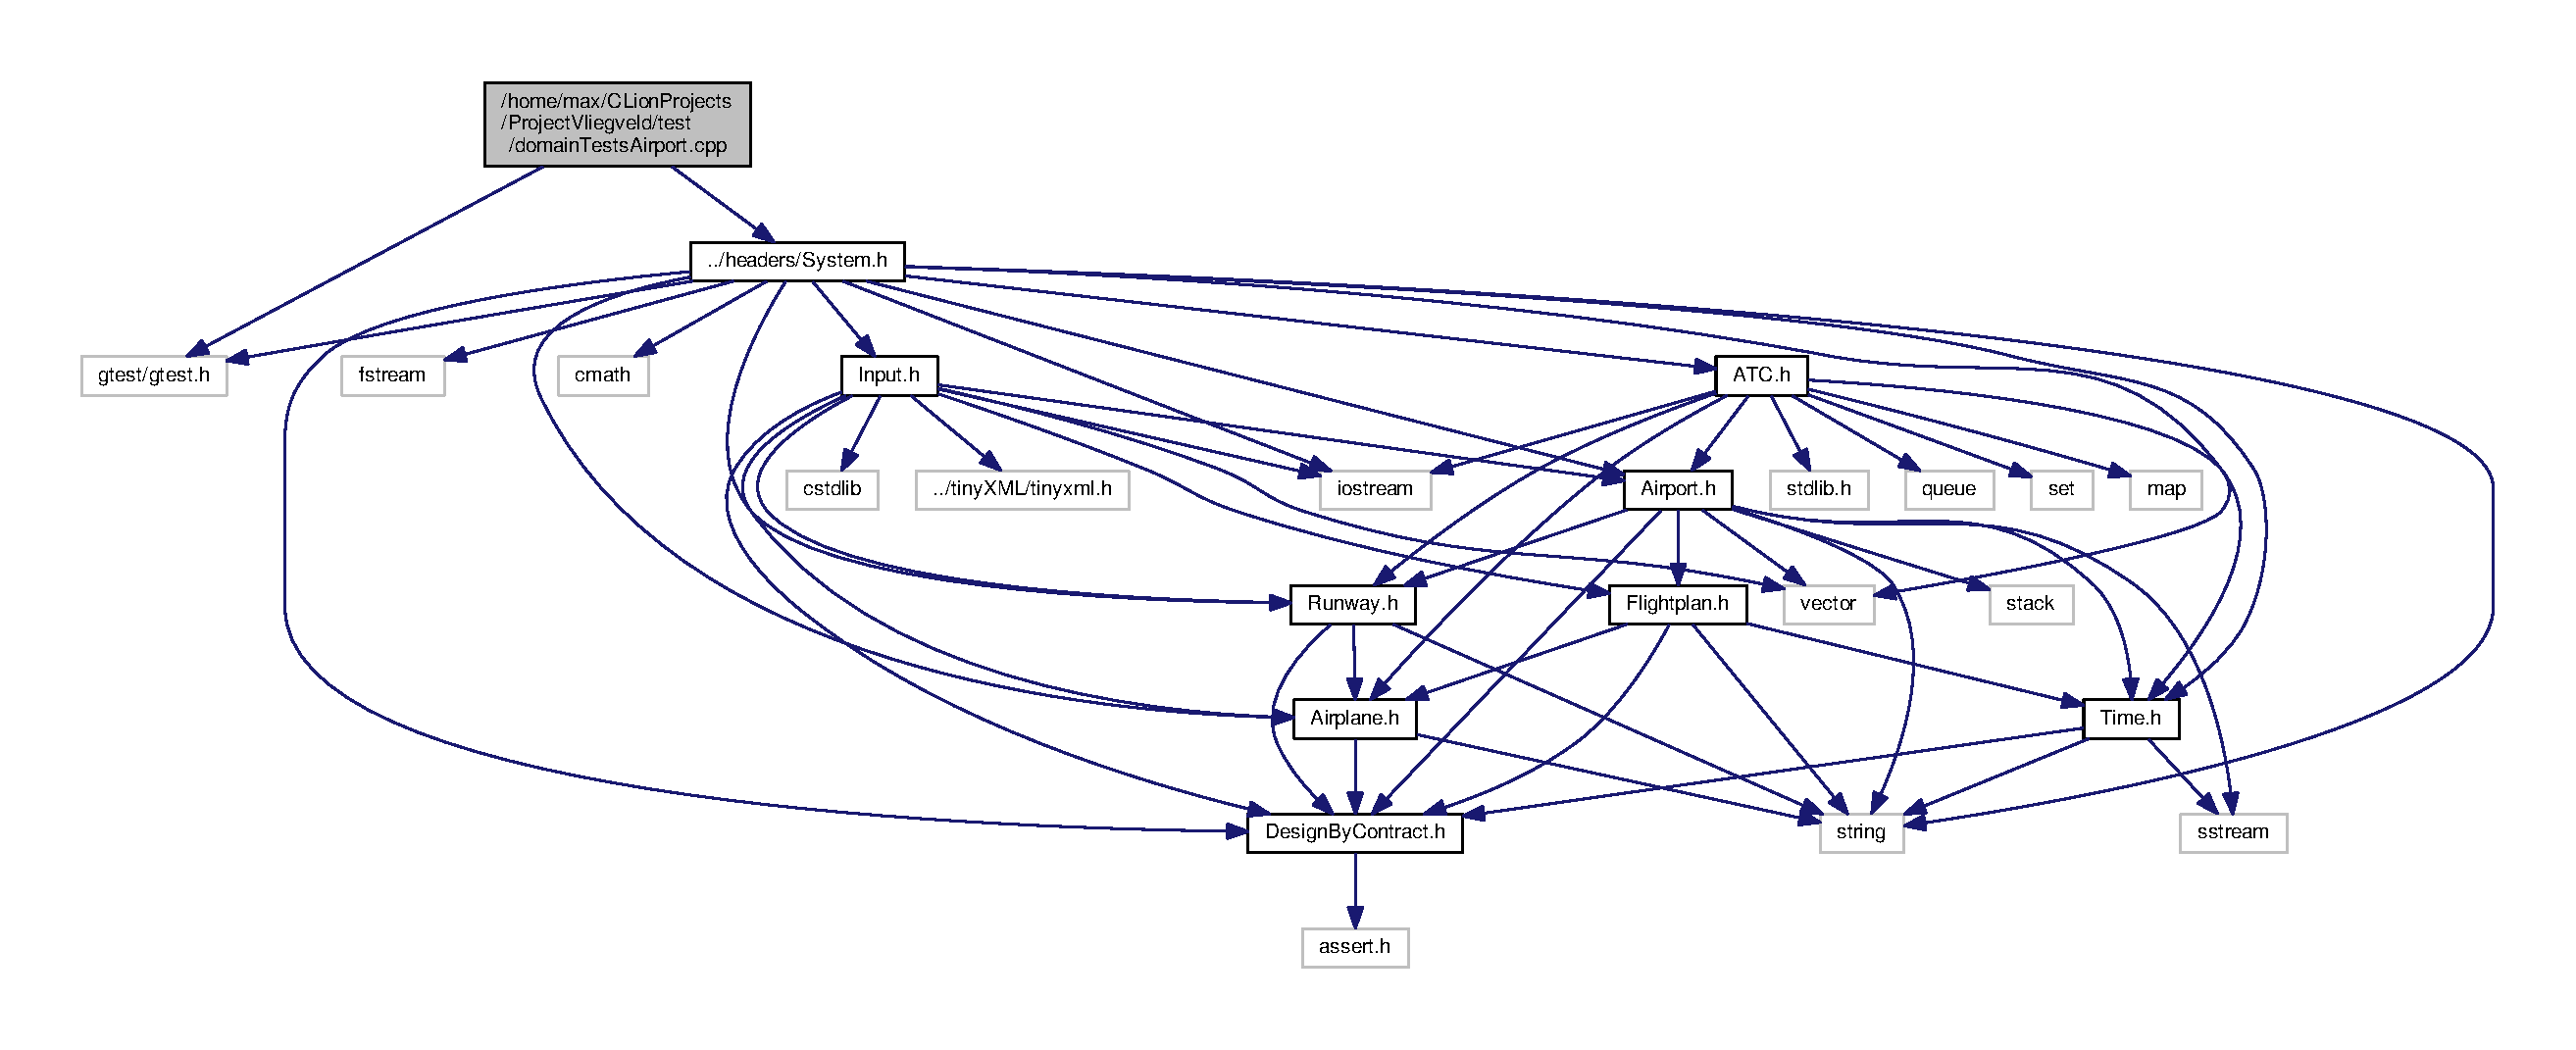
\includegraphics[width=350pt]{domainTestsAirport_8cpp__incl}
\end{center}
\end{figure}
\subsection*{Classes}
\begin{DoxyCompactItemize}
\item 
class \hyperlink{classdomainTestAirport}{domain\+Test\+Airport}
\end{DoxyCompactItemize}
\subsection*{Functions}
\begin{DoxyCompactItemize}
\item 
\hyperlink{domainTestsAirport_8cpp_a0ca5fe4adfab28ce60e024af8510d1ce}{T\+E\+S\+T\+\_\+F} (\hyperlink{classdomainTestAirport}{domain\+Test\+Airport}, Default\+Constructor)
\item 
\hyperlink{domainTestsAirport_8cpp_a9ea10725fbea65a52a01b32729df3742}{T\+E\+S\+T\+\_\+F} (\hyperlink{classdomainTestAirport}{domain\+Test\+Airport}, happy\+Day)
\item 
\hyperlink{domainTestsAirport_8cpp_a4a216dc0e2ecab434737e3692eb68d89}{T\+E\+S\+T\+\_\+F} (\hyperlink{classdomainTestAirport}{domain\+Test\+Airport}, complete)
\item 
\hyperlink{domainTestsAirport_8cpp_a1e8a9b34f2eb2099b550ceb0480c0a49}{T\+E\+S\+T\+\_\+F} (\hyperlink{classdomainTestAirport}{domain\+Test\+Airport}, field\+Manipulation)
\item 
\hyperlink{domainTestsAirport_8cpp_a115e9730fcd9a3be6df548dae0ceeec8}{T\+E\+S\+T\+\_\+F} (\hyperlink{classdomainTestAirport}{domain\+Test\+Airport}, Contract\+Violations)
\end{DoxyCompactItemize}


\subsection{Function Documentation}
\index{domain\+Tests\+Airport.\+cpp@{domain\+Tests\+Airport.\+cpp}!T\+E\+S\+T\+\_\+F@{T\+E\+S\+T\+\_\+F}}
\index{T\+E\+S\+T\+\_\+F@{T\+E\+S\+T\+\_\+F}!domain\+Tests\+Airport.\+cpp@{domain\+Tests\+Airport.\+cpp}}
\subsubsection[{\texorpdfstring{T\+E\+S\+T\+\_\+\+F(domain\+Test\+Airport, Default\+Constructor)}{TEST_F(domainTestAirport, DefaultConstructor)}}]{\setlength{\rightskip}{0pt plus 5cm}T\+E\+S\+T\+\_\+F (
\begin{DoxyParamCaption}
\item[{{\bf domain\+Test\+Airport}}]{, }
\item[{Default\+Constructor}]{}
\end{DoxyParamCaption}
)}\hypertarget{domainTestsAirport_8cpp_a0ca5fe4adfab28ce60e024af8510d1ce}{}\label{domainTestsAirport_8cpp_a0ca5fe4adfab28ce60e024af8510d1ce}

\begin{DoxyCode}
19                                               \{
20     EXPECT\_TRUE(airport.properlyInitialized());
21     EXPECT\_EQ(airport.getGates(), -1);
22 \}
\end{DoxyCode}
\index{domain\+Tests\+Airport.\+cpp@{domain\+Tests\+Airport.\+cpp}!T\+E\+S\+T\+\_\+F@{T\+E\+S\+T\+\_\+F}}
\index{T\+E\+S\+T\+\_\+F@{T\+E\+S\+T\+\_\+F}!domain\+Tests\+Airport.\+cpp@{domain\+Tests\+Airport.\+cpp}}
\subsubsection[{\texorpdfstring{T\+E\+S\+T\+\_\+\+F(domain\+Test\+Airport, happy\+Day)}{TEST_F(domainTestAirport, happyDay)}}]{\setlength{\rightskip}{0pt plus 5cm}T\+E\+S\+T\+\_\+F (
\begin{DoxyParamCaption}
\item[{{\bf domain\+Test\+Airport}}]{, }
\item[{happy\+Day}]{}
\end{DoxyParamCaption}
)}\hypertarget{domainTestsAirport_8cpp_a9ea10725fbea65a52a01b32729df3742}{}\label{domainTestsAirport_8cpp_a9ea10725fbea65a52a01b32729df3742}

\begin{DoxyCode}
24                                     \{
25     \textcolor{comment}{// init airport}
26     EXPECT\_FALSE(airport.complete());
27     airport.setName(\textcolor{stringliteral}{"Antwerp Airport"});
28     airport.setCallsign(\textcolor{stringliteral}{"Antwerp Tower"});
29     airport.setIata(\textcolor{stringliteral}{"ANR"});
30     airport.setGates(10);
31     EXPECT\_TRUE(airport.complete());
32 
33     \textcolor{comment}{// plane}
34     plane.setPosition(\textcolor{stringliteral}{"Alpha"});
35     plane.setEngine(\hyperlink{Airplane_8h_a3d2a8adb53da58e78cb0018d784e791da6262caeb7b5646a03a202006f584364c}{kJet});
36     plane.setSize(\hyperlink{Airplane_8h_a0526623f951311ba6780209b9e278dbfa6b6a05b83fa2f5308724e45442b38b7e}{kLarge});
37 
38     \textcolor{comment}{// 1st runway}
39     \hyperlink{classRunway}{Runway}* rw2 = \textcolor{keyword}{new} \hyperlink{classRunway}{Runway}();
40     rw2->\hyperlink{classRunway_ae346a0e299a7cbea186ad6ab25a46ae0}{setName}(\textcolor{stringliteral}{"RW1"});
41     rw2->\hyperlink{classRunway_a99a62b2993713ffc18e88cae16c11d11}{setTaxiPoint}(\textcolor{stringliteral}{"Alpha"});
42     rw2->\hyperlink{classRunway_a0a95f11d67cb4677f1bddd8cf20ed5bc}{setType}(\hyperlink{Runway_8h_adbb3e23fdb96fa1bac0dbbae33431cd2ae97f33599679c1a293bb8403f4a7a8f7}{kGrass});
43     rw2->\hyperlink{classRunway_af32954dc4688acd3a91114d200c6df9e}{setLength}(20000);
44 
45     \textcolor{comment}{// 2nd runway}
46     \hyperlink{classRunway}{Runway} *rw = \textcolor{keyword}{new} \hyperlink{classRunway}{Runway}();
47     rw->\hyperlink{classRunway_ae346a0e299a7cbea186ad6ab25a46ae0}{setName}(\textcolor{stringliteral}{"RW2"});
48     rw->\hyperlink{classRunway_a99a62b2993713ffc18e88cae16c11d11}{setTaxiPoint}(\textcolor{stringliteral}{"Bravo"});
49     rw->\hyperlink{classRunway_a0a95f11d67cb4677f1bddd8cf20ed5bc}{setType}(\hyperlink{Runway_8h_adbb3e23fdb96fa1bac0dbbae33431cd2ae97f33599679c1a293bb8403f4a7a8f7}{kGrass});
50     rw->\hyperlink{classRunway_af32954dc4688acd3a91114d200c6df9e}{setLength}(20000);
51 
52     \textcolor{comment}{// test for occupying/restoring gates.}
53     airport.initStack();
54     \textcolor{keywordflow}{for} (\textcolor{keywordtype}{int} i = 1; i <= 10; i++) \{
55         EXPECT\_EQ(airport.getFreeGate(), i);
56     \}
57     \textcolor{keywordflow}{for} (\textcolor{keywordtype}{int} i = 10; i > 0; i--) \{
58         airport.restoreGate(i);
59     \}
60     EXPECT\_EQ(airport.getFreeGate(), 1);
61     EXPECT\_EQ(airport.getFreeGate(), 2);
62     airport.restoreGate(1);
63     EXPECT\_EQ(airport.getFreeGate(), 1);
64 
65 
66     EXPECT\_TRUE(airport.amountOfRunways() == 0);
67 
68     \textcolor{comment}{// 1 runway in airport}
69     airport.addRunway(rw2);
70     EXPECT\_TRUE(airport.amountOfRunways() == 1);
71 
72     \textcolor{comment}{// test for finding runways by taxipoint}
73     EXPECT\_EQ(airport.getRunway(\textcolor{stringliteral}{"Alpha"}), rw2);
74     EXPECT\_TRUE(airport.getRunway(\textcolor{stringliteral}{"Gibberish"}) == NULL);
75 
76     \textcolor{comment}{// plane is not taxiing}
77     EXPECT\_TRUE(airport.getNextRunway(&plane) == NULL);
78 
79     \textcolor{comment}{// plane is taxiing, but no next runway found}
80     plane.setStatus(\hyperlink{Airplane_8h_a0e5bbf7c6c727baaba49062300fae19fa3a6a40398243a8892b8084a9e0107015}{kTaxiDeparture});
81     EXPECT\_TRUE(airport.getNextRunway(&plane) == NULL);
82 
83     \textcolor{comment}{// 2 runways in system}
84     airport.addRunway(rw);
85     EXPECT\_TRUE(airport.amountOfRunways() == 2);
86 
87     \textcolor{comment}{// plane is taxiing and there is a next runway.}
88     EXPECT\_EQ(airport.getNextRunway(&plane), rw);
89 
90     \textcolor{comment}{// get free runway, but no valid runway for large jets}
91     EXPECT\_TRUE(airport.getFreeRunway(&plane) == NULL);
92 
93     \textcolor{comment}{// alter rw so it's a valid runway.}
94     rw->\hyperlink{classRunway_a0a95f11d67cb4677f1bddd8cf20ed5bc}{setType}(\hyperlink{Runway_8h_adbb3e23fdb96fa1bac0dbbae33431cd2ae0b5b4fcb396cd73cb79793039658380}{kAsphalt});
95     EXPECT\_EQ(airport.getFreeRunway(&plane), rw);
96 
97 
98 \textcolor{comment}{//    delete  rw;}
99 \}
\end{DoxyCode}
\index{domain\+Tests\+Airport.\+cpp@{domain\+Tests\+Airport.\+cpp}!T\+E\+S\+T\+\_\+F@{T\+E\+S\+T\+\_\+F}}
\index{T\+E\+S\+T\+\_\+F@{T\+E\+S\+T\+\_\+F}!domain\+Tests\+Airport.\+cpp@{domain\+Tests\+Airport.\+cpp}}
\subsubsection[{\texorpdfstring{T\+E\+S\+T\+\_\+\+F(domain\+Test\+Airport, complete)}{TEST_F(domainTestAirport, complete)}}]{\setlength{\rightskip}{0pt plus 5cm}T\+E\+S\+T\+\_\+F (
\begin{DoxyParamCaption}
\item[{{\bf domain\+Test\+Airport}}]{, }
\item[{complete}]{}
\end{DoxyParamCaption}
)}\hypertarget{domainTestsAirport_8cpp_a4a216dc0e2ecab434737e3692eb68d89}{}\label{domainTestsAirport_8cpp_a4a216dc0e2ecab434737e3692eb68d89}

\begin{DoxyCode}
101                                     \{
102     EXPECT\_FALSE(airport.complete());
103     airport.setName(\textcolor{stringliteral}{"Antwerp Airport"});
104 
105     EXPECT\_FALSE(airport.complete());
106     airport.setCallsign(\textcolor{stringliteral}{"Antwerp Tower"});
107 
108     EXPECT\_FALSE(airport.complete());
109     airport.setIata(\textcolor{stringliteral}{"ANR"});
110 
111     EXPECT\_FALSE(airport.complete());
112     airport.setGates(10);
113 
114     EXPECT\_TRUE(airport.complete());
115 \}
\end{DoxyCode}
\index{domain\+Tests\+Airport.\+cpp@{domain\+Tests\+Airport.\+cpp}!T\+E\+S\+T\+\_\+F@{T\+E\+S\+T\+\_\+F}}
\index{T\+E\+S\+T\+\_\+F@{T\+E\+S\+T\+\_\+F}!domain\+Tests\+Airport.\+cpp@{domain\+Tests\+Airport.\+cpp}}
\subsubsection[{\texorpdfstring{T\+E\+S\+T\+\_\+\+F(domain\+Test\+Airport, field\+Manipulation)}{TEST_F(domainTestAirport, fieldManipulation)}}]{\setlength{\rightskip}{0pt plus 5cm}T\+E\+S\+T\+\_\+F (
\begin{DoxyParamCaption}
\item[{{\bf domain\+Test\+Airport}}]{, }
\item[{field\+Manipulation}]{}
\end{DoxyParamCaption}
)}\hypertarget{domainTestsAirport_8cpp_a1e8a9b34f2eb2099b550ceb0480c0a49}{}\label{domainTestsAirport_8cpp_a1e8a9b34f2eb2099b550ceb0480c0a49}

\begin{DoxyCode}
117                                              \{
118     airport.setName(\textcolor{stringliteral}{"Antwerp Airport"});
119     EXPECT\_EQ(airport.getName(), \textcolor{stringliteral}{"Antwerp Airport"});
120 
121     airport.setCallsign(\textcolor{stringliteral}{"Antwerp Tower"});
122     EXPECT\_EQ(airport.getCallsign(), \textcolor{stringliteral}{"Antwerp Tower"});
123 
124     airport.setIata(\textcolor{stringliteral}{"ANR"});
125     EXPECT\_EQ(airport.getIata(), \textcolor{stringliteral}{"ANR"});
126 
127     airport.setGates(10);
128     EXPECT\_EQ(airport.getGates(), 10);
129 
130     \hyperlink{classRunway}{Runway}* runway1 = \textcolor{keyword}{new} \hyperlink{classRunway}{Runway}();
131 
132     runway1->setName(\textcolor{stringliteral}{"RW1"});
133     runway1->setTaxiPoint(\textcolor{stringliteral}{"Alpha"});
134     airport.addRunway(runway1);
135     vector<Runway*> rws = airport.getRunways();
136     EXPECT\_TRUE(rws.size() == 1);
137     EXPECT\_EQ(rws.at(0), runway1);
138 \}
\end{DoxyCode}
\index{domain\+Tests\+Airport.\+cpp@{domain\+Tests\+Airport.\+cpp}!T\+E\+S\+T\+\_\+F@{T\+E\+S\+T\+\_\+F}}
\index{T\+E\+S\+T\+\_\+F@{T\+E\+S\+T\+\_\+F}!domain\+Tests\+Airport.\+cpp@{domain\+Tests\+Airport.\+cpp}}
\subsubsection[{\texorpdfstring{T\+E\+S\+T\+\_\+\+F(domain\+Test\+Airport, Contract\+Violations)}{TEST_F(domainTestAirport, ContractViolations)}}]{\setlength{\rightskip}{0pt plus 5cm}T\+E\+S\+T\+\_\+F (
\begin{DoxyParamCaption}
\item[{{\bf domain\+Test\+Airport}}]{, }
\item[{Contract\+Violations}]{}
\end{DoxyParamCaption}
)}\hypertarget{domainTestsAirport_8cpp_a115e9730fcd9a3be6df548dae0ceeec8}{}\label{domainTestsAirport_8cpp_a115e9730fcd9a3be6df548dae0ceeec8}

\begin{DoxyCode}
141                                               \{
142     \textcolor{comment}{// getFreeGate}
143     airport.setGates(10);
144     EXPECT\_DEATH(airport.getFreeGate(), \textcolor{stringliteral}{"Can't get free gate: no gate in stack."});
145     airport.initStack();
146 
147     \textcolor{comment}{// initStack}
148     EXPECT\_DEATH(airport.initStack(), \textcolor{stringliteral}{"Can't initialize gate stack, already in use."});
149 
150     \textcolor{comment}{// getFreeGate continued}
151     airport.setGates(0);
152     EXPECT\_DEATH(airport.getFreeGate(), \textcolor{stringliteral}{"Airport has no gates."});
153     airport.setGates(1);
154     airport.getFreeGate();
155     EXPECT\_DEATH(airport.getFreeGate(), \textcolor{stringliteral}{"Gate has an invalid ID."});
156 
157 
158     \textcolor{comment}{// restoreGate}
159     airport.setGates(0);
160     EXPECT\_DEATH(airport.restoreGate(11), \textcolor{stringliteral}{"Airport has no gates."});
161     airport.setGates(10);
162     EXPECT\_DEATH(airport.restoreGate(11), \textcolor{stringliteral}{"Gate ID is invalid."});
163     EXPECT\_DEATH(airport.restoreGate(0), \textcolor{stringliteral}{"Gate ID is invalid."});
164     EXPECT\_DEATH(airport.restoreGate(-1), \textcolor{stringliteral}{"Gate ID is invalid."});
165 
166     \textcolor{comment}{// addRunway}
167     runway.setName(\textcolor{stringliteral}{"RW1"});
168     runway.setTaxiPoint(\textcolor{stringliteral}{"Alpha"});
169     EXPECT\_DEATH(airport.addRunway(NULL), \textcolor{stringliteral}{"Runway cannot be NULL."});
170     \hyperlink{classRunway}{Runway}* runway1 = \textcolor{keyword}{new} \hyperlink{classRunway}{Runway}();
171     airport.addRunway(runway1);
172     EXPECT\_DEATH(airport.addRunway(runway1), \textcolor{stringliteral}{"Runway is already in system."});
173 
174     \textcolor{comment}{// getNextRunway}
175     EXPECT\_DEATH(airport.getNextRunway(NULL), \textcolor{stringliteral}{"Airplane cannot be NULL."});
176 
177     \textcolor{comment}{// setGates}
178     EXPECT\_DEATH(airport.setGates(-1), \textcolor{stringliteral}{"Number of gates cannot be negative!"});
179 
180     \textcolor{comment}{// getFreeRunway}
181     EXPECT\_DEATH(airport.getFreeRunway(NULL), \textcolor{stringliteral}{"Plane object does not exist."});
182 \}\end{DoxyCode}

\hypertarget{domainTestsATC_8cpp}{}\section{/home/max/\+C\+Lion\+Projects/\+Project\+Vliegveld/test/domain\+Tests\+A\+TC.cpp File Reference}
\label{domainTestsATC_8cpp}\index{/home/max/\+C\+Lion\+Projects/\+Project\+Vliegveld/test/domain\+Tests\+A\+T\+C.\+cpp@{/home/max/\+C\+Lion\+Projects/\+Project\+Vliegveld/test/domain\+Tests\+A\+T\+C.\+cpp}}
{\ttfamily \#include $<$gtest/gtest.\+h$>$}\\*
{\ttfamily \#include \char`\"{}../headers/\+System.\+h\char`\"{}}\\*
Include dependency graph for domain\+Tests\+A\+T\+C.\+cpp\+:
\nopagebreak
\begin{figure}[H]
\begin{center}
\leavevmode
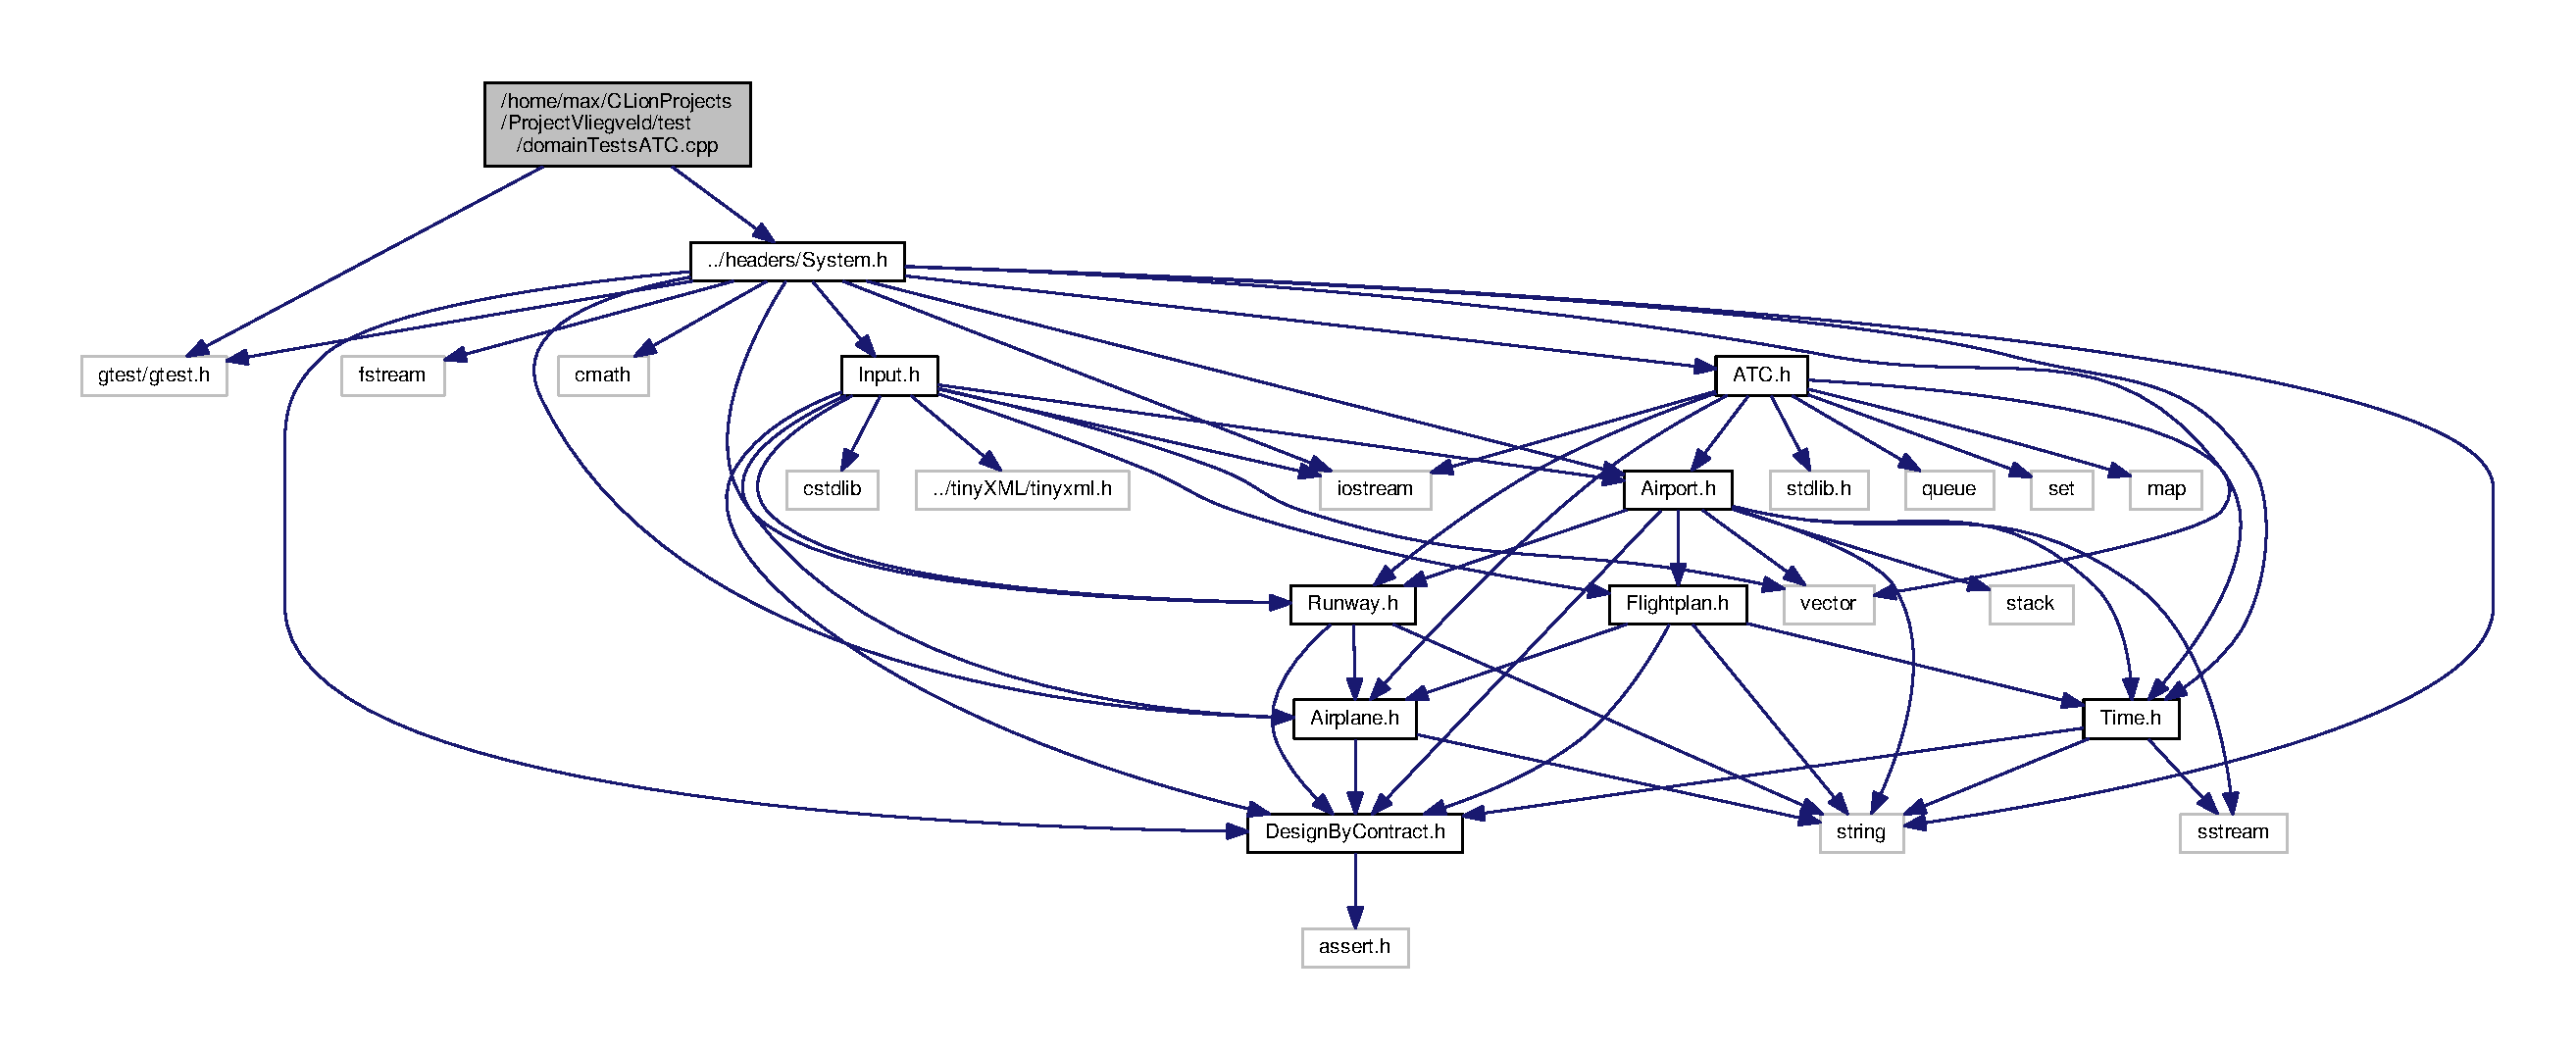
\includegraphics[width=350pt]{domainTestsATC_8cpp__incl}
\end{center}
\end{figure}
\subsection*{Classes}
\begin{DoxyCompactItemize}
\item 
class \hyperlink{classdomainTestATC}{domain\+Test\+A\+TC}
\end{DoxyCompactItemize}
\subsection*{Functions}
\begin{DoxyCompactItemize}
\item 
\hyperlink{domainTestsATC_8cpp_a22b01e923fa0a13ab2c97f95067f4083}{T\+E\+S\+T\+\_\+F} (\hyperlink{classdomainTestATC}{domain\+Test\+A\+TC}, Default\+Constructor)
\item 
\hyperlink{domainTestsATC_8cpp_a94c416f25004a7267632ec1b00a8c6a8}{T\+E\+S\+T\+\_\+F} (\hyperlink{classdomainTestATC}{domain\+Test\+A\+TC}, process\+Approach)
\item 
\hyperlink{domainTestsATC_8cpp_a9ee41a51f7248fdd8d8efd1806746dcb}{T\+E\+S\+T\+\_\+F} (\hyperlink{classdomainTestATC}{domain\+Test\+A\+TC}, process\+Descend)
\item 
\hyperlink{domainTestsATC_8cpp_a6ae540d701432e12bbd2fbbdee26015a}{T\+E\+S\+T\+\_\+F} (\hyperlink{classdomainTestATC}{domain\+Test\+A\+TC}, process\+Taxi\+Arrival)
\item 
\hyperlink{domainTestsATC_8cpp_a8d23d98af5b78a7d2e7b60ce09ac98f7}{T\+E\+S\+T\+\_\+F} (\hyperlink{classdomainTestATC}{domain\+Test\+A\+TC}, squawk)
\item 
\hyperlink{domainTestsATC_8cpp_a22ea0ccadadefa37cffe0777b49b4aad}{T\+E\+S\+T\+\_\+F} (\hyperlink{classdomainTestATC}{domain\+Test\+A\+TC}, process\+I\+F\+R\+Clearance)
\item 
\hyperlink{domainTestsATC_8cpp_a231048c55926e435ae090f99a46d2772}{T\+E\+S\+T\+\_\+F} (\hyperlink{classdomainTestATC}{domain\+Test\+A\+TC}, process\+Pushback)
\item 
\hyperlink{domainTestsATC_8cpp_a526acccb90282b6de3ea3b557affc3ff}{T\+E\+S\+T\+\_\+F} (\hyperlink{classdomainTestATC}{domain\+Test\+A\+TC}, process\+Taxi\+Initialise)
\item 
\hyperlink{domainTestsATC_8cpp_aeb48628ede2ece8f6e2c1dcc6d7eafc5}{T\+E\+S\+T\+\_\+F} (\hyperlink{classdomainTestATC}{domain\+Test\+A\+TC}, process\+Taxi\+Instruction)
\item 
\hyperlink{domainTestsATC_8cpp_a82a8b53418efed228525552db6e4b930}{T\+E\+S\+T\+\_\+F} (\hyperlink{classdomainTestATC}{domain\+Test\+A\+TC}, process\+Take\+Off)
\item 
\hyperlink{domainTestsATC_8cpp_a4580a998856b74e405e2f59f8d9fe00a}{T\+E\+S\+T\+\_\+F} (\hyperlink{classdomainTestATC}{domain\+Test\+A\+TC}, process\+Take\+Off\+Runway)
\item 
\hyperlink{domainTestsATC_8cpp_af29b48ced03a3902949ee9fade7d28e4}{T\+E\+S\+T\+\_\+F} (\hyperlink{classdomainTestATC}{domain\+Test\+A\+TC}, field\+Manipulation)
\end{DoxyCompactItemize}


\subsection{Function Documentation}
\index{domain\+Tests\+A\+T\+C.\+cpp@{domain\+Tests\+A\+T\+C.\+cpp}!T\+E\+S\+T\+\_\+F@{T\+E\+S\+T\+\_\+F}}
\index{T\+E\+S\+T\+\_\+F@{T\+E\+S\+T\+\_\+F}!domain\+Tests\+A\+T\+C.\+cpp@{domain\+Tests\+A\+T\+C.\+cpp}}
\subsubsection[{\texorpdfstring{T\+E\+S\+T\+\_\+\+F(domain\+Test\+A\+T\+C, Default\+Constructor)}{TEST_F(domainTestATC, DefaultConstructor)}}]{\setlength{\rightskip}{0pt plus 5cm}T\+E\+S\+T\+\_\+F (
\begin{DoxyParamCaption}
\item[{{\bf domain\+Test\+A\+TC}}]{, }
\item[{Default\+Constructor}]{}
\end{DoxyParamCaption}
)}\hypertarget{domainTestsATC_8cpp_a22b01e923fa0a13ab2c97f95067f4083}{}\label{domainTestsATC_8cpp_a22b01e923fa0a13ab2c97f95067f4083}

\begin{DoxyCode}
45                                           \{
46     EXPECT\_TRUE(atc->properlyInitialized());
47     EXPECT\_FALSE(atc->get3occupied());
48     EXPECT\_FALSE(atc->get5occupied());
49 \}
\end{DoxyCode}
\index{domain\+Tests\+A\+T\+C.\+cpp@{domain\+Tests\+A\+T\+C.\+cpp}!T\+E\+S\+T\+\_\+F@{T\+E\+S\+T\+\_\+F}}
\index{T\+E\+S\+T\+\_\+F@{T\+E\+S\+T\+\_\+F}!domain\+Tests\+A\+T\+C.\+cpp@{domain\+Tests\+A\+T\+C.\+cpp}}
\subsubsection[{\texorpdfstring{T\+E\+S\+T\+\_\+\+F(domain\+Test\+A\+T\+C, process\+Approach)}{TEST_F(domainTestATC, processApproach)}}]{\setlength{\rightskip}{0pt plus 5cm}T\+E\+S\+T\+\_\+F (
\begin{DoxyParamCaption}
\item[{{\bf domain\+Test\+A\+TC}}]{, }
\item[{process\+Approach}]{}
\end{DoxyParamCaption}
)}\hypertarget{domainTestsATC_8cpp_a94c416f25004a7267632ec1b00a8c6a8}{}\label{domainTestsATC_8cpp_a94c416f25004a7267632ec1b00a8c6a8}

\begin{DoxyCode}
51                                        \{
52     \textcolor{comment}{// Very simple function so very simple test}
53     atc->processApproach(airplane, \hyperlink{classTime}{Time}());
54     EXPECT\_EQ(airplane->getRequest(), \hyperlink{Airplane_8h_a4a8a3f45932bdf601f093bea061bad9ba15597ea7f444a937d40b39b9ea99dd1d}{kAccepted});
55 \}
\end{DoxyCode}
\index{domain\+Tests\+A\+T\+C.\+cpp@{domain\+Tests\+A\+T\+C.\+cpp}!T\+E\+S\+T\+\_\+F@{T\+E\+S\+T\+\_\+F}}
\index{T\+E\+S\+T\+\_\+F@{T\+E\+S\+T\+\_\+F}!domain\+Tests\+A\+T\+C.\+cpp@{domain\+Tests\+A\+T\+C.\+cpp}}
\subsubsection[{\texorpdfstring{T\+E\+S\+T\+\_\+\+F(domain\+Test\+A\+T\+C, process\+Descend)}{TEST_F(domainTestATC, processDescend)}}]{\setlength{\rightskip}{0pt plus 5cm}T\+E\+S\+T\+\_\+F (
\begin{DoxyParamCaption}
\item[{{\bf domain\+Test\+A\+TC}}]{, }
\item[{process\+Descend}]{}
\end{DoxyParamCaption}
)}\hypertarget{domainTestsATC_8cpp_a9ee41a51f7248fdd8d8efd1806746dcb}{}\label{domainTestsATC_8cpp_a9ee41a51f7248fdd8d8efd1806746dcb}

\begin{DoxyCode}
57                                       \{
58     \textcolor{comment}{// All clear, can descend}
59     airplane->setAltitude(5);
60     atc->processDescend(airplane, \hyperlink{classTime}{Time}());
61     EXPECT\_EQ(airplane->getRequest(), \hyperlink{Airplane_8h_a4a8a3f45932bdf601f093bea061bad9ba15597ea7f444a937d40b39b9ea99dd1d}{kAccepted});
62 
63     \textcolor{comment}{// Has to circle because of circling at 3.000ft}
64     airplane->setAltitude(5);
65     atc->set3occupied(\textcolor{keyword}{true});
66     atc->processDescend(airplane, \hyperlink{classTime}{Time}());
67     EXPECT\_EQ(airplane->getRequest(), \hyperlink{Airplane_8h_a4a8a3f45932bdf601f093bea061bad9baac195c08fab2dff9d0520caf49ea4e11}{kDenied});
68     EXPECT\_TRUE(atc->get5occupied());
69 
70     \textcolor{comment}{// Can descend, but 5000ft is occupied}
71     airplane->setAltitude(5);
72     atc->set3occupied(\textcolor{keyword}{false});
73     atc->set5occupied(\textcolor{keyword}{true});
74     atc->processDescend(airplane, \hyperlink{classTime}{Time}());
75     EXPECT\_EQ(airplane->getRequest(), \hyperlink{Airplane_8h_a4a8a3f45932bdf601f093bea061bad9ba15597ea7f444a937d40b39b9ea99dd1d}{kAccepted});
76     EXPECT\_TRUE(atc->get5occupied());
77     EXPECT\_FALSE(atc->get3occupied());
78 
79     \textcolor{comment}{// Can descend, but only because circling is going at 5000ft, 3000ft is also occupied}
80     atc->set5occupied(\textcolor{keyword}{true});
81     atc->set3occupied(\textcolor{keyword}{true});
82     airplane->setAltitude(5);
83     atc->processDescend(airplane, \hyperlink{classTime}{Time}());
84     EXPECT\_EQ(airplane->getRequest(), \hyperlink{Airplane_8h_a4a8a3f45932bdf601f093bea061bad9ba15597ea7f444a937d40b39b9ea99dd1d}{kAccepted});
85     EXPECT\_TRUE(atc->get5occupied());
86     EXPECT\_TRUE(atc->get3occupied());
87 
88     \textcolor{comment}{// Can land, all clear}
89     airplane->setAltitude(3);
90     atc->processDescend(airplane, \hyperlink{classTime}{Time}());
91     EXPECT\_EQ(airplane->getRequest(), \hyperlink{Airplane_8h_a4a8a3f45932bdf601f093bea061bad9ba15597ea7f444a937d40b39b9ea99dd1d}{kAccepted});
92     EXPECT\_EQ(airplane->getRunway(), runway);
93     EXPECT\_FALSE(runway->isFree());
94 
95     \textcolor{comment}{// Can't land, runway is not free}
96     atc->set3occupied(\textcolor{keyword}{false});
97     atc->set5occupied(\textcolor{keyword}{false});
98     atc->processDescend(airplane, \hyperlink{classTime}{Time}());
99     EXPECT\_EQ(airplane->getRequest(), \hyperlink{Airplane_8h_a4a8a3f45932bdf601f093bea061bad9baac195c08fab2dff9d0520caf49ea4e11}{kDenied});
100 
101     \textcolor{comment}{// Can't land, runway is not free and a plane is already circling}
102     atc->set3occupied(\textcolor{keyword}{true});
103     EXPECT\_DEATH(atc->processDescend(airplane, \hyperlink{classTime}{Time}()), \textcolor{stringliteral}{"Exceeded capacity"});
104 \}
\end{DoxyCode}
\index{domain\+Tests\+A\+T\+C.\+cpp@{domain\+Tests\+A\+T\+C.\+cpp}!T\+E\+S\+T\+\_\+F@{T\+E\+S\+T\+\_\+F}}
\index{T\+E\+S\+T\+\_\+F@{T\+E\+S\+T\+\_\+F}!domain\+Tests\+A\+T\+C.\+cpp@{domain\+Tests\+A\+T\+C.\+cpp}}
\subsubsection[{\texorpdfstring{T\+E\+S\+T\+\_\+\+F(domain\+Test\+A\+T\+C, process\+Taxi\+Arrival)}{TEST_F(domainTestATC, processTaxiArrival)}}]{\setlength{\rightskip}{0pt plus 5cm}T\+E\+S\+T\+\_\+F (
\begin{DoxyParamCaption}
\item[{{\bf domain\+Test\+A\+TC}}]{, }
\item[{process\+Taxi\+Arrival}]{}
\end{DoxyParamCaption}
)}\hypertarget{domainTestsATC_8cpp_a6ae540d701432e12bbd2fbbdee26015a}{}\label{domainTestsATC_8cpp_a6ae540d701432e12bbd2fbbdee26015a}

\begin{DoxyCode}
106                                           \{
107     \textcolor{comment}{// Just landed on first runway}
108     airplane->setPosition(\textcolor{stringliteral}{""});
109     airplane->setRunway(runway);
110     atc->processTaxiArrival(airplane, \hyperlink{classTime}{Time}());
111     EXPECT\_EQ(airplane->getRequest(), \hyperlink{Airplane_8h_a4a8a3f45932bdf601f093bea061bad9ba15597ea7f444a937d40b39b9ea99dd1d}{kAccepted});
112     EXPECT\_TRUE(airplane->getGateID() != -1);
113     EXPECT\_TRUE(airplane->getPosition().empty());
114 
115     \textcolor{comment}{// Landed on another runway}
116     airplane->setStatus(\hyperlink{Airplane_8h_a0e5bbf7c6c727baaba49062300fae19fabe52f2e86df226a44cc8ba29e8f259b2}{kTaxiArrival});
117     airplane->setRunway(system.getAirport()->getRunways()[1]);
118     airplane->setGateID(-1);
119     atc->processTaxiArrival(airplane, \hyperlink{classTime}{Time}());
120     EXPECT\_EQ(airplane->getRequest(), \hyperlink{Airplane_8h_a4a8a3f45932bdf601f093bea061bad9ba15597ea7f444a937d40b39b9ea99dd1d}{kAccepted});
121     EXPECT\_EQ(airplane->getGateID(), -1);
122 
123     \textcolor{comment}{// Airplane can cross runway, it's free}
124     airplane->setRunway(system.getAirport()->getRunways()[1]);
125     airplane->setPosition(airplane->getRunway()->getTaxiPoint());
126     runway->setFree(\textcolor{keyword}{true});
127     atc->processTaxiArrival(airplane, \hyperlink{classTime}{Time}());
128     EXPECT\_EQ(airplane->getRequest(), \hyperlink{Airplane_8h_a4a8a3f45932bdf601f093bea061bad9ba15597ea7f444a937d40b39b9ea99dd1d}{kAccepted});
129 
130 
131     \textcolor{comment}{// Airplane can't cross runway, it's in use}
132     runway->setFree(\textcolor{keyword}{false});
133     atc->processTaxiArrival(airplane, \hyperlink{classTime}{Time}());
134     EXPECT\_EQ(airplane->getRequest(), \hyperlink{Airplane_8h_a4a8a3f45932bdf601f093bea061bad9baac195c08fab2dff9d0520caf49ea4e11}{kDenied});
135 \}
\end{DoxyCode}
\index{domain\+Tests\+A\+T\+C.\+cpp@{domain\+Tests\+A\+T\+C.\+cpp}!T\+E\+S\+T\+\_\+F@{T\+E\+S\+T\+\_\+F}}
\index{T\+E\+S\+T\+\_\+F@{T\+E\+S\+T\+\_\+F}!domain\+Tests\+A\+T\+C.\+cpp@{domain\+Tests\+A\+T\+C.\+cpp}}
\subsubsection[{\texorpdfstring{T\+E\+S\+T\+\_\+\+F(domain\+Test\+A\+T\+C, squawk)}{TEST_F(domainTestATC, squawk)}}]{\setlength{\rightskip}{0pt plus 5cm}T\+E\+S\+T\+\_\+F (
\begin{DoxyParamCaption}
\item[{{\bf domain\+Test\+A\+TC}}]{, }
\item[{squawk}]{}
\end{DoxyParamCaption}
)}\hypertarget{domainTestsATC_8cpp_a8d23d98af5b78a7d2e7b60ce09ac98f7}{}\label{domainTestsATC_8cpp_a8d23d98af5b78a7d2e7b60ce09ac98f7}

\begin{DoxyCode}
137                               \{
138     \textcolor{keywordtype}{int} squawk;
139     airplane->setType(\hyperlink{Airplane_8h_a537b68b9ecaac78d371a35d8cf7604e9a00ca80b4ed05d96bd6ed02aca4b78e1f}{kPrivate});
140     airplane->setSize(\hyperlink{Airplane_8h_a0526623f951311ba6780209b9e278dbfaf99aeb93b2774bc0c7856d1510d17a54}{kSmall});
141     squawk = atc->getSquawk(airplane);
142     EXPECT\_TRUE(squawk < 778 and squawk > 0);
143 
144     airplane->setSize(\hyperlink{Airplane_8h_a0526623f951311ba6780209b9e278dbfabade85bef98ad2c69fb2216bb947b6c3}{kMedium});
145     airplane->setEngine(\hyperlink{Airplane_8h_a3d2a8adb53da58e78cb0018d784e791da6262caeb7b5646a03a202006f584364c}{kJet});
146     squawk = atc->getSquawk(airplane);
147     EXPECT\_TRUE(squawk < 1778 and squawk > 999);
148 
149     airplane->setType(\hyperlink{Airplane_8h_a537b68b9ecaac78d371a35d8cf7604e9aa60181ba834d25b46f4c717f3403c313}{kAirline});
150     airplane->setEngine(\hyperlink{Airplane_8h_a3d2a8adb53da58e78cb0018d784e791daef171fc98c472a2acd2338353679dcc3}{kPropeller});
151     squawk = atc->getSquawk(airplane);
152     EXPECT\_TRUE(squawk < 2778 and squawk > 1999);
153 
154     airplane->setEngine(\hyperlink{Airplane_8h_a3d2a8adb53da58e78cb0018d784e791da6262caeb7b5646a03a202006f584364c}{kJet});
155     squawk = atc->getSquawk(airplane);
156     EXPECT\_TRUE(squawk < 3778 and squawk > 2999);
157 
158     airplane->setSize(\hyperlink{Airplane_8h_a0526623f951311ba6780209b9e278dbfa6b6a05b83fa2f5308724e45442b38b7e}{kLarge});
159     squawk = atc->getSquawk(airplane);
160     EXPECT\_TRUE(squawk < 4778 and squawk > 3999);
161 
162     airplane->setType(\hyperlink{Airplane_8h_a537b68b9ecaac78d371a35d8cf7604e9a1dbdb6d83cd39b00ba5515617716d186}{kMilitary});
163     airplane->setSize(\hyperlink{Airplane_8h_a0526623f951311ba6780209b9e278dbfaf99aeb93b2774bc0c7856d1510d17a54}{kSmall});
164     squawk = atc->getSquawk(airplane);
165     EXPECT\_TRUE(squawk < 5778 and squawk > 4999);
166 
167     airplane->setSize(\hyperlink{Airplane_8h_a0526623f951311ba6780209b9e278dbfa6b6a05b83fa2f5308724e45442b38b7e}{kLarge});
168     airplane->setEngine(\hyperlink{Airplane_8h_a3d2a8adb53da58e78cb0018d784e791daef171fc98c472a2acd2338353679dcc3}{kPropeller});
169     squawk = atc->getSquawk(airplane);
170     EXPECT\_TRUE(squawk < 5778 and squawk > 4999);
171 
172     airplane->setType(\hyperlink{Airplane_8h_a537b68b9ecaac78d371a35d8cf7604e9ad0ab6e7d19d66949c60d9db1aa58f9ef}{kEmergency});
173     airplane->setSize(\hyperlink{Airplane_8h_a0526623f951311ba6780209b9e278dbfaf99aeb93b2774bc0c7856d1510d17a54}{kSmall});
174     airplane->setEngine(\hyperlink{Airplane_8h_a3d2a8adb53da58e78cb0018d784e791daef171fc98c472a2acd2338353679dcc3}{kPropeller});
175     squawk = atc->getSquawk(airplane);
176     EXPECT\_TRUE(squawk < 6778 and squawk > 5999);
177 \}
\end{DoxyCode}
\index{domain\+Tests\+A\+T\+C.\+cpp@{domain\+Tests\+A\+T\+C.\+cpp}!T\+E\+S\+T\+\_\+F@{T\+E\+S\+T\+\_\+F}}
\index{T\+E\+S\+T\+\_\+F@{T\+E\+S\+T\+\_\+F}!domain\+Tests\+A\+T\+C.\+cpp@{domain\+Tests\+A\+T\+C.\+cpp}}
\subsubsection[{\texorpdfstring{T\+E\+S\+T\+\_\+\+F(domain\+Test\+A\+T\+C, process\+I\+F\+R\+Clearance)}{TEST_F(domainTestATC, processIFRClearance)}}]{\setlength{\rightskip}{0pt plus 5cm}T\+E\+S\+T\+\_\+F (
\begin{DoxyParamCaption}
\item[{{\bf domain\+Test\+A\+TC}}]{, }
\item[{process\+I\+F\+R\+Clearance}]{}
\end{DoxyParamCaption}
)}\hypertarget{domainTestsATC_8cpp_a22ea0ccadadefa37cffe0777b49b4aad}{}\label{domainTestsATC_8cpp_a22ea0ccadadefa37cffe0777b49b4aad}

\begin{DoxyCode}
179                                            \{
180     airplane->setStatus(\hyperlink{Airplane_8h_a0e5bbf7c6c727baaba49062300fae19fabfff972a5d3596bc68662c89987639df}{kAirport});
181 
182     \textcolor{comment}{// large jet}
183     airplane->setType(\hyperlink{Airplane_8h_a537b68b9ecaac78d371a35d8cf7604e9aa60181ba834d25b46f4c717f3403c313}{kAirline});
184     airplane->setEngine(\hyperlink{Airplane_8h_a3d2a8adb53da58e78cb0018d784e791da6262caeb7b5646a03a202006f584364c}{kJet});
185     airplane->setSize(\hyperlink{Airplane_8h_a0526623f951311ba6780209b9e278dbfa6b6a05b83fa2f5308724e45442b38b7e}{kLarge});
186     airplane->setSquawk(0);
187 
188     \textcolor{comment}{// no runway available}
189     airplane->setRequest(\hyperlink{Airplane_8h_a4a8a3f45932bdf601f093bea061bad9bad143035084d581f7aecfabd95652e62c}{kPending});
190     runway->setType(\hyperlink{Runway_8h_adbb3e23fdb96fa1bac0dbbae33431cd2ae97f33599679c1a293bb8403f4a7a8f7}{kGrass});
191     runway->setLength(100);
192     atc->processIFRClearance(airplane, \hyperlink{classTime}{Time}());
193     EXPECT\_EQ(airplane->getRequest(), \hyperlink{Airplane_8h_a4a8a3f45932bdf601f093bea061bad9baac195c08fab2dff9d0520caf49ea4e11}{kDenied});
194     EXPECT\_TRUE(airplane->getRunway() == NULL);
195 
196     \textcolor{comment}{// runway availble}
197     airplane->setRequest(\hyperlink{Airplane_8h_a4a8a3f45932bdf601f093bea061bad9bad143035084d581f7aecfabd95652e62c}{kPending});
198     runway->setType(\hyperlink{Runway_8h_adbb3e23fdb96fa1bac0dbbae33431cd2ae0b5b4fcb396cd73cb79793039658380}{kAsphalt});
199     runway->setLength(10000);
200     atc->processIFRClearance(airplane, \hyperlink{classTime}{Time}());
201     EXPECT\_EQ(airplane->getRequest(), \hyperlink{Airplane_8h_a4a8a3f45932bdf601f093bea061bad9ba15597ea7f444a937d40b39b9ea99dd1d}{kAccepted});
202     EXPECT\_TRUE(airplane->getRunway() != NULL);
203 \}
\end{DoxyCode}
\index{domain\+Tests\+A\+T\+C.\+cpp@{domain\+Tests\+A\+T\+C.\+cpp}!T\+E\+S\+T\+\_\+F@{T\+E\+S\+T\+\_\+F}}
\index{T\+E\+S\+T\+\_\+F@{T\+E\+S\+T\+\_\+F}!domain\+Tests\+A\+T\+C.\+cpp@{domain\+Tests\+A\+T\+C.\+cpp}}
\subsubsection[{\texorpdfstring{T\+E\+S\+T\+\_\+\+F(domain\+Test\+A\+T\+C, process\+Pushback)}{TEST_F(domainTestATC, processPushback)}}]{\setlength{\rightskip}{0pt plus 5cm}T\+E\+S\+T\+\_\+F (
\begin{DoxyParamCaption}
\item[{{\bf domain\+Test\+A\+TC}}]{, }
\item[{process\+Pushback}]{}
\end{DoxyParamCaption}
)}\hypertarget{domainTestsATC_8cpp_a231048c55926e435ae090f99a46d2772}{}\label{domainTestsATC_8cpp_a231048c55926e435ae090f99a46d2772}

\begin{DoxyCode}
205                                        \{
206     \textcolor{comment}{// simple function.}
207     airplane->setStatus(\hyperlink{Airplane_8h_a0e5bbf7c6c727baaba49062300fae19fa20dbec285a7773f72e48eccef8ae84da}{kGate});
208     airplane->setRequest(\hyperlink{Airplane_8h_a4a8a3f45932bdf601f093bea061bad9bad143035084d581f7aecfabd95652e62c}{kPending});
209     atc->processPushback(airplane, \hyperlink{classTime}{Time}());
210     EXPECT\_EQ(airplane->getRequest(), \hyperlink{Airplane_8h_a4a8a3f45932bdf601f093bea061bad9ba15597ea7f444a937d40b39b9ea99dd1d}{kAccepted});
211 \}
\end{DoxyCode}
\index{domain\+Tests\+A\+T\+C.\+cpp@{domain\+Tests\+A\+T\+C.\+cpp}!T\+E\+S\+T\+\_\+F@{T\+E\+S\+T\+\_\+F}}
\index{T\+E\+S\+T\+\_\+F@{T\+E\+S\+T\+\_\+F}!domain\+Tests\+A\+T\+C.\+cpp@{domain\+Tests\+A\+T\+C.\+cpp}}
\subsubsection[{\texorpdfstring{T\+E\+S\+T\+\_\+\+F(domain\+Test\+A\+T\+C, process\+Taxi\+Initialise)}{TEST_F(domainTestATC, processTaxiInitialise)}}]{\setlength{\rightskip}{0pt plus 5cm}T\+E\+S\+T\+\_\+F (
\begin{DoxyParamCaption}
\item[{{\bf domain\+Test\+A\+TC}}]{, }
\item[{process\+Taxi\+Initialise}]{}
\end{DoxyParamCaption}
)}\hypertarget{domainTestsATC_8cpp_a526acccb90282b6de3ea3b557affc3ff}{}\label{domainTestsATC_8cpp_a526acccb90282b6de3ea3b557affc3ff}

\begin{DoxyCode}
213                                              \{
214     \textcolor{comment}{// simple function.}
215     airplane->setStatus(\hyperlink{Airplane_8h_a0e5bbf7c6c727baaba49062300fae19fa117bb5da4739b13c4915f7d721f3d2a5}{kPushback});
216     airplane->setRequest(\hyperlink{Airplane_8h_a4a8a3f45932bdf601f093bea061bad9bad143035084d581f7aecfabd95652e62c}{kPending});
217     atc->processTaxiInitialise(airplane, \hyperlink{classTime}{Time}());
218     EXPECT\_EQ(airplane->getRequest(), \hyperlink{Airplane_8h_a4a8a3f45932bdf601f093bea061bad9ba15597ea7f444a937d40b39b9ea99dd1d}{kAccepted});
219 \}
\end{DoxyCode}
\index{domain\+Tests\+A\+T\+C.\+cpp@{domain\+Tests\+A\+T\+C.\+cpp}!T\+E\+S\+T\+\_\+F@{T\+E\+S\+T\+\_\+F}}
\index{T\+E\+S\+T\+\_\+F@{T\+E\+S\+T\+\_\+F}!domain\+Tests\+A\+T\+C.\+cpp@{domain\+Tests\+A\+T\+C.\+cpp}}
\subsubsection[{\texorpdfstring{T\+E\+S\+T\+\_\+\+F(domain\+Test\+A\+T\+C, process\+Taxi\+Instruction)}{TEST_F(domainTestATC, processTaxiInstruction)}}]{\setlength{\rightskip}{0pt plus 5cm}T\+E\+S\+T\+\_\+F (
\begin{DoxyParamCaption}
\item[{{\bf domain\+Test\+A\+TC}}]{, }
\item[{process\+Taxi\+Instruction}]{}
\end{DoxyParamCaption}
)}\hypertarget{domainTestsATC_8cpp_aeb48628ede2ece8f6e2c1dcc6d7eafc5}{}\label{domainTestsATC_8cpp_aeb48628ede2ece8f6e2c1dcc6d7eafc5}

\begin{DoxyCode}
221                                               \{
222     airplane->setStatus(\hyperlink{Airplane_8h_a0e5bbf7c6c727baaba49062300fae19fa3a6a40398243a8892b8084a9e0107015}{kTaxiDeparture});
223     airplane->setRequest(\hyperlink{Airplane_8h_a4a8a3f45932bdf601f093bea061bad9bad143035084d581f7aecfabd95652e62c}{kPending});
224     airplane->setPosition(\textcolor{stringliteral}{"Alpha"});
225     airplane->setType(\hyperlink{Airplane_8h_a537b68b9ecaac78d371a35d8cf7604e9aa60181ba834d25b46f4c717f3403c313}{kAirline});
226 
227     \textcolor{comment}{// create a valid runway (all planes can land on asphalt with l=10k)}
228     runway->setType(\hyperlink{Runway_8h_adbb3e23fdb96fa1bac0dbbae33431cd2ae0b5b4fcb396cd73cb79793039658380}{kAsphalt});
229     runway->setLength(10000);
230     runway->setTaxiPoint(\textcolor{stringliteral}{"Alpha"});
231 
232     \textcolor{comment}{// create a second runway}
233     \hyperlink{classRunway}{Runway} *rw = \textcolor{keyword}{new} \hyperlink{classRunway}{Runway};
234     rw->\hyperlink{classRunway_a0a95f11d67cb4677f1bddd8cf20ed5bc}{setType}(\hyperlink{Runway_8h_adbb3e23fdb96fa1bac0dbbae33431cd2ae0b5b4fcb396cd73cb79793039658380}{kAsphalt});
235     rw->\hyperlink{classRunway_af32954dc4688acd3a91114d200c6df9e}{setLength}(1000);
236     airplane->setRunway(rw);
237 
238     \textcolor{comment}{// at destination}
239     rw->\hyperlink{classRunway_a99a62b2993713ffc18e88cae16c11d11}{setTaxiPoint}(\textcolor{stringliteral}{"Alpha"});
240     atc->processTaxiInstruction(airplane, \hyperlink{classTime}{Time}());
241     EXPECT\_EQ(airplane->getRequest(), \hyperlink{Airplane_8h_a4a8a3f45932bdf601f093bea061bad9ba85d56dac5419035294b1c769317026fa}{kConfirmed});
242 
243     \textcolor{comment}{// not at destination, can cross}
244     rw->\hyperlink{classRunway_a99a62b2993713ffc18e88cae16c11d11}{setTaxiPoint}(\textcolor{stringliteral}{"Bravo"});
245     runway->setFree(\textcolor{keyword}{true});
246     atc->processTaxiInstruction(airplane, \hyperlink{classTime}{Time}());
247     EXPECT\_EQ(airplane->getRequest(), \hyperlink{Airplane_8h_a4a8a3f45932bdf601f093bea061bad9ba15597ea7f444a937d40b39b9ea99dd1d}{kAccepted});
248 
249     \textcolor{comment}{// not at destination, can't cross}
250     rw->\hyperlink{classRunway_a99a62b2993713ffc18e88cae16c11d11}{setTaxiPoint}(\textcolor{stringliteral}{"Bravo"});
251     runway->setFree(\textcolor{keyword}{false});
252     atc->processTaxiInstruction(airplane, \hyperlink{classTime}{Time}());
253     EXPECT\_EQ(airplane->getRequest(), \hyperlink{Airplane_8h_a4a8a3f45932bdf601f093bea061bad9baac195c08fab2dff9d0520caf49ea4e11}{kDenied});
254 
255     \textcolor{keyword}{delete} rw;
256 \}
\end{DoxyCode}
\index{domain\+Tests\+A\+T\+C.\+cpp@{domain\+Tests\+A\+T\+C.\+cpp}!T\+E\+S\+T\+\_\+F@{T\+E\+S\+T\+\_\+F}}
\index{T\+E\+S\+T\+\_\+F@{T\+E\+S\+T\+\_\+F}!domain\+Tests\+A\+T\+C.\+cpp@{domain\+Tests\+A\+T\+C.\+cpp}}
\subsubsection[{\texorpdfstring{T\+E\+S\+T\+\_\+\+F(domain\+Test\+A\+T\+C, process\+Take\+Off)}{TEST_F(domainTestATC, processTakeOff)}}]{\setlength{\rightskip}{0pt plus 5cm}T\+E\+S\+T\+\_\+F (
\begin{DoxyParamCaption}
\item[{{\bf domain\+Test\+A\+TC}}]{, }
\item[{process\+Take\+Off}]{}
\end{DoxyParamCaption}
)}\hypertarget{domainTestsATC_8cpp_a82a8b53418efed228525552db6e4b930}{}\label{domainTestsATC_8cpp_a82a8b53418efed228525552db6e4b930}

\begin{DoxyCode}
258                                       \{
259     airplane->setStatus(\hyperlink{Airplane_8h_a0e5bbf7c6c727baaba49062300fae19fa5fc2da75439f367169d2a71f865d6bde}{kWaitingForDeparture});
260     airplane->setRequest(\hyperlink{Airplane_8h_a4a8a3f45932bdf601f093bea061bad9bad143035084d581f7aecfabd95652e62c}{kPending});
261     airplane->setType(\hyperlink{Airplane_8h_a537b68b9ecaac78d371a35d8cf7604e9aa60181ba834d25b46f4c717f3403c313}{kAirline});
262 
263     \textcolor{comment}{// create a valid runway (all planes can land on asphalt with l=10k)}
264     runway->setType(\hyperlink{Runway_8h_adbb3e23fdb96fa1bac0dbbae33431cd2ae0b5b4fcb396cd73cb79793039658380}{kAsphalt});
265     runway->setLength(10000);
266     runway->setTaxiPoint(\textcolor{stringliteral}{"Alpha"});
267     airplane->setRunway(runway);
268 
269     \textcolor{comment}{// runway is free and 3000ft is free: line up and take off}
270     runway->setFree(\textcolor{keyword}{true});
271     atc->set3occupied(\textcolor{keyword}{false});
272     atc->processTakeOff(airplane, \hyperlink{classTime}{Time}());
273     EXPECT\_EQ(airplane->getRequest(), \hyperlink{Airplane_8h_a4a8a3f45932bdf601f093bea061bad9ba77f4edb231ad722f9deeb2f574557c17}{kAcceptedImmediate});
274 
275     \textcolor{comment}{// runway is free and 3000ft is not free: line up and wait}
276     runway->setFree(\textcolor{keyword}{true});
277     atc->set3occupied(\textcolor{keyword}{true});
278     atc->processTakeOff(airplane, \hyperlink{classTime}{Time}());
279     EXPECT\_EQ(airplane->getRequest(), \hyperlink{Airplane_8h_a4a8a3f45932bdf601f093bea061bad9ba15597ea7f444a937d40b39b9ea99dd1d}{kAccepted});
280 
281     \textcolor{comment}{// runway is not free and 3000ft is not free: wait}
282     runway->setFree(\textcolor{keyword}{false});
283     atc->set3occupied(\textcolor{keyword}{false});
284     atc->processTakeOff(airplane, \hyperlink{classTime}{Time}());
285     EXPECT\_EQ(airplane->getRequest(), \hyperlink{Airplane_8h_a4a8a3f45932bdf601f093bea061bad9baac195c08fab2dff9d0520caf49ea4e11}{kDenied});
286 
287     \textcolor{comment}{// runway is not free and 3000ft is free: wait}
288     runway->setFree(\textcolor{keyword}{false});
289     atc->set3occupied(\textcolor{keyword}{true});
290     atc->processTakeOff(airplane, \hyperlink{classTime}{Time}());
291     EXPECT\_EQ(airplane->getRequest(), \hyperlink{Airplane_8h_a4a8a3f45932bdf601f093bea061bad9baac195c08fab2dff9d0520caf49ea4e11}{kDenied});
292 \}
\end{DoxyCode}
\index{domain\+Tests\+A\+T\+C.\+cpp@{domain\+Tests\+A\+T\+C.\+cpp}!T\+E\+S\+T\+\_\+F@{T\+E\+S\+T\+\_\+F}}
\index{T\+E\+S\+T\+\_\+F@{T\+E\+S\+T\+\_\+F}!domain\+Tests\+A\+T\+C.\+cpp@{domain\+Tests\+A\+T\+C.\+cpp}}
\subsubsection[{\texorpdfstring{T\+E\+S\+T\+\_\+\+F(domain\+Test\+A\+T\+C, process\+Take\+Off\+Runway)}{TEST_F(domainTestATC, processTakeOffRunway)}}]{\setlength{\rightskip}{0pt plus 5cm}T\+E\+S\+T\+\_\+F (
\begin{DoxyParamCaption}
\item[{{\bf domain\+Test\+A\+TC}}]{, }
\item[{process\+Take\+Off\+Runway}]{}
\end{DoxyParamCaption}
)}\hypertarget{domainTestsATC_8cpp_a4580a998856b74e405e2f59f8d9fe00a}{}\label{domainTestsATC_8cpp_a4580a998856b74e405e2f59f8d9fe00a}

\begin{DoxyCode}
294                                             \{
295     airplane->setStatus(\hyperlink{Airplane_8h_a0e5bbf7c6c727baaba49062300fae19fae2255e82c6ed427f0820a47f2e5f5ac9}{kDeparture});
296     airplane->setRequest(\hyperlink{Airplane_8h_a4a8a3f45932bdf601f093bea061bad9bad143035084d581f7aecfabd95652e62c}{kPending});
297     airplane->setType(\hyperlink{Airplane_8h_a537b68b9ecaac78d371a35d8cf7604e9aa60181ba834d25b46f4c717f3403c313}{kAirline});
298 
299     runway->setType(\hyperlink{Runway_8h_adbb3e23fdb96fa1bac0dbbae33431cd2ae0b5b4fcb396cd73cb79793039658380}{kAsphalt});
300     runway->setLength(10000);
301     runway->setTaxiPoint(\textcolor{stringliteral}{"Alpha"});
302     airplane->setRunway(runway);
303     airplane->setPosition(\textcolor{stringliteral}{"Alpha"});
304 
305     \textcolor{comment}{// 3000 ft is free: take off}
306     atc->set3occupied(\textcolor{keyword}{false});
307     atc->processTakeOffRunway(airplane, \hyperlink{classTime}{Time}());
308     EXPECT\_EQ(airplane->getRequest(), \hyperlink{Airplane_8h_a4a8a3f45932bdf601f093bea061bad9ba15597ea7f444a937d40b39b9ea99dd1d}{kAccepted});
309 
310     \textcolor{comment}{// 3000 ft is not free: wait}
311     atc->set3occupied(\textcolor{keyword}{true});
312     atc->processTakeOffRunway(airplane, \hyperlink{classTime}{Time}());
313     EXPECT\_EQ(airplane->getRequest(), \hyperlink{Airplane_8h_a4a8a3f45932bdf601f093bea061bad9baac195c08fab2dff9d0520caf49ea4e11}{kDenied});
314 \}
\end{DoxyCode}
\index{domain\+Tests\+A\+T\+C.\+cpp@{domain\+Tests\+A\+T\+C.\+cpp}!T\+E\+S\+T\+\_\+F@{T\+E\+S\+T\+\_\+F}}
\index{T\+E\+S\+T\+\_\+F@{T\+E\+S\+T\+\_\+F}!domain\+Tests\+A\+T\+C.\+cpp@{domain\+Tests\+A\+T\+C.\+cpp}}
\subsubsection[{\texorpdfstring{T\+E\+S\+T\+\_\+\+F(domain\+Test\+A\+T\+C, field\+Manipulation)}{TEST_F(domainTestATC, fieldManipulation)}}]{\setlength{\rightskip}{0pt plus 5cm}T\+E\+S\+T\+\_\+F (
\begin{DoxyParamCaption}
\item[{{\bf domain\+Test\+A\+TC}}]{, }
\item[{field\+Manipulation}]{}
\end{DoxyParamCaption}
)}\hypertarget{domainTestsATC_8cpp_af29b48ced03a3902949ee9fade7d28e4}{}\label{domainTestsATC_8cpp_af29b48ced03a3902949ee9fade7d28e4}

\begin{DoxyCode}
316                                          \{
317     atc->set3occupied(\textcolor{keyword}{true});
318     EXPECT\_EQ(atc->get3occupied(), \textcolor{keyword}{true});
319 
320     atc->set5occupied(\textcolor{keyword}{true});
321     EXPECT\_EQ(atc->get5occupied(), \textcolor{keyword}{true});
322 
323     \hyperlink{classTime}{Time} time = \hyperlink{classTime}{Time}(12, 0);
324     atc->setLastActive(time);
325     EXPECT\_EQ(atc->getLastActive().getHour(), 12);
326     EXPECT\_EQ(atc->getLastActive().getMinute(), 0);
327 
328     atc->setAirport(NULL);
329     EXPECT\_TRUE(atc->getAirport() == NULL);
330 \}\end{DoxyCode}

\hypertarget{domainTestsFlightplan_8cpp}{}\section{/home/max/\+C\+Lion\+Projects/\+Project\+Vliegveld/test/domain\+Tests\+Flightplan.cpp File Reference}
\label{domainTestsFlightplan_8cpp}\index{/home/max/\+C\+Lion\+Projects/\+Project\+Vliegveld/test/domain\+Tests\+Flightplan.\+cpp@{/home/max/\+C\+Lion\+Projects/\+Project\+Vliegveld/test/domain\+Tests\+Flightplan.\+cpp}}
{\ttfamily \#include $<$gtest/gtest.\+h$>$}\\*
{\ttfamily \#include \char`\"{}../headers/\+System.\+h\char`\"{}}\\*
Include dependency graph for domain\+Tests\+Flightplan.\+cpp\+:
\nopagebreak
\begin{figure}[H]
\begin{center}
\leavevmode
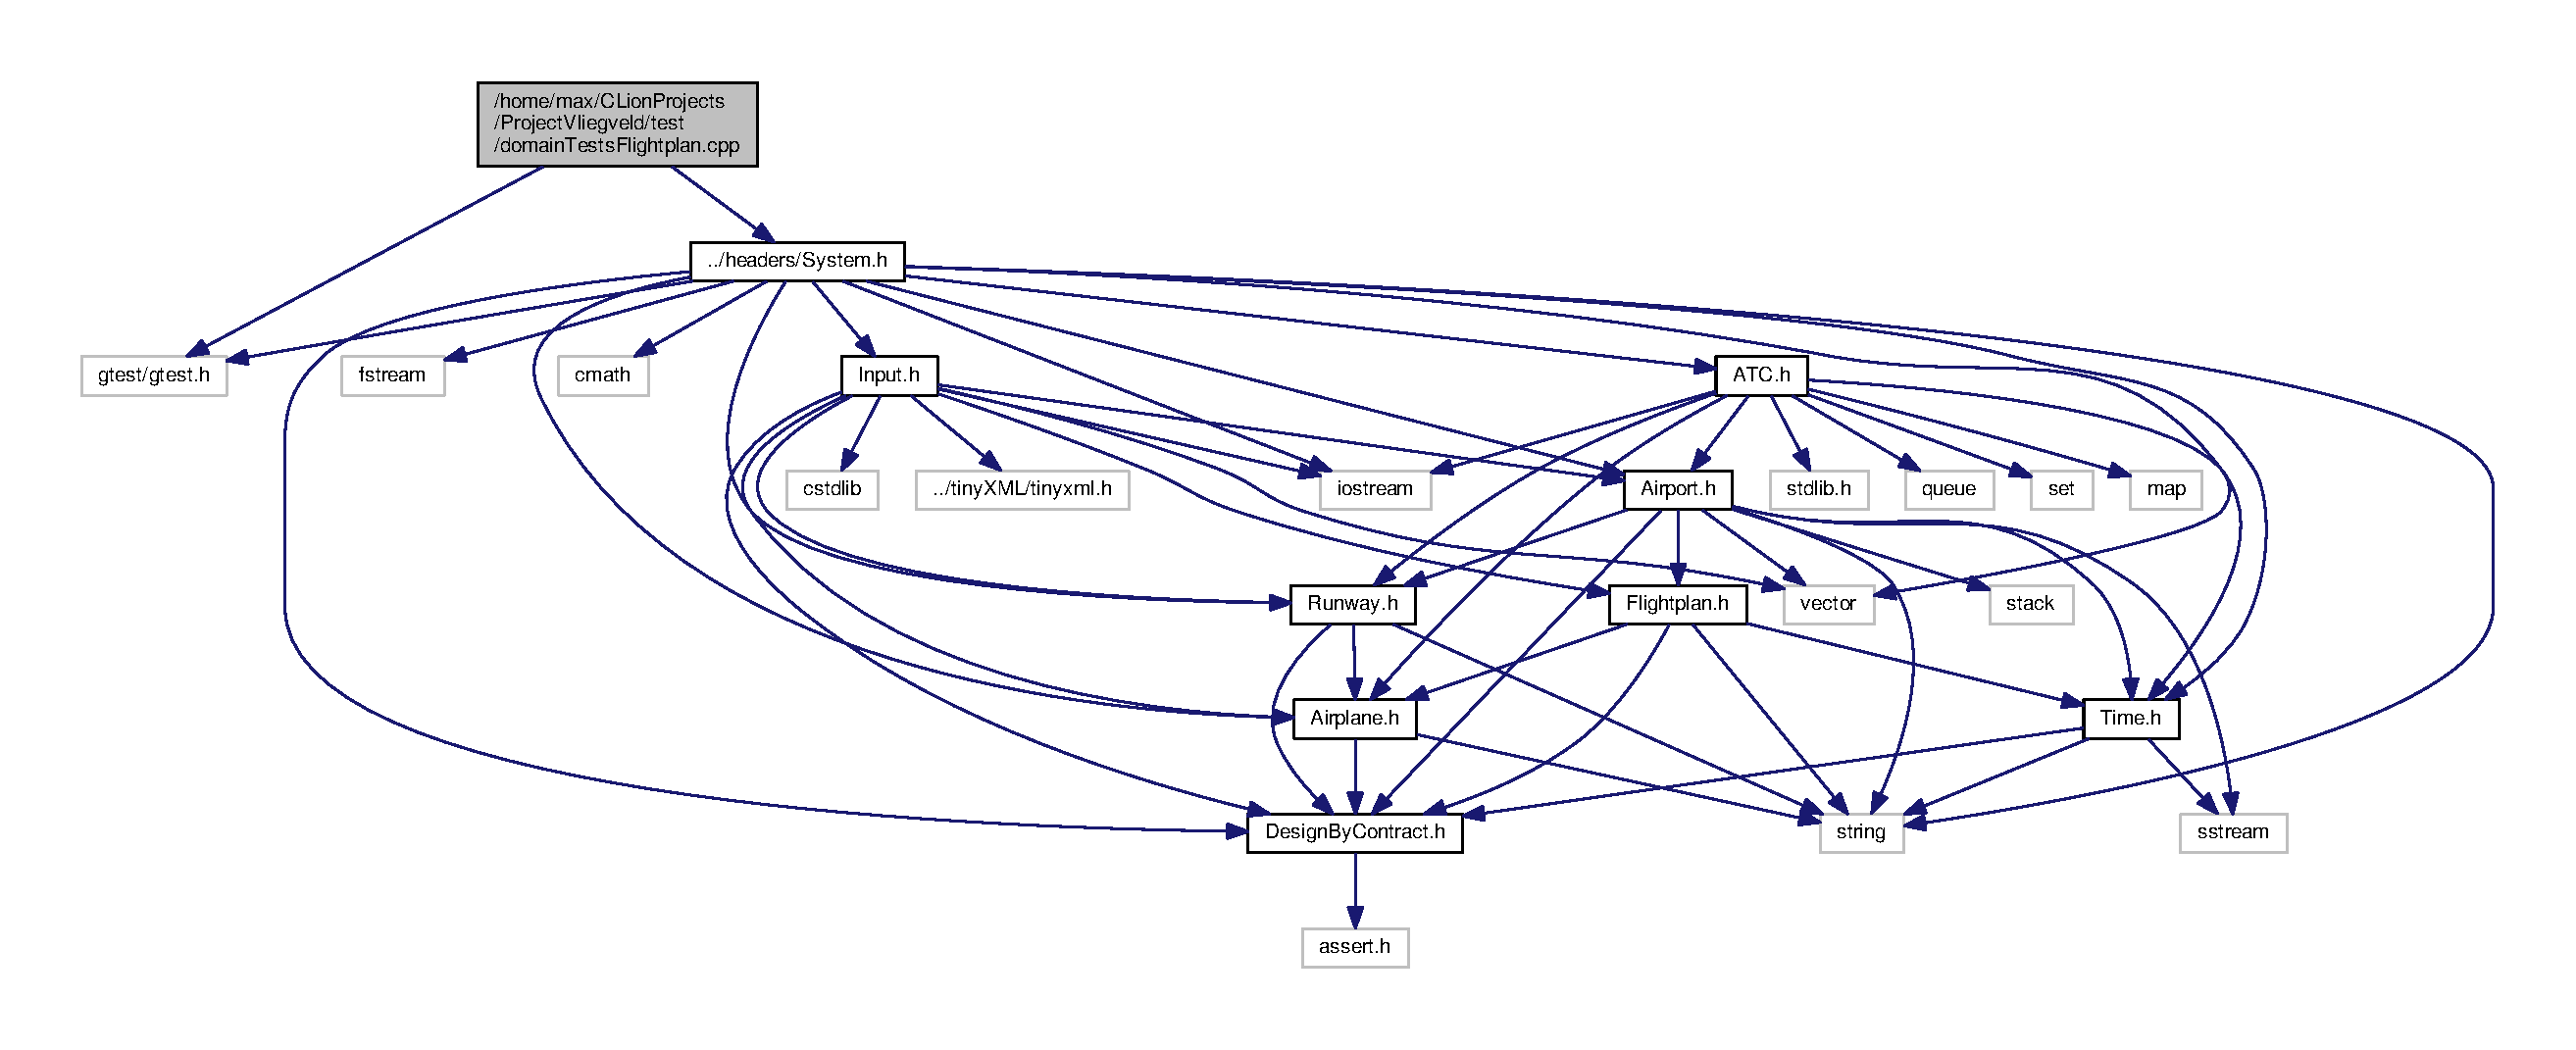
\includegraphics[width=350pt]{domainTestsFlightplan_8cpp__incl}
\end{center}
\end{figure}
\subsection*{Classes}
\begin{DoxyCompactItemize}
\item 
class \hyperlink{classdomainTestFlightplan}{domain\+Test\+Flightplan}
\end{DoxyCompactItemize}
\subsection*{Functions}
\begin{DoxyCompactItemize}
\item 
\hyperlink{domainTestsFlightplan_8cpp_af05d9fe357a8df7fab5307aa1ed33c5b}{T\+E\+S\+T\+\_\+F} (\hyperlink{classdomainTestFlightplan}{domain\+Test\+Flightplan}, default\+Constructor)
\item 
\hyperlink{domainTestsFlightplan_8cpp_a20710a4da05ecacedebb50680df94182}{T\+E\+S\+T\+\_\+F} (\hyperlink{classdomainTestFlightplan}{domain\+Test\+Flightplan}, happy\+Day)
\item 
\hyperlink{domainTestsFlightplan_8cpp_a60e7533d18e915790ec13658773fbd29}{T\+E\+S\+T\+\_\+F} (\hyperlink{classdomainTestFlightplan}{domain\+Test\+Flightplan}, field\+Manipulation)
\item 
\hyperlink{domainTestsFlightplan_8cpp_a486badc1d9e23c600039cedcc1c091a2}{T\+E\+S\+T\+\_\+F} (\hyperlink{classdomainTestFlightplan}{domain\+Test\+Flightplan}, contract\+Violations)
\end{DoxyCompactItemize}


\subsection{Function Documentation}
\index{domain\+Tests\+Flightplan.\+cpp@{domain\+Tests\+Flightplan.\+cpp}!T\+E\+S\+T\+\_\+F@{T\+E\+S\+T\+\_\+F}}
\index{T\+E\+S\+T\+\_\+F@{T\+E\+S\+T\+\_\+F}!domain\+Tests\+Flightplan.\+cpp@{domain\+Tests\+Flightplan.\+cpp}}
\subsubsection[{\texorpdfstring{T\+E\+S\+T\+\_\+\+F(domain\+Test\+Flightplan, default\+Constructor)}{TEST_F(domainTestFlightplan, defaultConstructor)}}]{\setlength{\rightskip}{0pt plus 5cm}T\+E\+S\+T\+\_\+F (
\begin{DoxyParamCaption}
\item[{{\bf domain\+Test\+Flightplan}}]{, }
\item[{default\+Constructor}]{}
\end{DoxyParamCaption}
)}\hypertarget{domainTestsFlightplan_8cpp_af05d9fe357a8df7fab5307aa1ed33c5b}{}\label{domainTestsFlightplan_8cpp_af05d9fe357a8df7fab5307aa1ed33c5b}

\begin{DoxyCode}
19                                                  \{
20     EXPECT\_TRUE(flightplan.properlyInitialized());
21     EXPECT\_EQ(flightplan.getDeparture(), -1);
22     EXPECT\_EQ(flightplan.getArrival(), -1);
23     EXPECT\_EQ(flightplan.getInterval(), -1);
24     EXPECT\_TRUE(flightplan.getAirplane() == NULL);
25 \}
\end{DoxyCode}
\index{domain\+Tests\+Flightplan.\+cpp@{domain\+Tests\+Flightplan.\+cpp}!T\+E\+S\+T\+\_\+F@{T\+E\+S\+T\+\_\+F}}
\index{T\+E\+S\+T\+\_\+F@{T\+E\+S\+T\+\_\+F}!domain\+Tests\+Flightplan.\+cpp@{domain\+Tests\+Flightplan.\+cpp}}
\subsubsection[{\texorpdfstring{T\+E\+S\+T\+\_\+\+F(domain\+Test\+Flightplan, happy\+Day)}{TEST_F(domainTestFlightplan, happyDay)}}]{\setlength{\rightskip}{0pt plus 5cm}T\+E\+S\+T\+\_\+F (
\begin{DoxyParamCaption}
\item[{{\bf domain\+Test\+Flightplan}}]{, }
\item[{happy\+Day}]{}
\end{DoxyParamCaption}
)}\hypertarget{domainTestsFlightplan_8cpp_a20710a4da05ecacedebb50680df94182}{}\label{domainTestsFlightplan_8cpp_a20710a4da05ecacedebb50680df94182}

\begin{DoxyCode}
27                                        \{
28     flightplan.setInterval(1);
29     EXPECT\_EQ(flightplan.getInterval(), 1);
30     flightplan.setArrival(5);
31     EXPECT\_EQ(flightplan.getArrival(), 5);
32     flightplan.setDeparture(12);
33     EXPECT\_EQ(flightplan.getDeparture(), 12);
34 
35     \hyperlink{Flightplan_8h_ab41c9a082b57fd41aefb64a57d8149f8}{EEvent} event;
36     \textcolor{keyword}{event} = flightplan.getEvent(\hyperlink{classTime}{Time}(12, 12));
37     EXPECT\_EQ(event, \hyperlink{Flightplan_8h_ab41c9a082b57fd41aefb64a57d8149f8a81c03ffd159b67afc7df0ffab6a9297f}{kTakeoff});
38     \textcolor{keyword}{event} = flightplan.getEvent(\hyperlink{classTime}{Time}(13, 12));
39     EXPECT\_EQ(event, \hyperlink{Flightplan_8h_ab41c9a082b57fd41aefb64a57d8149f8a81c03ffd159b67afc7df0ffab6a9297f}{kTakeoff});
40 
41     \textcolor{keyword}{event} = flightplan.getEvent(\hyperlink{classTime}{Time}(13, 5));
42     EXPECT\_EQ(event, \hyperlink{Flightplan_8h_ab41c9a082b57fd41aefb64a57d8149f8aeaa0025051cf36faa589b5da72a153c4}{kLand});
43     \textcolor{keyword}{event} = flightplan.getEvent(\hyperlink{classTime}{Time}(12, 5));
44     EXPECT\_EQ(event, \hyperlink{Flightplan_8h_ab41c9a082b57fd41aefb64a57d8149f8aeaa0025051cf36faa589b5da72a153c4}{kLand});
45 
46     \textcolor{keyword}{event} = flightplan.getEvent(\hyperlink{classTime}{Time}(14, 55));
47     EXPECT\_EQ(event, \hyperlink{Flightplan_8h_ab41c9a082b57fd41aefb64a57d8149f8a58584cd9619135e5689ded56238c3427}{kNothing});
48 \}
\end{DoxyCode}
\index{domain\+Tests\+Flightplan.\+cpp@{domain\+Tests\+Flightplan.\+cpp}!T\+E\+S\+T\+\_\+F@{T\+E\+S\+T\+\_\+F}}
\index{T\+E\+S\+T\+\_\+F@{T\+E\+S\+T\+\_\+F}!domain\+Tests\+Flightplan.\+cpp@{domain\+Tests\+Flightplan.\+cpp}}
\subsubsection[{\texorpdfstring{T\+E\+S\+T\+\_\+\+F(domain\+Test\+Flightplan, field\+Manipulation)}{TEST_F(domainTestFlightplan, fieldManipulation)}}]{\setlength{\rightskip}{0pt plus 5cm}T\+E\+S\+T\+\_\+F (
\begin{DoxyParamCaption}
\item[{{\bf domain\+Test\+Flightplan}}]{, }
\item[{field\+Manipulation}]{}
\end{DoxyParamCaption}
)}\hypertarget{domainTestsFlightplan_8cpp_a60e7533d18e915790ec13658773fbd29}{}\label{domainTestsFlightplan_8cpp_a60e7533d18e915790ec13658773fbd29}

\begin{DoxyCode}
50                                                 \{
51     flightplan.setDestination(\textcolor{stringliteral}{"Alpha"});
52     EXPECT\_EQ(flightplan.getDestination(), \textcolor{stringliteral}{"Alpha"});
53 
54     flightplan.setArrival(10);
55     EXPECT\_EQ(flightplan.getArrival(), 10);
56 
57     flightplan.setDeparture(20);
58     EXPECT\_EQ(flightplan.getDeparture(), 20);
59 
60     flightplan.setInterval(3);
61     EXPECT\_EQ(flightplan.getInterval(), 3);
62 
63     flightplan.setAirplane(NULL);
64     EXPECT\_TRUE(flightplan.getAirplane() == NULL);
65 \}
\end{DoxyCode}
\index{domain\+Tests\+Flightplan.\+cpp@{domain\+Tests\+Flightplan.\+cpp}!T\+E\+S\+T\+\_\+F@{T\+E\+S\+T\+\_\+F}}
\index{T\+E\+S\+T\+\_\+F@{T\+E\+S\+T\+\_\+F}!domain\+Tests\+Flightplan.\+cpp@{domain\+Tests\+Flightplan.\+cpp}}
\subsubsection[{\texorpdfstring{T\+E\+S\+T\+\_\+\+F(domain\+Test\+Flightplan, contract\+Violations)}{TEST_F(domainTestFlightplan, contractViolations)}}]{\setlength{\rightskip}{0pt plus 5cm}T\+E\+S\+T\+\_\+F (
\begin{DoxyParamCaption}
\item[{{\bf domain\+Test\+Flightplan}}]{, }
\item[{contract\+Violations}]{}
\end{DoxyParamCaption}
)}\hypertarget{domainTestsFlightplan_8cpp_a486badc1d9e23c600039cedcc1c091a2}{}\label{domainTestsFlightplan_8cpp_a486badc1d9e23c600039cedcc1c091a2}

\begin{DoxyCode}
67                                                  \{
68     EXPECT\_DEATH(flightplan.setDeparture(-2), \textcolor{stringliteral}{"Departure has to be between 0 and 60"});
69     EXPECT\_DEATH(flightplan.setDeparture(65), \textcolor{stringliteral}{"Departure has to be between 0 and 60"});
70     EXPECT\_DEATH(flightplan.setArrival(-6), \textcolor{stringliteral}{"Arrival has to be between 0 and 60"});
71     EXPECT\_DEATH(flightplan.setArrival(200), \textcolor{stringliteral}{"Arrival has to be between 0 and 60"});
72     EXPECT\_DEATH(flightplan.setInterval(0), \textcolor{stringliteral}{"Interval has to be at least 1"});
73 \}\end{DoxyCode}

\hypertarget{domainTestsRunway_8cpp}{}\section{/home/max/\+C\+Lion\+Projects/\+Project\+Vliegveld/test/domain\+Tests\+Runway.cpp File Reference}
\label{domainTestsRunway_8cpp}\index{/home/max/\+C\+Lion\+Projects/\+Project\+Vliegveld/test/domain\+Tests\+Runway.\+cpp@{/home/max/\+C\+Lion\+Projects/\+Project\+Vliegveld/test/domain\+Tests\+Runway.\+cpp}}
{\ttfamily \#include $<$gtest/gtest.\+h$>$}\\*
{\ttfamily \#include \char`\"{}../headers/\+System.\+h\char`\"{}}\\*
Include dependency graph for domain\+Tests\+Runway.\+cpp\+:
\nopagebreak
\begin{figure}[H]
\begin{center}
\leavevmode
\includegraphics[width=350pt]{domainTestsRunway_8cpp__incl}
\end{center}
\end{figure}
\subsection*{Classes}
\begin{DoxyCompactItemize}
\item 
class \hyperlink{classdomainTestRunway}{domain\+Test\+Runway}
\end{DoxyCompactItemize}
\subsection*{Functions}
\begin{DoxyCompactItemize}
\item 
\hyperlink{domainTestsRunway_8cpp_adbd3fc9764de96926ee04a49f6127984}{T\+E\+S\+T\+\_\+F} (\hyperlink{classdomainTestRunway}{domain\+Test\+Runway}, Default\+Constructor)
\item 
\hyperlink{domainTestsRunway_8cpp_a597128efd87c7da3a1ec5febae120da2}{T\+E\+S\+T\+\_\+F} (\hyperlink{classdomainTestRunway}{domain\+Test\+Runway}, happy\+Day)
\item 
\hyperlink{domainTestsRunway_8cpp_ab1852781b57c7840b0ac5f2b4f61006b}{T\+E\+S\+T\+\_\+F} (\hyperlink{classdomainTestRunway}{domain\+Test\+Runway}, complete)
\item 
\hyperlink{domainTestsRunway_8cpp_abeaa480a1f7ced337e02db2732933b0b}{T\+E\+S\+T\+\_\+F} (\hyperlink{classdomainTestRunway}{domain\+Test\+Runway}, field\+Manipulation)
\item 
\hyperlink{domainTestsRunway_8cpp_aaef9b34c44845a4bf131fd2c16bcae76}{T\+E\+S\+T\+\_\+F} (\hyperlink{classdomainTestRunway}{domain\+Test\+Runway}, Contract\+Violations)
\end{DoxyCompactItemize}


\subsection{Function Documentation}
\index{domain\+Tests\+Runway.\+cpp@{domain\+Tests\+Runway.\+cpp}!T\+E\+S\+T\+\_\+F@{T\+E\+S\+T\+\_\+F}}
\index{T\+E\+S\+T\+\_\+F@{T\+E\+S\+T\+\_\+F}!domain\+Tests\+Runway.\+cpp@{domain\+Tests\+Runway.\+cpp}}
\subsubsection[{\texorpdfstring{T\+E\+S\+T\+\_\+\+F(domain\+Test\+Runway, Default\+Constructor)}{TEST_F(domainTestRunway, DefaultConstructor)}}]{\setlength{\rightskip}{0pt plus 5cm}T\+E\+S\+T\+\_\+F (
\begin{DoxyParamCaption}
\item[{{\bf domain\+Test\+Runway}}]{, }
\item[{Default\+Constructor}]{}
\end{DoxyParamCaption}
)}\hypertarget{domainTestsRunway_8cpp_adbd3fc9764de96926ee04a49f6127984}{}\label{domainTestsRunway_8cpp_adbd3fc9764de96926ee04a49f6127984}

\begin{DoxyCode}
18                                              \{
19     EXPECT\_TRUE(runway.properlyInitialized());
20 \}
\end{DoxyCode}
\index{domain\+Tests\+Runway.\+cpp@{domain\+Tests\+Runway.\+cpp}!T\+E\+S\+T\+\_\+F@{T\+E\+S\+T\+\_\+F}}
\index{T\+E\+S\+T\+\_\+F@{T\+E\+S\+T\+\_\+F}!domain\+Tests\+Runway.\+cpp@{domain\+Tests\+Runway.\+cpp}}
\subsubsection[{\texorpdfstring{T\+E\+S\+T\+\_\+\+F(domain\+Test\+Runway, happy\+Day)}{TEST_F(domainTestRunway, happyDay)}}]{\setlength{\rightskip}{0pt plus 5cm}T\+E\+S\+T\+\_\+F (
\begin{DoxyParamCaption}
\item[{{\bf domain\+Test\+Runway}}]{, }
\item[{happy\+Day}]{}
\end{DoxyParamCaption}
)}\hypertarget{domainTestsRunway_8cpp_a597128efd87c7da3a1ec5febae120da2}{}\label{domainTestsRunway_8cpp_a597128efd87c7da3a1ec5febae120da2}

\begin{DoxyCode}
22                                    \{
23     EXPECT\_TRUE(runway.properlyInitialized());
24     runway.setAirport(\textcolor{keyword}{new} \hyperlink{classAirport}{Airport}());
25     runway.setName(\textcolor{stringliteral}{"RW1"});
26     runway.setTaxiPoint(\textcolor{stringliteral}{"Alpha"});
27     runway.setLength(1000);
28     runway.setType(\hyperlink{Runway_8h_adbb3e23fdb96fa1bac0dbbae33431cd2ae0b5b4fcb396cd73cb79793039658380}{kAsphalt});
29     EXPECT\_TRUE(runway.complete());
30 
31     \textcolor{comment}{// small, prop}
32     plane.setSize(\hyperlink{Airplane_8h_a0526623f951311ba6780209b9e278dbfaf99aeb93b2774bc0c7856d1510d17a54}{kSmall});
33     plane.setEngine(\hyperlink{Airplane_8h_a3d2a8adb53da58e78cb0018d784e791daef171fc98c472a2acd2338353679dcc3}{kPropeller});
34     EXPECT\_TRUE(runway.validForAirplane(&plane));
35     \textcolor{comment}{// small, jet}
36     plane.setEngine(\hyperlink{Airplane_8h_a3d2a8adb53da58e78cb0018d784e791da6262caeb7b5646a03a202006f584364c}{kJet});
37     EXPECT\_TRUE(runway.validForAirplane(&plane));
38     \textcolor{comment}{// medium, jet}
39     plane.setSize(\hyperlink{Airplane_8h_a0526623f951311ba6780209b9e278dbfabade85bef98ad2c69fb2216bb947b6c3}{kMedium});
40     EXPECT\_FALSE(runway.validForAirplane(&plane));
41     \textcolor{comment}{// medium, prop}
42     plane.setEngine(\hyperlink{Airplane_8h_a3d2a8adb53da58e78cb0018d784e791daef171fc98c472a2acd2338353679dcc3}{kPropeller});
43     EXPECT\_TRUE(runway.validForAirplane(&plane));
44     \textcolor{comment}{// large, prop}
45     plane.setSize(\hyperlink{Airplane_8h_a0526623f951311ba6780209b9e278dbfa6b6a05b83fa2f5308724e45442b38b7e}{kLarge});
46     EXPECT\_FALSE(runway.validForAirplane(&plane));
47     \textcolor{comment}{// large, jet}
48     plane.setEngine(\hyperlink{Airplane_8h_a3d2a8adb53da58e78cb0018d784e791da6262caeb7b5646a03a202006f584364c}{kJet});
49     EXPECT\_FALSE(runway.validForAirplane(&plane));
50 
51     \textcolor{comment}{// long enough for large jet, with correct type}
52     runway.setLength(3000);
53     EXPECT\_TRUE(runway.validForAirplane(&plane));
54 
55     \textcolor{comment}{// not long enough for large jet, with correct type}
56     runway.setLength(1000);
57     EXPECT\_FALSE(runway.validForAirplane(&plane));
58 
59     \textcolor{comment}{// long enough for large jet, with incorrect type}
60     runway.setLength(3000);
61     runway.setType(\hyperlink{Runway_8h_adbb3e23fdb96fa1bac0dbbae33431cd2ae97f33599679c1a293bb8403f4a7a8f7}{kGrass});
62     EXPECT\_FALSE(runway.validForAirplane(&plane));
63 \}
\end{DoxyCode}
\index{domain\+Tests\+Runway.\+cpp@{domain\+Tests\+Runway.\+cpp}!T\+E\+S\+T\+\_\+F@{T\+E\+S\+T\+\_\+F}}
\index{T\+E\+S\+T\+\_\+F@{T\+E\+S\+T\+\_\+F}!domain\+Tests\+Runway.\+cpp@{domain\+Tests\+Runway.\+cpp}}
\subsubsection[{\texorpdfstring{T\+E\+S\+T\+\_\+\+F(domain\+Test\+Runway, complete)}{TEST_F(domainTestRunway, complete)}}]{\setlength{\rightskip}{0pt plus 5cm}T\+E\+S\+T\+\_\+F (
\begin{DoxyParamCaption}
\item[{{\bf domain\+Test\+Runway}}]{, }
\item[{complete}]{}
\end{DoxyParamCaption}
)}\hypertarget{domainTestsRunway_8cpp_ab1852781b57c7840b0ac5f2b4f61006b}{}\label{domainTestsRunway_8cpp_ab1852781b57c7840b0ac5f2b4f61006b}

\begin{DoxyCode}
65                                    \{
66     EXPECT\_FALSE(runway.complete());
67     runway.setType(\hyperlink{Runway_8h_adbb3e23fdb96fa1bac0dbbae33431cd2ae97f33599679c1a293bb8403f4a7a8f7}{kGrass});
68 
69     EXPECT\_FALSE(runway.complete());
70     runway.setAirport(\textcolor{keyword}{new} \hyperlink{classAirport}{Airport}());
71 
72     EXPECT\_FALSE(runway.complete());
73     runway.setLength(1000);
74 
75     EXPECT\_FALSE(runway.complete());
76     runway.setName(\textcolor{stringliteral}{"RW1"});
77 
78     EXPECT\_FALSE(runway.complete());
79     runway.setTaxiPoint(\textcolor{stringliteral}{"Alpha"});
80 
81     EXPECT\_TRUE(runway.complete());
82 
83     \textcolor{keyword}{delete} runway.getAirport();
84 \}
\end{DoxyCode}
\index{domain\+Tests\+Runway.\+cpp@{domain\+Tests\+Runway.\+cpp}!T\+E\+S\+T\+\_\+F@{T\+E\+S\+T\+\_\+F}}
\index{T\+E\+S\+T\+\_\+F@{T\+E\+S\+T\+\_\+F}!domain\+Tests\+Runway.\+cpp@{domain\+Tests\+Runway.\+cpp}}
\subsubsection[{\texorpdfstring{T\+E\+S\+T\+\_\+\+F(domain\+Test\+Runway, field\+Manipulation)}{TEST_F(domainTestRunway, fieldManipulation)}}]{\setlength{\rightskip}{0pt plus 5cm}T\+E\+S\+T\+\_\+F (
\begin{DoxyParamCaption}
\item[{{\bf domain\+Test\+Runway}}]{, }
\item[{field\+Manipulation}]{}
\end{DoxyParamCaption}
)}\hypertarget{domainTestsRunway_8cpp_abeaa480a1f7ced337e02db2732933b0b}{}\label{domainTestsRunway_8cpp_abeaa480a1f7ced337e02db2732933b0b}

\begin{DoxyCode}
86                                             \{
87     \hyperlink{classAirport}{Airport} *\hyperlink{docs_2html_2jquery_8js_a6ddf393cc7f9a8828e197bb0d9916c44}{ap} = \textcolor{keyword}{new} \hyperlink{classAirport}{Airport}();
88 
89     runway.setType(\hyperlink{Runway_8h_adbb3e23fdb96fa1bac0dbbae33431cd2ae97f33599679c1a293bb8403f4a7a8f7}{kGrass});
90     EXPECT\_EQ(runway.getType(), \hyperlink{Runway_8h_adbb3e23fdb96fa1bac0dbbae33431cd2ae97f33599679c1a293bb8403f4a7a8f7}{kGrass});
91 
92     runway.setLength(1000);
93     EXPECT\_EQ(runway.getLength(), 1000);
94 
95     runway.setName(\textcolor{stringliteral}{"RW1"});
96     EXPECT\_EQ(runway.getName(), \textcolor{stringliteral}{"RW1"});
97 
98     runway.setFree(\textcolor{keyword}{true});
99     EXPECT\_TRUE(runway.isFree());
100 
101     runway.setFree(\textcolor{keyword}{false});
102     EXPECT\_FALSE(runway.isFree());
103 
104     runway.setTaxiPoint(\textcolor{stringliteral}{"Alpha"});
105     EXPECT\_EQ(runway.getTaxiPoint(), \textcolor{stringliteral}{"Alpha"});
106 
107     runway.setAirport(ap);
108     EXPECT\_EQ(runway.getAirport(), \hyperlink{docs_2html_2jquery_8js_a6ddf393cc7f9a8828e197bb0d9916c44}{ap});
109 
110     \textcolor{keyword}{delete} \hyperlink{docs_2html_2jquery_8js_a6ddf393cc7f9a8828e197bb0d9916c44}{ap};
111 \}
\end{DoxyCode}
\index{domain\+Tests\+Runway.\+cpp@{domain\+Tests\+Runway.\+cpp}!T\+E\+S\+T\+\_\+F@{T\+E\+S\+T\+\_\+F}}
\index{T\+E\+S\+T\+\_\+F@{T\+E\+S\+T\+\_\+F}!domain\+Tests\+Runway.\+cpp@{domain\+Tests\+Runway.\+cpp}}
\subsubsection[{\texorpdfstring{T\+E\+S\+T\+\_\+\+F(domain\+Test\+Runway, Contract\+Violations)}{TEST_F(domainTestRunway, ContractViolations)}}]{\setlength{\rightskip}{0pt plus 5cm}T\+E\+S\+T\+\_\+F (
\begin{DoxyParamCaption}
\item[{{\bf domain\+Test\+Runway}}]{, }
\item[{Contract\+Violations}]{}
\end{DoxyParamCaption}
)}\hypertarget{domainTestsRunway_8cpp_aaef9b34c44845a4bf131fd2c16bcae76}{}\label{domainTestsRunway_8cpp_aaef9b34c44845a4bf131fd2c16bcae76}

\begin{DoxyCode}
113                                              \{
114     EXPECT\_DEATH(runway.validForAirplane(NULL), \textcolor{stringliteral}{"Plane object does not exist."});
115 \}\end{DoxyCode}

\hypertarget{domainTestsSystem_8cpp}{}\section{/home/max/\+C\+Lion\+Projects/\+Project\+Vliegveld/test/domain\+Tests\+System.cpp File Reference}
\label{domainTestsSystem_8cpp}\index{/home/max/\+C\+Lion\+Projects/\+Project\+Vliegveld/test/domain\+Tests\+System.\+cpp@{/home/max/\+C\+Lion\+Projects/\+Project\+Vliegveld/test/domain\+Tests\+System.\+cpp}}
{\ttfamily \#include $<$gtest/gtest.\+h$>$}\\*
{\ttfamily \#include \char`\"{}../headers/\+System.\+h\char`\"{}}\\*
Include dependency graph for domain\+Tests\+System.\+cpp\+:
\nopagebreak
\begin{figure}[H]
\begin{center}
\leavevmode
\includegraphics[width=350pt]{domainTestsSystem_8cpp__incl}
\end{center}
\end{figure}
\subsection*{Classes}
\begin{DoxyCompactItemize}
\item 
class \hyperlink{classdomainTestSystem}{domain\+Test\+System}
\end{DoxyCompactItemize}
\subsection*{Functions}
\begin{DoxyCompactItemize}
\item 
\hyperlink{domainTestsSystem_8cpp_a6ba79cabeb9d176a786e8c1d05eab5f3}{T\+E\+S\+T\+\_\+F} (\hyperlink{classdomainTestSystem}{domain\+Test\+System}, approach)
\item 
\hyperlink{domainTestsSystem_8cpp_ac3d7b5760edcdbe5117500055e3a0b11}{T\+E\+S\+T\+\_\+F} (\hyperlink{classdomainTestSystem}{domain\+Test\+System}, descend)
\item 
\hyperlink{domainTestsSystem_8cpp_ac76aad39455b031f442b4efb7cb2f779}{T\+E\+S\+T\+\_\+F} (\hyperlink{classdomainTestSystem}{domain\+Test\+System}, circle)
\item 
\hyperlink{domainTestsSystem_8cpp_a96cd9d20aa12cad65b5333e5f50003ac}{T\+E\+S\+T\+\_\+F} (\hyperlink{classdomainTestSystem}{domain\+Test\+System}, taxi\+Arrival)
\item 
\hyperlink{domainTestsSystem_8cpp_a46e29d881e2d74b791a790cc39a6f253}{T\+E\+S\+T\+\_\+F} (\hyperlink{classdomainTestSystem}{domain\+Test\+System}, cross\+Arrival)
\item 
\hyperlink{domainTestsSystem_8cpp_ad6568c16d6f9cf0ae4983b6bd4a99051}{T\+E\+S\+T\+\_\+F} (\hyperlink{classdomainTestSystem}{domain\+Test\+System}, deboard)
\item 
\hyperlink{domainTestsSystem_8cpp_ad29fcb5852f941bb2678fa00c1694445}{T\+E\+S\+T\+\_\+F} (\hyperlink{classdomainTestSystem}{domain\+Test\+System}, technical\+Check)
\item 
\hyperlink{domainTestsSystem_8cpp_a0fddb2bb9705778e9c0e34b35768be02}{T\+E\+S\+T\+\_\+F} (\hyperlink{classdomainTestSystem}{domain\+Test\+System}, simulation\+Finished)
\item 
\hyperlink{domainTestsSystem_8cpp_ae8e67de1af4134959a6f2be081beb865}{T\+E\+S\+T\+\_\+F} (\hyperlink{classdomainTestSystem}{domain\+Test\+System}, import)
\item 
\hyperlink{domainTestsSystem_8cpp_a5b9b0972d311421f16ed5390ce676a14}{T\+E\+S\+T\+\_\+F} (\hyperlink{classdomainTestSystem}{domain\+Test\+System}, ascend)
\item 
\hyperlink{domainTestsSystem_8cpp_a65c3cefc33bc9d5f7929cd045d0a375e}{T\+E\+S\+T\+\_\+F} (\hyperlink{classdomainTestSystem}{domain\+Test\+System}, on\+Runway)
\item 
\hyperlink{domainTestsSystem_8cpp_ad809680467ecb4b3499e0d047e73edf1}{T\+E\+S\+T\+\_\+F} (\hyperlink{classdomainTestSystem}{domain\+Test\+System}, at\+Runway)
\item 
\hyperlink{domainTestsSystem_8cpp_a8134f6d41f69f870de2a154a25facb4f}{T\+E\+S\+T\+\_\+F} (\hyperlink{classdomainTestSystem}{domain\+Test\+System}, taxi\+Departure\+Cross)
\item 
\hyperlink{domainTestsSystem_8cpp_adefd20a4a2ddd3cb69d7b0dacb06c525}{T\+E\+S\+T\+\_\+F} (\hyperlink{classdomainTestSystem}{domain\+Test\+System}, taxi\+Departure\+Step)
\item 
\hyperlink{domainTestsSystem_8cpp_a145038166b19647e3b7a153f9f22a3fc}{T\+E\+S\+T\+\_\+F} (\hyperlink{classdomainTestSystem}{domain\+Test\+System}, taxi\+Departure\+Start)
\item 
\hyperlink{domainTestsSystem_8cpp_a5f54c430bbbd8365b0178ec1847b71e5}{T\+E\+S\+T\+\_\+F} (\hyperlink{classdomainTestSystem}{domain\+Test\+System}, pushback)
\item 
\hyperlink{domainTestsSystem_8cpp_ae2eb3137e2b15c16f3966e4316775b3b}{T\+E\+S\+T\+\_\+F} (\hyperlink{classdomainTestSystem}{domain\+Test\+System}, prepare)
\item 
\hyperlink{domainTestsSystem_8cpp_aee03e079a6cdba0a0a9d57c1aba4f47d}{T\+E\+S\+T\+\_\+F} (\hyperlink{classdomainTestSystem}{domain\+Test\+System}, field\+Manipulation)
\end{DoxyCompactItemize}


\subsection{Function Documentation}
\index{domain\+Tests\+System.\+cpp@{domain\+Tests\+System.\+cpp}!T\+E\+S\+T\+\_\+F@{T\+E\+S\+T\+\_\+F}}
\index{T\+E\+S\+T\+\_\+F@{T\+E\+S\+T\+\_\+F}!domain\+Tests\+System.\+cpp@{domain\+Tests\+System.\+cpp}}
\subsubsection[{\texorpdfstring{T\+E\+S\+T\+\_\+\+F(domain\+Test\+System, approach)}{TEST_F(domainTestSystem, approach)}}]{\setlength{\rightskip}{0pt plus 5cm}T\+E\+S\+T\+\_\+F (
\begin{DoxyParamCaption}
\item[{{\bf domain\+Test\+System}}]{, }
\item[{approach}]{}
\end{DoxyParamCaption}
)}\hypertarget{domainTestsSystem_8cpp_a6ba79cabeb9d176a786e8c1d05eab5f3}{}\label{domainTestsSystem_8cpp_a6ba79cabeb9d176a786e8c1d05eab5f3}

\begin{DoxyCode}
37                                    \{
38     \textcolor{comment}{// Plane approaches and hasn't send a request to atc}
39     airplane->setStatus(\hyperlink{Airplane_8h_a0e5bbf7c6c727baaba49062300fae19fa2c6325ac177ddfbe70edf92941c4e8e0}{kApproaching});
40     airplane->setRequest(\hyperlink{Airplane_8h_a4a8a3f45932bdf601f093bea061bad9ba19d8199da79ca4c28eb644052b08f632}{kIdle});
41     system.approach(airplane, out);
42     EXPECT\_EQ(airplane->getRequest(), \hyperlink{Airplane_8h_a4a8a3f45932bdf601f093bea061bad9bad143035084d581f7aecfabd95652e62c}{kPending});
43     EXPECT\_EQ(airplane->getStatus(), \hyperlink{Airplane_8h_a0e5bbf7c6c727baaba49062300fae19fa2c6325ac177ddfbe70edf92941c4e8e0}{kApproaching});
44 
45     \textcolor{comment}{// Plane approaches and atc hasn't responded yet}
46     system.approach(airplane, out);
47     EXPECT\_EQ(airplane->getRequest(), \hyperlink{Airplane_8h_a4a8a3f45932bdf601f093bea061bad9bad143035084d581f7aecfabd95652e62c}{kPending});
48     EXPECT\_EQ(airplane->getStatus(), \hyperlink{Airplane_8h_a0e5bbf7c6c727baaba49062300fae19fa2c6325ac177ddfbe70edf92941c4e8e0}{kApproaching});
49 
50     \textcolor{comment}{// Plane approaches and atc has accepted request}
51     airplane->setRequest(\hyperlink{Airplane_8h_a4a8a3f45932bdf601f093bea061bad9ba15597ea7f444a937d40b39b9ea99dd1d}{kAccepted});
52     system.approach(airplane, out);
53     EXPECT\_EQ(airplane->getRequest(), \hyperlink{Airplane_8h_a4a8a3f45932bdf601f093bea061bad9ba19d8199da79ca4c28eb644052b08f632}{kIdle});
54     EXPECT\_EQ(airplane->getAltitude(), 10);
55     EXPECT\_EQ(airplane->getStatus(), \hyperlink{Airplane_8h_a0e5bbf7c6c727baaba49062300fae19fa65b72f8e33cb194d21d822e5b6626e2e}{kDescending});
56 \}
\end{DoxyCode}
\index{domain\+Tests\+System.\+cpp@{domain\+Tests\+System.\+cpp}!T\+E\+S\+T\+\_\+F@{T\+E\+S\+T\+\_\+F}}
\index{T\+E\+S\+T\+\_\+F@{T\+E\+S\+T\+\_\+F}!domain\+Tests\+System.\+cpp@{domain\+Tests\+System.\+cpp}}
\subsubsection[{\texorpdfstring{T\+E\+S\+T\+\_\+\+F(domain\+Test\+System, descend)}{TEST_F(domainTestSystem, descend)}}]{\setlength{\rightskip}{0pt plus 5cm}T\+E\+S\+T\+\_\+F (
\begin{DoxyParamCaption}
\item[{{\bf domain\+Test\+System}}]{, }
\item[{descend}]{}
\end{DoxyParamCaption}
)}\hypertarget{domainTestsSystem_8cpp_ac3d7b5760edcdbe5117500055e3a0b11}{}\label{domainTestsSystem_8cpp_ac3d7b5760edcdbe5117500055e3a0b11}

\begin{DoxyCode}
58                                   \{
59     \textcolor{comment}{// Normal descend}
60     airplane->setStatus(\hyperlink{Airplane_8h_a0e5bbf7c6c727baaba49062300fae19fa65b72f8e33cb194d21d822e5b6626e2e}{kDescending});
61     airplane->setAltitude(10);
62     system.descend(airplane, out);
63     EXPECT\_EQ(airplane->getAltitude(), 9);
64     EXPECT\_EQ(airplane->getStatus(), \hyperlink{Airplane_8h_a0e5bbf7c6c727baaba49062300fae19fa65b72f8e33cb194d21d822e5b6626e2e}{kDescending});
65 
66     \textcolor{comment}{// Plane at 3000ft and can land}
67     airplane->setRequest(\hyperlink{Airplane_8h_a4a8a3f45932bdf601f093bea061bad9ba85d56dac5419035294b1c769317026fa}{kConfirmed});
68     airplane->setAltitude(3);
69     airplane->setRunway(runway);
70     system.descend(airplane, out);
71     EXPECT\_EQ(airplane->getAltitude(), 2);
72     EXPECT\_EQ(airplane->getStatus(), \hyperlink{Airplane_8h_a0e5bbf7c6c727baaba49062300fae19fa65b72f8e33cb194d21d822e5b6626e2e}{kDescending});
73 
74     \textcolor{comment}{// Plane at 3000ft and has to circle}
75     airplane->setRequest(\hyperlink{Airplane_8h_a4a8a3f45932bdf601f093bea061bad9baac195c08fab2dff9d0520caf49ea4e11}{kDenied});
76     airplane->setAltitude(3);
77     system.descend(airplane, out);
78     EXPECT\_EQ(airplane->getStatus(), \hyperlink{Airplane_8h_a0e5bbf7c6c727baaba49062300fae19fa4459995e4bdd3412bbe3d741b3941158}{kCircling});
79     EXPECT\_EQ(airplane->getAltitude(), 3);
80 
81     \textcolor{comment}{// Plane has landed}
82     airplane->setAltitude(0);
83     airplane->setStatus(\hyperlink{Airplane_8h_a0e5bbf7c6c727baaba49062300fae19fa65b72f8e33cb194d21d822e5b6626e2e}{kDescending});
84     system.descend(airplane, out);
85     EXPECT\_EQ(airplane->getStatus(), \hyperlink{Airplane_8h_a0e5bbf7c6c727baaba49062300fae19fabe52f2e86df226a44cc8ba29e8f259b2}{kTaxiArrival});
86     EXPECT\_EQ(airplane->getRequest(), \hyperlink{Airplane_8h_a4a8a3f45932bdf601f093bea061bad9ba19d8199da79ca4c28eb644052b08f632}{kIdle});
87 \}
\end{DoxyCode}
\index{domain\+Tests\+System.\+cpp@{domain\+Tests\+System.\+cpp}!T\+E\+S\+T\+\_\+F@{T\+E\+S\+T\+\_\+F}}
\index{T\+E\+S\+T\+\_\+F@{T\+E\+S\+T\+\_\+F}!domain\+Tests\+System.\+cpp@{domain\+Tests\+System.\+cpp}}
\subsubsection[{\texorpdfstring{T\+E\+S\+T\+\_\+\+F(domain\+Test\+System, circle)}{TEST_F(domainTestSystem, circle)}}]{\setlength{\rightskip}{0pt plus 5cm}T\+E\+S\+T\+\_\+F (
\begin{DoxyParamCaption}
\item[{{\bf domain\+Test\+System}}]{, }
\item[{circle}]{}
\end{DoxyParamCaption}
)}\hypertarget{domainTestsSystem_8cpp_ac76aad39455b031f442b4efb7cb2f779}{}\label{domainTestsSystem_8cpp_ac76aad39455b031f442b4efb7cb2f779}

\begin{DoxyCode}
89                                  \{
90     \textcolor{comment}{// Very simple function so very simple test}
91     system.circle(airplane, out);
92     EXPECT\_EQ(airplane->getStatus(), \hyperlink{Airplane_8h_a0e5bbf7c6c727baaba49062300fae19fa65b72f8e33cb194d21d822e5b6626e2e}{kDescending});
93 \}
\end{DoxyCode}
\index{domain\+Tests\+System.\+cpp@{domain\+Tests\+System.\+cpp}!T\+E\+S\+T\+\_\+F@{T\+E\+S\+T\+\_\+F}}
\index{T\+E\+S\+T\+\_\+F@{T\+E\+S\+T\+\_\+F}!domain\+Tests\+System.\+cpp@{domain\+Tests\+System.\+cpp}}
\subsubsection[{\texorpdfstring{T\+E\+S\+T\+\_\+\+F(domain\+Test\+System, taxi\+Arrival)}{TEST_F(domainTestSystem, taxiArrival)}}]{\setlength{\rightskip}{0pt plus 5cm}T\+E\+S\+T\+\_\+F (
\begin{DoxyParamCaption}
\item[{{\bf domain\+Test\+System}}]{, }
\item[{taxi\+Arrival}]{}
\end{DoxyParamCaption}
)}\hypertarget{domainTestsSystem_8cpp_a96cd9d20aa12cad65b5333e5f50003ac}{}\label{domainTestsSystem_8cpp_a96cd9d20aa12cad65b5333e5f50003ac}

\begin{DoxyCode}
95                                       \{
96     \textcolor{comment}{// Arrived at gate}
97     airplane->setPosition(runway->getTaxiPoint());
98     airplane->setRequest(\hyperlink{Airplane_8h_a4a8a3f45932bdf601f093bea061bad9ba85d56dac5419035294b1c769317026fa}{kConfirmed});
99     airplane->setPassengers(7);
100     system.taxiArrival(airplane, out);
101     EXPECT\_TRUE(airplane->getPosition().empty());
102     EXPECT\_EQ(airplane->getStatus(), \hyperlink{Airplane_8h_a0e5bbf7c6c727baaba49062300fae19fa5c095afa8db10ea77f3303a7b8573cdf}{kDeboarding});
103     EXPECT\_EQ(airplane->getTimeRemaining(), 4);
104 
105     \textcolor{comment}{// Arrived at taxipoint}
106     airplane->setStatus(\hyperlink{Airplane_8h_a0e5bbf7c6c727baaba49062300fae19fabe52f2e86df226a44cc8ba29e8f259b2}{kTaxiArrival});
107     airplane->setPosition(system.getAirport()->getRunways()[1]->getTaxiPoint());
108     airplane->setRequest(\hyperlink{Airplane_8h_a4a8a3f45932bdf601f093bea061bad9ba85d56dac5419035294b1c769317026fa}{kConfirmed});
109     system.taxiArrival(airplane, out);
110     EXPECT\_EQ(airplane->getRequest(), \hyperlink{Airplane_8h_a4a8a3f45932bdf601f093bea061bad9ba19d8199da79ca4c28eb644052b08f632}{kIdle});
111 
112     \textcolor{comment}{// Hasn't send a request yet for taxi instructions}
113     airplane->setPosition(system.getAirport()->getRunways()[1]->getTaxiPoint());
114     airplane->setRequest(\hyperlink{Airplane_8h_a4a8a3f45932bdf601f093bea061bad9ba19d8199da79ca4c28eb644052b08f632}{kIdle});
115     system.taxiArrival(airplane, out);
116     EXPECT\_EQ(airplane->getRequest(), \hyperlink{Airplane_8h_a4a8a3f45932bdf601f093bea061bad9bad143035084d581f7aecfabd95652e62c}{kPending});
117 
118     \textcolor{comment}{// Request has been accepted, plane just landed}
119     airplane->setRequest(\hyperlink{Airplane_8h_a4a8a3f45932bdf601f093bea061bad9ba15597ea7f444a937d40b39b9ea99dd1d}{kAccepted});
120     airplane->setPosition(\textcolor{stringliteral}{""});
121     airplane->setRunway(runway);
122     system.taxiArrival(airplane, out);
123     EXPECT\_EQ(airplane->getStatus(), \hyperlink{Airplane_8h_a0e5bbf7c6c727baaba49062300fae19fabe52f2e86df226a44cc8ba29e8f259b2}{kTaxiArrival});
124     EXPECT\_EQ(airplane->getPosition(), airplane->getRunway()->getTaxiPoint());
125     EXPECT\_EQ(airplane->getRequest(), \hyperlink{Airplane_8h_a4a8a3f45932bdf601f093bea061bad9ba85d56dac5419035294b1c769317026fa}{kConfirmed});
126     EXPECT\_EQ(airplane->getTimeRemaining(), 5);
127 
128     \textcolor{comment}{// Request has been accepted, plane crosses a runway}
129     airplane->setRequest(\hyperlink{Airplane_8h_a4a8a3f45932bdf601f093bea061bad9ba15597ea7f444a937d40b39b9ea99dd1d}{kAccepted});
130     airplane->setPosition(system.getAirport()->getRunways()[1]->getTaxiPoint());
131     system.taxiArrival(airplane, out);
132     EXPECT\_EQ(airplane->getStatus(), \hyperlink{Airplane_8h_a0e5bbf7c6c727baaba49062300fae19fac8a18187b65420ae9ceda0d5073512ce}{kCrossingArrival});
133     EXPECT\_EQ(airplane->getRequest(), \hyperlink{Airplane_8h_a4a8a3f45932bdf601f093bea061bad9ba85d56dac5419035294b1c769317026fa}{kConfirmed});
134 \}
\end{DoxyCode}
\index{domain\+Tests\+System.\+cpp@{domain\+Tests\+System.\+cpp}!T\+E\+S\+T\+\_\+F@{T\+E\+S\+T\+\_\+F}}
\index{T\+E\+S\+T\+\_\+F@{T\+E\+S\+T\+\_\+F}!domain\+Tests\+System.\+cpp@{domain\+Tests\+System.\+cpp}}
\subsubsection[{\texorpdfstring{T\+E\+S\+T\+\_\+\+F(domain\+Test\+System, cross\+Arrival)}{TEST_F(domainTestSystem, crossArrival)}}]{\setlength{\rightskip}{0pt plus 5cm}T\+E\+S\+T\+\_\+F (
\begin{DoxyParamCaption}
\item[{{\bf domain\+Test\+System}}]{, }
\item[{cross\+Arrival}]{}
\end{DoxyParamCaption}
)}\hypertarget{domainTestsSystem_8cpp_a46e29d881e2d74b791a790cc39a6f253}{}\label{domainTestsSystem_8cpp_a46e29d881e2d74b791a790cc39a6f253}

\begin{DoxyCode}
136                                        \{
137     airplane->setPosition(system.getAirport()->getRunways()[1]->getTaxiPoint());
138     airplane->setStatus(\hyperlink{Airplane_8h_a0e5bbf7c6c727baaba49062300fae19fabe52f2e86df226a44cc8ba29e8f259b2}{kTaxiArrival});
139     system.crossArrival(airplane, out);
140     EXPECT\_EQ(airplane->getStatus(), \hyperlink{Airplane_8h_a0e5bbf7c6c727baaba49062300fae19fabe52f2e86df226a44cc8ba29e8f259b2}{kTaxiArrival});
141     EXPECT\_TRUE(runway->isFree());
142     EXPECT\_EQ(airplane->getPosition(), runway->getTaxiPoint());
143     EXPECT\_EQ(airplane->getTimeRemaining(), 5);
144 \}
\end{DoxyCode}
\index{domain\+Tests\+System.\+cpp@{domain\+Tests\+System.\+cpp}!T\+E\+S\+T\+\_\+F@{T\+E\+S\+T\+\_\+F}}
\index{T\+E\+S\+T\+\_\+F@{T\+E\+S\+T\+\_\+F}!domain\+Tests\+System.\+cpp@{domain\+Tests\+System.\+cpp}}
\subsubsection[{\texorpdfstring{T\+E\+S\+T\+\_\+\+F(domain\+Test\+System, deboard)}{TEST_F(domainTestSystem, deboard)}}]{\setlength{\rightskip}{0pt plus 5cm}T\+E\+S\+T\+\_\+F (
\begin{DoxyParamCaption}
\item[{{\bf domain\+Test\+System}}]{, }
\item[{deboard}]{}
\end{DoxyParamCaption}
)}\hypertarget{domainTestsSystem_8cpp_ad6568c16d6f9cf0ae4983b6bd4a99051}{}\label{domainTestsSystem_8cpp_ad6568c16d6f9cf0ae4983b6bd4a99051}

\begin{DoxyCode}
146                                   \{
147     airplane->setSize(\hyperlink{Airplane_8h_a0526623f951311ba6780209b9e278dbfaf99aeb93b2774bc0c7856d1510d17a54}{kSmall});
148     system.deboard(airplane, out);
149     EXPECT\_EQ(airplane->getTimeRemaining(), 1);
150 
151     airplane->setSize(\hyperlink{Airplane_8h_a0526623f951311ba6780209b9e278dbfabade85bef98ad2c69fb2216bb947b6c3}{kMedium});
152     system.deboard(airplane, out);
153     EXPECT\_EQ(airplane->getTimeRemaining(), 2);
154 
155     airplane->setSize(\hyperlink{Airplane_8h_a0526623f951311ba6780209b9e278dbfa6b6a05b83fa2f5308724e45442b38b7e}{kLarge});
156     system.deboard(airplane, out);
157     EXPECT\_EQ(airplane->getTimeRemaining(), 3);
158 
159     EXPECT\_EQ(airplane->getStatus(), \hyperlink{Airplane_8h_a0e5bbf7c6c727baaba49062300fae19fa525fdcc62e65d5ea900d499b4468b4e1}{kTechnicalCheck});
160     EXPECT\_EQ(airplane->getRequest(), \hyperlink{Airplane_8h_a4a8a3f45932bdf601f093bea061bad9ba19d8199da79ca4c28eb644052b08f632}{kIdle});
161 \}
\end{DoxyCode}
\index{domain\+Tests\+System.\+cpp@{domain\+Tests\+System.\+cpp}!T\+E\+S\+T\+\_\+F@{T\+E\+S\+T\+\_\+F}}
\index{T\+E\+S\+T\+\_\+F@{T\+E\+S\+T\+\_\+F}!domain\+Tests\+System.\+cpp@{domain\+Tests\+System.\+cpp}}
\subsubsection[{\texorpdfstring{T\+E\+S\+T\+\_\+\+F(domain\+Test\+System, technical\+Check)}{TEST_F(domainTestSystem, technicalCheck)}}]{\setlength{\rightskip}{0pt plus 5cm}T\+E\+S\+T\+\_\+F (
\begin{DoxyParamCaption}
\item[{{\bf domain\+Test\+System}}]{, }
\item[{technical\+Check}]{}
\end{DoxyParamCaption}
)}\hypertarget{domainTestsSystem_8cpp_ad29fcb5852f941bb2678fa00c1694445}{}\label{domainTestsSystem_8cpp_ad29fcb5852f941bb2678fa00c1694445}

\begin{DoxyCode}
163                                          \{
164     \textcolor{comment}{// Very simple function so very simple test}
165     system.technicalCheck(airplane, out);
166     EXPECT\_EQ(airplane->getStatus(), \hyperlink{Airplane_8h_a0e5bbf7c6c727baaba49062300fae19fa2ff2af945a2d4bb8758de3308e352bd0}{kParked});
167     EXPECT\_EQ(airplane->getRequest(), \hyperlink{Airplane_8h_a4a8a3f45932bdf601f093bea061bad9ba19d8199da79ca4c28eb644052b08f632}{kIdle});
168 \}
\end{DoxyCode}
\index{domain\+Tests\+System.\+cpp@{domain\+Tests\+System.\+cpp}!T\+E\+S\+T\+\_\+F@{T\+E\+S\+T\+\_\+F}}
\index{T\+E\+S\+T\+\_\+F@{T\+E\+S\+T\+\_\+F}!domain\+Tests\+System.\+cpp@{domain\+Tests\+System.\+cpp}}
\subsubsection[{\texorpdfstring{T\+E\+S\+T\+\_\+\+F(domain\+Test\+System, simulation\+Finished)}{TEST_F(domainTestSystem, simulationFinished)}}]{\setlength{\rightskip}{0pt plus 5cm}T\+E\+S\+T\+\_\+F (
\begin{DoxyParamCaption}
\item[{{\bf domain\+Test\+System}}]{, }
\item[{simulation\+Finished}]{}
\end{DoxyParamCaption}
)}\hypertarget{domainTestsSystem_8cpp_a0fddb2bb9705778e9c0e34b35768be02}{}\label{domainTestsSystem_8cpp_a0fddb2bb9705778e9c0e34b35768be02}

\begin{DoxyCode}
170                                              \{
171     \hyperlink{classTime}{Time} end(13, 34);
172     system.setEndTime(end);
173     EXPECT\_FALSE(system.simulationFinished());
174 
175     \hyperlink{classTime}{Time} end2 (11);
176     system.setEndTime(end2);
177     EXPECT\_TRUE(system.simulationFinished());
178 \}
\end{DoxyCode}
\index{domain\+Tests\+System.\+cpp@{domain\+Tests\+System.\+cpp}!T\+E\+S\+T\+\_\+F@{T\+E\+S\+T\+\_\+F}}
\index{T\+E\+S\+T\+\_\+F@{T\+E\+S\+T\+\_\+F}!domain\+Tests\+System.\+cpp@{domain\+Tests\+System.\+cpp}}
\subsubsection[{\texorpdfstring{T\+E\+S\+T\+\_\+\+F(domain\+Test\+System, import)}{TEST_F(domainTestSystem, import)}}]{\setlength{\rightskip}{0pt plus 5cm}T\+E\+S\+T\+\_\+F (
\begin{DoxyParamCaption}
\item[{{\bf domain\+Test\+System}}]{, }
\item[{import}]{}
\end{DoxyParamCaption}
)}\hypertarget{domainTestsSystem_8cpp_ae8e67de1af4134959a6f2be081beb865}{}\label{domainTestsSystem_8cpp_ae8e67de1af4134959a6f2be081beb865}

\begin{DoxyCode}
180                                  \{
181     \textcolor{comment}{// setup}
182     \hyperlink{classInput}{Input} input;
183     input.\hyperlink{classInput_abb78078475f91c654db63c392aefbf51}{read}(\textcolor{stringliteral}{"../test/testInput/happyDay.xml"});
184     system.initializeATC(out);
185 
186     system.import(input);
187     EXPECT\_EQ(system.getFlightplans(), input.\hyperlink{classInput_af03591fafa66902f7f4050b37e6b428e}{getFlightplans}());
188     EXPECT\_EQ(system.getAirport(), input.\hyperlink{classInput_aa1f634b15684092240be80cb17dd28ec}{getAirports}()[0]);
189     EXPECT\_EQ(system.getATC()->getAirport(), input.\hyperlink{classInput_aa1f634b15684092240be80cb17dd28ec}{getAirports}()[0]);
190 \}
\end{DoxyCode}
\index{domain\+Tests\+System.\+cpp@{domain\+Tests\+System.\+cpp}!T\+E\+S\+T\+\_\+F@{T\+E\+S\+T\+\_\+F}}
\index{T\+E\+S\+T\+\_\+F@{T\+E\+S\+T\+\_\+F}!domain\+Tests\+System.\+cpp@{domain\+Tests\+System.\+cpp}}
\subsubsection[{\texorpdfstring{T\+E\+S\+T\+\_\+\+F(domain\+Test\+System, ascend)}{TEST_F(domainTestSystem, ascend)}}]{\setlength{\rightskip}{0pt plus 5cm}T\+E\+S\+T\+\_\+F (
\begin{DoxyParamCaption}
\item[{{\bf domain\+Test\+System}}]{, }
\item[{ascend}]{}
\end{DoxyParamCaption}
)}\hypertarget{domainTestsSystem_8cpp_a5b9b0972d311421f16ed5390ce676a14}{}\label{domainTestsSystem_8cpp_a5b9b0972d311421f16ed5390ce676a14}

\begin{DoxyCode}
192                                  \{
193     airplane->setStatus(\hyperlink{Airplane_8h_a0e5bbf7c6c727baaba49062300fae19fa67924d857373a72f3eb2f5d7b3046f92}{kAscending});
194     airplane->setEngine(\hyperlink{Airplane_8h_a3d2a8adb53da58e78cb0018d784e791daef171fc98c472a2acd2338353679dcc3}{kPropeller});
195 
196     \textcolor{comment}{// ascend 1000ft each time ascend is called and altitude < 5000ft}
197     EXPECT\_EQ(airplane->getAltitude(), 0);
198     system.ascend(airplane, out);
199     EXPECT\_EQ(airplane->getPosition(), \textcolor{stringliteral}{""});
200     EXPECT\_EQ(airplane->getAltitude(), 1);
201     EXPECT\_EQ(airplane->getTimeRemaining(), 2);
202     system.ascend(airplane, out);
203     EXPECT\_EQ(airplane->getAltitude(), 2);
204     EXPECT\_EQ(airplane->getTimeRemaining(), 2);
205     system.ascend(airplane, out);
206     EXPECT\_EQ(airplane->getAltitude(), 3);
207     EXPECT\_EQ(airplane->getTimeRemaining(), 2);
208     system.ascend(airplane, out);
209     EXPECT\_EQ(airplane->getAltitude(), 4);
210     EXPECT\_EQ(airplane->getTimeRemaining(), 2);
211     system.ascend(airplane, out);
212     EXPECT\_EQ(airplane->getAltitude(), 5);
213     EXPECT\_EQ(airplane->getTimeRemaining(), 2);
214     system.ascend(airplane, out);
215     EXPECT\_EQ(airplane->getStatus(), \hyperlink{Airplane_8h_a0e5bbf7c6c727baaba49062300fae19fae2f5a04c74b7994ccc574acf7d014a34}{kAway});
216 \}
\end{DoxyCode}
\index{domain\+Tests\+System.\+cpp@{domain\+Tests\+System.\+cpp}!T\+E\+S\+T\+\_\+F@{T\+E\+S\+T\+\_\+F}}
\index{T\+E\+S\+T\+\_\+F@{T\+E\+S\+T\+\_\+F}!domain\+Tests\+System.\+cpp@{domain\+Tests\+System.\+cpp}}
\subsubsection[{\texorpdfstring{T\+E\+S\+T\+\_\+\+F(domain\+Test\+System, on\+Runway)}{TEST_F(domainTestSystem, onRunway)}}]{\setlength{\rightskip}{0pt plus 5cm}T\+E\+S\+T\+\_\+F (
\begin{DoxyParamCaption}
\item[{{\bf domain\+Test\+System}}]{, }
\item[{on\+Runway}]{}
\end{DoxyParamCaption}
)}\hypertarget{domainTestsSystem_8cpp_a65c3cefc33bc9d5f7929cd045d0a375e}{}\label{domainTestsSystem_8cpp_a65c3cefc33bc9d5f7929cd045d0a375e}

\begin{DoxyCode}
218                                    \{
219     \textcolor{comment}{// Request permission to take off.}
220     airplane->setStatus(\hyperlink{Airplane_8h_a0e5bbf7c6c727baaba49062300fae19fae2255e82c6ed427f0820a47f2e5f5ac9}{kDeparture});
221     airplane->setRequest(\hyperlink{Airplane_8h_a4a8a3f45932bdf601f093bea061bad9ba19d8199da79ca4c28eb644052b08f632}{kIdle});
222     airplane->setRunway(runway);
223 
224     system.onRunway(airplane, out);
225     EXPECT\_EQ(airplane->getRequest(), \hyperlink{Airplane_8h_a4a8a3f45932bdf601f093bea061bad9bad143035084d581f7aecfabd95652e62c}{kPending});
226     EXPECT\_EQ(airplane->getStatus(), \hyperlink{Airplane_8h_a0e5bbf7c6c727baaba49062300fae19fae2255e82c6ed427f0820a47f2e5f5ac9}{kDeparture});
227     EXPECT\_EQ(airplane->getTimeRemaining(), 1);
228 
229     \textcolor{comment}{// ATC hasn't responded yet}
230     system.onRunway(airplane, out);
231     EXPECT\_EQ(airplane->getRequest(), \hyperlink{Airplane_8h_a4a8a3f45932bdf601f093bea061bad9bad143035084d581f7aecfabd95652e62c}{kPending});
232     EXPECT\_EQ(airplane->getStatus(), \hyperlink{Airplane_8h_a0e5bbf7c6c727baaba49062300fae19fae2255e82c6ed427f0820a47f2e5f5ac9}{kDeparture});
233 
234     \textcolor{comment}{// ATC gave permission to take off}
235     airplane->setRequest(\hyperlink{Airplane_8h_a4a8a3f45932bdf601f093bea061bad9ba15597ea7f444a937d40b39b9ea99dd1d}{kAccepted});
236     system.onRunway(airplane, out);
237     EXPECT\_EQ(airplane->getRequest(), \hyperlink{Airplane_8h_a4a8a3f45932bdf601f093bea061bad9ba19d8199da79ca4c28eb644052b08f632}{kIdle});
238     EXPECT\_EQ(airplane->getStatus(), \hyperlink{Airplane_8h_a0e5bbf7c6c727baaba49062300fae19fa67924d857373a72f3eb2f5d7b3046f92}{kAscending});
239 
240 \}
\end{DoxyCode}
\index{domain\+Tests\+System.\+cpp@{domain\+Tests\+System.\+cpp}!T\+E\+S\+T\+\_\+F@{T\+E\+S\+T\+\_\+F}}
\index{T\+E\+S\+T\+\_\+F@{T\+E\+S\+T\+\_\+F}!domain\+Tests\+System.\+cpp@{domain\+Tests\+System.\+cpp}}
\subsubsection[{\texorpdfstring{T\+E\+S\+T\+\_\+\+F(domain\+Test\+System, at\+Runway)}{TEST_F(domainTestSystem, atRunway)}}]{\setlength{\rightskip}{0pt plus 5cm}T\+E\+S\+T\+\_\+F (
\begin{DoxyParamCaption}
\item[{{\bf domain\+Test\+System}}]{, }
\item[{at\+Runway}]{}
\end{DoxyParamCaption}
)}\hypertarget{domainTestsSystem_8cpp_ad809680467ecb4b3499e0d047e73edf1}{}\label{domainTestsSystem_8cpp_ad809680467ecb4b3499e0d047e73edf1}

\begin{DoxyCode}
242                                    \{
243     \textcolor{comment}{// Request permission to go on runway}
244     airplane->setStatus(\hyperlink{Airplane_8h_a0e5bbf7c6c727baaba49062300fae19fa5fc2da75439f367169d2a71f865d6bde}{kWaitingForDeparture});
245     airplane->setRequest(\hyperlink{Airplane_8h_a4a8a3f45932bdf601f093bea061bad9ba19d8199da79ca4c28eb644052b08f632}{kIdle});
246     airplane->setRunway(runway);
247 
248     system.atRunway(airplane, out);
249     EXPECT\_EQ(airplane->getRequest(), \hyperlink{Airplane_8h_a4a8a3f45932bdf601f093bea061bad9bad143035084d581f7aecfabd95652e62c}{kPending});
250     EXPECT\_EQ(airplane->getStatus(), \hyperlink{Airplane_8h_a0e5bbf7c6c727baaba49062300fae19fa5fc2da75439f367169d2a71f865d6bde}{kWaitingForDeparture});
251     EXPECT\_EQ(airplane->getTimeRemaining(), 1);
252 
253     \textcolor{comment}{// ATC hasn't responded yet}
254     system.atRunway(airplane, out);
255     EXPECT\_EQ(airplane->getRequest(), \hyperlink{Airplane_8h_a4a8a3f45932bdf601f093bea061bad9bad143035084d581f7aecfabd95652e62c}{kPending});
256     EXPECT\_EQ(airplane->getStatus(), \hyperlink{Airplane_8h_a0e5bbf7c6c727baaba49062300fae19fa5fc2da75439f367169d2a71f865d6bde}{kWaitingForDeparture});
257 
258     \textcolor{comment}{// ATC gave permission to line up on runway}
259     airplane->setRequest(\hyperlink{Airplane_8h_a4a8a3f45932bdf601f093bea061bad9ba15597ea7f444a937d40b39b9ea99dd1d}{kAccepted});
260     system.atRunway(airplane, out);
261     EXPECT\_EQ(airplane->getRequest(), \hyperlink{Airplane_8h_a4a8a3f45932bdf601f093bea061bad9ba19d8199da79ca4c28eb644052b08f632}{kIdle});
262     EXPECT\_EQ(airplane->getStatus(), \hyperlink{Airplane_8h_a0e5bbf7c6c727baaba49062300fae19fae2255e82c6ed427f0820a47f2e5f5ac9}{kDeparture});
263     EXPECT\_EQ(airplane->getTimeRemaining(), 1);
264 
265     \textcolor{comment}{// ATC gave permission to line up and take off.}
266     airplane->setRequest(\hyperlink{Airplane_8h_a4a8a3f45932bdf601f093bea061bad9ba77f4edb231ad722f9deeb2f574557c17}{kAcceptedImmediate});
267     system.atRunway(airplane, out);
268     EXPECT\_EQ(airplane->getRequest(), \hyperlink{Airplane_8h_a4a8a3f45932bdf601f093bea061bad9ba19d8199da79ca4c28eb644052b08f632}{kIdle});
269     EXPECT\_EQ(airplane->getStatus(), \hyperlink{Airplane_8h_a0e5bbf7c6c727baaba49062300fae19fa67924d857373a72f3eb2f5d7b3046f92}{kAscending});
270     EXPECT\_EQ(airplane->getTimeRemaining(), 1);
271 \}
\end{DoxyCode}
\index{domain\+Tests\+System.\+cpp@{domain\+Tests\+System.\+cpp}!T\+E\+S\+T\+\_\+F@{T\+E\+S\+T\+\_\+F}}
\index{T\+E\+S\+T\+\_\+F@{T\+E\+S\+T\+\_\+F}!domain\+Tests\+System.\+cpp@{domain\+Tests\+System.\+cpp}}
\subsubsection[{\texorpdfstring{T\+E\+S\+T\+\_\+\+F(domain\+Test\+System, taxi\+Departure\+Cross)}{TEST_F(domainTestSystem, taxiDepartureCross)}}]{\setlength{\rightskip}{0pt plus 5cm}T\+E\+S\+T\+\_\+F (
\begin{DoxyParamCaption}
\item[{{\bf domain\+Test\+System}}]{, }
\item[{taxi\+Departure\+Cross}]{}
\end{DoxyParamCaption}
)}\hypertarget{domainTestsSystem_8cpp_a8134f6d41f69f870de2a154a25facb4f}{}\label{domainTestsSystem_8cpp_a8134f6d41f69f870de2a154a25facb4f}

\begin{DoxyCode}
273                                              \{
274     airplane->setStatus(\hyperlink{Airplane_8h_a0e5bbf7c6c727baaba49062300fae19fa53315b4aeb1d32cbe1f8b8aacd283f2d}{kCrossingDeparture});
275     airplane->setRequest(\hyperlink{Airplane_8h_a4a8a3f45932bdf601f093bea061bad9ba19d8199da79ca4c28eb644052b08f632}{kIdle});
276     airplane->setPosition(runway->getTaxiPoint());
277     system.taxiDepartureCross(airplane, out);
278     EXPECT\_EQ(airplane->getStatus(), \hyperlink{Airplane_8h_a0e5bbf7c6c727baaba49062300fae19fa3a6a40398243a8892b8084a9e0107015}{kTaxiDeparture});
279     EXPECT\_EQ(airplane->getTimeRemaining(), 5);
280 \}
\end{DoxyCode}
\index{domain\+Tests\+System.\+cpp@{domain\+Tests\+System.\+cpp}!T\+E\+S\+T\+\_\+F@{T\+E\+S\+T\+\_\+F}}
\index{T\+E\+S\+T\+\_\+F@{T\+E\+S\+T\+\_\+F}!domain\+Tests\+System.\+cpp@{domain\+Tests\+System.\+cpp}}
\subsubsection[{\texorpdfstring{T\+E\+S\+T\+\_\+\+F(domain\+Test\+System, taxi\+Departure\+Step)}{TEST_F(domainTestSystem, taxiDepartureStep)}}]{\setlength{\rightskip}{0pt plus 5cm}T\+E\+S\+T\+\_\+F (
\begin{DoxyParamCaption}
\item[{{\bf domain\+Test\+System}}]{, }
\item[{taxi\+Departure\+Step}]{}
\end{DoxyParamCaption}
)}\hypertarget{domainTestsSystem_8cpp_adefd20a4a2ddd3cb69d7b0dacb06c525}{}\label{domainTestsSystem_8cpp_adefd20a4a2ddd3cb69d7b0dacb06c525}

\begin{DoxyCode}
282                                             \{
283     airplane->setSize(\hyperlink{Airplane_8h_a0526623f951311ba6780209b9e278dbfaf99aeb93b2774bc0c7856d1510d17a54}{kSmall});
284     airplane->setEngine(\hyperlink{Airplane_8h_a3d2a8adb53da58e78cb0018d784e791daef171fc98c472a2acd2338353679dcc3}{kPropeller});
285     airplane->setStatus(\hyperlink{Airplane_8h_a0e5bbf7c6c727baaba49062300fae19fa3a6a40398243a8892b8084a9e0107015}{kTaxiDeparture});
286     airplane->setRequest(\hyperlink{Airplane_8h_a4a8a3f45932bdf601f093bea061bad9ba19d8199da79ca4c28eb644052b08f632}{kIdle});
287     airplane->setRunway(runway);
288     airplane->setPosition(\textcolor{stringliteral}{""});
289 
290     \textcolor{comment}{// first ever taxi step}
291     system.taxiDepartureStep(airplane, out);
292     EXPECT\_EQ(airplane->getStatus(), \hyperlink{Airplane_8h_a0e5bbf7c6c727baaba49062300fae19fa3a6a40398243a8892b8084a9e0107015}{kTaxiDeparture});
293     EXPECT\_EQ(airplane->getPosition(), system.getAirport()->getRunways().at(0)->getTaxiPoint());
294     EXPECT\_EQ(airplane->getTimeRemaining(), 5);
295 
296     \textcolor{comment}{// request crossing}
297     airplane->setRequest(\hyperlink{Airplane_8h_a4a8a3f45932bdf601f093bea061bad9ba19d8199da79ca4c28eb644052b08f632}{kIdle});
298     system.taxiDepartureStep(airplane, out);
299     EXPECT\_EQ(airplane->getRequest(), \hyperlink{Airplane_8h_a4a8a3f45932bdf601f093bea061bad9bad143035084d581f7aecfabd95652e62c}{kPending});
300     EXPECT\_EQ(airplane->getStatus(), \hyperlink{Airplane_8h_a0e5bbf7c6c727baaba49062300fae19fa3a6a40398243a8892b8084a9e0107015}{kTaxiDeparture});
301     EXPECT\_EQ(airplane->getTimeRemaining(), 1);
302 
303     \textcolor{comment}{// atc hasn't responded yet}
304     system.taxiDepartureStep(airplane, out);
305     EXPECT\_EQ(airplane->getRequest(), \hyperlink{Airplane_8h_a4a8a3f45932bdf601f093bea061bad9bad143035084d581f7aecfabd95652e62c}{kPending});
306     EXPECT\_EQ(airplane->getStatus(), \hyperlink{Airplane_8h_a0e5bbf7c6c727baaba49062300fae19fa3a6a40398243a8892b8084a9e0107015}{kTaxiDeparture});
307 
308     \textcolor{comment}{// atc has responded and has accepted the request}
309     airplane->setRequest(\hyperlink{Airplane_8h_a4a8a3f45932bdf601f093bea061bad9ba15597ea7f444a937d40b39b9ea99dd1d}{kAccepted});
310     system.taxiDepartureStep(airplane, out);
311     EXPECT\_EQ(airplane->getRequest(), \hyperlink{Airplane_8h_a4a8a3f45932bdf601f093bea061bad9ba19d8199da79ca4c28eb644052b08f632}{kIdle});
312     EXPECT\_EQ(airplane->getStatus(), \hyperlink{Airplane_8h_a0e5bbf7c6c727baaba49062300fae19fa53315b4aeb1d32cbe1f8b8aacd283f2d}{kCrossingDeparture});
313     EXPECT\_FALSE(system.getAirport()->getRunway(airplane->getPosition())->isFree());
314     EXPECT\_EQ(airplane->getTimeRemaining(), 1);
315 
316     \textcolor{comment}{// atc has responded and has confirmed the request (arrived at destination)}
317     airplane->setRequest(\hyperlink{Airplane_8h_a4a8a3f45932bdf601f093bea061bad9ba85d56dac5419035294b1c769317026fa}{kConfirmed});
318     airplane->getRunway()->setName(\textcolor{stringliteral}{"RW1"});
319     airplane->getRunway()->setTaxiPoint(\textcolor{stringliteral}{"Alpha"});
320     airplane->setPosition(\textcolor{stringliteral}{"Alpha"});
321     system.taxiDepartureStep(airplane, out);
322     EXPECT\_EQ(airplane->getRequest(), \hyperlink{Airplane_8h_a4a8a3f45932bdf601f093bea061bad9ba19d8199da79ca4c28eb644052b08f632}{kIdle});
323     EXPECT\_EQ(airplane->getStatus(), \hyperlink{Airplane_8h_a0e5bbf7c6c727baaba49062300fae19fa5fc2da75439f367169d2a71f865d6bde}{kWaitingForDeparture});
324 \}
\end{DoxyCode}
\index{domain\+Tests\+System.\+cpp@{domain\+Tests\+System.\+cpp}!T\+E\+S\+T\+\_\+F@{T\+E\+S\+T\+\_\+F}}
\index{T\+E\+S\+T\+\_\+F@{T\+E\+S\+T\+\_\+F}!domain\+Tests\+System.\+cpp@{domain\+Tests\+System.\+cpp}}
\subsubsection[{\texorpdfstring{T\+E\+S\+T\+\_\+\+F(domain\+Test\+System, taxi\+Departure\+Start)}{TEST_F(domainTestSystem, taxiDepartureStart)}}]{\setlength{\rightskip}{0pt plus 5cm}T\+E\+S\+T\+\_\+F (
\begin{DoxyParamCaption}
\item[{{\bf domain\+Test\+System}}]{, }
\item[{taxi\+Departure\+Start}]{}
\end{DoxyParamCaption}
)}\hypertarget{domainTestsSystem_8cpp_a145038166b19647e3b7a153f9f22a3fc}{}\label{domainTestsSystem_8cpp_a145038166b19647e3b7a153f9f22a3fc}

\begin{DoxyCode}
326                                              \{
327     \textcolor{comment}{// Requesting permission to start taxiing}
328     airplane->setStatus(\hyperlink{Airplane_8h_a0e5bbf7c6c727baaba49062300fae19fa117bb5da4739b13c4915f7d721f3d2a5}{kPushback});
329     airplane->setRequest(\hyperlink{Airplane_8h_a4a8a3f45932bdf601f093bea061bad9ba19d8199da79ca4c28eb644052b08f632}{kIdle});
330     airplane->setCallsign(\textcolor{stringliteral}{"CSAP"});
331     system.taxiDepartureStart(airplane, out);
332     EXPECT\_EQ(airplane->getRequest(), \hyperlink{Airplane_8h_a4a8a3f45932bdf601f093bea061bad9bad143035084d581f7aecfabd95652e62c}{kPending});
333     EXPECT\_EQ(airplane->getStatus(), \hyperlink{Airplane_8h_a0e5bbf7c6c727baaba49062300fae19fa117bb5da4739b13c4915f7d721f3d2a5}{kPushback});
334     EXPECT\_EQ(airplane->getTimeRemaining(), 1);
335 
336     \textcolor{comment}{// ATC hasn't responded yet}
337     system.taxiDepartureStart(airplane, out);
338     EXPECT\_EQ(airplane->getRequest(), \hyperlink{Airplane_8h_a4a8a3f45932bdf601f093bea061bad9bad143035084d581f7aecfabd95652e62c}{kPending});
339     EXPECT\_EQ(airplane->getStatus(), \hyperlink{Airplane_8h_a0e5bbf7c6c727baaba49062300fae19fa117bb5da4739b13c4915f7d721f3d2a5}{kPushback});
340 
341     \textcolor{comment}{// ATC has responded and accepted request}
342     airplane->setRequest(\hyperlink{Airplane_8h_a4a8a3f45932bdf601f093bea061bad9ba15597ea7f444a937d40b39b9ea99dd1d}{kAccepted});
343     system.taxiDepartureStart(airplane, out);
344     EXPECT\_EQ(airplane->getRequest(), \hyperlink{Airplane_8h_a4a8a3f45932bdf601f093bea061bad9ba19d8199da79ca4c28eb644052b08f632}{kIdle});
345     EXPECT\_EQ(airplane->getStatus(), \hyperlink{Airplane_8h_a0e5bbf7c6c727baaba49062300fae19fa3a6a40398243a8892b8084a9e0107015}{kTaxiDeparture});
346     EXPECT\_EQ(airplane->getPosition(), \textcolor{stringliteral}{""});
347 \}
\end{DoxyCode}
\index{domain\+Tests\+System.\+cpp@{domain\+Tests\+System.\+cpp}!T\+E\+S\+T\+\_\+F@{T\+E\+S\+T\+\_\+F}}
\index{T\+E\+S\+T\+\_\+F@{T\+E\+S\+T\+\_\+F}!domain\+Tests\+System.\+cpp@{domain\+Tests\+System.\+cpp}}
\subsubsection[{\texorpdfstring{T\+E\+S\+T\+\_\+\+F(domain\+Test\+System, pushback)}{TEST_F(domainTestSystem, pushback)}}]{\setlength{\rightskip}{0pt plus 5cm}T\+E\+S\+T\+\_\+F (
\begin{DoxyParamCaption}
\item[{{\bf domain\+Test\+System}}]{, }
\item[{pushback}]{}
\end{DoxyParamCaption}
)}\hypertarget{domainTestsSystem_8cpp_a5f54c430bbbd8365b0178ec1847b71e5}{}\label{domainTestsSystem_8cpp_a5f54c430bbbd8365b0178ec1847b71e5}

\begin{DoxyCode}
349                                    \{
350     \textcolor{comment}{// Requesting permission to pushback}
351     airplane->setStatus(\hyperlink{Airplane_8h_a0e5bbf7c6c727baaba49062300fae19fa20dbec285a7773f72e48eccef8ae84da}{kGate});
352     airplane->setRequest(\hyperlink{Airplane_8h_a4a8a3f45932bdf601f093bea061bad9ba19d8199da79ca4c28eb644052b08f632}{kIdle});
353     system.pushback(airplane, out);
354     EXPECT\_EQ(airplane->getRequest(), \hyperlink{Airplane_8h_a4a8a3f45932bdf601f093bea061bad9bad143035084d581f7aecfabd95652e62c}{kPending});
355     EXPECT\_EQ(airplane->getStatus(), \hyperlink{Airplane_8h_a0e5bbf7c6c727baaba49062300fae19fa20dbec285a7773f72e48eccef8ae84da}{kGate});
356     EXPECT\_EQ(airplane->getTimeRemaining(), 1);
357 
358     \textcolor{comment}{// ATC hasn't responded yet}
359     system.pushback(airplane, out);
360     EXPECT\_EQ(airplane->getRequest(), \hyperlink{Airplane_8h_a4a8a3f45932bdf601f093bea061bad9bad143035084d581f7aecfabd95652e62c}{kPending});
361     EXPECT\_EQ(airplane->getStatus(), \hyperlink{Airplane_8h_a0e5bbf7c6c727baaba49062300fae19fa20dbec285a7773f72e48eccef8ae84da}{kGate});
362 
363     \textcolor{comment}{// ATC has responded and accepted request}
364     \textcolor{comment}{// different plane sizes:}
365     airplane->setRequest(\hyperlink{Airplane_8h_a4a8a3f45932bdf601f093bea061bad9ba15597ea7f444a937d40b39b9ea99dd1d}{kAccepted});
366     airplane->setSize(\hyperlink{Airplane_8h_a0526623f951311ba6780209b9e278dbfaf99aeb93b2774bc0c7856d1510d17a54}{kSmall});
367     system.pushback(airplane, out);
368     EXPECT\_EQ(airplane->getRequest(), \hyperlink{Airplane_8h_a4a8a3f45932bdf601f093bea061bad9ba19d8199da79ca4c28eb644052b08f632}{kIdle});
369     EXPECT\_EQ(airplane->getStatus(), \hyperlink{Airplane_8h_a0e5bbf7c6c727baaba49062300fae19fa117bb5da4739b13c4915f7d721f3d2a5}{kPushback});
370     EXPECT\_EQ(airplane->getTimeRemaining(), 1);
371 
372     airplane->setRequest(\hyperlink{Airplane_8h_a4a8a3f45932bdf601f093bea061bad9ba15597ea7f444a937d40b39b9ea99dd1d}{kAccepted});
373     airplane->setSize(\hyperlink{Airplane_8h_a0526623f951311ba6780209b9e278dbfabade85bef98ad2c69fb2216bb947b6c3}{kMedium});
374     system.pushback(airplane, out);
375     EXPECT\_EQ(airplane->getRequest(), \hyperlink{Airplane_8h_a4a8a3f45932bdf601f093bea061bad9ba19d8199da79ca4c28eb644052b08f632}{kIdle});
376     EXPECT\_EQ(airplane->getStatus(), \hyperlink{Airplane_8h_a0e5bbf7c6c727baaba49062300fae19fa117bb5da4739b13c4915f7d721f3d2a5}{kPushback});
377     EXPECT\_EQ(airplane->getTimeRemaining(), 2);
378 
379     airplane->setRequest(\hyperlink{Airplane_8h_a4a8a3f45932bdf601f093bea061bad9ba15597ea7f444a937d40b39b9ea99dd1d}{kAccepted});
380     airplane->setSize(\hyperlink{Airplane_8h_a0526623f951311ba6780209b9e278dbfa6b6a05b83fa2f5308724e45442b38b7e}{kLarge});
381     system.pushback(airplane, out);
382     EXPECT\_EQ(airplane->getRequest(), \hyperlink{Airplane_8h_a4a8a3f45932bdf601f093bea061bad9ba19d8199da79ca4c28eb644052b08f632}{kIdle});
383     EXPECT\_EQ(airplane->getStatus(), \hyperlink{Airplane_8h_a0e5bbf7c6c727baaba49062300fae19fa117bb5da4739b13c4915f7d721f3d2a5}{kPushback});
384     EXPECT\_EQ(airplane->getTimeRemaining(), 3);
385 \}
\end{DoxyCode}
\index{domain\+Tests\+System.\+cpp@{domain\+Tests\+System.\+cpp}!T\+E\+S\+T\+\_\+F@{T\+E\+S\+T\+\_\+F}}
\index{T\+E\+S\+T\+\_\+F@{T\+E\+S\+T\+\_\+F}!domain\+Tests\+System.\+cpp@{domain\+Tests\+System.\+cpp}}
\subsubsection[{\texorpdfstring{T\+E\+S\+T\+\_\+\+F(domain\+Test\+System, prepare)}{TEST_F(domainTestSystem, prepare)}}]{\setlength{\rightskip}{0pt plus 5cm}T\+E\+S\+T\+\_\+F (
\begin{DoxyParamCaption}
\item[{{\bf domain\+Test\+System}}]{, }
\item[{prepare}]{}
\end{DoxyParamCaption}
)}\hypertarget{domainTestsSystem_8cpp_ae2eb3137e2b15c16f3966e4316775b3b}{}\label{domainTestsSystem_8cpp_ae2eb3137e2b15c16f3966e4316775b3b}

\begin{DoxyCode}
387                                   \{
388     \textcolor{comment}{// Requesting IFR clearancy}
389     airplane->setStatus(\hyperlink{Airplane_8h_a0e5bbf7c6c727baaba49062300fae19fabfff972a5d3596bc68662c89987639df}{kAirport});
390     airplane->setRequest(\hyperlink{Airplane_8h_a4a8a3f45932bdf601f093bea061bad9ba19d8199da79ca4c28eb644052b08f632}{kIdle});
391     runway->setName(\textcolor{stringliteral}{"RW1"});
392     airplane->setRunway(runway);
393     system.prepare(airplane, out);
394     EXPECT\_EQ(airplane->getRequest(), \hyperlink{Airplane_8h_a4a8a3f45932bdf601f093bea061bad9bad143035084d581f7aecfabd95652e62c}{kPending});
395     EXPECT\_EQ(airplane->getStatus(), \hyperlink{Airplane_8h_a0e5bbf7c6c727baaba49062300fae19fabfff972a5d3596bc68662c89987639df}{kAirport});
396     EXPECT\_EQ(airplane->getTimeRemaining(), 1);
397 
398     \textcolor{comment}{// ATC hasn't responded yet}
399     system.prepare(airplane, out);
400     EXPECT\_EQ(airplane->getRequest(), \hyperlink{Airplane_8h_a4a8a3f45932bdf601f093bea061bad9bad143035084d581f7aecfabd95652e62c}{kPending});
401     EXPECT\_EQ(airplane->getStatus(), \hyperlink{Airplane_8h_a0e5bbf7c6c727baaba49062300fae19fabfff972a5d3596bc68662c89987639df}{kAirport});
402 
403     \textcolor{comment}{// ATC has responded and accepted request}
404     airplane->setRequest(\hyperlink{Airplane_8h_a4a8a3f45932bdf601f093bea061bad9ba15597ea7f444a937d40b39b9ea99dd1d}{kAccepted});
405     system.prepare(airplane, out);
406     EXPECT\_EQ(airplane->getRequest(), \hyperlink{Airplane_8h_a4a8a3f45932bdf601f093bea061bad9ba19d8199da79ca4c28eb644052b08f632}{kIdle});
407     EXPECT\_EQ(airplane->getStatus(), \hyperlink{Airplane_8h_a0e5bbf7c6c727baaba49062300fae19fa20dbec285a7773f72e48eccef8ae84da}{kGate});
408 \}
\end{DoxyCode}
\index{domain\+Tests\+System.\+cpp@{domain\+Tests\+System.\+cpp}!T\+E\+S\+T\+\_\+F@{T\+E\+S\+T\+\_\+F}}
\index{T\+E\+S\+T\+\_\+F@{T\+E\+S\+T\+\_\+F}!domain\+Tests\+System.\+cpp@{domain\+Tests\+System.\+cpp}}
\subsubsection[{\texorpdfstring{T\+E\+S\+T\+\_\+\+F(domain\+Test\+System, field\+Manipulation)}{TEST_F(domainTestSystem, fieldManipulation)}}]{\setlength{\rightskip}{0pt plus 5cm}T\+E\+S\+T\+\_\+F (
\begin{DoxyParamCaption}
\item[{{\bf domain\+Test\+System}}]{, }
\item[{field\+Manipulation}]{}
\end{DoxyParamCaption}
)}\hypertarget{domainTestsSystem_8cpp_aee03e079a6cdba0a0a9d57c1aba4f47d}{}\label{domainTestsSystem_8cpp_aee03e079a6cdba0a0a9d57c1aba4f47d}

\begin{DoxyCode}
410                                             \{
411     \hyperlink{classTime}{Time} time = \hyperlink{classTime}{Time}(12, 0);
412     system.setEndTime(time);
413     EXPECT\_EQ(system.getTime().getHour(), 12);
414     EXPECT\_EQ(system.getTime().getMinute(), 0);
415 \}\end{DoxyCode}

\hypertarget{domainTestsTime_8cpp}{}\section{/home/max/\+C\+Lion\+Projects/\+Project\+Vliegveld/test/domain\+Tests\+Time.cpp File Reference}
\label{domainTestsTime_8cpp}\index{/home/max/\+C\+Lion\+Projects/\+Project\+Vliegveld/test/domain\+Tests\+Time.\+cpp@{/home/max/\+C\+Lion\+Projects/\+Project\+Vliegveld/test/domain\+Tests\+Time.\+cpp}}
{\ttfamily \#include $<$gtest/gtest.\+h$>$}\\*
{\ttfamily \#include \char`\"{}../headers/\+System.\+h\char`\"{}}\\*
Include dependency graph for domain\+Tests\+Time.\+cpp\+:
\nopagebreak
\begin{figure}[H]
\begin{center}
\leavevmode
\includegraphics[width=350pt]{domainTestsTime_8cpp__incl}
\end{center}
\end{figure}
\subsection*{Classes}
\begin{DoxyCompactItemize}
\item 
class \hyperlink{classdomainTestTime}{domain\+Test\+Time}
\end{DoxyCompactItemize}
\subsection*{Functions}
\begin{DoxyCompactItemize}
\item 
\hyperlink{domainTestsTime_8cpp_a24c9e57ddd25458951841ae95db891f5}{T\+E\+S\+T\+\_\+F} (\hyperlink{classdomainTestTime}{domain\+Test\+Time}, constructor)
\item 
\hyperlink{domainTestsTime_8cpp_a48e852814e1ecdd5384bc723111e2b2a}{T\+E\+S\+T\+\_\+F} (\hyperlink{classdomainTestTime}{domain\+Test\+Time}, happy\+Day)
\item 
\hyperlink{domainTestsTime_8cpp_ade963d2ccb4d1efa781d80c48834bf58}{T\+E\+S\+T\+\_\+F} (\hyperlink{classdomainTestTime}{domain\+Test\+Time}, operators)
\item 
\hyperlink{domainTestsTime_8cpp_a5580511f775d571d196fee04583e9506}{T\+E\+S\+T\+\_\+F} (\hyperlink{classdomainTestTime}{domain\+Test\+Time}, contract\+Violations)
\end{DoxyCompactItemize}


\subsection{Function Documentation}
\index{domain\+Tests\+Time.\+cpp@{domain\+Tests\+Time.\+cpp}!T\+E\+S\+T\+\_\+F@{T\+E\+S\+T\+\_\+F}}
\index{T\+E\+S\+T\+\_\+F@{T\+E\+S\+T\+\_\+F}!domain\+Tests\+Time.\+cpp@{domain\+Tests\+Time.\+cpp}}
\subsubsection[{\texorpdfstring{T\+E\+S\+T\+\_\+\+F(domain\+Test\+Time, constructor)}{TEST_F(domainTestTime, constructor)}}]{\setlength{\rightskip}{0pt plus 5cm}T\+E\+S\+T\+\_\+F (
\begin{DoxyParamCaption}
\item[{{\bf domain\+Test\+Time}}]{, }
\item[{constructor}]{}
\end{DoxyParamCaption}
)}\hypertarget{domainTestsTime_8cpp_a24c9e57ddd25458951841ae95db891f5}{}\label{domainTestsTime_8cpp_a24c9e57ddd25458951841ae95db891f5}

\begin{DoxyCode}
19                                     \{
20     EXPECT\_EQ(time.getHour(), 12);
21     EXPECT\_EQ(time.getMinute(), 0);
22 
23     \hyperlink{classTime}{Time} time1(14);
24     EXPECT\_EQ(time1.getMinute(), 0);
25     EXPECT\_EQ(time1.getHour(), 14);
26 
27     \hyperlink{classTime}{Time} time2(15, 48);
28     EXPECT\_EQ(time2.getMinute(), 48);
29     EXPECT\_EQ(time2.getHour(), 15);
30 \}
\end{DoxyCode}
\index{domain\+Tests\+Time.\+cpp@{domain\+Tests\+Time.\+cpp}!T\+E\+S\+T\+\_\+F@{T\+E\+S\+T\+\_\+F}}
\index{T\+E\+S\+T\+\_\+F@{T\+E\+S\+T\+\_\+F}!domain\+Tests\+Time.\+cpp@{domain\+Tests\+Time.\+cpp}}
\subsubsection[{\texorpdfstring{T\+E\+S\+T\+\_\+\+F(domain\+Test\+Time, happy\+Day)}{TEST_F(domainTestTime, happyDay)}}]{\setlength{\rightskip}{0pt plus 5cm}T\+E\+S\+T\+\_\+F (
\begin{DoxyParamCaption}
\item[{{\bf domain\+Test\+Time}}]{, }
\item[{happy\+Day}]{}
\end{DoxyParamCaption}
)}\hypertarget{domainTestsTime_8cpp_a48e852814e1ecdd5384bc723111e2b2a}{}\label{domainTestsTime_8cpp_a48e852814e1ecdd5384bc723111e2b2a}

\begin{DoxyCode}
32                                  \{
33     time.advance(30);
34     EXPECT\_EQ(time.getHour(), 12);
35     EXPECT\_EQ(time.getMinute(), 30);
36 
37     time.advance(35);
38     EXPECT\_EQ(time.getHour(), 13);
39     EXPECT\_EQ(time.getMinute(), 5);
40 \}
\end{DoxyCode}
\index{domain\+Tests\+Time.\+cpp@{domain\+Tests\+Time.\+cpp}!T\+E\+S\+T\+\_\+F@{T\+E\+S\+T\+\_\+F}}
\index{T\+E\+S\+T\+\_\+F@{T\+E\+S\+T\+\_\+F}!domain\+Tests\+Time.\+cpp@{domain\+Tests\+Time.\+cpp}}
\subsubsection[{\texorpdfstring{T\+E\+S\+T\+\_\+\+F(domain\+Test\+Time, operators)}{TEST_F(domainTestTime, operators)}}]{\setlength{\rightskip}{0pt plus 5cm}T\+E\+S\+T\+\_\+F (
\begin{DoxyParamCaption}
\item[{{\bf domain\+Test\+Time}}]{, }
\item[{operators}]{}
\end{DoxyParamCaption}
)}\hypertarget{domainTestsTime_8cpp_ade963d2ccb4d1efa781d80c48834bf58}{}\label{domainTestsTime_8cpp_ade963d2ccb4d1efa781d80c48834bf58}

\begin{DoxyCode}
42                                   \{
43     EXPECT\_TRUE(\hyperlink{classTime}{Time}(15, 15) == \hyperlink{classTime}{Time}(15, 15));
44     EXPECT\_FALSE(\hyperlink{classTime}{Time}(15, 15) == \hyperlink{classTime}{Time}(14, 15));
45     EXPECT\_TRUE(\hyperlink{classTime}{Time}(13, 17) < \hyperlink{classTime}{Time}(14, 18));
46     EXPECT\_FALSE(\hyperlink{classTime}{Time}(13, 17) < \hyperlink{classTime}{Time}(13, 16));
47 \}
\end{DoxyCode}
\index{domain\+Tests\+Time.\+cpp@{domain\+Tests\+Time.\+cpp}!T\+E\+S\+T\+\_\+F@{T\+E\+S\+T\+\_\+F}}
\index{T\+E\+S\+T\+\_\+F@{T\+E\+S\+T\+\_\+F}!domain\+Tests\+Time.\+cpp@{domain\+Tests\+Time.\+cpp}}
\subsubsection[{\texorpdfstring{T\+E\+S\+T\+\_\+\+F(domain\+Test\+Time, contract\+Violations)}{TEST_F(domainTestTime, contractViolations)}}]{\setlength{\rightskip}{0pt plus 5cm}T\+E\+S\+T\+\_\+F (
\begin{DoxyParamCaption}
\item[{{\bf domain\+Test\+Time}}]{, }
\item[{contract\+Violations}]{}
\end{DoxyParamCaption}
)}\hypertarget{domainTestsTime_8cpp_a5580511f775d571d196fee04583e9506}{}\label{domainTestsTime_8cpp_a5580511f775d571d196fee04583e9506}

\begin{DoxyCode}
49                                            \{
50     EXPECT\_DEATH(time.setMinute(-1), \textcolor{stringliteral}{"Minute has to be between 0 and 60"});
51     EXPECT\_DEATH(time.setMinute(78), \textcolor{stringliteral}{"Minute has to be between 0 and 60"});
52     EXPECT\_DEATH(time.setHour(25), \textcolor{stringliteral}{"Hour has to be between 0 and 24"});
53     EXPECT\_DEATH(time.setHour(-1), \textcolor{stringliteral}{"Hour has to be between 0 and 24"});
54     EXPECT\_DEATH(time.advance(-1), \textcolor{stringliteral}{"Advancing by a negative amount of minutes is not possible"});
55 \}\end{DoxyCode}

\hypertarget{init__test_8cpp}{}\section{/home/max/\+C\+Lion\+Projects/\+Project\+Vliegveld/test/init\+\_\+test.cpp File Reference}
\label{init__test_8cpp}\index{/home/max/\+C\+Lion\+Projects/\+Project\+Vliegveld/test/init\+\_\+test.\+cpp@{/home/max/\+C\+Lion\+Projects/\+Project\+Vliegveld/test/init\+\_\+test.\+cpp}}
{\ttfamily \#include \char`\"{}../headers/\+System.\+h\char`\"{}}\\*
Include dependency graph for init\+\_\+test.\+cpp\+:
\nopagebreak
\begin{figure}[H]
\begin{center}
\leavevmode
\includegraphics[width=350pt]{init__test_8cpp__incl}
\end{center}
\end{figure}
\subsection*{Functions}
\begin{DoxyCompactItemize}
\item 
\hyperlink{CMakeCache_8txt_a79a3d8790b2588b09777910863574e09}{int} \hyperlink{init__test_8cpp_a3c04138a5bfe5d72780bb7e82a18e627}{main} (\hyperlink{CMakeCache_8txt_a79a3d8790b2588b09777910863574e09}{int} argc, \hyperlink{CMakeCache_8txt_afe71f11dacb15682cdc012f7208e6e09}{char} $\ast$$\ast$argv)
\end{DoxyCompactItemize}


\subsection{Function Documentation}
\index{init\+\_\+test.\+cpp@{init\+\_\+test.\+cpp}!main@{main}}
\index{main@{main}!init\+\_\+test.\+cpp@{init\+\_\+test.\+cpp}}
\subsubsection[{\texorpdfstring{main(int argc, char $\ast$$\ast$argv)}{main(int argc, char **argv)}}]{\setlength{\rightskip}{0pt plus 5cm}{\bf int} main (
\begin{DoxyParamCaption}
\item[{{\bf int}}]{argc, }
\item[{{\bf char} $\ast$$\ast$}]{argv}
\end{DoxyParamCaption}
)}\hypertarget{init__test_8cpp_a3c04138a5bfe5d72780bb7e82a18e627}{}\label{init__test_8cpp_a3c04138a5bfe5d72780bb7e82a18e627}

\begin{DoxyCode}
11                                 \{
12     ::testing::FLAGS\_gtest\_death\_test\_style = \textcolor{stringliteral}{"threadsafe"};
13     ::testing::InitGoogleTest(&argc, argv);
14     \textcolor{keywordflow}{return} RUN\_ALL\_TESTS();
15 \}\end{DoxyCode}

\hypertarget{inputTests_8cpp}{}\section{/home/max/\+C\+Lion\+Projects/\+Project\+Vliegveld/test/input\+Tests.cpp File Reference}
\label{inputTests_8cpp}\index{/home/max/\+C\+Lion\+Projects/\+Project\+Vliegveld/test/input\+Tests.\+cpp@{/home/max/\+C\+Lion\+Projects/\+Project\+Vliegveld/test/input\+Tests.\+cpp}}
{\ttfamily \#include $<$gtest/gtest.\+h$>$}\\*
{\ttfamily \#include \char`\"{}../headers/\+System.\+h\char`\"{}}\\*
{\ttfamily \#include \char`\"{}../headers/\+Test\+Utils.\+h\char`\"{}}\\*
Include dependency graph for input\+Tests.\+cpp\+:
\nopagebreak
\begin{figure}[H]
\begin{center}
\leavevmode
\includegraphics[width=350pt]{inputTests_8cpp__incl}
\end{center}
\end{figure}
\subsection*{Classes}
\begin{DoxyCompactItemize}
\item 
class \hyperlink{classinputTest}{input\+Test}
\end{DoxyCompactItemize}
\subsection*{Functions}
\begin{DoxyCompactItemize}
\item 
\hyperlink{inputTests_8cpp_aa8ebd734152159af3c92b4ec75d47450}{T\+E\+S\+T\+\_\+F} (\hyperlink{classinputTest}{input\+Test}, Happy\+Day)
\item 
\hyperlink{inputTests_8cpp_a9b03ca3732e9d4f3c834838da9d7f717}{T\+E\+S\+T\+\_\+F} (\hyperlink{classinputTest}{input\+Test}, legal\+Input)
\item 
\hyperlink{inputTests_8cpp_a2338ca366031b158f7456448da2b7c66}{T\+E\+S\+T\+\_\+F} (\hyperlink{classinputTest}{input\+Test}, nonexistent\+File)
\item 
\hyperlink{inputTests_8cpp_ad5dac42126b17df6e2d2b1920e0e33e0}{T\+E\+S\+T\+\_\+F} (\hyperlink{classinputTest}{input\+Test}, X\+M\+L\+Syntax\+Errors)
\item 
\hyperlink{inputTests_8cpp_a569d511a8cf6dc747a7fc453ce9cd7f9}{T\+E\+S\+T\+\_\+F} (\hyperlink{classinputTest}{input\+Test}, illegal\+Airport)
\item 
\hyperlink{inputTests_8cpp_ab5671cde3a1d271a21ca903205d100fe}{T\+E\+S\+T\+\_\+F} (\hyperlink{classinputTest}{input\+Test}, illegal\+Element)
\end{DoxyCompactItemize}


\subsection{Function Documentation}
\index{input\+Tests.\+cpp@{input\+Tests.\+cpp}!T\+E\+S\+T\+\_\+F@{T\+E\+S\+T\+\_\+F}}
\index{T\+E\+S\+T\+\_\+F@{T\+E\+S\+T\+\_\+F}!input\+Tests.\+cpp@{input\+Tests.\+cpp}}
\subsubsection[{\texorpdfstring{T\+E\+S\+T\+\_\+\+F(input\+Test, Happy\+Day)}{TEST_F(inputTest, HappyDay)}}]{\setlength{\rightskip}{0pt plus 5cm}T\+E\+S\+T\+\_\+F (
\begin{DoxyParamCaption}
\item[{{\bf input\+Test}}]{, }
\item[{Happy\+Day}]{}
\end{DoxyParamCaption}
)}\hypertarget{inputTests_8cpp_aa8ebd734152159af3c92b4ec75d47450}{}\label{inputTests_8cpp_aa8ebd734152159af3c92b4ec75d47450}

\begin{DoxyCode}
19                             \{
20     ASSERT\_TRUE(\hyperlink{TestUtils_8h_a946ac5d51dccb6d031b655a60eab6343}{FileExists}(\textcolor{stringliteral}{"../test/testInput/happyDay.xml"}));
21     input.read(\textcolor{stringliteral}{"../test/testInput/happyDay.xml"});
22 
23     vector<Flightplan*> flightplans = input.getFlightplans();
24     EXPECT\_EQ(flightplans.size(), size\_t(1));
25 
26     vector<Airport*> airports = input.getAirports();
27     EXPECT\_EQ(airports.size(), size\_t(1));
28 
29     \hyperlink{classFlightplan}{Flightplan}* flightplan = flightplans[0];
30     EXPECT\_TRUE(flightplan != NULL);
31 
32     \hyperlink{classAirport}{Airport}* airport = input.getAirports()[0];
33     EXPECT\_TRUE(airport != NULL);
34 
35     vector<Runway*> runways = airport->\hyperlink{classAirport_a14310ffeba8a024105071c156fd42cf7}{getRunways}();
36     EXPECT\_EQ(runways.size(), size\_t(2));
37 
38     \textcolor{comment}{// Airport}
39     EXPECT\_EQ(airport->\hyperlink{classAirport_a9b6eb908a82342b64dda9a72f9369d43}{getName}(), \textcolor{stringliteral}{"Antwerp International Airport"});
40     EXPECT\_EQ(airport->\hyperlink{classAirport_a4550198ddc92d3583a0f3c31278189b2}{getIata}(), \textcolor{stringliteral}{"ANR"});
41     EXPECT\_EQ(airport->\hyperlink{classAirport_a6ed56e05a8c881b8e4718a34ba9cccc5}{getCallsign}(), \textcolor{stringliteral}{"Antwerp Tower"});
42     EXPECT\_EQ(airport->\hyperlink{classAirport_a4d23d65ad0ba4d3878e9e32429dd9286}{getGates}(), 10);
43 
44     \textcolor{comment}{// Runways}
45     \hyperlink{classRunway}{Runway}* runway1 = runways[0];
46     EXPECT\_EQ(runway1->getName(), \textcolor{stringliteral}{"11R"});
47     EXPECT\_EQ(runway1->getAirport(), airport);
48     EXPECT\_EQ(runway1->getType(), \hyperlink{Runway_8h_adbb3e23fdb96fa1bac0dbbae33431cd2ae0b5b4fcb396cd73cb79793039658380}{kAsphalt});
49     EXPECT\_EQ(runway1->getLength(), 1510);
50     EXPECT\_EQ(runway1->getTaxiPoint(), \textcolor{stringliteral}{"Alpha"});
51 
52     \hyperlink{classRunway}{Runway}* runway2 = runways[1];
53     EXPECT\_EQ(runway2->getName(), \textcolor{stringliteral}{"11L"});
54     EXPECT\_EQ(runway2->getAirport(), airport);
55     EXPECT\_EQ(runway2->getType(), \hyperlink{Runway_8h_adbb3e23fdb96fa1bac0dbbae33431cd2ae97f33599679c1a293bb8403f4a7a8f7}{kGrass});
56     EXPECT\_EQ(runway2->getLength(), 1010);
57     EXPECT\_EQ(runway2->getTaxiPoint(), \textcolor{stringliteral}{"Bravo"});
58 
59     \textcolor{comment}{// Flightplan}
60     EXPECT\_EQ(flightplan->getDestination(), \textcolor{stringliteral}{"LCY"});
61     EXPECT\_EQ(flightplan->getDeparture(), 30);
62     EXPECT\_EQ(flightplan->getArrival(), 15);
63     EXPECT\_EQ(flightplan->getInterval(), 3);
64 
65     \hyperlink{classAirplane}{Airplane}* airplane = flightplan->getAirplane();
66     EXPECT\_TRUE(airplane != NULL);
67 
68     EXPECT\_EQ(airplane->getNumber(), \textcolor{stringliteral}{"N11842"});
69     EXPECT\_EQ(airplane->getCallsign(), \textcolor{stringliteral}{"Cessna 842"});
70     EXPECT\_EQ(airplane->getModel(), \textcolor{stringliteral}{"Cessna 340"});
71     EXPECT\_EQ(airplane->getType(), \hyperlink{Airplane_8h_a537b68b9ecaac78d371a35d8cf7604e9a00ca80b4ed05d96bd6ed02aca4b78e1f}{kPrivate});
72     EXPECT\_EQ(airplane->getEngine(), \hyperlink{Airplane_8h_a3d2a8adb53da58e78cb0018d784e791da6262caeb7b5646a03a202006f584364c}{kJet});
73     EXPECT\_EQ(airplane->getSize(), \hyperlink{Airplane_8h_a0526623f951311ba6780209b9e278dbfaf99aeb93b2774bc0c7856d1510d17a54}{kSmall});
74     EXPECT\_EQ(airplane->getFuel(), 10);
75     EXPECT\_EQ(airplane->getPassengers(), 8);
76 \}
\end{DoxyCode}
\index{input\+Tests.\+cpp@{input\+Tests.\+cpp}!T\+E\+S\+T\+\_\+F@{T\+E\+S\+T\+\_\+F}}
\index{T\+E\+S\+T\+\_\+F@{T\+E\+S\+T\+\_\+F}!input\+Tests.\+cpp@{input\+Tests.\+cpp}}
\subsubsection[{\texorpdfstring{T\+E\+S\+T\+\_\+\+F(input\+Test, legal\+Input)}{TEST_F(inputTest, legalInput)}}]{\setlength{\rightskip}{0pt plus 5cm}T\+E\+S\+T\+\_\+F (
\begin{DoxyParamCaption}
\item[{{\bf input\+Test}}]{, }
\item[{legal\+Input}]{}
\end{DoxyParamCaption}
)}\hypertarget{inputTests_8cpp_a9b03ca3732e9d4f3c834838da9d7f717}{}\label{inputTests_8cpp_a9b03ca3732e9d4f3c834838da9d7f717}

\begin{DoxyCode}
78                               \{
79     ASSERT\_TRUE(\hyperlink{TestUtils_8h_a20aa51a3c6e35cb8af1d6d45efd6c71b}{DirectoryExists}(\textcolor{stringliteral}{"../test/testInput"}));
80 
81     ofstream myfile;
82     \textcolor{keywordtype}{int} fileCounter = 1;
83     \textcolor{keywordtype}{string} fileName = \textcolor{stringliteral}{"../test/testInput/legalInput"} + \hyperlink{TestUtils_8h_a163b58e93d058ff9ba6145139fb9293b}{ToString}(fileCounter) + \textcolor{stringliteral}{".xml"};
84 
85     \textcolor{keywordflow}{while} (\hyperlink{TestUtils_8h_a946ac5d51dccb6d031b655a60eab6343}{FileExists} (fileName)) \{
86         myfile.open(\textcolor{stringliteral}{"../test/testInput/error.txt"});
87         input.read(fileName, myfile);
88         myfile.close();
89 
90         EXPECT\_TRUE(\hyperlink{TestUtils_8h_a535fe54abcba82699a3d58fc7c04fce7}{FileIsEmpty}(\textcolor{stringliteral}{"../test/testInput/error.txt"}));
91 
92         fileCounter = fileCounter + 1;
93         fileName = \textcolor{stringliteral}{"../test/testInput/legalInput"} + \hyperlink{TestUtils_8h_a163b58e93d058ff9ba6145139fb9293b}{ToString}(fileCounter) + \textcolor{stringliteral}{".xml"};
94     \}
95 \}
\end{DoxyCode}
\index{input\+Tests.\+cpp@{input\+Tests.\+cpp}!T\+E\+S\+T\+\_\+F@{T\+E\+S\+T\+\_\+F}}
\index{T\+E\+S\+T\+\_\+F@{T\+E\+S\+T\+\_\+F}!input\+Tests.\+cpp@{input\+Tests.\+cpp}}
\subsubsection[{\texorpdfstring{T\+E\+S\+T\+\_\+\+F(input\+Test, nonexistent\+File)}{TEST_F(inputTest, nonexistentFile)}}]{\setlength{\rightskip}{0pt plus 5cm}T\+E\+S\+T\+\_\+F (
\begin{DoxyParamCaption}
\item[{{\bf input\+Test}}]{, }
\item[{nonexistent\+File}]{}
\end{DoxyParamCaption}
)}\hypertarget{inputTests_8cpp_a2338ca366031b158f7456448da2b7c66}{}\label{inputTests_8cpp_a2338ca366031b158f7456448da2b7c66}

\begin{DoxyCode}
97                                    \{
98     ASSERT\_DEATH(input.read(\textcolor{stringliteral}{"nonexistent1"}), \textcolor{stringliteral}{"Couldn't open nonexistent1."});
99     ASSERT\_DEATH(input.read(\textcolor{stringliteral}{"nonexistent2"}), \textcolor{stringliteral}{"Couldn't open nonexistent2."});
100     ASSERT\_DEATH(input.read(\textcolor{stringliteral}{"nonexistent3"}), \textcolor{stringliteral}{"Couldn't open nonexistent3."});
101 \}
\end{DoxyCode}
\index{input\+Tests.\+cpp@{input\+Tests.\+cpp}!T\+E\+S\+T\+\_\+F@{T\+E\+S\+T\+\_\+F}}
\index{T\+E\+S\+T\+\_\+F@{T\+E\+S\+T\+\_\+F}!input\+Tests.\+cpp@{input\+Tests.\+cpp}}
\subsubsection[{\texorpdfstring{T\+E\+S\+T\+\_\+\+F(input\+Test, X\+M\+L\+Syntax\+Errors)}{TEST_F(inputTest, XMLSyntaxErrors)}}]{\setlength{\rightskip}{0pt plus 5cm}T\+E\+S\+T\+\_\+F (
\begin{DoxyParamCaption}
\item[{{\bf input\+Test}}]{, }
\item[{X\+M\+L\+Syntax\+Errors}]{}
\end{DoxyParamCaption}
)}\hypertarget{inputTests_8cpp_ad5dac42126b17df6e2d2b1920e0e33e0}{}\label{inputTests_8cpp_ad5dac42126b17df6e2d2b1920e0e33e0}

\begin{DoxyCode}
104                                    \{
105     ASSERT\_TRUE(\hyperlink{TestUtils_8h_a20aa51a3c6e35cb8af1d6d45efd6c71b}{DirectoryExists}(\textcolor{stringliteral}{"../test/testInput"}));
106 
107     ofstream myfile;
108     \textcolor{keywordtype}{int} fileCounter = 1;
109     \textcolor{keywordtype}{string} fileName = \textcolor{stringliteral}{"../test/testInput/inputSyntaxError"} + \hyperlink{TestUtils_8h_a163b58e93d058ff9ba6145139fb9293b}{ToString}(fileCounter) + \textcolor{stringliteral}{".xml"};
110 
111     \textcolor{keywordflow}{while} (\hyperlink{TestUtils_8h_a946ac5d51dccb6d031b655a60eab6343}{FileExists} (fileName)) \{
112 
113         EXPECT\_DEATH(input.read(fileName, myfile), \textcolor{stringliteral}{"Couldn't open "} + fileName + \textcolor{stringliteral}{"."});
114         myfile.close();
115 
116         fileCounter++;
117         fileName = \textcolor{stringliteral}{"../test/testInput/inputSyntaxError"} + \hyperlink{TestUtils_8h_a163b58e93d058ff9ba6145139fb9293b}{ToString}(fileCounter) + \textcolor{stringliteral}{".xml"};
118     \}
119 \}
\end{DoxyCode}
\index{input\+Tests.\+cpp@{input\+Tests.\+cpp}!T\+E\+S\+T\+\_\+F@{T\+E\+S\+T\+\_\+F}}
\index{T\+E\+S\+T\+\_\+F@{T\+E\+S\+T\+\_\+F}!input\+Tests.\+cpp@{input\+Tests.\+cpp}}
\subsubsection[{\texorpdfstring{T\+E\+S\+T\+\_\+\+F(input\+Test, illegal\+Airport)}{TEST_F(inputTest, illegalAirport)}}]{\setlength{\rightskip}{0pt plus 5cm}T\+E\+S\+T\+\_\+F (
\begin{DoxyParamCaption}
\item[{{\bf input\+Test}}]{, }
\item[{illegal\+Airport}]{}
\end{DoxyParamCaption}
)}\hypertarget{inputTests_8cpp_a569d511a8cf6dc747a7fc453ce9cd7f9}{}\label{inputTests_8cpp_a569d511a8cf6dc747a7fc453ce9cd7f9}

\begin{DoxyCode}
121                                   \{
122     ASSERT\_TRUE(\hyperlink{TestUtils_8h_a20aa51a3c6e35cb8af1d6d45efd6c71b}{DirectoryExists}(\textcolor{stringliteral}{"../test/testInput"}));
123 
124     ofstream myfile;
125     \textcolor{keywordtype}{int} fileCounter = 1;
126     \textcolor{keywordtype}{string} fileName = \textcolor{stringliteral}{"../test/testInput/inputAirportError"} + \hyperlink{TestUtils_8h_a163b58e93d058ff9ba6145139fb9293b}{ToString}(fileCounter) + \textcolor{stringliteral}{".xml"};
127 
128     \textcolor{keywordflow}{while} (\hyperlink{TestUtils_8h_a946ac5d51dccb6d031b655a60eab6343}{FileExists} (fileName)) \{
129         \textcolor{keywordtype}{string} errorFileName = \textcolor{stringliteral}{"../test/testInput/airportError"} + \hyperlink{TestUtils_8h_a163b58e93d058ff9ba6145139fb9293b}{ToString}(fileCounter) + \textcolor{stringliteral}{".txt"};
130 
131         myfile.open(\textcolor{stringliteral}{"../test/testInput/error.txt"});
132 
133         \hyperlink{classInput}{Input} in;
134         EXPECT\_DEATH(input.read(fileName, myfile), \textcolor{stringliteral}{"No airport in simulation"});
135 
136         myfile.close();
137 
138         fileCounter++;
139         fileName = \textcolor{stringliteral}{"../test/testInput/inputAirportError"} + \hyperlink{TestUtils_8h_a163b58e93d058ff9ba6145139fb9293b}{ToString}(fileCounter) + \textcolor{stringliteral}{".xml"};
140     \}
141 \}
\end{DoxyCode}
\index{input\+Tests.\+cpp@{input\+Tests.\+cpp}!T\+E\+S\+T\+\_\+F@{T\+E\+S\+T\+\_\+F}}
\index{T\+E\+S\+T\+\_\+F@{T\+E\+S\+T\+\_\+F}!input\+Tests.\+cpp@{input\+Tests.\+cpp}}
\subsubsection[{\texorpdfstring{T\+E\+S\+T\+\_\+\+F(input\+Test, illegal\+Element)}{TEST_F(inputTest, illegalElement)}}]{\setlength{\rightskip}{0pt plus 5cm}T\+E\+S\+T\+\_\+F (
\begin{DoxyParamCaption}
\item[{{\bf input\+Test}}]{, }
\item[{illegal\+Element}]{}
\end{DoxyParamCaption}
)}\hypertarget{inputTests_8cpp_ab5671cde3a1d271a21ca903205d100fe}{}\label{inputTests_8cpp_ab5671cde3a1d271a21ca903205d100fe}

\begin{DoxyCode}
143                                   \{
144     ASSERT\_TRUE(\hyperlink{TestUtils_8h_a20aa51a3c6e35cb8af1d6d45efd6c71b}{DirectoryExists}(\textcolor{stringliteral}{"../test/testInput"}));
145 
146     ofstream myfile;
147     \textcolor{keywordtype}{int} fileCounter = 1;
148     \textcolor{keywordtype}{string} fileName = \textcolor{stringliteral}{"../test/testInput/inputPartialError"} + \hyperlink{TestUtils_8h_a163b58e93d058ff9ba6145139fb9293b}{ToString}(fileCounter) + \textcolor{stringliteral}{".xml"};
149 
150     \textcolor{keywordflow}{while} (\hyperlink{TestUtils_8h_a946ac5d51dccb6d031b655a60eab6343}{FileExists} (fileName)) \{
151         \textcolor{keywordtype}{string} errorFileName = \textcolor{stringliteral}{"../test/testInput/illegalError"} + \hyperlink{TestUtils_8h_a163b58e93d058ff9ba6145139fb9293b}{ToString}(fileCounter) + \textcolor{stringliteral}{".txt"};
152 
153         myfile.open(\textcolor{stringliteral}{"../test/testInput/error.txt"});
154 
155         \hyperlink{classInput}{Input} in;
156         in.\hyperlink{classInput_abb78078475f91c654db63c392aefbf51}{read}(fileName, myfile);
157         myfile.close();
158 
159         EXPECT\_TRUE(\hyperlink{TestUtils_8h_a7e429f636217210c61bb4f2cdfe74871}{FileCompare}(\textcolor{stringliteral}{"../test/testInput/error.txt"}, errorFileName));
160 
161         fileCounter++;
162         fileName = \textcolor{stringliteral}{"../test/testInput/inputPartialError"} + \hyperlink{TestUtils_8h_a163b58e93d058ff9ba6145139fb9293b}{ToString}(fileCounter) + \textcolor{stringliteral}{".xml"};
163     \}
164 \}
\end{DoxyCode}

\hypertarget{outputTests_8cpp}{}\section{/home/max/\+C\+Lion\+Projects/\+Project\+Vliegveld/test/output\+Tests.cpp File Reference}
\label{outputTests_8cpp}\index{/home/max/\+C\+Lion\+Projects/\+Project\+Vliegveld/test/output\+Tests.\+cpp@{/home/max/\+C\+Lion\+Projects/\+Project\+Vliegveld/test/output\+Tests.\+cpp}}
{\ttfamily \#include $<$gtest/gtest.\+h$>$}\\*
{\ttfamily \#include \char`\"{}../headers/\+System.\+h\char`\"{}}\\*
{\ttfamily \#include \char`\"{}../headers/\+Test\+Utils.\+h\char`\"{}}\\*
Include dependency graph for output\+Tests.\+cpp\+:
\nopagebreak
\begin{figure}[H]
\begin{center}
\leavevmode
\includegraphics[width=350pt]{outputTests_8cpp__incl}
\end{center}
\end{figure}
\subsection*{Functions}
\begin{DoxyCompactItemize}
\item 
\hyperlink{outputTests_8cpp_a742d5d2c0280de52c20524b4507bf428}{T\+E\+ST} (output\+Test, happy\+Day)
\end{DoxyCompactItemize}


\subsection{Function Documentation}
\index{output\+Tests.\+cpp@{output\+Tests.\+cpp}!T\+E\+ST@{T\+E\+ST}}
\index{T\+E\+ST@{T\+E\+ST}!output\+Tests.\+cpp@{output\+Tests.\+cpp}}
\subsubsection[{\texorpdfstring{T\+E\+S\+T(output\+Test, happy\+Day)}{TEST(outputTest, happyDay)}}]{\setlength{\rightskip}{0pt plus 5cm}T\+E\+ST (
\begin{DoxyParamCaption}
\item[{output\+Test}]{, }
\item[{happy\+Day}]{}
\end{DoxyParamCaption}
)}\hypertarget{outputTests_8cpp_a742d5d2c0280de52c20524b4507bf428}{}\label{outputTests_8cpp_a742d5d2c0280de52c20524b4507bf428}

\begin{DoxyCode}
13                            \{
14     ASSERT\_TRUE(\hyperlink{TestUtils_8h_a20aa51a3c6e35cb8af1d6d45efd6c71b}{DirectoryExists}(\textcolor{stringliteral}{"../test/testOutput"}));
15     \textcolor{keywordtype}{int} counter = 1;
16     \textcolor{keywordtype}{string} filename = \textcolor{stringliteral}{"../test/testOutput/happyDay"} + \hyperlink{TestUtils_8h_a163b58e93d058ff9ba6145139fb9293b}{ToString}(counter) + \textcolor{stringliteral}{".xml"};
17 
18     \textcolor{keywordflow}{while} (\hyperlink{TestUtils_8h_a946ac5d51dccb6d031b655a60eab6343}{FileExists}(filename)) \{
19         \textcolor{keywordtype}{string} atcname = \textcolor{stringliteral}{"../test/testOutput/happyDay"} + \hyperlink{TestUtils_8h_a163b58e93d058ff9ba6145139fb9293b}{ToString}(counter) + \textcolor{stringliteral}{"ATC.txt"};
20         \textcolor{keywordtype}{string} logname = \textcolor{stringliteral}{"../test/testOutput/happyDay"} + \hyperlink{TestUtils_8h_a163b58e93d058ff9ba6145139fb9293b}{ToString}(counter) + \textcolor{stringliteral}{"Log.txt"};
21         \textcolor{keywordtype}{string} infoname = \textcolor{stringliteral}{"../test/testOutput/happyDay"} + \hyperlink{TestUtils_8h_a163b58e93d058ff9ba6145139fb9293b}{ToString}(counter) + \textcolor{stringliteral}{"Info.txt"};
22         ofstream atc(atcname.c\_str());
23         ofstream log(logname.c\_str());
24         \hyperlink{classInput}{Input} input;
25         input.\hyperlink{classInput_abb78078475f91c654db63c392aefbf51}{read}(filename);
26         \hyperlink{classSystem}{System} system;
27         system.\hyperlink{classSystem_a5e9a3f6b8d3d5cb99c041bfcaace9683}{initializeATC}(atc, \textcolor{keyword}{true});
28         system.\hyperlink{classSystem_ad1f1022247d9556d0ce4061bb68572cc}{import}(input);
29         system.\hyperlink{classSystem_adccb3f18f20203bcce0b2064f6c07cda}{setEndTime}(14);
30         system.\hyperlink{classSystem_ae6323968b33e7a955d612b52c9c1cff7}{run}(log);
31         system.\hyperlink{classSystem_ac8c74374e12e2c1b763bf73a1e1e8b24}{info}(infoname);
32         atc.close();
33         log.close();
34 
35         \textcolor{keywordtype}{string} expectedatc = \textcolor{stringliteral}{"../test/testOutput/happyDay"} + \hyperlink{TestUtils_8h_a163b58e93d058ff9ba6145139fb9293b}{ToString}(counter) + \textcolor{stringliteral}{"ExpectedATC.txt"};
36         \textcolor{keywordtype}{string} expectedlog = \textcolor{stringliteral}{"../test/testOutput/happyDay"} + \hyperlink{TestUtils_8h_a163b58e93d058ff9ba6145139fb9293b}{ToString}(counter) + \textcolor{stringliteral}{"ExpectedLog.txt"};
37         \textcolor{keywordtype}{string} expectedinfo = \textcolor{stringliteral}{"../test/testOutput/happyDay"} + \hyperlink{TestUtils_8h_a163b58e93d058ff9ba6145139fb9293b}{ToString}(counter) + \textcolor{stringliteral}{"ExpectedInfo.txt
      "};
38 
39         EXPECT\_TRUE(\hyperlink{TestUtils_8h_a7e429f636217210c61bb4f2cdfe74871}{FileCompare}(atcname, expectedatc));
40         EXPECT\_TRUE(\hyperlink{TestUtils_8h_a7e429f636217210c61bb4f2cdfe74871}{FileCompare}(logname, expectedlog));
41         EXPECT\_TRUE(\hyperlink{TestUtils_8h_a7e429f636217210c61bb4f2cdfe74871}{FileCompare}(infoname, expectedinfo));
42 
43         counter++;
44         filename = \textcolor{stringliteral}{"../test/testOutput/happyDay"} + \hyperlink{TestUtils_8h_a163b58e93d058ff9ba6145139fb9293b}{ToString}(counter) + \textcolor{stringliteral}{".xml"};
45     \}
46 \}\end{DoxyCode}

\hypertarget{error_8txt}{}\section{/home/max/\+C\+Lion\+Projects/\+Project\+Vliegveld/test/test\+Input/error.txt File Reference}
\label{error_8txt}\index{/home/max/\+C\+Lion\+Projects/\+Project\+Vliegveld/test/test\+Input/error.\+txt@{/home/max/\+C\+Lion\+Projects/\+Project\+Vliegveld/test/test\+Input/error.\+txt}}
\subsection*{Variables}
\begin{DoxyCompactItemize}
\item 
Inconsistent taxiroute \hyperlink{error_8txt_a2db91b8ae553a8888179c8dd6e74453f}{data}
\end{DoxyCompactItemize}


\subsection{Variable Documentation}
\index{error.\+txt@{error.\+txt}!data@{data}}
\index{data@{data}!error.\+txt@{error.\+txt}}
\subsubsection[{\texorpdfstring{data}{data}}]{\setlength{\rightskip}{0pt plus 5cm}Inconsistent taxiroute data}\hypertarget{error_8txt_a2db91b8ae553a8888179c8dd6e74453f}{}\label{error_8txt_a2db91b8ae553a8888179c8dd6e74453f}

\hypertarget{illegalError1_8txt}{}\section{/home/max/\+C\+Lion\+Projects/\+Project\+Vliegveld/test/test\+Input/illegal\+Error1.txt File Reference}
\label{illegalError1_8txt}\index{/home/max/\+C\+Lion\+Projects/\+Project\+Vliegveld/test/test\+Input/illegal\+Error1.\+txt@{/home/max/\+C\+Lion\+Projects/\+Project\+Vliegveld/test/test\+Input/illegal\+Error1.\+txt}}

\hypertarget{illegalError10_8txt}{}\section{/home/max/\+C\+Lion\+Projects/\+Project\+Vliegveld/test/test\+Input/illegal\+Error10.txt File Reference}
\label{illegalError10_8txt}\index{/home/max/\+C\+Lion\+Projects/\+Project\+Vliegveld/test/test\+Input/illegal\+Error10.\+txt@{/home/max/\+C\+Lion\+Projects/\+Project\+Vliegveld/test/test\+Input/illegal\+Error10.\+txt}}

\hypertarget{illegalError11_8txt}{}\section{/home/max/\+C\+Lion\+Projects/\+Project\+Vliegveld/test/test\+Input/illegal\+Error11.txt File Reference}
\label{illegalError11_8txt}\index{/home/max/\+C\+Lion\+Projects/\+Project\+Vliegveld/test/test\+Input/illegal\+Error11.\+txt@{/home/max/\+C\+Lion\+Projects/\+Project\+Vliegveld/test/test\+Input/illegal\+Error11.\+txt}}
\subsection*{Variables}
\begin{DoxyCompactItemize}
\item 
Inconsistent taxiroute \hyperlink{illegalError11_8txt_a2db91b8ae553a8888179c8dd6e74453f}{data}
\end{DoxyCompactItemize}


\subsection{Variable Documentation}
\index{illegal\+Error11.\+txt@{illegal\+Error11.\+txt}!data@{data}}
\index{data@{data}!illegal\+Error11.\+txt@{illegal\+Error11.\+txt}}
\subsubsection[{\texorpdfstring{data}{data}}]{\setlength{\rightskip}{0pt plus 5cm}Inconsistent taxiroute data}\hypertarget{illegalError11_8txt_a2db91b8ae553a8888179c8dd6e74453f}{}\label{illegalError11_8txt_a2db91b8ae553a8888179c8dd6e74453f}

\hypertarget{illegalError12_8txt}{}\section{/home/max/\+C\+Lion\+Projects/\+Project\+Vliegveld/test/test\+Input/illegal\+Error12.txt File Reference}
\label{illegalError12_8txt}\index{/home/max/\+C\+Lion\+Projects/\+Project\+Vliegveld/test/test\+Input/illegal\+Error12.\+txt@{/home/max/\+C\+Lion\+Projects/\+Project\+Vliegveld/test/test\+Input/illegal\+Error12.\+txt}}
\subsection*{Variables}
\begin{DoxyCompactItemize}
\item 
Inconsistent taxiroute \hyperlink{illegalError12_8txt_a2db91b8ae553a8888179c8dd6e74453f}{data}
\end{DoxyCompactItemize}


\subsection{Variable Documentation}
\index{illegal\+Error12.\+txt@{illegal\+Error12.\+txt}!data@{data}}
\index{data@{data}!illegal\+Error12.\+txt@{illegal\+Error12.\+txt}}
\subsubsection[{\texorpdfstring{data}{data}}]{\setlength{\rightskip}{0pt plus 5cm}Inconsistent taxiroute data}\hypertarget{illegalError12_8txt_a2db91b8ae553a8888179c8dd6e74453f}{}\label{illegalError12_8txt_a2db91b8ae553a8888179c8dd6e74453f}

\hypertarget{illegalError2_8txt}{}\section{/home/max/\+C\+Lion\+Projects/\+Project\+Vliegveld/test/test\+Input/illegal\+Error2.txt File Reference}
\label{illegalError2_8txt}\index{/home/max/\+C\+Lion\+Projects/\+Project\+Vliegveld/test/test\+Input/illegal\+Error2.\+txt@{/home/max/\+C\+Lion\+Projects/\+Project\+Vliegveld/test/test\+Input/illegal\+Error2.\+txt}}

\hypertarget{illegalError3_8txt}{}\section{/home/max/\+C\+Lion\+Projects/\+Project\+Vliegveld/test/test\+Input/illegal\+Error3.txt File Reference}
\label{illegalError3_8txt}\index{/home/max/\+C\+Lion\+Projects/\+Project\+Vliegveld/test/test\+Input/illegal\+Error3.\+txt@{/home/max/\+C\+Lion\+Projects/\+Project\+Vliegveld/test/test\+Input/illegal\+Error3.\+txt}}

\hypertarget{illegalError4_8txt}{}\section{/home/max/\+C\+Lion\+Projects/\+Project\+Vliegveld/test/test\+Input/illegal\+Error4.txt File Reference}
\label{illegalError4_8txt}\index{/home/max/\+C\+Lion\+Projects/\+Project\+Vliegveld/test/test\+Input/illegal\+Error4.\+txt@{/home/max/\+C\+Lion\+Projects/\+Project\+Vliegveld/test/test\+Input/illegal\+Error4.\+txt}}

\hypertarget{illegalError5_8txt}{}\section{/home/max/\+C\+Lion\+Projects/\+Project\+Vliegveld/test/test\+Input/illegal\+Error5.txt File Reference}
\label{illegalError5_8txt}\index{/home/max/\+C\+Lion\+Projects/\+Project\+Vliegveld/test/test\+Input/illegal\+Error5.\+txt@{/home/max/\+C\+Lion\+Projects/\+Project\+Vliegveld/test/test\+Input/illegal\+Error5.\+txt}}
\subsection*{Variables}
\begin{DoxyCompactItemize}
\item 
Inconsistent taxiroute \hyperlink{illegalError5_8txt_a2db91b8ae553a8888179c8dd6e74453f}{data}
\end{DoxyCompactItemize}


\subsection{Variable Documentation}
\index{illegal\+Error5.\+txt@{illegal\+Error5.\+txt}!data@{data}}
\index{data@{data}!illegal\+Error5.\+txt@{illegal\+Error5.\+txt}}
\subsubsection[{\texorpdfstring{data}{data}}]{\setlength{\rightskip}{0pt plus 5cm}Inconsistent taxiroute data}\hypertarget{illegalError5_8txt_a2db91b8ae553a8888179c8dd6e74453f}{}\label{illegalError5_8txt_a2db91b8ae553a8888179c8dd6e74453f}

\hypertarget{illegalError6_8txt}{}\section{/home/max/\+C\+Lion\+Projects/\+Project\+Vliegveld/test/test\+Input/illegal\+Error6.txt File Reference}
\label{illegalError6_8txt}\index{/home/max/\+C\+Lion\+Projects/\+Project\+Vliegveld/test/test\+Input/illegal\+Error6.\+txt@{/home/max/\+C\+Lion\+Projects/\+Project\+Vliegveld/test/test\+Input/illegal\+Error6.\+txt}}
\subsection*{Variables}
\begin{DoxyCompactItemize}
\item 
Length \hyperlink{illegalError9_8txt_a851dd0136cfc6f6aca977ab0c50e3417}{field} is an invalid value Inconsistent taxiroute \hyperlink{illegalError6_8txt_ae3d48c01716047f83a280725e6a2ab81}{data}
\end{DoxyCompactItemize}


\subsection{Variable Documentation}
\index{illegal\+Error6.\+txt@{illegal\+Error6.\+txt}!data@{data}}
\index{data@{data}!illegal\+Error6.\+txt@{illegal\+Error6.\+txt}}
\subsubsection[{\texorpdfstring{data}{data}}]{\setlength{\rightskip}{0pt plus 5cm}Length {\bf field} is an invalid value Inconsistent taxiroute data}\hypertarget{illegalError6_8txt_ae3d48c01716047f83a280725e6a2ab81}{}\label{illegalError6_8txt_ae3d48c01716047f83a280725e6a2ab81}

\hypertarget{illegalError7_8txt}{}\section{/home/max/\+C\+Lion\+Projects/\+Project\+Vliegveld/test/test\+Input/illegal\+Error7.txt File Reference}
\label{illegalError7_8txt}\index{/home/max/\+C\+Lion\+Projects/\+Project\+Vliegveld/test/test\+Input/illegal\+Error7.\+txt@{/home/max/\+C\+Lion\+Projects/\+Project\+Vliegveld/test/test\+Input/illegal\+Error7.\+txt}}

\hypertarget{illegalError8_8txt}{}\section{/home/max/\+C\+Lion\+Projects/\+Project\+Vliegveld/test/test\+Input/illegal\+Error8.txt File Reference}
\label{illegalError8_8txt}\index{/home/max/\+C\+Lion\+Projects/\+Project\+Vliegveld/test/test\+Input/illegal\+Error8.\+txt@{/home/max/\+C\+Lion\+Projects/\+Project\+Vliegveld/test/test\+Input/illegal\+Error8.\+txt}}

\hypertarget{illegalError9_8txt}{}\section{/home/max/\+C\+Lion\+Projects/\+Project\+Vliegveld/test/test\+Input/illegal\+Error9.txt File Reference}
\label{illegalError9_8txt}\index{/home/max/\+C\+Lion\+Projects/\+Project\+Vliegveld/test/test\+Input/illegal\+Error9.\+txt@{/home/max/\+C\+Lion\+Projects/\+Project\+Vliegveld/test/test\+Input/illegal\+Error9.\+txt}}
\subsection*{Functions}
\begin{DoxyCompactItemize}
\item 
Invalid \hyperlink{illegalError6_8txt_ae3d48c01716047f83a280725e6a2ab81}{data} for \hyperlink{classRunway}{Runway} status Duplicate or missing \hyperlink{illegalError9_8txt_a851dd0136cfc6f6aca977ab0c50e3417}{field} (s) for Runway.\+Inconsistent taxiroute \hyperlink{illegalError6_8txt_ae3d48c01716047f83a280725e6a2ab81}{data}
\end{DoxyCompactItemize}


\subsection{Function Documentation}
\index{illegal\+Error9.\+txt@{illegal\+Error9.\+txt}!field@{field}}
\index{field@{field}!illegal\+Error9.\+txt@{illegal\+Error9.\+txt}}
\subsubsection[{\texorpdfstring{field(s) for Runway.\+Inconsistent taxiroute data}{field(s) for Runway.Inconsistent taxiroute data}}]{\setlength{\rightskip}{0pt plus 5cm}Invalid {\bf data} for {\bf Runway} status Duplicate or missing field (
\begin{DoxyParamCaption}
\item[{s}]{}
\end{DoxyParamCaption}
)}\hypertarget{illegalError9_8txt_a851dd0136cfc6f6aca977ab0c50e3417}{}\label{illegalError9_8txt_a851dd0136cfc6f6aca977ab0c50e3417}

\hypertarget{atc_8txt}{}\section{/home/max/\+C\+Lion\+Projects/\+Project\+Vliegveld/test/test\+Output/atc.txt File Reference}
\label{atc_8txt}\index{/home/max/\+C\+Lion\+Projects/\+Project\+Vliegveld/test/test\+Output/atc.\+txt@{/home/max/\+C\+Lion\+Projects/\+Project\+Vliegveld/test/test\+Output/atc.\+txt}}

\hypertarget{happyDay1ATC_8txt}{}\section{/home/max/\+C\+Lion\+Projects/\+Project\+Vliegveld/test/test\+Output/happy\+Day1\+A\+TC.txt File Reference}
\label{happyDay1ATC_8txt}\index{/home/max/\+C\+Lion\+Projects/\+Project\+Vliegveld/test/test\+Output/happy\+Day1\+A\+T\+C.\+txt@{/home/max/\+C\+Lion\+Projects/\+Project\+Vliegveld/test/test\+Output/happy\+Day1\+A\+T\+C.\+txt}}
\subsection*{Variables}
\begin{DoxyCompactItemize}
\item 
Antwerp \hyperlink{happyDay1ATC_8txt_a1eb79599ee2cca5bc8c8adc87a257c7c}{Tower}
\item 
Antwerp \hyperlink{test_2testOutput_2log_8txt_a3de326468ae3f37941c91ae68853a1af}{Cessna} eight four \hyperlink{happyDay1ATC_8txt_aa0469efe401676f277c03bf9d9d4a983}{two}
\item 
Antwerp \hyperlink{test_2testOutput_2log_8txt_a3de326468ae3f37941c91ae68853a1af}{Cessna} eight four arriving at Antwerp International \hyperlink{classAirport}{Airport}\mbox{[}12\+:16\mbox{]}\mbox{[}Antwerp \hyperlink{test_2testOutput_2log_8txt_ade5c2a9317c664c53d015e41bdc32393}{Tower}\mbox{]} \hyperlink{test_2testOutput_2log_8txt_a3de326468ae3f37941c91ae68853a1af}{Cessna} eight four radar \hyperlink{happyDay1ATC_8txt_aabccce409c3b74e74ea0c068d4a73f10}{contact}
\item 
Antwerp \hyperlink{test_2testOutput_2log_8txt_a3de326468ae3f37941c91ae68853a1af}{Cessna} eight four arriving at Antwerp International \hyperlink{classAirport}{Airport}\mbox{[}12\+:16\mbox{]}\mbox{[}Antwerp \hyperlink{test_2testOutput_2log_8txt_ade5c2a9317c664c53d015e41bdc32393}{Tower}\mbox{]} \hyperlink{test_2testOutput_2log_8txt_a3de326468ae3f37941c91ae68853a1af}{Cessna} eight four radar descend and maintain five \hyperlink{happyDay5ExpectedATC_8txt_a429913a0643fe14faca3dca538caa7bb}{thousand} \hyperlink{happyDay1ATC_8txt_adb5a296986a5b6019ec88f520f243c26}{feet}
\item 
Antwerp \hyperlink{test_2testOutput_2log_8txt_a3de326468ae3f37941c91ae68853a1af}{Cessna} eight four arriving at Antwerp International \hyperlink{classAirport}{Airport}\mbox{[}12\+:16\mbox{]}\mbox{[}Antwerp \hyperlink{test_2testOutput_2log_8txt_ade5c2a9317c664c53d015e41bdc32393}{Tower}\mbox{]} \hyperlink{test_2testOutput_2log_8txt_a3de326468ae3f37941c91ae68853a1af}{Cessna} eight four radar descend and maintain five \hyperlink{happyDay5ExpectedATC_8txt_a429913a0643fe14faca3dca538caa7bb}{thousand} squawk zero\mbox{[}12\+:17\mbox{]}\mbox{[}\hyperlink{test_2testOutput_2log_8txt_a3de326468ae3f37941c91ae68853a1af}{Cessna} 842\mbox{]} Descend and maintain five \hyperlink{happyDay5ExpectedATC_8txt_a429913a0643fe14faca3dca538caa7bb}{thousand} \hyperlink{test_2testOutput_2log_8txt_a890147ec88e2d9518adf949981616843}{squawking} \hyperlink{happyDay1ATC_8txt_adce466d7618784129bcb0feb6d2d98e4}{zero}
\item 
Antwerp \hyperlink{test_2testOutput_2log_8txt_a3de326468ae3f37941c91ae68853a1af}{Cessna} eight four arriving at Antwerp International \hyperlink{classAirport}{Airport}\mbox{[}12\+:16\mbox{]}\mbox{[}Antwerp \hyperlink{test_2testOutput_2log_8txt_ade5c2a9317c664c53d015e41bdc32393}{Tower}\mbox{]} \hyperlink{test_2testOutput_2log_8txt_a3de326468ae3f37941c91ae68853a1af}{Cessna} eight four radar descend and maintain five \hyperlink{happyDay5ExpectedATC_8txt_a429913a0643fe14faca3dca538caa7bb}{thousand} squawk \hyperlink{happyDay5ExpectedATC_8txt_a1cdb3e947394a8f9b50cff125d86fb29}{zero}\mbox{[}12\+:17\mbox{]}\mbox{[}\hyperlink{test_2testOutput_2log_8txt_a3de326468ae3f37941c91ae68853a1af}{Cessna} 842\mbox{]} Descend and maintain five \hyperlink{happyDay5ExpectedATC_8txt_a429913a0643fe14faca3dca538caa7bb}{thousand} \hyperlink{test_2testOutput_2log_8txt_a890147ec88e2d9518adf949981616843}{squawking} \hyperlink{test_2testOutput_2log_8txt_a3de326468ae3f37941c91ae68853a1af}{Cessna} eight four \hyperlink{happyDay3ExpectedATC_8txt_a87da3704f93719801d287ba965c4f715}{two}\mbox{[}12\+:23\mbox{]}\mbox{[}Antwerp \hyperlink{test_2testOutput_2log_8txt_ade5c2a9317c664c53d015e41bdc32393}{Tower}\mbox{]} \hyperlink{test_2testOutput_2log_8txt_a3de326468ae3f37941c91ae68853a1af}{Cessna} eight four descend and maintain three \hyperlink{happyDay5ExpectedATC_8txt_a429913a0643fe14faca3dca538caa7bb}{thousand} \hyperlink{test_2testOutput_2log_8txt_ab05f43b034caaa12636100a9769529ca}{feet}\mbox{[}12\+:24\mbox{]}\mbox{[}\hyperlink{test_2testOutput_2log_8txt_a3de326468ae3f37941c91ae68853a1af}{Cessna} 842\mbox{]} Descend and maintain three \hyperlink{happyDay5ExpectedATC_8txt_a429913a0643fe14faca3dca538caa7bb}{thousand} \hyperlink{test_2testOutput_2log_8txt_a3de326468ae3f37941c91ae68853a1af}{Cessna} eight four \hyperlink{happyDay3ExpectedATC_8txt_a87da3704f93719801d287ba965c4f715}{two}\mbox{[}12\+:27\mbox{]}\mbox{[}Antwerp \hyperlink{test_2testOutput_2log_8txt_ade5c2a9317c664c53d015e41bdc32393}{Tower}\mbox{]} \hyperlink{test_2testOutput_2log_8txt_a3de326468ae3f37941c91ae68853a1af}{Cessna} eight four cleared I\+LS approach runway \hyperlink{happyDay5ExpectedATC_8txt_a1bdf675837626f29e859d1a241701d26}{one} \hyperlink{happyDay5ExpectedATC_8txt_a1bdf675837626f29e859d1a241701d26}{one} romeo\mbox{[}12\+:28\mbox{]}\mbox{[}\hyperlink{test_2testOutput_2log_8txt_a3de326468ae3f37941c91ae68853a1af}{Cessna} 842\mbox{]} Cleared I\+LS approach runway \hyperlink{happyDay5ExpectedATC_8txt_a1bdf675837626f29e859d1a241701d26}{one} \hyperlink{happyDay5ExpectedATC_8txt_a1bdf675837626f29e859d1a241701d26}{one} \hyperlink{happyDay1ATC_8txt_a06b6f6d56485147ded0d7b2537c6538c}{romeo}
\item 
Antwerp \hyperlink{test_2testOutput_2log_8txt_a3de326468ae3f37941c91ae68853a1af}{Cessna} eight four arriving at Antwerp International \hyperlink{classAirport}{Airport}\mbox{[}12\+:16\mbox{]}\mbox{[}Antwerp \hyperlink{test_2testOutput_2log_8txt_ade5c2a9317c664c53d015e41bdc32393}{Tower}\mbox{]} \hyperlink{test_2testOutput_2log_8txt_a3de326468ae3f37941c91ae68853a1af}{Cessna} eight four radar descend and maintain five \hyperlink{happyDay5ExpectedATC_8txt_a429913a0643fe14faca3dca538caa7bb}{thousand} squawk \hyperlink{happyDay5ExpectedATC_8txt_a1cdb3e947394a8f9b50cff125d86fb29}{zero}\mbox{[}12\+:17\mbox{]}\mbox{[}\hyperlink{test_2testOutput_2log_8txt_a3de326468ae3f37941c91ae68853a1af}{Cessna} 842\mbox{]} Descend and maintain five \hyperlink{happyDay5ExpectedATC_8txt_a429913a0643fe14faca3dca538caa7bb}{thousand} \hyperlink{test_2testOutput_2log_8txt_a890147ec88e2d9518adf949981616843}{squawking} \hyperlink{test_2testOutput_2log_8txt_a3de326468ae3f37941c91ae68853a1af}{Cessna} eight four \hyperlink{happyDay3ExpectedATC_8txt_a87da3704f93719801d287ba965c4f715}{two}\mbox{[}12\+:23\mbox{]}\mbox{[}Antwerp \hyperlink{test_2testOutput_2log_8txt_ade5c2a9317c664c53d015e41bdc32393}{Tower}\mbox{]} \hyperlink{test_2testOutput_2log_8txt_a3de326468ae3f37941c91ae68853a1af}{Cessna} eight four descend and maintain three \hyperlink{happyDay5ExpectedATC_8txt_a429913a0643fe14faca3dca538caa7bb}{thousand} \hyperlink{test_2testOutput_2log_8txt_ab05f43b034caaa12636100a9769529ca}{feet}\mbox{[}12\+:24\mbox{]}\mbox{[}\hyperlink{test_2testOutput_2log_8txt_a3de326468ae3f37941c91ae68853a1af}{Cessna} 842\mbox{]} Descend and maintain three \hyperlink{happyDay5ExpectedATC_8txt_a429913a0643fe14faca3dca538caa7bb}{thousand} \hyperlink{test_2testOutput_2log_8txt_a3de326468ae3f37941c91ae68853a1af}{Cessna} eight four \hyperlink{happyDay3ExpectedATC_8txt_a87da3704f93719801d287ba965c4f715}{two}\mbox{[}12\+:27\mbox{]}\mbox{[}Antwerp \hyperlink{test_2testOutput_2log_8txt_ade5c2a9317c664c53d015e41bdc32393}{Tower}\mbox{]} \hyperlink{test_2testOutput_2log_8txt_a3de326468ae3f37941c91ae68853a1af}{Cessna} eight four cleared I\+LS approach runway \hyperlink{happyDay5ExpectedATC_8txt_a1bdf675837626f29e859d1a241701d26}{one} \hyperlink{happyDay5ExpectedATC_8txt_a1bdf675837626f29e859d1a241701d26}{one} \hyperlink{happyDay4ExpectedATC_8txt_a675cfa5c76a2ab697663f72c9d4e8c9a}{romeo}\mbox{[}12\+:28\mbox{]}\mbox{[}\hyperlink{test_2testOutput_2log_8txt_a3de326468ae3f37941c91ae68853a1af}{Cessna} 842\mbox{]} Cleared I\+LS approach runway \hyperlink{happyDay5ExpectedATC_8txt_a1bdf675837626f29e859d1a241701d26}{one} \hyperlink{happyDay5ExpectedATC_8txt_a1bdf675837626f29e859d1a241701d26}{one} \hyperlink{test_2testOutput_2log_8txt_a3de326468ae3f37941c91ae68853a1af}{Cessna} eight four \hyperlink{happyDay3ExpectedATC_8txt_a87da3704f93719801d287ba965c4f715}{two}\mbox{[}12\+:34\mbox{]}\mbox{[}\hyperlink{test_2testOutput_2log_8txt_a3de326468ae3f37941c91ae68853a1af}{Cessna} 842\mbox{]} Antwerp \hyperlink{test_2testOutput_2log_8txt_a3de326468ae3f37941c91ae68853a1af}{Cessna} eight four runway \hyperlink{happyDay5ExpectedATC_8txt_a1bdf675837626f29e859d1a241701d26}{one} \hyperlink{happyDay5ExpectedATC_8txt_a1bdf675837626f29e859d1a241701d26}{one} \hyperlink{happyDay4ExpectedATC_8txt_a675cfa5c76a2ab697663f72c9d4e8c9a}{romeo} vacated\mbox{[}12\+:35\mbox{]}\mbox{[}Antwerp \hyperlink{test_2testOutput_2log_8txt_ade5c2a9317c664c53d015e41bdc32393}{Tower}\mbox{]} \hyperlink{test_2testOutput_2log_8txt_a3de326468ae3f37941c91ae68853a1af}{Cessna} eight four taxi to gate \hyperlink{happyDay5ExpectedATC_8txt_a1bdf675837626f29e859d1a241701d26}{one} via Alpha\mbox{[}12\+:36\mbox{]}\mbox{[}\hyperlink{test_2testOutput_2log_8txt_a3de326468ae3f37941c91ae68853a1af}{Cessna} 842\mbox{]} Taxi to gate \hyperlink{happyDay5ExpectedATC_8txt_a1bdf675837626f29e859d1a241701d26}{one} via \hyperlink{happyDay1ATC_8txt_a8a98f161ea590d9e60554c1f88b29a00}{Alpha}
\end{DoxyCompactItemize}


\subsection{Variable Documentation}
\index{happy\+Day1\+A\+T\+C.\+txt@{happy\+Day1\+A\+T\+C.\+txt}!Alpha@{Alpha}}
\index{Alpha@{Alpha}!happy\+Day1\+A\+T\+C.\+txt@{happy\+Day1\+A\+T\+C.\+txt}}
\subsubsection[{\texorpdfstring{Alpha}{Alpha}}]{\setlength{\rightskip}{0pt plus 5cm}Antwerp {\bf Cessna} eight four arriving at Antwerp International {\bf Airport} \mbox{[}12\+:16\mbox{]}\mbox{[}Antwerp {\bf Tower}\mbox{]} {\bf Cessna} eight four radar descend and maintain five {\bf thousand} squawk {\bf zero} \mbox{[}12\+:17\mbox{]}\mbox{[}{\bf Cessna} 842\mbox{]} Descend and maintain five {\bf thousand} {\bf squawking} {\bf Cessna} eight four {\bf two} \mbox{[}12\+:23\mbox{]}\mbox{[}Antwerp {\bf Tower}\mbox{]} {\bf Cessna} eight four descend and maintain three {\bf thousand} {\bf feet} \mbox{[}12\+:24\mbox{]}\mbox{[}{\bf Cessna} 842\mbox{]} Descend and maintain three {\bf thousand} {\bf Cessna} eight four {\bf two} \mbox{[}12\+:27\mbox{]}\mbox{[}Antwerp {\bf Tower}\mbox{]} {\bf Cessna} eight four cleared I\+LS approach runway {\bf one} {\bf one} {\bf romeo} \mbox{[}12\+:28\mbox{]}\mbox{[}{\bf Cessna} 842\mbox{]} Cleared I\+LS approach runway {\bf one} {\bf one} {\bf Cessna} eight four {\bf two} \mbox{[}12\+:34\mbox{]}\mbox{[}{\bf Cessna} 842\mbox{]} Antwerp {\bf Cessna} eight four runway {\bf one} {\bf one} {\bf romeo} vacated \mbox{[}12\+:35\mbox{]}\mbox{[}Antwerp {\bf Tower}\mbox{]} {\bf Cessna} eight four taxi to gate {\bf one} via Alpha \mbox{[}12\+:36\mbox{]}\mbox{[}{\bf Cessna} 842\mbox{]} Taxi to gate {\bf one} via Alpha}\hypertarget{happyDay1ATC_8txt_a8a98f161ea590d9e60554c1f88b29a00}{}\label{happyDay1ATC_8txt_a8a98f161ea590d9e60554c1f88b29a00}
\index{happy\+Day1\+A\+T\+C.\+txt@{happy\+Day1\+A\+T\+C.\+txt}!contact@{contact}}
\index{contact@{contact}!happy\+Day1\+A\+T\+C.\+txt@{happy\+Day1\+A\+T\+C.\+txt}}
\subsubsection[{\texorpdfstring{contact}{contact}}]{\setlength{\rightskip}{0pt plus 5cm}Antwerp {\bf Cessna} eight four arriving at Antwerp International {\bf Airport} \mbox{[}12\+:16\mbox{]}\mbox{[}Antwerp {\bf Tower}\mbox{]} {\bf Cessna} eight four radar contact}\hypertarget{happyDay1ATC_8txt_aabccce409c3b74e74ea0c068d4a73f10}{}\label{happyDay1ATC_8txt_aabccce409c3b74e74ea0c068d4a73f10}
\index{happy\+Day1\+A\+T\+C.\+txt@{happy\+Day1\+A\+T\+C.\+txt}!feet@{feet}}
\index{feet@{feet}!happy\+Day1\+A\+T\+C.\+txt@{happy\+Day1\+A\+T\+C.\+txt}}
\subsubsection[{\texorpdfstring{feet}{feet}}]{\setlength{\rightskip}{0pt plus 5cm}Antwerp {\bf Cessna} eight four arriving at Antwerp International {\bf Airport} \mbox{[}12\+:16\mbox{]}\mbox{[}Antwerp {\bf Tower}\mbox{]} {\bf Cessna} eight four radar descend and maintain five {\bf thousand} squawk {\bf zero} \mbox{[}12\+:17\mbox{]}\mbox{[}{\bf Cessna} 842\mbox{]} Descend and maintain five {\bf thousand} {\bf squawking} {\bf Cessna} eight four {\bf two} \mbox{[}12\+:23\mbox{]}\mbox{[}Antwerp {\bf Tower}\mbox{]} {\bf Cessna} eight four descend and maintain three {\bf thousand} feet \mbox{[}12\+:24\mbox{]}\mbox{[}{\bf Cessna} 842\mbox{]} Descend and maintain three {\bf thousand} feet}\hypertarget{happyDay1ATC_8txt_adb5a296986a5b6019ec88f520f243c26}{}\label{happyDay1ATC_8txt_adb5a296986a5b6019ec88f520f243c26}
\index{happy\+Day1\+A\+T\+C.\+txt@{happy\+Day1\+A\+T\+C.\+txt}!romeo@{romeo}}
\index{romeo@{romeo}!happy\+Day1\+A\+T\+C.\+txt@{happy\+Day1\+A\+T\+C.\+txt}}
\subsubsection[{\texorpdfstring{romeo}{romeo}}]{\setlength{\rightskip}{0pt plus 5cm}Antwerp {\bf Cessna} eight four arriving at Antwerp International {\bf Airport} \mbox{[}12\+:16\mbox{]}\mbox{[}Antwerp {\bf Tower}\mbox{]} {\bf Cessna} eight four radar descend and maintain five {\bf thousand} squawk {\bf zero} \mbox{[}12\+:17\mbox{]}\mbox{[}{\bf Cessna} 842\mbox{]} Descend and maintain five {\bf thousand} {\bf squawking} {\bf Cessna} eight four {\bf two} \mbox{[}12\+:23\mbox{]}\mbox{[}Antwerp {\bf Tower}\mbox{]} {\bf Cessna} eight four descend and maintain three {\bf thousand} {\bf feet} \mbox{[}12\+:24\mbox{]}\mbox{[}{\bf Cessna} 842\mbox{]} Descend and maintain three {\bf thousand} {\bf Cessna} eight four {\bf two} \mbox{[}12\+:27\mbox{]}\mbox{[}Antwerp {\bf Tower}\mbox{]} {\bf Cessna} eight four cleared I\+LS approach runway {\bf one} {\bf one} romeo \mbox{[}12\+:28\mbox{]}\mbox{[}{\bf Cessna} 842\mbox{]} Cleared I\+LS approach runway {\bf one} {\bf one} romeo}\hypertarget{happyDay1ATC_8txt_a06b6f6d56485147ded0d7b2537c6538c}{}\label{happyDay1ATC_8txt_a06b6f6d56485147ded0d7b2537c6538c}
\index{happy\+Day1\+A\+T\+C.\+txt@{happy\+Day1\+A\+T\+C.\+txt}!Tower@{Tower}}
\index{Tower@{Tower}!happy\+Day1\+A\+T\+C.\+txt@{happy\+Day1\+A\+T\+C.\+txt}}
\subsubsection[{\texorpdfstring{Tower}{Tower}}]{\setlength{\rightskip}{0pt plus 5cm}Antwerp {\bf Cessna} eight four arriving at Antwerp International {\bf Airport} \mbox{[}12\+:16\mbox{]}\mbox{[}Antwerp Tower\mbox{]} {\bf Cessna} eight four radar descend and maintain five {\bf thousand} squawk {\bf zero} \mbox{[}12\+:17\mbox{]}\mbox{[}{\bf Cessna} 842\mbox{]} Descend and maintain five {\bf thousand} {\bf squawking} {\bf Cessna} eight four {\bf two} \mbox{[}12\+:23\mbox{]}\mbox{[}Antwerp Tower\mbox{]} {\bf Cessna} eight four descend and maintain three {\bf thousand} {\bf feet} \mbox{[}12\+:24\mbox{]}\mbox{[}{\bf Cessna} 842\mbox{]} Descend and maintain three {\bf thousand} {\bf Cessna} eight four {\bf two} \mbox{[}12\+:27\mbox{]}\mbox{[}Antwerp Tower\mbox{]} {\bf Cessna} eight four cleared I\+LS approach runway {\bf one} {\bf one} {\bf romeo} \mbox{[}12\+:28\mbox{]}\mbox{[}{\bf Cessna} 842\mbox{]} Cleared I\+LS approach runway {\bf one} {\bf one} {\bf Cessna} eight four {\bf two} \mbox{[}12\+:34\mbox{]}\mbox{[}{\bf Cessna} 842\mbox{]} Antwerp Tower}\hypertarget{happyDay1ATC_8txt_a1eb79599ee2cca5bc8c8adc87a257c7c}{}\label{happyDay1ATC_8txt_a1eb79599ee2cca5bc8c8adc87a257c7c}
\index{happy\+Day1\+A\+T\+C.\+txt@{happy\+Day1\+A\+T\+C.\+txt}!two@{two}}
\index{two@{two}!happy\+Day1\+A\+T\+C.\+txt@{happy\+Day1\+A\+T\+C.\+txt}}
\subsubsection[{\texorpdfstring{two}{two}}]{\setlength{\rightskip}{0pt plus 5cm}Antwerp {\bf Cessna} eight four arriving at Antwerp International {\bf Airport} \mbox{[}12\+:16\mbox{]}\mbox{[}Antwerp {\bf Tower}\mbox{]} {\bf Cessna} eight four radar descend and maintain five {\bf thousand} squawk {\bf zero} \mbox{[}12\+:17\mbox{]}\mbox{[}{\bf Cessna} 842\mbox{]} Descend and maintain five {\bf thousand} {\bf squawking} {\bf Cessna} eight four two \mbox{[}12\+:23\mbox{]}\mbox{[}Antwerp {\bf Tower}\mbox{]} {\bf Cessna} eight four descend and maintain three {\bf thousand} {\bf feet} \mbox{[}12\+:24\mbox{]}\mbox{[}{\bf Cessna} 842\mbox{]} Descend and maintain three {\bf thousand} {\bf Cessna} eight four two \mbox{[}12\+:27\mbox{]}\mbox{[}Antwerp {\bf Tower}\mbox{]} {\bf Cessna} eight four cleared I\+LS approach runway {\bf one} {\bf one} {\bf romeo} \mbox{[}12\+:28\mbox{]}\mbox{[}{\bf Cessna} 842\mbox{]} Cleared I\+LS approach runway {\bf one} {\bf one} {\bf Cessna} eight four two \mbox{[}12\+:34\mbox{]}\mbox{[}{\bf Cessna} 842\mbox{]} Antwerp {\bf Cessna} eight four runway {\bf one} {\bf one} {\bf romeo} vacated \mbox{[}12\+:35\mbox{]}\mbox{[}Antwerp {\bf Tower}\mbox{]} {\bf Cessna} eight four two}\hypertarget{happyDay1ATC_8txt_aa0469efe401676f277c03bf9d9d4a983}{}\label{happyDay1ATC_8txt_aa0469efe401676f277c03bf9d9d4a983}
\index{happy\+Day1\+A\+T\+C.\+txt@{happy\+Day1\+A\+T\+C.\+txt}!zero@{zero}}
\index{zero@{zero}!happy\+Day1\+A\+T\+C.\+txt@{happy\+Day1\+A\+T\+C.\+txt}}
\subsubsection[{\texorpdfstring{zero}{zero}}]{\setlength{\rightskip}{0pt plus 5cm}Antwerp {\bf Cessna} eight four arriving at Antwerp International {\bf Airport} \mbox{[}12\+:16\mbox{]}\mbox{[}Antwerp {\bf Tower}\mbox{]} {\bf Cessna} eight four radar descend and maintain five {\bf thousand} squawk zero \mbox{[}12\+:17\mbox{]}\mbox{[}{\bf Cessna} 842\mbox{]} Descend and maintain five {\bf thousand} {\bf squawking} zero}\hypertarget{happyDay1ATC_8txt_adce466d7618784129bcb0feb6d2d98e4}{}\label{happyDay1ATC_8txt_adce466d7618784129bcb0feb6d2d98e4}

\hypertarget{happyDay1ExpectedATC_8txt}{}\section{/home/max/\+C\+Lion\+Projects/\+Project\+Vliegveld/test/test\+Output/happy\+Day1\+Expected\+A\+TC.txt File Reference}
\label{happyDay1ExpectedATC_8txt}\index{/home/max/\+C\+Lion\+Projects/\+Project\+Vliegveld/test/test\+Output/happy\+Day1\+Expected\+A\+T\+C.\+txt@{/home/max/\+C\+Lion\+Projects/\+Project\+Vliegveld/test/test\+Output/happy\+Day1\+Expected\+A\+T\+C.\+txt}}
\subsection*{Variables}
\begin{DoxyCompactItemize}
\item 
Antwerp \hyperlink{happyDay1ExpectedATC_8txt_a1eb79599ee2cca5bc8c8adc87a257c7c}{Tower}
\item 
Antwerp \hyperlink{test_2testOutput_2log_8txt_a3de326468ae3f37941c91ae68853a1af}{Cessna} eight four \hyperlink{happyDay1ExpectedATC_8txt_aa0469efe401676f277c03bf9d9d4a983}{two}
\item 
Antwerp \hyperlink{test_2testOutput_2log_8txt_a3de326468ae3f37941c91ae68853a1af}{Cessna} eight four arriving at Antwerp International \hyperlink{classAirport}{Airport}\mbox{[}12\+:16\mbox{]}\mbox{[}Antwerp \hyperlink{test_2testOutput_2log_8txt_ade5c2a9317c664c53d015e41bdc32393}{Tower}\mbox{]} \hyperlink{test_2testOutput_2log_8txt_a3de326468ae3f37941c91ae68853a1af}{Cessna} eight four radar \hyperlink{happyDay1ExpectedATC_8txt_aabccce409c3b74e74ea0c068d4a73f10}{contact}
\item 
Antwerp \hyperlink{test_2testOutput_2log_8txt_a3de326468ae3f37941c91ae68853a1af}{Cessna} eight four arriving at Antwerp International \hyperlink{classAirport}{Airport}\mbox{[}12\+:16\mbox{]}\mbox{[}Antwerp \hyperlink{test_2testOutput_2log_8txt_ade5c2a9317c664c53d015e41bdc32393}{Tower}\mbox{]} \hyperlink{test_2testOutput_2log_8txt_a3de326468ae3f37941c91ae68853a1af}{Cessna} eight four radar descend and maintain five \hyperlink{happyDay5ExpectedATC_8txt_a429913a0643fe14faca3dca538caa7bb}{thousand} \hyperlink{happyDay1ExpectedATC_8txt_adb5a296986a5b6019ec88f520f243c26}{feet}
\item 
Antwerp \hyperlink{test_2testOutput_2log_8txt_a3de326468ae3f37941c91ae68853a1af}{Cessna} eight four arriving at Antwerp International \hyperlink{classAirport}{Airport}\mbox{[}12\+:16\mbox{]}\mbox{[}Antwerp \hyperlink{test_2testOutput_2log_8txt_ade5c2a9317c664c53d015e41bdc32393}{Tower}\mbox{]} \hyperlink{test_2testOutput_2log_8txt_a3de326468ae3f37941c91ae68853a1af}{Cessna} eight four radar descend and maintain five \hyperlink{happyDay5ExpectedATC_8txt_a429913a0643fe14faca3dca538caa7bb}{thousand} squawk zero\mbox{[}12\+:17\mbox{]}\mbox{[}\hyperlink{test_2testOutput_2log_8txt_a3de326468ae3f37941c91ae68853a1af}{Cessna} 842\mbox{]} Descend and maintain five \hyperlink{happyDay5ExpectedATC_8txt_a429913a0643fe14faca3dca538caa7bb}{thousand} \hyperlink{test_2testOutput_2log_8txt_a890147ec88e2d9518adf949981616843}{squawking} \hyperlink{happyDay1ExpectedATC_8txt_adce466d7618784129bcb0feb6d2d98e4}{zero}
\item 
Antwerp \hyperlink{test_2testOutput_2log_8txt_a3de326468ae3f37941c91ae68853a1af}{Cessna} eight four arriving at Antwerp International \hyperlink{classAirport}{Airport}\mbox{[}12\+:16\mbox{]}\mbox{[}Antwerp \hyperlink{test_2testOutput_2log_8txt_ade5c2a9317c664c53d015e41bdc32393}{Tower}\mbox{]} \hyperlink{test_2testOutput_2log_8txt_a3de326468ae3f37941c91ae68853a1af}{Cessna} eight four radar descend and maintain five \hyperlink{happyDay5ExpectedATC_8txt_a429913a0643fe14faca3dca538caa7bb}{thousand} squawk \hyperlink{happyDay5ExpectedATC_8txt_a1cdb3e947394a8f9b50cff125d86fb29}{zero}\mbox{[}12\+:17\mbox{]}\mbox{[}\hyperlink{test_2testOutput_2log_8txt_a3de326468ae3f37941c91ae68853a1af}{Cessna} 842\mbox{]} Descend and maintain five \hyperlink{happyDay5ExpectedATC_8txt_a429913a0643fe14faca3dca538caa7bb}{thousand} \hyperlink{test_2testOutput_2log_8txt_a890147ec88e2d9518adf949981616843}{squawking} \hyperlink{test_2testOutput_2log_8txt_a3de326468ae3f37941c91ae68853a1af}{Cessna} eight four \hyperlink{happyDay3ExpectedATC_8txt_a87da3704f93719801d287ba965c4f715}{two}\mbox{[}12\+:23\mbox{]}\mbox{[}Antwerp \hyperlink{test_2testOutput_2log_8txt_ade5c2a9317c664c53d015e41bdc32393}{Tower}\mbox{]} \hyperlink{test_2testOutput_2log_8txt_a3de326468ae3f37941c91ae68853a1af}{Cessna} eight four descend and maintain three \hyperlink{happyDay5ExpectedATC_8txt_a429913a0643fe14faca3dca538caa7bb}{thousand} \hyperlink{test_2testOutput_2log_8txt_ab05f43b034caaa12636100a9769529ca}{feet}\mbox{[}12\+:24\mbox{]}\mbox{[}\hyperlink{test_2testOutput_2log_8txt_a3de326468ae3f37941c91ae68853a1af}{Cessna} 842\mbox{]} Descend and maintain three \hyperlink{happyDay5ExpectedATC_8txt_a429913a0643fe14faca3dca538caa7bb}{thousand} \hyperlink{test_2testOutput_2log_8txt_a3de326468ae3f37941c91ae68853a1af}{Cessna} eight four \hyperlink{happyDay3ExpectedATC_8txt_a87da3704f93719801d287ba965c4f715}{two}\mbox{[}12\+:27\mbox{]}\mbox{[}Antwerp \hyperlink{test_2testOutput_2log_8txt_ade5c2a9317c664c53d015e41bdc32393}{Tower}\mbox{]} \hyperlink{test_2testOutput_2log_8txt_a3de326468ae3f37941c91ae68853a1af}{Cessna} eight four cleared I\+LS approach runway \hyperlink{happyDay5ExpectedATC_8txt_a1bdf675837626f29e859d1a241701d26}{one} \hyperlink{happyDay5ExpectedATC_8txt_a1bdf675837626f29e859d1a241701d26}{one} romeo\mbox{[}12\+:28\mbox{]}\mbox{[}\hyperlink{test_2testOutput_2log_8txt_a3de326468ae3f37941c91ae68853a1af}{Cessna} 842\mbox{]} Cleared I\+LS approach runway \hyperlink{happyDay5ExpectedATC_8txt_a1bdf675837626f29e859d1a241701d26}{one} \hyperlink{happyDay5ExpectedATC_8txt_a1bdf675837626f29e859d1a241701d26}{one} \hyperlink{happyDay1ExpectedATC_8txt_a06b6f6d56485147ded0d7b2537c6538c}{romeo}
\item 
Antwerp \hyperlink{test_2testOutput_2log_8txt_a3de326468ae3f37941c91ae68853a1af}{Cessna} eight four arriving at Antwerp International \hyperlink{classAirport}{Airport}\mbox{[}12\+:16\mbox{]}\mbox{[}Antwerp \hyperlink{test_2testOutput_2log_8txt_ade5c2a9317c664c53d015e41bdc32393}{Tower}\mbox{]} \hyperlink{test_2testOutput_2log_8txt_a3de326468ae3f37941c91ae68853a1af}{Cessna} eight four radar descend and maintain five \hyperlink{happyDay5ExpectedATC_8txt_a429913a0643fe14faca3dca538caa7bb}{thousand} squawk \hyperlink{happyDay5ExpectedATC_8txt_a1cdb3e947394a8f9b50cff125d86fb29}{zero}\mbox{[}12\+:17\mbox{]}\mbox{[}\hyperlink{test_2testOutput_2log_8txt_a3de326468ae3f37941c91ae68853a1af}{Cessna} 842\mbox{]} Descend and maintain five \hyperlink{happyDay5ExpectedATC_8txt_a429913a0643fe14faca3dca538caa7bb}{thousand} \hyperlink{test_2testOutput_2log_8txt_a890147ec88e2d9518adf949981616843}{squawking} \hyperlink{test_2testOutput_2log_8txt_a3de326468ae3f37941c91ae68853a1af}{Cessna} eight four \hyperlink{happyDay3ExpectedATC_8txt_a87da3704f93719801d287ba965c4f715}{two}\mbox{[}12\+:23\mbox{]}\mbox{[}Antwerp \hyperlink{test_2testOutput_2log_8txt_ade5c2a9317c664c53d015e41bdc32393}{Tower}\mbox{]} \hyperlink{test_2testOutput_2log_8txt_a3de326468ae3f37941c91ae68853a1af}{Cessna} eight four descend and maintain three \hyperlink{happyDay5ExpectedATC_8txt_a429913a0643fe14faca3dca538caa7bb}{thousand} \hyperlink{test_2testOutput_2log_8txt_ab05f43b034caaa12636100a9769529ca}{feet}\mbox{[}12\+:24\mbox{]}\mbox{[}\hyperlink{test_2testOutput_2log_8txt_a3de326468ae3f37941c91ae68853a1af}{Cessna} 842\mbox{]} Descend and maintain three \hyperlink{happyDay5ExpectedATC_8txt_a429913a0643fe14faca3dca538caa7bb}{thousand} \hyperlink{test_2testOutput_2log_8txt_a3de326468ae3f37941c91ae68853a1af}{Cessna} eight four \hyperlink{happyDay3ExpectedATC_8txt_a87da3704f93719801d287ba965c4f715}{two}\mbox{[}12\+:27\mbox{]}\mbox{[}Antwerp \hyperlink{test_2testOutput_2log_8txt_ade5c2a9317c664c53d015e41bdc32393}{Tower}\mbox{]} \hyperlink{test_2testOutput_2log_8txt_a3de326468ae3f37941c91ae68853a1af}{Cessna} eight four cleared I\+LS approach runway \hyperlink{happyDay5ExpectedATC_8txt_a1bdf675837626f29e859d1a241701d26}{one} \hyperlink{happyDay5ExpectedATC_8txt_a1bdf675837626f29e859d1a241701d26}{one} \hyperlink{happyDay4ExpectedATC_8txt_a675cfa5c76a2ab697663f72c9d4e8c9a}{romeo}\mbox{[}12\+:28\mbox{]}\mbox{[}\hyperlink{test_2testOutput_2log_8txt_a3de326468ae3f37941c91ae68853a1af}{Cessna} 842\mbox{]} Cleared I\+LS approach runway \hyperlink{happyDay5ExpectedATC_8txt_a1bdf675837626f29e859d1a241701d26}{one} \hyperlink{happyDay5ExpectedATC_8txt_a1bdf675837626f29e859d1a241701d26}{one} \hyperlink{test_2testOutput_2log_8txt_a3de326468ae3f37941c91ae68853a1af}{Cessna} eight four \hyperlink{happyDay3ExpectedATC_8txt_a87da3704f93719801d287ba965c4f715}{two}\mbox{[}12\+:34\mbox{]}\mbox{[}\hyperlink{test_2testOutput_2log_8txt_a3de326468ae3f37941c91ae68853a1af}{Cessna} 842\mbox{]} Antwerp \hyperlink{test_2testOutput_2log_8txt_a3de326468ae3f37941c91ae68853a1af}{Cessna} eight four runway \hyperlink{happyDay5ExpectedATC_8txt_a1bdf675837626f29e859d1a241701d26}{one} \hyperlink{happyDay5ExpectedATC_8txt_a1bdf675837626f29e859d1a241701d26}{one} \hyperlink{happyDay4ExpectedATC_8txt_a675cfa5c76a2ab697663f72c9d4e8c9a}{romeo} vacated\mbox{[}12\+:35\mbox{]}\mbox{[}Antwerp \hyperlink{test_2testOutput_2log_8txt_ade5c2a9317c664c53d015e41bdc32393}{Tower}\mbox{]} \hyperlink{test_2testOutput_2log_8txt_a3de326468ae3f37941c91ae68853a1af}{Cessna} eight four taxi to gate \hyperlink{happyDay5ExpectedATC_8txt_a1bdf675837626f29e859d1a241701d26}{one} via Alpha\mbox{[}12\+:36\mbox{]}\mbox{[}\hyperlink{test_2testOutput_2log_8txt_a3de326468ae3f37941c91ae68853a1af}{Cessna} 842\mbox{]} Taxi to gate \hyperlink{happyDay5ExpectedATC_8txt_a1bdf675837626f29e859d1a241701d26}{one} via \hyperlink{happyDay1ExpectedATC_8txt_a8a98f161ea590d9e60554c1f88b29a00}{Alpha}
\end{DoxyCompactItemize}


\subsection{Variable Documentation}
\index{happy\+Day1\+Expected\+A\+T\+C.\+txt@{happy\+Day1\+Expected\+A\+T\+C.\+txt}!Alpha@{Alpha}}
\index{Alpha@{Alpha}!happy\+Day1\+Expected\+A\+T\+C.\+txt@{happy\+Day1\+Expected\+A\+T\+C.\+txt}}
\subsubsection[{\texorpdfstring{Alpha}{Alpha}}]{\setlength{\rightskip}{0pt plus 5cm}Antwerp {\bf Cessna} eight four arriving at Antwerp International {\bf Airport} \mbox{[}12\+:16\mbox{]}\mbox{[}Antwerp {\bf Tower}\mbox{]} {\bf Cessna} eight four radar descend and maintain five {\bf thousand} squawk {\bf zero} \mbox{[}12\+:17\mbox{]}\mbox{[}{\bf Cessna} 842\mbox{]} Descend and maintain five {\bf thousand} {\bf squawking} {\bf Cessna} eight four {\bf two} \mbox{[}12\+:23\mbox{]}\mbox{[}Antwerp {\bf Tower}\mbox{]} {\bf Cessna} eight four descend and maintain three {\bf thousand} {\bf feet} \mbox{[}12\+:24\mbox{]}\mbox{[}{\bf Cessna} 842\mbox{]} Descend and maintain three {\bf thousand} {\bf Cessna} eight four {\bf two} \mbox{[}12\+:27\mbox{]}\mbox{[}Antwerp {\bf Tower}\mbox{]} {\bf Cessna} eight four cleared I\+LS approach runway {\bf one} {\bf one} {\bf romeo} \mbox{[}12\+:28\mbox{]}\mbox{[}{\bf Cessna} 842\mbox{]} Cleared I\+LS approach runway {\bf one} {\bf one} {\bf Cessna} eight four {\bf two} \mbox{[}12\+:34\mbox{]}\mbox{[}{\bf Cessna} 842\mbox{]} Antwerp {\bf Cessna} eight four runway {\bf one} {\bf one} {\bf romeo} vacated \mbox{[}12\+:35\mbox{]}\mbox{[}Antwerp {\bf Tower}\mbox{]} {\bf Cessna} eight four taxi to gate {\bf one} via Alpha \mbox{[}12\+:36\mbox{]}\mbox{[}{\bf Cessna} 842\mbox{]} Taxi to gate {\bf one} via Alpha}\hypertarget{happyDay1ExpectedATC_8txt_a8a98f161ea590d9e60554c1f88b29a00}{}\label{happyDay1ExpectedATC_8txt_a8a98f161ea590d9e60554c1f88b29a00}
\index{happy\+Day1\+Expected\+A\+T\+C.\+txt@{happy\+Day1\+Expected\+A\+T\+C.\+txt}!contact@{contact}}
\index{contact@{contact}!happy\+Day1\+Expected\+A\+T\+C.\+txt@{happy\+Day1\+Expected\+A\+T\+C.\+txt}}
\subsubsection[{\texorpdfstring{contact}{contact}}]{\setlength{\rightskip}{0pt plus 5cm}Antwerp {\bf Cessna} eight four arriving at Antwerp International {\bf Airport} \mbox{[}12\+:16\mbox{]}\mbox{[}Antwerp {\bf Tower}\mbox{]} {\bf Cessna} eight four radar contact}\hypertarget{happyDay1ExpectedATC_8txt_aabccce409c3b74e74ea0c068d4a73f10}{}\label{happyDay1ExpectedATC_8txt_aabccce409c3b74e74ea0c068d4a73f10}
\index{happy\+Day1\+Expected\+A\+T\+C.\+txt@{happy\+Day1\+Expected\+A\+T\+C.\+txt}!feet@{feet}}
\index{feet@{feet}!happy\+Day1\+Expected\+A\+T\+C.\+txt@{happy\+Day1\+Expected\+A\+T\+C.\+txt}}
\subsubsection[{\texorpdfstring{feet}{feet}}]{\setlength{\rightskip}{0pt plus 5cm}Antwerp {\bf Cessna} eight four arriving at Antwerp International {\bf Airport} \mbox{[}12\+:16\mbox{]}\mbox{[}Antwerp {\bf Tower}\mbox{]} {\bf Cessna} eight four radar descend and maintain five {\bf thousand} squawk {\bf zero} \mbox{[}12\+:17\mbox{]}\mbox{[}{\bf Cessna} 842\mbox{]} Descend and maintain five {\bf thousand} {\bf squawking} {\bf Cessna} eight four {\bf two} \mbox{[}12\+:23\mbox{]}\mbox{[}Antwerp {\bf Tower}\mbox{]} {\bf Cessna} eight four descend and maintain three {\bf thousand} feet \mbox{[}12\+:24\mbox{]}\mbox{[}{\bf Cessna} 842\mbox{]} Descend and maintain three {\bf thousand} feet}\hypertarget{happyDay1ExpectedATC_8txt_adb5a296986a5b6019ec88f520f243c26}{}\label{happyDay1ExpectedATC_8txt_adb5a296986a5b6019ec88f520f243c26}
\index{happy\+Day1\+Expected\+A\+T\+C.\+txt@{happy\+Day1\+Expected\+A\+T\+C.\+txt}!romeo@{romeo}}
\index{romeo@{romeo}!happy\+Day1\+Expected\+A\+T\+C.\+txt@{happy\+Day1\+Expected\+A\+T\+C.\+txt}}
\subsubsection[{\texorpdfstring{romeo}{romeo}}]{\setlength{\rightskip}{0pt plus 5cm}Antwerp {\bf Cessna} eight four arriving at Antwerp International {\bf Airport} \mbox{[}12\+:16\mbox{]}\mbox{[}Antwerp {\bf Tower}\mbox{]} {\bf Cessna} eight four radar descend and maintain five {\bf thousand} squawk {\bf zero} \mbox{[}12\+:17\mbox{]}\mbox{[}{\bf Cessna} 842\mbox{]} Descend and maintain five {\bf thousand} {\bf squawking} {\bf Cessna} eight four {\bf two} \mbox{[}12\+:23\mbox{]}\mbox{[}Antwerp {\bf Tower}\mbox{]} {\bf Cessna} eight four descend and maintain three {\bf thousand} {\bf feet} \mbox{[}12\+:24\mbox{]}\mbox{[}{\bf Cessna} 842\mbox{]} Descend and maintain three {\bf thousand} {\bf Cessna} eight four {\bf two} \mbox{[}12\+:27\mbox{]}\mbox{[}Antwerp {\bf Tower}\mbox{]} {\bf Cessna} eight four cleared I\+LS approach runway {\bf one} {\bf one} romeo \mbox{[}12\+:28\mbox{]}\mbox{[}{\bf Cessna} 842\mbox{]} Cleared I\+LS approach runway {\bf one} {\bf one} romeo}\hypertarget{happyDay1ExpectedATC_8txt_a06b6f6d56485147ded0d7b2537c6538c}{}\label{happyDay1ExpectedATC_8txt_a06b6f6d56485147ded0d7b2537c6538c}
\index{happy\+Day1\+Expected\+A\+T\+C.\+txt@{happy\+Day1\+Expected\+A\+T\+C.\+txt}!Tower@{Tower}}
\index{Tower@{Tower}!happy\+Day1\+Expected\+A\+T\+C.\+txt@{happy\+Day1\+Expected\+A\+T\+C.\+txt}}
\subsubsection[{\texorpdfstring{Tower}{Tower}}]{\setlength{\rightskip}{0pt plus 5cm}Antwerp {\bf Cessna} eight four arriving at Antwerp International {\bf Airport} \mbox{[}12\+:16\mbox{]}\mbox{[}Antwerp Tower\mbox{]} {\bf Cessna} eight four radar descend and maintain five {\bf thousand} squawk {\bf zero} \mbox{[}12\+:17\mbox{]}\mbox{[}{\bf Cessna} 842\mbox{]} Descend and maintain five {\bf thousand} {\bf squawking} {\bf Cessna} eight four {\bf two} \mbox{[}12\+:23\mbox{]}\mbox{[}Antwerp Tower\mbox{]} {\bf Cessna} eight four descend and maintain three {\bf thousand} {\bf feet} \mbox{[}12\+:24\mbox{]}\mbox{[}{\bf Cessna} 842\mbox{]} Descend and maintain three {\bf thousand} {\bf Cessna} eight four {\bf two} \mbox{[}12\+:27\mbox{]}\mbox{[}Antwerp Tower\mbox{]} {\bf Cessna} eight four cleared I\+LS approach runway {\bf one} {\bf one} {\bf romeo} \mbox{[}12\+:28\mbox{]}\mbox{[}{\bf Cessna} 842\mbox{]} Cleared I\+LS approach runway {\bf one} {\bf one} {\bf Cessna} eight four {\bf two} \mbox{[}12\+:34\mbox{]}\mbox{[}{\bf Cessna} 842\mbox{]} Antwerp Tower}\hypertarget{happyDay1ExpectedATC_8txt_a1eb79599ee2cca5bc8c8adc87a257c7c}{}\label{happyDay1ExpectedATC_8txt_a1eb79599ee2cca5bc8c8adc87a257c7c}
\index{happy\+Day1\+Expected\+A\+T\+C.\+txt@{happy\+Day1\+Expected\+A\+T\+C.\+txt}!two@{two}}
\index{two@{two}!happy\+Day1\+Expected\+A\+T\+C.\+txt@{happy\+Day1\+Expected\+A\+T\+C.\+txt}}
\subsubsection[{\texorpdfstring{two}{two}}]{\setlength{\rightskip}{0pt plus 5cm}Antwerp {\bf Cessna} eight four arriving at Antwerp International {\bf Airport} \mbox{[}12\+:16\mbox{]}\mbox{[}Antwerp {\bf Tower}\mbox{]} {\bf Cessna} eight four radar descend and maintain five {\bf thousand} squawk {\bf zero} \mbox{[}12\+:17\mbox{]}\mbox{[}{\bf Cessna} 842\mbox{]} Descend and maintain five {\bf thousand} {\bf squawking} {\bf Cessna} eight four two \mbox{[}12\+:23\mbox{]}\mbox{[}Antwerp {\bf Tower}\mbox{]} {\bf Cessna} eight four descend and maintain three {\bf thousand} {\bf feet} \mbox{[}12\+:24\mbox{]}\mbox{[}{\bf Cessna} 842\mbox{]} Descend and maintain three {\bf thousand} {\bf Cessna} eight four two \mbox{[}12\+:27\mbox{]}\mbox{[}Antwerp {\bf Tower}\mbox{]} {\bf Cessna} eight four cleared I\+LS approach runway {\bf one} {\bf one} {\bf romeo} \mbox{[}12\+:28\mbox{]}\mbox{[}{\bf Cessna} 842\mbox{]} Cleared I\+LS approach runway {\bf one} {\bf one} {\bf Cessna} eight four two \mbox{[}12\+:34\mbox{]}\mbox{[}{\bf Cessna} 842\mbox{]} Antwerp {\bf Cessna} eight four runway {\bf one} {\bf one} {\bf romeo} vacated \mbox{[}12\+:35\mbox{]}\mbox{[}Antwerp {\bf Tower}\mbox{]} {\bf Cessna} eight four two}\hypertarget{happyDay1ExpectedATC_8txt_aa0469efe401676f277c03bf9d9d4a983}{}\label{happyDay1ExpectedATC_8txt_aa0469efe401676f277c03bf9d9d4a983}
\index{happy\+Day1\+Expected\+A\+T\+C.\+txt@{happy\+Day1\+Expected\+A\+T\+C.\+txt}!zero@{zero}}
\index{zero@{zero}!happy\+Day1\+Expected\+A\+T\+C.\+txt@{happy\+Day1\+Expected\+A\+T\+C.\+txt}}
\subsubsection[{\texorpdfstring{zero}{zero}}]{\setlength{\rightskip}{0pt plus 5cm}Antwerp {\bf Cessna} eight four arriving at Antwerp International {\bf Airport} \mbox{[}12\+:16\mbox{]}\mbox{[}Antwerp {\bf Tower}\mbox{]} {\bf Cessna} eight four radar descend and maintain five {\bf thousand} squawk zero \mbox{[}12\+:17\mbox{]}\mbox{[}{\bf Cessna} 842\mbox{]} Descend and maintain five {\bf thousand} {\bf squawking} zero}\hypertarget{happyDay1ExpectedATC_8txt_adce466d7618784129bcb0feb6d2d98e4}{}\label{happyDay1ExpectedATC_8txt_adce466d7618784129bcb0feb6d2d98e4}

\hypertarget{happyDay1ExpectedInfo_8txt}{}\section{/home/max/\+C\+Lion\+Projects/\+Project\+Vliegveld/test/test\+Output/happy\+Day1\+Expected\+Info.txt File Reference}
\label{happyDay1ExpectedInfo_8txt}\index{/home/max/\+C\+Lion\+Projects/\+Project\+Vliegveld/test/test\+Output/happy\+Day1\+Expected\+Info.\+txt@{/home/max/\+C\+Lion\+Projects/\+Project\+Vliegveld/test/test\+Output/happy\+Day1\+Expected\+Info.\+txt}}

\hypertarget{happyDay1ExpectedLog_8txt}{}\section{/home/max/\+C\+Lion\+Projects/\+Project\+Vliegveld/test/test\+Output/happy\+Day1\+Expected\+Log.txt File Reference}
\label{happyDay1ExpectedLog_8txt}\index{/home/max/\+C\+Lion\+Projects/\+Project\+Vliegveld/test/test\+Output/happy\+Day1\+Expected\+Log.\+txt@{/home/max/\+C\+Lion\+Projects/\+Project\+Vliegveld/test/test\+Output/happy\+Day1\+Expected\+Log.\+txt}}

\hypertarget{happyDay1Info_8txt}{}\section{/home/max/\+C\+Lion\+Projects/\+Project\+Vliegveld/test/test\+Output/happy\+Day1\+Info.txt File Reference}
\label{happyDay1Info_8txt}\index{/home/max/\+C\+Lion\+Projects/\+Project\+Vliegveld/test/test\+Output/happy\+Day1\+Info.\+txt@{/home/max/\+C\+Lion\+Projects/\+Project\+Vliegveld/test/test\+Output/happy\+Day1\+Info.\+txt}}

\hypertarget{happyDay1Log_8txt}{}\section{/home/max/\+C\+Lion\+Projects/\+Project\+Vliegveld/test/test\+Output/happy\+Day1\+Log.txt File Reference}
\label{happyDay1Log_8txt}\index{/home/max/\+C\+Lion\+Projects/\+Project\+Vliegveld/test/test\+Output/happy\+Day1\+Log.\+txt@{/home/max/\+C\+Lion\+Projects/\+Project\+Vliegveld/test/test\+Output/happy\+Day1\+Log.\+txt}}

\hypertarget{happyDay2ATC_8txt}{}\section{/home/max/\+C\+Lion\+Projects/\+Project\+Vliegveld/test/test\+Output/happy\+Day2\+A\+TC.txt File Reference}
\label{happyDay2ATC_8txt}\index{/home/max/\+C\+Lion\+Projects/\+Project\+Vliegveld/test/test\+Output/happy\+Day2\+A\+T\+C.\+txt@{/home/max/\+C\+Lion\+Projects/\+Project\+Vliegveld/test/test\+Output/happy\+Day2\+A\+T\+C.\+txt}}
\subsection*{Variables}
\begin{DoxyCompactItemize}
\item 
Antwerp \hyperlink{happyDay2ATC_8txt_a53ba8c5e293ec8b769402961740bf7b2}{Tower}
\item 
Antwerp \hyperlink{test_2testOutput_2log_8txt_a3de326468ae3f37941c91ae68853a1af}{Cessna} eight four \hyperlink{happyDay2ATC_8txt_a8cad909be335793c9a2bc86d42edc8a5}{two}
\item 
Antwerp \hyperlink{test_2testOutput_2log_8txt_a3de326468ae3f37941c91ae68853a1af}{Cessna} eight four arriving at Antwerp International \hyperlink{classAirport}{Airport}\mbox{[}12\+:16\mbox{]}\mbox{[}Antwerp \hyperlink{test_2testOutput_2log_8txt_ade5c2a9317c664c53d015e41bdc32393}{Tower}\mbox{]} \hyperlink{test_2testOutput_2log_8txt_a3de326468ae3f37941c91ae68853a1af}{Cessna} eight four radar \hyperlink{happyDay2ATC_8txt_aabccce409c3b74e74ea0c068d4a73f10}{contact}
\item 
Antwerp \hyperlink{test_2testOutput_2log_8txt_a3de326468ae3f37941c91ae68853a1af}{Cessna} eight four arriving at Antwerp International \hyperlink{classAirport}{Airport}\mbox{[}12\+:16\mbox{]}\mbox{[}Antwerp \hyperlink{test_2testOutput_2log_8txt_ade5c2a9317c664c53d015e41bdc32393}{Tower}\mbox{]} \hyperlink{test_2testOutput_2log_8txt_a3de326468ae3f37941c91ae68853a1af}{Cessna} eight four radar descend and maintain five \hyperlink{happyDay5ExpectedATC_8txt_a429913a0643fe14faca3dca538caa7bb}{thousand} \hyperlink{happyDay2ATC_8txt_adb5a296986a5b6019ec88f520f243c26}{feet}
\item 
Antwerp \hyperlink{test_2testOutput_2log_8txt_a3de326468ae3f37941c91ae68853a1af}{Cessna} eight four arriving at Antwerp International \hyperlink{classAirport}{Airport}\mbox{[}12\+:16\mbox{]}\mbox{[}Antwerp \hyperlink{test_2testOutput_2log_8txt_ade5c2a9317c664c53d015e41bdc32393}{Tower}\mbox{]} \hyperlink{test_2testOutput_2log_8txt_a3de326468ae3f37941c91ae68853a1af}{Cessna} eight four radar descend and maintain five \hyperlink{happyDay5ExpectedATC_8txt_a429913a0643fe14faca3dca538caa7bb}{thousand} squawk zero\mbox{[}12\+:17\mbox{]}\mbox{[}\hyperlink{test_2testOutput_2log_8txt_a3de326468ae3f37941c91ae68853a1af}{Cessna} 842\mbox{]} Descend and maintain five \hyperlink{happyDay5ExpectedATC_8txt_a429913a0643fe14faca3dca538caa7bb}{thousand} \hyperlink{test_2testOutput_2log_8txt_a890147ec88e2d9518adf949981616843}{squawking} \hyperlink{happyDay2ATC_8txt_adce466d7618784129bcb0feb6d2d98e4}{zero}
\item 
Antwerp \hyperlink{test_2testOutput_2log_8txt_a3de326468ae3f37941c91ae68853a1af}{Cessna} eight four arriving at Antwerp International \hyperlink{classAirport}{Airport}\mbox{[}12\+:16\mbox{]}\mbox{[}Antwerp \hyperlink{test_2testOutput_2log_8txt_ade5c2a9317c664c53d015e41bdc32393}{Tower}\mbox{]} \hyperlink{test_2testOutput_2log_8txt_a3de326468ae3f37941c91ae68853a1af}{Cessna} eight four radar descend and maintain five \hyperlink{happyDay5ExpectedATC_8txt_a429913a0643fe14faca3dca538caa7bb}{thousand} squawk \hyperlink{happyDay5ExpectedATC_8txt_a1cdb3e947394a8f9b50cff125d86fb29}{zero}\mbox{[}12\+:17\mbox{]}\mbox{[}\hyperlink{test_2testOutput_2log_8txt_a3de326468ae3f37941c91ae68853a1af}{Cessna} 842\mbox{]} Descend and maintain five \hyperlink{happyDay5ExpectedATC_8txt_a429913a0643fe14faca3dca538caa7bb}{thousand} \hyperlink{test_2testOutput_2log_8txt_a890147ec88e2d9518adf949981616843}{squawking} \hyperlink{test_2testOutput_2log_8txt_a3de326468ae3f37941c91ae68853a1af}{Cessna} eight four \hyperlink{happyDay3ExpectedATC_8txt_a87da3704f93719801d287ba965c4f715}{two}\mbox{[}12\+:23\mbox{]}\mbox{[}Antwerp \hyperlink{test_2testOutput_2log_8txt_ade5c2a9317c664c53d015e41bdc32393}{Tower}\mbox{]} \hyperlink{test_2testOutput_2log_8txt_a3de326468ae3f37941c91ae68853a1af}{Cessna} eight four descend and maintain three \hyperlink{happyDay5ExpectedATC_8txt_a429913a0643fe14faca3dca538caa7bb}{thousand} \hyperlink{test_2testOutput_2log_8txt_ab05f43b034caaa12636100a9769529ca}{feet}\mbox{[}12\+:24\mbox{]}\mbox{[}\hyperlink{test_2testOutput_2log_8txt_a3de326468ae3f37941c91ae68853a1af}{Cessna} 842\mbox{]} Descend and maintain three \hyperlink{happyDay5ExpectedATC_8txt_a429913a0643fe14faca3dca538caa7bb}{thousand} \hyperlink{test_2testOutput_2log_8txt_a3de326468ae3f37941c91ae68853a1af}{Cessna} eight four \hyperlink{happyDay3ExpectedATC_8txt_a87da3704f93719801d287ba965c4f715}{two}\mbox{[}12\+:27\mbox{]}\mbox{[}Antwerp \hyperlink{test_2testOutput_2log_8txt_ade5c2a9317c664c53d015e41bdc32393}{Tower}\mbox{]} \hyperlink{test_2testOutput_2log_8txt_a3de326468ae3f37941c91ae68853a1af}{Cessna} eight four cleared I\+LS approach runway \hyperlink{happyDay5ExpectedATC_8txt_a1bdf675837626f29e859d1a241701d26}{one} \hyperlink{happyDay5ExpectedATC_8txt_a1bdf675837626f29e859d1a241701d26}{one} lima\mbox{[}12\+:28\mbox{]}\mbox{[}\hyperlink{test_2testOutput_2log_8txt_a3de326468ae3f37941c91ae68853a1af}{Cessna} 842\mbox{]} Cleared I\+LS approach runway \hyperlink{happyDay5ExpectedATC_8txt_a1bdf675837626f29e859d1a241701d26}{one} \hyperlink{happyDay5ExpectedATC_8txt_a1bdf675837626f29e859d1a241701d26}{one} \hyperlink{happyDay2ATC_8txt_a7b00d28574232f99d7aa26b480b68bc4}{lima}
\item 
Antwerp \hyperlink{test_2testOutput_2log_8txt_a3de326468ae3f37941c91ae68853a1af}{Cessna} eight four arriving at Antwerp International \hyperlink{classAirport}{Airport}\mbox{[}12\+:16\mbox{]}\mbox{[}Antwerp \hyperlink{test_2testOutput_2log_8txt_ade5c2a9317c664c53d015e41bdc32393}{Tower}\mbox{]} \hyperlink{test_2testOutput_2log_8txt_a3de326468ae3f37941c91ae68853a1af}{Cessna} eight four radar descend and maintain five \hyperlink{happyDay5ExpectedATC_8txt_a429913a0643fe14faca3dca538caa7bb}{thousand} squawk \hyperlink{happyDay5ExpectedATC_8txt_a1cdb3e947394a8f9b50cff125d86fb29}{zero}\mbox{[}12\+:17\mbox{]}\mbox{[}\hyperlink{test_2testOutput_2log_8txt_a3de326468ae3f37941c91ae68853a1af}{Cessna} 842\mbox{]} Descend and maintain five \hyperlink{happyDay5ExpectedATC_8txt_a429913a0643fe14faca3dca538caa7bb}{thousand} \hyperlink{test_2testOutput_2log_8txt_a890147ec88e2d9518adf949981616843}{squawking} \hyperlink{test_2testOutput_2log_8txt_a3de326468ae3f37941c91ae68853a1af}{Cessna} eight four \hyperlink{happyDay3ExpectedATC_8txt_a87da3704f93719801d287ba965c4f715}{two}\mbox{[}12\+:23\mbox{]}\mbox{[}Antwerp \hyperlink{test_2testOutput_2log_8txt_ade5c2a9317c664c53d015e41bdc32393}{Tower}\mbox{]} \hyperlink{test_2testOutput_2log_8txt_a3de326468ae3f37941c91ae68853a1af}{Cessna} eight four descend and maintain three \hyperlink{happyDay5ExpectedATC_8txt_a429913a0643fe14faca3dca538caa7bb}{thousand} \hyperlink{test_2testOutput_2log_8txt_ab05f43b034caaa12636100a9769529ca}{feet}\mbox{[}12\+:24\mbox{]}\mbox{[}\hyperlink{test_2testOutput_2log_8txt_a3de326468ae3f37941c91ae68853a1af}{Cessna} 842\mbox{]} Descend and maintain three \hyperlink{happyDay5ExpectedATC_8txt_a429913a0643fe14faca3dca538caa7bb}{thousand} \hyperlink{test_2testOutput_2log_8txt_a3de326468ae3f37941c91ae68853a1af}{Cessna} eight four \hyperlink{happyDay3ExpectedATC_8txt_a87da3704f93719801d287ba965c4f715}{two}\mbox{[}12\+:27\mbox{]}\mbox{[}Antwerp \hyperlink{test_2testOutput_2log_8txt_ade5c2a9317c664c53d015e41bdc32393}{Tower}\mbox{]} \hyperlink{test_2testOutput_2log_8txt_a3de326468ae3f37941c91ae68853a1af}{Cessna} eight four cleared I\+LS approach runway \hyperlink{happyDay5ExpectedATC_8txt_a1bdf675837626f29e859d1a241701d26}{one} \hyperlink{happyDay5ExpectedATC_8txt_a1bdf675837626f29e859d1a241701d26}{one} \hyperlink{happyDay5ExpectedATC_8txt_abc10fad7597c191bcd8586b1cddb7835}{lima}\mbox{[}12\+:28\mbox{]}\mbox{[}\hyperlink{test_2testOutput_2log_8txt_a3de326468ae3f37941c91ae68853a1af}{Cessna} 842\mbox{]} Cleared I\+LS approach runway \hyperlink{happyDay5ExpectedATC_8txt_a1bdf675837626f29e859d1a241701d26}{one} \hyperlink{happyDay5ExpectedATC_8txt_a1bdf675837626f29e859d1a241701d26}{one} \hyperlink{test_2testOutput_2log_8txt_a3de326468ae3f37941c91ae68853a1af}{Cessna} eight four \hyperlink{happyDay3ExpectedATC_8txt_a87da3704f93719801d287ba965c4f715}{two}\mbox{[}12\+:34\mbox{]}\mbox{[}\hyperlink{test_2testOutput_2log_8txt_a3de326468ae3f37941c91ae68853a1af}{Cessna} 842\mbox{]} Antwerp \hyperlink{test_2testOutput_2log_8txt_a3de326468ae3f37941c91ae68853a1af}{Cessna} eight four runway \hyperlink{happyDay5ExpectedATC_8txt_a1bdf675837626f29e859d1a241701d26}{one} \hyperlink{happyDay5ExpectedATC_8txt_a1bdf675837626f29e859d1a241701d26}{one} \hyperlink{happyDay5ExpectedATC_8txt_abc10fad7597c191bcd8586b1cddb7835}{lima} vacated\mbox{[}12\+:35\mbox{]}\mbox{[}Antwerp \hyperlink{test_2testOutput_2log_8txt_ade5c2a9317c664c53d015e41bdc32393}{Tower}\mbox{]} \hyperlink{test_2testOutput_2log_8txt_a3de326468ae3f37941c91ae68853a1af}{Cessna} eight four taxi to holding point \hyperlink{happyDay5ExpectedATC_8txt_a1bdf675837626f29e859d1a241701d26}{one} \hyperlink{happyDay5ExpectedATC_8txt_a1bdf675837626f29e859d1a241701d26}{one} \hyperlink{happyDay4ExpectedATC_8txt_a675cfa5c76a2ab697663f72c9d4e8c9a}{romeo} via Bravo\mbox{[}12\+:36\mbox{]}\mbox{[}\hyperlink{test_2testOutput_2log_8txt_a3de326468ae3f37941c91ae68853a1af}{Cessna} 842\mbox{]} Taxi to holding point \hyperlink{happyDay5ExpectedATC_8txt_a1bdf675837626f29e859d1a241701d26}{one} \hyperlink{happyDay5ExpectedATC_8txt_a1bdf675837626f29e859d1a241701d26}{one} \hyperlink{happyDay4ExpectedATC_8txt_a675cfa5c76a2ab697663f72c9d4e8c9a}{romeo} via \hyperlink{happyDay2ATC_8txt_acb3d304c3ed17a69007f1a5f35b55c6f}{Bravo}
\item 
Antwerp \hyperlink{test_2testOutput_2log_8txt_a3de326468ae3f37941c91ae68853a1af}{Cessna} eight four arriving at Antwerp International \hyperlink{classAirport}{Airport}\mbox{[}12\+:16\mbox{]}\mbox{[}Antwerp \hyperlink{test_2testOutput_2log_8txt_ade5c2a9317c664c53d015e41bdc32393}{Tower}\mbox{]} \hyperlink{test_2testOutput_2log_8txt_a3de326468ae3f37941c91ae68853a1af}{Cessna} eight four radar descend and maintain five \hyperlink{happyDay5ExpectedATC_8txt_a429913a0643fe14faca3dca538caa7bb}{thousand} squawk \hyperlink{happyDay5ExpectedATC_8txt_a1cdb3e947394a8f9b50cff125d86fb29}{zero}\mbox{[}12\+:17\mbox{]}\mbox{[}\hyperlink{test_2testOutput_2log_8txt_a3de326468ae3f37941c91ae68853a1af}{Cessna} 842\mbox{]} Descend and maintain five \hyperlink{happyDay5ExpectedATC_8txt_a429913a0643fe14faca3dca538caa7bb}{thousand} \hyperlink{test_2testOutput_2log_8txt_a890147ec88e2d9518adf949981616843}{squawking} \hyperlink{test_2testOutput_2log_8txt_a3de326468ae3f37941c91ae68853a1af}{Cessna} eight four \hyperlink{happyDay3ExpectedATC_8txt_a87da3704f93719801d287ba965c4f715}{two}\mbox{[}12\+:23\mbox{]}\mbox{[}Antwerp \hyperlink{test_2testOutput_2log_8txt_ade5c2a9317c664c53d015e41bdc32393}{Tower}\mbox{]} \hyperlink{test_2testOutput_2log_8txt_a3de326468ae3f37941c91ae68853a1af}{Cessna} eight four descend and maintain three \hyperlink{happyDay5ExpectedATC_8txt_a429913a0643fe14faca3dca538caa7bb}{thousand} \hyperlink{test_2testOutput_2log_8txt_ab05f43b034caaa12636100a9769529ca}{feet}\mbox{[}12\+:24\mbox{]}\mbox{[}\hyperlink{test_2testOutput_2log_8txt_a3de326468ae3f37941c91ae68853a1af}{Cessna} 842\mbox{]} Descend and maintain three \hyperlink{happyDay5ExpectedATC_8txt_a429913a0643fe14faca3dca538caa7bb}{thousand} \hyperlink{test_2testOutput_2log_8txt_a3de326468ae3f37941c91ae68853a1af}{Cessna} eight four \hyperlink{happyDay3ExpectedATC_8txt_a87da3704f93719801d287ba965c4f715}{two}\mbox{[}12\+:27\mbox{]}\mbox{[}Antwerp \hyperlink{test_2testOutput_2log_8txt_ade5c2a9317c664c53d015e41bdc32393}{Tower}\mbox{]} \hyperlink{test_2testOutput_2log_8txt_a3de326468ae3f37941c91ae68853a1af}{Cessna} eight four cleared I\+LS approach runway \hyperlink{happyDay5ExpectedATC_8txt_a1bdf675837626f29e859d1a241701d26}{one} \hyperlink{happyDay5ExpectedATC_8txt_a1bdf675837626f29e859d1a241701d26}{one} \hyperlink{happyDay5ExpectedATC_8txt_abc10fad7597c191bcd8586b1cddb7835}{lima}\mbox{[}12\+:28\mbox{]}\mbox{[}\hyperlink{test_2testOutput_2log_8txt_a3de326468ae3f37941c91ae68853a1af}{Cessna} 842\mbox{]} Cleared I\+LS approach runway \hyperlink{happyDay5ExpectedATC_8txt_a1bdf675837626f29e859d1a241701d26}{one} \hyperlink{happyDay5ExpectedATC_8txt_a1bdf675837626f29e859d1a241701d26}{one} \hyperlink{test_2testOutput_2log_8txt_a3de326468ae3f37941c91ae68853a1af}{Cessna} eight four \hyperlink{happyDay3ExpectedATC_8txt_a87da3704f93719801d287ba965c4f715}{two}\mbox{[}12\+:34\mbox{]}\mbox{[}\hyperlink{test_2testOutput_2log_8txt_a3de326468ae3f37941c91ae68853a1af}{Cessna} 842\mbox{]} Antwerp \hyperlink{test_2testOutput_2log_8txt_a3de326468ae3f37941c91ae68853a1af}{Cessna} eight four runway \hyperlink{happyDay5ExpectedATC_8txt_a1bdf675837626f29e859d1a241701d26}{one} \hyperlink{happyDay5ExpectedATC_8txt_a1bdf675837626f29e859d1a241701d26}{one} \hyperlink{happyDay5ExpectedATC_8txt_abc10fad7597c191bcd8586b1cddb7835}{lima} vacated\mbox{[}12\+:35\mbox{]}\mbox{[}Antwerp \hyperlink{test_2testOutput_2log_8txt_ade5c2a9317c664c53d015e41bdc32393}{Tower}\mbox{]} \hyperlink{test_2testOutput_2log_8txt_a3de326468ae3f37941c91ae68853a1af}{Cessna} eight four taxi to holding point \hyperlink{happyDay5ExpectedATC_8txt_a1bdf675837626f29e859d1a241701d26}{one} \hyperlink{happyDay5ExpectedATC_8txt_a1bdf675837626f29e859d1a241701d26}{one} romeo via \hyperlink{happyDay4ExpectedATC_8txt_ace27fd0bdc1b0da536a70f89116c159c}{Bravo}\mbox{[}12\+:36\mbox{]}\mbox{[}\hyperlink{test_2testOutput_2log_8txt_a3de326468ae3f37941c91ae68853a1af}{Cessna} 842\mbox{]} Taxi to holding point \hyperlink{happyDay5ExpectedATC_8txt_a1bdf675837626f29e859d1a241701d26}{one} \hyperlink{happyDay5ExpectedATC_8txt_a1bdf675837626f29e859d1a241701d26}{one} romeo via \hyperlink{test_2testOutput_2log_8txt_a3de326468ae3f37941c91ae68853a1af}{Cessna} eight four \hyperlink{happyDay3ExpectedATC_8txt_a87da3704f93719801d287ba965c4f715}{two}\mbox{[}12\+:42\mbox{]}\mbox{[}\hyperlink{test_2testOutput_2log_8txt_a3de326468ae3f37941c91ae68853a1af}{Cessna} 842\mbox{]} Antwerp \hyperlink{test_2testOutput_2log_8txt_a3de326468ae3f37941c91ae68853a1af}{Cessna} eight four holding short at \hyperlink{happyDay5ExpectedATC_8txt_a1bdf675837626f29e859d1a241701d26}{one} \hyperlink{happyDay5ExpectedATC_8txt_a1bdf675837626f29e859d1a241701d26}{one} romeo\mbox{[}12\+:43\mbox{]}\mbox{[}Antwerp \hyperlink{test_2testOutput_2log_8txt_ade5c2a9317c664c53d015e41bdc32393}{Tower}\mbox{]} \hyperlink{test_2testOutput_2log_8txt_a3de326468ae3f37941c91ae68853a1af}{Cessna} eight four cleared to cross \hyperlink{happyDay5ExpectedATC_8txt_a1bdf675837626f29e859d1a241701d26}{one} \hyperlink{happyDay5ExpectedATC_8txt_a1bdf675837626f29e859d1a241701d26}{one} \hyperlink{happyDay2ATC_8txt_a62f290627a5be640635e9ce3b0df1027}{romeo}
\item 
Antwerp \hyperlink{test_2testOutput_2log_8txt_a3de326468ae3f37941c91ae68853a1af}{Cessna} eight four arriving at Antwerp International \hyperlink{classAirport}{Airport}\mbox{[}12\+:16\mbox{]}\mbox{[}Antwerp \hyperlink{test_2testOutput_2log_8txt_ade5c2a9317c664c53d015e41bdc32393}{Tower}\mbox{]} \hyperlink{test_2testOutput_2log_8txt_a3de326468ae3f37941c91ae68853a1af}{Cessna} eight four radar descend and maintain five \hyperlink{happyDay5ExpectedATC_8txt_a429913a0643fe14faca3dca538caa7bb}{thousand} squawk \hyperlink{happyDay5ExpectedATC_8txt_a1cdb3e947394a8f9b50cff125d86fb29}{zero}\mbox{[}12\+:17\mbox{]}\mbox{[}\hyperlink{test_2testOutput_2log_8txt_a3de326468ae3f37941c91ae68853a1af}{Cessna} 842\mbox{]} Descend and maintain five \hyperlink{happyDay5ExpectedATC_8txt_a429913a0643fe14faca3dca538caa7bb}{thousand} \hyperlink{test_2testOutput_2log_8txt_a890147ec88e2d9518adf949981616843}{squawking} \hyperlink{test_2testOutput_2log_8txt_a3de326468ae3f37941c91ae68853a1af}{Cessna} eight four \hyperlink{happyDay3ExpectedATC_8txt_a87da3704f93719801d287ba965c4f715}{two}\mbox{[}12\+:23\mbox{]}\mbox{[}Antwerp \hyperlink{test_2testOutput_2log_8txt_ade5c2a9317c664c53d015e41bdc32393}{Tower}\mbox{]} \hyperlink{test_2testOutput_2log_8txt_a3de326468ae3f37941c91ae68853a1af}{Cessna} eight four descend and maintain three \hyperlink{happyDay5ExpectedATC_8txt_a429913a0643fe14faca3dca538caa7bb}{thousand} \hyperlink{test_2testOutput_2log_8txt_ab05f43b034caaa12636100a9769529ca}{feet}\mbox{[}12\+:24\mbox{]}\mbox{[}\hyperlink{test_2testOutput_2log_8txt_a3de326468ae3f37941c91ae68853a1af}{Cessna} 842\mbox{]} Descend and maintain three \hyperlink{happyDay5ExpectedATC_8txt_a429913a0643fe14faca3dca538caa7bb}{thousand} \hyperlink{test_2testOutput_2log_8txt_a3de326468ae3f37941c91ae68853a1af}{Cessna} eight four \hyperlink{happyDay3ExpectedATC_8txt_a87da3704f93719801d287ba965c4f715}{two}\mbox{[}12\+:27\mbox{]}\mbox{[}Antwerp \hyperlink{test_2testOutput_2log_8txt_ade5c2a9317c664c53d015e41bdc32393}{Tower}\mbox{]} \hyperlink{test_2testOutput_2log_8txt_a3de326468ae3f37941c91ae68853a1af}{Cessna} eight four cleared I\+LS approach runway \hyperlink{happyDay5ExpectedATC_8txt_a1bdf675837626f29e859d1a241701d26}{one} \hyperlink{happyDay5ExpectedATC_8txt_a1bdf675837626f29e859d1a241701d26}{one} \hyperlink{happyDay5ExpectedATC_8txt_abc10fad7597c191bcd8586b1cddb7835}{lima}\mbox{[}12\+:28\mbox{]}\mbox{[}\hyperlink{test_2testOutput_2log_8txt_a3de326468ae3f37941c91ae68853a1af}{Cessna} 842\mbox{]} Cleared I\+LS approach runway \hyperlink{happyDay5ExpectedATC_8txt_a1bdf675837626f29e859d1a241701d26}{one} \hyperlink{happyDay5ExpectedATC_8txt_a1bdf675837626f29e859d1a241701d26}{one} \hyperlink{test_2testOutput_2log_8txt_a3de326468ae3f37941c91ae68853a1af}{Cessna} eight four \hyperlink{happyDay3ExpectedATC_8txt_a87da3704f93719801d287ba965c4f715}{two}\mbox{[}12\+:34\mbox{]}\mbox{[}\hyperlink{test_2testOutput_2log_8txt_a3de326468ae3f37941c91ae68853a1af}{Cessna} 842\mbox{]} Antwerp \hyperlink{test_2testOutput_2log_8txt_a3de326468ae3f37941c91ae68853a1af}{Cessna} eight four runway \hyperlink{happyDay5ExpectedATC_8txt_a1bdf675837626f29e859d1a241701d26}{one} \hyperlink{happyDay5ExpectedATC_8txt_a1bdf675837626f29e859d1a241701d26}{one} \hyperlink{happyDay5ExpectedATC_8txt_abc10fad7597c191bcd8586b1cddb7835}{lima} vacated\mbox{[}12\+:35\mbox{]}\mbox{[}Antwerp \hyperlink{test_2testOutput_2log_8txt_ade5c2a9317c664c53d015e41bdc32393}{Tower}\mbox{]} \hyperlink{test_2testOutput_2log_8txt_a3de326468ae3f37941c91ae68853a1af}{Cessna} eight four taxi to holding point \hyperlink{happyDay5ExpectedATC_8txt_a1bdf675837626f29e859d1a241701d26}{one} \hyperlink{happyDay5ExpectedATC_8txt_a1bdf675837626f29e859d1a241701d26}{one} \hyperlink{happyDay4ExpectedATC_8txt_a675cfa5c76a2ab697663f72c9d4e8c9a}{romeo} via \hyperlink{happyDay4ExpectedATC_8txt_ace27fd0bdc1b0da536a70f89116c159c}{Bravo}\mbox{[}12\+:36\mbox{]}\mbox{[}\hyperlink{test_2testOutput_2log_8txt_a3de326468ae3f37941c91ae68853a1af}{Cessna} 842\mbox{]} Taxi to holding point \hyperlink{happyDay5ExpectedATC_8txt_a1bdf675837626f29e859d1a241701d26}{one} \hyperlink{happyDay5ExpectedATC_8txt_a1bdf675837626f29e859d1a241701d26}{one} \hyperlink{happyDay4ExpectedATC_8txt_a675cfa5c76a2ab697663f72c9d4e8c9a}{romeo} via \hyperlink{test_2testOutput_2log_8txt_a3de326468ae3f37941c91ae68853a1af}{Cessna} eight four \hyperlink{happyDay3ExpectedATC_8txt_a87da3704f93719801d287ba965c4f715}{two}\mbox{[}12\+:42\mbox{]}\mbox{[}\hyperlink{test_2testOutput_2log_8txt_a3de326468ae3f37941c91ae68853a1af}{Cessna} 842\mbox{]} Antwerp \hyperlink{test_2testOutput_2log_8txt_a3de326468ae3f37941c91ae68853a1af}{Cessna} eight four holding short at \hyperlink{happyDay5ExpectedATC_8txt_a1bdf675837626f29e859d1a241701d26}{one} \hyperlink{happyDay5ExpectedATC_8txt_a1bdf675837626f29e859d1a241701d26}{one} \hyperlink{happyDay4ExpectedATC_8txt_a675cfa5c76a2ab697663f72c9d4e8c9a}{romeo}\mbox{[}12\+:43\mbox{]}\mbox{[}Antwerp \hyperlink{test_2testOutput_2log_8txt_ade5c2a9317c664c53d015e41bdc32393}{Tower}\mbox{]} \hyperlink{test_2testOutput_2log_8txt_a3de326468ae3f37941c91ae68853a1af}{Cessna} eight four cleared to cross \hyperlink{happyDay5ExpectedATC_8txt_a1bdf675837626f29e859d1a241701d26}{one} \hyperlink{happyDay5ExpectedATC_8txt_a1bdf675837626f29e859d1a241701d26}{one} taxi to gate \hyperlink{happyDay5ExpectedATC_8txt_a1bdf675837626f29e859d1a241701d26}{one} via \hyperlink{happyDay2ATC_8txt_a7cf1abcb586a9ec58895379b2b8c1654}{Alpha}
\end{DoxyCompactItemize}


\subsection{Variable Documentation}
\index{happy\+Day2\+A\+T\+C.\+txt@{happy\+Day2\+A\+T\+C.\+txt}!Alpha@{Alpha}}
\index{Alpha@{Alpha}!happy\+Day2\+A\+T\+C.\+txt@{happy\+Day2\+A\+T\+C.\+txt}}
\subsubsection[{\texorpdfstring{Alpha}{Alpha}}]{\setlength{\rightskip}{0pt plus 5cm}Antwerp {\bf Cessna} eight four arriving at Antwerp International {\bf Airport} \mbox{[}12\+:16\mbox{]}\mbox{[}Antwerp {\bf Tower}\mbox{]} {\bf Cessna} eight four radar descend and maintain five {\bf thousand} squawk {\bf zero} \mbox{[}12\+:17\mbox{]}\mbox{[}{\bf Cessna} 842\mbox{]} Descend and maintain five {\bf thousand} {\bf squawking} {\bf Cessna} eight four {\bf two} \mbox{[}12\+:23\mbox{]}\mbox{[}Antwerp {\bf Tower}\mbox{]} {\bf Cessna} eight four descend and maintain three {\bf thousand} {\bf feet} \mbox{[}12\+:24\mbox{]}\mbox{[}{\bf Cessna} 842\mbox{]} Descend and maintain three {\bf thousand} {\bf Cessna} eight four {\bf two} \mbox{[}12\+:27\mbox{]}\mbox{[}Antwerp {\bf Tower}\mbox{]} {\bf Cessna} eight four cleared I\+LS approach runway {\bf one} {\bf one} {\bf lima} \mbox{[}12\+:28\mbox{]}\mbox{[}{\bf Cessna} 842\mbox{]} Cleared I\+LS approach runway {\bf one} {\bf one} {\bf Cessna} eight four {\bf two} \mbox{[}12\+:34\mbox{]}\mbox{[}{\bf Cessna} 842\mbox{]} Antwerp {\bf Cessna} eight four runway {\bf one} {\bf one} {\bf lima} vacated \mbox{[}12\+:35\mbox{]}\mbox{[}Antwerp {\bf Tower}\mbox{]} {\bf Cessna} eight four taxi to holding point {\bf one} {\bf one} {\bf romeo} via {\bf Bravo} \mbox{[}12\+:36\mbox{]}\mbox{[}{\bf Cessna} 842\mbox{]} Taxi to holding point {\bf one} {\bf one} {\bf romeo} via {\bf Cessna} eight four {\bf two} \mbox{[}12\+:42\mbox{]}\mbox{[}{\bf Cessna} 842\mbox{]} Antwerp {\bf Cessna} eight four holding short at {\bf one} {\bf one} {\bf romeo} \mbox{[}12\+:43\mbox{]}\mbox{[}Antwerp {\bf Tower}\mbox{]} {\bf Cessna} eight four cleared to cross {\bf one} {\bf one} taxi to gate {\bf one} via {\bf Cessna} eight four {\bf two} \mbox{[}12\+:44\mbox{]}\mbox{[}{\bf Cessna} 842\mbox{]} Cleared to cross {\bf one} {\bf one} taxi to gate {\bf one} via Alpha}\hypertarget{happyDay2ATC_8txt_a7cf1abcb586a9ec58895379b2b8c1654}{}\label{happyDay2ATC_8txt_a7cf1abcb586a9ec58895379b2b8c1654}
\index{happy\+Day2\+A\+T\+C.\+txt@{happy\+Day2\+A\+T\+C.\+txt}!Bravo@{Bravo}}
\index{Bravo@{Bravo}!happy\+Day2\+A\+T\+C.\+txt@{happy\+Day2\+A\+T\+C.\+txt}}
\subsubsection[{\texorpdfstring{Bravo}{Bravo}}]{\setlength{\rightskip}{0pt plus 5cm}Antwerp {\bf Cessna} eight four arriving at Antwerp International {\bf Airport} \mbox{[}12\+:16\mbox{]}\mbox{[}Antwerp {\bf Tower}\mbox{]} {\bf Cessna} eight four radar descend and maintain five {\bf thousand} squawk {\bf zero} \mbox{[}12\+:17\mbox{]}\mbox{[}{\bf Cessna} 842\mbox{]} Descend and maintain five {\bf thousand} {\bf squawking} {\bf Cessna} eight four {\bf two} \mbox{[}12\+:23\mbox{]}\mbox{[}Antwerp {\bf Tower}\mbox{]} {\bf Cessna} eight four descend and maintain three {\bf thousand} {\bf feet} \mbox{[}12\+:24\mbox{]}\mbox{[}{\bf Cessna} 842\mbox{]} Descend and maintain three {\bf thousand} {\bf Cessna} eight four {\bf two} \mbox{[}12\+:27\mbox{]}\mbox{[}Antwerp {\bf Tower}\mbox{]} {\bf Cessna} eight four cleared I\+LS approach runway {\bf one} {\bf one} {\bf lima} \mbox{[}12\+:28\mbox{]}\mbox{[}{\bf Cessna} 842\mbox{]} Cleared I\+LS approach runway {\bf one} {\bf one} {\bf Cessna} eight four {\bf two} \mbox{[}12\+:34\mbox{]}\mbox{[}{\bf Cessna} 842\mbox{]} Antwerp {\bf Cessna} eight four runway {\bf one} {\bf one} {\bf lima} vacated \mbox{[}12\+:35\mbox{]}\mbox{[}Antwerp {\bf Tower}\mbox{]} {\bf Cessna} eight four taxi to holding point {\bf one} {\bf one} {\bf romeo} via Bravo \mbox{[}12\+:36\mbox{]}\mbox{[}{\bf Cessna} 842\mbox{]} Taxi to holding point {\bf one} {\bf one} {\bf romeo} via Bravo}\hypertarget{happyDay2ATC_8txt_acb3d304c3ed17a69007f1a5f35b55c6f}{}\label{happyDay2ATC_8txt_acb3d304c3ed17a69007f1a5f35b55c6f}
\index{happy\+Day2\+A\+T\+C.\+txt@{happy\+Day2\+A\+T\+C.\+txt}!contact@{contact}}
\index{contact@{contact}!happy\+Day2\+A\+T\+C.\+txt@{happy\+Day2\+A\+T\+C.\+txt}}
\subsubsection[{\texorpdfstring{contact}{contact}}]{\setlength{\rightskip}{0pt plus 5cm}Antwerp {\bf Cessna} eight four arriving at Antwerp International {\bf Airport} \mbox{[}12\+:16\mbox{]}\mbox{[}Antwerp {\bf Tower}\mbox{]} {\bf Cessna} eight four radar contact}\hypertarget{happyDay2ATC_8txt_aabccce409c3b74e74ea0c068d4a73f10}{}\label{happyDay2ATC_8txt_aabccce409c3b74e74ea0c068d4a73f10}
\index{happy\+Day2\+A\+T\+C.\+txt@{happy\+Day2\+A\+T\+C.\+txt}!feet@{feet}}
\index{feet@{feet}!happy\+Day2\+A\+T\+C.\+txt@{happy\+Day2\+A\+T\+C.\+txt}}
\subsubsection[{\texorpdfstring{feet}{feet}}]{\setlength{\rightskip}{0pt plus 5cm}Antwerp {\bf Cessna} eight four arriving at Antwerp International {\bf Airport} \mbox{[}12\+:16\mbox{]}\mbox{[}Antwerp {\bf Tower}\mbox{]} {\bf Cessna} eight four radar descend and maintain five {\bf thousand} squawk {\bf zero} \mbox{[}12\+:17\mbox{]}\mbox{[}{\bf Cessna} 842\mbox{]} Descend and maintain five {\bf thousand} {\bf squawking} {\bf Cessna} eight four {\bf two} \mbox{[}12\+:23\mbox{]}\mbox{[}Antwerp {\bf Tower}\mbox{]} {\bf Cessna} eight four descend and maintain three {\bf thousand} feet \mbox{[}12\+:24\mbox{]}\mbox{[}{\bf Cessna} 842\mbox{]} Descend and maintain three {\bf thousand} feet}\hypertarget{happyDay2ATC_8txt_adb5a296986a5b6019ec88f520f243c26}{}\label{happyDay2ATC_8txt_adb5a296986a5b6019ec88f520f243c26}
\index{happy\+Day2\+A\+T\+C.\+txt@{happy\+Day2\+A\+T\+C.\+txt}!lima@{lima}}
\index{lima@{lima}!happy\+Day2\+A\+T\+C.\+txt@{happy\+Day2\+A\+T\+C.\+txt}}
\subsubsection[{\texorpdfstring{lima}{lima}}]{\setlength{\rightskip}{0pt plus 5cm}Antwerp {\bf Cessna} eight four arriving at Antwerp International {\bf Airport} \mbox{[}12\+:16\mbox{]}\mbox{[}Antwerp {\bf Tower}\mbox{]} {\bf Cessna} eight four radar descend and maintain five {\bf thousand} squawk {\bf zero} \mbox{[}12\+:17\mbox{]}\mbox{[}{\bf Cessna} 842\mbox{]} Descend and maintain five {\bf thousand} {\bf squawking} {\bf Cessna} eight four {\bf two} \mbox{[}12\+:23\mbox{]}\mbox{[}Antwerp {\bf Tower}\mbox{]} {\bf Cessna} eight four descend and maintain three {\bf thousand} {\bf feet} \mbox{[}12\+:24\mbox{]}\mbox{[}{\bf Cessna} 842\mbox{]} Descend and maintain three {\bf thousand} {\bf Cessna} eight four {\bf two} \mbox{[}12\+:27\mbox{]}\mbox{[}Antwerp {\bf Tower}\mbox{]} {\bf Cessna} eight four cleared I\+LS approach runway {\bf one} {\bf one} lima \mbox{[}12\+:28\mbox{]}\mbox{[}{\bf Cessna} 842\mbox{]} Cleared I\+LS approach runway {\bf one} {\bf one} lima}\hypertarget{happyDay2ATC_8txt_a7b00d28574232f99d7aa26b480b68bc4}{}\label{happyDay2ATC_8txt_a7b00d28574232f99d7aa26b480b68bc4}
\index{happy\+Day2\+A\+T\+C.\+txt@{happy\+Day2\+A\+T\+C.\+txt}!romeo@{romeo}}
\index{romeo@{romeo}!happy\+Day2\+A\+T\+C.\+txt@{happy\+Day2\+A\+T\+C.\+txt}}
\subsubsection[{\texorpdfstring{romeo}{romeo}}]{\setlength{\rightskip}{0pt plus 5cm}Antwerp {\bf Cessna} eight four arriving at Antwerp International {\bf Airport} \mbox{[}12\+:16\mbox{]}\mbox{[}Antwerp {\bf Tower}\mbox{]} {\bf Cessna} eight four radar descend and maintain five {\bf thousand} squawk {\bf zero} \mbox{[}12\+:17\mbox{]}\mbox{[}{\bf Cessna} 842\mbox{]} Descend and maintain five {\bf thousand} {\bf squawking} {\bf Cessna} eight four {\bf two} \mbox{[}12\+:23\mbox{]}\mbox{[}Antwerp {\bf Tower}\mbox{]} {\bf Cessna} eight four descend and maintain three {\bf thousand} {\bf feet} \mbox{[}12\+:24\mbox{]}\mbox{[}{\bf Cessna} 842\mbox{]} Descend and maintain three {\bf thousand} {\bf Cessna} eight four {\bf two} \mbox{[}12\+:27\mbox{]}\mbox{[}Antwerp {\bf Tower}\mbox{]} {\bf Cessna} eight four cleared I\+LS approach runway {\bf one} {\bf one} {\bf lima} \mbox{[}12\+:28\mbox{]}\mbox{[}{\bf Cessna} 842\mbox{]} Cleared I\+LS approach runway {\bf one} {\bf one} {\bf Cessna} eight four {\bf two} \mbox{[}12\+:34\mbox{]}\mbox{[}{\bf Cessna} 842\mbox{]} Antwerp {\bf Cessna} eight four runway {\bf one} {\bf one} {\bf lima} vacated \mbox{[}12\+:35\mbox{]}\mbox{[}Antwerp {\bf Tower}\mbox{]} {\bf Cessna} eight four taxi to holding point {\bf one} {\bf one} romeo via {\bf Bravo} \mbox{[}12\+:36\mbox{]}\mbox{[}{\bf Cessna} 842\mbox{]} Taxi to holding point {\bf one} {\bf one} romeo via {\bf Cessna} eight four {\bf two} \mbox{[}12\+:42\mbox{]}\mbox{[}{\bf Cessna} 842\mbox{]} Antwerp {\bf Cessna} eight four holding short at {\bf one} {\bf one} romeo \mbox{[}12\+:43\mbox{]}\mbox{[}Antwerp {\bf Tower}\mbox{]} {\bf Cessna} eight four cleared to cross {\bf one} {\bf one} taxi to gate {\bf one} via {\bf Cessna} eight four {\bf two} \mbox{[}12\+:44\mbox{]}\mbox{[}{\bf Cessna} 842\mbox{]} Cleared to cross {\bf one} {\bf one} romeo}\hypertarget{happyDay2ATC_8txt_a62f290627a5be640635e9ce3b0df1027}{}\label{happyDay2ATC_8txt_a62f290627a5be640635e9ce3b0df1027}
\index{happy\+Day2\+A\+T\+C.\+txt@{happy\+Day2\+A\+T\+C.\+txt}!Tower@{Tower}}
\index{Tower@{Tower}!happy\+Day2\+A\+T\+C.\+txt@{happy\+Day2\+A\+T\+C.\+txt}}
\subsubsection[{\texorpdfstring{Tower}{Tower}}]{\setlength{\rightskip}{0pt plus 5cm}Antwerp {\bf Cessna} eight four arriving at Antwerp International {\bf Airport} \mbox{[}12\+:16\mbox{]}\mbox{[}Antwerp Tower\mbox{]} {\bf Cessna} eight four radar descend and maintain five {\bf thousand} squawk {\bf zero} \mbox{[}12\+:17\mbox{]}\mbox{[}{\bf Cessna} 842\mbox{]} Descend and maintain five {\bf thousand} {\bf squawking} {\bf Cessna} eight four {\bf two} \mbox{[}12\+:23\mbox{]}\mbox{[}Antwerp Tower\mbox{]} {\bf Cessna} eight four descend and maintain three {\bf thousand} {\bf feet} \mbox{[}12\+:24\mbox{]}\mbox{[}{\bf Cessna} 842\mbox{]} Descend and maintain three {\bf thousand} {\bf Cessna} eight four {\bf two} \mbox{[}12\+:27\mbox{]}\mbox{[}Antwerp Tower\mbox{]} {\bf Cessna} eight four cleared I\+LS approach runway {\bf one} {\bf one} {\bf lima} \mbox{[}12\+:28\mbox{]}\mbox{[}{\bf Cessna} 842\mbox{]} Cleared I\+LS approach runway {\bf one} {\bf one} {\bf Cessna} eight four {\bf two} \mbox{[}12\+:34\mbox{]}\mbox{[}{\bf Cessna} 842\mbox{]} Antwerp {\bf Cessna} eight four runway {\bf one} {\bf one} {\bf lima} vacated \mbox{[}12\+:35\mbox{]}\mbox{[}Antwerp Tower\mbox{]} {\bf Cessna} eight four taxi to holding point {\bf one} {\bf one} {\bf romeo} via {\bf Bravo} \mbox{[}12\+:36\mbox{]}\mbox{[}{\bf Cessna} 842\mbox{]} Taxi to holding point {\bf one} {\bf one} {\bf romeo} via {\bf Cessna} eight four {\bf two} \mbox{[}12\+:42\mbox{]}\mbox{[}{\bf Cessna} 842\mbox{]} Antwerp Tower}\hypertarget{happyDay2ATC_8txt_a53ba8c5e293ec8b769402961740bf7b2}{}\label{happyDay2ATC_8txt_a53ba8c5e293ec8b769402961740bf7b2}
\index{happy\+Day2\+A\+T\+C.\+txt@{happy\+Day2\+A\+T\+C.\+txt}!two@{two}}
\index{two@{two}!happy\+Day2\+A\+T\+C.\+txt@{happy\+Day2\+A\+T\+C.\+txt}}
\subsubsection[{\texorpdfstring{two}{two}}]{\setlength{\rightskip}{0pt plus 5cm}Antwerp {\bf Cessna} eight four arriving at Antwerp International {\bf Airport} \mbox{[}12\+:16\mbox{]}\mbox{[}Antwerp {\bf Tower}\mbox{]} {\bf Cessna} eight four radar descend and maintain five {\bf thousand} squawk {\bf zero} \mbox{[}12\+:17\mbox{]}\mbox{[}{\bf Cessna} 842\mbox{]} Descend and maintain five {\bf thousand} {\bf squawking} {\bf Cessna} eight four two \mbox{[}12\+:23\mbox{]}\mbox{[}Antwerp {\bf Tower}\mbox{]} {\bf Cessna} eight four descend and maintain three {\bf thousand} {\bf feet} \mbox{[}12\+:24\mbox{]}\mbox{[}{\bf Cessna} 842\mbox{]} Descend and maintain three {\bf thousand} {\bf Cessna} eight four two \mbox{[}12\+:27\mbox{]}\mbox{[}Antwerp {\bf Tower}\mbox{]} {\bf Cessna} eight four cleared I\+LS approach runway {\bf one} {\bf one} {\bf lima} \mbox{[}12\+:28\mbox{]}\mbox{[}{\bf Cessna} 842\mbox{]} Cleared I\+LS approach runway {\bf one} {\bf one} {\bf Cessna} eight four two \mbox{[}12\+:34\mbox{]}\mbox{[}{\bf Cessna} 842\mbox{]} Antwerp {\bf Cessna} eight four runway {\bf one} {\bf one} {\bf lima} vacated \mbox{[}12\+:35\mbox{]}\mbox{[}Antwerp {\bf Tower}\mbox{]} {\bf Cessna} eight four taxi to holding point {\bf one} {\bf one} {\bf romeo} via {\bf Bravo} \mbox{[}12\+:36\mbox{]}\mbox{[}{\bf Cessna} 842\mbox{]} Taxi to holding point {\bf one} {\bf one} {\bf romeo} via {\bf Cessna} eight four two \mbox{[}12\+:42\mbox{]}\mbox{[}{\bf Cessna} 842\mbox{]} Antwerp {\bf Cessna} eight four holding short at {\bf one} {\bf one} {\bf romeo} \mbox{[}12\+:43\mbox{]}\mbox{[}Antwerp {\bf Tower}\mbox{]} {\bf Cessna} eight four two}\hypertarget{happyDay2ATC_8txt_a8cad909be335793c9a2bc86d42edc8a5}{}\label{happyDay2ATC_8txt_a8cad909be335793c9a2bc86d42edc8a5}
\index{happy\+Day2\+A\+T\+C.\+txt@{happy\+Day2\+A\+T\+C.\+txt}!zero@{zero}}
\index{zero@{zero}!happy\+Day2\+A\+T\+C.\+txt@{happy\+Day2\+A\+T\+C.\+txt}}
\subsubsection[{\texorpdfstring{zero}{zero}}]{\setlength{\rightskip}{0pt plus 5cm}Antwerp {\bf Cessna} eight four arriving at Antwerp International {\bf Airport} \mbox{[}12\+:16\mbox{]}\mbox{[}Antwerp {\bf Tower}\mbox{]} {\bf Cessna} eight four radar descend and maintain five {\bf thousand} squawk zero \mbox{[}12\+:17\mbox{]}\mbox{[}{\bf Cessna} 842\mbox{]} Descend and maintain five {\bf thousand} {\bf squawking} zero}\hypertarget{happyDay2ATC_8txt_adce466d7618784129bcb0feb6d2d98e4}{}\label{happyDay2ATC_8txt_adce466d7618784129bcb0feb6d2d98e4}

\hypertarget{happyDay2ExpectedATC_8txt}{}\section{/home/max/\+C\+Lion\+Projects/\+Project\+Vliegveld/test/test\+Output/happy\+Day2\+Expected\+A\+TC.txt File Reference}
\label{happyDay2ExpectedATC_8txt}\index{/home/max/\+C\+Lion\+Projects/\+Project\+Vliegveld/test/test\+Output/happy\+Day2\+Expected\+A\+T\+C.\+txt@{/home/max/\+C\+Lion\+Projects/\+Project\+Vliegveld/test/test\+Output/happy\+Day2\+Expected\+A\+T\+C.\+txt}}
\subsection*{Variables}
\begin{DoxyCompactItemize}
\item 
Antwerp \hyperlink{happyDay2ExpectedATC_8txt_a53ba8c5e293ec8b769402961740bf7b2}{Tower}
\item 
Antwerp \hyperlink{test_2testOutput_2log_8txt_a3de326468ae3f37941c91ae68853a1af}{Cessna} eight four \hyperlink{happyDay2ExpectedATC_8txt_a8cad909be335793c9a2bc86d42edc8a5}{two}
\item 
Antwerp \hyperlink{test_2testOutput_2log_8txt_a3de326468ae3f37941c91ae68853a1af}{Cessna} eight four arriving at Antwerp International \hyperlink{classAirport}{Airport}\mbox{[}12\+:16\mbox{]}\mbox{[}Antwerp \hyperlink{test_2testOutput_2log_8txt_ade5c2a9317c664c53d015e41bdc32393}{Tower}\mbox{]} \hyperlink{test_2testOutput_2log_8txt_a3de326468ae3f37941c91ae68853a1af}{Cessna} eight four radar \hyperlink{happyDay2ExpectedATC_8txt_aabccce409c3b74e74ea0c068d4a73f10}{contact}
\item 
Antwerp \hyperlink{test_2testOutput_2log_8txt_a3de326468ae3f37941c91ae68853a1af}{Cessna} eight four arriving at Antwerp International \hyperlink{classAirport}{Airport}\mbox{[}12\+:16\mbox{]}\mbox{[}Antwerp \hyperlink{test_2testOutput_2log_8txt_ade5c2a9317c664c53d015e41bdc32393}{Tower}\mbox{]} \hyperlink{test_2testOutput_2log_8txt_a3de326468ae3f37941c91ae68853a1af}{Cessna} eight four radar descend and maintain five \hyperlink{happyDay5ExpectedATC_8txt_a429913a0643fe14faca3dca538caa7bb}{thousand} \hyperlink{happyDay2ExpectedATC_8txt_adb5a296986a5b6019ec88f520f243c26}{feet}
\item 
Antwerp \hyperlink{test_2testOutput_2log_8txt_a3de326468ae3f37941c91ae68853a1af}{Cessna} eight four arriving at Antwerp International \hyperlink{classAirport}{Airport}\mbox{[}12\+:16\mbox{]}\mbox{[}Antwerp \hyperlink{test_2testOutput_2log_8txt_ade5c2a9317c664c53d015e41bdc32393}{Tower}\mbox{]} \hyperlink{test_2testOutput_2log_8txt_a3de326468ae3f37941c91ae68853a1af}{Cessna} eight four radar descend and maintain five \hyperlink{happyDay5ExpectedATC_8txt_a429913a0643fe14faca3dca538caa7bb}{thousand} squawk zero\mbox{[}12\+:17\mbox{]}\mbox{[}\hyperlink{test_2testOutput_2log_8txt_a3de326468ae3f37941c91ae68853a1af}{Cessna} 842\mbox{]} Descend and maintain five \hyperlink{happyDay5ExpectedATC_8txt_a429913a0643fe14faca3dca538caa7bb}{thousand} \hyperlink{test_2testOutput_2log_8txt_a890147ec88e2d9518adf949981616843}{squawking} \hyperlink{happyDay2ExpectedATC_8txt_adce466d7618784129bcb0feb6d2d98e4}{zero}
\item 
Antwerp \hyperlink{test_2testOutput_2log_8txt_a3de326468ae3f37941c91ae68853a1af}{Cessna} eight four arriving at Antwerp International \hyperlink{classAirport}{Airport}\mbox{[}12\+:16\mbox{]}\mbox{[}Antwerp \hyperlink{test_2testOutput_2log_8txt_ade5c2a9317c664c53d015e41bdc32393}{Tower}\mbox{]} \hyperlink{test_2testOutput_2log_8txt_a3de326468ae3f37941c91ae68853a1af}{Cessna} eight four radar descend and maintain five \hyperlink{happyDay5ExpectedATC_8txt_a429913a0643fe14faca3dca538caa7bb}{thousand} squawk \hyperlink{happyDay5ExpectedATC_8txt_a1cdb3e947394a8f9b50cff125d86fb29}{zero}\mbox{[}12\+:17\mbox{]}\mbox{[}\hyperlink{test_2testOutput_2log_8txt_a3de326468ae3f37941c91ae68853a1af}{Cessna} 842\mbox{]} Descend and maintain five \hyperlink{happyDay5ExpectedATC_8txt_a429913a0643fe14faca3dca538caa7bb}{thousand} \hyperlink{test_2testOutput_2log_8txt_a890147ec88e2d9518adf949981616843}{squawking} \hyperlink{test_2testOutput_2log_8txt_a3de326468ae3f37941c91ae68853a1af}{Cessna} eight four \hyperlink{happyDay3ExpectedATC_8txt_a87da3704f93719801d287ba965c4f715}{two}\mbox{[}12\+:23\mbox{]}\mbox{[}Antwerp \hyperlink{test_2testOutput_2log_8txt_ade5c2a9317c664c53d015e41bdc32393}{Tower}\mbox{]} \hyperlink{test_2testOutput_2log_8txt_a3de326468ae3f37941c91ae68853a1af}{Cessna} eight four descend and maintain three \hyperlink{happyDay5ExpectedATC_8txt_a429913a0643fe14faca3dca538caa7bb}{thousand} \hyperlink{test_2testOutput_2log_8txt_ab05f43b034caaa12636100a9769529ca}{feet}\mbox{[}12\+:24\mbox{]}\mbox{[}\hyperlink{test_2testOutput_2log_8txt_a3de326468ae3f37941c91ae68853a1af}{Cessna} 842\mbox{]} Descend and maintain three \hyperlink{happyDay5ExpectedATC_8txt_a429913a0643fe14faca3dca538caa7bb}{thousand} \hyperlink{test_2testOutput_2log_8txt_a3de326468ae3f37941c91ae68853a1af}{Cessna} eight four \hyperlink{happyDay3ExpectedATC_8txt_a87da3704f93719801d287ba965c4f715}{two}\mbox{[}12\+:27\mbox{]}\mbox{[}Antwerp \hyperlink{test_2testOutput_2log_8txt_ade5c2a9317c664c53d015e41bdc32393}{Tower}\mbox{]} \hyperlink{test_2testOutput_2log_8txt_a3de326468ae3f37941c91ae68853a1af}{Cessna} eight four cleared I\+LS approach runway \hyperlink{happyDay5ExpectedATC_8txt_a1bdf675837626f29e859d1a241701d26}{one} \hyperlink{happyDay5ExpectedATC_8txt_a1bdf675837626f29e859d1a241701d26}{one} lima\mbox{[}12\+:28\mbox{]}\mbox{[}\hyperlink{test_2testOutput_2log_8txt_a3de326468ae3f37941c91ae68853a1af}{Cessna} 842\mbox{]} Cleared I\+LS approach runway \hyperlink{happyDay5ExpectedATC_8txt_a1bdf675837626f29e859d1a241701d26}{one} \hyperlink{happyDay5ExpectedATC_8txt_a1bdf675837626f29e859d1a241701d26}{one} \hyperlink{happyDay2ExpectedATC_8txt_a7b00d28574232f99d7aa26b480b68bc4}{lima}
\item 
Antwerp \hyperlink{test_2testOutput_2log_8txt_a3de326468ae3f37941c91ae68853a1af}{Cessna} eight four arriving at Antwerp International \hyperlink{classAirport}{Airport}\mbox{[}12\+:16\mbox{]}\mbox{[}Antwerp \hyperlink{test_2testOutput_2log_8txt_ade5c2a9317c664c53d015e41bdc32393}{Tower}\mbox{]} \hyperlink{test_2testOutput_2log_8txt_a3de326468ae3f37941c91ae68853a1af}{Cessna} eight four radar descend and maintain five \hyperlink{happyDay5ExpectedATC_8txt_a429913a0643fe14faca3dca538caa7bb}{thousand} squawk \hyperlink{happyDay5ExpectedATC_8txt_a1cdb3e947394a8f9b50cff125d86fb29}{zero}\mbox{[}12\+:17\mbox{]}\mbox{[}\hyperlink{test_2testOutput_2log_8txt_a3de326468ae3f37941c91ae68853a1af}{Cessna} 842\mbox{]} Descend and maintain five \hyperlink{happyDay5ExpectedATC_8txt_a429913a0643fe14faca3dca538caa7bb}{thousand} \hyperlink{test_2testOutput_2log_8txt_a890147ec88e2d9518adf949981616843}{squawking} \hyperlink{test_2testOutput_2log_8txt_a3de326468ae3f37941c91ae68853a1af}{Cessna} eight four \hyperlink{happyDay3ExpectedATC_8txt_a87da3704f93719801d287ba965c4f715}{two}\mbox{[}12\+:23\mbox{]}\mbox{[}Antwerp \hyperlink{test_2testOutput_2log_8txt_ade5c2a9317c664c53d015e41bdc32393}{Tower}\mbox{]} \hyperlink{test_2testOutput_2log_8txt_a3de326468ae3f37941c91ae68853a1af}{Cessna} eight four descend and maintain three \hyperlink{happyDay5ExpectedATC_8txt_a429913a0643fe14faca3dca538caa7bb}{thousand} \hyperlink{test_2testOutput_2log_8txt_ab05f43b034caaa12636100a9769529ca}{feet}\mbox{[}12\+:24\mbox{]}\mbox{[}\hyperlink{test_2testOutput_2log_8txt_a3de326468ae3f37941c91ae68853a1af}{Cessna} 842\mbox{]} Descend and maintain three \hyperlink{happyDay5ExpectedATC_8txt_a429913a0643fe14faca3dca538caa7bb}{thousand} \hyperlink{test_2testOutput_2log_8txt_a3de326468ae3f37941c91ae68853a1af}{Cessna} eight four \hyperlink{happyDay3ExpectedATC_8txt_a87da3704f93719801d287ba965c4f715}{two}\mbox{[}12\+:27\mbox{]}\mbox{[}Antwerp \hyperlink{test_2testOutput_2log_8txt_ade5c2a9317c664c53d015e41bdc32393}{Tower}\mbox{]} \hyperlink{test_2testOutput_2log_8txt_a3de326468ae3f37941c91ae68853a1af}{Cessna} eight four cleared I\+LS approach runway \hyperlink{happyDay5ExpectedATC_8txt_a1bdf675837626f29e859d1a241701d26}{one} \hyperlink{happyDay5ExpectedATC_8txt_a1bdf675837626f29e859d1a241701d26}{one} \hyperlink{happyDay5ExpectedATC_8txt_abc10fad7597c191bcd8586b1cddb7835}{lima}\mbox{[}12\+:28\mbox{]}\mbox{[}\hyperlink{test_2testOutput_2log_8txt_a3de326468ae3f37941c91ae68853a1af}{Cessna} 842\mbox{]} Cleared I\+LS approach runway \hyperlink{happyDay5ExpectedATC_8txt_a1bdf675837626f29e859d1a241701d26}{one} \hyperlink{happyDay5ExpectedATC_8txt_a1bdf675837626f29e859d1a241701d26}{one} \hyperlink{test_2testOutput_2log_8txt_a3de326468ae3f37941c91ae68853a1af}{Cessna} eight four \hyperlink{happyDay3ExpectedATC_8txt_a87da3704f93719801d287ba965c4f715}{two}\mbox{[}12\+:34\mbox{]}\mbox{[}\hyperlink{test_2testOutput_2log_8txt_a3de326468ae3f37941c91ae68853a1af}{Cessna} 842\mbox{]} Antwerp \hyperlink{test_2testOutput_2log_8txt_a3de326468ae3f37941c91ae68853a1af}{Cessna} eight four runway \hyperlink{happyDay5ExpectedATC_8txt_a1bdf675837626f29e859d1a241701d26}{one} \hyperlink{happyDay5ExpectedATC_8txt_a1bdf675837626f29e859d1a241701d26}{one} \hyperlink{happyDay5ExpectedATC_8txt_abc10fad7597c191bcd8586b1cddb7835}{lima} vacated\mbox{[}12\+:35\mbox{]}\mbox{[}Antwerp \hyperlink{test_2testOutput_2log_8txt_ade5c2a9317c664c53d015e41bdc32393}{Tower}\mbox{]} \hyperlink{test_2testOutput_2log_8txt_a3de326468ae3f37941c91ae68853a1af}{Cessna} eight four taxi to holding point \hyperlink{happyDay5ExpectedATC_8txt_a1bdf675837626f29e859d1a241701d26}{one} \hyperlink{happyDay5ExpectedATC_8txt_a1bdf675837626f29e859d1a241701d26}{one} \hyperlink{happyDay4ExpectedATC_8txt_a675cfa5c76a2ab697663f72c9d4e8c9a}{romeo} via Bravo\mbox{[}12\+:36\mbox{]}\mbox{[}\hyperlink{test_2testOutput_2log_8txt_a3de326468ae3f37941c91ae68853a1af}{Cessna} 842\mbox{]} Taxi to holding point \hyperlink{happyDay5ExpectedATC_8txt_a1bdf675837626f29e859d1a241701d26}{one} \hyperlink{happyDay5ExpectedATC_8txt_a1bdf675837626f29e859d1a241701d26}{one} \hyperlink{happyDay4ExpectedATC_8txt_a675cfa5c76a2ab697663f72c9d4e8c9a}{romeo} via \hyperlink{happyDay2ExpectedATC_8txt_acb3d304c3ed17a69007f1a5f35b55c6f}{Bravo}
\item 
Antwerp \hyperlink{test_2testOutput_2log_8txt_a3de326468ae3f37941c91ae68853a1af}{Cessna} eight four arriving at Antwerp International \hyperlink{classAirport}{Airport}\mbox{[}12\+:16\mbox{]}\mbox{[}Antwerp \hyperlink{test_2testOutput_2log_8txt_ade5c2a9317c664c53d015e41bdc32393}{Tower}\mbox{]} \hyperlink{test_2testOutput_2log_8txt_a3de326468ae3f37941c91ae68853a1af}{Cessna} eight four radar descend and maintain five \hyperlink{happyDay5ExpectedATC_8txt_a429913a0643fe14faca3dca538caa7bb}{thousand} squawk \hyperlink{happyDay5ExpectedATC_8txt_a1cdb3e947394a8f9b50cff125d86fb29}{zero}\mbox{[}12\+:17\mbox{]}\mbox{[}\hyperlink{test_2testOutput_2log_8txt_a3de326468ae3f37941c91ae68853a1af}{Cessna} 842\mbox{]} Descend and maintain five \hyperlink{happyDay5ExpectedATC_8txt_a429913a0643fe14faca3dca538caa7bb}{thousand} \hyperlink{test_2testOutput_2log_8txt_a890147ec88e2d9518adf949981616843}{squawking} \hyperlink{test_2testOutput_2log_8txt_a3de326468ae3f37941c91ae68853a1af}{Cessna} eight four \hyperlink{happyDay3ExpectedATC_8txt_a87da3704f93719801d287ba965c4f715}{two}\mbox{[}12\+:23\mbox{]}\mbox{[}Antwerp \hyperlink{test_2testOutput_2log_8txt_ade5c2a9317c664c53d015e41bdc32393}{Tower}\mbox{]} \hyperlink{test_2testOutput_2log_8txt_a3de326468ae3f37941c91ae68853a1af}{Cessna} eight four descend and maintain three \hyperlink{happyDay5ExpectedATC_8txt_a429913a0643fe14faca3dca538caa7bb}{thousand} \hyperlink{test_2testOutput_2log_8txt_ab05f43b034caaa12636100a9769529ca}{feet}\mbox{[}12\+:24\mbox{]}\mbox{[}\hyperlink{test_2testOutput_2log_8txt_a3de326468ae3f37941c91ae68853a1af}{Cessna} 842\mbox{]} Descend and maintain three \hyperlink{happyDay5ExpectedATC_8txt_a429913a0643fe14faca3dca538caa7bb}{thousand} \hyperlink{test_2testOutput_2log_8txt_a3de326468ae3f37941c91ae68853a1af}{Cessna} eight four \hyperlink{happyDay3ExpectedATC_8txt_a87da3704f93719801d287ba965c4f715}{two}\mbox{[}12\+:27\mbox{]}\mbox{[}Antwerp \hyperlink{test_2testOutput_2log_8txt_ade5c2a9317c664c53d015e41bdc32393}{Tower}\mbox{]} \hyperlink{test_2testOutput_2log_8txt_a3de326468ae3f37941c91ae68853a1af}{Cessna} eight four cleared I\+LS approach runway \hyperlink{happyDay5ExpectedATC_8txt_a1bdf675837626f29e859d1a241701d26}{one} \hyperlink{happyDay5ExpectedATC_8txt_a1bdf675837626f29e859d1a241701d26}{one} \hyperlink{happyDay5ExpectedATC_8txt_abc10fad7597c191bcd8586b1cddb7835}{lima}\mbox{[}12\+:28\mbox{]}\mbox{[}\hyperlink{test_2testOutput_2log_8txt_a3de326468ae3f37941c91ae68853a1af}{Cessna} 842\mbox{]} Cleared I\+LS approach runway \hyperlink{happyDay5ExpectedATC_8txt_a1bdf675837626f29e859d1a241701d26}{one} \hyperlink{happyDay5ExpectedATC_8txt_a1bdf675837626f29e859d1a241701d26}{one} \hyperlink{test_2testOutput_2log_8txt_a3de326468ae3f37941c91ae68853a1af}{Cessna} eight four \hyperlink{happyDay3ExpectedATC_8txt_a87da3704f93719801d287ba965c4f715}{two}\mbox{[}12\+:34\mbox{]}\mbox{[}\hyperlink{test_2testOutput_2log_8txt_a3de326468ae3f37941c91ae68853a1af}{Cessna} 842\mbox{]} Antwerp \hyperlink{test_2testOutput_2log_8txt_a3de326468ae3f37941c91ae68853a1af}{Cessna} eight four runway \hyperlink{happyDay5ExpectedATC_8txt_a1bdf675837626f29e859d1a241701d26}{one} \hyperlink{happyDay5ExpectedATC_8txt_a1bdf675837626f29e859d1a241701d26}{one} \hyperlink{happyDay5ExpectedATC_8txt_abc10fad7597c191bcd8586b1cddb7835}{lima} vacated\mbox{[}12\+:35\mbox{]}\mbox{[}Antwerp \hyperlink{test_2testOutput_2log_8txt_ade5c2a9317c664c53d015e41bdc32393}{Tower}\mbox{]} \hyperlink{test_2testOutput_2log_8txt_a3de326468ae3f37941c91ae68853a1af}{Cessna} eight four taxi to holding point \hyperlink{happyDay5ExpectedATC_8txt_a1bdf675837626f29e859d1a241701d26}{one} \hyperlink{happyDay5ExpectedATC_8txt_a1bdf675837626f29e859d1a241701d26}{one} romeo via \hyperlink{happyDay4ExpectedATC_8txt_ace27fd0bdc1b0da536a70f89116c159c}{Bravo}\mbox{[}12\+:36\mbox{]}\mbox{[}\hyperlink{test_2testOutput_2log_8txt_a3de326468ae3f37941c91ae68853a1af}{Cessna} 842\mbox{]} Taxi to holding point \hyperlink{happyDay5ExpectedATC_8txt_a1bdf675837626f29e859d1a241701d26}{one} \hyperlink{happyDay5ExpectedATC_8txt_a1bdf675837626f29e859d1a241701d26}{one} romeo via \hyperlink{test_2testOutput_2log_8txt_a3de326468ae3f37941c91ae68853a1af}{Cessna} eight four \hyperlink{happyDay3ExpectedATC_8txt_a87da3704f93719801d287ba965c4f715}{two}\mbox{[}12\+:42\mbox{]}\mbox{[}\hyperlink{test_2testOutput_2log_8txt_a3de326468ae3f37941c91ae68853a1af}{Cessna} 842\mbox{]} Antwerp \hyperlink{test_2testOutput_2log_8txt_a3de326468ae3f37941c91ae68853a1af}{Cessna} eight four holding short at \hyperlink{happyDay5ExpectedATC_8txt_a1bdf675837626f29e859d1a241701d26}{one} \hyperlink{happyDay5ExpectedATC_8txt_a1bdf675837626f29e859d1a241701d26}{one} romeo\mbox{[}12\+:43\mbox{]}\mbox{[}Antwerp \hyperlink{test_2testOutput_2log_8txt_ade5c2a9317c664c53d015e41bdc32393}{Tower}\mbox{]} \hyperlink{test_2testOutput_2log_8txt_a3de326468ae3f37941c91ae68853a1af}{Cessna} eight four cleared to cross \hyperlink{happyDay5ExpectedATC_8txt_a1bdf675837626f29e859d1a241701d26}{one} \hyperlink{happyDay5ExpectedATC_8txt_a1bdf675837626f29e859d1a241701d26}{one} \hyperlink{happyDay2ExpectedATC_8txt_a62f290627a5be640635e9ce3b0df1027}{romeo}
\item 
Antwerp \hyperlink{test_2testOutput_2log_8txt_a3de326468ae3f37941c91ae68853a1af}{Cessna} eight four arriving at Antwerp International \hyperlink{classAirport}{Airport}\mbox{[}12\+:16\mbox{]}\mbox{[}Antwerp \hyperlink{test_2testOutput_2log_8txt_ade5c2a9317c664c53d015e41bdc32393}{Tower}\mbox{]} \hyperlink{test_2testOutput_2log_8txt_a3de326468ae3f37941c91ae68853a1af}{Cessna} eight four radar descend and maintain five \hyperlink{happyDay5ExpectedATC_8txt_a429913a0643fe14faca3dca538caa7bb}{thousand} squawk \hyperlink{happyDay5ExpectedATC_8txt_a1cdb3e947394a8f9b50cff125d86fb29}{zero}\mbox{[}12\+:17\mbox{]}\mbox{[}\hyperlink{test_2testOutput_2log_8txt_a3de326468ae3f37941c91ae68853a1af}{Cessna} 842\mbox{]} Descend and maintain five \hyperlink{happyDay5ExpectedATC_8txt_a429913a0643fe14faca3dca538caa7bb}{thousand} \hyperlink{test_2testOutput_2log_8txt_a890147ec88e2d9518adf949981616843}{squawking} \hyperlink{test_2testOutput_2log_8txt_a3de326468ae3f37941c91ae68853a1af}{Cessna} eight four \hyperlink{happyDay3ExpectedATC_8txt_a87da3704f93719801d287ba965c4f715}{two}\mbox{[}12\+:23\mbox{]}\mbox{[}Antwerp \hyperlink{test_2testOutput_2log_8txt_ade5c2a9317c664c53d015e41bdc32393}{Tower}\mbox{]} \hyperlink{test_2testOutput_2log_8txt_a3de326468ae3f37941c91ae68853a1af}{Cessna} eight four descend and maintain three \hyperlink{happyDay5ExpectedATC_8txt_a429913a0643fe14faca3dca538caa7bb}{thousand} \hyperlink{test_2testOutput_2log_8txt_ab05f43b034caaa12636100a9769529ca}{feet}\mbox{[}12\+:24\mbox{]}\mbox{[}\hyperlink{test_2testOutput_2log_8txt_a3de326468ae3f37941c91ae68853a1af}{Cessna} 842\mbox{]} Descend and maintain three \hyperlink{happyDay5ExpectedATC_8txt_a429913a0643fe14faca3dca538caa7bb}{thousand} \hyperlink{test_2testOutput_2log_8txt_a3de326468ae3f37941c91ae68853a1af}{Cessna} eight four \hyperlink{happyDay3ExpectedATC_8txt_a87da3704f93719801d287ba965c4f715}{two}\mbox{[}12\+:27\mbox{]}\mbox{[}Antwerp \hyperlink{test_2testOutput_2log_8txt_ade5c2a9317c664c53d015e41bdc32393}{Tower}\mbox{]} \hyperlink{test_2testOutput_2log_8txt_a3de326468ae3f37941c91ae68853a1af}{Cessna} eight four cleared I\+LS approach runway \hyperlink{happyDay5ExpectedATC_8txt_a1bdf675837626f29e859d1a241701d26}{one} \hyperlink{happyDay5ExpectedATC_8txt_a1bdf675837626f29e859d1a241701d26}{one} \hyperlink{happyDay5ExpectedATC_8txt_abc10fad7597c191bcd8586b1cddb7835}{lima}\mbox{[}12\+:28\mbox{]}\mbox{[}\hyperlink{test_2testOutput_2log_8txt_a3de326468ae3f37941c91ae68853a1af}{Cessna} 842\mbox{]} Cleared I\+LS approach runway \hyperlink{happyDay5ExpectedATC_8txt_a1bdf675837626f29e859d1a241701d26}{one} \hyperlink{happyDay5ExpectedATC_8txt_a1bdf675837626f29e859d1a241701d26}{one} \hyperlink{test_2testOutput_2log_8txt_a3de326468ae3f37941c91ae68853a1af}{Cessna} eight four \hyperlink{happyDay3ExpectedATC_8txt_a87da3704f93719801d287ba965c4f715}{two}\mbox{[}12\+:34\mbox{]}\mbox{[}\hyperlink{test_2testOutput_2log_8txt_a3de326468ae3f37941c91ae68853a1af}{Cessna} 842\mbox{]} Antwerp \hyperlink{test_2testOutput_2log_8txt_a3de326468ae3f37941c91ae68853a1af}{Cessna} eight four runway \hyperlink{happyDay5ExpectedATC_8txt_a1bdf675837626f29e859d1a241701d26}{one} \hyperlink{happyDay5ExpectedATC_8txt_a1bdf675837626f29e859d1a241701d26}{one} \hyperlink{happyDay5ExpectedATC_8txt_abc10fad7597c191bcd8586b1cddb7835}{lima} vacated\mbox{[}12\+:35\mbox{]}\mbox{[}Antwerp \hyperlink{test_2testOutput_2log_8txt_ade5c2a9317c664c53d015e41bdc32393}{Tower}\mbox{]} \hyperlink{test_2testOutput_2log_8txt_a3de326468ae3f37941c91ae68853a1af}{Cessna} eight four taxi to holding point \hyperlink{happyDay5ExpectedATC_8txt_a1bdf675837626f29e859d1a241701d26}{one} \hyperlink{happyDay5ExpectedATC_8txt_a1bdf675837626f29e859d1a241701d26}{one} \hyperlink{happyDay4ExpectedATC_8txt_a675cfa5c76a2ab697663f72c9d4e8c9a}{romeo} via \hyperlink{happyDay4ExpectedATC_8txt_ace27fd0bdc1b0da536a70f89116c159c}{Bravo}\mbox{[}12\+:36\mbox{]}\mbox{[}\hyperlink{test_2testOutput_2log_8txt_a3de326468ae3f37941c91ae68853a1af}{Cessna} 842\mbox{]} Taxi to holding point \hyperlink{happyDay5ExpectedATC_8txt_a1bdf675837626f29e859d1a241701d26}{one} \hyperlink{happyDay5ExpectedATC_8txt_a1bdf675837626f29e859d1a241701d26}{one} \hyperlink{happyDay4ExpectedATC_8txt_a675cfa5c76a2ab697663f72c9d4e8c9a}{romeo} via \hyperlink{test_2testOutput_2log_8txt_a3de326468ae3f37941c91ae68853a1af}{Cessna} eight four \hyperlink{happyDay3ExpectedATC_8txt_a87da3704f93719801d287ba965c4f715}{two}\mbox{[}12\+:42\mbox{]}\mbox{[}\hyperlink{test_2testOutput_2log_8txt_a3de326468ae3f37941c91ae68853a1af}{Cessna} 842\mbox{]} Antwerp \hyperlink{test_2testOutput_2log_8txt_a3de326468ae3f37941c91ae68853a1af}{Cessna} eight four holding short at \hyperlink{happyDay5ExpectedATC_8txt_a1bdf675837626f29e859d1a241701d26}{one} \hyperlink{happyDay5ExpectedATC_8txt_a1bdf675837626f29e859d1a241701d26}{one} \hyperlink{happyDay4ExpectedATC_8txt_a675cfa5c76a2ab697663f72c9d4e8c9a}{romeo}\mbox{[}12\+:43\mbox{]}\mbox{[}Antwerp \hyperlink{test_2testOutput_2log_8txt_ade5c2a9317c664c53d015e41bdc32393}{Tower}\mbox{]} \hyperlink{test_2testOutput_2log_8txt_a3de326468ae3f37941c91ae68853a1af}{Cessna} eight four cleared to cross \hyperlink{happyDay5ExpectedATC_8txt_a1bdf675837626f29e859d1a241701d26}{one} \hyperlink{happyDay5ExpectedATC_8txt_a1bdf675837626f29e859d1a241701d26}{one} taxi to gate \hyperlink{happyDay5ExpectedATC_8txt_a1bdf675837626f29e859d1a241701d26}{one} via \hyperlink{happyDay2ExpectedATC_8txt_a7cf1abcb586a9ec58895379b2b8c1654}{Alpha}
\end{DoxyCompactItemize}


\subsection{Variable Documentation}
\index{happy\+Day2\+Expected\+A\+T\+C.\+txt@{happy\+Day2\+Expected\+A\+T\+C.\+txt}!Alpha@{Alpha}}
\index{Alpha@{Alpha}!happy\+Day2\+Expected\+A\+T\+C.\+txt@{happy\+Day2\+Expected\+A\+T\+C.\+txt}}
\subsubsection[{\texorpdfstring{Alpha}{Alpha}}]{\setlength{\rightskip}{0pt plus 5cm}Antwerp {\bf Cessna} eight four arriving at Antwerp International {\bf Airport} \mbox{[}12\+:16\mbox{]}\mbox{[}Antwerp {\bf Tower}\mbox{]} {\bf Cessna} eight four radar descend and maintain five {\bf thousand} squawk {\bf zero} \mbox{[}12\+:17\mbox{]}\mbox{[}{\bf Cessna} 842\mbox{]} Descend and maintain five {\bf thousand} {\bf squawking} {\bf Cessna} eight four {\bf two} \mbox{[}12\+:23\mbox{]}\mbox{[}Antwerp {\bf Tower}\mbox{]} {\bf Cessna} eight four descend and maintain three {\bf thousand} {\bf feet} \mbox{[}12\+:24\mbox{]}\mbox{[}{\bf Cessna} 842\mbox{]} Descend and maintain three {\bf thousand} {\bf Cessna} eight four {\bf two} \mbox{[}12\+:27\mbox{]}\mbox{[}Antwerp {\bf Tower}\mbox{]} {\bf Cessna} eight four cleared I\+LS approach runway {\bf one} {\bf one} {\bf lima} \mbox{[}12\+:28\mbox{]}\mbox{[}{\bf Cessna} 842\mbox{]} Cleared I\+LS approach runway {\bf one} {\bf one} {\bf Cessna} eight four {\bf two} \mbox{[}12\+:34\mbox{]}\mbox{[}{\bf Cessna} 842\mbox{]} Antwerp {\bf Cessna} eight four runway {\bf one} {\bf one} {\bf lima} vacated \mbox{[}12\+:35\mbox{]}\mbox{[}Antwerp {\bf Tower}\mbox{]} {\bf Cessna} eight four taxi to holding point {\bf one} {\bf one} {\bf romeo} via {\bf Bravo} \mbox{[}12\+:36\mbox{]}\mbox{[}{\bf Cessna} 842\mbox{]} Taxi to holding point {\bf one} {\bf one} {\bf romeo} via {\bf Cessna} eight four {\bf two} \mbox{[}12\+:42\mbox{]}\mbox{[}{\bf Cessna} 842\mbox{]} Antwerp {\bf Cessna} eight four holding short at {\bf one} {\bf one} {\bf romeo} \mbox{[}12\+:43\mbox{]}\mbox{[}Antwerp {\bf Tower}\mbox{]} {\bf Cessna} eight four cleared to cross {\bf one} {\bf one} taxi to gate {\bf one} via {\bf Cessna} eight four {\bf two} \mbox{[}12\+:44\mbox{]}\mbox{[}{\bf Cessna} 842\mbox{]} Cleared to cross {\bf one} {\bf one} taxi to gate {\bf one} via Alpha}\hypertarget{happyDay2ExpectedATC_8txt_a7cf1abcb586a9ec58895379b2b8c1654}{}\label{happyDay2ExpectedATC_8txt_a7cf1abcb586a9ec58895379b2b8c1654}
\index{happy\+Day2\+Expected\+A\+T\+C.\+txt@{happy\+Day2\+Expected\+A\+T\+C.\+txt}!Bravo@{Bravo}}
\index{Bravo@{Bravo}!happy\+Day2\+Expected\+A\+T\+C.\+txt@{happy\+Day2\+Expected\+A\+T\+C.\+txt}}
\subsubsection[{\texorpdfstring{Bravo}{Bravo}}]{\setlength{\rightskip}{0pt plus 5cm}Antwerp {\bf Cessna} eight four arriving at Antwerp International {\bf Airport} \mbox{[}12\+:16\mbox{]}\mbox{[}Antwerp {\bf Tower}\mbox{]} {\bf Cessna} eight four radar descend and maintain five {\bf thousand} squawk {\bf zero} \mbox{[}12\+:17\mbox{]}\mbox{[}{\bf Cessna} 842\mbox{]} Descend and maintain five {\bf thousand} {\bf squawking} {\bf Cessna} eight four {\bf two} \mbox{[}12\+:23\mbox{]}\mbox{[}Antwerp {\bf Tower}\mbox{]} {\bf Cessna} eight four descend and maintain three {\bf thousand} {\bf feet} \mbox{[}12\+:24\mbox{]}\mbox{[}{\bf Cessna} 842\mbox{]} Descend and maintain three {\bf thousand} {\bf Cessna} eight four {\bf two} \mbox{[}12\+:27\mbox{]}\mbox{[}Antwerp {\bf Tower}\mbox{]} {\bf Cessna} eight four cleared I\+LS approach runway {\bf one} {\bf one} {\bf lima} \mbox{[}12\+:28\mbox{]}\mbox{[}{\bf Cessna} 842\mbox{]} Cleared I\+LS approach runway {\bf one} {\bf one} {\bf Cessna} eight four {\bf two} \mbox{[}12\+:34\mbox{]}\mbox{[}{\bf Cessna} 842\mbox{]} Antwerp {\bf Cessna} eight four runway {\bf one} {\bf one} {\bf lima} vacated \mbox{[}12\+:35\mbox{]}\mbox{[}Antwerp {\bf Tower}\mbox{]} {\bf Cessna} eight four taxi to holding point {\bf one} {\bf one} {\bf romeo} via Bravo \mbox{[}12\+:36\mbox{]}\mbox{[}{\bf Cessna} 842\mbox{]} Taxi to holding point {\bf one} {\bf one} {\bf romeo} via Bravo}\hypertarget{happyDay2ExpectedATC_8txt_acb3d304c3ed17a69007f1a5f35b55c6f}{}\label{happyDay2ExpectedATC_8txt_acb3d304c3ed17a69007f1a5f35b55c6f}
\index{happy\+Day2\+Expected\+A\+T\+C.\+txt@{happy\+Day2\+Expected\+A\+T\+C.\+txt}!contact@{contact}}
\index{contact@{contact}!happy\+Day2\+Expected\+A\+T\+C.\+txt@{happy\+Day2\+Expected\+A\+T\+C.\+txt}}
\subsubsection[{\texorpdfstring{contact}{contact}}]{\setlength{\rightskip}{0pt plus 5cm}Antwerp {\bf Cessna} eight four arriving at Antwerp International {\bf Airport} \mbox{[}12\+:16\mbox{]}\mbox{[}Antwerp {\bf Tower}\mbox{]} {\bf Cessna} eight four radar contact}\hypertarget{happyDay2ExpectedATC_8txt_aabccce409c3b74e74ea0c068d4a73f10}{}\label{happyDay2ExpectedATC_8txt_aabccce409c3b74e74ea0c068d4a73f10}
\index{happy\+Day2\+Expected\+A\+T\+C.\+txt@{happy\+Day2\+Expected\+A\+T\+C.\+txt}!feet@{feet}}
\index{feet@{feet}!happy\+Day2\+Expected\+A\+T\+C.\+txt@{happy\+Day2\+Expected\+A\+T\+C.\+txt}}
\subsubsection[{\texorpdfstring{feet}{feet}}]{\setlength{\rightskip}{0pt plus 5cm}Antwerp {\bf Cessna} eight four arriving at Antwerp International {\bf Airport} \mbox{[}12\+:16\mbox{]}\mbox{[}Antwerp {\bf Tower}\mbox{]} {\bf Cessna} eight four radar descend and maintain five {\bf thousand} squawk {\bf zero} \mbox{[}12\+:17\mbox{]}\mbox{[}{\bf Cessna} 842\mbox{]} Descend and maintain five {\bf thousand} {\bf squawking} {\bf Cessna} eight four {\bf two} \mbox{[}12\+:23\mbox{]}\mbox{[}Antwerp {\bf Tower}\mbox{]} {\bf Cessna} eight four descend and maintain three {\bf thousand} feet \mbox{[}12\+:24\mbox{]}\mbox{[}{\bf Cessna} 842\mbox{]} Descend and maintain three {\bf thousand} feet}\hypertarget{happyDay2ExpectedATC_8txt_adb5a296986a5b6019ec88f520f243c26}{}\label{happyDay2ExpectedATC_8txt_adb5a296986a5b6019ec88f520f243c26}
\index{happy\+Day2\+Expected\+A\+T\+C.\+txt@{happy\+Day2\+Expected\+A\+T\+C.\+txt}!lima@{lima}}
\index{lima@{lima}!happy\+Day2\+Expected\+A\+T\+C.\+txt@{happy\+Day2\+Expected\+A\+T\+C.\+txt}}
\subsubsection[{\texorpdfstring{lima}{lima}}]{\setlength{\rightskip}{0pt plus 5cm}Antwerp {\bf Cessna} eight four arriving at Antwerp International {\bf Airport} \mbox{[}12\+:16\mbox{]}\mbox{[}Antwerp {\bf Tower}\mbox{]} {\bf Cessna} eight four radar descend and maintain five {\bf thousand} squawk {\bf zero} \mbox{[}12\+:17\mbox{]}\mbox{[}{\bf Cessna} 842\mbox{]} Descend and maintain five {\bf thousand} {\bf squawking} {\bf Cessna} eight four {\bf two} \mbox{[}12\+:23\mbox{]}\mbox{[}Antwerp {\bf Tower}\mbox{]} {\bf Cessna} eight four descend and maintain three {\bf thousand} {\bf feet} \mbox{[}12\+:24\mbox{]}\mbox{[}{\bf Cessna} 842\mbox{]} Descend and maintain three {\bf thousand} {\bf Cessna} eight four {\bf two} \mbox{[}12\+:27\mbox{]}\mbox{[}Antwerp {\bf Tower}\mbox{]} {\bf Cessna} eight four cleared I\+LS approach runway {\bf one} {\bf one} lima \mbox{[}12\+:28\mbox{]}\mbox{[}{\bf Cessna} 842\mbox{]} Cleared I\+LS approach runway {\bf one} {\bf one} lima}\hypertarget{happyDay2ExpectedATC_8txt_a7b00d28574232f99d7aa26b480b68bc4}{}\label{happyDay2ExpectedATC_8txt_a7b00d28574232f99d7aa26b480b68bc4}
\index{happy\+Day2\+Expected\+A\+T\+C.\+txt@{happy\+Day2\+Expected\+A\+T\+C.\+txt}!romeo@{romeo}}
\index{romeo@{romeo}!happy\+Day2\+Expected\+A\+T\+C.\+txt@{happy\+Day2\+Expected\+A\+T\+C.\+txt}}
\subsubsection[{\texorpdfstring{romeo}{romeo}}]{\setlength{\rightskip}{0pt plus 5cm}Antwerp {\bf Cessna} eight four arriving at Antwerp International {\bf Airport} \mbox{[}12\+:16\mbox{]}\mbox{[}Antwerp {\bf Tower}\mbox{]} {\bf Cessna} eight four radar descend and maintain five {\bf thousand} squawk {\bf zero} \mbox{[}12\+:17\mbox{]}\mbox{[}{\bf Cessna} 842\mbox{]} Descend and maintain five {\bf thousand} {\bf squawking} {\bf Cessna} eight four {\bf two} \mbox{[}12\+:23\mbox{]}\mbox{[}Antwerp {\bf Tower}\mbox{]} {\bf Cessna} eight four descend and maintain three {\bf thousand} {\bf feet} \mbox{[}12\+:24\mbox{]}\mbox{[}{\bf Cessna} 842\mbox{]} Descend and maintain three {\bf thousand} {\bf Cessna} eight four {\bf two} \mbox{[}12\+:27\mbox{]}\mbox{[}Antwerp {\bf Tower}\mbox{]} {\bf Cessna} eight four cleared I\+LS approach runway {\bf one} {\bf one} {\bf lima} \mbox{[}12\+:28\mbox{]}\mbox{[}{\bf Cessna} 842\mbox{]} Cleared I\+LS approach runway {\bf one} {\bf one} {\bf Cessna} eight four {\bf two} \mbox{[}12\+:34\mbox{]}\mbox{[}{\bf Cessna} 842\mbox{]} Antwerp {\bf Cessna} eight four runway {\bf one} {\bf one} {\bf lima} vacated \mbox{[}12\+:35\mbox{]}\mbox{[}Antwerp {\bf Tower}\mbox{]} {\bf Cessna} eight four taxi to holding point {\bf one} {\bf one} romeo via {\bf Bravo} \mbox{[}12\+:36\mbox{]}\mbox{[}{\bf Cessna} 842\mbox{]} Taxi to holding point {\bf one} {\bf one} romeo via {\bf Cessna} eight four {\bf two} \mbox{[}12\+:42\mbox{]}\mbox{[}{\bf Cessna} 842\mbox{]} Antwerp {\bf Cessna} eight four holding short at {\bf one} {\bf one} romeo \mbox{[}12\+:43\mbox{]}\mbox{[}Antwerp {\bf Tower}\mbox{]} {\bf Cessna} eight four cleared to cross {\bf one} {\bf one} taxi to gate {\bf one} via {\bf Cessna} eight four {\bf two} \mbox{[}12\+:44\mbox{]}\mbox{[}{\bf Cessna} 842\mbox{]} Cleared to cross {\bf one} {\bf one} romeo}\hypertarget{happyDay2ExpectedATC_8txt_a62f290627a5be640635e9ce3b0df1027}{}\label{happyDay2ExpectedATC_8txt_a62f290627a5be640635e9ce3b0df1027}
\index{happy\+Day2\+Expected\+A\+T\+C.\+txt@{happy\+Day2\+Expected\+A\+T\+C.\+txt}!Tower@{Tower}}
\index{Tower@{Tower}!happy\+Day2\+Expected\+A\+T\+C.\+txt@{happy\+Day2\+Expected\+A\+T\+C.\+txt}}
\subsubsection[{\texorpdfstring{Tower}{Tower}}]{\setlength{\rightskip}{0pt plus 5cm}Antwerp {\bf Cessna} eight four arriving at Antwerp International {\bf Airport} \mbox{[}12\+:16\mbox{]}\mbox{[}Antwerp Tower\mbox{]} {\bf Cessna} eight four radar descend and maintain five {\bf thousand} squawk {\bf zero} \mbox{[}12\+:17\mbox{]}\mbox{[}{\bf Cessna} 842\mbox{]} Descend and maintain five {\bf thousand} {\bf squawking} {\bf Cessna} eight four {\bf two} \mbox{[}12\+:23\mbox{]}\mbox{[}Antwerp Tower\mbox{]} {\bf Cessna} eight four descend and maintain three {\bf thousand} {\bf feet} \mbox{[}12\+:24\mbox{]}\mbox{[}{\bf Cessna} 842\mbox{]} Descend and maintain three {\bf thousand} {\bf Cessna} eight four {\bf two} \mbox{[}12\+:27\mbox{]}\mbox{[}Antwerp Tower\mbox{]} {\bf Cessna} eight four cleared I\+LS approach runway {\bf one} {\bf one} {\bf lima} \mbox{[}12\+:28\mbox{]}\mbox{[}{\bf Cessna} 842\mbox{]} Cleared I\+LS approach runway {\bf one} {\bf one} {\bf Cessna} eight four {\bf two} \mbox{[}12\+:34\mbox{]}\mbox{[}{\bf Cessna} 842\mbox{]} Antwerp {\bf Cessna} eight four runway {\bf one} {\bf one} {\bf lima} vacated \mbox{[}12\+:35\mbox{]}\mbox{[}Antwerp Tower\mbox{]} {\bf Cessna} eight four taxi to holding point {\bf one} {\bf one} {\bf romeo} via {\bf Bravo} \mbox{[}12\+:36\mbox{]}\mbox{[}{\bf Cessna} 842\mbox{]} Taxi to holding point {\bf one} {\bf one} {\bf romeo} via {\bf Cessna} eight four {\bf two} \mbox{[}12\+:42\mbox{]}\mbox{[}{\bf Cessna} 842\mbox{]} Antwerp Tower}\hypertarget{happyDay2ExpectedATC_8txt_a53ba8c5e293ec8b769402961740bf7b2}{}\label{happyDay2ExpectedATC_8txt_a53ba8c5e293ec8b769402961740bf7b2}
\index{happy\+Day2\+Expected\+A\+T\+C.\+txt@{happy\+Day2\+Expected\+A\+T\+C.\+txt}!two@{two}}
\index{two@{two}!happy\+Day2\+Expected\+A\+T\+C.\+txt@{happy\+Day2\+Expected\+A\+T\+C.\+txt}}
\subsubsection[{\texorpdfstring{two}{two}}]{\setlength{\rightskip}{0pt plus 5cm}Antwerp {\bf Cessna} eight four arriving at Antwerp International {\bf Airport} \mbox{[}12\+:16\mbox{]}\mbox{[}Antwerp {\bf Tower}\mbox{]} {\bf Cessna} eight four radar descend and maintain five {\bf thousand} squawk {\bf zero} \mbox{[}12\+:17\mbox{]}\mbox{[}{\bf Cessna} 842\mbox{]} Descend and maintain five {\bf thousand} {\bf squawking} {\bf Cessna} eight four two \mbox{[}12\+:23\mbox{]}\mbox{[}Antwerp {\bf Tower}\mbox{]} {\bf Cessna} eight four descend and maintain three {\bf thousand} {\bf feet} \mbox{[}12\+:24\mbox{]}\mbox{[}{\bf Cessna} 842\mbox{]} Descend and maintain three {\bf thousand} {\bf Cessna} eight four two \mbox{[}12\+:27\mbox{]}\mbox{[}Antwerp {\bf Tower}\mbox{]} {\bf Cessna} eight four cleared I\+LS approach runway {\bf one} {\bf one} {\bf lima} \mbox{[}12\+:28\mbox{]}\mbox{[}{\bf Cessna} 842\mbox{]} Cleared I\+LS approach runway {\bf one} {\bf one} {\bf Cessna} eight four two \mbox{[}12\+:34\mbox{]}\mbox{[}{\bf Cessna} 842\mbox{]} Antwerp {\bf Cessna} eight four runway {\bf one} {\bf one} {\bf lima} vacated \mbox{[}12\+:35\mbox{]}\mbox{[}Antwerp {\bf Tower}\mbox{]} {\bf Cessna} eight four taxi to holding point {\bf one} {\bf one} {\bf romeo} via {\bf Bravo} \mbox{[}12\+:36\mbox{]}\mbox{[}{\bf Cessna} 842\mbox{]} Taxi to holding point {\bf one} {\bf one} {\bf romeo} via {\bf Cessna} eight four two \mbox{[}12\+:42\mbox{]}\mbox{[}{\bf Cessna} 842\mbox{]} Antwerp {\bf Cessna} eight four holding short at {\bf one} {\bf one} {\bf romeo} \mbox{[}12\+:43\mbox{]}\mbox{[}Antwerp {\bf Tower}\mbox{]} {\bf Cessna} eight four two}\hypertarget{happyDay2ExpectedATC_8txt_a8cad909be335793c9a2bc86d42edc8a5}{}\label{happyDay2ExpectedATC_8txt_a8cad909be335793c9a2bc86d42edc8a5}
\index{happy\+Day2\+Expected\+A\+T\+C.\+txt@{happy\+Day2\+Expected\+A\+T\+C.\+txt}!zero@{zero}}
\index{zero@{zero}!happy\+Day2\+Expected\+A\+T\+C.\+txt@{happy\+Day2\+Expected\+A\+T\+C.\+txt}}
\subsubsection[{\texorpdfstring{zero}{zero}}]{\setlength{\rightskip}{0pt plus 5cm}Antwerp {\bf Cessna} eight four arriving at Antwerp International {\bf Airport} \mbox{[}12\+:16\mbox{]}\mbox{[}Antwerp {\bf Tower}\mbox{]} {\bf Cessna} eight four radar descend and maintain five {\bf thousand} squawk zero \mbox{[}12\+:17\mbox{]}\mbox{[}{\bf Cessna} 842\mbox{]} Descend and maintain five {\bf thousand} {\bf squawking} zero}\hypertarget{happyDay2ExpectedATC_8txt_adce466d7618784129bcb0feb6d2d98e4}{}\label{happyDay2ExpectedATC_8txt_adce466d7618784129bcb0feb6d2d98e4}

\hypertarget{happyDay2ExpectedInfo_8txt}{}\section{/home/max/\+C\+Lion\+Projects/\+Project\+Vliegveld/test/test\+Output/happy\+Day2\+Expected\+Info.txt File Reference}
\label{happyDay2ExpectedInfo_8txt}\index{/home/max/\+C\+Lion\+Projects/\+Project\+Vliegveld/test/test\+Output/happy\+Day2\+Expected\+Info.\+txt@{/home/max/\+C\+Lion\+Projects/\+Project\+Vliegveld/test/test\+Output/happy\+Day2\+Expected\+Info.\+txt}}

\hypertarget{happyDay2ExpectedLog_8txt}{}\section{/home/max/\+C\+Lion\+Projects/\+Project\+Vliegveld/test/test\+Output/happy\+Day2\+Expected\+Log.txt File Reference}
\label{happyDay2ExpectedLog_8txt}\index{/home/max/\+C\+Lion\+Projects/\+Project\+Vliegveld/test/test\+Output/happy\+Day2\+Expected\+Log.\+txt@{/home/max/\+C\+Lion\+Projects/\+Project\+Vliegveld/test/test\+Output/happy\+Day2\+Expected\+Log.\+txt}}

\hypertarget{happyDay2Info_8txt}{}\section{/home/max/\+C\+Lion\+Projects/\+Project\+Vliegveld/test/test\+Output/happy\+Day2\+Info.txt File Reference}
\label{happyDay2Info_8txt}\index{/home/max/\+C\+Lion\+Projects/\+Project\+Vliegveld/test/test\+Output/happy\+Day2\+Info.\+txt@{/home/max/\+C\+Lion\+Projects/\+Project\+Vliegveld/test/test\+Output/happy\+Day2\+Info.\+txt}}

\hypertarget{happyDay2Log_8txt}{}\section{/home/max/\+C\+Lion\+Projects/\+Project\+Vliegveld/test/test\+Output/happy\+Day2\+Log.txt File Reference}
\label{happyDay2Log_8txt}\index{/home/max/\+C\+Lion\+Projects/\+Project\+Vliegveld/test/test\+Output/happy\+Day2\+Log.\+txt@{/home/max/\+C\+Lion\+Projects/\+Project\+Vliegveld/test/test\+Output/happy\+Day2\+Log.\+txt}}

\hypertarget{happyDay3ATC_8txt}{}\section{/home/max/\+C\+Lion\+Projects/\+Project\+Vliegveld/test/test\+Output/happy\+Day3\+A\+TC.txt File Reference}
\label{happyDay3ATC_8txt}\index{/home/max/\+C\+Lion\+Projects/\+Project\+Vliegveld/test/test\+Output/happy\+Day3\+A\+T\+C.\+txt@{/home/max/\+C\+Lion\+Projects/\+Project\+Vliegveld/test/test\+Output/happy\+Day3\+A\+T\+C.\+txt}}
\subsection*{Variables}
\begin{DoxyCompactItemize}
\item 
Antwerp \hyperlink{happyDay3ATC_8txt_ace630024e4273db10ace0d1c52442b81}{Tower}
\item 
Antwerp \hyperlink{test_2testOutput_2log_8txt_a3de326468ae3f37941c91ae68853a1af}{Cessna} eight four \hyperlink{happyDay3ATC_8txt_a87da3704f93719801d287ba965c4f715}{two}
\item 
Antwerp \hyperlink{test_2testOutput_2log_8txt_a3de326468ae3f37941c91ae68853a1af}{Cessna} eight four arriving at Antwerp International \hyperlink{classAirport}{Airport}\mbox{[}12\+:16\mbox{]}\mbox{[}Antwerp \hyperlink{test_2testOutput_2log_8txt_ade5c2a9317c664c53d015e41bdc32393}{Tower}\mbox{]} \hyperlink{test_2testOutput_2log_8txt_a3de326468ae3f37941c91ae68853a1af}{Cessna} eight four radar \hyperlink{happyDay3ATC_8txt_aabccce409c3b74e74ea0c068d4a73f10}{contact}
\item 
Antwerp \hyperlink{test_2testOutput_2log_8txt_a3de326468ae3f37941c91ae68853a1af}{Cessna} eight four arriving at Antwerp International \hyperlink{classAirport}{Airport}\mbox{[}12\+:16\mbox{]}\mbox{[}Antwerp \hyperlink{test_2testOutput_2log_8txt_ade5c2a9317c664c53d015e41bdc32393}{Tower}\mbox{]} \hyperlink{test_2testOutput_2log_8txt_a3de326468ae3f37941c91ae68853a1af}{Cessna} eight four radar descend and maintain five \hyperlink{happyDay5ExpectedATC_8txt_a429913a0643fe14faca3dca538caa7bb}{thousand} \hyperlink{happyDay3ATC_8txt_adb5a296986a5b6019ec88f520f243c26}{feet}
\item 
Antwerp \hyperlink{test_2testOutput_2log_8txt_a3de326468ae3f37941c91ae68853a1af}{Cessna} eight four arriving at Antwerp International \hyperlink{classAirport}{Airport}\mbox{[}12\+:16\mbox{]}\mbox{[}Antwerp \hyperlink{test_2testOutput_2log_8txt_ade5c2a9317c664c53d015e41bdc32393}{Tower}\mbox{]} \hyperlink{test_2testOutput_2log_8txt_a3de326468ae3f37941c91ae68853a1af}{Cessna} eight four radar descend and maintain five \hyperlink{happyDay5ExpectedATC_8txt_a429913a0643fe14faca3dca538caa7bb}{thousand} squawk zero\mbox{[}12\+:17\mbox{]}\mbox{[}\hyperlink{test_2testOutput_2log_8txt_a3de326468ae3f37941c91ae68853a1af}{Cessna} 842\mbox{]} Descend and maintain five \hyperlink{happyDay5ExpectedATC_8txt_a429913a0643fe14faca3dca538caa7bb}{thousand} \hyperlink{test_2testOutput_2log_8txt_a890147ec88e2d9518adf949981616843}{squawking} \hyperlink{happyDay3ATC_8txt_adce466d7618784129bcb0feb6d2d98e4}{zero}
\item 
Antwerp \hyperlink{test_2testOutput_2log_8txt_a3de326468ae3f37941c91ae68853a1af}{Cessna} eight four arriving at Antwerp International \hyperlink{classAirport}{Airport}\mbox{[}12\+:16\mbox{]}\mbox{[}Antwerp \hyperlink{test_2testOutput_2log_8txt_ade5c2a9317c664c53d015e41bdc32393}{Tower}\mbox{]} \hyperlink{test_2testOutput_2log_8txt_a3de326468ae3f37941c91ae68853a1af}{Cessna} eight four radar descend and maintain five \hyperlink{happyDay5ExpectedATC_8txt_a429913a0643fe14faca3dca538caa7bb}{thousand} squawk \hyperlink{happyDay5ExpectedATC_8txt_a1cdb3e947394a8f9b50cff125d86fb29}{zero}\mbox{[}12\+:17\mbox{]}\mbox{[}\hyperlink{test_2testOutput_2log_8txt_a3de326468ae3f37941c91ae68853a1af}{Cessna} 842\mbox{]} Descend and maintain five \hyperlink{happyDay5ExpectedATC_8txt_a429913a0643fe14faca3dca538caa7bb}{thousand} \hyperlink{test_2testOutput_2log_8txt_a890147ec88e2d9518adf949981616843}{squawking} \hyperlink{test_2testOutput_2log_8txt_a3de326468ae3f37941c91ae68853a1af}{Cessna} eight four \hyperlink{happyDay3ExpectedATC_8txt_a87da3704f93719801d287ba965c4f715}{two}\mbox{[}12\+:23\mbox{]}\mbox{[}Antwerp \hyperlink{test_2testOutput_2log_8txt_ade5c2a9317c664c53d015e41bdc32393}{Tower}\mbox{]} \hyperlink{test_2testOutput_2log_8txt_a3de326468ae3f37941c91ae68853a1af}{Cessna} eight four descend and maintain three \hyperlink{happyDay5ExpectedATC_8txt_a429913a0643fe14faca3dca538caa7bb}{thousand} \hyperlink{test_2testOutput_2log_8txt_ab05f43b034caaa12636100a9769529ca}{feet}\mbox{[}12\+:24\mbox{]}\mbox{[}\hyperlink{test_2testOutput_2log_8txt_a3de326468ae3f37941c91ae68853a1af}{Cessna} 842\mbox{]} Descend and maintain three \hyperlink{happyDay5ExpectedATC_8txt_a429913a0643fe14faca3dca538caa7bb}{thousand} \hyperlink{test_2testOutput_2log_8txt_a3de326468ae3f37941c91ae68853a1af}{Cessna} eight four \hyperlink{happyDay3ExpectedATC_8txt_a87da3704f93719801d287ba965c4f715}{two}\mbox{[}12\+:27\mbox{]}\mbox{[}Antwerp \hyperlink{test_2testOutput_2log_8txt_ade5c2a9317c664c53d015e41bdc32393}{Tower}\mbox{]} \hyperlink{test_2testOutput_2log_8txt_a3de326468ae3f37941c91ae68853a1af}{Cessna} eight four cleared I\+LS approach runway \hyperlink{happyDay5ExpectedATC_8txt_a1bdf675837626f29e859d1a241701d26}{one} \hyperlink{happyDay3ExpectedATC_8txt_a87da3704f93719801d287ba965c4f715}{two} bravo\mbox{[}12\+:28\mbox{]}\mbox{[}\hyperlink{test_2testOutput_2log_8txt_a3de326468ae3f37941c91ae68853a1af}{Cessna} 842\mbox{]} Cleared I\+LS approach runway \hyperlink{happyDay5ExpectedATC_8txt_a1bdf675837626f29e859d1a241701d26}{one} \hyperlink{happyDay3ExpectedATC_8txt_a87da3704f93719801d287ba965c4f715}{two} \hyperlink{happyDay3ATC_8txt_a08d7b5c980380fb31f4a08ee2e35e432}{bravo}
\item 
Antwerp \hyperlink{test_2testOutput_2log_8txt_a3de326468ae3f37941c91ae68853a1af}{Cessna} eight four arriving at Antwerp International \hyperlink{classAirport}{Airport}\mbox{[}12\+:16\mbox{]}\mbox{[}Antwerp \hyperlink{test_2testOutput_2log_8txt_ade5c2a9317c664c53d015e41bdc32393}{Tower}\mbox{]} \hyperlink{test_2testOutput_2log_8txt_a3de326468ae3f37941c91ae68853a1af}{Cessna} eight four radar descend and maintain five \hyperlink{happyDay5ExpectedATC_8txt_a429913a0643fe14faca3dca538caa7bb}{thousand} squawk \hyperlink{happyDay5ExpectedATC_8txt_a1cdb3e947394a8f9b50cff125d86fb29}{zero}\mbox{[}12\+:17\mbox{]}\mbox{[}\hyperlink{test_2testOutput_2log_8txt_a3de326468ae3f37941c91ae68853a1af}{Cessna} 842\mbox{]} Descend and maintain five \hyperlink{happyDay5ExpectedATC_8txt_a429913a0643fe14faca3dca538caa7bb}{thousand} \hyperlink{test_2testOutput_2log_8txt_a890147ec88e2d9518adf949981616843}{squawking} \hyperlink{test_2testOutput_2log_8txt_a3de326468ae3f37941c91ae68853a1af}{Cessna} eight four \hyperlink{happyDay3ExpectedATC_8txt_a87da3704f93719801d287ba965c4f715}{two}\mbox{[}12\+:23\mbox{]}\mbox{[}Antwerp \hyperlink{test_2testOutput_2log_8txt_ade5c2a9317c664c53d015e41bdc32393}{Tower}\mbox{]} \hyperlink{test_2testOutput_2log_8txt_a3de326468ae3f37941c91ae68853a1af}{Cessna} eight four descend and maintain three \hyperlink{happyDay5ExpectedATC_8txt_a429913a0643fe14faca3dca538caa7bb}{thousand} \hyperlink{test_2testOutput_2log_8txt_ab05f43b034caaa12636100a9769529ca}{feet}\mbox{[}12\+:24\mbox{]}\mbox{[}\hyperlink{test_2testOutput_2log_8txt_a3de326468ae3f37941c91ae68853a1af}{Cessna} 842\mbox{]} Descend and maintain three \hyperlink{happyDay5ExpectedATC_8txt_a429913a0643fe14faca3dca538caa7bb}{thousand} \hyperlink{test_2testOutput_2log_8txt_a3de326468ae3f37941c91ae68853a1af}{Cessna} eight four \hyperlink{happyDay3ExpectedATC_8txt_a87da3704f93719801d287ba965c4f715}{two}\mbox{[}12\+:27\mbox{]}\mbox{[}Antwerp \hyperlink{test_2testOutput_2log_8txt_ade5c2a9317c664c53d015e41bdc32393}{Tower}\mbox{]} \hyperlink{test_2testOutput_2log_8txt_a3de326468ae3f37941c91ae68853a1af}{Cessna} eight four cleared I\+LS approach runway \hyperlink{happyDay5ExpectedATC_8txt_a1bdf675837626f29e859d1a241701d26}{one} \hyperlink{happyDay3ExpectedATC_8txt_a87da3704f93719801d287ba965c4f715}{two} \hyperlink{happyDay3ExpectedATC_8txt_a08d7b5c980380fb31f4a08ee2e35e432}{bravo}\mbox{[}12\+:28\mbox{]}\mbox{[}\hyperlink{test_2testOutput_2log_8txt_a3de326468ae3f37941c91ae68853a1af}{Cessna} 842\mbox{]} Cleared I\+LS approach runway \hyperlink{happyDay5ExpectedATC_8txt_a1bdf675837626f29e859d1a241701d26}{one} \hyperlink{happyDay3ExpectedATC_8txt_a87da3704f93719801d287ba965c4f715}{two} \hyperlink{test_2testOutput_2log_8txt_a3de326468ae3f37941c91ae68853a1af}{Cessna} eight four \hyperlink{happyDay3ExpectedATC_8txt_a87da3704f93719801d287ba965c4f715}{two}\mbox{[}12\+:34\mbox{]}\mbox{[}\hyperlink{test_2testOutput_2log_8txt_a3de326468ae3f37941c91ae68853a1af}{Cessna} 842\mbox{]} Antwerp \hyperlink{test_2testOutput_2log_8txt_a3de326468ae3f37941c91ae68853a1af}{Cessna} eight four runway \hyperlink{happyDay5ExpectedATC_8txt_a1bdf675837626f29e859d1a241701d26}{one} \hyperlink{happyDay3ExpectedATC_8txt_a87da3704f93719801d287ba965c4f715}{two} \hyperlink{happyDay3ExpectedATC_8txt_a08d7b5c980380fb31f4a08ee2e35e432}{bravo} vacated\mbox{[}12\+:35\mbox{]}\mbox{[}Antwerp \hyperlink{test_2testOutput_2log_8txt_ade5c2a9317c664c53d015e41bdc32393}{Tower}\mbox{]} \hyperlink{test_2testOutput_2log_8txt_a3de326468ae3f37941c91ae68853a1af}{Cessna} eight four taxi to holding point \hyperlink{happyDay5ExpectedATC_8txt_a1bdf675837626f29e859d1a241701d26}{one} \hyperlink{happyDay5ExpectedATC_8txt_a1bdf675837626f29e859d1a241701d26}{one} \hyperlink{happyDay5ExpectedATC_8txt_abc10fad7597c191bcd8586b1cddb7835}{lima} via Charlie\mbox{[}12\+:36\mbox{]}\mbox{[}\hyperlink{test_2testOutput_2log_8txt_a3de326468ae3f37941c91ae68853a1af}{Cessna} 842\mbox{]} Taxi to holding point \hyperlink{happyDay5ExpectedATC_8txt_a1bdf675837626f29e859d1a241701d26}{one} \hyperlink{happyDay5ExpectedATC_8txt_a1bdf675837626f29e859d1a241701d26}{one} \hyperlink{happyDay5ExpectedATC_8txt_abc10fad7597c191bcd8586b1cddb7835}{lima} via \hyperlink{happyDay3ATC_8txt_abb8cb4798544016e5082b8d63ef44b75}{Charlie}
\item 
Antwerp \hyperlink{test_2testOutput_2log_8txt_a3de326468ae3f37941c91ae68853a1af}{Cessna} eight four arriving at Antwerp International \hyperlink{classAirport}{Airport}\mbox{[}12\+:16\mbox{]}\mbox{[}Antwerp \hyperlink{test_2testOutput_2log_8txt_ade5c2a9317c664c53d015e41bdc32393}{Tower}\mbox{]} \hyperlink{test_2testOutput_2log_8txt_a3de326468ae3f37941c91ae68853a1af}{Cessna} eight four radar descend and maintain five \hyperlink{happyDay5ExpectedATC_8txt_a429913a0643fe14faca3dca538caa7bb}{thousand} squawk \hyperlink{happyDay5ExpectedATC_8txt_a1cdb3e947394a8f9b50cff125d86fb29}{zero}\mbox{[}12\+:17\mbox{]}\mbox{[}\hyperlink{test_2testOutput_2log_8txt_a3de326468ae3f37941c91ae68853a1af}{Cessna} 842\mbox{]} Descend and maintain five \hyperlink{happyDay5ExpectedATC_8txt_a429913a0643fe14faca3dca538caa7bb}{thousand} \hyperlink{test_2testOutput_2log_8txt_a890147ec88e2d9518adf949981616843}{squawking} \hyperlink{test_2testOutput_2log_8txt_a3de326468ae3f37941c91ae68853a1af}{Cessna} eight four \hyperlink{happyDay3ExpectedATC_8txt_a87da3704f93719801d287ba965c4f715}{two}\mbox{[}12\+:23\mbox{]}\mbox{[}Antwerp \hyperlink{test_2testOutput_2log_8txt_ade5c2a9317c664c53d015e41bdc32393}{Tower}\mbox{]} \hyperlink{test_2testOutput_2log_8txt_a3de326468ae3f37941c91ae68853a1af}{Cessna} eight four descend and maintain three \hyperlink{happyDay5ExpectedATC_8txt_a429913a0643fe14faca3dca538caa7bb}{thousand} \hyperlink{test_2testOutput_2log_8txt_ab05f43b034caaa12636100a9769529ca}{feet}\mbox{[}12\+:24\mbox{]}\mbox{[}\hyperlink{test_2testOutput_2log_8txt_a3de326468ae3f37941c91ae68853a1af}{Cessna} 842\mbox{]} Descend and maintain three \hyperlink{happyDay5ExpectedATC_8txt_a429913a0643fe14faca3dca538caa7bb}{thousand} \hyperlink{test_2testOutput_2log_8txt_a3de326468ae3f37941c91ae68853a1af}{Cessna} eight four \hyperlink{happyDay3ExpectedATC_8txt_a87da3704f93719801d287ba965c4f715}{two}\mbox{[}12\+:27\mbox{]}\mbox{[}Antwerp \hyperlink{test_2testOutput_2log_8txt_ade5c2a9317c664c53d015e41bdc32393}{Tower}\mbox{]} \hyperlink{test_2testOutput_2log_8txt_a3de326468ae3f37941c91ae68853a1af}{Cessna} eight four cleared I\+LS approach runway \hyperlink{happyDay5ExpectedATC_8txt_a1bdf675837626f29e859d1a241701d26}{one} \hyperlink{happyDay3ExpectedATC_8txt_a87da3704f93719801d287ba965c4f715}{two} \hyperlink{happyDay3ExpectedATC_8txt_a08d7b5c980380fb31f4a08ee2e35e432}{bravo}\mbox{[}12\+:28\mbox{]}\mbox{[}\hyperlink{test_2testOutput_2log_8txt_a3de326468ae3f37941c91ae68853a1af}{Cessna} 842\mbox{]} Cleared I\+LS approach runway \hyperlink{happyDay5ExpectedATC_8txt_a1bdf675837626f29e859d1a241701d26}{one} \hyperlink{happyDay3ExpectedATC_8txt_a87da3704f93719801d287ba965c4f715}{two} \hyperlink{test_2testOutput_2log_8txt_a3de326468ae3f37941c91ae68853a1af}{Cessna} eight four \hyperlink{happyDay3ExpectedATC_8txt_a87da3704f93719801d287ba965c4f715}{two}\mbox{[}12\+:34\mbox{]}\mbox{[}\hyperlink{test_2testOutput_2log_8txt_a3de326468ae3f37941c91ae68853a1af}{Cessna} 842\mbox{]} Antwerp \hyperlink{test_2testOutput_2log_8txt_a3de326468ae3f37941c91ae68853a1af}{Cessna} eight four runway \hyperlink{happyDay5ExpectedATC_8txt_a1bdf675837626f29e859d1a241701d26}{one} \hyperlink{happyDay3ExpectedATC_8txt_a87da3704f93719801d287ba965c4f715}{two} \hyperlink{happyDay3ExpectedATC_8txt_a08d7b5c980380fb31f4a08ee2e35e432}{bravo} vacated\mbox{[}12\+:35\mbox{]}\mbox{[}Antwerp \hyperlink{test_2testOutput_2log_8txt_ade5c2a9317c664c53d015e41bdc32393}{Tower}\mbox{]} \hyperlink{test_2testOutput_2log_8txt_a3de326468ae3f37941c91ae68853a1af}{Cessna} eight four taxi to holding point \hyperlink{happyDay5ExpectedATC_8txt_a1bdf675837626f29e859d1a241701d26}{one} \hyperlink{happyDay5ExpectedATC_8txt_a1bdf675837626f29e859d1a241701d26}{one} lima via \hyperlink{happyDay3ExpectedATC_8txt_abb8cb4798544016e5082b8d63ef44b75}{Charlie}\mbox{[}12\+:36\mbox{]}\mbox{[}\hyperlink{test_2testOutput_2log_8txt_a3de326468ae3f37941c91ae68853a1af}{Cessna} 842\mbox{]} Taxi to holding point \hyperlink{happyDay5ExpectedATC_8txt_a1bdf675837626f29e859d1a241701d26}{one} \hyperlink{happyDay5ExpectedATC_8txt_a1bdf675837626f29e859d1a241701d26}{one} lima via \hyperlink{test_2testOutput_2log_8txt_a3de326468ae3f37941c91ae68853a1af}{Cessna} eight four \hyperlink{happyDay3ExpectedATC_8txt_a87da3704f93719801d287ba965c4f715}{two}\mbox{[}12\+:42\mbox{]}\mbox{[}\hyperlink{test_2testOutput_2log_8txt_a3de326468ae3f37941c91ae68853a1af}{Cessna} 842\mbox{]} Antwerp \hyperlink{test_2testOutput_2log_8txt_a3de326468ae3f37941c91ae68853a1af}{Cessna} eight four holding short at \hyperlink{happyDay5ExpectedATC_8txt_a1bdf675837626f29e859d1a241701d26}{one} \hyperlink{happyDay5ExpectedATC_8txt_a1bdf675837626f29e859d1a241701d26}{one} lima\mbox{[}12\+:43\mbox{]}\mbox{[}Antwerp \hyperlink{test_2testOutput_2log_8txt_ade5c2a9317c664c53d015e41bdc32393}{Tower}\mbox{]} \hyperlink{test_2testOutput_2log_8txt_a3de326468ae3f37941c91ae68853a1af}{Cessna} eight four cleared to cross \hyperlink{happyDay5ExpectedATC_8txt_a1bdf675837626f29e859d1a241701d26}{one} \hyperlink{happyDay5ExpectedATC_8txt_a1bdf675837626f29e859d1a241701d26}{one} \hyperlink{happyDay3ATC_8txt_ac72eb0c235def0bed8a43cd177e7bdc8}{lima}
\item 
Antwerp \hyperlink{test_2testOutput_2log_8txt_a3de326468ae3f37941c91ae68853a1af}{Cessna} eight four arriving at Antwerp International \hyperlink{classAirport}{Airport}\mbox{[}12\+:16\mbox{]}\mbox{[}Antwerp \hyperlink{test_2testOutput_2log_8txt_ade5c2a9317c664c53d015e41bdc32393}{Tower}\mbox{]} \hyperlink{test_2testOutput_2log_8txt_a3de326468ae3f37941c91ae68853a1af}{Cessna} eight four radar descend and maintain five \hyperlink{happyDay5ExpectedATC_8txt_a429913a0643fe14faca3dca538caa7bb}{thousand} squawk \hyperlink{happyDay5ExpectedATC_8txt_a1cdb3e947394a8f9b50cff125d86fb29}{zero}\mbox{[}12\+:17\mbox{]}\mbox{[}\hyperlink{test_2testOutput_2log_8txt_a3de326468ae3f37941c91ae68853a1af}{Cessna} 842\mbox{]} Descend and maintain five \hyperlink{happyDay5ExpectedATC_8txt_a429913a0643fe14faca3dca538caa7bb}{thousand} \hyperlink{test_2testOutput_2log_8txt_a890147ec88e2d9518adf949981616843}{squawking} \hyperlink{test_2testOutput_2log_8txt_a3de326468ae3f37941c91ae68853a1af}{Cessna} eight four \hyperlink{happyDay3ExpectedATC_8txt_a87da3704f93719801d287ba965c4f715}{two}\mbox{[}12\+:23\mbox{]}\mbox{[}Antwerp \hyperlink{test_2testOutput_2log_8txt_ade5c2a9317c664c53d015e41bdc32393}{Tower}\mbox{]} \hyperlink{test_2testOutput_2log_8txt_a3de326468ae3f37941c91ae68853a1af}{Cessna} eight four descend and maintain three \hyperlink{happyDay5ExpectedATC_8txt_a429913a0643fe14faca3dca538caa7bb}{thousand} \hyperlink{test_2testOutput_2log_8txt_ab05f43b034caaa12636100a9769529ca}{feet}\mbox{[}12\+:24\mbox{]}\mbox{[}\hyperlink{test_2testOutput_2log_8txt_a3de326468ae3f37941c91ae68853a1af}{Cessna} 842\mbox{]} Descend and maintain three \hyperlink{happyDay5ExpectedATC_8txt_a429913a0643fe14faca3dca538caa7bb}{thousand} \hyperlink{test_2testOutput_2log_8txt_a3de326468ae3f37941c91ae68853a1af}{Cessna} eight four \hyperlink{happyDay3ExpectedATC_8txt_a87da3704f93719801d287ba965c4f715}{two}\mbox{[}12\+:27\mbox{]}\mbox{[}Antwerp \hyperlink{test_2testOutput_2log_8txt_ade5c2a9317c664c53d015e41bdc32393}{Tower}\mbox{]} \hyperlink{test_2testOutput_2log_8txt_a3de326468ae3f37941c91ae68853a1af}{Cessna} eight four cleared I\+LS approach runway \hyperlink{happyDay5ExpectedATC_8txt_a1bdf675837626f29e859d1a241701d26}{one} \hyperlink{happyDay3ExpectedATC_8txt_a87da3704f93719801d287ba965c4f715}{two} \hyperlink{happyDay3ExpectedATC_8txt_a08d7b5c980380fb31f4a08ee2e35e432}{bravo}\mbox{[}12\+:28\mbox{]}\mbox{[}\hyperlink{test_2testOutput_2log_8txt_a3de326468ae3f37941c91ae68853a1af}{Cessna} 842\mbox{]} Cleared I\+LS approach runway \hyperlink{happyDay5ExpectedATC_8txt_a1bdf675837626f29e859d1a241701d26}{one} \hyperlink{happyDay3ExpectedATC_8txt_a87da3704f93719801d287ba965c4f715}{two} \hyperlink{test_2testOutput_2log_8txt_a3de326468ae3f37941c91ae68853a1af}{Cessna} eight four \hyperlink{happyDay3ExpectedATC_8txt_a87da3704f93719801d287ba965c4f715}{two}\mbox{[}12\+:34\mbox{]}\mbox{[}\hyperlink{test_2testOutput_2log_8txt_a3de326468ae3f37941c91ae68853a1af}{Cessna} 842\mbox{]} Antwerp \hyperlink{test_2testOutput_2log_8txt_a3de326468ae3f37941c91ae68853a1af}{Cessna} eight four runway \hyperlink{happyDay5ExpectedATC_8txt_a1bdf675837626f29e859d1a241701d26}{one} \hyperlink{happyDay3ExpectedATC_8txt_a87da3704f93719801d287ba965c4f715}{two} \hyperlink{happyDay3ExpectedATC_8txt_a08d7b5c980380fb31f4a08ee2e35e432}{bravo} vacated\mbox{[}12\+:35\mbox{]}\mbox{[}Antwerp \hyperlink{test_2testOutput_2log_8txt_ade5c2a9317c664c53d015e41bdc32393}{Tower}\mbox{]} \hyperlink{test_2testOutput_2log_8txt_a3de326468ae3f37941c91ae68853a1af}{Cessna} eight four taxi to holding point \hyperlink{happyDay5ExpectedATC_8txt_a1bdf675837626f29e859d1a241701d26}{one} \hyperlink{happyDay5ExpectedATC_8txt_a1bdf675837626f29e859d1a241701d26}{one} \hyperlink{happyDay5ExpectedATC_8txt_abc10fad7597c191bcd8586b1cddb7835}{lima} via \hyperlink{happyDay3ExpectedATC_8txt_abb8cb4798544016e5082b8d63ef44b75}{Charlie}\mbox{[}12\+:36\mbox{]}\mbox{[}\hyperlink{test_2testOutput_2log_8txt_a3de326468ae3f37941c91ae68853a1af}{Cessna} 842\mbox{]} Taxi to holding point \hyperlink{happyDay5ExpectedATC_8txt_a1bdf675837626f29e859d1a241701d26}{one} \hyperlink{happyDay5ExpectedATC_8txt_a1bdf675837626f29e859d1a241701d26}{one} \hyperlink{happyDay5ExpectedATC_8txt_abc10fad7597c191bcd8586b1cddb7835}{lima} via \hyperlink{test_2testOutput_2log_8txt_a3de326468ae3f37941c91ae68853a1af}{Cessna} eight four \hyperlink{happyDay3ExpectedATC_8txt_a87da3704f93719801d287ba965c4f715}{two}\mbox{[}12\+:42\mbox{]}\mbox{[}\hyperlink{test_2testOutput_2log_8txt_a3de326468ae3f37941c91ae68853a1af}{Cessna} 842\mbox{]} Antwerp \hyperlink{test_2testOutput_2log_8txt_a3de326468ae3f37941c91ae68853a1af}{Cessna} eight four holding short at \hyperlink{happyDay5ExpectedATC_8txt_a1bdf675837626f29e859d1a241701d26}{one} \hyperlink{happyDay5ExpectedATC_8txt_a1bdf675837626f29e859d1a241701d26}{one} \hyperlink{happyDay5ExpectedATC_8txt_abc10fad7597c191bcd8586b1cddb7835}{lima}\mbox{[}12\+:43\mbox{]}\mbox{[}Antwerp \hyperlink{test_2testOutput_2log_8txt_ade5c2a9317c664c53d015e41bdc32393}{Tower}\mbox{]} \hyperlink{test_2testOutput_2log_8txt_a3de326468ae3f37941c91ae68853a1af}{Cessna} eight four cleared to cross \hyperlink{happyDay5ExpectedATC_8txt_a1bdf675837626f29e859d1a241701d26}{one} \hyperlink{happyDay5ExpectedATC_8txt_a1bdf675837626f29e859d1a241701d26}{one} taxi to holding point \hyperlink{happyDay5ExpectedATC_8txt_a1bdf675837626f29e859d1a241701d26}{one} \hyperlink{happyDay5ExpectedATC_8txt_a1bdf675837626f29e859d1a241701d26}{one} \hyperlink{happyDay4ExpectedATC_8txt_a675cfa5c76a2ab697663f72c9d4e8c9a}{romeo} via \hyperlink{happyDay3ATC_8txt_a911138964635093e61b07b4b5b5332fb}{Bravo}
\item 
Antwerp \hyperlink{test_2testOutput_2log_8txt_a3de326468ae3f37941c91ae68853a1af}{Cessna} eight four arriving at Antwerp International \hyperlink{classAirport}{Airport}\mbox{[}12\+:16\mbox{]}\mbox{[}Antwerp \hyperlink{test_2testOutput_2log_8txt_ade5c2a9317c664c53d015e41bdc32393}{Tower}\mbox{]} \hyperlink{test_2testOutput_2log_8txt_a3de326468ae3f37941c91ae68853a1af}{Cessna} eight four radar descend and maintain five \hyperlink{happyDay5ExpectedATC_8txt_a429913a0643fe14faca3dca538caa7bb}{thousand} squawk \hyperlink{happyDay5ExpectedATC_8txt_a1cdb3e947394a8f9b50cff125d86fb29}{zero}\mbox{[}12\+:17\mbox{]}\mbox{[}\hyperlink{test_2testOutput_2log_8txt_a3de326468ae3f37941c91ae68853a1af}{Cessna} 842\mbox{]} Descend and maintain five \hyperlink{happyDay5ExpectedATC_8txt_a429913a0643fe14faca3dca538caa7bb}{thousand} \hyperlink{test_2testOutput_2log_8txt_a890147ec88e2d9518adf949981616843}{squawking} \hyperlink{test_2testOutput_2log_8txt_a3de326468ae3f37941c91ae68853a1af}{Cessna} eight four \hyperlink{happyDay3ExpectedATC_8txt_a87da3704f93719801d287ba965c4f715}{two}\mbox{[}12\+:23\mbox{]}\mbox{[}Antwerp \hyperlink{test_2testOutput_2log_8txt_ade5c2a9317c664c53d015e41bdc32393}{Tower}\mbox{]} \hyperlink{test_2testOutput_2log_8txt_a3de326468ae3f37941c91ae68853a1af}{Cessna} eight four descend and maintain three \hyperlink{happyDay5ExpectedATC_8txt_a429913a0643fe14faca3dca538caa7bb}{thousand} \hyperlink{test_2testOutput_2log_8txt_ab05f43b034caaa12636100a9769529ca}{feet}\mbox{[}12\+:24\mbox{]}\mbox{[}\hyperlink{test_2testOutput_2log_8txt_a3de326468ae3f37941c91ae68853a1af}{Cessna} 842\mbox{]} Descend and maintain three \hyperlink{happyDay5ExpectedATC_8txt_a429913a0643fe14faca3dca538caa7bb}{thousand} \hyperlink{test_2testOutput_2log_8txt_a3de326468ae3f37941c91ae68853a1af}{Cessna} eight four \hyperlink{happyDay3ExpectedATC_8txt_a87da3704f93719801d287ba965c4f715}{two}\mbox{[}12\+:27\mbox{]}\mbox{[}Antwerp \hyperlink{test_2testOutput_2log_8txt_ade5c2a9317c664c53d015e41bdc32393}{Tower}\mbox{]} \hyperlink{test_2testOutput_2log_8txt_a3de326468ae3f37941c91ae68853a1af}{Cessna} eight four cleared I\+LS approach runway \hyperlink{happyDay5ExpectedATC_8txt_a1bdf675837626f29e859d1a241701d26}{one} \hyperlink{happyDay3ExpectedATC_8txt_a87da3704f93719801d287ba965c4f715}{two} \hyperlink{happyDay3ExpectedATC_8txt_a08d7b5c980380fb31f4a08ee2e35e432}{bravo}\mbox{[}12\+:28\mbox{]}\mbox{[}\hyperlink{test_2testOutput_2log_8txt_a3de326468ae3f37941c91ae68853a1af}{Cessna} 842\mbox{]} Cleared I\+LS approach runway \hyperlink{happyDay5ExpectedATC_8txt_a1bdf675837626f29e859d1a241701d26}{one} \hyperlink{happyDay3ExpectedATC_8txt_a87da3704f93719801d287ba965c4f715}{two} \hyperlink{test_2testOutput_2log_8txt_a3de326468ae3f37941c91ae68853a1af}{Cessna} eight four \hyperlink{happyDay3ExpectedATC_8txt_a87da3704f93719801d287ba965c4f715}{two}\mbox{[}12\+:34\mbox{]}\mbox{[}\hyperlink{test_2testOutput_2log_8txt_a3de326468ae3f37941c91ae68853a1af}{Cessna} 842\mbox{]} Antwerp \hyperlink{test_2testOutput_2log_8txt_a3de326468ae3f37941c91ae68853a1af}{Cessna} eight four runway \hyperlink{happyDay5ExpectedATC_8txt_a1bdf675837626f29e859d1a241701d26}{one} \hyperlink{happyDay3ExpectedATC_8txt_a87da3704f93719801d287ba965c4f715}{two} \hyperlink{happyDay3ExpectedATC_8txt_a08d7b5c980380fb31f4a08ee2e35e432}{bravo} vacated\mbox{[}12\+:35\mbox{]}\mbox{[}Antwerp \hyperlink{test_2testOutput_2log_8txt_ade5c2a9317c664c53d015e41bdc32393}{Tower}\mbox{]} \hyperlink{test_2testOutput_2log_8txt_a3de326468ae3f37941c91ae68853a1af}{Cessna} eight four taxi to holding point \hyperlink{happyDay5ExpectedATC_8txt_a1bdf675837626f29e859d1a241701d26}{one} \hyperlink{happyDay5ExpectedATC_8txt_a1bdf675837626f29e859d1a241701d26}{one} \hyperlink{happyDay5ExpectedATC_8txt_abc10fad7597c191bcd8586b1cddb7835}{lima} via \hyperlink{happyDay3ExpectedATC_8txt_abb8cb4798544016e5082b8d63ef44b75}{Charlie}\mbox{[}12\+:36\mbox{]}\mbox{[}\hyperlink{test_2testOutput_2log_8txt_a3de326468ae3f37941c91ae68853a1af}{Cessna} 842\mbox{]} Taxi to holding point \hyperlink{happyDay5ExpectedATC_8txt_a1bdf675837626f29e859d1a241701d26}{one} \hyperlink{happyDay5ExpectedATC_8txt_a1bdf675837626f29e859d1a241701d26}{one} \hyperlink{happyDay5ExpectedATC_8txt_abc10fad7597c191bcd8586b1cddb7835}{lima} via \hyperlink{test_2testOutput_2log_8txt_a3de326468ae3f37941c91ae68853a1af}{Cessna} eight four \hyperlink{happyDay3ExpectedATC_8txt_a87da3704f93719801d287ba965c4f715}{two}\mbox{[}12\+:42\mbox{]}\mbox{[}\hyperlink{test_2testOutput_2log_8txt_a3de326468ae3f37941c91ae68853a1af}{Cessna} 842\mbox{]} Antwerp \hyperlink{test_2testOutput_2log_8txt_a3de326468ae3f37941c91ae68853a1af}{Cessna} eight four holding short at \hyperlink{happyDay5ExpectedATC_8txt_a1bdf675837626f29e859d1a241701d26}{one} \hyperlink{happyDay5ExpectedATC_8txt_a1bdf675837626f29e859d1a241701d26}{one} \hyperlink{happyDay5ExpectedATC_8txt_abc10fad7597c191bcd8586b1cddb7835}{lima}\mbox{[}12\+:43\mbox{]}\mbox{[}Antwerp \hyperlink{test_2testOutput_2log_8txt_ade5c2a9317c664c53d015e41bdc32393}{Tower}\mbox{]} \hyperlink{test_2testOutput_2log_8txt_a3de326468ae3f37941c91ae68853a1af}{Cessna} eight four cleared to cross \hyperlink{happyDay5ExpectedATC_8txt_a1bdf675837626f29e859d1a241701d26}{one} \hyperlink{happyDay5ExpectedATC_8txt_a1bdf675837626f29e859d1a241701d26}{one} taxi to holding point \hyperlink{happyDay5ExpectedATC_8txt_a1bdf675837626f29e859d1a241701d26}{one} \hyperlink{happyDay5ExpectedATC_8txt_a1bdf675837626f29e859d1a241701d26}{one} romeo via \hyperlink{test_2testOutput_2log_8txt_a3de326468ae3f37941c91ae68853a1af}{Cessna} eight four \hyperlink{happyDay3ExpectedATC_8txt_a87da3704f93719801d287ba965c4f715}{two}\mbox{[}12\+:44\mbox{]}\mbox{[}\hyperlink{test_2testOutput_2log_8txt_a3de326468ae3f37941c91ae68853a1af}{Cessna} 842\mbox{]} Cleared to cross \hyperlink{happyDay5ExpectedATC_8txt_a1bdf675837626f29e859d1a241701d26}{one} \hyperlink{happyDay5ExpectedATC_8txt_a1bdf675837626f29e859d1a241701d26}{one} taxi to holding point \hyperlink{happyDay5ExpectedATC_8txt_a1bdf675837626f29e859d1a241701d26}{one} \hyperlink{happyDay5ExpectedATC_8txt_a1bdf675837626f29e859d1a241701d26}{one} romeo via \hyperlink{test_2testOutput_2log_8txt_a3de326468ae3f37941c91ae68853a1af}{Cessna} eight four \hyperlink{happyDay3ExpectedATC_8txt_a87da3704f93719801d287ba965c4f715}{two}\mbox{[}12\+:51\mbox{]}\mbox{[}\hyperlink{test_2testOutput_2log_8txt_a3de326468ae3f37941c91ae68853a1af}{Cessna} 842\mbox{]} Antwerp \hyperlink{test_2testOutput_2log_8txt_a3de326468ae3f37941c91ae68853a1af}{Cessna} eight four holding short at \hyperlink{happyDay5ExpectedATC_8txt_a1bdf675837626f29e859d1a241701d26}{one} \hyperlink{happyDay5ExpectedATC_8txt_a1bdf675837626f29e859d1a241701d26}{one} romeo\mbox{[}12\+:52\mbox{]}\mbox{[}Antwerp \hyperlink{test_2testOutput_2log_8txt_ade5c2a9317c664c53d015e41bdc32393}{Tower}\mbox{]} \hyperlink{test_2testOutput_2log_8txt_a3de326468ae3f37941c91ae68853a1af}{Cessna} eight four cleared to cross \hyperlink{happyDay5ExpectedATC_8txt_a1bdf675837626f29e859d1a241701d26}{one} \hyperlink{happyDay5ExpectedATC_8txt_a1bdf675837626f29e859d1a241701d26}{one} \hyperlink{happyDay3ATC_8txt_adbe0c65c6e99ae5058e64d543d533c2f}{romeo}
\item 
Antwerp \hyperlink{test_2testOutput_2log_8txt_a3de326468ae3f37941c91ae68853a1af}{Cessna} eight four arriving at Antwerp International \hyperlink{classAirport}{Airport}\mbox{[}12\+:16\mbox{]}\mbox{[}Antwerp \hyperlink{test_2testOutput_2log_8txt_ade5c2a9317c664c53d015e41bdc32393}{Tower}\mbox{]} \hyperlink{test_2testOutput_2log_8txt_a3de326468ae3f37941c91ae68853a1af}{Cessna} eight four radar descend and maintain five \hyperlink{happyDay5ExpectedATC_8txt_a429913a0643fe14faca3dca538caa7bb}{thousand} squawk \hyperlink{happyDay5ExpectedATC_8txt_a1cdb3e947394a8f9b50cff125d86fb29}{zero}\mbox{[}12\+:17\mbox{]}\mbox{[}\hyperlink{test_2testOutput_2log_8txt_a3de326468ae3f37941c91ae68853a1af}{Cessna} 842\mbox{]} Descend and maintain five \hyperlink{happyDay5ExpectedATC_8txt_a429913a0643fe14faca3dca538caa7bb}{thousand} \hyperlink{test_2testOutput_2log_8txt_a890147ec88e2d9518adf949981616843}{squawking} \hyperlink{test_2testOutput_2log_8txt_a3de326468ae3f37941c91ae68853a1af}{Cessna} eight four \hyperlink{happyDay3ExpectedATC_8txt_a87da3704f93719801d287ba965c4f715}{two}\mbox{[}12\+:23\mbox{]}\mbox{[}Antwerp \hyperlink{test_2testOutput_2log_8txt_ade5c2a9317c664c53d015e41bdc32393}{Tower}\mbox{]} \hyperlink{test_2testOutput_2log_8txt_a3de326468ae3f37941c91ae68853a1af}{Cessna} eight four descend and maintain three \hyperlink{happyDay5ExpectedATC_8txt_a429913a0643fe14faca3dca538caa7bb}{thousand} \hyperlink{test_2testOutput_2log_8txt_ab05f43b034caaa12636100a9769529ca}{feet}\mbox{[}12\+:24\mbox{]}\mbox{[}\hyperlink{test_2testOutput_2log_8txt_a3de326468ae3f37941c91ae68853a1af}{Cessna} 842\mbox{]} Descend and maintain three \hyperlink{happyDay5ExpectedATC_8txt_a429913a0643fe14faca3dca538caa7bb}{thousand} \hyperlink{test_2testOutput_2log_8txt_a3de326468ae3f37941c91ae68853a1af}{Cessna} eight four \hyperlink{happyDay3ExpectedATC_8txt_a87da3704f93719801d287ba965c4f715}{two}\mbox{[}12\+:27\mbox{]}\mbox{[}Antwerp \hyperlink{test_2testOutput_2log_8txt_ade5c2a9317c664c53d015e41bdc32393}{Tower}\mbox{]} \hyperlink{test_2testOutput_2log_8txt_a3de326468ae3f37941c91ae68853a1af}{Cessna} eight four cleared I\+LS approach runway \hyperlink{happyDay5ExpectedATC_8txt_a1bdf675837626f29e859d1a241701d26}{one} \hyperlink{happyDay3ExpectedATC_8txt_a87da3704f93719801d287ba965c4f715}{two} \hyperlink{happyDay3ExpectedATC_8txt_a08d7b5c980380fb31f4a08ee2e35e432}{bravo}\mbox{[}12\+:28\mbox{]}\mbox{[}\hyperlink{test_2testOutput_2log_8txt_a3de326468ae3f37941c91ae68853a1af}{Cessna} 842\mbox{]} Cleared I\+LS approach runway \hyperlink{happyDay5ExpectedATC_8txt_a1bdf675837626f29e859d1a241701d26}{one} \hyperlink{happyDay3ExpectedATC_8txt_a87da3704f93719801d287ba965c4f715}{two} \hyperlink{test_2testOutput_2log_8txt_a3de326468ae3f37941c91ae68853a1af}{Cessna} eight four \hyperlink{happyDay3ExpectedATC_8txt_a87da3704f93719801d287ba965c4f715}{two}\mbox{[}12\+:34\mbox{]}\mbox{[}\hyperlink{test_2testOutput_2log_8txt_a3de326468ae3f37941c91ae68853a1af}{Cessna} 842\mbox{]} Antwerp \hyperlink{test_2testOutput_2log_8txt_a3de326468ae3f37941c91ae68853a1af}{Cessna} eight four runway \hyperlink{happyDay5ExpectedATC_8txt_a1bdf675837626f29e859d1a241701d26}{one} \hyperlink{happyDay3ExpectedATC_8txt_a87da3704f93719801d287ba965c4f715}{two} \hyperlink{happyDay3ExpectedATC_8txt_a08d7b5c980380fb31f4a08ee2e35e432}{bravo} vacated\mbox{[}12\+:35\mbox{]}\mbox{[}Antwerp \hyperlink{test_2testOutput_2log_8txt_ade5c2a9317c664c53d015e41bdc32393}{Tower}\mbox{]} \hyperlink{test_2testOutput_2log_8txt_a3de326468ae3f37941c91ae68853a1af}{Cessna} eight four taxi to holding point \hyperlink{happyDay5ExpectedATC_8txt_a1bdf675837626f29e859d1a241701d26}{one} \hyperlink{happyDay5ExpectedATC_8txt_a1bdf675837626f29e859d1a241701d26}{one} \hyperlink{happyDay5ExpectedATC_8txt_abc10fad7597c191bcd8586b1cddb7835}{lima} via \hyperlink{happyDay3ExpectedATC_8txt_abb8cb4798544016e5082b8d63ef44b75}{Charlie}\mbox{[}12\+:36\mbox{]}\mbox{[}\hyperlink{test_2testOutput_2log_8txt_a3de326468ae3f37941c91ae68853a1af}{Cessna} 842\mbox{]} Taxi to holding point \hyperlink{happyDay5ExpectedATC_8txt_a1bdf675837626f29e859d1a241701d26}{one} \hyperlink{happyDay5ExpectedATC_8txt_a1bdf675837626f29e859d1a241701d26}{one} \hyperlink{happyDay5ExpectedATC_8txt_abc10fad7597c191bcd8586b1cddb7835}{lima} via \hyperlink{test_2testOutput_2log_8txt_a3de326468ae3f37941c91ae68853a1af}{Cessna} eight four \hyperlink{happyDay3ExpectedATC_8txt_a87da3704f93719801d287ba965c4f715}{two}\mbox{[}12\+:42\mbox{]}\mbox{[}\hyperlink{test_2testOutput_2log_8txt_a3de326468ae3f37941c91ae68853a1af}{Cessna} 842\mbox{]} Antwerp \hyperlink{test_2testOutput_2log_8txt_a3de326468ae3f37941c91ae68853a1af}{Cessna} eight four holding short at \hyperlink{happyDay5ExpectedATC_8txt_a1bdf675837626f29e859d1a241701d26}{one} \hyperlink{happyDay5ExpectedATC_8txt_a1bdf675837626f29e859d1a241701d26}{one} \hyperlink{happyDay5ExpectedATC_8txt_abc10fad7597c191bcd8586b1cddb7835}{lima}\mbox{[}12\+:43\mbox{]}\mbox{[}Antwerp \hyperlink{test_2testOutput_2log_8txt_ade5c2a9317c664c53d015e41bdc32393}{Tower}\mbox{]} \hyperlink{test_2testOutput_2log_8txt_a3de326468ae3f37941c91ae68853a1af}{Cessna} eight four cleared to cross \hyperlink{happyDay5ExpectedATC_8txt_a1bdf675837626f29e859d1a241701d26}{one} \hyperlink{happyDay5ExpectedATC_8txt_a1bdf675837626f29e859d1a241701d26}{one} taxi to holding point \hyperlink{happyDay5ExpectedATC_8txt_a1bdf675837626f29e859d1a241701d26}{one} \hyperlink{happyDay5ExpectedATC_8txt_a1bdf675837626f29e859d1a241701d26}{one} \hyperlink{happyDay4ExpectedATC_8txt_a675cfa5c76a2ab697663f72c9d4e8c9a}{romeo} via \hyperlink{test_2testOutput_2log_8txt_a3de326468ae3f37941c91ae68853a1af}{Cessna} eight four \hyperlink{happyDay3ExpectedATC_8txt_a87da3704f93719801d287ba965c4f715}{two}\mbox{[}12\+:44\mbox{]}\mbox{[}\hyperlink{test_2testOutput_2log_8txt_a3de326468ae3f37941c91ae68853a1af}{Cessna} 842\mbox{]} Cleared to cross \hyperlink{happyDay5ExpectedATC_8txt_a1bdf675837626f29e859d1a241701d26}{one} \hyperlink{happyDay5ExpectedATC_8txt_a1bdf675837626f29e859d1a241701d26}{one} taxi to holding point \hyperlink{happyDay5ExpectedATC_8txt_a1bdf675837626f29e859d1a241701d26}{one} \hyperlink{happyDay5ExpectedATC_8txt_a1bdf675837626f29e859d1a241701d26}{one} \hyperlink{happyDay4ExpectedATC_8txt_a675cfa5c76a2ab697663f72c9d4e8c9a}{romeo} via \hyperlink{test_2testOutput_2log_8txt_a3de326468ae3f37941c91ae68853a1af}{Cessna} eight four \hyperlink{happyDay3ExpectedATC_8txt_a87da3704f93719801d287ba965c4f715}{two}\mbox{[}12\+:51\mbox{]}\mbox{[}\hyperlink{test_2testOutput_2log_8txt_a3de326468ae3f37941c91ae68853a1af}{Cessna} 842\mbox{]} Antwerp \hyperlink{test_2testOutput_2log_8txt_a3de326468ae3f37941c91ae68853a1af}{Cessna} eight four holding short at \hyperlink{happyDay5ExpectedATC_8txt_a1bdf675837626f29e859d1a241701d26}{one} \hyperlink{happyDay5ExpectedATC_8txt_a1bdf675837626f29e859d1a241701d26}{one} \hyperlink{happyDay4ExpectedATC_8txt_a675cfa5c76a2ab697663f72c9d4e8c9a}{romeo}\mbox{[}12\+:52\mbox{]}\mbox{[}Antwerp \hyperlink{test_2testOutput_2log_8txt_ade5c2a9317c664c53d015e41bdc32393}{Tower}\mbox{]} \hyperlink{test_2testOutput_2log_8txt_a3de326468ae3f37941c91ae68853a1af}{Cessna} eight four cleared to cross \hyperlink{happyDay5ExpectedATC_8txt_a1bdf675837626f29e859d1a241701d26}{one} \hyperlink{happyDay5ExpectedATC_8txt_a1bdf675837626f29e859d1a241701d26}{one} taxi to gate \hyperlink{happyDay5ExpectedATC_8txt_a1bdf675837626f29e859d1a241701d26}{one} via \hyperlink{happyDay3ATC_8txt_a81a3dae936b024aa7b8604489d418e64}{Alpha}
\end{DoxyCompactItemize}


\subsection{Variable Documentation}
\index{happy\+Day3\+A\+T\+C.\+txt@{happy\+Day3\+A\+T\+C.\+txt}!Alpha@{Alpha}}
\index{Alpha@{Alpha}!happy\+Day3\+A\+T\+C.\+txt@{happy\+Day3\+A\+T\+C.\+txt}}
\subsubsection[{\texorpdfstring{Alpha}{Alpha}}]{\setlength{\rightskip}{0pt plus 5cm}Antwerp {\bf Cessna} eight four arriving at Antwerp International {\bf Airport} \mbox{[}12\+:16\mbox{]}\mbox{[}Antwerp {\bf Tower}\mbox{]} {\bf Cessna} eight four radar descend and maintain five {\bf thousand} squawk {\bf zero} \mbox{[}12\+:17\mbox{]}\mbox{[}{\bf Cessna} 842\mbox{]} Descend and maintain five {\bf thousand} {\bf squawking} {\bf Cessna} eight four {\bf two} \mbox{[}12\+:23\mbox{]}\mbox{[}Antwerp {\bf Tower}\mbox{]} {\bf Cessna} eight four descend and maintain three {\bf thousand} {\bf feet} \mbox{[}12\+:24\mbox{]}\mbox{[}{\bf Cessna} 842\mbox{]} Descend and maintain three {\bf thousand} {\bf Cessna} eight four {\bf two} \mbox{[}12\+:27\mbox{]}\mbox{[}Antwerp {\bf Tower}\mbox{]} {\bf Cessna} eight four cleared I\+LS approach runway {\bf one} {\bf two} {\bf bravo} \mbox{[}12\+:28\mbox{]}\mbox{[}{\bf Cessna} 842\mbox{]} Cleared I\+LS approach runway {\bf one} {\bf two} {\bf Cessna} eight four {\bf two} \mbox{[}12\+:34\mbox{]}\mbox{[}{\bf Cessna} 842\mbox{]} Antwerp {\bf Cessna} eight four runway {\bf one} {\bf two} {\bf bravo} vacated \mbox{[}12\+:35\mbox{]}\mbox{[}Antwerp {\bf Tower}\mbox{]} {\bf Cessna} eight four taxi to holding point {\bf one} {\bf one} {\bf lima} via {\bf Charlie} \mbox{[}12\+:36\mbox{]}\mbox{[}{\bf Cessna} 842\mbox{]} Taxi to holding point {\bf one} {\bf one} {\bf lima} via {\bf Cessna} eight four {\bf two} \mbox{[}12\+:42\mbox{]}\mbox{[}{\bf Cessna} 842\mbox{]} Antwerp {\bf Cessna} eight four holding short at {\bf one} {\bf one} {\bf lima} \mbox{[}12\+:43\mbox{]}\mbox{[}Antwerp {\bf Tower}\mbox{]} {\bf Cessna} eight four cleared to cross {\bf one} {\bf one} taxi to holding point {\bf one} {\bf one} {\bf romeo} via {\bf Cessna} eight four {\bf two} \mbox{[}12\+:44\mbox{]}\mbox{[}{\bf Cessna} 842\mbox{]} Cleared to cross {\bf one} {\bf one} taxi to holding point {\bf one} {\bf one} {\bf romeo} via {\bf Cessna} eight four {\bf two} \mbox{[}12\+:51\mbox{]}\mbox{[}{\bf Cessna} 842\mbox{]} Antwerp {\bf Cessna} eight four holding short at {\bf one} {\bf one} {\bf romeo} \mbox{[}12\+:52\mbox{]}\mbox{[}Antwerp {\bf Tower}\mbox{]} {\bf Cessna} eight four cleared to cross {\bf one} {\bf one} taxi to gate {\bf one} via {\bf Cessna} eight four {\bf two} \mbox{[}12\+:53\mbox{]}\mbox{[}{\bf Cessna} 842\mbox{]} Cleared to cross {\bf one} {\bf one} taxi to gate {\bf one} via Alpha}\hypertarget{happyDay3ATC_8txt_a81a3dae936b024aa7b8604489d418e64}{}\label{happyDay3ATC_8txt_a81a3dae936b024aa7b8604489d418e64}
\index{happy\+Day3\+A\+T\+C.\+txt@{happy\+Day3\+A\+T\+C.\+txt}!bravo@{bravo}}
\index{bravo@{bravo}!happy\+Day3\+A\+T\+C.\+txt@{happy\+Day3\+A\+T\+C.\+txt}}
\subsubsection[{\texorpdfstring{bravo}{bravo}}]{\setlength{\rightskip}{0pt plus 5cm}Antwerp {\bf Cessna} eight four arriving at Antwerp International {\bf Airport} \mbox{[}12\+:16\mbox{]}\mbox{[}Antwerp {\bf Tower}\mbox{]} {\bf Cessna} eight four radar descend and maintain five {\bf thousand} squawk {\bf zero} \mbox{[}12\+:17\mbox{]}\mbox{[}{\bf Cessna} 842\mbox{]} Descend and maintain five {\bf thousand} {\bf squawking} {\bf Cessna} eight four {\bf two} \mbox{[}12\+:23\mbox{]}\mbox{[}Antwerp {\bf Tower}\mbox{]} {\bf Cessna} eight four descend and maintain three {\bf thousand} {\bf feet} \mbox{[}12\+:24\mbox{]}\mbox{[}{\bf Cessna} 842\mbox{]} Descend and maintain three {\bf thousand} {\bf Cessna} eight four {\bf two} \mbox{[}12\+:27\mbox{]}\mbox{[}Antwerp {\bf Tower}\mbox{]} {\bf Cessna} eight four cleared I\+LS approach runway {\bf one} {\bf two} bravo \mbox{[}12\+:28\mbox{]}\mbox{[}{\bf Cessna} 842\mbox{]} Cleared I\+LS approach runway {\bf one} {\bf two} bravo}\hypertarget{happyDay3ATC_8txt_a08d7b5c980380fb31f4a08ee2e35e432}{}\label{happyDay3ATC_8txt_a08d7b5c980380fb31f4a08ee2e35e432}
\index{happy\+Day3\+A\+T\+C.\+txt@{happy\+Day3\+A\+T\+C.\+txt}!Bravo@{Bravo}}
\index{Bravo@{Bravo}!happy\+Day3\+A\+T\+C.\+txt@{happy\+Day3\+A\+T\+C.\+txt}}
\subsubsection[{\texorpdfstring{Bravo}{Bravo}}]{\setlength{\rightskip}{0pt plus 5cm}Antwerp {\bf Cessna} eight four arriving at Antwerp International {\bf Airport} \mbox{[}12\+:16\mbox{]}\mbox{[}Antwerp {\bf Tower}\mbox{]} {\bf Cessna} eight four radar descend and maintain five {\bf thousand} squawk {\bf zero} \mbox{[}12\+:17\mbox{]}\mbox{[}{\bf Cessna} 842\mbox{]} Descend and maintain five {\bf thousand} {\bf squawking} {\bf Cessna} eight four {\bf two} \mbox{[}12\+:23\mbox{]}\mbox{[}Antwerp {\bf Tower}\mbox{]} {\bf Cessna} eight four descend and maintain three {\bf thousand} {\bf feet} \mbox{[}12\+:24\mbox{]}\mbox{[}{\bf Cessna} 842\mbox{]} Descend and maintain three {\bf thousand} {\bf Cessna} eight four {\bf two} \mbox{[}12\+:27\mbox{]}\mbox{[}Antwerp {\bf Tower}\mbox{]} {\bf Cessna} eight four cleared I\+LS approach runway {\bf one} {\bf two} {\bf bravo} \mbox{[}12\+:28\mbox{]}\mbox{[}{\bf Cessna} 842\mbox{]} Cleared I\+LS approach runway {\bf one} {\bf two} {\bf Cessna} eight four {\bf two} \mbox{[}12\+:34\mbox{]}\mbox{[}{\bf Cessna} 842\mbox{]} Antwerp {\bf Cessna} eight four runway {\bf one} {\bf two} {\bf bravo} vacated \mbox{[}12\+:35\mbox{]}\mbox{[}Antwerp {\bf Tower}\mbox{]} {\bf Cessna} eight four taxi to holding point {\bf one} {\bf one} {\bf lima} via {\bf Charlie} \mbox{[}12\+:36\mbox{]}\mbox{[}{\bf Cessna} 842\mbox{]} Taxi to holding point {\bf one} {\bf one} {\bf lima} via {\bf Cessna} eight four {\bf two} \mbox{[}12\+:42\mbox{]}\mbox{[}{\bf Cessna} 842\mbox{]} Antwerp {\bf Cessna} eight four holding short at {\bf one} {\bf one} {\bf lima} \mbox{[}12\+:43\mbox{]}\mbox{[}Antwerp {\bf Tower}\mbox{]} {\bf Cessna} eight four cleared to cross {\bf one} {\bf one} taxi to holding point {\bf one} {\bf one} {\bf romeo} via {\bf Cessna} eight four {\bf two} \mbox{[}12\+:44\mbox{]}\mbox{[}{\bf Cessna} 842\mbox{]} Cleared to cross {\bf one} {\bf one} taxi to holding point {\bf one} {\bf one} {\bf romeo} via Bravo}\hypertarget{happyDay3ATC_8txt_a911138964635093e61b07b4b5b5332fb}{}\label{happyDay3ATC_8txt_a911138964635093e61b07b4b5b5332fb}
\index{happy\+Day3\+A\+T\+C.\+txt@{happy\+Day3\+A\+T\+C.\+txt}!Charlie@{Charlie}}
\index{Charlie@{Charlie}!happy\+Day3\+A\+T\+C.\+txt@{happy\+Day3\+A\+T\+C.\+txt}}
\subsubsection[{\texorpdfstring{Charlie}{Charlie}}]{\setlength{\rightskip}{0pt plus 5cm}Antwerp {\bf Cessna} eight four arriving at Antwerp International {\bf Airport} \mbox{[}12\+:16\mbox{]}\mbox{[}Antwerp {\bf Tower}\mbox{]} {\bf Cessna} eight four radar descend and maintain five {\bf thousand} squawk {\bf zero} \mbox{[}12\+:17\mbox{]}\mbox{[}{\bf Cessna} 842\mbox{]} Descend and maintain five {\bf thousand} {\bf squawking} {\bf Cessna} eight four {\bf two} \mbox{[}12\+:23\mbox{]}\mbox{[}Antwerp {\bf Tower}\mbox{]} {\bf Cessna} eight four descend and maintain three {\bf thousand} {\bf feet} \mbox{[}12\+:24\mbox{]}\mbox{[}{\bf Cessna} 842\mbox{]} Descend and maintain three {\bf thousand} {\bf Cessna} eight four {\bf two} \mbox{[}12\+:27\mbox{]}\mbox{[}Antwerp {\bf Tower}\mbox{]} {\bf Cessna} eight four cleared I\+LS approach runway {\bf one} {\bf two} {\bf bravo} \mbox{[}12\+:28\mbox{]}\mbox{[}{\bf Cessna} 842\mbox{]} Cleared I\+LS approach runway {\bf one} {\bf two} {\bf Cessna} eight four {\bf two} \mbox{[}12\+:34\mbox{]}\mbox{[}{\bf Cessna} 842\mbox{]} Antwerp {\bf Cessna} eight four runway {\bf one} {\bf two} {\bf bravo} vacated \mbox{[}12\+:35\mbox{]}\mbox{[}Antwerp {\bf Tower}\mbox{]} {\bf Cessna} eight four taxi to holding point {\bf one} {\bf one} {\bf lima} via Charlie \mbox{[}12\+:36\mbox{]}\mbox{[}{\bf Cessna} 842\mbox{]} Taxi to holding point {\bf one} {\bf one} {\bf lima} via Charlie}\hypertarget{happyDay3ATC_8txt_abb8cb4798544016e5082b8d63ef44b75}{}\label{happyDay3ATC_8txt_abb8cb4798544016e5082b8d63ef44b75}
\index{happy\+Day3\+A\+T\+C.\+txt@{happy\+Day3\+A\+T\+C.\+txt}!contact@{contact}}
\index{contact@{contact}!happy\+Day3\+A\+T\+C.\+txt@{happy\+Day3\+A\+T\+C.\+txt}}
\subsubsection[{\texorpdfstring{contact}{contact}}]{\setlength{\rightskip}{0pt plus 5cm}Antwerp {\bf Cessna} eight four arriving at Antwerp International {\bf Airport} \mbox{[}12\+:16\mbox{]}\mbox{[}Antwerp {\bf Tower}\mbox{]} {\bf Cessna} eight four radar contact}\hypertarget{happyDay3ATC_8txt_aabccce409c3b74e74ea0c068d4a73f10}{}\label{happyDay3ATC_8txt_aabccce409c3b74e74ea0c068d4a73f10}
\index{happy\+Day3\+A\+T\+C.\+txt@{happy\+Day3\+A\+T\+C.\+txt}!feet@{feet}}
\index{feet@{feet}!happy\+Day3\+A\+T\+C.\+txt@{happy\+Day3\+A\+T\+C.\+txt}}
\subsubsection[{\texorpdfstring{feet}{feet}}]{\setlength{\rightskip}{0pt plus 5cm}Antwerp {\bf Cessna} eight four arriving at Antwerp International {\bf Airport} \mbox{[}12\+:16\mbox{]}\mbox{[}Antwerp {\bf Tower}\mbox{]} {\bf Cessna} eight four radar descend and maintain five {\bf thousand} squawk {\bf zero} \mbox{[}12\+:17\mbox{]}\mbox{[}{\bf Cessna} 842\mbox{]} Descend and maintain five {\bf thousand} {\bf squawking} {\bf Cessna} eight four {\bf two} \mbox{[}12\+:23\mbox{]}\mbox{[}Antwerp {\bf Tower}\mbox{]} {\bf Cessna} eight four descend and maintain three {\bf thousand} feet \mbox{[}12\+:24\mbox{]}\mbox{[}{\bf Cessna} 842\mbox{]} Descend and maintain three {\bf thousand} feet}\hypertarget{happyDay3ATC_8txt_adb5a296986a5b6019ec88f520f243c26}{}\label{happyDay3ATC_8txt_adb5a296986a5b6019ec88f520f243c26}
\index{happy\+Day3\+A\+T\+C.\+txt@{happy\+Day3\+A\+T\+C.\+txt}!lima@{lima}}
\index{lima@{lima}!happy\+Day3\+A\+T\+C.\+txt@{happy\+Day3\+A\+T\+C.\+txt}}
\subsubsection[{\texorpdfstring{lima}{lima}}]{\setlength{\rightskip}{0pt plus 5cm}Antwerp {\bf Cessna} eight four arriving at Antwerp International {\bf Airport} \mbox{[}12\+:16\mbox{]}\mbox{[}Antwerp {\bf Tower}\mbox{]} {\bf Cessna} eight four radar descend and maintain five {\bf thousand} squawk {\bf zero} \mbox{[}12\+:17\mbox{]}\mbox{[}{\bf Cessna} 842\mbox{]} Descend and maintain five {\bf thousand} {\bf squawking} {\bf Cessna} eight four {\bf two} \mbox{[}12\+:23\mbox{]}\mbox{[}Antwerp {\bf Tower}\mbox{]} {\bf Cessna} eight four descend and maintain three {\bf thousand} {\bf feet} \mbox{[}12\+:24\mbox{]}\mbox{[}{\bf Cessna} 842\mbox{]} Descend and maintain three {\bf thousand} {\bf Cessna} eight four {\bf two} \mbox{[}12\+:27\mbox{]}\mbox{[}Antwerp {\bf Tower}\mbox{]} {\bf Cessna} eight four cleared I\+LS approach runway {\bf one} {\bf two} {\bf bravo} \mbox{[}12\+:28\mbox{]}\mbox{[}{\bf Cessna} 842\mbox{]} Cleared I\+LS approach runway {\bf one} {\bf two} {\bf Cessna} eight four {\bf two} \mbox{[}12\+:34\mbox{]}\mbox{[}{\bf Cessna} 842\mbox{]} Antwerp {\bf Cessna} eight four runway {\bf one} {\bf two} {\bf bravo} vacated \mbox{[}12\+:35\mbox{]}\mbox{[}Antwerp {\bf Tower}\mbox{]} {\bf Cessna} eight four taxi to holding point {\bf one} {\bf one} lima via {\bf Charlie} \mbox{[}12\+:36\mbox{]}\mbox{[}{\bf Cessna} 842\mbox{]} Taxi to holding point {\bf one} {\bf one} lima via {\bf Cessna} eight four {\bf two} \mbox{[}12\+:42\mbox{]}\mbox{[}{\bf Cessna} 842\mbox{]} Antwerp {\bf Cessna} eight four holding short at {\bf one} {\bf one} lima \mbox{[}12\+:43\mbox{]}\mbox{[}Antwerp {\bf Tower}\mbox{]} {\bf Cessna} eight four cleared to cross {\bf one} {\bf one} taxi to holding point {\bf one} {\bf one} {\bf romeo} via {\bf Cessna} eight four {\bf two} \mbox{[}12\+:44\mbox{]}\mbox{[}{\bf Cessna} 842\mbox{]} Cleared to cross {\bf one} {\bf one} lima}\hypertarget{happyDay3ATC_8txt_ac72eb0c235def0bed8a43cd177e7bdc8}{}\label{happyDay3ATC_8txt_ac72eb0c235def0bed8a43cd177e7bdc8}
\index{happy\+Day3\+A\+T\+C.\+txt@{happy\+Day3\+A\+T\+C.\+txt}!romeo@{romeo}}
\index{romeo@{romeo}!happy\+Day3\+A\+T\+C.\+txt@{happy\+Day3\+A\+T\+C.\+txt}}
\subsubsection[{\texorpdfstring{romeo}{romeo}}]{\setlength{\rightskip}{0pt plus 5cm}Antwerp {\bf Cessna} eight four arriving at Antwerp International {\bf Airport} \mbox{[}12\+:16\mbox{]}\mbox{[}Antwerp {\bf Tower}\mbox{]} {\bf Cessna} eight four radar descend and maintain five {\bf thousand} squawk {\bf zero} \mbox{[}12\+:17\mbox{]}\mbox{[}{\bf Cessna} 842\mbox{]} Descend and maintain five {\bf thousand} {\bf squawking} {\bf Cessna} eight four {\bf two} \mbox{[}12\+:23\mbox{]}\mbox{[}Antwerp {\bf Tower}\mbox{]} {\bf Cessna} eight four descend and maintain three {\bf thousand} {\bf feet} \mbox{[}12\+:24\mbox{]}\mbox{[}{\bf Cessna} 842\mbox{]} Descend and maintain three {\bf thousand} {\bf Cessna} eight four {\bf two} \mbox{[}12\+:27\mbox{]}\mbox{[}Antwerp {\bf Tower}\mbox{]} {\bf Cessna} eight four cleared I\+LS approach runway {\bf one} {\bf two} {\bf bravo} \mbox{[}12\+:28\mbox{]}\mbox{[}{\bf Cessna} 842\mbox{]} Cleared I\+LS approach runway {\bf one} {\bf two} {\bf Cessna} eight four {\bf two} \mbox{[}12\+:34\mbox{]}\mbox{[}{\bf Cessna} 842\mbox{]} Antwerp {\bf Cessna} eight four runway {\bf one} {\bf two} {\bf bravo} vacated \mbox{[}12\+:35\mbox{]}\mbox{[}Antwerp {\bf Tower}\mbox{]} {\bf Cessna} eight four taxi to holding point {\bf one} {\bf one} {\bf lima} via {\bf Charlie} \mbox{[}12\+:36\mbox{]}\mbox{[}{\bf Cessna} 842\mbox{]} Taxi to holding point {\bf one} {\bf one} {\bf lima} via {\bf Cessna} eight four {\bf two} \mbox{[}12\+:42\mbox{]}\mbox{[}{\bf Cessna} 842\mbox{]} Antwerp {\bf Cessna} eight four holding short at {\bf one} {\bf one} {\bf lima} \mbox{[}12\+:43\mbox{]}\mbox{[}Antwerp {\bf Tower}\mbox{]} {\bf Cessna} eight four cleared to cross {\bf one} {\bf one} taxi to holding point {\bf one} {\bf one} romeo via {\bf Cessna} eight four {\bf two} \mbox{[}12\+:44\mbox{]}\mbox{[}{\bf Cessna} 842\mbox{]} Cleared to cross {\bf one} {\bf one} taxi to holding point {\bf one} {\bf one} romeo via {\bf Cessna} eight four {\bf two} \mbox{[}12\+:51\mbox{]}\mbox{[}{\bf Cessna} 842\mbox{]} Antwerp {\bf Cessna} eight four holding short at {\bf one} {\bf one} romeo \mbox{[}12\+:52\mbox{]}\mbox{[}Antwerp {\bf Tower}\mbox{]} {\bf Cessna} eight four cleared to cross {\bf one} {\bf one} taxi to gate {\bf one} via {\bf Cessna} eight four {\bf two} \mbox{[}12\+:53\mbox{]}\mbox{[}{\bf Cessna} 842\mbox{]} Cleared to cross {\bf one} {\bf one} romeo}\hypertarget{happyDay3ATC_8txt_adbe0c65c6e99ae5058e64d543d533c2f}{}\label{happyDay3ATC_8txt_adbe0c65c6e99ae5058e64d543d533c2f}
\index{happy\+Day3\+A\+T\+C.\+txt@{happy\+Day3\+A\+T\+C.\+txt}!Tower@{Tower}}
\index{Tower@{Tower}!happy\+Day3\+A\+T\+C.\+txt@{happy\+Day3\+A\+T\+C.\+txt}}
\subsubsection[{\texorpdfstring{Tower}{Tower}}]{\setlength{\rightskip}{0pt plus 5cm}Antwerp {\bf Cessna} eight four arriving at Antwerp International {\bf Airport} \mbox{[}12\+:16\mbox{]}\mbox{[}Antwerp Tower\mbox{]} {\bf Cessna} eight four radar descend and maintain five {\bf thousand} squawk {\bf zero} \mbox{[}12\+:17\mbox{]}\mbox{[}{\bf Cessna} 842\mbox{]} Descend and maintain five {\bf thousand} {\bf squawking} {\bf Cessna} eight four {\bf two} \mbox{[}12\+:23\mbox{]}\mbox{[}Antwerp Tower\mbox{]} {\bf Cessna} eight four descend and maintain three {\bf thousand} {\bf feet} \mbox{[}12\+:24\mbox{]}\mbox{[}{\bf Cessna} 842\mbox{]} Descend and maintain three {\bf thousand} {\bf Cessna} eight four {\bf two} \mbox{[}12\+:27\mbox{]}\mbox{[}Antwerp Tower\mbox{]} {\bf Cessna} eight four cleared I\+LS approach runway {\bf one} {\bf two} {\bf bravo} \mbox{[}12\+:28\mbox{]}\mbox{[}{\bf Cessna} 842\mbox{]} Cleared I\+LS approach runway {\bf one} {\bf two} {\bf Cessna} eight four {\bf two} \mbox{[}12\+:34\mbox{]}\mbox{[}{\bf Cessna} 842\mbox{]} Antwerp {\bf Cessna} eight four runway {\bf one} {\bf two} {\bf bravo} vacated \mbox{[}12\+:35\mbox{]}\mbox{[}Antwerp Tower\mbox{]} {\bf Cessna} eight four taxi to holding point {\bf one} {\bf one} {\bf lima} via {\bf Charlie} \mbox{[}12\+:36\mbox{]}\mbox{[}{\bf Cessna} 842\mbox{]} Taxi to holding point {\bf one} {\bf one} {\bf lima} via {\bf Cessna} eight four {\bf two} \mbox{[}12\+:42\mbox{]}\mbox{[}{\bf Cessna} 842\mbox{]} Antwerp {\bf Cessna} eight four holding short at {\bf one} {\bf one} {\bf lima} \mbox{[}12\+:43\mbox{]}\mbox{[}Antwerp Tower\mbox{]} {\bf Cessna} eight four cleared to cross {\bf one} {\bf one} taxi to holding point {\bf one} {\bf one} {\bf romeo} via {\bf Cessna} eight four {\bf two} \mbox{[}12\+:44\mbox{]}\mbox{[}{\bf Cessna} 842\mbox{]} Cleared to cross {\bf one} {\bf one} taxi to holding point {\bf one} {\bf one} {\bf romeo} via {\bf Cessna} eight four {\bf two} \mbox{[}12\+:51\mbox{]}\mbox{[}{\bf Cessna} 842\mbox{]} Antwerp Tower}\hypertarget{happyDay3ATC_8txt_ace630024e4273db10ace0d1c52442b81}{}\label{happyDay3ATC_8txt_ace630024e4273db10ace0d1c52442b81}
\index{happy\+Day3\+A\+T\+C.\+txt@{happy\+Day3\+A\+T\+C.\+txt}!two@{two}}
\index{two@{two}!happy\+Day3\+A\+T\+C.\+txt@{happy\+Day3\+A\+T\+C.\+txt}}
\subsubsection[{\texorpdfstring{two}{two}}]{\setlength{\rightskip}{0pt plus 5cm}Antwerp {\bf Cessna} eight four arriving at Antwerp International {\bf Airport} \mbox{[}12\+:16\mbox{]}\mbox{[}Antwerp {\bf Tower}\mbox{]} {\bf Cessna} eight four radar descend and maintain five {\bf thousand} squawk {\bf zero} \mbox{[}12\+:17\mbox{]}\mbox{[}{\bf Cessna} 842\mbox{]} Descend and maintain five {\bf thousand} {\bf squawking} {\bf Cessna} eight four two \mbox{[}12\+:23\mbox{]}\mbox{[}Antwerp {\bf Tower}\mbox{]} {\bf Cessna} eight four descend and maintain three {\bf thousand} {\bf feet} \mbox{[}12\+:24\mbox{]}\mbox{[}{\bf Cessna} 842\mbox{]} Descend and maintain three {\bf thousand} {\bf Cessna} eight four two \mbox{[}12\+:27\mbox{]}\mbox{[}Antwerp {\bf Tower}\mbox{]} {\bf Cessna} eight four cleared I\+LS approach runway {\bf one} two {\bf bravo} \mbox{[}12\+:28\mbox{]}\mbox{[}{\bf Cessna} 842\mbox{]} Cleared I\+LS approach runway {\bf one} two {\bf Cessna} eight four two \mbox{[}12\+:34\mbox{]}\mbox{[}{\bf Cessna} 842\mbox{]} Antwerp {\bf Cessna} eight four runway {\bf one} two {\bf bravo} vacated \mbox{[}12\+:35\mbox{]}\mbox{[}Antwerp {\bf Tower}\mbox{]} {\bf Cessna} eight four taxi to holding point {\bf one} {\bf one} {\bf lima} via {\bf Charlie} \mbox{[}12\+:36\mbox{]}\mbox{[}{\bf Cessna} 842\mbox{]} Taxi to holding point {\bf one} {\bf one} {\bf lima} via {\bf Cessna} eight four two \mbox{[}12\+:42\mbox{]}\mbox{[}{\bf Cessna} 842\mbox{]} Antwerp {\bf Cessna} eight four holding short at {\bf one} {\bf one} {\bf lima} \mbox{[}12\+:43\mbox{]}\mbox{[}Antwerp {\bf Tower}\mbox{]} {\bf Cessna} eight four cleared to cross {\bf one} {\bf one} taxi to holding point {\bf one} {\bf one} {\bf romeo} via {\bf Cessna} eight four two \mbox{[}12\+:44\mbox{]}\mbox{[}{\bf Cessna} 842\mbox{]} Cleared to cross {\bf one} {\bf one} taxi to holding point {\bf one} {\bf one} {\bf romeo} via {\bf Cessna} eight four two \mbox{[}12\+:51\mbox{]}\mbox{[}{\bf Cessna} 842\mbox{]} Antwerp {\bf Cessna} eight four holding short at {\bf one} {\bf one} {\bf romeo} \mbox{[}12\+:52\mbox{]}\mbox{[}Antwerp {\bf Tower}\mbox{]} {\bf Cessna} eight four two}\hypertarget{happyDay3ATC_8txt_a87da3704f93719801d287ba965c4f715}{}\label{happyDay3ATC_8txt_a87da3704f93719801d287ba965c4f715}
\index{happy\+Day3\+A\+T\+C.\+txt@{happy\+Day3\+A\+T\+C.\+txt}!zero@{zero}}
\index{zero@{zero}!happy\+Day3\+A\+T\+C.\+txt@{happy\+Day3\+A\+T\+C.\+txt}}
\subsubsection[{\texorpdfstring{zero}{zero}}]{\setlength{\rightskip}{0pt plus 5cm}Antwerp {\bf Cessna} eight four arriving at Antwerp International {\bf Airport} \mbox{[}12\+:16\mbox{]}\mbox{[}Antwerp {\bf Tower}\mbox{]} {\bf Cessna} eight four radar descend and maintain five {\bf thousand} squawk zero \mbox{[}12\+:17\mbox{]}\mbox{[}{\bf Cessna} 842\mbox{]} Descend and maintain five {\bf thousand} {\bf squawking} zero}\hypertarget{happyDay3ATC_8txt_adce466d7618784129bcb0feb6d2d98e4}{}\label{happyDay3ATC_8txt_adce466d7618784129bcb0feb6d2d98e4}

\hypertarget{happyDay3ExpectedATC_8txt}{}\section{/home/max/\+C\+Lion\+Projects/\+Project\+Vliegveld/test/test\+Output/happy\+Day3\+Expected\+A\+TC.txt File Reference}
\label{happyDay3ExpectedATC_8txt}\index{/home/max/\+C\+Lion\+Projects/\+Project\+Vliegveld/test/test\+Output/happy\+Day3\+Expected\+A\+T\+C.\+txt@{/home/max/\+C\+Lion\+Projects/\+Project\+Vliegveld/test/test\+Output/happy\+Day3\+Expected\+A\+T\+C.\+txt}}
\subsection*{Variables}
\begin{DoxyCompactItemize}
\item 
Antwerp \hyperlink{happyDay3ExpectedATC_8txt_ace630024e4273db10ace0d1c52442b81}{Tower}
\item 
Antwerp \hyperlink{test_2testOutput_2log_8txt_a3de326468ae3f37941c91ae68853a1af}{Cessna} eight four \hyperlink{happyDay3ExpectedATC_8txt_a87da3704f93719801d287ba965c4f715}{two}
\item 
Antwerp \hyperlink{test_2testOutput_2log_8txt_a3de326468ae3f37941c91ae68853a1af}{Cessna} eight four arriving at Antwerp International \hyperlink{classAirport}{Airport}\mbox{[}12\+:16\mbox{]}\mbox{[}Antwerp \hyperlink{test_2testOutput_2log_8txt_ade5c2a9317c664c53d015e41bdc32393}{Tower}\mbox{]} \hyperlink{test_2testOutput_2log_8txt_a3de326468ae3f37941c91ae68853a1af}{Cessna} eight four radar \hyperlink{happyDay3ExpectedATC_8txt_aabccce409c3b74e74ea0c068d4a73f10}{contact}
\item 
Antwerp \hyperlink{test_2testOutput_2log_8txt_a3de326468ae3f37941c91ae68853a1af}{Cessna} eight four arriving at Antwerp International \hyperlink{classAirport}{Airport}\mbox{[}12\+:16\mbox{]}\mbox{[}Antwerp \hyperlink{test_2testOutput_2log_8txt_ade5c2a9317c664c53d015e41bdc32393}{Tower}\mbox{]} \hyperlink{test_2testOutput_2log_8txt_a3de326468ae3f37941c91ae68853a1af}{Cessna} eight four radar descend and maintain five \hyperlink{happyDay5ExpectedATC_8txt_a429913a0643fe14faca3dca538caa7bb}{thousand} \hyperlink{happyDay3ExpectedATC_8txt_adb5a296986a5b6019ec88f520f243c26}{feet}
\item 
Antwerp \hyperlink{test_2testOutput_2log_8txt_a3de326468ae3f37941c91ae68853a1af}{Cessna} eight four arriving at Antwerp International \hyperlink{classAirport}{Airport}\mbox{[}12\+:16\mbox{]}\mbox{[}Antwerp \hyperlink{test_2testOutput_2log_8txt_ade5c2a9317c664c53d015e41bdc32393}{Tower}\mbox{]} \hyperlink{test_2testOutput_2log_8txt_a3de326468ae3f37941c91ae68853a1af}{Cessna} eight four radar descend and maintain five \hyperlink{happyDay5ExpectedATC_8txt_a429913a0643fe14faca3dca538caa7bb}{thousand} squawk zero\mbox{[}12\+:17\mbox{]}\mbox{[}\hyperlink{test_2testOutput_2log_8txt_a3de326468ae3f37941c91ae68853a1af}{Cessna} 842\mbox{]} Descend and maintain five \hyperlink{happyDay5ExpectedATC_8txt_a429913a0643fe14faca3dca538caa7bb}{thousand} \hyperlink{test_2testOutput_2log_8txt_a890147ec88e2d9518adf949981616843}{squawking} \hyperlink{happyDay3ExpectedATC_8txt_adce466d7618784129bcb0feb6d2d98e4}{zero}
\item 
Antwerp \hyperlink{test_2testOutput_2log_8txt_a3de326468ae3f37941c91ae68853a1af}{Cessna} eight four arriving at Antwerp International \hyperlink{classAirport}{Airport}\mbox{[}12\+:16\mbox{]}\mbox{[}Antwerp \hyperlink{test_2testOutput_2log_8txt_ade5c2a9317c664c53d015e41bdc32393}{Tower}\mbox{]} \hyperlink{test_2testOutput_2log_8txt_a3de326468ae3f37941c91ae68853a1af}{Cessna} eight four radar descend and maintain five \hyperlink{happyDay5ExpectedATC_8txt_a429913a0643fe14faca3dca538caa7bb}{thousand} squawk \hyperlink{happyDay5ExpectedATC_8txt_a1cdb3e947394a8f9b50cff125d86fb29}{zero}\mbox{[}12\+:17\mbox{]}\mbox{[}\hyperlink{test_2testOutput_2log_8txt_a3de326468ae3f37941c91ae68853a1af}{Cessna} 842\mbox{]} Descend and maintain five \hyperlink{happyDay5ExpectedATC_8txt_a429913a0643fe14faca3dca538caa7bb}{thousand} \hyperlink{test_2testOutput_2log_8txt_a890147ec88e2d9518adf949981616843}{squawking} \hyperlink{test_2testOutput_2log_8txt_a3de326468ae3f37941c91ae68853a1af}{Cessna} eight four \hyperlink{happyDay3ExpectedATC_8txt_a87da3704f93719801d287ba965c4f715}{two}\mbox{[}12\+:23\mbox{]}\mbox{[}Antwerp \hyperlink{test_2testOutput_2log_8txt_ade5c2a9317c664c53d015e41bdc32393}{Tower}\mbox{]} \hyperlink{test_2testOutput_2log_8txt_a3de326468ae3f37941c91ae68853a1af}{Cessna} eight four descend and maintain three \hyperlink{happyDay5ExpectedATC_8txt_a429913a0643fe14faca3dca538caa7bb}{thousand} \hyperlink{test_2testOutput_2log_8txt_ab05f43b034caaa12636100a9769529ca}{feet}\mbox{[}12\+:24\mbox{]}\mbox{[}\hyperlink{test_2testOutput_2log_8txt_a3de326468ae3f37941c91ae68853a1af}{Cessna} 842\mbox{]} Descend and maintain three \hyperlink{happyDay5ExpectedATC_8txt_a429913a0643fe14faca3dca538caa7bb}{thousand} \hyperlink{test_2testOutput_2log_8txt_a3de326468ae3f37941c91ae68853a1af}{Cessna} eight four \hyperlink{happyDay3ExpectedATC_8txt_a87da3704f93719801d287ba965c4f715}{two}\mbox{[}12\+:27\mbox{]}\mbox{[}Antwerp \hyperlink{test_2testOutput_2log_8txt_ade5c2a9317c664c53d015e41bdc32393}{Tower}\mbox{]} \hyperlink{test_2testOutput_2log_8txt_a3de326468ae3f37941c91ae68853a1af}{Cessna} eight four cleared I\+LS approach runway \hyperlink{happyDay5ExpectedATC_8txt_a1bdf675837626f29e859d1a241701d26}{one} \hyperlink{happyDay3ExpectedATC_8txt_a87da3704f93719801d287ba965c4f715}{two} bravo\mbox{[}12\+:28\mbox{]}\mbox{[}\hyperlink{test_2testOutput_2log_8txt_a3de326468ae3f37941c91ae68853a1af}{Cessna} 842\mbox{]} Cleared I\+LS approach runway \hyperlink{happyDay5ExpectedATC_8txt_a1bdf675837626f29e859d1a241701d26}{one} \hyperlink{happyDay3ExpectedATC_8txt_a87da3704f93719801d287ba965c4f715}{two} \hyperlink{happyDay3ExpectedATC_8txt_a08d7b5c980380fb31f4a08ee2e35e432}{bravo}
\item 
Antwerp \hyperlink{test_2testOutput_2log_8txt_a3de326468ae3f37941c91ae68853a1af}{Cessna} eight four arriving at Antwerp International \hyperlink{classAirport}{Airport}\mbox{[}12\+:16\mbox{]}\mbox{[}Antwerp \hyperlink{test_2testOutput_2log_8txt_ade5c2a9317c664c53d015e41bdc32393}{Tower}\mbox{]} \hyperlink{test_2testOutput_2log_8txt_a3de326468ae3f37941c91ae68853a1af}{Cessna} eight four radar descend and maintain five \hyperlink{happyDay5ExpectedATC_8txt_a429913a0643fe14faca3dca538caa7bb}{thousand} squawk \hyperlink{happyDay5ExpectedATC_8txt_a1cdb3e947394a8f9b50cff125d86fb29}{zero}\mbox{[}12\+:17\mbox{]}\mbox{[}\hyperlink{test_2testOutput_2log_8txt_a3de326468ae3f37941c91ae68853a1af}{Cessna} 842\mbox{]} Descend and maintain five \hyperlink{happyDay5ExpectedATC_8txt_a429913a0643fe14faca3dca538caa7bb}{thousand} \hyperlink{test_2testOutput_2log_8txt_a890147ec88e2d9518adf949981616843}{squawking} \hyperlink{test_2testOutput_2log_8txt_a3de326468ae3f37941c91ae68853a1af}{Cessna} eight four \hyperlink{happyDay3ExpectedATC_8txt_a87da3704f93719801d287ba965c4f715}{two}\mbox{[}12\+:23\mbox{]}\mbox{[}Antwerp \hyperlink{test_2testOutput_2log_8txt_ade5c2a9317c664c53d015e41bdc32393}{Tower}\mbox{]} \hyperlink{test_2testOutput_2log_8txt_a3de326468ae3f37941c91ae68853a1af}{Cessna} eight four descend and maintain three \hyperlink{happyDay5ExpectedATC_8txt_a429913a0643fe14faca3dca538caa7bb}{thousand} \hyperlink{test_2testOutput_2log_8txt_ab05f43b034caaa12636100a9769529ca}{feet}\mbox{[}12\+:24\mbox{]}\mbox{[}\hyperlink{test_2testOutput_2log_8txt_a3de326468ae3f37941c91ae68853a1af}{Cessna} 842\mbox{]} Descend and maintain three \hyperlink{happyDay5ExpectedATC_8txt_a429913a0643fe14faca3dca538caa7bb}{thousand} \hyperlink{test_2testOutput_2log_8txt_a3de326468ae3f37941c91ae68853a1af}{Cessna} eight four \hyperlink{happyDay3ExpectedATC_8txt_a87da3704f93719801d287ba965c4f715}{two}\mbox{[}12\+:27\mbox{]}\mbox{[}Antwerp \hyperlink{test_2testOutput_2log_8txt_ade5c2a9317c664c53d015e41bdc32393}{Tower}\mbox{]} \hyperlink{test_2testOutput_2log_8txt_a3de326468ae3f37941c91ae68853a1af}{Cessna} eight four cleared I\+LS approach runway \hyperlink{happyDay5ExpectedATC_8txt_a1bdf675837626f29e859d1a241701d26}{one} \hyperlink{happyDay3ExpectedATC_8txt_a87da3704f93719801d287ba965c4f715}{two} \hyperlink{happyDay3ExpectedATC_8txt_a08d7b5c980380fb31f4a08ee2e35e432}{bravo}\mbox{[}12\+:28\mbox{]}\mbox{[}\hyperlink{test_2testOutput_2log_8txt_a3de326468ae3f37941c91ae68853a1af}{Cessna} 842\mbox{]} Cleared I\+LS approach runway \hyperlink{happyDay5ExpectedATC_8txt_a1bdf675837626f29e859d1a241701d26}{one} \hyperlink{happyDay3ExpectedATC_8txt_a87da3704f93719801d287ba965c4f715}{two} \hyperlink{test_2testOutput_2log_8txt_a3de326468ae3f37941c91ae68853a1af}{Cessna} eight four \hyperlink{happyDay3ExpectedATC_8txt_a87da3704f93719801d287ba965c4f715}{two}\mbox{[}12\+:34\mbox{]}\mbox{[}\hyperlink{test_2testOutput_2log_8txt_a3de326468ae3f37941c91ae68853a1af}{Cessna} 842\mbox{]} Antwerp \hyperlink{test_2testOutput_2log_8txt_a3de326468ae3f37941c91ae68853a1af}{Cessna} eight four runway \hyperlink{happyDay5ExpectedATC_8txt_a1bdf675837626f29e859d1a241701d26}{one} \hyperlink{happyDay3ExpectedATC_8txt_a87da3704f93719801d287ba965c4f715}{two} \hyperlink{happyDay3ExpectedATC_8txt_a08d7b5c980380fb31f4a08ee2e35e432}{bravo} vacated\mbox{[}12\+:35\mbox{]}\mbox{[}Antwerp \hyperlink{test_2testOutput_2log_8txt_ade5c2a9317c664c53d015e41bdc32393}{Tower}\mbox{]} \hyperlink{test_2testOutput_2log_8txt_a3de326468ae3f37941c91ae68853a1af}{Cessna} eight four taxi to holding point \hyperlink{happyDay5ExpectedATC_8txt_a1bdf675837626f29e859d1a241701d26}{one} \hyperlink{happyDay5ExpectedATC_8txt_a1bdf675837626f29e859d1a241701d26}{one} \hyperlink{happyDay5ExpectedATC_8txt_abc10fad7597c191bcd8586b1cddb7835}{lima} via Charlie\mbox{[}12\+:36\mbox{]}\mbox{[}\hyperlink{test_2testOutput_2log_8txt_a3de326468ae3f37941c91ae68853a1af}{Cessna} 842\mbox{]} Taxi to holding point \hyperlink{happyDay5ExpectedATC_8txt_a1bdf675837626f29e859d1a241701d26}{one} \hyperlink{happyDay5ExpectedATC_8txt_a1bdf675837626f29e859d1a241701d26}{one} \hyperlink{happyDay5ExpectedATC_8txt_abc10fad7597c191bcd8586b1cddb7835}{lima} via \hyperlink{happyDay3ExpectedATC_8txt_abb8cb4798544016e5082b8d63ef44b75}{Charlie}
\item 
Antwerp \hyperlink{test_2testOutput_2log_8txt_a3de326468ae3f37941c91ae68853a1af}{Cessna} eight four arriving at Antwerp International \hyperlink{classAirport}{Airport}\mbox{[}12\+:16\mbox{]}\mbox{[}Antwerp \hyperlink{test_2testOutput_2log_8txt_ade5c2a9317c664c53d015e41bdc32393}{Tower}\mbox{]} \hyperlink{test_2testOutput_2log_8txt_a3de326468ae3f37941c91ae68853a1af}{Cessna} eight four radar descend and maintain five \hyperlink{happyDay5ExpectedATC_8txt_a429913a0643fe14faca3dca538caa7bb}{thousand} squawk \hyperlink{happyDay5ExpectedATC_8txt_a1cdb3e947394a8f9b50cff125d86fb29}{zero}\mbox{[}12\+:17\mbox{]}\mbox{[}\hyperlink{test_2testOutput_2log_8txt_a3de326468ae3f37941c91ae68853a1af}{Cessna} 842\mbox{]} Descend and maintain five \hyperlink{happyDay5ExpectedATC_8txt_a429913a0643fe14faca3dca538caa7bb}{thousand} \hyperlink{test_2testOutput_2log_8txt_a890147ec88e2d9518adf949981616843}{squawking} \hyperlink{test_2testOutput_2log_8txt_a3de326468ae3f37941c91ae68853a1af}{Cessna} eight four \hyperlink{happyDay3ExpectedATC_8txt_a87da3704f93719801d287ba965c4f715}{two}\mbox{[}12\+:23\mbox{]}\mbox{[}Antwerp \hyperlink{test_2testOutput_2log_8txt_ade5c2a9317c664c53d015e41bdc32393}{Tower}\mbox{]} \hyperlink{test_2testOutput_2log_8txt_a3de326468ae3f37941c91ae68853a1af}{Cessna} eight four descend and maintain three \hyperlink{happyDay5ExpectedATC_8txt_a429913a0643fe14faca3dca538caa7bb}{thousand} \hyperlink{test_2testOutput_2log_8txt_ab05f43b034caaa12636100a9769529ca}{feet}\mbox{[}12\+:24\mbox{]}\mbox{[}\hyperlink{test_2testOutput_2log_8txt_a3de326468ae3f37941c91ae68853a1af}{Cessna} 842\mbox{]} Descend and maintain three \hyperlink{happyDay5ExpectedATC_8txt_a429913a0643fe14faca3dca538caa7bb}{thousand} \hyperlink{test_2testOutput_2log_8txt_a3de326468ae3f37941c91ae68853a1af}{Cessna} eight four \hyperlink{happyDay3ExpectedATC_8txt_a87da3704f93719801d287ba965c4f715}{two}\mbox{[}12\+:27\mbox{]}\mbox{[}Antwerp \hyperlink{test_2testOutput_2log_8txt_ade5c2a9317c664c53d015e41bdc32393}{Tower}\mbox{]} \hyperlink{test_2testOutput_2log_8txt_a3de326468ae3f37941c91ae68853a1af}{Cessna} eight four cleared I\+LS approach runway \hyperlink{happyDay5ExpectedATC_8txt_a1bdf675837626f29e859d1a241701d26}{one} \hyperlink{happyDay3ExpectedATC_8txt_a87da3704f93719801d287ba965c4f715}{two} \hyperlink{happyDay3ExpectedATC_8txt_a08d7b5c980380fb31f4a08ee2e35e432}{bravo}\mbox{[}12\+:28\mbox{]}\mbox{[}\hyperlink{test_2testOutput_2log_8txt_a3de326468ae3f37941c91ae68853a1af}{Cessna} 842\mbox{]} Cleared I\+LS approach runway \hyperlink{happyDay5ExpectedATC_8txt_a1bdf675837626f29e859d1a241701d26}{one} \hyperlink{happyDay3ExpectedATC_8txt_a87da3704f93719801d287ba965c4f715}{two} \hyperlink{test_2testOutput_2log_8txt_a3de326468ae3f37941c91ae68853a1af}{Cessna} eight four \hyperlink{happyDay3ExpectedATC_8txt_a87da3704f93719801d287ba965c4f715}{two}\mbox{[}12\+:34\mbox{]}\mbox{[}\hyperlink{test_2testOutput_2log_8txt_a3de326468ae3f37941c91ae68853a1af}{Cessna} 842\mbox{]} Antwerp \hyperlink{test_2testOutput_2log_8txt_a3de326468ae3f37941c91ae68853a1af}{Cessna} eight four runway \hyperlink{happyDay5ExpectedATC_8txt_a1bdf675837626f29e859d1a241701d26}{one} \hyperlink{happyDay3ExpectedATC_8txt_a87da3704f93719801d287ba965c4f715}{two} \hyperlink{happyDay3ExpectedATC_8txt_a08d7b5c980380fb31f4a08ee2e35e432}{bravo} vacated\mbox{[}12\+:35\mbox{]}\mbox{[}Antwerp \hyperlink{test_2testOutput_2log_8txt_ade5c2a9317c664c53d015e41bdc32393}{Tower}\mbox{]} \hyperlink{test_2testOutput_2log_8txt_a3de326468ae3f37941c91ae68853a1af}{Cessna} eight four taxi to holding point \hyperlink{happyDay5ExpectedATC_8txt_a1bdf675837626f29e859d1a241701d26}{one} \hyperlink{happyDay5ExpectedATC_8txt_a1bdf675837626f29e859d1a241701d26}{one} lima via \hyperlink{happyDay3ExpectedATC_8txt_abb8cb4798544016e5082b8d63ef44b75}{Charlie}\mbox{[}12\+:36\mbox{]}\mbox{[}\hyperlink{test_2testOutput_2log_8txt_a3de326468ae3f37941c91ae68853a1af}{Cessna} 842\mbox{]} Taxi to holding point \hyperlink{happyDay5ExpectedATC_8txt_a1bdf675837626f29e859d1a241701d26}{one} \hyperlink{happyDay5ExpectedATC_8txt_a1bdf675837626f29e859d1a241701d26}{one} lima via \hyperlink{test_2testOutput_2log_8txt_a3de326468ae3f37941c91ae68853a1af}{Cessna} eight four \hyperlink{happyDay3ExpectedATC_8txt_a87da3704f93719801d287ba965c4f715}{two}\mbox{[}12\+:42\mbox{]}\mbox{[}\hyperlink{test_2testOutput_2log_8txt_a3de326468ae3f37941c91ae68853a1af}{Cessna} 842\mbox{]} Antwerp \hyperlink{test_2testOutput_2log_8txt_a3de326468ae3f37941c91ae68853a1af}{Cessna} eight four holding short at \hyperlink{happyDay5ExpectedATC_8txt_a1bdf675837626f29e859d1a241701d26}{one} \hyperlink{happyDay5ExpectedATC_8txt_a1bdf675837626f29e859d1a241701d26}{one} lima\mbox{[}12\+:43\mbox{]}\mbox{[}Antwerp \hyperlink{test_2testOutput_2log_8txt_ade5c2a9317c664c53d015e41bdc32393}{Tower}\mbox{]} \hyperlink{test_2testOutput_2log_8txt_a3de326468ae3f37941c91ae68853a1af}{Cessna} eight four cleared to cross \hyperlink{happyDay5ExpectedATC_8txt_a1bdf675837626f29e859d1a241701d26}{one} \hyperlink{happyDay5ExpectedATC_8txt_a1bdf675837626f29e859d1a241701d26}{one} \hyperlink{happyDay3ExpectedATC_8txt_ac72eb0c235def0bed8a43cd177e7bdc8}{lima}
\item 
Antwerp \hyperlink{test_2testOutput_2log_8txt_a3de326468ae3f37941c91ae68853a1af}{Cessna} eight four arriving at Antwerp International \hyperlink{classAirport}{Airport}\mbox{[}12\+:16\mbox{]}\mbox{[}Antwerp \hyperlink{test_2testOutput_2log_8txt_ade5c2a9317c664c53d015e41bdc32393}{Tower}\mbox{]} \hyperlink{test_2testOutput_2log_8txt_a3de326468ae3f37941c91ae68853a1af}{Cessna} eight four radar descend and maintain five \hyperlink{happyDay5ExpectedATC_8txt_a429913a0643fe14faca3dca538caa7bb}{thousand} squawk \hyperlink{happyDay5ExpectedATC_8txt_a1cdb3e947394a8f9b50cff125d86fb29}{zero}\mbox{[}12\+:17\mbox{]}\mbox{[}\hyperlink{test_2testOutput_2log_8txt_a3de326468ae3f37941c91ae68853a1af}{Cessna} 842\mbox{]} Descend and maintain five \hyperlink{happyDay5ExpectedATC_8txt_a429913a0643fe14faca3dca538caa7bb}{thousand} \hyperlink{test_2testOutput_2log_8txt_a890147ec88e2d9518adf949981616843}{squawking} \hyperlink{test_2testOutput_2log_8txt_a3de326468ae3f37941c91ae68853a1af}{Cessna} eight four \hyperlink{happyDay3ExpectedATC_8txt_a87da3704f93719801d287ba965c4f715}{two}\mbox{[}12\+:23\mbox{]}\mbox{[}Antwerp \hyperlink{test_2testOutput_2log_8txt_ade5c2a9317c664c53d015e41bdc32393}{Tower}\mbox{]} \hyperlink{test_2testOutput_2log_8txt_a3de326468ae3f37941c91ae68853a1af}{Cessna} eight four descend and maintain three \hyperlink{happyDay5ExpectedATC_8txt_a429913a0643fe14faca3dca538caa7bb}{thousand} \hyperlink{test_2testOutput_2log_8txt_ab05f43b034caaa12636100a9769529ca}{feet}\mbox{[}12\+:24\mbox{]}\mbox{[}\hyperlink{test_2testOutput_2log_8txt_a3de326468ae3f37941c91ae68853a1af}{Cessna} 842\mbox{]} Descend and maintain three \hyperlink{happyDay5ExpectedATC_8txt_a429913a0643fe14faca3dca538caa7bb}{thousand} \hyperlink{test_2testOutput_2log_8txt_a3de326468ae3f37941c91ae68853a1af}{Cessna} eight four \hyperlink{happyDay3ExpectedATC_8txt_a87da3704f93719801d287ba965c4f715}{two}\mbox{[}12\+:27\mbox{]}\mbox{[}Antwerp \hyperlink{test_2testOutput_2log_8txt_ade5c2a9317c664c53d015e41bdc32393}{Tower}\mbox{]} \hyperlink{test_2testOutput_2log_8txt_a3de326468ae3f37941c91ae68853a1af}{Cessna} eight four cleared I\+LS approach runway \hyperlink{happyDay5ExpectedATC_8txt_a1bdf675837626f29e859d1a241701d26}{one} \hyperlink{happyDay3ExpectedATC_8txt_a87da3704f93719801d287ba965c4f715}{two} \hyperlink{happyDay3ExpectedATC_8txt_a08d7b5c980380fb31f4a08ee2e35e432}{bravo}\mbox{[}12\+:28\mbox{]}\mbox{[}\hyperlink{test_2testOutput_2log_8txt_a3de326468ae3f37941c91ae68853a1af}{Cessna} 842\mbox{]} Cleared I\+LS approach runway \hyperlink{happyDay5ExpectedATC_8txt_a1bdf675837626f29e859d1a241701d26}{one} \hyperlink{happyDay3ExpectedATC_8txt_a87da3704f93719801d287ba965c4f715}{two} \hyperlink{test_2testOutput_2log_8txt_a3de326468ae3f37941c91ae68853a1af}{Cessna} eight four \hyperlink{happyDay3ExpectedATC_8txt_a87da3704f93719801d287ba965c4f715}{two}\mbox{[}12\+:34\mbox{]}\mbox{[}\hyperlink{test_2testOutput_2log_8txt_a3de326468ae3f37941c91ae68853a1af}{Cessna} 842\mbox{]} Antwerp \hyperlink{test_2testOutput_2log_8txt_a3de326468ae3f37941c91ae68853a1af}{Cessna} eight four runway \hyperlink{happyDay5ExpectedATC_8txt_a1bdf675837626f29e859d1a241701d26}{one} \hyperlink{happyDay3ExpectedATC_8txt_a87da3704f93719801d287ba965c4f715}{two} \hyperlink{happyDay3ExpectedATC_8txt_a08d7b5c980380fb31f4a08ee2e35e432}{bravo} vacated\mbox{[}12\+:35\mbox{]}\mbox{[}Antwerp \hyperlink{test_2testOutput_2log_8txt_ade5c2a9317c664c53d015e41bdc32393}{Tower}\mbox{]} \hyperlink{test_2testOutput_2log_8txt_a3de326468ae3f37941c91ae68853a1af}{Cessna} eight four taxi to holding point \hyperlink{happyDay5ExpectedATC_8txt_a1bdf675837626f29e859d1a241701d26}{one} \hyperlink{happyDay5ExpectedATC_8txt_a1bdf675837626f29e859d1a241701d26}{one} \hyperlink{happyDay5ExpectedATC_8txt_abc10fad7597c191bcd8586b1cddb7835}{lima} via \hyperlink{happyDay3ExpectedATC_8txt_abb8cb4798544016e5082b8d63ef44b75}{Charlie}\mbox{[}12\+:36\mbox{]}\mbox{[}\hyperlink{test_2testOutput_2log_8txt_a3de326468ae3f37941c91ae68853a1af}{Cessna} 842\mbox{]} Taxi to holding point \hyperlink{happyDay5ExpectedATC_8txt_a1bdf675837626f29e859d1a241701d26}{one} \hyperlink{happyDay5ExpectedATC_8txt_a1bdf675837626f29e859d1a241701d26}{one} \hyperlink{happyDay5ExpectedATC_8txt_abc10fad7597c191bcd8586b1cddb7835}{lima} via \hyperlink{test_2testOutput_2log_8txt_a3de326468ae3f37941c91ae68853a1af}{Cessna} eight four \hyperlink{happyDay3ExpectedATC_8txt_a87da3704f93719801d287ba965c4f715}{two}\mbox{[}12\+:42\mbox{]}\mbox{[}\hyperlink{test_2testOutput_2log_8txt_a3de326468ae3f37941c91ae68853a1af}{Cessna} 842\mbox{]} Antwerp \hyperlink{test_2testOutput_2log_8txt_a3de326468ae3f37941c91ae68853a1af}{Cessna} eight four holding short at \hyperlink{happyDay5ExpectedATC_8txt_a1bdf675837626f29e859d1a241701d26}{one} \hyperlink{happyDay5ExpectedATC_8txt_a1bdf675837626f29e859d1a241701d26}{one} \hyperlink{happyDay5ExpectedATC_8txt_abc10fad7597c191bcd8586b1cddb7835}{lima}\mbox{[}12\+:43\mbox{]}\mbox{[}Antwerp \hyperlink{test_2testOutput_2log_8txt_ade5c2a9317c664c53d015e41bdc32393}{Tower}\mbox{]} \hyperlink{test_2testOutput_2log_8txt_a3de326468ae3f37941c91ae68853a1af}{Cessna} eight four cleared to cross \hyperlink{happyDay5ExpectedATC_8txt_a1bdf675837626f29e859d1a241701d26}{one} \hyperlink{happyDay5ExpectedATC_8txt_a1bdf675837626f29e859d1a241701d26}{one} taxi to holding point \hyperlink{happyDay5ExpectedATC_8txt_a1bdf675837626f29e859d1a241701d26}{one} \hyperlink{happyDay5ExpectedATC_8txt_a1bdf675837626f29e859d1a241701d26}{one} \hyperlink{happyDay4ExpectedATC_8txt_a675cfa5c76a2ab697663f72c9d4e8c9a}{romeo} via \hyperlink{happyDay3ExpectedATC_8txt_a911138964635093e61b07b4b5b5332fb}{Bravo}
\item 
Antwerp \hyperlink{test_2testOutput_2log_8txt_a3de326468ae3f37941c91ae68853a1af}{Cessna} eight four arriving at Antwerp International \hyperlink{classAirport}{Airport}\mbox{[}12\+:16\mbox{]}\mbox{[}Antwerp \hyperlink{test_2testOutput_2log_8txt_ade5c2a9317c664c53d015e41bdc32393}{Tower}\mbox{]} \hyperlink{test_2testOutput_2log_8txt_a3de326468ae3f37941c91ae68853a1af}{Cessna} eight four radar descend and maintain five \hyperlink{happyDay5ExpectedATC_8txt_a429913a0643fe14faca3dca538caa7bb}{thousand} squawk \hyperlink{happyDay5ExpectedATC_8txt_a1cdb3e947394a8f9b50cff125d86fb29}{zero}\mbox{[}12\+:17\mbox{]}\mbox{[}\hyperlink{test_2testOutput_2log_8txt_a3de326468ae3f37941c91ae68853a1af}{Cessna} 842\mbox{]} Descend and maintain five \hyperlink{happyDay5ExpectedATC_8txt_a429913a0643fe14faca3dca538caa7bb}{thousand} \hyperlink{test_2testOutput_2log_8txt_a890147ec88e2d9518adf949981616843}{squawking} \hyperlink{test_2testOutput_2log_8txt_a3de326468ae3f37941c91ae68853a1af}{Cessna} eight four \hyperlink{happyDay3ExpectedATC_8txt_a87da3704f93719801d287ba965c4f715}{two}\mbox{[}12\+:23\mbox{]}\mbox{[}Antwerp \hyperlink{test_2testOutput_2log_8txt_ade5c2a9317c664c53d015e41bdc32393}{Tower}\mbox{]} \hyperlink{test_2testOutput_2log_8txt_a3de326468ae3f37941c91ae68853a1af}{Cessna} eight four descend and maintain three \hyperlink{happyDay5ExpectedATC_8txt_a429913a0643fe14faca3dca538caa7bb}{thousand} \hyperlink{test_2testOutput_2log_8txt_ab05f43b034caaa12636100a9769529ca}{feet}\mbox{[}12\+:24\mbox{]}\mbox{[}\hyperlink{test_2testOutput_2log_8txt_a3de326468ae3f37941c91ae68853a1af}{Cessna} 842\mbox{]} Descend and maintain three \hyperlink{happyDay5ExpectedATC_8txt_a429913a0643fe14faca3dca538caa7bb}{thousand} \hyperlink{test_2testOutput_2log_8txt_a3de326468ae3f37941c91ae68853a1af}{Cessna} eight four \hyperlink{happyDay3ExpectedATC_8txt_a87da3704f93719801d287ba965c4f715}{two}\mbox{[}12\+:27\mbox{]}\mbox{[}Antwerp \hyperlink{test_2testOutput_2log_8txt_ade5c2a9317c664c53d015e41bdc32393}{Tower}\mbox{]} \hyperlink{test_2testOutput_2log_8txt_a3de326468ae3f37941c91ae68853a1af}{Cessna} eight four cleared I\+LS approach runway \hyperlink{happyDay5ExpectedATC_8txt_a1bdf675837626f29e859d1a241701d26}{one} \hyperlink{happyDay3ExpectedATC_8txt_a87da3704f93719801d287ba965c4f715}{two} \hyperlink{happyDay3ExpectedATC_8txt_a08d7b5c980380fb31f4a08ee2e35e432}{bravo}\mbox{[}12\+:28\mbox{]}\mbox{[}\hyperlink{test_2testOutput_2log_8txt_a3de326468ae3f37941c91ae68853a1af}{Cessna} 842\mbox{]} Cleared I\+LS approach runway \hyperlink{happyDay5ExpectedATC_8txt_a1bdf675837626f29e859d1a241701d26}{one} \hyperlink{happyDay3ExpectedATC_8txt_a87da3704f93719801d287ba965c4f715}{two} \hyperlink{test_2testOutput_2log_8txt_a3de326468ae3f37941c91ae68853a1af}{Cessna} eight four \hyperlink{happyDay3ExpectedATC_8txt_a87da3704f93719801d287ba965c4f715}{two}\mbox{[}12\+:34\mbox{]}\mbox{[}\hyperlink{test_2testOutput_2log_8txt_a3de326468ae3f37941c91ae68853a1af}{Cessna} 842\mbox{]} Antwerp \hyperlink{test_2testOutput_2log_8txt_a3de326468ae3f37941c91ae68853a1af}{Cessna} eight four runway \hyperlink{happyDay5ExpectedATC_8txt_a1bdf675837626f29e859d1a241701d26}{one} \hyperlink{happyDay3ExpectedATC_8txt_a87da3704f93719801d287ba965c4f715}{two} \hyperlink{happyDay3ExpectedATC_8txt_a08d7b5c980380fb31f4a08ee2e35e432}{bravo} vacated\mbox{[}12\+:35\mbox{]}\mbox{[}Antwerp \hyperlink{test_2testOutput_2log_8txt_ade5c2a9317c664c53d015e41bdc32393}{Tower}\mbox{]} \hyperlink{test_2testOutput_2log_8txt_a3de326468ae3f37941c91ae68853a1af}{Cessna} eight four taxi to holding point \hyperlink{happyDay5ExpectedATC_8txt_a1bdf675837626f29e859d1a241701d26}{one} \hyperlink{happyDay5ExpectedATC_8txt_a1bdf675837626f29e859d1a241701d26}{one} \hyperlink{happyDay5ExpectedATC_8txt_abc10fad7597c191bcd8586b1cddb7835}{lima} via \hyperlink{happyDay3ExpectedATC_8txt_abb8cb4798544016e5082b8d63ef44b75}{Charlie}\mbox{[}12\+:36\mbox{]}\mbox{[}\hyperlink{test_2testOutput_2log_8txt_a3de326468ae3f37941c91ae68853a1af}{Cessna} 842\mbox{]} Taxi to holding point \hyperlink{happyDay5ExpectedATC_8txt_a1bdf675837626f29e859d1a241701d26}{one} \hyperlink{happyDay5ExpectedATC_8txt_a1bdf675837626f29e859d1a241701d26}{one} \hyperlink{happyDay5ExpectedATC_8txt_abc10fad7597c191bcd8586b1cddb7835}{lima} via \hyperlink{test_2testOutput_2log_8txt_a3de326468ae3f37941c91ae68853a1af}{Cessna} eight four \hyperlink{happyDay3ExpectedATC_8txt_a87da3704f93719801d287ba965c4f715}{two}\mbox{[}12\+:42\mbox{]}\mbox{[}\hyperlink{test_2testOutput_2log_8txt_a3de326468ae3f37941c91ae68853a1af}{Cessna} 842\mbox{]} Antwerp \hyperlink{test_2testOutput_2log_8txt_a3de326468ae3f37941c91ae68853a1af}{Cessna} eight four holding short at \hyperlink{happyDay5ExpectedATC_8txt_a1bdf675837626f29e859d1a241701d26}{one} \hyperlink{happyDay5ExpectedATC_8txt_a1bdf675837626f29e859d1a241701d26}{one} \hyperlink{happyDay5ExpectedATC_8txt_abc10fad7597c191bcd8586b1cddb7835}{lima}\mbox{[}12\+:43\mbox{]}\mbox{[}Antwerp \hyperlink{test_2testOutput_2log_8txt_ade5c2a9317c664c53d015e41bdc32393}{Tower}\mbox{]} \hyperlink{test_2testOutput_2log_8txt_a3de326468ae3f37941c91ae68853a1af}{Cessna} eight four cleared to cross \hyperlink{happyDay5ExpectedATC_8txt_a1bdf675837626f29e859d1a241701d26}{one} \hyperlink{happyDay5ExpectedATC_8txt_a1bdf675837626f29e859d1a241701d26}{one} taxi to holding point \hyperlink{happyDay5ExpectedATC_8txt_a1bdf675837626f29e859d1a241701d26}{one} \hyperlink{happyDay5ExpectedATC_8txt_a1bdf675837626f29e859d1a241701d26}{one} romeo via \hyperlink{test_2testOutput_2log_8txt_a3de326468ae3f37941c91ae68853a1af}{Cessna} eight four \hyperlink{happyDay3ExpectedATC_8txt_a87da3704f93719801d287ba965c4f715}{two}\mbox{[}12\+:44\mbox{]}\mbox{[}\hyperlink{test_2testOutput_2log_8txt_a3de326468ae3f37941c91ae68853a1af}{Cessna} 842\mbox{]} Cleared to cross \hyperlink{happyDay5ExpectedATC_8txt_a1bdf675837626f29e859d1a241701d26}{one} \hyperlink{happyDay5ExpectedATC_8txt_a1bdf675837626f29e859d1a241701d26}{one} taxi to holding point \hyperlink{happyDay5ExpectedATC_8txt_a1bdf675837626f29e859d1a241701d26}{one} \hyperlink{happyDay5ExpectedATC_8txt_a1bdf675837626f29e859d1a241701d26}{one} romeo via \hyperlink{test_2testOutput_2log_8txt_a3de326468ae3f37941c91ae68853a1af}{Cessna} eight four \hyperlink{happyDay3ExpectedATC_8txt_a87da3704f93719801d287ba965c4f715}{two}\mbox{[}12\+:51\mbox{]}\mbox{[}\hyperlink{test_2testOutput_2log_8txt_a3de326468ae3f37941c91ae68853a1af}{Cessna} 842\mbox{]} Antwerp \hyperlink{test_2testOutput_2log_8txt_a3de326468ae3f37941c91ae68853a1af}{Cessna} eight four holding short at \hyperlink{happyDay5ExpectedATC_8txt_a1bdf675837626f29e859d1a241701d26}{one} \hyperlink{happyDay5ExpectedATC_8txt_a1bdf675837626f29e859d1a241701d26}{one} romeo\mbox{[}12\+:52\mbox{]}\mbox{[}Antwerp \hyperlink{test_2testOutput_2log_8txt_ade5c2a9317c664c53d015e41bdc32393}{Tower}\mbox{]} \hyperlink{test_2testOutput_2log_8txt_a3de326468ae3f37941c91ae68853a1af}{Cessna} eight four cleared to cross \hyperlink{happyDay5ExpectedATC_8txt_a1bdf675837626f29e859d1a241701d26}{one} \hyperlink{happyDay5ExpectedATC_8txt_a1bdf675837626f29e859d1a241701d26}{one} \hyperlink{happyDay3ExpectedATC_8txt_adbe0c65c6e99ae5058e64d543d533c2f}{romeo}
\item 
Antwerp \hyperlink{test_2testOutput_2log_8txt_a3de326468ae3f37941c91ae68853a1af}{Cessna} eight four arriving at Antwerp International \hyperlink{classAirport}{Airport}\mbox{[}12\+:16\mbox{]}\mbox{[}Antwerp \hyperlink{test_2testOutput_2log_8txt_ade5c2a9317c664c53d015e41bdc32393}{Tower}\mbox{]} \hyperlink{test_2testOutput_2log_8txt_a3de326468ae3f37941c91ae68853a1af}{Cessna} eight four radar descend and maintain five \hyperlink{happyDay5ExpectedATC_8txt_a429913a0643fe14faca3dca538caa7bb}{thousand} squawk \hyperlink{happyDay5ExpectedATC_8txt_a1cdb3e947394a8f9b50cff125d86fb29}{zero}\mbox{[}12\+:17\mbox{]}\mbox{[}\hyperlink{test_2testOutput_2log_8txt_a3de326468ae3f37941c91ae68853a1af}{Cessna} 842\mbox{]} Descend and maintain five \hyperlink{happyDay5ExpectedATC_8txt_a429913a0643fe14faca3dca538caa7bb}{thousand} \hyperlink{test_2testOutput_2log_8txt_a890147ec88e2d9518adf949981616843}{squawking} \hyperlink{test_2testOutput_2log_8txt_a3de326468ae3f37941c91ae68853a1af}{Cessna} eight four \hyperlink{happyDay3ExpectedATC_8txt_a87da3704f93719801d287ba965c4f715}{two}\mbox{[}12\+:23\mbox{]}\mbox{[}Antwerp \hyperlink{test_2testOutput_2log_8txt_ade5c2a9317c664c53d015e41bdc32393}{Tower}\mbox{]} \hyperlink{test_2testOutput_2log_8txt_a3de326468ae3f37941c91ae68853a1af}{Cessna} eight four descend and maintain three \hyperlink{happyDay5ExpectedATC_8txt_a429913a0643fe14faca3dca538caa7bb}{thousand} \hyperlink{test_2testOutput_2log_8txt_ab05f43b034caaa12636100a9769529ca}{feet}\mbox{[}12\+:24\mbox{]}\mbox{[}\hyperlink{test_2testOutput_2log_8txt_a3de326468ae3f37941c91ae68853a1af}{Cessna} 842\mbox{]} Descend and maintain three \hyperlink{happyDay5ExpectedATC_8txt_a429913a0643fe14faca3dca538caa7bb}{thousand} \hyperlink{test_2testOutput_2log_8txt_a3de326468ae3f37941c91ae68853a1af}{Cessna} eight four \hyperlink{happyDay3ExpectedATC_8txt_a87da3704f93719801d287ba965c4f715}{two}\mbox{[}12\+:27\mbox{]}\mbox{[}Antwerp \hyperlink{test_2testOutput_2log_8txt_ade5c2a9317c664c53d015e41bdc32393}{Tower}\mbox{]} \hyperlink{test_2testOutput_2log_8txt_a3de326468ae3f37941c91ae68853a1af}{Cessna} eight four cleared I\+LS approach runway \hyperlink{happyDay5ExpectedATC_8txt_a1bdf675837626f29e859d1a241701d26}{one} \hyperlink{happyDay3ExpectedATC_8txt_a87da3704f93719801d287ba965c4f715}{two} \hyperlink{happyDay3ExpectedATC_8txt_a08d7b5c980380fb31f4a08ee2e35e432}{bravo}\mbox{[}12\+:28\mbox{]}\mbox{[}\hyperlink{test_2testOutput_2log_8txt_a3de326468ae3f37941c91ae68853a1af}{Cessna} 842\mbox{]} Cleared I\+LS approach runway \hyperlink{happyDay5ExpectedATC_8txt_a1bdf675837626f29e859d1a241701d26}{one} \hyperlink{happyDay3ExpectedATC_8txt_a87da3704f93719801d287ba965c4f715}{two} \hyperlink{test_2testOutput_2log_8txt_a3de326468ae3f37941c91ae68853a1af}{Cessna} eight four \hyperlink{happyDay3ExpectedATC_8txt_a87da3704f93719801d287ba965c4f715}{two}\mbox{[}12\+:34\mbox{]}\mbox{[}\hyperlink{test_2testOutput_2log_8txt_a3de326468ae3f37941c91ae68853a1af}{Cessna} 842\mbox{]} Antwerp \hyperlink{test_2testOutput_2log_8txt_a3de326468ae3f37941c91ae68853a1af}{Cessna} eight four runway \hyperlink{happyDay5ExpectedATC_8txt_a1bdf675837626f29e859d1a241701d26}{one} \hyperlink{happyDay3ExpectedATC_8txt_a87da3704f93719801d287ba965c4f715}{two} \hyperlink{happyDay3ExpectedATC_8txt_a08d7b5c980380fb31f4a08ee2e35e432}{bravo} vacated\mbox{[}12\+:35\mbox{]}\mbox{[}Antwerp \hyperlink{test_2testOutput_2log_8txt_ade5c2a9317c664c53d015e41bdc32393}{Tower}\mbox{]} \hyperlink{test_2testOutput_2log_8txt_a3de326468ae3f37941c91ae68853a1af}{Cessna} eight four taxi to holding point \hyperlink{happyDay5ExpectedATC_8txt_a1bdf675837626f29e859d1a241701d26}{one} \hyperlink{happyDay5ExpectedATC_8txt_a1bdf675837626f29e859d1a241701d26}{one} \hyperlink{happyDay5ExpectedATC_8txt_abc10fad7597c191bcd8586b1cddb7835}{lima} via \hyperlink{happyDay3ExpectedATC_8txt_abb8cb4798544016e5082b8d63ef44b75}{Charlie}\mbox{[}12\+:36\mbox{]}\mbox{[}\hyperlink{test_2testOutput_2log_8txt_a3de326468ae3f37941c91ae68853a1af}{Cessna} 842\mbox{]} Taxi to holding point \hyperlink{happyDay5ExpectedATC_8txt_a1bdf675837626f29e859d1a241701d26}{one} \hyperlink{happyDay5ExpectedATC_8txt_a1bdf675837626f29e859d1a241701d26}{one} \hyperlink{happyDay5ExpectedATC_8txt_abc10fad7597c191bcd8586b1cddb7835}{lima} via \hyperlink{test_2testOutput_2log_8txt_a3de326468ae3f37941c91ae68853a1af}{Cessna} eight four \hyperlink{happyDay3ExpectedATC_8txt_a87da3704f93719801d287ba965c4f715}{two}\mbox{[}12\+:42\mbox{]}\mbox{[}\hyperlink{test_2testOutput_2log_8txt_a3de326468ae3f37941c91ae68853a1af}{Cessna} 842\mbox{]} Antwerp \hyperlink{test_2testOutput_2log_8txt_a3de326468ae3f37941c91ae68853a1af}{Cessna} eight four holding short at \hyperlink{happyDay5ExpectedATC_8txt_a1bdf675837626f29e859d1a241701d26}{one} \hyperlink{happyDay5ExpectedATC_8txt_a1bdf675837626f29e859d1a241701d26}{one} \hyperlink{happyDay5ExpectedATC_8txt_abc10fad7597c191bcd8586b1cddb7835}{lima}\mbox{[}12\+:43\mbox{]}\mbox{[}Antwerp \hyperlink{test_2testOutput_2log_8txt_ade5c2a9317c664c53d015e41bdc32393}{Tower}\mbox{]} \hyperlink{test_2testOutput_2log_8txt_a3de326468ae3f37941c91ae68853a1af}{Cessna} eight four cleared to cross \hyperlink{happyDay5ExpectedATC_8txt_a1bdf675837626f29e859d1a241701d26}{one} \hyperlink{happyDay5ExpectedATC_8txt_a1bdf675837626f29e859d1a241701d26}{one} taxi to holding point \hyperlink{happyDay5ExpectedATC_8txt_a1bdf675837626f29e859d1a241701d26}{one} \hyperlink{happyDay5ExpectedATC_8txt_a1bdf675837626f29e859d1a241701d26}{one} \hyperlink{happyDay4ExpectedATC_8txt_a675cfa5c76a2ab697663f72c9d4e8c9a}{romeo} via \hyperlink{test_2testOutput_2log_8txt_a3de326468ae3f37941c91ae68853a1af}{Cessna} eight four \hyperlink{happyDay3ExpectedATC_8txt_a87da3704f93719801d287ba965c4f715}{two}\mbox{[}12\+:44\mbox{]}\mbox{[}\hyperlink{test_2testOutput_2log_8txt_a3de326468ae3f37941c91ae68853a1af}{Cessna} 842\mbox{]} Cleared to cross \hyperlink{happyDay5ExpectedATC_8txt_a1bdf675837626f29e859d1a241701d26}{one} \hyperlink{happyDay5ExpectedATC_8txt_a1bdf675837626f29e859d1a241701d26}{one} taxi to holding point \hyperlink{happyDay5ExpectedATC_8txt_a1bdf675837626f29e859d1a241701d26}{one} \hyperlink{happyDay5ExpectedATC_8txt_a1bdf675837626f29e859d1a241701d26}{one} \hyperlink{happyDay4ExpectedATC_8txt_a675cfa5c76a2ab697663f72c9d4e8c9a}{romeo} via \hyperlink{test_2testOutput_2log_8txt_a3de326468ae3f37941c91ae68853a1af}{Cessna} eight four \hyperlink{happyDay3ExpectedATC_8txt_a87da3704f93719801d287ba965c4f715}{two}\mbox{[}12\+:51\mbox{]}\mbox{[}\hyperlink{test_2testOutput_2log_8txt_a3de326468ae3f37941c91ae68853a1af}{Cessna} 842\mbox{]} Antwerp \hyperlink{test_2testOutput_2log_8txt_a3de326468ae3f37941c91ae68853a1af}{Cessna} eight four holding short at \hyperlink{happyDay5ExpectedATC_8txt_a1bdf675837626f29e859d1a241701d26}{one} \hyperlink{happyDay5ExpectedATC_8txt_a1bdf675837626f29e859d1a241701d26}{one} \hyperlink{happyDay4ExpectedATC_8txt_a675cfa5c76a2ab697663f72c9d4e8c9a}{romeo}\mbox{[}12\+:52\mbox{]}\mbox{[}Antwerp \hyperlink{test_2testOutput_2log_8txt_ade5c2a9317c664c53d015e41bdc32393}{Tower}\mbox{]} \hyperlink{test_2testOutput_2log_8txt_a3de326468ae3f37941c91ae68853a1af}{Cessna} eight four cleared to cross \hyperlink{happyDay5ExpectedATC_8txt_a1bdf675837626f29e859d1a241701d26}{one} \hyperlink{happyDay5ExpectedATC_8txt_a1bdf675837626f29e859d1a241701d26}{one} taxi to gate \hyperlink{happyDay5ExpectedATC_8txt_a1bdf675837626f29e859d1a241701d26}{one} via \hyperlink{happyDay3ExpectedATC_8txt_a81a3dae936b024aa7b8604489d418e64}{Alpha}
\end{DoxyCompactItemize}


\subsection{Variable Documentation}
\index{happy\+Day3\+Expected\+A\+T\+C.\+txt@{happy\+Day3\+Expected\+A\+T\+C.\+txt}!Alpha@{Alpha}}
\index{Alpha@{Alpha}!happy\+Day3\+Expected\+A\+T\+C.\+txt@{happy\+Day3\+Expected\+A\+T\+C.\+txt}}
\subsubsection[{\texorpdfstring{Alpha}{Alpha}}]{\setlength{\rightskip}{0pt plus 5cm}Antwerp {\bf Cessna} eight four arriving at Antwerp International {\bf Airport} \mbox{[}12\+:16\mbox{]}\mbox{[}Antwerp {\bf Tower}\mbox{]} {\bf Cessna} eight four radar descend and maintain five {\bf thousand} squawk {\bf zero} \mbox{[}12\+:17\mbox{]}\mbox{[}{\bf Cessna} 842\mbox{]} Descend and maintain five {\bf thousand} {\bf squawking} {\bf Cessna} eight four {\bf two} \mbox{[}12\+:23\mbox{]}\mbox{[}Antwerp {\bf Tower}\mbox{]} {\bf Cessna} eight four descend and maintain three {\bf thousand} {\bf feet} \mbox{[}12\+:24\mbox{]}\mbox{[}{\bf Cessna} 842\mbox{]} Descend and maintain three {\bf thousand} {\bf Cessna} eight four {\bf two} \mbox{[}12\+:27\mbox{]}\mbox{[}Antwerp {\bf Tower}\mbox{]} {\bf Cessna} eight four cleared I\+LS approach runway {\bf one} {\bf two} {\bf bravo} \mbox{[}12\+:28\mbox{]}\mbox{[}{\bf Cessna} 842\mbox{]} Cleared I\+LS approach runway {\bf one} {\bf two} {\bf Cessna} eight four {\bf two} \mbox{[}12\+:34\mbox{]}\mbox{[}{\bf Cessna} 842\mbox{]} Antwerp {\bf Cessna} eight four runway {\bf one} {\bf two} {\bf bravo} vacated \mbox{[}12\+:35\mbox{]}\mbox{[}Antwerp {\bf Tower}\mbox{]} {\bf Cessna} eight four taxi to holding point {\bf one} {\bf one} {\bf lima} via {\bf Charlie} \mbox{[}12\+:36\mbox{]}\mbox{[}{\bf Cessna} 842\mbox{]} Taxi to holding point {\bf one} {\bf one} {\bf lima} via {\bf Cessna} eight four {\bf two} \mbox{[}12\+:42\mbox{]}\mbox{[}{\bf Cessna} 842\mbox{]} Antwerp {\bf Cessna} eight four holding short at {\bf one} {\bf one} {\bf lima} \mbox{[}12\+:43\mbox{]}\mbox{[}Antwerp {\bf Tower}\mbox{]} {\bf Cessna} eight four cleared to cross {\bf one} {\bf one} taxi to holding point {\bf one} {\bf one} {\bf romeo} via {\bf Cessna} eight four {\bf two} \mbox{[}12\+:44\mbox{]}\mbox{[}{\bf Cessna} 842\mbox{]} Cleared to cross {\bf one} {\bf one} taxi to holding point {\bf one} {\bf one} {\bf romeo} via {\bf Cessna} eight four {\bf two} \mbox{[}12\+:51\mbox{]}\mbox{[}{\bf Cessna} 842\mbox{]} Antwerp {\bf Cessna} eight four holding short at {\bf one} {\bf one} {\bf romeo} \mbox{[}12\+:52\mbox{]}\mbox{[}Antwerp {\bf Tower}\mbox{]} {\bf Cessna} eight four cleared to cross {\bf one} {\bf one} taxi to gate {\bf one} via {\bf Cessna} eight four {\bf two} \mbox{[}12\+:53\mbox{]}\mbox{[}{\bf Cessna} 842\mbox{]} Cleared to cross {\bf one} {\bf one} taxi to gate {\bf one} via Alpha}\hypertarget{happyDay3ExpectedATC_8txt_a81a3dae936b024aa7b8604489d418e64}{}\label{happyDay3ExpectedATC_8txt_a81a3dae936b024aa7b8604489d418e64}
\index{happy\+Day3\+Expected\+A\+T\+C.\+txt@{happy\+Day3\+Expected\+A\+T\+C.\+txt}!bravo@{bravo}}
\index{bravo@{bravo}!happy\+Day3\+Expected\+A\+T\+C.\+txt@{happy\+Day3\+Expected\+A\+T\+C.\+txt}}
\subsubsection[{\texorpdfstring{bravo}{bravo}}]{\setlength{\rightskip}{0pt plus 5cm}Antwerp {\bf Cessna} eight four arriving at Antwerp International {\bf Airport} \mbox{[}12\+:16\mbox{]}\mbox{[}Antwerp {\bf Tower}\mbox{]} {\bf Cessna} eight four radar descend and maintain five {\bf thousand} squawk {\bf zero} \mbox{[}12\+:17\mbox{]}\mbox{[}{\bf Cessna} 842\mbox{]} Descend and maintain five {\bf thousand} {\bf squawking} {\bf Cessna} eight four {\bf two} \mbox{[}12\+:23\mbox{]}\mbox{[}Antwerp {\bf Tower}\mbox{]} {\bf Cessna} eight four descend and maintain three {\bf thousand} {\bf feet} \mbox{[}12\+:24\mbox{]}\mbox{[}{\bf Cessna} 842\mbox{]} Descend and maintain three {\bf thousand} {\bf Cessna} eight four {\bf two} \mbox{[}12\+:27\mbox{]}\mbox{[}Antwerp {\bf Tower}\mbox{]} {\bf Cessna} eight four cleared I\+LS approach runway {\bf one} {\bf two} bravo \mbox{[}12\+:28\mbox{]}\mbox{[}{\bf Cessna} 842\mbox{]} Cleared I\+LS approach runway {\bf one} {\bf two} bravo}\hypertarget{happyDay3ExpectedATC_8txt_a08d7b5c980380fb31f4a08ee2e35e432}{}\label{happyDay3ExpectedATC_8txt_a08d7b5c980380fb31f4a08ee2e35e432}
\index{happy\+Day3\+Expected\+A\+T\+C.\+txt@{happy\+Day3\+Expected\+A\+T\+C.\+txt}!Bravo@{Bravo}}
\index{Bravo@{Bravo}!happy\+Day3\+Expected\+A\+T\+C.\+txt@{happy\+Day3\+Expected\+A\+T\+C.\+txt}}
\subsubsection[{\texorpdfstring{Bravo}{Bravo}}]{\setlength{\rightskip}{0pt plus 5cm}Antwerp {\bf Cessna} eight four arriving at Antwerp International {\bf Airport} \mbox{[}12\+:16\mbox{]}\mbox{[}Antwerp {\bf Tower}\mbox{]} {\bf Cessna} eight four radar descend and maintain five {\bf thousand} squawk {\bf zero} \mbox{[}12\+:17\mbox{]}\mbox{[}{\bf Cessna} 842\mbox{]} Descend and maintain five {\bf thousand} {\bf squawking} {\bf Cessna} eight four {\bf two} \mbox{[}12\+:23\mbox{]}\mbox{[}Antwerp {\bf Tower}\mbox{]} {\bf Cessna} eight four descend and maintain three {\bf thousand} {\bf feet} \mbox{[}12\+:24\mbox{]}\mbox{[}{\bf Cessna} 842\mbox{]} Descend and maintain three {\bf thousand} {\bf Cessna} eight four {\bf two} \mbox{[}12\+:27\mbox{]}\mbox{[}Antwerp {\bf Tower}\mbox{]} {\bf Cessna} eight four cleared I\+LS approach runway {\bf one} {\bf two} {\bf bravo} \mbox{[}12\+:28\mbox{]}\mbox{[}{\bf Cessna} 842\mbox{]} Cleared I\+LS approach runway {\bf one} {\bf two} {\bf Cessna} eight four {\bf two} \mbox{[}12\+:34\mbox{]}\mbox{[}{\bf Cessna} 842\mbox{]} Antwerp {\bf Cessna} eight four runway {\bf one} {\bf two} {\bf bravo} vacated \mbox{[}12\+:35\mbox{]}\mbox{[}Antwerp {\bf Tower}\mbox{]} {\bf Cessna} eight four taxi to holding point {\bf one} {\bf one} {\bf lima} via {\bf Charlie} \mbox{[}12\+:36\mbox{]}\mbox{[}{\bf Cessna} 842\mbox{]} Taxi to holding point {\bf one} {\bf one} {\bf lima} via {\bf Cessna} eight four {\bf two} \mbox{[}12\+:42\mbox{]}\mbox{[}{\bf Cessna} 842\mbox{]} Antwerp {\bf Cessna} eight four holding short at {\bf one} {\bf one} {\bf lima} \mbox{[}12\+:43\mbox{]}\mbox{[}Antwerp {\bf Tower}\mbox{]} {\bf Cessna} eight four cleared to cross {\bf one} {\bf one} taxi to holding point {\bf one} {\bf one} {\bf romeo} via {\bf Cessna} eight four {\bf two} \mbox{[}12\+:44\mbox{]}\mbox{[}{\bf Cessna} 842\mbox{]} Cleared to cross {\bf one} {\bf one} taxi to holding point {\bf one} {\bf one} {\bf romeo} via Bravo}\hypertarget{happyDay3ExpectedATC_8txt_a911138964635093e61b07b4b5b5332fb}{}\label{happyDay3ExpectedATC_8txt_a911138964635093e61b07b4b5b5332fb}
\index{happy\+Day3\+Expected\+A\+T\+C.\+txt@{happy\+Day3\+Expected\+A\+T\+C.\+txt}!Charlie@{Charlie}}
\index{Charlie@{Charlie}!happy\+Day3\+Expected\+A\+T\+C.\+txt@{happy\+Day3\+Expected\+A\+T\+C.\+txt}}
\subsubsection[{\texorpdfstring{Charlie}{Charlie}}]{\setlength{\rightskip}{0pt plus 5cm}Antwerp {\bf Cessna} eight four arriving at Antwerp International {\bf Airport} \mbox{[}12\+:16\mbox{]}\mbox{[}Antwerp {\bf Tower}\mbox{]} {\bf Cessna} eight four radar descend and maintain five {\bf thousand} squawk {\bf zero} \mbox{[}12\+:17\mbox{]}\mbox{[}{\bf Cessna} 842\mbox{]} Descend and maintain five {\bf thousand} {\bf squawking} {\bf Cessna} eight four {\bf two} \mbox{[}12\+:23\mbox{]}\mbox{[}Antwerp {\bf Tower}\mbox{]} {\bf Cessna} eight four descend and maintain three {\bf thousand} {\bf feet} \mbox{[}12\+:24\mbox{]}\mbox{[}{\bf Cessna} 842\mbox{]} Descend and maintain three {\bf thousand} {\bf Cessna} eight four {\bf two} \mbox{[}12\+:27\mbox{]}\mbox{[}Antwerp {\bf Tower}\mbox{]} {\bf Cessna} eight four cleared I\+LS approach runway {\bf one} {\bf two} {\bf bravo} \mbox{[}12\+:28\mbox{]}\mbox{[}{\bf Cessna} 842\mbox{]} Cleared I\+LS approach runway {\bf one} {\bf two} {\bf Cessna} eight four {\bf two} \mbox{[}12\+:34\mbox{]}\mbox{[}{\bf Cessna} 842\mbox{]} Antwerp {\bf Cessna} eight four runway {\bf one} {\bf two} {\bf bravo} vacated \mbox{[}12\+:35\mbox{]}\mbox{[}Antwerp {\bf Tower}\mbox{]} {\bf Cessna} eight four taxi to holding point {\bf one} {\bf one} {\bf lima} via Charlie \mbox{[}12\+:36\mbox{]}\mbox{[}{\bf Cessna} 842\mbox{]} Taxi to holding point {\bf one} {\bf one} {\bf lima} via Charlie}\hypertarget{happyDay3ExpectedATC_8txt_abb8cb4798544016e5082b8d63ef44b75}{}\label{happyDay3ExpectedATC_8txt_abb8cb4798544016e5082b8d63ef44b75}
\index{happy\+Day3\+Expected\+A\+T\+C.\+txt@{happy\+Day3\+Expected\+A\+T\+C.\+txt}!contact@{contact}}
\index{contact@{contact}!happy\+Day3\+Expected\+A\+T\+C.\+txt@{happy\+Day3\+Expected\+A\+T\+C.\+txt}}
\subsubsection[{\texorpdfstring{contact}{contact}}]{\setlength{\rightskip}{0pt plus 5cm}Antwerp {\bf Cessna} eight four arriving at Antwerp International {\bf Airport} \mbox{[}12\+:16\mbox{]}\mbox{[}Antwerp {\bf Tower}\mbox{]} {\bf Cessna} eight four radar contact}\hypertarget{happyDay3ExpectedATC_8txt_aabccce409c3b74e74ea0c068d4a73f10}{}\label{happyDay3ExpectedATC_8txt_aabccce409c3b74e74ea0c068d4a73f10}
\index{happy\+Day3\+Expected\+A\+T\+C.\+txt@{happy\+Day3\+Expected\+A\+T\+C.\+txt}!feet@{feet}}
\index{feet@{feet}!happy\+Day3\+Expected\+A\+T\+C.\+txt@{happy\+Day3\+Expected\+A\+T\+C.\+txt}}
\subsubsection[{\texorpdfstring{feet}{feet}}]{\setlength{\rightskip}{0pt plus 5cm}Antwerp {\bf Cessna} eight four arriving at Antwerp International {\bf Airport} \mbox{[}12\+:16\mbox{]}\mbox{[}Antwerp {\bf Tower}\mbox{]} {\bf Cessna} eight four radar descend and maintain five {\bf thousand} squawk {\bf zero} \mbox{[}12\+:17\mbox{]}\mbox{[}{\bf Cessna} 842\mbox{]} Descend and maintain five {\bf thousand} {\bf squawking} {\bf Cessna} eight four {\bf two} \mbox{[}12\+:23\mbox{]}\mbox{[}Antwerp {\bf Tower}\mbox{]} {\bf Cessna} eight four descend and maintain three {\bf thousand} feet \mbox{[}12\+:24\mbox{]}\mbox{[}{\bf Cessna} 842\mbox{]} Descend and maintain three {\bf thousand} feet}\hypertarget{happyDay3ExpectedATC_8txt_adb5a296986a5b6019ec88f520f243c26}{}\label{happyDay3ExpectedATC_8txt_adb5a296986a5b6019ec88f520f243c26}
\index{happy\+Day3\+Expected\+A\+T\+C.\+txt@{happy\+Day3\+Expected\+A\+T\+C.\+txt}!lima@{lima}}
\index{lima@{lima}!happy\+Day3\+Expected\+A\+T\+C.\+txt@{happy\+Day3\+Expected\+A\+T\+C.\+txt}}
\subsubsection[{\texorpdfstring{lima}{lima}}]{\setlength{\rightskip}{0pt plus 5cm}Antwerp {\bf Cessna} eight four arriving at Antwerp International {\bf Airport} \mbox{[}12\+:16\mbox{]}\mbox{[}Antwerp {\bf Tower}\mbox{]} {\bf Cessna} eight four radar descend and maintain five {\bf thousand} squawk {\bf zero} \mbox{[}12\+:17\mbox{]}\mbox{[}{\bf Cessna} 842\mbox{]} Descend and maintain five {\bf thousand} {\bf squawking} {\bf Cessna} eight four {\bf two} \mbox{[}12\+:23\mbox{]}\mbox{[}Antwerp {\bf Tower}\mbox{]} {\bf Cessna} eight four descend and maintain three {\bf thousand} {\bf feet} \mbox{[}12\+:24\mbox{]}\mbox{[}{\bf Cessna} 842\mbox{]} Descend and maintain three {\bf thousand} {\bf Cessna} eight four {\bf two} \mbox{[}12\+:27\mbox{]}\mbox{[}Antwerp {\bf Tower}\mbox{]} {\bf Cessna} eight four cleared I\+LS approach runway {\bf one} {\bf two} {\bf bravo} \mbox{[}12\+:28\mbox{]}\mbox{[}{\bf Cessna} 842\mbox{]} Cleared I\+LS approach runway {\bf one} {\bf two} {\bf Cessna} eight four {\bf two} \mbox{[}12\+:34\mbox{]}\mbox{[}{\bf Cessna} 842\mbox{]} Antwerp {\bf Cessna} eight four runway {\bf one} {\bf two} {\bf bravo} vacated \mbox{[}12\+:35\mbox{]}\mbox{[}Antwerp {\bf Tower}\mbox{]} {\bf Cessna} eight four taxi to holding point {\bf one} {\bf one} lima via {\bf Charlie} \mbox{[}12\+:36\mbox{]}\mbox{[}{\bf Cessna} 842\mbox{]} Taxi to holding point {\bf one} {\bf one} lima via {\bf Cessna} eight four {\bf two} \mbox{[}12\+:42\mbox{]}\mbox{[}{\bf Cessna} 842\mbox{]} Antwerp {\bf Cessna} eight four holding short at {\bf one} {\bf one} lima \mbox{[}12\+:43\mbox{]}\mbox{[}Antwerp {\bf Tower}\mbox{]} {\bf Cessna} eight four cleared to cross {\bf one} {\bf one} taxi to holding point {\bf one} {\bf one} {\bf romeo} via {\bf Cessna} eight four {\bf two} \mbox{[}12\+:44\mbox{]}\mbox{[}{\bf Cessna} 842\mbox{]} Cleared to cross {\bf one} {\bf one} lima}\hypertarget{happyDay3ExpectedATC_8txt_ac72eb0c235def0bed8a43cd177e7bdc8}{}\label{happyDay3ExpectedATC_8txt_ac72eb0c235def0bed8a43cd177e7bdc8}
\index{happy\+Day3\+Expected\+A\+T\+C.\+txt@{happy\+Day3\+Expected\+A\+T\+C.\+txt}!romeo@{romeo}}
\index{romeo@{romeo}!happy\+Day3\+Expected\+A\+T\+C.\+txt@{happy\+Day3\+Expected\+A\+T\+C.\+txt}}
\subsubsection[{\texorpdfstring{romeo}{romeo}}]{\setlength{\rightskip}{0pt plus 5cm}Antwerp {\bf Cessna} eight four arriving at Antwerp International {\bf Airport} \mbox{[}12\+:16\mbox{]}\mbox{[}Antwerp {\bf Tower}\mbox{]} {\bf Cessna} eight four radar descend and maintain five {\bf thousand} squawk {\bf zero} \mbox{[}12\+:17\mbox{]}\mbox{[}{\bf Cessna} 842\mbox{]} Descend and maintain five {\bf thousand} {\bf squawking} {\bf Cessna} eight four {\bf two} \mbox{[}12\+:23\mbox{]}\mbox{[}Antwerp {\bf Tower}\mbox{]} {\bf Cessna} eight four descend and maintain three {\bf thousand} {\bf feet} \mbox{[}12\+:24\mbox{]}\mbox{[}{\bf Cessna} 842\mbox{]} Descend and maintain three {\bf thousand} {\bf Cessna} eight four {\bf two} \mbox{[}12\+:27\mbox{]}\mbox{[}Antwerp {\bf Tower}\mbox{]} {\bf Cessna} eight four cleared I\+LS approach runway {\bf one} {\bf two} {\bf bravo} \mbox{[}12\+:28\mbox{]}\mbox{[}{\bf Cessna} 842\mbox{]} Cleared I\+LS approach runway {\bf one} {\bf two} {\bf Cessna} eight four {\bf two} \mbox{[}12\+:34\mbox{]}\mbox{[}{\bf Cessna} 842\mbox{]} Antwerp {\bf Cessna} eight four runway {\bf one} {\bf two} {\bf bravo} vacated \mbox{[}12\+:35\mbox{]}\mbox{[}Antwerp {\bf Tower}\mbox{]} {\bf Cessna} eight four taxi to holding point {\bf one} {\bf one} {\bf lima} via {\bf Charlie} \mbox{[}12\+:36\mbox{]}\mbox{[}{\bf Cessna} 842\mbox{]} Taxi to holding point {\bf one} {\bf one} {\bf lima} via {\bf Cessna} eight four {\bf two} \mbox{[}12\+:42\mbox{]}\mbox{[}{\bf Cessna} 842\mbox{]} Antwerp {\bf Cessna} eight four holding short at {\bf one} {\bf one} {\bf lima} \mbox{[}12\+:43\mbox{]}\mbox{[}Antwerp {\bf Tower}\mbox{]} {\bf Cessna} eight four cleared to cross {\bf one} {\bf one} taxi to holding point {\bf one} {\bf one} romeo via {\bf Cessna} eight four {\bf two} \mbox{[}12\+:44\mbox{]}\mbox{[}{\bf Cessna} 842\mbox{]} Cleared to cross {\bf one} {\bf one} taxi to holding point {\bf one} {\bf one} romeo via {\bf Cessna} eight four {\bf two} \mbox{[}12\+:51\mbox{]}\mbox{[}{\bf Cessna} 842\mbox{]} Antwerp {\bf Cessna} eight four holding short at {\bf one} {\bf one} romeo \mbox{[}12\+:52\mbox{]}\mbox{[}Antwerp {\bf Tower}\mbox{]} {\bf Cessna} eight four cleared to cross {\bf one} {\bf one} taxi to gate {\bf one} via {\bf Cessna} eight four {\bf two} \mbox{[}12\+:53\mbox{]}\mbox{[}{\bf Cessna} 842\mbox{]} Cleared to cross {\bf one} {\bf one} romeo}\hypertarget{happyDay3ExpectedATC_8txt_adbe0c65c6e99ae5058e64d543d533c2f}{}\label{happyDay3ExpectedATC_8txt_adbe0c65c6e99ae5058e64d543d533c2f}
\index{happy\+Day3\+Expected\+A\+T\+C.\+txt@{happy\+Day3\+Expected\+A\+T\+C.\+txt}!Tower@{Tower}}
\index{Tower@{Tower}!happy\+Day3\+Expected\+A\+T\+C.\+txt@{happy\+Day3\+Expected\+A\+T\+C.\+txt}}
\subsubsection[{\texorpdfstring{Tower}{Tower}}]{\setlength{\rightskip}{0pt plus 5cm}Antwerp {\bf Cessna} eight four arriving at Antwerp International {\bf Airport} \mbox{[}12\+:16\mbox{]}\mbox{[}Antwerp Tower\mbox{]} {\bf Cessna} eight four radar descend and maintain five {\bf thousand} squawk {\bf zero} \mbox{[}12\+:17\mbox{]}\mbox{[}{\bf Cessna} 842\mbox{]} Descend and maintain five {\bf thousand} {\bf squawking} {\bf Cessna} eight four {\bf two} \mbox{[}12\+:23\mbox{]}\mbox{[}Antwerp Tower\mbox{]} {\bf Cessna} eight four descend and maintain three {\bf thousand} {\bf feet} \mbox{[}12\+:24\mbox{]}\mbox{[}{\bf Cessna} 842\mbox{]} Descend and maintain three {\bf thousand} {\bf Cessna} eight four {\bf two} \mbox{[}12\+:27\mbox{]}\mbox{[}Antwerp Tower\mbox{]} {\bf Cessna} eight four cleared I\+LS approach runway {\bf one} {\bf two} {\bf bravo} \mbox{[}12\+:28\mbox{]}\mbox{[}{\bf Cessna} 842\mbox{]} Cleared I\+LS approach runway {\bf one} {\bf two} {\bf Cessna} eight four {\bf two} \mbox{[}12\+:34\mbox{]}\mbox{[}{\bf Cessna} 842\mbox{]} Antwerp {\bf Cessna} eight four runway {\bf one} {\bf two} {\bf bravo} vacated \mbox{[}12\+:35\mbox{]}\mbox{[}Antwerp Tower\mbox{]} {\bf Cessna} eight four taxi to holding point {\bf one} {\bf one} {\bf lima} via {\bf Charlie} \mbox{[}12\+:36\mbox{]}\mbox{[}{\bf Cessna} 842\mbox{]} Taxi to holding point {\bf one} {\bf one} {\bf lima} via {\bf Cessna} eight four {\bf two} \mbox{[}12\+:42\mbox{]}\mbox{[}{\bf Cessna} 842\mbox{]} Antwerp {\bf Cessna} eight four holding short at {\bf one} {\bf one} {\bf lima} \mbox{[}12\+:43\mbox{]}\mbox{[}Antwerp Tower\mbox{]} {\bf Cessna} eight four cleared to cross {\bf one} {\bf one} taxi to holding point {\bf one} {\bf one} {\bf romeo} via {\bf Cessna} eight four {\bf two} \mbox{[}12\+:44\mbox{]}\mbox{[}{\bf Cessna} 842\mbox{]} Cleared to cross {\bf one} {\bf one} taxi to holding point {\bf one} {\bf one} {\bf romeo} via {\bf Cessna} eight four {\bf two} \mbox{[}12\+:51\mbox{]}\mbox{[}{\bf Cessna} 842\mbox{]} Antwerp Tower}\hypertarget{happyDay3ExpectedATC_8txt_ace630024e4273db10ace0d1c52442b81}{}\label{happyDay3ExpectedATC_8txt_ace630024e4273db10ace0d1c52442b81}
\index{happy\+Day3\+Expected\+A\+T\+C.\+txt@{happy\+Day3\+Expected\+A\+T\+C.\+txt}!two@{two}}
\index{two@{two}!happy\+Day3\+Expected\+A\+T\+C.\+txt@{happy\+Day3\+Expected\+A\+T\+C.\+txt}}
\subsubsection[{\texorpdfstring{two}{two}}]{\setlength{\rightskip}{0pt plus 5cm}Antwerp {\bf Cessna} eight four arriving at Antwerp International {\bf Airport} \mbox{[}12\+:16\mbox{]}\mbox{[}Antwerp {\bf Tower}\mbox{]} {\bf Cessna} eight four radar descend and maintain five {\bf thousand} squawk {\bf zero} \mbox{[}12\+:17\mbox{]}\mbox{[}{\bf Cessna} 842\mbox{]} Descend and maintain five {\bf thousand} {\bf squawking} {\bf Cessna} eight four two \mbox{[}12\+:23\mbox{]}\mbox{[}Antwerp {\bf Tower}\mbox{]} {\bf Cessna} eight four descend and maintain three {\bf thousand} {\bf feet} \mbox{[}12\+:24\mbox{]}\mbox{[}{\bf Cessna} 842\mbox{]} Descend and maintain three {\bf thousand} {\bf Cessna} eight four two \mbox{[}12\+:27\mbox{]}\mbox{[}Antwerp {\bf Tower}\mbox{]} {\bf Cessna} eight four cleared I\+LS approach runway {\bf one} two {\bf bravo} \mbox{[}12\+:28\mbox{]}\mbox{[}{\bf Cessna} 842\mbox{]} Cleared I\+LS approach runway {\bf one} two {\bf Cessna} eight four two \mbox{[}12\+:34\mbox{]}\mbox{[}{\bf Cessna} 842\mbox{]} Antwerp {\bf Cessna} eight four runway {\bf one} two {\bf bravo} vacated \mbox{[}12\+:35\mbox{]}\mbox{[}Antwerp {\bf Tower}\mbox{]} {\bf Cessna} eight four taxi to holding point {\bf one} {\bf one} {\bf lima} via {\bf Charlie} \mbox{[}12\+:36\mbox{]}\mbox{[}{\bf Cessna} 842\mbox{]} Taxi to holding point {\bf one} {\bf one} {\bf lima} via {\bf Cessna} eight four two \mbox{[}12\+:42\mbox{]}\mbox{[}{\bf Cessna} 842\mbox{]} Antwerp {\bf Cessna} eight four holding short at {\bf one} {\bf one} {\bf lima} \mbox{[}12\+:43\mbox{]}\mbox{[}Antwerp {\bf Tower}\mbox{]} {\bf Cessna} eight four cleared to cross {\bf one} {\bf one} taxi to holding point {\bf one} {\bf one} {\bf romeo} via {\bf Cessna} eight four two \mbox{[}12\+:44\mbox{]}\mbox{[}{\bf Cessna} 842\mbox{]} Cleared to cross {\bf one} {\bf one} taxi to holding point {\bf one} {\bf one} {\bf romeo} via {\bf Cessna} eight four two \mbox{[}12\+:51\mbox{]}\mbox{[}{\bf Cessna} 842\mbox{]} Antwerp {\bf Cessna} eight four holding short at {\bf one} {\bf one} {\bf romeo} \mbox{[}12\+:52\mbox{]}\mbox{[}Antwerp {\bf Tower}\mbox{]} {\bf Cessna} eight four two}\hypertarget{happyDay3ExpectedATC_8txt_a87da3704f93719801d287ba965c4f715}{}\label{happyDay3ExpectedATC_8txt_a87da3704f93719801d287ba965c4f715}
\index{happy\+Day3\+Expected\+A\+T\+C.\+txt@{happy\+Day3\+Expected\+A\+T\+C.\+txt}!zero@{zero}}
\index{zero@{zero}!happy\+Day3\+Expected\+A\+T\+C.\+txt@{happy\+Day3\+Expected\+A\+T\+C.\+txt}}
\subsubsection[{\texorpdfstring{zero}{zero}}]{\setlength{\rightskip}{0pt plus 5cm}Antwerp {\bf Cessna} eight four arriving at Antwerp International {\bf Airport} \mbox{[}12\+:16\mbox{]}\mbox{[}Antwerp {\bf Tower}\mbox{]} {\bf Cessna} eight four radar descend and maintain five {\bf thousand} squawk zero \mbox{[}12\+:17\mbox{]}\mbox{[}{\bf Cessna} 842\mbox{]} Descend and maintain five {\bf thousand} {\bf squawking} zero}\hypertarget{happyDay3ExpectedATC_8txt_adce466d7618784129bcb0feb6d2d98e4}{}\label{happyDay3ExpectedATC_8txt_adce466d7618784129bcb0feb6d2d98e4}

\hypertarget{happyDay3ExpectedInfo_8txt}{}\section{/home/max/\+C\+Lion\+Projects/\+Project\+Vliegveld/test/test\+Output/happy\+Day3\+Expected\+Info.txt File Reference}
\label{happyDay3ExpectedInfo_8txt}\index{/home/max/\+C\+Lion\+Projects/\+Project\+Vliegveld/test/test\+Output/happy\+Day3\+Expected\+Info.\+txt@{/home/max/\+C\+Lion\+Projects/\+Project\+Vliegveld/test/test\+Output/happy\+Day3\+Expected\+Info.\+txt}}

\hypertarget{happyDay3ExpectedLog_8txt}{}\section{/home/max/\+C\+Lion\+Projects/\+Project\+Vliegveld/test/test\+Output/happy\+Day3\+Expected\+Log.txt File Reference}
\label{happyDay3ExpectedLog_8txt}\index{/home/max/\+C\+Lion\+Projects/\+Project\+Vliegveld/test/test\+Output/happy\+Day3\+Expected\+Log.\+txt@{/home/max/\+C\+Lion\+Projects/\+Project\+Vliegveld/test/test\+Output/happy\+Day3\+Expected\+Log.\+txt}}

\hypertarget{happyDay3Info_8txt}{}\section{/home/max/\+C\+Lion\+Projects/\+Project\+Vliegveld/test/test\+Output/happy\+Day3\+Info.txt File Reference}
\label{happyDay3Info_8txt}\index{/home/max/\+C\+Lion\+Projects/\+Project\+Vliegveld/test/test\+Output/happy\+Day3\+Info.\+txt@{/home/max/\+C\+Lion\+Projects/\+Project\+Vliegveld/test/test\+Output/happy\+Day3\+Info.\+txt}}

\hypertarget{happyDay3Log_8txt}{}\section{/home/max/\+C\+Lion\+Projects/\+Project\+Vliegveld/test/test\+Output/happy\+Day3\+Log.txt File Reference}
\label{happyDay3Log_8txt}\index{/home/max/\+C\+Lion\+Projects/\+Project\+Vliegveld/test/test\+Output/happy\+Day3\+Log.\+txt@{/home/max/\+C\+Lion\+Projects/\+Project\+Vliegveld/test/test\+Output/happy\+Day3\+Log.\+txt}}

\hypertarget{happyDay4ATC_8txt}{}\section{/home/max/\+C\+Lion\+Projects/\+Project\+Vliegveld/test/test\+Output/happy\+Day4\+A\+TC.txt File Reference}
\label{happyDay4ATC_8txt}\index{/home/max/\+C\+Lion\+Projects/\+Project\+Vliegveld/test/test\+Output/happy\+Day4\+A\+T\+C.\+txt@{/home/max/\+C\+Lion\+Projects/\+Project\+Vliegveld/test/test\+Output/happy\+Day4\+A\+T\+C.\+txt}}
\subsection*{Variables}
\begin{DoxyCompactItemize}
\item 
Antwerp \hyperlink{happyDay4ATC_8txt_a89eefcb2eadbbad8e4779c0d5874f895}{Tower}
\item 
Antwerp Speedbird four six \hyperlink{happyDay4ATC_8txt_a3279acb4484698e3b3b90d6a4e9c0c32}{six}
\item 
Antwerp Speedbird four \hyperlink{happyDay5ExpectedATC_8txt_a57978282a95204080c8ffb626c7d0bd5}{six} requesting I\+FR clearancy\mbox{[}12\+:11\mbox{]}\mbox{[}Antwerp \hyperlink{test_2testOutput_2log_8txt_ade5c2a9317c664c53d015e41bdc32393}{Tower}\mbox{]} Speedbird four \hyperlink{happyDay5ExpectedATC_8txt_a57978282a95204080c8ffb626c7d0bd5}{six} Antwerp cleared to \hyperlink{happyDay5ExpectedATC_8txt_a1bdf675837626f29e859d1a241701d26}{one} \hyperlink{happyDay5ExpectedATC_8txt_a1bdf675837626f29e859d1a241701d26}{one} \hyperlink{happyDay4ATC_8txt_abc10fad7597c191bcd8586b1cddb7835}{lima}
\item 
Antwerp Speedbird four \hyperlink{happyDay5ExpectedATC_8txt_a57978282a95204080c8ffb626c7d0bd5}{six} requesting I\+FR clearancy\mbox{[}12\+:11\mbox{]}\mbox{[}Antwerp \hyperlink{test_2testOutput_2log_8txt_ade5c2a9317c664c53d015e41bdc32393}{Tower}\mbox{]} Speedbird four \hyperlink{happyDay5ExpectedATC_8txt_a57978282a95204080c8ffb626c7d0bd5}{six} Antwerp cleared to \hyperlink{happyDay5ExpectedATC_8txt_a1bdf675837626f29e859d1a241701d26}{one} \hyperlink{happyDay5ExpectedATC_8txt_a1bdf675837626f29e859d1a241701d26}{one} maintain five \hyperlink{happyDay4ATC_8txt_a429913a0643fe14faca3dca538caa7bb}{thousand}
\item 
Antwerp Speedbird four \hyperlink{happyDay5ExpectedATC_8txt_a57978282a95204080c8ffb626c7d0bd5}{six} requesting I\+FR clearancy\mbox{[}12\+:11\mbox{]}\mbox{[}Antwerp \hyperlink{test_2testOutput_2log_8txt_ade5c2a9317c664c53d015e41bdc32393}{Tower}\mbox{]} Speedbird four \hyperlink{happyDay5ExpectedATC_8txt_a57978282a95204080c8ffb626c7d0bd5}{six} Antwerp cleared to \hyperlink{happyDay5ExpectedATC_8txt_a1bdf675837626f29e859d1a241701d26}{one} \hyperlink{happyDay5ExpectedATC_8txt_a1bdf675837626f29e859d1a241701d26}{one} maintain five expect flight level \hyperlink{happyDay5ExpectedATC_8txt_a1bdf675837626f29e859d1a241701d26}{one} \hyperlink{happyDay5ExpectedATC_8txt_a1cdb3e947394a8f9b50cff125d86fb29}{zero} \hyperlink{happyDay5ExpectedATC_8txt_a1cdb3e947394a8f9b50cff125d86fb29}{zero} \hyperlink{happyDay5ExpectedATC_8txt_ab9794f8235db42812d8ddd9368cb321e}{ten} minutes after \hyperlink{happyDay4ATC_8txt_af9835824e50bb6ca59bed75129f137e3}{departure}
\item 
Antwerp Speedbird four \hyperlink{happyDay5ExpectedATC_8txt_a57978282a95204080c8ffb626c7d0bd5}{six} requesting I\+FR clearancy\mbox{[}12\+:11\mbox{]}\mbox{[}Antwerp \hyperlink{test_2testOutput_2log_8txt_ade5c2a9317c664c53d015e41bdc32393}{Tower}\mbox{]} Speedbird four \hyperlink{happyDay5ExpectedATC_8txt_a57978282a95204080c8ffb626c7d0bd5}{six} Antwerp cleared to \hyperlink{happyDay5ExpectedATC_8txt_a1bdf675837626f29e859d1a241701d26}{one} \hyperlink{happyDay5ExpectedATC_8txt_a1bdf675837626f29e859d1a241701d26}{one} maintain five expect flight level \hyperlink{happyDay5ExpectedATC_8txt_a1bdf675837626f29e859d1a241701d26}{one} \hyperlink{happyDay5ExpectedATC_8txt_a1cdb3e947394a8f9b50cff125d86fb29}{zero} \hyperlink{happyDay5ExpectedATC_8txt_a1cdb3e947394a8f9b50cff125d86fb29}{zero} ten minutes after squawk \hyperlink{happyDay5ExpectedATC_8txt_a1cdb3e947394a8f9b50cff125d86fb29}{zero}\mbox{[}12\+:12\mbox{]}\mbox{[}Speedbird 466\mbox{]} Cleared to \hyperlink{happyDay5ExpectedATC_8txt_a1bdf675837626f29e859d1a241701d26}{one} \hyperlink{happyDay5ExpectedATC_8txt_a1bdf675837626f29e859d1a241701d26}{one} initial altitude five expecting \hyperlink{happyDay5ExpectedATC_8txt_a1bdf675837626f29e859d1a241701d26}{one} \hyperlink{happyDay5ExpectedATC_8txt_a1cdb3e947394a8f9b50cff125d86fb29}{zero} \hyperlink{happyDay5ExpectedATC_8txt_a1cdb3e947394a8f9b50cff125d86fb29}{zero} in \hyperlink{happyDay4ATC_8txt_ab9794f8235db42812d8ddd9368cb321e}{ten}
\item 
Antwerp Speedbird four \hyperlink{happyDay5ExpectedATC_8txt_a57978282a95204080c8ffb626c7d0bd5}{six} requesting I\+FR clearancy\mbox{[}12\+:11\mbox{]}\mbox{[}Antwerp \hyperlink{test_2testOutput_2log_8txt_ade5c2a9317c664c53d015e41bdc32393}{Tower}\mbox{]} Speedbird four \hyperlink{happyDay5ExpectedATC_8txt_a57978282a95204080c8ffb626c7d0bd5}{six} Antwerp cleared to \hyperlink{happyDay5ExpectedATC_8txt_a1bdf675837626f29e859d1a241701d26}{one} \hyperlink{happyDay5ExpectedATC_8txt_a1bdf675837626f29e859d1a241701d26}{one} maintain five expect flight level \hyperlink{happyDay5ExpectedATC_8txt_a1bdf675837626f29e859d1a241701d26}{one} zero zero \hyperlink{happyDay5ExpectedATC_8txt_ab9794f8235db42812d8ddd9368cb321e}{ten} minutes after squawk zero\mbox{[}12\+:12\mbox{]}\mbox{[}Speedbird 466\mbox{]} Cleared to \hyperlink{happyDay5ExpectedATC_8txt_a1bdf675837626f29e859d1a241701d26}{one} \hyperlink{happyDay5ExpectedATC_8txt_a1bdf675837626f29e859d1a241701d26}{one} initial altitude five expecting \hyperlink{happyDay5ExpectedATC_8txt_a1bdf675837626f29e859d1a241701d26}{one} zero zero in \hyperlink{test_2testOutput_2log_8txt_a890147ec88e2d9518adf949981616843}{squawking} \hyperlink{happyDay4ATC_8txt_a1cdb3e947394a8f9b50cff125d86fb29}{zero}
\item 
Antwerp Speedbird four \hyperlink{happyDay5ExpectedATC_8txt_a57978282a95204080c8ffb626c7d0bd5}{six} requesting I\+FR clearancy\mbox{[}12\+:11\mbox{]}\mbox{[}Antwerp \hyperlink{test_2testOutput_2log_8txt_ade5c2a9317c664c53d015e41bdc32393}{Tower}\mbox{]} Speedbird four \hyperlink{happyDay5ExpectedATC_8txt_a57978282a95204080c8ffb626c7d0bd5}{six} Antwerp cleared to one one maintain five expect flight level one \hyperlink{happyDay5ExpectedATC_8txt_a1cdb3e947394a8f9b50cff125d86fb29}{zero} \hyperlink{happyDay5ExpectedATC_8txt_a1cdb3e947394a8f9b50cff125d86fb29}{zero} \hyperlink{happyDay5ExpectedATC_8txt_ab9794f8235db42812d8ddd9368cb321e}{ten} minutes after squawk \hyperlink{happyDay5ExpectedATC_8txt_a1cdb3e947394a8f9b50cff125d86fb29}{zero}\mbox{[}12\+:12\mbox{]}\mbox{[}Speedbird 466\mbox{]} Cleared to one one initial altitude five expecting one \hyperlink{happyDay5ExpectedATC_8txt_a1cdb3e947394a8f9b50cff125d86fb29}{zero} \hyperlink{happyDay5ExpectedATC_8txt_a1cdb3e947394a8f9b50cff125d86fb29}{zero} in \hyperlink{test_2testOutput_2log_8txt_a890147ec88e2d9518adf949981616843}{squawking} Speedbird four \hyperlink{happyDay5ExpectedATC_8txt_a57978282a95204080c8ffb626c7d0bd5}{six} \hyperlink{happyDay5ExpectedATC_8txt_a57978282a95204080c8ffb626c7d0bd5}{six}\mbox{[}12\+:22\mbox{]}\mbox{[}Speedbird 466\mbox{]} Speedbird four \hyperlink{happyDay5ExpectedATC_8txt_a57978282a95204080c8ffb626c7d0bd5}{six} Speedbird four \hyperlink{happyDay5ExpectedATC_8txt_a57978282a95204080c8ffb626c7d0bd5}{six} \hyperlink{happyDay5ExpectedATC_8txt_a57978282a95204080c8ffb626c7d0bd5}{six} at gate \hyperlink{happyDay4ATC_8txt_a1bdf675837626f29e859d1a241701d26}{one}
\item 
Antwerp Speedbird four \hyperlink{happyDay5ExpectedATC_8txt_a57978282a95204080c8ffb626c7d0bd5}{six} requesting I\+FR clearancy\mbox{[}12\+:11\mbox{]}\mbox{[}Antwerp \hyperlink{test_2testOutput_2log_8txt_ade5c2a9317c664c53d015e41bdc32393}{Tower}\mbox{]} Speedbird four \hyperlink{happyDay5ExpectedATC_8txt_a57978282a95204080c8ffb626c7d0bd5}{six} Antwerp cleared to \hyperlink{happyDay5ExpectedATC_8txt_a1bdf675837626f29e859d1a241701d26}{one} \hyperlink{happyDay5ExpectedATC_8txt_a1bdf675837626f29e859d1a241701d26}{one} maintain five expect flight level \hyperlink{happyDay5ExpectedATC_8txt_a1bdf675837626f29e859d1a241701d26}{one} \hyperlink{happyDay5ExpectedATC_8txt_a1cdb3e947394a8f9b50cff125d86fb29}{zero} \hyperlink{happyDay5ExpectedATC_8txt_a1cdb3e947394a8f9b50cff125d86fb29}{zero} \hyperlink{happyDay5ExpectedATC_8txt_ab9794f8235db42812d8ddd9368cb321e}{ten} minutes after squawk \hyperlink{happyDay5ExpectedATC_8txt_a1cdb3e947394a8f9b50cff125d86fb29}{zero}\mbox{[}12\+:12\mbox{]}\mbox{[}Speedbird 466\mbox{]} Cleared to \hyperlink{happyDay5ExpectedATC_8txt_a1bdf675837626f29e859d1a241701d26}{one} \hyperlink{happyDay5ExpectedATC_8txt_a1bdf675837626f29e859d1a241701d26}{one} initial altitude five expecting \hyperlink{happyDay5ExpectedATC_8txt_a1bdf675837626f29e859d1a241701d26}{one} \hyperlink{happyDay5ExpectedATC_8txt_a1cdb3e947394a8f9b50cff125d86fb29}{zero} \hyperlink{happyDay5ExpectedATC_8txt_a1cdb3e947394a8f9b50cff125d86fb29}{zero} in \hyperlink{test_2testOutput_2log_8txt_a890147ec88e2d9518adf949981616843}{squawking} Speedbird four \hyperlink{happyDay5ExpectedATC_8txt_a57978282a95204080c8ffb626c7d0bd5}{six} \hyperlink{happyDay5ExpectedATC_8txt_a57978282a95204080c8ffb626c7d0bd5}{six}\mbox{[}12\+:22\mbox{]}\mbox{[}Speedbird 466\mbox{]} Speedbird four \hyperlink{happyDay5ExpectedATC_8txt_a57978282a95204080c8ffb626c7d0bd5}{six} Speedbird four \hyperlink{happyDay5ExpectedATC_8txt_a57978282a95204080c8ffb626c7d0bd5}{six} \hyperlink{happyDay5ExpectedATC_8txt_a57978282a95204080c8ffb626c7d0bd5}{six} at gate requesting pushback\mbox{[}12\+:23\mbox{]}\mbox{[}Antwerp \hyperlink{test_2testOutput_2log_8txt_ade5c2a9317c664c53d015e41bdc32393}{Tower}\mbox{]} Speedbird four \hyperlink{happyDay5ExpectedATC_8txt_a57978282a95204080c8ffb626c7d0bd5}{six} Antwerp pushback approved\mbox{[}12\+:24\mbox{]}\mbox{[}Speedbird 466\mbox{]} Pushback \hyperlink{happyDay4ATC_8txt_ac858d170c8c9788ee90f1502f4299d18}{approved}
\item 
Antwerp Speedbird four \hyperlink{happyDay5ExpectedATC_8txt_a57978282a95204080c8ffb626c7d0bd5}{six} requesting I\+FR clearancy\mbox{[}12\+:11\mbox{]}\mbox{[}Antwerp \hyperlink{test_2testOutput_2log_8txt_ade5c2a9317c664c53d015e41bdc32393}{Tower}\mbox{]} Speedbird four \hyperlink{happyDay5ExpectedATC_8txt_a57978282a95204080c8ffb626c7d0bd5}{six} Antwerp cleared to \hyperlink{happyDay5ExpectedATC_8txt_a1bdf675837626f29e859d1a241701d26}{one} \hyperlink{happyDay5ExpectedATC_8txt_a1bdf675837626f29e859d1a241701d26}{one} maintain five expect flight level \hyperlink{happyDay5ExpectedATC_8txt_a1bdf675837626f29e859d1a241701d26}{one} \hyperlink{happyDay5ExpectedATC_8txt_a1cdb3e947394a8f9b50cff125d86fb29}{zero} \hyperlink{happyDay5ExpectedATC_8txt_a1cdb3e947394a8f9b50cff125d86fb29}{zero} \hyperlink{happyDay5ExpectedATC_8txt_ab9794f8235db42812d8ddd9368cb321e}{ten} minutes after squawk \hyperlink{happyDay5ExpectedATC_8txt_a1cdb3e947394a8f9b50cff125d86fb29}{zero}\mbox{[}12\+:12\mbox{]}\mbox{[}Speedbird 466\mbox{]} Cleared to \hyperlink{happyDay5ExpectedATC_8txt_a1bdf675837626f29e859d1a241701d26}{one} \hyperlink{happyDay5ExpectedATC_8txt_a1bdf675837626f29e859d1a241701d26}{one} initial altitude five expecting \hyperlink{happyDay5ExpectedATC_8txt_a1bdf675837626f29e859d1a241701d26}{one} \hyperlink{happyDay5ExpectedATC_8txt_a1cdb3e947394a8f9b50cff125d86fb29}{zero} \hyperlink{happyDay5ExpectedATC_8txt_a1cdb3e947394a8f9b50cff125d86fb29}{zero} in \hyperlink{test_2testOutput_2log_8txt_a890147ec88e2d9518adf949981616843}{squawking} Speedbird four \hyperlink{happyDay5ExpectedATC_8txt_a57978282a95204080c8ffb626c7d0bd5}{six} \hyperlink{happyDay5ExpectedATC_8txt_a57978282a95204080c8ffb626c7d0bd5}{six}\mbox{[}12\+:22\mbox{]}\mbox{[}Speedbird 466\mbox{]} Speedbird four \hyperlink{happyDay5ExpectedATC_8txt_a57978282a95204080c8ffb626c7d0bd5}{six} Speedbird four \hyperlink{happyDay5ExpectedATC_8txt_a57978282a95204080c8ffb626c7d0bd5}{six} \hyperlink{happyDay5ExpectedATC_8txt_a57978282a95204080c8ffb626c7d0bd5}{six} at gate requesting pushback\mbox{[}12\+:23\mbox{]}\mbox{[}Antwerp \hyperlink{test_2testOutput_2log_8txt_ade5c2a9317c664c53d015e41bdc32393}{Tower}\mbox{]} Speedbird four \hyperlink{happyDay5ExpectedATC_8txt_a57978282a95204080c8ffb626c7d0bd5}{six} Antwerp pushback \hyperlink{happyDay5ExpectedATC_8txt_ac858d170c8c9788ee90f1502f4299d18}{approved}\mbox{[}12\+:24\mbox{]}\mbox{[}Speedbird 466\mbox{]} Pushback Speedbird four \hyperlink{happyDay5ExpectedATC_8txt_a57978282a95204080c8ffb626c7d0bd5}{six} \hyperlink{happyDay5ExpectedATC_8txt_a57978282a95204080c8ffb626c7d0bd5}{six}\mbox{[}12\+:27\mbox{]}\mbox{[}Speedbird 466\mbox{]} Speedbird four \hyperlink{happyDay5ExpectedATC_8txt_a57978282a95204080c8ffb626c7d0bd5}{six} \hyperlink{happyDay5ExpectedATC_8txt_a57978282a95204080c8ffb626c7d0bd5}{six} is ready to taxi\mbox{[}12\+:28\mbox{]}\mbox{[}Antwerp \hyperlink{test_2testOutput_2log_8txt_ade5c2a9317c664c53d015e41bdc32393}{Tower}\mbox{]} Speedbird four \hyperlink{happyDay5ExpectedATC_8txt_a57978282a95204080c8ffb626c7d0bd5}{six} taxi to holding point \hyperlink{happyDay5ExpectedATC_8txt_a1bdf675837626f29e859d1a241701d26}{one} \hyperlink{happyDay5ExpectedATC_8txt_a1bdf675837626f29e859d1a241701d26}{one} romeo via \hyperlink{happyDay3ExpectedATC_8txt_a81a3dae936b024aa7b8604489d418e64}{Alpha}\mbox{[}12\+:35\mbox{]}\mbox{[}Speedbird 466\mbox{]} Antwerp Speedbird four \hyperlink{happyDay5ExpectedATC_8txt_a57978282a95204080c8ffb626c7d0bd5}{six} holding short at \hyperlink{happyDay5ExpectedATC_8txt_a1bdf675837626f29e859d1a241701d26}{one} \hyperlink{happyDay5ExpectedATC_8txt_a1bdf675837626f29e859d1a241701d26}{one} romeo\mbox{[}12\+:36\mbox{]}\mbox{[}Antwerp \hyperlink{test_2testOutput_2log_8txt_ade5c2a9317c664c53d015e41bdc32393}{Tower}\mbox{]} Speedbird four \hyperlink{happyDay5ExpectedATC_8txt_a57978282a95204080c8ffb626c7d0bd5}{six} cleared to cross \hyperlink{happyDay5ExpectedATC_8txt_a1bdf675837626f29e859d1a241701d26}{one} \hyperlink{happyDay5ExpectedATC_8txt_a1bdf675837626f29e859d1a241701d26}{one} romeo\mbox{[}12\+:37\mbox{]}\mbox{[}Speedbird 466\mbox{]} Cleared to cross \hyperlink{happyDay5ExpectedATC_8txt_a1bdf675837626f29e859d1a241701d26}{one} \hyperlink{happyDay5ExpectedATC_8txt_a1bdf675837626f29e859d1a241701d26}{one} \hyperlink{happyDay4ATC_8txt_a675cfa5c76a2ab697663f72c9d4e8c9a}{romeo}
\item 
Antwerp Speedbird four \hyperlink{happyDay5ExpectedATC_8txt_a57978282a95204080c8ffb626c7d0bd5}{six} requesting I\+FR clearancy\mbox{[}12\+:11\mbox{]}\mbox{[}Antwerp \hyperlink{test_2testOutput_2log_8txt_ade5c2a9317c664c53d015e41bdc32393}{Tower}\mbox{]} Speedbird four \hyperlink{happyDay5ExpectedATC_8txt_a57978282a95204080c8ffb626c7d0bd5}{six} Antwerp cleared to \hyperlink{happyDay5ExpectedATC_8txt_a1bdf675837626f29e859d1a241701d26}{one} \hyperlink{happyDay5ExpectedATC_8txt_a1bdf675837626f29e859d1a241701d26}{one} maintain five expect flight level \hyperlink{happyDay5ExpectedATC_8txt_a1bdf675837626f29e859d1a241701d26}{one} \hyperlink{happyDay5ExpectedATC_8txt_a1cdb3e947394a8f9b50cff125d86fb29}{zero} \hyperlink{happyDay5ExpectedATC_8txt_a1cdb3e947394a8f9b50cff125d86fb29}{zero} \hyperlink{happyDay5ExpectedATC_8txt_ab9794f8235db42812d8ddd9368cb321e}{ten} minutes after squawk \hyperlink{happyDay5ExpectedATC_8txt_a1cdb3e947394a8f9b50cff125d86fb29}{zero}\mbox{[}12\+:12\mbox{]}\mbox{[}Speedbird 466\mbox{]} Cleared to \hyperlink{happyDay5ExpectedATC_8txt_a1bdf675837626f29e859d1a241701d26}{one} \hyperlink{happyDay5ExpectedATC_8txt_a1bdf675837626f29e859d1a241701d26}{one} initial altitude five expecting \hyperlink{happyDay5ExpectedATC_8txt_a1bdf675837626f29e859d1a241701d26}{one} \hyperlink{happyDay5ExpectedATC_8txt_a1cdb3e947394a8f9b50cff125d86fb29}{zero} \hyperlink{happyDay5ExpectedATC_8txt_a1cdb3e947394a8f9b50cff125d86fb29}{zero} in \hyperlink{test_2testOutput_2log_8txt_a890147ec88e2d9518adf949981616843}{squawking} Speedbird four \hyperlink{happyDay5ExpectedATC_8txt_a57978282a95204080c8ffb626c7d0bd5}{six} \hyperlink{happyDay5ExpectedATC_8txt_a57978282a95204080c8ffb626c7d0bd5}{six}\mbox{[}12\+:22\mbox{]}\mbox{[}Speedbird 466\mbox{]} Speedbird four \hyperlink{happyDay5ExpectedATC_8txt_a57978282a95204080c8ffb626c7d0bd5}{six} Speedbird four \hyperlink{happyDay5ExpectedATC_8txt_a57978282a95204080c8ffb626c7d0bd5}{six} \hyperlink{happyDay5ExpectedATC_8txt_a57978282a95204080c8ffb626c7d0bd5}{six} at gate requesting pushback\mbox{[}12\+:23\mbox{]}\mbox{[}Antwerp \hyperlink{test_2testOutput_2log_8txt_ade5c2a9317c664c53d015e41bdc32393}{Tower}\mbox{]} Speedbird four \hyperlink{happyDay5ExpectedATC_8txt_a57978282a95204080c8ffb626c7d0bd5}{six} Antwerp pushback \hyperlink{happyDay5ExpectedATC_8txt_ac858d170c8c9788ee90f1502f4299d18}{approved}\mbox{[}12\+:24\mbox{]}\mbox{[}Speedbird 466\mbox{]} Pushback Speedbird four \hyperlink{happyDay5ExpectedATC_8txt_a57978282a95204080c8ffb626c7d0bd5}{six} \hyperlink{happyDay5ExpectedATC_8txt_a57978282a95204080c8ffb626c7d0bd5}{six}\mbox{[}12\+:27\mbox{]}\mbox{[}Speedbird 466\mbox{]} Speedbird four \hyperlink{happyDay5ExpectedATC_8txt_a57978282a95204080c8ffb626c7d0bd5}{six} \hyperlink{happyDay5ExpectedATC_8txt_a57978282a95204080c8ffb626c7d0bd5}{six} is ready to taxi\mbox{[}12\+:28\mbox{]}\mbox{[}Antwerp \hyperlink{test_2testOutput_2log_8txt_ade5c2a9317c664c53d015e41bdc32393}{Tower}\mbox{]} Speedbird four \hyperlink{happyDay5ExpectedATC_8txt_a57978282a95204080c8ffb626c7d0bd5}{six} taxi to holding point \hyperlink{happyDay5ExpectedATC_8txt_a1bdf675837626f29e859d1a241701d26}{one} \hyperlink{happyDay5ExpectedATC_8txt_a1bdf675837626f29e859d1a241701d26}{one} \hyperlink{happyDay4ExpectedATC_8txt_a675cfa5c76a2ab697663f72c9d4e8c9a}{romeo} via \hyperlink{happyDay3ExpectedATC_8txt_a81a3dae936b024aa7b8604489d418e64}{Alpha}\mbox{[}12\+:35\mbox{]}\mbox{[}Speedbird 466\mbox{]} Antwerp Speedbird four \hyperlink{happyDay5ExpectedATC_8txt_a57978282a95204080c8ffb626c7d0bd5}{six} holding short at \hyperlink{happyDay5ExpectedATC_8txt_a1bdf675837626f29e859d1a241701d26}{one} \hyperlink{happyDay5ExpectedATC_8txt_a1bdf675837626f29e859d1a241701d26}{one} \hyperlink{happyDay4ExpectedATC_8txt_a675cfa5c76a2ab697663f72c9d4e8c9a}{romeo}\mbox{[}12\+:36\mbox{]}\mbox{[}Antwerp \hyperlink{test_2testOutput_2log_8txt_ade5c2a9317c664c53d015e41bdc32393}{Tower}\mbox{]} Speedbird four \hyperlink{happyDay5ExpectedATC_8txt_a57978282a95204080c8ffb626c7d0bd5}{six} cleared to cross \hyperlink{happyDay5ExpectedATC_8txt_a1bdf675837626f29e859d1a241701d26}{one} \hyperlink{happyDay5ExpectedATC_8txt_a1bdf675837626f29e859d1a241701d26}{one} \hyperlink{happyDay4ExpectedATC_8txt_a675cfa5c76a2ab697663f72c9d4e8c9a}{romeo}\mbox{[}12\+:37\mbox{]}\mbox{[}Speedbird 466\mbox{]} Cleared to cross \hyperlink{happyDay5ExpectedATC_8txt_a1bdf675837626f29e859d1a241701d26}{one} \hyperlink{happyDay5ExpectedATC_8txt_a1bdf675837626f29e859d1a241701d26}{one} taxi to holding point \hyperlink{happyDay5ExpectedATC_8txt_a1bdf675837626f29e859d1a241701d26}{one} \hyperlink{happyDay5ExpectedATC_8txt_a1bdf675837626f29e859d1a241701d26}{one} \hyperlink{happyDay5ExpectedATC_8txt_abc10fad7597c191bcd8586b1cddb7835}{lima} via \hyperlink{happyDay4ATC_8txt_ace27fd0bdc1b0da536a70f89116c159c}{Bravo}
\item 
Antwerp Speedbird four \hyperlink{happyDay5ExpectedATC_8txt_a57978282a95204080c8ffb626c7d0bd5}{six} requesting I\+FR clearancy\mbox{[}12\+:11\mbox{]}\mbox{[}Antwerp \hyperlink{test_2testOutput_2log_8txt_ade5c2a9317c664c53d015e41bdc32393}{Tower}\mbox{]} Speedbird four \hyperlink{happyDay5ExpectedATC_8txt_a57978282a95204080c8ffb626c7d0bd5}{six} Antwerp cleared to \hyperlink{happyDay5ExpectedATC_8txt_a1bdf675837626f29e859d1a241701d26}{one} \hyperlink{happyDay5ExpectedATC_8txt_a1bdf675837626f29e859d1a241701d26}{one} maintain five expect flight level \hyperlink{happyDay5ExpectedATC_8txt_a1bdf675837626f29e859d1a241701d26}{one} \hyperlink{happyDay5ExpectedATC_8txt_a1cdb3e947394a8f9b50cff125d86fb29}{zero} \hyperlink{happyDay5ExpectedATC_8txt_a1cdb3e947394a8f9b50cff125d86fb29}{zero} \hyperlink{happyDay5ExpectedATC_8txt_ab9794f8235db42812d8ddd9368cb321e}{ten} minutes after squawk \hyperlink{happyDay5ExpectedATC_8txt_a1cdb3e947394a8f9b50cff125d86fb29}{zero}\mbox{[}12\+:12\mbox{]}\mbox{[}Speedbird 466\mbox{]} Cleared to \hyperlink{happyDay5ExpectedATC_8txt_a1bdf675837626f29e859d1a241701d26}{one} \hyperlink{happyDay5ExpectedATC_8txt_a1bdf675837626f29e859d1a241701d26}{one} initial altitude five expecting \hyperlink{happyDay5ExpectedATC_8txt_a1bdf675837626f29e859d1a241701d26}{one} \hyperlink{happyDay5ExpectedATC_8txt_a1cdb3e947394a8f9b50cff125d86fb29}{zero} \hyperlink{happyDay5ExpectedATC_8txt_a1cdb3e947394a8f9b50cff125d86fb29}{zero} in \hyperlink{test_2testOutput_2log_8txt_a890147ec88e2d9518adf949981616843}{squawking} Speedbird four \hyperlink{happyDay5ExpectedATC_8txt_a57978282a95204080c8ffb626c7d0bd5}{six} \hyperlink{happyDay5ExpectedATC_8txt_a57978282a95204080c8ffb626c7d0bd5}{six}\mbox{[}12\+:22\mbox{]}\mbox{[}Speedbird 466\mbox{]} Speedbird four \hyperlink{happyDay5ExpectedATC_8txt_a57978282a95204080c8ffb626c7d0bd5}{six} Speedbird four \hyperlink{happyDay5ExpectedATC_8txt_a57978282a95204080c8ffb626c7d0bd5}{six} \hyperlink{happyDay5ExpectedATC_8txt_a57978282a95204080c8ffb626c7d0bd5}{six} at gate requesting pushback\mbox{[}12\+:23\mbox{]}\mbox{[}Antwerp \hyperlink{test_2testOutput_2log_8txt_ade5c2a9317c664c53d015e41bdc32393}{Tower}\mbox{]} Speedbird four \hyperlink{happyDay5ExpectedATC_8txt_a57978282a95204080c8ffb626c7d0bd5}{six} Antwerp pushback \hyperlink{happyDay5ExpectedATC_8txt_ac858d170c8c9788ee90f1502f4299d18}{approved}\mbox{[}12\+:24\mbox{]}\mbox{[}Speedbird 466\mbox{]} Pushback Speedbird four \hyperlink{happyDay5ExpectedATC_8txt_a57978282a95204080c8ffb626c7d0bd5}{six} \hyperlink{happyDay5ExpectedATC_8txt_a57978282a95204080c8ffb626c7d0bd5}{six}\mbox{[}12\+:27\mbox{]}\mbox{[}Speedbird 466\mbox{]} Speedbird four \hyperlink{happyDay5ExpectedATC_8txt_a57978282a95204080c8ffb626c7d0bd5}{six} \hyperlink{happyDay5ExpectedATC_8txt_a57978282a95204080c8ffb626c7d0bd5}{six} is ready to taxi\mbox{[}12\+:28\mbox{]}\mbox{[}Antwerp \hyperlink{test_2testOutput_2log_8txt_ade5c2a9317c664c53d015e41bdc32393}{Tower}\mbox{]} Speedbird four \hyperlink{happyDay5ExpectedATC_8txt_a57978282a95204080c8ffb626c7d0bd5}{six} taxi to holding point \hyperlink{happyDay5ExpectedATC_8txt_a1bdf675837626f29e859d1a241701d26}{one} \hyperlink{happyDay5ExpectedATC_8txt_a1bdf675837626f29e859d1a241701d26}{one} \hyperlink{happyDay4ExpectedATC_8txt_a675cfa5c76a2ab697663f72c9d4e8c9a}{romeo} via \hyperlink{happyDay3ExpectedATC_8txt_a81a3dae936b024aa7b8604489d418e64}{Alpha}\mbox{[}12\+:35\mbox{]}\mbox{[}Speedbird 466\mbox{]} Antwerp Speedbird four \hyperlink{happyDay5ExpectedATC_8txt_a57978282a95204080c8ffb626c7d0bd5}{six} holding short at \hyperlink{happyDay5ExpectedATC_8txt_a1bdf675837626f29e859d1a241701d26}{one} \hyperlink{happyDay5ExpectedATC_8txt_a1bdf675837626f29e859d1a241701d26}{one} \hyperlink{happyDay4ExpectedATC_8txt_a675cfa5c76a2ab697663f72c9d4e8c9a}{romeo}\mbox{[}12\+:36\mbox{]}\mbox{[}Antwerp \hyperlink{test_2testOutput_2log_8txt_ade5c2a9317c664c53d015e41bdc32393}{Tower}\mbox{]} Speedbird four \hyperlink{happyDay5ExpectedATC_8txt_a57978282a95204080c8ffb626c7d0bd5}{six} cleared to cross \hyperlink{happyDay5ExpectedATC_8txt_a1bdf675837626f29e859d1a241701d26}{one} \hyperlink{happyDay5ExpectedATC_8txt_a1bdf675837626f29e859d1a241701d26}{one} \hyperlink{happyDay4ExpectedATC_8txt_a675cfa5c76a2ab697663f72c9d4e8c9a}{romeo}\mbox{[}12\+:37\mbox{]}\mbox{[}Speedbird 466\mbox{]} Cleared to cross \hyperlink{happyDay5ExpectedATC_8txt_a1bdf675837626f29e859d1a241701d26}{one} \hyperlink{happyDay5ExpectedATC_8txt_a1bdf675837626f29e859d1a241701d26}{one} taxi to holding point \hyperlink{happyDay5ExpectedATC_8txt_a1bdf675837626f29e859d1a241701d26}{one} \hyperlink{happyDay5ExpectedATC_8txt_a1bdf675837626f29e859d1a241701d26}{one} \hyperlink{happyDay5ExpectedATC_8txt_abc10fad7597c191bcd8586b1cddb7835}{lima} via Speedbird four \hyperlink{happyDay5ExpectedATC_8txt_a57978282a95204080c8ffb626c7d0bd5}{six} \hyperlink{happyDay5ExpectedATC_8txt_a57978282a95204080c8ffb626c7d0bd5}{six}\mbox{[}12\+:43\mbox{]}\mbox{[}Speedbird 466\mbox{]} Antwerp Speedbird four \hyperlink{happyDay5ExpectedATC_8txt_a57978282a95204080c8ffb626c7d0bd5}{six} holding short at \hyperlink{happyDay5ExpectedATC_8txt_a1bdf675837626f29e859d1a241701d26}{one} \hyperlink{happyDay5ExpectedATC_8txt_a1bdf675837626f29e859d1a241701d26}{one} \hyperlink{happyDay5ExpectedATC_8txt_abc10fad7597c191bcd8586b1cddb7835}{lima}\mbox{[}12\+:44\mbox{]}\mbox{[}Antwerp \hyperlink{test_2testOutput_2log_8txt_ade5c2a9317c664c53d015e41bdc32393}{Tower}\mbox{]} Speedbird four \hyperlink{happyDay5ExpectedATC_8txt_a57978282a95204080c8ffb626c7d0bd5}{six} hold position\mbox{[}12\+:45\mbox{]}\mbox{[}Speedbird 466\mbox{]} Holding \hyperlink{happyDay4ATC_8txt_adfd9ba164d3d89874d56c97b672d9b6c}{position}
\item 
Antwerp Speedbird four \hyperlink{happyDay5ExpectedATC_8txt_a57978282a95204080c8ffb626c7d0bd5}{six} requesting I\+FR clearancy\mbox{[}12\+:11\mbox{]}\mbox{[}Antwerp \hyperlink{test_2testOutput_2log_8txt_ade5c2a9317c664c53d015e41bdc32393}{Tower}\mbox{]} Speedbird four \hyperlink{happyDay5ExpectedATC_8txt_a57978282a95204080c8ffb626c7d0bd5}{six} Antwerp cleared to \hyperlink{happyDay5ExpectedATC_8txt_a1bdf675837626f29e859d1a241701d26}{one} \hyperlink{happyDay5ExpectedATC_8txt_a1bdf675837626f29e859d1a241701d26}{one} maintain five expect flight level \hyperlink{happyDay5ExpectedATC_8txt_a1bdf675837626f29e859d1a241701d26}{one} \hyperlink{happyDay5ExpectedATC_8txt_a1cdb3e947394a8f9b50cff125d86fb29}{zero} \hyperlink{happyDay5ExpectedATC_8txt_a1cdb3e947394a8f9b50cff125d86fb29}{zero} \hyperlink{happyDay5ExpectedATC_8txt_ab9794f8235db42812d8ddd9368cb321e}{ten} minutes after squawk \hyperlink{happyDay5ExpectedATC_8txt_a1cdb3e947394a8f9b50cff125d86fb29}{zero}\mbox{[}12\+:12\mbox{]}\mbox{[}Speedbird 466\mbox{]} Cleared to \hyperlink{happyDay5ExpectedATC_8txt_a1bdf675837626f29e859d1a241701d26}{one} \hyperlink{happyDay5ExpectedATC_8txt_a1bdf675837626f29e859d1a241701d26}{one} initial altitude five expecting \hyperlink{happyDay5ExpectedATC_8txt_a1bdf675837626f29e859d1a241701d26}{one} \hyperlink{happyDay5ExpectedATC_8txt_a1cdb3e947394a8f9b50cff125d86fb29}{zero} \hyperlink{happyDay5ExpectedATC_8txt_a1cdb3e947394a8f9b50cff125d86fb29}{zero} in \hyperlink{test_2testOutput_2log_8txt_a890147ec88e2d9518adf949981616843}{squawking} Speedbird four \hyperlink{happyDay5ExpectedATC_8txt_a57978282a95204080c8ffb626c7d0bd5}{six} \hyperlink{happyDay5ExpectedATC_8txt_a57978282a95204080c8ffb626c7d0bd5}{six}\mbox{[}12\+:22\mbox{]}\mbox{[}Speedbird 466\mbox{]} Speedbird four \hyperlink{happyDay5ExpectedATC_8txt_a57978282a95204080c8ffb626c7d0bd5}{six} Speedbird four \hyperlink{happyDay5ExpectedATC_8txt_a57978282a95204080c8ffb626c7d0bd5}{six} \hyperlink{happyDay5ExpectedATC_8txt_a57978282a95204080c8ffb626c7d0bd5}{six} at gate requesting pushback\mbox{[}12\+:23\mbox{]}\mbox{[}Antwerp \hyperlink{test_2testOutput_2log_8txt_ade5c2a9317c664c53d015e41bdc32393}{Tower}\mbox{]} Speedbird four \hyperlink{happyDay5ExpectedATC_8txt_a57978282a95204080c8ffb626c7d0bd5}{six} Antwerp pushback \hyperlink{happyDay5ExpectedATC_8txt_ac858d170c8c9788ee90f1502f4299d18}{approved}\mbox{[}12\+:24\mbox{]}\mbox{[}Speedbird 466\mbox{]} Pushback Speedbird four \hyperlink{happyDay5ExpectedATC_8txt_a57978282a95204080c8ffb626c7d0bd5}{six} \hyperlink{happyDay5ExpectedATC_8txt_a57978282a95204080c8ffb626c7d0bd5}{six}\mbox{[}12\+:27\mbox{]}\mbox{[}Speedbird 466\mbox{]} Speedbird four \hyperlink{happyDay5ExpectedATC_8txt_a57978282a95204080c8ffb626c7d0bd5}{six} \hyperlink{happyDay5ExpectedATC_8txt_a57978282a95204080c8ffb626c7d0bd5}{six} is ready to taxi\mbox{[}12\+:28\mbox{]}\mbox{[}Antwerp \hyperlink{test_2testOutput_2log_8txt_ade5c2a9317c664c53d015e41bdc32393}{Tower}\mbox{]} Speedbird four \hyperlink{happyDay5ExpectedATC_8txt_a57978282a95204080c8ffb626c7d0bd5}{six} taxi to holding point \hyperlink{happyDay5ExpectedATC_8txt_a1bdf675837626f29e859d1a241701d26}{one} \hyperlink{happyDay5ExpectedATC_8txt_a1bdf675837626f29e859d1a241701d26}{one} \hyperlink{happyDay4ExpectedATC_8txt_a675cfa5c76a2ab697663f72c9d4e8c9a}{romeo} via \hyperlink{happyDay3ExpectedATC_8txt_a81a3dae936b024aa7b8604489d418e64}{Alpha}\mbox{[}12\+:35\mbox{]}\mbox{[}Speedbird 466\mbox{]} Antwerp Speedbird four \hyperlink{happyDay5ExpectedATC_8txt_a57978282a95204080c8ffb626c7d0bd5}{six} holding short at \hyperlink{happyDay5ExpectedATC_8txt_a1bdf675837626f29e859d1a241701d26}{one} \hyperlink{happyDay5ExpectedATC_8txt_a1bdf675837626f29e859d1a241701d26}{one} \hyperlink{happyDay4ExpectedATC_8txt_a675cfa5c76a2ab697663f72c9d4e8c9a}{romeo}\mbox{[}12\+:36\mbox{]}\mbox{[}Antwerp \hyperlink{test_2testOutput_2log_8txt_ade5c2a9317c664c53d015e41bdc32393}{Tower}\mbox{]} Speedbird four \hyperlink{happyDay5ExpectedATC_8txt_a57978282a95204080c8ffb626c7d0bd5}{six} cleared to cross \hyperlink{happyDay5ExpectedATC_8txt_a1bdf675837626f29e859d1a241701d26}{one} \hyperlink{happyDay5ExpectedATC_8txt_a1bdf675837626f29e859d1a241701d26}{one} \hyperlink{happyDay4ExpectedATC_8txt_a675cfa5c76a2ab697663f72c9d4e8c9a}{romeo}\mbox{[}12\+:37\mbox{]}\mbox{[}Speedbird 466\mbox{]} Cleared to cross \hyperlink{happyDay5ExpectedATC_8txt_a1bdf675837626f29e859d1a241701d26}{one} \hyperlink{happyDay5ExpectedATC_8txt_a1bdf675837626f29e859d1a241701d26}{one} taxi to holding point \hyperlink{happyDay5ExpectedATC_8txt_a1bdf675837626f29e859d1a241701d26}{one} \hyperlink{happyDay5ExpectedATC_8txt_a1bdf675837626f29e859d1a241701d26}{one} \hyperlink{happyDay5ExpectedATC_8txt_abc10fad7597c191bcd8586b1cddb7835}{lima} via Speedbird four \hyperlink{happyDay5ExpectedATC_8txt_a57978282a95204080c8ffb626c7d0bd5}{six} \hyperlink{happyDay5ExpectedATC_8txt_a57978282a95204080c8ffb626c7d0bd5}{six}\mbox{[}12\+:43\mbox{]}\mbox{[}Speedbird 466\mbox{]} Antwerp Speedbird four \hyperlink{happyDay5ExpectedATC_8txt_a57978282a95204080c8ffb626c7d0bd5}{six} holding short at \hyperlink{happyDay5ExpectedATC_8txt_a1bdf675837626f29e859d1a241701d26}{one} \hyperlink{happyDay5ExpectedATC_8txt_a1bdf675837626f29e859d1a241701d26}{one} \hyperlink{happyDay5ExpectedATC_8txt_abc10fad7597c191bcd8586b1cddb7835}{lima}\mbox{[}12\+:44\mbox{]}\mbox{[}Antwerp \hyperlink{test_2testOutput_2log_8txt_ade5c2a9317c664c53d015e41bdc32393}{Tower}\mbox{]} Speedbird four \hyperlink{happyDay5ExpectedATC_8txt_a57978282a95204080c8ffb626c7d0bd5}{six} hold \hyperlink{happyDay5ExpectedATC_8txt_a6e8fa6f42e46ea0173f11b458c8b1193}{position}\mbox{[}12\+:45\mbox{]}\mbox{[}Speedbird 466\mbox{]} Holding Speedbird four \hyperlink{happyDay5ExpectedATC_8txt_a57978282a95204080c8ffb626c7d0bd5}{six} \hyperlink{happyDay5ExpectedATC_8txt_a57978282a95204080c8ffb626c7d0bd5}{six}\mbox{[}12\+:46\mbox{]}\mbox{[}Speedbird 466\mbox{]} Antwerp Speedbird four \hyperlink{happyDay5ExpectedATC_8txt_a57978282a95204080c8ffb626c7d0bd5}{six} holding short at \hyperlink{happyDay5ExpectedATC_8txt_a1bdf675837626f29e859d1a241701d26}{one} \hyperlink{happyDay5ExpectedATC_8txt_a1bdf675837626f29e859d1a241701d26}{one} \hyperlink{happyDay5ExpectedATC_8txt_abc10fad7597c191bcd8586b1cddb7835}{lima}\mbox{[}12\+:47\mbox{]}\mbox{[}Antwerp \hyperlink{test_2testOutput_2log_8txt_ade5c2a9317c664c53d015e41bdc32393}{Tower}\mbox{]} Speedbird four \hyperlink{happyDay5ExpectedATC_8txt_a57978282a95204080c8ffb626c7d0bd5}{six} runway \hyperlink{happyDay5ExpectedATC_8txt_a1bdf675837626f29e859d1a241701d26}{one} \hyperlink{happyDay5ExpectedATC_8txt_a1bdf675837626f29e859d1a241701d26}{one} \hyperlink{happyDay5ExpectedATC_8txt_abc10fad7597c191bcd8586b1cddb7835}{lima} cleared for take off\mbox{[}12\+:48\mbox{]}\mbox{[}Speedbird 466\mbox{]} \hyperlink{classRunway}{Runway} \hyperlink{happyDay5ExpectedATC_8txt_a1bdf675837626f29e859d1a241701d26}{one} \hyperlink{happyDay5ExpectedATC_8txt_a1bdf675837626f29e859d1a241701d26}{one} \hyperlink{happyDay5ExpectedATC_8txt_abc10fad7597c191bcd8586b1cddb7835}{lima} cleared for take \hyperlink{happyDay4ATC_8txt_a29c691e3d615c36339c8fd5f44a0cff1}{off}
\end{DoxyCompactItemize}


\subsection{Variable Documentation}
\index{happy\+Day4\+A\+T\+C.\+txt@{happy\+Day4\+A\+T\+C.\+txt}!approved@{approved}}
\index{approved@{approved}!happy\+Day4\+A\+T\+C.\+txt@{happy\+Day4\+A\+T\+C.\+txt}}
\subsubsection[{\texorpdfstring{approved}{approved}}]{\setlength{\rightskip}{0pt plus 5cm}Antwerp Speedbird four {\bf six} requesting I\+FR clearancy \mbox{[}12\+:11\mbox{]}\mbox{[}Antwerp {\bf Tower}\mbox{]} Speedbird four {\bf six} Antwerp cleared to {\bf one} {\bf one} maintain five expect flight level {\bf one} {\bf zero} {\bf zero} {\bf ten} minutes after squawk {\bf zero} \mbox{[}12\+:12\mbox{]}\mbox{[}Speedbird 466\mbox{]} Cleared to {\bf one} {\bf one} initial altitude five expecting {\bf one} {\bf zero} {\bf zero} in {\bf squawking} Speedbird four {\bf six} {\bf six} \mbox{[}12\+:22\mbox{]}\mbox{[}Speedbird 466\mbox{]} Speedbird four {\bf six} Speedbird four {\bf six} {\bf six} at gate requesting pushback \mbox{[}12\+:23\mbox{]}\mbox{[}Antwerp {\bf Tower}\mbox{]} Speedbird four {\bf six} Antwerp pushback approved \mbox{[}12\+:24\mbox{]}\mbox{[}Speedbird 466\mbox{]} Pushback approved}\hypertarget{happyDay4ATC_8txt_ac858d170c8c9788ee90f1502f4299d18}{}\label{happyDay4ATC_8txt_ac858d170c8c9788ee90f1502f4299d18}
\index{happy\+Day4\+A\+T\+C.\+txt@{happy\+Day4\+A\+T\+C.\+txt}!Bravo@{Bravo}}
\index{Bravo@{Bravo}!happy\+Day4\+A\+T\+C.\+txt@{happy\+Day4\+A\+T\+C.\+txt}}
\subsubsection[{\texorpdfstring{Bravo}{Bravo}}]{\setlength{\rightskip}{0pt plus 5cm}Antwerp Speedbird four {\bf six} requesting I\+FR clearancy \mbox{[}12\+:11\mbox{]}\mbox{[}Antwerp {\bf Tower}\mbox{]} Speedbird four {\bf six} Antwerp cleared to {\bf one} {\bf one} maintain five expect flight level {\bf one} {\bf zero} {\bf zero} {\bf ten} minutes after squawk {\bf zero} \mbox{[}12\+:12\mbox{]}\mbox{[}Speedbird 466\mbox{]} Cleared to {\bf one} {\bf one} initial altitude five expecting {\bf one} {\bf zero} {\bf zero} in {\bf squawking} Speedbird four {\bf six} {\bf six} \mbox{[}12\+:22\mbox{]}\mbox{[}Speedbird 466\mbox{]} Speedbird four {\bf six} Speedbird four {\bf six} {\bf six} at gate requesting pushback \mbox{[}12\+:23\mbox{]}\mbox{[}Antwerp {\bf Tower}\mbox{]} Speedbird four {\bf six} Antwerp pushback {\bf approved} \mbox{[}12\+:24\mbox{]}\mbox{[}Speedbird 466\mbox{]} Pushback Speedbird four {\bf six} {\bf six} \mbox{[}12\+:27\mbox{]}\mbox{[}Speedbird 466\mbox{]} Speedbird four {\bf six} {\bf six} is ready to taxi \mbox{[}12\+:28\mbox{]}\mbox{[}Antwerp {\bf Tower}\mbox{]} Speedbird four {\bf six} taxi to holding point {\bf one} {\bf one} {\bf romeo} via {\bf Alpha} \mbox{[}12\+:35\mbox{]}\mbox{[}Speedbird 466\mbox{]} Antwerp Speedbird four {\bf six} holding short at {\bf one} {\bf one} {\bf romeo} \mbox{[}12\+:36\mbox{]}\mbox{[}Antwerp {\bf Tower}\mbox{]} Speedbird four {\bf six} cleared to cross {\bf one} {\bf one} {\bf romeo} \mbox{[}12\+:37\mbox{]}\mbox{[}Speedbird 466\mbox{]} Cleared to cross {\bf one} {\bf one} taxi to holding point {\bf one} {\bf one} {\bf lima} via Bravo}\hypertarget{happyDay4ATC_8txt_ace27fd0bdc1b0da536a70f89116c159c}{}\label{happyDay4ATC_8txt_ace27fd0bdc1b0da536a70f89116c159c}
\index{happy\+Day4\+A\+T\+C.\+txt@{happy\+Day4\+A\+T\+C.\+txt}!departure@{departure}}
\index{departure@{departure}!happy\+Day4\+A\+T\+C.\+txt@{happy\+Day4\+A\+T\+C.\+txt}}
\subsubsection[{\texorpdfstring{departure}{departure}}]{\setlength{\rightskip}{0pt plus 5cm}Antwerp Speedbird four {\bf six} requesting I\+FR clearancy \mbox{[}12\+:11\mbox{]}\mbox{[}Antwerp {\bf Tower}\mbox{]} Speedbird four {\bf six} Antwerp cleared to {\bf one} {\bf one} maintain five expect flight level {\bf one} {\bf zero} {\bf zero} {\bf ten} minutes after departure}\hypertarget{happyDay4ATC_8txt_af9835824e50bb6ca59bed75129f137e3}{}\label{happyDay4ATC_8txt_af9835824e50bb6ca59bed75129f137e3}
\index{happy\+Day4\+A\+T\+C.\+txt@{happy\+Day4\+A\+T\+C.\+txt}!lima@{lima}}
\index{lima@{lima}!happy\+Day4\+A\+T\+C.\+txt@{happy\+Day4\+A\+T\+C.\+txt}}
\subsubsection[{\texorpdfstring{lima}{lima}}]{\setlength{\rightskip}{0pt plus 5cm}Antwerp Speedbird four {\bf six} requesting I\+FR clearancy \mbox{[}12\+:11\mbox{]}\mbox{[}Antwerp {\bf Tower}\mbox{]} Speedbird four {\bf six} Antwerp cleared to {\bf one} {\bf one} maintain five expect flight level {\bf one} {\bf zero} {\bf zero} {\bf ten} minutes after squawk {\bf zero} \mbox{[}12\+:12\mbox{]}\mbox{[}Speedbird 466\mbox{]} Cleared to {\bf one} {\bf one} lima}\hypertarget{happyDay4ATC_8txt_abc10fad7597c191bcd8586b1cddb7835}{}\label{happyDay4ATC_8txt_abc10fad7597c191bcd8586b1cddb7835}
\index{happy\+Day4\+A\+T\+C.\+txt@{happy\+Day4\+A\+T\+C.\+txt}!off@{off}}
\index{off@{off}!happy\+Day4\+A\+T\+C.\+txt@{happy\+Day4\+A\+T\+C.\+txt}}
\subsubsection[{\texorpdfstring{off}{off}}]{\setlength{\rightskip}{0pt plus 5cm}Antwerp Speedbird four {\bf six} requesting I\+FR clearancy \mbox{[}12\+:11\mbox{]}\mbox{[}Antwerp {\bf Tower}\mbox{]} Speedbird four {\bf six} Antwerp cleared to {\bf one} {\bf one} maintain five expect flight level {\bf one} {\bf zero} {\bf zero} {\bf ten} minutes after squawk {\bf zero} \mbox{[}12\+:12\mbox{]}\mbox{[}Speedbird 466\mbox{]} Cleared to {\bf one} {\bf one} initial altitude five expecting {\bf one} {\bf zero} {\bf zero} in {\bf squawking} Speedbird four {\bf six} {\bf six} \mbox{[}12\+:22\mbox{]}\mbox{[}Speedbird 466\mbox{]} Speedbird four {\bf six} Speedbird four {\bf six} {\bf six} at gate requesting pushback \mbox{[}12\+:23\mbox{]}\mbox{[}Antwerp {\bf Tower}\mbox{]} Speedbird four {\bf six} Antwerp pushback {\bf approved} \mbox{[}12\+:24\mbox{]}\mbox{[}Speedbird 466\mbox{]} Pushback Speedbird four {\bf six} {\bf six} \mbox{[}12\+:27\mbox{]}\mbox{[}Speedbird 466\mbox{]} Speedbird four {\bf six} {\bf six} is ready to taxi \mbox{[}12\+:28\mbox{]}\mbox{[}Antwerp {\bf Tower}\mbox{]} Speedbird four {\bf six} taxi to holding point {\bf one} {\bf one} {\bf romeo} via {\bf Alpha} \mbox{[}12\+:35\mbox{]}\mbox{[}Speedbird 466\mbox{]} Antwerp Speedbird four {\bf six} holding short at {\bf one} {\bf one} {\bf romeo} \mbox{[}12\+:36\mbox{]}\mbox{[}Antwerp {\bf Tower}\mbox{]} Speedbird four {\bf six} cleared to cross {\bf one} {\bf one} {\bf romeo} \mbox{[}12\+:37\mbox{]}\mbox{[}Speedbird 466\mbox{]} Cleared to cross {\bf one} {\bf one} taxi to holding point {\bf one} {\bf one} {\bf lima} via Speedbird four {\bf six} {\bf six} \mbox{[}12\+:43\mbox{]}\mbox{[}Speedbird 466\mbox{]} Antwerp Speedbird four {\bf six} holding short at {\bf one} {\bf one} {\bf lima} \mbox{[}12\+:44\mbox{]}\mbox{[}Antwerp {\bf Tower}\mbox{]} Speedbird four {\bf six} hold {\bf position} \mbox{[}12\+:45\mbox{]}\mbox{[}Speedbird 466\mbox{]} Holding Speedbird four {\bf six} {\bf six} \mbox{[}12\+:46\mbox{]}\mbox{[}Speedbird 466\mbox{]} Antwerp Speedbird four {\bf six} holding short at {\bf one} {\bf one} {\bf lima} \mbox{[}12\+:47\mbox{]}\mbox{[}Antwerp {\bf Tower}\mbox{]} Speedbird four {\bf six} runway {\bf one} {\bf one} {\bf lima} cleared for take off \mbox{[}12\+:48\mbox{]}\mbox{[}Speedbird 466\mbox{]} {\bf Runway} {\bf one} {\bf one} {\bf lima} cleared for take off}\hypertarget{happyDay4ATC_8txt_a29c691e3d615c36339c8fd5f44a0cff1}{}\label{happyDay4ATC_8txt_a29c691e3d615c36339c8fd5f44a0cff1}
\index{happy\+Day4\+A\+T\+C.\+txt@{happy\+Day4\+A\+T\+C.\+txt}!one@{one}}
\index{one@{one}!happy\+Day4\+A\+T\+C.\+txt@{happy\+Day4\+A\+T\+C.\+txt}}
\subsubsection[{\texorpdfstring{one}{one}}]{\setlength{\rightskip}{0pt plus 5cm}Antwerp Speedbird four {\bf six} requesting I\+FR clearancy \mbox{[}12\+:11\mbox{]}\mbox{[}Antwerp {\bf Tower}\mbox{]} Speedbird four {\bf six} Antwerp cleared to one one maintain five expect flight level one {\bf zero} {\bf zero} {\bf ten} minutes after squawk {\bf zero} \mbox{[}12\+:12\mbox{]}\mbox{[}Speedbird 466\mbox{]} Cleared to one one initial altitude five expecting one {\bf zero} {\bf zero} in {\bf squawking} Speedbird four {\bf six} {\bf six} \mbox{[}12\+:22\mbox{]}\mbox{[}Speedbird 466\mbox{]} Speedbird four {\bf six} Speedbird four {\bf six} {\bf six} at gate one}\hypertarget{happyDay4ATC_8txt_a1bdf675837626f29e859d1a241701d26}{}\label{happyDay4ATC_8txt_a1bdf675837626f29e859d1a241701d26}
\index{happy\+Day4\+A\+T\+C.\+txt@{happy\+Day4\+A\+T\+C.\+txt}!position@{position}}
\index{position@{position}!happy\+Day4\+A\+T\+C.\+txt@{happy\+Day4\+A\+T\+C.\+txt}}
\subsubsection[{\texorpdfstring{position}{position}}]{\setlength{\rightskip}{0pt plus 5cm}Antwerp Speedbird four {\bf six} requesting I\+FR clearancy \mbox{[}12\+:11\mbox{]}\mbox{[}Antwerp {\bf Tower}\mbox{]} Speedbird four {\bf six} Antwerp cleared to {\bf one} {\bf one} maintain five expect flight level {\bf one} {\bf zero} {\bf zero} {\bf ten} minutes after squawk {\bf zero} \mbox{[}12\+:12\mbox{]}\mbox{[}Speedbird 466\mbox{]} Cleared to {\bf one} {\bf one} initial altitude five expecting {\bf one} {\bf zero} {\bf zero} in {\bf squawking} Speedbird four {\bf six} {\bf six} \mbox{[}12\+:22\mbox{]}\mbox{[}Speedbird 466\mbox{]} Speedbird four {\bf six} Speedbird four {\bf six} {\bf six} at gate requesting pushback \mbox{[}12\+:23\mbox{]}\mbox{[}Antwerp {\bf Tower}\mbox{]} Speedbird four {\bf six} Antwerp pushback {\bf approved} \mbox{[}12\+:24\mbox{]}\mbox{[}Speedbird 466\mbox{]} Pushback Speedbird four {\bf six} {\bf six} \mbox{[}12\+:27\mbox{]}\mbox{[}Speedbird 466\mbox{]} Speedbird four {\bf six} {\bf six} is ready to taxi \mbox{[}12\+:28\mbox{]}\mbox{[}Antwerp {\bf Tower}\mbox{]} Speedbird four {\bf six} taxi to holding point {\bf one} {\bf one} {\bf romeo} via {\bf Alpha} \mbox{[}12\+:35\mbox{]}\mbox{[}Speedbird 466\mbox{]} Antwerp Speedbird four {\bf six} holding short at {\bf one} {\bf one} {\bf romeo} \mbox{[}12\+:36\mbox{]}\mbox{[}Antwerp {\bf Tower}\mbox{]} Speedbird four {\bf six} cleared to cross {\bf one} {\bf one} {\bf romeo} \mbox{[}12\+:37\mbox{]}\mbox{[}Speedbird 466\mbox{]} Cleared to cross {\bf one} {\bf one} taxi to holding point {\bf one} {\bf one} {\bf lima} via Speedbird four {\bf six} {\bf six} \mbox{[}12\+:43\mbox{]}\mbox{[}Speedbird 466\mbox{]} Antwerp Speedbird four {\bf six} holding short at {\bf one} {\bf one} {\bf lima} \mbox{[}12\+:44\mbox{]}\mbox{[}Antwerp {\bf Tower}\mbox{]} Speedbird four {\bf six} hold position \mbox{[}12\+:45\mbox{]}\mbox{[}Speedbird 466\mbox{]} Holding position}\hypertarget{happyDay4ATC_8txt_adfd9ba164d3d89874d56c97b672d9b6c}{}\label{happyDay4ATC_8txt_adfd9ba164d3d89874d56c97b672d9b6c}
\index{happy\+Day4\+A\+T\+C.\+txt@{happy\+Day4\+A\+T\+C.\+txt}!romeo@{romeo}}
\index{romeo@{romeo}!happy\+Day4\+A\+T\+C.\+txt@{happy\+Day4\+A\+T\+C.\+txt}}
\subsubsection[{\texorpdfstring{romeo}{romeo}}]{\setlength{\rightskip}{0pt plus 5cm}Antwerp Speedbird four {\bf six} requesting I\+FR clearancy \mbox{[}12\+:11\mbox{]}\mbox{[}Antwerp {\bf Tower}\mbox{]} Speedbird four {\bf six} Antwerp cleared to {\bf one} {\bf one} maintain five expect flight level {\bf one} {\bf zero} {\bf zero} {\bf ten} minutes after squawk {\bf zero} \mbox{[}12\+:12\mbox{]}\mbox{[}Speedbird 466\mbox{]} Cleared to {\bf one} {\bf one} initial altitude five expecting {\bf one} {\bf zero} {\bf zero} in {\bf squawking} Speedbird four {\bf six} {\bf six} \mbox{[}12\+:22\mbox{]}\mbox{[}Speedbird 466\mbox{]} Speedbird four {\bf six} Speedbird four {\bf six} {\bf six} at gate requesting pushback \mbox{[}12\+:23\mbox{]}\mbox{[}Antwerp {\bf Tower}\mbox{]} Speedbird four {\bf six} Antwerp pushback {\bf approved} \mbox{[}12\+:24\mbox{]}\mbox{[}Speedbird 466\mbox{]} Pushback Speedbird four {\bf six} {\bf six} \mbox{[}12\+:27\mbox{]}\mbox{[}Speedbird 466\mbox{]} Speedbird four {\bf six} {\bf six} is ready to taxi \mbox{[}12\+:28\mbox{]}\mbox{[}Antwerp {\bf Tower}\mbox{]} Speedbird four {\bf six} taxi to holding point {\bf one} {\bf one} romeo via {\bf Alpha} \mbox{[}12\+:35\mbox{]}\mbox{[}Speedbird 466\mbox{]} Antwerp Speedbird four {\bf six} holding short at {\bf one} {\bf one} romeo \mbox{[}12\+:36\mbox{]}\mbox{[}Antwerp {\bf Tower}\mbox{]} Speedbird four {\bf six} cleared to cross {\bf one} {\bf one} romeo \mbox{[}12\+:37\mbox{]}\mbox{[}Speedbird 466\mbox{]} Cleared to cross {\bf one} {\bf one} romeo}\hypertarget{happyDay4ATC_8txt_a675cfa5c76a2ab697663f72c9d4e8c9a}{}\label{happyDay4ATC_8txt_a675cfa5c76a2ab697663f72c9d4e8c9a}
\index{happy\+Day4\+A\+T\+C.\+txt@{happy\+Day4\+A\+T\+C.\+txt}!six@{six}}
\index{six@{six}!happy\+Day4\+A\+T\+C.\+txt@{happy\+Day4\+A\+T\+C.\+txt}}
\subsubsection[{\texorpdfstring{six}{six}}]{\setlength{\rightskip}{0pt plus 5cm}Antwerp Speedbird four six requesting I\+FR clearancy \mbox{[}12\+:11\mbox{]}\mbox{[}Antwerp {\bf Tower}\mbox{]} Speedbird four six Antwerp cleared to {\bf one} {\bf one} maintain five expect flight level {\bf one} {\bf zero} {\bf zero} {\bf ten} minutes after squawk {\bf zero} \mbox{[}12\+:12\mbox{]}\mbox{[}Speedbird 466\mbox{]} Cleared to {\bf one} {\bf one} initial altitude five expecting {\bf one} {\bf zero} {\bf zero} in {\bf squawking} Speedbird four six six \mbox{[}12\+:22\mbox{]}\mbox{[}Speedbird 466\mbox{]} Speedbird four six Speedbird four six six at gate requesting pushback \mbox{[}12\+:23\mbox{]}\mbox{[}Antwerp {\bf Tower}\mbox{]} Speedbird four six Antwerp pushback {\bf approved} \mbox{[}12\+:24\mbox{]}\mbox{[}Speedbird 466\mbox{]} Pushback Speedbird four six six \mbox{[}12\+:27\mbox{]}\mbox{[}Speedbird 466\mbox{]} Speedbird four six six is ready to taxi \mbox{[}12\+:28\mbox{]}\mbox{[}Antwerp {\bf Tower}\mbox{]} Speedbird four six taxi to holding point {\bf one} {\bf one} {\bf romeo} via {\bf Alpha} \mbox{[}12\+:35\mbox{]}\mbox{[}Speedbird 466\mbox{]} Antwerp Speedbird four six holding short at {\bf one} {\bf one} {\bf romeo} \mbox{[}12\+:36\mbox{]}\mbox{[}Antwerp {\bf Tower}\mbox{]} Speedbird four six cleared to cross {\bf one} {\bf one} {\bf romeo} \mbox{[}12\+:37\mbox{]}\mbox{[}Speedbird 466\mbox{]} Cleared to cross {\bf one} {\bf one} taxi to holding point {\bf one} {\bf one} {\bf lima} via Speedbird four six six \mbox{[}12\+:43\mbox{]}\mbox{[}Speedbird 466\mbox{]} Antwerp Speedbird four six holding short at {\bf one} {\bf one} {\bf lima} \mbox{[}12\+:44\mbox{]}\mbox{[}Antwerp {\bf Tower}\mbox{]} Speedbird four six hold {\bf position} \mbox{[}12\+:45\mbox{]}\mbox{[}Speedbird 466\mbox{]} Holding Speedbird four six six \mbox{[}12\+:46\mbox{]}\mbox{[}Speedbird 466\mbox{]} Antwerp Speedbird four six holding short at {\bf one} {\bf one} {\bf lima} \mbox{[}12\+:47\mbox{]}\mbox{[}Antwerp {\bf Tower}\mbox{]} Speedbird four six six}\hypertarget{happyDay4ATC_8txt_a3279acb4484698e3b3b90d6a4e9c0c32}{}\label{happyDay4ATC_8txt_a3279acb4484698e3b3b90d6a4e9c0c32}
\index{happy\+Day4\+A\+T\+C.\+txt@{happy\+Day4\+A\+T\+C.\+txt}!ten@{ten}}
\index{ten@{ten}!happy\+Day4\+A\+T\+C.\+txt@{happy\+Day4\+A\+T\+C.\+txt}}
\subsubsection[{\texorpdfstring{ten}{ten}}]{\setlength{\rightskip}{0pt plus 5cm}Antwerp Speedbird four {\bf six} requesting I\+FR clearancy \mbox{[}12\+:11\mbox{]}\mbox{[}Antwerp {\bf Tower}\mbox{]} Speedbird four {\bf six} Antwerp cleared to {\bf one} {\bf one} maintain five expect flight level {\bf one} {\bf zero} {\bf zero} ten minutes after squawk {\bf zero} \mbox{[}12\+:12\mbox{]}\mbox{[}Speedbird 466\mbox{]} Cleared to {\bf one} {\bf one} initial altitude five expecting {\bf one} {\bf zero} {\bf zero} in ten}\hypertarget{happyDay4ATC_8txt_ab9794f8235db42812d8ddd9368cb321e}{}\label{happyDay4ATC_8txt_ab9794f8235db42812d8ddd9368cb321e}
\index{happy\+Day4\+A\+T\+C.\+txt@{happy\+Day4\+A\+T\+C.\+txt}!thousand@{thousand}}
\index{thousand@{thousand}!happy\+Day4\+A\+T\+C.\+txt@{happy\+Day4\+A\+T\+C.\+txt}}
\subsubsection[{\texorpdfstring{thousand}{thousand}}]{\setlength{\rightskip}{0pt plus 5cm}Antwerp Speedbird four {\bf six} requesting I\+FR clearancy \mbox{[}12\+:11\mbox{]}\mbox{[}Antwerp {\bf Tower}\mbox{]} Speedbird four {\bf six} Antwerp cleared to {\bf one} {\bf one} maintain five expect flight level {\bf one} {\bf zero} {\bf zero} {\bf ten} minutes after squawk {\bf zero} \mbox{[}12\+:12\mbox{]}\mbox{[}Speedbird 466\mbox{]} Cleared to {\bf one} {\bf one} initial altitude five thousand}\hypertarget{happyDay4ATC_8txt_a429913a0643fe14faca3dca538caa7bb}{}\label{happyDay4ATC_8txt_a429913a0643fe14faca3dca538caa7bb}
\index{happy\+Day4\+A\+T\+C.\+txt@{happy\+Day4\+A\+T\+C.\+txt}!Tower@{Tower}}
\index{Tower@{Tower}!happy\+Day4\+A\+T\+C.\+txt@{happy\+Day4\+A\+T\+C.\+txt}}
\subsubsection[{\texorpdfstring{Tower}{Tower}}]{\setlength{\rightskip}{0pt plus 5cm}Antwerp Speedbird four {\bf six} requesting I\+FR clearancy \mbox{[}12\+:11\mbox{]}\mbox{[}Antwerp Tower\mbox{]} Speedbird four {\bf six} Antwerp cleared to {\bf one} {\bf one} maintain five expect flight level {\bf one} {\bf zero} {\bf zero} {\bf ten} minutes after squawk {\bf zero} \mbox{[}12\+:12\mbox{]}\mbox{[}Speedbird 466\mbox{]} Cleared to {\bf one} {\bf one} initial altitude five expecting {\bf one} {\bf zero} {\bf zero} in {\bf squawking} Speedbird four {\bf six} {\bf six} \mbox{[}12\+:22\mbox{]}\mbox{[}Speedbird 466\mbox{]} Speedbird four {\bf six} Speedbird four {\bf six} {\bf six} at gate requesting pushback \mbox{[}12\+:23\mbox{]}\mbox{[}Antwerp Tower\mbox{]} Speedbird four {\bf six} Antwerp pushback {\bf approved} \mbox{[}12\+:24\mbox{]}\mbox{[}Speedbird 466\mbox{]} Pushback Speedbird four {\bf six} {\bf six} \mbox{[}12\+:27\mbox{]}\mbox{[}Speedbird 466\mbox{]} Speedbird four {\bf six} {\bf six} is ready to taxi \mbox{[}12\+:28\mbox{]}\mbox{[}Antwerp Tower\mbox{]} Speedbird four {\bf six} taxi to holding point {\bf one} {\bf one} {\bf romeo} via {\bf Alpha} \mbox{[}12\+:35\mbox{]}\mbox{[}Speedbird 466\mbox{]} Antwerp Speedbird four {\bf six} holding short at {\bf one} {\bf one} {\bf romeo} \mbox{[}12\+:36\mbox{]}\mbox{[}Antwerp Tower\mbox{]} Speedbird four {\bf six} cleared to cross {\bf one} {\bf one} {\bf romeo} \mbox{[}12\+:37\mbox{]}\mbox{[}Speedbird 466\mbox{]} Cleared to cross {\bf one} {\bf one} taxi to holding point {\bf one} {\bf one} {\bf lima} via Speedbird four {\bf six} {\bf six} \mbox{[}12\+:43\mbox{]}\mbox{[}Speedbird 466\mbox{]} Antwerp Speedbird four {\bf six} holding short at {\bf one} {\bf one} {\bf lima} \mbox{[}12\+:44\mbox{]}\mbox{[}Antwerp Tower\mbox{]} Speedbird four {\bf six} hold {\bf position} \mbox{[}12\+:45\mbox{]}\mbox{[}Speedbird 466\mbox{]} Holding Speedbird four {\bf six} {\bf six} \mbox{[}12\+:46\mbox{]}\mbox{[}Speedbird 466\mbox{]} Antwerp Tower}\hypertarget{happyDay4ATC_8txt_a89eefcb2eadbbad8e4779c0d5874f895}{}\label{happyDay4ATC_8txt_a89eefcb2eadbbad8e4779c0d5874f895}
\index{happy\+Day4\+A\+T\+C.\+txt@{happy\+Day4\+A\+T\+C.\+txt}!zero@{zero}}
\index{zero@{zero}!happy\+Day4\+A\+T\+C.\+txt@{happy\+Day4\+A\+T\+C.\+txt}}
\subsubsection[{\texorpdfstring{zero}{zero}}]{\setlength{\rightskip}{0pt plus 5cm}Antwerp Speedbird four {\bf six} requesting I\+FR clearancy \mbox{[}12\+:11\mbox{]}\mbox{[}Antwerp {\bf Tower}\mbox{]} Speedbird four {\bf six} Antwerp cleared to {\bf one} {\bf one} maintain five expect flight level {\bf one} zero zero {\bf ten} minutes after squawk zero \mbox{[}12\+:12\mbox{]}\mbox{[}Speedbird 466\mbox{]} Cleared to {\bf one} {\bf one} initial altitude five expecting {\bf one} zero zero in {\bf squawking} zero}\hypertarget{happyDay4ATC_8txt_a1cdb3e947394a8f9b50cff125d86fb29}{}\label{happyDay4ATC_8txt_a1cdb3e947394a8f9b50cff125d86fb29}

\hypertarget{happyDay4ExpectedATC_8txt}{}\section{/home/max/\+C\+Lion\+Projects/\+Project\+Vliegveld/test/test\+Output/happy\+Day4\+Expected\+A\+TC.txt File Reference}
\label{happyDay4ExpectedATC_8txt}\index{/home/max/\+C\+Lion\+Projects/\+Project\+Vliegveld/test/test\+Output/happy\+Day4\+Expected\+A\+T\+C.\+txt@{/home/max/\+C\+Lion\+Projects/\+Project\+Vliegveld/test/test\+Output/happy\+Day4\+Expected\+A\+T\+C.\+txt}}
\subsection*{Variables}
\begin{DoxyCompactItemize}
\item 
Antwerp \hyperlink{happyDay4ExpectedATC_8txt_a89eefcb2eadbbad8e4779c0d5874f895}{Tower}
\item 
Antwerp Speedbird four six \hyperlink{happyDay4ExpectedATC_8txt_a3279acb4484698e3b3b90d6a4e9c0c32}{six}
\item 
Antwerp Speedbird four \hyperlink{happyDay5ExpectedATC_8txt_a57978282a95204080c8ffb626c7d0bd5}{six} requesting I\+FR clearancy\mbox{[}12\+:11\mbox{]}\mbox{[}Antwerp \hyperlink{test_2testOutput_2log_8txt_ade5c2a9317c664c53d015e41bdc32393}{Tower}\mbox{]} Speedbird four \hyperlink{happyDay5ExpectedATC_8txt_a57978282a95204080c8ffb626c7d0bd5}{six} Antwerp cleared to \hyperlink{happyDay5ExpectedATC_8txt_a1bdf675837626f29e859d1a241701d26}{one} \hyperlink{happyDay5ExpectedATC_8txt_a1bdf675837626f29e859d1a241701d26}{one} \hyperlink{happyDay4ExpectedATC_8txt_abc10fad7597c191bcd8586b1cddb7835}{lima}
\item 
Antwerp Speedbird four \hyperlink{happyDay5ExpectedATC_8txt_a57978282a95204080c8ffb626c7d0bd5}{six} requesting I\+FR clearancy\mbox{[}12\+:11\mbox{]}\mbox{[}Antwerp \hyperlink{test_2testOutput_2log_8txt_ade5c2a9317c664c53d015e41bdc32393}{Tower}\mbox{]} Speedbird four \hyperlink{happyDay5ExpectedATC_8txt_a57978282a95204080c8ffb626c7d0bd5}{six} Antwerp cleared to \hyperlink{happyDay5ExpectedATC_8txt_a1bdf675837626f29e859d1a241701d26}{one} \hyperlink{happyDay5ExpectedATC_8txt_a1bdf675837626f29e859d1a241701d26}{one} maintain five \hyperlink{happyDay4ExpectedATC_8txt_a429913a0643fe14faca3dca538caa7bb}{thousand}
\item 
Antwerp Speedbird four \hyperlink{happyDay5ExpectedATC_8txt_a57978282a95204080c8ffb626c7d0bd5}{six} requesting I\+FR clearancy\mbox{[}12\+:11\mbox{]}\mbox{[}Antwerp \hyperlink{test_2testOutput_2log_8txt_ade5c2a9317c664c53d015e41bdc32393}{Tower}\mbox{]} Speedbird four \hyperlink{happyDay5ExpectedATC_8txt_a57978282a95204080c8ffb626c7d0bd5}{six} Antwerp cleared to \hyperlink{happyDay5ExpectedATC_8txt_a1bdf675837626f29e859d1a241701d26}{one} \hyperlink{happyDay5ExpectedATC_8txt_a1bdf675837626f29e859d1a241701d26}{one} maintain five expect flight level \hyperlink{happyDay5ExpectedATC_8txt_a1bdf675837626f29e859d1a241701d26}{one} \hyperlink{happyDay5ExpectedATC_8txt_a1cdb3e947394a8f9b50cff125d86fb29}{zero} \hyperlink{happyDay5ExpectedATC_8txt_a1cdb3e947394a8f9b50cff125d86fb29}{zero} \hyperlink{happyDay5ExpectedATC_8txt_ab9794f8235db42812d8ddd9368cb321e}{ten} minutes after \hyperlink{happyDay4ExpectedATC_8txt_af9835824e50bb6ca59bed75129f137e3}{departure}
\item 
Antwerp Speedbird four \hyperlink{happyDay5ExpectedATC_8txt_a57978282a95204080c8ffb626c7d0bd5}{six} requesting I\+FR clearancy\mbox{[}12\+:11\mbox{]}\mbox{[}Antwerp \hyperlink{test_2testOutput_2log_8txt_ade5c2a9317c664c53d015e41bdc32393}{Tower}\mbox{]} Speedbird four \hyperlink{happyDay5ExpectedATC_8txt_a57978282a95204080c8ffb626c7d0bd5}{six} Antwerp cleared to \hyperlink{happyDay5ExpectedATC_8txt_a1bdf675837626f29e859d1a241701d26}{one} \hyperlink{happyDay5ExpectedATC_8txt_a1bdf675837626f29e859d1a241701d26}{one} maintain five expect flight level \hyperlink{happyDay5ExpectedATC_8txt_a1bdf675837626f29e859d1a241701d26}{one} \hyperlink{happyDay5ExpectedATC_8txt_a1cdb3e947394a8f9b50cff125d86fb29}{zero} \hyperlink{happyDay5ExpectedATC_8txt_a1cdb3e947394a8f9b50cff125d86fb29}{zero} ten minutes after squawk \hyperlink{happyDay5ExpectedATC_8txt_a1cdb3e947394a8f9b50cff125d86fb29}{zero}\mbox{[}12\+:12\mbox{]}\mbox{[}Speedbird 466\mbox{]} Cleared to \hyperlink{happyDay5ExpectedATC_8txt_a1bdf675837626f29e859d1a241701d26}{one} \hyperlink{happyDay5ExpectedATC_8txt_a1bdf675837626f29e859d1a241701d26}{one} initial altitude five expecting \hyperlink{happyDay5ExpectedATC_8txt_a1bdf675837626f29e859d1a241701d26}{one} \hyperlink{happyDay5ExpectedATC_8txt_a1cdb3e947394a8f9b50cff125d86fb29}{zero} \hyperlink{happyDay5ExpectedATC_8txt_a1cdb3e947394a8f9b50cff125d86fb29}{zero} in \hyperlink{happyDay4ExpectedATC_8txt_ab9794f8235db42812d8ddd9368cb321e}{ten}
\item 
Antwerp Speedbird four \hyperlink{happyDay5ExpectedATC_8txt_a57978282a95204080c8ffb626c7d0bd5}{six} requesting I\+FR clearancy\mbox{[}12\+:11\mbox{]}\mbox{[}Antwerp \hyperlink{test_2testOutput_2log_8txt_ade5c2a9317c664c53d015e41bdc32393}{Tower}\mbox{]} Speedbird four \hyperlink{happyDay5ExpectedATC_8txt_a57978282a95204080c8ffb626c7d0bd5}{six} Antwerp cleared to \hyperlink{happyDay5ExpectedATC_8txt_a1bdf675837626f29e859d1a241701d26}{one} \hyperlink{happyDay5ExpectedATC_8txt_a1bdf675837626f29e859d1a241701d26}{one} maintain five expect flight level \hyperlink{happyDay5ExpectedATC_8txt_a1bdf675837626f29e859d1a241701d26}{one} zero zero \hyperlink{happyDay5ExpectedATC_8txt_ab9794f8235db42812d8ddd9368cb321e}{ten} minutes after squawk zero\mbox{[}12\+:12\mbox{]}\mbox{[}Speedbird 466\mbox{]} Cleared to \hyperlink{happyDay5ExpectedATC_8txt_a1bdf675837626f29e859d1a241701d26}{one} \hyperlink{happyDay5ExpectedATC_8txt_a1bdf675837626f29e859d1a241701d26}{one} initial altitude five expecting \hyperlink{happyDay5ExpectedATC_8txt_a1bdf675837626f29e859d1a241701d26}{one} zero zero in \hyperlink{test_2testOutput_2log_8txt_a890147ec88e2d9518adf949981616843}{squawking} \hyperlink{happyDay4ExpectedATC_8txt_a1cdb3e947394a8f9b50cff125d86fb29}{zero}
\item 
Antwerp Speedbird four \hyperlink{happyDay5ExpectedATC_8txt_a57978282a95204080c8ffb626c7d0bd5}{six} requesting I\+FR clearancy\mbox{[}12\+:11\mbox{]}\mbox{[}Antwerp \hyperlink{test_2testOutput_2log_8txt_ade5c2a9317c664c53d015e41bdc32393}{Tower}\mbox{]} Speedbird four \hyperlink{happyDay5ExpectedATC_8txt_a57978282a95204080c8ffb626c7d0bd5}{six} Antwerp cleared to one one maintain five expect flight level one \hyperlink{happyDay5ExpectedATC_8txt_a1cdb3e947394a8f9b50cff125d86fb29}{zero} \hyperlink{happyDay5ExpectedATC_8txt_a1cdb3e947394a8f9b50cff125d86fb29}{zero} \hyperlink{happyDay5ExpectedATC_8txt_ab9794f8235db42812d8ddd9368cb321e}{ten} minutes after squawk \hyperlink{happyDay5ExpectedATC_8txt_a1cdb3e947394a8f9b50cff125d86fb29}{zero}\mbox{[}12\+:12\mbox{]}\mbox{[}Speedbird 466\mbox{]} Cleared to one one initial altitude five expecting one \hyperlink{happyDay5ExpectedATC_8txt_a1cdb3e947394a8f9b50cff125d86fb29}{zero} \hyperlink{happyDay5ExpectedATC_8txt_a1cdb3e947394a8f9b50cff125d86fb29}{zero} in \hyperlink{test_2testOutput_2log_8txt_a890147ec88e2d9518adf949981616843}{squawking} Speedbird four \hyperlink{happyDay5ExpectedATC_8txt_a57978282a95204080c8ffb626c7d0bd5}{six} \hyperlink{happyDay5ExpectedATC_8txt_a57978282a95204080c8ffb626c7d0bd5}{six}\mbox{[}12\+:22\mbox{]}\mbox{[}Speedbird 466\mbox{]} Speedbird four \hyperlink{happyDay5ExpectedATC_8txt_a57978282a95204080c8ffb626c7d0bd5}{six} Speedbird four \hyperlink{happyDay5ExpectedATC_8txt_a57978282a95204080c8ffb626c7d0bd5}{six} \hyperlink{happyDay5ExpectedATC_8txt_a57978282a95204080c8ffb626c7d0bd5}{six} at gate \hyperlink{happyDay4ExpectedATC_8txt_a1bdf675837626f29e859d1a241701d26}{one}
\item 
Antwerp Speedbird four \hyperlink{happyDay5ExpectedATC_8txt_a57978282a95204080c8ffb626c7d0bd5}{six} requesting I\+FR clearancy\mbox{[}12\+:11\mbox{]}\mbox{[}Antwerp \hyperlink{test_2testOutput_2log_8txt_ade5c2a9317c664c53d015e41bdc32393}{Tower}\mbox{]} Speedbird four \hyperlink{happyDay5ExpectedATC_8txt_a57978282a95204080c8ffb626c7d0bd5}{six} Antwerp cleared to \hyperlink{happyDay5ExpectedATC_8txt_a1bdf675837626f29e859d1a241701d26}{one} \hyperlink{happyDay5ExpectedATC_8txt_a1bdf675837626f29e859d1a241701d26}{one} maintain five expect flight level \hyperlink{happyDay5ExpectedATC_8txt_a1bdf675837626f29e859d1a241701d26}{one} \hyperlink{happyDay5ExpectedATC_8txt_a1cdb3e947394a8f9b50cff125d86fb29}{zero} \hyperlink{happyDay5ExpectedATC_8txt_a1cdb3e947394a8f9b50cff125d86fb29}{zero} \hyperlink{happyDay5ExpectedATC_8txt_ab9794f8235db42812d8ddd9368cb321e}{ten} minutes after squawk \hyperlink{happyDay5ExpectedATC_8txt_a1cdb3e947394a8f9b50cff125d86fb29}{zero}\mbox{[}12\+:12\mbox{]}\mbox{[}Speedbird 466\mbox{]} Cleared to \hyperlink{happyDay5ExpectedATC_8txt_a1bdf675837626f29e859d1a241701d26}{one} \hyperlink{happyDay5ExpectedATC_8txt_a1bdf675837626f29e859d1a241701d26}{one} initial altitude five expecting \hyperlink{happyDay5ExpectedATC_8txt_a1bdf675837626f29e859d1a241701d26}{one} \hyperlink{happyDay5ExpectedATC_8txt_a1cdb3e947394a8f9b50cff125d86fb29}{zero} \hyperlink{happyDay5ExpectedATC_8txt_a1cdb3e947394a8f9b50cff125d86fb29}{zero} in \hyperlink{test_2testOutput_2log_8txt_a890147ec88e2d9518adf949981616843}{squawking} Speedbird four \hyperlink{happyDay5ExpectedATC_8txt_a57978282a95204080c8ffb626c7d0bd5}{six} \hyperlink{happyDay5ExpectedATC_8txt_a57978282a95204080c8ffb626c7d0bd5}{six}\mbox{[}12\+:22\mbox{]}\mbox{[}Speedbird 466\mbox{]} Speedbird four \hyperlink{happyDay5ExpectedATC_8txt_a57978282a95204080c8ffb626c7d0bd5}{six} Speedbird four \hyperlink{happyDay5ExpectedATC_8txt_a57978282a95204080c8ffb626c7d0bd5}{six} \hyperlink{happyDay5ExpectedATC_8txt_a57978282a95204080c8ffb626c7d0bd5}{six} at gate requesting pushback\mbox{[}12\+:23\mbox{]}\mbox{[}Antwerp \hyperlink{test_2testOutput_2log_8txt_ade5c2a9317c664c53d015e41bdc32393}{Tower}\mbox{]} Speedbird four \hyperlink{happyDay5ExpectedATC_8txt_a57978282a95204080c8ffb626c7d0bd5}{six} Antwerp pushback approved\mbox{[}12\+:24\mbox{]}\mbox{[}Speedbird 466\mbox{]} Pushback \hyperlink{happyDay4ExpectedATC_8txt_ac858d170c8c9788ee90f1502f4299d18}{approved}
\item 
Antwerp Speedbird four \hyperlink{happyDay5ExpectedATC_8txt_a57978282a95204080c8ffb626c7d0bd5}{six} requesting I\+FR clearancy\mbox{[}12\+:11\mbox{]}\mbox{[}Antwerp \hyperlink{test_2testOutput_2log_8txt_ade5c2a9317c664c53d015e41bdc32393}{Tower}\mbox{]} Speedbird four \hyperlink{happyDay5ExpectedATC_8txt_a57978282a95204080c8ffb626c7d0bd5}{six} Antwerp cleared to \hyperlink{happyDay5ExpectedATC_8txt_a1bdf675837626f29e859d1a241701d26}{one} \hyperlink{happyDay5ExpectedATC_8txt_a1bdf675837626f29e859d1a241701d26}{one} maintain five expect flight level \hyperlink{happyDay5ExpectedATC_8txt_a1bdf675837626f29e859d1a241701d26}{one} \hyperlink{happyDay5ExpectedATC_8txt_a1cdb3e947394a8f9b50cff125d86fb29}{zero} \hyperlink{happyDay5ExpectedATC_8txt_a1cdb3e947394a8f9b50cff125d86fb29}{zero} \hyperlink{happyDay5ExpectedATC_8txt_ab9794f8235db42812d8ddd9368cb321e}{ten} minutes after squawk \hyperlink{happyDay5ExpectedATC_8txt_a1cdb3e947394a8f9b50cff125d86fb29}{zero}\mbox{[}12\+:12\mbox{]}\mbox{[}Speedbird 466\mbox{]} Cleared to \hyperlink{happyDay5ExpectedATC_8txt_a1bdf675837626f29e859d1a241701d26}{one} \hyperlink{happyDay5ExpectedATC_8txt_a1bdf675837626f29e859d1a241701d26}{one} initial altitude five expecting \hyperlink{happyDay5ExpectedATC_8txt_a1bdf675837626f29e859d1a241701d26}{one} \hyperlink{happyDay5ExpectedATC_8txt_a1cdb3e947394a8f9b50cff125d86fb29}{zero} \hyperlink{happyDay5ExpectedATC_8txt_a1cdb3e947394a8f9b50cff125d86fb29}{zero} in \hyperlink{test_2testOutput_2log_8txt_a890147ec88e2d9518adf949981616843}{squawking} Speedbird four \hyperlink{happyDay5ExpectedATC_8txt_a57978282a95204080c8ffb626c7d0bd5}{six} \hyperlink{happyDay5ExpectedATC_8txt_a57978282a95204080c8ffb626c7d0bd5}{six}\mbox{[}12\+:22\mbox{]}\mbox{[}Speedbird 466\mbox{]} Speedbird four \hyperlink{happyDay5ExpectedATC_8txt_a57978282a95204080c8ffb626c7d0bd5}{six} Speedbird four \hyperlink{happyDay5ExpectedATC_8txt_a57978282a95204080c8ffb626c7d0bd5}{six} \hyperlink{happyDay5ExpectedATC_8txt_a57978282a95204080c8ffb626c7d0bd5}{six} at gate requesting pushback\mbox{[}12\+:23\mbox{]}\mbox{[}Antwerp \hyperlink{test_2testOutput_2log_8txt_ade5c2a9317c664c53d015e41bdc32393}{Tower}\mbox{]} Speedbird four \hyperlink{happyDay5ExpectedATC_8txt_a57978282a95204080c8ffb626c7d0bd5}{six} Antwerp pushback \hyperlink{happyDay5ExpectedATC_8txt_ac858d170c8c9788ee90f1502f4299d18}{approved}\mbox{[}12\+:24\mbox{]}\mbox{[}Speedbird 466\mbox{]} Pushback Speedbird four \hyperlink{happyDay5ExpectedATC_8txt_a57978282a95204080c8ffb626c7d0bd5}{six} \hyperlink{happyDay5ExpectedATC_8txt_a57978282a95204080c8ffb626c7d0bd5}{six}\mbox{[}12\+:27\mbox{]}\mbox{[}Speedbird 466\mbox{]} Speedbird four \hyperlink{happyDay5ExpectedATC_8txt_a57978282a95204080c8ffb626c7d0bd5}{six} \hyperlink{happyDay5ExpectedATC_8txt_a57978282a95204080c8ffb626c7d0bd5}{six} is ready to taxi\mbox{[}12\+:28\mbox{]}\mbox{[}Antwerp \hyperlink{test_2testOutput_2log_8txt_ade5c2a9317c664c53d015e41bdc32393}{Tower}\mbox{]} Speedbird four \hyperlink{happyDay5ExpectedATC_8txt_a57978282a95204080c8ffb626c7d0bd5}{six} taxi to holding point \hyperlink{happyDay5ExpectedATC_8txt_a1bdf675837626f29e859d1a241701d26}{one} \hyperlink{happyDay5ExpectedATC_8txt_a1bdf675837626f29e859d1a241701d26}{one} romeo via \hyperlink{happyDay3ExpectedATC_8txt_a81a3dae936b024aa7b8604489d418e64}{Alpha}\mbox{[}12\+:35\mbox{]}\mbox{[}Speedbird 466\mbox{]} Antwerp Speedbird four \hyperlink{happyDay5ExpectedATC_8txt_a57978282a95204080c8ffb626c7d0bd5}{six} holding short at \hyperlink{happyDay5ExpectedATC_8txt_a1bdf675837626f29e859d1a241701d26}{one} \hyperlink{happyDay5ExpectedATC_8txt_a1bdf675837626f29e859d1a241701d26}{one} romeo\mbox{[}12\+:36\mbox{]}\mbox{[}Antwerp \hyperlink{test_2testOutput_2log_8txt_ade5c2a9317c664c53d015e41bdc32393}{Tower}\mbox{]} Speedbird four \hyperlink{happyDay5ExpectedATC_8txt_a57978282a95204080c8ffb626c7d0bd5}{six} cleared to cross \hyperlink{happyDay5ExpectedATC_8txt_a1bdf675837626f29e859d1a241701d26}{one} \hyperlink{happyDay5ExpectedATC_8txt_a1bdf675837626f29e859d1a241701d26}{one} romeo\mbox{[}12\+:37\mbox{]}\mbox{[}Speedbird 466\mbox{]} Cleared to cross \hyperlink{happyDay5ExpectedATC_8txt_a1bdf675837626f29e859d1a241701d26}{one} \hyperlink{happyDay5ExpectedATC_8txt_a1bdf675837626f29e859d1a241701d26}{one} \hyperlink{happyDay4ExpectedATC_8txt_a675cfa5c76a2ab697663f72c9d4e8c9a}{romeo}
\item 
Antwerp Speedbird four \hyperlink{happyDay5ExpectedATC_8txt_a57978282a95204080c8ffb626c7d0bd5}{six} requesting I\+FR clearancy\mbox{[}12\+:11\mbox{]}\mbox{[}Antwerp \hyperlink{test_2testOutput_2log_8txt_ade5c2a9317c664c53d015e41bdc32393}{Tower}\mbox{]} Speedbird four \hyperlink{happyDay5ExpectedATC_8txt_a57978282a95204080c8ffb626c7d0bd5}{six} Antwerp cleared to \hyperlink{happyDay5ExpectedATC_8txt_a1bdf675837626f29e859d1a241701d26}{one} \hyperlink{happyDay5ExpectedATC_8txt_a1bdf675837626f29e859d1a241701d26}{one} maintain five expect flight level \hyperlink{happyDay5ExpectedATC_8txt_a1bdf675837626f29e859d1a241701d26}{one} \hyperlink{happyDay5ExpectedATC_8txt_a1cdb3e947394a8f9b50cff125d86fb29}{zero} \hyperlink{happyDay5ExpectedATC_8txt_a1cdb3e947394a8f9b50cff125d86fb29}{zero} \hyperlink{happyDay5ExpectedATC_8txt_ab9794f8235db42812d8ddd9368cb321e}{ten} minutes after squawk \hyperlink{happyDay5ExpectedATC_8txt_a1cdb3e947394a8f9b50cff125d86fb29}{zero}\mbox{[}12\+:12\mbox{]}\mbox{[}Speedbird 466\mbox{]} Cleared to \hyperlink{happyDay5ExpectedATC_8txt_a1bdf675837626f29e859d1a241701d26}{one} \hyperlink{happyDay5ExpectedATC_8txt_a1bdf675837626f29e859d1a241701d26}{one} initial altitude five expecting \hyperlink{happyDay5ExpectedATC_8txt_a1bdf675837626f29e859d1a241701d26}{one} \hyperlink{happyDay5ExpectedATC_8txt_a1cdb3e947394a8f9b50cff125d86fb29}{zero} \hyperlink{happyDay5ExpectedATC_8txt_a1cdb3e947394a8f9b50cff125d86fb29}{zero} in \hyperlink{test_2testOutput_2log_8txt_a890147ec88e2d9518adf949981616843}{squawking} Speedbird four \hyperlink{happyDay5ExpectedATC_8txt_a57978282a95204080c8ffb626c7d0bd5}{six} \hyperlink{happyDay5ExpectedATC_8txt_a57978282a95204080c8ffb626c7d0bd5}{six}\mbox{[}12\+:22\mbox{]}\mbox{[}Speedbird 466\mbox{]} Speedbird four \hyperlink{happyDay5ExpectedATC_8txt_a57978282a95204080c8ffb626c7d0bd5}{six} Speedbird four \hyperlink{happyDay5ExpectedATC_8txt_a57978282a95204080c8ffb626c7d0bd5}{six} \hyperlink{happyDay5ExpectedATC_8txt_a57978282a95204080c8ffb626c7d0bd5}{six} at gate requesting pushback\mbox{[}12\+:23\mbox{]}\mbox{[}Antwerp \hyperlink{test_2testOutput_2log_8txt_ade5c2a9317c664c53d015e41bdc32393}{Tower}\mbox{]} Speedbird four \hyperlink{happyDay5ExpectedATC_8txt_a57978282a95204080c8ffb626c7d0bd5}{six} Antwerp pushback \hyperlink{happyDay5ExpectedATC_8txt_ac858d170c8c9788ee90f1502f4299d18}{approved}\mbox{[}12\+:24\mbox{]}\mbox{[}Speedbird 466\mbox{]} Pushback Speedbird four \hyperlink{happyDay5ExpectedATC_8txt_a57978282a95204080c8ffb626c7d0bd5}{six} \hyperlink{happyDay5ExpectedATC_8txt_a57978282a95204080c8ffb626c7d0bd5}{six}\mbox{[}12\+:27\mbox{]}\mbox{[}Speedbird 466\mbox{]} Speedbird four \hyperlink{happyDay5ExpectedATC_8txt_a57978282a95204080c8ffb626c7d0bd5}{six} \hyperlink{happyDay5ExpectedATC_8txt_a57978282a95204080c8ffb626c7d0bd5}{six} is ready to taxi\mbox{[}12\+:28\mbox{]}\mbox{[}Antwerp \hyperlink{test_2testOutput_2log_8txt_ade5c2a9317c664c53d015e41bdc32393}{Tower}\mbox{]} Speedbird four \hyperlink{happyDay5ExpectedATC_8txt_a57978282a95204080c8ffb626c7d0bd5}{six} taxi to holding point \hyperlink{happyDay5ExpectedATC_8txt_a1bdf675837626f29e859d1a241701d26}{one} \hyperlink{happyDay5ExpectedATC_8txt_a1bdf675837626f29e859d1a241701d26}{one} \hyperlink{happyDay4ExpectedATC_8txt_a675cfa5c76a2ab697663f72c9d4e8c9a}{romeo} via \hyperlink{happyDay3ExpectedATC_8txt_a81a3dae936b024aa7b8604489d418e64}{Alpha}\mbox{[}12\+:35\mbox{]}\mbox{[}Speedbird 466\mbox{]} Antwerp Speedbird four \hyperlink{happyDay5ExpectedATC_8txt_a57978282a95204080c8ffb626c7d0bd5}{six} holding short at \hyperlink{happyDay5ExpectedATC_8txt_a1bdf675837626f29e859d1a241701d26}{one} \hyperlink{happyDay5ExpectedATC_8txt_a1bdf675837626f29e859d1a241701d26}{one} \hyperlink{happyDay4ExpectedATC_8txt_a675cfa5c76a2ab697663f72c9d4e8c9a}{romeo}\mbox{[}12\+:36\mbox{]}\mbox{[}Antwerp \hyperlink{test_2testOutput_2log_8txt_ade5c2a9317c664c53d015e41bdc32393}{Tower}\mbox{]} Speedbird four \hyperlink{happyDay5ExpectedATC_8txt_a57978282a95204080c8ffb626c7d0bd5}{six} cleared to cross \hyperlink{happyDay5ExpectedATC_8txt_a1bdf675837626f29e859d1a241701d26}{one} \hyperlink{happyDay5ExpectedATC_8txt_a1bdf675837626f29e859d1a241701d26}{one} \hyperlink{happyDay4ExpectedATC_8txt_a675cfa5c76a2ab697663f72c9d4e8c9a}{romeo}\mbox{[}12\+:37\mbox{]}\mbox{[}Speedbird 466\mbox{]} Cleared to cross \hyperlink{happyDay5ExpectedATC_8txt_a1bdf675837626f29e859d1a241701d26}{one} \hyperlink{happyDay5ExpectedATC_8txt_a1bdf675837626f29e859d1a241701d26}{one} taxi to holding point \hyperlink{happyDay5ExpectedATC_8txt_a1bdf675837626f29e859d1a241701d26}{one} \hyperlink{happyDay5ExpectedATC_8txt_a1bdf675837626f29e859d1a241701d26}{one} \hyperlink{happyDay5ExpectedATC_8txt_abc10fad7597c191bcd8586b1cddb7835}{lima} via \hyperlink{happyDay4ExpectedATC_8txt_ace27fd0bdc1b0da536a70f89116c159c}{Bravo}
\item 
Antwerp Speedbird four \hyperlink{happyDay5ExpectedATC_8txt_a57978282a95204080c8ffb626c7d0bd5}{six} requesting I\+FR clearancy\mbox{[}12\+:11\mbox{]}\mbox{[}Antwerp \hyperlink{test_2testOutput_2log_8txt_ade5c2a9317c664c53d015e41bdc32393}{Tower}\mbox{]} Speedbird four \hyperlink{happyDay5ExpectedATC_8txt_a57978282a95204080c8ffb626c7d0bd5}{six} Antwerp cleared to \hyperlink{happyDay5ExpectedATC_8txt_a1bdf675837626f29e859d1a241701d26}{one} \hyperlink{happyDay5ExpectedATC_8txt_a1bdf675837626f29e859d1a241701d26}{one} maintain five expect flight level \hyperlink{happyDay5ExpectedATC_8txt_a1bdf675837626f29e859d1a241701d26}{one} \hyperlink{happyDay5ExpectedATC_8txt_a1cdb3e947394a8f9b50cff125d86fb29}{zero} \hyperlink{happyDay5ExpectedATC_8txt_a1cdb3e947394a8f9b50cff125d86fb29}{zero} \hyperlink{happyDay5ExpectedATC_8txt_ab9794f8235db42812d8ddd9368cb321e}{ten} minutes after squawk \hyperlink{happyDay5ExpectedATC_8txt_a1cdb3e947394a8f9b50cff125d86fb29}{zero}\mbox{[}12\+:12\mbox{]}\mbox{[}Speedbird 466\mbox{]} Cleared to \hyperlink{happyDay5ExpectedATC_8txt_a1bdf675837626f29e859d1a241701d26}{one} \hyperlink{happyDay5ExpectedATC_8txt_a1bdf675837626f29e859d1a241701d26}{one} initial altitude five expecting \hyperlink{happyDay5ExpectedATC_8txt_a1bdf675837626f29e859d1a241701d26}{one} \hyperlink{happyDay5ExpectedATC_8txt_a1cdb3e947394a8f9b50cff125d86fb29}{zero} \hyperlink{happyDay5ExpectedATC_8txt_a1cdb3e947394a8f9b50cff125d86fb29}{zero} in \hyperlink{test_2testOutput_2log_8txt_a890147ec88e2d9518adf949981616843}{squawking} Speedbird four \hyperlink{happyDay5ExpectedATC_8txt_a57978282a95204080c8ffb626c7d0bd5}{six} \hyperlink{happyDay5ExpectedATC_8txt_a57978282a95204080c8ffb626c7d0bd5}{six}\mbox{[}12\+:22\mbox{]}\mbox{[}Speedbird 466\mbox{]} Speedbird four \hyperlink{happyDay5ExpectedATC_8txt_a57978282a95204080c8ffb626c7d0bd5}{six} Speedbird four \hyperlink{happyDay5ExpectedATC_8txt_a57978282a95204080c8ffb626c7d0bd5}{six} \hyperlink{happyDay5ExpectedATC_8txt_a57978282a95204080c8ffb626c7d0bd5}{six} at gate requesting pushback\mbox{[}12\+:23\mbox{]}\mbox{[}Antwerp \hyperlink{test_2testOutput_2log_8txt_ade5c2a9317c664c53d015e41bdc32393}{Tower}\mbox{]} Speedbird four \hyperlink{happyDay5ExpectedATC_8txt_a57978282a95204080c8ffb626c7d0bd5}{six} Antwerp pushback \hyperlink{happyDay5ExpectedATC_8txt_ac858d170c8c9788ee90f1502f4299d18}{approved}\mbox{[}12\+:24\mbox{]}\mbox{[}Speedbird 466\mbox{]} Pushback Speedbird four \hyperlink{happyDay5ExpectedATC_8txt_a57978282a95204080c8ffb626c7d0bd5}{six} \hyperlink{happyDay5ExpectedATC_8txt_a57978282a95204080c8ffb626c7d0bd5}{six}\mbox{[}12\+:27\mbox{]}\mbox{[}Speedbird 466\mbox{]} Speedbird four \hyperlink{happyDay5ExpectedATC_8txt_a57978282a95204080c8ffb626c7d0bd5}{six} \hyperlink{happyDay5ExpectedATC_8txt_a57978282a95204080c8ffb626c7d0bd5}{six} is ready to taxi\mbox{[}12\+:28\mbox{]}\mbox{[}Antwerp \hyperlink{test_2testOutput_2log_8txt_ade5c2a9317c664c53d015e41bdc32393}{Tower}\mbox{]} Speedbird four \hyperlink{happyDay5ExpectedATC_8txt_a57978282a95204080c8ffb626c7d0bd5}{six} taxi to holding point \hyperlink{happyDay5ExpectedATC_8txt_a1bdf675837626f29e859d1a241701d26}{one} \hyperlink{happyDay5ExpectedATC_8txt_a1bdf675837626f29e859d1a241701d26}{one} \hyperlink{happyDay4ExpectedATC_8txt_a675cfa5c76a2ab697663f72c9d4e8c9a}{romeo} via \hyperlink{happyDay3ExpectedATC_8txt_a81a3dae936b024aa7b8604489d418e64}{Alpha}\mbox{[}12\+:35\mbox{]}\mbox{[}Speedbird 466\mbox{]} Antwerp Speedbird four \hyperlink{happyDay5ExpectedATC_8txt_a57978282a95204080c8ffb626c7d0bd5}{six} holding short at \hyperlink{happyDay5ExpectedATC_8txt_a1bdf675837626f29e859d1a241701d26}{one} \hyperlink{happyDay5ExpectedATC_8txt_a1bdf675837626f29e859d1a241701d26}{one} \hyperlink{happyDay4ExpectedATC_8txt_a675cfa5c76a2ab697663f72c9d4e8c9a}{romeo}\mbox{[}12\+:36\mbox{]}\mbox{[}Antwerp \hyperlink{test_2testOutput_2log_8txt_ade5c2a9317c664c53d015e41bdc32393}{Tower}\mbox{]} Speedbird four \hyperlink{happyDay5ExpectedATC_8txt_a57978282a95204080c8ffb626c7d0bd5}{six} cleared to cross \hyperlink{happyDay5ExpectedATC_8txt_a1bdf675837626f29e859d1a241701d26}{one} \hyperlink{happyDay5ExpectedATC_8txt_a1bdf675837626f29e859d1a241701d26}{one} \hyperlink{happyDay4ExpectedATC_8txt_a675cfa5c76a2ab697663f72c9d4e8c9a}{romeo}\mbox{[}12\+:37\mbox{]}\mbox{[}Speedbird 466\mbox{]} Cleared to cross \hyperlink{happyDay5ExpectedATC_8txt_a1bdf675837626f29e859d1a241701d26}{one} \hyperlink{happyDay5ExpectedATC_8txt_a1bdf675837626f29e859d1a241701d26}{one} taxi to holding point \hyperlink{happyDay5ExpectedATC_8txt_a1bdf675837626f29e859d1a241701d26}{one} \hyperlink{happyDay5ExpectedATC_8txt_a1bdf675837626f29e859d1a241701d26}{one} \hyperlink{happyDay5ExpectedATC_8txt_abc10fad7597c191bcd8586b1cddb7835}{lima} via Speedbird four \hyperlink{happyDay5ExpectedATC_8txt_a57978282a95204080c8ffb626c7d0bd5}{six} \hyperlink{happyDay5ExpectedATC_8txt_a57978282a95204080c8ffb626c7d0bd5}{six}\mbox{[}12\+:43\mbox{]}\mbox{[}Speedbird 466\mbox{]} Antwerp Speedbird four \hyperlink{happyDay5ExpectedATC_8txt_a57978282a95204080c8ffb626c7d0bd5}{six} holding short at \hyperlink{happyDay5ExpectedATC_8txt_a1bdf675837626f29e859d1a241701d26}{one} \hyperlink{happyDay5ExpectedATC_8txt_a1bdf675837626f29e859d1a241701d26}{one} \hyperlink{happyDay5ExpectedATC_8txt_abc10fad7597c191bcd8586b1cddb7835}{lima}\mbox{[}12\+:44\mbox{]}\mbox{[}Antwerp \hyperlink{test_2testOutput_2log_8txt_ade5c2a9317c664c53d015e41bdc32393}{Tower}\mbox{]} Speedbird four \hyperlink{happyDay5ExpectedATC_8txt_a57978282a95204080c8ffb626c7d0bd5}{six} hold position\mbox{[}12\+:45\mbox{]}\mbox{[}Speedbird 466\mbox{]} Holding \hyperlink{happyDay4ExpectedATC_8txt_adfd9ba164d3d89874d56c97b672d9b6c}{position}
\item 
Antwerp Speedbird four \hyperlink{happyDay5ExpectedATC_8txt_a57978282a95204080c8ffb626c7d0bd5}{six} requesting I\+FR clearancy\mbox{[}12\+:11\mbox{]}\mbox{[}Antwerp \hyperlink{test_2testOutput_2log_8txt_ade5c2a9317c664c53d015e41bdc32393}{Tower}\mbox{]} Speedbird four \hyperlink{happyDay5ExpectedATC_8txt_a57978282a95204080c8ffb626c7d0bd5}{six} Antwerp cleared to \hyperlink{happyDay5ExpectedATC_8txt_a1bdf675837626f29e859d1a241701d26}{one} \hyperlink{happyDay5ExpectedATC_8txt_a1bdf675837626f29e859d1a241701d26}{one} maintain five expect flight level \hyperlink{happyDay5ExpectedATC_8txt_a1bdf675837626f29e859d1a241701d26}{one} \hyperlink{happyDay5ExpectedATC_8txt_a1cdb3e947394a8f9b50cff125d86fb29}{zero} \hyperlink{happyDay5ExpectedATC_8txt_a1cdb3e947394a8f9b50cff125d86fb29}{zero} \hyperlink{happyDay5ExpectedATC_8txt_ab9794f8235db42812d8ddd9368cb321e}{ten} minutes after squawk \hyperlink{happyDay5ExpectedATC_8txt_a1cdb3e947394a8f9b50cff125d86fb29}{zero}\mbox{[}12\+:12\mbox{]}\mbox{[}Speedbird 466\mbox{]} Cleared to \hyperlink{happyDay5ExpectedATC_8txt_a1bdf675837626f29e859d1a241701d26}{one} \hyperlink{happyDay5ExpectedATC_8txt_a1bdf675837626f29e859d1a241701d26}{one} initial altitude five expecting \hyperlink{happyDay5ExpectedATC_8txt_a1bdf675837626f29e859d1a241701d26}{one} \hyperlink{happyDay5ExpectedATC_8txt_a1cdb3e947394a8f9b50cff125d86fb29}{zero} \hyperlink{happyDay5ExpectedATC_8txt_a1cdb3e947394a8f9b50cff125d86fb29}{zero} in \hyperlink{test_2testOutput_2log_8txt_a890147ec88e2d9518adf949981616843}{squawking} Speedbird four \hyperlink{happyDay5ExpectedATC_8txt_a57978282a95204080c8ffb626c7d0bd5}{six} \hyperlink{happyDay5ExpectedATC_8txt_a57978282a95204080c8ffb626c7d0bd5}{six}\mbox{[}12\+:22\mbox{]}\mbox{[}Speedbird 466\mbox{]} Speedbird four \hyperlink{happyDay5ExpectedATC_8txt_a57978282a95204080c8ffb626c7d0bd5}{six} Speedbird four \hyperlink{happyDay5ExpectedATC_8txt_a57978282a95204080c8ffb626c7d0bd5}{six} \hyperlink{happyDay5ExpectedATC_8txt_a57978282a95204080c8ffb626c7d0bd5}{six} at gate requesting pushback\mbox{[}12\+:23\mbox{]}\mbox{[}Antwerp \hyperlink{test_2testOutput_2log_8txt_ade5c2a9317c664c53d015e41bdc32393}{Tower}\mbox{]} Speedbird four \hyperlink{happyDay5ExpectedATC_8txt_a57978282a95204080c8ffb626c7d0bd5}{six} Antwerp pushback \hyperlink{happyDay5ExpectedATC_8txt_ac858d170c8c9788ee90f1502f4299d18}{approved}\mbox{[}12\+:24\mbox{]}\mbox{[}Speedbird 466\mbox{]} Pushback Speedbird four \hyperlink{happyDay5ExpectedATC_8txt_a57978282a95204080c8ffb626c7d0bd5}{six} \hyperlink{happyDay5ExpectedATC_8txt_a57978282a95204080c8ffb626c7d0bd5}{six}\mbox{[}12\+:27\mbox{]}\mbox{[}Speedbird 466\mbox{]} Speedbird four \hyperlink{happyDay5ExpectedATC_8txt_a57978282a95204080c8ffb626c7d0bd5}{six} \hyperlink{happyDay5ExpectedATC_8txt_a57978282a95204080c8ffb626c7d0bd5}{six} is ready to taxi\mbox{[}12\+:28\mbox{]}\mbox{[}Antwerp \hyperlink{test_2testOutput_2log_8txt_ade5c2a9317c664c53d015e41bdc32393}{Tower}\mbox{]} Speedbird four \hyperlink{happyDay5ExpectedATC_8txt_a57978282a95204080c8ffb626c7d0bd5}{six} taxi to holding point \hyperlink{happyDay5ExpectedATC_8txt_a1bdf675837626f29e859d1a241701d26}{one} \hyperlink{happyDay5ExpectedATC_8txt_a1bdf675837626f29e859d1a241701d26}{one} \hyperlink{happyDay4ExpectedATC_8txt_a675cfa5c76a2ab697663f72c9d4e8c9a}{romeo} via \hyperlink{happyDay3ExpectedATC_8txt_a81a3dae936b024aa7b8604489d418e64}{Alpha}\mbox{[}12\+:35\mbox{]}\mbox{[}Speedbird 466\mbox{]} Antwerp Speedbird four \hyperlink{happyDay5ExpectedATC_8txt_a57978282a95204080c8ffb626c7d0bd5}{six} holding short at \hyperlink{happyDay5ExpectedATC_8txt_a1bdf675837626f29e859d1a241701d26}{one} \hyperlink{happyDay5ExpectedATC_8txt_a1bdf675837626f29e859d1a241701d26}{one} \hyperlink{happyDay4ExpectedATC_8txt_a675cfa5c76a2ab697663f72c9d4e8c9a}{romeo}\mbox{[}12\+:36\mbox{]}\mbox{[}Antwerp \hyperlink{test_2testOutput_2log_8txt_ade5c2a9317c664c53d015e41bdc32393}{Tower}\mbox{]} Speedbird four \hyperlink{happyDay5ExpectedATC_8txt_a57978282a95204080c8ffb626c7d0bd5}{six} cleared to cross \hyperlink{happyDay5ExpectedATC_8txt_a1bdf675837626f29e859d1a241701d26}{one} \hyperlink{happyDay5ExpectedATC_8txt_a1bdf675837626f29e859d1a241701d26}{one} \hyperlink{happyDay4ExpectedATC_8txt_a675cfa5c76a2ab697663f72c9d4e8c9a}{romeo}\mbox{[}12\+:37\mbox{]}\mbox{[}Speedbird 466\mbox{]} Cleared to cross \hyperlink{happyDay5ExpectedATC_8txt_a1bdf675837626f29e859d1a241701d26}{one} \hyperlink{happyDay5ExpectedATC_8txt_a1bdf675837626f29e859d1a241701d26}{one} taxi to holding point \hyperlink{happyDay5ExpectedATC_8txt_a1bdf675837626f29e859d1a241701d26}{one} \hyperlink{happyDay5ExpectedATC_8txt_a1bdf675837626f29e859d1a241701d26}{one} \hyperlink{happyDay5ExpectedATC_8txt_abc10fad7597c191bcd8586b1cddb7835}{lima} via Speedbird four \hyperlink{happyDay5ExpectedATC_8txt_a57978282a95204080c8ffb626c7d0bd5}{six} \hyperlink{happyDay5ExpectedATC_8txt_a57978282a95204080c8ffb626c7d0bd5}{six}\mbox{[}12\+:43\mbox{]}\mbox{[}Speedbird 466\mbox{]} Antwerp Speedbird four \hyperlink{happyDay5ExpectedATC_8txt_a57978282a95204080c8ffb626c7d0bd5}{six} holding short at \hyperlink{happyDay5ExpectedATC_8txt_a1bdf675837626f29e859d1a241701d26}{one} \hyperlink{happyDay5ExpectedATC_8txt_a1bdf675837626f29e859d1a241701d26}{one} \hyperlink{happyDay5ExpectedATC_8txt_abc10fad7597c191bcd8586b1cddb7835}{lima}\mbox{[}12\+:44\mbox{]}\mbox{[}Antwerp \hyperlink{test_2testOutput_2log_8txt_ade5c2a9317c664c53d015e41bdc32393}{Tower}\mbox{]} Speedbird four \hyperlink{happyDay5ExpectedATC_8txt_a57978282a95204080c8ffb626c7d0bd5}{six} hold \hyperlink{happyDay5ExpectedATC_8txt_a6e8fa6f42e46ea0173f11b458c8b1193}{position}\mbox{[}12\+:45\mbox{]}\mbox{[}Speedbird 466\mbox{]} Holding Speedbird four \hyperlink{happyDay5ExpectedATC_8txt_a57978282a95204080c8ffb626c7d0bd5}{six} \hyperlink{happyDay5ExpectedATC_8txt_a57978282a95204080c8ffb626c7d0bd5}{six}\mbox{[}12\+:46\mbox{]}\mbox{[}Speedbird 466\mbox{]} Antwerp Speedbird four \hyperlink{happyDay5ExpectedATC_8txt_a57978282a95204080c8ffb626c7d0bd5}{six} holding short at \hyperlink{happyDay5ExpectedATC_8txt_a1bdf675837626f29e859d1a241701d26}{one} \hyperlink{happyDay5ExpectedATC_8txt_a1bdf675837626f29e859d1a241701d26}{one} \hyperlink{happyDay5ExpectedATC_8txt_abc10fad7597c191bcd8586b1cddb7835}{lima}\mbox{[}12\+:47\mbox{]}\mbox{[}Antwerp \hyperlink{test_2testOutput_2log_8txt_ade5c2a9317c664c53d015e41bdc32393}{Tower}\mbox{]} Speedbird four \hyperlink{happyDay5ExpectedATC_8txt_a57978282a95204080c8ffb626c7d0bd5}{six} runway \hyperlink{happyDay5ExpectedATC_8txt_a1bdf675837626f29e859d1a241701d26}{one} \hyperlink{happyDay5ExpectedATC_8txt_a1bdf675837626f29e859d1a241701d26}{one} \hyperlink{happyDay5ExpectedATC_8txt_abc10fad7597c191bcd8586b1cddb7835}{lima} cleared for take off\mbox{[}12\+:48\mbox{]}\mbox{[}Speedbird 466\mbox{]} \hyperlink{classRunway}{Runway} \hyperlink{happyDay5ExpectedATC_8txt_a1bdf675837626f29e859d1a241701d26}{one} \hyperlink{happyDay5ExpectedATC_8txt_a1bdf675837626f29e859d1a241701d26}{one} \hyperlink{happyDay5ExpectedATC_8txt_abc10fad7597c191bcd8586b1cddb7835}{lima} cleared for take \hyperlink{happyDay4ExpectedATC_8txt_a29c691e3d615c36339c8fd5f44a0cff1}{off}
\end{DoxyCompactItemize}


\subsection{Variable Documentation}
\index{happy\+Day4\+Expected\+A\+T\+C.\+txt@{happy\+Day4\+Expected\+A\+T\+C.\+txt}!approved@{approved}}
\index{approved@{approved}!happy\+Day4\+Expected\+A\+T\+C.\+txt@{happy\+Day4\+Expected\+A\+T\+C.\+txt}}
\subsubsection[{\texorpdfstring{approved}{approved}}]{\setlength{\rightskip}{0pt plus 5cm}Antwerp Speedbird four {\bf six} requesting I\+FR clearancy \mbox{[}12\+:11\mbox{]}\mbox{[}Antwerp {\bf Tower}\mbox{]} Speedbird four {\bf six} Antwerp cleared to {\bf one} {\bf one} maintain five expect flight level {\bf one} {\bf zero} {\bf zero} {\bf ten} minutes after squawk {\bf zero} \mbox{[}12\+:12\mbox{]}\mbox{[}Speedbird 466\mbox{]} Cleared to {\bf one} {\bf one} initial altitude five expecting {\bf one} {\bf zero} {\bf zero} in {\bf squawking} Speedbird four {\bf six} {\bf six} \mbox{[}12\+:22\mbox{]}\mbox{[}Speedbird 466\mbox{]} Speedbird four {\bf six} Speedbird four {\bf six} {\bf six} at gate requesting pushback \mbox{[}12\+:23\mbox{]}\mbox{[}Antwerp {\bf Tower}\mbox{]} Speedbird four {\bf six} Antwerp pushback approved \mbox{[}12\+:24\mbox{]}\mbox{[}Speedbird 466\mbox{]} Pushback approved}\hypertarget{happyDay4ExpectedATC_8txt_ac858d170c8c9788ee90f1502f4299d18}{}\label{happyDay4ExpectedATC_8txt_ac858d170c8c9788ee90f1502f4299d18}
\index{happy\+Day4\+Expected\+A\+T\+C.\+txt@{happy\+Day4\+Expected\+A\+T\+C.\+txt}!Bravo@{Bravo}}
\index{Bravo@{Bravo}!happy\+Day4\+Expected\+A\+T\+C.\+txt@{happy\+Day4\+Expected\+A\+T\+C.\+txt}}
\subsubsection[{\texorpdfstring{Bravo}{Bravo}}]{\setlength{\rightskip}{0pt plus 5cm}Antwerp Speedbird four {\bf six} requesting I\+FR clearancy \mbox{[}12\+:11\mbox{]}\mbox{[}Antwerp {\bf Tower}\mbox{]} Speedbird four {\bf six} Antwerp cleared to {\bf one} {\bf one} maintain five expect flight level {\bf one} {\bf zero} {\bf zero} {\bf ten} minutes after squawk {\bf zero} \mbox{[}12\+:12\mbox{]}\mbox{[}Speedbird 466\mbox{]} Cleared to {\bf one} {\bf one} initial altitude five expecting {\bf one} {\bf zero} {\bf zero} in {\bf squawking} Speedbird four {\bf six} {\bf six} \mbox{[}12\+:22\mbox{]}\mbox{[}Speedbird 466\mbox{]} Speedbird four {\bf six} Speedbird four {\bf six} {\bf six} at gate requesting pushback \mbox{[}12\+:23\mbox{]}\mbox{[}Antwerp {\bf Tower}\mbox{]} Speedbird four {\bf six} Antwerp pushback {\bf approved} \mbox{[}12\+:24\mbox{]}\mbox{[}Speedbird 466\mbox{]} Pushback Speedbird four {\bf six} {\bf six} \mbox{[}12\+:27\mbox{]}\mbox{[}Speedbird 466\mbox{]} Speedbird four {\bf six} {\bf six} is ready to taxi \mbox{[}12\+:28\mbox{]}\mbox{[}Antwerp {\bf Tower}\mbox{]} Speedbird four {\bf six} taxi to holding point {\bf one} {\bf one} {\bf romeo} via {\bf Alpha} \mbox{[}12\+:35\mbox{]}\mbox{[}Speedbird 466\mbox{]} Antwerp Speedbird four {\bf six} holding short at {\bf one} {\bf one} {\bf romeo} \mbox{[}12\+:36\mbox{]}\mbox{[}Antwerp {\bf Tower}\mbox{]} Speedbird four {\bf six} cleared to cross {\bf one} {\bf one} {\bf romeo} \mbox{[}12\+:37\mbox{]}\mbox{[}Speedbird 466\mbox{]} Cleared to cross {\bf one} {\bf one} taxi to holding point {\bf one} {\bf one} {\bf lima} via Bravo}\hypertarget{happyDay4ExpectedATC_8txt_ace27fd0bdc1b0da536a70f89116c159c}{}\label{happyDay4ExpectedATC_8txt_ace27fd0bdc1b0da536a70f89116c159c}
\index{happy\+Day4\+Expected\+A\+T\+C.\+txt@{happy\+Day4\+Expected\+A\+T\+C.\+txt}!departure@{departure}}
\index{departure@{departure}!happy\+Day4\+Expected\+A\+T\+C.\+txt@{happy\+Day4\+Expected\+A\+T\+C.\+txt}}
\subsubsection[{\texorpdfstring{departure}{departure}}]{\setlength{\rightskip}{0pt plus 5cm}Antwerp Speedbird four {\bf six} requesting I\+FR clearancy \mbox{[}12\+:11\mbox{]}\mbox{[}Antwerp {\bf Tower}\mbox{]} Speedbird four {\bf six} Antwerp cleared to {\bf one} {\bf one} maintain five expect flight level {\bf one} {\bf zero} {\bf zero} {\bf ten} minutes after departure}\hypertarget{happyDay4ExpectedATC_8txt_af9835824e50bb6ca59bed75129f137e3}{}\label{happyDay4ExpectedATC_8txt_af9835824e50bb6ca59bed75129f137e3}
\index{happy\+Day4\+Expected\+A\+T\+C.\+txt@{happy\+Day4\+Expected\+A\+T\+C.\+txt}!lima@{lima}}
\index{lima@{lima}!happy\+Day4\+Expected\+A\+T\+C.\+txt@{happy\+Day4\+Expected\+A\+T\+C.\+txt}}
\subsubsection[{\texorpdfstring{lima}{lima}}]{\setlength{\rightskip}{0pt plus 5cm}Antwerp Speedbird four {\bf six} requesting I\+FR clearancy \mbox{[}12\+:11\mbox{]}\mbox{[}Antwerp {\bf Tower}\mbox{]} Speedbird four {\bf six} Antwerp cleared to {\bf one} {\bf one} maintain five expect flight level {\bf one} {\bf zero} {\bf zero} {\bf ten} minutes after squawk {\bf zero} \mbox{[}12\+:12\mbox{]}\mbox{[}Speedbird 466\mbox{]} Cleared to {\bf one} {\bf one} lima}\hypertarget{happyDay4ExpectedATC_8txt_abc10fad7597c191bcd8586b1cddb7835}{}\label{happyDay4ExpectedATC_8txt_abc10fad7597c191bcd8586b1cddb7835}
\index{happy\+Day4\+Expected\+A\+T\+C.\+txt@{happy\+Day4\+Expected\+A\+T\+C.\+txt}!off@{off}}
\index{off@{off}!happy\+Day4\+Expected\+A\+T\+C.\+txt@{happy\+Day4\+Expected\+A\+T\+C.\+txt}}
\subsubsection[{\texorpdfstring{off}{off}}]{\setlength{\rightskip}{0pt plus 5cm}Antwerp Speedbird four {\bf six} requesting I\+FR clearancy \mbox{[}12\+:11\mbox{]}\mbox{[}Antwerp {\bf Tower}\mbox{]} Speedbird four {\bf six} Antwerp cleared to {\bf one} {\bf one} maintain five expect flight level {\bf one} {\bf zero} {\bf zero} {\bf ten} minutes after squawk {\bf zero} \mbox{[}12\+:12\mbox{]}\mbox{[}Speedbird 466\mbox{]} Cleared to {\bf one} {\bf one} initial altitude five expecting {\bf one} {\bf zero} {\bf zero} in {\bf squawking} Speedbird four {\bf six} {\bf six} \mbox{[}12\+:22\mbox{]}\mbox{[}Speedbird 466\mbox{]} Speedbird four {\bf six} Speedbird four {\bf six} {\bf six} at gate requesting pushback \mbox{[}12\+:23\mbox{]}\mbox{[}Antwerp {\bf Tower}\mbox{]} Speedbird four {\bf six} Antwerp pushback {\bf approved} \mbox{[}12\+:24\mbox{]}\mbox{[}Speedbird 466\mbox{]} Pushback Speedbird four {\bf six} {\bf six} \mbox{[}12\+:27\mbox{]}\mbox{[}Speedbird 466\mbox{]} Speedbird four {\bf six} {\bf six} is ready to taxi \mbox{[}12\+:28\mbox{]}\mbox{[}Antwerp {\bf Tower}\mbox{]} Speedbird four {\bf six} taxi to holding point {\bf one} {\bf one} {\bf romeo} via {\bf Alpha} \mbox{[}12\+:35\mbox{]}\mbox{[}Speedbird 466\mbox{]} Antwerp Speedbird four {\bf six} holding short at {\bf one} {\bf one} {\bf romeo} \mbox{[}12\+:36\mbox{]}\mbox{[}Antwerp {\bf Tower}\mbox{]} Speedbird four {\bf six} cleared to cross {\bf one} {\bf one} {\bf romeo} \mbox{[}12\+:37\mbox{]}\mbox{[}Speedbird 466\mbox{]} Cleared to cross {\bf one} {\bf one} taxi to holding point {\bf one} {\bf one} {\bf lima} via Speedbird four {\bf six} {\bf six} \mbox{[}12\+:43\mbox{]}\mbox{[}Speedbird 466\mbox{]} Antwerp Speedbird four {\bf six} holding short at {\bf one} {\bf one} {\bf lima} \mbox{[}12\+:44\mbox{]}\mbox{[}Antwerp {\bf Tower}\mbox{]} Speedbird four {\bf six} hold {\bf position} \mbox{[}12\+:45\mbox{]}\mbox{[}Speedbird 466\mbox{]} Holding Speedbird four {\bf six} {\bf six} \mbox{[}12\+:46\mbox{]}\mbox{[}Speedbird 466\mbox{]} Antwerp Speedbird four {\bf six} holding short at {\bf one} {\bf one} {\bf lima} \mbox{[}12\+:47\mbox{]}\mbox{[}Antwerp {\bf Tower}\mbox{]} Speedbird four {\bf six} runway {\bf one} {\bf one} {\bf lima} cleared for take off \mbox{[}12\+:48\mbox{]}\mbox{[}Speedbird 466\mbox{]} {\bf Runway} {\bf one} {\bf one} {\bf lima} cleared for take off}\hypertarget{happyDay4ExpectedATC_8txt_a29c691e3d615c36339c8fd5f44a0cff1}{}\label{happyDay4ExpectedATC_8txt_a29c691e3d615c36339c8fd5f44a0cff1}
\index{happy\+Day4\+Expected\+A\+T\+C.\+txt@{happy\+Day4\+Expected\+A\+T\+C.\+txt}!one@{one}}
\index{one@{one}!happy\+Day4\+Expected\+A\+T\+C.\+txt@{happy\+Day4\+Expected\+A\+T\+C.\+txt}}
\subsubsection[{\texorpdfstring{one}{one}}]{\setlength{\rightskip}{0pt plus 5cm}Antwerp Speedbird four {\bf six} requesting I\+FR clearancy \mbox{[}12\+:11\mbox{]}\mbox{[}Antwerp {\bf Tower}\mbox{]} Speedbird four {\bf six} Antwerp cleared to one one maintain five expect flight level one {\bf zero} {\bf zero} {\bf ten} minutes after squawk {\bf zero} \mbox{[}12\+:12\mbox{]}\mbox{[}Speedbird 466\mbox{]} Cleared to one one initial altitude five expecting one {\bf zero} {\bf zero} in {\bf squawking} Speedbird four {\bf six} {\bf six} \mbox{[}12\+:22\mbox{]}\mbox{[}Speedbird 466\mbox{]} Speedbird four {\bf six} Speedbird four {\bf six} {\bf six} at gate one}\hypertarget{happyDay4ExpectedATC_8txt_a1bdf675837626f29e859d1a241701d26}{}\label{happyDay4ExpectedATC_8txt_a1bdf675837626f29e859d1a241701d26}
\index{happy\+Day4\+Expected\+A\+T\+C.\+txt@{happy\+Day4\+Expected\+A\+T\+C.\+txt}!position@{position}}
\index{position@{position}!happy\+Day4\+Expected\+A\+T\+C.\+txt@{happy\+Day4\+Expected\+A\+T\+C.\+txt}}
\subsubsection[{\texorpdfstring{position}{position}}]{\setlength{\rightskip}{0pt plus 5cm}Antwerp Speedbird four {\bf six} requesting I\+FR clearancy \mbox{[}12\+:11\mbox{]}\mbox{[}Antwerp {\bf Tower}\mbox{]} Speedbird four {\bf six} Antwerp cleared to {\bf one} {\bf one} maintain five expect flight level {\bf one} {\bf zero} {\bf zero} {\bf ten} minutes after squawk {\bf zero} \mbox{[}12\+:12\mbox{]}\mbox{[}Speedbird 466\mbox{]} Cleared to {\bf one} {\bf one} initial altitude five expecting {\bf one} {\bf zero} {\bf zero} in {\bf squawking} Speedbird four {\bf six} {\bf six} \mbox{[}12\+:22\mbox{]}\mbox{[}Speedbird 466\mbox{]} Speedbird four {\bf six} Speedbird four {\bf six} {\bf six} at gate requesting pushback \mbox{[}12\+:23\mbox{]}\mbox{[}Antwerp {\bf Tower}\mbox{]} Speedbird four {\bf six} Antwerp pushback {\bf approved} \mbox{[}12\+:24\mbox{]}\mbox{[}Speedbird 466\mbox{]} Pushback Speedbird four {\bf six} {\bf six} \mbox{[}12\+:27\mbox{]}\mbox{[}Speedbird 466\mbox{]} Speedbird four {\bf six} {\bf six} is ready to taxi \mbox{[}12\+:28\mbox{]}\mbox{[}Antwerp {\bf Tower}\mbox{]} Speedbird four {\bf six} taxi to holding point {\bf one} {\bf one} {\bf romeo} via {\bf Alpha} \mbox{[}12\+:35\mbox{]}\mbox{[}Speedbird 466\mbox{]} Antwerp Speedbird four {\bf six} holding short at {\bf one} {\bf one} {\bf romeo} \mbox{[}12\+:36\mbox{]}\mbox{[}Antwerp {\bf Tower}\mbox{]} Speedbird four {\bf six} cleared to cross {\bf one} {\bf one} {\bf romeo} \mbox{[}12\+:37\mbox{]}\mbox{[}Speedbird 466\mbox{]} Cleared to cross {\bf one} {\bf one} taxi to holding point {\bf one} {\bf one} {\bf lima} via Speedbird four {\bf six} {\bf six} \mbox{[}12\+:43\mbox{]}\mbox{[}Speedbird 466\mbox{]} Antwerp Speedbird four {\bf six} holding short at {\bf one} {\bf one} {\bf lima} \mbox{[}12\+:44\mbox{]}\mbox{[}Antwerp {\bf Tower}\mbox{]} Speedbird four {\bf six} hold position \mbox{[}12\+:45\mbox{]}\mbox{[}Speedbird 466\mbox{]} Holding position}\hypertarget{happyDay4ExpectedATC_8txt_adfd9ba164d3d89874d56c97b672d9b6c}{}\label{happyDay4ExpectedATC_8txt_adfd9ba164d3d89874d56c97b672d9b6c}
\index{happy\+Day4\+Expected\+A\+T\+C.\+txt@{happy\+Day4\+Expected\+A\+T\+C.\+txt}!romeo@{romeo}}
\index{romeo@{romeo}!happy\+Day4\+Expected\+A\+T\+C.\+txt@{happy\+Day4\+Expected\+A\+T\+C.\+txt}}
\subsubsection[{\texorpdfstring{romeo}{romeo}}]{\setlength{\rightskip}{0pt plus 5cm}Antwerp Speedbird four {\bf six} requesting I\+FR clearancy \mbox{[}12\+:11\mbox{]}\mbox{[}Antwerp {\bf Tower}\mbox{]} Speedbird four {\bf six} Antwerp cleared to {\bf one} {\bf one} maintain five expect flight level {\bf one} {\bf zero} {\bf zero} {\bf ten} minutes after squawk {\bf zero} \mbox{[}12\+:12\mbox{]}\mbox{[}Speedbird 466\mbox{]} Cleared to {\bf one} {\bf one} initial altitude five expecting {\bf one} {\bf zero} {\bf zero} in {\bf squawking} Speedbird four {\bf six} {\bf six} \mbox{[}12\+:22\mbox{]}\mbox{[}Speedbird 466\mbox{]} Speedbird four {\bf six} Speedbird four {\bf six} {\bf six} at gate requesting pushback \mbox{[}12\+:23\mbox{]}\mbox{[}Antwerp {\bf Tower}\mbox{]} Speedbird four {\bf six} Antwerp pushback {\bf approved} \mbox{[}12\+:24\mbox{]}\mbox{[}Speedbird 466\mbox{]} Pushback Speedbird four {\bf six} {\bf six} \mbox{[}12\+:27\mbox{]}\mbox{[}Speedbird 466\mbox{]} Speedbird four {\bf six} {\bf six} is ready to taxi \mbox{[}12\+:28\mbox{]}\mbox{[}Antwerp {\bf Tower}\mbox{]} Speedbird four {\bf six} taxi to holding point {\bf one} {\bf one} romeo via {\bf Alpha} \mbox{[}12\+:35\mbox{]}\mbox{[}Speedbird 466\mbox{]} Antwerp Speedbird four {\bf six} holding short at {\bf one} {\bf one} romeo \mbox{[}12\+:36\mbox{]}\mbox{[}Antwerp {\bf Tower}\mbox{]} Speedbird four {\bf six} cleared to cross {\bf one} {\bf one} romeo \mbox{[}12\+:37\mbox{]}\mbox{[}Speedbird 466\mbox{]} Cleared to cross {\bf one} {\bf one} romeo}\hypertarget{happyDay4ExpectedATC_8txt_a675cfa5c76a2ab697663f72c9d4e8c9a}{}\label{happyDay4ExpectedATC_8txt_a675cfa5c76a2ab697663f72c9d4e8c9a}
\index{happy\+Day4\+Expected\+A\+T\+C.\+txt@{happy\+Day4\+Expected\+A\+T\+C.\+txt}!six@{six}}
\index{six@{six}!happy\+Day4\+Expected\+A\+T\+C.\+txt@{happy\+Day4\+Expected\+A\+T\+C.\+txt}}
\subsubsection[{\texorpdfstring{six}{six}}]{\setlength{\rightskip}{0pt plus 5cm}Antwerp Speedbird four six requesting I\+FR clearancy \mbox{[}12\+:11\mbox{]}\mbox{[}Antwerp {\bf Tower}\mbox{]} Speedbird four six Antwerp cleared to {\bf one} {\bf one} maintain five expect flight level {\bf one} {\bf zero} {\bf zero} {\bf ten} minutes after squawk {\bf zero} \mbox{[}12\+:12\mbox{]}\mbox{[}Speedbird 466\mbox{]} Cleared to {\bf one} {\bf one} initial altitude five expecting {\bf one} {\bf zero} {\bf zero} in {\bf squawking} Speedbird four six six \mbox{[}12\+:22\mbox{]}\mbox{[}Speedbird 466\mbox{]} Speedbird four six Speedbird four six six at gate requesting pushback \mbox{[}12\+:23\mbox{]}\mbox{[}Antwerp {\bf Tower}\mbox{]} Speedbird four six Antwerp pushback {\bf approved} \mbox{[}12\+:24\mbox{]}\mbox{[}Speedbird 466\mbox{]} Pushback Speedbird four six six \mbox{[}12\+:27\mbox{]}\mbox{[}Speedbird 466\mbox{]} Speedbird four six six is ready to taxi \mbox{[}12\+:28\mbox{]}\mbox{[}Antwerp {\bf Tower}\mbox{]} Speedbird four six taxi to holding point {\bf one} {\bf one} {\bf romeo} via {\bf Alpha} \mbox{[}12\+:35\mbox{]}\mbox{[}Speedbird 466\mbox{]} Antwerp Speedbird four six holding short at {\bf one} {\bf one} {\bf romeo} \mbox{[}12\+:36\mbox{]}\mbox{[}Antwerp {\bf Tower}\mbox{]} Speedbird four six cleared to cross {\bf one} {\bf one} {\bf romeo} \mbox{[}12\+:37\mbox{]}\mbox{[}Speedbird 466\mbox{]} Cleared to cross {\bf one} {\bf one} taxi to holding point {\bf one} {\bf one} {\bf lima} via Speedbird four six six \mbox{[}12\+:43\mbox{]}\mbox{[}Speedbird 466\mbox{]} Antwerp Speedbird four six holding short at {\bf one} {\bf one} {\bf lima} \mbox{[}12\+:44\mbox{]}\mbox{[}Antwerp {\bf Tower}\mbox{]} Speedbird four six hold {\bf position} \mbox{[}12\+:45\mbox{]}\mbox{[}Speedbird 466\mbox{]} Holding Speedbird four six six \mbox{[}12\+:46\mbox{]}\mbox{[}Speedbird 466\mbox{]} Antwerp Speedbird four six holding short at {\bf one} {\bf one} {\bf lima} \mbox{[}12\+:47\mbox{]}\mbox{[}Antwerp {\bf Tower}\mbox{]} Speedbird four six six}\hypertarget{happyDay4ExpectedATC_8txt_a3279acb4484698e3b3b90d6a4e9c0c32}{}\label{happyDay4ExpectedATC_8txt_a3279acb4484698e3b3b90d6a4e9c0c32}
\index{happy\+Day4\+Expected\+A\+T\+C.\+txt@{happy\+Day4\+Expected\+A\+T\+C.\+txt}!ten@{ten}}
\index{ten@{ten}!happy\+Day4\+Expected\+A\+T\+C.\+txt@{happy\+Day4\+Expected\+A\+T\+C.\+txt}}
\subsubsection[{\texorpdfstring{ten}{ten}}]{\setlength{\rightskip}{0pt plus 5cm}Antwerp Speedbird four {\bf six} requesting I\+FR clearancy \mbox{[}12\+:11\mbox{]}\mbox{[}Antwerp {\bf Tower}\mbox{]} Speedbird four {\bf six} Antwerp cleared to {\bf one} {\bf one} maintain five expect flight level {\bf one} {\bf zero} {\bf zero} ten minutes after squawk {\bf zero} \mbox{[}12\+:12\mbox{]}\mbox{[}Speedbird 466\mbox{]} Cleared to {\bf one} {\bf one} initial altitude five expecting {\bf one} {\bf zero} {\bf zero} in ten}\hypertarget{happyDay4ExpectedATC_8txt_ab9794f8235db42812d8ddd9368cb321e}{}\label{happyDay4ExpectedATC_8txt_ab9794f8235db42812d8ddd9368cb321e}
\index{happy\+Day4\+Expected\+A\+T\+C.\+txt@{happy\+Day4\+Expected\+A\+T\+C.\+txt}!thousand@{thousand}}
\index{thousand@{thousand}!happy\+Day4\+Expected\+A\+T\+C.\+txt@{happy\+Day4\+Expected\+A\+T\+C.\+txt}}
\subsubsection[{\texorpdfstring{thousand}{thousand}}]{\setlength{\rightskip}{0pt plus 5cm}Antwerp Speedbird four {\bf six} requesting I\+FR clearancy \mbox{[}12\+:11\mbox{]}\mbox{[}Antwerp {\bf Tower}\mbox{]} Speedbird four {\bf six} Antwerp cleared to {\bf one} {\bf one} maintain five expect flight level {\bf one} {\bf zero} {\bf zero} {\bf ten} minutes after squawk {\bf zero} \mbox{[}12\+:12\mbox{]}\mbox{[}Speedbird 466\mbox{]} Cleared to {\bf one} {\bf one} initial altitude five thousand}\hypertarget{happyDay4ExpectedATC_8txt_a429913a0643fe14faca3dca538caa7bb}{}\label{happyDay4ExpectedATC_8txt_a429913a0643fe14faca3dca538caa7bb}
\index{happy\+Day4\+Expected\+A\+T\+C.\+txt@{happy\+Day4\+Expected\+A\+T\+C.\+txt}!Tower@{Tower}}
\index{Tower@{Tower}!happy\+Day4\+Expected\+A\+T\+C.\+txt@{happy\+Day4\+Expected\+A\+T\+C.\+txt}}
\subsubsection[{\texorpdfstring{Tower}{Tower}}]{\setlength{\rightskip}{0pt plus 5cm}Antwerp Speedbird four {\bf six} requesting I\+FR clearancy \mbox{[}12\+:11\mbox{]}\mbox{[}Antwerp Tower\mbox{]} Speedbird four {\bf six} Antwerp cleared to {\bf one} {\bf one} maintain five expect flight level {\bf one} {\bf zero} {\bf zero} {\bf ten} minutes after squawk {\bf zero} \mbox{[}12\+:12\mbox{]}\mbox{[}Speedbird 466\mbox{]} Cleared to {\bf one} {\bf one} initial altitude five expecting {\bf one} {\bf zero} {\bf zero} in {\bf squawking} Speedbird four {\bf six} {\bf six} \mbox{[}12\+:22\mbox{]}\mbox{[}Speedbird 466\mbox{]} Speedbird four {\bf six} Speedbird four {\bf six} {\bf six} at gate requesting pushback \mbox{[}12\+:23\mbox{]}\mbox{[}Antwerp Tower\mbox{]} Speedbird four {\bf six} Antwerp pushback {\bf approved} \mbox{[}12\+:24\mbox{]}\mbox{[}Speedbird 466\mbox{]} Pushback Speedbird four {\bf six} {\bf six} \mbox{[}12\+:27\mbox{]}\mbox{[}Speedbird 466\mbox{]} Speedbird four {\bf six} {\bf six} is ready to taxi \mbox{[}12\+:28\mbox{]}\mbox{[}Antwerp Tower\mbox{]} Speedbird four {\bf six} taxi to holding point {\bf one} {\bf one} {\bf romeo} via {\bf Alpha} \mbox{[}12\+:35\mbox{]}\mbox{[}Speedbird 466\mbox{]} Antwerp Speedbird four {\bf six} holding short at {\bf one} {\bf one} {\bf romeo} \mbox{[}12\+:36\mbox{]}\mbox{[}Antwerp Tower\mbox{]} Speedbird four {\bf six} cleared to cross {\bf one} {\bf one} {\bf romeo} \mbox{[}12\+:37\mbox{]}\mbox{[}Speedbird 466\mbox{]} Cleared to cross {\bf one} {\bf one} taxi to holding point {\bf one} {\bf one} {\bf lima} via Speedbird four {\bf six} {\bf six} \mbox{[}12\+:43\mbox{]}\mbox{[}Speedbird 466\mbox{]} Antwerp Speedbird four {\bf six} holding short at {\bf one} {\bf one} {\bf lima} \mbox{[}12\+:44\mbox{]}\mbox{[}Antwerp Tower\mbox{]} Speedbird four {\bf six} hold {\bf position} \mbox{[}12\+:45\mbox{]}\mbox{[}Speedbird 466\mbox{]} Holding Speedbird four {\bf six} {\bf six} \mbox{[}12\+:46\mbox{]}\mbox{[}Speedbird 466\mbox{]} Antwerp Tower}\hypertarget{happyDay4ExpectedATC_8txt_a89eefcb2eadbbad8e4779c0d5874f895}{}\label{happyDay4ExpectedATC_8txt_a89eefcb2eadbbad8e4779c0d5874f895}
\index{happy\+Day4\+Expected\+A\+T\+C.\+txt@{happy\+Day4\+Expected\+A\+T\+C.\+txt}!zero@{zero}}
\index{zero@{zero}!happy\+Day4\+Expected\+A\+T\+C.\+txt@{happy\+Day4\+Expected\+A\+T\+C.\+txt}}
\subsubsection[{\texorpdfstring{zero}{zero}}]{\setlength{\rightskip}{0pt plus 5cm}Antwerp Speedbird four {\bf six} requesting I\+FR clearancy \mbox{[}12\+:11\mbox{]}\mbox{[}Antwerp {\bf Tower}\mbox{]} Speedbird four {\bf six} Antwerp cleared to {\bf one} {\bf one} maintain five expect flight level {\bf one} zero zero {\bf ten} minutes after squawk zero \mbox{[}12\+:12\mbox{]}\mbox{[}Speedbird 466\mbox{]} Cleared to {\bf one} {\bf one} initial altitude five expecting {\bf one} zero zero in {\bf squawking} zero}\hypertarget{happyDay4ExpectedATC_8txt_a1cdb3e947394a8f9b50cff125d86fb29}{}\label{happyDay4ExpectedATC_8txt_a1cdb3e947394a8f9b50cff125d86fb29}

\hypertarget{happyDay4ExpectedInfo_8txt}{}\section{/home/max/\+C\+Lion\+Projects/\+Project\+Vliegveld/test/test\+Output/happy\+Day4\+Expected\+Info.txt File Reference}
\label{happyDay4ExpectedInfo_8txt}\index{/home/max/\+C\+Lion\+Projects/\+Project\+Vliegveld/test/test\+Output/happy\+Day4\+Expected\+Info.\+txt@{/home/max/\+C\+Lion\+Projects/\+Project\+Vliegveld/test/test\+Output/happy\+Day4\+Expected\+Info.\+txt}}

\hypertarget{happyDay4ExpectedLog_8txt}{}\section{/home/max/\+C\+Lion\+Projects/\+Project\+Vliegveld/test/test\+Output/happy\+Day4\+Expected\+Log.txt File Reference}
\label{happyDay4ExpectedLog_8txt}\index{/home/max/\+C\+Lion\+Projects/\+Project\+Vliegveld/test/test\+Output/happy\+Day4\+Expected\+Log.\+txt@{/home/max/\+C\+Lion\+Projects/\+Project\+Vliegveld/test/test\+Output/happy\+Day4\+Expected\+Log.\+txt}}

\hypertarget{happyDay4Info_8txt}{}\section{/home/max/\+C\+Lion\+Projects/\+Project\+Vliegveld/test/test\+Output/happy\+Day4\+Info.txt File Reference}
\label{happyDay4Info_8txt}\index{/home/max/\+C\+Lion\+Projects/\+Project\+Vliegveld/test/test\+Output/happy\+Day4\+Info.\+txt@{/home/max/\+C\+Lion\+Projects/\+Project\+Vliegveld/test/test\+Output/happy\+Day4\+Info.\+txt}}

\hypertarget{happyDay4Log_8txt}{}\section{/home/max/\+C\+Lion\+Projects/\+Project\+Vliegveld/test/test\+Output/happy\+Day4\+Log.txt File Reference}
\label{happyDay4Log_8txt}\index{/home/max/\+C\+Lion\+Projects/\+Project\+Vliegveld/test/test\+Output/happy\+Day4\+Log.\+txt@{/home/max/\+C\+Lion\+Projects/\+Project\+Vliegveld/test/test\+Output/happy\+Day4\+Log.\+txt}}

\hypertarget{happyDay5ATC_8txt}{}\section{/home/max/\+C\+Lion\+Projects/\+Project\+Vliegveld/test/test\+Output/happy\+Day5\+A\+TC.txt File Reference}
\label{happyDay5ATC_8txt}\index{/home/max/\+C\+Lion\+Projects/\+Project\+Vliegveld/test/test\+Output/happy\+Day5\+A\+T\+C.\+txt@{/home/max/\+C\+Lion\+Projects/\+Project\+Vliegveld/test/test\+Output/happy\+Day5\+A\+T\+C.\+txt}}
\subsection*{Variables}
\begin{DoxyCompactItemize}
\item 
Antwerp \hyperlink{happyDay5ATC_8txt_aa713126cf5a2ea490c73c69abd6e8b2e}{Tower}
\item 
Antwerp Speedbird four six \hyperlink{happyDay5ATC_8txt_a57978282a95204080c8ffb626c7d0bd5}{six}
\item 
Antwerp Speedbird four \hyperlink{happyDay5ExpectedATC_8txt_a57978282a95204080c8ffb626c7d0bd5}{six} requesting I\+FR clearancy\mbox{[}12\+:11\mbox{]}\mbox{[}Antwerp \hyperlink{test_2testOutput_2log_8txt_ade5c2a9317c664c53d015e41bdc32393}{Tower}\mbox{]} Speedbird four \hyperlink{happyDay5ExpectedATC_8txt_a57978282a95204080c8ffb626c7d0bd5}{six} Antwerp cleared to \hyperlink{happyDay5ExpectedATC_8txt_a1bdf675837626f29e859d1a241701d26}{one} \hyperlink{happyDay5ExpectedATC_8txt_a1bdf675837626f29e859d1a241701d26}{one} \hyperlink{happyDay5ATC_8txt_abc10fad7597c191bcd8586b1cddb7835}{lima}
\item 
Antwerp Speedbird four \hyperlink{happyDay5ExpectedATC_8txt_a57978282a95204080c8ffb626c7d0bd5}{six} requesting I\+FR clearancy\mbox{[}12\+:11\mbox{]}\mbox{[}Antwerp \hyperlink{test_2testOutput_2log_8txt_ade5c2a9317c664c53d015e41bdc32393}{Tower}\mbox{]} Speedbird four \hyperlink{happyDay5ExpectedATC_8txt_a57978282a95204080c8ffb626c7d0bd5}{six} Antwerp cleared to \hyperlink{happyDay5ExpectedATC_8txt_a1bdf675837626f29e859d1a241701d26}{one} \hyperlink{happyDay5ExpectedATC_8txt_a1bdf675837626f29e859d1a241701d26}{one} maintain five \hyperlink{happyDay5ATC_8txt_a429913a0643fe14faca3dca538caa7bb}{thousand}
\item 
Antwerp Speedbird four \hyperlink{happyDay5ExpectedATC_8txt_a57978282a95204080c8ffb626c7d0bd5}{six} requesting I\+FR clearancy\mbox{[}12\+:11\mbox{]}\mbox{[}Antwerp \hyperlink{test_2testOutput_2log_8txt_ade5c2a9317c664c53d015e41bdc32393}{Tower}\mbox{]} Speedbird four \hyperlink{happyDay5ExpectedATC_8txt_a57978282a95204080c8ffb626c7d0bd5}{six} Antwerp cleared to \hyperlink{happyDay5ExpectedATC_8txt_a1bdf675837626f29e859d1a241701d26}{one} \hyperlink{happyDay5ExpectedATC_8txt_a1bdf675837626f29e859d1a241701d26}{one} maintain five expect flight level \hyperlink{happyDay5ExpectedATC_8txt_a1bdf675837626f29e859d1a241701d26}{one} \hyperlink{happyDay5ExpectedATC_8txt_a1cdb3e947394a8f9b50cff125d86fb29}{zero} \hyperlink{happyDay5ExpectedATC_8txt_a1cdb3e947394a8f9b50cff125d86fb29}{zero} \hyperlink{happyDay5ExpectedATC_8txt_ab9794f8235db42812d8ddd9368cb321e}{ten} minutes after \hyperlink{happyDay5ATC_8txt_af9835824e50bb6ca59bed75129f137e3}{departure}
\item 
Antwerp Speedbird four \hyperlink{happyDay5ExpectedATC_8txt_a57978282a95204080c8ffb626c7d0bd5}{six} requesting I\+FR clearancy\mbox{[}12\+:11\mbox{]}\mbox{[}Antwerp \hyperlink{test_2testOutput_2log_8txt_ade5c2a9317c664c53d015e41bdc32393}{Tower}\mbox{]} Speedbird four \hyperlink{happyDay5ExpectedATC_8txt_a57978282a95204080c8ffb626c7d0bd5}{six} Antwerp cleared to \hyperlink{happyDay5ExpectedATC_8txt_a1bdf675837626f29e859d1a241701d26}{one} \hyperlink{happyDay5ExpectedATC_8txt_a1bdf675837626f29e859d1a241701d26}{one} maintain five expect flight level \hyperlink{happyDay5ExpectedATC_8txt_a1bdf675837626f29e859d1a241701d26}{one} \hyperlink{happyDay5ExpectedATC_8txt_a1cdb3e947394a8f9b50cff125d86fb29}{zero} \hyperlink{happyDay5ExpectedATC_8txt_a1cdb3e947394a8f9b50cff125d86fb29}{zero} ten minutes after squawk \hyperlink{happyDay5ExpectedATC_8txt_a1cdb3e947394a8f9b50cff125d86fb29}{zero}\mbox{[}12\+:12\mbox{]}\mbox{[}Speedbird 466\mbox{]} Cleared to \hyperlink{happyDay5ExpectedATC_8txt_a1bdf675837626f29e859d1a241701d26}{one} \hyperlink{happyDay5ExpectedATC_8txt_a1bdf675837626f29e859d1a241701d26}{one} initial altitude five expecting \hyperlink{happyDay5ExpectedATC_8txt_a1bdf675837626f29e859d1a241701d26}{one} \hyperlink{happyDay5ExpectedATC_8txt_a1cdb3e947394a8f9b50cff125d86fb29}{zero} \hyperlink{happyDay5ExpectedATC_8txt_a1cdb3e947394a8f9b50cff125d86fb29}{zero} in \hyperlink{happyDay5ATC_8txt_ab9794f8235db42812d8ddd9368cb321e}{ten}
\item 
Antwerp Speedbird four \hyperlink{happyDay5ExpectedATC_8txt_a57978282a95204080c8ffb626c7d0bd5}{six} requesting I\+FR clearancy\mbox{[}12\+:11\mbox{]}\mbox{[}Antwerp \hyperlink{test_2testOutput_2log_8txt_ade5c2a9317c664c53d015e41bdc32393}{Tower}\mbox{]} Speedbird four \hyperlink{happyDay5ExpectedATC_8txt_a57978282a95204080c8ffb626c7d0bd5}{six} Antwerp cleared to \hyperlink{happyDay5ExpectedATC_8txt_a1bdf675837626f29e859d1a241701d26}{one} \hyperlink{happyDay5ExpectedATC_8txt_a1bdf675837626f29e859d1a241701d26}{one} maintain five expect flight level \hyperlink{happyDay5ExpectedATC_8txt_a1bdf675837626f29e859d1a241701d26}{one} zero zero \hyperlink{happyDay5ExpectedATC_8txt_ab9794f8235db42812d8ddd9368cb321e}{ten} minutes after squawk zero\mbox{[}12\+:12\mbox{]}\mbox{[}Speedbird 466\mbox{]} Cleared to \hyperlink{happyDay5ExpectedATC_8txt_a1bdf675837626f29e859d1a241701d26}{one} \hyperlink{happyDay5ExpectedATC_8txt_a1bdf675837626f29e859d1a241701d26}{one} initial altitude five expecting \hyperlink{happyDay5ExpectedATC_8txt_a1bdf675837626f29e859d1a241701d26}{one} zero zero in \hyperlink{test_2testOutput_2log_8txt_a890147ec88e2d9518adf949981616843}{squawking} \hyperlink{happyDay5ATC_8txt_a1cdb3e947394a8f9b50cff125d86fb29}{zero}
\item 
Antwerp Speedbird four \hyperlink{happyDay5ExpectedATC_8txt_a57978282a95204080c8ffb626c7d0bd5}{six} requesting I\+FR clearancy\mbox{[}12\+:11\mbox{]}\mbox{[}Antwerp \hyperlink{test_2testOutput_2log_8txt_ade5c2a9317c664c53d015e41bdc32393}{Tower}\mbox{]} Speedbird four \hyperlink{happyDay5ExpectedATC_8txt_a57978282a95204080c8ffb626c7d0bd5}{six} Antwerp cleared to one one maintain five expect flight level one \hyperlink{happyDay5ExpectedATC_8txt_a1cdb3e947394a8f9b50cff125d86fb29}{zero} \hyperlink{happyDay5ExpectedATC_8txt_a1cdb3e947394a8f9b50cff125d86fb29}{zero} \hyperlink{happyDay5ExpectedATC_8txt_ab9794f8235db42812d8ddd9368cb321e}{ten} minutes after squawk \hyperlink{happyDay5ExpectedATC_8txt_a1cdb3e947394a8f9b50cff125d86fb29}{zero}\mbox{[}12\+:12\mbox{]}\mbox{[}Speedbird 466\mbox{]} Cleared to one one initial altitude five expecting one \hyperlink{happyDay5ExpectedATC_8txt_a1cdb3e947394a8f9b50cff125d86fb29}{zero} \hyperlink{happyDay5ExpectedATC_8txt_a1cdb3e947394a8f9b50cff125d86fb29}{zero} in \hyperlink{test_2testOutput_2log_8txt_a890147ec88e2d9518adf949981616843}{squawking} Speedbird four \hyperlink{happyDay5ExpectedATC_8txt_a57978282a95204080c8ffb626c7d0bd5}{six} \hyperlink{happyDay5ExpectedATC_8txt_a57978282a95204080c8ffb626c7d0bd5}{six}\mbox{[}12\+:22\mbox{]}\mbox{[}Speedbird 466\mbox{]} Speedbird four \hyperlink{happyDay5ExpectedATC_8txt_a57978282a95204080c8ffb626c7d0bd5}{six} Speedbird four \hyperlink{happyDay5ExpectedATC_8txt_a57978282a95204080c8ffb626c7d0bd5}{six} \hyperlink{happyDay5ExpectedATC_8txt_a57978282a95204080c8ffb626c7d0bd5}{six} at gate \hyperlink{happyDay5ATC_8txt_a1bdf675837626f29e859d1a241701d26}{one}
\item 
Antwerp Speedbird four \hyperlink{happyDay5ExpectedATC_8txt_a57978282a95204080c8ffb626c7d0bd5}{six} requesting I\+FR clearancy\mbox{[}12\+:11\mbox{]}\mbox{[}Antwerp \hyperlink{test_2testOutput_2log_8txt_ade5c2a9317c664c53d015e41bdc32393}{Tower}\mbox{]} Speedbird four \hyperlink{happyDay5ExpectedATC_8txt_a57978282a95204080c8ffb626c7d0bd5}{six} Antwerp cleared to \hyperlink{happyDay5ExpectedATC_8txt_a1bdf675837626f29e859d1a241701d26}{one} \hyperlink{happyDay5ExpectedATC_8txt_a1bdf675837626f29e859d1a241701d26}{one} maintain five expect flight level \hyperlink{happyDay5ExpectedATC_8txt_a1bdf675837626f29e859d1a241701d26}{one} \hyperlink{happyDay5ExpectedATC_8txt_a1cdb3e947394a8f9b50cff125d86fb29}{zero} \hyperlink{happyDay5ExpectedATC_8txt_a1cdb3e947394a8f9b50cff125d86fb29}{zero} \hyperlink{happyDay5ExpectedATC_8txt_ab9794f8235db42812d8ddd9368cb321e}{ten} minutes after squawk \hyperlink{happyDay5ExpectedATC_8txt_a1cdb3e947394a8f9b50cff125d86fb29}{zero}\mbox{[}12\+:12\mbox{]}\mbox{[}Speedbird 466\mbox{]} Cleared to \hyperlink{happyDay5ExpectedATC_8txt_a1bdf675837626f29e859d1a241701d26}{one} \hyperlink{happyDay5ExpectedATC_8txt_a1bdf675837626f29e859d1a241701d26}{one} initial altitude five expecting \hyperlink{happyDay5ExpectedATC_8txt_a1bdf675837626f29e859d1a241701d26}{one} \hyperlink{happyDay5ExpectedATC_8txt_a1cdb3e947394a8f9b50cff125d86fb29}{zero} \hyperlink{happyDay5ExpectedATC_8txt_a1cdb3e947394a8f9b50cff125d86fb29}{zero} in \hyperlink{test_2testOutput_2log_8txt_a890147ec88e2d9518adf949981616843}{squawking} Speedbird four \hyperlink{happyDay5ExpectedATC_8txt_a57978282a95204080c8ffb626c7d0bd5}{six} \hyperlink{happyDay5ExpectedATC_8txt_a57978282a95204080c8ffb626c7d0bd5}{six}\mbox{[}12\+:22\mbox{]}\mbox{[}Speedbird 466\mbox{]} Speedbird four \hyperlink{happyDay5ExpectedATC_8txt_a57978282a95204080c8ffb626c7d0bd5}{six} Speedbird four \hyperlink{happyDay5ExpectedATC_8txt_a57978282a95204080c8ffb626c7d0bd5}{six} \hyperlink{happyDay5ExpectedATC_8txt_a57978282a95204080c8ffb626c7d0bd5}{six} at gate requesting pushback\mbox{[}12\+:23\mbox{]}\mbox{[}Antwerp \hyperlink{test_2testOutput_2log_8txt_ade5c2a9317c664c53d015e41bdc32393}{Tower}\mbox{]} Speedbird four \hyperlink{happyDay5ExpectedATC_8txt_a57978282a95204080c8ffb626c7d0bd5}{six} Antwerp pushback approved\mbox{[}12\+:24\mbox{]}\mbox{[}Speedbird 466\mbox{]} Pushback \hyperlink{happyDay5ATC_8txt_ac858d170c8c9788ee90f1502f4299d18}{approved}
\item 
Antwerp Speedbird four \hyperlink{happyDay5ExpectedATC_8txt_a57978282a95204080c8ffb626c7d0bd5}{six} requesting I\+FR clearancy\mbox{[}12\+:11\mbox{]}\mbox{[}Antwerp \hyperlink{test_2testOutput_2log_8txt_ade5c2a9317c664c53d015e41bdc32393}{Tower}\mbox{]} Speedbird four \hyperlink{happyDay5ExpectedATC_8txt_a57978282a95204080c8ffb626c7d0bd5}{six} Antwerp cleared to \hyperlink{happyDay5ExpectedATC_8txt_a1bdf675837626f29e859d1a241701d26}{one} \hyperlink{happyDay5ExpectedATC_8txt_a1bdf675837626f29e859d1a241701d26}{one} maintain five expect flight level \hyperlink{happyDay5ExpectedATC_8txt_a1bdf675837626f29e859d1a241701d26}{one} \hyperlink{happyDay5ExpectedATC_8txt_a1cdb3e947394a8f9b50cff125d86fb29}{zero} \hyperlink{happyDay5ExpectedATC_8txt_a1cdb3e947394a8f9b50cff125d86fb29}{zero} \hyperlink{happyDay5ExpectedATC_8txt_ab9794f8235db42812d8ddd9368cb321e}{ten} minutes after squawk \hyperlink{happyDay5ExpectedATC_8txt_a1cdb3e947394a8f9b50cff125d86fb29}{zero}\mbox{[}12\+:12\mbox{]}\mbox{[}Speedbird 466\mbox{]} Cleared to \hyperlink{happyDay5ExpectedATC_8txt_a1bdf675837626f29e859d1a241701d26}{one} \hyperlink{happyDay5ExpectedATC_8txt_a1bdf675837626f29e859d1a241701d26}{one} initial altitude five expecting \hyperlink{happyDay5ExpectedATC_8txt_a1bdf675837626f29e859d1a241701d26}{one} \hyperlink{happyDay5ExpectedATC_8txt_a1cdb3e947394a8f9b50cff125d86fb29}{zero} \hyperlink{happyDay5ExpectedATC_8txt_a1cdb3e947394a8f9b50cff125d86fb29}{zero} in \hyperlink{test_2testOutput_2log_8txt_a890147ec88e2d9518adf949981616843}{squawking} Speedbird four \hyperlink{happyDay5ExpectedATC_8txt_a57978282a95204080c8ffb626c7d0bd5}{six} \hyperlink{happyDay5ExpectedATC_8txt_a57978282a95204080c8ffb626c7d0bd5}{six}\mbox{[}12\+:22\mbox{]}\mbox{[}Speedbird 466\mbox{]} Speedbird four \hyperlink{happyDay5ExpectedATC_8txt_a57978282a95204080c8ffb626c7d0bd5}{six} Speedbird four \hyperlink{happyDay5ExpectedATC_8txt_a57978282a95204080c8ffb626c7d0bd5}{six} \hyperlink{happyDay5ExpectedATC_8txt_a57978282a95204080c8ffb626c7d0bd5}{six} at gate requesting pushback\mbox{[}12\+:23\mbox{]}\mbox{[}Antwerp \hyperlink{test_2testOutput_2log_8txt_ade5c2a9317c664c53d015e41bdc32393}{Tower}\mbox{]} Speedbird four \hyperlink{happyDay5ExpectedATC_8txt_a57978282a95204080c8ffb626c7d0bd5}{six} Antwerp pushback \hyperlink{happyDay5ExpectedATC_8txt_ac858d170c8c9788ee90f1502f4299d18}{approved}\mbox{[}12\+:24\mbox{]}\mbox{[}Speedbird 466\mbox{]} Pushback Speedbird four \hyperlink{happyDay5ExpectedATC_8txt_a57978282a95204080c8ffb626c7d0bd5}{six} \hyperlink{happyDay5ExpectedATC_8txt_a57978282a95204080c8ffb626c7d0bd5}{six}\mbox{[}12\+:27\mbox{]}\mbox{[}Speedbird 466\mbox{]} Speedbird four \hyperlink{happyDay5ExpectedATC_8txt_a57978282a95204080c8ffb626c7d0bd5}{six} \hyperlink{happyDay5ExpectedATC_8txt_a57978282a95204080c8ffb626c7d0bd5}{six} is ready to taxi\mbox{[}12\+:28\mbox{]}\mbox{[}Antwerp \hyperlink{test_2testOutput_2log_8txt_ade5c2a9317c664c53d015e41bdc32393}{Tower}\mbox{]} Speedbird four \hyperlink{happyDay5ExpectedATC_8txt_a57978282a95204080c8ffb626c7d0bd5}{six} taxi to holding point \hyperlink{happyDay5ExpectedATC_8txt_a1bdf675837626f29e859d1a241701d26}{one} \hyperlink{happyDay5ExpectedATC_8txt_a1bdf675837626f29e859d1a241701d26}{one} \hyperlink{happyDay5ExpectedATC_8txt_abc10fad7597c191bcd8586b1cddb7835}{lima} via \hyperlink{happyDay3ExpectedATC_8txt_a81a3dae936b024aa7b8604489d418e64}{Alpha}\mbox{[}12\+:35\mbox{]}\mbox{[}Speedbird 466\mbox{]} Antwerp Speedbird four \hyperlink{happyDay5ExpectedATC_8txt_a57978282a95204080c8ffb626c7d0bd5}{six} holding short at \hyperlink{happyDay5ExpectedATC_8txt_a1bdf675837626f29e859d1a241701d26}{one} \hyperlink{happyDay5ExpectedATC_8txt_a1bdf675837626f29e859d1a241701d26}{one} \hyperlink{happyDay5ExpectedATC_8txt_abc10fad7597c191bcd8586b1cddb7835}{lima}\mbox{[}12\+:36\mbox{]}\mbox{[}Antwerp \hyperlink{test_2testOutput_2log_8txt_ade5c2a9317c664c53d015e41bdc32393}{Tower}\mbox{]} Speedbird four \hyperlink{happyDay5ExpectedATC_8txt_a57978282a95204080c8ffb626c7d0bd5}{six} hold position\mbox{[}12\+:37\mbox{]}\mbox{[}Speedbird 466\mbox{]} Holding \hyperlink{happyDay5ATC_8txt_a6e8fa6f42e46ea0173f11b458c8b1193}{position}
\item 
Antwerp Speedbird four \hyperlink{happyDay5ExpectedATC_8txt_a57978282a95204080c8ffb626c7d0bd5}{six} requesting I\+FR clearancy\mbox{[}12\+:11\mbox{]}\mbox{[}Antwerp \hyperlink{test_2testOutput_2log_8txt_ade5c2a9317c664c53d015e41bdc32393}{Tower}\mbox{]} Speedbird four \hyperlink{happyDay5ExpectedATC_8txt_a57978282a95204080c8ffb626c7d0bd5}{six} Antwerp cleared to \hyperlink{happyDay5ExpectedATC_8txt_a1bdf675837626f29e859d1a241701d26}{one} \hyperlink{happyDay5ExpectedATC_8txt_a1bdf675837626f29e859d1a241701d26}{one} maintain five expect flight level \hyperlink{happyDay5ExpectedATC_8txt_a1bdf675837626f29e859d1a241701d26}{one} \hyperlink{happyDay5ExpectedATC_8txt_a1cdb3e947394a8f9b50cff125d86fb29}{zero} \hyperlink{happyDay5ExpectedATC_8txt_a1cdb3e947394a8f9b50cff125d86fb29}{zero} \hyperlink{happyDay5ExpectedATC_8txt_ab9794f8235db42812d8ddd9368cb321e}{ten} minutes after squawk \hyperlink{happyDay5ExpectedATC_8txt_a1cdb3e947394a8f9b50cff125d86fb29}{zero}\mbox{[}12\+:12\mbox{]}\mbox{[}Speedbird 466\mbox{]} Cleared to \hyperlink{happyDay5ExpectedATC_8txt_a1bdf675837626f29e859d1a241701d26}{one} \hyperlink{happyDay5ExpectedATC_8txt_a1bdf675837626f29e859d1a241701d26}{one} initial altitude five expecting \hyperlink{happyDay5ExpectedATC_8txt_a1bdf675837626f29e859d1a241701d26}{one} \hyperlink{happyDay5ExpectedATC_8txt_a1cdb3e947394a8f9b50cff125d86fb29}{zero} \hyperlink{happyDay5ExpectedATC_8txt_a1cdb3e947394a8f9b50cff125d86fb29}{zero} in \hyperlink{test_2testOutput_2log_8txt_a890147ec88e2d9518adf949981616843}{squawking} Speedbird four \hyperlink{happyDay5ExpectedATC_8txt_a57978282a95204080c8ffb626c7d0bd5}{six} \hyperlink{happyDay5ExpectedATC_8txt_a57978282a95204080c8ffb626c7d0bd5}{six}\mbox{[}12\+:22\mbox{]}\mbox{[}Speedbird 466\mbox{]} Speedbird four \hyperlink{happyDay5ExpectedATC_8txt_a57978282a95204080c8ffb626c7d0bd5}{six} Speedbird four \hyperlink{happyDay5ExpectedATC_8txt_a57978282a95204080c8ffb626c7d0bd5}{six} \hyperlink{happyDay5ExpectedATC_8txt_a57978282a95204080c8ffb626c7d0bd5}{six} at gate requesting pushback\mbox{[}12\+:23\mbox{]}\mbox{[}Antwerp \hyperlink{test_2testOutput_2log_8txt_ade5c2a9317c664c53d015e41bdc32393}{Tower}\mbox{]} Speedbird four \hyperlink{happyDay5ExpectedATC_8txt_a57978282a95204080c8ffb626c7d0bd5}{six} Antwerp pushback \hyperlink{happyDay5ExpectedATC_8txt_ac858d170c8c9788ee90f1502f4299d18}{approved}\mbox{[}12\+:24\mbox{]}\mbox{[}Speedbird 466\mbox{]} Pushback Speedbird four \hyperlink{happyDay5ExpectedATC_8txt_a57978282a95204080c8ffb626c7d0bd5}{six} \hyperlink{happyDay5ExpectedATC_8txt_a57978282a95204080c8ffb626c7d0bd5}{six}\mbox{[}12\+:27\mbox{]}\mbox{[}Speedbird 466\mbox{]} Speedbird four \hyperlink{happyDay5ExpectedATC_8txt_a57978282a95204080c8ffb626c7d0bd5}{six} \hyperlink{happyDay5ExpectedATC_8txt_a57978282a95204080c8ffb626c7d0bd5}{six} is ready to taxi\mbox{[}12\+:28\mbox{]}\mbox{[}Antwerp \hyperlink{test_2testOutput_2log_8txt_ade5c2a9317c664c53d015e41bdc32393}{Tower}\mbox{]} Speedbird four \hyperlink{happyDay5ExpectedATC_8txt_a57978282a95204080c8ffb626c7d0bd5}{six} taxi to holding point \hyperlink{happyDay5ExpectedATC_8txt_a1bdf675837626f29e859d1a241701d26}{one} \hyperlink{happyDay5ExpectedATC_8txt_a1bdf675837626f29e859d1a241701d26}{one} \hyperlink{happyDay5ExpectedATC_8txt_abc10fad7597c191bcd8586b1cddb7835}{lima} via \hyperlink{happyDay3ExpectedATC_8txt_a81a3dae936b024aa7b8604489d418e64}{Alpha}\mbox{[}12\+:35\mbox{]}\mbox{[}Speedbird 466\mbox{]} Antwerp Speedbird four \hyperlink{happyDay5ExpectedATC_8txt_a57978282a95204080c8ffb626c7d0bd5}{six} holding short at \hyperlink{happyDay5ExpectedATC_8txt_a1bdf675837626f29e859d1a241701d26}{one} \hyperlink{happyDay5ExpectedATC_8txt_a1bdf675837626f29e859d1a241701d26}{one} \hyperlink{happyDay5ExpectedATC_8txt_abc10fad7597c191bcd8586b1cddb7835}{lima}\mbox{[}12\+:36\mbox{]}\mbox{[}Antwerp \hyperlink{test_2testOutput_2log_8txt_ade5c2a9317c664c53d015e41bdc32393}{Tower}\mbox{]} Speedbird four \hyperlink{happyDay5ExpectedATC_8txt_a57978282a95204080c8ffb626c7d0bd5}{six} hold \hyperlink{happyDay5ExpectedATC_8txt_a6e8fa6f42e46ea0173f11b458c8b1193}{position}\mbox{[}12\+:37\mbox{]}\mbox{[}Speedbird 466\mbox{]} Holding Speedbird four \hyperlink{happyDay5ExpectedATC_8txt_a57978282a95204080c8ffb626c7d0bd5}{six} \hyperlink{happyDay5ExpectedATC_8txt_a57978282a95204080c8ffb626c7d0bd5}{six}\mbox{[}12\+:38\mbox{]}\mbox{[}Speedbird 466\mbox{]} Antwerp Speedbird four \hyperlink{happyDay5ExpectedATC_8txt_a57978282a95204080c8ffb626c7d0bd5}{six} holding short at \hyperlink{happyDay5ExpectedATC_8txt_a1bdf675837626f29e859d1a241701d26}{one} \hyperlink{happyDay5ExpectedATC_8txt_a1bdf675837626f29e859d1a241701d26}{one} \hyperlink{happyDay5ExpectedATC_8txt_abc10fad7597c191bcd8586b1cddb7835}{lima}\mbox{[}12\+:39\mbox{]}\mbox{[}Antwerp \hyperlink{test_2testOutput_2log_8txt_ade5c2a9317c664c53d015e41bdc32393}{Tower}\mbox{]} Speedbird four \hyperlink{happyDay5ExpectedATC_8txt_a57978282a95204080c8ffb626c7d0bd5}{six} runway \hyperlink{happyDay5ExpectedATC_8txt_a1bdf675837626f29e859d1a241701d26}{one} \hyperlink{happyDay5ExpectedATC_8txt_a1bdf675837626f29e859d1a241701d26}{one} \hyperlink{happyDay5ExpectedATC_8txt_abc10fad7597c191bcd8586b1cddb7835}{lima} cleared for take off\mbox{[}12\+:40\mbox{]}\mbox{[}Speedbird 466\mbox{]} \hyperlink{classRunway}{Runway} \hyperlink{happyDay5ExpectedATC_8txt_a1bdf675837626f29e859d1a241701d26}{one} \hyperlink{happyDay5ExpectedATC_8txt_a1bdf675837626f29e859d1a241701d26}{one} \hyperlink{happyDay5ExpectedATC_8txt_abc10fad7597c191bcd8586b1cddb7835}{lima} cleared for take \hyperlink{happyDay5ATC_8txt_a7b8077b12b6ec60aa98491cebd72fdca}{off}
\end{DoxyCompactItemize}


\subsection{Variable Documentation}
\index{happy\+Day5\+A\+T\+C.\+txt@{happy\+Day5\+A\+T\+C.\+txt}!approved@{approved}}
\index{approved@{approved}!happy\+Day5\+A\+T\+C.\+txt@{happy\+Day5\+A\+T\+C.\+txt}}
\subsubsection[{\texorpdfstring{approved}{approved}}]{\setlength{\rightskip}{0pt plus 5cm}Antwerp Speedbird four {\bf six} requesting I\+FR clearancy \mbox{[}12\+:11\mbox{]}\mbox{[}Antwerp {\bf Tower}\mbox{]} Speedbird four {\bf six} Antwerp cleared to {\bf one} {\bf one} maintain five expect flight level {\bf one} {\bf zero} {\bf zero} {\bf ten} minutes after squawk {\bf zero} \mbox{[}12\+:12\mbox{]}\mbox{[}Speedbird 466\mbox{]} Cleared to {\bf one} {\bf one} initial altitude five expecting {\bf one} {\bf zero} {\bf zero} in {\bf squawking} Speedbird four {\bf six} {\bf six} \mbox{[}12\+:22\mbox{]}\mbox{[}Speedbird 466\mbox{]} Speedbird four {\bf six} Speedbird four {\bf six} {\bf six} at gate requesting pushback \mbox{[}12\+:23\mbox{]}\mbox{[}Antwerp {\bf Tower}\mbox{]} Speedbird four {\bf six} Antwerp pushback approved \mbox{[}12\+:24\mbox{]}\mbox{[}Speedbird 466\mbox{]} Pushback approved}\hypertarget{happyDay5ATC_8txt_ac858d170c8c9788ee90f1502f4299d18}{}\label{happyDay5ATC_8txt_ac858d170c8c9788ee90f1502f4299d18}
\index{happy\+Day5\+A\+T\+C.\+txt@{happy\+Day5\+A\+T\+C.\+txt}!departure@{departure}}
\index{departure@{departure}!happy\+Day5\+A\+T\+C.\+txt@{happy\+Day5\+A\+T\+C.\+txt}}
\subsubsection[{\texorpdfstring{departure}{departure}}]{\setlength{\rightskip}{0pt plus 5cm}Antwerp Speedbird four {\bf six} requesting I\+FR clearancy \mbox{[}12\+:11\mbox{]}\mbox{[}Antwerp {\bf Tower}\mbox{]} Speedbird four {\bf six} Antwerp cleared to {\bf one} {\bf one} maintain five expect flight level {\bf one} {\bf zero} {\bf zero} {\bf ten} minutes after departure}\hypertarget{happyDay5ATC_8txt_af9835824e50bb6ca59bed75129f137e3}{}\label{happyDay5ATC_8txt_af9835824e50bb6ca59bed75129f137e3}
\index{happy\+Day5\+A\+T\+C.\+txt@{happy\+Day5\+A\+T\+C.\+txt}!lima@{lima}}
\index{lima@{lima}!happy\+Day5\+A\+T\+C.\+txt@{happy\+Day5\+A\+T\+C.\+txt}}
\subsubsection[{\texorpdfstring{lima}{lima}}]{\setlength{\rightskip}{0pt plus 5cm}Antwerp Speedbird four {\bf six} requesting I\+FR clearancy \mbox{[}12\+:11\mbox{]}\mbox{[}Antwerp {\bf Tower}\mbox{]} Speedbird four {\bf six} Antwerp cleared to {\bf one} {\bf one} maintain five expect flight level {\bf one} {\bf zero} {\bf zero} {\bf ten} minutes after squawk {\bf zero} \mbox{[}12\+:12\mbox{]}\mbox{[}Speedbird 466\mbox{]} Cleared to {\bf one} {\bf one} lima}\hypertarget{happyDay5ATC_8txt_abc10fad7597c191bcd8586b1cddb7835}{}\label{happyDay5ATC_8txt_abc10fad7597c191bcd8586b1cddb7835}
\index{happy\+Day5\+A\+T\+C.\+txt@{happy\+Day5\+A\+T\+C.\+txt}!off@{off}}
\index{off@{off}!happy\+Day5\+A\+T\+C.\+txt@{happy\+Day5\+A\+T\+C.\+txt}}
\subsubsection[{\texorpdfstring{off}{off}}]{\setlength{\rightskip}{0pt plus 5cm}Antwerp Speedbird four {\bf six} requesting I\+FR clearancy \mbox{[}12\+:11\mbox{]}\mbox{[}Antwerp {\bf Tower}\mbox{]} Speedbird four {\bf six} Antwerp cleared to {\bf one} {\bf one} maintain five expect flight level {\bf one} {\bf zero} {\bf zero} {\bf ten} minutes after squawk {\bf zero} \mbox{[}12\+:12\mbox{]}\mbox{[}Speedbird 466\mbox{]} Cleared to {\bf one} {\bf one} initial altitude five expecting {\bf one} {\bf zero} {\bf zero} in {\bf squawking} Speedbird four {\bf six} {\bf six} \mbox{[}12\+:22\mbox{]}\mbox{[}Speedbird 466\mbox{]} Speedbird four {\bf six} Speedbird four {\bf six} {\bf six} at gate requesting pushback \mbox{[}12\+:23\mbox{]}\mbox{[}Antwerp {\bf Tower}\mbox{]} Speedbird four {\bf six} Antwerp pushback {\bf approved} \mbox{[}12\+:24\mbox{]}\mbox{[}Speedbird 466\mbox{]} Pushback Speedbird four {\bf six} {\bf six} \mbox{[}12\+:27\mbox{]}\mbox{[}Speedbird 466\mbox{]} Speedbird four {\bf six} {\bf six} is ready to taxi \mbox{[}12\+:28\mbox{]}\mbox{[}Antwerp {\bf Tower}\mbox{]} Speedbird four {\bf six} taxi to holding point {\bf one} {\bf one} {\bf lima} via {\bf Alpha} \mbox{[}12\+:35\mbox{]}\mbox{[}Speedbird 466\mbox{]} Antwerp Speedbird four {\bf six} holding short at {\bf one} {\bf one} {\bf lima} \mbox{[}12\+:36\mbox{]}\mbox{[}Antwerp {\bf Tower}\mbox{]} Speedbird four {\bf six} hold {\bf position} \mbox{[}12\+:37\mbox{]}\mbox{[}Speedbird 466\mbox{]} Holding Speedbird four {\bf six} {\bf six} \mbox{[}12\+:38\mbox{]}\mbox{[}Speedbird 466\mbox{]} Antwerp Speedbird four {\bf six} holding short at {\bf one} {\bf one} {\bf lima} \mbox{[}12\+:39\mbox{]}\mbox{[}Antwerp {\bf Tower}\mbox{]} Speedbird four {\bf six} runway {\bf one} {\bf one} {\bf lima} cleared for take off \mbox{[}12\+:40\mbox{]}\mbox{[}Speedbird 466\mbox{]} {\bf Runway} {\bf one} {\bf one} {\bf lima} cleared for take off}\hypertarget{happyDay5ATC_8txt_a7b8077b12b6ec60aa98491cebd72fdca}{}\label{happyDay5ATC_8txt_a7b8077b12b6ec60aa98491cebd72fdca}
\index{happy\+Day5\+A\+T\+C.\+txt@{happy\+Day5\+A\+T\+C.\+txt}!one@{one}}
\index{one@{one}!happy\+Day5\+A\+T\+C.\+txt@{happy\+Day5\+A\+T\+C.\+txt}}
\subsubsection[{\texorpdfstring{one}{one}}]{\setlength{\rightskip}{0pt plus 5cm}Antwerp Speedbird four {\bf six} requesting I\+FR clearancy \mbox{[}12\+:11\mbox{]}\mbox{[}Antwerp {\bf Tower}\mbox{]} Speedbird four {\bf six} Antwerp cleared to one one maintain five expect flight level one {\bf zero} {\bf zero} {\bf ten} minutes after squawk {\bf zero} \mbox{[}12\+:12\mbox{]}\mbox{[}Speedbird 466\mbox{]} Cleared to one one initial altitude five expecting one {\bf zero} {\bf zero} in {\bf squawking} Speedbird four {\bf six} {\bf six} \mbox{[}12\+:22\mbox{]}\mbox{[}Speedbird 466\mbox{]} Speedbird four {\bf six} Speedbird four {\bf six} {\bf six} at gate one}\hypertarget{happyDay5ATC_8txt_a1bdf675837626f29e859d1a241701d26}{}\label{happyDay5ATC_8txt_a1bdf675837626f29e859d1a241701d26}
\index{happy\+Day5\+A\+T\+C.\+txt@{happy\+Day5\+A\+T\+C.\+txt}!position@{position}}
\index{position@{position}!happy\+Day5\+A\+T\+C.\+txt@{happy\+Day5\+A\+T\+C.\+txt}}
\subsubsection[{\texorpdfstring{position}{position}}]{\setlength{\rightskip}{0pt plus 5cm}Antwerp Speedbird four {\bf six} requesting I\+FR clearancy \mbox{[}12\+:11\mbox{]}\mbox{[}Antwerp {\bf Tower}\mbox{]} Speedbird four {\bf six} Antwerp cleared to {\bf one} {\bf one} maintain five expect flight level {\bf one} {\bf zero} {\bf zero} {\bf ten} minutes after squawk {\bf zero} \mbox{[}12\+:12\mbox{]}\mbox{[}Speedbird 466\mbox{]} Cleared to {\bf one} {\bf one} initial altitude five expecting {\bf one} {\bf zero} {\bf zero} in {\bf squawking} Speedbird four {\bf six} {\bf six} \mbox{[}12\+:22\mbox{]}\mbox{[}Speedbird 466\mbox{]} Speedbird four {\bf six} Speedbird four {\bf six} {\bf six} at gate requesting pushback \mbox{[}12\+:23\mbox{]}\mbox{[}Antwerp {\bf Tower}\mbox{]} Speedbird four {\bf six} Antwerp pushback {\bf approved} \mbox{[}12\+:24\mbox{]}\mbox{[}Speedbird 466\mbox{]} Pushback Speedbird four {\bf six} {\bf six} \mbox{[}12\+:27\mbox{]}\mbox{[}Speedbird 466\mbox{]} Speedbird four {\bf six} {\bf six} is ready to taxi \mbox{[}12\+:28\mbox{]}\mbox{[}Antwerp {\bf Tower}\mbox{]} Speedbird four {\bf six} taxi to holding point {\bf one} {\bf one} {\bf lima} via {\bf Alpha} \mbox{[}12\+:35\mbox{]}\mbox{[}Speedbird 466\mbox{]} Antwerp Speedbird four {\bf six} holding short at {\bf one} {\bf one} {\bf lima} \mbox{[}12\+:36\mbox{]}\mbox{[}Antwerp {\bf Tower}\mbox{]} Speedbird four {\bf six} hold position \mbox{[}12\+:37\mbox{]}\mbox{[}Speedbird 466\mbox{]} Holding position}\hypertarget{happyDay5ATC_8txt_a6e8fa6f42e46ea0173f11b458c8b1193}{}\label{happyDay5ATC_8txt_a6e8fa6f42e46ea0173f11b458c8b1193}
\index{happy\+Day5\+A\+T\+C.\+txt@{happy\+Day5\+A\+T\+C.\+txt}!six@{six}}
\index{six@{six}!happy\+Day5\+A\+T\+C.\+txt@{happy\+Day5\+A\+T\+C.\+txt}}
\subsubsection[{\texorpdfstring{six}{six}}]{\setlength{\rightskip}{0pt plus 5cm}Antwerp Speedbird four six requesting I\+FR clearancy \mbox{[}12\+:11\mbox{]}\mbox{[}Antwerp {\bf Tower}\mbox{]} Speedbird four six Antwerp cleared to {\bf one} {\bf one} maintain five expect flight level {\bf one} {\bf zero} {\bf zero} {\bf ten} minutes after squawk {\bf zero} \mbox{[}12\+:12\mbox{]}\mbox{[}Speedbird 466\mbox{]} Cleared to {\bf one} {\bf one} initial altitude five expecting {\bf one} {\bf zero} {\bf zero} in {\bf squawking} Speedbird four six six \mbox{[}12\+:22\mbox{]}\mbox{[}Speedbird 466\mbox{]} Speedbird four six Speedbird four six six at gate requesting pushback \mbox{[}12\+:23\mbox{]}\mbox{[}Antwerp {\bf Tower}\mbox{]} Speedbird four six Antwerp pushback {\bf approved} \mbox{[}12\+:24\mbox{]}\mbox{[}Speedbird 466\mbox{]} Pushback Speedbird four six six \mbox{[}12\+:27\mbox{]}\mbox{[}Speedbird 466\mbox{]} Speedbird four six six is ready to taxi \mbox{[}12\+:28\mbox{]}\mbox{[}Antwerp {\bf Tower}\mbox{]} Speedbird four six taxi to holding point {\bf one} {\bf one} {\bf lima} via {\bf Alpha} \mbox{[}12\+:35\mbox{]}\mbox{[}Speedbird 466\mbox{]} Antwerp Speedbird four six holding short at {\bf one} {\bf one} {\bf lima} \mbox{[}12\+:36\mbox{]}\mbox{[}Antwerp {\bf Tower}\mbox{]} Speedbird four six hold {\bf position} \mbox{[}12\+:37\mbox{]}\mbox{[}Speedbird 466\mbox{]} Holding Speedbird four six six \mbox{[}12\+:38\mbox{]}\mbox{[}Speedbird 466\mbox{]} Antwerp Speedbird four six holding short at {\bf one} {\bf one} {\bf lima} \mbox{[}12\+:39\mbox{]}\mbox{[}Antwerp {\bf Tower}\mbox{]} Speedbird four six six}\hypertarget{happyDay5ATC_8txt_a57978282a95204080c8ffb626c7d0bd5}{}\label{happyDay5ATC_8txt_a57978282a95204080c8ffb626c7d0bd5}
\index{happy\+Day5\+A\+T\+C.\+txt@{happy\+Day5\+A\+T\+C.\+txt}!ten@{ten}}
\index{ten@{ten}!happy\+Day5\+A\+T\+C.\+txt@{happy\+Day5\+A\+T\+C.\+txt}}
\subsubsection[{\texorpdfstring{ten}{ten}}]{\setlength{\rightskip}{0pt plus 5cm}Antwerp Speedbird four {\bf six} requesting I\+FR clearancy \mbox{[}12\+:11\mbox{]}\mbox{[}Antwerp {\bf Tower}\mbox{]} Speedbird four {\bf six} Antwerp cleared to {\bf one} {\bf one} maintain five expect flight level {\bf one} {\bf zero} {\bf zero} ten minutes after squawk {\bf zero} \mbox{[}12\+:12\mbox{]}\mbox{[}Speedbird 466\mbox{]} Cleared to {\bf one} {\bf one} initial altitude five expecting {\bf one} {\bf zero} {\bf zero} in ten}\hypertarget{happyDay5ATC_8txt_ab9794f8235db42812d8ddd9368cb321e}{}\label{happyDay5ATC_8txt_ab9794f8235db42812d8ddd9368cb321e}
\index{happy\+Day5\+A\+T\+C.\+txt@{happy\+Day5\+A\+T\+C.\+txt}!thousand@{thousand}}
\index{thousand@{thousand}!happy\+Day5\+A\+T\+C.\+txt@{happy\+Day5\+A\+T\+C.\+txt}}
\subsubsection[{\texorpdfstring{thousand}{thousand}}]{\setlength{\rightskip}{0pt plus 5cm}Antwerp Speedbird four {\bf six} requesting I\+FR clearancy \mbox{[}12\+:11\mbox{]}\mbox{[}Antwerp {\bf Tower}\mbox{]} Speedbird four {\bf six} Antwerp cleared to {\bf one} {\bf one} maintain five expect flight level {\bf one} {\bf zero} {\bf zero} {\bf ten} minutes after squawk {\bf zero} \mbox{[}12\+:12\mbox{]}\mbox{[}Speedbird 466\mbox{]} Cleared to {\bf one} {\bf one} initial altitude five thousand}\hypertarget{happyDay5ATC_8txt_a429913a0643fe14faca3dca538caa7bb}{}\label{happyDay5ATC_8txt_a429913a0643fe14faca3dca538caa7bb}
\index{happy\+Day5\+A\+T\+C.\+txt@{happy\+Day5\+A\+T\+C.\+txt}!Tower@{Tower}}
\index{Tower@{Tower}!happy\+Day5\+A\+T\+C.\+txt@{happy\+Day5\+A\+T\+C.\+txt}}
\subsubsection[{\texorpdfstring{Tower}{Tower}}]{\setlength{\rightskip}{0pt plus 5cm}Antwerp Speedbird four {\bf six} requesting I\+FR clearancy \mbox{[}12\+:11\mbox{]}\mbox{[}Antwerp Tower\mbox{]} Speedbird four {\bf six} Antwerp cleared to {\bf one} {\bf one} maintain five expect flight level {\bf one} {\bf zero} {\bf zero} {\bf ten} minutes after squawk {\bf zero} \mbox{[}12\+:12\mbox{]}\mbox{[}Speedbird 466\mbox{]} Cleared to {\bf one} {\bf one} initial altitude five expecting {\bf one} {\bf zero} {\bf zero} in {\bf squawking} Speedbird four {\bf six} {\bf six} \mbox{[}12\+:22\mbox{]}\mbox{[}Speedbird 466\mbox{]} Speedbird four {\bf six} Speedbird four {\bf six} {\bf six} at gate requesting pushback \mbox{[}12\+:23\mbox{]}\mbox{[}Antwerp Tower\mbox{]} Speedbird four {\bf six} Antwerp pushback {\bf approved} \mbox{[}12\+:24\mbox{]}\mbox{[}Speedbird 466\mbox{]} Pushback Speedbird four {\bf six} {\bf six} \mbox{[}12\+:27\mbox{]}\mbox{[}Speedbird 466\mbox{]} Speedbird four {\bf six} {\bf six} is ready to taxi \mbox{[}12\+:28\mbox{]}\mbox{[}Antwerp Tower\mbox{]} Speedbird four {\bf six} taxi to holding point {\bf one} {\bf one} {\bf lima} via {\bf Alpha} \mbox{[}12\+:35\mbox{]}\mbox{[}Speedbird 466\mbox{]} Antwerp Speedbird four {\bf six} holding short at {\bf one} {\bf one} {\bf lima} \mbox{[}12\+:36\mbox{]}\mbox{[}Antwerp Tower\mbox{]} Speedbird four {\bf six} hold {\bf position} \mbox{[}12\+:37\mbox{]}\mbox{[}Speedbird 466\mbox{]} Holding Speedbird four {\bf six} {\bf six} \mbox{[}12\+:38\mbox{]}\mbox{[}Speedbird 466\mbox{]} Antwerp Tower}\hypertarget{happyDay5ATC_8txt_aa713126cf5a2ea490c73c69abd6e8b2e}{}\label{happyDay5ATC_8txt_aa713126cf5a2ea490c73c69abd6e8b2e}
\index{happy\+Day5\+A\+T\+C.\+txt@{happy\+Day5\+A\+T\+C.\+txt}!zero@{zero}}
\index{zero@{zero}!happy\+Day5\+A\+T\+C.\+txt@{happy\+Day5\+A\+T\+C.\+txt}}
\subsubsection[{\texorpdfstring{zero}{zero}}]{\setlength{\rightskip}{0pt plus 5cm}Antwerp Speedbird four {\bf six} requesting I\+FR clearancy \mbox{[}12\+:11\mbox{]}\mbox{[}Antwerp {\bf Tower}\mbox{]} Speedbird four {\bf six} Antwerp cleared to {\bf one} {\bf one} maintain five expect flight level {\bf one} zero zero {\bf ten} minutes after squawk zero \mbox{[}12\+:12\mbox{]}\mbox{[}Speedbird 466\mbox{]} Cleared to {\bf one} {\bf one} initial altitude five expecting {\bf one} zero zero in {\bf squawking} zero}\hypertarget{happyDay5ATC_8txt_a1cdb3e947394a8f9b50cff125d86fb29}{}\label{happyDay5ATC_8txt_a1cdb3e947394a8f9b50cff125d86fb29}

\hypertarget{happyDay5ExpectedATC_8txt}{}\section{/home/max/\+C\+Lion\+Projects/\+Project\+Vliegveld/test/test\+Output/happy\+Day5\+Expected\+A\+TC.txt File Reference}
\label{happyDay5ExpectedATC_8txt}\index{/home/max/\+C\+Lion\+Projects/\+Project\+Vliegveld/test/test\+Output/happy\+Day5\+Expected\+A\+T\+C.\+txt@{/home/max/\+C\+Lion\+Projects/\+Project\+Vliegveld/test/test\+Output/happy\+Day5\+Expected\+A\+T\+C.\+txt}}
\subsection*{Variables}
\begin{DoxyCompactItemize}
\item 
Antwerp \hyperlink{happyDay5ExpectedATC_8txt_aa713126cf5a2ea490c73c69abd6e8b2e}{Tower}
\item 
Antwerp Speedbird four six \hyperlink{happyDay5ExpectedATC_8txt_a57978282a95204080c8ffb626c7d0bd5}{six}
\item 
Antwerp Speedbird four \hyperlink{happyDay5ExpectedATC_8txt_a57978282a95204080c8ffb626c7d0bd5}{six} requesting I\+FR clearancy\mbox{[}12\+:11\mbox{]}\mbox{[}Antwerp \hyperlink{test_2testOutput_2log_8txt_ade5c2a9317c664c53d015e41bdc32393}{Tower}\mbox{]} Speedbird four \hyperlink{happyDay5ExpectedATC_8txt_a57978282a95204080c8ffb626c7d0bd5}{six} Antwerp cleared to \hyperlink{happyDay5ExpectedATC_8txt_a1bdf675837626f29e859d1a241701d26}{one} \hyperlink{happyDay5ExpectedATC_8txt_a1bdf675837626f29e859d1a241701d26}{one} \hyperlink{happyDay5ExpectedATC_8txt_abc10fad7597c191bcd8586b1cddb7835}{lima}
\item 
Antwerp Speedbird four \hyperlink{happyDay5ExpectedATC_8txt_a57978282a95204080c8ffb626c7d0bd5}{six} requesting I\+FR clearancy\mbox{[}12\+:11\mbox{]}\mbox{[}Antwerp \hyperlink{test_2testOutput_2log_8txt_ade5c2a9317c664c53d015e41bdc32393}{Tower}\mbox{]} Speedbird four \hyperlink{happyDay5ExpectedATC_8txt_a57978282a95204080c8ffb626c7d0bd5}{six} Antwerp cleared to \hyperlink{happyDay5ExpectedATC_8txt_a1bdf675837626f29e859d1a241701d26}{one} \hyperlink{happyDay5ExpectedATC_8txt_a1bdf675837626f29e859d1a241701d26}{one} maintain five \hyperlink{happyDay5ExpectedATC_8txt_a429913a0643fe14faca3dca538caa7bb}{thousand}
\item 
Antwerp Speedbird four \hyperlink{happyDay5ExpectedATC_8txt_a57978282a95204080c8ffb626c7d0bd5}{six} requesting I\+FR clearancy\mbox{[}12\+:11\mbox{]}\mbox{[}Antwerp \hyperlink{test_2testOutput_2log_8txt_ade5c2a9317c664c53d015e41bdc32393}{Tower}\mbox{]} Speedbird four \hyperlink{happyDay5ExpectedATC_8txt_a57978282a95204080c8ffb626c7d0bd5}{six} Antwerp cleared to \hyperlink{happyDay5ExpectedATC_8txt_a1bdf675837626f29e859d1a241701d26}{one} \hyperlink{happyDay5ExpectedATC_8txt_a1bdf675837626f29e859d1a241701d26}{one} maintain five expect flight level \hyperlink{happyDay5ExpectedATC_8txt_a1bdf675837626f29e859d1a241701d26}{one} \hyperlink{happyDay5ExpectedATC_8txt_a1cdb3e947394a8f9b50cff125d86fb29}{zero} \hyperlink{happyDay5ExpectedATC_8txt_a1cdb3e947394a8f9b50cff125d86fb29}{zero} \hyperlink{happyDay5ExpectedATC_8txt_ab9794f8235db42812d8ddd9368cb321e}{ten} minutes after \hyperlink{happyDay5ExpectedATC_8txt_af9835824e50bb6ca59bed75129f137e3}{departure}
\item 
Antwerp Speedbird four \hyperlink{happyDay5ExpectedATC_8txt_a57978282a95204080c8ffb626c7d0bd5}{six} requesting I\+FR clearancy\mbox{[}12\+:11\mbox{]}\mbox{[}Antwerp \hyperlink{test_2testOutput_2log_8txt_ade5c2a9317c664c53d015e41bdc32393}{Tower}\mbox{]} Speedbird four \hyperlink{happyDay5ExpectedATC_8txt_a57978282a95204080c8ffb626c7d0bd5}{six} Antwerp cleared to \hyperlink{happyDay5ExpectedATC_8txt_a1bdf675837626f29e859d1a241701d26}{one} \hyperlink{happyDay5ExpectedATC_8txt_a1bdf675837626f29e859d1a241701d26}{one} maintain five expect flight level \hyperlink{happyDay5ExpectedATC_8txt_a1bdf675837626f29e859d1a241701d26}{one} \hyperlink{happyDay5ExpectedATC_8txt_a1cdb3e947394a8f9b50cff125d86fb29}{zero} \hyperlink{happyDay5ExpectedATC_8txt_a1cdb3e947394a8f9b50cff125d86fb29}{zero} ten minutes after squawk \hyperlink{happyDay5ExpectedATC_8txt_a1cdb3e947394a8f9b50cff125d86fb29}{zero}\mbox{[}12\+:12\mbox{]}\mbox{[}Speedbird 466\mbox{]} Cleared to \hyperlink{happyDay5ExpectedATC_8txt_a1bdf675837626f29e859d1a241701d26}{one} \hyperlink{happyDay5ExpectedATC_8txt_a1bdf675837626f29e859d1a241701d26}{one} initial altitude five expecting \hyperlink{happyDay5ExpectedATC_8txt_a1bdf675837626f29e859d1a241701d26}{one} \hyperlink{happyDay5ExpectedATC_8txt_a1cdb3e947394a8f9b50cff125d86fb29}{zero} \hyperlink{happyDay5ExpectedATC_8txt_a1cdb3e947394a8f9b50cff125d86fb29}{zero} in \hyperlink{happyDay5ExpectedATC_8txt_ab9794f8235db42812d8ddd9368cb321e}{ten}
\item 
Antwerp Speedbird four \hyperlink{happyDay5ExpectedATC_8txt_a57978282a95204080c8ffb626c7d0bd5}{six} requesting I\+FR clearancy\mbox{[}12\+:11\mbox{]}\mbox{[}Antwerp \hyperlink{test_2testOutput_2log_8txt_ade5c2a9317c664c53d015e41bdc32393}{Tower}\mbox{]} Speedbird four \hyperlink{happyDay5ExpectedATC_8txt_a57978282a95204080c8ffb626c7d0bd5}{six} Antwerp cleared to \hyperlink{happyDay5ExpectedATC_8txt_a1bdf675837626f29e859d1a241701d26}{one} \hyperlink{happyDay5ExpectedATC_8txt_a1bdf675837626f29e859d1a241701d26}{one} maintain five expect flight level \hyperlink{happyDay5ExpectedATC_8txt_a1bdf675837626f29e859d1a241701d26}{one} zero zero \hyperlink{happyDay5ExpectedATC_8txt_ab9794f8235db42812d8ddd9368cb321e}{ten} minutes after squawk zero\mbox{[}12\+:12\mbox{]}\mbox{[}Speedbird 466\mbox{]} Cleared to \hyperlink{happyDay5ExpectedATC_8txt_a1bdf675837626f29e859d1a241701d26}{one} \hyperlink{happyDay5ExpectedATC_8txt_a1bdf675837626f29e859d1a241701d26}{one} initial altitude five expecting \hyperlink{happyDay5ExpectedATC_8txt_a1bdf675837626f29e859d1a241701d26}{one} zero zero in \hyperlink{test_2testOutput_2log_8txt_a890147ec88e2d9518adf949981616843}{squawking} \hyperlink{happyDay5ExpectedATC_8txt_a1cdb3e947394a8f9b50cff125d86fb29}{zero}
\item 
Antwerp Speedbird four \hyperlink{happyDay5ExpectedATC_8txt_a57978282a95204080c8ffb626c7d0bd5}{six} requesting I\+FR clearancy\mbox{[}12\+:11\mbox{]}\mbox{[}Antwerp \hyperlink{test_2testOutput_2log_8txt_ade5c2a9317c664c53d015e41bdc32393}{Tower}\mbox{]} Speedbird four \hyperlink{happyDay5ExpectedATC_8txt_a57978282a95204080c8ffb626c7d0bd5}{six} Antwerp cleared to one one maintain five expect flight level one \hyperlink{happyDay5ExpectedATC_8txt_a1cdb3e947394a8f9b50cff125d86fb29}{zero} \hyperlink{happyDay5ExpectedATC_8txt_a1cdb3e947394a8f9b50cff125d86fb29}{zero} \hyperlink{happyDay5ExpectedATC_8txt_ab9794f8235db42812d8ddd9368cb321e}{ten} minutes after squawk \hyperlink{happyDay5ExpectedATC_8txt_a1cdb3e947394a8f9b50cff125d86fb29}{zero}\mbox{[}12\+:12\mbox{]}\mbox{[}Speedbird 466\mbox{]} Cleared to one one initial altitude five expecting one \hyperlink{happyDay5ExpectedATC_8txt_a1cdb3e947394a8f9b50cff125d86fb29}{zero} \hyperlink{happyDay5ExpectedATC_8txt_a1cdb3e947394a8f9b50cff125d86fb29}{zero} in \hyperlink{test_2testOutput_2log_8txt_a890147ec88e2d9518adf949981616843}{squawking} Speedbird four \hyperlink{happyDay5ExpectedATC_8txt_a57978282a95204080c8ffb626c7d0bd5}{six} \hyperlink{happyDay5ExpectedATC_8txt_a57978282a95204080c8ffb626c7d0bd5}{six}\mbox{[}12\+:22\mbox{]}\mbox{[}Speedbird 466\mbox{]} Speedbird four \hyperlink{happyDay5ExpectedATC_8txt_a57978282a95204080c8ffb626c7d0bd5}{six} Speedbird four \hyperlink{happyDay5ExpectedATC_8txt_a57978282a95204080c8ffb626c7d0bd5}{six} \hyperlink{happyDay5ExpectedATC_8txt_a57978282a95204080c8ffb626c7d0bd5}{six} at gate \hyperlink{happyDay5ExpectedATC_8txt_a1bdf675837626f29e859d1a241701d26}{one}
\item 
Antwerp Speedbird four \hyperlink{happyDay5ExpectedATC_8txt_a57978282a95204080c8ffb626c7d0bd5}{six} requesting I\+FR clearancy\mbox{[}12\+:11\mbox{]}\mbox{[}Antwerp \hyperlink{test_2testOutput_2log_8txt_ade5c2a9317c664c53d015e41bdc32393}{Tower}\mbox{]} Speedbird four \hyperlink{happyDay5ExpectedATC_8txt_a57978282a95204080c8ffb626c7d0bd5}{six} Antwerp cleared to \hyperlink{happyDay5ExpectedATC_8txt_a1bdf675837626f29e859d1a241701d26}{one} \hyperlink{happyDay5ExpectedATC_8txt_a1bdf675837626f29e859d1a241701d26}{one} maintain five expect flight level \hyperlink{happyDay5ExpectedATC_8txt_a1bdf675837626f29e859d1a241701d26}{one} \hyperlink{happyDay5ExpectedATC_8txt_a1cdb3e947394a8f9b50cff125d86fb29}{zero} \hyperlink{happyDay5ExpectedATC_8txt_a1cdb3e947394a8f9b50cff125d86fb29}{zero} \hyperlink{happyDay5ExpectedATC_8txt_ab9794f8235db42812d8ddd9368cb321e}{ten} minutes after squawk \hyperlink{happyDay5ExpectedATC_8txt_a1cdb3e947394a8f9b50cff125d86fb29}{zero}\mbox{[}12\+:12\mbox{]}\mbox{[}Speedbird 466\mbox{]} Cleared to \hyperlink{happyDay5ExpectedATC_8txt_a1bdf675837626f29e859d1a241701d26}{one} \hyperlink{happyDay5ExpectedATC_8txt_a1bdf675837626f29e859d1a241701d26}{one} initial altitude five expecting \hyperlink{happyDay5ExpectedATC_8txt_a1bdf675837626f29e859d1a241701d26}{one} \hyperlink{happyDay5ExpectedATC_8txt_a1cdb3e947394a8f9b50cff125d86fb29}{zero} \hyperlink{happyDay5ExpectedATC_8txt_a1cdb3e947394a8f9b50cff125d86fb29}{zero} in \hyperlink{test_2testOutput_2log_8txt_a890147ec88e2d9518adf949981616843}{squawking} Speedbird four \hyperlink{happyDay5ExpectedATC_8txt_a57978282a95204080c8ffb626c7d0bd5}{six} \hyperlink{happyDay5ExpectedATC_8txt_a57978282a95204080c8ffb626c7d0bd5}{six}\mbox{[}12\+:22\mbox{]}\mbox{[}Speedbird 466\mbox{]} Speedbird four \hyperlink{happyDay5ExpectedATC_8txt_a57978282a95204080c8ffb626c7d0bd5}{six} Speedbird four \hyperlink{happyDay5ExpectedATC_8txt_a57978282a95204080c8ffb626c7d0bd5}{six} \hyperlink{happyDay5ExpectedATC_8txt_a57978282a95204080c8ffb626c7d0bd5}{six} at gate requesting pushback\mbox{[}12\+:23\mbox{]}\mbox{[}Antwerp \hyperlink{test_2testOutput_2log_8txt_ade5c2a9317c664c53d015e41bdc32393}{Tower}\mbox{]} Speedbird four \hyperlink{happyDay5ExpectedATC_8txt_a57978282a95204080c8ffb626c7d0bd5}{six} Antwerp pushback approved\mbox{[}12\+:24\mbox{]}\mbox{[}Speedbird 466\mbox{]} Pushback \hyperlink{happyDay5ExpectedATC_8txt_ac858d170c8c9788ee90f1502f4299d18}{approved}
\item 
Antwerp Speedbird four \hyperlink{happyDay5ExpectedATC_8txt_a57978282a95204080c8ffb626c7d0bd5}{six} requesting I\+FR clearancy\mbox{[}12\+:11\mbox{]}\mbox{[}Antwerp \hyperlink{test_2testOutput_2log_8txt_ade5c2a9317c664c53d015e41bdc32393}{Tower}\mbox{]} Speedbird four \hyperlink{happyDay5ExpectedATC_8txt_a57978282a95204080c8ffb626c7d0bd5}{six} Antwerp cleared to \hyperlink{happyDay5ExpectedATC_8txt_a1bdf675837626f29e859d1a241701d26}{one} \hyperlink{happyDay5ExpectedATC_8txt_a1bdf675837626f29e859d1a241701d26}{one} maintain five expect flight level \hyperlink{happyDay5ExpectedATC_8txt_a1bdf675837626f29e859d1a241701d26}{one} \hyperlink{happyDay5ExpectedATC_8txt_a1cdb3e947394a8f9b50cff125d86fb29}{zero} \hyperlink{happyDay5ExpectedATC_8txt_a1cdb3e947394a8f9b50cff125d86fb29}{zero} \hyperlink{happyDay5ExpectedATC_8txt_ab9794f8235db42812d8ddd9368cb321e}{ten} minutes after squawk \hyperlink{happyDay5ExpectedATC_8txt_a1cdb3e947394a8f9b50cff125d86fb29}{zero}\mbox{[}12\+:12\mbox{]}\mbox{[}Speedbird 466\mbox{]} Cleared to \hyperlink{happyDay5ExpectedATC_8txt_a1bdf675837626f29e859d1a241701d26}{one} \hyperlink{happyDay5ExpectedATC_8txt_a1bdf675837626f29e859d1a241701d26}{one} initial altitude five expecting \hyperlink{happyDay5ExpectedATC_8txt_a1bdf675837626f29e859d1a241701d26}{one} \hyperlink{happyDay5ExpectedATC_8txt_a1cdb3e947394a8f9b50cff125d86fb29}{zero} \hyperlink{happyDay5ExpectedATC_8txt_a1cdb3e947394a8f9b50cff125d86fb29}{zero} in \hyperlink{test_2testOutput_2log_8txt_a890147ec88e2d9518adf949981616843}{squawking} Speedbird four \hyperlink{happyDay5ExpectedATC_8txt_a57978282a95204080c8ffb626c7d0bd5}{six} \hyperlink{happyDay5ExpectedATC_8txt_a57978282a95204080c8ffb626c7d0bd5}{six}\mbox{[}12\+:22\mbox{]}\mbox{[}Speedbird 466\mbox{]} Speedbird four \hyperlink{happyDay5ExpectedATC_8txt_a57978282a95204080c8ffb626c7d0bd5}{six} Speedbird four \hyperlink{happyDay5ExpectedATC_8txt_a57978282a95204080c8ffb626c7d0bd5}{six} \hyperlink{happyDay5ExpectedATC_8txt_a57978282a95204080c8ffb626c7d0bd5}{six} at gate requesting pushback\mbox{[}12\+:23\mbox{]}\mbox{[}Antwerp \hyperlink{test_2testOutput_2log_8txt_ade5c2a9317c664c53d015e41bdc32393}{Tower}\mbox{]} Speedbird four \hyperlink{happyDay5ExpectedATC_8txt_a57978282a95204080c8ffb626c7d0bd5}{six} Antwerp pushback \hyperlink{happyDay5ExpectedATC_8txt_ac858d170c8c9788ee90f1502f4299d18}{approved}\mbox{[}12\+:24\mbox{]}\mbox{[}Speedbird 466\mbox{]} Pushback Speedbird four \hyperlink{happyDay5ExpectedATC_8txt_a57978282a95204080c8ffb626c7d0bd5}{six} \hyperlink{happyDay5ExpectedATC_8txt_a57978282a95204080c8ffb626c7d0bd5}{six}\mbox{[}12\+:27\mbox{]}\mbox{[}Speedbird 466\mbox{]} Speedbird four \hyperlink{happyDay5ExpectedATC_8txt_a57978282a95204080c8ffb626c7d0bd5}{six} \hyperlink{happyDay5ExpectedATC_8txt_a57978282a95204080c8ffb626c7d0bd5}{six} is ready to taxi\mbox{[}12\+:28\mbox{]}\mbox{[}Antwerp \hyperlink{test_2testOutput_2log_8txt_ade5c2a9317c664c53d015e41bdc32393}{Tower}\mbox{]} Speedbird four \hyperlink{happyDay5ExpectedATC_8txt_a57978282a95204080c8ffb626c7d0bd5}{six} taxi to holding point \hyperlink{happyDay5ExpectedATC_8txt_a1bdf675837626f29e859d1a241701d26}{one} \hyperlink{happyDay5ExpectedATC_8txt_a1bdf675837626f29e859d1a241701d26}{one} \hyperlink{happyDay5ExpectedATC_8txt_abc10fad7597c191bcd8586b1cddb7835}{lima} via \hyperlink{happyDay3ExpectedATC_8txt_a81a3dae936b024aa7b8604489d418e64}{Alpha}\mbox{[}12\+:35\mbox{]}\mbox{[}Speedbird 466\mbox{]} Antwerp Speedbird four \hyperlink{happyDay5ExpectedATC_8txt_a57978282a95204080c8ffb626c7d0bd5}{six} holding short at \hyperlink{happyDay5ExpectedATC_8txt_a1bdf675837626f29e859d1a241701d26}{one} \hyperlink{happyDay5ExpectedATC_8txt_a1bdf675837626f29e859d1a241701d26}{one} \hyperlink{happyDay5ExpectedATC_8txt_abc10fad7597c191bcd8586b1cddb7835}{lima}\mbox{[}12\+:36\mbox{]}\mbox{[}Antwerp \hyperlink{test_2testOutput_2log_8txt_ade5c2a9317c664c53d015e41bdc32393}{Tower}\mbox{]} Speedbird four \hyperlink{happyDay5ExpectedATC_8txt_a57978282a95204080c8ffb626c7d0bd5}{six} hold position\mbox{[}12\+:37\mbox{]}\mbox{[}Speedbird 466\mbox{]} Holding \hyperlink{happyDay5ExpectedATC_8txt_a6e8fa6f42e46ea0173f11b458c8b1193}{position}
\item 
Antwerp Speedbird four \hyperlink{happyDay5ExpectedATC_8txt_a57978282a95204080c8ffb626c7d0bd5}{six} requesting I\+FR clearancy\mbox{[}12\+:11\mbox{]}\mbox{[}Antwerp \hyperlink{test_2testOutput_2log_8txt_ade5c2a9317c664c53d015e41bdc32393}{Tower}\mbox{]} Speedbird four \hyperlink{happyDay5ExpectedATC_8txt_a57978282a95204080c8ffb626c7d0bd5}{six} Antwerp cleared to \hyperlink{happyDay5ExpectedATC_8txt_a1bdf675837626f29e859d1a241701d26}{one} \hyperlink{happyDay5ExpectedATC_8txt_a1bdf675837626f29e859d1a241701d26}{one} maintain five expect flight level \hyperlink{happyDay5ExpectedATC_8txt_a1bdf675837626f29e859d1a241701d26}{one} \hyperlink{happyDay5ExpectedATC_8txt_a1cdb3e947394a8f9b50cff125d86fb29}{zero} \hyperlink{happyDay5ExpectedATC_8txt_a1cdb3e947394a8f9b50cff125d86fb29}{zero} \hyperlink{happyDay5ExpectedATC_8txt_ab9794f8235db42812d8ddd9368cb321e}{ten} minutes after squawk \hyperlink{happyDay5ExpectedATC_8txt_a1cdb3e947394a8f9b50cff125d86fb29}{zero}\mbox{[}12\+:12\mbox{]}\mbox{[}Speedbird 466\mbox{]} Cleared to \hyperlink{happyDay5ExpectedATC_8txt_a1bdf675837626f29e859d1a241701d26}{one} \hyperlink{happyDay5ExpectedATC_8txt_a1bdf675837626f29e859d1a241701d26}{one} initial altitude five expecting \hyperlink{happyDay5ExpectedATC_8txt_a1bdf675837626f29e859d1a241701d26}{one} \hyperlink{happyDay5ExpectedATC_8txt_a1cdb3e947394a8f9b50cff125d86fb29}{zero} \hyperlink{happyDay5ExpectedATC_8txt_a1cdb3e947394a8f9b50cff125d86fb29}{zero} in \hyperlink{test_2testOutput_2log_8txt_a890147ec88e2d9518adf949981616843}{squawking} Speedbird four \hyperlink{happyDay5ExpectedATC_8txt_a57978282a95204080c8ffb626c7d0bd5}{six} \hyperlink{happyDay5ExpectedATC_8txt_a57978282a95204080c8ffb626c7d0bd5}{six}\mbox{[}12\+:22\mbox{]}\mbox{[}Speedbird 466\mbox{]} Speedbird four \hyperlink{happyDay5ExpectedATC_8txt_a57978282a95204080c8ffb626c7d0bd5}{six} Speedbird four \hyperlink{happyDay5ExpectedATC_8txt_a57978282a95204080c8ffb626c7d0bd5}{six} \hyperlink{happyDay5ExpectedATC_8txt_a57978282a95204080c8ffb626c7d0bd5}{six} at gate requesting pushback\mbox{[}12\+:23\mbox{]}\mbox{[}Antwerp \hyperlink{test_2testOutput_2log_8txt_ade5c2a9317c664c53d015e41bdc32393}{Tower}\mbox{]} Speedbird four \hyperlink{happyDay5ExpectedATC_8txt_a57978282a95204080c8ffb626c7d0bd5}{six} Antwerp pushback \hyperlink{happyDay5ExpectedATC_8txt_ac858d170c8c9788ee90f1502f4299d18}{approved}\mbox{[}12\+:24\mbox{]}\mbox{[}Speedbird 466\mbox{]} Pushback Speedbird four \hyperlink{happyDay5ExpectedATC_8txt_a57978282a95204080c8ffb626c7d0bd5}{six} \hyperlink{happyDay5ExpectedATC_8txt_a57978282a95204080c8ffb626c7d0bd5}{six}\mbox{[}12\+:27\mbox{]}\mbox{[}Speedbird 466\mbox{]} Speedbird four \hyperlink{happyDay5ExpectedATC_8txt_a57978282a95204080c8ffb626c7d0bd5}{six} \hyperlink{happyDay5ExpectedATC_8txt_a57978282a95204080c8ffb626c7d0bd5}{six} is ready to taxi\mbox{[}12\+:28\mbox{]}\mbox{[}Antwerp \hyperlink{test_2testOutput_2log_8txt_ade5c2a9317c664c53d015e41bdc32393}{Tower}\mbox{]} Speedbird four \hyperlink{happyDay5ExpectedATC_8txt_a57978282a95204080c8ffb626c7d0bd5}{six} taxi to holding point \hyperlink{happyDay5ExpectedATC_8txt_a1bdf675837626f29e859d1a241701d26}{one} \hyperlink{happyDay5ExpectedATC_8txt_a1bdf675837626f29e859d1a241701d26}{one} \hyperlink{happyDay5ExpectedATC_8txt_abc10fad7597c191bcd8586b1cddb7835}{lima} via \hyperlink{happyDay3ExpectedATC_8txt_a81a3dae936b024aa7b8604489d418e64}{Alpha}\mbox{[}12\+:35\mbox{]}\mbox{[}Speedbird 466\mbox{]} Antwerp Speedbird four \hyperlink{happyDay5ExpectedATC_8txt_a57978282a95204080c8ffb626c7d0bd5}{six} holding short at \hyperlink{happyDay5ExpectedATC_8txt_a1bdf675837626f29e859d1a241701d26}{one} \hyperlink{happyDay5ExpectedATC_8txt_a1bdf675837626f29e859d1a241701d26}{one} \hyperlink{happyDay5ExpectedATC_8txt_abc10fad7597c191bcd8586b1cddb7835}{lima}\mbox{[}12\+:36\mbox{]}\mbox{[}Antwerp \hyperlink{test_2testOutput_2log_8txt_ade5c2a9317c664c53d015e41bdc32393}{Tower}\mbox{]} Speedbird four \hyperlink{happyDay5ExpectedATC_8txt_a57978282a95204080c8ffb626c7d0bd5}{six} hold \hyperlink{happyDay5ExpectedATC_8txt_a6e8fa6f42e46ea0173f11b458c8b1193}{position}\mbox{[}12\+:37\mbox{]}\mbox{[}Speedbird 466\mbox{]} Holding Speedbird four \hyperlink{happyDay5ExpectedATC_8txt_a57978282a95204080c8ffb626c7d0bd5}{six} \hyperlink{happyDay5ExpectedATC_8txt_a57978282a95204080c8ffb626c7d0bd5}{six}\mbox{[}12\+:38\mbox{]}\mbox{[}Speedbird 466\mbox{]} Antwerp Speedbird four \hyperlink{happyDay5ExpectedATC_8txt_a57978282a95204080c8ffb626c7d0bd5}{six} holding short at \hyperlink{happyDay5ExpectedATC_8txt_a1bdf675837626f29e859d1a241701d26}{one} \hyperlink{happyDay5ExpectedATC_8txt_a1bdf675837626f29e859d1a241701d26}{one} \hyperlink{happyDay5ExpectedATC_8txt_abc10fad7597c191bcd8586b1cddb7835}{lima}\mbox{[}12\+:39\mbox{]}\mbox{[}Antwerp \hyperlink{test_2testOutput_2log_8txt_ade5c2a9317c664c53d015e41bdc32393}{Tower}\mbox{]} Speedbird four \hyperlink{happyDay5ExpectedATC_8txt_a57978282a95204080c8ffb626c7d0bd5}{six} runway \hyperlink{happyDay5ExpectedATC_8txt_a1bdf675837626f29e859d1a241701d26}{one} \hyperlink{happyDay5ExpectedATC_8txt_a1bdf675837626f29e859d1a241701d26}{one} \hyperlink{happyDay5ExpectedATC_8txt_abc10fad7597c191bcd8586b1cddb7835}{lima} cleared for take off\mbox{[}12\+:40\mbox{]}\mbox{[}Speedbird 466\mbox{]} \hyperlink{classRunway}{Runway} \hyperlink{happyDay5ExpectedATC_8txt_a1bdf675837626f29e859d1a241701d26}{one} \hyperlink{happyDay5ExpectedATC_8txt_a1bdf675837626f29e859d1a241701d26}{one} \hyperlink{happyDay5ExpectedATC_8txt_abc10fad7597c191bcd8586b1cddb7835}{lima} cleared for take \hyperlink{happyDay5ExpectedATC_8txt_a7b8077b12b6ec60aa98491cebd72fdca}{off}
\end{DoxyCompactItemize}


\subsection{Variable Documentation}
\index{happy\+Day5\+Expected\+A\+T\+C.\+txt@{happy\+Day5\+Expected\+A\+T\+C.\+txt}!approved@{approved}}
\index{approved@{approved}!happy\+Day5\+Expected\+A\+T\+C.\+txt@{happy\+Day5\+Expected\+A\+T\+C.\+txt}}
\subsubsection[{\texorpdfstring{approved}{approved}}]{\setlength{\rightskip}{0pt plus 5cm}Antwerp Speedbird four {\bf six} requesting I\+FR clearancy \mbox{[}12\+:11\mbox{]}\mbox{[}Antwerp {\bf Tower}\mbox{]} Speedbird four {\bf six} Antwerp cleared to {\bf one} {\bf one} maintain five expect flight level {\bf one} {\bf zero} {\bf zero} {\bf ten} minutes after squawk {\bf zero} \mbox{[}12\+:12\mbox{]}\mbox{[}Speedbird 466\mbox{]} Cleared to {\bf one} {\bf one} initial altitude five expecting {\bf one} {\bf zero} {\bf zero} in {\bf squawking} Speedbird four {\bf six} {\bf six} \mbox{[}12\+:22\mbox{]}\mbox{[}Speedbird 466\mbox{]} Speedbird four {\bf six} Speedbird four {\bf six} {\bf six} at gate requesting pushback \mbox{[}12\+:23\mbox{]}\mbox{[}Antwerp {\bf Tower}\mbox{]} Speedbird four {\bf six} Antwerp pushback approved \mbox{[}12\+:24\mbox{]}\mbox{[}Speedbird 466\mbox{]} Pushback approved}\hypertarget{happyDay5ExpectedATC_8txt_ac858d170c8c9788ee90f1502f4299d18}{}\label{happyDay5ExpectedATC_8txt_ac858d170c8c9788ee90f1502f4299d18}
\index{happy\+Day5\+Expected\+A\+T\+C.\+txt@{happy\+Day5\+Expected\+A\+T\+C.\+txt}!departure@{departure}}
\index{departure@{departure}!happy\+Day5\+Expected\+A\+T\+C.\+txt@{happy\+Day5\+Expected\+A\+T\+C.\+txt}}
\subsubsection[{\texorpdfstring{departure}{departure}}]{\setlength{\rightskip}{0pt plus 5cm}Antwerp Speedbird four {\bf six} requesting I\+FR clearancy \mbox{[}12\+:11\mbox{]}\mbox{[}Antwerp {\bf Tower}\mbox{]} Speedbird four {\bf six} Antwerp cleared to {\bf one} {\bf one} maintain five expect flight level {\bf one} {\bf zero} {\bf zero} {\bf ten} minutes after departure}\hypertarget{happyDay5ExpectedATC_8txt_af9835824e50bb6ca59bed75129f137e3}{}\label{happyDay5ExpectedATC_8txt_af9835824e50bb6ca59bed75129f137e3}
\index{happy\+Day5\+Expected\+A\+T\+C.\+txt@{happy\+Day5\+Expected\+A\+T\+C.\+txt}!lima@{lima}}
\index{lima@{lima}!happy\+Day5\+Expected\+A\+T\+C.\+txt@{happy\+Day5\+Expected\+A\+T\+C.\+txt}}
\subsubsection[{\texorpdfstring{lima}{lima}}]{\setlength{\rightskip}{0pt plus 5cm}Antwerp Speedbird four {\bf six} requesting I\+FR clearancy \mbox{[}12\+:11\mbox{]}\mbox{[}Antwerp {\bf Tower}\mbox{]} Speedbird four {\bf six} Antwerp cleared to {\bf one} {\bf one} maintain five expect flight level {\bf one} {\bf zero} {\bf zero} {\bf ten} minutes after squawk {\bf zero} \mbox{[}12\+:12\mbox{]}\mbox{[}Speedbird 466\mbox{]} Cleared to {\bf one} {\bf one} lima}\hypertarget{happyDay5ExpectedATC_8txt_abc10fad7597c191bcd8586b1cddb7835}{}\label{happyDay5ExpectedATC_8txt_abc10fad7597c191bcd8586b1cddb7835}
\index{happy\+Day5\+Expected\+A\+T\+C.\+txt@{happy\+Day5\+Expected\+A\+T\+C.\+txt}!off@{off}}
\index{off@{off}!happy\+Day5\+Expected\+A\+T\+C.\+txt@{happy\+Day5\+Expected\+A\+T\+C.\+txt}}
\subsubsection[{\texorpdfstring{off}{off}}]{\setlength{\rightskip}{0pt plus 5cm}Antwerp Speedbird four {\bf six} requesting I\+FR clearancy \mbox{[}12\+:11\mbox{]}\mbox{[}Antwerp {\bf Tower}\mbox{]} Speedbird four {\bf six} Antwerp cleared to {\bf one} {\bf one} maintain five expect flight level {\bf one} {\bf zero} {\bf zero} {\bf ten} minutes after squawk {\bf zero} \mbox{[}12\+:12\mbox{]}\mbox{[}Speedbird 466\mbox{]} Cleared to {\bf one} {\bf one} initial altitude five expecting {\bf one} {\bf zero} {\bf zero} in {\bf squawking} Speedbird four {\bf six} {\bf six} \mbox{[}12\+:22\mbox{]}\mbox{[}Speedbird 466\mbox{]} Speedbird four {\bf six} Speedbird four {\bf six} {\bf six} at gate requesting pushback \mbox{[}12\+:23\mbox{]}\mbox{[}Antwerp {\bf Tower}\mbox{]} Speedbird four {\bf six} Antwerp pushback {\bf approved} \mbox{[}12\+:24\mbox{]}\mbox{[}Speedbird 466\mbox{]} Pushback Speedbird four {\bf six} {\bf six} \mbox{[}12\+:27\mbox{]}\mbox{[}Speedbird 466\mbox{]} Speedbird four {\bf six} {\bf six} is ready to taxi \mbox{[}12\+:28\mbox{]}\mbox{[}Antwerp {\bf Tower}\mbox{]} Speedbird four {\bf six} taxi to holding point {\bf one} {\bf one} {\bf lima} via {\bf Alpha} \mbox{[}12\+:35\mbox{]}\mbox{[}Speedbird 466\mbox{]} Antwerp Speedbird four {\bf six} holding short at {\bf one} {\bf one} {\bf lima} \mbox{[}12\+:36\mbox{]}\mbox{[}Antwerp {\bf Tower}\mbox{]} Speedbird four {\bf six} hold {\bf position} \mbox{[}12\+:37\mbox{]}\mbox{[}Speedbird 466\mbox{]} Holding Speedbird four {\bf six} {\bf six} \mbox{[}12\+:38\mbox{]}\mbox{[}Speedbird 466\mbox{]} Antwerp Speedbird four {\bf six} holding short at {\bf one} {\bf one} {\bf lima} \mbox{[}12\+:39\mbox{]}\mbox{[}Antwerp {\bf Tower}\mbox{]} Speedbird four {\bf six} runway {\bf one} {\bf one} {\bf lima} cleared for take off \mbox{[}12\+:40\mbox{]}\mbox{[}Speedbird 466\mbox{]} {\bf Runway} {\bf one} {\bf one} {\bf lima} cleared for take off}\hypertarget{happyDay5ExpectedATC_8txt_a7b8077b12b6ec60aa98491cebd72fdca}{}\label{happyDay5ExpectedATC_8txt_a7b8077b12b6ec60aa98491cebd72fdca}
\index{happy\+Day5\+Expected\+A\+T\+C.\+txt@{happy\+Day5\+Expected\+A\+T\+C.\+txt}!one@{one}}
\index{one@{one}!happy\+Day5\+Expected\+A\+T\+C.\+txt@{happy\+Day5\+Expected\+A\+T\+C.\+txt}}
\subsubsection[{\texorpdfstring{one}{one}}]{\setlength{\rightskip}{0pt plus 5cm}Antwerp Speedbird four {\bf six} requesting I\+FR clearancy \mbox{[}12\+:11\mbox{]}\mbox{[}Antwerp {\bf Tower}\mbox{]} Speedbird four {\bf six} Antwerp cleared to one one maintain five expect flight level one {\bf zero} {\bf zero} {\bf ten} minutes after squawk {\bf zero} \mbox{[}12\+:12\mbox{]}\mbox{[}Speedbird 466\mbox{]} Cleared to one one initial altitude five expecting one {\bf zero} {\bf zero} in {\bf squawking} Speedbird four {\bf six} {\bf six} \mbox{[}12\+:22\mbox{]}\mbox{[}Speedbird 466\mbox{]} Speedbird four {\bf six} Speedbird four {\bf six} {\bf six} at gate one}\hypertarget{happyDay5ExpectedATC_8txt_a1bdf675837626f29e859d1a241701d26}{}\label{happyDay5ExpectedATC_8txt_a1bdf675837626f29e859d1a241701d26}
\index{happy\+Day5\+Expected\+A\+T\+C.\+txt@{happy\+Day5\+Expected\+A\+T\+C.\+txt}!position@{position}}
\index{position@{position}!happy\+Day5\+Expected\+A\+T\+C.\+txt@{happy\+Day5\+Expected\+A\+T\+C.\+txt}}
\subsubsection[{\texorpdfstring{position}{position}}]{\setlength{\rightskip}{0pt plus 5cm}Antwerp Speedbird four {\bf six} requesting I\+FR clearancy \mbox{[}12\+:11\mbox{]}\mbox{[}Antwerp {\bf Tower}\mbox{]} Speedbird four {\bf six} Antwerp cleared to {\bf one} {\bf one} maintain five expect flight level {\bf one} {\bf zero} {\bf zero} {\bf ten} minutes after squawk {\bf zero} \mbox{[}12\+:12\mbox{]}\mbox{[}Speedbird 466\mbox{]} Cleared to {\bf one} {\bf one} initial altitude five expecting {\bf one} {\bf zero} {\bf zero} in {\bf squawking} Speedbird four {\bf six} {\bf six} \mbox{[}12\+:22\mbox{]}\mbox{[}Speedbird 466\mbox{]} Speedbird four {\bf six} Speedbird four {\bf six} {\bf six} at gate requesting pushback \mbox{[}12\+:23\mbox{]}\mbox{[}Antwerp {\bf Tower}\mbox{]} Speedbird four {\bf six} Antwerp pushback {\bf approved} \mbox{[}12\+:24\mbox{]}\mbox{[}Speedbird 466\mbox{]} Pushback Speedbird four {\bf six} {\bf six} \mbox{[}12\+:27\mbox{]}\mbox{[}Speedbird 466\mbox{]} Speedbird four {\bf six} {\bf six} is ready to taxi \mbox{[}12\+:28\mbox{]}\mbox{[}Antwerp {\bf Tower}\mbox{]} Speedbird four {\bf six} taxi to holding point {\bf one} {\bf one} {\bf lima} via {\bf Alpha} \mbox{[}12\+:35\mbox{]}\mbox{[}Speedbird 466\mbox{]} Antwerp Speedbird four {\bf six} holding short at {\bf one} {\bf one} {\bf lima} \mbox{[}12\+:36\mbox{]}\mbox{[}Antwerp {\bf Tower}\mbox{]} Speedbird four {\bf six} hold position \mbox{[}12\+:37\mbox{]}\mbox{[}Speedbird 466\mbox{]} Holding position}\hypertarget{happyDay5ExpectedATC_8txt_a6e8fa6f42e46ea0173f11b458c8b1193}{}\label{happyDay5ExpectedATC_8txt_a6e8fa6f42e46ea0173f11b458c8b1193}
\index{happy\+Day5\+Expected\+A\+T\+C.\+txt@{happy\+Day5\+Expected\+A\+T\+C.\+txt}!six@{six}}
\index{six@{six}!happy\+Day5\+Expected\+A\+T\+C.\+txt@{happy\+Day5\+Expected\+A\+T\+C.\+txt}}
\subsubsection[{\texorpdfstring{six}{six}}]{\setlength{\rightskip}{0pt plus 5cm}Antwerp Speedbird four six requesting I\+FR clearancy \mbox{[}12\+:11\mbox{]}\mbox{[}Antwerp {\bf Tower}\mbox{]} Speedbird four six Antwerp cleared to {\bf one} {\bf one} maintain five expect flight level {\bf one} {\bf zero} {\bf zero} {\bf ten} minutes after squawk {\bf zero} \mbox{[}12\+:12\mbox{]}\mbox{[}Speedbird 466\mbox{]} Cleared to {\bf one} {\bf one} initial altitude five expecting {\bf one} {\bf zero} {\bf zero} in {\bf squawking} Speedbird four six six \mbox{[}12\+:22\mbox{]}\mbox{[}Speedbird 466\mbox{]} Speedbird four six Speedbird four six six at gate requesting pushback \mbox{[}12\+:23\mbox{]}\mbox{[}Antwerp {\bf Tower}\mbox{]} Speedbird four six Antwerp pushback {\bf approved} \mbox{[}12\+:24\mbox{]}\mbox{[}Speedbird 466\mbox{]} Pushback Speedbird four six six \mbox{[}12\+:27\mbox{]}\mbox{[}Speedbird 466\mbox{]} Speedbird four six six is ready to taxi \mbox{[}12\+:28\mbox{]}\mbox{[}Antwerp {\bf Tower}\mbox{]} Speedbird four six taxi to holding point {\bf one} {\bf one} {\bf lima} via {\bf Alpha} \mbox{[}12\+:35\mbox{]}\mbox{[}Speedbird 466\mbox{]} Antwerp Speedbird four six holding short at {\bf one} {\bf one} {\bf lima} \mbox{[}12\+:36\mbox{]}\mbox{[}Antwerp {\bf Tower}\mbox{]} Speedbird four six hold {\bf position} \mbox{[}12\+:37\mbox{]}\mbox{[}Speedbird 466\mbox{]} Holding Speedbird four six six \mbox{[}12\+:38\mbox{]}\mbox{[}Speedbird 466\mbox{]} Antwerp Speedbird four six holding short at {\bf one} {\bf one} {\bf lima} \mbox{[}12\+:39\mbox{]}\mbox{[}Antwerp {\bf Tower}\mbox{]} Speedbird four six six}\hypertarget{happyDay5ExpectedATC_8txt_a57978282a95204080c8ffb626c7d0bd5}{}\label{happyDay5ExpectedATC_8txt_a57978282a95204080c8ffb626c7d0bd5}
\index{happy\+Day5\+Expected\+A\+T\+C.\+txt@{happy\+Day5\+Expected\+A\+T\+C.\+txt}!ten@{ten}}
\index{ten@{ten}!happy\+Day5\+Expected\+A\+T\+C.\+txt@{happy\+Day5\+Expected\+A\+T\+C.\+txt}}
\subsubsection[{\texorpdfstring{ten}{ten}}]{\setlength{\rightskip}{0pt plus 5cm}Antwerp Speedbird four {\bf six} requesting I\+FR clearancy \mbox{[}12\+:11\mbox{]}\mbox{[}Antwerp {\bf Tower}\mbox{]} Speedbird four {\bf six} Antwerp cleared to {\bf one} {\bf one} maintain five expect flight level {\bf one} {\bf zero} {\bf zero} ten minutes after squawk {\bf zero} \mbox{[}12\+:12\mbox{]}\mbox{[}Speedbird 466\mbox{]} Cleared to {\bf one} {\bf one} initial altitude five expecting {\bf one} {\bf zero} {\bf zero} in ten}\hypertarget{happyDay5ExpectedATC_8txt_ab9794f8235db42812d8ddd9368cb321e}{}\label{happyDay5ExpectedATC_8txt_ab9794f8235db42812d8ddd9368cb321e}
\index{happy\+Day5\+Expected\+A\+T\+C.\+txt@{happy\+Day5\+Expected\+A\+T\+C.\+txt}!thousand@{thousand}}
\index{thousand@{thousand}!happy\+Day5\+Expected\+A\+T\+C.\+txt@{happy\+Day5\+Expected\+A\+T\+C.\+txt}}
\subsubsection[{\texorpdfstring{thousand}{thousand}}]{\setlength{\rightskip}{0pt plus 5cm}Antwerp Speedbird four {\bf six} requesting I\+FR clearancy \mbox{[}12\+:11\mbox{]}\mbox{[}Antwerp {\bf Tower}\mbox{]} Speedbird four {\bf six} Antwerp cleared to {\bf one} {\bf one} maintain five expect flight level {\bf one} {\bf zero} {\bf zero} {\bf ten} minutes after squawk {\bf zero} \mbox{[}12\+:12\mbox{]}\mbox{[}Speedbird 466\mbox{]} Cleared to {\bf one} {\bf one} initial altitude five thousand}\hypertarget{happyDay5ExpectedATC_8txt_a429913a0643fe14faca3dca538caa7bb}{}\label{happyDay5ExpectedATC_8txt_a429913a0643fe14faca3dca538caa7bb}
\index{happy\+Day5\+Expected\+A\+T\+C.\+txt@{happy\+Day5\+Expected\+A\+T\+C.\+txt}!Tower@{Tower}}
\index{Tower@{Tower}!happy\+Day5\+Expected\+A\+T\+C.\+txt@{happy\+Day5\+Expected\+A\+T\+C.\+txt}}
\subsubsection[{\texorpdfstring{Tower}{Tower}}]{\setlength{\rightskip}{0pt plus 5cm}Antwerp Speedbird four {\bf six} requesting I\+FR clearancy \mbox{[}12\+:11\mbox{]}\mbox{[}Antwerp Tower\mbox{]} Speedbird four {\bf six} Antwerp cleared to {\bf one} {\bf one} maintain five expect flight level {\bf one} {\bf zero} {\bf zero} {\bf ten} minutes after squawk {\bf zero} \mbox{[}12\+:12\mbox{]}\mbox{[}Speedbird 466\mbox{]} Cleared to {\bf one} {\bf one} initial altitude five expecting {\bf one} {\bf zero} {\bf zero} in {\bf squawking} Speedbird four {\bf six} {\bf six} \mbox{[}12\+:22\mbox{]}\mbox{[}Speedbird 466\mbox{]} Speedbird four {\bf six} Speedbird four {\bf six} {\bf six} at gate requesting pushback \mbox{[}12\+:23\mbox{]}\mbox{[}Antwerp Tower\mbox{]} Speedbird four {\bf six} Antwerp pushback {\bf approved} \mbox{[}12\+:24\mbox{]}\mbox{[}Speedbird 466\mbox{]} Pushback Speedbird four {\bf six} {\bf six} \mbox{[}12\+:27\mbox{]}\mbox{[}Speedbird 466\mbox{]} Speedbird four {\bf six} {\bf six} is ready to taxi \mbox{[}12\+:28\mbox{]}\mbox{[}Antwerp Tower\mbox{]} Speedbird four {\bf six} taxi to holding point {\bf one} {\bf one} {\bf lima} via {\bf Alpha} \mbox{[}12\+:35\mbox{]}\mbox{[}Speedbird 466\mbox{]} Antwerp Speedbird four {\bf six} holding short at {\bf one} {\bf one} {\bf lima} \mbox{[}12\+:36\mbox{]}\mbox{[}Antwerp Tower\mbox{]} Speedbird four {\bf six} hold {\bf position} \mbox{[}12\+:37\mbox{]}\mbox{[}Speedbird 466\mbox{]} Holding Speedbird four {\bf six} {\bf six} \mbox{[}12\+:38\mbox{]}\mbox{[}Speedbird 466\mbox{]} Antwerp Tower}\hypertarget{happyDay5ExpectedATC_8txt_aa713126cf5a2ea490c73c69abd6e8b2e}{}\label{happyDay5ExpectedATC_8txt_aa713126cf5a2ea490c73c69abd6e8b2e}
\index{happy\+Day5\+Expected\+A\+T\+C.\+txt@{happy\+Day5\+Expected\+A\+T\+C.\+txt}!zero@{zero}}
\index{zero@{zero}!happy\+Day5\+Expected\+A\+T\+C.\+txt@{happy\+Day5\+Expected\+A\+T\+C.\+txt}}
\subsubsection[{\texorpdfstring{zero}{zero}}]{\setlength{\rightskip}{0pt plus 5cm}Antwerp Speedbird four {\bf six} requesting I\+FR clearancy \mbox{[}12\+:11\mbox{]}\mbox{[}Antwerp {\bf Tower}\mbox{]} Speedbird four {\bf six} Antwerp cleared to {\bf one} {\bf one} maintain five expect flight level {\bf one} zero zero {\bf ten} minutes after squawk zero \mbox{[}12\+:12\mbox{]}\mbox{[}Speedbird 466\mbox{]} Cleared to {\bf one} {\bf one} initial altitude five expecting {\bf one} zero zero in {\bf squawking} zero}\hypertarget{happyDay5ExpectedATC_8txt_a1cdb3e947394a8f9b50cff125d86fb29}{}\label{happyDay5ExpectedATC_8txt_a1cdb3e947394a8f9b50cff125d86fb29}

\hypertarget{happyDay5ExpectedInfo_8txt}{}\section{/home/max/\+C\+Lion\+Projects/\+Project\+Vliegveld/test/test\+Output/happy\+Day5\+Expected\+Info.txt File Reference}
\label{happyDay5ExpectedInfo_8txt}\index{/home/max/\+C\+Lion\+Projects/\+Project\+Vliegveld/test/test\+Output/happy\+Day5\+Expected\+Info.\+txt@{/home/max/\+C\+Lion\+Projects/\+Project\+Vliegveld/test/test\+Output/happy\+Day5\+Expected\+Info.\+txt}}

\hypertarget{happyDay5ExpectedLog_8txt}{}\section{/home/max/\+C\+Lion\+Projects/\+Project\+Vliegveld/test/test\+Output/happy\+Day5\+Expected\+Log.txt File Reference}
\label{happyDay5ExpectedLog_8txt}\index{/home/max/\+C\+Lion\+Projects/\+Project\+Vliegveld/test/test\+Output/happy\+Day5\+Expected\+Log.\+txt@{/home/max/\+C\+Lion\+Projects/\+Project\+Vliegveld/test/test\+Output/happy\+Day5\+Expected\+Log.\+txt}}

\hypertarget{happyDay5Info_8txt}{}\section{/home/max/\+C\+Lion\+Projects/\+Project\+Vliegveld/test/test\+Output/happy\+Day5\+Info.txt File Reference}
\label{happyDay5Info_8txt}\index{/home/max/\+C\+Lion\+Projects/\+Project\+Vliegveld/test/test\+Output/happy\+Day5\+Info.\+txt@{/home/max/\+C\+Lion\+Projects/\+Project\+Vliegveld/test/test\+Output/happy\+Day5\+Info.\+txt}}

\hypertarget{happyDay5Log_8txt}{}\section{/home/max/\+C\+Lion\+Projects/\+Project\+Vliegveld/test/test\+Output/happy\+Day5\+Log.txt File Reference}
\label{happyDay5Log_8txt}\index{/home/max/\+C\+Lion\+Projects/\+Project\+Vliegveld/test/test\+Output/happy\+Day5\+Log.\+txt@{/home/max/\+C\+Lion\+Projects/\+Project\+Vliegveld/test/test\+Output/happy\+Day5\+Log.\+txt}}

\hypertarget{TestUtils_8cpp}{}\section{/home/max/\+C\+Lion\+Projects/\+Project\+Vliegveld/test/\+Test\+Utils.cpp File Reference}
\label{TestUtils_8cpp}\index{/home/max/\+C\+Lion\+Projects/\+Project\+Vliegveld/test/\+Test\+Utils.\+cpp@{/home/max/\+C\+Lion\+Projects/\+Project\+Vliegveld/test/\+Test\+Utils.\+cpp}}
{\ttfamily \#include $<$iostream$>$}\\*
{\ttfamily \#include $<$fstream$>$}\\*
{\ttfamily \#include $<$sys/stat.\+h$>$}\\*
{\ttfamily \#include $<$cstdio$>$}\\*
{\ttfamily \#include $<$string$>$}\\*
{\ttfamily \#include \char`\"{}../headers/\+Test\+Utils.\+h\char`\"{}}\\*
Include dependency graph for Test\+Utils.\+cpp\+:
\nopagebreak
\begin{figure}[H]
\begin{center}
\leavevmode
\includegraphics[width=350pt]{TestUtils_8cpp__incl}
\end{center}
\end{figure}
\subsection*{Functions}
\begin{DoxyCompactItemize}
\item 
bool \hyperlink{TestUtils_8cpp_a20aa51a3c6e35cb8af1d6d45efd6c71b}{Directory\+Exists} (const std\+::string dirname)
\item 
bool \hyperlink{TestUtils_8cpp_a130303f5208c2b21b60de415ccc22f98}{File\+Exists} (const std\+::string filename)
\item 
bool \hyperlink{TestUtils_8cpp_a535fe54abcba82699a3d58fc7c04fce7}{File\+Is\+Empty} (const std\+::string filename)
\item 
bool \hyperlink{TestUtils_8cpp_a7e429f636217210c61bb4f2cdfe74871}{File\+Compare} (const std\+::string left\+File\+Name, const std\+::string right\+File\+Name)
\item 
string \hyperlink{TestUtils_8cpp_a42bab1f342fce3280ec0cee8f3e88125}{To\+String} (\hyperlink{CMakeCache_8txt_a79a3d8790b2588b09777910863574e09}{int} x)
\end{DoxyCompactItemize}


\subsection{Function Documentation}
\index{Test\+Utils.\+cpp@{Test\+Utils.\+cpp}!Directory\+Exists@{Directory\+Exists}}
\index{Directory\+Exists@{Directory\+Exists}!Test\+Utils.\+cpp@{Test\+Utils.\+cpp}}
\subsubsection[{\texorpdfstring{Directory\+Exists(const std\+::string dirname)}{DirectoryExists(const std::string dirname)}}]{\setlength{\rightskip}{0pt plus 5cm}bool Directory\+Exists (
\begin{DoxyParamCaption}
\item[{const std\+::string}]{dirname}
\end{DoxyParamCaption}
)}\hypertarget{TestUtils_8cpp_a20aa51a3c6e35cb8af1d6d45efd6c71b}{}\label{TestUtils_8cpp_a20aa51a3c6e35cb8af1d6d45efd6c71b}
Auxiliary functions for file manipulation. 
\begin{DoxyCode}
19                                               \{
20     \textcolor{keyword}{struct }stat st;
21     \textcolor{keywordflow}{return} stat(dirname.c\_str(), &st) == 0;
22 \}
\end{DoxyCode}
\index{Test\+Utils.\+cpp@{Test\+Utils.\+cpp}!File\+Compare@{File\+Compare}}
\index{File\+Compare@{File\+Compare}!Test\+Utils.\+cpp@{Test\+Utils.\+cpp}}
\subsubsection[{\texorpdfstring{File\+Compare(const std\+::string left\+File\+Name, const std\+::string right\+File\+Name)}{FileCompare(const std::string leftFileName, const std::string rightFileName)}}]{\setlength{\rightskip}{0pt plus 5cm}bool File\+Compare (
\begin{DoxyParamCaption}
\item[{const std\+::string}]{left\+File\+Name, }
\item[{const std\+::string}]{right\+File\+Name}
\end{DoxyParamCaption}
)}\hypertarget{TestUtils_8cpp_a7e429f636217210c61bb4f2cdfe74871}{}\label{TestUtils_8cpp_a7e429f636217210c61bb4f2cdfe74871}

\begin{DoxyCode}
43                                                                               \{
44     ifstream leftFile, rightFile;
45     \textcolor{keywordtype}{char} leftRead, rightRead;
46     \textcolor{keywordtype}{bool} result;
47 
48     \textcolor{comment}{// Open the two files.}
49     leftFile.open(leftFileName.c\_str());
50     \textcolor{keywordflow}{if} (!leftFile.is\_open()) \{
51         \textcolor{keywordflow}{return} \textcolor{keyword}{false};
52     \};
53     rightFile.open(rightFileName.c\_str());
54     \textcolor{keywordflow}{if} (!rightFile.is\_open()) \{
55         leftFile.close();
56         \textcolor{keywordflow}{return} \textcolor{keyword}{false};
57     \};
58 
59     result = \textcolor{keyword}{true}; \textcolor{comment}{// files exist and are open; assume equality unless a counterexamples shows up.}
60     \textcolor{keywordflow}{while} (result && leftFile.good() && rightFile.good()) \{
61         leftFile.get(leftRead);
62         rightFile.get(rightRead);
63         result = (leftRead == rightRead);
64     \};
65     \textcolor{keywordflow}{if} (result) \{
66         \textcolor{comment}{// last read was still equal; are we at the end of both files ?}
67         result = (!leftFile.good()) && (!rightFile.good());
68     \};
69 
70     leftFile.close();
71     rightFile.close();
72     \textcolor{keywordflow}{return} result;
73 \}
\end{DoxyCode}
\index{Test\+Utils.\+cpp@{Test\+Utils.\+cpp}!File\+Exists@{File\+Exists}}
\index{File\+Exists@{File\+Exists}!Test\+Utils.\+cpp@{Test\+Utils.\+cpp}}
\subsubsection[{\texorpdfstring{File\+Exists(const std\+::string filename)}{FileExists(const std::string filename)}}]{\setlength{\rightskip}{0pt plus 5cm}bool File\+Exists (
\begin{DoxyParamCaption}
\item[{const std\+::string}]{filename}
\end{DoxyParamCaption}
)}\hypertarget{TestUtils_8cpp_a130303f5208c2b21b60de415ccc22f98}{}\label{TestUtils_8cpp_a130303f5208c2b21b60de415ccc22f98}

\begin{DoxyCode}
24                                           \{
25     \textcolor{keyword}{struct }stat st;
26     \textcolor{keywordflow}{if} (stat(filename.c\_str(), &st) != 0) \textcolor{keywordflow}{return} \textcolor{keyword}{false};
27     ifstream f(filename.c\_str());
28     \textcolor{keywordflow}{if} (f.good()) \{
29         f.close();
30         \textcolor{keywordflow}{return} \textcolor{keyword}{true};
31     \} \textcolor{keywordflow}{else} \{
32         f.close();
33         \textcolor{keywordflow}{return} \textcolor{keyword}{false};
34     \}
35 \}
\end{DoxyCode}
\index{Test\+Utils.\+cpp@{Test\+Utils.\+cpp}!File\+Is\+Empty@{File\+Is\+Empty}}
\index{File\+Is\+Empty@{File\+Is\+Empty}!Test\+Utils.\+cpp@{Test\+Utils.\+cpp}}
\subsubsection[{\texorpdfstring{File\+Is\+Empty(const std\+::string filename)}{FileIsEmpty(const std::string filename)}}]{\setlength{\rightskip}{0pt plus 5cm}bool File\+Is\+Empty (
\begin{DoxyParamCaption}
\item[{const std\+::string}]{filename}
\end{DoxyParamCaption}
)}\hypertarget{TestUtils_8cpp_a535fe54abcba82699a3d58fc7c04fce7}{}\label{TestUtils_8cpp_a535fe54abcba82699a3d58fc7c04fce7}

\begin{DoxyCode}
37                                            \{
38     \textcolor{keyword}{struct }stat st;
39     \textcolor{keywordflow}{if} (stat(filename.c\_str(), &st) != 0) \textcolor{keywordflow}{return} \textcolor{keyword}{true}; \textcolor{comment}{// File does not exist; thus it is empty}
40     \textcolor{keywordflow}{return} st.st\_size == 0;
41 \}
\end{DoxyCode}
\index{Test\+Utils.\+cpp@{Test\+Utils.\+cpp}!To\+String@{To\+String}}
\index{To\+String@{To\+String}!Test\+Utils.\+cpp@{Test\+Utils.\+cpp}}
\subsubsection[{\texorpdfstring{To\+String(int x)}{ToString(int x)}}]{\setlength{\rightskip}{0pt plus 5cm}string To\+String (
\begin{DoxyParamCaption}
\item[{{\bf int}}]{x}
\end{DoxyParamCaption}
)}\hypertarget{TestUtils_8cpp_a42bab1f342fce3280ec0cee8f3e88125}{}\label{TestUtils_8cpp_a42bab1f342fce3280ec0cee8f3e88125}

\begin{DoxyCode}
75                          \{
76     \textcolor{keywordtype}{int} length = snprintf( NULL, 0, \textcolor{stringliteral}{"%d"}, x );
77     \textcolor{keywordtype}{char}* buf = \textcolor{keyword}{new} \textcolor{keywordtype}{char}[length + 1];
78     snprintf( buf, length + 1, \textcolor{stringliteral}{"%d"}, x );
79     \textcolor{keywordtype}{string} str( buf );
80     \textcolor{keyword}{delete}[] buf;
81     \textcolor{keywordflow}{return} str;
82 \}\end{DoxyCode}

\hypertarget{Verdeling_8txt}{}\section{/home/max/\+C\+Lion\+Projects/\+Project\+Vliegveld/\+Verdeling.txt File Reference}
\label{Verdeling_8txt}\index{/home/max/\+C\+Lion\+Projects/\+Project\+Vliegveld/\+Verdeling.\+txt@{/home/max/\+C\+Lion\+Projects/\+Project\+Vliegveld/\+Verdeling.\+txt}}
\subsection*{Variables}
\begin{DoxyCompactItemize}
\item 
Joren Output testing domain Testing D\+O\+NE \hyperlink{classAirport}{Airport} D\+O\+NE \hyperlink{classRunway}{Runway} D\+O\+NE \hyperlink{classSystem}{System} \hyperlink{Verdeling_8txt_a79276dc93193eff1d7f9ab69fa134955}{takeoff}
\item 
Joren Output testing domain Testing D\+O\+NE \hyperlink{classAirport}{Airport} D\+O\+NE \hyperlink{classRunway}{Runway} D\+O\+NE \hyperlink{classSystem}{System} import \hyperlink{classATC}{A\+TC} splitsen tests zoals system D\+O\+NE Flightplans for \hyperlink{Verdeling_8txt_aed5addfe3e719c6d6cb3f85c69ea1b68}{inputfiles}
\end{DoxyCompactItemize}


\subsection{Variable Documentation}
\index{Verdeling.\+txt@{Verdeling.\+txt}!inputfiles@{inputfiles}}
\index{inputfiles@{inputfiles}!Verdeling.\+txt@{Verdeling.\+txt}}
\subsubsection[{\texorpdfstring{inputfiles}{inputfiles}}]{\setlength{\rightskip}{0pt plus 5cm}Joren Output testing domain Testing D\+O\+NE {\bf Airport} D\+O\+NE {\bf Runway} D\+O\+NE {\bf System} import {\bf A\+TC} splitsen tests zoals system D\+O\+NE Flightplans for inputfiles}\hypertarget{Verdeling_8txt_aed5addfe3e719c6d6cb3f85c69ea1b68}{}\label{Verdeling_8txt_aed5addfe3e719c6d6cb3f85c69ea1b68}
{\bfseries Initial value\+:}
\begin{DoxyCode}
\{failures\}
            ->opnieuw genererem
DONE    nato alphabet (numbers in full)


Max
-----
Domain testing \textcolor{keywordflow}{for}
\hyperlink{classAirplane}{Airplane}
\hyperlink{classFlightplan}{Flightplan}
\hyperlink{classTime}{Time}
\hyperlink{classSystem}{System} -> landing
\end{DoxyCode}
\index{Verdeling.\+txt@{Verdeling.\+txt}!takeoff@{takeoff}}
\index{takeoff@{takeoff}!Verdeling.\+txt@{Verdeling.\+txt}}
\subsubsection[{\texorpdfstring{takeoff}{takeoff}}]{\setlength{\rightskip}{0pt plus 5cm}Joren Output testing domain Testing D\+O\+NE {\bf Airport} D\+O\+NE {\bf Runway} D\+O\+NE {\bf System} takeoff}\hypertarget{Verdeling_8txt_a79276dc93193eff1d7f9ab69fa134955}{}\label{Verdeling_8txt_a79276dc93193eff1d7f9ab69fa134955}

%--- End generated contents ---

% Index
\backmatter
\newpage
\phantomsection
\clearemptydoublepage
\addcontentsline{toc}{chapter}{Index}
\printindex

\end{document}
